\documentclass[a4paper,final]{book}
%draft options & editing
\newcommand{\draftpic}{\rule{10cm}{10cm}}
\usepackage{ifdraft}
\usepackage{todonotes}

%math
\usepackage{amssymb}
\usepackage{amsmath}
\usepackage{xfrac}

%tables
\usepackage{multirow}
\usepackage{ctable}
\usepackage{array}
\usepackage{booktabs}
\usepackage{colortbl}

%tikz & pgf
\usepackage{tikz}
\usepackage{pgfplots}
\usetikzlibrary[calc]
\usetikzlibrary[decorations.pathreplacing]
\usetikzlibrary[svg.path]
\usepgfplotslibrary{polar}
% \usetikzlibrary{external}
% \tikzexternalize[
% mode=graphics if exists,
% figure list=true,
% prefix=chapter7/figs/tikzpdf]
\usepackage{pgfboxplot} %custom
\usepackage{sequenceplot} %custom

%\usetikzlibrary{external}
%\tikzexternalize[prefix=tikz/, mode=list and make]
%\tikzset{external/system call={xelatex \tikzexternalcheckshellescape -halt-on-error -interaction=batchmode -jobname "\image" "\texsource"}}


%figures
\usepackage{graphicx}
\usepackage{subfig}
\usepackage{wrapfig}
\usepackage{float}
\usepackage{placeins}
\usepackage[export]{adjustbox}



%library & glossaries
\usepackage{natbib}
\usepackage{glossaries}


%title
\usepackage{titlesec}
\usepackage[title, titletoc]{appendix}

%misc
\usepackage[super]{nth}
\usepackage{hyperref}
\usepackage{polyglossia}
\setdefaultlanguage[variant=british]{english}



%tikz preamble

\newenvironment{tikzfigures}%
{\noindent\ignorespaces}%
{\par\noindent%
\ignorespacesafterend}

\newcommand{\mat}[1]{\ensuremath{\mathbf{#1}}}


\newcolumntype{x}[1]{ >{\centering\arraybackslash\hspace{0pt}}p{#1}}
\newcolumntype{y}[1]{ >{\arraybackslash\hspace{0pt}}p{#1}}




%%%% glossary %%%
\newacronym{FA}{FA}{Fractional Anisotropy}

\makeglossaries
%%%%%%%%%%%%%%%%%


\begin{document}


\setcounter{tocdepth}{1}
\tableofcontents

%\chapter{Introduction}
%\chapter{Background}
%\part{DTI studies}
%%!TEX root = ../thesis.tex
\chapter{Preliminary investigation of position dependency of radial diffusivity in the cervical spinal cord}
\label{chapter3 position dependency}
In this experiment we investigate whether \gls{DTI} derived parameters are sensitive to the presence of collateral fibres and can be related the axial position of the acquired slice in the {\gls{SC}}.

 As this was my first MRI experience, this project helped me to get familiar with the anatomy of the \gls{SC} and get hands on experience with \gls{DTI} and the associated challenges of \gls{DTI} in the \gls{SC}. Although the number of control subjects is very small, the experience made in the setup of this study have significantly helped the design of subsequent experiments and development of new methods (e.g. see next chapter).
%
%
\section{Motivation} The majority of {\gls{DWI}} studies mainly focused on the longitudinal fibres of the {\gls{SC}} and only little is known about the value of \gls{DTI} for the assessment of the connective collateral fibres. These fibres rise at an angle with the white-matter longitudinal tracts and enter the {\gls{SC}} gray matter. They interconnect with other areas of the {\gls{SC}} through the central gray matter and form part of many functional connections within the {\gls{SC}} \citep{Carpenter:1991}. Recently \citet{Mamata:2006} demonstrated hat the second eigenvector is corresponding to sprouting collateral fibres. In this study we focus on \gls{DTI} of the {\gls{SC}} \emph{in-vivo} in healthy volunteers with particular interest in the diffusivity changes caused by the presence of the collateral fibres. We aim to investigate whether these \gls{DTI} parameters are specific to nerve roots anatomy and therefore have the potential to be used in {\gls{SCI}} to assess the integrity of the axonal connections.
%
%
\section{Methods}
Our primary focus in this study was to develop a reliable and reproducible \gls{DTI} pipeline incorporating acquisition, post-processing and analysis steps. In the following we explore several factors, such as slice positioning, number of signal averages, partial volume effect, that potentially have an effect on the outcome of the \gls{DTI} analysis.

\subsection*{Positioning of DTI scans} 
\begin{figure}[tbh]
 \centering
  \pgfimage[width=0.3\textwidth]{chapter3/figures/Fig1A.png}
  \pgfimage[width=0.3\textwidth]{chapter3/figures/Fig1B.png}
  \caption{Illustration of the positions of the two sagittal oblique scans. The red colored slices illustrate the ideal positioning of the oblique scans. (A) The position of the first sagittal scan is intersecting the neuroforamen, (B) The second scan is aligned parallel to the spinal nerve root.}
  \label{fig:slice_positioning}
\end{figure}
Accuracy and reproducibility in slice positioning for the DW acquisitions is crucial to discriminate differences in diffusion parameters between subjects. Since for this study we wanted to position our slices with respect to the neural foramina, a good visualization of the spinal nerve root is needed. However, finding the exact position of the nerve root is difficult on conventional axial or sagittal MRI scans. We use two sagittal oblique MRI scans to accurately reveal the location of the neuroforamen, similar to \citet{Goodman:2006}. Based on a standard axial scan of the cervical {\gls{SC}}, we prescribed a sagittal scan that is approximately parallel to the spinal nerve leaving the neuroforamen (see Figure~\ref{fig:slice_positioning}A). To visualize the {\gls{SC}} and spinal nerve root a second sagittal oblique scan perpendicular to the first one is acquired. This scan is aligned so that at least one slice is parallel to the nerve root (see Figure~\ref{fig:slice_positioning}B).


The first oblique scan is then used to position axial scans so that one slice intersects the spinal nerve. Figure~\ref{fig:oblique_scans} presents two scans acquired with this positioning. In Figure~\ref{fig:oblique_scans}A one can clearly appreciate the neuroforamina between C4 and C7. Furthermore, in Figure~\ref{fig:oblique_scans}B the spinal nerve root leaving the {\gls{SC}} can be seen. Based on these scans we are able to accurately position the DW scans with respect to the roots anatomy. We assume that the diffusion parameters differ mostly between P1 and P2, i.e. the positions shown in Figure~\ref{fig:oblique_scans}C, where P1 coincides with the level of the spinal nerve root leaving the {\gls{SC}} and P2 with the vertebral body.

\begin{figure}
 \centering
  \pgfimage[height=7cm]{chapter3/figures/Fig2A.png}
  \pgfimage[height=7cm]{chapter3/figures/Fig2B.png}
  \pgfimage[height=7cm]{chapter3/figures/Fig2C.png}
  \caption{Example slices of the two sagittal oblique scans from one example subject. (A) The first sagittal oblique scan showing the neuroforamina of C4-C7 (white arrows). (B) The second oblique scan visualizing the spinal nerve roots (white arrows) (C) Positioning of the two DW axial scans based on the location of the spinal nerve roots.}
  \label{fig:oblique_scans}
\end{figure}

\subsection*{Data acquisition}
Diffusion-weighted scans are acquired on a 1.5T Signa scanner (General Electric Company, Milwaukee, WIS) using a four-channel phased-array spine coil. A cardiac-gated single shot CO-ZOOM EPI sequence \citep{Dowell:2009} was set up with the following imaging parameters: \gls{TR} = 5RRs, \gls{TE}= 95.5ms, voxel size = $1\times 1 \times 5mm^3$and an image matrix of $64\times 64$ (\gls{FOV}=$13\times 13mm^2$). After acquisition, all magnitude images are linearly interpolated to a $128\times128$ matrix on a slice-by-slice basis resulting in an in-plane resolution of 0.5x0.5 $mm^2$. 

We acquire 8 distributed diffusion weighted directions (see Table~\ref{tab:experiment1_gradscheme}) interleaved with 4 non-diffusion weighted directions. A b-factor of 1000 $s\cdot mm^{-2}$ was chosen for optimal {\gls{DT}}reconstruction as recommended in \citet{Jones:2004a} for white matter fibres. We focus attention on a single slice acquisition to make sure that the signal from the slice is completely recovered after each shot, given that when using the CO-ZOOM sequence T1 relaxation can affect the signal intensity of subsequent slices in multiple slices acquisition. Also, by positioning one single slice, it is possible to acquire a {\gls{SC}} image orthogonally to the main {\gls{SC}} fibre direction. To increase signal-to-noise-ratio we initially repeat each scan on each subject 22 times to determine the optimal number of averages needed. Subsequent scans on the same subject are repeated 15 times (see next section).
\begin{wraptable}{r}{0.4\textwidth}
	\caption{Gradient directions for DTI acquisition. Lines marked with $*$ are used for ADC$_\perp$ reconstruction.}
	\centering
	\begin{tabular}{rrr}
	\toprule
	$g_x$ & $g_y$ & $g_z$\\
	\cmidrule{1-3}
	0 & 0 & 0$^*$\\
	0 & 0 & 0$^*$\\
	1 & 1 & 0$^*$\\
	0 & 1 & 1$^{\mbox{ }}$\\
	1 & 0 & 1$^{\mbox{ }}$\\
	0 & 0 & 0$^*$\\
	-1 & -1 & 0$^*$\\
	0 & 1 & -1$^{\mbox{ }}$\\
	1 & -1 & 0$^*$\\
	-1 & 0 & 1$^{\mbox{ }}$\\
	-1 & 1 & 0$^*$\\
	0 & 0 & 0$^*$\\
	\bottomrule
	\end{tabular}
	\label{tab:experiment1_gradscheme}
\end{wraptable}

\subsection*{Data analysis}
\label{par:data_analysis}
\paragraph{Registration} Due to the relatively long scan time (30-40 minutes for 15 signal averages) the subject’s position in the scanner is very likely to be affected by motion during the scan. However, registration of {\gls{SC}} diffusion data is challenging for several reasons. First of all, diffusion-weighted images typically suffer from low SNR and low tissue contrast especially in the {\gls{SC}}. Furthermore, in contrast to the brain, distortion artifacts from surround tissue and breathing motion make it difficult to identify reliable anatomical landmarks in the b=0 images. Moreover, longitudinal symmetry of the {\gls{SC}} makes it impossible to correct for motion in this direction. Because of all these confounding factors, we use a restrictive motion model that only corrects for in-plane translation and assumes no movement in the z-direction. We divide data acquired within and between repetitions in different blocks with respect to the interleaved b=0 acquisitions. Each block starts with one b=0 image and contains all DW images up to the next b=0 acquisition. We then co-register two subsequent b=0 images using the VTK CISG registration toolkit \citep{Hartkens:2002}. The resulting transformation is then applied to all the images of one block. After registration, we average all scans with corresponding diffusion weighting from subsequent repetitions and all the b=0 acquisitions individually and perform the diffusion parameter estimation on the averaged data set as described below.

\paragraph{DTI analysis} {\gls{DT}} reconstruction is performed using the camino toolbox \citep{Cook:2006} and maps of the  {\gls{FA}} and  {\gls{RD}} are calculated from the diffusion tensor (see section \ref{subsec:dti}). In addition we use an alternative method of measuring diffusivity in the axial plane (ADC$_\perp$) from only the 4 co-planar acquisitions with diffusion gradients perpendicular to the {\gls{SC}} as described by \citet{Fasano:2009}. The used diffusion directions are marked “*” in Table~\ref{tab:experiment1_gradscheme}). All calculations are implemented in MATLAB (Mathworks, Natick, MA). We include the ADC$_\perp$ method as it requires no measurements parallel to the fibre. Therefore the number of scans needed for reliable measurements is significantly reduced compared to a \gls{DTI} acquisition, which can be extremely beneficial for future studies of {\gls{SCI}} patients.

\paragraph{ROI analysis} {\gls{FA}},  {\gls{RD}} and ADC$_\perp$ are quantified over the whole {\gls{SC}} at each position. We semi-automatically segment the cord area on the average b=0 image of each slice using ImageJ\footnote{\url{www.imagej.com}} and the YAWI2D\footnote{\url{yawi3d.sourceforge.net}} segmentation plug-in. Due to the small size of the cord and the limits in image resolution, the segmented area will inevitably contain contributions from the surrounding {\gls{CSF}}. Previous studies have shown that this partial volume considerably effects estimated diffusion parameters \citep{Alexander:2001,Pfefferbaum:2003}. To minimize this effect, we applied a binary erosion filter on the resulting regions of interests. This removes pixels at the edge of the \gls{ROI} and thus allows removing voxels with {\gls{CSF}} contribution from the \gls{ROI} analysis. Hereby the thickness of the removed edge is dependent on the size of the structure element that is used for the erosion filtering. Figure~\ref{fig:erosion_se_effect} illustrates the effect of the size of the structure element on the estimated diffusion parameters in one subject. It can be seen that in the initial segmentation,  {\gls{FA}} is underestimated and diffusivity measurements are overestimated respectively because of the isotropic free diffusion that is present in the voxels with {\gls{CSF}} contribution. A structure element of size 2 proves to be sufficient to eliminate the partial volume effect and all measurements reach a stable plateau.

\begin{figure}[ht]
  \pgfimage[width=0.7\textwidth]{chapter3/figures/Fig4A.png}\\
  \pgfimage[width=0.8\textwidth]{chapter3/figures/Fig4B.png}
  \caption{Effect of erosion of the ROI on measured parameters in one representative subject. (A) Illustration of the initial segmented ROI in one slice and the ROIs after erosion with structure elements of size 1-4. (B) Mean FA,  RD and ADC$_\perp$ observed in the eroded ROIs.}
  \label{fig:erosion_se_effect}
\end{figure}

\paragraph{Signal averaging} It is well known that in the low SNR regime the diffusion indices are very prone to estimation errors as shown in \citet{Pierpaoli:1996, Jones:2004,Landman:2008}. Thus, for reproducible measurements we need to acquire a sufficient number of averages in each scan. To determine the optimal number of averages for each subject we repeat the diffusion measurements at both slice positions 22 times each (overall scan time was approx. 1h). We then calculate the diffusion indices described above using a subset of the first N repeated measurements with N increasing from 1 to 22. A plot of mean diffusion indices over the {\gls{SC}} against the number of averages is presented in Figure~\ref{fig:plotDTI_averages} for one representative subject. A significant bias can be observed in all diffusion indices when less than 10 averages are used. In none of our subjects significant changes can be seen after 15 repetitions, so we choose the number of averages to be 15 in all subsequent scans.

\begin{figure}
 \centering
  \pgfimage[width=6cm]{chapter3/figures/Fig3A.png}
  \pgfimage[width=6cm]{chapter3/figures/Fig3B.png}
  \caption{Plot of diffusion indices FA, RD and ADC$_\perp$ against number of averages. (A) shows the averaged diffusion parameter at nerve-root level (B) shows mean parameters at  level of the body.}
  \label{fig:plotDTI_averages}
\end{figure}

\subsection*{Pilot study} A pilot study was carried out on 4 healthy female subjects. For each subject, parameter maps of  {\gls{FA}},  {\gls{RD}} and ADC$_\perp$ were calculated as described above. We also calculated colour-coded maps of $\vec{v}_1, \vec{v}_2, \vec{v_3}$ for each scan. To assess intra-subject scan-rescan reproducibility, the scans were repeated with the same parameters after 5-7 days. Reproducibility of parameters was assessed by computing the coefficient of variation (COV) that is defined as the ratio of the standard deviation $\sigma$ and the mean $\mu$.

\section{Results and Discussion}
\subsection*{Scan/rescan reproducibility}
Table~\ref{tab:exp1_reproducibility} shows the COV of all measured parameters in all four subjects. It can be seen that our careful approach towards positioning and analyzing the data allows good reproducibility (CoV < 10\% in all but one cases) in the scan/rescan experiment among all subjects. Furthermore, it can be noted that parameter variation seems to be slightly elevated in the ADC$_\perp$ parameter compared to  {\gls{RD}}.

\begin{table}
	\centering
	\caption{COV of estimated parameters in all 4 subjects at both positions calculated from scan/re-scan experiment.}
    \begin{tabular}{lrrrrrr}
		\toprule
		& \multicolumn{2}{c}{\textbf{FA}} & \multicolumn{2}{c}{\textbf{RD}} & \multicolumn{2}{c}{\textbf{ADC$_\perp$}}\\
  		& P1 & P2 & P1 & P2 & P1 & P2 \\
  		\cmidrule(r){2-3}\cmidrule(lr){4-5}\cmidrule(l){6-7}
  		Subject 1 & 0.3\% & 9.9\%  & 3.6\% & 8.0\% & 5.2\% & 8.5\%\\
  		Subject 2 & 11.9\% & 1.0\% & 6.6\% & 4.2\% & 7.7\% & 3.6\%\\
  		Subject 3 & 3.8\% & 2.9\%  & 2.9\% & 5.7\% & 3.8\% & 3.3\%\\
  		Subject 4 & 4.7\% & 8.1\%  & 1.2\% & 3.4\% & 2.4\% & 2.4\%\\
		\bottomrule
  \end{tabular}
\label{tab:exp1_reproducibility}
\end{table}

\subsection*{Single subject position dependency of measured parameters} Figure~\ref{fig:experiment1_meanDTI} compares the measured diffusion parameters between the two investigated positions in all subjects.  {\gls{FA}} and  {\gls{RD}}/ADC$_\perp$ are closely dependent, i.e., when  {\gls{FA}} is low  {\gls{RD}} and ADC$_\perp$ values are high and increasing  {\gls{FA}} corresponds to lower  {\gls{RD}} and ADC$_\perp$ in both positions. This implies that parallel diffusivity in the nerve fibres is position independent and therefore changes of  {\gls{FA}} between {\gls{SC}} levels can be explained by different diffusivities perpendicular to the {\gls{SC}} axis. Furthermore, it can be seen that the two methods of measuring diffusivity cross-sectionally give similar values in all subjects apart from minor differences in their standard deviation through the entire section of the cord. This can be explained by the lower number of only 4 diffusion measurements that are used to reconstruct ADC$_\perp$, compared to the 8 diffusion directions used for full {\gls{DT}} reconstruction. 

\begin{figure}
  \centering
  \pgfimage[width=0.3\textwidth]{chapter3/figures/Fig5A.png}
  \pgfimage[width=0.3\textwidth]{chapter3/figures/Fig5B.png}
  \pgfimage[width=0.3\textwidth]{chapter3/figures/Fig5C.png}
  \caption{Measurements of FA,  RD and ADC$_\perp$. Blue bars represent mean of measurements at nerve root level, red represent the mean of measurements at mid-vertebra level. Black error bars display the standard deviation between scan and rescan.}
  \label{fig:experiment1_meanDTI}
\end{figure}

\subsection*{Between subjects comparision of position dependency of parameters} Although in individual subjects we can see differences between position 1 and 2 with little variation in parameters between scan and rescan, we find that these trends are not consistent between subjects. In subject 1 and subject 3 we observe lower  {\gls{RD}}/ADC$_\perp$ and higher  {\gls{FA}} at nerve root level compared to the vertebral body (see Figure~\ref{fig:experiment1_meanDTI}). Subject 2 shows an opposite trend with higher  {\gls{FA}} at spinal root level and lower  {\gls{RD}}/ADC$_\perp$ respectively. In subject 4 there appear to be no differences between the two positions. It is unclear whether these differences between subjects can simply be explained by normal variation due to physiological noise or if they can be attributed to different fibre architecture in each individual. However, these differences between subjects also become apparent in the direction of the second eigenvector. In fact, it has been shown by \citet{Mamata:2006} that the second {\gls{DT}}eigenvector is sensitive to the presence of sprouting fibres in the {\gls{SC}}. Figure~\ref{fig:experiment1_V2maps} presents the color-coded maps of $\vec{v_2}$ overlaid on the  {\gls{FA}} map for two subjects with differing trends in diffusion parameters. Figure~\ref{fig:experiment1_V2maps}A displays $\vec{v_2}$ of subject 2, Figure~\ref{fig:experiment1_V2maps}B presents the $\vec{v}_2$-map of subject 4. In both cases, the first row shows the result from the first scan while the second row shows maps derived from the re-scan. The position of the slice in the second row (i.e. for the rescan) was chosen to correspond anatomically with the position of the slice in the first experiment presented in the first row. This was achieved using our 45° localization scanning method presented above and using a printout of the first scan positioning as reference. It has to be noted that a higher angular in-plane resolution of the diffusion gradient scheme would be needed to allow mapping real anatomical directions of the sprouting peripheral nerves. This however, would increase the number of acquisitions needed and therefore further increase the scan time. Moreover, even with our low-resolution scheme, distinct patterns emerge in each subject in the directions of the second eigenvector and are consistent over the first and second scan. Furthermore, in subject 2,where lower  {\gls{FA}} and higher  {\gls{RD}}/ADC$_\perp$ are present at spinal root level compared to mid-vertebra level, we also observe different patterns in position 1 and position 2. In subject 4, which shows no difference in mean diffusion parameters in P1 and P2, the $\vec{v}_2$ map is also similar in both positions. The same geometry is apparent in the repeated scans for both subjects.

These preliminary findings suggest that the diffusion measurements in the {\gls{SC}} depend indeed on the presence of sprouting fibres. However, the organization of those fibres seems to be varying between subjects and needs to be addressed. The consistency of the patterns at different slice positioning between scans within each subject is encouraging because it suggests that {\gls{DT}}parameters, and in particular  {\gls{RD}}/ADC$_\perp$, can be used in longitudinal studies to assess structural changes due to degeneration or regeneration of fibers. Table~\ref{tab:exp1_reproducibility}) shows the COV of all measured parameters in all four subjects. It can be seen that our careful approach towards positioning and analyzing the data allows good reproducibility (COV < 10\% in all but one cases) in the scan/rescan experiment among all subjects. 
\begin{figure}
  \centering
  \pgfimage[width=0.45\textwidth]{chapter3/figures/Fig6A.png}
  \pgfimage[width=0.45\textwidth]{chapter3/figures/Fig6B.png}
  \caption{Color coded second eigenvector from {\protect\gls{DT}} overlaid on FA for two subjects. First row shows the first scan, second row the re-scan of two subjects. First column shows values at spinal root level, second column shows mid-vertebra position.}
  \label{fig:experiment1_V2maps}
\end{figure}

\section{Conclusion}
This study investigated the position dependency of diffusion parameters measured in the cervical {\gls{SC}} at two distinct levels. We concentrated on optimizing the acquisition protocol and the analysis procedure to eliminate the various confounding effects, e.g. from uncertainty in slice positioning, presence of physiological noise and subject motion as well as parameter estimation errors from partial volume effect. Furthermore, we were able to find differences between the two investigated positions, consistently reproduced within subjects. Studies using  {\gls{RD}}/ADC$_\perp$ measurements in the {\gls{SC}} will have to take into consideration the inter-subject variability of these parameters. 
\section*{Related poster presentations}
\begin{itemize}
  \item Schneider, T., Alexander, D. C., \& Wheeler-Kingshott, C. A. M. (2009). Preliminary Investigation of Position Dependency of Radial Diffusivity in the Cervical Spinal Cord. \emph{17th Scientific Meeting of the International Society for Magnetic Resonance in Medicine}
    \item Schneider, T., Alexander, D. C., \& Wheeler-Kingshott, C. A. M. (2009). Preliminary Investigation of Position Dependency of Radial Diffusivity in the Cervical Spinal Cord. \emph{18th British Chapter ISMRM Postgraduate Symposium}
\end{itemize}


%%!TEX root = ../thesis.tex
\chapter{Fuzzy partial volume weighting of average DTI metrics in the spinal cord}
\chaptermark{Fuzzy partial volume weighting of DTI in the cord}
\label{chapter4}
\glsresetall % resets all glossary entries so they will be spelled out again 
As seen in the previous chapter, \gls{DTI} in the \gls{SC} is usually affected by a large proportion of voxels that suffer from {\gls{PVA}} effects from surrounding {\gls{CSF}} due to the small size of the cord and the limited spatial resolution. While the effects of \gls{PVA} on brain \gls{DTI} have been studied extensively for over a decade, its effects on \gls{SC} \gls{DTI} are by far less well explored.

In the previous chapter we opted for a very conservative approach, excluding all voxels within the boundary of the \gls{SC}, which drastically reduces the number of effective voxels for further analysis. In this chapter we present an alternative approach to \gls{ROI} analysis of \gls{SC}-\gls{DTI}, which aims to reduce the \gls{PVA} effect while it retains the information contained in boundary voxels.  
\section{Motivation}
\label{sec:chap4motivation}
In the cord, a large proportion of voxels are usually affected by {\gls{PVA}} from surrounding {\gls{CSF}} due to the small size of the cord and the limited spatial resolution. Water molecules in {\gls{CSF}} are less hindered than in nervous tissue, resulting in increased diffusivity measures and decreased anisotropy in {\gls{PVA}} voxels, e.g. demonstrated by \textcites{Alexander:2001,Pfefferbaum:2003, Vos:2011, Metzler-Baddeley:2012}. This can lead to biased average measurements over the whole cord volume and could potentially conceal subtle disease effects. \Gls{PVA} corruption can be dealt with by using \gls{CSF}-suppressing pulse sequences such as \gls{FLAIR} \citep{Chou:2005, Papadakis:2002}. However \gls{FLAIR} has several disadvantages such as low \gls{SNR} and high motion sensitivity, and, moreover, is unsuitable for cardiac gating due to its long inversion recovery preparation. As a consequence, \gls{FLAIR}-\gls{DTI} is not a viable alternative in the spinal cord.

\gls{PVA} post-acquisition correction methods have been proposed that fit a combination of \gls{DTI} and \gls{CSF} compartments to the diffusion data as in \textcite{Pierpaoli:2004, Pasternak:2009}. While these methods show promising results on brain DTI data, we found that they are not applicable to \gls{SC} data due to the much lower \gls{SNR}.

Therefore in common practice, {\gls{CSF}} affected voxels are excluded from analysis with a subjective and manual editing of the outlined {\gls{ROI}}. However, objectively deciding which voxels to exclude is difficult and might introduce an observer-specific error to the measurements. Furthermore retaining information while excluding those voxels can be problematic, particularly when the cord area is small and only few unaffected voxels exist, e.g. in patients with {\gls{SC}} atrophy. We introduce a novel partial volume weighting method that attemps to reduce the \gls{PVA} effect on average \gls{DTI} parameters that avoids the manual exclusion of {\gls{PVA}} affected voxels. We propose a contribution weighting factor for each affected voxel that depends on its distance to the interface between {\gls{SC}} voxels and {\gls{CSF}}. We test our approach in healthy volunteers and patients with chronic \gls{SCI} and demonstrate that our method significantly reduces {\gls{PVA}} effects on mean \gls{DTI} indices.
\section{Subjects and data acquisition}
\label{sec:chap4data acquisition}
\subsection{Subjects}
The dataset we use in this study was acquired for a study of chronic \gls{SCI}. The data consists of nine male SCI subjects (mean age=45.7 yrs, SD=10.3, range=29--61; n=9) who fulfilled the following inclusion criteria: (1) Bilateral upper and lower limb impairment; (2) No head or brain lesion associated with the trauma leading to the injury; (3) No seizure; no medical or mental illness; (4) no \gls{MRI} contraindications. Furthermore the dataset includes ten age- and gender-matched right handed healthy subjects (mean age=38.8 yrs, SD=15.5, range=25--65,) without any history of neurological or psychiatric illness.

\subsection{Image acquisition}
\gls{DTI} was acquired on a 1.5T whole body Magnetom Sonata MRI scanner (Siemens Medical Systems, Erlangen, Germany) with a single shot echo planar imaging sequence employing the twice refocused spin-echo method for diffusion encoding \citep{Reese:2003}. Two axial datasets were collected using peripheral gating for reducing artifacts associated with cardiac induced gating motion \citep{Wheeler-Kingshott:2002}. The two datasets were also acquired with alternating phase encoding blip directions to remove susceptibility induced geometric distortions \citep{Andersson:2003}. Each dataset consisted of 68 images with a low b-value of $100 s/mm^{2}$ for the first 7 images and a high b-value of $1000 s/mm^{2}$ for the remaining 61 directions. The diffusion encoding gradient directions were distributed evenly on the surface of the unit sphere \citep{Cook:2007}. The slice-to-slice repetition time was $180 ms$, the echo time was $90 ms$ and the excitation flip angle was $90^\circ$. The image volumes consisted of 20 axial slices with thickness of 5$mm$ and an in-plane resolution of 1.5 $mm^2$, with no inter-slice gaps, acquisition matrix of $96 \times 96$, field of view of $144 \times 144 mm^2$, and bandwidth 1408 Hz/Pixel. The large {\gls{FOV}} was necessary to avoid wrap-around artifacts from surrounding shoulder and neck tissue.

Interleaved slice sampling was chosen to avoid cross talk between adjacent slices. The acquisition was pulse triggered and took approximately 20 mins. The two datasets with different phase encoded directions were combined into a single dataset with reduced susceptibility induced geometric distortions as described in \citet{Andersson:2003}. Then, all volumes in image space were sinc interpolated to a $192\times192$ image matrix, resulting in an in-plane resolution of $0.75mm^2$.

\subsection{Data analysis}
The diffusion tensor model was fitted to the interpolated data on a voxel-by-voxel basis using the freely available Camino toolkit \citep{Cook:2006}. Before further processing, all images were manually checked for remaining artifacts. The \gls{DTI} dataset of one control subject had to be excluded from further analysis due to distortion artifacts. From the estimated tensor, \gls{FA}, \gls{RD}, \gls{L1} and \gls{MD} maps were calculated for each subject. For each we also computed the mean $b=100s/mm^2$ and performed a semi-automatic spinal cord segmentation on the image using the active surface segmentation implemented in Jim6 \citep{Horsfield:2010}.
%%%%%%%%%%%%%%%%%%%%%%%%%%%%%%%%%%%%%%%%%%%%%%%%%%%%%%%%%%%%%%%
%
% PVA method
%
%%%%%%%%%%%%%%%%%%%%%%%%%%%%%%%%%%%%%%%%%%%%%%%%%%%%%%%%%%%%%%%
\section{Fuzzy partial volume weighting method}
We propose a novel method that computes the average over the DTI metrics by using the morphology of the initial spinal cord segmentation. By definition, the boundary voxels of the \gls{SC} are most affected by the \gls{PVA} effect, while voxels in the center remain unaffected. We can exploit the simple outline of the \gls{SC} and compute the distance map of the initial segmentation using binary morphology operators \cite{Serra:1982}. This operation computes the minimal distance $d$ to the border in each voxel. An example of a distance map of the spinal cord segmentation is shown in Figure~\ref{fig:chap4distancemap}. 

\begin{figure}[htbp]
    \centering
        \pgfimage[width=0.35\textwidth]{chapter4/figures/distancemap.png}
        \caption{Isolines of distance map of SC segmentation overlayed on FA map in one slice of one control subject.}
        \label{fig:chap4distancemap}
\end{figure}

A clear relationship between the normalised distance $\hat{d}=d/\max(d)$ and \gls{DTI} parameters can be seen in both controls (Figure~\ref{fig:chap4scatterplotsdistance controls}) and patients (Figure~\ref{fig:chap4scatterplotsdistance patients}). These plots suggest a correlation between all DTI parameters and $d$ for voxels close to the boundary. Voxels with high $\hat{d}$ appear uncorrelated and therefore unaffected by \gls{PVA}. We observe decreased \gls{FA} and increased \gls{MD} and \gls{L1} and \gls{RD} for low $\hat{d}$ values compared to higher $\hat{d}$ values. It is important to note that the \gls{PVA} effect is not only observed in the immediate boundary of the segmented \gls{SC} but also affects voxels close to the boundary $\hat{d}<0.3$. A possible explanation is that the observed \gls{PVA} here originates not only from the the presence of multiple tissue types in a single voxel, but is affected by additional factors such as additional segmentation errors, movement, and blurring due to a large point-spread function.
    \begin{figure}[p]
        \centering
        \subfloat[Healthy controls]
        {
                \begin{minipage}[b]{\textwidth}
                \centering
                \pgfimage[width=0.22\textheight]{chapter4/figures/v-wFA_c.pdf}
                \pgfimage[width=0.22\textheight]{chapter4/figures/v-wMD_c.pdf}\\
                \pgfimage[width=0.22\textheight]{chapter4/figures/v-wL1_c.pdf}
                \pgfimage[width=0.22\textheight]{chapter4/figures/v-wRD_c.pdf}
                \end{minipage}
					\label{fig:chap4scatterplotsdistance controls}
        }
        \\
        
        \subfloat[SCI patients]
        {
                \begin{minipage}[b]{\textwidth}
                \centering
                \pgfimage[width=0.22\textheight]{chapter4/figures/v-wFA_p.pdf}
                \pgfimage[width=0.22\textheight]{chapter4/figures/v-wMD_p.pdf}\\
                \pgfimage[width=0.22\textheight]{chapter4/figures/v-wL1_p.pdf}
                \pgfimage[width=0.22\textheight]{chapter4/figures/v-wRD_p.pdf}
                \end{minipage}
					\label{fig:chap4scatterplotsdistance patients}
        }
        \caption{Scatterplots of normalised voxel distance $\hat{d}=d/max(d)$ against DTI parameters for controls and patient groups}
        \label{fig:chap4scatterplotsdistance}
    \end{figure}
\FloatBarrier
%%%%%%%%%%%%%%%%%%%%%%%%%%%%%%%%%%%%%%%%%%%%%%%%%%%%%%%%%%%%%%%
%
% Weighting function
%
%%%%%%%%%%%%%%%%%%%%%%%%%%%%%%%%%%%%%%%%%%%%%%%%%%%%%%%%%%%%%%%
\subsection{Weighting function}
We aim to determine a weighting function that reflects the confidence in each voxel whether it belongs to the spinal cord tissue or not. We identified the criteria for a suitable candidate weighting function as follows:
\begin{enumerate}
  \item Voxels closer to the boundary are assigned less confidence, i.e. are weighted less than voxels close to the centre
  \item After a certain cut-off distance, voxels are assumed to be within the spinal cord
  \item Boundary voxels are weighted less in larger spinal cord volumes than in small spinal cord volumes.
\end{enumerate}
As stated above, criteria 1 and 2 are inferred directly from the observations made in both control and patient groups in Figure~\ref{fig:chap4scatterplotsdistance}. Criterion 3 is included because of the relation between larger volume and increased \gls{PVA} as shown, e.g. by \citet{Pasternak:2009}. We choose the weighting function $w(voxel)$ that fulfills all criteria above as:
\begin{equation}
	w(voxel) =\left\{
	\begin{array}{lll}
		d/\mbox{max}(d)&\mbox{ if } d\leq c\\
		1&\mbox{ otherwise }
	\end{array}
	\right.,	
\label{eq:chap4fuzzyweightingfunction}
\end{equation}

where $c$ is a given cutoff distance and $d$ is the distance of a voxel to the boundary as defined earlier. Figure \ref{fig:chap4weightingisolines illustration cartoon} gives a graphical representation of the chosen weighting function $w(voxel)$. We chose a linear weighting because the monotonous relationship between distance and \gls{PVA} in voxels with small $d$ as seen in Figure~\ref{fig:chap4scatterplotsdistance} while it is also easy to interpret and implement.

\begin{figure}[tbh]
  \begin{center}
    \pgfimage[width=7cm]{chapter4/figures/weighting-illustration.pdf}
  \end{center}
  \caption{1-d illustration of weighting function defined in Eq.~\ref{eq:chap4fuzzyweightingfunction}.}
  \label{fig:chap4weightingisolines illustration cartoon}
\end{figure}

\subsection{Data analysis}
To determine the appropriate cutoff distance $c$ we then apply the fuzzy weighted averages for the derived \gls{DTI} parameters and compare them with the unweighted average. After the $c$ is chosen, we compute the average differences between unweighted and fuzzy weighted whole \gls{ROI} measurements in controls and SCI patients for all \gls{DTI} parameters, and also compute the unweighted and weighted histogram to compare the distribution of \gls{DTI} values for both methods and both groups.


To quantify the difference between our method and the standard average, we test the statistical significance of the difference using a pairwise two-tailed t-test for control and patient groups independently. We also perform an unpaired two-tailed t-test on the differences between the two groups to investigate the influence of our method on the significance of group-wise changes between healthy subjects and chronic \gls{SCI} patients. All statistical tests assume a confidence interval of 95\%.
%%%%%%%%%%%%%%%%%%%%%%%%%%%%%%%%%%%%%%%%%%%%%%%%%%%%%%%%%%%%%%%
%
% Results
%
%%%%%%%%%%%%%%%%%%%%%%%%%%%%%%%%%%%%%%%%%%%%%%%%%%%%%%%%%%%%%%%
\begin{table}[tb]
\begin{captionframe}
    \caption{Averaged relative change of $\Delta$mean and $\Delta$standard deviation between non-weighted and PVA-weighted DTI measurements over all subjects.}
    \label{tab:experiment2_average change}
\end{captionframe}
\begin{tableframe}
\centering
 \begin{tabular}{l >{\raggedleft\arraybackslash}p{2cm} >{\raggedleft\arraybackslash}p{2cm} >{\raggedleft\arraybackslash}p{2cm} >{\raggedleft\arraybackslash} p{2cm}}
        & \multicolumn{2}{c}{controls} & \multicolumn{2}{c}{patients}\\
        & \centering $\Delta$  mean (\%) & \centering\arraybackslash $\Delta$ std (\%) & \centering $\Delta$  mean (\%) & \centering\arraybackslash $\Delta$ std (\%)\\
        \cmidrule(l){2-2}\cmidrule(l){3-3}\cmidrule(l){4-4}\cmidrule(r){5-5}
        FA    & +21.6$^*$  & +30.0 & +21.6  & +37.2 \\
        MD    & -19.2$^*$  & -25.8 & -19.4  & -19.2 \\
        $\lambda_1$    & -8.6$^*$  & -26.6  & -11.3 & -12.4 \\
        RD    & -31.0$^*$  & -15.2 & -27.0  & -19.8 \\
        \bottomrule
        \multicolumn{5}{l}{$^*$Significance p<0.01}\\
    \end{tabular}
	\end{tableframe}
\end{table}
\section{Results}
\label{sec:chap4 results}
\subsection{Determining the cutoff distance}
Our definition of the fuzzy weighting function (see Equation \ref{eq:chap4fuzzyweightingfunction}) requires the cutoff parameter $c$ to be determined. This has to be done on the basis of the study specific protocol as image acquisition setup and postprocessing steps influence the dimensions of \gls{PVA}. The isolines for the different values of $c$ are illustrated in Figure \ref{fig:chap4weightingisolines illustration} in a slice of one control subject. In Figure \ref{fig:chap4cutoff_vs_DTImean} and Table~\ref{tab:chap4cutoff distance values} we present average \gls{DTI} metrics and standard deviations for different $c$ in controls and patients. We observe higher diffusivity values and decreased FA in both groups for $c\leq2$ compared to a larger value of $c$. For $c\geq3$, the average metrics reach a plateau which can be clearly seen in Figure~\ref{fig:chap4cutoff_vs_DTImean}. Furthermore, the estimated average FA and diffusivities at $c\geq3$ in the control group agree with previously reported values in healthy human cervical spinal cord \citep{Wheeler-Kingshott:2002a,Ellingson:2007}. Based on these observations, we choose a cutoff value of $c=3$ for this experiment.

\begin{figure}[h!btp]
\centering
    \subfloat[standard average]
    {
        \pgfimage[width=0.18\textwidth]{chapter4/figures/cutoff_isolines_1.png}
    }
    \subfloat[$c=2$]
    {
        \pgfimage[width=0.18\textwidth]{chapter4/figures/cutoff_isolines_2.png}
    }
    \subfloat[$c=3$]
    {
        \pgfimage[width=0.18\textwidth]{chapter4/figures/cutoff_isolines_3.png}
    }
    \subfloat[$c=3$]
    {
        \pgfimage[width=0.18\textwidth]{chapter4/figures/cutoff_isolines_4.png}
    }
    \subfloat[$c=6$]
    {
        \pgfimage[width=0.18\textwidth]{chapter4/figures/cutoff_isolines_5.png}
    }
    \caption{Illustration of weighting isolines for different cutoff distances $c\in \{0,2,3,4,5\}$ overlayed on FA in one slice of one control.}
    \label{fig:chap4weightingisolines illustration}
\end{figure}
 
\begin{figure}[t]
    \begin{center}
        %!TEX root = ../chap4.tex
\pgfplotsset{cutoff_vs_dti_barchart/.style={ybar, width=0.49\textwidth, height=0.49\textwidth, xtick={{1},{2},{3},{4},{5}}, xticklabels={no,{2},\textbf{3},{4},{5}}}, xlabel={cutoff distance [voxel]}, xmin=0.5, xmax=5.5}
\begin{tikzpicture}
\begin{axis}[cutoff_vs_dti_barchart, title=FA, ymax=0.72]
    \addplot+[error bars/.cd, y dir=both, y explicit] table[y=FA, y error=FAstd] {chapter4/figures/distance_vs_DTImean_c.dat};
    \addplot+[error bars/.cd, y dir=both, y explicit] table[y=FA, y error=FAstd] {chapter4/figures/distance_vs_DTImean_p.dat};
    \addplot+[only marks, mark color=black, black, fill=black, mark=text, text mark={**}] coordinates {(1,0.57) (2,0.68) (3,0.69) (4,0.69) (5,0.68)};    
\end{axis}
\end{tikzpicture}
\begin{tikzpicture}
\begin{axis}[cutoff_vs_dti_barchart, title=MD ($\times 10^9 mm^2/s$)]
    \addplot+[error bars/.cd, y dir=both, y explicit] table[y=MD, y error=MDstd] {chapter4/figures/distance_vs_DTImean_c.dat};
    \addplot+[error bars/.cd, y dir=both, y explicit] table[y=MD, y error=MDstd] {chapter4/figures/distance_vs_DTImean_p.dat};
    \legend{controls, patients}
\end{axis}
\end{tikzpicture}\\
\begin{tikzpicture}
\begin{axis}[cutoff_vs_dti_barchart, title=L1 ($\times 10^9 mm^2/s$)]
    \addplot+[error bars/.cd, y dir=both, y explicit] table[y=L1, y error=L1std] {chapter4/figures/distance_vs_DTImean_c.dat};
    \addplot+[error bars/.cd, y dir=both, y explicit] table[y=L1, y error=L1std] {chapter4/figures/distance_vs_DTImean_p.dat};
\end{axis}
\end{tikzpicture}
\begin{tikzpicture}
\begin{axis}[cutoff_vs_dti_barchart, title=RD ($\times 10^9 mm^2/s$)]
    \addplot+[error bars/.cd, y dir=both, y explicit] table[y=RD, y error=RDstd] {chapter4/figures/distance_vs_DTImean_c.dat};
    \addplot+[error bars/.cd, y dir=both, y explicit] table[y=RD, y error=RDstd] {chapter4/figures/distance_vs_DTImean_p.dat};
    \addplot+[only marks, mark color=black, black, fill=black, mark=text, text mark={*}] coordinates {(1,1.2) (2,0.95) (3,0.94) (4,0.95) (5,0.97)};
\end{axis}
\end{tikzpicture}
    
    \end{center}
    \begin{flushleft}
          $^*p<0.01$, $^{**}p<0.05$
    \end{flushleft}
    \caption[Weighted mean and standard deviation of DTI parameters over all controls/patients with respect to chosen cutoff distance.]{Weighted mean and standard deviation of DTI parameters over all controls/patients with respect to chosen cutoff distance. The chosen cutoff distance $c=3$ is is marked bold in all figures.}
    \label{fig:chap4cutoff_vs_DTImean}
\end{figure}


\subsection{Comparison of unweighted and fuzzy weighted average DTI metrics}
\begin{table}[tb]
	\begin{captionframe}
    \caption[Mean and standard deviation of DTI parameters for controls and SCI patients with respect to chosen cutoff distance.]{Mean and standard deviation of DTI parameters for controls (con) and SCI patients (pat) with respect to chosen cutoff distance $c$. The column of the chosen cutoff distance $c=3$ is marked red. Statistical significant differences between healthy controls and SCI patients are marked with $^**p<0.01$, $^{*}p<0.05$.  }
    \label{tab:chap4cutoff distance values}
\end{captionframe}
\begin{tableframe}
\centering
    \begin{tabular}{rrrrrrrrrr}
    \addlinespace
    \toprule
          &       & \multicolumn{2}{c}{FA} & \multicolumn{2}{c}{MD} & \multicolumn{2}{c}{$\lambda_1$} & \multicolumn{2}{c}{RD} \\
          &       & \multicolumn{1}{c}{con} & \multicolumn{1}{c}{pat} & \multicolumn{1}{c}{con} & \multicolumn{1}{c}{pat} & \multicolumn{1}{c}{con} & \multicolumn{1}{c}{pat} & \multicolumn{1}{c}{con} & \multicolumn{1}{c}{pat} \\
    \midrule
    \multicolumn{1}{c}{\multirow{3}[0]{*}{c=0}} & \multicolumn{1}{c}{mean} & 0.52  & 0.42  & 1.23  & 1.30  & 1.95  & 1.89  & 0.87  & 1.00 \\
    \multicolumn{1}{c}{} & \multicolumn{1}{c}{std} & 0.03  & 0.04  & 0.11  & 0.18  & 0.14  & 0.25  & 0.10  & 0.15 \\
    \multicolumn{1}{c}{} & \multicolumn{1}{c}{\textbf{p}} & \multicolumn{2}{c}{\textbf{<0.01$^{**}$}} & \multicolumn{2}{c}{\textbf{0.33}} & \multicolumn{2}{c}{\textbf{0.57}} & \multicolumn{2}{c}{\textbf{\emph{0.04$^*$}}} \\
    \midrule
    \multicolumn{1}{c}{\multirow{3}[0]{*}{c=2}} & \multicolumn{1}{c}{mean} & 0.60  & 0.50  & 1.04  & 1.09  & 1.83  & 1.72  & 0.65  & 0.77 \\
    \multicolumn{1}{c}{} & \multicolumn{1}{c}{std} & 0.04  & 0.05  & 0.09  & 0.16  & 0.12  & 0.23  & 0.09  & 0.13 \\
    \multicolumn{1}{c}{} & \multicolumn{1}{c}{\textbf{p}} & \multicolumn{2}{c}{\textbf{\emph{<0.01$^{**}$}}} & \multicolumn{2}{c}{\textbf{0.42}} & \multicolumn{2}{c}{\textbf{0.24}} & \multicolumn{2}{c}{\textbf{\emph{0.03$^*$}}} \\
    \midrule
    \multicolumn{1}{c}{\multirow{3}[0]{*}{\textcolor{red}{c=3}}} & \multicolumn{1}{c}{mean} & 0.63  & 0.52  & 0.99  & 1.05  & 1.78  & 1.68  & 0.60  & 0.73 \\
    \multicolumn{1}{c}{} & \multicolumn{1}{c}{std} & 0.04  & 0.05  & 0.08  & 0.15  & 0.11  & 0.22  & 0.08  & 0.12 \\
    \multicolumn{1}{c}{} & \multicolumn{1}{c}{\textbf{p}} & \multicolumn{2}{c}{\textbf{\emph{<0.01$^{**}$}}} & \multicolumn{2}{c}{\textbf{0.34}} & \multicolumn{2}{c}{\textbf{0.22}} & \multicolumn{2}{c}{\textbf{\emph{0.02$^*$}}} \\
    \midrule
    \multicolumn{1}{c}{\multirow{3}[0]{*}{c=4}} & \multicolumn{1}{c}{mean} & 0.62  & 0.51  & 1.00  & 1.06  & 1.78  & 1.69  & 0.61  & 0.75 \\
    \multicolumn{1}{c}{} & \multicolumn{1}{c}{std} & 0.04  & 0.05  & 0.08  & 0.15  & 0.11  & 0.22  & 0.08  & 0.13 \\
    \multicolumn{1}{c}{} & \multicolumn{1}{c}{\textbf{p}} & \multicolumn{2}{c}{\textbf{\emph{<0.01$^{**}$}}} & \multicolumn{2}{c}{\textbf{0.28}} & \multicolumn{2}{c}{\textbf{0.27}} & \multicolumn{2}{c}{\textbf{\emph{0.01$^*$}}} \\
    \midrule
    \multicolumn{1}{c}{\multirow{3}[0]{*}{c=5}} & \multicolumn{1}{c}{mean} & 0.61  & 0.50  & 1.02  & 1.08  & 1.79  & 1.70  & 0.63  & 0.77 \\
    \multicolumn{1}{c}{} & \multicolumn{1}{c}{std} & 0.04  & 0.05  & 0.08  & 0.15  & 0.11  & 0.23  & 0.08  & 0.13 \\
    \multicolumn{1}{c}{} & \multicolumn{1}{c}{\textbf{p}} & \multicolumn{2}{c}{\textbf{\emph{<0.01$^{**}$}}} & \multicolumn{2}{c}{\textbf{0.28}} & \multicolumn{2}{c}{\textbf{0.30}} & \multicolumn{2}{c}{\textbf{\emph{0.01$^*$}}} \\
    \bottomrule
    \end{tabular}%
\end{tableframe}
\end{table}%
Table~\ref{tab:experiment2_average change} summarises the relative change in DTI metrics between the unweighted and \gls{PVA}-weighted average \gls{DTI} metrics. In both control and patient groups we observe significant differences between the unweighted and \gls{PVA}-weighted averages. In \gls{RD} we see the largest decrease of approx. 30\% in both patients and controls. \gls{FA} is increased by 22\% and \gls{MD} is reduced by 19\% in both groups. We also find moderate but significant decrease in \gls{L1} by \~10\%. Furthermore we observe a reduction in the standard deviation of the diffusivities between 10\% in \gls{L1} and 25\% in \gls{MD} and \gls{RD}. In contrast, the variability in \gls{FA} increases by more than 30\% on average in both controls and patients compared to the unweighted average. However, the absolute standard deviation is low in both unweighted and fuzzy weighted averages (see Table~\ref{tab:chap4cutoff distance values}).

Table~\ref{tab:chap4cutoff distance values} lists the statistical significance of the group-wise differences between controls and SCI patients for the unweighted whole \gls{SC} average and the fuzzy weighted averages for all \gls{DTI} parameters. \gls{FA} are significantly different between both groups (p<0.01) independent of the analysis method. The \gls{L1} and \gls{MD} values show no significant differences (all $p>0.05$). The \gls{PVA} weighting had most effect on the group-wise difference of \gls{RD}: significance was decreased from $p=0.04$ between unweighted averages to $p=0.02$ in weighted average with chosen cutoff parameter $(c=3)$.

Figure~\ref{fig:chap4histograms DTI metrics} presents histograms of all measured \gls{DTI} parameters over all voxels of all control subjects and patients respectively. In each figure we present the normalised unweighted and fuzzy weighted histogram. In \gls{FA} we see clear peaks at 0.7 (controls) and 0.6 (patients) in the fuzzy weighted histogram. In comparison \gls{FA} values in the unweighted histogram are skewed towards low values in both patients and controls, both showing high peaks around 0.2. Peak position in the histograms of the diffusivity parameters are similar in unweighted and fuzzy weighted histograms, but the unweighted histograms show broader peaks and the distributions are generally more skewed towards high diffusion coefficients.
\begin{figure}[p]
        \centering
        \pgfplotsset{hist_dti/.style={const plot, opacity=100}}
\pgfplotsset{hist_dti_controls fuz/.style={blue, thick, fill=blue}}
\pgfplotsset{hist_dti_controls unw/.style={blue, thick, fill=blue!10!white, opacity=60}}
\pgfplotsset{hist_dti_patients fuz/.style={red, thick,fill=red, opacity=50}}
\pgfplotsset{hist_dti_patients unw/.style={red, thick,fill=red!10!white, opacity=60}}
\pgfplotsset{hist_dti_axis/.style={ymin=0, xmin=0, legend style={area legend, font=\footnotesize, anchor=north, at={(0.5,-0.2)}, legend columns=-1}, width=0.49\textwidth, height=0.2\textheight}}

\begin{tikzpicture}[scale=0.9]
    \begin{axis}[title=FA controls, hist_dti_axis]
         \addplot[hist_dti, hist_dti_controls fuz] table[x=bins, y=FA] {chapter4/figures/hist_FA_c.txt} \closedcycle;
         \addplot[hist_dti, hist_dti_controls unw] table[x=bins, y=FA] {chapter4/figures/hist_FA_c_unw.txt}\closedcycle;
         %\legend{weighted ($c=3$), unweighted};
    \end{axis}
\end{tikzpicture}
\begin{tikzpicture}[scale=0.9]
    \begin{axis}[title=FA patients, hist_dti_axis]
         \addplot[hist_dti, hist_dti_patients fuz] table[x=bins, y=FA] {chapter4/figures/hist_FA_p.txt} \closedcycle;
         \addplot[hist_dti, hist_dti_patients unw] table[x=bins, y=FA] {chapter4/figures/hist_FA_p_unw.txt}\closedcycle;
         %\legend{weighted ($c=3$), unweighted};
    \end{axis}
\end{tikzpicture}\\
\begin{tikzpicture}[scale=0.9]
    \begin{axis}[title={MD controls $[\mu m^2/ms]$}, hist_dti_axis]
         \addplot[hist_dti, hist_dti_controls fuz] table[x=bins, y=MD] {chapter4/figures/hist_MD_c.txt} \closedcycle;
         \addplot[hist_dti, hist_dti_controls unw] table[x=bins, y=MD] {chapter4/figures/hist_MD_c_unw.txt}\closedcycle;
         %\legend{weighted ($c=3$), unweighted};
    \end{axis}
\end{tikzpicture}
\begin{tikzpicture}[scale=0.9]
    \begin{axis}[title={MD patients $[\mu m^2/ms]$}, hist_dti_axis]
         \addplot[hist_dti, hist_dti_patients fuz] table[x=bins, y=MD] {chapter4/figures/hist_MD_p.txt} \closedcycle;
         \addplot[hist_dti, hist_dti_patients unw] table[x=bins, y=MD] {chapter4/figures/hist_MD_p_unw.txt}\closedcycle;
%         \legend{weighted ($c=3$), unweighted};
    \end{axis}
\end{tikzpicture}\\
\begin{tikzpicture}[scale=0.9]
    \begin{axis}[title={$\lambda_1$ controls $[\mu m^2/ms]$}, hist_dti_axis]
         \addplot[hist_dti, hist_dti_controls fuz] table[x=bins, y=L1] {chapter4/figures/hist_L1_c.txt} \closedcycle;
         \addplot[hist_dti, hist_dti_controls unw] table[x=bins, y=L1] {chapter4/figures/hist_L1_c_unw.txt}\closedcycle;
         %\legend{weighted ($c=3$), unweighted};
    \end{axis}
\end{tikzpicture}
\begin{tikzpicture}[scale=0.9]
    \begin{axis}[title={$\lambda_1$ patients $[\mu m^2/ms]$}, hist_dti_axis]
         \addplot[hist_dti, hist_dti_patients fuz] table[x=bins, y=L1] {chapter4/figures/hist_L1_p.txt} \closedcycle;
         \addplot[hist_dti, hist_dti_patients unw] table[x=bins, y=L1] {chapter4/figures/hist_L1_p_unw.txt}\closedcycle;
%         \legend{weighted ($c=3$), unweighted};
    \end{axis}
\end{tikzpicture}\\
\begin{tikzpicture}[scale=0.9]
    \begin{axis}[title={RD controls $[\mu m^2/ms]$}, hist_dti_axis]
         \addplot[hist_dti, hist_dti_controls fuz] table[x=bins, y=RD] {chapter4/figures/hist_RD_c.txt} \closedcycle;
         \addplot[hist_dti, hist_dti_controls unw] table[x=bins, y=RD] {chapter4/figures/hist_RD_c_unw.txt}\closedcycle;
         \legend{weighted ($c=3$), unweighted};
    \end{axis}
\end{tikzpicture}
\begin{tikzpicture}[scale=0.9]
    \begin{axis}[title={RD patients $[\mu m^2/ms]$}, hist_dti_axis]
         \addplot[hist_dti, hist_dti_patients fuz] table[x=bins, y=RD] {chapter4/figures/hist_RD_p.txt} \closedcycle;
         \addplot[hist_dti, hist_dti_patients unw] table[x=bins, y=RD] {chapter4/figures/hist_RD_p_unw.txt}\closedcycle;
         \legend{weighted ($c=3$), unweighted};
    \end{axis}
\end{tikzpicture}

        \caption[Relative weighted and unweighted histogram of all DTI parameters for pooled SC voxels of controls and patient groups.]{Relative weighted and unweighted histogram of all DTI parameters for pooled SC voxels of controls (blue) and patient(red) groups.}
        \label{fig:chap4histograms DTI metrics}
\end{figure}
\FloatBarrier
\section{Discussion}
 We demonstrate the effect of \gls{PVA} using \gls{DTI} data of a cohort of 10 controls and 9 chronic \gls{SCI} patients. We show that \gls{DTI} metrics in the vicinity of the \gls{CSF}/\gls{SC} interface are affected and that there is a monotonous relationship between \gls{DTI} metrics in a voxel and its distance to the border of the \gls{SC} segmentation in our dataset. The significantly lower values of \gls{FA} and higher diffusivities \gls{MD}, \gls{L1} and \gls{RD} suggest that these voxels suffer most likely from \gls{CSF} contribution. These differences are expected from simulations \citep{Alexander:2001, Pasternak:2009} and \emph{in-vivo} brain experiments\citep{Pfefferbaum:2003, Vos:2011}, all of which agree that \gls{DTI} parameters suffer considerably from \gls{CSF} contribution.
\paragraph{Choice of cutoff value: }
We chose the cutoff parameters $c$ depending on the average parameter over all \gls{DTI} metrics in our control group. We chose the value that achieves a stable plateau in all \gls{DTI} parameters, assuming that this reflects the elimination of \gls{CSF} contribution. Although the value of $c=3$ worked best in this study, we expect the optimal choice of $c$ to be highly dependent on study specific parameters such as the choice of the pulse sequence, additional pre-processing steps and also the accuracy of the initial \gls{SC} segmentation.

\paragraph{Effect of PVA weighting: }
The weighted distributions in Figure~\ref{fig:chap4histograms DTI metrics} show that our method diminishes the \gls{CSF} bias in the measurements by reducing the artificial tails of the parameter distribution. Quantitatively, we observe a large reduction in \gls{RD}, \gls{MD} and \gls{FA} parameters and smaller changes in \gls{L1}. In agreement with earlier studies of the \gls{PVA} effect in the brain, \gls{RD} is reduced the most, while \gls{AD} is the least affected parameter. However, in contrast to those brain studies, we also observe a large change in \gls{FA}. A possible explanation might be that the CSF contaminated voxels with low FA values have a bigger effect on the FA than in the brain due to much the smaller volume of the \gls{SC} and therefore higher number of near-border voxels.

\paragraph{Group wise differences: }
We investigated whether our method affects group wise statistics between patients and controls in our study. \gls{FA} and \gls{RD} are both significantly diminished in weighted and unweighted metrics in \gls{SCI} patients compared to controls. However, the \gls{PVA} weighting increased the confidence in our results, particularly in the \gls{RD} metric, which may help to detect more subtle changes e.g. in Multiple Sclerosis. 

\section{Conclusion}
We propose a novel fuzzy partial volume weighting method that reduces \gls{CSF} contribution effects in measurements of \gls{DTI} parameters over the whole spinal cord volume. We emphasise the aspect of avoiding the full exclusion of potentially \gls{CSF} contaminated voxels. Instead we introduce a weighting factor that is dependent on the size of the cord and therefore accounts for the variability in number of white matter voxels. We show that our method produces reliable \gls{DTI} metrics that agree with previously measured values in the cord. We demonstrate that this method increases significance of group differences between \gls{SCI} patients, i.e. can potentially increase the statistical power of larger clinical studies.

\section{Limitations and future work} 
In this study we attribute changes in \gls{DTI} parameters exclusively to the \gls{PVA} effect. This is clearly an oversimplification as several other factors such as field inhomogeneities and field strengths may have an impact on the observed effect. The influence of the \gls{PVA} will differ across different scanners/coils/centres. As a consequence, the cutoff parameter we found optimal for our study will reflect the influence of all these parameters to some extent, so care has to be taken when using this method to compare datasets that come from different scanners or are acquired with different protocols.


Further work is needed to validate this method against other \gls{PVA} correction methods. Although validation is challenging due to a lack of ground truth value, in future work we might compare our results with fully \gls{CSF} suppressed measurements, e.g. by using the FLAIR DTI technique \citep{Chou:2005, Papadakis:2002}, although this technique also suffers from the lack of cardiac gating and lower SNR. Furthermore, a larger systematic study is needed to study the effect on the statistical power of our weighted method, compared to full exclusion of \gls{PVA} affected voxels.

It is important to point out that in this experiment we don't correct for partial volume effects between grey and white matter inside the cord. This is mainly because the lack of contrast between gray and white matter on the low-b value images does not allow grey and white matter segmentation.  Furthermore, our approach uses only macroscopic morphological \emph{a-priori} knowledge of the spinal cord. The method is likely to fail if there is no clear relation between the morphology, i.e. voxel distance to border and present \gls{PVA} effect. Future extension of this method could combine the morphological approach with diffusion models that account for \gls{CSF} contribution in the raw \gls{DTI} signal \citep{Pierpaoli:2004, Pasternak:2009}. By using the combination of macroscopic and microscopic information we can potentially overcome the limitation of the modelling approach in the low \gls{SNR} regime in the spinal cord.



\begin{subappendices}
\section{Application to clinical study}
The following study presents the \gls{DTI} data we used for the validation of our \gls{PVA} method in a more clinically relevant context. This work was carried out with equal contribution from Dr. Patrick Freund (Wellcome Trust Centre for Neuroimaging, University College London/Balgrist Spinal Cord Injury Center, Z\"{u}rich), who recruited the healthy controls and patients and performed the clinical assessment, and myself, who performed the data processing and the majority of the analysis. It is presented here because it showcases the \gls{PVA} weighting method we have developed in a real application set-up. 
\subsection{Introduction}
Spinal cord injury produces degenerative changes in descending and ascending pathways that manifest in morphometric changes in spinal and cranial white and grey matter in humans \citep{Jurkiewicz:2006,Ellingson:2008a,Wrigley:2009}. However little is known whether in the chronic phase of injury ongoing microanalysis spinal changes (i.e. axonal degeneration and progressive demyelination) contribute to disability and macroanatomic changes such as atrophy.


Axonal degeneration, although not visible on conventional \gls{MRI} scans, alters the diffusion parameters in the cord \citep{Pierpaoli:2001}. In particular \gls{FA} has been reported to be a marker of both axonal count \citep{Gouw:2008} and myelin content \citep{Schmierer:2007} and \gls{L1} and \gls{RD} are thought to reflect the integrity of axons and myelin in the injured spinal cord, respectively \citep{Ou:2009,Song:2002,Song:2005,Zhang:2009}. Importantly, in the acute phase of injury, \gls{L1} correlates with spared axons in a mouse model of \gls{SCI}. Moreover, both AD and RD predict functional recovery \citep{Kim:2006, Freund:2010a}. Thus, \gls{L1} and \gls{RD} can disclose additional information on axonal as well as myelin integrity to standard \gls{FA} and \gls{MD} metrics.


We demonstrated previously that spinal atrophy is related to central microanatomical changes in cranial regions containing the CST and reduced axonal integrity relates to cortical motor reorganization \citep{Freund:2011}. However, three key questions remain unresolved: 
\begin{enumerate}
\item Do the directional diffusivities (i.e. \gls{L1}/\gls{RD}) disclose additional information on the pathological processes occurring rostral to the site of injury?
\item Do microanatomical changes correlate with macroanatomical changes?
\item Do micronanatomical changes relate to clinical disability?
\end{enumerate}
In this paper we hypothesize that the directional diffusivities reveal insights into the degenerative mechanisms and that \gls{DTI} metrics provide clinically relevant information in the sequel of \gls{SCI}.

\subsection{Clinical assessment}
All participants underwent \gls{MRI} scans, and were clinically assessed bilaterally on the \gls{9HPT} \citep{Goodkin:1988}, as well as on \gls{MVC} and \gls{ARAT} with their dominant hand. The reciprocal of the average of two trials for each hand of the \GLS{9HPT} and the average of two trials of the \gls{MVC} were calculated. Three \gls{SCI} subjects were unable to perform the \GLS{9HPT} with their non-dominant hand and were scored with the maximum time allowed for the \GLS{9HPT} (300 sec.) \citep{Hoogervorst:2002}. To assess differences in motor performance between \gls{SCI} subjects and controls, a two-sample t-test was used. A p-value <0.05 was considered significant.

\subsection{Methods}
\paragraph{Structural MRI:}
In addition to the \gls{DTI} scans described above, we acquire \gls{T1}  {3D-MDEFT} structural images of the whole brain, brain stem and cervical cord (down to C5) \citep{Deichmann:2004} on a 1.5T whole body Magnetom Sonata MRI scanner (Siemens Medical Systems, Erlangen, Germany). The scan parameters were: isotropic 1 mm3 resolution, field of view: 256x256 mm2, matrix size $256\times256$, 176 sagittal partitions, TR=12.24 ms, TE=3.56 ms, TI=530 ms, flip angle 23$^\circ$, fat saturation, bandwidth 106Hz/Pixel. The acquisition time was 14 minutes. \Gls{SCA} was measured using a semi-automated segmentation method \citep{Freund:2010,Losseff:1996}.
\paragraph{Tract-specific regions of interests:}
In each participant, four \glspl{ROI} were manually drawn on the average low-diffusion weighted image between C1 and C3 similar to those used in \citet{Freund:2010}. The four \glspl{ROI} comprised the left and right \gls{CST} running in the lateral columns and sensory tracts in the anterior and posterior columns (see Figure~\ref{fig:chapter4 ROI SCI study}). The mean value of each diffusion parameter within each \gls{ROI} was calculated.

\begin{figure}[htpb]
  \centering
  \pgfimage[width=0.8\textwidth]{chapter4/figures/ROIs_SCI.png}
  \caption[Whole cord and lateral ROIs overlayed on low diffusion weighted image and FA.]{Axial FA image of the cervical cord (C1-C3) showing the locations of the two ROIs superimposed on the anatomical location of the left and right corticospinal tracts. Note that ROIs were first drawn on the low diffusion weighted images (A) and then overlaid onto the diffusion maps (B).}
  \label{fig:chapter4 ROI SCI study}
\end{figure}

\paragraph{Statistical analysis:}
The software package Stata 9.2 (www.stata.com) was used for all statistical processing. We used the two-sample t-test to investigate differences in each \gls{DTI} metrics and \gls{SCA} between \gls{SCI} subjects and controls. To identify independent associations between morphometric measures and clinical measures with the diffusion metrics in \gls{SCI} subjects, two multiple linear regression models were set up. For the morphometric measure, the DTI metrics were used as the dependent variables and SCA as the independent variables, adjusting for age. upper and lower limb motor scores (\GLS{9HPT}, \gls{ARAT}, \gls{MVC}, ASIA) were used in turn as dependent variables and the diffusion metrics were used as covariates, together with the corresponding SCA and age. P-value <0.05 were considered significant and reported here.

\subsection{Results}

\paragraph{Clinical data:}
Nine male \gls{SCI} subjects (mean period post \gls{SCI} was 14.8 years, SD 7.2, range 7--30) had lesions of the cervical cord between C5--C8 (see Table~\ref{tab:chap4 clinical scores SCI}). \Gls{SCI} subjects were quadriplegic as reflected by reduced ASIA motor and sensory scores of upper and lower limb. \gls{SCI} subjects were also impaired on the \gls{ARAT} (mean score of 38.7 of max. 57) (Table~\ref{tab:chap4 clinical scores SCI}). \Gls{SCI} subjects were impaired on the dominant hand \GLS{9HPT} score [98.28 sec (SD 84.93) vs. 17.04 sec (SD 1.56), p=0.001], non-dominant hand \GLS{9HPT} score [141.22 sec (SD 121.98) vs. 18.14 sec (SD 1.35], p=0.001) and grip strength [0.13 mV (SD 0.1) vs. 0.49 mV (SD 0.26), p<0.001] when compared to controls (Table~\ref{tab:chap4 clinical scores SCI})
\begin{sidewaystable}%[htbp]
\floatfont
\begin{captionframe}
  \caption{Individual clinical and behavioural data for the SCI subjects with means}
  \label{tab:chap4 clinical scores SCI}%
\end{captionframe}
\begin{tableframe}
\centering
    \begin{tabular}{llp{0.15\textwidth}p{0.1\textwidth}p{0.1\textwidth}p{0.06\textwidth}p{0.06\textwidth}p{0.06\textwidth}p{0.06\textwidth}ll}
    \addlinespace
    \toprule
     &   &   &  &  & \multicolumn{2}{c}{motor score} & \multicolumn{2}{c}{9HPT} &  &  \\
    Subject & Age & Aetiology of the injury & Time since injury (years) & Level of motor impairment/ASIA & Upper limb & Lower limb & dh & ndh & MVC & ARAT \\
    \midrule
    1     & 43    & fracture & 14    & C6/D  & 25    & 30.5  & 68    & 54.35 & 0.22  & 36 \\
    2     & 29    & fracture & 9     & C6/B  & 19    & 0     & 52.6  & 59.2  & 0.05  & 42 \\
    3     & 44    & fracture & 7     & C7/C  & 14    & 19    & 56.75 & 118.4 & 0.25  & 57 \\
    4     & 35    & fracture & 14    & C5/A  & 18.5  & 0     & 190.5 & 300   & 0.02  & 26 \\
    5     & 61    & fracture & 19    & C6/A  & 34    & 0     & 68.3  & 76.5  & 0.05  & 26.5 \\
    6     & 40    & disc prolapse & 19    & C5/C  & 20.5  & 18.5  & 283   & 300   & 0.01  & 26 \\
    7     & 53    & fracture & 7     & C8/D  & 43.3  & 48    & 38.55 & 42.45 & 0.25  & 53 \\
    8     & 56    & fracture & 15    & C5/D  & 23.5  & 34.5  & 105   & 300   & 0.11  & 25 \\
    9     & 50    & fracture & 30    & C5/D  & 25    & 22    & 21.8  & 20.1  & 0.22  & 57 \\
          &       &       &       &       &       &       &       &       &       &  \\
    Mean  & 45.7  &       & 14.9  &       & 24.75 & 19.16 & 98.3  & 141.2 & 0.13  & 38.72 \\
    SD    & 9.7   &       & 6.8   &       & 8.4   & 16    & 84.94 & 121.98 & 0.1   & 13.13 \\
    \bottomrule
    \end{tabular}%
	 \\
    \raggedright
{\scriptsize
    ASIA= American Spinal Injury Association impairment scale; dh=dominant hand; ndh= non-dominant hand; \GLS{9HPT}= Nine Hole Peg Test; \gls{MVC}= maximum voluntary contraction, \gls{ARAT}= Arm Research Arm Test; SD= standard deviation}
\end{tableframe}
\end{sidewaystable}%

\paragraph{Spinal atrophy:}
Cord area was reduced by more than 30\% in \gls{SCI} subjects when compared to controls [52.4 mm$^2$ (SD 7.2) vs. 79.82 mm$^2$ (SD 8.3), p<0.001] (Table 1).

\paragraph{Differences in DTI metrics between SCI subjects and controls:}
Compared to controls, \gls{SCI} subjects showed lower FA in all \glspl{ROI} and higher MD in the anterior column of the spinal cord. Turning to the directional diffusivities, we found a higher \gls{RD} in the left \gls{CST}-\gls{ROI}, anterior columns and cross-section of the cervical cord and lower \gls{L1} in the right \gls{CST}-\gls{ROI} (see Figure~\ref{fig:chapter4 boxplots SCI} and Table~\ref{tab:chap4 multiple roi DTI} for details).

\begin{figure}[htpb]
  \centering
  \pgfimage[width=0.99\textwidth]{chapter4/figures/SCI_boxplots.png}
  \caption[Box plots showing the statistically different mean FA in the different regions of interest.]{Box plots showing the statistically different mean FA in the region of interest in (A) the right corticospinal tract, (B) left corticospinal tract and (C) whole spinal cord area in controls and SCI patients.}
  \label{fig:chapter4 boxplots SCI}
\end{figure}

\begin{table}[htbp]
\begin{captionframe}
  \caption[Values of the diffusion metrics obtained in the cervical spinal cord in ROIs in the left and right lateral CST, anterior and posterior columns and cross sectional cord area, in SCI subjects and controls.]{Values of the diffusion metrics obtained in the cervical spinal cord in \glspl{ROI} in the left and right lateral \gls{CST}, anterior and posterior columns and cross sectional cord area, in SCI subjects and controls.}
 \label{tab:chap4 multiple roi DTI}%
 \end{captionframe}
\begin{tableframe}
\centering
    \begin{tabular}{rrrr}
    \addlinespace
    \toprule
          & 9 SCI subjects & 10 Controls &  \\
    \midrule
    \multirow{2}[0]{*}{FA} & Mean  & Mean  & \multirow{2}[0]{*}{p-value} \\
          & (SD)  & (SD)  &  \\
    L-CST & 0.63 (0.08) & 0.76 (0.05) & <0.0001 \\
    R-CST & 0.67 (0.07) & 0.75 (0.04) & 0.008 \\
    PC    & 0.37 (0.06) & 0.5 (0.09) & 0.004 \\
    AC    & 0.53 (0.1) & 0.73 (0.07) & <0.0001 \\
    SCA   & 0.52 (0.06) & 0.63 (0.04) & <0.0001 \\
    \multicolumn{4}{r}{RD (mm$^2$/s $\times$ 10$^{-3}$)} \\
    L-CST & 0.35 (0.06) & 0.25 (0.08) & 0.047 \\
    R-CST & 0.48 (0.18) & 0.35 (0.06) & 0.35 \\
    PC    & 0.91 (0.13) & 0.75 (0.19) & 0.063 \\
    AC    & 0.71 (0.23) & 0.42 (0.09) & 0.002 \\
    SCA   & 0.73 (0.1) & 0.59 (0.08) & 0.009 \\
    \multicolumn{4}{r}{AD (mm$^2$/s $\times$ 10$^{-3}$)} \\
    L-CST & 1.45 (0.33) & 1.64 (0.18) & 0.13 \\
    R-CST & 1.43 (0.23) & 1.67 (0.12) & 0.012 \\
    PC    & 1.81 (0.24) & 1.88 (0.24) & 0.41 \\
    AC    & 1.76 (0.31) & 1.79 (0.18) & 0.75 \\
    SCA   & 1.67 (0.23) & 1.77 (0.12) & 0.26 \\
    \multicolumn{4}{r}{MD (mm$^2$/s $\times$ 10$^{-3}$)} \\
    L-CST & 0.81 (0.22) & 0.78 (0.08) & 0.76 \\
    R-CST & 0.75 (0.15) & 0.80 (0.063) & 0.32 \\
    PC    & 1.17 (.014) & 1.09 (0.17) & 0.29 \\
    AC    & 1.06 (0.24) & 0.88 (0.08) & 0.039 \\
    SCA   & 1.05 (0.16) & 0.98 (0.08) & 0.28 \\
    \bottomrule
    \end{tabular}%
	 \\
{\scriptsize
    \raggedright
    Note: L=left, R=right, \gls{CST}=cortico-spinal tract, PC=posterior columns, AC=anterior columns. RD= radial diffusitivity, AD=axial diffusitivity, FA= fractional anisotropy, MD= mean diffusitivity, SCA=cross sectional cord area}
  \end{tableframe}
\end{table}%



\subsubsection{Associations between FA and spinal atrophy}
In \gls{SCI} subjects, lower \gls{FA} of the cross-section of the cervical cord was negatively associated with lower \gls{SCA} (coef. 0.007, p=0.002, 95\% confidence interval (CI) 0.004, 0.011), independently of age (see Figure~\ref{fig:chapter4 scatterplots corr}A). In other words, greater spinal atrophy is associated with greater changes to the tissue architecture.


\subsubsection{Relationship between FA and clinical measures of motor and sensory function}

\gls{FA} of the right \gls{CST}-\gls{ROI} was associated with measures of manual dexterity and tactile sensation independently of SCA and age. In particular, \gls{FA} of the right \gls{CST}-\gls{ROI} was associated with dominant hand \GLS{9HPT} score (coef. 0.16, p=0.005, CI 0.069, .0245) (see Figure~\ref{fig:chapter4 scatterplots corr}B). In short, \gls{FA} in cervical regions rostral to the site of initial trauma predicts motor and sensory impairment independently of spinal atrophy. No significant correlation was detected with MD, RD and AD.

\begin{figure}[htpb]
  \centering
  \pgfimage[width=0.99\textwidth]{chapter4/figures/scatterplots_9hpt.png}
  \caption[Scatter plots of FA in patients vs cord area and clinical motor outcome measurements.]{Scatter plots showing the correlations between spinal FA of the corticospinal tract and cord area and clinical measures in SCI subjects: (A) FA of the whole cervical cord ROI vs. cross sectional spinal cord area, (B) Spinal FA of the right CST-ROI vs. dominant 9HPT score. Note that greater values of the 9HPT score represent better outcome.}
  \label{fig:chapter4 scatterplots corr}
\end{figure}


\subsection{Discussion}

This study establishes independent associations between clinical impairment and cervical cord atrophy with disintegration of the tissue architecture rostral to the site in subjects of a chronic cervical injury. Besides these associations, we observed trauma-induced quantitative changes of the standard diffusion metrics reflected by reduced \gls{FA} and increased MD. Importantly, we complement these findings as we demonstrate for the first time increased RD and reduced AD in SI subjects when compared with controls. Changes in the directional diffusivities (AD/RD) suggest that both axonal degeneration and demyelination in the chronically injured cervical cord are ongoing mechanisms. In view of the clinical correlations we suggest that pathological damage detected by \gls{DTI} may be a significant factor contributing to disability in chronic \gls{SCI} subjects.

\paragraph{Microanatomical changes in the injured chronic cervical cord:}
Trauma results in macroanatomical changes that manifest in spinal and cortical atrophy \citep{Freund:2010,Jurkiewicz:2006,Wrigley:2009}. The pathological processes underlying these changes in man are not resolved and may be results of multiple microanatomical changes such as axonal disintegration \citep{Pierpaoli:2001, Buss:2003}, progressive demyelination \citep{Buss:2003, Totoiu:2005, Waxman:1989}, loss of large diameter axons \citep{Blight:1986} or damage to the spinal grey matter \citep{Kakulas:1987}. In agreement with other studies investigating \gls{DTI} metrics in the injured spinal cord \citep{Ellingson:2008, Shanmuganathan:2008}, \gls{FA} was decreased in all \glspl{ROI} and \gls{MD} increased in the anterior column. The directional diffusivities provide evidence that \gls{RD} and \gls{L1} also changed following \gls{SCI}. In particular, \gls{RD} was higher in the left \gls{CST}-\gls{ROI}, anterior columns and cross-section of the cervical cord while \gls{L1} was lower in the right \gls{CST}-\gls{ROI}. \gls{RD} and \gls{L1} have the potential to provide information on the pathological processes in addition to that derived from the standard diffusion metrics in various animal models of spinal involvement \citep{Budde:2008,Feng:2009,Kim:2006,Kim:2009,Song:2002, Zhang:2009}. Thus, these alterations of the axonal architecture are suggestive of both axonal degeneration and progressive demyelination at sites rostral to the trauma of the cervical cord.

\paragraph{Association between spinal atrophy and reduced FA:}
Moving beyond the group effects we explored the relationship between spinal atrophy and measures of axonal microstructure rostral to the site of initial trauma. Importantly, we report a clear negative relationship between cord area and \gls{FA}. Thus we show that both \gls{FA} and spinal atrophy, which are correlated, may be indicators of axonal loss. However, spinal atrophy may be more directly linked to axonal loss as \gls{FA} is sensitive to any geometric tissue alterations.

\paragraph{Relationship between spinal changes in microstructure and clinical disability:}
The interruption of information flow between the brain and spinal cord is largely responsible for the ensuing clinical impairment \citep{Dietz:2006}. In healthy individuals, the \gls{CST} carries important information for the movement control of manual dexterity \citep{Lemon:2008}. Pathways that mediate afferent information flow are located in the posterior columns and they carry information for two-point sensation, pressure, and vibration \citep{Watson:2009}. Previously, we have demonstrated associations between reduced cord area (i.e. tissue loss) and upper limb motor function \citep{Freund:2010a}. Here we find clear associations between reduced \gls{FA} measured in \glspl{ROI} that correspond to the lateral \gls{CST} and the ascending pathways in the posterior columns and impaired motor and sensory function in \gls{SCI} subjects respectively.
In particular, reduced \gls{FA} in the \gls{ROI} placed over the right \gls{CST} was independently associated with slower \GLS{9HPT} performance. Asymmetry
Reduced pin prick and light touch score correlated with reduced \gls{FA} in the \gls{ROI} placed over the posterior columns. These clinically relevant relationships suggest that the integrity of the motor and sensory function is related to microanatomical changes and is a significant factor in chronic \gls{SCI} disability. Thus, alterations in the microstructure of the axonal architecture of the injured spinal cord in descending and ascending pathways are clinically eloquent and deserve further assessment in longitudinal studies.

\paragraph{Methodological considerations:}
From a technical point of view, we chose to manually draw individual \glspl{ROI} to assure that the \glspl{ROI} are positioned in the columns that contain the correct ascending and descending tracts \citep{Freund:2010}. For the analysis of mean diffusion parameters over the whole cross-section of the cervical cord, we chose an automatic segmentation method that avoids inter- and intra-observer bias. The method uses thresholded (\gls{FA} >0.15) \gls{FA} maps since they provide better contrast between \gls{CSF} and \gls{SCA} than the low diffusion weighted images alone, although this method could be considered biased towards high \gls{FA} values.

\subsection{Conclusion}
In conclusion, our results suggest that trauma-induced reduction in axonal and myelin integrity can be detected by \gls{DTI} in the injured cervical cord rostral to the initial site of trauma. Importantly, we have provided evidence of clinically eloquent correlations between spinal pathways affected by axonal disintegration and demyelination and motor and sensory function, respectively. In addition we have shown that microanatomical sequel of \gls{SCI} is associated with spinal atrophy. Thus, progressive disintegration of tissue architecture rostral to spinal injury may contribute to spinal atrophy and changing clinical status in chronic \gls{SCI}. Future longitudinal studies in larger cohorts of \gls{SCI} subjects are necessary to investigate whether \gls{DTI} metrics can serve as sensitive biomarkers but the results of this study involving only a small group provide promising initial results.
\end{subappendices}

%\part{Q-space imaging studies}
%%!TEX root = ../thesis.tex
\chapter{Tract-specific q-space imaging of the healthy cervical spinal cord (I)}
\chaptermark{Tract-specific QSI of the healthy cord (I)}
\label{chapter5}
\glsresetall % resets all glossary entries so they will be spelled out again 
In this chapter we investigate accuracy and sensitivity of spinal cord \gls{QSI} metrics in healthy controls and evaluate its potential for clinical application. Previous studies of \gls{QSI} on experimental MRI systems have shown that \gls{QSI} can provide accurate information about microscopic restriction in excised tissue \citep{Assaf:2000,Bar-Shir:2008,Ong:2008}. \Gls{QSI} requires an extensive sampling of different {\q}-values along a single axis. This restricts the number of diffusion gradient directions that can be sampled when scan time is limited. While \gls{QSI} application in the brain is limited by the need of high angular resolution of gradient directions to capture the variety of different fibre directions, this is less of a problem in the \gls{SC} due to its relatively simple white matter structure. However, the conditions for true \gls{QSI}, such as the short gradient pulse, are impossible to achieve in clinical systems. Nevertheless, despite all its difficulties, previous proof-of-concept studies have shown the great potential in the assessment of {\gls{SC}} white matter and white pathologies in the human brain \citep{Assaf:2002,Yamada:2012} and in the spinal cord \citep{Farrell:2008}.

Following up on the encouraging results of these previous studies, we aim here to study the reproducibility of \gls{QSI} metrics in the cervical {\gls{SC}} on a standard 3T clinical MRI scanner. We also assess \gls{QSI} measures both in-plane (XY) and parallel to the main {\gls{SC}} axis (Z), not presented before. Previous work in \emph{in-vitro} rat spinal cord by \citet{Ong:2008,Ong:2010} suggest that \gls{QSI} parameters correlate with the axon diameter in different white matter regions. Our particular interest here is to explore whether clinical hardware constraints allow us to detect the structural differences between \gls{WM} and different ascending and descending \gls{WM} tracts of the cervical {\gls{SC}} with \gls{QSI}. We test whether \gls{QSI} can discriminate between \gls{WM} tracts in the cervical in healthy subjects and compare conventional \gls{ADC} measures, both in plane and along the cord. Furthermore we also test whether any combination of \gls{QSI} derived FWHM and P0 metrics can better distinguish between WM \glspl{ROI} than the individual metrics alone.

The next two chapters will present two \gls{QSI} studies that both address the aims outlined above. This first chapter presents a study performed on 9 healthy controls, who were scanned at the Wellcome Trust Centre for Neuroimaging as part of a pilot study of microstructure changes in patients with complete brachial plexus avulsion \citep{Kachramanoglou:2012} (and was also used to study a case of \gls{NMO}). Our preliminary findings in healthy controls were submitted for presentation at the Annual Meeting of the International Society of Magnetic Resonance in Medicine (Melbourne, 2013) and were accepted for oral presentation. Following the encouraging results in this first experiment, we re-implemented an improved protocol on the Philips 3T MRI scanner, that was newly installed in our lab. in 2010. The results of a second \gls{QSI} pilot study using the new protocols comprise the next chapter (Chapter~\ref{chapter6}).

\section{Methods}
\label{sec:chapter 5 exp1 methods}
\subsection{Study design}
Twenty right-handed male healthy subjects were recruited (mean age 35$\pm$11yrs) to be scanned on a 3T Tim Trio (Siemens Healthcare, Erlangen). Six subjects were recalled for a second scan on a different day to assess intra-subject reproducibility of \gls{QSI} derived parameters.

\subsection{Data acquisition}
In each subject we perform cardiac-gated high b-value axial {\gls{DWI}} (matrix=96$\times$96, b-spline interpolated to 192$\times$192 in image space, FOV=$144\times144$ mm$^2$, slice thickness=5mm, 20 slices, TE=110ms, TR$\approx$4000ms). The \gls{QSI} set-up is based on parameters found in the most recent clinical \gls{QSI} study \citep{Farrell:2008}. However, our gradient system only allowed maximum \gls{gstr} of 23mT/m (\citet{Farrell:2008}: 60mT/m). To achieve similar {\q}-values it was necessary to increase the gradient duration \gls{smalldel} to 51ms. Reproduction of the protocol was further complicated by a limitation in the scanner software, which only permits a b-value to be specified in multiples of 50 mm/s$^2$, and means that {\q}-values can not be exactly linearly spaced. We acquire a total of 32 b-values between 0-3000s/mm$^2$ in three different {\gls{DWI}} directions: two directions perpendicular (XY) and one parallel (Z) to the main {\gls{SC}} axis. The full protocol is given in Table~\ref{tab:chap5exp1 protocol}.

After an initial quality check, we found that the prescription of the axial \gls{DWI} slices varied greatly between different subjects. Figure~\ref{fig:chapter5 positioning} shows two representive cases for correct and incorrect positioning observed in the dataset. \gls{QSI} is very sensitive to its alignment to the fibre direction, as shown e.g. in \citep{Avram:2004}, and the variation in slice positioning might overshadow the subtle differences between \gls{WM} we are interested in. We therefore measure the angulation between imaging plane and \gls{SC} longitudinal axis as seen on a T2w sagittal scan at C2/C3. We excluded 11 subjects and their subsequent data where the angle was less than 80$^\circ$ (ideally we assume the axial images perfectly perpendicular, i.e 90$^\circ$).

\begin{table}[p]
\begin{captionframe}
   \caption[QSI protocol displaying: Gradient strength (G), $\q$-value (q) and b-value (b) for each of the 32 DWI volumes.]{QSI protocol displaying: Gradient strength (G), $\q$-value (q) and b-value (b) for each of the 32 DWI volumes. The full protocol was split in two sub-session (left and right table), carried out immediately one after the other.}
   \label{tab:chap5exp1 protocol}
\end{captionframe}
\begin{tableframe}
	 \centering     
		 \begin{adjustbox}{width={0.47\textwidth},keepaspectratio}
        \begin{tabular}{rrr}
        \addlinespace
            \multicolumn{3}{l}{}\\
        \toprule
            G $[mT/m]$ & q $[cm^{-1}]$ & b $[s/mm^2]$ \\
            \cmidrule(r){1-1}\cmidrule(lr){2-2}\cmidrule(l){3-3}
            0.0   & 0.0   & 0 \\
            3.0   & 56.2  & 50 \\
            4.2   & 79.4  & 100 \\
            5.1   & 97.3  & 150 \\
            5.9   & 112.3 & 200 \\
            6.6   & 125.6 & 250 \\
            8.4   & 158.9 & 400 \\
            9.8   & 186.3 & 550 \\
            11.5  & 217.5 & 750 \\
            12.9  & 244.8 & 950 \\
            14.5  & 275.2 & 1200 \\
            15.9  & 302.5 & 1450 \\
            17.5  & 332.3 & 1750 \\
            19.2  & 364.0 & 2100 \\
            20.7  & 393.2 & 2450 \\
            22.2  & 420.3 & 2800 \\
            \bottomrule
        \end{tabular}%
		 \end{adjustbox}
        \hspace{0.02\textwidth}%
		  \begin{adjustbox}{width={0.47\textwidth},keepaspectratio}
        \begin{tabular}{rrr}
        \addlinespace
            \multicolumn{3}{l}{\textit{... continued}}\\
        \toprule
            G $[mT/m]$ & q $[cm^{-1}]$ & b $[s/mm^2]$ \\
            \cmidrule(r){1-1}\cmidrule(lr){2-2}\cmidrule(l){3-3}
            0.0   & 0.0   & 0 \\
            3.0   & 56.2  & 50 \\
            4.2   & 79.4  & 100 \\
            5.1   & 97.3  & 150 \\
            5.9   & 112.3 & 200 \\
            7.8   & 148.6 & 350 \\
            9.4   & 177.6 & 500 \\
            10.7  & 202.5 & 650 \\
            12.2  & 231.6 & 850 \\
            13.9  & 263.4 & 1100 \\
            15.4  & 291.9 & 1350 \\
            16.7  & 317.7 & 1600 \\
            18.2  & 346.2 & 1900 \\
            19.9  & 376.8 & 2250 \\
            21.3  & 405.0 & 2600 \\
            22.9  & 435.1 & 3000 \\
            \bottomrule
        \end{tabular}%
	 \end{adjustbox}
\end{tableframe}
\end{table}
\subsection{Data processing}
\begin{figure}[tb]
\centering
	\subfloat[Correct]{\pgfimage[width=0.3\textwidth]{chapter5+6/figs/loc_good.png}}\hspace{0.015\textwidth}
	\subfloat[Incorrect]{\pgfimage[width=0.3\textwidth]{chapter5+6/figs/loc_bad.png}}
\caption{Examples of correct and incorrect positioning of QSI scans (displayed in white) overlayed on sagittal anatomical scans.}
\label{fig:chapter5 positioning}
\end{figure}
Similar to \citet{Farrell:2008}, the two perpendicular diffusion directions were averaged to increase the signal-to-noise ratio. The measurements are linearly regridded to be equidistant in $\q$-space and the  {\gls{dPDF}} is computed using inverse Fast Fourier Transformation. To increase the resolution of the  {\gls{dPDF}}, the signal was extrapolated in $\q$-space to a maximum q=166mm$^{-1}$ by fitting a bi-exponential decay curve to the {\gls{DWI}} data as suggested in \citet{Cohen:2002, Farrell:2008}. Figure~\ref{fig:chapter5 exp1 processing pipeline} illustrates the processing pipeline. Maps of the full width at half maximum and zero displacement probability were derived for XY and Z as described in Section~\ref{sec:qspace}. For comparison we also computed the \gls{ADC} from the mono-exponential part of the decay curve (b < 1100s/mm$^2$) for both XY and Z directions using a constrained non-linear least squared fitting algorithm as suggested by \citet{Farrell:2008}. Figure~\ref{fig:chapter5 exemplary maps} shows both \gls{ADC} maps and the four \gls{QSI} parameter maps in one randomly chosen subject.
\begin{figure}[p]
  \pgfimage[width=\textwidth]{chapter5+6/figs/QSIprocessing.pdf}
  \caption{Cartoon of the individual steps in our QSI processing pipeline.}
  \label{fig:chapter5 exp1 processing pipeline}
\end{figure}
\begin{figure}[p]
\centering
\subfloat[ADC$_{xy}$ $\times 10^{-9}m^2/s$]{
    \pgfimage[width=0.27\textwidth]{chapter5+6/figs/exp1_ADCX.png}
}
\subfloat[P0$_{xy}$]{
    \pgfimage[width=0.27\textwidth]{chapter5+6/figs/exp1_P0X.png}
}
\subfloat[FWHM$_{xy}$ $\times 10^{-6}m$]{
    \pgfimage[width=0.27\textwidth]{chapter5+6/figs/exp1_FWHMX.png}
}\\
\subfloat[ADC$_{z}$ $\times 10^{-9}m^2/s$]{
    \pgfimage[width=0.27\textwidth]{chapter5+6/figs/exp1_ADCZ.png}
}
\subfloat[P0$_{z}$]{
    \pgfimage[width=0.27\textwidth]{chapter5+6/figs/exp1_P0Z.png}
}
\subfloat[FWHM$_{z}$ $\times 10^{-6}m$]{
    \pgfimage[width=0.27\textwidth]{chapter5+6/figs/exp1_FWHMZ.png}
}
\caption{ADC maps and QSI parameter maps in one exemplary subject at the level of the C2--C3 disc.}
\label{fig:chapter5 exemplary maps}
\end{figure}

\subsection{ROI analysis} 
\begin{figure}[htb]
      \centering
   		\pgfimage[width=5cm]{chapter5+6/figs/exp1-rois.pdf}
      \caption{Illustration of ROIs drawn on b=0 image.}
      \label{fig:chapter5 exp1 ROIs}
\end{figure}
We semi-automatically delineate the whole cervical {\gls{SCA}} between levels C1 and C3 on the b=0 images using the active surface segmentation by \citet{Horsfield:2010} available in Jim6. We perform a morphological erosion (2 iterations) of the obtained segmentation mask to exclude voxels with potential partial-volume average effect from surrounding \gls{CSF}. In addition, four regions of interest were manually placed in specific white matter tracts and one ROI was positioned in the gray matter on all slices between level C1 and C3. The four white matter regions comprised the left and right tracts (l\&r-LT) running in the lateral columns and the anterior (AT) and posterior tracts (PT) similar to \citet{Hesseltine:2006,Freund:2010} (see Figure~\ref{fig:chapter5 exp1 ROIs}). Figure~\ref{fig:chapter5 exp1 PDFs} shows examples of signal curves and \glspl{dPDF} derived in single voxels that are located in different regions of the cord. 
\begin{figure}[tbhp]
      \centering
		\subfloat[Diffusion signal curves and derived PDF shapes for representative voxels in different tracts in XY direction.]
		{
				\pgfimage[width=5cm]{chapter5+6/figs/exp1-signalQSI.pdf}
				\pgfimage[width=5cm]{chapter5+6/figs/exp1-pdfsQSI.pdf}
		}\\
		\subfloat[Diffusion signal curves and derived dPDF shapes for representative voxels in different tracts in Z direction.]
		{
				\pgfimage[width=5cm]{chapter5+6/figs/exp1-signalQSIZ.pdf}
				\pgfimage[width=5cm]{chapter5+6/figs/exp1-pdfsQSIZ.pdf}
		}
      \caption{Illustration of diffusion signals and dPDFs derived for different ROIs.}
      \label{fig:chapter5 exp1 PDFs}
  \end{figure}
\subsection{Statistical processing} We compare scan/re-scan reproducibility by computing the absolute difference and relative difference in ADC and \gls{QSI} parameters over the defined \glspl{ROI}.
%
%
Further, we investigate the correlation between individual \gls{ADC} and \gls{QSI} measurements in XY and Z directions. We pool all voxel-wise measurements over the segmented \gls{SC} area and compute Pearson's correlation coefficient over all voxels. We test for statistical significance of the correlations with a confidence interval of 95\%.


We then compare significant differences in individual metrics using a paired two-tailed t-test and further investigate statistical significance in the group mean values of the \gls{ADC} parameters and \gls{QSI} metrics between tracts by performing the Hotellings-T$^2$ test (confidence interval=95\%). To investigate the relevance of measurements in the different \gls{DWI} directions, we compute the same significance test of XY-only \gls{QSI} parameters (P0$_{xy}$, FWHM$_{xy}$) and compare with Z-only (P0$_z$, FWHM$_z$) and the combination of both (P0$_{xy}$, FWHM$_{xy}$, P0$_z$, FWHM$_z$).

\section{Results}
\subsection{Reproducibility}
\label{par:chapter5 exp1 reproducibility}
Tables~\ref{tab:chap5exp1 scan rescan} shows absolute and relative differences between scan and rescan of three healthy subjects in ADC$_{xy}$ and ADC$_z$ and \gls{QSI} metrics in XY and Z direction. We observe a general trend of measurements perpendicular to the long \gls{SC} fibres presenting higher variation between scan and rescan than parallel measurements in \gls{ADC} and both \gls{QSI} metrics in all subjects. In particular ADC$_{xy}$ shows very high intra-subject variation between 20--40\% on average in all white matter \glspl{ROI}, while only GM values show good reproducibility ($\approx$ 11\% variability). In particular ADC$_z$ appears more reproducible in all three subjects with average relative variation between 5--16\%.


The perpendicular \gls{QSI} metrics P0${_{xy}}$ and FWHM$_{xy}$ present good reproducibility values of 6--12\% and are up to 4 times lower than ADC$_{xy}$ measurements in corresponding \glspl{ROI}. In both P0$_{z}$ and FWHM$_{z}$ we observe relative change between 4--13\% similar to values in ADC$_z$.%
\begin{table}[p]
\begin{captionframe}
    \caption{Absolute and relative change (in percent) between scan and rescan of diffusivities and QSI parameters in 3 healthy volunteers}
	 \label{tab:chap5exp1 scan rescan}
\end{captionframe}
\begin{tableframe}
\centering
	 \begin{adjustbox}{width={0.75\textwidth},keepaspectratio}
    		\begin{minipage}{\linewidth}
			\subfloat[Perpendicular (ADC$_{xy}$) and parallel diffusivity (ADC$_{z}$)]
			{
    		\begin{minipage}{\linewidth}
	        \begin{tabular}{rrrrrr}
            \addlinespace
			\multicolumn{6}{c}{\textbf{ADC$_{xy}$ $\times$ $10^{-9}m^2/s$}}\\
			\toprule
            subject & rLT   & lLT   & AT    & PT    & GM \\
            \midrule
            1     & 0.10 (30.4\%) & 0.00 (4.7\%) & 0.07 (27.6\%) & 0.06 (24.1\%) & 0.09 (12.0\%) \\
            2     & 0.06 (16.9\%) & 0.06 (34.4\%) & 0.12 (44.6\%) & 0.03 (11.0\%) & 0.05 (12.0\%) \\
            3     & 0.09 (25.5\%) & 0.12 (51.9\%) & 0.24 (57.2\%) & 0.20 (82.5\%) & 0.04 (8.6\%) \\
                  &       &       &       &       &  \\
            mean  & 0.08 (24.3\%) & 0.06 (30.4\%) & 0.14 (43.1\%) & 0.10 (39.2\%) & 0.06 (10.9\%) \\
            \bottomrule
            \end{tabular}%
			\\[0.5ex]
		\begin{tabular}{rrrrrr}
			\addlinespace
			\multicolumn{6}{c}{\textbf{ADC$_{z}$ $\times$ $10^{-9}m^2/s$}}\\
			\toprule
			subject & rLT   & lLT   & AT    & PT    & GM \\
		            \midrule
		            1     & 0.04 (3.3\%) & 0.07 (4.7\%) & 0.18 (12.2\%) & 0.03 (2.1\%) & 0.03 (2.4\%) \\
		            2     & 0.13 (9.0\%) & 0.17 (9.8\%) & 0.40 (23.2\%) & 0.03 (1.6\%) & 0.30 (16.9\%) \\
		            3     & 0.16 (12.5\%) & 0.10 (6.2\%) & 0.21 (12.9\%) & 0.16 (10.2\%) & 0.28 (16.6\%) \\
		                  &       &       &       &       &  \\
		            mean  & 0.11 (8.3\%) & 0.12 (6.9\%) & 0.26 (16.1\%) & 0.07 (4.7\%) & 0.20 (12.0\%) \\
		            \bottomrule
		\end{tabular}%
		\end{minipage}
		\label{tab:chap5exp1 scan rescan adc}
		}
\end{minipage}
\end{adjustbox}\\	
%%
\textcolor{white}{\rule{0.95\textwidth}{1pt}}\\[0.5ex]
%%
\begin{adjustbox}{width={0.75\textwidth},keepaspectratio}
\begin{minipage}{\linewidth}
	\subfloat[Perpendicular and parallel QSI parameters]
		    {
	    		\begin{minipage}{\linewidth}
				\begin{tabular}{rrrrrr}
		            \addlinespace
				\multicolumn{6}{c}{\textbf{P0$_{xy}$}}\\
				\toprule
				subject & rLT   & lLT   & AT    & PT    & GM \\
		            \midrule
		            1     & 0.01 (3.1\%) & 0.02 (6.8\%) & 0.01 (3.4\%) & 0.00 (1.7\%) & 0.00 (1.9\%) \\
		            2     & 0.00 (0.4\%) & 0.00 (0.3\%) & 0.01 (4.3\%) & 0.01 (3.3\%) & 0.00 (2.3\%) \\
		            3     & 0.01 (6.1\%) & 0.06 (28.2\%) & 0.04 (19.9\%) & 0.06 (26.7\%) & 0.03 (14.8\%) \\
		                  &       &       &       &       &  \\
		            mean  & 0.01 (3.2\%) & 0.03 (11.8\%) & 0.02 (9.2\%) & 0.02 (10.6\%) & 0.01 (6.3\%) \\
		            \bottomrule
		            \end{tabular}%
		        \\[0.5ex]
		        \begin{tabular}{rrrrrr}
		            \addlinespace
				\multicolumn{6}{c}{\textbf{FWHM$_{xy}$}}\\			
		            \toprule
		            subject & rLT   & lLT   & AT    & PT    & GM \\
		            \midrule
		            1     & 0.52 (2.5\%) & 0.67 (4.8\%) & 0.67 (3.5\%) & 0.29 (1.5\%) & 0.62 (2.4\%) \\
		            2     & 0.03 (0.1\%) & 0.29 (1.6\%) & 0.76 (4.1\%) & 0.36 (1.9\%) & 0.32 (1.5\%) \\
		            3     & 1.10 (5.2\%) & 5.69 (29.6\%) & 4.72 (20.6\%) & 5.10 (27.5\%) & 3.29 (15.5\%) \\
		                  &       &       &       &       &  \\
		            mean  & 0.55 (2.6\%) & 2.22 (12.0\%) & 2.05 (9.4\%) & 1.92 (10.3\%) & 1.41 (6.5\%) \\
		            \bottomrule
		        \end{tabular}%
			\\[0.5ex]
		        \begin{tabular}{rrrrrr}
		            \addlinespace
				\multicolumn{6}{c}{\textbf{P0$_{z}$}}\\
		            \toprule
		            subject & rLT   & lLT   & AT    & PT    & GM \\
		            \midrule
		            1     & 0.00 (4.5\%) & 0.00 (0.6\%) & 0.01 (6.9\%) & 0.00 (2.5\%) & 0.01 (5.6\%) \\
		            2     & 0.01 (9.2\%) & 0.01 (11.4\%) & 0.01 (11.0\%) & 0.00 (3.4\%) & 0.01 (10.6\%) \\
		            3     & 0.01 (6.0\%) & 0.00 (0.1\%) & 0.00 (1.2\%) & 0.01 (7.8\%) & 0.01 (14.9\%) \\
		                  &       &       &       &       &  \\
		            mean  & 0.01 (6.6\%) & 0.00 (4.1\%) & 0.01 (6.3\%) & 0.00 (4.6\%) & 0.01 (10.4\%) \\
		            \bottomrule
		        \end{tabular}%
		        \\[0.5ex]
		        \begin{tabular}{rrrrrr}
		            \addlinespace
				\multicolumn{6}{c}{\textbf{FWHM$_{z}$}}\\		
		            \toprule
		            subject & rLT   & lLT   & AT    & PT    & GM \\
		            \midrule
		            1     & 1.42 (3.9\%) & 1.67 (3.9\%) & 4.20 (10.4\%) & 1.07 (2.7\%) & 3.86 (10.7\%) \\
		            2     & 5.72 (15.4\%) & 9.04 (22.2\%) & 4.69 (11.6\%) & 4.47 (10.9\%) & 4.76 (12.5\%) \\
		            3     & 1.08 (3.0\%) & 0.13 (0.3\%) & 1.66 (4.1\%) & 4.89 (12.4\%) & 6.17 (16.1\%) \\
		                  &       &       &       &       &  \\
		            mean  & 2.74 (7.4\%) & 3.61 (8.8\%) & 3.52 (8.7\%) & 3.48 (8.6\%) & 4.93 (13.1\%) \\
		            \bottomrule
		        \end{tabular}%
				\label{tab:chap5exp1 scan rescan qsi}
	    		\end{minipage}
		    }
\end{minipage}
\end{adjustbox}
\end{tableframe}
\end{table}

\subsection{Differences between tract-specific ROI measurements}
Figure~\ref{fig:chapter5 exp1 vals} compares the average values and standard deviation over all 9 subjects between tract-specific for \gls{ADC} and \gls{QSI} metrics. As a general trend, we observe higher inter-subject variation in XY measurements compared to Z measurements among all 9 subjects which is in line with our results of intra-subject variation shown above.


Table~\ref{tab:chap5exp1 single ttest} present $p$-values for pairwise differences between different tract-\glspl{ROI} for ADC and \gls{QSI} metrics. The most notable differences are found between the GM \gls{ROI} and the white matter regions in ADC$_{xy}$ and both P0$_{xy}$/FWHM$_{xy}$ with high statistical significance (p<0.01 between WM tracts GM for all \gls{QSI}$_{xy}$ metrics), while ADC$_z$ and \gls{QSI}$_{z}$ metrics are less different between GM \gls{ROI} and WM \glspl{ROI}. In fact, significant differences are only found between rLT and GM in ADC$_z$. The \gls{QSI}$_z$ metrics only show significant differences between GM and rRT in P0$_z$ (p=0.01) and between GM and AT and PT (FWHM$_z$).


Between \gls{WM} \glspl{ROI} only the left LT but not the right LT is significantly different from both AT and PT in ADC$_{xy}$ perpendicular to long white matter fibres. Parallel to the long \gls{SC} axis we only find ADC$_{z}$ in the right LT significantly lower from AT and PT. Left and right LT show significant differences in both ADC$_{xy}$ and ADC$_{z}$, while we find no difference between AT or PT. In \gls{QSI} metrics we find the same tracts as with ADC to be significantly different in XY and Z direction. However, $p$-values are increased in \gls{QSI} compared to corresponding ADC, but remain below p<0.05.%
\begin{figure}[h!tp]
	\subfloat[Perpendicular (ADC$_{xy}$) and parallel diffusivity (ADC$_{z}$)]
	{
		\begin{minipage}{\linewidth}
		   \centering
		   \input{chapter5+6/figs/exp1_adcvals.tex}
		\end{minipage}%
	}\\
	\subfloat[Perpendicular and parallel QSI parameters]
	{
		\begin{minipage}{\linewidth}
	   	\input{chapter5+6/figs/exp1_qspacevals.tex}	
		\end{minipage}%
	}
   \caption{Mean and standard deviation of perpendicular and parallel ADC and QSI metrics for all ROIs over all 9 volunteers.}
   \label{fig:chapter5 exp1 vals}	
\end{figure}

\subsection{Multi-variate differences between tract-specific ROI measurements}
The single parameter comparisons above indicate that both \gls{ADC} and \gls{QSI} metrics can discriminate some WM tracts, but offer complementary information in perpendicular and parallel measurements. The multivariate Hotelling's-T$^2$ test allows us to test whether a combination of XY and Z metrics is better suited to characterize and discriminate \gls{WM} measures in different \glspl{ROI}. Below we present results for the following combinations of parameters:
\begin{itemize}
    \item Both diffusivity parameters ADC$_{xy}$ and ADC$_z$ (Table~\ref{tab:chap5exp1_adc hotelling})
    \item Perpendicular only \gls{QSI} metrics P0$_{xy}$ and FWHM$_{xy}$ (Table~\ref{tab:chap5exp1_adc hotelling})
    \item Parallel only \gls{QSI} metrics P0$_z$ and FWHM$_z$ (Table~\ref{tab:chap5exp1_qsiz hotelling})
    \item Perpendicular and parallel \gls{QSI} metrics P0$_{xy}$, FWHM$_{xy}$, P0$_z$ and FWHM$_z$ (Table~\ref{tab:chap5exp1_qsiall hotelling})
\end{itemize}


Similar to the single t-test results shown above, GM and WM \glspl{ROI} can clearly be distinguished using either of the combinations of \gls{ADC} and \gls{QSI} parameters. However, GM/WM differences are more pronounced in XY than in Z direction. The combined ADC metrics show significant differences between both the lateral tracts and also l/r LT and the posterior WM \gls{ROI}. AT is only significantly different from the right but not the left LT.

For combination of \gls{QSI} parameters in Z only, as well as the combination of both XY and Z, the only two emerging differences are found between lLT/rLT and rLT/PT, both with p<0.05.%

\begin{table}[H]
\begin{captionframe}
  \caption[Significance of pair-wise differences between SC tracts in diffusivities and QSI parameters.]{Significance of pair-wise differences between SC tracts in diffusivities and QSI parameters (confidence interval: 95\%). Statistically significant differences are marked as follows: \textbf{bold} if p<0.05, \textbf{\emph{bold-italic}} if p<0.01.}	
  \label{tab:chap5exp1 single ttest}%
\end{captionframe}
\begin{tableframe}
\centering
	\footnotesize
    \subfloat[Perpendicular (ADC$_{xy}$) and parallel diffusivity (ADC$_{z}$)]
       	{
   				\begin{minipage}{\linewidth}%
				\centering
              	\begin{tabular}{rrrrr}
				\addlinespace
				\multicolumn{5}{c}{\textbf{ADC$_{xy}$ $\times$ $10^{-9}m^2/s$}}\\
				\toprule
                      & lLT  & AT    & PT    & GM \\
                \midrule
                rLT  & \textbf{0.01}  & 0.60  & 0.84  & \textbf{\emph{<0.01}} \\
                lLT  &       & \textbf{\emph{<0.01}}  & \textbf{\emph{<0.01}}  & \textbf{\emph{<0.01}} \\
                AT    &       &       & 0.56  & \textbf{\emph{<0.01}} \\
                PT    &       &       &       & \textbf{\emph{<0.01}} \\
                \bottomrule
                \end{tabular}%
    			\hspace{0.5cm}
				%%
				%%
		        \begin{tabular}{rrrrr}
		        \addlinespace
				\multicolumn{5}{c}{\textbf{ADC$_{z}$ $\times$ $10^{-9}m^2/s$}}\\
				\toprule
		              & lLT  & AT    & PT    & GM \\
		        \midrule
		        rLT  & \textbf{0.01}  & \textbf{\emph{<0.01}}  & \textbf{\emph{<0.01}}  & \textbf{\emph{<0.01}} \\
		        lLT  &       & 0.85  & \textbf{\emph{<0.01}}  & 0.57 \\
		        AT    &       &       & 0.44  & 0.30 \\
		        PT    &       &       &       & 0.74 \\
		        \bottomrule
		        \end{tabular}%
				\end{minipage}%
				\label{tab:chap5exp1_adc single ttest}%
				
  	   }\\
		%%
		\textcolor{white}{\rule{0.95\textwidth}{1pt}}\\[0.5ex]
		%%
  	   	\subfloat[Perpendicular and parallel QSI parameters]
  	  	{			
		\begin{minipage}{\linewidth}
		\centering
  				    \begin{tabular}{rrrrr}
  				    \addlinespace
					\multicolumn{5}{c}{\textbf{P0$_{xy}$}}\\
					\toprule
  				          & lLT  & AT    & PT    & GM \\
  				    \midrule
  				    rLT  & \textbf{0.04}  & 0.27  & 0.48  & \textbf{\emph{<0.01}} \\
  				    lLT  &       & \textbf{0.05}  & 0.48  & \textbf{\emph{<0.01}} \\
  				    AT    &       &       & 0.97  & \textbf{\emph{<0.01}} \\
  				    PT    &       &       &       & \textbf{\emph{<0.01}} \\
  				    \bottomrule
  				    \end{tabular}%
  	  			    \hspace{0.5cm}
  				    \begin{tabular}{rrrrr}
  				    \addlinespace
					\multicolumn{5}{c}{\textbf{P0$_{z}$}}\\
					\toprule
  				          & lLT  & AT    & PT    & GM \\
  				    \midrule
  				    rLT  & \textbf{0.01}  & \textbf{\emph{<0.01}}  & \textbf{\emph{<0.01}}  & \textbf{0.01} \\
  				    lLT  &       & 0.94  & \textbf{\emph{<0.01}}  & 0.77 \\
  				    AT    &       &       & 0.40  & 0.69 \\
  				    PT    &       &       &       & 0.16 \\
  				    \bottomrule
  				    \end{tabular}%
  					\\[0.5ex]
  	 				\begin{tabular}{rrrrr}
  	 			    \addlinespace
					\multicolumn{5}{c}{\textbf{FWHM$_{xy}$}}\\		
					\toprule
  				        & lLT  & AT    & PT    & GM \\
  				    \midrule
  				    rLT  & \textbf{0.04}  & 0.56  & 0.37  & \textbf{\emph{<0.01}} \\
  				    lLT  &       & \textbf{0.02}  & 0.37  & \textbf{\emph{<0.01}} \\
  				    AT    &       &       & 0.72  & \textbf{0.01} \\
  				    PT    &       &       &       & \textbf{\emph{<0.01}} \\
  				    \bottomrule
  				    \end{tabular}%
  	  			    \hspace{0.5cm}
  				    \begin{tabular}{rrrrr}
  				    \addlinespace
					\multicolumn{5}{c}{\textbf{FWHM$_{z}$}}\\		
					\toprule
  				          & lLT  & AT    & PT    & GM \\
  				    \midrule
  				    rLT  & 0.21  & \textbf{0.02}  & \textbf{0.03}  & 0.99 \\
  				    lLT  &       & 0.20  & \textbf{0.03}  & 0.13 \\
  				    AT    &       &       & 1.00  & \textbf{0.01} \\
  				    PT    &       &       &       & \textbf{0.01} \\
  				    \bottomrule
  				    \end{tabular}%
  				\end{minipage}%
  	  	  	  }
\end{tableframe}
\end{table}%
\begin{table}[p]
\begin{captionframe}
  \caption[Hotelling's-T$^2$ significance of pair-wise tract-specific differences for ADC and QSI parameters.]{Hotelling's-T$^2$ significance of pair-wise tract-specific differences for ADC and QSI parameters. (\textbf{bold} marks p<0.05, \textbf{\emph{bold-italic}} marks p<0.01).}
  \label{tab:chap5exp1  hotelling}%
\end{captionframe}
\begin{tableframe}
  \centering
  \footnotesize
  \subfloat[Combined ADC$_{xy}$,ADC$_{z}$]
  {
	    \begin{tabular}{rrrrr}
	    \addlinespace
	    \toprule
	          & lLT  & AT    & PT    & GM \\
	    \midrule
	    rLT  & \textbf{\emph{<0.01}}  & \textbf{0.02}  & \textbf{0.01}  & \textbf{\emph{<0.01}} \\
	    lLT  &       & 0.10  & \textbf{0.01}  & \textbf{\emph{<0.01}} \\
	    AT    &       &       & 0.85  & \textbf{\emph{<0.01}} \\
	    PT    &       &       &       & \textbf{\emph{<0.01}} \\
	    \bottomrule
	    \end{tabular}%
	  \label{tab:chap5exp1_adc hotelling}%
  }\hspace{0.5cm}
  \subfloat[Combined perpendicular QSI parameters (P0$_{xy}$,FWHM$_{xy})$]{
      \begin{tabular}{rrrrr}
        \addlinespace
        \toprule
              & lLT  & AT    & PT    & GM \\
        \midrule
        rLT  & 0.13 & 0.79  & 0.71 &  \textbf{0.01} \\
        lLT  &       & 0.26  & 0.12 & \textbf{\emph{<0.01}} \\
        AT    &       &       & 0.76 & \textbf{0.02}  \\
        PT    &       &       &       & \textbf{\emph{<0.01}} \\
        \bottomrule
      \end{tabular}%
      \label{tab:chap5exp1_qsix hotelling}%
  }\\
  \subfloat[Combined parallel QSI parameters (P0$_{z}$,FWHM$_{z}$)]
  {
    \begin{tabular}{rrrrr}
    \addlinespace
    \toprule
          & lLT  & AT    & PT    & GM \\
    \midrule
    rLT  & \textbf{0.03}  & 0.08  & \textbf{0.02}  & \textbf{0.02} \\
    lLT  &       & 0.60  & 0.86  & 0.18 \\
    AT    &       &       & 0.49  & \textbf{0.01} \\
    PT    &       &       &       & \textbf{\emph{<0.01}} \\
    \bottomrule
    \end{tabular}%
    \label{tab:chap5exp1_qsiz hotelling}%
  }\hspace{0.5cm}
  \subfloat[Combined perpendicular and parallel QSI parameters (P0$_{xy}$,FWHM$_{xy}$,P0$_{z}$,FWHM$_{z}$)]
  {
    \begin{tabular}{rrrrr}
    \addlinespace
    \toprule
          & lLT  & AT    & PT    & GM \\
    \midrule
    rLT  & \textbf{0.04}  & 0.25  & \textbf{0.01}  & \textbf{\emph{<0.01}} \\
    lLT  &       & 0.62  & 0.50  & \textbf{\emph{<0.01}} \\
    AT    &       &       & 0.75  & \textbf{\emph{<0.01}} \\
    PT    &       &       &       & \textbf{\emph{<0.01}} \\
    \bottomrule
    \end{tabular}%
    \label{tab:chap5exp1_qsiall hotelling}%
  }
\end{tableframe}
\end{table}%
\FloatBarrier
\begin{table}[H]
\begin{captionframe}
    \caption[Pearson-correlation coefficient and significance between all ADC and QSI metrics.]{Pearson-correlation coefficient and significance between all ADC and QSI metrics. The $p$-values $<0.01$ are marked \textbf\emph{bold-italic}.}
    \label{tab:chapter5 exp1 correlations}
\end{captionframe}
\begin{tableframe}
\centering
	 \begin{adjustbox}{width=0.8\textwidth,keepaspectratio}
	 \begin{minipage}{\textwidth}
	 \centering
	 \begin{tabular}{rrrrrrrr}
	    \addlinespace
	    \toprule
	          &       & ADC$_{xy}$  & ADC$_{z}$  & P0$_{xy}$   & FWHM$_{xy}$   & P0$_{z}$   & FWHM$_{z}$ \\
	    \midrule
	    \multicolumn{1}{c}{\multirow{2}[0]{*}{ADC$_{xy}$}} & $\mathit{r}$   &       & 0.58  & 0.00  & -0.74 & 0.20  & 0.01 \\
	    \multicolumn{1}{c}{} & {p} & {} & {\textbf{\emph{<0.01}}} & {0.91} & {\textbf{\emph{<0.01}}} & {\textbf{\emph{<0.01}}} & {0.56} \\[2.0ex]
	    \multicolumn{1}{c}{\multirow{2}[0]{*}{ADC$_{z}$}} & $\mathit{r}$   & 0.58  &       & 0.00  & -0.29 & 0.71  & 0.00 \\
	    \multicolumn{1}{c}{} & {p} & {\textbf{\emph{<0.01}}} & {} & {0.87} & {\textbf{\emph{<0.01}}} & {\textbf{\emph{<0.01}}} & {0.82} \\[2.0ex]
	    \multicolumn{1}{c}{\multirow{2}[0]{*}{P0$_{xy}$}} & $\mathit{r}$   & 0.00  & 0.00  &       & 0.00  & 0.00  & 0.00 \\
	    \multicolumn{1}{c}{} & {p} \& {0.91} & {0.87} & {} & {0.82} & {0.99} & {1.00} \\[2.0ex]
	    \multicolumn{1}{c}{\multirow{2}[0]{*}{FWHM$_{xy}$}} & $\mathit{r}$   & -0.74 & -0.29 & 0.00  &       & -0.18 & -0.01 \\
	    \multicolumn{1}{c}{} & {p} & {\textbf{\emph{<0.01}}} & {\textbf{\emph{<0.01}}} & {0.82} & {} & {\textbf{\emph{<0.01}}} & {0.70} \\[2.0ex]
	    \multicolumn{1}{c}{\multirow{2}[0]{*}{P0$_{z}$}} & $\mathit{r}$   & 0.20  & 0.71  & 0.00  & -0.18 &       & 0.01 \\
	    \multicolumn{1}{c}{} & {p} & {\textbf{\emph{<0.01}}} & {\textbf{\emph{<0.01}}} & {0.99} & \textbf{\emph{<0.01}} & {} & {0.52} \\[2.0ex]
	    \multicolumn{1}{c}{\multirow{2}[0]{*}{FWHM$_{z}$}} & $\mathit{r}$   & 0.01  & 0.00  & 0.00  & -0.01 & 0.01  &  \\
	    \multicolumn{1}{c}{} & {p} & {0.56} & {0.82} & {1.00} & {0.70} & {0.52} & {} \\
    \bottomrule
    \end{tabular}%
	\end{minipage}
	\end{adjustbox}
\end{tableframe}
\end{table}%
\subsection{Voxel-wise correlation of ADC and QSI metrics}
Table~\ref{tab:chapter5 exp1 correlations} shows the Pearson correlation coefficient $\mathit{r}$ and statistical significance of the correlation between ADC and \gls{QSI} parameters over all \gls{SC} voxels in all subjects. We observe significant correlations between \gls{ADC}$_{xy}$ and \gls{ADC}$_z$. Further we find significant correlations between
and \gls{QSI} parameters, both within and across XY and Z direction. Interestingly, we find both FWHM$_{xy}$ and P0$_z$ are correlated with each other and also with both ADC parameters, while the other two \gls{QSI} parameters P0$_{xy}$ and FWHM$_z$ did neither correlate with each other nor any other metrics.%
\section{Discussion} \gls{QSI} metrics obtained without sequence development, using a standard {\gls{DWI}} protocol available on a 3T clinical scanner, show a good reproducibility that is superior to simple \gls{ADC} analysis. We observe tract-specific correlations between \gls{ADC} and \gls{QSI} parameters between several WM tracts. However some of the associations in \gls{QSI} metrics are weaker in XY compared to Z, particularly between lateral and posterior tracts. Together with the findings of weak correlation between \gls{QSI} and ADC metrics in both XY and Z, our results suggest that the Z direction provides additional information to perpendicular measurements. Our results also suggest that on a clinical scanner \gls{QSI} might not be able to reliably distinguish between individual \gls{WM} tracts.

\paragraph{} The results of this experiment need to be interpreted with caution due to the limitations in hardware and software in the experimental set up. In particular the low gradient strength used in this study might conceal differences between tracts. Simulations by \citet{Latt:2007} show that insufficient gradient strength might lead to overestimation of compartment size and suggest that gradients of at least 60 mT/m are required to be sensitive to the typical size of axons found in human WM. Beside the hardware limitations of the scanner, there are also several issues in the design of this study including:
\begin{enumerate}
	\item the high number of subjects that had to be excluded due to misalignment of the axial images
	\item the linear regridding that was made necessary because of scanner software limitation
	\item the relatively high in-plane resolution of the acquired images
\end{enumerate}
To overcome these flaws in the study design, the data had to undergo a rather extensive pre-processing pipeline, which might weaken the confidence in our results. The installation of a new 3T scanner in our lab offered us the possibility to repeat this experiment with improved hardware and software capabilities. The results are described in the following chapter.


%\input{chapter5+6/chapter6.tex}
\part{ActiveAx}
%%!TEX root = ../thesis.tex
\chapter[Diffusion MRI protocols for single fibre structures]{Optimized diffusion MRI protocols for estimating axon diameter with known fibre orientation}
% Define box and box title style
\tikzstyle{protocolbox} = [draw=black, thin, rectangle, rounded corners, inner xsep=5pt, outer ysep=0pt] \tikzstyle{protocolheader} = [draw=none, fill=gray!30, rounded corners, inner sep = 5pt] \tikzstyle{protocoltext} = [draw=black, fill=white, rounded corners, inner sep = 5pt]

\newcommand{\SF}{{\ensuremath{\mathcal{SF}}}}
\newcommand{\OI}{{\ensuremath{\mathcal{OI}}}}
\newcommand{\SD}{{\ensuremath{\mathcal{SF}_{pulses}}}}
\newcommand{\DO}{{\ensuremath{\mathcal{SF}_{dirs}}}}
\newcommand{\FD}{{\SF}}



%placeholder for SF acronyms
\newcommand{\SFshort}{SF$_{90}$}
\newcommand{\SFlong}{SF$_{360}$}
\newcommand{\OIlong}{OI$_{360}$}




% Diffusion analysis techniques can be seen as trade-off between model complexity and amount of data needed. In this context, the two techniques we have investigated in the previous chapters DTI and QSI might be regarded as two opposite ends of this trade-off. DTI only requires relatively little amounts of data ( minimum 6 different gradient directions + 1 non-diffusion weighted acquisition), but it's underlying model is based on the assumption that all observed diffusion is Gaussian. Clearly, this is a gross over-simplification of the complex diffusion mechanisms present in biological tissue. QSI on the other end of this spectrum makes no assumption about the diffusion process and can theoretically reveal even the most complex diffusion displacement profiles. As a trade-off for this generality, QSI generally required large quantities of data and requires very strong diffusion gradients. In fact the implementation of true QSI on a clinical systems is impossible, and quasi-QSI type acquisitions are subject to their own approximations and shortcomings (see Chapter XX for discussion). Model-based diffusion imaging techniques are a compromise between the model-free techniques and simple models such as DTI (see Chapter XX). The data requirements for these model range from single shell HARDI (e.g. Ball-and-Stick models) comparable to DTI up to multiple shell HARDI or QSI type protocols. Furthermore, geometrical models offer the potential to discriminate different tissue compartments better than DTI, while its parameters can be more easy to interpret than the PDF derived from QSI.
%
% The protocol optimisation approach of \citep{TODO} provides a computational framework that can automatically determine the optimal set of parameters for a specific model-based imaging approach, also taking into account the technical cornerstones of the MRI setup, i.e., maximum available gradient strength, SNR of the images and available scan time. The optimisation in \citep{TODO} was designed independent of the underlying fibre orientation as it was aimed towards whole brain imaging.

In the previous chapters we have investigated two very different techniques in \gls{DTI} and \gls{QSI}. \gls{DTI} only requires relatively little amounts of data, but it's underlying model is based on the assumption that all observed diffusion is Gaussian. Clearly, this is a gross over-simplification of the complex diffusion mechanisms present in biological tissue. \gls{QSI} on the other hand makes no assumption about the diffusion process and can theoretically reveal even the most complex diffusion displacement profiles. \gls{QSI} generally requires large amounts of data and requires very strong diffusion gradients. Henceforth, the implementation of true \gls{QSI} on clinical systems is very difficult and the derived parameters are often difficult to interpret (see Chapter \ref{next chap}).
\paragraph{}
In the following chapters we will investigate a different model-based diffusion imaging technique, which can be seen as a compromise between the simple model of \gls{DTI} and the complex \gls{QSI} approach. Here, our work is heavily based on the ActiveAx approach by \citet{Alexander:2008}, who used a simple compartment tissue model to derive axon diameter and axon density indices in the brain using standard clinical hardware (see Chapter\ref{ref}).


Alexander's work is designed under the premise of full brain imaging and therefore he presents DWI protocols that work independently of the fibre orientation. We call this the orientation invariant ({\OI}) approach. The {\OI} approach is based on acquiring multiple HARDI shells and requires good angular resolution to retain the orientation invariant features. As a consequence, the {\OI} protocols used e.g. in \citep{Alexander:2010} require scan times of more than 1h, which limits their transition to clinical practise.


The main motivation of this work is to reduce the scan time of the ActiveAx protocols to a more clinically applicable limit of 20-30 minutes. The central idea to attain this reduction is to discard the requirement for orientational invariance and focus on structures with a coherent known single fibre orientation. Many studies before have focussed on those single fibre structures (e.g. \gls{CC} or \gls{SC}) as they can be expressed in terms of relatively simple models, without the need to include complex fibre configurations such as multiple fibre crossings, bending or fanning. Furthermore, many single fibre structures such as \gls{CC} and \gls{SC} are of great importance to many developmental and pathological processes. Our approach makes imaging these structures more practicable with a 20-30 minute time frame, where a >1h full-brain protocol might not be feasible.
\paragraph{}
In this chapter, we present a modification to the existing protocol optimization framework of \cite{Alexander:2008} (see Section~\ref{sec:protocol_optimisation}) that incorporates this \textit{a-priori} information about fibre organisation. We refer to this approach and its resulting protocols as the single-fibre ({\SF}) method. We evaluate different {\SF} implementations and use computer simulations to test and compare the \SF method to the {\OI} approach. By design, the {\SF} is optimised only for a specific predetermined fibre orientation. However, in reality there will always be some variation even in very coherently aligned \gls{WM} tracts. We therefore test how much influence this variation has on our {\SF} approach compared to {\OI}. Finally, we implemented the {\SF} protocol to demonstrate its feasibility within a real biological tissue sample of fixed cervical monkey \gls{SC}. Although this study is motivated by improving in-vivo clinical applicability, we chose to first test our approach on a pre-clinical scanner on a fixed tissue sample to avoid the challenges of in-vivo scanning (e.g. motion and insufficient image resolution) and focus on an initial demonstration of our method. The results and observations made in this chapter form the basis of the subsequent in-vivo implementation we present in the following chapter.

\section{Protocol optimisation}
This section discusses how we adapt the {\OI} optimisation of \citet{Alexander:2008} to the {\SF} case. The original {\OI} optimisation is designed to determine the best PGSE pulse parameters (i.e. \gls{gstr}, \gls{smalldel}, \gls{bigdel}) for a fixed number $M$ of shells, each including a fixed number $N$ of distributed gradient directions. The gradient directions scheme in the \OI{} approach is fixed and uniformly distributed over the sphere as in \citep{Cook:2007}. The HARDI-like gradient scheme is necessary to guarantee orientational invariance, i.e. be sensitive to restriction regardless of diffusion direction. In our {\SF} implementation we can assume a known diffusion direction and therefore do not require the uniform angular sampling of the {\OI} approach. This allows us to include the gradient scheme to together with the PGSE pulse setting in the optimisation process. In addition to {\SF}, which optimises gradient scheme and PGSE pulse parameters simultaneously, we are also interested in how much the optimisation of the gradient scheme ({\DO}) alone and the PGSE parameters alone ({\SD}) has on the performance of the resulting protocols. In total we tested the four following different variants of \citet{Alexander:2008}'s optimisation framework:

\begin{description}
	\item[\OI:] The orientationally invariant protocol optimisation as described in \citep{Alexander:2008}.
	\item[\FD:] The adapted algorithm optimises both the PGSE parameters and gradient direction scheme for $M$ shells assuming a single \textit{a-priori} known fibre direction.
	\item[\SD:] Similar to the {\OI} optimisation approach, the algorithm uses a fixed gradient scheme for each of the $M$ shells and only optimises the PGSE pulse parameters. The main difference to \OI{} is that the algorithm optimises for a single \textit{a-priori} known fibre direction instead of a set of \lq worst case\rq fibre directions.
	\item[\DO:] This is a two-step optimisation approach. The {\SD} algorithm is performed to determine the best $M$ PGSE pulse settings. In a second step the gradient scheme for each of the each $M$ shells are optimised, keeping the PGSE pulse parameters fixed.
\end{description}

Table~\ref{tab:chapter7 exp1 opt parameter overview} summarises the optimisation parameters for each of the four algorithms. It is important to note that the inclusion of the optimisation of individual gradient directions in {\DO} and {\FD} drastically increases the number of free parameters to be optimised from $O(M)$ to $O(N\cdot M)$ compared to {\OI} and {\SD}.
\begin{table}[th]
  	\caption{Overview of parameters for the tested protocol optimisation approaches.} \centering \vspace{2ex}
    \label{tab:chapter7 exp1 opt parameter overview}
    \begin{adjustbox}{width={\textwidth},totalheight=\textheight,keepaspectratio}
        	\begin{tabular}
        		{@{}y{0.35\textwidth}x{0.2\textwidth}x{0.2\textwidth}x{0.2\textwidth}x{0.2\textwidth}x{0.15\textwidth}@{}}
                \toprule
                Protocol name & {\OI} & {\FD} & {\SD} & {\DO}  \\%
        		& \footnotesize{(orientation invariant)} & \footnotesize{(pulses + directions)} & \footnotesize{(pulses only)} & \footnotesize{(directions only)} \\%
        		\cmidrule(r){2-2} \cmidrule(rl){3-3} \cmidrule(rl){4-4} \cmidrule(l){5-5} Free parameters & $\delta_m,\Delta_m,G_m$ & $\phi_{m,n},\theta_{m,n}$ &  $\delta_m,\Delta_m,G_m$ & $\phi_{m,n},\theta_{m,n}$ \\
        		& & $\delta_m,\Delta_m,G_m$ & &  \\[1.5ex]
        		Fixed parameters & $\phi_n,\theta_n$ & -- & $\phi_n,\theta_n$ & $\delta_m,\Delta_m,G_m$  \\[2ex]
        		Specific fibre direction & no & yes & yes & yes \\[2ex]
        		No. of free parameters & O($M$) & O($M\times N)$ &O($M$) & O($M\times N$) \\
        		\bottomrule
        	\end{tabular}        	
    \end{adjustbox}
\end{table}

\subsection{Tissue model}
   Like \citep{Alexander:2008}, we use a simple two-compartment model of white matter tissue, with axons represented as cylinders with a single radius and extra-axonal tissue represented by an axially symmetric diffusion tensor ('ZeppelinCylinder' in the taxonomy of \cite{Panagiotaki:2012}).  For the optimisation we assume tissue diffusion properties typically found in \emph{in-vivo} human white matter. A full list of the model parameters used in the optimisation is given in Table~\ref{tab: chapter7 exp1 model opt parameters clinical}.

\begin{table}[!ht]
	\caption{Model parameters used for optimisation.}
    \centering
    \vspace{2ex}	
    % Cylinder
    \begin{tabular}{y{0.1\textwidth}y{0.25\textwidth}}
    \addlinespace
    \toprule
    \multicolumn{2}{c}{\textbf{Cylinder}} \\
    \multicolumn{2}{c}{(intra-axonal)} \\
    \midrule
    $f_{intra}$ & $0.7$ \\
    $D_{\|}$ & $1.7\cdot 10^{-9}$ $s/mm^2$ \\
    $D_{\bot} $ & $6\cdot 10^{-10}$ $s/mm^2$ \\
    dir   & $[0,0,1]^T$ \\
    R & $\{1..1..10\}\mu m$ \\
    \bottomrule
    \end{tabular}%
    \hspace{0.15\textwidth}
    %%% Zeppelin
    \begin{tabular}{y{0.1\textwidth}y{0.25\textwidth}}
    \addlinespace
    \toprule
    \multicolumn{2}{c}{\textbf{Axially symmetric tensor}} \\
    \multicolumn{2}{c}{(extra-axonal)} \\
    \midrule
    $f_{extra}$& $0.3$ \\
    $D_{\parallel}$ & $1.7\cdot 10^{-9}$ $m^2/s$ \\
    $D_{\bot} $ & $6\cdot 10^{-10}$ $s/m^2/s$ \\
    dir & $[0,0,1]^T$ \\
    \bottomrule
    & \\ %empty line to level tables
    \end{tabular}%
    \label{tab: chapter7 exp1 model opt parameters clinical}
    \vspace{2ex}	
\end{table}

\subsection{Implementation}
We implement the four algorithms as described in Section~\ref{XX}  for $M=8$ different sets of PGSE parameters. For for {\OI} and {\SD} we use the default setting for the SOMA algorithm , i.e., 500 migration steps with 100 migrating individuals. For {\DO} and {\SD}, the parameter space to explore is much larger and we are using 1000 individuals with 750 migration steps to ensure convergence. To avoid local minima, each optimisation is repeated 5 times and from the resulting protocols the one with the smallest CRLB is chosen. The available gradient strength is limited to 60mT/m to simulate a typical clinical MRI scanner.

\subsection{Optimised protocols}
\paragraph{}
Figure~\ref{fig:chapter7 exp1 DIRS vs CRLB} shows the CRLB of the four different optimisation for different $N$. We can see that CRLB distinguishes the four protocols in two groups: {\OI}/{\SD} with fixed directions and {\DO}/{\FD} with optimised directions. {\DO} and {\FD} consistently produce lower CRLB than {\OI} and {\SD} regardless of the chosen $N$, although the differences between the two groups become smaller for larger $N > 60$. For better comparison, Figure~\ref{fig:chapter7 exp1 DIRS vs CRLB} shows the corresponding $N$ for a different values of CRLB. We can see that {\FD} and {\DO} both achieve the same CRLB values of {\OI} with significantly less directions. In other words, the {\DO} and {\FD} promise a comparable performance to {\OI} with only 25\%--33\% the amount of data required.

\begin{figure}[H]
	\centering
	\begin{tikzpicture}
	\begin{axis}[
	  		xlabel={SNR},
			ylabel={CRLB},
            xmajorgrids=true,
            ymajorgrids=true,
            width=0.9\textwidth,
            height=0.5\textwidth,
	  		%xmin=-3.2,
	  		%xmax=3.2,
	  		xtick={10,20,30,40,50},
	  		%xticklabels={$-\pi$,$-\frac{\pi}{2}$,0,$\frac{\pi}{2}$,$\pi$},
	  		%ymin=0,
	  		%ymax=1.5708,
	  		%ytick={0,0.7854,1.5708},
	  		%yticklabels={0,$\frac{\pi}{4}$,$\frac{\pi}{2}$}
			ybar,				
	  	]
	  	\addplot+[red, mark options={fill=red}] table[x=SNR,y=nofib] {chapter7/figs/SNRvsCRLB_60mT.txt};
		\addplot+[green, mark options={fill=green}] table[x=SNR,y=samedir] {chapter7/figs/SNRvsCRLB_60mT.txt};
		\addplot+[blue, mark options={fill=blue}] table[x=SNR,y=dironly] {chapter7/figs/SNRvsCRLB_60mT.txt};
		\addplot+[cyan, mark options={fill=cyan}] table[x=SNR,y=free] {chapter7/figs/SNRvsCRLB_60mT.txt};
		\legend{\OI, \SD, \DO, \FD};
	\end{axis}
\end{tikzpicture}	

	%\begin{tikzpicture}	
	\begin{axis}[
            title={\textbf{Pre-clinical protocol} $(|G_{max}|=300mT/m)$},
	  		xlabel={SNR},
			ylabel={CRLB},
            xmajorgrids=true,
            ymajorgrids=true,
            width=0.45\textwidth,
            %height=0.4\textwidth,
	  		%xmin=-3.2,
	  		%xmax=3.2,
	  		%xtick={-3.1416,-1.5708,0,1.5708,3.1416},
	  		%xticklabels={$-\pi$,$-\frac{\pi}{2}$,0,$\frac{\pi}{2}$,$\pi$},
	  		%ymin=0,
	  		%ymax=1.5708,
	  		%ytick={0,0.7854,1.5708},
	  		%yticklabels={0,$\frac{\pi}{4}$,$\frac{\pi}{2}$}				
	  	]
	  	\addplot+[red, mark options={fill=red}] table[x=SNR,y=nofib] {chapter7/figs/SNRvsCRLB_300mTCopenhagen.txt};
		\addplot+[green, mark options={fill=green}] table[x=SNR,y=samedir] {chapter7/figs/SNRvsCRLB_300mTCopenhagen.txt};
		\addplot+[blue, mark options={fill=blue}] table[x=SNR,y=dironly] {chapter7/figs/SNRvsCRLB_300mTCopenhagen.txt};
		\addplot+[cyan, mark options={fill=cyan}] table[x=SNR,y=free] {chapter7/figs/SNRvsCRLB_300mTCopenhagen.txt};
		\legend{\OI, \SD, \DO, \FD};
	\end{axis}
\end{tikzpicture}	
	\caption{CRLBs of optimised protocols under different SNR.}
	\label{fig:chapter7 exp1 SNR vs CRLB}
\end{figure}

Figure~\ref{fig:chapter7 exp1 SNR vs CRLB} shows the CRLB of the four different optimisations for a fixed $N=90$ but different SNR conditions. The results here are very similar to the findings shown above. Both {\FD} and {\DO} consistently show CRLB values three to four times lower than those of {\OI} and {\SD} for similar SNR values. The differences are most apparent for low SNR values, which are also more common in real clinical diffusion MRI.
\begin{figure}[H]
	\centering
	\begin{tikzpicture}	
	\begin{axis}[
            title={\textbf{Clinical protocol} $(|G_{max}|=60mT/m)$},
            ymajorgrids=true,
	  		xlabel={\#Gradient directions per set},
			ylabel={CRLB},
            width=0.9\textwidth,
            height=0.5\textwidth,
	  		xtick={15,30,35,45,60,75,90,105,120},
	  		xticklabels={15,\color{red}{30},\color{red}{35},\color{red}{45},60,75,90,105,120},
            xmin=0,
            xmax=120,
            ymin=0,
	  		%ytick={0,0.7854,1.5708},
	  		%yticklabels={0,$\frac{\pi}{4}$,$\frac{\pi}{2}$},				
	  	]
	  	\addplot+[very thick, red, mark options={fill=red}] table[x=DIRS,y=nofib] {chapter7/figs/DIRSvsCRLB_60mT.txt};
		\addplot+[very thick, green, mark options={fill=green}] table[x=DIRS,y=samedir] {chapter7/figs/DIRSvsCRLB_60mT.txt};
		\addplot+[very thick, blue, mark options={fill=blue}] table[x=DIRS,y=dironly] {chapter7/figs/DIRSvsCRLB_60mT.txt};
		\addplot+[very thick, cyan, mark options={fill=cyan}] table[x=DIRS,y=free] {chapter7/figs/DIRSvsCRLB_60mT.txt};
        %75 OI vs FD
        \addplot[thick,dashed, black,sharp plot,update limits=false] coordinates {(30,0.38) (75,0.38)};
        \addplot[thick,dashed, black,sharp plot,update limits=false] coordinates {(30,0) (30,0.38)};
        %90 OI vs FD
        \addplot[thick,dashed, black,sharp plot,update limits=false] coordinates {(35,0.32) (90,0.32)};
        \addplot[thick,dashed, black,sharp plot,update limits=false] coordinates {(35,0) (35,0.32)};
        %120 OI vs FD
        \addplot[thick,dashed, black,sharp plot,update limits=false] coordinates {(45,0.2379) (120,0.2379)};
        \addplot[thick,dashed, black,sharp plot,update limits=false] coordinates {(45,0) (45,0.2379)};
		\legend{\OI, \SD, \DO, \FD};
	\end{axis}
\end{tikzpicture}	

	%\begin{tikzpicture}	
	\begin{axis}[
            title={\textbf{Pre-clinical protocol} $(|G_{max}|=300mT/m)$},
            ymajorgrids=true,
	  		xlabel={\#Gradient directions per set},
			ylabel={CRLB},
            width=0.9\textwidth,
            height=0.6\textwidth,
	  		xtick={15,30,35,45,60,75,90,105,120},
	  		xticklabels={15,\color{red}{30},\color{red}{35},\color{red}{45},60,75,90,105,120},
            xmin=0,
            xmax=120,
            ymin=0,
	  		%ytick={0,0.7854,1.5708},
	  		%yticklabels={0,$\frac{\pi}{4}$,$\frac{\pi}{2}$}				
	  	]
	  	\addplot+[very thick, red, mark options={fill=red}] table[x=DIRS,y=nofib] {chapter7/figs/DIRSvsCRLB_300mTCopenhagen.txt};
		\addplot+[very thick, green, mark options={fill=green}] table[x=DIRS,y=samedir] {chapter7/figs/DIRSvsCRLB_300mTCopenhagen.txt};
		\addplot+[very thick, blue, mark options={fill=blue}] table[x=DIRS,y=dironly] {chapter7/figs/DIRSvsCRLB_300mTCopenhagen.txt};
		\addplot+[very thick, cyan, mark options={fill=cyan}] table[x=DIRS,y=free] {chapter7/figs/DIRSvsCRLB_300mTCopenhagen.txt};
        %75 OI vs FD
        \addplot[thick,dashed, black,sharp plot,update limits=false] coordinates {(30,0.31) (75,0.31)};
        \addplot[thick,dashed, black,sharp plot,update limits=false] coordinates {(30,0) (30,0.31)};
        %90 OI vs FD
        \addplot[thick,dashed, black,sharp plot,update limits=false] coordinates {(35,0.26) (90,0.26)};
        \addplot[thick,dashed, black,sharp plot,update limits=false] coordinates {(35,0) (35,0.26)};
        %120 OI vs FD
        \addplot[thick,dashed, black,sharp plot,update limits=false] coordinates {(45,0.2) (120,0.2)};
        \addplot[thick,dashed, black,sharp plot,update limits=false] coordinates {(45,0) (45,0.2)};
		\legend{\OI, \SD, \DO, \FD};
	\end{axis}
\end{tikzpicture}	

	\caption{CRLBs of optimised protocols with different $N$  number of gradient directions.}
	\label{fig:chapter7 exp1 DIRS vs CRLB}
\end{figure}
\paragraph{}
Table~\ref{fig:chapter7 exp1 protocol 60mT} shows an example of the \OI{} and \SF{} protocols variants we obtain for $N=90$ and SNR$=20$. A more comprehensive visualisation of the different protocol parameters can be found in Appendix~\ref{app:chapter7 protocols 60mT}. We deliberately chose a large number of $M$ to reevaluate the optimal number of different PGSE for each protocol. Our findings here confirm the results of \citep{Alexander:2008}, which suggest that a smaller number of $M=4$ suffices to capture all unique combinations of PGSE pulse parameters. We also note that {\OI} and {\SD} protocols are almost identical, which suggest that the choice of diffusion orientation for the {\OI} has little influence on the outcome of the algorithm.
\begin{table}[H]
\caption{Protocol parameters and gradient schemes for $N=90$, $M=8$. The $M$ different gradient direction schemes are coded by different colors. Please note that in the \OI{} and \SD{} protocols all $M$ gradient direction schemes are identical.}
\label{fig:chapter7 exp1 protocol 60mT}
\begin{adjustbox}{minipage=\linewidth}
\subfloat[\OI protocol]
{
    \begin{minipage}{\textwidth}
    \begin{tabular}{rrrr}
        \addlinespace
        \toprule
        $\delta$ & $\Delta$ & $|G|$ & $b$-value \\
        $[ms]$ & $[ms]$ & $[mT/m]$ & $[s/mm^2]$\\
        \midrule
        12.9  & 17.9  & 60    & 583 \\
        12.9  & 17.9  & 60    & 585 \\
        12.9  & 17.9  & 60    & 587 \\
        12.9  & 17.9  & 60    & 588 \\
        22.7  & 48.3  & 30    & 1480 \\
        24.4  & 46.6  & 30    & 1684 \\
        26.3  & 44.7  & 40    & 2752 \\
        33    & 38    & 60    & 7585 \\
        \bottomrule
    \end{tabular}%
    \hspace{1cm}
        \raisebox{-2cm}{
        \begin{tikzpicture}[scale=0.7]
              \begin{axis}[xmax=1, xmin=-1, ymax=1, ymin=-1, zmax=1, zmin=-1, width=4.0cm, height=4.0cm, grid=major,legend entries={all},cycle multi list={color list\nextlist[2 of]mark list},legend pos=outer north east]
              \addplot3+[only marks] table {chapter7/figs/protocols_par1/SF_OI_60mT001.txt};
        \end{axis}
        \end{tikzpicture}
        }
  \end{minipage}
}


\subfloat[\FD protocol]
{
    \begin{minipage}{\textwidth}
    \begin{tabular}{rrrr}
    \addlinespace
    \toprule
        $\delta$ & $\Delta$ & $|G|$ & $b$-value \\
        $[ms]$ & $[ms]$ & $[mT/m]$ & $[s/mm^2]$\\
        \midrule
        14.7  & 19.8  & 60    & 832 \\
        14.8  & 19.8  & 60    & 837 \\
        15.1  & 20.1  & 60    & 883 \\
        15.4  & 20.4  & 60    & 932 \\
        21.2  & 53.9  & 30    & 1361 \\
        27.2  & 47.9  & 40    & 3123 \\
        27.9  & 47.2  & 40    & 3452 \\
        35    & 40    & 60    & 8974 \\
        \bottomrule
    \end{tabular}%
    \hspace{1cm}
        \raisebox{-2cm}{
        \begin{tikzpicture}[scale=0.7]
              \begin{axis}[xmax=1, xmin=-1, ymax=1, ymin=-1, zmax=1, zmin=0, width=4.0cm, height=4.0cm, grid=major,legend entries={1,2,3,4,5,6,7,8},cycle multi list={color list\nextlist[2 of]mark list},legend pos=outer north east]
              \addplot3+[only marks] table {chapter7/figs/protocols_par1/SF_FD_60mT005.txt};
              \addplot3+[only marks] table {chapter7/figs/protocols_par1/SF_FD_60mT004.txt};
              \addplot3+[only marks] table {chapter7/figs/protocols_par1/SF_FD_60mT003.txt};
              \addplot3+[only marks] table {chapter7/figs/protocols_par1/SF_FD_60mT001.txt};
              \addplot3+[only marks] table {chapter7/figs/protocols_par1/SF_FD_60mT007.txt};
              \addplot3+[only marks] table {chapter7/figs/protocols_par1/SF_FD_60mT008.txt};
              \addplot3+[only marks] table {chapter7/figs/protocols_par1/SF_FD_60mT006.txt};
              \addplot3+[only marks] table {chapter7/figs/protocols_par1/SF_FD_60mT002.txt};
        \end{axis}
        \end{tikzpicture}
        }
    \end{minipage}
}


\subfloat[\SD protocol]
{
  \begin{minipage}{\textwidth}
    \begin{tabular}{rrrr}
        \addlinespace
        \toprule
        $\delta$ & $\Delta$ & $|G|$ & $b$-value \\
        $[ms]$ & $[ms]$ & $[mT/m]$ & $[s/mm^2]$\\
        \midrule
        12.8  & 17.8  & 60    & 572 \\
        12.9  & 17.9  & 60    & 580 \\
        12.9  & 17.9  & 60    & 580 \\
        12.9  & 17.9  & 60    & 582 \\
        21.9  & 48.9  & 30    & 1484 \\
        24.7  & 46    & 30    & 1677 \\
        26.3  & 44.5  & 40    & 2639 \\
        32.9  & 37.9  & 60    & 7515 \\
        \bottomrule
    \end{tabular}%
    \hspace{1cm}
        \raisebox{-2cm}{
        \begin{tikzpicture}[scale=0.7]
              \begin{axis}[xmax=1, xmin=-1, ymax=1, ymin=-1, zmax=1, zmin=-1, width=4.0cm, height=4.0cm, grid=major,legend entries={all},cycle multi list={color list\nextlist[2 of]mark list},legend pos=outer north east]
              \addplot3+[only marks] table {chapter7/figs/protocols_par1/SF_OI_60mT001.txt};
        \end{axis}
        \end{tikzpicture}
        }
  \end{minipage}
}


\subfloat[\DO protocol]
{
    \begin{minipage}{\textwidth}
        \begin{tabular}{rrrr}
            \addlinespace
            \toprule
            $\delta$ & $\Delta$ & $|G|$ & $b$-value \\
            $[ms]$ & $[ms]$ & $[mT/m]$ & $[s/mm^2]$\\
            \midrule
            12.8  & 17.8  & 60    & 572 \\
            12.9  & 17.9  & 60    & 580 \\
            12.9  & 17.9  & 60    & 580 \\
            12.9  & 17.9  & 60    & 582 \\
            21.9  & 48.9  & 30    & 1484 \\
            24.7  & 46    & 30    & 1677 \\
            26.3  & 44.5  & 40    & 2639 \\
            32.9  & 37.9  & 60    & 7515 \\
            \bottomrule
        \end{tabular}%
        \hspace{1cm}
        \raisebox{-2cm}{
        \begin{tikzpicture}[scale=0.7]
              \begin{axis}[xmax=1, xmin=-1, ymax=1, ymin=-1, zmax=1, zmin=0, width=4.0cm, height=4.0cm, grid=major,legend entries={1,2,3,4,5,6,7,8},cycle multi list={color list\nextlist[2 of]mark list},legend pos=outer north east]
              \addplot3+[only marks] table {chapter7/figs/protocols_par1/SF_DO_60mT004.txt};
              \addplot3+[only marks] table {chapter7/figs/protocols_par1/SF_DO_60mT007.txt};
              \addplot3+[only marks] table {chapter7/figs/protocols_par1/SF_DO_60mT003.txt};
              \addplot3+[only marks] table {chapter7/figs/protocols_par1/SF_DO_60mT008.txt};
              \addplot3+[only marks] table {chapter7/figs/protocols_par1/SF_DO_60mT006.txt};
              \addplot3+[only marks] table {chapter7/figs/protocols_par1/SF_DO_60mT001.txt};
              \addplot3+[only marks] table {chapter7/figs/protocols_par1/SF_DO_60mT002.txt};
              \addplot3+[only marks] table {chapter7/figs/protocols_par1/SF_DO_60mT005.txt};
        \end{axis}
        \end{tikzpicture}
        }
    \end{minipage}
}
\end{adjustbox}
\end{table}

\section{Experiments}
\subsection{Synthetic data}
From all protocols for $N=90$ and $SNR=20$ we generate synthetic datasets, with which we then test and compare the performance of the different protocol optimisations. The number of gradient directions was chosen rather large to allow sufficient angular resolution for {\OI} and {\DO} protocols.
\paragraph{}
\label{sec: chapter 6 fibre distribution perfect}.
 The MR signals are generated from the same tissue model and tissue diffusion properties we used for the protocol optimisation (see section \ref{XX} and Table~\ref{XX} for details). We use the Camino software package \citep{Cook:2006} to simulate datasets for four different cylinder radii $R={1,2,5,10}\mu m$ as a representation of radii usually found in \emph{in-vivo} white matter tissue. To simulate noise in the MR acquisition, we add Rician noise with $SNR=20$ to the simulated noise-free datasets. To concentrate on comparing the estimates of radius and volume fraction between the protocols we assume all cylinders to be perfectly aligned along the $[0,0,1]^T$ as assumed in the optimisation process.

\subsubsection*{Effect of principle diffusion direction}
Even in very coherent structures such as the \gls{CC}, the observed fibre direction is subject to some variation. However the protocols {\FD} and {\DO} contain gradient schemes designed for a fixed principle diffusion direction. To test the effect of potential misalignment between assumed and true principal diffusion direction we design the following experiment:
\paragraph{}
We create similar dataset as above, with the exception of varying the principal diffusion direction for each synthetic sample. Using the spherical representation of the cylinder direction, we sample each combination of polar angle $\phi \in \{0..90\}^\circ$ and azimuth angle $\theta \in \{0..180\}^\circ$ in discrete steps of $5^\circ$. In total we simulate 703 unique datasets with different principal diffusion directions (see Figure~\ref{fig:chapter7 exp1 Ang Error dirs} for a plot of the generated diffusion directions).

\begin{figure}[h]
    \centering
	  \ifdraft
	  {
	  	\draftpic
	  }
	  {
	  	\newcommand*{\vcenteredhbox}[1]{\begingroup
\setbox0=\hbox{#1}\parbox{\wd0}{\box0}\endgroup}

\begin{minipage}{\textwidth}
    \centering
    \vcenteredhbox{\begin{tikzpicture}
        \begin{axis}[width=0.5\textwidth, height=0.5\textwidth,xmax=1, xmin=-1, ymax=1, ymin=-1, zmax=1, zmin=-1, grid=major, xtick={-1,0,1}, ytick={-1,0,1}, ztick={-1,0,1}, xlabel={x}, ylabel={y}, zlabel={z}]
          \addplot3+[only marks, mark options={scale=0.7}, black] table {chapter7/figs/AngErrorDirSamples.dat};
        \end{axis}
    \end{tikzpicture}}
    \vcenteredhbox{
        \begin{tikzpicture}
        \begin{polaraxis}[width=0.42\textwidth, ymin=0, ymax=1, ytick={0,0.5,1}, yticklabels={1,0.5,0}, ytick={-1, -0.5, 0 , 0.5 , 1}, yticklabels={90,45,0,45,90}, xlabel={Polar angle $\phi$}, ylabel={Azimuth angle $\theta$}, yticklabel shift = {-0.6cm}]
            \addplot+[only marks, mark options={scale=0.7}, data cs=cart, opacity=0.5, black] table[x index=0, y index=1] {chapter7/figs/AngErrorDirSamples.dat};
    	\end{polaraxis}
    \end{tikzpicture}}
\end{minipage}


	  }
	
        \caption{Generated diffusion directions to test orientation bias as 3-d scatter plot (left panel) and polar scatter plot (right panel).}
    \label{fig:chapter7 exp1 Ang Error dirs}
\end{figure}

\subsubsection*{Dispersion}
The dispersion of fibres is another confounding factor that has considerable influence on the estimates of cylinder radius and volume fraction \cite{Zhang:2011}. While \citep{Zhang:2011} also showed that the effect in coherent structures with moderate dispersion, such as in the CC, is neglible for {\OI}, it is unclear whether this is still the case for the optimised gradient schemes used in our {\SF} and {\DO} protocols. We therefore created set of data to test the effect of dispersion on our protocols. To simulate different degrees of dispersed diffusion directions, we used the the Van-Mises-Fisher distribution $p_{d}$:
\begin{equation}
	p_{d}(\mathbf{x}; \mu, \kappa)=\frac {\kappa} {2\pi(e^{\kappa}-e^{-\kappa})} \left( {\kappa \mu^T \mathbf{x} } \right),
\end{equation}
which is defined for each point $\mathbf{x} \in \mathbb{R}^2$ on the unit sphere with $\mu$ being the mean distribution of the distribution, and $\kappa$ being the scalar concentration parameter that controls the dispersion of the distribution. From $p_d$ we sample 1000 directions, take the average of the noise-free MR signal generated from our tissue model, and then add Rician noise as described above. To simulate different degrees of dispersion we vary $\kappa \in [2,4,8,\dots,512]$ with fixed $\mu=[0,0,1]^T$. Figure~\ref{fig:chapter7 exp1 VanMises draw} illustrates the sampled directions for each of the used $\kappa$ values. For $\kappa\rightarrow\infty$ the amount of dispersion becomes neglible and the simulation is equivalent to the fibre configuration in \ref{item: chapter 6 fibre distribution perfect}.


\begin{figure}[h]
    \centering 	
  \ifdraft
  {
  	\draftpic
  }
  {	
		\newcommand*{\vcenteredhbox}[1]{\begingroup
\setbox0=\hbox{#1}\parbox{\wd0}{\box0}\endgroup}

\begin{minipage}{0.32\textwidth}
    \centering
    \vcenteredhbox{\begin{tikzpicture}[scale=0.4]
        \begin{axis}[width=0.707\textwidth, height=0.707\textwidth,xmax=1, xmin=-1, ymax=1, ymin=-1, zmax=1, zmin=-1, grid=major, xtick={-1,0,1}, xticklabels={,,}, ytick={-1,0,1}, yticklabels={,,}, ztick={-1,0,1}, zticklabels={,,}]
          \addplot3+[only marks, mark options={scale=0.5}, black] table {chapter7/figs/test_S1000_R002_K000001.txt};
        \end{axis}
    \end{tikzpicture}}
    \vcenteredhbox{\begin{tikzpicture}[scale=0.41]
        \begin{polaraxis}[width=\textwidth, ymin=0, ymax=1, ytick={0,0.5,1}, yticklabels={1,0.5,0}, ytick={0,0.5,1}, yticklabels={,,}]
            \addplot+[only marks, mark options={scale=0.7}, data cs=cart, opacity=0.5, black] table[x index=0, y index=1] {chapter7/figs/test_S1000_R002_K000001.txt};
    	\end{polaraxis}
    \end{tikzpicture}}\\
    $\kappa=1$
\end{minipage}\vspace{2ex}
\begin{minipage}{0.32\textwidth}
    \centering
   \vcenteredhbox{\begin{tikzpicture}[scale=0.4]
        \begin{axis}[width=0.707\textwidth, height=0.707\textwidth,xmax=1, xmin=-1, ymax=1, ymin=-1, zmax=1, zmin=-1, grid=major, xtick={-1,0,1}, xticklabels={,,}, ytick={-1,0,1}, yticklabels={,,}, ztick={-1,0,1}, zticklabels={,,}]
          \addplot3+[only marks, mark options={scale=0.5}, black] table {chapter7/figs/test_S1000_R002_K000002.txt};
        \end{axis}
    \end{tikzpicture}}
   \vcenteredhbox{\begin{tikzpicture}[scale=0.4]
        \begin{polaraxis}[width=\textwidth, ymin=0, ymax=1, ytick={0,0.5,1}, yticklabels={1,0.5,0}, ytick={0,0.5,1}, yticklabels={,,}]
            \addplot+[only marks, mark options={scale=0.7}, data cs=cart, opacity=0.5, black] table[x index=0, y index=1] {chapter7/figs/test_S1000_R002_K000002.txt};
    	\end{polaraxis}
    \end{tikzpicture}}\\
    $\kappa=2$
\end{minipage}\vspace{2ex}
\begin{minipage}{0.32\textwidth}
    \centering
   \vcenteredhbox{\begin{tikzpicture}[scale=0.4]
        \begin{axis}[width=0.707\textwidth, height=0.707\textwidth,xmax=1, xmin=-1, ymax=1, ymin=-1, zmax=1, zmin=-1, grid=major, xtick={-1,0,1}, xticklabels={,,}, ytick={-1,0,1}, yticklabels={,,}, ztick={-1,0,1}, zticklabels={,,}]
          \addplot3+[only marks, mark options={scale=0.5}, black] table {chapter7/figs/test_S1000_R002_K000004.txt};
        \end{axis}
    \end{tikzpicture}}
   \vcenteredhbox{\begin{tikzpicture}[scale=0.4]
        \begin{polaraxis}[width=\textwidth, ymin=0, ymax=1, ytick={0,0.5,1}, yticklabels={1,0.5,0}, ytick={0,0.5,1}, yticklabels={,,}]
            \addplot+[only marks, mark options={scale=0.7}, data cs=cart, opacity=0.5, black] table[x index=0, y index=1] {chapter7/figs/test_S1000_R002_K000004.txt};
    	\end{polaraxis}
    \end{tikzpicture}}\\
    $\kappa=4$
\end{minipage}\vspace{2ex}
\begin{minipage}{0.32\textwidth}
    \centering
   \vcenteredhbox{\begin{tikzpicture}[scale=0.4]
        \begin{axis}[width=0.707\textwidth, height=0.707\textwidth,xmax=1, xmin=-1, ymax=1, ymin=-1, zmax=1, zmin=-1, grid=major, xtick={-1,0,1}, xticklabels={,,}, ytick={-1,0,1}, yticklabels={,,}, ztick={-1,0,1}, zticklabels={,,}]
          \addplot3+[only marks, mark options={scale=0.5}, black] table {chapter7/figs/test_S1000_R002_K000008.txt};
        \end{axis}
    \end{tikzpicture}}
   \vcenteredhbox{\begin{tikzpicture}[scale=0.4]
        \begin{polaraxis}[width=\textwidth, ymin=0, ymax=1, ytick={0,0.5,1}, yticklabels={1,0.5,0}, ytick={0,0.5,1}, yticklabels={,,}]
            \addplot+[only marks, mark options={scale=0.7}, data cs=cart, opacity=0.5, black] table[x index=0, y index=1] {chapter7/figs/test_S1000_R002_K000008.txt};
    	\end{polaraxis}
    \end{tikzpicture}}\\
    $\kappa=8$
\end{minipage}\vspace{2ex}
\begin{minipage}{0.32\textwidth}
    \centering
   \vcenteredhbox{\begin{tikzpicture}[scale=0.4]
        \begin{axis}[width=0.707\textwidth, height=0.707\textwidth,xmax=1, xmin=-1, ymax=1, ymin=-1, zmax=1, zmin=-1, grid=major, xtick={-1,0,1}, xticklabels={,,}, ytick={-1,0,1}, yticklabels={,,}, ztick={-1,0,1}, zticklabels={,,}]
          \addplot3+[only marks, mark options={scale=0.5}, black] table {chapter7/figs/test_S1000_R002_K000016.txt};
        \end{axis}
    \end{tikzpicture}}
   \vcenteredhbox{\begin{tikzpicture}[scale=0.4]
        \begin{polaraxis}[width=\textwidth, ymin=0, ymax=1, ytick={0,0.5,1}, yticklabels={1,0.5,0}, ytick={0,0.5,1}, yticklabels={,,}]
            \addplot+[only marks, mark options={scale=0.7}, data cs=cart, opacity=0.5, black] table[x index=0, y index=1] {chapter7/figs/test_S1000_R002_K000016.txt};
    	\end{polaraxis}
    \end{tikzpicture}}\\
    $\kappa=16$
\end{minipage}\vspace{2ex}
\begin{minipage}{0.32\textwidth}
    \centering
   \vcenteredhbox{\begin{tikzpicture}[scale=0.4]
        \begin{axis}[width=0.707\textwidth, height=0.707\textwidth,xmax=1, xmin=-1, ymax=1, ymin=-1, zmax=1, zmin=-1, grid=major, xtick={-1,0,1}, xticklabels={,,}, ytick={-1,0,1}, yticklabels={,,}, ztick={-1,0,1}, zticklabels={,,}]
          \addplot3+[only marks, mark options={scale=0.5}, black] table {chapter7/figs/test_S1000_R002_K000032.txt};
        \end{axis}
    \end{tikzpicture}}
   \vcenteredhbox{\begin{tikzpicture}[scale=0.4]
        \begin{polaraxis}[width=\textwidth, ymin=0, ymax=1, ytick={0,0.5,1}, yticklabels={1,0.5,0}, ytick={0,0.5,1}, yticklabels={,,}]
            \addplot+[only marks, mark options={scale=0.7}, data cs=cart, opacity=0.5, black] table[x index=0, y index=1] {chapter7/figs/test_S1000_R002_K000032.txt};
    	\end{polaraxis}
    \end{tikzpicture}}\\
    $\kappa=32$
\end{minipage}\vspace{2ex}
\begin{minipage}{0.32\textwidth}
    \centering
   \vcenteredhbox{\begin{tikzpicture}[scale=0.4]
        \begin{axis}[width=0.707\textwidth, height=0.707\textwidth,xmax=1, xmin=-1, ymax=1, ymin=-1, zmax=1, zmin=-1, grid=major, xtick={-1,0,1}, xticklabels={,,}, ytick={-1,0,1}, yticklabels={,,}, ztick={-1,0,1}, zticklabels={,,}]
          \addplot3+[only marks, mark options={scale=0.5}, black] table {chapter7/figs/test_S1000_R002_K000064.txt};
        \end{axis}
    \end{tikzpicture}}
   \vcenteredhbox{\begin{tikzpicture}[scale=0.4]
        \begin{polaraxis}[width=\textwidth, ymin=0, ymax=1, ytick={0,0.5,1}, yticklabels={1,0.5,0}, ytick={0,0.5,1}, yticklabels={,,}]
            \addplot+[only marks, mark options={scale=0.7}, data cs=cart, opacity=0.5, black] table[x index=0, y index=1] {chapter7/figs/test_S1000_R002_K000064.txt};
    	\end{polaraxis}
    \end{tikzpicture}}\\
    $\kappa=64$
\end{minipage}\vspace{2ex}
\begin{minipage}{0.32\textwidth}
    \centering
   \vcenteredhbox{\begin{tikzpicture}[scale=0.4]
        \begin{axis}[width=0.707\textwidth, height=0.707\textwidth,xmax=1, xmin=-1, ymax=1, ymin=-1, zmax=1, zmin=-1, grid=major, xtick={-1,0,1}, xticklabels={,,}, ytick={-1,0,1}, yticklabels={,,}, ztick={-1,0,1}, zticklabels={,,}]
          \addplot3+[only marks, mark options={scale=0.5}, black] table {chapter7/figs/test_S1000_R002_K000128.txt};
        \end{axis}
    \end{tikzpicture}}
   \vcenteredhbox{\begin{tikzpicture}[scale=0.4]
        \begin{polaraxis}[width=\textwidth, ymin=0, ymax=1, ytick={0,0.5,1}, yticklabels={1,0.5,0}, ytick={0,0.5,1}, yticklabels={,,}]
            \addplot+[only marks, mark options={scale=0.7}, data cs=cart, opacity=0.5, black] table[x index=0, y index=1] {chapter7/figs/test_S1000_R002_K000128.txt};
    	\end{polaraxis}
    \end{tikzpicture}}\\
    $\kappa=128$
\end{minipage}\vspace{2ex}
\begin{minipage}{0.32\textwidth}
    \centering
   \vcenteredhbox{\begin{tikzpicture}[scale=0.4]
        \begin{axis}[width=0.707\textwidth, height=0.707\textwidth,xmax=1, xmin=-1, ymax=1, ymin=-1, zmax=1, zmin=-1, grid=major, xtick={-1,0,1}, xticklabels={,,}, ytick={-1,0,1}, yticklabels={,,}, ztick={-1,0,1}, zticklabels={,,}]
          \addplot3+[only marks, mark options={scale=0.5}, black] table {chapter7/figs/test_S1000_R002_K000256.txt};
        \end{axis}
    \end{tikzpicture}}
   \vcenteredhbox{\begin{tikzpicture}[scale=0.4]
        \begin{polaraxis}[width=\textwidth, ymin=0, ymax=1, ytick={0,0.5,1}, yticklabels={1,0.5,0}, ytick={0,0.5,1}, yticklabels={,,}]
            \addplot+[only marks, mark options={scale=0.7}, data cs=cart, opacity=0.5, black] table[x index=0, y index=1] {chapter7/figs/test_S1000_R002_K000256.txt};
    	\end{polaraxis}
    \end{tikzpicture}}\\
    $\kappa=256$
\end{minipage}\vspace{2ex}
\begin{minipage}{0.32\textwidth}
    \centering
   \vcenteredhbox{\begin{tikzpicture}[scale=0.4]
        \begin{axis}[width=0.707\textwidth, height=0.707\textwidth,xmax=1, xmin=-1, ymax=1, ymin=-1, zmax=1, zmin=-1, grid=major, xtick={-1,0,1}, xticklabels={,,}, ytick={-1,0,1}, yticklabels={,,}, ztick={-1,0,1}, zticklabels={,,}]
          \addplot3+[only marks, mark options={scale=0.5}, black] table {chapter7/figs/test_S1000_R002_K000512.txt};
        \end{axis}
    \end{tikzpicture}}
   \vcenteredhbox{\begin{tikzpicture}[scale=0.4]
        \begin{polaraxis}[width=\textwidth, ymin=0, ymax=1, ytick={0,0.5,1}, yticklabels={1,0.5,0}, ytick={0,0.5,1}, yticklabels={,,}]
            \addplot+[only marks, mark options={scale=0.7}, data cs=cart, opacity=0.5, black] table[x index=0, y index=1] {chapter7/figs/test_S1000_R002_K000512.txt};
    	\end{polaraxis}
    \end{tikzpicture}}\\
    $\kappa=512$
\end{minipage}\vspace{2ex}
\begin{minipage}{0.32\textwidth}
    \centering
   \vcenteredhbox{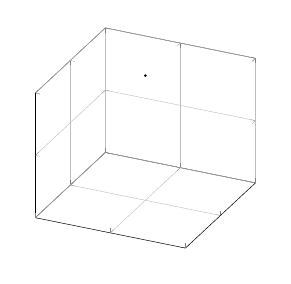
\begin{tikzpicture}[scale=0.4]
        \begin{axis}[width=0.707\textwidth, height=0.707\textwidth,xmax=1, xmin=-1, ymax=1, ymin=-1, zmax=1, zmin=-1, grid=major, xtick={-1,0,1}, xticklabels={,,}, ytick={-1,0,1}, yticklabels={,,}, ztick={-1,0,1}, zticklabels={,,}]
          \addplot3+[only marks, mark options={scale=0.5}, black] coordinates {(0,0,1)};
        \end{axis}
    \end{tikzpicture}}
   \vcenteredhbox{\begin{tikzpicture}[scale=0.4]
        \begin{polaraxis}[width=\textwidth, ymin=0, ymax=1, ytick={0,0.5,1}, yticklabels={1,0.5,0}, ytick={0,0.5,1}, yticklabels={0,45,90}, ylabel={Polar angle [$^{\circ}$]}, , xlabel={Azimuth angle [$^{\circ}$]}]
            \addplot+[only marks, mark options={scale=0.7}, data cs=cart, black] coordinates {(0,0)};
    	\end{polaraxis}
    \end{tikzpicture}}\\
    $\kappa\rightarrow\infty$
\end{minipage}\vspace{2ex}  \caption{Visualisation of 1000 sample directions drawn from Von-Mises-Fisher distribution with varying $\kappa$. Left half of each figure shows the 3-d scatter plot, right half shows a polar plot of the sampled directions for each value of $\kappa$.}
  }
  \label{fig:chapter7 exp1 VanMises draw}
 \end{figure}

\subsection{Feasibility study on fixed monkey spinal cord}
Scans were performed on an experimental 4.7 Tesla scanner (Varian Inc., Palo Alto, CA, USA) in collaboration with the Danish Research Centre for Magnetic Resonance (DRCMR). To make best use of the hardware, we carry out the protocol optimisation as described above but increase $|G|_{max}$ to $300mT/m$. We also adjust for differences in tissue properties between live and fixed tissue, e.g. decreased diffusivity and shrinkage of axon diameters, based on preliminary DTI analysis of the tissue sample (see modified tissue parameters in Table~\ref{tab: chapter7 exp1 model opt parameters ex-vivo}). Scan time in this experiment was limited to 12h only. To retain acceptable image resolution and SNR within the given time frame, we reduced the number of acquisitions to $M=4$ and $N=30$. Furthermore, we only had time to test the {\FD} protocol in this experiment. The resulting protocol is summarised in Table~\ref{XX} and described more comprehensively in Appendix \ref{app:chapter7 protocols 300mT}. 
\paragraph{}
We used a volume coil for transmission and a homemade 20 mm surface coil was used as receive coil. The data was was acquired using a spin-echo sequence with single line readout and a conventional pulsed gradient spin-echo preparation \citep{Stejskal:1965}.  TE/TR were 59/2000 ms, field of view (FoV) was $10\times 10 mm^2$. The matrix size was 64x64 and was 2-D interpolated to 128x128 leading to an axial in-plane resolution of $79 \times 79 \mu m^2$. To support the high in-plane resolution we acquire thick slices of 1.5mm to achieve acceptable \gls{SNR} in our data. The protocol was repeated 4 times with a total imaging time of 13 h. The magnitude images of the four repeated measurements were averaged offline prior to analysis.

\begin{table}[!ht]
	\caption{Adjusted ex-vivo tissue model parameters used for pre-clinical scan optimisation (changes to in-vivo protocol are displayed in red).}
    \centering
    \vspace{2ex}	
    % Cylinder
    \begin{tabular}{y{0.1\textwidth}y{0.25\textwidth}}
    \addlinespace
    \toprule
    \multicolumn{2}{c}{\textbf{Cylinder}} \\
    \multicolumn{2}{c}{(intra-axonal)} \\
    \midrule
    $f_{intra}$ & $0.7$ \\
    $D_{\|}$ & {\color{red}$4\cdot 10^{-10}$ $s/mm^2$} \\
    $D_{\bot} $ & {\color{red}$2.5\cdot 10^{-10}$ $s/mm^2$} \\
    dir   & $[0,0,1]^T$ \\
    R & {\color{red}$\{0.5,1,2\}\mu m$} \\
    \bottomrule
    \end{tabular}%
    \hspace{0.15\textwidth}
    %%% Zeppelin
    \begin{tabular}{y{0.1\textwidth}y{0.25\textwidth}}
    \addlinespace
    \toprule
    \multicolumn{2}{c}{\textbf{Axially symmetric tensor}} \\
    \multicolumn{2}{c}{(extra-axonal)} \\
    \midrule
    $f_{extra}$& $0.3$ \\
    $D_{\parallel}$ & {\color{red}$4\cdot 10^{-10}$ $m^2/s$} \\
    $D_{\bot} $ & {\color{red}$2.5\cdot 10^{-10}$ $s/m^2/s$} \\
    dir & $[0,0,1]^T$ \\
    \bottomrule
    & \\ %empty line to level tables
    \end{tabular}%
    \label{tab: chapter7 exp1 model opt parameters ex-vivo}
    \vspace{2ex}	
\end{table}

\subsection{Model fitting}
A voxel-wise fit of the MR signal is performed using a fitting method similar to \citep{Alexander:2010}. We define the objective function as the maximum likelihood of model parameters given the observed MR signals under Rician noise ($\sigma=0.05$). We use the multi-run fitting routine of \citep{Panagiotaki:2012} to find an initial parameters, which determines the best parameter estimates from multiple gradient-descend runs with pertubed starting points (n=20 in our case). Based on the initial parameter estimates, we then perform a \gls{MCMC} algorithm to determine the posterior distributions of the model parameters. To ensure convergence, we used the following, rather conservative setting for the \gls{MCMC} algorithm: burn-in of 5000, sample interval of 1000, 5\% parameter pertubations with uniform, uninformative priors.

To increase stability of the fitting we fix $D_\parallel$ to its true value of $1.7mm/s^2$ similar to previous studies \citep{Assaf:2008,Barazany:2009,Alexander:2010}. Moreover, $D_\bot$ is approximated by the tortuosity formulation of \citep{Szafer:1995}:
$$
    D_{\bot} = f_{intra}\cdot D_{\parallel}.
$$


For {\DO} and {\FD}, we also found our method to be very unstable with respect to determining the correct principal diffusion direction of the model, even when the fibre direction was close to $[0,0,1]^T$. This likely stems from the fact that the initial guess of the direction is computed from the \gls{DT} model. While this method works fine for \OI and \SD protocols, it fails when using the optimised gradient direction sets of \DO and \FD. We therefore fix the principal fibre direction to $[0,0,1]^T$ in all experiments, unless stated otherwise.

\subsubsection*{Fixed tissue}
We chose to scan a sample of fixed monkey cervical spinal cord to test our protocol in a real biological system. The details of the sample preparation are described in \citep{Lundell:2011}. For the fixed tissue we use a slightly modified fitting routine to account for the differences between fixed and live tissue. Here we fix $D_{par}$ to $0.45\mu m/mm^2$. The volume fraction of the restricted compartment f was constrained to be in the range of $[0.5, 1.0]$. We then In each voxel, the mean of the posterior distribution of $R$ and $f_{intra}$ are calculated. For consistency with indices derived from histological examination and also previous imaging studies e.g. \citep{Alexander:2010}, maps of the axon diameter index $D=2\cdot R$ and the axonal density index $\rho=f_{intra}/\pi/R^2$ are reported.

\FloatBarrier

\section{Results}
\subsection{Accuracy and precision of parameter estimates}
Figure~\ref{fig:chapter7 exp1 boxplots 60mT} shows box plots of the fitted volume fraction $f_{intra}$ and $R$ for different cylinder radii.

definition
\begin{figure}[H]
	\centering
	%!TEX root = ../../thesis.tex
\begin{tikzpicture}
	\begin{axis}[xmin=0,xmax=5,ymin=0, ymax=1,
		xtick={1,2,3,4,5},xticklabels={$1\mu m$,$2\mu m$,$5\mu m$,$10\mu m$},
        width=0.7\textwidth, height=0.5\textwidth, legend columns=6, legend style={at={(-0.1,1.05)}, anchor=south west}, xlabel={True cylinder radius}, ylabel={Volume fraction $f_{intra}$}]

		%#1: center, #2: median, #3: 1/4 quartile, #4: 3/4 quartile, #5: -1.5IQ, #6: +1.5IQ
		\boxplot{3.70}{0.709}{0.653}{0.761}{0.579}{0.812}{red}
		\boxplot{3.90}{0.738}{0.684}{0.787}{0.616}{0.841}{green}
		\boxplot{4.10}{0.689}{0.656}{0.719}{0.619}{0.761}{blue}
		\boxplot{4.30}{0.724}{0.673}{0.764}{0.623}{0.803}{cyan}


        \addlegendentry{\OI}
        \addlegendentry{\SD}
        \addlegendentry{\DO}
        \addlegendentry{\FD}



        \addplot[black, dashed] coordinates{(0.5,0.7) (1.5,0.7)};
        \addlegendentry{ground truth};

		\boxplot{0.70}{0.700}{0.694}{0.707}{0.688}{0.716}{red}
		\boxplot{1.70}{0.692}{0.685}{0.699}{0.678}{0.715}{red}
		\boxplot{2.70}{0.700}{0.687}{0.714}{0.672}{0.731}{red}
		\boxplot{0.90}{0.698}{0.692}{0.703}{0.686}{0.709}{green}
		\boxplot{1.90}{0.705}{0.698}{0.711}{0.691}{0.725}{green}
		\boxplot{2.90}{0.712}{0.699}{0.726}{0.682}{0.743}{green}
		\boxplot{1.10}{0.703}{0.699}{0.706}{0.695}{0.712}{blue}
		\boxplot{2.10}{0.697}{0.693}{0.701}{0.688}{0.711}{blue}
		\boxplot{3.10}{0.698}{0.691}{0.705}{0.683}{0.713}{blue}
		\boxplot{1.30}{0.703}{0.701}{0.706}{0.697}{0.709}{cyan}
		\boxplot{2.30}{0.703}{0.699}{0.710}{0.693}{0.721}{cyan}
		\boxplot{3.30}{0.714}{0.708}{0.721}{0.699}{0.730}{cyan}


        \addplot+[only marks, mark=text, text mark={*}, mark options={scale=0.7},red!30] table[x index=0,y index=1] {chapter7/figs/OInv_60mT_outliers_f.dat};
        \addplot+[only marks, mark=text, text mark={*}, mark options={scale=0.7},green!30] table[x index=0,y index=1] {chapter7/figs/OI_60mT_outliers_f.dat};
        \addplot+[only marks, mark=text, text mark={*}, mark options={scale=0.7},blue!30] table[x index=0,y index=1] {chapter7/figs/DO_60mT_outliers_f.dat};
        \addplot+[only marks, mark=text, text mark={*}, mark options={scale=0.7},cyan!30] table[x index=0,y index=1] {chapter7/figs/FD_60mT_outliers_f.dat};


        \addplot[black, dashed] coordinates{(0.5,0.7) (1.5,0.7)};
        \addplot[black, dashed] coordinates{(1.5,0.7) (2.5,0.7)};
        \addplot[black, dashed] coordinates{(2.5,0.7) (3.5,0.7)};
        \addplot[black, dashed] coordinates{(3.5,0.7) (4.5,0.7)};


	\end{axis}
\end{tikzpicture}

	\begin{tikzpicture}
	\begin{axis}[xmin=0,xmax=5,ymin=0, ymax=15,
		xtick={1,2,3,4,5},xticklabels={$1\mu m$,$2\mu m$,$5\mu m$,$10\mu m$},
        width=0.7\textwidth, height=0.5\textwidth, xlabel={True cylinder radius}, ylabel={Fitted radius $[\mu m]$}]

		\boxplot{3.70}{10.126}{9.657}{10.462}{8.736}{10.725}{red}
		\boxplot{3.90}{10.186}{9.810}{10.455}{9.088}{10.662}{green}
		\boxplot{4.10}{9.941}{9.640}{10.190}{9.244}{10.471}{blue}
		\boxplot{4.30}{10.141}{9.767}{10.396}{9.300}{10.611}{cyan}
		

		%#1: center, #2: median, #3: 1/4 quartile, #4: 3/4 quartile, #5: -1.5IQ, #6: +1.5IQ

        %\addlegendentry{OInv};
        %\addlegendentry{OI};
        %\addlegendentry{DO};
        %\addlegendentry{FD};

		\boxplot{0.70}{1.326}{0.705}{2.087}{0.233}{2.802}{red}
		\boxplot{1.70}{1.704}{0.884}{2.534}{0.244}{3.237}{red}
		\boxplot{2.70}{4.996}{4.841}{5.151}{4.603}{5.359}{red}
		\boxplot{0.90}{0.577}{0.284}{0.871}{0.132}{1.216}{green}
		\boxplot{1.90}{1.567}{0.895}{2.348}{0.261}{3.111}{green}
		\boxplot{2.90}{5.107}{4.952}{5.259}{4.733}{5.442}{green}
		\boxplot{1.10}{1.103}{0.558}{1.743}{0.192}{2.494}{blue}
		\boxplot{2.10}{1.674}{0.903}{2.328}{0.281}{2.828}{blue}
		\boxplot{3.10}{5.006}{4.932}{5.077}{4.829}{5.162}{blue}
		\boxplot{1.30}{0.349}{0.201}{0.467}{0.117}{0.572}{cyan}
		\boxplot{2.30}{2.026}{1.109}{2.593}{0.345}{3.033}{cyan}
		\boxplot{3.30}{5.097}{5.033}{5.171}{4.952}{5.253}{cyan}








        \addplot+[only marks, mark=text, text mark={*}, mark options={scale=0.5},draw opacity=50] table[x index=0,y index=1] {chapter7/figs/OInv_60mT_outliers.dat};
        \addplot+[ only marks, mark=text, text mark={*}, mark options={scale=0.5},green, draw opacity=50] table[x index=0,y index=1] {chapter7/figs/OI_60mT_outliers.dat};
        \addplot+[ only marks, mark=text, text mark={*}, mark options={scale=0.5},blue, draw opacity=50] table[x index=0,y index=1] {chapter7/figs/DO_60mT_outliers.dat};
        \addplot+[ only marks, mark=text, text mark={*}, mark options={scale=0.5},cyan, draw opacity=50] table[x index=0,y index=1] {chapter7/figs/FD_60mT_outliers.dat};


        \addplot[black, dashed] coordinates{(0.5,1) (1.5,1)};
        \addplot[black, dashed] coordinates{(1.5,2) (2.5,2)};
        \addplot[black, dashed] coordinates{(2.5,5) (3.5,5)};
        \addplot[black, dashed] coordinates{(3.5,10) (4.5,10)};

	\end{axis}
\end{tikzpicture}

	\caption{Boxplots of estimated $f_{intra}$ and $R$ for different cylinder radii.}
	\label{fig:chapter7 exp1 boxplots 60mT}
\end{figure}


\paragraph{} All protocols can successfully recover the correct value for $f_{intra}$ for all radii 1, 2 and 5 $\mu m$ with the posterior distributions being centred around the true value $f_{intra}=0.7$ with little variance. $R=10\mu m$ significantly more variance in the estimates is observed for in all protocols. Further we find also find the estimates to be less accurate, mainly in {\SF} and {\SD}, which overestimate of $f_{intra}$ slightly.

\begin{figure}[H]
	 \centering
	 \begin{tikzpicture}[scale=0.7]
	\begin{axis}[
			xmin=0,
			xmax=15,
			ymin=0,
			ymax=700,
            title={\OI},
            width=0.7*\textwidth,
            height=0.4*\textwidth,
            area legend,
            legend style={font=\footnotesize},
		]
		\addplot[const plot, fill=red!70!green,fill opacity=0.8] table[x index=0,y index=2] {chapter7/figs/hist_OInv60mT_1_2_5_10.dat} \closedcycle;
		\addplot[const plot, fill=red!70!blue,fill opacity=0.8] table[x index=0,y index=3] {chapter7/figs/hist_OInv60mT_1_2_5_10.dat} \closedcycle;
		\addplot[const plot, fill=red!70!black,fill opacity=0.5] table[x index=0,y index=4] {chapter7/figs/hist_OInv60mT_1_2_5_10.dat} \closedcycle;
		\addplot[const plot, fill=red!70!yellow, fill opacity=0.5] table[x index=0,y index=1] {chapter7/figs/hist_OInv60mT_1_2_5_10.dat} \closedcycle;
		\addplot[dashed, black, line legend] coordinates {(1,0) (1,1000)};
		\addplot[dashed, black] coordinates {(2,0) (2,1000)};
		\addplot[dashed, black] coordinates {(5,0) (5,1000)};
		\addplot[dashed, black] coordinates {(10,0) (10,1000)};
		\legend{$1\mu m$,$2\mu m$,$5\mu m$,$10\mu m$};
		\end{axis}
\end{tikzpicture}
\begin{tikzpicture}[scale=0.7]
	\begin{axis}[
			xmin=0,
			xmax=15,
			ymin=0,
			ymax=700,
            title={\SD},
            width=0.7*\textwidth,
            height=0.4*\textwidth,
            area legend
		]
		\addplot[const plot, fill=green!70!green,fill opacity=0.8] table[x index=0,y index=2] {chapter7/figs/hist_OI60mT_1_2_5_10.dat} \closedcycle;
		\addplot[const plot, fill=green!70!blue,fill opacity=0.8] table[x index=0,y index=3] {chapter7/figs/hist_OI60mT_1_2_5_10.dat} \closedcycle;
		\addplot[const plot, fill=green!70!black,fill opacity=0.5] table[x index=0,y index=4] {chapter7/figs/hist_OI60mT_1_2_5_10.dat} \closedcycle;
		\addplot[const plot, fill=green!70!yellow, fill opacity=0.5] table[x index=0,y index=1] {chapter7/figs/hist_OI60mT_1_2_5_10.dat} \closedcycle;
		\addplot[line legend, dashed, black] coordinates {(1,0) (1,1000)};
		\addplot[dashed, black] coordinates {(2,0) (2,1000)};
		\addplot[dashed, black] coordinates {(5,0) (5,1000)};
		\addplot[dashed, black] coordinates {(10,0) (10,1000)};
		\legend{$1\mu m$,$2\mu m$,$5\mu m$,$10\mu m$};
		\end{axis}
\end{tikzpicture}
\begin{tikzpicture}[scale=0.7]
	\begin{axis}[
			xmin=0,
			xmax=15,
			ymin=0,
			ymax=700,
            title={\DO},
            width=0.7*\textwidth,
            height=0.4*\textwidth,
            area legend
		]
		\addplot[const plot, fill=blue!60!green,fill opacity=0.8] table[x index=0,y index=2] {chapter7/figs/hist_DO60mT_1_2_5_10.dat} \closedcycle;
		\addplot[const plot, fill=blue!60!blue,fill opacity=0.8] table[x index=0,y index=3] {chapter7/figs/hist_DO60mT_1_2_5_10.dat} \closedcycle;
		\addplot[const plot, fill=blue!60!black,fill opacity=0.5] table[x index=0,y index=4] {chapter7/figs/hist_DO60mT_1_2_5_10.dat} \closedcycle;		
		\addplot[const plot, fill=blue!60!yellow, fill opacity=0.5] table[x index=0,y index=1] {chapter7/figs/hist_DO60mT_1_2_5_10.dat} \closedcycle;
		\addplot[line legend, dashed, black] coordinates {(1,0) (1,1000)};
		\addplot[dashed, black] coordinates {(2,0) (2,1000)};
		\addplot[dashed, black] coordinates {(5,0) (5,1000)};
		\addplot[dashed, black] coordinates {(10,0) (10,1000)};
		\legend{$1\mu m$,$2\mu m$,$5\mu m$,$10\mu m$};
		\end{axis}
\end{tikzpicture}
\begin{tikzpicture}[scale=0.7]
	\begin{axis}[
			xmin=0,
			xmax=15,
			ymin=0,
			ymax=700,
            title={\FD},
            width=0.7*\textwidth,
            height=0.4*\textwidth,
            area legend
		]
		\addplot[const plot, fill=cyan!60!green,fill opacity=0.8] table[x index=0,y index=2] {chapter7/figs/hist_FD60mT_1_2_5_10.dat} \closedcycle;
		\addplot[const plot, fill=cyan!60!blue,fill opacity=0.8] table[x index=0,y index=3] {chapter7/figs/hist_FD60mT_1_2_5_10.dat} \closedcycle;
		\addplot[const plot, fill=cyan!60!black,fill opacity=0.5] table[x index=0,y index=4] {chapter7/figs/hist_FD60mT_1_2_5_10.dat} \closedcycle;		
		\addplot[const plot, fill=cyan!60!yellow, fill opacity=0.5] table[x index=0,y index=1] {chapter7/figs/hist_FD60mT_1_2_5_10.dat} \closedcycle;
		\addplot[dashed, black, line legend] coordinates {(1,0) (1,1000)};
		\addplot[dashed, black] coordinates {(2,0) (2,1000)};
		\addplot[dashed, black] coordinates {(5,0) (5,1000)};
		\addplot[dashed, black] coordinates {(10,0) (10,1000)};
		\legend{$1\mu m$,$2\mu m$,$5\mu m$,$10\mu m$};
		\end{axis}
\end{tikzpicture}

	 \caption{Histograms of fitted cylinder radius $R$ for different protocols.}
	 \label{fig:chapter7 exp1 histograms 60mT}
\end{figure}

\paragraph{} Compared to $f_{intra}$ results, we observe more variance in the posterior distributions of $R$ estimates for all protocols. Over all $R$ {\DO} and {\FD} appear to achieve better results than {\OI} and {\SD} protocols. To illustrate this better, Figure~\ref{fig:chapter7 exp1 histograms 60mT} shows the posterior distributions of $R$ for each protocol in more detail.

All protocols perform the best for $R=5\mu m$ with tight posterior distributions centred around the ground truth. While generally all protocols show very good accuracy in estimating $R$, {\DO} and {\FD} have the advantage in terms of precision as their distributions are considerably tighter than for {\OI} and {\SD}. Compared to $R=5\mu m$, $R=10\mu m$ estimates generally are broader and with a notiable  negative skew, particularily for {\OI} and {\SD} protocols.  As for $5\mu m$, {\DO} and {\FD} produce more sharp parameter distributions than {\OI} and {\SD}, although the difference is less obvious. The broader distributions for $R=10\mu m$ might be explained by the long diffusion, which are necessary to estimate large radii accurately.  We assume a typical T2 signal decay of 70ms in this experiment. As shown in \citep{Alexander:STEAM}, in this regime long diffusion times can not be reached with acceptable SNR. As a consequence, for $R=10\u m$ a greater proportion of the signal will appear unrestricted and causes the underestimation of $f_{intra}$ and larger variation in radius estimates in our results.

Smaller radii $R=1\mu m$ and $R=2\mu m $ less well distinguished from each other in all protocols, with posterior distributions showing significant overlap as expected from limited gradient strength used in this experiment \citep{Alexander:2008,Alexander:2010,Siow:2012}. For small radii the \gls{COM} effect on small radii prohibits any contrast between different $R$, which we find reflected in our posterior distributions (see Chapter~\ref{TODO} for a detailed explanation). However, {\FD} suffers least from this and clearly outperforms the other protocols as it allows much better distinction between the small radii.


\subsection{Variation of fibre direction}
Figure~\ref{fig:chapter7 exp1 angular vals 60mT} shows the root mean squared error for both $f_{intra}$ and $R$ parameters with respect to the principle orientation of diffusion for cylinders with small radius $R=2\mu m$ and large radius $R=5\mu m$. As in the previous experiment, all the protocols generally perform better for $R=5\mu m$ than $R=2\mu m$. Therefore, the most marked differences between protocols appear in the $R=2\mu m$ dataset.
\paragraph{}
The plots clearly show that estimates of $f_{intra}$ are unaffected by the true diffusion orientation in all protocols for $R=2\mu m$. While this expected for {\OI} and {\SD}, we can explain the performance of {\FD} and {\DO} explained by the small cylinder radius, which allows {\FD} and {\OI} to distinguish hindered and restricted diffusion even when the gradient scheme is not aligned perpendicular to the intra-axonal compartment. Results for $R=5\mu m$ show that $f_{intra}$ estimates are affected more by the misalignment of the gradient scheme with larger radii, although the estimation error still remains low over all different directions.

\paragraph{}
Bigger differences between the protocols can be seen in the $R$ estimation error. Again, {\OI} and {\SD} are consistent over the whole range of simulated fibre directions, with no apparent directional pattern of the estimation error. In contrast, {\FD} and {\DO} performance is considerably more impeded for larger misalignment of gradient scheme and cylinder orientation. The maximum estimation error is observed for rotation angles around $45^\circ$. With $\phi$ close to $90^\circ$, the {\SF} and {\DO} gradient direction scheme now features more measurements perpendicular and parallel to the cylinder compartment, which reduces again the fitting error. For smaller misalignments of $\phi<15^\circ$ both {\FD}/{\DO} perform very similar to the {\OI}/{\SD} protocols.

\begin{figure}[!h]
%  \ifdraft
%  {
%  	\draftpic
%  }
   {
\centering
	\subfloat[Cylinder radius $R=2\mu m$]
    {
        \begin{minipage}{\textwidth}    
        	\pgfimage[width=0.9\textwidth]{chapter7/figs/errs_2D_f_60mT.pdf}\\
            \pgfimage[width=0.9\textwidth]{chapter7/figs/errs_2D_R_60mT.pdf}
        \end{minipage}
    }
    
    
    
    \subfloat[Cylinder radius $R=5\mu m$]
    {
        \begin{minipage}{\textwidth}    
            \pgfimage[width=0.9\textwidth]{chapter7/figs/errs_2D_f_60mTR5.pdf}\\
            \pgfimage[width=0.9\textwidth]{chapter7/figs/errs_2D_R_60mTR5.pdf}
        \end{minipage}
    }
  }
	\caption{Root mean square error of $f_{intra}$ and $R$ estimates for different principle diffusion directions.}
	\label{fig:chapter7 exp1 angular vals 60mT}
\end{figure}


\paragraph{Effect of fibre dispersion: } Figure~\ref{fig:chapter7 exp1 dispersion 60mT} shows the fitted $f_{intra}$ and $R$ estimates different degrees of intra-voxel dispersion of fibre orientations. For small $\kappa$, i.e. high degrees of dispersion, we observe large errors in estimates of both $f_{intra}$ and $R$, as expected e.g. from \citep{Zhang:2011}. However, for $\kappa \ge 64$, the fitted parameters converge to their respective ground truth, despite a considerable degree of dispersion still present in those datasets. With increasing $\kappa$, there appears to be no noticable difference between the four protocols.

%\tikzset{external/export=false}
\begin{figure}[ht]
	\centering
	\begin{tikzpicture}[scale=0.7]
    \begin{axis}[xmin=0,xmax=12,ymin=0, ymax=1,
		xtick={1,2,3,4,5,6,7,8,9,10,11},xticklabels={1,2,4,8,16,32,64,128,256,512,$\infty$},
        width=0.7\textwidth, height=0.5\textwidth, legend columns=3, legend style={at={(0.05,0.05)}, anchor=south west}, xlabel={$\kappa$}, ylabel={Volume fraction}]
        \addplot+[red, mark options={fill=red}] plot[error bars/.cd, y dir=both, y explicit] table[x index=8, y index=0, y error index=1] {chapter7/figs/BW_Dispersion_f_300mT.dat};
        \addplot+[green, mark options={fill=green}] plot[error bars/.cd, y dir=both, y explicit] table[x index=8, y index=2, y error index=3] {chapter7/figs/BW_Dispersion_f_300mT.dat};
        \addplot+[blue, mark options={fill=blue}] plot[error bars/.cd, y dir=both, y explicit] table[x index=8, y index=4, y error index=5] {chapter7/figs/BW_Dispersion_f_300mT.dat};
        \addplot+[cyan, mark options={fill=cyan}] plot[error bars/.cd, y dir=both, y explicit] table[x index=8, y index=6, y error index=7] {chapter7/figs/BW_Dispersion_f_300mT.dat};
        \addplot[black, dashed] coordinates{(0.5,0.7) (11.5,0.7)};
        \legend{\OI, {\SD}, {\DO}, {\FD}, ground truth};
	\end{axis}
\end{tikzpicture}

	\begin{tikzpicture}[scale=0.7]
	\begin{axis}[xmin=0,xmax=12,ymin=0, ymax=12,
		xtick={1,2,3,4,5,6,7,8,9,10,11},xticklabels={1,2,4,8,16,32,64,128,256,512,$\infty$},
        width=0.7\textwidth, height=0.5\textwidth, legend columns=6, legend style={at={(0,1.05)}, anchor=south west}, xlabel={$\kappa$}, ylabel={Cylinder radius $[\mu m]$}]
               \addplot+[red, mark options={fill=red}] plot[error bars/.cd, y dir=both, y explicit] table[x index=8, y index=0, y error index=1] {chapter7/figs/BW_Dispersion_R_300mT.dat};
        \addplot+[green, mark options={fill=green}] plot[error bars/.cd, y dir=both, y explicit] table[x index=8, y index=2, y error index=3] {chapter7/figs/BW_Dispersion_R_300mT.dat};
        \addplot+[blue, mark options={fill=blue}] plot[error bars/.cd, y dir=both, y explicit] table[x index=8, y index=4, y error index=5] {chapter7/figs/BW_Dispersion_R_300mT.dat};
        \addplot+[cyan, mark options={fill=cyan}] plot[error bars/.cd, y dir=both, y explicit] table[x index=8, y index=6, y error index=7] {chapter7/figs/BW_Dispersion_R_300mT.dat};
        \addplot[black, dashed] coordinates{(0.5,5) (11.5,5)};        
	\end{axis}
\end{tikzpicture}

	\caption{Mean and standard deviation of posterior distribution for fitted volume fraction and radius for different $\kappa$ values.}
	\label{fig:chapter7 exp1 dispersion 60mT}
\end{figure}
%\tikzset{external/export=false}

\subsection{Proof-of-concept implementation}
Figure~\ref{fig:chapter7 exp1 monkey data} presents maps of axon diameter $D$ and axonal density $\rho$ in the upper cervical spinal cord obtained from the {\FD} protocol. We can discriminate well differences in axon diameter and axonal density indices between anatomically different white matter tracts. Dorsal and lateral sensory tracts show small axons diameters between 1--4$\mu m$ and a density of 0.03--0.08$\mu m^{-2}$. The smallest axon calibers (<1.5$\mu m$) are observed in the dorsal columns (DC) while mean axon size in the anterolateral column (ALC) is 1.5--2.5$\mu m$. The largest axons (3--4$\mu m$) are found in the corticospinal tracts (CST) together with low density of 0.01--0.02$\mu m^{-2}$. Overall, we clearly observe left-right symmetry of axon diameter and density in all tracts, which corresponds well with the known anatomical organisation of the the SC. Parameters are also consistent along the SC within the limits of anatomical variation and are in the range of values reported in previous histological evaluation of the cord \citep{GrafvonKeyserlingk:1984,Golabchi:2010}. 

\begin{figure}[ht]
	\centering
	\subfloat[Axon diameter index $D$]
	{
   	  \ifdraft
	  {
	  	\draftpic
	  }
      {
		\pgfimage[width=4cm]{chapter7/figs/monkeySC_diam.png}
      }   
	}
	\hspace{2cm}
	\subfloat[Axon density index $\rho$]
	{
      \ifdraft
	  {
	  	\draftpic
	  }
      {
		\pgfimage[width=4cm]{chapter7/figs/monkeySC_dens.png}
      }
	}
	\caption{Axial slice of upper cervical cord showing maps of $D$ and $\rho$. White markers show the approximate location of the corticospinal tracts (CST), anterolateral column (ALC) and dorsal column (DC)}
	\label{fig:chapter7 exp1 monkey data}
\end{figure}

\section{Discussion}
We presented here a novel method that provides optimal diffusion weightings and gradient directions for estimating of axonal diameter by exploiting the single fibre orientation of structures like the corpus callosum or spinal cord. We demonstrated that the {\SF} approach reduces the required amount of data by 60--75\%, while achieving similar performance to {\OI}. This translates into a considerable reduction in scan time from >1h for {\OI} to less than 20-25 minutes, which makes routine clinical implementation much more viable.  

\paragraph{}
Our results suggest that a dedicated optimisation of gradient directions is clearly beneficial over the orientation invariant \OI{} approach, both in terms of CRLB and simulated noisy data when the fibre direction is known a-priori. We find that the optimisation routine deliberately diminishes angular resolution in favour of measuring diffusion only in the most informative directions (predominantly parallel and perpendicular to the WM tracts). We noticed that our optimised gradient scheme pick out predominantly gradient directions parallel and perpendicular to the cylinder compartment, presumably to maximise sensitivity to restricted diffusion. In that respect our automatically optimised gradient schemes agree with other many other studies e.g. \citep{Stanisz:1997,Avram:2008,Assaf:2008,Panagiotaki:2012}, which only chose parallel and perdendicular measurements to maximise sensitive to restricted diffusion. Our results confirm that these directions give the most information about the tissue, and one should focus on those directions when the fibre configuration is known \textit{a-priori}. 


We furthermore observe that our {\FD} protocols contain slightly stronger diffusion weighting factors compared to the other protocols. We can attribute this to the custom gradient scheme, which translates to more measurements in the perpendicular direction and hence profits more from stronger diffusion attenuation than {\OI}. The simulation results show the combination of stronger diffusion weighting and custom gradient scheme is superior in estimating the cylinder radius, especially when $R$ is very small.

\paragraph{}
Considering the few number of distinct gradient directions, it comes to no surprise that we found the optimised gradient schemes in {\FD} and {\DO} more prone to error when the true fibre orientation differs from the one assumed in the optimisation process. However, when the misalignment was less than 15$^\circ$ (as expected in coherent WM structures) the impact was neglible. We are confident that with careful positioning, the {\SF} gradient scheme can be aligned to the dominant fibre directions in CC and SC with little error without diminishing the performance of the {\SF} protocols.
\paragraph{}
Finally, the feasibility study on our post-mortem SC sample demonstrates that we can estimate a reasonable range of axon diameters and densities under realistic imaging conditions, while retaining a high image resolution. Furthermore we were able to distinguish different WM tracts of the SC by both axon diameter and axon density.
\paragraph{}
There are some limiting factors to our study. Firstly, we only optimise and fit a very simple tissue model, which only allows a crude approximation of the real tissue properties. Other, more complex, models might be a better representation of the real tissue microstructure, e.g. modelling explicitly a distribution of axon radii \citep{Barazany:2009} or including more extra-axonal tissue compartments \citep{Stanisz:1997,Wang:2011,Panagiotaki:2012}.  While these models might arguably be more accurate, they also require many more acquisitions and therefore do not agree with the aim of this study to reduce the scan time to less than 30 minutes. The choice of a simpler model offers a compromise of manageable data requirements and informative model parameters.
\paragraph{}
Secondly, the spinal cord sample we used in this study was not available for histological processing. Despite the lack of independent validation, the differences between WM tracts agree with previous results in \citep{Golabchi:2010}. It should be noted that our results were obtained with a significantly smaller number of diffusion weighted directions and b-factors compared to other studies \citep{Assaf:2008,Barazany:2009,Panagiotaki:2012}, making it more comparable to conditions found in in-vivo scanning. Nevertheless, in many this pre-clinical setup here has many advantages over the in-vivo situation, as it profits from long scan times, high SNR and an absence of motion artefacts. Although the findings in this experiment might therefore not be directly transferable to clinical practise, the results are encouraging enough to pursue the \SF{} approach in clinical practise. In the next two chapters we will therefore focus on moving the \SF{} approach to towards a feasible in-vivo implementation on standard clinical hardware.



\FloatBarrier
\begin{subappendices}

\section{Protocols}
%\tikzset{external/export=false}
\ifdraft
{
   Appendix here
}
{
    \subsection{Protocols optimised for $|G|_{max}$=60mT/m, N=90, M=8}
    \label{app:chapter7 protocols 60mT}
    \begin{figure}
    	[H] \centering 
%%% protocol m=1 start
\begin{tikzpicture}
\node [protocolbox] (box){
   \begin{minipage}{0.45\textwidth}
   \vspace{1ex}
        \centering
        \raisebox{0cm}{\sequenceNoWeights{0.018}{0.013}{0.060}{1.000}{0.071}}
        \begin{tikzpicture}[scale=0.6]
          \begin{axis}[ xlabel=$x$, ylabel=$y$, zlabel=$z$,xmax=1, xmin=-1, ymax=1, ymin=-1, zmax=1, zmin=-1, width=3.0cm, height=3.0cm, grid=major]
          \addplot3+[only marks] table {chapter7/figs/protocols_par1/SF_OInv_62mT002.txt};
        \end{axis}
        \end{tikzpicture}
        \vspace{2ex}
   \end{minipage}
};
\node[protocolheader, right=10pt] at (box.north west) {$\mathbf{m=1}$};
\node[protocoltext] at (box.south) {\footnotesize{$\delta=13 ms$, $\Delta=18 ms$, $|G|=60 mT/m$}};
\end{tikzpicture}
%%% protocol end
%
%
%
%%% protocol m=2 start
\begin{tikzpicture}
\node [protocolbox] (box){
   \begin{minipage}{0.45\textwidth}
   \vspace{1ex}
        \centering
        \raisebox{0cm}{\sequenceNoWeights{0.018}{0.013}{0.060}{1.000}{0.071}}
        \begin{tikzpicture}[scale=0.6]
          \begin{axis}[ xlabel=$x$, ylabel=$y$, zlabel=$z$,xmax=1, xmin=-1, ymax=1, ymin=-1, zmax=1, zmin=-1, width=3.0cm, height=3.0cm, grid=major]
          \addplot3+[only marks] table {chapter7/figs/protocols_par1/SF_OInv_62mT006.txt};
        \end{axis}
        \end{tikzpicture}
        \vspace{2ex}
   \end{minipage}
};
\node[protocolheader, right=10pt] at (box.north west) {$\mathbf{m=2}$};
\node[protocoltext] at (box.south) {\footnotesize{$\delta=13 ms$, $\Delta=18 ms$, $|G|=60 mT/m$}};
\end{tikzpicture}
\\[2ex]
%%% protocol end
%
%
%
%%% protocol m=3 start
\begin{tikzpicture}
\node [protocolbox] (box){
   \begin{minipage}{0.45\textwidth}
   \vspace{1ex}
        \centering
        \raisebox{0cm}{\sequenceNoWeights{0.018}{0.013}{0.060}{1.000}{0.071}}
        \begin{tikzpicture}[scale=0.6]
          \begin{axis}[ xlabel=$x$, ylabel=$y$, zlabel=$z$,xmax=1, xmin=-1, ymax=1, ymin=-1, zmax=1, zmin=-1, width=3.0cm, height=3.0cm, grid=major]
          \addplot3+[only marks] table {chapter7/figs/protocols_par1/SF_OInv_62mT004.txt};
        \end{axis}
        \end{tikzpicture}
        \vspace{2ex}
   \end{minipage}
};
\node[protocolheader, right=10pt] at (box.north west) {$\mathbf{m=3}$};
\node[protocoltext] at (box.south) {\footnotesize{$\delta=13 ms$, $\Delta=18 ms$, $|G|=60 mT/m$}};
\end{tikzpicture}
%%% protocol end
%
%
%
%%% protocol m=4 start
\begin{tikzpicture}
\node [protocolbox] (box){
   \begin{minipage}{0.45\textwidth}
   \vspace{1ex}
        \centering
        \raisebox{0cm}{\sequenceNoWeights{0.018}{0.013}{0.060}{1.000}{0.071}}
        \begin{tikzpicture}[scale=0.6]
          \begin{axis}[ xlabel=$x$, ylabel=$y$, zlabel=$z$,xmax=1, xmin=-1, ymax=1, ymin=-1, zmax=1, zmin=-1, width=3.0cm, height=3.0cm, grid=major]
          \addplot3+[only marks] table {chapter7/figs/protocols_par1/SF_OInv_62mT008.txt};
        \end{axis}
        \end{tikzpicture}
        \vspace{2ex}
   \end{minipage}
};
\node[protocolheader, right=10pt] at (box.north west) {$\mathbf{m=4}$};
\node[protocoltext] at (box.south) {\footnotesize{$\delta=13 ms$, $\Delta=18 ms$, $|G|=60 mT/m$}};
\end{tikzpicture}
\\[2ex]
%%% protocol end
%
%
%
%%% protocol m=5 start
\begin{tikzpicture}
\node [protocolbox] (box){
   \begin{minipage}{0.45\textwidth}
   \vspace{1ex}
        \centering
        \raisebox{0cm}{\sequenceNoWeights{0.048}{0.023}{0.031}{1.000}{0.071}}
        \begin{tikzpicture}[scale=0.6]
          \begin{axis}[ xlabel=$x$, ylabel=$y$, zlabel=$z$,xmax=1, xmin=-1, ymax=1, ymin=-1, zmax=1, zmin=-1, width=3.0cm, height=3.0cm, grid=major]
          \addplot3+[only marks] table {chapter7/figs/protocols_par1/SF_OInv_62mT003.txt};
        \end{axis}
        \end{tikzpicture}
        \vspace{2ex}
   \end{minipage}
};
\node[protocolheader, right=10pt] at (box.north west) {$\mathbf{m=5}$};
\node[protocoltext] at (box.south) {\footnotesize{$\delta=23 ms$, $\Delta=48 ms$, $|G|=31 mT/m$}};
\end{tikzpicture}
%%% protocol end
%
%
%
%%% protocol m=6 start
\begin{tikzpicture}
\node [protocolbox] (box){
   \begin{minipage}{0.45\textwidth}
   \vspace{1ex}
        \centering
        \raisebox{0.1cm}{\sequenceNoWeights{0.047}{0.024}{0.032}{1.000}{0.071}}
        \begin{tikzpicture}[scale=0.6]
          \begin{axis}[ xlabel=$x$, ylabel=$y$, zlabel=$z$,xmax=1, xmin=-1, ymax=1, ymin=-1, zmax=1, zmin=-1, width=3.0cm, height=3.0cm, grid=major]
          \addplot3+[only marks] table {chapter7/figs/protocols_par1/SF_OInv_62mT001.txt};
        \end{axis}
        \end{tikzpicture}
        \vspace{2ex}
   \end{minipage}
};
\node[protocolheader, right=10pt] at (box.north west) {$\mathbf{m=6}$};
\node[protocoltext] at (box.south) {\footnotesize{$\delta=24 ms$, $\Delta=47 ms$, $|G|=32 mT/m$}};
\end{tikzpicture}
\\[2ex]
%%% protocol end
%
%
%
%%% protocol m=7 start
\begin{tikzpicture}
\node [protocolbox] (box){
   \begin{minipage}{0.45\textwidth}
   \vspace{1ex}
        \centering
        \raisebox{0.1cm}{\sequenceNoWeights{0.045}{0.026}{0.039}{1.000}{0.071}}
        \begin{tikzpicture}[scale=0.6]
          \begin{axis}[ xlabel=$x$, ylabel=$y$, zlabel=$z$,xmax=1, xmin=-1, ymax=1, ymin=-1, zmax=1, zmin=-1, width=3.0cm, height=3.0cm, grid=major]
          \addplot3+[only marks] table {chapter7/figs/protocols_par1/SF_OInv_62mT005.txt};
        \end{axis}
        \end{tikzpicture}
        \vspace{2ex}
   \end{minipage}
};
\node[protocolheader, right=10pt] at (box.north west) {$\mathbf{m=7}$};
\node[protocoltext] at (box.south) {\footnotesize{$\delta=26 ms$, $\Delta=45 ms$, $|G|=39 mT/m$}};
\end{tikzpicture}
%%% protocol end
%
%
%
%%% protocol m=8 start
\begin{tikzpicture}
\node [protocolbox] (box){
   \begin{minipage}{0.45\textwidth}
   \vspace{1ex}
        \centering
        \raisebox{0.1cm}{\sequenceNoWeights{0.038}{0.033}{0.060}{1.000}{0.071}}
        \begin{tikzpicture}[scale=0.6]
          \begin{axis}[ xlabel=$x$, ylabel=$y$, zlabel=$z$,xmax=1, xmin=-1, ymax=1, ymin=-1, zmax=1, zmin=-1, width=3.0cm, height=3.0cm, grid=major]
          \addplot3+[only marks] table {chapter7/figs/protocols_par1/SF_OInv_62mT007.txt};
        \end{axis}
        \end{tikzpicture}
        \vspace{2ex}
   \end{minipage}
};
\node[protocolheader, right=10pt] at (box.north west) {$\mathbf{m=8}$};
\node[protocoltext] at (box.south) {\footnotesize{$\delta=33 ms$, $\Delta=38 ms$, $|G|=60 mT/m$}};
\end{tikzpicture}
\\[2ex]
%%% protocol end
%
%
%  \caption{\OI protocol optimised for clinical gradient strength.}
       \label{fig:chapter7 exp1 OINV_62mT}
    \end{figure}
    \begin{figure}
    	[H] \centering \input{chapter7/figs/protocols_par1/SameDirs_62mT.tex} \caption{\SD protocol optimised for clinical gradient strength}
       \label{fig:chapter7 exp1 SAMEDIRS_62mT}
    \end{figure}
    \begin{figure}
    	[H] \centering %%% protocol m=1 start
\begin{tikzpicture}
\node [protocolbox] (box){
   \begin{minipage}{0.45\textwidth}
   \vspace{1ex}
        \centering
        \raisebox{0.1cm}{\sequenceNoWeights{0.018}{0.013}{0.060}{1.000}{0.071}}
        \begin{tikzpicture}[scale=0.6]
          \begin{axis}[ xlabel=$x$, ylabel=$y$, zlabel=$z$,xmax=1, xmin=-1, ymax=1, ymin=-1, zmax=1, zmin=0, width=3.0cm, height=3.0cm, grid=major]
          \addplot3+[only marks] table {chapter7/figs/protocols_par1/SF_DO_60mT004.txt};
        \end{axis}
        \end{tikzpicture}
   \end{minipage}
};
\node[protocolheader, right=10pt] at (box.north west) {$\mathbf{m=1}$};
\node[protocoltext] at (box.south) {\footnotesize{$\delta=13 ms$, $\Delta=18 ms$, $|G|=60 mT/m$}};
\end{tikzpicture}
%%% protocol end
%
%
%
%%% protocol m=2 start
\begin{tikzpicture}
\node [protocolbox] (box){
   \begin{minipage}{0.45\textwidth}
   \vspace{1ex}
        \centering
        \raisebox{0.1cm}{\sequenceNoWeights{0.018}{0.013}{0.060}{1.000}{0.071}}
        \begin{tikzpicture}[scale=0.6]
          \begin{axis}[ xlabel=$x$, ylabel=$y$, zlabel=$z$,xmax=1, xmin=-1, ymax=1, ymin=-1, zmax=1, zmin=0, width=3.0cm, height=3.0cm, grid=major]
          \addplot3+[only marks] table {chapter7/figs/protocols_par1/SF_DO_60mT007.txt};
        \end{axis}
        \end{tikzpicture}
        \vspace{2ex}
   \end{minipage}
};
\node[protocolheader, right=10pt] at (box.north west) {$\mathbf{m=2}$};
\node[protocoltext] at (box.south) {\footnotesize{$\delta=13 ms$, $\Delta=18 ms$, $|G|=60 mT/m$}};
\end{tikzpicture}
\\[2ex]
%%% protocol end
%
%
%
%%% protocol m=3 start
\begin{tikzpicture}
\node [protocolbox] (box){
   \begin{minipage}{0.45\textwidth}
   \vspace{1ex}
        \centering
        \raisebox{0.1cm}{\sequenceNoWeights{0.018}{0.013}{0.060}{1.000}{0.071}}
        \begin{tikzpicture}[scale=0.6]
          \begin{axis}[ xlabel=$x$, ylabel=$y$, zlabel=$z$,xmax=1, xmin=-1, ymax=1, ymin=-1, zmax=1, zmin=0, width=3.0cm, height=3.0cm, grid=major]
          \addplot3+[only marks] table {chapter7/figs/protocols_par1/SF_DO_60mT003.txt};
        \end{axis}
        \end{tikzpicture}
        \vspace{2ex}
   \end{minipage}
};
\node[protocolheader, right=10pt] at (box.north west) {$\mathbf{m=3}$};
\node[protocoltext] at (box.south) {\footnotesize{$\delta=13 ms$, $\Delta=18 ms$, $|G|=60 mT/m$}};
\end{tikzpicture}
%%% protocol end
%
%
%
%%% protocol m=4 start
\begin{tikzpicture}
\node [protocolbox] (box){
   \begin{minipage}{0.45\textwidth}
   \vspace{1ex}
        \centering
        \raisebox{0.1cm}{\sequenceNoWeights{0.018}{0.013}{0.060}{1.000}{0.071}}
        \begin{tikzpicture}[scale=0.6]
          \begin{axis}[ xlabel=$x$, ylabel=$y$, zlabel=$z$,xmax=1, xmin=-1, ymax=1, ymin=-1, zmax=1, zmin=0, width=3.0cm, height=3.0cm, grid=major]
          \addplot3+[only marks] table {chapter7/figs/protocols_par1/SF_DO_60mT008.txt};
        \end{axis}
        \end{tikzpicture}
        \vspace{2ex}
   \end{minipage}
};
\node[protocolheader, right=10pt] at (box.north west) {$\mathbf{m=4}$};
\node[protocoltext] at (box.south) {\footnotesize{$\delta=13 ms$, $\Delta=18 ms$, $|G|=60 mT/m$}};
\end{tikzpicture}
\\[2ex]
%%% protocol end
%
%
%
%%% protocol m=5 start
\begin{tikzpicture}
\node [protocolbox] (box){
   \begin{minipage}{0.45\textwidth}
   \vspace{1ex}
        \centering
        \raisebox{0.1cm}{\sequenceNoWeights{0.049}{0.022}{0.032}{1.000}{0.071}}
        \begin{tikzpicture}[scale=0.6]
          \begin{axis}[ xlabel=$x$, ylabel=$y$, zlabel=$z$,xmax=1, xmin=-1, ymax=1, ymin=-1, zmax=1, zmin=0, width=3.0cm, height=3.0cm, grid=major]
          \addplot3+[only marks] table {chapter7/figs/protocols_par1/SF_DO_60mT006.txt};
        \end{axis}
        \end{tikzpicture}
        \vspace{2ex}
   \end{minipage}
};
\node[protocolheader, right=10pt] at (box.north west) {$\mathbf{m=5}$};
\node[protocoltext] at (box.south) {\footnotesize{$\delta=22 ms$, $\Delta=49 ms$, $|G|=32 mT/m$}};
\end{tikzpicture}
%%% protocol end
%
%
%
%%% protocol m=6 start
\begin{tikzpicture}
\node [protocolbox] (box){
   \begin{minipage}{0.45\textwidth}
   \vspace{1ex}
        \centering
        \raisebox{0.1cm}{\sequenceNoWeights{0.046}{0.025}{0.032}{1.000}{0.071}}
        \begin{tikzpicture}[scale=0.6]
          \begin{axis}[ xlabel=$x$, ylabel=$y$, zlabel=$z$,xmax=1, xmin=-1, ymax=1, ymin=-1, zmax=1, zmin=0, width=3.0cm, height=3.0cm, grid=major]
          \addplot3+[only marks] table {chapter7/figs/protocols_par1/SF_DO_60mT001.txt};
        \end{axis}
        \end{tikzpicture}
        \vspace{2ex}
   \end{minipage}
};
\node[protocolheader, right=10pt] at (box.north west) {$\mathbf{m=6}$};
\node[protocoltext] at (box.south) {\footnotesize{$\delta=25 ms$, $\Delta=46 ms$, $|G|=32 mT/m$}};
\end{tikzpicture}
\\[2ex]
%%% protocol end
%
%
%
%%% protocol m=7 start
\begin{tikzpicture}
\node [protocolbox] (box){
   \begin{minipage}{0.45\textwidth}
   \vspace{1ex}
        \centering
        \raisebox{0.1cm}{\sequenceNoWeights{0.044}{0.026}{0.039}{1.000}{0.071}}
        \begin{tikzpicture}[scale=0.6]
          \begin{axis}[ xlabel=$x$, ylabel=$y$, zlabel=$z$,xmax=1, xmin=-1, ymax=1, ymin=-1, zmax=1, zmin=0, width=3.0cm, height=3.0cm, grid=major]
          \addplot3+[only marks] table {chapter7/figs/protocols_par1/SF_DO_60mT002.txt};
        \end{axis}
        \end{tikzpicture}
        \vspace{2ex}
   \end{minipage}
};
\node[protocolheader, right=10pt] at (box.north west) {$\mathbf{m=7}$};
\node[protocoltext] at (box.south) {\footnotesize{$\delta=26 ms$, $\Delta=44 ms$, $|G|=39 mT/m$}};
\end{tikzpicture}
%%% protocol end
%
%
%
%%% protocol m=8 start
\begin{tikzpicture}
\node [protocolbox] (box){
   \begin{minipage}{0.45\textwidth}
   \vspace{1ex}
        \centering
        \raisebox{0.1cm}{\sequenceNoWeights{0.038}{0.033}{0.060}{1.000}{0.071}}
        \begin{tikzpicture}[scale=0.6]
          \begin{axis}[ xlabel=$x$, ylabel=$y$, zlabel=$z$,xmax=1, xmin=-1, ymax=1, ymin=-1, zmax=1, zmin=0, width=3.0cm, height=3.0cm, grid=major]
          \addplot3+[only marks] table {chapter7/figs/protocols_par1/SF_DO_60mT005.txt};
        \end{axis}
        \end{tikzpicture}
        \vspace{2ex}
   \end{minipage}
};
\node[protocolheader, right=10pt] at (box.north west) {$\mathbf{m=8}$};
\node[protocoltext] at (box.south) {\footnotesize{$\delta=33 ms$, $\Delta=38 ms$, $|G|=60 mT/m$}};
\end{tikzpicture}
\\[2ex]
%%% protocol end  \caption{\DO protocol optimised for clinical gradient strength}
       \label{fig:chapter7 exp1 DIRSONLY_62mT}
    \end{figure}
    \begin{figure}
    	[H] \centering %%% protocol m=1 start
\begin{tikzpicture}
\node [protocolbox] (box){
   \begin{minipage}{0.45\textwidth}
   \vspace{1ex}
        \centering
        \raisebox{0.1cm}{\sequenceNoWeights{0.020}{0.015}{0.060}{1.000}{0.075}}
        \begin{tikzpicture}[scale=0.6]
          \begin{axis}[ xlabel=$x$, ylabel=$y$, zlabel=$z$,xmax=1, xmin=-1, ymax=1, ymin=-1, zmax=1, zmin=0, width=3.0cm, height=3.0cm, grid=major]
          \addplot3+[only marks] table {chapter7/figs/protocols_par1/SF_FD_60mT005.txt};
        \end{axis}
        \end{tikzpicture}
        \vspace{2ex}
   \end{minipage}
};
\node[protocolheader, right=10pt] at (box.north west) {$\mathbf{m=1}$};
\node[protocoltext] at (box.south) {\footnotesize{$\delta=15 ms$, $\Delta=20 ms$, $|G|=60 mT/m$}};
\end{tikzpicture}
%%% protocol end
%
%
%
%%% protocol m=2 start
\begin{tikzpicture}
\node [protocolbox] (box){
   \begin{minipage}{0.45\textwidth}
   \vspace{1ex}
        \centering
        \raisebox{0.1cm}{\sequenceNoWeights{0.020}{0.015}{0.060}{1.000}{0.075}}
        \begin{tikzpicture}[scale=0.6]
          \begin{axis}[ xlabel=$x$, ylabel=$y$, zlabel=$z$,xmax=1, xmin=-1, ymax=1, ymin=-1, zmax=1, zmin=0, width=3.0cm, height=3.0cm, grid=major]
          \addplot3+[only marks] table {chapter7/figs/protocols_par1/SF_FD_60mT004.txt};
        \end{axis}
        \end{tikzpicture}
        \vspace{2ex}
   \end{minipage}
};
\node[protocolheader, right=10pt] at (box.north west) {$\mathbf{m=2}$};
\node[protocoltext] at (box.south) {\footnotesize{$\delta=15 ms$, $\Delta=20 ms$, $|G|=60 mT/m$}};
\end{tikzpicture}
\\[2ex]
%%% protocol end
%
%
%
%%% protocol m=3 start
\begin{tikzpicture}
\node [protocolbox] (box){
   \begin{minipage}{0.45\textwidth}
   \vspace{1ex}
        \centering
        \raisebox{0.1cm}{\sequenceNoWeights{0.020}{0.015}{0.060}{1.000}{0.075}}
        \begin{tikzpicture}[scale=0.6]
          \begin{axis}[ xlabel=$x$, ylabel=$y$, zlabel=$z$,xmax=1, xmin=-1, ymax=1, ymin=-1, zmax=1, zmin=0, width=3.0cm, height=3.0cm, grid=major]
          \addplot3+[only marks] table {chapter7/figs/protocols_par1/SF_FD_60mT003.txt};
        \end{axis}
        \end{tikzpicture}
        \vspace{2ex}
   \end{minipage}
};
\node[protocolheader, right=10pt] at (box.north west) {$\mathbf{m=3}$};
\node[protocoltext] at (box.south) {\footnotesize{$\delta=15 ms$, $\Delta=20 ms$, $|G|=60 mT/m$}};
\end{tikzpicture}
%%% protocol end
%
%
%
%%% protocol m=4 start
\begin{tikzpicture}
\node [protocolbox] (box){
   \begin{minipage}{0.45\textwidth}
   \vspace{1ex}
        \centering
        \raisebox{0.1cm}{\sequenceNoWeights{0.020}{0.015}{0.060}{1.000}{0.075}}
        \begin{tikzpicture}[scale=0.6]
          \begin{axis}[ xlabel=$x$, ylabel=$y$, zlabel=$z$,xmax=1, xmin=-1, ymax=1, ymin=-1, zmax=1, zmin=0, width=3.0cm, height=3.0cm, grid=major]
          \addplot3+[only marks] table {chapter7/figs/protocols_par1/SF_FD_60mT001.txt};
        \end{axis}
        \end{tikzpicture}
        \vspace{2ex}
   \end{minipage}
};
\node[protocolheader, right=10pt] at (box.north west) {$\mathbf{m=4}$};
\node[protocoltext] at (box.south) {\footnotesize{$\delta=15 ms$, $\Delta=20 ms$, $|G|=60 mT/m$}};
\end{tikzpicture}
\\[2ex]
%%% protocol end
%
%
%
%%% protocol m=5 start
\begin{tikzpicture}
\node [protocolbox] (box){
   \begin{minipage}{0.45\textwidth}
   \vspace{1ex}
        \centering
        \raisebox{0.1cm}{\sequenceNoWeights{0.054}{0.021}{0.030}{1.000}{0.075}}
        \begin{tikzpicture}[scale=0.6]
          \begin{axis}[ xlabel=$x$, ylabel=$y$, zlabel=$z$,xmax=1, xmin=-1, ymax=1, ymin=-1, zmax=1, zmin=0, width=3.0cm, height=3.0cm, grid=major]
          \addplot3+[only marks] table {chapter7/figs/protocols_par1/SF_FD_60mT007.txt};
        \end{axis}
        \end{tikzpicture}
        \vspace{2ex}
   \end{minipage}
};
\node[protocolheader, right=10pt] at (box.north west) {$\mathbf{m=5}$};
\node[protocoltext] at (box.south) {\footnotesize{$\delta=21 ms$, $\Delta=54 ms$, $|G|=30 mT/m$}};
\end{tikzpicture}
%%% protocol end
%
%
%
%%% protocol m=6 start
\begin{tikzpicture}
\node [protocolbox] (box){
   \begin{minipage}{0.45\textwidth}
   \vspace{1ex}
        \centering
        \raisebox{0.1cm}{\sequenceNoWeights{0.048}{0.027}{0.039}{1.000}{0.075}}
        \begin{tikzpicture}[scale=0.6]
          \begin{axis}[ xlabel=$x$, ylabel=$y$, zlabel=$z$,xmax=1, xmin=-1, ymax=1, ymin=-1, zmax=1, zmin=0, width=3.0cm, height=3.0cm, grid=major]
          \addplot3+[only marks] table {chapter7/figs/protocols_par1/SF_FD_60mT008.txt};
        \end{axis}
        \end{tikzpicture}
        \vspace{2ex}
   \end{minipage}
};
\node[protocolheader, right=10pt] at (box.north west) {$\mathbf{m=6}$};
\node[protocoltext] at (box.south) {\footnotesize{$\delta=27 ms$, $\Delta=48 ms$, $|G|=39 mT/m$}};
\end{tikzpicture}
\\[2ex]
%%% protocol end
%
%
%
%%% protocol m=7 start
\begin{tikzpicture}
\node [protocolbox] (box){
   \begin{minipage}{0.45\textwidth}
   \vspace{1ex}
        \centering
        \raisebox{0.1cm}{\sequenceNoWeights{0.047}{0.028}{0.040}{1.000}{0.075}}
        \begin{tikzpicture}[scale=0.6]
          \begin{axis}[ xlabel=$x$, ylabel=$y$, zlabel=$z$,xmax=1, xmin=-1, ymax=1, ymin=-1, zmax=1, zmin=0, width=3.0cm, height=3.0cm, grid=major]
          \addplot3+[only marks] table {chapter7/figs/protocols_par1/SF_FD_60mT006.txt};
        \end{axis}
        \end{tikzpicture}
        \vspace{2ex}
   \end{minipage}
};
\node[protocolheader, right=10pt] at (box.north west) {$\mathbf{m=7}$};
\node[protocoltext] at (box.south) {\footnotesize{$\delta=28 ms$, $\Delta=47 ms$, $|G|=40 mT/m$}};
\end{tikzpicture}
%%% protocol end
%
%
%
%%% protocol m=8 start
\begin{tikzpicture}
\node [protocolbox] (box){
   \begin{minipage}{0.45\textwidth}
   \vspace{1ex}
        \centering
        \raisebox{0.1cm}{\sequenceNoWeights{0.040}{0.035}{0.060}{1.000}{0.075}}
        \begin{tikzpicture}[scale=0.6]
          \begin{axis}[ xlabel=$x$, ylabel=$y$, zlabel=$z$,xmax=1, xmin=-1, ymax=1, ymin=-1, zmax=1, zmin=0, width=3.0cm, height=3.0cm, grid=major]
          \addplot3+[only marks] table {chapter7/figs/protocols_par1/SF_FD_60mT002.txt};
        \end{axis}
        \end{tikzpicture}
        \vspace{2ex}
   \end{minipage}
};
\node[protocolheader, right=10pt] at (box.north west) {$\mathbf{m=8}$};
\node[protocoltext] at (box.south) {\footnotesize{$\delta=35 ms$, $\Delta=40 ms$, $|G|=60 mT/m$}};
\end{tikzpicture}
 \caption{\FD protocol optimised for clinical gradient strength}
       \label{fig:chapter7 exp1 FREEDIRS_62mT}
    \end{figure}

    \subsection{Pre-clinical scanner (300mT/m), N=30, M=4}
    \label{app:chapter7 protocols 300mT}	
    %\begin{figure}
    %	[H] \centering %%% protocol m=1 start
\begin{tikzpicture}
\node [protocolbox] (box){
   \begin{minipage}{0.45\textwidth}
   \vspace{1ex}
        \centering
        \raisebox{0.1cm}{\sequencePreclinicalNoWeights{0.045}{0.005}{0.201}{1.000}{0.050}}
        \begin{tikzpicture}[scale=0.6]
          \begin{axis}[ xlabel=$x$, ylabel=$y$, zlabel=$z$,xmax=1, xmin=-1, ymax=1, ymin=-1, zmax=1, zmin=-1, width=3.0cm, height=3.0cm, grid=major]
          \addplot3+[only marks] table {chapter7/figs/protocols_par1/SF_OInv_300mTCopenhagen002.txt};
        \end{axis}
        \end{tikzpicture}
        \vspace{2ex}
   \end{minipage}
};
\node[protocolheader, right=10pt] at (box.north west) {$\mathbf{m=1}$};
\node[protocoltext] at (box.south) {\footnotesize{$\delta=5 ms$, $\Delta=45 ms$, $|G|=201 mT/m$}};
\end{tikzpicture}
%%% protocol end
%
%
%
%%% protocol m=2 start
\begin{tikzpicture}
\node [protocolbox] (box){
   \begin{minipage}{0.45\textwidth}
   \vspace{1ex}
        \centering
        \raisebox{0.1cm}{\sequencePreclinicalNoWeights{0.013}{0.007}{0.300}{1.000}{0.050}}
        \begin{tikzpicture}[scale=0.6]
          \begin{axis}[ xlabel=$x$, ylabel=$y$, zlabel=$z$,xmax=1, xmin=-1, ymax=1, ymin=-1, zmax=1, zmin=-1, width=3.0cm, height=3.0cm, grid=major]
          \addplot3+[only marks] table {chapter7/figs/protocols_par1/SF_OInv_300mTCopenhagen004.txt};
        \end{axis}
        \end{tikzpicture}
        \vspace{2ex}
   \end{minipage}
};
\node[protocolheader, right=10pt] at (box.north west) {$\mathbf{m=2}$};
\node[protocoltext] at (box.south) {\footnotesize{$\delta=7 ms$, $\Delta=13 ms$, $|G|=300 mT/m$}};
\end{tikzpicture}
\\[2ex]
%%% protocol end
%
%
%
%%% protocol m=3 start
\begin{tikzpicture}
\node [protocolbox] (box){
   \begin{minipage}{0.45\textwidth}
   \vspace{1ex}
        \centering
        \raisebox{0.1cm}{\sequencePreclinicalNoWeights{0.034}{0.015}{0.167}{1.000}{0.050}}
        \begin{tikzpicture}[scale=0.6]
          \begin{axis}[ xlabel=$x$, ylabel=$y$, zlabel=$z$,xmax=1, xmin=-1, ymax=1, ymin=-1, zmax=1, zmin=-1, width=3.0cm, height=3.0cm, grid=major]
          \addplot3+[only marks] table {chapter7/figs/protocols_par1/SF_OInv_300mTCopenhagen003.txt};
        \end{axis}
        \end{tikzpicture}
        \vspace{2ex}
   \end{minipage}
};
\node[protocolheader, right=10pt] at (box.north west) {$\mathbf{m=3}$};
\node[protocoltext] at (box.south) {\footnotesize{$\delta=15 ms$, $\Delta=34 ms$, $|G|=167 mT/m$}};
\end{tikzpicture}
%%% protocol end
%
%
%
%%% protocol m=4 start
\begin{tikzpicture}
\node [protocolbox] (box){
   \begin{minipage}{0.45\textwidth}
   \vspace{1ex}
        \centering
        \raisebox{0.1cm}{\sequencePreclinicalNoWeights{0.038}{0.011}{0.220}{1.000}{0.050}}
        \begin{tikzpicture}[scale=0.6]
          \begin{axis}[ xlabel=$x$, ylabel=$y$, zlabel=$z$,xmax=1, xmin=-1, ymax=1, ymin=-1, zmax=1, zmin=-1, width=3.0cm, height=3.0cm, grid=major]
          \addplot3+[only marks] table {chapter7/figs/protocols_par1/SF_OInv_300mTCopenhagen001.txt};
        \end{axis}
        \end{tikzpicture}
        \vspace{2ex}
   \end{minipage}
};
\node[protocolheader, right=10pt] at (box.north west) {$\mathbf{m=4}$};
\node[protocoltext] at (box.south) {\footnotesize{$\delta=11 ms$, $\Delta=38 ms$, $|G|=220 mT/m$}};
\end{tikzpicture}
 \caption{OI protocol optimised for pre-clinical animal scanner} \label{fig:chapter7 exp1 INVARIANT_300mT}
    %\end{figure}
    %\begin{figure}
    %	[H] \centering %%% protocol m=1 start
\begin{tikzpicture}
\node [protocolbox] (box){
   \begin{minipage}{0.45\textwidth}
   \vspace{1ex}
        \centering
        \raisebox{0.1cm}{\sequencePreclinicalNoWeights{0.047}{0.005}{0.213}{1.000}{0.051}}
        \begin{tikzpicture}[scale=0.6]
          \begin{axis}[ xlabel=$x$, ylabel=$y$, zlabel=$z$,xmax=1, xmin=-1, ymax=1, ymin=-1, zmax=1, zmin=-1, width=3.0cm, height=3.0cm, grid=major]
          \addplot3+[only marks] table {chapter7/figs/protocols_par1/SF_OI_300mTCopenhagen003.txt};
        \end{axis}
        \end{tikzpicture}
        \vspace{2ex}
   \end{minipage}
};
\node[protocolheader, right=10pt] at (box.north west) {$\mathbf{m=1}$};
\node[protocoltext] at (box.south) {\footnotesize{$\delta=5 ms$, $\Delta=47 ms$, $|G|=213 mT/m$}};
\end{tikzpicture}
%%% protocol end
%
%
%
%%% protocol m=2 start
\begin{tikzpicture}
\node [protocolbox] (box){
   \begin{minipage}{0.45\textwidth}
   \vspace{1ex}
        \centering
        \raisebox{0.1cm}{\sequencePreclinicalNoWeights{0.013}{0.007}{0.300}{1.000}{0.051}}
        \begin{tikzpicture}[scale=0.6]
          \begin{axis}[ xlabel=$x$, ylabel=$y$, zlabel=$z$,xmax=1, xmin=-1, ymax=1, ymin=-1, zmax=1, zmin=-1, width=3.0cm, height=3.0cm, grid=major]
          \addplot3+[only marks] table {chapter7/figs/protocols_par1/SF_OI_300mTCopenhagen001.txt};
        \end{axis}
        \end{tikzpicture}
        \vspace{2ex}
   \end{minipage}
};
\node[protocolheader, right=10pt] at (box.north west) {$\mathbf{m=2}$};
\node[protocoltext] at (box.south) {\footnotesize{$\delta=7 ms$, $\Delta=13 ms$, $|G|=300 mT/m$}};
\end{tikzpicture}
\\[2ex]
%%% protocol end
%
%
%
%%% protocol m=3 start
\begin{tikzpicture}
\node [protocolbox] (box){
   \begin{minipage}{0.45\textwidth}
   \vspace{1ex}
        \centering
        \raisebox{0.1cm}{\sequencePreclinicalNoWeights{0.037}{0.014}{0.172}{1.000}{0.051}}
        \begin{tikzpicture}[scale=0.6]
          \begin{axis}[ xlabel=$x$, ylabel=$y$, zlabel=$z$,xmax=1, xmin=-1, ymax=1, ymin=-1, zmax=1, zmin=-1, width=3.0cm, height=3.0cm, grid=major]
          \addplot3+[only marks] table {chapter7/figs/protocols_par1/SF_OI_300mTCopenhagen002.txt};
        \end{axis}
        \end{tikzpicture}
        \vspace{2ex}
   \end{minipage}
};
\node[protocolheader, right=10pt] at (box.north west) {$\mathbf{m=3}$};
\node[protocoltext] at (box.south) {\footnotesize{$\delta=14 ms$, $\Delta=37 ms$, $|G|=172 mT/m$}};
\end{tikzpicture}
%%% protocol end
%
%
%
%%% protocol m=4 start
\begin{tikzpicture}
\node [protocolbox] (box){
   \begin{minipage}{0.45\textwidth}
   \vspace{1ex}
        \centering
        \raisebox{0.1cm}{\sequencePreclinicalNoWeights{0.041}{0.010}{0.244}{1.000}{0.051}}
        \begin{tikzpicture}[scale=0.6]
          \begin{axis}[ xlabel=$x$, ylabel=$y$, zlabel=$z$,xmax=1, xmin=-1, ymax=1, ymin=-1, zmax=1, zmin=-1, width=3.0cm, height=3.0cm, grid=major]
          \addplot3+[only marks] table {chapter7/figs/protocols_par1/SF_OI_300mTCopenhagen004.txt};
        \end{axis}
        \end{tikzpicture}
        \vspace{2ex}
   \end{minipage}
};
\node[protocolheader, right=10pt] at (box.north west) {$\mathbf{m=4}$};
\node[protocoltext] at (box.south) {\footnotesize{$\delta=10 ms$, $\Delta=41 ms$, $|G|=244 mT/m$}};
\end{tikzpicture} \caption{OI protocol optimised for pre-clinical animal scanner} \label{fig:chapter7 exp1 SAMEDIRS_300mT}
    %\end{figure}
    %\begin{figure}
    %	[H] \centering \input{chapter7/figs/protocols_par1/DirsOnly_300mTCopenhagen.tex} \caption{OI protocol optimised for pre-clinical animal scanner} \label{fig:chapter7 exp1 DIRSONLY_300mT}
    %\end{figure}
    \begin{figure}
    	[H] \centering \input{chapter7/figs/protocols_par1/FreeDirs_300mTCopenhagen.tex} \caption{\SF protocol optimised for pre-clinical scanner and fixed tissue.} \label{fig:chapter7 exp1 FREEDIRS_300mT}
    \end{figure}
}
%\tikzset{external/export=true}
\end{subappendices}

%%!TEX root = ../thesis.tex
\chapter{Clinical feasibility of \textit{in-vivo} estimates of axonal characteristics using optimised single fibre DWI protocol in the corpus callosum}
\chaptermark{\textit{In-vivo} estimates of microstructure indices in the corpus callosum}
\label{chapter8}
\section{Introduction}
In the previous chapter we have introduced the single fibre \SF{} diffusion MRI protocol optimisation framework designed for unidirectional white matter tracts. The aim of this chapter is to investigate the clinical feasibility of the \SF{} protocols to estimate axon diameter and axon density indices \emph{in-vivo}. \Citet{Alexander:2010} has already shown that such indices can be acquired \emph{in-vivo} on a standard clinical system, but the long scan time of 1 hour is excessive for routine clinical application.  


We have shown in simulations that \SF{} protocols allow more accurate estimates of microstrucure indices in highly coherent WM bundles compared to the \gls{OI} approach of \citet{Alexander:2008}. We further demonstrated the feasibility of estimating a biologically reasonable range of axon diameter and axon density indices in a sample of fixed primate spinal cord. Our initial results suggest that \SF{} protocols can produce acceptable estimates of tissue microstrucure indices using only a moderate number of diffusion weighted acquisitions. 

Our aim is to produce a \SF{} protocol that can be acquired within 25 minutes, which is comparable in scan time to a typical DTI protocol. We focus here on studying the effect of reducing the total number of diffusion weighted directions (\SF{}) to accomodate the scan time limit. First, we compare our \SF{} protocols with Alexander's \OI{} approach using \gls{MC} simulations. We then evaluate both methods in an MRI scan/rescan experiment on two healthy volunteers to investigate the feasibility of estimating microstructural parameters \emph{in-vivo} under realisitic clinical conditions.

\section{Asymptotic protocol optimisation}
In the previous chapter we have implemented a \SF{} protocol optimisation, given a total number of acquisitions $N$ divided in $M$ sets of different {\gls{PGSE}} pulse settings with the gradient scheme being either fixed {\OI} or optimised  for each set {\FD}. Our simulations showed that protocols with optimised gradient schemes consistently outperformed the protocols with a fixed uniform gradient scheme. While the complete optimisation of all gradient directions offers great flexibility, it is also computationally very demanding. The increase in free parameters increases the computational complexity and thus requires much longer computation times compared to {\OI}. The larger parameter space also causes a higher risk for the algorithm to converge to a local minimum instead of the global minimum. 

\begin{figure}
\centering
	\begin{tikzpicture}	
	\begin{axis}[
            title={\textbf{Clinical protocol} $(|G_{max}|=60mT/m)$},
            ymajorgrids=true,
	  		xlabel={\#Gradient directions per set},
			ylabel={CRLB},
            width=0.9\textwidth,
            height=0.5\textwidth,
	  		xtick={15,30,35,60,75,90,105,120},
	  		xticklabels={15,30,60,75,90,105,120},
            xmin=0,
            xmax=120,
            ymin=0,
	  		%ytick={0,0.7854,1.5708},
	  		%yticklabels={0,$\frac{\pi}{4}$,$\frac{\pi}{2}$},				
	  	]
	  	\addplot+[very thick, red, mark options={fill=red}] table[x=DIRS,y=nofib] {chapter8/figs/DIRSvsCRLB_60mT_mod.txt};
		\addplot+[very thick, cyan, mark options={fill=cyan}] table[x=DIRS,y=free] {chapter8/figs/DIRSvsCRLB_60mT_mod.txt};
		\addplot+[dashed, very thick, cyan, mark options={fill=cyan}] table[x=DIRS,y=freemod] {chapter8/figs/DIRSvsCRLB_60mT_mod.txt};
		\legend{\OI, \FD, \FD$_{mod}$};
	\end{axis}
\end{tikzpicture}	

\caption{Comparision of CRLBs between \OI{}, \SF{} and the modified \SF$_{mod}$ protocols for different number $N$ of gradient directions per set.}
\label{fig:chapter8 DIRSvsCRLB60mT mod}
\end{figure}


We observed in the previous chapter that the \SF-optimised gradient schemes converged to a trivial arrangement of gradient directions, featuring predominantly perpendicular and parallel measurements to the given fibre direction. In fact, we can hypothesise that the few variations in gradient direction do not reflect the true optimal gradient scheme, but are caused by imperfections in the optimisation algorithm. To test this hypothesis, we can simply use the \FD{}, presented in the previous chapter, to produce a modified \FDmod{} protocol with only parallel and perpendicular gradients by aligning each gradient  to the closest perpendicular or parallel gradient direction. Figure~\ref{fig:chapter8 DIRSvsCRLB60mT mod} compares the CRLB values for such a modified \FDmod{} protocol compared to the untouched \FD{} and \OI{} protocols for different numbers of gradient directions. We can see that not only does the \FDmod{} protocol achieve a similar improvement of CRLB values to \FD over the \OI method, but it even gives the smallest CRLB values out of the three methods. We conclude that it suffices to use gradient schemes with only  in-parallel and perpendicular gradient directions in our optimisation.
 

To reduce the complexity of the optimisation problem, we constrain our measurements in the protocol to have gradient directions only perpendicular to the fibre bundles, but we include one measurement in the parallel direction for the estimation of diffusivity along the axons. Such a gradient scheme contains exclusively either parallel or perpendicular measurements, and thus can be considered independent of the number of gradient directions $N$ in each set $M$. We can therefore replace the optimisation for each pair of $(N,M)$, with an asymptotic optimisation for $N\rightarrow\infty$ (in the following referred to as \SFasym{}). The \SFasym{} approach allows us to introduce the weighting factors $w_m$ that reflect how important each measurement is, i.e. how often it should be sampled relative to the other measurements. We can then adapt Eq. \ref{eq-optimality} so that:
\begin{equation}
	\Omega=diag\{w_1,\cdots,w_M\} \mbox{ with } \sum_{m=1}^{M}w_m=1
\end{equation}
For any given desired discrete realisation of \SFasym{} for a total number of measurements $N_{total}$, we can simply calculate the number of acquistions per set by $N_{m}=w_mN$. Table~\ref{tab:chapter8 asym parameter overview} summarises the optimisation parameters for the asymptotic protocol optimisation in comparision with the \OI{} and \FD{} methods described in the last chapter. It must be noted that the computational complexity of the \SFasym{} is only dependent on $M$, making it similar to the complexity of \OI{} and significantly less computationally demanding than \FD{}.   

\begin{table}[th]
\begin{captionframe}
  	\caption{Overview of free and fixed parameters for the \SFasym{} protocol optimisation compared to \SF{} and \OI{} protocols.} 
   	\label{tab:chapter8 asym parameter overview}
\end{captionframe}
\begin{tableframe}
\centering
    	\begin{adjustbox}{width={\textwidth},totalheight=\textheight,keepaspectratio}
        	\begin{tabular}{@{}y{0.30\textwidth}x{0.20\textwidth}x{0.20\textwidth}x{0.20\textwidth}@{}}
                \toprule
					& {\SFasym} & {\OI} & {\FD} \\%
				\cmidrule(rl){2-2}\cmidrule(rl){3-3}	\cmidrule(l){4-4}
				Free parameters & $w_m$, $\delta_m$, $\Delta_m$, $G_m$ & $\delta_m$, $\Delta_m$, $G_m$ & $\phi_{m,n}$, $\theta_{m,n}$, $\delta_m$, $\Delta_m$, $G_m$ \\[2ex]
        		Fixed parameters & $\phi_n$,$\theta_n$ & $\phi_n$,$\theta_n$ & --  \\[2ex]
        		Specific fibre direction & yes & no & yes \\[2ex]
        		No. of free parameters & $O(M$) & $O(M$) & $O(M\times N$) \\
        		\bottomrule
        	\end{tabular}        	
    \end{adjustbox}
\end{tableframe}
\end{table}

 

\section{Experiments \& Methods}
\begin{table}
\begin{captionframe}
\caption{{\protect\gls{PGSE}} settings of \SFshort{}, \SFlong{} and \OIlong{} protocols. $\perp$ and $\parallel$ mark acquisitions perpendicular and parallel to the fibre bundles.}
\label{tab:experiment4:protocols}
\end{captionframe}
\begin{tableframe}
\centering
\subfloat[\textit{\SFlong{} and \SFshort{} protocols}]{
    \begin{tabular}{@{}llb{0.8cm}b{0.8cm}b{1.1cm}b{1.2cm}c@{}}
    %\multicolumn{6}{c}{}\\
    \multicolumn{2}{c}{$N_m$} & $\Delta$ $[ms]$   & $\delta$ $[ms]$ & $G$ $[mT/m]$ & $b$ $[s/mm^2]$ &\\ \midrule
    70 &18 & 0 & 0 & 0 & 0 &\\
    72 &17 & 33.0 & 14.5 &	36.8 & 550 & $\parallel$\\
    38 &10 & 22.4 & 15.9& 60.0  & 1114 & $\perp$\\
    45 &11 & 29.3 & 22.8 & 60.0 & 2908 & $\perp$\\
    68 &17 & 48.0 & 26.6 & 43.7 & 3666 & $\perp$\\
    67 &17 & 40.5 & 34.0 & 60.0 & 8692 & $\perp$\\ \bottomrule
    $360$ & $90$ & & & &
    \end{tabular}
    \label{tab:experiment4:sf-protocol}
}\hspace{0.6cm}
\subfloat[\textit{\OIlong{} protocol}]{
    \begin{tabular}{@{}lb{0.8cm}b{0.8cm}b{1.1cm}b{1.2cm}@{}}
%    \multicolumn{6}{c}{\textit{OI protocol($N=360$)}}\\
    $N_m$ & $\Delta$ $[ms]$   & $\delta$ $[ms]$ & $G$ $[mT/m]$ & $b$ $[s/mm^2]$\\ \midrule
    71  & 0 & 0 & 0 & 0 \\
    101 & 19.2&11.7&60.0 & 540 \\
    107 & 38.2&12.5&47.8 & 870 \\
    81  & 29.1&21.6&60.0 & 2634 \\
    \bottomrule
    $360$
    \end{tabular}
    \label{tab:experiment4:oi-protocol}
}
\end{tableframe}
\end{table}

\subsection{Protocols}
We generate optimized protocols for our 3T Philips Achieva scanner with a maximum {\gls{gstr}} strength of $|\vec{G}_{max}|=60mT/m$. We assume same two-compartment tissue model and parameter range we described in the previous chapter for the \SFasym{} design. The \SFasym protocol optmisation is performed and we derive a protocol with a total of $90$ diffusion weighted acquisitions (\SFshort), which corresponds to the desired ~25 minutes of scan time on our scanner. For comparison, we also generate an \OI protocol $N=360$ (\OIlong) as used in \citep{Alexander:2010} and an \SFasym protocol with the same number of acquisitions (\SFlong). The three protocols are presented in table \ref{tab:experiment4:protocols}. The \OIlong{} protocol optimisation uses $M=4$ and report the three unique {\gls{PGSE}} parameter settings. For the \SFshort{} and \SFlong{} protocols we increased $M=8$ to avoid unneccessary constraints in the estimation of the asymptotic weighting factors. We only report here the 5 estimated unique PGSE parameters with $w>0$.
\subsection{Simulations}
We use the free diffusion simulation of \citet{Hall:2009}, which performs a Monte Carlo (MC) simulation of water particles in packed cylinders. We use the 44 synthetic white matter substrates from \citet{Alexander:2010} with diameter distributions and packing densities similar to previously reported histology studies \citep{GrafvonKeyserlingk:1984,LaMantia:1990,Aboitiz:1992}.%%
We perform the MC simulation with 50000 walkers and 20000 time steps for each protocol. For each substrate we generate 10 sets of noise-free MR signals and add Rician noise of $\sigma=0.05$, resulting in  total of 440 sets of noisy MR signals. For each protocol we apply the model fitting procedure to the 440 sets of MR signals and retrieve the tissue model parameters.

Compared to the simple simulated substrates we used in the previous chapter, these substrates are more realistic and much less biased towards the tissue model that is used for fitting the observed signal. However, it is also more difficult to compare the ground truth axon diameter distribution with the fitted axon diameter index $a$. To compare the axon distributions with the estimated axon diameter index $a$, we have to take into consideration that the contribution of each axon to the MR signal depends upon its volume and is proportional to the square of its diameter. As in \citet{Alexander:2010} we correlate the estimated axon diameter index $a$ with the weighted axon diameter average $\hat{a} = \hat{f} / \int p(\alpha)\alpha^3\mbox{d}\alpha$, where $p$ is the true distribution of axon diameter $\alpha$ and $\hat{f}$ is the intracellular volume fraction $\hat{f} = \int p(\alpha)\alpha^2\mbox{d}\alpha.$

\subsection{MRI experiment}
The \SFshort{} and \OIlong{} protocols (see table \ref{tab:experiment4:protocols}) are implemented on our 3T Philips Achieva scanner to test the clinical viability of the 25 minute \SFshort{} protocol and compare it to the three times longer \OIlong{} protocol. Diffusion weighted MR images of two healthy volunteers (male 32yo, female 25yo) are acquired using a cardiac-gated EPI sequence with imaging parameters similar to the protocol described in \citep{Alexander:2010}: 8 channel Philips head-coil, 10 slices, slice thickness=5mm, in-plane resolution=128$\times$128 (FOV=35$\times$35$mm^2$), TR=7RR, TE=125ms/TE=100ms for \SFshort{} and \OIlong{} respectively. We position the centre slice so that it is aligned with the mid-sagittal body of the \gls{CC} to be able to acquire DWI measurements perpendicular and parallel to the fibres of the \gls{CC}. \SFshort{} acquisition is repeated twice on two separate days for each subject to investigate the reproducibility of the estimated parameter maps.
%
\subsection{Model fitting}
We use the three stage fitting algorithm as described in \citet{Alexander:2010}, to fit the tissue model to the  MR signal in each voxel. We increase stability by fixing $d_\parallel$ to $1.7\cdot 10^{-9} m^2s^{-1}$ and $d_I$ is fixed to $3.0\cdot 10^{-9} m^2s^{-1}$\citep{Assaf:2008,Barazany:2009,Alexander:2010}. The objective function is defined as the maximum likelihood of model parameters given the observed MR signals under Rician noise ($\sigma=0.05$). An initial estimation is found using a coarse grid search algorithm over a set of physiologically possible parameters. Then a gradient descent algorithm further refines the parameter estimates. Finally a Markov Chain Monte Carlo (MCMC) algorithm with a burn-in of 2000, 50 samples at an interval of 200 provides posterior distributions of the parameters intra-axonal volume fraction ($f_{intra}$) and the axon radius $r$. An average over the MCMC samples provides the final parameter estimates. We report the axon diameter index $a=2r$ and the axon density index $\rho=4f_1\pi^{-1}r^{-2}$.
\section{Results}
\subsection{Simulations}
\begin{figure}
\centering
		\begin{tikzpicture}[scale=0.8]
	\begin{axis}[
         	title={\large{SF$_{90}$}},
		xlabel={\large{$a$}}, 
		%ylabel={\large{$\hat{a}$}},
		legend style={at={(0.005,0.995)}, anchor=north west},width=7cm]
		\pgfplotstableread{chapter8/figs/det90_all.txt}\tableall
		\pgfplotstableread{chapter8/figs/det90_mean.txt}\tablemean
		\addplot+[only marks, mark=x, mark options={scale=1.5,fill=none, draw=black!35}] table[x index=0,y index=1] from \tableall;		
		\addplot+[only marks, mark=x, mark options={scale=1.5,draw=black},style=thick] table[x index=0,y index=1] from \tablemean;		
		%\legend{all measurements, mean};
		\end{axis}
	\end{tikzpicture}		\input{chapter8/figs/Det90_MC_f.tikz}\\
		\begin{tikzpicture}[scale=0.55]
	\begin{axis}[
		title={\large{SF$_{360}$}},
		xlabel={\large{$a$}}, 
		ylabel={\large{$\hat{a}$}},
		legend style={at={(0.005,0.995)}, anchor=north west},width=7cm]
		\pgfplotstableread{chapter8/figs/det360_all.txt}\tableall
		\pgfplotstableread{chapter8/figs/det360_mean.txt}\tablemean
		\addplot+[only marks, mark=x, mark options={scale=1.5,fill=none, draw=black!35}] table[x index=0,y index=1] from \tableall;		
		\addplot+[only marks, mark=x, mark options={scale=1.5,draw=black},style=thick] table[x index=0,y index=1] from \tablemean;		
		\legend{all measurements, mean};
		\end{axis}
	\end{tikzpicture}			\begin{tikzpicture}[scale=0.8]
	\begin{axis}[
		    	title={\large{SF$_{360}$}},
			xmin=0.5,
			ymin=0.5,
			width=7cm,
			xlabel={\large{$f_1$}}, 
			ylabel=\large{{$\hat{f}$}},
			%legend style={at={(0.005,0.995)}, anchor=north west},
		]
		\pgfplotstableread{chapter8/figs/det360_all.txt}\tableall
		\pgfplotstableread{chapter8/figs/det360_mean.txt}\tablemean
		\addplot+[only marks, mark=x, mark options={scale=1.5,fill=none, draw=black!35}] table[x index=2,y index=3] from \tableall;
		\addplot+[only marks, mark=x, mark options={scale=1.5,draw=black},style=thick] table[x index=2,y index=3] from \tablemean;
		%\addplot[red] coordinates {(0,0) (1,1)};
		%\legend{all measurements, mean};
		\end{axis}
	\end{tikzpicture}\\
	\input{chapter8/figs/samedir_MC_a.tikz}	 \input{chapter8/figs/samedir_MC_f.tikz}
  \caption{Scatter plots of estimated tissue model parameters $a$ and $f_1$ (grey) and and mean $a$ and $f_1$ over 10 replications (black) against true $\hat{a}$ and $\hat{f}$ of the MC substrates.}
  \label{fig:experiment4:mc simulations}
\end{figure}
Figure \ref{fig:experiment4:mc simulations} presents the results from fitting the model to the synthetic MC datasets as described above. For all three protocols we plot the fitted axon diameter index $a$ against $\hat{a}$ and the intra-cellular volume fraction $f_1$ against the true intra-cellular volume fraction $\hat{f}$ for all 440 noisy sets of MR signals. We also compute the mean over the 10 replications for each of the 44 unique substrates and display them in the same plot. The bottom row of Fig.\ref{fig:experiment4:mc simulations} shows that all protocols estimated the volume fraction accurately with little variance. Further, all protocols estimate larger radii $a$ that agree with the $\hat{a}$ index. The estimated $a$ varies arbitrarily between 0--2 $\mu$m for $\hat{a} < 3\mu m$. Thus smaller $\hat{a}$ can be distinguished from larger ones but not accurately measured. This is because of the limited maximum {\gls{gstr}} that does not attenuate the signal from water inside axons of diameter $<2\mu m$. Despite the limitation, the trends of $a$ agree with the true
values for $\hat{a}$ and suggest that the index $a$ is a useful discriminator of axon diameter distributions. \SFlong{} estimates both indices more accurately than \OIlong{} and variations among the 10 estimates in each substrate are smaller. \SFshort{} and \OIlong{} appear to have similiar accuracy and precision in estimating $\hat{a}$ and $\hat{f}$. This suggests that we can reduce the total number of acquisitions by a third by exploiting a-priori known fibre orientation without sacrificing the quality of the parameter estimates.

\subsection{MRI experiment}
Figure \ref{fig:experiment4:maps} shows maps of $a$ and $\rho$ in the centre slice of the \gls{CC} for all acquisitions in two volunteers. From previous histological studies \cite{Aboitiz:1992} we expected low axon diameter and high density in the splenium and genu and higher axon diameters with lower density in the body of the \gls{CC}. As predicted by the MC simulations (see also \citet{Alexander:2010}), all protocols overestimated $a$ because of the lack of sensitivity to lower diameters. The high-low-high trend in $a$ and low-high-low trend of $\rho$ can be observed in both subjects in \OIlong{} results but are less apparent in \SFshort{} scans. The worst case is seen in the result derived from \SFshort{} in subject 1, which presents very noisy parameter maps. This is likely to be caused by a misalignment with the true fibre direction of the \gls{CC} and the gradient directions, which demonstrates the sensitivity of the SF protocol to accurate positioning. Furthermore, all SF scans consistently produce larger estimates of $a$ than \OIlong{}. Variation in true fibre orientation is again the likely explanation. Unlike the SF protocols, the OI protocol can better compensate for this variation because of the high angular gradient sampling. However, despite the limitations, the results of subject 2 demonstrate reproducible estimates of $a$ and $\rho$. This suggests that with accurate positioning, the 20 minute \SFshort{} protocol is able to produce comparable parameter maps to \OIlong, which requires more than three times the scan time.
\begin{figure}
 \centering
  \pgfimage[width=0.8\textwidth]{chapter8/figs/maps.pdf}
  \caption{Color coded parameter maps of $a$ and $\rho$ in the centre slice of the CC in two subjects. Scan and rescan results for the \SFshort{} are shown together with results from the \OIlong{} acquisition.}
  \label{fig:experiment4:maps}
\end{figure}
\section{Discussion}
In this work we propose optimised {\gls{DWI}} protocols that use the known fibre orientation in specific structures like the \gls{CC} and allow us to estimate indices of axon diameter and density in the live human brain. We develop a new optimization algorithm that overcomes several limitations of previous approaches and produces DWI protocols that can be acquired in under 20 minutes. While previous protocols were too time consuming for clinical practice, the short acquisition time of our protocols opens the possibility to be included in a variety of studies. Experiments on synthetic data show that our protocols can provide axon diameter and density indices with similar variance to those from longer orientational invariant protocols. \emph{in-vivo} scans on two healthy volunteers show the potential of our method to produce parameter maps of axon diameter and density that agree with the general histological trend but also reveal the limitations caused by misalignment and variation in fibre orientation, compared to the longer {\OI} protocol. If such protocols are to be used, great care must be taken to align gradient directions with the fibre orientation. The successful application of the {\SF}, as well as the apparent shortcomings of the imaging protocol applied here, are the main motivation for the work presented in the next chapter. Building on the experiences we gathered in this initial \emph{in-vivo} feasibility study, we will focus in the next chapter on improving the image quality and \gls{SNR} of our parameter maps while addressing some of the most severe shortcomings of the present protocol, such as low spatial resolution and scan volume misalignment.

%!TEX root = ../thesis.tex
\newcommand{\SF}{{\ensuremath{\mathcal{SF}}}}
\newcommand{\OI}{{\ensuremath{\mathcal{OI}}}}
\newcommand{\SD}{{\ensuremath{\mathcal{SF}_{pulses}}}}
\newcommand{\DO}{{\ensuremath{\mathcal{SF}_{dirs}}}}
\newcommand{\FD}{{\SF}}
\newcommand{\FDmod}{{\ensuremath{\FD_{mod}}}}
\newcommand{\SFasym}{{\ensuremath{a\mathcal{SF}}}}

\newcommand{\SFshort}{\SF$_{90}$}
\newcommand{\SFlong}{\SF$_{360}$}
\newcommand{\OIlong}{\OI$_{360}$}


\newsavebox{\poorBox}
\savebox{\poorBox}{\textcolor{red}{\rule{0.05in}{0.05in}}}
\newsavebox{\fairBox}
\savebox{\fairBox}{\textcolor{orange}{\rule{0.05in}{0.05in}}}
\newsavebox{\moderateBox}
\savebox{\moderateBox}{\textcolor{yellow}{\rule{0.05in}{0.05in}}}
\newsavebox{\substantialBox}
\savebox{\substantialBox}{\textcolor{lime}{\rule{0.05in}{0.05in}}}
\newsavebox{\perfectBox}
\savebox{\perfectBox}{\textcolor{green}{\rule{0.05in}{0.05in}}}


\chapter[Scan/rescan in the corpus callosum]{Scan/rescan reproducibility in the corpus callosum and spinal cord}
\section{Introduction}
In the previous chapter we have presented a clinical {\SF} ActiveAx protocols that can be acquired in under 25 minutes scan time. The main motivation for the previous study was to compare our short {\SF} protocol with the 1h long \OI{} protocol of \citep{Alexander:2010}. We found that our \SF{} protocols are quite capable of achieving comparable results to the \OI{} method with only a quarter of acquisitions needed. While we focussed our work on the optimisation of the gradient scheme, we left the imaging setup unchanged from the original \OI{} approach. However, our results suggest that a careful optimisation of all imaging parameters, such as accurate positioning and image resolution and quality have a key role in achieving acceptable and reproducible estimates of tissue microstructure parameters. 


We therefore present here an new imaging pipeline, which improves on the following key areas study setup from the previous setup: (i) we use of a small \gls{FOV} imaging sequence to increase both image resolution and SNR (ii) be better method to align the image volume with the dominant fibre direction of the CC using fast DTI tractography directly on the scanner console (iii) a further improved \SF{} optimisation algorithm and tissue model to allow the shortest \gls{TE} for individual diffusion acquisitions to improve SNR in low diffusion weighted scans.  We test our approach in 5 healthy volunteers, who were scanned at two different timepoint to assess both intra- and inter-subject reproducibility. 


\section{Methods \& Experiments}
\subsection*{Protocol optimisation}
We use here a slightly modified version of the \SFasym{} optimisation, which we described detail in Section~\ref{XX} of the previous chapter. We adapt the tissue model to include an additional T2 decay factor that accounts for signal loss in the DWI with respect to the \gls{TE}. For simplicity, we assume here a mono-exponential T2 decay of the signal. Previously, the \gls{TE} was governed by the maximum TE in the whole protocol. This modification now allows the use of dynamic \glspl{TE} for different PGSE parameters in the protocol optimisation. This has the advantage of effectively reducing the \gls{TE} in the low DWI acquisition, which improves the SNR in those acquisitions.



We carry out the optimisation using as before, assuming a T2 decay factor of 70ms typical for white matter (WM) in the CC \cite{cite stanisz relaxation times paper}. We further increase the maximum usable gradient strength to 87mT/m, by combining the perpendicular 62mT/m gradients using our modified scanner firmware (as implemented earlier see \ref{XX}). We further add a single shell DTI acquisition (max b=800s/mm2, 1 b=0, 16 uniformly distributed directions) to our protocols to improve fitting. The full protocol is given in Table \ref{tab:chap9 protocol table}.

\subsection*{Data acquisition}
We recruited 5 healthy volunteers (3 female, 2 male, mean age=XX +/- YY) to be scanned on a Philips Achieva 3TX scanner. All subjects were recalled for a second scan on adifferent day days to assess the intra-subject reproducibility of the experiment. In each scan session we acquire a the optimised \SF{} DWI protocol with following scan parameters: voxel size: 1x1x4mm3, FOV=96x96mm2, TR=6000ms, 2 averages, using an outer-volume suppressed ZOOM acquisition [6] to avoid fold-over artifacts.  
\paragraph{}
The previous experiments have shown that our \SF{} methods benefit from accurate alignment of the gradient scheme with respect to the dominant fibre direction. While standard T2w localizers is adequate to align the scan volume to anatomical reference, it offers no information about the WM fibre orientation. To aid slice positioning, we acquire a fast DTI scan in addition to the conventional scout scans. The scout-DTI imaging parameters are as follows: XXXXXXXXXXXXXXx. We use the PRIDE tools directly on the scan console to place a ROI in the mid-sagittal slice of the CC and perform FACT tractography on the DTI dataset (FA threshold=0.45, angle threshold=YY). The tracts are then overlayed on the colour-coded FA map, rasterised, and resliced to obtain a new 1x1x1 image volume. We use the axial and coronal views of the tractography results to adjust the angulation of the \SF{} image volume with respect to the observed tracts.  Figure~\ref{fig:chap9 FOV positioning} shows an example of the final slice alignment based on both the structural localizer scan and tractography results. Since the whole scout-DTI processing is performed on the scanner console, the additional scan setup time by acquiring analysing the scout-DTI scan is kept to a minimum.

\begin{figure}[ht]
	\centering
	\begin{minipage}{0.35\textwidth}
	\subfloat[Sagittal localizer]
	{
		\pgfimage[width=\textwidth]{chapter9/figs/sag_pos.pdf}
	}\\
	\subfloat[Coronal FA map overlayed with tractography results (cyan lines)]
	{
		\pgfimage[width=\textwidth]{chapter9/figs/coronal_overlay.pdf}
	}	
	\end{minipage}\hspace{0.05\textwidth}
	\begin{minipage}{0.53\textwidth}
	\subfloat[Axial FA map with overlayed tractography results (cyan lines)]
	{
		\pgfimage[width=\textwidth]{chapter9/figs/axial_overlay.pdf}
	}	
	\end{minipage}
	
	\caption{Positioning of small FOV scans in white, overlayed on a sagittal scout image (a) and axial and coronal DTI tractography results (b\&c).}
	\label{fig:chap9 FOV positioning}	
\end{figure}
\subsection*{Post-processing}
We compensate for motion during the acquisition by aligning all scan volumes to the first b=0 image using the block-wise rigid registration algorithm \citep{XX} implemented in \citep{niftyreg}. However, since the diffusion weighted images provide little contrast in non-coherently aligned WM tissue, we only register the interleaved b=0 images and apply the estimated transformation matrix to the subsequent intermediate b>0 images.   

To ensure anatomical correspondence between scan and rescan, we then register the rescan dataset to the scan dataset (using rigid registration) using the transformation estimates from registering  the first b=0 images of the two datasets. The transformation matrices for intra-scan motion and scan/rescan alignment are combined before applying them to the dataset to avoid unnecessary multiple interpolations. The data is then smoothed using the Unbiased Non-Local Means filter \citep{Aja-Fernandez:2010} with a filter radius of $3x3x1$.

\subsection*{Data analysis}
We use the same fitting procedure as outlined in the previous chapters. However since we allowed for variable TE in each acquisition, we need to account for the resulting differences in T2 single decay within the data. We therefore estimate the voxel-wise mono-exponential decay curve using a linear regression model based on the non-diffusion-weighted acquisitions. The predicted MR signal $S$ from the tissue model is then adjusted based on its \glspl{TE} by:
\begin{equation}
	S' = S * exp(TE/T2).
\end{equation}
The adjusted signal S' is then used to compute the rician log-likelihood with the observed signal as previously. We computed the posterior distributions of the model parameters using an MCMC method on a voxel-by-voxel basis. From the mean of the posterior distribution we compute the the axon diameter index $a$ and axonal density index $\rho$=f/$\pi/a^2$. In addition we also fitted the diffusion tensor to the 16-direction DTI data and derive the principal eigenvectors $v1$--$v3$ and scalar maps of FA, MD, AD, RD. The fitting routine is implemented using the open-source Camino toolkit \citep{Cook:2006}.
\subsection*{ROI analysis} In each subject we manually segmented roughly the CC on the mid-sagittal slice. We then remove all voxels from the CC mask with FA<0.5 appear to exclude voxels with more than one single fibre orientation or significant CSF contamination from the analysis. We further exclude voxel where v1 deviated more than 10 degrees from the left-right fibre orientation we assumed in the protocol optimisation. The CC segmentation is then divided in 10 equidistant regions along the anterior-posterior baseline similar to \cite{Aboitiz}. Figure \ref{XX} shows an example of the CC subdivision in one subject. Mean $a$ and $\rho$ indices are then computed for each CC subdivision in each of the 10 datasets. Scan/rescan agreement is assessed visually as well as it is quantified by computing the \gls{ICC} \citep{Shrout:1979} over the whole CC and in each \gls{ROI}. To investigate the correlation between DTI metrics and $a$ and $\rho$, we pool all values in the CC ROI of all subjects separately for scan and rescan and report the robust correlation coefficient \citep{XX}. All statistical processing was performed using the software R\citep{RCoreTeam:2012} with packages 'ICC'\citep{Wolak:2011} and 'robust'\citep{Wang:2012}.
\FloatBarrier
\section{Results}
\subsection*{Axon diameter and axon density indices}
Figure~\ref{fig:chap9 scan rescan maps per subject} shows side-by-side scan/rescan maps of $a$ and $\rho$ for all five subjects. Figure~\ref{fig:chap9 scan rescan scatterplots per subject} summarizes the mean $a$ and $\rho$ parameters measured in each ROI for all five subjects. In all subjects we can clearly see the variation along AP we expect from previous experiment and earlier studies \citep{Alexander:2010}. Furthermore, in comparison with those earlier results, our maps appear considerably less noisy and show improved contrast between different CC regions. Consistent with our previous results, we estimate values of $a$ in the range of 5--15$\mu m$. The largest $a$ estimates are found in the midbody of the CC. The smallest $a$ values are found in the splenium <8$\mu m$ and the anterior part of the genu (9--11$\mu m$). The axon density index $\rho$ is reciprocal to the $a$ trends, with $\rho$ being largest in the anterior genu and posterior splenium regions  (XX--XY) and smallest in the body and isthmus of the CC. Axons too large!! The $a$ and $\rho$ pattern we observe here agrees very well with the microstructure that is seen in excised human CC tissue samples ().


Unlike in the previous experiments, the high spatial resolution here provides a large number of voxels that are completely contained in the CC. As a consequence, the CC can be easily distinguished from surrounding tissue and the tissue parameter estimates are less influenced by CSF contamination, particularly in the thinning part of the CC (B3--S1). This is beneficial for subjects with smaller CC such as found in s2 \& s3, but becomes even more important in view of future applications in patients with neurological diseases such as MS or Alzheimers disease, who often suffer from severe CC atrophy. 
\begin{figure}[ht]
	\centering
	\subfloat[]
	{
		\pgfimage[width=0.49\textwidth]{chapter9/figs/diam_per_subj}
	}
% 	\caption{XX}
% 	\label{fig:chap9 scan rescan maps per subject}	
% \end{figure}	
% \begin{figure}[ht]
% 	\centering
%    \ContinuedFloat 
	\subfloat[]
	{
		\pgfimage[width=0.49\textwidth]{chapter9/figs/dens_per_subj}
	}
 	\ref{leg:chap 9 maps per subj}
	\caption{XX (continued)}
	\label{fig:chap9 scan rescan maps per subject}
\end{figure}

\subsection*{Inter- \& Intra-subject reproducibility}
A simple visual comparision of scan and rescan maps suggest that ROI-wise microstructure estimates are very consistent between the five subjects. As shown in Figure~\ref{}, the average results over all 5 subjects are very similar between scan and rescan experiment, both in the average trend as well as in the observed standard deviation. Moreover, both $a$ and $\rho$ show very little variation from the mean over all subjects. Inter-subject variation is lower in the mid-body and the proximal genu regions (G2--G3) than in the more distal anterior and posterior regions. The Bland-Altman plots shown in Figure \ref{fig:chapter9 bland altman} show good scan/rescan variation independent of parameter estimate with the majority of ROI estimates within the 95\% confidence interval. Few ROI outliers which exhibit rather scan/rescan large variation. Scan/rescan variation appears unsystematic in $a$. However in $\rho$, the large axon density estimates appear more unstable than smaller $\rho$ values. Outliers appear mostly in the most distal G1 and S3 regions. Such large variations might indicate cardiac pulsation artifacts as these regions are closest to the adjacent Arteria Cerebralis. 


Table~\ref{tab:XXX} presents the ICC values \gls{ICC} for whole CC and individual ROIs. For both $a$ and $\rho$, we find the scan/rescan agreement being 'moderate' or better for both whole CC values and most ROIs. As noted before, the lowest ICC values are found in boundary regions (G1) or in the thin proximal part of the CC, which are most affected by imaging and analysis artefacts. Both Bland-Altman analysis as well as the ICC suggests that estimated values in those ROIs appear more prone to error and must be interpreted with caution.

\begin{figure}[ht]
	\centering
	\ref{leg:chap 9 diam_all}
	\subfloat[Axon diameter index]
	{
		%!TEX root = ../../thesis.tex
\begin{tikzpicture}[scale=0.7]
\begin{axis}[%
    		xlabel={ROI}, 
		ylabel={$a$ in $[\mu m]$},
		ymin=5,
		ymax=15,
		width=0.7\textwidth,
		height=0.6\textwidth,
		xtick={1,2,3,4,5,6,7,8,9,10},
		xticklabels={G1,G2,G3,B1,B2,B3,I,S1,S2,S3},		
		legend to name=leg:chap 9 diam_all,
		legend columns=-1,
		title=Scan
	]
	\pgfplotstableread{chapter9/figs/diam_all.dat}\tableall
	\addplot+[only marks,mark options={scale=1.5}] table[x=reg,y=s11] from \tableall;		
	\addplot+[only marks, mark options={scale=1.5}] table[x=reg,y=s21] from \tableall;		
	\addplot+[only marks, mark options={scale=1.5}] table[x=reg,y=s31] from \tableall;		
	\addplot+[only marks, mark options={scale=1.5}] table[x=reg,y=s41] from \tableall;		
	\addplot+[only marks, mark options={scale=1.5}] table[x=reg,y=s51] from \tableall;		
	\addplot[dashed, thick] table[x=reg,y=avg1] from \tableall;		
	\legend{s1,s2,s3,s4,s5,mean};
	\end{axis}
\end{tikzpicture}	
\begin{tikzpicture}[scale=0.7]
\begin{axis}[%
    		xlabel={ROI}, 
		%ylabel={$a$ in $[\mu m]$},
		ymin=5,
		ymax=15,
		width=0.7\textwidth,
		height=0.6\textwidth,
		xtick={1,2,3,4,5,6,7,8,9,10},
		xticklabels={G1,G2,G3,B1,B2,B3,I,S1,S2,S3},		
		title=Rescan
	]
	\pgfplotstableread{chapter9/figs/diam_all.dat}\tableall
	\addplot+[only marks,mark options={scale=1.5}] table[x=reg,y=s12] from \tableall;		
	\addplot+[only marks, mark options={scale=1.5}] table[x=reg,y=s22] from \tableall;		
	\addplot+[only marks, mark options={scale=1.5}] table[x=reg,y=s32] from \tableall;		
	\addplot+[only marks, mark options={scale=1.5}] table[x=reg,y=s42] from \tableall;		
	\addplot+[only marks, mark options={scale=1.5}] table[x=reg,y=s52] from \tableall;		
	\addplot[dashed, thick] table[x=reg,y=avg2] from \tableall;		
%	\legend{s1,s2,s3,s4,s5,mean};
	\end{axis}
\end{tikzpicture}


	}\\	
	\subfloat[Axon density index]
	{
		\input{chapter9/figs/dens_all.tikz}
	}\\
	\caption{Scatter plots of axon diameter ($a$) and axon density ($\rho$) indices in all 5 subjects in individual ROIs. The dashed line shows the average over all subjects.}
	\label{fig:chap9 scan rescan scatterplots per subject}
\end{figure}

\begin{figure}[ht]
	\centering
	\ref{leg:chap 9 dens_avg}\\	
	\subfloat[Axon diameter index]
	{
		%!TEX root = ../../thesis.tex
\begin{tikzpicture}[scale=0.7]
\begin{axis}[%
    		xlabel={ROI}, 
		ylabel={$a$ in $[\mu m]$},
		ymin=5,
		ymax=15,
		width=0.7\textwidth,
		height=0.6\textwidth,
		xtick={1,2,3,4,5,6,7,8,9,10},
		xticklabels={G1,G2,G3,B1,B2,B3,I,S1,S2,S3},		
		legend to name=leg:chap 9 dens_avg,
		legend columns=-1,
		yticklabel style={%
		        /pgf/number format/.cd,
		        fixed,
		        fixed zerofill,
            		precision=2,
	        },
	]
	\pgfplotstableread{chapter9/figs/diam_all.dat}\tableall
	\addplot+[blue, mark=*,error bars/.cd, y dir=both, y explicit] table[x=reg,y=avg1, y error = std1] from \tableall;		
	\addplot+[red, mark=*,error bars/.cd, y dir=both, y explicit] table[x=reg,y=avg2, y error = std2] from \tableall;		
	\legend{scan,rescan};
	\end{axis}
\end{tikzpicture}	

	}	
	\subfloat[Axon density index]
	{
		%!TEX root = ../../thesis.tex
\begin{tikzpicture}[scale=0.7]
\begin{axis}[%
    		xlabel={ROI}, 
		ylabel={$\rho$ in $[\mu m^{-2}]$},
		ymin=0,
		ymax=0.07,
		width=0.7\textwidth,
		height=0.6\textwidth,
		xtick={1,2,3,4,5,6,7,8,9,10},
		xticklabels={G1,G2,G3,B1,B2,B3,I,S1,S2,S3},		
%		legend to name=leg:chap 9 dens_all,
%		legend columns=-1,
		yticklabel style={%
		        /pgf/number format/.cd,
		        fixed,
		        fixed zerofill,
            		precision=2,
	        },
	]
	\pgfplotstableread{chapter9/figs/dens_all.dat}\tableall
	\addplot+[blue, mark=*,error bars/.cd, y dir=both, y explicit] table[x=reg,y=avg1, y error = std1] from \tableall;		
	\addplot+[red, mark=*,error bars/.cd, y dir=both, y explicit] table[x=reg,y=avg2, y error = std2] from \tableall;		
%	\legend{s1,s2,s3,s4,s5,mean};
	\end{axis}
\end{tikzpicture}	

	}
	\caption{Scatter plots of axon diameter ($a$) and axon density ($\rho$) indices in all 5 subjects in individual ROIs. The dashed line shows the average over all subjects.}
	\label{fig:chap9 scan rescan scatterplots per subject}
\end{figure}

\begin{figure}[ht]
	\centering
	%!TEX root = ../../thesis.tex
%created by ICC.r
\definecolor{brewer10_1}{HTML}{9E0142}
\definecolor{brewer10_2}{HTML}{D53E4F}
\definecolor{brewer10_3}{HTML}{F46D43}
\definecolor{brewer10_4}{HTML}{FDAE61}
\definecolor{brewer10_5}{HTML}{FEE08B}
\definecolor{brewer10_6}{HTML}{E6F598}
\definecolor{brewer10_7}{HTML}{ABDDA4}
\definecolor{brewer10_8}{HTML}{66C2A5}
\definecolor{brewer10_9}{HTML}{3288BD}
\definecolor{brewer10_10}{HTML}{5E4FA2}
\pgfplotsset{blandaltman/.style={scatter/classes=
{
R1={color=brewer10_1, mark=*, mark options={scale=1.5}}, R2={color=brewer10_3, mark=o, mark options={scale=1.5}}, R3={color=brewer10_4, mark=asterisk, mark options={scale=1.5}}, R4={color=brewer10_5, mark=oplus*, mark options={scale=1.5}}, R5={color=brewer10_6, mark=triangle*, mark options={scale=1.5}}, R6={color=brewer10_7, mark=square*, mark options={scale=1.5}}, R7={color=brewer10_8, mark=diamond*, mark options={scale=1.5}}, R8={color=brewer10_9, mark=diamond*, mark options={scale=1.5}}, R9={color=brewer10_10, mark=star, mark options={scale=1.5}}, R10={color=brewer10_2, mark=+, mark options={scale=1.5}}
}
}}
\begin{tikzpicture}[scale=1]
\begin{axis}[legend columns=-1, blandaltman,width=0.8*\textwidth, height=0.6*\textwidth, xmin=8.877132,xmax=14.554980,ymin=-1.884580,ymax=1.884580, legend to name=leg:chap 9 bland altman,
	title={Axon diameter index $[\mu m]$},
	xlabel={scan/rescan average},
	ylabel={scan/rescan difference},]
\addplot+[only marks, scatter]  [scatter src=explicit symbolic] 
coordinates {
(11.42235, -0.35310)[R1]
(11.97285, 0.26170)[R2]
(12.73915, 0.32570)[R3]
(12.99505, 0.48330)[R4]
(12.93510, 0.44820)[R5]
(12.71710, -0.12500)[R6]
(12.22115, -0.26330)[R7]
(11.91405, 0.17950)[R8]
(11.47995, -0.13610)[R9]
(11.68225, 0.07950)[R10]
(10.70500, -0.94900)[R1]
(11.48135, -0.11810)[R2]
(11.86385, 0.47190)[R3]
(12.20675, 0.82150)[R4]
(12.05765, -0.25810)[R5]
(12.13630, 0.57940)[R6]
(11.92495, 0.66810)[R7]
(10.96030, 0.63480)[R8]
(10.63285, 0.54890)[R9]
(9.86348, -0.05920)[R10]
(11.39565, -0.30870)[R1]
(12.47305, -0.00370)[R2]
(12.81075, -0.17930)[R3]
(12.84975, -0.06810)[R4]
(12.55710, -0.27260)[R5]
(11.76920, -0.93260)[R6]
(11.76835, -1.58610)[R7]
(11.84845, -1.92110)[R8]
(11.49530, -0.41900)[R9]
(10.79545, -0.18510)[R10]
(11.66590, -1.71420)[R1]
(12.01435, -0.60150)[R2]
(12.35065, -0.41490)[R3]
(12.70670, 0.11360)[R4]
(12.63735, 0.25190)[R5]
(12.43770, 0.02420)[R6]
(12.25150, -0.59800)[R7]
(12.18665, -0.89310)[R8]
(11.86595, -0.38130)[R9]
(10.92505, -0.12490)[R10]
(12.15770, -0.32000)[R1]
(12.84275, 0.24230)[R2]
(12.96655, 0.76350)[R3]
(13.09315, 0.94730)[R4]
(13.23180, 0.03320)[R5]
(12.86005, 0.46430)[R6]
(12.69000, 0.87940)[R7]
(11.81980, 0.16620)[R8]
(11.45060, 0.29840)[R9]
(11.66275, -0.56250)[R10]
};
\draw[dashed] (axis cs:8.877132,-1.256387) -- (axis cs:14.554980,-1.256387);
\draw[dashed] (axis cs:8.877132,0.000000) -- (axis cs:14.554980,0.000000);
\draw[dashed] (axis cs:8.877132,1.256387) -- (axis cs:14.554980,1.256387);
\legend{G1,G2, G3, B1, B2, B3, I, S1, S2, S3};
\end{axis}
\end{tikzpicture}\\
\begin{tikzpicture}[scale=1]
\begin{axis}[scaled ticks=false, blandaltman,width=0.8*\textwidth, height=0.6*\textwidth, xmin=0.020790,xmax=0.050490,ymin=-0.012710,ymax=0.012710,%
    xticklabel style={/pgf/number format/.cd,fixed}, % Use fixed point notation
	yticklabel style={/pgf/number format/.cd,fixed, precision=3, zerofill}, % Use fixed point notation
	title=Axon density index $[\mu m^{-2}]$,
	xlabel={scan/rescan average},
	ylabel={scan/rescan difference},]
\addplot+[only marks, scatter]  [scatter src=explicit symbolic] coordinates {
(0.03270, 0.00280)[R1]
(0.03210, -0.00040)[R2]
(0.02825, -0.00170)[R3]
(0.02685, -0.00130)[R4]
(0.02670, -0.00160)[R5]
(0.02705, 0.00010)[R6]
(0.02925, 0.00050)[R7]
(0.03055, -0.00090)[R8]
(0.03395, 0.00110)[R9]
(0.03400, -0.00140)[R10]
(0.04165, 0.00630)[R1]
(0.03485, 0.00150)[R2]
(0.03125, -0.00090)[R3]
(0.02815, -0.00090)[R4]
(0.02900, 0.00040)[R5]
(0.02825, -0.00130)[R6]
(0.02930, -0.00140)[R7]
(0.03845, -0.01090)[R8]
(0.04305, -0.01390)[R9]
(0.04590, -0.00340)[R10]
(0.03235, -0.00010)[R1]
(0.03035, 0.00330)[R2]
(0.02785, -0.00110)[R3]
(0.02600, -0.00360)[R4]
(0.02820, -0.00160)[R5]
(0.02785, 0.00190)[R6]
(0.02310, 0.00000)[R7]
(0.03205, 0.01310)[R8]
(0.03210, -0.00180)[R9]
(0.03395, -0.00150)[R10]
(0.03030, 0.00320)[R1]
(0.03150, 0.00300)[R2]
(0.02940, 0.00280)[R3]
(0.02820, 0.00060)[R4]
(0.02770, 0.00100)[R5]
(0.02745, 0.00130)[R6]
(0.02440, -0.00420)[R7]
(0.03000, 0.01020)[R8]
(0.03195, 0.00470)[R9]
(0.04200, 0.00860)[R10]
(0.03010, 0.00300)[R1]
(0.02670, 0.00100)[R2]
(0.02455, 0.00150)[R3]
(0.02480, -0.00060)[R4]
(0.02525, 0.00210)[R5]
(0.02535, 0.00230)[R6]
(0.02395, -0.00130)[R7]
(0.02840, 0.00240)[R8]
(0.03240, -0.00020)[R9]
(0.03290, 0.00420)[R10]
};
\draw[dashed] (axis cs:0.020790,-0.008473) -- (axis cs:0.050490,-0.008473);
\draw[dashed] (axis cs:0.020790,0.000000) -- (axis cs:0.050490,0.000000);
\draw[dashed] (axis cs:0.020790,0.008473) -- (axis cs:0.050490,0.008473);
%\legend{R1, R10, R2, R3, R4, R5, R6, R7, R8, R9};
\end{axis}
\end{tikzpicture}
\ref{leg:chap 9 bland altman}	
	\caption{XX}
	\label{fig:chap9 bland altman plot}	
\end{figure}	



\begin{table}[ht]
\caption{ICC values for whole CC and individual ROIs for $a$ and $\rho$ estimates.}
\begin{adjustbox}{width={\textwidth},totalheight=\textheight,keepaspectratio}
\begin{tabular}{rrrrrrrrrrrr}
      \toprule
       & & \multicolumn{10}{c}{\textit{Individual ROIs}}                                             \\
       & \textit{whole CC} & G1    & G2    & G3    & B1    & B2    & B3    & I     & S1    & S2    & S3\\
       \cmidrule(rl){2-2} \cmidrule(l){3-12}
       \addlinespace
$a$    & 0.66~\usebox{\substantialBox} & 0.14~\usebox{\poorBox}  & 0.83~\usebox{\perfectBox} & 0.56~\usebox{\moderateBox}  & 0.14~\usebox{\poorBox}  & 0.81~\usebox{\perfectBox}  & 0.46~\usebox{\moderateBox}  & -0.25~\usebox{\poorBox} & -0.07~\usebox{\poorBox} & 0.70~\usebox{\substantialBox}  & 0.94~\usebox{\perfectBox}  \\
$\rho$ & 0.79~\usebox{\substantialBox} & 0.74~\usebox{\substantialBox}  & 0.77~\usebox{\substantialBox}  & 0.78~\usebox{\substantialBox}  & 0.44~\usebox{\moderateBox}  & 0.59~\usebox{\moderateBox}  & 0.34~\usebox{\fairBox}  & 0.79~\usebox{\substantialBox}  & -0.14~\usebox{\poorBox} & 0.34~\usebox{\fairBox}  & 0.73~\usebox{\substantialBox}  \\
\bottomrule
\end{tabular}
\end{adjustbox}
{\footnotesize Guidelines for agreement  \citep{Landis:1977}: \usebox{\poorBox}~$<0.2$: poor,  \usebox{\fairBox}~$0.2–0.4$:~fair,  \usebox{\moderateBox}~$0.4–0.6$:~moderate, \usebox{\substantialBox}~$0.6–0.8$:~substantial,  \usebox{\perfectBox}~$>0.8$:~almost perfect}
\end{table}

\bgroup
\tikzset{use png} % Will be exported to png for faster comp

\subsection*{Correlation with DTI metrics}
\begin{figure}[ht]
	\centering
				\subfloat[FA]{
					\begin{minipage}{0.5\textwidth}						
					\begin{adjustbox}{width={\textwidth},totalheight=\textheight,keepaspectratio}
						\strut
						% Created by tikzDevice version - on 2012-09-27 22:33:37
% !TEX encoding = UTF-8 Unicode
\begin{tikzpicture}[x=1pt,y=1pt]
\definecolor[named]{fillColor}{rgb}{1.00,1.00,1.00}
\path[use as bounding box,fill=fillColor,fill opacity=0.00] (0,0) rectangle (289.08,144.54);
\begin{scope}
\path[clip] (  0.00,  0.00) rectangle (289.08,144.54);
\definecolor[named]{fillColor}{rgb}{1.00,1.00,1.00}

\path[fill=fillColor] (  0.00,  0.00) rectangle (289.08,144.54);
\end{scope}
\begin{scope}
\path[clip] ( 39.69,119.86) rectangle (156.86,132.50);
\definecolor[named]{fillColor}{rgb}{0.80,0.80,0.80}

\path[fill=fillColor] ( 39.69,119.86) rectangle (156.86,132.50);
\definecolor[named]{drawColor}{rgb}{0.00,0.00,0.00}

\node[text=drawColor,anchor=base,inner sep=0pt, outer sep=0pt, scale=  0.96] at ( 98.27,122.87) {Scan (r=-0.652)};
\end{scope}
\begin{scope}
\path[clip] (159.87,119.86) rectangle (277.04,132.50);
\definecolor[named]{fillColor}{rgb}{0.80,0.80,0.80}

\path[fill=fillColor] (159.87,119.86) rectangle (277.03,132.50);
\definecolor[named]{drawColor}{rgb}{0.00,0.00,0.00}

\node[text=drawColor,anchor=base,inner sep=0pt, outer sep=0pt, scale=  0.96] at (218.45,122.87) {Rescan (r=-0.554)};
\end{scope}
\begin{scope}
\path[clip] (  0.00,  0.00) rectangle (289.08,144.54);
\definecolor[named]{drawColor}{rgb}{0.50,0.50,0.50}

\node[text=drawColor,anchor=base east,inner sep=0pt, outer sep=0pt, scale=  0.96] at ( 32.58, 36.28) {0.3};

\node[text=drawColor,anchor=base east,inner sep=0pt, outer sep=0pt, scale=  0.96] at ( 32.58, 48.92) {0.4};

\node[text=drawColor,anchor=base east,inner sep=0pt, outer sep=0pt, scale=  0.96] at ( 32.58, 61.57) {0.5};

\node[text=drawColor,anchor=base east,inner sep=0pt, outer sep=0pt, scale=  0.96] at ( 32.58, 74.21) {0.6};

\node[text=drawColor,anchor=base east,inner sep=0pt, outer sep=0pt, scale=  0.96] at ( 32.58, 86.86) {0.7};

\node[text=drawColor,anchor=base east,inner sep=0pt, outer sep=0pt, scale=  0.96] at ( 32.58, 99.50) {0.8};

\node[text=drawColor,anchor=base east,inner sep=0pt, outer sep=0pt, scale=  0.96] at ( 32.58,112.15) {0.9};
\end{scope}
\begin{scope}
\path[clip] (  0.00,  0.00) rectangle (289.08,144.54);
\definecolor[named]{drawColor}{rgb}{0.50,0.50,0.50}

\path[draw=drawColor,line width= 0.6pt,line join=round,line cap=round] ( 35.42, 39.58) -- ( 39.69, 39.58);

\path[draw=drawColor,line width= 0.6pt,line join=round,line cap=round] ( 35.42, 52.23) -- ( 39.69, 52.23);

\path[draw=drawColor,line width= 0.6pt,line join=round,line cap=round] ( 35.42, 64.87) -- ( 39.69, 64.87);

\path[draw=drawColor,line width= 0.6pt,line join=round,line cap=round] ( 35.42, 77.52) -- ( 39.69, 77.52);

\path[draw=drawColor,line width= 0.6pt,line join=round,line cap=round] ( 35.42, 90.16) -- ( 39.69, 90.16);

\path[draw=drawColor,line width= 0.6pt,line join=round,line cap=round] ( 35.42,102.81) -- ( 39.69,102.81);

\path[draw=drawColor,line width= 0.6pt,line join=round,line cap=round] ( 35.42,115.45) -- ( 39.69,115.45);
\end{scope}
\begin{scope}
\path[clip] ( 39.69, 34.04) rectangle (156.86,119.86);
\definecolor[named]{fillColor}{rgb}{0.90,0.90,0.90}

\path[fill=fillColor] ( 39.69, 34.04) rectangle (156.86,119.86);
\definecolor[named]{drawColor}{rgb}{0.95,0.95,0.95}

\path[draw=drawColor,line width= 0.3pt,line join=round,line cap=round] ( 39.69, 45.91) --
	(156.86, 45.91);

\path[draw=drawColor,line width= 0.3pt,line join=round,line cap=round] ( 39.69, 58.55) --
	(156.86, 58.55);

\path[draw=drawColor,line width= 0.3pt,line join=round,line cap=round] ( 39.69, 71.20) --
	(156.86, 71.20);

\path[draw=drawColor,line width= 0.3pt,line join=round,line cap=round] ( 39.69, 83.84) --
	(156.86, 83.84);

\path[draw=drawColor,line width= 0.3pt,line join=round,line cap=round] ( 39.69, 96.49) --
	(156.86, 96.49);

\path[draw=drawColor,line width= 0.3pt,line join=round,line cap=round] ( 39.69,109.13) --
	(156.86,109.13);

\path[draw=drawColor,line width= 0.3pt,line join=round,line cap=round] ( 58.23, 34.04) --
	( 58.23,119.86);

\path[draw=drawColor,line width= 0.3pt,line join=round,line cap=round] ( 78.30, 34.04) --
	( 78.30,119.86);

\path[draw=drawColor,line width= 0.3pt,line join=round,line cap=round] ( 98.36, 34.04) --
	( 98.36,119.86);

\path[draw=drawColor,line width= 0.3pt,line join=round,line cap=round] (118.43, 34.04) --
	(118.43,119.86);

\path[draw=drawColor,line width= 0.3pt,line join=round,line cap=round] (138.49, 34.04) --
	(138.49,119.86);
\definecolor[named]{drawColor}{rgb}{1.00,1.00,1.00}

\path[draw=drawColor,line width= 0.6pt,line join=round,line cap=round] ( 39.69, 39.58) --
	(156.86, 39.58);

\path[draw=drawColor,line width= 0.6pt,line join=round,line cap=round] ( 39.69, 52.23) --
	(156.86, 52.23);

\path[draw=drawColor,line width= 0.6pt,line join=round,line cap=round] ( 39.69, 64.87) --
	(156.86, 64.87);

\path[draw=drawColor,line width= 0.6pt,line join=round,line cap=round] ( 39.69, 77.52) --
	(156.86, 77.52);

\path[draw=drawColor,line width= 0.6pt,line join=round,line cap=round] ( 39.69, 90.16) --
	(156.86, 90.16);

\path[draw=drawColor,line width= 0.6pt,line join=round,line cap=round] ( 39.69,102.81) --
	(156.86,102.81);

\path[draw=drawColor,line width= 0.6pt,line join=round,line cap=round] ( 39.69,115.45) --
	(156.86,115.45);

\path[draw=drawColor,line width= 0.6pt,line join=round,line cap=round] ( 48.20, 34.04) --
	( 48.20,119.86);

\path[draw=drawColor,line width= 0.6pt,line join=round,line cap=round] ( 68.26, 34.04) --
	( 68.26,119.86);

\path[draw=drawColor,line width= 0.6pt,line join=round,line cap=round] ( 88.33, 34.04) --
	( 88.33,119.86);

\path[draw=drawColor,line width= 0.6pt,line join=round,line cap=round] (108.39, 34.04) --
	(108.39,119.86);

\path[draw=drawColor,line width= 0.6pt,line join=round,line cap=round] (128.46, 34.04) --
	(128.46,119.86);

\path[draw=drawColor,line width= 0.6pt,line join=round,line cap=round] (148.52, 34.04) --
	(148.52,119.86);
\definecolor[named]{fillColor}{rgb}{0.00,0.00,0.00}

\path[fill=fillColor,fill opacity=0.20] (141.50, 45.91) circle (  2.13);

\path[fill=fillColor,fill opacity=0.20] ( 99.36, 41.73) circle (  2.13);

\path[fill=fillColor,fill opacity=0.20] ( 94.35, 55.39) circle (  2.13);

\path[fill=fillColor,fill opacity=0.20] ( 89.33, 71.20) circle (  2.13);

\path[fill=fillColor,fill opacity=0.20] ( 91.34, 74.48) circle (  2.13);

\path[fill=fillColor,fill opacity=0.20] (102.37, 71.83) circle (  2.13);

\path[fill=fillColor,fill opacity=0.20] (109.40, 56.15) circle (  2.13);

\path[fill=fillColor,fill opacity=0.20] ( 86.32, 47.30) circle (  2.13);

\path[fill=fillColor,fill opacity=0.20] ( 88.33, 72.08) circle (  2.13);

\path[fill=fillColor,fill opacity=0.20] ( 83.31, 87.76) circle (  2.13);

\path[fill=fillColor,fill opacity=0.20] ( 77.29, 89.02) circle (  2.13);

\path[fill=fillColor,fill opacity=0.20] ( 83.31, 88.14) circle (  2.13);

\path[fill=fillColor,fill opacity=0.20] ( 74.28, 87.89) circle (  2.13);

\path[fill=fillColor,fill opacity=0.20] ( 82.31, 85.48) circle (  2.13);

\path[fill=fillColor,fill opacity=0.20] ( 87.33, 67.40) circle (  2.13);

\path[fill=fillColor,fill opacity=0.20] (105.38, 54.88) circle (  2.13);

\path[fill=fillColor,fill opacity=0.20] (127.45, 45.65) circle (  2.13);

\path[fill=fillColor,fill opacity=0.20] ( 82.31, 57.41) circle (  2.13);

\path[fill=fillColor,fill opacity=0.20] ( 83.31, 79.16) circle (  2.13);

\path[fill=fillColor,fill opacity=0.20] ( 82.31, 89.40) circle (  2.13);

\path[fill=fillColor,fill opacity=0.20] ( 83.31, 97.75) circle (  2.13);

\path[fill=fillColor,fill opacity=0.20] ( 80.30,101.04) circle (  2.13);

\path[fill=fillColor,fill opacity=0.20] ( 81.31, 95.22) circle (  2.13);

\path[fill=fillColor,fill opacity=0.20] ( 83.31, 87.25) circle (  2.13);

\path[fill=fillColor,fill opacity=0.20] ( 84.32, 86.87) circle (  2.13);

\path[fill=fillColor,fill opacity=0.20] ( 86.32, 89.28) circle (  2.13);

\path[fill=fillColor,fill opacity=0.20] (100.37, 73.09) circle (  2.13);

\path[fill=fillColor,fill opacity=0.20] ( 98.36, 53.87) circle (  2.13);

\path[fill=fillColor,fill opacity=0.20] (105.38, 41.48) circle (  2.13);

\path[fill=fillColor,fill opacity=0.20] ( 99.36, 38.44) circle (  2.13);

\path[fill=fillColor,fill opacity=0.20] ( 81.31, 55.89) circle (  2.13);

\path[fill=fillColor,fill opacity=0.20] ( 81.31, 79.79) circle (  2.13);

\path[fill=fillColor,fill opacity=0.20] ( 73.28, 98.51) circle (  2.13);

\path[fill=fillColor,fill opacity=0.20] ( 75.29, 94.08) circle (  2.13);

\path[fill=fillColor,fill opacity=0.20] ( 80.30, 97.62) circle (  2.13);

\path[fill=fillColor,fill opacity=0.20] ( 86.32,106.47) circle (  2.13);

\path[fill=fillColor,fill opacity=0.20] ( 83.31,100.15) circle (  2.13);

\path[fill=fillColor,fill opacity=0.20] ( 81.31, 91.17) circle (  2.13);

\path[fill=fillColor,fill opacity=0.20] ( 86.32, 89.66) circle (  2.13);

\path[fill=fillColor,fill opacity=0.20] ( 93.34, 86.75) circle (  2.13);

\path[fill=fillColor,fill opacity=0.20] ( 97.36, 73.22) circle (  2.13);

\path[fill=fillColor,fill opacity=0.20] ( 94.35, 60.83) circle (  2.13);

\path[fill=fillColor,fill opacity=0.20] ( 99.36, 48.05) circle (  2.13);

\path[fill=fillColor,fill opacity=0.20] ( 86.32,110.90) circle (  2.13);

\path[fill=fillColor,fill opacity=0.20] (101.37, 47.80) circle (  2.13);

\path[fill=fillColor,fill opacity=0.20] ( 94.35, 75.49) circle (  2.13);

\path[fill=fillColor,fill opacity=0.20] ( 81.31, 92.06) circle (  2.13);

\path[fill=fillColor,fill opacity=0.20] ( 76.29,105.59) circle (  2.13);

\path[fill=fillColor,fill opacity=0.20] ( 77.29,106.22) circle (  2.13);

\path[fill=fillColor,fill opacity=0.20] ( 77.29,102.30) circle (  2.13);

\path[fill=fillColor,fill opacity=0.20] ( 81.31, 99.14) circle (  2.13);

\path[fill=fillColor,fill opacity=0.20] ( 85.32, 97.24) circle (  2.13);

\path[fill=fillColor,fill opacity=0.20] ( 85.32, 97.88) circle (  2.13);

\path[fill=fillColor,fill opacity=0.20] ( 92.34, 94.21) circle (  2.13);

\path[fill=fillColor,fill opacity=0.20] (100.37, 84.22) circle (  2.13);

\path[fill=fillColor,fill opacity=0.20] ( 95.35, 71.70) circle (  2.13);

\path[fill=fillColor,fill opacity=0.20] ( 98.36, 57.79) circle (  2.13);

\path[fill=fillColor,fill opacity=0.20] (102.37, 38.32) circle (  2.13);

\path[fill=fillColor,fill opacity=0.20] ( 96.35, 76.25) circle (  2.13);

\path[fill=fillColor,fill opacity=0.20] ( 85.32,101.16) circle (  2.13);

\path[fill=fillColor,fill opacity=0.20] ( 84.32, 80.93) circle (  2.13);

\path[fill=fillColor,fill opacity=0.20] ( 92.34, 81.44) circle (  2.13);

\path[fill=fillColor,fill opacity=0.20] ( 92.34, 89.53) circle (  2.13);

\path[fill=fillColor,fill opacity=0.20] (102.37, 50.20) circle (  2.13);

\path[fill=fillColor,fill opacity=0.20] ( 96.35, 87.25) circle (  2.13);

\path[fill=fillColor,fill opacity=0.20] ( 80.30,102.55) circle (  2.13);

\path[fill=fillColor,fill opacity=0.20] ( 78.30,109.13) circle (  2.13);

\path[fill=fillColor,fill opacity=0.20] ( 79.30,114.69) circle (  2.13);

\path[fill=fillColor,fill opacity=0.20] ( 80.30, 98.00) circle (  2.13);

\path[fill=fillColor,fill opacity=0.20] ( 78.30, 90.79) circle (  2.13);

\path[fill=fillColor,fill opacity=0.20] ( 93.34, 93.32) circle (  2.13);

\path[fill=fillColor,fill opacity=0.20] (103.38, 91.93) circle (  2.13);

\path[fill=fillColor,fill opacity=0.20] (114.41, 84.35) circle (  2.13);

\path[fill=fillColor,fill opacity=0.20] ( 99.36, 69.42) circle (  2.13);

\path[fill=fillColor,fill opacity=0.20] ( 77.29, 96.61) circle (  2.13);

\path[fill=fillColor,fill opacity=0.20] ( 79.30, 91.81) circle (  2.13);

\path[fill=fillColor,fill opacity=0.20] ( 82.31, 96.86) circle (  2.13);

\path[fill=fillColor,fill opacity=0.20] ( 80.30, 97.62) circle (  2.13);

\path[fill=fillColor,fill opacity=0.20] ( 82.31, 96.23) circle (  2.13);

\path[fill=fillColor,fill opacity=0.20] ( 86.32,100.66) circle (  2.13);

\path[fill=fillColor,fill opacity=0.20] ( 97.36, 92.69) circle (  2.13);

\path[fill=fillColor,fill opacity=0.20] (101.37, 64.11) circle (  2.13);

\path[fill=fillColor,fill opacity=0.20] ( 95.35, 54.38) circle (  2.13);

\path[fill=fillColor,fill opacity=0.20] (100.37, 91.30) circle (  2.13);

\path[fill=fillColor,fill opacity=0.20] ( 91.34,110.14) circle (  2.13);

\path[fill=fillColor,fill opacity=0.20] ( 88.33,106.73) circle (  2.13);

\path[fill=fillColor,fill opacity=0.20] ( 87.33,103.69) circle (  2.13);

\path[fill=fillColor,fill opacity=0.20] ( 88.33,111.03) circle (  2.13);

\path[fill=fillColor,fill opacity=0.20] ( 86.32,104.45) circle (  2.13);

\path[fill=fillColor,fill opacity=0.20] ( 82.31, 86.12) circle (  2.13);

\path[fill=fillColor,fill opacity=0.20] (106.39, 83.46) circle (  2.13);

\path[fill=fillColor,fill opacity=0.20] ( 87.33, 76.38) circle (  2.13);

\path[fill=fillColor,fill opacity=0.20] ( 72.28,100.03) circle (  2.13);

\path[fill=fillColor,fill opacity=0.20] ( 69.27, 92.06) circle (  2.13);

\path[fill=fillColor,fill opacity=0.20] ( 70.27, 98.89) circle (  2.13);

\path[fill=fillColor,fill opacity=0.20] ( 67.36,110.39) circle (  2.13);

\path[fill=fillColor,fill opacity=0.20] ( 60.04,112.54) circle (  2.13);

\path[fill=fillColor,fill opacity=0.20] ( 74.28,106.85) circle (  2.13);

\path[fill=fillColor,fill opacity=0.20] ( 79.30,110.52) circle (  2.13);

\path[fill=fillColor,fill opacity=0.20] ( 82.31,104.32) circle (  2.13);

\path[fill=fillColor,fill opacity=0.20] (109.40, 73.98) circle (  2.13);

\path[fill=fillColor,fill opacity=0.20] (106.39, 56.15) circle (  2.13);

\path[fill=fillColor,fill opacity=0.20] (100.37, 88.52) circle (  2.13);

\path[fill=fillColor,fill opacity=0.20] ( 89.33,100.40) circle (  2.13);

\path[fill=fillColor,fill opacity=0.20] ( 93.34,102.81) circle (  2.13);

\path[fill=fillColor,fill opacity=0.20] ( 92.34, 96.23) circle (  2.13);

\path[fill=fillColor,fill opacity=0.20] ( 90.33, 96.23) circle (  2.13);

\path[fill=fillColor,fill opacity=0.20] ( 96.35, 98.26) circle (  2.13);

\path[fill=fillColor,fill opacity=0.20] ( 92.34, 86.12) circle (  2.13);

\path[fill=fillColor,fill opacity=0.20] ( 93.34, 76.63) circle (  2.13);

\path[fill=fillColor,fill opacity=0.20] (104.38, 75.62) circle (  2.13);

\path[fill=fillColor,fill opacity=0.20] ( 85.32, 60.70) circle (  2.13);

\path[fill=fillColor,fill opacity=0.20] ( 75.29,102.81) circle (  2.13);

\path[fill=fillColor,fill opacity=0.20] ( 69.27, 94.34) circle (  2.13);

\path[fill=fillColor,fill opacity=0.20] ( 66.06, 96.49) circle (  2.13);

\path[fill=fillColor,fill opacity=0.20] ( 64.55,113.94) circle (  2.13);

\path[fill=fillColor,fill opacity=0.20] ( 70.27,114.82) circle (  2.13);

\path[fill=fillColor,fill opacity=0.20] ( 68.26,107.87) circle (  2.13);

\path[fill=fillColor,fill opacity=0.20] ( 81.31,106.10) circle (  2.13);

\path[fill=fillColor,fill opacity=0.20] ( 84.32,108.88) circle (  2.13);

\path[fill=fillColor,fill opacity=0.20] ( 73.28,115.33) circle (  2.13);

\path[fill=fillColor,fill opacity=0.20] (100.37, 93.45) circle (  2.13);

\path[fill=fillColor,fill opacity=0.20] (115.42, 50.33) circle (  2.13);

\path[fill=fillColor,fill opacity=0.20] ( 97.36, 75.87) circle (  2.13);

\path[fill=fillColor,fill opacity=0.20] ( 93.34, 85.61) circle (  2.13);

\path[fill=fillColor,fill opacity=0.20] ( 89.33,103.19) circle (  2.13);

\path[fill=fillColor,fill opacity=0.20] ( 90.33,107.61) circle (  2.13);

\path[fill=fillColor,fill opacity=0.20] ( 92.34, 94.21) circle (  2.13);

\path[fill=fillColor,fill opacity=0.20] ( 87.33, 87.38) circle (  2.13);

\path[fill=fillColor,fill opacity=0.20] ( 93.34, 88.27) circle (  2.13);

\path[fill=fillColor,fill opacity=0.20] ( 90.33, 86.50) circle (  2.13);

\path[fill=fillColor,fill opacity=0.20] (102.37, 76.13) circle (  2.13);

\path[fill=fillColor,fill opacity=0.20] (133.47, 49.45) circle (  2.13);

\path[fill=fillColor,fill opacity=0.20] ( 77.29, 84.35) circle (  2.13);

\path[fill=fillColor,fill opacity=0.20] ( 69.27,102.18) circle (  2.13);

\path[fill=fillColor,fill opacity=0.20] ( 72.28,103.69) circle (  2.13);

\path[fill=fillColor,fill opacity=0.20] ( 81.31,111.03) circle (  2.13);

\path[fill=fillColor,fill opacity=0.20] ( 78.30,103.69) circle (  2.13);

\path[fill=fillColor,fill opacity=0.20] ( 77.29,100.78) circle (  2.13);

\path[fill=fillColor,fill opacity=0.20] ( 86.32,102.68) circle (  2.13);

\path[fill=fillColor,fill opacity=0.20] ( 92.34,101.04) circle (  2.13);

\path[fill=fillColor,fill opacity=0.20] ( 90.33,112.42) circle (  2.13);

\path[fill=fillColor,fill opacity=0.20] (109.40, 40.85) circle (  2.13);

\path[fill=fillColor,fill opacity=0.20] (101.37, 64.11) circle (  2.13);

\path[fill=fillColor,fill opacity=0.20] ( 92.34, 80.30) circle (  2.13);

\path[fill=fillColor,fill opacity=0.20] ( 84.32,104.70) circle (  2.13);

\path[fill=fillColor,fill opacity=0.20] ( 91.34,102.43) circle (  2.13);

\path[fill=fillColor,fill opacity=0.20] ( 93.34, 90.42) circle (  2.13);

\path[fill=fillColor,fill opacity=0.20] ( 95.35, 88.52) circle (  2.13);

\path[fill=fillColor,fill opacity=0.20] ( 96.35, 90.42) circle (  2.13);

\path[fill=fillColor,fill opacity=0.20] ( 97.36, 86.50) circle (  2.13);

\path[fill=fillColor,fill opacity=0.20] ( 66.66,104.45) circle (  2.13);

\path[fill=fillColor,fill opacity=0.20] ( 72.28,109.38) circle (  2.13);

\path[fill=fillColor,fill opacity=0.20] ( 76.29,102.05) circle (  2.13);

\path[fill=fillColor,fill opacity=0.20] ( 67.96,107.74) circle (  2.13);

\path[fill=fillColor,fill opacity=0.20] ( 79.30,105.72) circle (  2.13);

\path[fill=fillColor,fill opacity=0.20] ( 81.31,100.28) circle (  2.13);

\path[fill=fillColor,fill opacity=0.20] ( 78.30,100.53) circle (  2.13);

\path[fill=fillColor,fill opacity=0.20] ( 82.31, 98.38) circle (  2.13);

\path[fill=fillColor,fill opacity=0.20] ( 88.33, 95.60) circle (  2.13);

\path[fill=fillColor,fill opacity=0.20] ( 91.34,105.46) circle (  2.13);

\path[fill=fillColor,fill opacity=0.20] (100.37,103.06) circle (  2.13);

\path[fill=fillColor,fill opacity=0.20] (103.38, 54.76) circle (  2.13);

\path[fill=fillColor,fill opacity=0.20] ( 85.32, 79.03) circle (  2.13);

\path[fill=fillColor,fill opacity=0.20] ( 79.30, 96.36) circle (  2.13);

\path[fill=fillColor,fill opacity=0.20] ( 81.31,103.82) circle (  2.13);

\path[fill=fillColor,fill opacity=0.20] ( 91.34,104.96) circle (  2.13);

\path[fill=fillColor,fill opacity=0.20] ( 94.35,102.81) circle (  2.13);

\path[fill=fillColor,fill opacity=0.20] ( 94.35, 94.84) circle (  2.13);

\path[fill=fillColor,fill opacity=0.20] ( 98.36, 83.08) circle (  2.13);

\path[fill=fillColor,fill opacity=0.20] ( 95.35, 85.61) circle (  2.13);

\path[fill=fillColor,fill opacity=0.20] ( 87.33, 71.57) circle (  2.13);

\path[fill=fillColor,fill opacity=0.20] ( 69.27,111.03) circle (  2.13);

\path[fill=fillColor,fill opacity=0.20] ( 72.28, 93.70) circle (  2.13);

\path[fill=fillColor,fill opacity=0.20] ( 74.28, 95.22) circle (  2.13);

\path[fill=fillColor,fill opacity=0.20] ( 69.27,106.98) circle (  2.13);

\path[fill=fillColor,fill opacity=0.20] ( 77.29,105.21) circle (  2.13);

\path[fill=fillColor,fill opacity=0.20] ( 83.31,100.53) circle (  2.13);

\path[fill=fillColor,fill opacity=0.20] ( 76.29, 99.14) circle (  2.13);

\path[fill=fillColor,fill opacity=0.20] ( 91.34, 93.58) circle (  2.13);

\path[fill=fillColor,fill opacity=0.20] ( 88.33, 94.84) circle (  2.13);

\path[fill=fillColor,fill opacity=0.20] ( 93.34,103.31) circle (  2.13);

\path[fill=fillColor,fill opacity=0.20] (106.39, 82.20) circle (  2.13);

\path[fill=fillColor,fill opacity=0.20] ( 95.35, 74.48) circle (  2.13);

\path[fill=fillColor,fill opacity=0.20] ( 86.32, 84.22) circle (  2.13);

\path[fill=fillColor,fill opacity=0.20] ( 84.32, 89.91) circle (  2.13);

\path[fill=fillColor,fill opacity=0.20] ( 88.33, 97.62) circle (  2.13);

\path[fill=fillColor,fill opacity=0.20] ( 91.34,107.11) circle (  2.13);

\path[fill=fillColor,fill opacity=0.20] ( 89.33,102.43) circle (  2.13);

\path[fill=fillColor,fill opacity=0.20] ( 93.34, 81.94) circle (  2.13);

\path[fill=fillColor,fill opacity=0.20] ( 82.31, 77.39) circle (  2.13);

\path[fill=fillColor,fill opacity=0.20] ( 93.34, 81.18) circle (  2.13);

\path[fill=fillColor,fill opacity=0.20] ( 80.30, 97.62) circle (  2.13);

\path[fill=fillColor,fill opacity=0.20] ( 79.30, 98.63) circle (  2.13);

\path[fill=fillColor,fill opacity=0.20] ( 80.30, 89.53) circle (  2.13);

\path[fill=fillColor,fill opacity=0.20] ( 81.31, 95.73) circle (  2.13);

\path[fill=fillColor,fill opacity=0.20] ( 77.29,103.82) circle (  2.13);

\path[fill=fillColor,fill opacity=0.20] ( 79.30,100.28) circle (  2.13);

\path[fill=fillColor,fill opacity=0.20] ( 80.30, 99.77) circle (  2.13);

\path[fill=fillColor,fill opacity=0.20] ( 79.30,103.31) circle (  2.13);

\path[fill=fillColor,fill opacity=0.20] ( 82.31, 97.88) circle (  2.13);

\path[fill=fillColor,fill opacity=0.20] ( 93.34, 96.23) circle (  2.13);

\path[fill=fillColor,fill opacity=0.20] ( 94.35, 96.36) circle (  2.13);

\path[fill=fillColor,fill opacity=0.20] (110.40, 63.99) circle (  2.13);

\path[fill=fillColor,fill opacity=0.20] (100.37, 57.16) circle (  2.13);

\path[fill=fillColor,fill opacity=0.20] ( 95.35, 72.46) circle (  2.13);

\path[fill=fillColor,fill opacity=0.20] ( 95.35, 84.35) circle (  2.13);

\path[fill=fillColor,fill opacity=0.20] ( 87.33, 94.08) circle (  2.13);

\path[fill=fillColor,fill opacity=0.20] ( 91.34, 98.51) circle (  2.13);

\path[fill=fillColor,fill opacity=0.20] ( 90.33, 98.13) circle (  2.13);

\path[fill=fillColor,fill opacity=0.20] ( 87.33, 89.28) circle (  2.13);

\path[fill=fillColor,fill opacity=0.20] ( 96.35, 82.70) circle (  2.13);

\path[fill=fillColor,fill opacity=0.20] (101.37, 85.99) circle (  2.13);

\path[fill=fillColor,fill opacity=0.20] (114.41, 71.95) circle (  2.13);

\path[fill=fillColor,fill opacity=0.20] ( 80.30, 86.24) circle (  2.13);

\path[fill=fillColor,fill opacity=0.20] ( 69.27,100.40) circle (  2.13);

\path[fill=fillColor,fill opacity=0.20] ( 86.32, 92.31) circle (  2.13);

\path[fill=fillColor,fill opacity=0.20] ( 84.32, 93.58) circle (  2.13);

\path[fill=fillColor,fill opacity=0.20] ( 80.30,100.78) circle (  2.13);

\path[fill=fillColor,fill opacity=0.20] ( 80.30,103.82) circle (  2.13);

\path[fill=fillColor,fill opacity=0.20] ( 75.29, 99.77) circle (  2.13);

\path[fill=fillColor,fill opacity=0.20] ( 83.31,102.18) circle (  2.13);

\path[fill=fillColor,fill opacity=0.20] ( 77.29,108.62) circle (  2.13);

\path[fill=fillColor,fill opacity=0.20] ( 77.29,100.15) circle (  2.13);

\path[fill=fillColor,fill opacity=0.20] ( 89.33, 92.19) circle (  2.13);

\path[fill=fillColor,fill opacity=0.20] ( 95.35, 81.82) circle (  2.13);

\path[fill=fillColor,fill opacity=0.20] ( 98.36, 55.89) circle (  2.13);

\path[fill=fillColor,fill opacity=0.20] ( 86.32, 79.03) circle (  2.13);

\path[fill=fillColor,fill opacity=0.20] ( 87.33, 94.21) circle (  2.13);

\path[fill=fillColor,fill opacity=0.20] ( 89.33, 92.69) circle (  2.13);

\path[fill=fillColor,fill opacity=0.20] ( 87.33, 93.83) circle (  2.13);

\path[fill=fillColor,fill opacity=0.20] ( 88.33,100.66) circle (  2.13);

\path[fill=fillColor,fill opacity=0.20] ( 90.33,103.44) circle (  2.13);

\path[fill=fillColor,fill opacity=0.20] ( 97.36, 99.52) circle (  2.13);

\path[fill=fillColor,fill opacity=0.20] ( 97.36, 88.77) circle (  2.13);

\path[fill=fillColor,fill opacity=0.20] (105.38, 70.06) circle (  2.13);

\path[fill=fillColor,fill opacity=0.20] ( 84.32, 75.75) circle (  2.13);

\path[fill=fillColor,fill opacity=0.20] ( 76.29,104.07) circle (  2.13);

\path[fill=fillColor,fill opacity=0.20] ( 77.29, 97.50) circle (  2.13);

\path[fill=fillColor,fill opacity=0.20] ( 82.31,100.03) circle (  2.13);

\path[fill=fillColor,fill opacity=0.20] ( 75.29,102.18) circle (  2.13);

\path[fill=fillColor,fill opacity=0.20] ( 75.29,100.91) circle (  2.13);

\path[fill=fillColor,fill opacity=0.20] ( 75.29,101.42) circle (  2.13);

\path[fill=fillColor,fill opacity=0.20] ( 74.28,103.95) circle (  2.13);

\path[fill=fillColor,fill opacity=0.20] ( 78.30,106.98) circle (  2.13);

\path[fill=fillColor,fill opacity=0.20] ( 79.30,103.44) circle (  2.13);

\path[fill=fillColor,fill opacity=0.20] ( 84.32, 90.29) circle (  2.13);

\path[fill=fillColor,fill opacity=0.20] ( 81.31, 79.03) circle (  2.13);

\path[fill=fillColor,fill opacity=0.20] ( 90.33, 62.22) circle (  2.13);

\path[fill=fillColor,fill opacity=0.20] ( 83.31, 61.08) circle (  2.13);

\path[fill=fillColor,fill opacity=0.20] ( 77.29, 88.90) circle (  2.13);

\path[fill=fillColor,fill opacity=0.20] ( 90.33, 94.46) circle (  2.13);

\path[fill=fillColor,fill opacity=0.20] ( 86.32, 95.35) circle (  2.13);

\path[fill=fillColor,fill opacity=0.20] ( 89.33,102.55) circle (  2.13);

\path[fill=fillColor,fill opacity=0.20] ( 93.34,104.07) circle (  2.13);

\path[fill=fillColor,fill opacity=0.20] ( 87.33, 99.90) circle (  2.13);

\path[fill=fillColor,fill opacity=0.20] ( 92.34, 91.17) circle (  2.13);

\path[fill=fillColor,fill opacity=0.20] ( 96.35, 78.02) circle (  2.13);

\path[fill=fillColor,fill opacity=0.20] (111.40, 65.88) circle (  2.13);

\path[fill=fillColor,fill opacity=0.20] ( 82.31, 69.30) circle (  2.13);

\path[fill=fillColor,fill opacity=0.20] ( 78.30, 96.99) circle (  2.13);

\path[fill=fillColor,fill opacity=0.20] ( 76.29, 92.57) circle (  2.13);

\path[fill=fillColor,fill opacity=0.20] ( 80.30,100.15) circle (  2.13);

\path[fill=fillColor,fill opacity=0.20] ( 76.29,107.23) circle (  2.13);

\path[fill=fillColor,fill opacity=0.20] ( 75.29,103.69) circle (  2.13);

\path[fill=fillColor,fill opacity=0.20] ( 75.29, 96.36) circle (  2.13);

\path[fill=fillColor,fill opacity=0.20] ( 75.29, 93.70) circle (  2.13);

\path[fill=fillColor,fill opacity=0.20] ( 72.28, 98.63) circle (  2.13);

\path[fill=fillColor,fill opacity=0.20] ( 79.30,101.42) circle (  2.13);

\path[fill=fillColor,fill opacity=0.20] ( 78.30, 93.96) circle (  2.13);

\path[fill=fillColor,fill opacity=0.20] ( 80.30, 83.71) circle (  2.13);

\path[fill=fillColor,fill opacity=0.20] ( 83.31, 64.87) circle (  2.13);

\path[fill=fillColor,fill opacity=0.20] (100.37, 40.21) circle (  2.13);

\path[fill=fillColor,fill opacity=0.20] ( 94.35, 64.24) circle (  2.13);

\path[fill=fillColor,fill opacity=0.20] ( 88.33, 84.47) circle (  2.13);

\path[fill=fillColor,fill opacity=0.20] ( 90.33, 93.07) circle (  2.13);

\path[fill=fillColor,fill opacity=0.20] ( 93.34, 92.19) circle (  2.13);

\path[fill=fillColor,fill opacity=0.20] ( 86.32, 92.06) circle (  2.13);

\path[fill=fillColor,fill opacity=0.20] ( 90.33, 93.96) circle (  2.13);

\path[fill=fillColor,fill opacity=0.20] ( 89.33, 89.40) circle (  2.13);

\path[fill=fillColor,fill opacity=0.20] ( 95.35, 78.66) circle (  2.13);

\path[fill=fillColor,fill opacity=0.20] ( 96.35, 71.57) circle (  2.13);

\path[fill=fillColor,fill opacity=0.20] (105.38, 64.62) circle (  2.13);

\path[fill=fillColor,fill opacity=0.20] ( 89.33, 68.16) circle (  2.13);

\path[fill=fillColor,fill opacity=0.20] ( 80.30, 98.76) circle (  2.13);

\path[fill=fillColor,fill opacity=0.20] ( 77.29, 89.15) circle (  2.13);

\path[fill=fillColor,fill opacity=0.20] ( 80.30, 92.69) circle (  2.13);

\path[fill=fillColor,fill opacity=0.20] ( 78.30,100.28) circle (  2.13);

\path[fill=fillColor,fill opacity=0.20] ( 73.28, 97.75) circle (  2.13);

\path[fill=fillColor,fill opacity=0.20] ( 79.30, 96.74) circle (  2.13);

\path[fill=fillColor,fill opacity=0.20] ( 79.30, 96.86) circle (  2.13);

\path[fill=fillColor,fill opacity=0.20] ( 75.29, 94.97) circle (  2.13);

\path[fill=fillColor,fill opacity=0.20] ( 76.29, 92.06) circle (  2.13);

\path[fill=fillColor,fill opacity=0.20] ( 74.28, 86.24) circle (  2.13);

\path[fill=fillColor,fill opacity=0.20] ( 77.29, 85.74) circle (  2.13);

\path[fill=fillColor,fill opacity=0.20] ( 90.33, 82.95) circle (  2.13);

\path[fill=fillColor,fill opacity=0.20] (111.40, 38.07) circle (  2.13);

\path[fill=fillColor,fill opacity=0.20] ( 86.32, 57.92) circle (  2.13);

\path[fill=fillColor,fill opacity=0.20] ( 85.32, 80.68) circle (  2.13);

\path[fill=fillColor,fill opacity=0.20] ( 91.34, 85.86) circle (  2.13);

\path[fill=fillColor,fill opacity=0.20] ( 86.32, 93.96) circle (  2.13);

\path[fill=fillColor,fill opacity=0.20] ( 83.31,102.30) circle (  2.13);

\path[fill=fillColor,fill opacity=0.20] ( 90.33, 94.84) circle (  2.13);

\path[fill=fillColor,fill opacity=0.20] ( 91.34, 88.39) circle (  2.13);

\path[fill=fillColor,fill opacity=0.20] ( 91.34, 84.60) circle (  2.13);

\path[fill=fillColor,fill opacity=0.20] ( 93.34, 80.43) circle (  2.13);

\path[fill=fillColor,fill opacity=0.20] (103.38, 73.34) circle (  2.13);

\path[fill=fillColor,fill opacity=0.20] ( 95.35, 64.62) circle (  2.13);

\path[fill=fillColor,fill opacity=0.20] ( 84.32, 95.60) circle (  2.13);

\path[fill=fillColor,fill opacity=0.20] ( 79.30, 89.53) circle (  2.13);

\path[fill=fillColor,fill opacity=0.20] ( 74.28, 92.82) circle (  2.13);

\path[fill=fillColor,fill opacity=0.20] ( 77.29,103.69) circle (  2.13);

\path[fill=fillColor,fill opacity=0.20] ( 72.28,104.96) circle (  2.13);

\path[fill=fillColor,fill opacity=0.20] ( 73.28, 99.01) circle (  2.13);

\path[fill=fillColor,fill opacity=0.20] ( 76.29, 95.98) circle (  2.13);

\path[fill=fillColor,fill opacity=0.20] ( 75.29, 99.01) circle (  2.13);

\path[fill=fillColor,fill opacity=0.20] ( 71.27, 99.39) circle (  2.13);

\path[fill=fillColor,fill opacity=0.20] ( 72.28, 90.29) circle (  2.13);

\path[fill=fillColor,fill opacity=0.20] ( 45.69, 81.31) circle (  2.13);

\path[fill=fillColor,fill opacity=0.20] ( 78.30, 77.01) circle (  2.13);

\path[fill=fillColor,fill opacity=0.20] ( 98.36, 69.42) circle (  2.13);

\path[fill=fillColor,fill opacity=0.20] ( 85.32, 60.07) circle (  2.13);

\path[fill=fillColor,fill opacity=0.20] ( 81.31, 82.70) circle (  2.13);

\path[fill=fillColor,fill opacity=0.20] ( 82.31, 98.89) circle (  2.13);

\path[fill=fillColor,fill opacity=0.20] ( 76.29,105.97) circle (  2.13);

\path[fill=fillColor,fill opacity=0.20] ( 85.32, 97.88) circle (  2.13);

\path[fill=fillColor,fill opacity=0.20] ( 89.33, 94.08) circle (  2.13);

\path[fill=fillColor,fill opacity=0.20] ( 89.33, 88.90) circle (  2.13);

\path[fill=fillColor,fill opacity=0.20] ( 97.36, 82.58) circle (  2.13);

\path[fill=fillColor,fill opacity=0.20] (102.37, 80.55) circle (  2.13);

\path[fill=fillColor,fill opacity=0.20] (107.39, 70.82) circle (  2.13);

\path[fill=fillColor,fill opacity=0.20] ( 93.34, 65.25) circle (  2.13);

\path[fill=fillColor,fill opacity=0.20] ( 81.31, 89.53) circle (  2.13);

\path[fill=fillColor,fill opacity=0.20] ( 83.31, 86.75) circle (  2.13);

\path[fill=fillColor,fill opacity=0.20] ( 77.29, 92.31) circle (  2.13);

\path[fill=fillColor,fill opacity=0.20] ( 72.28,102.18) circle (  2.13);

\path[fill=fillColor,fill opacity=0.20] ( 69.27,108.37) circle (  2.13);

\path[fill=fillColor,fill opacity=0.20] ( 66.66,110.52) circle (  2.13);

\path[fill=fillColor,fill opacity=0.20] ( 72.28,108.62) circle (  2.13);

\path[fill=fillColor,fill opacity=0.20] ( 73.28,102.05) circle (  2.13);

\path[fill=fillColor,fill opacity=0.20] ( 71.27, 96.74) circle (  2.13);

\path[fill=fillColor,fill opacity=0.20] ( 73.28, 94.08) circle (  2.13);

\path[fill=fillColor,fill opacity=0.20] ( 67.96, 90.54) circle (  2.13);

\path[fill=fillColor,fill opacity=0.20] ( 75.29, 83.21) circle (  2.13);

\path[fill=fillColor,fill opacity=0.20] ( 95.35, 64.24) circle (  2.13);

\path[fill=fillColor,fill opacity=0.20] ( 74.28, 60.95) circle (  2.13);

\path[fill=fillColor,fill opacity=0.20] ( 79.30, 79.79) circle (  2.13);

\path[fill=fillColor,fill opacity=0.20] ( 78.30, 87.13) circle (  2.13);

\path[fill=fillColor,fill opacity=0.20] ( 80.30, 90.54) circle (  2.13);

\path[fill=fillColor,fill opacity=0.20] ( 89.33, 87.76) circle (  2.13);

\path[fill=fillColor,fill opacity=0.20] ( 87.33, 82.70) circle (  2.13);

\path[fill=fillColor,fill opacity=0.20] ( 91.34, 81.69) circle (  2.13);

\path[fill=fillColor,fill opacity=0.20] (102.37, 80.43) circle (  2.13);

\path[fill=fillColor,fill opacity=0.20] ( 99.36, 77.90) circle (  2.13);

\path[fill=fillColor,fill opacity=0.20] (104.38, 77.90) circle (  2.13);

\path[fill=fillColor,fill opacity=0.20] ( 99.36, 74.74) circle (  2.13);

\path[fill=fillColor,fill opacity=0.20] ( 80.30, 96.49) circle (  2.13);

\path[fill=fillColor,fill opacity=0.20] ( 66.26, 83.97) circle (  2.13);

\path[fill=fillColor,fill opacity=0.20] ( 75.29, 85.48) circle (  2.13);

\path[fill=fillColor,fill opacity=0.20] ( 71.27, 99.65) circle (  2.13);

\path[fill=fillColor,fill opacity=0.20] ( 69.27,100.66) circle (  2.13);

\path[fill=fillColor,fill opacity=0.20] ( 66.66, 98.26) circle (  2.13);

\path[fill=fillColor,fill opacity=0.20] ( 68.26,103.06) circle (  2.13);

\path[fill=fillColor,fill opacity=0.20] ( 72.28,108.12) circle (  2.13);

\path[fill=fillColor,fill opacity=0.20] ( 72.28,104.83) circle (  2.13);

\path[fill=fillColor,fill opacity=0.20] ( 73.28, 96.36) circle (  2.13);

\path[fill=fillColor,fill opacity=0.20] ( 76.29, 93.45) circle (  2.13);

\path[fill=fillColor,fill opacity=0.20] ( 75.29, 89.15) circle (  2.13);

\path[fill=fillColor,fill opacity=0.20] ( 96.35, 70.56) circle (  2.13);

\path[fill=fillColor,fill opacity=0.20] ( 75.29, 51.85) circle (  2.13);

\path[fill=fillColor,fill opacity=0.20] ( 76.29, 64.11) circle (  2.13);

\path[fill=fillColor,fill opacity=0.20] ( 86.32, 80.93) circle (  2.13);

\path[fill=fillColor,fill opacity=0.20] ( 89.33, 87.13) circle (  2.13);

\path[fill=fillColor,fill opacity=0.20] ( 85.32, 80.43) circle (  2.13);

\path[fill=fillColor,fill opacity=0.20] ( 89.33, 82.58) circle (  2.13);

\path[fill=fillColor,fill opacity=0.20] ( 96.35, 85.61) circle (  2.13);

\path[fill=fillColor,fill opacity=0.20] ( 99.36, 84.35) circle (  2.13);

\path[fill=fillColor,fill opacity=0.20] (105.38, 87.25) circle (  2.13);

\path[fill=fillColor,fill opacity=0.20] ( 96.35, 87.25) circle (  2.13);

\path[fill=fillColor,fill opacity=0.20] (105.38, 79.41) circle (  2.13);

\path[fill=fillColor,fill opacity=0.20] (112.41, 62.85) circle (  2.13);

\path[fill=fillColor,fill opacity=0.20] ( 93.34, 90.92) circle (  2.13);

\path[fill=fillColor,fill opacity=0.20] ( 85.32, 93.70) circle (  2.13);

\path[fill=fillColor,fill opacity=0.20] ( 72.28, 89.91) circle (  2.13);

\path[fill=fillColor,fill opacity=0.20] ( 77.29, 90.92) circle (  2.13);

\path[fill=fillColor,fill opacity=0.20] ( 74.28, 92.57) circle (  2.13);

\path[fill=fillColor,fill opacity=0.20] ( 73.28, 94.59) circle (  2.13);

\path[fill=fillColor,fill opacity=0.20] ( 70.27, 92.44) circle (  2.13);

\path[fill=fillColor,fill opacity=0.20] ( 67.66, 88.39) circle (  2.13);

\path[fill=fillColor,fill opacity=0.20] ( 67.66, 91.93) circle (  2.13);

\path[fill=fillColor,fill opacity=0.20] ( 69.27,100.40) circle (  2.13);

\path[fill=fillColor,fill opacity=0.20] ( 73.28,101.16) circle (  2.13);

\path[fill=fillColor,fill opacity=0.20] ( 76.29, 96.86) circle (  2.13);

\path[fill=fillColor,fill opacity=0.20] ( 90.33, 94.08) circle (  2.13);

\path[fill=fillColor,fill opacity=0.20] ( 95.35, 74.23) circle (  2.13);

\path[fill=fillColor,fill opacity=0.20] ( 93.34, 44.39) circle (  2.13);

\path[fill=fillColor,fill opacity=0.20] ( 88.33, 64.24) circle (  2.13);

\path[fill=fillColor,fill opacity=0.20] ( 86.32, 86.75) circle (  2.13);

\path[fill=fillColor,fill opacity=0.20] ( 83.31, 86.37) circle (  2.13);

\path[fill=fillColor,fill opacity=0.20] ( 86.32, 82.83) circle (  2.13);

\path[fill=fillColor,fill opacity=0.20] ( 93.34, 86.50) circle (  2.13);

\path[fill=fillColor,fill opacity=0.20] (101.37, 86.24) circle (  2.13);

\path[fill=fillColor,fill opacity=0.20] (105.38, 79.16) circle (  2.13);

\path[fill=fillColor,fill opacity=0.20] (104.38, 76.76) circle (  2.13);

\path[fill=fillColor,fill opacity=0.20] (103.38, 84.22) circle (  2.13);

\path[fill=fillColor,fill opacity=0.20] (107.39, 91.05) circle (  2.13);

\path[fill=fillColor,fill opacity=0.20] (108.39, 84.98) circle (  2.13);

\path[fill=fillColor,fill opacity=0.20] (115.42, 68.67) circle (  2.13);

\path[fill=fillColor,fill opacity=0.20] (106.39, 68.92) circle (  2.13);

\path[fill=fillColor,fill opacity=0.20] ( 97.36, 75.49) circle (  2.13);

\path[fill=fillColor,fill opacity=0.20] ( 86.32, 81.18) circle (  2.13);

\path[fill=fillColor,fill opacity=0.20] ( 81.31, 83.97) circle (  2.13);

\path[fill=fillColor,fill opacity=0.20] ( 57.13, 84.35) circle (  2.13);

\path[fill=fillColor,fill opacity=0.20] ( 76.29, 87.25) circle (  2.13);

\path[fill=fillColor,fill opacity=0.20] ( 82.31, 96.86) circle (  2.13);

\path[fill=fillColor,fill opacity=0.20] ( 73.28, 98.13) circle (  2.13);

\path[fill=fillColor,fill opacity=0.20] ( 71.27, 90.79) circle (  2.13);

\path[fill=fillColor,fill opacity=0.20] ( 71.27, 87.63) circle (  2.13);

\path[fill=fillColor,fill opacity=0.20] ( 69.27, 86.87) circle (  2.13);

\path[fill=fillColor,fill opacity=0.20] ( 66.46, 84.22) circle (  2.13);

\path[fill=fillColor,fill opacity=0.20] ( 74.28, 85.74) circle (  2.13);

\path[fill=fillColor,fill opacity=0.20] ( 78.30, 90.54) circle (  2.13);

\path[fill=fillColor,fill opacity=0.20] ( 92.34, 82.20) circle (  2.13);

\path[fill=fillColor,fill opacity=0.20] (102.37, 41.23) circle (  2.13);

\path[fill=fillColor,fill opacity=0.20] ( 90.33, 61.21) circle (  2.13);

\path[fill=fillColor,fill opacity=0.20] ( 83.31, 78.40) circle (  2.13);

\path[fill=fillColor,fill opacity=0.20] ( 85.32, 80.17) circle (  2.13);

\path[fill=fillColor,fill opacity=0.20] ( 91.34, 83.71) circle (  2.13);

\path[fill=fillColor,fill opacity=0.20] ( 90.33, 88.90) circle (  2.13);

\path[fill=fillColor,fill opacity=0.20] ( 93.34, 82.07) circle (  2.13);

\path[fill=fillColor,fill opacity=0.20] ( 95.35, 78.66) circle (  2.13);

\path[fill=fillColor,fill opacity=0.20] (100.37, 84.85) circle (  2.13);

\path[fill=fillColor,fill opacity=0.20] (101.37, 91.30) circle (  2.13);

\path[fill=fillColor,fill opacity=0.20] (100.37, 90.54) circle (  2.13);

\path[fill=fillColor,fill opacity=0.20] ( 99.36, 80.93) circle (  2.13);

\path[fill=fillColor,fill opacity=0.20] (105.38, 72.71) circle (  2.13);

\path[fill=fillColor,fill opacity=0.20] (109.40, 75.12) circle (  2.13);

\path[fill=fillColor,fill opacity=0.20] (111.40, 68.67) circle (  2.13);

\path[fill=fillColor,fill opacity=0.20] (107.39, 62.72) circle (  2.13);

\path[fill=fillColor,fill opacity=0.20] (106.39, 64.24) circle (  2.13);

\path[fill=fillColor,fill opacity=0.20] ( 78.30, 65.50) circle (  2.13);

\path[fill=fillColor,fill opacity=0.20] ( 87.33, 75.62) circle (  2.13);

\path[fill=fillColor,fill opacity=0.20] ( 83.31, 79.67) circle (  2.13);

\path[fill=fillColor,fill opacity=0.20] ( 73.28, 74.23) circle (  2.13);

\path[fill=fillColor,fill opacity=0.20] ( 77.29, 78.15) circle (  2.13);

\path[fill=fillColor,fill opacity=0.20] ( 76.29, 87.25) circle (  2.13);

\path[fill=fillColor,fill opacity=0.20] ( 84.32, 88.65) circle (  2.13);

\path[fill=fillColor,fill opacity=0.20] ( 76.29, 93.07) circle (  2.13);

\path[fill=fillColor,fill opacity=0.20] ( 69.27, 93.96) circle (  2.13);

\path[fill=fillColor,fill opacity=0.20] ( 61.24, 87.76) circle (  2.13);

\path[fill=fillColor,fill opacity=0.20] ( 73.28, 87.51) circle (  2.13);

\path[fill=fillColor,fill opacity=0.20] ( 77.29, 85.99) circle (  2.13);

\path[fill=fillColor,fill opacity=0.20] ( 75.29, 76.51) circle (  2.13);

\path[fill=fillColor,fill opacity=0.20] ( 86.32, 69.30) circle (  2.13);

\path[fill=fillColor,fill opacity=0.20] ( 89.33, 66.64) circle (  2.13);

\path[fill=fillColor,fill opacity=0.20] (100.37, 51.22) circle (  2.13);

\path[fill=fillColor,fill opacity=0.20] ( 89.33, 60.83) circle (  2.13);

\path[fill=fillColor,fill opacity=0.20] ( 87.33, 73.85) circle (  2.13);

\path[fill=fillColor,fill opacity=0.20] ( 82.31, 91.30) circle (  2.13);

\path[fill=fillColor,fill opacity=0.20] ( 82.31, 96.61) circle (  2.13);

\path[fill=fillColor,fill opacity=0.20] ( 90.33, 89.40) circle (  2.13);

\path[fill=fillColor,fill opacity=0.20] ( 97.36, 90.04) circle (  2.13);

\path[fill=fillColor,fill opacity=0.20] ( 96.35, 88.01) circle (  2.13);

\path[fill=fillColor,fill opacity=0.20] (101.37, 82.70) circle (  2.13);

\path[fill=fillColor,fill opacity=0.20] (101.37, 80.68) circle (  2.13);

\path[fill=fillColor,fill opacity=0.20] (103.38, 78.02) circle (  2.13);

\path[fill=fillColor,fill opacity=0.20] (107.39, 76.89) circle (  2.13);

\path[fill=fillColor,fill opacity=0.20] (106.39, 79.16) circle (  2.13);

\path[fill=fillColor,fill opacity=0.20] (103.38, 79.54) circle (  2.13);

\path[fill=fillColor,fill opacity=0.20] (102.37, 77.26) circle (  2.13);

\path[fill=fillColor,fill opacity=0.20] (102.37, 75.37) circle (  2.13);

\path[fill=fillColor,fill opacity=0.20] (104.38, 69.42) circle (  2.13);

\path[fill=fillColor,fill opacity=0.20] ( 98.36, 75.62) circle (  2.13);

\path[fill=fillColor,fill opacity=0.20] (108.39, 83.21) circle (  2.13);

\path[fill=fillColor,fill opacity=0.20] (109.40, 69.80) circle (  2.13);

\path[fill=fillColor,fill opacity=0.20] ( 99.36, 60.32) circle (  2.13);

\path[fill=fillColor,fill opacity=0.20] ( 98.36, 63.86) circle (  2.13);

\path[fill=fillColor,fill opacity=0.20] (101.37, 65.38) circle (  2.13);

\path[fill=fillColor,fill opacity=0.20] (102.37, 61.33) circle (  2.13);

\path[fill=fillColor,fill opacity=0.20] (103.38, 60.83) circle (  2.13);

\path[fill=fillColor,fill opacity=0.20] ( 96.35, 67.40) circle (  2.13);

\path[fill=fillColor,fill opacity=0.20] (100.37, 71.32) circle (  2.13);

\path[fill=fillColor,fill opacity=0.20] (101.37, 68.54) circle (  2.13);

\path[fill=fillColor,fill opacity=0.20] ( 99.36, 60.45) circle (  2.13);

\path[fill=fillColor,fill opacity=0.20] ( 98.36, 58.80) circle (  2.13);

\path[fill=fillColor,fill opacity=0.20] (100.37, 64.24) circle (  2.13);

\path[fill=fillColor,fill opacity=0.20] (100.37, 69.05) circle (  2.13);

\path[fill=fillColor,fill opacity=0.20] ( 94.35, 72.59) circle (  2.13);

\path[fill=fillColor,fill opacity=0.20] ( 88.33, 74.99) circle (  2.13);

\path[fill=fillColor,fill opacity=0.20] ( 81.31, 71.07) circle (  2.13);

\path[fill=fillColor,fill opacity=0.20] ( 79.30, 72.46) circle (  2.13);

\path[fill=fillColor,fill opacity=0.20] ( 85.32, 79.03) circle (  2.13);

\path[fill=fillColor,fill opacity=0.20] ( 81.31, 80.17) circle (  2.13);

\path[fill=fillColor,fill opacity=0.20] ( 76.29, 83.46) circle (  2.13);

\path[fill=fillColor,fill opacity=0.20] ( 79.30, 89.02) circle (  2.13);

\path[fill=fillColor,fill opacity=0.20] ( 80.30, 91.55) circle (  2.13);

\path[fill=fillColor,fill opacity=0.20] ( 81.31, 92.06) circle (  2.13);

\path[fill=fillColor,fill opacity=0.20] ( 78.30, 86.12) circle (  2.13);

\path[fill=fillColor,fill opacity=0.20] ( 82.31, 76.63) circle (  2.13);

\path[fill=fillColor,fill opacity=0.20] ( 90.33, 77.39) circle (  2.13);

\path[fill=fillColor,fill opacity=0.20] ( 76.29, 73.09) circle (  2.13);

\path[fill=fillColor,fill opacity=0.20] ( 88.33, 66.14) circle (  2.13);

\path[fill=fillColor,fill opacity=0.20] ( 95.35, 65.50) circle (  2.13);

\path[fill=fillColor,fill opacity=0.20] ( 89.33, 53.62) circle (  2.13);

\path[fill=fillColor,fill opacity=0.20] ( 91.34, 68.29) circle (  2.13);

\path[fill=fillColor,fill opacity=0.20] ( 88.33, 83.21) circle (  2.13);

\path[fill=fillColor,fill opacity=0.20] ( 87.33, 86.62) circle (  2.13);

\path[fill=fillColor,fill opacity=0.20] ( 89.33, 85.48) circle (  2.13);

\path[fill=fillColor,fill opacity=0.20] ( 92.34, 90.16) circle (  2.13);

\path[fill=fillColor,fill opacity=0.20] ( 97.36, 88.14) circle (  2.13);

\path[fill=fillColor,fill opacity=0.20] (102.37, 84.98) circle (  2.13);

\path[fill=fillColor,fill opacity=0.20] (102.37, 84.85) circle (  2.13);

\path[fill=fillColor,fill opacity=0.20] (101.37, 81.44) circle (  2.13);

\path[fill=fillColor,fill opacity=0.20] (103.38, 78.78) circle (  2.13);

\path[fill=fillColor,fill opacity=0.20] ( 97.36, 79.54) circle (  2.13);

\path[fill=fillColor,fill opacity=0.20] ( 88.33, 77.77) circle (  2.13);

\path[fill=fillColor,fill opacity=0.20] (100.37, 76.13) circle (  2.13);

\path[fill=fillColor,fill opacity=0.20] ( 99.36, 77.52) circle (  2.13);

\path[fill=fillColor,fill opacity=0.20] (102.37, 82.07) circle (  2.13);

\path[fill=fillColor,fill opacity=0.20] ( 99.36, 88.14) circle (  2.13);

\path[fill=fillColor,fill opacity=0.20] (102.37, 83.97) circle (  2.13);

\path[fill=fillColor,fill opacity=0.20] ( 98.36, 78.78) circle (  2.13);

\path[fill=fillColor,fill opacity=0.20] (103.38, 82.20) circle (  2.13);

\path[fill=fillColor,fill opacity=0.20] ( 96.35, 82.58) circle (  2.13);

\path[fill=fillColor,fill opacity=0.20] ( 93.34, 76.89) circle (  2.13);

\path[fill=fillColor,fill opacity=0.20] ( 91.34, 76.89) circle (  2.13);

\path[fill=fillColor,fill opacity=0.20] ( 89.33, 77.39) circle (  2.13);

\path[fill=fillColor,fill opacity=0.20] ( 92.34, 76.00) circle (  2.13);

\path[fill=fillColor,fill opacity=0.20] ( 92.34, 74.48) circle (  2.13);

\path[fill=fillColor,fill opacity=0.20] ( 90.33, 69.55) circle (  2.13);

\path[fill=fillColor,fill opacity=0.20] ( 90.33, 66.26) circle (  2.13);

\path[fill=fillColor,fill opacity=0.20] ( 86.32, 69.80) circle (  2.13);

\path[fill=fillColor,fill opacity=0.20] ( 86.32, 75.24) circle (  2.13);

\path[fill=fillColor,fill opacity=0.20] ( 82.31, 77.01) circle (  2.13);

\path[fill=fillColor,fill opacity=0.20] ( 81.31, 76.63) circle (  2.13);

\path[fill=fillColor,fill opacity=0.20] ( 87.33, 87.13) circle (  2.13);

\path[fill=fillColor,fill opacity=0.20] ( 83.31,101.54) circle (  2.13);

\path[fill=fillColor,fill opacity=0.20] ( 87.33, 92.82) circle (  2.13);

\path[fill=fillColor,fill opacity=0.20] ( 84.32, 86.50) circle (  2.13);

\path[fill=fillColor,fill opacity=0.20] ( 83.31, 90.04) circle (  2.13);

\path[fill=fillColor,fill opacity=0.20] ( 86.32, 83.71) circle (  2.13);

\path[fill=fillColor,fill opacity=0.20] ( 88.33, 78.91) circle (  2.13);

\path[fill=fillColor,fill opacity=0.20] ( 84.32, 75.24) circle (  2.13);

\path[fill=fillColor,fill opacity=0.20] ( 86.32, 63.99) circle (  2.13);

\path[fill=fillColor,fill opacity=0.20] ( 98.36, 60.07) circle (  2.13);

\path[fill=fillColor,fill opacity=0.20] ( 73.28, 59.81) circle (  2.13);

\path[fill=fillColor,fill opacity=0.20] (111.40, 41.86) circle (  2.13);

\path[fill=fillColor,fill opacity=0.20] ( 89.33, 51.47) circle (  2.13);

\path[fill=fillColor,fill opacity=0.20] ( 88.33, 62.60) circle (  2.13);

\path[fill=fillColor,fill opacity=0.20] ( 91.34, 70.56) circle (  2.13);

\path[fill=fillColor,fill opacity=0.20] ( 87.33, 79.54) circle (  2.13);

\path[fill=fillColor,fill opacity=0.20] ( 91.34, 90.67) circle (  2.13);

\path[fill=fillColor,fill opacity=0.20] ( 92.34, 92.94) circle (  2.13);

\path[fill=fillColor,fill opacity=0.20] ( 96.35, 86.62) circle (  2.13);

\path[fill=fillColor,fill opacity=0.20] ( 97.36, 80.55) circle (  2.13);

\path[fill=fillColor,fill opacity=0.20] ( 95.35, 80.68) circle (  2.13);

\path[fill=fillColor,fill opacity=0.20] ( 97.36, 79.79) circle (  2.13);

\path[fill=fillColor,fill opacity=0.20] ( 99.36, 76.51) circle (  2.13);

\path[fill=fillColor,fill opacity=0.20] ( 96.35, 77.14) circle (  2.13);

\path[fill=fillColor,fill opacity=0.20] ( 95.35, 80.30) circle (  2.13);

\path[fill=fillColor,fill opacity=0.20] ( 97.36, 80.17) circle (  2.13);

\path[fill=fillColor,fill opacity=0.20] ( 96.35, 78.53) circle (  2.13);

\path[fill=fillColor,fill opacity=0.20] ( 96.35, 79.54) circle (  2.13);

\path[fill=fillColor,fill opacity=0.20] (102.37, 80.93) circle (  2.13);

\path[fill=fillColor,fill opacity=0.20] ( 99.36, 82.95) circle (  2.13);

\path[fill=fillColor,fill opacity=0.20] ( 89.33, 82.58) circle (  2.13);

\path[fill=fillColor,fill opacity=0.20] ( 95.35, 81.82) circle (  2.13);

\path[fill=fillColor,fill opacity=0.20] (100.37, 81.31) circle (  2.13);

\path[fill=fillColor,fill opacity=0.20] (100.37, 77.52) circle (  2.13);

\path[fill=fillColor,fill opacity=0.20] ( 95.35, 75.62) circle (  2.13);

\path[fill=fillColor,fill opacity=0.20] ( 97.36, 76.63) circle (  2.13);

\path[fill=fillColor,fill opacity=0.20] ( 93.34, 77.39) circle (  2.13);

\path[fill=fillColor,fill opacity=0.20] ( 92.34, 78.78) circle (  2.13);

\path[fill=fillColor,fill opacity=0.20] ( 89.33, 79.54) circle (  2.13);

\path[fill=fillColor,fill opacity=0.20] ( 91.34, 82.20) circle (  2.13);

\path[fill=fillColor,fill opacity=0.20] ( 82.31, 84.35) circle (  2.13);

\path[fill=fillColor,fill opacity=0.20] ( 81.31, 79.67) circle (  2.13);

\path[fill=fillColor,fill opacity=0.20] ( 73.28, 75.49) circle (  2.13);

\path[fill=fillColor,fill opacity=0.20] ( 89.33, 77.90) circle (  2.13);

\path[fill=fillColor,fill opacity=0.20] ( 82.31, 77.26) circle (  2.13);

\path[fill=fillColor,fill opacity=0.20] ( 87.33, 71.20) circle (  2.13);

\path[fill=fillColor,fill opacity=0.20] ( 87.33, 64.62) circle (  2.13);

\path[fill=fillColor,fill opacity=0.20] (103.38, 46.28) circle (  2.13);

\path[fill=fillColor,fill opacity=0.20] ( 92.34, 54.12) circle (  2.13);

\path[fill=fillColor,fill opacity=0.20] ( 90.33, 69.30) circle (  2.13);

\path[fill=fillColor,fill opacity=0.20] ( 90.33, 79.92) circle (  2.13);

\path[fill=fillColor,fill opacity=0.20] ( 84.32, 76.25) circle (  2.13);

\path[fill=fillColor,fill opacity=0.20] ( 86.32, 73.60) circle (  2.13);

\path[fill=fillColor,fill opacity=0.20] ( 89.33, 78.15) circle (  2.13);

\path[fill=fillColor,fill opacity=0.20] ( 87.33, 80.93) circle (  2.13);

\path[fill=fillColor,fill opacity=0.20] ( 85.32, 80.30) circle (  2.13);

\path[fill=fillColor,fill opacity=0.20] ( 90.33, 82.70) circle (  2.13);

\path[fill=fillColor,fill opacity=0.20] ( 93.34, 86.12) circle (  2.13);

\path[fill=fillColor,fill opacity=0.20] ( 94.35, 90.16) circle (  2.13);

\path[fill=fillColor,fill opacity=0.20] ( 95.35, 88.01) circle (  2.13);

\path[fill=fillColor,fill opacity=0.20] (100.37, 82.07) circle (  2.13);

\path[fill=fillColor,fill opacity=0.20] ( 97.36, 81.44) circle (  2.13);

\path[fill=fillColor,fill opacity=0.20] ( 98.36, 86.24) circle (  2.13);

\path[fill=fillColor,fill opacity=0.20] ( 99.36, 90.42) circle (  2.13);

\path[fill=fillColor,fill opacity=0.20] ( 99.36, 92.31) circle (  2.13);

\path[fill=fillColor,fill opacity=0.20] ( 94.35, 87.76) circle (  2.13);

\path[fill=fillColor,fill opacity=0.20] ( 86.32, 81.18) circle (  2.13);

\path[fill=fillColor,fill opacity=0.20] ( 91.34, 80.17) circle (  2.13);

\path[fill=fillColor,fill opacity=0.20] ( 86.32, 80.93) circle (  2.13);

\path[fill=fillColor,fill opacity=0.20] ( 89.33, 79.16) circle (  2.13);

\path[fill=fillColor,fill opacity=0.20] ( 84.32, 79.79) circle (  2.13);

\path[fill=fillColor,fill opacity=0.20] ( 84.32, 76.00) circle (  2.13);

\path[fill=fillColor,fill opacity=0.20] ( 85.32, 67.40) circle (  2.13);

\path[fill=fillColor,fill opacity=0.20] ( 96.35, 62.34) circle (  2.13);

\path[fill=fillColor,fill opacity=0.20] ( 88.33, 56.78) circle (  2.13);

\path[fill=fillColor,fill opacity=0.20] ( 98.36, 44.39) circle (  2.13);

\path[fill=fillColor,fill opacity=0.20] ( 93.34, 42.49) circle (  2.13);

\path[fill=fillColor,fill opacity=0.20] ( 96.35, 47.93) circle (  2.13);

\path[fill=fillColor,fill opacity=0.20] ( 81.31, 53.11) circle (  2.13);

\path[fill=fillColor,fill opacity=0.20] ( 84.32, 59.56) circle (  2.13);

\path[fill=fillColor,fill opacity=0.20] ( 92.34, 63.36) circle (  2.13);

\path[fill=fillColor,fill opacity=0.20] ( 82.31, 71.32) circle (  2.13);

\path[fill=fillColor,fill opacity=0.20] ( 87.33, 84.09) circle (  2.13);

\path[fill=fillColor,fill opacity=0.20] ( 78.30, 80.68) circle (  2.13);

\path[fill=fillColor,fill opacity=0.20] ( 83.31, 73.34) circle (  2.13);

\path[fill=fillColor,fill opacity=0.20] ( 85.32, 83.46) circle (  2.13);

\path[fill=fillColor,fill opacity=0.20] ( 94.35, 91.93) circle (  2.13);

\path[fill=fillColor,fill opacity=0.20] ( 93.34, 78.91) circle (  2.13);

\path[fill=fillColor,fill opacity=0.20] ( 95.35, 72.08) circle (  2.13);

\path[fill=fillColor,fill opacity=0.20] ( 92.34, 75.24) circle (  2.13);

\path[fill=fillColor,fill opacity=0.20] ( 93.34, 76.89) circle (  2.13);

\path[fill=fillColor,fill opacity=0.20] ( 90.33, 76.25) circle (  2.13);

\path[fill=fillColor,fill opacity=0.20] ( 91.34, 71.45) circle (  2.13);

\path[fill=fillColor,fill opacity=0.20] ( 83.31, 66.64) circle (  2.13);

\path[fill=fillColor,fill opacity=0.20] ( 82.31, 63.61) circle (  2.13);

\path[fill=fillColor,fill opacity=0.20] ( 90.33, 56.91) circle (  2.13);

\path[fill=fillColor,fill opacity=0.20] ( 86.32, 52.61) circle (  2.13);

\path[fill=fillColor,fill opacity=0.20] ( 80.30, 52.48) circle (  2.13);

\path[fill=fillColor,fill opacity=0.20] (115.42, 38.70) circle (  2.13);

\path[fill=fillColor,fill opacity=0.20] (105.38, 43.38) circle (  2.13);

\path[fill=fillColor,fill opacity=0.20] (100.37, 52.48) circle (  2.13);

\path[fill=fillColor,fill opacity=0.20] ( 81.31, 52.35) circle (  2.13);

\path[fill=fillColor,fill opacity=0.20] ( 79.30, 50.08) circle (  2.13);

\path[fill=fillColor,fill opacity=0.20] ( 89.33, 52.73) circle (  2.13);

\path[fill=fillColor,fill opacity=0.20] ( 96.35, 52.99) circle (  2.13);

\path[fill=fillColor,fill opacity=0.20] ( 99.36, 51.85) circle (  2.13);

\path[fill=fillColor,fill opacity=0.20] ( 95.35, 49.95) circle (  2.13);

\path[fill=fillColor,fill opacity=0.20] ( 96.35, 47.55) circle (  2.13);

\path[fill=fillColor,fill opacity=0.20] ( 87.33, 46.03) circle (  2.13);

\path[fill=fillColor,fill opacity=0.20] ( 49.50, 47.30) circle (  2.13);

\path[fill=fillColor,fill opacity=0.20] ( 53.52, 63.61) circle (  2.13);

\path[fill=fillColor,fill opacity=0.20] ( 63.75, 77.14) circle (  2.13);

\path[fill=fillColor,fill opacity=0.20] ( 63.85, 80.43) circle (  2.13);

\path[fill=fillColor,fill opacity=0.20] ( 52.01, 69.68) circle (  2.13);

\path[fill=fillColor,fill opacity=0.20] ( 54.72, 58.93) circle (  2.13);

\path[fill=fillColor,fill opacity=0.20] ( 58.03, 79.16) circle (  2.13);

\path[fill=fillColor,fill opacity=0.20] ( 72.28, 97.75) circle (  2.13);

\path[fill=fillColor,fill opacity=0.20] ( 75.29,106.10) circle (  2.13);

\path[fill=fillColor,fill opacity=0.20] ( 75.29, 98.38) circle (  2.13);

\path[fill=fillColor,fill opacity=0.20] ( 65.96, 95.98) circle (  2.13);

\path[fill=fillColor,fill opacity=0.20] ( 70.27,100.03) circle (  2.13);

\path[fill=fillColor,fill opacity=0.20] ( 58.83, 88.01) circle (  2.13);

\path[fill=fillColor,fill opacity=0.20] ( 54.92, 63.73) circle (  2.13);

\path[fill=fillColor,fill opacity=0.20] ( 61.94,101.42) circle (  2.13);

\path[fill=fillColor,fill opacity=0.20] ( 65.86, 99.27) circle (  2.13);

\path[fill=fillColor,fill opacity=0.20] ( 71.27,108.24) circle (  2.13);

\path[fill=fillColor,fill opacity=0.20] ( 69.27,110.77) circle (  2.13);

\path[fill=fillColor,fill opacity=0.20] ( 70.27, 99.01) circle (  2.13);

\path[fill=fillColor,fill opacity=0.20] ( 68.26,100.03) circle (  2.13);

\path[fill=fillColor,fill opacity=0.20] ( 68.26,107.61) circle (  2.13);

\path[fill=fillColor,fill opacity=0.20] ( 72.28, 96.99) circle (  2.13);

\path[fill=fillColor,fill opacity=0.20] ( 83.31, 73.85) circle (  2.13);

\path[fill=fillColor,fill opacity=0.20] ( 55.22, 46.66) circle (  2.13);

\path[fill=fillColor,fill opacity=0.20] ( 60.84, 93.20) circle (  2.13);

\path[fill=fillColor,fill opacity=0.20] ( 74.28,105.72) circle (  2.13);

\path[fill=fillColor,fill opacity=0.20] ( 68.26, 91.93) circle (  2.13);

\path[fill=fillColor,fill opacity=0.20] ( 60.44,102.05) circle (  2.13);

\path[fill=fillColor,fill opacity=0.20] ( 62.95,104.45) circle (  2.13);

\path[fill=fillColor,fill opacity=0.20] ( 68.26, 99.27) circle (  2.13);

\path[fill=fillColor,fill opacity=0.20] ( 65.76, 99.39) circle (  2.13);

\path[fill=fillColor,fill opacity=0.20] ( 62.75,103.31) circle (  2.13);

\path[fill=fillColor,fill opacity=0.20] ( 67.76, 99.01) circle (  2.13);

\path[fill=fillColor,fill opacity=0.20] ( 85.32, 83.33) circle (  2.13);

\path[fill=fillColor,fill opacity=0.20] ( 78.30, 59.69) circle (  2.13);

\path[fill=fillColor,fill opacity=0.20] ( 67.96,106.98) circle (  2.13);

\path[fill=fillColor,fill opacity=0.20] ( 75.29,102.81) circle (  2.13);

\path[fill=fillColor,fill opacity=0.20] ( 64.85, 97.37) circle (  2.13);

\path[fill=fillColor,fill opacity=0.20] ( 53.42,104.07) circle (  2.13);

\path[fill=fillColor,fill opacity=0.20] ( 56.12,105.84) circle (  2.13);

\path[fill=fillColor,fill opacity=0.20] ( 73.28,111.41) circle (  2.13);

\path[fill=fillColor,fill opacity=0.20] ( 69.27,109.89) circle (  2.13);

\path[fill=fillColor,fill opacity=0.20] ( 58.93,101.16) circle (  2.13);

\path[fill=fillColor,fill opacity=0.20] ( 66.36,102.30) circle (  2.13);

\path[fill=fillColor,fill opacity=0.20] ( 90.33, 92.57) circle (  2.13);

\path[fill=fillColor,fill opacity=0.20] ( 91.34, 61.21) circle (  2.13);

\path[fill=fillColor,fill opacity=0.20] ( 75.29,102.30) circle (  2.13);

\path[fill=fillColor,fill opacity=0.20] ( 69.27,113.43) circle (  2.13);

\path[fill=fillColor,fill opacity=0.20] ( 65.86,110.39) circle (  2.13);

\path[fill=fillColor,fill opacity=0.20] ( 64.95,104.45) circle (  2.13);

\path[fill=fillColor,fill opacity=0.20] ( 64.85,104.83) circle (  2.13);

\path[fill=fillColor,fill opacity=0.20] ( 62.95,105.59) circle (  2.13);

\path[fill=fillColor,fill opacity=0.20] ( 68.26,101.80) circle (  2.13);

\path[fill=fillColor,fill opacity=0.20] ( 93.34, 55.01) circle (  2.13);

\path[fill=fillColor,fill opacity=0.20] ( 94.35, 54.50) circle (  2.13);

\path[fill=fillColor,fill opacity=0.20] ( 88.33, 48.05) circle (  2.13);

\path[fill=fillColor,fill opacity=0.20] ( 87.33, 52.48) circle (  2.13);

\path[fill=fillColor,fill opacity=0.20] ( 83.31, 49.19) circle (  2.13);

\path[fill=fillColor,fill opacity=0.20] ( 91.34, 62.98) circle (  2.13);

\path[fill=fillColor,fill opacity=0.20] ( 81.31, 91.68) circle (  2.13);

\path[fill=fillColor,fill opacity=0.20] ( 74.28,103.82) circle (  2.13);

\path[fill=fillColor,fill opacity=0.20] ( 70.27,110.02) circle (  2.13);

\path[fill=fillColor,fill opacity=0.20] ( 70.27,105.59) circle (  2.13);

\path[fill=fillColor,fill opacity=0.20] ( 66.56,105.21) circle (  2.13);

\path[fill=fillColor,fill opacity=0.20] ( 61.64,109.64) circle (  2.13);

\path[fill=fillColor,fill opacity=0.20] ( 61.74,110.14) circle (  2.13);

\path[fill=fillColor,fill opacity=0.20] ( 58.83,109.13) circle (  2.13);

\path[fill=fillColor,fill opacity=0.20] ( 64.65,101.04) circle (  2.13);

\path[fill=fillColor,fill opacity=0.20] ( 72.28, 48.94) circle (  2.13);

\path[fill=fillColor,fill opacity=0.20] ( 69.27, 72.71) circle (  2.13);

\path[fill=fillColor,fill opacity=0.20] ( 70.27, 84.73) circle (  2.13);

\path[fill=fillColor,fill opacity=0.20] ( 82.31, 91.68) circle (  2.13);

\path[fill=fillColor,fill opacity=0.20] ( 94.35, 86.87) circle (  2.13);

\path[fill=fillColor,fill opacity=0.20] ( 96.35, 74.61) circle (  2.13);

\path[fill=fillColor,fill opacity=0.20] ( 90.33, 55.39) circle (  2.13);

\path[fill=fillColor,fill opacity=0.20] ( 94.35, 40.21) circle (  2.13);

\path[fill=fillColor,fill opacity=0.20] ( 81.31, 79.92) circle (  2.13);

\path[fill=fillColor,fill opacity=0.20] ( 78.30, 95.98) circle (  2.13);

\path[fill=fillColor,fill opacity=0.20] ( 74.28, 96.49) circle (  2.13);

\path[fill=fillColor,fill opacity=0.20] ( 74.28,106.73) circle (  2.13);

\path[fill=fillColor,fill opacity=0.20] ( 65.45,109.13) circle (  2.13);

\path[fill=fillColor,fill opacity=0.20] ( 59.23,103.82) circle (  2.13);

\path[fill=fillColor,fill opacity=0.20] ( 58.73,107.99) circle (  2.13);

\path[fill=fillColor,fill opacity=0.20] ( 75.29,104.20) circle (  2.13);

\path[fill=fillColor,fill opacity=0.20] ( 72.28,103.95) circle (  2.13);

\path[fill=fillColor,fill opacity=0.20] ( 74.28, 93.70) circle (  2.13);

\path[fill=fillColor,fill opacity=0.20] ( 77.29, 90.92) circle (  2.13);

\path[fill=fillColor,fill opacity=0.20] ( 79.30, 89.15) circle (  2.13);

\path[fill=fillColor,fill opacity=0.20] ( 82.31, 83.08) circle (  2.13);

\path[fill=fillColor,fill opacity=0.20] ( 96.35, 77.01) circle (  2.13);

\path[fill=fillColor,fill opacity=0.20] ( 90.33, 66.90) circle (  2.13);

\path[fill=fillColor,fill opacity=0.20] ( 89.33, 55.39) circle (  2.13);

\path[fill=fillColor,fill opacity=0.20] ( 83.31, 40.21) circle (  2.13);

\path[fill=fillColor,fill opacity=0.20] ( 72.28,102.55) circle (  2.13);

\path[fill=fillColor,fill opacity=0.20] ( 73.28,113.30) circle (  2.13);

\path[fill=fillColor,fill opacity=0.20] ( 69.27,107.23) circle (  2.13);

\path[fill=fillColor,fill opacity=0.20] ( 67.96,103.69) circle (  2.13);

\path[fill=fillColor,fill opacity=0.20] ( 61.24,111.15) circle (  2.13);

\path[fill=fillColor,fill opacity=0.20] ( 61.44,105.21) circle (  2.13);

\path[fill=fillColor,fill opacity=0.20] ( 69.27,105.72) circle (  2.13);

\path[fill=fillColor,fill opacity=0.20] ( 88.33, 99.39) circle (  2.13);

\path[fill=fillColor,fill opacity=0.20] ( 70.27, 37.94) circle (  2.13);

\path[fill=fillColor,fill opacity=0.20] ( 72.28, 73.72) circle (  2.13);

\path[fill=fillColor,fill opacity=0.20] ( 72.28,112.67) circle (  2.13);

\path[fill=fillColor,fill opacity=0.20] ( 72.28,104.58) circle (  2.13);

\path[fill=fillColor,fill opacity=0.20] ( 72.28, 97.37) circle (  2.13);

\path[fill=fillColor,fill opacity=0.20] ( 77.29,102.43) circle (  2.13);

\path[fill=fillColor,fill opacity=0.20] ( 77.29, 97.62) circle (  2.13);

\path[fill=fillColor,fill opacity=0.20] ( 91.34, 91.55) circle (  2.13);

\path[fill=fillColor,fill opacity=0.20] ( 91.34, 94.34) circle (  2.13);

\path[fill=fillColor,fill opacity=0.20] ( 86.32, 91.55) circle (  2.13);

\path[fill=fillColor,fill opacity=0.20] ( 90.33, 77.77) circle (  2.13);

\path[fill=fillColor,fill opacity=0.20] ( 87.33, 68.79) circle (  2.13);

\path[fill=fillColor,fill opacity=0.20] ( 78.30, 97.50) circle (  2.13);

\path[fill=fillColor,fill opacity=0.20] ( 66.86, 98.63) circle (  2.13);

\path[fill=fillColor,fill opacity=0.20] ( 70.27,111.41) circle (  2.13);

\path[fill=fillColor,fill opacity=0.20] ( 70.27,106.98) circle (  2.13);

\path[fill=fillColor,fill opacity=0.20] ( 60.24, 98.63) circle (  2.13);

\path[fill=fillColor,fill opacity=0.20] ( 63.95,102.68) circle (  2.13);

\path[fill=fillColor,fill opacity=0.20] ( 63.75,105.46) circle (  2.13);

\path[fill=fillColor,fill opacity=0.20] ( 59.84,103.06) circle (  2.13);

\path[fill=fillColor,fill opacity=0.20] ( 62.55,101.29) circle (  2.13);

\path[fill=fillColor,fill opacity=0.20] ( 84.32,100.78) circle (  2.13);

\path[fill=fillColor,fill opacity=0.20] ( 50.91, 47.68) circle (  2.13);

\path[fill=fillColor,fill opacity=0.20] ( 79.30,102.18) circle (  2.13);

\path[fill=fillColor,fill opacity=0.20] ( 56.02,106.22) circle (  2.13);

\path[fill=fillColor,fill opacity=0.20] ( 77.29,109.13) circle (  2.13);

\path[fill=fillColor,fill opacity=0.20] ( 75.29,115.07) circle (  2.13);

\path[fill=fillColor,fill opacity=0.20] ( 82.31,102.43) circle (  2.13);

\path[fill=fillColor,fill opacity=0.20] ( 88.33, 96.49) circle (  2.13);

\path[fill=fillColor,fill opacity=0.20] ( 86.32, 97.75) circle (  2.13);

\path[fill=fillColor,fill opacity=0.20] ( 91.34, 90.79) circle (  2.13);

\path[fill=fillColor,fill opacity=0.20] ( 86.32, 57.41) circle (  2.13);

\path[fill=fillColor,fill opacity=0.20] ( 83.31, 91.17) circle (  2.13);

\path[fill=fillColor,fill opacity=0.20] ( 73.28, 86.50) circle (  2.13);

\path[fill=fillColor,fill opacity=0.20] ( 55.42, 92.06) circle (  2.13);

\path[fill=fillColor,fill opacity=0.20] ( 66.36,101.80) circle (  2.13);

\path[fill=fillColor,fill opacity=0.20] ( 68.26,102.43) circle (  2.13);

\path[fill=fillColor,fill opacity=0.20] ( 59.13,104.45) circle (  2.13);

\path[fill=fillColor,fill opacity=0.20] ( 49.10,101.92) circle (  2.13);

\path[fill=fillColor,fill opacity=0.20] ( 59.74,102.68) circle (  2.13);

\path[fill=fillColor,fill opacity=0.20] ( 68.26,102.18) circle (  2.13);

\path[fill=fillColor,fill opacity=0.20] ( 68.26, 51.97) circle (  2.13);

\path[fill=fillColor,fill opacity=0.20] ( 74.28, 98.63) circle (  2.13);

\path[fill=fillColor,fill opacity=0.20] ( 65.96,115.96) circle (  2.13);

\path[fill=fillColor,fill opacity=0.20] ( 84.32,105.34) circle (  2.13);

\path[fill=fillColor,fill opacity=0.20] ( 93.34, 98.51) circle (  2.13);

\path[fill=fillColor,fill opacity=0.20] ( 97.36, 94.21) circle (  2.13);

\path[fill=fillColor,fill opacity=0.20] (100.37, 81.94) circle (  2.13);

\path[fill=fillColor,fill opacity=0.20] ( 78.30, 54.63) circle (  2.13);

\path[fill=fillColor,fill opacity=0.20] ( 88.33, 84.60) circle (  2.13);

\path[fill=fillColor,fill opacity=0.20] ( 81.31, 83.71) circle (  2.13);

\path[fill=fillColor,fill opacity=0.20] ( 71.27, 88.77) circle (  2.13);

\path[fill=fillColor,fill opacity=0.20] ( 68.26, 97.62) circle (  2.13);

\path[fill=fillColor,fill opacity=0.20] ( 69.27,101.16) circle (  2.13);

\path[fill=fillColor,fill opacity=0.20] ( 64.05,107.36) circle (  2.13);

\path[fill=fillColor,fill opacity=0.20] ( 57.03,103.57) circle (  2.13);

\path[fill=fillColor,fill opacity=0.20] ( 60.54,108.12) circle (  2.13);

\path[fill=fillColor,fill opacity=0.20] ( 86.32,111.41) circle (  2.13);

\path[fill=fillColor,fill opacity=0.20] ( 89.33, 83.21) circle (  2.13);

\path[fill=fillColor,fill opacity=0.20] ( 67.66,105.97) circle (  2.13);

\path[fill=fillColor,fill opacity=0.20] ( 62.75,115.20) circle (  2.13);

\path[fill=fillColor,fill opacity=0.20] ( 85.32,108.75) circle (  2.13);

\path[fill=fillColor,fill opacity=0.20] ( 94.35,101.80) circle (  2.13);

\path[fill=fillColor,fill opacity=0.20] ( 98.36, 94.59) circle (  2.13);

\path[fill=fillColor,fill opacity=0.20] (101.37, 87.63) circle (  2.13);

\path[fill=fillColor,fill opacity=0.20] ( 92.34, 53.49) circle (  2.13);

\path[fill=fillColor,fill opacity=0.20] ( 82.31, 83.71) circle (  2.13);

\path[fill=fillColor,fill opacity=0.20] ( 80.30, 79.92) circle (  2.13);

\path[fill=fillColor,fill opacity=0.20] ( 77.29, 83.71) circle (  2.13);

\path[fill=fillColor,fill opacity=0.20] ( 74.28, 97.75) circle (  2.13);

\path[fill=fillColor,fill opacity=0.20] ( 72.28,101.80) circle (  2.13);

\path[fill=fillColor,fill opacity=0.20] ( 70.27,101.54) circle (  2.13);

\path[fill=fillColor,fill opacity=0.20] ( 64.95,106.98) circle (  2.13);

\path[fill=fillColor,fill opacity=0.20] ( 66.56,114.19) circle (  2.13);

\path[fill=fillColor,fill opacity=0.20] ( 66.16,100.91) circle (  2.13);

\path[fill=fillColor,fill opacity=0.20] ( 77.29, 97.75) circle (  2.13);

\path[fill=fillColor,fill opacity=0.20] (101.37, 67.02) circle (  2.13);

\path[fill=fillColor,fill opacity=0.20] ( 78.30,100.15) circle (  2.13);

\path[fill=fillColor,fill opacity=0.20] ( 61.14,108.37) circle (  2.13);

\path[fill=fillColor,fill opacity=0.20] ( 63.85,105.97) circle (  2.13);

\path[fill=fillColor,fill opacity=0.20] ( 79.30,106.85) circle (  2.13);

\path[fill=fillColor,fill opacity=0.20] ( 79.30,107.49) circle (  2.13);

\path[fill=fillColor,fill opacity=0.20] ( 87.33,100.15) circle (  2.13);

\path[fill=fillColor,fill opacity=0.20] ( 86.32, 95.09) circle (  2.13);

\path[fill=fillColor,fill opacity=0.20] ( 94.35, 94.46) circle (  2.13);

\path[fill=fillColor,fill opacity=0.20] (113.41, 70.56) circle (  2.13);

\path[fill=fillColor,fill opacity=0.20] ( 96.35, 55.01) circle (  2.13);

\path[fill=fillColor,fill opacity=0.20] ( 89.33, 80.30) circle (  2.13);

\path[fill=fillColor,fill opacity=0.20] ( 81.31, 83.71) circle (  2.13);

\path[fill=fillColor,fill opacity=0.20] ( 74.28, 89.91) circle (  2.13);

\path[fill=fillColor,fill opacity=0.20] ( 69.27, 92.44) circle (  2.13);

\path[fill=fillColor,fill opacity=0.20] ( 67.36, 98.38) circle (  2.13);

\path[fill=fillColor,fill opacity=0.20] ( 76.29,103.95) circle (  2.13);

\path[fill=fillColor,fill opacity=0.20] ( 72.28,103.69) circle (  2.13);

\path[fill=fillColor,fill opacity=0.20] ( 66.06,103.69) circle (  2.13);

\path[fill=fillColor,fill opacity=0.20] ( 70.27,102.43) circle (  2.13);

\path[fill=fillColor,fill opacity=0.20] ( 73.28, 98.76) circle (  2.13);

\path[fill=fillColor,fill opacity=0.20] ( 78.30, 95.73) circle (  2.13);

\path[fill=fillColor,fill opacity=0.20] ( 97.36, 85.10) circle (  2.13);

\path[fill=fillColor,fill opacity=0.20] ( 72.28,101.80) circle (  2.13);

\path[fill=fillColor,fill opacity=0.20] ( 70.27,105.21) circle (  2.13);

\path[fill=fillColor,fill opacity=0.20] ( 73.28,110.77) circle (  2.13);

\path[fill=fillColor,fill opacity=0.20] ( 73.28,105.84) circle (  2.13);

\path[fill=fillColor,fill opacity=0.20] ( 73.28, 97.37) circle (  2.13);

\path[fill=fillColor,fill opacity=0.20] ( 78.30, 96.99) circle (  2.13);

\path[fill=fillColor,fill opacity=0.20] ( 87.33, 90.67) circle (  2.13);

\path[fill=fillColor,fill opacity=0.20] ( 98.36, 74.74) circle (  2.13);

\path[fill=fillColor,fill opacity=0.20] (102.37, 54.50) circle (  2.13);

\path[fill=fillColor,fill opacity=0.20] ( 91.34, 82.07) circle (  2.13);

\path[fill=fillColor,fill opacity=0.20] ( 75.29, 79.29) circle (  2.13);

\path[fill=fillColor,fill opacity=0.20] ( 77.29, 88.65) circle (  2.13);

\path[fill=fillColor,fill opacity=0.20] ( 78.30,102.30) circle (  2.13);

\path[fill=fillColor,fill opacity=0.20] ( 68.26, 99.52) circle (  2.13);

\path[fill=fillColor,fill opacity=0.20] ( 67.26,105.34) circle (  2.13);

\path[fill=fillColor,fill opacity=0.20] ( 73.28,113.81) circle (  2.13);

\path[fill=fillColor,fill opacity=0.20] ( 69.27,110.65) circle (  2.13);

\path[fill=fillColor,fill opacity=0.20] ( 75.29,103.44) circle (  2.13);

\path[fill=fillColor,fill opacity=0.20] ( 84.32, 95.09) circle (  2.13);

\path[fill=fillColor,fill opacity=0.20] ( 91.34, 89.66) circle (  2.13);

\path[fill=fillColor,fill opacity=0.20] (113.41, 61.58) circle (  2.13);

\path[fill=fillColor,fill opacity=0.20] ( 83.31, 79.92) circle (  2.13);

\path[fill=fillColor,fill opacity=0.20] ( 67.66,102.55) circle (  2.13);

\path[fill=fillColor,fill opacity=0.20] ( 74.28,115.96) circle (  2.13);

\path[fill=fillColor,fill opacity=0.20] ( 72.28,105.21) circle (  2.13);

\path[fill=fillColor,fill opacity=0.20] ( 72.28, 99.77) circle (  2.13);

\path[fill=fillColor,fill opacity=0.20] ( 77.29,103.82) circle (  2.13);

\path[fill=fillColor,fill opacity=0.20] ( 82.31, 94.46) circle (  2.13);

\path[fill=fillColor,fill opacity=0.20] ( 89.33, 80.93) circle (  2.13);

\path[fill=fillColor,fill opacity=0.20] (104.38, 69.93) circle (  2.13);

\path[fill=fillColor,fill opacity=0.20] (117.42, 45.78) circle (  2.13);

\path[fill=fillColor,fill opacity=0.20] (110.40, 38.19) circle (  2.13);

\path[fill=fillColor,fill opacity=0.20] ( 94.35, 56.27) circle (  2.13);

\path[fill=fillColor,fill opacity=0.20] ( 89.33, 73.98) circle (  2.13);

\path[fill=fillColor,fill opacity=0.20] ( 82.31, 76.51) circle (  2.13);

\path[fill=fillColor,fill opacity=0.20] ( 75.29, 82.45) circle (  2.13);

\path[fill=fillColor,fill opacity=0.20] ( 71.27, 91.68) circle (  2.13);

\path[fill=fillColor,fill opacity=0.20] ( 70.27,104.45) circle (  2.13);

\path[fill=fillColor,fill opacity=0.20] ( 71.27,111.91) circle (  2.13);

\path[fill=fillColor,fill opacity=0.20] ( 70.27,105.34) circle (  2.13);

\path[fill=fillColor,fill opacity=0.20] ( 88.33,100.53) circle (  2.13);

\path[fill=fillColor,fill opacity=0.20] ( 89.33, 89.78) circle (  2.13);

\path[fill=fillColor,fill opacity=0.20] ( 83.31, 79.16) circle (  2.13);

\path[fill=fillColor,fill opacity=0.20] ( 91.34, 60.32) circle (  2.13);

\path[fill=fillColor,fill opacity=0.20] ( 67.66, 98.76) circle (  2.13);

\path[fill=fillColor,fill opacity=0.20] ( 67.66,100.66) circle (  2.13);

\path[fill=fillColor,fill opacity=0.20] ( 71.27, 98.38) circle (  2.13);

\path[fill=fillColor,fill opacity=0.20] ( 83.31,105.84) circle (  2.13);

\path[fill=fillColor,fill opacity=0.20] ( 83.31, 98.26) circle (  2.13);

\path[fill=fillColor,fill opacity=0.20] ( 84.32, 84.85) circle (  2.13);

\path[fill=fillColor,fill opacity=0.20] ( 91.34, 81.56) circle (  2.13);

\path[fill=fillColor,fill opacity=0.20] ( 91.34, 72.46) circle (  2.13);

\path[fill=fillColor,fill opacity=0.20] (101.37, 48.94) circle (  2.13);

\path[fill=fillColor,fill opacity=0.20] ( 78.30, 47.42) circle (  2.13);

\path[fill=fillColor,fill opacity=0.20] ( 92.34, 65.00) circle (  2.13);

\path[fill=fillColor,fill opacity=0.20] ( 77.29, 67.78) circle (  2.13);

\path[fill=fillColor,fill opacity=0.20] ( 75.29, 69.80) circle (  2.13);

\path[fill=fillColor,fill opacity=0.20] ( 73.28, 84.47) circle (  2.13);

\path[fill=fillColor,fill opacity=0.20] ( 72.28, 99.14) circle (  2.13);

\path[fill=fillColor,fill opacity=0.20] ( 67.46,107.49) circle (  2.13);

\path[fill=fillColor,fill opacity=0.20] ( 79.30, 88.77) circle (  2.13);

\path[fill=fillColor,fill opacity=0.20] ( 81.31,103.95) circle (  2.13);

\path[fill=fillColor,fill opacity=0.20] ( 55.12, 93.32) circle (  2.13);

\path[fill=fillColor,fill opacity=0.20] ( 75.29,101.29) circle (  2.13);

\path[fill=fillColor,fill opacity=0.20] ( 81.31, 97.62) circle (  2.13);

\path[fill=fillColor,fill opacity=0.20] ( 86.32, 93.45) circle (  2.13);

\path[fill=fillColor,fill opacity=0.20] ( 79.30, 89.78) circle (  2.13);

\path[fill=fillColor,fill opacity=0.20] ( 82.31, 85.48) circle (  2.13);

\path[fill=fillColor,fill opacity=0.20] ( 93.34, 79.41) circle (  2.13);

\path[fill=fillColor,fill opacity=0.20] ( 94.35, 54.12) circle (  2.13);

\path[fill=fillColor,fill opacity=0.20] (104.38, 40.59) circle (  2.13);

\path[fill=fillColor,fill opacity=0.20] ( 93.34, 45.91) circle (  2.13);

\path[fill=fillColor,fill opacity=0.20] ( 88.33, 57.92) circle (  2.13);

\path[fill=fillColor,fill opacity=0.20] ( 76.29, 68.29) circle (  2.13);

\path[fill=fillColor,fill opacity=0.20] ( 75.29, 66.39) circle (  2.13);

\path[fill=fillColor,fill opacity=0.20] ( 71.27, 70.44) circle (  2.13);

\path[fill=fillColor,fill opacity=0.20] ( 66.76, 85.86) circle (  2.13);

\path[fill=fillColor,fill opacity=0.20] ( 58.53, 97.62) circle (  2.13);

\path[fill=fillColor,fill opacity=0.20] ( 84.32,106.10) circle (  2.13);

\path[fill=fillColor,fill opacity=0.20] ( 84.32, 78.91) circle (  2.13);

\path[fill=fillColor,fill opacity=0.20] ( 77.29, 94.21) circle (  2.13);

\path[fill=fillColor,fill opacity=0.20] ( 74.28, 99.65) circle (  2.13);

\path[fill=fillColor,fill opacity=0.20] ( 77.29, 95.60) circle (  2.13);

\path[fill=fillColor,fill opacity=0.20] ( 80.30, 92.44) circle (  2.13);

\path[fill=fillColor,fill opacity=0.20] ( 84.32, 86.87) circle (  2.13);

\path[fill=fillColor,fill opacity=0.20] ( 79.30, 80.30) circle (  2.13);

\path[fill=fillColor,fill opacity=0.20] ( 86.32, 82.07) circle (  2.13);

\path[fill=fillColor,fill opacity=0.20] ( 90.33, 77.64) circle (  2.13);

\path[fill=fillColor,fill opacity=0.20] (100.37, 58.30) circle (  2.13);

\path[fill=fillColor,fill opacity=0.20] ( 86.32, 51.22) circle (  2.13);

\path[fill=fillColor,fill opacity=0.20] ( 89.33, 48.81) circle (  2.13);

\path[fill=fillColor,fill opacity=0.20] ( 91.34, 50.08) circle (  2.13);

\path[fill=fillColor,fill opacity=0.20] ( 81.31, 58.30) circle (  2.13);

\path[fill=fillColor,fill opacity=0.20] ( 78.30, 65.13) circle (  2.13);

\path[fill=fillColor,fill opacity=0.20] ( 75.29, 68.92) circle (  2.13);

\path[fill=fillColor,fill opacity=0.20] ( 69.27, 71.57) circle (  2.13);

\path[fill=fillColor,fill opacity=0.20] ( 74.28, 80.05) circle (  2.13);

\path[fill=fillColor,fill opacity=0.20] ( 84.32, 90.67) circle (  2.13);

\path[fill=fillColor,fill opacity=0.20] ( 78.30, 95.60) circle (  2.13);

\path[fill=fillColor,fill opacity=0.20] ( 72.28, 91.68) circle (  2.13);

\path[fill=fillColor,fill opacity=0.20] ( 79.30, 87.00) circle (  2.13);

\path[fill=fillColor,fill opacity=0.20] ( 83.31, 81.06) circle (  2.13);

\path[fill=fillColor,fill opacity=0.20] ( 85.32, 80.17) circle (  2.13);

\path[fill=fillColor,fill opacity=0.20] ( 58.93, 89.15) circle (  2.13);

\path[fill=fillColor,fill opacity=0.20] ( 91.34, 85.61) circle (  2.13);

\path[fill=fillColor,fill opacity=0.20] ( 96.35, 68.92) circle (  2.13);

\path[fill=fillColor,fill opacity=0.20] (104.38, 56.15) circle (  2.13);

\path[fill=fillColor,fill opacity=0.20] (106.39, 50.46) circle (  2.13);

\path[fill=fillColor,fill opacity=0.20] (121.43, 44.26) circle (  2.13);

\path[fill=fillColor,fill opacity=0.20] ( 93.34, 49.70) circle (  2.13);

\path[fill=fillColor,fill opacity=0.20] ( 89.33, 59.44) circle (  2.13);

\path[fill=fillColor,fill opacity=0.20] ( 85.32, 54.50) circle (  2.13);

\path[fill=fillColor,fill opacity=0.20] ( 84.32, 59.69) circle (  2.13);

\path[fill=fillColor,fill opacity=0.20] ( 77.29, 68.92) circle (  2.13);

\path[fill=fillColor,fill opacity=0.20] ( 71.27, 66.26) circle (  2.13);

\path[fill=fillColor,fill opacity=0.20] ( 65.15, 70.69) circle (  2.13);

\path[fill=fillColor,fill opacity=0.20] ( 82.31, 88.01) circle (  2.13);

\path[fill=fillColor,fill opacity=0.20] ( 90.33, 74.36) circle (  2.13);

\path[fill=fillColor,fill opacity=0.20] ( 82.31, 94.84) circle (  2.13);

\path[fill=fillColor,fill opacity=0.20] ( 83.31,101.54) circle (  2.13);

\path[fill=fillColor,fill opacity=0.20] ( 85.32, 90.29) circle (  2.13);

\path[fill=fillColor,fill opacity=0.20] ( 85.32, 87.89) circle (  2.13);

\path[fill=fillColor,fill opacity=0.20] ( 90.33, 96.86) circle (  2.13);

\path[fill=fillColor,fill opacity=0.20] ( 94.35, 91.55) circle (  2.13);

\path[fill=fillColor,fill opacity=0.20] ( 86.32, 80.05) circle (  2.13);

\path[fill=fillColor,fill opacity=0.20] ( 91.34, 76.00) circle (  2.13);

\path[fill=fillColor,fill opacity=0.20] ( 99.36, 70.94) circle (  2.13);

\path[fill=fillColor,fill opacity=0.20] ( 98.36, 67.53) circle (  2.13);

\path[fill=fillColor,fill opacity=0.20] (107.39, 58.80) circle (  2.13);

\path[fill=fillColor,fill opacity=0.20] (101.37, 46.66) circle (  2.13);

\path[fill=fillColor,fill opacity=0.20] ( 90.33, 38.82) circle (  2.13);

\path[fill=fillColor,fill opacity=0.20] ( 89.33, 38.07) circle (  2.13);

\path[fill=fillColor,fill opacity=0.20] ( 83.31, 38.95) circle (  2.13);

\path[fill=fillColor,fill opacity=0.20] ( 90.33, 49.32) circle (  2.13);

\path[fill=fillColor,fill opacity=0.20] ( 88.33, 66.01) circle (  2.13);

\path[fill=fillColor,fill opacity=0.20] ( 79.30, 64.87) circle (  2.13);

\path[fill=fillColor,fill opacity=0.20] ( 81.31, 64.24) circle (  2.13);

\path[fill=fillColor,fill opacity=0.20] ( 71.27, 72.33) circle (  2.13);

\path[fill=fillColor,fill opacity=0.20] ( 65.25, 75.87) circle (  2.13);

\path[fill=fillColor,fill opacity=0.20] ( 72.28, 85.23) circle (  2.13);

\path[fill=fillColor,fill opacity=0.20] ( 81.31, 99.77) circle (  2.13);

\path[fill=fillColor,fill opacity=0.20] ( 79.30, 92.94) circle (  2.13);

\path[fill=fillColor,fill opacity=0.20] ( 82.31, 87.51) circle (  2.13);

\path[fill=fillColor,fill opacity=0.20] ( 87.33, 86.12) circle (  2.13);

\path[fill=fillColor,fill opacity=0.20] ( 82.31, 81.69) circle (  2.13);

\path[fill=fillColor,fill opacity=0.20] ( 91.34, 81.69) circle (  2.13);

\path[fill=fillColor,fill opacity=0.20] ( 97.36, 83.33) circle (  2.13);

\path[fill=fillColor,fill opacity=0.20] ( 95.35, 79.41) circle (  2.13);

\path[fill=fillColor,fill opacity=0.20] ( 96.35, 77.52) circle (  2.13);

\path[fill=fillColor,fill opacity=0.20] (104.38, 78.66) circle (  2.13);

\path[fill=fillColor,fill opacity=0.20] ( 98.36, 72.59) circle (  2.13);

\path[fill=fillColor,fill opacity=0.20] ( 96.35, 60.32) circle (  2.13);

\path[fill=fillColor,fill opacity=0.20] ( 94.35, 50.20) circle (  2.13);

\path[fill=fillColor,fill opacity=0.20] ( 82.31, 43.88) circle (  2.13);

\path[fill=fillColor,fill opacity=0.20] ( 87.33, 39.46) circle (  2.13);

\path[fill=fillColor,fill opacity=0.20] ( 78.30, 41.23) circle (  2.13);

\path[fill=fillColor,fill opacity=0.20] ( 49.00, 45.91) circle (  2.13);

\path[fill=fillColor,fill opacity=0.20] (109.40, 44.26) circle (  2.13);

\path[fill=fillColor,fill opacity=0.20] (105.38, 40.21) circle (  2.13);

\path[fill=fillColor,fill opacity=0.20] (101.37, 38.07) circle (  2.13);

\path[fill=fillColor,fill opacity=0.20] ( 92.34, 43.63) circle (  2.13);

\path[fill=fillColor,fill opacity=0.20] ( 99.36, 48.18) circle (  2.13);

\path[fill=fillColor,fill opacity=0.20] ( 94.35, 45.27) circle (  2.13);

\path[fill=fillColor,fill opacity=0.20] ( 86.32, 45.78) circle (  2.13);

\path[fill=fillColor,fill opacity=0.20] ( 92.34, 57.54) circle (  2.13);

\path[fill=fillColor,fill opacity=0.20] ( 99.36, 79.54) circle (  2.13);

\path[fill=fillColor,fill opacity=0.20] (101.37, 76.63) circle (  2.13);

\path[fill=fillColor,fill opacity=0.20] ( 91.34, 71.32) circle (  2.13);

\path[fill=fillColor,fill opacity=0.20] ( 89.33, 76.76) circle (  2.13);

\path[fill=fillColor,fill opacity=0.20] ( 91.34, 72.21) circle (  2.13);

\path[fill=fillColor,fill opacity=0.20] ( 87.33, 68.29) circle (  2.13);

\path[fill=fillColor,fill opacity=0.20] ( 79.30, 81.69) circle (  2.13);

\path[fill=fillColor,fill opacity=0.20] ( 74.28, 98.26) circle (  2.13);

\path[fill=fillColor,fill opacity=0.20] ( 81.31,101.04) circle (  2.13);

\path[fill=fillColor,fill opacity=0.20] ( 81.31, 82.95) circle (  2.13);

\path[fill=fillColor,fill opacity=0.20] ( 82.31, 82.32) circle (  2.13);

\path[fill=fillColor,fill opacity=0.20] ( 81.31, 89.15) circle (  2.13);

\path[fill=fillColor,fill opacity=0.20] ( 83.31, 87.13) circle (  2.13);

\path[fill=fillColor,fill opacity=0.20] ( 93.34, 85.36) circle (  2.13);

\path[fill=fillColor,fill opacity=0.20] ( 92.34, 89.91) circle (  2.13);

\path[fill=fillColor,fill opacity=0.20] ( 95.35, 85.86) circle (  2.13);

\path[fill=fillColor,fill opacity=0.20] (101.37, 86.24) circle (  2.13);

\path[fill=fillColor,fill opacity=0.20] (109.40, 94.97) circle (  2.13);

\path[fill=fillColor,fill opacity=0.20] ( 96.35, 91.68) circle (  2.13);

\path[fill=fillColor,fill opacity=0.20] ( 85.32, 85.36) circle (  2.13);

\path[fill=fillColor,fill opacity=0.20] ( 90.33, 84.85) circle (  2.13);

\path[fill=fillColor,fill opacity=0.20] ( 87.33, 80.55) circle (  2.13);

\path[fill=fillColor,fill opacity=0.20] ( 78.30, 75.12) circle (  2.13);

\path[fill=fillColor,fill opacity=0.20] ( 89.33, 72.21) circle (  2.13);

\path[fill=fillColor,fill opacity=0.20] ( 96.35, 73.47) circle (  2.13);

\path[fill=fillColor,fill opacity=0.20] (108.39, 77.26) circle (  2.13);

\path[fill=fillColor,fill opacity=0.20] (101.37, 77.64) circle (  2.13);

\path[fill=fillColor,fill opacity=0.20] ( 83.31, 70.94) circle (  2.13);

\path[fill=fillColor,fill opacity=0.20] ( 90.33, 68.16) circle (  2.13);

\path[fill=fillColor,fill opacity=0.20] ( 96.35, 70.44) circle (  2.13);

\path[fill=fillColor,fill opacity=0.20] ( 96.35, 69.80) circle (  2.13);

\path[fill=fillColor,fill opacity=0.20] ( 91.34, 69.42) circle (  2.13);

\path[fill=fillColor,fill opacity=0.20] ( 97.36, 73.98) circle (  2.13);

\path[fill=fillColor,fill opacity=0.20] (100.37, 79.79) circle (  2.13);

\path[fill=fillColor,fill opacity=0.20] ( 90.33, 78.40) circle (  2.13);

\path[fill=fillColor,fill opacity=0.20] ( 89.33, 77.39) circle (  2.13);

\path[fill=fillColor,fill opacity=0.20] (102.37, 82.32) circle (  2.13);

\path[fill=fillColor,fill opacity=0.20] (101.37, 84.60) circle (  2.13);

\path[fill=fillColor,fill opacity=0.20] (101.37, 85.74) circle (  2.13);

\path[fill=fillColor,fill opacity=0.20] ( 91.34, 86.75) circle (  2.13);

\path[fill=fillColor,fill opacity=0.20] ( 87.33, 79.41) circle (  2.13);

\path[fill=fillColor,fill opacity=0.20] ( 82.31, 76.51) circle (  2.13);

\path[fill=fillColor,fill opacity=0.20] ( 85.32, 91.81) circle (  2.13);

\path[fill=fillColor,fill opacity=0.20] ( 82.31,111.66) circle (  2.13);

\path[fill=fillColor,fill opacity=0.20] ( 92.34, 76.00) circle (  2.13);

\path[fill=fillColor,fill opacity=0.20] ( 87.33, 88.27) circle (  2.13);

\path[fill=fillColor,fill opacity=0.20] ( 81.31, 88.90) circle (  2.13);

\path[fill=fillColor,fill opacity=0.20] ( 83.31, 89.15) circle (  2.13);

\path[fill=fillColor,fill opacity=0.20] ( 89.33, 87.38) circle (  2.13);

\path[fill=fillColor,fill opacity=0.20] ( 84.32, 86.12) circle (  2.13);

\path[fill=fillColor,fill opacity=0.20] ( 87.33, 93.70) circle (  2.13);

\path[fill=fillColor,fill opacity=0.20] ( 94.35, 97.12) circle (  2.13);

\path[fill=fillColor,fill opacity=0.20] ( 97.36, 87.89) circle (  2.13);

\path[fill=fillColor,fill opacity=0.20] ( 97.36, 84.98) circle (  2.13);

\path[fill=fillColor,fill opacity=0.20] (103.38, 85.74) circle (  2.13);

\path[fill=fillColor,fill opacity=0.20] ( 91.34, 85.86) circle (  2.13);

\path[fill=fillColor,fill opacity=0.20] ( 82.31, 86.87) circle (  2.13);

\path[fill=fillColor,fill opacity=0.20] ( 87.33, 78.66) circle (  2.13);

\path[fill=fillColor,fill opacity=0.20] ( 94.35, 71.83) circle (  2.13);

\path[fill=fillColor,fill opacity=0.20] ( 97.36, 78.15) circle (  2.13);

\path[fill=fillColor,fill opacity=0.20] ( 95.35, 84.60) circle (  2.13);

\path[fill=fillColor,fill opacity=0.20] ( 93.34, 79.92) circle (  2.13);

\path[fill=fillColor,fill opacity=0.20] ( 99.36, 82.45) circle (  2.13);

\path[fill=fillColor,fill opacity=0.20] ( 95.35, 89.40) circle (  2.13);

\path[fill=fillColor,fill opacity=0.20] ( 86.32, 84.47) circle (  2.13);

\path[fill=fillColor,fill opacity=0.20] ( 85.32, 79.92) circle (  2.13);

\path[fill=fillColor,fill opacity=0.20] ( 84.32, 81.94) circle (  2.13);

\path[fill=fillColor,fill opacity=0.20] ( 97.36, 79.29) circle (  2.13);

\path[fill=fillColor,fill opacity=0.20] ( 97.36, 75.12) circle (  2.13);

\path[fill=fillColor,fill opacity=0.20] ( 95.35, 75.24) circle (  2.13);

\path[fill=fillColor,fill opacity=0.20] ( 94.35, 77.64) circle (  2.13);

\path[fill=fillColor,fill opacity=0.20] ( 94.35, 78.78) circle (  2.13);

\path[fill=fillColor,fill opacity=0.20] ( 91.34, 86.24) circle (  2.13);

\path[fill=fillColor,fill opacity=0.20] ( 87.33, 92.31) circle (  2.13);

\path[fill=fillColor,fill opacity=0.20] ( 84.32, 86.37) circle (  2.13);

\path[fill=fillColor,fill opacity=0.20] ( 90.33, 88.65) circle (  2.13);

\path[fill=fillColor,fill opacity=0.20] ( 80.30, 84.22) circle (  2.13);

\path[fill=fillColor,fill opacity=0.20] ( 84.32, 87.89) circle (  2.13);

\path[fill=fillColor,fill opacity=0.20] ( 87.33, 95.35) circle (  2.13);

\path[fill=fillColor,fill opacity=0.20] ( 87.33, 97.88) circle (  2.13);

\path[fill=fillColor,fill opacity=0.20] ( 87.33, 92.19) circle (  2.13);

\path[fill=fillColor,fill opacity=0.20] ( 93.34, 85.99) circle (  2.13);

\path[fill=fillColor,fill opacity=0.20] ( 95.35, 83.84) circle (  2.13);

\path[fill=fillColor,fill opacity=0.20] ( 88.33, 85.74) circle (  2.13);

\path[fill=fillColor,fill opacity=0.20] ( 90.33, 90.67) circle (  2.13);

\path[fill=fillColor,fill opacity=0.20] ( 91.34, 85.10) circle (  2.13);

\path[fill=fillColor,fill opacity=0.20] ( 84.32, 76.51) circle (  2.13);

\path[fill=fillColor,fill opacity=0.20] ( 82.31, 78.40) circle (  2.13);

\path[fill=fillColor,fill opacity=0.20] ( 87.33, 80.93) circle (  2.13);

\path[fill=fillColor,fill opacity=0.20] ( 89.33, 81.31) circle (  2.13);

\path[fill=fillColor,fill opacity=0.20] ( 95.35, 86.75) circle (  2.13);

\path[fill=fillColor,fill opacity=0.20] ( 86.32, 91.68) circle (  2.13);

\path[fill=fillColor,fill opacity=0.20] ( 70.27, 85.74) circle (  2.13);

\path[fill=fillColor,fill opacity=0.20] ( 88.33, 80.05) circle (  2.13);

\path[fill=fillColor,fill opacity=0.20] ( 91.34, 83.46) circle (  2.13);

\path[fill=fillColor,fill opacity=0.20] ( 89.33, 87.51) circle (  2.13);

\path[fill=fillColor,fill opacity=0.20] ( 87.33, 85.48) circle (  2.13);

\path[fill=fillColor,fill opacity=0.20] ( 89.33, 85.36) circle (  2.13);

\path[fill=fillColor,fill opacity=0.20] ( 86.32, 86.87) circle (  2.13);

\path[fill=fillColor,fill opacity=0.20] ( 82.31, 90.54) circle (  2.13);

\path[fill=fillColor,fill opacity=0.20] ( 91.34, 94.21) circle (  2.13);

\path[fill=fillColor,fill opacity=0.20] ( 93.34, 85.48) circle (  2.13);

\path[fill=fillColor,fill opacity=0.20] (106.39, 87.63) circle (  2.13);

\path[fill=fillColor,fill opacity=0.20] ( 88.33, 86.50) circle (  2.13);

\path[fill=fillColor,fill opacity=0.20] ( 93.34, 85.99) circle (  2.13);

\path[fill=fillColor,fill opacity=0.20] ( 87.33, 91.68) circle (  2.13);

\path[fill=fillColor,fill opacity=0.20] ( 88.33, 93.32) circle (  2.13);

\path[fill=fillColor,fill opacity=0.20] ( 86.32, 96.74) circle (  2.13);

\path[fill=fillColor,fill opacity=0.20] ( 79.30,106.60) circle (  2.13);

\path[fill=fillColor,fill opacity=0.20] ( 84.32,106.35) circle (  2.13);

\path[fill=fillColor,fill opacity=0.20] ( 84.32, 97.24) circle (  2.13);

\path[fill=fillColor,fill opacity=0.20] ( 93.34, 91.68) circle (  2.13);

\path[fill=fillColor,fill opacity=0.20] ( 94.35, 91.81) circle (  2.13);

\path[fill=fillColor,fill opacity=0.20] ( 97.36, 94.08) circle (  2.13);

\path[fill=fillColor,fill opacity=0.20] ( 97.36, 92.06) circle (  2.13);

\path[fill=fillColor,fill opacity=0.20] ( 84.32, 93.58) circle (  2.13);

\path[fill=fillColor,fill opacity=0.20] ( 97.36, 93.83) circle (  2.13);

\path[fill=fillColor,fill opacity=0.20] ( 99.36, 91.43) circle (  2.13);

\path[fill=fillColor,fill opacity=0.20] ( 89.33, 95.60) circle (  2.13);

\path[fill=fillColor,fill opacity=0.20] ( 92.34,103.31) circle (  2.13);

\path[fill=fillColor,fill opacity=0.20] ( 99.36,102.68) circle (  2.13);

\path[fill=fillColor,fill opacity=0.20] (133.47, 39.96) circle (  2.13);

\path[fill=fillColor,fill opacity=0.20] (133.47, 40.97) circle (  2.13);

\path[fill=fillColor,fill opacity=0.20] (119.43, 52.23) circle (  2.13);

\path[fill=fillColor,fill opacity=0.20] (127.45, 57.29) circle (  2.13);

\path[fill=fillColor,fill opacity=0.20] (118.43, 59.94) circle (  2.13);

\path[fill=fillColor,fill opacity=0.20] ( 71.27, 58.42) circle (  2.13);

\path[fill=fillColor,fill opacity=0.20] (107.39, 58.80) circle (  2.13);

\path[fill=fillColor,fill opacity=0.20] (110.40, 59.44) circle (  2.13);

\path[fill=fillColor,fill opacity=0.20] ( 87.33, 52.61) circle (  2.13);

\path[fill=fillColor,fill opacity=0.20] (123.44, 48.05) circle (  2.13);

\path[fill=fillColor,fill opacity=0.20] (110.40, 46.41) circle (  2.13);

\path[fill=fillColor,fill opacity=0.20] (126.45, 41.23) circle (  2.13);

\path[fill=fillColor,fill opacity=0.20] (151.53, 45.78) circle (  2.13);

\path[fill=fillColor,fill opacity=0.20] (107.39, 57.41) circle (  2.13);

\path[fill=fillColor,fill opacity=0.20] ( 68.16, 65.38) circle (  2.13);

\path[fill=fillColor,fill opacity=0.20] ( 82.31, 67.53) circle (  2.13);

\path[fill=fillColor,fill opacity=0.20] ( 82.31, 71.70) circle (  2.13);

\path[fill=fillColor,fill opacity=0.20] ( 87.33, 79.92) circle (  2.13);

\path[fill=fillColor,fill opacity=0.20] ( 92.34, 82.83) circle (  2.13);

\path[fill=fillColor,fill opacity=0.20] ( 86.32, 80.30) circle (  2.13);

\path[fill=fillColor,fill opacity=0.20] ( 90.33, 77.52) circle (  2.13);

\path[fill=fillColor,fill opacity=0.20] ( 65.05, 56.65) circle (  2.13);

\path[fill=fillColor,fill opacity=0.20] ( 74.28, 69.68) circle (  2.13);

\path[fill=fillColor,fill opacity=0.20] ( 68.16, 81.18) circle (  2.13);

\path[fill=fillColor,fill opacity=0.20] ( 65.25, 85.61) circle (  2.13);

\path[fill=fillColor,fill opacity=0.20] ( 62.75, 88.90) circle (  2.13);

\path[fill=fillColor,fill opacity=0.20] ( 77.29, 92.06) circle (  2.13);

\path[fill=fillColor,fill opacity=0.20] ( 81.31, 95.09) circle (  2.13);

\path[fill=fillColor,fill opacity=0.20] ( 85.32, 93.20) circle (  2.13);

\path[fill=fillColor,fill opacity=0.20] ( 83.31, 76.38) circle (  2.13);

\path[fill=fillColor,fill opacity=0.20] ( 83.31, 69.42) circle (  2.13);

\path[fill=fillColor,fill opacity=0.20] ( 96.35, 46.54) circle (  2.13);

\path[fill=fillColor,fill opacity=0.20] ( 71.27, 68.92) circle (  2.13);

\path[fill=fillColor,fill opacity=0.20] ( 67.06, 82.07) circle (  2.13);

\path[fill=fillColor,fill opacity=0.20] ( 50.91, 93.83) circle (  2.13);

\path[fill=fillColor,fill opacity=0.20] ( 51.81, 97.37) circle (  2.13);

\path[fill=fillColor,fill opacity=0.20] ( 73.28, 98.00) circle (  2.13);

\path[fill=fillColor,fill opacity=0.20] ( 75.29, 91.93) circle (  2.13);

\path[fill=fillColor,fill opacity=0.20] ( 79.30, 83.97) circle (  2.13);

\path[fill=fillColor,fill opacity=0.20] ( 85.32, 87.63) circle (  2.13);

\path[fill=fillColor,fill opacity=0.20] ( 77.29, 90.16) circle (  2.13);

\path[fill=fillColor,fill opacity=0.20] ( 90.33, 71.07) circle (  2.13);

\path[fill=fillColor,fill opacity=0.20] ( 97.36,101.54) circle (  2.13);

\path[fill=fillColor,fill opacity=0.20] ( 83.31, 55.52) circle (  2.13);

\path[fill=fillColor,fill opacity=0.20] ( 52.11, 82.20) circle (  2.13);

\path[fill=fillColor,fill opacity=0.20] ( 64.45, 92.44) circle (  2.13);

\path[fill=fillColor,fill opacity=0.20] ( 80.30, 94.21) circle (  2.13);

\path[fill=fillColor,fill opacity=0.20] ( 80.30, 91.30) circle (  2.13);

\path[fill=fillColor,fill opacity=0.20] ( 80.30, 92.94) circle (  2.13);

\path[fill=fillColor,fill opacity=0.20] ( 80.30, 90.79) circle (  2.13);

\path[fill=fillColor,fill opacity=0.20] ( 84.32, 78.15) circle (  2.13);

\path[fill=fillColor,fill opacity=0.20] ( 87.33, 74.74) circle (  2.13);

\path[fill=fillColor,fill opacity=0.20] ( 91.34, 78.66) circle (  2.13);

\path[fill=fillColor,fill opacity=0.20] ( 91.34, 87.76) circle (  2.13);

\path[fill=fillColor,fill opacity=0.20] ( 82.31, 98.51) circle (  2.13);

\path[fill=fillColor,fill opacity=0.20] ( 71.27,100.53) circle (  2.13);

\path[fill=fillColor,fill opacity=0.20] ( 66.36,115.83) circle (  2.13);

\path[fill=fillColor,fill opacity=0.20] ( 70.27, 57.41) circle (  2.13);

\path[fill=fillColor,fill opacity=0.20] ( 75.29, 89.66) circle (  2.13);

\path[fill=fillColor,fill opacity=0.20] ( 63.65, 95.35) circle (  2.13);

\path[fill=fillColor,fill opacity=0.20] ( 77.29, 93.32) circle (  2.13);

\path[fill=fillColor,fill opacity=0.20] ( 80.30, 89.15) circle (  2.13);

\path[fill=fillColor,fill opacity=0.20] ( 86.32, 90.92) circle (  2.13);

\path[fill=fillColor,fill opacity=0.20] ( 82.31, 91.55) circle (  2.13);

\path[fill=fillColor,fill opacity=0.20] ( 85.32, 68.54) circle (  2.13);

\path[fill=fillColor,fill opacity=0.20] ( 89.33, 67.78) circle (  2.13);

\path[fill=fillColor,fill opacity=0.20] ( 75.29,101.42) circle (  2.13);

\path[fill=fillColor,fill opacity=0.20] ( 80.30,110.77) circle (  2.13);

\path[fill=fillColor,fill opacity=0.20] ( 79.30,102.05) circle (  2.13);

\path[fill=fillColor,fill opacity=0.20] ( 59.84,100.91) circle (  2.13);

\path[fill=fillColor,fill opacity=0.20] ( 58.83, 98.76) circle (  2.13);

\path[fill=fillColor,fill opacity=0.20] ( 53.12,102.93) circle (  2.13);

\path[fill=fillColor,fill opacity=0.20] ( 56.63,114.82) circle (  2.13);

\path[fill=fillColor,fill opacity=0.20] ( 79.30, 54.25) circle (  2.13);

\path[fill=fillColor,fill opacity=0.20] ( 76.29, 93.20) circle (  2.13);

\path[fill=fillColor,fill opacity=0.20] ( 79.30, 97.88) circle (  2.13);

\path[fill=fillColor,fill opacity=0.20] ( 76.29, 91.43) circle (  2.13);

\path[fill=fillColor,fill opacity=0.20] ( 83.31, 96.11) circle (  2.13);

\path[fill=fillColor,fill opacity=0.20] ( 76.29, 97.37) circle (  2.13);

\path[fill=fillColor,fill opacity=0.20] ( 83.31, 92.69) circle (  2.13);

\path[fill=fillColor,fill opacity=0.20] ( 91.34, 63.86) circle (  2.13);

\path[fill=fillColor,fill opacity=0.20] (110.40, 53.87) circle (  2.13);

\path[fill=fillColor,fill opacity=0.20] ( 87.33,103.19) circle (  2.13);

\path[fill=fillColor,fill opacity=0.20] ( 73.28, 97.88) circle (  2.13);

\path[fill=fillColor,fill opacity=0.20] ( 70.27, 99.01) circle (  2.13);

\path[fill=fillColor,fill opacity=0.20] ( 67.56,105.84) circle (  2.13);

\path[fill=fillColor,fill opacity=0.20] ( 59.94,101.29) circle (  2.13);

\path[fill=fillColor,fill opacity=0.20] ( 45.09, 96.11) circle (  2.13);

\path[fill=fillColor,fill opacity=0.20] ( 61.64,105.84) circle (  2.13);

\path[fill=fillColor,fill opacity=0.20] ( 69.27, 48.81) circle (  2.13);

\path[fill=fillColor,fill opacity=0.20] ( 59.54, 95.35) circle (  2.13);

\path[fill=fillColor,fill opacity=0.20] ( 85.32, 97.50) circle (  2.13);

\path[fill=fillColor,fill opacity=0.20] ( 86.32, 92.19) circle (  2.13);

\path[fill=fillColor,fill opacity=0.20] ( 87.33,103.69) circle (  2.13);

\path[fill=fillColor,fill opacity=0.20] ( 85.32,102.93) circle (  2.13);

\path[fill=fillColor,fill opacity=0.20] ( 91.34, 88.01) circle (  2.13);

\path[fill=fillColor,fill opacity=0.20] ( 67.36, 82.70) circle (  2.13);

\path[fill=fillColor,fill opacity=0.20] ( 99.36, 80.43) circle (  2.13);

\path[fill=fillColor,fill opacity=0.20] ( 79.30, 98.26) circle (  2.13);

\path[fill=fillColor,fill opacity=0.20] ( 70.27,100.66) circle (  2.13);

\path[fill=fillColor,fill opacity=0.20] ( 77.29,107.74) circle (  2.13);

\path[fill=fillColor,fill opacity=0.20] ( 76.29,111.91) circle (  2.13);

\path[fill=fillColor,fill opacity=0.20] ( 68.16,105.34) circle (  2.13);

\path[fill=fillColor,fill opacity=0.20] ( 65.25,102.43) circle (  2.13);

\path[fill=fillColor,fill opacity=0.20] ( 67.96, 88.52) circle (  2.13);

\path[fill=fillColor,fill opacity=0.20] ( 83.31, 93.58) circle (  2.13);

\path[fill=fillColor,fill opacity=0.20] ( 91.34, 92.57) circle (  2.13);

\path[fill=fillColor,fill opacity=0.20] ( 93.34,105.08) circle (  2.13);

\path[fill=fillColor,fill opacity=0.20] ( 96.35,104.45) circle (  2.13);

\path[fill=fillColor,fill opacity=0.20] ( 96.35, 89.53) circle (  2.13);

\path[fill=fillColor,fill opacity=0.20] ( 99.36, 83.71) circle (  2.13);

\path[fill=fillColor,fill opacity=0.20] (100.37, 90.29) circle (  2.13);

\path[fill=fillColor,fill opacity=0.20] (101.37, 89.78) circle (  2.13);

\path[fill=fillColor,fill opacity=0.20] ( 94.35, 73.22) circle (  2.13);

\path[fill=fillColor,fill opacity=0.20] ( 72.28,110.52) circle (  2.13);

\path[fill=fillColor,fill opacity=0.20] ( 75.29,102.55) circle (  2.13);

\path[fill=fillColor,fill opacity=0.20] ( 80.30,112.04) circle (  2.13);

\path[fill=fillColor,fill opacity=0.20] ( 74.28,109.38) circle (  2.13);

\path[fill=fillColor,fill opacity=0.20] ( 70.27,102.43) circle (  2.13);

\path[fill=fillColor,fill opacity=0.20] ( 59.34,111.41) circle (  2.13);

\path[fill=fillColor,fill opacity=0.20] ( 46.29,115.20) circle (  2.13);

\path[fill=fillColor,fill opacity=0.20] ( 51.91,114.19) circle (  2.13);

\path[fill=fillColor,fill opacity=0.20] ( 72.28, 64.24) circle (  2.13);

\path[fill=fillColor,fill opacity=0.20] ( 82.31, 83.59) circle (  2.13);

\path[fill=fillColor,fill opacity=0.20] ( 86.32, 87.63) circle (  2.13);

\path[fill=fillColor,fill opacity=0.20] ( 88.33, 93.58) circle (  2.13);

\path[fill=fillColor,fill opacity=0.20] ( 85.32, 94.71) circle (  2.13);

\path[fill=fillColor,fill opacity=0.20] ( 93.34, 91.43) circle (  2.13);

\path[fill=fillColor,fill opacity=0.20] ( 92.34, 90.92) circle (  2.13);

\path[fill=fillColor,fill opacity=0.20] ( 94.35, 94.97) circle (  2.13);

\path[fill=fillColor,fill opacity=0.20] ( 84.32, 88.65) circle (  2.13);

\path[fill=fillColor,fill opacity=0.20] (104.38, 75.62) circle (  2.13);

\path[fill=fillColor,fill opacity=0.20] (107.39, 55.64) circle (  2.13);

\path[fill=fillColor,fill opacity=0.20] ( 95.35, 85.74) circle (  2.13);

\path[fill=fillColor,fill opacity=0.20] ( 76.29,114.95) circle (  2.13);

\path[fill=fillColor,fill opacity=0.20] ( 78.30,100.28) circle (  2.13);

\path[fill=fillColor,fill opacity=0.20] ( 73.28,107.11) circle (  2.13);

\path[fill=fillColor,fill opacity=0.20] ( 73.28,113.30) circle (  2.13);

\path[fill=fillColor,fill opacity=0.20] ( 77.29,109.51) circle (  2.13);

\path[fill=fillColor,fill opacity=0.20] ( 71.27,112.04) circle (  2.13);

\path[fill=fillColor,fill opacity=0.20] ( 66.66,115.58) circle (  2.13);

\path[fill=fillColor,fill opacity=0.20] ( 56.63,113.81) circle (  2.13);

\path[fill=fillColor,fill opacity=0.20] ( 60.24,109.51) circle (  2.13);

\path[fill=fillColor,fill opacity=0.20] ( 72.28, 40.59) circle (  2.13);

\path[fill=fillColor,fill opacity=0.20] ( 73.28, 68.29) circle (  2.13);

\path[fill=fillColor,fill opacity=0.20] ( 82.31, 81.56) circle (  2.13);

\path[fill=fillColor,fill opacity=0.20] ( 81.31, 81.31) circle (  2.13);

\path[fill=fillColor,fill opacity=0.20] ( 91.34, 80.68) circle (  2.13);

\path[fill=fillColor,fill opacity=0.20] ( 95.35, 85.36) circle (  2.13);

\path[fill=fillColor,fill opacity=0.20] ( 91.34, 95.85) circle (  2.13);

\path[fill=fillColor,fill opacity=0.20] ( 95.35, 93.07) circle (  2.13);

\path[fill=fillColor,fill opacity=0.20] (100.37, 78.15) circle (  2.13);

\path[fill=fillColor,fill opacity=0.20] ( 99.36, 72.71) circle (  2.13);

\path[fill=fillColor,fill opacity=0.20] (106.39, 69.30) circle (  2.13);

\path[fill=fillColor,fill opacity=0.20] (107.39, 55.01) circle (  2.13);

\path[fill=fillColor,fill opacity=0.20] ( 84.32,100.28) circle (  2.13);

\path[fill=fillColor,fill opacity=0.20] ( 73.28,107.74) circle (  2.13);

\path[fill=fillColor,fill opacity=0.20] ( 73.28,110.14) circle (  2.13);

\path[fill=fillColor,fill opacity=0.20] ( 78.30,106.22) circle (  2.13);

\path[fill=fillColor,fill opacity=0.20] ( 77.29,110.77) circle (  2.13);

\path[fill=fillColor,fill opacity=0.20] ( 71.27,113.81) circle (  2.13);

\path[fill=fillColor,fill opacity=0.20] ( 70.27,106.22) circle (  2.13);

\path[fill=fillColor,fill opacity=0.20] ( 71.27,111.66) circle (  2.13);

\path[fill=fillColor,fill opacity=0.20] ( 64.05,106.60) circle (  2.13);

\path[fill=fillColor,fill opacity=0.20] ( 68.26,105.34) circle (  2.13);

\path[fill=fillColor,fill opacity=0.20] ( 71.27, 45.91) circle (  2.13);

\path[fill=fillColor,fill opacity=0.20] ( 80.30, 72.46) circle (  2.13);

\path[fill=fillColor,fill opacity=0.20] ( 88.33, 80.43) circle (  2.13);

\path[fill=fillColor,fill opacity=0.20] ( 94.35, 77.90) circle (  2.13);

\path[fill=fillColor,fill opacity=0.20] ( 99.36, 85.48) circle (  2.13);

\path[fill=fillColor,fill opacity=0.20] ( 97.36, 95.22) circle (  2.13);

\path[fill=fillColor,fill opacity=0.20] ( 99.36, 85.86) circle (  2.13);

\path[fill=fillColor,fill opacity=0.20] ( 97.36, 77.01) circle (  2.13);

\path[fill=fillColor,fill opacity=0.20] ( 91.34, 75.37) circle (  2.13);

\path[fill=fillColor,fill opacity=0.20] ( 93.34, 73.34) circle (  2.13);

\path[fill=fillColor,fill opacity=0.20] (101.37, 68.92) circle (  2.13);

\path[fill=fillColor,fill opacity=0.20] (103.38, 59.81) circle (  2.13);

\path[fill=fillColor,fill opacity=0.20] ( 73.28, 45.53) circle (  2.13);

\path[fill=fillColor,fill opacity=0.20] ( 88.33, 84.98) circle (  2.13);

\path[fill=fillColor,fill opacity=0.20] ( 70.27, 97.62) circle (  2.13);

\path[fill=fillColor,fill opacity=0.20] ( 76.29,105.72) circle (  2.13);

\path[fill=fillColor,fill opacity=0.20] ( 76.29,107.61) circle (  2.13);

\path[fill=fillColor,fill opacity=0.20] ( 76.29,111.91) circle (  2.13);

\path[fill=fillColor,fill opacity=0.20] ( 65.86,108.75) circle (  2.13);

\path[fill=fillColor,fill opacity=0.20] ( 60.64, 98.51) circle (  2.13);

\path[fill=fillColor,fill opacity=0.20] ( 72.28,101.42) circle (  2.13);

\path[fill=fillColor,fill opacity=0.20] ( 68.26,101.67) circle (  2.13);

\path[fill=fillColor,fill opacity=0.20] ( 64.25,100.03) circle (  2.13);

\path[fill=fillColor,fill opacity=0.20] ( 77.29,111.15) circle (  2.13);

\path[fill=fillColor,fill opacity=0.20] ( 58.43, 45.78) circle (  2.13);

\path[fill=fillColor,fill opacity=0.20] ( 90.33, 72.84) circle (  2.13);

\path[fill=fillColor,fill opacity=0.20] ( 92.34, 78.53) circle (  2.13);

\path[fill=fillColor,fill opacity=0.20] ( 90.33, 88.52) circle (  2.13);

\path[fill=fillColor,fill opacity=0.20] ( 90.33, 88.39) circle (  2.13);

\path[fill=fillColor,fill opacity=0.20] ( 97.36, 82.45) circle (  2.13);

\path[fill=fillColor,fill opacity=0.20] ( 92.34, 82.58) circle (  2.13);

\path[fill=fillColor,fill opacity=0.20] ( 76.29, 89.78) circle (  2.13);

\path[fill=fillColor,fill opacity=0.20] ( 91.34, 83.46) circle (  2.13);

\path[fill=fillColor,fill opacity=0.20] ( 98.36, 77.26) circle (  2.13);

\path[fill=fillColor,fill opacity=0.20] (103.38, 75.49) circle (  2.13);

\path[fill=fillColor,fill opacity=0.20] (102.37, 62.47) circle (  2.13);

\path[fill=fillColor,fill opacity=0.20] ( 87.33, 49.19) circle (  2.13);

\path[fill=fillColor,fill opacity=0.20] ( 82.31, 66.26) circle (  2.13);

\path[fill=fillColor,fill opacity=0.20] ( 85.32, 83.59) circle (  2.13);

\path[fill=fillColor,fill opacity=0.20] ( 78.30, 82.58) circle (  2.13);

\path[fill=fillColor,fill opacity=0.20] ( 76.29, 91.55) circle (  2.13);

\path[fill=fillColor,fill opacity=0.20] ( 72.28,107.61) circle (  2.13);

\path[fill=fillColor,fill opacity=0.20] ( 69.27,109.64) circle (  2.13);

\path[fill=fillColor,fill opacity=0.20] ( 66.66, 98.63) circle (  2.13);

\path[fill=fillColor,fill opacity=0.20] ( 69.27, 93.70) circle (  2.13);

\path[fill=fillColor,fill opacity=0.20] ( 71.27,103.06) circle (  2.13);

\path[fill=fillColor,fill opacity=0.20] ( 70.27,111.03) circle (  2.13);

\path[fill=fillColor,fill opacity=0.20] ( 68.16,106.85) circle (  2.13);

\path[fill=fillColor,fill opacity=0.20] ( 67.36,103.57) circle (  2.13);

\path[fill=fillColor,fill opacity=0.20] ( 71.27,100.53) circle (  2.13);

\path[fill=fillColor,fill opacity=0.20] ( 67.86, 95.22) circle (  2.13);

\path[fill=fillColor,fill opacity=0.20] ( 62.24, 40.85) circle (  2.13);

\path[fill=fillColor,fill opacity=0.20] ( 86.32, 56.40) circle (  2.13);

\path[fill=fillColor,fill opacity=0.20] ( 89.33, 65.88) circle (  2.13);

\path[fill=fillColor,fill opacity=0.20] ( 89.33, 72.08) circle (  2.13);

\path[fill=fillColor,fill opacity=0.20] ( 92.34, 79.67) circle (  2.13);

\path[fill=fillColor,fill opacity=0.20] ( 86.32, 86.12) circle (  2.13);

\path[fill=fillColor,fill opacity=0.20] ( 82.31, 90.42) circle (  2.13);

\path[fill=fillColor,fill opacity=0.20] ( 81.31, 87.63) circle (  2.13);

\path[fill=fillColor,fill opacity=0.20] ( 83.31, 83.97) circle (  2.13);

\path[fill=fillColor,fill opacity=0.20] ( 97.36, 85.48) circle (  2.13);

\path[fill=fillColor,fill opacity=0.20] ( 97.36, 80.68) circle (  2.13);

\path[fill=fillColor,fill opacity=0.20] ( 99.36, 71.57) circle (  2.13);

\path[fill=fillColor,fill opacity=0.20] (109.40, 65.13) circle (  2.13);

\path[fill=fillColor,fill opacity=0.20] (117.42, 53.49) circle (  2.13);

\path[fill=fillColor,fill opacity=0.20] ( 74.28, 45.02) circle (  2.13);

\path[fill=fillColor,fill opacity=0.20] ( 81.31, 53.11) circle (  2.13);

\path[fill=fillColor,fill opacity=0.20] ( 63.15, 59.56) circle (  2.13);

\path[fill=fillColor,fill opacity=0.20] ( 86.32, 58.68) circle (  2.13);

\path[fill=fillColor,fill opacity=0.20] ( 77.29, 70.18) circle (  2.13);

\path[fill=fillColor,fill opacity=0.20] ( 61.34, 86.62) circle (  2.13);

\path[fill=fillColor,fill opacity=0.20] ( 73.28, 91.93) circle (  2.13);

\path[fill=fillColor,fill opacity=0.20] ( 77.29, 85.48) circle (  2.13);

\path[fill=fillColor,fill opacity=0.20] ( 75.29, 90.04) circle (  2.13);

\path[fill=fillColor,fill opacity=0.20] ( 77.29,107.36) circle (  2.13);

\path[fill=fillColor,fill opacity=0.20] ( 73.28,109.26) circle (  2.13);

\path[fill=fillColor,fill opacity=0.20] ( 73.28, 98.51) circle (  2.13);

\path[fill=fillColor,fill opacity=0.20] ( 69.27, 99.77) circle (  2.13);

\path[fill=fillColor,fill opacity=0.20] ( 70.27,109.76) circle (  2.13);

\path[fill=fillColor,fill opacity=0.20] ( 71.27,102.05) circle (  2.13);

\path[fill=fillColor,fill opacity=0.20] ( 66.76, 97.50) circle (  2.13);

\path[fill=fillColor,fill opacity=0.20] ( 70.27,112.80) circle (  2.13);

\path[fill=fillColor,fill opacity=0.20] ( 77.29,108.24) circle (  2.13);

\path[fill=fillColor,fill opacity=0.20] ( 64.15, 85.36) circle (  2.13);

\path[fill=fillColor,fill opacity=0.20] ( 82.31, 40.09) circle (  2.13);

\path[fill=fillColor,fill opacity=0.20] ( 82.31, 47.68) circle (  2.13);

\path[fill=fillColor,fill opacity=0.20] ( 83.31, 59.18) circle (  2.13);

\path[fill=fillColor,fill opacity=0.20] ( 89.33, 61.84) circle (  2.13);

\path[fill=fillColor,fill opacity=0.20] ( 86.32, 64.62) circle (  2.13);

\path[fill=fillColor,fill opacity=0.20] ( 99.36, 73.09) circle (  2.13);

\path[fill=fillColor,fill opacity=0.20] ( 92.34, 83.84) circle (  2.13);

\path[fill=fillColor,fill opacity=0.20] ( 95.35, 88.27) circle (  2.13);

\path[fill=fillColor,fill opacity=0.20] (100.37, 86.62) circle (  2.13);

\path[fill=fillColor,fill opacity=0.20] (105.38, 88.01) circle (  2.13);

\path[fill=fillColor,fill opacity=0.20] ( 97.36, 81.18) circle (  2.13);

\path[fill=fillColor,fill opacity=0.20] ( 96.35, 70.94) circle (  2.13);

\path[fill=fillColor,fill opacity=0.20] ( 74.28, 66.90) circle (  2.13);

\path[fill=fillColor,fill opacity=0.20] ( 94.35, 60.19) circle (  2.13);

\path[fill=fillColor,fill opacity=0.20] ( 97.36, 56.40) circle (  2.13);

\path[fill=fillColor,fill opacity=0.20] ( 58.13, 61.21) circle (  2.13);

\path[fill=fillColor,fill opacity=0.20] ( 87.33, 65.76) circle (  2.13);

\path[fill=fillColor,fill opacity=0.20] ( 83.31, 80.05) circle (  2.13);

\path[fill=fillColor,fill opacity=0.20] ( 86.32, 81.18) circle (  2.13);

\path[fill=fillColor,fill opacity=0.20] ( 81.31, 73.47) circle (  2.13);

\path[fill=fillColor,fill opacity=0.20] ( 80.30, 80.81) circle (  2.13);

\path[fill=fillColor,fill opacity=0.20] ( 80.30, 87.89) circle (  2.13);

\path[fill=fillColor,fill opacity=0.20] ( 75.29, 97.24) circle (  2.13);

\path[fill=fillColor,fill opacity=0.20] ( 79.30,104.83) circle (  2.13);

\path[fill=fillColor,fill opacity=0.20] ( 77.29, 99.90) circle (  2.13);

\path[fill=fillColor,fill opacity=0.20] ( 88.33,103.31) circle (  2.13);

\path[fill=fillColor,fill opacity=0.20] ( 79.30,105.08) circle (  2.13);

\path[fill=fillColor,fill opacity=0.20] ( 78.30, 98.13) circle (  2.13);

\path[fill=fillColor,fill opacity=0.20] ( 73.28, 98.51) circle (  2.13);

\path[fill=fillColor,fill opacity=0.20] ( 72.28,109.38) circle (  2.13);

\path[fill=fillColor,fill opacity=0.20] ( 70.27,109.00) circle (  2.13);

\path[fill=fillColor,fill opacity=0.20] ( 69.27,102.93) circle (  2.13);

\path[fill=fillColor,fill opacity=0.20] ( 69.27,115.33) circle (  2.13);

\path[fill=fillColor,fill opacity=0.20] ( 67.06, 86.50) circle (  2.13);

\path[fill=fillColor,fill opacity=0.20] ( 87.33, 51.85) circle (  2.13);

\path[fill=fillColor,fill opacity=0.20] ( 96.35, 59.94) circle (  2.13);

\path[fill=fillColor,fill opacity=0.20] ( 97.36, 72.71) circle (  2.13);

\path[fill=fillColor,fill opacity=0.20] ( 97.36, 83.08) circle (  2.13);

\path[fill=fillColor,fill opacity=0.20] ( 96.35, 79.41) circle (  2.13);

\path[fill=fillColor,fill opacity=0.20] ( 92.34, 74.10) circle (  2.13);

\path[fill=fillColor,fill opacity=0.20] ( 87.33, 78.15) circle (  2.13);

\path[fill=fillColor,fill opacity=0.20] ( 92.34, 84.73) circle (  2.13);

\path[fill=fillColor,fill opacity=0.20] ( 99.36, 79.03) circle (  2.13);

\path[fill=fillColor,fill opacity=0.20] ( 78.30, 73.22) circle (  2.13);

\path[fill=fillColor,fill opacity=0.20] ( 95.35, 65.63) circle (  2.13);

\path[fill=fillColor,fill opacity=0.20] ( 97.36, 55.26) circle (  2.13);

\path[fill=fillColor,fill opacity=0.20] (117.42, 44.13) circle (  2.13);

\path[fill=fillColor,fill opacity=0.20] ( 97.36, 68.41) circle (  2.13);

\path[fill=fillColor,fill opacity=0.20] ( 89.33, 73.98) circle (  2.13);

\path[fill=fillColor,fill opacity=0.20] ( 91.34, 90.29) circle (  2.13);

\path[fill=fillColor,fill opacity=0.20] ( 81.31, 96.99) circle (  2.13);

\path[fill=fillColor,fill opacity=0.20] ( 80.30, 81.18) circle (  2.13);

\path[fill=fillColor,fill opacity=0.20] ( 77.29, 77.01) circle (  2.13);

\path[fill=fillColor,fill opacity=0.20] ( 85.32, 85.36) circle (  2.13);

\path[fill=fillColor,fill opacity=0.20] ( 83.31, 87.63) circle (  2.13);

\path[fill=fillColor,fill opacity=0.20] ( 66.26, 84.09) circle (  2.13);

\path[fill=fillColor,fill opacity=0.20] ( 79.30, 97.88) circle (  2.13);

\path[fill=fillColor,fill opacity=0.20] ( 83.31,109.76) circle (  2.13);

\path[fill=fillColor,fill opacity=0.20] ( 73.28,101.67) circle (  2.13);

\path[fill=fillColor,fill opacity=0.20] ( 82.31, 93.58) circle (  2.13);

\path[fill=fillColor,fill opacity=0.20] ( 84.32, 92.44) circle (  2.13);

\path[fill=fillColor,fill opacity=0.20] ( 78.30, 97.62) circle (  2.13);

\path[fill=fillColor,fill opacity=0.20] ( 75.29, 99.01) circle (  2.13);

\path[fill=fillColor,fill opacity=0.20] ( 75.29,102.81) circle (  2.13);

\path[fill=fillColor,fill opacity=0.20] ( 64.25,112.67) circle (  2.13);

\path[fill=fillColor,fill opacity=0.20] ( 72.28,110.27) circle (  2.13);

\path[fill=fillColor,fill opacity=0.20] ( 67.96,107.11) circle (  2.13);

\path[fill=fillColor,fill opacity=0.20] ( 65.35,113.43) circle (  2.13);

\path[fill=fillColor,fill opacity=0.20] ( 66.16, 85.23) circle (  2.13);

\path[fill=fillColor,fill opacity=0.20] ( 82.31, 38.82) circle (  2.13);

\path[fill=fillColor,fill opacity=0.20] ( 89.33, 44.13) circle (  2.13);

\path[fill=fillColor,fill opacity=0.20] ( 90.33, 54.12) circle (  2.13);

\path[fill=fillColor,fill opacity=0.20] ( 94.35, 58.04) circle (  2.13);

\path[fill=fillColor,fill opacity=0.20] ( 95.35, 60.95) circle (  2.13);

\path[fill=fillColor,fill opacity=0.20] ( 98.36, 69.30) circle (  2.13);

\path[fill=fillColor,fill opacity=0.20] ( 98.36, 75.87) circle (  2.13);

\path[fill=fillColor,fill opacity=0.20] ( 92.34, 72.71) circle (  2.13);

\path[fill=fillColor,fill opacity=0.20] ( 97.36, 77.14) circle (  2.13);

\path[fill=fillColor,fill opacity=0.20] ( 96.35, 74.36) circle (  2.13);

\path[fill=fillColor,fill opacity=0.20] ( 95.35, 67.65) circle (  2.13);

\path[fill=fillColor,fill opacity=0.20] ( 90.33, 67.15) circle (  2.13);

\path[fill=fillColor,fill opacity=0.20] ( 97.36, 67.78) circle (  2.13);

\path[fill=fillColor,fill opacity=0.20] ( 96.35, 58.55) circle (  2.13);

\path[fill=fillColor,fill opacity=0.20] (100.37, 47.93) circle (  2.13);

\path[fill=fillColor,fill opacity=0.20] ( 87.33, 51.60) circle (  2.13);

\path[fill=fillColor,fill opacity=0.20] ( 92.34, 65.25) circle (  2.13);

\path[fill=fillColor,fill opacity=0.20] ( 94.35, 70.31) circle (  2.13);

\path[fill=fillColor,fill opacity=0.20] ( 86.32, 72.71) circle (  2.13);

\path[fill=fillColor,fill opacity=0.20] ( 98.36, 90.04) circle (  2.13);

\path[fill=fillColor,fill opacity=0.20] ( 92.34, 95.35) circle (  2.13);

\path[fill=fillColor,fill opacity=0.20] ( 88.33, 81.82) circle (  2.13);

\path[fill=fillColor,fill opacity=0.20] ( 71.27, 79.16) circle (  2.13);

\path[fill=fillColor,fill opacity=0.20] ( 87.33, 84.60) circle (  2.13);

\path[fill=fillColor,fill opacity=0.20] ( 85.32, 93.07) circle (  2.13);

\path[fill=fillColor,fill opacity=0.20] ( 84.32, 99.14) circle (  2.13);

\path[fill=fillColor,fill opacity=0.20] ( 83.31, 96.23) circle (  2.13);

\path[fill=fillColor,fill opacity=0.20] ( 83.31, 94.71) circle (  2.13);

\path[fill=fillColor,fill opacity=0.20] ( 78.30, 93.96) circle (  2.13);

\path[fill=fillColor,fill opacity=0.20] ( 72.28, 87.38) circle (  2.13);

\path[fill=fillColor,fill opacity=0.20] ( 79.30, 89.91) circle (  2.13);

\path[fill=fillColor,fill opacity=0.20] ( 80.30,101.54) circle (  2.13);

\path[fill=fillColor,fill opacity=0.20] ( 74.28,102.68) circle (  2.13);

\path[fill=fillColor,fill opacity=0.20] ( 74.28,102.55) circle (  2.13);

\path[fill=fillColor,fill opacity=0.20] ( 75.29,105.34) circle (  2.13);

\path[fill=fillColor,fill opacity=0.20] ( 79.30,102.30) circle (  2.13);

\path[fill=fillColor,fill opacity=0.20] ( 69.27,102.68) circle (  2.13);

\path[fill=fillColor,fill opacity=0.20] ( 63.45,104.20) circle (  2.13);

\path[fill=fillColor,fill opacity=0.20] ( 68.16, 78.02) circle (  2.13);

\path[fill=fillColor,fill opacity=0.20] ( 94.35, 43.63) circle (  2.13);

\path[fill=fillColor,fill opacity=0.20] ( 96.35, 43.88) circle (  2.13);

\path[fill=fillColor,fill opacity=0.20] ( 96.35, 51.85) circle (  2.13);

\path[fill=fillColor,fill opacity=0.20] ( 94.35, 57.79) circle (  2.13);

\path[fill=fillColor,fill opacity=0.20] ( 98.36, 61.96) circle (  2.13);

\path[fill=fillColor,fill opacity=0.20] (100.37, 65.00) circle (  2.13);

\path[fill=fillColor,fill opacity=0.20] ( 97.36, 67.65) circle (  2.13);

\path[fill=fillColor,fill opacity=0.20] ( 97.36, 70.69) circle (  2.13);

\path[fill=fillColor,fill opacity=0.20] (103.38, 72.08) circle (  2.13);

\path[fill=fillColor,fill opacity=0.20] (100.37, 75.75) circle (  2.13);

\path[fill=fillColor,fill opacity=0.20] ( 97.36, 75.62) circle (  2.13);

\path[fill=fillColor,fill opacity=0.20] ( 96.35, 71.57) circle (  2.13);

\path[fill=fillColor,fill opacity=0.20] ( 96.35, 57.54) circle (  2.13);

\path[fill=fillColor,fill opacity=0.20] ( 95.35, 41.61) circle (  2.13);

\path[fill=fillColor,fill opacity=0.20] ( 91.34, 49.95) circle (  2.13);

\path[fill=fillColor,fill opacity=0.20] ( 86.32, 55.26) circle (  2.13);

\path[fill=fillColor,fill opacity=0.20] ( 83.31, 52.23) circle (  2.13);

\path[fill=fillColor,fill opacity=0.20] ( 90.33, 48.43) circle (  2.13);

\path[fill=fillColor,fill opacity=0.20] ( 89.33, 54.50) circle (  2.13);

\path[fill=fillColor,fill opacity=0.20] ( 97.36, 53.62) circle (  2.13);

\path[fill=fillColor,fill opacity=0.20] ( 94.35, 48.56) circle (  2.13);

\path[fill=fillColor,fill opacity=0.20] ( 92.34, 54.76) circle (  2.13);

\path[fill=fillColor,fill opacity=0.20] ( 92.34, 61.96) circle (  2.13);

\path[fill=fillColor,fill opacity=0.20] ( 89.33, 64.87) circle (  2.13);

\path[fill=fillColor,fill opacity=0.20] ( 88.33, 65.13) circle (  2.13);

\path[fill=fillColor,fill opacity=0.20] ( 92.34, 77.14) circle (  2.13);

\path[fill=fillColor,fill opacity=0.20] ( 88.33, 86.37) circle (  2.13);

\path[fill=fillColor,fill opacity=0.20] ( 90.33, 83.08) circle (  2.13);

\path[fill=fillColor,fill opacity=0.20] ( 88.33, 79.67) circle (  2.13);

\path[fill=fillColor,fill opacity=0.20] ( 81.31, 80.55) circle (  2.13);

\path[fill=fillColor,fill opacity=0.20] ( 80.30, 90.16) circle (  2.13);

\path[fill=fillColor,fill opacity=0.20] ( 83.31, 99.65) circle (  2.13);

\path[fill=fillColor,fill opacity=0.20] ( 87.33, 91.43) circle (  2.13);

\path[fill=fillColor,fill opacity=0.20] ( 82.31, 86.12) circle (  2.13);

\path[fill=fillColor,fill opacity=0.20] ( 77.29, 88.65) circle (  2.13);

\path[fill=fillColor,fill opacity=0.20] ( 73.28, 93.20) circle (  2.13);

\path[fill=fillColor,fill opacity=0.20] ( 78.30,102.43) circle (  2.13);

\path[fill=fillColor,fill opacity=0.20] ( 86.32,100.66) circle (  2.13);

\path[fill=fillColor,fill opacity=0.20] ( 79.30, 98.00) circle (  2.13);

\path[fill=fillColor,fill opacity=0.20] ( 80.30,104.32) circle (  2.13);

\path[fill=fillColor,fill opacity=0.20] ( 83.31, 99.90) circle (  2.13);

\path[fill=fillColor,fill opacity=0.20] ( 84.32, 97.62) circle (  2.13);

\path[fill=fillColor,fill opacity=0.20] ( 68.26,102.93) circle (  2.13);

\path[fill=fillColor,fill opacity=0.20] ( 68.26, 94.59) circle (  2.13);

\path[fill=fillColor,fill opacity=0.20] ( 72.28, 40.21) circle (  2.13);

\path[fill=fillColor,fill opacity=0.20] ( 94.35, 49.32) circle (  2.13);

\path[fill=fillColor,fill opacity=0.20] ( 94.35, 60.45) circle (  2.13);

\path[fill=fillColor,fill opacity=0.20] ( 99.36, 58.42) circle (  2.13);

\path[fill=fillColor,fill opacity=0.20] (105.38, 59.94) circle (  2.13);

\path[fill=fillColor,fill opacity=0.20] (107.39, 67.78) circle (  2.13);

\path[fill=fillColor,fill opacity=0.20] ( 98.36, 66.52) circle (  2.13);

\path[fill=fillColor,fill opacity=0.20] ( 90.33, 68.92) circle (  2.13);

\path[fill=fillColor,fill opacity=0.20] ( 88.33, 72.97) circle (  2.13);

\path[fill=fillColor,fill opacity=0.20] ( 90.33, 69.68) circle (  2.13);

\path[fill=fillColor,fill opacity=0.20] ( 95.35, 51.47) circle (  2.13);

\path[fill=fillColor,fill opacity=0.20] ( 91.34, 58.68) circle (  2.13);

\path[fill=fillColor,fill opacity=0.20] (105.38, 46.54) circle (  2.13);

\path[fill=fillColor,fill opacity=0.20] ( 65.25, 49.32) circle (  2.13);

\path[fill=fillColor,fill opacity=0.20] ( 92.34, 54.38) circle (  2.13);

\path[fill=fillColor,fill opacity=0.20] ( 81.31, 55.89) circle (  2.13);

\path[fill=fillColor,fill opacity=0.20] ( 88.33, 51.60) circle (  2.13);

\path[fill=fillColor,fill opacity=0.20] ( 95.35, 68.79) circle (  2.13);

\path[fill=fillColor,fill opacity=0.20] ( 85.32, 81.18) circle (  2.13);

\path[fill=fillColor,fill opacity=0.20] ( 82.31, 63.99) circle (  2.13);

\path[fill=fillColor,fill opacity=0.20] ( 91.34, 58.68) circle (  2.13);

\path[fill=fillColor,fill opacity=0.20] ( 91.34, 56.40) circle (  2.13);

\path[fill=fillColor,fill opacity=0.20] ( 83.31, 44.39) circle (  2.13);

\path[fill=fillColor,fill opacity=0.20] ( 56.73, 40.21) circle (  2.13);

\path[fill=fillColor,fill opacity=0.20] ( 89.33, 39.08) circle (  2.13);

\path[fill=fillColor,fill opacity=0.20] ( 80.30, 47.68) circle (  2.13);

\path[fill=fillColor,fill opacity=0.20] ( 82.31, 64.62) circle (  2.13);

\path[fill=fillColor,fill opacity=0.20] ( 82.31, 69.42) circle (  2.13);

\path[fill=fillColor,fill opacity=0.20] ( 82.31, 76.51) circle (  2.13);

\path[fill=fillColor,fill opacity=0.20] ( 78.30, 76.00) circle (  2.13);

\path[fill=fillColor,fill opacity=0.20] ( 79.30, 70.18) circle (  2.13);

\path[fill=fillColor,fill opacity=0.20] ( 76.29, 68.92) circle (  2.13);

\path[fill=fillColor,fill opacity=0.20] ( 86.32, 88.14) circle (  2.13);

\path[fill=fillColor,fill opacity=0.20] ( 81.31, 85.61) circle (  2.13);

\path[fill=fillColor,fill opacity=0.20] ( 78.30, 84.35) circle (  2.13);

\path[fill=fillColor,fill opacity=0.20] ( 81.31, 90.67) circle (  2.13);

\path[fill=fillColor,fill opacity=0.20] ( 80.30, 99.90) circle (  2.13);

\path[fill=fillColor,fill opacity=0.20] ( 90.33,104.96) circle (  2.13);

\path[fill=fillColor,fill opacity=0.20] ( 84.32, 93.07) circle (  2.13);

\path[fill=fillColor,fill opacity=0.20] ( 81.31, 87.38) circle (  2.13);

\path[fill=fillColor,fill opacity=0.20] ( 87.33, 95.35) circle (  2.13);

\path[fill=fillColor,fill opacity=0.20] ( 91.34, 93.45) circle (  2.13);

\path[fill=fillColor,fill opacity=0.20] ( 84.32, 92.69) circle (  2.13);

\path[fill=fillColor,fill opacity=0.20] ( 86.32, 95.47) circle (  2.13);

\path[fill=fillColor,fill opacity=0.20] ( 81.31, 84.47) circle (  2.13);

\path[fill=fillColor,fill opacity=0.20] ( 90.33, 40.72) circle (  2.13);

\path[fill=fillColor,fill opacity=0.20] ( 98.36, 40.59) circle (  2.13);

\path[fill=fillColor,fill opacity=0.20] ( 94.35, 43.76) circle (  2.13);

\path[fill=fillColor,fill opacity=0.20] ( 94.35, 43.12) circle (  2.13);

\path[fill=fillColor,fill opacity=0.20] (104.38, 52.86) circle (  2.13);

\path[fill=fillColor,fill opacity=0.20] (100.37, 68.16) circle (  2.13);

\path[fill=fillColor,fill opacity=0.20] (100.37, 67.78) circle (  2.13);

\path[fill=fillColor,fill opacity=0.20] (102.37, 67.40) circle (  2.13);

\path[fill=fillColor,fill opacity=0.20] ( 99.36, 64.37) circle (  2.13);

\path[fill=fillColor,fill opacity=0.20] ( 92.34, 61.21) circle (  2.13);

\path[fill=fillColor,fill opacity=0.20] ( 90.33, 71.95) circle (  2.13);

\path[fill=fillColor,fill opacity=0.20] ( 97.36, 86.87) circle (  2.13);

\path[fill=fillColor,fill opacity=0.20] ( 89.33, 67.91) circle (  2.13);

\path[fill=fillColor,fill opacity=0.20] ( 81.31, 65.50) circle (  2.13);

\path[fill=fillColor,fill opacity=0.20] ( 87.33, 78.53) circle (  2.13);

\path[fill=fillColor,fill opacity=0.20] ( 86.32, 77.52) circle (  2.13);

\path[fill=fillColor,fill opacity=0.20] ( 87.33, 74.61) circle (  2.13);

\path[fill=fillColor,fill opacity=0.20] ( 86.32, 72.08) circle (  2.13);

\path[fill=fillColor,fill opacity=0.20] ( 92.34, 68.03) circle (  2.13);

\path[fill=fillColor,fill opacity=0.20] ( 81.31, 73.47) circle (  2.13);

\path[fill=fillColor,fill opacity=0.20] ( 76.29, 76.13) circle (  2.13);

\path[fill=fillColor,fill opacity=0.20] ( 48.40, 71.70) circle (  2.13);

\path[fill=fillColor,fill opacity=0.20] ( 81.31, 73.60) circle (  2.13);

\path[fill=fillColor,fill opacity=0.20] ( 87.33, 78.91) circle (  2.13);

\path[fill=fillColor,fill opacity=0.20] ( 64.65, 70.31) circle (  2.13);

\path[fill=fillColor,fill opacity=0.20] ( 88.33, 57.16) circle (  2.13);

\path[fill=fillColor,fill opacity=0.20] ( 84.32, 54.12) circle (  2.13);

\path[fill=fillColor,fill opacity=0.20] ( 73.28, 63.73) circle (  2.13);

\path[fill=fillColor,fill opacity=0.20] ( 83.31, 69.30) circle (  2.13);

\path[fill=fillColor,fill opacity=0.20] ( 86.32, 50.33) circle (  2.13);

\path[fill=fillColor,fill opacity=0.20] ( 82.31, 43.50) circle (  2.13);

\path[fill=fillColor,fill opacity=0.20] ( 76.29, 40.47) circle (  2.13);

\path[fill=fillColor,fill opacity=0.20] ( 81.31, 50.84) circle (  2.13);

\path[fill=fillColor,fill opacity=0.20] ( 78.30, 53.37) circle (  2.13);

\path[fill=fillColor,fill opacity=0.20] ( 70.27, 56.78) circle (  2.13);

\path[fill=fillColor,fill opacity=0.20] ( 76.29, 56.02) circle (  2.13);

\path[fill=fillColor,fill opacity=0.20] ( 82.31, 65.25) circle (  2.13);

\path[fill=fillColor,fill opacity=0.20] ( 80.30, 73.22) circle (  2.13);

\path[fill=fillColor,fill opacity=0.20] ( 79.30, 77.39) circle (  2.13);

\path[fill=fillColor,fill opacity=0.20] ( 86.32, 83.21) circle (  2.13);

\path[fill=fillColor,fill opacity=0.20] ( 80.30, 90.04) circle (  2.13);

\path[fill=fillColor,fill opacity=0.20] ( 82.31, 88.77) circle (  2.13);

\path[fill=fillColor,fill opacity=0.20] ( 85.32, 89.53) circle (  2.13);

\path[fill=fillColor,fill opacity=0.20] ( 87.33, 84.60) circle (  2.13);

\path[fill=fillColor,fill opacity=0.20] ( 84.32, 81.44) circle (  2.13);

\path[fill=fillColor,fill opacity=0.20] ( 90.33, 83.71) circle (  2.13);

\path[fill=fillColor,fill opacity=0.20] ( 92.34, 80.43) circle (  2.13);

\path[fill=fillColor,fill opacity=0.20] ( 86.32, 81.18) circle (  2.13);

\path[fill=fillColor,fill opacity=0.20] ( 85.32, 83.59) circle (  2.13);

\path[fill=fillColor,fill opacity=0.20] ( 75.29, 70.18) circle (  2.13);

\path[fill=fillColor,fill opacity=0.20] ( 89.33, 37.94) circle (  2.13);

\path[fill=fillColor,fill opacity=0.20] ( 88.33, 39.46) circle (  2.13);

\path[fill=fillColor,fill opacity=0.20] (101.37, 42.87) circle (  2.13);

\path[fill=fillColor,fill opacity=0.20] ( 91.34, 50.08) circle (  2.13);

\path[fill=fillColor,fill opacity=0.20] ( 99.36, 56.27) circle (  2.13);

\path[fill=fillColor,fill opacity=0.20] ( 94.35, 62.85) circle (  2.13);

\path[fill=fillColor,fill opacity=0.20] (101.37, 71.57) circle (  2.13);

\path[fill=fillColor,fill opacity=0.20] ( 98.36, 72.21) circle (  2.13);

\path[fill=fillColor,fill opacity=0.20] ( 94.35, 74.36) circle (  2.13);

\path[fill=fillColor,fill opacity=0.20] ( 87.33, 80.81) circle (  2.13);

\path[fill=fillColor,fill opacity=0.20] ( 92.34, 85.23) circle (  2.13);

\path[fill=fillColor,fill opacity=0.20] ( 80.30, 82.45) circle (  2.13);

\path[fill=fillColor,fill opacity=0.20] ( 88.33, 76.89) circle (  2.13);

\path[fill=fillColor,fill opacity=0.20] ( 93.34, 79.92) circle (  2.13);

\path[fill=fillColor,fill opacity=0.20] ( 87.33, 81.31) circle (  2.13);

\path[fill=fillColor,fill opacity=0.20] ( 85.32, 77.39) circle (  2.13);

\path[fill=fillColor,fill opacity=0.20] ( 86.32, 71.45) circle (  2.13);

\path[fill=fillColor,fill opacity=0.20] ( 79.30, 64.87) circle (  2.13);

\path[fill=fillColor,fill opacity=0.20] ( 53.22, 63.48) circle (  2.13);

\path[fill=fillColor,fill opacity=0.20] ( 78.30, 67.53) circle (  2.13);

\path[fill=fillColor,fill opacity=0.20] ( 78.30, 59.56) circle (  2.13);

\path[fill=fillColor,fill opacity=0.20] ( 72.28, 47.42) circle (  2.13);

\path[fill=fillColor,fill opacity=0.20] ( 76.29, 44.77) circle (  2.13);

\path[fill=fillColor,fill opacity=0.20] ( 74.28, 61.84) circle (  2.13);

\path[fill=fillColor,fill opacity=0.20] ( 83.31, 73.98) circle (  2.13);

\path[fill=fillColor,fill opacity=0.20] ( 82.31, 70.82) circle (  2.13);

\path[fill=fillColor,fill opacity=0.20] ( 77.29, 69.30) circle (  2.13);

\path[fill=fillColor,fill opacity=0.20] ( 84.32, 77.90) circle (  2.13);

\path[fill=fillColor,fill opacity=0.20] ( 85.32, 80.81) circle (  2.13);

\path[fill=fillColor,fill opacity=0.20] ( 85.32, 81.82) circle (  2.13);

\path[fill=fillColor,fill opacity=0.20] ( 87.33, 81.69) circle (  2.13);

\path[fill=fillColor,fill opacity=0.20] ( 88.33, 71.07) circle (  2.13);

\path[fill=fillColor,fill opacity=0.20] ( 81.31, 71.32) circle (  2.13);

\path[fill=fillColor,fill opacity=0.20] ( 70.27, 68.29) circle (  2.13);

\path[fill=fillColor,fill opacity=0.20] ( 88.33, 40.47) circle (  2.13);

\path[fill=fillColor,fill opacity=0.20] ( 88.33, 43.12) circle (  2.13);

\path[fill=fillColor,fill opacity=0.20] ( 89.33, 45.15) circle (  2.13);

\path[fill=fillColor,fill opacity=0.20] ( 95.35, 46.79) circle (  2.13);

\path[fill=fillColor,fill opacity=0.20] ( 96.35, 53.62) circle (  2.13);

\path[fill=fillColor,fill opacity=0.20] ( 99.36, 63.48) circle (  2.13);

\path[fill=fillColor,fill opacity=0.20] (102.37, 75.62) circle (  2.13);

\path[fill=fillColor,fill opacity=0.20] ( 98.36, 80.81) circle (  2.13);

\path[fill=fillColor,fill opacity=0.20] ( 99.36, 70.06) circle (  2.13);

\path[fill=fillColor,fill opacity=0.20] ( 94.35, 65.76) circle (  2.13);

\path[fill=fillColor,fill opacity=0.20] ( 87.33, 76.63) circle (  2.13);

\path[fill=fillColor,fill opacity=0.20] ( 84.32, 81.69) circle (  2.13);

\path[fill=fillColor,fill opacity=0.20] ( 88.33, 76.00) circle (  2.13);

\path[fill=fillColor,fill opacity=0.20] ( 70.27, 71.57) circle (  2.13);

\path[fill=fillColor,fill opacity=0.20] ( 84.32, 64.62) circle (  2.13);

\path[fill=fillColor,fill opacity=0.20] ( 81.31, 57.41) circle (  2.13);

\path[fill=fillColor,fill opacity=0.20] ( 80.30, 51.85) circle (  2.13);

\path[fill=fillColor,fill opacity=0.20] ( 72.28, 49.45) circle (  2.13);

\path[fill=fillColor,fill opacity=0.20] ( 69.27, 46.79) circle (  2.13);

\path[fill=fillColor,fill opacity=0.20] ( 88.33, 47.42) circle (  2.13);

\path[fill=fillColor,fill opacity=0.20] ( 77.29, 46.28) circle (  2.13);

\path[fill=fillColor,fill opacity=0.20] ( 66.66, 51.34) circle (  2.13);

\path[fill=fillColor,fill opacity=0.20] ( 86.32, 73.85) circle (  2.13);

\path[fill=fillColor,fill opacity=0.20] ( 68.26, 66.39) circle (  2.13);

\path[fill=fillColor,fill opacity=0.20] ( 88.33, 42.49) circle (  2.13);

\path[fill=fillColor,fill opacity=0.20] ( 82.31, 51.72) circle (  2.13);

\path[fill=fillColor,fill opacity=0.20] ( 91.34, 59.56) circle (  2.13);

\path[fill=fillColor,fill opacity=0.20] ( 84.32, 54.63) circle (  2.13);

\path[fill=fillColor,fill opacity=0.20] ( 87.33, 49.57) circle (  2.13);

\path[fill=fillColor,fill opacity=0.20] ( 71.27, 57.92) circle (  2.13);

\path[fill=fillColor,fill opacity=0.20] ( 85.32, 69.55) circle (  2.13);

\path[fill=fillColor,fill opacity=0.20] ( 79.30, 59.56) circle (  2.13);

\path[fill=fillColor,fill opacity=0.20] ( 74.28, 52.48) circle (  2.13);

\path[fill=fillColor,fill opacity=0.20] ( 77.29, 50.58) circle (  2.13);

\path[fill=fillColor,fill opacity=0.20] ( 77.29, 46.16) circle (  2.13);

\path[fill=fillColor,fill opacity=0.20] ( 80.30, 44.13) circle (  2.13);

\path[fill=fillColor,fill opacity=0.20] ( 72.28, 40.85) circle (  2.13);

\path[fill=fillColor,fill opacity=0.20] ( 72.28, 38.44) circle (  2.13);

\path[fill=fillColor,fill opacity=0.20] ( 80.30, 43.25) circle (  2.13);

\path[fill=fillColor,fill opacity=0.20] ( 76.29, 67.78) circle (  2.13);

\path[fill=fillColor,fill opacity=0.20] ( 76.29, 77.39) circle (  2.13);

\path[fill=fillColor,fill opacity=0.20] ( 74.28, 78.91) circle (  2.13);

\path[fill=fillColor,fill opacity=0.20] ( 82.31, 84.35) circle (  2.13);

\path[fill=fillColor,fill opacity=0.20] ( 79.30, 71.83) circle (  2.13);

\path[fill=fillColor,fill opacity=0.20] ( 71.27, 95.35) circle (  2.13);

\path[fill=fillColor,fill opacity=0.20] ( 58.23,104.07) circle (  2.13);

\path[fill=fillColor,fill opacity=0.20] ( 75.29,102.30) circle (  2.13);

\path[fill=fillColor,fill opacity=0.20] ( 76.29, 93.45) circle (  2.13);

\path[fill=fillColor,fill opacity=0.20] ( 75.29, 81.94) circle (  2.13);

\path[fill=fillColor,fill opacity=0.20] (102.37, 38.95) circle (  2.13);

\path[fill=fillColor,fill opacity=0.20] ( 95.35, 41.10) circle (  2.13);

\path[fill=fillColor,fill opacity=0.20] ( 98.36, 44.64) circle (  2.13);

\path[fill=fillColor,fill opacity=0.20] (100.37, 43.38) circle (  2.13);

\path[fill=fillColor,fill opacity=0.20] ( 82.31, 59.44) circle (  2.13);

\path[fill=fillColor,fill opacity=0.20] ( 71.27, 98.63) circle (  2.13);

\path[fill=fillColor,fill opacity=0.20] ( 63.95, 97.12) circle (  2.13);

\path[fill=fillColor,fill opacity=0.20] ( 54.52, 96.99) circle (  2.13);

\path[fill=fillColor,fill opacity=0.20] ( 67.16,106.10) circle (  2.13);

\path[fill=fillColor,fill opacity=0.20] ( 74.28, 96.49) circle (  2.13);

\path[fill=fillColor,fill opacity=0.20] ( 57.13, 82.58) circle (  2.13);

\path[fill=fillColor,fill opacity=0.20] ( 89.33, 77.52) circle (  2.13);

\path[fill=fillColor,fill opacity=0.20] ( 89.33, 67.28) circle (  2.13);

\path[fill=fillColor,fill opacity=0.20] ( 94.35, 39.33) circle (  2.13);

\path[fill=fillColor,fill opacity=0.20] ( 89.33, 55.26) circle (  2.13);

\path[fill=fillColor,fill opacity=0.20] ( 95.35, 68.29) circle (  2.13);

\path[fill=fillColor,fill opacity=0.20] ( 93.34, 72.33) circle (  2.13);

\path[fill=fillColor,fill opacity=0.20] ( 91.34, 71.83) circle (  2.13);

\path[fill=fillColor,fill opacity=0.20] ( 87.33, 72.84) circle (  2.13);

\path[fill=fillColor,fill opacity=0.20] ( 85.32, 73.34) circle (  2.13);

\path[fill=fillColor,fill opacity=0.20] ( 86.32, 59.81) circle (  2.13);

\path[fill=fillColor,fill opacity=0.20] ( 95.35, 42.74) circle (  2.13);

\path[fill=fillColor,fill opacity=0.20] ( 74.28, 77.52) circle (  2.13);

\path[fill=fillColor,fill opacity=0.20] ( 67.46,106.47) circle (  2.13);

\path[fill=fillColor,fill opacity=0.20] ( 58.93, 87.25) circle (  2.13);

\path[fill=fillColor,fill opacity=0.20] ( 61.04, 91.68) circle (  2.13);

\path[fill=fillColor,fill opacity=0.20] ( 54.02, 97.88) circle (  2.13);

\path[fill=fillColor,fill opacity=0.20] ( 76.29, 90.54) circle (  2.13);

\path[fill=fillColor,fill opacity=0.20] ( 78.30, 87.25) circle (  2.13);

\path[fill=fillColor,fill opacity=0.20] ( 77.29, 89.15) circle (  2.13);

\path[fill=fillColor,fill opacity=0.20] ( 82.31, 90.29) circle (  2.13);

\path[fill=fillColor,fill opacity=0.20] ( 92.34, 81.18) circle (  2.13);

\path[fill=fillColor,fill opacity=0.20] ( 92.34, 49.83) circle (  2.13);

\path[fill=fillColor,fill opacity=0.20] ( 88.33, 90.67) circle (  2.13);

\path[fill=fillColor,fill opacity=0.20] ( 82.31,113.43) circle (  2.13);

\path[fill=fillColor,fill opacity=0.20] ( 84.32,110.02) circle (  2.13);

\path[fill=fillColor,fill opacity=0.20] ( 84.32,102.43) circle (  2.13);

\path[fill=fillColor,fill opacity=0.20] ( 89.33, 91.68) circle (  2.13);

\path[fill=fillColor,fill opacity=0.20] ( 88.33, 85.48) circle (  2.13);

\path[fill=fillColor,fill opacity=0.20] ( 87.33, 84.22) circle (  2.13);

\path[fill=fillColor,fill opacity=0.20] ( 58.93, 77.77) circle (  2.13);

\path[fill=fillColor,fill opacity=0.20] (100.37, 63.86) circle (  2.13);

\path[fill=fillColor,fill opacity=0.20] (115.42, 50.96) circle (  2.13);

\path[fill=fillColor,fill opacity=0.20] ( 76.29, 79.03) circle (  2.13);

\path[fill=fillColor,fill opacity=0.20] ( 68.26,100.03) circle (  2.13);

\path[fill=fillColor,fill opacity=0.20] ( 64.45, 85.23) circle (  2.13);

\path[fill=fillColor,fill opacity=0.20] ( 48.00, 91.30) circle (  2.13);

\path[fill=fillColor,fill opacity=0.20] ( 61.54, 85.48) circle (  2.13);

\path[fill=fillColor,fill opacity=0.20] ( 79.30, 95.47) circle (  2.13);

\path[fill=fillColor,fill opacity=0.20] ( 82.31,103.44) circle (  2.13);

\path[fill=fillColor,fill opacity=0.20] ( 84.32, 85.61) circle (  2.13);

\path[fill=fillColor,fill opacity=0.20] ( 86.32, 76.51) circle (  2.13);

\path[fill=fillColor,fill opacity=0.20] ( 89.33, 69.93) circle (  2.13);

\path[fill=fillColor,fill opacity=0.20] ( 86.32, 55.01) circle (  2.13);

\path[fill=fillColor,fill opacity=0.20] ( 81.31,100.78) circle (  2.13);

\path[fill=fillColor,fill opacity=0.20] ( 77.29,114.31) circle (  2.13);

\path[fill=fillColor,fill opacity=0.20] ( 71.27,109.89) circle (  2.13);

\path[fill=fillColor,fill opacity=0.20] ( 65.66,108.12) circle (  2.13);

\path[fill=fillColor,fill opacity=0.20] ( 71.27,106.10) circle (  2.13);

\path[fill=fillColor,fill opacity=0.20] ( 75.29,104.32) circle (  2.13);

\path[fill=fillColor,fill opacity=0.20] ( 81.31,102.68) circle (  2.13);

\path[fill=fillColor,fill opacity=0.20] ( 95.35, 88.27) circle (  2.13);

\path[fill=fillColor,fill opacity=0.20] (102.37, 72.71) circle (  2.13);

\path[fill=fillColor,fill opacity=0.20] ( 91.34, 70.31) circle (  2.13);

\path[fill=fillColor,fill opacity=0.20] (118.43, 49.45) circle (  2.13);

\path[fill=fillColor,fill opacity=0.20] ( 78.30, 73.98) circle (  2.13);

\path[fill=fillColor,fill opacity=0.20] ( 67.36,102.18) circle (  2.13);

\path[fill=fillColor,fill opacity=0.20] ( 60.84, 89.91) circle (  2.13);

\path[fill=fillColor,fill opacity=0.20] ( 47.20, 97.50) circle (  2.13);

\path[fill=fillColor,fill opacity=0.20] ( 61.64, 99.27) circle (  2.13);

\path[fill=fillColor,fill opacity=0.20] ( 51.91, 93.45) circle (  2.13);

\path[fill=fillColor,fill opacity=0.20] ( 70.27,104.58) circle (  2.13);

\path[fill=fillColor,fill opacity=0.20] ( 83.31,110.02) circle (  2.13);

\path[fill=fillColor,fill opacity=0.20] ( 83.31, 87.76) circle (  2.13);

\path[fill=fillColor,fill opacity=0.20] ( 83.31, 80.17) circle (  2.13);

\path[fill=fillColor,fill opacity=0.20] ( 91.34, 74.48) circle (  2.13);

\path[fill=fillColor,fill opacity=0.20] ( 80.30, 92.94) circle (  2.13);

\path[fill=fillColor,fill opacity=0.20] ( 65.45,114.95) circle (  2.13);

\path[fill=fillColor,fill opacity=0.20] ( 61.54,111.15) circle (  2.13);

\path[fill=fillColor,fill opacity=0.20] ( 52.51,108.37) circle (  2.13);

\path[fill=fillColor,fill opacity=0.20] ( 69.27,110.90) circle (  2.13);

\path[fill=fillColor,fill opacity=0.20] ( 81.31,114.19) circle (  2.13);

\path[fill=fillColor,fill opacity=0.20] ( 94.35, 96.49) circle (  2.13);

\path[fill=fillColor,fill opacity=0.20] (106.39, 74.86) circle (  2.13);

\path[fill=fillColor,fill opacity=0.20] ( 89.33, 80.81) circle (  2.13);

\path[fill=fillColor,fill opacity=0.20] ( 75.29,110.14) circle (  2.13);

\path[fill=fillColor,fill opacity=0.20] ( 69.27, 97.24) circle (  2.13);

\path[fill=fillColor,fill opacity=0.20] ( 66.56,101.67) circle (  2.13);

\path[fill=fillColor,fill opacity=0.20] ( 69.27,110.65) circle (  2.13);

\path[fill=fillColor,fill opacity=0.20] ( 70.27,106.85) circle (  2.13);

\path[fill=fillColor,fill opacity=0.20] ( 73.28,105.84) circle (  2.13);

\path[fill=fillColor,fill opacity=0.20] ( 80.30,101.92) circle (  2.13);

\path[fill=fillColor,fill opacity=0.20] ( 86.32, 95.60) circle (  2.13);

\path[fill=fillColor,fill opacity=0.20] ( 70.27, 94.21) circle (  2.13);

\path[fill=fillColor,fill opacity=0.20] ( 93.34, 60.32) circle (  2.13);

\path[fill=fillColor,fill opacity=0.20] ( 82.31,111.66) circle (  2.13);

\path[fill=fillColor,fill opacity=0.20] ( 48.50,108.12) circle (  2.13);

\path[fill=fillColor,fill opacity=0.20] ( 77.29, 99.52) circle (  2.13);

\path[fill=fillColor,fill opacity=0.20] ( 91.34, 93.70) circle (  2.13);

\path[fill=fillColor,fill opacity=0.20] ( 98.36, 92.94) circle (  2.13);

\path[fill=fillColor,fill opacity=0.20] (111.40, 80.17) circle (  2.13);

\path[fill=fillColor,fill opacity=0.20] ( 83.31, 85.10) circle (  2.13);

\path[fill=fillColor,fill opacity=0.20] ( 82.31, 98.89) circle (  2.13);

\path[fill=fillColor,fill opacity=0.20] ( 79.30, 93.70) circle (  2.13);

\path[fill=fillColor,fill opacity=0.20] ( 61.74, 97.50) circle (  2.13);

\path[fill=fillColor,fill opacity=0.20] ( 72.28,106.73) circle (  2.13);

\path[fill=fillColor,fill opacity=0.20] ( 73.28,104.07) circle (  2.13);

\path[fill=fillColor,fill opacity=0.20] ( 73.28, 98.38) circle (  2.13);

\path[fill=fillColor,fill opacity=0.20] ( 73.28,100.53) circle (  2.13);

\path[fill=fillColor,fill opacity=0.20] ( 83.31,101.16) circle (  2.13);

\path[fill=fillColor,fill opacity=0.20] ( 85.32, 94.59) circle (  2.13);

\path[fill=fillColor,fill opacity=0.20] ( 84.32, 76.13) circle (  2.13);

\path[fill=fillColor,fill opacity=0.20] ( 72.28,114.95) circle (  2.13);

\path[fill=fillColor,fill opacity=0.20] ( 65.66,110.65) circle (  2.13);

\path[fill=fillColor,fill opacity=0.20] ( 73.28,111.15) circle (  2.13);

\path[fill=fillColor,fill opacity=0.20] ( 75.29,101.42) circle (  2.13);

\path[fill=fillColor,fill opacity=0.20] ( 75.29, 90.79) circle (  2.13);

\path[fill=fillColor,fill opacity=0.20] ( 95.35, 80.68) circle (  2.13);

\path[fill=fillColor,fill opacity=0.20] (107.39, 76.25) circle (  2.13);

\path[fill=fillColor,fill opacity=0.20] ( 87.33, 62.72) circle (  2.13);

\path[fill=fillColor,fill opacity=0.20] ( 83.31, 87.51) circle (  2.13);

\path[fill=fillColor,fill opacity=0.20] ( 78.30, 93.83) circle (  2.13);

\path[fill=fillColor,fill opacity=0.20] ( 83.31, 94.97) circle (  2.13);

\path[fill=fillColor,fill opacity=0.20] ( 83.31, 97.50) circle (  2.13);

\path[fill=fillColor,fill opacity=0.20] ( 79.30, 98.00) circle (  2.13);

\path[fill=fillColor,fill opacity=0.20] ( 79.30, 97.37) circle (  2.13);

\path[fill=fillColor,fill opacity=0.20] ( 66.56,100.91) circle (  2.13);

\path[fill=fillColor,fill opacity=0.20] ( 73.28,104.32) circle (  2.13);

\path[fill=fillColor,fill opacity=0.20] ( 77.29, 98.13) circle (  2.13);

\path[fill=fillColor,fill opacity=0.20] ( 87.33, 88.14) circle (  2.13);

\path[fill=fillColor,fill opacity=0.20] ( 98.36, 71.95) circle (  2.13);

\path[fill=fillColor,fill opacity=0.20] (115.42, 50.33) circle (  2.13);

\path[fill=fillColor,fill opacity=0.20] ( 83.31, 81.06) circle (  2.13);

\path[fill=fillColor,fill opacity=0.20] ( 69.27,112.80) circle (  2.13);

\path[fill=fillColor,fill opacity=0.20] ( 67.46,104.07) circle (  2.13);

\path[fill=fillColor,fill opacity=0.20] ( 65.76,101.54) circle (  2.13);

\path[fill=fillColor,fill opacity=0.20] ( 75.29, 99.14) circle (  2.13);

\path[fill=fillColor,fill opacity=0.20] ( 87.33, 99.65) circle (  2.13);

\path[fill=fillColor,fill opacity=0.20] ( 88.33, 96.74) circle (  2.13);

\path[fill=fillColor,fill opacity=0.20] ( 90.33, 83.59) circle (  2.13);

\path[fill=fillColor,fill opacity=0.20] ( 88.33, 78.15) circle (  2.13);

\path[fill=fillColor,fill opacity=0.20] ( 84.32,100.78) circle (  2.13);

\path[fill=fillColor,fill opacity=0.20] ( 86.32,101.29) circle (  2.13);

\path[fill=fillColor,fill opacity=0.20] ( 76.29, 98.76) circle (  2.13);

\path[fill=fillColor,fill opacity=0.20] ( 75.29, 92.69) circle (  2.13);

\path[fill=fillColor,fill opacity=0.20] ( 72.28, 96.61) circle (  2.13);

\path[fill=fillColor,fill opacity=0.20] ( 82.31,106.47) circle (  2.13);

\path[fill=fillColor,fill opacity=0.20] ( 83.31,103.06) circle (  2.13);

\path[fill=fillColor,fill opacity=0.20] ( 92.34, 97.24) circle (  2.13);

\path[fill=fillColor,fill opacity=0.20] ( 92.34, 89.40) circle (  2.13);

\path[fill=fillColor,fill opacity=0.20] ( 84.32, 71.20) circle (  2.13);

\path[fill=fillColor,fill opacity=0.20] ( 77.29,107.87) circle (  2.13);

\path[fill=fillColor,fill opacity=0.20] ( 68.26,110.65) circle (  2.13);

\path[fill=fillColor,fill opacity=0.20] ( 68.26,106.85) circle (  2.13);

\path[fill=fillColor,fill opacity=0.20] ( 73.28, 95.47) circle (  2.13);

\path[fill=fillColor,fill opacity=0.20] ( 78.30, 90.92) circle (  2.13);

\path[fill=fillColor,fill opacity=0.20] ( 87.33, 96.11) circle (  2.13);

\path[fill=fillColor,fill opacity=0.20] ( 87.33, 91.17) circle (  2.13);

\path[fill=fillColor,fill opacity=0.20] ( 88.33, 79.03) circle (  2.13);

\path[fill=fillColor,fill opacity=0.20] (109.40, 60.83) circle (  2.13);

\path[fill=fillColor,fill opacity=0.20] ( 93.34, 54.25) circle (  2.13);

\path[fill=fillColor,fill opacity=0.20] ( 86.32, 81.44) circle (  2.13);

\path[fill=fillColor,fill opacity=0.20] ( 82.31, 99.39) circle (  2.13);

\path[fill=fillColor,fill opacity=0.20] ( 79.30, 94.97) circle (  2.13);

\path[fill=fillColor,fill opacity=0.20] ( 80.30, 92.94) circle (  2.13);

\path[fill=fillColor,fill opacity=0.20] ( 79.30, 98.51) circle (  2.13);

\path[fill=fillColor,fill opacity=0.20] ( 83.31, 95.22) circle (  2.13);

\path[fill=fillColor,fill opacity=0.20] ( 79.30, 95.22) circle (  2.13);

\path[fill=fillColor,fill opacity=0.20] ( 78.30, 97.88) circle (  2.13);

\path[fill=fillColor,fill opacity=0.20] ( 86.32, 97.37) circle (  2.13);

\path[fill=fillColor,fill opacity=0.20] ( 93.34, 99.27) circle (  2.13);

\path[fill=fillColor,fill opacity=0.20] ( 67.86, 88.27) circle (  2.13);

\path[fill=fillColor,fill opacity=0.20] ( 70.27,102.30) circle (  2.13);

\path[fill=fillColor,fill opacity=0.20] ( 66.86,111.15) circle (  2.13);

\path[fill=fillColor,fill opacity=0.20] ( 80.30,103.57) circle (  2.13);

\path[fill=fillColor,fill opacity=0.20] ( 85.32, 93.45) circle (  2.13);

\path[fill=fillColor,fill opacity=0.20] ( 89.33, 89.28) circle (  2.13);

\path[fill=fillColor,fill opacity=0.20] ( 89.33, 82.70) circle (  2.13);

\path[fill=fillColor,fill opacity=0.20] ( 91.34, 74.99) circle (  2.13);

\path[fill=fillColor,fill opacity=0.20] ( 97.36, 63.99) circle (  2.13);

\path[fill=fillColor,fill opacity=0.20] ( 82.31, 61.46) circle (  2.13);

\path[fill=fillColor,fill opacity=0.20] ( 84.32, 74.86) circle (  2.13);

\path[fill=fillColor,fill opacity=0.20] ( 77.29, 84.09) circle (  2.13);

\path[fill=fillColor,fill opacity=0.20] ( 71.27, 98.38) circle (  2.13);

\path[fill=fillColor,fill opacity=0.20] ( 77.29,110.65) circle (  2.13);

\path[fill=fillColor,fill opacity=0.20] ( 80.30,104.83) circle (  2.13);

\path[fill=fillColor,fill opacity=0.20] ( 72.28, 92.31) circle (  2.13);

\path[fill=fillColor,fill opacity=0.20] ( 77.29, 89.02) circle (  2.13);

\path[fill=fillColor,fill opacity=0.20] ( 81.31, 96.36) circle (  2.13);

\path[fill=fillColor,fill opacity=0.20] ( 89.33, 97.37) circle (  2.13);

\path[fill=fillColor,fill opacity=0.20] (104.38, 75.49) circle (  2.13);

\path[fill=fillColor,fill opacity=0.20] ( 82.31, 71.57) circle (  2.13);

\path[fill=fillColor,fill opacity=0.20] ( 67.76, 90.92) circle (  2.13);

\path[fill=fillColor,fill opacity=0.20] ( 57.93,107.87) circle (  2.13);

\path[fill=fillColor,fill opacity=0.20] ( 82.31,115.96) circle (  2.13);

\path[fill=fillColor,fill opacity=0.20] ( 81.31,102.18) circle (  2.13);

\path[fill=fillColor,fill opacity=0.20] ( 90.33, 92.31) circle (  2.13);

\path[fill=fillColor,fill opacity=0.20] ( 98.36, 87.13) circle (  2.13);

\path[fill=fillColor,fill opacity=0.20] ( 99.36, 76.89) circle (  2.13);

\path[fill=fillColor,fill opacity=0.20] (103.38, 66.39) circle (  2.13);

\path[fill=fillColor,fill opacity=0.20] (122.44, 54.12) circle (  2.13);

\path[fill=fillColor,fill opacity=0.20] ( 76.29, 76.51) circle (  2.13);

\path[fill=fillColor,fill opacity=0.20] ( 74.28, 82.70) circle (  2.13);

\path[fill=fillColor,fill opacity=0.20] ( 72.28, 89.91) circle (  2.13);

\path[fill=fillColor,fill opacity=0.20] ( 65.15,102.81) circle (  2.13);

\path[fill=fillColor,fill opacity=0.20] ( 74.28,108.50) circle (  2.13);

\path[fill=fillColor,fill opacity=0.20] ( 70.27,101.67) circle (  2.13);

\path[fill=fillColor,fill opacity=0.20] ( 77.29, 95.60) circle (  2.13);

\path[fill=fillColor,fill opacity=0.20] ( 84.32, 94.97) circle (  2.13);

\path[fill=fillColor,fill opacity=0.20] (112.41, 63.86) circle (  2.13);

\path[fill=fillColor,fill opacity=0.20] (131.47, 49.57) circle (  2.13);

\path[fill=fillColor,fill opacity=0.20] ( 90.33, 58.17) circle (  2.13);

\path[fill=fillColor,fill opacity=0.20] ( 77.29, 84.85) circle (  2.13);

\path[fill=fillColor,fill opacity=0.20] ( 81.31, 97.24) circle (  2.13);

\path[fill=fillColor,fill opacity=0.20] ( 81.31,104.20) circle (  2.13);

\path[fill=fillColor,fill opacity=0.20] ( 85.32,102.68) circle (  2.13);

\path[fill=fillColor,fill opacity=0.20] ( 90.33, 96.99) circle (  2.13);

\path[fill=fillColor,fill opacity=0.20] ( 92.34, 94.97) circle (  2.13);

\path[fill=fillColor,fill opacity=0.20] ( 85.32, 84.47) circle (  2.13);

\path[fill=fillColor,fill opacity=0.20] ( 95.35, 72.71) circle (  2.13);

\path[fill=fillColor,fill opacity=0.20] (108.39, 63.73) circle (  2.13);

\path[fill=fillColor,fill opacity=0.20] ( 79.30, 74.48) circle (  2.13);

\path[fill=fillColor,fill opacity=0.20] ( 73.28, 83.71) circle (  2.13);

\path[fill=fillColor,fill opacity=0.20] ( 72.28, 94.59) circle (  2.13);

\path[fill=fillColor,fill opacity=0.20] ( 71.27, 98.00) circle (  2.13);

\path[fill=fillColor,fill opacity=0.20] ( 63.45, 91.30) circle (  2.13);

\path[fill=fillColor,fill opacity=0.20] ( 65.66, 88.77) circle (  2.13);

\path[fill=fillColor,fill opacity=0.20] ( 78.30, 94.59) circle (  2.13);

\path[fill=fillColor,fill opacity=0.20] ( 83.31,103.31) circle (  2.13);

\path[fill=fillColor,fill opacity=0.20] ( 87.33,102.68) circle (  2.13);

\path[fill=fillColor,fill opacity=0.20] ( 81.31, 86.12) circle (  2.13);

\path[fill=fillColor,fill opacity=0.20] ( 83.31, 93.96) circle (  2.13);

\path[fill=fillColor,fill opacity=0.20] ( 88.33,101.29) circle (  2.13);

\path[fill=fillColor,fill opacity=0.20] ( 88.33, 98.26) circle (  2.13);

\path[fill=fillColor,fill opacity=0.20] ( 89.33, 96.61) circle (  2.13);

\path[fill=fillColor,fill opacity=0.20] ( 93.34, 96.74) circle (  2.13);

\path[fill=fillColor,fill opacity=0.20] ( 98.36, 76.00) circle (  2.13);

\path[fill=fillColor,fill opacity=0.20] (104.38, 57.79) circle (  2.13);

\path[fill=fillColor,fill opacity=0.20] ( 91.34, 47.55) circle (  2.13);

\path[fill=fillColor,fill opacity=0.20] ( 81.31, 66.77) circle (  2.13);

\path[fill=fillColor,fill opacity=0.20] ( 85.32, 68.79) circle (  2.13);

\path[fill=fillColor,fill opacity=0.20] ( 83.31, 79.03) circle (  2.13);

\path[fill=fillColor,fill opacity=0.20] ( 75.29, 87.13) circle (  2.13);

\path[fill=fillColor,fill opacity=0.20] ( 71.27, 92.06) circle (  2.13);

\path[fill=fillColor,fill opacity=0.20] ( 69.27, 93.32) circle (  2.13);

\path[fill=fillColor,fill opacity=0.20] ( 71.27, 84.85) circle (  2.13);

\path[fill=fillColor,fill opacity=0.20] ( 59.64, 84.98) circle (  2.13);

\path[fill=fillColor,fill opacity=0.20] ( 82.31, 99.39) circle (  2.13);

\path[fill=fillColor,fill opacity=0.20] ( 92.34,105.46) circle (  2.13);

\path[fill=fillColor,fill opacity=0.20] ( 85.32, 82.70) circle (  2.13);

\path[fill=fillColor,fill opacity=0.20] ( 95.35, 69.80) circle (  2.13);

\path[fill=fillColor,fill opacity=0.20] (105.38, 70.94) circle (  2.13);

\path[fill=fillColor,fill opacity=0.20] ( 75.29, 76.89) circle (  2.13);

\path[fill=fillColor,fill opacity=0.20] ( 82.31, 93.07) circle (  2.13);

\path[fill=fillColor,fill opacity=0.20] ( 87.33, 98.51) circle (  2.13);

\path[fill=fillColor,fill opacity=0.20] ( 92.34, 98.26) circle (  2.13);

\path[fill=fillColor,fill opacity=0.20] ( 91.34, 98.76) circle (  2.13);

\path[fill=fillColor,fill opacity=0.20] ( 97.36, 94.97) circle (  2.13);

\path[fill=fillColor,fill opacity=0.20] ( 85.32, 78.40) circle (  2.13);

\path[fill=fillColor,fill opacity=0.20] (101.37, 61.96) circle (  2.13);

\path[fill=fillColor,fill opacity=0.20] ( 67.16, 48.69) circle (  2.13);

\path[fill=fillColor,fill opacity=0.20] ( 89.33, 64.87) circle (  2.13);

\path[fill=fillColor,fill opacity=0.20] ( 89.33, 70.69) circle (  2.13);

\path[fill=fillColor,fill opacity=0.20] ( 84.32, 87.13) circle (  2.13);

\path[fill=fillColor,fill opacity=0.20] ( 83.31, 91.81) circle (  2.13);

\path[fill=fillColor,fill opacity=0.20] ( 80.30, 83.84) circle (  2.13);

\path[fill=fillColor,fill opacity=0.20] ( 77.29, 83.08) circle (  2.13);

\path[fill=fillColor,fill opacity=0.20] ( 72.28, 86.62) circle (  2.13);

\path[fill=fillColor,fill opacity=0.20] ( 81.31, 88.77) circle (  2.13);

\path[fill=fillColor,fill opacity=0.20] ( 86.32, 94.21) circle (  2.13);

\path[fill=fillColor,fill opacity=0.20] ( 88.33,101.16) circle (  2.13);

\path[fill=fillColor,fill opacity=0.20] ( 96.35, 90.04) circle (  2.13);

\path[fill=fillColor,fill opacity=0.20] (115.42, 71.83) circle (  2.13);

\path[fill=fillColor,fill opacity=0.20] ( 81.31, 69.93) circle (  2.13);

\path[fill=fillColor,fill opacity=0.20] ( 77.29, 85.99) circle (  2.13);

\path[fill=fillColor,fill opacity=0.20] ( 82.31, 84.22) circle (  2.13);

\path[fill=fillColor,fill opacity=0.20] ( 89.33, 92.44) circle (  2.13);

\path[fill=fillColor,fill opacity=0.20] ( 93.34, 96.49) circle (  2.13);

\path[fill=fillColor,fill opacity=0.20] (100.37, 85.48) circle (  2.13);

\path[fill=fillColor,fill opacity=0.20] (100.37, 78.15) circle (  2.13);

\path[fill=fillColor,fill opacity=0.20] ( 95.35, 80.43) circle (  2.13);

\path[fill=fillColor,fill opacity=0.20] ( 90.33, 69.17) circle (  2.13);

\path[fill=fillColor,fill opacity=0.20] (116.42, 54.63) circle (  2.13);

\path[fill=fillColor,fill opacity=0.20] ( 89.33, 65.38) circle (  2.13);

\path[fill=fillColor,fill opacity=0.20] ( 86.32, 69.93) circle (  2.13);

\path[fill=fillColor,fill opacity=0.20] ( 87.33, 75.37) circle (  2.13);

\path[fill=fillColor,fill opacity=0.20] ( 85.32, 93.58) circle (  2.13);

\path[fill=fillColor,fill opacity=0.20] ( 79.30,105.21) circle (  2.13);

\path[fill=fillColor,fill opacity=0.20] ( 74.28, 95.22) circle (  2.13);

\path[fill=fillColor,fill opacity=0.20] ( 82.31, 89.02) circle (  2.13);

\path[fill=fillColor,fill opacity=0.20] ( 77.29, 87.13) circle (  2.13);

\path[fill=fillColor,fill opacity=0.20] ( 80.30, 84.73) circle (  2.13);

\path[fill=fillColor,fill opacity=0.20] ( 87.33, 87.51) circle (  2.13);

\path[fill=fillColor,fill opacity=0.20] ( 98.36, 89.66) circle (  2.13);

\path[fill=fillColor,fill opacity=0.20] ( 92.34, 85.86) circle (  2.13);

\path[fill=fillColor,fill opacity=0.20] ( 96.35, 77.26) circle (  2.13);

\path[fill=fillColor,fill opacity=0.20] ( 63.65, 51.72) circle (  2.13);

\path[fill=fillColor,fill opacity=0.20] ( 82.31, 69.93) circle (  2.13);

\path[fill=fillColor,fill opacity=0.20] ( 80.30, 78.53) circle (  2.13);

\path[fill=fillColor,fill opacity=0.20] ( 88.33, 85.74) circle (  2.13);

\path[fill=fillColor,fill opacity=0.20] ( 94.35, 85.36) circle (  2.13);

\path[fill=fillColor,fill opacity=0.20] ( 88.33, 86.50) circle (  2.13);

\path[fill=fillColor,fill opacity=0.20] ( 95.35, 99.65) circle (  2.13);

\path[fill=fillColor,fill opacity=0.20] ( 97.36, 89.78) circle (  2.13);

\path[fill=fillColor,fill opacity=0.20] (103.38, 74.36) circle (  2.13);

\path[fill=fillColor,fill opacity=0.20] ( 96.35, 73.85) circle (  2.13);

\path[fill=fillColor,fill opacity=0.20] (104.38, 64.75) circle (  2.13);

\path[fill=fillColor,fill opacity=0.20] (118.43, 54.88) circle (  2.13);

\path[fill=fillColor,fill opacity=0.20] ( 86.32, 65.00) circle (  2.13);

\path[fill=fillColor,fill opacity=0.20] ( 83.31, 74.86) circle (  2.13);

\path[fill=fillColor,fill opacity=0.20] ( 81.31, 78.78) circle (  2.13);

\path[fill=fillColor,fill opacity=0.20] ( 79.30, 85.48) circle (  2.13);

\path[fill=fillColor,fill opacity=0.20] ( 81.31, 99.27) circle (  2.13);

\path[fill=fillColor,fill opacity=0.20] ( 77.29, 97.88) circle (  2.13);

\path[fill=fillColor,fill opacity=0.20] ( 79.30, 88.52) circle (  2.13);

\path[fill=fillColor,fill opacity=0.20] ( 75.29, 92.06) circle (  2.13);

\path[fill=fillColor,fill opacity=0.20] ( 82.31, 95.09) circle (  2.13);

\path[fill=fillColor,fill opacity=0.20] ( 84.32, 86.37) circle (  2.13);

\path[fill=fillColor,fill opacity=0.20] ( 88.33, 82.20) circle (  2.13);

\path[fill=fillColor,fill opacity=0.20] ( 95.35, 78.02) circle (  2.13);

\path[fill=fillColor,fill opacity=0.20] ( 97.36, 74.48) circle (  2.13);

\path[fill=fillColor,fill opacity=0.20] ( 98.36, 71.07) circle (  2.13);

\path[fill=fillColor,fill opacity=0.20] ( 66.36, 56.40) circle (  2.13);

\path[fill=fillColor,fill opacity=0.20] ( 80.30, 82.32) circle (  2.13);

\path[fill=fillColor,fill opacity=0.20] ( 77.29, 84.09) circle (  2.13);

\path[fill=fillColor,fill opacity=0.20] ( 84.32, 74.86) circle (  2.13);

\path[fill=fillColor,fill opacity=0.20] ( 78.30, 91.05) circle (  2.13);

\path[fill=fillColor,fill opacity=0.20] ( 85.32, 85.36) circle (  2.13);

\path[fill=fillColor,fill opacity=0.20] ( 91.34, 87.38) circle (  2.13);

\path[fill=fillColor,fill opacity=0.20] ( 92.34, 82.95) circle (  2.13);

\path[fill=fillColor,fill opacity=0.20] ( 92.34, 79.03) circle (  2.13);

\path[fill=fillColor,fill opacity=0.20] ( 99.36, 76.63) circle (  2.13);

\path[fill=fillColor,fill opacity=0.20] (103.38, 73.85) circle (  2.13);

\path[fill=fillColor,fill opacity=0.20] ( 99.36, 65.88) circle (  2.13);

\path[fill=fillColor,fill opacity=0.20] ( 83.31, 66.77) circle (  2.13);

\path[fill=fillColor,fill opacity=0.20] ( 82.31, 79.92) circle (  2.13);

\path[fill=fillColor,fill opacity=0.20] ( 77.29, 88.39) circle (  2.13);

\path[fill=fillColor,fill opacity=0.20] ( 75.29, 89.28) circle (  2.13);

\path[fill=fillColor,fill opacity=0.20] ( 77.29, 86.50) circle (  2.13);

\path[fill=fillColor,fill opacity=0.20] ( 76.29, 87.63) circle (  2.13);

\path[fill=fillColor,fill opacity=0.20] ( 77.29, 88.77) circle (  2.13);

\path[fill=fillColor,fill opacity=0.20] ( 82.31, 90.16) circle (  2.13);

\path[fill=fillColor,fill opacity=0.20] ( 83.31, 94.84) circle (  2.13);

\path[fill=fillColor,fill opacity=0.20] ( 88.33, 89.40) circle (  2.13);

\path[fill=fillColor,fill opacity=0.20] ( 97.36, 79.03) circle (  2.13);

\path[fill=fillColor,fill opacity=0.20] ( 92.34, 79.54) circle (  2.13);

\path[fill=fillColor,fill opacity=0.20] ( 94.35, 74.23) circle (  2.13);

\path[fill=fillColor,fill opacity=0.20] (102.37, 61.08) circle (  2.13);

\path[fill=fillColor,fill opacity=0.20] ( 69.27, 72.08) circle (  2.13);

\path[fill=fillColor,fill opacity=0.20] ( 77.29, 82.20) circle (  2.13);

\path[fill=fillColor,fill opacity=0.20] ( 88.33, 83.33) circle (  2.13);

\path[fill=fillColor,fill opacity=0.20] ( 83.31, 85.61) circle (  2.13);

\path[fill=fillColor,fill opacity=0.20] ( 83.31, 93.83) circle (  2.13);

\path[fill=fillColor,fill opacity=0.20] ( 81.31, 99.27) circle (  2.13);

\path[fill=fillColor,fill opacity=0.20] ( 87.33, 82.95) circle (  2.13);

\path[fill=fillColor,fill opacity=0.20] ( 84.32, 74.61) circle (  2.13);

\path[fill=fillColor,fill opacity=0.20] ( 98.36, 71.07) circle (  2.13);

\path[fill=fillColor,fill opacity=0.20] ( 94.35, 72.71) circle (  2.13);

\path[fill=fillColor,fill opacity=0.20] ( 96.35, 68.03) circle (  2.13);

\path[fill=fillColor,fill opacity=0.20] ( 88.33, 56.65) circle (  2.13);

\path[fill=fillColor,fill opacity=0.20] ( 84.32, 71.32) circle (  2.13);

\path[fill=fillColor,fill opacity=0.20] ( 85.32, 80.17) circle (  2.13);

\path[fill=fillColor,fill opacity=0.20] ( 65.96, 85.36) circle (  2.13);

\path[fill=fillColor,fill opacity=0.20] ( 76.29, 86.62) circle (  2.13);

\path[fill=fillColor,fill opacity=0.20] ( 74.28, 81.44) circle (  2.13);

\path[fill=fillColor,fill opacity=0.20] ( 74.28, 74.99) circle (  2.13);

\path[fill=fillColor,fill opacity=0.20] ( 79.30, 76.76) circle (  2.13);

\path[fill=fillColor,fill opacity=0.20] ( 75.29, 84.47) circle (  2.13);

\path[fill=fillColor,fill opacity=0.20] ( 88.33, 94.21) circle (  2.13);

\path[fill=fillColor,fill opacity=0.20] ( 88.33, 96.61) circle (  2.13);

\path[fill=fillColor,fill opacity=0.20] ( 97.36, 75.37) circle (  2.13);

\path[fill=fillColor,fill opacity=0.20] (102.37, 61.84) circle (  2.13);

\path[fill=fillColor,fill opacity=0.20] (109.40, 67.40) circle (  2.13);

\path[fill=fillColor,fill opacity=0.20] (126.45, 59.69) circle (  2.13);

\path[fill=fillColor,fill opacity=0.20] ( 71.27, 71.57) circle (  2.13);

\path[fill=fillColor,fill opacity=0.20] ( 85.32, 78.28) circle (  2.13);

\path[fill=fillColor,fill opacity=0.20] ( 84.32, 79.29) circle (  2.13);

\path[fill=fillColor,fill opacity=0.20] ( 83.31, 89.02) circle (  2.13);

\path[fill=fillColor,fill opacity=0.20] ( 81.31, 90.16) circle (  2.13);

\path[fill=fillColor,fill opacity=0.20] ( 87.33, 79.92) circle (  2.13);

\path[fill=fillColor,fill opacity=0.20] ( 86.32, 77.14) circle (  2.13);

\path[fill=fillColor,fill opacity=0.20] ( 93.34, 81.31) circle (  2.13);

\path[fill=fillColor,fill opacity=0.20] ( 93.34, 83.97) circle (  2.13);

\path[fill=fillColor,fill opacity=0.20] (101.37, 76.00) circle (  2.13);

\path[fill=fillColor,fill opacity=0.20] (104.38, 60.32) circle (  2.13);

\path[fill=fillColor,fill opacity=0.20] ( 98.36, 54.76) circle (  2.13);

\path[fill=fillColor,fill opacity=0.20] ( 99.36, 55.77) circle (  2.13);

\path[fill=fillColor,fill opacity=0.20] ( 93.34, 43.88) circle (  2.13);

\path[fill=fillColor,fill opacity=0.20] ( 79.30, 59.31) circle (  2.13);

\path[fill=fillColor,fill opacity=0.20] ( 80.30, 66.52) circle (  2.13);

\path[fill=fillColor,fill opacity=0.20] ( 81.31, 67.91) circle (  2.13);

\path[fill=fillColor,fill opacity=0.20] ( 82.31, 72.33) circle (  2.13);

\path[fill=fillColor,fill opacity=0.20] ( 78.30, 76.13) circle (  2.13);

\path[fill=fillColor,fill opacity=0.20] ( 82.31, 78.40) circle (  2.13);

\path[fill=fillColor,fill opacity=0.20] ( 76.29, 76.51) circle (  2.13);

\path[fill=fillColor,fill opacity=0.20] ( 80.30, 69.93) circle (  2.13);

\path[fill=fillColor,fill opacity=0.20] ( 88.33, 73.85) circle (  2.13);

\path[fill=fillColor,fill opacity=0.20] (102.37, 78.15) circle (  2.13);

\path[fill=fillColor,fill opacity=0.20] ( 97.36, 69.42) circle (  2.13);

\path[fill=fillColor,fill opacity=0.20] (101.37, 60.45) circle (  2.13);

\path[fill=fillColor,fill opacity=0.20] (101.37, 51.09) circle (  2.13);

\path[fill=fillColor,fill opacity=0.20] (139.49, 47.17) circle (  2.13);

\path[fill=fillColor,fill opacity=0.20] ( 88.33, 78.15) circle (  2.13);

\path[fill=fillColor,fill opacity=0.20] ( 74.28, 88.01) circle (  2.13);

\path[fill=fillColor,fill opacity=0.20] ( 79.30, 80.17) circle (  2.13);

\path[fill=fillColor,fill opacity=0.20] ( 87.33, 78.02) circle (  2.13);

\path[fill=fillColor,fill opacity=0.20] ( 79.30, 88.52) circle (  2.13);

\path[fill=fillColor,fill opacity=0.20] ( 75.29,104.58) circle (  2.13);

\path[fill=fillColor,fill opacity=0.20] ( 87.33,101.80) circle (  2.13);

\path[fill=fillColor,fill opacity=0.20] ( 95.35, 87.25) circle (  2.13);

\path[fill=fillColor,fill opacity=0.20] ( 88.33, 76.76) circle (  2.13);

\path[fill=fillColor,fill opacity=0.20] ( 94.35, 70.06) circle (  2.13);

\path[fill=fillColor,fill opacity=0.20] ( 91.34, 62.72) circle (  2.13);

\path[fill=fillColor,fill opacity=0.20] (100.37, 56.91) circle (  2.13);

\path[fill=fillColor,fill opacity=0.20] (106.39, 53.62) circle (  2.13);

\path[fill=fillColor,fill opacity=0.20] ( 88.33, 47.55) circle (  2.13);

\path[fill=fillColor,fill opacity=0.20] ( 78.30, 58.42) circle (  2.13);

\path[fill=fillColor,fill opacity=0.20] ( 68.06, 67.53) circle (  2.13);

\path[fill=fillColor,fill opacity=0.20] ( 73.28, 69.55) circle (  2.13);

\path[fill=fillColor,fill opacity=0.20] ( 73.28, 76.13) circle (  2.13);

\path[fill=fillColor,fill opacity=0.20] ( 84.32, 77.52) circle (  2.13);

\path[fill=fillColor,fill opacity=0.20] ( 85.32, 72.97) circle (  2.13);

\path[fill=fillColor,fill opacity=0.20] ( 82.31, 77.77) circle (  2.13);

\path[fill=fillColor,fill opacity=0.20] ( 94.35, 79.16) circle (  2.13);

\path[fill=fillColor,fill opacity=0.20] (102.37, 68.92) circle (  2.13);

\path[fill=fillColor,fill opacity=0.20] (112.41, 66.90) circle (  2.13);

\path[fill=fillColor,fill opacity=0.20] (105.38, 59.18) circle (  2.13);

\path[fill=fillColor,fill opacity=0.20] (120.43, 43.63) circle (  2.13);

\path[fill=fillColor,fill opacity=0.20] ( 46.39, 86.12) circle (  2.13);

\path[fill=fillColor,fill opacity=0.20] ( 73.28, 85.99) circle (  2.13);

\path[fill=fillColor,fill opacity=0.20] ( 73.28, 93.96) circle (  2.13);

\path[fill=fillColor,fill opacity=0.20] ( 72.28, 98.89) circle (  2.13);

\path[fill=fillColor,fill opacity=0.20] ( 82.31, 95.22) circle (  2.13);

\path[fill=fillColor,fill opacity=0.20] ( 85.32, 94.46) circle (  2.13);

\path[fill=fillColor,fill opacity=0.20] ( 88.33, 93.45) circle (  2.13);

\path[fill=fillColor,fill opacity=0.20] ( 96.35, 84.60) circle (  2.13);

\path[fill=fillColor,fill opacity=0.20] ( 91.34, 69.80) circle (  2.13);

\path[fill=fillColor,fill opacity=0.20] (102.37, 62.09) circle (  2.13);

\path[fill=fillColor,fill opacity=0.20] (108.39, 66.14) circle (  2.13);

\path[fill=fillColor,fill opacity=0.20] (110.40, 67.65) circle (  2.13);

\path[fill=fillColor,fill opacity=0.20] (108.39, 57.16) circle (  2.13);

\path[fill=fillColor,fill opacity=0.20] ( 71.27, 51.97) circle (  2.13);

\path[fill=fillColor,fill opacity=0.20] ( 84.32, 52.10) circle (  2.13);

\path[fill=fillColor,fill opacity=0.20] ( 88.33, 55.26) circle (  2.13);

\path[fill=fillColor,fill opacity=0.20] ( 77.29, 61.84) circle (  2.13);

\path[fill=fillColor,fill opacity=0.20] ( 81.31, 68.92) circle (  2.13);

\path[fill=fillColor,fill opacity=0.20] ( 84.32, 77.01) circle (  2.13);

\path[fill=fillColor,fill opacity=0.20] ( 67.46, 94.59) circle (  2.13);

\path[fill=fillColor,fill opacity=0.20] ( 89.33, 94.21) circle (  2.13);

\path[fill=fillColor,fill opacity=0.20] ( 66.06, 68.03) circle (  2.13);

\path[fill=fillColor,fill opacity=0.20] ( 99.36, 54.76) circle (  2.13);

\path[fill=fillColor,fill opacity=0.20] (111.40, 52.35) circle (  2.13);

\path[fill=fillColor,fill opacity=0.20] ( 78.30,105.72) circle (  2.13);

\path[fill=fillColor,fill opacity=0.20] ( 75.29, 90.67) circle (  2.13);

\path[fill=fillColor,fill opacity=0.20] ( 77.29, 82.45) circle (  2.13);

\path[fill=fillColor,fill opacity=0.20] ( 81.31, 85.23) circle (  2.13);

\path[fill=fillColor,fill opacity=0.20] ( 90.33, 89.66) circle (  2.13);

\path[fill=fillColor,fill opacity=0.20] ( 89.33, 91.81) circle (  2.13);

\path[fill=fillColor,fill opacity=0.20] ( 86.32, 85.99) circle (  2.13);

\path[fill=fillColor,fill opacity=0.20] ( 96.35, 76.25) circle (  2.13);

\path[fill=fillColor,fill opacity=0.20] ( 96.35, 71.07) circle (  2.13);

\path[fill=fillColor,fill opacity=0.20] (103.38, 69.42) circle (  2.13);

\path[fill=fillColor,fill opacity=0.20] (109.40, 66.77) circle (  2.13);

\path[fill=fillColor,fill opacity=0.20] ( 96.35, 59.81) circle (  2.13);

\path[fill=fillColor,fill opacity=0.20] ( 88.33, 55.89) circle (  2.13);

\path[fill=fillColor,fill opacity=0.20] ( 85.32, 55.26) circle (  2.13);

\path[fill=fillColor,fill opacity=0.20] ( 89.33, 62.98) circle (  2.13);

\path[fill=fillColor,fill opacity=0.20] ( 91.34, 63.99) circle (  2.13);

\path[fill=fillColor,fill opacity=0.20] ( 99.36, 64.87) circle (  2.13);

\path[fill=fillColor,fill opacity=0.20] ( 95.35, 73.22) circle (  2.13);

\path[fill=fillColor,fill opacity=0.20] ( 94.35, 73.72) circle (  2.13);

\path[fill=fillColor,fill opacity=0.20] ( 97.36, 72.84) circle (  2.13);

\path[fill=fillColor,fill opacity=0.20] ( 83.31, 63.48) circle (  2.13);

\path[fill=fillColor,fill opacity=0.20] ( 98.36, 54.63) circle (  2.13);

\path[fill=fillColor,fill opacity=0.20] (116.42, 50.96) circle (  2.13);

\path[fill=fillColor,fill opacity=0.20] ( 55.92, 56.65) circle (  2.13);

\path[fill=fillColor,fill opacity=0.20] ( 90.33, 83.33) circle (  2.13);

\path[fill=fillColor,fill opacity=0.20] ( 77.29, 86.24) circle (  2.13);

\path[fill=fillColor,fill opacity=0.20] ( 78.30, 85.74) circle (  2.13);

\path[fill=fillColor,fill opacity=0.20] ( 88.33, 82.83) circle (  2.13);

\path[fill=fillColor,fill opacity=0.20] ( 88.33, 85.99) circle (  2.13);

\path[fill=fillColor,fill opacity=0.20] ( 90.33, 89.78) circle (  2.13);

\path[fill=fillColor,fill opacity=0.20] ( 97.36, 82.07) circle (  2.13);

\path[fill=fillColor,fill opacity=0.20] ( 87.33, 75.37) circle (  2.13);

\path[fill=fillColor,fill opacity=0.20] ( 88.33, 70.69) circle (  2.13);

\path[fill=fillColor,fill opacity=0.20] ( 98.36, 65.88) circle (  2.13);

\path[fill=fillColor,fill opacity=0.20] (101.37, 64.11) circle (  2.13);

\path[fill=fillColor,fill opacity=0.20] (107.39, 71.57) circle (  2.13);

\path[fill=fillColor,fill opacity=0.20] (108.39, 79.79) circle (  2.13);

\path[fill=fillColor,fill opacity=0.20] (107.39, 67.53) circle (  2.13);

\path[fill=fillColor,fill opacity=0.20] (107.39, 54.76) circle (  2.13);

\path[fill=fillColor,fill opacity=0.20] ( 98.36, 57.41) circle (  2.13);

\path[fill=fillColor,fill opacity=0.20] ( 89.33, 63.86) circle (  2.13);

\path[fill=fillColor,fill opacity=0.20] ( 87.33, 61.96) circle (  2.13);

\path[fill=fillColor,fill opacity=0.20] ( 86.32, 61.84) circle (  2.13);

\path[fill=fillColor,fill opacity=0.20] ( 88.33, 76.38) circle (  2.13);

\path[fill=fillColor,fill opacity=0.20] ( 80.30, 75.49) circle (  2.13);

\path[fill=fillColor,fill opacity=0.20] ( 83.31, 68.79) circle (  2.13);

\path[fill=fillColor,fill opacity=0.20] ( 92.34, 67.40) circle (  2.13);

\path[fill=fillColor,fill opacity=0.20] (102.37, 66.14) circle (  2.13);

\path[fill=fillColor,fill opacity=0.20] ( 74.28, 69.05) circle (  2.13);

\path[fill=fillColor,fill opacity=0.20] ( 75.29, 73.98) circle (  2.13);

\path[fill=fillColor,fill opacity=0.20] ( 73.28, 81.31) circle (  2.13);

\path[fill=fillColor,fill opacity=0.20] ( 83.31, 77.52) circle (  2.13);

\path[fill=fillColor,fill opacity=0.20] ( 85.32, 80.68) circle (  2.13);

\path[fill=fillColor,fill opacity=0.20] ( 87.33, 90.92) circle (  2.13);

\path[fill=fillColor,fill opacity=0.20] ( 89.33, 87.38) circle (  2.13);

\path[fill=fillColor,fill opacity=0.20] ( 86.32, 77.14) circle (  2.13);

\path[fill=fillColor,fill opacity=0.20] ( 83.31, 72.33) circle (  2.13);

\path[fill=fillColor,fill opacity=0.20] ( 89.33, 69.68) circle (  2.13);

\path[fill=fillColor,fill opacity=0.20] ( 97.36, 72.21) circle (  2.13);

\path[fill=fillColor,fill opacity=0.20] (100.37, 70.94) circle (  2.13);

\path[fill=fillColor,fill opacity=0.20] ( 98.36, 68.92) circle (  2.13);

\path[fill=fillColor,fill opacity=0.20] ( 98.36, 70.82) circle (  2.13);

\path[fill=fillColor,fill opacity=0.20] ( 87.33, 73.85) circle (  2.13);

\path[fill=fillColor,fill opacity=0.20] (104.38, 72.33) circle (  2.13);

\path[fill=fillColor,fill opacity=0.20] (104.38, 72.46) circle (  2.13);

\path[fill=fillColor,fill opacity=0.20] ( 97.36, 70.18) circle (  2.13);

\path[fill=fillColor,fill opacity=0.20] ( 95.35, 62.60) circle (  2.13);

\path[fill=fillColor,fill opacity=0.20] (103.38, 58.17) circle (  2.13);

\path[fill=fillColor,fill opacity=0.20] (100.37, 56.53) circle (  2.13);

\path[fill=fillColor,fill opacity=0.20] (104.38, 58.17) circle (  2.13);

\path[fill=fillColor,fill opacity=0.20] (102.37, 66.52) circle (  2.13);

\path[fill=fillColor,fill opacity=0.20] (102.37, 70.56) circle (  2.13);

\path[fill=fillColor,fill opacity=0.20] ( 97.36, 65.13) circle (  2.13);

\path[fill=fillColor,fill opacity=0.20] ( 97.36, 64.49) circle (  2.13);

\path[fill=fillColor,fill opacity=0.20] ( 93.34, 67.65) circle (  2.13);

\path[fill=fillColor,fill opacity=0.20] ( 95.35, 68.67) circle (  2.13);

\path[fill=fillColor,fill opacity=0.20] ( 98.36, 69.05) circle (  2.13);

\path[fill=fillColor,fill opacity=0.20] ( 93.34, 73.85) circle (  2.13);

\path[fill=fillColor,fill opacity=0.20] ( 91.34, 78.78) circle (  2.13);

\path[fill=fillColor,fill opacity=0.20] ( 79.30, 88.90) circle (  2.13);

\path[fill=fillColor,fill opacity=0.20] ( 79.30, 92.44) circle (  2.13);

\path[fill=fillColor,fill opacity=0.20] ( 78.30, 76.51) circle (  2.13);

\path[fill=fillColor,fill opacity=0.20] ( 86.32, 66.64) circle (  2.13);

\path[fill=fillColor,fill opacity=0.20] ( 86.32, 75.12) circle (  2.13);

\path[fill=fillColor,fill opacity=0.20] ( 86.32, 90.67) circle (  2.13);

\path[fill=fillColor,fill opacity=0.20] ( 84.32, 81.31) circle (  2.13);

\path[fill=fillColor,fill opacity=0.20] ( 92.34, 70.56) circle (  2.13);

\path[fill=fillColor,fill opacity=0.20] ( 95.35, 60.32) circle (  2.13);

\path[fill=fillColor,fill opacity=0.20] ( 57.33, 49.95) circle (  2.13);

\path[fill=fillColor,fill opacity=0.20] ( 87.33, 64.62) circle (  2.13);

\path[fill=fillColor,fill opacity=0.20] ( 77.29, 64.62) circle (  2.13);

\path[fill=fillColor,fill opacity=0.20] ( 93.34, 67.91) circle (  2.13);

\path[fill=fillColor,fill opacity=0.20] ( 92.34, 76.63) circle (  2.13);

\path[fill=fillColor,fill opacity=0.20] ( 84.32, 78.91) circle (  2.13);

\path[fill=fillColor,fill opacity=0.20] ( 76.29, 77.26) circle (  2.13);

\path[fill=fillColor,fill opacity=0.20] ( 87.33, 81.31) circle (  2.13);

\path[fill=fillColor,fill opacity=0.20] ( 90.33, 78.28) circle (  2.13);

\path[fill=fillColor,fill opacity=0.20] ( 88.33, 66.90) circle (  2.13);

\path[fill=fillColor,fill opacity=0.20] ( 94.35, 62.22) circle (  2.13);

\path[fill=fillColor,fill opacity=0.20] ( 95.35, 67.53) circle (  2.13);

\path[fill=fillColor,fill opacity=0.20] ( 95.35, 70.31) circle (  2.13);

\path[fill=fillColor,fill opacity=0.20] ( 91.34, 76.76) circle (  2.13);

\path[fill=fillColor,fill opacity=0.20] ( 93.34, 67.28) circle (  2.13);

\path[fill=fillColor,fill opacity=0.20] ( 97.36, 69.55) circle (  2.13);

\path[fill=fillColor,fill opacity=0.20] (102.37, 78.28) circle (  2.13);

\path[fill=fillColor,fill opacity=0.20] ( 98.36, 82.07) circle (  2.13);

\path[fill=fillColor,fill opacity=0.20] ( 97.36, 73.72) circle (  2.13);

\path[fill=fillColor,fill opacity=0.20] ( 95.35, 67.40) circle (  2.13);

\path[fill=fillColor,fill opacity=0.20] ( 98.36, 72.59) circle (  2.13);

\path[fill=fillColor,fill opacity=0.20] ( 93.34, 78.02) circle (  2.13);

\path[fill=fillColor,fill opacity=0.20] ( 88.33, 73.47) circle (  2.13);

\path[fill=fillColor,fill opacity=0.20] ( 97.36, 76.13) circle (  2.13);

\path[fill=fillColor,fill opacity=0.20] ( 95.35, 87.25) circle (  2.13);

\path[fill=fillColor,fill opacity=0.20] ( 95.35, 86.62) circle (  2.13);

\path[fill=fillColor,fill opacity=0.20] ( 88.33, 77.64) circle (  2.13);

\path[fill=fillColor,fill opacity=0.20] ( 83.31, 77.90) circle (  2.13);

\path[fill=fillColor,fill opacity=0.20] ( 84.32, 82.32) circle (  2.13);

\path[fill=fillColor,fill opacity=0.20] ( 88.33, 75.87) circle (  2.13);

\path[fill=fillColor,fill opacity=0.20] ( 96.35, 68.29) circle (  2.13);

\path[fill=fillColor,fill opacity=0.20] ( 92.34, 73.34) circle (  2.13);

\path[fill=fillColor,fill opacity=0.20] ( 80.30, 74.48) circle (  2.13);

\path[fill=fillColor,fill opacity=0.20] ( 66.66, 59.69) circle (  2.13);

\path[fill=fillColor,fill opacity=0.20] (104.38, 50.71) circle (  2.13);

\path[fill=fillColor,fill opacity=0.20] ( 91.34, 66.39) circle (  2.13);

\path[fill=fillColor,fill opacity=0.20] ( 85.32, 77.77) circle (  2.13);

\path[fill=fillColor,fill opacity=0.20] ( 96.35, 88.90) circle (  2.13);

\path[fill=fillColor,fill opacity=0.20] ( 92.34, 83.33) circle (  2.13);

\path[fill=fillColor,fill opacity=0.20] ( 88.33, 68.41) circle (  2.13);

\path[fill=fillColor,fill opacity=0.20] ( 90.33, 67.02) circle (  2.13);

\path[fill=fillColor,fill opacity=0.20] ( 88.33, 72.08) circle (  2.13);

\path[fill=fillColor,fill opacity=0.20] ( 89.33, 68.29) circle (  2.13);

\path[fill=fillColor,fill opacity=0.20] ( 87.33, 71.45) circle (  2.13);

\path[fill=fillColor,fill opacity=0.20] ( 83.31, 71.70) circle (  2.13);

\path[fill=fillColor,fill opacity=0.20] ( 89.33, 64.75) circle (  2.13);

\path[fill=fillColor,fill opacity=0.20] ( 90.33, 71.57) circle (  2.13);

\path[fill=fillColor,fill opacity=0.20] ( 93.34, 83.33) circle (  2.13);

\path[fill=fillColor,fill opacity=0.20] ( 90.33, 77.39) circle (  2.13);

\path[fill=fillColor,fill opacity=0.20] ( 88.33, 71.95) circle (  2.13);

\path[fill=fillColor,fill opacity=0.20] ( 88.33, 74.99) circle (  2.13);

\path[fill=fillColor,fill opacity=0.20] ( 76.29, 69.05) circle (  2.13);

\path[fill=fillColor,fill opacity=0.20] ( 92.34, 73.98) circle (  2.13);

\path[fill=fillColor,fill opacity=0.20] ( 92.34, 91.68) circle (  2.13);

\path[fill=fillColor,fill opacity=0.20] ( 92.34, 91.43) circle (  2.13);

\path[fill=fillColor,fill opacity=0.20] ( 87.33, 78.66) circle (  2.13);

\path[fill=fillColor,fill opacity=0.20] ( 86.32, 73.34) circle (  2.13);

\path[fill=fillColor,fill opacity=0.20] ( 90.33, 72.21) circle (  2.13);

\path[fill=fillColor,fill opacity=0.20] ( 94.35, 68.16) circle (  2.13);

\path[fill=fillColor,fill opacity=0.20] ( 98.36, 56.78) circle (  2.13);

\path[fill=fillColor,fill opacity=0.20] (102.37, 47.68) circle (  2.13);

\path[fill=fillColor,fill opacity=0.20] (109.40, 39.71) circle (  2.13);

\path[fill=fillColor,fill opacity=0.20] ( 97.36, 52.10) circle (  2.13);

\path[fill=fillColor,fill opacity=0.20] ( 96.35, 65.38) circle (  2.13);

\path[fill=fillColor,fill opacity=0.20] ( 98.36, 78.66) circle (  2.13);

\path[fill=fillColor,fill opacity=0.20] ( 87.33, 75.12) circle (  2.13);

\path[fill=fillColor,fill opacity=0.20] ( 89.33, 74.86) circle (  2.13);

\path[fill=fillColor,fill opacity=0.20] (105.38, 77.14) circle (  2.13);

\path[fill=fillColor,fill opacity=0.20] ( 95.35, 70.56) circle (  2.13);

\path[fill=fillColor,fill opacity=0.20] ( 87.33, 76.13) circle (  2.13);

\path[fill=fillColor,fill opacity=0.20] ( 91.34, 86.24) circle (  2.13);

\path[fill=fillColor,fill opacity=0.20] ( 95.35, 80.17) circle (  2.13);

\path[fill=fillColor,fill opacity=0.20] ( 71.27, 77.90) circle (  2.13);

\path[fill=fillColor,fill opacity=0.20] ( 83.31, 88.27) circle (  2.13);

\path[fill=fillColor,fill opacity=0.20] ( 88.33, 85.86) circle (  2.13);

\path[fill=fillColor,fill opacity=0.20] ( 90.33, 73.60) circle (  2.13);

\path[fill=fillColor,fill opacity=0.20] ( 85.32, 70.44) circle (  2.13);

\path[fill=fillColor,fill opacity=0.20] ( 89.33, 74.48) circle (  2.13);

\path[fill=fillColor,fill opacity=0.20] ( 80.30, 77.39) circle (  2.13);

\path[fill=fillColor,fill opacity=0.20] ( 78.30, 76.00) circle (  2.13);

\path[fill=fillColor,fill opacity=0.20] ( 84.32, 75.75) circle (  2.13);

\path[fill=fillColor,fill opacity=0.20] ( 90.33, 82.70) circle (  2.13);

\path[fill=fillColor,fill opacity=0.20] ( 94.35, 90.04) circle (  2.13);

\path[fill=fillColor,fill opacity=0.20] ( 97.36, 88.77) circle (  2.13);

\path[fill=fillColor,fill opacity=0.20] ( 95.35, 80.30) circle (  2.13);

\path[fill=fillColor,fill opacity=0.20] ( 95.35, 70.69) circle (  2.13);

\path[fill=fillColor,fill opacity=0.20] ( 93.34, 62.22) circle (  2.13);

\path[fill=fillColor,fill opacity=0.20] ( 98.36, 49.70) circle (  2.13);

\path[fill=fillColor,fill opacity=0.20] (105.38, 51.97) circle (  2.13);

\path[fill=fillColor,fill opacity=0.20] (108.39, 58.04) circle (  2.13);

\path[fill=fillColor,fill opacity=0.20] ( 96.35, 59.06) circle (  2.13);

\path[fill=fillColor,fill opacity=0.20] (103.38, 65.13) circle (  2.13);

\path[fill=fillColor,fill opacity=0.20] (112.41, 73.47) circle (  2.13);

\path[fill=fillColor,fill opacity=0.20] (109.40, 75.37) circle (  2.13);

\path[fill=fillColor,fill opacity=0.20] ( 51.61, 79.54) circle (  2.13);

\path[fill=fillColor,fill opacity=0.20] ( 90.33, 99.27) circle (  2.13);

\path[fill=fillColor,fill opacity=0.20] ( 95.35, 93.32) circle (  2.13);

\path[fill=fillColor,fill opacity=0.20] ( 97.36, 76.63) circle (  2.13);

\path[fill=fillColor,fill opacity=0.20] ( 97.36, 80.05) circle (  2.13);

\path[fill=fillColor,fill opacity=0.20] ( 97.36, 87.25) circle (  2.13);

\path[fill=fillColor,fill opacity=0.20] ( 90.33, 80.17) circle (  2.13);

\path[fill=fillColor,fill opacity=0.20] ( 95.35, 80.30) circle (  2.13);

\path[fill=fillColor,fill opacity=0.20] ( 94.35, 96.11) circle (  2.13);

\path[fill=fillColor,fill opacity=0.20] ( 99.36, 97.24) circle (  2.13);

\path[fill=fillColor,fill opacity=0.20] ( 99.36, 75.37) circle (  2.13);

\path[fill=fillColor,fill opacity=0.20] ( 51.31, 63.10) circle (  2.13);

\path[fill=fillColor,fill opacity=0.20] ( 89.33, 57.79) circle (  2.13);

\path[fill=fillColor,fill opacity=0.20] (123.44, 38.95) circle (  2.13);

\path[fill=fillColor,fill opacity=0.20] ( 98.36, 54.00) circle (  2.13);

\path[fill=fillColor,fill opacity=0.20] (101.37, 71.83) circle (  2.13);

\path[fill=fillColor,fill opacity=0.20] (100.37, 63.48) circle (  2.13);

\path[fill=fillColor,fill opacity=0.20] (102.37, 65.13) circle (  2.13);

\path[fill=fillColor,fill opacity=0.20] ( 99.36, 65.38) circle (  2.13);

\path[fill=fillColor,fill opacity=0.20] ( 89.33, 58.68) circle (  2.13);

\path[fill=fillColor,fill opacity=0.20] ( 74.28, 59.69) circle (  2.13);

\path[fill=fillColor,fill opacity=0.20] (109.40, 63.61) circle (  2.13);

\path[fill=fillColor,fill opacity=0.20] (121.43, 57.92) circle (  2.13);

\path[fill=fillColor,fill opacity=0.20] (117.42, 48.81) circle (  2.13);

\path[fill=fillColor,fill opacity=0.20] (109.40, 41.73) circle (  2.13);

\path[fill=fillColor,fill opacity=0.20] (120.43, 40.72) circle (  2.13);

\path[fill=fillColor,fill opacity=0.20] ( 69.27, 60.83) circle (  2.13);

\path[fill=fillColor,fill opacity=0.20] ( 70.27, 65.50) circle (  2.13);

\path[fill=fillColor,fill opacity=0.20] ( 84.32, 66.14) circle (  2.13);

\path[fill=fillColor,fill opacity=0.20] ( 85.32, 61.33) circle (  2.13);

\path[fill=fillColor,fill opacity=0.20] ( 79.30, 47.80) circle (  2.13);

\path[fill=fillColor,fill opacity=0.20] ( 71.27, 62.85) circle (  2.13);

\path[fill=fillColor,fill opacity=0.20] ( 73.28, 72.08) circle (  2.13);

\path[fill=fillColor,fill opacity=0.20] ( 78.30, 81.31) circle (  2.13);

\path[fill=fillColor,fill opacity=0.20] ( 79.30, 87.00) circle (  2.13);

\path[fill=fillColor,fill opacity=0.20] ( 78.30, 81.82) circle (  2.13);

\path[fill=fillColor,fill opacity=0.20] ( 89.33, 77.77) circle (  2.13);

\path[fill=fillColor,fill opacity=0.20] ( 90.33, 71.70) circle (  2.13);

\path[fill=fillColor,fill opacity=0.20] ( 84.32, 56.27) circle (  2.13);

\path[fill=fillColor,fill opacity=0.20] (106.39, 45.53) circle (  2.13);

\path[fill=fillColor,fill opacity=0.20] (110.40, 40.97) circle (  2.13);

\path[fill=fillColor,fill opacity=0.20] ( 83.31, 49.19) circle (  2.13);

\path[fill=fillColor,fill opacity=0.20] ( 84.32, 72.21) circle (  2.13);

\path[fill=fillColor,fill opacity=0.20] ( 80.30, 83.97) circle (  2.13);

\path[fill=fillColor,fill opacity=0.20] ( 77.29, 88.14) circle (  2.13);

\path[fill=fillColor,fill opacity=0.20] ( 81.31, 95.73) circle (  2.13);

\path[fill=fillColor,fill opacity=0.20] ( 83.31, 97.88) circle (  2.13);

\path[fill=fillColor,fill opacity=0.20] ( 86.32, 95.35) circle (  2.13);

\path[fill=fillColor,fill opacity=0.20] ( 92.34, 89.40) circle (  2.13);

\path[fill=fillColor,fill opacity=0.20] ( 90.33, 82.20) circle (  2.13);

\path[fill=fillColor,fill opacity=0.20] ( 96.35, 76.13) circle (  2.13);

\path[fill=fillColor,fill opacity=0.20] ( 90.33, 68.41) circle (  2.13);

\path[fill=fillColor,fill opacity=0.20] ( 88.33, 49.07) circle (  2.13);

\path[fill=fillColor,fill opacity=0.20] ( 95.35, 46.16) circle (  2.13);

\path[fill=fillColor,fill opacity=0.20] ( 85.32, 74.61) circle (  2.13);

\path[fill=fillColor,fill opacity=0.20] ( 78.30, 92.69) circle (  2.13);

\path[fill=fillColor,fill opacity=0.20] ( 75.29, 99.01) circle (  2.13);

\path[fill=fillColor,fill opacity=0.20] ( 73.28, 98.26) circle (  2.13);

\path[fill=fillColor,fill opacity=0.20] ( 81.31,100.15) circle (  2.13);

\path[fill=fillColor,fill opacity=0.20] ( 83.31, 98.38) circle (  2.13);

\path[fill=fillColor,fill opacity=0.20] ( 88.33, 98.00) circle (  2.13);

\path[fill=fillColor,fill opacity=0.20] ( 94.35, 95.09) circle (  2.13);

\path[fill=fillColor,fill opacity=0.20] ( 95.35, 86.62) circle (  2.13);

\path[fill=fillColor,fill opacity=0.20] ( 97.36, 74.36) circle (  2.13);

\path[fill=fillColor,fill opacity=0.20] ( 89.33, 57.79) circle (  2.13);

\path[fill=fillColor,fill opacity=0.20] (105.38, 46.41) circle (  2.13);

\path[fill=fillColor,fill opacity=0.20] (100.37, 39.96) circle (  2.13);

\path[fill=fillColor,fill opacity=0.20] ( 79.30, 86.87) circle (  2.13);

\path[fill=fillColor,fill opacity=0.20] ( 82.31, 92.06) circle (  2.13);

\path[fill=fillColor,fill opacity=0.20] ( 85.32, 99.65) circle (  2.13);

\path[fill=fillColor,fill opacity=0.20] ( 82.31, 97.37) circle (  2.13);

\path[fill=fillColor,fill opacity=0.20] ( 84.32, 94.34) circle (  2.13);

\path[fill=fillColor,fill opacity=0.20] ( 89.33, 94.34) circle (  2.13);

\path[fill=fillColor,fill opacity=0.20] ( 96.35, 92.44) circle (  2.13);

\path[fill=fillColor,fill opacity=0.20] ( 95.35, 90.42) circle (  2.13);

\path[fill=fillColor,fill opacity=0.20] ( 99.36, 90.67) circle (  2.13);

\path[fill=fillColor,fill opacity=0.20] (106.39, 80.43) circle (  2.13);

\path[fill=fillColor,fill opacity=0.20] (102.37, 61.84) circle (  2.13);

\path[fill=fillColor,fill opacity=0.20] ( 94.35, 50.84) circle (  2.13);

\path[fill=fillColor,fill opacity=0.20] ( 92.34, 71.95) circle (  2.13);

\path[fill=fillColor,fill opacity=0.20] ( 81.31, 93.96) circle (  2.13);

\path[fill=fillColor,fill opacity=0.20] ( 86.32, 93.07) circle (  2.13);

\path[fill=fillColor,fill opacity=0.20] ( 85.32,102.18) circle (  2.13);

\path[fill=fillColor,fill opacity=0.20] ( 92.34, 97.88) circle (  2.13);

\path[fill=fillColor,fill opacity=0.20] ( 94.35, 86.75) circle (  2.13);

\path[fill=fillColor,fill opacity=0.20] ( 92.34, 86.50) circle (  2.13);

\path[fill=fillColor,fill opacity=0.20] ( 96.35, 87.63) circle (  2.13);

\path[fill=fillColor,fill opacity=0.20] ( 98.36, 83.33) circle (  2.13);

\path[fill=fillColor,fill opacity=0.20] (101.37, 85.61) circle (  2.13);

\path[fill=fillColor,fill opacity=0.20] (121.43, 80.81) circle (  2.13);

\path[fill=fillColor,fill opacity=0.20] ( 82.31, 54.88) circle (  2.13);

\path[fill=fillColor,fill opacity=0.20] ( 85.32, 81.56) circle (  2.13);

\path[fill=fillColor,fill opacity=0.20] ( 82.31,100.91) circle (  2.13);

\path[fill=fillColor,fill opacity=0.20] ( 83.31,100.03) circle (  2.13);

\path[fill=fillColor,fill opacity=0.20] ( 75.29,103.19) circle (  2.13);

\path[fill=fillColor,fill opacity=0.20] ( 93.34, 97.75) circle (  2.13);

\path[fill=fillColor,fill opacity=0.20] ( 98.36, 88.14) circle (  2.13);

\path[fill=fillColor,fill opacity=0.20] ( 99.36, 82.45) circle (  2.13);

\path[fill=fillColor,fill opacity=0.20] (104.38, 84.47) circle (  2.13);

\path[fill=fillColor,fill opacity=0.20] (104.38, 77.52) circle (  2.13);

\path[fill=fillColor,fill opacity=0.20] (119.43, 65.38) circle (  2.13);

\path[fill=fillColor,fill opacity=0.20] ( 92.34, 81.94) circle (  2.13);

\path[fill=fillColor,fill opacity=0.20] ( 88.33, 83.21) circle (  2.13);

\path[fill=fillColor,fill opacity=0.20] ( 89.33, 79.54) circle (  2.13);

\path[fill=fillColor,fill opacity=0.20] ( 96.35, 71.07) circle (  2.13);

\path[fill=fillColor,fill opacity=0.20] ( 92.34, 75.12) circle (  2.13);

\path[fill=fillColor,fill opacity=0.20] ( 86.32, 92.31) circle (  2.13);

\path[fill=fillColor,fill opacity=0.20] ( 83.31, 94.34) circle (  2.13);

\path[fill=fillColor,fill opacity=0.20] ( 85.32, 97.50) circle (  2.13);

\path[fill=fillColor,fill opacity=0.20] ( 93.34, 95.09) circle (  2.13);

\path[fill=fillColor,fill opacity=0.20] ( 96.35, 91.55) circle (  2.13);

\path[fill=fillColor,fill opacity=0.20] (101.37, 84.85) circle (  2.13);

\path[fill=fillColor,fill opacity=0.20] (110.40, 77.64) circle (  2.13);

\path[fill=fillColor,fill opacity=0.20] (115.42, 67.28) circle (  2.13);

\path[fill=fillColor,fill opacity=0.20] (135.48, 52.10) circle (  2.13);

\path[fill=fillColor,fill opacity=0.20] ( 90.33, 77.52) circle (  2.13);

\path[fill=fillColor,fill opacity=0.20] ( 99.36, 85.74) circle (  2.13);

\path[fill=fillColor,fill opacity=0.20] ( 89.33, 75.24) circle (  2.13);

\path[fill=fillColor,fill opacity=0.20] ( 83.31, 74.86) circle (  2.13);

\path[fill=fillColor,fill opacity=0.20] ( 91.34, 75.24) circle (  2.13);

\path[fill=fillColor,fill opacity=0.20] ( 97.36, 75.62) circle (  2.13);

\path[fill=fillColor,fill opacity=0.20] ( 98.36, 81.82) circle (  2.13);

\path[fill=fillColor,fill opacity=0.20] ( 91.34, 48.81) circle (  2.13);

\path[fill=fillColor,fill opacity=0.20] (102.37, 69.05) circle (  2.13);

\path[fill=fillColor,fill opacity=0.20] ( 75.29, 87.89) circle (  2.13);

\path[fill=fillColor,fill opacity=0.20] ( 83.31, 92.19) circle (  2.13);

\path[fill=fillColor,fill opacity=0.20] ( 91.34, 99.52) circle (  2.13);

\path[fill=fillColor,fill opacity=0.20] ( 93.34, 95.73) circle (  2.13);

\path[fill=fillColor,fill opacity=0.20] ( 88.33, 91.55) circle (  2.13);

\path[fill=fillColor,fill opacity=0.20] (104.38, 87.13) circle (  2.13);

\path[fill=fillColor,fill opacity=0.20] (111.40, 58.04) circle (  2.13);

\path[fill=fillColor,fill opacity=0.20] ( 87.33, 87.13) circle (  2.13);

\path[fill=fillColor,fill opacity=0.20] ( 89.33, 85.61) circle (  2.13);

\path[fill=fillColor,fill opacity=0.20] ( 87.33, 81.94) circle (  2.13);

\path[fill=fillColor,fill opacity=0.20] ( 89.33, 84.60) circle (  2.13);

\path[fill=fillColor,fill opacity=0.20] ( 84.32, 82.20) circle (  2.13);

\path[fill=fillColor,fill opacity=0.20] ( 89.33, 76.00) circle (  2.13);

\path[fill=fillColor,fill opacity=0.20] (101.37, 73.72) circle (  2.13);

\path[fill=fillColor,fill opacity=0.20] ( 94.35, 60.95) circle (  2.13);

\path[fill=fillColor,fill opacity=0.20] (102.37, 67.15) circle (  2.13);

\path[fill=fillColor,fill opacity=0.20] ( 75.29,101.16) circle (  2.13);

\path[fill=fillColor,fill opacity=0.20] ( 69.27, 98.76) circle (  2.13);

\path[fill=fillColor,fill opacity=0.20] ( 92.34,104.70) circle (  2.13);

\path[fill=fillColor,fill opacity=0.20] ( 87.33, 97.50) circle (  2.13);

\path[fill=fillColor,fill opacity=0.20] ( 88.33, 87.89) circle (  2.13);

\path[fill=fillColor,fill opacity=0.20] (104.38, 88.65) circle (  2.13);

\path[fill=fillColor,fill opacity=0.20] ( 99.36, 74.36) circle (  2.13);

\path[fill=fillColor,fill opacity=0.20] (106.39, 56.91) circle (  2.13);

\path[fill=fillColor,fill opacity=0.20] ( 84.32, 78.28) circle (  2.13);

\path[fill=fillColor,fill opacity=0.20] ( 78.30, 94.08) circle (  2.13);

\path[fill=fillColor,fill opacity=0.20] ( 81.31, 92.69) circle (  2.13);

\path[fill=fillColor,fill opacity=0.20] ( 88.33, 95.60) circle (  2.13);

\path[fill=fillColor,fill opacity=0.20] ( 97.36, 95.47) circle (  2.13);

\path[fill=fillColor,fill opacity=0.20] ( 92.34, 97.24) circle (  2.13);

\path[fill=fillColor,fill opacity=0.20] ( 91.34, 88.52) circle (  2.13);

\path[fill=fillColor,fill opacity=0.20] ( 97.36, 76.38) circle (  2.13);

\path[fill=fillColor,fill opacity=0.20] ( 92.34, 68.03) circle (  2.13);

\path[fill=fillColor,fill opacity=0.20] ( 99.36, 51.97) circle (  2.13);

\path[fill=fillColor,fill opacity=0.20] ( 82.31,101.29) circle (  2.13);

\path[fill=fillColor,fill opacity=0.20] ( 83.31,100.03) circle (  2.13);

\path[fill=fillColor,fill opacity=0.20] ( 92.34, 96.61) circle (  2.13);

\path[fill=fillColor,fill opacity=0.20] ( 94.35, 92.82) circle (  2.13);

\path[fill=fillColor,fill opacity=0.20] ( 97.36, 86.50) circle (  2.13);

\path[fill=fillColor,fill opacity=0.20] (104.38, 88.39) circle (  2.13);

\path[fill=fillColor,fill opacity=0.20] (103.38, 84.22) circle (  2.13);

\path[fill=fillColor,fill opacity=0.20] (104.38, 68.79) circle (  2.13);

\path[fill=fillColor,fill opacity=0.20] ( 83.31, 92.44) circle (  2.13);

\path[fill=fillColor,fill opacity=0.20] ( 75.29,101.16) circle (  2.13);

\path[fill=fillColor,fill opacity=0.20] ( 82.31, 90.42) circle (  2.13);

\path[fill=fillColor,fill opacity=0.20] ( 86.32, 94.21) circle (  2.13);

\path[fill=fillColor,fill opacity=0.20] ( 86.32, 98.13) circle (  2.13);

\path[fill=fillColor,fill opacity=0.20] ( 92.34,105.46) circle (  2.13);

\path[fill=fillColor,fill opacity=0.20] ( 89.33, 97.12) circle (  2.13);

\path[fill=fillColor,fill opacity=0.20] ( 96.35, 83.84) circle (  2.13);

\path[fill=fillColor,fill opacity=0.20] (101.37, 79.16) circle (  2.13);

\path[fill=fillColor,fill opacity=0.20] ( 83.31, 50.96) circle (  2.13);

\path[fill=fillColor,fill opacity=0.20] (115.42, 65.76) circle (  2.13);

\path[fill=fillColor,fill opacity=0.20] ( 94.35, 89.91) circle (  2.13);

\path[fill=fillColor,fill opacity=0.20] ( 85.32, 87.38) circle (  2.13);

\path[fill=fillColor,fill opacity=0.20] ( 86.32, 86.62) circle (  2.13);

\path[fill=fillColor,fill opacity=0.20] ( 93.34, 89.53) circle (  2.13);

\path[fill=fillColor,fill opacity=0.20] ( 97.36, 89.02) circle (  2.13);

\path[fill=fillColor,fill opacity=0.20] (106.39, 85.10) circle (  2.13);

\path[fill=fillColor,fill opacity=0.20] (108.39, 73.34) circle (  2.13);

\path[fill=fillColor,fill opacity=0.20] ( 77.29, 94.34) circle (  2.13);

\path[fill=fillColor,fill opacity=0.20] ( 78.30, 93.58) circle (  2.13);

\path[fill=fillColor,fill opacity=0.20] ( 82.31, 85.48) circle (  2.13);

\path[fill=fillColor,fill opacity=0.20] ( 83.31, 94.34) circle (  2.13);

\path[fill=fillColor,fill opacity=0.20] ( 82.31,101.67) circle (  2.13);

\path[fill=fillColor,fill opacity=0.20] ( 88.33,104.58) circle (  2.13);

\path[fill=fillColor,fill opacity=0.20] ( 83.31, 94.08) circle (  2.13);

\path[fill=fillColor,fill opacity=0.20] ( 91.34, 83.21) circle (  2.13);

\path[fill=fillColor,fill opacity=0.20] ( 99.36, 84.98) circle (  2.13);

\path[fill=fillColor,fill opacity=0.20] (101.37, 65.13) circle (  2.13);

\path[fill=fillColor,fill opacity=0.20] ( 95.35, 77.26) circle (  2.13);

\path[fill=fillColor,fill opacity=0.20] ( 84.32, 91.81) circle (  2.13);

\path[fill=fillColor,fill opacity=0.20] ( 84.32, 91.68) circle (  2.13);

\path[fill=fillColor,fill opacity=0.20] ( 93.34, 92.44) circle (  2.13);

\path[fill=fillColor,fill opacity=0.20] ( 95.35, 85.61) circle (  2.13);

\path[fill=fillColor,fill opacity=0.20] ( 97.36, 72.97) circle (  2.13);

\path[fill=fillColor,fill opacity=0.20] (106.39, 63.61) circle (  2.13);

\path[fill=fillColor,fill opacity=0.20] (110.40, 58.30) circle (  2.13);

\path[fill=fillColor,fill opacity=0.20] ( 82.31, 94.08) circle (  2.13);

\path[fill=fillColor,fill opacity=0.20] ( 86.32, 91.05) circle (  2.13);

\path[fill=fillColor,fill opacity=0.20] ( 84.32, 91.81) circle (  2.13);

\path[fill=fillColor,fill opacity=0.20] ( 87.33, 99.77) circle (  2.13);

\path[fill=fillColor,fill opacity=0.20] ( 87.33, 97.50) circle (  2.13);

\path[fill=fillColor,fill opacity=0.20] ( 90.33, 94.97) circle (  2.13);

\path[fill=fillColor,fill opacity=0.20] ( 83.31, 91.17) circle (  2.13);

\path[fill=fillColor,fill opacity=0.20] ( 83.31, 84.85) circle (  2.13);

\path[fill=fillColor,fill opacity=0.20] ( 96.35, 84.98) circle (  2.13);

\path[fill=fillColor,fill opacity=0.20] ( 90.33, 81.31) circle (  2.13);

\path[fill=fillColor,fill opacity=0.20] (147.52, 52.23) circle (  2.13);

\path[fill=fillColor,fill opacity=0.20] (108.39, 80.17) circle (  2.13);

\path[fill=fillColor,fill opacity=0.20] ( 96.35, 97.88) circle (  2.13);

\path[fill=fillColor,fill opacity=0.20] ( 95.35, 85.99) circle (  2.13);

\path[fill=fillColor,fill opacity=0.20] ( 94.35, 76.89) circle (  2.13);

\path[fill=fillColor,fill opacity=0.20] ( 89.33, 70.94) circle (  2.13);

\path[fill=fillColor,fill opacity=0.20] ( 96.35, 64.24) circle (  2.13);

\path[fill=fillColor,fill opacity=0.20] (104.38, 60.95) circle (  2.13);

\path[fill=fillColor,fill opacity=0.20] (111.40, 55.14) circle (  2.13);

\path[fill=fillColor,fill opacity=0.20] ( 91.34, 78.40) circle (  2.13);

\path[fill=fillColor,fill opacity=0.20] ( 91.34, 97.62) circle (  2.13);

\path[fill=fillColor,fill opacity=0.20] ( 91.34,104.45) circle (  2.13);

\path[fill=fillColor,fill opacity=0.20] ( 87.33,103.06) circle (  2.13);

\path[fill=fillColor,fill opacity=0.20] ( 86.32, 95.98) circle (  2.13);

\path[fill=fillColor,fill opacity=0.20] ( 77.29, 90.79) circle (  2.13);

\path[fill=fillColor,fill opacity=0.20] ( 79.30, 90.29) circle (  2.13);

\path[fill=fillColor,fill opacity=0.20] ( 81.31, 92.19) circle (  2.13);

\path[fill=fillColor,fill opacity=0.20] ( 79.30, 87.63) circle (  2.13);

\path[fill=fillColor,fill opacity=0.20] ( 91.34, 81.18) circle (  2.13);

\path[fill=fillColor,fill opacity=0.20] ( 95.35, 73.34) circle (  2.13);

\path[fill=fillColor,fill opacity=0.20] ( 86.32, 48.05) circle (  2.13);

\path[fill=fillColor,fill opacity=0.20] (143.51, 80.81) circle (  2.13);

\path[fill=fillColor,fill opacity=0.20] (109.40, 81.56) circle (  2.13);

\path[fill=fillColor,fill opacity=0.20] ( 94.35, 73.98) circle (  2.13);

\path[fill=fillColor,fill opacity=0.20] ( 86.32, 77.64) circle (  2.13);

\path[fill=fillColor,fill opacity=0.20] ( 95.35, 75.87) circle (  2.13);

\path[fill=fillColor,fill opacity=0.20] (100.37, 63.73) circle (  2.13);

\path[fill=fillColor,fill opacity=0.20] (101.37, 56.27) circle (  2.13);

\path[fill=fillColor,fill opacity=0.20] (101.37, 48.56) circle (  2.13);

\path[fill=fillColor,fill opacity=0.20] ( 89.33, 83.33) circle (  2.13);

\path[fill=fillColor,fill opacity=0.20] ( 87.33, 88.01) circle (  2.13);

\path[fill=fillColor,fill opacity=0.20] ( 83.31,101.67) circle (  2.13);

\path[fill=fillColor,fill opacity=0.20] ( 84.32,111.91) circle (  2.13);

\path[fill=fillColor,fill opacity=0.20] ( 83.31,101.80) circle (  2.13);

\path[fill=fillColor,fill opacity=0.20] ( 80.30, 93.07) circle (  2.13);

\path[fill=fillColor,fill opacity=0.20] ( 75.29, 93.20) circle (  2.13);

\path[fill=fillColor,fill opacity=0.20] ( 76.29, 96.49) circle (  2.13);

\path[fill=fillColor,fill opacity=0.20] ( 80.30, 94.97) circle (  2.13);

\path[fill=fillColor,fill opacity=0.20] ( 78.30, 86.62) circle (  2.13);

\path[fill=fillColor,fill opacity=0.20] ( 84.32, 79.41) circle (  2.13);

\path[fill=fillColor,fill opacity=0.20] ( 97.36, 67.53) circle (  2.13);

\path[fill=fillColor,fill opacity=0.20] (129.46, 44.64) circle (  2.13);

\path[fill=fillColor,fill opacity=0.20] (136.48, 73.98) circle (  2.13);

\path[fill=fillColor,fill opacity=0.20] (100.37, 78.53) circle (  2.13);

\path[fill=fillColor,fill opacity=0.20] ( 88.33, 78.15) circle (  2.13);

\path[fill=fillColor,fill opacity=0.20] ( 95.35, 77.52) circle (  2.13);

\path[fill=fillColor,fill opacity=0.20] ( 97.36, 69.17) circle (  2.13);

\path[fill=fillColor,fill opacity=0.20] ( 97.36, 59.44) circle (  2.13);

\path[fill=fillColor,fill opacity=0.20] (105.38, 59.81) circle (  2.13);

\path[fill=fillColor,fill opacity=0.20] ( 84.32, 74.99) circle (  2.13);

\path[fill=fillColor,fill opacity=0.20] ( 80.30, 87.13) circle (  2.13);

\path[fill=fillColor,fill opacity=0.20] ( 79.30, 90.42) circle (  2.13);

\path[fill=fillColor,fill opacity=0.20] ( 75.29, 97.75) circle (  2.13);

\path[fill=fillColor,fill opacity=0.20] ( 76.29, 93.58) circle (  2.13);

\path[fill=fillColor,fill opacity=0.20] ( 71.27, 91.93) circle (  2.13);

\path[fill=fillColor,fill opacity=0.20] ( 75.29, 96.61) circle (  2.13);

\path[fill=fillColor,fill opacity=0.20] ( 77.29,100.40) circle (  2.13);

\path[fill=fillColor,fill opacity=0.20] ( 75.29,103.69) circle (  2.13);

\path[fill=fillColor,fill opacity=0.20] ( 77.29,100.91) circle (  2.13);

\path[fill=fillColor,fill opacity=0.20] ( 73.28, 87.89) circle (  2.13);

\path[fill=fillColor,fill opacity=0.20] ( 84.32, 84.09) circle (  2.13);

\path[fill=fillColor,fill opacity=0.20] ( 94.35, 74.86) circle (  2.13);

\path[fill=fillColor,fill opacity=0.20] (130.46, 44.26) circle (  2.13);

\path[fill=fillColor,fill opacity=0.20] ( 82.31, 68.16) circle (  2.13);

\path[fill=fillColor,fill opacity=0.20] (100.37, 73.85) circle (  2.13);

\path[fill=fillColor,fill opacity=0.20] ( 93.34, 72.08) circle (  2.13);

\path[fill=fillColor,fill opacity=0.20] ( 98.36, 72.97) circle (  2.13);

\path[fill=fillColor,fill opacity=0.20] ( 99.36, 70.06) circle (  2.13);

\path[fill=fillColor,fill opacity=0.20] (101.37, 68.67) circle (  2.13);

\path[fill=fillColor,fill opacity=0.20] (104.38, 64.11) circle (  2.13);

\path[fill=fillColor,fill opacity=0.20] ( 87.33, 74.48) circle (  2.13);

\path[fill=fillColor,fill opacity=0.20] ( 86.32, 81.82) circle (  2.13);

\path[fill=fillColor,fill opacity=0.20] ( 82.31, 87.89) circle (  2.13);

\path[fill=fillColor,fill opacity=0.20] ( 80.30, 99.27) circle (  2.13);

\path[fill=fillColor,fill opacity=0.20] ( 78.30, 93.32) circle (  2.13);

\path[fill=fillColor,fill opacity=0.20] ( 75.29, 82.20) circle (  2.13);

\path[fill=fillColor,fill opacity=0.20] ( 69.27, 86.24) circle (  2.13);

\path[fill=fillColor,fill opacity=0.20] ( 74.28, 99.01) circle (  2.13);

\path[fill=fillColor,fill opacity=0.20] ( 83.31,106.22) circle (  2.13);

\path[fill=fillColor,fill opacity=0.20] ( 78.30,109.51) circle (  2.13);

\path[fill=fillColor,fill opacity=0.20] ( 77.29, 99.65) circle (  2.13);

\path[fill=fillColor,fill opacity=0.20] ( 74.28, 86.62) circle (  2.13);

\path[fill=fillColor,fill opacity=0.20] ( 89.33, 85.36) circle (  2.13);

\path[fill=fillColor,fill opacity=0.20] (102.37, 71.95) circle (  2.13);

\path[fill=fillColor,fill opacity=0.20] (150.53, 41.73) circle (  2.13);

\path[fill=fillColor,fill opacity=0.20] (108.39, 61.84) circle (  2.13);

\path[fill=fillColor,fill opacity=0.20] (107.39, 70.56) circle (  2.13);

\path[fill=fillColor,fill opacity=0.20] ( 89.33, 69.42) circle (  2.13);

\path[fill=fillColor,fill opacity=0.20] ( 94.35, 74.23) circle (  2.13);

\path[fill=fillColor,fill opacity=0.20] ( 93.34, 73.72) circle (  2.13);

\path[fill=fillColor,fill opacity=0.20] ( 93.34, 66.64) circle (  2.13);

\path[fill=fillColor,fill opacity=0.20] (100.37, 60.83) circle (  2.13);

\path[fill=fillColor,fill opacity=0.20] (108.39, 52.86) circle (  2.13);

\path[fill=fillColor,fill opacity=0.20] ( 96.35, 70.82) circle (  2.13);

\path[fill=fillColor,fill opacity=0.20] ( 91.34, 83.33) circle (  2.13);

\path[fill=fillColor,fill opacity=0.20] ( 80.30, 88.90) circle (  2.13);

\path[fill=fillColor,fill opacity=0.20] ( 82.31, 96.61) circle (  2.13);

\path[fill=fillColor,fill opacity=0.20] ( 78.30,100.15) circle (  2.13);

\path[fill=fillColor,fill opacity=0.20] ( 79.30, 93.83) circle (  2.13);

\path[fill=fillColor,fill opacity=0.20] ( 75.29, 88.27) circle (  2.13);

\path[fill=fillColor,fill opacity=0.20] ( 71.27, 90.16) circle (  2.13);

\path[fill=fillColor,fill opacity=0.20] ( 74.28, 98.89) circle (  2.13);

\path[fill=fillColor,fill opacity=0.20] ( 81.31,109.51) circle (  2.13);

\path[fill=fillColor,fill opacity=0.20] ( 78.30,103.19) circle (  2.13);

\path[fill=fillColor,fill opacity=0.20] ( 71.27, 88.90) circle (  2.13);

\path[fill=fillColor,fill opacity=0.20] ( 74.28, 83.59) circle (  2.13);

\path[fill=fillColor,fill opacity=0.20] ( 88.33, 77.64) circle (  2.13);

\path[fill=fillColor,fill opacity=0.20] (101.37, 56.78) circle (  2.13);

\path[fill=fillColor,fill opacity=0.20] ( 69.27, 66.14) circle (  2.13);

\path[fill=fillColor,fill opacity=0.20] ( 90.33, 75.87) circle (  2.13);

\path[fill=fillColor,fill opacity=0.20] ( 92.34, 78.53) circle (  2.13);

\path[fill=fillColor,fill opacity=0.20] ( 89.33, 70.69) circle (  2.13);

\path[fill=fillColor,fill opacity=0.20] (101.37, 67.78) circle (  2.13);

\path[fill=fillColor,fill opacity=0.20] (104.38, 65.76) circle (  2.13);

\path[fill=fillColor,fill opacity=0.20] (107.39, 48.05) circle (  2.13);

\path[fill=fillColor,fill opacity=0.20] ( 97.36, 68.16) circle (  2.13);

\path[fill=fillColor,fill opacity=0.20] ( 95.35, 73.85) circle (  2.13);

\path[fill=fillColor,fill opacity=0.20] ( 78.30, 85.36) circle (  2.13);

\path[fill=fillColor,fill opacity=0.20] ( 79.30, 92.69) circle (  2.13);

\path[fill=fillColor,fill opacity=0.20] ( 79.30, 93.83) circle (  2.13);

\path[fill=fillColor,fill opacity=0.20] ( 76.29, 97.75) circle (  2.13);

\path[fill=fillColor,fill opacity=0.20] ( 79.30, 99.39) circle (  2.13);

\path[fill=fillColor,fill opacity=0.20] ( 75.29, 98.51) circle (  2.13);

\path[fill=fillColor,fill opacity=0.20] ( 76.29, 97.24) circle (  2.13);

\path[fill=fillColor,fill opacity=0.20] ( 78.30,101.67) circle (  2.13);

\path[fill=fillColor,fill opacity=0.20] ( 76.29,103.44) circle (  2.13);

\path[fill=fillColor,fill opacity=0.20] ( 58.23, 92.06) circle (  2.13);

\path[fill=fillColor,fill opacity=0.20] ( 70.27, 86.12) circle (  2.13);

\path[fill=fillColor,fill opacity=0.20] ( 82.31, 82.70) circle (  2.13);

\path[fill=fillColor,fill opacity=0.20] (106.39, 64.24) circle (  2.13);

\path[fill=fillColor,fill opacity=0.20] (104.38, 57.79) circle (  2.13);

\path[fill=fillColor,fill opacity=0.20] (108.39, 80.81) circle (  2.13);

\path[fill=fillColor,fill opacity=0.20] ( 99.36, 80.93) circle (  2.13);

\path[fill=fillColor,fill opacity=0.20] ( 91.34, 73.09) circle (  2.13);

\path[fill=fillColor,fill opacity=0.20] ( 97.36, 79.16) circle (  2.13);

\path[fill=fillColor,fill opacity=0.20] (100.37, 74.23) circle (  2.13);

\path[fill=fillColor,fill opacity=0.20] (102.37, 60.57) circle (  2.13);

\path[fill=fillColor,fill opacity=0.20] (101.37, 52.73) circle (  2.13);

\path[fill=fillColor,fill opacity=0.20] ( 96.35, 70.82) circle (  2.13);

\path[fill=fillColor,fill opacity=0.20] ( 90.33, 79.03) circle (  2.13);

\path[fill=fillColor,fill opacity=0.20] ( 84.32, 78.66) circle (  2.13);

\path[fill=fillColor,fill opacity=0.20] ( 77.29, 85.99) circle (  2.13);

\path[fill=fillColor,fill opacity=0.20] ( 76.29, 91.93) circle (  2.13);

\path[fill=fillColor,fill opacity=0.20] ( 76.29, 91.68) circle (  2.13);

\path[fill=fillColor,fill opacity=0.20] ( 75.29,100.91) circle (  2.13);

\path[fill=fillColor,fill opacity=0.20] ( 75.29,106.35) circle (  2.13);

\path[fill=fillColor,fill opacity=0.20] ( 75.29, 97.12) circle (  2.13);

\path[fill=fillColor,fill opacity=0.20] ( 51.61, 96.11) circle (  2.13);

\path[fill=fillColor,fill opacity=0.20] ( 77.29,101.67) circle (  2.13);

\path[fill=fillColor,fill opacity=0.20] ( 76.29, 97.75) circle (  2.13);

\path[fill=fillColor,fill opacity=0.20] ( 81.31, 91.68) circle (  2.13);

\path[fill=fillColor,fill opacity=0.20] ( 81.31, 88.27) circle (  2.13);

\path[fill=fillColor,fill opacity=0.20] ( 76.29, 70.82) circle (  2.13);

\path[fill=fillColor,fill opacity=0.20] (129.46, 56.65) circle (  2.13);

\path[fill=fillColor,fill opacity=0.20] (107.39, 72.59) circle (  2.13);

\path[fill=fillColor,fill opacity=0.20] ( 97.36, 79.92) circle (  2.13);

\path[fill=fillColor,fill opacity=0.20] ( 93.34, 84.85) circle (  2.13);

\path[fill=fillColor,fill opacity=0.20] ( 90.33, 85.48) circle (  2.13);

\path[fill=fillColor,fill opacity=0.20] ( 97.36, 81.82) circle (  2.13);

\path[fill=fillColor,fill opacity=0.20] (100.37, 72.59) circle (  2.13);

\path[fill=fillColor,fill opacity=0.20] (103.38, 61.84) circle (  2.13);

\path[fill=fillColor,fill opacity=0.20] ( 87.33, 81.82) circle (  2.13);

\path[fill=fillColor,fill opacity=0.20] ( 82.31, 91.17) circle (  2.13);

\path[fill=fillColor,fill opacity=0.20] ( 79.30, 85.86) circle (  2.13);

\path[fill=fillColor,fill opacity=0.20] ( 79.30, 87.63) circle (  2.13);

\path[fill=fillColor,fill opacity=0.20] ( 74.28, 94.21) circle (  2.13);

\path[fill=fillColor,fill opacity=0.20] ( 73.28, 95.98) circle (  2.13);

\path[fill=fillColor,fill opacity=0.20] ( 66.96,104.83) circle (  2.13);

\path[fill=fillColor,fill opacity=0.20] ( 71.27,109.13) circle (  2.13);

\path[fill=fillColor,fill opacity=0.20] ( 72.28, 95.98) circle (  2.13);

\path[fill=fillColor,fill opacity=0.20] ( 71.27, 94.08) circle (  2.13);

\path[fill=fillColor,fill opacity=0.20] ( 77.29, 97.24) circle (  2.13);

\path[fill=fillColor,fill opacity=0.20] ( 81.31, 87.63) circle (  2.13);

\path[fill=fillColor,fill opacity=0.20] ( 91.34, 80.55) circle (  2.13);

\path[fill=fillColor,fill opacity=0.20] (128.46, 69.42) circle (  2.13);

\path[fill=fillColor,fill opacity=0.20] (140.50, 48.94) circle (  2.13);

\path[fill=fillColor,fill opacity=0.20] ( 85.32, 75.62) circle (  2.13);

\path[fill=fillColor,fill opacity=0.20] ( 99.36, 82.70) circle (  2.13);

\path[fill=fillColor,fill opacity=0.20] ( 94.35, 83.71) circle (  2.13);

\path[fill=fillColor,fill opacity=0.20] (100.37, 86.75) circle (  2.13);

\path[fill=fillColor,fill opacity=0.20] (103.38, 79.54) circle (  2.13);

\path[fill=fillColor,fill opacity=0.20] (112.41, 71.20) circle (  2.13);

\path[fill=fillColor,fill opacity=0.20] (113.41, 65.00) circle (  2.13);

\path[fill=fillColor,fill opacity=0.20] (100.37, 66.90) circle (  2.13);

\path[fill=fillColor,fill opacity=0.20] ( 94.35, 69.42) circle (  2.13);

\path[fill=fillColor,fill opacity=0.20] ( 85.32, 74.10) circle (  2.13);

\path[fill=fillColor,fill opacity=0.20] ( 81.31, 85.61) circle (  2.13);

\path[fill=fillColor,fill opacity=0.20] ( 81.31, 90.54) circle (  2.13);

\path[fill=fillColor,fill opacity=0.20] ( 80.30, 89.78) circle (  2.13);

\path[fill=fillColor,fill opacity=0.20] ( 78.30, 93.45) circle (  2.13);

\path[fill=fillColor,fill opacity=0.20] ( 76.29, 95.98) circle (  2.13);

\path[fill=fillColor,fill opacity=0.20] ( 74.28, 94.97) circle (  2.13);

\path[fill=fillColor,fill opacity=0.20] ( 64.95, 98.26) circle (  2.13);

\path[fill=fillColor,fill opacity=0.20] ( 45.29,101.54) circle (  2.13);

\path[fill=fillColor,fill opacity=0.20] ( 75.29, 98.76) circle (  2.13);

\path[fill=fillColor,fill opacity=0.20] ( 79.30, 94.21) circle (  2.13);

\path[fill=fillColor,fill opacity=0.20] ( 86.32, 86.50) circle (  2.13);

\path[fill=fillColor,fill opacity=0.20] ( 95.35, 65.25) circle (  2.13);

\path[fill=fillColor,fill opacity=0.20] ( 95.35, 72.21) circle (  2.13);

\path[fill=fillColor,fill opacity=0.20] ( 95.35, 76.00) circle (  2.13);

\path[fill=fillColor,fill opacity=0.20] (101.37, 72.59) circle (  2.13);

\path[fill=fillColor,fill opacity=0.20] (104.38, 72.71) circle (  2.13);

\path[fill=fillColor,fill opacity=0.20] (103.38, 66.77) circle (  2.13);

\path[fill=fillColor,fill opacity=0.20] (106.39, 65.00) circle (  2.13);

\path[fill=fillColor,fill opacity=0.20] (107.39, 62.85) circle (  2.13);

\path[fill=fillColor,fill opacity=0.20] (103.38, 56.40) circle (  2.13);

\path[fill=fillColor,fill opacity=0.20] (101.37, 59.06) circle (  2.13);

\path[fill=fillColor,fill opacity=0.20] ( 92.34, 68.67) circle (  2.13);

\path[fill=fillColor,fill opacity=0.20] ( 88.33, 79.29) circle (  2.13);

\path[fill=fillColor,fill opacity=0.20] ( 82.31, 79.29) circle (  2.13);

\path[fill=fillColor,fill opacity=0.20] ( 76.29, 83.71) circle (  2.13);

\path[fill=fillColor,fill opacity=0.20] ( 77.29, 93.32) circle (  2.13);

\path[fill=fillColor,fill opacity=0.20] ( 81.31, 94.34) circle (  2.13);

\path[fill=fillColor,fill opacity=0.20] ( 75.29, 92.57) circle (  2.13);

\path[fill=fillColor,fill opacity=0.20] ( 74.28, 93.83) circle (  2.13);

\path[fill=fillColor,fill opacity=0.20] ( 73.28, 91.93) circle (  2.13);

\path[fill=fillColor,fill opacity=0.20] ( 78.30, 92.94) circle (  2.13);

\path[fill=fillColor,fill opacity=0.20] ( 80.30, 92.44) circle (  2.13);

\path[fill=fillColor,fill opacity=0.20] ( 79.30, 88.01) circle (  2.13);

\path[fill=fillColor,fill opacity=0.20] ( 79.30, 85.86) circle (  2.13);

\path[fill=fillColor,fill opacity=0.20] ( 91.34, 80.05) circle (  2.13);

\path[fill=fillColor,fill opacity=0.20] (139.49, 58.42) circle (  2.13);

\path[fill=fillColor,fill opacity=0.20] (131.47, 50.71) circle (  2.13);

\path[fill=fillColor,fill opacity=0.20] (113.41, 68.16) circle (  2.13);

\path[fill=fillColor,fill opacity=0.20] ( 88.33, 66.39) circle (  2.13);

\path[fill=fillColor,fill opacity=0.20] ( 92.34, 66.52) circle (  2.13);

\path[fill=fillColor,fill opacity=0.20] ( 95.35, 65.00) circle (  2.13);

\path[fill=fillColor,fill opacity=0.20] ( 89.33, 66.90) circle (  2.13);

\path[fill=fillColor,fill opacity=0.20] ( 96.35, 69.05) circle (  2.13);

\path[fill=fillColor,fill opacity=0.20] (102.37, 67.02) circle (  2.13);

\path[fill=fillColor,fill opacity=0.20] (102.37, 52.73) circle (  2.13);

\path[fill=fillColor,fill opacity=0.20] (101.37, 43.88) circle (  2.13);

\path[fill=fillColor,fill opacity=0.20] ( 99.36, 66.39) circle (  2.13);

\path[fill=fillColor,fill opacity=0.20] ( 97.36, 72.33) circle (  2.13);

\path[fill=fillColor,fill opacity=0.20] ( 89.33, 72.21) circle (  2.13);

\path[fill=fillColor,fill opacity=0.20] ( 85.32, 79.67) circle (  2.13);

\path[fill=fillColor,fill opacity=0.20] ( 77.29, 81.18) circle (  2.13);

\path[fill=fillColor,fill opacity=0.20] ( 72.28, 78.78) circle (  2.13);

\path[fill=fillColor,fill opacity=0.20] ( 72.28, 85.74) circle (  2.13);

\path[fill=fillColor,fill opacity=0.20] ( 69.27, 99.14) circle (  2.13);

\path[fill=fillColor,fill opacity=0.20] ( 79.30,101.54) circle (  2.13);

\path[fill=fillColor,fill opacity=0.20] ( 77.29, 97.50) circle (  2.13);

\path[fill=fillColor,fill opacity=0.20] ( 82.31, 93.20) circle (  2.13);

\path[fill=fillColor,fill opacity=0.20] ( 83.31, 89.02) circle (  2.13);

\path[fill=fillColor,fill opacity=0.20] ( 88.33, 81.82) circle (  2.13);

\path[fill=fillColor,fill opacity=0.20] ( 95.35, 71.57) circle (  2.13);

\path[fill=fillColor,fill opacity=0.20] (116.42, 65.50) circle (  2.13);

\path[fill=fillColor,fill opacity=0.20] (113.41, 63.99) circle (  2.13);

\path[fill=fillColor,fill opacity=0.20] (102.37, 64.11) circle (  2.13);

\path[fill=fillColor,fill opacity=0.20] (100.37, 70.06) circle (  2.13);

\path[fill=fillColor,fill opacity=0.20] ( 88.33, 71.95) circle (  2.13);

\path[fill=fillColor,fill opacity=0.20] ( 92.34, 70.18) circle (  2.13);

\path[fill=fillColor,fill opacity=0.20] ( 94.35, 69.55) circle (  2.13);

\path[fill=fillColor,fill opacity=0.20] ( 94.35, 71.70) circle (  2.13);

\path[fill=fillColor,fill opacity=0.20] ( 93.34, 76.13) circle (  2.13);

\path[fill=fillColor,fill opacity=0.20] (105.38, 71.95) circle (  2.13);

\path[fill=fillColor,fill opacity=0.20] (103.38, 62.34) circle (  2.13);

\path[fill=fillColor,fill opacity=0.20] (104.38, 61.08) circle (  2.13);

\path[fill=fillColor,fill opacity=0.20] (108.39, 64.24) circle (  2.13);

\path[fill=fillColor,fill opacity=0.20] ( 96.35, 50.20) circle (  2.13);

\path[fill=fillColor,fill opacity=0.20] ( 99.36, 65.13) circle (  2.13);

\path[fill=fillColor,fill opacity=0.20] ( 93.34, 67.91) circle (  2.13);

\path[fill=fillColor,fill opacity=0.20] ( 91.34, 64.75) circle (  2.13);

\path[fill=fillColor,fill opacity=0.20] ( 84.32, 67.78) circle (  2.13);

\path[fill=fillColor,fill opacity=0.20] ( 76.29, 73.85) circle (  2.13);

\path[fill=fillColor,fill opacity=0.20] ( 79.30, 76.76) circle (  2.13);

\path[fill=fillColor,fill opacity=0.20] ( 76.29, 78.28) circle (  2.13);

\path[fill=fillColor,fill opacity=0.20] ( 71.27, 84.35) circle (  2.13);

\path[fill=fillColor,fill opacity=0.20] ( 75.29, 87.89) circle (  2.13);

\path[fill=fillColor,fill opacity=0.20] ( 81.31, 87.13) circle (  2.13);

\path[fill=fillColor,fill opacity=0.20] ( 87.33, 86.75) circle (  2.13);

\path[fill=fillColor,fill opacity=0.20] ( 95.35, 82.58) circle (  2.13);

\path[fill=fillColor,fill opacity=0.20] (101.37, 74.48) circle (  2.13);

\path[fill=fillColor,fill opacity=0.20] (110.40, 68.67) circle (  2.13);

\path[fill=fillColor,fill opacity=0.20] ( 99.36, 56.91) circle (  2.13);

\path[fill=fillColor,fill opacity=0.20] (103.38, 69.30) circle (  2.13);

\path[fill=fillColor,fill opacity=0.20] ( 92.34, 70.06) circle (  2.13);

\path[fill=fillColor,fill opacity=0.20] ( 98.36, 67.53) circle (  2.13);

\path[fill=fillColor,fill opacity=0.20] ( 88.33, 70.06) circle (  2.13);

\path[fill=fillColor,fill opacity=0.20] ( 96.35, 76.00) circle (  2.13);

\path[fill=fillColor,fill opacity=0.20] ( 99.36, 73.98) circle (  2.13);

\path[fill=fillColor,fill opacity=0.20] (104.38, 69.80) circle (  2.13);

\path[fill=fillColor,fill opacity=0.20] ( 93.34, 69.93) circle (  2.13);

\path[fill=fillColor,fill opacity=0.20] ( 94.35, 66.77) circle (  2.13);

\path[fill=fillColor,fill opacity=0.20] ( 99.36, 69.17) circle (  2.13);

\path[fill=fillColor,fill opacity=0.20] ( 98.36, 63.61) circle (  2.13);

\path[fill=fillColor,fill opacity=0.20] ( 93.34, 58.68) circle (  2.13);

\path[fill=fillColor,fill opacity=0.20] ( 88.33, 62.72) circle (  2.13);

\path[fill=fillColor,fill opacity=0.20] ( 79.30, 64.87) circle (  2.13);

\path[fill=fillColor,fill opacity=0.20] ( 74.28, 66.39) circle (  2.13);

\path[fill=fillColor,fill opacity=0.20] ( 79.30, 73.34) circle (  2.13);

\path[fill=fillColor,fill opacity=0.20] ( 80.30, 80.43) circle (  2.13);

\path[fill=fillColor,fill opacity=0.20] ( 77.29, 81.82) circle (  2.13);

\path[fill=fillColor,fill opacity=0.20] ( 84.32, 83.71) circle (  2.13);

\path[fill=fillColor,fill opacity=0.20] ( 91.34, 81.31) circle (  2.13);

\path[fill=fillColor,fill opacity=0.20] ( 58.43, 69.80) circle (  2.13);

\path[fill=fillColor,fill opacity=0.20] (110.40, 58.93) circle (  2.13);

\path[fill=fillColor,fill opacity=0.20] (105.38, 54.38) circle (  2.13);

\path[fill=fillColor,fill opacity=0.20] ( 87.33, 58.42) circle (  2.13);

\path[fill=fillColor,fill opacity=0.20] (104.38, 66.64) circle (  2.13);

\path[fill=fillColor,fill opacity=0.20] (100.37, 70.69) circle (  2.13);

\path[fill=fillColor,fill opacity=0.20] ( 97.36, 71.83) circle (  2.13);

\path[fill=fillColor,fill opacity=0.20] (102.37, 68.54) circle (  2.13);

\path[fill=fillColor,fill opacity=0.20] (103.38, 68.16) circle (  2.13);

\path[fill=fillColor,fill opacity=0.20] (104.38, 76.38) circle (  2.13);

\path[fill=fillColor,fill opacity=0.20] ( 96.35, 72.21) circle (  2.13);

\path[fill=fillColor,fill opacity=0.20] ( 94.35, 64.11) circle (  2.13);

\path[fill=fillColor,fill opacity=0.20] (101.37, 66.01) circle (  2.13);

\path[fill=fillColor,fill opacity=0.20] (103.38, 66.01) circle (  2.13);

\path[fill=fillColor,fill opacity=0.20] (102.37, 60.32) circle (  2.13);

\path[fill=fillColor,fill opacity=0.20] ( 89.33, 53.87) circle (  2.13);

\path[fill=fillColor,fill opacity=0.20] ( 96.35, 53.24) circle (  2.13);

\path[fill=fillColor,fill opacity=0.20] ( 96.35, 51.97) circle (  2.13);

\path[fill=fillColor,fill opacity=0.20] (108.39, 52.73) circle (  2.13);

\path[fill=fillColor,fill opacity=0.20] (103.38, 51.34) circle (  2.13);

\path[fill=fillColor,fill opacity=0.20] (111.40, 54.88) circle (  2.13);

\path[fill=fillColor,fill opacity=0.20] (111.40, 56.27) circle (  2.13);

\path[fill=fillColor,fill opacity=0.20] (104.38, 58.04) circle (  2.13);

\path[fill=fillColor,fill opacity=0.20] (101.37, 59.44) circle (  2.13);

\path[fill=fillColor,fill opacity=0.20] ( 90.33, 62.22) circle (  2.13);

\path[fill=fillColor,fill opacity=0.20] ( 83.31, 61.84) circle (  2.13);

\path[fill=fillColor,fill opacity=0.20] ( 84.32, 70.06) circle (  2.13);

\path[fill=fillColor,fill opacity=0.20] ( 91.34, 71.20) circle (  2.13);

\path[fill=fillColor,fill opacity=0.20] ( 89.33, 78.53) circle (  2.13);

\path[fill=fillColor,fill opacity=0.20] ( 87.33, 89.02) circle (  2.13);

\path[fill=fillColor,fill opacity=0.20] ( 56.73, 81.56) circle (  2.13);

\path[fill=fillColor,fill opacity=0.20] (101.37, 70.56) circle (  2.13);

\path[fill=fillColor,fill opacity=0.20] (111.40, 60.95) circle (  2.13);

\path[fill=fillColor,fill opacity=0.20] (114.41, 47.68) circle (  2.13);

\path[fill=fillColor,fill opacity=0.20] (108.39, 52.61) circle (  2.13);

\path[fill=fillColor,fill opacity=0.20] (112.41, 67.40) circle (  2.13);

\path[fill=fillColor,fill opacity=0.20] ( 99.36, 66.77) circle (  2.13);

\path[fill=fillColor,fill opacity=0.20] (102.37, 67.91) circle (  2.13);

\path[fill=fillColor,fill opacity=0.20] ( 98.36, 76.89) circle (  2.13);

\path[fill=fillColor,fill opacity=0.20] ( 97.36, 71.95) circle (  2.13);

\path[fill=fillColor,fill opacity=0.20] ( 95.35, 63.48) circle (  2.13);

\path[fill=fillColor,fill opacity=0.20] ( 93.34, 64.24) circle (  2.13);

\path[fill=fillColor,fill opacity=0.20] (101.37, 70.69) circle (  2.13);

\path[fill=fillColor,fill opacity=0.20] (100.37, 67.65) circle (  2.13);

\path[fill=fillColor,fill opacity=0.20] (107.39, 64.37) circle (  2.13);

\path[fill=fillColor,fill opacity=0.20] (104.38, 68.16) circle (  2.13);

\path[fill=fillColor,fill opacity=0.20] ( 98.36, 71.70) circle (  2.13);

\path[fill=fillColor,fill opacity=0.20] ( 99.36, 66.26) circle (  2.13);

\path[fill=fillColor,fill opacity=0.20] (103.38, 63.86) circle (  2.13);

\path[fill=fillColor,fill opacity=0.20] ( 96.35, 53.87) circle (  2.13);

\path[fill=fillColor,fill opacity=0.20] ( 79.30, 49.19) circle (  2.13);

\path[fill=fillColor,fill opacity=0.20] ( 86.32, 58.68) circle (  2.13);

\path[fill=fillColor,fill opacity=0.20] ( 89.33, 65.76) circle (  2.13);

\path[fill=fillColor,fill opacity=0.20] ( 98.36, 56.27) circle (  2.13);

\path[fill=fillColor,fill opacity=0.20] (104.38, 56.78) circle (  2.13);

\path[fill=fillColor,fill opacity=0.20] (106.39, 58.68) circle (  2.13);

\path[fill=fillColor,fill opacity=0.20] (109.40, 57.03) circle (  2.13);

\path[fill=fillColor,fill opacity=0.20] (101.37, 61.46) circle (  2.13);

\path[fill=fillColor,fill opacity=0.20] ( 98.36, 63.23) circle (  2.13);

\path[fill=fillColor,fill opacity=0.20] ( 79.30, 60.19) circle (  2.13);

\path[fill=fillColor,fill opacity=0.20] ( 78.30, 67.02) circle (  2.13);

\path[fill=fillColor,fill opacity=0.20] ( 89.33, 78.78) circle (  2.13);

\path[fill=fillColor,fill opacity=0.20] ( 84.32, 77.77) circle (  2.13);

\path[fill=fillColor,fill opacity=0.20] ( 83.31, 67.65) circle (  2.13);

\path[fill=fillColor,fill opacity=0.20] (129.46, 56.78) circle (  2.13);

\path[fill=fillColor,fill opacity=0.20] (109.40, 45.91) circle (  2.13);

\path[fill=fillColor,fill opacity=0.20] (125.45, 58.42) circle (  2.13);

\path[fill=fillColor,fill opacity=0.20] (101.37, 67.02) circle (  2.13);

\path[fill=fillColor,fill opacity=0.20] (105.38, 62.60) circle (  2.13);

\path[fill=fillColor,fill opacity=0.20] (104.38, 61.21) circle (  2.13);

\path[fill=fillColor,fill opacity=0.20] (111.40, 68.41) circle (  2.13);

\path[fill=fillColor,fill opacity=0.20] (114.41, 78.28) circle (  2.13);

\path[fill=fillColor,fill opacity=0.20] (107.39, 72.33) circle (  2.13);

\path[fill=fillColor,fill opacity=0.20] ( 95.35, 63.86) circle (  2.13);

\path[fill=fillColor,fill opacity=0.20] (104.38, 73.98) circle (  2.13);

\path[fill=fillColor,fill opacity=0.20] ( 99.36, 79.54) circle (  2.13);

\path[fill=fillColor,fill opacity=0.20] ( 89.33, 64.24) circle (  2.13);

\path[fill=fillColor,fill opacity=0.20] (102.37, 60.70) circle (  2.13);

\path[fill=fillColor,fill opacity=0.20] (111.40, 59.31) circle (  2.13);

\path[fill=fillColor,fill opacity=0.20] (102.37, 55.52) circle (  2.13);

\path[fill=fillColor,fill opacity=0.20] (103.38, 62.72) circle (  2.13);

\path[fill=fillColor,fill opacity=0.20] (106.39, 65.88) circle (  2.13);

\path[fill=fillColor,fill opacity=0.20] (103.38, 56.78) circle (  2.13);

\path[fill=fillColor,fill opacity=0.20] (100.37, 61.46) circle (  2.13);

\path[fill=fillColor,fill opacity=0.20] ( 92.34, 56.53) circle (  2.13);

\path[fill=fillColor,fill opacity=0.20] ( 89.33, 52.10) circle (  2.13);

\path[fill=fillColor,fill opacity=0.20] ( 89.33, 64.62) circle (  2.13);

\path[fill=fillColor,fill opacity=0.20] ( 83.31, 72.97) circle (  2.13);

\path[fill=fillColor,fill opacity=0.20] ( 77.29, 80.43) circle (  2.13);

\path[fill=fillColor,fill opacity=0.20] ( 92.34, 66.77) circle (  2.13);

\path[fill=fillColor,fill opacity=0.20] (110.40, 62.34) circle (  2.13);

\path[fill=fillColor,fill opacity=0.20] ( 93.34, 66.26) circle (  2.13);

\path[fill=fillColor,fill opacity=0.20] (109.40, 43.12) circle (  2.13);

\path[fill=fillColor,fill opacity=0.20] (115.42, 48.94) circle (  2.13);

\path[fill=fillColor,fill opacity=0.20] (111.40, 58.04) circle (  2.13);

\path[fill=fillColor,fill opacity=0.20] (111.40, 70.56) circle (  2.13);

\path[fill=fillColor,fill opacity=0.20] (113.41, 83.97) circle (  2.13);

\path[fill=fillColor,fill opacity=0.20] (104.38, 81.44) circle (  2.13);

\path[fill=fillColor,fill opacity=0.20] (105.38, 67.02) circle (  2.13);

\path[fill=fillColor,fill opacity=0.20] (103.38, 67.02) circle (  2.13);

\path[fill=fillColor,fill opacity=0.20] (105.38, 69.68) circle (  2.13);

\path[fill=fillColor,fill opacity=0.20] (101.37, 60.70) circle (  2.13);

\path[fill=fillColor,fill opacity=0.20] ( 99.36, 60.19) circle (  2.13);

\path[fill=fillColor,fill opacity=0.20] ( 95.35, 60.70) circle (  2.13);

\path[fill=fillColor,fill opacity=0.20] ( 90.33, 66.64) circle (  2.13);

\path[fill=fillColor,fill opacity=0.20] ( 74.28, 58.42) circle (  2.13);

\path[fill=fillColor,fill opacity=0.20] ( 83.31, 64.11) circle (  2.13);

\path[fill=fillColor,fill opacity=0.20] ( 80.30, 73.09) circle (  2.13);

\path[fill=fillColor,fill opacity=0.20] ( 94.35, 74.86) circle (  2.13);

\path[fill=fillColor,fill opacity=0.20] ( 86.32, 66.77) circle (  2.13);

\path[fill=fillColor,fill opacity=0.20] ( 94.35, 57.54) circle (  2.13);

\path[fill=fillColor,fill opacity=0.20] (110.40, 54.63) circle (  2.13);

\path[fill=fillColor,fill opacity=0.20] (115.42, 58.80) circle (  2.13);

\path[fill=fillColor,fill opacity=0.20] (134.48, 49.70) circle (  2.13);

\path[fill=fillColor,fill opacity=0.20] (123.44, 57.54) circle (  2.13);

\path[fill=fillColor,fill opacity=0.20] (114.41, 61.96) circle (  2.13);

\path[fill=fillColor,fill opacity=0.20] (102.37, 68.41) circle (  2.13);

\path[fill=fillColor,fill opacity=0.20] (103.38, 64.37) circle (  2.13);

\path[fill=fillColor,fill opacity=0.20] ( 89.33, 72.46) circle (  2.13);

\path[fill=fillColor,fill opacity=0.20] ( 87.33, 89.02) circle (  2.13);

\path[fill=fillColor,fill opacity=0.20] ( 96.35, 61.08) circle (  2.13);

\path[fill=fillColor,fill opacity=0.20] ( 88.33, 79.03) circle (  2.13);

\path[fill=fillColor,fill opacity=0.20] ( 96.35,101.42) circle (  2.13);

\path[fill=fillColor,fill opacity=0.20] (103.38, 90.54) circle (  2.13);

\path[fill=fillColor,fill opacity=0.20] ( 97.36, 70.82) circle (  2.13);

\path[fill=fillColor,fill opacity=0.20] (101.37, 59.69) circle (  2.13);

\path[fill=fillColor,fill opacity=0.20] ( 83.31, 61.96) circle (  2.13);

\path[fill=fillColor,fill opacity=0.20] ( 98.36, 66.39) circle (  2.13);

\path[fill=fillColor,fill opacity=0.20] (119.43, 54.63) circle (  2.13);

\path[fill=fillColor,fill opacity=0.20] (133.47, 45.40) circle (  2.13);

\path[fill=fillColor,fill opacity=0.20] (134.48, 39.46) circle (  2.13);

\path[fill=fillColor,fill opacity=0.20] (128.46, 46.92) circle (  2.13);

\path[fill=fillColor,fill opacity=0.20] ( 99.36, 54.88) circle (  2.13);

\path[fill=fillColor,fill opacity=0.20] (101.37, 69.93) circle (  2.13);

\path[fill=fillColor,fill opacity=0.20] ( 92.34, 82.32) circle (  2.13);

\path[fill=fillColor,fill opacity=0.20] ( 89.33, 82.70) circle (  2.13);

\path[fill=fillColor,fill opacity=0.20] ( 85.32, 78.53) circle (  2.13);

\path[fill=fillColor,fill opacity=0.20] ( 90.33, 65.63) circle (  2.13);

\path[fill=fillColor,fill opacity=0.20] (113.41, 68.16) circle (  2.13);

\path[fill=fillColor,fill opacity=0.20] (130.46, 57.66) circle (  2.13);

\path[fill=fillColor,fill opacity=0.20] (127.45, 49.19) circle (  2.13);

\path[fill=fillColor,fill opacity=0.20] (124.44, 42.36) circle (  2.13);

\path[fill=fillColor,fill opacity=0.20] (118.43, 50.20) circle (  2.13);

\path[fill=fillColor,fill opacity=0.20] ( 88.33, 50.84) circle (  2.13);

\path[fill=fillColor,fill opacity=0.20] (112.41, 46.92) circle (  2.13);

\path[fill=fillColor,fill opacity=0.20] (105.38, 47.55) circle (  2.13);

\path[fill=fillColor,fill opacity=0.20] ( 94.35, 52.23) circle (  2.13);

\path[fill=fillColor,fill opacity=0.20] (147.52, 43.12) circle (  2.13);
\end{scope}
\begin{scope}
\path[clip] (159.87, 34.04) rectangle (277.04,119.86);
\definecolor[named]{fillColor}{rgb}{0.90,0.90,0.90}

\path[fill=fillColor] (159.87, 34.04) rectangle (277.03,119.86);
\definecolor[named]{drawColor}{rgb}{0.95,0.95,0.95}

\path[draw=drawColor,line width= 0.3pt,line join=round,line cap=round] (159.87, 45.91) --
	(277.04, 45.91);

\path[draw=drawColor,line width= 0.3pt,line join=round,line cap=round] (159.87, 58.55) --
	(277.04, 58.55);

\path[draw=drawColor,line width= 0.3pt,line join=round,line cap=round] (159.87, 71.20) --
	(277.04, 71.20);

\path[draw=drawColor,line width= 0.3pt,line join=round,line cap=round] (159.87, 83.84) --
	(277.04, 83.84);

\path[draw=drawColor,line width= 0.3pt,line join=round,line cap=round] (159.87, 96.49) --
	(277.04, 96.49);

\path[draw=drawColor,line width= 0.3pt,line join=round,line cap=round] (159.87,109.13) --
	(277.04,109.13);

\path[draw=drawColor,line width= 0.3pt,line join=round,line cap=round] (178.41, 34.04) --
	(178.41,119.86);

\path[draw=drawColor,line width= 0.3pt,line join=round,line cap=round] (198.47, 34.04) --
	(198.47,119.86);

\path[draw=drawColor,line width= 0.3pt,line join=round,line cap=round] (218.54, 34.04) --
	(218.54,119.86);

\path[draw=drawColor,line width= 0.3pt,line join=round,line cap=round] (238.60, 34.04) --
	(238.60,119.86);

\path[draw=drawColor,line width= 0.3pt,line join=round,line cap=round] (258.67, 34.04) --
	(258.67,119.86);
\definecolor[named]{drawColor}{rgb}{1.00,1.00,1.00}

\path[draw=drawColor,line width= 0.6pt,line join=round,line cap=round] (159.87, 39.58) --
	(277.04, 39.58);

\path[draw=drawColor,line width= 0.6pt,line join=round,line cap=round] (159.87, 52.23) --
	(277.04, 52.23);

\path[draw=drawColor,line width= 0.6pt,line join=round,line cap=round] (159.87, 64.87) --
	(277.04, 64.87);

\path[draw=drawColor,line width= 0.6pt,line join=round,line cap=round] (159.87, 77.52) --
	(277.04, 77.52);

\path[draw=drawColor,line width= 0.6pt,line join=round,line cap=round] (159.87, 90.16) --
	(277.04, 90.16);

\path[draw=drawColor,line width= 0.6pt,line join=round,line cap=round] (159.87,102.81) --
	(277.04,102.81);

\path[draw=drawColor,line width= 0.6pt,line join=round,line cap=round] (159.87,115.45) --
	(277.04,115.45);

\path[draw=drawColor,line width= 0.6pt,line join=round,line cap=round] (168.38, 34.04) --
	(168.38,119.86);

\path[draw=drawColor,line width= 0.6pt,line join=round,line cap=round] (188.44, 34.04) --
	(188.44,119.86);

\path[draw=drawColor,line width= 0.6pt,line join=round,line cap=round] (208.51, 34.04) --
	(208.51,119.86);

\path[draw=drawColor,line width= 0.6pt,line join=round,line cap=round] (228.57, 34.04) --
	(228.57,119.86);

\path[draw=drawColor,line width= 0.6pt,line join=round,line cap=round] (248.64, 34.04) --
	(248.64,119.86);

\path[draw=drawColor,line width= 0.6pt,line join=round,line cap=round] (268.70, 34.04) --
	(268.70,119.86);
\definecolor[named]{fillColor}{rgb}{0.00,0.00,0.00}

\path[fill=fillColor,fill opacity=0.20] (218.54, 47.17) circle (  2.13);

\path[fill=fillColor,fill opacity=0.20] (213.52, 49.70) circle (  2.13);

\path[fill=fillColor,fill opacity=0.20] (221.55, 52.23) circle (  2.13);

\path[fill=fillColor,fill opacity=0.20] (213.52, 55.64) circle (  2.13);

\path[fill=fillColor,fill opacity=0.20] (223.55, 53.75) circle (  2.13);

\path[fill=fillColor,fill opacity=0.20] (235.59, 41.73) circle (  2.13);

\path[fill=fillColor,fill opacity=0.20] (216.53, 50.96) circle (  2.13);

\path[fill=fillColor,fill opacity=0.20] (206.50, 62.72) circle (  2.13);

\path[fill=fillColor,fill opacity=0.20] (201.48, 64.75) circle (  2.13);

\path[fill=fillColor,fill opacity=0.20] (201.48, 66.14) circle (  2.13);

\path[fill=fillColor,fill opacity=0.20] (207.50, 71.20) circle (  2.13);

\path[fill=fillColor,fill opacity=0.20] (204.49, 72.46) circle (  2.13);

\path[fill=fillColor,fill opacity=0.20] (205.50, 61.71) circle (  2.13);

\path[fill=fillColor,fill opacity=0.20] (216.53, 49.07) circle (  2.13);

\path[fill=fillColor,fill opacity=0.20] (228.57, 40.72) circle (  2.13);

\path[fill=fillColor,fill opacity=0.20] (210.51, 52.48) circle (  2.13);

\path[fill=fillColor,fill opacity=0.20] (201.48, 64.11) circle (  2.13);

\path[fill=fillColor,fill opacity=0.20] (196.47, 73.09) circle (  2.13);

\path[fill=fillColor,fill opacity=0.20] (196.47, 78.28) circle (  2.13);

\path[fill=fillColor,fill opacity=0.20] (203.49, 83.33) circle (  2.13);

\path[fill=fillColor,fill opacity=0.20] (207.50, 82.70) circle (  2.13);

\path[fill=fillColor,fill opacity=0.20] (210.51, 73.98) circle (  2.13);

\path[fill=fillColor,fill opacity=0.20] (209.51, 63.86) circle (  2.13);

\path[fill=fillColor,fill opacity=0.20] (205.50, 54.76) circle (  2.13);

\path[fill=fillColor,fill opacity=0.20] (217.53, 44.89) circle (  2.13);

\path[fill=fillColor,fill opacity=0.20] (207.50, 54.76) circle (  2.13);

\path[fill=fillColor,fill opacity=0.20] (198.47, 70.82) circle (  2.13);

\path[fill=fillColor,fill opacity=0.20] (191.45, 77.39) circle (  2.13);

\path[fill=fillColor,fill opacity=0.20] (191.45, 77.26) circle (  2.13);

\path[fill=fillColor,fill opacity=0.20] (196.47, 81.31) circle (  2.13);

\path[fill=fillColor,fill opacity=0.20] (200.48, 85.99) circle (  2.13);

\path[fill=fillColor,fill opacity=0.20] (201.48, 81.82) circle (  2.13);

\path[fill=fillColor,fill opacity=0.20] (206.50, 73.34) circle (  2.13);

\path[fill=fillColor,fill opacity=0.20] (205.50, 67.91) circle (  2.13);

\path[fill=fillColor,fill opacity=0.20] (198.47, 66.77) circle (  2.13);

\path[fill=fillColor,fill opacity=0.20] (200.48, 63.10) circle (  2.13);

\path[fill=fillColor,fill opacity=0.20] (210.51, 55.89) circle (  2.13);

\path[fill=fillColor,fill opacity=0.20] (217.53, 40.47) circle (  2.13);

\path[fill=fillColor,fill opacity=0.20] (206.50, 66.77) circle (  2.13);

\path[fill=fillColor,fill opacity=0.20] (194.46, 91.30) circle (  2.13);

\path[fill=fillColor,fill opacity=0.20] (191.45, 92.44) circle (  2.13);

\path[fill=fillColor,fill opacity=0.20] (194.46, 81.06) circle (  2.13);

\path[fill=fillColor,fill opacity=0.20] (196.47, 78.91) circle (  2.13);

\path[fill=fillColor,fill opacity=0.20] (198.47, 81.44) circle (  2.13);

\path[fill=fillColor,fill opacity=0.20] (201.48, 81.31) circle (  2.13);

\path[fill=fillColor,fill opacity=0.20] (202.49, 76.13) circle (  2.13);

\path[fill=fillColor,fill opacity=0.20] (208.51, 68.16) circle (  2.13);

\path[fill=fillColor,fill opacity=0.20] (201.48, 69.80) circle (  2.13);

\path[fill=fillColor,fill opacity=0.20] (197.47, 68.41) circle (  2.13);

\path[fill=fillColor,fill opacity=0.20] (203.49, 67.15) circle (  2.13);

\path[fill=fillColor,fill opacity=0.20] (207.50, 68.79) circle (  2.13);

\path[fill=fillColor,fill opacity=0.20] (212.52, 69.93) circle (  2.13);

\path[fill=fillColor,fill opacity=0.20] (216.53, 61.08) circle (  2.13);

\path[fill=fillColor,fill opacity=0.20] (214.53, 42.62) circle (  2.13);

\path[fill=fillColor,fill opacity=0.20] (209.51, 69.93) circle (  2.13);

\path[fill=fillColor,fill opacity=0.20] (200.48, 89.78) circle (  2.13);

\path[fill=fillColor,fill opacity=0.20] (197.47, 91.93) circle (  2.13);

\path[fill=fillColor,fill opacity=0.20] (197.47, 84.98) circle (  2.13);

\path[fill=fillColor,fill opacity=0.20] (199.48, 81.44) circle (  2.13);

\path[fill=fillColor,fill opacity=0.20] (201.48, 82.07) circle (  2.13);

\path[fill=fillColor,fill opacity=0.20] (204.49, 83.84) circle (  2.13);

\path[fill=fillColor,fill opacity=0.20] (207.50, 78.15) circle (  2.13);

\path[fill=fillColor,fill opacity=0.20] (220.54, 64.24) circle (  2.13);

\path[fill=fillColor,fill opacity=0.20] (197.47, 64.11) circle (  2.13);

\path[fill=fillColor,fill opacity=0.20] (193.46, 71.70) circle (  2.13);

\path[fill=fillColor,fill opacity=0.20] (195.46, 70.18) circle (  2.13);

\path[fill=fillColor,fill opacity=0.20] (196.47, 74.36) circle (  2.13);

\path[fill=fillColor,fill opacity=0.20] (196.47, 79.03) circle (  2.13);

\path[fill=fillColor,fill opacity=0.20] (204.49, 80.05) circle (  2.13);

\path[fill=fillColor,fill opacity=0.20] (204.49, 79.29) circle (  2.13);

\path[fill=fillColor,fill opacity=0.20] (208.51, 71.95) circle (  2.13);

\path[fill=fillColor,fill opacity=0.20] (213.52, 40.09) circle (  2.13);

\path[fill=fillColor,fill opacity=0.20] (211.52, 64.75) circle (  2.13);

\path[fill=fillColor,fill opacity=0.20] (201.48, 78.28) circle (  2.13);

\path[fill=fillColor,fill opacity=0.20] (199.48, 83.71) circle (  2.13);

\path[fill=fillColor,fill opacity=0.20] (198.47, 85.48) circle (  2.13);

\path[fill=fillColor,fill opacity=0.20] (199.48, 85.48) circle (  2.13);

\path[fill=fillColor,fill opacity=0.20] (204.49, 84.35) circle (  2.13);

\path[fill=fillColor,fill opacity=0.20] (207.50, 83.71) circle (  2.13);

\path[fill=fillColor,fill opacity=0.20] (212.52, 79.16) circle (  2.13);

\path[fill=fillColor,fill opacity=0.20] (200.48, 77.77) circle (  2.13);

\path[fill=fillColor,fill opacity=0.20] (193.46, 79.92) circle (  2.13);

\path[fill=fillColor,fill opacity=0.20] (196.47, 81.44) circle (  2.13);

\path[fill=fillColor,fill opacity=0.20] (198.47, 89.15) circle (  2.13);

\path[fill=fillColor,fill opacity=0.20] (200.48, 90.42) circle (  2.13);

\path[fill=fillColor,fill opacity=0.20] (201.48, 85.36) circle (  2.13);

\path[fill=fillColor,fill opacity=0.20] (201.48, 83.46) circle (  2.13);

\path[fill=fillColor,fill opacity=0.20] (211.52, 80.05) circle (  2.13);

\path[fill=fillColor,fill opacity=0.20] (209.51, 57.29) circle (  2.13);

\path[fill=fillColor,fill opacity=0.20] (199.48, 72.59) circle (  2.13);

\path[fill=fillColor,fill opacity=0.20] (199.48, 79.79) circle (  2.13);

\path[fill=fillColor,fill opacity=0.20] (202.49, 82.58) circle (  2.13);

\path[fill=fillColor,fill opacity=0.20] (200.48, 84.98) circle (  2.13);

\path[fill=fillColor,fill opacity=0.20] (203.49, 85.99) circle (  2.13);

\path[fill=fillColor,fill opacity=0.20] (206.50, 84.35) circle (  2.13);

\path[fill=fillColor,fill opacity=0.20] (212.52, 80.68) circle (  2.13);

\path[fill=fillColor,fill opacity=0.20] (202.49, 72.46) circle (  2.13);

\path[fill=fillColor,fill opacity=0.20] (196.47, 93.58) circle (  2.13);

\path[fill=fillColor,fill opacity=0.20] (198.47, 94.34) circle (  2.13);

\path[fill=fillColor,fill opacity=0.20] (198.47,100.40) circle (  2.13);

\path[fill=fillColor,fill opacity=0.20] (199.48,101.16) circle (  2.13);

\path[fill=fillColor,fill opacity=0.20] (203.49, 90.92) circle (  2.13);

\path[fill=fillColor,fill opacity=0.20] (205.50, 89.28) circle (  2.13);

\path[fill=fillColor,fill opacity=0.20] (211.52, 90.16) circle (  2.13);

\path[fill=fillColor,fill opacity=0.20] (215.53, 81.69) circle (  2.13);

\path[fill=fillColor,fill opacity=0.20] (220.54, 70.94) circle (  2.13);

\path[fill=fillColor,fill opacity=0.20] (208.51, 48.81) circle (  2.13);

\path[fill=fillColor,fill opacity=0.20] (201.48, 68.54) circle (  2.13);

\path[fill=fillColor,fill opacity=0.20] (201.48, 78.78) circle (  2.13);

\path[fill=fillColor,fill opacity=0.20] (204.49, 81.44) circle (  2.13);

\path[fill=fillColor,fill opacity=0.20] (202.49, 86.24) circle (  2.13);

\path[fill=fillColor,fill opacity=0.20] (203.49, 93.70) circle (  2.13);

\path[fill=fillColor,fill opacity=0.20] (207.50, 91.81) circle (  2.13);

\path[fill=fillColor,fill opacity=0.20] (210.51, 83.84) circle (  2.13);

\path[fill=fillColor,fill opacity=0.20] (217.53, 73.98) circle (  2.13);

\path[fill=fillColor,fill opacity=0.20] (198.47, 99.52) circle (  2.13);

\path[fill=fillColor,fill opacity=0.20] (195.46,108.75) circle (  2.13);

\path[fill=fillColor,fill opacity=0.20] (201.48,102.05) circle (  2.13);

\path[fill=fillColor,fill opacity=0.20] (202.49,108.37) circle (  2.13);

\path[fill=fillColor,fill opacity=0.20] (203.49,102.68) circle (  2.13);

\path[fill=fillColor,fill opacity=0.20] (206.50, 92.06) circle (  2.13);

\path[fill=fillColor,fill opacity=0.20] (208.51, 98.13) circle (  2.13);

\path[fill=fillColor,fill opacity=0.20] (214.53, 97.75) circle (  2.13);

\path[fill=fillColor,fill opacity=0.20] (219.54, 80.43) circle (  2.13);

\path[fill=fillColor,fill opacity=0.20] (223.55, 68.29) circle (  2.13);

\path[fill=fillColor,fill opacity=0.20] (209.51, 40.85) circle (  2.13);

\path[fill=fillColor,fill opacity=0.20] (202.49, 64.11) circle (  2.13);

\path[fill=fillColor,fill opacity=0.20] (199.48, 79.03) circle (  2.13);

\path[fill=fillColor,fill opacity=0.20] (198.47, 86.24) circle (  2.13);

\path[fill=fillColor,fill opacity=0.20] (200.48, 94.59) circle (  2.13);

\path[fill=fillColor,fill opacity=0.20] (203.49,101.16) circle (  2.13);

\path[fill=fillColor,fill opacity=0.20] (209.51, 96.23) circle (  2.13);

\path[fill=fillColor,fill opacity=0.20] (213.52, 88.52) circle (  2.13);

\path[fill=fillColor,fill opacity=0.20] (215.53, 84.85) circle (  2.13);

\path[fill=fillColor,fill opacity=0.20] (226.56, 66.77) circle (  2.13);

\path[fill=fillColor,fill opacity=0.20] (205.50, 67.28) circle (  2.13);

\path[fill=fillColor,fill opacity=0.20] (190.45,113.18) circle (  2.13);

\path[fill=fillColor,fill opacity=0.20] (199.48,109.26) circle (  2.13);

\path[fill=fillColor,fill opacity=0.20] (205.50,103.44) circle (  2.13);

\path[fill=fillColor,fill opacity=0.20] (203.49,105.08) circle (  2.13);

\path[fill=fillColor,fill opacity=0.20] (202.49, 99.65) circle (  2.13);

\path[fill=fillColor,fill opacity=0.20] (204.49, 99.39) circle (  2.13);

\path[fill=fillColor,fill opacity=0.20] (207.50,107.23) circle (  2.13);

\path[fill=fillColor,fill opacity=0.20] (210.51,100.66) circle (  2.13);

\path[fill=fillColor,fill opacity=0.20] (218.54, 83.84) circle (  2.13);

\path[fill=fillColor,fill opacity=0.20] (215.53, 71.07) circle (  2.13);

\path[fill=fillColor,fill opacity=0.20] (239.61, 47.04) circle (  2.13);

\path[fill=fillColor,fill opacity=0.20] (202.49, 58.42) circle (  2.13);

\path[fill=fillColor,fill opacity=0.20] (197.47, 78.66) circle (  2.13);

\path[fill=fillColor,fill opacity=0.20] (195.46, 95.35) circle (  2.13);

\path[fill=fillColor,fill opacity=0.20] (198.47,103.95) circle (  2.13);

\path[fill=fillColor,fill opacity=0.20] (204.49, 98.76) circle (  2.13);

\path[fill=fillColor,fill opacity=0.20] (208.51, 94.84) circle (  2.13);

\path[fill=fillColor,fill opacity=0.20] (215.53, 93.45) circle (  2.13);

\path[fill=fillColor,fill opacity=0.20] (213.52, 89.66) circle (  2.13);

\path[fill=fillColor,fill opacity=0.20] (220.54, 79.29) circle (  2.13);

\path[fill=fillColor,fill opacity=0.20] (205.50, 90.42) circle (  2.13);

\path[fill=fillColor,fill opacity=0.20] (199.48,104.58) circle (  2.13);

\path[fill=fillColor,fill opacity=0.20] (200.48,104.20) circle (  2.13);

\path[fill=fillColor,fill opacity=0.20] (204.49,108.75) circle (  2.13);

\path[fill=fillColor,fill opacity=0.20] (202.49,104.83) circle (  2.13);

\path[fill=fillColor,fill opacity=0.20] (204.49, 98.00) circle (  2.13);

\path[fill=fillColor,fill opacity=0.20] (209.51,100.91) circle (  2.13);

\path[fill=fillColor,fill opacity=0.20] (211.52,102.18) circle (  2.13);

\path[fill=fillColor,fill opacity=0.20] (212.52, 94.71) circle (  2.13);

\path[fill=fillColor,fill opacity=0.20] (211.52, 84.98) circle (  2.13);

\path[fill=fillColor,fill opacity=0.20] (221.55, 69.55) circle (  2.13);

\path[fill=fillColor,fill opacity=0.20] (240.61, 41.35) circle (  2.13);

\path[fill=fillColor,fill opacity=0.20] (211.52, 47.55) circle (  2.13);

\path[fill=fillColor,fill opacity=0.20] (205.50, 71.32) circle (  2.13);

\path[fill=fillColor,fill opacity=0.20] (198.47, 91.81) circle (  2.13);

\path[fill=fillColor,fill opacity=0.20] (202.49, 97.62) circle (  2.13);

\path[fill=fillColor,fill opacity=0.20] (205.50, 94.08) circle (  2.13);

\path[fill=fillColor,fill opacity=0.20] (203.49, 96.61) circle (  2.13);

\path[fill=fillColor,fill opacity=0.20] (209.51, 96.11) circle (  2.13);

\path[fill=fillColor,fill opacity=0.20] (214.53, 87.76) circle (  2.13);

\path[fill=fillColor,fill opacity=0.20] (220.54, 80.05) circle (  2.13);

\path[fill=fillColor,fill opacity=0.20] (211.52, 72.21) circle (  2.13);

\path[fill=fillColor,fill opacity=0.20] (205.50,102.05) circle (  2.13);

\path[fill=fillColor,fill opacity=0.20] (204.49, 99.01) circle (  2.13);

\path[fill=fillColor,fill opacity=0.20] (206.50,104.07) circle (  2.13);

\path[fill=fillColor,fill opacity=0.20] (199.48,109.64) circle (  2.13);

\path[fill=fillColor,fill opacity=0.20] (203.49,102.68) circle (  2.13);

\path[fill=fillColor,fill opacity=0.20] (202.49, 97.24) circle (  2.13);

\path[fill=fillColor,fill opacity=0.20] (203.49, 94.21) circle (  2.13);

\path[fill=fillColor,fill opacity=0.20] (210.51, 89.66) circle (  2.13);

\path[fill=fillColor,fill opacity=0.20] (212.52, 87.13) circle (  2.13);

\path[fill=fillColor,fill opacity=0.20] (214.53, 79.67) circle (  2.13);

\path[fill=fillColor,fill opacity=0.20] (223.55, 56.02) circle (  2.13);

\path[fill=fillColor,fill opacity=0.20] (210.51, 53.75) circle (  2.13);

\path[fill=fillColor,fill opacity=0.20] (203.49, 77.01) circle (  2.13);

\path[fill=fillColor,fill opacity=0.20] (204.49, 84.22) circle (  2.13);

\path[fill=fillColor,fill opacity=0.20] (206.50, 90.16) circle (  2.13);

\path[fill=fillColor,fill opacity=0.20] (204.49, 96.11) circle (  2.13);

\path[fill=fillColor,fill opacity=0.20] (204.49, 92.69) circle (  2.13);

\path[fill=fillColor,fill opacity=0.20] (210.51, 85.74) circle (  2.13);

\path[fill=fillColor,fill opacity=0.20] (212.52, 80.30) circle (  2.13);

\path[fill=fillColor,fill opacity=0.20] (219.54, 73.22) circle (  2.13);

\path[fill=fillColor,fill opacity=0.20] (202.49, 88.77) circle (  2.13);

\path[fill=fillColor,fill opacity=0.20] (208.51, 97.12) circle (  2.13);

\path[fill=fillColor,fill opacity=0.20] (208.51, 96.74) circle (  2.13);

\path[fill=fillColor,fill opacity=0.20] (205.50,102.43) circle (  2.13);

\path[fill=fillColor,fill opacity=0.20] (200.48,102.55) circle (  2.13);

\path[fill=fillColor,fill opacity=0.20] (199.48, 95.47) circle (  2.13);

\path[fill=fillColor,fill opacity=0.20] (210.51, 92.19) circle (  2.13);

\path[fill=fillColor,fill opacity=0.20] (203.49, 87.51) circle (  2.13);

\path[fill=fillColor,fill opacity=0.20] (208.51, 82.95) circle (  2.13);

\path[fill=fillColor,fill opacity=0.20] (211.52, 83.33) circle (  2.13);

\path[fill=fillColor,fill opacity=0.20] (217.53, 72.71) circle (  2.13);

\path[fill=fillColor,fill opacity=0.20] (210.51, 57.16) circle (  2.13);

\path[fill=fillColor,fill opacity=0.20] (207.50, 70.44) circle (  2.13);

\path[fill=fillColor,fill opacity=0.20] (207.50, 79.54) circle (  2.13);

\path[fill=fillColor,fill opacity=0.20] (207.50, 84.73) circle (  2.13);

\path[fill=fillColor,fill opacity=0.20] (206.50, 85.36) circle (  2.13);

\path[fill=fillColor,fill opacity=0.20] (203.49, 87.63) circle (  2.13);

\path[fill=fillColor,fill opacity=0.20] (206.50, 85.23) circle (  2.13);

\path[fill=fillColor,fill opacity=0.20] (210.51, 79.54) circle (  2.13);

\path[fill=fillColor,fill opacity=0.20] (220.54, 76.13) circle (  2.13);

\path[fill=fillColor,fill opacity=0.20] (230.58, 64.11) circle (  2.13);

\path[fill=fillColor,fill opacity=0.20] (199.48, 84.98) circle (  2.13);

\path[fill=fillColor,fill opacity=0.20] (200.48, 92.57) circle (  2.13);

\path[fill=fillColor,fill opacity=0.20] (206.50, 92.31) circle (  2.13);

\path[fill=fillColor,fill opacity=0.20] (205.50, 90.04) circle (  2.13);

\path[fill=fillColor,fill opacity=0.20] (197.47, 95.85) circle (  2.13);

\path[fill=fillColor,fill opacity=0.20] (200.48, 99.90) circle (  2.13);

\path[fill=fillColor,fill opacity=0.20] (195.46, 92.69) circle (  2.13);

\path[fill=fillColor,fill opacity=0.20] (209.51, 87.25) circle (  2.13);

\path[fill=fillColor,fill opacity=0.20] (206.50, 86.24) circle (  2.13);

\path[fill=fillColor,fill opacity=0.20] (212.52, 82.95) circle (  2.13);

\path[fill=fillColor,fill opacity=0.20] (214.53, 76.89) circle (  2.13);

\path[fill=fillColor,fill opacity=0.20] (221.55, 60.57) circle (  2.13);

\path[fill=fillColor,fill opacity=0.20] (212.52, 50.71) circle (  2.13);

\path[fill=fillColor,fill opacity=0.20] (208.51, 63.23) circle (  2.13);

\path[fill=fillColor,fill opacity=0.20] (207.50, 75.24) circle (  2.13);

\path[fill=fillColor,fill opacity=0.20] (205.50, 83.08) circle (  2.13);

\path[fill=fillColor,fill opacity=0.20] (206.50, 89.91) circle (  2.13);

\path[fill=fillColor,fill opacity=0.20] (207.50, 88.01) circle (  2.13);

\path[fill=fillColor,fill opacity=0.20] (212.52, 82.07) circle (  2.13);

\path[fill=fillColor,fill opacity=0.20] (216.53, 81.69) circle (  2.13);

\path[fill=fillColor,fill opacity=0.20] (221.55, 79.79) circle (  2.13);

\path[fill=fillColor,fill opacity=0.20] (201.48, 84.22) circle (  2.13);

\path[fill=fillColor,fill opacity=0.20] (195.46, 88.14) circle (  2.13);

\path[fill=fillColor,fill opacity=0.20] (201.48, 90.16) circle (  2.13);

\path[fill=fillColor,fill opacity=0.20] (197.47, 90.16) circle (  2.13);

\path[fill=fillColor,fill opacity=0.20] (196.47, 86.62) circle (  2.13);

\path[fill=fillColor,fill opacity=0.20] (196.47, 90.79) circle (  2.13);

\path[fill=fillColor,fill opacity=0.20] (201.48, 97.50) circle (  2.13);

\path[fill=fillColor,fill opacity=0.20] (206.50, 93.58) circle (  2.13);

\path[fill=fillColor,fill opacity=0.20] (206.50, 88.65) circle (  2.13);

\path[fill=fillColor,fill opacity=0.20] (208.51, 89.40) circle (  2.13);

\path[fill=fillColor,fill opacity=0.20] (216.53, 81.18) circle (  2.13);

\path[fill=fillColor,fill opacity=0.20] (223.55, 62.85) circle (  2.13);

\path[fill=fillColor,fill opacity=0.20] (212.52, 46.16) circle (  2.13);

\path[fill=fillColor,fill opacity=0.20] (203.49, 68.41) circle (  2.13);

\path[fill=fillColor,fill opacity=0.20] (205.50, 84.09) circle (  2.13);

\path[fill=fillColor,fill opacity=0.20] (210.51, 90.16) circle (  2.13);

\path[fill=fillColor,fill opacity=0.20] (207.50, 89.91) circle (  2.13);

\path[fill=fillColor,fill opacity=0.20] (207.50, 87.13) circle (  2.13);

\path[fill=fillColor,fill opacity=0.20] (208.51, 87.13) circle (  2.13);

\path[fill=fillColor,fill opacity=0.20] (205.50, 86.12) circle (  2.13);

\path[fill=fillColor,fill opacity=0.20] (214.53, 78.53) circle (  2.13);

\path[fill=fillColor,fill opacity=0.20] (197.47, 84.47) circle (  2.13);

\path[fill=fillColor,fill opacity=0.20] (199.48, 87.76) circle (  2.13);

\path[fill=fillColor,fill opacity=0.20] (196.47, 91.05) circle (  2.13);

\path[fill=fillColor,fill opacity=0.20] (195.46, 92.82) circle (  2.13);

\path[fill=fillColor,fill opacity=0.20] (198.47, 92.82) circle (  2.13);

\path[fill=fillColor,fill opacity=0.20] (196.47, 88.90) circle (  2.13);

\path[fill=fillColor,fill opacity=0.20] (202.49, 86.12) circle (  2.13);

\path[fill=fillColor,fill opacity=0.20] (202.49, 87.25) circle (  2.13);

\path[fill=fillColor,fill opacity=0.20] (205.50, 88.65) circle (  2.13);

\path[fill=fillColor,fill opacity=0.20] (206.50, 87.63) circle (  2.13);

\path[fill=fillColor,fill opacity=0.20] (217.53, 72.71) circle (  2.13);

\path[fill=fillColor,fill opacity=0.20] (226.56, 47.80) circle (  2.13);

\path[fill=fillColor,fill opacity=0.20] (205.50, 73.60) circle (  2.13);

\path[fill=fillColor,fill opacity=0.20] (208.51, 84.73) circle (  2.13);

\path[fill=fillColor,fill opacity=0.20] (209.51, 93.20) circle (  2.13);

\path[fill=fillColor,fill opacity=0.20] (212.52, 95.73) circle (  2.13);

\path[fill=fillColor,fill opacity=0.20] (212.52, 91.81) circle (  2.13);

\path[fill=fillColor,fill opacity=0.20] (210.51, 90.79) circle (  2.13);

\path[fill=fillColor,fill opacity=0.20] (205.50, 84.47) circle (  2.13);

\path[fill=fillColor,fill opacity=0.20] (211.52, 71.57) circle (  2.13);

\path[fill=fillColor,fill opacity=0.20] (222.55, 61.58) circle (  2.13);

\path[fill=fillColor,fill opacity=0.20] (210.51, 79.79) circle (  2.13);

\path[fill=fillColor,fill opacity=0.20] (198.47, 80.43) circle (  2.13);

\path[fill=fillColor,fill opacity=0.20] (198.47, 85.48) circle (  2.13);

\path[fill=fillColor,fill opacity=0.20] (201.48, 93.70) circle (  2.13);

\path[fill=fillColor,fill opacity=0.20] (197.47, 96.36) circle (  2.13);

\path[fill=fillColor,fill opacity=0.20] (199.48, 99.65) circle (  2.13);

\path[fill=fillColor,fill opacity=0.20] (200.48, 99.52) circle (  2.13);

\path[fill=fillColor,fill opacity=0.20] (200.48, 86.62) circle (  2.13);

\path[fill=fillColor,fill opacity=0.20] (199.48, 77.14) circle (  2.13);

\path[fill=fillColor,fill opacity=0.20] (203.49, 78.66) circle (  2.13);

\path[fill=fillColor,fill opacity=0.20] (212.52, 82.83) circle (  2.13);

\path[fill=fillColor,fill opacity=0.20] (217.53, 75.75) circle (  2.13);

\path[fill=fillColor,fill opacity=0.20] (211.52, 56.65) circle (  2.13);

\path[fill=fillColor,fill opacity=0.20] (214.53, 53.11) circle (  2.13);

\path[fill=fillColor,fill opacity=0.20] (206.50, 73.85) circle (  2.13);

\path[fill=fillColor,fill opacity=0.20] (205.50, 85.48) circle (  2.13);

\path[fill=fillColor,fill opacity=0.20] (206.50, 87.38) circle (  2.13);

\path[fill=fillColor,fill opacity=0.20] (210.51, 85.74) circle (  2.13);

\path[fill=fillColor,fill opacity=0.20] (214.53, 88.65) circle (  2.13);

\path[fill=fillColor,fill opacity=0.20] (215.53, 90.92) circle (  2.13);

\path[fill=fillColor,fill opacity=0.20] (211.52, 79.16) circle (  2.13);

\path[fill=fillColor,fill opacity=0.20] (218.54, 66.90) circle (  2.13);

\path[fill=fillColor,fill opacity=0.20] (217.53, 58.30) circle (  2.13);

\path[fill=fillColor,fill opacity=0.20] (207.50, 89.78) circle (  2.13);

\path[fill=fillColor,fill opacity=0.20] (203.49, 82.95) circle (  2.13);

\path[fill=fillColor,fill opacity=0.20] (194.46, 82.58) circle (  2.13);

\path[fill=fillColor,fill opacity=0.20] (196.47, 92.69) circle (  2.13);

\path[fill=fillColor,fill opacity=0.20] (196.47, 95.85) circle (  2.13);

\path[fill=fillColor,fill opacity=0.20] (198.47, 94.84) circle (  2.13);

\path[fill=fillColor,fill opacity=0.20] (199.48, 98.00) circle (  2.13);

\path[fill=fillColor,fill opacity=0.20] (200.48, 94.84) circle (  2.13);

\path[fill=fillColor,fill opacity=0.20] (206.50, 83.33) circle (  2.13);

\path[fill=fillColor,fill opacity=0.20] (207.50, 77.77) circle (  2.13);

\path[fill=fillColor,fill opacity=0.20] (216.53, 80.05) circle (  2.13);

\path[fill=fillColor,fill opacity=0.20] (212.52, 76.25) circle (  2.13);

\path[fill=fillColor,fill opacity=0.20] (229.57, 55.77) circle (  2.13);

\path[fill=fillColor,fill opacity=0.20] (209.51, 53.49) circle (  2.13);

\path[fill=fillColor,fill opacity=0.20] (200.48, 62.72) circle (  2.13);

\path[fill=fillColor,fill opacity=0.20] (202.49, 64.62) circle (  2.13);

\path[fill=fillColor,fill opacity=0.20] (201.48, 75.49) circle (  2.13);

\path[fill=fillColor,fill opacity=0.20] (209.51, 83.46) circle (  2.13);

\path[fill=fillColor,fill opacity=0.20] (213.52, 81.06) circle (  2.13);

\path[fill=fillColor,fill opacity=0.20] (218.54, 81.94) circle (  2.13);

\path[fill=fillColor,fill opacity=0.20] (215.53, 78.91) circle (  2.13);

\path[fill=fillColor,fill opacity=0.20] (217.53, 73.98) circle (  2.13);

\path[fill=fillColor,fill opacity=0.20] (218.54, 77.14) circle (  2.13);

\path[fill=fillColor,fill opacity=0.20] (226.56, 74.74) circle (  2.13);

\path[fill=fillColor,fill opacity=0.20] (213.52, 70.31) circle (  2.13);

\path[fill=fillColor,fill opacity=0.20] (204.49, 76.00) circle (  2.13);

\path[fill=fillColor,fill opacity=0.20] (201.48, 76.00) circle (  2.13);

\path[fill=fillColor,fill opacity=0.20] (197.47, 80.81) circle (  2.13);

\path[fill=fillColor,fill opacity=0.20] (197.47, 89.91) circle (  2.13);

\path[fill=fillColor,fill opacity=0.20] (198.47, 95.35) circle (  2.13);

\path[fill=fillColor,fill opacity=0.20] (197.47, 91.30) circle (  2.13);

\path[fill=fillColor,fill opacity=0.20] (196.47, 88.01) circle (  2.13);

\path[fill=fillColor,fill opacity=0.20] (198.47, 91.17) circle (  2.13);

\path[fill=fillColor,fill opacity=0.20] (206.50, 91.05) circle (  2.13);

\path[fill=fillColor,fill opacity=0.20] (210.51, 84.22) circle (  2.13);

\path[fill=fillColor,fill opacity=0.20] (214.53, 81.69) circle (  2.13);

\path[fill=fillColor,fill opacity=0.20] (219.54, 79.16) circle (  2.13);

\path[fill=fillColor,fill opacity=0.20] (234.59, 58.93) circle (  2.13);

\path[fill=fillColor,fill opacity=0.20] (205.50, 48.18) circle (  2.13);

\path[fill=fillColor,fill opacity=0.20] (205.50, 62.85) circle (  2.13);

\path[fill=fillColor,fill opacity=0.20] (203.49, 77.52) circle (  2.13);

\path[fill=fillColor,fill opacity=0.20] (206.50, 75.87) circle (  2.13);

\path[fill=fillColor,fill opacity=0.20] (217.53, 80.93) circle (  2.13);

\path[fill=fillColor,fill opacity=0.20] (218.54, 76.63) circle (  2.13);

\path[fill=fillColor,fill opacity=0.20] (215.53, 73.34) circle (  2.13);

\path[fill=fillColor,fill opacity=0.20] (218.54, 72.84) circle (  2.13);

\path[fill=fillColor,fill opacity=0.20] (219.54, 66.90) circle (  2.13);

\path[fill=fillColor,fill opacity=0.20] (223.55, 61.84) circle (  2.13);

\path[fill=fillColor,fill opacity=0.20] (228.57, 60.70) circle (  2.13);

\path[fill=fillColor,fill opacity=0.20] (211.52, 63.86) circle (  2.13);

\path[fill=fillColor,fill opacity=0.20] (208.51, 69.42) circle (  2.13);

\path[fill=fillColor,fill opacity=0.20] (203.49, 71.70) circle (  2.13);

\path[fill=fillColor,fill opacity=0.20] (200.48, 69.93) circle (  2.13);

\path[fill=fillColor,fill opacity=0.20] (199.48, 71.83) circle (  2.13);

\path[fill=fillColor,fill opacity=0.20] (200.48, 82.95) circle (  2.13);

\path[fill=fillColor,fill opacity=0.20] (202.49, 93.07) circle (  2.13);

\path[fill=fillColor,fill opacity=0.20] (203.49, 91.68) circle (  2.13);

\path[fill=fillColor,fill opacity=0.20] (199.48, 87.38) circle (  2.13);

\path[fill=fillColor,fill opacity=0.20] (196.47, 86.37) circle (  2.13);

\path[fill=fillColor,fill opacity=0.20] (198.47, 87.51) circle (  2.13);

\path[fill=fillColor,fill opacity=0.20] (207.50, 87.76) circle (  2.13);

\path[fill=fillColor,fill opacity=0.20] (211.52, 81.31) circle (  2.13);

\path[fill=fillColor,fill opacity=0.20] (224.56, 68.41) circle (  2.13);

\path[fill=fillColor,fill opacity=0.20] (220.54, 51.72) circle (  2.13);

\path[fill=fillColor,fill opacity=0.20] (206.50, 73.98) circle (  2.13);

\path[fill=fillColor,fill opacity=0.20] (202.49, 77.26) circle (  2.13);

\path[fill=fillColor,fill opacity=0.20] (210.51, 76.38) circle (  2.13);

\path[fill=fillColor,fill opacity=0.20] (215.53, 75.24) circle (  2.13);

\path[fill=fillColor,fill opacity=0.20] (213.52, 72.71) circle (  2.13);

\path[fill=fillColor,fill opacity=0.20] (219.54, 69.80) circle (  2.13);

\path[fill=fillColor,fill opacity=0.20] (221.55, 67.53) circle (  2.13);

\path[fill=fillColor,fill opacity=0.20] (219.54, 66.14) circle (  2.13);

\path[fill=fillColor,fill opacity=0.20] (218.54, 66.52) circle (  2.13);

\path[fill=fillColor,fill opacity=0.20] (223.55, 66.39) circle (  2.13);

\path[fill=fillColor,fill opacity=0.20] (238.60, 58.93) circle (  2.13);

\path[fill=fillColor,fill opacity=0.20] (213.52, 57.03) circle (  2.13);

\path[fill=fillColor,fill opacity=0.20] (182.02, 64.49) circle (  2.13);

\path[fill=fillColor,fill opacity=0.20] (201.48, 67.40) circle (  2.13);

\path[fill=fillColor,fill opacity=0.20] (202.49, 66.39) circle (  2.13);

\path[fill=fillColor,fill opacity=0.20] (201.48, 71.45) circle (  2.13);

\path[fill=fillColor,fill opacity=0.20] (203.49, 77.77) circle (  2.13);

\path[fill=fillColor,fill opacity=0.20] (201.48, 80.68) circle (  2.13);

\path[fill=fillColor,fill opacity=0.20] (200.48, 86.62) circle (  2.13);

\path[fill=fillColor,fill opacity=0.20] (201.48, 92.82) circle (  2.13);

\path[fill=fillColor,fill opacity=0.20] (203.49, 91.17) circle (  2.13);

\path[fill=fillColor,fill opacity=0.20] (205.50, 86.37) circle (  2.13);

\path[fill=fillColor,fill opacity=0.20] (208.51, 80.30) circle (  2.13);

\path[fill=fillColor,fill opacity=0.20] (207.50, 72.59) circle (  2.13);

\path[fill=fillColor,fill opacity=0.20] (209.51, 66.26) circle (  2.13);

\path[fill=fillColor,fill opacity=0.20] (226.56, 56.15) circle (  2.13);

\path[fill=fillColor,fill opacity=0.20] (210.51, 50.33) circle (  2.13);

\path[fill=fillColor,fill opacity=0.20] (201.48, 60.83) circle (  2.13);

\path[fill=fillColor,fill opacity=0.20] (211.52, 64.62) circle (  2.13);

\path[fill=fillColor,fill opacity=0.20] (211.52, 71.32) circle (  2.13);

\path[fill=fillColor,fill opacity=0.20] (215.53, 74.74) circle (  2.13);

\path[fill=fillColor,fill opacity=0.20] (219.54, 73.09) circle (  2.13);

\path[fill=fillColor,fill opacity=0.20] (215.53, 71.07) circle (  2.13);

\path[fill=fillColor,fill opacity=0.20] (218.54, 65.38) circle (  2.13);

\path[fill=fillColor,fill opacity=0.20] (219.54, 61.84) circle (  2.13);

\path[fill=fillColor,fill opacity=0.20] (216.53, 63.10) circle (  2.13);

\path[fill=fillColor,fill opacity=0.20] (218.54, 65.38) circle (  2.13);

\path[fill=fillColor,fill opacity=0.20] (216.53, 63.23) circle (  2.13);

\path[fill=fillColor,fill opacity=0.20] (219.54, 62.85) circle (  2.13);

\path[fill=fillColor,fill opacity=0.20] (216.53, 67.65) circle (  2.13);

\path[fill=fillColor,fill opacity=0.20] (225.56, 69.42) circle (  2.13);

\path[fill=fillColor,fill opacity=0.20] (223.55, 63.99) circle (  2.13);

\path[fill=fillColor,fill opacity=0.20] (229.57, 60.83) circle (  2.13);

\path[fill=fillColor,fill opacity=0.20] (227.57, 61.46) circle (  2.13);

\path[fill=fillColor,fill opacity=0.20] (210.51, 59.06) circle (  2.13);

\path[fill=fillColor,fill opacity=0.20] (224.56, 54.38) circle (  2.13);

\path[fill=fillColor,fill opacity=0.20] (224.56, 53.62) circle (  2.13);

\path[fill=fillColor,fill opacity=0.20] (219.54, 54.25) circle (  2.13);

\path[fill=fillColor,fill opacity=0.20] (217.53, 52.23) circle (  2.13);

\path[fill=fillColor,fill opacity=0.20] (221.55, 52.73) circle (  2.13);

\path[fill=fillColor,fill opacity=0.20] (216.53, 58.55) circle (  2.13);

\path[fill=fillColor,fill opacity=0.20] (207.50, 60.45) circle (  2.13);

\path[fill=fillColor,fill opacity=0.20] (213.52, 56.91) circle (  2.13);

\path[fill=fillColor,fill opacity=0.20] (213.52, 57.79) circle (  2.13);

\path[fill=fillColor,fill opacity=0.20] (214.53, 60.45) circle (  2.13);

\path[fill=fillColor,fill opacity=0.20] (211.52, 59.81) circle (  2.13);

\path[fill=fillColor,fill opacity=0.20] (206.50, 60.95) circle (  2.13);

\path[fill=fillColor,fill opacity=0.20] (207.50, 62.09) circle (  2.13);

\path[fill=fillColor,fill opacity=0.20] (207.50, 62.22) circle (  2.13);

\path[fill=fillColor,fill opacity=0.20] (201.48, 67.15) circle (  2.13);

\path[fill=fillColor,fill opacity=0.20] (200.48, 73.60) circle (  2.13);

\path[fill=fillColor,fill opacity=0.20] (200.48, 77.52) circle (  2.13);

\path[fill=fillColor,fill opacity=0.20] (203.49, 83.08) circle (  2.13);

\path[fill=fillColor,fill opacity=0.20] (203.49, 87.25) circle (  2.13);

\path[fill=fillColor,fill opacity=0.20] (202.49, 88.52) circle (  2.13);

\path[fill=fillColor,fill opacity=0.20] (199.48, 89.02) circle (  2.13);

\path[fill=fillColor,fill opacity=0.20] (210.51, 86.12) circle (  2.13);

\path[fill=fillColor,fill opacity=0.20] (209.51, 81.06) circle (  2.13);

\path[fill=fillColor,fill opacity=0.20] (212.52, 74.36) circle (  2.13);

\path[fill=fillColor,fill opacity=0.20] (220.54, 61.33) circle (  2.13);

\path[fill=fillColor,fill opacity=0.20] (220.54, 48.43) circle (  2.13);

\path[fill=fillColor,fill opacity=0.20] (213.52, 50.08) circle (  2.13);

\path[fill=fillColor,fill opacity=0.20] (206.50, 61.08) circle (  2.13);

\path[fill=fillColor,fill opacity=0.20] (214.53, 70.69) circle (  2.13);

\path[fill=fillColor,fill opacity=0.20] (213.52, 74.61) circle (  2.13);

\path[fill=fillColor,fill opacity=0.20] (211.52, 73.60) circle (  2.13);

\path[fill=fillColor,fill opacity=0.20] (210.51, 68.41) circle (  2.13);

\path[fill=fillColor,fill opacity=0.20] (212.52, 64.37) circle (  2.13);

\path[fill=fillColor,fill opacity=0.20] (211.52, 65.50) circle (  2.13);

\path[fill=fillColor,fill opacity=0.20] (212.52, 66.64) circle (  2.13);

\path[fill=fillColor,fill opacity=0.20] (213.52, 64.87) circle (  2.13);

\path[fill=fillColor,fill opacity=0.20] (213.52, 64.24) circle (  2.13);

\path[fill=fillColor,fill opacity=0.20] (212.52, 69.93) circle (  2.13);

\path[fill=fillColor,fill opacity=0.20] (205.50, 77.14) circle (  2.13);

\path[fill=fillColor,fill opacity=0.20] (215.53, 76.38) circle (  2.13);

\path[fill=fillColor,fill opacity=0.20] (217.53, 74.99) circle (  2.13);

\path[fill=fillColor,fill opacity=0.20] (214.53, 77.01) circle (  2.13);

\path[fill=fillColor,fill opacity=0.20] (213.52, 75.12) circle (  2.13);

\path[fill=fillColor,fill opacity=0.20] (214.53, 68.79) circle (  2.13);

\path[fill=fillColor,fill opacity=0.20] (213.52, 66.26) circle (  2.13);

\path[fill=fillColor,fill opacity=0.20] (208.51, 70.82) circle (  2.13);

\path[fill=fillColor,fill opacity=0.20] (215.53, 77.39) circle (  2.13);

\path[fill=fillColor,fill opacity=0.20] (217.53, 74.61) circle (  2.13);

\path[fill=fillColor,fill opacity=0.20] (213.52, 69.17) circle (  2.13);

\path[fill=fillColor,fill opacity=0.20] (211.52, 70.69) circle (  2.13);

\path[fill=fillColor,fill opacity=0.20] (209.51, 72.46) circle (  2.13);

\path[fill=fillColor,fill opacity=0.20] (213.52, 71.57) circle (  2.13);

\path[fill=fillColor,fill opacity=0.20] (209.51, 74.74) circle (  2.13);

\path[fill=fillColor,fill opacity=0.20] (208.51, 73.85) circle (  2.13);

\path[fill=fillColor,fill opacity=0.20] (208.51, 69.05) circle (  2.13);

\path[fill=fillColor,fill opacity=0.20] (207.50, 72.46) circle (  2.13);

\path[fill=fillColor,fill opacity=0.20] (205.50, 76.76) circle (  2.13);

\path[fill=fillColor,fill opacity=0.20] (206.50, 72.97) circle (  2.13);

\path[fill=fillColor,fill opacity=0.20] (205.50, 73.09) circle (  2.13);

\path[fill=fillColor,fill opacity=0.20] (204.49, 80.05) circle (  2.13);

\path[fill=fillColor,fill opacity=0.20] (205.50, 83.97) circle (  2.13);

\path[fill=fillColor,fill opacity=0.20] (205.50, 79.54) circle (  2.13);

\path[fill=fillColor,fill opacity=0.20] (206.50, 72.08) circle (  2.13);

\path[fill=fillColor,fill opacity=0.20] (210.51, 67.91) circle (  2.13);

\path[fill=fillColor,fill opacity=0.20] (211.52, 64.87) circle (  2.13);

\path[fill=fillColor,fill opacity=0.20] (220.54, 59.06) circle (  2.13);

\path[fill=fillColor,fill opacity=0.20] (221.55, 53.11) circle (  2.13);

\path[fill=fillColor,fill opacity=0.20] (224.56, 48.56) circle (  2.13);

\path[fill=fillColor,fill opacity=0.20] (213.52, 64.87) circle (  2.13);

\path[fill=fillColor,fill opacity=0.20] (205.50, 68.67) circle (  2.13);

\path[fill=fillColor,fill opacity=0.20] (210.51, 69.30) circle (  2.13);

\path[fill=fillColor,fill opacity=0.20] (205.50, 69.55) circle (  2.13);

\path[fill=fillColor,fill opacity=0.20] (211.52, 71.45) circle (  2.13);

\path[fill=fillColor,fill opacity=0.20] (213.52, 76.25) circle (  2.13);

\path[fill=fillColor,fill opacity=0.20] (215.53, 75.24) circle (  2.13);

\path[fill=fillColor,fill opacity=0.20] (210.51, 71.20) circle (  2.13);

\path[fill=fillColor,fill opacity=0.20] (216.53, 70.18) circle (  2.13);

\path[fill=fillColor,fill opacity=0.20] (206.50, 69.05) circle (  2.13);

\path[fill=fillColor,fill opacity=0.20] (213.52, 69.42) circle (  2.13);

\path[fill=fillColor,fill opacity=0.20] (211.52, 72.71) circle (  2.13);

\path[fill=fillColor,fill opacity=0.20] (216.53, 77.01) circle (  2.13);

\path[fill=fillColor,fill opacity=0.20] (213.52, 77.77) circle (  2.13);

\path[fill=fillColor,fill opacity=0.20] (212.52, 72.84) circle (  2.13);

\path[fill=fillColor,fill opacity=0.20] (211.52, 69.30) circle (  2.13);

\path[fill=fillColor,fill opacity=0.20] (213.52, 72.33) circle (  2.13);

\path[fill=fillColor,fill opacity=0.20] (215.53, 75.87) circle (  2.13);

\path[fill=fillColor,fill opacity=0.20] (206.50, 77.77) circle (  2.13);

\path[fill=fillColor,fill opacity=0.20] (213.52, 77.26) circle (  2.13);

\path[fill=fillColor,fill opacity=0.20] (213.52, 73.34) circle (  2.13);

\path[fill=fillColor,fill opacity=0.20] (213.52, 72.84) circle (  2.13);

\path[fill=fillColor,fill opacity=0.20] (214.53, 77.26) circle (  2.13);

\path[fill=fillColor,fill opacity=0.20] (211.52, 81.94) circle (  2.13);

\path[fill=fillColor,fill opacity=0.20] (209.51, 83.46) circle (  2.13);

\path[fill=fillColor,fill opacity=0.20] (209.51, 79.92) circle (  2.13);

\path[fill=fillColor,fill opacity=0.20] (209.51, 74.61) circle (  2.13);

\path[fill=fillColor,fill opacity=0.20] (209.51, 72.97) circle (  2.13);

\path[fill=fillColor,fill opacity=0.20] (212.52, 71.45) circle (  2.13);

\path[fill=fillColor,fill opacity=0.20] (215.53, 65.88) circle (  2.13);

\path[fill=fillColor,fill opacity=0.20] (216.53, 61.84) circle (  2.13);

\path[fill=fillColor,fill opacity=0.20] (214.53, 60.32) circle (  2.13);

\path[fill=fillColor,fill opacity=0.20] (213.52, 55.89) circle (  2.13);

\path[fill=fillColor,fill opacity=0.20] (216.53, 49.07) circle (  2.13);

\path[fill=fillColor,fill opacity=0.20] (223.55, 44.39) circle (  2.13);

\path[fill=fillColor,fill opacity=0.20] (230.58, 42.36) circle (  2.13);

\path[fill=fillColor,fill opacity=0.20] (215.53, 53.24) circle (  2.13);

\path[fill=fillColor,fill opacity=0.20] (213.52, 57.79) circle (  2.13);

\path[fill=fillColor,fill opacity=0.20] (211.52, 58.68) circle (  2.13);

\path[fill=fillColor,fill opacity=0.20] (208.51, 63.86) circle (  2.13);

\path[fill=fillColor,fill opacity=0.20] (214.53, 76.89) circle (  2.13);

\path[fill=fillColor,fill opacity=0.20] (214.53, 81.94) circle (  2.13);

\path[fill=fillColor,fill opacity=0.20] (216.53, 78.28) circle (  2.13);

\path[fill=fillColor,fill opacity=0.20] (211.52, 74.36) circle (  2.13);

\path[fill=fillColor,fill opacity=0.20] (213.52, 66.26) circle (  2.13);

\path[fill=fillColor,fill opacity=0.20] (211.52, 65.13) circle (  2.13);

\path[fill=fillColor,fill opacity=0.20] (216.53, 72.21) circle (  2.13);

\path[fill=fillColor,fill opacity=0.20] (216.53, 78.40) circle (  2.13);

\path[fill=fillColor,fill opacity=0.20] (215.53, 77.39) circle (  2.13);

\path[fill=fillColor,fill opacity=0.20] (214.53, 72.84) circle (  2.13);

\path[fill=fillColor,fill opacity=0.20] (208.51, 70.94) circle (  2.13);

\path[fill=fillColor,fill opacity=0.20] (217.53, 75.87) circle (  2.13);

\path[fill=fillColor,fill opacity=0.20] (217.53, 77.90) circle (  2.13);

\path[fill=fillColor,fill opacity=0.20] (213.52, 73.60) circle (  2.13);

\path[fill=fillColor,fill opacity=0.20] (213.52, 70.18) circle (  2.13);

\path[fill=fillColor,fill opacity=0.20] (210.51, 68.29) circle (  2.13);

\path[fill=fillColor,fill opacity=0.20] (213.52, 68.67) circle (  2.13);

\path[fill=fillColor,fill opacity=0.20] (214.53, 71.45) circle (  2.13);

\path[fill=fillColor,fill opacity=0.20] (210.51, 72.21) circle (  2.13);

\path[fill=fillColor,fill opacity=0.20] (214.53, 67.15) circle (  2.13);

\path[fill=fillColor,fill opacity=0.20] (215.53, 61.46) circle (  2.13);

\path[fill=fillColor,fill opacity=0.20] (218.54, 56.15) circle (  2.13);

\path[fill=fillColor,fill opacity=0.20] (222.55, 43.63) circle (  2.13);

\path[fill=fillColor,fill opacity=0.20] (217.53, 52.99) circle (  2.13);

\path[fill=fillColor,fill opacity=0.20] (212.52, 58.30) circle (  2.13);

\path[fill=fillColor,fill opacity=0.20] (215.53, 61.08) circle (  2.13);

\path[fill=fillColor,fill opacity=0.20] (209.51, 61.21) circle (  2.13);

\path[fill=fillColor,fill opacity=0.20] (212.52, 58.30) circle (  2.13);

\path[fill=fillColor,fill opacity=0.20] (211.52, 60.07) circle (  2.13);

\path[fill=fillColor,fill opacity=0.20] (214.53, 65.38) circle (  2.13);

\path[fill=fillColor,fill opacity=0.20] (216.53, 67.53) circle (  2.13);

\path[fill=fillColor,fill opacity=0.20] (218.54, 67.28) circle (  2.13);

\path[fill=fillColor,fill opacity=0.20] (217.53, 64.62) circle (  2.13);

\path[fill=fillColor,fill opacity=0.20] (220.54, 61.96) circle (  2.13);

\path[fill=fillColor,fill opacity=0.20] (218.54, 63.61) circle (  2.13);

\path[fill=fillColor,fill opacity=0.20] (217.53, 63.86) circle (  2.13);

\path[fill=fillColor,fill opacity=0.20] (215.53, 58.55) circle (  2.13);

\path[fill=fillColor,fill opacity=0.20] (221.55, 52.99) circle (  2.13);

\path[fill=fillColor,fill opacity=0.20] (213.52, 49.57) circle (  2.13);

\path[fill=fillColor,fill opacity=0.20] (221.55, 46.03) circle (  2.13);

\path[fill=fillColor,fill opacity=0.20] (212.52, 41.61) circle (  2.13);

\path[fill=fillColor,fill opacity=0.20] (221.55, 42.24) circle (  2.13);

\path[fill=fillColor,fill opacity=0.20] (222.55, 45.27) circle (  2.13);

\path[fill=fillColor,fill opacity=0.20] (221.55, 40.72) circle (  2.13);

\path[fill=fillColor,fill opacity=0.20] (224.56, 40.09) circle (  2.13);

\path[fill=fillColor,fill opacity=0.20] (178.11, 89.78) circle (  2.13);

\path[fill=fillColor,fill opacity=0.20] (185.23, 79.79) circle (  2.13);

\path[fill=fillColor,fill opacity=0.20] (189.44, 94.34) circle (  2.13);

\path[fill=fillColor,fill opacity=0.20] (188.44, 85.86) circle (  2.13);

\path[fill=fillColor,fill opacity=0.20] (187.84, 92.19) circle (  2.13);

\path[fill=fillColor,fill opacity=0.20] (188.44, 93.83) circle (  2.13);

\path[fill=fillColor,fill opacity=0.20] (189.44, 93.45) circle (  2.13);

\path[fill=fillColor,fill opacity=0.20] (187.34,101.67) circle (  2.13);

\path[fill=fillColor,fill opacity=0.20] (194.46, 94.97) circle (  2.13);

\path[fill=fillColor,fill opacity=0.20] (184.53,110.52) circle (  2.13);

\path[fill=fillColor,fill opacity=0.20] (189.44,107.87) circle (  2.13);

\path[fill=fillColor,fill opacity=0.20] (187.94,103.69) circle (  2.13);

\path[fill=fillColor,fill opacity=0.20] (183.83,110.65) circle (  2.13);

\path[fill=fillColor,fill opacity=0.20] (184.03,106.85) circle (  2.13);

\path[fill=fillColor,fill opacity=0.20] (181.32,102.30) circle (  2.13);

\path[fill=fillColor,fill opacity=0.20] (180.62,101.80) circle (  2.13);

\path[fill=fillColor,fill opacity=0.20] (190.45, 92.31) circle (  2.13);

\path[fill=fillColor,fill opacity=0.20] (204.49, 76.38) circle (  2.13);

\path[fill=fillColor,fill opacity=0.20] (175.00, 97.50) circle (  2.13);

\path[fill=fillColor,fill opacity=0.20] (179.61,103.95) circle (  2.13);

\path[fill=fillColor,fill opacity=0.20] (183.32,115.33) circle (  2.13);

\path[fill=fillColor,fill opacity=0.20] (182.22,111.28) circle (  2.13);

\path[fill=fillColor,fill opacity=0.20] (175.20,110.02) circle (  2.13);

\path[fill=fillColor,fill opacity=0.20] (183.43, 94.71) circle (  2.13);

\path[fill=fillColor,fill opacity=0.20] (205.50, 83.46) circle (  2.13);

\path[fill=fillColor,fill opacity=0.20] (185.73,106.22) circle (  2.13);

\path[fill=fillColor,fill opacity=0.20] (172.49,107.36) circle (  2.13);

\path[fill=fillColor,fill opacity=0.20] (171.19,111.41) circle (  2.13);

\path[fill=fillColor,fill opacity=0.20] (167.37,110.27) circle (  2.13);

\path[fill=fillColor,fill opacity=0.20] (169.48,107.11) circle (  2.13);

\path[fill=fillColor,fill opacity=0.20] (167.37,102.30) circle (  2.13);

\path[fill=fillColor,fill opacity=0.20] (184.83, 99.90) circle (  2.13);

\path[fill=fillColor,fill opacity=0.20] (195.46,101.67) circle (  2.13);

\path[fill=fillColor,fill opacity=0.20] (186.84,112.29) circle (  2.13);

\path[fill=fillColor,fill opacity=0.20] (175.60,106.98) circle (  2.13);

\path[fill=fillColor,fill opacity=0.20] (180.42,106.47) circle (  2.13);

\path[fill=fillColor,fill opacity=0.20] (182.32,105.97) circle (  2.13);

\path[fill=fillColor,fill opacity=0.20] (178.01,106.47) circle (  2.13);

\path[fill=fillColor,fill opacity=0.20] (177.21,105.46) circle (  2.13);

\path[fill=fillColor,fill opacity=0.20] (178.81,104.32) circle (  2.13);

\path[fill=fillColor,fill opacity=0.20] (195.46,101.92) circle (  2.13);

\path[fill=fillColor,fill opacity=0.20] (210.51, 84.73) circle (  2.13);

\path[fill=fillColor,fill opacity=0.20] (192.45, 46.03) circle (  2.13);

\path[fill=fillColor,fill opacity=0.20] (193.46, 58.80) circle (  2.13);

\path[fill=fillColor,fill opacity=0.20] (201.48, 59.56) circle (  2.13);

\path[fill=fillColor,fill opacity=0.20] (210.51, 65.38) circle (  2.13);

\path[fill=fillColor,fill opacity=0.20] (214.53, 66.52) circle (  2.13);

\path[fill=fillColor,fill opacity=0.20] (212.52, 58.55) circle (  2.13);

\path[fill=fillColor,fill opacity=0.20] (213.52, 50.96) circle (  2.13);

\path[fill=fillColor,fill opacity=0.20] (233.59, 50.71) circle (  2.13);

\path[fill=fillColor,fill opacity=0.20] (198.47, 92.69) circle (  2.13);

\path[fill=fillColor,fill opacity=0.20] (187.94,100.91) circle (  2.13);

\path[fill=fillColor,fill opacity=0.20] (186.13,100.78) circle (  2.13);

\path[fill=fillColor,fill opacity=0.20] (186.33,103.31) circle (  2.13);

\path[fill=fillColor,fill opacity=0.20] (185.43,105.59) circle (  2.13);

\path[fill=fillColor,fill opacity=0.20] (181.52,103.69) circle (  2.13);

\path[fill=fillColor,fill opacity=0.20] (179.21,106.85) circle (  2.13);

\path[fill=fillColor,fill opacity=0.20] (183.93,109.64) circle (  2.13);

\path[fill=fillColor,fill opacity=0.20] (205.50,100.40) circle (  2.13);

\path[fill=fillColor,fill opacity=0.20] (247.63, 82.20) circle (  2.13);

\path[fill=fillColor,fill opacity=0.20] (196.47, 57.54) circle (  2.13);

\path[fill=fillColor,fill opacity=0.20] (193.46, 75.87) circle (  2.13);

\path[fill=fillColor,fill opacity=0.20] (191.45, 83.21) circle (  2.13);

\path[fill=fillColor,fill opacity=0.20] (200.48, 79.67) circle (  2.13);

\path[fill=fillColor,fill opacity=0.20] (208.51, 79.16) circle (  2.13);

\path[fill=fillColor,fill opacity=0.20] (202.49, 81.94) circle (  2.13);

\path[fill=fillColor,fill opacity=0.20] (203.49, 72.97) circle (  2.13);

\path[fill=fillColor,fill opacity=0.20] (224.56, 57.92) circle (  2.13);

\path[fill=fillColor,fill opacity=0.20] (201.48, 92.82) circle (  2.13);

\path[fill=fillColor,fill opacity=0.20] (190.45, 93.96) circle (  2.13);

\path[fill=fillColor,fill opacity=0.20] (177.21, 98.26) circle (  2.13);

\path[fill=fillColor,fill opacity=0.20] (181.32,105.84) circle (  2.13);

\path[fill=fillColor,fill opacity=0.20] (183.53,108.62) circle (  2.13);

\path[fill=fillColor,fill opacity=0.20] (182.92,110.02) circle (  2.13);

\path[fill=fillColor,fill opacity=0.20] (183.12,107.61) circle (  2.13);

\path[fill=fillColor,fill opacity=0.20] (195.46,102.05) circle (  2.13);

\path[fill=fillColor,fill opacity=0.20] (207.50, 88.52) circle (  2.13);

\path[fill=fillColor,fill opacity=0.20] (199.48, 67.65) circle (  2.13);

\path[fill=fillColor,fill opacity=0.20] (195.46, 89.15) circle (  2.13);

\path[fill=fillColor,fill opacity=0.20] (195.46, 85.23) circle (  2.13);

\path[fill=fillColor,fill opacity=0.20] (198.47, 87.00) circle (  2.13);

\path[fill=fillColor,fill opacity=0.20] (198.47, 85.99) circle (  2.13);

\path[fill=fillColor,fill opacity=0.20] (204.49, 84.47) circle (  2.13);

\path[fill=fillColor,fill opacity=0.20] (206.50, 89.15) circle (  2.13);

\path[fill=fillColor,fill opacity=0.20] (204.49, 83.59) circle (  2.13);

\path[fill=fillColor,fill opacity=0.20] (209.51, 70.06) circle (  2.13);

\path[fill=fillColor,fill opacity=0.20] (192.45, 92.44) circle (  2.13);

\path[fill=fillColor,fill opacity=0.20] (194.46,110.65) circle (  2.13);

\path[fill=fillColor,fill opacity=0.20] (184.63,101.29) circle (  2.13);

\path[fill=fillColor,fill opacity=0.20] (167.57, 96.74) circle (  2.13);

\path[fill=fillColor,fill opacity=0.20] (165.37,106.60) circle (  2.13);

\path[fill=fillColor,fill opacity=0.20] (179.31,112.67) circle (  2.13);

\path[fill=fillColor,fill opacity=0.20] (172.79,109.00) circle (  2.13);

\path[fill=fillColor,fill opacity=0.20] (181.32,108.24) circle (  2.13);

\path[fill=fillColor,fill opacity=0.20] (185.83,109.26) circle (  2.13);

\path[fill=fillColor,fill opacity=0.20] (208.51, 98.63) circle (  2.13);

\path[fill=fillColor,fill opacity=0.20] (206.50, 51.85) circle (  2.13);

\path[fill=fillColor,fill opacity=0.20] (198.47, 83.71) circle (  2.13);

\path[fill=fillColor,fill opacity=0.20] (187.14, 96.36) circle (  2.13);

\path[fill=fillColor,fill opacity=0.20] (193.46, 99.01) circle (  2.13);

\path[fill=fillColor,fill opacity=0.20] (200.48, 96.74) circle (  2.13);

\path[fill=fillColor,fill opacity=0.20] (203.49, 89.53) circle (  2.13);

\path[fill=fillColor,fill opacity=0.20] (206.50, 88.52) circle (  2.13);

\path[fill=fillColor,fill opacity=0.20] (208.51, 92.44) circle (  2.13);

\path[fill=fillColor,fill opacity=0.20] (211.52, 87.25) circle (  2.13);

\path[fill=fillColor,fill opacity=0.20] (219.54, 77.77) circle (  2.13);

\path[fill=fillColor,fill opacity=0.20] (179.91, 86.62) circle (  2.13);

\path[fill=fillColor,fill opacity=0.20] (190.45, 91.68) circle (  2.13);

\path[fill=fillColor,fill opacity=0.20] (189.44, 98.63) circle (  2.13);

\path[fill=fillColor,fill opacity=0.20] (184.53, 94.71) circle (  2.13);

\path[fill=fillColor,fill opacity=0.20] (181.62,102.43) circle (  2.13);

\path[fill=fillColor,fill opacity=0.20] (180.62,110.52) circle (  2.13);

\path[fill=fillColor,fill opacity=0.20] (177.00,102.18) circle (  2.13);

\path[fill=fillColor,fill opacity=0.20] (195.46,107.99) circle (  2.13);

\path[fill=fillColor,fill opacity=0.20] (228.57, 98.00) circle (  2.13);

\path[fill=fillColor,fill opacity=0.20] (213.52, 56.78) circle (  2.13);

\path[fill=fillColor,fill opacity=0.20] (197.47, 85.74) circle (  2.13);

\path[fill=fillColor,fill opacity=0.20] (191.45, 94.46) circle (  2.13);

\path[fill=fillColor,fill opacity=0.20] (198.47,104.96) circle (  2.13);

\path[fill=fillColor,fill opacity=0.20] (202.49,107.49) circle (  2.13);

\path[fill=fillColor,fill opacity=0.20] (208.51, 97.62) circle (  2.13);

\path[fill=fillColor,fill opacity=0.20] (213.52, 96.61) circle (  2.13);

\path[fill=fillColor,fill opacity=0.20] (215.53, 98.38) circle (  2.13);

\path[fill=fillColor,fill opacity=0.20] (211.52, 90.67) circle (  2.13);

\path[fill=fillColor,fill opacity=0.20] (243.62, 80.93) circle (  2.13);

\path[fill=fillColor,fill opacity=0.20] (198.47, 77.77) circle (  2.13);

\path[fill=fillColor,fill opacity=0.20] (194.46, 90.29) circle (  2.13);

\path[fill=fillColor,fill opacity=0.20] (191.45, 86.62) circle (  2.13);

\path[fill=fillColor,fill opacity=0.20] (186.94, 85.99) circle (  2.13);

\path[fill=fillColor,fill opacity=0.20] (189.44, 94.34) circle (  2.13);

\path[fill=fillColor,fill opacity=0.20] (188.34,103.95) circle (  2.13);

\path[fill=fillColor,fill opacity=0.20] (181.32,107.11) circle (  2.13);

\path[fill=fillColor,fill opacity=0.20] (183.32,105.08) circle (  2.13);

\path[fill=fillColor,fill opacity=0.20] (184.33, 97.88) circle (  2.13);

\path[fill=fillColor,fill opacity=0.20] (180.42, 95.09) circle (  2.13);

\path[fill=fillColor,fill opacity=0.20] (209.51, 94.71) circle (  2.13);

\path[fill=fillColor,fill opacity=0.20] (271.71, 80.81) circle (  2.13);

\path[fill=fillColor,fill opacity=0.20] (220.54, 51.72) circle (  2.13);

\path[fill=fillColor,fill opacity=0.20] (203.49, 84.60) circle (  2.13);

\path[fill=fillColor,fill opacity=0.20] (192.45, 93.20) circle (  2.13);

\path[fill=fillColor,fill opacity=0.20] (196.47, 98.76) circle (  2.13);

\path[fill=fillColor,fill opacity=0.20] (203.49,107.11) circle (  2.13);

\path[fill=fillColor,fill opacity=0.20] (201.48,103.95) circle (  2.13);

\path[fill=fillColor,fill opacity=0.20] (207.50,102.68) circle (  2.13);

\path[fill=fillColor,fill opacity=0.20] (213.52,105.08) circle (  2.13);

\path[fill=fillColor,fill opacity=0.20] (227.57, 93.07) circle (  2.13);

\path[fill=fillColor,fill opacity=0.20] (200.48, 88.01) circle (  2.13);

\path[fill=fillColor,fill opacity=0.20] (191.45, 91.68) circle (  2.13);

\path[fill=fillColor,fill opacity=0.20] (191.45, 96.49) circle (  2.13);

\path[fill=fillColor,fill opacity=0.20] (188.34, 87.63) circle (  2.13);

\path[fill=fillColor,fill opacity=0.20] (187.14, 89.91) circle (  2.13);

\path[fill=fillColor,fill opacity=0.20] (189.44,104.83) circle (  2.13);

\path[fill=fillColor,fill opacity=0.20] (187.44,106.98) circle (  2.13);

\path[fill=fillColor,fill opacity=0.20] (188.24,101.67) circle (  2.13);

\path[fill=fillColor,fill opacity=0.20] (190.45, 98.51) circle (  2.13);

\path[fill=fillColor,fill opacity=0.20] (213.52, 91.43) circle (  2.13);

\path[fill=fillColor,fill opacity=0.20] (260.67, 78.91) circle (  2.13);

\path[fill=fillColor,fill opacity=0.20] (215.53, 77.01) circle (  2.13);

\path[fill=fillColor,fill opacity=0.20] (190.45, 94.08) circle (  2.13);

\path[fill=fillColor,fill opacity=0.20] (188.44, 96.99) circle (  2.13);

\path[fill=fillColor,fill opacity=0.20] (192.45,104.83) circle (  2.13);

\path[fill=fillColor,fill opacity=0.20] (192.45,106.22) circle (  2.13);

\path[fill=fillColor,fill opacity=0.20] (190.45, 98.63) circle (  2.13);

\path[fill=fillColor,fill opacity=0.20] (200.48, 97.75) circle (  2.13);

\path[fill=fillColor,fill opacity=0.20] (211.52, 94.97) circle (  2.13);

\path[fill=fillColor,fill opacity=0.20] (196.47, 84.47) circle (  2.13);

\path[fill=fillColor,fill opacity=0.20] (181.32, 89.53) circle (  2.13);

\path[fill=fillColor,fill opacity=0.20] (182.62,100.78) circle (  2.13);

\path[fill=fillColor,fill opacity=0.20] (189.44, 98.63) circle (  2.13);

\path[fill=fillColor,fill opacity=0.20] (189.44, 90.42) circle (  2.13);

\path[fill=fillColor,fill opacity=0.20] (187.74, 88.27) circle (  2.13);

\path[fill=fillColor,fill opacity=0.20] (191.45, 94.71) circle (  2.13);

\path[fill=fillColor,fill opacity=0.20] (195.46, 98.76) circle (  2.13);

\path[fill=fillColor,fill opacity=0.20] (203.49,102.05) circle (  2.13);

\path[fill=fillColor,fill opacity=0.20] (224.56,103.57) circle (  2.13);

\path[fill=fillColor,fill opacity=0.20] (202.49, 87.63) circle (  2.13);

\path[fill=fillColor,fill opacity=0.20] (194.46, 96.99) circle (  2.13);

\path[fill=fillColor,fill opacity=0.20] (194.46,105.08) circle (  2.13);

\path[fill=fillColor,fill opacity=0.20] (185.83,107.61) circle (  2.13);

\path[fill=fillColor,fill opacity=0.20] (186.64, 96.11) circle (  2.13);

\path[fill=fillColor,fill opacity=0.20] (195.46, 87.76) circle (  2.13);

\path[fill=fillColor,fill opacity=0.20] (201.48, 92.06) circle (  2.13);

\path[fill=fillColor,fill opacity=0.20] (209.51, 76.63) circle (  2.13);

\path[fill=fillColor,fill opacity=0.20] (199.48, 84.60) circle (  2.13);

\path[fill=fillColor,fill opacity=0.20] (183.43, 87.00) circle (  2.13);

\path[fill=fillColor,fill opacity=0.20] (185.23, 92.06) circle (  2.13);

\path[fill=fillColor,fill opacity=0.20] (190.45, 96.11) circle (  2.13);

\path[fill=fillColor,fill opacity=0.20] (191.45, 99.52) circle (  2.13);

\path[fill=fillColor,fill opacity=0.20] (193.46, 94.21) circle (  2.13);

\path[fill=fillColor,fill opacity=0.20] (206.50, 92.44) circle (  2.13);

\path[fill=fillColor,fill opacity=0.20] (213.52, 93.96) circle (  2.13);

\path[fill=fillColor,fill opacity=0.20] (221.55, 94.71) circle (  2.13);

\path[fill=fillColor,fill opacity=0.20] (210.51, 66.39) circle (  2.13);

\path[fill=fillColor,fill opacity=0.20] (199.48, 87.00) circle (  2.13);

\path[fill=fillColor,fill opacity=0.20] (199.48,100.66) circle (  2.13);

\path[fill=fillColor,fill opacity=0.20] (193.46,101.42) circle (  2.13);

\path[fill=fillColor,fill opacity=0.20] (193.46, 96.86) circle (  2.13);

\path[fill=fillColor,fill opacity=0.20] (198.47, 91.93) circle (  2.13);

\path[fill=fillColor,fill opacity=0.20] (199.48, 89.78) circle (  2.13);

\path[fill=fillColor,fill opacity=0.20] (204.49, 82.07) circle (  2.13);

\path[fill=fillColor,fill opacity=0.20] (196.47, 85.23) circle (  2.13);

\path[fill=fillColor,fill opacity=0.20] (192.45, 84.35) circle (  2.13);

\path[fill=fillColor,fill opacity=0.20] (180.21, 82.58) circle (  2.13);

\path[fill=fillColor,fill opacity=0.20] (181.22, 87.13) circle (  2.13);

\path[fill=fillColor,fill opacity=0.20] (189.44, 94.46) circle (  2.13);

\path[fill=fillColor,fill opacity=0.20] (201.48, 99.90) circle (  2.13);

\path[fill=fillColor,fill opacity=0.20] (212.52, 99.77) circle (  2.13);

\path[fill=fillColor,fill opacity=0.20] (213.52, 89.15) circle (  2.13);

\path[fill=fillColor,fill opacity=0.20] (220.54, 85.99) circle (  2.13);

\path[fill=fillColor,fill opacity=0.20] (223.55, 86.12) circle (  2.13);

\path[fill=fillColor,fill opacity=0.20] (211.52, 68.92) circle (  2.13);

\path[fill=fillColor,fill opacity=0.20] (202.49, 93.45) circle (  2.13);

\path[fill=fillColor,fill opacity=0.20] (197.47, 96.49) circle (  2.13);

\path[fill=fillColor,fill opacity=0.20] (194.46, 98.13) circle (  2.13);

\path[fill=fillColor,fill opacity=0.20] (196.47,101.16) circle (  2.13);

\path[fill=fillColor,fill opacity=0.20] (196.47, 95.98) circle (  2.13);

\path[fill=fillColor,fill opacity=0.20] (199.48, 87.00) circle (  2.13);

\path[fill=fillColor,fill opacity=0.20] (201.48, 81.56) circle (  2.13);

\path[fill=fillColor,fill opacity=0.20] (191.45, 67.15) circle (  2.13);

\path[fill=fillColor,fill opacity=0.20] (184.13, 71.83) circle (  2.13);

\path[fill=fillColor,fill opacity=0.20] (186.23, 81.18) circle (  2.13);

\path[fill=fillColor,fill opacity=0.20] (174.40, 89.53) circle (  2.13);

\path[fill=fillColor,fill opacity=0.20] (186.33, 99.27) circle (  2.13);

\path[fill=fillColor,fill opacity=0.20] (178.01, 98.89) circle (  2.13);

\path[fill=fillColor,fill opacity=0.20] (230.58, 83.84) circle (  2.13);

\path[fill=fillColor,fill opacity=0.20] (219.54, 51.85) circle (  2.13);

\path[fill=fillColor,fill opacity=0.20] (207.50, 87.89) circle (  2.13);

\path[fill=fillColor,fill opacity=0.20] (197.47, 92.57) circle (  2.13);

\path[fill=fillColor,fill opacity=0.20] (194.46, 93.58) circle (  2.13);

\path[fill=fillColor,fill opacity=0.20] (196.47, 99.27) circle (  2.13);

\path[fill=fillColor,fill opacity=0.20] (198.47,101.16) circle (  2.13);

\path[fill=fillColor,fill opacity=0.20] (197.47, 95.73) circle (  2.13);

\path[fill=fillColor,fill opacity=0.20] (198.47, 86.75) circle (  2.13);

\path[fill=fillColor,fill opacity=0.20] (203.49, 83.46) circle (  2.13);

\path[fill=fillColor,fill opacity=0.20] (189.44, 58.68) circle (  2.13);

\path[fill=fillColor,fill opacity=0.20] (190.45, 62.34) circle (  2.13);

\path[fill=fillColor,fill opacity=0.20] (195.46, 74.48) circle (  2.13);

\path[fill=fillColor,fill opacity=0.20] (189.44, 87.89) circle (  2.13);

\path[fill=fillColor,fill opacity=0.20] (213.52, 95.22) circle (  2.13);

\path[fill=fillColor,fill opacity=0.20] (232.58, 70.69) circle (  2.13);

\path[fill=fillColor,fill opacity=0.20] (218.54, 68.54) circle (  2.13);

\path[fill=fillColor,fill opacity=0.20] (203.49, 76.63) circle (  2.13);

\path[fill=fillColor,fill opacity=0.20] (198.47, 84.09) circle (  2.13);

\path[fill=fillColor,fill opacity=0.20] (197.47, 93.20) circle (  2.13);

\path[fill=fillColor,fill opacity=0.20] (198.47, 95.73) circle (  2.13);

\path[fill=fillColor,fill opacity=0.20] (203.49, 95.22) circle (  2.13);

\path[fill=fillColor,fill opacity=0.20] (204.49, 90.79) circle (  2.13);

\path[fill=fillColor,fill opacity=0.20] (205.50, 95.35) circle (  2.13);

\path[fill=fillColor,fill opacity=0.20] (207.50, 98.13) circle (  2.13);

\path[fill=fillColor,fill opacity=0.20] (187.84, 56.40) circle (  2.13);

\path[fill=fillColor,fill opacity=0.20] (190.45, 58.80) circle (  2.13);

\path[fill=fillColor,fill opacity=0.20] (196.47, 58.68) circle (  2.13);

\path[fill=fillColor,fill opacity=0.20] (204.49, 70.94) circle (  2.13);

\path[fill=fillColor,fill opacity=0.20] (214.53, 95.73) circle (  2.13);

\path[fill=fillColor,fill opacity=0.20] (190.45, 86.37) circle (  2.13);

\path[fill=fillColor,fill opacity=0.20] (226.56, 62.72) circle (  2.13);

\path[fill=fillColor,fill opacity=0.20] (209.51, 83.33) circle (  2.13);

\path[fill=fillColor,fill opacity=0.20] (196.47, 90.42) circle (  2.13);

\path[fill=fillColor,fill opacity=0.20] (204.49, 92.94) circle (  2.13);

\path[fill=fillColor,fill opacity=0.20] (203.49, 99.39) circle (  2.13);

\path[fill=fillColor,fill opacity=0.20] (193.46, 98.26) circle (  2.13);

\path[fill=fillColor,fill opacity=0.20] (199.48, 93.58) circle (  2.13);

\path[fill=fillColor,fill opacity=0.20] (199.48, 94.34) circle (  2.13);

\path[fill=fillColor,fill opacity=0.20] (202.49, 81.31) circle (  2.13);

\path[fill=fillColor,fill opacity=0.20] (197.47, 72.33) circle (  2.13);

\path[fill=fillColor,fill opacity=0.20] (187.94, 65.63) circle (  2.13);

\path[fill=fillColor,fill opacity=0.20] (194.46, 63.36) circle (  2.13);

\path[fill=fillColor,fill opacity=0.20] (203.49, 81.18) circle (  2.13);

\path[fill=fillColor,fill opacity=0.20] (242.62, 59.44) circle (  2.13);

\path[fill=fillColor,fill opacity=0.20] (208.51, 79.03) circle (  2.13);

\path[fill=fillColor,fill opacity=0.20] (207.50, 95.98) circle (  2.13);

\path[fill=fillColor,fill opacity=0.20] (197.47,105.21) circle (  2.13);

\path[fill=fillColor,fill opacity=0.20] (196.47, 94.46) circle (  2.13);

\path[fill=fillColor,fill opacity=0.20] (196.47, 88.14) circle (  2.13);

\path[fill=fillColor,fill opacity=0.20] (199.48, 90.67) circle (  2.13);

\path[fill=fillColor,fill opacity=0.20] (206.50, 93.07) circle (  2.13);

\path[fill=fillColor,fill opacity=0.20] (201.48, 85.10) circle (  2.13);

\path[fill=fillColor,fill opacity=0.20] (204.49, 74.61) circle (  2.13);

\path[fill=fillColor,fill opacity=0.20] (202.49, 67.28) circle (  2.13);

\path[fill=fillColor,fill opacity=0.20] (201.48, 65.50) circle (  2.13);

\path[fill=fillColor,fill opacity=0.20] (198.47, 72.71) circle (  2.13);

\path[fill=fillColor,fill opacity=0.20] (196.47, 79.79) circle (  2.13);

\path[fill=fillColor,fill opacity=0.20] (196.47, 75.75) circle (  2.13);

\path[fill=fillColor,fill opacity=0.20] (229.57, 51.22) circle (  2.13);

\path[fill=fillColor,fill opacity=0.20] (205.50, 72.84) circle (  2.13);

\path[fill=fillColor,fill opacity=0.20] (197.47, 84.98) circle (  2.13);

\path[fill=fillColor,fill opacity=0.20] (191.45, 87.25) circle (  2.13);

\path[fill=fillColor,fill opacity=0.20] (194.46, 89.78) circle (  2.13);

\path[fill=fillColor,fill opacity=0.20] (197.47, 90.92) circle (  2.13);

\path[fill=fillColor,fill opacity=0.20] (205.50, 94.71) circle (  2.13);

\path[fill=fillColor,fill opacity=0.20] (202.49, 86.50) circle (  2.13);

\path[fill=fillColor,fill opacity=0.20] (202.49, 79.79) circle (  2.13);

\path[fill=fillColor,fill opacity=0.20] (209.51, 84.47) circle (  2.13);

\path[fill=fillColor,fill opacity=0.20] (215.53, 89.15) circle (  2.13);

\path[fill=fillColor,fill opacity=0.20] (218.54, 81.44) circle (  2.13);

\path[fill=fillColor,fill opacity=0.20] (214.53, 61.96) circle (  2.13);

\path[fill=fillColor,fill opacity=0.20] (210.51, 72.33) circle (  2.13);

\path[fill=fillColor,fill opacity=0.20] (206.50, 78.91) circle (  2.13);

\path[fill=fillColor,fill opacity=0.20] (203.49, 81.82) circle (  2.13);

\path[fill=fillColor,fill opacity=0.20] (203.49, 76.89) circle (  2.13);

\path[fill=fillColor,fill opacity=0.20] (197.47, 76.25) circle (  2.13);

\path[fill=fillColor,fill opacity=0.20] (195.46, 82.58) circle (  2.13);

\path[fill=fillColor,fill opacity=0.20] (198.47, 87.89) circle (  2.13);

\path[fill=fillColor,fill opacity=0.20] (215.53, 88.65) circle (  2.13);

\path[fill=fillColor,fill opacity=0.20] (214.53, 62.60) circle (  2.13);

\path[fill=fillColor,fill opacity=0.20] (230.58, 53.11) circle (  2.13);

\path[fill=fillColor,fill opacity=0.20] (210.51, 71.45) circle (  2.13);

\path[fill=fillColor,fill opacity=0.20] (197.47, 85.36) circle (  2.13);

\path[fill=fillColor,fill opacity=0.20] (198.47, 90.54) circle (  2.13);

\path[fill=fillColor,fill opacity=0.20] (200.48, 96.49) circle (  2.13);

\path[fill=fillColor,fill opacity=0.20] (202.49, 90.29) circle (  2.13);

\path[fill=fillColor,fill opacity=0.20] (203.49, 80.30) circle (  2.13);

\path[fill=fillColor,fill opacity=0.20] (205.50, 82.20) circle (  2.13);

\path[fill=fillColor,fill opacity=0.20] (206.50, 88.77) circle (  2.13);

\path[fill=fillColor,fill opacity=0.20] (209.51, 90.16) circle (  2.13);

\path[fill=fillColor,fill opacity=0.20] (217.53, 89.02) circle (  2.13);

\path[fill=fillColor,fill opacity=0.20] (203.49, 81.31) circle (  2.13);

\path[fill=fillColor,fill opacity=0.20] (216.53, 67.40) circle (  2.13);

\path[fill=fillColor,fill opacity=0.20] (212.52, 71.07) circle (  2.13);

\path[fill=fillColor,fill opacity=0.20] (209.51, 81.94) circle (  2.13);

\path[fill=fillColor,fill opacity=0.20] (214.53, 92.57) circle (  2.13);

\path[fill=fillColor,fill opacity=0.20] (213.52, 93.96) circle (  2.13);

\path[fill=fillColor,fill opacity=0.20] (212.52, 88.90) circle (  2.13);

\path[fill=fillColor,fill opacity=0.20] (200.48, 89.02) circle (  2.13);

\path[fill=fillColor,fill opacity=0.20] (196.47, 93.83) circle (  2.13);

\path[fill=fillColor,fill opacity=0.20] (200.48, 87.89) circle (  2.13);

\path[fill=fillColor,fill opacity=0.20] (204.49, 86.75) circle (  2.13);

\path[fill=fillColor,fill opacity=0.20] (203.49, 96.11) circle (  2.13);

\path[fill=fillColor,fill opacity=0.20] (222.55, 94.84) circle (  2.13);

\path[fill=fillColor,fill opacity=0.20] (199.48, 78.66) circle (  2.13);

\path[fill=fillColor,fill opacity=0.20] (231.58, 54.38) circle (  2.13);

\path[fill=fillColor,fill opacity=0.20] (203.49, 71.95) circle (  2.13);

\path[fill=fillColor,fill opacity=0.20] (202.49, 87.76) circle (  2.13);

\path[fill=fillColor,fill opacity=0.20] (202.49, 94.71) circle (  2.13);

\path[fill=fillColor,fill opacity=0.20] (200.48, 92.19) circle (  2.13);

\path[fill=fillColor,fill opacity=0.20] (204.49, 88.65) circle (  2.13);

\path[fill=fillColor,fill opacity=0.20] (200.48, 87.00) circle (  2.13);

\path[fill=fillColor,fill opacity=0.20] (198.47, 88.90) circle (  2.13);

\path[fill=fillColor,fill opacity=0.20] (206.50, 90.67) circle (  2.13);

\path[fill=fillColor,fill opacity=0.20] (211.52, 85.48) circle (  2.13);

\path[fill=fillColor,fill opacity=0.20] (212.52, 83.33) circle (  2.13);

\path[fill=fillColor,fill opacity=0.20] (212.52, 88.27) circle (  2.13);

\path[fill=fillColor,fill opacity=0.20] (210.51, 92.19) circle (  2.13);

\path[fill=fillColor,fill opacity=0.20] (214.53, 93.07) circle (  2.13);

\path[fill=fillColor,fill opacity=0.20] (210.51, 93.58) circle (  2.13);

\path[fill=fillColor,fill opacity=0.20] (213.52, 89.40) circle (  2.13);

\path[fill=fillColor,fill opacity=0.20] (211.52, 91.68) circle (  2.13);

\path[fill=fillColor,fill opacity=0.20] (209.51, 96.86) circle (  2.13);

\path[fill=fillColor,fill opacity=0.20] (208.51, 92.06) circle (  2.13);

\path[fill=fillColor,fill opacity=0.20] (214.53, 87.00) circle (  2.13);

\path[fill=fillColor,fill opacity=0.20] (216.53, 82.45) circle (  2.13);

\path[fill=fillColor,fill opacity=0.20] (211.52, 80.05) circle (  2.13);

\path[fill=fillColor,fill opacity=0.20] (211.52, 85.36) circle (  2.13);

\path[fill=fillColor,fill opacity=0.20] (213.52, 89.66) circle (  2.13);

\path[fill=fillColor,fill opacity=0.20] (212.52, 86.87) circle (  2.13);

\path[fill=fillColor,fill opacity=0.20] (209.51, 85.61) circle (  2.13);

\path[fill=fillColor,fill opacity=0.20] (205.50, 84.85) circle (  2.13);

\path[fill=fillColor,fill opacity=0.20] (204.49, 89.02) circle (  2.13);

\path[fill=fillColor,fill opacity=0.20] (202.49, 90.29) circle (  2.13);

\path[fill=fillColor,fill opacity=0.20] (200.48, 85.23) circle (  2.13);

\path[fill=fillColor,fill opacity=0.20] (200.48, 88.14) circle (  2.13);

\path[fill=fillColor,fill opacity=0.20] (197.47, 96.99) circle (  2.13);

\path[fill=fillColor,fill opacity=0.20] (204.49, 97.62) circle (  2.13);

\path[fill=fillColor,fill opacity=0.20] (213.52, 97.24) circle (  2.13);

\path[fill=fillColor,fill opacity=0.20] (206.50, 59.44) circle (  2.13);

\path[fill=fillColor,fill opacity=0.20] (222.55, 73.47) circle (  2.13);

\path[fill=fillColor,fill opacity=0.20] (211.52, 94.46) circle (  2.13);

\path[fill=fillColor,fill opacity=0.20] (200.48, 95.35) circle (  2.13);

\path[fill=fillColor,fill opacity=0.20] (201.48, 82.32) circle (  2.13);

\path[fill=fillColor,fill opacity=0.20] (199.48, 81.18) circle (  2.13);

\path[fill=fillColor,fill opacity=0.20] (201.48, 88.52) circle (  2.13);

\path[fill=fillColor,fill opacity=0.20] (202.49, 87.51) circle (  2.13);

\path[fill=fillColor,fill opacity=0.20] (206.50, 81.56) circle (  2.13);

\path[fill=fillColor,fill opacity=0.20] (201.48, 79.79) circle (  2.13);

\path[fill=fillColor,fill opacity=0.20] (199.48, 83.46) circle (  2.13);

\path[fill=fillColor,fill opacity=0.20] (201.48, 90.92) circle (  2.13);

\path[fill=fillColor,fill opacity=0.20] (206.50, 94.08) circle (  2.13);

\path[fill=fillColor,fill opacity=0.20] (205.50, 91.05) circle (  2.13);

\path[fill=fillColor,fill opacity=0.20] (205.50, 90.92) circle (  2.13);

\path[fill=fillColor,fill opacity=0.20] (207.50, 93.07) circle (  2.13);

\path[fill=fillColor,fill opacity=0.20] (205.50, 93.32) circle (  2.13);

\path[fill=fillColor,fill opacity=0.20] (208.51, 91.93) circle (  2.13);

\path[fill=fillColor,fill opacity=0.20] (210.51, 89.02) circle (  2.13);

\path[fill=fillColor,fill opacity=0.20] (203.49, 87.51) circle (  2.13);

\path[fill=fillColor,fill opacity=0.20] (206.50, 86.24) circle (  2.13);

\path[fill=fillColor,fill opacity=0.20] (203.49, 85.99) circle (  2.13);

\path[fill=fillColor,fill opacity=0.20] (201.48, 85.86) circle (  2.13);

\path[fill=fillColor,fill opacity=0.20] (201.48, 82.70) circle (  2.13);

\path[fill=fillColor,fill opacity=0.20] (195.46, 81.94) circle (  2.13);

\path[fill=fillColor,fill opacity=0.20] (198.47, 90.16) circle (  2.13);

\path[fill=fillColor,fill opacity=0.20] (201.48, 94.46) circle (  2.13);

\path[fill=fillColor,fill opacity=0.20] (191.45, 89.53) circle (  2.13);

\path[fill=fillColor,fill opacity=0.20] (215.53, 93.20) circle (  2.13);

\path[fill=fillColor,fill opacity=0.20] (223.55, 92.06) circle (  2.13);

\path[fill=fillColor,fill opacity=0.20] (190.45, 76.00) circle (  2.13);

\path[fill=fillColor,fill opacity=0.20] (264.69, 56.15) circle (  2.13);

\path[fill=fillColor,fill opacity=0.20] (228.57, 65.50) circle (  2.13);

\path[fill=fillColor,fill opacity=0.20] (186.64, 64.75) circle (  2.13);

\path[fill=fillColor,fill opacity=0.20] (202.49, 65.25) circle (  2.13);

\path[fill=fillColor,fill opacity=0.20] (214.53, 75.75) circle (  2.13);

\path[fill=fillColor,fill opacity=0.20] (207.50, 87.13) circle (  2.13);

\path[fill=fillColor,fill opacity=0.20] (206.50, 83.08) circle (  2.13);

\path[fill=fillColor,fill opacity=0.20] (193.46, 79.03) circle (  2.13);

\path[fill=fillColor,fill opacity=0.20] (197.47, 84.60) circle (  2.13);

\path[fill=fillColor,fill opacity=0.20] (199.48, 93.58) circle (  2.13);

\path[fill=fillColor,fill opacity=0.20] (204.49, 96.86) circle (  2.13);

\path[fill=fillColor,fill opacity=0.20] (200.48, 94.46) circle (  2.13);

\path[fill=fillColor,fill opacity=0.20] (203.49, 89.78) circle (  2.13);

\path[fill=fillColor,fill opacity=0.20] (202.49, 87.13) circle (  2.13);

\path[fill=fillColor,fill opacity=0.20] (207.50, 87.00) circle (  2.13);

\path[fill=fillColor,fill opacity=0.20] (211.52, 87.00) circle (  2.13);

\path[fill=fillColor,fill opacity=0.20] (212.52, 86.50) circle (  2.13);

\path[fill=fillColor,fill opacity=0.20] (200.48, 90.79) circle (  2.13);

\path[fill=fillColor,fill opacity=0.20] (206.50, 96.36) circle (  2.13);

\path[fill=fillColor,fill opacity=0.20] (215.53, 95.73) circle (  2.13);

\path[fill=fillColor,fill opacity=0.20] (191.45, 91.55) circle (  2.13);

\path[fill=fillColor,fill opacity=0.20] (208.51, 93.70) circle (  2.13);

\path[fill=fillColor,fill opacity=0.20] (209.51, 98.76) circle (  2.13);

\path[fill=fillColor,fill opacity=0.20] (195.46, 99.01) circle (  2.13);

\path[fill=fillColor,fill opacity=0.20] (228.57, 96.86) circle (  2.13);

\path[fill=fillColor,fill opacity=0.20] (236.60, 88.27) circle (  2.13);

\path[fill=fillColor,fill opacity=0.20] (257.66, 60.07) circle (  2.13);

\path[fill=fillColor,fill opacity=0.20] (251.64, 68.29) circle (  2.13);

\path[fill=fillColor,fill opacity=0.20] (234.59, 77.90) circle (  2.13);

\path[fill=fillColor,fill opacity=0.20] (240.61, 86.37) circle (  2.13);

\path[fill=fillColor,fill opacity=0.20] (238.60, 88.14) circle (  2.13);

\path[fill=fillColor,fill opacity=0.20] (216.53, 89.53) circle (  2.13);

\path[fill=fillColor,fill opacity=0.20] (226.56, 90.29) circle (  2.13);

\path[fill=fillColor,fill opacity=0.20] (229.57, 85.23) circle (  2.13);

\path[fill=fillColor,fill opacity=0.20] (239.61, 79.54) circle (  2.13);

\path[fill=fillColor,fill opacity=0.20] (223.55, 74.99) circle (  2.13);

\path[fill=fillColor,fill opacity=0.20] (220.54, 71.83) circle (  2.13);

\path[fill=fillColor,fill opacity=0.20] (222.55, 67.91) circle (  2.13);

\path[fill=fillColor,fill opacity=0.20] (226.56, 65.63) circle (  2.13);

\path[fill=fillColor,fill opacity=0.20] (203.49, 81.31) circle (  2.13);

\path[fill=fillColor,fill opacity=0.20] (218.54, 73.22) circle (  2.13);

\path[fill=fillColor,fill opacity=0.20] (250.64, 67.65) circle (  2.13);

\path[fill=fillColor,fill opacity=0.20] (209.51, 49.83) circle (  2.13);

\path[fill=fillColor,fill opacity=0.20] (197.47, 45.40) circle (  2.13);

\path[fill=fillColor,fill opacity=0.20] (187.84, 53.49) circle (  2.13);

\path[fill=fillColor,fill opacity=0.20] (191.45, 55.77) circle (  2.13);

\path[fill=fillColor,fill opacity=0.20] (197.47, 55.89) circle (  2.13);

\path[fill=fillColor,fill opacity=0.20] (205.50, 59.94) circle (  2.13);

\path[fill=fillColor,fill opacity=0.20] (208.51, 65.38) circle (  2.13);

\path[fill=fillColor,fill opacity=0.20] (208.51, 64.75) circle (  2.13);

\path[fill=fillColor,fill opacity=0.20] (209.51, 58.04) circle (  2.13);

\path[fill=fillColor,fill opacity=0.20] (214.53, 49.95) circle (  2.13);

\path[fill=fillColor,fill opacity=0.20] (217.53, 43.63) circle (  2.13);

\path[fill=fillColor,fill opacity=0.20] (210.51, 38.44) circle (  2.13);

\path[fill=fillColor,fill opacity=0.20] (192.45, 50.46) circle (  2.13);

\path[fill=fillColor,fill opacity=0.20] (200.48, 69.30) circle (  2.13);

\path[fill=fillColor,fill opacity=0.20] (173.29, 71.57) circle (  2.13);

\path[fill=fillColor,fill opacity=0.20] (197.47, 67.91) circle (  2.13);

\path[fill=fillColor,fill opacity=0.20] (199.48, 68.54) circle (  2.13);

\path[fill=fillColor,fill opacity=0.20] (204.49, 72.46) circle (  2.13);

\path[fill=fillColor,fill opacity=0.20] (209.51, 74.99) circle (  2.13);

\path[fill=fillColor,fill opacity=0.20] (209.51, 75.24) circle (  2.13);

\path[fill=fillColor,fill opacity=0.20] (209.51, 70.69) circle (  2.13);

\path[fill=fillColor,fill opacity=0.20] (217.53, 57.66) circle (  2.13);

\path[fill=fillColor,fill opacity=0.20] (219.54, 47.68) circle (  2.13);

\path[fill=fillColor,fill opacity=0.20] (218.54, 42.87) circle (  2.13);

\path[fill=fillColor,fill opacity=0.20] (196.47, 43.25) circle (  2.13);

\path[fill=fillColor,fill opacity=0.20] (195.46, 64.62) circle (  2.13);

\path[fill=fillColor,fill opacity=0.20] (199.48, 83.08) circle (  2.13);

\path[fill=fillColor,fill opacity=0.20] (200.48, 86.75) circle (  2.13);

\path[fill=fillColor,fill opacity=0.20] (201.48, 83.84) circle (  2.13);

\path[fill=fillColor,fill opacity=0.20] (203.49, 83.84) circle (  2.13);

\path[fill=fillColor,fill opacity=0.20] (205.50, 83.84) circle (  2.13);

\path[fill=fillColor,fill opacity=0.20] (209.51, 79.67) circle (  2.13);

\path[fill=fillColor,fill opacity=0.20] (211.52, 76.00) circle (  2.13);

\path[fill=fillColor,fill opacity=0.20] (215.53, 71.07) circle (  2.13);

\path[fill=fillColor,fill opacity=0.20] (224.56, 59.81) circle (  2.13);

\path[fill=fillColor,fill opacity=0.20] (168.38, 70.82) circle (  2.13);

\path[fill=fillColor,fill opacity=0.20] (195.46, 50.46) circle (  2.13);

\path[fill=fillColor,fill opacity=0.20] (200.48, 71.57) circle (  2.13);

\path[fill=fillColor,fill opacity=0.20] (202.49, 86.12) circle (  2.13);

\path[fill=fillColor,fill opacity=0.20] (203.49, 92.57) circle (  2.13);

\path[fill=fillColor,fill opacity=0.20] (205.50, 92.82) circle (  2.13);

\path[fill=fillColor,fill opacity=0.20] (206.50, 91.30) circle (  2.13);

\path[fill=fillColor,fill opacity=0.20] (209.51, 88.65) circle (  2.13);

\path[fill=fillColor,fill opacity=0.20] (211.52, 80.55) circle (  2.13);

\path[fill=fillColor,fill opacity=0.20] (215.53, 72.46) circle (  2.13);

\path[fill=fillColor,fill opacity=0.20] (223.55, 66.77) circle (  2.13);

\path[fill=fillColor,fill opacity=0.20] (238.60, 57.03) circle (  2.13);

\path[fill=fillColor,fill opacity=0.20] (207.50, 80.17) circle (  2.13);

\path[fill=fillColor,fill opacity=0.20] (204.49, 83.08) circle (  2.13);

\path[fill=fillColor,fill opacity=0.20] (188.44, 89.15) circle (  2.13);

\path[fill=fillColor,fill opacity=0.20] (210.51, 37.94) circle (  2.13);

\path[fill=fillColor,fill opacity=0.20] (198.47, 58.04) circle (  2.13);

\path[fill=fillColor,fill opacity=0.20] (201.48, 78.53) circle (  2.13);

\path[fill=fillColor,fill opacity=0.20] (205.50, 87.76) circle (  2.13);

\path[fill=fillColor,fill opacity=0.20] (205.50, 92.82) circle (  2.13);

\path[fill=fillColor,fill opacity=0.20] (208.51, 93.45) circle (  2.13);

\path[fill=fillColor,fill opacity=0.20] (210.51, 88.65) circle (  2.13);

\path[fill=fillColor,fill opacity=0.20] (212.52, 84.98) circle (  2.13);

\path[fill=fillColor,fill opacity=0.20] (213.52, 78.53) circle (  2.13);

\path[fill=fillColor,fill opacity=0.20] (222.55, 69.05) circle (  2.13);

\path[fill=fillColor,fill opacity=0.20] (209.51, 81.18) circle (  2.13);

\path[fill=fillColor,fill opacity=0.20] (211.52, 87.63) circle (  2.13);

\path[fill=fillColor,fill opacity=0.20] (201.48, 88.14) circle (  2.13);

\path[fill=fillColor,fill opacity=0.20] (193.46, 95.98) circle (  2.13);

\path[fill=fillColor,fill opacity=0.20] (189.44, 99.39) circle (  2.13);

\path[fill=fillColor,fill opacity=0.20] (189.44, 98.63) circle (  2.13);

\path[fill=fillColor,fill opacity=0.20] (196.47, 93.96) circle (  2.13);

\path[fill=fillColor,fill opacity=0.20] (204.49, 87.13) circle (  2.13);

\path[fill=fillColor,fill opacity=0.20] (207.50, 40.85) circle (  2.13);

\path[fill=fillColor,fill opacity=0.20] (196.47, 65.00) circle (  2.13);

\path[fill=fillColor,fill opacity=0.20] (203.49, 84.47) circle (  2.13);

\path[fill=fillColor,fill opacity=0.20] (208.51, 88.90) circle (  2.13);

\path[fill=fillColor,fill opacity=0.20] (208.51, 93.07) circle (  2.13);

\path[fill=fillColor,fill opacity=0.20] (214.53, 93.58) circle (  2.13);

\path[fill=fillColor,fill opacity=0.20] (214.53, 86.50) circle (  2.13);

\path[fill=fillColor,fill opacity=0.20] (212.52, 80.55) circle (  2.13);

\path[fill=fillColor,fill opacity=0.20] (214.53, 74.61) circle (  2.13);

\path[fill=fillColor,fill opacity=0.20] (206.50, 85.23) circle (  2.13);

\path[fill=fillColor,fill opacity=0.20] (199.48, 85.61) circle (  2.13);

\path[fill=fillColor,fill opacity=0.20] (198.47, 90.04) circle (  2.13);

\path[fill=fillColor,fill opacity=0.20] (201.48, 98.76) circle (  2.13);

\path[fill=fillColor,fill opacity=0.20] (189.44,105.08) circle (  2.13);

\path[fill=fillColor,fill opacity=0.20] (189.44,106.98) circle (  2.13);

\path[fill=fillColor,fill opacity=0.20] (194.46,101.67) circle (  2.13);

\path[fill=fillColor,fill opacity=0.20] (198.47, 95.60) circle (  2.13);

\path[fill=fillColor,fill opacity=0.20] (198.47, 92.19) circle (  2.13);

\path[fill=fillColor,fill opacity=0.20] (165.87, 87.89) circle (  2.13);

\path[fill=fillColor,fill opacity=0.20] (210.51, 39.84) circle (  2.13);

\path[fill=fillColor,fill opacity=0.20] (198.47, 61.33) circle (  2.13);

\path[fill=fillColor,fill opacity=0.20] (206.50, 84.73) circle (  2.13);

\path[fill=fillColor,fill opacity=0.20] (209.51, 89.40) circle (  2.13);

\path[fill=fillColor,fill opacity=0.20] (206.50, 89.53) circle (  2.13);

\path[fill=fillColor,fill opacity=0.20] (210.51, 91.43) circle (  2.13);

\path[fill=fillColor,fill opacity=0.20] (215.53, 89.15) circle (  2.13);

\path[fill=fillColor,fill opacity=0.20] (212.52, 81.06) circle (  2.13);

\path[fill=fillColor,fill opacity=0.20] (213.52, 70.31) circle (  2.13);

\path[fill=fillColor,fill opacity=0.20] (206.50, 66.52) circle (  2.13);

\path[fill=fillColor,fill opacity=0.20] (200.48, 99.14) circle (  2.13);

\path[fill=fillColor,fill opacity=0.20] (202.49, 92.94) circle (  2.13);

\path[fill=fillColor,fill opacity=0.20] (199.48, 94.84) circle (  2.13);

\path[fill=fillColor,fill opacity=0.20] (191.45,104.70) circle (  2.13);

\path[fill=fillColor,fill opacity=0.20] (189.44,109.51) circle (  2.13);

\path[fill=fillColor,fill opacity=0.20] (189.44,107.74) circle (  2.13);

\path[fill=fillColor,fill opacity=0.20] (192.45,103.95) circle (  2.13);

\path[fill=fillColor,fill opacity=0.20] (195.46,105.72) circle (  2.13);

\path[fill=fillColor,fill opacity=0.20] (198.47,107.11) circle (  2.13);

\path[fill=fillColor,fill opacity=0.20] (199.48, 94.08) circle (  2.13);

\path[fill=fillColor,fill opacity=0.20] (193.46, 79.41) circle (  2.13);

\path[fill=fillColor,fill opacity=0.20] (203.49, 57.41) circle (  2.13);

\path[fill=fillColor,fill opacity=0.20] (203.49, 84.73) circle (  2.13);

\path[fill=fillColor,fill opacity=0.20] (206.50, 90.29) circle (  2.13);

\path[fill=fillColor,fill opacity=0.20] (207.50, 84.85) circle (  2.13);

\path[fill=fillColor,fill opacity=0.20] (204.49, 87.63) circle (  2.13);

\path[fill=fillColor,fill opacity=0.20] (209.51, 93.70) circle (  2.13);

\path[fill=fillColor,fill opacity=0.20] (215.53, 86.87) circle (  2.13);

\path[fill=fillColor,fill opacity=0.20] (217.53, 72.08) circle (  2.13);

\path[fill=fillColor,fill opacity=0.20] (218.54, 63.48) circle (  2.13);

\path[fill=fillColor,fill opacity=0.20] (223.55, 57.54) circle (  2.13);

\path[fill=fillColor,fill opacity=0.20] (202.49, 81.06) circle (  2.13);

\path[fill=fillColor,fill opacity=0.20] (202.49,114.19) circle (  2.13);

\path[fill=fillColor,fill opacity=0.20] (199.48,101.67) circle (  2.13);

\path[fill=fillColor,fill opacity=0.20] (199.48,105.46) circle (  2.13);

\path[fill=fillColor,fill opacity=0.20] (195.46,114.19) circle (  2.13);

\path[fill=fillColor,fill opacity=0.20] (195.46,109.89) circle (  2.13);

\path[fill=fillColor,fill opacity=0.20] (192.45,105.21) circle (  2.13);

\path[fill=fillColor,fill opacity=0.20] (189.44,105.46) circle (  2.13);

\path[fill=fillColor,fill opacity=0.20] (190.45,109.89) circle (  2.13);

\path[fill=fillColor,fill opacity=0.20] (193.46,115.58) circle (  2.13);

\path[fill=fillColor,fill opacity=0.20] (188.44,103.06) circle (  2.13);

\path[fill=fillColor,fill opacity=0.20] (201.48, 86.12) circle (  2.13);

\path[fill=fillColor,fill opacity=0.20] (191.45, 84.73) circle (  2.13);

\path[fill=fillColor,fill opacity=0.20] (202.49, 58.30) circle (  2.13);

\path[fill=fillColor,fill opacity=0.20] (198.47, 86.24) circle (  2.13);

\path[fill=fillColor,fill opacity=0.20] (204.49, 91.30) circle (  2.13);

\path[fill=fillColor,fill opacity=0.20] (208.51, 86.75) circle (  2.13);

\path[fill=fillColor,fill opacity=0.20] (213.52, 91.05) circle (  2.13);

\path[fill=fillColor,fill opacity=0.20] (218.54, 97.12) circle (  2.13);

\path[fill=fillColor,fill opacity=0.20] (217.53, 90.67) circle (  2.13);

\path[fill=fillColor,fill opacity=0.20] (216.53, 79.79) circle (  2.13);

\path[fill=fillColor,fill opacity=0.20] (219.54, 73.34) circle (  2.13);

\path[fill=fillColor,fill opacity=0.20] (221.55, 68.92) circle (  2.13);

\path[fill=fillColor,fill opacity=0.20] (199.48, 82.95) circle (  2.13);

\path[fill=fillColor,fill opacity=0.20] (194.46,106.10) circle (  2.13);

\path[fill=fillColor,fill opacity=0.20] (202.49,100.15) circle (  2.13);

\path[fill=fillColor,fill opacity=0.20] (200.48,110.39) circle (  2.13);

\path[fill=fillColor,fill opacity=0.20] (198.47,112.92) circle (  2.13);

\path[fill=fillColor,fill opacity=0.20] (196.47,106.35) circle (  2.13);

\path[fill=fillColor,fill opacity=0.20] (194.46,106.10) circle (  2.13);

\path[fill=fillColor,fill opacity=0.20] (191.45,109.76) circle (  2.13);

\path[fill=fillColor,fill opacity=0.20] (191.45,110.52) circle (  2.13);

\path[fill=fillColor,fill opacity=0.20] (190.45,114.19) circle (  2.13);

\path[fill=fillColor,fill opacity=0.20] (190.45,111.41) circle (  2.13);

\path[fill=fillColor,fill opacity=0.20] (202.49, 98.38) circle (  2.13);

\path[fill=fillColor,fill opacity=0.20] (210.51, 89.15) circle (  2.13);

\path[fill=fillColor,fill opacity=0.20] (205.50, 51.97) circle (  2.13);

\path[fill=fillColor,fill opacity=0.20] (198.47, 79.79) circle (  2.13);

\path[fill=fillColor,fill opacity=0.20] (205.50, 89.15) circle (  2.13);

\path[fill=fillColor,fill opacity=0.20] (211.52, 90.04) circle (  2.13);

\path[fill=fillColor,fill opacity=0.20] (213.52, 96.11) circle (  2.13);

\path[fill=fillColor,fill opacity=0.20] (216.53, 96.99) circle (  2.13);

\path[fill=fillColor,fill opacity=0.20] (213.52, 88.90) circle (  2.13);

\path[fill=fillColor,fill opacity=0.20] (214.53, 82.58) circle (  2.13);

\path[fill=fillColor,fill opacity=0.20] (214.53, 80.30) circle (  2.13);

\path[fill=fillColor,fill opacity=0.20] (217.53, 80.68) circle (  2.13);

\path[fill=fillColor,fill opacity=0.20] (223.55, 74.86) circle (  2.13);

\path[fill=fillColor,fill opacity=0.20] (200.48, 76.76) circle (  2.13);

\path[fill=fillColor,fill opacity=0.20] (193.46, 95.85) circle (  2.13);

\path[fill=fillColor,fill opacity=0.20] (198.47, 96.11) circle (  2.13);

\path[fill=fillColor,fill opacity=0.20] (199.48,103.69) circle (  2.13);

\path[fill=fillColor,fill opacity=0.20] (200.48,101.54) circle (  2.13);

\path[fill=fillColor,fill opacity=0.20] (195.46,103.95) circle (  2.13);

\path[fill=fillColor,fill opacity=0.20] (194.46,111.15) circle (  2.13);

\path[fill=fillColor,fill opacity=0.20] (193.46,109.26) circle (  2.13);

\path[fill=fillColor,fill opacity=0.20] (192.45,108.12) circle (  2.13);

\path[fill=fillColor,fill opacity=0.20] (190.45,114.44) circle (  2.13);

\path[fill=fillColor,fill opacity=0.20] (198.47,109.76) circle (  2.13);

\path[fill=fillColor,fill opacity=0.20] (208.51, 96.23) circle (  2.13);

\path[fill=fillColor,fill opacity=0.20] (225.56, 38.44) circle (  2.13);

\path[fill=fillColor,fill opacity=0.20] (207.50, 64.24) circle (  2.13);

\path[fill=fillColor,fill opacity=0.20] (207.50, 82.07) circle (  2.13);

\path[fill=fillColor,fill opacity=0.20] (210.51, 86.24) circle (  2.13);

\path[fill=fillColor,fill opacity=0.20] (211.52, 91.30) circle (  2.13);

\path[fill=fillColor,fill opacity=0.20] (210.51, 94.71) circle (  2.13);

\path[fill=fillColor,fill opacity=0.20] (212.52, 89.78) circle (  2.13);

\path[fill=fillColor,fill opacity=0.20] (212.52, 81.44) circle (  2.13);

\path[fill=fillColor,fill opacity=0.20] (215.53, 78.53) circle (  2.13);

\path[fill=fillColor,fill opacity=0.20] (215.53, 85.48) circle (  2.13);

\path[fill=fillColor,fill opacity=0.20] (216.53, 89.53) circle (  2.13);

\path[fill=fillColor,fill opacity=0.20] (224.56, 75.12) circle (  2.13);

\path[fill=fillColor,fill opacity=0.20] (228.57, 56.40) circle (  2.13);

\path[fill=fillColor,fill opacity=0.20] (202.49, 91.43) circle (  2.13);

\path[fill=fillColor,fill opacity=0.20] (197.47, 94.71) circle (  2.13);

\path[fill=fillColor,fill opacity=0.20] (197.47, 99.27) circle (  2.13);

\path[fill=fillColor,fill opacity=0.20] (194.46, 95.22) circle (  2.13);

\path[fill=fillColor,fill opacity=0.20] (190.45,102.05) circle (  2.13);

\path[fill=fillColor,fill opacity=0.20] (190.45,112.92) circle (  2.13);

\path[fill=fillColor,fill opacity=0.20] (190.45,104.07) circle (  2.13);

\path[fill=fillColor,fill opacity=0.20] (191.45,102.81) circle (  2.13);

\path[fill=fillColor,fill opacity=0.20] (192.45,114.95) circle (  2.13);

\path[fill=fillColor,fill opacity=0.20] (203.49,110.14) circle (  2.13);

\path[fill=fillColor,fill opacity=0.20] (205.50,103.31) circle (  2.13);

\path[fill=fillColor,fill opacity=0.20] (211.52, 79.79) circle (  2.13);

\path[fill=fillColor,fill opacity=0.20] (228.57, 48.18) circle (  2.13);

\path[fill=fillColor,fill opacity=0.20] (209.51, 70.44) circle (  2.13);

\path[fill=fillColor,fill opacity=0.20] (209.51, 82.58) circle (  2.13);

\path[fill=fillColor,fill opacity=0.20] (207.50, 87.63) circle (  2.13);

\path[fill=fillColor,fill opacity=0.20] (209.51, 91.55) circle (  2.13);

\path[fill=fillColor,fill opacity=0.20] (209.51, 92.44) circle (  2.13);

\path[fill=fillColor,fill opacity=0.20] (211.52, 86.24) circle (  2.13);

\path[fill=fillColor,fill opacity=0.20] (211.52, 81.82) circle (  2.13);

\path[fill=fillColor,fill opacity=0.20] (210.51, 86.24) circle (  2.13);

\path[fill=fillColor,fill opacity=0.20] (213.52, 89.15) circle (  2.13);

\path[fill=fillColor,fill opacity=0.20] (222.55, 79.03) circle (  2.13);

\path[fill=fillColor,fill opacity=0.20] (219.54, 68.03) circle (  2.13);

\path[fill=fillColor,fill opacity=0.20] (223.55, 59.18) circle (  2.13);

\path[fill=fillColor,fill opacity=0.20] (209.51, 77.39) circle (  2.13);

\path[fill=fillColor,fill opacity=0.20] (201.48, 90.67) circle (  2.13);

\path[fill=fillColor,fill opacity=0.20] (200.48, 94.08) circle (  2.13);

\path[fill=fillColor,fill opacity=0.20] (194.46, 99.52) circle (  2.13);

\path[fill=fillColor,fill opacity=0.20] (191.45, 98.38) circle (  2.13);

\path[fill=fillColor,fill opacity=0.20] (191.45,100.53) circle (  2.13);

\path[fill=fillColor,fill opacity=0.20] (191.45,106.73) circle (  2.13);

\path[fill=fillColor,fill opacity=0.20] (189.44,102.30) circle (  2.13);

\path[fill=fillColor,fill opacity=0.20] (194.46,103.19) circle (  2.13);

\path[fill=fillColor,fill opacity=0.20] (196.47,111.28) circle (  2.13);

\path[fill=fillColor,fill opacity=0.20] (194.46,107.49) circle (  2.13);

\path[fill=fillColor,fill opacity=0.20] (198.47,105.34) circle (  2.13);

\path[fill=fillColor,fill opacity=0.20] (207.50,106.98) circle (  2.13);

\path[fill=fillColor,fill opacity=0.20] (184.73, 79.16) circle (  2.13);

\path[fill=fillColor,fill opacity=0.20] (218.54, 54.25) circle (  2.13);

\path[fill=fillColor,fill opacity=0.20] (200.48, 79.54) circle (  2.13);

\path[fill=fillColor,fill opacity=0.20] (210.51, 90.16) circle (  2.13);

\path[fill=fillColor,fill opacity=0.20] (211.52, 89.53) circle (  2.13);

\path[fill=fillColor,fill opacity=0.20] (208.51, 90.92) circle (  2.13);

\path[fill=fillColor,fill opacity=0.20] (213.52, 92.06) circle (  2.13);

\path[fill=fillColor,fill opacity=0.20] (193.46, 89.66) circle (  2.13);

\path[fill=fillColor,fill opacity=0.20] (210.51, 88.27) circle (  2.13);

\path[fill=fillColor,fill opacity=0.20] (216.53, 85.10) circle (  2.13);

\path[fill=fillColor,fill opacity=0.20] (218.54, 78.91) circle (  2.13);

\path[fill=fillColor,fill opacity=0.20] (217.53, 72.84) circle (  2.13);

\path[fill=fillColor,fill opacity=0.20] (219.54, 66.52) circle (  2.13);

\path[fill=fillColor,fill opacity=0.20] (221.55, 63.61) circle (  2.13);

\path[fill=fillColor,fill opacity=0.20] (224.56, 58.30) circle (  2.13);

\path[fill=fillColor,fill opacity=0.20] (205.50, 68.16) circle (  2.13);

\path[fill=fillColor,fill opacity=0.20] (200.48, 83.33) circle (  2.13);

\path[fill=fillColor,fill opacity=0.20] (200.48, 92.06) circle (  2.13);

\path[fill=fillColor,fill opacity=0.20] (200.48, 93.20) circle (  2.13);

\path[fill=fillColor,fill opacity=0.20] (200.48, 99.27) circle (  2.13);

\path[fill=fillColor,fill opacity=0.20] (196.47,106.10) circle (  2.13);

\path[fill=fillColor,fill opacity=0.20] (189.44,106.47) circle (  2.13);

\path[fill=fillColor,fill opacity=0.20] (192.45,103.06) circle (  2.13);

\path[fill=fillColor,fill opacity=0.20] (191.45,103.06) circle (  2.13);

\path[fill=fillColor,fill opacity=0.20] (193.46,109.26) circle (  2.13);

\path[fill=fillColor,fill opacity=0.20] (198.47,106.22) circle (  2.13);

\path[fill=fillColor,fill opacity=0.20] (193.46, 98.26) circle (  2.13);

\path[fill=fillColor,fill opacity=0.20] (192.45,103.95) circle (  2.13);

\path[fill=fillColor,fill opacity=0.20] (209.51,104.32) circle (  2.13);

\path[fill=fillColor,fill opacity=0.20] (239.61, 56.27) circle (  2.13);

\path[fill=fillColor,fill opacity=0.20] (224.56, 75.12) circle (  2.13);

\path[fill=fillColor,fill opacity=0.20] (215.53, 83.84) circle (  2.13);

\path[fill=fillColor,fill opacity=0.20] (206.50, 88.65) circle (  2.13);

\path[fill=fillColor,fill opacity=0.20] (211.52, 90.92) circle (  2.13);

\path[fill=fillColor,fill opacity=0.20] (214.53, 92.31) circle (  2.13);

\path[fill=fillColor,fill opacity=0.20] (205.50, 91.93) circle (  2.13);

\path[fill=fillColor,fill opacity=0.20] (214.53, 84.47) circle (  2.13);

\path[fill=fillColor,fill opacity=0.20] (214.53, 79.16) circle (  2.13);

\path[fill=fillColor,fill opacity=0.20] (217.53, 77.01) circle (  2.13);

\path[fill=fillColor,fill opacity=0.20] (220.54, 70.31) circle (  2.13);

\path[fill=fillColor,fill opacity=0.20] (215.53, 68.54) circle (  2.13);

\path[fill=fillColor,fill opacity=0.20] (216.53, 69.30) circle (  2.13);

\path[fill=fillColor,fill opacity=0.20] (218.54, 60.32) circle (  2.13);

\path[fill=fillColor,fill opacity=0.20] (215.53, 54.76) circle (  2.13);

\path[fill=fillColor,fill opacity=0.20] (210.51, 63.73) circle (  2.13);

\path[fill=fillColor,fill opacity=0.20] (209.51, 66.77) circle (  2.13);

\path[fill=fillColor,fill opacity=0.20] (207.50, 70.82) circle (  2.13);

\path[fill=fillColor,fill opacity=0.20] (203.49, 72.46) circle (  2.13);

\path[fill=fillColor,fill opacity=0.20] (199.48, 78.40) circle (  2.13);

\path[fill=fillColor,fill opacity=0.20] (196.47, 86.87) circle (  2.13);

\path[fill=fillColor,fill opacity=0.20] (196.47, 92.31) circle (  2.13);

\path[fill=fillColor,fill opacity=0.20] (198.47, 94.21) circle (  2.13);

\path[fill=fillColor,fill opacity=0.20] (202.49, 98.13) circle (  2.13);

\path[fill=fillColor,fill opacity=0.20] (196.47,105.72) circle (  2.13);

\path[fill=fillColor,fill opacity=0.20] (196.47,110.77) circle (  2.13);

\path[fill=fillColor,fill opacity=0.20] (189.44,106.10) circle (  2.13);

\path[fill=fillColor,fill opacity=0.20] (193.46,103.69) circle (  2.13);

\path[fill=fillColor,fill opacity=0.20] (194.46,106.73) circle (  2.13);

\path[fill=fillColor,fill opacity=0.20] (194.46,101.80) circle (  2.13);

\path[fill=fillColor,fill opacity=0.20] (192.45, 97.24) circle (  2.13);

\path[fill=fillColor,fill opacity=0.20] (202.49,103.06) circle (  2.13);

\path[fill=fillColor,fill opacity=0.20] (208.51, 96.74) circle (  2.13);

\path[fill=fillColor,fill opacity=0.20] (168.08, 75.12) circle (  2.13);

\path[fill=fillColor,fill opacity=0.20] (233.59, 43.88) circle (  2.13);

\path[fill=fillColor,fill opacity=0.20] (224.56, 60.83) circle (  2.13);

\path[fill=fillColor,fill opacity=0.20] (216.53, 76.38) circle (  2.13);

\path[fill=fillColor,fill opacity=0.20] (218.54, 83.33) circle (  2.13);

\path[fill=fillColor,fill opacity=0.20] (209.51, 89.91) circle (  2.13);

\path[fill=fillColor,fill opacity=0.20] (209.51, 93.20) circle (  2.13);

\path[fill=fillColor,fill opacity=0.20] (210.51, 83.97) circle (  2.13);

\path[fill=fillColor,fill opacity=0.20] (210.51, 76.25) circle (  2.13);

\path[fill=fillColor,fill opacity=0.20] (217.53, 77.26) circle (  2.13);

\path[fill=fillColor,fill opacity=0.20] (218.54, 74.74) circle (  2.13);

\path[fill=fillColor,fill opacity=0.20] (212.52, 71.32) circle (  2.13);

\path[fill=fillColor,fill opacity=0.20] (213.52, 69.68) circle (  2.13);

\path[fill=fillColor,fill opacity=0.20] (213.52, 66.64) circle (  2.13);

\path[fill=fillColor,fill opacity=0.20] (217.53, 69.17) circle (  2.13);

\path[fill=fillColor,fill opacity=0.20] (225.56, 71.83) circle (  2.13);

\path[fill=fillColor,fill opacity=0.20] (226.56, 61.33) circle (  2.13);

\path[fill=fillColor,fill opacity=0.20] (215.53, 53.24) circle (  2.13);

\path[fill=fillColor,fill opacity=0.20] (216.53, 57.92) circle (  2.13);

\path[fill=fillColor,fill opacity=0.20] (215.53, 61.84) circle (  2.13);

\path[fill=fillColor,fill opacity=0.20] (197.47, 67.65) circle (  2.13);

\path[fill=fillColor,fill opacity=0.20] (200.48, 69.68) circle (  2.13);

\path[fill=fillColor,fill opacity=0.20] (203.49, 72.08) circle (  2.13);

\path[fill=fillColor,fill opacity=0.20] (203.49, 78.28) circle (  2.13);

\path[fill=fillColor,fill opacity=0.20] (199.48, 78.78) circle (  2.13);

\path[fill=fillColor,fill opacity=0.20] (199.48, 81.82) circle (  2.13);

\path[fill=fillColor,fill opacity=0.20] (198.47, 89.66) circle (  2.13);

\path[fill=fillColor,fill opacity=0.20] (199.48, 95.22) circle (  2.13);

\path[fill=fillColor,fill opacity=0.20] (198.47, 95.35) circle (  2.13);

\path[fill=fillColor,fill opacity=0.20] (198.47, 96.61) circle (  2.13);

\path[fill=fillColor,fill opacity=0.20] (199.48, 97.37) circle (  2.13);

\path[fill=fillColor,fill opacity=0.20] (196.47,100.53) circle (  2.13);

\path[fill=fillColor,fill opacity=0.20] (194.46,105.21) circle (  2.13);

\path[fill=fillColor,fill opacity=0.20] (192.45,103.44) circle (  2.13);

\path[fill=fillColor,fill opacity=0.20] (196.47, 97.50) circle (  2.13);

\path[fill=fillColor,fill opacity=0.20] (196.47, 98.38) circle (  2.13);

\path[fill=fillColor,fill opacity=0.20] (193.46,102.93) circle (  2.13);

\path[fill=fillColor,fill opacity=0.20] (195.46,103.06) circle (  2.13);

\path[fill=fillColor,fill opacity=0.20] (213.52, 93.07) circle (  2.13);

\path[fill=fillColor,fill opacity=0.20] (208.51, 74.61) circle (  2.13);

\path[fill=fillColor,fill opacity=0.20] (182.72, 45.91) circle (  2.13);

\path[fill=fillColor,fill opacity=0.20] (229.57, 58.30) circle (  2.13);

\path[fill=fillColor,fill opacity=0.20] (223.55, 70.18) circle (  2.13);

\path[fill=fillColor,fill opacity=0.20] (207.50, 78.53) circle (  2.13);

\path[fill=fillColor,fill opacity=0.20] (209.51, 80.93) circle (  2.13);

\path[fill=fillColor,fill opacity=0.20] (209.51, 76.89) circle (  2.13);

\path[fill=fillColor,fill opacity=0.20] (210.51, 77.26) circle (  2.13);

\path[fill=fillColor,fill opacity=0.20] (209.51, 79.67) circle (  2.13);

\path[fill=fillColor,fill opacity=0.20] (212.52, 78.66) circle (  2.13);

\path[fill=fillColor,fill opacity=0.20] (210.51, 76.38) circle (  2.13);

\path[fill=fillColor,fill opacity=0.20] (214.53, 78.28) circle (  2.13);

\path[fill=fillColor,fill opacity=0.20] (218.54, 82.45) circle (  2.13);

\path[fill=fillColor,fill opacity=0.20] (220.54, 76.89) circle (  2.13);

\path[fill=fillColor,fill opacity=0.20] (220.54, 69.05) circle (  2.13);

\path[fill=fillColor,fill opacity=0.20] (218.54, 69.55) circle (  2.13);

\path[fill=fillColor,fill opacity=0.20] (219.54, 64.49) circle (  2.13);

\path[fill=fillColor,fill opacity=0.20] (212.52, 58.93) circle (  2.13);

\path[fill=fillColor,fill opacity=0.20] (212.52, 62.09) circle (  2.13);

\path[fill=fillColor,fill opacity=0.20] (211.52, 70.69) circle (  2.13);

\path[fill=fillColor,fill opacity=0.20] (200.48, 81.31) circle (  2.13);

\path[fill=fillColor,fill opacity=0.20] (200.48, 83.46) circle (  2.13);

\path[fill=fillColor,fill opacity=0.20] (206.50, 83.21) circle (  2.13);

\path[fill=fillColor,fill opacity=0.20] (206.50, 88.90) circle (  2.13);

\path[fill=fillColor,fill opacity=0.20] (196.47, 89.53) circle (  2.13);

\path[fill=fillColor,fill opacity=0.20] (193.46, 90.16) circle (  2.13);

\path[fill=fillColor,fill opacity=0.20] (200.48, 98.89) circle (  2.13);

\path[fill=fillColor,fill opacity=0.20] (198.47,102.30) circle (  2.13);

\path[fill=fillColor,fill opacity=0.20] (197.47, 96.11) circle (  2.13);

\path[fill=fillColor,fill opacity=0.20] (199.48, 94.59) circle (  2.13);

\path[fill=fillColor,fill opacity=0.20] (198.47, 92.94) circle (  2.13);

\path[fill=fillColor,fill opacity=0.20] (199.48, 92.31) circle (  2.13);

\path[fill=fillColor,fill opacity=0.20] (199.48, 99.65) circle (  2.13);

\path[fill=fillColor,fill opacity=0.20] (199.48,100.91) circle (  2.13);

\path[fill=fillColor,fill opacity=0.20] (202.49, 91.93) circle (  2.13);

\path[fill=fillColor,fill opacity=0.20] (201.48, 93.83) circle (  2.13);

\path[fill=fillColor,fill opacity=0.20] (194.46,104.07) circle (  2.13);

\path[fill=fillColor,fill opacity=0.20] (197.47,106.10) circle (  2.13);

\path[fill=fillColor,fill opacity=0.20] (216.53, 97.50) circle (  2.13);

\path[fill=fillColor,fill opacity=0.20] (223.55, 72.59) circle (  2.13);

\path[fill=fillColor,fill opacity=0.20] (243.62, 39.46) circle (  2.13);

\path[fill=fillColor,fill opacity=0.20] (232.58, 49.95) circle (  2.13);

\path[fill=fillColor,fill opacity=0.20] (219.54, 65.38) circle (  2.13);

\path[fill=fillColor,fill opacity=0.20] (219.54, 71.95) circle (  2.13);

\path[fill=fillColor,fill opacity=0.20] (217.53, 72.84) circle (  2.13);

\path[fill=fillColor,fill opacity=0.20] (208.51, 81.56) circle (  2.13);

\path[fill=fillColor,fill opacity=0.20] (212.52, 81.69) circle (  2.13);

\path[fill=fillColor,fill opacity=0.20] (214.53, 77.39) circle (  2.13);

\path[fill=fillColor,fill opacity=0.20] (206.50, 85.61) circle (  2.13);

\path[fill=fillColor,fill opacity=0.20] (216.53, 88.77) circle (  2.13);

\path[fill=fillColor,fill opacity=0.20] (214.53, 75.37) circle (  2.13);

\path[fill=fillColor,fill opacity=0.20] (214.53, 72.97) circle (  2.13);

\path[fill=fillColor,fill opacity=0.20] (214.53, 87.13) circle (  2.13);

\path[fill=fillColor,fill opacity=0.20] (214.53, 84.73) circle (  2.13);

\path[fill=fillColor,fill opacity=0.20] (218.54, 63.23) circle (  2.13);

\path[fill=fillColor,fill opacity=0.20] (210.51, 44.77) circle (  2.13);

\path[fill=fillColor,fill opacity=0.20] (207.50, 61.33) circle (  2.13);

\path[fill=fillColor,fill opacity=0.20] (209.51, 81.94) circle (  2.13);

\path[fill=fillColor,fill opacity=0.20] (215.53, 77.90) circle (  2.13);

\path[fill=fillColor,fill opacity=0.20] (215.53, 71.32) circle (  2.13);

\path[fill=fillColor,fill opacity=0.20] (207.50, 72.97) circle (  2.13);

\path[fill=fillColor,fill opacity=0.20] (212.52, 81.44) circle (  2.13);

\path[fill=fillColor,fill opacity=0.20] (210.51, 95.35) circle (  2.13);

\path[fill=fillColor,fill opacity=0.20] (208.51,101.92) circle (  2.13);

\path[fill=fillColor,fill opacity=0.20] (208.51, 95.85) circle (  2.13);

\path[fill=fillColor,fill opacity=0.20] (206.50, 92.31) circle (  2.13);

\path[fill=fillColor,fill opacity=0.20] (200.48, 94.71) circle (  2.13);

\path[fill=fillColor,fill opacity=0.20] (200.48, 99.90) circle (  2.13);

\path[fill=fillColor,fill opacity=0.20] (202.49,105.72) circle (  2.13);

\path[fill=fillColor,fill opacity=0.20] (193.46,104.96) circle (  2.13);

\path[fill=fillColor,fill opacity=0.20] (201.48, 98.26) circle (  2.13);

\path[fill=fillColor,fill opacity=0.20] (200.48, 95.98) circle (  2.13);

\path[fill=fillColor,fill opacity=0.20] (202.49, 93.83) circle (  2.13);

\path[fill=fillColor,fill opacity=0.20] (203.49, 92.44) circle (  2.13);

\path[fill=fillColor,fill opacity=0.20] (203.49, 96.99) circle (  2.13);

\path[fill=fillColor,fill opacity=0.20] (200.48, 98.51) circle (  2.13);

\path[fill=fillColor,fill opacity=0.20] (199.48, 91.43) circle (  2.13);

\path[fill=fillColor,fill opacity=0.20] (197.47, 90.04) circle (  2.13);

\path[fill=fillColor,fill opacity=0.20] (202.49, 99.27) circle (  2.13);

\path[fill=fillColor,fill opacity=0.20] (205.50,106.85) circle (  2.13);

\path[fill=fillColor,fill opacity=0.20] (219.54, 91.43) circle (  2.13);

\path[fill=fillColor,fill opacity=0.20] (243.62, 39.46) circle (  2.13);

\path[fill=fillColor,fill opacity=0.20] (232.58, 44.01) circle (  2.13);

\path[fill=fillColor,fill opacity=0.20] (233.59, 51.85) circle (  2.13);

\path[fill=fillColor,fill opacity=0.20] (213.52, 64.75) circle (  2.13);

\path[fill=fillColor,fill opacity=0.20] (219.54, 66.14) circle (  2.13);

\path[fill=fillColor,fill opacity=0.20] (217.53, 67.78) circle (  2.13);

\path[fill=fillColor,fill opacity=0.20] (214.53, 81.44) circle (  2.13);

\path[fill=fillColor,fill opacity=0.20] (209.51, 85.23) circle (  2.13);

\path[fill=fillColor,fill opacity=0.20] (212.52, 75.24) circle (  2.13);

\path[fill=fillColor,fill opacity=0.20] (215.53, 78.91) circle (  2.13);

\path[fill=fillColor,fill opacity=0.20] (215.53, 92.06) circle (  2.13);

\path[fill=fillColor,fill opacity=0.20] (208.51, 85.10) circle (  2.13);

\path[fill=fillColor,fill opacity=0.20] (213.52, 69.42) circle (  2.13);

\path[fill=fillColor,fill opacity=0.20] (217.53, 65.88) circle (  2.13);

\path[fill=fillColor,fill opacity=0.20] (212.52, 69.93) circle (  2.13);

\path[fill=fillColor,fill opacity=0.20] (216.53, 70.31) circle (  2.13);

\path[fill=fillColor,fill opacity=0.20] (219.54, 61.96) circle (  2.13);

\path[fill=fillColor,fill opacity=0.20] (211.52, 51.85) circle (  2.13);

\path[fill=fillColor,fill opacity=0.20] (213.52, 61.21) circle (  2.13);

\path[fill=fillColor,fill opacity=0.20] (216.53, 59.18) circle (  2.13);

\path[fill=fillColor,fill opacity=0.20] (224.56, 53.87) circle (  2.13);

\path[fill=fillColor,fill opacity=0.20] (220.54, 55.77) circle (  2.13);

\path[fill=fillColor,fill opacity=0.20] (216.53, 63.36) circle (  2.13);

\path[fill=fillColor,fill opacity=0.20] (215.53, 75.49) circle (  2.13);

\path[fill=fillColor,fill opacity=0.20] (208.51, 94.34) circle (  2.13);

\path[fill=fillColor,fill opacity=0.20] (209.51,104.96) circle (  2.13);

\path[fill=fillColor,fill opacity=0.20] (212.52,101.92) circle (  2.13);

\path[fill=fillColor,fill opacity=0.20] (210.51,101.04) circle (  2.13);

\path[fill=fillColor,fill opacity=0.20] (205.50,100.03) circle (  2.13);

\path[fill=fillColor,fill opacity=0.20] (205.50, 95.47) circle (  2.13);

\path[fill=fillColor,fill opacity=0.20] (199.48, 95.47) circle (  2.13);

\path[fill=fillColor,fill opacity=0.20] (204.49, 99.27) circle (  2.13);

\path[fill=fillColor,fill opacity=0.20] (201.48,100.91) circle (  2.13);

\path[fill=fillColor,fill opacity=0.20] (200.48, 99.39) circle (  2.13);

\path[fill=fillColor,fill opacity=0.20] (200.48, 99.39) circle (  2.13);

\path[fill=fillColor,fill opacity=0.20] (205.50, 99.27) circle (  2.13);

\path[fill=fillColor,fill opacity=0.20] (204.49, 95.35) circle (  2.13);

\path[fill=fillColor,fill opacity=0.20] (205.50, 93.07) circle (  2.13);

\path[fill=fillColor,fill opacity=0.20] (206.50, 95.35) circle (  2.13);

\path[fill=fillColor,fill opacity=0.20] (204.49, 97.24) circle (  2.13);

\path[fill=fillColor,fill opacity=0.20] (196.47, 93.45) circle (  2.13);

\path[fill=fillColor,fill opacity=0.20] (193.46, 91.05) circle (  2.13);

\path[fill=fillColor,fill opacity=0.20] (208.51, 96.86) circle (  2.13);

\path[fill=fillColor,fill opacity=0.20] (217.53, 91.17) circle (  2.13);

\path[fill=fillColor,fill opacity=0.20] (217.53, 62.60) circle (  2.13);

\path[fill=fillColor,fill opacity=0.20] (259.67, 39.71) circle (  2.13);

\path[fill=fillColor,fill opacity=0.20] (229.57, 43.50) circle (  2.13);

\path[fill=fillColor,fill opacity=0.20] (226.56, 49.57) circle (  2.13);

\path[fill=fillColor,fill opacity=0.20] (220.54, 60.19) circle (  2.13);

\path[fill=fillColor,fill opacity=0.20] (209.51, 67.40) circle (  2.13);

\path[fill=fillColor,fill opacity=0.20] (210.51, 73.22) circle (  2.13);

\path[fill=fillColor,fill opacity=0.20] (217.53, 81.31) circle (  2.13);

\path[fill=fillColor,fill opacity=0.20] (216.53, 86.37) circle (  2.13);

\path[fill=fillColor,fill opacity=0.20] (213.52, 87.00) circle (  2.13);

\path[fill=fillColor,fill opacity=0.20] (214.53, 81.56) circle (  2.13);

\path[fill=fillColor,fill opacity=0.20] (216.53, 76.51) circle (  2.13);

\path[fill=fillColor,fill opacity=0.20] (205.50, 79.16) circle (  2.13);

\path[fill=fillColor,fill opacity=0.20] (222.55, 78.91) circle (  2.13);

\path[fill=fillColor,fill opacity=0.20] (224.56, 72.97) circle (  2.13);

\path[fill=fillColor,fill opacity=0.20] (221.55, 74.48) circle (  2.13);

\path[fill=fillColor,fill opacity=0.20] (216.53, 79.16) circle (  2.13);

\path[fill=fillColor,fill opacity=0.20] (216.53, 72.46) circle (  2.13);

\path[fill=fillColor,fill opacity=0.20] (211.52, 56.40) circle (  2.13);

\path[fill=fillColor,fill opacity=0.20] (216.53, 62.60) circle (  2.13);

\path[fill=fillColor,fill opacity=0.20] (221.55, 67.65) circle (  2.13);

\path[fill=fillColor,fill opacity=0.20] (208.51, 63.73) circle (  2.13);

\path[fill=fillColor,fill opacity=0.20] (218.54, 63.48) circle (  2.13);

\path[fill=fillColor,fill opacity=0.20] (213.52, 71.70) circle (  2.13);

\path[fill=fillColor,fill opacity=0.20] (218.54, 73.09) circle (  2.13);

\path[fill=fillColor,fill opacity=0.20] (211.52, 64.87) circle (  2.13);

\path[fill=fillColor,fill opacity=0.20] (211.52, 62.22) circle (  2.13);

\path[fill=fillColor,fill opacity=0.20] (209.51, 61.08) circle (  2.13);

\path[fill=fillColor,fill opacity=0.20] (217.53, 55.14) circle (  2.13);

\path[fill=fillColor,fill opacity=0.20] (226.56, 52.61) circle (  2.13);

\path[fill=fillColor,fill opacity=0.20] (233.59, 47.80) circle (  2.13);

\path[fill=fillColor,fill opacity=0.20] (238.60, 38.70) circle (  2.13);

\path[fill=fillColor,fill opacity=0.20] (217.53, 60.45) circle (  2.13);

\path[fill=fillColor,fill opacity=0.20] (212.52, 66.01) circle (  2.13);

\path[fill=fillColor,fill opacity=0.20] (211.52, 69.55) circle (  2.13);

\path[fill=fillColor,fill opacity=0.20] (207.50, 78.66) circle (  2.13);

\path[fill=fillColor,fill opacity=0.20] (195.46, 88.65) circle (  2.13);

\path[fill=fillColor,fill opacity=0.20] (206.50, 89.66) circle (  2.13);

\path[fill=fillColor,fill opacity=0.20] (200.48, 90.54) circle (  2.13);

\path[fill=fillColor,fill opacity=0.20] (201.48, 91.93) circle (  2.13);

\path[fill=fillColor,fill opacity=0.20] (203.49, 91.68) circle (  2.13);

\path[fill=fillColor,fill opacity=0.20] (204.49, 93.83) circle (  2.13);

\path[fill=fillColor,fill opacity=0.20] (204.49, 95.98) circle (  2.13);

\path[fill=fillColor,fill opacity=0.20] (202.49, 93.83) circle (  2.13);

\path[fill=fillColor,fill opacity=0.20] (202.49, 90.79) circle (  2.13);

\path[fill=fillColor,fill opacity=0.20] (197.47, 89.28) circle (  2.13);

\path[fill=fillColor,fill opacity=0.20] (204.49, 90.79) circle (  2.13);

\path[fill=fillColor,fill opacity=0.20] (200.48, 91.81) circle (  2.13);

\path[fill=fillColor,fill opacity=0.20] (208.51, 89.40) circle (  2.13);

\path[fill=fillColor,fill opacity=0.20] (221.55, 79.92) circle (  2.13);

\path[fill=fillColor,fill opacity=0.20] (230.58, 60.95) circle (  2.13);

\path[fill=fillColor,fill opacity=0.20] (222.55, 38.82) circle (  2.13);

\path[fill=fillColor,fill opacity=0.20] (217.53, 45.27) circle (  2.13);

\path[fill=fillColor,fill opacity=0.20] (221.55, 54.00) circle (  2.13);

\path[fill=fillColor,fill opacity=0.20] (222.55, 60.57) circle (  2.13);

\path[fill=fillColor,fill opacity=0.20] (216.53, 66.26) circle (  2.13);

\path[fill=fillColor,fill opacity=0.20] (209.51, 79.92) circle (  2.13);

\path[fill=fillColor,fill opacity=0.20] (218.54, 90.79) circle (  2.13);

\path[fill=fillColor,fill opacity=0.20] (217.53, 87.51) circle (  2.13);

\path[fill=fillColor,fill opacity=0.20] (218.54, 84.85) circle (  2.13);

\path[fill=fillColor,fill opacity=0.20] (218.54, 78.78) circle (  2.13);

\path[fill=fillColor,fill opacity=0.20] (212.52, 72.97) circle (  2.13);

\path[fill=fillColor,fill opacity=0.20] (214.53, 77.01) circle (  2.13);

\path[fill=fillColor,fill opacity=0.20] (224.56, 86.62) circle (  2.13);

\path[fill=fillColor,fill opacity=0.20] (214.53, 86.50) circle (  2.13);

\path[fill=fillColor,fill opacity=0.20] (218.54, 80.81) circle (  2.13);

\path[fill=fillColor,fill opacity=0.20] (222.55, 74.23) circle (  2.13);

\path[fill=fillColor,fill opacity=0.20] (224.56, 70.18) circle (  2.13);

\path[fill=fillColor,fill opacity=0.20] (224.56, 71.83) circle (  2.13);

\path[fill=fillColor,fill opacity=0.20] (221.55, 75.49) circle (  2.13);

\path[fill=fillColor,fill opacity=0.20] (220.54, 76.25) circle (  2.13);

\path[fill=fillColor,fill opacity=0.20] (218.54, 72.97) circle (  2.13);

\path[fill=fillColor,fill opacity=0.20] (218.54, 67.53) circle (  2.13);

\path[fill=fillColor,fill opacity=0.20] (220.54, 65.00) circle (  2.13);

\path[fill=fillColor,fill opacity=0.20] (220.54, 69.68) circle (  2.13);

\path[fill=fillColor,fill opacity=0.20] (217.53, 75.87) circle (  2.13);

\path[fill=fillColor,fill opacity=0.20] (210.51, 79.29) circle (  2.13);

\path[fill=fillColor,fill opacity=0.20] (214.53, 82.07) circle (  2.13);

\path[fill=fillColor,fill opacity=0.20] (210.51, 83.59) circle (  2.13);

\path[fill=fillColor,fill opacity=0.20] (209.51, 82.83) circle (  2.13);

\path[fill=fillColor,fill opacity=0.20] (215.53, 85.23) circle (  2.13);

\path[fill=fillColor,fill opacity=0.20] (212.52, 84.47) circle (  2.13);

\path[fill=fillColor,fill opacity=0.20] (210.51, 74.23) circle (  2.13);

\path[fill=fillColor,fill opacity=0.20] (211.52, 69.17) circle (  2.13);

\path[fill=fillColor,fill opacity=0.20] (211.52, 73.09) circle (  2.13);

\path[fill=fillColor,fill opacity=0.20] (215.53, 72.46) circle (  2.13);

\path[fill=fillColor,fill opacity=0.20] (214.53, 62.60) circle (  2.13);

\path[fill=fillColor,fill opacity=0.20] (206.50, 55.01) circle (  2.13);

\path[fill=fillColor,fill opacity=0.20] (218.54, 46.92) circle (  2.13);

\path[fill=fillColor,fill opacity=0.20] (219.54, 38.82) circle (  2.13);

\path[fill=fillColor,fill opacity=0.20] (219.54, 42.62) circle (  2.13);

\path[fill=fillColor,fill opacity=0.20] (217.53, 48.56) circle (  2.13);

\path[fill=fillColor,fill opacity=0.20] (206.50, 55.39) circle (  2.13);

\path[fill=fillColor,fill opacity=0.20] (200.48, 65.63) circle (  2.13);

\path[fill=fillColor,fill opacity=0.20] (202.49, 72.71) circle (  2.13);

\path[fill=fillColor,fill opacity=0.20] (207.50, 74.99) circle (  2.13);

\path[fill=fillColor,fill opacity=0.20] (206.50, 77.77) circle (  2.13);

\path[fill=fillColor,fill opacity=0.20] (201.48, 79.67) circle (  2.13);

\path[fill=fillColor,fill opacity=0.20] (203.49, 80.43) circle (  2.13);

\path[fill=fillColor,fill opacity=0.20] (207.50, 79.92) circle (  2.13);

\path[fill=fillColor,fill opacity=0.20] (207.50, 74.10) circle (  2.13);

\path[fill=fillColor,fill opacity=0.20] (208.51, 71.20) circle (  2.13);

\path[fill=fillColor,fill opacity=0.20] (212.52, 72.46) circle (  2.13);

\path[fill=fillColor,fill opacity=0.20] (215.53, 63.73) circle (  2.13);

\path[fill=fillColor,fill opacity=0.20] (224.56, 48.05) circle (  2.13);

\path[fill=fillColor,fill opacity=0.20] (230.58, 65.13) circle (  2.13);

\path[fill=fillColor,fill opacity=0.20] (222.55, 72.97) circle (  2.13);

\path[fill=fillColor,fill opacity=0.20] (216.53, 72.97) circle (  2.13);

\path[fill=fillColor,fill opacity=0.20] (213.52, 72.84) circle (  2.13);

\path[fill=fillColor,fill opacity=0.20] (213.52, 74.74) circle (  2.13);

\path[fill=fillColor,fill opacity=0.20] (221.55, 78.78) circle (  2.13);

\path[fill=fillColor,fill opacity=0.20] (214.53, 82.58) circle (  2.13);

\path[fill=fillColor,fill opacity=0.20] (219.54, 85.48) circle (  2.13);

\path[fill=fillColor,fill opacity=0.20] (217.53, 85.48) circle (  2.13);

\path[fill=fillColor,fill opacity=0.20] (222.55, 80.30) circle (  2.13);

\path[fill=fillColor,fill opacity=0.20] (220.54, 77.52) circle (  2.13);

\path[fill=fillColor,fill opacity=0.20] (216.53, 80.68) circle (  2.13);

\path[fill=fillColor,fill opacity=0.20] (216.53, 83.59) circle (  2.13);

\path[fill=fillColor,fill opacity=0.20] (214.53, 86.37) circle (  2.13);

\path[fill=fillColor,fill opacity=0.20] (219.54, 89.78) circle (  2.13);

\path[fill=fillColor,fill opacity=0.20] (219.54, 88.27) circle (  2.13);

\path[fill=fillColor,fill opacity=0.20] (214.53, 87.00) circle (  2.13);

\path[fill=fillColor,fill opacity=0.20] (216.53, 87.25) circle (  2.13);

\path[fill=fillColor,fill opacity=0.20] (213.52, 83.21) circle (  2.13);

\path[fill=fillColor,fill opacity=0.20] (212.52, 79.54) circle (  2.13);

\path[fill=fillColor,fill opacity=0.20] (197.47, 79.92) circle (  2.13);

\path[fill=fillColor,fill opacity=0.20] (208.51, 84.73) circle (  2.13);

\path[fill=fillColor,fill opacity=0.20] (212.52, 89.91) circle (  2.13);

\path[fill=fillColor,fill opacity=0.20] (208.51, 87.63) circle (  2.13);

\path[fill=fillColor,fill opacity=0.20] (207.50, 82.45) circle (  2.13);

\path[fill=fillColor,fill opacity=0.20] (207.50, 84.85) circle (  2.13);

\path[fill=fillColor,fill opacity=0.20] (207.50, 87.25) circle (  2.13);

\path[fill=fillColor,fill opacity=0.20] (210.51, 76.38) circle (  2.13);

\path[fill=fillColor,fill opacity=0.20] (210.51, 62.98) circle (  2.13);

\path[fill=fillColor,fill opacity=0.20] (216.53, 54.12) circle (  2.13);

\path[fill=fillColor,fill opacity=0.20] (226.56, 46.79) circle (  2.13);

\path[fill=fillColor,fill opacity=0.20] (212.52, 43.76) circle (  2.13);

\path[fill=fillColor,fill opacity=0.20] (214.53, 47.42) circle (  2.13);

\path[fill=fillColor,fill opacity=0.20] (212.52, 53.11) circle (  2.13);

\path[fill=fillColor,fill opacity=0.20] (206.50, 56.40) circle (  2.13);

\path[fill=fillColor,fill opacity=0.20] (205.50, 57.41) circle (  2.13);

\path[fill=fillColor,fill opacity=0.20] (207.50, 56.65) circle (  2.13);

\path[fill=fillColor,fill opacity=0.20] (210.51, 51.97) circle (  2.13);

\path[fill=fillColor,fill opacity=0.20] (220.54, 46.79) circle (  2.13);

\path[fill=fillColor,fill opacity=0.20] (217.53, 59.56) circle (  2.13);

\path[fill=fillColor,fill opacity=0.20] (214.53, 67.02) circle (  2.13);

\path[fill=fillColor,fill opacity=0.20] (209.51, 72.97) circle (  2.13);

\path[fill=fillColor,fill opacity=0.20] (212.52, 74.36) circle (  2.13);

\path[fill=fillColor,fill opacity=0.20] (215.53, 73.72) circle (  2.13);

\path[fill=fillColor,fill opacity=0.20] (219.54, 77.64) circle (  2.13);

\path[fill=fillColor,fill opacity=0.20] (217.53, 81.06) circle (  2.13);

\path[fill=fillColor,fill opacity=0.20] (214.53, 81.44) circle (  2.13);

\path[fill=fillColor,fill opacity=0.20] (210.51, 83.46) circle (  2.13);

\path[fill=fillColor,fill opacity=0.20] (207.50, 83.46) circle (  2.13);

\path[fill=fillColor,fill opacity=0.20] (214.53, 81.56) circle (  2.13);

\path[fill=fillColor,fill opacity=0.20] (217.53, 83.71) circle (  2.13);

\path[fill=fillColor,fill opacity=0.20] (214.53, 86.50) circle (  2.13);

\path[fill=fillColor,fill opacity=0.20] (212.52, 87.63) circle (  2.13);

\path[fill=fillColor,fill opacity=0.20] (209.51, 88.77) circle (  2.13);

\path[fill=fillColor,fill opacity=0.20] (211.52, 88.01) circle (  2.13);

\path[fill=fillColor,fill opacity=0.20] (204.49, 84.09) circle (  2.13);

\path[fill=fillColor,fill opacity=0.20] (201.48, 79.29) circle (  2.13);

\path[fill=fillColor,fill opacity=0.20] (204.49, 80.17) circle (  2.13);

\path[fill=fillColor,fill opacity=0.20] (205.50, 87.25) circle (  2.13);

\path[fill=fillColor,fill opacity=0.20] (204.49, 88.52) circle (  2.13);

\path[fill=fillColor,fill opacity=0.20] (204.49, 80.05) circle (  2.13);

\path[fill=fillColor,fill opacity=0.20] (206.50, 74.74) circle (  2.13);

\path[fill=fillColor,fill opacity=0.20] (215.53, 71.32) circle (  2.13);

\path[fill=fillColor,fill opacity=0.20] (217.53, 59.81) circle (  2.13);

\path[fill=fillColor,fill opacity=0.20] (220.54, 46.16) circle (  2.13);

\path[fill=fillColor,fill opacity=0.20] (232.58, 38.82) circle (  2.13);

\path[fill=fillColor,fill opacity=0.20] (207.50, 47.68) circle (  2.13);

\path[fill=fillColor,fill opacity=0.20] (216.53, 57.54) circle (  2.13);

\path[fill=fillColor,fill opacity=0.20] (218.54, 60.07) circle (  2.13);

\path[fill=fillColor,fill opacity=0.20] (219.54, 65.00) circle (  2.13);

\path[fill=fillColor,fill opacity=0.20] (215.53, 75.87) circle (  2.13);

\path[fill=fillColor,fill opacity=0.20] (213.52, 80.17) circle (  2.13);

\path[fill=fillColor,fill opacity=0.20] (210.51, 77.14) circle (  2.13);

\path[fill=fillColor,fill opacity=0.20] (211.52, 77.64) circle (  2.13);

\path[fill=fillColor,fill opacity=0.20] (207.50, 80.17) circle (  2.13);

\path[fill=fillColor,fill opacity=0.20] (209.51, 81.06) circle (  2.13);

\path[fill=fillColor,fill opacity=0.20] (209.51, 82.20) circle (  2.13);

\path[fill=fillColor,fill opacity=0.20] (204.49, 86.12) circle (  2.13);

\path[fill=fillColor,fill opacity=0.20] (205.50, 88.90) circle (  2.13);

\path[fill=fillColor,fill opacity=0.20] (206.50, 88.90) circle (  2.13);

\path[fill=fillColor,fill opacity=0.20] (199.48, 89.78) circle (  2.13);

\path[fill=fillColor,fill opacity=0.20] (198.47, 87.13) circle (  2.13);

\path[fill=fillColor,fill opacity=0.20] (208.51, 81.94) circle (  2.13);

\path[fill=fillColor,fill opacity=0.20] (209.51, 81.82) circle (  2.13);

\path[fill=fillColor,fill opacity=0.20] (208.51, 82.07) circle (  2.13);

\path[fill=fillColor,fill opacity=0.20] (208.51, 72.71) circle (  2.13);

\path[fill=fillColor,fill opacity=0.20] (207.50, 59.69) circle (  2.13);

\path[fill=fillColor,fill opacity=0.20] (222.55, 47.42) circle (  2.13);

\path[fill=fillColor,fill opacity=0.20] (220.54, 52.86) circle (  2.13);

\path[fill=fillColor,fill opacity=0.20] (212.52, 58.55) circle (  2.13);

\path[fill=fillColor,fill opacity=0.20] (196.47, 59.44) circle (  2.13);

\path[fill=fillColor,fill opacity=0.20] (218.54, 64.87) circle (  2.13);

\path[fill=fillColor,fill opacity=0.20] (211.52, 79.16) circle (  2.13);

\path[fill=fillColor,fill opacity=0.20] (205.50, 85.48) circle (  2.13);

\path[fill=fillColor,fill opacity=0.20] (207.50, 80.55) circle (  2.13);

\path[fill=fillColor,fill opacity=0.20] (205.50, 82.45) circle (  2.13);

\path[fill=fillColor,fill opacity=0.20] (205.50, 84.98) circle (  2.13);

\path[fill=fillColor,fill opacity=0.20] (207.50, 79.79) circle (  2.13);

\path[fill=fillColor,fill opacity=0.20] (197.47, 77.14) circle (  2.13);

\path[fill=fillColor,fill opacity=0.20] (211.52, 79.41) circle (  2.13);

\path[fill=fillColor,fill opacity=0.20] (215.53, 76.38) circle (  2.13);

\path[fill=fillColor,fill opacity=0.20] (208.51, 68.29) circle (  2.13);

\path[fill=fillColor,fill opacity=0.20] (220.54, 60.19) circle (  2.13);

\path[fill=fillColor,fill opacity=0.20] (230.58, 51.85) circle (  2.13);

\path[fill=fillColor,fill opacity=0.20] (211.52, 56.65) circle (  2.13);

\path[fill=fillColor,fill opacity=0.20] (210.51, 66.64) circle (  2.13);

\path[fill=fillColor,fill opacity=0.20] (215.53, 66.77) circle (  2.13);

\path[fill=fillColor,fill opacity=0.20] (213.52, 63.23) circle (  2.13);

\path[fill=fillColor,fill opacity=0.20] (211.52, 61.08) circle (  2.13);

\path[fill=fillColor,fill opacity=0.20] (218.54, 57.16) circle (  2.13);

\path[fill=fillColor,fill opacity=0.20] (220.54, 52.23) circle (  2.13);

\path[fill=fillColor,fill opacity=0.20] (224.56, 51.34) circle (  2.13);

\path[fill=fillColor,fill opacity=0.20] (237.60, 52.23) circle (  2.13);

\path[fill=fillColor,fill opacity=0.20] (187.54, 69.17) circle (  2.13);

\path[fill=fillColor,fill opacity=0.20] (186.33, 65.88) circle (  2.13);

\path[fill=fillColor,fill opacity=0.20] (204.49, 63.36) circle (  2.13);

\path[fill=fillColor,fill opacity=0.20] (203.49, 93.70) circle (  2.13);

\path[fill=fillColor,fill opacity=0.20] (201.48, 98.89) circle (  2.13);

\path[fill=fillColor,fill opacity=0.20] (200.48, 93.83) circle (  2.13);

\path[fill=fillColor,fill opacity=0.20] (201.48, 86.37) circle (  2.13);

\path[fill=fillColor,fill opacity=0.20] (203.49, 85.74) circle (  2.13);

\path[fill=fillColor,fill opacity=0.20] (242.62, 46.92) circle (  2.13);

\path[fill=fillColor,fill opacity=0.20] (245.63, 61.71) circle (  2.13);

\path[fill=fillColor,fill opacity=0.20] (241.61, 70.44) circle (  2.13);

\path[fill=fillColor,fill opacity=0.20] (237.60, 62.98) circle (  2.13);

\path[fill=fillColor,fill opacity=0.20] (238.60, 65.38) circle (  2.13);

\path[fill=fillColor,fill opacity=0.20] (241.61, 69.05) circle (  2.13);

\path[fill=fillColor,fill opacity=0.20] (208.51,100.28) circle (  2.13);

\path[fill=fillColor,fill opacity=0.20] (203.49,105.34) circle (  2.13);

\path[fill=fillColor,fill opacity=0.20] (200.48, 97.88) circle (  2.13);

\path[fill=fillColor,fill opacity=0.20] (196.47, 97.24) circle (  2.13);

\path[fill=fillColor,fill opacity=0.20] (196.47, 96.11) circle (  2.13);

\path[fill=fillColor,fill opacity=0.20] (199.48, 91.05) circle (  2.13);

\path[fill=fillColor,fill opacity=0.20] (202.49, 84.35) circle (  2.13);

\path[fill=fillColor,fill opacity=0.20] (205.50, 76.13) circle (  2.13);

\path[fill=fillColor,fill opacity=0.20] (240.61, 40.21) circle (  2.13);

\path[fill=fillColor,fill opacity=0.20] (235.59, 52.73) circle (  2.13);

\path[fill=fillColor,fill opacity=0.20] (239.61, 59.18) circle (  2.13);

\path[fill=fillColor,fill opacity=0.20] (230.58, 72.97) circle (  2.13);

\path[fill=fillColor,fill opacity=0.20] (220.54, 84.73) circle (  2.13);

\path[fill=fillColor,fill opacity=0.20] (217.53, 80.05) circle (  2.13);

\path[fill=fillColor,fill opacity=0.20] (221.55, 80.30) circle (  2.13);

\path[fill=fillColor,fill opacity=0.20] (224.56, 81.44) circle (  2.13);

\path[fill=fillColor,fill opacity=0.20] (228.57, 77.01) circle (  2.13);

\path[fill=fillColor,fill opacity=0.20] (232.58, 66.77) circle (  2.13);

\path[fill=fillColor,fill opacity=0.20] (208.51, 80.81) circle (  2.13);

\path[fill=fillColor,fill opacity=0.20] (201.48,106.47) circle (  2.13);

\path[fill=fillColor,fill opacity=0.20] (198.47, 93.20) circle (  2.13);

\path[fill=fillColor,fill opacity=0.20] (194.46, 98.63) circle (  2.13);

\path[fill=fillColor,fill opacity=0.20] (191.45,103.57) circle (  2.13);

\path[fill=fillColor,fill opacity=0.20] (193.46,106.47) circle (  2.13);

\path[fill=fillColor,fill opacity=0.20] (195.46,102.43) circle (  2.13);

\path[fill=fillColor,fill opacity=0.20] (200.48, 96.36) circle (  2.13);

\path[fill=fillColor,fill opacity=0.20] (206.50, 93.58) circle (  2.13);

\path[fill=fillColor,fill opacity=0.20] (210.51, 80.43) circle (  2.13);

\path[fill=fillColor,fill opacity=0.20] (202.49, 46.28) circle (  2.13);

\path[fill=fillColor,fill opacity=0.20] (228.57, 61.46) circle (  2.13);

\path[fill=fillColor,fill opacity=0.20] (218.54, 73.47) circle (  2.13);

\path[fill=fillColor,fill opacity=0.20] (223.55, 90.04) circle (  2.13);

\path[fill=fillColor,fill opacity=0.20] (218.54,100.03) circle (  2.13);

\path[fill=fillColor,fill opacity=0.20] (214.53, 92.19) circle (  2.13);

\path[fill=fillColor,fill opacity=0.20] (212.52, 83.84) circle (  2.13);

\path[fill=fillColor,fill opacity=0.20] (213.52, 88.77) circle (  2.13);

\path[fill=fillColor,fill opacity=0.20] (218.54, 89.91) circle (  2.13);

\path[fill=fillColor,fill opacity=0.20] (214.53, 77.26) circle (  2.13);

\path[fill=fillColor,fill opacity=0.20] (205.50, 99.90) circle (  2.13);

\path[fill=fillColor,fill opacity=0.20] (197.47, 96.49) circle (  2.13);

\path[fill=fillColor,fill opacity=0.20] (195.46, 87.63) circle (  2.13);

\path[fill=fillColor,fill opacity=0.20] (191.45, 98.26) circle (  2.13);

\path[fill=fillColor,fill opacity=0.20] (192.45,109.89) circle (  2.13);

\path[fill=fillColor,fill opacity=0.20] (194.46,115.20) circle (  2.13);

\path[fill=fillColor,fill opacity=0.20] (199.48,115.33) circle (  2.13);

\path[fill=fillColor,fill opacity=0.20] (203.49,114.95) circle (  2.13);

\path[fill=fillColor,fill opacity=0.20] (207.50, 96.99) circle (  2.13);

\path[fill=fillColor,fill opacity=0.20] (241.61, 44.64) circle (  2.13);

\path[fill=fillColor,fill opacity=0.20] (233.59, 78.91) circle (  2.13);

\path[fill=fillColor,fill opacity=0.20] (227.57, 78.28) circle (  2.13);

\path[fill=fillColor,fill opacity=0.20] (223.55, 79.41) circle (  2.13);

\path[fill=fillColor,fill opacity=0.20] (220.54, 94.46) circle (  2.13);

\path[fill=fillColor,fill opacity=0.20] (214.53,100.53) circle (  2.13);

\path[fill=fillColor,fill opacity=0.20] (210.51, 97.24) circle (  2.13);

\path[fill=fillColor,fill opacity=0.20] (211.52, 91.81) circle (  2.13);

\path[fill=fillColor,fill opacity=0.20] (213.52, 89.28) circle (  2.13);

\path[fill=fillColor,fill opacity=0.20] (218.54, 92.94) circle (  2.13);

\path[fill=fillColor,fill opacity=0.20] (228.57, 87.51) circle (  2.13);

\path[fill=fillColor,fill opacity=0.20] (234.59, 74.10) circle (  2.13);

\path[fill=fillColor,fill opacity=0.20] (204.49, 87.00) circle (  2.13);

\path[fill=fillColor,fill opacity=0.20] (197.47,101.04) circle (  2.13);

\path[fill=fillColor,fill opacity=0.20] (195.46, 92.69) circle (  2.13);

\path[fill=fillColor,fill opacity=0.20] (192.45, 95.09) circle (  2.13);

\path[fill=fillColor,fill opacity=0.20] (192.45,110.77) circle (  2.13);

\path[fill=fillColor,fill opacity=0.20] (193.46,114.44) circle (  2.13);

\path[fill=fillColor,fill opacity=0.20] (202.49,109.89) circle (  2.13);

\path[fill=fillColor,fill opacity=0.20] (207.50, 84.22) circle (  2.13);

\path[fill=fillColor,fill opacity=0.20] (256.66, 42.36) circle (  2.13);

\path[fill=fillColor,fill opacity=0.20] (223.55, 67.91) circle (  2.13);

\path[fill=fillColor,fill opacity=0.20] (215.53, 91.81) circle (  2.13);

\path[fill=fillColor,fill opacity=0.20] (219.54, 92.06) circle (  2.13);

\path[fill=fillColor,fill opacity=0.20] (217.53, 92.06) circle (  2.13);

\path[fill=fillColor,fill opacity=0.20] (213.52, 97.62) circle (  2.13);

\path[fill=fillColor,fill opacity=0.20] (209.51, 98.38) circle (  2.13);

\path[fill=fillColor,fill opacity=0.20] (208.51,101.04) circle (  2.13);

\path[fill=fillColor,fill opacity=0.20] (208.51, 98.26) circle (  2.13);

\path[fill=fillColor,fill opacity=0.20] (206.50, 84.98) circle (  2.13);

\path[fill=fillColor,fill opacity=0.20] (214.53, 84.35) circle (  2.13);

\path[fill=fillColor,fill opacity=0.20] (233.59, 77.39) circle (  2.13);

\path[fill=fillColor,fill opacity=0.20] (205.50, 92.44) circle (  2.13);

\path[fill=fillColor,fill opacity=0.20] (199.48,109.13) circle (  2.13);

\path[fill=fillColor,fill opacity=0.20] (197.47,101.29) circle (  2.13);

\path[fill=fillColor,fill opacity=0.20] (190.45,101.67) circle (  2.13);

\path[fill=fillColor,fill opacity=0.20] (190.45,112.04) circle (  2.13);

\path[fill=fillColor,fill opacity=0.20] (193.46,105.72) circle (  2.13);

\path[fill=fillColor,fill opacity=0.20] (194.46, 99.14) circle (  2.13);

\path[fill=fillColor,fill opacity=0.20] (196.47,105.84) circle (  2.13);

\path[fill=fillColor,fill opacity=0.20] (201.48,108.75) circle (  2.13);

\path[fill=fillColor,fill opacity=0.20] (206.50, 92.57) circle (  2.13);

\path[fill=fillColor,fill opacity=0.20] (210.51, 59.06) circle (  2.13);

\path[fill=fillColor,fill opacity=0.20] (240.61, 57.66) circle (  2.13);

\path[fill=fillColor,fill opacity=0.20] (220.54, 89.78) circle (  2.13);

\path[fill=fillColor,fill opacity=0.20] (215.53, 97.50) circle (  2.13);

\path[fill=fillColor,fill opacity=0.20] (208.51,112.92) circle (  2.13);

\path[fill=fillColor,fill opacity=0.20] (206.50,112.92) circle (  2.13);

\path[fill=fillColor,fill opacity=0.20] (202.49,102.18) circle (  2.13);

\path[fill=fillColor,fill opacity=0.20] (198.47, 98.76) circle (  2.13);

\path[fill=fillColor,fill opacity=0.20] (202.49,101.42) circle (  2.13);

\path[fill=fillColor,fill opacity=0.20] (203.49, 96.49) circle (  2.13);

\path[fill=fillColor,fill opacity=0.20] (202.49, 85.23) circle (  2.13);

\path[fill=fillColor,fill opacity=0.20] (210.51, 73.60) circle (  2.13);

\path[fill=fillColor,fill opacity=0.20] (205.50,110.90) circle (  2.13);

\path[fill=fillColor,fill opacity=0.20] (200.48,106.60) circle (  2.13);

\path[fill=fillColor,fill opacity=0.20] (199.48,104.20) circle (  2.13);

\path[fill=fillColor,fill opacity=0.20] (191.45,106.85) circle (  2.13);

\path[fill=fillColor,fill opacity=0.20] (191.45,109.89) circle (  2.13);

\path[fill=fillColor,fill opacity=0.20] (195.46,114.31) circle (  2.13);

\path[fill=fillColor,fill opacity=0.20] (195.46,103.44) circle (  2.13);

\path[fill=fillColor,fill opacity=0.20] (195.46, 93.07) circle (  2.13);

\path[fill=fillColor,fill opacity=0.20] (197.47,102.05) circle (  2.13);

\path[fill=fillColor,fill opacity=0.20] (202.49,109.38) circle (  2.13);

\path[fill=fillColor,fill opacity=0.20] (208.51, 94.84) circle (  2.13);

\path[fill=fillColor,fill opacity=0.20] (211.52, 61.21) circle (  2.13);

\path[fill=fillColor,fill opacity=0.20] (222.55, 57.03) circle (  2.13);

\path[fill=fillColor,fill opacity=0.20] (214.53, 93.58) circle (  2.13);

\path[fill=fillColor,fill opacity=0.20] (211.52,108.24) circle (  2.13);

\path[fill=fillColor,fill opacity=0.20] (194.46, 99.77) circle (  2.13);

\path[fill=fillColor,fill opacity=0.20] (196.47, 99.77) circle (  2.13);

\path[fill=fillColor,fill opacity=0.20] (198.47,105.97) circle (  2.13);

\path[fill=fillColor,fill opacity=0.20] (199.48, 93.83) circle (  2.13);

\path[fill=fillColor,fill opacity=0.20] (202.49, 80.81) circle (  2.13);

\path[fill=fillColor,fill opacity=0.20] (214.53, 60.70) circle (  2.13);

\path[fill=fillColor,fill opacity=0.20] (214.53, 96.61) circle (  2.13);

\path[fill=fillColor,fill opacity=0.20] (204.49,102.30) circle (  2.13);

\path[fill=fillColor,fill opacity=0.20] (200.48, 96.74) circle (  2.13);

\path[fill=fillColor,fill opacity=0.20] (199.48, 99.27) circle (  2.13);

\path[fill=fillColor,fill opacity=0.20] (197.47, 99.39) circle (  2.13);

\path[fill=fillColor,fill opacity=0.20] (197.47,107.61) circle (  2.13);

\path[fill=fillColor,fill opacity=0.20] (195.46,113.56) circle (  2.13);

\path[fill=fillColor,fill opacity=0.20] (193.46,106.60) circle (  2.13);

\path[fill=fillColor,fill opacity=0.20] (197.47,101.92) circle (  2.13);

\path[fill=fillColor,fill opacity=0.20] (200.48,107.74) circle (  2.13);

\path[fill=fillColor,fill opacity=0.20] (203.49,104.70) circle (  2.13);

\path[fill=fillColor,fill opacity=0.20] (210.51, 89.66) circle (  2.13);

\path[fill=fillColor,fill opacity=0.20] (246.63, 41.48) circle (  2.13);

\path[fill=fillColor,fill opacity=0.20] (218.54, 56.78) circle (  2.13);

\path[fill=fillColor,fill opacity=0.20] (210.51, 85.74) circle (  2.13);

\path[fill=fillColor,fill opacity=0.20] (210.51,104.45) circle (  2.13);

\path[fill=fillColor,fill opacity=0.20] (205.50,109.76) circle (  2.13);

\path[fill=fillColor,fill opacity=0.20] (203.49,102.81) circle (  2.13);

\path[fill=fillColor,fill opacity=0.20] (200.48, 92.57) circle (  2.13);

\path[fill=fillColor,fill opacity=0.20] (199.48, 91.81) circle (  2.13);

\path[fill=fillColor,fill opacity=0.20] (200.48,101.04) circle (  2.13);

\path[fill=fillColor,fill opacity=0.20] (205.50, 92.44) circle (  2.13);

\path[fill=fillColor,fill opacity=0.20] (212.52, 72.33) circle (  2.13);

\path[fill=fillColor,fill opacity=0.20] (222.55, 70.69) circle (  2.13);

\path[fill=fillColor,fill opacity=0.20] (210.51, 87.76) circle (  2.13);

\path[fill=fillColor,fill opacity=0.20] (202.49, 90.54) circle (  2.13);

\path[fill=fillColor,fill opacity=0.20] (199.48, 96.36) circle (  2.13);

\path[fill=fillColor,fill opacity=0.20] (199.48, 96.36) circle (  2.13);

\path[fill=fillColor,fill opacity=0.20] (200.48, 98.38) circle (  2.13);

\path[fill=fillColor,fill opacity=0.20] (199.48,106.10) circle (  2.13);

\path[fill=fillColor,fill opacity=0.20] (196.47,111.91) circle (  2.13);

\path[fill=fillColor,fill opacity=0.20] (195.46,109.76) circle (  2.13);

\path[fill=fillColor,fill opacity=0.20] (200.48,106.98) circle (  2.13);

\path[fill=fillColor,fill opacity=0.20] (201.48, 98.00) circle (  2.13);

\path[fill=fillColor,fill opacity=0.20] (207.50, 90.04) circle (  2.13);

\path[fill=fillColor,fill opacity=0.20] (214.53, 77.14) circle (  2.13);

\path[fill=fillColor,fill opacity=0.20] (240.61, 45.02) circle (  2.13);

\path[fill=fillColor,fill opacity=0.20] (218.54, 61.08) circle (  2.13);

\path[fill=fillColor,fill opacity=0.20] (212.52, 79.41) circle (  2.13);

\path[fill=fillColor,fill opacity=0.20] (206.50, 97.50) circle (  2.13);

\path[fill=fillColor,fill opacity=0.20] (203.49,105.34) circle (  2.13);

\path[fill=fillColor,fill opacity=0.20] (201.48, 99.65) circle (  2.13);

\path[fill=fillColor,fill opacity=0.20] (203.49, 93.58) circle (  2.13);

\path[fill=fillColor,fill opacity=0.20] (204.49, 89.78) circle (  2.13);

\path[fill=fillColor,fill opacity=0.20] (206.50, 88.65) circle (  2.13);

\path[fill=fillColor,fill opacity=0.20] (212.52, 87.25) circle (  2.13);

\path[fill=fillColor,fill opacity=0.20] (214.53, 73.34) circle (  2.13);

\path[fill=fillColor,fill opacity=0.20] (208.51, 79.92) circle (  2.13);

\path[fill=fillColor,fill opacity=0.20] (202.49, 98.76) circle (  2.13);

\path[fill=fillColor,fill opacity=0.20] (199.48,105.84) circle (  2.13);

\path[fill=fillColor,fill opacity=0.20] (198.47,100.66) circle (  2.13);

\path[fill=fillColor,fill opacity=0.20] (194.46,104.45) circle (  2.13);

\path[fill=fillColor,fill opacity=0.20] (199.48,108.37) circle (  2.13);

\path[fill=fillColor,fill opacity=0.20] (195.46,106.47) circle (  2.13);

\path[fill=fillColor,fill opacity=0.20] (196.47,105.72) circle (  2.13);

\path[fill=fillColor,fill opacity=0.20] (200.48, 97.75) circle (  2.13);

\path[fill=fillColor,fill opacity=0.20] (204.49, 83.71) circle (  2.13);

\path[fill=fillColor,fill opacity=0.20] (209.51, 78.40) circle (  2.13);

\path[fill=fillColor,fill opacity=0.20] (216.53, 59.81) circle (  2.13);

\path[fill=fillColor,fill opacity=0.20] (215.53, 59.69) circle (  2.13);

\path[fill=fillColor,fill opacity=0.20] (206.50, 79.79) circle (  2.13);

\path[fill=fillColor,fill opacity=0.20] (201.48, 90.92) circle (  2.13);

\path[fill=fillColor,fill opacity=0.20] (199.48, 97.50) circle (  2.13);

\path[fill=fillColor,fill opacity=0.20] (200.48, 96.36) circle (  2.13);

\path[fill=fillColor,fill opacity=0.20] (203.49, 96.61) circle (  2.13);

\path[fill=fillColor,fill opacity=0.20] (205.50, 96.23) circle (  2.13);

\path[fill=fillColor,fill opacity=0.20] (207.50, 85.10) circle (  2.13);

\path[fill=fillColor,fill opacity=0.20] (215.53, 78.28) circle (  2.13);

\path[fill=fillColor,fill opacity=0.20] (198.47, 70.94) circle (  2.13);

\path[fill=fillColor,fill opacity=0.20] (212.52, 78.02) circle (  2.13);

\path[fill=fillColor,fill opacity=0.20] (204.49, 87.00) circle (  2.13);

\path[fill=fillColor,fill opacity=0.20] (200.48,106.35) circle (  2.13);

\path[fill=fillColor,fill opacity=0.20] (197.47,115.45) circle (  2.13);

\path[fill=fillColor,fill opacity=0.20] (194.46,105.46) circle (  2.13);

\path[fill=fillColor,fill opacity=0.20] (194.46,108.37) circle (  2.13);

\path[fill=fillColor,fill opacity=0.20] (195.46,110.65) circle (  2.13);

\path[fill=fillColor,fill opacity=0.20] (195.46,100.28) circle (  2.13);

\path[fill=fillColor,fill opacity=0.20] (198.47, 95.22) circle (  2.13);

\path[fill=fillColor,fill opacity=0.20] (200.48, 92.57) circle (  2.13);

\path[fill=fillColor,fill opacity=0.20] (205.50, 85.48) circle (  2.13);

\path[fill=fillColor,fill opacity=0.20] (213.52, 72.46) circle (  2.13);

\path[fill=fillColor,fill opacity=0.20] (217.53, 43.38) circle (  2.13);

\path[fill=fillColor,fill opacity=0.20] (223.55, 51.22) circle (  2.13);

\path[fill=fillColor,fill opacity=0.20] (208.51, 76.76) circle (  2.13);

\path[fill=fillColor,fill opacity=0.20] (201.48, 83.59) circle (  2.13);

\path[fill=fillColor,fill opacity=0.20] (200.48, 90.79) circle (  2.13);

\path[fill=fillColor,fill opacity=0.20] (204.49, 97.50) circle (  2.13);

\path[fill=fillColor,fill opacity=0.20] (208.51, 97.88) circle (  2.13);

\path[fill=fillColor,fill opacity=0.20] (206.50, 95.22) circle (  2.13);

\path[fill=fillColor,fill opacity=0.20] (208.51, 87.63) circle (  2.13);

\path[fill=fillColor,fill opacity=0.20] (215.53, 75.62) circle (  2.13);

\path[fill=fillColor,fill opacity=0.20] (217.53, 78.28) circle (  2.13);

\path[fill=fillColor,fill opacity=0.20] (210.51, 86.37) circle (  2.13);

\path[fill=fillColor,fill opacity=0.20] (201.48, 88.14) circle (  2.13);

\path[fill=fillColor,fill opacity=0.20] (200.48, 90.04) circle (  2.13);

\path[fill=fillColor,fill opacity=0.20] (199.48, 98.76) circle (  2.13);

\path[fill=fillColor,fill opacity=0.20] (193.46,104.45) circle (  2.13);

\path[fill=fillColor,fill opacity=0.20] (191.45,105.21) circle (  2.13);

\path[fill=fillColor,fill opacity=0.20] (192.45,103.31) circle (  2.13);

\path[fill=fillColor,fill opacity=0.20] (194.46, 95.98) circle (  2.13);

\path[fill=fillColor,fill opacity=0.20] (196.47, 89.02) circle (  2.13);

\path[fill=fillColor,fill opacity=0.20] (197.47, 91.93) circle (  2.13);

\path[fill=fillColor,fill opacity=0.20] (209.51, 91.17) circle (  2.13);

\path[fill=fillColor,fill opacity=0.20] (218.54, 65.13) circle (  2.13);

\path[fill=fillColor,fill opacity=0.20] (234.59, 45.91) circle (  2.13);

\path[fill=fillColor,fill opacity=0.20] (212.52, 67.02) circle (  2.13);

\path[fill=fillColor,fill opacity=0.20] (205.50, 76.13) circle (  2.13);

\path[fill=fillColor,fill opacity=0.20] (205.50, 89.78) circle (  2.13);

\path[fill=fillColor,fill opacity=0.20] (206.50,103.31) circle (  2.13);

\path[fill=fillColor,fill opacity=0.20] (203.49, 96.74) circle (  2.13);

\path[fill=fillColor,fill opacity=0.20] (209.51, 90.16) circle (  2.13);

\path[fill=fillColor,fill opacity=0.20] (212.52, 91.81) circle (  2.13);

\path[fill=fillColor,fill opacity=0.20] (213.52, 88.39) circle (  2.13);

\path[fill=fillColor,fill opacity=0.20] (219.54, 72.46) circle (  2.13);

\path[fill=fillColor,fill opacity=0.20] (221.55, 74.36) circle (  2.13);

\path[fill=fillColor,fill opacity=0.20] (213.52, 92.31) circle (  2.13);

\path[fill=fillColor,fill opacity=0.20] (203.49, 93.20) circle (  2.13);

\path[fill=fillColor,fill opacity=0.20] (202.49, 87.51) circle (  2.13);

\path[fill=fillColor,fill opacity=0.20] (201.48, 84.47) circle (  2.13);

\path[fill=fillColor,fill opacity=0.20] (200.48, 90.04) circle (  2.13);

\path[fill=fillColor,fill opacity=0.20] (194.46, 99.90) circle (  2.13);

\path[fill=fillColor,fill opacity=0.20] (190.45, 99.39) circle (  2.13);

\path[fill=fillColor,fill opacity=0.20] (189.44, 92.06) circle (  2.13);

\path[fill=fillColor,fill opacity=0.20] (189.44, 90.54) circle (  2.13);

\path[fill=fillColor,fill opacity=0.20] (191.45, 91.17) circle (  2.13);

\path[fill=fillColor,fill opacity=0.20] (195.46, 88.39) circle (  2.13);

\path[fill=fillColor,fill opacity=0.20] (209.51, 78.15) circle (  2.13);

\path[fill=fillColor,fill opacity=0.20] (223.55, 50.20) circle (  2.13);

\path[fill=fillColor,fill opacity=0.20] (212.52, 67.65) circle (  2.13);

\path[fill=fillColor,fill opacity=0.20] (208.51, 88.01) circle (  2.13);

\path[fill=fillColor,fill opacity=0.20] (206.50, 99.27) circle (  2.13);

\path[fill=fillColor,fill opacity=0.20] (207.50, 94.21) circle (  2.13);

\path[fill=fillColor,fill opacity=0.20] (214.53, 93.32) circle (  2.13);

\path[fill=fillColor,fill opacity=0.20] (214.53,100.40) circle (  2.13);

\path[fill=fillColor,fill opacity=0.20] (211.52,100.40) circle (  2.13);

\path[fill=fillColor,fill opacity=0.20] (215.53, 91.17) circle (  2.13);

\path[fill=fillColor,fill opacity=0.20] (228.57, 71.57) circle (  2.13);

\path[fill=fillColor,fill opacity=0.20] (217.53, 67.53) circle (  2.13);

\path[fill=fillColor,fill opacity=0.20] (210.51, 84.73) circle (  2.13);

\path[fill=fillColor,fill opacity=0.20] (208.51, 93.07) circle (  2.13);

\path[fill=fillColor,fill opacity=0.20] (207.50, 90.42) circle (  2.13);

\path[fill=fillColor,fill opacity=0.20] (203.49, 93.70) circle (  2.13);

\path[fill=fillColor,fill opacity=0.20] (199.48, 97.88) circle (  2.13);

\path[fill=fillColor,fill opacity=0.20] (198.47, 95.09) circle (  2.13);

\path[fill=fillColor,fill opacity=0.20] (194.46, 97.62) circle (  2.13);

\path[fill=fillColor,fill opacity=0.20] (191.45, 98.26) circle (  2.13);

\path[fill=fillColor,fill opacity=0.20] (193.46, 91.68) circle (  2.13);

\path[fill=fillColor,fill opacity=0.20] (190.45, 90.67) circle (  2.13);

\path[fill=fillColor,fill opacity=0.20] (194.46, 92.31) circle (  2.13);

\path[fill=fillColor,fill opacity=0.20] (207.50, 80.43) circle (  2.13);

\path[fill=fillColor,fill opacity=0.20] (219.54, 56.02) circle (  2.13);

\path[fill=fillColor,fill opacity=0.20] (209.51, 74.23) circle (  2.13);

\path[fill=fillColor,fill opacity=0.20] (208.51, 86.50) circle (  2.13);

\path[fill=fillColor,fill opacity=0.20] (209.51, 95.22) circle (  2.13);

\path[fill=fillColor,fill opacity=0.20] (210.51,100.03) circle (  2.13);

\path[fill=fillColor,fill opacity=0.20] (212.52,100.53) circle (  2.13);

\path[fill=fillColor,fill opacity=0.20] (209.51, 97.24) circle (  2.13);

\path[fill=fillColor,fill opacity=0.20] (211.52, 93.70) circle (  2.13);

\path[fill=fillColor,fill opacity=0.20] (219.54, 90.67) circle (  2.13);

\path[fill=fillColor,fill opacity=0.20] (230.58, 75.37) circle (  2.13);

\path[fill=fillColor,fill opacity=0.20] (209.51, 59.18) circle (  2.13);

\path[fill=fillColor,fill opacity=0.20] (212.52, 83.33) circle (  2.13);

\path[fill=fillColor,fill opacity=0.20] (208.51, 88.14) circle (  2.13);

\path[fill=fillColor,fill opacity=0.20] (208.51, 82.58) circle (  2.13);

\path[fill=fillColor,fill opacity=0.20] (203.49, 89.02) circle (  2.13);

\path[fill=fillColor,fill opacity=0.20] (200.48,100.91) circle (  2.13);

\path[fill=fillColor,fill opacity=0.20] (195.46,109.38) circle (  2.13);

\path[fill=fillColor,fill opacity=0.20] (194.46,101.67) circle (  2.13);

\path[fill=fillColor,fill opacity=0.20] (189.44, 96.49) circle (  2.13);

\path[fill=fillColor,fill opacity=0.20] (192.45, 99.65) circle (  2.13);

\path[fill=fillColor,fill opacity=0.20] (199.48,101.92) circle (  2.13);

\path[fill=fillColor,fill opacity=0.20] (197.47, 96.23) circle (  2.13);

\path[fill=fillColor,fill opacity=0.20] (204.49, 82.20) circle (  2.13);

\path[fill=fillColor,fill opacity=0.20] (215.53, 70.56) circle (  2.13);

\path[fill=fillColor,fill opacity=0.20] (213.52, 59.18) circle (  2.13);

\path[fill=fillColor,fill opacity=0.20] (209.51, 78.53) circle (  2.13);

\path[fill=fillColor,fill opacity=0.20] (210.51,100.53) circle (  2.13);

\path[fill=fillColor,fill opacity=0.20] (210.51,106.22) circle (  2.13);

\path[fill=fillColor,fill opacity=0.20] (210.51, 98.38) circle (  2.13);

\path[fill=fillColor,fill opacity=0.20] (208.51, 92.94) circle (  2.13);

\path[fill=fillColor,fill opacity=0.20] (210.51, 93.07) circle (  2.13);

\path[fill=fillColor,fill opacity=0.20] (218.54, 95.35) circle (  2.13);

\path[fill=fillColor,fill opacity=0.20] (223.55, 93.83) circle (  2.13);

\path[fill=fillColor,fill opacity=0.20] (233.59, 82.07) circle (  2.13);

\path[fill=fillColor,fill opacity=0.20] (220.54, 57.92) circle (  2.13);

\path[fill=fillColor,fill opacity=0.20] (209.51, 68.41) circle (  2.13);

\path[fill=fillColor,fill opacity=0.20] (206.50, 81.06) circle (  2.13);

\path[fill=fillColor,fill opacity=0.20] (210.51, 86.87) circle (  2.13);

\path[fill=fillColor,fill opacity=0.20] (210.51, 83.84) circle (  2.13);

\path[fill=fillColor,fill opacity=0.20] (200.48, 89.53) circle (  2.13);

\path[fill=fillColor,fill opacity=0.20] (197.47,100.15) circle (  2.13);

\path[fill=fillColor,fill opacity=0.20] (195.46, 99.90) circle (  2.13);

\path[fill=fillColor,fill opacity=0.20] (193.46, 92.82) circle (  2.13);

\path[fill=fillColor,fill opacity=0.20] (189.44, 92.82) circle (  2.13);

\path[fill=fillColor,fill opacity=0.20] (166.37, 94.21) circle (  2.13);

\path[fill=fillColor,fill opacity=0.20] (202.49, 98.89) circle (  2.13);

\path[fill=fillColor,fill opacity=0.20] (206.50, 94.84) circle (  2.13);

\path[fill=fillColor,fill opacity=0.20] (212.52, 72.84) circle (  2.13);

\path[fill=fillColor,fill opacity=0.20] (223.55, 47.68) circle (  2.13);

\path[fill=fillColor,fill opacity=0.20] (215.53, 66.64) circle (  2.13);

\path[fill=fillColor,fill opacity=0.20] (209.51, 91.81) circle (  2.13);

\path[fill=fillColor,fill opacity=0.20] (210.51,100.28) circle (  2.13);

\path[fill=fillColor,fill opacity=0.20] (211.52, 92.94) circle (  2.13);

\path[fill=fillColor,fill opacity=0.20] (210.51, 91.43) circle (  2.13);

\path[fill=fillColor,fill opacity=0.20] (215.53, 94.59) circle (  2.13);

\path[fill=fillColor,fill opacity=0.20] (211.52, 95.35) circle (  2.13);

\path[fill=fillColor,fill opacity=0.20] (218.54, 88.90) circle (  2.13);

\path[fill=fillColor,fill opacity=0.20] (225.56, 85.61) circle (  2.13);

\path[fill=fillColor,fill opacity=0.20] (234.59, 83.46) circle (  2.13);

\path[fill=fillColor,fill opacity=0.20] (222.55, 60.57) circle (  2.13);

\path[fill=fillColor,fill opacity=0.20] (214.53, 81.44) circle (  2.13);

\path[fill=fillColor,fill opacity=0.20] (210.51, 76.00) circle (  2.13);

\path[fill=fillColor,fill opacity=0.20] (204.49, 77.90) circle (  2.13);

\path[fill=fillColor,fill opacity=0.20] (200.48, 91.68) circle (  2.13);

\path[fill=fillColor,fill opacity=0.20] (204.49, 95.60) circle (  2.13);

\path[fill=fillColor,fill opacity=0.20] (201.48, 89.66) circle (  2.13);

\path[fill=fillColor,fill opacity=0.20] (199.48, 91.93) circle (  2.13);

\path[fill=fillColor,fill opacity=0.20] (198.47, 91.93) circle (  2.13);

\path[fill=fillColor,fill opacity=0.20] (196.47, 88.65) circle (  2.13);

\path[fill=fillColor,fill opacity=0.20] (198.47, 86.24) circle (  2.13);

\path[fill=fillColor,fill opacity=0.20] (201.48, 81.69) circle (  2.13);

\path[fill=fillColor,fill opacity=0.20] (207.50, 78.53) circle (  2.13);

\path[fill=fillColor,fill opacity=0.20] (215.53, 79.16) circle (  2.13);

\path[fill=fillColor,fill opacity=0.20] (216.53, 43.50) circle (  2.13);

\path[fill=fillColor,fill opacity=0.20] (207.50, 69.55) circle (  2.13);

\path[fill=fillColor,fill opacity=0.20] (208.51, 87.00) circle (  2.13);

\path[fill=fillColor,fill opacity=0.20] (211.52, 86.37) circle (  2.13);

\path[fill=fillColor,fill opacity=0.20] (216.53, 88.14) circle (  2.13);

\path[fill=fillColor,fill opacity=0.20] (214.53, 95.35) circle (  2.13);

\path[fill=fillColor,fill opacity=0.20] (211.52, 93.20) circle (  2.13);

\path[fill=fillColor,fill opacity=0.20] (212.52, 85.86) circle (  2.13);

\path[fill=fillColor,fill opacity=0.20] (220.54, 82.58) circle (  2.13);

\path[fill=fillColor,fill opacity=0.20] (223.55, 87.13) circle (  2.13);

\path[fill=fillColor,fill opacity=0.20] (222.55, 86.75) circle (  2.13);

\path[fill=fillColor,fill opacity=0.20] (227.57, 64.49) circle (  2.13);

\path[fill=fillColor,fill opacity=0.20] (223.55, 62.60) circle (  2.13);

\path[fill=fillColor,fill opacity=0.20] (219.54, 84.98) circle (  2.13);

\path[fill=fillColor,fill opacity=0.20] (212.52,101.29) circle (  2.13);

\path[fill=fillColor,fill opacity=0.20] (209.51, 86.62) circle (  2.13);

\path[fill=fillColor,fill opacity=0.20] (207.50, 81.56) circle (  2.13);

\path[fill=fillColor,fill opacity=0.20] (195.46, 90.79) circle (  2.13);

\path[fill=fillColor,fill opacity=0.20] (200.48, 96.49) circle (  2.13);

\path[fill=fillColor,fill opacity=0.20] (200.48, 86.87) circle (  2.13);

\path[fill=fillColor,fill opacity=0.20] (203.49, 85.10) circle (  2.13);

\path[fill=fillColor,fill opacity=0.20] (201.48, 86.62) circle (  2.13);

\path[fill=fillColor,fill opacity=0.20] (194.46, 85.61) circle (  2.13);

\path[fill=fillColor,fill opacity=0.20] (206.50, 86.62) circle (  2.13);

\path[fill=fillColor,fill opacity=0.20] (210.51, 75.62) circle (  2.13);

\path[fill=fillColor,fill opacity=0.20] (213.52, 62.22) circle (  2.13);

\path[fill=fillColor,fill opacity=0.20] (222.55, 54.50) circle (  2.13);

\path[fill=fillColor,fill opacity=0.20] (207.50, 40.97) circle (  2.13);

\path[fill=fillColor,fill opacity=0.20] (209.51, 60.95) circle (  2.13);

\path[fill=fillColor,fill opacity=0.20] (212.52, 83.97) circle (  2.13);

\path[fill=fillColor,fill opacity=0.20] (211.52, 92.19) circle (  2.13);

\path[fill=fillColor,fill opacity=0.20] (212.52, 95.09) circle (  2.13);

\path[fill=fillColor,fill opacity=0.20] (214.53, 96.49) circle (  2.13);

\path[fill=fillColor,fill opacity=0.20] (217.53, 90.67) circle (  2.13);

\path[fill=fillColor,fill opacity=0.20] (215.53, 84.35) circle (  2.13);

\path[fill=fillColor,fill opacity=0.20] (218.54, 80.05) circle (  2.13);

\path[fill=fillColor,fill opacity=0.20] (217.53, 84.60) circle (  2.13);

\path[fill=fillColor,fill opacity=0.20] (224.56, 94.59) circle (  2.13);

\path[fill=fillColor,fill opacity=0.20] (231.58, 83.21) circle (  2.13);

\path[fill=fillColor,fill opacity=0.20] (220.54, 70.94) circle (  2.13);

\path[fill=fillColor,fill opacity=0.20] (211.52, 84.47) circle (  2.13);

\path[fill=fillColor,fill opacity=0.20] (214.53, 92.06) circle (  2.13);

\path[fill=fillColor,fill opacity=0.20] (215.53, 95.35) circle (  2.13);

\path[fill=fillColor,fill opacity=0.20] (209.51, 90.54) circle (  2.13);

\path[fill=fillColor,fill opacity=0.20] (205.50, 86.87) circle (  2.13);

\path[fill=fillColor,fill opacity=0.20] (203.49, 89.40) circle (  2.13);

\path[fill=fillColor,fill opacity=0.20] (200.48, 89.40) circle (  2.13);

\path[fill=fillColor,fill opacity=0.20] (194.46, 86.12) circle (  2.13);

\path[fill=fillColor,fill opacity=0.20] (207.50, 82.45) circle (  2.13);

\path[fill=fillColor,fill opacity=0.20] (206.50, 73.85) circle (  2.13);

\path[fill=fillColor,fill opacity=0.20] (205.50, 66.52) circle (  2.13);

\path[fill=fillColor,fill opacity=0.20] (213.52, 68.29) circle (  2.13);

\path[fill=fillColor,fill opacity=0.20] (219.54, 59.18) circle (  2.13);

\path[fill=fillColor,fill opacity=0.20] (212.52, 49.07) circle (  2.13);

\path[fill=fillColor,fill opacity=0.20] (210.51, 69.42) circle (  2.13);

\path[fill=fillColor,fill opacity=0.20] (208.51, 84.60) circle (  2.13);

\path[fill=fillColor,fill opacity=0.20] (211.52, 94.08) circle (  2.13);

\path[fill=fillColor,fill opacity=0.20] (205.50, 95.98) circle (  2.13);

\path[fill=fillColor,fill opacity=0.20] (214.53, 88.77) circle (  2.13);

\path[fill=fillColor,fill opacity=0.20] (209.51, 76.00) circle (  2.13);

\path[fill=fillColor,fill opacity=0.20] (208.51, 77.64) circle (  2.13);

\path[fill=fillColor,fill opacity=0.20] (216.53,100.53) circle (  2.13);

\path[fill=fillColor,fill opacity=0.20] (216.53,114.69) circle (  2.13);

\path[fill=fillColor,fill opacity=0.20] (222.55, 86.12) circle (  2.13);

\path[fill=fillColor,fill opacity=0.20] (227.57, 74.36) circle (  2.13);

\path[fill=fillColor,fill opacity=0.20] (218.54, 81.56) circle (  2.13);

\path[fill=fillColor,fill opacity=0.20] (211.52, 80.30) circle (  2.13);

\path[fill=fillColor,fill opacity=0.20] (207.50, 80.68) circle (  2.13);

\path[fill=fillColor,fill opacity=0.20] (209.51, 85.23) circle (  2.13);

\path[fill=fillColor,fill opacity=0.20] (210.51, 85.99) circle (  2.13);

\path[fill=fillColor,fill opacity=0.20] (212.52, 83.97) circle (  2.13);

\path[fill=fillColor,fill opacity=0.20] (210.51, 82.83) circle (  2.13);

\path[fill=fillColor,fill opacity=0.20] (210.51, 82.07) circle (  2.13);

\path[fill=fillColor,fill opacity=0.20] (215.53, 73.47) circle (  2.13);

\path[fill=fillColor,fill opacity=0.20] (215.53, 61.08) circle (  2.13);

\path[fill=fillColor,fill opacity=0.20] (211.52, 59.56) circle (  2.13);

\path[fill=fillColor,fill opacity=0.20] (205.50, 88.90) circle (  2.13);

\path[fill=fillColor,fill opacity=0.20] (210.51,102.68) circle (  2.13);

\path[fill=fillColor,fill opacity=0.20] (209.51, 94.59) circle (  2.13);

\path[fill=fillColor,fill opacity=0.20] (208.51, 77.77) circle (  2.13);

\path[fill=fillColor,fill opacity=0.20] (205.50, 80.30) circle (  2.13);

\path[fill=fillColor,fill opacity=0.20] (209.51,101.80) circle (  2.13);

\path[fill=fillColor,fill opacity=0.20] (209.51,103.95) circle (  2.13);

\path[fill=fillColor,fill opacity=0.20] (210.51, 84.98) circle (  2.13);

\path[fill=fillColor,fill opacity=0.20] (211.52, 80.55) circle (  2.13);

\path[fill=fillColor,fill opacity=0.20] (222.55, 76.13) circle (  2.13);

\path[fill=fillColor,fill opacity=0.20] (220.54, 70.69) circle (  2.13);

\path[fill=fillColor,fill opacity=0.20] (218.54, 79.41) circle (  2.13);

\path[fill=fillColor,fill opacity=0.20] (213.52, 83.08) circle (  2.13);

\path[fill=fillColor,fill opacity=0.20] (207.50, 83.84) circle (  2.13);

\path[fill=fillColor,fill opacity=0.20] (205.50, 80.43) circle (  2.13);

\path[fill=fillColor,fill opacity=0.20] (204.49, 77.14) circle (  2.13);

\path[fill=fillColor,fill opacity=0.20] (209.51, 71.57) circle (  2.13);

\path[fill=fillColor,fill opacity=0.20] (214.53, 66.52) circle (  2.13);

\path[fill=fillColor,fill opacity=0.20] (217.53, 61.08) circle (  2.13);

\path[fill=fillColor,fill opacity=0.20] (223.55, 57.79) circle (  2.13);

\path[fill=fillColor,fill opacity=0.20] (225.56, 51.60) circle (  2.13);

\path[fill=fillColor,fill opacity=0.20] (206.50, 54.38) circle (  2.13);

\path[fill=fillColor,fill opacity=0.20] (209.51, 80.81) circle (  2.13);

\path[fill=fillColor,fill opacity=0.20] (205.50, 88.52) circle (  2.13);

\path[fill=fillColor,fill opacity=0.20] (205.50, 79.41) circle (  2.13);

\path[fill=fillColor,fill opacity=0.20] (206.50, 86.75) circle (  2.13);

\path[fill=fillColor,fill opacity=0.20] (207.50,106.10) circle (  2.13);

\path[fill=fillColor,fill opacity=0.20] (208.51, 97.75) circle (  2.13);

\path[fill=fillColor,fill opacity=0.20] (205.50, 82.20) circle (  2.13);

\path[fill=fillColor,fill opacity=0.20] (215.53, 88.01) circle (  2.13);

\path[fill=fillColor,fill opacity=0.20] (215.53, 98.00) circle (  2.13);

\path[fill=fillColor,fill opacity=0.20] (213.52, 57.29) circle (  2.13);

\path[fill=fillColor,fill opacity=0.20] (212.52, 73.22) circle (  2.13);

\path[fill=fillColor,fill opacity=0.20] (212.52, 81.69) circle (  2.13);

\path[fill=fillColor,fill opacity=0.20] (212.52, 86.50) circle (  2.13);

\path[fill=fillColor,fill opacity=0.20] (206.50, 89.78) circle (  2.13);

\path[fill=fillColor,fill opacity=0.20] (206.50, 78.40) circle (  2.13);

\path[fill=fillColor,fill opacity=0.20] (214.53, 63.99) circle (  2.13);

\path[fill=fillColor,fill opacity=0.20] (209.51, 52.61) circle (  2.13);

\path[fill=fillColor,fill opacity=0.20] (214.53, 44.77) circle (  2.13);

\path[fill=fillColor,fill opacity=0.20] (209.51, 61.33) circle (  2.13);

\path[fill=fillColor,fill opacity=0.20] (208.51, 73.60) circle (  2.13);

\path[fill=fillColor,fill opacity=0.20] (209.51, 90.67) circle (  2.13);

\path[fill=fillColor,fill opacity=0.20] (208.51,104.83) circle (  2.13);

\path[fill=fillColor,fill opacity=0.20] (205.50, 99.27) circle (  2.13);

\path[fill=fillColor,fill opacity=0.20] (205.50, 91.55) circle (  2.13);

\path[fill=fillColor,fill opacity=0.20] (209.51, 90.29) circle (  2.13);

\path[fill=fillColor,fill opacity=0.20] (213.52, 86.87) circle (  2.13);

\path[fill=fillColor,fill opacity=0.20] (210.51, 88.27) circle (  2.13);

\path[fill=fillColor,fill opacity=0.20] (218.54,105.08) circle (  2.13);

\path[fill=fillColor,fill opacity=0.20] (221.55,110.65) circle (  2.13);

\path[fill=fillColor,fill opacity=0.20] (223.55, 85.61) circle (  2.13);

\path[fill=fillColor,fill opacity=0.20] (221.55, 69.30) circle (  2.13);

\path[fill=fillColor,fill opacity=0.20] (218.54, 56.91) circle (  2.13);

\path[fill=fillColor,fill opacity=0.20] (212.52, 73.98) circle (  2.13);

\path[fill=fillColor,fill opacity=0.20] (212.52, 90.29) circle (  2.13);

\path[fill=fillColor,fill opacity=0.20] (211.52, 78.78) circle (  2.13);

\path[fill=fillColor,fill opacity=0.20] (213.52, 73.60) circle (  2.13);

\path[fill=fillColor,fill opacity=0.20] (214.53, 68.03) circle (  2.13);

\path[fill=fillColor,fill opacity=0.20] (213.52, 55.77) circle (  2.13);

\path[fill=fillColor,fill opacity=0.20] (215.53, 45.65) circle (  2.13);

\path[fill=fillColor,fill opacity=0.20] (213.52, 51.34) circle (  2.13);

\path[fill=fillColor,fill opacity=0.20] (209.51, 75.62) circle (  2.13);

\path[fill=fillColor,fill opacity=0.20] (209.51, 90.29) circle (  2.13);

\path[fill=fillColor,fill opacity=0.20] (206.50, 96.36) circle (  2.13);

\path[fill=fillColor,fill opacity=0.20] (210.51,101.16) circle (  2.13);

\path[fill=fillColor,fill opacity=0.20] (207.50, 96.11) circle (  2.13);

\path[fill=fillColor,fill opacity=0.20] (209.51, 82.83) circle (  2.13);

\path[fill=fillColor,fill opacity=0.20] (211.52, 78.15) circle (  2.13);

\path[fill=fillColor,fill opacity=0.20] (212.52, 87.00) circle (  2.13);

\path[fill=fillColor,fill opacity=0.20] (214.53, 94.08) circle (  2.13);

\path[fill=fillColor,fill opacity=0.20] (221.55, 86.12) circle (  2.13);

\path[fill=fillColor,fill opacity=0.20] (218.54, 85.86) circle (  2.13);

\path[fill=fillColor,fill opacity=0.20] (221.55, 89.28) circle (  2.13);

\path[fill=fillColor,fill opacity=0.20] (223.55, 78.40) circle (  2.13);

\path[fill=fillColor,fill opacity=0.20] (218.54, 62.09) circle (  2.13);

\path[fill=fillColor,fill opacity=0.20] (216.53, 48.81) circle (  2.13);

\path[fill=fillColor,fill opacity=0.20] (213.52, 60.95) circle (  2.13);

\path[fill=fillColor,fill opacity=0.20] (212.52, 66.90) circle (  2.13);

\path[fill=fillColor,fill opacity=0.20] (214.53, 74.23) circle (  2.13);

\path[fill=fillColor,fill opacity=0.20] (216.53, 77.39) circle (  2.13);

\path[fill=fillColor,fill opacity=0.20] (213.52, 76.89) circle (  2.13);

\path[fill=fillColor,fill opacity=0.20] (190.45, 82.07) circle (  2.13);

\path[fill=fillColor,fill opacity=0.20] (224.56, 64.62) circle (  2.13);

\path[fill=fillColor,fill opacity=0.20] (217.53, 46.16) circle (  2.13);

\path[fill=fillColor,fill opacity=0.20] (224.56, 40.09) circle (  2.13);

\path[fill=fillColor,fill opacity=0.20] (214.53, 48.05) circle (  2.13);

\path[fill=fillColor,fill opacity=0.20] (205.50, 66.01) circle (  2.13);

\path[fill=fillColor,fill opacity=0.20] (208.51, 82.70) circle (  2.13);

\path[fill=fillColor,fill opacity=0.20] (209.51, 96.49) circle (  2.13);

\path[fill=fillColor,fill opacity=0.20] (210.51, 93.45) circle (  2.13);

\path[fill=fillColor,fill opacity=0.20] (209.51, 81.82) circle (  2.13);

\path[fill=fillColor,fill opacity=0.20] (207.50, 76.25) circle (  2.13);

\path[fill=fillColor,fill opacity=0.20] (213.52, 77.52) circle (  2.13);

\path[fill=fillColor,fill opacity=0.20] (213.52, 74.36) circle (  2.13);

\path[fill=fillColor,fill opacity=0.20] (212.52, 75.87) circle (  2.13);

\path[fill=fillColor,fill opacity=0.20] (214.53, 90.04) circle (  2.13);

\path[fill=fillColor,fill opacity=0.20] (220.54, 97.75) circle (  2.13);

\path[fill=fillColor,fill opacity=0.20] (219.54, 86.24) circle (  2.13);

\path[fill=fillColor,fill opacity=0.20] (215.53, 80.17) circle (  2.13);

\path[fill=fillColor,fill opacity=0.20] (218.54, 85.74) circle (  2.13);

\path[fill=fillColor,fill opacity=0.20] (221.55, 84.35) circle (  2.13);

\path[fill=fillColor,fill opacity=0.20] (223.55, 71.45) circle (  2.13);

\path[fill=fillColor,fill opacity=0.20] (222.55, 61.08) circle (  2.13);

\path[fill=fillColor,fill opacity=0.20] (218.54, 59.18) circle (  2.13);

\path[fill=fillColor,fill opacity=0.20] (216.53, 58.93) circle (  2.13);

\path[fill=fillColor,fill opacity=0.20] (214.53, 63.10) circle (  2.13);

\path[fill=fillColor,fill opacity=0.20] (216.53, 60.70) circle (  2.13);

\path[fill=fillColor,fill opacity=0.20] (221.55, 60.45) circle (  2.13);

\path[fill=fillColor,fill opacity=0.20] (215.53, 70.44) circle (  2.13);

\path[fill=fillColor,fill opacity=0.20] (216.53, 74.48) circle (  2.13);

\path[fill=fillColor,fill opacity=0.20] (214.53, 78.91) circle (  2.13);

\path[fill=fillColor,fill opacity=0.20] (212.52, 73.85) circle (  2.13);

\path[fill=fillColor,fill opacity=0.20] (211.52, 74.36) circle (  2.13);

\path[fill=fillColor,fill opacity=0.20] (215.53, 84.60) circle (  2.13);

\path[fill=fillColor,fill opacity=0.20] (213.52, 83.84) circle (  2.13);

\path[fill=fillColor,fill opacity=0.20] (214.53, 88.27) circle (  2.13);

\path[fill=fillColor,fill opacity=0.20] (219.54, 86.75) circle (  2.13);

\path[fill=fillColor,fill opacity=0.20] (221.55, 61.58) circle (  2.13);

\path[fill=fillColor,fill opacity=0.20] (208.51, 57.03) circle (  2.13);

\path[fill=fillColor,fill opacity=0.20] (206.50, 66.77) circle (  2.13);

\path[fill=fillColor,fill opacity=0.20] (209.51, 67.78) circle (  2.13);

\path[fill=fillColor,fill opacity=0.20] (213.52, 71.83) circle (  2.13);

\path[fill=fillColor,fill opacity=0.20] (215.53, 78.02) circle (  2.13);

\path[fill=fillColor,fill opacity=0.20] (214.53, 79.16) circle (  2.13);

\path[fill=fillColor,fill opacity=0.20] (210.51, 76.89) circle (  2.13);

\path[fill=fillColor,fill opacity=0.20] (209.51, 82.45) circle (  2.13);

\path[fill=fillColor,fill opacity=0.20] (213.52, 91.93) circle (  2.13);

\path[fill=fillColor,fill opacity=0.20] (216.53, 94.08) circle (  2.13);

\path[fill=fillColor,fill opacity=0.20] (216.53, 85.74) circle (  2.13);

\path[fill=fillColor,fill opacity=0.20] (214.53, 82.32) circle (  2.13);

\path[fill=fillColor,fill opacity=0.20] (215.53, 89.66) circle (  2.13);

\path[fill=fillColor,fill opacity=0.20] (220.54, 91.55) circle (  2.13);

\path[fill=fillColor,fill opacity=0.20] (217.53, 82.45) circle (  2.13);

\path[fill=fillColor,fill opacity=0.20] (215.53, 77.90) circle (  2.13);

\path[fill=fillColor,fill opacity=0.20] (213.52, 78.78) circle (  2.13);

\path[fill=fillColor,fill opacity=0.20] (216.53, 88.27) circle (  2.13);

\path[fill=fillColor,fill opacity=0.20] (216.53, 89.53) circle (  2.13);

\path[fill=fillColor,fill opacity=0.20] (214.53, 81.56) circle (  2.13);

\path[fill=fillColor,fill opacity=0.20] (210.51, 82.95) circle (  2.13);

\path[fill=fillColor,fill opacity=0.20] (214.53, 84.73) circle (  2.13);

\path[fill=fillColor,fill opacity=0.20] (215.53, 82.32) circle (  2.13);

\path[fill=fillColor,fill opacity=0.20] (214.53, 88.01) circle (  2.13);

\path[fill=fillColor,fill opacity=0.20] (214.53, 91.55) circle (  2.13);

\path[fill=fillColor,fill opacity=0.20] (213.52, 83.71) circle (  2.13);

\path[fill=fillColor,fill opacity=0.20] (208.51, 86.75) circle (  2.13);

\path[fill=fillColor,fill opacity=0.20] (216.53, 94.46) circle (  2.13);

\path[fill=fillColor,fill opacity=0.20] (211.52, 92.44) circle (  2.13);

\path[fill=fillColor,fill opacity=0.20] (213.52, 96.99) circle (  2.13);

\path[fill=fillColor,fill opacity=0.20] (200.48, 98.63) circle (  2.13);

\path[fill=fillColor,fill opacity=0.20] (212.52, 86.50) circle (  2.13);

\path[fill=fillColor,fill opacity=0.20] (214.53, 78.53) circle (  2.13);

\path[fill=fillColor,fill opacity=0.20] (217.53, 71.20) circle (  2.13);

\path[fill=fillColor,fill opacity=0.20] (217.53, 62.22) circle (  2.13);

\path[fill=fillColor,fill opacity=0.20] (220.54, 47.17) circle (  2.13);

\path[fill=fillColor,fill opacity=0.20] (215.53, 61.21) circle (  2.13);

\path[fill=fillColor,fill opacity=0.20] (213.52, 65.13) circle (  2.13);

\path[fill=fillColor,fill opacity=0.20] (210.51, 73.72) circle (  2.13);

\path[fill=fillColor,fill opacity=0.20] (208.51, 76.76) circle (  2.13);

\path[fill=fillColor,fill opacity=0.20] (209.51, 79.41) circle (  2.13);

\path[fill=fillColor,fill opacity=0.20] (212.52, 83.08) circle (  2.13);

\path[fill=fillColor,fill opacity=0.20] (214.53, 80.55) circle (  2.13);

\path[fill=fillColor,fill opacity=0.20] (215.53, 81.18) circle (  2.13);

\path[fill=fillColor,fill opacity=0.20] (213.52, 87.89) circle (  2.13);

\path[fill=fillColor,fill opacity=0.20] (211.52, 87.51) circle (  2.13);

\path[fill=fillColor,fill opacity=0.20] (215.53, 82.58) circle (  2.13);

\path[fill=fillColor,fill opacity=0.20] (211.52, 81.69) circle (  2.13);

\path[fill=fillColor,fill opacity=0.20] (207.50, 79.67) circle (  2.13);

\path[fill=fillColor,fill opacity=0.20] (211.52, 87.76) circle (  2.13);

\path[fill=fillColor,fill opacity=0.20] (215.53, 97.62) circle (  2.13);

\path[fill=fillColor,fill opacity=0.20] (214.53, 92.69) circle (  2.13);

\path[fill=fillColor,fill opacity=0.20] (212.52, 88.52) circle (  2.13);

\path[fill=fillColor,fill opacity=0.20] (212.52, 93.58) circle (  2.13);

\path[fill=fillColor,fill opacity=0.20] (214.53, 90.67) circle (  2.13);

\path[fill=fillColor,fill opacity=0.20] (213.52, 88.90) circle (  2.13);

\path[fill=fillColor,fill opacity=0.20] (212.52, 94.21) circle (  2.13);

\path[fill=fillColor,fill opacity=0.20] (210.51, 93.58) circle (  2.13);

\path[fill=fillColor,fill opacity=0.20] (209.51, 93.96) circle (  2.13);

\path[fill=fillColor,fill opacity=0.20] (208.51, 98.63) circle (  2.13);

\path[fill=fillColor,fill opacity=0.20] (209.51, 91.81) circle (  2.13);

\path[fill=fillColor,fill opacity=0.20] (210.51, 87.89) circle (  2.13);

\path[fill=fillColor,fill opacity=0.20] (215.53, 79.92) circle (  2.13);

\path[fill=fillColor,fill opacity=0.20] (217.53, 63.36) circle (  2.13);

\path[fill=fillColor,fill opacity=0.20] (207.50, 44.64) circle (  2.13);

\path[fill=fillColor,fill opacity=0.20] (208.51, 46.79) circle (  2.13);

\path[fill=fillColor,fill opacity=0.20] (209.51, 51.97) circle (  2.13);

\path[fill=fillColor,fill opacity=0.20] (213.52, 66.01) circle (  2.13);

\path[fill=fillColor,fill opacity=0.20] (217.53, 65.13) circle (  2.13);

\path[fill=fillColor,fill opacity=0.20] (214.53, 63.36) circle (  2.13);

\path[fill=fillColor,fill opacity=0.20] (211.52, 71.45) circle (  2.13);

\path[fill=fillColor,fill opacity=0.20] (212.52, 81.69) circle (  2.13);

\path[fill=fillColor,fill opacity=0.20] (213.52, 84.85) circle (  2.13);

\path[fill=fillColor,fill opacity=0.20] (209.51, 87.63) circle (  2.13);

\path[fill=fillColor,fill opacity=0.20] (209.51, 88.65) circle (  2.13);

\path[fill=fillColor,fill opacity=0.20] (209.51, 88.27) circle (  2.13);

\path[fill=fillColor,fill opacity=0.20] (210.51, 96.74) circle (  2.13);

\path[fill=fillColor,fill opacity=0.20] (212.52,104.20) circle (  2.13);

\path[fill=fillColor,fill opacity=0.20] (211.52,103.95) circle (  2.13);

\path[fill=fillColor,fill opacity=0.20] (211.52,100.66) circle (  2.13);

\path[fill=fillColor,fill opacity=0.20] (211.52, 96.99) circle (  2.13);

\path[fill=fillColor,fill opacity=0.20] (209.51, 89.66) circle (  2.13);

\path[fill=fillColor,fill opacity=0.20] (209.51, 82.83) circle (  2.13);

\path[fill=fillColor,fill opacity=0.20] (209.51, 85.74) circle (  2.13);

\path[fill=fillColor,fill opacity=0.20] (208.51, 86.12) circle (  2.13);

\path[fill=fillColor,fill opacity=0.20] (207.50, 79.54) circle (  2.13);

\path[fill=fillColor,fill opacity=0.20] (209.51, 71.57) circle (  2.13);

\path[fill=fillColor,fill opacity=0.20] (212.52, 60.57) circle (  2.13);

\path[fill=fillColor,fill opacity=0.20] (220.54, 44.89) circle (  2.13);

\path[fill=fillColor,fill opacity=0.20] (215.53, 38.82) circle (  2.13);

\path[fill=fillColor,fill opacity=0.20] (212.52, 42.87) circle (  2.13);

\path[fill=fillColor,fill opacity=0.20] (215.53, 51.72) circle (  2.13);

\path[fill=fillColor,fill opacity=0.20] (215.53, 58.55) circle (  2.13);

\path[fill=fillColor,fill opacity=0.20] (212.52, 66.90) circle (  2.13);

\path[fill=fillColor,fill opacity=0.20] (211.52, 82.45) circle (  2.13);

\path[fill=fillColor,fill opacity=0.20] (209.51, 88.01) circle (  2.13);

\path[fill=fillColor,fill opacity=0.20] (209.51, 85.36) circle (  2.13);

\path[fill=fillColor,fill opacity=0.20] (211.52, 88.14) circle (  2.13);

\path[fill=fillColor,fill opacity=0.20] (212.52, 90.54) circle (  2.13);

\path[fill=fillColor,fill opacity=0.20] (214.53, 87.51) circle (  2.13);

\path[fill=fillColor,fill opacity=0.20] (212.52, 83.46) circle (  2.13);

\path[fill=fillColor,fill opacity=0.20] (209.51, 70.06) circle (  2.13);

\path[fill=fillColor,fill opacity=0.20] (210.51, 62.47) circle (  2.13);

\path[fill=fillColor,fill opacity=0.20] (215.53, 61.58) circle (  2.13);

\path[fill=fillColor,fill opacity=0.20] (215.53, 51.22) circle (  2.13);

\path[fill=fillColor,fill opacity=0.20] (217.53, 43.25) circle (  2.13);

\path[fill=fillColor,fill opacity=0.20] (216.53, 48.56) circle (  2.13);

\path[fill=fillColor,fill opacity=0.20] (211.52, 55.39) circle (  2.13);

\path[fill=fillColor,fill opacity=0.20] (210.51, 54.25) circle (  2.13);

\path[fill=fillColor,fill opacity=0.20] (203.49, 50.46) circle (  2.13);

\path[fill=fillColor,fill opacity=0.20] (213.52, 50.71) circle (  2.13);

\path[fill=fillColor,fill opacity=0.20] (215.53, 52.48) circle (  2.13);

\path[fill=fillColor,fill opacity=0.20] (202.49, 49.19) circle (  2.13);

\path[fill=fillColor,fill opacity=0.20] (200.48, 40.59) circle (  2.13);

\path[fill=fillColor,fill opacity=0.20] (208.51, 52.35) circle (  2.13);

\path[fill=fillColor,fill opacity=0.20] (212.52, 52.48) circle (  2.13);

\path[fill=fillColor,fill opacity=0.20] (212.52, 52.23) circle (  2.13);

\path[fill=fillColor,fill opacity=0.20] (214.53, 45.53) circle (  2.13);

\path[fill=fillColor,fill opacity=0.20] (210.51, 51.85) circle (  2.13);

\path[fill=fillColor,fill opacity=0.20] (205.50, 57.92) circle (  2.13);

\path[fill=fillColor,fill opacity=0.20] (204.49, 62.85) circle (  2.13);

\path[fill=fillColor,fill opacity=0.20] (209.51, 66.90) circle (  2.13);

\path[fill=fillColor,fill opacity=0.20] (211.52, 69.55) circle (  2.13);

\path[fill=fillColor,fill opacity=0.20] (214.53, 67.78) circle (  2.13);

\path[fill=fillColor,fill opacity=0.20] (221.55, 60.95) circle (  2.13);

\path[fill=fillColor,fill opacity=0.20] (228.57, 56.65) circle (  2.13);

\path[fill=fillColor,fill opacity=0.20] (206.50, 45.53) circle (  2.13);

\path[fill=fillColor,fill opacity=0.20] (207.50, 57.66) circle (  2.13);

\path[fill=fillColor,fill opacity=0.20] (198.47, 65.76) circle (  2.13);

\path[fill=fillColor,fill opacity=0.20] (203.49, 71.70) circle (  2.13);

\path[fill=fillColor,fill opacity=0.20] (204.49, 78.66) circle (  2.13);

\path[fill=fillColor,fill opacity=0.20] (208.51, 81.69) circle (  2.13);

\path[fill=fillColor,fill opacity=0.20] (211.52, 79.29) circle (  2.13);

\path[fill=fillColor,fill opacity=0.20] (214.53, 75.12) circle (  2.13);

\path[fill=fillColor,fill opacity=0.20] (220.54, 68.41) circle (  2.13);

\path[fill=fillColor,fill opacity=0.20] (239.61, 61.33) circle (  2.13);

\path[fill=fillColor,fill opacity=0.20] (247.63, 51.85) circle (  2.13);

\path[fill=fillColor,fill opacity=0.20] (212.52, 40.34) circle (  2.13);

\path[fill=fillColor,fill opacity=0.20] (207.50, 58.42) circle (  2.13);

\path[fill=fillColor,fill opacity=0.20] (201.48, 76.51) circle (  2.13);

\path[fill=fillColor,fill opacity=0.20] (204.49, 83.71) circle (  2.13);

\path[fill=fillColor,fill opacity=0.20] (204.49, 88.27) circle (  2.13);

\path[fill=fillColor,fill opacity=0.20] (206.50, 91.68) circle (  2.13);

\path[fill=fillColor,fill opacity=0.20] (212.52, 90.29) circle (  2.13);

\path[fill=fillColor,fill opacity=0.20] (211.52, 85.86) circle (  2.13);

\path[fill=fillColor,fill opacity=0.20] (217.53, 80.30) circle (  2.13);

\path[fill=fillColor,fill opacity=0.20] (223.55, 70.69) circle (  2.13);

\path[fill=fillColor,fill opacity=0.20] (244.62, 59.31) circle (  2.13);

\path[fill=fillColor,fill opacity=0.20] (211.52, 50.71) circle (  2.13);

\path[fill=fillColor,fill opacity=0.20] (209.51, 72.84) circle (  2.13);

\path[fill=fillColor,fill opacity=0.20] (209.51, 92.69) circle (  2.13);

\path[fill=fillColor,fill opacity=0.20] (208.51,101.04) circle (  2.13);

\path[fill=fillColor,fill opacity=0.20] (208.51,100.15) circle (  2.13);

\path[fill=fillColor,fill opacity=0.20] (210.51, 96.11) circle (  2.13);

\path[fill=fillColor,fill opacity=0.20] (214.53, 91.17) circle (  2.13);

\path[fill=fillColor,fill opacity=0.20] (221.55, 89.66) circle (  2.13);

\path[fill=fillColor,fill opacity=0.20] (220.54, 86.12) circle (  2.13);

\path[fill=fillColor,fill opacity=0.20] (235.59, 73.47) circle (  2.13);

\path[fill=fillColor,fill opacity=0.20] (213.52, 65.25) circle (  2.13);

\path[fill=fillColor,fill opacity=0.20] (212.52, 84.09) circle (  2.13);

\path[fill=fillColor,fill opacity=0.20] (212.52, 97.62) circle (  2.13);

\path[fill=fillColor,fill opacity=0.20] (211.52,107.61) circle (  2.13);

\path[fill=fillColor,fill opacity=0.20] (209.51,106.60) circle (  2.13);

\path[fill=fillColor,fill opacity=0.20] (211.52, 97.75) circle (  2.13);

\path[fill=fillColor,fill opacity=0.20] (215.53, 92.69) circle (  2.13);

\path[fill=fillColor,fill opacity=0.20] (225.56, 90.29) circle (  2.13);

\path[fill=fillColor,fill opacity=0.20] (231.58, 84.22) circle (  2.13);

\path[fill=fillColor,fill opacity=0.20] (244.62, 70.31) circle (  2.13);

\path[fill=fillColor,fill opacity=0.20] (210.51, 40.47) circle (  2.13);

\path[fill=fillColor,fill opacity=0.20] (209.51, 41.99) circle (  2.13);

\path[fill=fillColor,fill opacity=0.20] (213.52, 74.23) circle (  2.13);

\path[fill=fillColor,fill opacity=0.20] (213.52, 90.42) circle (  2.13);

\path[fill=fillColor,fill opacity=0.20] (210.51, 98.63) circle (  2.13);

\path[fill=fillColor,fill opacity=0.20] (208.51,108.88) circle (  2.13);

\path[fill=fillColor,fill opacity=0.20] (213.52,107.23) circle (  2.13);

\path[fill=fillColor,fill opacity=0.20] (215.53, 98.38) circle (  2.13);

\path[fill=fillColor,fill opacity=0.20] (216.53, 93.83) circle (  2.13);

\path[fill=fillColor,fill opacity=0.20] (226.56, 86.75) circle (  2.13);

\path[fill=fillColor,fill opacity=0.20] (228.57, 70.06) circle (  2.13);

\path[fill=fillColor,fill opacity=0.20] (208.51, 52.10) circle (  2.13);

\path[fill=fillColor,fill opacity=0.20] (207.50, 55.64) circle (  2.13);

\path[fill=fillColor,fill opacity=0.20] (207.50, 53.11) circle (  2.13);

\path[fill=fillColor,fill opacity=0.20] (210.51, 48.56) circle (  2.13);

\path[fill=fillColor,fill opacity=0.20] (210.51, 73.09) circle (  2.13);

\path[fill=fillColor,fill opacity=0.20] (208.51, 90.04) circle (  2.13);

\path[fill=fillColor,fill opacity=0.20] (210.51, 99.65) circle (  2.13);

\path[fill=fillColor,fill opacity=0.20] (209.51,106.60) circle (  2.13);

\path[fill=fillColor,fill opacity=0.20] (209.51,103.06) circle (  2.13);

\path[fill=fillColor,fill opacity=0.20] (218.54, 95.47) circle (  2.13);

\path[fill=fillColor,fill opacity=0.20] (219.54, 92.44) circle (  2.13);

\path[fill=fillColor,fill opacity=0.20] (225.56, 81.82) circle (  2.13);

\path[fill=fillColor,fill opacity=0.20] (204.49, 65.63) circle (  2.13);

\path[fill=fillColor,fill opacity=0.20] (209.51, 65.88) circle (  2.13);

\path[fill=fillColor,fill opacity=0.20] (212.52, 63.99) circle (  2.13);

\path[fill=fillColor,fill opacity=0.20] (206.50, 57.92) circle (  2.13);

\path[fill=fillColor,fill opacity=0.20] (212.52, 71.45) circle (  2.13);

\path[fill=fillColor,fill opacity=0.20] (204.49, 88.39) circle (  2.13);

\path[fill=fillColor,fill opacity=0.20] (206.50, 98.13) circle (  2.13);

\path[fill=fillColor,fill opacity=0.20] (208.51,100.28) circle (  2.13);

\path[fill=fillColor,fill opacity=0.20] (214.53, 98.13) circle (  2.13);

\path[fill=fillColor,fill opacity=0.20] (220.54, 95.85) circle (  2.13);

\path[fill=fillColor,fill opacity=0.20] (220.54, 92.31) circle (  2.13);

\path[fill=fillColor,fill opacity=0.20] (221.55, 80.55) circle (  2.13);

\path[fill=fillColor,fill opacity=0.20] (214.53, 66.64) circle (  2.13);

\path[fill=fillColor,fill opacity=0.20] (205.50, 71.32) circle (  2.13);

\path[fill=fillColor,fill opacity=0.20] (209.51, 75.87) circle (  2.13);

\path[fill=fillColor,fill opacity=0.20] (215.53, 73.60) circle (  2.13);

\path[fill=fillColor,fill opacity=0.20] (212.52, 70.31) circle (  2.13);

\path[fill=fillColor,fill opacity=0.20] (209.51, 65.38) circle (  2.13);

\path[fill=fillColor,fill opacity=0.20] (210.51, 51.34) circle (  2.13);

\path[fill=fillColor,fill opacity=0.20] (223.55, 66.52) circle (  2.13);

\path[fill=fillColor,fill opacity=0.20] (204.49, 85.61) circle (  2.13);

\path[fill=fillColor,fill opacity=0.20] (209.51, 94.21) circle (  2.13);

\path[fill=fillColor,fill opacity=0.20] (208.51, 95.73) circle (  2.13);

\path[fill=fillColor,fill opacity=0.20] (212.52, 96.11) circle (  2.13);

\path[fill=fillColor,fill opacity=0.20] (215.53,101.16) circle (  2.13);

\path[fill=fillColor,fill opacity=0.20] (219.54, 99.14) circle (  2.13);

\path[fill=fillColor,fill opacity=0.20] (219.54, 82.83) circle (  2.13);

\path[fill=fillColor,fill opacity=0.20] (220.54, 62.60) circle (  2.13);

\path[fill=fillColor,fill opacity=0.20] (217.53, 70.94) circle (  2.13);

\path[fill=fillColor,fill opacity=0.20] (218.54, 78.91) circle (  2.13);

\path[fill=fillColor,fill opacity=0.20] (216.53, 80.81) circle (  2.13);

\path[fill=fillColor,fill opacity=0.20] (219.54, 77.14) circle (  2.13);

\path[fill=fillColor,fill opacity=0.20] (208.51, 72.21) circle (  2.13);

\path[fill=fillColor,fill opacity=0.20] (216.53, 65.88) circle (  2.13);

\path[fill=fillColor,fill opacity=0.20] (215.53, 54.76) circle (  2.13);

\path[fill=fillColor,fill opacity=0.20] (229.57, 41.23) circle (  2.13);

\path[fill=fillColor,fill opacity=0.20] (213.52, 50.84) circle (  2.13);

\path[fill=fillColor,fill opacity=0.20] (212.52, 77.14) circle (  2.13);

\path[fill=fillColor,fill opacity=0.20] (209.51, 91.05) circle (  2.13);

\path[fill=fillColor,fill opacity=0.20] (212.52, 94.84) circle (  2.13);

\path[fill=fillColor,fill opacity=0.20] (214.53, 93.32) circle (  2.13);

\path[fill=fillColor,fill opacity=0.20] (215.53, 98.76) circle (  2.13);

\path[fill=fillColor,fill opacity=0.20] (215.53,101.04) circle (  2.13);

\path[fill=fillColor,fill opacity=0.20] (214.53, 84.47) circle (  2.13);

\path[fill=fillColor,fill opacity=0.20] (223.55, 61.84) circle (  2.13);

\path[fill=fillColor,fill opacity=0.20] (213.52, 61.84) circle (  2.13);

\path[fill=fillColor,fill opacity=0.20] (217.53, 69.80) circle (  2.13);

\path[fill=fillColor,fill opacity=0.20] (217.53, 78.02) circle (  2.13);

\path[fill=fillColor,fill opacity=0.20] (222.55, 83.97) circle (  2.13);

\path[fill=fillColor,fill opacity=0.20] (221.55, 84.22) circle (  2.13);

\path[fill=fillColor,fill opacity=0.20] (223.55, 76.38) circle (  2.13);

\path[fill=fillColor,fill opacity=0.20] (223.55, 69.80) circle (  2.13);

\path[fill=fillColor,fill opacity=0.20] (215.53, 62.22) circle (  2.13);

\path[fill=fillColor,fill opacity=0.20] (232.58, 46.28) circle (  2.13);

\path[fill=fillColor,fill opacity=0.20] (234.59, 66.90) circle (  2.13);

\path[fill=fillColor,fill opacity=0.20] (213.52, 85.99) circle (  2.13);

\path[fill=fillColor,fill opacity=0.20] (210.51, 92.94) circle (  2.13);

\path[fill=fillColor,fill opacity=0.20] (203.49, 91.17) circle (  2.13);

\path[fill=fillColor,fill opacity=0.20] (217.53, 90.29) circle (  2.13);

\path[fill=fillColor,fill opacity=0.20] (218.54, 95.09) circle (  2.13);

\path[fill=fillColor,fill opacity=0.20] (215.53, 86.75) circle (  2.13);

\path[fill=fillColor,fill opacity=0.20] (218.54, 70.69) circle (  2.13);

\path[fill=fillColor,fill opacity=0.20] (210.51, 65.76) circle (  2.13);

\path[fill=fillColor,fill opacity=0.20] (214.53, 73.09) circle (  2.13);

\path[fill=fillColor,fill opacity=0.20] (214.53, 81.31) circle (  2.13);

\path[fill=fillColor,fill opacity=0.20] (220.54, 87.76) circle (  2.13);

\path[fill=fillColor,fill opacity=0.20] (216.53, 89.40) circle (  2.13);

\path[fill=fillColor,fill opacity=0.20] (217.53, 80.81) circle (  2.13);

\path[fill=fillColor,fill opacity=0.20] (222.55, 73.22) circle (  2.13);

\path[fill=fillColor,fill opacity=0.20] (218.54, 65.63) circle (  2.13);

\path[fill=fillColor,fill opacity=0.20] (224.56, 49.83) circle (  2.13);

\path[fill=fillColor,fill opacity=0.20] (269.70, 57.41) circle (  2.13);

\path[fill=fillColor,fill opacity=0.20] (239.61, 75.62) circle (  2.13);

\path[fill=fillColor,fill opacity=0.20] (218.54, 85.10) circle (  2.13);

\path[fill=fillColor,fill opacity=0.20] (199.48, 92.31) circle (  2.13);

\path[fill=fillColor,fill opacity=0.20] (216.53, 90.79) circle (  2.13);

\path[fill=fillColor,fill opacity=0.20] (218.54, 91.17) circle (  2.13);

\path[fill=fillColor,fill opacity=0.20] (213.52, 93.07) circle (  2.13);

\path[fill=fillColor,fill opacity=0.20] (217.53, 83.21) circle (  2.13);

\path[fill=fillColor,fill opacity=0.20] (222.55, 60.57) circle (  2.13);

\path[fill=fillColor,fill opacity=0.20] (216.53, 74.10) circle (  2.13);

\path[fill=fillColor,fill opacity=0.20] (210.51, 83.46) circle (  2.13);

\path[fill=fillColor,fill opacity=0.20] (209.51, 87.76) circle (  2.13);

\path[fill=fillColor,fill opacity=0.20] (217.53, 88.90) circle (  2.13);

\path[fill=fillColor,fill opacity=0.20] (217.53, 81.31) circle (  2.13);

\path[fill=fillColor,fill opacity=0.20] (212.52, 71.32) circle (  2.13);

\path[fill=fillColor,fill opacity=0.20] (218.54, 62.34) circle (  2.13);

\path[fill=fillColor,fill opacity=0.20] (231.58, 50.96) circle (  2.13);

\path[fill=fillColor,fill opacity=0.20] (235.59, 76.89) circle (  2.13);

\path[fill=fillColor,fill opacity=0.20] (217.53, 96.11) circle (  2.13);

\path[fill=fillColor,fill opacity=0.20] (214.53, 95.98) circle (  2.13);

\path[fill=fillColor,fill opacity=0.20] (211.52, 92.82) circle (  2.13);

\path[fill=fillColor,fill opacity=0.20] (216.53, 94.46) circle (  2.13);

\path[fill=fillColor,fill opacity=0.20] (215.53, 89.28) circle (  2.13);

\path[fill=fillColor,fill opacity=0.20] (215.53, 73.22) circle (  2.13);

\path[fill=fillColor,fill opacity=0.20] (209.51, 63.99) circle (  2.13);

\path[fill=fillColor,fill opacity=0.20] (207.50, 74.61) circle (  2.13);

\path[fill=fillColor,fill opacity=0.20] (206.50, 85.86) circle (  2.13);

\path[fill=fillColor,fill opacity=0.20] (207.50, 86.24) circle (  2.13);

\path[fill=fillColor,fill opacity=0.20] (213.52, 87.51) circle (  2.13);

\path[fill=fillColor,fill opacity=0.20] (210.51, 89.28) circle (  2.13);

\path[fill=fillColor,fill opacity=0.20] (210.51, 81.69) circle (  2.13);

\path[fill=fillColor,fill opacity=0.20] (213.52, 71.83) circle (  2.13);

\path[fill=fillColor,fill opacity=0.20] (216.53, 63.23) circle (  2.13);

\path[fill=fillColor,fill opacity=0.20] (226.56, 52.10) circle (  2.13);

\path[fill=fillColor,fill opacity=0.20] (264.69, 41.35) circle (  2.13);

\path[fill=fillColor,fill opacity=0.20] (232.58, 85.48) circle (  2.13);

\path[fill=fillColor,fill opacity=0.20] (212.52, 91.68) circle (  2.13);

\path[fill=fillColor,fill opacity=0.20] (205.50, 90.67) circle (  2.13);

\path[fill=fillColor,fill opacity=0.20] (210.51, 92.06) circle (  2.13);

\path[fill=fillColor,fill opacity=0.20] (214.53, 90.16) circle (  2.13);

\path[fill=fillColor,fill opacity=0.20] (213.52, 85.23) circle (  2.13);

\path[fill=fillColor,fill opacity=0.20] (214.53, 74.36) circle (  2.13);

\path[fill=fillColor,fill opacity=0.20] (200.48, 61.21) circle (  2.13);

\path[fill=fillColor,fill opacity=0.20] (202.49, 71.95) circle (  2.13);

\path[fill=fillColor,fill opacity=0.20] (202.49, 80.30) circle (  2.13);

\path[fill=fillColor,fill opacity=0.20] (204.49, 83.33) circle (  2.13);

\path[fill=fillColor,fill opacity=0.20] (204.49, 88.27) circle (  2.13);

\path[fill=fillColor,fill opacity=0.20] (208.51, 90.92) circle (  2.13);

\path[fill=fillColor,fill opacity=0.20] (211.52, 85.61) circle (  2.13);

\path[fill=fillColor,fill opacity=0.20] (217.53, 78.66) circle (  2.13);

\path[fill=fillColor,fill opacity=0.20] (217.53, 72.21) circle (  2.13);

\path[fill=fillColor,fill opacity=0.20] (225.56, 55.89) circle (  2.13);

\path[fill=fillColor,fill opacity=0.20] (244.62, 59.06) circle (  2.13);

\path[fill=fillColor,fill opacity=0.20] (218.54, 74.99) circle (  2.13);

\path[fill=fillColor,fill opacity=0.20] (212.52, 84.98) circle (  2.13);

\path[fill=fillColor,fill opacity=0.20] (210.51, 90.67) circle (  2.13);

\path[fill=fillColor,fill opacity=0.20] (211.52, 93.45) circle (  2.13);

\path[fill=fillColor,fill opacity=0.20] (211.52, 91.17) circle (  2.13);

\path[fill=fillColor,fill opacity=0.20] (212.52, 82.32) circle (  2.13);

\path[fill=fillColor,fill opacity=0.20] (215.53, 75.24) circle (  2.13);

\path[fill=fillColor,fill opacity=0.20] (221.55, 57.29) circle (  2.13);

\path[fill=fillColor,fill opacity=0.20] (201.48, 62.09) circle (  2.13);

\path[fill=fillColor,fill opacity=0.20] (200.48, 69.05) circle (  2.13);

\path[fill=fillColor,fill opacity=0.20] (202.49, 79.03) circle (  2.13);

\path[fill=fillColor,fill opacity=0.20] (202.49, 83.97) circle (  2.13);

\path[fill=fillColor,fill opacity=0.20] (203.49, 85.99) circle (  2.13);

\path[fill=fillColor,fill opacity=0.20] (201.48, 88.27) circle (  2.13);

\path[fill=fillColor,fill opacity=0.20] (202.49, 88.77) circle (  2.13);

\path[fill=fillColor,fill opacity=0.20] (204.49, 86.75) circle (  2.13);

\path[fill=fillColor,fill opacity=0.20] (211.52, 81.69) circle (  2.13);

\path[fill=fillColor,fill opacity=0.20] (219.54, 74.23) circle (  2.13);

\path[fill=fillColor,fill opacity=0.20] (241.61, 58.68) circle (  2.13);

\path[fill=fillColor,fill opacity=0.20] (266.69, 54.00) circle (  2.13);

\path[fill=fillColor,fill opacity=0.20] (251.64, 71.45) circle (  2.13);

\path[fill=fillColor,fill opacity=0.20] (222.55, 84.47) circle (  2.13);

\path[fill=fillColor,fill opacity=0.20] (212.52, 89.91) circle (  2.13);

\path[fill=fillColor,fill opacity=0.20] (212.52, 88.14) circle (  2.13);

\path[fill=fillColor,fill opacity=0.20] (212.52, 83.08) circle (  2.13);

\path[fill=fillColor,fill opacity=0.20] (213.52, 81.06) circle (  2.13);

\path[fill=fillColor,fill opacity=0.20] (218.54, 76.25) circle (  2.13);

\path[fill=fillColor,fill opacity=0.20] (200.48, 64.87) circle (  2.13);

\path[fill=fillColor,fill opacity=0.20] (197.47, 74.61) circle (  2.13);

\path[fill=fillColor,fill opacity=0.20] (199.48, 82.32) circle (  2.13);

\path[fill=fillColor,fill opacity=0.20] (203.49, 92.44) circle (  2.13);

\path[fill=fillColor,fill opacity=0.20] (203.49, 91.68) circle (  2.13);

\path[fill=fillColor,fill opacity=0.20] (203.49, 87.00) circle (  2.13);

\path[fill=fillColor,fill opacity=0.20] (207.50, 88.77) circle (  2.13);

\path[fill=fillColor,fill opacity=0.20] (206.50, 88.90) circle (  2.13);

\path[fill=fillColor,fill opacity=0.20] (207.50, 82.58) circle (  2.13);

\path[fill=fillColor,fill opacity=0.20] (209.51, 73.09) circle (  2.13);

\path[fill=fillColor,fill opacity=0.20] (215.53, 62.98) circle (  2.13);

\path[fill=fillColor,fill opacity=0.20] (251.64, 53.37) circle (  2.13);

\path[fill=fillColor,fill opacity=0.20] (266.69, 47.93) circle (  2.13);

\path[fill=fillColor,fill opacity=0.20] (239.61, 64.87) circle (  2.13);

\path[fill=fillColor,fill opacity=0.20] (226.56, 78.78) circle (  2.13);

\path[fill=fillColor,fill opacity=0.20] (216.53, 83.46) circle (  2.13);

\path[fill=fillColor,fill opacity=0.20] (212.52, 85.10) circle (  2.13);

\path[fill=fillColor,fill opacity=0.20] (213.52, 82.58) circle (  2.13);

\path[fill=fillColor,fill opacity=0.20] (212.52, 81.82) circle (  2.13);

\path[fill=fillColor,fill opacity=0.20] (212.52, 76.00) circle (  2.13);

\path[fill=fillColor,fill opacity=0.20] (196.47, 67.40) circle (  2.13);

\path[fill=fillColor,fill opacity=0.20] (194.46, 76.63) circle (  2.13);

\path[fill=fillColor,fill opacity=0.20] (189.44, 82.07) circle (  2.13);

\path[fill=fillColor,fill opacity=0.20] (198.47, 87.38) circle (  2.13);

\path[fill=fillColor,fill opacity=0.20] (202.49, 94.21) circle (  2.13);

\path[fill=fillColor,fill opacity=0.20] (200.48, 89.78) circle (  2.13);

\path[fill=fillColor,fill opacity=0.20] (204.49, 83.84) circle (  2.13);

\path[fill=fillColor,fill opacity=0.20] (210.51, 86.87) circle (  2.13);

\path[fill=fillColor,fill opacity=0.20] (208.51, 87.13) circle (  2.13);

\path[fill=fillColor,fill opacity=0.20] (206.50, 78.78) circle (  2.13);

\path[fill=fillColor,fill opacity=0.20] (212.52, 67.28) circle (  2.13);

\path[fill=fillColor,fill opacity=0.20] (247.63, 52.48) circle (  2.13);

\path[fill=fillColor,fill opacity=0.20] (227.57, 74.74) circle (  2.13);

\path[fill=fillColor,fill opacity=0.20] (207.50, 82.58) circle (  2.13);

\path[fill=fillColor,fill opacity=0.20] (208.51, 83.46) circle (  2.13);

\path[fill=fillColor,fill opacity=0.20] (211.52, 80.55) circle (  2.13);

\path[fill=fillColor,fill opacity=0.20] (217.53, 80.68) circle (  2.13);

\path[fill=fillColor,fill opacity=0.20] (216.53, 74.36) circle (  2.13);

\path[fill=fillColor,fill opacity=0.20] (195.46, 68.16) circle (  2.13);

\path[fill=fillColor,fill opacity=0.20] (192.45, 78.53) circle (  2.13);

\path[fill=fillColor,fill opacity=0.20] (192.45, 81.31) circle (  2.13);

\path[fill=fillColor,fill opacity=0.20] (187.94, 83.08) circle (  2.13);

\path[fill=fillColor,fill opacity=0.20] (198.47, 88.14) circle (  2.13);

\path[fill=fillColor,fill opacity=0.20] (201.48, 90.29) circle (  2.13);

\path[fill=fillColor,fill opacity=0.20] (199.48, 86.75) circle (  2.13);

\path[fill=fillColor,fill opacity=0.20] (205.50, 85.74) circle (  2.13);

\path[fill=fillColor,fill opacity=0.20] (211.52, 85.36) circle (  2.13);

\path[fill=fillColor,fill opacity=0.20] (213.52, 79.41) circle (  2.13);

\path[fill=fillColor,fill opacity=0.20] (215.53, 72.59) circle (  2.13);

\path[fill=fillColor,fill opacity=0.20] (230.58, 63.86) circle (  2.13);

\path[fill=fillColor,fill opacity=0.20] (246.63, 47.04) circle (  2.13);

\path[fill=fillColor,fill opacity=0.20] (235.59, 74.10) circle (  2.13);

\path[fill=fillColor,fill opacity=0.20] (215.53, 82.95) circle (  2.13);

\path[fill=fillColor,fill opacity=0.20] (217.53, 81.56) circle (  2.13);

\path[fill=fillColor,fill opacity=0.20] (210.51, 81.18) circle (  2.13);

\path[fill=fillColor,fill opacity=0.20] (210.51, 84.73) circle (  2.13);

\path[fill=fillColor,fill opacity=0.20] (211.52, 75.49) circle (  2.13);

\path[fill=fillColor,fill opacity=0.20] (193.46, 60.45) circle (  2.13);

\path[fill=fillColor,fill opacity=0.20] (197.47, 74.48) circle (  2.13);

\path[fill=fillColor,fill opacity=0.20] (195.46, 85.61) circle (  2.13);

\path[fill=fillColor,fill opacity=0.20] (191.45, 88.14) circle (  2.13);

\path[fill=fillColor,fill opacity=0.20] (192.45, 87.76) circle (  2.13);

\path[fill=fillColor,fill opacity=0.20] (196.47, 89.02) circle (  2.13);

\path[fill=fillColor,fill opacity=0.20] (201.48, 93.45) circle (  2.13);

\path[fill=fillColor,fill opacity=0.20] (199.48, 90.29) circle (  2.13);

\path[fill=fillColor,fill opacity=0.20] (201.48, 85.61) circle (  2.13);

\path[fill=fillColor,fill opacity=0.20] (207.50, 89.78) circle (  2.13);

\path[fill=fillColor,fill opacity=0.20] (220.54, 87.25) circle (  2.13);

\path[fill=fillColor,fill opacity=0.20] (222.55, 72.46) circle (  2.13);

\path[fill=fillColor,fill opacity=0.20] (255.66, 62.22) circle (  2.13);

\path[fill=fillColor,fill opacity=0.20] (240.61, 53.49) circle (  2.13);

\path[fill=fillColor,fill opacity=0.20] (240.61, 74.99) circle (  2.13);

\path[fill=fillColor,fill opacity=0.20] (222.55, 80.17) circle (  2.13);

\path[fill=fillColor,fill opacity=0.20] (212.52, 82.95) circle (  2.13);

\path[fill=fillColor,fill opacity=0.20] (211.52, 86.12) circle (  2.13);

\path[fill=fillColor,fill opacity=0.20] (207.50, 86.37) circle (  2.13);

\path[fill=fillColor,fill opacity=0.20] (204.49, 82.07) circle (  2.13);

\path[fill=fillColor,fill opacity=0.20] (211.52, 67.28) circle (  2.13);

\path[fill=fillColor,fill opacity=0.20] (193.46, 65.63) circle (  2.13);

\path[fill=fillColor,fill opacity=0.20] (191.45, 75.24) circle (  2.13);

\path[fill=fillColor,fill opacity=0.20] (191.45, 81.18) circle (  2.13);

\path[fill=fillColor,fill opacity=0.20] (195.46, 93.58) circle (  2.13);

\path[fill=fillColor,fill opacity=0.20] (195.46, 98.13) circle (  2.13);

\path[fill=fillColor,fill opacity=0.20] (192.45, 93.07) circle (  2.13);

\path[fill=fillColor,fill opacity=0.20] (194.46, 94.71) circle (  2.13);

\path[fill=fillColor,fill opacity=0.20] (187.64, 94.97) circle (  2.13);

\path[fill=fillColor,fill opacity=0.20] (199.48, 94.46) circle (  2.13);

\path[fill=fillColor,fill opacity=0.20] (200.48, 89.78) circle (  2.13);

\path[fill=fillColor,fill opacity=0.20] (209.51, 81.69) circle (  2.13);

\path[fill=fillColor,fill opacity=0.20] (218.54, 83.71) circle (  2.13);

\path[fill=fillColor,fill opacity=0.20] (236.60, 82.32) circle (  2.13);

\path[fill=fillColor,fill opacity=0.20] (258.67, 63.23) circle (  2.13);

\path[fill=fillColor,fill opacity=0.20] (238.60, 47.68) circle (  2.13);

\path[fill=fillColor,fill opacity=0.20] (251.64, 73.47) circle (  2.13);

\path[fill=fillColor,fill opacity=0.20] (224.56, 86.12) circle (  2.13);

\path[fill=fillColor,fill opacity=0.20] (212.52, 90.29) circle (  2.13);

\path[fill=fillColor,fill opacity=0.20] (210.51, 89.28) circle (  2.13);

\path[fill=fillColor,fill opacity=0.20] (208.51, 89.91) circle (  2.13);

\path[fill=fillColor,fill opacity=0.20] (207.50, 85.10) circle (  2.13);

\path[fill=fillColor,fill opacity=0.20] (212.52, 72.33) circle (  2.13);

\path[fill=fillColor,fill opacity=0.20] (189.44, 78.28) circle (  2.13);

\path[fill=fillColor,fill opacity=0.20] (187.54, 87.00) circle (  2.13);

\path[fill=fillColor,fill opacity=0.20] (184.33, 89.66) circle (  2.13);

\path[fill=fillColor,fill opacity=0.20] (195.46, 90.79) circle (  2.13);

\path[fill=fillColor,fill opacity=0.20] (194.46, 94.71) circle (  2.13);

\path[fill=fillColor,fill opacity=0.20] (196.47, 94.46) circle (  2.13);

\path[fill=fillColor,fill opacity=0.20] (195.46, 92.57) circle (  2.13);

\path[fill=fillColor,fill opacity=0.20] (194.46, 90.04) circle (  2.13);

\path[fill=fillColor,fill opacity=0.20] (200.48, 86.12) circle (  2.13);

\path[fill=fillColor,fill opacity=0.20] (207.50, 87.76) circle (  2.13);

\path[fill=fillColor,fill opacity=0.20] (219.54, 82.45) circle (  2.13);

\path[fill=fillColor,fill opacity=0.20] (227.57, 71.70) circle (  2.13);

\path[fill=fillColor,fill opacity=0.20] (242.62, 66.64) circle (  2.13);

\path[fill=fillColor,fill opacity=0.20] (248.64, 60.19) circle (  2.13);

\path[fill=fillColor,fill opacity=0.20] (233.59, 44.77) circle (  2.13);

\path[fill=fillColor,fill opacity=0.20] (255.66, 78.66) circle (  2.13);

\path[fill=fillColor,fill opacity=0.20] (216.53, 87.51) circle (  2.13);

\path[fill=fillColor,fill opacity=0.20] (209.51, 84.98) circle (  2.13);

\path[fill=fillColor,fill opacity=0.20] (207.50, 80.81) circle (  2.13);

\path[fill=fillColor,fill opacity=0.20] (209.51, 81.31) circle (  2.13);

\path[fill=fillColor,fill opacity=0.20] (211.52, 82.70) circle (  2.13);

\path[fill=fillColor,fill opacity=0.20] (207.50, 79.41) circle (  2.13);

\path[fill=fillColor,fill opacity=0.20] (210.51, 66.64) circle (  2.13);

\path[fill=fillColor,fill opacity=0.20] (190.45, 75.87) circle (  2.13);

\path[fill=fillColor,fill opacity=0.20] (191.45, 90.04) circle (  2.13);

\path[fill=fillColor,fill opacity=0.20] (189.44, 94.59) circle (  2.13);

\path[fill=fillColor,fill opacity=0.20] (177.51, 93.32) circle (  2.13);

\path[fill=fillColor,fill opacity=0.20] (194.46, 94.46) circle (  2.13);

\path[fill=fillColor,fill opacity=0.20] (195.46, 94.84) circle (  2.13);

\path[fill=fillColor,fill opacity=0.20] (191.45, 92.69) circle (  2.13);

\path[fill=fillColor,fill opacity=0.20] (192.45, 90.92) circle (  2.13);

\path[fill=fillColor,fill opacity=0.20] (195.46, 84.60) circle (  2.13);

\path[fill=fillColor,fill opacity=0.20] (204.49, 78.02) circle (  2.13);

\path[fill=fillColor,fill opacity=0.20] (220.54, 75.37) circle (  2.13);

\path[fill=fillColor,fill opacity=0.20] (232.58, 71.45) circle (  2.13);

\path[fill=fillColor,fill opacity=0.20] (258.67, 60.83) circle (  2.13);

\path[fill=fillColor,fill opacity=0.20] (243.62, 51.97) circle (  2.13);

\path[fill=fillColor,fill opacity=0.20] (234.59, 47.93) circle (  2.13);

\path[fill=fillColor,fill opacity=0.20] (222.55, 74.74) circle (  2.13);

\path[fill=fillColor,fill opacity=0.20] (216.53, 78.28) circle (  2.13);

\path[fill=fillColor,fill opacity=0.20] (211.52, 82.83) circle (  2.13);

\path[fill=fillColor,fill opacity=0.20] (209.51, 84.98) circle (  2.13);

\path[fill=fillColor,fill opacity=0.20] (209.51, 87.00) circle (  2.13);

\path[fill=fillColor,fill opacity=0.20] (207.50, 86.62) circle (  2.13);

\path[fill=fillColor,fill opacity=0.20] (212.52, 77.14) circle (  2.13);

\path[fill=fillColor,fill opacity=0.20] (216.53, 64.49) circle (  2.13);

\path[fill=fillColor,fill opacity=0.20] (194.46, 61.58) circle (  2.13);

\path[fill=fillColor,fill opacity=0.20] (190.45, 75.37) circle (  2.13);

\path[fill=fillColor,fill opacity=0.20] (188.04, 84.09) circle (  2.13);

\path[fill=fillColor,fill opacity=0.20] (191.45, 88.52) circle (  2.13);

\path[fill=fillColor,fill opacity=0.20] (195.46, 94.08) circle (  2.13);

\path[fill=fillColor,fill opacity=0.20] (195.46, 96.49) circle (  2.13);

\path[fill=fillColor,fill opacity=0.20] (192.45, 93.83) circle (  2.13);

\path[fill=fillColor,fill opacity=0.20] (196.47, 94.08) circle (  2.13);

\path[fill=fillColor,fill opacity=0.20] (203.49, 96.99) circle (  2.13);

\path[fill=fillColor,fill opacity=0.20] (208.51, 92.82) circle (  2.13);

\path[fill=fillColor,fill opacity=0.20] (209.51, 83.08) circle (  2.13);

\path[fill=fillColor,fill opacity=0.20] (213.52, 72.71) circle (  2.13);

\path[fill=fillColor,fill opacity=0.20] (209.51, 65.13) circle (  2.13);

\path[fill=fillColor,fill opacity=0.20] (233.59, 59.69) circle (  2.13);

\path[fill=fillColor,fill opacity=0.20] (247.63, 51.60) circle (  2.13);

\path[fill=fillColor,fill opacity=0.20] (217.53, 78.78) circle (  2.13);

\path[fill=fillColor,fill opacity=0.20] (223.55, 89.91) circle (  2.13);

\path[fill=fillColor,fill opacity=0.20] (212.52, 89.66) circle (  2.13);

\path[fill=fillColor,fill opacity=0.20] (208.51, 83.97) circle (  2.13);

\path[fill=fillColor,fill opacity=0.20] (206.50, 82.32) circle (  2.13);

\path[fill=fillColor,fill opacity=0.20] (209.51, 82.07) circle (  2.13);

\path[fill=fillColor,fill opacity=0.20] (214.53, 79.54) circle (  2.13);

\path[fill=fillColor,fill opacity=0.20] (213.52, 74.86) circle (  2.13);

\path[fill=fillColor,fill opacity=0.20] (210.51, 67.53) circle (  2.13);

\path[fill=fillColor,fill opacity=0.20] (183.22, 66.52) circle (  2.13);

\path[fill=fillColor,fill opacity=0.20] (193.46, 79.54) circle (  2.13);

\path[fill=fillColor,fill opacity=0.20] (190.45, 89.15) circle (  2.13);

\path[fill=fillColor,fill opacity=0.20] (187.44, 89.66) circle (  2.13);

\path[fill=fillColor,fill opacity=0.20] (193.46, 86.62) circle (  2.13);

\path[fill=fillColor,fill opacity=0.20] (201.48, 86.75) circle (  2.13);

\path[fill=fillColor,fill opacity=0.20] (207.50, 90.29) circle (  2.13);

\path[fill=fillColor,fill opacity=0.20] (196.47, 89.91) circle (  2.13);

\path[fill=fillColor,fill opacity=0.20] (211.52, 89.40) circle (  2.13);

\path[fill=fillColor,fill opacity=0.20] (226.56, 87.25) circle (  2.13);

\path[fill=fillColor,fill opacity=0.20] (243.62, 76.89) circle (  2.13);

\path[fill=fillColor,fill opacity=0.20] (249.64, 53.62) circle (  2.13);

\path[fill=fillColor,fill opacity=0.20] (230.58, 47.30) circle (  2.13);

\path[fill=fillColor,fill opacity=0.20] (259.67, 43.25) circle (  2.13);

\path[fill=fillColor,fill opacity=0.20] (269.70, 61.21) circle (  2.13);

\path[fill=fillColor,fill opacity=0.20] (238.60, 77.64) circle (  2.13);

\path[fill=fillColor,fill opacity=0.20] (224.56, 86.24) circle (  2.13);

\path[fill=fillColor,fill opacity=0.20] (211.52, 81.94) circle (  2.13);

\path[fill=fillColor,fill opacity=0.20] (207.50, 78.66) circle (  2.13);

\path[fill=fillColor,fill opacity=0.20] (214.53, 85.74) circle (  2.13);

\path[fill=fillColor,fill opacity=0.20] (214.53, 86.24) circle (  2.13);

\path[fill=fillColor,fill opacity=0.20] (214.53, 79.67) circle (  2.13);

\path[fill=fillColor,fill opacity=0.20] (212.52, 76.00) circle (  2.13);

\path[fill=fillColor,fill opacity=0.20] (210.51, 73.22) circle (  2.13);

\path[fill=fillColor,fill opacity=0.20] (207.50, 66.39) circle (  2.13);

\path[fill=fillColor,fill opacity=0.20] (197.47, 70.44) circle (  2.13);

\path[fill=fillColor,fill opacity=0.20] (196.47, 78.28) circle (  2.13);

\path[fill=fillColor,fill opacity=0.20] (197.47, 78.78) circle (  2.13);

\path[fill=fillColor,fill opacity=0.20] (198.47, 80.68) circle (  2.13);

\path[fill=fillColor,fill opacity=0.20] (198.47, 85.10) circle (  2.13);

\path[fill=fillColor,fill opacity=0.20] (199.48, 86.12) circle (  2.13);

\path[fill=fillColor,fill opacity=0.20] (214.53, 82.07) circle (  2.13);

\path[fill=fillColor,fill opacity=0.20] (213.52, 78.78) circle (  2.13);

\path[fill=fillColor,fill opacity=0.20] (236.60, 78.53) circle (  2.13);

\path[fill=fillColor,fill opacity=0.20] (245.63, 74.99) circle (  2.13);

\path[fill=fillColor,fill opacity=0.20] (237.60, 66.90) circle (  2.13);

\path[fill=fillColor,fill opacity=0.20] (237.60, 59.18) circle (  2.13);

\path[fill=fillColor,fill opacity=0.20] (219.54, 50.84) circle (  2.13);

\path[fill=fillColor,fill opacity=0.20] (265.69, 51.34) circle (  2.13);

\path[fill=fillColor,fill opacity=0.20] (233.59, 78.02) circle (  2.13);

\path[fill=fillColor,fill opacity=0.20] (221.55, 83.46) circle (  2.13);

\path[fill=fillColor,fill opacity=0.20] (212.52, 93.32) circle (  2.13);

\path[fill=fillColor,fill opacity=0.20] (210.51, 91.93) circle (  2.13);

\path[fill=fillColor,fill opacity=0.20] (213.52, 82.07) circle (  2.13);

\path[fill=fillColor,fill opacity=0.20] (212.52, 78.53) circle (  2.13);

\path[fill=fillColor,fill opacity=0.20] (211.52, 79.29) circle (  2.13);

\path[fill=fillColor,fill opacity=0.20] (217.53, 77.77) circle (  2.13);

\path[fill=fillColor,fill opacity=0.20] (218.54, 75.75) circle (  2.13);

\path[fill=fillColor,fill opacity=0.20] (215.53, 69.55) circle (  2.13);

\path[fill=fillColor,fill opacity=0.20] (194.46, 71.20) circle (  2.13);

\path[fill=fillColor,fill opacity=0.20] (196.47, 76.38) circle (  2.13);

\path[fill=fillColor,fill opacity=0.20] (199.48, 82.70) circle (  2.13);

\path[fill=fillColor,fill opacity=0.20] (204.49, 85.99) circle (  2.13);

\path[fill=fillColor,fill opacity=0.20] (206.50, 86.87) circle (  2.13);

\path[fill=fillColor,fill opacity=0.20] (208.51, 81.56) circle (  2.13);

\path[fill=fillColor,fill opacity=0.20] (219.54, 75.24) circle (  2.13);

\path[fill=fillColor,fill opacity=0.20] (224.56, 74.48) circle (  2.13);

\path[fill=fillColor,fill opacity=0.20] (227.57, 73.72) circle (  2.13);

\path[fill=fillColor,fill opacity=0.20] (235.59, 67.91) circle (  2.13);

\path[fill=fillColor,fill opacity=0.20] (242.62, 64.11) circle (  2.13);

\path[fill=fillColor,fill opacity=0.20] (231.58, 61.58) circle (  2.13);

\path[fill=fillColor,fill opacity=0.20] (243.62, 53.24) circle (  2.13);

\path[fill=fillColor,fill opacity=0.20] (264.69, 45.91) circle (  2.13);

\path[fill=fillColor,fill opacity=0.20] (257.66, 57.66) circle (  2.13);

\path[fill=fillColor,fill opacity=0.20] (255.66, 69.68) circle (  2.13);

\path[fill=fillColor,fill opacity=0.20] (209.51, 80.05) circle (  2.13);

\path[fill=fillColor,fill opacity=0.20] (224.56, 82.70) circle (  2.13);

\path[fill=fillColor,fill opacity=0.20] (214.53, 81.31) circle (  2.13);

\path[fill=fillColor,fill opacity=0.20] (210.51, 83.97) circle (  2.13);

\path[fill=fillColor,fill opacity=0.20] (213.52, 83.97) circle (  2.13);

\path[fill=fillColor,fill opacity=0.20] (216.53, 79.67) circle (  2.13);

\path[fill=fillColor,fill opacity=0.20] (218.54, 80.55) circle (  2.13);

\path[fill=fillColor,fill opacity=0.20] (218.54, 84.35) circle (  2.13);

\path[fill=fillColor,fill opacity=0.20] (219.54, 79.79) circle (  2.13);

\path[fill=fillColor,fill opacity=0.20] (223.55, 73.60) circle (  2.13);

\path[fill=fillColor,fill opacity=0.20] (227.57, 72.46) circle (  2.13);

\path[fill=fillColor,fill opacity=0.20] (216.53, 70.06) circle (  2.13);

\path[fill=fillColor,fill opacity=0.20] (208.51, 66.26) circle (  2.13);

\path[fill=fillColor,fill opacity=0.20] (223.55, 66.64) circle (  2.13);

\path[fill=fillColor,fill opacity=0.20] (213.52, 68.16) circle (  2.13);

\path[fill=fillColor,fill opacity=0.20] (216.53, 67.40) circle (  2.13);

\path[fill=fillColor,fill opacity=0.20] (216.53, 65.76) circle (  2.13);

\path[fill=fillColor,fill opacity=0.20] (217.53, 64.75) circle (  2.13);

\path[fill=fillColor,fill opacity=0.20] (221.55, 65.63) circle (  2.13);

\path[fill=fillColor,fill opacity=0.20] (204.49, 71.45) circle (  2.13);

\path[fill=fillColor,fill opacity=0.20] (203.49, 74.10) circle (  2.13);

\path[fill=fillColor,fill opacity=0.20] (198.47, 76.00) circle (  2.13);

\path[fill=fillColor,fill opacity=0.20] (201.48, 77.39) circle (  2.13);

\path[fill=fillColor,fill opacity=0.20] (201.48, 81.56) circle (  2.13);

\path[fill=fillColor,fill opacity=0.20] (198.47, 87.51) circle (  2.13);

\path[fill=fillColor,fill opacity=0.20] (199.48, 85.86) circle (  2.13);

\path[fill=fillColor,fill opacity=0.20] (194.46, 80.17) circle (  2.13);

\path[fill=fillColor,fill opacity=0.20] (213.52, 79.92) circle (  2.13);

\path[fill=fillColor,fill opacity=0.20] (217.53, 80.17) circle (  2.13);

\path[fill=fillColor,fill opacity=0.20] (231.58, 74.10) circle (  2.13);

\path[fill=fillColor,fill opacity=0.20] (233.59, 68.67) circle (  2.13);

\path[fill=fillColor,fill opacity=0.20] (223.55, 62.98) circle (  2.13);

\path[fill=fillColor,fill opacity=0.20] (271.71, 58.68) circle (  2.13);

\path[fill=fillColor,fill opacity=0.20] (247.63, 53.87) circle (  2.13);

\path[fill=fillColor,fill opacity=0.20] (233.59, 49.70) circle (  2.13);

\path[fill=fillColor,fill opacity=0.20] (231.58, 47.04) circle (  2.13);

\path[fill=fillColor,fill opacity=0.20] (244.62, 44.01) circle (  2.13);

\path[fill=fillColor,fill opacity=0.20] (251.64, 52.86) circle (  2.13);

\path[fill=fillColor,fill opacity=0.20] (237.60, 67.65) circle (  2.13);

\path[fill=fillColor,fill opacity=0.20] (217.53, 75.12) circle (  2.13);

\path[fill=fillColor,fill opacity=0.20] (218.54, 80.68) circle (  2.13);

\path[fill=fillColor,fill opacity=0.20] (218.54, 80.93) circle (  2.13);

\path[fill=fillColor,fill opacity=0.20] (219.54, 85.36) circle (  2.13);

\path[fill=fillColor,fill opacity=0.20] (217.53, 89.78) circle (  2.13);

\path[fill=fillColor,fill opacity=0.20] (210.51, 85.48) circle (  2.13);

\path[fill=fillColor,fill opacity=0.20] (218.54, 83.08) circle (  2.13);

\path[fill=fillColor,fill opacity=0.20] (220.54, 83.08) circle (  2.13);

\path[fill=fillColor,fill opacity=0.20] (218.54, 82.70) circle (  2.13);

\path[fill=fillColor,fill opacity=0.20] (215.53, 80.30) circle (  2.13);

\path[fill=fillColor,fill opacity=0.20] (224.56, 79.03) circle (  2.13);

\path[fill=fillColor,fill opacity=0.20] (219.54, 79.67) circle (  2.13);

\path[fill=fillColor,fill opacity=0.20] (213.52, 79.54) circle (  2.13);

\path[fill=fillColor,fill opacity=0.20] (215.53, 79.92) circle (  2.13);

\path[fill=fillColor,fill opacity=0.20] (209.51, 80.55) circle (  2.13);

\path[fill=fillColor,fill opacity=0.20] (210.51, 81.82) circle (  2.13);

\path[fill=fillColor,fill opacity=0.20] (213.52, 83.21) circle (  2.13);

\path[fill=fillColor,fill opacity=0.20] (214.53, 83.71) circle (  2.13);

\path[fill=fillColor,fill opacity=0.20] (204.49, 80.43) circle (  2.13);

\path[fill=fillColor,fill opacity=0.20] (204.49, 78.28) circle (  2.13);

\path[fill=fillColor,fill opacity=0.20] (202.49, 77.64) circle (  2.13);

\path[fill=fillColor,fill opacity=0.20] (201.48, 81.06) circle (  2.13);

\path[fill=fillColor,fill opacity=0.20] (201.48, 87.00) circle (  2.13);

\path[fill=fillColor,fill opacity=0.20] (209.51, 89.28) circle (  2.13);

\path[fill=fillColor,fill opacity=0.20] (215.53, 88.27) circle (  2.13);

\path[fill=fillColor,fill opacity=0.20] (218.54, 80.81) circle (  2.13);

\path[fill=fillColor,fill opacity=0.20] (237.60, 71.20) circle (  2.13);

\path[fill=fillColor,fill opacity=0.20] (244.62, 66.14) circle (  2.13);

\path[fill=fillColor,fill opacity=0.20] (247.63, 60.45) circle (  2.13);

\path[fill=fillColor,fill opacity=0.20] (262.68, 50.84) circle (  2.13);

\path[fill=fillColor,fill opacity=0.20] (249.64, 43.00) circle (  2.13);

\path[fill=fillColor,fill opacity=0.20] (243.62, 43.25) circle (  2.13);

\path[fill=fillColor,fill opacity=0.20] (246.63, 48.05) circle (  2.13);

\path[fill=fillColor,fill opacity=0.20] (246.63, 55.64) circle (  2.13);

\path[fill=fillColor,fill opacity=0.20] (263.68, 66.01) circle (  2.13);

\path[fill=fillColor,fill opacity=0.20] (233.59, 77.26) circle (  2.13);

\path[fill=fillColor,fill opacity=0.20] (235.59, 86.62) circle (  2.13);

\path[fill=fillColor,fill opacity=0.20] (221.55, 88.14) circle (  2.13);

\path[fill=fillColor,fill opacity=0.20] (218.54, 84.09) circle (  2.13);

\path[fill=fillColor,fill opacity=0.20] (215.53, 84.22) circle (  2.13);

\path[fill=fillColor,fill opacity=0.20] (213.52, 87.63) circle (  2.13);

\path[fill=fillColor,fill opacity=0.20] (209.51, 87.76) circle (  2.13);

\path[fill=fillColor,fill opacity=0.20] (215.53, 88.14) circle (  2.13);

\path[fill=fillColor,fill opacity=0.20] (214.53, 87.13) circle (  2.13);

\path[fill=fillColor,fill opacity=0.20] (208.51, 83.46) circle (  2.13);

\path[fill=fillColor,fill opacity=0.20] (208.51, 80.17) circle (  2.13);

\path[fill=fillColor,fill opacity=0.20] (209.51, 80.43) circle (  2.13);

\path[fill=fillColor,fill opacity=0.20] (207.50, 83.71) circle (  2.13);

\path[fill=fillColor,fill opacity=0.20] (208.51, 84.35) circle (  2.13);

\path[fill=fillColor,fill opacity=0.20] (216.53, 84.73) circle (  2.13);

\path[fill=fillColor,fill opacity=0.20] (212.52, 83.59) circle (  2.13);

\path[fill=fillColor,fill opacity=0.20] (212.52, 78.53) circle (  2.13);

\path[fill=fillColor,fill opacity=0.20] (220.54, 74.48) circle (  2.13);

\path[fill=fillColor,fill opacity=0.20] (216.53, 73.85) circle (  2.13);

\path[fill=fillColor,fill opacity=0.20] (219.54, 76.25) circle (  2.13);

\path[fill=fillColor,fill opacity=0.20] (230.58, 81.18) circle (  2.13);

\path[fill=fillColor,fill opacity=0.20] (245.63, 80.43) circle (  2.13);

\path[fill=fillColor,fill opacity=0.20] (246.63, 70.44) circle (  2.13);

\path[fill=fillColor,fill opacity=0.20] (241.61, 53.11) circle (  2.13);

\path[fill=fillColor,fill opacity=0.20] (243.62, 47.04) circle (  2.13);

\path[fill=fillColor,fill opacity=0.20] (243.62, 56.27) circle (  2.13);

\path[fill=fillColor,fill opacity=0.20] (258.67, 61.46) circle (  2.13);

\path[fill=fillColor,fill opacity=0.20] (224.56, 71.07) circle (  2.13);

\path[fill=fillColor,fill opacity=0.20] (227.57, 79.03) circle (  2.13);

\path[fill=fillColor,fill opacity=0.20] (220.54, 81.18) circle (  2.13);

\path[fill=fillColor,fill opacity=0.20] (217.53, 81.18) circle (  2.13);

\path[fill=fillColor,fill opacity=0.20] (215.53, 84.85) circle (  2.13);

\path[fill=fillColor,fill opacity=0.20] (212.52, 91.43) circle (  2.13);

\path[fill=fillColor,fill opacity=0.20] (207.50, 88.27) circle (  2.13);

\path[fill=fillColor,fill opacity=0.20] (208.51, 80.17) circle (  2.13);

\path[fill=fillColor,fill opacity=0.20] (217.53, 78.91) circle (  2.13);

\path[fill=fillColor,fill opacity=0.20] (221.55, 80.93) circle (  2.13);

\path[fill=fillColor,fill opacity=0.20] (225.56, 80.30) circle (  2.13);

\path[fill=fillColor,fill opacity=0.20] (241.61, 77.01) circle (  2.13);

\path[fill=fillColor,fill opacity=0.20] (232.58, 76.38) circle (  2.13);

\path[fill=fillColor,fill opacity=0.20] (261.68, 75.62) circle (  2.13);

\path[fill=fillColor,fill opacity=0.20] (268.70, 75.24) circle (  2.13);

\path[fill=fillColor,fill opacity=0.20] (243.62, 70.56) circle (  2.13);

\path[fill=fillColor,fill opacity=0.20] (236.60, 62.60) circle (  2.13);

\path[fill=fillColor,fill opacity=0.20] (238.60, 60.70) circle (  2.13);

\path[fill=fillColor,fill opacity=0.20] (236.60, 58.55) circle (  2.13);

\path[fill=fillColor,fill opacity=0.20] (248.64, 49.83) circle (  2.13);

\path[fill=fillColor,fill opacity=0.20] (244.62, 40.97) circle (  2.13);

\path[fill=fillColor,fill opacity=0.20] (253.65, 48.56) circle (  2.13);

\path[fill=fillColor,fill opacity=0.20] (252.65, 58.68) circle (  2.13);

\path[fill=fillColor,fill opacity=0.20] (259.67, 61.08) circle (  2.13);

\path[fill=fillColor,fill opacity=0.20] (236.60, 62.34) circle (  2.13);

\path[fill=fillColor,fill opacity=0.20] (208.51, 66.90) circle (  2.13);

\path[fill=fillColor,fill opacity=0.20] (234.59, 73.47) circle (  2.13);

\path[fill=fillColor,fill opacity=0.20] (231.58, 78.02) circle (  2.13);

\path[fill=fillColor,fill opacity=0.20] (219.54, 75.49) circle (  2.13);

\path[fill=fillColor,fill opacity=0.20] (265.69, 71.20) circle (  2.13);

\path[fill=fillColor,fill opacity=0.20] (252.65, 66.64) circle (  2.13);

\path[fill=fillColor,fill opacity=0.20] (270.71, 60.32) circle (  2.13);

\path[fill=fillColor,fill opacity=0.20] (244.62, 54.76) circle (  2.13);

\path[fill=fillColor,fill opacity=0.20] (244.62, 53.87) circle (  2.13);

\path[fill=fillColor,fill opacity=0.20] (243.62, 55.77) circle (  2.13);

\path[fill=fillColor,fill opacity=0.20] (230.58, 54.88) circle (  2.13);

\path[fill=fillColor,fill opacity=0.20] (209.51, 51.34) circle (  2.13);

\path[fill=fillColor,fill opacity=0.20] (228.57, 41.48) circle (  2.13);

\path[fill=fillColor,fill opacity=0.20] (236.60, 44.13) circle (  2.13);

\path[fill=fillColor,fill opacity=0.20] (238.60, 47.68) circle (  2.13);

\path[fill=fillColor,fill opacity=0.20] (235.59, 49.57) circle (  2.13);

\path[fill=fillColor,fill opacity=0.20] (232.58, 54.38) circle (  2.13);

\path[fill=fillColor,fill opacity=0.20] (253.65, 56.15) circle (  2.13);

\path[fill=fillColor,fill opacity=0.20] (249.64, 50.71) circle (  2.13);

\path[fill=fillColor,fill opacity=0.20] (242.62, 44.89) circle (  2.13);
\end{scope}
\begin{scope}
\path[clip] (  0.00,  0.00) rectangle (289.08,144.54);
\definecolor[named]{drawColor}{rgb}{0.50,0.50,0.50}

\node[text=drawColor,anchor=base,inner sep=0pt, outer sep=0pt, scale=  0.96] at ( 48.20, 20.31) {8};

\node[text=drawColor,anchor=base,inner sep=0pt, outer sep=0pt, scale=  0.96] at ( 68.26, 20.31) {10};

\node[text=drawColor,anchor=base,inner sep=0pt, outer sep=0pt, scale=  0.96] at ( 88.33, 20.31) {12};

\node[text=drawColor,anchor=base,inner sep=0pt, outer sep=0pt, scale=  0.96] at (108.39, 20.31) {14};

\node[text=drawColor,anchor=base,inner sep=0pt, outer sep=0pt, scale=  0.96] at (128.46, 20.31) {16};

\node[text=drawColor,anchor=base,inner sep=0pt, outer sep=0pt, scale=  0.96] at (148.52, 20.31) {18};
\end{scope}
\begin{scope}
\path[clip] (  0.00,  0.00) rectangle (289.08,144.54);
\definecolor[named]{drawColor}{rgb}{0.50,0.50,0.50}

\path[draw=drawColor,line width= 0.6pt,line join=round,line cap=round] ( 48.20, 29.77) -- ( 48.20, 34.04);

\path[draw=drawColor,line width= 0.6pt,line join=round,line cap=round] ( 68.26, 29.77) -- ( 68.26, 34.04);

\path[draw=drawColor,line width= 0.6pt,line join=round,line cap=round] ( 88.33, 29.77) -- ( 88.33, 34.04);

\path[draw=drawColor,line width= 0.6pt,line join=round,line cap=round] (108.39, 29.77) -- (108.39, 34.04);

\path[draw=drawColor,line width= 0.6pt,line join=round,line cap=round] (128.46, 29.77) -- (128.46, 34.04);

\path[draw=drawColor,line width= 0.6pt,line join=round,line cap=round] (148.52, 29.77) -- (148.52, 34.04);
\end{scope}
\begin{scope}
\path[clip] (  0.00,  0.00) rectangle (289.08,144.54);
\definecolor[named]{drawColor}{rgb}{0.50,0.50,0.50}

\node[text=drawColor,anchor=base,inner sep=0pt, outer sep=0pt, scale=  0.96] at (168.38, 20.31) {8};

\node[text=drawColor,anchor=base,inner sep=0pt, outer sep=0pt, scale=  0.96] at (188.44, 20.31) {10};

\node[text=drawColor,anchor=base,inner sep=0pt, outer sep=0pt, scale=  0.96] at (208.51, 20.31) {12};

\node[text=drawColor,anchor=base,inner sep=0pt, outer sep=0pt, scale=  0.96] at (228.57, 20.31) {14};

\node[text=drawColor,anchor=base,inner sep=0pt, outer sep=0pt, scale=  0.96] at (248.64, 20.31) {16};

\node[text=drawColor,anchor=base,inner sep=0pt, outer sep=0pt, scale=  0.96] at (268.70, 20.31) {18};
\end{scope}
\begin{scope}
\path[clip] (  0.00,  0.00) rectangle (289.08,144.54);
\definecolor[named]{drawColor}{rgb}{0.50,0.50,0.50}

\path[draw=drawColor,line width= 0.6pt,line join=round,line cap=round] (168.38, 29.77) -- (168.38, 34.04);

\path[draw=drawColor,line width= 0.6pt,line join=round,line cap=round] (188.44, 29.77) -- (188.44, 34.04);

\path[draw=drawColor,line width= 0.6pt,line join=round,line cap=round] (208.51, 29.77) -- (208.51, 34.04);

\path[draw=drawColor,line width= 0.6pt,line join=round,line cap=round] (228.57, 29.77) -- (228.57, 34.04);

\path[draw=drawColor,line width= 0.6pt,line join=round,line cap=round] (248.64, 29.77) -- (248.64, 34.04);

\path[draw=drawColor,line width= 0.6pt,line join=round,line cap=round] (268.70, 29.77) -- (268.70, 34.04);
\end{scope}
\begin{scope}
\path[clip] (  0.00,  0.00) rectangle (289.08,144.54);
\definecolor[named]{drawColor}{rgb}{0.00,0.00,0.00}

\node[text=drawColor,anchor=base,inner sep=0pt, outer sep=0pt, scale=  1.20] at (158.36,  9.03) {$a$ $[\mu m]$};
\end{scope}
\begin{scope}
\path[clip] (  0.00,  0.00) rectangle (289.08,144.54);
\definecolor[named]{drawColor}{rgb}{0.00,0.00,0.00}

\node[text=drawColor,rotate= 90.00,anchor=base,inner sep=0pt, outer sep=0pt, scale=  1.20] at ( 17.30, 76.95) {FA};
\end{scope}
\end{tikzpicture}

					\end{adjustbox}\\
					\begin{adjustbox}{width={\textwidth},totalheight=\textheight,keepaspectratio}
						\strut
						% Created by tikzDevice version - on 2012-09-27 22:34:57
% !TEX encoding = UTF-8 Unicode
\begin{tikzpicture}[x=1pt,y=1pt]
\definecolor[named]{fillColor}{rgb}{1.00,1.00,1.00}
\path[use as bounding box,fill=fillColor,fill opacity=0.00] (0,0) rectangle (289.08,144.54);
\begin{scope}
\path[clip] (  0.00,  0.00) rectangle (289.08,144.54);
\definecolor[named]{fillColor}{rgb}{1.00,1.00,1.00}

\path[fill=fillColor] (  0.00,  0.00) rectangle (289.08,144.54);
\end{scope}
\begin{scope}
\path[clip] ( 39.69,119.86) rectangle (156.86,132.50);
\definecolor[named]{fillColor}{rgb}{0.80,0.80,0.80}

\path[fill=fillColor] ( 39.69,119.86) rectangle (156.86,132.50);
\definecolor[named]{drawColor}{rgb}{0.00,0.00,0.00}

\node[text=drawColor,anchor=base,inner sep=0pt, outer sep=0pt, scale=  0.96] at ( 98.27,122.87) {Scan (r=0.763)};
\end{scope}
\begin{scope}
\path[clip] (159.87,119.86) rectangle (277.04,132.50);
\definecolor[named]{fillColor}{rgb}{0.80,0.80,0.80}

\path[fill=fillColor] (159.87,119.86) rectangle (277.03,132.50);
\definecolor[named]{drawColor}{rgb}{0.00,0.00,0.00}

\node[text=drawColor,anchor=base,inner sep=0pt, outer sep=0pt, scale=  0.96] at (218.45,122.87) {Rescan (r=0.642)};
\end{scope}
\begin{scope}
\path[clip] (  0.00,  0.00) rectangle (289.08,144.54);
\definecolor[named]{drawColor}{rgb}{0.50,0.50,0.50}

\node[text=drawColor,anchor=base east,inner sep=0pt, outer sep=0pt, scale=  0.96] at ( 32.58, 36.28) {0.3};

\node[text=drawColor,anchor=base east,inner sep=0pt, outer sep=0pt, scale=  0.96] at ( 32.58, 48.92) {0.4};

\node[text=drawColor,anchor=base east,inner sep=0pt, outer sep=0pt, scale=  0.96] at ( 32.58, 61.57) {0.5};

\node[text=drawColor,anchor=base east,inner sep=0pt, outer sep=0pt, scale=  0.96] at ( 32.58, 74.21) {0.6};

\node[text=drawColor,anchor=base east,inner sep=0pt, outer sep=0pt, scale=  0.96] at ( 32.58, 86.86) {0.7};

\node[text=drawColor,anchor=base east,inner sep=0pt, outer sep=0pt, scale=  0.96] at ( 32.58, 99.50) {0.8};

\node[text=drawColor,anchor=base east,inner sep=0pt, outer sep=0pt, scale=  0.96] at ( 32.58,112.15) {0.9};
\end{scope}
\begin{scope}
\path[clip] (  0.00,  0.00) rectangle (289.08,144.54);
\definecolor[named]{drawColor}{rgb}{0.50,0.50,0.50}

\path[draw=drawColor,line width= 0.6pt,line join=round,line cap=round] ( 35.42, 39.58) -- ( 39.69, 39.58);

\path[draw=drawColor,line width= 0.6pt,line join=round,line cap=round] ( 35.42, 52.23) -- ( 39.69, 52.23);

\path[draw=drawColor,line width= 0.6pt,line join=round,line cap=round] ( 35.42, 64.87) -- ( 39.69, 64.87);

\path[draw=drawColor,line width= 0.6pt,line join=round,line cap=round] ( 35.42, 77.52) -- ( 39.69, 77.52);

\path[draw=drawColor,line width= 0.6pt,line join=round,line cap=round] ( 35.42, 90.16) -- ( 39.69, 90.16);

\path[draw=drawColor,line width= 0.6pt,line join=round,line cap=round] ( 35.42,102.81) -- ( 39.69,102.81);

\path[draw=drawColor,line width= 0.6pt,line join=round,line cap=round] ( 35.42,115.45) -- ( 39.69,115.45);
\end{scope}
\begin{scope}
\path[clip] ( 39.69, 34.04) rectangle (156.86,119.86);
\definecolor[named]{fillColor}{rgb}{0.90,0.90,0.90}

\path[fill=fillColor] ( 39.69, 34.04) rectangle (156.86,119.86);
\definecolor[named]{drawColor}{rgb}{0.95,0.95,0.95}

\path[draw=drawColor,line width= 0.3pt,line join=round,line cap=round] ( 39.69, 45.91) --
	(156.86, 45.91);

\path[draw=drawColor,line width= 0.3pt,line join=round,line cap=round] ( 39.69, 58.55) --
	(156.86, 58.55);

\path[draw=drawColor,line width= 0.3pt,line join=round,line cap=round] ( 39.69, 71.20) --
	(156.86, 71.20);

\path[draw=drawColor,line width= 0.3pt,line join=round,line cap=round] ( 39.69, 83.84) --
	(156.86, 83.84);

\path[draw=drawColor,line width= 0.3pt,line join=round,line cap=round] ( 39.69, 96.49) --
	(156.86, 96.49);

\path[draw=drawColor,line width= 0.3pt,line join=round,line cap=round] ( 39.69,109.13) --
	(156.86,109.13);

\path[draw=drawColor,line width= 0.3pt,line join=round,line cap=round] ( 49.61, 34.04) --
	( 49.61,119.86);

\path[draw=drawColor,line width= 0.3pt,line join=round,line cap=round] ( 71.46, 34.04) --
	( 71.46,119.86);

\path[draw=drawColor,line width= 0.3pt,line join=round,line cap=round] ( 93.31, 34.04) --
	( 93.31,119.86);

\path[draw=drawColor,line width= 0.3pt,line join=round,line cap=round] (115.16, 34.04) --
	(115.16,119.86);

\path[draw=drawColor,line width= 0.3pt,line join=round,line cap=round] (137.01, 34.04) --
	(137.01,119.86);
\definecolor[named]{drawColor}{rgb}{1.00,1.00,1.00}

\path[draw=drawColor,line width= 0.6pt,line join=round,line cap=round] ( 39.69, 39.58) --
	(156.86, 39.58);

\path[draw=drawColor,line width= 0.6pt,line join=round,line cap=round] ( 39.69, 52.23) --
	(156.86, 52.23);

\path[draw=drawColor,line width= 0.6pt,line join=round,line cap=round] ( 39.69, 64.87) --
	(156.86, 64.87);

\path[draw=drawColor,line width= 0.6pt,line join=round,line cap=round] ( 39.69, 77.52) --
	(156.86, 77.52);

\path[draw=drawColor,line width= 0.6pt,line join=round,line cap=round] ( 39.69, 90.16) --
	(156.86, 90.16);

\path[draw=drawColor,line width= 0.6pt,line join=round,line cap=round] ( 39.69,102.81) --
	(156.86,102.81);

\path[draw=drawColor,line width= 0.6pt,line join=round,line cap=round] ( 39.69,115.45) --
	(156.86,115.45);

\path[draw=drawColor,line width= 0.6pt,line join=round,line cap=round] ( 60.53, 34.04) --
	( 60.53,119.86);

\path[draw=drawColor,line width= 0.6pt,line join=round,line cap=round] ( 82.38, 34.04) --
	( 82.38,119.86);

\path[draw=drawColor,line width= 0.6pt,line join=round,line cap=round] (104.23, 34.04) --
	(104.23,119.86);

\path[draw=drawColor,line width= 0.6pt,line join=round,line cap=round] (126.08, 34.04) --
	(126.08,119.86);

\path[draw=drawColor,line width= 0.6pt,line join=round,line cap=round] (147.93, 34.04) --
	(147.93,119.86);
\definecolor[named]{fillColor}{rgb}{0.00,0.00,0.00}

\path[fill=fillColor,fill opacity=0.20] ( 52.23, 45.91) circle (  2.13);

\path[fill=fillColor,fill opacity=0.20] ( 64.25, 41.73) circle (  2.13);

\path[fill=fillColor,fill opacity=0.20] ( 76.26, 55.39) circle (  2.13);

\path[fill=fillColor,fill opacity=0.20] ( 86.97, 71.20) circle (  2.13);

\path[fill=fillColor,fill opacity=0.20] ( 81.07, 74.48) circle (  2.13);

\path[fill=fillColor,fill opacity=0.20] ( 75.17, 71.83) circle (  2.13);

\path[fill=fillColor,fill opacity=0.20] ( 71.02, 56.15) circle (  2.13);

\path[fill=fillColor,fill opacity=0.20] ( 75.17, 47.30) circle (  2.13);

\path[fill=fillColor,fill opacity=0.20] ( 85.88, 72.08) circle (  2.13);

\path[fill=fillColor,fill opacity=0.20] ( 97.68, 87.76) circle (  2.13);

\path[fill=fillColor,fill opacity=0.20] (108.60, 89.02) circle (  2.13);

\path[fill=fillColor,fill opacity=0.20] ( 96.36, 88.14) circle (  2.13);

\path[fill=fillColor,fill opacity=0.20] (103.79, 87.89) circle (  2.13);

\path[fill=fillColor,fill opacity=0.20] (100.30, 85.48) circle (  2.13);

\path[fill=fillColor,fill opacity=0.20] ( 91.78, 67.40) circle (  2.13);

\path[fill=fillColor,fill opacity=0.20] ( 69.49, 54.88) circle (  2.13);

\path[fill=fillColor,fill opacity=0.20] ( 58.13, 45.65) circle (  2.13);

\path[fill=fillColor,fill opacity=0.20] ( 85.22, 57.41) circle (  2.13);

\path[fill=fillColor,fill opacity=0.20] ( 90.68, 79.16) circle (  2.13);

\path[fill=fillColor,fill opacity=0.20] ( 94.84, 89.40) circle (  2.13);

\path[fill=fillColor,fill opacity=0.20] ( 98.33, 97.75) circle (  2.13);

\path[fill=fillColor,fill opacity=0.20] (102.92,101.04) circle (  2.13);

\path[fill=fillColor,fill opacity=0.20] (100.08, 95.22) circle (  2.13);

\path[fill=fillColor,fill opacity=0.20] ( 95.27, 87.25) circle (  2.13);

\path[fill=fillColor,fill opacity=0.20] ( 93.52, 86.87) circle (  2.13);

\path[fill=fillColor,fill opacity=0.20] ( 88.06, 89.28) circle (  2.13);

\path[fill=fillColor,fill opacity=0.20] ( 76.04, 73.09) circle (  2.13);

\path[fill=fillColor,fill opacity=0.20] ( 74.95, 53.87) circle (  2.13);

\path[fill=fillColor,fill opacity=0.20] ( 71.46, 41.48) circle (  2.13);

\path[fill=fillColor,fill opacity=0.20] ( 58.56, 38.44) circle (  2.13);

\path[fill=fillColor,fill opacity=0.20] ( 81.51, 55.89) circle (  2.13);

\path[fill=fillColor,fill opacity=0.20] ( 98.11, 79.79) circle (  2.13);

\path[fill=fillColor,fill opacity=0.20] (111.66, 98.51) circle (  2.13);

\path[fill=fillColor,fill opacity=0.20] (106.42, 94.08) circle (  2.13);

\path[fill=fillColor,fill opacity=0.20] ( 99.21, 97.62) circle (  2.13);

\path[fill=fillColor,fill opacity=0.20] ( 92.87,106.47) circle (  2.13);

\path[fill=fillColor,fill opacity=0.20] ( 97.68,100.15) circle (  2.13);

\path[fill=fillColor,fill opacity=0.20] ( 99.86, 91.17) circle (  2.13);

\path[fill=fillColor,fill opacity=0.20] ( 88.94, 89.66) circle (  2.13);

\path[fill=fillColor,fill opacity=0.20] ( 79.76, 86.75) circle (  2.13);

\path[fill=fillColor,fill opacity=0.20] ( 77.14, 73.22) circle (  2.13);

\path[fill=fillColor,fill opacity=0.20] ( 77.79, 60.83) circle (  2.13);

\path[fill=fillColor,fill opacity=0.20] ( 74.30, 48.05) circle (  2.13);

\path[fill=fillColor,fill opacity=0.20] ( 90.25,110.90) circle (  2.13);

\path[fill=fillColor,fill opacity=0.20] ( 60.97, 47.80) circle (  2.13);

\path[fill=fillColor,fill opacity=0.20] ( 76.48, 75.49) circle (  2.13);

\path[fill=fillColor,fill opacity=0.20] ( 98.77, 92.06) circle (  2.13);

\path[fill=fillColor,fill opacity=0.20] (107.95,105.59) circle (  2.13);

\path[fill=fillColor,fill opacity=0.20] (105.10,106.22) circle (  2.13);

\path[fill=fillColor,fill opacity=0.20] (103.58,102.30) circle (  2.13);

\path[fill=fillColor,fill opacity=0.20] ( 95.27, 99.14) circle (  2.13);

\path[fill=fillColor,fill opacity=0.20] ( 83.25, 97.24) circle (  2.13);

\path[fill=fillColor,fill opacity=0.20] ( 89.37, 97.88) circle (  2.13);

\path[fill=fillColor,fill opacity=0.20] ( 85.22, 94.21) circle (  2.13);

\path[fill=fillColor,fill opacity=0.20] ( 76.92, 84.22) circle (  2.13);

\path[fill=fillColor,fill opacity=0.20] ( 74.30, 71.70) circle (  2.13);

\path[fill=fillColor,fill opacity=0.20] ( 65.56, 57.79) circle (  2.13);

\path[fill=fillColor,fill opacity=0.20] ( 54.19, 38.32) circle (  2.13);

\path[fill=fillColor,fill opacity=0.20] ( 70.80, 76.25) circle (  2.13);

\path[fill=fillColor,fill opacity=0.20] ( 90.68,101.16) circle (  2.13);

\path[fill=fillColor,fill opacity=0.20] ( 81.51, 80.93) circle (  2.13);

\path[fill=fillColor,fill opacity=0.20] ( 81.29, 81.44) circle (  2.13);

\path[fill=fillColor,fill opacity=0.20] ( 83.47, 89.53) circle (  2.13);

\path[fill=fillColor,fill opacity=0.20] ( 64.25, 50.20) circle (  2.13);

\path[fill=fillColor,fill opacity=0.20] ( 78.23, 87.25) circle (  2.13);

\path[fill=fillColor,fill opacity=0.20] ( 95.93,102.55) circle (  2.13);

\path[fill=fillColor,fill opacity=0.20] (102.48,109.13) circle (  2.13);

\path[fill=fillColor,fill opacity=0.20] (102.05,114.69) circle (  2.13);

\path[fill=fillColor,fill opacity=0.20] ( 99.21, 98.00) circle (  2.13);

\path[fill=fillColor,fill opacity=0.20] ( 87.84, 90.79) circle (  2.13);

\path[fill=fillColor,fill opacity=0.20] ( 73.86, 93.32) circle (  2.13);

\path[fill=fillColor,fill opacity=0.20] ( 71.67, 91.93) circle (  2.13);

\path[fill=fillColor,fill opacity=0.20] ( 64.25, 84.35) circle (  2.13);

\path[fill=fillColor,fill opacity=0.20] ( 66.65, 69.42) circle (  2.13);

\path[fill=fillColor,fill opacity=0.20] (105.32, 96.61) circle (  2.13);

\path[fill=fillColor,fill opacity=0.20] ( 97.02, 91.81) circle (  2.13);

\path[fill=fillColor,fill opacity=0.20] ( 94.84, 96.86) circle (  2.13);

\path[fill=fillColor,fill opacity=0.20] ( 99.86, 97.62) circle (  2.13);

\path[fill=fillColor,fill opacity=0.20] ( 99.42, 96.23) circle (  2.13);

\path[fill=fillColor,fill opacity=0.20] ( 95.71,100.66) circle (  2.13);

\path[fill=fillColor,fill opacity=0.20] ( 81.29, 92.69) circle (  2.13);

\path[fill=fillColor,fill opacity=0.20] ( 55.94, 64.11) circle (  2.13);

\path[fill=fillColor,fill opacity=0.20] ( 70.36, 54.38) circle (  2.13);

\path[fill=fillColor,fill opacity=0.20] ( 77.57, 91.30) circle (  2.13);

\path[fill=fillColor,fill opacity=0.20] ( 88.06,110.14) circle (  2.13);

\path[fill=fillColor,fill opacity=0.20] ( 90.47,106.73) circle (  2.13);

\path[fill=fillColor,fill opacity=0.20] ( 87.62,103.69) circle (  2.13);

\path[fill=fillColor,fill opacity=0.20] ( 89.59,111.03) circle (  2.13);

\path[fill=fillColor,fill opacity=0.20] ( 91.99,104.45) circle (  2.13);

\path[fill=fillColor,fill opacity=0.20] ( 85.44, 86.12) circle (  2.13);

\path[fill=fillColor,fill opacity=0.20] ( 64.46, 83.46) circle (  2.13);

\path[fill=fillColor,fill opacity=0.20] ( 77.57, 76.38) circle (  2.13);

\path[fill=fillColor,fill opacity=0.20] (111.88,100.03) circle (  2.13);

\path[fill=fillColor,fill opacity=0.20] (110.35, 92.06) circle (  2.13);

\path[fill=fillColor,fill opacity=0.20] (116.03, 98.89) circle (  2.13);

\path[fill=fillColor,fill opacity=0.20] (126.95,110.39) circle (  2.13);

\path[fill=fillColor,fill opacity=0.20] (146.84,112.54) circle (  2.13);

\path[fill=fillColor,fill opacity=0.20] (113.41,106.85) circle (  2.13);

\path[fill=fillColor,fill opacity=0.20] (105.54,110.52) circle (  2.13);

\path[fill=fillColor,fill opacity=0.20] (101.39,104.32) circle (  2.13);

\path[fill=fillColor,fill opacity=0.20] ( 65.34, 73.98) circle (  2.13);

\path[fill=fillColor,fill opacity=0.20] ( 67.96, 56.15) circle (  2.13);

\path[fill=fillColor,fill opacity=0.20] ( 78.01, 88.52) circle (  2.13);

\path[fill=fillColor,fill opacity=0.20] ( 88.94,100.40) circle (  2.13);

\path[fill=fillColor,fill opacity=0.20] ( 81.94,102.81) circle (  2.13);

\path[fill=fillColor,fill opacity=0.20] ( 80.41, 96.23) circle (  2.13);

\path[fill=fillColor,fill opacity=0.20] ( 83.47, 96.23) circle (  2.13);

\path[fill=fillColor,fill opacity=0.20] ( 80.20, 98.26) circle (  2.13);

\path[fill=fillColor,fill opacity=0.20] ( 78.67, 86.12) circle (  2.13);

\path[fill=fillColor,fill opacity=0.20] ( 77.79, 76.63) circle (  2.13);

\path[fill=fillColor,fill opacity=0.20] ( 67.96, 75.62) circle (  2.13);

\path[fill=fillColor,fill opacity=0.20] ( 59.88, 60.70) circle (  2.13);

\path[fill=fillColor,fill opacity=0.20] (111.66,102.81) circle (  2.13);

\path[fill=fillColor,fill opacity=0.20] (115.59, 94.34) circle (  2.13);

\path[fill=fillColor,fill opacity=0.20] (119.09, 96.49) circle (  2.13);

\path[fill=fillColor,fill opacity=0.20] (133.73,113.94) circle (  2.13);

\path[fill=fillColor,fill opacity=0.20] (120.40,114.82) circle (  2.13);

\path[fill=fillColor,fill opacity=0.20] (122.58,107.87) circle (  2.13);

\path[fill=fillColor,fill opacity=0.20] (100.95,106.10) circle (  2.13);

\path[fill=fillColor,fill opacity=0.20] ( 96.15,108.88) circle (  2.13);

\path[fill=fillColor,fill opacity=0.20] (115.59,115.33) circle (  2.13);

\path[fill=fillColor,fill opacity=0.20] ( 79.98, 93.45) circle (  2.13);

\path[fill=fillColor,fill opacity=0.20] ( 60.31, 50.33) circle (  2.13);

\path[fill=fillColor,fill opacity=0.20] ( 81.07, 75.87) circle (  2.13);

\path[fill=fillColor,fill opacity=0.20] ( 81.94, 85.61) circle (  2.13);

\path[fill=fillColor,fill opacity=0.20] ( 83.91,103.19) circle (  2.13);

\path[fill=fillColor,fill opacity=0.20] ( 86.97,107.61) circle (  2.13);

\path[fill=fillColor,fill opacity=0.20] ( 83.04, 94.21) circle (  2.13);

\path[fill=fillColor,fill opacity=0.20] ( 86.10, 87.38) circle (  2.13);

\path[fill=fillColor,fill opacity=0.20] ( 80.63, 88.27) circle (  2.13);

\path[fill=fillColor,fill opacity=0.20] ( 82.82, 86.50) circle (  2.13);

\path[fill=fillColor,fill opacity=0.20] ( 71.24, 76.13) circle (  2.13);

\path[fill=fillColor,fill opacity=0.20] ( 89.15, 84.35) circle (  2.13);

\path[fill=fillColor,fill opacity=0.20] (117.78,102.18) circle (  2.13);

\path[fill=fillColor,fill opacity=0.20] (109.26,103.69) circle (  2.13);

\path[fill=fillColor,fill opacity=0.20] (101.17,111.03) circle (  2.13);

\path[fill=fillColor,fill opacity=0.20] (100.08,103.69) circle (  2.13);

\path[fill=fillColor,fill opacity=0.20] (102.48,100.78) circle (  2.13);

\path[fill=fillColor,fill opacity=0.20] ( 94.40,102.68) circle (  2.13);

\path[fill=fillColor,fill opacity=0.20] ( 82.60,101.04) circle (  2.13);

\path[fill=fillColor,fill opacity=0.20] ( 84.78,112.42) circle (  2.13);

\path[fill=fillColor,fill opacity=0.20] ( 56.38, 40.85) circle (  2.13);

\path[fill=fillColor,fill opacity=0.20] ( 75.39, 64.11) circle (  2.13);

\path[fill=fillColor,fill opacity=0.20] ( 81.73, 80.30) circle (  2.13);

\path[fill=fillColor,fill opacity=0.20] ( 91.78,104.70) circle (  2.13);

\path[fill=fillColor,fill opacity=0.20] ( 86.53,102.43) circle (  2.13);

\path[fill=fillColor,fill opacity=0.20] ( 83.47, 90.42) circle (  2.13);

\path[fill=fillColor,fill opacity=0.20] ( 81.94, 88.52) circle (  2.13);

\path[fill=fillColor,fill opacity=0.20] ( 80.41, 90.42) circle (  2.13);

\path[fill=fillColor,fill opacity=0.20] ( 78.23, 86.50) circle (  2.13);

\path[fill=fillColor,fill opacity=0.20] (129.14,104.45) circle (  2.13);

\path[fill=fillColor,fill opacity=0.20] (114.72,109.38) circle (  2.13);

\path[fill=fillColor,fill opacity=0.20] (102.70,102.05) circle (  2.13);

\path[fill=fillColor,fill opacity=0.20] (119.96,107.74) circle (  2.13);

\path[fill=fillColor,fill opacity=0.20] (100.95,105.72) circle (  2.13);

\path[fill=fillColor,fill opacity=0.20] ( 93.31,100.28) circle (  2.13);

\path[fill=fillColor,fill opacity=0.20] (100.73,100.53) circle (  2.13);

\path[fill=fillColor,fill opacity=0.20] ( 94.18, 98.38) circle (  2.13);

\path[fill=fillColor,fill opacity=0.20] ( 86.31, 95.60) circle (  2.13);

\path[fill=fillColor,fill opacity=0.20] ( 88.28,105.46) circle (  2.13);

\path[fill=fillColor,fill opacity=0.20] ( 79.32,103.06) circle (  2.13);

\path[fill=fillColor,fill opacity=0.20] ( 72.33, 54.76) circle (  2.13);

\path[fill=fillColor,fill opacity=0.20] ( 90.90, 79.03) circle (  2.13);

\path[fill=fillColor,fill opacity=0.20] ( 99.64, 96.36) circle (  2.13);

\path[fill=fillColor,fill opacity=0.20] ( 97.46,103.82) circle (  2.13);

\path[fill=fillColor,fill opacity=0.20] ( 88.06,104.96) circle (  2.13);

\path[fill=fillColor,fill opacity=0.20] ( 84.78,102.81) circle (  2.13);

\path[fill=fillColor,fill opacity=0.20] ( 83.04, 94.84) circle (  2.13);

\path[fill=fillColor,fill opacity=0.20] ( 76.48, 83.08) circle (  2.13);

\path[fill=fillColor,fill opacity=0.20] ( 79.98, 85.61) circle (  2.13);

\path[fill=fillColor,fill opacity=0.20] ( 66.21, 71.57) circle (  2.13);

\path[fill=fillColor,fill opacity=0.20] (117.34,111.03) circle (  2.13);

\path[fill=fillColor,fill opacity=0.20] (103.36, 93.70) circle (  2.13);

\path[fill=fillColor,fill opacity=0.20] (109.69, 95.22) circle (  2.13);

\path[fill=fillColor,fill opacity=0.20] (122.15,106.98) circle (  2.13);

\path[fill=fillColor,fill opacity=0.20] (106.20,105.21) circle (  2.13);

\path[fill=fillColor,fill opacity=0.20] ( 96.58,100.53) circle (  2.13);

\path[fill=fillColor,fill opacity=0.20] (106.63, 99.14) circle (  2.13);

\path[fill=fillColor,fill opacity=0.20] ( 83.25, 93.58) circle (  2.13);

\path[fill=fillColor,fill opacity=0.20] ( 88.06, 94.84) circle (  2.13);

\path[fill=fillColor,fill opacity=0.20] ( 87.62,103.31) circle (  2.13);

\path[fill=fillColor,fill opacity=0.20] ( 74.30, 82.20) circle (  2.13);

\path[fill=fillColor,fill opacity=0.20] ( 82.60, 74.48) circle (  2.13);

\path[fill=fillColor,fill opacity=0.20] ( 90.68, 84.22) circle (  2.13);

\path[fill=fillColor,fill opacity=0.20] ( 92.43, 89.91) circle (  2.13);

\path[fill=fillColor,fill opacity=0.20] ( 90.90, 97.62) circle (  2.13);

\path[fill=fillColor,fill opacity=0.20] ( 88.28,107.11) circle (  2.13);

\path[fill=fillColor,fill opacity=0.20] ( 90.68,102.43) circle (  2.13);

\path[fill=fillColor,fill opacity=0.20] ( 81.29, 81.94) circle (  2.13);

\path[fill=fillColor,fill opacity=0.20] ( 89.81, 77.39) circle (  2.13);

\path[fill=fillColor,fill opacity=0.20] ( 82.60, 81.18) circle (  2.13);

\path[fill=fillColor,fill opacity=0.20] ( 95.93, 97.62) circle (  2.13);

\path[fill=fillColor,fill opacity=0.20] ( 89.81, 98.63) circle (  2.13);

\path[fill=fillColor,fill opacity=0.20] ( 88.28, 89.53) circle (  2.13);

\path[fill=fillColor,fill opacity=0.20] ( 97.89, 95.73) circle (  2.13);

\path[fill=fillColor,fill opacity=0.20] (107.73,103.82) circle (  2.13);

\path[fill=fillColor,fill opacity=0.20] (100.52,100.28) circle (  2.13);

\path[fill=fillColor,fill opacity=0.20] ( 98.33, 99.77) circle (  2.13);

\path[fill=fillColor,fill opacity=0.20] (101.17,103.31) circle (  2.13);

\path[fill=fillColor,fill opacity=0.20] ( 92.87, 97.88) circle (  2.13);

\path[fill=fillColor,fill opacity=0.20] ( 85.88, 96.23) circle (  2.13);

\path[fill=fillColor,fill opacity=0.20] ( 85.66, 96.36) circle (  2.13);

\path[fill=fillColor,fill opacity=0.20] ( 66.43, 63.99) circle (  2.13);

\path[fill=fillColor,fill opacity=0.20] ( 72.11, 57.16) circle (  2.13);

\path[fill=fillColor,fill opacity=0.20] ( 80.63, 72.46) circle (  2.13);

\path[fill=fillColor,fill opacity=0.20] ( 82.38, 84.35) circle (  2.13);

\path[fill=fillColor,fill opacity=0.20] ( 91.99, 94.08) circle (  2.13);

\path[fill=fillColor,fill opacity=0.20] ( 86.75, 98.51) circle (  2.13);

\path[fill=fillColor,fill opacity=0.20] ( 87.62, 98.13) circle (  2.13);

\path[fill=fillColor,fill opacity=0.20] ( 88.50, 89.28) circle (  2.13);

\path[fill=fillColor,fill opacity=0.20] ( 79.32, 82.70) circle (  2.13);

\path[fill=fillColor,fill opacity=0.20] ( 75.83, 85.99) circle (  2.13);

\path[fill=fillColor,fill opacity=0.20] ( 64.90, 71.95) circle (  2.13);

\path[fill=fillColor,fill opacity=0.20] ( 86.31, 86.24) circle (  2.13);

\path[fill=fillColor,fill opacity=0.20] (110.13,100.40) circle (  2.13);

\path[fill=fillColor,fill opacity=0.20] ( 83.25, 92.31) circle (  2.13);

\path[fill=fillColor,fill opacity=0.20] ( 87.62, 93.58) circle (  2.13);

\path[fill=fillColor,fill opacity=0.20] ( 95.05,100.78) circle (  2.13);

\path[fill=fillColor,fill opacity=0.20] ( 98.33,103.82) circle (  2.13);

\path[fill=fillColor,fill opacity=0.20] (101.17, 99.77) circle (  2.13);

\path[fill=fillColor,fill opacity=0.20] ( 91.56,102.18) circle (  2.13);

\path[fill=fillColor,fill opacity=0.20] (106.63,108.62) circle (  2.13);

\path[fill=fillColor,fill opacity=0.20] (102.92,100.15) circle (  2.13);

\path[fill=fillColor,fill opacity=0.20] ( 90.47, 92.19) circle (  2.13);

\path[fill=fillColor,fill opacity=0.20] ( 83.25, 81.82) circle (  2.13);

\path[fill=fillColor,fill opacity=0.20] ( 71.46, 55.89) circle (  2.13);

\path[fill=fillColor,fill opacity=0.20] ( 89.59, 79.03) circle (  2.13);

\path[fill=fillColor,fill opacity=0.20] ( 90.68, 94.21) circle (  2.13);

\path[fill=fillColor,fill opacity=0.20] ( 85.00, 92.69) circle (  2.13);

\path[fill=fillColor,fill opacity=0.20] ( 89.59, 93.83) circle (  2.13);

\path[fill=fillColor,fill opacity=0.20] ( 90.68,100.66) circle (  2.13);

\path[fill=fillColor,fill opacity=0.20] ( 86.75,103.44) circle (  2.13);

\path[fill=fillColor,fill opacity=0.20] ( 77.79, 99.52) circle (  2.13);

\path[fill=fillColor,fill opacity=0.20] ( 76.26, 88.77) circle (  2.13);

\path[fill=fillColor,fill opacity=0.20] ( 67.52, 70.06) circle (  2.13);

\path[fill=fillColor,fill opacity=0.20] ( 72.99, 75.75) circle (  2.13);

\path[fill=fillColor,fill opacity=0.20] ( 97.24,104.07) circle (  2.13);

\path[fill=fillColor,fill opacity=0.20] ( 96.15, 97.50) circle (  2.13);

\path[fill=fillColor,fill opacity=0.20] ( 96.80,100.03) circle (  2.13);

\path[fill=fillColor,fill opacity=0.20] (105.32,102.18) circle (  2.13);

\path[fill=fillColor,fill opacity=0.20] (102.26,100.91) circle (  2.13);

\path[fill=fillColor,fill opacity=0.20] ( 99.64,101.42) circle (  2.13);

\path[fill=fillColor,fill opacity=0.20] (100.95,103.95) circle (  2.13);

\path[fill=fillColor,fill opacity=0.20] ( 98.99,106.98) circle (  2.13);

\path[fill=fillColor,fill opacity=0.20] (103.36,103.44) circle (  2.13);

\path[fill=fillColor,fill opacity=0.20] ( 95.93, 90.29) circle (  2.13);

\path[fill=fillColor,fill opacity=0.20] ( 94.84, 79.03) circle (  2.13);

\path[fill=fillColor,fill opacity=0.20] ( 78.67, 62.22) circle (  2.13);

\path[fill=fillColor,fill opacity=0.20] ( 88.06, 61.08) circle (  2.13);

\path[fill=fillColor,fill opacity=0.20] ( 99.42, 88.90) circle (  2.13);

\path[fill=fillColor,fill opacity=0.20] ( 84.35, 94.46) circle (  2.13);

\path[fill=fillColor,fill opacity=0.20] ( 89.37, 95.35) circle (  2.13);

\path[fill=fillColor,fill opacity=0.20] ( 89.81,102.55) circle (  2.13);

\path[fill=fillColor,fill opacity=0.20] ( 85.22,104.07) circle (  2.13);

\path[fill=fillColor,fill opacity=0.20] ( 86.97, 99.90) circle (  2.13);

\path[fill=fillColor,fill opacity=0.20] ( 78.45, 91.17) circle (  2.13);

\path[fill=fillColor,fill opacity=0.20] ( 75.17, 78.02) circle (  2.13);

\path[fill=fillColor,fill opacity=0.20] ( 60.31, 65.88) circle (  2.13);

\path[fill=fillColor,fill opacity=0.20] ( 75.17, 69.30) circle (  2.13);

\path[fill=fillColor,fill opacity=0.20] ( 97.46, 96.99) circle (  2.13);

\path[fill=fillColor,fill opacity=0.20] ( 94.18, 92.57) circle (  2.13);

\path[fill=fillColor,fill opacity=0.20] ( 97.46,100.15) circle (  2.13);

\path[fill=fillColor,fill opacity=0.20] (107.29,107.23) circle (  2.13);

\path[fill=fillColor,fill opacity=0.20] (108.38,103.69) circle (  2.13);

\path[fill=fillColor,fill opacity=0.20] (102.70, 96.36) circle (  2.13);

\path[fill=fillColor,fill opacity=0.20] ( 98.33, 93.70) circle (  2.13);

\path[fill=fillColor,fill opacity=0.20] (107.29, 98.63) circle (  2.13);

\path[fill=fillColor,fill opacity=0.20] ( 98.33,101.42) circle (  2.13);

\path[fill=fillColor,fill opacity=0.20] (100.52, 93.96) circle (  2.13);

\path[fill=fillColor,fill opacity=0.20] (100.52, 83.71) circle (  2.13);

\path[fill=fillColor,fill opacity=0.20] ( 86.10, 64.87) circle (  2.13);

\path[fill=fillColor,fill opacity=0.20] ( 57.69, 40.21) circle (  2.13);

\path[fill=fillColor,fill opacity=0.20] ( 75.61, 64.24) circle (  2.13);

\path[fill=fillColor,fill opacity=0.20] ( 88.28, 84.47) circle (  2.13);

\path[fill=fillColor,fill opacity=0.20] ( 86.53, 93.07) circle (  2.13);

\path[fill=fillColor,fill opacity=0.20] ( 81.73, 92.19) circle (  2.13);

\path[fill=fillColor,fill opacity=0.20] ( 89.37, 92.06) circle (  2.13);

\path[fill=fillColor,fill opacity=0.20] ( 86.97, 93.96) circle (  2.13);

\path[fill=fillColor,fill opacity=0.20] ( 86.10, 89.40) circle (  2.13);

\path[fill=fillColor,fill opacity=0.20] ( 77.36, 78.66) circle (  2.13);

\path[fill=fillColor,fill opacity=0.20] ( 72.77, 71.57) circle (  2.13);

\path[fill=fillColor,fill opacity=0.20] ( 65.77, 64.62) circle (  2.13);

\path[fill=fillColor,fill opacity=0.20] ( 68.40, 68.16) circle (  2.13);

\path[fill=fillColor,fill opacity=0.20] ( 97.68, 98.76) circle (  2.13);

\path[fill=fillColor,fill opacity=0.20] ( 94.18, 89.15) circle (  2.13);

\path[fill=fillColor,fill opacity=0.20] ( 95.05, 92.69) circle (  2.13);

\path[fill=fillColor,fill opacity=0.20] (100.95,100.28) circle (  2.13);

\path[fill=fillColor,fill opacity=0.20] (102.05, 97.75) circle (  2.13);

\path[fill=fillColor,fill opacity=0.20] ( 99.21, 96.74) circle (  2.13);

\path[fill=fillColor,fill opacity=0.20] (100.08, 96.86) circle (  2.13);

\path[fill=fillColor,fill opacity=0.20] (103.58, 94.97) circle (  2.13);

\path[fill=fillColor,fill opacity=0.20] (100.08, 92.06) circle (  2.13);

\path[fill=fillColor,fill opacity=0.20] (104.23, 86.24) circle (  2.13);

\path[fill=fillColor,fill opacity=0.20] (102.26, 85.74) circle (  2.13);

\path[fill=fillColor,fill opacity=0.20] ( 88.06, 82.95) circle (  2.13);

\path[fill=fillColor,fill opacity=0.20] ( 55.94, 38.07) circle (  2.13);

\path[fill=fillColor,fill opacity=0.20] ( 85.00, 57.92) circle (  2.13);

\path[fill=fillColor,fill opacity=0.20] ( 93.74, 80.68) circle (  2.13);

\path[fill=fillColor,fill opacity=0.20] ( 85.22, 85.86) circle (  2.13);

\path[fill=fillColor,fill opacity=0.20] ( 91.34, 93.96) circle (  2.13);

\path[fill=fillColor,fill opacity=0.20] ( 98.11,102.30) circle (  2.13);

\path[fill=fillColor,fill opacity=0.20] ( 86.75, 94.84) circle (  2.13);

\path[fill=fillColor,fill opacity=0.20] ( 84.78, 88.39) circle (  2.13);

\path[fill=fillColor,fill opacity=0.20] ( 83.25, 84.60) circle (  2.13);

\path[fill=fillColor,fill opacity=0.20] ( 83.47, 80.43) circle (  2.13);

\path[fill=fillColor,fill opacity=0.20] ( 68.83, 73.34) circle (  2.13);

\path[fill=fillColor,fill opacity=0.20] ( 59.22, 64.62) circle (  2.13);

\path[fill=fillColor,fill opacity=0.20] ( 92.21, 95.60) circle (  2.13);

\path[fill=fillColor,fill opacity=0.20] ( 93.09, 89.53) circle (  2.13);

\path[fill=fillColor,fill opacity=0.20] (103.14, 92.82) circle (  2.13);

\path[fill=fillColor,fill opacity=0.20] (103.36,103.69) circle (  2.13);

\path[fill=fillColor,fill opacity=0.20] (105.76,104.96) circle (  2.13);

\path[fill=fillColor,fill opacity=0.20] (102.48, 99.01) circle (  2.13);

\path[fill=fillColor,fill opacity=0.20] (100.73, 95.98) circle (  2.13);

\path[fill=fillColor,fill opacity=0.20] (103.79, 99.01) circle (  2.13);

\path[fill=fillColor,fill opacity=0.20] (110.35, 99.39) circle (  2.13);

\path[fill=fillColor,fill opacity=0.20] (104.89, 90.29) circle (  2.13);

\path[fill=fillColor,fill opacity=0.20] ( 98.11, 77.01) circle (  2.13);

\path[fill=fillColor,fill opacity=0.20] ( 76.70, 69.42) circle (  2.13);

\path[fill=fillColor,fill opacity=0.20] ( 91.12, 60.07) circle (  2.13);

\path[fill=fillColor,fill opacity=0.20] (101.39, 82.70) circle (  2.13);

\path[fill=fillColor,fill opacity=0.20] ( 98.33, 98.89) circle (  2.13);

\path[fill=fillColor,fill opacity=0.20] (102.48,105.97) circle (  2.13);

\path[fill=fillColor,fill opacity=0.20] ( 91.78, 97.88) circle (  2.13);

\path[fill=fillColor,fill opacity=0.20] ( 83.69, 94.08) circle (  2.13);

\path[fill=fillColor,fill opacity=0.20] ( 83.91, 88.90) circle (  2.13);

\path[fill=fillColor,fill opacity=0.20] ( 76.26, 82.58) circle (  2.13);

\path[fill=fillColor,fill opacity=0.20] ( 72.77, 80.55) circle (  2.13);

\path[fill=fillColor,fill opacity=0.20] ( 66.87, 70.82) circle (  2.13);

\path[fill=fillColor,fill opacity=0.20] ( 62.72, 65.25) circle (  2.13);

\path[fill=fillColor,fill opacity=0.20] ( 91.34, 89.53) circle (  2.13);

\path[fill=fillColor,fill opacity=0.20] ( 86.31, 86.75) circle (  2.13);

\path[fill=fillColor,fill opacity=0.20] ( 98.11, 92.31) circle (  2.13);

\path[fill=fillColor,fill opacity=0.20] (113.41,102.18) circle (  2.13);

\path[fill=fillColor,fill opacity=0.20] (116.69,108.37) circle (  2.13);

\path[fill=fillColor,fill opacity=0.20] (117.34,110.52) circle (  2.13);

\path[fill=fillColor,fill opacity=0.20] (109.04,108.62) circle (  2.13);

\path[fill=fillColor,fill opacity=0.20] (106.63,102.05) circle (  2.13);

\path[fill=fillColor,fill opacity=0.20] (101.61, 96.74) circle (  2.13);

\path[fill=fillColor,fill opacity=0.20] (100.08, 94.08) circle (  2.13);

\path[fill=fillColor,fill opacity=0.20] (111.88, 90.54) circle (  2.13);

\path[fill=fillColor,fill opacity=0.20] (104.67, 83.21) circle (  2.13);

\path[fill=fillColor,fill opacity=0.20] ( 74.73, 64.24) circle (  2.13);

\path[fill=fillColor,fill opacity=0.20] ( 98.77, 60.95) circle (  2.13);

\path[fill=fillColor,fill opacity=0.20] (102.92, 79.79) circle (  2.13);

\path[fill=fillColor,fill opacity=0.20] ( 97.02, 87.13) circle (  2.13);

\path[fill=fillColor,fill opacity=0.20] ( 97.68, 90.54) circle (  2.13);

\path[fill=fillColor,fill opacity=0.20] ( 84.78, 87.76) circle (  2.13);

\path[fill=fillColor,fill opacity=0.20] ( 82.82, 82.70) circle (  2.13);

\path[fill=fillColor,fill opacity=0.20] ( 81.51, 81.69) circle (  2.13);

\path[fill=fillColor,fill opacity=0.20] ( 72.33, 80.43) circle (  2.13);

\path[fill=fillColor,fill opacity=0.20] ( 72.33, 77.90) circle (  2.13);

\path[fill=fillColor,fill opacity=0.20] ( 68.18, 77.90) circle (  2.13);

\path[fill=fillColor,fill opacity=0.20] ( 70.36, 74.74) circle (  2.13);

\path[fill=fillColor,fill opacity=0.20] ( 97.24, 96.49) circle (  2.13);

\path[fill=fillColor,fill opacity=0.20] (102.70, 83.97) circle (  2.13);

\path[fill=fillColor,fill opacity=0.20] ( 95.71, 85.48) circle (  2.13);

\path[fill=fillColor,fill opacity=0.20] (112.10, 99.65) circle (  2.13);

\path[fill=fillColor,fill opacity=0.20] (112.10,100.66) circle (  2.13);

\path[fill=fillColor,fill opacity=0.20] (116.90, 98.26) circle (  2.13);

\path[fill=fillColor,fill opacity=0.20] (114.72,103.06) circle (  2.13);

\path[fill=fillColor,fill opacity=0.20] (110.79,108.12) circle (  2.13);

\path[fill=fillColor,fill opacity=0.20] (109.47,104.83) circle (  2.13);

\path[fill=fillColor,fill opacity=0.20] (100.95, 96.36) circle (  2.13);

\path[fill=fillColor,fill opacity=0.20] ( 98.33, 93.45) circle (  2.13);

\path[fill=fillColor,fill opacity=0.20] ( 97.68, 89.15) circle (  2.13);

\path[fill=fillColor,fill opacity=0.20] ( 70.14, 70.56) circle (  2.13);

\path[fill=fillColor,fill opacity=0.20] ( 91.34, 51.85) circle (  2.13);

\path[fill=fillColor,fill opacity=0.20] (100.30, 64.11) circle (  2.13);

\path[fill=fillColor,fill opacity=0.20] ( 91.34, 80.93) circle (  2.13);

\path[fill=fillColor,fill opacity=0.20] ( 87.41, 87.13) circle (  2.13);

\path[fill=fillColor,fill opacity=0.20] ( 84.78, 80.43) circle (  2.13);

\path[fill=fillColor,fill opacity=0.20] ( 82.60, 82.58) circle (  2.13);

\path[fill=fillColor,fill opacity=0.20] ( 80.41, 85.61) circle (  2.13);

\path[fill=fillColor,fill opacity=0.20] ( 72.77, 84.35) circle (  2.13);

\path[fill=fillColor,fill opacity=0.20] ( 70.80, 87.25) circle (  2.13);

\path[fill=fillColor,fill opacity=0.20] ( 81.73, 87.25) circle (  2.13);

\path[fill=fillColor,fill opacity=0.20] ( 70.58, 79.41) circle (  2.13);

\path[fill=fillColor,fill opacity=0.20] ( 58.35, 62.85) circle (  2.13);

\path[fill=fillColor,fill opacity=0.20] ( 78.01, 90.92) circle (  2.13);

\path[fill=fillColor,fill opacity=0.20] ( 87.19, 93.70) circle (  2.13);

\path[fill=fillColor,fill opacity=0.20] ( 98.33, 89.91) circle (  2.13);

\path[fill=fillColor,fill opacity=0.20] ( 92.65, 90.92) circle (  2.13);

\path[fill=fillColor,fill opacity=0.20] (102.92, 92.57) circle (  2.13);

\path[fill=fillColor,fill opacity=0.20] (105.98, 94.59) circle (  2.13);

\path[fill=fillColor,fill opacity=0.20] (106.42, 92.44) circle (  2.13);

\path[fill=fillColor,fill opacity=0.20] (110.79, 88.39) circle (  2.13);

\path[fill=fillColor,fill opacity=0.20] (111.00, 91.93) circle (  2.13);

\path[fill=fillColor,fill opacity=0.20] (111.66,100.40) circle (  2.13);

\path[fill=fillColor,fill opacity=0.20] (106.85,101.16) circle (  2.13);

\path[fill=fillColor,fill opacity=0.20] (100.08, 96.86) circle (  2.13);

\path[fill=fillColor,fill opacity=0.20] ( 85.88, 94.08) circle (  2.13);

\path[fill=fillColor,fill opacity=0.20] ( 71.24, 74.23) circle (  2.13);

\path[fill=fillColor,fill opacity=0.20] ( 68.62, 44.39) circle (  2.13);

\path[fill=fillColor,fill opacity=0.20] ( 85.44, 64.24) circle (  2.13);

\path[fill=fillColor,fill opacity=0.20] ( 94.40, 86.75) circle (  2.13);

\path[fill=fillColor,fill opacity=0.20] ( 92.65, 86.37) circle (  2.13);

\path[fill=fillColor,fill opacity=0.20] ( 85.88, 82.83) circle (  2.13);

\path[fill=fillColor,fill opacity=0.20] ( 84.13, 86.50) circle (  2.13);

\path[fill=fillColor,fill opacity=0.20] ( 76.70, 86.24) circle (  2.13);

\path[fill=fillColor,fill opacity=0.20] ( 70.36, 79.16) circle (  2.13);

\path[fill=fillColor,fill opacity=0.20] ( 69.27, 76.76) circle (  2.13);

\path[fill=fillColor,fill opacity=0.20] ( 73.86, 84.22) circle (  2.13);

\path[fill=fillColor,fill opacity=0.20] ( 71.89, 91.05) circle (  2.13);

\path[fill=fillColor,fill opacity=0.20] ( 72.33, 84.98) circle (  2.13);

\path[fill=fillColor,fill opacity=0.20] ( 64.90, 68.67) circle (  2.13);

\path[fill=fillColor,fill opacity=0.20] ( 67.52, 68.92) circle (  2.13);

\path[fill=fillColor,fill opacity=0.20] ( 76.04, 75.49) circle (  2.13);

\path[fill=fillColor,fill opacity=0.20] ( 85.66, 81.18) circle (  2.13);

\path[fill=fillColor,fill opacity=0.20] ( 86.75, 83.97) circle (  2.13);

\path[fill=fillColor,fill opacity=0.20] (116.90, 84.35) circle (  2.13);

\path[fill=fillColor,fill opacity=0.20] ( 93.09, 87.25) circle (  2.13);

\path[fill=fillColor,fill opacity=0.20] ( 93.96, 96.86) circle (  2.13);

\path[fill=fillColor,fill opacity=0.20] (103.58, 98.13) circle (  2.13);

\path[fill=fillColor,fill opacity=0.20] (105.10, 90.79) circle (  2.13);

\path[fill=fillColor,fill opacity=0.20] (105.54, 87.63) circle (  2.13);

\path[fill=fillColor,fill opacity=0.20] (108.38, 86.87) circle (  2.13);

\path[fill=fillColor,fill opacity=0.20] (109.47, 84.22) circle (  2.13);

\path[fill=fillColor,fill opacity=0.20] ( 99.86, 85.74) circle (  2.13);

\path[fill=fillColor,fill opacity=0.20] ( 94.62, 90.54) circle (  2.13);

\path[fill=fillColor,fill opacity=0.20] ( 80.85, 82.20) circle (  2.13);

\path[fill=fillColor,fill opacity=0.20] ( 67.96, 41.23) circle (  2.13);

\path[fill=fillColor,fill opacity=0.20] ( 78.67, 61.21) circle (  2.13);

\path[fill=fillColor,fill opacity=0.20] ( 91.34, 78.40) circle (  2.13);

\path[fill=fillColor,fill opacity=0.20] ( 93.74, 80.17) circle (  2.13);

\path[fill=fillColor,fill opacity=0.20] ( 87.84, 83.71) circle (  2.13);

\path[fill=fillColor,fill opacity=0.20] ( 89.15, 88.90) circle (  2.13);

\path[fill=fillColor,fill opacity=0.20] ( 80.41, 82.07) circle (  2.13);

\path[fill=fillColor,fill opacity=0.20] ( 77.57, 78.66) circle (  2.13);

\path[fill=fillColor,fill opacity=0.20] ( 75.61, 84.85) circle (  2.13);

\path[fill=fillColor,fill opacity=0.20] ( 75.17, 91.30) circle (  2.13);

\path[fill=fillColor,fill opacity=0.20] ( 75.39, 90.54) circle (  2.13);

\path[fill=fillColor,fill opacity=0.20] ( 77.57, 80.93) circle (  2.13);

\path[fill=fillColor,fill opacity=0.20] ( 70.80, 72.71) circle (  2.13);

\path[fill=fillColor,fill opacity=0.20] ( 70.58, 75.12) circle (  2.13);

\path[fill=fillColor,fill opacity=0.20] ( 65.99, 68.67) circle (  2.13);

\path[fill=fillColor,fill opacity=0.20] ( 66.65, 62.72) circle (  2.13);

\path[fill=fillColor,fill opacity=0.20] ( 66.21, 64.24) circle (  2.13);

\path[fill=fillColor,fill opacity=0.20] ( 90.68, 65.50) circle (  2.13);

\path[fill=fillColor,fill opacity=0.20] ( 85.66, 75.62) circle (  2.13);

\path[fill=fillColor,fill opacity=0.20] ( 86.10, 79.67) circle (  2.13);

\path[fill=fillColor,fill opacity=0.20] ( 95.71, 74.23) circle (  2.13);

\path[fill=fillColor,fill opacity=0.20] ( 89.59, 78.15) circle (  2.13);

\path[fill=fillColor,fill opacity=0.20] ( 97.68, 87.25) circle (  2.13);

\path[fill=fillColor,fill opacity=0.20] ( 90.68, 88.65) circle (  2.13);

\path[fill=fillColor,fill opacity=0.20] (101.83, 93.07) circle (  2.13);

\path[fill=fillColor,fill opacity=0.20] (107.95, 93.96) circle (  2.13);

\path[fill=fillColor,fill opacity=0.20] (119.31, 87.76) circle (  2.13);

\path[fill=fillColor,fill opacity=0.20] (105.98, 87.51) circle (  2.13);

\path[fill=fillColor,fill opacity=0.20] ( 96.80, 85.99) circle (  2.13);

\path[fill=fillColor,fill opacity=0.20] ( 92.21, 76.51) circle (  2.13);

\path[fill=fillColor,fill opacity=0.20] ( 78.67, 69.30) circle (  2.13);

\path[fill=fillColor,fill opacity=0.20] ( 75.61, 66.64) circle (  2.13);

\path[fill=fillColor,fill opacity=0.20] ( 67.30, 51.22) circle (  2.13);

\path[fill=fillColor,fill opacity=0.20] ( 80.63, 60.83) circle (  2.13);

\path[fill=fillColor,fill opacity=0.20] ( 91.34, 73.85) circle (  2.13);

\path[fill=fillColor,fill opacity=0.20] ( 97.89, 91.30) circle (  2.13);

\path[fill=fillColor,fill opacity=0.20] ( 98.11, 96.61) circle (  2.13);

\path[fill=fillColor,fill opacity=0.20] ( 87.84, 89.40) circle (  2.13);

\path[fill=fillColor,fill opacity=0.20] ( 79.10, 90.04) circle (  2.13);

\path[fill=fillColor,fill opacity=0.20] ( 78.01, 88.01) circle (  2.13);

\path[fill=fillColor,fill opacity=0.20] ( 75.83, 82.70) circle (  2.13);

\path[fill=fillColor,fill opacity=0.20] ( 76.70, 80.68) circle (  2.13);

\path[fill=fillColor,fill opacity=0.20] ( 73.20, 78.02) circle (  2.13);

\path[fill=fillColor,fill opacity=0.20] ( 71.46, 76.89) circle (  2.13);

\path[fill=fillColor,fill opacity=0.20] ( 71.67, 79.16) circle (  2.13);

\path[fill=fillColor,fill opacity=0.20] ( 72.33, 79.54) circle (  2.13);

\path[fill=fillColor,fill opacity=0.20] ( 74.95, 77.26) circle (  2.13);

\path[fill=fillColor,fill opacity=0.20] ( 71.46, 75.37) circle (  2.13);

\path[fill=fillColor,fill opacity=0.20] ( 65.99, 69.42) circle (  2.13);

\path[fill=fillColor,fill opacity=0.20] ( 76.92, 75.62) circle (  2.13);

\path[fill=fillColor,fill opacity=0.20] ( 71.24, 83.21) circle (  2.13);

\path[fill=fillColor,fill opacity=0.20] ( 67.30, 69.80) circle (  2.13);

\path[fill=fillColor,fill opacity=0.20] ( 68.62, 60.32) circle (  2.13);

\path[fill=fillColor,fill opacity=0.20] ( 74.30, 63.86) circle (  2.13);

\path[fill=fillColor,fill opacity=0.20] ( 72.11, 65.38) circle (  2.13);

\path[fill=fillColor,fill opacity=0.20] ( 71.46, 61.33) circle (  2.13);

\path[fill=fillColor,fill opacity=0.20] ( 69.71, 60.83) circle (  2.13);

\path[fill=fillColor,fill opacity=0.20] ( 77.57, 67.40) circle (  2.13);

\path[fill=fillColor,fill opacity=0.20] ( 74.08, 71.32) circle (  2.13);

\path[fill=fillColor,fill opacity=0.20] ( 76.26, 68.54) circle (  2.13);

\path[fill=fillColor,fill opacity=0.20] ( 78.23, 60.45) circle (  2.13);

\path[fill=fillColor,fill opacity=0.20] ( 74.95, 58.80) circle (  2.13);

\path[fill=fillColor,fill opacity=0.20] ( 76.70, 64.24) circle (  2.13);

\path[fill=fillColor,fill opacity=0.20] ( 76.26, 69.05) circle (  2.13);

\path[fill=fillColor,fill opacity=0.20] ( 82.82, 72.59) circle (  2.13);

\path[fill=fillColor,fill opacity=0.20] ( 80.20, 74.99) circle (  2.13);

\path[fill=fillColor,fill opacity=0.20] ( 88.94, 71.07) circle (  2.13);

\path[fill=fillColor,fill opacity=0.20] ( 89.81, 72.46) circle (  2.13);

\path[fill=fillColor,fill opacity=0.20] ( 84.13, 79.03) circle (  2.13);

\path[fill=fillColor,fill opacity=0.20] ( 88.72, 80.17) circle (  2.13);

\path[fill=fillColor,fill opacity=0.20] ( 99.42, 83.46) circle (  2.13);

\path[fill=fillColor,fill opacity=0.20] (101.39, 89.02) circle (  2.13);

\path[fill=fillColor,fill opacity=0.20] (100.30, 91.55) circle (  2.13);

\path[fill=fillColor,fill opacity=0.20] ( 97.68, 92.06) circle (  2.13);

\path[fill=fillColor,fill opacity=0.20] ( 97.02, 86.12) circle (  2.13);

\path[fill=fillColor,fill opacity=0.20] ( 88.72, 76.63) circle (  2.13);

\path[fill=fillColor,fill opacity=0.20] ( 80.20, 77.39) circle (  2.13);

\path[fill=fillColor,fill opacity=0.20] ( 89.15, 73.09) circle (  2.13);

\path[fill=fillColor,fill opacity=0.20] ( 74.73, 66.14) circle (  2.13);

\path[fill=fillColor,fill opacity=0.20] ( 73.20, 65.50) circle (  2.13);

\path[fill=fillColor,fill opacity=0.20] ( 74.30, 53.62) circle (  2.13);

\path[fill=fillColor,fill opacity=0.20] ( 82.82, 68.29) circle (  2.13);

\path[fill=fillColor,fill opacity=0.20] ( 90.90, 83.21) circle (  2.13);

\path[fill=fillColor,fill opacity=0.20] ( 91.78, 86.62) circle (  2.13);

\path[fill=fillColor,fill opacity=0.20] ( 87.19, 85.48) circle (  2.13);

\path[fill=fillColor,fill opacity=0.20] ( 82.82, 90.16) circle (  2.13);

\path[fill=fillColor,fill opacity=0.20] ( 79.76, 88.14) circle (  2.13);

\path[fill=fillColor,fill opacity=0.20] ( 74.95, 84.98) circle (  2.13);

\path[fill=fillColor,fill opacity=0.20] ( 74.51, 84.85) circle (  2.13);

\path[fill=fillColor,fill opacity=0.20] ( 74.73, 81.44) circle (  2.13);

\path[fill=fillColor,fill opacity=0.20] ( 71.02, 78.78) circle (  2.13);

\path[fill=fillColor,fill opacity=0.20] ( 75.61, 79.54) circle (  2.13);

\path[fill=fillColor,fill opacity=0.20] ( 82.82, 77.77) circle (  2.13);

\path[fill=fillColor,fill opacity=0.20] ( 73.20, 76.13) circle (  2.13);

\path[fill=fillColor,fill opacity=0.20] ( 76.48, 77.52) circle (  2.13);

\path[fill=fillColor,fill opacity=0.20] ( 74.08, 82.07) circle (  2.13);

\path[fill=fillColor,fill opacity=0.20] ( 76.26, 88.14) circle (  2.13);

\path[fill=fillColor,fill opacity=0.20] ( 75.83, 83.97) circle (  2.13);

\path[fill=fillColor,fill opacity=0.20] ( 79.32, 78.78) circle (  2.13);

\path[fill=fillColor,fill opacity=0.20] ( 72.77, 82.20) circle (  2.13);

\path[fill=fillColor,fill opacity=0.20] ( 79.32, 82.58) circle (  2.13);

\path[fill=fillColor,fill opacity=0.20] ( 77.79, 76.89) circle (  2.13);

\path[fill=fillColor,fill opacity=0.20] ( 79.76, 76.89) circle (  2.13);

\path[fill=fillColor,fill opacity=0.20] ( 85.22, 77.39) circle (  2.13);

\path[fill=fillColor,fill opacity=0.20] ( 82.60, 76.00) circle (  2.13);

\path[fill=fillColor,fill opacity=0.20] ( 83.69, 74.48) circle (  2.13);

\path[fill=fillColor,fill opacity=0.20] ( 82.38, 69.55) circle (  2.13);

\path[fill=fillColor,fill opacity=0.20] ( 79.54, 66.26) circle (  2.13);

\path[fill=fillColor,fill opacity=0.20] ( 86.97, 69.80) circle (  2.13);

\path[fill=fillColor,fill opacity=0.20] ( 89.15, 75.24) circle (  2.13);

\path[fill=fillColor,fill opacity=0.20] ( 92.21, 77.01) circle (  2.13);

\path[fill=fillColor,fill opacity=0.20] ( 95.71, 76.63) circle (  2.13);

\path[fill=fillColor,fill opacity=0.20] ( 90.68, 87.13) circle (  2.13);

\path[fill=fillColor,fill opacity=0.20] ( 96.15,101.54) circle (  2.13);

\path[fill=fillColor,fill opacity=0.20] ( 90.68, 92.82) circle (  2.13);

\path[fill=fillColor,fill opacity=0.20] ( 90.68, 86.50) circle (  2.13);

\path[fill=fillColor,fill opacity=0.20] ( 95.27, 90.04) circle (  2.13);

\path[fill=fillColor,fill opacity=0.20] ( 87.19, 83.71) circle (  2.13);

\path[fill=fillColor,fill opacity=0.20] ( 82.16, 78.91) circle (  2.13);

\path[fill=fillColor,fill opacity=0.20] ( 81.51, 75.24) circle (  2.13);

\path[fill=fillColor,fill opacity=0.20] ( 75.61, 63.99) circle (  2.13);

\path[fill=fillColor,fill opacity=0.20] ( 67.09, 60.07) circle (  2.13);

\path[fill=fillColor,fill opacity=0.20] ( 83.25, 59.81) circle (  2.13);

\path[fill=fillColor,fill opacity=0.20] ( 61.19, 41.86) circle (  2.13);

\path[fill=fillColor,fill opacity=0.20] ( 76.92, 51.47) circle (  2.13);

\path[fill=fillColor,fill opacity=0.20] ( 79.32, 62.60) circle (  2.13);

\path[fill=fillColor,fill opacity=0.20] ( 85.00, 70.56) circle (  2.13);

\path[fill=fillColor,fill opacity=0.20] ( 90.68, 79.54) circle (  2.13);

\path[fill=fillColor,fill opacity=0.20] ( 86.75, 90.67) circle (  2.13);

\path[fill=fillColor,fill opacity=0.20] ( 85.44, 92.94) circle (  2.13);

\path[fill=fillColor,fill opacity=0.20] ( 80.41, 86.62) circle (  2.13);

\path[fill=fillColor,fill opacity=0.20] ( 76.48, 80.55) circle (  2.13);

\path[fill=fillColor,fill opacity=0.20] ( 78.45, 80.68) circle (  2.13);

\path[fill=fillColor,fill opacity=0.20] ( 76.04, 79.79) circle (  2.13);

\path[fill=fillColor,fill opacity=0.20] ( 72.55, 76.51) circle (  2.13);

\path[fill=fillColor,fill opacity=0.20] ( 75.17, 77.14) circle (  2.13);

\path[fill=fillColor,fill opacity=0.20] ( 77.36, 80.30) circle (  2.13);

\path[fill=fillColor,fill opacity=0.20] ( 73.86, 80.17) circle (  2.13);

\path[fill=fillColor,fill opacity=0.20] ( 76.92, 78.53) circle (  2.13);

\path[fill=fillColor,fill opacity=0.20] ( 78.23, 79.54) circle (  2.13);

\path[fill=fillColor,fill opacity=0.20] ( 71.67, 80.93) circle (  2.13);

\path[fill=fillColor,fill opacity=0.20] ( 74.51, 82.95) circle (  2.13);

\path[fill=fillColor,fill opacity=0.20] ( 78.01, 82.58) circle (  2.13);

\path[fill=fillColor,fill opacity=0.20] ( 77.79, 81.82) circle (  2.13);

\path[fill=fillColor,fill opacity=0.20] ( 78.01, 81.31) circle (  2.13);

\path[fill=fillColor,fill opacity=0.20] ( 74.73, 77.52) circle (  2.13);

\path[fill=fillColor,fill opacity=0.20] ( 74.73, 75.62) circle (  2.13);

\path[fill=fillColor,fill opacity=0.20] ( 77.36, 76.63) circle (  2.13);

\path[fill=fillColor,fill opacity=0.20] ( 80.85, 77.39) circle (  2.13);

\path[fill=fillColor,fill opacity=0.20] ( 83.25, 78.78) circle (  2.13);

\path[fill=fillColor,fill opacity=0.20] ( 88.94, 79.54) circle (  2.13);

\path[fill=fillColor,fill opacity=0.20] ( 88.06, 82.20) circle (  2.13);

\path[fill=fillColor,fill opacity=0.20] ( 98.77, 84.35) circle (  2.13);

\path[fill=fillColor,fill opacity=0.20] ( 96.36, 79.67) circle (  2.13);

\path[fill=fillColor,fill opacity=0.20] ( 98.33, 75.49) circle (  2.13);

\path[fill=fillColor,fill opacity=0.20] ( 81.07, 77.90) circle (  2.13);

\path[fill=fillColor,fill opacity=0.20] ( 85.00, 77.26) circle (  2.13);

\path[fill=fillColor,fill opacity=0.20] ( 76.70, 71.20) circle (  2.13);

\path[fill=fillColor,fill opacity=0.20] ( 70.58, 64.62) circle (  2.13);

\path[fill=fillColor,fill opacity=0.20] ( 54.63, 46.28) circle (  2.13);

\path[fill=fillColor,fill opacity=0.20] ( 75.17, 54.12) circle (  2.13);

\path[fill=fillColor,fill opacity=0.20] ( 81.73, 69.30) circle (  2.13);

\path[fill=fillColor,fill opacity=0.20] ( 84.57, 79.92) circle (  2.13);

\path[fill=fillColor,fill opacity=0.20] ( 90.47, 76.25) circle (  2.13);

\path[fill=fillColor,fill opacity=0.20] ( 89.37, 73.60) circle (  2.13);

\path[fill=fillColor,fill opacity=0.20] ( 87.19, 78.15) circle (  2.13);

\path[fill=fillColor,fill opacity=0.20] ( 89.37, 80.93) circle (  2.13);

\path[fill=fillColor,fill opacity=0.20] ( 88.94, 80.30) circle (  2.13);

\path[fill=fillColor,fill opacity=0.20] ( 81.73, 82.70) circle (  2.13);

\path[fill=fillColor,fill opacity=0.20] ( 79.76, 86.12) circle (  2.13);

\path[fill=fillColor,fill opacity=0.20] ( 82.60, 90.16) circle (  2.13);

\path[fill=fillColor,fill opacity=0.20] ( 82.38, 88.01) circle (  2.13);

\path[fill=fillColor,fill opacity=0.20] ( 77.79, 82.07) circle (  2.13);

\path[fill=fillColor,fill opacity=0.20] ( 79.32, 81.44) circle (  2.13);

\path[fill=fillColor,fill opacity=0.20] ( 78.67, 86.24) circle (  2.13);

\path[fill=fillColor,fill opacity=0.20] ( 78.23, 90.42) circle (  2.13);

\path[fill=fillColor,fill opacity=0.20] ( 79.32, 92.31) circle (  2.13);

\path[fill=fillColor,fill opacity=0.20] ( 83.47, 87.76) circle (  2.13);

\path[fill=fillColor,fill opacity=0.20] ( 89.37, 81.18) circle (  2.13);

\path[fill=fillColor,fill opacity=0.20] ( 83.04, 80.17) circle (  2.13);

\path[fill=fillColor,fill opacity=0.20] ( 87.62, 80.93) circle (  2.13);

\path[fill=fillColor,fill opacity=0.20] ( 88.50, 79.16) circle (  2.13);

\path[fill=fillColor,fill opacity=0.20] ( 92.87, 79.79) circle (  2.13);

\path[fill=fillColor,fill opacity=0.20] ( 89.81, 76.00) circle (  2.13);

\path[fill=fillColor,fill opacity=0.20] ( 83.69, 67.40) circle (  2.13);

\path[fill=fillColor,fill opacity=0.20] ( 71.67, 62.34) circle (  2.13);

\path[fill=fillColor,fill opacity=0.20] ( 67.52, 56.78) circle (  2.13);

\path[fill=fillColor,fill opacity=0.20] ( 52.01, 44.39) circle (  2.13);

\path[fill=fillColor,fill opacity=0.20] ( 53.54, 42.49) circle (  2.13);

\path[fill=fillColor,fill opacity=0.20] ( 67.52, 47.93) circle (  2.13);

\path[fill=fillColor,fill opacity=0.20] ( 81.07, 53.11) circle (  2.13);

\path[fill=fillColor,fill opacity=0.20] ( 88.28, 59.56) circle (  2.13);

\path[fill=fillColor,fill opacity=0.20] ( 79.32, 63.36) circle (  2.13);

\path[fill=fillColor,fill opacity=0.20] ( 93.96, 71.32) circle (  2.13);

\path[fill=fillColor,fill opacity=0.20] ( 92.65, 84.09) circle (  2.13);

\path[fill=fillColor,fill opacity=0.20] ( 97.89, 80.68) circle (  2.13);

\path[fill=fillColor,fill opacity=0.20] ( 90.68, 73.34) circle (  2.13);

\path[fill=fillColor,fill opacity=0.20] ( 93.96, 83.46) circle (  2.13);

\path[fill=fillColor,fill opacity=0.20] ( 85.22, 91.93) circle (  2.13);

\path[fill=fillColor,fill opacity=0.20] ( 85.44, 78.91) circle (  2.13);

\path[fill=fillColor,fill opacity=0.20] ( 82.82, 72.08) circle (  2.13);

\path[fill=fillColor,fill opacity=0.20] ( 85.22, 75.24) circle (  2.13);

\path[fill=fillColor,fill opacity=0.20] ( 85.88, 76.89) circle (  2.13);

\path[fill=fillColor,fill opacity=0.20] ( 87.62, 76.25) circle (  2.13);

\path[fill=fillColor,fill opacity=0.20] ( 83.91, 71.45) circle (  2.13);

\path[fill=fillColor,fill opacity=0.20] ( 89.37, 66.64) circle (  2.13);

\path[fill=fillColor,fill opacity=0.20] ( 86.97, 63.61) circle (  2.13);

\path[fill=fillColor,fill opacity=0.20] ( 75.17, 56.91) circle (  2.13);

\path[fill=fillColor,fill opacity=0.20] ( 74.30, 52.61) circle (  2.13);

\path[fill=fillColor,fill opacity=0.20] ( 76.26, 52.48) circle (  2.13);

\path[fill=fillColor,fill opacity=0.20] ( 52.01, 38.70) circle (  2.13);

\path[fill=fillColor,fill opacity=0.20] ( 57.69, 43.38) circle (  2.13);

\path[fill=fillColor,fill opacity=0.20] ( 66.21, 52.48) circle (  2.13);

\path[fill=fillColor,fill opacity=0.20] ( 80.85, 52.35) circle (  2.13);

\path[fill=fillColor,fill opacity=0.20] ( 79.76, 50.08) circle (  2.13);

\path[fill=fillColor,fill opacity=0.20] ( 77.14, 52.73) circle (  2.13);

\path[fill=fillColor,fill opacity=0.20] ( 72.55, 52.99) circle (  2.13);

\path[fill=fillColor,fill opacity=0.20] ( 69.27, 51.85) circle (  2.13);

\path[fill=fillColor,fill opacity=0.20] ( 71.67, 49.95) circle (  2.13);

\path[fill=fillColor,fill opacity=0.20] ( 71.24, 47.55) circle (  2.13);

\path[fill=fillColor,fill opacity=0.20] ( 77.36, 46.03) circle (  2.13);

\path[fill=fillColor,fill opacity=0.20] ( 75.17, 47.30) circle (  2.13);

\path[fill=fillColor,fill opacity=0.20] ( 79.10, 63.61) circle (  2.13);

\path[fill=fillColor,fill opacity=0.20] ( 74.95, 77.14) circle (  2.13);

\path[fill=fillColor,fill opacity=0.20] ( 73.20, 80.43) circle (  2.13);

\path[fill=fillColor,fill opacity=0.20] ( 91.99, 69.68) circle (  2.13);

\path[fill=fillColor,fill opacity=0.20] (124.77, 61.58) circle (  2.13);

\path[fill=fillColor,fill opacity=0.20] ( 76.26, 39.33) circle (  2.13);

\path[fill=fillColor,fill opacity=0.20] (103.58, 58.93) circle (  2.13);

\path[fill=fillColor,fill opacity=0.20] (111.66, 79.16) circle (  2.13);

\path[fill=fillColor,fill opacity=0.20] ( 97.68, 97.75) circle (  2.13);

\path[fill=fillColor,fill opacity=0.20] ( 96.58,106.10) circle (  2.13);

\path[fill=fillColor,fill opacity=0.20] ( 89.15, 98.38) circle (  2.13);

\path[fill=fillColor,fill opacity=0.20] ( 94.18, 95.98) circle (  2.13);

\path[fill=fillColor,fill opacity=0.20] ( 88.72,100.03) circle (  2.13);

\path[fill=fillColor,fill opacity=0.20] ( 86.75, 88.01) circle (  2.13);

\path[fill=fillColor,fill opacity=0.20] (102.48, 63.73) circle (  2.13);

\path[fill=fillColor,fill opacity=0.20] (130.89,101.42) circle (  2.13);

\path[fill=fillColor,fill opacity=0.20] (112.10, 99.27) circle (  2.13);

\path[fill=fillColor,fill opacity=0.20] (109.91,108.24) circle (  2.13);

\path[fill=fillColor,fill opacity=0.20] (118.21,110.77) circle (  2.13);

\path[fill=fillColor,fill opacity=0.20] (108.82, 99.01) circle (  2.13);

\path[fill=fillColor,fill opacity=0.20] (108.38,100.03) circle (  2.13);

\path[fill=fillColor,fill opacity=0.20] (109.26,107.61) circle (  2.13);

\path[fill=fillColor,fill opacity=0.20] ( 90.25, 96.99) circle (  2.13);

\path[fill=fillColor,fill opacity=0.20] ( 62.28, 73.85) circle (  2.13);

\path[fill=fillColor,fill opacity=0.20] ( 61.19, 46.66) circle (  2.13);

\path[fill=fillColor,fill opacity=0.20] (128.48, 93.20) circle (  2.13);

\path[fill=fillColor,fill opacity=0.20] (106.20,105.72) circle (  2.13);

\path[fill=fillColor,fill opacity=0.20] (101.83, 91.93) circle (  2.13);

\path[fill=fillColor,fill opacity=0.20] (124.99,102.05) circle (  2.13);

\path[fill=fillColor,fill opacity=0.20] (122.80,104.45) circle (  2.13);

\path[fill=fillColor,fill opacity=0.20] (114.28, 99.27) circle (  2.13);

\path[fill=fillColor,fill opacity=0.20] (119.96, 99.39) circle (  2.13);

\path[fill=fillColor,fill opacity=0.20] (130.67,103.31) circle (  2.13);

\path[fill=fillColor,fill opacity=0.20] (114.94, 99.01) circle (  2.13);

\path[fill=fillColor,fill opacity=0.20] ( 75.39, 83.33) circle (  2.13);

\path[fill=fillColor,fill opacity=0.20] ( 65.12, 59.69) circle (  2.13);

\path[fill=fillColor,fill opacity=0.20] (124.99,106.98) circle (  2.13);

\path[fill=fillColor,fill opacity=0.20] (106.20,102.81) circle (  2.13);

\path[fill=fillColor,fill opacity=0.20] (116.90, 97.37) circle (  2.13);

\path[fill=fillColor,fill opacity=0.20] (146.40,104.07) circle (  2.13);

\path[fill=fillColor,fill opacity=0.20] (136.13,105.84) circle (  2.13);

\path[fill=fillColor,fill opacity=0.20] (113.63,111.41) circle (  2.13);

\path[fill=fillColor,fill opacity=0.20] (122.15,109.89) circle (  2.13);

\path[fill=fillColor,fill opacity=0.20] (139.41,101.16) circle (  2.13);

\path[fill=fillColor,fill opacity=0.20] (125.43,102.30) circle (  2.13);

\path[fill=fillColor,fill opacity=0.20] ( 85.00, 92.57) circle (  2.13);

\path[fill=fillColor,fill opacity=0.20] ( 59.22, 61.21) circle (  2.13);

\path[fill=fillColor,fill opacity=0.20] (112.53,102.30) circle (  2.13);

\path[fill=fillColor,fill opacity=0.20] (120.40,113.43) circle (  2.13);

\path[fill=fillColor,fill opacity=0.20] (123.90,110.39) circle (  2.13);

\path[fill=fillColor,fill opacity=0.20] (125.21,104.45) circle (  2.13);

\path[fill=fillColor,fill opacity=0.20] (126.08,104.83) circle (  2.13);

\path[fill=fillColor,fill opacity=0.20] (135.04,105.59) circle (  2.13);

\path[fill=fillColor,fill opacity=0.20] (119.31,101.80) circle (  2.13);

\path[fill=fillColor,fill opacity=0.20] ( 71.02, 55.01) circle (  2.13);

\path[fill=fillColor,fill opacity=0.20] ( 79.98, 54.50) circle (  2.13);

\path[fill=fillColor,fill opacity=0.20] ( 92.21, 48.05) circle (  2.13);

\path[fill=fillColor,fill opacity=0.20] ( 93.52, 52.48) circle (  2.13);

\path[fill=fillColor,fill opacity=0.20] ( 94.18, 49.19) circle (  2.13);

\path[fill=fillColor,fill opacity=0.20] ( 63.37, 62.98) circle (  2.13);

\path[fill=fillColor,fill opacity=0.20] ( 93.09, 91.68) circle (  2.13);

\path[fill=fillColor,fill opacity=0.20] (104.89,103.82) circle (  2.13);

\path[fill=fillColor,fill opacity=0.20] (114.06,110.02) circle (  2.13);

\path[fill=fillColor,fill opacity=0.20] (118.87,105.59) circle (  2.13);

\path[fill=fillColor,fill opacity=0.20] (126.95,105.21) circle (  2.13);

\path[fill=fillColor,fill opacity=0.20] (134.38,109.64) circle (  2.13);

\path[fill=fillColor,fill opacity=0.20] (138.32,110.14) circle (  2.13);

\path[fill=fillColor,fill opacity=0.20] (144.22,109.13) circle (  2.13);

\path[fill=fillColor,fill opacity=0.20] (122.37,101.04) circle (  2.13);

\path[fill=fillColor,fill opacity=0.20] ( 84.57, 48.94) circle (  2.13);

\path[fill=fillColor,fill opacity=0.20] (104.23, 72.71) circle (  2.13);

\path[fill=fillColor,fill opacity=0.20] (111.44, 84.73) circle (  2.13);

\path[fill=fillColor,fill opacity=0.20] ( 97.68, 91.68) circle (  2.13);

\path[fill=fillColor,fill opacity=0.20] ( 84.35, 86.87) circle (  2.13);

\path[fill=fillColor,fill opacity=0.20] ( 80.85, 74.61) circle (  2.13);

\path[fill=fillColor,fill opacity=0.20] ( 78.45, 55.39) circle (  2.13);

\path[fill=fillColor,fill opacity=0.20] ( 72.11, 40.21) circle (  2.13);

\path[fill=fillColor,fill opacity=0.20] ( 87.41, 79.92) circle (  2.13);

\path[fill=fillColor,fill opacity=0.20] ( 92.21, 95.98) circle (  2.13);

\path[fill=fillColor,fill opacity=0.20] ( 97.02, 96.49) circle (  2.13);

\path[fill=fillColor,fill opacity=0.20] (106.42,106.73) circle (  2.13);

\path[fill=fillColor,fill opacity=0.20] (126.08,109.13) circle (  2.13);

\path[fill=fillColor,fill opacity=0.20] (135.04,103.82) circle (  2.13);

\path[fill=fillColor,fill opacity=0.20] (142.91,107.99) circle (  2.13);

\path[fill=fillColor,fill opacity=0.20] (104.67,104.20) circle (  2.13);

\path[fill=fillColor,fill opacity=0.20] (112.53,103.95) circle (  2.13);

\path[fill=fillColor,fill opacity=0.20] (111.44, 93.70) circle (  2.13);

\path[fill=fillColor,fill opacity=0.20] (106.42, 90.92) circle (  2.13);

\path[fill=fillColor,fill opacity=0.20] ( 94.62, 89.15) circle (  2.13);

\path[fill=fillColor,fill opacity=0.20] ( 89.15, 83.08) circle (  2.13);

\path[fill=fillColor,fill opacity=0.20] ( 78.01, 77.01) circle (  2.13);

\path[fill=fillColor,fill opacity=0.20] ( 82.82, 66.90) circle (  2.13);

\path[fill=fillColor,fill opacity=0.20] ( 80.85, 55.39) circle (  2.13);

\path[fill=fillColor,fill opacity=0.20] ( 45.24, 40.21) circle (  2.13);

\path[fill=fillColor,fill opacity=0.20] (109.26,102.55) circle (  2.13);

\path[fill=fillColor,fill opacity=0.20] (106.42,113.30) circle (  2.13);

\path[fill=fillColor,fill opacity=0.20] (107.95,107.23) circle (  2.13);

\path[fill=fillColor,fill opacity=0.20] (114.28,103.69) circle (  2.13);

\path[fill=fillColor,fill opacity=0.20] (135.69,111.15) circle (  2.13);

\path[fill=fillColor,fill opacity=0.20] (135.04,105.21) circle (  2.13);

\path[fill=fillColor,fill opacity=0.20] (119.96,105.72) circle (  2.13);

\path[fill=fillColor,fill opacity=0.20] ( 88.94, 99.39) circle (  2.13);

\path[fill=fillColor,fill opacity=0.20] ( 50.70, 37.94) circle (  2.13);

\path[fill=fillColor,fill opacity=0.20] ( 85.00, 73.72) circle (  2.13);

\path[fill=fillColor,fill opacity=0.20] (109.47,112.67) circle (  2.13);

\path[fill=fillColor,fill opacity=0.20] (107.29,104.58) circle (  2.13);

\path[fill=fillColor,fill opacity=0.20] (105.10, 97.37) circle (  2.13);

\path[fill=fillColor,fill opacity=0.20] (104.23,102.43) circle (  2.13);

\path[fill=fillColor,fill opacity=0.20] (101.17, 97.62) circle (  2.13);

\path[fill=fillColor,fill opacity=0.20] ( 87.19, 91.55) circle (  2.13);

\path[fill=fillColor,fill opacity=0.20] ( 86.10, 94.34) circle (  2.13);

\path[fill=fillColor,fill opacity=0.20] ( 92.87, 91.55) circle (  2.13);

\path[fill=fillColor,fill opacity=0.20] ( 89.81, 77.77) circle (  2.13);

\path[fill=fillColor,fill opacity=0.20] ( 73.42, 68.79) circle (  2.13);

\path[fill=fillColor,fill opacity=0.20] ( 88.28, 97.50) circle (  2.13);

\path[fill=fillColor,fill opacity=0.20] (105.32, 98.63) circle (  2.13);

\path[fill=fillColor,fill opacity=0.20] (114.28,111.41) circle (  2.13);

\path[fill=fillColor,fill opacity=0.20] (113.84,106.98) circle (  2.13);

\path[fill=fillColor,fill opacity=0.20] (126.08, 98.63) circle (  2.13);

\path[fill=fillColor,fill opacity=0.20] (119.31,102.68) circle (  2.13);

\path[fill=fillColor,fill opacity=0.20] (119.96,105.46) circle (  2.13);

\path[fill=fillColor,fill opacity=0.20] (137.01,103.06) circle (  2.13);

\path[fill=fillColor,fill opacity=0.20] (131.32,101.29) circle (  2.13);

\path[fill=fillColor,fill opacity=0.20] ( 94.40,100.78) circle (  2.13);

\path[fill=fillColor,fill opacity=0.20] ( 84.13, 47.68) circle (  2.13);

\path[fill=fillColor,fill opacity=0.20] ( 95.49,102.18) circle (  2.13);

\path[fill=fillColor,fill opacity=0.20] (138.97,106.22) circle (  2.13);

\path[fill=fillColor,fill opacity=0.20] (104.45,109.13) circle (  2.13);

\path[fill=fillColor,fill opacity=0.20] (110.35,115.07) circle (  2.13);

\path[fill=fillColor,fill opacity=0.20] ( 98.77,102.43) circle (  2.13);

\path[fill=fillColor,fill opacity=0.20] ( 91.34, 96.49) circle (  2.13);

\path[fill=fillColor,fill opacity=0.20] ( 93.52, 97.75) circle (  2.13);

\path[fill=fillColor,fill opacity=0.20] ( 87.62, 90.79) circle (  2.13);

\path[fill=fillColor,fill opacity=0.20] ( 69.27, 57.41) circle (  2.13);

\path[fill=fillColor,fill opacity=0.20] ( 89.15, 91.17) circle (  2.13);

\path[fill=fillColor,fill opacity=0.20] ( 95.05, 86.50) circle (  2.13);

\path[fill=fillColor,fill opacity=0.20] (127.83, 92.06) circle (  2.13);

\path[fill=fillColor,fill opacity=0.20] (118.21,101.80) circle (  2.13);

\path[fill=fillColor,fill opacity=0.20] (118.43,102.43) circle (  2.13);

\path[fill=fillColor,fill opacity=0.20] (137.44,104.45) circle (  2.13);

\path[fill=fillColor,fill opacity=0.20] (138.54,102.68) circle (  2.13);

\path[fill=fillColor,fill opacity=0.20] (119.31,102.18) circle (  2.13);

\path[fill=fillColor,fill opacity=0.20] ( 72.77, 51.97) circle (  2.13);

\path[fill=fillColor,fill opacity=0.20] ( 98.55, 98.63) circle (  2.13);

\path[fill=fillColor,fill opacity=0.20] (124.77,115.96) circle (  2.13);

\path[fill=fillColor,fill opacity=0.20] ( 96.58,105.34) circle (  2.13);

\path[fill=fillColor,fill opacity=0.20] ( 83.25, 98.51) circle (  2.13);

\path[fill=fillColor,fill opacity=0.20] ( 80.41, 94.21) circle (  2.13);

\path[fill=fillColor,fill opacity=0.20] ( 76.70, 81.94) circle (  2.13);

\path[fill=fillColor,fill opacity=0.20] ( 74.73, 54.63) circle (  2.13);

\path[fill=fillColor,fill opacity=0.20] ( 81.07, 84.60) circle (  2.13);

\path[fill=fillColor,fill opacity=0.20] ( 89.37, 83.71) circle (  2.13);

\path[fill=fillColor,fill opacity=0.20] (104.67, 88.77) circle (  2.13);

\path[fill=fillColor,fill opacity=0.20] (111.00, 97.62) circle (  2.13);

\path[fill=fillColor,fill opacity=0.20] (108.38,101.16) circle (  2.13);

\path[fill=fillColor,fill opacity=0.20] (123.24,107.36) circle (  2.13);

\path[fill=fillColor,fill opacity=0.20] (147.28,103.57) circle (  2.13);

\path[fill=fillColor,fill opacity=0.20] (138.97,108.12) circle (  2.13);

\path[fill=fillColor,fill opacity=0.20] ( 93.74,111.41) circle (  2.13);

\path[fill=fillColor,fill opacity=0.20] ( 82.60, 83.21) circle (  2.13);

\path[fill=fillColor,fill opacity=0.20] (122.80,105.97) circle (  2.13);

\path[fill=fillColor,fill opacity=0.20] (131.76,115.20) circle (  2.13);

\path[fill=fillColor,fill opacity=0.20] ( 93.96,108.75) circle (  2.13);

\path[fill=fillColor,fill opacity=0.20] ( 80.63,101.80) circle (  2.13);

\path[fill=fillColor,fill opacity=0.20] ( 75.17, 94.59) circle (  2.13);

\path[fill=fillColor,fill opacity=0.20] ( 72.99, 87.63) circle (  2.13);

\path[fill=fillColor,fill opacity=0.20] ( 62.93, 53.49) circle (  2.13);

\path[fill=fillColor,fill opacity=0.20] ( 88.50, 83.71) circle (  2.13);

\path[fill=fillColor,fill opacity=0.20] ( 89.15, 79.92) circle (  2.13);

\path[fill=fillColor,fill opacity=0.20] ( 95.05, 83.71) circle (  2.13);

\path[fill=fillColor,fill opacity=0.20] (108.60, 97.75) circle (  2.13);

\path[fill=fillColor,fill opacity=0.20] (100.08,101.80) circle (  2.13);

\path[fill=fillColor,fill opacity=0.20] (103.58,101.54) circle (  2.13);

\path[fill=fillColor,fill opacity=0.20] (121.27,106.98) circle (  2.13);

\path[fill=fillColor,fill opacity=0.20] (123.90,114.19) circle (  2.13);

\path[fill=fillColor,fill opacity=0.20] (125.64,100.91) circle (  2.13);

\path[fill=fillColor,fill opacity=0.20] ( 99.42, 97.75) circle (  2.13);

\path[fill=fillColor,fill opacity=0.20] ( 74.30, 67.02) circle (  2.13);

\path[fill=fillColor,fill opacity=0.20] (107.73,100.15) circle (  2.13);

\path[fill=fillColor,fill opacity=0.20] (135.91,108.37) circle (  2.13);

\path[fill=fillColor,fill opacity=0.20] (123.02,105.97) circle (  2.13);

\path[fill=fillColor,fill opacity=0.20] (102.92,106.85) circle (  2.13);

\path[fill=fillColor,fill opacity=0.20] (100.30,107.49) circle (  2.13);

\path[fill=fillColor,fill opacity=0.20] ( 88.50,100.15) circle (  2.13);

\path[fill=fillColor,fill opacity=0.20] ( 89.37, 95.09) circle (  2.13);

\path[fill=fillColor,fill opacity=0.20] ( 80.41, 94.46) circle (  2.13);

\path[fill=fillColor,fill opacity=0.20] ( 61.40, 70.56) circle (  2.13);

\path[fill=fillColor,fill opacity=0.20] ( 63.15, 55.01) circle (  2.13);

\path[fill=fillColor,fill opacity=0.20] ( 78.88, 80.30) circle (  2.13);

\path[fill=fillColor,fill opacity=0.20] ( 88.72, 83.71) circle (  2.13);

\path[fill=fillColor,fill opacity=0.20] ( 99.64, 89.91) circle (  2.13);

\path[fill=fillColor,fill opacity=0.20] (112.75, 92.44) circle (  2.13);

\path[fill=fillColor,fill opacity=0.20] (118.65, 98.38) circle (  2.13);

\path[fill=fillColor,fill opacity=0.20] ( 99.42,103.95) circle (  2.13);

\path[fill=fillColor,fill opacity=0.20] (102.92,103.69) circle (  2.13);

\path[fill=fillColor,fill opacity=0.20] (120.84,103.69) circle (  2.13);

\path[fill=fillColor,fill opacity=0.20] (114.06,102.43) circle (  2.13);

\path[fill=fillColor,fill opacity=0.20] (107.73, 98.76) circle (  2.13);

\path[fill=fillColor,fill opacity=0.20] ( 97.24, 95.73) circle (  2.13);

\path[fill=fillColor,fill opacity=0.20] ( 81.73, 85.10) circle (  2.13);

\path[fill=fillColor,fill opacity=0.20] (108.82,101.80) circle (  2.13);

\path[fill=fillColor,fill opacity=0.20] (116.90,105.21) circle (  2.13);

\path[fill=fillColor,fill opacity=0.20] (114.50,110.77) circle (  2.13);

\path[fill=fillColor,fill opacity=0.20] (109.26,105.84) circle (  2.13);

\path[fill=fillColor,fill opacity=0.20] (108.82, 97.37) circle (  2.13);

\path[fill=fillColor,fill opacity=0.20] (102.92, 96.99) circle (  2.13);

\path[fill=fillColor,fill opacity=0.20] ( 88.50, 90.67) circle (  2.13);

\path[fill=fillColor,fill opacity=0.20] ( 73.42, 74.74) circle (  2.13);

\path[fill=fillColor,fill opacity=0.20] ( 63.37, 54.50) circle (  2.13);

\path[fill=fillColor,fill opacity=0.20] ( 82.38, 82.07) circle (  2.13);

\path[fill=fillColor,fill opacity=0.20] ( 94.40, 79.29) circle (  2.13);

\path[fill=fillColor,fill opacity=0.20] ( 95.27, 88.65) circle (  2.13);

\path[fill=fillColor,fill opacity=0.20] (102.70,102.30) circle (  2.13);

\path[fill=fillColor,fill opacity=0.20] (116.47, 99.52) circle (  2.13);

\path[fill=fillColor,fill opacity=0.20] (116.90,105.34) circle (  2.13);

\path[fill=fillColor,fill opacity=0.20] (109.04,113.81) circle (  2.13);

\path[fill=fillColor,fill opacity=0.20] (112.97,110.65) circle (  2.13);

\path[fill=fillColor,fill opacity=0.20] (105.54,103.44) circle (  2.13);

\path[fill=fillColor,fill opacity=0.20] ( 94.62, 95.09) circle (  2.13);

\path[fill=fillColor,fill opacity=0.20] ( 81.29, 89.66) circle (  2.13);

\path[fill=fillColor,fill opacity=0.20] ( 66.21, 61.58) circle (  2.13);

\path[fill=fillColor,fill opacity=0.20] ( 91.34, 79.92) circle (  2.13);

\path[fill=fillColor,fill opacity=0.20] (113.41,102.55) circle (  2.13);

\path[fill=fillColor,fill opacity=0.20] (111.22,115.96) circle (  2.13);

\path[fill=fillColor,fill opacity=0.20] (111.66,105.21) circle (  2.13);

\path[fill=fillColor,fill opacity=0.20] (108.82, 99.77) circle (  2.13);

\path[fill=fillColor,fill opacity=0.20] (104.01,103.82) circle (  2.13);

\path[fill=fillColor,fill opacity=0.20] ( 94.84, 94.46) circle (  2.13);

\path[fill=fillColor,fill opacity=0.20] ( 80.85, 80.93) circle (  2.13);

\path[fill=fillColor,fill opacity=0.20] ( 69.05, 69.93) circle (  2.13);

\path[fill=fillColor,fill opacity=0.20] ( 50.48, 45.78) circle (  2.13);

\path[fill=fillColor,fill opacity=0.20] ( 52.01, 38.19) circle (  2.13);

\path[fill=fillColor,fill opacity=0.20] ( 70.80, 56.27) circle (  2.13);

\path[fill=fillColor,fill opacity=0.20] ( 78.23, 73.98) circle (  2.13);

\path[fill=fillColor,fill opacity=0.20] ( 87.62, 76.51) circle (  2.13);

\path[fill=fillColor,fill opacity=0.20] ( 99.42, 82.45) circle (  2.13);

\path[fill=fillColor,fill opacity=0.20] (108.38, 91.68) circle (  2.13);

\path[fill=fillColor,fill opacity=0.20] (114.28,104.45) circle (  2.13);

\path[fill=fillColor,fill opacity=0.20] (110.13,111.91) circle (  2.13);

\path[fill=fillColor,fill opacity=0.20] (104.45,105.34) circle (  2.13);

\path[fill=fillColor,fill opacity=0.20] ( 77.57,100.53) circle (  2.13);

\path[fill=fillColor,fill opacity=0.20] ( 77.14, 89.78) circle (  2.13);

\path[fill=fillColor,fill opacity=0.20] ( 83.47, 79.16) circle (  2.13);

\path[fill=fillColor,fill opacity=0.20] ( 80.85, 60.32) circle (  2.13);

\path[fill=fillColor,fill opacity=0.20] (124.77, 98.76) circle (  2.13);

\path[fill=fillColor,fill opacity=0.20] (112.10,100.66) circle (  2.13);

\path[fill=fillColor,fill opacity=0.20] (107.51, 98.38) circle (  2.13);

\path[fill=fillColor,fill opacity=0.20] ( 97.02,105.84) circle (  2.13);

\path[fill=fillColor,fill opacity=0.20] ( 96.36, 98.26) circle (  2.13);

\path[fill=fillColor,fill opacity=0.20] ( 88.72, 84.85) circle (  2.13);

\path[fill=fillColor,fill opacity=0.20] ( 83.47, 81.56) circle (  2.13);

\path[fill=fillColor,fill opacity=0.20] ( 79.98, 72.46) circle (  2.13);

\path[fill=fillColor,fill opacity=0.20] ( 57.91, 48.94) circle (  2.13);

\path[fill=fillColor,fill opacity=0.20] ( 77.36, 47.42) circle (  2.13);

\path[fill=fillColor,fill opacity=0.20] ( 74.73, 65.00) circle (  2.13);

\path[fill=fillColor,fill opacity=0.20] ( 93.96, 67.78) circle (  2.13);

\path[fill=fillColor,fill opacity=0.20] ( 95.93, 69.80) circle (  2.13);

\path[fill=fillColor,fill opacity=0.20] (103.14, 84.47) circle (  2.13);

\path[fill=fillColor,fill opacity=0.20] (110.79, 99.14) circle (  2.13);

\path[fill=fillColor,fill opacity=0.20] (117.78,107.49) circle (  2.13);

\path[fill=fillColor,fill opacity=0.20] (102.05, 88.77) circle (  2.13);

\path[fill=fillColor,fill opacity=0.20] (102.26,103.95) circle (  2.13);

\path[fill=fillColor,fill opacity=0.20] (134.82, 93.32) circle (  2.13);

\path[fill=fillColor,fill opacity=0.20] (103.79,101.29) circle (  2.13);

\path[fill=fillColor,fill opacity=0.20] ( 96.58, 97.62) circle (  2.13);

\path[fill=fillColor,fill opacity=0.20] ( 92.65, 93.45) circle (  2.13);

\path[fill=fillColor,fill opacity=0.20] ( 95.05, 89.78) circle (  2.13);

\path[fill=fillColor,fill opacity=0.20] ( 84.35, 85.48) circle (  2.13);

\path[fill=fillColor,fill opacity=0.20] ( 75.39, 79.41) circle (  2.13);

\path[fill=fillColor,fill opacity=0.20] ( 63.37, 54.12) circle (  2.13);

\path[fill=fillColor,fill opacity=0.20] ( 53.98, 40.59) circle (  2.13);

\path[fill=fillColor,fill opacity=0.20] ( 64.90, 45.91) circle (  2.13);

\path[fill=fillColor,fill opacity=0.20] ( 78.88, 57.92) circle (  2.13);

\path[fill=fillColor,fill opacity=0.20] ( 95.05, 68.29) circle (  2.13);

\path[fill=fillColor,fill opacity=0.20] ( 95.93, 66.39) circle (  2.13);

\path[fill=fillColor,fill opacity=0.20] (106.42, 70.44) circle (  2.13);

\path[fill=fillColor,fill opacity=0.20] (115.37, 85.86) circle (  2.13);

\path[fill=fillColor,fill opacity=0.20] (127.83, 97.62) circle (  2.13);

\path[fill=fillColor,fill opacity=0.20] ( 83.25,106.10) circle (  2.13);

\path[fill=fillColor,fill opacity=0.20] ( 87.84, 78.91) circle (  2.13);

\path[fill=fillColor,fill opacity=0.20] (102.05, 94.21) circle (  2.13);

\path[fill=fillColor,fill opacity=0.20] (107.51, 99.65) circle (  2.13);

\path[fill=fillColor,fill opacity=0.20] (100.73, 95.60) circle (  2.13);

\path[fill=fillColor,fill opacity=0.20] ( 97.46, 92.44) circle (  2.13);

\path[fill=fillColor,fill opacity=0.20] ( 88.28, 86.87) circle (  2.13);

\path[fill=fillColor,fill opacity=0.20] ( 87.41, 80.30) circle (  2.13);

\path[fill=fillColor,fill opacity=0.20] ( 82.82, 82.07) circle (  2.13);

\path[fill=fillColor,fill opacity=0.20] ( 79.98, 77.64) circle (  2.13);

\path[fill=fillColor,fill opacity=0.20] ( 64.68, 58.30) circle (  2.13);

\path[fill=fillColor,fill opacity=0.20] ( 64.90, 51.22) circle (  2.13);

\path[fill=fillColor,fill opacity=0.20] ( 65.12, 48.81) circle (  2.13);

\path[fill=fillColor,fill opacity=0.20] ( 67.52, 50.08) circle (  2.13);

\path[fill=fillColor,fill opacity=0.20] ( 80.20, 58.30) circle (  2.13);

\path[fill=fillColor,fill opacity=0.20] ( 89.81, 65.13) circle (  2.13);

\path[fill=fillColor,fill opacity=0.20] ( 95.27, 68.92) circle (  2.13);

\path[fill=fillColor,fill opacity=0.20] (106.63, 71.57) circle (  2.13);

\path[fill=fillColor,fill opacity=0.20] ( 97.24, 80.05) circle (  2.13);

\path[fill=fillColor,fill opacity=0.20] ( 91.34, 90.67) circle (  2.13);

\path[fill=fillColor,fill opacity=0.20] ( 96.36, 95.60) circle (  2.13);

\path[fill=fillColor,fill opacity=0.20] (101.17, 91.68) circle (  2.13);

\path[fill=fillColor,fill opacity=0.20] ( 93.96, 87.00) circle (  2.13);

\path[fill=fillColor,fill opacity=0.20] ( 89.15, 81.06) circle (  2.13);

\path[fill=fillColor,fill opacity=0.20] ( 87.62, 80.17) circle (  2.13);

\path[fill=fillColor,fill opacity=0.20] (124.11, 89.15) circle (  2.13);

\path[fill=fillColor,fill opacity=0.20] ( 83.91, 85.61) circle (  2.13);

\path[fill=fillColor,fill opacity=0.20] ( 78.67, 68.92) circle (  2.13);

\path[fill=fillColor,fill opacity=0.20] ( 63.15, 56.15) circle (  2.13);

\path[fill=fillColor,fill opacity=0.20] ( 55.72, 50.46) circle (  2.13);

\path[fill=fillColor,fill opacity=0.20] ( 46.98, 44.26) circle (  2.13);

\path[fill=fillColor,fill opacity=0.20] ( 64.46, 49.70) circle (  2.13);

\path[fill=fillColor,fill opacity=0.20] ( 78.01, 59.44) circle (  2.13);

\path[fill=fillColor,fill opacity=0.20] ( 78.67, 54.50) circle (  2.13);

\path[fill=fillColor,fill opacity=0.20] ( 85.44, 59.69) circle (  2.13);

\path[fill=fillColor,fill opacity=0.20] ( 95.93, 68.92) circle (  2.13);

\path[fill=fillColor,fill opacity=0.20] (103.58, 66.26) circle (  2.13);

\path[fill=fillColor,fill opacity=0.20] (115.37, 70.69) circle (  2.13);

\path[fill=fillColor,fill opacity=0.20] ( 81.94, 88.01) circle (  2.13);

\path[fill=fillColor,fill opacity=0.20] ( 79.10, 74.36) circle (  2.13);

\path[fill=fillColor,fill opacity=0.20] ( 91.78, 94.84) circle (  2.13);

\path[fill=fillColor,fill opacity=0.20] ( 93.96,101.54) circle (  2.13);

\path[fill=fillColor,fill opacity=0.20] ( 92.65, 90.29) circle (  2.13);

\path[fill=fillColor,fill opacity=0.20] ( 92.43, 87.89) circle (  2.13);

\path[fill=fillColor,fill opacity=0.20] ( 88.72, 96.86) circle (  2.13);

\path[fill=fillColor,fill opacity=0.20] ( 83.47, 91.55) circle (  2.13);

\path[fill=fillColor,fill opacity=0.20] ( 86.31, 80.05) circle (  2.13);

\path[fill=fillColor,fill opacity=0.20] ( 81.51, 76.00) circle (  2.13);

\path[fill=fillColor,fill opacity=0.20] ( 71.89, 70.94) circle (  2.13);

\path[fill=fillColor,fill opacity=0.20] ( 70.58, 67.53) circle (  2.13);

\path[fill=fillColor,fill opacity=0.20] ( 63.37, 58.80) circle (  2.13);

\path[fill=fillColor,fill opacity=0.20] ( 55.94, 46.66) circle (  2.13);

\path[fill=fillColor,fill opacity=0.20] ( 49.17, 38.82) circle (  2.13);

\path[fill=fillColor,fill opacity=0.20] ( 65.77, 38.07) circle (  2.13);

\path[fill=fillColor,fill opacity=0.20] ( 68.40, 38.95) circle (  2.13);

\path[fill=fillColor,fill opacity=0.20] ( 74.51, 49.32) circle (  2.13);

\path[fill=fillColor,fill opacity=0.20] ( 84.78, 66.01) circle (  2.13);

\path[fill=fillColor,fill opacity=0.20] ( 97.89, 64.87) circle (  2.13);

\path[fill=fillColor,fill opacity=0.20] ( 99.86, 64.24) circle (  2.13);

\path[fill=fillColor,fill opacity=0.20] (108.60, 72.33) circle (  2.13);

\path[fill=fillColor,fill opacity=0.20] (118.21, 75.87) circle (  2.13);

\path[fill=fillColor,fill opacity=0.20] (102.92, 85.23) circle (  2.13);

\path[fill=fillColor,fill opacity=0.20] ( 97.46, 99.77) circle (  2.13);

\path[fill=fillColor,fill opacity=0.20] ( 98.33, 92.94) circle (  2.13);

\path[fill=fillColor,fill opacity=0.20] ( 90.68, 87.51) circle (  2.13);

\path[fill=fillColor,fill opacity=0.20] ( 87.62, 86.12) circle (  2.13);

\path[fill=fillColor,fill opacity=0.20] ( 87.62, 81.69) circle (  2.13);

\path[fill=fillColor,fill opacity=0.20] ( 78.23, 81.69) circle (  2.13);

\path[fill=fillColor,fill opacity=0.20] ( 75.83, 83.33) circle (  2.13);

\path[fill=fillColor,fill opacity=0.20] ( 78.45, 79.41) circle (  2.13);

\path[fill=fillColor,fill opacity=0.20] ( 79.10, 77.52) circle (  2.13);

\path[fill=fillColor,fill opacity=0.20] ( 70.58, 78.66) circle (  2.13);

\path[fill=fillColor,fill opacity=0.20] ( 73.86, 72.59) circle (  2.13);

\path[fill=fillColor,fill opacity=0.20] ( 70.80, 60.32) circle (  2.13);

\path[fill=fillColor,fill opacity=0.20] ( 63.37, 50.20) circle (  2.13);

\path[fill=fillColor,fill opacity=0.20] ( 61.84, 43.88) circle (  2.13);

\path[fill=fillColor,fill opacity=0.20] ( 56.60, 39.46) circle (  2.13);

\path[fill=fillColor,fill opacity=0.20] ( 64.25, 41.23) circle (  2.13);

\path[fill=fillColor,fill opacity=0.20] ( 97.02, 45.91) circle (  2.13);

\path[fill=fillColor,fill opacity=0.20] ( 52.01, 44.26) circle (  2.13);

\path[fill=fillColor,fill opacity=0.20] ( 47.64, 40.21) circle (  2.13);

\path[fill=fillColor,fill opacity=0.20] ( 55.51, 38.07) circle (  2.13);

\path[fill=fillColor,fill opacity=0.20] ( 61.62, 43.63) circle (  2.13);

\path[fill=fillColor,fill opacity=0.20] ( 62.72, 48.18) circle (  2.13);

\path[fill=fillColor,fill opacity=0.20] ( 65.77, 45.27) circle (  2.13);

\path[fill=fillColor,fill opacity=0.20] ( 69.27, 45.78) circle (  2.13);

\path[fill=fillColor,fill opacity=0.20] ( 75.17, 57.54) circle (  2.13);

\path[fill=fillColor,fill opacity=0.20] ( 76.70, 79.54) circle (  2.13);

\path[fill=fillColor,fill opacity=0.20] ( 74.95, 76.63) circle (  2.13);

\path[fill=fillColor,fill opacity=0.20] ( 82.38, 71.32) circle (  2.13);

\path[fill=fillColor,fill opacity=0.20] ( 84.78, 76.76) circle (  2.13);

\path[fill=fillColor,fill opacity=0.20] ( 83.47, 72.21) circle (  2.13);

\path[fill=fillColor,fill opacity=0.20] ( 90.68, 68.29) circle (  2.13);

\path[fill=fillColor,fill opacity=0.20] (104.23, 81.69) circle (  2.13);

\path[fill=fillColor,fill opacity=0.20] (108.60, 98.26) circle (  2.13);

\path[fill=fillColor,fill opacity=0.20] ( 89.59,101.04) circle (  2.13);

\path[fill=fillColor,fill opacity=0.20] ( 90.68, 82.95) circle (  2.13);

\path[fill=fillColor,fill opacity=0.20] ( 94.84, 82.32) circle (  2.13);

\path[fill=fillColor,fill opacity=0.20] ( 98.55, 89.15) circle (  2.13);

\path[fill=fillColor,fill opacity=0.20] ( 93.52, 87.13) circle (  2.13);

\path[fill=fillColor,fill opacity=0.20] ( 78.67, 85.36) circle (  2.13);

\path[fill=fillColor,fill opacity=0.20] ( 81.07, 89.91) circle (  2.13);

\path[fill=fillColor,fill opacity=0.20] ( 77.14, 85.86) circle (  2.13);

\path[fill=fillColor,fill opacity=0.20] ( 76.26, 86.24) circle (  2.13);

\path[fill=fillColor,fill opacity=0.20] ( 71.02, 94.97) circle (  2.13);

\path[fill=fillColor,fill opacity=0.20] ( 81.51, 91.68) circle (  2.13);

\path[fill=fillColor,fill opacity=0.20] ( 90.25, 85.36) circle (  2.13);

\path[fill=fillColor,fill opacity=0.20] ( 85.88, 84.85) circle (  2.13);

\path[fill=fillColor,fill opacity=0.20] ( 83.69, 80.55) circle (  2.13);

\path[fill=fillColor,fill opacity=0.20] ( 85.88, 75.12) circle (  2.13);

\path[fill=fillColor,fill opacity=0.20] ( 77.57, 72.21) circle (  2.13);

\path[fill=fillColor,fill opacity=0.20] ( 76.70, 73.47) circle (  2.13);

\path[fill=fillColor,fill opacity=0.20] ( 70.14, 77.26) circle (  2.13);

\path[fill=fillColor,fill opacity=0.20] ( 70.80, 77.64) circle (  2.13);

\path[fill=fillColor,fill opacity=0.20] ( 77.57, 70.94) circle (  2.13);

\path[fill=fillColor,fill opacity=0.20] ( 74.95, 68.16) circle (  2.13);

\path[fill=fillColor,fill opacity=0.20] ( 75.83, 70.44) circle (  2.13);

\path[fill=fillColor,fill opacity=0.20] ( 76.26, 69.80) circle (  2.13);

\path[fill=fillColor,fill opacity=0.20] ( 81.29, 69.42) circle (  2.13);

\path[fill=fillColor,fill opacity=0.20] ( 75.83, 73.98) circle (  2.13);

\path[fill=fillColor,fill opacity=0.20] ( 72.77, 79.79) circle (  2.13);

\path[fill=fillColor,fill opacity=0.20] ( 79.10, 78.40) circle (  2.13);

\path[fill=fillColor,fill opacity=0.20] ( 80.85, 77.39) circle (  2.13);

\path[fill=fillColor,fill opacity=0.20] ( 75.83, 82.32) circle (  2.13);

\path[fill=fillColor,fill opacity=0.20] ( 75.61, 84.60) circle (  2.13);

\path[fill=fillColor,fill opacity=0.20] ( 77.36, 85.74) circle (  2.13);

\path[fill=fillColor,fill opacity=0.20] ( 88.06, 86.75) circle (  2.13);

\path[fill=fillColor,fill opacity=0.20] ( 91.99, 79.41) circle (  2.13);

\path[fill=fillColor,fill opacity=0.20] ( 92.21, 76.51) circle (  2.13);

\path[fill=fillColor,fill opacity=0.20] ( 92.21, 91.81) circle (  2.13);

\path[fill=fillColor,fill opacity=0.20] ( 94.62,111.66) circle (  2.13);

\path[fill=fillColor,fill opacity=0.20] ( 85.66, 76.00) circle (  2.13);

\path[fill=fillColor,fill opacity=0.20] ( 93.09, 88.27) circle (  2.13);

\path[fill=fillColor,fill opacity=0.20] (102.48, 88.90) circle (  2.13);

\path[fill=fillColor,fill opacity=0.20] ( 98.77, 89.15) circle (  2.13);

\path[fill=fillColor,fill opacity=0.20] ( 86.75, 87.38) circle (  2.13);

\path[fill=fillColor,fill opacity=0.20] ( 87.62, 86.12) circle (  2.13);

\path[fill=fillColor,fill opacity=0.20] ( 88.28, 93.70) circle (  2.13);

\path[fill=fillColor,fill opacity=0.20] ( 82.16, 97.12) circle (  2.13);

\path[fill=fillColor,fill opacity=0.20] ( 77.14, 87.89) circle (  2.13);

\path[fill=fillColor,fill opacity=0.20] ( 77.57, 84.98) circle (  2.13);

\path[fill=fillColor,fill opacity=0.20] ( 74.30, 85.74) circle (  2.13);

\path[fill=fillColor,fill opacity=0.20] ( 84.13, 85.86) circle (  2.13);

\path[fill=fillColor,fill opacity=0.20] ( 88.94, 86.87) circle (  2.13);

\path[fill=fillColor,fill opacity=0.20] ( 78.88, 78.66) circle (  2.13);

\path[fill=fillColor,fill opacity=0.20] ( 75.17, 71.83) circle (  2.13);

\path[fill=fillColor,fill opacity=0.20] ( 77.36, 78.15) circle (  2.13);

\path[fill=fillColor,fill opacity=0.20] ( 79.54, 84.60) circle (  2.13);

\path[fill=fillColor,fill opacity=0.20] ( 79.10, 79.92) circle (  2.13);

\path[fill=fillColor,fill opacity=0.20] ( 79.54, 82.45) circle (  2.13);

\path[fill=fillColor,fill opacity=0.20] ( 83.25, 89.40) circle (  2.13);

\path[fill=fillColor,fill opacity=0.20] ( 83.69, 84.47) circle (  2.13);

\path[fill=fillColor,fill opacity=0.20] ( 82.60, 79.92) circle (  2.13);

\path[fill=fillColor,fill opacity=0.20] ( 87.19, 81.94) circle (  2.13);

\path[fill=fillColor,fill opacity=0.20] ( 76.04, 79.29) circle (  2.13);

\path[fill=fillColor,fill opacity=0.20] ( 74.51, 75.12) circle (  2.13);

\path[fill=fillColor,fill opacity=0.20] ( 76.92, 75.24) circle (  2.13);

\path[fill=fillColor,fill opacity=0.20] ( 80.41, 77.64) circle (  2.13);

\path[fill=fillColor,fill opacity=0.20] ( 78.67, 78.78) circle (  2.13);

\path[fill=fillColor,fill opacity=0.20] ( 87.19, 86.24) circle (  2.13);

\path[fill=fillColor,fill opacity=0.20] ( 94.18, 92.31) circle (  2.13);

\path[fill=fillColor,fill opacity=0.20] ( 91.99, 86.37) circle (  2.13);

\path[fill=fillColor,fill opacity=0.20] ( 81.51, 88.65) circle (  2.13);

\path[fill=fillColor,fill opacity=0.20] ( 92.65, 84.22) circle (  2.13);

\path[fill=fillColor,fill opacity=0.20] ( 91.56, 87.89) circle (  2.13);

\path[fill=fillColor,fill opacity=0.20] ( 91.99, 95.35) circle (  2.13);

\path[fill=fillColor,fill opacity=0.20] ( 91.56, 97.88) circle (  2.13);

\path[fill=fillColor,fill opacity=0.20] ( 90.90, 92.19) circle (  2.13);

\path[fill=fillColor,fill opacity=0.20] ( 83.25, 85.99) circle (  2.13);

\path[fill=fillColor,fill opacity=0.20] ( 82.60, 83.84) circle (  2.13);

\path[fill=fillColor,fill opacity=0.20] ( 88.94, 85.74) circle (  2.13);

\path[fill=fillColor,fill opacity=0.20] ( 88.28, 90.67) circle (  2.13);

\path[fill=fillColor,fill opacity=0.20] ( 84.57, 85.10) circle (  2.13);

\path[fill=fillColor,fill opacity=0.20] ( 84.35, 76.51) circle (  2.13);

\path[fill=fillColor,fill opacity=0.20] ( 90.03, 78.40) circle (  2.13);

\path[fill=fillColor,fill opacity=0.20] ( 90.03, 80.93) circle (  2.13);

\path[fill=fillColor,fill opacity=0.20] ( 88.72, 81.31) circle (  2.13);

\path[fill=fillColor,fill opacity=0.20] ( 81.73, 86.75) circle (  2.13);

\path[fill=fillColor,fill opacity=0.20] ( 90.47, 91.68) circle (  2.13);

\path[fill=fillColor,fill opacity=0.20] (103.58, 85.74) circle (  2.13);

\path[fill=fillColor,fill opacity=0.20] ( 81.73, 80.05) circle (  2.13);

\path[fill=fillColor,fill opacity=0.20] ( 80.20, 83.46) circle (  2.13);

\path[fill=fillColor,fill opacity=0.20] ( 88.72, 87.51) circle (  2.13);

\path[fill=fillColor,fill opacity=0.20] ( 87.84, 85.48) circle (  2.13);

\path[fill=fillColor,fill opacity=0.20] ( 85.00, 85.36) circle (  2.13);

\path[fill=fillColor,fill opacity=0.20] ( 91.34, 86.87) circle (  2.13);

\path[fill=fillColor,fill opacity=0.20] ( 91.34, 90.54) circle (  2.13);

\path[fill=fillColor,fill opacity=0.20] ( 83.69, 94.21) circle (  2.13);

\path[fill=fillColor,fill opacity=0.20] ( 85.44, 85.48) circle (  2.13);

\path[fill=fillColor,fill opacity=0.20] ( 74.30, 87.63) circle (  2.13);

\path[fill=fillColor,fill opacity=0.20] ( 81.73, 86.50) circle (  2.13);

\path[fill=fillColor,fill opacity=0.20] ( 83.04, 85.99) circle (  2.13);

\path[fill=fillColor,fill opacity=0.20] ( 92.65, 91.68) circle (  2.13);

\path[fill=fillColor,fill opacity=0.20] ( 91.78, 93.32) circle (  2.13);

\path[fill=fillColor,fill opacity=0.20] ( 94.40, 96.74) circle (  2.13);

\path[fill=fillColor,fill opacity=0.20] (105.98,106.60) circle (  2.13);

\path[fill=fillColor,fill opacity=0.20] ( 95.93,106.35) circle (  2.13);

\path[fill=fillColor,fill opacity=0.20] ( 94.40, 97.24) circle (  2.13);

\path[fill=fillColor,fill opacity=0.20] ( 86.75, 91.68) circle (  2.13);

\path[fill=fillColor,fill opacity=0.20] ( 84.78, 91.81) circle (  2.13);

\path[fill=fillColor,fill opacity=0.20] ( 78.23, 94.08) circle (  2.13);

\path[fill=fillColor,fill opacity=0.20] ( 74.95, 92.06) circle (  2.13);

\path[fill=fillColor,fill opacity=0.20] ( 83.04, 93.58) circle (  2.13);

\path[fill=fillColor,fill opacity=0.20] ( 78.67, 93.83) circle (  2.13);

\path[fill=fillColor,fill opacity=0.20] ( 79.32, 91.43) circle (  2.13);

\path[fill=fillColor,fill opacity=0.20] ( 86.10, 95.60) circle (  2.13);

\path[fill=fillColor,fill opacity=0.20] ( 79.98,103.31) circle (  2.13);

\path[fill=fillColor,fill opacity=0.20] ( 78.23,102.68) circle (  2.13);

\path[fill=fillColor,fill opacity=0.20] ( 49.61, 39.96) circle (  2.13);

\path[fill=fillColor,fill opacity=0.20] ( 47.64, 40.97) circle (  2.13);

\path[fill=fillColor,fill opacity=0.20] ( 45.02, 38.19) circle (  2.13);

\path[fill=fillColor,fill opacity=0.20] ( 51.79, 52.23) circle (  2.13);

\path[fill=fillColor,fill opacity=0.20] ( 52.23, 57.29) circle (  2.13);

\path[fill=fillColor,fill opacity=0.20] ( 54.19, 59.94) circle (  2.13);

\path[fill=fillColor,fill opacity=0.20] ( 86.97, 58.42) circle (  2.13);

\path[fill=fillColor,fill opacity=0.20] ( 59.66, 58.80) circle (  2.13);

\path[fill=fillColor,fill opacity=0.20] ( 58.35, 59.44) circle (  2.13);

\path[fill=fillColor,fill opacity=0.20] ( 72.55, 52.61) circle (  2.13);

\path[fill=fillColor,fill opacity=0.20] ( 55.29, 48.05) circle (  2.13);

\path[fill=fillColor,fill opacity=0.20] ( 55.51, 46.41) circle (  2.13);

\path[fill=fillColor,fill opacity=0.20] ( 51.79, 41.23) circle (  2.13);

\path[fill=fillColor,fill opacity=0.20] ( 45.67, 45.78) circle (  2.13);

\path[fill=fillColor,fill opacity=0.20] ( 54.63, 57.41) circle (  2.13);

\path[fill=fillColor,fill opacity=0.20] ( 77.57, 65.38) circle (  2.13);

\path[fill=fillColor,fill opacity=0.20] ( 64.46, 67.53) circle (  2.13);

\path[fill=fillColor,fill opacity=0.20] ( 71.02, 71.70) circle (  2.13);

\path[fill=fillColor,fill opacity=0.20] ( 73.42, 79.92) circle (  2.13);

\path[fill=fillColor,fill opacity=0.20] ( 68.62, 82.83) circle (  2.13);

\path[fill=fillColor,fill opacity=0.20] ( 73.20, 80.30) circle (  2.13);

\path[fill=fillColor,fill opacity=0.20] ( 74.08, 77.52) circle (  2.13);

\path[fill=fillColor,fill opacity=0.20] (140.72, 68.29) circle (  2.13);

\path[fill=fillColor,fill opacity=0.20] ( 89.37, 56.65) circle (  2.13);

\path[fill=fillColor,fill opacity=0.20] ( 75.83, 69.68) circle (  2.13);

\path[fill=fillColor,fill opacity=0.20] ( 84.78, 81.18) circle (  2.13);

\path[fill=fillColor,fill opacity=0.20] ( 95.71, 85.61) circle (  2.13);

\path[fill=fillColor,fill opacity=0.20] (103.36, 88.90) circle (  2.13);

\path[fill=fillColor,fill opacity=0.20] ( 88.06, 92.06) circle (  2.13);

\path[fill=fillColor,fill opacity=0.20] ( 84.57, 95.09) circle (  2.13);

\path[fill=fillColor,fill opacity=0.20] ( 83.04, 93.20) circle (  2.13);

\path[fill=fillColor,fill opacity=0.20] ( 81.73, 76.38) circle (  2.13);

\path[fill=fillColor,fill opacity=0.20] ( 78.01, 69.42) circle (  2.13);

\path[fill=fillColor,fill opacity=0.20] ( 57.25, 46.54) circle (  2.13);

\path[fill=fillColor,fill opacity=0.20] ( 79.76, 68.92) circle (  2.13);

\path[fill=fillColor,fill opacity=0.20] ( 93.31, 82.07) circle (  2.13);

\path[fill=fillColor,fill opacity=0.20] (126.52, 93.83) circle (  2.13);

\path[fill=fillColor,fill opacity=0.20] (134.82, 97.37) circle (  2.13);

\path[fill=fillColor,fill opacity=0.20] (103.14, 98.00) circle (  2.13);

\path[fill=fillColor,fill opacity=0.20] ( 93.09, 91.93) circle (  2.13);

\path[fill=fillColor,fill opacity=0.20] ( 85.00, 83.97) circle (  2.13);

\path[fill=fillColor,fill opacity=0.20] ( 86.31, 87.63) circle (  2.13);

\path[fill=fillColor,fill opacity=0.20] (102.05, 90.16) circle (  2.13);

\path[fill=fillColor,fill opacity=0.20] ( 83.91, 71.07) circle (  2.13);

\path[fill=fillColor,fill opacity=0.20] ( 74.73,101.54) circle (  2.13);

\path[fill=fillColor,fill opacity=0.20] ( 67.09, 55.52) circle (  2.13);

\path[fill=fillColor,fill opacity=0.20] (124.99, 82.20) circle (  2.13);

\path[fill=fillColor,fill opacity=0.20] (112.53, 92.44) circle (  2.13);

\path[fill=fillColor,fill opacity=0.20] ( 93.31, 94.21) circle (  2.13);

\path[fill=fillColor,fill opacity=0.20] ( 91.78, 91.30) circle (  2.13);

\path[fill=fillColor,fill opacity=0.20] ( 93.09, 92.94) circle (  2.13);

\path[fill=fillColor,fill opacity=0.20] ( 94.40, 90.79) circle (  2.13);

\path[fill=fillColor,fill opacity=0.20] ( 83.91, 78.15) circle (  2.13);

\path[fill=fillColor,fill opacity=0.20] ( 81.51, 74.74) circle (  2.13);

\path[fill=fillColor,fill opacity=0.20] ( 85.44, 78.66) circle (  2.13);

\path[fill=fillColor,fill opacity=0.20] ( 79.98, 87.76) circle (  2.13);

\path[fill=fillColor,fill opacity=0.20] ( 91.34, 98.51) circle (  2.13);

\path[fill=fillColor,fill opacity=0.20] (102.92,100.53) circle (  2.13);

\path[fill=fillColor,fill opacity=0.20] (105.76,115.83) circle (  2.13);

\path[fill=fillColor,fill opacity=0.20] ( 86.53, 57.41) circle (  2.13);

\path[fill=fillColor,fill opacity=0.20] (103.36, 89.66) circle (  2.13);

\path[fill=fillColor,fill opacity=0.20] (119.31, 95.35) circle (  2.13);

\path[fill=fillColor,fill opacity=0.20] ( 99.64, 93.32) circle (  2.13);

\path[fill=fillColor,fill opacity=0.20] ( 93.31, 89.15) circle (  2.13);

\path[fill=fillColor,fill opacity=0.20] ( 84.78, 90.92) circle (  2.13);

\path[fill=fillColor,fill opacity=0.20] ( 95.05, 91.55) circle (  2.13);

\path[fill=fillColor,fill opacity=0.20] ( 78.45, 68.54) circle (  2.13);

\path[fill=fillColor,fill opacity=0.20] ( 79.98, 67.78) circle (  2.13);

\path[fill=fillColor,fill opacity=0.20] ( 91.34,101.42) circle (  2.13);

\path[fill=fillColor,fill opacity=0.20] (101.39,110.77) circle (  2.13);

\path[fill=fillColor,fill opacity=0.20] ( 98.33,102.05) circle (  2.13);

\path[fill=fillColor,fill opacity=0.20] (123.24,100.91) circle (  2.13);

\path[fill=fillColor,fill opacity=0.20] (123.24, 98.76) circle (  2.13);

\path[fill=fillColor,fill opacity=0.20] (128.27,102.93) circle (  2.13);

\path[fill=fillColor,fill opacity=0.20] (138.32,114.82) circle (  2.13);

\path[fill=fillColor,fill opacity=0.20] ( 88.50, 54.25) circle (  2.13);

\path[fill=fillColor,fill opacity=0.20] (107.07, 93.20) circle (  2.13);

\path[fill=fillColor,fill opacity=0.20] ( 95.71, 97.88) circle (  2.13);

\path[fill=fillColor,fill opacity=0.20] (100.52, 91.43) circle (  2.13);

\path[fill=fillColor,fill opacity=0.20] ( 95.27, 96.11) circle (  2.13);

\path[fill=fillColor,fill opacity=0.20] ( 96.80, 97.37) circle (  2.13);

\path[fill=fillColor,fill opacity=0.20] ( 92.43, 92.69) circle (  2.13);

\path[fill=fillColor,fill opacity=0.20] ( 78.23, 63.86) circle (  2.13);

\path[fill=fillColor,fill opacity=0.20] ( 63.81, 53.87) circle (  2.13);

\path[fill=fillColor,fill opacity=0.20] ( 86.97,103.19) circle (  2.13);

\path[fill=fillColor,fill opacity=0.20] ( 94.62, 97.88) circle (  2.13);

\path[fill=fillColor,fill opacity=0.20] (102.92, 99.01) circle (  2.13);

\path[fill=fillColor,fill opacity=0.20] (120.18,105.84) circle (  2.13);

\path[fill=fillColor,fill opacity=0.20] (131.54,101.29) circle (  2.13);

\path[fill=fillColor,fill opacity=0.20] (121.27,105.84) circle (  2.13);

\path[fill=fillColor,fill opacity=0.20] ( 98.55, 48.81) circle (  2.13);

\path[fill=fillColor,fill opacity=0.20] (131.76, 95.35) circle (  2.13);

\path[fill=fillColor,fill opacity=0.20] ( 85.88, 97.50) circle (  2.13);

\path[fill=fillColor,fill opacity=0.20] ( 87.84, 92.19) circle (  2.13);

\path[fill=fillColor,fill opacity=0.20] ( 92.43,103.69) circle (  2.13);

\path[fill=fillColor,fill opacity=0.20] ( 91.34,102.93) circle (  2.13);

\path[fill=fillColor,fill opacity=0.20] ( 84.13, 88.01) circle (  2.13);

\path[fill=fillColor,fill opacity=0.20] (112.10, 82.70) circle (  2.13);

\path[fill=fillColor,fill opacity=0.20] ( 77.14, 80.43) circle (  2.13);

\path[fill=fillColor,fill opacity=0.20] ( 97.46, 98.26) circle (  2.13);

\path[fill=fillColor,fill opacity=0.20] ( 99.86,100.66) circle (  2.13);

\path[fill=fillColor,fill opacity=0.20] ( 96.36,107.74) circle (  2.13);

\path[fill=fillColor,fill opacity=0.20] (105.98,111.91) circle (  2.13);

\path[fill=fillColor,fill opacity=0.20] (123.02,105.34) circle (  2.13);

\path[fill=fillColor,fill opacity=0.20] (125.43,102.43) circle (  2.13);

\path[fill=fillColor,fill opacity=0.20] (139.63, 42.87) circle (  2.13);

\path[fill=fillColor,fill opacity=0.20] (112.75, 88.52) circle (  2.13);

\path[fill=fillColor,fill opacity=0.20] ( 91.99, 93.58) circle (  2.13);

\path[fill=fillColor,fill opacity=0.20] ( 84.35, 92.57) circle (  2.13);

\path[fill=fillColor,fill opacity=0.20] ( 85.44,105.08) circle (  2.13);

\path[fill=fillColor,fill opacity=0.20] ( 82.16,104.45) circle (  2.13);

\path[fill=fillColor,fill opacity=0.20] ( 80.85, 89.53) circle (  2.13);

\path[fill=fillColor,fill opacity=0.20] ( 78.01, 83.71) circle (  2.13);

\path[fill=fillColor,fill opacity=0.20] ( 74.73, 90.29) circle (  2.13);

\path[fill=fillColor,fill opacity=0.20] ( 73.64, 89.78) circle (  2.13);

\path[fill=fillColor,fill opacity=0.20] ( 69.93, 73.22) circle (  2.13);

\path[fill=fillColor,fill opacity=0.20] (116.03,110.52) circle (  2.13);

\path[fill=fillColor,fill opacity=0.20] (102.70,102.55) circle (  2.13);

\path[fill=fillColor,fill opacity=0.20] (100.73,112.04) circle (  2.13);

\path[fill=fillColor,fill opacity=0.20] (109.47,109.38) circle (  2.13);

\path[fill=fillColor,fill opacity=0.20] (118.21,102.43) circle (  2.13);

\path[fill=fillColor,fill opacity=0.20] (139.63,111.41) circle (  2.13);

\path[fill=fillColor,fill opacity=0.20] (145.53,114.19) circle (  2.13);

\path[fill=fillColor,fill opacity=0.20] (102.26, 64.24) circle (  2.13);

\path[fill=fillColor,fill opacity=0.20] ( 97.02, 83.59) circle (  2.13);

\path[fill=fillColor,fill opacity=0.20] ( 91.12, 87.63) circle (  2.13);

\path[fill=fillColor,fill opacity=0.20] ( 86.53, 93.58) circle (  2.13);

\path[fill=fillColor,fill opacity=0.20] ( 92.87, 94.71) circle (  2.13);

\path[fill=fillColor,fill opacity=0.20] ( 84.57, 91.43) circle (  2.13);

\path[fill=fillColor,fill opacity=0.20] ( 85.00, 90.92) circle (  2.13);

\path[fill=fillColor,fill opacity=0.20] ( 79.98, 94.97) circle (  2.13);

\path[fill=fillColor,fill opacity=0.20] ( 88.06, 88.65) circle (  2.13);

\path[fill=fillColor,fill opacity=0.20] ( 69.71, 75.62) circle (  2.13);

\path[fill=fillColor,fill opacity=0.20] ( 55.07, 55.64) circle (  2.13);

\path[fill=fillColor,fill opacity=0.20] ( 75.61, 85.74) circle (  2.13);

\path[fill=fillColor,fill opacity=0.20] (110.79,114.95) circle (  2.13);

\path[fill=fillColor,fill opacity=0.20] (101.83,100.28) circle (  2.13);

\path[fill=fillColor,fill opacity=0.20] (110.57,107.11) circle (  2.13);

\path[fill=fillColor,fill opacity=0.20] (111.22,113.30) circle (  2.13);

\path[fill=fillColor,fill opacity=0.20] (105.32,109.51) circle (  2.13);

\path[fill=fillColor,fill opacity=0.20] (115.16,112.04) circle (  2.13);

\path[fill=fillColor,fill opacity=0.20] (125.64,115.58) circle (  2.13);

\path[fill=fillColor,fill opacity=0.20] (141.38,113.81) circle (  2.13);

\path[fill=fillColor,fill opacity=0.20] (129.58,109.51) circle (  2.13);

\path[fill=fillColor,fill opacity=0.20] ( 98.33, 40.59) circle (  2.13);

\path[fill=fillColor,fill opacity=0.20] (102.48, 68.29) circle (  2.13);

\path[fill=fillColor,fill opacity=0.20] ( 96.58, 81.56) circle (  2.13);

\path[fill=fillColor,fill opacity=0.20] ( 92.21, 81.31) circle (  2.13);

\path[fill=fillColor,fill opacity=0.20] ( 79.76, 80.68) circle (  2.13);

\path[fill=fillColor,fill opacity=0.20] ( 81.07, 85.36) circle (  2.13);

\path[fill=fillColor,fill opacity=0.20] ( 86.97, 95.85) circle (  2.13);

\path[fill=fillColor,fill opacity=0.20] ( 83.25, 93.07) circle (  2.13);

\path[fill=fillColor,fill opacity=0.20] ( 77.36, 78.15) circle (  2.13);

\path[fill=fillColor,fill opacity=0.20] ( 71.24, 72.71) circle (  2.13);

\path[fill=fillColor,fill opacity=0.20] ( 61.40, 69.30) circle (  2.13);

\path[fill=fillColor,fill opacity=0.20] ( 53.76, 55.01) circle (  2.13);

\path[fill=fillColor,fill opacity=0.20] ( 97.68,100.28) circle (  2.13);

\path[fill=fillColor,fill opacity=0.20] (109.04,107.74) circle (  2.13);

\path[fill=fillColor,fill opacity=0.20] (107.95,110.14) circle (  2.13);

\path[fill=fillColor,fill opacity=0.20] (102.26,106.22) circle (  2.13);

\path[fill=fillColor,fill opacity=0.20] (106.20,110.77) circle (  2.13);

\path[fill=fillColor,fill opacity=0.20] (116.69,113.81) circle (  2.13);

\path[fill=fillColor,fill opacity=0.20] (110.57,106.22) circle (  2.13);

\path[fill=fillColor,fill opacity=0.20] (117.78,111.66) circle (  2.13);

\path[fill=fillColor,fill opacity=0.20] (125.43,106.60) circle (  2.13);

\path[fill=fillColor,fill opacity=0.20] (109.04,105.34) circle (  2.13);

\path[fill=fillColor,fill opacity=0.20] (101.83, 45.91) circle (  2.13);

\path[fill=fillColor,fill opacity=0.20] ( 96.58, 72.46) circle (  2.13);

\path[fill=fillColor,fill opacity=0.20] ( 88.06, 80.43) circle (  2.13);

\path[fill=fillColor,fill opacity=0.20] ( 77.79, 77.90) circle (  2.13);

\path[fill=fillColor,fill opacity=0.20] ( 77.57, 85.48) circle (  2.13);

\path[fill=fillColor,fill opacity=0.20] ( 81.73, 95.22) circle (  2.13);

\path[fill=fillColor,fill opacity=0.20] ( 76.26, 85.86) circle (  2.13);

\path[fill=fillColor,fill opacity=0.20] ( 74.95, 77.01) circle (  2.13);

\path[fill=fillColor,fill opacity=0.20] ( 82.60, 75.37) circle (  2.13);

\path[fill=fillColor,fill opacity=0.20] ( 74.30, 73.34) circle (  2.13);

\path[fill=fillColor,fill opacity=0.20] ( 64.46, 68.92) circle (  2.13);

\path[fill=fillColor,fill opacity=0.20] ( 56.82, 59.81) circle (  2.13);

\path[fill=fillColor,fill opacity=0.20] ( 64.90, 45.53) circle (  2.13);

\path[fill=fillColor,fill opacity=0.20] ( 91.12, 84.98) circle (  2.13);

\path[fill=fillColor,fill opacity=0.20] (114.28, 97.62) circle (  2.13);

\path[fill=fillColor,fill opacity=0.20] (104.23,105.72) circle (  2.13);

\path[fill=fillColor,fill opacity=0.20] (103.58,107.61) circle (  2.13);

\path[fill=fillColor,fill opacity=0.20] (103.58,111.91) circle (  2.13);

\path[fill=fillColor,fill opacity=0.20] (127.39,108.75) circle (  2.13);

\path[fill=fillColor,fill opacity=0.20] (129.80, 98.51) circle (  2.13);

\path[fill=fillColor,fill opacity=0.20] (109.47,101.42) circle (  2.13);

\path[fill=fillColor,fill opacity=0.20] (120.40,101.67) circle (  2.13);

\path[fill=fillColor,fill opacity=0.20] (116.69,100.03) circle (  2.13);

\path[fill=fillColor,fill opacity=0.20] (100.08,111.15) circle (  2.13);

\path[fill=fillColor,fill opacity=0.20] (116.90, 45.78) circle (  2.13);

\path[fill=fillColor,fill opacity=0.20] ( 87.19, 72.84) circle (  2.13);

\path[fill=fillColor,fill opacity=0.20] ( 85.00, 78.53) circle (  2.13);

\path[fill=fillColor,fill opacity=0.20] ( 83.69, 88.52) circle (  2.13);

\path[fill=fillColor,fill opacity=0.20] ( 84.57, 88.39) circle (  2.13);

\path[fill=fillColor,fill opacity=0.20] ( 72.11, 82.45) circle (  2.13);

\path[fill=fillColor,fill opacity=0.20] ( 75.83, 82.58) circle (  2.13);

\path[fill=fillColor,fill opacity=0.20] ( 96.80, 89.78) circle (  2.13);

\path[fill=fillColor,fill opacity=0.20] ( 78.45, 83.46) circle (  2.13);

\path[fill=fillColor,fill opacity=0.20] ( 72.99, 77.26) circle (  2.13);

\path[fill=fillColor,fill opacity=0.20] ( 63.81, 75.49) circle (  2.13);

\path[fill=fillColor,fill opacity=0.20] ( 61.84, 62.47) circle (  2.13);

\path[fill=fillColor,fill opacity=0.20] ( 47.64, 49.19) circle (  2.13);

\path[fill=fillColor,fill opacity=0.20] ( 70.36, 66.26) circle (  2.13);

\path[fill=fillColor,fill opacity=0.20] ( 83.04, 83.59) circle (  2.13);

\path[fill=fillColor,fill opacity=0.20] ( 93.31, 82.58) circle (  2.13);

\path[fill=fillColor,fill opacity=0.20] (104.23, 91.55) circle (  2.13);

\path[fill=fillColor,fill opacity=0.20] (113.41,107.61) circle (  2.13);

\path[fill=fillColor,fill opacity=0.20] (116.25,109.64) circle (  2.13);

\path[fill=fillColor,fill opacity=0.20] (115.37, 98.63) circle (  2.13);

\path[fill=fillColor,fill opacity=0.20] (109.47, 93.70) circle (  2.13);

\path[fill=fillColor,fill opacity=0.20] (116.03,103.06) circle (  2.13);

\path[fill=fillColor,fill opacity=0.20] (118.43,111.03) circle (  2.13);

\path[fill=fillColor,fill opacity=0.20] (119.74,106.85) circle (  2.13);

\path[fill=fillColor,fill opacity=0.20] (122.80,103.57) circle (  2.13);

\path[fill=fillColor,fill opacity=0.20] (116.25,100.53) circle (  2.13);

\path[fill=fillColor,fill opacity=0.20] (114.50, 95.22) circle (  2.13);

\path[fill=fillColor,fill opacity=0.20] (107.73, 40.85) circle (  2.13);

\path[fill=fillColor,fill opacity=0.20] ( 90.03, 56.40) circle (  2.13);

\path[fill=fillColor,fill opacity=0.20] ( 81.51, 65.88) circle (  2.13);

\path[fill=fillColor,fill opacity=0.20] ( 84.13, 72.08) circle (  2.13);

\path[fill=fillColor,fill opacity=0.20] ( 82.60, 79.67) circle (  2.13);

\path[fill=fillColor,fill opacity=0.20] ( 86.75, 86.12) circle (  2.13);

\path[fill=fillColor,fill opacity=0.20] ( 88.72, 90.42) circle (  2.13);

\path[fill=fillColor,fill opacity=0.20] ( 90.25, 87.63) circle (  2.13);

\path[fill=fillColor,fill opacity=0.20] ( 87.62, 83.97) circle (  2.13);

\path[fill=fillColor,fill opacity=0.20] ( 77.57, 85.48) circle (  2.13);

\path[fill=fillColor,fill opacity=0.20] ( 73.64, 80.68) circle (  2.13);

\path[fill=fillColor,fill opacity=0.20] ( 67.52, 71.57) circle (  2.13);

\path[fill=fillColor,fill opacity=0.20] ( 60.75, 65.13) circle (  2.13);

\path[fill=fillColor,fill opacity=0.20] ( 54.41, 53.49) circle (  2.13);

\path[fill=fillColor,fill opacity=0.20] ( 53.76, 45.02) circle (  2.13);

\path[fill=fillColor,fill opacity=0.20] ( 56.82, 53.11) circle (  2.13);

\path[fill=fillColor,fill opacity=0.20] ( 64.90, 59.56) circle (  2.13);

\path[fill=fillColor,fill opacity=0.20] ( 56.16, 58.68) circle (  2.13);

\path[fill=fillColor,fill opacity=0.20] ( 72.55, 70.18) circle (  2.13);

\path[fill=fillColor,fill opacity=0.20] (103.58, 86.62) circle (  2.13);

\path[fill=fillColor,fill opacity=0.20] ( 93.09, 91.93) circle (  2.13);

\path[fill=fillColor,fill opacity=0.20] ( 91.78, 85.48) circle (  2.13);

\path[fill=fillColor,fill opacity=0.20] (104.89, 90.04) circle (  2.13);

\path[fill=fillColor,fill opacity=0.20] (108.82,107.36) circle (  2.13);

\path[fill=fillColor,fill opacity=0.20] (114.72,109.26) circle (  2.13);

\path[fill=fillColor,fill opacity=0.20] (109.47, 98.51) circle (  2.13);

\path[fill=fillColor,fill opacity=0.20] (116.03, 99.77) circle (  2.13);

\path[fill=fillColor,fill opacity=0.20] (118.65,109.76) circle (  2.13);

\path[fill=fillColor,fill opacity=0.20] (112.75,102.05) circle (  2.13);

\path[fill=fillColor,fill opacity=0.20] (115.16, 97.50) circle (  2.13);

\path[fill=fillColor,fill opacity=0.20] (113.63,112.80) circle (  2.13);

\path[fill=fillColor,fill opacity=0.20] (106.42,108.24) circle (  2.13);

\path[fill=fillColor,fill opacity=0.20] (115.16, 85.36) circle (  2.13);

\path[fill=fillColor,fill opacity=0.20] ( 84.35, 40.09) circle (  2.13);

\path[fill=fillColor,fill opacity=0.20] ( 91.34, 47.68) circle (  2.13);

\path[fill=fillColor,fill opacity=0.20] ( 97.24, 59.18) circle (  2.13);

\path[fill=fillColor,fill opacity=0.20] ( 85.88, 61.84) circle (  2.13);

\path[fill=fillColor,fill opacity=0.20] ( 85.44, 64.62) circle (  2.13);

\path[fill=fillColor,fill opacity=0.20] ( 78.23, 73.09) circle (  2.13);

\path[fill=fillColor,fill opacity=0.20] ( 83.25, 83.84) circle (  2.13);

\path[fill=fillColor,fill opacity=0.20] ( 78.88, 88.27) circle (  2.13);

\path[fill=fillColor,fill opacity=0.20] ( 72.33, 86.62) circle (  2.13);

\path[fill=fillColor,fill opacity=0.20] ( 69.27, 88.01) circle (  2.13);

\path[fill=fillColor,fill opacity=0.20] ( 71.24, 81.18) circle (  2.13);

\path[fill=fillColor,fill opacity=0.20] ( 68.40, 70.94) circle (  2.13);

\path[fill=fillColor,fill opacity=0.20] ( 75.17, 66.90) circle (  2.13);

\path[fill=fillColor,fill opacity=0.20] ( 60.31, 60.19) circle (  2.13);

\path[fill=fillColor,fill opacity=0.20] ( 55.51, 56.40) circle (  2.13);

\path[fill=fillColor,fill opacity=0.20] ( 83.91, 61.21) circle (  2.13);

\path[fill=fillColor,fill opacity=0.20] ( 66.21, 65.76) circle (  2.13);

\path[fill=fillColor,fill opacity=0.20] ( 74.51, 80.05) circle (  2.13);

\path[fill=fillColor,fill opacity=0.20] ( 74.73, 81.18) circle (  2.13);

\path[fill=fillColor,fill opacity=0.20] ( 74.08, 73.47) circle (  2.13);

\path[fill=fillColor,fill opacity=0.20] ( 78.23, 80.81) circle (  2.13);

\path[fill=fillColor,fill opacity=0.20] ( 83.91, 87.89) circle (  2.13);

\path[fill=fillColor,fill opacity=0.20] ( 95.71, 97.24) circle (  2.13);

\path[fill=fillColor,fill opacity=0.20] ( 92.21,104.83) circle (  2.13);

\path[fill=fillColor,fill opacity=0.20] ( 99.42, 99.90) circle (  2.13);

\path[fill=fillColor,fill opacity=0.20] ( 91.12,103.31) circle (  2.13);

\path[fill=fillColor,fill opacity=0.20] (104.23,105.08) circle (  2.13);

\path[fill=fillColor,fill opacity=0.20] (104.67, 98.13) circle (  2.13);

\path[fill=fillColor,fill opacity=0.20] (109.04, 98.51) circle (  2.13);

\path[fill=fillColor,fill opacity=0.20] (110.57,109.38) circle (  2.13);

\path[fill=fillColor,fill opacity=0.20] (119.09,109.00) circle (  2.13);

\path[fill=fillColor,fill opacity=0.20] (115.81,102.93) circle (  2.13);

\path[fill=fillColor,fill opacity=0.20] (115.37,115.33) circle (  2.13);

\path[fill=fillColor,fill opacity=0.20] (105.32, 86.50) circle (  2.13);

\path[fill=fillColor,fill opacity=0.20] ( 85.88, 51.85) circle (  2.13);

\path[fill=fillColor,fill opacity=0.20] ( 79.54, 59.94) circle (  2.13);

\path[fill=fillColor,fill opacity=0.20] ( 76.70, 72.71) circle (  2.13);

\path[fill=fillColor,fill opacity=0.20] ( 79.32, 83.08) circle (  2.13);

\path[fill=fillColor,fill opacity=0.20] ( 79.76, 79.41) circle (  2.13);

\path[fill=fillColor,fill opacity=0.20] ( 78.67, 74.10) circle (  2.13);

\path[fill=fillColor,fill opacity=0.20] ( 81.51, 78.15) circle (  2.13);

\path[fill=fillColor,fill opacity=0.20] ( 77.79, 84.73) circle (  2.13);

\path[fill=fillColor,fill opacity=0.20] ( 65.34, 79.03) circle (  2.13);

\path[fill=fillColor,fill opacity=0.20] ( 77.14, 73.22) circle (  2.13);

\path[fill=fillColor,fill opacity=0.20] ( 64.90, 65.63) circle (  2.13);

\path[fill=fillColor,fill opacity=0.20] ( 57.25, 55.26) circle (  2.13);

\path[fill=fillColor,fill opacity=0.20] ( 52.01, 44.13) circle (  2.13);

\path[fill=fillColor,fill opacity=0.20] ( 66.43, 68.41) circle (  2.13);

\path[fill=fillColor,fill opacity=0.20] ( 76.04, 73.98) circle (  2.13);

\path[fill=fillColor,fill opacity=0.20] ( 78.67, 90.29) circle (  2.13);

\path[fill=fillColor,fill opacity=0.20] ( 89.59, 96.99) circle (  2.13);

\path[fill=fillColor,fill opacity=0.20] ( 94.84, 81.18) circle (  2.13);

\path[fill=fillColor,fill opacity=0.20] ( 94.40, 77.01) circle (  2.13);

\path[fill=fillColor,fill opacity=0.20] ( 84.57, 85.36) circle (  2.13);

\path[fill=fillColor,fill opacity=0.20] ( 86.10, 87.63) circle (  2.13);

\path[fill=fillColor,fill opacity=0.20] (106.42, 84.09) circle (  2.13);

\path[fill=fillColor,fill opacity=0.20] ( 98.77, 97.88) circle (  2.13);

\path[fill=fillColor,fill opacity=0.20] ( 90.47,109.76) circle (  2.13);

\path[fill=fillColor,fill opacity=0.20] ( 95.49,101.67) circle (  2.13);

\path[fill=fillColor,fill opacity=0.20] ( 92.21, 93.58) circle (  2.13);

\path[fill=fillColor,fill opacity=0.20] ( 96.58, 92.44) circle (  2.13);

\path[fill=fillColor,fill opacity=0.20] (103.58, 97.62) circle (  2.13);

\path[fill=fillColor,fill opacity=0.20] (100.95, 99.01) circle (  2.13);

\path[fill=fillColor,fill opacity=0.20] (100.52,102.81) circle (  2.13);

\path[fill=fillColor,fill opacity=0.20] (129.36,112.67) circle (  2.13);

\path[fill=fillColor,fill opacity=0.20] (114.50,110.27) circle (  2.13);

\path[fill=fillColor,fill opacity=0.20] (121.06,107.11) circle (  2.13);

\path[fill=fillColor,fill opacity=0.20] (128.70,113.43) circle (  2.13);

\path[fill=fillColor,fill opacity=0.20] (104.89, 85.23) circle (  2.13);

\path[fill=fillColor,fill opacity=0.20] ( 86.10, 38.82) circle (  2.13);

\path[fill=fillColor,fill opacity=0.20] ( 77.79, 44.13) circle (  2.13);

\path[fill=fillColor,fill opacity=0.20] ( 79.10, 54.12) circle (  2.13);

\path[fill=fillColor,fill opacity=0.20] ( 82.16, 58.04) circle (  2.13);

\path[fill=fillColor,fill opacity=0.20] ( 77.36, 60.95) circle (  2.13);

\path[fill=fillColor,fill opacity=0.20] ( 76.70, 69.30) circle (  2.13);

\path[fill=fillColor,fill opacity=0.20] ( 77.79, 75.87) circle (  2.13);

\path[fill=fillColor,fill opacity=0.20] ( 79.32, 72.71) circle (  2.13);

\path[fill=fillColor,fill opacity=0.20] ( 75.61, 77.14) circle (  2.13);

\path[fill=fillColor,fill opacity=0.20] ( 74.51, 74.36) circle (  2.13);

\path[fill=fillColor,fill opacity=0.20] ( 70.80, 67.65) circle (  2.13);

\path[fill=fillColor,fill opacity=0.20] ( 68.62, 67.15) circle (  2.13);

\path[fill=fillColor,fill opacity=0.20] ( 62.50, 67.78) circle (  2.13);

\path[fill=fillColor,fill opacity=0.20] ( 59.66, 58.55) circle (  2.13);

\path[fill=fillColor,fill opacity=0.20] ( 52.66, 47.93) circle (  2.13);

\path[fill=fillColor,fill opacity=0.20] ( 69.71, 51.60) circle (  2.13);

\path[fill=fillColor,fill opacity=0.20] ( 73.86, 65.25) circle (  2.13);

\path[fill=fillColor,fill opacity=0.20] ( 76.04, 70.31) circle (  2.13);

\path[fill=fillColor,fill opacity=0.20] ( 85.66, 72.71) circle (  2.13);

\path[fill=fillColor,fill opacity=0.20] ( 77.36, 90.04) circle (  2.13);

\path[fill=fillColor,fill opacity=0.20] ( 85.88, 95.35) circle (  2.13);

\path[fill=fillColor,fill opacity=0.20] ( 87.84, 81.82) circle (  2.13);

\path[fill=fillColor,fill opacity=0.20] (101.17, 79.16) circle (  2.13);

\path[fill=fillColor,fill opacity=0.20] ( 85.66, 84.60) circle (  2.13);

\path[fill=fillColor,fill opacity=0.20] ( 90.90, 93.07) circle (  2.13);

\path[fill=fillColor,fill opacity=0.20] ( 90.68, 99.14) circle (  2.13);

\path[fill=fillColor,fill opacity=0.20] ( 91.99, 96.23) circle (  2.13);

\path[fill=fillColor,fill opacity=0.20] ( 89.81, 94.71) circle (  2.13);

\path[fill=fillColor,fill opacity=0.20] ( 86.97, 93.96) circle (  2.13);

\path[fill=fillColor,fill opacity=0.20] ( 98.99, 87.38) circle (  2.13);

\path[fill=fillColor,fill opacity=0.20] ( 99.86, 89.91) circle (  2.13);

\path[fill=fillColor,fill opacity=0.20] ( 99.64,101.54) circle (  2.13);

\path[fill=fillColor,fill opacity=0.20] (100.08,102.68) circle (  2.13);

\path[fill=fillColor,fill opacity=0.20] (101.39,102.55) circle (  2.13);

\path[fill=fillColor,fill opacity=0.20] (108.16,105.34) circle (  2.13);

\path[fill=fillColor,fill opacity=0.20] ( 97.02,102.30) circle (  2.13);

\path[fill=fillColor,fill opacity=0.20] (117.34,102.68) circle (  2.13);

\path[fill=fillColor,fill opacity=0.20] (136.79,104.20) circle (  2.13);

\path[fill=fillColor,fill opacity=0.20] (103.36, 78.02) circle (  2.13);

\path[fill=fillColor,fill opacity=0.20] ( 77.57, 43.63) circle (  2.13);

\path[fill=fillColor,fill opacity=0.20] ( 73.42, 43.88) circle (  2.13);

\path[fill=fillColor,fill opacity=0.20] ( 80.41, 51.85) circle (  2.13);

\path[fill=fillColor,fill opacity=0.20] ( 79.98, 57.79) circle (  2.13);

\path[fill=fillColor,fill opacity=0.20] ( 78.88, 61.96) circle (  2.13);

\path[fill=fillColor,fill opacity=0.20] ( 76.04, 65.00) circle (  2.13);

\path[fill=fillColor,fill opacity=0.20] ( 76.92, 67.65) circle (  2.13);

\path[fill=fillColor,fill opacity=0.20] ( 71.89, 70.69) circle (  2.13);

\path[fill=fillColor,fill opacity=0.20] ( 68.62, 72.08) circle (  2.13);

\path[fill=fillColor,fill opacity=0.20] ( 71.46, 75.75) circle (  2.13);

\path[fill=fillColor,fill opacity=0.20] ( 68.18, 75.62) circle (  2.13);

\path[fill=fillColor,fill opacity=0.20] ( 65.56, 71.57) circle (  2.13);

\path[fill=fillColor,fill opacity=0.20] ( 59.44, 57.54) circle (  2.13);

\path[fill=fillColor,fill opacity=0.20] ( 53.54, 41.61) circle (  2.13);

\path[fill=fillColor,fill opacity=0.20] ( 58.35, 49.95) circle (  2.13);

\path[fill=fillColor,fill opacity=0.20] ( 64.03, 55.26) circle (  2.13);

\path[fill=fillColor,fill opacity=0.20] ( 72.11, 52.23) circle (  2.13);

\path[fill=fillColor,fill opacity=0.20] ( 64.68, 48.43) circle (  2.13);

\path[fill=fillColor,fill opacity=0.20] ( 70.14, 54.50) circle (  2.13);

\path[fill=fillColor,fill opacity=0.20] ( 69.49, 53.62) circle (  2.13);

\path[fill=fillColor,fill opacity=0.20] ( 70.58, 48.56) circle (  2.13);

\path[fill=fillColor,fill opacity=0.20] ( 71.46, 54.76) circle (  2.13);

\path[fill=fillColor,fill opacity=0.20] ( 76.04, 61.96) circle (  2.13);

\path[fill=fillColor,fill opacity=0.20] ( 80.20, 64.87) circle (  2.13);

\path[fill=fillColor,fill opacity=0.20] ( 79.76, 65.13) circle (  2.13);

\path[fill=fillColor,fill opacity=0.20] ( 81.94, 77.14) circle (  2.13);

\path[fill=fillColor,fill opacity=0.20] ( 86.53, 86.37) circle (  2.13);

\path[fill=fillColor,fill opacity=0.20] ( 83.25, 83.08) circle (  2.13);

\path[fill=fillColor,fill opacity=0.20] ( 84.13, 79.67) circle (  2.13);

\path[fill=fillColor,fill opacity=0.20] ( 91.34, 80.55) circle (  2.13);

\path[fill=fillColor,fill opacity=0.20] ( 98.55, 90.16) circle (  2.13);

\path[fill=fillColor,fill opacity=0.20] ( 93.09, 99.65) circle (  2.13);

\path[fill=fillColor,fill opacity=0.20] ( 84.57, 91.43) circle (  2.13);

\path[fill=fillColor,fill opacity=0.20] ( 87.62, 86.12) circle (  2.13);

\path[fill=fillColor,fill opacity=0.20] ( 95.71, 88.65) circle (  2.13);

\path[fill=fillColor,fill opacity=0.20] (100.95, 93.20) circle (  2.13);

\path[fill=fillColor,fill opacity=0.20] (100.73,102.43) circle (  2.13);

\path[fill=fillColor,fill opacity=0.20] ( 92.87,100.66) circle (  2.13);

\path[fill=fillColor,fill opacity=0.20] ( 99.64, 98.00) circle (  2.13);

\path[fill=fillColor,fill opacity=0.20] ( 98.99,104.32) circle (  2.13);

\path[fill=fillColor,fill opacity=0.20] ( 95.93, 99.90) circle (  2.13);

\path[fill=fillColor,fill opacity=0.20] ( 91.78, 97.62) circle (  2.13);

\path[fill=fillColor,fill opacity=0.20] (115.37,102.93) circle (  2.13);

\path[fill=fillColor,fill opacity=0.20] (123.24, 94.59) circle (  2.13);

\path[fill=fillColor,fill opacity=0.20] ( 92.65, 40.21) circle (  2.13);

\path[fill=fillColor,fill opacity=0.20] ( 75.17, 49.32) circle (  2.13);

\path[fill=fillColor,fill opacity=0.20] ( 79.10, 60.45) circle (  2.13);

\path[fill=fillColor,fill opacity=0.20] ( 77.36, 58.42) circle (  2.13);

\path[fill=fillColor,fill opacity=0.20] ( 72.99, 59.94) circle (  2.13);

\path[fill=fillColor,fill opacity=0.20] ( 69.71, 67.78) circle (  2.13);

\path[fill=fillColor,fill opacity=0.20] ( 76.48, 66.52) circle (  2.13);

\path[fill=fillColor,fill opacity=0.20] ( 79.32, 68.92) circle (  2.13);

\path[fill=fillColor,fill opacity=0.20] ( 76.26, 72.97) circle (  2.13);

\path[fill=fillColor,fill opacity=0.20] ( 71.24, 69.68) circle (  2.13);

\path[fill=fillColor,fill opacity=0.20] ( 55.29, 51.47) circle (  2.13);

\path[fill=fillColor,fill opacity=0.20] ( 56.82, 58.68) circle (  2.13);

\path[fill=fillColor,fill opacity=0.20] ( 47.20, 46.54) circle (  2.13);

\path[fill=fillColor,fill opacity=0.20] ( 69.27, 49.32) circle (  2.13);

\path[fill=fillColor,fill opacity=0.20] ( 54.85, 54.38) circle (  2.13);

\path[fill=fillColor,fill opacity=0.20] ( 63.81, 55.89) circle (  2.13);

\path[fill=fillColor,fill opacity=0.20] ( 65.77, 51.60) circle (  2.13);

\path[fill=fillColor,fill opacity=0.20] ( 62.72, 68.79) circle (  2.13);

\path[fill=fillColor,fill opacity=0.20] ( 74.08, 81.18) circle (  2.13);

\path[fill=fillColor,fill opacity=0.20] ( 81.29, 63.99) circle (  2.13);

\path[fill=fillColor,fill opacity=0.20] ( 75.17, 58.68) circle (  2.13);

\path[fill=fillColor,fill opacity=0.20] ( 80.85, 56.40) circle (  2.13);

\path[fill=fillColor,fill opacity=0.20] ( 78.23, 44.39) circle (  2.13);

\path[fill=fillColor,fill opacity=0.20] (109.69, 40.21) circle (  2.13);

\path[fill=fillColor,fill opacity=0.20] ( 72.77, 39.08) circle (  2.13);

\path[fill=fillColor,fill opacity=0.20] ( 82.82, 47.68) circle (  2.13);

\path[fill=fillColor,fill opacity=0.20] ( 83.91, 64.62) circle (  2.13);

\path[fill=fillColor,fill opacity=0.20] ( 93.96, 69.42) circle (  2.13);

\path[fill=fillColor,fill opacity=0.20] ( 92.43, 76.51) circle (  2.13);

\path[fill=fillColor,fill opacity=0.20] ( 93.52, 76.00) circle (  2.13);

\path[fill=fillColor,fill opacity=0.20] ( 97.02, 70.18) circle (  2.13);

\path[fill=fillColor,fill opacity=0.20] ( 95.49, 68.92) circle (  2.13);

\path[fill=fillColor,fill opacity=0.20] ( 89.81, 88.14) circle (  2.13);

\path[fill=fillColor,fill opacity=0.20] ( 91.34, 85.61) circle (  2.13);

\path[fill=fillColor,fill opacity=0.20] ( 94.62, 84.35) circle (  2.13);

\path[fill=fillColor,fill opacity=0.20] ( 93.31, 90.67) circle (  2.13);

\path[fill=fillColor,fill opacity=0.20] ( 95.05, 99.90) circle (  2.13);

\path[fill=fillColor,fill opacity=0.20] ( 86.10,104.96) circle (  2.13);

\path[fill=fillColor,fill opacity=0.20] ( 93.52, 93.07) circle (  2.13);

\path[fill=fillColor,fill opacity=0.20] ( 93.31, 87.38) circle (  2.13);

\path[fill=fillColor,fill opacity=0.20] ( 90.03, 95.35) circle (  2.13);

\path[fill=fillColor,fill opacity=0.20] ( 85.00, 93.45) circle (  2.13);

\path[fill=fillColor,fill opacity=0.20] ( 92.87, 92.69) circle (  2.13);

\path[fill=fillColor,fill opacity=0.20] ( 93.09, 95.47) circle (  2.13);

\path[fill=fillColor,fill opacity=0.20] ( 99.64, 84.47) circle (  2.13);

\path[fill=fillColor,fill opacity=0.20] ( 79.32, 40.72) circle (  2.13);

\path[fill=fillColor,fill opacity=0.20] ( 77.14, 40.59) circle (  2.13);

\path[fill=fillColor,fill opacity=0.20] ( 81.94, 43.76) circle (  2.13);

\path[fill=fillColor,fill opacity=0.20] ( 77.36, 43.12) circle (  2.13);

\path[fill=fillColor,fill opacity=0.20] ( 71.67, 52.86) circle (  2.13);

\path[fill=fillColor,fill opacity=0.20] ( 76.04, 68.16) circle (  2.13);

\path[fill=fillColor,fill opacity=0.20] ( 74.08, 67.78) circle (  2.13);

\path[fill=fillColor,fill opacity=0.20] ( 73.42, 67.40) circle (  2.13);

\path[fill=fillColor,fill opacity=0.20] ( 70.58, 64.37) circle (  2.13);

\path[fill=fillColor,fill opacity=0.20] ( 69.93, 61.21) circle (  2.13);

\path[fill=fillColor,fill opacity=0.20] ( 75.39, 71.95) circle (  2.13);

\path[fill=fillColor,fill opacity=0.20] ( 69.49, 86.87) circle (  2.13);

\path[fill=fillColor,fill opacity=0.20] ( 68.62, 67.91) circle (  2.13);

\path[fill=fillColor,fill opacity=0.20] ( 68.83, 65.50) circle (  2.13);

\path[fill=fillColor,fill opacity=0.20] ( 63.81, 78.53) circle (  2.13);

\path[fill=fillColor,fill opacity=0.20] ( 64.25, 77.52) circle (  2.13);

\path[fill=fillColor,fill opacity=0.20] ( 64.03, 74.61) circle (  2.13);

\path[fill=fillColor,fill opacity=0.20] ( 71.24, 72.08) circle (  2.13);

\path[fill=fillColor,fill opacity=0.20] ( 64.25, 68.03) circle (  2.13);

\path[fill=fillColor,fill opacity=0.20] ( 68.18, 73.47) circle (  2.13);

\path[fill=fillColor,fill opacity=0.20] ( 75.61, 76.13) circle (  2.13);

\path[fill=fillColor,fill opacity=0.20] (115.81, 71.70) circle (  2.13);

\path[fill=fillColor,fill opacity=0.20] ( 78.01, 73.60) circle (  2.13);

\path[fill=fillColor,fill opacity=0.20] ( 71.67, 78.91) circle (  2.13);

\path[fill=fillColor,fill opacity=0.20] (101.83, 70.31) circle (  2.13);

\path[fill=fillColor,fill opacity=0.20] ( 82.16, 57.16) circle (  2.13);

\path[fill=fillColor,fill opacity=0.20] ( 75.61, 54.12) circle (  2.13);

\path[fill=fillColor,fill opacity=0.20] ( 82.16, 63.73) circle (  2.13);

\path[fill=fillColor,fill opacity=0.20] ( 77.36, 69.30) circle (  2.13);

\path[fill=fillColor,fill opacity=0.20] ( 81.73, 50.33) circle (  2.13);

\path[fill=fillColor,fill opacity=0.20] ( 80.63, 43.50) circle (  2.13);

\path[fill=fillColor,fill opacity=0.20] ( 87.19, 40.47) circle (  2.13);

\path[fill=fillColor,fill opacity=0.20] ( 85.22, 50.84) circle (  2.13);

\path[fill=fillColor,fill opacity=0.20] ( 92.87, 53.37) circle (  2.13);

\path[fill=fillColor,fill opacity=0.20] (104.45, 56.78) circle (  2.13);

\path[fill=fillColor,fill opacity=0.20] ( 94.62, 56.02) circle (  2.13);

\path[fill=fillColor,fill opacity=0.20] ( 84.57, 65.25) circle (  2.13);

\path[fill=fillColor,fill opacity=0.20] ( 89.15, 73.22) circle (  2.13);

\path[fill=fillColor,fill opacity=0.20] ( 93.52, 77.39) circle (  2.13);

\path[fill=fillColor,fill opacity=0.20] ( 90.03, 83.21) circle (  2.13);

\path[fill=fillColor,fill opacity=0.20] ( 92.65, 90.04) circle (  2.13);

\path[fill=fillColor,fill opacity=0.20] ( 94.40, 88.77) circle (  2.13);

\path[fill=fillColor,fill opacity=0.20] ( 92.21, 89.53) circle (  2.13);

\path[fill=fillColor,fill opacity=0.20] ( 87.41, 84.60) circle (  2.13);

\path[fill=fillColor,fill opacity=0.20] ( 89.37, 81.44) circle (  2.13);

\path[fill=fillColor,fill opacity=0.20] ( 85.22, 83.71) circle (  2.13);

\path[fill=fillColor,fill opacity=0.20] ( 78.88, 80.43) circle (  2.13);

\path[fill=fillColor,fill opacity=0.20] ( 90.68, 81.18) circle (  2.13);

\path[fill=fillColor,fill opacity=0.20] ( 94.40, 83.59) circle (  2.13);

\path[fill=fillColor,fill opacity=0.20] ( 97.24, 70.18) circle (  2.13);

\path[fill=fillColor,fill opacity=0.20] ( 80.20, 37.94) circle (  2.13);

\path[fill=fillColor,fill opacity=0.20] ( 77.36, 39.46) circle (  2.13);

\path[fill=fillColor,fill opacity=0.20] ( 71.46, 42.87) circle (  2.13);

\path[fill=fillColor,fill opacity=0.20] ( 81.73, 50.08) circle (  2.13);

\path[fill=fillColor,fill opacity=0.20] ( 77.79, 56.27) circle (  2.13);

\path[fill=fillColor,fill opacity=0.20] ( 80.85, 62.85) circle (  2.13);

\path[fill=fillColor,fill opacity=0.20] ( 74.73, 71.57) circle (  2.13);

\path[fill=fillColor,fill opacity=0.20] ( 75.39, 72.21) circle (  2.13);

\path[fill=fillColor,fill opacity=0.20] ( 76.04, 74.36) circle (  2.13);

\path[fill=fillColor,fill opacity=0.20] ( 84.78, 80.81) circle (  2.13);

\path[fill=fillColor,fill opacity=0.20] ( 78.45, 85.23) circle (  2.13);

\path[fill=fillColor,fill opacity=0.20] ( 81.73, 82.45) circle (  2.13);

\path[fill=fillColor,fill opacity=0.20] ( 76.04, 76.89) circle (  2.13);

\path[fill=fillColor,fill opacity=0.20] ( 74.30, 79.92) circle (  2.13);

\path[fill=fillColor,fill opacity=0.20] ( 77.79, 81.31) circle (  2.13);

\path[fill=fillColor,fill opacity=0.20] ( 79.76, 77.39) circle (  2.13);

\path[fill=fillColor,fill opacity=0.20] ( 81.29, 71.45) circle (  2.13);

\path[fill=fillColor,fill opacity=0.20] ( 83.91, 64.87) circle (  2.13);

\path[fill=fillColor,fill opacity=0.20] (123.02, 63.48) circle (  2.13);

\path[fill=fillColor,fill opacity=0.20] ( 91.78, 67.53) circle (  2.13);

\path[fill=fillColor,fill opacity=0.20] ( 88.06, 59.56) circle (  2.13);

\path[fill=fillColor,fill opacity=0.20] ( 86.10, 47.42) circle (  2.13);

\path[fill=fillColor,fill opacity=0.20] ( 94.18, 44.77) circle (  2.13);

\path[fill=fillColor,fill opacity=0.20] ( 98.99, 61.84) circle (  2.13);

\path[fill=fillColor,fill opacity=0.20] ( 93.96, 73.98) circle (  2.13);

\path[fill=fillColor,fill opacity=0.20] ( 90.03, 70.82) circle (  2.13);

\path[fill=fillColor,fill opacity=0.20] ( 96.80, 69.30) circle (  2.13);

\path[fill=fillColor,fill opacity=0.20] ( 94.18, 77.90) circle (  2.13);

\path[fill=fillColor,fill opacity=0.20] ( 87.84, 80.81) circle (  2.13);

\path[fill=fillColor,fill opacity=0.20] ( 91.99, 81.82) circle (  2.13);

\path[fill=fillColor,fill opacity=0.20] ( 86.75, 81.69) circle (  2.13);

\path[fill=fillColor,fill opacity=0.20] ( 86.75, 71.07) circle (  2.13);

\path[fill=fillColor,fill opacity=0.20] ( 93.52, 71.32) circle (  2.13);

\path[fill=fillColor,fill opacity=0.20] (102.48, 68.29) circle (  2.13);

\path[fill=fillColor,fill opacity=0.20] ( 84.13, 40.47) circle (  2.13);

\path[fill=fillColor,fill opacity=0.20] ( 84.35, 43.12) circle (  2.13);

\path[fill=fillColor,fill opacity=0.20] ( 84.35, 45.15) circle (  2.13);

\path[fill=fillColor,fill opacity=0.20] ( 73.42, 46.79) circle (  2.13);

\path[fill=fillColor,fill opacity=0.20] ( 75.61, 53.62) circle (  2.13);

\path[fill=fillColor,fill opacity=0.20] ( 79.32, 63.48) circle (  2.13);

\path[fill=fillColor,fill opacity=0.20] ( 76.26, 75.62) circle (  2.13);

\path[fill=fillColor,fill opacity=0.20] ( 79.98, 80.81) circle (  2.13);

\path[fill=fillColor,fill opacity=0.20] ( 75.39, 70.06) circle (  2.13);

\path[fill=fillColor,fill opacity=0.20] ( 76.70, 65.76) circle (  2.13);

\path[fill=fillColor,fill opacity=0.20] ( 83.91, 76.63) circle (  2.13);

\path[fill=fillColor,fill opacity=0.20] ( 82.82, 81.69) circle (  2.13);

\path[fill=fillColor,fill opacity=0.20] ( 82.82, 76.00) circle (  2.13);

\path[fill=fillColor,fill opacity=0.20] (100.30, 71.57) circle (  2.13);

\path[fill=fillColor,fill opacity=0.20] ( 81.29, 64.62) circle (  2.13);

\path[fill=fillColor,fill opacity=0.20] ( 84.35, 57.41) circle (  2.13);

\path[fill=fillColor,fill opacity=0.20] ( 85.00, 51.85) circle (  2.13);

\path[fill=fillColor,fill opacity=0.20] ( 92.65, 49.45) circle (  2.13);

\path[fill=fillColor,fill opacity=0.20] (100.52, 46.79) circle (  2.13);

\path[fill=fillColor,fill opacity=0.20] ( 84.57, 47.42) circle (  2.13);

\path[fill=fillColor,fill opacity=0.20] ( 94.18, 46.28) circle (  2.13);

\path[fill=fillColor,fill opacity=0.20] (105.54, 51.34) circle (  2.13);

\path[fill=fillColor,fill opacity=0.20] ( 88.50, 73.85) circle (  2.13);

\path[fill=fillColor,fill opacity=0.20] (108.16, 66.39) circle (  2.13);

\path[fill=fillColor,fill opacity=0.20] ( 82.38, 42.49) circle (  2.13);

\path[fill=fillColor,fill opacity=0.20] ( 89.59, 51.72) circle (  2.13);

\path[fill=fillColor,fill opacity=0.20] ( 80.41, 59.56) circle (  2.13);

\path[fill=fillColor,fill opacity=0.20] ( 86.75, 54.63) circle (  2.13);

\path[fill=fillColor,fill opacity=0.20] ( 82.82, 49.57) circle (  2.13);

\path[fill=fillColor,fill opacity=0.20] ( 97.02, 57.92) circle (  2.13);

\path[fill=fillColor,fill opacity=0.20] ( 87.41, 69.55) circle (  2.13);

\path[fill=fillColor,fill opacity=0.20] ( 90.68, 59.56) circle (  2.13);

\path[fill=fillColor,fill opacity=0.20] ( 94.18, 52.48) circle (  2.13);

\path[fill=fillColor,fill opacity=0.20] ( 89.59, 50.58) circle (  2.13);

\path[fill=fillColor,fill opacity=0.20] ( 88.72, 46.16) circle (  2.13);

\path[fill=fillColor,fill opacity=0.20] ( 89.37, 44.13) circle (  2.13);

\path[fill=fillColor,fill opacity=0.20] ( 97.46, 40.85) circle (  2.13);

\path[fill=fillColor,fill opacity=0.20] ( 95.93, 38.44) circle (  2.13);

\path[fill=fillColor,fill opacity=0.20] ( 88.94, 43.25) circle (  2.13);

\path[fill=fillColor,fill opacity=0.20] (100.08, 67.78) circle (  2.13);

\path[fill=fillColor,fill opacity=0.20] (101.83, 77.39) circle (  2.13);

\path[fill=fillColor,fill opacity=0.20] (100.95, 78.91) circle (  2.13);

\path[fill=fillColor,fill opacity=0.20] ( 90.47, 84.35) circle (  2.13);

\path[fill=fillColor,fill opacity=0.20] ( 93.52, 71.83) circle (  2.13);

\path[fill=fillColor,fill opacity=0.20] (108.60, 95.35) circle (  2.13);

\path[fill=fillColor,fill opacity=0.20] (130.23,104.07) circle (  2.13);

\path[fill=fillColor,fill opacity=0.20] (102.92,102.30) circle (  2.13);

\path[fill=fillColor,fill opacity=0.20] ( 93.52, 93.45) circle (  2.13);

\path[fill=fillColor,fill opacity=0.20] ( 89.15, 81.94) circle (  2.13);

\path[fill=fillColor,fill opacity=0.20] ( 75.83, 38.95) circle (  2.13);

\path[fill=fillColor,fill opacity=0.20] ( 82.82, 41.10) circle (  2.13);

\path[fill=fillColor,fill opacity=0.20] ( 78.67, 44.64) circle (  2.13);

\path[fill=fillColor,fill opacity=0.20] ( 76.70, 43.38) circle (  2.13);

\path[fill=fillColor,fill opacity=0.20] ( 92.87, 59.44) circle (  2.13);

\path[fill=fillColor,fill opacity=0.20] (100.95, 98.63) circle (  2.13);

\path[fill=fillColor,fill opacity=0.20] (110.13, 97.12) circle (  2.13);

\path[fill=fillColor,fill opacity=0.20] (136.57, 96.99) circle (  2.13);

\path[fill=fillColor,fill opacity=0.20] (110.57,106.10) circle (  2.13);

\path[fill=fillColor,fill opacity=0.20] ( 97.02, 96.49) circle (  2.13);

\path[fill=fillColor,fill opacity=0.20] (119.53, 82.58) circle (  2.13);

\path[fill=fillColor,fill opacity=0.20] ( 85.88, 77.52) circle (  2.13);

\path[fill=fillColor,fill opacity=0.20] ( 72.77, 67.28) circle (  2.13);

\path[fill=fillColor,fill opacity=0.20] ( 86.75, 39.33) circle (  2.13);

\path[fill=fillColor,fill opacity=0.20] ( 92.21, 55.26) circle (  2.13);

\path[fill=fillColor,fill opacity=0.20] ( 84.57, 68.29) circle (  2.13);

\path[fill=fillColor,fill opacity=0.20] ( 85.66, 72.33) circle (  2.13);

\path[fill=fillColor,fill opacity=0.20] ( 87.19, 71.83) circle (  2.13);

\path[fill=fillColor,fill opacity=0.20] ( 90.25, 72.84) circle (  2.13);

\path[fill=fillColor,fill opacity=0.20] ( 95.27, 73.34) circle (  2.13);

\path[fill=fillColor,fill opacity=0.20] ( 94.84, 59.81) circle (  2.13);

\path[fill=fillColor,fill opacity=0.20] ( 81.29, 42.74) circle (  2.13);

\path[fill=fillColor,fill opacity=0.20] (105.10, 77.52) circle (  2.13);

\path[fill=fillColor,fill opacity=0.20] (107.73,106.47) circle (  2.13);

\path[fill=fillColor,fill opacity=0.20] (122.58, 87.25) circle (  2.13);

\path[fill=fillColor,fill opacity=0.20] (123.90, 91.68) circle (  2.13);

\path[fill=fillColor,fill opacity=0.20] (136.35, 97.88) circle (  2.13);

\path[fill=fillColor,fill opacity=0.20] (100.08, 90.54) circle (  2.13);

\path[fill=fillColor,fill opacity=0.20] ( 98.33, 87.25) circle (  2.13);

\path[fill=fillColor,fill opacity=0.20] ( 98.55, 89.15) circle (  2.13);

\path[fill=fillColor,fill opacity=0.20] ( 98.11, 90.29) circle (  2.13);

\path[fill=fillColor,fill opacity=0.20] ( 77.36, 81.18) circle (  2.13);

\path[fill=fillColor,fill opacity=0.20] ( 88.50, 49.83) circle (  2.13);

\path[fill=fillColor,fill opacity=0.20] ( 92.87, 90.67) circle (  2.13);

\path[fill=fillColor,fill opacity=0.20] (100.95,113.43) circle (  2.13);

\path[fill=fillColor,fill opacity=0.20] ( 96.36,110.02) circle (  2.13);

\path[fill=fillColor,fill opacity=0.20] ( 96.36,102.43) circle (  2.13);

\path[fill=fillColor,fill opacity=0.20] ( 87.84, 91.68) circle (  2.13);

\path[fill=fillColor,fill opacity=0.20] ( 90.90, 85.48) circle (  2.13);

\path[fill=fillColor,fill opacity=0.20] ( 91.34, 84.22) circle (  2.13);

\path[fill=fillColor,fill opacity=0.20] (126.52, 77.77) circle (  2.13);

\path[fill=fillColor,fill opacity=0.20] ( 74.51, 63.86) circle (  2.13);

\path[fill=fillColor,fill opacity=0.20] ( 60.97, 50.96) circle (  2.13);

\path[fill=fillColor,fill opacity=0.20] (106.85, 79.03) circle (  2.13);

\path[fill=fillColor,fill opacity=0.20] (113.84,100.03) circle (  2.13);

\path[fill=fillColor,fill opacity=0.20] (115.37, 85.23) circle (  2.13);

\path[fill=fillColor,fill opacity=0.20] (151.43, 91.30) circle (  2.13);

\path[fill=fillColor,fill opacity=0.20] (123.02, 85.48) circle (  2.13);

\path[fill=fillColor,fill opacity=0.20] (101.17, 95.47) circle (  2.13);

\path[fill=fillColor,fill opacity=0.20] ( 91.56,103.44) circle (  2.13);

\path[fill=fillColor,fill opacity=0.20] ( 89.37, 85.61) circle (  2.13);

\path[fill=fillColor,fill opacity=0.20] ( 85.44, 76.51) circle (  2.13);

\path[fill=fillColor,fill opacity=0.20] ( 76.48, 69.93) circle (  2.13);

\path[fill=fillColor,fill opacity=0.20] ( 94.84, 55.01) circle (  2.13);

\path[fill=fillColor,fill opacity=0.20] (102.05,100.78) circle (  2.13);

\path[fill=fillColor,fill opacity=0.20] (106.85,114.31) circle (  2.13);

\path[fill=fillColor,fill opacity=0.20] (113.41,109.89) circle (  2.13);

\path[fill=fillColor,fill opacity=0.20] (123.24,108.12) circle (  2.13);

\path[fill=fillColor,fill opacity=0.20] (114.50,106.10) circle (  2.13);

\path[fill=fillColor,fill opacity=0.20] (106.63,104.32) circle (  2.13);

\path[fill=fillColor,fill opacity=0.20] ( 97.46,102.68) circle (  2.13);

\path[fill=fillColor,fill opacity=0.20] ( 81.51, 88.27) circle (  2.13);

\path[fill=fillColor,fill opacity=0.20] ( 73.64, 72.71) circle (  2.13);

\path[fill=fillColor,fill opacity=0.20] ( 76.48, 70.31) circle (  2.13);

\path[fill=fillColor,fill opacity=0.20] ( 52.01, 49.45) circle (  2.13);

\path[fill=fillColor,fill opacity=0.20] (102.70, 73.98) circle (  2.13);

\path[fill=fillColor,fill opacity=0.20] (112.53,102.18) circle (  2.13);

\path[fill=fillColor,fill opacity=0.20] (124.55, 89.91) circle (  2.13);

\path[fill=fillColor,fill opacity=0.20] (124.11, 99.27) circle (  2.13);

\path[fill=fillColor,fill opacity=0.20] (145.53, 93.45) circle (  2.13);

\path[fill=fillColor,fill opacity=0.20] (117.78,104.58) circle (  2.13);

\path[fill=fillColor,fill opacity=0.20] ( 94.18,110.02) circle (  2.13);

\path[fill=fillColor,fill opacity=0.20] ( 88.50, 87.76) circle (  2.13);

\path[fill=fillColor,fill opacity=0.20] ( 92.21, 80.17) circle (  2.13);

\path[fill=fillColor,fill opacity=0.20] ( 80.20, 74.48) circle (  2.13);

\path[fill=fillColor,fill opacity=0.20] (103.14, 92.94) circle (  2.13);

\path[fill=fillColor,fill opacity=0.20] (125.43,114.95) circle (  2.13);

\path[fill=fillColor,fill opacity=0.20] (131.11,111.15) circle (  2.13);

\path[fill=fillColor,fill opacity=0.20] (148.80,108.37) circle (  2.13);

\path[fill=fillColor,fill opacity=0.20] (109.47,110.90) circle (  2.13);

\path[fill=fillColor,fill opacity=0.20] ( 95.93,114.19) circle (  2.13);

\path[fill=fillColor,fill opacity=0.20] ( 83.69, 96.49) circle (  2.13);

\path[fill=fillColor,fill opacity=0.20] ( 66.21, 74.86) circle (  2.13);

\path[fill=fillColor,fill opacity=0.20] ( 83.69, 80.81) circle (  2.13);

\path[fill=fillColor,fill opacity=0.20] ( 96.15,110.14) circle (  2.13);

\path[fill=fillColor,fill opacity=0.20] (110.35, 97.24) circle (  2.13);

\path[fill=fillColor,fill opacity=0.20] (124.11,101.67) circle (  2.13);

\path[fill=fillColor,fill opacity=0.20] (114.28,110.65) circle (  2.13);

\path[fill=fillColor,fill opacity=0.20] (111.22,106.85) circle (  2.13);

\path[fill=fillColor,fill opacity=0.20] (112.32,105.84) circle (  2.13);

\path[fill=fillColor,fill opacity=0.20] ( 99.64,101.92) circle (  2.13);

\path[fill=fillColor,fill opacity=0.20] ( 89.59, 95.60) circle (  2.13);

\path[fill=fillColor,fill opacity=0.20] (114.28, 94.21) circle (  2.13);

\path[fill=fillColor,fill opacity=0.20] ( 87.62, 60.32) circle (  2.13);

\path[fill=fillColor,fill opacity=0.20] ( 99.42,111.66) circle (  2.13);

\path[fill=fillColor,fill opacity=0.20] ( 95.49, 99.52) circle (  2.13);

\path[fill=fillColor,fill opacity=0.20] ( 83.91, 93.70) circle (  2.13);

\path[fill=fillColor,fill opacity=0.20] ( 77.79, 92.94) circle (  2.13);

\path[fill=fillColor,fill opacity=0.20] ( 63.15, 80.17) circle (  2.13);

\path[fill=fillColor,fill opacity=0.20] ( 91.78, 85.10) circle (  2.13);

\path[fill=fillColor,fill opacity=0.20] ( 90.03, 98.89) circle (  2.13);

\path[fill=fillColor,fill opacity=0.20] ( 94.62, 93.70) circle (  2.13);

\path[fill=fillColor,fill opacity=0.20] (121.49, 97.50) circle (  2.13);

\path[fill=fillColor,fill opacity=0.20] (106.20,106.73) circle (  2.13);

\path[fill=fillColor,fill opacity=0.20] (107.29,104.07) circle (  2.13);

\path[fill=fillColor,fill opacity=0.20] (111.22, 98.38) circle (  2.13);

\path[fill=fillColor,fill opacity=0.20] (110.13,100.53) circle (  2.13);

\path[fill=fillColor,fill opacity=0.20] ( 95.27,101.16) circle (  2.13);

\path[fill=fillColor,fill opacity=0.20] ( 91.34, 94.59) circle (  2.13);

\path[fill=fillColor,fill opacity=0.20] ( 98.77, 76.13) circle (  2.13);

\path[fill=fillColor,fill opacity=0.20] (112.97,114.95) circle (  2.13);

\path[fill=fillColor,fill opacity=0.20] (120.84,110.65) circle (  2.13);

\path[fill=fillColor,fill opacity=0.20] (105.76,111.15) circle (  2.13);

\path[fill=fillColor,fill opacity=0.20] (105.32,101.42) circle (  2.13);

\path[fill=fillColor,fill opacity=0.20] (101.61, 90.79) circle (  2.13);

\path[fill=fillColor,fill opacity=0.20] ( 78.01, 80.68) circle (  2.13);

\path[fill=fillColor,fill opacity=0.20] ( 68.18, 76.25) circle (  2.13);

\path[fill=fillColor,fill opacity=0.20] ( 76.26, 62.72) circle (  2.13);

\path[fill=fillColor,fill opacity=0.20] ( 90.25, 87.51) circle (  2.13);

\path[fill=fillColor,fill opacity=0.20] ( 99.21, 93.83) circle (  2.13);

\path[fill=fillColor,fill opacity=0.20] ( 92.65, 94.97) circle (  2.13);

\path[fill=fillColor,fill opacity=0.20] ( 88.06, 97.50) circle (  2.13);

\path[fill=fillColor,fill opacity=0.20] ( 94.84, 98.00) circle (  2.13);

\path[fill=fillColor,fill opacity=0.20] ( 99.64, 97.37) circle (  2.13);

\path[fill=fillColor,fill opacity=0.20] (117.56,100.91) circle (  2.13);

\path[fill=fillColor,fill opacity=0.20] (109.47,104.32) circle (  2.13);

\path[fill=fillColor,fill opacity=0.20] ( 98.77, 98.13) circle (  2.13);

\path[fill=fillColor,fill opacity=0.20] ( 82.38, 88.14) circle (  2.13);

\path[fill=fillColor,fill opacity=0.20] ( 65.77, 71.95) circle (  2.13);

\path[fill=fillColor,fill opacity=0.20] ( 59.88, 50.33) circle (  2.13);

\path[fill=fillColor,fill opacity=0.20] ( 97.02, 81.06) circle (  2.13);

\path[fill=fillColor,fill opacity=0.20] (118.65,112.80) circle (  2.13);

\path[fill=fillColor,fill opacity=0.20] (119.96,104.07) circle (  2.13);

\path[fill=fillColor,fill opacity=0.20] (114.94,101.54) circle (  2.13);

\path[fill=fillColor,fill opacity=0.20] (100.52, 99.14) circle (  2.13);

\path[fill=fillColor,fill opacity=0.20] ( 87.19, 99.65) circle (  2.13);

\path[fill=fillColor,fill opacity=0.20] ( 86.97, 96.74) circle (  2.13);

\path[fill=fillColor,fill opacity=0.20] ( 80.85, 83.59) circle (  2.13);

\path[fill=fillColor,fill opacity=0.20] ( 82.38, 78.15) circle (  2.13);

\path[fill=fillColor,fill opacity=0.20] ( 88.50,100.78) circle (  2.13);

\path[fill=fillColor,fill opacity=0.20] ( 89.37,101.29) circle (  2.13);

\path[fill=fillColor,fill opacity=0.20] (102.26, 98.76) circle (  2.13);

\path[fill=fillColor,fill opacity=0.20] ( 96.58, 92.69) circle (  2.13);

\path[fill=fillColor,fill opacity=0.20] (102.05, 96.61) circle (  2.13);

\path[fill=fillColor,fill opacity=0.20] ( 93.96,106.47) circle (  2.13);

\path[fill=fillColor,fill opacity=0.20] ( 91.99,103.06) circle (  2.13);

\path[fill=fillColor,fill opacity=0.20] ( 84.78, 97.24) circle (  2.13);

\path[fill=fillColor,fill opacity=0.20] ( 73.86, 89.40) circle (  2.13);

\path[fill=fillColor,fill opacity=0.20] ( 94.84, 71.20) circle (  2.13);

\path[fill=fillColor,fill opacity=0.20] (104.89,107.87) circle (  2.13);

\path[fill=fillColor,fill opacity=0.20] (119.96,110.65) circle (  2.13);

\path[fill=fillColor,fill opacity=0.20] (121.49,106.85) circle (  2.13);

\path[fill=fillColor,fill opacity=0.20] (107.95, 95.47) circle (  2.13);

\path[fill=fillColor,fill opacity=0.20] ( 96.15, 90.92) circle (  2.13);

\path[fill=fillColor,fill opacity=0.20] ( 83.25, 96.11) circle (  2.13);

\path[fill=fillColor,fill opacity=0.20] ( 82.38, 91.17) circle (  2.13);

\path[fill=fillColor,fill opacity=0.20] ( 79.76, 79.03) circle (  2.13);

\path[fill=fillColor,fill opacity=0.20] ( 62.50, 60.83) circle (  2.13);

\path[fill=fillColor,fill opacity=0.20] ( 77.79, 54.25) circle (  2.13);

\path[fill=fillColor,fill opacity=0.20] ( 82.82, 81.44) circle (  2.13);

\path[fill=fillColor,fill opacity=0.20] ( 85.66, 99.39) circle (  2.13);

\path[fill=fillColor,fill opacity=0.20] ( 94.18, 94.97) circle (  2.13);

\path[fill=fillColor,fill opacity=0.20] ( 98.11, 92.94) circle (  2.13);

\path[fill=fillColor,fill opacity=0.20] ( 98.77, 98.51) circle (  2.13);

\path[fill=fillColor,fill opacity=0.20] ( 92.87, 95.22) circle (  2.13);

\path[fill=fillColor,fill opacity=0.20] ( 93.09, 95.22) circle (  2.13);

\path[fill=fillColor,fill opacity=0.20] ( 93.31, 97.88) circle (  2.13);

\path[fill=fillColor,fill opacity=0.20] ( 88.94, 97.37) circle (  2.13);

\path[fill=fillColor,fill opacity=0.20] ( 83.69, 99.27) circle (  2.13);

\path[fill=fillColor,fill opacity=0.20] (120.62, 88.27) circle (  2.13);

\path[fill=fillColor,fill opacity=0.20] (114.50,102.30) circle (  2.13);

\path[fill=fillColor,fill opacity=0.20] (124.77,111.15) circle (  2.13);

\path[fill=fillColor,fill opacity=0.20] (101.61,103.57) circle (  2.13);

\path[fill=fillColor,fill opacity=0.20] ( 92.87, 93.45) circle (  2.13);

\path[fill=fillColor,fill opacity=0.20] ( 83.47, 89.28) circle (  2.13);

\path[fill=fillColor,fill opacity=0.20] ( 77.14, 82.70) circle (  2.13);

\path[fill=fillColor,fill opacity=0.20] ( 78.67, 74.99) circle (  2.13);

\path[fill=fillColor,fill opacity=0.20] ( 72.11, 63.99) circle (  2.13);

\path[fill=fillColor,fill opacity=0.20] ( 84.13, 61.46) circle (  2.13);

\path[fill=fillColor,fill opacity=0.20] ( 83.25, 74.86) circle (  2.13);

\path[fill=fillColor,fill opacity=0.20] ( 92.21, 84.09) circle (  2.13);

\path[fill=fillColor,fill opacity=0.20] (108.16, 98.38) circle (  2.13);

\path[fill=fillColor,fill opacity=0.20] (101.61,110.65) circle (  2.13);

\path[fill=fillColor,fill opacity=0.20] ( 94.40,104.83) circle (  2.13);

\path[fill=fillColor,fill opacity=0.20] (101.83, 92.31) circle (  2.13);

\path[fill=fillColor,fill opacity=0.20] ( 95.93, 89.02) circle (  2.13);

\path[fill=fillColor,fill opacity=0.20] ( 95.27, 96.36) circle (  2.13);

\path[fill=fillColor,fill opacity=0.20] ( 88.06, 97.37) circle (  2.13);

\path[fill=fillColor,fill opacity=0.20] ( 68.40, 75.49) circle (  2.13);

\path[fill=fillColor,fill opacity=0.20] ( 99.42, 71.57) circle (  2.13);

\path[fill=fillColor,fill opacity=0.20] (120.84, 90.92) circle (  2.13);

\path[fill=fillColor,fill opacity=0.20] (138.97,107.87) circle (  2.13);

\path[fill=fillColor,fill opacity=0.20] ( 99.21,115.96) circle (  2.13);

\path[fill=fillColor,fill opacity=0.20] ( 99.86,102.18) circle (  2.13);

\path[fill=fillColor,fill opacity=0.20] ( 88.94, 92.31) circle (  2.13);

\path[fill=fillColor,fill opacity=0.20] ( 75.17, 87.13) circle (  2.13);

\path[fill=fillColor,fill opacity=0.20] ( 74.95, 76.89) circle (  2.13);

\path[fill=fillColor,fill opacity=0.20] ( 73.42, 66.39) circle (  2.13);

\path[fill=fillColor,fill opacity=0.20] ( 57.03, 54.12) circle (  2.13);

\path[fill=fillColor,fill opacity=0.20] ( 94.18, 76.51) circle (  2.13);

\path[fill=fillColor,fill opacity=0.20] (105.32, 82.70) circle (  2.13);

\path[fill=fillColor,fill opacity=0.20] (108.60, 89.91) circle (  2.13);

\path[fill=fillColor,fill opacity=0.20] (118.00,102.81) circle (  2.13);

\path[fill=fillColor,fill opacity=0.20] (101.17,108.50) circle (  2.13);

\path[fill=fillColor,fill opacity=0.20] (109.26,101.67) circle (  2.13);

\path[fill=fillColor,fill opacity=0.20] ( 96.80, 95.60) circle (  2.13);

\path[fill=fillColor,fill opacity=0.20] ( 94.18, 94.97) circle (  2.13);

\path[fill=fillColor,fill opacity=0.20] ( 64.25, 63.86) circle (  2.13);

\path[fill=fillColor,fill opacity=0.20] ( 57.47, 49.57) circle (  2.13);

\path[fill=fillColor,fill opacity=0.20] ( 83.69, 58.17) circle (  2.13);

\path[fill=fillColor,fill opacity=0.20] (103.14, 84.85) circle (  2.13);

\path[fill=fillColor,fill opacity=0.20] ( 99.86, 97.24) circle (  2.13);

\path[fill=fillColor,fill opacity=0.20] ( 99.21,104.20) circle (  2.13);

\path[fill=fillColor,fill opacity=0.20] ( 95.49,102.68) circle (  2.13);

\path[fill=fillColor,fill opacity=0.20] ( 90.25, 96.99) circle (  2.13);

\path[fill=fillColor,fill opacity=0.20] ( 86.75, 94.97) circle (  2.13);

\path[fill=fillColor,fill opacity=0.20] ( 86.75, 84.47) circle (  2.13);

\path[fill=fillColor,fill opacity=0.20] ( 74.08, 72.71) circle (  2.13);

\path[fill=fillColor,fill opacity=0.20] ( 65.12, 63.73) circle (  2.13);

\path[fill=fillColor,fill opacity=0.20] ( 88.94, 74.48) circle (  2.13);

\path[fill=fillColor,fill opacity=0.20] (102.26, 83.71) circle (  2.13);

\path[fill=fillColor,fill opacity=0.20] (111.44, 94.59) circle (  2.13);

\path[fill=fillColor,fill opacity=0.20] (108.60, 98.00) circle (  2.13);

\path[fill=fillColor,fill opacity=0.20] (115.59, 91.30) circle (  2.13);

\path[fill=fillColor,fill opacity=0.20] (113.41, 88.77) circle (  2.13);

\path[fill=fillColor,fill opacity=0.20] ( 98.77, 94.59) circle (  2.13);

\path[fill=fillColor,fill opacity=0.20] ( 89.15,103.31) circle (  2.13);

\path[fill=fillColor,fill opacity=0.20] ( 88.28,102.68) circle (  2.13);

\path[fill=fillColor,fill opacity=0.20] ( 99.86, 86.12) circle (  2.13);

\path[fill=fillColor,fill opacity=0.20] ( 95.93, 93.96) circle (  2.13);

\path[fill=fillColor,fill opacity=0.20] ( 88.28,101.29) circle (  2.13);

\path[fill=fillColor,fill opacity=0.20] ( 88.94, 98.26) circle (  2.13);

\path[fill=fillColor,fill opacity=0.20] ( 87.62, 96.61) circle (  2.13);

\path[fill=fillColor,fill opacity=0.20] ( 78.45, 96.74) circle (  2.13);

\path[fill=fillColor,fill opacity=0.20] ( 71.02, 76.00) circle (  2.13);

\path[fill=fillColor,fill opacity=0.20] ( 68.62, 57.79) circle (  2.13);

\path[fill=fillColor,fill opacity=0.20] ( 74.30, 47.55) circle (  2.13);

\path[fill=fillColor,fill opacity=0.20] ( 85.22, 66.77) circle (  2.13);

\path[fill=fillColor,fill opacity=0.20] ( 86.31, 68.79) circle (  2.13);

\path[fill=fillColor,fill opacity=0.20] ( 90.47, 79.03) circle (  2.13);

\path[fill=fillColor,fill opacity=0.20] ( 97.46, 87.13) circle (  2.13);

\path[fill=fillColor,fill opacity=0.20] (105.32, 92.06) circle (  2.13);

\path[fill=fillColor,fill opacity=0.20] (107.73, 93.32) circle (  2.13);

\path[fill=fillColor,fill opacity=0.20] (104.67, 84.85) circle (  2.13);

\path[fill=fillColor,fill opacity=0.20] (121.27, 84.98) circle (  2.13);

\path[fill=fillColor,fill opacity=0.20] ( 88.06, 99.39) circle (  2.13);

\path[fill=fillColor,fill opacity=0.20] ( 77.79,105.46) circle (  2.13);

\path[fill=fillColor,fill opacity=0.20] ( 83.25, 82.70) circle (  2.13);

\path[fill=fillColor,fill opacity=0.20] ( 74.30, 69.80) circle (  2.13);

\path[fill=fillColor,fill opacity=0.20] ( 64.03, 70.94) circle (  2.13);

\path[fill=fillColor,fill opacity=0.20] (106.85, 76.89) circle (  2.13);

\path[fill=fillColor,fill opacity=0.20] ( 97.02, 93.07) circle (  2.13);

\path[fill=fillColor,fill opacity=0.20] ( 81.29, 98.51) circle (  2.13);

\path[fill=fillColor,fill opacity=0.20] ( 79.76, 98.26) circle (  2.13);

\path[fill=fillColor,fill opacity=0.20] ( 80.63, 98.76) circle (  2.13);

\path[fill=fillColor,fill opacity=0.20] ( 76.04, 94.97) circle (  2.13);

\path[fill=fillColor,fill opacity=0.20] ( 85.22, 78.40) circle (  2.13);

\path[fill=fillColor,fill opacity=0.20] ( 70.36, 61.96) circle (  2.13);

\path[fill=fillColor,fill opacity=0.20] ( 99.21, 48.69) circle (  2.13);

\path[fill=fillColor,fill opacity=0.20] ( 81.07, 64.87) circle (  2.13);

\path[fill=fillColor,fill opacity=0.20] ( 85.88, 70.69) circle (  2.13);

\path[fill=fillColor,fill opacity=0.20] ( 90.47, 87.13) circle (  2.13);

\path[fill=fillColor,fill opacity=0.20] ( 91.34, 91.81) circle (  2.13);

\path[fill=fillColor,fill opacity=0.20] ( 92.65, 83.84) circle (  2.13);

\path[fill=fillColor,fill opacity=0.20] ( 91.78, 83.08) circle (  2.13);

\path[fill=fillColor,fill opacity=0.20] ( 98.33, 86.62) circle (  2.13);

\path[fill=fillColor,fill opacity=0.20] ( 92.65, 88.77) circle (  2.13);

\path[fill=fillColor,fill opacity=0.20] ( 83.91, 94.21) circle (  2.13);

\path[fill=fillColor,fill opacity=0.20] ( 83.25,101.16) circle (  2.13);

\path[fill=fillColor,fill opacity=0.20] ( 74.08, 90.04) circle (  2.13);

\path[fill=fillColor,fill opacity=0.20] ( 53.76, 71.83) circle (  2.13);

\path[fill=fillColor,fill opacity=0.20] ( 90.47, 69.93) circle (  2.13);

\path[fill=fillColor,fill opacity=0.20] (102.92, 85.99) circle (  2.13);

\path[fill=fillColor,fill opacity=0.20] ( 92.21, 84.22) circle (  2.13);

\path[fill=fillColor,fill opacity=0.20] ( 78.23, 92.44) circle (  2.13);

\path[fill=fillColor,fill opacity=0.20] ( 77.14, 96.49) circle (  2.13);

\path[fill=fillColor,fill opacity=0.20] ( 77.36, 85.48) circle (  2.13);

\path[fill=fillColor,fill opacity=0.20] ( 78.01, 78.15) circle (  2.13);

\path[fill=fillColor,fill opacity=0.20] ( 71.89, 80.43) circle (  2.13);

\path[fill=fillColor,fill opacity=0.20] ( 76.04, 69.17) circle (  2.13);

\path[fill=fillColor,fill opacity=0.20] ( 60.75, 54.63) circle (  2.13);

\path[fill=fillColor,fill opacity=0.20] ( 84.13, 65.38) circle (  2.13);

\path[fill=fillColor,fill opacity=0.20] ( 89.37, 69.93) circle (  2.13);

\path[fill=fillColor,fill opacity=0.20] ( 90.68, 75.37) circle (  2.13);

\path[fill=fillColor,fill opacity=0.20] ( 87.41, 93.58) circle (  2.13);

\path[fill=fillColor,fill opacity=0.20] ( 91.12,105.21) circle (  2.13);

\path[fill=fillColor,fill opacity=0.20] (104.45, 95.22) circle (  2.13);

\path[fill=fillColor,fill opacity=0.20] ( 92.43, 89.02) circle (  2.13);

\path[fill=fillColor,fill opacity=0.20] ( 91.78, 87.13) circle (  2.13);

\path[fill=fillColor,fill opacity=0.20] ( 88.50, 84.73) circle (  2.13);

\path[fill=fillColor,fill opacity=0.20] ( 86.97, 87.51) circle (  2.13);

\path[fill=fillColor,fill opacity=0.20] ( 75.39, 89.66) circle (  2.13);

\path[fill=fillColor,fill opacity=0.20] ( 83.47, 85.86) circle (  2.13);

\path[fill=fillColor,fill opacity=0.20] ( 82.82, 77.26) circle (  2.13);

\path[fill=fillColor,fill opacity=0.20] ( 84.57, 51.72) circle (  2.13);

\path[fill=fillColor,fill opacity=0.20] ( 89.37, 69.93) circle (  2.13);

\path[fill=fillColor,fill opacity=0.20] ( 99.64, 78.53) circle (  2.13);

\path[fill=fillColor,fill opacity=0.20] ( 82.82, 85.74) circle (  2.13);

\path[fill=fillColor,fill opacity=0.20] ( 80.20, 85.36) circle (  2.13);

\path[fill=fillColor,fill opacity=0.20] ( 89.37, 86.50) circle (  2.13);

\path[fill=fillColor,fill opacity=0.20] ( 80.41, 99.65) circle (  2.13);

\path[fill=fillColor,fill opacity=0.20] ( 74.30, 89.78) circle (  2.13);

\path[fill=fillColor,fill opacity=0.20] ( 73.20, 74.36) circle (  2.13);

\path[fill=fillColor,fill opacity=0.20] ( 75.39, 73.85) circle (  2.13);

\path[fill=fillColor,fill opacity=0.20] ( 67.52, 64.75) circle (  2.13);

\path[fill=fillColor,fill opacity=0.20] ( 60.09, 54.88) circle (  2.13);

\path[fill=fillColor,fill opacity=0.20] ( 85.66, 65.00) circle (  2.13);

\path[fill=fillColor,fill opacity=0.20] ( 89.81, 74.86) circle (  2.13);

\path[fill=fillColor,fill opacity=0.20] ( 91.12, 78.78) circle (  2.13);

\path[fill=fillColor,fill opacity=0.20] ( 92.43, 85.48) circle (  2.13);

\path[fill=fillColor,fill opacity=0.20] ( 89.15, 99.27) circle (  2.13);

\path[fill=fillColor,fill opacity=0.20] ( 94.18, 97.88) circle (  2.13);

\path[fill=fillColor,fill opacity=0.20] ( 96.80, 88.52) circle (  2.13);

\path[fill=fillColor,fill opacity=0.20] (102.26, 92.06) circle (  2.13);

\path[fill=fillColor,fill opacity=0.20] ( 86.10, 95.09) circle (  2.13);

\path[fill=fillColor,fill opacity=0.20] ( 91.12, 86.37) circle (  2.13);

\path[fill=fillColor,fill opacity=0.20] ( 85.22, 82.20) circle (  2.13);

\path[fill=fillColor,fill opacity=0.20] ( 81.94, 78.02) circle (  2.13);

\path[fill=fillColor,fill opacity=0.20] ( 81.94, 74.48) circle (  2.13);

\path[fill=fillColor,fill opacity=0.20] ( 75.83, 71.07) circle (  2.13);

\path[fill=fillColor,fill opacity=0.20] ( 79.98, 56.40) circle (  2.13);

\path[fill=fillColor,fill opacity=0.20] ( 91.78, 82.32) circle (  2.13);

\path[fill=fillColor,fill opacity=0.20] (103.79, 84.09) circle (  2.13);

\path[fill=fillColor,fill opacity=0.20] ( 91.34, 74.86) circle (  2.13);

\path[fill=fillColor,fill opacity=0.20] ( 93.09, 91.05) circle (  2.13);

\path[fill=fillColor,fill opacity=0.20] ( 87.19, 85.36) circle (  2.13);

\path[fill=fillColor,fill opacity=0.20] ( 82.16, 87.38) circle (  2.13);

\path[fill=fillColor,fill opacity=0.20] ( 79.10, 82.95) circle (  2.13);

\path[fill=fillColor,fill opacity=0.20] ( 78.23, 79.03) circle (  2.13);

\path[fill=fillColor,fill opacity=0.20] ( 75.39, 76.63) circle (  2.13);

\path[fill=fillColor,fill opacity=0.20] ( 71.02, 73.85) circle (  2.13);

\path[fill=fillColor,fill opacity=0.20] ( 72.11, 65.88) circle (  2.13);

\path[fill=fillColor,fill opacity=0.20] ( 86.97, 66.77) circle (  2.13);

\path[fill=fillColor,fill opacity=0.20] ( 90.47, 79.92) circle (  2.13);

\path[fill=fillColor,fill opacity=0.20] ( 94.18, 88.39) circle (  2.13);

\path[fill=fillColor,fill opacity=0.20] ( 93.74, 89.28) circle (  2.13);

\path[fill=fillColor,fill opacity=0.20] ( 94.62, 86.50) circle (  2.13);

\path[fill=fillColor,fill opacity=0.20] ( 97.24, 87.63) circle (  2.13);

\path[fill=fillColor,fill opacity=0.20] ( 97.68, 88.77) circle (  2.13);

\path[fill=fillColor,fill opacity=0.20] ( 93.31, 90.16) circle (  2.13);

\path[fill=fillColor,fill opacity=0.20] ( 91.56, 94.84) circle (  2.13);

\path[fill=fillColor,fill opacity=0.20] ( 82.38, 89.40) circle (  2.13);

\path[fill=fillColor,fill opacity=0.20] ( 77.79, 79.03) circle (  2.13);

\path[fill=fillColor,fill opacity=0.20] ( 79.10, 79.54) circle (  2.13);

\path[fill=fillColor,fill opacity=0.20] ( 75.17, 74.23) circle (  2.13);

\path[fill=fillColor,fill opacity=0.20] ( 70.36, 61.08) circle (  2.13);

\path[fill=fillColor,fill opacity=0.20] ( 90.47, 72.08) circle (  2.13);

\path[fill=fillColor,fill opacity=0.20] ( 97.46, 82.20) circle (  2.13);

\path[fill=fillColor,fill opacity=0.20] ( 82.38, 83.33) circle (  2.13);

\path[fill=fillColor,fill opacity=0.20] ( 90.03, 85.61) circle (  2.13);

\path[fill=fillColor,fill opacity=0.20] ( 89.59, 93.83) circle (  2.13);

\path[fill=fillColor,fill opacity=0.20] ( 90.03, 99.27) circle (  2.13);

\path[fill=fillColor,fill opacity=0.20] ( 86.31, 82.95) circle (  2.13);

\path[fill=fillColor,fill opacity=0.20] ( 91.99, 74.61) circle (  2.13);

\path[fill=fillColor,fill opacity=0.20] ( 79.76, 71.07) circle (  2.13);

\path[fill=fillColor,fill opacity=0.20] ( 76.92, 72.71) circle (  2.13);

\path[fill=fillColor,fill opacity=0.20] ( 73.64, 68.03) circle (  2.13);

\path[fill=fillColor,fill opacity=0.20] ( 77.57, 56.65) circle (  2.13);

\path[fill=fillColor,fill opacity=0.20] ( 82.60, 71.32) circle (  2.13);

\path[fill=fillColor,fill opacity=0.20] ( 83.69, 80.17) circle (  2.13);

\path[fill=fillColor,fill opacity=0.20] (104.23, 85.36) circle (  2.13);

\path[fill=fillColor,fill opacity=0.20] ( 99.86, 86.62) circle (  2.13);

\path[fill=fillColor,fill opacity=0.20] (100.73, 81.44) circle (  2.13);

\path[fill=fillColor,fill opacity=0.20] (101.61, 74.99) circle (  2.13);

\path[fill=fillColor,fill opacity=0.20] ( 97.24, 76.76) circle (  2.13);

\path[fill=fillColor,fill opacity=0.20] (102.05, 84.47) circle (  2.13);

\path[fill=fillColor,fill opacity=0.20] ( 86.75, 94.21) circle (  2.13);

\path[fill=fillColor,fill opacity=0.20] ( 83.69, 96.61) circle (  2.13);

\path[fill=fillColor,fill opacity=0.20] ( 71.89, 75.37) circle (  2.13);

\path[fill=fillColor,fill opacity=0.20] ( 69.93, 61.84) circle (  2.13);

\path[fill=fillColor,fill opacity=0.20] ( 66.21, 67.40) circle (  2.13);

\path[fill=fillColor,fill opacity=0.20] ( 55.72, 59.69) circle (  2.13);

\path[fill=fillColor,fill opacity=0.20] ( 64.03, 71.57) circle (  2.13);

\path[fill=fillColor,fill opacity=0.20] ( 81.29, 78.28) circle (  2.13);

\path[fill=fillColor,fill opacity=0.20] ( 95.49, 79.29) circle (  2.13);

\path[fill=fillColor,fill opacity=0.20] ( 95.49, 89.02) circle (  2.13);

\path[fill=fillColor,fill opacity=0.20] ( 94.40, 90.16) circle (  2.13);

\path[fill=fillColor,fill opacity=0.20] ( 87.84, 79.92) circle (  2.13);

\path[fill=fillColor,fill opacity=0.20] ( 92.21, 77.14) circle (  2.13);

\path[fill=fillColor,fill opacity=0.20] ( 85.66, 81.31) circle (  2.13);

\path[fill=fillColor,fill opacity=0.20] ( 82.60, 83.97) circle (  2.13);

\path[fill=fillColor,fill opacity=0.20] ( 76.04, 76.00) circle (  2.13);

\path[fill=fillColor,fill opacity=0.20] ( 74.51, 60.32) circle (  2.13);

\path[fill=fillColor,fill opacity=0.20] ( 71.02, 54.76) circle (  2.13);

\path[fill=fillColor,fill opacity=0.20] ( 69.27, 55.77) circle (  2.13);

\path[fill=fillColor,fill opacity=0.20] ( 69.27, 43.88) circle (  2.13);

\path[fill=fillColor,fill opacity=0.20] ( 83.25, 59.31) circle (  2.13);

\path[fill=fillColor,fill opacity=0.20] ( 85.00, 66.52) circle (  2.13);

\path[fill=fillColor,fill opacity=0.20] ( 89.59, 67.91) circle (  2.13);

\path[fill=fillColor,fill opacity=0.20] ( 92.87, 72.33) circle (  2.13);

\path[fill=fillColor,fill opacity=0.20] (100.30, 76.13) circle (  2.13);

\path[fill=fillColor,fill opacity=0.20] ( 97.02, 78.40) circle (  2.13);

\path[fill=fillColor,fill opacity=0.20] ( 97.24, 76.51) circle (  2.13);

\path[fill=fillColor,fill opacity=0.20] ( 90.68, 69.93) circle (  2.13);

\path[fill=fillColor,fill opacity=0.20] ( 83.47, 73.85) circle (  2.13);

\path[fill=fillColor,fill opacity=0.20] ( 69.05, 78.15) circle (  2.13);

\path[fill=fillColor,fill opacity=0.20] ( 68.40, 69.42) circle (  2.13);

\path[fill=fillColor,fill opacity=0.20] ( 65.77, 60.45) circle (  2.13);

\path[fill=fillColor,fill opacity=0.20] ( 67.09, 51.09) circle (  2.13);

\path[fill=fillColor,fill opacity=0.20] ( 53.76, 47.17) circle (  2.13);

\path[fill=fillColor,fill opacity=0.20] ( 73.20, 78.15) circle (  2.13);

\path[fill=fillColor,fill opacity=0.20] (106.20, 88.01) circle (  2.13);

\path[fill=fillColor,fill opacity=0.20] ( 99.42, 80.17) circle (  2.13);

\path[fill=fillColor,fill opacity=0.20] ( 87.62, 78.02) circle (  2.13);

\path[fill=fillColor,fill opacity=0.20] ( 95.49, 88.52) circle (  2.13);

\path[fill=fillColor,fill opacity=0.20] ( 99.64,104.58) circle (  2.13);

\path[fill=fillColor,fill opacity=0.20] ( 90.47,101.80) circle (  2.13);

\path[fill=fillColor,fill opacity=0.20] ( 81.73, 87.25) circle (  2.13);

\path[fill=fillColor,fill opacity=0.20] ( 87.84, 76.76) circle (  2.13);

\path[fill=fillColor,fill opacity=0.20] ( 76.48, 70.06) circle (  2.13);

\path[fill=fillColor,fill opacity=0.20] ( 75.39, 62.72) circle (  2.13);

\path[fill=fillColor,fill opacity=0.20] ( 72.77, 56.91) circle (  2.13);

\path[fill=fillColor,fill opacity=0.20] ( 70.80, 53.62) circle (  2.13);

\path[fill=fillColor,fill opacity=0.20] ( 78.23, 47.55) circle (  2.13);

\path[fill=fillColor,fill opacity=0.20] ( 88.72, 58.42) circle (  2.13);

\path[fill=fillColor,fill opacity=0.20] (110.35, 67.53) circle (  2.13);

\path[fill=fillColor,fill opacity=0.20] (114.72, 69.55) circle (  2.13);

\path[fill=fillColor,fill opacity=0.20] (111.88, 76.13) circle (  2.13);

\path[fill=fillColor,fill opacity=0.20] ( 89.15, 77.52) circle (  2.13);

\path[fill=fillColor,fill opacity=0.20] ( 81.94, 72.97) circle (  2.13);

\path[fill=fillColor,fill opacity=0.20] ( 78.67, 77.77) circle (  2.13);

\path[fill=fillColor,fill opacity=0.20] ( 68.18, 79.16) circle (  2.13);

\path[fill=fillColor,fill opacity=0.20] ( 68.62, 68.92) circle (  2.13);

\path[fill=fillColor,fill opacity=0.20] ( 61.62, 66.90) circle (  2.13);

\path[fill=fillColor,fill opacity=0.20] ( 59.22, 59.18) circle (  2.13);

\path[fill=fillColor,fill opacity=0.20] ( 53.10, 43.63) circle (  2.13);

\path[fill=fillColor,fill opacity=0.20] (142.25, 73.85) circle (  2.13);

\path[fill=fillColor,fill opacity=0.20] (145.09, 86.12) circle (  2.13);

\path[fill=fillColor,fill opacity=0.20] (107.29, 85.99) circle (  2.13);

\path[fill=fillColor,fill opacity=0.20] (100.08, 93.96) circle (  2.13);

\path[fill=fillColor,fill opacity=0.20] (102.05, 98.89) circle (  2.13);

\path[fill=fillColor,fill opacity=0.20] ( 92.87, 95.22) circle (  2.13);

\path[fill=fillColor,fill opacity=0.20] ( 85.00, 94.46) circle (  2.13);

\path[fill=fillColor,fill opacity=0.20] ( 83.25, 93.45) circle (  2.13);

\path[fill=fillColor,fill opacity=0.20] ( 79.54, 84.60) circle (  2.13);

\path[fill=fillColor,fill opacity=0.20] ( 80.20, 69.80) circle (  2.13);

\path[fill=fillColor,fill opacity=0.20] ( 72.11, 62.09) circle (  2.13);

\path[fill=fillColor,fill opacity=0.20] ( 69.49, 66.14) circle (  2.13);

\path[fill=fillColor,fill opacity=0.20] ( 67.74, 67.65) circle (  2.13);

\path[fill=fillColor,fill opacity=0.20] ( 65.99, 57.16) circle (  2.13);

\path[fill=fillColor,fill opacity=0.20] ( 91.56, 51.97) circle (  2.13);

\path[fill=fillColor,fill opacity=0.20] ( 84.13, 52.10) circle (  2.13);

\path[fill=fillColor,fill opacity=0.20] ( 86.75, 55.26) circle (  2.13);

\path[fill=fillColor,fill opacity=0.20] ( 97.02, 61.84) circle (  2.13);

\path[fill=fillColor,fill opacity=0.20] ( 95.71, 68.92) circle (  2.13);

\path[fill=fillColor,fill opacity=0.20] ( 87.62, 77.01) circle (  2.13);

\path[fill=fillColor,fill opacity=0.20] ( 88.50, 94.59) circle (  2.13);

\path[fill=fillColor,fill opacity=0.20] ( 59.66, 94.21) circle (  2.13);

\path[fill=fillColor,fill opacity=0.20] ( 62.50, 68.03) circle (  2.13);

\path[fill=fillColor,fill opacity=0.20] ( 47.42, 54.76) circle (  2.13);

\path[fill=fillColor,fill opacity=0.20] ( 54.41, 52.35) circle (  2.13);

\path[fill=fillColor,fill opacity=0.20] ( 89.37,105.72) circle (  2.13);

\path[fill=fillColor,fill opacity=0.20] (103.79, 90.67) circle (  2.13);

\path[fill=fillColor,fill opacity=0.20] (101.61, 82.45) circle (  2.13);

\path[fill=fillColor,fill opacity=0.20] ( 93.74, 85.23) circle (  2.13);

\path[fill=fillColor,fill opacity=0.20] ( 83.69, 89.66) circle (  2.13);

\path[fill=fillColor,fill opacity=0.20] ( 85.66, 91.81) circle (  2.13);

\path[fill=fillColor,fill opacity=0.20] ( 86.10, 85.99) circle (  2.13);

\path[fill=fillColor,fill opacity=0.20] ( 76.48, 76.25) circle (  2.13);

\path[fill=fillColor,fill opacity=0.20] ( 76.26, 71.07) circle (  2.13);

\path[fill=fillColor,fill opacity=0.20] ( 70.36, 69.42) circle (  2.13);

\path[fill=fillColor,fill opacity=0.20] ( 70.80, 66.77) circle (  2.13);

\path[fill=fillColor,fill opacity=0.20] ( 79.98, 59.81) circle (  2.13);

\path[fill=fillColor,fill opacity=0.20] ( 82.16, 55.89) circle (  2.13);

\path[fill=fillColor,fill opacity=0.20] ( 86.97, 55.26) circle (  2.13);

\path[fill=fillColor,fill opacity=0.20] ( 83.25, 62.98) circle (  2.13);

\path[fill=fillColor,fill opacity=0.20] ( 83.47, 63.99) circle (  2.13);

\path[fill=fillColor,fill opacity=0.20] ( 74.51, 64.87) circle (  2.13);

\path[fill=fillColor,fill opacity=0.20] ( 71.89, 73.22) circle (  2.13);

\path[fill=fillColor,fill opacity=0.20] ( 67.74, 73.72) circle (  2.13);

\path[fill=fillColor,fill opacity=0.20] ( 58.13, 72.84) circle (  2.13);

\path[fill=fillColor,fill opacity=0.20] ( 51.79, 63.48) circle (  2.13);

\path[fill=fillColor,fill opacity=0.20] ( 66.65, 56.65) circle (  2.13);

\path[fill=fillColor,fill opacity=0.20] ( 70.58, 83.33) circle (  2.13);

\path[fill=fillColor,fill opacity=0.20] ( 97.24, 86.24) circle (  2.13);

\path[fill=fillColor,fill opacity=0.20] (100.30, 85.74) circle (  2.13);

\path[fill=fillColor,fill opacity=0.20] ( 91.34, 82.83) circle (  2.13);

\path[fill=fillColor,fill opacity=0.20] ( 91.56, 85.99) circle (  2.13);

\path[fill=fillColor,fill opacity=0.20] ( 87.84, 89.78) circle (  2.13);

\path[fill=fillColor,fill opacity=0.20] ( 79.54, 82.07) circle (  2.13);

\path[fill=fillColor,fill opacity=0.20] ( 84.13, 75.37) circle (  2.13);

\path[fill=fillColor,fill opacity=0.20] ( 83.69, 70.69) circle (  2.13);

\path[fill=fillColor,fill opacity=0.20] ( 78.45, 65.88) circle (  2.13);

\path[fill=fillColor,fill opacity=0.20] ( 77.36, 64.11) circle (  2.13);

\path[fill=fillColor,fill opacity=0.20] ( 67.74, 71.57) circle (  2.13);

\path[fill=fillColor,fill opacity=0.20] ( 68.83, 79.79) circle (  2.13);

\path[fill=fillColor,fill opacity=0.20] ( 69.71, 67.53) circle (  2.13);

\path[fill=fillColor,fill opacity=0.20] ( 70.14, 54.76) circle (  2.13);

\path[fill=fillColor,fill opacity=0.20] ( 75.39, 57.41) circle (  2.13);

\path[fill=fillColor,fill opacity=0.20] ( 81.07, 63.86) circle (  2.13);

\path[fill=fillColor,fill opacity=0.20] ( 77.57, 61.96) circle (  2.13);

\path[fill=fillColor,fill opacity=0.20] ( 87.41, 61.84) circle (  2.13);

\path[fill=fillColor,fill opacity=0.20] ( 89.37, 76.38) circle (  2.13);

\path[fill=fillColor,fill opacity=0.20] ( 94.40, 75.49) circle (  2.13);

\path[fill=fillColor,fill opacity=0.20] ( 93.31, 68.79) circle (  2.13);

\path[fill=fillColor,fill opacity=0.20] ( 82.82, 67.40) circle (  2.13);

\path[fill=fillColor,fill opacity=0.20] ( 64.90, 66.14) circle (  2.13);

\path[fill=fillColor,fill opacity=0.20] ( 63.81, 69.05) circle (  2.13);

\path[fill=fillColor,fill opacity=0.20] ( 70.14, 73.98) circle (  2.13);

\path[fill=fillColor,fill opacity=0.20] ( 94.18, 81.31) circle (  2.13);

\path[fill=fillColor,fill opacity=0.20] ( 91.12, 77.52) circle (  2.13);

\path[fill=fillColor,fill opacity=0.20] ( 89.37, 80.68) circle (  2.13);

\path[fill=fillColor,fill opacity=0.20] ( 91.34, 90.92) circle (  2.13);

\path[fill=fillColor,fill opacity=0.20] ( 90.25, 87.38) circle (  2.13);

\path[fill=fillColor,fill opacity=0.20] ( 94.62, 77.14) circle (  2.13);

\path[fill=fillColor,fill opacity=0.20] ( 95.93, 72.33) circle (  2.13);

\path[fill=fillColor,fill opacity=0.20] ( 88.72, 69.68) circle (  2.13);

\path[fill=fillColor,fill opacity=0.20] ( 81.51, 72.21) circle (  2.13);

\path[fill=fillColor,fill opacity=0.20] ( 75.83, 70.94) circle (  2.13);

\path[fill=fillColor,fill opacity=0.20] ( 74.73, 68.92) circle (  2.13);

\path[fill=fillColor,fill opacity=0.20] ( 74.51, 70.82) circle (  2.13);

\path[fill=fillColor,fill opacity=0.20] ( 81.29, 73.85) circle (  2.13);

\path[fill=fillColor,fill opacity=0.20] ( 70.80, 72.33) circle (  2.13);

\path[fill=fillColor,fill opacity=0.20] ( 71.02, 72.46) circle (  2.13);

\path[fill=fillColor,fill opacity=0.20] ( 71.24, 70.18) circle (  2.13);

\path[fill=fillColor,fill opacity=0.20] ( 72.55, 62.60) circle (  2.13);

\path[fill=fillColor,fill opacity=0.20] ( 75.17, 58.17) circle (  2.13);

\path[fill=fillColor,fill opacity=0.20] ( 78.88, 56.53) circle (  2.13);

\path[fill=fillColor,fill opacity=0.20] ( 72.77, 58.17) circle (  2.13);

\path[fill=fillColor,fill opacity=0.20] ( 72.99, 66.52) circle (  2.13);

\path[fill=fillColor,fill opacity=0.20] ( 77.14, 70.56) circle (  2.13);

\path[fill=fillColor,fill opacity=0.20] ( 79.98, 65.13) circle (  2.13);

\path[fill=fillColor,fill opacity=0.20] ( 77.36, 64.49) circle (  2.13);

\path[fill=fillColor,fill opacity=0.20] ( 79.10, 67.65) circle (  2.13);

\path[fill=fillColor,fill opacity=0.20] ( 80.20, 68.67) circle (  2.13);

\path[fill=fillColor,fill opacity=0.20] ( 78.01, 69.05) circle (  2.13);

\path[fill=fillColor,fill opacity=0.20] ( 78.23, 73.85) circle (  2.13);

\path[fill=fillColor,fill opacity=0.20] ( 83.25, 78.78) circle (  2.13);

\path[fill=fillColor,fill opacity=0.20] ( 92.65, 88.90) circle (  2.13);

\path[fill=fillColor,fill opacity=0.20] ( 90.25, 92.44) circle (  2.13);

\path[fill=fillColor,fill opacity=0.20] ( 93.52, 76.51) circle (  2.13);

\path[fill=fillColor,fill opacity=0.20] ( 91.34, 66.64) circle (  2.13);

\path[fill=fillColor,fill opacity=0.20] ( 93.52, 75.12) circle (  2.13);

\path[fill=fillColor,fill opacity=0.20] ( 90.68, 90.67) circle (  2.13);

\path[fill=fillColor,fill opacity=0.20] ( 82.82, 81.31) circle (  2.13);

\path[fill=fillColor,fill opacity=0.20] ( 61.19, 70.56) circle (  2.13);

\path[fill=fillColor,fill opacity=0.20] ( 46.55, 60.32) circle (  2.13);

\path[fill=fillColor,fill opacity=0.20] ( 67.09, 49.95) circle (  2.13);

\path[fill=fillColor,fill opacity=0.20] ( 61.19, 64.62) circle (  2.13);

\path[fill=fillColor,fill opacity=0.20] ( 72.99, 64.62) circle (  2.13);

\path[fill=fillColor,fill opacity=0.20] ( 71.24, 67.91) circle (  2.13);

\path[fill=fillColor,fill opacity=0.20] ( 82.82, 76.63) circle (  2.13);

\path[fill=fillColor,fill opacity=0.20] ( 98.11, 78.91) circle (  2.13);

\path[fill=fillColor,fill opacity=0.20] (109.69, 77.26) circle (  2.13);

\path[fill=fillColor,fill opacity=0.20] ( 93.74, 81.31) circle (  2.13);

\path[fill=fillColor,fill opacity=0.20] ( 87.62, 78.28) circle (  2.13);

\path[fill=fillColor,fill opacity=0.20] ( 90.25, 66.90) circle (  2.13);

\path[fill=fillColor,fill opacity=0.20] ( 85.66, 62.22) circle (  2.13);

\path[fill=fillColor,fill opacity=0.20] ( 80.85, 67.53) circle (  2.13);

\path[fill=fillColor,fill opacity=0.20] ( 78.67, 70.31) circle (  2.13);

\path[fill=fillColor,fill opacity=0.20] ( 76.26, 76.76) circle (  2.13);

\path[fill=fillColor,fill opacity=0.20] ( 76.48, 67.28) circle (  2.13);

\path[fill=fillColor,fill opacity=0.20] ( 79.10, 69.55) circle (  2.13);

\path[fill=fillColor,fill opacity=0.20] ( 73.42, 78.28) circle (  2.13);

\path[fill=fillColor,fill opacity=0.20] ( 69.93, 82.07) circle (  2.13);

\path[fill=fillColor,fill opacity=0.20] ( 71.89, 73.72) circle (  2.13);

\path[fill=fillColor,fill opacity=0.20] ( 77.79, 67.40) circle (  2.13);

\path[fill=fillColor,fill opacity=0.20] ( 74.73, 72.59) circle (  2.13);

\path[fill=fillColor,fill opacity=0.20] ( 75.17, 78.02) circle (  2.13);

\path[fill=fillColor,fill opacity=0.20] ( 80.41, 73.47) circle (  2.13);

\path[fill=fillColor,fill opacity=0.20] ( 78.45, 76.13) circle (  2.13);

\path[fill=fillColor,fill opacity=0.20] ( 80.63, 87.25) circle (  2.13);

\path[fill=fillColor,fill opacity=0.20] ( 80.41, 86.62) circle (  2.13);

\path[fill=fillColor,fill opacity=0.20] ( 89.81, 77.64) circle (  2.13);

\path[fill=fillColor,fill opacity=0.20] ( 95.71, 77.90) circle (  2.13);

\path[fill=fillColor,fill opacity=0.20] ( 90.90, 82.32) circle (  2.13);

\path[fill=fillColor,fill opacity=0.20] ( 78.01, 75.87) circle (  2.13);

\path[fill=fillColor,fill opacity=0.20] ( 68.40, 68.29) circle (  2.13);

\path[fill=fillColor,fill opacity=0.20] ( 66.43, 73.34) circle (  2.13);

\path[fill=fillColor,fill opacity=0.20] ( 67.96, 74.48) circle (  2.13);

\path[fill=fillColor,fill opacity=0.20] ( 69.71, 59.69) circle (  2.13);

\path[fill=fillColor,fill opacity=0.20] ( 78.88, 50.71) circle (  2.13);

\path[fill=fillColor,fill opacity=0.20] ( 55.94, 50.71) circle (  2.13);

\path[fill=fillColor,fill opacity=0.20] ( 74.51, 66.39) circle (  2.13);

\path[fill=fillColor,fill opacity=0.20] ( 90.47, 77.77) circle (  2.13);

\path[fill=fillColor,fill opacity=0.20] ( 79.76, 88.90) circle (  2.13);

\path[fill=fillColor,fill opacity=0.20] ( 82.38, 83.33) circle (  2.13);

\path[fill=fillColor,fill opacity=0.20] ( 88.28, 68.41) circle (  2.13);

\path[fill=fillColor,fill opacity=0.20] ( 88.72, 67.02) circle (  2.13);

\path[fill=fillColor,fill opacity=0.20] ( 92.87, 72.08) circle (  2.13);

\path[fill=fillColor,fill opacity=0.20] ( 91.56, 68.29) circle (  2.13);

\path[fill=fillColor,fill opacity=0.20] ( 94.40, 71.45) circle (  2.13);

\path[fill=fillColor,fill opacity=0.20] ( 96.80, 71.70) circle (  2.13);

\path[fill=fillColor,fill opacity=0.20] ( 90.90, 64.75) circle (  2.13);

\path[fill=fillColor,fill opacity=0.20] ( 88.06, 71.57) circle (  2.13);

\path[fill=fillColor,fill opacity=0.20] ( 79.32, 83.33) circle (  2.13);

\path[fill=fillColor,fill opacity=0.20] ( 79.32, 77.39) circle (  2.13);

\path[fill=fillColor,fill opacity=0.20] ( 83.69, 71.95) circle (  2.13);

\path[fill=fillColor,fill opacity=0.20] ( 85.44, 74.99) circle (  2.13);

\path[fill=fillColor,fill opacity=0.20] (103.14, 69.05) circle (  2.13);

\path[fill=fillColor,fill opacity=0.20] ( 86.75, 73.98) circle (  2.13);

\path[fill=fillColor,fill opacity=0.20] ( 86.31, 91.68) circle (  2.13);

\path[fill=fillColor,fill opacity=0.20] ( 85.00, 91.43) circle (  2.13);

\path[fill=fillColor,fill opacity=0.20] ( 90.03, 78.66) circle (  2.13);

\path[fill=fillColor,fill opacity=0.20] ( 91.99, 73.34) circle (  2.13);

\path[fill=fillColor,fill opacity=0.20] ( 78.45, 72.21) circle (  2.13);

\path[fill=fillColor,fill opacity=0.20] ( 60.53, 68.16) circle (  2.13);

\path[fill=fillColor,fill opacity=0.20] ( 52.01, 56.78) circle (  2.13);

\path[fill=fillColor,fill opacity=0.20] ( 48.51, 47.68) circle (  2.13);

\path[fill=fillColor,fill opacity=0.20] ( 45.02, 39.71) circle (  2.13);

\path[fill=fillColor,fill opacity=0.20] ( 55.29, 52.10) circle (  2.13);

\path[fill=fillColor,fill opacity=0.20] ( 59.44, 65.38) circle (  2.13);

\path[fill=fillColor,fill opacity=0.20] ( 61.19, 78.66) circle (  2.13);

\path[fill=fillColor,fill opacity=0.20] ( 69.49, 75.12) circle (  2.13);

\path[fill=fillColor,fill opacity=0.20] ( 74.73, 74.86) circle (  2.13);

\path[fill=fillColor,fill opacity=0.20] ( 71.02, 77.14) circle (  2.13);

\path[fill=fillColor,fill opacity=0.20] ( 80.41, 70.56) circle (  2.13);

\path[fill=fillColor,fill opacity=0.20] ( 91.99, 76.13) circle (  2.13);

\path[fill=fillColor,fill opacity=0.20] ( 84.35, 86.24) circle (  2.13);

\path[fill=fillColor,fill opacity=0.20] ( 83.69, 80.17) circle (  2.13);

\path[fill=fillColor,fill opacity=0.20] (118.87, 77.90) circle (  2.13);

\path[fill=fillColor,fill opacity=0.20] ( 99.21, 88.27) circle (  2.13);

\path[fill=fillColor,fill opacity=0.20] ( 91.34, 85.86) circle (  2.13);

\path[fill=fillColor,fill opacity=0.20] ( 90.25, 73.60) circle (  2.13);

\path[fill=fillColor,fill opacity=0.20] ( 95.93, 70.44) circle (  2.13);

\path[fill=fillColor,fill opacity=0.20] ( 88.50, 74.48) circle (  2.13);

\path[fill=fillColor,fill opacity=0.20] (101.17, 77.39) circle (  2.13);

\path[fill=fillColor,fill opacity=0.20] (105.98, 76.00) circle (  2.13);

\path[fill=fillColor,fill opacity=0.20] ( 96.36, 75.75) circle (  2.13);

\path[fill=fillColor,fill opacity=0.20] ( 85.22, 82.70) circle (  2.13);

\path[fill=fillColor,fill opacity=0.20] ( 80.20, 90.04) circle (  2.13);

\path[fill=fillColor,fill opacity=0.20] ( 75.17, 88.77) circle (  2.13);

\path[fill=fillColor,fill opacity=0.20] ( 73.64, 80.30) circle (  2.13);

\path[fill=fillColor,fill opacity=0.20] ( 69.05, 70.69) circle (  2.13);

\path[fill=fillColor,fill opacity=0.20] ( 62.50, 62.22) circle (  2.13);

\path[fill=fillColor,fill opacity=0.20] ( 52.23, 49.70) circle (  2.13);

\path[fill=fillColor,fill opacity=0.20] ( 50.48, 51.97) circle (  2.13);

\path[fill=fillColor,fill opacity=0.20] ( 50.92, 58.04) circle (  2.13);

\path[fill=fillColor,fill opacity=0.20] ( 57.25, 59.06) circle (  2.13);

\path[fill=fillColor,fill opacity=0.20] ( 54.85, 65.13) circle (  2.13);

\path[fill=fillColor,fill opacity=0.20] ( 49.17, 73.47) circle (  2.13);

\path[fill=fillColor,fill opacity=0.20] ( 51.79, 75.37) circle (  2.13);

\path[fill=fillColor,fill opacity=0.20] (122.15, 79.54) circle (  2.13);

\path[fill=fillColor,fill opacity=0.20] ( 85.00, 99.27) circle (  2.13);

\path[fill=fillColor,fill opacity=0.20] ( 78.67, 93.32) circle (  2.13);

\path[fill=fillColor,fill opacity=0.20] ( 78.45, 76.63) circle (  2.13);

\path[fill=fillColor,fill opacity=0.20] ( 74.95, 80.05) circle (  2.13);

\path[fill=fillColor,fill opacity=0.20] ( 71.67, 87.25) circle (  2.13);

\path[fill=fillColor,fill opacity=0.20] ( 78.01, 80.17) circle (  2.13);

\path[fill=fillColor,fill opacity=0.20] ( 74.30, 80.30) circle (  2.13);

\path[fill=fillColor,fill opacity=0.20] ( 70.14, 96.11) circle (  2.13);

\path[fill=fillColor,fill opacity=0.20] ( 63.15, 97.24) circle (  2.13);

\path[fill=fillColor,fill opacity=0.20] ( 65.12, 75.37) circle (  2.13);

\path[fill=fillColor,fill opacity=0.20] (105.10, 63.10) circle (  2.13);

\path[fill=fillColor,fill opacity=0.20] ( 66.43, 57.79) circle (  2.13);

\path[fill=fillColor,fill opacity=0.20] ( 58.78, 54.00) circle (  2.13);

\path[fill=fillColor,fill opacity=0.20] ( 59.22, 71.83) circle (  2.13);

\path[fill=fillColor,fill opacity=0.20] ( 56.82, 63.48) circle (  2.13);

\path[fill=fillColor,fill opacity=0.20] ( 54.85, 65.13) circle (  2.13);

\path[fill=fillColor,fill opacity=0.20] ( 54.85, 65.38) circle (  2.13);

\path[fill=fillColor,fill opacity=0.20] ( 56.38, 58.68) circle (  2.13);

\path[fill=fillColor,fill opacity=0.20] ( 59.22, 59.69) circle (  2.13);

\path[fill=fillColor,fill opacity=0.20] ( 46.98, 63.61) circle (  2.13);

\path[fill=fillColor,fill opacity=0.20] ( 48.08, 57.92) circle (  2.13);

\path[fill=fillColor,fill opacity=0.20] ( 50.70, 48.81) circle (  2.13);

\path[fill=fillColor,fill opacity=0.20] ( 54.41, 41.73) circle (  2.13);

\path[fill=fillColor,fill opacity=0.20] ( 53.98, 40.72) circle (  2.13);

\path[fill=fillColor,fill opacity=0.20] ( 85.66, 60.83) circle (  2.13);

\path[fill=fillColor,fill opacity=0.20] (133.07, 63.48) circle (  2.13);

\path[fill=fillColor,fill opacity=0.20] ( 95.93, 65.50) circle (  2.13);

\path[fill=fillColor,fill opacity=0.20] ( 81.51, 66.14) circle (  2.13);

\path[fill=fillColor,fill opacity=0.20] ( 78.23, 61.33) circle (  2.13);

\path[fill=fillColor,fill opacity=0.20] ( 73.42, 47.80) circle (  2.13);

\path[fill=fillColor,fill opacity=0.20] ( 93.52, 62.85) circle (  2.13);

\path[fill=fillColor,fill opacity=0.20] (101.17, 72.08) circle (  2.13);

\path[fill=fillColor,fill opacity=0.20] ( 97.24, 81.31) circle (  2.13);

\path[fill=fillColor,fill opacity=0.20] ( 98.11, 87.00) circle (  2.13);

\path[fill=fillColor,fill opacity=0.20] ( 94.84, 81.82) circle (  2.13);

\path[fill=fillColor,fill opacity=0.20] ( 81.73, 77.77) circle (  2.13);

\path[fill=fillColor,fill opacity=0.20] ( 79.76, 71.70) circle (  2.13);

\path[fill=fillColor,fill opacity=0.20] ( 85.66, 56.27) circle (  2.13);

\path[fill=fillColor,fill opacity=0.20] ( 70.14, 45.53) circle (  2.13);

\path[fill=fillColor,fill opacity=0.20] ( 69.49, 40.97) circle (  2.13);

\path[fill=fillColor,fill opacity=0.20] ( 72.77, 49.19) circle (  2.13);

\path[fill=fillColor,fill opacity=0.20] ( 86.31, 72.21) circle (  2.13);

\path[fill=fillColor,fill opacity=0.20] ( 92.87, 83.97) circle (  2.13);

\path[fill=fillColor,fill opacity=0.20] ( 99.64, 88.14) circle (  2.13);

\path[fill=fillColor,fill opacity=0.20] ( 95.93, 95.73) circle (  2.13);

\path[fill=fillColor,fill opacity=0.20] ( 92.21, 97.88) circle (  2.13);

\path[fill=fillColor,fill opacity=0.20] ( 89.15, 95.35) circle (  2.13);

\path[fill=fillColor,fill opacity=0.20] ( 80.20, 89.40) circle (  2.13);

\path[fill=fillColor,fill opacity=0.20] ( 81.29, 82.20) circle (  2.13);

\path[fill=fillColor,fill opacity=0.20] ( 77.14, 76.13) circle (  2.13);

\path[fill=fillColor,fill opacity=0.20] ( 79.32, 68.41) circle (  2.13);

\path[fill=fillColor,fill opacity=0.20] ( 78.23, 49.07) circle (  2.13);

\path[fill=fillColor,fill opacity=0.20] ( 60.31, 46.16) circle (  2.13);

\path[fill=fillColor,fill opacity=0.20] ( 84.35, 74.61) circle (  2.13);

\path[fill=fillColor,fill opacity=0.20] ( 95.05, 92.69) circle (  2.13);

\path[fill=fillColor,fill opacity=0.20] ( 96.58, 99.01) circle (  2.13);

\path[fill=fillColor,fill opacity=0.20] ( 96.15, 98.26) circle (  2.13);

\path[fill=fillColor,fill opacity=0.20] ( 91.12,100.15) circle (  2.13);

\path[fill=fillColor,fill opacity=0.20] ( 87.62, 98.38) circle (  2.13);

\path[fill=fillColor,fill opacity=0.20] ( 85.00, 98.00) circle (  2.13);

\path[fill=fillColor,fill opacity=0.20] ( 82.38, 95.09) circle (  2.13);

\path[fill=fillColor,fill opacity=0.20] ( 77.57, 86.62) circle (  2.13);

\path[fill=fillColor,fill opacity=0.20] ( 73.64, 74.36) circle (  2.13);

\path[fill=fillColor,fill opacity=0.20] ( 74.51, 57.79) circle (  2.13);

\path[fill=fillColor,fill opacity=0.20] ( 62.93, 46.41) circle (  2.13);

\path[fill=fillColor,fill opacity=0.20] ( 62.28, 39.96) circle (  2.13);

\path[fill=fillColor,fill opacity=0.20] ( 95.93, 86.87) circle (  2.13);

\path[fill=fillColor,fill opacity=0.20] ( 94.84, 92.06) circle (  2.13);

\path[fill=fillColor,fill opacity=0.20] ( 90.90, 99.65) circle (  2.13);

\path[fill=fillColor,fill opacity=0.20] ( 87.19, 97.37) circle (  2.13);

\path[fill=fillColor,fill opacity=0.20] ( 85.44, 94.34) circle (  2.13);

\path[fill=fillColor,fill opacity=0.20] ( 81.73, 94.34) circle (  2.13);

\path[fill=fillColor,fill opacity=0.20] ( 76.26, 92.44) circle (  2.13);

\path[fill=fillColor,fill opacity=0.20] ( 78.67, 90.42) circle (  2.13);

\path[fill=fillColor,fill opacity=0.20] ( 76.70, 90.67) circle (  2.13);

\path[fill=fillColor,fill opacity=0.20] ( 64.90, 80.43) circle (  2.13);

\path[fill=fillColor,fill opacity=0.20] ( 60.53, 61.84) circle (  2.13);

\path[fill=fillColor,fill opacity=0.20] ( 61.84, 50.84) circle (  2.13);

\path[fill=fillColor,fill opacity=0.20] ( 74.08, 71.95) circle (  2.13);

\path[fill=fillColor,fill opacity=0.20] ( 96.36, 93.96) circle (  2.13);

\path[fill=fillColor,fill opacity=0.20] ( 92.43, 93.07) circle (  2.13);

\path[fill=fillColor,fill opacity=0.20] ( 95.49,102.18) circle (  2.13);

\path[fill=fillColor,fill opacity=0.20] ( 83.69, 97.88) circle (  2.13);

\path[fill=fillColor,fill opacity=0.20] ( 76.70, 86.75) circle (  2.13);

\path[fill=fillColor,fill opacity=0.20] ( 79.32, 86.50) circle (  2.13);

\path[fill=fillColor,fill opacity=0.20] ( 76.92, 87.63) circle (  2.13);

\path[fill=fillColor,fill opacity=0.20] ( 73.42, 83.33) circle (  2.13);

\path[fill=fillColor,fill opacity=0.20] ( 67.74, 85.61) circle (  2.13);

\path[fill=fillColor,fill opacity=0.20] ( 53.98, 80.81) circle (  2.13);

\path[fill=fillColor,fill opacity=0.20] ( 68.62, 54.88) circle (  2.13);

\path[fill=fillColor,fill opacity=0.20] ( 80.20, 81.56) circle (  2.13);

\path[fill=fillColor,fill opacity=0.20] ( 91.78,100.91) circle (  2.13);

\path[fill=fillColor,fill opacity=0.20] ( 91.12,100.03) circle (  2.13);

\path[fill=fillColor,fill opacity=0.20] (104.01,103.19) circle (  2.13);

\path[fill=fillColor,fill opacity=0.20] ( 84.13, 97.75) circle (  2.13);

\path[fill=fillColor,fill opacity=0.20] ( 77.14, 88.14) circle (  2.13);

\path[fill=fillColor,fill opacity=0.20] ( 74.08, 82.45) circle (  2.13);

\path[fill=fillColor,fill opacity=0.20] ( 71.89, 84.47) circle (  2.13);

\path[fill=fillColor,fill opacity=0.20] ( 67.96, 77.52) circle (  2.13);

\path[fill=fillColor,fill opacity=0.20] ( 56.16, 65.38) circle (  2.13);

\path[fill=fillColor,fill opacity=0.20] ( 72.77, 81.94) circle (  2.13);

\path[fill=fillColor,fill opacity=0.20] ( 79.10, 83.21) circle (  2.13);

\path[fill=fillColor,fill opacity=0.20] ( 77.57, 79.54) circle (  2.13);

\path[fill=fillColor,fill opacity=0.20] ( 72.33, 71.07) circle (  2.13);

\path[fill=fillColor,fill opacity=0.20] ( 76.04, 75.12) circle (  2.13);

\path[fill=fillColor,fill opacity=0.20] ( 93.31, 92.31) circle (  2.13);

\path[fill=fillColor,fill opacity=0.20] ( 89.59, 94.34) circle (  2.13);

\path[fill=fillColor,fill opacity=0.20] ( 85.44, 97.50) circle (  2.13);

\path[fill=fillColor,fill opacity=0.20] ( 78.45, 95.09) circle (  2.13);

\path[fill=fillColor,fill opacity=0.20] ( 78.45, 91.55) circle (  2.13);

\path[fill=fillColor,fill opacity=0.20] ( 73.86, 84.85) circle (  2.13);

\path[fill=fillColor,fill opacity=0.20] ( 68.62, 77.64) circle (  2.13);

\path[fill=fillColor,fill opacity=0.20] ( 61.62, 67.28) circle (  2.13);

\path[fill=fillColor,fill opacity=0.20] ( 50.04, 52.10) circle (  2.13);

\path[fill=fillColor,fill opacity=0.20] ( 76.92, 77.52) circle (  2.13);

\path[fill=fillColor,fill opacity=0.20] ( 74.30, 85.74) circle (  2.13);

\path[fill=fillColor,fill opacity=0.20] ( 79.98, 75.24) circle (  2.13);

\path[fill=fillColor,fill opacity=0.20] ( 88.06, 74.86) circle (  2.13);

\path[fill=fillColor,fill opacity=0.20] ( 79.76, 75.24) circle (  2.13);

\path[fill=fillColor,fill opacity=0.20] ( 78.67, 75.62) circle (  2.13);

\path[fill=fillColor,fill opacity=0.20] ( 77.14, 81.82) circle (  2.13);

\path[fill=fillColor,fill opacity=0.20] ( 66.87, 48.81) circle (  2.13);

\path[fill=fillColor,fill opacity=0.20] ( 64.68, 69.05) circle (  2.13);

\path[fill=fillColor,fill opacity=0.20] (112.10, 87.89) circle (  2.13);

\path[fill=fillColor,fill opacity=0.20] ( 94.84, 92.19) circle (  2.13);

\path[fill=fillColor,fill opacity=0.20] ( 84.13, 99.52) circle (  2.13);

\path[fill=fillColor,fill opacity=0.20] ( 82.60, 95.73) circle (  2.13);

\path[fill=fillColor,fill opacity=0.20] ( 83.25, 91.55) circle (  2.13);

\path[fill=fillColor,fill opacity=0.20] ( 72.77, 87.13) circle (  2.13);

\path[fill=fillColor,fill opacity=0.20] ( 66.21, 58.04) circle (  2.13);

\path[fill=fillColor,fill opacity=0.20] ( 86.97, 87.13) circle (  2.13);

\path[fill=fillColor,fill opacity=0.20] ( 84.13, 85.61) circle (  2.13);

\path[fill=fillColor,fill opacity=0.20] ( 88.72, 81.94) circle (  2.13);

\path[fill=fillColor,fill opacity=0.20] ( 86.97, 84.60) circle (  2.13);

\path[fill=fillColor,fill opacity=0.20] ( 86.10, 82.20) circle (  2.13);

\path[fill=fillColor,fill opacity=0.20] ( 81.94, 76.00) circle (  2.13);

\path[fill=fillColor,fill opacity=0.20] ( 75.83, 73.72) circle (  2.13);

\path[fill=fillColor,fill opacity=0.20] ( 78.88, 60.95) circle (  2.13);

\path[fill=fillColor,fill opacity=0.20] ( 59.88, 67.15) circle (  2.13);

\path[fill=fillColor,fill opacity=0.20] (110.57,101.16) circle (  2.13);

\path[fill=fillColor,fill opacity=0.20] (114.28, 98.76) circle (  2.13);

\path[fill=fillColor,fill opacity=0.20] ( 88.06,104.70) circle (  2.13);

\path[fill=fillColor,fill opacity=0.20] ( 91.99, 97.50) circle (  2.13);

\path[fill=fillColor,fill opacity=0.20] ( 89.15, 87.89) circle (  2.13);

\path[fill=fillColor,fill opacity=0.20] ( 72.33, 88.65) circle (  2.13);

\path[fill=fillColor,fill opacity=0.20] ( 75.83, 74.36) circle (  2.13);

\path[fill=fillColor,fill opacity=0.20] ( 68.40, 56.91) circle (  2.13);

\path[fill=fillColor,fill opacity=0.20] ( 86.53, 78.28) circle (  2.13);

\path[fill=fillColor,fill opacity=0.20] ( 94.84, 94.08) circle (  2.13);

\path[fill=fillColor,fill opacity=0.20] ( 94.84, 92.69) circle (  2.13);

\path[fill=fillColor,fill opacity=0.20] ( 90.90, 95.60) circle (  2.13);

\path[fill=fillColor,fill opacity=0.20] ( 81.51, 95.47) circle (  2.13);

\path[fill=fillColor,fill opacity=0.20] ( 85.44, 97.24) circle (  2.13);

\path[fill=fillColor,fill opacity=0.20] ( 86.53, 88.52) circle (  2.13);

\path[fill=fillColor,fill opacity=0.20] ( 77.36, 76.38) circle (  2.13);

\path[fill=fillColor,fill opacity=0.20] ( 84.78, 68.03) circle (  2.13);

\path[fill=fillColor,fill opacity=0.20] ( 59.66, 51.97) circle (  2.13);

\path[fill=fillColor,fill opacity=0.20] ( 97.68,101.29) circle (  2.13);

\path[fill=fillColor,fill opacity=0.20] ( 98.77,100.03) circle (  2.13);

\path[fill=fillColor,fill opacity=0.20] ( 84.78, 96.61) circle (  2.13);

\path[fill=fillColor,fill opacity=0.20] ( 85.66, 92.82) circle (  2.13);

\path[fill=fillColor,fill opacity=0.20] ( 82.16, 86.50) circle (  2.13);

\path[fill=fillColor,fill opacity=0.20] ( 74.95, 88.39) circle (  2.13);

\path[fill=fillColor,fill opacity=0.20] ( 74.51, 84.22) circle (  2.13);

\path[fill=fillColor,fill opacity=0.20] ( 68.62, 68.79) circle (  2.13);

\path[fill=fillColor,fill opacity=0.20] ( 94.62, 92.44) circle (  2.13);

\path[fill=fillColor,fill opacity=0.20] (102.26,101.16) circle (  2.13);

\path[fill=fillColor,fill opacity=0.20] ( 94.62, 90.42) circle (  2.13);

\path[fill=fillColor,fill opacity=0.20] ( 92.21, 94.21) circle (  2.13);

\path[fill=fillColor,fill opacity=0.20] ( 92.43, 98.13) circle (  2.13);

\path[fill=fillColor,fill opacity=0.20] ( 87.41,105.46) circle (  2.13);

\path[fill=fillColor,fill opacity=0.20] ( 91.12, 97.12) circle (  2.13);

\path[fill=fillColor,fill opacity=0.20] ( 81.94, 83.84) circle (  2.13);

\path[fill=fillColor,fill opacity=0.20] ( 78.67, 79.16) circle (  2.13);

\path[fill=fillColor,fill opacity=0.20] ( 91.56, 50.96) circle (  2.13);

\path[fill=fillColor,fill opacity=0.20] ( 65.56, 65.76) circle (  2.13);

\path[fill=fillColor,fill opacity=0.20] ( 82.60, 89.91) circle (  2.13);

\path[fill=fillColor,fill opacity=0.20] ( 89.81, 87.38) circle (  2.13);

\path[fill=fillColor,fill opacity=0.20] ( 85.88, 86.62) circle (  2.13);

\path[fill=fillColor,fill opacity=0.20] ( 82.60, 89.53) circle (  2.13);

\path[fill=fillColor,fill opacity=0.20] ( 81.29, 89.02) circle (  2.13);

\path[fill=fillColor,fill opacity=0.20] ( 71.89, 85.10) circle (  2.13);

\path[fill=fillColor,fill opacity=0.20] ( 66.65, 73.34) circle (  2.13);

\path[fill=fillColor,fill opacity=0.20] (104.67, 94.34) circle (  2.13);

\path[fill=fillColor,fill opacity=0.20] ( 98.11, 93.58) circle (  2.13);

\path[fill=fillColor,fill opacity=0.20] ( 91.99, 85.48) circle (  2.13);

\path[fill=fillColor,fill opacity=0.20] ( 96.58, 94.34) circle (  2.13);

\path[fill=fillColor,fill opacity=0.20] ( 99.21,101.67) circle (  2.13);

\path[fill=fillColor,fill opacity=0.20] ( 92.87,104.58) circle (  2.13);

\path[fill=fillColor,fill opacity=0.20] ( 99.21, 94.08) circle (  2.13);

\path[fill=fillColor,fill opacity=0.20] ( 88.06, 83.21) circle (  2.13);

\path[fill=fillColor,fill opacity=0.20] ( 80.41, 84.98) circle (  2.13);

\path[fill=fillColor,fill opacity=0.20] ( 78.23, 65.13) circle (  2.13);

\path[fill=fillColor,fill opacity=0.20] ( 76.04, 77.26) circle (  2.13);

\path[fill=fillColor,fill opacity=0.20] ( 87.84, 91.81) circle (  2.13);

\path[fill=fillColor,fill opacity=0.20] ( 90.47, 91.68) circle (  2.13);

\path[fill=fillColor,fill opacity=0.20] ( 77.79, 92.44) circle (  2.13);

\path[fill=fillColor,fill opacity=0.20] ( 79.32, 85.61) circle (  2.13);

\path[fill=fillColor,fill opacity=0.20] ( 75.17, 72.97) circle (  2.13);

\path[fill=fillColor,fill opacity=0.20] ( 65.34, 63.61) circle (  2.13);

\path[fill=fillColor,fill opacity=0.20] ( 67.74, 58.30) circle (  2.13);

\path[fill=fillColor,fill opacity=0.20] ( 96.36, 94.08) circle (  2.13);

\path[fill=fillColor,fill opacity=0.20] ( 87.41, 91.05) circle (  2.13);

\path[fill=fillColor,fill opacity=0.20] ( 89.59, 91.81) circle (  2.13);

\path[fill=fillColor,fill opacity=0.20] ( 92.43, 99.77) circle (  2.13);

\path[fill=fillColor,fill opacity=0.20] ( 93.52, 97.50) circle (  2.13);

\path[fill=fillColor,fill opacity=0.20] ( 87.41, 94.97) circle (  2.13);

\path[fill=fillColor,fill opacity=0.20] ( 93.31, 91.17) circle (  2.13);

\path[fill=fillColor,fill opacity=0.20] ( 92.65, 84.85) circle (  2.13);

\path[fill=fillColor,fill opacity=0.20] ( 80.41, 84.98) circle (  2.13);

\path[fill=fillColor,fill opacity=0.20] ( 89.37, 81.31) circle (  2.13);

\path[fill=fillColor,fill opacity=0.20] ( 46.55, 52.23) circle (  2.13);

\path[fill=fillColor,fill opacity=0.20] ( 66.43, 80.17) circle (  2.13);

\path[fill=fillColor,fill opacity=0.20] ( 83.04, 97.88) circle (  2.13);

\path[fill=fillColor,fill opacity=0.20] ( 82.16, 85.99) circle (  2.13);

\path[fill=fillColor,fill opacity=0.20] ( 76.70, 76.89) circle (  2.13);

\path[fill=fillColor,fill opacity=0.20] ( 78.67, 70.94) circle (  2.13);

\path[fill=fillColor,fill opacity=0.20] ( 72.77, 64.24) circle (  2.13);

\path[fill=fillColor,fill opacity=0.20] ( 69.71, 60.95) circle (  2.13);

\path[fill=fillColor,fill opacity=0.20] ( 66.87, 55.14) circle (  2.13);

\path[fill=fillColor,fill opacity=0.20] ( 78.88, 78.40) circle (  2.13);

\path[fill=fillColor,fill opacity=0.20] ( 84.78, 97.62) circle (  2.13);

\path[fill=fillColor,fill opacity=0.20] ( 83.91,104.45) circle (  2.13);

\path[fill=fillColor,fill opacity=0.20] ( 91.12,103.06) circle (  2.13);

\path[fill=fillColor,fill opacity=0.20] ( 93.31, 95.98) circle (  2.13);

\path[fill=fillColor,fill opacity=0.20] (100.08, 90.79) circle (  2.13);

\path[fill=fillColor,fill opacity=0.20] ( 98.55, 90.29) circle (  2.13);

\path[fill=fillColor,fill opacity=0.20] ( 95.49, 92.19) circle (  2.13);

\path[fill=fillColor,fill opacity=0.20] ( 91.12, 87.63) circle (  2.13);

\path[fill=fillColor,fill opacity=0.20] ( 84.13, 81.18) circle (  2.13);

\path[fill=fillColor,fill opacity=0.20] ( 82.60, 73.34) circle (  2.13);

\path[fill=fillColor,fill opacity=0.20] ( 74.51, 48.05) circle (  2.13);

\path[fill=fillColor,fill opacity=0.20] ( 52.45, 80.81) circle (  2.13);

\path[fill=fillColor,fill opacity=0.20] ( 71.89, 81.56) circle (  2.13);

\path[fill=fillColor,fill opacity=0.20] ( 80.63, 73.98) circle (  2.13);

\path[fill=fillColor,fill opacity=0.20] ( 86.10, 77.64) circle (  2.13);

\path[fill=fillColor,fill opacity=0.20] ( 78.01, 75.87) circle (  2.13);

\path[fill=fillColor,fill opacity=0.20] ( 72.33, 63.73) circle (  2.13);

\path[fill=fillColor,fill opacity=0.20] ( 68.62, 56.27) circle (  2.13);

\path[fill=fillColor,fill opacity=0.20] ( 70.80, 48.56) circle (  2.13);

\path[fill=fillColor,fill opacity=0.20] ( 76.26, 83.33) circle (  2.13);

\path[fill=fillColor,fill opacity=0.20] ( 81.07, 88.01) circle (  2.13);

\path[fill=fillColor,fill opacity=0.20] ( 90.90,101.67) circle (  2.13);

\path[fill=fillColor,fill opacity=0.20] ( 95.05,111.91) circle (  2.13);

\path[fill=fillColor,fill opacity=0.20] ( 94.18,101.80) circle (  2.13);

\path[fill=fillColor,fill opacity=0.20] ( 97.89, 93.07) circle (  2.13);

\path[fill=fillColor,fill opacity=0.20] (104.45, 93.20) circle (  2.13);

\path[fill=fillColor,fill opacity=0.20] (107.07, 96.49) circle (  2.13);

\path[fill=fillColor,fill opacity=0.20] ( 99.42, 94.97) circle (  2.13);

\path[fill=fillColor,fill opacity=0.20] ( 93.96, 86.62) circle (  2.13);

\path[fill=fillColor,fill opacity=0.20] ( 91.12, 79.41) circle (  2.13);

\path[fill=fillColor,fill opacity=0.20] ( 81.07, 67.53) circle (  2.13);

\path[fill=fillColor,fill opacity=0.20] ( 52.88, 44.64) circle (  2.13);

\path[fill=fillColor,fill opacity=0.20] ( 54.19, 73.98) circle (  2.13);

\path[fill=fillColor,fill opacity=0.20] ( 77.36, 78.53) circle (  2.13);

\path[fill=fillColor,fill opacity=0.20] ( 90.90, 78.15) circle (  2.13);

\path[fill=fillColor,fill opacity=0.20] ( 79.98, 77.52) circle (  2.13);

\path[fill=fillColor,fill opacity=0.20] ( 75.61, 69.17) circle (  2.13);

\path[fill=fillColor,fill opacity=0.20] ( 73.42, 59.44) circle (  2.13);

\path[fill=fillColor,fill opacity=0.20] ( 69.49, 59.81) circle (  2.13);

\path[fill=fillColor,fill opacity=0.20] ( 82.82, 74.99) circle (  2.13);

\path[fill=fillColor,fill opacity=0.20] ( 89.15, 87.13) circle (  2.13);

\path[fill=fillColor,fill opacity=0.20] ( 86.75, 90.42) circle (  2.13);

\path[fill=fillColor,fill opacity=0.20] ( 97.02, 97.75) circle (  2.13);

\path[fill=fillColor,fill opacity=0.20] (101.83, 93.58) circle (  2.13);

\path[fill=fillColor,fill opacity=0.20] (109.91, 91.93) circle (  2.13);

\path[fill=fillColor,fill opacity=0.20] (105.10, 96.61) circle (  2.13);

\path[fill=fillColor,fill opacity=0.20] (104.45,100.40) circle (  2.13);

\path[fill=fillColor,fill opacity=0.20] (100.52,103.69) circle (  2.13);

\path[fill=fillColor,fill opacity=0.20] (100.08,100.91) circle (  2.13);

\path[fill=fillColor,fill opacity=0.20] (101.39, 87.89) circle (  2.13);

\path[fill=fillColor,fill opacity=0.20] ( 94.18, 84.09) circle (  2.13);

\path[fill=fillColor,fill opacity=0.20] ( 83.04, 74.86) circle (  2.13);

\path[fill=fillColor,fill opacity=0.20] ( 53.32, 44.26) circle (  2.13);

\path[fill=fillColor,fill opacity=0.20] ( 80.85, 68.16) circle (  2.13);

\path[fill=fillColor,fill opacity=0.20] ( 76.26, 73.85) circle (  2.13);

\path[fill=fillColor,fill opacity=0.20] ( 85.66, 72.08) circle (  2.13);

\path[fill=fillColor,fill opacity=0.20] ( 79.54, 72.97) circle (  2.13);

\path[fill=fillColor,fill opacity=0.20] ( 76.70, 70.06) circle (  2.13);

\path[fill=fillColor,fill opacity=0.20] ( 74.51, 68.67) circle (  2.13);

\path[fill=fillColor,fill opacity=0.20] ( 72.99, 64.11) circle (  2.13);

\path[fill=fillColor,fill opacity=0.20] ( 80.85, 74.48) circle (  2.13);

\path[fill=fillColor,fill opacity=0.20] ( 88.50, 81.82) circle (  2.13);

\path[fill=fillColor,fill opacity=0.20] ( 90.68, 87.89) circle (  2.13);

\path[fill=fillColor,fill opacity=0.20] ( 92.65, 99.27) circle (  2.13);

\path[fill=fillColor,fill opacity=0.20] ( 97.46, 93.32) circle (  2.13);

\path[fill=fillColor,fill opacity=0.20] ( 96.15, 82.20) circle (  2.13);

\path[fill=fillColor,fill opacity=0.20] (106.85, 86.24) circle (  2.13);

\path[fill=fillColor,fill opacity=0.20] (105.76, 99.01) circle (  2.13);

\path[fill=fillColor,fill opacity=0.20] ( 97.02,106.22) circle (  2.13);

\path[fill=fillColor,fill opacity=0.20] ( 99.42,109.51) circle (  2.13);

\path[fill=fillColor,fill opacity=0.20] ( 99.86, 99.65) circle (  2.13);

\path[fill=fillColor,fill opacity=0.20] (102.48, 86.62) circle (  2.13);

\path[fill=fillColor,fill opacity=0.20] ( 89.37, 85.36) circle (  2.13);

\path[fill=fillColor,fill opacity=0.20] ( 74.30, 71.95) circle (  2.13);

\path[fill=fillColor,fill opacity=0.20] ( 48.08, 41.73) circle (  2.13);

\path[fill=fillColor,fill opacity=0.20] ( 62.72, 61.84) circle (  2.13);

\path[fill=fillColor,fill opacity=0.20] ( 71.89, 70.56) circle (  2.13);

\path[fill=fillColor,fill opacity=0.20] ( 87.19, 69.42) circle (  2.13);

\path[fill=fillColor,fill opacity=0.20] ( 81.07, 74.23) circle (  2.13);

\path[fill=fillColor,fill opacity=0.20] ( 78.01, 73.72) circle (  2.13);

\path[fill=fillColor,fill opacity=0.20] ( 82.60, 66.64) circle (  2.13);

\path[fill=fillColor,fill opacity=0.20] ( 73.20, 60.83) circle (  2.13);

\path[fill=fillColor,fill opacity=0.20] ( 64.90, 52.86) circle (  2.13);

\path[fill=fillColor,fill opacity=0.20] ( 73.20, 70.82) circle (  2.13);

\path[fill=fillColor,fill opacity=0.20] ( 86.97, 83.33) circle (  2.13);

\path[fill=fillColor,fill opacity=0.20] ( 97.24, 88.90) circle (  2.13);

\path[fill=fillColor,fill opacity=0.20] ( 91.34, 96.61) circle (  2.13);

\path[fill=fillColor,fill opacity=0.20] (101.17,100.15) circle (  2.13);

\path[fill=fillColor,fill opacity=0.20] (100.73, 93.83) circle (  2.13);

\path[fill=fillColor,fill opacity=0.20] (102.05, 88.27) circle (  2.13);

\path[fill=fillColor,fill opacity=0.20] (104.45, 90.16) circle (  2.13);

\path[fill=fillColor,fill opacity=0.20] (105.32, 98.89) circle (  2.13);

\path[fill=fillColor,fill opacity=0.20] (100.08,109.51) circle (  2.13);

\path[fill=fillColor,fill opacity=0.20] (103.79,103.19) circle (  2.13);

\path[fill=fillColor,fill opacity=0.20] (105.76, 88.90) circle (  2.13);

\path[fill=fillColor,fill opacity=0.20] (102.48, 83.59) circle (  2.13);

\path[fill=fillColor,fill opacity=0.20] ( 86.53, 77.64) circle (  2.13);

\path[fill=fillColor,fill opacity=0.20] ( 69.49, 56.78) circle (  2.13);

\path[fill=fillColor,fill opacity=0.20] (104.23, 66.14) circle (  2.13);

\path[fill=fillColor,fill opacity=0.20] ( 86.75, 75.87) circle (  2.13);

\path[fill=fillColor,fill opacity=0.20] ( 84.13, 78.53) circle (  2.13);

\path[fill=fillColor,fill opacity=0.20] ( 81.29, 70.69) circle (  2.13);

\path[fill=fillColor,fill opacity=0.20] ( 72.11, 67.78) circle (  2.13);

\path[fill=fillColor,fill opacity=0.20] ( 73.20, 65.76) circle (  2.13);

\path[fill=fillColor,fill opacity=0.20] ( 63.37, 48.05) circle (  2.13);

\path[fill=fillColor,fill opacity=0.20] ( 72.77, 68.16) circle (  2.13);

\path[fill=fillColor,fill opacity=0.20] ( 75.83, 73.85) circle (  2.13);

\path[fill=fillColor,fill opacity=0.20] ( 95.71, 85.36) circle (  2.13);

\path[fill=fillColor,fill opacity=0.20] ( 98.77, 92.69) circle (  2.13);

\path[fill=fillColor,fill opacity=0.20] ( 90.68, 93.83) circle (  2.13);

\path[fill=fillColor,fill opacity=0.20] ( 96.80, 97.75) circle (  2.13);

\path[fill=fillColor,fill opacity=0.20] ( 99.86, 99.39) circle (  2.13);

\path[fill=fillColor,fill opacity=0.20] (107.29, 98.51) circle (  2.13);

\path[fill=fillColor,fill opacity=0.20] (101.83, 97.24) circle (  2.13);

\path[fill=fillColor,fill opacity=0.20] ( 98.77,101.67) circle (  2.13);

\path[fill=fillColor,fill opacity=0.20] (105.32,103.44) circle (  2.13);

\path[fill=fillColor,fill opacity=0.20] (130.45, 92.06) circle (  2.13);

\path[fill=fillColor,fill opacity=0.20] (100.30, 86.12) circle (  2.13);

\path[fill=fillColor,fill opacity=0.20] ( 88.50, 82.70) circle (  2.13);

\path[fill=fillColor,fill opacity=0.20] ( 68.62, 64.24) circle (  2.13);

\path[fill=fillColor,fill opacity=0.20] ( 68.62, 57.79) circle (  2.13);

\path[fill=fillColor,fill opacity=0.20] ( 72.33, 80.81) circle (  2.13);

\path[fill=fillColor,fill opacity=0.20] ( 78.88, 80.93) circle (  2.13);

\path[fill=fillColor,fill opacity=0.20] ( 76.26, 73.09) circle (  2.13);

\path[fill=fillColor,fill opacity=0.20] ( 74.08, 79.16) circle (  2.13);

\path[fill=fillColor,fill opacity=0.20] ( 73.42, 74.23) circle (  2.13);

\path[fill=fillColor,fill opacity=0.20] ( 69.49, 60.57) circle (  2.13);

\path[fill=fillColor,fill opacity=0.20] ( 69.27, 52.73) circle (  2.13);

\path[fill=fillColor,fill opacity=0.20] ( 77.14, 70.82) circle (  2.13);

\path[fill=fillColor,fill opacity=0.20] ( 80.20, 79.03) circle (  2.13);

\path[fill=fillColor,fill opacity=0.20] ( 87.19, 78.66) circle (  2.13);

\path[fill=fillColor,fill opacity=0.20] ( 96.58, 85.99) circle (  2.13);

\path[fill=fillColor,fill opacity=0.20] (101.17, 91.93) circle (  2.13);

\path[fill=fillColor,fill opacity=0.20] ( 98.99, 91.68) circle (  2.13);

\path[fill=fillColor,fill opacity=0.20] ( 97.24,100.91) circle (  2.13);

\path[fill=fillColor,fill opacity=0.20] ( 99.86,106.35) circle (  2.13);

\path[fill=fillColor,fill opacity=0.20] (101.83, 97.12) circle (  2.13);

\path[fill=fillColor,fill opacity=0.20] (138.75, 96.11) circle (  2.13);

\path[fill=fillColor,fill opacity=0.20] (101.17,101.67) circle (  2.13);

\path[fill=fillColor,fill opacity=0.20] ( 93.96, 97.75) circle (  2.13);

\path[fill=fillColor,fill opacity=0.20] ( 83.69, 91.68) circle (  2.13);

\path[fill=fillColor,fill opacity=0.20] ( 83.47, 88.27) circle (  2.13);

\path[fill=fillColor,fill opacity=0.20] ( 88.28, 70.82) circle (  2.13);

\path[fill=fillColor,fill opacity=0.20] ( 55.51, 56.65) circle (  2.13);

\path[fill=fillColor,fill opacity=0.20] ( 68.83, 72.59) circle (  2.13);

\path[fill=fillColor,fill opacity=0.20] ( 77.36, 79.92) circle (  2.13);

\path[fill=fillColor,fill opacity=0.20] ( 77.79, 84.85) circle (  2.13);

\path[fill=fillColor,fill opacity=0.20] ( 81.94, 85.48) circle (  2.13);

\path[fill=fillColor,fill opacity=0.20] ( 78.88, 81.82) circle (  2.13);

\path[fill=fillColor,fill opacity=0.20] ( 75.61, 72.59) circle (  2.13);

\path[fill=fillColor,fill opacity=0.20] ( 71.02, 61.84) circle (  2.13);

\path[fill=fillColor,fill opacity=0.20] ( 85.22, 81.82) circle (  2.13);

\path[fill=fillColor,fill opacity=0.20] ( 91.78, 91.17) circle (  2.13);

\path[fill=fillColor,fill opacity=0.20] ( 97.68, 85.86) circle (  2.13);

\path[fill=fillColor,fill opacity=0.20] ( 98.11, 87.63) circle (  2.13);

\path[fill=fillColor,fill opacity=0.20] (102.92, 94.21) circle (  2.13);

\path[fill=fillColor,fill opacity=0.20] (104.23, 95.98) circle (  2.13);

\path[fill=fillColor,fill opacity=0.20] (111.66,104.83) circle (  2.13);

\path[fill=fillColor,fill opacity=0.20] (105.32,109.13) circle (  2.13);

\path[fill=fillColor,fill opacity=0.20] ( 98.77, 95.98) circle (  2.13);

\path[fill=fillColor,fill opacity=0.20] ( 99.86, 94.08) circle (  2.13);

\path[fill=fillColor,fill opacity=0.20] ( 94.40, 97.24) circle (  2.13);

\path[fill=fillColor,fill opacity=0.20] ( 81.07, 87.63) circle (  2.13);

\path[fill=fillColor,fill opacity=0.20] ( 73.42, 80.55) circle (  2.13);

\path[fill=fillColor,fill opacity=0.20] ( 57.91, 69.42) circle (  2.13);

\path[fill=fillColor,fill opacity=0.20] ( 51.57, 48.94) circle (  2.13);

\path[fill=fillColor,fill opacity=0.20] ( 93.09, 75.62) circle (  2.13);

\path[fill=fillColor,fill opacity=0.20] ( 80.20, 82.70) circle (  2.13);

\path[fill=fillColor,fill opacity=0.20] ( 81.73, 83.71) circle (  2.13);

\path[fill=fillColor,fill opacity=0.20] ( 75.83, 86.75) circle (  2.13);

\path[fill=fillColor,fill opacity=0.20] ( 74.51, 79.54) circle (  2.13);

\path[fill=fillColor,fill opacity=0.20] ( 69.05, 71.20) circle (  2.13);

\path[fill=fillColor,fill opacity=0.20] ( 68.18, 65.00) circle (  2.13);

\path[fill=fillColor,fill opacity=0.20] ( 74.73, 66.90) circle (  2.13);

\path[fill=fillColor,fill opacity=0.20] ( 74.51, 69.42) circle (  2.13);

\path[fill=fillColor,fill opacity=0.20] ( 83.47, 74.10) circle (  2.13);

\path[fill=fillColor,fill opacity=0.20] ( 93.96, 85.61) circle (  2.13);

\path[fill=fillColor,fill opacity=0.20] ( 97.24, 90.54) circle (  2.13);

\path[fill=fillColor,fill opacity=0.20] ( 95.49, 89.78) circle (  2.13);

\path[fill=fillColor,fill opacity=0.20] (100.08, 93.45) circle (  2.13);

\path[fill=fillColor,fill opacity=0.20] ( 98.33, 95.98) circle (  2.13);

\path[fill=fillColor,fill opacity=0.20] ( 99.21, 94.97) circle (  2.13);

\path[fill=fillColor,fill opacity=0.20] (111.22, 98.26) circle (  2.13);

\path[fill=fillColor,fill opacity=0.20] ( 92.87, 98.76) circle (  2.13);

\path[fill=fillColor,fill opacity=0.20] ( 86.10, 94.21) circle (  2.13);

\path[fill=fillColor,fill opacity=0.20] ( 77.14, 86.50) circle (  2.13);

\path[fill=fillColor,fill opacity=0.20] ( 70.36, 65.25) circle (  2.13);

\path[fill=fillColor,fill opacity=0.20] ( 46.98, 50.71) circle (  2.13);

\path[fill=fillColor,fill opacity=0.20] ( 82.82, 72.21) circle (  2.13);

\path[fill=fillColor,fill opacity=0.20] ( 82.60, 76.00) circle (  2.13);

\path[fill=fillColor,fill opacity=0.20] ( 76.70, 72.59) circle (  2.13);

\path[fill=fillColor,fill opacity=0.20] ( 74.73, 72.71) circle (  2.13);

\path[fill=fillColor,fill opacity=0.20] ( 71.89, 66.77) circle (  2.13);

\path[fill=fillColor,fill opacity=0.20] ( 72.11, 65.00) circle (  2.13);

\path[fill=fillColor,fill opacity=0.20] ( 71.67, 62.85) circle (  2.13);

\path[fill=fillColor,fill opacity=0.20] ( 69.49, 56.40) circle (  2.13);

\path[fill=fillColor,fill opacity=0.20] ( 70.14, 59.06) circle (  2.13);

\path[fill=fillColor,fill opacity=0.20] ( 79.32, 68.67) circle (  2.13);

\path[fill=fillColor,fill opacity=0.20] ( 85.22, 79.29) circle (  2.13);

\path[fill=fillColor,fill opacity=0.20] ( 88.94, 79.29) circle (  2.13);

\path[fill=fillColor,fill opacity=0.20] ( 96.80, 83.71) circle (  2.13);

\path[fill=fillColor,fill opacity=0.20] ( 98.55, 93.32) circle (  2.13);

\path[fill=fillColor,fill opacity=0.20] ( 96.80, 94.34) circle (  2.13);

\path[fill=fillColor,fill opacity=0.20] (100.52, 92.57) circle (  2.13);

\path[fill=fillColor,fill opacity=0.20] (102.48, 93.83) circle (  2.13);

\path[fill=fillColor,fill opacity=0.20] (104.67, 91.93) circle (  2.13);

\path[fill=fillColor,fill opacity=0.20] ( 95.49, 92.94) circle (  2.13);

\path[fill=fillColor,fill opacity=0.20] ( 88.94, 92.44) circle (  2.13);

\path[fill=fillColor,fill opacity=0.20] ( 89.59, 88.01) circle (  2.13);

\path[fill=fillColor,fill opacity=0.20] ( 87.62, 85.86) circle (  2.13);

\path[fill=fillColor,fill opacity=0.20] ( 74.95, 80.05) circle (  2.13);

\path[fill=fillColor,fill opacity=0.20] ( 52.01, 58.42) circle (  2.13);

\path[fill=fillColor,fill opacity=0.20] ( 52.01, 50.71) circle (  2.13);

\path[fill=fillColor,fill opacity=0.20] ( 69.05, 68.16) circle (  2.13);

\path[fill=fillColor,fill opacity=0.20] ( 90.25, 66.39) circle (  2.13);

\path[fill=fillColor,fill opacity=0.20] ( 78.23, 66.52) circle (  2.13);

\path[fill=fillColor,fill opacity=0.20] ( 74.51, 65.00) circle (  2.13);

\path[fill=fillColor,fill opacity=0.20] ( 82.16, 66.90) circle (  2.13);

\path[fill=fillColor,fill opacity=0.20] ( 79.98, 69.05) circle (  2.13);

\path[fill=fillColor,fill opacity=0.20] ( 70.14, 67.02) circle (  2.13);

\path[fill=fillColor,fill opacity=0.20] ( 62.50, 52.73) circle (  2.13);

\path[fill=fillColor,fill opacity=0.20] ( 58.56, 43.88) circle (  2.13);

\path[fill=fillColor,fill opacity=0.20] ( 71.89, 66.39) circle (  2.13);

\path[fill=fillColor,fill opacity=0.20] ( 77.14, 72.33) circle (  2.13);

\path[fill=fillColor,fill opacity=0.20] ( 78.88, 72.21) circle (  2.13);

\path[fill=fillColor,fill opacity=0.20] ( 89.59, 79.67) circle (  2.13);

\path[fill=fillColor,fill opacity=0.20] ( 98.99, 81.18) circle (  2.13);

\path[fill=fillColor,fill opacity=0.20] (101.61, 78.78) circle (  2.13);

\path[fill=fillColor,fill opacity=0.20] (105.10, 85.74) circle (  2.13);

\path[fill=fillColor,fill opacity=0.20] (115.16, 99.14) circle (  2.13);

\path[fill=fillColor,fill opacity=0.20] ( 93.09,101.54) circle (  2.13);

\path[fill=fillColor,fill opacity=0.20] ( 91.12, 97.50) circle (  2.13);

\path[fill=fillColor,fill opacity=0.20] ( 83.91, 93.20) circle (  2.13);

\path[fill=fillColor,fill opacity=0.20] ( 83.04, 89.02) circle (  2.13);

\path[fill=fillColor,fill opacity=0.20] ( 78.67, 81.82) circle (  2.13);

\path[fill=fillColor,fill opacity=0.20] ( 70.36, 71.57) circle (  2.13);

\path[fill=fillColor,fill opacity=0.20] ( 61.62, 65.50) circle (  2.13);

\path[fill=fillColor,fill opacity=0.20] ( 59.88, 63.99) circle (  2.13);

\path[fill=fillColor,fill opacity=0.20] ( 45.67, 50.58) circle (  2.13);

\path[fill=fillColor,fill opacity=0.20] ( 75.17, 64.11) circle (  2.13);

\path[fill=fillColor,fill opacity=0.20] ( 75.83, 70.06) circle (  2.13);

\path[fill=fillColor,fill opacity=0.20] ( 77.57, 71.95) circle (  2.13);

\path[fill=fillColor,fill opacity=0.20] ( 77.57, 70.18) circle (  2.13);

\path[fill=fillColor,fill opacity=0.20] ( 76.26, 69.55) circle (  2.13);

\path[fill=fillColor,fill opacity=0.20] ( 80.41, 71.70) circle (  2.13);

\path[fill=fillColor,fill opacity=0.20] ( 80.63, 76.13) circle (  2.13);

\path[fill=fillColor,fill opacity=0.20] ( 70.58, 71.95) circle (  2.13);

\path[fill=fillColor,fill opacity=0.20] ( 66.43, 62.34) circle (  2.13);

\path[fill=fillColor,fill opacity=0.20] ( 68.40, 61.08) circle (  2.13);

\path[fill=fillColor,fill opacity=0.20] ( 66.87, 64.24) circle (  2.13);

\path[fill=fillColor,fill opacity=0.20] ( 71.89, 50.20) circle (  2.13);

\path[fill=fillColor,fill opacity=0.20] ( 72.11, 65.13) circle (  2.13);

\path[fill=fillColor,fill opacity=0.20] ( 74.95, 67.91) circle (  2.13);

\path[fill=fillColor,fill opacity=0.20] ( 78.01, 64.75) circle (  2.13);

\path[fill=fillColor,fill opacity=0.20] ( 87.41, 67.78) circle (  2.13);

\path[fill=fillColor,fill opacity=0.20] ( 97.24, 73.85) circle (  2.13);

\path[fill=fillColor,fill opacity=0.20] ( 93.52, 76.76) circle (  2.13);

\path[fill=fillColor,fill opacity=0.20] ( 91.78, 78.28) circle (  2.13);

\path[fill=fillColor,fill opacity=0.20] ( 92.21, 84.35) circle (  2.13);

\path[fill=fillColor,fill opacity=0.20] ( 92.87, 87.89) circle (  2.13);

\path[fill=fillColor,fill opacity=0.20] ( 87.84, 87.13) circle (  2.13);

\path[fill=fillColor,fill opacity=0.20] ( 78.45, 86.75) circle (  2.13);

\path[fill=fillColor,fill opacity=0.20] ( 68.18, 82.58) circle (  2.13);

\path[fill=fillColor,fill opacity=0.20] ( 65.12, 74.48) circle (  2.13);

\path[fill=fillColor,fill opacity=0.20] ( 59.22, 68.67) circle (  2.13);

\path[fill=fillColor,fill opacity=0.20] ( 59.66, 56.91) circle (  2.13);

\path[fill=fillColor,fill opacity=0.20] ( 74.08, 69.30) circle (  2.13);

\path[fill=fillColor,fill opacity=0.20] ( 76.26, 70.06) circle (  2.13);

\path[fill=fillColor,fill opacity=0.20] ( 70.36, 67.53) circle (  2.13);

\path[fill=fillColor,fill opacity=0.20] ( 79.98, 70.06) circle (  2.13);

\path[fill=fillColor,fill opacity=0.20] ( 83.04, 76.00) circle (  2.13);

\path[fill=fillColor,fill opacity=0.20] ( 79.54, 73.98) circle (  2.13);

\path[fill=fillColor,fill opacity=0.20] ( 75.39, 69.80) circle (  2.13);

\path[fill=fillColor,fill opacity=0.20] ( 75.39, 69.93) circle (  2.13);

\path[fill=fillColor,fill opacity=0.20] ( 77.79, 66.77) circle (  2.13);

\path[fill=fillColor,fill opacity=0.20] ( 74.73, 69.17) circle (  2.13);

\path[fill=fillColor,fill opacity=0.20] ( 66.43, 63.61) circle (  2.13);

\path[fill=fillColor,fill opacity=0.20] ( 77.36, 58.68) circle (  2.13);

\path[fill=fillColor,fill opacity=0.20] ( 79.76, 62.72) circle (  2.13);

\path[fill=fillColor,fill opacity=0.20] ( 88.94, 64.87) circle (  2.13);

\path[fill=fillColor,fill opacity=0.20] ( 98.11, 66.39) circle (  2.13);

\path[fill=fillColor,fill opacity=0.20] ( 89.59, 73.34) circle (  2.13);

\path[fill=fillColor,fill opacity=0.20] ( 89.81, 80.43) circle (  2.13);

\path[fill=fillColor,fill opacity=0.20] ( 91.12, 81.82) circle (  2.13);

\path[fill=fillColor,fill opacity=0.20] ( 75.83, 83.71) circle (  2.13);

\path[fill=fillColor,fill opacity=0.20] ( 67.96, 81.31) circle (  2.13);

\path[fill=fillColor,fill opacity=0.20] (103.36, 69.80) circle (  2.13);

\path[fill=fillColor,fill opacity=0.20] ( 60.31, 58.93) circle (  2.13);

\path[fill=fillColor,fill opacity=0.20] ( 58.13, 54.38) circle (  2.13);

\path[fill=fillColor,fill opacity=0.20] ( 83.04, 58.42) circle (  2.13);

\path[fill=fillColor,fill opacity=0.20] ( 69.71, 66.64) circle (  2.13);

\path[fill=fillColor,fill opacity=0.20] ( 71.02, 70.69) circle (  2.13);

\path[fill=fillColor,fill opacity=0.20] ( 78.01, 71.83) circle (  2.13);

\path[fill=fillColor,fill opacity=0.20] ( 75.39, 68.54) circle (  2.13);

\path[fill=fillColor,fill opacity=0.20] ( 74.95, 68.16) circle (  2.13);

\path[fill=fillColor,fill opacity=0.20] ( 73.20, 76.38) circle (  2.13);

\path[fill=fillColor,fill opacity=0.20] ( 75.61, 72.21) circle (  2.13);

\path[fill=fillColor,fill opacity=0.20] ( 76.92, 64.11) circle (  2.13);

\path[fill=fillColor,fill opacity=0.20] ( 77.36, 66.01) circle (  2.13);

\path[fill=fillColor,fill opacity=0.20] ( 72.77, 66.01) circle (  2.13);

\path[fill=fillColor,fill opacity=0.20] ( 68.62, 60.32) circle (  2.13);

\path[fill=fillColor,fill opacity=0.20] ( 78.88, 53.87) circle (  2.13);

\path[fill=fillColor,fill opacity=0.20] ( 72.77, 53.24) circle (  2.13);

\path[fill=fillColor,fill opacity=0.20] ( 71.89, 51.97) circle (  2.13);

\path[fill=fillColor,fill opacity=0.20] ( 65.56, 52.73) circle (  2.13);

\path[fill=fillColor,fill opacity=0.20] ( 68.40, 51.34) circle (  2.13);

\path[fill=fillColor,fill opacity=0.20] ( 67.30, 54.88) circle (  2.13);

\path[fill=fillColor,fill opacity=0.20] ( 62.06, 56.27) circle (  2.13);

\path[fill=fillColor,fill opacity=0.20] ( 63.59, 58.04) circle (  2.13);

\path[fill=fillColor,fill opacity=0.20] ( 68.83, 59.44) circle (  2.13);

\path[fill=fillColor,fill opacity=0.20] ( 78.67, 62.22) circle (  2.13);

\path[fill=fillColor,fill opacity=0.20] ( 80.85, 61.84) circle (  2.13);

\path[fill=fillColor,fill opacity=0.20] ( 78.45, 70.06) circle (  2.13);

\path[fill=fillColor,fill opacity=0.20] ( 74.51, 71.20) circle (  2.13);

\path[fill=fillColor,fill opacity=0.20] ( 72.77, 78.53) circle (  2.13);

\path[fill=fillColor,fill opacity=0.20] ( 70.14, 89.02) circle (  2.13);

\path[fill=fillColor,fill opacity=0.20] (106.85, 81.56) circle (  2.13);

\path[fill=fillColor,fill opacity=0.20] ( 64.68, 70.56) circle (  2.13);

\path[fill=fillColor,fill opacity=0.20] ( 57.03, 60.95) circle (  2.13);

\path[fill=fillColor,fill opacity=0.20] ( 51.35, 47.68) circle (  2.13);

\path[fill=fillColor,fill opacity=0.20] ( 66.65, 52.61) circle (  2.13);

\path[fill=fillColor,fill opacity=0.20] ( 61.84, 67.40) circle (  2.13);

\path[fill=fillColor,fill opacity=0.20] ( 67.52, 66.77) circle (  2.13);

\path[fill=fillColor,fill opacity=0.20] ( 69.49, 67.91) circle (  2.13);

\path[fill=fillColor,fill opacity=0.20] ( 71.46, 76.89) circle (  2.13);

\path[fill=fillColor,fill opacity=0.20] ( 74.08, 71.95) circle (  2.13);

\path[fill=fillColor,fill opacity=0.20] ( 77.57, 63.48) circle (  2.13);

\path[fill=fillColor,fill opacity=0.20] ( 78.01, 64.24) circle (  2.13);

\path[fill=fillColor,fill opacity=0.20] ( 76.70, 70.69) circle (  2.13);

\path[fill=fillColor,fill opacity=0.20] ( 79.32, 67.65) circle (  2.13);

\path[fill=fillColor,fill opacity=0.20] ( 71.46, 64.37) circle (  2.13);

\path[fill=fillColor,fill opacity=0.20] ( 72.99, 68.16) circle (  2.13);

\path[fill=fillColor,fill opacity=0.20] ( 81.07, 71.70) circle (  2.13);

\path[fill=fillColor,fill opacity=0.20] ( 78.01, 66.26) circle (  2.13);

\path[fill=fillColor,fill opacity=0.20] ( 75.61, 63.86) circle (  2.13);

\path[fill=fillColor,fill opacity=0.20] ( 76.92, 53.87) circle (  2.13);

\path[fill=fillColor,fill opacity=0.20] ( 88.28, 49.19) circle (  2.13);

\path[fill=fillColor,fill opacity=0.20] ( 86.75, 58.68) circle (  2.13);

\path[fill=fillColor,fill opacity=0.20] ( 87.19, 65.76) circle (  2.13);

\path[fill=fillColor,fill opacity=0.20] ( 80.41, 56.27) circle (  2.13);

\path[fill=fillColor,fill opacity=0.20] ( 74.08, 56.78) circle (  2.13);

\path[fill=fillColor,fill opacity=0.20] ( 71.89, 58.68) circle (  2.13);

\path[fill=fillColor,fill opacity=0.20] ( 71.24, 57.03) circle (  2.13);

\path[fill=fillColor,fill opacity=0.20] ( 70.14, 61.46) circle (  2.13);

\path[fill=fillColor,fill opacity=0.20] ( 72.55, 63.23) circle (  2.13);

\path[fill=fillColor,fill opacity=0.20] ( 91.56, 60.19) circle (  2.13);

\path[fill=fillColor,fill opacity=0.20] ( 85.00, 67.02) circle (  2.13);

\path[fill=fillColor,fill opacity=0.20] ( 66.43, 78.78) circle (  2.13);

\path[fill=fillColor,fill opacity=0.20] ( 69.05, 77.77) circle (  2.13);

\path[fill=fillColor,fill opacity=0.20] ( 69.05, 67.65) circle (  2.13);

\path[fill=fillColor,fill opacity=0.20] ( 49.17, 56.78) circle (  2.13);

\path[fill=fillColor,fill opacity=0.20] ( 55.72, 45.91) circle (  2.13);

\path[fill=fillColor,fill opacity=0.20] ( 54.63, 58.42) circle (  2.13);

\path[fill=fillColor,fill opacity=0.20] ( 67.52, 67.02) circle (  2.13);

\path[fill=fillColor,fill opacity=0.20] ( 65.56, 62.60) circle (  2.13);

\path[fill=fillColor,fill opacity=0.20] ( 69.27, 61.21) circle (  2.13);

\path[fill=fillColor,fill opacity=0.20] ( 68.83, 68.41) circle (  2.13);

\path[fill=fillColor,fill opacity=0.20] ( 67.09, 78.28) circle (  2.13);

\path[fill=fillColor,fill opacity=0.20] ( 73.20, 72.33) circle (  2.13);

\path[fill=fillColor,fill opacity=0.20] ( 83.04, 63.86) circle (  2.13);

\path[fill=fillColor,fill opacity=0.20] ( 75.17, 73.98) circle (  2.13);

\path[fill=fillColor,fill opacity=0.20] ( 79.54, 79.54) circle (  2.13);

\path[fill=fillColor,fill opacity=0.20] ( 87.41, 64.24) circle (  2.13);

\path[fill=fillColor,fill opacity=0.20] ( 74.95, 60.70) circle (  2.13);

\path[fill=fillColor,fill opacity=0.20] ( 70.58, 59.31) circle (  2.13);

\path[fill=fillColor,fill opacity=0.20] ( 76.48, 55.52) circle (  2.13);

\path[fill=fillColor,fill opacity=0.20] ( 76.48, 62.72) circle (  2.13);

\path[fill=fillColor,fill opacity=0.20] ( 74.30, 65.88) circle (  2.13);

\path[fill=fillColor,fill opacity=0.20] ( 72.99, 56.78) circle (  2.13);

\path[fill=fillColor,fill opacity=0.20] ( 75.61, 61.46) circle (  2.13);

\path[fill=fillColor,fill opacity=0.20] ( 78.01, 56.53) circle (  2.13);

\path[fill=fillColor,fill opacity=0.20] ( 78.67, 52.10) circle (  2.13);

\path[fill=fillColor,fill opacity=0.20] ( 76.04, 64.62) circle (  2.13);

\path[fill=fillColor,fill opacity=0.20] ( 78.23, 72.97) circle (  2.13);

\path[fill=fillColor,fill opacity=0.20] ( 80.85, 80.43) circle (  2.13);

\path[fill=fillColor,fill opacity=0.20] ( 66.43, 66.77) circle (  2.13);

\path[fill=fillColor,fill opacity=0.20] ( 55.51, 62.34) circle (  2.13);

\path[fill=fillColor,fill opacity=0.20] ( 62.93, 66.26) circle (  2.13);

\path[fill=fillColor,fill opacity=0.20] ( 59.22, 43.12) circle (  2.13);

\path[fill=fillColor,fill opacity=0.20] ( 60.75, 48.94) circle (  2.13);

\path[fill=fillColor,fill opacity=0.20] ( 62.50, 58.04) circle (  2.13);

\path[fill=fillColor,fill opacity=0.20] ( 64.90, 70.56) circle (  2.13);

\path[fill=fillColor,fill opacity=0.20] ( 62.93, 83.97) circle (  2.13);

\path[fill=fillColor,fill opacity=0.20] ( 67.74, 81.44) circle (  2.13);

\path[fill=fillColor,fill opacity=0.20] ( 70.80, 67.02) circle (  2.13);

\path[fill=fillColor,fill opacity=0.20] ( 73.20, 67.02) circle (  2.13);

\path[fill=fillColor,fill opacity=0.20] ( 71.46, 69.68) circle (  2.13);

\path[fill=fillColor,fill opacity=0.20] ( 75.17, 60.70) circle (  2.13);

\path[fill=fillColor,fill opacity=0.20] ( 75.39, 60.19) circle (  2.13);

\path[fill=fillColor,fill opacity=0.20] ( 80.41, 60.70) circle (  2.13);

\path[fill=fillColor,fill opacity=0.20] ( 77.36, 66.64) circle (  2.13);

\path[fill=fillColor,fill opacity=0.20] ( 85.88, 58.42) circle (  2.13);

\path[fill=fillColor,fill opacity=0.20] ( 84.57, 64.11) circle (  2.13);

\path[fill=fillColor,fill opacity=0.20] ( 88.50, 73.09) circle (  2.13);

\path[fill=fillColor,fill opacity=0.20] ( 81.51, 74.86) circle (  2.13);

\path[fill=fillColor,fill opacity=0.20] ( 88.72, 66.77) circle (  2.13);

\path[fill=fillColor,fill opacity=0.20] ( 74.51, 57.54) circle (  2.13);

\path[fill=fillColor,fill opacity=0.20] ( 58.13, 54.63) circle (  2.13);

\path[fill=fillColor,fill opacity=0.20] ( 53.10, 58.80) circle (  2.13);

\path[fill=fillColor,fill opacity=0.20] ( 53.76, 49.70) circle (  2.13);

\path[fill=fillColor,fill opacity=0.20] ( 59.00, 57.54) circle (  2.13);

\path[fill=fillColor,fill opacity=0.20] ( 61.62, 61.96) circle (  2.13);

\path[fill=fillColor,fill opacity=0.20] ( 69.05, 68.41) circle (  2.13);

\path[fill=fillColor,fill opacity=0.20] ( 67.74, 64.37) circle (  2.13);

\path[fill=fillColor,fill opacity=0.20] ( 82.38, 72.46) circle (  2.13);

\path[fill=fillColor,fill opacity=0.20] ( 80.85, 89.02) circle (  2.13);

\path[fill=fillColor,fill opacity=0.20] ( 76.70, 61.08) circle (  2.13);

\path[fill=fillColor,fill opacity=0.20] ( 81.29, 79.03) circle (  2.13);

\path[fill=fillColor,fill opacity=0.20] ( 71.89,101.42) circle (  2.13);

\path[fill=fillColor,fill opacity=0.20] ( 68.18, 90.54) circle (  2.13);

\path[fill=fillColor,fill opacity=0.20] ( 70.36, 70.82) circle (  2.13);

\path[fill=fillColor,fill opacity=0.20] ( 64.68, 59.69) circle (  2.13);

\path[fill=fillColor,fill opacity=0.20] ( 79.54, 61.96) circle (  2.13);

\path[fill=fillColor,fill opacity=0.20] ( 67.74, 66.39) circle (  2.13);

\path[fill=fillColor,fill opacity=0.20] ( 60.31, 54.63) circle (  2.13);

\path[fill=fillColor,fill opacity=0.20] ( 55.29, 45.40) circle (  2.13);

\path[fill=fillColor,fill opacity=0.20] ( 53.98, 39.46) circle (  2.13);

\path[fill=fillColor,fill opacity=0.20] ( 55.29, 46.92) circle (  2.13);

\path[fill=fillColor,fill opacity=0.20] ( 69.27, 54.88) circle (  2.13);

\path[fill=fillColor,fill opacity=0.20] ( 68.18, 69.93) circle (  2.13);

\path[fill=fillColor,fill opacity=0.20] ( 76.70, 82.32) circle (  2.13);

\path[fill=fillColor,fill opacity=0.20] ( 79.32, 82.70) circle (  2.13);

\path[fill=fillColor,fill opacity=0.20] ( 86.97, 78.53) circle (  2.13);

\path[fill=fillColor,fill opacity=0.20] ( 83.91, 65.63) circle (  2.13);

\path[fill=fillColor,fill opacity=0.20] ( 58.56, 68.16) circle (  2.13);

\path[fill=fillColor,fill opacity=0.20] ( 49.61, 57.66) circle (  2.13);

\path[fill=fillColor,fill opacity=0.20] ( 46.77, 49.19) circle (  2.13);

\path[fill=fillColor,fill opacity=0.20] ( 58.35, 42.36) circle (  2.13);

\path[fill=fillColor,fill opacity=0.20] ( 62.50, 50.20) circle (  2.13);

\path[fill=fillColor,fill opacity=0.20] ( 78.01, 50.84) circle (  2.13);

\path[fill=fillColor,fill opacity=0.20] ( 65.99, 46.92) circle (  2.13);

\path[fill=fillColor,fill opacity=0.20] ( 69.49, 47.55) circle (  2.13);

\path[fill=fillColor,fill opacity=0.20] ( 78.45, 52.23) circle (  2.13);

\path[fill=fillColor,fill opacity=0.20] ( 48.95, 43.12) circle (  2.13);
\end{scope}
\begin{scope}
\path[clip] (159.87, 34.04) rectangle (277.04,119.86);
\definecolor[named]{fillColor}{rgb}{0.90,0.90,0.90}

\path[fill=fillColor] (159.87, 34.04) rectangle (277.03,119.86);
\definecolor[named]{drawColor}{rgb}{0.95,0.95,0.95}

\path[draw=drawColor,line width= 0.3pt,line join=round,line cap=round] (159.87, 45.91) --
	(277.04, 45.91);

\path[draw=drawColor,line width= 0.3pt,line join=round,line cap=round] (159.87, 58.55) --
	(277.04, 58.55);

\path[draw=drawColor,line width= 0.3pt,line join=round,line cap=round] (159.87, 71.20) --
	(277.04, 71.20);

\path[draw=drawColor,line width= 0.3pt,line join=round,line cap=round] (159.87, 83.84) --
	(277.04, 83.84);

\path[draw=drawColor,line width= 0.3pt,line join=round,line cap=round] (159.87, 96.49) --
	(277.04, 96.49);

\path[draw=drawColor,line width= 0.3pt,line join=round,line cap=round] (159.87,109.13) --
	(277.04,109.13);

\path[draw=drawColor,line width= 0.3pt,line join=round,line cap=round] (169.78, 34.04) --
	(169.78,119.86);

\path[draw=drawColor,line width= 0.3pt,line join=round,line cap=round] (191.63, 34.04) --
	(191.63,119.86);

\path[draw=drawColor,line width= 0.3pt,line join=round,line cap=round] (213.48, 34.04) --
	(213.48,119.86);

\path[draw=drawColor,line width= 0.3pt,line join=round,line cap=round] (235.33, 34.04) --
	(235.33,119.86);

\path[draw=drawColor,line width= 0.3pt,line join=round,line cap=round] (257.18, 34.04) --
	(257.18,119.86);
\definecolor[named]{drawColor}{rgb}{1.00,1.00,1.00}

\path[draw=drawColor,line width= 0.6pt,line join=round,line cap=round] (159.87, 39.58) --
	(277.04, 39.58);

\path[draw=drawColor,line width= 0.6pt,line join=round,line cap=round] (159.87, 52.23) --
	(277.04, 52.23);

\path[draw=drawColor,line width= 0.6pt,line join=round,line cap=round] (159.87, 64.87) --
	(277.04, 64.87);

\path[draw=drawColor,line width= 0.6pt,line join=round,line cap=round] (159.87, 77.52) --
	(277.04, 77.52);

\path[draw=drawColor,line width= 0.6pt,line join=round,line cap=round] (159.87, 90.16) --
	(277.04, 90.16);

\path[draw=drawColor,line width= 0.6pt,line join=round,line cap=round] (159.87,102.81) --
	(277.04,102.81);

\path[draw=drawColor,line width= 0.6pt,line join=round,line cap=round] (159.87,115.45) --
	(277.04,115.45);

\path[draw=drawColor,line width= 0.6pt,line join=round,line cap=round] (180.71, 34.04) --
	(180.71,119.86);

\path[draw=drawColor,line width= 0.6pt,line join=round,line cap=round] (202.56, 34.04) --
	(202.56,119.86);

\path[draw=drawColor,line width= 0.6pt,line join=round,line cap=round] (224.41, 34.04) --
	(224.41,119.86);

\path[draw=drawColor,line width= 0.6pt,line join=round,line cap=round] (246.26, 34.04) --
	(246.26,119.86);

\path[draw=drawColor,line width= 0.6pt,line join=round,line cap=round] (268.11, 34.04) --
	(268.11,119.86);
\definecolor[named]{fillColor}{rgb}{0.00,0.00,0.00}

\path[fill=fillColor,fill opacity=0.20] (185.95, 47.17) circle (  2.13);

\path[fill=fillColor,fill opacity=0.20] (193.16, 49.70) circle (  2.13);

\path[fill=fillColor,fill opacity=0.20] (191.41, 52.23) circle (  2.13);

\path[fill=fillColor,fill opacity=0.20] (196.88, 55.64) circle (  2.13);

\path[fill=fillColor,fill opacity=0.20] (186.61, 53.75) circle (  2.13);

\path[fill=fillColor,fill opacity=0.20] (177.65, 41.73) circle (  2.13);

\path[fill=fillColor,fill opacity=0.20] (187.48, 50.96) circle (  2.13);

\path[fill=fillColor,fill opacity=0.20] (202.56, 62.72) circle (  2.13);

\path[fill=fillColor,fill opacity=0.20] (213.05, 64.75) circle (  2.13);

\path[fill=fillColor,fill opacity=0.20] (214.14, 66.14) circle (  2.13);

\path[fill=fillColor,fill opacity=0.20] (207.58, 71.20) circle (  2.13);

\path[fill=fillColor,fill opacity=0.20] (209.99, 72.46) circle (  2.13);

\path[fill=fillColor,fill opacity=0.20] (210.42, 61.71) circle (  2.13);

\path[fill=fillColor,fill opacity=0.20] (200.15, 49.07) circle (  2.13);

\path[fill=fillColor,fill opacity=0.20] (186.83, 40.72) circle (  2.13);

\path[fill=fillColor,fill opacity=0.20] (194.69, 52.48) circle (  2.13);

\path[fill=fillColor,fill opacity=0.20] (211.30, 64.11) circle (  2.13);

\path[fill=fillColor,fill opacity=0.20] (222.00, 73.09) circle (  2.13);

\path[fill=fillColor,fill opacity=0.20] (219.38, 78.28) circle (  2.13);

\path[fill=fillColor,fill opacity=0.20] (211.52, 83.33) circle (  2.13);

\path[fill=fillColor,fill opacity=0.20] (206.93, 82.70) circle (  2.13);

\path[fill=fillColor,fill opacity=0.20] (202.12, 73.98) circle (  2.13);

\path[fill=fillColor,fill opacity=0.20] (202.56, 63.86) circle (  2.13);

\path[fill=fillColor,fill opacity=0.20] (201.47, 54.76) circle (  2.13);

\path[fill=fillColor,fill opacity=0.20] (194.91, 44.89) circle (  2.13);

\path[fill=fillColor,fill opacity=0.20] (189.67, 54.76) circle (  2.13);

\path[fill=fillColor,fill opacity=0.20] (206.27, 70.82) circle (  2.13);

\path[fill=fillColor,fill opacity=0.20] (220.69, 77.39) circle (  2.13);

\path[fill=fillColor,fill opacity=0.20] (221.13, 77.26) circle (  2.13);

\path[fill=fillColor,fill opacity=0.20] (216.54, 81.31) circle (  2.13);

\path[fill=fillColor,fill opacity=0.20] (216.54, 85.99) circle (  2.13);

\path[fill=fillColor,fill opacity=0.20] (213.70, 81.82) circle (  2.13);

\path[fill=fillColor,fill opacity=0.20] (205.62, 73.34) circle (  2.13);

\path[fill=fillColor,fill opacity=0.20] (203.00, 67.91) circle (  2.13);

\path[fill=fillColor,fill opacity=0.20] (214.79, 66.77) circle (  2.13);

\path[fill=fillColor,fill opacity=0.20] (214.79, 63.10) circle (  2.13);

\path[fill=fillColor,fill opacity=0.20] (200.81, 55.89) circle (  2.13);

\path[fill=fillColor,fill opacity=0.20] (182.24, 40.47) circle (  2.13);

\path[fill=fillColor,fill opacity=0.20] (195.57, 66.77) circle (  2.13);

\path[fill=fillColor,fill opacity=0.20] (215.67, 91.30) circle (  2.13);

\path[fill=fillColor,fill opacity=0.20] (222.22, 92.44) circle (  2.13);

\path[fill=fillColor,fill opacity=0.20] (215.67, 81.06) circle (  2.13);

\path[fill=fillColor,fill opacity=0.20] (218.07, 78.91) circle (  2.13);

\path[fill=fillColor,fill opacity=0.20] (219.60, 81.44) circle (  2.13);

\path[fill=fillColor,fill opacity=0.20] (209.33, 81.31) circle (  2.13);

\path[fill=fillColor,fill opacity=0.20] (204.96, 76.13) circle (  2.13);

\path[fill=fillColor,fill opacity=0.20] (199.50, 68.16) circle (  2.13);

\path[fill=fillColor,fill opacity=0.20] (215.01, 69.80) circle (  2.13);

\path[fill=fillColor,fill opacity=0.20] (215.23, 68.41) circle (  2.13);

\path[fill=fillColor,fill opacity=0.20] (208.46, 67.15) circle (  2.13);

\path[fill=fillColor,fill opacity=0.20] (204.96, 68.79) circle (  2.13);

\path[fill=fillColor,fill opacity=0.20] (201.90, 69.93) circle (  2.13);

\path[fill=fillColor,fill opacity=0.20] (195.57, 61.08) circle (  2.13);

\path[fill=fillColor,fill opacity=0.20] (184.64, 42.62) circle (  2.13);

\path[fill=fillColor,fill opacity=0.20] (197.97, 69.93) circle (  2.13);

\path[fill=fillColor,fill opacity=0.20] (215.89, 89.78) circle (  2.13);

\path[fill=fillColor,fill opacity=0.20] (218.73, 91.93) circle (  2.13);

\path[fill=fillColor,fill opacity=0.20] (213.92, 84.98) circle (  2.13);

\path[fill=fillColor,fill opacity=0.20] (211.74, 81.44) circle (  2.13);

\path[fill=fillColor,fill opacity=0.20] (210.86, 82.07) circle (  2.13);

\path[fill=fillColor,fill opacity=0.20] (206.71, 83.84) circle (  2.13);

\path[fill=fillColor,fill opacity=0.20] (203.65, 78.15) circle (  2.13);

\path[fill=fillColor,fill opacity=0.20] (190.32, 64.24) circle (  2.13);

\path[fill=fillColor,fill opacity=0.20] (209.77, 64.11) circle (  2.13);

\path[fill=fillColor,fill opacity=0.20] (221.13, 71.70) circle (  2.13);

\path[fill=fillColor,fill opacity=0.20] (216.54, 70.18) circle (  2.13);

\path[fill=fillColor,fill opacity=0.20] (215.45, 74.36) circle (  2.13);

\path[fill=fillColor,fill opacity=0.20] (219.60, 79.03) circle (  2.13);

\path[fill=fillColor,fill opacity=0.20] (213.05, 80.05) circle (  2.13);

\path[fill=fillColor,fill opacity=0.20] (210.64, 79.29) circle (  2.13);

\path[fill=fillColor,fill opacity=0.20] (208.68, 71.95) circle (  2.13);

\path[fill=fillColor,fill opacity=0.20] (185.52, 40.09) circle (  2.13);

\path[fill=fillColor,fill opacity=0.20] (199.50, 64.75) circle (  2.13);

\path[fill=fillColor,fill opacity=0.20] (215.45, 78.28) circle (  2.13);

\path[fill=fillColor,fill opacity=0.20] (215.89, 83.71) circle (  2.13);

\path[fill=fillColor,fill opacity=0.20] (213.48, 85.48) circle (  2.13);

\path[fill=fillColor,fill opacity=0.20] (211.74, 85.48) circle (  2.13);

\path[fill=fillColor,fill opacity=0.20] (206.71, 84.35) circle (  2.13);

\path[fill=fillColor,fill opacity=0.20] (206.93, 83.71) circle (  2.13);

\path[fill=fillColor,fill opacity=0.20] (201.68, 79.16) circle (  2.13);

\path[fill=fillColor,fill opacity=0.20] (214.79, 77.77) circle (  2.13);

\path[fill=fillColor,fill opacity=0.20] (220.26, 79.92) circle (  2.13);

\path[fill=fillColor,fill opacity=0.20] (218.95, 81.44) circle (  2.13);

\path[fill=fillColor,fill opacity=0.20] (222.00, 89.15) circle (  2.13);

\path[fill=fillColor,fill opacity=0.20] (218.95, 90.42) circle (  2.13);

\path[fill=fillColor,fill opacity=0.20] (217.42, 85.36) circle (  2.13);

\path[fill=fillColor,fill opacity=0.20] (218.51, 83.46) circle (  2.13);

\path[fill=fillColor,fill opacity=0.20] (206.93, 80.05) circle (  2.13);

\path[fill=fillColor,fill opacity=0.20] (199.72, 57.29) circle (  2.13);

\path[fill=fillColor,fill opacity=0.20] (213.26, 72.59) circle (  2.13);

\path[fill=fillColor,fill opacity=0.20] (213.70, 79.79) circle (  2.13);

\path[fill=fillColor,fill opacity=0.20] (211.74, 82.58) circle (  2.13);

\path[fill=fillColor,fill opacity=0.20] (215.23, 84.98) circle (  2.13);

\path[fill=fillColor,fill opacity=0.20] (210.64, 85.99) circle (  2.13);

\path[fill=fillColor,fill opacity=0.20] (208.46, 84.35) circle (  2.13);

\path[fill=fillColor,fill opacity=0.20] (201.25, 80.68) circle (  2.13);

\path[fill=fillColor,fill opacity=0.20] (206.05, 72.46) circle (  2.13);

\path[fill=fillColor,fill opacity=0.20] (227.03, 93.58) circle (  2.13);

\path[fill=fillColor,fill opacity=0.20] (219.38, 94.34) circle (  2.13);

\path[fill=fillColor,fill opacity=0.20] (224.19,100.40) circle (  2.13);

\path[fill=fillColor,fill opacity=0.20] (223.10,101.16) circle (  2.13);

\path[fill=fillColor,fill opacity=0.20] (213.05, 90.92) circle (  2.13);

\path[fill=fillColor,fill opacity=0.20] (212.61, 89.28) circle (  2.13);

\path[fill=fillColor,fill opacity=0.20] (206.71, 90.16) circle (  2.13);

\path[fill=fillColor,fill opacity=0.20] (203.21, 81.69) circle (  2.13);

\path[fill=fillColor,fill opacity=0.20] (196.88, 70.94) circle (  2.13);

\path[fill=fillColor,fill opacity=0.20] (199.94, 48.81) circle (  2.13);

\path[fill=fillColor,fill opacity=0.20] (209.33, 68.54) circle (  2.13);

\path[fill=fillColor,fill opacity=0.20] (212.39, 78.78) circle (  2.13);

\path[fill=fillColor,fill opacity=0.20] (211.30, 81.44) circle (  2.13);

\path[fill=fillColor,fill opacity=0.20] (215.23, 86.24) circle (  2.13);

\path[fill=fillColor,fill opacity=0.20] (214.14, 93.70) circle (  2.13);

\path[fill=fillColor,fill opacity=0.20] (206.49, 91.81) circle (  2.13);

\path[fill=fillColor,fill opacity=0.20] (201.68, 83.84) circle (  2.13);

\path[fill=fillColor,fill opacity=0.20] (189.89, 73.98) circle (  2.13);

\path[fill=fillColor,fill opacity=0.20] (224.85, 99.52) circle (  2.13);

\path[fill=fillColor,fill opacity=0.20] (232.27,108.75) circle (  2.13);

\path[fill=fillColor,fill opacity=0.20] (218.51,102.05) circle (  2.13);

\path[fill=fillColor,fill opacity=0.20] (219.82,108.37) circle (  2.13);

\path[fill=fillColor,fill opacity=0.20] (215.01,102.68) circle (  2.13);

\path[fill=fillColor,fill opacity=0.20] (207.37, 92.06) circle (  2.13);

\path[fill=fillColor,fill opacity=0.20] (211.30, 98.13) circle (  2.13);

\path[fill=fillColor,fill opacity=0.20] (204.52, 97.75) circle (  2.13);

\path[fill=fillColor,fill opacity=0.20] (199.94, 80.43) circle (  2.13);

\path[fill=fillColor,fill opacity=0.20] (194.04, 68.29) circle (  2.13);

\path[fill=fillColor,fill opacity=0.20] (195.78, 40.85) circle (  2.13);

\path[fill=fillColor,fill opacity=0.20] (210.42, 64.11) circle (  2.13);

\path[fill=fillColor,fill opacity=0.20] (217.85, 79.03) circle (  2.13);

\path[fill=fillColor,fill opacity=0.20] (215.89, 86.24) circle (  2.13);

\path[fill=fillColor,fill opacity=0.20] (216.98, 94.59) circle (  2.13);

\path[fill=fillColor,fill opacity=0.20] (215.23,101.16) circle (  2.13);

\path[fill=fillColor,fill opacity=0.20] (205.62, 96.23) circle (  2.13);

\path[fill=fillColor,fill opacity=0.20] (199.06, 88.52) circle (  2.13);

\path[fill=fillColor,fill opacity=0.20] (195.57, 84.85) circle (  2.13);

\path[fill=fillColor,fill opacity=0.20] (176.99, 66.77) circle (  2.13);

\path[fill=fillColor,fill opacity=0.20] (185.73, 67.28) circle (  2.13);

\path[fill=fillColor,fill opacity=0.20] (240.58,113.18) circle (  2.13);

\path[fill=fillColor,fill opacity=0.20] (222.00,109.26) circle (  2.13);

\path[fill=fillColor,fill opacity=0.20] (214.36,103.44) circle (  2.13);

\path[fill=fillColor,fill opacity=0.20] (217.20,105.08) circle (  2.13);

\path[fill=fillColor,fill opacity=0.20] (216.76, 99.65) circle (  2.13);

\path[fill=fillColor,fill opacity=0.20] (215.01, 99.39) circle (  2.13);

\path[fill=fillColor,fill opacity=0.20] (214.58,107.23) circle (  2.13);

\path[fill=fillColor,fill opacity=0.20] (209.33,100.66) circle (  2.13);

\path[fill=fillColor,fill opacity=0.20] (201.03, 83.84) circle (  2.13);

\path[fill=fillColor,fill opacity=0.20] (204.09, 71.07) circle (  2.13);

\path[fill=fillColor,fill opacity=0.20] (183.11, 47.04) circle (  2.13);

\path[fill=fillColor,fill opacity=0.20] (210.86, 58.42) circle (  2.13);

\path[fill=fillColor,fill opacity=0.20] (221.35, 78.66) circle (  2.13);

\path[fill=fillColor,fill opacity=0.20] (221.79, 95.35) circle (  2.13);

\path[fill=fillColor,fill opacity=0.20] (216.76,103.95) circle (  2.13);

\path[fill=fillColor,fill opacity=0.20] (213.26, 98.76) circle (  2.13);

\path[fill=fillColor,fill opacity=0.20] (208.89, 94.84) circle (  2.13);

\path[fill=fillColor,fill opacity=0.20] (200.59, 93.45) circle (  2.13);

\path[fill=fillColor,fill opacity=0.20] (201.03, 89.66) circle (  2.13);

\path[fill=fillColor,fill opacity=0.20] (190.76, 79.29) circle (  2.13);

\path[fill=fillColor,fill opacity=0.20] (204.96, 90.42) circle (  2.13);

\path[fill=fillColor,fill opacity=0.20] (221.79,104.58) circle (  2.13);

\path[fill=fillColor,fill opacity=0.20] (213.48,104.20) circle (  2.13);

\path[fill=fillColor,fill opacity=0.20] (214.79,108.75) circle (  2.13);

\path[fill=fillColor,fill opacity=0.20] (218.07,104.83) circle (  2.13);

\path[fill=fillColor,fill opacity=0.20] (214.36, 98.00) circle (  2.13);

\path[fill=fillColor,fill opacity=0.20] (211.30,100.91) circle (  2.13);

\path[fill=fillColor,fill opacity=0.20] (209.77,102.18) circle (  2.13);

\path[fill=fillColor,fill opacity=0.20] (207.15, 94.71) circle (  2.13);

\path[fill=fillColor,fill opacity=0.20] (208.68, 84.98) circle (  2.13);

\path[fill=fillColor,fill opacity=0.20] (198.19, 69.55) circle (  2.13);

\path[fill=fillColor,fill opacity=0.20] (180.71, 41.35) circle (  2.13);

\path[fill=fillColor,fill opacity=0.20] (198.63, 47.55) circle (  2.13);

\path[fill=fillColor,fill opacity=0.20] (208.89, 71.32) circle (  2.13);

\path[fill=fillColor,fill opacity=0.20] (218.95, 91.81) circle (  2.13);

\path[fill=fillColor,fill opacity=0.20] (214.14, 97.62) circle (  2.13);

\path[fill=fillColor,fill opacity=0.20] (210.64, 94.08) circle (  2.13);

\path[fill=fillColor,fill opacity=0.20] (215.89, 96.61) circle (  2.13);

\path[fill=fillColor,fill opacity=0.20] (209.33, 96.11) circle (  2.13);

\path[fill=fillColor,fill opacity=0.20] (204.09, 87.76) circle (  2.13);

\path[fill=fillColor,fill opacity=0.20] (197.31, 80.05) circle (  2.13);

\path[fill=fillColor,fill opacity=0.20] (186.83, 72.21) circle (  2.13);

\path[fill=fillColor,fill opacity=0.20] (211.52,102.05) circle (  2.13);

\path[fill=fillColor,fill opacity=0.20] (208.89, 99.01) circle (  2.13);

\path[fill=fillColor,fill opacity=0.20] (209.33,104.07) circle (  2.13);

\path[fill=fillColor,fill opacity=0.20] (221.35,109.64) circle (  2.13);

\path[fill=fillColor,fill opacity=0.20] (214.79,102.68) circle (  2.13);

\path[fill=fillColor,fill opacity=0.20] (218.07, 97.24) circle (  2.13);

\path[fill=fillColor,fill opacity=0.20] (218.73, 94.21) circle (  2.13);

\path[fill=fillColor,fill opacity=0.20] (210.21, 89.66) circle (  2.13);

\path[fill=fillColor,fill opacity=0.20] (206.71, 87.13) circle (  2.13);

\path[fill=fillColor,fill opacity=0.20] (205.84, 79.67) circle (  2.13);

\path[fill=fillColor,fill opacity=0.20] (194.91, 56.02) circle (  2.13);

\path[fill=fillColor,fill opacity=0.20] (198.41, 53.75) circle (  2.13);

\path[fill=fillColor,fill opacity=0.20] (213.05, 77.01) circle (  2.13);

\path[fill=fillColor,fill opacity=0.20] (212.83, 84.22) circle (  2.13);

\path[fill=fillColor,fill opacity=0.20] (209.33, 90.16) circle (  2.13);

\path[fill=fillColor,fill opacity=0.20] (214.58, 96.11) circle (  2.13);

\path[fill=fillColor,fill opacity=0.20] (216.76, 92.69) circle (  2.13);

\path[fill=fillColor,fill opacity=0.20] (206.93, 85.74) circle (  2.13);

\path[fill=fillColor,fill opacity=0.20] (201.25, 80.30) circle (  2.13);

\path[fill=fillColor,fill opacity=0.20] (187.48, 73.22) circle (  2.13);

\path[fill=fillColor,fill opacity=0.20] (208.46, 88.77) circle (  2.13);

\path[fill=fillColor,fill opacity=0.20] (206.49, 97.12) circle (  2.13);

\path[fill=fillColor,fill opacity=0.20] (209.11, 96.74) circle (  2.13);

\path[fill=fillColor,fill opacity=0.20] (213.48,102.43) circle (  2.13);

\path[fill=fillColor,fill opacity=0.20] (217.42,102.55) circle (  2.13);

\path[fill=fillColor,fill opacity=0.20] (215.01, 95.47) circle (  2.13);

\path[fill=fillColor,fill opacity=0.20] (207.15, 92.19) circle (  2.13);

\path[fill=fillColor,fill opacity=0.20] (215.45, 87.51) circle (  2.13);

\path[fill=fillColor,fill opacity=0.20] (210.86, 82.95) circle (  2.13);

\path[fill=fillColor,fill opacity=0.20] (208.24, 83.33) circle (  2.13);

\path[fill=fillColor,fill opacity=0.20] (199.94, 72.71) circle (  2.13);

\path[fill=fillColor,fill opacity=0.20] (203.00, 57.16) circle (  2.13);

\path[fill=fillColor,fill opacity=0.20] (209.33, 70.44) circle (  2.13);

\path[fill=fillColor,fill opacity=0.20] (208.02, 79.54) circle (  2.13);

\path[fill=fillColor,fill opacity=0.20] (208.68, 84.73) circle (  2.13);

\path[fill=fillColor,fill opacity=0.20] (211.95, 85.36) circle (  2.13);

\path[fill=fillColor,fill opacity=0.20] (209.11, 87.63) circle (  2.13);

\path[fill=fillColor,fill opacity=0.20] (204.74, 85.23) circle (  2.13);

\path[fill=fillColor,fill opacity=0.20] (197.97, 79.54) circle (  2.13);

\path[fill=fillColor,fill opacity=0.20] (189.01, 76.13) circle (  2.13);

\path[fill=fillColor,fill opacity=0.20] (176.12, 64.11) circle (  2.13);

\path[fill=fillColor,fill opacity=0.20] (210.64, 84.98) circle (  2.13);

\path[fill=fillColor,fill opacity=0.20] (212.83, 92.57) circle (  2.13);

\path[fill=fillColor,fill opacity=0.20] (208.89, 92.31) circle (  2.13);

\path[fill=fillColor,fill opacity=0.20] (213.48, 90.04) circle (  2.13);

\path[fill=fillColor,fill opacity=0.20] (222.22, 95.85) circle (  2.13);

\path[fill=fillColor,fill opacity=0.20] (217.85, 99.90) circle (  2.13);

\path[fill=fillColor,fill opacity=0.20] (219.82, 92.69) circle (  2.13);

\path[fill=fillColor,fill opacity=0.20] (205.40, 87.25) circle (  2.13);

\path[fill=fillColor,fill opacity=0.20] (208.02, 86.24) circle (  2.13);

\path[fill=fillColor,fill opacity=0.20] (205.84, 82.95) circle (  2.13);

\path[fill=fillColor,fill opacity=0.20] (204.74, 76.89) circle (  2.13);

\path[fill=fillColor,fill opacity=0.20] (196.88, 60.57) circle (  2.13);

\path[fill=fillColor,fill opacity=0.20] (200.15, 50.71) circle (  2.13);

\path[fill=fillColor,fill opacity=0.20] (208.24, 63.23) circle (  2.13);

\path[fill=fillColor,fill opacity=0.20] (209.55, 75.24) circle (  2.13);

\path[fill=fillColor,fill opacity=0.20] (210.42, 83.08) circle (  2.13);

\path[fill=fillColor,fill opacity=0.20] (207.58, 89.91) circle (  2.13);

\path[fill=fillColor,fill opacity=0.20] (207.58, 88.01) circle (  2.13);

\path[fill=fillColor,fill opacity=0.20] (202.56, 82.07) circle (  2.13);

\path[fill=fillColor,fill opacity=0.20] (200.59, 81.69) circle (  2.13);

\path[fill=fillColor,fill opacity=0.20] (190.98, 79.79) circle (  2.13);

\path[fill=fillColor,fill opacity=0.20] (208.89, 84.22) circle (  2.13);

\path[fill=fillColor,fill opacity=0.20] (217.63, 88.14) circle (  2.13);

\path[fill=fillColor,fill opacity=0.20] (210.86, 90.16) circle (  2.13);

\path[fill=fillColor,fill opacity=0.20] (216.32, 90.16) circle (  2.13);

\path[fill=fillColor,fill opacity=0.20] (217.63, 86.62) circle (  2.13);

\path[fill=fillColor,fill opacity=0.20] (222.00, 90.79) circle (  2.13);

\path[fill=fillColor,fill opacity=0.20] (215.45, 97.50) circle (  2.13);

\path[fill=fillColor,fill opacity=0.20] (210.42, 93.58) circle (  2.13);

\path[fill=fillColor,fill opacity=0.20] (211.08, 88.65) circle (  2.13);

\path[fill=fillColor,fill opacity=0.20] (210.42, 89.40) circle (  2.13);

\path[fill=fillColor,fill opacity=0.20] (202.78, 81.18) circle (  2.13);

\path[fill=fillColor,fill opacity=0.20] (196.22, 62.85) circle (  2.13);

\path[fill=fillColor,fill opacity=0.20] (201.03, 46.16) circle (  2.13);

\path[fill=fillColor,fill opacity=0.20] (217.42, 68.41) circle (  2.13);

\path[fill=fillColor,fill opacity=0.20] (211.52, 84.09) circle (  2.13);

\path[fill=fillColor,fill opacity=0.20] (204.09, 90.16) circle (  2.13);

\path[fill=fillColor,fill opacity=0.20] (211.52, 89.91) circle (  2.13);

\path[fill=fillColor,fill opacity=0.20] (209.77, 87.13) circle (  2.13);

\path[fill=fillColor,fill opacity=0.20] (206.93, 87.13) circle (  2.13);

\path[fill=fillColor,fill opacity=0.20] (204.96, 86.12) circle (  2.13);

\path[fill=fillColor,fill opacity=0.20] (192.94, 78.53) circle (  2.13);

\path[fill=fillColor,fill opacity=0.20] (214.14, 84.47) circle (  2.13);

\path[fill=fillColor,fill opacity=0.20] (211.74, 87.76) circle (  2.13);

\path[fill=fillColor,fill opacity=0.20] (219.38, 91.05) circle (  2.13);

\path[fill=fillColor,fill opacity=0.20] (221.79, 92.82) circle (  2.13);

\path[fill=fillColor,fill opacity=0.20] (218.07, 92.82) circle (  2.13);

\path[fill=fillColor,fill opacity=0.20] (218.29, 88.90) circle (  2.13);

\path[fill=fillColor,fill opacity=0.20] (215.23, 86.12) circle (  2.13);

\path[fill=fillColor,fill opacity=0.20] (218.51, 87.25) circle (  2.13);

\path[fill=fillColor,fill opacity=0.20] (213.92, 88.65) circle (  2.13);

\path[fill=fillColor,fill opacity=0.20] (213.26, 87.63) circle (  2.13);

\path[fill=fillColor,fill opacity=0.20] (202.12, 72.71) circle (  2.13);

\path[fill=fillColor,fill opacity=0.20] (190.54, 47.80) circle (  2.13);

\path[fill=fillColor,fill opacity=0.20] (215.45, 73.60) circle (  2.13);

\path[fill=fillColor,fill opacity=0.20] (209.99, 84.73) circle (  2.13);

\path[fill=fillColor,fill opacity=0.20] (208.02, 93.20) circle (  2.13);

\path[fill=fillColor,fill opacity=0.20] (206.05, 95.73) circle (  2.13);

\path[fill=fillColor,fill opacity=0.20] (203.65, 91.81) circle (  2.13);

\path[fill=fillColor,fill opacity=0.20] (203.87, 90.79) circle (  2.13);

\path[fill=fillColor,fill opacity=0.20] (207.15, 84.47) circle (  2.13);

\path[fill=fillColor,fill opacity=0.20] (200.15, 71.57) circle (  2.13);

\path[fill=fillColor,fill opacity=0.20] (182.24, 61.58) circle (  2.13);

\path[fill=fillColor,fill opacity=0.20] (202.56, 79.79) circle (  2.13);

\path[fill=fillColor,fill opacity=0.20] (212.17, 80.43) circle (  2.13);

\path[fill=fillColor,fill opacity=0.20] (215.01, 85.48) circle (  2.13);

\path[fill=fillColor,fill opacity=0.20] (215.89, 93.70) circle (  2.13);

\path[fill=fillColor,fill opacity=0.20] (222.22, 96.36) circle (  2.13);

\path[fill=fillColor,fill opacity=0.20] (219.60, 99.65) circle (  2.13);

\path[fill=fillColor,fill opacity=0.20] (220.48, 99.52) circle (  2.13);

\path[fill=fillColor,fill opacity=0.20] (216.98, 86.62) circle (  2.13);

\path[fill=fillColor,fill opacity=0.20] (215.89, 77.14) circle (  2.13);

\path[fill=fillColor,fill opacity=0.20] (212.61, 78.66) circle (  2.13);

\path[fill=fillColor,fill opacity=0.20] (205.62, 82.83) circle (  2.13);

\path[fill=fillColor,fill opacity=0.20] (201.90, 75.75) circle (  2.13);

\path[fill=fillColor,fill opacity=0.20] (202.78, 56.65) circle (  2.13);

\path[fill=fillColor,fill opacity=0.20] (201.25, 53.11) circle (  2.13);

\path[fill=fillColor,fill opacity=0.20] (212.39, 73.85) circle (  2.13);

\path[fill=fillColor,fill opacity=0.20] (213.48, 85.48) circle (  2.13);

\path[fill=fillColor,fill opacity=0.20] (214.36, 87.38) circle (  2.13);

\path[fill=fillColor,fill opacity=0.20] (207.58, 85.74) circle (  2.13);

\path[fill=fillColor,fill opacity=0.20] (203.87, 88.65) circle (  2.13);

\path[fill=fillColor,fill opacity=0.20] (200.59, 90.92) circle (  2.13);

\path[fill=fillColor,fill opacity=0.20] (199.94, 79.16) circle (  2.13);

\path[fill=fillColor,fill opacity=0.20] (193.60, 66.90) circle (  2.13);

\path[fill=fillColor,fill opacity=0.20] (172.84, 58.30) circle (  2.13);

\path[fill=fillColor,fill opacity=0.20] (205.62, 89.78) circle (  2.13);

\path[fill=fillColor,fill opacity=0.20] (206.49, 82.95) circle (  2.13);

\path[fill=fillColor,fill opacity=0.20] (216.98, 82.58) circle (  2.13);

\path[fill=fillColor,fill opacity=0.20] (221.79, 92.69) circle (  2.13);

\path[fill=fillColor,fill opacity=0.20] (225.50, 95.85) circle (  2.13);

\path[fill=fillColor,fill opacity=0.20] (223.32, 94.84) circle (  2.13);

\path[fill=fillColor,fill opacity=0.20] (222.66, 98.00) circle (  2.13);

\path[fill=fillColor,fill opacity=0.20] (219.16, 94.84) circle (  2.13);

\path[fill=fillColor,fill opacity=0.20] (209.77, 83.33) circle (  2.13);

\path[fill=fillColor,fill opacity=0.20] (205.18, 77.77) circle (  2.13);

\path[fill=fillColor,fill opacity=0.20] (202.12, 80.05) circle (  2.13);

\path[fill=fillColor,fill opacity=0.20] (204.74, 76.25) circle (  2.13);

\path[fill=fillColor,fill opacity=0.20] (187.92, 55.77) circle (  2.13);

\path[fill=fillColor,fill opacity=0.20] (206.71, 53.49) circle (  2.13);

\path[fill=fillColor,fill opacity=0.20] (220.91, 62.72) circle (  2.13);

\path[fill=fillColor,fill opacity=0.20] (218.51, 64.62) circle (  2.13);

\path[fill=fillColor,fill opacity=0.20] (218.51, 75.49) circle (  2.13);

\path[fill=fillColor,fill opacity=0.20] (208.24, 83.46) circle (  2.13);

\path[fill=fillColor,fill opacity=0.20] (201.90, 81.06) circle (  2.13);

\path[fill=fillColor,fill opacity=0.20] (197.75, 81.94) circle (  2.13);

\path[fill=fillColor,fill opacity=0.20] (198.19, 78.91) circle (  2.13);

\path[fill=fillColor,fill opacity=0.20] (198.41, 73.98) circle (  2.13);

\path[fill=fillColor,fill opacity=0.20] (193.16, 77.14) circle (  2.13);

\path[fill=fillColor,fill opacity=0.20] (180.05, 74.74) circle (  2.13);

\path[fill=fillColor,fill opacity=0.20] (193.60, 70.31) circle (  2.13);

\path[fill=fillColor,fill opacity=0.20] (206.93, 76.00) circle (  2.13);

\path[fill=fillColor,fill opacity=0.20] (208.46, 76.00) circle (  2.13);

\path[fill=fillColor,fill opacity=0.20] (210.86, 80.81) circle (  2.13);

\path[fill=fillColor,fill opacity=0.20] (217.20, 89.91) circle (  2.13);

\path[fill=fillColor,fill opacity=0.20] (218.07, 95.35) circle (  2.13);

\path[fill=fillColor,fill opacity=0.20] (220.48, 91.30) circle (  2.13);

\path[fill=fillColor,fill opacity=0.20] (221.35, 88.01) circle (  2.13);

\path[fill=fillColor,fill opacity=0.20] (222.00, 91.17) circle (  2.13);

\path[fill=fillColor,fill opacity=0.20] (209.55, 91.05) circle (  2.13);

\path[fill=fillColor,fill opacity=0.20] (205.84, 84.22) circle (  2.13);

\path[fill=fillColor,fill opacity=0.20] (201.90, 81.69) circle (  2.13);

\path[fill=fillColor,fill opacity=0.20] (200.15, 79.16) circle (  2.13);

\path[fill=fillColor,fill opacity=0.20] (185.30, 58.93) circle (  2.13);

\path[fill=fillColor,fill opacity=0.20] (207.37, 48.18) circle (  2.13);

\path[fill=fillColor,fill opacity=0.20] (212.83, 62.85) circle (  2.13);

\path[fill=fillColor,fill opacity=0.20] (211.08, 77.52) circle (  2.13);

\path[fill=fillColor,fill opacity=0.20] (203.65, 75.87) circle (  2.13);

\path[fill=fillColor,fill opacity=0.20] (197.75, 80.93) circle (  2.13);

\path[fill=fillColor,fill opacity=0.20] (199.06, 76.63) circle (  2.13);

\path[fill=fillColor,fill opacity=0.20] (200.81, 73.34) circle (  2.13);

\path[fill=fillColor,fill opacity=0.20] (196.88, 72.84) circle (  2.13);

\path[fill=fillColor,fill opacity=0.20] (190.98, 66.90) circle (  2.13);

\path[fill=fillColor,fill opacity=0.20] (183.99, 61.84) circle (  2.13);

\path[fill=fillColor,fill opacity=0.20] (178.30, 60.70) circle (  2.13);

\path[fill=fillColor,fill opacity=0.20] (193.60, 63.86) circle (  2.13);

\path[fill=fillColor,fill opacity=0.20] (203.87, 69.42) circle (  2.13);

\path[fill=fillColor,fill opacity=0.20] (207.58, 71.70) circle (  2.13);

\path[fill=fillColor,fill opacity=0.20] (206.71, 69.93) circle (  2.13);

\path[fill=fillColor,fill opacity=0.20] (207.37, 71.83) circle (  2.13);

\path[fill=fillColor,fill opacity=0.20] (211.74, 82.95) circle (  2.13);

\path[fill=fillColor,fill opacity=0.20] (213.48, 93.07) circle (  2.13);

\path[fill=fillColor,fill opacity=0.20] (213.05, 91.68) circle (  2.13);

\path[fill=fillColor,fill opacity=0.20] (215.89, 87.38) circle (  2.13);

\path[fill=fillColor,fill opacity=0.20] (219.16, 86.37) circle (  2.13);

\path[fill=fillColor,fill opacity=0.20] (222.22, 87.51) circle (  2.13);

\path[fill=fillColor,fill opacity=0.20] (210.86, 87.76) circle (  2.13);

\path[fill=fillColor,fill opacity=0.20] (206.49, 81.31) circle (  2.13);

\path[fill=fillColor,fill opacity=0.20] (194.04, 68.41) circle (  2.13);

\path[fill=fillColor,fill opacity=0.20] (190.54, 51.72) circle (  2.13);

\path[fill=fillColor,fill opacity=0.20] (208.68, 73.98) circle (  2.13);

\path[fill=fillColor,fill opacity=0.20] (211.74, 77.26) circle (  2.13);

\path[fill=fillColor,fill opacity=0.20] (204.52, 76.38) circle (  2.13);

\path[fill=fillColor,fill opacity=0.20] (198.19, 75.24) circle (  2.13);

\path[fill=fillColor,fill opacity=0.20] (201.03, 72.71) circle (  2.13);

\path[fill=fillColor,fill opacity=0.20] (194.47, 69.80) circle (  2.13);

\path[fill=fillColor,fill opacity=0.20] (191.85, 67.53) circle (  2.13);

\path[fill=fillColor,fill opacity=0.20] (194.47, 66.14) circle (  2.13);

\path[fill=fillColor,fill opacity=0.20] (196.66, 66.52) circle (  2.13);

\path[fill=fillColor,fill opacity=0.20] (189.67, 66.39) circle (  2.13);

\path[fill=fillColor,fill opacity=0.20] (171.97, 58.93) circle (  2.13);

\path[fill=fillColor,fill opacity=0.20] (193.16, 57.03) circle (  2.13);

\path[fill=fillColor,fill opacity=0.20] (224.63, 64.49) circle (  2.13);

\path[fill=fillColor,fill opacity=0.20] (207.37, 67.40) circle (  2.13);

\path[fill=fillColor,fill opacity=0.20] (206.05, 66.39) circle (  2.13);

\path[fill=fillColor,fill opacity=0.20] (205.18, 71.45) circle (  2.13);

\path[fill=fillColor,fill opacity=0.20] (207.15, 77.77) circle (  2.13);

\path[fill=fillColor,fill opacity=0.20] (211.74, 80.68) circle (  2.13);

\path[fill=fillColor,fill opacity=0.20] (213.05, 86.62) circle (  2.13);

\path[fill=fillColor,fill opacity=0.20] (216.98, 92.82) circle (  2.13);

\path[fill=fillColor,fill opacity=0.20] (217.42, 91.17) circle (  2.13);

\path[fill=fillColor,fill opacity=0.20] (211.30, 86.37) circle (  2.13);

\path[fill=fillColor,fill opacity=0.20] (209.55, 80.30) circle (  2.13);

\path[fill=fillColor,fill opacity=0.20] (209.11, 72.59) circle (  2.13);

\path[fill=fillColor,fill opacity=0.20] (204.31, 66.26) circle (  2.13);

\path[fill=fillColor,fill opacity=0.20] (189.89, 56.15) circle (  2.13);

\path[fill=fillColor,fill opacity=0.20] (206.27, 50.33) circle (  2.13);

\path[fill=fillColor,fill opacity=0.20] (217.42, 60.83) circle (  2.13);

\path[fill=fillColor,fill opacity=0.20] (203.65, 64.62) circle (  2.13);

\path[fill=fillColor,fill opacity=0.20] (203.65, 71.32) circle (  2.13);

\path[fill=fillColor,fill opacity=0.20] (199.50, 74.74) circle (  2.13);

\path[fill=fillColor,fill opacity=0.20] (196.44, 73.09) circle (  2.13);

\path[fill=fillColor,fill opacity=0.20] (197.97, 71.07) circle (  2.13);

\path[fill=fillColor,fill opacity=0.20] (194.47, 65.38) circle (  2.13);

\path[fill=fillColor,fill opacity=0.20] (194.04, 61.84) circle (  2.13);

\path[fill=fillColor,fill opacity=0.20] (198.19, 63.10) circle (  2.13);

\path[fill=fillColor,fill opacity=0.20] (190.98, 65.38) circle (  2.13);

\path[fill=fillColor,fill opacity=0.20] (190.98, 63.23) circle (  2.13);

\path[fill=fillColor,fill opacity=0.20] (184.86, 62.85) circle (  2.13);

\path[fill=fillColor,fill opacity=0.20] (180.49, 67.65) circle (  2.13);

\path[fill=fillColor,fill opacity=0.20] (179.83, 69.42) circle (  2.13);

\path[fill=fillColor,fill opacity=0.20] (181.15, 63.99) circle (  2.13);

\path[fill=fillColor,fill opacity=0.20] (176.12, 60.83) circle (  2.13);

\path[fill=fillColor,fill opacity=0.20] (176.34, 61.46) circle (  2.13);

\path[fill=fillColor,fill opacity=0.20] (185.52, 59.06) circle (  2.13);

\path[fill=fillColor,fill opacity=0.20] (179.40, 54.38) circle (  2.13);

\path[fill=fillColor,fill opacity=0.20] (180.05, 53.62) circle (  2.13);

\path[fill=fillColor,fill opacity=0.20] (180.27, 54.25) circle (  2.13);

\path[fill=fillColor,fill opacity=0.20] (180.93, 52.23) circle (  2.13);

\path[fill=fillColor,fill opacity=0.20] (180.05, 52.73) circle (  2.13);

\path[fill=fillColor,fill opacity=0.20] (186.61, 58.55) circle (  2.13);

\path[fill=fillColor,fill opacity=0.20] (196.00, 60.45) circle (  2.13);

\path[fill=fillColor,fill opacity=0.20] (187.70, 56.91) circle (  2.13);

\path[fill=fillColor,fill opacity=0.20] (189.23, 57.79) circle (  2.13);

\path[fill=fillColor,fill opacity=0.20] (191.85, 60.45) circle (  2.13);

\path[fill=fillColor,fill opacity=0.20] (194.47, 59.81) circle (  2.13);

\path[fill=fillColor,fill opacity=0.20] (200.15, 60.95) circle (  2.13);

\path[fill=fillColor,fill opacity=0.20] (198.19, 62.09) circle (  2.13);

\path[fill=fillColor,fill opacity=0.20] (197.53, 62.22) circle (  2.13);

\path[fill=fillColor,fill opacity=0.20] (206.93, 67.15) circle (  2.13);

\path[fill=fillColor,fill opacity=0.20] (208.46, 73.60) circle (  2.13);

\path[fill=fillColor,fill opacity=0.20] (211.74, 77.52) circle (  2.13);

\path[fill=fillColor,fill opacity=0.20] (215.67, 83.08) circle (  2.13);

\path[fill=fillColor,fill opacity=0.20] (215.45, 87.25) circle (  2.13);

\path[fill=fillColor,fill opacity=0.20] (213.70, 88.52) circle (  2.13);

\path[fill=fillColor,fill opacity=0.20] (217.20, 89.02) circle (  2.13);

\path[fill=fillColor,fill opacity=0.20] (206.93, 86.12) circle (  2.13);

\path[fill=fillColor,fill opacity=0.20] (208.46, 81.06) circle (  2.13);

\path[fill=fillColor,fill opacity=0.20] (204.09, 74.36) circle (  2.13);

\path[fill=fillColor,fill opacity=0.20] (196.00, 61.33) circle (  2.13);

\path[fill=fillColor,fill opacity=0.20] (190.76, 48.43) circle (  2.13);

\path[fill=fillColor,fill opacity=0.20] (202.12, 50.08) circle (  2.13);

\path[fill=fillColor,fill opacity=0.20] (212.39, 61.08) circle (  2.13);

\path[fill=fillColor,fill opacity=0.20] (205.18, 70.69) circle (  2.13);

\path[fill=fillColor,fill opacity=0.20] (204.74, 74.61) circle (  2.13);

\path[fill=fillColor,fill opacity=0.20] (203.65, 73.60) circle (  2.13);

\path[fill=fillColor,fill opacity=0.20] (200.59, 68.41) circle (  2.13);

\path[fill=fillColor,fill opacity=0.20] (195.78, 64.37) circle (  2.13);

\path[fill=fillColor,fill opacity=0.20] (199.50, 65.50) circle (  2.13);

\path[fill=fillColor,fill opacity=0.20] (199.50, 66.64) circle (  2.13);

\path[fill=fillColor,fill opacity=0.20] (197.31, 64.87) circle (  2.13);

\path[fill=fillColor,fill opacity=0.20] (196.66, 64.24) circle (  2.13);

\path[fill=fillColor,fill opacity=0.20] (196.66, 69.93) circle (  2.13);

\path[fill=fillColor,fill opacity=0.20] (205.40, 77.14) circle (  2.13);

\path[fill=fillColor,fill opacity=0.20] (198.84, 76.38) circle (  2.13);

\path[fill=fillColor,fill opacity=0.20] (194.26, 74.99) circle (  2.13);

\path[fill=fillColor,fill opacity=0.20] (198.41, 77.01) circle (  2.13);

\path[fill=fillColor,fill opacity=0.20] (200.59, 75.12) circle (  2.13);

\path[fill=fillColor,fill opacity=0.20] (201.25, 68.79) circle (  2.13);

\path[fill=fillColor,fill opacity=0.20] (198.84, 66.26) circle (  2.13);

\path[fill=fillColor,fill opacity=0.20] (200.81, 70.82) circle (  2.13);

\path[fill=fillColor,fill opacity=0.20] (199.72, 77.39) circle (  2.13);

\path[fill=fillColor,fill opacity=0.20] (196.44, 74.61) circle (  2.13);

\path[fill=fillColor,fill opacity=0.20] (197.97, 69.17) circle (  2.13);

\path[fill=fillColor,fill opacity=0.20] (199.28, 70.69) circle (  2.13);

\path[fill=fillColor,fill opacity=0.20] (201.90, 72.46) circle (  2.13);

\path[fill=fillColor,fill opacity=0.20] (200.37, 71.57) circle (  2.13);

\path[fill=fillColor,fill opacity=0.20] (202.78, 74.74) circle (  2.13);

\path[fill=fillColor,fill opacity=0.20] (203.43, 73.85) circle (  2.13);

\path[fill=fillColor,fill opacity=0.20] (206.71, 69.05) circle (  2.13);

\path[fill=fillColor,fill opacity=0.20] (206.93, 72.46) circle (  2.13);

\path[fill=fillColor,fill opacity=0.20] (209.11, 76.76) circle (  2.13);

\path[fill=fillColor,fill opacity=0.20] (208.02, 72.97) circle (  2.13);

\path[fill=fillColor,fill opacity=0.20] (209.99, 73.09) circle (  2.13);

\path[fill=fillColor,fill opacity=0.20] (212.83, 80.05) circle (  2.13);

\path[fill=fillColor,fill opacity=0.20] (214.14, 83.97) circle (  2.13);

\path[fill=fillColor,fill opacity=0.20] (215.67, 79.54) circle (  2.13);

\path[fill=fillColor,fill opacity=0.20] (209.33, 72.08) circle (  2.13);

\path[fill=fillColor,fill opacity=0.20] (204.09, 67.91) circle (  2.13);

\path[fill=fillColor,fill opacity=0.20] (201.47, 64.87) circle (  2.13);

\path[fill=fillColor,fill opacity=0.20] (189.67, 59.06) circle (  2.13);

\path[fill=fillColor,fill opacity=0.20] (187.70, 53.11) circle (  2.13);

\path[fill=fillColor,fill opacity=0.20] (182.46, 48.56) circle (  2.13);

\path[fill=fillColor,fill opacity=0.20] (205.40, 64.87) circle (  2.13);

\path[fill=fillColor,fill opacity=0.20] (212.83, 68.67) circle (  2.13);

\path[fill=fillColor,fill opacity=0.20] (204.31, 69.30) circle (  2.13);

\path[fill=fillColor,fill opacity=0.20] (205.62, 69.55) circle (  2.13);

\path[fill=fillColor,fill opacity=0.20] (204.31, 71.45) circle (  2.13);

\path[fill=fillColor,fill opacity=0.20] (203.43, 76.25) circle (  2.13);

\path[fill=fillColor,fill opacity=0.20] (199.06, 75.24) circle (  2.13);

\path[fill=fillColor,fill opacity=0.20] (198.84, 71.20) circle (  2.13);

\path[fill=fillColor,fill opacity=0.20] (197.31, 70.18) circle (  2.13);

\path[fill=fillColor,fill opacity=0.20] (204.96, 69.05) circle (  2.13);

\path[fill=fillColor,fill opacity=0.20] (199.06, 69.42) circle (  2.13);

\path[fill=fillColor,fill opacity=0.20] (201.25, 72.71) circle (  2.13);

\path[fill=fillColor,fill opacity=0.20] (197.97, 77.01) circle (  2.13);

\path[fill=fillColor,fill opacity=0.20] (201.25, 77.77) circle (  2.13);

\path[fill=fillColor,fill opacity=0.20] (203.00, 72.84) circle (  2.13);

\path[fill=fillColor,fill opacity=0.20] (200.59, 69.30) circle (  2.13);

\path[fill=fillColor,fill opacity=0.20] (199.72, 72.33) circle (  2.13);

\path[fill=fillColor,fill opacity=0.20] (199.50, 75.87) circle (  2.13);

\path[fill=fillColor,fill opacity=0.20] (206.49, 77.77) circle (  2.13);

\path[fill=fillColor,fill opacity=0.20] (199.50, 77.26) circle (  2.13);

\path[fill=fillColor,fill opacity=0.20] (201.03, 73.34) circle (  2.13);

\path[fill=fillColor,fill opacity=0.20] (201.47, 72.84) circle (  2.13);

\path[fill=fillColor,fill opacity=0.20] (203.87, 77.26) circle (  2.13);

\path[fill=fillColor,fill opacity=0.20] (208.02, 81.94) circle (  2.13);

\path[fill=fillColor,fill opacity=0.20] (208.02, 83.46) circle (  2.13);

\path[fill=fillColor,fill opacity=0.20] (208.68, 79.92) circle (  2.13);

\path[fill=fillColor,fill opacity=0.20] (208.89, 74.61) circle (  2.13);

\path[fill=fillColor,fill opacity=0.20] (208.46, 72.97) circle (  2.13);

\path[fill=fillColor,fill opacity=0.20] (205.18, 71.45) circle (  2.13);

\path[fill=fillColor,fill opacity=0.20] (200.81, 65.88) circle (  2.13);

\path[fill=fillColor,fill opacity=0.20] (199.28, 61.84) circle (  2.13);

\path[fill=fillColor,fill opacity=0.20] (199.72, 60.32) circle (  2.13);

\path[fill=fillColor,fill opacity=0.20] (195.78, 55.89) circle (  2.13);

\path[fill=fillColor,fill opacity=0.20] (187.70, 49.07) circle (  2.13);

\path[fill=fillColor,fill opacity=0.20] (179.83, 44.39) circle (  2.13);

\path[fill=fillColor,fill opacity=0.20] (178.52, 42.36) circle (  2.13);

\path[fill=fillColor,fill opacity=0.20] (198.19, 53.24) circle (  2.13);

\path[fill=fillColor,fill opacity=0.20] (201.47, 57.79) circle (  2.13);

\path[fill=fillColor,fill opacity=0.20] (202.78, 58.68) circle (  2.13);

\path[fill=fillColor,fill opacity=0.20] (206.27, 63.86) circle (  2.13);

\path[fill=fillColor,fill opacity=0.20] (200.37, 76.89) circle (  2.13);

\path[fill=fillColor,fill opacity=0.20] (201.68, 81.94) circle (  2.13);

\path[fill=fillColor,fill opacity=0.20] (201.90, 78.28) circle (  2.13);

\path[fill=fillColor,fill opacity=0.20] (204.96, 74.36) circle (  2.13);

\path[fill=fillColor,fill opacity=0.20] (203.00, 66.26) circle (  2.13);

\path[fill=fillColor,fill opacity=0.20] (201.68, 65.13) circle (  2.13);

\path[fill=fillColor,fill opacity=0.20] (202.34, 72.21) circle (  2.13);

\path[fill=fillColor,fill opacity=0.20] (202.12, 78.40) circle (  2.13);

\path[fill=fillColor,fill opacity=0.20] (202.34, 77.39) circle (  2.13);

\path[fill=fillColor,fill opacity=0.20] (200.81, 72.84) circle (  2.13);

\path[fill=fillColor,fill opacity=0.20] (204.74, 70.94) circle (  2.13);

\path[fill=fillColor,fill opacity=0.20] (198.41, 75.87) circle (  2.13);

\path[fill=fillColor,fill opacity=0.20] (199.72, 77.90) circle (  2.13);

\path[fill=fillColor,fill opacity=0.20] (204.74, 73.60) circle (  2.13);

\path[fill=fillColor,fill opacity=0.20] (202.34, 70.18) circle (  2.13);

\path[fill=fillColor,fill opacity=0.20] (204.74, 68.29) circle (  2.13);

\path[fill=fillColor,fill opacity=0.20] (203.65, 68.67) circle (  2.13);

\path[fill=fillColor,fill opacity=0.20] (204.31, 71.45) circle (  2.13);

\path[fill=fillColor,fill opacity=0.20] (208.46, 72.21) circle (  2.13);

\path[fill=fillColor,fill opacity=0.20] (201.90, 67.15) circle (  2.13);

\path[fill=fillColor,fill opacity=0.20] (198.84, 61.46) circle (  2.13);

\path[fill=fillColor,fill opacity=0.20] (193.60, 56.15) circle (  2.13);

\path[fill=fillColor,fill opacity=0.20] (187.92, 43.63) circle (  2.13);

\path[fill=fillColor,fill opacity=0.20] (194.04, 52.99) circle (  2.13);

\path[fill=fillColor,fill opacity=0.20] (200.37, 58.30) circle (  2.13);

\path[fill=fillColor,fill opacity=0.20] (202.12, 61.08) circle (  2.13);

\path[fill=fillColor,fill opacity=0.20] (209.11, 61.21) circle (  2.13);

\path[fill=fillColor,fill opacity=0.20] (205.18, 58.30) circle (  2.13);

\path[fill=fillColor,fill opacity=0.20] (204.74, 60.07) circle (  2.13);

\path[fill=fillColor,fill opacity=0.20] (204.52, 65.38) circle (  2.13);

\path[fill=fillColor,fill opacity=0.20] (203.43, 67.53) circle (  2.13);

\path[fill=fillColor,fill opacity=0.20] (200.37, 67.28) circle (  2.13);

\path[fill=fillColor,fill opacity=0.20] (200.59, 64.62) circle (  2.13);

\path[fill=fillColor,fill opacity=0.20] (197.10, 61.96) circle (  2.13);

\path[fill=fillColor,fill opacity=0.20] (198.84, 63.61) circle (  2.13);

\path[fill=fillColor,fill opacity=0.20] (199.50, 63.86) circle (  2.13);

\path[fill=fillColor,fill opacity=0.20] (199.94, 58.55) circle (  2.13);

\path[fill=fillColor,fill opacity=0.20] (197.31, 52.99) circle (  2.13);

\path[fill=fillColor,fill opacity=0.20] (198.84, 49.57) circle (  2.13);

\path[fill=fillColor,fill opacity=0.20] (191.20, 46.03) circle (  2.13);

\path[fill=fillColor,fill opacity=0.20] (191.63, 41.61) circle (  2.13);

\path[fill=fillColor,fill opacity=0.20] (191.41, 42.24) circle (  2.13);

\path[fill=fillColor,fill opacity=0.20] (192.94, 45.27) circle (  2.13);

\path[fill=fillColor,fill opacity=0.20] (191.20, 40.72) circle (  2.13);

\path[fill=fillColor,fill opacity=0.20] (190.98, 40.09) circle (  2.13);

\path[fill=fillColor,fill opacity=0.20] (197.53, 89.78) circle (  2.13);

\path[fill=fillColor,fill opacity=0.20] (250.19, 79.79) circle (  2.13);

\path[fill=fillColor,fill opacity=0.20] (237.52, 94.34) circle (  2.13);

\path[fill=fillColor,fill opacity=0.20] (240.36, 85.86) circle (  2.13);

\path[fill=fillColor,fill opacity=0.20] (240.14, 92.19) circle (  2.13);

\path[fill=fillColor,fill opacity=0.20] (238.17, 93.83) circle (  2.13);

\path[fill=fillColor,fill opacity=0.20] (239.70, 93.45) circle (  2.13);

\path[fill=fillColor,fill opacity=0.20] (239.92,101.67) circle (  2.13);

\path[fill=fillColor,fill opacity=0.20] (214.14, 94.97) circle (  2.13);

\path[fill=fillColor,fill opacity=0.20] (235.55,110.52) circle (  2.13);

\path[fill=fillColor,fill opacity=0.20] (234.24,107.87) circle (  2.13);

\path[fill=fillColor,fill opacity=0.20] (243.20,103.69) circle (  2.13);

\path[fill=fillColor,fill opacity=0.20] (247.79,110.65) circle (  2.13);

\path[fill=fillColor,fill opacity=0.20] (250.85,106.85) circle (  2.13);

\path[fill=fillColor,fill opacity=0.20] (258.28,102.30) circle (  2.13);

\path[fill=fillColor,fill opacity=0.20] (260.24,101.80) circle (  2.13);

\path[fill=fillColor,fill opacity=0.20] (230.96, 92.31) circle (  2.13);

\path[fill=fillColor,fill opacity=0.20] (196.44, 76.38) circle (  2.13);

\path[fill=fillColor,fill opacity=0.20] (266.14, 97.50) circle (  2.13);

\path[fill=fillColor,fill opacity=0.20] (253.03,103.95) circle (  2.13);

\path[fill=fillColor,fill opacity=0.20] (251.72,115.33) circle (  2.13);

\path[fill=fillColor,fill opacity=0.20] (256.96,111.28) circle (  2.13);

\path[fill=fillColor,fill opacity=0.20] (252.81, 94.71) circle (  2.13);

\path[fill=fillColor,fill opacity=0.20] (200.81, 83.46) circle (  2.13);

\path[fill=fillColor,fill opacity=0.20] (242.33,106.22) circle (  2.13);

\path[fill=fillColor,fill opacity=0.20] (269.86,107.36) circle (  2.13);

\path[fill=fillColor,fill opacity=0.20] (243.85, 99.90) circle (  2.13);

\path[fill=fillColor,fill opacity=0.20] (217.63,101.67) circle (  2.13);

\path[fill=fillColor,fill opacity=0.20] (231.40,112.29) circle (  2.13);

\path[fill=fillColor,fill opacity=0.20] (261.12,106.98) circle (  2.13);

\path[fill=fillColor,fill opacity=0.20] (253.25,106.47) circle (  2.13);

\path[fill=fillColor,fill opacity=0.20] (247.57,105.97) circle (  2.13);

\path[fill=fillColor,fill opacity=0.20] (256.09,106.47) circle (  2.13);

\path[fill=fillColor,fill opacity=0.20] (264.83,105.46) circle (  2.13);

\path[fill=fillColor,fill opacity=0.20] (259.15,104.32) circle (  2.13);

\path[fill=fillColor,fill opacity=0.20] (222.88,101.92) circle (  2.13);

\path[fill=fillColor,fill opacity=0.20] (194.47, 84.73) circle (  2.13);

\path[fill=fillColor,fill opacity=0.20] (232.06, 46.03) circle (  2.13);

\path[fill=fillColor,fill opacity=0.20] (229.87, 58.80) circle (  2.13);

\path[fill=fillColor,fill opacity=0.20] (217.85, 59.56) circle (  2.13);

\path[fill=fillColor,fill opacity=0.20] (207.80, 65.38) circle (  2.13);

\path[fill=fillColor,fill opacity=0.20] (203.65, 66.52) circle (  2.13);

\path[fill=fillColor,fill opacity=0.20] (203.43, 58.55) circle (  2.13);

\path[fill=fillColor,fill opacity=0.20] (196.44, 50.96) circle (  2.13);

\path[fill=fillColor,fill opacity=0.20] (172.19, 50.71) circle (  2.13);

\path[fill=fillColor,fill opacity=0.20] (216.54, 92.69) circle (  2.13);

\path[fill=fillColor,fill opacity=0.20] (232.06,100.91) circle (  2.13);

\path[fill=fillColor,fill opacity=0.20] (235.77,100.78) circle (  2.13);

\path[fill=fillColor,fill opacity=0.20] (240.36,103.31) circle (  2.13);

\path[fill=fillColor,fill opacity=0.20] (244.07,105.59) circle (  2.13);

\path[fill=fillColor,fill opacity=0.20] (251.94,103.69) circle (  2.13);

\path[fill=fillColor,fill opacity=0.20] (256.31,106.85) circle (  2.13);

\path[fill=fillColor,fill opacity=0.20] (246.48,109.64) circle (  2.13);

\path[fill=fillColor,fill opacity=0.20] (207.58,100.40) circle (  2.13);

\path[fill=fillColor,fill opacity=0.20] (175.03, 82.20) circle (  2.13);

\path[fill=fillColor,fill opacity=0.20] (225.06, 57.54) circle (  2.13);

\path[fill=fillColor,fill opacity=0.20] (228.12, 75.87) circle (  2.13);

\path[fill=fillColor,fill opacity=0.20] (228.78, 83.21) circle (  2.13);

\path[fill=fillColor,fill opacity=0.20] (214.58, 79.67) circle (  2.13);

\path[fill=fillColor,fill opacity=0.20] (207.58, 79.16) circle (  2.13);

\path[fill=fillColor,fill opacity=0.20] (215.89, 81.94) circle (  2.13);

\path[fill=fillColor,fill opacity=0.20] (208.89, 72.97) circle (  2.13);

\path[fill=fillColor,fill opacity=0.20] (180.05, 57.92) circle (  2.13);

\path[fill=fillColor,fill opacity=0.20] (217.85, 92.82) circle (  2.13);

\path[fill=fillColor,fill opacity=0.20] (233.80, 93.96) circle (  2.13);

\path[fill=fillColor,fill opacity=0.20] (260.46, 98.26) circle (  2.13);

\path[fill=fillColor,fill opacity=0.20] (252.16,105.84) circle (  2.13);

\path[fill=fillColor,fill opacity=0.20] (247.79,108.62) circle (  2.13);

\path[fill=fillColor,fill opacity=0.20] (253.69,110.02) circle (  2.13);

\path[fill=fillColor,fill opacity=0.20] (255.65,107.61) circle (  2.13);

\path[fill=fillColor,fill opacity=0.20] (228.12,102.05) circle (  2.13);

\path[fill=fillColor,fill opacity=0.20] (198.84, 88.52) circle (  2.13);

\path[fill=fillColor,fill opacity=0.20] (220.69, 67.65) circle (  2.13);

\path[fill=fillColor,fill opacity=0.20] (226.59, 89.15) circle (  2.13);

\path[fill=fillColor,fill opacity=0.20] (229.00, 85.23) circle (  2.13);

\path[fill=fillColor,fill opacity=0.20] (222.88, 87.00) circle (  2.13);

\path[fill=fillColor,fill opacity=0.20] (218.29, 85.99) circle (  2.13);

\path[fill=fillColor,fill opacity=0.20] (216.11, 84.47) circle (  2.13);

\path[fill=fillColor,fill opacity=0.20] (213.48, 89.15) circle (  2.13);

\path[fill=fillColor,fill opacity=0.20] (210.86, 83.59) circle (  2.13);

\path[fill=fillColor,fill opacity=0.20] (201.25, 70.06) circle (  2.13);

\path[fill=fillColor,fill opacity=0.20] (217.63, 92.44) circle (  2.13);

\path[fill=fillColor,fill opacity=0.20] (226.16,110.65) circle (  2.13);

\path[fill=fillColor,fill opacity=0.20] (242.33,101.29) circle (  2.13);

\path[fill=fillColor,fill opacity=0.20] (258.06,112.67) circle (  2.13);

\path[fill=fillColor,fill opacity=0.20] (271.39,109.00) circle (  2.13);

\path[fill=fillColor,fill opacity=0.20] (258.28,108.24) circle (  2.13);

\path[fill=fillColor,fill opacity=0.20] (251.28,109.26) circle (  2.13);

\path[fill=fillColor,fill opacity=0.20] (209.77, 98.63) circle (  2.13);

\path[fill=fillColor,fill opacity=0.20] (212.17, 51.85) circle (  2.13);

\path[fill=fillColor,fill opacity=0.20] (221.57, 83.71) circle (  2.13);

\path[fill=fillColor,fill opacity=0.20] (242.33, 96.36) circle (  2.13);

\path[fill=fillColor,fill opacity=0.20] (233.80, 99.01) circle (  2.13);

\path[fill=fillColor,fill opacity=0.20] (222.88, 96.74) circle (  2.13);

\path[fill=fillColor,fill opacity=0.20] (216.98, 89.53) circle (  2.13);

\path[fill=fillColor,fill opacity=0.20] (213.26, 88.52) circle (  2.13);

\path[fill=fillColor,fill opacity=0.20] (211.95, 92.44) circle (  2.13);

\path[fill=fillColor,fill opacity=0.20] (207.15, 87.25) circle (  2.13);

\path[fill=fillColor,fill opacity=0.20] (186.39, 77.77) circle (  2.13);

\path[fill=fillColor,fill opacity=0.20] (235.33, 86.62) circle (  2.13);

\path[fill=fillColor,fill opacity=0.20] (228.12, 91.68) circle (  2.13);

\path[fill=fillColor,fill opacity=0.20] (233.59, 98.63) circle (  2.13);

\path[fill=fillColor,fill opacity=0.20] (242.33, 94.71) circle (  2.13);

\path[fill=fillColor,fill opacity=0.20] (252.16,102.43) circle (  2.13);

\path[fill=fillColor,fill opacity=0.20] (249.75,110.52) circle (  2.13);

\path[fill=fillColor,fill opacity=0.20] (260.24,102.18) circle (  2.13);

\path[fill=fillColor,fill opacity=0.20] (221.79,107.99) circle (  2.13);

\path[fill=fillColor,fill opacity=0.20] (185.08, 98.00) circle (  2.13);

\path[fill=fillColor,fill opacity=0.20] (204.74, 56.78) circle (  2.13);

\path[fill=fillColor,fill opacity=0.20] (227.90, 85.74) circle (  2.13);

\path[fill=fillColor,fill opacity=0.20] (235.11, 94.46) circle (  2.13);

\path[fill=fillColor,fill opacity=0.20] (224.19,104.96) circle (  2.13);

\path[fill=fillColor,fill opacity=0.20] (219.38,107.49) circle (  2.13);

\path[fill=fillColor,fill opacity=0.20] (209.77, 97.62) circle (  2.13);

\path[fill=fillColor,fill opacity=0.20] (204.09, 96.61) circle (  2.13);

\path[fill=fillColor,fill opacity=0.20] (204.09, 98.38) circle (  2.13);

\path[fill=fillColor,fill opacity=0.20] (201.25, 90.67) circle (  2.13);

\path[fill=fillColor,fill opacity=0.20] (168.47, 80.93) circle (  2.13);

\path[fill=fillColor,fill opacity=0.20] (214.36, 77.77) circle (  2.13);

\path[fill=fillColor,fill opacity=0.20] (219.38, 90.29) circle (  2.13);

\path[fill=fillColor,fill opacity=0.20] (223.32, 86.62) circle (  2.13);

\path[fill=fillColor,fill opacity=0.20] (230.09, 85.99) circle (  2.13);

\path[fill=fillColor,fill opacity=0.20] (233.59, 94.34) circle (  2.13);

\path[fill=fillColor,fill opacity=0.20] (240.80,103.95) circle (  2.13);

\path[fill=fillColor,fill opacity=0.20] (249.10,107.11) circle (  2.13);

\path[fill=fillColor,fill opacity=0.20] (240.36,105.08) circle (  2.13);

\path[fill=fillColor,fill opacity=0.20] (242.54, 97.88) circle (  2.13);

\path[fill=fillColor,fill opacity=0.20] (246.48, 95.09) circle (  2.13);

\path[fill=fillColor,fill opacity=0.20] (196.00, 94.71) circle (  2.13);

\path[fill=fillColor,fill opacity=0.20] (197.10, 51.72) circle (  2.13);

\path[fill=fillColor,fill opacity=0.20] (218.51, 84.60) circle (  2.13);

\path[fill=fillColor,fill opacity=0.20] (235.11, 93.20) circle (  2.13);

\path[fill=fillColor,fill opacity=0.20] (227.69, 98.76) circle (  2.13);

\path[fill=fillColor,fill opacity=0.20] (218.95,107.11) circle (  2.13);

\path[fill=fillColor,fill opacity=0.20] (218.95,103.95) circle (  2.13);

\path[fill=fillColor,fill opacity=0.20] (206.93,102.68) circle (  2.13);

\path[fill=fillColor,fill opacity=0.20] (201.68,105.08) circle (  2.13);

\path[fill=fillColor,fill opacity=0.20] (191.41, 93.07) circle (  2.13);

\path[fill=fillColor,fill opacity=0.20] (217.42, 88.01) circle (  2.13);

\path[fill=fillColor,fill opacity=0.20] (230.09, 91.68) circle (  2.13);

\path[fill=fillColor,fill opacity=0.20] (225.28, 96.49) circle (  2.13);

\path[fill=fillColor,fill opacity=0.20] (223.97, 87.63) circle (  2.13);

\path[fill=fillColor,fill opacity=0.20] (235.11, 89.91) circle (  2.13);

\path[fill=fillColor,fill opacity=0.20] (237.74,104.83) circle (  2.13);

\path[fill=fillColor,fill opacity=0.20] (235.55,106.98) circle (  2.13);

\path[fill=fillColor,fill opacity=0.20] (233.37,101.67) circle (  2.13);

\path[fill=fillColor,fill opacity=0.20] (234.90, 98.51) circle (  2.13);

\path[fill=fillColor,fill opacity=0.20] (197.53, 91.43) circle (  2.13);

\path[fill=fillColor,fill opacity=0.20] (169.78, 78.91) circle (  2.13);

\path[fill=fillColor,fill opacity=0.20] (202.12, 77.01) circle (  2.13);

\path[fill=fillColor,fill opacity=0.20] (237.96, 94.08) circle (  2.13);

\path[fill=fillColor,fill opacity=0.20] (241.89, 96.99) circle (  2.13);

\path[fill=fillColor,fill opacity=0.20] (234.24,104.83) circle (  2.13);

\path[fill=fillColor,fill opacity=0.20] (232.71,106.22) circle (  2.13);

\path[fill=fillColor,fill opacity=0.20] (231.40, 98.63) circle (  2.13);

\path[fill=fillColor,fill opacity=0.20] (214.36, 97.75) circle (  2.13);

\path[fill=fillColor,fill opacity=0.20] (203.65, 94.97) circle (  2.13);

\path[fill=fillColor,fill opacity=0.20] (216.76, 84.47) circle (  2.13);

\path[fill=fillColor,fill opacity=0.20] (245.60, 89.53) circle (  2.13);

\path[fill=fillColor,fill opacity=0.20] (245.17,100.78) circle (  2.13);

\path[fill=fillColor,fill opacity=0.20] (233.15, 98.63) circle (  2.13);

\path[fill=fillColor,fill opacity=0.20] (230.31, 90.42) circle (  2.13);

\path[fill=fillColor,fill opacity=0.20] (234.46, 88.27) circle (  2.13);

\path[fill=fillColor,fill opacity=0.20] (234.90, 94.71) circle (  2.13);

\path[fill=fillColor,fill opacity=0.20] (227.90, 98.76) circle (  2.13);

\path[fill=fillColor,fill opacity=0.20] (216.98,102.05) circle (  2.13);

\path[fill=fillColor,fill opacity=0.20] (191.85,103.57) circle (  2.13);

\path[fill=fillColor,fill opacity=0.20] (167.38, 85.23) circle (  2.13);

\path[fill=fillColor,fill opacity=0.20] (212.61, 87.63) circle (  2.13);

\path[fill=fillColor,fill opacity=0.20] (227.03, 96.99) circle (  2.13);

\path[fill=fillColor,fill opacity=0.20] (231.62,105.08) circle (  2.13);

\path[fill=fillColor,fill opacity=0.20] (244.73,107.61) circle (  2.13);

\path[fill=fillColor,fill opacity=0.20] (240.58, 96.11) circle (  2.13);

\path[fill=fillColor,fill opacity=0.20] (223.10, 87.76) circle (  2.13);

\path[fill=fillColor,fill opacity=0.20] (216.76, 92.06) circle (  2.13);

\path[fill=fillColor,fill opacity=0.20] (201.47, 76.63) circle (  2.13);

\path[fill=fillColor,fill opacity=0.20] (212.83, 84.60) circle (  2.13);

\path[fill=fillColor,fill opacity=0.20] (245.38, 87.00) circle (  2.13);

\path[fill=fillColor,fill opacity=0.20] (248.01, 92.06) circle (  2.13);

\path[fill=fillColor,fill opacity=0.20] (237.52, 96.11) circle (  2.13);

\path[fill=fillColor,fill opacity=0.20] (231.62, 99.52) circle (  2.13);

\path[fill=fillColor,fill opacity=0.20] (221.57, 94.21) circle (  2.13);

\path[fill=fillColor,fill opacity=0.20] (211.08, 92.44) circle (  2.13);

\path[fill=fillColor,fill opacity=0.20] (204.52, 93.96) circle (  2.13);

\path[fill=fillColor,fill opacity=0.20] (189.23, 94.71) circle (  2.13);

\path[fill=fillColor,fill opacity=0.20] (198.84, 66.39) circle (  2.13);

\path[fill=fillColor,fill opacity=0.20] (213.05, 87.00) circle (  2.13);

\path[fill=fillColor,fill opacity=0.20] (224.19,100.66) circle (  2.13);

\path[fill=fillColor,fill opacity=0.20] (231.62,101.42) circle (  2.13);

\path[fill=fillColor,fill opacity=0.20] (226.81, 96.86) circle (  2.13);

\path[fill=fillColor,fill opacity=0.20] (221.57, 91.93) circle (  2.13);

\path[fill=fillColor,fill opacity=0.20] (216.98, 89.78) circle (  2.13);

\path[fill=fillColor,fill opacity=0.20] (206.27, 82.07) circle (  2.13);

\path[fill=fillColor,fill opacity=0.20] (220.04, 85.23) circle (  2.13);

\path[fill=fillColor,fill opacity=0.20] (232.93, 84.35) circle (  2.13);

\path[fill=fillColor,fill opacity=0.20] (265.49, 82.58) circle (  2.13);

\path[fill=fillColor,fill opacity=0.20] (260.46, 87.13) circle (  2.13);

\path[fill=fillColor,fill opacity=0.20] (228.78, 94.46) circle (  2.13);

\path[fill=fillColor,fill opacity=0.20] (203.00, 99.90) circle (  2.13);

\path[fill=fillColor,fill opacity=0.20] (185.73, 99.77) circle (  2.13);

\path[fill=fillColor,fill opacity=0.20] (183.77, 89.15) circle (  2.13);

\path[fill=fillColor,fill opacity=0.20] (185.08, 85.99) circle (  2.13);

\path[fill=fillColor,fill opacity=0.20] (181.80, 86.12) circle (  2.13);

\path[fill=fillColor,fill opacity=0.20] (206.05, 68.92) circle (  2.13);

\path[fill=fillColor,fill opacity=0.20] (220.04, 93.45) circle (  2.13);

\path[fill=fillColor,fill opacity=0.20] (223.10, 96.49) circle (  2.13);

\path[fill=fillColor,fill opacity=0.20] (224.85, 98.13) circle (  2.13);

\path[fill=fillColor,fill opacity=0.20] (223.97,101.16) circle (  2.13);

\path[fill=fillColor,fill opacity=0.20] (220.04, 95.98) circle (  2.13);

\path[fill=fillColor,fill opacity=0.20] (211.95, 87.00) circle (  2.13);

\path[fill=fillColor,fill opacity=0.20] (210.64, 81.56) circle (  2.13);

\path[fill=fillColor,fill opacity=0.20] (230.96, 67.15) circle (  2.13);

\path[fill=fillColor,fill opacity=0.20] (254.56, 71.83) circle (  2.13);

\path[fill=fillColor,fill opacity=0.20] (249.10, 81.18) circle (  2.13);

\path[fill=fillColor,fill opacity=0.20] (251.50, 89.53) circle (  2.13);

\path[fill=fillColor,fill opacity=0.20] (203.43, 99.27) circle (  2.13);

\path[fill=fillColor,fill opacity=0.20] (201.25, 98.89) circle (  2.13);

\path[fill=fillColor,fill opacity=0.20] (168.04, 83.84) circle (  2.13);

\path[fill=fillColor,fill opacity=0.20] (192.51, 51.85) circle (  2.13);

\path[fill=fillColor,fill opacity=0.20] (210.21, 87.89) circle (  2.13);

\path[fill=fillColor,fill opacity=0.20] (217.42, 92.57) circle (  2.13);

\path[fill=fillColor,fill opacity=0.20] (228.56, 93.58) circle (  2.13);

\path[fill=fillColor,fill opacity=0.20] (223.75, 99.27) circle (  2.13);

\path[fill=fillColor,fill opacity=0.20] (218.29,101.16) circle (  2.13);

\path[fill=fillColor,fill opacity=0.20] (218.07, 95.73) circle (  2.13);

\path[fill=fillColor,fill opacity=0.20] (215.01, 86.75) circle (  2.13);

\path[fill=fillColor,fill opacity=0.20] (210.64, 83.46) circle (  2.13);

\path[fill=fillColor,fill opacity=0.20] (232.71, 58.68) circle (  2.13);

\path[fill=fillColor,fill opacity=0.20] (239.70, 62.34) circle (  2.13);

\path[fill=fillColor,fill opacity=0.20] (224.63, 74.48) circle (  2.13);

\path[fill=fillColor,fill opacity=0.20] (211.95, 87.89) circle (  2.13);

\path[fill=fillColor,fill opacity=0.20] (177.65, 95.22) circle (  2.13);

\path[fill=fillColor,fill opacity=0.20] (183.55, 68.54) circle (  2.13);

\path[fill=fillColor,fill opacity=0.20] (199.72, 76.63) circle (  2.13);

\path[fill=fillColor,fill opacity=0.20] (217.63, 84.09) circle (  2.13);

\path[fill=fillColor,fill opacity=0.20] (224.85, 93.20) circle (  2.13);

\path[fill=fillColor,fill opacity=0.20] (222.88, 95.73) circle (  2.13);

\path[fill=fillColor,fill opacity=0.20] (213.92, 95.22) circle (  2.13);

\path[fill=fillColor,fill opacity=0.20] (211.52, 90.79) circle (  2.13);

\path[fill=fillColor,fill opacity=0.20] (210.21, 95.35) circle (  2.13);

\path[fill=fillColor,fill opacity=0.20] (208.02, 98.13) circle (  2.13);

\path[fill=fillColor,fill opacity=0.20] (231.62, 56.40) circle (  2.13);

\path[fill=fillColor,fill opacity=0.20] (233.59, 58.80) circle (  2.13);

\path[fill=fillColor,fill opacity=0.20] (204.31, 58.68) circle (  2.13);

\path[fill=fillColor,fill opacity=0.20] (185.95, 70.94) circle (  2.13);

\path[fill=fillColor,fill opacity=0.20] (170.66, 95.73) circle (  2.13);

\path[fill=fillColor,fill opacity=0.20] (170.66, 86.37) circle (  2.13);

\path[fill=fillColor,fill opacity=0.20] (182.89, 62.72) circle (  2.13);

\path[fill=fillColor,fill opacity=0.20] (202.56, 83.33) circle (  2.13);

\path[fill=fillColor,fill opacity=0.20] (224.85, 90.42) circle (  2.13);

\path[fill=fillColor,fill opacity=0.20] (216.11, 92.94) circle (  2.13);

\path[fill=fillColor,fill opacity=0.20] (216.98, 99.39) circle (  2.13);

\path[fill=fillColor,fill opacity=0.20] (224.63, 98.26) circle (  2.13);

\path[fill=fillColor,fill opacity=0.20] (216.98, 93.58) circle (  2.13);

\path[fill=fillColor,fill opacity=0.20] (217.85, 94.34) circle (  2.13);

\path[fill=fillColor,fill opacity=0.20] (218.07, 81.31) circle (  2.13);

\path[fill=fillColor,fill opacity=0.20] (217.63, 72.33) circle (  2.13);

\path[fill=fillColor,fill opacity=0.20] (245.82, 65.63) circle (  2.13);

\path[fill=fillColor,fill opacity=0.20] (229.22, 63.36) circle (  2.13);

\path[fill=fillColor,fill opacity=0.20] (182.89, 81.18) circle (  2.13);

\path[fill=fillColor,fill opacity=0.20] (208.89, 82.70) circle (  2.13);

\path[fill=fillColor,fill opacity=0.20] (174.37, 59.44) circle (  2.13);

\path[fill=fillColor,fill opacity=0.20] (194.26, 79.03) circle (  2.13);

\path[fill=fillColor,fill opacity=0.20] (209.99, 95.98) circle (  2.13);

\path[fill=fillColor,fill opacity=0.20] (224.85,105.21) circle (  2.13);

\path[fill=fillColor,fill opacity=0.20] (225.50, 94.46) circle (  2.13);

\path[fill=fillColor,fill opacity=0.20] (223.10, 88.14) circle (  2.13);

\path[fill=fillColor,fill opacity=0.20] (218.07, 90.67) circle (  2.13);

\path[fill=fillColor,fill opacity=0.20] (209.33, 93.07) circle (  2.13);

\path[fill=fillColor,fill opacity=0.20] (213.70, 85.10) circle (  2.13);

\path[fill=fillColor,fill opacity=0.20] (209.55, 74.61) circle (  2.13);

\path[fill=fillColor,fill opacity=0.20] (211.52, 67.28) circle (  2.13);

\path[fill=fillColor,fill opacity=0.20] (216.98, 65.50) circle (  2.13);

\path[fill=fillColor,fill opacity=0.20] (223.53, 72.71) circle (  2.13);

\path[fill=fillColor,fill opacity=0.20] (230.53, 79.79) circle (  2.13);

\path[fill=fillColor,fill opacity=0.20] (215.01, 75.75) circle (  2.13);

\path[fill=fillColor,fill opacity=0.20] (211.52, 83.97) circle (  2.13);

\path[fill=fillColor,fill opacity=0.20] (177.65, 51.22) circle (  2.13);

\path[fill=fillColor,fill opacity=0.20] (188.57, 72.84) circle (  2.13);

\path[fill=fillColor,fill opacity=0.20] (208.89, 84.98) circle (  2.13);

\path[fill=fillColor,fill opacity=0.20] (229.43, 87.25) circle (  2.13);

\path[fill=fillColor,fill opacity=0.20] (229.00, 89.78) circle (  2.13);

\path[fill=fillColor,fill opacity=0.20] (222.00, 90.92) circle (  2.13);

\path[fill=fillColor,fill opacity=0.20] (212.39, 94.71) circle (  2.13);

\path[fill=fillColor,fill opacity=0.20] (209.33, 86.50) circle (  2.13);

\path[fill=fillColor,fill opacity=0.20] (207.58, 79.79) circle (  2.13);

\path[fill=fillColor,fill opacity=0.20] (199.94, 84.47) circle (  2.13);

\path[fill=fillColor,fill opacity=0.20] (197.97, 89.15) circle (  2.13);

\path[fill=fillColor,fill opacity=0.20] (198.63, 81.44) circle (  2.13);

\path[fill=fillColor,fill opacity=0.20] (203.00, 61.96) circle (  2.13);

\path[fill=fillColor,fill opacity=0.20] (206.93, 72.33) circle (  2.13);

\path[fill=fillColor,fill opacity=0.20] (208.24, 78.91) circle (  2.13);

\path[fill=fillColor,fill opacity=0.20] (211.74, 81.82) circle (  2.13);

\path[fill=fillColor,fill opacity=0.20] (216.32, 76.89) circle (  2.13);

\path[fill=fillColor,fill opacity=0.20] (229.00, 76.25) circle (  2.13);

\path[fill=fillColor,fill opacity=0.20] (223.53, 82.58) circle (  2.13);

\path[fill=fillColor,fill opacity=0.20] (197.31, 87.89) circle (  2.13);

\path[fill=fillColor,fill opacity=0.20] (166.51, 88.65) circle (  2.13);

\path[fill=fillColor,fill opacity=0.20] (174.15, 53.11) circle (  2.13);

\path[fill=fillColor,fill opacity=0.20] (189.67, 71.45) circle (  2.13);

\path[fill=fillColor,fill opacity=0.20] (213.26, 85.36) circle (  2.13);

\path[fill=fillColor,fill opacity=0.20] (221.35, 90.54) circle (  2.13);

\path[fill=fillColor,fill opacity=0.20] (221.13, 96.49) circle (  2.13);

\path[fill=fillColor,fill opacity=0.20] (217.63, 90.29) circle (  2.13);

\path[fill=fillColor,fill opacity=0.20] (212.17, 80.30) circle (  2.13);

\path[fill=fillColor,fill opacity=0.20] (206.27, 82.20) circle (  2.13);

\path[fill=fillColor,fill opacity=0.20] (205.84, 88.77) circle (  2.13);

\path[fill=fillColor,fill opacity=0.20] (201.25, 90.16) circle (  2.13);

\path[fill=fillColor,fill opacity=0.20] (195.57, 89.02) circle (  2.13);

\path[fill=fillColor,fill opacity=0.20] (210.64, 81.31) circle (  2.13);

\path[fill=fillColor,fill opacity=0.20] (199.72, 67.40) circle (  2.13);

\path[fill=fillColor,fill opacity=0.20] (199.94, 71.07) circle (  2.13);

\path[fill=fillColor,fill opacity=0.20] (201.68, 81.94) circle (  2.13);

\path[fill=fillColor,fill opacity=0.20] (199.06, 92.57) circle (  2.13);

\path[fill=fillColor,fill opacity=0.20] (200.37, 93.96) circle (  2.13);

\path[fill=fillColor,fill opacity=0.20] (203.43, 88.90) circle (  2.13);

\path[fill=fillColor,fill opacity=0.20] (220.69, 89.02) circle (  2.13);

\path[fill=fillColor,fill opacity=0.20] (224.85, 93.83) circle (  2.13);

\path[fill=fillColor,fill opacity=0.20] (221.35, 87.89) circle (  2.13);

\path[fill=fillColor,fill opacity=0.20] (213.70, 86.75) circle (  2.13);

\path[fill=fillColor,fill opacity=0.20] (197.31, 96.11) circle (  2.13);

\path[fill=fillColor,fill opacity=0.20] (171.09, 94.84) circle (  2.13);

\path[fill=fillColor,fill opacity=0.20] (167.38, 78.66) circle (  2.13);

\path[fill=fillColor,fill opacity=0.20] (175.68, 54.38) circle (  2.13);

\path[fill=fillColor,fill opacity=0.20] (202.56, 71.95) circle (  2.13);

\path[fill=fillColor,fill opacity=0.20] (211.52, 87.76) circle (  2.13);

\path[fill=fillColor,fill opacity=0.20] (215.89, 94.71) circle (  2.13);

\path[fill=fillColor,fill opacity=0.20] (221.57, 92.19) circle (  2.13);

\path[fill=fillColor,fill opacity=0.20] (217.42, 88.65) circle (  2.13);

\path[fill=fillColor,fill opacity=0.20] (219.60, 87.00) circle (  2.13);

\path[fill=fillColor,fill opacity=0.20] (217.85, 88.90) circle (  2.13);

\path[fill=fillColor,fill opacity=0.20] (208.68, 90.67) circle (  2.13);

\path[fill=fillColor,fill opacity=0.20] (206.05, 85.48) circle (  2.13);

\path[fill=fillColor,fill opacity=0.20] (205.40, 83.33) circle (  2.13);

\path[fill=fillColor,fill opacity=0.20] (201.47, 88.27) circle (  2.13);

\path[fill=fillColor,fill opacity=0.20] (201.68, 92.19) circle (  2.13);

\path[fill=fillColor,fill opacity=0.20] (201.25, 93.07) circle (  2.13);

\path[fill=fillColor,fill opacity=0.20] (203.00, 93.58) circle (  2.13);

\path[fill=fillColor,fill opacity=0.20] (198.63, 89.40) circle (  2.13);

\path[fill=fillColor,fill opacity=0.20] (202.56, 91.68) circle (  2.13);

\path[fill=fillColor,fill opacity=0.20] (203.65, 96.86) circle (  2.13);

\path[fill=fillColor,fill opacity=0.20] (203.00, 92.06) circle (  2.13);

\path[fill=fillColor,fill opacity=0.20] (196.22, 87.00) circle (  2.13);

\path[fill=fillColor,fill opacity=0.20] (199.50, 82.45) circle (  2.13);

\path[fill=fillColor,fill opacity=0.20] (201.25, 80.05) circle (  2.13);

\path[fill=fillColor,fill opacity=0.20] (198.41, 85.36) circle (  2.13);

\path[fill=fillColor,fill opacity=0.20] (200.81, 89.66) circle (  2.13);

\path[fill=fillColor,fill opacity=0.20] (203.21, 86.87) circle (  2.13);

\path[fill=fillColor,fill opacity=0.20] (203.87, 85.61) circle (  2.13);

\path[fill=fillColor,fill opacity=0.20] (208.68, 84.85) circle (  2.13);

\path[fill=fillColor,fill opacity=0.20] (214.36, 89.02) circle (  2.13);

\path[fill=fillColor,fill opacity=0.20] (216.98, 90.29) circle (  2.13);

\path[fill=fillColor,fill opacity=0.20] (219.38, 85.23) circle (  2.13);

\path[fill=fillColor,fill opacity=0.20] (217.63, 88.14) circle (  2.13);

\path[fill=fillColor,fill opacity=0.20] (210.42, 96.99) circle (  2.13);

\path[fill=fillColor,fill opacity=0.20] (192.73, 97.62) circle (  2.13);

\path[fill=fillColor,fill opacity=0.20] (175.46, 97.24) circle (  2.13);

\path[fill=fillColor,fill opacity=0.20] (215.89, 86.50) circle (  2.13);

\path[fill=fillColor,fill opacity=0.20] (190.76, 59.44) circle (  2.13);

\path[fill=fillColor,fill opacity=0.20] (186.39, 73.47) circle (  2.13);

\path[fill=fillColor,fill opacity=0.20] (196.00, 94.46) circle (  2.13);

\path[fill=fillColor,fill opacity=0.20] (211.52, 95.35) circle (  2.13);

\path[fill=fillColor,fill opacity=0.20] (215.45, 82.32) circle (  2.13);

\path[fill=fillColor,fill opacity=0.20] (217.20, 81.18) circle (  2.13);

\path[fill=fillColor,fill opacity=0.20] (219.38, 88.52) circle (  2.13);

\path[fill=fillColor,fill opacity=0.20] (218.95, 87.51) circle (  2.13);

\path[fill=fillColor,fill opacity=0.20] (215.01, 81.56) circle (  2.13);

\path[fill=fillColor,fill opacity=0.20] (220.04, 79.79) circle (  2.13);

\path[fill=fillColor,fill opacity=0.20] (218.95, 83.46) circle (  2.13);

\path[fill=fillColor,fill opacity=0.20] (215.45, 90.92) circle (  2.13);

\path[fill=fillColor,fill opacity=0.20] (211.08, 94.08) circle (  2.13);

\path[fill=fillColor,fill opacity=0.20] (214.14, 91.05) circle (  2.13);

\path[fill=fillColor,fill opacity=0.20] (213.05, 90.92) circle (  2.13);

\path[fill=fillColor,fill opacity=0.20] (211.95, 93.07) circle (  2.13);

\path[fill=fillColor,fill opacity=0.20] (212.39, 93.32) circle (  2.13);

\path[fill=fillColor,fill opacity=0.20] (208.24, 91.93) circle (  2.13);

\path[fill=fillColor,fill opacity=0.20] (208.68, 89.02) circle (  2.13);

\path[fill=fillColor,fill opacity=0.20] (216.32, 87.51) circle (  2.13);

\path[fill=fillColor,fill opacity=0.20] (213.70, 86.24) circle (  2.13);

\path[fill=fillColor,fill opacity=0.20] (217.42, 85.99) circle (  2.13);

\path[fill=fillColor,fill opacity=0.20] (218.29, 85.86) circle (  2.13);

\path[fill=fillColor,fill opacity=0.20] (221.57, 82.70) circle (  2.13);

\path[fill=fillColor,fill opacity=0.20] (231.40, 81.94) circle (  2.13);

\path[fill=fillColor,fill opacity=0.20] (225.06, 90.16) circle (  2.13);

\path[fill=fillColor,fill opacity=0.20] (212.61, 94.46) circle (  2.13);

\path[fill=fillColor,fill opacity=0.20] (211.74, 89.53) circle (  2.13);

\path[fill=fillColor,fill opacity=0.20] (179.83, 93.20) circle (  2.13);

\path[fill=fillColor,fill opacity=0.20] (169.56, 92.06) circle (  2.13);

\path[fill=fillColor,fill opacity=0.20] (179.40, 76.00) circle (  2.13);

\path[fill=fillColor,fill opacity=0.20] (166.07, 56.15) circle (  2.13);

\path[fill=fillColor,fill opacity=0.20] (175.68, 65.50) circle (  2.13);

\path[fill=fillColor,fill opacity=0.20] (208.46, 64.75) circle (  2.13);

\path[fill=fillColor,fill opacity=0.20] (196.88, 65.25) circle (  2.13);

\path[fill=fillColor,fill opacity=0.20] (192.29, 75.75) circle (  2.13);

\path[fill=fillColor,fill opacity=0.20] (198.84, 87.13) circle (  2.13);

\path[fill=fillColor,fill opacity=0.20] (205.84, 83.08) circle (  2.13);

\path[fill=fillColor,fill opacity=0.20] (224.85, 79.03) circle (  2.13);

\path[fill=fillColor,fill opacity=0.20] (217.85, 84.60) circle (  2.13);

\path[fill=fillColor,fill opacity=0.20] (216.54, 93.58) circle (  2.13);

\path[fill=fillColor,fill opacity=0.20] (215.23, 96.86) circle (  2.13);

\path[fill=fillColor,fill opacity=0.20] (221.57, 94.46) circle (  2.13);

\path[fill=fillColor,fill opacity=0.20] (213.48, 89.78) circle (  2.13);

\path[fill=fillColor,fill opacity=0.20] (214.14, 87.13) circle (  2.13);

\path[fill=fillColor,fill opacity=0.20] (206.27, 87.00) circle (  2.13);

\path[fill=fillColor,fill opacity=0.20] (203.43, 87.00) circle (  2.13);

\path[fill=fillColor,fill opacity=0.20] (192.73, 86.50) circle (  2.13);

\path[fill=fillColor,fill opacity=0.20] (198.41, 90.79) circle (  2.13);

\path[fill=fillColor,fill opacity=0.20] (202.34, 96.36) circle (  2.13);

\path[fill=fillColor,fill opacity=0.20] (197.31, 95.73) circle (  2.13);

\path[fill=fillColor,fill opacity=0.20] (212.83, 91.55) circle (  2.13);

\path[fill=fillColor,fill opacity=0.20] (193.38, 93.70) circle (  2.13);

\path[fill=fillColor,fill opacity=0.20] (192.07, 98.76) circle (  2.13);

\path[fill=fillColor,fill opacity=0.20] (192.94, 99.01) circle (  2.13);

\path[fill=fillColor,fill opacity=0.20] (174.81, 96.86) circle (  2.13);

\path[fill=fillColor,fill opacity=0.20] (168.47, 88.27) circle (  2.13);

\path[fill=fillColor,fill opacity=0.20] (165.19, 60.07) circle (  2.13);

\path[fill=fillColor,fill opacity=0.20] (166.94, 68.29) circle (  2.13);

\path[fill=fillColor,fill opacity=0.20] (172.41, 77.90) circle (  2.13);

\path[fill=fillColor,fill opacity=0.20] (169.35, 86.37) circle (  2.13);

\path[fill=fillColor,fill opacity=0.20] (169.35, 88.14) circle (  2.13);

\path[fill=fillColor,fill opacity=0.20] (177.21, 89.53) circle (  2.13);

\path[fill=fillColor,fill opacity=0.20] (172.41, 90.29) circle (  2.13);

\path[fill=fillColor,fill opacity=0.20] (173.50, 85.23) circle (  2.13);

\path[fill=fillColor,fill opacity=0.20] (169.78, 79.54) circle (  2.13);

\path[fill=fillColor,fill opacity=0.20] (175.25, 74.99) circle (  2.13);

\path[fill=fillColor,fill opacity=0.20] (177.65, 71.83) circle (  2.13);

\path[fill=fillColor,fill opacity=0.20] (170.00, 67.91) circle (  2.13);

\path[fill=fillColor,fill opacity=0.20] (165.19, 65.63) circle (  2.13);

\path[fill=fillColor,fill opacity=0.20] (233.59, 73.22) circle (  2.13);

\path[fill=fillColor,fill opacity=0.20] (183.77, 81.31) circle (  2.13);

\path[fill=fillColor,fill opacity=0.20] (172.62, 73.22) circle (  2.13);

\path[fill=fillColor,fill opacity=0.20] (204.09, 49.83) circle (  2.13);

\path[fill=fillColor,fill opacity=0.20] (215.01, 45.40) circle (  2.13);

\path[fill=fillColor,fill opacity=0.20] (230.74, 53.49) circle (  2.13);

\path[fill=fillColor,fill opacity=0.20] (224.85, 55.77) circle (  2.13);

\path[fill=fillColor,fill opacity=0.20] (215.89, 55.89) circle (  2.13);

\path[fill=fillColor,fill opacity=0.20] (206.05, 59.94) circle (  2.13);

\path[fill=fillColor,fill opacity=0.20] (202.56, 65.38) circle (  2.13);

\path[fill=fillColor,fill opacity=0.20] (201.90, 64.75) circle (  2.13);

\path[fill=fillColor,fill opacity=0.20] (202.78, 58.04) circle (  2.13);

\path[fill=fillColor,fill opacity=0.20] (196.66, 49.95) circle (  2.13);

\path[fill=fillColor,fill opacity=0.20] (191.85, 43.63) circle (  2.13);

\path[fill=fillColor,fill opacity=0.20] (191.63, 38.44) circle (  2.13);

\path[fill=fillColor,fill opacity=0.20] (223.10, 50.46) circle (  2.13);

\path[fill=fillColor,fill opacity=0.20] (212.39, 69.30) circle (  2.13);

\path[fill=fillColor,fill opacity=0.20] (258.71, 71.57) circle (  2.13);

\path[fill=fillColor,fill opacity=0.20] (216.98, 67.91) circle (  2.13);

\path[fill=fillColor,fill opacity=0.20] (211.74, 68.54) circle (  2.13);

\path[fill=fillColor,fill opacity=0.20] (204.52, 72.46) circle (  2.13);

\path[fill=fillColor,fill opacity=0.20] (199.06, 74.99) circle (  2.13);

\path[fill=fillColor,fill opacity=0.20] (198.41, 75.24) circle (  2.13);

\path[fill=fillColor,fill opacity=0.20] (196.22, 70.69) circle (  2.13);

\path[fill=fillColor,fill opacity=0.20] (189.23, 57.66) circle (  2.13);

\path[fill=fillColor,fill opacity=0.20] (180.71, 47.68) circle (  2.13);

\path[fill=fillColor,fill opacity=0.20] (174.37, 42.87) circle (  2.13);

\path[fill=fillColor,fill opacity=0.20] (214.58, 43.25) circle (  2.13);

\path[fill=fillColor,fill opacity=0.20] (218.29, 64.62) circle (  2.13);

\path[fill=fillColor,fill opacity=0.20] (209.33, 83.08) circle (  2.13);

\path[fill=fillColor,fill opacity=0.20] (211.08, 86.75) circle (  2.13);

\path[fill=fillColor,fill opacity=0.20] (211.08, 83.84) circle (  2.13);

\path[fill=fillColor,fill opacity=0.20] (207.58, 83.84) circle (  2.13);

\path[fill=fillColor,fill opacity=0.20] (204.52, 83.84) circle (  2.13);

\path[fill=fillColor,fill opacity=0.20] (198.19, 79.67) circle (  2.13);

\path[fill=fillColor,fill opacity=0.20] (197.75, 76.00) circle (  2.13);

\path[fill=fillColor,fill opacity=0.20] (192.73, 71.07) circle (  2.13);

\path[fill=fillColor,fill opacity=0.20] (180.05, 59.81) circle (  2.13);

\path[fill=fillColor,fill opacity=0.20] (213.70, 70.82) circle (  2.13);

\path[fill=fillColor,fill opacity=0.20] (252.16, 73.60) circle (  2.13);

\path[fill=fillColor,fill opacity=0.20] (214.79, 50.46) circle (  2.13);

\path[fill=fillColor,fill opacity=0.20] (213.26, 71.57) circle (  2.13);

\path[fill=fillColor,fill opacity=0.20] (208.68, 86.12) circle (  2.13);

\path[fill=fillColor,fill opacity=0.20] (205.84, 92.57) circle (  2.13);

\path[fill=fillColor,fill opacity=0.20] (205.18, 92.82) circle (  2.13);

\path[fill=fillColor,fill opacity=0.20] (203.65, 91.30) circle (  2.13);

\path[fill=fillColor,fill opacity=0.20] (201.47, 88.65) circle (  2.13);

\path[fill=fillColor,fill opacity=0.20] (197.53, 80.55) circle (  2.13);

\path[fill=fillColor,fill opacity=0.20] (191.20, 72.46) circle (  2.13);

\path[fill=fillColor,fill opacity=0.20] (183.11, 66.77) circle (  2.13);

\path[fill=fillColor,fill opacity=0.20] (168.25, 57.03) circle (  2.13);

\path[fill=fillColor,fill opacity=0.20] (199.06, 80.17) circle (  2.13);

\path[fill=fillColor,fill opacity=0.20] (203.65, 83.08) circle (  2.13);

\path[fill=fillColor,fill opacity=0.20] (212.39, 89.15) circle (  2.13);

\path[fill=fillColor,fill opacity=0.20] (193.60, 37.94) circle (  2.13);

\path[fill=fillColor,fill opacity=0.20] (215.23, 58.04) circle (  2.13);

\path[fill=fillColor,fill opacity=0.20] (215.67, 78.53) circle (  2.13);

\path[fill=fillColor,fill opacity=0.20] (206.71, 87.76) circle (  2.13);

\path[fill=fillColor,fill opacity=0.20] (204.96, 92.82) circle (  2.13);

\path[fill=fillColor,fill opacity=0.20] (202.34, 93.45) circle (  2.13);

\path[fill=fillColor,fill opacity=0.20] (200.15, 88.65) circle (  2.13);

\path[fill=fillColor,fill opacity=0.20] (199.94, 84.98) circle (  2.13);

\path[fill=fillColor,fill opacity=0.20] (197.10, 78.53) circle (  2.13);

\path[fill=fillColor,fill opacity=0.20] (187.26, 69.05) circle (  2.13);

\path[fill=fillColor,fill opacity=0.20] (205.62, 81.18) circle (  2.13);

\path[fill=fillColor,fill opacity=0.20] (205.40, 87.63) circle (  2.13);

\path[fill=fillColor,fill opacity=0.20] (214.36, 88.14) circle (  2.13);

\path[fill=fillColor,fill opacity=0.20] (224.19, 95.98) circle (  2.13);

\path[fill=fillColor,fill opacity=0.20] (225.06, 99.39) circle (  2.13);

\path[fill=fillColor,fill opacity=0.20] (219.60, 98.63) circle (  2.13);

\path[fill=fillColor,fill opacity=0.20] (213.05, 93.96) circle (  2.13);

\path[fill=fillColor,fill opacity=0.20] (207.37, 87.13) circle (  2.13);

\path[fill=fillColor,fill opacity=0.20] (193.82, 40.85) circle (  2.13);

\path[fill=fillColor,fill opacity=0.20] (218.07, 65.00) circle (  2.13);

\path[fill=fillColor,fill opacity=0.20] (212.83, 84.47) circle (  2.13);

\path[fill=fillColor,fill opacity=0.20] (206.27, 88.90) circle (  2.13);

\path[fill=fillColor,fill opacity=0.20] (205.18, 93.07) circle (  2.13);

\path[fill=fillColor,fill opacity=0.20] (200.15, 93.58) circle (  2.13);

\path[fill=fillColor,fill opacity=0.20] (197.10, 86.50) circle (  2.13);

\path[fill=fillColor,fill opacity=0.20] (197.97, 80.55) circle (  2.13);

\path[fill=fillColor,fill opacity=0.20] (194.91, 74.61) circle (  2.13);

\path[fill=fillColor,fill opacity=0.20] (208.89, 85.23) circle (  2.13);

\path[fill=fillColor,fill opacity=0.20] (218.29, 85.61) circle (  2.13);

\path[fill=fillColor,fill opacity=0.20] (222.22, 90.04) circle (  2.13);

\path[fill=fillColor,fill opacity=0.20] (219.38, 98.76) circle (  2.13);

\path[fill=fillColor,fill opacity=0.20] (234.46,105.08) circle (  2.13);

\path[fill=fillColor,fill opacity=0.20] (229.87,106.98) circle (  2.13);

\path[fill=fillColor,fill opacity=0.20] (219.60,101.67) circle (  2.13);

\path[fill=fillColor,fill opacity=0.20] (215.89, 95.60) circle (  2.13);

\path[fill=fillColor,fill opacity=0.20] (210.64, 92.19) circle (  2.13);

\path[fill=fillColor,fill opacity=0.20] (227.90, 87.89) circle (  2.13);

\path[fill=fillColor,fill opacity=0.20] (191.41, 39.84) circle (  2.13);

\path[fill=fillColor,fill opacity=0.20] (217.85, 61.33) circle (  2.13);

\path[fill=fillColor,fill opacity=0.20] (207.80, 84.73) circle (  2.13);

\path[fill=fillColor,fill opacity=0.20] (202.12, 89.40) circle (  2.13);

\path[fill=fillColor,fill opacity=0.20] (203.00, 89.53) circle (  2.13);

\path[fill=fillColor,fill opacity=0.20] (200.81, 91.43) circle (  2.13);

\path[fill=fillColor,fill opacity=0.20] (198.63, 89.15) circle (  2.13);

\path[fill=fillColor,fill opacity=0.20] (197.75, 81.06) circle (  2.13);

\path[fill=fillColor,fill opacity=0.20] (195.13, 70.31) circle (  2.13);

\path[fill=fillColor,fill opacity=0.20] (206.71, 66.52) circle (  2.13);

\path[fill=fillColor,fill opacity=0.20] (211.30, 99.14) circle (  2.13);

\path[fill=fillColor,fill opacity=0.20] (211.95, 92.94) circle (  2.13);

\path[fill=fillColor,fill opacity=0.20] (219.60, 94.84) circle (  2.13);

\path[fill=fillColor,fill opacity=0.20] (234.68,104.70) circle (  2.13);

\path[fill=fillColor,fill opacity=0.20] (238.61,109.51) circle (  2.13);

\path[fill=fillColor,fill opacity=0.20] (237.52,107.74) circle (  2.13);

\path[fill=fillColor,fill opacity=0.20] (230.09,103.95) circle (  2.13);

\path[fill=fillColor,fill opacity=0.20] (224.41,105.72) circle (  2.13);

\path[fill=fillColor,fill opacity=0.20] (213.05,107.11) circle (  2.13);

\path[fill=fillColor,fill opacity=0.20] (201.68, 94.08) circle (  2.13);

\path[fill=fillColor,fill opacity=0.20] (196.22, 79.41) circle (  2.13);

\path[fill=fillColor,fill opacity=0.20] (212.83, 57.41) circle (  2.13);

\path[fill=fillColor,fill opacity=0.20] (215.23, 84.73) circle (  2.13);

\path[fill=fillColor,fill opacity=0.20] (203.21, 90.29) circle (  2.13);

\path[fill=fillColor,fill opacity=0.20] (203.43, 84.85) circle (  2.13);

\path[fill=fillColor,fill opacity=0.20] (210.42, 87.63) circle (  2.13);

\path[fill=fillColor,fill opacity=0.20] (203.65, 93.70) circle (  2.13);

\path[fill=fillColor,fill opacity=0.20] (196.00, 86.87) circle (  2.13);

\path[fill=fillColor,fill opacity=0.20] (194.04, 72.08) circle (  2.13);

\path[fill=fillColor,fill opacity=0.20] (194.91, 63.48) circle (  2.13);

\path[fill=fillColor,fill opacity=0.20] (188.57, 57.54) circle (  2.13);

\path[fill=fillColor,fill opacity=0.20] (219.16, 81.06) circle (  2.13);

\path[fill=fillColor,fill opacity=0.20] (215.45,114.19) circle (  2.13);

\path[fill=fillColor,fill opacity=0.20] (217.42,101.67) circle (  2.13);

\path[fill=fillColor,fill opacity=0.20] (221.35,105.46) circle (  2.13);

\path[fill=fillColor,fill opacity=0.20] (227.03,114.19) circle (  2.13);

\path[fill=fillColor,fill opacity=0.20] (229.22,109.89) circle (  2.13);

\path[fill=fillColor,fill opacity=0.20] (234.02,105.21) circle (  2.13);

\path[fill=fillColor,fill opacity=0.20] (239.27,105.46) circle (  2.13);

\path[fill=fillColor,fill opacity=0.20] (237.96,109.89) circle (  2.13);

\path[fill=fillColor,fill opacity=0.20] (226.16,115.58) circle (  2.13);

\path[fill=fillColor,fill opacity=0.20] (218.07,103.06) circle (  2.13);

\path[fill=fillColor,fill opacity=0.20] (196.00, 86.12) circle (  2.13);

\path[fill=fillColor,fill opacity=0.20] (196.00, 84.73) circle (  2.13);

\path[fill=fillColor,fill opacity=0.20] (208.46, 58.30) circle (  2.13);

\path[fill=fillColor,fill opacity=0.20] (222.44, 86.24) circle (  2.13);

\path[fill=fillColor,fill opacity=0.20] (211.74, 91.30) circle (  2.13);

\path[fill=fillColor,fill opacity=0.20] (207.15, 86.75) circle (  2.13);

\path[fill=fillColor,fill opacity=0.20] (205.40, 91.05) circle (  2.13);

\path[fill=fillColor,fill opacity=0.20] (198.84, 97.12) circle (  2.13);

\path[fill=fillColor,fill opacity=0.20] (192.94, 90.67) circle (  2.13);

\path[fill=fillColor,fill opacity=0.20] (194.91, 79.79) circle (  2.13);

\path[fill=fillColor,fill opacity=0.20] (196.44, 73.34) circle (  2.13);

\path[fill=fillColor,fill opacity=0.20] (193.82, 68.92) circle (  2.13);

\path[fill=fillColor,fill opacity=0.20] (225.28, 82.95) circle (  2.13);

\path[fill=fillColor,fill opacity=0.20] (228.56,106.10) circle (  2.13);

\path[fill=fillColor,fill opacity=0.20] (218.07,100.15) circle (  2.13);

\path[fill=fillColor,fill opacity=0.20] (222.88,110.39) circle (  2.13);

\path[fill=fillColor,fill opacity=0.20] (225.72,112.92) circle (  2.13);

\path[fill=fillColor,fill opacity=0.20] (226.16,106.35) circle (  2.13);

\path[fill=fillColor,fill opacity=0.20] (230.09,106.10) circle (  2.13);

\path[fill=fillColor,fill opacity=0.20] (235.99,109.76) circle (  2.13);

\path[fill=fillColor,fill opacity=0.20] (238.39,110.52) circle (  2.13);

\path[fill=fillColor,fill opacity=0.20] (234.68,114.19) circle (  2.13);

\path[fill=fillColor,fill opacity=0.20] (224.41,111.41) circle (  2.13);

\path[fill=fillColor,fill opacity=0.20] (204.74, 98.38) circle (  2.13);

\path[fill=fillColor,fill opacity=0.20] (196.00, 89.15) circle (  2.13);

\path[fill=fillColor,fill opacity=0.20] (196.00, 51.97) circle (  2.13);

\path[fill=fillColor,fill opacity=0.20] (219.16, 79.79) circle (  2.13);

\path[fill=fillColor,fill opacity=0.20] (214.14, 89.15) circle (  2.13);

\path[fill=fillColor,fill opacity=0.20] (205.84, 90.04) circle (  2.13);

\path[fill=fillColor,fill opacity=0.20] (204.31, 96.11) circle (  2.13);

\path[fill=fillColor,fill opacity=0.20] (200.15, 96.99) circle (  2.13);

\path[fill=fillColor,fill opacity=0.20] (199.28, 88.90) circle (  2.13);

\path[fill=fillColor,fill opacity=0.20] (197.53, 82.58) circle (  2.13);

\path[fill=fillColor,fill opacity=0.20] (200.15, 80.30) circle (  2.13);

\path[fill=fillColor,fill opacity=0.20] (198.84, 80.68) circle (  2.13);

\path[fill=fillColor,fill opacity=0.20] (194.04, 74.86) circle (  2.13);

\path[fill=fillColor,fill opacity=0.20] (222.88, 76.76) circle (  2.13);

\path[fill=fillColor,fill opacity=0.20] (231.62, 95.85) circle (  2.13);

\path[fill=fillColor,fill opacity=0.20] (226.16, 96.11) circle (  2.13);

\path[fill=fillColor,fill opacity=0.20] (224.41,103.69) circle (  2.13);

\path[fill=fillColor,fill opacity=0.20] (220.04,101.54) circle (  2.13);

\path[fill=fillColor,fill opacity=0.20] (226.16,103.95) circle (  2.13);

\path[fill=fillColor,fill opacity=0.20] (232.06,111.15) circle (  2.13);

\path[fill=fillColor,fill opacity=0.20] (234.02,109.26) circle (  2.13);

\path[fill=fillColor,fill opacity=0.20] (234.02,108.12) circle (  2.13);

\path[fill=fillColor,fill opacity=0.20] (238.17,114.44) circle (  2.13);

\path[fill=fillColor,fill opacity=0.20] (215.23,109.76) circle (  2.13);

\path[fill=fillColor,fill opacity=0.20] (196.00, 96.23) circle (  2.13);

\path[fill=fillColor,fill opacity=0.20] (177.87, 38.44) circle (  2.13);

\path[fill=fillColor,fill opacity=0.20] (203.65, 64.24) circle (  2.13);

\path[fill=fillColor,fill opacity=0.20] (209.99, 82.07) circle (  2.13);

\path[fill=fillColor,fill opacity=0.20] (206.71, 86.24) circle (  2.13);

\path[fill=fillColor,fill opacity=0.20] (205.40, 91.30) circle (  2.13);

\path[fill=fillColor,fill opacity=0.20] (207.15, 94.71) circle (  2.13);

\path[fill=fillColor,fill opacity=0.20] (204.52, 89.78) circle (  2.13);

\path[fill=fillColor,fill opacity=0.20] (203.43, 81.44) circle (  2.13);

\path[fill=fillColor,fill opacity=0.20] (199.28, 78.53) circle (  2.13);

\path[fill=fillColor,fill opacity=0.20] (201.90, 85.48) circle (  2.13);

\path[fill=fillColor,fill opacity=0.20] (198.84, 89.53) circle (  2.13);

\path[fill=fillColor,fill opacity=0.20] (192.73, 75.12) circle (  2.13);

\path[fill=fillColor,fill opacity=0.20] (186.83, 56.40) circle (  2.13);

\path[fill=fillColor,fill opacity=0.20] (219.16, 91.43) circle (  2.13);

\path[fill=fillColor,fill opacity=0.20] (227.03, 94.71) circle (  2.13);

\path[fill=fillColor,fill opacity=0.20] (225.50, 99.27) circle (  2.13);

\path[fill=fillColor,fill opacity=0.20] (223.75, 95.22) circle (  2.13);

\path[fill=fillColor,fill opacity=0.20] (232.71,102.05) circle (  2.13);

\path[fill=fillColor,fill opacity=0.20] (236.21,112.92) circle (  2.13);

\path[fill=fillColor,fill opacity=0.20] (237.08,104.07) circle (  2.13);

\path[fill=fillColor,fill opacity=0.20] (235.33,102.81) circle (  2.13);

\path[fill=fillColor,fill opacity=0.20] (236.21,114.95) circle (  2.13);

\path[fill=fillColor,fill opacity=0.20] (215.23,110.14) circle (  2.13);

\path[fill=fillColor,fill opacity=0.20] (199.50,103.31) circle (  2.13);

\path[fill=fillColor,fill opacity=0.20] (181.58, 79.79) circle (  2.13);

\path[fill=fillColor,fill opacity=0.20] (179.18, 48.18) circle (  2.13);

\path[fill=fillColor,fill opacity=0.20] (203.43, 70.44) circle (  2.13);

\path[fill=fillColor,fill opacity=0.20] (208.89, 82.58) circle (  2.13);

\path[fill=fillColor,fill opacity=0.20] (209.77, 87.63) circle (  2.13);

\path[fill=fillColor,fill opacity=0.20] (204.52, 91.55) circle (  2.13);

\path[fill=fillColor,fill opacity=0.20] (206.05, 92.44) circle (  2.13);

\path[fill=fillColor,fill opacity=0.20] (205.18, 86.24) circle (  2.13);

\path[fill=fillColor,fill opacity=0.20] (203.87, 81.82) circle (  2.13);

\path[fill=fillColor,fill opacity=0.20] (206.71, 86.24) circle (  2.13);

\path[fill=fillColor,fill opacity=0.20] (202.34, 89.15) circle (  2.13);

\path[fill=fillColor,fill opacity=0.20] (194.47, 79.03) circle (  2.13);

\path[fill=fillColor,fill opacity=0.20] (194.69, 68.03) circle (  2.13);

\path[fill=fillColor,fill opacity=0.20] (190.54, 59.18) circle (  2.13);

\path[fill=fillColor,fill opacity=0.20] (204.52, 77.39) circle (  2.13);

\path[fill=fillColor,fill opacity=0.20] (217.20, 90.67) circle (  2.13);

\path[fill=fillColor,fill opacity=0.20] (222.22, 94.08) circle (  2.13);

\path[fill=fillColor,fill opacity=0.20] (228.12, 99.52) circle (  2.13);

\path[fill=fillColor,fill opacity=0.20] (229.00, 98.38) circle (  2.13);

\path[fill=fillColor,fill opacity=0.20] (233.15,100.53) circle (  2.13);

\path[fill=fillColor,fill opacity=0.20] (231.40,106.73) circle (  2.13);

\path[fill=fillColor,fill opacity=0.20] (234.02,102.30) circle (  2.13);

\path[fill=fillColor,fill opacity=0.20] (232.49,103.19) circle (  2.13);

\path[fill=fillColor,fill opacity=0.20] (230.74,111.28) circle (  2.13);

\path[fill=fillColor,fill opacity=0.20] (232.27,107.49) circle (  2.13);

\path[fill=fillColor,fill opacity=0.20] (222.88,105.34) circle (  2.13);

\path[fill=fillColor,fill opacity=0.20] (199.28,106.98) circle (  2.13);

\path[fill=fillColor,fill opacity=0.20] (197.31, 79.16) circle (  2.13);

\path[fill=fillColor,fill opacity=0.20] (183.99, 54.25) circle (  2.13);

\path[fill=fillColor,fill opacity=0.20] (203.21, 79.54) circle (  2.13);

\path[fill=fillColor,fill opacity=0.20] (204.74, 90.16) circle (  2.13);

\path[fill=fillColor,fill opacity=0.20] (205.84, 89.53) circle (  2.13);

\path[fill=fillColor,fill opacity=0.20] (208.68, 90.92) circle (  2.13);

\path[fill=fillColor,fill opacity=0.20] (205.18, 92.06) circle (  2.13);

\path[fill=fillColor,fill opacity=0.20] (224.41, 89.66) circle (  2.13);

\path[fill=fillColor,fill opacity=0.20] (203.87, 88.27) circle (  2.13);

\path[fill=fillColor,fill opacity=0.20] (200.37, 85.10) circle (  2.13);

\path[fill=fillColor,fill opacity=0.20] (198.63, 78.91) circle (  2.13);

\path[fill=fillColor,fill opacity=0.20] (198.63, 72.84) circle (  2.13);

\path[fill=fillColor,fill opacity=0.20] (196.44, 66.52) circle (  2.13);

\path[fill=fillColor,fill opacity=0.20] (194.26, 63.61) circle (  2.13);

\path[fill=fillColor,fill opacity=0.20] (191.41, 58.30) circle (  2.13);

\path[fill=fillColor,fill opacity=0.20] (196.88, 68.16) circle (  2.13);

\path[fill=fillColor,fill opacity=0.20] (211.95, 83.33) circle (  2.13);

\path[fill=fillColor,fill opacity=0.20] (217.63, 92.06) circle (  2.13);

\path[fill=fillColor,fill opacity=0.20] (219.82, 93.20) circle (  2.13);

\path[fill=fillColor,fill opacity=0.20] (220.48, 99.27) circle (  2.13);

\path[fill=fillColor,fill opacity=0.20] (226.59,106.10) circle (  2.13);

\path[fill=fillColor,fill opacity=0.20] (239.92,106.47) circle (  2.13);

\path[fill=fillColor,fill opacity=0.20] (228.12,103.06) circle (  2.13);

\path[fill=fillColor,fill opacity=0.20] (231.84,103.06) circle (  2.13);

\path[fill=fillColor,fill opacity=0.20] (233.59,109.26) circle (  2.13);

\path[fill=fillColor,fill opacity=0.20] (224.19,106.22) circle (  2.13);

\path[fill=fillColor,fill opacity=0.20] (232.49, 98.26) circle (  2.13);

\path[fill=fillColor,fill opacity=0.20] (236.64,103.95) circle (  2.13);

\path[fill=fillColor,fill opacity=0.20] (200.15,104.32) circle (  2.13);

\path[fill=fillColor,fill opacity=0.20] (218.73, 77.26) circle (  2.13);

\path[fill=fillColor,fill opacity=0.20] (173.72, 56.27) circle (  2.13);

\path[fill=fillColor,fill opacity=0.20] (186.61, 75.12) circle (  2.13);

\path[fill=fillColor,fill opacity=0.20] (199.28, 83.84) circle (  2.13);

\path[fill=fillColor,fill opacity=0.20] (205.62, 88.65) circle (  2.13);

\path[fill=fillColor,fill opacity=0.20] (205.62, 90.92) circle (  2.13);

\path[fill=fillColor,fill opacity=0.20] (203.00, 92.31) circle (  2.13);

\path[fill=fillColor,fill opacity=0.20] (208.89, 91.93) circle (  2.13);

\path[fill=fillColor,fill opacity=0.20] (199.50, 84.47) circle (  2.13);

\path[fill=fillColor,fill opacity=0.20] (198.84, 79.16) circle (  2.13);

\path[fill=fillColor,fill opacity=0.20] (197.75, 77.01) circle (  2.13);

\path[fill=fillColor,fill opacity=0.20] (195.35, 70.31) circle (  2.13);

\path[fill=fillColor,fill opacity=0.20] (195.13, 68.54) circle (  2.13);

\path[fill=fillColor,fill opacity=0.20] (196.00, 69.30) circle (  2.13);

\path[fill=fillColor,fill opacity=0.20] (193.60, 60.32) circle (  2.13);

\path[fill=fillColor,fill opacity=0.20] (189.01, 54.76) circle (  2.13);

\path[fill=fillColor,fill opacity=0.20] (193.16, 63.73) circle (  2.13);

\path[fill=fillColor,fill opacity=0.20] (192.51, 66.77) circle (  2.13);

\path[fill=fillColor,fill opacity=0.20] (197.53, 70.82) circle (  2.13);

\path[fill=fillColor,fill opacity=0.20] (205.84, 72.46) circle (  2.13);

\path[fill=fillColor,fill opacity=0.20] (214.79, 78.40) circle (  2.13);

\path[fill=fillColor,fill opacity=0.20] (217.42, 86.87) circle (  2.13);

\path[fill=fillColor,fill opacity=0.20] (216.11, 92.31) circle (  2.13);

\path[fill=fillColor,fill opacity=0.20] (214.58, 94.21) circle (  2.13);

\path[fill=fillColor,fill opacity=0.20] (217.42, 98.13) circle (  2.13);

\path[fill=fillColor,fill opacity=0.20] (228.78,105.72) circle (  2.13);

\path[fill=fillColor,fill opacity=0.20] (226.37,110.77) circle (  2.13);

\path[fill=fillColor,fill opacity=0.20] (232.93,106.10) circle (  2.13);

\path[fill=fillColor,fill opacity=0.20] (230.96,103.69) circle (  2.13);

\path[fill=fillColor,fill opacity=0.20] (229.65,106.73) circle (  2.13);

\path[fill=fillColor,fill opacity=0.20] (223.53,101.80) circle (  2.13);

\path[fill=fillColor,fill opacity=0.20] (233.15, 97.24) circle (  2.13);

\path[fill=fillColor,fill opacity=0.20] (221.13,103.06) circle (  2.13);

\path[fill=fillColor,fill opacity=0.20] (199.50, 96.74) circle (  2.13);

\path[fill=fillColor,fill opacity=0.20] (204.31, 75.12) circle (  2.13);

\path[fill=fillColor,fill opacity=0.20] (173.50, 43.88) circle (  2.13);

\path[fill=fillColor,fill opacity=0.20] (177.43, 60.83) circle (  2.13);

\path[fill=fillColor,fill opacity=0.20] (183.55, 76.38) circle (  2.13);

\path[fill=fillColor,fill opacity=0.20] (190.54, 83.33) circle (  2.13);

\path[fill=fillColor,fill opacity=0.20] (204.31, 89.91) circle (  2.13);

\path[fill=fillColor,fill opacity=0.20] (202.56, 93.20) circle (  2.13);

\path[fill=fillColor,fill opacity=0.20] (202.78, 83.97) circle (  2.13);

\path[fill=fillColor,fill opacity=0.20] (200.81, 76.25) circle (  2.13);

\path[fill=fillColor,fill opacity=0.20] (198.84, 77.26) circle (  2.13);

\path[fill=fillColor,fill opacity=0.20] (195.35, 74.74) circle (  2.13);

\path[fill=fillColor,fill opacity=0.20] (197.97, 71.32) circle (  2.13);

\path[fill=fillColor,fill opacity=0.20] (202.12, 69.68) circle (  2.13);

\path[fill=fillColor,fill opacity=0.20] (198.84, 66.64) circle (  2.13);

\path[fill=fillColor,fill opacity=0.20] (196.88, 69.17) circle (  2.13);

\path[fill=fillColor,fill opacity=0.20] (192.94, 71.83) circle (  2.13);

\path[fill=fillColor,fill opacity=0.20] (190.98, 61.33) circle (  2.13);

\path[fill=fillColor,fill opacity=0.20] (187.26, 53.24) circle (  2.13);

\path[fill=fillColor,fill opacity=0.20] (192.73, 57.92) circle (  2.13);

\path[fill=fillColor,fill opacity=0.20] (197.97, 61.84) circle (  2.13);

\path[fill=fillColor,fill opacity=0.20] (213.26, 67.65) circle (  2.13);

\path[fill=fillColor,fill opacity=0.20] (209.33, 69.68) circle (  2.13);

\path[fill=fillColor,fill opacity=0.20] (206.71, 72.08) circle (  2.13);

\path[fill=fillColor,fill opacity=0.20] (204.31, 78.28) circle (  2.13);

\path[fill=fillColor,fill opacity=0.20] (213.70, 78.78) circle (  2.13);

\path[fill=fillColor,fill opacity=0.20] (218.51, 81.82) circle (  2.13);

\path[fill=fillColor,fill opacity=0.20] (214.79, 89.66) circle (  2.13);

\path[fill=fillColor,fill opacity=0.20] (210.64, 95.22) circle (  2.13);

\path[fill=fillColor,fill opacity=0.20] (213.70, 95.35) circle (  2.13);

\path[fill=fillColor,fill opacity=0.20] (216.98, 96.61) circle (  2.13);

\path[fill=fillColor,fill opacity=0.20] (220.69, 97.37) circle (  2.13);

\path[fill=fillColor,fill opacity=0.20] (223.53,100.53) circle (  2.13);

\path[fill=fillColor,fill opacity=0.20] (226.16,105.21) circle (  2.13);

\path[fill=fillColor,fill opacity=0.20] (230.31,103.44) circle (  2.13);

\path[fill=fillColor,fill opacity=0.20] (224.85, 97.50) circle (  2.13);

\path[fill=fillColor,fill opacity=0.20] (223.10, 98.38) circle (  2.13);

\path[fill=fillColor,fill opacity=0.20] (232.27,102.93) circle (  2.13);

\path[fill=fillColor,fill opacity=0.20] (230.53,103.06) circle (  2.13);

\path[fill=fillColor,fill opacity=0.20] (194.47, 93.07) circle (  2.13);

\path[fill=fillColor,fill opacity=0.20] (171.53, 74.61) circle (  2.13);

\path[fill=fillColor,fill opacity=0.20] (196.88, 45.91) circle (  2.13);

\path[fill=fillColor,fill opacity=0.20] (174.37, 58.30) circle (  2.13);

\path[fill=fillColor,fill opacity=0.20] (184.42, 70.18) circle (  2.13);

\path[fill=fillColor,fill opacity=0.20] (198.84, 78.53) circle (  2.13);

\path[fill=fillColor,fill opacity=0.20] (205.40, 80.93) circle (  2.13);

\path[fill=fillColor,fill opacity=0.20] (205.40, 76.89) circle (  2.13);

\path[fill=fillColor,fill opacity=0.20] (205.62, 77.26) circle (  2.13);

\path[fill=fillColor,fill opacity=0.20] (204.96, 79.67) circle (  2.13);

\path[fill=fillColor,fill opacity=0.20] (204.96, 78.66) circle (  2.13);

\path[fill=fillColor,fill opacity=0.20] (205.62, 76.38) circle (  2.13);

\path[fill=fillColor,fill opacity=0.20] (201.03, 78.28) circle (  2.13);

\path[fill=fillColor,fill opacity=0.20] (196.44, 82.45) circle (  2.13);

\path[fill=fillColor,fill opacity=0.20] (194.91, 76.89) circle (  2.13);

\path[fill=fillColor,fill opacity=0.20] (194.91, 69.05) circle (  2.13);

\path[fill=fillColor,fill opacity=0.20] (198.84, 69.55) circle (  2.13);

\path[fill=fillColor,fill opacity=0.20] (193.60, 64.49) circle (  2.13);

\path[fill=fillColor,fill opacity=0.20] (194.26, 58.93) circle (  2.13);

\path[fill=fillColor,fill opacity=0.20] (196.44, 62.09) circle (  2.13);

\path[fill=fillColor,fill opacity=0.20] (201.03, 70.69) circle (  2.13);

\path[fill=fillColor,fill opacity=0.20] (209.55, 81.31) circle (  2.13);

\path[fill=fillColor,fill opacity=0.20] (210.86, 83.46) circle (  2.13);

\path[fill=fillColor,fill opacity=0.20] (206.27, 83.21) circle (  2.13);

\path[fill=fillColor,fill opacity=0.20] (205.40, 88.90) circle (  2.13);

\path[fill=fillColor,fill opacity=0.20] (216.98, 89.53) circle (  2.13);

\path[fill=fillColor,fill opacity=0.20] (226.81, 90.16) circle (  2.13);

\path[fill=fillColor,fill opacity=0.20] (216.54, 98.89) circle (  2.13);

\path[fill=fillColor,fill opacity=0.20] (218.51,102.30) circle (  2.13);

\path[fill=fillColor,fill opacity=0.20] (221.35, 96.11) circle (  2.13);

\path[fill=fillColor,fill opacity=0.20] (217.42, 94.59) circle (  2.13);

\path[fill=fillColor,fill opacity=0.20] (216.98, 92.94) circle (  2.13);

\path[fill=fillColor,fill opacity=0.20] (218.51, 92.31) circle (  2.13);

\path[fill=fillColor,fill opacity=0.20] (221.35, 99.65) circle (  2.13);

\path[fill=fillColor,fill opacity=0.20] (222.44,100.91) circle (  2.13);

\path[fill=fillColor,fill opacity=0.20] (217.63, 91.93) circle (  2.13);

\path[fill=fillColor,fill opacity=0.20] (220.69, 93.83) circle (  2.13);

\path[fill=fillColor,fill opacity=0.20] (230.74,104.07) circle (  2.13);

\path[fill=fillColor,fill opacity=0.20] (222.44,106.10) circle (  2.13);

\path[fill=fillColor,fill opacity=0.20] (190.76, 97.50) circle (  2.13);

\path[fill=fillColor,fill opacity=0.20] (168.04, 72.59) circle (  2.13);

\path[fill=fillColor,fill opacity=0.20] (172.62, 39.46) circle (  2.13);

\path[fill=fillColor,fill opacity=0.20] (176.99, 49.95) circle (  2.13);

\path[fill=fillColor,fill opacity=0.20] (189.01, 65.38) circle (  2.13);

\path[fill=fillColor,fill opacity=0.20] (194.69, 71.95) circle (  2.13);

\path[fill=fillColor,fill opacity=0.20] (197.53, 72.84) circle (  2.13);

\path[fill=fillColor,fill opacity=0.20] (204.96, 81.56) circle (  2.13);

\path[fill=fillColor,fill opacity=0.20] (204.31, 81.69) circle (  2.13);

\path[fill=fillColor,fill opacity=0.20] (203.43, 77.39) circle (  2.13);

\path[fill=fillColor,fill opacity=0.20] (211.52, 85.61) circle (  2.13);

\path[fill=fillColor,fill opacity=0.20] (201.68, 88.77) circle (  2.13);

\path[fill=fillColor,fill opacity=0.20] (199.06, 75.37) circle (  2.13);

\path[fill=fillColor,fill opacity=0.20] (197.75, 72.97) circle (  2.13);

\path[fill=fillColor,fill opacity=0.20] (198.19, 87.13) circle (  2.13);

\path[fill=fillColor,fill opacity=0.20] (196.66, 84.73) circle (  2.13);

\path[fill=fillColor,fill opacity=0.20] (192.94, 63.23) circle (  2.13);

\path[fill=fillColor,fill opacity=0.20] (200.15, 44.77) circle (  2.13);

\path[fill=fillColor,fill opacity=0.20] (208.68, 61.33) circle (  2.13);

\path[fill=fillColor,fill opacity=0.20] (205.84, 81.94) circle (  2.13);

\path[fill=fillColor,fill opacity=0.20] (193.82, 77.90) circle (  2.13);

\path[fill=fillColor,fill opacity=0.20] (193.38, 71.32) circle (  2.13);

\path[fill=fillColor,fill opacity=0.20] (201.03, 72.97) circle (  2.13);

\path[fill=fillColor,fill opacity=0.20] (201.25, 81.44) circle (  2.13);

\path[fill=fillColor,fill opacity=0.20] (203.21, 95.35) circle (  2.13);

\path[fill=fillColor,fill opacity=0.20] (204.09,101.92) circle (  2.13);

\path[fill=fillColor,fill opacity=0.20] (206.71, 95.85) circle (  2.13);

\path[fill=fillColor,fill opacity=0.20] (207.80, 92.31) circle (  2.13);

\path[fill=fillColor,fill opacity=0.20] (214.58, 94.71) circle (  2.13);

\path[fill=fillColor,fill opacity=0.20] (217.20, 99.90) circle (  2.13);

\path[fill=fillColor,fill opacity=0.20] (217.42,105.72) circle (  2.13);

\path[fill=fillColor,fill opacity=0.20] (231.18,104.96) circle (  2.13);

\path[fill=fillColor,fill opacity=0.20] (217.42, 98.26) circle (  2.13);

\path[fill=fillColor,fill opacity=0.20] (214.36, 95.98) circle (  2.13);

\path[fill=fillColor,fill opacity=0.20] (212.39, 93.83) circle (  2.13);

\path[fill=fillColor,fill opacity=0.20] (215.01, 92.44) circle (  2.13);

\path[fill=fillColor,fill opacity=0.20] (217.42, 96.99) circle (  2.13);

\path[fill=fillColor,fill opacity=0.20] (217.42, 98.51) circle (  2.13);

\path[fill=fillColor,fill opacity=0.20] (218.51, 91.43) circle (  2.13);

\path[fill=fillColor,fill opacity=0.20] (225.50, 90.04) circle (  2.13);

\path[fill=fillColor,fill opacity=0.20] (221.57, 99.27) circle (  2.13);

\path[fill=fillColor,fill opacity=0.20] (213.05,106.85) circle (  2.13);

\path[fill=fillColor,fill opacity=0.20] (185.08, 91.43) circle (  2.13);

\path[fill=fillColor,fill opacity=0.20] (175.25, 39.46) circle (  2.13);

\path[fill=fillColor,fill opacity=0.20] (179.62, 44.01) circle (  2.13);

\path[fill=fillColor,fill opacity=0.20] (181.58, 51.85) circle (  2.13);

\path[fill=fillColor,fill opacity=0.20] (193.16, 64.75) circle (  2.13);

\path[fill=fillColor,fill opacity=0.20] (194.26, 66.14) circle (  2.13);

\path[fill=fillColor,fill opacity=0.20] (199.06, 67.78) circle (  2.13);

\path[fill=fillColor,fill opacity=0.20] (204.31, 81.44) circle (  2.13);

\path[fill=fillColor,fill opacity=0.20] (209.33, 85.23) circle (  2.13);

\path[fill=fillColor,fill opacity=0.20] (201.68, 75.24) circle (  2.13);

\path[fill=fillColor,fill opacity=0.20] (200.15, 78.91) circle (  2.13);

\path[fill=fillColor,fill opacity=0.20] (200.37, 92.06) circle (  2.13);

\path[fill=fillColor,fill opacity=0.20] (204.96, 85.10) circle (  2.13);

\path[fill=fillColor,fill opacity=0.20] (193.82, 69.42) circle (  2.13);

\path[fill=fillColor,fill opacity=0.20] (192.29, 65.88) circle (  2.13);

\path[fill=fillColor,fill opacity=0.20] (199.72, 69.93) circle (  2.13);

\path[fill=fillColor,fill opacity=0.20] (199.50, 70.31) circle (  2.13);

\path[fill=fillColor,fill opacity=0.20] (198.19, 61.96) circle (  2.13);

\path[fill=fillColor,fill opacity=0.20] (205.40, 51.85) circle (  2.13);

\path[fill=fillColor,fill opacity=0.20] (204.09, 61.21) circle (  2.13);

\path[fill=fillColor,fill opacity=0.20] (196.00, 59.18) circle (  2.13);

\path[fill=fillColor,fill opacity=0.20] (189.23, 53.87) circle (  2.13);

\path[fill=fillColor,fill opacity=0.20] (195.35, 55.77) circle (  2.13);

\path[fill=fillColor,fill opacity=0.20] (202.12, 63.36) circle (  2.13);

\path[fill=fillColor,fill opacity=0.20] (202.78, 75.49) circle (  2.13);

\path[fill=fillColor,fill opacity=0.20] (206.05, 94.34) circle (  2.13);

\path[fill=fillColor,fill opacity=0.20] (209.99,104.96) circle (  2.13);

\path[fill=fillColor,fill opacity=0.20] (207.58,101.92) circle (  2.13);

\path[fill=fillColor,fill opacity=0.20] (207.58,101.04) circle (  2.13);

\path[fill=fillColor,fill opacity=0.20] (207.15,100.03) circle (  2.13);

\path[fill=fillColor,fill opacity=0.20] (210.21, 95.47) circle (  2.13);

\path[fill=fillColor,fill opacity=0.20] (217.20, 95.47) circle (  2.13);

\path[fill=fillColor,fill opacity=0.20] (211.30, 99.27) circle (  2.13);

\path[fill=fillColor,fill opacity=0.20] (216.32,100.91) circle (  2.13);

\path[fill=fillColor,fill opacity=0.20] (218.29, 99.39) circle (  2.13);

\path[fill=fillColor,fill opacity=0.20] (215.45, 99.39) circle (  2.13);

\path[fill=fillColor,fill opacity=0.20] (209.11, 99.27) circle (  2.13);

\path[fill=fillColor,fill opacity=0.20] (211.08, 95.35) circle (  2.13);

\path[fill=fillColor,fill opacity=0.20] (210.64, 93.07) circle (  2.13);

\path[fill=fillColor,fill opacity=0.20] (209.33, 95.35) circle (  2.13);

\path[fill=fillColor,fill opacity=0.20] (210.64, 97.24) circle (  2.13);

\path[fill=fillColor,fill opacity=0.20] (217.42, 93.45) circle (  2.13);

\path[fill=fillColor,fill opacity=0.20] (226.16, 91.05) circle (  2.13);

\path[fill=fillColor,fill opacity=0.20] (212.17, 96.86) circle (  2.13);

\path[fill=fillColor,fill opacity=0.20] (200.37, 91.17) circle (  2.13);

\path[fill=fillColor,fill opacity=0.20] (179.40, 62.60) circle (  2.13);

\path[fill=fillColor,fill opacity=0.20] (172.41, 39.71) circle (  2.13);

\path[fill=fillColor,fill opacity=0.20] (181.80, 43.50) circle (  2.13);

\path[fill=fillColor,fill opacity=0.20] (184.42, 49.57) circle (  2.13);

\path[fill=fillColor,fill opacity=0.20] (191.85, 60.19) circle (  2.13);

\path[fill=fillColor,fill opacity=0.20] (200.37, 67.40) circle (  2.13);

\path[fill=fillColor,fill opacity=0.20] (202.12, 73.22) circle (  2.13);

\path[fill=fillColor,fill opacity=0.20] (199.94, 81.31) circle (  2.13);

\path[fill=fillColor,fill opacity=0.20] (201.25, 86.37) circle (  2.13);

\path[fill=fillColor,fill opacity=0.20] (206.27, 87.00) circle (  2.13);

\path[fill=fillColor,fill opacity=0.20] (201.47, 81.56) circle (  2.13);

\path[fill=fillColor,fill opacity=0.20] (197.75, 76.51) circle (  2.13);

\path[fill=fillColor,fill opacity=0.20] (206.93, 79.16) circle (  2.13);

\path[fill=fillColor,fill opacity=0.20] (194.69, 78.91) circle (  2.13);

\path[fill=fillColor,fill opacity=0.20] (192.94, 72.97) circle (  2.13);

\path[fill=fillColor,fill opacity=0.20] (196.66, 74.48) circle (  2.13);

\path[fill=fillColor,fill opacity=0.20] (200.37, 79.16) circle (  2.13);

\path[fill=fillColor,fill opacity=0.20] (197.10, 72.46) circle (  2.13);

\path[fill=fillColor,fill opacity=0.20] (190.10, 56.40) circle (  2.13);

\path[fill=fillColor,fill opacity=0.20] (190.76, 62.60) circle (  2.13);

\path[fill=fillColor,fill opacity=0.20] (189.01, 67.65) circle (  2.13);

\path[fill=fillColor,fill opacity=0.20] (198.84, 63.73) circle (  2.13);

\path[fill=fillColor,fill opacity=0.20] (194.26, 63.48) circle (  2.13);

\path[fill=fillColor,fill opacity=0.20] (200.81, 71.70) circle (  2.13);

\path[fill=fillColor,fill opacity=0.20] (196.22, 73.09) circle (  2.13);

\path[fill=fillColor,fill opacity=0.20] (204.09, 64.87) circle (  2.13);

\path[fill=fillColor,fill opacity=0.20] (204.52, 62.22) circle (  2.13);

\path[fill=fillColor,fill opacity=0.20] (204.52, 61.08) circle (  2.13);

\path[fill=fillColor,fill opacity=0.20] (198.19, 55.14) circle (  2.13);

\path[fill=fillColor,fill opacity=0.20] (188.57, 52.61) circle (  2.13);

\path[fill=fillColor,fill opacity=0.20] (176.34, 47.80) circle (  2.13);

\path[fill=fillColor,fill opacity=0.20] (166.29, 38.70) circle (  2.13);

\path[fill=fillColor,fill opacity=0.20] (200.59, 60.45) circle (  2.13);

\path[fill=fillColor,fill opacity=0.20] (208.68, 66.01) circle (  2.13);

\path[fill=fillColor,fill opacity=0.20] (208.68, 69.55) circle (  2.13);

\path[fill=fillColor,fill opacity=0.20] (210.64, 78.66) circle (  2.13);

\path[fill=fillColor,fill opacity=0.20] (225.50, 88.65) circle (  2.13);

\path[fill=fillColor,fill opacity=0.20] (210.64, 89.66) circle (  2.13);

\path[fill=fillColor,fill opacity=0.20] (215.01, 90.54) circle (  2.13);

\path[fill=fillColor,fill opacity=0.20] (213.70, 91.93) circle (  2.13);

\path[fill=fillColor,fill opacity=0.20] (212.17, 91.68) circle (  2.13);

\path[fill=fillColor,fill opacity=0.20] (212.61, 93.83) circle (  2.13);

\path[fill=fillColor,fill opacity=0.20] (213.05, 95.98) circle (  2.13);

\path[fill=fillColor,fill opacity=0.20] (211.95, 93.83) circle (  2.13);

\path[fill=fillColor,fill opacity=0.20] (211.95, 90.79) circle (  2.13);

\path[fill=fillColor,fill opacity=0.20] (216.32, 89.28) circle (  2.13);

\path[fill=fillColor,fill opacity=0.20] (209.11, 90.79) circle (  2.13);

\path[fill=fillColor,fill opacity=0.20] (216.54, 91.81) circle (  2.13);

\path[fill=fillColor,fill opacity=0.20] (211.52, 89.40) circle (  2.13);

\path[fill=fillColor,fill opacity=0.20] (198.19, 79.92) circle (  2.13);

\path[fill=fillColor,fill opacity=0.20] (182.24, 60.95) circle (  2.13);

\path[fill=fillColor,fill opacity=0.20] (182.24, 38.82) circle (  2.13);

\path[fill=fillColor,fill opacity=0.20] (184.86, 45.27) circle (  2.13);

\path[fill=fillColor,fill opacity=0.20] (183.11, 54.00) circle (  2.13);

\path[fill=fillColor,fill opacity=0.20] (187.04, 60.57) circle (  2.13);

\path[fill=fillColor,fill opacity=0.20] (194.26, 66.26) circle (  2.13);

\path[fill=fillColor,fill opacity=0.20] (206.27, 79.92) circle (  2.13);

\path[fill=fillColor,fill opacity=0.20] (200.15, 90.79) circle (  2.13);

\path[fill=fillColor,fill opacity=0.20] (201.25, 87.51) circle (  2.13);

\path[fill=fillColor,fill opacity=0.20] (200.81, 84.85) circle (  2.13);

\path[fill=fillColor,fill opacity=0.20] (200.15, 78.78) circle (  2.13);

\path[fill=fillColor,fill opacity=0.20] (199.28, 72.97) circle (  2.13);

\path[fill=fillColor,fill opacity=0.20] (199.06, 77.01) circle (  2.13);

\path[fill=fillColor,fill opacity=0.20] (192.29, 86.62) circle (  2.13);

\path[fill=fillColor,fill opacity=0.20] (201.25, 86.50) circle (  2.13);

\path[fill=fillColor,fill opacity=0.20] (197.53, 80.81) circle (  2.13);

\path[fill=fillColor,fill opacity=0.20] (193.82, 74.23) circle (  2.13);

\path[fill=fillColor,fill opacity=0.20] (191.85, 70.18) circle (  2.13);

\path[fill=fillColor,fill opacity=0.20] (191.41, 71.83) circle (  2.13);

\path[fill=fillColor,fill opacity=0.20] (193.38, 75.49) circle (  2.13);

\path[fill=fillColor,fill opacity=0.20] (198.84, 76.25) circle (  2.13);

\path[fill=fillColor,fill opacity=0.20] (196.66, 72.97) circle (  2.13);

\path[fill=fillColor,fill opacity=0.20] (193.82, 67.53) circle (  2.13);

\path[fill=fillColor,fill opacity=0.20] (191.41, 65.00) circle (  2.13);

\path[fill=fillColor,fill opacity=0.20] (192.94, 69.68) circle (  2.13);

\path[fill=fillColor,fill opacity=0.20] (197.10, 75.87) circle (  2.13);

\path[fill=fillColor,fill opacity=0.20] (200.59, 79.29) circle (  2.13);

\path[fill=fillColor,fill opacity=0.20] (201.25, 82.07) circle (  2.13);

\path[fill=fillColor,fill opacity=0.20] (204.31, 83.59) circle (  2.13);

\path[fill=fillColor,fill opacity=0.20] (205.40, 82.83) circle (  2.13);

\path[fill=fillColor,fill opacity=0.20] (203.00, 85.23) circle (  2.13);

\path[fill=fillColor,fill opacity=0.20] (204.09, 84.47) circle (  2.13);

\path[fill=fillColor,fill opacity=0.20] (206.05, 74.23) circle (  2.13);

\path[fill=fillColor,fill opacity=0.20] (205.62, 69.17) circle (  2.13);

\path[fill=fillColor,fill opacity=0.20] (204.74, 73.09) circle (  2.13);

\path[fill=fillColor,fill opacity=0.20] (201.47, 72.46) circle (  2.13);

\path[fill=fillColor,fill opacity=0.20] (200.59, 62.60) circle (  2.13);

\path[fill=fillColor,fill opacity=0.20] (203.00, 55.01) circle (  2.13);

\path[fill=fillColor,fill opacity=0.20] (184.86, 46.92) circle (  2.13);

\path[fill=fillColor,fill opacity=0.20] (175.25, 38.82) circle (  2.13);

\path[fill=fillColor,fill opacity=0.20] (190.32, 42.62) circle (  2.13);

\path[fill=fillColor,fill opacity=0.20] (196.00, 48.56) circle (  2.13);

\path[fill=fillColor,fill opacity=0.20] (207.58, 55.39) circle (  2.13);

\path[fill=fillColor,fill opacity=0.20] (216.32, 65.63) circle (  2.13);

\path[fill=fillColor,fill opacity=0.20] (212.17, 72.71) circle (  2.13);

\path[fill=fillColor,fill opacity=0.20] (207.37, 74.99) circle (  2.13);

\path[fill=fillColor,fill opacity=0.20] (209.11, 77.77) circle (  2.13);

\path[fill=fillColor,fill opacity=0.20] (216.98, 79.67) circle (  2.13);

\path[fill=fillColor,fill opacity=0.20] (214.14, 80.43) circle (  2.13);

\path[fill=fillColor,fill opacity=0.20] (207.58, 79.92) circle (  2.13);

\path[fill=fillColor,fill opacity=0.20] (209.77, 74.10) circle (  2.13);

\path[fill=fillColor,fill opacity=0.20] (209.55, 71.20) circle (  2.13);

\path[fill=fillColor,fill opacity=0.20] (203.87, 72.46) circle (  2.13);

\path[fill=fillColor,fill opacity=0.20] (198.84, 63.73) circle (  2.13);

\path[fill=fillColor,fill opacity=0.20] (181.36, 48.05) circle (  2.13);

\path[fill=fillColor,fill opacity=0.20] (183.33, 65.13) circle (  2.13);

\path[fill=fillColor,fill opacity=0.20] (192.51, 72.97) circle (  2.13);

\path[fill=fillColor,fill opacity=0.20] (202.34, 72.97) circle (  2.13);

\path[fill=fillColor,fill opacity=0.20] (206.71, 72.84) circle (  2.13);

\path[fill=fillColor,fill opacity=0.20] (204.96, 74.74) circle (  2.13);

\path[fill=fillColor,fill opacity=0.20] (196.44, 78.78) circle (  2.13);

\path[fill=fillColor,fill opacity=0.20] (201.25, 82.58) circle (  2.13);

\path[fill=fillColor,fill opacity=0.20] (198.84, 85.48) circle (  2.13);

\path[fill=fillColor,fill opacity=0.20] (200.59, 85.48) circle (  2.13);

\path[fill=fillColor,fill opacity=0.20] (196.66, 80.30) circle (  2.13);

\path[fill=fillColor,fill opacity=0.20] (196.44, 77.52) circle (  2.13);

\path[fill=fillColor,fill opacity=0.20] (198.84, 80.68) circle (  2.13);

\path[fill=fillColor,fill opacity=0.20] (197.97, 83.59) circle (  2.13);

\path[fill=fillColor,fill opacity=0.20] (201.90, 86.37) circle (  2.13);

\path[fill=fillColor,fill opacity=0.20] (199.94, 89.78) circle (  2.13);

\path[fill=fillColor,fill opacity=0.20] (198.41, 88.27) circle (  2.13);

\path[fill=fillColor,fill opacity=0.20] (203.43, 87.00) circle (  2.13);

\path[fill=fillColor,fill opacity=0.20] (200.37, 87.25) circle (  2.13);

\path[fill=fillColor,fill opacity=0.20] (199.94, 83.21) circle (  2.13);

\path[fill=fillColor,fill opacity=0.20] (201.03, 79.54) circle (  2.13);

\path[fill=fillColor,fill opacity=0.20] (217.20, 79.92) circle (  2.13);

\path[fill=fillColor,fill opacity=0.20] (209.33, 84.73) circle (  2.13);

\path[fill=fillColor,fill opacity=0.20] (206.05, 89.91) circle (  2.13);

\path[fill=fillColor,fill opacity=0.20] (207.58, 87.63) circle (  2.13);

\path[fill=fillColor,fill opacity=0.20] (211.08, 82.45) circle (  2.13);

\path[fill=fillColor,fill opacity=0.20] (213.05, 84.85) circle (  2.13);

\path[fill=fillColor,fill opacity=0.20] (209.11, 87.25) circle (  2.13);

\path[fill=fillColor,fill opacity=0.20] (202.56, 76.38) circle (  2.13);

\path[fill=fillColor,fill opacity=0.20] (196.88, 62.98) circle (  2.13);

\path[fill=fillColor,fill opacity=0.20] (187.92, 54.12) circle (  2.13);

\path[fill=fillColor,fill opacity=0.20] (178.52, 46.79) circle (  2.13);

\path[fill=fillColor,fill opacity=0.20] (199.28, 43.76) circle (  2.13);

\path[fill=fillColor,fill opacity=0.20] (195.57, 47.42) circle (  2.13);

\path[fill=fillColor,fill opacity=0.20] (198.41, 53.11) circle (  2.13);

\path[fill=fillColor,fill opacity=0.20] (205.40, 56.40) circle (  2.13);

\path[fill=fillColor,fill opacity=0.20] (206.05, 57.41) circle (  2.13);

\path[fill=fillColor,fill opacity=0.20] (200.37, 56.65) circle (  2.13);

\path[fill=fillColor,fill opacity=0.20] (199.94, 51.97) circle (  2.13);

\path[fill=fillColor,fill opacity=0.20] (185.95, 46.79) circle (  2.13);

\path[fill=fillColor,fill opacity=0.20] (193.82, 59.56) circle (  2.13);

\path[fill=fillColor,fill opacity=0.20] (199.28, 67.02) circle (  2.13);

\path[fill=fillColor,fill opacity=0.20] (209.11, 72.97) circle (  2.13);

\path[fill=fillColor,fill opacity=0.20] (206.05, 74.36) circle (  2.13);

\path[fill=fillColor,fill opacity=0.20] (202.34, 73.72) circle (  2.13);

\path[fill=fillColor,fill opacity=0.20] (199.28, 77.64) circle (  2.13);

\path[fill=fillColor,fill opacity=0.20] (201.68, 81.06) circle (  2.13);

\path[fill=fillColor,fill opacity=0.20] (203.43, 81.44) circle (  2.13);

\path[fill=fillColor,fill opacity=0.20] (202.34, 83.46) circle (  2.13);

\path[fill=fillColor,fill opacity=0.20] (205.62, 83.46) circle (  2.13);

\path[fill=fillColor,fill opacity=0.20] (202.12, 81.56) circle (  2.13);

\path[fill=fillColor,fill opacity=0.20] (201.03, 83.71) circle (  2.13);

\path[fill=fillColor,fill opacity=0.20] (200.59, 86.50) circle (  2.13);

\path[fill=fillColor,fill opacity=0.20] (204.74, 87.63) circle (  2.13);

\path[fill=fillColor,fill opacity=0.20] (205.40, 88.77) circle (  2.13);

\path[fill=fillColor,fill opacity=0.20] (203.65, 88.01) circle (  2.13);

\path[fill=fillColor,fill opacity=0.20] (210.42, 84.09) circle (  2.13);

\path[fill=fillColor,fill opacity=0.20] (212.17, 79.29) circle (  2.13);

\path[fill=fillColor,fill opacity=0.20] (211.95, 80.17) circle (  2.13);

\path[fill=fillColor,fill opacity=0.20] (213.48, 87.25) circle (  2.13);

\path[fill=fillColor,fill opacity=0.20] (212.17, 88.52) circle (  2.13);

\path[fill=fillColor,fill opacity=0.20] (211.08, 80.05) circle (  2.13);

\path[fill=fillColor,fill opacity=0.20] (204.52, 74.74) circle (  2.13);

\path[fill=fillColor,fill opacity=0.20] (191.41, 71.32) circle (  2.13);

\path[fill=fillColor,fill opacity=0.20] (181.36, 59.81) circle (  2.13);

\path[fill=fillColor,fill opacity=0.20] (175.68, 46.16) circle (  2.13);

\path[fill=fillColor,fill opacity=0.20] (180.93, 38.82) circle (  2.13);

\path[fill=fillColor,fill opacity=0.20] (203.00, 47.68) circle (  2.13);

\path[fill=fillColor,fill opacity=0.20] (194.69, 57.54) circle (  2.13);

\path[fill=fillColor,fill opacity=0.20] (194.47, 60.07) circle (  2.13);

\path[fill=fillColor,fill opacity=0.20] (196.66, 65.00) circle (  2.13);

\path[fill=fillColor,fill opacity=0.20] (200.59, 75.87) circle (  2.13);

\path[fill=fillColor,fill opacity=0.20] (203.43, 80.17) circle (  2.13);

\path[fill=fillColor,fill opacity=0.20] (205.84, 77.14) circle (  2.13);

\path[fill=fillColor,fill opacity=0.20] (206.71, 77.64) circle (  2.13);

\path[fill=fillColor,fill opacity=0.20] (209.11, 80.17) circle (  2.13);

\path[fill=fillColor,fill opacity=0.20] (208.68, 81.06) circle (  2.13);

\path[fill=fillColor,fill opacity=0.20] (207.80, 82.20) circle (  2.13);

\path[fill=fillColor,fill opacity=0.20] (212.17, 86.12) circle (  2.13);

\path[fill=fillColor,fill opacity=0.20] (213.48, 88.90) circle (  2.13);

\path[fill=fillColor,fill opacity=0.20] (211.30, 88.90) circle (  2.13);

\path[fill=fillColor,fill opacity=0.20] (218.29, 89.78) circle (  2.13);

\path[fill=fillColor,fill opacity=0.20] (219.16, 87.13) circle (  2.13);

\path[fill=fillColor,fill opacity=0.20] (208.89, 81.94) circle (  2.13);

\path[fill=fillColor,fill opacity=0.20] (206.27, 81.82) circle (  2.13);

\path[fill=fillColor,fill opacity=0.20] (202.34, 82.07) circle (  2.13);

\path[fill=fillColor,fill opacity=0.20] (197.75, 72.71) circle (  2.13);

\path[fill=fillColor,fill opacity=0.20] (188.57, 59.69) circle (  2.13);

\path[fill=fillColor,fill opacity=0.20] (184.86, 47.42) circle (  2.13);

\path[fill=fillColor,fill opacity=0.20] (188.79, 52.86) circle (  2.13);

\path[fill=fillColor,fill opacity=0.20] (197.10, 58.55) circle (  2.13);

\path[fill=fillColor,fill opacity=0.20] (219.60, 59.44) circle (  2.13);

\path[fill=fillColor,fill opacity=0.20] (199.06, 64.87) circle (  2.13);

\path[fill=fillColor,fill opacity=0.20] (206.93, 79.16) circle (  2.13);

\path[fill=fillColor,fill opacity=0.20] (212.17, 85.48) circle (  2.13);

\path[fill=fillColor,fill opacity=0.20] (211.95, 80.55) circle (  2.13);

\path[fill=fillColor,fill opacity=0.20] (215.23, 82.45) circle (  2.13);

\path[fill=fillColor,fill opacity=0.20] (213.05, 84.98) circle (  2.13);

\path[fill=fillColor,fill opacity=0.20] (208.89, 79.79) circle (  2.13);

\path[fill=fillColor,fill opacity=0.20] (214.58, 77.14) circle (  2.13);

\path[fill=fillColor,fill opacity=0.20] (199.94, 79.41) circle (  2.13);

\path[fill=fillColor,fill opacity=0.20] (194.47, 76.38) circle (  2.13);

\path[fill=fillColor,fill opacity=0.20] (195.13, 68.29) circle (  2.13);

\path[fill=fillColor,fill opacity=0.20] (183.99, 60.19) circle (  2.13);

\path[fill=fillColor,fill opacity=0.20] (179.62, 51.85) circle (  2.13);

\path[fill=fillColor,fill opacity=0.20] (196.66, 56.65) circle (  2.13);

\path[fill=fillColor,fill opacity=0.20] (200.59, 66.64) circle (  2.13);

\path[fill=fillColor,fill opacity=0.20] (195.57, 66.77) circle (  2.13);

\path[fill=fillColor,fill opacity=0.20] (196.22, 63.23) circle (  2.13);

\path[fill=fillColor,fill opacity=0.20] (196.44, 61.08) circle (  2.13);

\path[fill=fillColor,fill opacity=0.20] (189.89, 57.16) circle (  2.13);

\path[fill=fillColor,fill opacity=0.20] (185.30, 52.23) circle (  2.13);

\path[fill=fillColor,fill opacity=0.20] (182.46, 51.34) circle (  2.13);

\path[fill=fillColor,fill opacity=0.20] (177.65, 52.23) circle (  2.13);

\path[fill=fillColor,fill opacity=0.20] (197.31, 69.17) circle (  2.13);

\path[fill=fillColor,fill opacity=0.20] (200.37, 65.88) circle (  2.13);

\path[fill=fillColor,fill opacity=0.20] (185.08, 63.36) circle (  2.13);

\path[fill=fillColor,fill opacity=0.20] (204.74, 93.70) circle (  2.13);

\path[fill=fillColor,fill opacity=0.20] (209.99, 98.89) circle (  2.13);

\path[fill=fillColor,fill opacity=0.20] (210.21, 93.83) circle (  2.13);

\path[fill=fillColor,fill opacity=0.20] (209.55, 86.37) circle (  2.13);

\path[fill=fillColor,fill opacity=0.20] (205.62, 85.74) circle (  2.13);

\path[fill=fillColor,fill opacity=0.20] (180.05, 46.92) circle (  2.13);

\path[fill=fillColor,fill opacity=0.20] (177.21, 61.71) circle (  2.13);

\path[fill=fillColor,fill opacity=0.20] (182.24, 70.44) circle (  2.13);

\path[fill=fillColor,fill opacity=0.20] (183.99, 62.98) circle (  2.13);

\path[fill=fillColor,fill opacity=0.20] (183.11, 65.38) circle (  2.13);

\path[fill=fillColor,fill opacity=0.20] (180.49, 69.05) circle (  2.13);

\path[fill=fillColor,fill opacity=0.20] (201.90,100.28) circle (  2.13);

\path[fill=fillColor,fill opacity=0.20] (215.67,105.34) circle (  2.13);

\path[fill=fillColor,fill opacity=0.20] (217.20, 97.88) circle (  2.13);

\path[fill=fillColor,fill opacity=0.20] (223.32, 97.24) circle (  2.13);

\path[fill=fillColor,fill opacity=0.20] (225.28, 96.11) circle (  2.13);

\path[fill=fillColor,fill opacity=0.20] (220.04, 91.05) circle (  2.13);

\path[fill=fillColor,fill opacity=0.20] (212.61, 84.35) circle (  2.13);

\path[fill=fillColor,fill opacity=0.20] (202.34, 76.13) circle (  2.13);

\path[fill=fillColor,fill opacity=0.20] (180.49, 40.21) circle (  2.13);

\path[fill=fillColor,fill opacity=0.20] (181.15, 52.73) circle (  2.13);

\path[fill=fillColor,fill opacity=0.20] (182.46, 59.18) circle (  2.13);

\path[fill=fillColor,fill opacity=0.20] (190.54, 72.97) circle (  2.13);

\path[fill=fillColor,fill opacity=0.20] (199.06, 84.73) circle (  2.13);

\path[fill=fillColor,fill opacity=0.20] (201.90, 80.05) circle (  2.13);

\path[fill=fillColor,fill opacity=0.20] (198.63, 80.30) circle (  2.13);

\path[fill=fillColor,fill opacity=0.20] (194.47, 81.44) circle (  2.13);

\path[fill=fillColor,fill opacity=0.20] (190.10, 77.01) circle (  2.13);

\path[fill=fillColor,fill opacity=0.20] (185.52, 66.77) circle (  2.13);

\path[fill=fillColor,fill opacity=0.20] (185.73, 80.81) circle (  2.13);

\path[fill=fillColor,fill opacity=0.20] (219.38,106.47) circle (  2.13);

\path[fill=fillColor,fill opacity=0.20] (220.91, 93.20) circle (  2.13);

\path[fill=fillColor,fill opacity=0.20] (224.19, 98.63) circle (  2.13);

\path[fill=fillColor,fill opacity=0.20] (232.93,103.57) circle (  2.13);

\path[fill=fillColor,fill opacity=0.20] (234.02,106.47) circle (  2.13);

\path[fill=fillColor,fill opacity=0.20] (229.00,102.43) circle (  2.13);

\path[fill=fillColor,fill opacity=0.20] (217.42, 96.36) circle (  2.13);

\path[fill=fillColor,fill opacity=0.20] (206.93, 93.58) circle (  2.13);

\path[fill=fillColor,fill opacity=0.20] (197.75, 80.43) circle (  2.13);

\path[fill=fillColor,fill opacity=0.20] (206.71, 46.28) circle (  2.13);

\path[fill=fillColor,fill opacity=0.20] (190.10, 61.46) circle (  2.13);

\path[fill=fillColor,fill opacity=0.20] (197.53, 73.47) circle (  2.13);

\path[fill=fillColor,fill opacity=0.20] (196.66, 90.04) circle (  2.13);

\path[fill=fillColor,fill opacity=0.20] (201.68,100.03) circle (  2.13);

\path[fill=fillColor,fill opacity=0.20] (204.96, 92.19) circle (  2.13);

\path[fill=fillColor,fill opacity=0.20] (206.71, 83.84) circle (  2.13);

\path[fill=fillColor,fill opacity=0.20] (205.40, 88.77) circle (  2.13);

\path[fill=fillColor,fill opacity=0.20] (197.97, 89.91) circle (  2.13);

\path[fill=fillColor,fill opacity=0.20] (195.57, 77.26) circle (  2.13);

\path[fill=fillColor,fill opacity=0.20] (198.84, 99.90) circle (  2.13);

\path[fill=fillColor,fill opacity=0.20] (227.25, 96.49) circle (  2.13);

\path[fill=fillColor,fill opacity=0.20] (225.72, 87.63) circle (  2.13);

\path[fill=fillColor,fill opacity=0.20] (233.59, 98.26) circle (  2.13);

\path[fill=fillColor,fill opacity=0.20] (234.68,109.89) circle (  2.13);

\path[fill=fillColor,fill opacity=0.20] (232.27,115.20) circle (  2.13);

\path[fill=fillColor,fill opacity=0.20] (222.44,115.33) circle (  2.13);

\path[fill=fillColor,fill opacity=0.20] (217.20,114.95) circle (  2.13);

\path[fill=fillColor,fill opacity=0.20] (206.27, 96.99) circle (  2.13);

\path[fill=fillColor,fill opacity=0.20] (179.18, 44.64) circle (  2.13);

\path[fill=fillColor,fill opacity=0.20] (188.14, 78.91) circle (  2.13);

\path[fill=fillColor,fill opacity=0.20] (192.29, 78.28) circle (  2.13);

\path[fill=fillColor,fill opacity=0.20] (196.44, 79.41) circle (  2.13);

\path[fill=fillColor,fill opacity=0.20] (199.28, 94.46) circle (  2.13);

\path[fill=fillColor,fill opacity=0.20] (204.74,100.53) circle (  2.13);

\path[fill=fillColor,fill opacity=0.20] (208.02, 97.24) circle (  2.13);

\path[fill=fillColor,fill opacity=0.20] (206.27, 91.81) circle (  2.13);

\path[fill=fillColor,fill opacity=0.20] (205.18, 89.28) circle (  2.13);

\path[fill=fillColor,fill opacity=0.20] (194.69, 92.94) circle (  2.13);

\path[fill=fillColor,fill opacity=0.20] (185.73, 87.51) circle (  2.13);

\path[fill=fillColor,fill opacity=0.20] (177.21, 74.10) circle (  2.13);

\path[fill=fillColor,fill opacity=0.20] (197.97, 87.00) circle (  2.13);

\path[fill=fillColor,fill opacity=0.20] (225.06,101.04) circle (  2.13);

\path[fill=fillColor,fill opacity=0.20] (225.50, 92.69) circle (  2.13);

\path[fill=fillColor,fill opacity=0.20] (234.24, 95.09) circle (  2.13);

\path[fill=fillColor,fill opacity=0.20] (235.33,110.77) circle (  2.13);

\path[fill=fillColor,fill opacity=0.20] (233.80,114.44) circle (  2.13);

\path[fill=fillColor,fill opacity=0.20] (216.11,109.89) circle (  2.13);

\path[fill=fillColor,fill opacity=0.20] (205.62, 84.22) circle (  2.13);

\path[fill=fillColor,fill opacity=0.20] (175.25, 42.36) circle (  2.13);

\path[fill=fillColor,fill opacity=0.20] (192.94, 67.91) circle (  2.13);

\path[fill=fillColor,fill opacity=0.20] (201.68, 91.81) circle (  2.13);

\path[fill=fillColor,fill opacity=0.20] (199.94, 92.06) circle (  2.13);

\path[fill=fillColor,fill opacity=0.20] (201.25, 92.06) circle (  2.13);

\path[fill=fillColor,fill opacity=0.20] (204.31, 97.62) circle (  2.13);

\path[fill=fillColor,fill opacity=0.20] (207.80, 98.38) circle (  2.13);

\path[fill=fillColor,fill opacity=0.20] (209.33,101.04) circle (  2.13);

\path[fill=fillColor,fill opacity=0.20] (206.93, 98.26) circle (  2.13);

\path[fill=fillColor,fill opacity=0.20] (204.31, 84.98) circle (  2.13);

\path[fill=fillColor,fill opacity=0.20] (196.22, 84.35) circle (  2.13);

\path[fill=fillColor,fill opacity=0.20] (173.28, 77.39) circle (  2.13);

\path[fill=fillColor,fill opacity=0.20] (197.10, 92.44) circle (  2.13);

\path[fill=fillColor,fill opacity=0.20] (220.91,109.13) circle (  2.13);

\path[fill=fillColor,fill opacity=0.20] (223.53,101.29) circle (  2.13);

\path[fill=fillColor,fill opacity=0.20] (234.46,101.67) circle (  2.13);

\path[fill=fillColor,fill opacity=0.20] (238.17,112.04) circle (  2.13);

\path[fill=fillColor,fill opacity=0.20] (230.31,105.72) circle (  2.13);

\path[fill=fillColor,fill opacity=0.20] (229.22, 99.14) circle (  2.13);

\path[fill=fillColor,fill opacity=0.20] (226.37,105.84) circle (  2.13);

\path[fill=fillColor,fill opacity=0.20] (216.54,108.75) circle (  2.13);

\path[fill=fillColor,fill opacity=0.20] (208.02, 92.57) circle (  2.13);

\path[fill=fillColor,fill opacity=0.20] (194.26, 59.06) circle (  2.13);

\path[fill=fillColor,fill opacity=0.20] (183.11, 57.66) circle (  2.13);

\path[fill=fillColor,fill opacity=0.20] (198.63, 89.78) circle (  2.13);

\path[fill=fillColor,fill opacity=0.20] (202.56, 97.50) circle (  2.13);

\path[fill=fillColor,fill opacity=0.20] (208.46,112.92) circle (  2.13);

\path[fill=fillColor,fill opacity=0.20] (210.42,112.92) circle (  2.13);

\path[fill=fillColor,fill opacity=0.20] (213.05,102.18) circle (  2.13);

\path[fill=fillColor,fill opacity=0.20] (215.45, 98.76) circle (  2.13);

\path[fill=fillColor,fill opacity=0.20] (212.17,101.42) circle (  2.13);

\path[fill=fillColor,fill opacity=0.20] (208.89, 96.49) circle (  2.13);

\path[fill=fillColor,fill opacity=0.20] (203.43, 85.23) circle (  2.13);

\path[fill=fillColor,fill opacity=0.20] (189.67, 73.60) circle (  2.13);

\path[fill=fillColor,fill opacity=0.20] (202.34,110.90) circle (  2.13);

\path[fill=fillColor,fill opacity=0.20] (219.38,106.60) circle (  2.13);

\path[fill=fillColor,fill opacity=0.20] (220.91,104.20) circle (  2.13);

\path[fill=fillColor,fill opacity=0.20] (234.68,106.85) circle (  2.13);

\path[fill=fillColor,fill opacity=0.20] (237.30,109.89) circle (  2.13);

\path[fill=fillColor,fill opacity=0.20] (231.18,114.31) circle (  2.13);

\path[fill=fillColor,fill opacity=0.20] (227.90,103.44) circle (  2.13);

\path[fill=fillColor,fill opacity=0.20] (225.28, 93.07) circle (  2.13);

\path[fill=fillColor,fill opacity=0.20] (222.44,102.05) circle (  2.13);

\path[fill=fillColor,fill opacity=0.20] (216.32,109.38) circle (  2.13);

\path[fill=fillColor,fill opacity=0.20] (204.52, 94.84) circle (  2.13);

\path[fill=fillColor,fill opacity=0.20] (191.63, 61.21) circle (  2.13);

\path[fill=fillColor,fill opacity=0.20] (194.04, 57.03) circle (  2.13);

\path[fill=fillColor,fill opacity=0.20] (204.31, 93.58) circle (  2.13);

\path[fill=fillColor,fill opacity=0.20] (208.46,108.24) circle (  2.13);

\path[fill=fillColor,fill opacity=0.20] (220.04, 99.77) circle (  2.13);

\path[fill=fillColor,fill opacity=0.20] (217.42, 99.77) circle (  2.13);

\path[fill=fillColor,fill opacity=0.20] (214.14,105.97) circle (  2.13);

\path[fill=fillColor,fill opacity=0.20] (209.55, 93.83) circle (  2.13);

\path[fill=fillColor,fill opacity=0.20] (196.22, 80.81) circle (  2.13);

\path[fill=fillColor,fill opacity=0.20] (174.81, 60.70) circle (  2.13);

\path[fill=fillColor,fill opacity=0.20] (187.92, 96.61) circle (  2.13);

\path[fill=fillColor,fill opacity=0.20] (213.05,102.30) circle (  2.13);

\path[fill=fillColor,fill opacity=0.20] (217.85, 96.74) circle (  2.13);

\path[fill=fillColor,fill opacity=0.20] (216.98, 99.27) circle (  2.13);

\path[fill=fillColor,fill opacity=0.20] (222.88, 99.39) circle (  2.13);

\path[fill=fillColor,fill opacity=0.20] (227.25,107.61) circle (  2.13);

\path[fill=fillColor,fill opacity=0.20] (231.18,113.56) circle (  2.13);

\path[fill=fillColor,fill opacity=0.20] (232.27,106.60) circle (  2.13);

\path[fill=fillColor,fill opacity=0.20] (224.63,101.92) circle (  2.13);

\path[fill=fillColor,fill opacity=0.20] (220.04,107.74) circle (  2.13);

\path[fill=fillColor,fill opacity=0.20] (216.76,104.70) circle (  2.13);

\path[fill=fillColor,fill opacity=0.20] (204.74, 89.66) circle (  2.13);

\path[fill=fillColor,fill opacity=0.20] (177.43, 41.48) circle (  2.13);

\path[fill=fillColor,fill opacity=0.20] (196.66, 56.78) circle (  2.13);

\path[fill=fillColor,fill opacity=0.20] (206.49, 85.74) circle (  2.13);

\path[fill=fillColor,fill opacity=0.20] (209.77,104.45) circle (  2.13);

\path[fill=fillColor,fill opacity=0.20] (215.23,109.76) circle (  2.13);

\path[fill=fillColor,fill opacity=0.20] (215.45,102.81) circle (  2.13);

\path[fill=fillColor,fill opacity=0.20] (215.23, 92.57) circle (  2.13);

\path[fill=fillColor,fill opacity=0.20] (215.01, 91.81) circle (  2.13);

\path[fill=fillColor,fill opacity=0.20] (211.95,101.04) circle (  2.13);

\path[fill=fillColor,fill opacity=0.20] (202.78, 92.44) circle (  2.13);

\path[fill=fillColor,fill opacity=0.20] (184.20, 72.33) circle (  2.13);

\path[fill=fillColor,fill opacity=0.20] (178.96, 70.69) circle (  2.13);

\path[fill=fillColor,fill opacity=0.20] (203.00, 87.76) circle (  2.13);

\path[fill=fillColor,fill opacity=0.20] (213.70, 90.54) circle (  2.13);

\path[fill=fillColor,fill opacity=0.20] (216.32, 96.36) circle (  2.13);

\path[fill=fillColor,fill opacity=0.20] (213.92, 96.36) circle (  2.13);

\path[fill=fillColor,fill opacity=0.20] (218.95, 98.38) circle (  2.13);

\path[fill=fillColor,fill opacity=0.20] (223.53,106.10) circle (  2.13);

\path[fill=fillColor,fill opacity=0.20] (228.78,111.91) circle (  2.13);

\path[fill=fillColor,fill opacity=0.20] (227.47,109.76) circle (  2.13);

\path[fill=fillColor,fill opacity=0.20] (219.60,106.98) circle (  2.13);

\path[fill=fillColor,fill opacity=0.20] (219.38, 98.00) circle (  2.13);

\path[fill=fillColor,fill opacity=0.20] (211.74, 90.04) circle (  2.13);

\path[fill=fillColor,fill opacity=0.20] (198.84, 77.14) circle (  2.13);

\path[fill=fillColor,fill opacity=0.20] (179.62, 45.02) circle (  2.13);

\path[fill=fillColor,fill opacity=0.20] (194.26, 61.08) circle (  2.13);

\path[fill=fillColor,fill opacity=0.20] (204.52, 79.41) circle (  2.13);

\path[fill=fillColor,fill opacity=0.20] (212.61, 97.50) circle (  2.13);

\path[fill=fillColor,fill opacity=0.20] (217.85,105.34) circle (  2.13);

\path[fill=fillColor,fill opacity=0.20] (218.73, 99.65) circle (  2.13);

\path[fill=fillColor,fill opacity=0.20] (215.23, 93.58) circle (  2.13);

\path[fill=fillColor,fill opacity=0.20] (211.95, 89.78) circle (  2.13);

\path[fill=fillColor,fill opacity=0.20] (207.15, 88.65) circle (  2.13);

\path[fill=fillColor,fill opacity=0.20] (194.91, 87.25) circle (  2.13);

\path[fill=fillColor,fill opacity=0.20] (191.41, 73.34) circle (  2.13);

\path[fill=fillColor,fill opacity=0.20] (202.12, 79.92) circle (  2.13);

\path[fill=fillColor,fill opacity=0.20] (209.11, 98.76) circle (  2.13);

\path[fill=fillColor,fill opacity=0.20] (213.92,105.84) circle (  2.13);

\path[fill=fillColor,fill opacity=0.20] (218.07,100.66) circle (  2.13);

\path[fill=fillColor,fill opacity=0.20] (226.16,104.45) circle (  2.13);

\path[fill=fillColor,fill opacity=0.20] (220.26,108.37) circle (  2.13);

\path[fill=fillColor,fill opacity=0.20] (224.41,106.47) circle (  2.13);

\path[fill=fillColor,fill opacity=0.20] (223.10,105.72) circle (  2.13);

\path[fill=fillColor,fill opacity=0.20] (217.85, 97.75) circle (  2.13);

\path[fill=fillColor,fill opacity=0.20] (213.26, 83.71) circle (  2.13);

\path[fill=fillColor,fill opacity=0.20] (207.37, 78.40) circle (  2.13);

\path[fill=fillColor,fill opacity=0.20] (193.60, 59.81) circle (  2.13);

\path[fill=fillColor,fill opacity=0.20] (194.26, 59.69) circle (  2.13);

\path[fill=fillColor,fill opacity=0.20] (210.86, 79.79) circle (  2.13);

\path[fill=fillColor,fill opacity=0.20] (215.67, 90.92) circle (  2.13);

\path[fill=fillColor,fill opacity=0.20] (219.16, 97.50) circle (  2.13);

\path[fill=fillColor,fill opacity=0.20] (217.85, 96.36) circle (  2.13);

\path[fill=fillColor,fill opacity=0.20] (212.39, 96.61) circle (  2.13);

\path[fill=fillColor,fill opacity=0.20] (208.46, 96.23) circle (  2.13);

\path[fill=fillColor,fill opacity=0.20] (204.52, 85.10) circle (  2.13);

\path[fill=fillColor,fill opacity=0.20] (191.63, 78.28) circle (  2.13);

\path[fill=fillColor,fill opacity=0.20] (194.47, 70.94) circle (  2.13);

\path[fill=fillColor,fill opacity=0.20] (196.00, 78.02) circle (  2.13);

\path[fill=fillColor,fill opacity=0.20] (203.65, 87.00) circle (  2.13);

\path[fill=fillColor,fill opacity=0.20] (208.46,106.35) circle (  2.13);

\path[fill=fillColor,fill opacity=0.20] (215.67,115.45) circle (  2.13);

\path[fill=fillColor,fill opacity=0.20] (223.10,105.46) circle (  2.13);

\path[fill=fillColor,fill opacity=0.20] (226.37,108.37) circle (  2.13);

\path[fill=fillColor,fill opacity=0.20] (223.10,110.65) circle (  2.13);

\path[fill=fillColor,fill opacity=0.20] (220.48,100.28) circle (  2.13);

\path[fill=fillColor,fill opacity=0.20] (218.73, 95.22) circle (  2.13);

\path[fill=fillColor,fill opacity=0.20] (216.54, 92.57) circle (  2.13);

\path[fill=fillColor,fill opacity=0.20] (209.11, 85.48) circle (  2.13);

\path[fill=fillColor,fill opacity=0.20] (198.84, 72.46) circle (  2.13);

\path[fill=fillColor,fill opacity=0.20] (184.86, 43.38) circle (  2.13);

\path[fill=fillColor,fill opacity=0.20] (191.20, 51.22) circle (  2.13);

\path[fill=fillColor,fill opacity=0.20] (208.46, 76.76) circle (  2.13);

\path[fill=fillColor,fill opacity=0.20] (214.58, 83.59) circle (  2.13);

\path[fill=fillColor,fill opacity=0.20] (214.58, 90.79) circle (  2.13);

\path[fill=fillColor,fill opacity=0.20] (209.55, 97.50) circle (  2.13);

\path[fill=fillColor,fill opacity=0.20] (204.31, 97.88) circle (  2.13);

\path[fill=fillColor,fill opacity=0.20] (205.62, 95.22) circle (  2.13);

\path[fill=fillColor,fill opacity=0.20] (203.87, 87.63) circle (  2.13);

\path[fill=fillColor,fill opacity=0.20] (194.26, 75.62) circle (  2.13);

\path[fill=fillColor,fill opacity=0.20] (187.92, 78.28) circle (  2.13);

\path[fill=fillColor,fill opacity=0.20] (199.06, 86.37) circle (  2.13);

\path[fill=fillColor,fill opacity=0.20] (209.11, 88.14) circle (  2.13);

\path[fill=fillColor,fill opacity=0.20] (211.74, 90.04) circle (  2.13);

\path[fill=fillColor,fill opacity=0.20] (213.26, 98.76) circle (  2.13);

\path[fill=fillColor,fill opacity=0.20] (223.53,104.45) circle (  2.13);

\path[fill=fillColor,fill opacity=0.20] (228.12,105.21) circle (  2.13);

\path[fill=fillColor,fill opacity=0.20] (225.28,103.31) circle (  2.13);

\path[fill=fillColor,fill opacity=0.20] (222.22, 95.98) circle (  2.13);

\path[fill=fillColor,fill opacity=0.20] (220.69, 89.02) circle (  2.13);

\path[fill=fillColor,fill opacity=0.20] (222.22, 91.93) circle (  2.13);

\path[fill=fillColor,fill opacity=0.20] (206.49, 91.17) circle (  2.13);

\path[fill=fillColor,fill opacity=0.20] (190.32, 65.13) circle (  2.13);

\path[fill=fillColor,fill opacity=0.20] (184.42, 45.91) circle (  2.13);

\path[fill=fillColor,fill opacity=0.20] (201.03, 67.02) circle (  2.13);

\path[fill=fillColor,fill opacity=0.20] (210.86, 76.13) circle (  2.13);

\path[fill=fillColor,fill opacity=0.20] (210.42, 89.78) circle (  2.13);

\path[fill=fillColor,fill opacity=0.20] (209.11,103.31) circle (  2.13);

\path[fill=fillColor,fill opacity=0.20] (209.11, 96.74) circle (  2.13);

\path[fill=fillColor,fill opacity=0.20] (203.43, 90.16) circle (  2.13);

\path[fill=fillColor,fill opacity=0.20] (201.90, 91.81) circle (  2.13);

\path[fill=fillColor,fill opacity=0.20] (199.06, 88.39) circle (  2.13);

\path[fill=fillColor,fill opacity=0.20] (183.55, 72.46) circle (  2.13);

\path[fill=fillColor,fill opacity=0.20] (185.08, 74.36) circle (  2.13);

\path[fill=fillColor,fill opacity=0.20] (197.31, 92.31) circle (  2.13);

\path[fill=fillColor,fill opacity=0.20] (210.64, 93.20) circle (  2.13);

\path[fill=fillColor,fill opacity=0.20] (214.58, 87.51) circle (  2.13);

\path[fill=fillColor,fill opacity=0.20] (213.92, 84.47) circle (  2.13);

\path[fill=fillColor,fill opacity=0.20] (213.70, 90.04) circle (  2.13);

\path[fill=fillColor,fill opacity=0.20] (223.97, 99.90) circle (  2.13);

\path[fill=fillColor,fill opacity=0.20] (231.84, 99.39) circle (  2.13);

\path[fill=fillColor,fill opacity=0.20] (231.40, 92.06) circle (  2.13);

\path[fill=fillColor,fill opacity=0.20] (231.84, 90.54) circle (  2.13);

\path[fill=fillColor,fill opacity=0.20] (229.22, 91.17) circle (  2.13);

\path[fill=fillColor,fill opacity=0.20] (220.69, 88.39) circle (  2.13);

\path[fill=fillColor,fill opacity=0.20] (201.68, 78.15) circle (  2.13);

\path[fill=fillColor,fill opacity=0.20] (191.63, 50.20) circle (  2.13);

\path[fill=fillColor,fill opacity=0.20] (204.09, 67.65) circle (  2.13);

\path[fill=fillColor,fill opacity=0.20] (208.89, 88.01) circle (  2.13);

\path[fill=fillColor,fill opacity=0.20] (209.99, 99.27) circle (  2.13);

\path[fill=fillColor,fill opacity=0.20] (207.58, 94.21) circle (  2.13);

\path[fill=fillColor,fill opacity=0.20] (201.90, 93.32) circle (  2.13);

\path[fill=fillColor,fill opacity=0.20] (201.90,100.40) circle (  2.13);

\path[fill=fillColor,fill opacity=0.20] (204.96,100.40) circle (  2.13);

\path[fill=fillColor,fill opacity=0.20] (198.41, 91.17) circle (  2.13);

\path[fill=fillColor,fill opacity=0.20] (177.87, 71.57) circle (  2.13);

\path[fill=fillColor,fill opacity=0.20] (185.52, 67.53) circle (  2.13);

\path[fill=fillColor,fill opacity=0.20] (197.10, 84.73) circle (  2.13);

\path[fill=fillColor,fill opacity=0.20] (203.21, 93.07) circle (  2.13);

\path[fill=fillColor,fill opacity=0.20] (209.99, 90.42) circle (  2.13);

\path[fill=fillColor,fill opacity=0.20] (215.45, 93.70) circle (  2.13);

\path[fill=fillColor,fill opacity=0.20] (217.42, 97.88) circle (  2.13);

\path[fill=fillColor,fill opacity=0.20] (218.51, 95.09) circle (  2.13);

\path[fill=fillColor,fill opacity=0.20] (224.63, 97.62) circle (  2.13);

\path[fill=fillColor,fill opacity=0.20] (230.53, 98.26) circle (  2.13);

\path[fill=fillColor,fill opacity=0.20] (227.90, 91.68) circle (  2.13);

\path[fill=fillColor,fill opacity=0.20] (232.49, 90.67) circle (  2.13);

\path[fill=fillColor,fill opacity=0.20] (222.88, 92.31) circle (  2.13);

\path[fill=fillColor,fill opacity=0.20] (203.87, 80.43) circle (  2.13);

\path[fill=fillColor,fill opacity=0.20] (198.63, 56.02) circle (  2.13);

\path[fill=fillColor,fill opacity=0.20] (207.58, 74.23) circle (  2.13);

\path[fill=fillColor,fill opacity=0.20] (208.68, 86.50) circle (  2.13);

\path[fill=fillColor,fill opacity=0.20] (207.37, 95.22) circle (  2.13);

\path[fill=fillColor,fill opacity=0.20] (207.37,100.03) circle (  2.13);

\path[fill=fillColor,fill opacity=0.20] (203.65,100.53) circle (  2.13);

\path[fill=fillColor,fill opacity=0.20] (205.40, 97.24) circle (  2.13);

\path[fill=fillColor,fill opacity=0.20] (202.12, 93.70) circle (  2.13);

\path[fill=fillColor,fill opacity=0.20] (190.10, 90.67) circle (  2.13);

\path[fill=fillColor,fill opacity=0.20] (176.56, 75.37) circle (  2.13);

\path[fill=fillColor,fill opacity=0.20] (186.61, 59.18) circle (  2.13);

\path[fill=fillColor,fill opacity=0.20] (193.16, 83.33) circle (  2.13);

\path[fill=fillColor,fill opacity=0.20] (201.90, 88.14) circle (  2.13);

\path[fill=fillColor,fill opacity=0.20] (202.56, 82.58) circle (  2.13);

\path[fill=fillColor,fill opacity=0.20] (208.68, 89.02) circle (  2.13);

\path[fill=fillColor,fill opacity=0.20] (215.89,100.91) circle (  2.13);

\path[fill=fillColor,fill opacity=0.20] (225.72,109.38) circle (  2.13);

\path[fill=fillColor,fill opacity=0.20] (223.75,101.67) circle (  2.13);

\path[fill=fillColor,fill opacity=0.20] (227.90, 96.49) circle (  2.13);

\path[fill=fillColor,fill opacity=0.20] (222.66, 99.65) circle (  2.13);

\path[fill=fillColor,fill opacity=0.20] (219.16,101.92) circle (  2.13);

\path[fill=fillColor,fill opacity=0.20] (224.41, 96.23) circle (  2.13);

\path[fill=fillColor,fill opacity=0.20] (210.64, 82.20) circle (  2.13);

\path[fill=fillColor,fill opacity=0.20] (195.35, 70.56) circle (  2.13);

\path[fill=fillColor,fill opacity=0.20] (203.21, 59.18) circle (  2.13);

\path[fill=fillColor,fill opacity=0.20] (208.02, 78.53) circle (  2.13);

\path[fill=fillColor,fill opacity=0.20] (208.68,100.53) circle (  2.13);

\path[fill=fillColor,fill opacity=0.20] (209.11,106.22) circle (  2.13);

\path[fill=fillColor,fill opacity=0.20] (207.80, 98.38) circle (  2.13);

\path[fill=fillColor,fill opacity=0.20] (206.27, 92.94) circle (  2.13);

\path[fill=fillColor,fill opacity=0.20] (202.34, 93.07) circle (  2.13);

\path[fill=fillColor,fill opacity=0.20] (195.78, 95.35) circle (  2.13);

\path[fill=fillColor,fill opacity=0.20] (191.85, 93.83) circle (  2.13);

\path[fill=fillColor,fill opacity=0.20] (180.49, 82.07) circle (  2.13);

\path[fill=fillColor,fill opacity=0.20] (182.02, 57.92) circle (  2.13);

\path[fill=fillColor,fill opacity=0.20] (194.91, 68.41) circle (  2.13);

\path[fill=fillColor,fill opacity=0.20] (203.00, 81.06) circle (  2.13);

\path[fill=fillColor,fill opacity=0.20] (201.47, 86.87) circle (  2.13);

\path[fill=fillColor,fill opacity=0.20] (200.15, 83.84) circle (  2.13);

\path[fill=fillColor,fill opacity=0.20] (210.21, 89.53) circle (  2.13);

\path[fill=fillColor,fill opacity=0.20] (218.29,100.15) circle (  2.13);

\path[fill=fillColor,fill opacity=0.20] (225.06, 99.90) circle (  2.13);

\path[fill=fillColor,fill opacity=0.20] (225.28, 92.82) circle (  2.13);

\path[fill=fillColor,fill opacity=0.20] (225.06, 92.82) circle (  2.13);

\path[fill=fillColor,fill opacity=0.20] (270.51, 94.21) circle (  2.13);

\path[fill=fillColor,fill opacity=0.20] (212.61, 98.89) circle (  2.13);

\path[fill=fillColor,fill opacity=0.20] (209.33, 94.84) circle (  2.13);

\path[fill=fillColor,fill opacity=0.20] (200.37, 72.84) circle (  2.13);

\path[fill=fillColor,fill opacity=0.20] (190.32, 47.68) circle (  2.13);

\path[fill=fillColor,fill opacity=0.20] (201.03, 66.64) circle (  2.13);

\path[fill=fillColor,fill opacity=0.20] (209.99, 91.81) circle (  2.13);

\path[fill=fillColor,fill opacity=0.20] (208.02,100.28) circle (  2.13);

\path[fill=fillColor,fill opacity=0.20] (206.27, 92.94) circle (  2.13);

\path[fill=fillColor,fill opacity=0.20] (206.27, 91.43) circle (  2.13);

\path[fill=fillColor,fill opacity=0.20] (201.47, 94.59) circle (  2.13);

\path[fill=fillColor,fill opacity=0.20] (204.52, 95.35) circle (  2.13);

\path[fill=fillColor,fill opacity=0.20] (199.28, 88.90) circle (  2.13);

\path[fill=fillColor,fill opacity=0.20] (193.38, 85.61) circle (  2.13);

\path[fill=fillColor,fill opacity=0.20] (181.36, 83.46) circle (  2.13);

\path[fill=fillColor,fill opacity=0.20] (181.36, 60.57) circle (  2.13);

\path[fill=fillColor,fill opacity=0.20] (195.57, 81.44) circle (  2.13);

\path[fill=fillColor,fill opacity=0.20] (204.31, 76.00) circle (  2.13);

\path[fill=fillColor,fill opacity=0.20] (208.68, 77.90) circle (  2.13);

\path[fill=fillColor,fill opacity=0.20] (214.14, 91.68) circle (  2.13);

\path[fill=fillColor,fill opacity=0.20] (208.46, 95.60) circle (  2.13);

\path[fill=fillColor,fill opacity=0.20] (213.70, 89.66) circle (  2.13);

\path[fill=fillColor,fill opacity=0.20] (216.76, 91.93) circle (  2.13);

\path[fill=fillColor,fill opacity=0.20] (218.29, 91.93) circle (  2.13);

\path[fill=fillColor,fill opacity=0.20] (219.82, 88.65) circle (  2.13);

\path[fill=fillColor,fill opacity=0.20] (214.79, 86.24) circle (  2.13);

\path[fill=fillColor,fill opacity=0.20] (211.30, 81.69) circle (  2.13);

\path[fill=fillColor,fill opacity=0.20] (208.89, 78.53) circle (  2.13);

\path[fill=fillColor,fill opacity=0.20] (198.63, 79.16) circle (  2.13);

\path[fill=fillColor,fill opacity=0.20] (194.69, 43.50) circle (  2.13);

\path[fill=fillColor,fill opacity=0.20] (208.02, 69.55) circle (  2.13);

\path[fill=fillColor,fill opacity=0.20] (209.55, 87.00) circle (  2.13);

\path[fill=fillColor,fill opacity=0.20] (206.71, 86.37) circle (  2.13);

\path[fill=fillColor,fill opacity=0.20] (200.81, 88.14) circle (  2.13);

\path[fill=fillColor,fill opacity=0.20] (202.78, 95.35) circle (  2.13);

\path[fill=fillColor,fill opacity=0.20] (205.18, 93.20) circle (  2.13);

\path[fill=fillColor,fill opacity=0.20] (201.25, 85.86) circle (  2.13);

\path[fill=fillColor,fill opacity=0.20] (193.60, 82.58) circle (  2.13);

\path[fill=fillColor,fill opacity=0.20] (191.20, 87.13) circle (  2.13);

\path[fill=fillColor,fill opacity=0.20] (188.57, 86.75) circle (  2.13);

\path[fill=fillColor,fill opacity=0.20] (177.65, 64.49) circle (  2.13);

\path[fill=fillColor,fill opacity=0.20] (180.27, 62.60) circle (  2.13);

\path[fill=fillColor,fill opacity=0.20] (191.41, 84.98) circle (  2.13);

\path[fill=fillColor,fill opacity=0.20] (201.90,101.29) circle (  2.13);

\path[fill=fillColor,fill opacity=0.20] (204.52, 86.62) circle (  2.13);

\path[fill=fillColor,fill opacity=0.20] (205.84, 81.56) circle (  2.13);

\path[fill=fillColor,fill opacity=0.20] (217.63, 90.79) circle (  2.13);

\path[fill=fillColor,fill opacity=0.20] (215.45, 96.49) circle (  2.13);

\path[fill=fillColor,fill opacity=0.20] (216.32, 86.87) circle (  2.13);

\path[fill=fillColor,fill opacity=0.20] (212.17, 85.10) circle (  2.13);

\path[fill=fillColor,fill opacity=0.20] (211.52, 86.62) circle (  2.13);

\path[fill=fillColor,fill opacity=0.20] (220.91, 85.61) circle (  2.13);

\path[fill=fillColor,fill opacity=0.20] (210.86, 86.62) circle (  2.13);

\path[fill=fillColor,fill opacity=0.20] (202.56, 75.62) circle (  2.13);

\path[fill=fillColor,fill opacity=0.20] (200.37, 62.22) circle (  2.13);

\path[fill=fillColor,fill opacity=0.20] (186.17, 54.50) circle (  2.13);

\path[fill=fillColor,fill opacity=0.20] (198.63, 40.97) circle (  2.13);

\path[fill=fillColor,fill opacity=0.20] (204.09, 60.95) circle (  2.13);

\path[fill=fillColor,fill opacity=0.20] (204.09, 83.97) circle (  2.13);

\path[fill=fillColor,fill opacity=0.20] (205.84, 92.19) circle (  2.13);

\path[fill=fillColor,fill opacity=0.20] (204.96, 95.09) circle (  2.13);

\path[fill=fillColor,fill opacity=0.20] (202.56, 96.49) circle (  2.13);

\path[fill=fillColor,fill opacity=0.20] (196.88, 90.67) circle (  2.13);

\path[fill=fillColor,fill opacity=0.20] (198.41, 84.35) circle (  2.13);

\path[fill=fillColor,fill opacity=0.20] (195.35, 80.05) circle (  2.13);

\path[fill=fillColor,fill opacity=0.20] (197.53, 84.60) circle (  2.13);

\path[fill=fillColor,fill opacity=0.20] (191.85, 94.59) circle (  2.13);

\path[fill=fillColor,fill opacity=0.20] (180.93, 83.21) circle (  2.13);

\path[fill=fillColor,fill opacity=0.20] (183.55, 70.94) circle (  2.13);

\path[fill=fillColor,fill opacity=0.20] (197.75, 84.47) circle (  2.13);

\path[fill=fillColor,fill opacity=0.20] (199.28, 92.06) circle (  2.13);

\path[fill=fillColor,fill opacity=0.20] (195.78, 95.35) circle (  2.13);

\path[fill=fillColor,fill opacity=0.20] (203.87, 90.54) circle (  2.13);

\path[fill=fillColor,fill opacity=0.20] (209.33, 86.87) circle (  2.13);

\path[fill=fillColor,fill opacity=0.20] (212.83, 89.40) circle (  2.13);

\path[fill=fillColor,fill opacity=0.20] (216.76, 89.40) circle (  2.13);

\path[fill=fillColor,fill opacity=0.20] (224.19, 86.12) circle (  2.13);

\path[fill=fillColor,fill opacity=0.20] (207.58, 82.45) circle (  2.13);

\path[fill=fillColor,fill opacity=0.20] (207.80, 73.85) circle (  2.13);

\path[fill=fillColor,fill opacity=0.20] (208.02, 66.52) circle (  2.13);

\path[fill=fillColor,fill opacity=0.20] (201.03, 68.29) circle (  2.13);

\path[fill=fillColor,fill opacity=0.20] (192.29, 59.18) circle (  2.13);

\path[fill=fillColor,fill opacity=0.20] (191.20, 49.07) circle (  2.13);

\path[fill=fillColor,fill opacity=0.20] (199.94, 69.42) circle (  2.13);

\path[fill=fillColor,fill opacity=0.20] (208.89, 84.60) circle (  2.13);

\path[fill=fillColor,fill opacity=0.20] (205.18, 94.08) circle (  2.13);

\path[fill=fillColor,fill opacity=0.20] (211.52, 95.98) circle (  2.13);

\path[fill=fillColor,fill opacity=0.20] (203.00, 88.77) circle (  2.13);

\path[fill=fillColor,fill opacity=0.20] (203.87, 76.00) circle (  2.13);

\path[fill=fillColor,fill opacity=0.20] (204.52, 77.64) circle (  2.13);

\path[fill=fillColor,fill opacity=0.20] (201.90,100.53) circle (  2.13);

\path[fill=fillColor,fill opacity=0.20] (202.34,114.69) circle (  2.13);

\path[fill=fillColor,fill opacity=0.20] (187.70, 86.12) circle (  2.13);

\path[fill=fillColor,fill opacity=0.20] (182.46, 74.36) circle (  2.13);

\path[fill=fillColor,fill opacity=0.20] (192.94, 81.56) circle (  2.13);

\path[fill=fillColor,fill opacity=0.20] (201.25, 80.30) circle (  2.13);

\path[fill=fillColor,fill opacity=0.20] (203.21, 80.68) circle (  2.13);

\path[fill=fillColor,fill opacity=0.20] (203.21, 85.23) circle (  2.13);

\path[fill=fillColor,fill opacity=0.20] (205.40, 85.99) circle (  2.13);

\path[fill=fillColor,fill opacity=0.20] (204.74, 83.97) circle (  2.13);

\path[fill=fillColor,fill opacity=0.20] (205.40, 82.83) circle (  2.13);

\path[fill=fillColor,fill opacity=0.20] (204.96, 82.07) circle (  2.13);

\path[fill=fillColor,fill opacity=0.20] (198.41, 73.47) circle (  2.13);

\path[fill=fillColor,fill opacity=0.20] (197.53, 61.08) circle (  2.13);

\path[fill=fillColor,fill opacity=0.20] (197.31, 59.56) circle (  2.13);

\path[fill=fillColor,fill opacity=0.20] (211.74, 88.90) circle (  2.13);

\path[fill=fillColor,fill opacity=0.20] (208.24,102.68) circle (  2.13);

\path[fill=fillColor,fill opacity=0.20] (207.37, 94.59) circle (  2.13);

\path[fill=fillColor,fill opacity=0.20] (201.47, 77.77) circle (  2.13);

\path[fill=fillColor,fill opacity=0.20] (204.31, 80.30) circle (  2.13);

\path[fill=fillColor,fill opacity=0.20] (208.46,101.80) circle (  2.13);

\path[fill=fillColor,fill opacity=0.20] (209.99,103.95) circle (  2.13);

\path[fill=fillColor,fill opacity=0.20] (203.00, 84.98) circle (  2.13);

\path[fill=fillColor,fill opacity=0.20] (192.94, 80.55) circle (  2.13);

\path[fill=fillColor,fill opacity=0.20] (182.02, 76.13) circle (  2.13);

\path[fill=fillColor,fill opacity=0.20] (185.08, 70.69) circle (  2.13);

\path[fill=fillColor,fill opacity=0.20] (192.51, 79.41) circle (  2.13);

\path[fill=fillColor,fill opacity=0.20] (199.94, 83.08) circle (  2.13);

\path[fill=fillColor,fill opacity=0.20] (208.46, 83.84) circle (  2.13);

\path[fill=fillColor,fill opacity=0.20] (209.99, 80.43) circle (  2.13);

\path[fill=fillColor,fill opacity=0.20] (207.80, 77.14) circle (  2.13);

\path[fill=fillColor,fill opacity=0.20] (201.47, 71.57) circle (  2.13);

\path[fill=fillColor,fill opacity=0.20] (197.75, 66.52) circle (  2.13);

\path[fill=fillColor,fill opacity=0.20] (194.26, 61.08) circle (  2.13);

\path[fill=fillColor,fill opacity=0.20] (190.10, 57.79) circle (  2.13);

\path[fill=fillColor,fill opacity=0.20] (185.95, 51.60) circle (  2.13);

\path[fill=fillColor,fill opacity=0.20] (197.75, 54.38) circle (  2.13);

\path[fill=fillColor,fill opacity=0.20] (207.37, 80.81) circle (  2.13);

\path[fill=fillColor,fill opacity=0.20] (211.95, 88.52) circle (  2.13);

\path[fill=fillColor,fill opacity=0.20] (208.46, 79.41) circle (  2.13);

\path[fill=fillColor,fill opacity=0.20] (206.93, 86.75) circle (  2.13);

\path[fill=fillColor,fill opacity=0.20] (209.33,106.10) circle (  2.13);

\path[fill=fillColor,fill opacity=0.20] (208.02, 97.75) circle (  2.13);

\path[fill=fillColor,fill opacity=0.20] (205.18, 82.20) circle (  2.13);

\path[fill=fillColor,fill opacity=0.20] (195.35, 88.01) circle (  2.13);

\path[fill=fillColor,fill opacity=0.20] (197.31, 98.00) circle (  2.13);

\path[fill=fillColor,fill opacity=0.20] (186.83, 57.29) circle (  2.13);

\path[fill=fillColor,fill opacity=0.20] (194.04, 73.22) circle (  2.13);

\path[fill=fillColor,fill opacity=0.20] (200.59, 81.69) circle (  2.13);

\path[fill=fillColor,fill opacity=0.20] (201.03, 86.50) circle (  2.13);

\path[fill=fillColor,fill opacity=0.20] (208.24, 89.78) circle (  2.13);

\path[fill=fillColor,fill opacity=0.20] (204.09, 78.40) circle (  2.13);

\path[fill=fillColor,fill opacity=0.20] (192.73, 63.99) circle (  2.13);

\path[fill=fillColor,fill opacity=0.20] (188.79, 52.61) circle (  2.13);

\path[fill=fillColor,fill opacity=0.20] (185.08, 44.77) circle (  2.13);

\path[fill=fillColor,fill opacity=0.20] (199.72, 61.33) circle (  2.13);

\path[fill=fillColor,fill opacity=0.20] (209.11, 73.60) circle (  2.13);

\path[fill=fillColor,fill opacity=0.20] (208.46, 90.67) circle (  2.13);

\path[fill=fillColor,fill opacity=0.20] (207.58,104.83) circle (  2.13);

\path[fill=fillColor,fill opacity=0.20] (207.80, 99.27) circle (  2.13);

\path[fill=fillColor,fill opacity=0.20] (208.68, 91.55) circle (  2.13);

\path[fill=fillColor,fill opacity=0.20] (203.00, 90.29) circle (  2.13);

\path[fill=fillColor,fill opacity=0.20] (201.25, 86.87) circle (  2.13);

\path[fill=fillColor,fill opacity=0.20] (202.78, 88.27) circle (  2.13);

\path[fill=fillColor,fill opacity=0.20] (196.88,105.08) circle (  2.13);

\path[fill=fillColor,fill opacity=0.20] (192.94,110.65) circle (  2.13);

\path[fill=fillColor,fill opacity=0.20] (187.04, 85.61) circle (  2.13);

\path[fill=fillColor,fill opacity=0.20] (181.36, 69.30) circle (  2.13);

\path[fill=fillColor,fill opacity=0.20] (183.11, 56.91) circle (  2.13);

\path[fill=fillColor,fill opacity=0.20] (191.20, 73.98) circle (  2.13);

\path[fill=fillColor,fill opacity=0.20] (194.26, 90.29) circle (  2.13);

\path[fill=fillColor,fill opacity=0.20] (200.37, 78.78) circle (  2.13);

\path[fill=fillColor,fill opacity=0.20] (196.44, 73.60) circle (  2.13);

\path[fill=fillColor,fill opacity=0.20] (189.45, 68.03) circle (  2.13);

\path[fill=fillColor,fill opacity=0.20] (183.33, 55.77) circle (  2.13);

\path[fill=fillColor,fill opacity=0.20] (175.90, 45.65) circle (  2.13);

\path[fill=fillColor,fill opacity=0.20] (192.07, 51.34) circle (  2.13);

\path[fill=fillColor,fill opacity=0.20] (203.21, 75.62) circle (  2.13);

\path[fill=fillColor,fill opacity=0.20] (206.49, 90.29) circle (  2.13);

\path[fill=fillColor,fill opacity=0.20] (209.77, 96.36) circle (  2.13);

\path[fill=fillColor,fill opacity=0.20] (207.15,101.16) circle (  2.13);

\path[fill=fillColor,fill opacity=0.20] (206.71, 96.11) circle (  2.13);

\path[fill=fillColor,fill opacity=0.20] (203.00, 82.83) circle (  2.13);

\path[fill=fillColor,fill opacity=0.20] (200.37, 78.15) circle (  2.13);

\path[fill=fillColor,fill opacity=0.20] (199.94, 87.00) circle (  2.13);

\path[fill=fillColor,fill opacity=0.20] (198.19, 94.08) circle (  2.13);

\path[fill=fillColor,fill opacity=0.20] (192.94, 86.12) circle (  2.13);

\path[fill=fillColor,fill opacity=0.20] (193.38, 85.86) circle (  2.13);

\path[fill=fillColor,fill opacity=0.20] (190.10, 89.28) circle (  2.13);

\path[fill=fillColor,fill opacity=0.20] (186.83, 78.40) circle (  2.13);

\path[fill=fillColor,fill opacity=0.20] (182.02, 62.09) circle (  2.13);

\path[fill=fillColor,fill opacity=0.20] (172.41, 48.81) circle (  2.13);

\path[fill=fillColor,fill opacity=0.20] (186.39, 60.95) circle (  2.13);

\path[fill=fillColor,fill opacity=0.20] (192.07, 66.90) circle (  2.13);

\path[fill=fillColor,fill opacity=0.20] (194.91, 74.23) circle (  2.13);

\path[fill=fillColor,fill opacity=0.20] (194.26, 77.39) circle (  2.13);

\path[fill=fillColor,fill opacity=0.20] (198.63, 76.89) circle (  2.13);

\path[fill=fillColor,fill opacity=0.20] (220.48, 82.07) circle (  2.13);

\path[fill=fillColor,fill opacity=0.20] (182.24, 64.62) circle (  2.13);

\path[fill=fillColor,fill opacity=0.20] (175.68, 46.16) circle (  2.13);

\path[fill=fillColor,fill opacity=0.20] (167.60, 40.09) circle (  2.13);

\path[fill=fillColor,fill opacity=0.20] (184.86, 48.05) circle (  2.13);

\path[fill=fillColor,fill opacity=0.20] (203.21, 66.01) circle (  2.13);

\path[fill=fillColor,fill opacity=0.20] (209.99, 82.70) circle (  2.13);

\path[fill=fillColor,fill opacity=0.20] (206.05, 96.49) circle (  2.13);

\path[fill=fillColor,fill opacity=0.20] (205.18, 93.45) circle (  2.13);

\path[fill=fillColor,fill opacity=0.20] (206.27, 81.82) circle (  2.13);

\path[fill=fillColor,fill opacity=0.20] (205.40, 76.25) circle (  2.13);

\path[fill=fillColor,fill opacity=0.20] (199.94, 77.52) circle (  2.13);

\path[fill=fillColor,fill opacity=0.20] (199.94, 74.36) circle (  2.13);

\path[fill=fillColor,fill opacity=0.20] (197.97, 75.87) circle (  2.13);

\path[fill=fillColor,fill opacity=0.20] (197.31, 90.04) circle (  2.13);

\path[fill=fillColor,fill opacity=0.20] (196.00, 97.75) circle (  2.13);

\path[fill=fillColor,fill opacity=0.20] (196.22, 86.24) circle (  2.13);

\path[fill=fillColor,fill opacity=0.20] (193.38, 80.17) circle (  2.13);

\path[fill=fillColor,fill opacity=0.20] (190.10, 85.74) circle (  2.13);

\path[fill=fillColor,fill opacity=0.20] (187.70, 84.35) circle (  2.13);

\path[fill=fillColor,fill opacity=0.20] (183.33, 71.45) circle (  2.13);

\path[fill=fillColor,fill opacity=0.20] (178.74, 61.08) circle (  2.13);

\path[fill=fillColor,fill opacity=0.20] (178.09, 59.18) circle (  2.13);

\path[fill=fillColor,fill opacity=0.20] (178.74, 58.93) circle (  2.13);

\path[fill=fillColor,fill opacity=0.20] (181.36, 63.10) circle (  2.13);

\path[fill=fillColor,fill opacity=0.20] (180.93, 60.70) circle (  2.13);

\path[fill=fillColor,fill opacity=0.20] (179.18, 60.45) circle (  2.13);

\path[fill=fillColor,fill opacity=0.20] (188.79, 70.44) circle (  2.13);

\path[fill=fillColor,fill opacity=0.20] (189.45, 74.48) circle (  2.13);

\path[fill=fillColor,fill opacity=0.20] (192.73, 78.91) circle (  2.13);

\path[fill=fillColor,fill opacity=0.20] (197.31, 73.85) circle (  2.13);

\path[fill=fillColor,fill opacity=0.20] (199.94, 74.36) circle (  2.13);

\path[fill=fillColor,fill opacity=0.20] (198.63, 84.60) circle (  2.13);

\path[fill=fillColor,fill opacity=0.20] (199.72, 83.84) circle (  2.13);

\path[fill=fillColor,fill opacity=0.20] (198.84, 88.27) circle (  2.13);

\path[fill=fillColor,fill opacity=0.20] (192.07, 86.75) circle (  2.13);

\path[fill=fillColor,fill opacity=0.20] (182.02, 61.58) circle (  2.13);

\path[fill=fillColor,fill opacity=0.20] (195.57, 57.03) circle (  2.13);

\path[fill=fillColor,fill opacity=0.20] (202.12, 66.77) circle (  2.13);

\path[fill=fillColor,fill opacity=0.20] (202.56, 67.78) circle (  2.13);

\path[fill=fillColor,fill opacity=0.20] (201.25, 71.83) circle (  2.13);

\path[fill=fillColor,fill opacity=0.20] (201.68, 78.02) circle (  2.13);

\path[fill=fillColor,fill opacity=0.20] (204.09, 79.16) circle (  2.13);

\path[fill=fillColor,fill opacity=0.20] (208.02, 76.89) circle (  2.13);

\path[fill=fillColor,fill opacity=0.20] (206.71, 82.45) circle (  2.13);

\path[fill=fillColor,fill opacity=0.20] (200.59, 91.93) circle (  2.13);

\path[fill=fillColor,fill opacity=0.20] (199.50, 94.08) circle (  2.13);

\path[fill=fillColor,fill opacity=0.20] (198.19, 85.74) circle (  2.13);

\path[fill=fillColor,fill opacity=0.20] (195.78, 82.32) circle (  2.13);

\path[fill=fillColor,fill opacity=0.20] (195.35, 89.66) circle (  2.13);

\path[fill=fillColor,fill opacity=0.20] (194.91, 91.55) circle (  2.13);

\path[fill=fillColor,fill opacity=0.20] (194.47, 82.45) circle (  2.13);

\path[fill=fillColor,fill opacity=0.20] (195.35, 77.90) circle (  2.13);

\path[fill=fillColor,fill opacity=0.20] (195.78, 78.78) circle (  2.13);

\path[fill=fillColor,fill opacity=0.20] (194.91, 88.27) circle (  2.13);

\path[fill=fillColor,fill opacity=0.20] (196.22, 89.53) circle (  2.13);

\path[fill=fillColor,fill opacity=0.20] (195.13, 81.56) circle (  2.13);

\path[fill=fillColor,fill opacity=0.20] (197.31, 82.95) circle (  2.13);

\path[fill=fillColor,fill opacity=0.20] (195.13, 84.73) circle (  2.13);

\path[fill=fillColor,fill opacity=0.20] (195.35, 82.32) circle (  2.13);

\path[fill=fillColor,fill opacity=0.20] (195.78, 88.01) circle (  2.13);

\path[fill=fillColor,fill opacity=0.20] (195.78, 91.55) circle (  2.13);

\path[fill=fillColor,fill opacity=0.20] (195.35, 83.71) circle (  2.13);

\path[fill=fillColor,fill opacity=0.20] (200.81, 86.75) circle (  2.13);

\path[fill=fillColor,fill opacity=0.20] (196.88, 94.46) circle (  2.13);

\path[fill=fillColor,fill opacity=0.20] (200.59, 92.44) circle (  2.13);

\path[fill=fillColor,fill opacity=0.20] (200.59, 96.99) circle (  2.13);

\path[fill=fillColor,fill opacity=0.20] (214.14, 98.63) circle (  2.13);

\path[fill=fillColor,fill opacity=0.20] (201.68, 86.50) circle (  2.13);

\path[fill=fillColor,fill opacity=0.20] (197.97, 78.53) circle (  2.13);

\path[fill=fillColor,fill opacity=0.20] (194.04, 71.20) circle (  2.13);

\path[fill=fillColor,fill opacity=0.20] (186.17, 62.22) circle (  2.13);

\path[fill=fillColor,fill opacity=0.20] (175.46, 47.17) circle (  2.13);

\path[fill=fillColor,fill opacity=0.20] (193.60, 61.21) circle (  2.13);

\path[fill=fillColor,fill opacity=0.20] (198.41, 65.13) circle (  2.13);

\path[fill=fillColor,fill opacity=0.20] (206.49, 73.72) circle (  2.13);

\path[fill=fillColor,fill opacity=0.20] (208.24, 76.76) circle (  2.13);

\path[fill=fillColor,fill opacity=0.20] (208.24, 79.41) circle (  2.13);

\path[fill=fillColor,fill opacity=0.20] (205.62, 83.08) circle (  2.13);

\path[fill=fillColor,fill opacity=0.20] (203.00, 80.55) circle (  2.13);

\path[fill=fillColor,fill opacity=0.20] (198.41, 81.18) circle (  2.13);

\path[fill=fillColor,fill opacity=0.20] (201.47, 87.89) circle (  2.13);

\path[fill=fillColor,fill opacity=0.20] (203.43, 87.51) circle (  2.13);

\path[fill=fillColor,fill opacity=0.20] (199.50, 82.58) circle (  2.13);

\path[fill=fillColor,fill opacity=0.20] (201.25, 81.69) circle (  2.13);

\path[fill=fillColor,fill opacity=0.20] (203.21, 79.67) circle (  2.13);

\path[fill=fillColor,fill opacity=0.20] (198.41, 87.76) circle (  2.13);

\path[fill=fillColor,fill opacity=0.20] (196.22, 97.62) circle (  2.13);

\path[fill=fillColor,fill opacity=0.20] (198.19, 92.69) circle (  2.13);

\path[fill=fillColor,fill opacity=0.20] (199.28, 88.52) circle (  2.13);

\path[fill=fillColor,fill opacity=0.20] (201.68, 93.58) circle (  2.13);

\path[fill=fillColor,fill opacity=0.20] (201.47, 90.67) circle (  2.13);

\path[fill=fillColor,fill opacity=0.20] (199.06, 88.90) circle (  2.13);

\path[fill=fillColor,fill opacity=0.20] (200.37, 94.21) circle (  2.13);

\path[fill=fillColor,fill opacity=0.20] (201.68, 93.58) circle (  2.13);

\path[fill=fillColor,fill opacity=0.20] (203.43, 93.96) circle (  2.13);

\path[fill=fillColor,fill opacity=0.20] (204.31, 98.63) circle (  2.13);

\path[fill=fillColor,fill opacity=0.20] (206.71, 91.81) circle (  2.13);

\path[fill=fillColor,fill opacity=0.20] (204.74, 87.89) circle (  2.13);

\path[fill=fillColor,fill opacity=0.20] (195.57, 79.92) circle (  2.13);

\path[fill=fillColor,fill opacity=0.20] (184.20, 63.36) circle (  2.13);

\path[fill=fillColor,fill opacity=0.20] (190.76, 44.64) circle (  2.13);

\path[fill=fillColor,fill opacity=0.20] (195.13, 46.79) circle (  2.13);

\path[fill=fillColor,fill opacity=0.20] (198.41, 51.97) circle (  2.13);

\path[fill=fillColor,fill opacity=0.20] (199.72, 66.01) circle (  2.13);

\path[fill=fillColor,fill opacity=0.20] (197.53, 65.13) circle (  2.13);

\path[fill=fillColor,fill opacity=0.20] (197.75, 63.36) circle (  2.13);

\path[fill=fillColor,fill opacity=0.20] (201.90, 71.45) circle (  2.13);

\path[fill=fillColor,fill opacity=0.20] (200.59, 81.69) circle (  2.13);

\path[fill=fillColor,fill opacity=0.20] (202.34, 84.85) circle (  2.13);

\path[fill=fillColor,fill opacity=0.20] (206.71, 87.63) circle (  2.13);

\path[fill=fillColor,fill opacity=0.20] (207.15, 88.65) circle (  2.13);

\path[fill=fillColor,fill opacity=0.20] (206.05, 88.27) circle (  2.13);

\path[fill=fillColor,fill opacity=0.20] (204.52, 96.74) circle (  2.13);

\path[fill=fillColor,fill opacity=0.20] (203.65,104.20) circle (  2.13);

\path[fill=fillColor,fill opacity=0.20] (205.40,103.95) circle (  2.13);

\path[fill=fillColor,fill opacity=0.20] (207.37,100.66) circle (  2.13);

\path[fill=fillColor,fill opacity=0.20] (206.93, 96.99) circle (  2.13);

\path[fill=fillColor,fill opacity=0.20] (205.18, 89.66) circle (  2.13);

\path[fill=fillColor,fill opacity=0.20] (203.00, 82.83) circle (  2.13);

\path[fill=fillColor,fill opacity=0.20] (205.18, 85.74) circle (  2.13);

\path[fill=fillColor,fill opacity=0.20] (206.49, 86.12) circle (  2.13);

\path[fill=fillColor,fill opacity=0.20] (205.84, 79.54) circle (  2.13);

\path[fill=fillColor,fill opacity=0.20] (201.90, 71.57) circle (  2.13);

\path[fill=fillColor,fill opacity=0.20] (194.04, 60.57) circle (  2.13);

\path[fill=fillColor,fill opacity=0.20] (184.86, 44.89) circle (  2.13);

\path[fill=fillColor,fill opacity=0.20] (186.17, 38.82) circle (  2.13);

\path[fill=fillColor,fill opacity=0.20] (188.79, 42.87) circle (  2.13);

\path[fill=fillColor,fill opacity=0.20] (187.26, 51.72) circle (  2.13);

\path[fill=fillColor,fill opacity=0.20] (187.92, 58.55) circle (  2.13);

\path[fill=fillColor,fill opacity=0.20] (196.44, 66.90) circle (  2.13);

\path[fill=fillColor,fill opacity=0.20] (203.87, 82.45) circle (  2.13);

\path[fill=fillColor,fill opacity=0.20] (205.18, 88.01) circle (  2.13);

\path[fill=fillColor,fill opacity=0.20] (204.96, 85.36) circle (  2.13);

\path[fill=fillColor,fill opacity=0.20] (203.43, 88.14) circle (  2.13);

\path[fill=fillColor,fill opacity=0.20] (202.56, 90.54) circle (  2.13);

\path[fill=fillColor,fill opacity=0.20] (200.59, 87.51) circle (  2.13);

\path[fill=fillColor,fill opacity=0.20] (201.90, 83.46) circle (  2.13);

\path[fill=fillColor,fill opacity=0.20] (201.25, 70.06) circle (  2.13);

\path[fill=fillColor,fill opacity=0.20] (198.41, 62.47) circle (  2.13);

\path[fill=fillColor,fill opacity=0.20] (194.91, 61.58) circle (  2.13);

\path[fill=fillColor,fill opacity=0.20] (189.01, 51.22) circle (  2.13);

\path[fill=fillColor,fill opacity=0.20] (182.89, 43.25) circle (  2.13);

\path[fill=fillColor,fill opacity=0.20] (186.61, 48.56) circle (  2.13);

\path[fill=fillColor,fill opacity=0.20] (191.41, 55.39) circle (  2.13);

\path[fill=fillColor,fill opacity=0.20] (191.41, 54.25) circle (  2.13);

\path[fill=fillColor,fill opacity=0.20] (196.66, 50.46) circle (  2.13);

\path[fill=fillColor,fill opacity=0.20] (187.70, 50.71) circle (  2.13);

\path[fill=fillColor,fill opacity=0.20] (183.77, 52.48) circle (  2.13);

\path[fill=fillColor,fill opacity=0.20] (190.98, 49.19) circle (  2.13);

\path[fill=fillColor,fill opacity=0.20] (189.67, 40.59) circle (  2.13);

\path[fill=fillColor,fill opacity=0.20] (204.31, 52.35) circle (  2.13);

\path[fill=fillColor,fill opacity=0.20] (203.21, 52.48) circle (  2.13);

\path[fill=fillColor,fill opacity=0.20] (203.43, 52.23) circle (  2.13);

\path[fill=fillColor,fill opacity=0.20] (198.84, 45.53) circle (  2.13);

\path[fill=fillColor,fill opacity=0.20] (202.34, 51.85) circle (  2.13);

\path[fill=fillColor,fill opacity=0.20] (207.37, 57.92) circle (  2.13);

\path[fill=fillColor,fill opacity=0.20] (207.58, 62.85) circle (  2.13);

\path[fill=fillColor,fill opacity=0.20] (206.05, 66.90) circle (  2.13);

\path[fill=fillColor,fill opacity=0.20] (205.18, 69.55) circle (  2.13);

\path[fill=fillColor,fill opacity=0.20] (200.15, 67.78) circle (  2.13);

\path[fill=fillColor,fill opacity=0.20] (192.73, 60.95) circle (  2.13);

\path[fill=fillColor,fill opacity=0.20] (181.58, 56.65) circle (  2.13);

\path[fill=fillColor,fill opacity=0.20] (207.37, 45.53) circle (  2.13);

\path[fill=fillColor,fill opacity=0.20] (206.49, 57.66) circle (  2.13);

\path[fill=fillColor,fill opacity=0.20] (213.92, 65.76) circle (  2.13);

\path[fill=fillColor,fill opacity=0.20] (210.86, 71.70) circle (  2.13);

\path[fill=fillColor,fill opacity=0.20] (210.86, 78.66) circle (  2.13);

\path[fill=fillColor,fill opacity=0.20] (206.71, 81.69) circle (  2.13);

\path[fill=fillColor,fill opacity=0.20] (203.87, 79.29) circle (  2.13);

\path[fill=fillColor,fill opacity=0.20] (201.03, 75.12) circle (  2.13);

\path[fill=fillColor,fill opacity=0.20] (190.10, 68.41) circle (  2.13);

\path[fill=fillColor,fill opacity=0.20] (171.97, 61.33) circle (  2.13);

\path[fill=fillColor,fill opacity=0.20] (200.59, 40.34) circle (  2.13);

\path[fill=fillColor,fill opacity=0.20] (207.58, 58.42) circle (  2.13);

\path[fill=fillColor,fill opacity=0.20] (212.39, 76.51) circle (  2.13);

\path[fill=fillColor,fill opacity=0.20] (215.01, 83.71) circle (  2.13);

\path[fill=fillColor,fill opacity=0.20] (211.74, 88.27) circle (  2.13);

\path[fill=fillColor,fill opacity=0.20] (209.11, 91.68) circle (  2.13);

\path[fill=fillColor,fill opacity=0.20] (204.31, 90.29) circle (  2.13);

\path[fill=fillColor,fill opacity=0.20] (200.37, 85.86) circle (  2.13);

\path[fill=fillColor,fill opacity=0.20] (193.82, 80.30) circle (  2.13);

\path[fill=fillColor,fill opacity=0.20] (181.58, 70.69) circle (  2.13);

\path[fill=fillColor,fill opacity=0.20] (166.94, 59.31) circle (  2.13);

\path[fill=fillColor,fill opacity=0.20] (205.18, 50.71) circle (  2.13);

\path[fill=fillColor,fill opacity=0.20] (208.24, 72.84) circle (  2.13);

\path[fill=fillColor,fill opacity=0.20] (208.68, 92.69) circle (  2.13);

\path[fill=fillColor,fill opacity=0.20] (207.37,101.04) circle (  2.13);

\path[fill=fillColor,fill opacity=0.20] (207.80,100.15) circle (  2.13);

\path[fill=fillColor,fill opacity=0.20] (204.96, 96.11) circle (  2.13);

\path[fill=fillColor,fill opacity=0.20] (199.06, 91.17) circle (  2.13);

\path[fill=fillColor,fill opacity=0.20] (192.29, 89.66) circle (  2.13);

\path[fill=fillColor,fill opacity=0.20] (183.77, 86.12) circle (  2.13);

\path[fill=fillColor,fill opacity=0.20] (168.69, 73.47) circle (  2.13);

\path[fill=fillColor,fill opacity=0.20] (204.31, 65.25) circle (  2.13);

\path[fill=fillColor,fill opacity=0.20] (205.40, 84.09) circle (  2.13);

\path[fill=fillColor,fill opacity=0.20] (206.71, 97.62) circle (  2.13);

\path[fill=fillColor,fill opacity=0.20] (205.18,107.61) circle (  2.13);

\path[fill=fillColor,fill opacity=0.20] (205.40,106.60) circle (  2.13);

\path[fill=fillColor,fill opacity=0.20] (201.03, 97.75) circle (  2.13);

\path[fill=fillColor,fill opacity=0.20] (198.84, 92.69) circle (  2.13);

\path[fill=fillColor,fill opacity=0.20] (187.48, 90.29) circle (  2.13);

\path[fill=fillColor,fill opacity=0.20] (172.41, 84.22) circle (  2.13);

\path[fill=fillColor,fill opacity=0.20] (207.58, 40.47) circle (  2.13);

\path[fill=fillColor,fill opacity=0.20] (208.89, 41.99) circle (  2.13);

\path[fill=fillColor,fill opacity=0.20] (203.87, 74.23) circle (  2.13);

\path[fill=fillColor,fill opacity=0.20] (205.40, 90.42) circle (  2.13);

\path[fill=fillColor,fill opacity=0.20] (207.37, 98.63) circle (  2.13);

\path[fill=fillColor,fill opacity=0.20] (209.77,108.88) circle (  2.13);

\path[fill=fillColor,fill opacity=0.20] (201.03,107.23) circle (  2.13);

\path[fill=fillColor,fill opacity=0.20] (200.81, 98.38) circle (  2.13);

\path[fill=fillColor,fill opacity=0.20] (199.06, 93.83) circle (  2.13);

\path[fill=fillColor,fill opacity=0.20] (186.17, 86.75) circle (  2.13);

\path[fill=fillColor,fill opacity=0.20] (170.00, 70.06) circle (  2.13);

\path[fill=fillColor,fill opacity=0.20] (209.55, 52.10) circle (  2.13);

\path[fill=fillColor,fill opacity=0.20] (210.86, 55.64) circle (  2.13);

\path[fill=fillColor,fill opacity=0.20] (210.64, 53.11) circle (  2.13);

\path[fill=fillColor,fill opacity=0.20] (207.37, 48.56) circle (  2.13);

\path[fill=fillColor,fill opacity=0.20] (205.18, 73.09) circle (  2.13);

\path[fill=fillColor,fill opacity=0.20] (209.11, 90.04) circle (  2.13);

\path[fill=fillColor,fill opacity=0.20] (207.37, 99.65) circle (  2.13);

\path[fill=fillColor,fill opacity=0.20] (208.02,106.60) circle (  2.13);

\path[fill=fillColor,fill opacity=0.20] (204.09,103.06) circle (  2.13);

\path[fill=fillColor,fill opacity=0.20] (200.15, 95.47) circle (  2.13);

\path[fill=fillColor,fill opacity=0.20] (199.72, 92.44) circle (  2.13);

\path[fill=fillColor,fill opacity=0.20] (188.57, 81.82) circle (  2.13);

\path[fill=fillColor,fill opacity=0.20] (212.17, 65.63) circle (  2.13);

\path[fill=fillColor,fill opacity=0.20] (207.37, 65.88) circle (  2.13);

\path[fill=fillColor,fill opacity=0.20] (206.49, 63.99) circle (  2.13);

\path[fill=fillColor,fill opacity=0.20] (208.89, 57.92) circle (  2.13);

\path[fill=fillColor,fill opacity=0.20] (196.44, 71.45) circle (  2.13);

\path[fill=fillColor,fill opacity=0.20] (211.74, 88.39) circle (  2.13);

\path[fill=fillColor,fill opacity=0.20] (208.02, 98.13) circle (  2.13);

\path[fill=fillColor,fill opacity=0.20] (208.46,100.28) circle (  2.13);

\path[fill=fillColor,fill opacity=0.20] (202.78, 98.13) circle (  2.13);

\path[fill=fillColor,fill opacity=0.20] (196.00, 95.85) circle (  2.13);

\path[fill=fillColor,fill opacity=0.20] (197.10, 92.31) circle (  2.13);

\path[fill=fillColor,fill opacity=0.20] (192.29, 80.55) circle (  2.13);

\path[fill=fillColor,fill opacity=0.20] (196.88, 66.64) circle (  2.13);

\path[fill=fillColor,fill opacity=0.20] (208.46, 71.32) circle (  2.13);

\path[fill=fillColor,fill opacity=0.20] (206.05, 75.87) circle (  2.13);

\path[fill=fillColor,fill opacity=0.20] (202.34, 73.60) circle (  2.13);

\path[fill=fillColor,fill opacity=0.20] (201.03, 70.31) circle (  2.13);

\path[fill=fillColor,fill opacity=0.20] (209.11, 65.38) circle (  2.13);

\path[fill=fillColor,fill opacity=0.20] (204.31, 51.34) circle (  2.13);

\path[fill=fillColor,fill opacity=0.20] (182.67, 66.52) circle (  2.13);

\path[fill=fillColor,fill opacity=0.20] (206.93, 85.61) circle (  2.13);

\path[fill=fillColor,fill opacity=0.20] (206.71, 94.21) circle (  2.13);

\path[fill=fillColor,fill opacity=0.20] (205.40, 95.73) circle (  2.13);

\path[fill=fillColor,fill opacity=0.20] (203.00, 96.11) circle (  2.13);

\path[fill=fillColor,fill opacity=0.20] (197.31,101.16) circle (  2.13);

\path[fill=fillColor,fill opacity=0.20] (197.53, 99.14) circle (  2.13);

\path[fill=fillColor,fill opacity=0.20] (197.53, 82.83) circle (  2.13);

\path[fill=fillColor,fill opacity=0.20] (188.14, 62.60) circle (  2.13);

\path[fill=fillColor,fill opacity=0.20] (192.73, 70.94) circle (  2.13);

\path[fill=fillColor,fill opacity=0.20] (195.35, 78.91) circle (  2.13);

\path[fill=fillColor,fill opacity=0.20] (199.28, 80.81) circle (  2.13);

\path[fill=fillColor,fill opacity=0.20] (197.53, 77.14) circle (  2.13);

\path[fill=fillColor,fill opacity=0.20] (204.31, 72.21) circle (  2.13);

\path[fill=fillColor,fill opacity=0.20] (197.10, 65.88) circle (  2.13);

\path[fill=fillColor,fill opacity=0.20] (200.37, 54.76) circle (  2.13);

\path[fill=fillColor,fill opacity=0.20] (186.83, 41.23) circle (  2.13);

\path[fill=fillColor,fill opacity=0.20] (185.73, 50.84) circle (  2.13);

\path[fill=fillColor,fill opacity=0.20] (199.94, 77.14) circle (  2.13);

\path[fill=fillColor,fill opacity=0.20] (208.02, 91.05) circle (  2.13);

\path[fill=fillColor,fill opacity=0.20] (202.78, 94.84) circle (  2.13);

\path[fill=fillColor,fill opacity=0.20] (200.15, 93.32) circle (  2.13);

\path[fill=fillColor,fill opacity=0.20] (200.59, 98.76) circle (  2.13);

\path[fill=fillColor,fill opacity=0.20] (199.28,101.04) circle (  2.13);

\path[fill=fillColor,fill opacity=0.20] (201.90, 84.47) circle (  2.13);

\path[fill=fillColor,fill opacity=0.20] (191.41, 61.84) circle (  2.13);

\path[fill=fillColor,fill opacity=0.20] (192.29, 61.84) circle (  2.13);

\path[fill=fillColor,fill opacity=0.20] (196.88, 69.80) circle (  2.13);

\path[fill=fillColor,fill opacity=0.20] (201.03, 78.02) circle (  2.13);

\path[fill=fillColor,fill opacity=0.20] (194.26, 83.97) circle (  2.13);

\path[fill=fillColor,fill opacity=0.20] (194.69, 84.22) circle (  2.13);

\path[fill=fillColor,fill opacity=0.20] (194.69, 76.38) circle (  2.13);

\path[fill=fillColor,fill opacity=0.20] (194.91, 69.80) circle (  2.13);

\path[fill=fillColor,fill opacity=0.20] (201.47, 62.22) circle (  2.13);

\path[fill=fillColor,fill opacity=0.20] (186.17, 46.28) circle (  2.13);

\path[fill=fillColor,fill opacity=0.20] (181.36, 66.90) circle (  2.13);

\path[fill=fillColor,fill opacity=0.20] (199.06, 85.99) circle (  2.13);

\path[fill=fillColor,fill opacity=0.20] (204.31, 92.94) circle (  2.13);

\path[fill=fillColor,fill opacity=0.20] (216.76, 91.17) circle (  2.13);

\path[fill=fillColor,fill opacity=0.20] (201.68, 90.29) circle (  2.13);

\path[fill=fillColor,fill opacity=0.20] (199.28, 95.09) circle (  2.13);

\path[fill=fillColor,fill opacity=0.20] (203.21, 86.75) circle (  2.13);

\path[fill=fillColor,fill opacity=0.20] (198.63, 70.69) circle (  2.13);

\path[fill=fillColor,fill opacity=0.20] (200.15, 65.76) circle (  2.13);

\path[fill=fillColor,fill opacity=0.20] (200.37, 73.09) circle (  2.13);

\path[fill=fillColor,fill opacity=0.20] (201.47, 81.31) circle (  2.13);

\path[fill=fillColor,fill opacity=0.20] (197.31, 87.76) circle (  2.13);

\path[fill=fillColor,fill opacity=0.20] (200.59, 89.40) circle (  2.13);

\path[fill=fillColor,fill opacity=0.20] (199.28, 80.81) circle (  2.13);

\path[fill=fillColor,fill opacity=0.20] (194.47, 73.22) circle (  2.13);

\path[fill=fillColor,fill opacity=0.20] (199.72, 65.63) circle (  2.13);

\path[fill=fillColor,fill opacity=0.20] (191.20, 49.83) circle (  2.13);

\path[fill=fillColor,fill opacity=0.20] (167.82, 57.41) circle (  2.13);

\path[fill=fillColor,fill opacity=0.20] (175.46, 75.62) circle (  2.13);

\path[fill=fillColor,fill opacity=0.20] (194.47, 85.10) circle (  2.13);

\path[fill=fillColor,fill opacity=0.20] (214.79, 92.31) circle (  2.13);

\path[fill=fillColor,fill opacity=0.20] (202.34, 90.79) circle (  2.13);

\path[fill=fillColor,fill opacity=0.20] (200.59, 91.17) circle (  2.13);

\path[fill=fillColor,fill opacity=0.20] (204.09, 93.07) circle (  2.13);

\path[fill=fillColor,fill opacity=0.20] (200.59, 83.21) circle (  2.13);

\path[fill=fillColor,fill opacity=0.20] (195.13, 60.57) circle (  2.13);

\path[fill=fillColor,fill opacity=0.20] (196.88, 74.10) circle (  2.13);

\path[fill=fillColor,fill opacity=0.20] (201.03, 83.46) circle (  2.13);

\path[fill=fillColor,fill opacity=0.20] (206.27, 87.76) circle (  2.13);

\path[fill=fillColor,fill opacity=0.20] (198.63, 88.90) circle (  2.13);

\path[fill=fillColor,fill opacity=0.20] (197.10, 81.31) circle (  2.13);

\path[fill=fillColor,fill opacity=0.20] (204.52, 71.32) circle (  2.13);

\path[fill=fillColor,fill opacity=0.20] (198.63, 62.34) circle (  2.13);

\path[fill=fillColor,fill opacity=0.20] (185.73, 50.96) circle (  2.13);

\path[fill=fillColor,fill opacity=0.20] (175.68, 76.89) circle (  2.13);

\path[fill=fillColor,fill opacity=0.20] (193.16, 96.11) circle (  2.13);

\path[fill=fillColor,fill opacity=0.20] (202.56, 95.98) circle (  2.13);

\path[fill=fillColor,fill opacity=0.20] (206.71, 92.82) circle (  2.13);

\path[fill=fillColor,fill opacity=0.20] (201.03, 94.46) circle (  2.13);

\path[fill=fillColor,fill opacity=0.20] (200.37, 89.28) circle (  2.13);

\path[fill=fillColor,fill opacity=0.20] (199.94, 73.22) circle (  2.13);

\path[fill=fillColor,fill opacity=0.20] (197.97, 63.99) circle (  2.13);

\path[fill=fillColor,fill opacity=0.20] (205.18, 74.61) circle (  2.13);

\path[fill=fillColor,fill opacity=0.20] (210.21, 85.86) circle (  2.13);

\path[fill=fillColor,fill opacity=0.20] (209.55, 86.24) circle (  2.13);

\path[fill=fillColor,fill opacity=0.20] (200.59, 87.51) circle (  2.13);

\path[fill=fillColor,fill opacity=0.20] (199.72, 89.28) circle (  2.13);

\path[fill=fillColor,fill opacity=0.20] (204.31, 81.69) circle (  2.13);

\path[fill=fillColor,fill opacity=0.20] (201.90, 71.83) circle (  2.13);

\path[fill=fillColor,fill opacity=0.20] (199.06, 63.23) circle (  2.13);

\path[fill=fillColor,fill opacity=0.20] (191.63, 52.10) circle (  2.13);

\path[fill=fillColor,fill opacity=0.20] (171.97, 41.35) circle (  2.13);

\path[fill=fillColor,fill opacity=0.20] (167.38, 62.09) circle (  2.13);

\path[fill=fillColor,fill opacity=0.20] (177.43, 85.48) circle (  2.13);

\path[fill=fillColor,fill opacity=0.20] (192.73, 91.68) circle (  2.13);

\path[fill=fillColor,fill opacity=0.20] (205.62, 90.67) circle (  2.13);

\path[fill=fillColor,fill opacity=0.20] (203.43, 92.06) circle (  2.13);

\path[fill=fillColor,fill opacity=0.20] (199.94, 90.16) circle (  2.13);

\path[fill=fillColor,fill opacity=0.20] (200.15, 85.23) circle (  2.13);

\path[fill=fillColor,fill opacity=0.20] (196.22, 74.36) circle (  2.13);

\path[fill=fillColor,fill opacity=0.20] (211.95, 61.21) circle (  2.13);

\path[fill=fillColor,fill opacity=0.20] (211.08, 71.95) circle (  2.13);

\path[fill=fillColor,fill opacity=0.20] (210.64, 80.30) circle (  2.13);

\path[fill=fillColor,fill opacity=0.20] (211.74, 83.33) circle (  2.13);

\path[fill=fillColor,fill opacity=0.20] (207.80, 88.27) circle (  2.13);

\path[fill=fillColor,fill opacity=0.20] (207.58, 90.92) circle (  2.13);

\path[fill=fillColor,fill opacity=0.20] (202.12, 85.61) circle (  2.13);

\path[fill=fillColor,fill opacity=0.20] (199.06, 78.66) circle (  2.13);

\path[fill=fillColor,fill opacity=0.20] (199.50, 72.21) circle (  2.13);

\path[fill=fillColor,fill opacity=0.20] (189.23, 55.89) circle (  2.13);

\path[fill=fillColor,fill opacity=0.20] (178.96, 59.06) circle (  2.13);

\path[fill=fillColor,fill opacity=0.20] (183.77, 74.99) circle (  2.13);

\path[fill=fillColor,fill opacity=0.20] (186.83, 84.98) circle (  2.13);

\path[fill=fillColor,fill opacity=0.20] (200.59, 90.67) circle (  2.13);

\path[fill=fillColor,fill opacity=0.20] (204.74, 93.45) circle (  2.13);

\path[fill=fillColor,fill opacity=0.20] (202.56, 91.17) circle (  2.13);

\path[fill=fillColor,fill opacity=0.20] (198.19, 82.32) circle (  2.13);

\path[fill=fillColor,fill opacity=0.20] (194.91, 75.24) circle (  2.13);

\path[fill=fillColor,fill opacity=0.20] (190.54, 57.29) circle (  2.13);

\path[fill=fillColor,fill opacity=0.20] (210.21, 62.09) circle (  2.13);

\path[fill=fillColor,fill opacity=0.20] (217.20, 69.05) circle (  2.13);

\path[fill=fillColor,fill opacity=0.20] (213.48, 79.03) circle (  2.13);

\path[fill=fillColor,fill opacity=0.20] (209.99, 83.97) circle (  2.13);

\path[fill=fillColor,fill opacity=0.20] (209.33, 85.99) circle (  2.13);

\path[fill=fillColor,fill opacity=0.20] (213.70, 88.27) circle (  2.13);

\path[fill=fillColor,fill opacity=0.20] (212.61, 88.77) circle (  2.13);

\path[fill=fillColor,fill opacity=0.20] (208.68, 86.75) circle (  2.13);

\path[fill=fillColor,fill opacity=0.20] (203.00, 81.69) circle (  2.13);

\path[fill=fillColor,fill opacity=0.20] (192.51, 74.23) circle (  2.13);

\path[fill=fillColor,fill opacity=0.20] (181.36, 58.68) circle (  2.13);

\path[fill=fillColor,fill opacity=0.20] (170.88, 54.00) circle (  2.13);

\path[fill=fillColor,fill opacity=0.20] (169.56, 71.45) circle (  2.13);

\path[fill=fillColor,fill opacity=0.20] (180.27, 84.47) circle (  2.13);

\path[fill=fillColor,fill opacity=0.20] (198.19, 89.91) circle (  2.13);

\path[fill=fillColor,fill opacity=0.20] (203.21, 88.14) circle (  2.13);

\path[fill=fillColor,fill opacity=0.20] (201.25, 83.08) circle (  2.13);

\path[fill=fillColor,fill opacity=0.20] (201.03, 81.06) circle (  2.13);

\path[fill=fillColor,fill opacity=0.20] (194.04, 76.25) circle (  2.13);

\path[fill=fillColor,fill opacity=0.20] (210.21, 64.87) circle (  2.13);

\path[fill=fillColor,fill opacity=0.20] (220.04, 74.61) circle (  2.13);

\path[fill=fillColor,fill opacity=0.20] (219.38, 82.32) circle (  2.13);

\path[fill=fillColor,fill opacity=0.20] (212.83, 92.44) circle (  2.13);

\path[fill=fillColor,fill opacity=0.20] (211.08, 91.68) circle (  2.13);

\path[fill=fillColor,fill opacity=0.20] (206.93, 87.00) circle (  2.13);

\path[fill=fillColor,fill opacity=0.20] (205.84, 88.77) circle (  2.13);

\path[fill=fillColor,fill opacity=0.20] (206.71, 88.90) circle (  2.13);

\path[fill=fillColor,fill opacity=0.20] (204.31, 82.58) circle (  2.13);

\path[fill=fillColor,fill opacity=0.20] (200.15, 73.09) circle (  2.13);

\path[fill=fillColor,fill opacity=0.20] (188.57, 62.98) circle (  2.13);

\path[fill=fillColor,fill opacity=0.20] (177.87, 53.37) circle (  2.13);

\path[fill=fillColor,fill opacity=0.20] (170.88, 47.93) circle (  2.13);

\path[fill=fillColor,fill opacity=0.20] (175.90, 64.87) circle (  2.13);

\path[fill=fillColor,fill opacity=0.20] (181.15, 78.78) circle (  2.13);

\path[fill=fillColor,fill opacity=0.20] (194.69, 83.46) circle (  2.13);

\path[fill=fillColor,fill opacity=0.20] (203.87, 85.10) circle (  2.13);

\path[fill=fillColor,fill opacity=0.20] (203.87, 82.58) circle (  2.13);

\path[fill=fillColor,fill opacity=0.20] (202.34, 81.82) circle (  2.13);

\path[fill=fillColor,fill opacity=0.20] (198.41, 76.00) circle (  2.13);

\path[fill=fillColor,fill opacity=0.20] (214.14, 67.40) circle (  2.13);

\path[fill=fillColor,fill opacity=0.20] (218.29, 76.63) circle (  2.13);

\path[fill=fillColor,fill opacity=0.20] (227.69, 82.07) circle (  2.13);

\path[fill=fillColor,fill opacity=0.20] (218.07, 87.38) circle (  2.13);

\path[fill=fillColor,fill opacity=0.20] (213.05, 94.21) circle (  2.13);

\path[fill=fillColor,fill opacity=0.20] (215.23, 89.78) circle (  2.13);

\path[fill=fillColor,fill opacity=0.20] (208.68, 83.84) circle (  2.13);

\path[fill=fillColor,fill opacity=0.20] (202.78, 86.87) circle (  2.13);

\path[fill=fillColor,fill opacity=0.20] (202.78, 87.13) circle (  2.13);

\path[fill=fillColor,fill opacity=0.20] (201.90, 78.78) circle (  2.13);

\path[fill=fillColor,fill opacity=0.20] (196.22, 67.28) circle (  2.13);

\path[fill=fillColor,fill opacity=0.20] (177.65, 52.48) circle (  2.13);

\path[fill=fillColor,fill opacity=0.20] (166.07, 42.62) circle (  2.13);

\path[fill=fillColor,fill opacity=0.20] (182.02, 74.74) circle (  2.13);

\path[fill=fillColor,fill opacity=0.20] (201.90, 82.58) circle (  2.13);

\path[fill=fillColor,fill opacity=0.20] (208.24, 83.46) circle (  2.13);

\path[fill=fillColor,fill opacity=0.20] (206.05, 80.55) circle (  2.13);

\path[fill=fillColor,fill opacity=0.20] (201.03, 80.68) circle (  2.13);

\path[fill=fillColor,fill opacity=0.20] (200.15, 74.36) circle (  2.13);

\path[fill=fillColor,fill opacity=0.20] (217.42, 68.16) circle (  2.13);

\path[fill=fillColor,fill opacity=0.20] (222.44, 78.53) circle (  2.13);

\path[fill=fillColor,fill opacity=0.20] (220.69, 81.31) circle (  2.13);

\path[fill=fillColor,fill opacity=0.20] (223.10, 83.08) circle (  2.13);

\path[fill=fillColor,fill opacity=0.20] (215.45, 88.14) circle (  2.13);

\path[fill=fillColor,fill opacity=0.20] (213.92, 90.29) circle (  2.13);

\path[fill=fillColor,fill opacity=0.20] (214.14, 86.75) circle (  2.13);

\path[fill=fillColor,fill opacity=0.20] (212.17, 85.74) circle (  2.13);

\path[fill=fillColor,fill opacity=0.20] (207.37, 85.36) circle (  2.13);

\path[fill=fillColor,fill opacity=0.20] (196.88, 79.41) circle (  2.13);

\path[fill=fillColor,fill opacity=0.20] (190.98, 72.59) circle (  2.13);

\path[fill=fillColor,fill opacity=0.20] (184.20, 63.86) circle (  2.13);

\path[fill=fillColor,fill opacity=0.20] (180.71, 47.04) circle (  2.13);

\path[fill=fillColor,fill opacity=0.20] (165.41, 57.16) circle (  2.13);

\path[fill=fillColor,fill opacity=0.20] (178.74, 74.10) circle (  2.13);

\path[fill=fillColor,fill opacity=0.20] (193.82, 82.95) circle (  2.13);

\path[fill=fillColor,fill opacity=0.20] (198.63, 81.56) circle (  2.13);

\path[fill=fillColor,fill opacity=0.20] (208.46, 81.18) circle (  2.13);

\path[fill=fillColor,fill opacity=0.20] (207.37, 84.73) circle (  2.13);

\path[fill=fillColor,fill opacity=0.20] (204.52, 75.49) circle (  2.13);

\path[fill=fillColor,fill opacity=0.20] (219.82, 60.45) circle (  2.13);

\path[fill=fillColor,fill opacity=0.20] (214.36, 74.48) circle (  2.13);

\path[fill=fillColor,fill opacity=0.20] (219.82, 85.61) circle (  2.13);

\path[fill=fillColor,fill opacity=0.20] (223.97, 88.14) circle (  2.13);

\path[fill=fillColor,fill opacity=0.20] (219.82, 87.76) circle (  2.13);

\path[fill=fillColor,fill opacity=0.20] (212.39, 89.02) circle (  2.13);

\path[fill=fillColor,fill opacity=0.20] (212.61, 93.45) circle (  2.13);

\path[fill=fillColor,fill opacity=0.20] (217.20, 90.29) circle (  2.13);

\path[fill=fillColor,fill opacity=0.20] (208.89, 85.61) circle (  2.13);

\path[fill=fillColor,fill opacity=0.20] (203.43, 89.78) circle (  2.13);

\path[fill=fillColor,fill opacity=0.20] (192.94, 87.25) circle (  2.13);

\path[fill=fillColor,fill opacity=0.20] (185.08, 72.46) circle (  2.13);

\path[fill=fillColor,fill opacity=0.20] (175.68, 62.22) circle (  2.13);

\path[fill=fillColor,fill opacity=0.20] (183.99, 53.49) circle (  2.13);

\path[fill=fillColor,fill opacity=0.20] (166.94, 57.66) circle (  2.13);

\path[fill=fillColor,fill opacity=0.20] (175.46, 74.99) circle (  2.13);

\path[fill=fillColor,fill opacity=0.20] (187.48, 80.17) circle (  2.13);

\path[fill=fillColor,fill opacity=0.20] (201.90, 82.95) circle (  2.13);

\path[fill=fillColor,fill opacity=0.20] (206.71, 86.12) circle (  2.13);

\path[fill=fillColor,fill opacity=0.20] (204.09, 86.37) circle (  2.13);

\path[fill=fillColor,fill opacity=0.20] (204.52, 82.07) circle (  2.13);

\path[fill=fillColor,fill opacity=0.20] (198.41, 67.28) circle (  2.13);

\path[fill=fillColor,fill opacity=0.20] (216.76, 65.63) circle (  2.13);

\path[fill=fillColor,fill opacity=0.20] (221.57, 75.24) circle (  2.13);

\path[fill=fillColor,fill opacity=0.20] (225.72, 81.18) circle (  2.13);

\path[fill=fillColor,fill opacity=0.20] (219.60, 93.58) circle (  2.13);

\path[fill=fillColor,fill opacity=0.20] (220.48, 98.13) circle (  2.13);

\path[fill=fillColor,fill opacity=0.20] (227.03, 93.07) circle (  2.13);

\path[fill=fillColor,fill opacity=0.20] (219.38, 94.71) circle (  2.13);

\path[fill=fillColor,fill opacity=0.20] (232.06, 94.97) circle (  2.13);

\path[fill=fillColor,fill opacity=0.20] (219.38, 94.46) circle (  2.13);

\path[fill=fillColor,fill opacity=0.20] (208.46, 89.78) circle (  2.13);

\path[fill=fillColor,fill opacity=0.20] (198.41, 81.69) circle (  2.13);

\path[fill=fillColor,fill opacity=0.20] (192.29, 83.71) circle (  2.13);

\path[fill=fillColor,fill opacity=0.20] (178.52, 82.32) circle (  2.13);

\path[fill=fillColor,fill opacity=0.20] (174.15, 63.23) circle (  2.13);

\path[fill=fillColor,fill opacity=0.20] (185.30, 47.68) circle (  2.13);

\path[fill=fillColor,fill opacity=0.20] (169.56, 73.47) circle (  2.13);

\path[fill=fillColor,fill opacity=0.20] (183.99, 86.12) circle (  2.13);

\path[fill=fillColor,fill opacity=0.20] (197.75, 90.29) circle (  2.13);

\path[fill=fillColor,fill opacity=0.20] (207.15, 89.28) circle (  2.13);

\path[fill=fillColor,fill opacity=0.20] (205.18, 89.91) circle (  2.13);

\path[fill=fillColor,fill opacity=0.20] (203.87, 85.10) circle (  2.13);

\path[fill=fillColor,fill opacity=0.20] (197.97, 72.33) circle (  2.13);

\path[fill=fillColor,fill opacity=0.20] (225.72, 78.28) circle (  2.13);

\path[fill=fillColor,fill opacity=0.20] (228.56, 87.00) circle (  2.13);

\path[fill=fillColor,fill opacity=0.20] (234.02, 89.66) circle (  2.13);

\path[fill=fillColor,fill opacity=0.20] (222.88, 90.79) circle (  2.13);

\path[fill=fillColor,fill opacity=0.20] (223.97, 94.71) circle (  2.13);

\path[fill=fillColor,fill opacity=0.20] (216.76, 94.46) circle (  2.13);

\path[fill=fillColor,fill opacity=0.20] (221.35, 92.57) circle (  2.13);

\path[fill=fillColor,fill opacity=0.20] (219.38, 90.04) circle (  2.13);

\path[fill=fillColor,fill opacity=0.20] (209.77, 86.12) circle (  2.13);

\path[fill=fillColor,fill opacity=0.20] (202.12, 87.76) circle (  2.13);

\path[fill=fillColor,fill opacity=0.20] (187.48, 82.45) circle (  2.13);

\path[fill=fillColor,fill opacity=0.20] (183.11, 71.70) circle (  2.13);

\path[fill=fillColor,fill opacity=0.20] (182.67, 66.64) circle (  2.13);

\path[fill=fillColor,fill opacity=0.20] (179.83, 60.19) circle (  2.13);

\path[fill=fillColor,fill opacity=0.20] (188.79, 44.77) circle (  2.13);

\path[fill=fillColor,fill opacity=0.20] (166.94, 78.66) circle (  2.13);

\path[fill=fillColor,fill opacity=0.20] (185.30, 87.51) circle (  2.13);

\path[fill=fillColor,fill opacity=0.20] (197.31, 84.98) circle (  2.13);

\path[fill=fillColor,fill opacity=0.20] (205.40, 80.81) circle (  2.13);

\path[fill=fillColor,fill opacity=0.20] (206.27, 81.31) circle (  2.13);

\path[fill=fillColor,fill opacity=0.20] (200.37, 82.70) circle (  2.13);

\path[fill=fillColor,fill opacity=0.20] (200.59, 79.41) circle (  2.13);

\path[fill=fillColor,fill opacity=0.20] (198.41, 66.64) circle (  2.13);

\path[fill=fillColor,fill opacity=0.20] (223.53, 75.87) circle (  2.13);

\path[fill=fillColor,fill opacity=0.20] (225.50, 90.04) circle (  2.13);

\path[fill=fillColor,fill opacity=0.20] (230.74, 94.59) circle (  2.13);

\path[fill=fillColor,fill opacity=0.20] (247.35, 93.32) circle (  2.13);

\path[fill=fillColor,fill opacity=0.20] (219.38, 94.46) circle (  2.13);

\path[fill=fillColor,fill opacity=0.20] (219.60, 94.84) circle (  2.13);

\path[fill=fillColor,fill opacity=0.20] (221.13, 92.69) circle (  2.13);

\path[fill=fillColor,fill opacity=0.20] (214.36, 90.92) circle (  2.13);

\path[fill=fillColor,fill opacity=0.20] (206.49, 84.60) circle (  2.13);

\path[fill=fillColor,fill opacity=0.20] (196.66, 78.02) circle (  2.13);

\path[fill=fillColor,fill opacity=0.20] (182.24, 75.37) circle (  2.13);

\path[fill=fillColor,fill opacity=0.20] (182.02, 71.45) circle (  2.13);

\path[fill=fillColor,fill opacity=0.20] (174.81, 60.83) circle (  2.13);

\path[fill=fillColor,fill opacity=0.20] (182.67, 51.97) circle (  2.13);

\path[fill=fillColor,fill opacity=0.20] (188.14, 47.93) circle (  2.13);

\path[fill=fillColor,fill opacity=0.20] (180.27, 74.74) circle (  2.13);

\path[fill=fillColor,fill opacity=0.20] (189.89, 78.28) circle (  2.13);

\path[fill=fillColor,fill opacity=0.20] (198.41, 82.83) circle (  2.13);

\path[fill=fillColor,fill opacity=0.20] (204.96, 84.98) circle (  2.13);

\path[fill=fillColor,fill opacity=0.20] (201.25, 87.00) circle (  2.13);

\path[fill=fillColor,fill opacity=0.20] (200.81, 86.62) circle (  2.13);

\path[fill=fillColor,fill opacity=0.20] (201.03, 77.14) circle (  2.13);

\path[fill=fillColor,fill opacity=0.20] (196.88, 64.49) circle (  2.13);

\path[fill=fillColor,fill opacity=0.20] (211.30, 61.58) circle (  2.13);

\path[fill=fillColor,fill opacity=0.20] (222.44, 75.37) circle (  2.13);

\path[fill=fillColor,fill opacity=0.20] (230.09, 84.09) circle (  2.13);

\path[fill=fillColor,fill opacity=0.20] (225.28, 88.52) circle (  2.13);

\path[fill=fillColor,fill opacity=0.20] (220.26, 94.08) circle (  2.13);

\path[fill=fillColor,fill opacity=0.20] (219.82, 96.49) circle (  2.13);

\path[fill=fillColor,fill opacity=0.20] (217.63, 93.83) circle (  2.13);

\path[fill=fillColor,fill opacity=0.20] (208.89, 94.08) circle (  2.13);

\path[fill=fillColor,fill opacity=0.20] (200.37, 96.99) circle (  2.13);

\path[fill=fillColor,fill opacity=0.20] (191.41, 92.82) circle (  2.13);

\path[fill=fillColor,fill opacity=0.20] (190.32, 83.08) circle (  2.13);

\path[fill=fillColor,fill opacity=0.20] (183.99, 72.71) circle (  2.13);

\path[fill=fillColor,fill opacity=0.20] (191.41, 65.13) circle (  2.13);

\path[fill=fillColor,fill opacity=0.20] (184.64, 59.69) circle (  2.13);

\path[fill=fillColor,fill opacity=0.20] (179.62, 51.60) circle (  2.13);

\path[fill=fillColor,fill opacity=0.20] (168.04, 45.02) circle (  2.13);

\path[fill=fillColor,fill opacity=0.20] (183.77, 78.78) circle (  2.13);

\path[fill=fillColor,fill opacity=0.20] (183.55, 89.91) circle (  2.13);

\path[fill=fillColor,fill opacity=0.20] (198.41, 89.66) circle (  2.13);

\path[fill=fillColor,fill opacity=0.20] (201.25, 83.97) circle (  2.13);

\path[fill=fillColor,fill opacity=0.20] (203.87, 82.32) circle (  2.13);

\path[fill=fillColor,fill opacity=0.20] (205.84, 82.07) circle (  2.13);

\path[fill=fillColor,fill opacity=0.20] (200.81, 79.54) circle (  2.13);

\path[fill=fillColor,fill opacity=0.20] (197.10, 74.86) circle (  2.13);

\path[fill=fillColor,fill opacity=0.20] (199.06, 67.53) circle (  2.13);

\path[fill=fillColor,fill opacity=0.20] (233.80, 66.52) circle (  2.13);

\path[fill=fillColor,fill opacity=0.20] (217.42, 79.54) circle (  2.13);

\path[fill=fillColor,fill opacity=0.20] (224.41, 89.15) circle (  2.13);

\path[fill=fillColor,fill opacity=0.20] (227.25, 89.66) circle (  2.13);

\path[fill=fillColor,fill opacity=0.20] (212.61, 86.62) circle (  2.13);

\path[fill=fillColor,fill opacity=0.20] (205.84, 86.75) circle (  2.13);

\path[fill=fillColor,fill opacity=0.20] (200.59, 90.29) circle (  2.13);

\path[fill=fillColor,fill opacity=0.20] (208.46, 89.91) circle (  2.13);

\path[fill=fillColor,fill opacity=0.20] (189.23, 89.40) circle (  2.13);

\path[fill=fillColor,fill opacity=0.20] (185.73, 87.25) circle (  2.13);

\path[fill=fillColor,fill opacity=0.20] (182.02, 76.89) circle (  2.13);

\path[fill=fillColor,fill opacity=0.20] (165.19, 62.22) circle (  2.13);

\path[fill=fillColor,fill opacity=0.20] (178.96, 53.62) circle (  2.13);

\path[fill=fillColor,fill opacity=0.20] (190.98, 47.30) circle (  2.13);

\path[fill=fillColor,fill opacity=0.20] (173.72, 43.25) circle (  2.13);

\path[fill=fillColor,fill opacity=0.20] (170.00, 61.21) circle (  2.13);

\path[fill=fillColor,fill opacity=0.20] (175.68, 77.64) circle (  2.13);

\path[fill=fillColor,fill opacity=0.20] (180.05, 86.24) circle (  2.13);

\path[fill=fillColor,fill opacity=0.20] (193.60, 81.94) circle (  2.13);

\path[fill=fillColor,fill opacity=0.20] (200.59, 78.66) circle (  2.13);

\path[fill=fillColor,fill opacity=0.20] (198.63, 85.74) circle (  2.13);

\path[fill=fillColor,fill opacity=0.20] (202.34, 86.24) circle (  2.13);

\path[fill=fillColor,fill opacity=0.20] (198.63, 79.67) circle (  2.13);

\path[fill=fillColor,fill opacity=0.20] (198.84, 76.00) circle (  2.13);

\path[fill=fillColor,fill opacity=0.20] (200.37, 73.22) circle (  2.13);

\path[fill=fillColor,fill opacity=0.20] (200.59, 66.39) circle (  2.13);

\path[fill=fillColor,fill opacity=0.20] (212.39, 70.44) circle (  2.13);

\path[fill=fillColor,fill opacity=0.20] (209.77, 78.28) circle (  2.13);

\path[fill=fillColor,fill opacity=0.20] (209.11, 78.78) circle (  2.13);

\path[fill=fillColor,fill opacity=0.20] (205.84, 80.68) circle (  2.13);

\path[fill=fillColor,fill opacity=0.20] (201.90, 85.10) circle (  2.13);

\path[fill=fillColor,fill opacity=0.20] (198.84, 86.12) circle (  2.13);

\path[fill=fillColor,fill opacity=0.20] (186.17, 82.07) circle (  2.13);

\path[fill=fillColor,fill opacity=0.20] (192.07, 78.78) circle (  2.13);

\path[fill=fillColor,fill opacity=0.20] (183.55, 78.53) circle (  2.13);

\path[fill=fillColor,fill opacity=0.20] (180.27, 74.99) circle (  2.13);

\path[fill=fillColor,fill opacity=0.20] (185.73, 66.90) circle (  2.13);

\path[fill=fillColor,fill opacity=0.20] (186.39, 59.18) circle (  2.13);

\path[fill=fillColor,fill opacity=0.20] (201.03, 50.84) circle (  2.13);

\path[fill=fillColor,fill opacity=0.20] (171.31, 51.34) circle (  2.13);

\path[fill=fillColor,fill opacity=0.20] (176.34, 78.02) circle (  2.13);

\path[fill=fillColor,fill opacity=0.20] (184.86, 83.46) circle (  2.13);

\path[fill=fillColor,fill opacity=0.20] (194.04, 93.32) circle (  2.13);

\path[fill=fillColor,fill opacity=0.20] (197.75, 91.93) circle (  2.13);

\path[fill=fillColor,fill opacity=0.20] (195.78, 82.07) circle (  2.13);

\path[fill=fillColor,fill opacity=0.20] (201.03, 78.53) circle (  2.13);

\path[fill=fillColor,fill opacity=0.20] (203.87, 79.29) circle (  2.13);

\path[fill=fillColor,fill opacity=0.20] (199.06, 77.77) circle (  2.13);

\path[fill=fillColor,fill opacity=0.20] (193.82, 75.75) circle (  2.13);

\path[fill=fillColor,fill opacity=0.20] (196.44, 69.55) circle (  2.13);

\path[fill=fillColor,fill opacity=0.20] (215.89, 71.20) circle (  2.13);

\path[fill=fillColor,fill opacity=0.20] (209.33, 76.38) circle (  2.13);

\path[fill=fillColor,fill opacity=0.20] (202.12, 82.70) circle (  2.13);

\path[fill=fillColor,fill opacity=0.20] (192.51, 85.99) circle (  2.13);

\path[fill=fillColor,fill opacity=0.20] (185.95, 86.87) circle (  2.13);

\path[fill=fillColor,fill opacity=0.20] (185.30, 81.56) circle (  2.13);

\path[fill=fillColor,fill opacity=0.20] (179.18, 75.24) circle (  2.13);

\path[fill=fillColor,fill opacity=0.20] (179.40, 74.48) circle (  2.13);

\path[fill=fillColor,fill opacity=0.20] (180.27, 73.72) circle (  2.13);

\path[fill=fillColor,fill opacity=0.20] (185.08, 67.91) circle (  2.13);

\path[fill=fillColor,fill opacity=0.20] (183.11, 64.11) circle (  2.13);

\path[fill=fillColor,fill opacity=0.20] (190.32, 61.58) circle (  2.13);

\path[fill=fillColor,fill opacity=0.20] (182.24, 53.24) circle (  2.13);

\path[fill=fillColor,fill opacity=0.20] (172.19, 45.91) circle (  2.13);

\path[fill=fillColor,fill opacity=0.20] (174.59, 57.66) circle (  2.13);

\path[fill=fillColor,fill opacity=0.20] (175.46, 69.68) circle (  2.13);

\path[fill=fillColor,fill opacity=0.20] (192.07, 80.05) circle (  2.13);

\path[fill=fillColor,fill opacity=0.20] (182.67, 82.70) circle (  2.13);

\path[fill=fillColor,fill opacity=0.20] (187.70, 81.31) circle (  2.13);

\path[fill=fillColor,fill opacity=0.20] (196.22, 83.97) circle (  2.13);

\path[fill=fillColor,fill opacity=0.20] (200.37, 83.97) circle (  2.13);

\path[fill=fillColor,fill opacity=0.20] (199.28, 79.67) circle (  2.13);

\path[fill=fillColor,fill opacity=0.20] (194.91, 80.55) circle (  2.13);

\path[fill=fillColor,fill opacity=0.20] (193.60, 84.35) circle (  2.13);

\path[fill=fillColor,fill opacity=0.20] (195.35, 79.79) circle (  2.13);

\path[fill=fillColor,fill opacity=0.20] (192.94, 73.60) circle (  2.13);

\path[fill=fillColor,fill opacity=0.20] (190.54, 72.46) circle (  2.13);

\path[fill=fillColor,fill opacity=0.20] (196.88, 70.06) circle (  2.13);

\path[fill=fillColor,fill opacity=0.20] (204.09, 66.26) circle (  2.13);

\path[fill=fillColor,fill opacity=0.20] (190.54, 66.64) circle (  2.13);

\path[fill=fillColor,fill opacity=0.20] (199.06, 68.16) circle (  2.13);

\path[fill=fillColor,fill opacity=0.20] (198.41, 67.40) circle (  2.13);

\path[fill=fillColor,fill opacity=0.20] (199.50, 65.76) circle (  2.13);

\path[fill=fillColor,fill opacity=0.20] (198.41, 64.75) circle (  2.13);

\path[fill=fillColor,fill opacity=0.20] (195.78, 65.63) circle (  2.13);

\path[fill=fillColor,fill opacity=0.20] (206.93, 71.45) circle (  2.13);

\path[fill=fillColor,fill opacity=0.20] (209.33, 74.10) circle (  2.13);

\path[fill=fillColor,fill opacity=0.20] (215.67, 76.00) circle (  2.13);

\path[fill=fillColor,fill opacity=0.20] (212.61, 77.39) circle (  2.13);

\path[fill=fillColor,fill opacity=0.20] (209.55, 81.56) circle (  2.13);

\path[fill=fillColor,fill opacity=0.20] (209.55, 87.51) circle (  2.13);

\path[fill=fillColor,fill opacity=0.20] (201.90, 85.86) circle (  2.13);

\path[fill=fillColor,fill opacity=0.20] (199.50, 80.17) circle (  2.13);

\path[fill=fillColor,fill opacity=0.20] (185.08, 79.92) circle (  2.13);

\path[fill=fillColor,fill opacity=0.20] (182.02, 80.17) circle (  2.13);

\path[fill=fillColor,fill opacity=0.20] (175.03, 74.10) circle (  2.13);

\path[fill=fillColor,fill opacity=0.20] (173.28, 68.67) circle (  2.13);

\path[fill=fillColor,fill opacity=0.20] (182.89, 62.98) circle (  2.13);

\path[fill=fillColor,fill opacity=0.20] (168.91, 58.68) circle (  2.13);

\path[fill=fillColor,fill opacity=0.20] (179.83, 53.87) circle (  2.13);

\path[fill=fillColor,fill opacity=0.20] (188.57, 49.70) circle (  2.13);

\path[fill=fillColor,fill opacity=0.20] (190.10, 47.04) circle (  2.13);

\path[fill=fillColor,fill opacity=0.20] (181.58, 44.01) circle (  2.13);

\path[fill=fillColor,fill opacity=0.20] (177.87, 52.86) circle (  2.13);

\path[fill=fillColor,fill opacity=0.20] (169.13, 61.33) circle (  2.13);

\path[fill=fillColor,fill opacity=0.20] (175.25, 67.65) circle (  2.13);

\path[fill=fillColor,fill opacity=0.20] (185.52, 75.12) circle (  2.13);

\path[fill=fillColor,fill opacity=0.20] (188.79, 80.68) circle (  2.13);

\path[fill=fillColor,fill opacity=0.20] (189.01, 80.93) circle (  2.13);

\path[fill=fillColor,fill opacity=0.20] (188.14, 85.36) circle (  2.13);

\path[fill=fillColor,fill opacity=0.20] (190.54, 89.78) circle (  2.13);

\path[fill=fillColor,fill opacity=0.20] (199.94, 85.48) circle (  2.13);

\path[fill=fillColor,fill opacity=0.20] (196.44, 83.08) circle (  2.13);

\path[fill=fillColor,fill opacity=0.20] (196.66, 83.08) circle (  2.13);

\path[fill=fillColor,fill opacity=0.20] (198.41, 82.70) circle (  2.13);

\path[fill=fillColor,fill opacity=0.20] (197.97, 80.30) circle (  2.13);

\path[fill=fillColor,fill opacity=0.20] (192.07, 79.03) circle (  2.13);

\path[fill=fillColor,fill opacity=0.20] (196.00, 79.67) circle (  2.13);

\path[fill=fillColor,fill opacity=0.20] (201.47, 79.54) circle (  2.13);

\path[fill=fillColor,fill opacity=0.20] (202.34, 79.92) circle (  2.13);

\path[fill=fillColor,fill opacity=0.20] (208.24, 80.55) circle (  2.13);

\path[fill=fillColor,fill opacity=0.20] (202.12, 81.82) circle (  2.13);

\path[fill=fillColor,fill opacity=0.20] (202.34, 83.21) circle (  2.13);

\path[fill=fillColor,fill opacity=0.20] (199.94, 83.71) circle (  2.13);

\path[fill=fillColor,fill opacity=0.20] (206.27, 80.43) circle (  2.13);

\path[fill=fillColor,fill opacity=0.20] (206.27, 78.28) circle (  2.13);

\path[fill=fillColor,fill opacity=0.20] (206.93, 77.64) circle (  2.13);

\path[fill=fillColor,fill opacity=0.20] (205.18, 81.06) circle (  2.13);

\path[fill=fillColor,fill opacity=0.20] (201.68, 87.00) circle (  2.13);

\path[fill=fillColor,fill opacity=0.20] (192.29, 89.28) circle (  2.13);

\path[fill=fillColor,fill opacity=0.20] (182.02, 88.27) circle (  2.13);

\path[fill=fillColor,fill opacity=0.20] (175.68, 80.81) circle (  2.13);

\path[fill=fillColor,fill opacity=0.20] (168.04, 71.20) circle (  2.13);

\path[fill=fillColor,fill opacity=0.20] (175.46, 66.14) circle (  2.13);

\path[fill=fillColor,fill opacity=0.20] (178.74, 60.45) circle (  2.13);

\path[fill=fillColor,fill opacity=0.20] (172.84, 50.84) circle (  2.13);

\path[fill=fillColor,fill opacity=0.20] (179.40, 43.00) circle (  2.13);

\path[fill=fillColor,fill opacity=0.20] (182.46, 43.25) circle (  2.13);

\path[fill=fillColor,fill opacity=0.20] (180.05, 48.05) circle (  2.13);

\path[fill=fillColor,fill opacity=0.20] (179.83, 55.64) circle (  2.13);

\path[fill=fillColor,fill opacity=0.20] (172.19, 66.01) circle (  2.13);

\path[fill=fillColor,fill opacity=0.20] (178.09, 77.26) circle (  2.13);

\path[fill=fillColor,fill opacity=0.20] (175.46, 86.62) circle (  2.13);

\path[fill=fillColor,fill opacity=0.20] (182.02, 88.14) circle (  2.13);

\path[fill=fillColor,fill opacity=0.20] (189.01, 84.09) circle (  2.13);

\path[fill=fillColor,fill opacity=0.20] (192.94, 84.22) circle (  2.13);

\path[fill=fillColor,fill opacity=0.20] (194.91, 87.63) circle (  2.13);

\path[fill=fillColor,fill opacity=0.20] (199.94, 87.76) circle (  2.13);

\path[fill=fillColor,fill opacity=0.20] (197.31, 88.14) circle (  2.13);

\path[fill=fillColor,fill opacity=0.20] (200.15, 87.13) circle (  2.13);

\path[fill=fillColor,fill opacity=0.20] (204.74, 83.46) circle (  2.13);

\path[fill=fillColor,fill opacity=0.20] (208.02, 80.17) circle (  2.13);

\path[fill=fillColor,fill opacity=0.20] (203.43, 80.43) circle (  2.13);

\path[fill=fillColor,fill opacity=0.20] (203.65, 83.71) circle (  2.13);

\path[fill=fillColor,fill opacity=0.20] (196.66, 84.35) circle (  2.13);

\path[fill=fillColor,fill opacity=0.20] (188.14, 84.73) circle (  2.13);

\path[fill=fillColor,fill opacity=0.20] (190.54, 83.59) circle (  2.13);

\path[fill=fillColor,fill opacity=0.20] (189.45, 78.53) circle (  2.13);

\path[fill=fillColor,fill opacity=0.20] (183.55, 74.48) circle (  2.13);

\path[fill=fillColor,fill opacity=0.20] (185.30, 73.85) circle (  2.13);

\path[fill=fillColor,fill opacity=0.20] (183.99, 76.25) circle (  2.13);

\path[fill=fillColor,fill opacity=0.20] (178.96, 81.18) circle (  2.13);

\path[fill=fillColor,fill opacity=0.20] (174.59, 80.43) circle (  2.13);

\path[fill=fillColor,fill opacity=0.20] (173.50, 70.44) circle (  2.13);

\path[fill=fillColor,fill opacity=0.20] (183.55, 53.11) circle (  2.13);

\path[fill=fillColor,fill opacity=0.20] (182.46, 47.04) circle (  2.13);

\path[fill=fillColor,fill opacity=0.20] (182.24, 56.27) circle (  2.13);

\path[fill=fillColor,fill opacity=0.20] (174.15, 61.46) circle (  2.13);

\path[fill=fillColor,fill opacity=0.20] (167.82, 65.25) circle (  2.13);

\path[fill=fillColor,fill opacity=0.20] (180.27, 71.07) circle (  2.13);

\path[fill=fillColor,fill opacity=0.20] (179.40, 79.03) circle (  2.13);

\path[fill=fillColor,fill opacity=0.20] (184.20, 81.18) circle (  2.13);

\path[fill=fillColor,fill opacity=0.20] (188.14, 81.18) circle (  2.13);

\path[fill=fillColor,fill opacity=0.20] (193.38, 84.85) circle (  2.13);

\path[fill=fillColor,fill opacity=0.20] (195.35, 91.43) circle (  2.13);

\path[fill=fillColor,fill opacity=0.20] (199.50, 88.27) circle (  2.13);

\path[fill=fillColor,fill opacity=0.20] (196.88, 80.17) circle (  2.13);

\path[fill=fillColor,fill opacity=0.20] (188.57, 78.91) circle (  2.13);

\path[fill=fillColor,fill opacity=0.20] (183.55, 80.93) circle (  2.13);

\path[fill=fillColor,fill opacity=0.20] (178.09, 80.30) circle (  2.13);

\path[fill=fillColor,fill opacity=0.20] (174.15, 77.01) circle (  2.13);

\path[fill=fillColor,fill opacity=0.20] (176.78, 76.38) circle (  2.13);

\path[fill=fillColor,fill opacity=0.20] (171.09, 75.62) circle (  2.13);

\path[fill=fillColor,fill opacity=0.20] (170.66, 75.24) circle (  2.13);

\path[fill=fillColor,fill opacity=0.20] (181.36, 70.56) circle (  2.13);

\path[fill=fillColor,fill opacity=0.20] (185.73, 62.60) circle (  2.13);

\path[fill=fillColor,fill opacity=0.20] (185.08, 60.70) circle (  2.13);

\path[fill=fillColor,fill opacity=0.20] (186.61, 58.55) circle (  2.13);

\path[fill=fillColor,fill opacity=0.20] (179.40, 49.83) circle (  2.13);

\path[fill=fillColor,fill opacity=0.20] (181.80, 40.97) circle (  2.13);

\path[fill=fillColor,fill opacity=0.20] (176.56, 48.56) circle (  2.13);

\path[fill=fillColor,fill opacity=0.20] (177.21, 58.68) circle (  2.13);

\path[fill=fillColor,fill opacity=0.20] (171.97, 61.08) circle (  2.13);

\path[fill=fillColor,fill opacity=0.20] (180.49, 62.34) circle (  2.13);

\path[fill=fillColor,fill opacity=0.20] (193.38, 66.90) circle (  2.13);

\path[fill=fillColor,fill opacity=0.20] (181.36, 73.47) circle (  2.13);

\path[fill=fillColor,fill opacity=0.20] (178.96, 78.02) circle (  2.13);

\path[fill=fillColor,fill opacity=0.20] (180.05, 75.49) circle (  2.13);

\path[fill=fillColor,fill opacity=0.20] (170.66, 71.20) circle (  2.13);

\path[fill=fillColor,fill opacity=0.20] (177.43, 66.64) circle (  2.13);

\path[fill=fillColor,fill opacity=0.20] (169.56, 60.32) circle (  2.13);

\path[fill=fillColor,fill opacity=0.20] (181.36, 54.76) circle (  2.13);

\path[fill=fillColor,fill opacity=0.20] (181.80, 53.87) circle (  2.13);

\path[fill=fillColor,fill opacity=0.20] (182.24, 55.77) circle (  2.13);

\path[fill=fillColor,fill opacity=0.20] (190.76, 54.88) circle (  2.13);

\path[fill=fillColor,fill opacity=0.20] (210.64, 51.34) circle (  2.13);

\path[fill=fillColor,fill opacity=0.20] (192.07, 41.48) circle (  2.13);

\path[fill=fillColor,fill opacity=0.20] (186.83, 44.13) circle (  2.13);

\path[fill=fillColor,fill opacity=0.20] (185.30, 47.68) circle (  2.13);

\path[fill=fillColor,fill opacity=0.20] (187.26, 49.57) circle (  2.13);

\path[fill=fillColor,fill opacity=0.20] (189.67, 54.38) circle (  2.13);

\path[fill=fillColor,fill opacity=0.20] (176.56, 56.15) circle (  2.13);

\path[fill=fillColor,fill opacity=0.20] (178.74, 50.71) circle (  2.13);

\path[fill=fillColor,fill opacity=0.20] (182.89, 44.89) circle (  2.13);
\end{scope}
\begin{scope}
\path[clip] (  0.00,  0.00) rectangle (289.08,144.54);
\definecolor[named]{drawColor}{rgb}{0.50,0.50,0.50}

\node[text=drawColor,anchor=base,inner sep=0pt, outer sep=0pt, scale=  0.96] at ( 60.53, 20.31) {0.02};

\node[text=drawColor,anchor=base,inner sep=0pt, outer sep=0pt, scale=  0.96] at ( 82.38, 20.31) {0.03};

\node[text=drawColor,anchor=base,inner sep=0pt, outer sep=0pt, scale=  0.96] at (104.23, 20.31) {0.04};

\node[text=drawColor,anchor=base,inner sep=0pt, outer sep=0pt, scale=  0.96] at (126.08, 20.31) {0.05};

\node[text=drawColor,anchor=base,inner sep=0pt, outer sep=0pt, scale=  0.96] at (147.93, 20.31) {0.06};
\end{scope}
\begin{scope}
\path[clip] (  0.00,  0.00) rectangle (289.08,144.54);
\definecolor[named]{drawColor}{rgb}{0.50,0.50,0.50}

\path[draw=drawColor,line width= 0.6pt,line join=round,line cap=round] ( 60.53, 29.77) -- ( 60.53, 34.04);

\path[draw=drawColor,line width= 0.6pt,line join=round,line cap=round] ( 82.38, 29.77) -- ( 82.38, 34.04);

\path[draw=drawColor,line width= 0.6pt,line join=round,line cap=round] (104.23, 29.77) -- (104.23, 34.04);

\path[draw=drawColor,line width= 0.6pt,line join=round,line cap=round] (126.08, 29.77) -- (126.08, 34.04);

\path[draw=drawColor,line width= 0.6pt,line join=round,line cap=round] (147.93, 29.77) -- (147.93, 34.04);
\end{scope}
\begin{scope}
\path[clip] (  0.00,  0.00) rectangle (289.08,144.54);
\definecolor[named]{drawColor}{rgb}{0.50,0.50,0.50}

\node[text=drawColor,anchor=base,inner sep=0pt, outer sep=0pt, scale=  0.96] at (180.71, 20.31) {0.02};

\node[text=drawColor,anchor=base,inner sep=0pt, outer sep=0pt, scale=  0.96] at (202.56, 20.31) {0.03};

\node[text=drawColor,anchor=base,inner sep=0pt, outer sep=0pt, scale=  0.96] at (224.41, 20.31) {0.04};

\node[text=drawColor,anchor=base,inner sep=0pt, outer sep=0pt, scale=  0.96] at (246.26, 20.31) {0.05};

\node[text=drawColor,anchor=base,inner sep=0pt, outer sep=0pt, scale=  0.96] at (268.11, 20.31) {0.06};
\end{scope}
\begin{scope}
\path[clip] (  0.00,  0.00) rectangle (289.08,144.54);
\definecolor[named]{drawColor}{rgb}{0.50,0.50,0.50}

\path[draw=drawColor,line width= 0.6pt,line join=round,line cap=round] (180.71, 29.77) -- (180.71, 34.04);

\path[draw=drawColor,line width= 0.6pt,line join=round,line cap=round] (202.56, 29.77) -- (202.56, 34.04);

\path[draw=drawColor,line width= 0.6pt,line join=round,line cap=round] (224.41, 29.77) -- (224.41, 34.04);

\path[draw=drawColor,line width= 0.6pt,line join=round,line cap=round] (246.26, 29.77) -- (246.26, 34.04);

\path[draw=drawColor,line width= 0.6pt,line join=round,line cap=round] (268.11, 29.77) -- (268.11, 34.04);
\end{scope}
\begin{scope}
\path[clip] (  0.00,  0.00) rectangle (289.08,144.54);
\definecolor[named]{drawColor}{rgb}{0.00,0.00,0.00}

\node[text=drawColor,anchor=base,inner sep=0pt, outer sep=0pt, scale=  1.20] at (158.36,  9.03) {$\rho$ $[\mu m^{-2}]$};
\end{scope}
\begin{scope}
\path[clip] (  0.00,  0.00) rectangle (289.08,144.54);
\definecolor[named]{drawColor}{rgb}{0.00,0.00,0.00}

\node[text=drawColor,rotate= 90.00,anchor=base,inner sep=0pt, outer sep=0pt, scale=  1.20] at ( 17.30, 76.95) {FA};
\end{scope}
\end{tikzpicture}

					\end{adjustbox}
					\end{minipage}
					}
					\subfloat[MD]{
						\begin{minipage}{0.5\textwidth}						
						\begin{adjustbox}{width={\textwidth},totalheight=\textheight,keepaspectratio}
							\strut
							% Created by tikzDevice version - on 2012-09-27 22:35:33
% !TEX encoding = UTF-8 Unicode
\begin{tikzpicture}[x=1pt,y=1pt]
\definecolor[named]{fillColor}{rgb}{1.00,1.00,1.00}
\path[use as bounding box,fill=fillColor,fill opacity=0.00] (0,0) rectangle (289.08,144.54);
\begin{scope}
\path[clip] (  0.00,  0.00) rectangle (289.08,144.54);
\definecolor[named]{fillColor}{rgb}{1.00,1.00,1.00}

\path[fill=fillColor] (  0.00,  0.00) rectangle (289.08,144.54);
\end{scope}
\begin{scope}
\path[clip] ( 39.69,119.86) rectangle (156.86,132.50);
\definecolor[named]{fillColor}{rgb}{0.80,0.80,0.80}

\path[fill=fillColor] ( 39.69,119.86) rectangle (156.86,132.50);
\definecolor[named]{drawColor}{rgb}{0.00,0.00,0.00}

\node[text=drawColor,anchor=base,inner sep=0pt, outer sep=0pt, scale=  0.96] at ( 98.27,122.87) {Scan (r=0.055)};
\end{scope}
\begin{scope}
\path[clip] (159.87,119.86) rectangle (277.04,132.50);
\definecolor[named]{fillColor}{rgb}{0.80,0.80,0.80}

\path[fill=fillColor] (159.87,119.86) rectangle (277.03,132.50);
\definecolor[named]{drawColor}{rgb}{0.00,0.00,0.00}

\node[text=drawColor,anchor=base,inner sep=0pt, outer sep=0pt, scale=  0.96] at (218.45,122.87) {Rescan (r=0.088)};
\end{scope}
\begin{scope}
\path[clip] (  0.00,  0.00) rectangle (289.08,144.54);
\definecolor[named]{drawColor}{rgb}{0.50,0.50,0.50}

\node[text=drawColor,anchor=base east,inner sep=0pt, outer sep=0pt, scale=  0.96] at ( 32.58, 36.86) {0.6};

\node[text=drawColor,anchor=base east,inner sep=0pt, outer sep=0pt, scale=  0.96] at ( 32.58, 57.63) {0.8};

\node[text=drawColor,anchor=base east,inner sep=0pt, outer sep=0pt, scale=  0.96] at ( 32.58, 78.39) {1.0};

\node[text=drawColor,anchor=base east,inner sep=0pt, outer sep=0pt, scale=  0.96] at ( 32.58, 99.15) {1.2};
\end{scope}
\begin{scope}
\path[clip] (  0.00,  0.00) rectangle (289.08,144.54);
\definecolor[named]{drawColor}{rgb}{0.50,0.50,0.50}

\path[draw=drawColor,line width= 0.6pt,line join=round,line cap=round] ( 35.42, 40.17) -- ( 39.69, 40.17);

\path[draw=drawColor,line width= 0.6pt,line join=round,line cap=round] ( 35.42, 60.93) -- ( 39.69, 60.93);

\path[draw=drawColor,line width= 0.6pt,line join=round,line cap=round] ( 35.42, 81.70) -- ( 39.69, 81.70);

\path[draw=drawColor,line width= 0.6pt,line join=round,line cap=round] ( 35.42,102.46) -- ( 39.69,102.46);
\end{scope}
\begin{scope}
\path[clip] ( 39.69, 34.04) rectangle (156.86,119.86);
\definecolor[named]{fillColor}{rgb}{0.90,0.90,0.90}

\path[fill=fillColor] ( 39.69, 34.04) rectangle (156.86,119.86);
\definecolor[named]{drawColor}{rgb}{0.95,0.95,0.95}

\path[draw=drawColor,line width= 0.3pt,line join=round,line cap=round] ( 39.69, 50.55) --
	(156.86, 50.55);

\path[draw=drawColor,line width= 0.3pt,line join=round,line cap=round] ( 39.69, 71.32) --
	(156.86, 71.32);

\path[draw=drawColor,line width= 0.3pt,line join=round,line cap=round] ( 39.69, 92.08) --
	(156.86, 92.08);

\path[draw=drawColor,line width= 0.3pt,line join=round,line cap=round] ( 39.69,112.84) --
	(156.86,112.84);

\path[draw=drawColor,line width= 0.3pt,line join=round,line cap=round] ( 58.23, 34.04) --
	( 58.23,119.86);

\path[draw=drawColor,line width= 0.3pt,line join=round,line cap=round] ( 78.30, 34.04) --
	( 78.30,119.86);

\path[draw=drawColor,line width= 0.3pt,line join=round,line cap=round] ( 98.36, 34.04) --
	( 98.36,119.86);

\path[draw=drawColor,line width= 0.3pt,line join=round,line cap=round] (118.43, 34.04) --
	(118.43,119.86);

\path[draw=drawColor,line width= 0.3pt,line join=round,line cap=round] (138.49, 34.04) --
	(138.49,119.86);
\definecolor[named]{drawColor}{rgb}{1.00,1.00,1.00}

\path[draw=drawColor,line width= 0.6pt,line join=round,line cap=round] ( 39.69, 40.17) --
	(156.86, 40.17);

\path[draw=drawColor,line width= 0.6pt,line join=round,line cap=round] ( 39.69, 60.93) --
	(156.86, 60.93);

\path[draw=drawColor,line width= 0.6pt,line join=round,line cap=round] ( 39.69, 81.70) --
	(156.86, 81.70);

\path[draw=drawColor,line width= 0.6pt,line join=round,line cap=round] ( 39.69,102.46) --
	(156.86,102.46);

\path[draw=drawColor,line width= 0.6pt,line join=round,line cap=round] ( 48.20, 34.04) --
	( 48.20,119.86);

\path[draw=drawColor,line width= 0.6pt,line join=round,line cap=round] ( 68.26, 34.04) --
	( 68.26,119.86);

\path[draw=drawColor,line width= 0.6pt,line join=round,line cap=round] ( 88.33, 34.04) --
	( 88.33,119.86);

\path[draw=drawColor,line width= 0.6pt,line join=round,line cap=round] (108.39, 34.04) --
	(108.39,119.86);

\path[draw=drawColor,line width= 0.6pt,line join=round,line cap=round] (128.46, 34.04) --
	(128.46,119.86);

\path[draw=drawColor,line width= 0.6pt,line join=round,line cap=round] (148.52, 34.04) --
	(148.52,119.86);
\definecolor[named]{fillColor}{rgb}{0.00,0.00,0.00}

\path[fill=fillColor,fill opacity=0.20] (141.50, 72.46) circle (  2.13);

\path[fill=fillColor,fill opacity=0.20] ( 99.36, 80.76) circle (  2.13);

\path[fill=fillColor,fill opacity=0.20] ( 94.35, 68.82) circle (  2.13);

\path[fill=fillColor,fill opacity=0.20] ( 89.33, 56.47) circle (  2.13);

\path[fill=fillColor,fill opacity=0.20] ( 91.34, 53.67) circle (  2.13);

\path[fill=fillColor,fill opacity=0.20] (102.37, 53.46) circle (  2.13);

\path[fill=fillColor,fill opacity=0.20] (109.40, 69.65) circle (  2.13);

\path[fill=fillColor,fill opacity=0.20] (107.39, 93.12) circle (  2.13);

\path[fill=fillColor,fill opacity=0.20] ( 86.32, 83.77) circle (  2.13);

\path[fill=fillColor,fill opacity=0.20] ( 88.33, 58.65) circle (  2.13);

\path[fill=fillColor,fill opacity=0.20] ( 83.31, 51.49) circle (  2.13);

\path[fill=fillColor,fill opacity=0.20] ( 77.29, 57.71) circle (  2.13);

\path[fill=fillColor,fill opacity=0.20] ( 83.31, 57.92) circle (  2.13);

\path[fill=fillColor,fill opacity=0.20] ( 74.28, 50.45) circle (  2.13);

\path[fill=fillColor,fill opacity=0.20] ( 82.31, 44.94) circle (  2.13);

\path[fill=fillColor,fill opacity=0.20] ( 87.33, 56.68) circle (  2.13);

\path[fill=fillColor,fill opacity=0.20] (105.38, 59.79) circle (  2.13);

\path[fill=fillColor,fill opacity=0.20] (127.45, 57.09) circle (  2.13);

\path[fill=fillColor,fill opacity=0.20] ( 81.31,101.42) circle (  2.13);

\path[fill=fillColor,fill opacity=0.20] ( 82.31, 73.18) circle (  2.13);

\path[fill=fillColor,fill opacity=0.20] ( 83.31, 60.10) circle (  2.13);

\path[fill=fillColor,fill opacity=0.20] ( 82.31, 60.52) circle (  2.13);

\path[fill=fillColor,fill opacity=0.20] ( 83.31, 59.48) circle (  2.13);

\path[fill=fillColor,fill opacity=0.20] ( 80.30, 59.27) circle (  2.13);

\path[fill=fillColor,fill opacity=0.20] ( 81.31, 64.46) circle (  2.13);

\path[fill=fillColor,fill opacity=0.20] ( 83.31, 65.50) circle (  2.13);

\path[fill=fillColor,fill opacity=0.20] ( 84.32, 55.33) circle (  2.13);

\path[fill=fillColor,fill opacity=0.20] ( 86.32, 42.35) circle (  2.13);

\path[fill=fillColor,fill opacity=0.20] (100.37, 47.12) circle (  2.13);

\path[fill=fillColor,fill opacity=0.20] ( 98.36, 56.26) circle (  2.13);

\path[fill=fillColor,fill opacity=0.20] (105.38, 59.79) circle (  2.13);

\path[fill=fillColor,fill opacity=0.20] ( 99.36, 85.85) circle (  2.13);

\path[fill=fillColor,fill opacity=0.20] ( 81.31, 76.30) circle (  2.13);

\path[fill=fillColor,fill opacity=0.20] ( 81.31, 64.05) circle (  2.13);

\path[fill=fillColor,fill opacity=0.20] ( 73.28, 55.85) circle (  2.13);

\path[fill=fillColor,fill opacity=0.20] ( 75.29, 72.66) circle (  2.13);

\path[fill=fillColor,fill opacity=0.20] ( 80.30, 72.04) circle (  2.13);

\path[fill=fillColor,fill opacity=0.20] ( 86.32, 59.48) circle (  2.13);

\path[fill=fillColor,fill opacity=0.20] ( 83.31, 63.53) circle (  2.13);

\path[fill=fillColor,fill opacity=0.20] ( 81.31, 67.37) circle (  2.13);

\path[fill=fillColor,fill opacity=0.20] ( 86.32, 60.00) circle (  2.13);

\path[fill=fillColor,fill opacity=0.20] ( 93.34, 54.50) circle (  2.13);

\path[fill=fillColor,fill opacity=0.20] ( 97.36, 58.44) circle (  2.13);

\path[fill=fillColor,fill opacity=0.20] ( 94.35, 59.58) circle (  2.13);

\path[fill=fillColor,fill opacity=0.20] ( 99.36, 62.08) circle (  2.13);

\path[fill=fillColor,fill opacity=0.20] (101.37, 80.35) circle (  2.13);

\path[fill=fillColor,fill opacity=0.20] ( 94.35, 63.84) circle (  2.13);

\path[fill=fillColor,fill opacity=0.20] ( 81.31, 64.67) circle (  2.13);

\path[fill=fillColor,fill opacity=0.20] ( 76.29, 58.23) circle (  2.13);

\path[fill=fillColor,fill opacity=0.20] ( 77.29, 61.76) circle (  2.13);

\path[fill=fillColor,fill opacity=0.20] ( 77.29, 67.89) circle (  2.13);

\path[fill=fillColor,fill opacity=0.20] ( 81.31, 70.69) circle (  2.13);

\path[fill=fillColor,fill opacity=0.20] ( 85.32, 67.89) circle (  2.13);

\path[fill=fillColor,fill opacity=0.20] ( 85.32, 59.17) circle (  2.13);

\path[fill=fillColor,fill opacity=0.20] ( 92.34, 56.26) circle (  2.13);

\path[fill=fillColor,fill opacity=0.20] (100.37, 63.42) circle (  2.13);

\path[fill=fillColor,fill opacity=0.20] ( 95.35, 71.94) circle (  2.13);

\path[fill=fillColor,fill opacity=0.20] ( 98.36, 81.70) circle (  2.13);

\path[fill=fillColor,fill opacity=0.20] (102.37,106.61) circle (  2.13);

\path[fill=fillColor,fill opacity=0.20] ( 96.35, 75.68) circle (  2.13);

\path[fill=fillColor,fill opacity=0.20] ( 85.32, 45.05) circle (  2.13);

\path[fill=fillColor,fill opacity=0.20] ( 84.32, 76.71) circle (  2.13);

\path[fill=fillColor,fill opacity=0.20] ( 92.34, 76.71) circle (  2.13);

\path[fill=fillColor,fill opacity=0.20] ( 92.34, 64.88) circle (  2.13);

\path[fill=fillColor,fill opacity=0.20] (102.37, 85.85) circle (  2.13);

\path[fill=fillColor,fill opacity=0.20] ( 96.35, 58.34) circle (  2.13);

\path[fill=fillColor,fill opacity=0.20] ( 80.30, 60.00) circle (  2.13);

\path[fill=fillColor,fill opacity=0.20] ( 78.30, 58.03) circle (  2.13);

\path[fill=fillColor,fill opacity=0.20] ( 82.31, 46.50) circle (  2.13);

\path[fill=fillColor,fill opacity=0.20] ( 79.30, 48.89) circle (  2.13);

\path[fill=fillColor,fill opacity=0.20] ( 80.30, 69.97) circle (  2.13);

\path[fill=fillColor,fill opacity=0.20] ( 78.30, 76.19) circle (  2.13);

\path[fill=fillColor,fill opacity=0.20] ( 93.34, 63.22) circle (  2.13);

\path[fill=fillColor,fill opacity=0.20] (103.38, 57.51) circle (  2.13);

\path[fill=fillColor,fill opacity=0.20] (114.41, 63.01) circle (  2.13);

\path[fill=fillColor,fill opacity=0.20] ( 99.36, 86.89) circle (  2.13);

\path[fill=fillColor,fill opacity=0.20] ( 77.29, 52.63) circle (  2.13);

\path[fill=fillColor,fill opacity=0.20] ( 79.30, 64.15) circle (  2.13);

\path[fill=fillColor,fill opacity=0.20] ( 82.31, 60.41) circle (  2.13);

\path[fill=fillColor,fill opacity=0.20] ( 80.30, 61.14) circle (  2.13);

\path[fill=fillColor,fill opacity=0.20] ( 82.31, 62.18) circle (  2.13);

\path[fill=fillColor,fill opacity=0.20] ( 86.32, 54.81) circle (  2.13);

\path[fill=fillColor,fill opacity=0.20] ( 97.36, 65.19) circle (  2.13);

\path[fill=fillColor,fill opacity=0.20] (101.37,114.92) circle (  2.13);

\path[fill=fillColor,fill opacity=0.20] ( 95.35, 79.93) circle (  2.13);

\path[fill=fillColor,fill opacity=0.20] (100.37, 56.68) circle (  2.13);

\path[fill=fillColor,fill opacity=0.20] ( 91.34, 51.28) circle (  2.13);

\path[fill=fillColor,fill opacity=0.20] ( 88.33, 61.04) circle (  2.13);

\path[fill=fillColor,fill opacity=0.20] ( 87.33, 63.74) circle (  2.13);

\path[fill=fillColor,fill opacity=0.20] ( 88.33, 51.17) circle (  2.13);

\path[fill=fillColor,fill opacity=0.20] ( 86.32, 57.30) circle (  2.13);

\path[fill=fillColor,fill opacity=0.20] ( 82.31, 79.21) circle (  2.13);

\path[fill=fillColor,fill opacity=0.20] (106.39, 64.77) circle (  2.13);

\path[fill=fillColor,fill opacity=0.20] ( 87.33, 79.41) circle (  2.13);

\path[fill=fillColor,fill opacity=0.20] ( 72.28, 50.76) circle (  2.13);

\path[fill=fillColor,fill opacity=0.20] ( 69.27, 67.47) circle (  2.13);

\path[fill=fillColor,fill opacity=0.20] ( 70.27, 60.93) circle (  2.13);

\path[fill=fillColor,fill opacity=0.20] ( 67.36, 47.33) circle (  2.13);

\path[fill=fillColor,fill opacity=0.20] ( 60.04, 44.74) circle (  2.13);

\path[fill=fillColor,fill opacity=0.20] ( 74.28, 50.24) circle (  2.13);

\path[fill=fillColor,fill opacity=0.20] ( 79.30, 44.22) circle (  2.13);

\path[fill=fillColor,fill opacity=0.20] ( 82.31, 49.31) circle (  2.13);

\path[fill=fillColor,fill opacity=0.20] (109.40, 90.00) circle (  2.13);

\path[fill=fillColor,fill opacity=0.20] (106.39, 71.94) circle (  2.13);

\path[fill=fillColor,fill opacity=0.20] (100.37, 55.53) circle (  2.13);

\path[fill=fillColor,fill opacity=0.20] ( 89.33, 60.93) circle (  2.13);

\path[fill=fillColor,fill opacity=0.20] ( 93.34, 63.63) circle (  2.13);

\path[fill=fillColor,fill opacity=0.20] ( 92.34, 72.15) circle (  2.13);

\path[fill=fillColor,fill opacity=0.20] ( 90.33, 69.45) circle (  2.13);

\path[fill=fillColor,fill opacity=0.20] ( 96.35, 62.18) circle (  2.13);

\path[fill=fillColor,fill opacity=0.20] ( 92.34, 73.81) circle (  2.13);

\path[fill=fillColor,fill opacity=0.20] ( 93.34, 78.58) circle (  2.13);

\path[fill=fillColor,fill opacity=0.20] (104.38, 70.38) circle (  2.13);

\path[fill=fillColor,fill opacity=0.20] ( 75.29, 49.82) circle (  2.13);

\path[fill=fillColor,fill opacity=0.20] ( 69.27, 65.29) circle (  2.13);

\path[fill=fillColor,fill opacity=0.20] ( 66.06, 65.81) circle (  2.13);

\path[fill=fillColor,fill opacity=0.20] ( 64.55, 44.43) circle (  2.13);

\path[fill=fillColor,fill opacity=0.20] ( 70.27, 43.49) circle (  2.13);

\path[fill=fillColor,fill opacity=0.20] ( 68.26, 52.00) circle (  2.13);

\path[fill=fillColor,fill opacity=0.20] ( 81.31, 51.80) circle (  2.13);

\path[fill=fillColor,fill opacity=0.20] ( 84.32, 45.78) circle (  2.13);

\path[fill=fillColor,fill opacity=0.20] (100.37, 56.05) circle (  2.13);

\path[fill=fillColor,fill opacity=0.20] (115.42, 74.12) circle (  2.13);

\path[fill=fillColor,fill opacity=0.20] ( 97.36, 62.39) circle (  2.13);

\path[fill=fillColor,fill opacity=0.20] ( 93.34, 74.64) circle (  2.13);

\path[fill=fillColor,fill opacity=0.20] ( 89.33, 58.34) circle (  2.13);

\path[fill=fillColor,fill opacity=0.20] ( 90.33, 53.04) circle (  2.13);

\path[fill=fillColor,fill opacity=0.20] ( 92.34, 70.28) circle (  2.13);

\path[fill=fillColor,fill opacity=0.20] ( 87.33, 75.68) circle (  2.13);

\path[fill=fillColor,fill opacity=0.20] ( 93.34, 67.47) circle (  2.13);

\path[fill=fillColor,fill opacity=0.20] ( 90.33, 60.52) circle (  2.13);

\path[fill=fillColor,fill opacity=0.20] (102.37, 65.40) circle (  2.13);

\path[fill=fillColor,fill opacity=0.20] (133.47,109.73) circle (  2.13);

\path[fill=fillColor,fill opacity=0.20] ( 77.29, 78.06) circle (  2.13);

\path[fill=fillColor,fill opacity=0.20] ( 69.27, 58.75) circle (  2.13);

\path[fill=fillColor,fill opacity=0.20] ( 72.28, 58.55) circle (  2.13);

\path[fill=fillColor,fill opacity=0.20] ( 81.31, 48.68) circle (  2.13);

\path[fill=fillColor,fill opacity=0.20] ( 78.30, 58.23) circle (  2.13);

\path[fill=fillColor,fill opacity=0.20] ( 77.29, 61.04) circle (  2.13);

\path[fill=fillColor,fill opacity=0.20] ( 86.32, 55.22) circle (  2.13);

\path[fill=fillColor,fill opacity=0.20] ( 92.34, 54.91) circle (  2.13);

\path[fill=fillColor,fill opacity=0.20] (109.40, 84.81) circle (  2.13);

\path[fill=fillColor,fill opacity=0.20] (101.37, 68.93) circle (  2.13);

\path[fill=fillColor,fill opacity=0.20] ( 92.34, 71.52) circle (  2.13);

\path[fill=fillColor,fill opacity=0.20] ( 84.32, 52.11) circle (  2.13);

\path[fill=fillColor,fill opacity=0.20] ( 86.32, 38.82) circle (  2.13);

\path[fill=fillColor,fill opacity=0.20] ( 91.34, 56.99) circle (  2.13);

\path[fill=fillColor,fill opacity=0.20] ( 93.34, 70.59) circle (  2.13);

\path[fill=fillColor,fill opacity=0.20] ( 95.35, 67.16) circle (  2.13);

\path[fill=fillColor,fill opacity=0.20] ( 96.35, 56.57) circle (  2.13);

\path[fill=fillColor,fill opacity=0.20] ( 97.36, 53.15) circle (  2.13);

\path[fill=fillColor,fill opacity=0.20] ( 66.66, 53.15) circle (  2.13);

\path[fill=fillColor,fill opacity=0.20] ( 72.28, 48.99) circle (  2.13);

\path[fill=fillColor,fill opacity=0.20] ( 76.29, 61.35) circle (  2.13);

\path[fill=fillColor,fill opacity=0.20] ( 67.96, 53.98) circle (  2.13);

\path[fill=fillColor,fill opacity=0.20] ( 79.30, 56.05) circle (  2.13);

\path[fill=fillColor,fill opacity=0.20] ( 81.31, 62.39) circle (  2.13);

\path[fill=fillColor,fill opacity=0.20] ( 78.30, 60.41) circle (  2.13);

\path[fill=fillColor,fill opacity=0.20] ( 82.31, 60.10) circle (  2.13);

\path[fill=fillColor,fill opacity=0.20] ( 88.33, 60.41) circle (  2.13);

\path[fill=fillColor,fill opacity=0.20] ( 91.34, 42.56) circle (  2.13);

\path[fill=fillColor,fill opacity=0.20] (103.38, 70.28) circle (  2.13);

\path[fill=fillColor,fill opacity=0.20] ( 85.32, 60.52) circle (  2.13);

\path[fill=fillColor,fill opacity=0.20] ( 79.30, 56.05) circle (  2.13);

\path[fill=fillColor,fill opacity=0.20] ( 81.31, 53.77) circle (  2.13);

\path[fill=fillColor,fill opacity=0.20] ( 91.34, 53.15) circle (  2.13);

\path[fill=fillColor,fill opacity=0.20] ( 94.35, 53.15) circle (  2.13);

\path[fill=fillColor,fill opacity=0.20] ( 94.35, 60.10) circle (  2.13);

\path[fill=fillColor,fill opacity=0.20] ( 98.36, 71.11) circle (  2.13);

\path[fill=fillColor,fill opacity=0.20] ( 95.35, 58.96) circle (  2.13);

\path[fill=fillColor,fill opacity=0.20] ( 87.33,108.69) circle (  2.13);

\path[fill=fillColor,fill opacity=0.20] ( 69.27, 46.29) circle (  2.13);

\path[fill=fillColor,fill opacity=0.20] ( 72.28, 72.25) circle (  2.13);

\path[fill=fillColor,fill opacity=0.20] ( 74.28, 71.21) circle (  2.13);

\path[fill=fillColor,fill opacity=0.20] ( 69.27, 54.18) circle (  2.13);

\path[fill=fillColor,fill opacity=0.20] ( 77.29, 55.53) circle (  2.13);

\path[fill=fillColor,fill opacity=0.20] ( 83.31, 61.04) circle (  2.13);

\path[fill=fillColor,fill opacity=0.20] ( 76.29, 61.14) circle (  2.13);

\path[fill=fillColor,fill opacity=0.20] ( 91.34, 65.71) circle (  2.13);

\path[fill=fillColor,fill opacity=0.20] ( 88.33, 58.34) circle (  2.13);

\path[fill=fillColor,fill opacity=0.20] ( 93.34, 39.86) circle (  2.13);

\path[fill=fillColor,fill opacity=0.20] (106.39, 52.94) circle (  2.13);

\path[fill=fillColor,fill opacity=0.20] ( 95.35, 51.69) circle (  2.13);

\path[fill=fillColor,fill opacity=0.20] ( 86.32, 60.83) circle (  2.13);

\path[fill=fillColor,fill opacity=0.20] ( 84.32, 66.33) circle (  2.13);

\path[fill=fillColor,fill opacity=0.20] ( 88.33, 59.17) circle (  2.13);

\path[fill=fillColor,fill opacity=0.20] ( 91.34, 47.02) circle (  2.13);

\path[fill=fillColor,fill opacity=0.20] ( 89.33, 50.65) circle (  2.13);

\path[fill=fillColor,fill opacity=0.20] ( 93.34, 75.47) circle (  2.13);

\path[fill=fillColor,fill opacity=0.20] ( 82.31, 74.33) circle (  2.13);

\path[fill=fillColor,fill opacity=0.20] ( 93.34, 60.31) circle (  2.13);

\path[fill=fillColor,fill opacity=0.20] ( 80.30, 62.08) circle (  2.13);

\path[fill=fillColor,fill opacity=0.20] ( 79.30, 62.18) circle (  2.13);

\path[fill=fillColor,fill opacity=0.20] ( 80.30, 77.86) circle (  2.13);

\path[fill=fillColor,fill opacity=0.20] ( 81.31, 68.93) circle (  2.13);

\path[fill=fillColor,fill opacity=0.20] ( 77.29, 57.20) circle (  2.13);

\path[fill=fillColor,fill opacity=0.20] ( 79.30, 60.73) circle (  2.13);

\path[fill=fillColor,fill opacity=0.20] ( 80.30, 59.89) circle (  2.13);

\path[fill=fillColor,fill opacity=0.20] ( 79.30, 53.67) circle (  2.13);

\path[fill=fillColor,fill opacity=0.20] ( 82.31, 56.68) circle (  2.13);

\path[fill=fillColor,fill opacity=0.20] ( 93.34, 51.59) circle (  2.13);

\path[fill=fillColor,fill opacity=0.20] ( 94.35, 40.17) circle (  2.13);

\path[fill=fillColor,fill opacity=0.20] (110.40, 64.98) circle (  2.13);

\path[fill=fillColor,fill opacity=0.20] (100.37, 60.00) circle (  2.13);

\path[fill=fillColor,fill opacity=0.20] ( 95.35, 63.32) circle (  2.13);

\path[fill=fillColor,fill opacity=0.20] ( 95.35, 64.15) circle (  2.13);

\path[fill=fillColor,fill opacity=0.20] ( 87.33, 57.92) circle (  2.13);

\path[fill=fillColor,fill opacity=0.20] ( 91.34, 55.53) circle (  2.13);

\path[fill=fillColor,fill opacity=0.20] ( 90.33, 55.22) circle (  2.13);

\path[fill=fillColor,fill opacity=0.20] ( 87.33, 64.15) circle (  2.13);

\path[fill=fillColor,fill opacity=0.20] ( 96.35, 67.58) circle (  2.13);

\path[fill=fillColor,fill opacity=0.20] (101.37, 56.05) circle (  2.13);

\path[fill=fillColor,fill opacity=0.20] (114.41, 69.24) circle (  2.13);

\path[fill=fillColor,fill opacity=0.20] ( 80.30, 78.69) circle (  2.13);

\path[fill=fillColor,fill opacity=0.20] ( 69.27, 59.06) circle (  2.13);

\path[fill=fillColor,fill opacity=0.20] ( 86.32, 71.83) circle (  2.13);

\path[fill=fillColor,fill opacity=0.20] ( 84.32, 70.28) circle (  2.13);

\path[fill=fillColor,fill opacity=0.20] ( 80.30, 60.31) circle (  2.13);

\path[fill=fillColor,fill opacity=0.20] ( 80.30, 55.85) circle (  2.13);

\path[fill=fillColor,fill opacity=0.20] ( 75.29, 60.52) circle (  2.13);

\path[fill=fillColor,fill opacity=0.20] ( 83.31, 55.43) circle (  2.13);

\path[fill=fillColor,fill opacity=0.20] ( 77.29, 44.94) circle (  2.13);

\path[fill=fillColor,fill opacity=0.20] ( 77.29, 50.45) circle (  2.13);

\path[fill=fillColor,fill opacity=0.20] ( 89.33, 50.14) circle (  2.13);

\path[fill=fillColor,fill opacity=0.20] ( 95.35, 47.33) circle (  2.13);

\path[fill=fillColor,fill opacity=0.20] ( 98.36, 73.50) circle (  2.13);

\path[fill=fillColor,fill opacity=0.20] ( 86.32, 58.55) circle (  2.13);

\path[fill=fillColor,fill opacity=0.20] ( 87.33, 49.82) circle (  2.13);

\path[fill=fillColor,fill opacity=0.20] ( 89.33, 58.03) circle (  2.13);

\path[fill=fillColor,fill opacity=0.20] ( 87.33, 59.89) circle (  2.13);

\path[fill=fillColor,fill opacity=0.20] ( 88.33, 50.34) circle (  2.13);

\path[fill=fillColor,fill opacity=0.20] ( 90.33, 43.49) circle (  2.13);

\path[fill=fillColor,fill opacity=0.20] ( 97.36, 43.08) circle (  2.13);

\path[fill=fillColor,fill opacity=0.20] ( 97.36, 49.62) circle (  2.13);

\path[fill=fillColor,fill opacity=0.20] (105.38, 68.93) circle (  2.13);

\path[fill=fillColor,fill opacity=0.20] ( 84.32, 96.23) circle (  2.13);

\path[fill=fillColor,fill opacity=0.20] ( 76.29, 53.46) circle (  2.13);

\path[fill=fillColor,fill opacity=0.20] ( 77.29, 63.74) circle (  2.13);

\path[fill=fillColor,fill opacity=0.20] ( 82.31, 60.00) circle (  2.13);

\path[fill=fillColor,fill opacity=0.20] ( 75.29, 57.09) circle (  2.13);

\path[fill=fillColor,fill opacity=0.20] ( 75.29, 59.06) circle (  2.13);

\path[fill=fillColor,fill opacity=0.20] ( 75.29, 58.34) circle (  2.13);

\path[fill=fillColor,fill opacity=0.20] ( 74.28, 53.56) circle (  2.13);

\path[fill=fillColor,fill opacity=0.20] ( 78.30, 47.64) circle (  2.13);

\path[fill=fillColor,fill opacity=0.20] ( 79.30, 48.79) circle (  2.13);

\path[fill=fillColor,fill opacity=0.20] ( 84.32, 58.23) circle (  2.13);

\path[fill=fillColor,fill opacity=0.20] ( 81.31, 58.96) circle (  2.13);

\path[fill=fillColor,fill opacity=0.20] ( 90.33, 62.08) circle (  2.13);

\path[fill=fillColor,fill opacity=0.20] ( 83.31, 68.30) circle (  2.13);

\path[fill=fillColor,fill opacity=0.20] ( 77.29, 44.94) circle (  2.13);

\path[fill=fillColor,fill opacity=0.20] ( 90.33, 47.64) circle (  2.13);

\path[fill=fillColor,fill opacity=0.20] ( 86.32, 53.35) circle (  2.13);

\path[fill=fillColor,fill opacity=0.20] ( 89.33, 47.54) circle (  2.13);

\path[fill=fillColor,fill opacity=0.20] ( 93.34, 44.43) circle (  2.13);

\path[fill=fillColor,fill opacity=0.20] ( 87.33, 45.05) circle (  2.13);

\path[fill=fillColor,fill opacity=0.20] ( 92.34, 50.86) circle (  2.13);

\path[fill=fillColor,fill opacity=0.20] ( 96.35, 64.46) circle (  2.13);

\path[fill=fillColor,fill opacity=0.20] (111.40, 79.10) circle (  2.13);

\path[fill=fillColor,fill opacity=0.20] ( 82.31,107.65) circle (  2.13);

\path[fill=fillColor,fill opacity=0.20] ( 78.30, 60.83) circle (  2.13);

\path[fill=fillColor,fill opacity=0.20] ( 76.29, 69.24) circle (  2.13);

\path[fill=fillColor,fill opacity=0.20] ( 80.30, 58.96) circle (  2.13);

\path[fill=fillColor,fill opacity=0.20] ( 76.29, 49.51) circle (  2.13);

\path[fill=fillColor,fill opacity=0.20] ( 75.29, 54.81) circle (  2.13);

\path[fill=fillColor,fill opacity=0.20] ( 75.29, 64.36) circle (  2.13);

\path[fill=fillColor,fill opacity=0.20] ( 75.29, 67.68) circle (  2.13);

\path[fill=fillColor,fill opacity=0.20] ( 72.28, 58.65) circle (  2.13);

\path[fill=fillColor,fill opacity=0.20] ( 79.30, 51.69) circle (  2.13);

\path[fill=fillColor,fill opacity=0.20] ( 78.30, 55.22) circle (  2.13);

\path[fill=fillColor,fill opacity=0.20] ( 80.30, 58.23) circle (  2.13);

\path[fill=fillColor,fill opacity=0.20] ( 83.31, 67.16) circle (  2.13);

\path[fill=fillColor,fill opacity=0.20] (100.37, 88.96) circle (  2.13);

\path[fill=fillColor,fill opacity=0.20] (112.41, 95.19) circle (  2.13);

\path[fill=fillColor,fill opacity=0.20] ( 94.35, 60.10) circle (  2.13);

\path[fill=fillColor,fill opacity=0.20] ( 88.33, 48.16) circle (  2.13);

\path[fill=fillColor,fill opacity=0.20] ( 90.33, 48.79) circle (  2.13);

\path[fill=fillColor,fill opacity=0.20] ( 93.34, 56.57) circle (  2.13);

\path[fill=fillColor,fill opacity=0.20] ( 86.32, 58.55) circle (  2.13);

\path[fill=fillColor,fill opacity=0.20] ( 90.33, 54.18) circle (  2.13);

\path[fill=fillColor,fill opacity=0.20] ( 89.33, 56.99) circle (  2.13);

\path[fill=fillColor,fill opacity=0.20] ( 95.35, 68.62) circle (  2.13);

\path[fill=fillColor,fill opacity=0.20] ( 96.35, 75.68) circle (  2.13);

\path[fill=fillColor,fill opacity=0.20] (105.38, 80.87) circle (  2.13);

\path[fill=fillColor,fill opacity=0.20] ( 89.33,111.81) circle (  2.13);

\path[fill=fillColor,fill opacity=0.20] ( 80.30, 58.13) circle (  2.13);

\path[fill=fillColor,fill opacity=0.20] ( 77.29, 72.87) circle (  2.13);

\path[fill=fillColor,fill opacity=0.20] ( 80.30, 69.55) circle (  2.13);

\path[fill=fillColor,fill opacity=0.20] ( 78.30, 59.17) circle (  2.13);

\path[fill=fillColor,fill opacity=0.20] ( 73.28, 63.11) circle (  2.13);

\path[fill=fillColor,fill opacity=0.20] ( 79.30, 64.98) circle (  2.13);

\path[fill=fillColor,fill opacity=0.20] ( 79.30, 63.74) circle (  2.13);

\path[fill=fillColor,fill opacity=0.20] ( 75.29, 64.77) circle (  2.13);

\path[fill=fillColor,fill opacity=0.20] ( 76.29, 66.02) circle (  2.13);

\path[fill=fillColor,fill opacity=0.20] ( 74.28, 68.62) circle (  2.13);

\path[fill=fillColor,fill opacity=0.20] ( 77.29, 59.17) circle (  2.13);

\path[fill=fillColor,fill opacity=0.20] ( 90.33, 47.75) circle (  2.13);

\path[fill=fillColor,fill opacity=0.20] (111.40, 94.16) circle (  2.13);

\path[fill=fillColor,fill opacity=0.20] ( 86.32, 71.32) circle (  2.13);

\path[fill=fillColor,fill opacity=0.20] ( 85.32, 53.04) circle (  2.13);

\path[fill=fillColor,fill opacity=0.20] ( 91.34, 56.88) circle (  2.13);

\path[fill=fillColor,fill opacity=0.20] ( 86.32, 53.56) circle (  2.13);

\path[fill=fillColor,fill opacity=0.20] ( 83.31, 45.57) circle (  2.13);

\path[fill=fillColor,fill opacity=0.20] ( 90.33, 53.56) circle (  2.13);

\path[fill=fillColor,fill opacity=0.20] ( 91.34, 59.58) circle (  2.13);

\path[fill=fillColor,fill opacity=0.20] ( 91.34, 61.87) circle (  2.13);

\path[fill=fillColor,fill opacity=0.20] ( 93.34, 62.91) circle (  2.13);

\path[fill=fillColor,fill opacity=0.20] (103.38, 66.95) circle (  2.13);

\path[fill=fillColor,fill opacity=0.20] ( 84.32, 64.88) circle (  2.13);

\path[fill=fillColor,fill opacity=0.20] ( 79.30, 74.85) circle (  2.13);

\path[fill=fillColor,fill opacity=0.20] ( 74.28, 69.65) circle (  2.13);

\path[fill=fillColor,fill opacity=0.20] ( 77.29, 55.74) circle (  2.13);

\path[fill=fillColor,fill opacity=0.20] ( 72.28, 55.64) circle (  2.13);

\path[fill=fillColor,fill opacity=0.20] ( 73.28, 63.22) circle (  2.13);

\path[fill=fillColor,fill opacity=0.20] ( 76.29, 67.27) circle (  2.13);

\path[fill=fillColor,fill opacity=0.20] ( 75.29, 60.31) circle (  2.13);

\path[fill=fillColor,fill opacity=0.20] ( 71.27, 57.61) circle (  2.13);

\path[fill=fillColor,fill opacity=0.20] ( 72.28, 66.33) circle (  2.13);

\path[fill=fillColor,fill opacity=0.20] ( 45.69, 69.86) circle (  2.13);

\path[fill=fillColor,fill opacity=0.20] ( 78.30, 60.41) circle (  2.13);

\path[fill=fillColor,fill opacity=0.20] ( 98.36, 50.45) circle (  2.13);

\path[fill=fillColor,fill opacity=0.20] (112.41,101.42) circle (  2.13);

\path[fill=fillColor,fill opacity=0.20] ( 85.32, 66.12) circle (  2.13);

\path[fill=fillColor,fill opacity=0.20] ( 81.31, 49.93) circle (  2.13);

\path[fill=fillColor,fill opacity=0.20] ( 82.31, 41.41) circle (  2.13);

\path[fill=fillColor,fill opacity=0.20] ( 76.29, 39.55) circle (  2.13);

\path[fill=fillColor,fill opacity=0.20] ( 85.32, 49.82) circle (  2.13);

\path[fill=fillColor,fill opacity=0.20] ( 89.33, 53.87) circle (  2.13);

\path[fill=fillColor,fill opacity=0.20] ( 89.33, 59.48) circle (  2.13);

\path[fill=fillColor,fill opacity=0.20] ( 97.36, 64.88) circle (  2.13);

\path[fill=fillColor,fill opacity=0.20] (102.37, 63.74) circle (  2.13);

\path[fill=fillColor,fill opacity=0.20] (107.39, 75.99) circle (  2.13);

\path[fill=fillColor,fill opacity=0.20] ( 93.34,108.69) circle (  2.13);

\path[fill=fillColor,fill opacity=0.20] ( 81.31, 71.94) circle (  2.13);

\path[fill=fillColor,fill opacity=0.20] ( 83.31, 80.24) circle (  2.13);

\path[fill=fillColor,fill opacity=0.20] ( 77.29, 71.52) circle (  2.13);

\path[fill=fillColor,fill opacity=0.20] ( 72.28, 57.71) circle (  2.13);

\path[fill=fillColor,fill opacity=0.20] ( 69.27, 51.38) circle (  2.13);

\path[fill=fillColor,fill opacity=0.20] ( 66.66, 49.20) circle (  2.13);

\path[fill=fillColor,fill opacity=0.20] ( 72.28, 51.38) circle (  2.13);

\path[fill=fillColor,fill opacity=0.20] ( 73.28, 57.92) circle (  2.13);

\path[fill=fillColor,fill opacity=0.20] ( 71.27, 61.97) circle (  2.13);

\path[fill=fillColor,fill opacity=0.20] ( 73.28, 61.87) circle (  2.13);

\path[fill=fillColor,fill opacity=0.20] ( 67.96, 60.62) circle (  2.13);

\path[fill=fillColor,fill opacity=0.20] ( 75.29, 56.57) circle (  2.13);

\path[fill=fillColor,fill opacity=0.20] ( 95.35, 63.32) circle (  2.13);

\path[fill=fillColor,fill opacity=0.20] (110.40, 95.19) circle (  2.13);

\path[fill=fillColor,fill opacity=0.20] ( 74.28, 62.59) circle (  2.13);

\path[fill=fillColor,fill opacity=0.20] ( 79.30, 51.80) circle (  2.13);

\path[fill=fillColor,fill opacity=0.20] ( 78.30, 52.63) circle (  2.13);

\path[fill=fillColor,fill opacity=0.20] ( 80.30, 53.35) circle (  2.13);

\path[fill=fillColor,fill opacity=0.20] ( 89.33, 59.58) circle (  2.13);

\path[fill=fillColor,fill opacity=0.20] ( 87.33, 68.51) circle (  2.13);

\path[fill=fillColor,fill opacity=0.20] ( 91.34, 68.10) circle (  2.13);

\path[fill=fillColor,fill opacity=0.20] (102.37, 67.58) circle (  2.13);

\path[fill=fillColor,fill opacity=0.20] ( 99.36, 69.03) circle (  2.13);

\path[fill=fillColor,fill opacity=0.20] (104.38, 65.92) circle (  2.13);

\path[fill=fillColor,fill opacity=0.20] ( 99.36, 80.14) circle (  2.13);

\path[fill=fillColor,fill opacity=0.20] ( 80.30, 54.81) circle (  2.13);

\path[fill=fillColor,fill opacity=0.20] ( 66.26, 80.14) circle (  2.13);

\path[fill=fillColor,fill opacity=0.20] ( 75.29, 81.39) circle (  2.13);

\path[fill=fillColor,fill opacity=0.20] ( 71.27, 59.89) circle (  2.13);

\path[fill=fillColor,fill opacity=0.20] ( 69.27, 59.06) circle (  2.13);

\path[fill=fillColor,fill opacity=0.20] ( 66.66, 64.15) circle (  2.13);

\path[fill=fillColor,fill opacity=0.20] ( 68.26, 57.92) circle (  2.13);

\path[fill=fillColor,fill opacity=0.20] ( 72.28, 49.72) circle (  2.13);

\path[fill=fillColor,fill opacity=0.20] ( 72.28, 51.38) circle (  2.13);

\path[fill=fillColor,fill opacity=0.20] ( 73.28, 58.75) circle (  2.13);

\path[fill=fillColor,fill opacity=0.20] ( 76.29, 56.26) circle (  2.13);

\path[fill=fillColor,fill opacity=0.20] ( 75.29, 52.00) circle (  2.13);

\path[fill=fillColor,fill opacity=0.20] ( 96.35, 60.10) circle (  2.13);

\path[fill=fillColor,fill opacity=0.20] ( 75.29, 74.64) circle (  2.13);

\path[fill=fillColor,fill opacity=0.20] ( 76.29, 68.41) circle (  2.13);

\path[fill=fillColor,fill opacity=0.20] ( 86.32, 53.87) circle (  2.13);

\path[fill=fillColor,fill opacity=0.20] ( 89.33, 52.52) circle (  2.13);

\path[fill=fillColor,fill opacity=0.20] ( 85.32, 66.95) circle (  2.13);

\path[fill=fillColor,fill opacity=0.20] ( 89.33, 66.33) circle (  2.13);

\path[fill=fillColor,fill opacity=0.20] ( 96.35, 61.56) circle (  2.13);

\path[fill=fillColor,fill opacity=0.20] ( 99.36, 62.80) circle (  2.13);

\path[fill=fillColor,fill opacity=0.20] (105.38, 57.09) circle (  2.13);

\path[fill=fillColor,fill opacity=0.20] ( 96.35, 54.08) circle (  2.13);

\path[fill=fillColor,fill opacity=0.20] (105.38, 60.73) circle (  2.13);

\path[fill=fillColor,fill opacity=0.20] (112.41, 82.74) circle (  2.13);

\path[fill=fillColor,fill opacity=0.20] ( 93.34, 52.52) circle (  2.13);

\path[fill=fillColor,fill opacity=0.20] ( 85.32, 53.77) circle (  2.13);

\path[fill=fillColor,fill opacity=0.20] ( 72.28, 63.94) circle (  2.13);

\path[fill=fillColor,fill opacity=0.20] ( 77.29, 67.58) circle (  2.13);

\path[fill=fillColor,fill opacity=0.20] ( 74.28, 68.10) circle (  2.13);

\path[fill=fillColor,fill opacity=0.20] ( 73.28, 65.29) circle (  2.13);

\path[fill=fillColor,fill opacity=0.20] ( 70.27, 68.20) circle (  2.13);

\path[fill=fillColor,fill opacity=0.20] ( 67.66, 74.95) circle (  2.13);

\path[fill=fillColor,fill opacity=0.20] ( 67.66, 68.72) circle (  2.13);

\path[fill=fillColor,fill opacity=0.20] ( 69.27, 54.70) circle (  2.13);

\path[fill=fillColor,fill opacity=0.20] ( 73.28, 50.86) circle (  2.13);

\path[fill=fillColor,fill opacity=0.20] ( 76.29, 50.97) circle (  2.13);

\path[fill=fillColor,fill opacity=0.20] ( 90.33, 46.40) circle (  2.13);

\path[fill=fillColor,fill opacity=0.20] ( 95.35, 57.20) circle (  2.13);

\path[fill=fillColor,fill opacity=0.20] ( 93.34, 82.74) circle (  2.13);

\path[fill=fillColor,fill opacity=0.20] ( 88.33, 59.48) circle (  2.13);

\path[fill=fillColor,fill opacity=0.20] ( 86.32, 41.93) circle (  2.13);

\path[fill=fillColor,fill opacity=0.20] ( 83.31, 49.41) circle (  2.13);

\path[fill=fillColor,fill opacity=0.20] ( 86.32, 60.52) circle (  2.13);

\path[fill=fillColor,fill opacity=0.20] ( 93.34, 59.06) circle (  2.13);

\path[fill=fillColor,fill opacity=0.20] (101.37, 61.66) circle (  2.13);

\path[fill=fillColor,fill opacity=0.20] (105.38, 72.35) circle (  2.13);

\path[fill=fillColor,fill opacity=0.20] (104.38, 74.22) circle (  2.13);

\path[fill=fillColor,fill opacity=0.20] (103.38, 60.73) circle (  2.13);

\path[fill=fillColor,fill opacity=0.20] (107.39, 48.79) circle (  2.13);

\path[fill=fillColor,fill opacity=0.20] (108.39, 52.21) circle (  2.13);

\path[fill=fillColor,fill opacity=0.20] (115.42, 70.38) circle (  2.13);

\path[fill=fillColor,fill opacity=0.20] (106.39, 65.40) circle (  2.13);

\path[fill=fillColor,fill opacity=0.20] ( 97.36, 63.74) circle (  2.13);

\path[fill=fillColor,fill opacity=0.20] ( 86.32, 63.42) circle (  2.13);

\path[fill=fillColor,fill opacity=0.20] ( 81.31, 64.46) circle (  2.13);

\path[fill=fillColor,fill opacity=0.20] ( 57.13, 68.62) circle (  2.13);

\path[fill=fillColor,fill opacity=0.20] ( 76.29, 68.72) circle (  2.13);

\path[fill=fillColor,fill opacity=0.20] ( 82.31, 58.03) circle (  2.13);

\path[fill=fillColor,fill opacity=0.20] ( 73.28, 58.34) circle (  2.13);

\path[fill=fillColor,fill opacity=0.20] ( 71.27, 67.68) circle (  2.13);

\path[fill=fillColor,fill opacity=0.20] ( 71.27, 70.80) circle (  2.13);

\path[fill=fillColor,fill opacity=0.20] ( 69.27, 71.83) circle (  2.13);

\path[fill=fillColor,fill opacity=0.20] ( 66.46, 74.43) circle (  2.13);

\path[fill=fillColor,fill opacity=0.20] ( 74.28, 67.79) circle (  2.13);

\path[fill=fillColor,fill opacity=0.20] ( 78.30, 55.43) circle (  2.13);

\path[fill=fillColor,fill opacity=0.20] ( 92.34, 58.13) circle (  2.13);

\path[fill=fillColor,fill opacity=0.20] (102.37, 80.97) circle (  2.13);

\path[fill=fillColor,fill opacity=0.20] ( 90.33, 58.75) circle (  2.13);

\path[fill=fillColor,fill opacity=0.20] ( 83.31, 47.23) circle (  2.13);

\path[fill=fillColor,fill opacity=0.20] ( 85.32, 54.50) circle (  2.13);

\path[fill=fillColor,fill opacity=0.20] ( 91.34, 57.61) circle (  2.13);

\path[fill=fillColor,fill opacity=0.20] ( 90.33, 56.05) circle (  2.13);

\path[fill=fillColor,fill opacity=0.20] ( 93.34, 68.51) circle (  2.13);

\path[fill=fillColor,fill opacity=0.20] ( 95.35, 74.53) circle (  2.13);

\path[fill=fillColor,fill opacity=0.20] (100.37, 65.71) circle (  2.13);

\path[fill=fillColor,fill opacity=0.20] (101.37, 55.12) circle (  2.13);

\path[fill=fillColor,fill opacity=0.20] (100.37, 52.63) circle (  2.13);

\path[fill=fillColor,fill opacity=0.20] ( 99.36, 61.76) circle (  2.13);

\path[fill=fillColor,fill opacity=0.20] (105.38, 69.24) circle (  2.13);

\path[fill=fillColor,fill opacity=0.20] (109.40, 60.93) circle (  2.13);

\path[fill=fillColor,fill opacity=0.20] (111.40, 68.10) circle (  2.13);

\path[fill=fillColor,fill opacity=0.20] (107.39, 66.95) circle (  2.13);

\path[fill=fillColor,fill opacity=0.20] (106.39, 69.86) circle (  2.13);

\path[fill=fillColor,fill opacity=0.20] ( 78.30, 73.81) circle (  2.13);

\path[fill=fillColor,fill opacity=0.20] ( 87.33, 62.39) circle (  2.13);

\path[fill=fillColor,fill opacity=0.20] ( 83.31, 62.91) circle (  2.13);

\path[fill=fillColor,fill opacity=0.20] ( 73.28, 78.79) circle (  2.13);

\path[fill=fillColor,fill opacity=0.20] ( 77.29, 76.30) circle (  2.13);

\path[fill=fillColor,fill opacity=0.20] ( 76.29, 64.15) circle (  2.13);

\path[fill=fillColor,fill opacity=0.20] ( 84.32, 64.67) circle (  2.13);

\path[fill=fillColor,fill opacity=0.20] ( 76.29, 60.62) circle (  2.13);

\path[fill=fillColor,fill opacity=0.20] ( 69.27, 60.31) circle (  2.13);

\path[fill=fillColor,fill opacity=0.20] ( 61.24, 67.16) circle (  2.13);

\path[fill=fillColor,fill opacity=0.20] ( 73.28, 63.84) circle (  2.13);

\path[fill=fillColor,fill opacity=0.20] ( 77.29, 63.84) circle (  2.13);

\path[fill=fillColor,fill opacity=0.20] ( 75.29, 73.81) circle (  2.13);

\path[fill=fillColor,fill opacity=0.20] ( 86.32, 78.48) circle (  2.13);

\path[fill=fillColor,fill opacity=0.20] ( 89.33, 72.46) circle (  2.13);

\path[fill=fillColor,fill opacity=0.20] (100.37, 72.77) circle (  2.13);

\path[fill=fillColor,fill opacity=0.20] ( 89.33, 69.45) circle (  2.13);

\path[fill=fillColor,fill opacity=0.20] ( 87.33, 61.14) circle (  2.13);

\path[fill=fillColor,fill opacity=0.20] ( 82.31, 46.19) circle (  2.13);

\path[fill=fillColor,fill opacity=0.20] ( 82.31, 45.15) circle (  2.13);

\path[fill=fillColor,fill opacity=0.20] ( 90.33, 56.68) circle (  2.13);

\path[fill=fillColor,fill opacity=0.20] ( 97.36, 59.06) circle (  2.13);

\path[fill=fillColor,fill opacity=0.20] ( 96.35, 62.08) circle (  2.13);

\path[fill=fillColor,fill opacity=0.20] (101.37, 67.89) circle (  2.13);

\path[fill=fillColor,fill opacity=0.20] (101.37, 67.37) circle (  2.13);

\path[fill=fillColor,fill opacity=0.20] (103.38, 68.93) circle (  2.13);

\path[fill=fillColor,fill opacity=0.20] (107.39, 67.89) circle (  2.13);

\path[fill=fillColor,fill opacity=0.20] (106.39, 61.56) circle (  2.13);

\path[fill=fillColor,fill opacity=0.20] (103.38, 58.96) circle (  2.13);

\path[fill=fillColor,fill opacity=0.20] (102.37, 59.79) circle (  2.13);

\path[fill=fillColor,fill opacity=0.20] (102.37, 62.59) circle (  2.13);

\path[fill=fillColor,fill opacity=0.20] (104.38, 70.38) circle (  2.13);

\path[fill=fillColor,fill opacity=0.20] ( 98.36, 58.44) circle (  2.13);

\path[fill=fillColor,fill opacity=0.20] (108.39, 45.67) circle (  2.13);

\path[fill=fillColor,fill opacity=0.20] (109.40, 60.83) circle (  2.13);

\path[fill=fillColor,fill opacity=0.20] ( 99.36, 76.19) circle (  2.13);

\path[fill=fillColor,fill opacity=0.20] ( 98.36, 69.13) circle (  2.13);

\path[fill=fillColor,fill opacity=0.20] (101.37, 64.15) circle (  2.13);

\path[fill=fillColor,fill opacity=0.20] (102.37, 69.45) circle (  2.13);

\path[fill=fillColor,fill opacity=0.20] (103.38, 68.62) circle (  2.13);

\path[fill=fillColor,fill opacity=0.20] ( 96.35, 58.75) circle (  2.13);

\path[fill=fillColor,fill opacity=0.20] (100.37, 53.35) circle (  2.13);

\path[fill=fillColor,fill opacity=0.20] (101.37, 55.74) circle (  2.13);

\path[fill=fillColor,fill opacity=0.20] ( 99.36, 66.12) circle (  2.13);

\path[fill=fillColor,fill opacity=0.20] ( 98.36, 70.80) circle (  2.13);

\path[fill=fillColor,fill opacity=0.20] (100.37, 64.26) circle (  2.13);

\path[fill=fillColor,fill opacity=0.20] (100.37, 60.21) circle (  2.13);

\path[fill=fillColor,fill opacity=0.20] ( 94.35, 57.40) circle (  2.13);

\path[fill=fillColor,fill opacity=0.20] ( 88.33, 57.20) circle (  2.13);

\path[fill=fillColor,fill opacity=0.20] ( 81.31, 68.10) circle (  2.13);

\path[fill=fillColor,fill opacity=0.20] ( 79.30, 71.00) circle (  2.13);

\path[fill=fillColor,fill opacity=0.20] ( 85.32, 64.36) circle (  2.13);

\path[fill=fillColor,fill opacity=0.20] ( 81.31, 67.37) circle (  2.13);

\path[fill=fillColor,fill opacity=0.20] ( 76.29, 66.02) circle (  2.13);

\path[fill=fillColor,fill opacity=0.20] ( 79.30, 59.89) circle (  2.13);

\path[fill=fillColor,fill opacity=0.20] ( 80.30, 56.36) circle (  2.13);

\path[fill=fillColor,fill opacity=0.20] ( 81.31, 55.85) circle (  2.13);

\path[fill=fillColor,fill opacity=0.20] ( 78.30, 64.26) circle (  2.13);

\path[fill=fillColor,fill opacity=0.20] ( 82.31, 77.23) circle (  2.13);

\path[fill=fillColor,fill opacity=0.20] ( 90.33, 71.73) circle (  2.13);

\path[fill=fillColor,fill opacity=0.20] ( 76.29, 72.56) circle (  2.13);

\path[fill=fillColor,fill opacity=0.20] ( 88.33, 78.38) circle (  2.13);

\path[fill=fillColor,fill opacity=0.20] ( 95.35, 70.38) circle (  2.13);

\path[fill=fillColor,fill opacity=0.20] ( 89.33, 75.47) circle (  2.13);

\path[fill=fillColor,fill opacity=0.20] ( 91.34, 60.21) circle (  2.13);

\path[fill=fillColor,fill opacity=0.20] ( 88.33, 48.37) circle (  2.13);

\path[fill=fillColor,fill opacity=0.20] ( 87.33, 51.17) circle (  2.13);

\path[fill=fillColor,fill opacity=0.20] ( 89.33, 57.09) circle (  2.13);

\path[fill=fillColor,fill opacity=0.20] ( 92.34, 53.98) circle (  2.13);

\path[fill=fillColor,fill opacity=0.20] ( 97.36, 56.99) circle (  2.13);

\path[fill=fillColor,fill opacity=0.20] (102.37, 60.73) circle (  2.13);

\path[fill=fillColor,fill opacity=0.20] (102.37, 60.73) circle (  2.13);

\path[fill=fillColor,fill opacity=0.20] (101.37, 65.50) circle (  2.13);

\path[fill=fillColor,fill opacity=0.20] (103.38, 68.20) circle (  2.13);

\path[fill=fillColor,fill opacity=0.20] ( 97.36, 65.19) circle (  2.13);

\path[fill=fillColor,fill opacity=0.20] ( 88.33, 66.85) circle (  2.13);

\path[fill=fillColor,fill opacity=0.20] (100.37, 68.41) circle (  2.13);

\path[fill=fillColor,fill opacity=0.20] ( 99.36, 64.88) circle (  2.13);

\path[fill=fillColor,fill opacity=0.20] (102.37, 56.78) circle (  2.13);

\path[fill=fillColor,fill opacity=0.20] ( 99.36, 46.61) circle (  2.13);

\path[fill=fillColor,fill opacity=0.20] (102.37, 49.93) circle (  2.13);

\path[fill=fillColor,fill opacity=0.20] ( 98.36, 56.99) circle (  2.13);

\path[fill=fillColor,fill opacity=0.20] (103.38, 52.32) circle (  2.13);

\path[fill=fillColor,fill opacity=0.20] ( 96.35, 52.42) circle (  2.13);

\path[fill=fillColor,fill opacity=0.20] ( 93.34, 59.17) circle (  2.13);

\path[fill=fillColor,fill opacity=0.20] ( 91.34, 60.41) circle (  2.13);

\path[fill=fillColor,fill opacity=0.20] ( 89.33, 61.14) circle (  2.13);

\path[fill=fillColor,fill opacity=0.20] ( 92.34, 63.01) circle (  2.13);

\path[fill=fillColor,fill opacity=0.20] ( 92.34, 62.39) circle (  2.13);

\path[fill=fillColor,fill opacity=0.20] ( 90.33, 66.85) circle (  2.13);

\path[fill=fillColor,fill opacity=0.20] ( 90.33, 71.21) circle (  2.13);

\path[fill=fillColor,fill opacity=0.20] ( 86.32, 67.06) circle (  2.13);

\path[fill=fillColor,fill opacity=0.20] ( 86.32, 59.69) circle (  2.13);

\path[fill=fillColor,fill opacity=0.20] ( 82.31, 57.92) circle (  2.13);

\path[fill=fillColor,fill opacity=0.20] ( 81.31, 61.14) circle (  2.13);

\path[fill=fillColor,fill opacity=0.20] ( 87.33, 50.76) circle (  2.13);

\path[fill=fillColor,fill opacity=0.20] ( 87.33, 48.58) circle (  2.13);

\path[fill=fillColor,fill opacity=0.20] ( 84.32, 58.96) circle (  2.13);

\path[fill=fillColor,fill opacity=0.20] ( 83.31, 55.12) circle (  2.13);

\path[fill=fillColor,fill opacity=0.20] ( 86.32, 62.28) circle (  2.13);

\path[fill=fillColor,fill opacity=0.20] ( 88.33, 66.44) circle (  2.13);

\path[fill=fillColor,fill opacity=0.20] ( 84.32, 68.20) circle (  2.13);

\path[fill=fillColor,fill opacity=0.20] ( 86.32, 83.77) circle (  2.13);

\path[fill=fillColor,fill opacity=0.20] ( 98.36, 86.89) circle (  2.13);

\path[fill=fillColor,fill opacity=0.20] ( 73.28, 79.31) circle (  2.13);

\path[fill=fillColor,fill opacity=0.20] (111.40, 86.89) circle (  2.13);

\path[fill=fillColor,fill opacity=0.20] ( 89.33, 75.57) circle (  2.13);

\path[fill=fillColor,fill opacity=0.20] ( 88.33, 66.23) circle (  2.13);

\path[fill=fillColor,fill opacity=0.20] ( 91.34, 63.63) circle (  2.13);

\path[fill=fillColor,fill opacity=0.20] ( 87.33, 56.78) circle (  2.13);

\path[fill=fillColor,fill opacity=0.20] ( 91.34, 46.71) circle (  2.13);

\path[fill=fillColor,fill opacity=0.20] ( 92.34, 45.88) circle (  2.13);

\path[fill=fillColor,fill opacity=0.20] ( 96.35, 55.22) circle (  2.13);

\path[fill=fillColor,fill opacity=0.20] ( 97.36, 65.19) circle (  2.13);

\path[fill=fillColor,fill opacity=0.20] ( 95.35, 66.12) circle (  2.13);

\path[fill=fillColor,fill opacity=0.20] ( 97.36, 67.58) circle (  2.13);

\path[fill=fillColor,fill opacity=0.20] ( 99.36, 72.77) circle (  2.13);

\path[fill=fillColor,fill opacity=0.20] ( 96.35, 71.63) circle (  2.13);

\path[fill=fillColor,fill opacity=0.20] ( 95.35, 65.71) circle (  2.13);

\path[fill=fillColor,fill opacity=0.20] ( 97.36, 64.98) circle (  2.13);

\path[fill=fillColor,fill opacity=0.20] ( 96.35, 65.09) circle (  2.13);

\path[fill=fillColor,fill opacity=0.20] ( 96.35, 62.91) circle (  2.13);

\path[fill=fillColor,fill opacity=0.20] (102.37, 60.93) circle (  2.13);

\path[fill=fillColor,fill opacity=0.20] ( 99.36, 59.58) circle (  2.13);

\path[fill=fillColor,fill opacity=0.20] ( 89.33, 60.62) circle (  2.13);

\path[fill=fillColor,fill opacity=0.20] ( 95.35, 60.73) circle (  2.13);

\path[fill=fillColor,fill opacity=0.20] (100.37, 62.28) circle (  2.13);

\path[fill=fillColor,fill opacity=0.20] (100.37, 69.76) circle (  2.13);

\path[fill=fillColor,fill opacity=0.20] ( 95.35, 72.25) circle (  2.13);

\path[fill=fillColor,fill opacity=0.20] ( 97.36, 68.10) circle (  2.13);

\path[fill=fillColor,fill opacity=0.20] ( 93.34, 63.84) circle (  2.13);

\path[fill=fillColor,fill opacity=0.20] ( 92.34, 59.58) circle (  2.13);

\path[fill=fillColor,fill opacity=0.20] ( 89.33, 57.82) circle (  2.13);

\path[fill=fillColor,fill opacity=0.20] ( 91.34, 54.70) circle (  2.13);

\path[fill=fillColor,fill opacity=0.20] ( 82.31, 50.76) circle (  2.13);

\path[fill=fillColor,fill opacity=0.20] ( 81.31, 58.23) circle (  2.13);

\path[fill=fillColor,fill opacity=0.20] ( 73.28, 65.92) circle (  2.13);

\path[fill=fillColor,fill opacity=0.20] ( 89.33, 62.49) circle (  2.13);

\path[fill=fillColor,fill opacity=0.20] ( 82.31, 63.11) circle (  2.13);

\path[fill=fillColor,fill opacity=0.20] ( 87.33, 72.56) circle (  2.13);

\path[fill=fillColor,fill opacity=0.20] ( 87.33, 81.70) circle (  2.13);

\path[fill=fillColor,fill opacity=0.20] (103.38,104.54) circle (  2.13);

\path[fill=fillColor,fill opacity=0.20] ( 92.34, 80.24) circle (  2.13);

\path[fill=fillColor,fill opacity=0.20] ( 90.33, 59.69) circle (  2.13);

\path[fill=fillColor,fill opacity=0.20] ( 90.33, 49.31) circle (  2.13);

\path[fill=fillColor,fill opacity=0.20] ( 84.32, 58.03) circle (  2.13);

\path[fill=fillColor,fill opacity=0.20] ( 86.32, 66.12) circle (  2.13);

\path[fill=fillColor,fill opacity=0.20] ( 89.33, 62.18) circle (  2.13);

\path[fill=fillColor,fill opacity=0.20] ( 87.33, 60.62) circle (  2.13);

\path[fill=fillColor,fill opacity=0.20] ( 85.32, 63.22) circle (  2.13);

\path[fill=fillColor,fill opacity=0.20] ( 90.33, 60.41) circle (  2.13);

\path[fill=fillColor,fill opacity=0.20] ( 93.34, 55.53) circle (  2.13);

\path[fill=fillColor,fill opacity=0.20] ( 94.35, 50.55) circle (  2.13);

\path[fill=fillColor,fill opacity=0.20] ( 95.35, 52.00) circle (  2.13);

\path[fill=fillColor,fill opacity=0.20] (100.37, 58.44) circle (  2.13);

\path[fill=fillColor,fill opacity=0.20] ( 97.36, 58.96) circle (  2.13);

\path[fill=fillColor,fill opacity=0.20] ( 98.36, 52.52) circle (  2.13);

\path[fill=fillColor,fill opacity=0.20] ( 99.36, 47.75) circle (  2.13);

\path[fill=fillColor,fill opacity=0.20] ( 99.36, 44.94) circle (  2.13);

\path[fill=fillColor,fill opacity=0.20] ( 94.35, 50.14) circle (  2.13);

\path[fill=fillColor,fill opacity=0.20] ( 86.32, 58.86) circle (  2.13);

\path[fill=fillColor,fill opacity=0.20] ( 91.34, 59.38) circle (  2.13);

\path[fill=fillColor,fill opacity=0.20] ( 86.32, 57.51) circle (  2.13);

\path[fill=fillColor,fill opacity=0.20] ( 89.33, 57.51) circle (  2.13);

\path[fill=fillColor,fill opacity=0.20] ( 84.32, 54.29) circle (  2.13);

\path[fill=fillColor,fill opacity=0.20] ( 84.32, 57.82) circle (  2.13);

\path[fill=fillColor,fill opacity=0.20] ( 85.32, 70.48) circle (  2.13);

\path[fill=fillColor,fill opacity=0.20] ( 96.35, 77.65) circle (  2.13);

\path[fill=fillColor,fill opacity=0.20] ( 88.33, 85.85) circle (  2.13);

\path[fill=fillColor,fill opacity=0.20] ( 98.36,109.73) circle (  2.13);

\path[fill=fillColor,fill opacity=0.20] ( 93.34,113.88) circle (  2.13);

\path[fill=fillColor,fill opacity=0.20] ( 96.35, 80.24) circle (  2.13);

\path[fill=fillColor,fill opacity=0.20] ( 81.31, 75.36) circle (  2.13);

\path[fill=fillColor,fill opacity=0.20] ( 84.32, 70.69) circle (  2.13);

\path[fill=fillColor,fill opacity=0.20] ( 92.34, 69.55) circle (  2.13);

\path[fill=fillColor,fill opacity=0.20] ( 82.31, 60.93) circle (  2.13);

\path[fill=fillColor,fill opacity=0.20] ( 87.33, 46.92) circle (  2.13);

\path[fill=fillColor,fill opacity=0.20] ( 78.30, 52.63) circle (  2.13);

\path[fill=fillColor,fill opacity=0.20] ( 83.31, 62.59) circle (  2.13);

\path[fill=fillColor,fill opacity=0.20] ( 85.32, 48.37) circle (  2.13);

\path[fill=fillColor,fill opacity=0.20] ( 93.34, 51.28) circle (  2.13);

\path[fill=fillColor,fill opacity=0.20] ( 95.35, 57.61) circle (  2.13);

\path[fill=fillColor,fill opacity=0.20] ( 92.34, 52.94) circle (  2.13);

\path[fill=fillColor,fill opacity=0.20] ( 93.34, 49.93) circle (  2.13);

\path[fill=fillColor,fill opacity=0.20] ( 90.33, 49.62) circle (  2.13);

\path[fill=fillColor,fill opacity=0.20] ( 91.34, 54.70) circle (  2.13);

\path[fill=fillColor,fill opacity=0.20] ( 83.31, 61.76) circle (  2.13);

\path[fill=fillColor,fill opacity=0.20] ( 82.31, 65.71) circle (  2.13);

\path[fill=fillColor,fill opacity=0.20] ( 90.33, 76.71) circle (  2.13);

\path[fill=fillColor,fill opacity=0.20] ( 86.32, 84.81) circle (  2.13);

\path[fill=fillColor,fill opacity=0.20] ( 80.30, 81.70) circle (  2.13);

\path[fill=fillColor,fill opacity=0.20] (115.42,101.42) circle (  2.13);

\path[fill=fillColor,fill opacity=0.20] (105.38, 93.12) circle (  2.13);

\path[fill=fillColor,fill opacity=0.20] (100.37, 74.95) circle (  2.13);

\path[fill=fillColor,fill opacity=0.20] ( 81.31, 78.48) circle (  2.13);

\path[fill=fillColor,fill opacity=0.20] ( 79.30, 84.81) circle (  2.13);

\path[fill=fillColor,fill opacity=0.20] ( 89.33, 77.86) circle (  2.13);

\path[fill=fillColor,fill opacity=0.20] ( 96.35, 74.85) circle (  2.13);

\path[fill=fillColor,fill opacity=0.20] ( 99.36, 74.12) circle (  2.13);

\path[fill=fillColor,fill opacity=0.20] ( 95.35, 74.53) circle (  2.13);

\path[fill=fillColor,fill opacity=0.20] ( 96.35, 77.23) circle (  2.13);

\path[fill=fillColor,fill opacity=0.20] ( 87.33, 77.96) circle (  2.13);

\path[fill=fillColor,fill opacity=0.20] ( 63.75,102.46) circle (  2.13);

\path[fill=fillColor,fill opacity=0.20] ( 63.85, 95.19) circle (  2.13);

\path[fill=fillColor,fill opacity=0.20] ( 52.01,113.88) circle (  2.13);

\path[fill=fillColor,fill opacity=0.20] ( 58.03, 95.19) circle (  2.13);

\path[fill=fillColor,fill opacity=0.20] ( 72.28, 68.72) circle (  2.13);

\path[fill=fillColor,fill opacity=0.20] ( 75.29, 59.38) circle (  2.13);

\path[fill=fillColor,fill opacity=0.20] ( 75.29, 71.11) circle (  2.13);

\path[fill=fillColor,fill opacity=0.20] ( 65.96, 71.11) circle (  2.13);

\path[fill=fillColor,fill opacity=0.20] ( 70.27, 61.35) circle (  2.13);

\path[fill=fillColor,fill opacity=0.20] ( 58.83, 77.13) circle (  2.13);

\path[fill=fillColor,fill opacity=0.20] ( 61.94, 58.96) circle (  2.13);

\path[fill=fillColor,fill opacity=0.20] ( 65.86, 65.71) circle (  2.13);

\path[fill=fillColor,fill opacity=0.20] ( 71.27, 55.95) circle (  2.13);

\path[fill=fillColor,fill opacity=0.20] ( 69.27, 54.29) circle (  2.13);

\path[fill=fillColor,fill opacity=0.20] ( 70.27, 71.73) circle (  2.13);

\path[fill=fillColor,fill opacity=0.20] ( 68.26, 66.64) circle (  2.13);

\path[fill=fillColor,fill opacity=0.20] ( 68.26, 52.84) circle (  2.13);

\path[fill=fillColor,fill opacity=0.20] ( 72.28, 65.09) circle (  2.13);

\path[fill=fillColor,fill opacity=0.20] ( 83.31, 99.35) circle (  2.13);

\path[fill=fillColor,fill opacity=0.20] ( 60.84, 70.90) circle (  2.13);

\path[fill=fillColor,fill opacity=0.20] ( 74.28, 55.53) circle (  2.13);

\path[fill=fillColor,fill opacity=0.20] ( 68.26, 79.10) circle (  2.13);

\path[fill=fillColor,fill opacity=0.20] ( 60.44, 65.71) circle (  2.13);

\path[fill=fillColor,fill opacity=0.20] ( 62.95, 63.74) circle (  2.13);

\path[fill=fillColor,fill opacity=0.20] ( 68.26, 72.25) circle (  2.13);

\path[fill=fillColor,fill opacity=0.20] ( 65.76, 68.62) circle (  2.13);

\path[fill=fillColor,fill opacity=0.20] ( 62.75, 58.34) circle (  2.13);

\path[fill=fillColor,fill opacity=0.20] ( 67.76, 61.04) circle (  2.13);

\path[fill=fillColor,fill opacity=0.20] ( 85.32, 79.41) circle (  2.13);

\path[fill=fillColor,fill opacity=0.20] ( 67.96, 52.52) circle (  2.13);

\path[fill=fillColor,fill opacity=0.20] ( 75.29, 61.14) circle (  2.13);

\path[fill=fillColor,fill opacity=0.20] ( 64.85, 71.52) circle (  2.13);

\path[fill=fillColor,fill opacity=0.20] ( 53.42, 63.74) circle (  2.13);

\path[fill=fillColor,fill opacity=0.20] ( 56.12, 63.42) circle (  2.13);

\path[fill=fillColor,fill opacity=0.20] ( 73.28, 55.43) circle (  2.13);

\path[fill=fillColor,fill opacity=0.20] ( 69.27, 53.67) circle (  2.13);

\path[fill=fillColor,fill opacity=0.20] ( 58.93, 61.04) circle (  2.13);

\path[fill=fillColor,fill opacity=0.20] ( 66.36, 55.43) circle (  2.13);

\path[fill=fillColor,fill opacity=0.20] ( 90.33, 62.18) circle (  2.13);

\path[fill=fillColor,fill opacity=0.20] (142.50, 88.96) circle (  2.13);

\path[fill=fillColor,fill opacity=0.20] ( 75.29, 57.20) circle (  2.13);

\path[fill=fillColor,fill opacity=0.20] ( 69.27, 46.19) circle (  2.13);

\path[fill=fillColor,fill opacity=0.20] ( 65.86, 53.46) circle (  2.13);

\path[fill=fillColor,fill opacity=0.20] ( 64.95, 65.29) circle (  2.13);

\path[fill=fillColor,fill opacity=0.20] ( 64.85, 67.16) circle (  2.13);

\path[fill=fillColor,fill opacity=0.20] ( 68.06, 49.20) circle (  2.13);

\path[fill=fillColor,fill opacity=0.20] ( 65.76, 42.87) circle (  2.13);

\path[fill=fillColor,fill opacity=0.20] ( 62.95, 54.91) circle (  2.13);

\path[fill=fillColor,fill opacity=0.20] ( 68.26, 55.12) circle (  2.13);

\path[fill=fillColor,fill opacity=0.20] ( 89.33,104.54) circle (  2.13);

\path[fill=fillColor,fill opacity=0.20] ( 93.34, 61.24) circle (  2.13);

\path[fill=fillColor,fill opacity=0.20] ( 94.35, 60.31) circle (  2.13);

\path[fill=fillColor,fill opacity=0.20] ( 88.33, 67.79) circle (  2.13);

\path[fill=fillColor,fill opacity=0.20] ( 87.33, 50.86) circle (  2.13);

\path[fill=fillColor,fill opacity=0.20] ( 83.31, 43.70) circle (  2.13);

\path[fill=fillColor,fill opacity=0.20] (104.38, 58.44) circle (  2.13);

\path[fill=fillColor,fill opacity=0.20] ( 99.36, 53.56) circle (  2.13);

\path[fill=fillColor,fill opacity=0.20] (103.38, 52.21) circle (  2.13);

\path[fill=fillColor,fill opacity=0.20] ( 81.31, 70.17) circle (  2.13);

\path[fill=fillColor,fill opacity=0.20] ( 74.28, 58.03) circle (  2.13);

\path[fill=fillColor,fill opacity=0.20] ( 70.27, 53.46) circle (  2.13);

\path[fill=fillColor,fill opacity=0.20] ( 70.27, 63.22) circle (  2.13);

\path[fill=fillColor,fill opacity=0.20] ( 66.56, 67.27) circle (  2.13);

\path[fill=fillColor,fill opacity=0.20] ( 61.64, 60.31) circle (  2.13);

\path[fill=fillColor,fill opacity=0.20] ( 61.74, 54.39) circle (  2.13);

\path[fill=fillColor,fill opacity=0.20] ( 58.83, 49.82) circle (  2.13);

\path[fill=fillColor,fill opacity=0.20] ( 64.65, 54.60) circle (  2.13);

\path[fill=fillColor,fill opacity=0.20] ( 72.28, 97.27) circle (  2.13);

\path[fill=fillColor,fill opacity=0.20] ( 69.27, 60.21) circle (  2.13);

\path[fill=fillColor,fill opacity=0.20] ( 70.27, 45.88) circle (  2.13);

\path[fill=fillColor,fill opacity=0.20] ( 96.35, 40.38) circle (  2.13);

\path[fill=fillColor,fill opacity=0.20] ( 90.33, 52.52) circle (  2.13);

\path[fill=fillColor,fill opacity=0.20] ( 94.35, 69.03) circle (  2.13);

\path[fill=fillColor,fill opacity=0.20] ( 96.35, 69.45) circle (  2.13);

\path[fill=fillColor,fill opacity=0.20] ( 81.31, 81.70) circle (  2.13);

\path[fill=fillColor,fill opacity=0.20] ( 78.30, 64.15) circle (  2.13);

\path[fill=fillColor,fill opacity=0.20] ( 74.28, 69.45) circle (  2.13);

\path[fill=fillColor,fill opacity=0.20] ( 74.28, 58.86) circle (  2.13);

\path[fill=fillColor,fill opacity=0.20] ( 74.28, 47.02) circle (  2.13);

\path[fill=fillColor,fill opacity=0.20] ( 70.27, 48.16) circle (  2.13);

\path[fill=fillColor,fill opacity=0.20] ( 65.45, 59.06) circle (  2.13);

\path[fill=fillColor,fill opacity=0.20] ( 59.23, 61.45) circle (  2.13);

\path[fill=fillColor,fill opacity=0.20] ( 58.73, 48.79) circle (  2.13);

\path[fill=fillColor,fill opacity=0.20] ( 75.29, 46.81) circle (  2.13);

\path[fill=fillColor,fill opacity=0.20] ( 72.28, 41.52) circle (  2.13);

\path[fill=fillColor,fill opacity=0.20] ( 74.28, 57.92) circle (  2.13);

\path[fill=fillColor,fill opacity=0.20] ( 77.29, 60.41) circle (  2.13);

\path[fill=fillColor,fill opacity=0.20] ( 79.30, 57.40) circle (  2.13);

\path[fill=fillColor,fill opacity=0.20] ( 82.31, 58.86) circle (  2.13);

\path[fill=fillColor,fill opacity=0.20] ( 96.35, 57.30) circle (  2.13);

\path[fill=fillColor,fill opacity=0.20] ( 90.33, 59.58) circle (  2.13);

\path[fill=fillColor,fill opacity=0.20] ( 89.33, 65.40) circle (  2.13);

\path[fill=fillColor,fill opacity=0.20] ( 72.28, 51.38) circle (  2.13);

\path[fill=fillColor,fill opacity=0.20] ( 73.28, 43.49) circle (  2.13);

\path[fill=fillColor,fill opacity=0.20] ( 69.27, 55.53) circle (  2.13);

\path[fill=fillColor,fill opacity=0.20] ( 67.96, 64.67) circle (  2.13);

\path[fill=fillColor,fill opacity=0.20] ( 71.27, 44.94) circle (  2.13);

\path[fill=fillColor,fill opacity=0.20] ( 67.06, 37.99) circle (  2.13);

\path[fill=fillColor,fill opacity=0.20] ( 61.24, 53.98) circle (  2.13);

\path[fill=fillColor,fill opacity=0.20] ( 61.44, 56.47) circle (  2.13);

\path[fill=fillColor,fill opacity=0.20] ( 69.27, 48.16) circle (  2.13);

\path[fill=fillColor,fill opacity=0.20] ( 88.33, 46.50) circle (  2.13);

\path[fill=fillColor,fill opacity=0.20] ( 72.28, 85.85) circle (  2.13);

\path[fill=fillColor,fill opacity=0.20] ( 72.28, 44.32) circle (  2.13);

\path[fill=fillColor,fill opacity=0.20] ( 72.28, 60.41) circle (  2.13);

\path[fill=fillColor,fill opacity=0.20] ( 72.28, 73.81) circle (  2.13);

\path[fill=fillColor,fill opacity=0.20] ( 77.29, 64.05) circle (  2.13);

\path[fill=fillColor,fill opacity=0.20] ( 77.29, 65.81) circle (  2.13);

\path[fill=fillColor,fill opacity=0.20] ( 91.34, 67.58) circle (  2.13);

\path[fill=fillColor,fill opacity=0.20] ( 91.34, 53.87) circle (  2.13);

\path[fill=fillColor,fill opacity=0.20] ( 86.32, 47.75) circle (  2.13);

\path[fill=fillColor,fill opacity=0.20] ( 90.33, 53.67) circle (  2.13);

\path[fill=fillColor,fill opacity=0.20] ( 87.33, 87.93) circle (  2.13);

\path[fill=fillColor,fill opacity=0.20] ( 78.30, 53.35) circle (  2.13);

\path[fill=fillColor,fill opacity=0.20] ( 66.86, 58.75) circle (  2.13);

\path[fill=fillColor,fill opacity=0.20] ( 70.27, 47.02) circle (  2.13);

\path[fill=fillColor,fill opacity=0.20] ( 70.27, 56.36) circle (  2.13);

\path[fill=fillColor,fill opacity=0.20] ( 60.24, 72.56) circle (  2.13);

\path[fill=fillColor,fill opacity=0.20] ( 63.95, 68.20) circle (  2.13);

\path[fill=fillColor,fill opacity=0.20] ( 63.75, 64.05) circle (  2.13);

\path[fill=fillColor,fill opacity=0.20] ( 59.84, 63.01) circle (  2.13);

\path[fill=fillColor,fill opacity=0.20] ( 62.55, 58.13) circle (  2.13);

\path[fill=fillColor,fill opacity=0.20] ( 84.32, 50.65) circle (  2.13);

\path[fill=fillColor,fill opacity=0.20] ( 79.30, 54.39) circle (  2.13);

\path[fill=fillColor,fill opacity=0.20] ( 70.27, 42.87) circle (  2.13);

\path[fill=fillColor,fill opacity=0.20] ( 56.02, 67.99) circle (  2.13);

\path[fill=fillColor,fill opacity=0.20] ( 77.29, 63.74) circle (  2.13);

\path[fill=fillColor,fill opacity=0.20] ( 75.29, 54.29) circle (  2.13);

\path[fill=fillColor,fill opacity=0.20] ( 82.31, 68.51) circle (  2.13);

\path[fill=fillColor,fill opacity=0.20] ( 88.33, 69.03) circle (  2.13);

\path[fill=fillColor,fill opacity=0.20] ( 86.32, 57.09) circle (  2.13);

\path[fill=fillColor,fill opacity=0.20] ( 91.34, 54.81) circle (  2.13);

\path[fill=fillColor,fill opacity=0.20] ( 86.32,106.61) circle (  2.13);

\path[fill=fillColor,fill opacity=0.20] ( 83.31, 55.43) circle (  2.13);

\path[fill=fillColor,fill opacity=0.20] ( 73.28, 70.38) circle (  2.13);

\path[fill=fillColor,fill opacity=0.20] ( 55.42, 68.62) circle (  2.13);

\path[fill=fillColor,fill opacity=0.20] ( 66.36, 59.38) circle (  2.13);

\path[fill=fillColor,fill opacity=0.20] ( 68.26, 62.91) circle (  2.13);

\path[fill=fillColor,fill opacity=0.20] ( 59.13, 63.22) circle (  2.13);

\path[fill=fillColor,fill opacity=0.20] ( 49.10, 68.62) circle (  2.13);

\path[fill=fillColor,fill opacity=0.20] ( 59.74, 61.04) circle (  2.13);

\path[fill=fillColor,fill opacity=0.20] ( 68.26, 53.77) circle (  2.13);

\path[fill=fillColor,fill opacity=0.20] ( 68.26,114.92) circle (  2.13);

\path[fill=fillColor,fill opacity=0.20] ( 74.28, 57.92) circle (  2.13);

\path[fill=fillColor,fill opacity=0.20] ( 68.26, 48.99) circle (  2.13);

\path[fill=fillColor,fill opacity=0.20] ( 65.96, 53.56) circle (  2.13);

\path[fill=fillColor,fill opacity=0.20] ( 79.30, 39.65) circle (  2.13);

\path[fill=fillColor,fill opacity=0.20] ( 81.31, 42.56) circle (  2.13);

\path[fill=fillColor,fill opacity=0.20] ( 84.32, 64.46) circle (  2.13);

\path[fill=fillColor,fill opacity=0.20] ( 93.34, 66.12) circle (  2.13);

\path[fill=fillColor,fill opacity=0.20] ( 97.36, 60.93) circle (  2.13);

\path[fill=fillColor,fill opacity=0.20] (100.37, 64.67) circle (  2.13);

\path[fill=fillColor,fill opacity=0.20] ( 78.30,108.69) circle (  2.13);

\path[fill=fillColor,fill opacity=0.20] ( 88.33, 61.87) circle (  2.13);

\path[fill=fillColor,fill opacity=0.20] ( 81.31, 70.48) circle (  2.13);

\path[fill=fillColor,fill opacity=0.20] ( 71.27, 70.59) circle (  2.13);

\path[fill=fillColor,fill opacity=0.20] ( 68.26, 62.70) circle (  2.13);

\path[fill=fillColor,fill opacity=0.20] ( 69.27, 61.66) circle (  2.13);

\path[fill=fillColor,fill opacity=0.20] ( 64.05, 56.26) circle (  2.13);

\path[fill=fillColor,fill opacity=0.20] ( 62.34, 41.93) circle (  2.13);

\path[fill=fillColor,fill opacity=0.20] ( 46.39, 45.05) circle (  2.13);

\path[fill=fillColor,fill opacity=0.20] ( 57.03, 61.35) circle (  2.13);

\path[fill=fillColor,fill opacity=0.20] ( 60.54, 49.72) circle (  2.13);

\path[fill=fillColor,fill opacity=0.20] ( 89.33, 73.18) circle (  2.13);

\path[fill=fillColor,fill opacity=0.20] ( 67.66, 59.27) circle (  2.13);

\path[fill=fillColor,fill opacity=0.20] ( 62.75, 53.25) circle (  2.13);

\path[fill=fillColor,fill opacity=0.20] ( 76.29, 45.57) circle (  2.13);

\path[fill=fillColor,fill opacity=0.20] ( 80.30, 50.45) circle (  2.13);

\path[fill=fillColor,fill opacity=0.20] ( 85.32, 59.38) circle (  2.13);

\path[fill=fillColor,fill opacity=0.20] ( 94.35, 61.45) circle (  2.13);

\path[fill=fillColor,fill opacity=0.20] ( 98.36, 60.21) circle (  2.13);

\path[fill=fillColor,fill opacity=0.20] (101.37, 56.47) circle (  2.13);

\path[fill=fillColor,fill opacity=0.20] ( 92.34,108.69) circle (  2.13);

\path[fill=fillColor,fill opacity=0.20] ( 82.31, 63.94) circle (  2.13);

\path[fill=fillColor,fill opacity=0.20] ( 80.30, 78.48) circle (  2.13);

\path[fill=fillColor,fill opacity=0.20] ( 77.29, 78.06) circle (  2.13);

\path[fill=fillColor,fill opacity=0.20] ( 74.28, 63.22) circle (  2.13);

\path[fill=fillColor,fill opacity=0.20] ( 72.28, 61.76) circle (  2.13);

\path[fill=fillColor,fill opacity=0.20] ( 70.27, 64.15) circle (  2.13);

\path[fill=fillColor,fill opacity=0.20] ( 64.95, 57.09) circle (  2.13);

\path[fill=fillColor,fill opacity=0.20] ( 66.56, 45.46) circle (  2.13);

\path[fill=fillColor,fill opacity=0.20] ( 66.16, 59.69) circle (  2.13);

\path[fill=fillColor,fill opacity=0.20] ( 77.29, 55.64) circle (  2.13);

\path[fill=fillColor,fill opacity=0.20] (101.37, 85.85) circle (  2.13);

\path[fill=fillColor,fill opacity=0.20] ( 78.30, 58.86) circle (  2.13);

\path[fill=fillColor,fill opacity=0.20] ( 61.14, 59.79) circle (  2.13);

\path[fill=fillColor,fill opacity=0.20] ( 63.85, 68.62) circle (  2.13);

\path[fill=fillColor,fill opacity=0.20] ( 79.30, 66.54) circle (  2.13);

\path[fill=fillColor,fill opacity=0.20] ( 79.30, 61.76) circle (  2.13);

\path[fill=fillColor,fill opacity=0.20] ( 87.33, 64.88) circle (  2.13);

\path[fill=fillColor,fill opacity=0.20] ( 86.32, 61.76) circle (  2.13);

\path[fill=fillColor,fill opacity=0.20] ( 94.35, 51.28) circle (  2.13);

\path[fill=fillColor,fill opacity=0.20] (113.41, 73.60) circle (  2.13);

\path[fill=fillColor,fill opacity=0.20] ( 96.35, 99.35) circle (  2.13);

\path[fill=fillColor,fill opacity=0.20] ( 89.33, 66.95) circle (  2.13);

\path[fill=fillColor,fill opacity=0.20] ( 81.31, 71.73) circle (  2.13);

\path[fill=fillColor,fill opacity=0.20] ( 74.28, 68.72) circle (  2.13);

\path[fill=fillColor,fill opacity=0.20] ( 69.27, 70.48) circle (  2.13);

\path[fill=fillColor,fill opacity=0.20] ( 67.36, 66.12) circle (  2.13);

\path[fill=fillColor,fill opacity=0.20] ( 76.29, 61.87) circle (  2.13);

\path[fill=fillColor,fill opacity=0.20] ( 72.28, 62.49) circle (  2.13);

\path[fill=fillColor,fill opacity=0.20] ( 66.06, 60.93) circle (  2.13);

\path[fill=fillColor,fill opacity=0.20] ( 70.27, 60.21) circle (  2.13);

\path[fill=fillColor,fill opacity=0.20] ( 73.28, 61.76) circle (  2.13);

\path[fill=fillColor,fill opacity=0.20] ( 78.30, 58.86) circle (  2.13);

\path[fill=fillColor,fill opacity=0.20] ( 97.36, 67.06) circle (  2.13);

\path[fill=fillColor,fill opacity=0.20] ( 72.28, 61.35) circle (  2.13);

\path[fill=fillColor,fill opacity=0.20] ( 70.27, 65.61) circle (  2.13);

\path[fill=fillColor,fill opacity=0.20] ( 73.28, 59.79) circle (  2.13);

\path[fill=fillColor,fill opacity=0.20] ( 73.28, 64.67) circle (  2.13);

\path[fill=fillColor,fill opacity=0.20] ( 73.28, 71.00) circle (  2.13);

\path[fill=fillColor,fill opacity=0.20] ( 78.30, 62.70) circle (  2.13);

\path[fill=fillColor,fill opacity=0.20] ( 87.33, 61.66) circle (  2.13);

\path[fill=fillColor,fill opacity=0.20] ( 98.36, 74.43) circle (  2.13);

\path[fill=fillColor,fill opacity=0.20] (102.37, 94.16) circle (  2.13);

\path[fill=fillColor,fill opacity=0.20] ( 91.34, 60.93) circle (  2.13);

\path[fill=fillColor,fill opacity=0.20] ( 75.29, 75.47) circle (  2.13);

\path[fill=fillColor,fill opacity=0.20] ( 77.29, 67.27) circle (  2.13);

\path[fill=fillColor,fill opacity=0.20] ( 78.30, 53.15) circle (  2.13);

\path[fill=fillColor,fill opacity=0.20] ( 68.26, 59.89) circle (  2.13);

\path[fill=fillColor,fill opacity=0.20] ( 67.26, 55.33) circle (  2.13);

\path[fill=fillColor,fill opacity=0.20] ( 73.28, 45.57) circle (  2.13);

\path[fill=fillColor,fill opacity=0.20] ( 69.27, 47.64) circle (  2.13);

\path[fill=fillColor,fill opacity=0.20] ( 75.29, 54.50) circle (  2.13);

\path[fill=fillColor,fill opacity=0.20] ( 84.32, 61.14) circle (  2.13);

\path[fill=fillColor,fill opacity=0.20] ( 91.34, 61.76) circle (  2.13);

\path[fill=fillColor,fill opacity=0.20] (113.41, 84.81) circle (  2.13);

\path[fill=fillColor,fill opacity=0.20] ( 83.31, 78.89) circle (  2.13);

\path[fill=fillColor,fill opacity=0.20] ( 67.66, 61.04) circle (  2.13);

\path[fill=fillColor,fill opacity=0.20] ( 74.28, 48.06) circle (  2.13);

\path[fill=fillColor,fill opacity=0.20] ( 72.28, 63.84) circle (  2.13);

\path[fill=fillColor,fill opacity=0.20] ( 72.28, 67.79) circle (  2.13);

\path[fill=fillColor,fill opacity=0.20] ( 77.29, 55.33) circle (  2.13);

\path[fill=fillColor,fill opacity=0.20] ( 82.31, 61.24) circle (  2.13);

\path[fill=fillColor,fill opacity=0.20] ( 89.33, 71.94) circle (  2.13);

\path[fill=fillColor,fill opacity=0.20] (104.38, 77.03) circle (  2.13);

\path[fill=fillColor,fill opacity=0.20] (117.42,113.88) circle (  2.13);

\path[fill=fillColor,fill opacity=0.20] ( 94.35, 86.89) circle (  2.13);

\path[fill=fillColor,fill opacity=0.20] ( 89.33, 68.93) circle (  2.13);

\path[fill=fillColor,fill opacity=0.20] ( 82.31, 75.47) circle (  2.13);

\path[fill=fillColor,fill opacity=0.20] ( 75.29, 73.60) circle (  2.13);

\path[fill=fillColor,fill opacity=0.20] ( 71.27, 63.63) circle (  2.13);

\path[fill=fillColor,fill opacity=0.20] ( 70.27, 48.58) circle (  2.13);

\path[fill=fillColor,fill opacity=0.20] ( 71.27, 39.55) circle (  2.13);

\path[fill=fillColor,fill opacity=0.20] ( 70.27, 47.23) circle (  2.13);

\path[fill=fillColor,fill opacity=0.20] ( 88.33, 52.63) circle (  2.13);

\path[fill=fillColor,fill opacity=0.20] ( 89.33, 62.70) circle (  2.13);

\path[fill=fillColor,fill opacity=0.20] ( 83.31, 72.77) circle (  2.13);

\path[fill=fillColor,fill opacity=0.20] ( 91.34, 92.08) circle (  2.13);

\path[fill=fillColor,fill opacity=0.20] ( 67.66, 52.11) circle (  2.13);

\path[fill=fillColor,fill opacity=0.20] ( 74.28, 39.55) circle (  2.13);

\path[fill=fillColor,fill opacity=0.20] ( 67.66, 64.98) circle (  2.13);

\path[fill=fillColor,fill opacity=0.20] ( 71.27, 69.34) circle (  2.13);

\path[fill=fillColor,fill opacity=0.20] ( 83.31, 54.60) circle (  2.13);

\path[fill=fillColor,fill opacity=0.20] ( 83.31, 59.48) circle (  2.13);

\path[fill=fillColor,fill opacity=0.20] ( 84.32, 72.15) circle (  2.13);

\path[fill=fillColor,fill opacity=0.20] ( 91.34, 68.72) circle (  2.13);

\path[fill=fillColor,fill opacity=0.20] ( 91.34, 71.21) circle (  2.13);

\path[fill=fillColor,fill opacity=0.20] (101.37,105.58) circle (  2.13);

\path[fill=fillColor,fill opacity=0.20] ( 78.30, 99.35) circle (  2.13);

\path[fill=fillColor,fill opacity=0.20] ( 92.34, 72.46) circle (  2.13);

\path[fill=fillColor,fill opacity=0.20] ( 77.29, 77.23) circle (  2.13);

\path[fill=fillColor,fill opacity=0.20] ( 75.29, 83.77) circle (  2.13);

\path[fill=fillColor,fill opacity=0.20] ( 73.28, 65.71) circle (  2.13);

\path[fill=fillColor,fill opacity=0.20] ( 72.28, 48.89) circle (  2.13);

\path[fill=fillColor,fill opacity=0.20] ( 67.46, 40.38) circle (  2.13);

\path[fill=fillColor,fill opacity=0.20] ( 79.30, 46.40) circle (  2.13);

\path[fill=fillColor,fill opacity=0.20] ( 81.31, 42.14) circle (  2.13);

\path[fill=fillColor,fill opacity=0.20] ( 55.12, 65.81) circle (  2.13);

\path[fill=fillColor,fill opacity=0.20] ( 75.29, 61.14) circle (  2.13);

\path[fill=fillColor,fill opacity=0.20] ( 81.31, 63.74) circle (  2.13);

\path[fill=fillColor,fill opacity=0.20] ( 86.32, 64.46) circle (  2.13);

\path[fill=fillColor,fill opacity=0.20] ( 79.30, 64.15) circle (  2.13);

\path[fill=fillColor,fill opacity=0.20] ( 82.31, 61.66) circle (  2.13);

\path[fill=fillColor,fill opacity=0.20] ( 93.34, 61.14) circle (  2.13);

\path[fill=fillColor,fill opacity=0.20] ( 94.35, 95.19) circle (  2.13);

\path[fill=fillColor,fill opacity=0.20] (104.38,105.58) circle (  2.13);

\path[fill=fillColor,fill opacity=0.20] ( 93.34, 96.23) circle (  2.13);

\path[fill=fillColor,fill opacity=0.20] ( 88.33, 75.47) circle (  2.13);

\path[fill=fillColor,fill opacity=0.20] ( 76.29, 66.95) circle (  2.13);

\path[fill=fillColor,fill opacity=0.20] ( 75.29, 79.52) circle (  2.13);

\path[fill=fillColor,fill opacity=0.20] ( 71.27, 79.00) circle (  2.13);

\path[fill=fillColor,fill opacity=0.20] ( 66.76, 60.10) circle (  2.13);

\path[fill=fillColor,fill opacity=0.20] ( 58.53, 47.33) circle (  2.13);

\path[fill=fillColor,fill opacity=0.20] ( 84.32, 37.99) circle (  2.13);

\path[fill=fillColor,fill opacity=0.20] ( 84.32, 68.51) circle (  2.13);

\path[fill=fillColor,fill opacity=0.20] ( 77.29, 59.06) circle (  2.13);

\path[fill=fillColor,fill opacity=0.20] ( 74.28, 56.68) circle (  2.13);

\path[fill=fillColor,fill opacity=0.20] ( 77.29, 64.05) circle (  2.13);

\path[fill=fillColor,fill opacity=0.20] ( 80.30, 67.16) circle (  2.13);

\path[fill=fillColor,fill opacity=0.20] ( 84.32, 71.32) circle (  2.13);

\path[fill=fillColor,fill opacity=0.20] ( 79.30, 75.68) circle (  2.13);

\path[fill=fillColor,fill opacity=0.20] ( 86.32, 64.67) circle (  2.13);

\path[fill=fillColor,fill opacity=0.20] ( 90.33, 62.91) circle (  2.13);

\path[fill=fillColor,fill opacity=0.20] (100.37, 87.93) circle (  2.13);

\path[fill=fillColor,fill opacity=0.20] ( 86.32, 82.74) circle (  2.13);

\path[fill=fillColor,fill opacity=0.20] ( 89.33, 83.77) circle (  2.13);

\path[fill=fillColor,fill opacity=0.20] ( 91.34, 81.70) circle (  2.13);

\path[fill=fillColor,fill opacity=0.20] ( 81.31, 69.24) circle (  2.13);

\path[fill=fillColor,fill opacity=0.20] ( 78.30, 63.32) circle (  2.13);

\path[fill=fillColor,fill opacity=0.20] ( 75.29, 64.36) circle (  2.13);

\path[fill=fillColor,fill opacity=0.20] ( 69.27, 68.10) circle (  2.13);

\path[fill=fillColor,fill opacity=0.20] ( 74.28, 61.45) circle (  2.13);

\path[fill=fillColor,fill opacity=0.20] ( 84.32, 53.35) circle (  2.13);

\path[fill=fillColor,fill opacity=0.20] ( 78.30, 53.25) circle (  2.13);

\path[fill=fillColor,fill opacity=0.20] ( 72.28, 61.66) circle (  2.13);

\path[fill=fillColor,fill opacity=0.20] ( 79.30, 69.86) circle (  2.13);

\path[fill=fillColor,fill opacity=0.20] ( 83.31, 77.13) circle (  2.13);

\path[fill=fillColor,fill opacity=0.20] ( 85.32, 73.08) circle (  2.13);

\path[fill=fillColor,fill opacity=0.20] ( 58.93, 54.81) circle (  2.13);

\path[fill=fillColor,fill opacity=0.20] ( 91.34, 54.50) circle (  2.13);

\path[fill=fillColor,fill opacity=0.20] ( 96.35, 73.60) circle (  2.13);

\path[fill=fillColor,fill opacity=0.20] (104.38, 92.08) circle (  2.13);

\path[fill=fillColor,fill opacity=0.20] (106.39, 99.35) circle (  2.13);

\path[fill=fillColor,fill opacity=0.20] (121.43,111.81) circle (  2.13);

\path[fill=fillColor,fill opacity=0.20] ( 93.34, 87.93) circle (  2.13);

\path[fill=fillColor,fill opacity=0.20] ( 89.33, 67.99) circle (  2.13);

\path[fill=fillColor,fill opacity=0.20] ( 85.32, 80.24) circle (  2.13);

\path[fill=fillColor,fill opacity=0.20] ( 84.32, 72.87) circle (  2.13);

\path[fill=fillColor,fill opacity=0.20] ( 77.29, 63.74) circle (  2.13);

\path[fill=fillColor,fill opacity=0.20] ( 71.27, 73.29) circle (  2.13);

\path[fill=fillColor,fill opacity=0.20] ( 65.15, 70.90) circle (  2.13);

\path[fill=fillColor,fill opacity=0.20] ( 82.31, 50.97) circle (  2.13);

\path[fill=fillColor,fill opacity=0.20] ( 90.33, 63.84) circle (  2.13);

\path[fill=fillColor,fill opacity=0.20] ( 82.31, 46.92) circle (  2.13);

\path[fill=fillColor,fill opacity=0.20] ( 83.31, 45.26) circle (  2.13);

\path[fill=fillColor,fill opacity=0.20] ( 85.32, 62.49) circle (  2.13);

\path[fill=fillColor,fill opacity=0.20] ( 85.32, 64.88) circle (  2.13);

\path[fill=fillColor,fill opacity=0.20] ( 90.33, 50.03) circle (  2.13);

\path[fill=fillColor,fill opacity=0.20] ( 94.35, 53.87) circle (  2.13);

\path[fill=fillColor,fill opacity=0.20] ( 86.32, 66.44) circle (  2.13);

\path[fill=fillColor,fill opacity=0.20] ( 91.34, 69.24) circle (  2.13);

\path[fill=fillColor,fill opacity=0.20] ( 99.36, 72.25) circle (  2.13);

\path[fill=fillColor,fill opacity=0.20] ( 98.36, 71.94) circle (  2.13);

\path[fill=fillColor,fill opacity=0.20] (107.39, 83.77) circle (  2.13);

\path[fill=fillColor,fill opacity=0.20] (101.37,112.84) circle (  2.13);

\path[fill=fillColor,fill opacity=0.20] ( 89.33,110.77) circle (  2.13);

\path[fill=fillColor,fill opacity=0.20] ( 83.31,111.81) circle (  2.13);

\path[fill=fillColor,fill opacity=0.20] ( 90.33, 87.93) circle (  2.13);

\path[fill=fillColor,fill opacity=0.20] ( 88.33, 61.35) circle (  2.13);

\path[fill=fillColor,fill opacity=0.20] ( 79.30, 68.20) circle (  2.13);

\path[fill=fillColor,fill opacity=0.20] ( 81.31, 73.50) circle (  2.13);

\path[fill=fillColor,fill opacity=0.20] ( 71.27, 66.12) circle (  2.13);

\path[fill=fillColor,fill opacity=0.20] ( 65.25, 66.12) circle (  2.13);

\path[fill=fillColor,fill opacity=0.20] ( 72.28, 56.36) circle (  2.13);

\path[fill=fillColor,fill opacity=0.20] ( 81.31, 44.94) circle (  2.13);

\path[fill=fillColor,fill opacity=0.20] ( 79.30, 55.33) circle (  2.13);

\path[fill=fillColor,fill opacity=0.20] ( 82.31, 62.80) circle (  2.13);

\path[fill=fillColor,fill opacity=0.20] ( 87.33, 63.74) circle (  2.13);

\path[fill=fillColor,fill opacity=0.20] ( 82.31, 69.34) circle (  2.13);

\path[fill=fillColor,fill opacity=0.20] ( 91.34, 68.30) circle (  2.13);

\path[fill=fillColor,fill opacity=0.20] ( 97.36, 62.91) circle (  2.13);

\path[fill=fillColor,fill opacity=0.20] ( 95.35, 64.98) circle (  2.13);

\path[fill=fillColor,fill opacity=0.20] ( 96.35, 64.67) circle (  2.13);

\path[fill=fillColor,fill opacity=0.20] (104.38, 61.35) circle (  2.13);

\path[fill=fillColor,fill opacity=0.20] ( 98.36, 68.82) circle (  2.13);

\path[fill=fillColor,fill opacity=0.20] ( 96.35, 87.93) circle (  2.13);

\path[fill=fillColor,fill opacity=0.20] ( 94.35,108.69) circle (  2.13);

\path[fill=fillColor,fill opacity=0.20] ( 49.00,111.81) circle (  2.13);

\path[fill=fillColor,fill opacity=0.20] (109.40,115.96) circle (  2.13);

\path[fill=fillColor,fill opacity=0.20] ( 92.34,106.61) circle (  2.13);

\path[fill=fillColor,fill opacity=0.20] ( 99.36, 92.08) circle (  2.13);

\path[fill=fillColor,fill opacity=0.20] ( 94.35,100.39) circle (  2.13);

\path[fill=fillColor,fill opacity=0.20] ( 86.32,102.46) circle (  2.13);

\path[fill=fillColor,fill opacity=0.20] ( 92.34, 75.47) circle (  2.13);

\path[fill=fillColor,fill opacity=0.20] ( 99.36, 43.28) circle (  2.13);

\path[fill=fillColor,fill opacity=0.20] (101.37, 47.64) circle (  2.13);

\path[fill=fillColor,fill opacity=0.20] ( 91.34, 56.78) circle (  2.13);

\path[fill=fillColor,fill opacity=0.20] ( 89.33, 53.87) circle (  2.13);

\path[fill=fillColor,fill opacity=0.20] ( 91.34, 65.61) circle (  2.13);

\path[fill=fillColor,fill opacity=0.20] ( 87.33, 75.68) circle (  2.13);

\path[fill=fillColor,fill opacity=0.20] ( 79.30, 58.86) circle (  2.13);

\path[fill=fillColor,fill opacity=0.20] ( 74.28, 41.93) circle (  2.13);

\path[fill=fillColor,fill opacity=0.20] ( 81.31, 40.69) circle (  2.13);

\path[fill=fillColor,fill opacity=0.20] ( 81.31, 58.75) circle (  2.13);

\path[fill=fillColor,fill opacity=0.20] ( 82.31, 63.63) circle (  2.13);

\path[fill=fillColor,fill opacity=0.20] ( 81.31, 56.99) circle (  2.13);

\path[fill=fillColor,fill opacity=0.20] ( 83.31, 63.42) circle (  2.13);

\path[fill=fillColor,fill opacity=0.20] ( 93.34, 67.99) circle (  2.13);

\path[fill=fillColor,fill opacity=0.20] ( 92.34, 60.83) circle (  2.13);

\path[fill=fillColor,fill opacity=0.20] ( 95.35, 65.09) circle (  2.13);

\path[fill=fillColor,fill opacity=0.20] (101.37, 63.32) circle (  2.13);

\path[fill=fillColor,fill opacity=0.20] (109.40, 51.28) circle (  2.13);

\path[fill=fillColor,fill opacity=0.20] ( 96.35, 54.70) circle (  2.13);

\path[fill=fillColor,fill opacity=0.20] ( 85.32, 60.41) circle (  2.13);

\path[fill=fillColor,fill opacity=0.20] ( 90.33, 58.96) circle (  2.13);

\path[fill=fillColor,fill opacity=0.20] ( 87.33, 61.04) circle (  2.13);

\path[fill=fillColor,fill opacity=0.20] ( 78.30, 67.16) circle (  2.13);

\path[fill=fillColor,fill opacity=0.20] ( 89.33, 70.38) circle (  2.13);

\path[fill=fillColor,fill opacity=0.20] ( 96.35, 68.51) circle (  2.13);

\path[fill=fillColor,fill opacity=0.20] (108.39, 61.35) circle (  2.13);

\path[fill=fillColor,fill opacity=0.20] (101.37, 59.06) circle (  2.13);

\path[fill=fillColor,fill opacity=0.20] ( 83.31, 66.64) circle (  2.13);

\path[fill=fillColor,fill opacity=0.20] ( 90.33, 69.55) circle (  2.13);

\path[fill=fillColor,fill opacity=0.20] ( 96.35, 65.92) circle (  2.13);

\path[fill=fillColor,fill opacity=0.20] ( 96.35, 66.23) circle (  2.13);

\path[fill=fillColor,fill opacity=0.20] ( 91.34, 66.23) circle (  2.13);

\path[fill=fillColor,fill opacity=0.20] ( 97.36, 59.79) circle (  2.13);

\path[fill=fillColor,fill opacity=0.20] (100.37, 52.84) circle (  2.13);

\path[fill=fillColor,fill opacity=0.20] ( 90.33, 57.20) circle (  2.13);

\path[fill=fillColor,fill opacity=0.20] ( 89.33, 62.08) circle (  2.13);

\path[fill=fillColor,fill opacity=0.20] (102.37, 57.30) circle (  2.13);

\path[fill=fillColor,fill opacity=0.20] (101.37, 55.43) circle (  2.13);

\path[fill=fillColor,fill opacity=0.20] (101.37, 55.02) circle (  2.13);

\path[fill=fillColor,fill opacity=0.20] ( 91.34, 53.87) circle (  2.13);

\path[fill=fillColor,fill opacity=0.20] ( 87.33, 65.50) circle (  2.13);

\path[fill=fillColor,fill opacity=0.20] ( 82.31, 72.87) circle (  2.13);

\path[fill=fillColor,fill opacity=0.20] ( 85.32, 51.28) circle (  2.13);

\path[fill=fillColor,fill opacity=0.20] ( 92.34, 56.57) circle (  2.13);

\path[fill=fillColor,fill opacity=0.20] ( 87.33, 48.27) circle (  2.13);

\path[fill=fillColor,fill opacity=0.20] ( 81.31, 54.39) circle (  2.13);

\path[fill=fillColor,fill opacity=0.20] ( 83.31, 59.06) circle (  2.13);

\path[fill=fillColor,fill opacity=0.20] ( 89.33, 64.67) circle (  2.13);

\path[fill=fillColor,fill opacity=0.20] ( 84.32, 68.20) circle (  2.13);

\path[fill=fillColor,fill opacity=0.20] ( 87.33, 58.75) circle (  2.13);

\path[fill=fillColor,fill opacity=0.20] ( 94.35, 54.18) circle (  2.13);

\path[fill=fillColor,fill opacity=0.20] ( 97.36, 65.61) circle (  2.13);

\path[fill=fillColor,fill opacity=0.20] ( 97.36, 67.58) circle (  2.13);

\path[fill=fillColor,fill opacity=0.20] (103.38, 64.15) circle (  2.13);

\path[fill=fillColor,fill opacity=0.20] ( 91.34, 61.97) circle (  2.13);

\path[fill=fillColor,fill opacity=0.20] ( 82.31, 57.82) circle (  2.13);

\path[fill=fillColor,fill opacity=0.20] ( 87.33, 68.30) circle (  2.13);

\path[fill=fillColor,fill opacity=0.20] ( 94.35, 79.83) circle (  2.13);

\path[fill=fillColor,fill opacity=0.20] ( 97.36, 68.72) circle (  2.13);

\path[fill=fillColor,fill opacity=0.20] ( 95.35, 57.20) circle (  2.13);

\path[fill=fillColor,fill opacity=0.20] ( 93.34, 61.04) circle (  2.13);

\path[fill=fillColor,fill opacity=0.20] ( 99.36, 57.51) circle (  2.13);

\path[fill=fillColor,fill opacity=0.20] ( 95.35, 49.10) circle (  2.13);

\path[fill=fillColor,fill opacity=0.20] ( 86.32, 54.91) circle (  2.13);

\path[fill=fillColor,fill opacity=0.20] ( 85.32, 60.83) circle (  2.13);

\path[fill=fillColor,fill opacity=0.20] ( 84.32, 60.00) circle (  2.13);

\path[fill=fillColor,fill opacity=0.20] ( 97.36, 65.81) circle (  2.13);

\path[fill=fillColor,fill opacity=0.20] ( 97.36, 75.68) circle (  2.13);

\path[fill=fillColor,fill opacity=0.20] ( 95.35, 77.23) circle (  2.13);

\path[fill=fillColor,fill opacity=0.20] ( 94.35, 75.68) circle (  2.13);

\path[fill=fillColor,fill opacity=0.20] ( 94.35, 74.74) circle (  2.13);

\path[fill=fillColor,fill opacity=0.20] ( 91.34, 63.53) circle (  2.13);

\path[fill=fillColor,fill opacity=0.20] ( 87.33, 54.08) circle (  2.13);

\path[fill=fillColor,fill opacity=0.20] ( 84.32, 61.45) circle (  2.13);

\path[fill=fillColor,fill opacity=0.20] ( 90.33, 56.16) circle (  2.13);

\path[fill=fillColor,fill opacity=0.20] ( 80.30, 59.38) circle (  2.13);

\path[fill=fillColor,fill opacity=0.20] ( 84.32, 58.96) circle (  2.13);

\path[fill=fillColor,fill opacity=0.20] ( 87.33, 52.21) circle (  2.13);

\path[fill=fillColor,fill opacity=0.20] ( 87.33, 50.76) circle (  2.13);

\path[fill=fillColor,fill opacity=0.20] ( 87.33, 57.09) circle (  2.13);

\path[fill=fillColor,fill opacity=0.20] ( 93.34, 64.57) circle (  2.13);

\path[fill=fillColor,fill opacity=0.20] ( 95.35, 66.12) circle (  2.13);

\path[fill=fillColor,fill opacity=0.20] ( 88.33, 61.66) circle (  2.13);

\path[fill=fillColor,fill opacity=0.20] ( 90.33, 54.29) circle (  2.13);

\path[fill=fillColor,fill opacity=0.20] ( 91.34, 60.31) circle (  2.13);

\path[fill=fillColor,fill opacity=0.20] ( 84.32, 72.77) circle (  2.13);

\path[fill=fillColor,fill opacity=0.20] ( 82.31, 70.59) circle (  2.13);

\path[fill=fillColor,fill opacity=0.20] ( 87.33, 65.40) circle (  2.13);

\path[fill=fillColor,fill opacity=0.20] ( 89.33, 63.22) circle (  2.13);

\path[fill=fillColor,fill opacity=0.20] ( 95.35, 56.36) circle (  2.13);

\path[fill=fillColor,fill opacity=0.20] ( 86.32, 50.86) circle (  2.13);

\path[fill=fillColor,fill opacity=0.20] ( 70.27, 60.00) circle (  2.13);

\path[fill=fillColor,fill opacity=0.20] ( 88.33, 69.24) circle (  2.13);

\path[fill=fillColor,fill opacity=0.20] ( 91.34, 64.67) circle (  2.13);

\path[fill=fillColor,fill opacity=0.20] ( 89.33, 60.62) circle (  2.13);

\path[fill=fillColor,fill opacity=0.20] ( 87.33, 64.67) circle (  2.13);

\path[fill=fillColor,fill opacity=0.20] ( 89.33, 65.71) circle (  2.13);

\path[fill=fillColor,fill opacity=0.20] ( 86.32, 63.01) circle (  2.13);

\path[fill=fillColor,fill opacity=0.20] ( 82.31, 56.68) circle (  2.13);

\path[fill=fillColor,fill opacity=0.20] ( 91.34, 49.10) circle (  2.13);

\path[fill=fillColor,fill opacity=0.20] ( 93.34, 50.45) circle (  2.13);

\path[fill=fillColor,fill opacity=0.20] (106.39, 51.07) circle (  2.13);

\path[fill=fillColor,fill opacity=0.20] ( 88.33, 53.67) circle (  2.13);

\path[fill=fillColor,fill opacity=0.20] ( 93.34, 54.70) circle (  2.13);

\path[fill=fillColor,fill opacity=0.20] ( 87.33, 48.68) circle (  2.13);

\path[fill=fillColor,fill opacity=0.20] ( 88.33, 47.02) circle (  2.13);

\path[fill=fillColor,fill opacity=0.20] ( 86.32, 42.56) circle (  2.13);

\path[fill=fillColor,fill opacity=0.20] ( 84.32, 42.87) circle (  2.13);

\path[fill=fillColor,fill opacity=0.20] ( 93.34, 48.99) circle (  2.13);

\path[fill=fillColor,fill opacity=0.20] ( 94.35, 47.75) circle (  2.13);

\path[fill=fillColor,fill opacity=0.20] ( 97.36, 46.19) circle (  2.13);

\path[fill=fillColor,fill opacity=0.20] ( 97.36, 49.62) circle (  2.13);

\path[fill=fillColor,fill opacity=0.20] ( 84.32, 49.51) circle (  2.13);

\path[fill=fillColor,fill opacity=0.20] ( 97.36, 49.82) circle (  2.13);

\path[fill=fillColor,fill opacity=0.20] ( 99.36, 52.63) circle (  2.13);

\path[fill=fillColor,fill opacity=0.20] ( 89.33, 48.06) circle (  2.13);

\path[fill=fillColor,fill opacity=0.20] ( 92.34, 39.86) circle (  2.13);

\path[fill=fillColor,fill opacity=0.20] ( 99.36, 39.13) circle (  2.13);

\path[fill=fillColor,fill opacity=0.20] (127.45,108.69) circle (  2.13);

\path[fill=fillColor,fill opacity=0.20] (118.43,104.54) circle (  2.13);

\path[fill=fillColor,fill opacity=0.20] ( 71.27,106.61) circle (  2.13);

\path[fill=fillColor,fill opacity=0.20] (107.39, 99.35) circle (  2.13);

\path[fill=fillColor,fill opacity=0.20] (110.40, 90.00) circle (  2.13);

\path[fill=fillColor,fill opacity=0.20] ( 87.33, 99.35) circle (  2.13);

\path[fill=fillColor,fill opacity=0.20] (123.44,103.50) circle (  2.13);

\path[fill=fillColor,fill opacity=0.20] (110.40, 99.35) circle (  2.13);

\path[fill=fillColor,fill opacity=0.20] (126.45,105.58) circle (  2.13);

\path[fill=fillColor,fill opacity=0.20] (151.53,115.96) circle (  2.13);

\path[fill=fillColor,fill opacity=0.20] (107.39,110.77) circle (  2.13);

\path[fill=fillColor,fill opacity=0.20] ( 68.16,109.73) circle (  2.13);

\path[fill=fillColor,fill opacity=0.20] ( 82.31,112.84) circle (  2.13);

\path[fill=fillColor,fill opacity=0.20] ( 82.31,102.46) circle (  2.13);

\path[fill=fillColor,fill opacity=0.20] ( 87.33, 85.85) circle (  2.13);

\path[fill=fillColor,fill opacity=0.20] ( 92.34, 77.13) circle (  2.13);

\path[fill=fillColor,fill opacity=0.20] ( 86.32, 73.08) circle (  2.13);

\path[fill=fillColor,fill opacity=0.20] ( 90.33, 69.55) circle (  2.13);

\path[fill=fillColor,fill opacity=0.20] ( 65.05,106.61) circle (  2.13);

\path[fill=fillColor,fill opacity=0.20] ( 74.28,104.54) circle (  2.13);

\path[fill=fillColor,fill opacity=0.20] ( 68.16, 94.16) circle (  2.13);

\path[fill=fillColor,fill opacity=0.20] ( 65.25, 87.93) circle (  2.13);

\path[fill=fillColor,fill opacity=0.20] ( 62.75, 77.65) circle (  2.13);

\path[fill=fillColor,fill opacity=0.20] ( 77.29, 67.79) circle (  2.13);

\path[fill=fillColor,fill opacity=0.20] ( 81.31, 54.08) circle (  2.13);

\path[fill=fillColor,fill opacity=0.20] ( 85.32, 47.96) circle (  2.13);

\path[fill=fillColor,fill opacity=0.20] ( 83.31, 61.35) circle (  2.13);

\path[fill=fillColor,fill opacity=0.20] ( 83.31, 63.63) circle (  2.13);

\path[fill=fillColor,fill opacity=0.20] ( 96.35,108.69) circle (  2.13);

\path[fill=fillColor,fill opacity=0.20] ( 71.27, 91.04) circle (  2.13);

\path[fill=fillColor,fill opacity=0.20] ( 67.06, 90.00) circle (  2.13);

\path[fill=fillColor,fill opacity=0.20] ( 50.91, 77.34) circle (  2.13);

\path[fill=fillColor,fill opacity=0.20] ( 51.81, 70.48) circle (  2.13);

\path[fill=fillColor,fill opacity=0.20] ( 73.28, 64.88) circle (  2.13);

\path[fill=fillColor,fill opacity=0.20] ( 75.29, 70.48) circle (  2.13);

\path[fill=fillColor,fill opacity=0.20] ( 79.30, 77.13) circle (  2.13);

\path[fill=fillColor,fill opacity=0.20] ( 85.32, 59.17) circle (  2.13);

\path[fill=fillColor,fill opacity=0.20] ( 77.29, 44.84) circle (  2.13);

\path[fill=fillColor,fill opacity=0.20] ( 90.33, 59.58) circle (  2.13);

\path[fill=fillColor,fill opacity=0.20] ( 97.36, 43.91) circle (  2.13);

\path[fill=fillColor,fill opacity=0.20] ( 83.31, 90.00) circle (  2.13);

\path[fill=fillColor,fill opacity=0.20] ( 52.11, 71.11) circle (  2.13);

\path[fill=fillColor,fill opacity=0.20] ( 64.45, 73.70) circle (  2.13);

\path[fill=fillColor,fill opacity=0.20] ( 80.30, 76.61) circle (  2.13);

\path[fill=fillColor,fill opacity=0.20] ( 80.30, 78.48) circle (  2.13);

\path[fill=fillColor,fill opacity=0.20] ( 80.30, 69.55) circle (  2.13);

\path[fill=fillColor,fill opacity=0.20] ( 80.30, 66.85) circle (  2.13);

\path[fill=fillColor,fill opacity=0.20] ( 84.32, 80.45) circle (  2.13);

\path[fill=fillColor,fill opacity=0.20] ( 87.33, 73.29) circle (  2.13);

\path[fill=fillColor,fill opacity=0.20] ( 91.34, 52.94) circle (  2.13);

\path[fill=fillColor,fill opacity=0.20] ( 91.34, 57.40) circle (  2.13);

\path[fill=fillColor,fill opacity=0.20] ( 82.31, 50.97) circle (  2.13);

\path[fill=fillColor,fill opacity=0.20] ( 71.27, 54.50) circle (  2.13);

\path[fill=fillColor,fill opacity=0.20] ( 66.36, 40.27) circle (  2.13);

\path[fill=fillColor,fill opacity=0.20] ( 70.27, 81.18) circle (  2.13);

\path[fill=fillColor,fill opacity=0.20] ( 75.29, 57.71) circle (  2.13);

\path[fill=fillColor,fill opacity=0.20] ( 63.65, 66.64) circle (  2.13);

\path[fill=fillColor,fill opacity=0.20] ( 77.29, 75.16) circle (  2.13);

\path[fill=fillColor,fill opacity=0.20] ( 80.30, 80.04) circle (  2.13);

\path[fill=fillColor,fill opacity=0.20] ( 86.32, 70.69) circle (  2.13);

\path[fill=fillColor,fill opacity=0.20] ( 82.31, 63.01) circle (  2.13);

\path[fill=fillColor,fill opacity=0.20] ( 85.32, 80.76) circle (  2.13);

\path[fill=fillColor,fill opacity=0.20] ( 89.33, 67.89) circle (  2.13);

\path[fill=fillColor,fill opacity=0.20] ( 75.29, 42.76) circle (  2.13);

\path[fill=fillColor,fill opacity=0.20] ( 79.30, 51.69) circle (  2.13);

\path[fill=fillColor,fill opacity=0.20] ( 59.84, 58.86) circle (  2.13);

\path[fill=fillColor,fill opacity=0.20] ( 58.83, 66.54) circle (  2.13);

\path[fill=fillColor,fill opacity=0.20] ( 53.12, 64.57) circle (  2.13);

\path[fill=fillColor,fill opacity=0.20] ( 56.63, 49.62) circle (  2.13);

\path[fill=fillColor,fill opacity=0.20] ( 79.30, 81.70) circle (  2.13);

\path[fill=fillColor,fill opacity=0.20] ( 76.29, 50.03) circle (  2.13);

\path[fill=fillColor,fill opacity=0.20] ( 79.30, 59.38) circle (  2.13);

\path[fill=fillColor,fill opacity=0.20] ( 76.29, 74.53) circle (  2.13);

\path[fill=fillColor,fill opacity=0.20] ( 83.31, 66.02) circle (  2.13);

\path[fill=fillColor,fill opacity=0.20] ( 76.29, 59.58) circle (  2.13);

\path[fill=fillColor,fill opacity=0.20] ( 83.31, 60.52) circle (  2.13);

\path[fill=fillColor,fill opacity=0.20] ( 91.34, 77.54) circle (  2.13);

\path[fill=fillColor,fill opacity=0.20] (110.40, 77.96) circle (  2.13);

\path[fill=fillColor,fill opacity=0.20] ( 87.33, 45.15) circle (  2.13);

\path[fill=fillColor,fill opacity=0.20] ( 73.28, 57.71) circle (  2.13);

\path[fill=fillColor,fill opacity=0.20] ( 70.27, 61.87) circle (  2.13);

\path[fill=fillColor,fill opacity=0.20] ( 67.56, 58.23) circle (  2.13);

\path[fill=fillColor,fill opacity=0.20] ( 59.94, 68.82) circle (  2.13);

\path[fill=fillColor,fill opacity=0.20] ( 45.09, 80.87) circle (  2.13);

\path[fill=fillColor,fill opacity=0.20] ( 61.64, 66.02) circle (  2.13);

\path[fill=fillColor,fill opacity=0.20] ( 69.27, 83.77) circle (  2.13);

\path[fill=fillColor,fill opacity=0.20] ( 59.54, 42.76) circle (  2.13);

\path[fill=fillColor,fill opacity=0.20] ( 85.32, 55.95) circle (  2.13);

\path[fill=fillColor,fill opacity=0.20] ( 86.32, 70.17) circle (  2.13);

\path[fill=fillColor,fill opacity=0.20] ( 87.33, 53.04) circle (  2.13);

\path[fill=fillColor,fill opacity=0.20] ( 85.32, 50.03) circle (  2.13);

\path[fill=fillColor,fill opacity=0.20] ( 91.34, 65.92) circle (  2.13);

\path[fill=fillColor,fill opacity=0.20] ( 67.36, 68.62) circle (  2.13);

\path[fill=fillColor,fill opacity=0.20] ( 99.36, 63.63) circle (  2.13);

\path[fill=fillColor,fill opacity=0.20] ( 79.30, 50.97) circle (  2.13);

\path[fill=fillColor,fill opacity=0.20] ( 70.27, 54.81) circle (  2.13);

\path[fill=fillColor,fill opacity=0.20] ( 77.29, 52.63) circle (  2.13);

\path[fill=fillColor,fill opacity=0.20] ( 76.29, 52.73) circle (  2.13);

\path[fill=fillColor,fill opacity=0.20] ( 68.16, 66.54) circle (  2.13);

\path[fill=fillColor,fill opacity=0.20] ( 65.25, 72.66) circle (  2.13);

\path[fill=fillColor,fill opacity=0.20] ( 60.74, 51.69) circle (  2.13);

\path[fill=fillColor,fill opacity=0.20] ( 67.96, 42.04) circle (  2.13);

\path[fill=fillColor,fill opacity=0.20] ( 83.31, 54.60) circle (  2.13);

\path[fill=fillColor,fill opacity=0.20] ( 91.34, 64.88) circle (  2.13);

\path[fill=fillColor,fill opacity=0.20] ( 93.34, 48.37) circle (  2.13);

\path[fill=fillColor,fill opacity=0.20] ( 96.35, 46.50) circle (  2.13);

\path[fill=fillColor,fill opacity=0.20] ( 96.35, 62.18) circle (  2.13);

\path[fill=fillColor,fill opacity=0.20] ( 99.36, 66.23) circle (  2.13);

\path[fill=fillColor,fill opacity=0.20] (100.37, 52.52) circle (  2.13);

\path[fill=fillColor,fill opacity=0.20] (101.37, 47.64) circle (  2.13);

\path[fill=fillColor,fill opacity=0.20] ( 94.35, 76.19) circle (  2.13);

\path[fill=fillColor,fill opacity=0.20] ( 75.29, 51.59) circle (  2.13);

\path[fill=fillColor,fill opacity=0.20] ( 80.30, 45.98) circle (  2.13);

\path[fill=fillColor,fill opacity=0.20] ( 77.29, 43.28) circle (  2.13);

\path[fill=fillColor,fill opacity=0.20] ( 74.28, 61.04) circle (  2.13);

\path[fill=fillColor,fill opacity=0.20] ( 70.27, 73.50) circle (  2.13);

\path[fill=fillColor,fill opacity=0.20] ( 59.34, 59.58) circle (  2.13);

\path[fill=fillColor,fill opacity=0.20] ( 58.33, 42.66) circle (  2.13);

\path[fill=fillColor,fill opacity=0.20] ( 46.29, 56.26) circle (  2.13);

\path[fill=fillColor,fill opacity=0.20] ( 51.91, 55.43) circle (  2.13);

\path[fill=fillColor,fill opacity=0.20] ( 72.28, 60.00) circle (  2.13);

\path[fill=fillColor,fill opacity=0.20] ( 82.31, 56.78) circle (  2.13);

\path[fill=fillColor,fill opacity=0.20] ( 86.32, 64.05) circle (  2.13);

\path[fill=fillColor,fill opacity=0.20] ( 88.33, 59.48) circle (  2.13);

\path[fill=fillColor,fill opacity=0.20] ( 85.32, 56.68) circle (  2.13);

\path[fill=fillColor,fill opacity=0.20] ( 93.34, 57.82) circle (  2.13);

\path[fill=fillColor,fill opacity=0.20] ( 92.34, 56.26) circle (  2.13);

\path[fill=fillColor,fill opacity=0.20] ( 94.35, 48.58) circle (  2.13);

\path[fill=fillColor,fill opacity=0.20] ( 84.32, 52.11) circle (  2.13);

\path[fill=fillColor,fill opacity=0.20] (104.38, 64.98) circle (  2.13);

\path[fill=fillColor,fill opacity=0.20] (107.39, 94.16) circle (  2.13);

\path[fill=fillColor,fill opacity=0.20] ( 95.35, 60.52) circle (  2.13);

\path[fill=fillColor,fill opacity=0.20] ( 78.30, 54.70) circle (  2.13);

\path[fill=fillColor,fill opacity=0.20] ( 73.28, 51.38) circle (  2.13);

\path[fill=fillColor,fill opacity=0.20] ( 73.28, 49.20) circle (  2.13);

\path[fill=fillColor,fill opacity=0.20] ( 77.29, 58.96) circle (  2.13);

\path[fill=fillColor,fill opacity=0.20] ( 71.27, 57.30) circle (  2.13);

\path[fill=fillColor,fill opacity=0.20] ( 73.28, 47.33) circle (  2.13);

\path[fill=fillColor,fill opacity=0.20] ( 71.27, 50.34) circle (  2.13);

\path[fill=fillColor,fill opacity=0.20] ( 66.66, 55.74) circle (  2.13);

\path[fill=fillColor,fill opacity=0.20] ( 56.63, 58.75) circle (  2.13);

\path[fill=fillColor,fill opacity=0.20] ( 60.24, 63.84) circle (  2.13);

\path[fill=fillColor,fill opacity=0.20] ( 67.06, 46.09) circle (  2.13);

\path[fill=fillColor,fill opacity=0.20] ( 72.28, 82.74) circle (  2.13);

\path[fill=fillColor,fill opacity=0.20] ( 73.28, 58.34) circle (  2.13);

\path[fill=fillColor,fill opacity=0.20] ( 82.31, 58.44) circle (  2.13);

\path[fill=fillColor,fill opacity=0.20] ( 81.31, 69.03) circle (  2.13);

\path[fill=fillColor,fill opacity=0.20] ( 91.34, 71.63) circle (  2.13);

\path[fill=fillColor,fill opacity=0.20] ( 95.35, 64.57) circle (  2.13);

\path[fill=fillColor,fill opacity=0.20] ( 91.34, 50.45) circle (  2.13);

\path[fill=fillColor,fill opacity=0.20] ( 95.35, 53.87) circle (  2.13);

\path[fill=fillColor,fill opacity=0.20] (100.37, 72.15) circle (  2.13);

\path[fill=fillColor,fill opacity=0.20] ( 99.36, 75.26) circle (  2.13);

\path[fill=fillColor,fill opacity=0.20] (106.39, 75.47) circle (  2.13);

\path[fill=fillColor,fill opacity=0.20] (107.39, 97.27) circle (  2.13);

\path[fill=fillColor,fill opacity=0.20] ( 84.32, 50.55) circle (  2.13);

\path[fill=fillColor,fill opacity=0.20] ( 73.28, 45.98) circle (  2.13);

\path[fill=fillColor,fill opacity=0.20] ( 73.28, 47.23) circle (  2.13);

\path[fill=fillColor,fill opacity=0.20] ( 78.30, 57.92) circle (  2.13);

\path[fill=fillColor,fill opacity=0.20] ( 77.29, 55.22) circle (  2.13);

\path[fill=fillColor,fill opacity=0.20] ( 74.28, 45.57) circle (  2.13);

\path[fill=fillColor,fill opacity=0.20] ( 71.27, 53.46) circle (  2.13);

\path[fill=fillColor,fill opacity=0.20] ( 70.27, 66.85) circle (  2.13);

\path[fill=fillColor,fill opacity=0.20] ( 71.27, 60.00) circle (  2.13);

\path[fill=fillColor,fill opacity=0.20] ( 64.05, 51.49) circle (  2.13);

\path[fill=fillColor,fill opacity=0.20] ( 64.05, 67.79) circle (  2.13);

\path[fill=fillColor,fill opacity=0.20] ( 68.26, 68.72) circle (  2.13);

\path[fill=fillColor,fill opacity=0.20] ( 71.27, 66.44) circle (  2.13);

\path[fill=fillColor,fill opacity=0.20] ( 80.30, 47.75) circle (  2.13);

\path[fill=fillColor,fill opacity=0.20] ( 88.33, 53.15) circle (  2.13);

\path[fill=fillColor,fill opacity=0.20] ( 94.35, 65.40) circle (  2.13);

\path[fill=fillColor,fill opacity=0.20] ( 99.36, 58.65) circle (  2.13);

\path[fill=fillColor,fill opacity=0.20] ( 97.36, 50.45) circle (  2.13);

\path[fill=fillColor,fill opacity=0.20] ( 99.36, 64.67) circle (  2.13);

\path[fill=fillColor,fill opacity=0.20] ( 97.36, 79.21) circle (  2.13);

\path[fill=fillColor,fill opacity=0.20] ( 91.34, 77.65) circle (  2.13);

\path[fill=fillColor,fill opacity=0.20] ( 93.34, 75.78) circle (  2.13);

\path[fill=fillColor,fill opacity=0.20] (101.37, 78.89) circle (  2.13);

\path[fill=fillColor,fill opacity=0.20] (103.38, 88.96) circle (  2.13);

\path[fill=fillColor,fill opacity=0.20] ( 73.28,113.88) circle (  2.13);

\path[fill=fillColor,fill opacity=0.20] ( 88.33, 71.83) circle (  2.13);

\path[fill=fillColor,fill opacity=0.20] ( 70.27, 58.75) circle (  2.13);

\path[fill=fillColor,fill opacity=0.20] ( 76.29, 52.84) circle (  2.13);

\path[fill=fillColor,fill opacity=0.20] ( 76.29, 55.43) circle (  2.13);

\path[fill=fillColor,fill opacity=0.20] ( 76.29, 52.63) circle (  2.13);

\path[fill=fillColor,fill opacity=0.20] ( 65.86, 58.44) circle (  2.13);

\path[fill=fillColor,fill opacity=0.20] ( 60.64, 75.99) circle (  2.13);

\path[fill=fillColor,fill opacity=0.20] ( 72.28, 72.87) circle (  2.13);

\path[fill=fillColor,fill opacity=0.20] ( 72.28, 51.38) circle (  2.13);

\path[fill=fillColor,fill opacity=0.20] ( 64.65, 51.90) circle (  2.13);

\path[fill=fillColor,fill opacity=0.20] ( 68.26, 74.12) circle (  2.13);

\path[fill=fillColor,fill opacity=0.20] ( 64.25, 77.03) circle (  2.13);

\path[fill=fillColor,fill opacity=0.20] ( 77.29, 60.21) circle (  2.13);

\path[fill=fillColor,fill opacity=0.20] ( 58.43, 61.14) circle (  2.13);

\path[fill=fillColor,fill opacity=0.20] ( 90.33, 41.10) circle (  2.13);

\path[fill=fillColor,fill opacity=0.20] ( 92.34, 46.92) circle (  2.13);

\path[fill=fillColor,fill opacity=0.20] ( 90.33, 44.43) circle (  2.13);

\path[fill=fillColor,fill opacity=0.20] ( 90.33, 50.45) circle (  2.13);

\path[fill=fillColor,fill opacity=0.20] ( 97.36, 64.46) circle (  2.13);

\path[fill=fillColor,fill opacity=0.20] ( 92.34, 67.27) circle (  2.13);

\path[fill=fillColor,fill opacity=0.20] ( 76.29, 56.57) circle (  2.13);

\path[fill=fillColor,fill opacity=0.20] ( 91.34, 63.94) circle (  2.13);

\path[fill=fillColor,fill opacity=0.20] ( 98.36, 71.11) circle (  2.13);

\path[fill=fillColor,fill opacity=0.20] (103.38, 68.62) circle (  2.13);

\path[fill=fillColor,fill opacity=0.20] (102.37, 84.81) circle (  2.13);

\path[fill=fillColor,fill opacity=0.20] ( 82.31, 96.23) circle (  2.13);

\path[fill=fillColor,fill opacity=0.20] ( 85.32, 72.35) circle (  2.13);

\path[fill=fillColor,fill opacity=0.20] ( 78.30, 79.21) circle (  2.13);

\path[fill=fillColor,fill opacity=0.20] ( 76.29, 70.90) circle (  2.13);

\path[fill=fillColor,fill opacity=0.20] ( 72.28, 52.94) circle (  2.13);

\path[fill=fillColor,fill opacity=0.20] ( 69.27, 53.77) circle (  2.13);

\path[fill=fillColor,fill opacity=0.20] ( 66.66, 71.11) circle (  2.13);

\path[fill=fillColor,fill opacity=0.20] ( 69.27, 79.72) circle (  2.13);

\path[fill=fillColor,fill opacity=0.20] ( 71.27, 67.16) circle (  2.13);

\path[fill=fillColor,fill opacity=0.20] ( 70.27, 57.51) circle (  2.13);

\path[fill=fillColor,fill opacity=0.20] ( 68.16, 63.53) circle (  2.13);

\path[fill=fillColor,fill opacity=0.20] ( 67.36, 68.10) circle (  2.13);

\path[fill=fillColor,fill opacity=0.20] ( 71.27, 72.56) circle (  2.13);

\path[fill=fillColor,fill opacity=0.20] ( 67.86, 81.70) circle (  2.13);

\path[fill=fillColor,fill opacity=0.20] ( 62.24, 62.28) circle (  2.13);

\path[fill=fillColor,fill opacity=0.20] ( 86.32, 52.21) circle (  2.13);

\path[fill=fillColor,fill opacity=0.20] ( 89.33, 51.38) circle (  2.13);

\path[fill=fillColor,fill opacity=0.20] ( 89.33, 53.77) circle (  2.13);

\path[fill=fillColor,fill opacity=0.20] ( 92.34, 52.11) circle (  2.13);

\path[fill=fillColor,fill opacity=0.20] ( 86.32, 50.34) circle (  2.13);

\path[fill=fillColor,fill opacity=0.20] ( 82.31, 47.96) circle (  2.13);

\path[fill=fillColor,fill opacity=0.20] ( 81.31, 53.87) circle (  2.13);

\path[fill=fillColor,fill opacity=0.20] ( 83.31, 59.27) circle (  2.13);

\path[fill=fillColor,fill opacity=0.20] ( 97.36, 57.51) circle (  2.13);

\path[fill=fillColor,fill opacity=0.20] ( 97.36, 62.08) circle (  2.13);

\path[fill=fillColor,fill opacity=0.20] ( 99.36, 69.76) circle (  2.13);

\path[fill=fillColor,fill opacity=0.20] (109.40, 71.63) circle (  2.13);

\path[fill=fillColor,fill opacity=0.20] (117.42, 87.93) circle (  2.13);

\path[fill=fillColor,fill opacity=0.20] ( 81.31,108.69) circle (  2.13);

\path[fill=fillColor,fill opacity=0.20] ( 63.15, 97.27) circle (  2.13);

\path[fill=fillColor,fill opacity=0.20] ( 86.32,103.50) circle (  2.13);

\path[fill=fillColor,fill opacity=0.20] ( 77.29, 83.77) circle (  2.13);

\path[fill=fillColor,fill opacity=0.20] ( 61.34, 62.08) circle (  2.13);

\path[fill=fillColor,fill opacity=0.20] ( 73.28, 59.48) circle (  2.13);

\path[fill=fillColor,fill opacity=0.20] ( 77.29, 73.29) circle (  2.13);

\path[fill=fillColor,fill opacity=0.20] ( 75.29, 69.13) circle (  2.13);

\path[fill=fillColor,fill opacity=0.20] ( 77.29, 49.72) circle (  2.13);

\path[fill=fillColor,fill opacity=0.20] ( 73.28, 49.31) circle (  2.13);

\path[fill=fillColor,fill opacity=0.20] ( 73.28, 66.12) circle (  2.13);

\path[fill=fillColor,fill opacity=0.20] ( 69.27, 65.19) circle (  2.13);

\path[fill=fillColor,fill opacity=0.20] ( 70.27, 53.35) circle (  2.13);

\path[fill=fillColor,fill opacity=0.20] ( 71.27, 66.64) circle (  2.13);

\path[fill=fillColor,fill opacity=0.20] ( 66.76, 74.43) circle (  2.13);

\path[fill=fillColor,fill opacity=0.20] ( 70.27, 51.07) circle (  2.13);

\path[fill=fillColor,fill opacity=0.20] ( 77.29, 57.51) circle (  2.13);

\path[fill=fillColor,fill opacity=0.20] ( 64.15, 94.16) circle (  2.13);

\path[fill=fillColor,fill opacity=0.20] ( 82.31, 70.38) circle (  2.13);

\path[fill=fillColor,fill opacity=0.20] ( 82.31, 66.75) circle (  2.13);

\path[fill=fillColor,fill opacity=0.20] ( 83.31, 58.23) circle (  2.13);

\path[fill=fillColor,fill opacity=0.20] ( 89.33, 60.52) circle (  2.13);

\path[fill=fillColor,fill opacity=0.20] ( 86.32, 63.53) circle (  2.13);

\path[fill=fillColor,fill opacity=0.20] ( 99.36, 56.16) circle (  2.13);

\path[fill=fillColor,fill opacity=0.20] ( 92.34, 47.85) circle (  2.13);

\path[fill=fillColor,fill opacity=0.20] ( 95.35, 47.75) circle (  2.13);

\path[fill=fillColor,fill opacity=0.20] (100.37, 53.25) circle (  2.13);

\path[fill=fillColor,fill opacity=0.20] (105.38, 49.93) circle (  2.13);

\path[fill=fillColor,fill opacity=0.20] ( 97.36, 56.47) circle (  2.13);

\path[fill=fillColor,fill opacity=0.20] ( 96.35, 68.93) circle (  2.13);

\path[fill=fillColor,fill opacity=0.20] ( 74.28, 72.46) circle (  2.13);

\path[fill=fillColor,fill opacity=0.20] ( 94.35, 78.48) circle (  2.13);

\path[fill=fillColor,fill opacity=0.20] ( 97.36, 88.96) circle (  2.13);

\path[fill=fillColor,fill opacity=0.20] ( 58.13, 84.81) circle (  2.13);

\path[fill=fillColor,fill opacity=0.20] ( 87.33, 80.14) circle (  2.13);

\path[fill=fillColor,fill opacity=0.20] ( 83.31, 63.74) circle (  2.13);

\path[fill=fillColor,fill opacity=0.20] ( 86.32, 67.06) circle (  2.13);

\path[fill=fillColor,fill opacity=0.20] ( 81.31, 80.66) circle (  2.13);

\path[fill=fillColor,fill opacity=0.20] ( 80.30, 68.93) circle (  2.13);

\path[fill=fillColor,fill opacity=0.20] ( 80.30, 61.04) circle (  2.13);

\path[fill=fillColor,fill opacity=0.20] ( 75.29, 53.77) circle (  2.13);

\path[fill=fillColor,fill opacity=0.20] ( 79.30, 46.40) circle (  2.13);

\path[fill=fillColor,fill opacity=0.20] ( 77.29, 53.77) circle (  2.13);

\path[fill=fillColor,fill opacity=0.20] ( 88.33, 50.65) circle (  2.13);

\path[fill=fillColor,fill opacity=0.20] ( 79.30, 49.93) circle (  2.13);

\path[fill=fillColor,fill opacity=0.20] ( 78.30, 61.14) circle (  2.13);

\path[fill=fillColor,fill opacity=0.20] ( 73.28, 63.84) circle (  2.13);

\path[fill=fillColor,fill opacity=0.20] ( 72.28, 50.65) circle (  2.13);

\path[fill=fillColor,fill opacity=0.20] ( 70.27, 52.84) circle (  2.13);

\path[fill=fillColor,fill opacity=0.20] ( 69.27, 61.87) circle (  2.13);

\path[fill=fillColor,fill opacity=0.20] ( 68.26, 42.87) circle (  2.13);

\path[fill=fillColor,fill opacity=0.20] ( 69.27, 44.94) circle (  2.13);

\path[fill=fillColor,fill opacity=0.20] ( 67.06, 87.93) circle (  2.13);

\path[fill=fillColor,fill opacity=0.20] ( 87.33, 65.40) circle (  2.13);

\path[fill=fillColor,fill opacity=0.20] ( 96.35, 59.27) circle (  2.13);

\path[fill=fillColor,fill opacity=0.20] ( 97.36, 49.10) circle (  2.13);

\path[fill=fillColor,fill opacity=0.20] ( 97.36, 42.97) circle (  2.13);

\path[fill=fillColor,fill opacity=0.20] ( 96.35, 51.07) circle (  2.13);

\path[fill=fillColor,fill opacity=0.20] ( 92.34, 59.79) circle (  2.13);

\path[fill=fillColor,fill opacity=0.20] ( 87.33, 56.36) circle (  2.13);

\path[fill=fillColor,fill opacity=0.20] ( 92.34, 49.93) circle (  2.13);

\path[fill=fillColor,fill opacity=0.20] ( 99.36, 57.40) circle (  2.13);

\path[fill=fillColor,fill opacity=0.20] ( 78.30, 63.84) circle (  2.13);

\path[fill=fillColor,fill opacity=0.20] ( 95.35, 70.38) circle (  2.13);

\path[fill=fillColor,fill opacity=0.20] ( 97.36, 82.74) circle (  2.13);

\path[fill=fillColor,fill opacity=0.20] (117.42, 95.19) circle (  2.13);

\path[fill=fillColor,fill opacity=0.20] ( 97.36, 75.78) circle (  2.13);

\path[fill=fillColor,fill opacity=0.20] ( 89.33, 72.04) circle (  2.13);

\path[fill=fillColor,fill opacity=0.20] ( 91.34, 52.21) circle (  2.13);

\path[fill=fillColor,fill opacity=0.20] ( 81.31, 48.68) circle (  2.13);

\path[fill=fillColor,fill opacity=0.20] ( 80.30, 73.81) circle (  2.13);

\path[fill=fillColor,fill opacity=0.20] ( 77.29, 80.56) circle (  2.13);

\path[fill=fillColor,fill opacity=0.20] ( 85.32, 66.12) circle (  2.13);

\path[fill=fillColor,fill opacity=0.20] ( 83.31, 63.01) circle (  2.13);

\path[fill=fillColor,fill opacity=0.20] ( 66.26, 69.03) circle (  2.13);

\path[fill=fillColor,fill opacity=0.20] ( 79.30, 52.21) circle (  2.13);

\path[fill=fillColor,fill opacity=0.20] ( 83.31, 39.44) circle (  2.13);

\path[fill=fillColor,fill opacity=0.20] ( 73.28, 50.65) circle (  2.13);

\path[fill=fillColor,fill opacity=0.20] ( 82.31, 63.11) circle (  2.13);

\path[fill=fillColor,fill opacity=0.20] ( 84.32, 64.88) circle (  2.13);

\path[fill=fillColor,fill opacity=0.20] ( 78.30, 58.96) circle (  2.13);

\path[fill=fillColor,fill opacity=0.20] ( 75.29, 60.93) circle (  2.13);

\path[fill=fillColor,fill opacity=0.20] ( 75.29, 57.71) circle (  2.13);

\path[fill=fillColor,fill opacity=0.20] ( 64.25, 45.05) circle (  2.13);

\path[fill=fillColor,fill opacity=0.20] ( 72.28, 48.99) circle (  2.13);

\path[fill=fillColor,fill opacity=0.20] ( 67.96, 52.84) circle (  2.13);

\path[fill=fillColor,fill opacity=0.20] ( 65.35, 44.84) circle (  2.13);

\path[fill=fillColor,fill opacity=0.20] ( 66.16, 85.85) circle (  2.13);

\path[fill=fillColor,fill opacity=0.20] ( 82.31, 74.74) circle (  2.13);

\path[fill=fillColor,fill opacity=0.20] ( 89.33, 67.37) circle (  2.13);

\path[fill=fillColor,fill opacity=0.20] ( 90.33, 57.40) circle (  2.13);

\path[fill=fillColor,fill opacity=0.20] ( 94.35, 56.47) circle (  2.13);

\path[fill=fillColor,fill opacity=0.20] ( 95.35, 54.39) circle (  2.13);

\path[fill=fillColor,fill opacity=0.20] ( 98.36, 48.27) circle (  2.13);

\path[fill=fillColor,fill opacity=0.20] ( 98.36, 46.71) circle (  2.13);

\path[fill=fillColor,fill opacity=0.20] ( 92.34, 56.16) circle (  2.13);

\path[fill=fillColor,fill opacity=0.20] ( 97.36, 53.98) circle (  2.13);

\path[fill=fillColor,fill opacity=0.20] ( 96.35, 58.44) circle (  2.13);

\path[fill=fillColor,fill opacity=0.20] ( 95.35, 68.10) circle (  2.13);

\path[fill=fillColor,fill opacity=0.20] ( 90.33, 68.51) circle (  2.13);

\path[fill=fillColor,fill opacity=0.20] ( 97.36, 65.61) circle (  2.13);

\path[fill=fillColor,fill opacity=0.20] ( 96.35, 79.41) circle (  2.13);

\path[fill=fillColor,fill opacity=0.20] (100.37,100.39) circle (  2.13);

\path[fill=fillColor,fill opacity=0.20] ( 87.33, 82.74) circle (  2.13);

\path[fill=fillColor,fill opacity=0.20] ( 92.34, 65.81) circle (  2.13);

\path[fill=fillColor,fill opacity=0.20] ( 94.35, 74.12) circle (  2.13);

\path[fill=fillColor,fill opacity=0.20] ( 86.32, 74.12) circle (  2.13);

\path[fill=fillColor,fill opacity=0.20] ( 98.36, 53.87) circle (  2.13);

\path[fill=fillColor,fill opacity=0.20] ( 92.34, 52.11) circle (  2.13);

\path[fill=fillColor,fill opacity=0.20] ( 88.33, 73.08) circle (  2.13);

\path[fill=fillColor,fill opacity=0.20] ( 71.27, 76.51) circle (  2.13);

\path[fill=fillColor,fill opacity=0.20] ( 87.33, 68.20) circle (  2.13);

\path[fill=fillColor,fill opacity=0.20] ( 85.32, 56.47) circle (  2.13);

\path[fill=fillColor,fill opacity=0.20] ( 84.32, 48.47) circle (  2.13);

\path[fill=fillColor,fill opacity=0.20] ( 83.31, 53.15) circle (  2.13);

\path[fill=fillColor,fill opacity=0.20] ( 83.31, 57.20) circle (  2.13);

\path[fill=fillColor,fill opacity=0.20] ( 78.30, 61.45) circle (  2.13);

\path[fill=fillColor,fill opacity=0.20] ( 72.28, 72.66) circle (  2.13);

\path[fill=fillColor,fill opacity=0.20] ( 79.30, 69.13) circle (  2.13);

\path[fill=fillColor,fill opacity=0.20] ( 80.30, 54.29) circle (  2.13);

\path[fill=fillColor,fill opacity=0.20] ( 74.28, 55.12) circle (  2.13);

\path[fill=fillColor,fill opacity=0.20] ( 74.28, 55.85) circle (  2.13);

\path[fill=fillColor,fill opacity=0.20] ( 75.29, 51.69) circle (  2.13);

\path[fill=fillColor,fill opacity=0.20] ( 79.30, 55.95) circle (  2.13);

\path[fill=fillColor,fill opacity=0.20] ( 69.27, 54.60) circle (  2.13);

\path[fill=fillColor,fill opacity=0.20] ( 63.45, 52.11) circle (  2.13);

\path[fill=fillColor,fill opacity=0.20] ( 68.16, 93.12) circle (  2.13);

\path[fill=fillColor,fill opacity=0.20] ( 94.35, 52.84) circle (  2.13);

\path[fill=fillColor,fill opacity=0.20] ( 96.35, 59.17) circle (  2.13);

\path[fill=fillColor,fill opacity=0.20] ( 96.35, 55.02) circle (  2.13);

\path[fill=fillColor,fill opacity=0.20] ( 94.35, 54.70) circle (  2.13);

\path[fill=fillColor,fill opacity=0.20] ( 98.36, 55.64) circle (  2.13);

\path[fill=fillColor,fill opacity=0.20] (100.37, 58.03) circle (  2.13);

\path[fill=fillColor,fill opacity=0.20] ( 97.36, 57.61) circle (  2.13);

\path[fill=fillColor,fill opacity=0.20] ( 97.36, 58.96) circle (  2.13);

\path[fill=fillColor,fill opacity=0.20] (103.38, 58.96) circle (  2.13);

\path[fill=fillColor,fill opacity=0.20] (100.37, 55.85) circle (  2.13);

\path[fill=fillColor,fill opacity=0.20] ( 97.36, 54.39) circle (  2.13);

\path[fill=fillColor,fill opacity=0.20] ( 96.35, 58.55) circle (  2.13);

\path[fill=fillColor,fill opacity=0.20] ( 96.35, 80.35) circle (  2.13);

\path[fill=fillColor,fill opacity=0.20] ( 95.35, 96.23) circle (  2.13);

\path[fill=fillColor,fill opacity=0.20] ( 91.34, 79.00) circle (  2.13);

\path[fill=fillColor,fill opacity=0.20] ( 86.32, 72.77) circle (  2.13);

\path[fill=fillColor,fill opacity=0.20] ( 83.31, 77.75) circle (  2.13);

\path[fill=fillColor,fill opacity=0.20] ( 90.33, 86.89) circle (  2.13);

\path[fill=fillColor,fill opacity=0.20] ( 89.33, 69.65) circle (  2.13);

\path[fill=fillColor,fill opacity=0.20] ( 97.36, 70.48) circle (  2.13);

\path[fill=fillColor,fill opacity=0.20] ( 94.35, 73.39) circle (  2.13);

\path[fill=fillColor,fill opacity=0.20] ( 92.34, 69.34) circle (  2.13);

\path[fill=fillColor,fill opacity=0.20] ( 92.34, 66.44) circle (  2.13);

\path[fill=fillColor,fill opacity=0.20] ( 89.33, 67.99) circle (  2.13);

\path[fill=fillColor,fill opacity=0.20] ( 88.33, 71.73) circle (  2.13);

\path[fill=fillColor,fill opacity=0.20] ( 92.34, 60.83) circle (  2.13);

\path[fill=fillColor,fill opacity=0.20] ( 88.33, 55.12) circle (  2.13);

\path[fill=fillColor,fill opacity=0.20] ( 90.33, 61.97) circle (  2.13);

\path[fill=fillColor,fill opacity=0.20] ( 88.33, 68.72) circle (  2.13);

\path[fill=fillColor,fill opacity=0.20] ( 81.31, 69.45) circle (  2.13);

\path[fill=fillColor,fill opacity=0.20] ( 80.30, 57.82) circle (  2.13);

\path[fill=fillColor,fill opacity=0.20] ( 83.31, 47.33) circle (  2.13);

\path[fill=fillColor,fill opacity=0.20] ( 87.33, 59.48) circle (  2.13);

\path[fill=fillColor,fill opacity=0.20] ( 82.31, 70.48) circle (  2.13);

\path[fill=fillColor,fill opacity=0.20] ( 77.29, 69.03) circle (  2.13);

\path[fill=fillColor,fill opacity=0.20] ( 73.28, 64.15) circle (  2.13);

\path[fill=fillColor,fill opacity=0.20] ( 78.30, 51.38) circle (  2.13);

\path[fill=fillColor,fill opacity=0.20] ( 86.32, 53.77) circle (  2.13);

\path[fill=fillColor,fill opacity=0.20] ( 79.30, 58.65) circle (  2.13);

\path[fill=fillColor,fill opacity=0.20] ( 80.30, 49.93) circle (  2.13);

\path[fill=fillColor,fill opacity=0.20] ( 83.31, 54.91) circle (  2.13);

\path[fill=fillColor,fill opacity=0.20] ( 84.32, 56.68) circle (  2.13);

\path[fill=fillColor,fill opacity=0.20] ( 68.26, 48.79) circle (  2.13);

\path[fill=fillColor,fill opacity=0.20] ( 68.26, 58.44) circle (  2.13);

\path[fill=fillColor,fill opacity=0.20] ( 83.31, 64.36) circle (  2.13);

\path[fill=fillColor,fill opacity=0.20] ( 72.28, 64.26) circle (  2.13);

\path[fill=fillColor,fill opacity=0.20] ( 94.35, 53.77) circle (  2.13);

\path[fill=fillColor,fill opacity=0.20] ( 94.35, 44.43) circle (  2.13);

\path[fill=fillColor,fill opacity=0.20] ( 99.36, 54.39) circle (  2.13);

\path[fill=fillColor,fill opacity=0.20] (105.38, 58.65) circle (  2.13);

\path[fill=fillColor,fill opacity=0.20] (107.39, 54.18) circle (  2.13);

\path[fill=fillColor,fill opacity=0.20] ( 98.36, 58.65) circle (  2.13);

\path[fill=fillColor,fill opacity=0.20] ( 90.33, 58.75) circle (  2.13);

\path[fill=fillColor,fill opacity=0.20] ( 88.33, 55.74) circle (  2.13);

\path[fill=fillColor,fill opacity=0.20] ( 90.33, 63.53) circle (  2.13);

\path[fill=fillColor,fill opacity=0.20] ( 95.35, 88.96) circle (  2.13);

\path[fill=fillColor,fill opacity=0.20] ( 91.34, 72.77) circle (  2.13);

\path[fill=fillColor,fill opacity=0.20] (105.38,109.73) circle (  2.13);

\path[fill=fillColor,fill opacity=0.20] ( 65.25,102.46) circle (  2.13);

\path[fill=fillColor,fill opacity=0.20] ( 92.34, 87.93) circle (  2.13);

\path[fill=fillColor,fill opacity=0.20] ( 81.31, 83.77) circle (  2.13);

\path[fill=fillColor,fill opacity=0.20] ( 88.33, 82.74) circle (  2.13);

\path[fill=fillColor,fill opacity=0.20] ( 95.35, 50.34) circle (  2.13);

\path[fill=fillColor,fill opacity=0.20] ( 82.31, 58.65) circle (  2.13);

\path[fill=fillColor,fill opacity=0.20] ( 91.34, 65.81) circle (  2.13);

\path[fill=fillColor,fill opacity=0.20] ( 91.34, 64.15) circle (  2.13);

\path[fill=fillColor,fill opacity=0.20] ( 83.31, 81.59) circle (  2.13);

\path[fill=fillColor,fill opacity=0.20] ( 56.73, 83.77) circle (  2.13);

\path[fill=fillColor,fill opacity=0.20] ( 89.33, 78.89) circle (  2.13);

\path[fill=fillColor,fill opacity=0.20] ( 80.30, 65.19) circle (  2.13);

\path[fill=fillColor,fill opacity=0.20] ( 82.31, 45.15) circle (  2.13);

\path[fill=fillColor,fill opacity=0.20] ( 82.31, 46.09) circle (  2.13);

\path[fill=fillColor,fill opacity=0.20] ( 82.31, 47.12) circle (  2.13);

\path[fill=fillColor,fill opacity=0.20] ( 78.30, 53.77) circle (  2.13);

\path[fill=fillColor,fill opacity=0.20] ( 79.30, 66.12) circle (  2.13);

\path[fill=fillColor,fill opacity=0.20] ( 76.29, 73.91) circle (  2.13);

\path[fill=fillColor,fill opacity=0.20] ( 86.32, 56.05) circle (  2.13);

\path[fill=fillColor,fill opacity=0.20] ( 81.31, 64.26) circle (  2.13);

\path[fill=fillColor,fill opacity=0.20] ( 78.30, 69.34) circle (  2.13);

\path[fill=fillColor,fill opacity=0.20] ( 81.31, 62.80) circle (  2.13);

\path[fill=fillColor,fill opacity=0.20] ( 80.30, 52.00) circle (  2.13);

\path[fill=fillColor,fill opacity=0.20] ( 90.33, 45.26) circle (  2.13);

\path[fill=fillColor,fill opacity=0.20] ( 84.32, 59.58) circle (  2.13);

\path[fill=fillColor,fill opacity=0.20] ( 81.31, 67.99) circle (  2.13);

\path[fill=fillColor,fill opacity=0.20] ( 87.33, 55.53) circle (  2.13);

\path[fill=fillColor,fill opacity=0.20] ( 91.34, 57.09) circle (  2.13);

\path[fill=fillColor,fill opacity=0.20] ( 84.32, 56.47) circle (  2.13);

\path[fill=fillColor,fill opacity=0.20] ( 86.32, 50.97) circle (  2.13);

\path[fill=fillColor,fill opacity=0.20] ( 81.31, 62.80) circle (  2.13);

\path[fill=fillColor,fill opacity=0.20] ( 90.33, 47.64) circle (  2.13);

\path[fill=fillColor,fill opacity=0.20] ( 98.36, 55.02) circle (  2.13);

\path[fill=fillColor,fill opacity=0.20] ( 94.35, 56.05) circle (  2.13);

\path[fill=fillColor,fill opacity=0.20] ( 94.35, 72.77) circle (  2.13);

\path[fill=fillColor,fill opacity=0.20] (104.38, 59.79) circle (  2.13);

\path[fill=fillColor,fill opacity=0.20] (100.37, 42.87) circle (  2.13);

\path[fill=fillColor,fill opacity=0.20] (100.37, 49.31) circle (  2.13);

\path[fill=fillColor,fill opacity=0.20] (102.37, 57.20) circle (  2.13);

\path[fill=fillColor,fill opacity=0.20] ( 99.36, 64.26) circle (  2.13);

\path[fill=fillColor,fill opacity=0.20] ( 92.34, 72.56) circle (  2.13);

\path[fill=fillColor,fill opacity=0.20] ( 90.33, 56.16) circle (  2.13);

\path[fill=fillColor,fill opacity=0.20] ( 97.36, 40.69) circle (  2.13);

\path[fill=fillColor,fill opacity=0.20] ( 89.33, 68.62) circle (  2.13);

\path[fill=fillColor,fill opacity=0.20] ( 81.31, 76.51) circle (  2.13);

\path[fill=fillColor,fill opacity=0.20] ( 87.33, 59.58) circle (  2.13);

\path[fill=fillColor,fill opacity=0.20] ( 86.32, 63.74) circle (  2.13);

\path[fill=fillColor,fill opacity=0.20] ( 87.33, 69.24) circle (  2.13);

\path[fill=fillColor,fill opacity=0.20] ( 86.32, 73.60) circle (  2.13);

\path[fill=fillColor,fill opacity=0.20] ( 92.34, 78.06) circle (  2.13);

\path[fill=fillColor,fill opacity=0.20] ( 81.31, 68.41) circle (  2.13);

\path[fill=fillColor,fill opacity=0.20] ( 76.29, 61.14) circle (  2.13);

\path[fill=fillColor,fill opacity=0.20] ( 48.40, 63.63) circle (  2.13);

\path[fill=fillColor,fill opacity=0.20] ( 81.31, 57.30) circle (  2.13);

\path[fill=fillColor,fill opacity=0.20] ( 87.33, 47.33) circle (  2.13);

\path[fill=fillColor,fill opacity=0.20] ( 64.65, 55.02) circle (  2.13);

\path[fill=fillColor,fill opacity=0.20] ( 88.33, 72.46) circle (  2.13);

\path[fill=fillColor,fill opacity=0.20] ( 84.32, 72.56) circle (  2.13);

\path[fill=fillColor,fill opacity=0.20] ( 73.28, 49.31) circle (  2.13);

\path[fill=fillColor,fill opacity=0.20] ( 83.31, 40.69) circle (  2.13);

\path[fill=fillColor,fill opacity=0.20] ( 86.32, 67.79) circle (  2.13);

\path[fill=fillColor,fill opacity=0.20] ( 82.31, 67.79) circle (  2.13);

\path[fill=fillColor,fill opacity=0.20] ( 76.29, 63.84) circle (  2.13);

\path[fill=fillColor,fill opacity=0.20] ( 81.31, 55.95) circle (  2.13);

\path[fill=fillColor,fill opacity=0.20] ( 78.30, 60.83) circle (  2.13);

\path[fill=fillColor,fill opacity=0.20] ( 70.27, 61.66) circle (  2.13);

\path[fill=fillColor,fill opacity=0.20] ( 76.29, 70.28) circle (  2.13);

\path[fill=fillColor,fill opacity=0.20] ( 82.31, 62.80) circle (  2.13);

\path[fill=fillColor,fill opacity=0.20] ( 80.30, 59.69) circle (  2.13);

\path[fill=fillColor,fill opacity=0.20] ( 79.30, 60.62) circle (  2.13);

\path[fill=fillColor,fill opacity=0.20] ( 86.32, 57.30) circle (  2.13);

\path[fill=fillColor,fill opacity=0.20] ( 80.30, 53.46) circle (  2.13);

\path[fill=fillColor,fill opacity=0.20] ( 82.31, 58.55) circle (  2.13);

\path[fill=fillColor,fill opacity=0.20] ( 85.32, 57.61) circle (  2.13);

\path[fill=fillColor,fill opacity=0.20] ( 87.33, 62.91) circle (  2.13);

\path[fill=fillColor,fill opacity=0.20] ( 84.32, 66.33) circle (  2.13);

\path[fill=fillColor,fill opacity=0.20] ( 90.33, 62.59) circle (  2.13);

\path[fill=fillColor,fill opacity=0.20] ( 92.34, 65.92) circle (  2.13);

\path[fill=fillColor,fill opacity=0.20] ( 86.32, 61.66) circle (  2.13);

\path[fill=fillColor,fill opacity=0.20] ( 85.32, 55.12) circle (  2.13);

\path[fill=fillColor,fill opacity=0.20] ( 75.29, 71.42) circle (  2.13);

\path[fill=fillColor,fill opacity=0.20] ( 89.33, 54.29) circle (  2.13);

\path[fill=fillColor,fill opacity=0.20] ( 88.33, 55.43) circle (  2.13);

\path[fill=fillColor,fill opacity=0.20] (101.37, 59.48) circle (  2.13);

\path[fill=fillColor,fill opacity=0.20] ( 91.34, 55.64) circle (  2.13);

\path[fill=fillColor,fill opacity=0.20] ( 99.36, 53.77) circle (  2.13);

\path[fill=fillColor,fill opacity=0.20] ( 94.35, 50.14) circle (  2.13);

\path[fill=fillColor,fill opacity=0.20] (101.37, 44.32) circle (  2.13);

\path[fill=fillColor,fill opacity=0.20] ( 98.36, 49.82) circle (  2.13);

\path[fill=fillColor,fill opacity=0.20] ( 94.35, 52.63) circle (  2.13);

\path[fill=fillColor,fill opacity=0.20] ( 87.33, 48.79) circle (  2.13);

\path[fill=fillColor,fill opacity=0.20] ( 92.34, 47.85) circle (  2.13);

\path[fill=fillColor,fill opacity=0.20] ( 80.30, 56.78) circle (  2.13);

\path[fill=fillColor,fill opacity=0.20] ( 88.33, 68.62) circle (  2.13);

\path[fill=fillColor,fill opacity=0.20] ( 93.34, 61.45) circle (  2.13);

\path[fill=fillColor,fill opacity=0.20] ( 87.33, 55.85) circle (  2.13);

\path[fill=fillColor,fill opacity=0.20] ( 85.32, 56.05) circle (  2.13);

\path[fill=fillColor,fill opacity=0.20] ( 86.32, 57.71) circle (  2.13);

\path[fill=fillColor,fill opacity=0.20] ( 79.30, 60.93) circle (  2.13);

\path[fill=fillColor,fill opacity=0.20] ( 53.22, 57.92) circle (  2.13);

\path[fill=fillColor,fill opacity=0.20] ( 78.30, 46.61) circle (  2.13);

\path[fill=fillColor,fill opacity=0.20] ( 78.30, 51.80) circle (  2.13);

\path[fill=fillColor,fill opacity=0.20] ( 72.28, 69.24) circle (  2.13);

\path[fill=fillColor,fill opacity=0.20] ( 76.29, 69.13) circle (  2.13);

\path[fill=fillColor,fill opacity=0.20] ( 74.28, 58.65) circle (  2.13);

\path[fill=fillColor,fill opacity=0.20] ( 83.31, 48.99) circle (  2.13);

\path[fill=fillColor,fill opacity=0.20] ( 82.31, 61.97) circle (  2.13);

\path[fill=fillColor,fill opacity=0.20] ( 77.29, 71.83) circle (  2.13);

\path[fill=fillColor,fill opacity=0.20] ( 84.32, 60.21) circle (  2.13);

\path[fill=fillColor,fill opacity=0.20] ( 85.32, 55.53) circle (  2.13);

\path[fill=fillColor,fill opacity=0.20] ( 85.32, 53.25) circle (  2.13);

\path[fill=fillColor,fill opacity=0.20] ( 87.33, 52.73) circle (  2.13);

\path[fill=fillColor,fill opacity=0.20] ( 88.33, 65.19) circle (  2.13);

\path[fill=fillColor,fill opacity=0.20] ( 81.31, 60.62) circle (  2.13);

\path[fill=fillColor,fill opacity=0.20] ( 70.27, 60.93) circle (  2.13);

\path[fill=fillColor,fill opacity=0.20] ( 94.35, 49.31) circle (  2.13);

\path[fill=fillColor,fill opacity=0.20] ( 88.33, 48.58) circle (  2.13);

\path[fill=fillColor,fill opacity=0.20] ( 88.33, 53.46) circle (  2.13);

\path[fill=fillColor,fill opacity=0.20] ( 89.33, 58.55) circle (  2.13);

\path[fill=fillColor,fill opacity=0.20] ( 95.35, 61.56) circle (  2.13);

\path[fill=fillColor,fill opacity=0.20] ( 96.35, 55.02) circle (  2.13);

\path[fill=fillColor,fill opacity=0.20] ( 99.36, 46.50) circle (  2.13);

\path[fill=fillColor,fill opacity=0.20] (102.37, 39.03) circle (  2.13);

\path[fill=fillColor,fill opacity=0.20] ( 98.36, 39.13) circle (  2.13);

\path[fill=fillColor,fill opacity=0.20] ( 99.36, 58.96) circle (  2.13);

\path[fill=fillColor,fill opacity=0.20] ( 94.35, 69.55) circle (  2.13);

\path[fill=fillColor,fill opacity=0.20] ( 87.33, 55.64) circle (  2.13);

\path[fill=fillColor,fill opacity=0.20] ( 84.32, 49.62) circle (  2.13);

\path[fill=fillColor,fill opacity=0.20] ( 88.33, 54.60) circle (  2.13);

\path[fill=fillColor,fill opacity=0.20] ( 70.27, 56.16) circle (  2.13);

\path[fill=fillColor,fill opacity=0.20] ( 84.32, 59.38) circle (  2.13);

\path[fill=fillColor,fill opacity=0.20] ( 81.31, 61.87) circle (  2.13);

\path[fill=fillColor,fill opacity=0.20] ( 80.30, 63.53) circle (  2.13);

\path[fill=fillColor,fill opacity=0.20] ( 72.28, 62.28) circle (  2.13);

\path[fill=fillColor,fill opacity=0.20] ( 69.27, 57.71) circle (  2.13);

\path[fill=fillColor,fill opacity=0.20] ( 88.33, 67.37) circle (  2.13);

\path[fill=fillColor,fill opacity=0.20] ( 77.29, 82.74) circle (  2.13);

\path[fill=fillColor,fill opacity=0.20] ( 66.66, 82.74) circle (  2.13);

\path[fill=fillColor,fill opacity=0.20] ( 86.32, 48.27) circle (  2.13);

\path[fill=fillColor,fill opacity=0.20] ( 68.26, 56.99) circle (  2.13);

\path[fill=fillColor,fill opacity=0.20] ( 88.33, 56.88) circle (  2.13);

\path[fill=fillColor,fill opacity=0.20] ( 82.31, 47.44) circle (  2.13);

\path[fill=fillColor,fill opacity=0.20] ( 91.34, 43.28) circle (  2.13);

\path[fill=fillColor,fill opacity=0.20] ( 84.32, 57.82) circle (  2.13);

\path[fill=fillColor,fill opacity=0.20] ( 87.33, 74.01) circle (  2.13);

\path[fill=fillColor,fill opacity=0.20] ( 71.27, 61.35) circle (  2.13);

\path[fill=fillColor,fill opacity=0.20] ( 85.32, 46.71) circle (  2.13);

\path[fill=fillColor,fill opacity=0.20] ( 79.30, 58.55) circle (  2.13);

\path[fill=fillColor,fill opacity=0.20] ( 74.28, 66.44) circle (  2.13);

\path[fill=fillColor,fill opacity=0.20] ( 77.29, 64.15) circle (  2.13);

\path[fill=fillColor,fill opacity=0.20] ( 77.29, 63.32) circle (  2.13);

\path[fill=fillColor,fill opacity=0.20] ( 80.30, 56.68) circle (  2.13);

\path[fill=fillColor,fill opacity=0.20] ( 72.28, 69.76) circle (  2.13);

\path[fill=fillColor,fill opacity=0.20] ( 72.28, 79.52) circle (  2.13);

\path[fill=fillColor,fill opacity=0.20] ( 80.30, 70.48) circle (  2.13);

\path[fill=fillColor,fill opacity=0.20] ( 76.29, 99.35) circle (  2.13);

\path[fill=fillColor,fill opacity=0.20] ( 76.29, 81.70) circle (  2.13);

\path[fill=fillColor,fill opacity=0.20] ( 74.28, 78.38) circle (  2.13);

\path[fill=fillColor,fill opacity=0.20] ( 82.31, 68.62) circle (  2.13);

\path[fill=fillColor,fill opacity=0.20] ( 79.30, 94.16) circle (  2.13);

\path[fill=fillColor,fill opacity=0.20] ( 71.27, 60.10) circle (  2.13);

\path[fill=fillColor,fill opacity=0.20] ( 58.23, 51.28) circle (  2.13);

\path[fill=fillColor,fill opacity=0.20] ( 75.29, 52.21) circle (  2.13);

\path[fill=fillColor,fill opacity=0.20] ( 76.29, 62.49) circle (  2.13);

\path[fill=fillColor,fill opacity=0.20] ( 75.29, 74.95) circle (  2.13);

\path[fill=fillColor,fill opacity=0.20] ( 95.35,107.65) circle (  2.13);

\path[fill=fillColor,fill opacity=0.20] (102.37,111.81) circle (  2.13);

\path[fill=fillColor,fill opacity=0.20] ( 95.35,106.61) circle (  2.13);

\path[fill=fillColor,fill opacity=0.20] ( 98.36, 88.96) circle (  2.13);

\path[fill=fillColor,fill opacity=0.20] (100.37, 84.81) circle (  2.13);

\path[fill=fillColor,fill opacity=0.20] ( 88.33, 95.19) circle (  2.13);

\path[fill=fillColor,fill opacity=0.20] ( 71.27, 55.43) circle (  2.13);

\path[fill=fillColor,fill opacity=0.20] ( 63.95, 62.39) circle (  2.13);

\path[fill=fillColor,fill opacity=0.20] ( 54.52, 64.15) circle (  2.13);

\path[fill=fillColor,fill opacity=0.20] ( 67.16, 51.38) circle (  2.13);

\path[fill=fillColor,fill opacity=0.20] ( 74.28, 61.24) circle (  2.13);

\path[fill=fillColor,fill opacity=0.20] ( 57.13, 78.38) circle (  2.13);

\path[fill=fillColor,fill opacity=0.20] ( 89.33, 71.63) circle (  2.13);

\path[fill=fillColor,fill opacity=0.20] ( 89.33, 73.39) circle (  2.13);

\path[fill=fillColor,fill opacity=0.20] ( 94.35,114.92) circle (  2.13);

\path[fill=fillColor,fill opacity=0.20] ( 89.33, 84.81) circle (  2.13);

\path[fill=fillColor,fill opacity=0.20] ( 95.35, 69.97) circle (  2.13);

\path[fill=fillColor,fill opacity=0.20] ( 93.34, 69.45) circle (  2.13);

\path[fill=fillColor,fill opacity=0.20] ( 91.34, 70.38) circle (  2.13);

\path[fill=fillColor,fill opacity=0.20] ( 87.33, 61.76) circle (  2.13);

\path[fill=fillColor,fill opacity=0.20] ( 85.32, 52.21) circle (  2.13);

\path[fill=fillColor,fill opacity=0.20] ( 86.32, 57.20) circle (  2.13);

\path[fill=fillColor,fill opacity=0.20] ( 95.35, 70.48) circle (  2.13);

\path[fill=fillColor,fill opacity=0.20] (108.39, 79.41) circle (  2.13);

\path[fill=fillColor,fill opacity=0.20] ( 74.28, 78.06) circle (  2.13);

\path[fill=fillColor,fill opacity=0.20] ( 67.46, 46.40) circle (  2.13);

\path[fill=fillColor,fill opacity=0.20] ( 58.93, 78.06) circle (  2.13);

\path[fill=fillColor,fill opacity=0.20] ( 61.04, 73.39) circle (  2.13);

\path[fill=fillColor,fill opacity=0.20] ( 54.02, 63.11) circle (  2.13);

\path[fill=fillColor,fill opacity=0.20] ( 76.29, 71.94) circle (  2.13);

\path[fill=fillColor,fill opacity=0.20] ( 78.30, 74.12) circle (  2.13);

\path[fill=fillColor,fill opacity=0.20] ( 77.29, 64.05) circle (  2.13);

\path[fill=fillColor,fill opacity=0.20] ( 82.31, 56.05) circle (  2.13);

\path[fill=fillColor,fill opacity=0.20] ( 92.34, 57.92) circle (  2.13);

\path[fill=fillColor,fill opacity=0.20] ( 92.34, 96.23) circle (  2.13);

\path[fill=fillColor,fill opacity=0.20] ( 88.33, 47.23) circle (  2.13);

\path[fill=fillColor,fill opacity=0.20] ( 84.32, 40.69) circle (  2.13);

\path[fill=fillColor,fill opacity=0.20] ( 84.32, 51.49) circle (  2.13);

\path[fill=fillColor,fill opacity=0.20] ( 89.33, 63.53) circle (  2.13);

\path[fill=fillColor,fill opacity=0.20] ( 88.33, 63.84) circle (  2.13);

\path[fill=fillColor,fill opacity=0.20] ( 87.33, 52.73) circle (  2.13);

\path[fill=fillColor,fill opacity=0.20] ( 58.93, 46.40) circle (  2.13);

\path[fill=fillColor,fill opacity=0.20] (100.37, 47.85) circle (  2.13);

\path[fill=fillColor,fill opacity=0.20] (115.42, 51.17) circle (  2.13);

\path[fill=fillColor,fill opacity=0.20] ( 76.29, 75.68) circle (  2.13);

\path[fill=fillColor,fill opacity=0.20] ( 68.26, 52.94) circle (  2.13);

\path[fill=fillColor,fill opacity=0.20] ( 64.45, 81.70) circle (  2.13);

\path[fill=fillColor,fill opacity=0.20] ( 48.00, 74.12) circle (  2.13);

\path[fill=fillColor,fill opacity=0.20] ( 61.54, 82.74) circle (  2.13);

\path[fill=fillColor,fill opacity=0.20] ( 79.30, 62.80) circle (  2.13);

\path[fill=fillColor,fill opacity=0.20] ( 82.31, 47.33) circle (  2.13);

\path[fill=fillColor,fill opacity=0.20] ( 84.32, 64.77) circle (  2.13);

\path[fill=fillColor,fill opacity=0.20] ( 86.32, 69.13) circle (  2.13);

\path[fill=fillColor,fill opacity=0.20] ( 89.33, 58.13) circle (  2.13);

\path[fill=fillColor,fill opacity=0.20] ( 86.32, 91.04) circle (  2.13);

\path[fill=fillColor,fill opacity=0.20] ( 81.31, 44.22) circle (  2.13);

\path[fill=fillColor,fill opacity=0.20] ( 77.29, 41.00) circle (  2.13);

\path[fill=fillColor,fill opacity=0.20] ( 71.27, 54.39) circle (  2.13);

\path[fill=fillColor,fill opacity=0.20] ( 65.66, 60.52) circle (  2.13);

\path[fill=fillColor,fill opacity=0.20] ( 71.27, 61.76) circle (  2.13);

\path[fill=fillColor,fill opacity=0.20] ( 75.29, 58.03) circle (  2.13);

\path[fill=fillColor,fill opacity=0.20] ( 81.31, 51.90) circle (  2.13);

\path[fill=fillColor,fill opacity=0.20] ( 95.35, 57.71) circle (  2.13);

\path[fill=fillColor,fill opacity=0.20] (102.37, 66.33) circle (  2.13);

\path[fill=fillColor,fill opacity=0.20] ( 91.34, 53.87) circle (  2.13);

\path[fill=fillColor,fill opacity=0.20] (118.43, 54.18) circle (  2.13);

\path[fill=fillColor,fill opacity=0.20] ( 78.30, 83.77) circle (  2.13);

\path[fill=fillColor,fill opacity=0.20] ( 67.36, 50.34) circle (  2.13);

\path[fill=fillColor,fill opacity=0.20] ( 60.84, 72.46) circle (  2.13);

\path[fill=fillColor,fill opacity=0.20] ( 47.20, 66.75) circle (  2.13);

\path[fill=fillColor,fill opacity=0.20] ( 61.64, 64.67) circle (  2.13);

\path[fill=fillColor,fill opacity=0.20] ( 51.91, 72.04) circle (  2.13);

\path[fill=fillColor,fill opacity=0.20] ( 70.27, 52.94) circle (  2.13);

\path[fill=fillColor,fill opacity=0.20] ( 83.31, 43.39) circle (  2.13);

\path[fill=fillColor,fill opacity=0.20] ( 83.31, 65.92) circle (  2.13);

\path[fill=fillColor,fill opacity=0.20] ( 83.31, 66.33) circle (  2.13);

\path[fill=fillColor,fill opacity=0.20] ( 91.34, 55.43) circle (  2.13);

\path[fill=fillColor,fill opacity=0.20] ( 80.30, 54.39) circle (  2.13);

\path[fill=fillColor,fill opacity=0.20] ( 75.29, 38.20) circle (  2.13);

\path[fill=fillColor,fill opacity=0.20] ( 65.45, 51.38) circle (  2.13);

\path[fill=fillColor,fill opacity=0.20] ( 61.54, 61.66) circle (  2.13);

\path[fill=fillColor,fill opacity=0.20] ( 52.51, 65.40) circle (  2.13);

\path[fill=fillColor,fill opacity=0.20] ( 69.27, 50.65) circle (  2.13);

\path[fill=fillColor,fill opacity=0.20] ( 81.31, 38.09) circle (  2.13);

\path[fill=fillColor,fill opacity=0.20] ( 94.35, 47.02) circle (  2.13);

\path[fill=fillColor,fill opacity=0.20] (106.39, 61.97) circle (  2.13);

\path[fill=fillColor,fill opacity=0.20] ( 89.33, 70.69) circle (  2.13);

\path[fill=fillColor,fill opacity=0.20] ( 75.29, 39.44) circle (  2.13);

\path[fill=fillColor,fill opacity=0.20] ( 69.27, 62.08) circle (  2.13);

\path[fill=fillColor,fill opacity=0.20] ( 66.56, 59.06) circle (  2.13);

\path[fill=fillColor,fill opacity=0.20] ( 69.27, 48.89) circle (  2.13);

\path[fill=fillColor,fill opacity=0.20] ( 70.27, 53.46) circle (  2.13);

\path[fill=fillColor,fill opacity=0.20] ( 73.28, 53.25) circle (  2.13);

\path[fill=fillColor,fill opacity=0.20] ( 80.30, 55.12) circle (  2.13);

\path[fill=fillColor,fill opacity=0.20] ( 86.32, 57.92) circle (  2.13);

\path[fill=fillColor,fill opacity=0.20] ( 70.27, 50.34) circle (  2.13);

\path[fill=fillColor,fill opacity=0.20] ( 93.34, 93.12) circle (  2.13);

\path[fill=fillColor,fill opacity=0.20] ( 82.31, 42.97) circle (  2.13);

\path[fill=fillColor,fill opacity=0.20] ( 72.28, 45.15) circle (  2.13);

\path[fill=fillColor,fill opacity=0.20] ( 63.65, 51.17) circle (  2.13);

\path[fill=fillColor,fill opacity=0.20] ( 59.54, 49.10) circle (  2.13);

\path[fill=fillColor,fill opacity=0.20] ( 48.50, 59.48) circle (  2.13);

\path[fill=fillColor,fill opacity=0.20] ( 77.29, 61.66) circle (  2.13);

\path[fill=fillColor,fill opacity=0.20] ( 91.34, 56.16) circle (  2.13);

\path[fill=fillColor,fill opacity=0.20] ( 98.36, 42.45) circle (  2.13);

\path[fill=fillColor,fill opacity=0.20] (111.40, 44.43) circle (  2.13);

\path[fill=fillColor,fill opacity=0.20] ( 83.31, 63.53) circle (  2.13);

\path[fill=fillColor,fill opacity=0.20] ( 82.31, 51.90) circle (  2.13);

\path[fill=fillColor,fill opacity=0.20] ( 79.30, 65.29) circle (  2.13);

\path[fill=fillColor,fill opacity=0.20] ( 61.74, 62.49) circle (  2.13);

\path[fill=fillColor,fill opacity=0.20] ( 72.28, 52.42) circle (  2.13);

\path[fill=fillColor,fill opacity=0.20] ( 73.28, 55.53) circle (  2.13);

\path[fill=fillColor,fill opacity=0.20] ( 73.28, 62.08) circle (  2.13);

\path[fill=fillColor,fill opacity=0.20] ( 73.28, 56.78) circle (  2.13);

\path[fill=fillColor,fill opacity=0.20] ( 83.31, 50.45) circle (  2.13);

\path[fill=fillColor,fill opacity=0.20] ( 85.32, 47.96) circle (  2.13);

\path[fill=fillColor,fill opacity=0.20] ( 84.32, 73.81) circle (  2.13);

\path[fill=fillColor,fill opacity=0.20] ( 72.28, 51.38) circle (  2.13);

\path[fill=fillColor,fill opacity=0.20] ( 65.66, 60.10) circle (  2.13);

\path[fill=fillColor,fill opacity=0.20] ( 58.03, 52.52) circle (  2.13);

\path[fill=fillColor,fill opacity=0.20] ( 73.28, 57.82) circle (  2.13);

\path[fill=fillColor,fill opacity=0.20] ( 75.29, 64.57) circle (  2.13);

\path[fill=fillColor,fill opacity=0.20] ( 75.29, 68.10) circle (  2.13);

\path[fill=fillColor,fill opacity=0.20] ( 95.35, 64.88) circle (  2.13);

\path[fill=fillColor,fill opacity=0.20] (107.39, 53.87) circle (  2.13);

\path[fill=fillColor,fill opacity=0.20] ( 87.33, 53.77) circle (  2.13);

\path[fill=fillColor,fill opacity=0.20] ( 83.31, 60.93) circle (  2.13);

\path[fill=fillColor,fill opacity=0.20] ( 78.30, 57.92) circle (  2.13);

\path[fill=fillColor,fill opacity=0.20] ( 83.31, 61.97) circle (  2.13);

\path[fill=fillColor,fill opacity=0.20] ( 83.31, 61.35) circle (  2.13);

\path[fill=fillColor,fill opacity=0.20] ( 79.30, 61.87) circle (  2.13);

\path[fill=fillColor,fill opacity=0.20] ( 79.30, 63.11) circle (  2.13);

\path[fill=fillColor,fill opacity=0.20] ( 66.56, 55.95) circle (  2.13);

\path[fill=fillColor,fill opacity=0.20] ( 73.28, 49.10) circle (  2.13);

\path[fill=fillColor,fill opacity=0.20] ( 77.29, 50.55) circle (  2.13);

\path[fill=fillColor,fill opacity=0.20] ( 87.33, 51.90) circle (  2.13);

\path[fill=fillColor,fill opacity=0.20] ( 98.36, 52.84) circle (  2.13);

\path[fill=fillColor,fill opacity=0.20] (115.42, 57.61) circle (  2.13);

\path[fill=fillColor,fill opacity=0.20] ( 83.31, 69.13) circle (  2.13);

\path[fill=fillColor,fill opacity=0.20] ( 69.27, 54.81) circle (  2.13);

\path[fill=fillColor,fill opacity=0.20] ( 67.46, 69.97) circle (  2.13);

\path[fill=fillColor,fill opacity=0.20] ( 65.76, 73.91) circle (  2.13);

\path[fill=fillColor,fill opacity=0.20] ( 75.29, 74.01) circle (  2.13);

\path[fill=fillColor,fill opacity=0.20] ( 87.33, 63.42) circle (  2.13);

\path[fill=fillColor,fill opacity=0.20] ( 88.33, 55.12) circle (  2.13);

\path[fill=fillColor,fill opacity=0.20] ( 90.33, 55.95) circle (  2.13);

\path[fill=fillColor,fill opacity=0.20] ( 88.33, 67.06) circle (  2.13);

\path[fill=fillColor,fill opacity=0.20] ( 84.32, 44.32) circle (  2.13);

\path[fill=fillColor,fill opacity=0.20] ( 86.32, 48.47) circle (  2.13);

\path[fill=fillColor,fill opacity=0.20] ( 76.29, 55.85) circle (  2.13);

\path[fill=fillColor,fill opacity=0.20] ( 75.29, 67.68) circle (  2.13);

\path[fill=fillColor,fill opacity=0.20] ( 72.28, 60.52) circle (  2.13);

\path[fill=fillColor,fill opacity=0.20] ( 82.31, 46.40) circle (  2.13);

\path[fill=fillColor,fill opacity=0.20] ( 83.31, 47.44) circle (  2.13);

\path[fill=fillColor,fill opacity=0.20] ( 92.34, 49.20) circle (  2.13);

\path[fill=fillColor,fill opacity=0.20] ( 92.34, 47.02) circle (  2.13);

\path[fill=fillColor,fill opacity=0.20] ( 84.32, 76.82) circle (  2.13);

\path[fill=fillColor,fill opacity=0.20] ( 77.29, 48.06) circle (  2.13);

\path[fill=fillColor,fill opacity=0.20] ( 68.26, 54.08) circle (  2.13);

\path[fill=fillColor,fill opacity=0.20] ( 68.26, 61.97) circle (  2.13);

\path[fill=fillColor,fill opacity=0.20] ( 73.28, 79.00) circle (  2.13);

\path[fill=fillColor,fill opacity=0.20] ( 78.30, 81.49) circle (  2.13);

\path[fill=fillColor,fill opacity=0.20] ( 87.33, 64.77) circle (  2.13);

\path[fill=fillColor,fill opacity=0.20] ( 87.33, 59.48) circle (  2.13);

\path[fill=fillColor,fill opacity=0.20] ( 88.33, 59.17) circle (  2.13);

\path[fill=fillColor,fill opacity=0.20] (109.40, 63.94) circle (  2.13);

\path[fill=fillColor,fill opacity=0.20] ( 93.34,101.42) circle (  2.13);

\path[fill=fillColor,fill opacity=0.20] ( 86.32, 62.49) circle (  2.13);

\path[fill=fillColor,fill opacity=0.20] ( 82.31, 44.74) circle (  2.13);

\path[fill=fillColor,fill opacity=0.20] ( 79.30, 55.22) circle (  2.13);

\path[fill=fillColor,fill opacity=0.20] ( 80.30, 61.14) circle (  2.13);

\path[fill=fillColor,fill opacity=0.20] ( 79.30, 55.33) circle (  2.13);

\path[fill=fillColor,fill opacity=0.20] ( 83.31, 60.00) circle (  2.13);

\path[fill=fillColor,fill opacity=0.20] ( 79.30, 60.21) circle (  2.13);

\path[fill=fillColor,fill opacity=0.20] ( 78.30, 54.91) circle (  2.13);

\path[fill=fillColor,fill opacity=0.20] ( 86.32, 53.35) circle (  2.13);

\path[fill=fillColor,fill opacity=0.20] ( 93.34, 46.19) circle (  2.13);

\path[fill=fillColor,fill opacity=0.20] ( 67.86, 59.69) circle (  2.13);

\path[fill=fillColor,fill opacity=0.20] ( 70.27, 55.64) circle (  2.13);

\path[fill=fillColor,fill opacity=0.20] ( 66.86, 49.82) circle (  2.13);

\path[fill=fillColor,fill opacity=0.20] ( 80.30, 59.48) circle (  2.13);

\path[fill=fillColor,fill opacity=0.20] ( 85.32, 71.63) circle (  2.13);

\path[fill=fillColor,fill opacity=0.20] ( 89.33, 70.48) circle (  2.13);

\path[fill=fillColor,fill opacity=0.20] ( 89.33, 69.03) circle (  2.13);

\path[fill=fillColor,fill opacity=0.20] ( 91.34, 64.15) circle (  2.13);

\path[fill=fillColor,fill opacity=0.20] ( 97.36, 58.75) circle (  2.13);

\path[fill=fillColor,fill opacity=0.20] ( 82.31, 90.00) circle (  2.13);

\path[fill=fillColor,fill opacity=0.20] ( 84.32, 73.81) circle (  2.13);

\path[fill=fillColor,fill opacity=0.20] ( 77.29, 66.12) circle (  2.13);

\path[fill=fillColor,fill opacity=0.20] ( 71.27, 54.39) circle (  2.13);

\path[fill=fillColor,fill opacity=0.20] ( 77.29, 39.55) circle (  2.13);

\path[fill=fillColor,fill opacity=0.20] ( 80.30, 46.40) circle (  2.13);

\path[fill=fillColor,fill opacity=0.20] ( 72.28, 61.76) circle (  2.13);

\path[fill=fillColor,fill opacity=0.20] ( 77.29, 65.09) circle (  2.13);

\path[fill=fillColor,fill opacity=0.20] ( 81.31, 53.35) circle (  2.13);

\path[fill=fillColor,fill opacity=0.20] ( 89.33, 45.15) circle (  2.13);

\path[fill=fillColor,fill opacity=0.20] (104.38, 57.61) circle (  2.13);

\path[fill=fillColor,fill opacity=0.20] ( 82.31, 67.68) circle (  2.13);

\path[fill=fillColor,fill opacity=0.20] ( 67.76, 60.62) circle (  2.13);

\path[fill=fillColor,fill opacity=0.20] ( 57.93, 47.44) circle (  2.13);

\path[fill=fillColor,fill opacity=0.20] ( 82.31, 39.34) circle (  2.13);

\path[fill=fillColor,fill opacity=0.20] ( 81.31, 56.16) circle (  2.13);

\path[fill=fillColor,fill opacity=0.20] ( 90.33, 64.98) circle (  2.13);

\path[fill=fillColor,fill opacity=0.20] ( 98.36, 63.01) circle (  2.13);

\path[fill=fillColor,fill opacity=0.20] ( 99.36, 62.18) circle (  2.13);

\path[fill=fillColor,fill opacity=0.20] (103.38, 56.99) circle (  2.13);

\path[fill=fillColor,fill opacity=0.20] (122.44, 55.12) circle (  2.13);

\path[fill=fillColor,fill opacity=0.20] ( 76.29, 77.03) circle (  2.13);

\path[fill=fillColor,fill opacity=0.20] ( 74.28, 71.63) circle (  2.13);

\path[fill=fillColor,fill opacity=0.20] ( 72.28, 64.88) circle (  2.13);

\path[fill=fillColor,fill opacity=0.20] ( 65.15, 49.72) circle (  2.13);

\path[fill=fillColor,fill opacity=0.20] ( 74.28, 41.62) circle (  2.13);

\path[fill=fillColor,fill opacity=0.20] ( 70.27, 48.89) circle (  2.13);

\path[fill=fillColor,fill opacity=0.20] ( 77.29, 55.95) circle (  2.13);

\path[fill=fillColor,fill opacity=0.20] ( 84.32, 53.98) circle (  2.13);

\path[fill=fillColor,fill opacity=0.20] (112.41, 61.45) circle (  2.13);

\path[fill=fillColor,fill opacity=0.20] (131.47, 60.10) circle (  2.13);

\path[fill=fillColor,fill opacity=0.20] ( 90.33, 81.28) circle (  2.13);

\path[fill=fillColor,fill opacity=0.20] ( 77.29, 60.52) circle (  2.13);

\path[fill=fillColor,fill opacity=0.20] ( 81.31, 56.99) circle (  2.13);

\path[fill=fillColor,fill opacity=0.20] ( 81.31, 50.45) circle (  2.13);

\path[fill=fillColor,fill opacity=0.20] ( 85.32, 52.52) circle (  2.13);

\path[fill=fillColor,fill opacity=0.20] ( 90.33, 56.68) circle (  2.13);

\path[fill=fillColor,fill opacity=0.20] ( 92.34, 52.63) circle (  2.13);

\path[fill=fillColor,fill opacity=0.20] ( 85.32, 53.56) circle (  2.13);

\path[fill=fillColor,fill opacity=0.20] ( 95.35, 53.35) circle (  2.13);

\path[fill=fillColor,fill opacity=0.20] (108.39, 49.10) circle (  2.13);

\path[fill=fillColor,fill opacity=0.20] ( 79.30, 72.56) circle (  2.13);

\path[fill=fillColor,fill opacity=0.20] ( 73.28, 66.85) circle (  2.13);

\path[fill=fillColor,fill opacity=0.20] ( 72.28, 56.99) circle (  2.13);

\path[fill=fillColor,fill opacity=0.20] ( 71.27, 56.26) circle (  2.13);

\path[fill=fillColor,fill opacity=0.20] ( 63.45, 64.46) circle (  2.13);

\path[fill=fillColor,fill opacity=0.20] ( 65.66, 66.33) circle (  2.13);

\path[fill=fillColor,fill opacity=0.20] ( 78.30, 56.36) circle (  2.13);

\path[fill=fillColor,fill opacity=0.20] ( 83.31, 43.49) circle (  2.13);

\path[fill=fillColor,fill opacity=0.20] ( 87.33, 41.52) circle (  2.13);

\path[fill=fillColor,fill opacity=0.20] ( 81.31, 64.77) circle (  2.13);

\path[fill=fillColor,fill opacity=0.20] ( 83.31, 60.93) circle (  2.13);

\path[fill=fillColor,fill opacity=0.20] ( 88.33, 51.80) circle (  2.13);

\path[fill=fillColor,fill opacity=0.20] ( 88.33, 54.18) circle (  2.13);

\path[fill=fillColor,fill opacity=0.20] ( 89.33, 52.21) circle (  2.13);

\path[fill=fillColor,fill opacity=0.20] ( 93.34, 43.49) circle (  2.13);

\path[fill=fillColor,fill opacity=0.20] ( 98.36, 56.26) circle (  2.13);

\path[fill=fillColor,fill opacity=0.20] (104.38, 71.52) circle (  2.13);

\path[fill=fillColor,fill opacity=0.20] ( 91.34, 76.82) circle (  2.13);

\path[fill=fillColor,fill opacity=0.20] ( 81.31, 60.00) circle (  2.13);

\path[fill=fillColor,fill opacity=0.20] ( 85.32, 77.75) circle (  2.13);

\path[fill=fillColor,fill opacity=0.20] ( 83.31, 66.33) circle (  2.13);

\path[fill=fillColor,fill opacity=0.20] ( 75.29, 63.11) circle (  2.13);

\path[fill=fillColor,fill opacity=0.20] ( 71.27, 61.45) circle (  2.13);

\path[fill=fillColor,fill opacity=0.20] ( 69.27, 62.80) circle (  2.13);

\path[fill=fillColor,fill opacity=0.20] ( 71.27, 75.26) circle (  2.13);

\path[fill=fillColor,fill opacity=0.20] ( 59.64, 72.56) circle (  2.13);

\path[fill=fillColor,fill opacity=0.20] ( 82.31, 48.27) circle (  2.13);

\path[fill=fillColor,fill opacity=0.20] ( 92.34, 39.34) circle (  2.13);

\path[fill=fillColor,fill opacity=0.20] ( 85.32, 61.14) circle (  2.13);

\path[fill=fillColor,fill opacity=0.20] ( 95.35, 68.82) circle (  2.13);

\path[fill=fillColor,fill opacity=0.20] (105.38, 49.93) circle (  2.13);

\path[fill=fillColor,fill opacity=0.20] ( 75.29, 67.89) circle (  2.13);

\path[fill=fillColor,fill opacity=0.20] ( 82.31, 54.91) circle (  2.13);

\path[fill=fillColor,fill opacity=0.20] ( 87.33, 52.94) circle (  2.13);

\path[fill=fillColor,fill opacity=0.20] ( 92.34, 54.50) circle (  2.13);

\path[fill=fillColor,fill opacity=0.20] ( 91.34, 50.76) circle (  2.13);

\path[fill=fillColor,fill opacity=0.20] ( 97.36, 49.31) circle (  2.13);

\path[fill=fillColor,fill opacity=0.20] ( 85.32, 60.62) circle (  2.13);

\path[fill=fillColor,fill opacity=0.20] (101.37, 76.40) circle (  2.13);

\path[fill=fillColor,fill opacity=0.20] ( 67.16, 71.83) circle (  2.13);

\path[fill=fillColor,fill opacity=0.20] ( 89.33, 57.40) circle (  2.13);

\path[fill=fillColor,fill opacity=0.20] ( 89.33, 61.14) circle (  2.13);

\path[fill=fillColor,fill opacity=0.20] ( 84.32, 53.04) circle (  2.13);

\path[fill=fillColor,fill opacity=0.20] ( 83.31, 50.55) circle (  2.13);

\path[fill=fillColor,fill opacity=0.20] ( 80.30, 66.85) circle (  2.13);

\path[fill=fillColor,fill opacity=0.20] ( 77.29, 74.12) circle (  2.13);

\path[fill=fillColor,fill opacity=0.20] ( 72.28, 71.32) circle (  2.13);

\path[fill=fillColor,fill opacity=0.20] ( 81.31, 67.16) circle (  2.13);

\path[fill=fillColor,fill opacity=0.20] ( 86.32, 57.09) circle (  2.13);

\path[fill=fillColor,fill opacity=0.20] ( 88.33, 44.53) circle (  2.13);

\path[fill=fillColor,fill opacity=0.20] ( 96.35, 54.60) circle (  2.13);

\path[fill=fillColor,fill opacity=0.20] (115.42, 40.38) circle (  2.13);

\path[fill=fillColor,fill opacity=0.20] ( 81.31, 67.79) circle (  2.13);

\path[fill=fillColor,fill opacity=0.20] ( 77.29, 56.68) circle (  2.13);

\path[fill=fillColor,fill opacity=0.20] ( 82.31, 68.62) circle (  2.13);

\path[fill=fillColor,fill opacity=0.20] ( 89.33, 60.73) circle (  2.13);

\path[fill=fillColor,fill opacity=0.20] ( 93.34, 54.91) circle (  2.13);

\path[fill=fillColor,fill opacity=0.20] (100.37, 64.36) circle (  2.13);

\path[fill=fillColor,fill opacity=0.20] (100.37, 67.89) circle (  2.13);

\path[fill=fillColor,fill opacity=0.20] ( 95.35, 58.03) circle (  2.13);

\path[fill=fillColor,fill opacity=0.20] ( 90.33, 66.02) circle (  2.13);

\path[fill=fillColor,fill opacity=0.20] (116.42, 80.76) circle (  2.13);

\path[fill=fillColor,fill opacity=0.20] ( 89.33, 59.06) circle (  2.13);

\path[fill=fillColor,fill opacity=0.20] ( 86.32, 65.09) circle (  2.13);

\path[fill=fillColor,fill opacity=0.20] ( 87.33, 66.54) circle (  2.13);

\path[fill=fillColor,fill opacity=0.20] ( 85.32, 47.64) circle (  2.13);

\path[fill=fillColor,fill opacity=0.20] ( 79.30, 38.09) circle (  2.13);

\path[fill=fillColor,fill opacity=0.20] ( 74.28, 51.28) circle (  2.13);

\path[fill=fillColor,fill opacity=0.20] ( 82.31, 61.35) circle (  2.13);

\path[fill=fillColor,fill opacity=0.20] ( 77.29, 68.41) circle (  2.13);

\path[fill=fillColor,fill opacity=0.20] ( 80.30, 73.50) circle (  2.13);

\path[fill=fillColor,fill opacity=0.20] ( 87.33, 67.16) circle (  2.13);

\path[fill=fillColor,fill opacity=0.20] ( 98.36, 58.96) circle (  2.13);

\path[fill=fillColor,fill opacity=0.20] ( 92.34, 59.38) circle (  2.13);

\path[fill=fillColor,fill opacity=0.20] ( 96.35, 65.61) circle (  2.13);

\path[fill=fillColor,fill opacity=0.20] ( 63.65, 88.96) circle (  2.13);

\path[fill=fillColor,fill opacity=0.20] ( 82.31, 70.48) circle (  2.13);

\path[fill=fillColor,fill opacity=0.20] ( 80.30, 69.03) circle (  2.13);

\path[fill=fillColor,fill opacity=0.20] ( 88.33, 66.75) circle (  2.13);

\path[fill=fillColor,fill opacity=0.20] ( 94.35, 69.65) circle (  2.13);

\path[fill=fillColor,fill opacity=0.20] ( 88.33, 65.50) circle (  2.13);

\path[fill=fillColor,fill opacity=0.20] ( 95.35, 45.67) circle (  2.13);

\path[fill=fillColor,fill opacity=0.20] ( 97.36, 54.39) circle (  2.13);

\path[fill=fillColor,fill opacity=0.20] (103.38, 69.86) circle (  2.13);

\path[fill=fillColor,fill opacity=0.20] ( 96.35, 61.97) circle (  2.13);

\path[fill=fillColor,fill opacity=0.20] (104.38, 67.37) circle (  2.13);

\path[fill=fillColor,fill opacity=0.20] (118.43, 79.00) circle (  2.13);

\path[fill=fillColor,fill opacity=0.20] ( 86.32, 66.64) circle (  2.13);

\path[fill=fillColor,fill opacity=0.20] ( 83.31, 61.14) circle (  2.13);

\path[fill=fillColor,fill opacity=0.20] ( 81.31, 64.46) circle (  2.13);

\path[fill=fillColor,fill opacity=0.20] ( 79.30, 61.04) circle (  2.13);

\path[fill=fillColor,fill opacity=0.20] ( 81.31, 48.99) circle (  2.13);

\path[fill=fillColor,fill opacity=0.20] ( 77.29, 52.00) circle (  2.13);

\path[fill=fillColor,fill opacity=0.20] ( 79.30, 63.42) circle (  2.13);

\path[fill=fillColor,fill opacity=0.20] ( 75.29, 60.21) circle (  2.13);

\path[fill=fillColor,fill opacity=0.20] ( 82.31, 57.71) circle (  2.13);

\path[fill=fillColor,fill opacity=0.20] ( 84.32, 66.85) circle (  2.13);

\path[fill=fillColor,fill opacity=0.20] ( 88.33, 68.72) circle (  2.13);

\path[fill=fillColor,fill opacity=0.20] ( 95.35, 67.16) circle (  2.13);

\path[fill=fillColor,fill opacity=0.20] ( 97.36, 63.94) circle (  2.13);

\path[fill=fillColor,fill opacity=0.20] ( 98.36, 58.34) circle (  2.13);

\path[fill=fillColor,fill opacity=0.20] ( 66.36, 84.81) circle (  2.13);

\path[fill=fillColor,fill opacity=0.20] ( 80.30, 55.43) circle (  2.13);

\path[fill=fillColor,fill opacity=0.20] ( 77.29, 63.01) circle (  2.13);

\path[fill=fillColor,fill opacity=0.20] ( 84.32, 83.77) circle (  2.13);

\path[fill=fillColor,fill opacity=0.20] ( 78.30, 60.21) circle (  2.13);

\path[fill=fillColor,fill opacity=0.20] ( 85.32, 69.45) circle (  2.13);

\path[fill=fillColor,fill opacity=0.20] ( 91.34, 64.77) circle (  2.13);

\path[fill=fillColor,fill opacity=0.20] ( 92.34, 67.06) circle (  2.13);

\path[fill=fillColor,fill opacity=0.20] ( 92.34, 65.71) circle (  2.13);

\path[fill=fillColor,fill opacity=0.20] ( 99.36, 61.45) circle (  2.13);

\path[fill=fillColor,fill opacity=0.20] (103.38, 59.69) circle (  2.13);

\path[fill=fillColor,fill opacity=0.20] ( 99.36, 65.19) circle (  2.13);

\path[fill=fillColor,fill opacity=0.20] ( 83.31, 63.84) circle (  2.13);

\path[fill=fillColor,fill opacity=0.20] ( 82.31, 54.39) circle (  2.13);

\path[fill=fillColor,fill opacity=0.20] ( 77.29, 50.76) circle (  2.13);

\path[fill=fillColor,fill opacity=0.20] ( 75.29, 56.47) circle (  2.13);

\path[fill=fillColor,fill opacity=0.20] ( 77.29, 64.98) circle (  2.13);

\path[fill=fillColor,fill opacity=0.20] ( 76.29, 65.09) circle (  2.13);

\path[fill=fillColor,fill opacity=0.20] ( 77.29, 63.01) circle (  2.13);

\path[fill=fillColor,fill opacity=0.20] ( 82.31, 58.86) circle (  2.13);

\path[fill=fillColor,fill opacity=0.20] ( 83.31, 53.04) circle (  2.13);

\path[fill=fillColor,fill opacity=0.20] ( 88.33, 55.95) circle (  2.13);

\path[fill=fillColor,fill opacity=0.20] ( 97.36, 64.57) circle (  2.13);

\path[fill=fillColor,fill opacity=0.20] ( 92.34, 57.61) circle (  2.13);

\path[fill=fillColor,fill opacity=0.20] ( 94.35, 55.64) circle (  2.13);

\path[fill=fillColor,fill opacity=0.20] (102.37, 61.87) circle (  2.13);

\path[fill=fillColor,fill opacity=0.20] ( 69.27, 66.33) circle (  2.13);

\path[fill=fillColor,fill opacity=0.20] ( 77.29, 63.53) circle (  2.13);

\path[fill=fillColor,fill opacity=0.20] ( 88.33, 69.45) circle (  2.13);

\path[fill=fillColor,fill opacity=0.20] ( 83.31, 70.80) circle (  2.13);

\path[fill=fillColor,fill opacity=0.20] ( 83.31, 59.48) circle (  2.13);

\path[fill=fillColor,fill opacity=0.20] ( 81.31, 49.82) circle (  2.13);

\path[fill=fillColor,fill opacity=0.20] ( 87.33, 66.02) circle (  2.13);

\path[fill=fillColor,fill opacity=0.20] ( 84.32, 73.70) circle (  2.13);

\path[fill=fillColor,fill opacity=0.20] ( 98.36, 74.01) circle (  2.13);

\path[fill=fillColor,fill opacity=0.20] ( 94.35, 63.32) circle (  2.13);

\path[fill=fillColor,fill opacity=0.20] ( 96.35, 59.48) circle (  2.13);

\path[fill=fillColor,fill opacity=0.20] ( 88.33, 68.51) circle (  2.13);

\path[fill=fillColor,fill opacity=0.20] ( 84.32, 56.57) circle (  2.13);

\path[fill=fillColor,fill opacity=0.20] ( 85.32, 52.84) circle (  2.13);

\path[fill=fillColor,fill opacity=0.20] ( 65.96, 52.94) circle (  2.13);

\path[fill=fillColor,fill opacity=0.20] ( 76.29, 54.29) circle (  2.13);

\path[fill=fillColor,fill opacity=0.20] ( 74.28, 66.33) circle (  2.13);

\path[fill=fillColor,fill opacity=0.20] ( 74.28, 77.96) circle (  2.13);

\path[fill=fillColor,fill opacity=0.20] ( 79.30, 72.46) circle (  2.13);

\path[fill=fillColor,fill opacity=0.20] ( 75.29, 57.61) circle (  2.13);

\path[fill=fillColor,fill opacity=0.20] ( 88.33, 42.35) circle (  2.13);

\path[fill=fillColor,fill opacity=0.20] ( 97.36, 56.05) circle (  2.13);

\path[fill=fillColor,fill opacity=0.20] (102.37, 68.93) circle (  2.13);

\path[fill=fillColor,fill opacity=0.20] (109.40, 51.80) circle (  2.13);

\path[fill=fillColor,fill opacity=0.20] (126.45, 51.38) circle (  2.13);

\path[fill=fillColor,fill opacity=0.20] ( 71.27, 66.02) circle (  2.13);

\path[fill=fillColor,fill opacity=0.20] ( 85.32, 68.10) circle (  2.13);

\path[fill=fillColor,fill opacity=0.20] ( 84.32, 75.57) circle (  2.13);

\path[fill=fillColor,fill opacity=0.20] ( 83.31, 65.71) circle (  2.13);

\path[fill=fillColor,fill opacity=0.20] ( 81.31, 62.39) circle (  2.13);

\path[fill=fillColor,fill opacity=0.20] ( 87.33, 76.82) circle (  2.13);

\path[fill=fillColor,fill opacity=0.20] ( 86.32, 75.47) circle (  2.13);

\path[fill=fillColor,fill opacity=0.20] ( 93.34, 66.02) circle (  2.13);

\path[fill=fillColor,fill opacity=0.20] ( 93.34, 56.05) circle (  2.13);

\path[fill=fillColor,fill opacity=0.20] (101.37, 59.17) circle (  2.13);

\path[fill=fillColor,fill opacity=0.20] (104.38, 75.99) circle (  2.13);

\path[fill=fillColor,fill opacity=0.20] ( 98.36, 81.39) circle (  2.13);

\path[fill=fillColor,fill opacity=0.20] ( 99.36, 71.52) circle (  2.13);

\path[fill=fillColor,fill opacity=0.20] ( 93.34, 86.89) circle (  2.13);

\path[fill=fillColor,fill opacity=0.20] ( 79.30, 66.54) circle (  2.13);

\path[fill=fillColor,fill opacity=0.20] ( 80.30, 66.85) circle (  2.13);

\path[fill=fillColor,fill opacity=0.20] ( 81.31, 74.43) circle (  2.13);

\path[fill=fillColor,fill opacity=0.20] ( 82.31, 73.50) circle (  2.13);

\path[fill=fillColor,fill opacity=0.20] ( 78.30, 70.07) circle (  2.13);

\path[fill=fillColor,fill opacity=0.20] ( 82.31, 64.67) circle (  2.13);

\path[fill=fillColor,fill opacity=0.20] ( 76.29, 67.27) circle (  2.13);

\path[fill=fillColor,fill opacity=0.20] ( 80.30, 73.60) circle (  2.13);

\path[fill=fillColor,fill opacity=0.20] ( 88.33, 60.62) circle (  2.13);

\path[fill=fillColor,fill opacity=0.20] (102.37, 48.27) circle (  2.13);

\path[fill=fillColor,fill opacity=0.20] ( 97.36, 52.84) circle (  2.13);

\path[fill=fillColor,fill opacity=0.20] (101.37, 60.62) circle (  2.13);

\path[fill=fillColor,fill opacity=0.20] (101.37, 69.97) circle (  2.13);

\path[fill=fillColor,fill opacity=0.20] (139.49, 56.68) circle (  2.13);

\path[fill=fillColor,fill opacity=0.20] ( 88.33, 69.97) circle (  2.13);

\path[fill=fillColor,fill opacity=0.20] ( 74.28, 63.01) circle (  2.13);

\path[fill=fillColor,fill opacity=0.20] ( 79.30, 77.13) circle (  2.13);

\path[fill=fillColor,fill opacity=0.20] ( 87.33, 81.70) circle (  2.13);

\path[fill=fillColor,fill opacity=0.20] ( 79.30, 63.11) circle (  2.13);

\path[fill=fillColor,fill opacity=0.20] ( 75.29, 41.52) circle (  2.13);

\path[fill=fillColor,fill opacity=0.20] ( 87.33, 41.73) circle (  2.13);

\path[fill=fillColor,fill opacity=0.20] ( 95.35, 51.69) circle (  2.13);

\path[fill=fillColor,fill opacity=0.20] ( 88.33, 59.89) circle (  2.13);

\path[fill=fillColor,fill opacity=0.20] ( 94.35, 64.15) circle (  2.13);

\path[fill=fillColor,fill opacity=0.20] ( 91.34, 69.55) circle (  2.13);

\path[fill=fillColor,fill opacity=0.20] (100.37, 72.77) circle (  2.13);

\path[fill=fillColor,fill opacity=0.20] (106.39, 71.63) circle (  2.13);

\path[fill=fillColor,fill opacity=0.20] ( 88.33, 94.16) circle (  2.13);

\path[fill=fillColor,fill opacity=0.20] ( 78.30, 77.13) circle (  2.13);

\path[fill=fillColor,fill opacity=0.20] ( 68.06, 67.06) circle (  2.13);

\path[fill=fillColor,fill opacity=0.20] ( 73.28, 71.21) circle (  2.13);

\path[fill=fillColor,fill opacity=0.20] ( 73.28, 67.99) circle (  2.13);

\path[fill=fillColor,fill opacity=0.20] ( 84.32, 69.86) circle (  2.13);

\path[fill=fillColor,fill opacity=0.20] ( 85.32, 74.85) circle (  2.13);

\path[fill=fillColor,fill opacity=0.20] ( 82.31, 60.52) circle (  2.13);

\path[fill=fillColor,fill opacity=0.20] ( 94.35, 54.91) circle (  2.13);

\path[fill=fillColor,fill opacity=0.20] (102.37, 61.97) circle (  2.13);

\path[fill=fillColor,fill opacity=0.20] (112.41, 56.57) circle (  2.13);

\path[fill=fillColor,fill opacity=0.20] (105.38, 60.41) circle (  2.13);

\path[fill=fillColor,fill opacity=0.20] (120.43, 81.18) circle (  2.13);

\path[fill=fillColor,fill opacity=0.20] (127.45, 87.93) circle (  2.13);

\path[fill=fillColor,fill opacity=0.20] ( 46.39, 63.42) circle (  2.13);

\path[fill=fillColor,fill opacity=0.20] ( 73.28, 66.75) circle (  2.13);

\path[fill=fillColor,fill opacity=0.20] ( 73.28, 56.36) circle (  2.13);

\path[fill=fillColor,fill opacity=0.20] ( 72.28, 49.62) circle (  2.13);

\path[fill=fillColor,fill opacity=0.20] ( 82.31, 52.32) circle (  2.13);

\path[fill=fillColor,fill opacity=0.20] ( 85.32, 49.62) circle (  2.13);

\path[fill=fillColor,fill opacity=0.20] ( 88.33, 45.36) circle (  2.13);

\path[fill=fillColor,fill opacity=0.20] ( 96.35, 53.56) circle (  2.13);

\path[fill=fillColor,fill opacity=0.20] ( 91.34, 69.03) circle (  2.13);

\path[fill=fillColor,fill opacity=0.20] (102.37, 77.13) circle (  2.13);

\path[fill=fillColor,fill opacity=0.20] (108.39, 62.49) circle (  2.13);

\path[fill=fillColor,fill opacity=0.20] (110.40, 55.64) circle (  2.13);

\path[fill=fillColor,fill opacity=0.20] (108.39, 67.58) circle (  2.13);

\path[fill=fillColor,fill opacity=0.20] ( 71.27, 81.39) circle (  2.13);

\path[fill=fillColor,fill opacity=0.20] ( 84.32, 86.89) circle (  2.13);

\path[fill=fillColor,fill opacity=0.20] ( 88.33, 87.93) circle (  2.13);

\path[fill=fillColor,fill opacity=0.20] ( 77.29, 77.86) circle (  2.13);

\path[fill=fillColor,fill opacity=0.20] ( 81.31, 68.20) circle (  2.13);

\path[fill=fillColor,fill opacity=0.20] ( 84.32, 57.82) circle (  2.13);

\path[fill=fillColor,fill opacity=0.20] ( 67.46, 39.65) circle (  2.13);

\path[fill=fillColor,fill opacity=0.20] ( 89.33, 40.07) circle (  2.13);

\path[fill=fillColor,fill opacity=0.20] ( 66.06, 69.34) circle (  2.13);

\path[fill=fillColor,fill opacity=0.20] ( 99.36, 86.89) circle (  2.13);

\path[fill=fillColor,fill opacity=0.20] (111.40, 82.74) circle (  2.13);

\path[fill=fillColor,fill opacity=0.20] ( 75.29, 58.75) circle (  2.13);

\path[fill=fillColor,fill opacity=0.20] ( 77.29, 71.94) circle (  2.13);

\path[fill=fillColor,fill opacity=0.20] ( 81.31, 67.58) circle (  2.13);

\path[fill=fillColor,fill opacity=0.20] ( 90.33, 58.55) circle (  2.13);

\path[fill=fillColor,fill opacity=0.20] ( 89.33, 52.84) circle (  2.13);

\path[fill=fillColor,fill opacity=0.20] ( 86.32, 58.03) circle (  2.13);

\path[fill=fillColor,fill opacity=0.20] ( 96.35, 66.75) circle (  2.13);

\path[fill=fillColor,fill opacity=0.20] ( 96.35, 70.90) circle (  2.13);

\path[fill=fillColor,fill opacity=0.20] (103.38, 68.30) circle (  2.13);

\path[fill=fillColor,fill opacity=0.20] (109.40, 55.85) circle (  2.13);

\path[fill=fillColor,fill opacity=0.20] ( 96.35, 66.44) circle (  2.13);

\path[fill=fillColor,fill opacity=0.20] ( 88.33, 74.12) circle (  2.13);

\path[fill=fillColor,fill opacity=0.20] ( 85.32, 78.27) circle (  2.13);

\path[fill=fillColor,fill opacity=0.20] ( 89.33, 68.30) circle (  2.13);

\path[fill=fillColor,fill opacity=0.20] ( 91.34, 69.76) circle (  2.13);

\path[fill=fillColor,fill opacity=0.20] ( 99.36, 69.13) circle (  2.13);

\path[fill=fillColor,fill opacity=0.20] ( 95.35, 56.68) circle (  2.13);

\path[fill=fillColor,fill opacity=0.20] ( 94.35, 53.35) circle (  2.13);

\path[fill=fillColor,fill opacity=0.20] ( 97.36, 52.21) circle (  2.13);

\path[fill=fillColor,fill opacity=0.20] ( 83.31, 63.74) circle (  2.13);

\path[fill=fillColor,fill opacity=0.20] ( 98.36, 81.49) circle (  2.13);

\path[fill=fillColor,fill opacity=0.20] (116.42, 84.81) circle (  2.13);

\path[fill=fillColor,fill opacity=0.20] ( 55.92,100.39) circle (  2.13);

\path[fill=fillColor,fill opacity=0.20] ( 90.33, 58.34) circle (  2.13);

\path[fill=fillColor,fill opacity=0.20] ( 77.29, 60.00) circle (  2.13);

\path[fill=fillColor,fill opacity=0.20] ( 78.30, 62.91) circle (  2.13);

\path[fill=fillColor,fill opacity=0.20] ( 88.33, 66.44) circle (  2.13);

\path[fill=fillColor,fill opacity=0.20] ( 88.33, 60.93) circle (  2.13);

\path[fill=fillColor,fill opacity=0.20] ( 90.33, 54.29) circle (  2.13);

\path[fill=fillColor,fill opacity=0.20] ( 97.36, 60.31) circle (  2.13);

\path[fill=fillColor,fill opacity=0.20] ( 87.33, 68.20) circle (  2.13);

\path[fill=fillColor,fill opacity=0.20] ( 88.33, 71.21) circle (  2.13);

\path[fill=fillColor,fill opacity=0.20] ( 98.36, 75.47) circle (  2.13);

\path[fill=fillColor,fill opacity=0.20] (101.37, 74.12) circle (  2.13);

\path[fill=fillColor,fill opacity=0.20] (107.39, 54.60) circle (  2.13);

\path[fill=fillColor,fill opacity=0.20] (108.39, 41.93) circle (  2.13);

\path[fill=fillColor,fill opacity=0.20] (107.39, 54.91) circle (  2.13);

\path[fill=fillColor,fill opacity=0.20] (107.39, 75.88) circle (  2.13);

\path[fill=fillColor,fill opacity=0.20] ( 98.36, 91.04) circle (  2.13);

\path[fill=fillColor,fill opacity=0.20] ( 89.33, 74.12) circle (  2.13);

\path[fill=fillColor,fill opacity=0.20] ( 87.33, 77.44) circle (  2.13);

\path[fill=fillColor,fill opacity=0.20] ( 86.32, 77.65) circle (  2.13);

\path[fill=fillColor,fill opacity=0.20] ( 88.33, 54.91) circle (  2.13);

\path[fill=fillColor,fill opacity=0.20] ( 80.30, 55.64) circle (  2.13);

\path[fill=fillColor,fill opacity=0.20] ( 83.31, 64.05) circle (  2.13);

\path[fill=fillColor,fill opacity=0.20] ( 92.34, 65.92) circle (  2.13);

\path[fill=fillColor,fill opacity=0.20] (102.37, 64.36) circle (  2.13);

\path[fill=fillColor,fill opacity=0.20] ( 74.28, 55.43) circle (  2.13);

\path[fill=fillColor,fill opacity=0.20] ( 75.29, 61.97) circle (  2.13);

\path[fill=fillColor,fill opacity=0.20] ( 73.28, 59.06) circle (  2.13);

\path[fill=fillColor,fill opacity=0.20] ( 83.31, 67.68) circle (  2.13);

\path[fill=fillColor,fill opacity=0.20] ( 85.32, 62.39) circle (  2.13);

\path[fill=fillColor,fill opacity=0.20] ( 87.33, 49.72) circle (  2.13);

\path[fill=fillColor,fill opacity=0.20] ( 89.33, 51.59) circle (  2.13);

\path[fill=fillColor,fill opacity=0.20] ( 86.32, 64.05) circle (  2.13);

\path[fill=fillColor,fill opacity=0.20] ( 83.31, 68.72) circle (  2.13);

\path[fill=fillColor,fill opacity=0.20] ( 89.33, 71.32) circle (  2.13);

\path[fill=fillColor,fill opacity=0.20] ( 97.36, 65.09) circle (  2.13);

\path[fill=fillColor,fill opacity=0.20] (100.37, 63.22) circle (  2.13);

\path[fill=fillColor,fill opacity=0.20] ( 98.36, 64.77) circle (  2.13);

\path[fill=fillColor,fill opacity=0.20] ( 98.36, 59.06) circle (  2.13);

\path[fill=fillColor,fill opacity=0.20] ( 87.33, 54.29) circle (  2.13);

\path[fill=fillColor,fill opacity=0.20] (104.38, 55.64) circle (  2.13);

\path[fill=fillColor,fill opacity=0.20] (104.38, 55.85) circle (  2.13);

\path[fill=fillColor,fill opacity=0.20] ( 97.36, 60.21) circle (  2.13);

\path[fill=fillColor,fill opacity=0.20] ( 95.35, 70.28) circle (  2.13);

\path[fill=fillColor,fill opacity=0.20] (103.38, 77.03) circle (  2.13);

\path[fill=fillColor,fill opacity=0.20] (100.37, 82.74) circle (  2.13);

\path[fill=fillColor,fill opacity=0.20] (104.38, 79.72) circle (  2.13);

\path[fill=fillColor,fill opacity=0.20] (102.37, 65.50) circle (  2.13);

\path[fill=fillColor,fill opacity=0.20] (102.37, 59.06) circle (  2.13);

\path[fill=fillColor,fill opacity=0.20] ( 97.36, 68.72) circle (  2.13);

\path[fill=fillColor,fill opacity=0.20] ( 97.36, 72.25) circle (  2.13);

\path[fill=fillColor,fill opacity=0.20] ( 93.34, 68.62) circle (  2.13);

\path[fill=fillColor,fill opacity=0.20] ( 95.35, 70.80) circle (  2.13);

\path[fill=fillColor,fill opacity=0.20] ( 98.36, 72.04) circle (  2.13);

\path[fill=fillColor,fill opacity=0.20] ( 93.34, 66.02) circle (  2.13);

\path[fill=fillColor,fill opacity=0.20] ( 91.34, 56.99) circle (  2.13);

\path[fill=fillColor,fill opacity=0.20] ( 79.30, 44.53) circle (  2.13);

\path[fill=fillColor,fill opacity=0.20] ( 79.30, 40.58) circle (  2.13);

\path[fill=fillColor,fill opacity=0.20] ( 78.30, 60.52) circle (  2.13);

\path[fill=fillColor,fill opacity=0.20] ( 86.32, 75.68) circle (  2.13);

\path[fill=fillColor,fill opacity=0.20] ( 86.32, 59.17) circle (  2.13);

\path[fill=fillColor,fill opacity=0.20] ( 86.32, 38.92) circle (  2.13);

\path[fill=fillColor,fill opacity=0.20] ( 84.32, 45.78) circle (  2.13);

\path[fill=fillColor,fill opacity=0.20] ( 92.34, 54.91) circle (  2.13);

\path[fill=fillColor,fill opacity=0.20] ( 95.35, 63.53) circle (  2.13);

\path[fill=fillColor,fill opacity=0.20] ( 57.33, 91.04) circle (  2.13);

\path[fill=fillColor,fill opacity=0.20] ( 87.33, 68.93) circle (  2.13);

\path[fill=fillColor,fill opacity=0.20] ( 77.29, 73.29) circle (  2.13);

\path[fill=fillColor,fill opacity=0.20] ( 93.34, 70.38) circle (  2.13);

\path[fill=fillColor,fill opacity=0.20] ( 92.34, 59.27) circle (  2.13);

\path[fill=fillColor,fill opacity=0.20] ( 84.32, 57.61) circle (  2.13);

\path[fill=fillColor,fill opacity=0.20] ( 76.29, 59.89) circle (  2.13);

\path[fill=fillColor,fill opacity=0.20] ( 87.33, 54.50) circle (  2.13);

\path[fill=fillColor,fill opacity=0.20] ( 90.33, 57.30) circle (  2.13);

\path[fill=fillColor,fill opacity=0.20] ( 88.33, 74.43) circle (  2.13);

\path[fill=fillColor,fill opacity=0.20] ( 94.35, 81.49) circle (  2.13);

\path[fill=fillColor,fill opacity=0.20] ( 95.35, 72.04) circle (  2.13);

\path[fill=fillColor,fill opacity=0.20] ( 95.35, 64.77) circle (  2.13);

\path[fill=fillColor,fill opacity=0.20] ( 91.34, 56.16) circle (  2.13);

\path[fill=fillColor,fill opacity=0.20] ( 93.34, 71.94) circle (  2.13);

\path[fill=fillColor,fill opacity=0.20] ( 97.36, 66.85) circle (  2.13);

\path[fill=fillColor,fill opacity=0.20] (102.37, 53.35) circle (  2.13);

\path[fill=fillColor,fill opacity=0.20] ( 98.36, 50.55) circle (  2.13);

\path[fill=fillColor,fill opacity=0.20] ( 97.36, 63.22) circle (  2.13);

\path[fill=fillColor,fill opacity=0.20] ( 95.35, 73.60) circle (  2.13);

\path[fill=fillColor,fill opacity=0.20] ( 98.36, 65.40) circle (  2.13);

\path[fill=fillColor,fill opacity=0.20] ( 93.34, 58.55) circle (  2.13);

\path[fill=fillColor,fill opacity=0.20] ( 88.33, 67.99) circle (  2.13);

\path[fill=fillColor,fill opacity=0.20] ( 97.36, 66.02) circle (  2.13);

\path[fill=fillColor,fill opacity=0.20] ( 95.35, 51.17) circle (  2.13);

\path[fill=fillColor,fill opacity=0.20] ( 95.35, 52.00) circle (  2.13);

\path[fill=fillColor,fill opacity=0.20] ( 88.33, 62.39) circle (  2.13);

\path[fill=fillColor,fill opacity=0.20] ( 83.31, 60.00) circle (  2.13);

\path[fill=fillColor,fill opacity=0.20] ( 84.32, 51.49) circle (  2.13);

\path[fill=fillColor,fill opacity=0.20] ( 88.33, 58.96) circle (  2.13);

\path[fill=fillColor,fill opacity=0.20] ( 96.35, 67.06) circle (  2.13);

\path[fill=fillColor,fill opacity=0.20] ( 92.34, 53.87) circle (  2.13);

\path[fill=fillColor,fill opacity=0.20] ( 80.30, 48.06) circle (  2.13);

\path[fill=fillColor,fill opacity=0.20] ( 66.66, 64.15) circle (  2.13);

\path[fill=fillColor,fill opacity=0.20] (104.38, 85.85) circle (  2.13);

\path[fill=fillColor,fill opacity=0.20] ( 91.34, 60.93) circle (  2.13);

\path[fill=fillColor,fill opacity=0.20] ( 85.32, 50.34) circle (  2.13);

\path[fill=fillColor,fill opacity=0.20] ( 96.35, 39.65) circle (  2.13);

\path[fill=fillColor,fill opacity=0.20] ( 92.34, 48.27) circle (  2.13);

\path[fill=fillColor,fill opacity=0.20] ( 88.33, 72.04) circle (  2.13);

\path[fill=fillColor,fill opacity=0.20] ( 90.33, 73.91) circle (  2.13);

\path[fill=fillColor,fill opacity=0.20] ( 88.33, 64.46) circle (  2.13);

\path[fill=fillColor,fill opacity=0.20] ( 89.33, 68.51) circle (  2.13);

\path[fill=fillColor,fill opacity=0.20] ( 87.33, 64.46) circle (  2.13);

\path[fill=fillColor,fill opacity=0.20] ( 83.31, 65.09) circle (  2.13);

\path[fill=fillColor,fill opacity=0.20] ( 89.33, 79.00) circle (  2.13);

\path[fill=fillColor,fill opacity=0.20] ( 90.33, 67.68) circle (  2.13);

\path[fill=fillColor,fill opacity=0.20] ( 93.34, 50.97) circle (  2.13);

\path[fill=fillColor,fill opacity=0.20] ( 90.33, 61.76) circle (  2.13);

\path[fill=fillColor,fill opacity=0.20] ( 88.33, 72.87) circle (  2.13);

\path[fill=fillColor,fill opacity=0.20] ( 88.33, 68.30) circle (  2.13);

\path[fill=fillColor,fill opacity=0.20] ( 76.29, 80.45) circle (  2.13);

\path[fill=fillColor,fill opacity=0.20] ( 92.34, 72.98) circle (  2.13);

\path[fill=fillColor,fill opacity=0.20] ( 92.34, 48.06) circle (  2.13);

\path[fill=fillColor,fill opacity=0.20] ( 92.34, 45.88) circle (  2.13);

\path[fill=fillColor,fill opacity=0.20] ( 87.33, 59.69) circle (  2.13);

\path[fill=fillColor,fill opacity=0.20] ( 86.32, 63.84) circle (  2.13);

\path[fill=fillColor,fill opacity=0.20] ( 90.33, 58.65) circle (  2.13);

\path[fill=fillColor,fill opacity=0.20] ( 94.35, 58.44) circle (  2.13);

\path[fill=fillColor,fill opacity=0.20] ( 98.36, 69.03) circle (  2.13);

\path[fill=fillColor,fill opacity=0.20] (102.37, 81.28) circle (  2.13);

\path[fill=fillColor,fill opacity=0.20] (109.40, 92.08) circle (  2.13);

\path[fill=fillColor,fill opacity=0.20] (117.42,103.50) circle (  2.13);

\path[fill=fillColor,fill opacity=0.20] ( 97.36, 71.42) circle (  2.13);

\path[fill=fillColor,fill opacity=0.20] ( 96.35, 53.25) circle (  2.13);

\path[fill=fillColor,fill opacity=0.20] ( 98.36, 41.83) circle (  2.13);

\path[fill=fillColor,fill opacity=0.20] ( 87.33, 48.68) circle (  2.13);

\path[fill=fillColor,fill opacity=0.20] ( 89.33, 52.11) circle (  2.13);

\path[fill=fillColor,fill opacity=0.20] (105.38, 49.31) circle (  2.13);

\path[fill=fillColor,fill opacity=0.20] ( 95.35, 56.26) circle (  2.13);

\path[fill=fillColor,fill opacity=0.20] ( 87.33, 51.69) circle (  2.13);

\path[fill=fillColor,fill opacity=0.20] ( 91.34, 42.04) circle (  2.13);

\path[fill=fillColor,fill opacity=0.20] ( 95.35, 52.21) circle (  2.13);

\path[fill=fillColor,fill opacity=0.20] ( 71.27, 56.05) circle (  2.13);

\path[fill=fillColor,fill opacity=0.20] ( 83.31, 44.63) circle (  2.13);

\path[fill=fillColor,fill opacity=0.20] ( 88.33, 49.93) circle (  2.13);

\path[fill=fillColor,fill opacity=0.20] ( 90.33, 68.30) circle (  2.13);

\path[fill=fillColor,fill opacity=0.20] ( 85.32, 75.88) circle (  2.13);

\path[fill=fillColor,fill opacity=0.20] ( 89.33, 68.82) circle (  2.13);

\path[fill=fillColor,fill opacity=0.20] ( 80.30, 64.88) circle (  2.13);

\path[fill=fillColor,fill opacity=0.20] ( 78.30, 66.64) circle (  2.13);

\path[fill=fillColor,fill opacity=0.20] ( 84.32, 67.47) circle (  2.13);

\path[fill=fillColor,fill opacity=0.20] ( 90.33, 57.92) circle (  2.13);

\path[fill=fillColor,fill opacity=0.20] ( 94.35, 47.33) circle (  2.13);

\path[fill=fillColor,fill opacity=0.20] ( 97.36, 45.78) circle (  2.13);

\path[fill=fillColor,fill opacity=0.20] ( 95.35, 49.72) circle (  2.13);

\path[fill=fillColor,fill opacity=0.20] ( 95.35, 55.53) circle (  2.13);

\path[fill=fillColor,fill opacity=0.20] ( 93.34, 58.03) circle (  2.13);

\path[fill=fillColor,fill opacity=0.20] ( 98.36, 69.34) circle (  2.13);

\path[fill=fillColor,fill opacity=0.20] (105.38, 68.41) circle (  2.13);

\path[fill=fillColor,fill opacity=0.20] (108.39, 61.87) circle (  2.13);

\path[fill=fillColor,fill opacity=0.20] ( 96.35, 58.75) circle (  2.13);

\path[fill=fillColor,fill opacity=0.20] (103.38, 53.77) circle (  2.13);

\path[fill=fillColor,fill opacity=0.20] (112.41, 46.92) circle (  2.13);

\path[fill=fillColor,fill opacity=0.20] (109.40, 49.72) circle (  2.13);

\path[fill=fillColor,fill opacity=0.20] ( 51.61, 46.50) circle (  2.13);

\path[fill=fillColor,fill opacity=0.20] ( 97.36, 57.71) circle (  2.13);

\path[fill=fillColor,fill opacity=0.20] ( 97.36, 54.29) circle (  2.13);

\path[fill=fillColor,fill opacity=0.20] ( 97.36, 46.71) circle (  2.13);

\path[fill=fillColor,fill opacity=0.20] ( 90.33, 56.05) circle (  2.13);

\path[fill=fillColor,fill opacity=0.20] ( 95.35, 54.50) circle (  2.13);

\path[fill=fillColor,fill opacity=0.20] ( 99.36, 54.29) circle (  2.13);

\path[fill=fillColor,fill opacity=0.20] ( 51.31, 67.27) circle (  2.13);

\path[fill=fillColor,fill opacity=0.20] ( 89.33, 66.64) circle (  2.13);

\path[fill=fillColor,fill opacity=0.20] (123.44, 92.08) circle (  2.13);

\path[fill=fillColor,fill opacity=0.20] ( 98.36, 69.13) circle (  2.13);

\path[fill=fillColor,fill opacity=0.20] (101.37, 48.27) circle (  2.13);

\path[fill=fillColor,fill opacity=0.20] (100.37, 62.59) circle (  2.13);

\path[fill=fillColor,fill opacity=0.20] (102.37, 64.05) circle (  2.13);

\path[fill=fillColor,fill opacity=0.20] ( 99.36, 65.92) circle (  2.13);

\path[fill=fillColor,fill opacity=0.20] ( 89.33, 76.92) circle (  2.13);

\path[fill=fillColor,fill opacity=0.20] ( 74.28, 72.25) circle (  2.13);

\path[fill=fillColor,fill opacity=0.20] (109.40, 60.73) circle (  2.13);

\path[fill=fillColor,fill opacity=0.20] (121.43, 64.46) circle (  2.13);

\path[fill=fillColor,fill opacity=0.20] (117.42, 77.44) circle (  2.13);

\path[fill=fillColor,fill opacity=0.20] (109.40, 84.81) circle (  2.13);

\path[fill=fillColor,fill opacity=0.20] ( 69.27, 81.70) circle (  2.13);

\path[fill=fillColor,fill opacity=0.20] (120.43, 84.81) circle (  2.13);

\path[fill=fillColor,fill opacity=0.20] ( 69.27, 88.96) circle (  2.13);

\path[fill=fillColor,fill opacity=0.20] ( 70.27, 83.77) circle (  2.13);

\path[fill=fillColor,fill opacity=0.20] ( 84.32, 76.51) circle (  2.13);

\path[fill=fillColor,fill opacity=0.20] ( 85.32, 77.34) circle (  2.13);

\path[fill=fillColor,fill opacity=0.20] ( 79.30,105.58) circle (  2.13);

\path[fill=fillColor,fill opacity=0.20] ( 71.27, 91.04) circle (  2.13);

\path[fill=fillColor,fill opacity=0.20] ( 73.28, 84.81) circle (  2.13);

\path[fill=fillColor,fill opacity=0.20] ( 78.30, 74.85) circle (  2.13);

\path[fill=fillColor,fill opacity=0.20] ( 79.30, 65.29) circle (  2.13);

\path[fill=fillColor,fill opacity=0.20] ( 78.30, 67.89) circle (  2.13);

\path[fill=fillColor,fill opacity=0.20] ( 89.33, 66.44) circle (  2.13);

\path[fill=fillColor,fill opacity=0.20] ( 90.33, 61.56) circle (  2.13);

\path[fill=fillColor,fill opacity=0.20] ( 84.32, 66.95) circle (  2.13);

\path[fill=fillColor,fill opacity=0.20] (106.39, 65.40) circle (  2.13);

\path[fill=fillColor,fill opacity=0.20] (110.40, 54.39) circle (  2.13);

\path[fill=fillColor,fill opacity=0.20] ( 83.31, 98.31) circle (  2.13);

\path[fill=fillColor,fill opacity=0.20] ( 84.32, 76.61) circle (  2.13);

\path[fill=fillColor,fill opacity=0.20] ( 80.30, 73.81) circle (  2.13);

\path[fill=fillColor,fill opacity=0.20] ( 77.29, 75.26) circle (  2.13);

\path[fill=fillColor,fill opacity=0.20] ( 81.31, 66.23) circle (  2.13);

\path[fill=fillColor,fill opacity=0.20] ( 83.31, 60.62) circle (  2.13);

\path[fill=fillColor,fill opacity=0.20] ( 86.32, 58.75) circle (  2.13);

\path[fill=fillColor,fill opacity=0.20] ( 92.34, 59.27) circle (  2.13);

\path[fill=fillColor,fill opacity=0.20] ( 90.33, 56.68) circle (  2.13);

\path[fill=fillColor,fill opacity=0.20] ( 96.35, 50.34) circle (  2.13);

\path[fill=fillColor,fill opacity=0.20] ( 90.33, 43.70) circle (  2.13);

\path[fill=fillColor,fill opacity=0.20] ( 88.33, 51.49) circle (  2.13);

\path[fill=fillColor,fill opacity=0.20] ( 96.35, 71.63) circle (  2.13);

\path[fill=fillColor,fill opacity=0.20] ( 95.35,110.77) circle (  2.13);

\path[fill=fillColor,fill opacity=0.20] ( 85.32, 75.05) circle (  2.13);

\path[fill=fillColor,fill opacity=0.20] ( 78.30, 66.02) circle (  2.13);

\path[fill=fillColor,fill opacity=0.20] ( 75.29, 65.40) circle (  2.13);

\path[fill=fillColor,fill opacity=0.20] ( 73.28, 70.48) circle (  2.13);

\path[fill=fillColor,fill opacity=0.20] ( 81.31, 67.06) circle (  2.13);

\path[fill=fillColor,fill opacity=0.20] ( 83.31, 65.81) circle (  2.13);

\path[fill=fillColor,fill opacity=0.20] ( 88.33, 61.24) circle (  2.13);

\path[fill=fillColor,fill opacity=0.20] ( 94.35, 58.34) circle (  2.13);

\path[fill=fillColor,fill opacity=0.20] ( 95.35, 60.00) circle (  2.13);

\path[fill=fillColor,fill opacity=0.20] ( 97.36, 64.88) circle (  2.13);

\path[fill=fillColor,fill opacity=0.20] ( 89.33, 73.08) circle (  2.13);

\path[fill=fillColor,fill opacity=0.20] (105.38, 73.70) circle (  2.13);

\path[fill=fillColor,fill opacity=0.20] (100.37, 66.85) circle (  2.13);

\path[fill=fillColor,fill opacity=0.20] ( 76.29, 70.59) circle (  2.13);

\path[fill=fillColor,fill opacity=0.20] (148.52, 80.87) circle (  2.13);

\path[fill=fillColor,fill opacity=0.20] ( 79.30, 73.39) circle (  2.13);

\path[fill=fillColor,fill opacity=0.20] ( 82.31, 75.99) circle (  2.13);

\path[fill=fillColor,fill opacity=0.20] ( 85.32, 68.93) circle (  2.13);

\path[fill=fillColor,fill opacity=0.20] ( 82.31, 71.83) circle (  2.13);

\path[fill=fillColor,fill opacity=0.20] ( 84.32, 76.19) circle (  2.13);

\path[fill=fillColor,fill opacity=0.20] ( 89.33, 70.90) circle (  2.13);

\path[fill=fillColor,fill opacity=0.20] ( 96.35, 67.27) circle (  2.13);

\path[fill=fillColor,fill opacity=0.20] ( 95.35, 61.97) circle (  2.13);

\path[fill=fillColor,fill opacity=0.20] ( 99.36, 54.39) circle (  2.13);

\path[fill=fillColor,fill opacity=0.20] (106.39, 60.10) circle (  2.13);

\path[fill=fillColor,fill opacity=0.20] (102.37, 76.71) circle (  2.13);

\path[fill=fillColor,fill opacity=0.20] ( 94.35, 79.10) circle (  2.13);

\path[fill=fillColor,fill opacity=0.20] ( 92.34, 84.81) circle (  2.13);

\path[fill=fillColor,fill opacity=0.20] ( 81.31, 66.02) circle (  2.13);

\path[fill=fillColor,fill opacity=0.20] ( 86.32, 74.64) circle (  2.13);

\path[fill=fillColor,fill opacity=0.20] ( 85.32, 63.01) circle (  2.13);

\path[fill=fillColor,fill opacity=0.20] ( 92.34, 67.58) circle (  2.13);

\path[fill=fillColor,fill opacity=0.20] ( 94.35, 81.70) circle (  2.13);

\path[fill=fillColor,fill opacity=0.20] ( 92.34, 76.61) circle (  2.13);

\path[fill=fillColor,fill opacity=0.20] ( 96.35, 67.27) circle (  2.13);

\path[fill=fillColor,fill opacity=0.20] ( 98.36, 64.57) circle (  2.13);

\path[fill=fillColor,fill opacity=0.20] (101.37, 53.04) circle (  2.13);

\path[fill=fillColor,fill opacity=0.20] (121.43, 50.97) circle (  2.13);

\path[fill=fillColor,fill opacity=0.20] ( 82.31, 88.96) circle (  2.13);

\path[fill=fillColor,fill opacity=0.20] ( 85.32, 74.22) circle (  2.13);

\path[fill=fillColor,fill opacity=0.20] ( 82.31, 57.20) circle (  2.13);

\path[fill=fillColor,fill opacity=0.20] ( 83.31, 62.80) circle (  2.13);

\path[fill=fillColor,fill opacity=0.20] ( 75.29, 58.96) circle (  2.13);

\path[fill=fillColor,fill opacity=0.20] ( 93.34, 64.15) circle (  2.13);

\path[fill=fillColor,fill opacity=0.20] ( 98.36, 75.99) circle (  2.13);

\path[fill=fillColor,fill opacity=0.20] ( 99.36, 77.86) circle (  2.13);

\path[fill=fillColor,fill opacity=0.20] (104.38, 65.71) circle (  2.13);

\path[fill=fillColor,fill opacity=0.20] (104.38, 63.84) circle (  2.13);

\path[fill=fillColor,fill opacity=0.20] (119.43, 70.48) circle (  2.13);

\path[fill=fillColor,fill opacity=0.20] ( 92.34, 55.95) circle (  2.13);

\path[fill=fillColor,fill opacity=0.20] ( 88.33, 54.18) circle (  2.13);

\path[fill=fillColor,fill opacity=0.20] ( 89.33, 56.57) circle (  2.13);

\path[fill=fillColor,fill opacity=0.20] ( 96.35, 63.32) circle (  2.13);

\path[fill=fillColor,fill opacity=0.20] ( 92.34, 88.96) circle (  2.13);

\path[fill=fillColor,fill opacity=0.20] ( 86.32, 70.17) circle (  2.13);

\path[fill=fillColor,fill opacity=0.20] ( 83.31, 68.82) circle (  2.13);

\path[fill=fillColor,fill opacity=0.20] ( 85.32, 64.67) circle (  2.13);

\path[fill=fillColor,fill opacity=0.20] ( 93.34, 66.23) circle (  2.13);

\path[fill=fillColor,fill opacity=0.20] ( 96.35, 66.95) circle (  2.13);

\path[fill=fillColor,fill opacity=0.20] (101.37, 69.13) circle (  2.13);

\path[fill=fillColor,fill opacity=0.20] (110.40, 67.79) circle (  2.13);

\path[fill=fillColor,fill opacity=0.20] (115.42, 70.07) circle (  2.13);

\path[fill=fillColor,fill opacity=0.20] (135.48, 83.77) circle (  2.13);

\path[fill=fillColor,fill opacity=0.20] ( 90.33, 69.24) circle (  2.13);

\path[fill=fillColor,fill opacity=0.20] ( 99.36, 60.62) circle (  2.13);

\path[fill=fillColor,fill opacity=0.20] ( 89.33, 77.34) circle (  2.13);

\path[fill=fillColor,fill opacity=0.20] ( 83.31, 74.53) circle (  2.13);

\path[fill=fillColor,fill opacity=0.20] ( 91.34, 70.28) circle (  2.13);

\path[fill=fillColor,fill opacity=0.20] ( 97.36, 62.28) circle (  2.13);

\path[fill=fillColor,fill opacity=0.20] ( 98.36, 45.36) circle (  2.13);

\path[fill=fillColor,fill opacity=0.20] ( 91.34, 81.28) circle (  2.13);

\path[fill=fillColor,fill opacity=0.20] (102.37,100.39) circle (  2.13);

\path[fill=fillColor,fill opacity=0.20] ( 75.29, 76.19) circle (  2.13);

\path[fill=fillColor,fill opacity=0.20] ( 83.31, 71.63) circle (  2.13);

\path[fill=fillColor,fill opacity=0.20] ( 91.34, 60.73) circle (  2.13);

\path[fill=fillColor,fill opacity=0.20] ( 93.34, 63.53) circle (  2.13);

\path[fill=fillColor,fill opacity=0.20] ( 88.33, 64.26) circle (  2.13);

\path[fill=fillColor,fill opacity=0.20] (104.38, 61.66) circle (  2.13);

\path[fill=fillColor,fill opacity=0.20] (111.40, 74.33) circle (  2.13);

\path[fill=fillColor,fill opacity=0.20] ( 87.33, 62.39) circle (  2.13);

\path[fill=fillColor,fill opacity=0.20] ( 89.33, 67.47) circle (  2.13);

\path[fill=fillColor,fill opacity=0.20] ( 87.33, 71.94) circle (  2.13);

\path[fill=fillColor,fill opacity=0.20] ( 89.33, 63.74) circle (  2.13);

\path[fill=fillColor,fill opacity=0.20] ( 84.32, 62.28) circle (  2.13);

\path[fill=fillColor,fill opacity=0.20] ( 89.33, 65.61) circle (  2.13);

\path[fill=fillColor,fill opacity=0.20] (101.37, 58.96) circle (  2.13);

\path[fill=fillColor,fill opacity=0.20] ( 94.35, 60.83) circle (  2.13);

\path[fill=fillColor,fill opacity=0.20] (102.37, 97.27) circle (  2.13);

\path[fill=fillColor,fill opacity=0.20] ( 75.29, 53.98) circle (  2.13);

\path[fill=fillColor,fill opacity=0.20] ( 69.27, 59.38) circle (  2.13);

\path[fill=fillColor,fill opacity=0.20] ( 92.34, 51.07) circle (  2.13);

\path[fill=fillColor,fill opacity=0.20] ( 87.33, 58.65) circle (  2.13);

\path[fill=fillColor,fill opacity=0.20] ( 88.33, 66.64) circle (  2.13);

\path[fill=fillColor,fill opacity=0.20] (104.38, 56.47) circle (  2.13);

\path[fill=fillColor,fill opacity=0.20] ( 99.36, 60.62) circle (  2.13);

\path[fill=fillColor,fill opacity=0.20] (106.39, 67.79) circle (  2.13);

\path[fill=fillColor,fill opacity=0.20] ( 84.32, 76.40) circle (  2.13);

\path[fill=fillColor,fill opacity=0.20] ( 78.30, 56.68) circle (  2.13);

\path[fill=fillColor,fill opacity=0.20] ( 81.31, 60.62) circle (  2.13);

\path[fill=fillColor,fill opacity=0.20] ( 88.33, 55.85) circle (  2.13);

\path[fill=fillColor,fill opacity=0.20] ( 97.36, 52.00) circle (  2.13);

\path[fill=fillColor,fill opacity=0.20] ( 92.34, 45.57) circle (  2.13);

\path[fill=fillColor,fill opacity=0.20] ( 91.34, 50.86) circle (  2.13);

\path[fill=fillColor,fill opacity=0.20] ( 97.36, 57.71) circle (  2.13);

\path[fill=fillColor,fill opacity=0.20] ( 92.34, 54.60) circle (  2.13);

\path[fill=fillColor,fill opacity=0.20] ( 82.31, 47.85) circle (  2.13);

\path[fill=fillColor,fill opacity=0.20] ( 83.31, 53.77) circle (  2.13);

\path[fill=fillColor,fill opacity=0.20] ( 92.34, 59.79) circle (  2.13);

\path[fill=fillColor,fill opacity=0.20] ( 94.35, 62.91) circle (  2.13);

\path[fill=fillColor,fill opacity=0.20] ( 97.36, 67.27) circle (  2.13);

\path[fill=fillColor,fill opacity=0.20] (104.38, 56.88) circle (  2.13);

\path[fill=fillColor,fill opacity=0.20] (103.38, 48.68) circle (  2.13);

\path[fill=fillColor,fill opacity=0.20] (104.38, 51.07) circle (  2.13);

\path[fill=fillColor,fill opacity=0.20] ( 83.31, 58.55) circle (  2.13);

\path[fill=fillColor,fill opacity=0.20] ( 75.29, 49.62) circle (  2.13);

\path[fill=fillColor,fill opacity=0.20] ( 82.31, 66.33) circle (  2.13);

\path[fill=fillColor,fill opacity=0.20] ( 86.32, 60.52) circle (  2.13);

\path[fill=fillColor,fill opacity=0.20] ( 86.32, 52.00) circle (  2.13);

\path[fill=fillColor,fill opacity=0.20] ( 92.34, 39.23) circle (  2.13);

\path[fill=fillColor,fill opacity=0.20] ( 89.33, 43.28) circle (  2.13);

\path[fill=fillColor,fill opacity=0.20] ( 96.35, 52.11) circle (  2.13);

\path[fill=fillColor,fill opacity=0.20] (101.37, 45.26) circle (  2.13);

\path[fill=fillColor,fill opacity=0.20] ( 83.31, 66.85) circle (  2.13);

\path[fill=fillColor,fill opacity=0.20] (115.42, 86.89) circle (  2.13);

\path[fill=fillColor,fill opacity=0.20] ( 94.35, 60.10) circle (  2.13);

\path[fill=fillColor,fill opacity=0.20] ( 85.32, 69.86) circle (  2.13);

\path[fill=fillColor,fill opacity=0.20] ( 86.32, 70.17) circle (  2.13);

\path[fill=fillColor,fill opacity=0.20] ( 93.34, 62.28) circle (  2.13);

\path[fill=fillColor,fill opacity=0.20] ( 97.36, 56.05) circle (  2.13);

\path[fill=fillColor,fill opacity=0.20] (106.39, 51.17) circle (  2.13);

\path[fill=fillColor,fill opacity=0.20] (108.39, 52.00) circle (  2.13);

\path[fill=fillColor,fill opacity=0.20] ( 77.29, 57.71) circle (  2.13);

\path[fill=fillColor,fill opacity=0.20] ( 78.30, 62.59) circle (  2.13);

\path[fill=fillColor,fill opacity=0.20] ( 82.31, 77.44) circle (  2.13);

\path[fill=fillColor,fill opacity=0.20] ( 83.31, 63.74) circle (  2.13);

\path[fill=fillColor,fill opacity=0.20] ( 82.31, 50.34) circle (  2.13);

\path[fill=fillColor,fill opacity=0.20] ( 88.33, 42.76) circle (  2.13);

\path[fill=fillColor,fill opacity=0.20] ( 83.31, 50.24) circle (  2.13);

\path[fill=fillColor,fill opacity=0.20] ( 91.34, 56.57) circle (  2.13);

\path[fill=fillColor,fill opacity=0.20] ( 99.36, 42.25) circle (  2.13);

\path[fill=fillColor,fill opacity=0.20] (101.37, 49.62) circle (  2.13);

\path[fill=fillColor,fill opacity=0.20] ( 95.35, 66.23) circle (  2.13);

\path[fill=fillColor,fill opacity=0.20] ( 84.32, 55.85) circle (  2.13);

\path[fill=fillColor,fill opacity=0.20] ( 84.32, 60.31) circle (  2.13);

\path[fill=fillColor,fill opacity=0.20] ( 93.34, 56.78) circle (  2.13);

\path[fill=fillColor,fill opacity=0.20] ( 95.35, 60.31) circle (  2.13);

\path[fill=fillColor,fill opacity=0.20] ( 97.36, 71.42) circle (  2.13);

\path[fill=fillColor,fill opacity=0.20] (106.39, 74.43) circle (  2.13);

\path[fill=fillColor,fill opacity=0.20] (110.40, 66.23) circle (  2.13);

\path[fill=fillColor,fill opacity=0.20] ( 82.31, 60.10) circle (  2.13);

\path[fill=fillColor,fill opacity=0.20] ( 86.32, 68.62) circle (  2.13);

\path[fill=fillColor,fill opacity=0.20] ( 84.32, 69.65) circle (  2.13);

\path[fill=fillColor,fill opacity=0.20] ( 87.33, 57.92) circle (  2.13);

\path[fill=fillColor,fill opacity=0.20] ( 87.33, 57.30) circle (  2.13);

\path[fill=fillColor,fill opacity=0.20] ( 90.33, 56.36) circle (  2.13);

\path[fill=fillColor,fill opacity=0.20] ( 83.31, 56.47) circle (  2.13);

\path[fill=fillColor,fill opacity=0.20] ( 83.31, 58.34) circle (  2.13);

\path[fill=fillColor,fill opacity=0.20] ( 96.35, 47.75) circle (  2.13);

\path[fill=fillColor,fill opacity=0.20] (147.52, 87.93) circle (  2.13);

\path[fill=fillColor,fill opacity=0.20] (108.39, 56.99) circle (  2.13);

\path[fill=fillColor,fill opacity=0.20] ( 96.35, 44.01) circle (  2.13);

\path[fill=fillColor,fill opacity=0.20] ( 95.35, 60.21) circle (  2.13);

\path[fill=fillColor,fill opacity=0.20] ( 94.35, 71.73) circle (  2.13);

\path[fill=fillColor,fill opacity=0.20] ( 89.33, 75.47) circle (  2.13);

\path[fill=fillColor,fill opacity=0.20] ( 96.35, 77.34) circle (  2.13);

\path[fill=fillColor,fill opacity=0.20] (104.38, 69.97) circle (  2.13);

\path[fill=fillColor,fill opacity=0.20] (111.40, 63.63) circle (  2.13);

\path[fill=fillColor,fill opacity=0.20] ( 91.34, 78.38) circle (  2.13);

\path[fill=fillColor,fill opacity=0.20] ( 91.34, 55.22) circle (  2.13);

\path[fill=fillColor,fill opacity=0.20] ( 91.34, 49.93) circle (  2.13);

\path[fill=fillColor,fill opacity=0.20] ( 87.33, 53.46) circle (  2.13);

\path[fill=fillColor,fill opacity=0.20] ( 86.32, 62.18) circle (  2.13);

\path[fill=fillColor,fill opacity=0.20] ( 77.29, 67.06) circle (  2.13);

\path[fill=fillColor,fill opacity=0.20] ( 79.30, 63.42) circle (  2.13);

\path[fill=fillColor,fill opacity=0.20] ( 81.31, 56.99) circle (  2.13);

\path[fill=fillColor,fill opacity=0.20] ( 79.30, 57.71) circle (  2.13);

\path[fill=fillColor,fill opacity=0.20] ( 91.34, 55.53) circle (  2.13);

\path[fill=fillColor,fill opacity=0.20] ( 95.35, 49.62) circle (  2.13);

\path[fill=fillColor,fill opacity=0.20] ( 86.32, 69.13) circle (  2.13);

\path[fill=fillColor,fill opacity=0.20] (143.51, 50.14) circle (  2.13);

\path[fill=fillColor,fill opacity=0.20] (109.40, 56.26) circle (  2.13);

\path[fill=fillColor,fill opacity=0.20] ( 94.35, 71.63) circle (  2.13);

\path[fill=fillColor,fill opacity=0.20] ( 86.32, 64.57) circle (  2.13);

\path[fill=fillColor,fill opacity=0.20] ( 95.35, 60.83) circle (  2.13);

\path[fill=fillColor,fill opacity=0.20] (100.37, 70.59) circle (  2.13);

\path[fill=fillColor,fill opacity=0.20] (101.37, 73.39) circle (  2.13);

\path[fill=fillColor,fill opacity=0.20] (101.37, 74.85) circle (  2.13);

\path[fill=fillColor,fill opacity=0.20] ( 89.33, 62.59) circle (  2.13);

\path[fill=fillColor,fill opacity=0.20] ( 87.33, 63.94) circle (  2.13);

\path[fill=fillColor,fill opacity=0.20] ( 83.31, 49.10) circle (  2.13);

\path[fill=fillColor,fill opacity=0.20] ( 84.32, 39.96) circle (  2.13);

\path[fill=fillColor,fill opacity=0.20] ( 83.31, 54.60) circle (  2.13);

\path[fill=fillColor,fill opacity=0.20] ( 80.30, 67.58) circle (  2.13);

\path[fill=fillColor,fill opacity=0.20] ( 75.29, 64.26) circle (  2.13);

\path[fill=fillColor,fill opacity=0.20] ( 76.29, 57.09) circle (  2.13);

\path[fill=fillColor,fill opacity=0.20] ( 80.30, 55.74) circle (  2.13);

\path[fill=fillColor,fill opacity=0.20] ( 78.30, 61.04) circle (  2.13);

\path[fill=fillColor,fill opacity=0.20] ( 84.32, 60.62) circle (  2.13);

\path[fill=fillColor,fill opacity=0.20] ( 97.36, 60.21) circle (  2.13);

\path[fill=fillColor,fill opacity=0.20] (129.46, 81.18) circle (  2.13);

\path[fill=fillColor,fill opacity=0.20] (136.48, 51.17) circle (  2.13);

\path[fill=fillColor,fill opacity=0.20] (100.37, 54.29) circle (  2.13);

\path[fill=fillColor,fill opacity=0.20] ( 88.33, 59.58) circle (  2.13);

\path[fill=fillColor,fill opacity=0.20] ( 95.35, 60.41) circle (  2.13);

\path[fill=fillColor,fill opacity=0.20] ( 97.36, 67.27) circle (  2.13);

\path[fill=fillColor,fill opacity=0.20] ( 97.36, 77.44) circle (  2.13);

\path[fill=fillColor,fill opacity=0.20] (105.38, 69.03) circle (  2.13);

\path[fill=fillColor,fill opacity=0.20] ( 84.32, 68.62) circle (  2.13);

\path[fill=fillColor,fill opacity=0.20] ( 80.30, 61.04) circle (  2.13);

\path[fill=fillColor,fill opacity=0.20] ( 79.30, 62.70) circle (  2.13);

\path[fill=fillColor,fill opacity=0.20] ( 75.29, 56.47) circle (  2.13);

\path[fill=fillColor,fill opacity=0.20] ( 76.29, 64.15) circle (  2.13);

\path[fill=fillColor,fill opacity=0.20] ( 71.27, 70.17) circle (  2.13);

\path[fill=fillColor,fill opacity=0.20] ( 75.29, 64.46) circle (  2.13);

\path[fill=fillColor,fill opacity=0.20] ( 77.29, 57.92) circle (  2.13);

\path[fill=fillColor,fill opacity=0.20] ( 75.29, 50.97) circle (  2.13);

\path[fill=fillColor,fill opacity=0.20] ( 77.29, 52.11) circle (  2.13);

\path[fill=fillColor,fill opacity=0.20] ( 73.28, 62.80) circle (  2.13);

\path[fill=fillColor,fill opacity=0.20] ( 84.32, 56.47) circle (  2.13);

\path[fill=fillColor,fill opacity=0.20] ( 94.35, 51.07) circle (  2.13);

\path[fill=fillColor,fill opacity=0.20] (130.46, 78.79) circle (  2.13);

\path[fill=fillColor,fill opacity=0.20] ( 82.31, 52.84) circle (  2.13);

\path[fill=fillColor,fill opacity=0.20] (100.37, 57.20) circle (  2.13);

\path[fill=fillColor,fill opacity=0.20] ( 93.34, 68.30) circle (  2.13);

\path[fill=fillColor,fill opacity=0.20] ( 98.36, 66.33) circle (  2.13);

\path[fill=fillColor,fill opacity=0.20] ( 99.36, 68.20) circle (  2.13);

\path[fill=fillColor,fill opacity=0.20] (101.37, 67.06) circle (  2.13);

\path[fill=fillColor,fill opacity=0.20] (104.38, 64.36) circle (  2.13);

\path[fill=fillColor,fill opacity=0.20] ( 87.33, 65.29) circle (  2.13);

\path[fill=fillColor,fill opacity=0.20] ( 86.32, 65.19) circle (  2.13);

\path[fill=fillColor,fill opacity=0.20] ( 82.31, 63.42) circle (  2.13);

\path[fill=fillColor,fill opacity=0.20] ( 80.30, 53.77) circle (  2.13);

\path[fill=fillColor,fill opacity=0.20] ( 78.30, 64.67) circle (  2.13);

\path[fill=fillColor,fill opacity=0.20] ( 75.29, 84.81) circle (  2.13);

\path[fill=fillColor,fill opacity=0.20] ( 69.27, 80.76) circle (  2.13);

\path[fill=fillColor,fill opacity=0.20] ( 74.28, 63.22) circle (  2.13);

\path[fill=fillColor,fill opacity=0.20] ( 83.31, 51.69) circle (  2.13);

\path[fill=fillColor,fill opacity=0.20] ( 78.30, 45.98) circle (  2.13);

\path[fill=fillColor,fill opacity=0.20] ( 77.29, 54.39) circle (  2.13);

\path[fill=fillColor,fill opacity=0.20] ( 74.28, 64.88) circle (  2.13);

\path[fill=fillColor,fill opacity=0.20] ( 89.33, 54.29) circle (  2.13);

\path[fill=fillColor,fill opacity=0.20] (102.37, 51.28) circle (  2.13);

\path[fill=fillColor,fill opacity=0.20] (150.53, 79.31) circle (  2.13);

\path[fill=fillColor,fill opacity=0.20] (108.39, 57.92) circle (  2.13);

\path[fill=fillColor,fill opacity=0.20] (107.39, 62.59) circle (  2.13);

\path[fill=fillColor,fill opacity=0.20] ( 89.33, 71.52) circle (  2.13);

\path[fill=fillColor,fill opacity=0.20] ( 94.35, 67.16) circle (  2.13);

\path[fill=fillColor,fill opacity=0.20] ( 93.34, 65.50) circle (  2.13);

\path[fill=fillColor,fill opacity=0.20] ( 93.34, 69.65) circle (  2.13);

\path[fill=fillColor,fill opacity=0.20] (100.37, 69.76) circle (  2.13);

\path[fill=fillColor,fill opacity=0.20] (108.39, 73.50) circle (  2.13);

\path[fill=fillColor,fill opacity=0.20] ( 96.35, 67.89) circle (  2.13);

\path[fill=fillColor,fill opacity=0.20] ( 91.34, 59.89) circle (  2.13);

\path[fill=fillColor,fill opacity=0.20] ( 80.30, 60.31) circle (  2.13);

\path[fill=fillColor,fill opacity=0.20] ( 82.31, 55.74) circle (  2.13);

\path[fill=fillColor,fill opacity=0.20] ( 78.30, 55.33) circle (  2.13);

\path[fill=fillColor,fill opacity=0.20] ( 79.30, 65.92) circle (  2.13);

\path[fill=fillColor,fill opacity=0.20] ( 75.29, 75.78) circle (  2.13);

\path[fill=fillColor,fill opacity=0.20] ( 71.27, 76.09) circle (  2.13);

\path[fill=fillColor,fill opacity=0.20] ( 74.28, 63.22) circle (  2.13);

\path[fill=fillColor,fill opacity=0.20] ( 81.31, 47.96) circle (  2.13);

\path[fill=fillColor,fill opacity=0.20] ( 78.30, 53.25) circle (  2.13);

\path[fill=fillColor,fill opacity=0.20] ( 71.27, 67.37) circle (  2.13);

\path[fill=fillColor,fill opacity=0.20] ( 74.28, 66.33) circle (  2.13);

\path[fill=fillColor,fill opacity=0.20] ( 88.33, 59.79) circle (  2.13);

\path[fill=fillColor,fill opacity=0.20] (101.37, 68.62) circle (  2.13);

\path[fill=fillColor,fill opacity=0.20] ( 69.27, 67.68) circle (  2.13);

\path[fill=fillColor,fill opacity=0.20] ( 90.33, 63.11) circle (  2.13);

\path[fill=fillColor,fill opacity=0.20] ( 92.34, 61.76) circle (  2.13);

\path[fill=fillColor,fill opacity=0.20] ( 89.33, 71.11) circle (  2.13);

\path[fill=fillColor,fill opacity=0.20] (101.37, 65.81) circle (  2.13);

\path[fill=fillColor,fill opacity=0.20] (104.38, 61.76) circle (  2.13);

\path[fill=fillColor,fill opacity=0.20] (107.39, 84.81) circle (  2.13);

\path[fill=fillColor,fill opacity=0.20] ( 97.36, 70.28) circle (  2.13);

\path[fill=fillColor,fill opacity=0.20] ( 95.35, 74.12) circle (  2.13);

\path[fill=fillColor,fill opacity=0.20] ( 78.30, 65.61) circle (  2.13);

\path[fill=fillColor,fill opacity=0.20] ( 79.30, 61.66) circle (  2.13);

\path[fill=fillColor,fill opacity=0.20] ( 79.30, 65.19) circle (  2.13);

\path[fill=fillColor,fill opacity=0.20] ( 76.29, 62.49) circle (  2.13);

\path[fill=fillColor,fill opacity=0.20] ( 79.30, 60.83) circle (  2.13);

\path[fill=fillColor,fill opacity=0.20] ( 75.29, 62.70) circle (  2.13);

\path[fill=fillColor,fill opacity=0.20] ( 76.29, 64.98) circle (  2.13);

\path[fill=fillColor,fill opacity=0.20] ( 78.30, 59.27) circle (  2.13);

\path[fill=fillColor,fill opacity=0.20] ( 76.29, 54.39) circle (  2.13);

\path[fill=fillColor,fill opacity=0.20] ( 58.23, 65.29) circle (  2.13);

\path[fill=fillColor,fill opacity=0.20] ( 70.27, 66.54) circle (  2.13);

\path[fill=fillColor,fill opacity=0.20] ( 82.31, 59.48) circle (  2.13);

\path[fill=fillColor,fill opacity=0.20] (106.39, 68.93) circle (  2.13);

\path[fill=fillColor,fill opacity=0.20] (104.38, 63.22) circle (  2.13);

\path[fill=fillColor,fill opacity=0.20] (108.39, 47.23) circle (  2.13);

\path[fill=fillColor,fill opacity=0.20] ( 99.36, 57.20) circle (  2.13);

\path[fill=fillColor,fill opacity=0.20] ( 91.34, 69.86) circle (  2.13);

\path[fill=fillColor,fill opacity=0.20] ( 97.36, 57.92) circle (  2.13);

\path[fill=fillColor,fill opacity=0.20] (100.37, 59.17) circle (  2.13);

\path[fill=fillColor,fill opacity=0.20] (102.37, 73.70) circle (  2.13);

\path[fill=fillColor,fill opacity=0.20] (101.37, 77.54) circle (  2.13);

\path[fill=fillColor,fill opacity=0.20] ( 96.35, 68.93) circle (  2.13);

\path[fill=fillColor,fill opacity=0.20] ( 90.33, 66.12) circle (  2.13);

\path[fill=fillColor,fill opacity=0.20] ( 84.32, 76.40) circle (  2.13);

\path[fill=fillColor,fill opacity=0.20] ( 77.29, 71.73) circle (  2.13);

\path[fill=fillColor,fill opacity=0.20] ( 76.29, 68.62) circle (  2.13);

\path[fill=fillColor,fill opacity=0.20] ( 76.29, 72.35) circle (  2.13);

\path[fill=fillColor,fill opacity=0.20] ( 75.29, 60.10) circle (  2.13);

\path[fill=fillColor,fill opacity=0.20] ( 75.29, 52.32) circle (  2.13);

\path[fill=fillColor,fill opacity=0.20] ( 75.29, 63.84) circle (  2.13);

\path[fill=fillColor,fill opacity=0.20] ( 51.61, 64.67) circle (  2.13);

\path[fill=fillColor,fill opacity=0.20] ( 77.29, 56.57) circle (  2.13);

\path[fill=fillColor,fill opacity=0.20] ( 76.29, 57.51) circle (  2.13);

\path[fill=fillColor,fill opacity=0.20] ( 81.31, 57.71) circle (  2.13);

\path[fill=fillColor,fill opacity=0.20] ( 81.31, 49.72) circle (  2.13);

\path[fill=fillColor,fill opacity=0.20] ( 76.29, 57.92) circle (  2.13);

\path[fill=fillColor,fill opacity=0.20] (151.53, 95.19) circle (  2.13);

\path[fill=fillColor,fill opacity=0.20] (129.46, 67.99) circle (  2.13);

\path[fill=fillColor,fill opacity=0.20] (107.39, 59.69) circle (  2.13);

\path[fill=fillColor,fill opacity=0.20] ( 97.36, 57.92) circle (  2.13);

\path[fill=fillColor,fill opacity=0.20] ( 93.34, 55.43) circle (  2.13);

\path[fill=fillColor,fill opacity=0.20] ( 90.33, 52.52) circle (  2.13);

\path[fill=fillColor,fill opacity=0.20] ( 97.36, 51.90) circle (  2.13);

\path[fill=fillColor,fill opacity=0.20] (100.37, 56.36) circle (  2.13);

\path[fill=fillColor,fill opacity=0.20] (103.38, 63.11) circle (  2.13);

\path[fill=fillColor,fill opacity=0.20] ( 87.33, 60.73) circle (  2.13);

\path[fill=fillColor,fill opacity=0.20] ( 82.31, 55.43) circle (  2.13);

\path[fill=fillColor,fill opacity=0.20] ( 79.30, 70.38) circle (  2.13);

\path[fill=fillColor,fill opacity=0.20] ( 79.30, 72.35) circle (  2.13);

\path[fill=fillColor,fill opacity=0.20] ( 74.28, 66.02) circle (  2.13);

\path[fill=fillColor,fill opacity=0.20] ( 73.28, 66.44) circle (  2.13);

\path[fill=fillColor,fill opacity=0.20] ( 66.96, 53.87) circle (  2.13);

\path[fill=fillColor,fill opacity=0.20] ( 71.27, 47.02) circle (  2.13);

\path[fill=fillColor,fill opacity=0.20] ( 72.28, 62.39) circle (  2.13);

\path[fill=fillColor,fill opacity=0.20] ( 71.27, 62.91) circle (  2.13);

\path[fill=fillColor,fill opacity=0.20] ( 77.29, 54.50) circle (  2.13);

\path[fill=fillColor,fill opacity=0.20] ( 81.31, 59.69) circle (  2.13);

\path[fill=fillColor,fill opacity=0.20] ( 91.34, 58.03) circle (  2.13);

\path[fill=fillColor,fill opacity=0.20] (128.46, 57.09) circle (  2.13);

\path[fill=fillColor,fill opacity=0.20] (140.50, 79.72) circle (  2.13);

\path[fill=fillColor,fill opacity=0.20] ( 85.32, 52.52) circle (  2.13);

\path[fill=fillColor,fill opacity=0.20] ( 99.36, 53.46) circle (  2.13);

\path[fill=fillColor,fill opacity=0.20] ( 94.35, 56.05) circle (  2.13);

\path[fill=fillColor,fill opacity=0.20] (100.37, 49.10) circle (  2.13);

\path[fill=fillColor,fill opacity=0.20] (103.38, 52.52) circle (  2.13);

\path[fill=fillColor,fill opacity=0.20] (112.41, 56.36) circle (  2.13);

\path[fill=fillColor,fill opacity=0.20] (113.41, 57.71) circle (  2.13);

\path[fill=fillColor,fill opacity=0.20] (100.37, 58.44) circle (  2.13);

\path[fill=fillColor,fill opacity=0.20] ( 94.35, 66.64) circle (  2.13);

\path[fill=fillColor,fill opacity=0.20] ( 85.32, 70.07) circle (  2.13);

\path[fill=fillColor,fill opacity=0.20] ( 81.31, 60.73) circle (  2.13);

\path[fill=fillColor,fill opacity=0.20] ( 81.31, 60.93) circle (  2.13);

\path[fill=fillColor,fill opacity=0.20] ( 80.30, 67.37) circle (  2.13);

\path[fill=fillColor,fill opacity=0.20] ( 78.30, 64.98) circle (  2.13);

\path[fill=fillColor,fill opacity=0.20] ( 76.29, 64.05) circle (  2.13);

\path[fill=fillColor,fill opacity=0.20] ( 74.28, 65.61) circle (  2.13);

\path[fill=fillColor,fill opacity=0.20] ( 64.95, 60.21) circle (  2.13);

\path[fill=fillColor,fill opacity=0.20] ( 45.29, 53.46) circle (  2.13);

\path[fill=fillColor,fill opacity=0.20] ( 75.29, 52.84) circle (  2.13);

\path[fill=fillColor,fill opacity=0.20] ( 79.30, 53.46) circle (  2.13);

\path[fill=fillColor,fill opacity=0.20] ( 86.32, 55.02) circle (  2.13);

\path[fill=fillColor,fill opacity=0.20] ( 95.35, 74.95) circle (  2.13);

\path[fill=fillColor,fill opacity=0.20] ( 95.35, 52.84) circle (  2.13);

\path[fill=fillColor,fill opacity=0.20] ( 95.35, 57.40) circle (  2.13);

\path[fill=fillColor,fill opacity=0.20] (101.37, 65.29) circle (  2.13);

\path[fill=fillColor,fill opacity=0.20] (104.38, 64.57) circle (  2.13);

\path[fill=fillColor,fill opacity=0.20] (103.38, 68.10) circle (  2.13);

\path[fill=fillColor,fill opacity=0.20] (106.39, 66.44) circle (  2.13);

\path[fill=fillColor,fill opacity=0.20] (107.39, 64.88) circle (  2.13);

\path[fill=fillColor,fill opacity=0.20] (103.38, 61.56) circle (  2.13);

\path[fill=fillColor,fill opacity=0.20] (101.37, 66.95) circle (  2.13);

\path[fill=fillColor,fill opacity=0.20] ( 92.34, 60.41) circle (  2.13);

\path[fill=fillColor,fill opacity=0.20] ( 88.33, 55.43) circle (  2.13);

\path[fill=fillColor,fill opacity=0.20] ( 82.31, 64.05) circle (  2.13);

\path[fill=fillColor,fill opacity=0.20] ( 76.29, 64.15) circle (  2.13);

\path[fill=fillColor,fill opacity=0.20] ( 77.29, 55.02) circle (  2.13);

\path[fill=fillColor,fill opacity=0.20] ( 81.31, 58.03) circle (  2.13);

\path[fill=fillColor,fill opacity=0.20] ( 75.29, 64.26) circle (  2.13);

\path[fill=fillColor,fill opacity=0.20] ( 74.28, 64.36) circle (  2.13);

\path[fill=fillColor,fill opacity=0.20] ( 73.28, 67.06) circle (  2.13);

\path[fill=fillColor,fill opacity=0.20] ( 78.30, 64.26) circle (  2.13);

\path[fill=fillColor,fill opacity=0.20] ( 80.30, 62.39) circle (  2.13);

\path[fill=fillColor,fill opacity=0.20] ( 79.30, 64.05) circle (  2.13);

\path[fill=fillColor,fill opacity=0.20] ( 79.30, 58.13) circle (  2.13);

\path[fill=fillColor,fill opacity=0.20] ( 91.34, 55.43) circle (  2.13);

\path[fill=fillColor,fill opacity=0.20] (139.49, 75.57) circle (  2.13);

\path[fill=fillColor,fill opacity=0.20] (131.47, 69.65) circle (  2.13);

\path[fill=fillColor,fill opacity=0.20] (113.41, 53.77) circle (  2.13);

\path[fill=fillColor,fill opacity=0.20] ( 88.33, 66.64) circle (  2.13);

\path[fill=fillColor,fill opacity=0.20] ( 92.34, 71.32) circle (  2.13);

\path[fill=fillColor,fill opacity=0.20] ( 95.35, 74.22) circle (  2.13);

\path[fill=fillColor,fill opacity=0.20] ( 89.33, 69.24) circle (  2.13);

\path[fill=fillColor,fill opacity=0.20] ( 96.35, 61.66) circle (  2.13);

\path[fill=fillColor,fill opacity=0.20] (102.37, 55.43) circle (  2.13);

\path[fill=fillColor,fill opacity=0.20] (102.37, 77.54) circle (  2.13);

\path[fill=fillColor,fill opacity=0.20] (101.37,101.42) circle (  2.13);

\path[fill=fillColor,fill opacity=0.20] ( 99.36, 55.85) circle (  2.13);

\path[fill=fillColor,fill opacity=0.20] ( 97.36, 55.43) circle (  2.13);

\path[fill=fillColor,fill opacity=0.20] ( 89.33, 61.45) circle (  2.13);

\path[fill=fillColor,fill opacity=0.20] ( 85.32, 56.99) circle (  2.13);

\path[fill=fillColor,fill opacity=0.20] ( 77.29, 60.93) circle (  2.13);

\path[fill=fillColor,fill opacity=0.20] ( 72.28, 71.11) circle (  2.13);

\path[fill=fillColor,fill opacity=0.20] ( 72.28, 63.63) circle (  2.13);

\path[fill=fillColor,fill opacity=0.20] ( 69.27, 48.99) circle (  2.13);

\path[fill=fillColor,fill opacity=0.20] ( 79.30, 47.02) circle (  2.13);

\path[fill=fillColor,fill opacity=0.20] ( 77.29, 53.56) circle (  2.13);

\path[fill=fillColor,fill opacity=0.20] ( 82.31, 58.75) circle (  2.13);

\path[fill=fillColor,fill opacity=0.20] ( 83.31, 63.32) circle (  2.13);

\path[fill=fillColor,fill opacity=0.20] ( 88.33, 69.65) circle (  2.13);

\path[fill=fillColor,fill opacity=0.20] ( 95.35, 81.28) circle (  2.13);

\path[fill=fillColor,fill opacity=0.20] (116.42, 82.74) circle (  2.13);

\path[fill=fillColor,fill opacity=0.20] (113.41, 70.80) circle (  2.13);

\path[fill=fillColor,fill opacity=0.20] (102.37, 59.48) circle (  2.13);

\path[fill=fillColor,fill opacity=0.20] (100.37, 60.41) circle (  2.13);

\path[fill=fillColor,fill opacity=0.20] ( 88.33, 63.74) circle (  2.13);

\path[fill=fillColor,fill opacity=0.20] ( 92.34, 66.23) circle (  2.13);

\path[fill=fillColor,fill opacity=0.20] ( 94.35, 66.02) circle (  2.13);

\path[fill=fillColor,fill opacity=0.20] ( 94.35, 60.52) circle (  2.13);

\path[fill=fillColor,fill opacity=0.20] ( 93.34, 51.49) circle (  2.13);

\path[fill=fillColor,fill opacity=0.20] (105.38, 53.87) circle (  2.13);

\path[fill=fillColor,fill opacity=0.20] (103.38, 68.82) circle (  2.13);

\path[fill=fillColor,fill opacity=0.20] (104.38, 69.97) circle (  2.13);

\path[fill=fillColor,fill opacity=0.20] (108.39, 61.97) circle (  2.13);

\path[fill=fillColor,fill opacity=0.20] ( 96.35, 72.98) circle (  2.13);

\path[fill=fillColor,fill opacity=0.20] ( 99.36, 53.87) circle (  2.13);

\path[fill=fillColor,fill opacity=0.20] ( 93.34, 58.86) circle (  2.13);

\path[fill=fillColor,fill opacity=0.20] ( 91.34, 72.35) circle (  2.13);

\path[fill=fillColor,fill opacity=0.20] ( 84.32, 73.50) circle (  2.13);

\path[fill=fillColor,fill opacity=0.20] ( 76.29, 68.93) circle (  2.13);

\path[fill=fillColor,fill opacity=0.20] ( 79.30, 67.16) circle (  2.13);

\path[fill=fillColor,fill opacity=0.20] ( 76.29, 68.93) circle (  2.13);

\path[fill=fillColor,fill opacity=0.20] ( 71.27, 61.87) circle (  2.13);

\path[fill=fillColor,fill opacity=0.20] ( 75.29, 56.68) circle (  2.13);

\path[fill=fillColor,fill opacity=0.20] ( 81.31, 57.20) circle (  2.13);

\path[fill=fillColor,fill opacity=0.20] ( 87.33, 56.68) circle (  2.13);

\path[fill=fillColor,fill opacity=0.20] ( 95.35, 60.73) circle (  2.13);

\path[fill=fillColor,fill opacity=0.20] (101.37, 68.93) circle (  2.13);

\path[fill=fillColor,fill opacity=0.20] (110.40, 73.60) circle (  2.13);

\path[fill=fillColor,fill opacity=0.20] ( 99.36, 88.96) circle (  2.13);

\path[fill=fillColor,fill opacity=0.20] (103.38, 59.38) circle (  2.13);

\path[fill=fillColor,fill opacity=0.20] ( 92.34, 63.42) circle (  2.13);

\path[fill=fillColor,fill opacity=0.20] ( 98.36, 70.28) circle (  2.13);

\path[fill=fillColor,fill opacity=0.20] ( 88.33, 67.89) circle (  2.13);

\path[fill=fillColor,fill opacity=0.20] ( 96.35, 57.51) circle (  2.13);

\path[fill=fillColor,fill opacity=0.20] ( 99.36, 58.96) circle (  2.13);

\path[fill=fillColor,fill opacity=0.20] (104.38, 63.01) circle (  2.13);

\path[fill=fillColor,fill opacity=0.20] ( 93.34, 61.14) circle (  2.13);

\path[fill=fillColor,fill opacity=0.20] ( 94.35, 63.11) circle (  2.13);

\path[fill=fillColor,fill opacity=0.20] ( 99.36, 57.09) circle (  2.13);

\path[fill=fillColor,fill opacity=0.20] ( 98.36, 67.68) circle (  2.13);

\path[fill=fillColor,fill opacity=0.20] ( 93.34, 69.45) circle (  2.13);

\path[fill=fillColor,fill opacity=0.20] ( 88.33, 68.93) circle (  2.13);

\path[fill=fillColor,fill opacity=0.20] ( 79.30, 74.22) circle (  2.13);

\path[fill=fillColor,fill opacity=0.20] ( 74.28, 77.34) circle (  2.13);

\path[fill=fillColor,fill opacity=0.20] ( 79.30, 69.13) circle (  2.13);

\path[fill=fillColor,fill opacity=0.20] ( 80.30, 60.21) circle (  2.13);

\path[fill=fillColor,fill opacity=0.20] ( 77.29, 58.75) circle (  2.13);

\path[fill=fillColor,fill opacity=0.20] ( 84.32, 55.74) circle (  2.13);

\path[fill=fillColor,fill opacity=0.20] ( 91.34, 56.26) circle (  2.13);

\path[fill=fillColor,fill opacity=0.20] ( 58.43, 68.51) circle (  2.13);

\path[fill=fillColor,fill opacity=0.20] (110.40, 82.74) circle (  2.13);

\path[fill=fillColor,fill opacity=0.20] (105.38, 86.89) circle (  2.13);

\path[fill=fillColor,fill opacity=0.20] ( 87.33, 68.20) circle (  2.13);

\path[fill=fillColor,fill opacity=0.20] (104.38, 62.59) circle (  2.13);

\path[fill=fillColor,fill opacity=0.20] (100.37, 62.49) circle (  2.13);

\path[fill=fillColor,fill opacity=0.20] ( 97.36, 62.59) circle (  2.13);

\path[fill=fillColor,fill opacity=0.20] (102.37, 67.27) circle (  2.13);

\path[fill=fillColor,fill opacity=0.20] (103.38, 67.47) circle (  2.13);

\path[fill=fillColor,fill opacity=0.20] (104.38, 55.85) circle (  2.13);

\path[fill=fillColor,fill opacity=0.20] ( 96.35, 60.73) circle (  2.13);

\path[fill=fillColor,fill opacity=0.20] ( 94.35, 72.35) circle (  2.13);

\path[fill=fillColor,fill opacity=0.20] (101.37, 65.40) circle (  2.13);

\path[fill=fillColor,fill opacity=0.20] (103.38, 66.12) circle (  2.13);

\path[fill=fillColor,fill opacity=0.20] (102.37, 74.43) circle (  2.13);

\path[fill=fillColor,fill opacity=0.20] ( 89.33, 58.13) circle (  2.13);

\path[fill=fillColor,fill opacity=0.20] ( 96.35, 60.93) circle (  2.13);

\path[fill=fillColor,fill opacity=0.20] ( 96.35, 63.94) circle (  2.13);

\path[fill=fillColor,fill opacity=0.20] (108.39, 65.92) circle (  2.13);

\path[fill=fillColor,fill opacity=0.20] (103.38, 68.41) circle (  2.13);

\path[fill=fillColor,fill opacity=0.20] (111.40, 61.24) circle (  2.13);

\path[fill=fillColor,fill opacity=0.20] (111.40, 61.45) circle (  2.13);

\path[fill=fillColor,fill opacity=0.20] (104.38, 62.49) circle (  2.13);

\path[fill=fillColor,fill opacity=0.20] (101.37, 61.35) circle (  2.13);

\path[fill=fillColor,fill opacity=0.20] ( 90.33, 59.79) circle (  2.13);

\path[fill=fillColor,fill opacity=0.20] ( 83.31, 70.80) circle (  2.13);

\path[fill=fillColor,fill opacity=0.20] ( 84.32, 62.08) circle (  2.13);

\path[fill=fillColor,fill opacity=0.20] ( 91.34, 63.84) circle (  2.13);

\path[fill=fillColor,fill opacity=0.20] ( 89.33, 55.85) circle (  2.13);

\path[fill=fillColor,fill opacity=0.20] ( 87.33, 43.60) circle (  2.13);

\path[fill=fillColor,fill opacity=0.20] ( 56.73, 50.14) circle (  2.13);

\path[fill=fillColor,fill opacity=0.20] (101.37, 62.80) circle (  2.13);

\path[fill=fillColor,fill opacity=0.20] (111.40, 74.53) circle (  2.13);

\path[fill=fillColor,fill opacity=0.20] (114.41, 95.19) circle (  2.13);

\path[fill=fillColor,fill opacity=0.20] (108.39, 70.80) circle (  2.13);

\path[fill=fillColor,fill opacity=0.20] (112.41, 57.61) circle (  2.13);

\path[fill=fillColor,fill opacity=0.20] ( 99.36, 62.28) circle (  2.13);

\path[fill=fillColor,fill opacity=0.20] (102.37, 62.28) circle (  2.13);

\path[fill=fillColor,fill opacity=0.20] ( 98.36, 53.87) circle (  2.13);

\path[fill=fillColor,fill opacity=0.20] ( 97.36, 61.76) circle (  2.13);

\path[fill=fillColor,fill opacity=0.20] ( 95.35, 76.40) circle (  2.13);

\path[fill=fillColor,fill opacity=0.20] ( 93.34, 74.53) circle (  2.13);

\path[fill=fillColor,fill opacity=0.20] (101.37, 63.42) circle (  2.13);

\path[fill=fillColor,fill opacity=0.20] (100.37, 67.58) circle (  2.13);

\path[fill=fillColor,fill opacity=0.20] (107.39, 70.69) circle (  2.13);

\path[fill=fillColor,fill opacity=0.20] (104.38, 58.23) circle (  2.13);

\path[fill=fillColor,fill opacity=0.20] ( 98.36, 50.14) circle (  2.13);

\path[fill=fillColor,fill opacity=0.20] ( 99.36, 52.00) circle (  2.13);

\path[fill=fillColor,fill opacity=0.20] (103.38, 52.00) circle (  2.13);

\path[fill=fillColor,fill opacity=0.20] ( 96.35, 65.09) circle (  2.13);

\path[fill=fillColor,fill opacity=0.20] ( 79.30, 72.87) circle (  2.13);

\path[fill=fillColor,fill opacity=0.20] ( 86.32, 53.98) circle (  2.13);

\path[fill=fillColor,fill opacity=0.20] ( 89.33, 43.60) circle (  2.13);

\path[fill=fillColor,fill opacity=0.20] ( 98.36, 57.92) circle (  2.13);

\path[fill=fillColor,fill opacity=0.20] (104.38, 61.97) circle (  2.13);

\path[fill=fillColor,fill opacity=0.20] (106.39, 60.62) circle (  2.13);

\path[fill=fillColor,fill opacity=0.20] (109.40, 64.36) circle (  2.13);

\path[fill=fillColor,fill opacity=0.20] (101.37, 62.80) circle (  2.13);

\path[fill=fillColor,fill opacity=0.20] ( 98.36, 63.01) circle (  2.13);

\path[fill=fillColor,fill opacity=0.20] ( 79.30, 68.51) circle (  2.13);

\path[fill=fillColor,fill opacity=0.20] ( 78.30, 64.46) circle (  2.13);

\path[fill=fillColor,fill opacity=0.20] ( 89.33, 47.44) circle (  2.13);

\path[fill=fillColor,fill opacity=0.20] ( 84.32, 48.27) circle (  2.13);

\path[fill=fillColor,fill opacity=0.20] ( 83.31, 61.24) circle (  2.13);

\path[fill=fillColor,fill opacity=0.20] (129.46, 75.26) circle (  2.13);

\path[fill=fillColor,fill opacity=0.20] (109.40, 94.16) circle (  2.13);

\path[fill=fillColor,fill opacity=0.20] (125.45, 66.23) circle (  2.13);

\path[fill=fillColor,fill opacity=0.20] (101.37, 57.40) circle (  2.13);

\path[fill=fillColor,fill opacity=0.20] (105.38, 69.45) circle (  2.13);

\path[fill=fillColor,fill opacity=0.20] (104.38, 74.85) circle (  2.13);

\path[fill=fillColor,fill opacity=0.20] (111.40, 66.54) circle (  2.13);

\path[fill=fillColor,fill opacity=0.20] (114.41, 53.15) circle (  2.13);

\path[fill=fillColor,fill opacity=0.20] (107.39, 62.39) circle (  2.13);

\path[fill=fillColor,fill opacity=0.20] ( 95.35, 74.74) circle (  2.13);

\path[fill=fillColor,fill opacity=0.20] (104.38, 55.22) circle (  2.13);

\path[fill=fillColor,fill opacity=0.20] ( 99.36, 45.15) circle (  2.13);

\path[fill=fillColor,fill opacity=0.20] ( 89.33, 62.70) circle (  2.13);

\path[fill=fillColor,fill opacity=0.20] (102.37, 65.29) circle (  2.13);

\path[fill=fillColor,fill opacity=0.20] (111.40, 66.54) circle (  2.13);

\path[fill=fillColor,fill opacity=0.20] (102.37, 74.74) circle (  2.13);

\path[fill=fillColor,fill opacity=0.20] (103.38, 62.59) circle (  2.13);

\path[fill=fillColor,fill opacity=0.20] (106.39, 56.47) circle (  2.13);

\path[fill=fillColor,fill opacity=0.20] (103.38, 73.39) circle (  2.13);

\path[fill=fillColor,fill opacity=0.20] (100.37, 65.40) circle (  2.13);

\path[fill=fillColor,fill opacity=0.20] ( 92.34, 77.54) circle (  2.13);

\path[fill=fillColor,fill opacity=0.20] ( 89.33, 85.85) circle (  2.13);

\path[fill=fillColor,fill opacity=0.20] ( 89.33, 64.46) circle (  2.13);

\path[fill=fillColor,fill opacity=0.20] ( 83.31, 48.99) circle (  2.13);

\path[fill=fillColor,fill opacity=0.20] ( 77.29, 39.23) circle (  2.13);

\path[fill=fillColor,fill opacity=0.20] ( 92.34, 56.36) circle (  2.13);

\path[fill=fillColor,fill opacity=0.20] (110.40, 63.53) circle (  2.13);

\path[fill=fillColor,fill opacity=0.20] ( 93.34, 56.26) circle (  2.13);

\path[fill=fillColor,fill opacity=0.20] (109.40, 85.85) circle (  2.13);

\path[fill=fillColor,fill opacity=0.20] (115.42, 77.13) circle (  2.13);

\path[fill=fillColor,fill opacity=0.20] (111.40, 66.44) circle (  2.13);

\path[fill=fillColor,fill opacity=0.20] (111.40, 51.49) circle (  2.13);

\path[fill=fillColor,fill opacity=0.20] (113.41, 40.17) circle (  2.13);

\path[fill=fillColor,fill opacity=0.20] (104.38, 45.15) circle (  2.13);

\path[fill=fillColor,fill opacity=0.20] (105.38, 64.88) circle (  2.13);

\path[fill=fillColor,fill opacity=0.20] (103.38, 64.88) circle (  2.13);

\path[fill=fillColor,fill opacity=0.20] (105.38, 60.73) circle (  2.13);

\path[fill=fillColor,fill opacity=0.20] (101.37, 75.68) circle (  2.13);

\path[fill=fillColor,fill opacity=0.20] ( 99.36, 76.51) circle (  2.13);

\path[fill=fillColor,fill opacity=0.20] ( 95.35, 74.22) circle (  2.13);

\path[fill=fillColor,fill opacity=0.20] ( 90.33, 60.73) circle (  2.13);

\path[fill=fillColor,fill opacity=0.20] ( 74.28, 70.90) circle (  2.13);

\path[fill=fillColor,fill opacity=0.20] ( 83.31, 59.89) circle (  2.13);

\path[fill=fillColor,fill opacity=0.20] ( 80.30, 46.81) circle (  2.13);

\path[fill=fillColor,fill opacity=0.20] ( 94.35, 42.87) circle (  2.13);

\path[fill=fillColor,fill opacity=0.20] ( 86.32, 51.17) circle (  2.13);

\path[fill=fillColor,fill opacity=0.20] ( 94.35, 66.02) circle (  2.13);

\path[fill=fillColor,fill opacity=0.20] (110.40, 66.23) circle (  2.13);

\path[fill=fillColor,fill opacity=0.20] (115.42, 56.36) circle (  2.13);

\path[fill=fillColor,fill opacity=0.20] (134.48, 68.62) circle (  2.13);

\path[fill=fillColor,fill opacity=0.20] (123.44, 58.75) circle (  2.13);

\path[fill=fillColor,fill opacity=0.20] (114.41, 56.68) circle (  2.13);

\path[fill=fillColor,fill opacity=0.20] (102.37, 51.49) circle (  2.13);

\path[fill=fillColor,fill opacity=0.20] (103.38, 59.48) circle (  2.13);

\path[fill=fillColor,fill opacity=0.20] ( 89.33, 54.81) circle (  2.13);

\path[fill=fillColor,fill opacity=0.20] ( 96.35, 70.17) circle (  2.13);

\path[fill=fillColor,fill opacity=0.20] ( 88.33, 43.49) circle (  2.13);

\path[fill=fillColor,fill opacity=0.20] ( 97.36, 46.19) circle (  2.13);

\path[fill=fillColor,fill opacity=0.20] (101.37, 56.16) circle (  2.13);

\path[fill=fillColor,fill opacity=0.20] ( 83.31, 49.10) circle (  2.13);

\path[fill=fillColor,fill opacity=0.20] ( 98.36, 44.01) circle (  2.13);

\path[fill=fillColor,fill opacity=0.20] (119.43, 57.20) circle (  2.13);

\path[fill=fillColor,fill opacity=0.20] (133.47, 75.16) circle (  2.13);

\path[fill=fillColor,fill opacity=0.20] (134.48, 91.04) circle (  2.13);

\path[fill=fillColor,fill opacity=0.20] (128.46, 70.38) circle (  2.13);

\path[fill=fillColor,fill opacity=0.20] ( 99.36, 60.21) circle (  2.13);

\path[fill=fillColor,fill opacity=0.20] (101.37, 45.88) circle (  2.13);

\path[fill=fillColor,fill opacity=0.20] ( 85.32, 41.31) circle (  2.13);

\path[fill=fillColor,fill opacity=0.20] ( 90.33, 54.08) circle (  2.13);

\path[fill=fillColor,fill opacity=0.20] (113.41, 41.93) circle (  2.13);

\path[fill=fillColor,fill opacity=0.20] (130.46, 53.56) circle (  2.13);

\path[fill=fillColor,fill opacity=0.20] (127.45, 66.75) circle (  2.13);

\path[fill=fillColor,fill opacity=0.20] (124.44, 71.94) circle (  2.13);

\path[fill=fillColor,fill opacity=0.20] (118.43, 58.03) circle (  2.13);

\path[fill=fillColor,fill opacity=0.20] ( 88.33, 57.71) circle (  2.13);

\path[fill=fillColor,fill opacity=0.20] (112.41, 69.45) circle (  2.13);

\path[fill=fillColor,fill opacity=0.20] (105.38, 70.28) circle (  2.13);

\path[fill=fillColor,fill opacity=0.20] ( 94.35, 58.96) circle (  2.13);

\path[fill=fillColor,fill opacity=0.20] (147.52, 68.82) circle (  2.13);

\path[fill=fillColor,fill opacity=0.20] ( 49.30,104.54) circle (  2.13);
\end{scope}
\begin{scope}
\path[clip] (159.87, 34.04) rectangle (277.04,119.86);
\definecolor[named]{fillColor}{rgb}{0.90,0.90,0.90}

\path[fill=fillColor] (159.87, 34.04) rectangle (277.03,119.86);
\definecolor[named]{drawColor}{rgb}{0.95,0.95,0.95}

\path[draw=drawColor,line width= 0.3pt,line join=round,line cap=round] (159.87, 50.55) --
	(277.04, 50.55);

\path[draw=drawColor,line width= 0.3pt,line join=round,line cap=round] (159.87, 71.32) --
	(277.04, 71.32);

\path[draw=drawColor,line width= 0.3pt,line join=round,line cap=round] (159.87, 92.08) --
	(277.04, 92.08);

\path[draw=drawColor,line width= 0.3pt,line join=round,line cap=round] (159.87,112.84) --
	(277.04,112.84);

\path[draw=drawColor,line width= 0.3pt,line join=round,line cap=round] (178.41, 34.04) --
	(178.41,119.86);

\path[draw=drawColor,line width= 0.3pt,line join=round,line cap=round] (198.47, 34.04) --
	(198.47,119.86);

\path[draw=drawColor,line width= 0.3pt,line join=round,line cap=round] (218.54, 34.04) --
	(218.54,119.86);

\path[draw=drawColor,line width= 0.3pt,line join=round,line cap=round] (238.60, 34.04) --
	(238.60,119.86);

\path[draw=drawColor,line width= 0.3pt,line join=round,line cap=round] (258.67, 34.04) --
	(258.67,119.86);
\definecolor[named]{drawColor}{rgb}{1.00,1.00,1.00}

\path[draw=drawColor,line width= 0.6pt,line join=round,line cap=round] (159.87, 40.17) --
	(277.04, 40.17);

\path[draw=drawColor,line width= 0.6pt,line join=round,line cap=round] (159.87, 60.93) --
	(277.04, 60.93);

\path[draw=drawColor,line width= 0.6pt,line join=round,line cap=round] (159.87, 81.70) --
	(277.04, 81.70);

\path[draw=drawColor,line width= 0.6pt,line join=round,line cap=round] (159.87,102.46) --
	(277.04,102.46);

\path[draw=drawColor,line width= 0.6pt,line join=round,line cap=round] (168.38, 34.04) --
	(168.38,119.86);

\path[draw=drawColor,line width= 0.6pt,line join=round,line cap=round] (188.44, 34.04) --
	(188.44,119.86);

\path[draw=drawColor,line width= 0.6pt,line join=round,line cap=round] (208.51, 34.04) --
	(208.51,119.86);

\path[draw=drawColor,line width= 0.6pt,line join=round,line cap=round] (228.57, 34.04) --
	(228.57,119.86);

\path[draw=drawColor,line width= 0.6pt,line join=round,line cap=round] (248.64, 34.04) --
	(248.64,119.86);

\path[draw=drawColor,line width= 0.6pt,line join=round,line cap=round] (268.70, 34.04) --
	(268.70,119.86);
\definecolor[named]{fillColor}{rgb}{0.00,0.00,0.00}

\path[fill=fillColor,fill opacity=0.20] (218.54, 70.28) circle (  2.13);

\path[fill=fillColor,fill opacity=0.20] (213.52, 72.25) circle (  2.13);

\path[fill=fillColor,fill opacity=0.20] (221.55, 68.62) circle (  2.13);

\path[fill=fillColor,fill opacity=0.20] (213.52, 59.06) circle (  2.13);

\path[fill=fillColor,fill opacity=0.20] (223.55, 56.16) circle (  2.13);

\path[fill=fillColor,fill opacity=0.20] (235.59, 69.13) circle (  2.13);

\path[fill=fillColor,fill opacity=0.20] (216.53, 72.98) circle (  2.13);

\path[fill=fillColor,fill opacity=0.20] (206.50, 65.29) circle (  2.13);

\path[fill=fillColor,fill opacity=0.20] (201.48, 70.17) circle (  2.13);

\path[fill=fillColor,fill opacity=0.20] (201.48, 71.11) circle (  2.13);

\path[fill=fillColor,fill opacity=0.20] (207.50, 60.10) circle (  2.13);

\path[fill=fillColor,fill opacity=0.20] (204.49, 51.90) circle (  2.13);

\path[fill=fillColor,fill opacity=0.20] (205.50, 58.96) circle (  2.13);

\path[fill=fillColor,fill opacity=0.20] (216.53, 68.62) circle (  2.13);

\path[fill=fillColor,fill opacity=0.20] (228.57, 69.03) circle (  2.13);

\path[fill=fillColor,fill opacity=0.20] (238.60, 65.50) circle (  2.13);

\path[fill=fillColor,fill opacity=0.20] (263.68, 66.02) circle (  2.13);

\path[fill=fillColor,fill opacity=0.20] (210.51, 82.74) circle (  2.13);

\path[fill=fillColor,fill opacity=0.20] (201.48, 77.03) circle (  2.13);

\path[fill=fillColor,fill opacity=0.20] (196.47, 70.07) circle (  2.13);

\path[fill=fillColor,fill opacity=0.20] (196.47, 66.12) circle (  2.13);

\path[fill=fillColor,fill opacity=0.20] (203.49, 59.89) circle (  2.13);

\path[fill=fillColor,fill opacity=0.20] (207.50, 57.09) circle (  2.13);

\path[fill=fillColor,fill opacity=0.20] (210.51, 62.39) circle (  2.13);

\path[fill=fillColor,fill opacity=0.20] (209.51, 69.03) circle (  2.13);

\path[fill=fillColor,fill opacity=0.20] (205.50, 72.04) circle (  2.13);

\path[fill=fillColor,fill opacity=0.20] (217.53, 73.08) circle (  2.13);

\path[fill=fillColor,fill opacity=0.20] (222.55, 68.82) circle (  2.13);

\path[fill=fillColor,fill opacity=0.20] (224.56, 67.16) circle (  2.13);

\path[fill=fillColor,fill opacity=0.20] (207.50, 72.25) circle (  2.13);

\path[fill=fillColor,fill opacity=0.20] (198.47, 68.20) circle (  2.13);

\path[fill=fillColor,fill opacity=0.20] (191.45, 69.24) circle (  2.13);

\path[fill=fillColor,fill opacity=0.20] (191.45, 73.81) circle (  2.13);

\path[fill=fillColor,fill opacity=0.20] (196.47, 69.13) circle (  2.13);

\path[fill=fillColor,fill opacity=0.20] (200.48, 62.28) circle (  2.13);

\path[fill=fillColor,fill opacity=0.20] (201.48, 64.36) circle (  2.13);

\path[fill=fillColor,fill opacity=0.20] (206.50, 70.59) circle (  2.13);

\path[fill=fillColor,fill opacity=0.20] (205.50, 71.21) circle (  2.13);

\path[fill=fillColor,fill opacity=0.20] (198.47, 64.15) circle (  2.13);

\path[fill=fillColor,fill opacity=0.20] (200.48, 71.83) circle (  2.13);

\path[fill=fillColor,fill opacity=0.20] (210.51, 83.77) circle (  2.13);

\path[fill=fillColor,fill opacity=0.20] (217.53, 81.70) circle (  2.13);

\path[fill=fillColor,fill opacity=0.20] (206.50, 64.77) circle (  2.13);

\path[fill=fillColor,fill opacity=0.20] (194.46, 49.72) circle (  2.13);

\path[fill=fillColor,fill opacity=0.20] (191.45, 55.22) circle (  2.13);

\path[fill=fillColor,fill opacity=0.20] (194.46, 73.81) circle (  2.13);

\path[fill=fillColor,fill opacity=0.20] (196.47, 78.06) circle (  2.13);

\path[fill=fillColor,fill opacity=0.20] (198.47, 72.87) circle (  2.13);

\path[fill=fillColor,fill opacity=0.20] (201.48, 67.99) circle (  2.13);

\path[fill=fillColor,fill opacity=0.20] (202.49, 68.41) circle (  2.13);

\path[fill=fillColor,fill opacity=0.20] (208.51, 73.08) circle (  2.13);

\path[fill=fillColor,fill opacity=0.20] (201.48, 69.97) circle (  2.13);

\path[fill=fillColor,fill opacity=0.20] (197.47, 77.65) circle (  2.13);

\path[fill=fillColor,fill opacity=0.20] (203.49, 79.83) circle (  2.13);

\path[fill=fillColor,fill opacity=0.20] (207.50, 73.70) circle (  2.13);

\path[fill=fillColor,fill opacity=0.20] (212.52, 66.33) circle (  2.13);

\path[fill=fillColor,fill opacity=0.20] (216.53, 70.48) circle (  2.13);

\path[fill=fillColor,fill opacity=0.20] (214.53, 83.77) circle (  2.13);

\path[fill=fillColor,fill opacity=0.20] (209.51, 65.50) circle (  2.13);

\path[fill=fillColor,fill opacity=0.20] (200.48, 56.36) circle (  2.13);

\path[fill=fillColor,fill opacity=0.20] (197.47, 60.21) circle (  2.13);

\path[fill=fillColor,fill opacity=0.20] (197.47, 71.83) circle (  2.13);

\path[fill=fillColor,fill opacity=0.20] (199.48, 77.65) circle (  2.13);

\path[fill=fillColor,fill opacity=0.20] (201.48, 74.74) circle (  2.13);

\path[fill=fillColor,fill opacity=0.20] (204.49, 65.92) circle (  2.13);

\path[fill=fillColor,fill opacity=0.20] (207.50, 66.02) circle (  2.13);

\path[fill=fillColor,fill opacity=0.20] (220.54, 79.41) circle (  2.13);

\path[fill=fillColor,fill opacity=0.20] (197.47, 75.99) circle (  2.13);

\path[fill=fillColor,fill opacity=0.20] (193.46, 74.01) circle (  2.13);

\path[fill=fillColor,fill opacity=0.20] (195.46, 83.77) circle (  2.13);

\path[fill=fillColor,fill opacity=0.20] (196.47, 78.06) circle (  2.13);

\path[fill=fillColor,fill opacity=0.20] (196.47, 68.20) circle (  2.13);

\path[fill=fillColor,fill opacity=0.20] (204.49, 62.91) circle (  2.13);

\path[fill=fillColor,fill opacity=0.20] (204.49, 57.82) circle (  2.13);

\path[fill=fillColor,fill opacity=0.20] (208.51, 57.40) circle (  2.13);

\path[fill=fillColor,fill opacity=0.20] (213.52, 92.08) circle (  2.13);

\path[fill=fillColor,fill opacity=0.20] (211.52, 72.56) circle (  2.13);

\path[fill=fillColor,fill opacity=0.20] (201.48, 73.70) circle (  2.13);

\path[fill=fillColor,fill opacity=0.20] (199.48, 74.01) circle (  2.13);

\path[fill=fillColor,fill opacity=0.20] (198.47, 72.56) circle (  2.13);

\path[fill=fillColor,fill opacity=0.20] (199.48, 72.46) circle (  2.13);

\path[fill=fillColor,fill opacity=0.20] (204.49, 72.35) circle (  2.13);

\path[fill=fillColor,fill opacity=0.20] (207.50, 67.47) circle (  2.13);

\path[fill=fillColor,fill opacity=0.20] (212.52, 65.40) circle (  2.13);

\path[fill=fillColor,fill opacity=0.20] (200.48, 67.99) circle (  2.13);

\path[fill=fillColor,fill opacity=0.20] (193.46, 71.83) circle (  2.13);

\path[fill=fillColor,fill opacity=0.20] (196.47, 72.98) circle (  2.13);

\path[fill=fillColor,fill opacity=0.20] (198.47, 61.14) circle (  2.13);

\path[fill=fillColor,fill opacity=0.20] (200.48, 56.57) circle (  2.13);

\path[fill=fillColor,fill opacity=0.20] (201.48, 59.17) circle (  2.13);

\path[fill=fillColor,fill opacity=0.20] (201.48, 55.43) circle (  2.13);

\path[fill=fillColor,fill opacity=0.20] (211.52, 49.41) circle (  2.13);

\path[fill=fillColor,fill opacity=0.20] (209.51, 78.17) circle (  2.13);

\path[fill=fillColor,fill opacity=0.20] (199.48, 77.96) circle (  2.13);

\path[fill=fillColor,fill opacity=0.20] (199.48, 78.79) circle (  2.13);

\path[fill=fillColor,fill opacity=0.20] (202.49, 76.51) circle (  2.13);

\path[fill=fillColor,fill opacity=0.20] (200.48, 72.77) circle (  2.13);

\path[fill=fillColor,fill opacity=0.20] (203.49, 69.65) circle (  2.13);

\path[fill=fillColor,fill opacity=0.20] (206.50, 66.75) circle (  2.13);

\path[fill=fillColor,fill opacity=0.20] (212.52, 63.32) circle (  2.13);

\path[fill=fillColor,fill opacity=0.20] (202.49, 79.72) circle (  2.13);

\path[fill=fillColor,fill opacity=0.20] (196.47, 55.02) circle (  2.13);

\path[fill=fillColor,fill opacity=0.20] (198.47, 57.51) circle (  2.13);

\path[fill=fillColor,fill opacity=0.20] (198.47, 50.45) circle (  2.13);

\path[fill=fillColor,fill opacity=0.20] (199.48, 48.16) circle (  2.13);

\path[fill=fillColor,fill opacity=0.20] (203.49, 58.13) circle (  2.13);

\path[fill=fillColor,fill opacity=0.20] (205.50, 56.05) circle (  2.13);

\path[fill=fillColor,fill opacity=0.20] (211.52, 49.10) circle (  2.13);

\path[fill=fillColor,fill opacity=0.20] (215.53, 49.31) circle (  2.13);

\path[fill=fillColor,fill opacity=0.20] (220.54, 47.02) circle (  2.13);

\path[fill=fillColor,fill opacity=0.20] (208.51, 82.74) circle (  2.13);

\path[fill=fillColor,fill opacity=0.20] (201.48, 75.05) circle (  2.13);

\path[fill=fillColor,fill opacity=0.20] (201.48, 75.26) circle (  2.13);

\path[fill=fillColor,fill opacity=0.20] (204.49, 76.61) circle (  2.13);

\path[fill=fillColor,fill opacity=0.20] (202.49, 69.86) circle (  2.13);

\path[fill=fillColor,fill opacity=0.20] (203.49, 58.13) circle (  2.13);

\path[fill=fillColor,fill opacity=0.20] (207.50, 56.57) circle (  2.13);

\path[fill=fillColor,fill opacity=0.20] (210.51, 59.17) circle (  2.13);

\path[fill=fillColor,fill opacity=0.20] (217.53, 62.39) circle (  2.13);

\path[fill=fillColor,fill opacity=0.20] (198.47, 49.10) circle (  2.13);

\path[fill=fillColor,fill opacity=0.20] (195.46, 41.21) circle (  2.13);

\path[fill=fillColor,fill opacity=0.20] (201.48, 50.55) circle (  2.13);

\path[fill=fillColor,fill opacity=0.20] (202.49, 42.66) circle (  2.13);

\path[fill=fillColor,fill opacity=0.20] (203.49, 47.44) circle (  2.13);

\path[fill=fillColor,fill opacity=0.20] (206.50, 57.61) circle (  2.13);

\path[fill=fillColor,fill opacity=0.20] (208.51, 46.50) circle (  2.13);

\path[fill=fillColor,fill opacity=0.20] (214.53, 41.93) circle (  2.13);

\path[fill=fillColor,fill opacity=0.20] (219.54, 52.11) circle (  2.13);

\path[fill=fillColor,fill opacity=0.20] (223.55, 50.65) circle (  2.13);

\path[fill=fillColor,fill opacity=0.20] (209.51, 87.93) circle (  2.13);

\path[fill=fillColor,fill opacity=0.20] (202.49, 70.80) circle (  2.13);

\path[fill=fillColor,fill opacity=0.20] (199.48, 68.10) circle (  2.13);

\path[fill=fillColor,fill opacity=0.20] (198.47, 66.75) circle (  2.13);

\path[fill=fillColor,fill opacity=0.20] (200.48, 57.82) circle (  2.13);

\path[fill=fillColor,fill opacity=0.20] (203.49, 49.62) circle (  2.13);

\path[fill=fillColor,fill opacity=0.20] (209.51, 53.04) circle (  2.13);

\path[fill=fillColor,fill opacity=0.20] (213.52, 56.26) circle (  2.13);

\path[fill=fillColor,fill opacity=0.20] (215.53, 51.80) circle (  2.13);

\path[fill=fillColor,fill opacity=0.20] (226.56, 67.37) circle (  2.13);

\path[fill=fillColor,fill opacity=0.20] (205.50,102.46) circle (  2.13);

\path[fill=fillColor,fill opacity=0.20] (199.48, 41.83) circle (  2.13);

\path[fill=fillColor,fill opacity=0.20] (205.50, 49.51) circle (  2.13);

\path[fill=fillColor,fill opacity=0.20] (203.49, 46.61) circle (  2.13);

\path[fill=fillColor,fill opacity=0.20] (202.49, 51.17) circle (  2.13);

\path[fill=fillColor,fill opacity=0.20] (204.49, 48.89) circle (  2.13);

\path[fill=fillColor,fill opacity=0.20] (210.51, 39.75) circle (  2.13);

\path[fill=fillColor,fill opacity=0.20] (218.54, 48.68) circle (  2.13);

\path[fill=fillColor,fill opacity=0.20] (215.53, 46.50) circle (  2.13);

\path[fill=fillColor,fill opacity=0.20] (239.61, 57.20) circle (  2.13);

\path[fill=fillColor,fill opacity=0.20] (202.49, 67.37) circle (  2.13);

\path[fill=fillColor,fill opacity=0.20] (197.47, 60.00) circle (  2.13);

\path[fill=fillColor,fill opacity=0.20] (195.46, 50.55) circle (  2.13);

\path[fill=fillColor,fill opacity=0.20] (198.47, 45.05) circle (  2.13);

\path[fill=fillColor,fill opacity=0.20] (204.49, 53.25) circle (  2.13);

\path[fill=fillColor,fill opacity=0.20] (208.51, 57.30) circle (  2.13);

\path[fill=fillColor,fill opacity=0.20] (215.53, 54.50) circle (  2.13);

\path[fill=fillColor,fill opacity=0.20] (213.52, 51.90) circle (  2.13);

\path[fill=fillColor,fill opacity=0.20] (220.54, 57.51) circle (  2.13);

\path[fill=fillColor,fill opacity=0.20] (205.50, 62.49) circle (  2.13);

\path[fill=fillColor,fill opacity=0.20] (199.48, 45.98) circle (  2.13);

\path[fill=fillColor,fill opacity=0.20] (200.48, 47.12) circle (  2.13);

\path[fill=fillColor,fill opacity=0.20] (204.49, 42.25) circle (  2.13);

\path[fill=fillColor,fill opacity=0.20] (202.49, 46.09) circle (  2.13);

\path[fill=fillColor,fill opacity=0.20] (204.49, 52.42) circle (  2.13);

\path[fill=fillColor,fill opacity=0.20] (209.51, 46.40) circle (  2.13);

\path[fill=fillColor,fill opacity=0.20] (211.52, 42.45) circle (  2.13);

\path[fill=fillColor,fill opacity=0.20] (212.52, 45.46) circle (  2.13);

\path[fill=fillColor,fill opacity=0.20] (211.52, 45.15) circle (  2.13);

\path[fill=fillColor,fill opacity=0.20] (221.55, 44.84) circle (  2.13);

\path[fill=fillColor,fill opacity=0.20] (240.61, 64.46) circle (  2.13);

\path[fill=fillColor,fill opacity=0.20] (211.52, 69.34) circle (  2.13);

\path[fill=fillColor,fill opacity=0.20] (205.50, 56.78) circle (  2.13);

\path[fill=fillColor,fill opacity=0.20] (198.47, 46.81) circle (  2.13);

\path[fill=fillColor,fill opacity=0.20] (202.49, 47.64) circle (  2.13);

\path[fill=fillColor,fill opacity=0.20] (205.50, 56.68) circle (  2.13);

\path[fill=fillColor,fill opacity=0.20] (203.49, 54.60) circle (  2.13);

\path[fill=fillColor,fill opacity=0.20] (209.51, 52.84) circle (  2.13);

\path[fill=fillColor,fill opacity=0.20] (214.53, 58.13) circle (  2.13);

\path[fill=fillColor,fill opacity=0.20] (220.54, 61.56) circle (  2.13);

\path[fill=fillColor,fill opacity=0.20] (211.52, 85.85) circle (  2.13);

\path[fill=fillColor,fill opacity=0.20] (205.50, 46.19) circle (  2.13);

\path[fill=fillColor,fill opacity=0.20] (204.49, 50.86) circle (  2.13);

\path[fill=fillColor,fill opacity=0.20] (206.50, 45.26) circle (  2.13);

\path[fill=fillColor,fill opacity=0.20] (199.48, 39.44) circle (  2.13);

\path[fill=fillColor,fill opacity=0.20] (203.49, 46.71) circle (  2.13);

\path[fill=fillColor,fill opacity=0.20] (202.49, 51.38) circle (  2.13);

\path[fill=fillColor,fill opacity=0.20] (203.49, 52.63) circle (  2.13);

\path[fill=fillColor,fill opacity=0.20] (210.51, 55.02) circle (  2.13);

\path[fill=fillColor,fill opacity=0.20] (212.52, 50.97) circle (  2.13);

\path[fill=fillColor,fill opacity=0.20] (214.53, 45.98) circle (  2.13);

\path[fill=fillColor,fill opacity=0.20] (223.55, 56.57) circle (  2.13);

\path[fill=fillColor,fill opacity=0.20] (210.51, 65.40) circle (  2.13);

\path[fill=fillColor,fill opacity=0.20] (203.49, 51.17) circle (  2.13);

\path[fill=fillColor,fill opacity=0.20] (204.49, 53.87) circle (  2.13);

\path[fill=fillColor,fill opacity=0.20] (206.50, 54.70) circle (  2.13);

\path[fill=fillColor,fill opacity=0.20] (204.49, 52.00) circle (  2.13);

\path[fill=fillColor,fill opacity=0.20] (204.49, 55.95) circle (  2.13);

\path[fill=fillColor,fill opacity=0.20] (210.51, 61.35) circle (  2.13);

\path[fill=fillColor,fill opacity=0.20] (212.52, 63.01) circle (  2.13);

\path[fill=fillColor,fill opacity=0.20] (219.54, 65.40) circle (  2.13);

\path[fill=fillColor,fill opacity=0.20] (202.49, 59.27) circle (  2.13);

\path[fill=fillColor,fill opacity=0.20] (208.51, 50.65) circle (  2.13);

\path[fill=fillColor,fill opacity=0.20] (208.51, 51.38) circle (  2.13);

\path[fill=fillColor,fill opacity=0.20] (205.50, 44.74) circle (  2.13);

\path[fill=fillColor,fill opacity=0.20] (200.48, 44.94) circle (  2.13);

\path[fill=fillColor,fill opacity=0.20] (199.48, 52.63) circle (  2.13);

\path[fill=fillColor,fill opacity=0.20] (210.51, 54.91) circle (  2.13);

\path[fill=fillColor,fill opacity=0.20] (203.49, 58.03) circle (  2.13);

\path[fill=fillColor,fill opacity=0.20] (208.51, 59.48) circle (  2.13);

\path[fill=fillColor,fill opacity=0.20] (211.52, 49.51) circle (  2.13);

\path[fill=fillColor,fill opacity=0.20] (217.53, 46.61) circle (  2.13);

\path[fill=fillColor,fill opacity=0.20] (210.51, 61.35) circle (  2.13);

\path[fill=fillColor,fill opacity=0.20] (207.50, 57.09) circle (  2.13);

\path[fill=fillColor,fill opacity=0.20] (207.50, 58.13) circle (  2.13);

\path[fill=fillColor,fill opacity=0.20] (207.50, 60.73) circle (  2.13);

\path[fill=fillColor,fill opacity=0.20] (206.50, 63.42) circle (  2.13);

\path[fill=fillColor,fill opacity=0.20] (203.49, 58.65) circle (  2.13);

\path[fill=fillColor,fill opacity=0.20] (206.50, 57.92) circle (  2.13);

\path[fill=fillColor,fill opacity=0.20] (210.51, 60.52) circle (  2.13);

\path[fill=fillColor,fill opacity=0.20] (220.54, 58.86) circle (  2.13);

\path[fill=fillColor,fill opacity=0.20] (230.58, 68.93) circle (  2.13);

\path[fill=fillColor,fill opacity=0.20] (199.48, 62.28) circle (  2.13);

\path[fill=fillColor,fill opacity=0.20] (200.48, 55.33) circle (  2.13);

\path[fill=fillColor,fill opacity=0.20] (206.50, 56.78) circle (  2.13);

\path[fill=fillColor,fill opacity=0.20] (205.50, 59.48) circle (  2.13);

\path[fill=fillColor,fill opacity=0.20] (197.47, 51.69) circle (  2.13);

\path[fill=fillColor,fill opacity=0.20] (200.48, 46.29) circle (  2.13);

\path[fill=fillColor,fill opacity=0.20] (195.46, 53.87) circle (  2.13);

\path[fill=fillColor,fill opacity=0.20] (209.51, 58.55) circle (  2.13);

\path[fill=fillColor,fill opacity=0.20] (206.50, 55.85) circle (  2.13);

\path[fill=fillColor,fill opacity=0.20] (212.52, 53.15) circle (  2.13);

\path[fill=fillColor,fill opacity=0.20] (214.53, 48.79) circle (  2.13);

\path[fill=fillColor,fill opacity=0.20] (221.55, 52.00) circle (  2.13);

\path[fill=fillColor,fill opacity=0.20] (212.52, 69.97) circle (  2.13);

\path[fill=fillColor,fill opacity=0.20] (208.51, 67.89) circle (  2.13);

\path[fill=fillColor,fill opacity=0.20] (207.50, 65.29) circle (  2.13);

\path[fill=fillColor,fill opacity=0.20] (205.50, 62.49) circle (  2.13);

\path[fill=fillColor,fill opacity=0.20] (206.50, 55.74) circle (  2.13);

\path[fill=fillColor,fill opacity=0.20] (207.50, 57.09) circle (  2.13);

\path[fill=fillColor,fill opacity=0.20] (212.52, 63.01) circle (  2.13);

\path[fill=fillColor,fill opacity=0.20] (216.53, 59.89) circle (  2.13);

\path[fill=fillColor,fill opacity=0.20] (221.55, 56.68) circle (  2.13);

\path[fill=fillColor,fill opacity=0.20] (201.48, 59.79) circle (  2.13);

\path[fill=fillColor,fill opacity=0.20] (195.46, 59.38) circle (  2.13);

\path[fill=fillColor,fill opacity=0.20] (201.48, 58.86) circle (  2.13);

\path[fill=fillColor,fill opacity=0.20] (197.47, 59.58) circle (  2.13);

\path[fill=fillColor,fill opacity=0.20] (196.47, 63.63) circle (  2.13);

\path[fill=fillColor,fill opacity=0.20] (196.47, 57.09) circle (  2.13);

\path[fill=fillColor,fill opacity=0.20] (201.48, 47.85) circle (  2.13);

\path[fill=fillColor,fill opacity=0.20] (206.50, 50.65) circle (  2.13);

\path[fill=fillColor,fill opacity=0.20] (206.50, 53.56) circle (  2.13);

\path[fill=fillColor,fill opacity=0.20] (208.51, 47.23) circle (  2.13);

\path[fill=fillColor,fill opacity=0.20] (216.53, 47.23) circle (  2.13);

\path[fill=fillColor,fill opacity=0.20] (223.55, 55.33) circle (  2.13);

\path[fill=fillColor,fill opacity=0.20] (212.52, 81.18) circle (  2.13);

\path[fill=fillColor,fill opacity=0.20] (203.49, 62.80) circle (  2.13);

\path[fill=fillColor,fill opacity=0.20] (205.50, 54.81) circle (  2.13);

\path[fill=fillColor,fill opacity=0.20] (210.51, 53.77) circle (  2.13);

\path[fill=fillColor,fill opacity=0.20] (207.50, 55.74) circle (  2.13);

\path[fill=fillColor,fill opacity=0.20] (207.50, 59.58) circle (  2.13);

\path[fill=fillColor,fill opacity=0.20] (208.51, 58.03) circle (  2.13);

\path[fill=fillColor,fill opacity=0.20] (205.50, 55.22) circle (  2.13);

\path[fill=fillColor,fill opacity=0.20] (214.53, 64.05) circle (  2.13);

\path[fill=fillColor,fill opacity=0.20] (197.47, 61.97) circle (  2.13);

\path[fill=fillColor,fill opacity=0.20] (199.48, 60.83) circle (  2.13);

\path[fill=fillColor,fill opacity=0.20] (196.47, 57.71) circle (  2.13);

\path[fill=fillColor,fill opacity=0.20] (195.46, 55.22) circle (  2.13);

\path[fill=fillColor,fill opacity=0.20] (198.47, 53.67) circle (  2.13);

\path[fill=fillColor,fill opacity=0.20] (196.47, 57.30) circle (  2.13);

\path[fill=fillColor,fill opacity=0.20] (202.49, 59.38) circle (  2.13);

\path[fill=fillColor,fill opacity=0.20] (202.49, 55.02) circle (  2.13);

\path[fill=fillColor,fill opacity=0.20] (205.50, 48.37) circle (  2.13);

\path[fill=fillColor,fill opacity=0.20] (206.50, 41.83) circle (  2.13);

\path[fill=fillColor,fill opacity=0.20] (217.53, 45.88) circle (  2.13);

\path[fill=fillColor,fill opacity=0.20] (226.56, 63.01) circle (  2.13);

\path[fill=fillColor,fill opacity=0.20] (205.50, 56.88) circle (  2.13);

\path[fill=fillColor,fill opacity=0.20] (208.51, 53.15) circle (  2.13);

\path[fill=fillColor,fill opacity=0.20] (209.51, 47.33) circle (  2.13);

\path[fill=fillColor,fill opacity=0.20] (212.52, 45.98) circle (  2.13);

\path[fill=fillColor,fill opacity=0.20] (212.52, 50.97) circle (  2.13);

\path[fill=fillColor,fill opacity=0.20] (210.51, 50.03) circle (  2.13);

\path[fill=fillColor,fill opacity=0.20] (205.50, 53.25) circle (  2.13);

\path[fill=fillColor,fill opacity=0.20] (211.52, 65.92) circle (  2.13);

\path[fill=fillColor,fill opacity=0.20] (222.55, 77.23) circle (  2.13);

\path[fill=fillColor,fill opacity=0.20] (210.51, 59.17) circle (  2.13);

\path[fill=fillColor,fill opacity=0.20] (198.47, 65.29) circle (  2.13);

\path[fill=fillColor,fill opacity=0.20] (198.47, 62.49) circle (  2.13);

\path[fill=fillColor,fill opacity=0.20] (201.48, 53.67) circle (  2.13);

\path[fill=fillColor,fill opacity=0.20] (197.47, 51.07) circle (  2.13);

\path[fill=fillColor,fill opacity=0.20] (199.48, 46.29) circle (  2.13);

\path[fill=fillColor,fill opacity=0.20] (200.48, 44.53) circle (  2.13);

\path[fill=fillColor,fill opacity=0.20] (200.48, 58.03) circle (  2.13);

\path[fill=fillColor,fill opacity=0.20] (199.48, 68.62) circle (  2.13);

\path[fill=fillColor,fill opacity=0.20] (203.49, 60.93) circle (  2.13);

\path[fill=fillColor,fill opacity=0.20] (212.52, 47.54) circle (  2.13);

\path[fill=fillColor,fill opacity=0.20] (217.53, 44.43) circle (  2.13);

\path[fill=fillColor,fill opacity=0.20] (211.52, 51.69) circle (  2.13);

\path[fill=fillColor,fill opacity=0.20] (214.53, 69.24) circle (  2.13);

\path[fill=fillColor,fill opacity=0.20] (206.50, 52.00) circle (  2.13);

\path[fill=fillColor,fill opacity=0.20] (205.50, 45.57) circle (  2.13);

\path[fill=fillColor,fill opacity=0.20] (206.50, 47.96) circle (  2.13);

\path[fill=fillColor,fill opacity=0.20] (210.51, 52.94) circle (  2.13);

\path[fill=fillColor,fill opacity=0.20] (214.53, 49.72) circle (  2.13);

\path[fill=fillColor,fill opacity=0.20] (215.53, 45.26) circle (  2.13);

\path[fill=fillColor,fill opacity=0.20] (211.52, 56.57) circle (  2.13);

\path[fill=fillColor,fill opacity=0.20] (218.54, 70.90) circle (  2.13);

\path[fill=fillColor,fill opacity=0.20] (217.53, 76.51) circle (  2.13);

\path[fill=fillColor,fill opacity=0.20] (207.50, 42.66) circle (  2.13);

\path[fill=fillColor,fill opacity=0.20] (203.49, 57.82) circle (  2.13);

\path[fill=fillColor,fill opacity=0.20] (194.46, 64.26) circle (  2.13);

\path[fill=fillColor,fill opacity=0.20] (196.47, 53.98) circle (  2.13);

\path[fill=fillColor,fill opacity=0.20] (196.47, 51.69) circle (  2.13);

\path[fill=fillColor,fill opacity=0.20] (198.47, 53.25) circle (  2.13);

\path[fill=fillColor,fill opacity=0.20] (199.48, 48.16) circle (  2.13);

\path[fill=fillColor,fill opacity=0.20] (200.48, 49.31) circle (  2.13);

\path[fill=fillColor,fill opacity=0.20] (206.50, 60.52) circle (  2.13);

\path[fill=fillColor,fill opacity=0.20] (207.50, 63.11) circle (  2.13);

\path[fill=fillColor,fill opacity=0.20] (216.53, 51.80) circle (  2.13);

\path[fill=fillColor,fill opacity=0.20] (212.52, 45.78) circle (  2.13);

\path[fill=fillColor,fill opacity=0.20] (229.57, 58.13) circle (  2.13);

\path[fill=fillColor,fill opacity=0.20] (209.51, 61.87) circle (  2.13);

\path[fill=fillColor,fill opacity=0.20] (200.48, 59.48) circle (  2.13);

\path[fill=fillColor,fill opacity=0.20] (202.49, 67.37) circle (  2.13);

\path[fill=fillColor,fill opacity=0.20] (201.48, 58.55) circle (  2.13);

\path[fill=fillColor,fill opacity=0.20] (209.51, 52.11) circle (  2.13);

\path[fill=fillColor,fill opacity=0.20] (213.52, 56.99) circle (  2.13);

\path[fill=fillColor,fill opacity=0.20] (218.54, 55.64) circle (  2.13);

\path[fill=fillColor,fill opacity=0.20] (215.53, 57.71) circle (  2.13);

\path[fill=fillColor,fill opacity=0.20] (217.53, 61.87) circle (  2.13);

\path[fill=fillColor,fill opacity=0.20] (218.54, 53.46) circle (  2.13);

\path[fill=fillColor,fill opacity=0.20] (226.56, 51.80) circle (  2.13);

\path[fill=fillColor,fill opacity=0.20] (213.52, 55.22) circle (  2.13);

\path[fill=fillColor,fill opacity=0.20] (204.49, 55.74) circle (  2.13);

\path[fill=fillColor,fill opacity=0.20] (201.48, 63.53) circle (  2.13);

\path[fill=fillColor,fill opacity=0.20] (197.47, 63.42) circle (  2.13);

\path[fill=fillColor,fill opacity=0.20] (197.47, 56.05) circle (  2.13);

\path[fill=fillColor,fill opacity=0.20] (198.47, 51.90) circle (  2.13);

\path[fill=fillColor,fill opacity=0.20] (197.47, 58.44) circle (  2.13);

\path[fill=fillColor,fill opacity=0.20] (196.47, 62.28) circle (  2.13);

\path[fill=fillColor,fill opacity=0.20] (198.47, 55.33) circle (  2.13);

\path[fill=fillColor,fill opacity=0.20] (206.50, 51.49) circle (  2.13);

\path[fill=fillColor,fill opacity=0.20] (210.51, 54.91) circle (  2.13);

\path[fill=fillColor,fill opacity=0.20] (214.53, 50.24) circle (  2.13);

\path[fill=fillColor,fill opacity=0.20] (219.54, 42.76) circle (  2.13);

\path[fill=fillColor,fill opacity=0.20] (234.59, 54.70) circle (  2.13);

\path[fill=fillColor,fill opacity=0.20] (205.50, 80.87) circle (  2.13);

\path[fill=fillColor,fill opacity=0.20] (205.50, 64.67) circle (  2.13);

\path[fill=fillColor,fill opacity=0.20] (203.49, 51.28) circle (  2.13);

\path[fill=fillColor,fill opacity=0.20] (206.50, 59.38) circle (  2.13);

\path[fill=fillColor,fill opacity=0.20] (217.53, 56.26) circle (  2.13);

\path[fill=fillColor,fill opacity=0.20] (218.54, 60.83) circle (  2.13);

\path[fill=fillColor,fill opacity=0.20] (215.53, 62.39) circle (  2.13);

\path[fill=fillColor,fill opacity=0.20] (218.54, 58.34) circle (  2.13);

\path[fill=fillColor,fill opacity=0.20] (219.54, 62.49) circle (  2.13);

\path[fill=fillColor,fill opacity=0.20] (223.55, 64.88) circle (  2.13);

\path[fill=fillColor,fill opacity=0.20] (228.57, 60.41) circle (  2.13);

\path[fill=fillColor,fill opacity=0.20] (211.52, 61.14) circle (  2.13);

\path[fill=fillColor,fill opacity=0.20] (208.51, 58.65) circle (  2.13);

\path[fill=fillColor,fill opacity=0.20] (203.49, 61.56) circle (  2.13);

\path[fill=fillColor,fill opacity=0.20] (200.48, 71.21) circle (  2.13);

\path[fill=fillColor,fill opacity=0.20] (199.48, 74.95) circle (  2.13);

\path[fill=fillColor,fill opacity=0.20] (200.48, 63.11) circle (  2.13);

\path[fill=fillColor,fill opacity=0.20] (202.49, 53.04) circle (  2.13);

\path[fill=fillColor,fill opacity=0.20] (203.49, 55.74) circle (  2.13);

\path[fill=fillColor,fill opacity=0.20] (199.48, 60.83) circle (  2.13);

\path[fill=fillColor,fill opacity=0.20] (196.47, 59.79) circle (  2.13);

\path[fill=fillColor,fill opacity=0.20] (198.47, 53.87) circle (  2.13);

\path[fill=fillColor,fill opacity=0.20] (207.50, 47.44) circle (  2.13);

\path[fill=fillColor,fill opacity=0.20] (211.52, 47.64) circle (  2.13);

\path[fill=fillColor,fill opacity=0.20] (224.56, 53.25) circle (  2.13);

\path[fill=fillColor,fill opacity=0.20] (220.54, 64.15) circle (  2.13);

\path[fill=fillColor,fill opacity=0.20] (206.50, 49.20) circle (  2.13);

\path[fill=fillColor,fill opacity=0.20] (202.49, 51.38) circle (  2.13);

\path[fill=fillColor,fill opacity=0.20] (210.51, 55.74) circle (  2.13);

\path[fill=fillColor,fill opacity=0.20] (215.53, 58.65) circle (  2.13);

\path[fill=fillColor,fill opacity=0.20] (213.52, 62.18) circle (  2.13);

\path[fill=fillColor,fill opacity=0.20] (219.54, 64.26) circle (  2.13);

\path[fill=fillColor,fill opacity=0.20] (221.55, 64.67) circle (  2.13);

\path[fill=fillColor,fill opacity=0.20] (219.54, 62.80) circle (  2.13);

\path[fill=fillColor,fill opacity=0.20] (218.54, 57.82) circle (  2.13);

\path[fill=fillColor,fill opacity=0.20] (223.55, 56.05) circle (  2.13);

\path[fill=fillColor,fill opacity=0.20] (238.60, 64.88) circle (  2.13);

\path[fill=fillColor,fill opacity=0.20] (213.52, 69.55) circle (  2.13);

\path[fill=fillColor,fill opacity=0.20] (182.02, 61.87) circle (  2.13);

\path[fill=fillColor,fill opacity=0.20] (201.48, 64.57) circle (  2.13);

\path[fill=fillColor,fill opacity=0.20] (202.49, 72.56) circle (  2.13);

\path[fill=fillColor,fill opacity=0.20] (201.48, 69.24) circle (  2.13);

\path[fill=fillColor,fill opacity=0.20] (203.49, 63.42) circle (  2.13);

\path[fill=fillColor,fill opacity=0.20] (201.48, 62.70) circle (  2.13);

\path[fill=fillColor,fill opacity=0.20] (200.48, 57.20) circle (  2.13);

\path[fill=fillColor,fill opacity=0.20] (201.48, 50.14) circle (  2.13);

\path[fill=fillColor,fill opacity=0.20] (203.49, 50.03) circle (  2.13);

\path[fill=fillColor,fill opacity=0.20] (205.50, 52.32) circle (  2.13);

\path[fill=fillColor,fill opacity=0.20] (208.51, 55.22) circle (  2.13);

\path[fill=fillColor,fill opacity=0.20] (207.50, 58.75) circle (  2.13);

\path[fill=fillColor,fill opacity=0.20] (209.51, 58.34) circle (  2.13);

\path[fill=fillColor,fill opacity=0.20] (226.56, 62.39) circle (  2.13);

\path[fill=fillColor,fill opacity=0.20] (210.51, 66.12) circle (  2.13);

\path[fill=fillColor,fill opacity=0.20] (201.48, 58.55) circle (  2.13);

\path[fill=fillColor,fill opacity=0.20] (211.52, 59.17) circle (  2.13);

\path[fill=fillColor,fill opacity=0.20] (211.52, 54.70) circle (  2.13);

\path[fill=fillColor,fill opacity=0.20] (215.53, 54.39) circle (  2.13);

\path[fill=fillColor,fill opacity=0.20] (219.54, 58.34) circle (  2.13);

\path[fill=fillColor,fill opacity=0.20] (215.53, 60.93) circle (  2.13);

\path[fill=fillColor,fill opacity=0.20] (218.54, 68.41) circle (  2.13);

\path[fill=fillColor,fill opacity=0.20] (219.54, 73.18) circle (  2.13);

\path[fill=fillColor,fill opacity=0.20] (216.53, 70.59) circle (  2.13);

\path[fill=fillColor,fill opacity=0.20] (218.54, 64.36) circle (  2.13);

\path[fill=fillColor,fill opacity=0.20] (216.53, 68.93) circle (  2.13);

\path[fill=fillColor,fill opacity=0.20] (219.54, 70.80) circle (  2.13);

\path[fill=fillColor,fill opacity=0.20] (216.53, 63.84) circle (  2.13);

\path[fill=fillColor,fill opacity=0.20] (225.56, 61.04) circle (  2.13);

\path[fill=fillColor,fill opacity=0.20] (223.55, 67.79) circle (  2.13);

\path[fill=fillColor,fill opacity=0.20] (229.57, 71.00) circle (  2.13);

\path[fill=fillColor,fill opacity=0.20] (227.57, 67.89) circle (  2.13);

\path[fill=fillColor,fill opacity=0.20] (210.51, 70.07) circle (  2.13);

\path[fill=fillColor,fill opacity=0.20] (224.56, 76.09) circle (  2.13);

\path[fill=fillColor,fill opacity=0.20] (224.56, 75.16) circle (  2.13);

\path[fill=fillColor,fill opacity=0.20] (219.54, 73.39) circle (  2.13);

\path[fill=fillColor,fill opacity=0.20] (217.53, 77.13) circle (  2.13);

\path[fill=fillColor,fill opacity=0.20] (221.55, 76.40) circle (  2.13);

\path[fill=fillColor,fill opacity=0.20] (216.53, 66.44) circle (  2.13);

\path[fill=fillColor,fill opacity=0.20] (207.50, 64.36) circle (  2.13);

\path[fill=fillColor,fill opacity=0.20] (213.52, 71.11) circle (  2.13);

\path[fill=fillColor,fill opacity=0.20] (213.52, 68.82) circle (  2.13);

\path[fill=fillColor,fill opacity=0.20] (214.53, 63.11) circle (  2.13);

\path[fill=fillColor,fill opacity=0.20] (211.52, 64.36) circle (  2.13);

\path[fill=fillColor,fill opacity=0.20] (206.50, 65.19) circle (  2.13);

\path[fill=fillColor,fill opacity=0.20] (207.50, 66.02) circle (  2.13);

\path[fill=fillColor,fill opacity=0.20] (207.50, 68.51) circle (  2.13);

\path[fill=fillColor,fill opacity=0.20] (201.48, 64.36) circle (  2.13);

\path[fill=fillColor,fill opacity=0.20] (200.48, 59.89) circle (  2.13);

\path[fill=fillColor,fill opacity=0.20] (200.48, 58.34) circle (  2.13);

\path[fill=fillColor,fill opacity=0.20] (203.49, 52.73) circle (  2.13);

\path[fill=fillColor,fill opacity=0.20] (203.49, 48.06) circle (  2.13);

\path[fill=fillColor,fill opacity=0.20] (202.49, 47.02) circle (  2.13);

\path[fill=fillColor,fill opacity=0.20] (199.48, 46.61) circle (  2.13);

\path[fill=fillColor,fill opacity=0.20] (210.51, 47.85) circle (  2.13);

\path[fill=fillColor,fill opacity=0.20] (209.51, 48.89) circle (  2.13);

\path[fill=fillColor,fill opacity=0.20] (212.52, 50.97) circle (  2.13);

\path[fill=fillColor,fill opacity=0.20] (220.54, 62.59) circle (  2.13);

\path[fill=fillColor,fill opacity=0.20] (220.54, 77.23) circle (  2.13);

\path[fill=fillColor,fill opacity=0.20] (213.52, 69.45) circle (  2.13);

\path[fill=fillColor,fill opacity=0.20] (206.50, 58.13) circle (  2.13);

\path[fill=fillColor,fill opacity=0.20] (214.53, 52.21) circle (  2.13);

\path[fill=fillColor,fill opacity=0.20] (213.52, 51.69) circle (  2.13);

\path[fill=fillColor,fill opacity=0.20] (211.52, 54.70) circle (  2.13);

\path[fill=fillColor,fill opacity=0.20] (210.51, 63.53) circle (  2.13);

\path[fill=fillColor,fill opacity=0.20] (212.52, 71.73) circle (  2.13);

\path[fill=fillColor,fill opacity=0.20] (211.52, 71.32) circle (  2.13);

\path[fill=fillColor,fill opacity=0.20] (212.52, 69.97) circle (  2.13);

\path[fill=fillColor,fill opacity=0.20] (213.52, 72.25) circle (  2.13);

\path[fill=fillColor,fill opacity=0.20] (213.52, 74.12) circle (  2.13);

\path[fill=fillColor,fill opacity=0.20] (212.52, 64.88) circle (  2.13);

\path[fill=fillColor,fill opacity=0.20] (205.50, 54.91) circle (  2.13);

\path[fill=fillColor,fill opacity=0.20] (215.53, 55.95) circle (  2.13);

\path[fill=fillColor,fill opacity=0.20] (217.53, 57.51) circle (  2.13);

\path[fill=fillColor,fill opacity=0.20] (214.53, 53.67) circle (  2.13);

\path[fill=fillColor,fill opacity=0.20] (213.52, 55.02) circle (  2.13);

\path[fill=fillColor,fill opacity=0.20] (214.53, 63.63) circle (  2.13);

\path[fill=fillColor,fill opacity=0.20] (213.52, 66.64) circle (  2.13);

\path[fill=fillColor,fill opacity=0.20] (208.51, 58.44) circle (  2.13);

\path[fill=fillColor,fill opacity=0.20] (215.53, 49.41) circle (  2.13);

\path[fill=fillColor,fill opacity=0.20] (217.53, 52.00) circle (  2.13);

\path[fill=fillColor,fill opacity=0.20] (213.52, 59.58) circle (  2.13);

\path[fill=fillColor,fill opacity=0.20] (211.52, 58.55) circle (  2.13);

\path[fill=fillColor,fill opacity=0.20] (209.51, 56.78) circle (  2.13);

\path[fill=fillColor,fill opacity=0.20] (213.52, 57.61) circle (  2.13);

\path[fill=fillColor,fill opacity=0.20] (209.51, 52.42) circle (  2.13);

\path[fill=fillColor,fill opacity=0.20] (208.51, 52.52) circle (  2.13);

\path[fill=fillColor,fill opacity=0.20] (208.51, 59.27) circle (  2.13);

\path[fill=fillColor,fill opacity=0.20] (207.50, 55.95) circle (  2.13);

\path[fill=fillColor,fill opacity=0.20] (205.50, 50.97) circle (  2.13);

\path[fill=fillColor,fill opacity=0.20] (206.50, 55.95) circle (  2.13);

\path[fill=fillColor,fill opacity=0.20] (205.50, 57.09) circle (  2.13);

\path[fill=fillColor,fill opacity=0.20] (204.49, 50.14) circle (  2.13);

\path[fill=fillColor,fill opacity=0.20] (205.50, 46.19) circle (  2.13);

\path[fill=fillColor,fill opacity=0.20] (205.50, 50.03) circle (  2.13);

\path[fill=fillColor,fill opacity=0.20] (206.50, 56.99) circle (  2.13);

\path[fill=fillColor,fill opacity=0.20] (210.51, 60.52) circle (  2.13);

\path[fill=fillColor,fill opacity=0.20] (211.52, 63.11) circle (  2.13);

\path[fill=fillColor,fill opacity=0.20] (220.54, 67.68) circle (  2.13);

\path[fill=fillColor,fill opacity=0.20] (221.55, 69.65) circle (  2.13);

\path[fill=fillColor,fill opacity=0.20] (224.56, 68.62) circle (  2.13);

\path[fill=fillColor,fill opacity=0.20] (213.52, 54.29) circle (  2.13);

\path[fill=fillColor,fill opacity=0.20] (205.50, 52.52) circle (  2.13);

\path[fill=fillColor,fill opacity=0.20] (210.51, 54.60) circle (  2.13);

\path[fill=fillColor,fill opacity=0.20] (205.50, 56.99) circle (  2.13);

\path[fill=fillColor,fill opacity=0.20] (211.52, 56.26) circle (  2.13);

\path[fill=fillColor,fill opacity=0.20] (213.52, 51.69) circle (  2.13);

\path[fill=fillColor,fill opacity=0.20] (215.53, 54.29) circle (  2.13);

\path[fill=fillColor,fill opacity=0.20] (210.51, 61.14) circle (  2.13);

\path[fill=fillColor,fill opacity=0.20] (216.53, 63.94) circle (  2.13);

\path[fill=fillColor,fill opacity=0.20] (206.50, 66.85) circle (  2.13);

\path[fill=fillColor,fill opacity=0.20] (213.52, 67.37) circle (  2.13);

\path[fill=fillColor,fill opacity=0.20] (211.52, 63.22) circle (  2.13);

\path[fill=fillColor,fill opacity=0.20] (216.53, 57.51) circle (  2.13);

\path[fill=fillColor,fill opacity=0.20] (213.52, 55.85) circle (  2.13);

\path[fill=fillColor,fill opacity=0.20] (212.52, 62.08) circle (  2.13);

\path[fill=fillColor,fill opacity=0.20] (211.52, 67.37) circle (  2.13);

\path[fill=fillColor,fill opacity=0.20] (213.52, 62.28) circle (  2.13);

\path[fill=fillColor,fill opacity=0.20] (215.53, 56.88) circle (  2.13);

\path[fill=fillColor,fill opacity=0.20] (206.50, 54.18) circle (  2.13);

\path[fill=fillColor,fill opacity=0.20] (213.52, 53.67) circle (  2.13);

\path[fill=fillColor,fill opacity=0.20] (213.52, 58.65) circle (  2.13);

\path[fill=fillColor,fill opacity=0.20] (213.52, 60.62) circle (  2.13);

\path[fill=fillColor,fill opacity=0.20] (214.53, 55.22) circle (  2.13);

\path[fill=fillColor,fill opacity=0.20] (211.52, 48.68) circle (  2.13);

\path[fill=fillColor,fill opacity=0.20] (209.51, 45.57) circle (  2.13);

\path[fill=fillColor,fill opacity=0.20] (209.51, 48.37) circle (  2.13);

\path[fill=fillColor,fill opacity=0.20] (209.51, 54.50) circle (  2.13);

\path[fill=fillColor,fill opacity=0.20] (209.51, 56.36) circle (  2.13);

\path[fill=fillColor,fill opacity=0.20] (212.52, 56.78) circle (  2.13);

\path[fill=fillColor,fill opacity=0.20] (215.53, 62.28) circle (  2.13);

\path[fill=fillColor,fill opacity=0.20] (216.53, 67.27) circle (  2.13);

\path[fill=fillColor,fill opacity=0.20] (214.53, 69.45) circle (  2.13);

\path[fill=fillColor,fill opacity=0.20] (213.52, 75.47) circle (  2.13);

\path[fill=fillColor,fill opacity=0.20] (216.53, 84.81) circle (  2.13);

\path[fill=fillColor,fill opacity=0.20] (223.55, 90.00) circle (  2.13);

\path[fill=fillColor,fill opacity=0.20] (230.58, 90.00) circle (  2.13);

\path[fill=fillColor,fill opacity=0.20] (215.53, 60.52) circle (  2.13);

\path[fill=fillColor,fill opacity=0.20] (213.52, 58.03) circle (  2.13);

\path[fill=fillColor,fill opacity=0.20] (211.52, 60.10) circle (  2.13);

\path[fill=fillColor,fill opacity=0.20] (208.51, 54.39) circle (  2.13);

\path[fill=fillColor,fill opacity=0.20] (214.53, 41.00) circle (  2.13);

\path[fill=fillColor,fill opacity=0.20] (214.53, 38.30) circle (  2.13);

\path[fill=fillColor,fill opacity=0.20] (216.53, 44.63) circle (  2.13);

\path[fill=fillColor,fill opacity=0.20] (211.52, 51.28) circle (  2.13);

\path[fill=fillColor,fill opacity=0.20] (213.52, 64.77) circle (  2.13);

\path[fill=fillColor,fill opacity=0.20] (211.52, 69.03) circle (  2.13);

\path[fill=fillColor,fill opacity=0.20] (216.53, 59.69) circle (  2.13);

\path[fill=fillColor,fill opacity=0.20] (216.53, 51.90) circle (  2.13);

\path[fill=fillColor,fill opacity=0.20] (215.53, 52.32) circle (  2.13);

\path[fill=fillColor,fill opacity=0.20] (214.53, 57.61) circle (  2.13);

\path[fill=fillColor,fill opacity=0.20] (208.51, 60.00) circle (  2.13);

\path[fill=fillColor,fill opacity=0.20] (217.53, 52.42) circle (  2.13);

\path[fill=fillColor,fill opacity=0.20] (217.53, 49.20) circle (  2.13);

\path[fill=fillColor,fill opacity=0.20] (213.52, 53.98) circle (  2.13);

\path[fill=fillColor,fill opacity=0.20] (213.52, 56.88) circle (  2.13);

\path[fill=fillColor,fill opacity=0.20] (210.51, 58.65) circle (  2.13);

\path[fill=fillColor,fill opacity=0.20] (213.52, 58.86) circle (  2.13);

\path[fill=fillColor,fill opacity=0.20] (214.53, 55.64) circle (  2.13);

\path[fill=fillColor,fill opacity=0.20] (210.51, 54.08) circle (  2.13);

\path[fill=fillColor,fill opacity=0.20] (214.53, 59.69) circle (  2.13);

\path[fill=fillColor,fill opacity=0.20] (215.53, 66.95) circle (  2.13);

\path[fill=fillColor,fill opacity=0.20] (218.54, 74.85) circle (  2.13);

\path[fill=fillColor,fill opacity=0.20] (222.55, 75.57) circle (  2.13);

\path[fill=fillColor,fill opacity=0.20] (217.53, 60.41) circle (  2.13);

\path[fill=fillColor,fill opacity=0.20] (212.52, 55.85) circle (  2.13);

\path[fill=fillColor,fill opacity=0.20] (215.53, 54.91) circle (  2.13);

\path[fill=fillColor,fill opacity=0.20] (209.51, 57.09) circle (  2.13);

\path[fill=fillColor,fill opacity=0.20] (212.52, 63.84) circle (  2.13);

\path[fill=fillColor,fill opacity=0.20] (211.52, 63.11) circle (  2.13);

\path[fill=fillColor,fill opacity=0.20] (214.53, 56.78) circle (  2.13);

\path[fill=fillColor,fill opacity=0.20] (216.53, 53.77) circle (  2.13);

\path[fill=fillColor,fill opacity=0.20] (218.54, 52.73) circle (  2.13);

\path[fill=fillColor,fill opacity=0.20] (217.53, 54.91) circle (  2.13);

\path[fill=fillColor,fill opacity=0.20] (220.54, 57.51) circle (  2.13);

\path[fill=fillColor,fill opacity=0.20] (218.54, 53.56) circle (  2.13);

\path[fill=fillColor,fill opacity=0.20] (217.53, 51.90) circle (  2.13);

\path[fill=fillColor,fill opacity=0.20] (215.53, 58.44) circle (  2.13);

\path[fill=fillColor,fill opacity=0.20] (221.55, 65.29) circle (  2.13);

\path[fill=fillColor,fill opacity=0.20] (213.52, 70.38) circle (  2.13);

\path[fill=fillColor,fill opacity=0.20] (221.55, 79.31) circle (  2.13);

\path[fill=fillColor,fill opacity=0.20] (212.52, 88.96) circle (  2.13);

\path[fill=fillColor,fill opacity=0.20] (221.55, 76.09) circle (  2.13);

\path[fill=fillColor,fill opacity=0.20] (222.55, 69.13) circle (  2.13);

\path[fill=fillColor,fill opacity=0.20] (221.55, 71.63) circle (  2.13);

\path[fill=fillColor,fill opacity=0.20] (224.56, 69.76) circle (  2.13);

\path[fill=fillColor,fill opacity=0.20] (185.23, 81.39) circle (  2.13);

\path[fill=fillColor,fill opacity=0.20] (189.44, 66.64) circle (  2.13);

\path[fill=fillColor,fill opacity=0.20] (188.44, 83.77) circle (  2.13);

\path[fill=fillColor,fill opacity=0.20] (187.84, 74.64) circle (  2.13);

\path[fill=fillColor,fill opacity=0.20] (188.44, 72.04) circle (  2.13);

\path[fill=fillColor,fill opacity=0.20] (189.44, 69.86) circle (  2.13);

\path[fill=fillColor,fill opacity=0.20] (187.34, 54.08) circle (  2.13);

\path[fill=fillColor,fill opacity=0.20] (194.46, 58.44) circle (  2.13);

\path[fill=fillColor,fill opacity=0.20] (184.53, 44.32) circle (  2.13);

\path[fill=fillColor,fill opacity=0.20] (189.44, 50.86) circle (  2.13);

\path[fill=fillColor,fill opacity=0.20] (187.94, 57.92) circle (  2.13);

\path[fill=fillColor,fill opacity=0.20] (183.83, 49.51) circle (  2.13);

\path[fill=fillColor,fill opacity=0.20] (184.03, 54.60) circle (  2.13);

\path[fill=fillColor,fill opacity=0.20] (181.32, 58.13) circle (  2.13);

\path[fill=fillColor,fill opacity=0.20] (180.62, 54.50) circle (  2.13);

\path[fill=fillColor,fill opacity=0.20] (190.45, 62.80) circle (  2.13);

\path[fill=fillColor,fill opacity=0.20] (204.49, 79.31) circle (  2.13);

\path[fill=fillColor,fill opacity=0.20] (175.00, 56.68) circle (  2.13);

\path[fill=fillColor,fill opacity=0.20] (179.61, 56.88) circle (  2.13);

\path[fill=fillColor,fill opacity=0.20] (180.11, 39.96) circle (  2.13);

\path[fill=fillColor,fill opacity=0.20] (183.32, 44.63) circle (  2.13);

\path[fill=fillColor,fill opacity=0.20] (182.22, 50.03) circle (  2.13);

\path[fill=fillColor,fill opacity=0.20] (175.20, 49.10) circle (  2.13);

\path[fill=fillColor,fill opacity=0.20] (183.43, 60.41) circle (  2.13);

\path[fill=fillColor,fill opacity=0.20] (205.50, 68.41) circle (  2.13);

\path[fill=fillColor,fill opacity=0.20] (185.73, 45.98) circle (  2.13);

\path[fill=fillColor,fill opacity=0.20] (172.49, 49.93) circle (  2.13);

\path[fill=fillColor,fill opacity=0.20] (171.19, 51.28) circle (  2.13);

\path[fill=fillColor,fill opacity=0.20] (167.37, 52.84) circle (  2.13);

\path[fill=fillColor,fill opacity=0.20] (169.48, 53.77) circle (  2.13);

\path[fill=fillColor,fill opacity=0.20] (167.37, 55.33) circle (  2.13);

\path[fill=fillColor,fill opacity=0.20] (184.83, 53.67) circle (  2.13);

\path[fill=fillColor,fill opacity=0.20] (195.46, 51.07) circle (  2.13);

\path[fill=fillColor,fill opacity=0.20] (186.84, 43.70) circle (  2.13);

\path[fill=fillColor,fill opacity=0.20] (175.60, 54.39) circle (  2.13);

\path[fill=fillColor,fill opacity=0.20] (180.42, 57.20) circle (  2.13);

\path[fill=fillColor,fill opacity=0.20] (182.32, 59.48) circle (  2.13);

\path[fill=fillColor,fill opacity=0.20] (178.01, 58.34) circle (  2.13);

\path[fill=fillColor,fill opacity=0.20] (177.21, 55.53) circle (  2.13);

\path[fill=fillColor,fill opacity=0.20] (178.81, 51.59) circle (  2.13);

\path[fill=fillColor,fill opacity=0.20] (195.46, 49.10) circle (  2.13);

\path[fill=fillColor,fill opacity=0.20] (210.51, 61.56) circle (  2.13);

\path[fill=fillColor,fill opacity=0.20] (192.45, 77.65) circle (  2.13);

\path[fill=fillColor,fill opacity=0.20] (193.46, 59.69) circle (  2.13);

\path[fill=fillColor,fill opacity=0.20] (201.48, 60.73) circle (  2.13);

\path[fill=fillColor,fill opacity=0.20] (210.51, 52.32) circle (  2.13);

\path[fill=fillColor,fill opacity=0.20] (214.53, 49.72) circle (  2.13);

\path[fill=fillColor,fill opacity=0.20] (212.52, 58.13) circle (  2.13);

\path[fill=fillColor,fill opacity=0.20] (213.52, 64.77) circle (  2.13);

\path[fill=fillColor,fill opacity=0.20] (233.59, 46.19) circle (  2.13);

\path[fill=fillColor,fill opacity=0.20] (198.47, 62.70) circle (  2.13);

\path[fill=fillColor,fill opacity=0.20] (187.94, 57.92) circle (  2.13);

\path[fill=fillColor,fill opacity=0.20] (186.13, 62.18) circle (  2.13);

\path[fill=fillColor,fill opacity=0.20] (186.33, 60.93) circle (  2.13);

\path[fill=fillColor,fill opacity=0.20] (185.43, 59.58) circle (  2.13);

\path[fill=fillColor,fill opacity=0.20] (181.52, 61.45) circle (  2.13);

\path[fill=fillColor,fill opacity=0.20] (179.21, 52.21) circle (  2.13);

\path[fill=fillColor,fill opacity=0.20] (183.93, 42.66) circle (  2.13);

\path[fill=fillColor,fill opacity=0.20] (205.50, 47.02) circle (  2.13);

\path[fill=fillColor,fill opacity=0.20] (247.63, 58.13) circle (  2.13);

\path[fill=fillColor,fill opacity=0.20] (196.47, 74.74) circle (  2.13);

\path[fill=fillColor,fill opacity=0.20] (193.46, 59.17) circle (  2.13);

\path[fill=fillColor,fill opacity=0.20] (191.45, 53.46) circle (  2.13);

\path[fill=fillColor,fill opacity=0.20] (200.48, 58.13) circle (  2.13);

\path[fill=fillColor,fill opacity=0.20] (208.51, 57.40) circle (  2.13);

\path[fill=fillColor,fill opacity=0.20] (202.49, 50.76) circle (  2.13);

\path[fill=fillColor,fill opacity=0.20] (203.49, 57.82) circle (  2.13);

\path[fill=fillColor,fill opacity=0.20] (224.56, 62.28) circle (  2.13);

\path[fill=fillColor,fill opacity=0.20] (201.48, 57.09) circle (  2.13);

\path[fill=fillColor,fill opacity=0.20] (190.45, 62.28) circle (  2.13);

\path[fill=fillColor,fill opacity=0.20] (177.21, 62.39) circle (  2.13);

\path[fill=fillColor,fill opacity=0.20] (181.32, 55.33) circle (  2.13);

\path[fill=fillColor,fill opacity=0.20] (183.53, 53.56) circle (  2.13);

\path[fill=fillColor,fill opacity=0.20] (182.92, 53.04) circle (  2.13);

\path[fill=fillColor,fill opacity=0.20] (183.12, 55.02) circle (  2.13);

\path[fill=fillColor,fill opacity=0.20] (195.46, 49.72) circle (  2.13);

\path[fill=fillColor,fill opacity=0.20] (207.50, 57.40) circle (  2.13);

\path[fill=fillColor,fill opacity=0.20] (199.48, 60.10) circle (  2.13);

\path[fill=fillColor,fill opacity=0.20] (195.46, 52.11) circle (  2.13);

\path[fill=fillColor,fill opacity=0.20] (195.46, 68.72) circle (  2.13);

\path[fill=fillColor,fill opacity=0.20] (198.47, 70.28) circle (  2.13);

\path[fill=fillColor,fill opacity=0.20] (198.47, 71.21) circle (  2.13);

\path[fill=fillColor,fill opacity=0.20] (204.49, 70.59) circle (  2.13);

\path[fill=fillColor,fill opacity=0.20] (206.50, 58.96) circle (  2.13);

\path[fill=fillColor,fill opacity=0.20] (204.49, 60.31) circle (  2.13);

\path[fill=fillColor,fill opacity=0.20] (209.51, 72.56) circle (  2.13);

\path[fill=fillColor,fill opacity=0.20] (192.45, 54.08) circle (  2.13);

\path[fill=fillColor,fill opacity=0.20] (194.46, 37.99) circle (  2.13);

\path[fill=fillColor,fill opacity=0.20] (184.63, 53.77) circle (  2.13);

\path[fill=fillColor,fill opacity=0.20] (167.57, 66.02) circle (  2.13);

\path[fill=fillColor,fill opacity=0.20] (165.37, 55.12) circle (  2.13);

\path[fill=fillColor,fill opacity=0.20] (179.31, 48.27) circle (  2.13);

\path[fill=fillColor,fill opacity=0.20] (172.79, 53.87) circle (  2.13);

\path[fill=fillColor,fill opacity=0.20] (181.32, 53.15) circle (  2.13);

\path[fill=fillColor,fill opacity=0.20] (185.83, 46.81) circle (  2.13);

\path[fill=fillColor,fill opacity=0.20] (208.51, 52.32) circle (  2.13);

\path[fill=fillColor,fill opacity=0.20] (206.50, 68.82) circle (  2.13);

\path[fill=fillColor,fill opacity=0.20] (198.47, 52.84) circle (  2.13);

\path[fill=fillColor,fill opacity=0.20] (187.14, 55.74) circle (  2.13);

\path[fill=fillColor,fill opacity=0.20] (193.46, 60.41) circle (  2.13);

\path[fill=fillColor,fill opacity=0.20] (200.48, 66.33) circle (  2.13);

\path[fill=fillColor,fill opacity=0.20] (203.49, 76.09) circle (  2.13);

\path[fill=fillColor,fill opacity=0.20] (206.50, 73.08) circle (  2.13);

\path[fill=fillColor,fill opacity=0.20] (208.51, 60.52) circle (  2.13);

\path[fill=fillColor,fill opacity=0.20] (211.52, 60.21) circle (  2.13);

\path[fill=fillColor,fill opacity=0.20] (219.54, 65.81) circle (  2.13);

\path[fill=fillColor,fill opacity=0.20] (179.91, 65.50) circle (  2.13);

\path[fill=fillColor,fill opacity=0.20] (190.45, 63.63) circle (  2.13);

\path[fill=fillColor,fill opacity=0.20] (189.44, 59.17) circle (  2.13);

\path[fill=fillColor,fill opacity=0.20] (184.53, 70.38) circle (  2.13);

\path[fill=fillColor,fill opacity=0.20] (181.62, 61.24) circle (  2.13);

\path[fill=fillColor,fill opacity=0.20] (180.62, 50.34) circle (  2.13);

\path[fill=fillColor,fill opacity=0.20] (177.00, 59.17) circle (  2.13);

\path[fill=fillColor,fill opacity=0.20] (195.46, 45.67) circle (  2.13);

\path[fill=fillColor,fill opacity=0.20] (228.57, 48.16) circle (  2.13);

\path[fill=fillColor,fill opacity=0.20] (213.52, 64.15) circle (  2.13);

\path[fill=fillColor,fill opacity=0.20] (197.47, 54.50) circle (  2.13);

\path[fill=fillColor,fill opacity=0.20] (191.45, 62.39) circle (  2.13);

\path[fill=fillColor,fill opacity=0.20] (198.47, 55.33) circle (  2.13);

\path[fill=fillColor,fill opacity=0.20] (202.49, 53.56) circle (  2.13);

\path[fill=fillColor,fill opacity=0.20] (208.51, 65.92) circle (  2.13);

\path[fill=fillColor,fill opacity=0.20] (213.52, 63.11) circle (  2.13);

\path[fill=fillColor,fill opacity=0.20] (215.53, 54.08) circle (  2.13);

\path[fill=fillColor,fill opacity=0.20] (211.52, 56.47) circle (  2.13);

\path[fill=fillColor,fill opacity=0.20] (243.62, 60.62) circle (  2.13);

\path[fill=fillColor,fill opacity=0.20] (198.47, 73.60) circle (  2.13);

\path[fill=fillColor,fill opacity=0.20] (194.46, 60.83) circle (  2.13);

\path[fill=fillColor,fill opacity=0.20] (191.45, 70.90) circle (  2.13);

\path[fill=fillColor,fill opacity=0.20] (186.94, 77.23) circle (  2.13);

\path[fill=fillColor,fill opacity=0.20] (189.44, 69.03) circle (  2.13);

\path[fill=fillColor,fill opacity=0.20] (188.34, 58.65) circle (  2.13);

\path[fill=fillColor,fill opacity=0.20] (181.32, 54.50) circle (  2.13);

\path[fill=fillColor,fill opacity=0.20] (183.32, 56.47) circle (  2.13);

\path[fill=fillColor,fill opacity=0.20] (184.33, 65.50) circle (  2.13);

\path[fill=fillColor,fill opacity=0.20] (180.42, 65.19) circle (  2.13);

\path[fill=fillColor,fill opacity=0.20] (209.51, 56.57) circle (  2.13);

\path[fill=fillColor,fill opacity=0.20] (271.71, 60.52) circle (  2.13);

\path[fill=fillColor,fill opacity=0.20] (220.54, 70.38) circle (  2.13);

\path[fill=fillColor,fill opacity=0.20] (203.49, 52.94) circle (  2.13);

\path[fill=fillColor,fill opacity=0.20] (192.45, 61.76) circle (  2.13);

\path[fill=fillColor,fill opacity=0.20] (196.47, 62.18) circle (  2.13);

\path[fill=fillColor,fill opacity=0.20] (203.49, 53.46) circle (  2.13);

\path[fill=fillColor,fill opacity=0.20] (201.48, 57.30) circle (  2.13);

\path[fill=fillColor,fill opacity=0.20] (207.50, 56.05) circle (  2.13);

\path[fill=fillColor,fill opacity=0.20] (213.52, 47.44) circle (  2.13);

\path[fill=fillColor,fill opacity=0.20] (227.57, 56.36) circle (  2.13);

\path[fill=fillColor,fill opacity=0.20] (200.48, 64.67) circle (  2.13);

\path[fill=fillColor,fill opacity=0.20] (191.45, 64.26) circle (  2.13);

\path[fill=fillColor,fill opacity=0.20] (191.45, 61.56) circle (  2.13);

\path[fill=fillColor,fill opacity=0.20] (188.34, 79.93) circle (  2.13);

\path[fill=fillColor,fill opacity=0.20] (187.14, 80.04) circle (  2.13);

\path[fill=fillColor,fill opacity=0.20] (189.44, 58.23) circle (  2.13);

\path[fill=fillColor,fill opacity=0.20] (187.44, 53.98) circle (  2.13);

\path[fill=fillColor,fill opacity=0.20] (188.24, 59.38) circle (  2.13);

\path[fill=fillColor,fill opacity=0.20] (190.45, 60.83) circle (  2.13);

\path[fill=fillColor,fill opacity=0.20] (213.52, 63.74) circle (  2.13);

\path[fill=fillColor,fill opacity=0.20] (260.67, 68.82) circle (  2.13);

\path[fill=fillColor,fill opacity=0.20] (215.53, 54.39) circle (  2.13);

\path[fill=fillColor,fill opacity=0.20] (190.45, 53.87) circle (  2.13);

\path[fill=fillColor,fill opacity=0.20] (188.44, 60.93) circle (  2.13);

\path[fill=fillColor,fill opacity=0.20] (192.45, 54.81) circle (  2.13);

\path[fill=fillColor,fill opacity=0.20] (192.45, 53.98) circle (  2.13);

\path[fill=fillColor,fill opacity=0.20] (190.45, 62.49) circle (  2.13);

\path[fill=fillColor,fill opacity=0.20] (200.48, 58.96) circle (  2.13);

\path[fill=fillColor,fill opacity=0.20] (211.52, 57.71) circle (  2.13);

\path[fill=fillColor,fill opacity=0.20] (196.47, 68.62) circle (  2.13);

\path[fill=fillColor,fill opacity=0.20] (181.32, 67.79) circle (  2.13);

\path[fill=fillColor,fill opacity=0.20] (182.62, 55.64) circle (  2.13);

\path[fill=fillColor,fill opacity=0.20] (189.44, 62.08) circle (  2.13);

\path[fill=fillColor,fill opacity=0.20] (189.44, 78.17) circle (  2.13);

\path[fill=fillColor,fill opacity=0.20] (187.74, 83.77) circle (  2.13);

\path[fill=fillColor,fill opacity=0.20] (191.45, 71.42) circle (  2.13);

\path[fill=fillColor,fill opacity=0.20] (195.46, 62.18) circle (  2.13);

\path[fill=fillColor,fill opacity=0.20] (203.49, 54.08) circle (  2.13);

\path[fill=fillColor,fill opacity=0.20] (224.56, 47.12) circle (  2.13);

\path[fill=fillColor,fill opacity=0.20] (202.49, 51.69) circle (  2.13);

\path[fill=fillColor,fill opacity=0.20] (194.46, 54.50) circle (  2.13);

\path[fill=fillColor,fill opacity=0.20] (194.46, 51.38) circle (  2.13);

\path[fill=fillColor,fill opacity=0.20] (185.83, 50.76) circle (  2.13);

\path[fill=fillColor,fill opacity=0.20] (186.64, 66.33) circle (  2.13);

\path[fill=fillColor,fill opacity=0.20] (195.46, 75.36) circle (  2.13);

\path[fill=fillColor,fill opacity=0.20] (201.48, 64.88) circle (  2.13);

\path[fill=fillColor,fill opacity=0.20] (209.51, 84.81) circle (  2.13);

\path[fill=fillColor,fill opacity=0.20] (199.48, 64.26) circle (  2.13);

\path[fill=fillColor,fill opacity=0.20] (183.43, 73.50) circle (  2.13);

\path[fill=fillColor,fill opacity=0.20] (185.23, 68.72) circle (  2.13);

\path[fill=fillColor,fill opacity=0.20] (190.45, 65.29) circle (  2.13);

\path[fill=fillColor,fill opacity=0.20] (191.45, 61.97) circle (  2.13);

\path[fill=fillColor,fill opacity=0.20] (193.46, 68.51) circle (  2.13);

\path[fill=fillColor,fill opacity=0.20] (206.50, 67.27) circle (  2.13);

\path[fill=fillColor,fill opacity=0.20] (213.52, 59.89) circle (  2.13);

\path[fill=fillColor,fill opacity=0.20] (221.55, 52.63) circle (  2.13);

\path[fill=fillColor,fill opacity=0.20] (210.51, 66.44) circle (  2.13);

\path[fill=fillColor,fill opacity=0.20] (199.48, 56.99) circle (  2.13);

\path[fill=fillColor,fill opacity=0.20] (199.48, 51.49) circle (  2.13);

\path[fill=fillColor,fill opacity=0.20] (193.46, 56.78) circle (  2.13);

\path[fill=fillColor,fill opacity=0.20] (193.46, 65.09) circle (  2.13);

\path[fill=fillColor,fill opacity=0.20] (198.47, 70.38) circle (  2.13);

\path[fill=fillColor,fill opacity=0.20] (199.48, 71.42) circle (  2.13);

\path[fill=fillColor,fill opacity=0.20] (204.49, 79.83) circle (  2.13);

\path[fill=fillColor,fill opacity=0.20] (196.47, 57.20) circle (  2.13);

\path[fill=fillColor,fill opacity=0.20] (192.45, 65.81) circle (  2.13);

\path[fill=fillColor,fill opacity=0.20] (180.21, 73.91) circle (  2.13);

\path[fill=fillColor,fill opacity=0.20] (181.22, 69.65) circle (  2.13);

\path[fill=fillColor,fill opacity=0.20] (189.44, 60.10) circle (  2.13);

\path[fill=fillColor,fill opacity=0.20] (201.48, 53.25) circle (  2.13);

\path[fill=fillColor,fill opacity=0.20] (212.52, 52.42) circle (  2.13);

\path[fill=fillColor,fill opacity=0.20] (213.52, 62.59) circle (  2.13);

\path[fill=fillColor,fill opacity=0.20] (220.54, 60.93) circle (  2.13);

\path[fill=fillColor,fill opacity=0.20] (223.55, 53.46) circle (  2.13);

\path[fill=fillColor,fill opacity=0.20] (211.52, 67.37) circle (  2.13);

\path[fill=fillColor,fill opacity=0.20] (202.49, 51.49) circle (  2.13);

\path[fill=fillColor,fill opacity=0.20] (197.47, 58.86) circle (  2.13);

\path[fill=fillColor,fill opacity=0.20] (194.46, 62.39) circle (  2.13);

\path[fill=fillColor,fill opacity=0.20] (196.47, 58.75) circle (  2.13);

\path[fill=fillColor,fill opacity=0.20] (196.47, 65.29) circle (  2.13);

\path[fill=fillColor,fill opacity=0.20] (199.48, 75.88) circle (  2.13);

\path[fill=fillColor,fill opacity=0.20] (201.48, 79.21) circle (  2.13);

\path[fill=fillColor,fill opacity=0.20] (191.45, 78.27) circle (  2.13);

\path[fill=fillColor,fill opacity=0.20] (184.13, 78.58) circle (  2.13);

\path[fill=fillColor,fill opacity=0.20] (186.23, 68.62) circle (  2.13);

\path[fill=fillColor,fill opacity=0.20] (174.40, 58.65) circle (  2.13);

\path[fill=fillColor,fill opacity=0.20] (186.33, 45.78) circle (  2.13);

\path[fill=fillColor,fill opacity=0.20] (178.01, 44.53) circle (  2.13);

\path[fill=fillColor,fill opacity=0.20] (230.58, 60.83) circle (  2.13);

\path[fill=fillColor,fill opacity=0.20] (219.54, 72.15) circle (  2.13);

\path[fill=fillColor,fill opacity=0.20] (207.50, 41.41) circle (  2.13);

\path[fill=fillColor,fill opacity=0.20] (197.47, 51.17) circle (  2.13);

\path[fill=fillColor,fill opacity=0.20] (194.46, 61.66) circle (  2.13);

\path[fill=fillColor,fill opacity=0.20] (196.47, 58.86) circle (  2.13);

\path[fill=fillColor,fill opacity=0.20] (198.47, 57.71) circle (  2.13);

\path[fill=fillColor,fill opacity=0.20] (197.47, 64.05) circle (  2.13);

\path[fill=fillColor,fill opacity=0.20] (198.47, 74.22) circle (  2.13);

\path[fill=fillColor,fill opacity=0.20] (203.49, 75.36) circle (  2.13);

\path[fill=fillColor,fill opacity=0.20] (189.44, 80.04) circle (  2.13);

\path[fill=fillColor,fill opacity=0.20] (190.45, 80.56) circle (  2.13);

\path[fill=fillColor,fill opacity=0.20] (195.46, 66.02) circle (  2.13);

\path[fill=fillColor,fill opacity=0.20] (189.44, 52.42) circle (  2.13);

\path[fill=fillColor,fill opacity=0.20] (213.52, 45.26) circle (  2.13);

\path[fill=fillColor,fill opacity=0.20] (232.58, 72.56) circle (  2.13);

\path[fill=fillColor,fill opacity=0.20] (218.54, 38.82) circle (  2.13);

\path[fill=fillColor,fill opacity=0.20] (203.49, 48.99) circle (  2.13);

\path[fill=fillColor,fill opacity=0.20] (198.47, 57.09) circle (  2.13);

\path[fill=fillColor,fill opacity=0.20] (197.47, 56.16) circle (  2.13);

\path[fill=fillColor,fill opacity=0.20] (198.47, 59.38) circle (  2.13);

\path[fill=fillColor,fill opacity=0.20] (203.49, 63.01) circle (  2.13);

\path[fill=fillColor,fill opacity=0.20] (204.49, 69.55) circle (  2.13);

\path[fill=fillColor,fill opacity=0.20] (205.50, 61.56) circle (  2.13);

\path[fill=fillColor,fill opacity=0.20] (207.50, 55.64) circle (  2.13);

\path[fill=fillColor,fill opacity=0.20] (187.84, 75.05) circle (  2.13);

\path[fill=fillColor,fill opacity=0.20] (190.45, 77.86) circle (  2.13);

\path[fill=fillColor,fill opacity=0.20] (196.47, 84.81) circle (  2.13);

\path[fill=fillColor,fill opacity=0.20] (204.49, 65.29) circle (  2.13);

\path[fill=fillColor,fill opacity=0.20] (190.45, 48.79) circle (  2.13);

\path[fill=fillColor,fill opacity=0.20] (226.56, 64.36) circle (  2.13);

\path[fill=fillColor,fill opacity=0.20] (209.51, 52.11) circle (  2.13);

\path[fill=fillColor,fill opacity=0.20] (196.47, 55.12) circle (  2.13);

\path[fill=fillColor,fill opacity=0.20] (204.49, 60.52) circle (  2.13);

\path[fill=fillColor,fill opacity=0.20] (203.49, 56.16) circle (  2.13);

\path[fill=fillColor,fill opacity=0.20] (193.46, 59.17) circle (  2.13);

\path[fill=fillColor,fill opacity=0.20] (199.48, 65.29) circle (  2.13);

\path[fill=fillColor,fill opacity=0.20] (199.48, 61.56) circle (  2.13);

\path[fill=fillColor,fill opacity=0.20] (202.49, 78.17) circle (  2.13);

\path[fill=fillColor,fill opacity=0.20] (197.47, 58.55) circle (  2.13);

\path[fill=fillColor,fill opacity=0.20] (187.94, 68.82) circle (  2.13);

\path[fill=fillColor,fill opacity=0.20] (194.46, 72.98) circle (  2.13);

\path[fill=fillColor,fill opacity=0.20] (203.49, 49.62) circle (  2.13);

\path[fill=fillColor,fill opacity=0.20] (242.62, 63.53) circle (  2.13);

\path[fill=fillColor,fill opacity=0.20] (208.51, 52.11) circle (  2.13);

\path[fill=fillColor,fill opacity=0.20] (207.50, 44.53) circle (  2.13);

\path[fill=fillColor,fill opacity=0.20] (197.47, 42.45) circle (  2.13);

\path[fill=fillColor,fill opacity=0.20] (196.47, 61.14) circle (  2.13);

\path[fill=fillColor,fill opacity=0.20] (196.47, 72.98) circle (  2.13);

\path[fill=fillColor,fill opacity=0.20] (199.48, 68.41) circle (  2.13);

\path[fill=fillColor,fill opacity=0.20] (206.50, 63.22) circle (  2.13);

\path[fill=fillColor,fill opacity=0.20] (201.48, 72.87) circle (  2.13);

\path[fill=fillColor,fill opacity=0.20] (204.49, 87.93) circle (  2.13);

\path[fill=fillColor,fill opacity=0.20] (202.49, 64.77) circle (  2.13);

\path[fill=fillColor,fill opacity=0.20] (201.48, 72.35) circle (  2.13);

\path[fill=fillColor,fill opacity=0.20] (198.47, 66.12) circle (  2.13);

\path[fill=fillColor,fill opacity=0.20] (196.47, 58.86) circle (  2.13);

\path[fill=fillColor,fill opacity=0.20] (196.47, 63.74) circle (  2.13);

\path[fill=fillColor,fill opacity=0.20] (229.57, 68.62) circle (  2.13);

\path[fill=fillColor,fill opacity=0.20] (205.50, 52.32) circle (  2.13);

\path[fill=fillColor,fill opacity=0.20] (197.47, 51.17) circle (  2.13);

\path[fill=fillColor,fill opacity=0.20] (191.45, 59.17) circle (  2.13);

\path[fill=fillColor,fill opacity=0.20] (194.46, 63.32) circle (  2.13);

\path[fill=fillColor,fill opacity=0.20] (197.47, 65.81) circle (  2.13);

\path[fill=fillColor,fill opacity=0.20] (205.50, 62.08) circle (  2.13);

\path[fill=fillColor,fill opacity=0.20] (202.49, 74.22) circle (  2.13);

\path[fill=fillColor,fill opacity=0.20] (202.49, 84.81) circle (  2.13);

\path[fill=fillColor,fill opacity=0.20] (209.51, 74.74) circle (  2.13);

\path[fill=fillColor,fill opacity=0.20] (215.53, 65.19) circle (  2.13);

\path[fill=fillColor,fill opacity=0.20] (218.54, 73.50) circle (  2.13);

\path[fill=fillColor,fill opacity=0.20] (214.53, 81.70) circle (  2.13);

\path[fill=fillColor,fill opacity=0.20] (210.51, 66.12) circle (  2.13);

\path[fill=fillColor,fill opacity=0.20] (206.50, 59.06) circle (  2.13);

\path[fill=fillColor,fill opacity=0.20] (203.49, 57.20) circle (  2.13);

\path[fill=fillColor,fill opacity=0.20] (203.49, 65.92) circle (  2.13);

\path[fill=fillColor,fill opacity=0.20] (197.47, 69.65) circle (  2.13);

\path[fill=fillColor,fill opacity=0.20] (195.46, 61.97) circle (  2.13);

\path[fill=fillColor,fill opacity=0.20] (198.47, 54.08) circle (  2.13);

\path[fill=fillColor,fill opacity=0.20] (215.53, 49.51) circle (  2.13);

\path[fill=fillColor,fill opacity=0.20] (214.53, 81.39) circle (  2.13);

\path[fill=fillColor,fill opacity=0.20] (230.58, 74.33) circle (  2.13);

\path[fill=fillColor,fill opacity=0.20] (210.51, 59.89) circle (  2.13);

\path[fill=fillColor,fill opacity=0.20] (197.47, 53.56) circle (  2.13);

\path[fill=fillColor,fill opacity=0.20] (198.47, 55.74) circle (  2.13);

\path[fill=fillColor,fill opacity=0.20] (200.48, 53.56) circle (  2.13);

\path[fill=fillColor,fill opacity=0.20] (202.49, 65.40) circle (  2.13);

\path[fill=fillColor,fill opacity=0.20] (203.49, 83.77) circle (  2.13);

\path[fill=fillColor,fill opacity=0.20] (205.50, 80.97) circle (  2.13);

\path[fill=fillColor,fill opacity=0.20] (206.50, 69.24) circle (  2.13);

\path[fill=fillColor,fill opacity=0.20] (209.51, 64.77) circle (  2.13);

\path[fill=fillColor,fill opacity=0.20] (217.53, 63.01) circle (  2.13);

\path[fill=fillColor,fill opacity=0.20] (203.49, 71.11) circle (  2.13);

\path[fill=fillColor,fill opacity=0.20] (216.53, 78.58) circle (  2.13);

\path[fill=fillColor,fill opacity=0.20] (212.52, 73.70) circle (  2.13);

\path[fill=fillColor,fill opacity=0.20] (209.51, 60.00) circle (  2.13);

\path[fill=fillColor,fill opacity=0.20] (214.53, 49.41) circle (  2.13);

\path[fill=fillColor,fill opacity=0.20] (213.52, 49.51) circle (  2.13);

\path[fill=fillColor,fill opacity=0.20] (212.52, 56.68) circle (  2.13);

\path[fill=fillColor,fill opacity=0.20] (200.48, 57.40) circle (  2.13);

\path[fill=fillColor,fill opacity=0.20] (196.47, 52.42) circle (  2.13);

\path[fill=fillColor,fill opacity=0.20] (200.48, 61.35) circle (  2.13);

\path[fill=fillColor,fill opacity=0.20] (204.49, 62.59) circle (  2.13);

\path[fill=fillColor,fill opacity=0.20] (203.49, 49.10) circle (  2.13);

\path[fill=fillColor,fill opacity=0.20] (222.55, 48.16) circle (  2.13);

\path[fill=fillColor,fill opacity=0.20] (199.48, 64.57) circle (  2.13);

\path[fill=fillColor,fill opacity=0.20] (231.58, 76.09) circle (  2.13);

\path[fill=fillColor,fill opacity=0.20] (203.49, 59.58) circle (  2.13);

\path[fill=fillColor,fill opacity=0.20] (202.49, 48.37) circle (  2.13);

\path[fill=fillColor,fill opacity=0.20] (202.49, 46.92) circle (  2.13);

\path[fill=fillColor,fill opacity=0.20] (200.48, 55.33) circle (  2.13);

\path[fill=fillColor,fill opacity=0.20] (204.49, 64.57) circle (  2.13);

\path[fill=fillColor,fill opacity=0.20] (200.48, 69.86) circle (  2.13);

\path[fill=fillColor,fill opacity=0.20] (198.47, 67.27) circle (  2.13);

\path[fill=fillColor,fill opacity=0.20] (206.50, 63.42) circle (  2.13);

\path[fill=fillColor,fill opacity=0.20] (211.52, 69.24) circle (  2.13);

\path[fill=fillColor,fill opacity=0.20] (212.52, 71.32) circle (  2.13);

\path[fill=fillColor,fill opacity=0.20] (212.52, 62.91) circle (  2.13);

\path[fill=fillColor,fill opacity=0.20] (210.51, 56.99) circle (  2.13);

\path[fill=fillColor,fill opacity=0.20] (214.53, 55.22) circle (  2.13);

\path[fill=fillColor,fill opacity=0.20] (210.51, 54.18) circle (  2.13);

\path[fill=fillColor,fill opacity=0.20] (213.52, 60.73) circle (  2.13);

\path[fill=fillColor,fill opacity=0.20] (211.52, 58.86) circle (  2.13);

\path[fill=fillColor,fill opacity=0.20] (209.51, 52.11) circle (  2.13);

\path[fill=fillColor,fill opacity=0.20] (208.51, 57.20) circle (  2.13);

\path[fill=fillColor,fill opacity=0.20] (214.53, 62.18) circle (  2.13);

\path[fill=fillColor,fill opacity=0.20] (216.53, 65.92) circle (  2.13);

\path[fill=fillColor,fill opacity=0.20] (211.52, 68.41) circle (  2.13);

\path[fill=fillColor,fill opacity=0.20] (211.52, 60.83) circle (  2.13);

\path[fill=fillColor,fill opacity=0.20] (213.52, 54.91) circle (  2.13);

\path[fill=fillColor,fill opacity=0.20] (212.52, 58.13) circle (  2.13);

\path[fill=fillColor,fill opacity=0.20] (209.51, 61.04) circle (  2.13);

\path[fill=fillColor,fill opacity=0.20] (205.50, 64.88) circle (  2.13);

\path[fill=fillColor,fill opacity=0.20] (204.49, 61.87) circle (  2.13);

\path[fill=fillColor,fill opacity=0.20] (202.49, 61.66) circle (  2.13);

\path[fill=fillColor,fill opacity=0.20] (200.48, 68.82) circle (  2.13);

\path[fill=fillColor,fill opacity=0.20] (200.48, 64.15) circle (  2.13);

\path[fill=fillColor,fill opacity=0.20] (197.47, 52.42) circle (  2.13);

\path[fill=fillColor,fill opacity=0.20] (204.49, 50.24) circle (  2.13);

\path[fill=fillColor,fill opacity=0.20] (213.52, 47.54) circle (  2.13);

\path[fill=fillColor,fill opacity=0.20] (206.50, 60.93) circle (  2.13);

\path[fill=fillColor,fill opacity=0.20] (222.55, 51.59) circle (  2.13);

\path[fill=fillColor,fill opacity=0.20] (200.48, 41.00) circle (  2.13);

\path[fill=fillColor,fill opacity=0.20] (201.48, 63.22) circle (  2.13);

\path[fill=fillColor,fill opacity=0.20] (199.48, 68.93) circle (  2.13);

\path[fill=fillColor,fill opacity=0.20] (201.48, 60.41) circle (  2.13);

\path[fill=fillColor,fill opacity=0.20] (202.49, 62.49) circle (  2.13);

\path[fill=fillColor,fill opacity=0.20] (206.50, 71.00) circle (  2.13);

\path[fill=fillColor,fill opacity=0.20] (201.48, 73.81) circle (  2.13);

\path[fill=fillColor,fill opacity=0.20] (199.48, 68.82) circle (  2.13);

\path[fill=fillColor,fill opacity=0.20] (201.48, 58.44) circle (  2.13);

\path[fill=fillColor,fill opacity=0.20] (206.50, 54.60) circle (  2.13);

\path[fill=fillColor,fill opacity=0.20] (205.50, 59.79) circle (  2.13);

\path[fill=fillColor,fill opacity=0.20] (205.50, 61.56) circle (  2.13);

\path[fill=fillColor,fill opacity=0.20] (207.50, 58.86) circle (  2.13);

\path[fill=fillColor,fill opacity=0.20] (205.50, 57.82) circle (  2.13);

\path[fill=fillColor,fill opacity=0.20] (208.51, 57.71) circle (  2.13);

\path[fill=fillColor,fill opacity=0.20] (210.51, 59.38) circle (  2.13);

\path[fill=fillColor,fill opacity=0.20] (203.49, 61.04) circle (  2.13);

\path[fill=fillColor,fill opacity=0.20] (206.50, 62.80) circle (  2.13);

\path[fill=fillColor,fill opacity=0.20] (203.49, 62.70) circle (  2.13);

\path[fill=fillColor,fill opacity=0.20] (201.48, 62.18) circle (  2.13);

\path[fill=fillColor,fill opacity=0.20] (201.48, 67.89) circle (  2.13);

\path[fill=fillColor,fill opacity=0.20] (195.46, 71.32) circle (  2.13);

\path[fill=fillColor,fill opacity=0.20] (198.47, 60.52) circle (  2.13);

\path[fill=fillColor,fill opacity=0.20] (201.48, 54.50) circle (  2.13);

\path[fill=fillColor,fill opacity=0.20] (191.45, 58.96) circle (  2.13);

\path[fill=fillColor,fill opacity=0.20] (215.53, 52.00) circle (  2.13);

\path[fill=fillColor,fill opacity=0.20] (223.55, 50.86) circle (  2.13);

\path[fill=fillColor,fill opacity=0.20] (190.45, 68.41) circle (  2.13);

\path[fill=fillColor,fill opacity=0.20] (264.69, 59.89) circle (  2.13);

\path[fill=fillColor,fill opacity=0.20] (228.57, 55.22) circle (  2.13);

\path[fill=fillColor,fill opacity=0.20] (186.64, 65.71) circle (  2.13);

\path[fill=fillColor,fill opacity=0.20] (202.49, 71.52) circle (  2.13);

\path[fill=fillColor,fill opacity=0.20] (214.53, 60.10) circle (  2.13);

\path[fill=fillColor,fill opacity=0.20] (207.50, 48.47) circle (  2.13);

\path[fill=fillColor,fill opacity=0.20] (206.50, 54.70) circle (  2.13);

\path[fill=fillColor,fill opacity=0.20] (193.46, 61.97) circle (  2.13);

\path[fill=fillColor,fill opacity=0.20] (197.47, 56.57) circle (  2.13);

\path[fill=fillColor,fill opacity=0.20] (199.48, 46.40) circle (  2.13);

\path[fill=fillColor,fill opacity=0.20] (204.49, 43.39) circle (  2.13);

\path[fill=fillColor,fill opacity=0.20] (200.48, 47.75) circle (  2.13);

\path[fill=fillColor,fill opacity=0.20] (203.49, 55.33) circle (  2.13);

\path[fill=fillColor,fill opacity=0.20] (202.49, 60.10) circle (  2.13);

\path[fill=fillColor,fill opacity=0.20] (207.50, 59.89) circle (  2.13);

\path[fill=fillColor,fill opacity=0.20] (211.52, 58.13) circle (  2.13);

\path[fill=fillColor,fill opacity=0.20] (212.52, 57.40) circle (  2.13);

\path[fill=fillColor,fill opacity=0.20] (200.48, 52.21) circle (  2.13);

\path[fill=fillColor,fill opacity=0.20] (206.50, 45.88) circle (  2.13);

\path[fill=fillColor,fill opacity=0.20] (215.53, 46.09) circle (  2.13);

\path[fill=fillColor,fill opacity=0.20] (191.45, 50.76) circle (  2.13);

\path[fill=fillColor,fill opacity=0.20] (208.51, 48.58) circle (  2.13);

\path[fill=fillColor,fill opacity=0.20] (209.51, 43.18) circle (  2.13);

\path[fill=fillColor,fill opacity=0.20] (195.46, 42.35) circle (  2.13);

\path[fill=fillColor,fill opacity=0.20] (228.57, 42.56) circle (  2.13);

\path[fill=fillColor,fill opacity=0.20] (236.60, 48.68) circle (  2.13);

\path[fill=fillColor,fill opacity=0.20] (257.66, 63.42) circle (  2.13);

\path[fill=fillColor,fill opacity=0.20] (251.64, 54.81) circle (  2.13);

\path[fill=fillColor,fill opacity=0.20] (234.59, 46.29) circle (  2.13);

\path[fill=fillColor,fill opacity=0.20] (240.61, 40.17) circle (  2.13);

\path[fill=fillColor,fill opacity=0.20] (238.60, 39.23) circle (  2.13);

\path[fill=fillColor,fill opacity=0.20] (216.53, 38.09) circle (  2.13);

\path[fill=fillColor,fill opacity=0.20] (226.56, 39.03) circle (  2.13);

\path[fill=fillColor,fill opacity=0.20] (229.57, 46.81) circle (  2.13);

\path[fill=fillColor,fill opacity=0.20] (239.61, 55.12) circle (  2.13);

\path[fill=fillColor,fill opacity=0.20] (223.55, 61.04) circle (  2.13);

\path[fill=fillColor,fill opacity=0.20] (220.54, 63.94) circle (  2.13);

\path[fill=fillColor,fill opacity=0.20] (222.55, 69.13) circle (  2.13);

\path[fill=fillColor,fill opacity=0.20] (226.56, 73.50) circle (  2.13);

\path[fill=fillColor,fill opacity=0.20] (203.49, 49.72) circle (  2.13);

\path[fill=fillColor,fill opacity=0.20] (218.54, 60.21) circle (  2.13);

\path[fill=fillColor,fill opacity=0.20] (250.64, 69.03) circle (  2.13);

\path[fill=fillColor,fill opacity=0.20] (209.51, 70.59) circle (  2.13);

\path[fill=fillColor,fill opacity=0.20] (197.47, 79.62) circle (  2.13);

\path[fill=fillColor,fill opacity=0.20] (187.84, 76.19) circle (  2.13);

\path[fill=fillColor,fill opacity=0.20] (191.45, 76.71) circle (  2.13);

\path[fill=fillColor,fill opacity=0.20] (197.47, 76.30) circle (  2.13);

\path[fill=fillColor,fill opacity=0.20] (205.50, 69.13) circle (  2.13);

\path[fill=fillColor,fill opacity=0.20] (208.51, 60.00) circle (  2.13);

\path[fill=fillColor,fill opacity=0.20] (208.51, 58.55) circle (  2.13);

\path[fill=fillColor,fill opacity=0.20] (209.51, 64.26) circle (  2.13);

\path[fill=fillColor,fill opacity=0.20] (214.53, 70.90) circle (  2.13);

\path[fill=fillColor,fill opacity=0.20] (217.53, 73.29) circle (  2.13);

\path[fill=fillColor,fill opacity=0.20] (210.51, 74.01) circle (  2.13);

\path[fill=fillColor,fill opacity=0.20] (192.45, 72.66) circle (  2.13);

\path[fill=fillColor,fill opacity=0.20] (200.48, 60.73) circle (  2.13);

\path[fill=fillColor,fill opacity=0.20] (173.29, 69.86) circle (  2.13);

\path[fill=fillColor,fill opacity=0.20] (197.47, 80.14) circle (  2.13);

\path[fill=fillColor,fill opacity=0.20] (199.48, 78.06) circle (  2.13);

\path[fill=fillColor,fill opacity=0.20] (204.49, 70.80) circle (  2.13);

\path[fill=fillColor,fill opacity=0.20] (209.51, 65.09) circle (  2.13);

\path[fill=fillColor,fill opacity=0.20] (209.51, 60.21) circle (  2.13);

\path[fill=fillColor,fill opacity=0.20] (209.51, 59.48) circle (  2.13);

\path[fill=fillColor,fill opacity=0.20] (217.53, 70.48) circle (  2.13);

\path[fill=fillColor,fill opacity=0.20] (219.54, 77.86) circle (  2.13);

\path[fill=fillColor,fill opacity=0.20] (218.54, 75.05) circle (  2.13);

\path[fill=fillColor,fill opacity=0.20] (196.47, 86.89) circle (  2.13);

\path[fill=fillColor,fill opacity=0.20] (195.46, 73.29) circle (  2.13);

\path[fill=fillColor,fill opacity=0.20] (199.48, 65.29) circle (  2.13);

\path[fill=fillColor,fill opacity=0.20] (200.48, 70.48) circle (  2.13);

\path[fill=fillColor,fill opacity=0.20] (201.48, 76.51) circle (  2.13);

\path[fill=fillColor,fill opacity=0.20] (203.49, 73.50) circle (  2.13);

\path[fill=fillColor,fill opacity=0.20] (205.50, 70.48) circle (  2.13);

\path[fill=fillColor,fill opacity=0.20] (209.51, 72.35) circle (  2.13);

\path[fill=fillColor,fill opacity=0.20] (211.52, 70.28) circle (  2.13);

\path[fill=fillColor,fill opacity=0.20] (215.53, 67.68) circle (  2.13);

\path[fill=fillColor,fill opacity=0.20] (224.56, 74.33) circle (  2.13);

\path[fill=fillColor,fill opacity=0.20] (168.38, 75.68) circle (  2.13);

\path[fill=fillColor,fill opacity=0.20] (195.46, 88.96) circle (  2.13);

\path[fill=fillColor,fill opacity=0.20] (200.48, 79.10) circle (  2.13);

\path[fill=fillColor,fill opacity=0.20] (202.49, 76.82) circle (  2.13);

\path[fill=fillColor,fill opacity=0.20] (203.49, 74.53) circle (  2.13);

\path[fill=fillColor,fill opacity=0.20] (205.50, 72.04) circle (  2.13);

\path[fill=fillColor,fill opacity=0.20] (206.50, 68.82) circle (  2.13);

\path[fill=fillColor,fill opacity=0.20] (209.51, 67.89) circle (  2.13);

\path[fill=fillColor,fill opacity=0.20] (211.52, 73.70) circle (  2.13);

\path[fill=fillColor,fill opacity=0.20] (215.53, 76.82) circle (  2.13);

\path[fill=fillColor,fill opacity=0.20] (223.55, 73.50) circle (  2.13);

\path[fill=fillColor,fill opacity=0.20] (238.60, 75.99) circle (  2.13);

\path[fill=fillColor,fill opacity=0.20] (207.50, 62.91) circle (  2.13);

\path[fill=fillColor,fill opacity=0.20] (204.49, 65.61) circle (  2.13);

\path[fill=fillColor,fill opacity=0.20] (188.44, 65.81) circle (  2.13);

\path[fill=fillColor,fill opacity=0.20] (210.51, 94.16) circle (  2.13);

\path[fill=fillColor,fill opacity=0.20] (198.47, 79.52) circle (  2.13);

\path[fill=fillColor,fill opacity=0.20] (201.48, 74.12) circle (  2.13);

\path[fill=fillColor,fill opacity=0.20] (205.50, 79.10) circle (  2.13);

\path[fill=fillColor,fill opacity=0.20] (205.50, 75.88) circle (  2.13);

\path[fill=fillColor,fill opacity=0.20] (208.51, 70.28) circle (  2.13);

\path[fill=fillColor,fill opacity=0.20] (210.51, 70.38) circle (  2.13);

\path[fill=fillColor,fill opacity=0.20] (212.52, 70.07) circle (  2.13);

\path[fill=fillColor,fill opacity=0.20] (213.52, 72.77) circle (  2.13);

\path[fill=fillColor,fill opacity=0.20] (222.55, 76.82) circle (  2.13);

\path[fill=fillColor,fill opacity=0.20] (209.51, 62.08) circle (  2.13);

\path[fill=fillColor,fill opacity=0.20] (211.52, 60.10) circle (  2.13);

\path[fill=fillColor,fill opacity=0.20] (201.48, 65.40) circle (  2.13);

\path[fill=fillColor,fill opacity=0.20] (193.46, 59.48) circle (  2.13);

\path[fill=fillColor,fill opacity=0.20] (189.44, 57.92) circle (  2.13);

\path[fill=fillColor,fill opacity=0.20] (189.44, 60.62) circle (  2.13);

\path[fill=fillColor,fill opacity=0.20] (196.47, 67.27) circle (  2.13);

\path[fill=fillColor,fill opacity=0.20] (204.49, 76.30) circle (  2.13);

\path[fill=fillColor,fill opacity=0.20] (207.50, 88.96) circle (  2.13);

\path[fill=fillColor,fill opacity=0.20] (196.47, 68.72) circle (  2.13);

\path[fill=fillColor,fill opacity=0.20] (203.49, 66.44) circle (  2.13);

\path[fill=fillColor,fill opacity=0.20] (208.51, 76.82) circle (  2.13);

\path[fill=fillColor,fill opacity=0.20] (208.51, 72.87) circle (  2.13);

\path[fill=fillColor,fill opacity=0.20] (214.53, 66.44) circle (  2.13);

\path[fill=fillColor,fill opacity=0.20] (214.53, 69.86) circle (  2.13);

\path[fill=fillColor,fill opacity=0.20] (212.52, 72.87) circle (  2.13);

\path[fill=fillColor,fill opacity=0.20] (214.53, 74.64) circle (  2.13);

\path[fill=fillColor,fill opacity=0.20] (206.50, 61.56) circle (  2.13);

\path[fill=fillColor,fill opacity=0.20] (199.48, 68.10) circle (  2.13);

\path[fill=fillColor,fill opacity=0.20] (198.47, 67.37) circle (  2.13);

\path[fill=fillColor,fill opacity=0.20] (201.48, 59.58) circle (  2.13);

\path[fill=fillColor,fill opacity=0.20] (189.44, 53.67) circle (  2.13);

\path[fill=fillColor,fill opacity=0.20] (189.44, 52.42) circle (  2.13);

\path[fill=fillColor,fill opacity=0.20] (194.46, 60.10) circle (  2.13);

\path[fill=fillColor,fill opacity=0.20] (198.47, 68.30) circle (  2.13);

\path[fill=fillColor,fill opacity=0.20] (198.47, 70.69) circle (  2.13);

\path[fill=fillColor,fill opacity=0.20] (165.87, 73.29) circle (  2.13);

\path[fill=fillColor,fill opacity=0.20] (210.51, 93.12) circle (  2.13);

\path[fill=fillColor,fill opacity=0.20] (198.47, 75.99) circle (  2.13);

\path[fill=fillColor,fill opacity=0.20] (206.50, 66.33) circle (  2.13);

\path[fill=fillColor,fill opacity=0.20] (209.51, 74.95) circle (  2.13);

\path[fill=fillColor,fill opacity=0.20] (206.50, 76.71) circle (  2.13);

\path[fill=fillColor,fill opacity=0.20] (210.51, 67.99) circle (  2.13);

\path[fill=fillColor,fill opacity=0.20] (215.53, 64.67) circle (  2.13);

\path[fill=fillColor,fill opacity=0.20] (212.52, 70.59) circle (  2.13);

\path[fill=fillColor,fill opacity=0.20] (213.52, 79.52) circle (  2.13);

\path[fill=fillColor,fill opacity=0.20] (206.50, 83.77) circle (  2.13);

\path[fill=fillColor,fill opacity=0.20] (200.48, 45.46) circle (  2.13);

\path[fill=fillColor,fill opacity=0.20] (202.49, 59.48) circle (  2.13);

\path[fill=fillColor,fill opacity=0.20] (199.48, 62.80) circle (  2.13);

\path[fill=fillColor,fill opacity=0.20] (191.45, 53.98) circle (  2.13);

\path[fill=fillColor,fill opacity=0.20] (189.44, 49.82) circle (  2.13);

\path[fill=fillColor,fill opacity=0.20] (189.44, 53.25) circle (  2.13);

\path[fill=fillColor,fill opacity=0.20] (192.45, 59.17) circle (  2.13);

\path[fill=fillColor,fill opacity=0.20] (195.46, 56.05) circle (  2.13);

\path[fill=fillColor,fill opacity=0.20] (198.47, 52.11) circle (  2.13);

\path[fill=fillColor,fill opacity=0.20] (199.48, 66.75) circle (  2.13);

\path[fill=fillColor,fill opacity=0.20] (193.46, 83.77) circle (  2.13);

\path[fill=fillColor,fill opacity=0.20] (203.49, 81.18) circle (  2.13);

\path[fill=fillColor,fill opacity=0.20] (203.49, 63.84) circle (  2.13);

\path[fill=fillColor,fill opacity=0.20] (206.50, 71.42) circle (  2.13);

\path[fill=fillColor,fill opacity=0.20] (207.50, 83.77) circle (  2.13);

\path[fill=fillColor,fill opacity=0.20] (204.49, 73.91) circle (  2.13);

\path[fill=fillColor,fill opacity=0.20] (209.51, 58.65) circle (  2.13);

\path[fill=fillColor,fill opacity=0.20] (215.53, 62.28) circle (  2.13);

\path[fill=fillColor,fill opacity=0.20] (217.53, 76.51) circle (  2.13);

\path[fill=fillColor,fill opacity=0.20] (218.54, 79.21) circle (  2.13);

\path[fill=fillColor,fill opacity=0.20] (223.55, 75.16) circle (  2.13);

\path[fill=fillColor,fill opacity=0.20] (202.49, 59.58) circle (  2.13);

\path[fill=fillColor,fill opacity=0.20] (199.48, 49.10) circle (  2.13);

\path[fill=fillColor,fill opacity=0.20] (199.48, 50.24) circle (  2.13);

\path[fill=fillColor,fill opacity=0.20] (195.46, 43.49) circle (  2.13);

\path[fill=fillColor,fill opacity=0.20] (195.46, 51.17) circle (  2.13);

\path[fill=fillColor,fill opacity=0.20] (192.45, 58.55) circle (  2.13);

\path[fill=fillColor,fill opacity=0.20] (189.44, 58.96) circle (  2.13);

\path[fill=fillColor,fill opacity=0.20] (190.45, 52.63) circle (  2.13);

\path[fill=fillColor,fill opacity=0.20] (193.46, 43.49) circle (  2.13);

\path[fill=fillColor,fill opacity=0.20] (188.44, 56.99) circle (  2.13);

\path[fill=fillColor,fill opacity=0.20] (201.48, 77.23) circle (  2.13);

\path[fill=fillColor,fill opacity=0.20] (191.45, 69.24) circle (  2.13);

\path[fill=fillColor,fill opacity=0.20] (202.49, 71.00) circle (  2.13);

\path[fill=fillColor,fill opacity=0.20] (198.47, 54.91) circle (  2.13);

\path[fill=fillColor,fill opacity=0.20] (204.49, 64.67) circle (  2.13);

\path[fill=fillColor,fill opacity=0.20] (208.51, 77.54) circle (  2.13);

\path[fill=fillColor,fill opacity=0.20] (213.52, 68.20) circle (  2.13);

\path[fill=fillColor,fill opacity=0.20] (218.54, 54.81) circle (  2.13);

\path[fill=fillColor,fill opacity=0.20] (217.53, 58.13) circle (  2.13);

\path[fill=fillColor,fill opacity=0.20] (216.53, 66.44) circle (  2.13);

\path[fill=fillColor,fill opacity=0.20] (219.54, 67.16) circle (  2.13);

\path[fill=fillColor,fill opacity=0.20] (221.55, 64.05) circle (  2.13);

\path[fill=fillColor,fill opacity=0.20] (199.48, 57.40) circle (  2.13);

\path[fill=fillColor,fill opacity=0.20] (194.46, 38.51) circle (  2.13);

\path[fill=fillColor,fill opacity=0.20] (202.49, 51.59) circle (  2.13);

\path[fill=fillColor,fill opacity=0.20] (200.48, 44.94) circle (  2.13);

\path[fill=fillColor,fill opacity=0.20] (198.47, 46.19) circle (  2.13);

\path[fill=fillColor,fill opacity=0.20] (196.47, 57.71) circle (  2.13);

\path[fill=fillColor,fill opacity=0.20] (194.46, 58.86) circle (  2.13);

\path[fill=fillColor,fill opacity=0.20] (191.45, 54.29) circle (  2.13);

\path[fill=fillColor,fill opacity=0.20] (191.45, 53.67) circle (  2.13);

\path[fill=fillColor,fill opacity=0.20] (190.45, 47.64) circle (  2.13);

\path[fill=fillColor,fill opacity=0.20] (190.45, 48.58) circle (  2.13);

\path[fill=fillColor,fill opacity=0.20] (202.49, 62.28) circle (  2.13);

\path[fill=fillColor,fill opacity=0.20] (210.51, 68.72) circle (  2.13);

\path[fill=fillColor,fill opacity=0.20] (205.50, 70.38) circle (  2.13);

\path[fill=fillColor,fill opacity=0.20] (198.47, 53.46) circle (  2.13);

\path[fill=fillColor,fill opacity=0.20] (205.50, 58.96) circle (  2.13);

\path[fill=fillColor,fill opacity=0.20] (211.52, 66.75) circle (  2.13);

\path[fill=fillColor,fill opacity=0.20] (213.52, 59.06) circle (  2.13);

\path[fill=fillColor,fill opacity=0.20] (216.53, 54.91) circle (  2.13);

\path[fill=fillColor,fill opacity=0.20] (213.52, 61.87) circle (  2.13);

\path[fill=fillColor,fill opacity=0.20] (214.53, 65.92) circle (  2.13);

\path[fill=fillColor,fill opacity=0.20] (214.53, 62.80) circle (  2.13);

\path[fill=fillColor,fill opacity=0.20] (217.53, 55.85) circle (  2.13);

\path[fill=fillColor,fill opacity=0.20] (223.55, 56.88) circle (  2.13);

\path[fill=fillColor,fill opacity=0.20] (200.48, 68.41) circle (  2.13);

\path[fill=fillColor,fill opacity=0.20] (193.46, 50.65) circle (  2.13);

\path[fill=fillColor,fill opacity=0.20] (198.47, 57.09) circle (  2.13);

\path[fill=fillColor,fill opacity=0.20] (199.48, 53.56) circle (  2.13);

\path[fill=fillColor,fill opacity=0.20] (200.48, 61.56) circle (  2.13);

\path[fill=fillColor,fill opacity=0.20] (195.46, 60.83) circle (  2.13);

\path[fill=fillColor,fill opacity=0.20] (194.46, 51.69) circle (  2.13);

\path[fill=fillColor,fill opacity=0.20] (193.46, 55.53) circle (  2.13);

\path[fill=fillColor,fill opacity=0.20] (192.45, 58.03) circle (  2.13);

\path[fill=fillColor,fill opacity=0.20] (190.45, 48.47) circle (  2.13);

\path[fill=fillColor,fill opacity=0.20] (192.45, 42.25) circle (  2.13);

\path[fill=fillColor,fill opacity=0.20] (198.47, 48.68) circle (  2.13);

\path[fill=fillColor,fill opacity=0.20] (208.51, 61.76) circle (  2.13);

\path[fill=fillColor,fill opacity=0.20] (225.56, 87.93) circle (  2.13);

\path[fill=fillColor,fill opacity=0.20] (207.50, 63.01) circle (  2.13);

\path[fill=fillColor,fill opacity=0.20] (207.50, 57.61) circle (  2.13);

\path[fill=fillColor,fill opacity=0.20] (210.51, 63.74) circle (  2.13);

\path[fill=fillColor,fill opacity=0.20] (211.52, 61.97) circle (  2.13);

\path[fill=fillColor,fill opacity=0.20] (210.51, 57.30) circle (  2.13);

\path[fill=fillColor,fill opacity=0.20] (212.52, 62.08) circle (  2.13);

\path[fill=fillColor,fill opacity=0.20] (212.52, 71.21) circle (  2.13);

\path[fill=fillColor,fill opacity=0.20] (215.53, 70.90) circle (  2.13);

\path[fill=fillColor,fill opacity=0.20] (215.53, 56.26) circle (  2.13);

\path[fill=fillColor,fill opacity=0.20] (216.53, 46.61) circle (  2.13);

\path[fill=fillColor,fill opacity=0.20] (224.56, 58.44) circle (  2.13);

\path[fill=fillColor,fill opacity=0.20] (228.57, 80.87) circle (  2.13);

\path[fill=fillColor,fill opacity=0.20] (202.49, 57.20) circle (  2.13);

\path[fill=fillColor,fill opacity=0.20] (197.47, 59.06) circle (  2.13);

\path[fill=fillColor,fill opacity=0.20] (197.47, 58.96) circle (  2.13);

\path[fill=fillColor,fill opacity=0.20] (194.46, 69.24) circle (  2.13);

\path[fill=fillColor,fill opacity=0.20] (190.45, 61.45) circle (  2.13);

\path[fill=fillColor,fill opacity=0.20] (190.45, 47.75) circle (  2.13);

\path[fill=fillColor,fill opacity=0.20] (190.45, 61.56) circle (  2.13);

\path[fill=fillColor,fill opacity=0.20] (191.45, 64.57) circle (  2.13);

\path[fill=fillColor,fill opacity=0.20] (192.45, 46.92) circle (  2.13);

\path[fill=fillColor,fill opacity=0.20] (196.47, 42.66) circle (  2.13);

\path[fill=fillColor,fill opacity=0.20] (203.49, 47.75) circle (  2.13);

\path[fill=fillColor,fill opacity=0.20] (205.50, 52.52) circle (  2.13);

\path[fill=fillColor,fill opacity=0.20] (211.52, 81.28) circle (  2.13);

\path[fill=fillColor,fill opacity=0.20] (228.57, 76.71) circle (  2.13);

\path[fill=fillColor,fill opacity=0.20] (209.51, 59.89) circle (  2.13);

\path[fill=fillColor,fill opacity=0.20] (209.51, 57.61) circle (  2.13);

\path[fill=fillColor,fill opacity=0.20] (207.50, 60.83) circle (  2.13);

\path[fill=fillColor,fill opacity=0.20] (209.51, 59.89) circle (  2.13);

\path[fill=fillColor,fill opacity=0.20] (209.51, 59.27) circle (  2.13);

\path[fill=fillColor,fill opacity=0.20] (211.52, 66.23) circle (  2.13);

\path[fill=fillColor,fill opacity=0.20] (211.52, 70.07) circle (  2.13);

\path[fill=fillColor,fill opacity=0.20] (210.51, 60.62) circle (  2.13);

\path[fill=fillColor,fill opacity=0.20] (213.52, 52.63) circle (  2.13);

\path[fill=fillColor,fill opacity=0.20] (222.55, 59.89) circle (  2.13);

\path[fill=fillColor,fill opacity=0.20] (219.54, 69.24) circle (  2.13);

\path[fill=fillColor,fill opacity=0.20] (223.55, 75.57) circle (  2.13);

\path[fill=fillColor,fill opacity=0.20] (209.51, 72.77) circle (  2.13);

\path[fill=fillColor,fill opacity=0.20] (201.48, 59.06) circle (  2.13);

\path[fill=fillColor,fill opacity=0.20] (200.48, 59.58) circle (  2.13);

\path[fill=fillColor,fill opacity=0.20] (194.46, 57.40) circle (  2.13);

\path[fill=fillColor,fill opacity=0.20] (191.45, 62.08) circle (  2.13);

\path[fill=fillColor,fill opacity=0.20] (191.45, 60.83) circle (  2.13);

\path[fill=fillColor,fill opacity=0.20] (191.45, 54.18) circle (  2.13);

\path[fill=fillColor,fill opacity=0.20] (189.44, 62.18) circle (  2.13);

\path[fill=fillColor,fill opacity=0.20] (194.46, 61.66) circle (  2.13);

\path[fill=fillColor,fill opacity=0.20] (196.47, 49.93) circle (  2.13);

\path[fill=fillColor,fill opacity=0.20] (194.46, 52.63) circle (  2.13);

\path[fill=fillColor,fill opacity=0.20] (198.47, 52.73) circle (  2.13);

\path[fill=fillColor,fill opacity=0.20] (207.50, 47.75) circle (  2.13);

\path[fill=fillColor,fill opacity=0.20] (184.73, 82.74) circle (  2.13);

\path[fill=fillColor,fill opacity=0.20] (218.54, 66.75) circle (  2.13);

\path[fill=fillColor,fill opacity=0.20] (200.48, 46.71) circle (  2.13);

\path[fill=fillColor,fill opacity=0.20] (210.51, 47.54) circle (  2.13);

\path[fill=fillColor,fill opacity=0.20] (211.52, 56.99) circle (  2.13);

\path[fill=fillColor,fill opacity=0.20] (208.51, 58.55) circle (  2.13);

\path[fill=fillColor,fill opacity=0.20] (213.52, 57.61) circle (  2.13);

\path[fill=fillColor,fill opacity=0.20] (193.46, 60.41) circle (  2.13);

\path[fill=fillColor,fill opacity=0.20] (210.51, 61.45) circle (  2.13);

\path[fill=fillColor,fill opacity=0.20] (216.53, 62.59) circle (  2.13);

\path[fill=fillColor,fill opacity=0.20] (218.54, 65.29) circle (  2.13);

\path[fill=fillColor,fill opacity=0.20] (217.53, 67.79) circle (  2.13);

\path[fill=fillColor,fill opacity=0.20] (219.54, 72.15) circle (  2.13);

\path[fill=fillColor,fill opacity=0.20] (221.55, 68.82) circle (  2.13);

\path[fill=fillColor,fill opacity=0.20] (224.56, 67.68) circle (  2.13);

\path[fill=fillColor,fill opacity=0.20] (205.50, 84.81) circle (  2.13);

\path[fill=fillColor,fill opacity=0.20] (200.48, 65.81) circle (  2.13);

\path[fill=fillColor,fill opacity=0.20] (200.48, 58.23) circle (  2.13);

\path[fill=fillColor,fill opacity=0.20] (200.48, 60.83) circle (  2.13);

\path[fill=fillColor,fill opacity=0.20] (200.48, 56.57) circle (  2.13);

\path[fill=fillColor,fill opacity=0.20] (196.47, 49.93) circle (  2.13);

\path[fill=fillColor,fill opacity=0.20] (189.44, 51.28) circle (  2.13);

\path[fill=fillColor,fill opacity=0.20] (192.45, 57.61) circle (  2.13);

\path[fill=fillColor,fill opacity=0.20] (191.45, 58.96) circle (  2.13);

\path[fill=fillColor,fill opacity=0.20] (193.46, 51.28) circle (  2.13);

\path[fill=fillColor,fill opacity=0.20] (198.47, 55.12) circle (  2.13);

\path[fill=fillColor,fill opacity=0.20] (193.46, 63.94) circle (  2.13);

\path[fill=fillColor,fill opacity=0.20] (192.45, 53.77) circle (  2.13);

\path[fill=fillColor,fill opacity=0.20] (209.51, 50.65) circle (  2.13);

\path[fill=fillColor,fill opacity=0.20] (239.61, 58.13) circle (  2.13);

\path[fill=fillColor,fill opacity=0.20] (224.56, 49.93) circle (  2.13);

\path[fill=fillColor,fill opacity=0.20] (215.53, 51.80) circle (  2.13);

\path[fill=fillColor,fill opacity=0.20] (206.50, 52.84) circle (  2.13);

\path[fill=fillColor,fill opacity=0.20] (211.52, 53.98) circle (  2.13);

\path[fill=fillColor,fill opacity=0.20] (214.53, 54.70) circle (  2.13);

\path[fill=fillColor,fill opacity=0.20] (205.50, 56.68) circle (  2.13);

\path[fill=fillColor,fill opacity=0.20] (214.53, 65.71) circle (  2.13);

\path[fill=fillColor,fill opacity=0.20] (214.53, 68.72) circle (  2.13);

\path[fill=fillColor,fill opacity=0.20] (217.53, 66.02) circle (  2.13);

\path[fill=fillColor,fill opacity=0.20] (220.54, 72.25) circle (  2.13);

\path[fill=fillColor,fill opacity=0.20] (215.53, 69.03) circle (  2.13);

\path[fill=fillColor,fill opacity=0.20] (216.53, 59.69) circle (  2.13);

\path[fill=fillColor,fill opacity=0.20] (218.54, 66.85) circle (  2.13);

\path[fill=fillColor,fill opacity=0.20] (215.53, 79.93) circle (  2.13);

\path[fill=fillColor,fill opacity=0.20] (210.51, 70.69) circle (  2.13);

\path[fill=fillColor,fill opacity=0.20] (209.51, 72.15) circle (  2.13);

\path[fill=fillColor,fill opacity=0.20] (207.50, 71.63) circle (  2.13);

\path[fill=fillColor,fill opacity=0.20] (203.49, 74.33) circle (  2.13);

\path[fill=fillColor,fill opacity=0.20] (199.48, 71.32) circle (  2.13);

\path[fill=fillColor,fill opacity=0.20] (196.47, 63.84) circle (  2.13);

\path[fill=fillColor,fill opacity=0.20] (196.47, 59.69) circle (  2.13);

\path[fill=fillColor,fill opacity=0.20] (198.47, 60.10) circle (  2.13);

\path[fill=fillColor,fill opacity=0.20] (202.49, 57.82) circle (  2.13);

\path[fill=fillColor,fill opacity=0.20] (196.47, 49.62) circle (  2.13);

\path[fill=fillColor,fill opacity=0.20] (196.47, 44.84) circle (  2.13);

\path[fill=fillColor,fill opacity=0.20] (189.44, 51.90) circle (  2.13);

\path[fill=fillColor,fill opacity=0.20] (193.46, 55.85) circle (  2.13);

\path[fill=fillColor,fill opacity=0.20] (194.46, 52.94) circle (  2.13);

\path[fill=fillColor,fill opacity=0.20] (194.46, 59.58) circle (  2.13);

\path[fill=fillColor,fill opacity=0.20] (192.45, 63.84) circle (  2.13);

\path[fill=fillColor,fill opacity=0.20] (202.49, 53.56) circle (  2.13);

\path[fill=fillColor,fill opacity=0.20] (208.51, 59.06) circle (  2.13);

\path[fill=fillColor,fill opacity=0.20] (168.08, 86.89) circle (  2.13);

\path[fill=fillColor,fill opacity=0.20] (233.59, 78.58) circle (  2.13);

\path[fill=fillColor,fill opacity=0.20] (224.56, 64.46) circle (  2.13);

\path[fill=fillColor,fill opacity=0.20] (216.53, 53.46) circle (  2.13);

\path[fill=fillColor,fill opacity=0.20] (218.54, 52.32) circle (  2.13);

\path[fill=fillColor,fill opacity=0.20] (209.51, 49.72) circle (  2.13);

\path[fill=fillColor,fill opacity=0.20] (209.51, 49.72) circle (  2.13);

\path[fill=fillColor,fill opacity=0.20] (210.51, 63.94) circle (  2.13);

\path[fill=fillColor,fill opacity=0.20] (210.51, 73.91) circle (  2.13);

\path[fill=fillColor,fill opacity=0.20] (217.53, 68.30) circle (  2.13);

\path[fill=fillColor,fill opacity=0.20] (218.54, 69.13) circle (  2.13);

\path[fill=fillColor,fill opacity=0.20] (212.52, 70.69) circle (  2.13);

\path[fill=fillColor,fill opacity=0.20] (213.52, 67.89) circle (  2.13);

\path[fill=fillColor,fill opacity=0.20] (213.52, 67.37) circle (  2.13);

\path[fill=fillColor,fill opacity=0.20] (217.53, 58.55) circle (  2.13);

\path[fill=fillColor,fill opacity=0.20] (225.56, 50.24) circle (  2.13);

\path[fill=fillColor,fill opacity=0.20] (226.56, 61.24) circle (  2.13);

\path[fill=fillColor,fill opacity=0.20] (215.53, 75.26) circle (  2.13);

\path[fill=fillColor,fill opacity=0.20] (216.53, 73.08) circle (  2.13);

\path[fill=fillColor,fill opacity=0.20] (215.53, 73.91) circle (  2.13);

\path[fill=fillColor,fill opacity=0.20] (197.47, 70.69) circle (  2.13);

\path[fill=fillColor,fill opacity=0.20] (200.48, 72.46) circle (  2.13);

\path[fill=fillColor,fill opacity=0.20] (203.49, 73.70) circle (  2.13);

\path[fill=fillColor,fill opacity=0.20] (203.49, 68.72) circle (  2.13);

\path[fill=fillColor,fill opacity=0.20] (199.48, 72.15) circle (  2.13);

\path[fill=fillColor,fill opacity=0.20] (199.48, 71.83) circle (  2.13);

\path[fill=fillColor,fill opacity=0.20] (198.47, 63.11) circle (  2.13);

\path[fill=fillColor,fill opacity=0.20] (199.48, 57.30) circle (  2.13);

\path[fill=fillColor,fill opacity=0.20] (198.47, 59.27) circle (  2.13);

\path[fill=fillColor,fill opacity=0.20] (198.47, 59.48) circle (  2.13);

\path[fill=fillColor,fill opacity=0.20] (199.48, 59.38) circle (  2.13);

\path[fill=fillColor,fill opacity=0.20] (196.47, 56.16) circle (  2.13);

\path[fill=fillColor,fill opacity=0.20] (194.46, 51.17) circle (  2.13);

\path[fill=fillColor,fill opacity=0.20] (192.45, 54.50) circle (  2.13);

\path[fill=fillColor,fill opacity=0.20] (196.47, 63.94) circle (  2.13);

\path[fill=fillColor,fill opacity=0.20] (196.47, 62.49) circle (  2.13);

\path[fill=fillColor,fill opacity=0.20] (193.46, 53.98) circle (  2.13);

\path[fill=fillColor,fill opacity=0.20] (195.46, 51.28) circle (  2.13);

\path[fill=fillColor,fill opacity=0.20] (213.52, 60.62) circle (  2.13);

\path[fill=fillColor,fill opacity=0.20] (208.51, 81.70) circle (  2.13);

\path[fill=fillColor,fill opacity=0.20] (182.72, 81.70) circle (  2.13);

\path[fill=fillColor,fill opacity=0.20] (229.57, 68.72) circle (  2.13);

\path[fill=fillColor,fill opacity=0.20] (223.55, 58.34) circle (  2.13);

\path[fill=fillColor,fill opacity=0.20] (207.50, 54.08) circle (  2.13);

\path[fill=fillColor,fill opacity=0.20] (209.51, 56.05) circle (  2.13);

\path[fill=fillColor,fill opacity=0.20] (209.51, 64.15) circle (  2.13);

\path[fill=fillColor,fill opacity=0.20] (210.51, 64.77) circle (  2.13);

\path[fill=fillColor,fill opacity=0.20] (209.51, 62.18) circle (  2.13);

\path[fill=fillColor,fill opacity=0.20] (212.52, 63.32) circle (  2.13);

\path[fill=fillColor,fill opacity=0.20] (210.51, 65.29) circle (  2.13);

\path[fill=fillColor,fill opacity=0.20] (214.53, 60.62) circle (  2.13);

\path[fill=fillColor,fill opacity=0.20] (218.54, 52.42) circle (  2.13);

\path[fill=fillColor,fill opacity=0.20] (220.54, 56.57) circle (  2.13);

\path[fill=fillColor,fill opacity=0.20] (220.54, 64.36) circle (  2.13);

\path[fill=fillColor,fill opacity=0.20] (218.54, 58.65) circle (  2.13);

\path[fill=fillColor,fill opacity=0.20] (219.54, 60.21) circle (  2.13);

\path[fill=fillColor,fill opacity=0.20] (212.52, 80.24) circle (  2.13);

\path[fill=fillColor,fill opacity=0.20] (212.52, 80.97) circle (  2.13);

\path[fill=fillColor,fill opacity=0.20] (211.52, 72.87) circle (  2.13);

\path[fill=fillColor,fill opacity=0.20] (200.48, 61.66) circle (  2.13);

\path[fill=fillColor,fill opacity=0.20] (200.48, 61.87) circle (  2.13);

\path[fill=fillColor,fill opacity=0.20] (206.50, 65.92) circle (  2.13);

\path[fill=fillColor,fill opacity=0.20] (206.50, 61.66) circle (  2.13);

\path[fill=fillColor,fill opacity=0.20] (196.47, 63.42) circle (  2.13);

\path[fill=fillColor,fill opacity=0.20] (193.46, 64.67) circle (  2.13);

\path[fill=fillColor,fill opacity=0.20] (200.48, 53.56) circle (  2.13);

\path[fill=fillColor,fill opacity=0.20] (198.47, 49.41) circle (  2.13);

\path[fill=fillColor,fill opacity=0.20] (197.47, 58.65) circle (  2.13);

\path[fill=fillColor,fill opacity=0.20] (199.48, 61.97) circle (  2.13);

\path[fill=fillColor,fill opacity=0.20] (198.47, 64.26) circle (  2.13);

\path[fill=fillColor,fill opacity=0.20] (199.48, 65.61) circle (  2.13);

\path[fill=fillColor,fill opacity=0.20] (199.48, 56.99) circle (  2.13);

\path[fill=fillColor,fill opacity=0.20] (199.48, 56.68) circle (  2.13);

\path[fill=fillColor,fill opacity=0.20] (202.49, 70.07) circle (  2.13);

\path[fill=fillColor,fill opacity=0.20] (201.48, 66.02) circle (  2.13);

\path[fill=fillColor,fill opacity=0.20] (194.46, 49.41) circle (  2.13);

\path[fill=fillColor,fill opacity=0.20] (197.47, 44.01) circle (  2.13);

\path[fill=fillColor,fill opacity=0.20] (216.53, 49.62) circle (  2.13);

\path[fill=fillColor,fill opacity=0.20] (223.55, 75.26) circle (  2.13);

\path[fill=fillColor,fill opacity=0.20] (243.62, 90.00) circle (  2.13);

\path[fill=fillColor,fill opacity=0.20] (232.58, 74.43) circle (  2.13);

\path[fill=fillColor,fill opacity=0.20] (219.54, 55.02) circle (  2.13);

\path[fill=fillColor,fill opacity=0.20] (219.54, 51.07) circle (  2.13);

\path[fill=fillColor,fill opacity=0.20] (217.53, 55.74) circle (  2.13);

\path[fill=fillColor,fill opacity=0.20] (208.51, 50.65) circle (  2.13);

\path[fill=fillColor,fill opacity=0.20] (212.52, 54.91) circle (  2.13);

\path[fill=fillColor,fill opacity=0.20] (214.53, 64.05) circle (  2.13);

\path[fill=fillColor,fill opacity=0.20] (206.50, 54.60) circle (  2.13);

\path[fill=fillColor,fill opacity=0.20] (216.53, 51.28) circle (  2.13);

\path[fill=fillColor,fill opacity=0.20] (214.53, 69.76) circle (  2.13);

\path[fill=fillColor,fill opacity=0.20] (214.53, 70.80) circle (  2.13);

\path[fill=fillColor,fill opacity=0.20] (214.53, 47.33) circle (  2.13);

\path[fill=fillColor,fill opacity=0.20] (214.53, 45.67) circle (  2.13);

\path[fill=fillColor,fill opacity=0.20] (218.54, 70.80) circle (  2.13);

\path[fill=fillColor,fill opacity=0.20] (210.51, 81.07) circle (  2.13);

\path[fill=fillColor,fill opacity=0.20] (207.50, 59.38) circle (  2.13);

\path[fill=fillColor,fill opacity=0.20] (209.51, 41.31) circle (  2.13);

\path[fill=fillColor,fill opacity=0.20] (215.53, 52.32) circle (  2.13);

\path[fill=fillColor,fill opacity=0.20] (215.53, 66.95) circle (  2.13);

\path[fill=fillColor,fill opacity=0.20] (207.50, 69.86) circle (  2.13);

\path[fill=fillColor,fill opacity=0.20] (212.52, 63.01) circle (  2.13);

\path[fill=fillColor,fill opacity=0.20] (210.51, 49.20) circle (  2.13);

\path[fill=fillColor,fill opacity=0.20] (208.51, 43.80) circle (  2.13);

\path[fill=fillColor,fill opacity=0.20] (208.51, 53.35) circle (  2.13);

\path[fill=fillColor,fill opacity=0.20] (206.50, 61.04) circle (  2.13);

\path[fill=fillColor,fill opacity=0.20] (200.48, 59.69) circle (  2.13);

\path[fill=fillColor,fill opacity=0.20] (200.48, 53.98) circle (  2.13);

\path[fill=fillColor,fill opacity=0.20] (202.49, 46.81) circle (  2.13);

\path[fill=fillColor,fill opacity=0.20] (193.46, 47.23) circle (  2.13);

\path[fill=fillColor,fill opacity=0.20] (201.48, 56.16) circle (  2.13);

\path[fill=fillColor,fill opacity=0.20] (200.48, 60.00) circle (  2.13);

\path[fill=fillColor,fill opacity=0.20] (202.49, 62.28) circle (  2.13);

\path[fill=fillColor,fill opacity=0.20] (203.49, 63.63) circle (  2.13);

\path[fill=fillColor,fill opacity=0.20] (203.49, 58.23) circle (  2.13);

\path[fill=fillColor,fill opacity=0.20] (200.48, 56.99) circle (  2.13);

\path[fill=fillColor,fill opacity=0.20] (199.48, 66.33) circle (  2.13);

\path[fill=fillColor,fill opacity=0.20] (197.47, 65.81) circle (  2.13);

\path[fill=fillColor,fill opacity=0.20] (202.49, 49.51) circle (  2.13);

\path[fill=fillColor,fill opacity=0.20] (219.54, 48.58) circle (  2.13);

\path[fill=fillColor,fill opacity=0.20] (243.62, 74.33) circle (  2.13);

\path[fill=fillColor,fill opacity=0.20] (232.58, 70.07) circle (  2.13);

\path[fill=fillColor,fill opacity=0.20] (233.59, 63.01) circle (  2.13);

\path[fill=fillColor,fill opacity=0.20] (213.52, 52.63) circle (  2.13);

\path[fill=fillColor,fill opacity=0.20] (219.54, 59.38) circle (  2.13);

\path[fill=fillColor,fill opacity=0.20] (217.53, 64.05) circle (  2.13);

\path[fill=fillColor,fill opacity=0.20] (214.53, 50.86) circle (  2.13);

\path[fill=fillColor,fill opacity=0.20] (209.51, 51.28) circle (  2.13);

\path[fill=fillColor,fill opacity=0.20] (212.52, 69.34) circle (  2.13);

\path[fill=fillColor,fill opacity=0.20] (215.53, 64.46) circle (  2.13);

\path[fill=fillColor,fill opacity=0.20] (215.53, 46.09) circle (  2.13);

\path[fill=fillColor,fill opacity=0.20] (208.51, 51.17) circle (  2.13);

\path[fill=fillColor,fill opacity=0.20] (213.52, 69.76) circle (  2.13);

\path[fill=fillColor,fill opacity=0.20] (217.53, 72.56) circle (  2.13);

\path[fill=fillColor,fill opacity=0.20] (212.52, 61.45) circle (  2.13);

\path[fill=fillColor,fill opacity=0.20] (216.53, 55.64) circle (  2.13);

\path[fill=fillColor,fill opacity=0.20] (219.54, 64.46) circle (  2.13);

\path[fill=fillColor,fill opacity=0.20] (211.52, 65.09) circle (  2.13);

\path[fill=fillColor,fill opacity=0.20] (213.52, 50.97) circle (  2.13);

\path[fill=fillColor,fill opacity=0.20] (216.53, 58.96) circle (  2.13);

\path[fill=fillColor,fill opacity=0.20] (224.56, 77.86) circle (  2.13);

\path[fill=fillColor,fill opacity=0.20] (220.54, 83.77) circle (  2.13);

\path[fill=fillColor,fill opacity=0.20] (216.53, 76.19) circle (  2.13);

\path[fill=fillColor,fill opacity=0.20] (215.53, 60.93) circle (  2.13);

\path[fill=fillColor,fill opacity=0.20] (208.51, 40.48) circle (  2.13);

\path[fill=fillColor,fill opacity=0.20] (212.52, 38.51) circle (  2.13);

\path[fill=fillColor,fill opacity=0.20] (210.51, 41.52) circle (  2.13);

\path[fill=fillColor,fill opacity=0.20] (205.50, 44.74) circle (  2.13);

\path[fill=fillColor,fill opacity=0.20] (205.50, 53.04) circle (  2.13);

\path[fill=fillColor,fill opacity=0.20] (199.48, 55.22) circle (  2.13);

\path[fill=fillColor,fill opacity=0.20] (204.49, 52.21) circle (  2.13);

\path[fill=fillColor,fill opacity=0.20] (201.48, 50.86) circle (  2.13);

\path[fill=fillColor,fill opacity=0.20] (200.48, 52.42) circle (  2.13);

\path[fill=fillColor,fill opacity=0.20] (200.48, 53.04) circle (  2.13);

\path[fill=fillColor,fill opacity=0.20] (205.50, 53.98) circle (  2.13);

\path[fill=fillColor,fill opacity=0.20] (204.49, 58.03) circle (  2.13);

\path[fill=fillColor,fill opacity=0.20] (205.50, 59.38) circle (  2.13);

\path[fill=fillColor,fill opacity=0.20] (206.50, 55.64) circle (  2.13);

\path[fill=fillColor,fill opacity=0.20] (204.49, 52.73) circle (  2.13);

\path[fill=fillColor,fill opacity=0.20] (196.47, 56.57) circle (  2.13);

\path[fill=fillColor,fill opacity=0.20] (193.46, 56.26) circle (  2.13);

\path[fill=fillColor,fill opacity=0.20] (208.51, 43.91) circle (  2.13);

\path[fill=fillColor,fill opacity=0.20] (217.53, 44.43) circle (  2.13);

\path[fill=fillColor,fill opacity=0.20] (217.53, 75.99) circle (  2.13);

\path[fill=fillColor,fill opacity=0.20] (259.67, 68.82) circle (  2.13);

\path[fill=fillColor,fill opacity=0.20] (229.57, 70.59) circle (  2.13);

\path[fill=fillColor,fill opacity=0.20] (226.56, 66.95) circle (  2.13);

\path[fill=fillColor,fill opacity=0.20] (220.54, 57.61) circle (  2.13);

\path[fill=fillColor,fill opacity=0.20] (209.51, 56.16) circle (  2.13);

\path[fill=fillColor,fill opacity=0.20] (210.51, 56.16) circle (  2.13);

\path[fill=fillColor,fill opacity=0.20] (217.53, 51.28) circle (  2.13);

\path[fill=fillColor,fill opacity=0.20] (216.53, 48.06) circle (  2.13);

\path[fill=fillColor,fill opacity=0.20] (213.52, 47.85) circle (  2.13);

\path[fill=fillColor,fill opacity=0.20] (214.53, 54.18) circle (  2.13);

\path[fill=fillColor,fill opacity=0.20] (216.53, 61.56) circle (  2.13);

\path[fill=fillColor,fill opacity=0.20] (205.50, 57.09) circle (  2.13);

\path[fill=fillColor,fill opacity=0.20] (222.55, 55.12) circle (  2.13);

\path[fill=fillColor,fill opacity=0.20] (224.56, 61.35) circle (  2.13);

\path[fill=fillColor,fill opacity=0.20] (221.55, 58.55) circle (  2.13);

\path[fill=fillColor,fill opacity=0.20] (216.53, 52.52) circle (  2.13);

\path[fill=fillColor,fill opacity=0.20] (216.53, 60.52) circle (  2.13);

\path[fill=fillColor,fill opacity=0.20] (211.52, 93.12) circle (  2.13);

\path[fill=fillColor,fill opacity=0.20] (216.53, 78.17) circle (  2.13);

\path[fill=fillColor,fill opacity=0.20] (221.55, 67.27) circle (  2.13);

\path[fill=fillColor,fill opacity=0.20] (208.51, 72.35) circle (  2.13);

\path[fill=fillColor,fill opacity=0.20] (218.54, 71.32) circle (  2.13);

\path[fill=fillColor,fill opacity=0.20] (213.52, 55.02) circle (  2.13);

\path[fill=fillColor,fill opacity=0.20] (218.54, 49.51) circle (  2.13);

\path[fill=fillColor,fill opacity=0.20] (211.52, 57.40) circle (  2.13);

\path[fill=fillColor,fill opacity=0.20] (211.52, 56.47) circle (  2.13);

\path[fill=fillColor,fill opacity=0.20] (209.51, 54.39) circle (  2.13);

\path[fill=fillColor,fill opacity=0.20] (217.53, 63.11) circle (  2.13);

\path[fill=fillColor,fill opacity=0.20] (226.56, 66.12) circle (  2.13);

\path[fill=fillColor,fill opacity=0.20] (233.59, 75.99) circle (  2.13);

\path[fill=fillColor,fill opacity=0.20] (238.60,105.58) circle (  2.13);

\path[fill=fillColor,fill opacity=0.20] (217.53, 77.54) circle (  2.13);

\path[fill=fillColor,fill opacity=0.20] (212.52, 71.52) circle (  2.13);

\path[fill=fillColor,fill opacity=0.20] (211.52, 68.93) circle (  2.13);

\path[fill=fillColor,fill opacity=0.20] (207.50, 58.96) circle (  2.13);

\path[fill=fillColor,fill opacity=0.20] (195.46, 49.82) circle (  2.13);

\path[fill=fillColor,fill opacity=0.20] (206.50, 51.69) circle (  2.13);

\path[fill=fillColor,fill opacity=0.20] (200.48, 53.56) circle (  2.13);

\path[fill=fillColor,fill opacity=0.20] (201.48, 53.56) circle (  2.13);

\path[fill=fillColor,fill opacity=0.20] (203.49, 54.60) circle (  2.13);

\path[fill=fillColor,fill opacity=0.20] (204.49, 53.35) circle (  2.13);

\path[fill=fillColor,fill opacity=0.20] (204.49, 52.00) circle (  2.13);

\path[fill=fillColor,fill opacity=0.20] (202.49, 53.87) circle (  2.13);

\path[fill=fillColor,fill opacity=0.20] (202.49, 55.53) circle (  2.13);

\path[fill=fillColor,fill opacity=0.20] (197.47, 55.33) circle (  2.13);

\path[fill=fillColor,fill opacity=0.20] (204.49, 52.32) circle (  2.13);

\path[fill=fillColor,fill opacity=0.20] (200.48, 49.72) circle (  2.13);

\path[fill=fillColor,fill opacity=0.20] (208.51, 48.68) circle (  2.13);

\path[fill=fillColor,fill opacity=0.20] (221.55, 53.15) circle (  2.13);

\path[fill=fillColor,fill opacity=0.20] (230.58, 71.42) circle (  2.13);

\path[fill=fillColor,fill opacity=0.20] (222.55, 73.29) circle (  2.13);

\path[fill=fillColor,fill opacity=0.20] (217.53, 69.55) circle (  2.13);

\path[fill=fillColor,fill opacity=0.20] (221.55, 62.18) circle (  2.13);

\path[fill=fillColor,fill opacity=0.20] (222.55, 59.69) circle (  2.13);

\path[fill=fillColor,fill opacity=0.20] (216.53, 58.23) circle (  2.13);

\path[fill=fillColor,fill opacity=0.20] (209.51, 45.15) circle (  2.13);

\path[fill=fillColor,fill opacity=0.20] (217.53, 42.87) circle (  2.13);

\path[fill=fillColor,fill opacity=0.20] (218.54, 48.79) circle (  2.13);

\path[fill=fillColor,fill opacity=0.20] (218.54, 58.34) circle (  2.13);

\path[fill=fillColor,fill opacity=0.20] (212.52, 68.10) circle (  2.13);

\path[fill=fillColor,fill opacity=0.20] (214.53, 63.01) circle (  2.13);

\path[fill=fillColor,fill opacity=0.20] (224.56, 51.17) circle (  2.13);

\path[fill=fillColor,fill opacity=0.20] (214.53, 51.49) circle (  2.13);

\path[fill=fillColor,fill opacity=0.20] (218.54, 58.65) circle (  2.13);

\path[fill=fillColor,fill opacity=0.20] (222.55, 66.85) circle (  2.13);

\path[fill=fillColor,fill opacity=0.20] (224.56, 72.66) circle (  2.13);

\path[fill=fillColor,fill opacity=0.20] (224.56, 70.17) circle (  2.13);

\path[fill=fillColor,fill opacity=0.20] (221.55, 64.46) circle (  2.13);

\path[fill=fillColor,fill opacity=0.20] (220.54, 63.01) circle (  2.13);

\path[fill=fillColor,fill opacity=0.20] (218.54, 67.99) circle (  2.13);

\path[fill=fillColor,fill opacity=0.20] (218.54, 77.23) circle (  2.13);

\path[fill=fillColor,fill opacity=0.20] (220.54, 86.89) circle (  2.13);

\path[fill=fillColor,fill opacity=0.20] (220.54, 77.86) circle (  2.13);

\path[fill=fillColor,fill opacity=0.20] (217.53, 68.82) circle (  2.13);

\path[fill=fillColor,fill opacity=0.20] (210.51, 66.12) circle (  2.13);

\path[fill=fillColor,fill opacity=0.20] (214.53, 63.84) circle (  2.13);

\path[fill=fillColor,fill opacity=0.20] (210.51, 60.73) circle (  2.13);

\path[fill=fillColor,fill opacity=0.20] (209.51, 58.75) circle (  2.13);

\path[fill=fillColor,fill opacity=0.20] (215.53, 53.04) circle (  2.13);

\path[fill=fillColor,fill opacity=0.20] (212.52, 51.69) circle (  2.13);

\path[fill=fillColor,fill opacity=0.20] (210.51, 61.97) circle (  2.13);

\path[fill=fillColor,fill opacity=0.20] (211.52, 64.88) circle (  2.13);

\path[fill=fillColor,fill opacity=0.20] (211.52, 52.63) circle (  2.13);

\path[fill=fillColor,fill opacity=0.20] (215.53, 47.96) circle (  2.13);

\path[fill=fillColor,fill opacity=0.20] (214.53, 57.51) circle (  2.13);

\path[fill=fillColor,fill opacity=0.20] (206.50, 64.26) circle (  2.13);

\path[fill=fillColor,fill opacity=0.20] (218.54, 74.53) circle (  2.13);

\path[fill=fillColor,fill opacity=0.20] (219.54, 93.12) circle (  2.13);

\path[fill=fillColor,fill opacity=0.20] (219.54,107.65) circle (  2.13);

\path[fill=fillColor,fill opacity=0.20] (217.53, 97.27) circle (  2.13);

\path[fill=fillColor,fill opacity=0.20] (206.50, 85.85) circle (  2.13);

\path[fill=fillColor,fill opacity=0.20] (200.48, 70.59) circle (  2.13);

\path[fill=fillColor,fill opacity=0.20] (202.49, 61.97) circle (  2.13);

\path[fill=fillColor,fill opacity=0.20] (207.50, 60.83) circle (  2.13);

\path[fill=fillColor,fill opacity=0.20] (206.50, 60.52) circle (  2.13);

\path[fill=fillColor,fill opacity=0.20] (201.48, 60.62) circle (  2.13);

\path[fill=fillColor,fill opacity=0.20] (203.49, 59.48) circle (  2.13);

\path[fill=fillColor,fill opacity=0.20] (207.50, 57.82) circle (  2.13);

\path[fill=fillColor,fill opacity=0.20] (207.50, 63.32) circle (  2.13);

\path[fill=fillColor,fill opacity=0.20] (208.51, 66.54) circle (  2.13);

\path[fill=fillColor,fill opacity=0.20] (212.52, 62.70) circle (  2.13);

\path[fill=fillColor,fill opacity=0.20] (215.53, 71.32) circle (  2.13);

\path[fill=fillColor,fill opacity=0.20] (229.57, 88.96) circle (  2.13);

\path[fill=fillColor,fill opacity=0.20] (224.56, 68.72) circle (  2.13);

\path[fill=fillColor,fill opacity=0.20] (230.58, 46.71) circle (  2.13);

\path[fill=fillColor,fill opacity=0.20] (222.55, 42.66) circle (  2.13);

\path[fill=fillColor,fill opacity=0.20] (216.53, 48.68) circle (  2.13);

\path[fill=fillColor,fill opacity=0.20] (213.52, 54.50) circle (  2.13);

\path[fill=fillColor,fill opacity=0.20] (213.52, 56.88) circle (  2.13);

\path[fill=fillColor,fill opacity=0.20] (221.55, 55.53) circle (  2.13);

\path[fill=fillColor,fill opacity=0.20] (214.53, 53.77) circle (  2.13);

\path[fill=fillColor,fill opacity=0.20] (219.54, 53.15) circle (  2.13);

\path[fill=fillColor,fill opacity=0.20] (217.53, 55.43) circle (  2.13);

\path[fill=fillColor,fill opacity=0.20] (222.55, 63.53) circle (  2.13);

\path[fill=fillColor,fill opacity=0.20] (220.54, 68.72) circle (  2.13);

\path[fill=fillColor,fill opacity=0.20] (216.53, 65.40) circle (  2.13);

\path[fill=fillColor,fill opacity=0.20] (216.53, 61.87) circle (  2.13);

\path[fill=fillColor,fill opacity=0.20] (214.53, 58.13) circle (  2.13);

\path[fill=fillColor,fill opacity=0.20] (219.54, 53.35) circle (  2.13);

\path[fill=fillColor,fill opacity=0.20] (219.54, 54.81) circle (  2.13);

\path[fill=fillColor,fill opacity=0.20] (214.53, 56.99) circle (  2.13);

\path[fill=fillColor,fill opacity=0.20] (216.53, 58.03) circle (  2.13);

\path[fill=fillColor,fill opacity=0.20] (213.52, 63.32) circle (  2.13);

\path[fill=fillColor,fill opacity=0.20] (212.52, 67.99) circle (  2.13);

\path[fill=fillColor,fill opacity=0.20] (197.47, 68.41) circle (  2.13);

\path[fill=fillColor,fill opacity=0.20] (208.51, 63.01) circle (  2.13);

\path[fill=fillColor,fill opacity=0.20] (212.52, 56.78) circle (  2.13);

\path[fill=fillColor,fill opacity=0.20] (208.51, 57.92) circle (  2.13);

\path[fill=fillColor,fill opacity=0.20] (207.50, 61.04) circle (  2.13);

\path[fill=fillColor,fill opacity=0.20] (207.50, 54.08) circle (  2.13);

\path[fill=fillColor,fill opacity=0.20] (207.50, 47.64) circle (  2.13);

\path[fill=fillColor,fill opacity=0.20] (210.51, 56.57) circle (  2.13);

\path[fill=fillColor,fill opacity=0.20] (210.51, 69.76) circle (  2.13);

\path[fill=fillColor,fill opacity=0.20] (216.53, 76.51) circle (  2.13);

\path[fill=fillColor,fill opacity=0.20] (226.56, 82.74) circle (  2.13);

\path[fill=fillColor,fill opacity=0.20] (231.58,112.84) circle (  2.13);

\path[fill=fillColor,fill opacity=0.20] (212.52, 94.16) circle (  2.13);

\path[fill=fillColor,fill opacity=0.20] (214.53, 88.96) circle (  2.13);

\path[fill=fillColor,fill opacity=0.20] (212.52, 81.39) circle (  2.13);

\path[fill=fillColor,fill opacity=0.20] (206.50, 79.00) circle (  2.13);

\path[fill=fillColor,fill opacity=0.20] (205.50, 77.44) circle (  2.13);

\path[fill=fillColor,fill opacity=0.20] (207.50, 75.78) circle (  2.13);

\path[fill=fillColor,fill opacity=0.20] (210.51, 83.77) circle (  2.13);

\path[fill=fillColor,fill opacity=0.20] (232.58, 82.74) circle (  2.13);

\path[fill=fillColor,fill opacity=0.20] (220.54, 64.26) circle (  2.13);

\path[fill=fillColor,fill opacity=0.20] (217.53, 50.55) circle (  2.13);

\path[fill=fillColor,fill opacity=0.20] (214.53, 47.23) circle (  2.13);

\path[fill=fillColor,fill opacity=0.20] (209.51, 46.19) circle (  2.13);

\path[fill=fillColor,fill opacity=0.20] (212.52, 50.34) circle (  2.13);

\path[fill=fillColor,fill opacity=0.20] (215.53, 57.51) circle (  2.13);

\path[fill=fillColor,fill opacity=0.20] (219.54, 58.03) circle (  2.13);

\path[fill=fillColor,fill opacity=0.20] (217.53, 57.40) circle (  2.13);

\path[fill=fillColor,fill opacity=0.20] (214.53, 60.52) circle (  2.13);

\path[fill=fillColor,fill opacity=0.20] (210.51, 61.45) circle (  2.13);

\path[fill=fillColor,fill opacity=0.20] (207.50, 64.15) circle (  2.13);

\path[fill=fillColor,fill opacity=0.20] (214.53, 68.20) circle (  2.13);

\path[fill=fillColor,fill opacity=0.20] (217.53, 66.02) circle (  2.13);

\path[fill=fillColor,fill opacity=0.20] (214.53, 61.97) circle (  2.13);

\path[fill=fillColor,fill opacity=0.20] (212.52, 60.83) circle (  2.13);

\path[fill=fillColor,fill opacity=0.20] (209.51, 60.21) circle (  2.13);

\path[fill=fillColor,fill opacity=0.20] (211.52, 60.52) circle (  2.13);

\path[fill=fillColor,fill opacity=0.20] (204.49, 64.46) circle (  2.13);

\path[fill=fillColor,fill opacity=0.20] (201.48, 71.21) circle (  2.13);

\path[fill=fillColor,fill opacity=0.20] (204.49, 69.24) circle (  2.13);

\path[fill=fillColor,fill opacity=0.20] (205.50, 57.30) circle (  2.13);

\path[fill=fillColor,fill opacity=0.20] (204.49, 52.21) circle (  2.13);

\path[fill=fillColor,fill opacity=0.20] (204.49, 57.82) circle (  2.13);

\path[fill=fillColor,fill opacity=0.20] (206.50, 59.79) circle (  2.13);

\path[fill=fillColor,fill opacity=0.20] (215.53, 58.96) circle (  2.13);

\path[fill=fillColor,fill opacity=0.20] (217.53, 69.76) circle (  2.13);

\path[fill=fillColor,fill opacity=0.20] (220.54, 87.93) circle (  2.13);

\path[fill=fillColor,fill opacity=0.20] (232.58, 73.50) circle (  2.13);

\path[fill=fillColor,fill opacity=0.20] (207.50, 62.18) circle (  2.13);

\path[fill=fillColor,fill opacity=0.20] (216.53, 52.73) circle (  2.13);

\path[fill=fillColor,fill opacity=0.20] (218.54, 57.09) circle (  2.13);

\path[fill=fillColor,fill opacity=0.20] (219.54, 57.61) circle (  2.13);

\path[fill=fillColor,fill opacity=0.20] (215.53, 48.79) circle (  2.13);

\path[fill=fillColor,fill opacity=0.20] (213.52, 48.99) circle (  2.13);

\path[fill=fillColor,fill opacity=0.20] (210.51, 58.65) circle (  2.13);

\path[fill=fillColor,fill opacity=0.20] (211.52, 62.49) circle (  2.13);

\path[fill=fillColor,fill opacity=0.20] (207.50, 62.28) circle (  2.13);

\path[fill=fillColor,fill opacity=0.20] (209.51, 64.26) circle (  2.13);

\path[fill=fillColor,fill opacity=0.20] (209.51, 64.26) circle (  2.13);

\path[fill=fillColor,fill opacity=0.20] (204.49, 60.31) circle (  2.13);

\path[fill=fillColor,fill opacity=0.20] (205.50, 57.92) circle (  2.13);

\path[fill=fillColor,fill opacity=0.20] (206.50, 57.30) circle (  2.13);

\path[fill=fillColor,fill opacity=0.20] (199.48, 53.98) circle (  2.13);

\path[fill=fillColor,fill opacity=0.20] (198.47, 55.74) circle (  2.13);

\path[fill=fillColor,fill opacity=0.20] (208.51, 60.21) circle (  2.13);

\path[fill=fillColor,fill opacity=0.20] (209.51, 56.16) circle (  2.13);

\path[fill=fillColor,fill opacity=0.20] (208.51, 50.24) circle (  2.13);

\path[fill=fillColor,fill opacity=0.20] (208.51, 54.91) circle (  2.13);

\path[fill=fillColor,fill opacity=0.20] (207.50, 66.95) circle (  2.13);

\path[fill=fillColor,fill opacity=0.20] (222.55, 65.40) circle (  2.13);

\path[fill=fillColor,fill opacity=0.20] (220.54, 61.66) circle (  2.13);

\path[fill=fillColor,fill opacity=0.20] (212.52, 58.96) circle (  2.13);

\path[fill=fillColor,fill opacity=0.20] (196.47, 64.88) circle (  2.13);

\path[fill=fillColor,fill opacity=0.20] (218.54, 61.66) circle (  2.13);

\path[fill=fillColor,fill opacity=0.20] (211.52, 46.71) circle (  2.13);

\path[fill=fillColor,fill opacity=0.20] (205.50, 43.39) circle (  2.13);

\path[fill=fillColor,fill opacity=0.20] (207.50, 52.21) circle (  2.13);

\path[fill=fillColor,fill opacity=0.20] (205.50, 52.42) circle (  2.13);

\path[fill=fillColor,fill opacity=0.20] (205.50, 51.38) circle (  2.13);

\path[fill=fillColor,fill opacity=0.20] (207.50, 57.61) circle (  2.13);

\path[fill=fillColor,fill opacity=0.20] (197.47, 58.86) circle (  2.13);

\path[fill=fillColor,fill opacity=0.20] (211.52, 53.56) circle (  2.13);

\path[fill=fillColor,fill opacity=0.20] (215.53, 54.39) circle (  2.13);

\path[fill=fillColor,fill opacity=0.20] (208.51, 60.10) circle (  2.13);

\path[fill=fillColor,fill opacity=0.20] (220.54, 64.15) circle (  2.13);

\path[fill=fillColor,fill opacity=0.20] (230.58, 67.37) circle (  2.13);

\path[fill=fillColor,fill opacity=0.20] (211.52, 58.03) circle (  2.13);

\path[fill=fillColor,fill opacity=0.20] (210.51, 47.75) circle (  2.13);

\path[fill=fillColor,fill opacity=0.20] (215.53, 50.65) circle (  2.13);

\path[fill=fillColor,fill opacity=0.20] (213.52, 58.44) circle (  2.13);

\path[fill=fillColor,fill opacity=0.20] (211.52, 64.46) circle (  2.13);

\path[fill=fillColor,fill opacity=0.20] (218.54, 70.90) circle (  2.13);

\path[fill=fillColor,fill opacity=0.20] (220.54, 77.44) circle (  2.13);

\path[fill=fillColor,fill opacity=0.20] (224.56, 76.09) circle (  2.13);

\path[fill=fillColor,fill opacity=0.20] (237.60, 69.65) circle (  2.13);

\path[fill=fillColor,fill opacity=0.20] (187.54,108.69) circle (  2.13);

\path[fill=fillColor,fill opacity=0.20] (204.49,112.84) circle (  2.13);

\path[fill=fillColor,fill opacity=0.20] (203.49, 64.26) circle (  2.13);

\path[fill=fillColor,fill opacity=0.20] (201.48, 63.11) circle (  2.13);

\path[fill=fillColor,fill opacity=0.20] (200.48, 72.15) circle (  2.13);

\path[fill=fillColor,fill opacity=0.20] (201.48, 82.74) circle (  2.13);

\path[fill=fillColor,fill opacity=0.20] (203.49, 79.72) circle (  2.13);

\path[fill=fillColor,fill opacity=0.20] (242.62, 90.00) circle (  2.13);

\path[fill=fillColor,fill opacity=0.20] (245.63, 69.76) circle (  2.13);

\path[fill=fillColor,fill opacity=0.20] (241.61, 58.96) circle (  2.13);

\path[fill=fillColor,fill opacity=0.20] (237.60, 69.24) circle (  2.13);

\path[fill=fillColor,fill opacity=0.20] (238.60, 63.94) circle (  2.13);

\path[fill=fillColor,fill opacity=0.20] (241.61, 50.97) circle (  2.13);

\path[fill=fillColor,fill opacity=0.20] (208.51, 53.87) circle (  2.13);

\path[fill=fillColor,fill opacity=0.20] (203.49, 52.42) circle (  2.13);

\path[fill=fillColor,fill opacity=0.20] (200.48, 66.75) circle (  2.13);

\path[fill=fillColor,fill opacity=0.20] (196.47, 70.59) circle (  2.13);

\path[fill=fillColor,fill opacity=0.20] (196.47, 71.00) circle (  2.13);

\path[fill=fillColor,fill opacity=0.20] (199.48, 76.51) circle (  2.13);

\path[fill=fillColor,fill opacity=0.20] (202.49, 85.85) circle (  2.13);

\path[fill=fillColor,fill opacity=0.20] (205.50, 96.23) circle (  2.13);

\path[fill=fillColor,fill opacity=0.20] (240.61, 92.08) circle (  2.13);

\path[fill=fillColor,fill opacity=0.20] (235.59, 78.89) circle (  2.13);

\path[fill=fillColor,fill opacity=0.20] (239.61, 81.70) circle (  2.13);

\path[fill=fillColor,fill opacity=0.20] (230.58, 68.20) circle (  2.13);

\path[fill=fillColor,fill opacity=0.20] (220.54, 56.47) circle (  2.13);

\path[fill=fillColor,fill opacity=0.20] (217.53, 62.28) circle (  2.13);

\path[fill=fillColor,fill opacity=0.20] (221.55, 60.10) circle (  2.13);

\path[fill=fillColor,fill opacity=0.20] (224.56, 55.02) circle (  2.13);

\path[fill=fillColor,fill opacity=0.20] (228.57, 54.18) circle (  2.13);

\path[fill=fillColor,fill opacity=0.20] (232.58, 59.06) circle (  2.13);

\path[fill=fillColor,fill opacity=0.20] (208.51, 74.85) circle (  2.13);

\path[fill=fillColor,fill opacity=0.20] (201.48, 47.12) circle (  2.13);

\path[fill=fillColor,fill opacity=0.20] (198.47, 71.52) circle (  2.13);

\path[fill=fillColor,fill opacity=0.20] (194.46, 68.41) circle (  2.13);

\path[fill=fillColor,fill opacity=0.20] (191.45, 63.22) circle (  2.13);

\path[fill=fillColor,fill opacity=0.20] (193.46, 58.34) circle (  2.13);

\path[fill=fillColor,fill opacity=0.20] (195.46, 63.11) circle (  2.13);

\path[fill=fillColor,fill opacity=0.20] (200.48, 68.51) circle (  2.13);

\path[fill=fillColor,fill opacity=0.20] (206.50, 68.41) circle (  2.13);

\path[fill=fillColor,fill opacity=0.20] (210.51, 85.85) circle (  2.13);

\path[fill=fillColor,fill opacity=0.20] (202.49, 81.49) circle (  2.13);

\path[fill=fillColor,fill opacity=0.20] (228.57, 73.81) circle (  2.13);

\path[fill=fillColor,fill opacity=0.20] (218.54, 71.83) circle (  2.13);

\path[fill=fillColor,fill opacity=0.20] (223.55, 60.10) circle (  2.13);

\path[fill=fillColor,fill opacity=0.20] (218.54, 52.11) circle (  2.13);

\path[fill=fillColor,fill opacity=0.20] (214.53, 65.19) circle (  2.13);

\path[fill=fillColor,fill opacity=0.20] (212.52, 75.05) circle (  2.13);

\path[fill=fillColor,fill opacity=0.20] (213.52, 61.04) circle (  2.13);

\path[fill=fillColor,fill opacity=0.20] (218.54, 55.22) circle (  2.13);

\path[fill=fillColor,fill opacity=0.20] (214.53, 65.40) circle (  2.13);

\path[fill=fillColor,fill opacity=0.20] (205.50, 49.82) circle (  2.13);

\path[fill=fillColor,fill opacity=0.20] (197.47, 62.91) circle (  2.13);

\path[fill=fillColor,fill opacity=0.20] (195.46, 82.74) circle (  2.13);

\path[fill=fillColor,fill opacity=0.20] (191.45, 71.11) circle (  2.13);

\path[fill=fillColor,fill opacity=0.20] (192.45, 56.68) circle (  2.13);

\path[fill=fillColor,fill opacity=0.20] (193.46, 46.92) circle (  2.13);

\path[fill=fillColor,fill opacity=0.20] (194.46, 46.50) circle (  2.13);

\path[fill=fillColor,fill opacity=0.20] (199.48, 43.28) circle (  2.13);

\path[fill=fillColor,fill opacity=0.20] (203.49, 40.48) circle (  2.13);

\path[fill=fillColor,fill opacity=0.20] (207.50, 59.48) circle (  2.13);

\path[fill=fillColor,fill opacity=0.20] (241.61, 79.93) circle (  2.13);

\path[fill=fillColor,fill opacity=0.20] (233.59, 49.72) circle (  2.13);

\path[fill=fillColor,fill opacity=0.20] (227.57, 70.69) circle (  2.13);

\path[fill=fillColor,fill opacity=0.20] (223.55, 84.81) circle (  2.13);

\path[fill=fillColor,fill opacity=0.20] (220.54, 69.34) circle (  2.13);

\path[fill=fillColor,fill opacity=0.20] (214.53, 63.74) circle (  2.13);

\path[fill=fillColor,fill opacity=0.20] (210.51, 67.89) circle (  2.13);

\path[fill=fillColor,fill opacity=0.20] (211.52, 70.59) circle (  2.13);

\path[fill=fillColor,fill opacity=0.20] (213.52, 66.33) circle (  2.13);

\path[fill=fillColor,fill opacity=0.20] (218.54, 55.43) circle (  2.13);

\path[fill=fillColor,fill opacity=0.20] (228.57, 55.22) circle (  2.13);

\path[fill=fillColor,fill opacity=0.20] (234.59, 68.10) circle (  2.13);

\path[fill=fillColor,fill opacity=0.20] (204.49, 67.47) circle (  2.13);

\path[fill=fillColor,fill opacity=0.20] (197.47, 55.33) circle (  2.13);

\path[fill=fillColor,fill opacity=0.20] (195.46, 75.26) circle (  2.13);

\path[fill=fillColor,fill opacity=0.20] (192.45, 76.51) circle (  2.13);

\path[fill=fillColor,fill opacity=0.20] (192.45, 55.64) circle (  2.13);

\path[fill=fillColor,fill opacity=0.20] (191.45, 44.11) circle (  2.13);

\path[fill=fillColor,fill opacity=0.20] (193.46, 47.54) circle (  2.13);

\path[fill=fillColor,fill opacity=0.20] (197.47, 41.52) circle (  2.13);

\path[fill=fillColor,fill opacity=0.20] (202.49, 42.04) circle (  2.13);

\path[fill=fillColor,fill opacity=0.20] (207.50, 67.16) circle (  2.13);

\path[fill=fillColor,fill opacity=0.20] (256.66, 72.66) circle (  2.13);

\path[fill=fillColor,fill opacity=0.20] (223.55, 57.30) circle (  2.13);

\path[fill=fillColor,fill opacity=0.20] (215.53, 49.93) circle (  2.13);

\path[fill=fillColor,fill opacity=0.20] (219.54, 66.12) circle (  2.13);

\path[fill=fillColor,fill opacity=0.20] (217.53, 75.78) circle (  2.13);

\path[fill=fillColor,fill opacity=0.20] (213.52, 71.83) circle (  2.13);

\path[fill=fillColor,fill opacity=0.20] (209.51, 69.97) circle (  2.13);

\path[fill=fillColor,fill opacity=0.20] (208.51, 62.08) circle (  2.13);

\path[fill=fillColor,fill opacity=0.20] (208.51, 58.65) circle (  2.13);

\path[fill=fillColor,fill opacity=0.20] (206.50, 69.86) circle (  2.13);

\path[fill=fillColor,fill opacity=0.20] (214.53, 61.66) circle (  2.13);

\path[fill=fillColor,fill opacity=0.20] (233.59, 56.05) circle (  2.13);

\path[fill=fillColor,fill opacity=0.20] (205.50, 58.23) circle (  2.13);

\path[fill=fillColor,fill opacity=0.20] (199.48, 45.36) circle (  2.13);

\path[fill=fillColor,fill opacity=0.20] (197.47, 61.76) circle (  2.13);

\path[fill=fillColor,fill opacity=0.20] (190.45, 65.40) circle (  2.13);

\path[fill=fillColor,fill opacity=0.20] (190.45, 53.35) circle (  2.13);

\path[fill=fillColor,fill opacity=0.20] (193.46, 43.60) circle (  2.13);

\path[fill=fillColor,fill opacity=0.20] (193.46, 60.52) circle (  2.13);

\path[fill=fillColor,fill opacity=0.20] (194.46, 65.71) circle (  2.13);

\path[fill=fillColor,fill opacity=0.20] (196.47, 51.28) circle (  2.13);

\path[fill=fillColor,fill opacity=0.20] (201.48, 43.08) circle (  2.13);

\path[fill=fillColor,fill opacity=0.20] (206.50, 54.18) circle (  2.13);

\path[fill=fillColor,fill opacity=0.20] (210.51, 82.74) circle (  2.13);

\path[fill=fillColor,fill opacity=0.20] (240.61, 55.02) circle (  2.13);

\path[fill=fillColor,fill opacity=0.20] (220.54, 40.48) circle (  2.13);

\path[fill=fillColor,fill opacity=0.20] (215.53, 53.35) circle (  2.13);

\path[fill=fillColor,fill opacity=0.20] (208.51, 46.40) circle (  2.13);

\path[fill=fillColor,fill opacity=0.20] (206.50, 48.89) circle (  2.13);

\path[fill=fillColor,fill opacity=0.20] (202.49, 64.05) circle (  2.13);

\path[fill=fillColor,fill opacity=0.20] (198.47, 65.50) circle (  2.13);

\path[fill=fillColor,fill opacity=0.20] (202.49, 57.51) circle (  2.13);

\path[fill=fillColor,fill opacity=0.20] (203.49, 55.74) circle (  2.13);

\path[fill=fillColor,fill opacity=0.20] (202.49, 63.53) circle (  2.13);

\path[fill=fillColor,fill opacity=0.20] (210.51, 71.73) circle (  2.13);

\path[fill=fillColor,fill opacity=0.20] (200.48, 48.89) circle (  2.13);

\path[fill=fillColor,fill opacity=0.20] (199.48, 57.51) circle (  2.13);

\path[fill=fillColor,fill opacity=0.20] (191.45, 56.68) circle (  2.13);

\path[fill=fillColor,fill opacity=0.20] (191.45, 54.60) circle (  2.13);

\path[fill=fillColor,fill opacity=0.20] (195.46, 50.14) circle (  2.13);

\path[fill=fillColor,fill opacity=0.20] (195.46, 64.77) circle (  2.13);

\path[fill=fillColor,fill opacity=0.20] (195.46, 73.91) circle (  2.13);

\path[fill=fillColor,fill opacity=0.20] (197.47, 55.95) circle (  2.13);

\path[fill=fillColor,fill opacity=0.20] (202.49, 41.52) circle (  2.13);

\path[fill=fillColor,fill opacity=0.20] (208.51, 49.51) circle (  2.13);

\path[fill=fillColor,fill opacity=0.20] (211.52, 77.75) circle (  2.13);

\path[fill=fillColor,fill opacity=0.20] (248.64, 72.87) circle (  2.13);

\path[fill=fillColor,fill opacity=0.20] (222.55, 62.08) circle (  2.13);

\path[fill=fillColor,fill opacity=0.20] (214.53, 41.52) circle (  2.13);

\path[fill=fillColor,fill opacity=0.20] (211.52, 44.63) circle (  2.13);

\path[fill=fillColor,fill opacity=0.20] (205.50, 40.07) circle (  2.13);

\path[fill=fillColor,fill opacity=0.20] (194.46, 45.46) circle (  2.13);

\path[fill=fillColor,fill opacity=0.20] (194.46, 66.75) circle (  2.13);

\path[fill=fillColor,fill opacity=0.20] (196.47, 61.45) circle (  2.13);

\path[fill=fillColor,fill opacity=0.20] (198.47, 47.85) circle (  2.13);

\path[fill=fillColor,fill opacity=0.20] (199.48, 56.26) circle (  2.13);

\path[fill=fillColor,fill opacity=0.20] (202.49, 66.23) circle (  2.13);

\path[fill=fillColor,fill opacity=0.20] (214.53, 87.93) circle (  2.13);

\path[fill=fillColor,fill opacity=0.20] (214.53, 43.18) circle (  2.13);

\path[fill=fillColor,fill opacity=0.20] (204.49, 46.29) circle (  2.13);

\path[fill=fillColor,fill opacity=0.20] (200.48, 59.79) circle (  2.13);

\path[fill=fillColor,fill opacity=0.20] (199.48, 62.49) circle (  2.13);

\path[fill=fillColor,fill opacity=0.20] (197.47, 65.71) circle (  2.13);

\path[fill=fillColor,fill opacity=0.20] (197.47, 56.05) circle (  2.13);

\path[fill=fillColor,fill opacity=0.20] (195.46, 49.41) circle (  2.13);

\path[fill=fillColor,fill opacity=0.20] (193.46, 58.13) circle (  2.13);

\path[fill=fillColor,fill opacity=0.20] (197.47, 59.48) circle (  2.13);

\path[fill=fillColor,fill opacity=0.20] (200.48, 46.81) circle (  2.13);

\path[fill=fillColor,fill opacity=0.20] (203.49, 44.22) circle (  2.13);

\path[fill=fillColor,fill opacity=0.20] (210.51, 51.90) circle (  2.13);

\path[fill=fillColor,fill opacity=0.20] (246.63, 69.45) circle (  2.13);

\path[fill=fillColor,fill opacity=0.20] (218.54, 63.74) circle (  2.13);

\path[fill=fillColor,fill opacity=0.20] (210.51, 51.38) circle (  2.13);

\path[fill=fillColor,fill opacity=0.20] (210.51, 51.07) circle (  2.13);

\path[fill=fillColor,fill opacity=0.20] (205.50, 55.33) circle (  2.13);

\path[fill=fillColor,fill opacity=0.20] (203.49, 65.09) circle (  2.13);

\path[fill=fillColor,fill opacity=0.20] (200.48, 75.16) circle (  2.13);

\path[fill=fillColor,fill opacity=0.20] (199.48, 71.21) circle (  2.13);

\path[fill=fillColor,fill opacity=0.20] (200.48, 51.80) circle (  2.13);

\path[fill=fillColor,fill opacity=0.20] (205.50, 54.29) circle (  2.13);

\path[fill=fillColor,fill opacity=0.20] (212.52, 73.91) circle (  2.13);

\path[fill=fillColor,fill opacity=0.20] (222.55, 64.98) circle (  2.13);

\path[fill=fillColor,fill opacity=0.20] (210.51, 54.29) circle (  2.13);

\path[fill=fillColor,fill opacity=0.20] (202.49, 61.66) circle (  2.13);

\path[fill=fillColor,fill opacity=0.20] (199.48, 60.21) circle (  2.13);

\path[fill=fillColor,fill opacity=0.20] (199.48, 64.98) circle (  2.13);

\path[fill=fillColor,fill opacity=0.20] (200.48, 65.61) circle (  2.13);

\path[fill=fillColor,fill opacity=0.20] (199.48, 56.36) circle (  2.13);

\path[fill=fillColor,fill opacity=0.20] (196.47, 49.51) circle (  2.13);

\path[fill=fillColor,fill opacity=0.20] (195.46, 51.49) circle (  2.13);

\path[fill=fillColor,fill opacity=0.20] (200.48, 51.69) circle (  2.13);

\path[fill=fillColor,fill opacity=0.20] (201.48, 56.68) circle (  2.13);

\path[fill=fillColor,fill opacity=0.20] (207.50, 57.71) circle (  2.13);

\path[fill=fillColor,fill opacity=0.20] (214.53, 58.75) circle (  2.13);

\path[fill=fillColor,fill opacity=0.20] (240.61, 64.05) circle (  2.13);

\path[fill=fillColor,fill opacity=0.20] (218.54, 56.47) circle (  2.13);

\path[fill=fillColor,fill opacity=0.20] (212.52, 58.03) circle (  2.13);

\path[fill=fillColor,fill opacity=0.20] (206.50, 58.96) circle (  2.13);

\path[fill=fillColor,fill opacity=0.20] (203.49, 58.13) circle (  2.13);

\path[fill=fillColor,fill opacity=0.20] (201.48, 66.75) circle (  2.13);

\path[fill=fillColor,fill opacity=0.20] (203.49, 71.83) circle (  2.13);

\path[fill=fillColor,fill opacity=0.20] (204.49, 71.52) circle (  2.13);

\path[fill=fillColor,fill opacity=0.20] (206.50, 66.23) circle (  2.13);

\path[fill=fillColor,fill opacity=0.20] (212.52, 59.38) circle (  2.13);

\path[fill=fillColor,fill opacity=0.20] (214.53, 65.09) circle (  2.13);

\path[fill=fillColor,fill opacity=0.20] (208.51, 67.37) circle (  2.13);

\path[fill=fillColor,fill opacity=0.20] (202.49, 51.59) circle (  2.13);

\path[fill=fillColor,fill opacity=0.20] (199.48, 48.16) circle (  2.13);

\path[fill=fillColor,fill opacity=0.20] (198.47, 59.06) circle (  2.13);

\path[fill=fillColor,fill opacity=0.20] (194.46, 56.68) circle (  2.13);

\path[fill=fillColor,fill opacity=0.20] (199.48, 52.84) circle (  2.13);

\path[fill=fillColor,fill opacity=0.20] (195.46, 56.16) circle (  2.13);

\path[fill=fillColor,fill opacity=0.20] (196.47, 55.22) circle (  2.13);

\path[fill=fillColor,fill opacity=0.20] (200.48, 61.04) circle (  2.13);

\path[fill=fillColor,fill opacity=0.20] (204.49, 72.56) circle (  2.13);

\path[fill=fillColor,fill opacity=0.20] (209.51, 65.09) circle (  2.13);

\path[fill=fillColor,fill opacity=0.20] (216.53, 70.69) circle (  2.13);

\path[fill=fillColor,fill opacity=0.20] (215.53, 53.77) circle (  2.13);

\path[fill=fillColor,fill opacity=0.20] (206.50, 52.52) circle (  2.13);

\path[fill=fillColor,fill opacity=0.20] (201.48, 61.24) circle (  2.13);

\path[fill=fillColor,fill opacity=0.20] (199.48, 64.57) circle (  2.13);

\path[fill=fillColor,fill opacity=0.20] (200.48, 67.68) circle (  2.13);

\path[fill=fillColor,fill opacity=0.20] (203.49, 64.77) circle (  2.13);

\path[fill=fillColor,fill opacity=0.20] (205.50, 60.21) circle (  2.13);

\path[fill=fillColor,fill opacity=0.20] (207.50, 69.55) circle (  2.13);

\path[fill=fillColor,fill opacity=0.20] (215.53, 70.59) circle (  2.13);

\path[fill=fillColor,fill opacity=0.20] (198.47, 64.36) circle (  2.13);

\path[fill=fillColor,fill opacity=0.20] (212.52, 66.33) circle (  2.13);

\path[fill=fillColor,fill opacity=0.20] (204.49, 61.56) circle (  2.13);

\path[fill=fillColor,fill opacity=0.20] (200.48, 44.32) circle (  2.13);

\path[fill=fillColor,fill opacity=0.20] (197.47, 38.40) circle (  2.13);

\path[fill=fillColor,fill opacity=0.20] (194.46, 54.18) circle (  2.13);

\path[fill=fillColor,fill opacity=0.20] (194.46, 51.59) circle (  2.13);

\path[fill=fillColor,fill opacity=0.20] (195.46, 48.99) circle (  2.13);

\path[fill=fillColor,fill opacity=0.20] (195.46, 62.80) circle (  2.13);

\path[fill=fillColor,fill opacity=0.20] (198.47, 66.95) circle (  2.13);

\path[fill=fillColor,fill opacity=0.20] (200.48, 64.26) circle (  2.13);

\path[fill=fillColor,fill opacity=0.20] (205.50, 63.32) circle (  2.13);

\path[fill=fillColor,fill opacity=0.20] (213.52, 61.66) circle (  2.13);

\path[fill=fillColor,fill opacity=0.20] (217.53, 85.85) circle (  2.13);

\path[fill=fillColor,fill opacity=0.20] (223.55, 57.20) circle (  2.13);

\path[fill=fillColor,fill opacity=0.20] (208.51, 47.23) circle (  2.13);

\path[fill=fillColor,fill opacity=0.20] (201.48, 60.31) circle (  2.13);

\path[fill=fillColor,fill opacity=0.20] (200.48, 65.92) circle (  2.13);

\path[fill=fillColor,fill opacity=0.20] (204.49, 63.01) circle (  2.13);

\path[fill=fillColor,fill opacity=0.20] (208.51, 61.97) circle (  2.13);

\path[fill=fillColor,fill opacity=0.20] (206.50, 61.04) circle (  2.13);

\path[fill=fillColor,fill opacity=0.20] (208.51, 65.92) circle (  2.13);

\path[fill=fillColor,fill opacity=0.20] (215.53, 75.47) circle (  2.13);

\path[fill=fillColor,fill opacity=0.20] (217.53, 59.06) circle (  2.13);

\path[fill=fillColor,fill opacity=0.20] (210.51, 57.71) circle (  2.13);

\path[fill=fillColor,fill opacity=0.20] (201.48, 61.87) circle (  2.13);

\path[fill=fillColor,fill opacity=0.20] (200.48, 67.68) circle (  2.13);

\path[fill=fillColor,fill opacity=0.20] (199.48, 57.92) circle (  2.13);

\path[fill=fillColor,fill opacity=0.20] (193.46, 54.08) circle (  2.13);

\path[fill=fillColor,fill opacity=0.20] (191.45, 54.50) circle (  2.13);

\path[fill=fillColor,fill opacity=0.20] (192.45, 56.88) circle (  2.13);

\path[fill=fillColor,fill opacity=0.20] (194.46, 65.71) circle (  2.13);

\path[fill=fillColor,fill opacity=0.20] (196.47, 71.42) circle (  2.13);

\path[fill=fillColor,fill opacity=0.20] (197.47, 59.48) circle (  2.13);

\path[fill=fillColor,fill opacity=0.20] (209.51, 49.20) circle (  2.13);

\path[fill=fillColor,fill opacity=0.20] (218.54, 60.10) circle (  2.13);

\path[fill=fillColor,fill opacity=0.20] (234.59, 53.87) circle (  2.13);

\path[fill=fillColor,fill opacity=0.20] (212.52, 47.75) circle (  2.13);

\path[fill=fillColor,fill opacity=0.20] (205.50, 57.51) circle (  2.13);

\path[fill=fillColor,fill opacity=0.20] (205.50, 58.13) circle (  2.13);

\path[fill=fillColor,fill opacity=0.20] (206.50, 50.76) circle (  2.13);

\path[fill=fillColor,fill opacity=0.20] (203.49, 62.39) circle (  2.13);

\path[fill=fillColor,fill opacity=0.20] (209.51, 69.24) circle (  2.13);

\path[fill=fillColor,fill opacity=0.20] (212.52, 60.52) circle (  2.13);

\path[fill=fillColor,fill opacity=0.20] (213.52, 59.58) circle (  2.13);

\path[fill=fillColor,fill opacity=0.20] (219.54, 76.30) circle (  2.13);

\path[fill=fillColor,fill opacity=0.20] (221.55, 60.00) circle (  2.13);

\path[fill=fillColor,fill opacity=0.20] (213.52, 45.88) circle (  2.13);

\path[fill=fillColor,fill opacity=0.20] (203.49, 50.86) circle (  2.13);

\path[fill=fillColor,fill opacity=0.20] (202.49, 64.98) circle (  2.13);

\path[fill=fillColor,fill opacity=0.20] (201.48, 75.88) circle (  2.13);

\path[fill=fillColor,fill opacity=0.20] (200.48, 70.48) circle (  2.13);

\path[fill=fillColor,fill opacity=0.20] (194.46, 58.34) circle (  2.13);

\path[fill=fillColor,fill opacity=0.20] (190.45, 60.31) circle (  2.13);

\path[fill=fillColor,fill opacity=0.20] (189.44, 69.97) circle (  2.13);

\path[fill=fillColor,fill opacity=0.20] (189.44, 69.86) circle (  2.13);

\path[fill=fillColor,fill opacity=0.20] (191.45, 63.32) circle (  2.13);

\path[fill=fillColor,fill opacity=0.20] (195.46, 58.55) circle (  2.13);

\path[fill=fillColor,fill opacity=0.20] (209.51, 56.05) circle (  2.13);

\path[fill=fillColor,fill opacity=0.20] (223.55, 57.40) circle (  2.13);

\path[fill=fillColor,fill opacity=0.20] (212.52, 53.56) circle (  2.13);

\path[fill=fillColor,fill opacity=0.20] (208.51, 47.54) circle (  2.13);

\path[fill=fillColor,fill opacity=0.20] (206.50, 49.31) circle (  2.13);

\path[fill=fillColor,fill opacity=0.20] (207.50, 64.26) circle (  2.13);

\path[fill=fillColor,fill opacity=0.20] (214.53, 66.44) circle (  2.13);

\path[fill=fillColor,fill opacity=0.20] (214.53, 53.15) circle (  2.13);

\path[fill=fillColor,fill opacity=0.20] (211.52, 48.27) circle (  2.13);

\path[fill=fillColor,fill opacity=0.20] (215.53, 55.02) circle (  2.13);

\path[fill=fillColor,fill opacity=0.20] (228.57, 76.30) circle (  2.13);

\path[fill=fillColor,fill opacity=0.20] (217.53, 68.72) circle (  2.13);

\path[fill=fillColor,fill opacity=0.20] (210.51, 53.25) circle (  2.13);

\path[fill=fillColor,fill opacity=0.20] (208.51, 48.68) circle (  2.13);

\path[fill=fillColor,fill opacity=0.20] (207.50, 57.20) circle (  2.13);

\path[fill=fillColor,fill opacity=0.20] (203.49, 58.75) circle (  2.13);

\path[fill=fillColor,fill opacity=0.20] (199.48, 57.40) circle (  2.13);

\path[fill=fillColor,fill opacity=0.20] (198.47, 64.46) circle (  2.13);

\path[fill=fillColor,fill opacity=0.20] (194.46, 63.22) circle (  2.13);

\path[fill=fillColor,fill opacity=0.20] (191.45, 61.24) circle (  2.13);

\path[fill=fillColor,fill opacity=0.20] (193.46, 68.20) circle (  2.13);

\path[fill=fillColor,fill opacity=0.20] (190.45, 64.36) circle (  2.13);

\path[fill=fillColor,fill opacity=0.20] (194.46, 54.70) circle (  2.13);

\path[fill=fillColor,fill opacity=0.20] (207.50, 59.79) circle (  2.13);

\path[fill=fillColor,fill opacity=0.20] (219.54, 57.92) circle (  2.13);

\path[fill=fillColor,fill opacity=0.20] (209.51, 53.77) circle (  2.13);

\path[fill=fillColor,fill opacity=0.20] (208.51, 56.26) circle (  2.13);

\path[fill=fillColor,fill opacity=0.20] (209.51, 57.82) circle (  2.13);

\path[fill=fillColor,fill opacity=0.20] (210.51, 56.47) circle (  2.13);

\path[fill=fillColor,fill opacity=0.20] (212.52, 56.26) circle (  2.13);

\path[fill=fillColor,fill opacity=0.20] (209.51, 56.26) circle (  2.13);

\path[fill=fillColor,fill opacity=0.20] (211.52, 56.88) circle (  2.13);

\path[fill=fillColor,fill opacity=0.20] (219.54, 56.68) circle (  2.13);

\path[fill=fillColor,fill opacity=0.20] (230.58, 70.28) circle (  2.13);

\path[fill=fillColor,fill opacity=0.20] (209.51, 83.77) circle (  2.13);

\path[fill=fillColor,fill opacity=0.20] (212.52, 53.87) circle (  2.13);

\path[fill=fillColor,fill opacity=0.20] (208.51, 55.95) circle (  2.13);

\path[fill=fillColor,fill opacity=0.20] (208.51, 70.07) circle (  2.13);

\path[fill=fillColor,fill opacity=0.20] (203.49, 66.33) circle (  2.13);

\path[fill=fillColor,fill opacity=0.20] (200.48, 51.80) circle (  2.13);

\path[fill=fillColor,fill opacity=0.20] (195.46, 44.32) circle (  2.13);

\path[fill=fillColor,fill opacity=0.20] (194.46, 56.47) circle (  2.13);

\path[fill=fillColor,fill opacity=0.20] (189.44, 63.74) circle (  2.13);

\path[fill=fillColor,fill opacity=0.20] (192.45, 56.57) circle (  2.13);

\path[fill=fillColor,fill opacity=0.20] (199.48, 49.72) circle (  2.13);

\path[fill=fillColor,fill opacity=0.20] (197.47, 50.86) circle (  2.13);

\path[fill=fillColor,fill opacity=0.20] (204.49, 59.79) circle (  2.13);

\path[fill=fillColor,fill opacity=0.20] (215.53, 61.45) circle (  2.13);

\path[fill=fillColor,fill opacity=0.20] (213.52, 61.35) circle (  2.13);

\path[fill=fillColor,fill opacity=0.20] (209.51, 55.33) circle (  2.13);

\path[fill=fillColor,fill opacity=0.20] (210.51, 43.70) circle (  2.13);

\path[fill=fillColor,fill opacity=0.20] (210.51, 45.67) circle (  2.13);

\path[fill=fillColor,fill opacity=0.20] (210.51, 59.17) circle (  2.13);

\path[fill=fillColor,fill opacity=0.20] (208.51, 65.92) circle (  2.13);

\path[fill=fillColor,fill opacity=0.20] (210.51, 63.01) circle (  2.13);

\path[fill=fillColor,fill opacity=0.20] (218.54, 55.53) circle (  2.13);

\path[fill=fillColor,fill opacity=0.20] (223.55, 50.97) circle (  2.13);

\path[fill=fillColor,fill opacity=0.20] (233.59, 61.76) circle (  2.13);

\path[fill=fillColor,fill opacity=0.20] (220.54, 83.77) circle (  2.13);

\path[fill=fillColor,fill opacity=0.20] (209.51, 75.88) circle (  2.13);

\path[fill=fillColor,fill opacity=0.20] (206.50, 64.36) circle (  2.13);

\path[fill=fillColor,fill opacity=0.20] (210.51, 62.91) circle (  2.13);

\path[fill=fillColor,fill opacity=0.20] (210.51, 73.18) circle (  2.13);

\path[fill=fillColor,fill opacity=0.20] (200.48, 68.82) circle (  2.13);

\path[fill=fillColor,fill opacity=0.20] (197.47, 55.22) circle (  2.13);

\path[fill=fillColor,fill opacity=0.20] (195.46, 55.95) circle (  2.13);

\path[fill=fillColor,fill opacity=0.20] (193.46, 65.19) circle (  2.13);

\path[fill=fillColor,fill opacity=0.20] (189.44, 65.19) circle (  2.13);

\path[fill=fillColor,fill opacity=0.20] (166.37, 60.31) circle (  2.13);

\path[fill=fillColor,fill opacity=0.20] (202.49, 47.96) circle (  2.13);

\path[fill=fillColor,fill opacity=0.20] (206.50, 45.46) circle (  2.13);

\path[fill=fillColor,fill opacity=0.20] (212.52, 60.62) circle (  2.13);

\path[fill=fillColor,fill opacity=0.20] (223.55, 61.87) circle (  2.13);

\path[fill=fillColor,fill opacity=0.20] (215.53, 52.42) circle (  2.13);

\path[fill=fillColor,fill opacity=0.20] (209.51, 39.55) circle (  2.13);

\path[fill=fillColor,fill opacity=0.20] (210.51, 41.00) circle (  2.13);

\path[fill=fillColor,fill opacity=0.20] (211.52, 58.86) circle (  2.13);

\path[fill=fillColor,fill opacity=0.20] (210.51, 65.50) circle (  2.13);

\path[fill=fillColor,fill opacity=0.20] (215.53, 59.38) circle (  2.13);

\path[fill=fillColor,fill opacity=0.20] (211.52, 56.36) circle (  2.13);

\path[fill=fillColor,fill opacity=0.20] (218.54, 60.62) circle (  2.13);

\path[fill=fillColor,fill opacity=0.20] (225.56, 62.18) circle (  2.13);

\path[fill=fillColor,fill opacity=0.20] (234.59, 61.04) circle (  2.13);

\path[fill=fillColor,fill opacity=0.20] (222.55, 72.77) circle (  2.13);

\path[fill=fillColor,fill opacity=0.20] (214.53, 51.59) circle (  2.13);

\path[fill=fillColor,fill opacity=0.20] (210.51, 68.72) circle (  2.13);

\path[fill=fillColor,fill opacity=0.20] (204.49, 74.64) circle (  2.13);

\path[fill=fillColor,fill opacity=0.20] (200.48, 59.48) circle (  2.13);

\path[fill=fillColor,fill opacity=0.20] (204.49, 57.71) circle (  2.13);

\path[fill=fillColor,fill opacity=0.20] (201.48, 67.58) circle (  2.13);

\path[fill=fillColor,fill opacity=0.20] (199.48, 65.19) circle (  2.13);

\path[fill=fillColor,fill opacity=0.20] (198.47, 62.91) circle (  2.13);

\path[fill=fillColor,fill opacity=0.20] (196.47, 65.40) circle (  2.13);

\path[fill=fillColor,fill opacity=0.20] (198.47, 66.44) circle (  2.13);

\path[fill=fillColor,fill opacity=0.20] (201.48, 67.58) circle (  2.13);

\path[fill=fillColor,fill opacity=0.20] (207.50, 63.94) circle (  2.13);

\path[fill=fillColor,fill opacity=0.20] (215.53, 51.07) circle (  2.13);

\path[fill=fillColor,fill opacity=0.20] (216.53, 67.79) circle (  2.13);

\path[fill=fillColor,fill opacity=0.20] (207.50, 45.78) circle (  2.13);

\path[fill=fillColor,fill opacity=0.20] (208.51, 40.58) circle (  2.13);

\path[fill=fillColor,fill opacity=0.20] (211.52, 53.56) circle (  2.13);

\path[fill=fillColor,fill opacity=0.20] (216.53, 60.10) circle (  2.13);

\path[fill=fillColor,fill opacity=0.20] (214.53, 55.22) circle (  2.13);

\path[fill=fillColor,fill opacity=0.20] (211.52, 57.82) circle (  2.13);

\path[fill=fillColor,fill opacity=0.20] (212.52, 67.68) circle (  2.13);

\path[fill=fillColor,fill opacity=0.20] (220.54, 71.42) circle (  2.13);

\path[fill=fillColor,fill opacity=0.20] (223.55, 61.87) circle (  2.13);

\path[fill=fillColor,fill opacity=0.20] (222.55, 57.92) circle (  2.13);

\path[fill=fillColor,fill opacity=0.20] (227.57, 84.81) circle (  2.13);

\path[fill=fillColor,fill opacity=0.20] (223.55, 71.52) circle (  2.13);

\path[fill=fillColor,fill opacity=0.20] (219.54, 47.23) circle (  2.13);

\path[fill=fillColor,fill opacity=0.20] (209.51, 59.17) circle (  2.13);

\path[fill=fillColor,fill opacity=0.20] (207.50, 72.15) circle (  2.13);

\path[fill=fillColor,fill opacity=0.20] (195.46, 62.18) circle (  2.13);

\path[fill=fillColor,fill opacity=0.20] (200.48, 56.05) circle (  2.13);

\path[fill=fillColor,fill opacity=0.20] (200.48, 67.58) circle (  2.13);

\path[fill=fillColor,fill opacity=0.20] (203.49, 67.99) circle (  2.13);

\path[fill=fillColor,fill opacity=0.20] (201.48, 61.66) circle (  2.13);

\path[fill=fillColor,fill opacity=0.20] (194.46, 58.23) circle (  2.13);

\path[fill=fillColor,fill opacity=0.20] (206.50, 52.11) circle (  2.13);

\path[fill=fillColor,fill opacity=0.20] (210.51, 58.86) circle (  2.13);

\path[fill=fillColor,fill opacity=0.20] (213.52, 69.65) circle (  2.13);

\path[fill=fillColor,fill opacity=0.20] (222.55, 68.20) circle (  2.13);

\path[fill=fillColor,fill opacity=0.20] (223.55, 74.74) circle (  2.13);

\path[fill=fillColor,fill opacity=0.20] (207.50, 75.36) circle (  2.13);

\path[fill=fillColor,fill opacity=0.20] (209.51, 53.67) circle (  2.13);

\path[fill=fillColor,fill opacity=0.20] (212.52, 41.83) circle (  2.13);

\path[fill=fillColor,fill opacity=0.20] (211.52, 44.32) circle (  2.13);

\path[fill=fillColor,fill opacity=0.20] (212.52, 48.89) circle (  2.13);

\path[fill=fillColor,fill opacity=0.20] (214.53, 51.69) circle (  2.13);

\path[fill=fillColor,fill opacity=0.20] (217.53, 61.76) circle (  2.13);

\path[fill=fillColor,fill opacity=0.20] (215.53, 72.87) circle (  2.13);

\path[fill=fillColor,fill opacity=0.20] (218.54, 78.89) circle (  2.13);

\path[fill=fillColor,fill opacity=0.20] (217.53, 67.16) circle (  2.13);

\path[fill=fillColor,fill opacity=0.20] (224.56, 49.51) circle (  2.13);

\path[fill=fillColor,fill opacity=0.20] (231.58, 60.21) circle (  2.13);

\path[fill=fillColor,fill opacity=0.20] (220.54, 59.89) circle (  2.13);

\path[fill=fillColor,fill opacity=0.20] (211.52, 50.65) circle (  2.13);

\path[fill=fillColor,fill opacity=0.20] (214.53, 46.40) circle (  2.13);

\path[fill=fillColor,fill opacity=0.20] (215.53, 46.29) circle (  2.13);

\path[fill=fillColor,fill opacity=0.20] (209.51, 56.16) circle (  2.13);

\path[fill=fillColor,fill opacity=0.20] (205.50, 63.94) circle (  2.13);

\path[fill=fillColor,fill opacity=0.20] (203.49, 60.62) circle (  2.13);

\path[fill=fillColor,fill opacity=0.20] (200.48, 57.92) circle (  2.13);

\path[fill=fillColor,fill opacity=0.20] (194.46, 59.17) circle (  2.13);

\path[fill=fillColor,fill opacity=0.20] (207.50, 59.79) circle (  2.13);

\path[fill=fillColor,fill opacity=0.20] (206.50, 67.16) circle (  2.13);

\path[fill=fillColor,fill opacity=0.20] (205.50, 70.28) circle (  2.13);

\path[fill=fillColor,fill opacity=0.20] (213.52, 57.71) circle (  2.13);

\path[fill=fillColor,fill opacity=0.20] (219.54, 60.00) circle (  2.13);

\path[fill=fillColor,fill opacity=0.20] (212.52, 71.32) circle (  2.13);

\path[fill=fillColor,fill opacity=0.20] (210.51, 56.05) circle (  2.13);

\path[fill=fillColor,fill opacity=0.20] (208.51, 48.58) circle (  2.13);

\path[fill=fillColor,fill opacity=0.20] (211.52, 47.33) circle (  2.13);

\path[fill=fillColor,fill opacity=0.20] (205.50, 52.00) circle (  2.13);

\path[fill=fillColor,fill opacity=0.20] (214.53, 67.47) circle (  2.13);

\path[fill=fillColor,fill opacity=0.20] (209.51, 91.04) circle (  2.13);

\path[fill=fillColor,fill opacity=0.20] (208.51, 85.85) circle (  2.13);

\path[fill=fillColor,fill opacity=0.20] (216.53, 49.72) circle (  2.13);

\path[fill=fillColor,fill opacity=0.20] (222.55, 64.26) circle (  2.13);

\path[fill=fillColor,fill opacity=0.20] (227.57, 63.84) circle (  2.13);

\path[fill=fillColor,fill opacity=0.20] (218.54, 58.65) circle (  2.13);

\path[fill=fillColor,fill opacity=0.20] (211.52, 66.85) circle (  2.13);

\path[fill=fillColor,fill opacity=0.20] (207.50, 65.71) circle (  2.13);

\path[fill=fillColor,fill opacity=0.20] (209.51, 60.00) circle (  2.13);

\path[fill=fillColor,fill opacity=0.20] (210.51, 56.99) circle (  2.13);

\path[fill=fillColor,fill opacity=0.20] (212.52, 57.40) circle (  2.13);

\path[fill=fillColor,fill opacity=0.20] (210.51, 54.91) circle (  2.13);

\path[fill=fillColor,fill opacity=0.20] (210.51, 50.45) circle (  2.13);

\path[fill=fillColor,fill opacity=0.20] (215.53, 55.43) circle (  2.13);

\path[fill=fillColor,fill opacity=0.20] (215.53, 68.41) circle (  2.13);

\path[fill=fillColor,fill opacity=0.20] (211.52, 65.71) circle (  2.13);

\path[fill=fillColor,fill opacity=0.20] (205.50, 41.93) circle (  2.13);

\path[fill=fillColor,fill opacity=0.20] (209.51, 55.53) circle (  2.13);

\path[fill=fillColor,fill opacity=0.20] (208.51, 87.93) circle (  2.13);

\path[fill=fillColor,fill opacity=0.20] (205.50, 86.89) circle (  2.13);

\path[fill=fillColor,fill opacity=0.20] (209.51, 53.98) circle (  2.13);

\path[fill=fillColor,fill opacity=0.20] (209.51, 50.86) circle (  2.13);

\path[fill=fillColor,fill opacity=0.20] (210.51, 74.43) circle (  2.13);

\path[fill=fillColor,fill opacity=0.20] (211.52, 77.96) circle (  2.13);

\path[fill=fillColor,fill opacity=0.20] (222.55, 80.66) circle (  2.13);

\path[fill=fillColor,fill opacity=0.20] (220.54, 71.42) circle (  2.13);

\path[fill=fillColor,fill opacity=0.20] (218.54, 61.14) circle (  2.13);

\path[fill=fillColor,fill opacity=0.20] (213.52, 59.38) circle (  2.13);

\path[fill=fillColor,fill opacity=0.20] (207.50, 60.10) circle (  2.13);

\path[fill=fillColor,fill opacity=0.20] (205.50, 61.24) circle (  2.13);

\path[fill=fillColor,fill opacity=0.20] (204.49, 63.94) circle (  2.13);

\path[fill=fillColor,fill opacity=0.20] (209.51, 67.99) circle (  2.13);

\path[fill=fillColor,fill opacity=0.20] (214.53, 72.15) circle (  2.13);

\path[fill=fillColor,fill opacity=0.20] (217.53, 74.95) circle (  2.13);

\path[fill=fillColor,fill opacity=0.20] (223.55, 75.16) circle (  2.13);

\path[fill=fillColor,fill opacity=0.20] (225.56, 77.13) circle (  2.13);

\path[fill=fillColor,fill opacity=0.20] (206.50, 70.17) circle (  2.13);

\path[fill=fillColor,fill opacity=0.20] (209.51, 49.10) circle (  2.13);

\path[fill=fillColor,fill opacity=0.20] (205.50, 52.21) circle (  2.13);

\path[fill=fillColor,fill opacity=0.20] (205.50, 76.40) circle (  2.13);

\path[fill=fillColor,fill opacity=0.20] (206.50, 71.94) circle (  2.13);

\path[fill=fillColor,fill opacity=0.20] (207.50, 48.47) circle (  2.13);

\path[fill=fillColor,fill opacity=0.20] (208.51, 61.35) circle (  2.13);

\path[fill=fillColor,fill opacity=0.20] (205.50, 83.77) circle (  2.13);

\path[fill=fillColor,fill opacity=0.20] (215.53, 70.69) circle (  2.13);

\path[fill=fillColor,fill opacity=0.20] (215.53, 53.04) circle (  2.13);

\path[fill=fillColor,fill opacity=0.20] (213.52, 90.00) circle (  2.13);

\path[fill=fillColor,fill opacity=0.20] (212.52, 65.29) circle (  2.13);

\path[fill=fillColor,fill opacity=0.20] (212.52, 55.02) circle (  2.13);

\path[fill=fillColor,fill opacity=0.20] (212.52, 50.65) circle (  2.13);

\path[fill=fillColor,fill opacity=0.20] (206.50, 46.09) circle (  2.13);

\path[fill=fillColor,fill opacity=0.20] (206.50, 58.23) circle (  2.13);

\path[fill=fillColor,fill opacity=0.20] (214.53, 73.50) circle (  2.13);

\path[fill=fillColor,fill opacity=0.20] (209.51, 86.89) circle (  2.13);

\path[fill=fillColor,fill opacity=0.20] (214.53, 86.89) circle (  2.13);

\path[fill=fillColor,fill opacity=0.20] (209.51, 72.56) circle (  2.13);

\path[fill=fillColor,fill opacity=0.20] (208.51, 67.89) circle (  2.13);

\path[fill=fillColor,fill opacity=0.20] (209.51, 54.29) circle (  2.13);

\path[fill=fillColor,fill opacity=0.20] (208.51, 43.91) circle (  2.13);

\path[fill=fillColor,fill opacity=0.20] (205.50, 56.36) circle (  2.13);

\path[fill=fillColor,fill opacity=0.20] (205.50, 68.82) circle (  2.13);

\path[fill=fillColor,fill opacity=0.20] (209.51, 68.72) circle (  2.13);

\path[fill=fillColor,fill opacity=0.20] (213.52, 71.42) circle (  2.13);

\path[fill=fillColor,fill opacity=0.20] (210.51, 66.75) circle (  2.13);

\path[fill=fillColor,fill opacity=0.20] (218.54, 42.04) circle (  2.13);

\path[fill=fillColor,fill opacity=0.20] (223.55, 61.04) circle (  2.13);

\path[fill=fillColor,fill opacity=0.20] (221.55, 85.85) circle (  2.13);

\path[fill=fillColor,fill opacity=0.20] (218.54, 91.04) circle (  2.13);

\path[fill=fillColor,fill opacity=0.20] (212.52, 59.06) circle (  2.13);

\path[fill=fillColor,fill opacity=0.20] (212.52, 39.96) circle (  2.13);

\path[fill=fillColor,fill opacity=0.20] (211.52, 53.87) circle (  2.13);

\path[fill=fillColor,fill opacity=0.20] (213.52, 61.45) circle (  2.13);

\path[fill=fillColor,fill opacity=0.20] (214.53, 68.82) circle (  2.13);

\path[fill=fillColor,fill opacity=0.20] (213.52, 86.89) circle (  2.13);

\path[fill=fillColor,fill opacity=0.20] (215.53,107.65) circle (  2.13);

\path[fill=fillColor,fill opacity=0.20] (216.53,106.61) circle (  2.13);

\path[fill=fillColor,fill opacity=0.20] (213.52, 82.74) circle (  2.13);

\path[fill=fillColor,fill opacity=0.20] (209.51, 53.87) circle (  2.13);

\path[fill=fillColor,fill opacity=0.20] (209.51, 47.96) circle (  2.13);

\path[fill=fillColor,fill opacity=0.20] (206.50, 49.10) circle (  2.13);

\path[fill=fillColor,fill opacity=0.20] (210.51, 47.64) circle (  2.13);

\path[fill=fillColor,fill opacity=0.20] (207.50, 56.57) circle (  2.13);

\path[fill=fillColor,fill opacity=0.20] (209.51, 77.34) circle (  2.13);

\path[fill=fillColor,fill opacity=0.20] (211.52, 84.81) circle (  2.13);

\path[fill=fillColor,fill opacity=0.20] (212.52, 66.64) circle (  2.13);

\path[fill=fillColor,fill opacity=0.20] (214.53, 55.43) circle (  2.13);

\path[fill=fillColor,fill opacity=0.20] (221.55, 64.57) circle (  2.13);

\path[fill=fillColor,fill opacity=0.20] (218.54, 64.36) circle (  2.13);

\path[fill=fillColor,fill opacity=0.20] (221.55, 56.99) circle (  2.13);

\path[fill=fillColor,fill opacity=0.20] (223.55, 68.20) circle (  2.13);

\path[fill=fillColor,fill opacity=0.20] (218.54, 91.04) circle (  2.13);

\path[fill=fillColor,fill opacity=0.20] (213.52, 90.00) circle (  2.13);

\path[fill=fillColor,fill opacity=0.20] (212.52, 78.48) circle (  2.13);

\path[fill=fillColor,fill opacity=0.20] (214.53, 65.40) circle (  2.13);

\path[fill=fillColor,fill opacity=0.20] (216.53, 59.38) circle (  2.13);

\path[fill=fillColor,fill opacity=0.20] (213.52, 57.30) circle (  2.13);

\path[fill=fillColor,fill opacity=0.20] (190.45, 46.81) circle (  2.13);

\path[fill=fillColor,fill opacity=0.20] (224.56, 67.16) circle (  2.13);

\path[fill=fillColor,fill opacity=0.20] (217.53,108.69) circle (  2.13);

\path[fill=fillColor,fill opacity=0.20] (214.53, 74.12) circle (  2.13);

\path[fill=fillColor,fill opacity=0.20] (205.50, 57.82) circle (  2.13);

\path[fill=fillColor,fill opacity=0.20] (208.51, 45.67) circle (  2.13);

\path[fill=fillColor,fill opacity=0.20] (209.51, 38.40) circle (  2.13);

\path[fill=fillColor,fill opacity=0.20] (210.51, 48.37) circle (  2.13);

\path[fill=fillColor,fill opacity=0.20] (209.51, 68.30) circle (  2.13);

\path[fill=fillColor,fill opacity=0.20] (207.50, 80.76) circle (  2.13);

\path[fill=fillColor,fill opacity=0.20] (213.52, 80.35) circle (  2.13);

\path[fill=fillColor,fill opacity=0.20] (213.52, 85.85) circle (  2.13);

\path[fill=fillColor,fill opacity=0.20] (212.52, 84.81) circle (  2.13);

\path[fill=fillColor,fill opacity=0.20] (214.53, 62.59) circle (  2.13);

\path[fill=fillColor,fill opacity=0.20] (220.54, 49.93) circle (  2.13);

\path[fill=fillColor,fill opacity=0.20] (219.54, 63.42) circle (  2.13);

\path[fill=fillColor,fill opacity=0.20] (215.53, 69.03) circle (  2.13);

\path[fill=fillColor,fill opacity=0.20] (218.54, 57.20) circle (  2.13);

\path[fill=fillColor,fill opacity=0.20] (221.55, 56.36) circle (  2.13);

\path[fill=fillColor,fill opacity=0.20] (223.55, 74.22) circle (  2.13);

\path[fill=fillColor,fill opacity=0.20] (222.55, 95.19) circle (  2.13);

\path[fill=fillColor,fill opacity=0.20] (218.54,103.50) circle (  2.13);

\path[fill=fillColor,fill opacity=0.20] (216.53,101.42) circle (  2.13);

\path[fill=fillColor,fill opacity=0.20] (214.53, 88.96) circle (  2.13);

\path[fill=fillColor,fill opacity=0.20] (216.53, 95.19) circle (  2.13);

\path[fill=fillColor,fill opacity=0.20] (221.55, 98.31) circle (  2.13);

\path[fill=fillColor,fill opacity=0.20] (215.53, 78.48) circle (  2.13);

\path[fill=fillColor,fill opacity=0.20] (216.53, 70.48) circle (  2.13);

\path[fill=fillColor,fill opacity=0.20] (214.53, 64.77) circle (  2.13);

\path[fill=fillColor,fill opacity=0.20] (212.52, 71.32) circle (  2.13);

\path[fill=fillColor,fill opacity=0.20] (211.52, 69.65) circle (  2.13);

\path[fill=fillColor,fill opacity=0.20] (215.53, 54.50) circle (  2.13);

\path[fill=fillColor,fill opacity=0.20] (213.52, 52.84) circle (  2.13);

\path[fill=fillColor,fill opacity=0.20] (214.53, 45.57) circle (  2.13);

\path[fill=fillColor,fill opacity=0.20] (219.54, 44.84) circle (  2.13);

\path[fill=fillColor,fill opacity=0.20] (221.55, 77.23) circle (  2.13);

\path[fill=fillColor,fill opacity=0.20] (208.51, 58.23) circle (  2.13);

\path[fill=fillColor,fill opacity=0.20] (206.50, 55.02) circle (  2.13);

\path[fill=fillColor,fill opacity=0.20] (209.51, 62.70) circle (  2.13);

\path[fill=fillColor,fill opacity=0.20] (213.52, 64.36) circle (  2.13);

\path[fill=fillColor,fill opacity=0.20] (215.53, 61.97) circle (  2.13);

\path[fill=fillColor,fill opacity=0.20] (214.53, 64.26) circle (  2.13);

\path[fill=fillColor,fill opacity=0.20] (210.51, 71.11) circle (  2.13);

\path[fill=fillColor,fill opacity=0.20] (209.51, 67.27) circle (  2.13);

\path[fill=fillColor,fill opacity=0.20] (213.52, 55.64) circle (  2.13);

\path[fill=fillColor,fill opacity=0.20] (216.53, 55.02) circle (  2.13);

\path[fill=fillColor,fill opacity=0.20] (216.53, 66.85) circle (  2.13);

\path[fill=fillColor,fill opacity=0.20] (214.53, 69.45) circle (  2.13);

\path[fill=fillColor,fill opacity=0.20] (215.53, 58.96) circle (  2.13);

\path[fill=fillColor,fill opacity=0.20] (220.54, 54.08) circle (  2.13);

\path[fill=fillColor,fill opacity=0.20] (217.53, 65.61) circle (  2.13);

\path[fill=fillColor,fill opacity=0.20] (215.53, 73.18) circle (  2.13);

\path[fill=fillColor,fill opacity=0.20] (213.52, 70.69) circle (  2.13);

\path[fill=fillColor,fill opacity=0.20] (216.53, 58.65) circle (  2.13);

\path[fill=fillColor,fill opacity=0.20] (216.53, 57.51) circle (  2.13);

\path[fill=fillColor,fill opacity=0.20] (214.53, 69.24) circle (  2.13);

\path[fill=fillColor,fill opacity=0.20] (210.51, 69.86) circle (  2.13);

\path[fill=fillColor,fill opacity=0.20] (214.53, 66.44) circle (  2.13);

\path[fill=fillColor,fill opacity=0.20] (215.53, 68.41) circle (  2.13);

\path[fill=fillColor,fill opacity=0.20] (214.53, 59.69) circle (  2.13);

\path[fill=fillColor,fill opacity=0.20] (214.53, 54.29) circle (  2.13);

\path[fill=fillColor,fill opacity=0.20] (213.52, 65.61) circle (  2.13);

\path[fill=fillColor,fill opacity=0.20] (208.51, 62.08) circle (  2.13);

\path[fill=fillColor,fill opacity=0.20] (216.53, 49.41) circle (  2.13);

\path[fill=fillColor,fill opacity=0.20] (211.52, 49.93) circle (  2.13);

\path[fill=fillColor,fill opacity=0.20] (213.52, 43.70) circle (  2.13);

\path[fill=fillColor,fill opacity=0.20] (200.48, 39.34) circle (  2.13);

\path[fill=fillColor,fill opacity=0.20] (212.52, 51.38) circle (  2.13);

\path[fill=fillColor,fill opacity=0.20] (214.53, 58.44) circle (  2.13);

\path[fill=fillColor,fill opacity=0.20] (217.53, 61.66) circle (  2.13);

\path[fill=fillColor,fill opacity=0.20] (217.53, 71.63) circle (  2.13);

\path[fill=fillColor,fill opacity=0.20] (220.54, 96.23) circle (  2.13);

\path[fill=fillColor,fill opacity=0.20] (215.53, 61.87) circle (  2.13);

\path[fill=fillColor,fill opacity=0.20] (213.52, 60.31) circle (  2.13);

\path[fill=fillColor,fill opacity=0.20] (210.51, 54.50) circle (  2.13);

\path[fill=fillColor,fill opacity=0.20] (208.51, 57.09) circle (  2.13);

\path[fill=fillColor,fill opacity=0.20] (209.51, 57.30) circle (  2.13);

\path[fill=fillColor,fill opacity=0.20] (212.52, 56.26) circle (  2.13);

\path[fill=fillColor,fill opacity=0.20] (214.53, 63.63) circle (  2.13);

\path[fill=fillColor,fill opacity=0.20] (215.53, 65.92) circle (  2.13);

\path[fill=fillColor,fill opacity=0.20] (213.52, 57.51) circle (  2.13);

\path[fill=fillColor,fill opacity=0.20] (211.52, 58.34) circle (  2.13);

\path[fill=fillColor,fill opacity=0.20] (215.53, 66.23) circle (  2.13);

\path[fill=fillColor,fill opacity=0.20] (211.52, 70.28) circle (  2.13);

\path[fill=fillColor,fill opacity=0.20] (207.50, 74.12) circle (  2.13);

\path[fill=fillColor,fill opacity=0.20] (211.52, 63.11) circle (  2.13);

\path[fill=fillColor,fill opacity=0.20] (215.53, 50.65) circle (  2.13);

\path[fill=fillColor,fill opacity=0.20] (214.53, 60.00) circle (  2.13);

\path[fill=fillColor,fill opacity=0.20] (212.52, 67.47) circle (  2.13);

\path[fill=fillColor,fill opacity=0.20] (212.52, 60.83) circle (  2.13);

\path[fill=fillColor,fill opacity=0.20] (214.53, 63.42) circle (  2.13);

\path[fill=fillColor,fill opacity=0.20] (213.52, 63.53) circle (  2.13);

\path[fill=fillColor,fill opacity=0.20] (212.52, 54.81) circle (  2.13);

\path[fill=fillColor,fill opacity=0.20] (210.51, 56.47) circle (  2.13);

\path[fill=fillColor,fill opacity=0.20] (209.51, 54.91) circle (  2.13);

\path[fill=fillColor,fill opacity=0.20] (208.51, 45.88) circle (  2.13);

\path[fill=fillColor,fill opacity=0.20] (209.51, 49.41) circle (  2.13);

\path[fill=fillColor,fill opacity=0.20] (210.51, 50.76) circle (  2.13);

\path[fill=fillColor,fill opacity=0.20] (215.53, 54.08) circle (  2.13);

\path[fill=fillColor,fill opacity=0.20] (217.53, 77.23) circle (  2.13);

\path[fill=fillColor,fill opacity=0.20] (207.50, 76.71) circle (  2.13);

\path[fill=fillColor,fill opacity=0.20] (208.51, 81.18) circle (  2.13);

\path[fill=fillColor,fill opacity=0.20] (209.51, 75.57) circle (  2.13);

\path[fill=fillColor,fill opacity=0.20] (213.52, 56.16) circle (  2.13);

\path[fill=fillColor,fill opacity=0.20] (217.53, 63.84) circle (  2.13);

\path[fill=fillColor,fill opacity=0.20] (214.53, 73.50) circle (  2.13);

\path[fill=fillColor,fill opacity=0.20] (211.52, 63.94) circle (  2.13);

\path[fill=fillColor,fill opacity=0.20] (212.52, 53.56) circle (  2.13);

\path[fill=fillColor,fill opacity=0.20] (213.52, 52.73) circle (  2.13);

\path[fill=fillColor,fill opacity=0.20] (209.51, 54.39) circle (  2.13);

\path[fill=fillColor,fill opacity=0.20] (209.51, 56.05) circle (  2.13);

\path[fill=fillColor,fill opacity=0.20] (209.51, 58.13) circle (  2.13);

\path[fill=fillColor,fill opacity=0.20] (210.51, 49.41) circle (  2.13);

\path[fill=fillColor,fill opacity=0.20] (212.52, 42.97) circle (  2.13);

\path[fill=fillColor,fill opacity=0.20] (211.52, 45.78) circle (  2.13);

\path[fill=fillColor,fill opacity=0.20] (211.52, 49.72) circle (  2.13);

\path[fill=fillColor,fill opacity=0.20] (211.52, 52.73) circle (  2.13);

\path[fill=fillColor,fill opacity=0.20] (209.51, 60.41) circle (  2.13);

\path[fill=fillColor,fill opacity=0.20] (209.51, 66.02) circle (  2.13);

\path[fill=fillColor,fill opacity=0.20] (209.51, 60.73) circle (  2.13);

\path[fill=fillColor,fill opacity=0.20] (208.51, 56.99) circle (  2.13);

\path[fill=fillColor,fill opacity=0.20] (207.50, 60.93) circle (  2.13);

\path[fill=fillColor,fill opacity=0.20] (209.51, 65.81) circle (  2.13);

\path[fill=fillColor,fill opacity=0.20] (212.52, 76.30) circle (  2.13);

\path[fill=fillColor,fill opacity=0.20] (220.54, 70.38) circle (  2.13);

\path[fill=fillColor,fill opacity=0.20] (215.53, 96.23) circle (  2.13);

\path[fill=fillColor,fill opacity=0.20] (212.52, 93.12) circle (  2.13);

\path[fill=fillColor,fill opacity=0.20] (215.53, 76.82) circle (  2.13);

\path[fill=fillColor,fill opacity=0.20] (215.53, 73.18) circle (  2.13);

\path[fill=fillColor,fill opacity=0.20] (212.52, 67.27) circle (  2.13);

\path[fill=fillColor,fill opacity=0.20] (211.52, 50.24) circle (  2.13);

\path[fill=fillColor,fill opacity=0.20] (209.51, 45.78) circle (  2.13);

\path[fill=fillColor,fill opacity=0.20] (209.51, 52.94) circle (  2.13);

\path[fill=fillColor,fill opacity=0.20] (211.52, 52.52) circle (  2.13);

\path[fill=fillColor,fill opacity=0.20] (212.52, 52.32) circle (  2.13);

\path[fill=fillColor,fill opacity=0.20] (214.53, 55.43) circle (  2.13);

\path[fill=fillColor,fill opacity=0.20] (212.52, 58.23) circle (  2.13);

\path[fill=fillColor,fill opacity=0.20] (209.51, 70.59) circle (  2.13);

\path[fill=fillColor,fill opacity=0.20] (210.51, 79.00) circle (  2.13);

\path[fill=fillColor,fill opacity=0.20] (215.53, 76.09) circle (  2.13);

\path[fill=fillColor,fill opacity=0.20] (215.53, 86.89) circle (  2.13);

\path[fill=fillColor,fill opacity=0.20] (217.53, 93.12) circle (  2.13);

\path[fill=fillColor,fill opacity=0.20] (216.53, 80.66) circle (  2.13);

\path[fill=fillColor,fill opacity=0.20] (211.52, 72.35) circle (  2.13);

\path[fill=fillColor,fill opacity=0.20] (210.51, 79.31) circle (  2.13);

\path[fill=fillColor,fill opacity=0.20] (203.49, 92.08) circle (  2.13);

\path[fill=fillColor,fill opacity=0.20] (213.52, 97.27) circle (  2.13);

\path[fill=fillColor,fill opacity=0.20] (215.53, 91.04) circle (  2.13);

\path[fill=fillColor,fill opacity=0.20] (202.49, 96.23) circle (  2.13);

\path[fill=fillColor,fill opacity=0.20] (200.48,111.81) circle (  2.13);

\path[fill=fillColor,fill opacity=0.20] (217.53,107.65) circle (  2.13);

\path[fill=fillColor,fill opacity=0.20] (222.55,103.50) circle (  2.13);

\path[fill=fillColor,fill opacity=0.20] (208.51, 65.09) circle (  2.13);

\path[fill=fillColor,fill opacity=0.20] (212.52, 65.29) circle (  2.13);

\path[fill=fillColor,fill opacity=0.20] (212.52, 64.05) circle (  2.13);

\path[fill=fillColor,fill opacity=0.20] (214.53, 69.76) circle (  2.13);

\path[fill=fillColor,fill opacity=0.20] (210.51, 71.73) circle (  2.13);

\path[fill=fillColor,fill opacity=0.20] (205.50, 71.00) circle (  2.13);

\path[fill=fillColor,fill opacity=0.20] (204.49, 69.13) circle (  2.13);

\path[fill=fillColor,fill opacity=0.20] (209.51, 63.74) circle (  2.13);

\path[fill=fillColor,fill opacity=0.20] (211.52, 57.82) circle (  2.13);

\path[fill=fillColor,fill opacity=0.20] (214.53, 58.44) circle (  2.13);

\path[fill=fillColor,fill opacity=0.20] (221.55, 63.42) circle (  2.13);

\path[fill=fillColor,fill opacity=0.20] (228.57, 66.02) circle (  2.13);

\path[fill=fillColor,fill opacity=0.20] (206.50, 73.39) circle (  2.13);

\path[fill=fillColor,fill opacity=0.20] (207.50, 74.12) circle (  2.13);

\path[fill=fillColor,fill opacity=0.20] (198.47, 75.57) circle (  2.13);

\path[fill=fillColor,fill opacity=0.20] (203.49, 73.18) circle (  2.13);

\path[fill=fillColor,fill opacity=0.20] (204.49, 66.75) circle (  2.13);

\path[fill=fillColor,fill opacity=0.20] (208.51, 61.87) circle (  2.13);

\path[fill=fillColor,fill opacity=0.20] (211.52, 61.35) circle (  2.13);

\path[fill=fillColor,fill opacity=0.20] (214.53, 63.22) circle (  2.13);

\path[fill=fillColor,fill opacity=0.20] (220.54, 67.68) circle (  2.13);

\path[fill=fillColor,fill opacity=0.20] (239.61, 70.69) circle (  2.13);

\path[fill=fillColor,fill opacity=0.20] (247.63, 78.38) circle (  2.13);

\path[fill=fillColor,fill opacity=0.20] (212.52, 86.89) circle (  2.13);

\path[fill=fillColor,fill opacity=0.20] (207.50, 75.78) circle (  2.13);

\path[fill=fillColor,fill opacity=0.20] (201.48, 68.20) circle (  2.13);

\path[fill=fillColor,fill opacity=0.20] (204.49, 70.28) circle (  2.13);

\path[fill=fillColor,fill opacity=0.20] (204.49, 69.03) circle (  2.13);

\path[fill=fillColor,fill opacity=0.20] (206.50, 64.88) circle (  2.13);

\path[fill=fillColor,fill opacity=0.20] (212.52, 64.36) circle (  2.13);

\path[fill=fillColor,fill opacity=0.20] (211.52, 66.33) circle (  2.13);

\path[fill=fillColor,fill opacity=0.20] (217.53, 68.20) circle (  2.13);

\path[fill=fillColor,fill opacity=0.20] (223.55, 75.78) circle (  2.13);

\path[fill=fillColor,fill opacity=0.20] (244.62, 86.89) circle (  2.13);

\path[fill=fillColor,fill opacity=0.20] (226.56, 84.81) circle (  2.13);

\path[fill=fillColor,fill opacity=0.20] (211.52, 81.07) circle (  2.13);

\path[fill=fillColor,fill opacity=0.20] (209.51, 71.52) circle (  2.13);

\path[fill=fillColor,fill opacity=0.20] (209.51, 62.28) circle (  2.13);

\path[fill=fillColor,fill opacity=0.20] (208.51, 60.21) circle (  2.13);

\path[fill=fillColor,fill opacity=0.20] (208.51, 62.59) circle (  2.13);

\path[fill=fillColor,fill opacity=0.20] (210.51, 66.64) circle (  2.13);

\path[fill=fillColor,fill opacity=0.20] (214.53, 69.24) circle (  2.13);

\path[fill=fillColor,fill opacity=0.20] (221.55, 66.64) circle (  2.13);

\path[fill=fillColor,fill opacity=0.20] (220.54, 66.12) circle (  2.13);

\path[fill=fillColor,fill opacity=0.20] (235.59, 78.06) circle (  2.13);

\path[fill=fillColor,fill opacity=0.20] (213.52, 64.98) circle (  2.13);

\path[fill=fillColor,fill opacity=0.20] (212.52, 64.46) circle (  2.13);

\path[fill=fillColor,fill opacity=0.20] (212.52, 63.63) circle (  2.13);

\path[fill=fillColor,fill opacity=0.20] (211.52, 54.70) circle (  2.13);

\path[fill=fillColor,fill opacity=0.20] (209.51, 56.05) circle (  2.13);

\path[fill=fillColor,fill opacity=0.20] (211.52, 65.19) circle (  2.13);

\path[fill=fillColor,fill opacity=0.20] (215.53, 68.41) circle (  2.13);

\path[fill=fillColor,fill opacity=0.20] (225.56, 65.50) circle (  2.13);

\path[fill=fillColor,fill opacity=0.20] (231.58, 67.89) circle (  2.13);

\path[fill=fillColor,fill opacity=0.20] (244.62, 82.74) circle (  2.13);

\path[fill=fillColor,fill opacity=0.20] (210.51, 58.44) circle (  2.13);

\path[fill=fillColor,fill opacity=0.20] (209.51, 54.70) circle (  2.13);

\path[fill=fillColor,fill opacity=0.20] (213.52, 56.99) circle (  2.13);

\path[fill=fillColor,fill opacity=0.20] (213.52, 59.06) circle (  2.13);

\path[fill=fillColor,fill opacity=0.20] (210.51, 63.94) circle (  2.13);

\path[fill=fillColor,fill opacity=0.20] (208.51, 53.87) circle (  2.13);

\path[fill=fillColor,fill opacity=0.20] (213.52, 54.39) circle (  2.13);

\path[fill=fillColor,fill opacity=0.20] (215.53, 63.11) circle (  2.13);

\path[fill=fillColor,fill opacity=0.20] (216.53, 64.98) circle (  2.13);

\path[fill=fillColor,fill opacity=0.20] (226.56, 67.68) circle (  2.13);

\path[fill=fillColor,fill opacity=0.20] (228.57, 86.89) circle (  2.13);

\path[fill=fillColor,fill opacity=0.20] (208.51, 54.08) circle (  2.13);

\path[fill=fillColor,fill opacity=0.20] (207.50, 51.90) circle (  2.13);

\path[fill=fillColor,fill opacity=0.20] (207.50, 54.39) circle (  2.13);

\path[fill=fillColor,fill opacity=0.20] (210.51, 58.03) circle (  2.13);

\path[fill=fillColor,fill opacity=0.20] (210.51, 60.41) circle (  2.13);

\path[fill=fillColor,fill opacity=0.20] (208.51, 59.27) circle (  2.13);

\path[fill=fillColor,fill opacity=0.20] (210.51, 62.08) circle (  2.13);

\path[fill=fillColor,fill opacity=0.20] (209.51, 57.20) circle (  2.13);

\path[fill=fillColor,fill opacity=0.20] (209.51, 60.00) circle (  2.13);

\path[fill=fillColor,fill opacity=0.20] (218.54, 66.33) circle (  2.13);

\path[fill=fillColor,fill opacity=0.20] (219.54, 65.50) circle (  2.13);

\path[fill=fillColor,fill opacity=0.20] (225.56, 72.98) circle (  2.13);

\path[fill=fillColor,fill opacity=0.20] (204.49, 54.18) circle (  2.13);

\path[fill=fillColor,fill opacity=0.20] (209.51, 53.25) circle (  2.13);

\path[fill=fillColor,fill opacity=0.20] (212.52, 50.97) circle (  2.13);

\path[fill=fillColor,fill opacity=0.20] (206.50, 46.29) circle (  2.13);

\path[fill=fillColor,fill opacity=0.20] (212.52, 58.96) circle (  2.13);

\path[fill=fillColor,fill opacity=0.20] (204.49, 58.55) circle (  2.13);

\path[fill=fillColor,fill opacity=0.20] (206.50, 61.56) circle (  2.13);

\path[fill=fillColor,fill opacity=0.20] (208.51, 64.05) circle (  2.13);

\path[fill=fillColor,fill opacity=0.20] (214.53, 65.81) circle (  2.13);

\path[fill=fillColor,fill opacity=0.20] (220.54, 65.81) circle (  2.13);

\path[fill=fillColor,fill opacity=0.20] (220.54, 65.19) circle (  2.13);

\path[fill=fillColor,fill opacity=0.20] (221.55, 74.74) circle (  2.13);

\path[fill=fillColor,fill opacity=0.20] (214.53, 59.69) circle (  2.13);

\path[fill=fillColor,fill opacity=0.20] (205.50, 57.20) circle (  2.13);

\path[fill=fillColor,fill opacity=0.20] (209.51, 54.50) circle (  2.13);

\path[fill=fillColor,fill opacity=0.20] (215.53, 55.64) circle (  2.13);

\path[fill=fillColor,fill opacity=0.20] (212.52, 53.56) circle (  2.13);

\path[fill=fillColor,fill opacity=0.20] (209.51, 47.33) circle (  2.13);

\path[fill=fillColor,fill opacity=0.20] (210.51, 50.55) circle (  2.13);

\path[fill=fillColor,fill opacity=0.20] (223.55, 58.34) circle (  2.13);

\path[fill=fillColor,fill opacity=0.20] (204.49, 54.50) circle (  2.13);

\path[fill=fillColor,fill opacity=0.20] (209.51, 61.45) circle (  2.13);

\path[fill=fillColor,fill opacity=0.20] (208.51, 67.16) circle (  2.13);

\path[fill=fillColor,fill opacity=0.20] (212.52, 67.89) circle (  2.13);

\path[fill=fillColor,fill opacity=0.20] (215.53, 58.34) circle (  2.13);

\path[fill=fillColor,fill opacity=0.20] (219.54, 56.47) circle (  2.13);

\path[fill=fillColor,fill opacity=0.20] (219.54, 72.04) circle (  2.13);

\path[fill=fillColor,fill opacity=0.20] (220.54, 69.65) circle (  2.13);

\path[fill=fillColor,fill opacity=0.20] (217.53, 62.28) circle (  2.13);

\path[fill=fillColor,fill opacity=0.20] (218.54, 54.39) circle (  2.13);

\path[fill=fillColor,fill opacity=0.20] (216.53, 53.56) circle (  2.13);

\path[fill=fillColor,fill opacity=0.20] (219.54, 56.36) circle (  2.13);

\path[fill=fillColor,fill opacity=0.20] (208.51, 58.13) circle (  2.13);

\path[fill=fillColor,fill opacity=0.20] (216.53, 54.50) circle (  2.13);

\path[fill=fillColor,fill opacity=0.20] (215.53, 53.35) circle (  2.13);

\path[fill=fillColor,fill opacity=0.20] (229.57, 60.73) circle (  2.13);

\path[fill=fillColor,fill opacity=0.20] (213.52, 75.57) circle (  2.13);

\path[fill=fillColor,fill opacity=0.20] (212.52, 56.68) circle (  2.13);

\path[fill=fillColor,fill opacity=0.20] (209.51, 57.51) circle (  2.13);

\path[fill=fillColor,fill opacity=0.20] (212.52, 63.22) circle (  2.13);

\path[fill=fillColor,fill opacity=0.20] (214.53, 69.34) circle (  2.13);

\path[fill=fillColor,fill opacity=0.20] (215.53, 61.14) circle (  2.13);

\path[fill=fillColor,fill opacity=0.20] (215.53, 53.87) circle (  2.13);

\path[fill=fillColor,fill opacity=0.20] (214.53, 70.80) circle (  2.13);

\path[fill=fillColor,fill opacity=0.20] (223.55,100.39) circle (  2.13);

\path[fill=fillColor,fill opacity=0.20] (213.52, 80.24) circle (  2.13);

\path[fill=fillColor,fill opacity=0.20] (217.53, 70.69) circle (  2.13);

\path[fill=fillColor,fill opacity=0.20] (217.53, 60.73) circle (  2.13);

\path[fill=fillColor,fill opacity=0.20] (222.55, 53.67) circle (  2.13);

\path[fill=fillColor,fill opacity=0.20] (221.55, 52.11) circle (  2.13);

\path[fill=fillColor,fill opacity=0.20] (223.55, 57.30) circle (  2.13);

\path[fill=fillColor,fill opacity=0.20] (223.55, 53.77) circle (  2.13);

\path[fill=fillColor,fill opacity=0.20] (215.53, 47.75) circle (  2.13);

\path[fill=fillColor,fill opacity=0.20] (232.58, 58.65) circle (  2.13);

\path[fill=fillColor,fill opacity=0.20] (234.59, 61.35) circle (  2.13);

\path[fill=fillColor,fill opacity=0.20] (213.52, 53.87) circle (  2.13);

\path[fill=fillColor,fill opacity=0.20] (210.51, 59.38) circle (  2.13);

\path[fill=fillColor,fill opacity=0.20] (203.49, 69.24) circle (  2.13);

\path[fill=fillColor,fill opacity=0.20] (217.53, 70.69) circle (  2.13);

\path[fill=fillColor,fill opacity=0.20] (218.54, 61.45) circle (  2.13);

\path[fill=fillColor,fill opacity=0.20] (215.53, 67.16) circle (  2.13);

\path[fill=fillColor,fill opacity=0.20] (218.54, 84.81) circle (  2.13);

\path[fill=fillColor,fill opacity=0.20] (210.51, 79.00) circle (  2.13);

\path[fill=fillColor,fill opacity=0.20] (214.53, 70.80) circle (  2.13);

\path[fill=fillColor,fill opacity=0.20] (214.53, 60.83) circle (  2.13);

\path[fill=fillColor,fill opacity=0.20] (220.54, 52.52) circle (  2.13);

\path[fill=fillColor,fill opacity=0.20] (216.53, 49.72) circle (  2.13);

\path[fill=fillColor,fill opacity=0.20] (217.53, 55.64) circle (  2.13);

\path[fill=fillColor,fill opacity=0.20] (222.55, 54.08) circle (  2.13);

\path[fill=fillColor,fill opacity=0.20] (218.54, 47.23) circle (  2.13);

\path[fill=fillColor,fill opacity=0.20] (224.56, 57.71) circle (  2.13);

\path[fill=fillColor,fill opacity=0.20] (269.70, 60.31) circle (  2.13);

\path[fill=fillColor,fill opacity=0.20] (239.61, 54.91) circle (  2.13);

\path[fill=fillColor,fill opacity=0.20] (218.54, 58.86) circle (  2.13);

\path[fill=fillColor,fill opacity=0.20] (199.48, 59.06) circle (  2.13);

\path[fill=fillColor,fill opacity=0.20] (216.53, 65.50) circle (  2.13);

\path[fill=fillColor,fill opacity=0.20] (218.54, 65.50) circle (  2.13);

\path[fill=fillColor,fill opacity=0.20] (213.52, 59.27) circle (  2.13);

\path[fill=fillColor,fill opacity=0.20] (217.53, 66.75) circle (  2.13);

\path[fill=fillColor,fill opacity=0.20] (222.55,100.39) circle (  2.13);

\path[fill=fillColor,fill opacity=0.20] (216.53, 69.86) circle (  2.13);

\path[fill=fillColor,fill opacity=0.20] (210.51, 59.17) circle (  2.13);

\path[fill=fillColor,fill opacity=0.20] (209.51, 55.43) circle (  2.13);

\path[fill=fillColor,fill opacity=0.20] (217.53, 53.25) circle (  2.13);

\path[fill=fillColor,fill opacity=0.20] (217.53, 57.40) circle (  2.13);

\path[fill=fillColor,fill opacity=0.20] (212.52, 60.10) circle (  2.13);

\path[fill=fillColor,fill opacity=0.20] (218.54, 56.68) circle (  2.13);

\path[fill=fillColor,fill opacity=0.20] (231.58, 60.10) circle (  2.13);

\path[fill=fillColor,fill opacity=0.20] (235.59, 54.60) circle (  2.13);

\path[fill=fillColor,fill opacity=0.20] (217.53, 44.53) circle (  2.13);

\path[fill=fillColor,fill opacity=0.20] (214.53, 51.17) circle (  2.13);

\path[fill=fillColor,fill opacity=0.20] (211.52, 60.83) circle (  2.13);

\path[fill=fillColor,fill opacity=0.20] (216.53, 57.82) circle (  2.13);

\path[fill=fillColor,fill opacity=0.20] (215.53, 61.45) circle (  2.13);

\path[fill=fillColor,fill opacity=0.20] (215.53, 80.87) circle (  2.13);

\path[fill=fillColor,fill opacity=0.20] (209.51, 86.89) circle (  2.13);

\path[fill=fillColor,fill opacity=0.20] (207.50, 71.73) circle (  2.13);

\path[fill=fillColor,fill opacity=0.20] (206.50, 57.71) circle (  2.13);

\path[fill=fillColor,fill opacity=0.20] (207.50, 58.86) circle (  2.13);

\path[fill=fillColor,fill opacity=0.20] (213.52, 56.57) circle (  2.13);

\path[fill=fillColor,fill opacity=0.20] (210.51, 52.00) circle (  2.13);

\path[fill=fillColor,fill opacity=0.20] (210.51, 57.20) circle (  2.13);

\path[fill=fillColor,fill opacity=0.20] (213.52, 60.10) circle (  2.13);

\path[fill=fillColor,fill opacity=0.20] (216.53, 55.53) circle (  2.13);

\path[fill=fillColor,fill opacity=0.20] (226.56, 59.48) circle (  2.13);

\path[fill=fillColor,fill opacity=0.20] (264.69, 74.01) circle (  2.13);

\path[fill=fillColor,fill opacity=0.20] (232.58, 45.88) circle (  2.13);

\path[fill=fillColor,fill opacity=0.20] (212.52, 48.58) circle (  2.13);

\path[fill=fillColor,fill opacity=0.20] (205.50, 57.92) circle (  2.13);

\path[fill=fillColor,fill opacity=0.20] (210.51, 59.69) circle (  2.13);

\path[fill=fillColor,fill opacity=0.20] (214.53, 60.62) circle (  2.13);

\path[fill=fillColor,fill opacity=0.20] (213.52, 65.50) circle (  2.13);

\path[fill=fillColor,fill opacity=0.20] (214.53, 78.17) circle (  2.13);

\path[fill=fillColor,fill opacity=0.20] (200.48, 96.23) circle (  2.13);

\path[fill=fillColor,fill opacity=0.20] (202.49, 79.41) circle (  2.13);

\path[fill=fillColor,fill opacity=0.20] (202.49, 67.06) circle (  2.13);

\path[fill=fillColor,fill opacity=0.20] (204.49, 63.42) circle (  2.13);

\path[fill=fillColor,fill opacity=0.20] (204.49, 56.16) circle (  2.13);

\path[fill=fillColor,fill opacity=0.20] (208.51, 50.76) circle (  2.13);

\path[fill=fillColor,fill opacity=0.20] (211.52, 52.63) circle (  2.13);

\path[fill=fillColor,fill opacity=0.20] (217.53, 49.72) circle (  2.13);

\path[fill=fillColor,fill opacity=0.20] (217.53, 43.49) circle (  2.13);

\path[fill=fillColor,fill opacity=0.20] (225.56, 54.60) circle (  2.13);

\path[fill=fillColor,fill opacity=0.20] (244.62, 64.67) circle (  2.13);

\path[fill=fillColor,fill opacity=0.20] (218.54, 56.26) circle (  2.13);

\path[fill=fillColor,fill opacity=0.20] (212.52, 55.53) circle (  2.13);

\path[fill=fillColor,fill opacity=0.20] (210.51, 55.85) circle (  2.13);

\path[fill=fillColor,fill opacity=0.20] (211.52, 55.43) circle (  2.13);

\path[fill=fillColor,fill opacity=0.20] (211.52, 59.27) circle (  2.13);

\path[fill=fillColor,fill opacity=0.20] (212.52, 69.76) circle (  2.13);

\path[fill=fillColor,fill opacity=0.20] (215.53, 76.61) circle (  2.13);

\path[fill=fillColor,fill opacity=0.20] (221.55,105.58) circle (  2.13);

\path[fill=fillColor,fill opacity=0.20] (201.48, 92.08) circle (  2.13);

\path[fill=fillColor,fill opacity=0.20] (200.48, 84.81) circle (  2.13);

\path[fill=fillColor,fill opacity=0.20] (202.49, 69.86) circle (  2.13);

\path[fill=fillColor,fill opacity=0.20] (202.49, 63.74) circle (  2.13);

\path[fill=fillColor,fill opacity=0.20] (203.49, 60.41) circle (  2.13);

\path[fill=fillColor,fill opacity=0.20] (201.48, 56.16) circle (  2.13);

\path[fill=fillColor,fill opacity=0.20] (202.49, 54.81) circle (  2.13);

\path[fill=fillColor,fill opacity=0.20] (204.49, 52.94) circle (  2.13);

\path[fill=fillColor,fill opacity=0.20] (211.52, 45.98) circle (  2.13);

\path[fill=fillColor,fill opacity=0.20] (219.54, 41.10) circle (  2.13);

\path[fill=fillColor,fill opacity=0.20] (241.61, 49.10) circle (  2.13);

\path[fill=fillColor,fill opacity=0.20] (266.69, 66.75) circle (  2.13);

\path[fill=fillColor,fill opacity=0.20] (251.64, 57.71) circle (  2.13);

\path[fill=fillColor,fill opacity=0.20] (222.55, 52.94) circle (  2.13);

\path[fill=fillColor,fill opacity=0.20] (212.52, 53.98) circle (  2.13);

\path[fill=fillColor,fill opacity=0.20] (212.52, 60.93) circle (  2.13);

\path[fill=fillColor,fill opacity=0.20] (212.52, 70.69) circle (  2.13);

\path[fill=fillColor,fill opacity=0.20] (213.52, 72.04) circle (  2.13);

\path[fill=fillColor,fill opacity=0.20] (218.54, 75.47) circle (  2.13);

\path[fill=fillColor,fill opacity=0.20] (200.48, 83.77) circle (  2.13);

\path[fill=fillColor,fill opacity=0.20] (197.47, 73.70) circle (  2.13);

\path[fill=fillColor,fill opacity=0.20] (199.48, 64.67) circle (  2.13);

\path[fill=fillColor,fill opacity=0.20] (203.49, 53.67) circle (  2.13);

\path[fill=fillColor,fill opacity=0.20] (203.49, 55.12) circle (  2.13);

\path[fill=fillColor,fill opacity=0.20] (203.49, 60.73) circle (  2.13);

\path[fill=fillColor,fill opacity=0.20] (207.50, 56.99) circle (  2.13);

\path[fill=fillColor,fill opacity=0.20] (206.50, 55.53) circle (  2.13);

\path[fill=fillColor,fill opacity=0.20] (207.50, 57.51) circle (  2.13);

\path[fill=fillColor,fill opacity=0.20] (209.51, 56.68) circle (  2.13);

\path[fill=fillColor,fill opacity=0.20] (215.53, 52.21) circle (  2.13);

\path[fill=fillColor,fill opacity=0.20] (251.64, 52.52) circle (  2.13);

\path[fill=fillColor,fill opacity=0.20] (266.69, 74.22) circle (  2.13);

\path[fill=fillColor,fill opacity=0.20] (239.61, 62.59) circle (  2.13);

\path[fill=fillColor,fill opacity=0.20] (226.56, 56.57) circle (  2.13);

\path[fill=fillColor,fill opacity=0.20] (216.53, 60.31) circle (  2.13);

\path[fill=fillColor,fill opacity=0.20] (212.52, 64.77) circle (  2.13);

\path[fill=fillColor,fill opacity=0.20] (213.52, 71.32) circle (  2.13);

\path[fill=fillColor,fill opacity=0.20] (212.52, 71.94) circle (  2.13);

\path[fill=fillColor,fill opacity=0.20] (212.52, 76.40) circle (  2.13);

\path[fill=fillColor,fill opacity=0.20] (196.47, 83.77) circle (  2.13);

\path[fill=fillColor,fill opacity=0.20] (194.46, 70.28) circle (  2.13);

\path[fill=fillColor,fill opacity=0.20] (189.44, 66.02) circle (  2.13);

\path[fill=fillColor,fill opacity=0.20] (198.47, 61.24) circle (  2.13);

\path[fill=fillColor,fill opacity=0.20] (202.49, 53.98) circle (  2.13);

\path[fill=fillColor,fill opacity=0.20] (200.48, 59.69) circle (  2.13);

\path[fill=fillColor,fill opacity=0.20] (204.49, 66.85) circle (  2.13);

\path[fill=fillColor,fill opacity=0.20] (210.51, 60.10) circle (  2.13);

\path[fill=fillColor,fill opacity=0.20] (208.51, 56.36) circle (  2.13);

\path[fill=fillColor,fill opacity=0.20] (206.50, 59.58) circle (  2.13);

\path[fill=fillColor,fill opacity=0.20] (212.52, 60.21) circle (  2.13);

\path[fill=fillColor,fill opacity=0.20] (247.63, 62.28) circle (  2.13);

\path[fill=fillColor,fill opacity=0.20] (227.57, 59.58) circle (  2.13);

\path[fill=fillColor,fill opacity=0.20] (207.50, 60.00) circle (  2.13);

\path[fill=fillColor,fill opacity=0.20] (208.51, 66.54) circle (  2.13);

\path[fill=fillColor,fill opacity=0.20] (211.52, 74.74) circle (  2.13);

\path[fill=fillColor,fill opacity=0.20] (217.53, 73.29) circle (  2.13);

\path[fill=fillColor,fill opacity=0.20] (216.53, 80.14) circle (  2.13);

\path[fill=fillColor,fill opacity=0.20] (195.46, 91.04) circle (  2.13);

\path[fill=fillColor,fill opacity=0.20] (192.45, 73.81) circle (  2.13);

\path[fill=fillColor,fill opacity=0.20] (192.45, 70.38) circle (  2.13);

\path[fill=fillColor,fill opacity=0.20] (187.94, 69.03) circle (  2.13);

\path[fill=fillColor,fill opacity=0.20] (198.47, 63.32) circle (  2.13);

\path[fill=fillColor,fill opacity=0.20] (201.48, 60.62) circle (  2.13);

\path[fill=fillColor,fill opacity=0.20] (199.48, 64.26) circle (  2.13);

\path[fill=fillColor,fill opacity=0.20] (205.50, 63.22) circle (  2.13);

\path[fill=fillColor,fill opacity=0.20] (211.52, 59.48) circle (  2.13);

\path[fill=fillColor,fill opacity=0.20] (213.52, 62.59) circle (  2.13);

\path[fill=fillColor,fill opacity=0.20] (215.53, 60.41) circle (  2.13);

\path[fill=fillColor,fill opacity=0.20] (230.58, 55.64) circle (  2.13);

\path[fill=fillColor,fill opacity=0.20] (246.63, 61.66) circle (  2.13);

\path[fill=fillColor,fill opacity=0.20] (235.59, 58.96) circle (  2.13);

\path[fill=fillColor,fill opacity=0.20] (215.53, 58.13) circle (  2.13);

\path[fill=fillColor,fill opacity=0.20] (217.53, 68.82) circle (  2.13);

\path[fill=fillColor,fill opacity=0.20] (210.51, 72.66) circle (  2.13);

\path[fill=fillColor,fill opacity=0.20] (210.51, 67.27) circle (  2.13);

\path[fill=fillColor,fill opacity=0.20] (211.52, 78.89) circle (  2.13);

\path[fill=fillColor,fill opacity=0.20] (193.46,110.77) circle (  2.13);

\path[fill=fillColor,fill opacity=0.20] (197.47, 83.77) circle (  2.13);

\path[fill=fillColor,fill opacity=0.20] (195.46, 68.10) circle (  2.13);

\path[fill=fillColor,fill opacity=0.20] (191.45, 65.40) circle (  2.13);

\path[fill=fillColor,fill opacity=0.20] (192.45, 65.92) circle (  2.13);

\path[fill=fillColor,fill opacity=0.20] (196.47, 64.98) circle (  2.13);

\path[fill=fillColor,fill opacity=0.20] (201.48, 59.17) circle (  2.13);

\path[fill=fillColor,fill opacity=0.20] (199.48, 61.24) circle (  2.13);

\path[fill=fillColor,fill opacity=0.20] (201.48, 64.77) circle (  2.13);

\path[fill=fillColor,fill opacity=0.20] (207.50, 54.39) circle (  2.13);

\path[fill=fillColor,fill opacity=0.20] (220.54, 51.59) circle (  2.13);

\path[fill=fillColor,fill opacity=0.20] (222.55, 61.76) circle (  2.13);

\path[fill=fillColor,fill opacity=0.20] (255.66, 63.01) circle (  2.13);

\path[fill=fillColor,fill opacity=0.20] (240.61, 56.16) circle (  2.13);

\path[fill=fillColor,fill opacity=0.20] (240.61, 54.70) circle (  2.13);

\path[fill=fillColor,fill opacity=0.20] (222.55, 59.69) circle (  2.13);

\path[fill=fillColor,fill opacity=0.20] (212.52, 64.36) circle (  2.13);

\path[fill=fillColor,fill opacity=0.20] (211.52, 64.98) circle (  2.13);

\path[fill=fillColor,fill opacity=0.20] (207.50, 65.92) circle (  2.13);

\path[fill=fillColor,fill opacity=0.20] (204.49, 69.86) circle (  2.13);

\path[fill=fillColor,fill opacity=0.20] (211.52, 90.00) circle (  2.13);

\path[fill=fillColor,fill opacity=0.20] (193.46,108.69) circle (  2.13);

\path[fill=fillColor,fill opacity=0.20] (191.45, 88.96) circle (  2.13);

\path[fill=fillColor,fill opacity=0.20] (191.45, 78.58) circle (  2.13);

\path[fill=fillColor,fill opacity=0.20] (195.46, 61.04) circle (  2.13);

\path[fill=fillColor,fill opacity=0.20] (195.46, 56.05) circle (  2.13);

\path[fill=fillColor,fill opacity=0.20] (192.45, 62.59) circle (  2.13);

\path[fill=fillColor,fill opacity=0.20] (194.46, 58.55) circle (  2.13);

\path[fill=fillColor,fill opacity=0.20] (187.64, 56.68) circle (  2.13);

\path[fill=fillColor,fill opacity=0.20] (199.48, 54.91) circle (  2.13);

\path[fill=fillColor,fill opacity=0.20] (200.48, 57.61) circle (  2.13);

\path[fill=fillColor,fill opacity=0.20] (209.51, 63.01) circle (  2.13);

\path[fill=fillColor,fill opacity=0.20] (218.54, 52.00) circle (  2.13);

\path[fill=fillColor,fill opacity=0.20] (236.60, 45.05) circle (  2.13);

\path[fill=fillColor,fill opacity=0.20] (258.67, 57.71) circle (  2.13);

\path[fill=fillColor,fill opacity=0.20] (238.60, 66.85) circle (  2.13);

\path[fill=fillColor,fill opacity=0.20] (251.64, 55.02) circle (  2.13);

\path[fill=fillColor,fill opacity=0.20] (224.56, 51.38) circle (  2.13);

\path[fill=fillColor,fill opacity=0.20] (212.52, 54.70) circle (  2.13);

\path[fill=fillColor,fill opacity=0.20] (210.51, 60.00) circle (  2.13);

\path[fill=fillColor,fill opacity=0.20] (208.51, 60.93) circle (  2.13);

\path[fill=fillColor,fill opacity=0.20] (207.50, 65.71) circle (  2.13);

\path[fill=fillColor,fill opacity=0.20] (212.52, 82.74) circle (  2.13);

\path[fill=fillColor,fill opacity=0.20] (189.44, 92.08) circle (  2.13);

\path[fill=fillColor,fill opacity=0.20] (187.54, 76.40) circle (  2.13);

\path[fill=fillColor,fill opacity=0.20] (184.33, 72.35) circle (  2.13);

\path[fill=fillColor,fill opacity=0.20] (195.46, 69.24) circle (  2.13);

\path[fill=fillColor,fill opacity=0.20] (194.46, 62.49) circle (  2.13);

\path[fill=fillColor,fill opacity=0.20] (196.47, 62.59) circle (  2.13);

\path[fill=fillColor,fill opacity=0.20] (195.46, 62.18) circle (  2.13);

\path[fill=fillColor,fill opacity=0.20] (194.46, 60.62) circle (  2.13);

\path[fill=fillColor,fill opacity=0.20] (200.48, 60.83) circle (  2.13);

\path[fill=fillColor,fill opacity=0.20] (207.50, 53.98) circle (  2.13);

\path[fill=fillColor,fill opacity=0.20] (219.54, 54.18) circle (  2.13);

\path[fill=fillColor,fill opacity=0.20] (227.57, 60.73) circle (  2.13);

\path[fill=fillColor,fill opacity=0.20] (242.62, 57.30) circle (  2.13);

\path[fill=fillColor,fill opacity=0.20] (248.64, 56.16) circle (  2.13);

\path[fill=fillColor,fill opacity=0.20] (233.59, 68.20) circle (  2.13);

\path[fill=fillColor,fill opacity=0.20] (255.66, 47.96) circle (  2.13);

\path[fill=fillColor,fill opacity=0.20] (216.53, 49.31) circle (  2.13);

\path[fill=fillColor,fill opacity=0.20] (209.51, 61.04) circle (  2.13);

\path[fill=fillColor,fill opacity=0.20] (207.50, 73.50) circle (  2.13);

\path[fill=fillColor,fill opacity=0.20] (209.51, 74.95) circle (  2.13);

\path[fill=fillColor,fill opacity=0.20] (211.52, 70.90) circle (  2.13);

\path[fill=fillColor,fill opacity=0.20] (207.50, 74.74) circle (  2.13);

\path[fill=fillColor,fill opacity=0.20] (210.51, 95.19) circle (  2.13);

\path[fill=fillColor,fill opacity=0.20] (190.45, 99.35) circle (  2.13);

\path[fill=fillColor,fill opacity=0.20] (191.45, 74.95) circle (  2.13);

\path[fill=fillColor,fill opacity=0.20] (189.44, 69.03) circle (  2.13);

\path[fill=fillColor,fill opacity=0.20] (177.51, 70.69) circle (  2.13);

\path[fill=fillColor,fill opacity=0.20] (194.46, 67.47) circle (  2.13);

\path[fill=fillColor,fill opacity=0.20] (195.46, 64.15) circle (  2.13);

\path[fill=fillColor,fill opacity=0.20] (191.45, 63.94) circle (  2.13);

\path[fill=fillColor,fill opacity=0.20] (192.45, 62.70) circle (  2.13);

\path[fill=fillColor,fill opacity=0.20] (195.46, 64.98) circle (  2.13);

\path[fill=fillColor,fill opacity=0.20] (204.49, 66.33) circle (  2.13);

\path[fill=fillColor,fill opacity=0.20] (220.54, 62.18) circle (  2.13);

\path[fill=fillColor,fill opacity=0.20] (232.58, 58.96) circle (  2.13);

\path[fill=fillColor,fill opacity=0.20] (258.67, 65.40) circle (  2.13);

\path[fill=fillColor,fill opacity=0.20] (243.62, 70.28) circle (  2.13);

\path[fill=fillColor,fill opacity=0.20] (234.59, 66.02) circle (  2.13);

\path[fill=fillColor,fill opacity=0.20] (222.55, 64.15) circle (  2.13);

\path[fill=fillColor,fill opacity=0.20] (216.53, 68.72) circle (  2.13);

\path[fill=fillColor,fill opacity=0.20] (211.52, 69.13) circle (  2.13);

\path[fill=fillColor,fill opacity=0.20] (209.51, 68.62) circle (  2.13);

\path[fill=fillColor,fill opacity=0.20] (209.51, 66.85) circle (  2.13);

\path[fill=fillColor,fill opacity=0.20] (207.50, 66.33) circle (  2.13);

\path[fill=fillColor,fill opacity=0.20] (212.52, 79.31) circle (  2.13);

\path[fill=fillColor,fill opacity=0.20] (216.53, 99.35) circle (  2.13);

\path[fill=fillColor,fill opacity=0.20] (190.45,101.42) circle (  2.13);

\path[fill=fillColor,fill opacity=0.20] (188.04, 86.89) circle (  2.13);

\path[fill=fillColor,fill opacity=0.20] (191.45, 79.31) circle (  2.13);

\path[fill=fillColor,fill opacity=0.20] (195.46, 70.07) circle (  2.13);

\path[fill=fillColor,fill opacity=0.20] (195.46, 64.46) circle (  2.13);

\path[fill=fillColor,fill opacity=0.20] (192.45, 66.12) circle (  2.13);

\path[fill=fillColor,fill opacity=0.20] (196.47, 61.56) circle (  2.13);

\path[fill=fillColor,fill opacity=0.20] (203.49, 52.94) circle (  2.13);

\path[fill=fillColor,fill opacity=0.20] (208.51, 52.73) circle (  2.13);

\path[fill=fillColor,fill opacity=0.20] (209.51, 59.06) circle (  2.13);

\path[fill=fillColor,fill opacity=0.20] (213.52, 65.40) circle (  2.13);

\path[fill=fillColor,fill opacity=0.20] (209.51, 67.37) circle (  2.13);

\path[fill=fillColor,fill opacity=0.20] (233.59, 65.50) circle (  2.13);

\path[fill=fillColor,fill opacity=0.20] (247.63, 70.07) circle (  2.13);

\path[fill=fillColor,fill opacity=0.20] (217.53, 53.98) circle (  2.13);

\path[fill=fillColor,fill opacity=0.20] (223.55, 50.14) circle (  2.13);

\path[fill=fillColor,fill opacity=0.20] (212.52, 56.68) circle (  2.13);

\path[fill=fillColor,fill opacity=0.20] (208.51, 69.55) circle (  2.13);

\path[fill=fillColor,fill opacity=0.20] (206.50, 74.33) circle (  2.13);

\path[fill=fillColor,fill opacity=0.20] (209.51, 74.22) circle (  2.13);

\path[fill=fillColor,fill opacity=0.20] (214.53, 77.23) circle (  2.13);

\path[fill=fillColor,fill opacity=0.20] (213.52, 81.70) circle (  2.13);

\path[fill=fillColor,fill opacity=0.20] (210.51, 91.04) circle (  2.13);

\path[fill=fillColor,fill opacity=0.20] (193.46, 95.19) circle (  2.13);

\path[fill=fillColor,fill opacity=0.20] (190.45, 77.23) circle (  2.13);

\path[fill=fillColor,fill opacity=0.20] (187.44, 74.12) circle (  2.13);

\path[fill=fillColor,fill opacity=0.20] (193.46, 75.99) circle (  2.13);

\path[fill=fillColor,fill opacity=0.20] (201.48, 71.94) circle (  2.13);

\path[fill=fillColor,fill opacity=0.20] (207.50, 62.70) circle (  2.13);

\path[fill=fillColor,fill opacity=0.20] (196.47, 58.55) circle (  2.13);

\path[fill=fillColor,fill opacity=0.20] (211.52, 54.39) circle (  2.13);

\path[fill=fillColor,fill opacity=0.20] (226.56, 49.51) circle (  2.13);

\path[fill=fillColor,fill opacity=0.20] (243.62, 55.74) circle (  2.13);

\path[fill=fillColor,fill opacity=0.20] (249.64, 75.26) circle (  2.13);

\path[fill=fillColor,fill opacity=0.20] (230.58, 76.09) circle (  2.13);

\path[fill=fillColor,fill opacity=0.20] (259.67, 76.51) circle (  2.13);

\path[fill=fillColor,fill opacity=0.20] (269.70, 60.21) circle (  2.13);

\path[fill=fillColor,fill opacity=0.20] (238.60, 51.38) circle (  2.13);

\path[fill=fillColor,fill opacity=0.20] (224.56, 50.86) circle (  2.13);

\path[fill=fillColor,fill opacity=0.20] (211.52, 63.94) circle (  2.13);

\path[fill=fillColor,fill opacity=0.20] (207.50, 75.26) circle (  2.13);

\path[fill=fillColor,fill opacity=0.20] (214.53, 66.95) circle (  2.13);

\path[fill=fillColor,fill opacity=0.20] (214.53, 66.95) circle (  2.13);

\path[fill=fillColor,fill opacity=0.20] (214.53, 76.30) circle (  2.13);

\path[fill=fillColor,fill opacity=0.20] (212.52, 79.21) circle (  2.13);

\path[fill=fillColor,fill opacity=0.20] (210.51, 81.49) circle (  2.13);

\path[fill=fillColor,fill opacity=0.20] (207.50, 93.12) circle (  2.13);

\path[fill=fillColor,fill opacity=0.20] (197.47,113.88) circle (  2.13);

\path[fill=fillColor,fill opacity=0.20] (196.47, 94.16) circle (  2.13);

\path[fill=fillColor,fill opacity=0.20] (197.47, 91.04) circle (  2.13);

\path[fill=fillColor,fill opacity=0.20] (198.47, 84.81) circle (  2.13);

\path[fill=fillColor,fill opacity=0.20] (198.47, 73.18) circle (  2.13);

\path[fill=fillColor,fill opacity=0.20] (199.48, 66.33) circle (  2.13);

\path[fill=fillColor,fill opacity=0.20] (214.53, 67.79) circle (  2.13);

\path[fill=fillColor,fill opacity=0.20] (213.52, 66.23) circle (  2.13);

\path[fill=fillColor,fill opacity=0.20] (236.60, 61.24) circle (  2.13);

\path[fill=fillColor,fill opacity=0.20] (245.63, 61.35) circle (  2.13);

\path[fill=fillColor,fill opacity=0.20] (237.60, 65.19) circle (  2.13);

\path[fill=fillColor,fill opacity=0.20] (237.60, 69.03) circle (  2.13);

\path[fill=fillColor,fill opacity=0.20] (219.54, 75.16) circle (  2.13);

\path[fill=fillColor,fill opacity=0.20] (265.69, 69.45) circle (  2.13);

\path[fill=fillColor,fill opacity=0.20] (233.59, 55.22) circle (  2.13);

\path[fill=fillColor,fill opacity=0.20] (221.55, 55.33) circle (  2.13);

\path[fill=fillColor,fill opacity=0.20] (212.52, 48.79) circle (  2.13);

\path[fill=fillColor,fill opacity=0.20] (210.51, 53.77) circle (  2.13);

\path[fill=fillColor,fill opacity=0.20] (213.52, 70.59) circle (  2.13);

\path[fill=fillColor,fill opacity=0.20] (212.52, 76.09) circle (  2.13);

\path[fill=fillColor,fill opacity=0.20] (211.52, 73.50) circle (  2.13);

\path[fill=fillColor,fill opacity=0.20] (217.53, 75.78) circle (  2.13);

\path[fill=fillColor,fill opacity=0.20] (218.54, 78.27) circle (  2.13);

\path[fill=fillColor,fill opacity=0.20] (215.53, 87.93) circle (  2.13);

\path[fill=fillColor,fill opacity=0.20] (194.46,104.54) circle (  2.13);

\path[fill=fillColor,fill opacity=0.20] (196.47, 92.08) circle (  2.13);

\path[fill=fillColor,fill opacity=0.20] (199.48, 79.83) circle (  2.13);

\path[fill=fillColor,fill opacity=0.20] (204.49, 71.63) circle (  2.13);

\path[fill=fillColor,fill opacity=0.20] (206.50, 65.81) circle (  2.13);

\path[fill=fillColor,fill opacity=0.20] (208.51, 68.62) circle (  2.13);

\path[fill=fillColor,fill opacity=0.20] (219.54, 74.01) circle (  2.13);

\path[fill=fillColor,fill opacity=0.20] (224.56, 69.65) circle (  2.13);

\path[fill=fillColor,fill opacity=0.20] (227.57, 64.46) circle (  2.13);

\path[fill=fillColor,fill opacity=0.20] (235.59, 66.54) circle (  2.13);

\path[fill=fillColor,fill opacity=0.20] (242.62, 65.81) circle (  2.13);

\path[fill=fillColor,fill opacity=0.20] (231.58, 64.15) circle (  2.13);

\path[fill=fillColor,fill opacity=0.20] (243.62, 72.77) circle (  2.13);

\path[fill=fillColor,fill opacity=0.20] (264.69, 74.64) circle (  2.13);

\path[fill=fillColor,fill opacity=0.20] (257.66, 66.02) circle (  2.13);

\path[fill=fillColor,fill opacity=0.20] (255.66, 57.71) circle (  2.13);

\path[fill=fillColor,fill opacity=0.20] (209.51, 52.21) circle (  2.13);

\path[fill=fillColor,fill opacity=0.20] (224.56, 55.53) circle (  2.13);

\path[fill=fillColor,fill opacity=0.20] (214.53, 63.84) circle (  2.13);

\path[fill=fillColor,fill opacity=0.20] (210.51, 63.53) circle (  2.13);

\path[fill=fillColor,fill opacity=0.20] (213.52, 64.98) circle (  2.13);

\path[fill=fillColor,fill opacity=0.20] (216.53, 72.87) circle (  2.13);

\path[fill=fillColor,fill opacity=0.20] (218.54, 70.69) circle (  2.13);

\path[fill=fillColor,fill opacity=0.20] (218.54, 63.63) circle (  2.13);

\path[fill=fillColor,fill opacity=0.20] (219.54, 69.65) circle (  2.13);

\path[fill=fillColor,fill opacity=0.20] (223.55, 78.27) circle (  2.13);

\path[fill=fillColor,fill opacity=0.20] (227.57, 79.21) circle (  2.13);

\path[fill=fillColor,fill opacity=0.20] (216.53, 83.77) circle (  2.13);

\path[fill=fillColor,fill opacity=0.20] (208.51, 91.04) circle (  2.13);

\path[fill=fillColor,fill opacity=0.20] (223.55, 91.04) circle (  2.13);

\path[fill=fillColor,fill opacity=0.20] (213.52, 87.93) circle (  2.13);

\path[fill=fillColor,fill opacity=0.20] (216.53, 88.96) circle (  2.13);

\path[fill=fillColor,fill opacity=0.20] (216.53, 92.08) circle (  2.13);

\path[fill=fillColor,fill opacity=0.20] (217.53, 95.19) circle (  2.13);

\path[fill=fillColor,fill opacity=0.20] (221.55, 94.16) circle (  2.13);

\path[fill=fillColor,fill opacity=0.20] (204.49, 91.04) circle (  2.13);

\path[fill=fillColor,fill opacity=0.20] (203.49, 88.96) circle (  2.13);

\path[fill=fillColor,fill opacity=0.20] (198.47, 86.89) circle (  2.13);

\path[fill=fillColor,fill opacity=0.20] (201.48, 85.85) circle (  2.13);

\path[fill=fillColor,fill opacity=0.20] (201.48, 78.38) circle (  2.13);

\path[fill=fillColor,fill opacity=0.20] (198.47, 67.58) circle (  2.13);

\path[fill=fillColor,fill opacity=0.20] (199.48, 67.99) circle (  2.13);

\path[fill=fillColor,fill opacity=0.20] (194.46, 73.18) circle (  2.13);

\path[fill=fillColor,fill opacity=0.20] (213.52, 69.55) circle (  2.13);

\path[fill=fillColor,fill opacity=0.20] (217.53, 65.61) circle (  2.13);

\path[fill=fillColor,fill opacity=0.20] (231.58, 68.82) circle (  2.13);

\path[fill=fillColor,fill opacity=0.20] (233.59, 70.80) circle (  2.13);

\path[fill=fillColor,fill opacity=0.20] (223.55, 72.77) circle (  2.13);

\path[fill=fillColor,fill opacity=0.20] (271.71, 76.51) circle (  2.13);

\path[fill=fillColor,fill opacity=0.20] (247.63, 79.62) circle (  2.13);

\path[fill=fillColor,fill opacity=0.20] (233.59, 79.83) circle (  2.13);

\path[fill=fillColor,fill opacity=0.20] (231.58, 75.78) circle (  2.13);

\path[fill=fillColor,fill opacity=0.20] (244.62, 81.28) circle (  2.13);

\path[fill=fillColor,fill opacity=0.20] (251.64, 72.66) circle (  2.13);

\path[fill=fillColor,fill opacity=0.20] (237.60, 67.58) circle (  2.13);

\path[fill=fillColor,fill opacity=0.20] (217.53, 62.49) circle (  2.13);

\path[fill=fillColor,fill opacity=0.20] (218.54, 59.79) circle (  2.13);

\path[fill=fillColor,fill opacity=0.20] (218.54, 63.42) circle (  2.13);

\path[fill=fillColor,fill opacity=0.20] (219.54, 59.58) circle (  2.13);

\path[fill=fillColor,fill opacity=0.20] (217.53, 55.53) circle (  2.13);

\path[fill=fillColor,fill opacity=0.20] (210.51, 61.97) circle (  2.13);

\path[fill=fillColor,fill opacity=0.20] (218.54, 65.40) circle (  2.13);

\path[fill=fillColor,fill opacity=0.20] (220.54, 64.26) circle (  2.13);

\path[fill=fillColor,fill opacity=0.20] (218.54, 65.29) circle (  2.13);

\path[fill=fillColor,fill opacity=0.20] (215.53, 70.28) circle (  2.13);

\path[fill=fillColor,fill opacity=0.20] (224.56, 73.50) circle (  2.13);

\path[fill=fillColor,fill opacity=0.20] (219.54, 72.98) circle (  2.13);

\path[fill=fillColor,fill opacity=0.20] (213.52, 72.87) circle (  2.13);

\path[fill=fillColor,fill opacity=0.20] (215.53, 72.87) circle (  2.13);

\path[fill=fillColor,fill opacity=0.20] (209.51, 70.80) circle (  2.13);

\path[fill=fillColor,fill opacity=0.20] (210.51, 70.17) circle (  2.13);

\path[fill=fillColor,fill opacity=0.20] (213.52, 67.79) circle (  2.13);

\path[fill=fillColor,fill opacity=0.20] (214.53, 67.16) circle (  2.13);

\path[fill=fillColor,fill opacity=0.20] (204.49, 71.42) circle (  2.13);

\path[fill=fillColor,fill opacity=0.20] (204.49, 75.88) circle (  2.13);

\path[fill=fillColor,fill opacity=0.20] (202.49, 76.82) circle (  2.13);

\path[fill=fillColor,fill opacity=0.20] (201.48, 70.48) circle (  2.13);

\path[fill=fillColor,fill opacity=0.20] (201.48, 61.04) circle (  2.13);

\path[fill=fillColor,fill opacity=0.20] (209.51, 55.95) circle (  2.13);

\path[fill=fillColor,fill opacity=0.20] (215.53, 54.08) circle (  2.13);

\path[fill=fillColor,fill opacity=0.20] (218.54, 60.21) circle (  2.13);

\path[fill=fillColor,fill opacity=0.20] (237.60, 70.59) circle (  2.13);

\path[fill=fillColor,fill opacity=0.20] (244.62, 73.60) circle (  2.13);

\path[fill=fillColor,fill opacity=0.20] (247.63, 77.13) circle (  2.13);

\path[fill=fillColor,fill opacity=0.20] (262.68, 88.96) circle (  2.13);

\path[fill=fillColor,fill opacity=0.20] (249.64, 99.35) circle (  2.13);

\path[fill=fillColor,fill opacity=0.20] (243.62, 77.44) circle (  2.13);

\path[fill=fillColor,fill opacity=0.20] (246.63, 79.10) circle (  2.13);

\path[fill=fillColor,fill opacity=0.20] (246.63, 74.74) circle (  2.13);

\path[fill=fillColor,fill opacity=0.20] (263.68, 62.70) circle (  2.13);

\path[fill=fillColor,fill opacity=0.20] (233.59, 52.73) circle (  2.13);

\path[fill=fillColor,fill opacity=0.20] (235.59, 47.64) circle (  2.13);

\path[fill=fillColor,fill opacity=0.20] (221.55, 50.14) circle (  2.13);

\path[fill=fillColor,fill opacity=0.20] (218.54, 58.34) circle (  2.13);

\path[fill=fillColor,fill opacity=0.20] (215.53, 60.31) circle (  2.13);

\path[fill=fillColor,fill opacity=0.20] (213.52, 58.75) circle (  2.13);

\path[fill=fillColor,fill opacity=0.20] (209.51, 59.27) circle (  2.13);

\path[fill=fillColor,fill opacity=0.20] (215.53, 60.21) circle (  2.13);

\path[fill=fillColor,fill opacity=0.20] (214.53, 62.80) circle (  2.13);

\path[fill=fillColor,fill opacity=0.20] (208.51, 67.99) circle (  2.13);

\path[fill=fillColor,fill opacity=0.20] (208.51, 73.70) circle (  2.13);

\path[fill=fillColor,fill opacity=0.20] (209.51, 71.42) circle (  2.13);

\path[fill=fillColor,fill opacity=0.20] (207.50, 64.36) circle (  2.13);

\path[fill=fillColor,fill opacity=0.20] (208.51, 61.56) circle (  2.13);

\path[fill=fillColor,fill opacity=0.20] (216.53, 60.52) circle (  2.13);

\path[fill=fillColor,fill opacity=0.20] (212.52, 59.79) circle (  2.13);

\path[fill=fillColor,fill opacity=0.20] (212.52, 63.63) circle (  2.13);

\path[fill=fillColor,fill opacity=0.20] (220.54, 67.68) circle (  2.13);

\path[fill=fillColor,fill opacity=0.20] (216.53, 68.30) circle (  2.13);

\path[fill=fillColor,fill opacity=0.20] (219.54, 63.94) circle (  2.13);

\path[fill=fillColor,fill opacity=0.20] (230.58, 55.53) circle (  2.13);

\path[fill=fillColor,fill opacity=0.20] (245.63, 54.08) circle (  2.13);

\path[fill=fillColor,fill opacity=0.20] (246.63, 63.84) circle (  2.13);

\path[fill=fillColor,fill opacity=0.20] (241.61, 80.87) circle (  2.13);

\path[fill=fillColor,fill opacity=0.20] (243.62, 68.41) circle (  2.13);

\path[fill=fillColor,fill opacity=0.20] (243.62, 61.56) circle (  2.13);

\path[fill=fillColor,fill opacity=0.20] (258.67, 63.01) circle (  2.13);

\path[fill=fillColor,fill opacity=0.20] (224.56, 60.83) circle (  2.13);

\path[fill=fillColor,fill opacity=0.20] (227.57, 55.02) circle (  2.13);

\path[fill=fillColor,fill opacity=0.20] (220.54, 56.05) circle (  2.13);

\path[fill=fillColor,fill opacity=0.20] (217.53, 59.89) circle (  2.13);

\path[fill=fillColor,fill opacity=0.20] (215.53, 56.78) circle (  2.13);

\path[fill=fillColor,fill opacity=0.20] (212.52, 50.14) circle (  2.13);

\path[fill=fillColor,fill opacity=0.20] (207.50, 53.87) circle (  2.13);

\path[fill=fillColor,fill opacity=0.20] (208.51, 64.15) circle (  2.13);

\path[fill=fillColor,fill opacity=0.20] (217.53, 62.08) circle (  2.13);

\path[fill=fillColor,fill opacity=0.20] (221.55, 56.16) circle (  2.13);

\path[fill=fillColor,fill opacity=0.20] (225.56, 55.02) circle (  2.13);

\path[fill=fillColor,fill opacity=0.20] (241.61, 56.05) circle (  2.13);

\path[fill=fillColor,fill opacity=0.20] (232.58, 53.04) circle (  2.13);

\path[fill=fillColor,fill opacity=0.20] (261.68, 50.76) circle (  2.13);

\path[fill=fillColor,fill opacity=0.20] (268.70, 49.93) circle (  2.13);

\path[fill=fillColor,fill opacity=0.20] (243.62, 55.12) circle (  2.13);

\path[fill=fillColor,fill opacity=0.20] (236.60, 67.47) circle (  2.13);

\path[fill=fillColor,fill opacity=0.20] (238.60, 70.69) circle (  2.13);

\path[fill=fillColor,fill opacity=0.20] (236.60, 71.63) circle (  2.13);

\path[fill=fillColor,fill opacity=0.20] (248.64, 84.81) circle (  2.13);

\path[fill=fillColor,fill opacity=0.20] (244.62, 85.85) circle (  2.13);

\path[fill=fillColor,fill opacity=0.20] (253.65, 73.50) circle (  2.13);

\path[fill=fillColor,fill opacity=0.20] (252.65, 61.24) circle (  2.13);

\path[fill=fillColor,fill opacity=0.20] (259.67, 63.53) circle (  2.13);

\path[fill=fillColor,fill opacity=0.20] (236.60, 66.95) circle (  2.13);

\path[fill=fillColor,fill opacity=0.20] (208.51, 62.28) circle (  2.13);

\path[fill=fillColor,fill opacity=0.20] (234.59, 54.50) circle (  2.13);

\path[fill=fillColor,fill opacity=0.20] (231.58, 50.14) circle (  2.13);

\path[fill=fillColor,fill opacity=0.20] (219.54, 52.84) circle (  2.13);

\path[fill=fillColor,fill opacity=0.20] (265.69, 55.22) circle (  2.13);

\path[fill=fillColor,fill opacity=0.20] (252.65, 57.71) circle (  2.13);

\path[fill=fillColor,fill opacity=0.20] (270.71, 64.57) circle (  2.13);

\path[fill=fillColor,fill opacity=0.20] (244.62, 71.83) circle (  2.13);

\path[fill=fillColor,fill opacity=0.20] (244.62, 69.03) circle (  2.13);

\path[fill=fillColor,fill opacity=0.20] (243.62, 60.62) circle (  2.13);

\path[fill=fillColor,fill opacity=0.20] (230.58, 60.31) circle (  2.13);

\path[fill=fillColor,fill opacity=0.20] (209.51, 66.85) circle (  2.13);

\path[fill=fillColor,fill opacity=0.20] (228.57, 74.64) circle (  2.13);

\path[fill=fillColor,fill opacity=0.20] (236.60, 73.08) circle (  2.13);

\path[fill=fillColor,fill opacity=0.20] (238.60, 68.72) circle (  2.13);

\path[fill=fillColor,fill opacity=0.20] (235.59, 67.27) circle (  2.13);

\path[fill=fillColor,fill opacity=0.20] (232.58, 61.66) circle (  2.13);

\path[fill=fillColor,fill opacity=0.20] (253.65, 57.40) circle (  2.13);

\path[fill=fillColor,fill opacity=0.20] (249.64, 63.63) circle (  2.13);

\path[fill=fillColor,fill opacity=0.20] (242.62, 72.56) circle (  2.13);
\end{scope}
\begin{scope}
\path[clip] (  0.00,  0.00) rectangle (289.08,144.54);
\definecolor[named]{drawColor}{rgb}{0.50,0.50,0.50}

\node[text=drawColor,anchor=base,inner sep=0pt, outer sep=0pt, scale=  0.96] at ( 48.20, 20.31) {8};

\node[text=drawColor,anchor=base,inner sep=0pt, outer sep=0pt, scale=  0.96] at ( 68.26, 20.31) {10};

\node[text=drawColor,anchor=base,inner sep=0pt, outer sep=0pt, scale=  0.96] at ( 88.33, 20.31) {12};

\node[text=drawColor,anchor=base,inner sep=0pt, outer sep=0pt, scale=  0.96] at (108.39, 20.31) {14};

\node[text=drawColor,anchor=base,inner sep=0pt, outer sep=0pt, scale=  0.96] at (128.46, 20.31) {16};

\node[text=drawColor,anchor=base,inner sep=0pt, outer sep=0pt, scale=  0.96] at (148.52, 20.31) {18};
\end{scope}
\begin{scope}
\path[clip] (  0.00,  0.00) rectangle (289.08,144.54);
\definecolor[named]{drawColor}{rgb}{0.50,0.50,0.50}

\path[draw=drawColor,line width= 0.6pt,line join=round,line cap=round] ( 48.20, 29.77) -- ( 48.20, 34.04);

\path[draw=drawColor,line width= 0.6pt,line join=round,line cap=round] ( 68.26, 29.77) -- ( 68.26, 34.04);

\path[draw=drawColor,line width= 0.6pt,line join=round,line cap=round] ( 88.33, 29.77) -- ( 88.33, 34.04);

\path[draw=drawColor,line width= 0.6pt,line join=round,line cap=round] (108.39, 29.77) -- (108.39, 34.04);

\path[draw=drawColor,line width= 0.6pt,line join=round,line cap=round] (128.46, 29.77) -- (128.46, 34.04);

\path[draw=drawColor,line width= 0.6pt,line join=round,line cap=round] (148.52, 29.77) -- (148.52, 34.04);
\end{scope}
\begin{scope}
\path[clip] (  0.00,  0.00) rectangle (289.08,144.54);
\definecolor[named]{drawColor}{rgb}{0.50,0.50,0.50}

\node[text=drawColor,anchor=base,inner sep=0pt, outer sep=0pt, scale=  0.96] at (168.38, 20.31) {8};

\node[text=drawColor,anchor=base,inner sep=0pt, outer sep=0pt, scale=  0.96] at (188.44, 20.31) {10};

\node[text=drawColor,anchor=base,inner sep=0pt, outer sep=0pt, scale=  0.96] at (208.51, 20.31) {12};

\node[text=drawColor,anchor=base,inner sep=0pt, outer sep=0pt, scale=  0.96] at (228.57, 20.31) {14};

\node[text=drawColor,anchor=base,inner sep=0pt, outer sep=0pt, scale=  0.96] at (248.64, 20.31) {16};

\node[text=drawColor,anchor=base,inner sep=0pt, outer sep=0pt, scale=  0.96] at (268.70, 20.31) {18};
\end{scope}
\begin{scope}
\path[clip] (  0.00,  0.00) rectangle (289.08,144.54);
\definecolor[named]{drawColor}{rgb}{0.50,0.50,0.50}

\path[draw=drawColor,line width= 0.6pt,line join=round,line cap=round] (168.38, 29.77) -- (168.38, 34.04);

\path[draw=drawColor,line width= 0.6pt,line join=round,line cap=round] (188.44, 29.77) -- (188.44, 34.04);

\path[draw=drawColor,line width= 0.6pt,line join=round,line cap=round] (208.51, 29.77) -- (208.51, 34.04);

\path[draw=drawColor,line width= 0.6pt,line join=round,line cap=round] (228.57, 29.77) -- (228.57, 34.04);

\path[draw=drawColor,line width= 0.6pt,line join=round,line cap=round] (248.64, 29.77) -- (248.64, 34.04);

\path[draw=drawColor,line width= 0.6pt,line join=round,line cap=round] (268.70, 29.77) -- (268.70, 34.04);
\end{scope}
\begin{scope}
\path[clip] (  0.00,  0.00) rectangle (289.08,144.54);
\definecolor[named]{drawColor}{rgb}{0.00,0.00,0.00}

\node[text=drawColor,anchor=base,inner sep=0pt, outer sep=0pt, scale=  1.20] at (158.36,  9.03) {$a$ $[\mu m]$};
\end{scope}
\begin{scope}
\path[clip] (  0.00,  0.00) rectangle (289.08,144.54);
\definecolor[named]{drawColor}{rgb}{0.00,0.00,0.00}

\node[text=drawColor,rotate= 90.00,anchor=base,inner sep=0pt, outer sep=0pt, scale=  1.20] at ( 17.30, 76.95) {MD $[\times 10^{-9}mm^2/s]$};
\end{scope}
\end{tikzpicture}

						\end{adjustbox}\\
						\begin{adjustbox}{width={\textwidth},totalheight=\textheight,keepaspectratio}
							\strut
							% Created by tikzDevice version 0.6.2-92-0ad2792 on 2012-09-27 18:25:18
% !TEX encoding = UTF-8 Unicode
\begin{tikzpicture}[x=1pt,y=1pt]
\definecolor[named]{fillColor}{rgb}{1.00,1.00,1.00}
\path[use as bounding box,fill=fillColor,fill opacity=0.00] (0,0) rectangle (289.08,144.54);
\begin{scope}
\path[clip] (  0.00,  0.00) rectangle (289.08,144.54);
\definecolor[named]{drawColor}{rgb}{1.00,1.00,1.00}
\definecolor[named]{fillColor}{rgb}{1.00,1.00,1.00}

\path[draw=drawColor,line width= 0.6pt,line join=round,line cap=round,fill=fillColor] ( -0.00,  0.00) rectangle (289.08,144.54);
\end{scope}
\begin{scope}
\path[clip] ( 39.69,119.86) rectangle (156.86,132.50);
\definecolor[named]{fillColor}{rgb}{0.80,0.80,0.80}

\path[fill=fillColor] ( 39.69,119.86) rectangle (156.86,132.50);
\definecolor[named]{drawColor}{rgb}{0.00,0.00,0.00}

\node[text=drawColor,anchor=base,inner sep=0pt, outer sep=0pt, scale=  0.96] at ( 98.27,122.87) {Scan (r=-0.208)};
\end{scope}
\begin{scope}
\path[clip] (159.87,119.86) rectangle (277.03,132.50);
\definecolor[named]{fillColor}{rgb}{0.80,0.80,0.80}

\path[fill=fillColor] (159.87,119.86) rectangle (277.03,132.50);
\definecolor[named]{drawColor}{rgb}{0.00,0.00,0.00}

\node[text=drawColor,anchor=base,inner sep=0pt, outer sep=0pt, scale=  0.96] at (218.45,122.87) {Rescan (r=-0.233)};
\end{scope}
\begin{scope}
\path[clip] ( 39.69, 34.04) rectangle (156.86,119.86);
\definecolor[named]{fillColor}{rgb}{0.90,0.90,0.90}

\path[fill=fillColor] ( 39.69, 34.04) rectangle (156.86,119.86);
\definecolor[named]{drawColor}{rgb}{0.95,0.95,0.95}

\path[draw=drawColor,line width= 0.3pt,line join=round] ( 39.69, 50.55) --
	(156.86, 50.55);

\path[draw=drawColor,line width= 0.3pt,line join=round] ( 39.69, 71.32) --
	(156.86, 71.32);

\path[draw=drawColor,line width= 0.3pt,line join=round] ( 39.69, 92.08) --
	(156.86, 92.08);

\path[draw=drawColor,line width= 0.3pt,line join=round] ( 39.69,112.84) --
	(156.86,112.84);

\path[draw=drawColor,line width= 0.3pt,line join=round] ( 49.61, 34.04) --
	( 49.61,119.86);

\path[draw=drawColor,line width= 0.3pt,line join=round] ( 71.46, 34.04) --
	( 71.46,119.86);

\path[draw=drawColor,line width= 0.3pt,line join=round] ( 93.31, 34.04) --
	( 93.31,119.86);

\path[draw=drawColor,line width= 0.3pt,line join=round] (115.16, 34.04) --
	(115.16,119.86);

\path[draw=drawColor,line width= 0.3pt,line join=round] (137.01, 34.04) --
	(137.01,119.86);
\definecolor[named]{drawColor}{rgb}{1.00,1.00,1.00}

\path[draw=drawColor,line width= 0.6pt,line join=round] ( 39.69, 40.17) --
	(156.86, 40.17);

\path[draw=drawColor,line width= 0.6pt,line join=round] ( 39.69, 60.93) --
	(156.86, 60.93);

\path[draw=drawColor,line width= 0.6pt,line join=round] ( 39.69, 81.70) --
	(156.86, 81.70);

\path[draw=drawColor,line width= 0.6pt,line join=round] ( 39.69,102.46) --
	(156.86,102.46);

\path[draw=drawColor,line width= 0.6pt,line join=round] ( 60.53, 34.04) --
	( 60.53,119.86);

\path[draw=drawColor,line width= 0.6pt,line join=round] ( 82.38, 34.04) --
	( 82.38,119.86);

\path[draw=drawColor,line width= 0.6pt,line join=round] (104.23, 34.04) --
	(104.23,119.86);

\path[draw=drawColor,line width= 0.6pt,line join=round] (126.08, 34.04) --
	(126.08,119.86);

\path[draw=drawColor,line width= 0.6pt,line join=round] (147.93, 34.04) --
	(147.93,119.86);
\definecolor[named]{fillColor}{rgb}{0.00,0.00,0.00}

\path[fill=fillColor,fill opacity=0.20] ( 52.23, 72.46) circle (  2.13);

\path[fill=fillColor,fill opacity=0.20] ( 64.25, 80.76) circle (  2.13);

\path[fill=fillColor,fill opacity=0.20] ( 76.26, 68.82) circle (  2.13);

\path[fill=fillColor,fill opacity=0.20] ( 86.97, 56.47) circle (  2.13);

\path[fill=fillColor,fill opacity=0.20] ( 81.07, 53.67) circle (  2.13);

\path[fill=fillColor,fill opacity=0.20] ( 75.17, 53.46) circle (  2.13);

\path[fill=fillColor,fill opacity=0.20] ( 71.02, 69.65) circle (  2.13);

\path[fill=fillColor,fill opacity=0.20] ( 59.88, 93.12) circle (  2.13);

\path[fill=fillColor,fill opacity=0.20] ( 75.17, 83.77) circle (  2.13);

\path[fill=fillColor,fill opacity=0.20] ( 85.88, 58.65) circle (  2.13);

\path[fill=fillColor,fill opacity=0.20] ( 97.68, 51.49) circle (  2.13);

\path[fill=fillColor,fill opacity=0.20] (108.60, 57.71) circle (  2.13);

\path[fill=fillColor,fill opacity=0.20] ( 96.36, 57.92) circle (  2.13);

\path[fill=fillColor,fill opacity=0.20] (103.79, 50.45) circle (  2.13);

\path[fill=fillColor,fill opacity=0.20] (100.30, 44.94) circle (  2.13);

\path[fill=fillColor,fill opacity=0.20] ( 91.78, 56.68) circle (  2.13);

\path[fill=fillColor,fill opacity=0.20] ( 69.49, 59.79) circle (  2.13);

\path[fill=fillColor,fill opacity=0.20] ( 58.13, 57.09) circle (  2.13);

\path[fill=fillColor,fill opacity=0.20] ( 69.05,101.42) circle (  2.13);

\path[fill=fillColor,fill opacity=0.20] ( 85.22, 73.18) circle (  2.13);

\path[fill=fillColor,fill opacity=0.20] ( 90.68, 60.10) circle (  2.13);

\path[fill=fillColor,fill opacity=0.20] ( 94.84, 60.52) circle (  2.13);

\path[fill=fillColor,fill opacity=0.20] ( 98.33, 59.48) circle (  2.13);

\path[fill=fillColor,fill opacity=0.20] (102.92, 59.27) circle (  2.13);

\path[fill=fillColor,fill opacity=0.20] (100.08, 64.46) circle (  2.13);

\path[fill=fillColor,fill opacity=0.20] ( 95.27, 65.50) circle (  2.13);

\path[fill=fillColor,fill opacity=0.20] ( 93.52, 55.33) circle (  2.13);

\path[fill=fillColor,fill opacity=0.20] ( 88.06, 42.35) circle (  2.13);

\path[fill=fillColor,fill opacity=0.20] ( 76.04, 47.12) circle (  2.13);

\path[fill=fillColor,fill opacity=0.20] ( 74.95, 56.26) circle (  2.13);

\path[fill=fillColor,fill opacity=0.20] ( 71.46, 59.79) circle (  2.13);

\path[fill=fillColor,fill opacity=0.20] ( 58.56, 85.85) circle (  2.13);

\path[fill=fillColor,fill opacity=0.20] ( 81.51, 76.30) circle (  2.13);

\path[fill=fillColor,fill opacity=0.20] ( 98.11, 64.05) circle (  2.13);

\path[fill=fillColor,fill opacity=0.20] (111.66, 55.85) circle (  2.13);

\path[fill=fillColor,fill opacity=0.20] (106.42, 72.66) circle (  2.13);

\path[fill=fillColor,fill opacity=0.20] ( 99.21, 72.04) circle (  2.13);

\path[fill=fillColor,fill opacity=0.20] ( 92.87, 59.48) circle (  2.13);

\path[fill=fillColor,fill opacity=0.20] ( 97.68, 63.53) circle (  2.13);

\path[fill=fillColor,fill opacity=0.20] ( 99.86, 67.37) circle (  2.13);

\path[fill=fillColor,fill opacity=0.20] ( 88.94, 60.00) circle (  2.13);

\path[fill=fillColor,fill opacity=0.20] ( 79.76, 54.50) circle (  2.13);

\path[fill=fillColor,fill opacity=0.20] ( 77.14, 58.44) circle (  2.13);

\path[fill=fillColor,fill opacity=0.20] ( 77.79, 59.58) circle (  2.13);

\path[fill=fillColor,fill opacity=0.20] ( 74.30, 62.08) circle (  2.13);

\path[fill=fillColor,fill opacity=0.20] ( 60.97, 80.35) circle (  2.13);

\path[fill=fillColor,fill opacity=0.20] ( 76.48, 63.84) circle (  2.13);

\path[fill=fillColor,fill opacity=0.20] ( 98.77, 64.67) circle (  2.13);

\path[fill=fillColor,fill opacity=0.20] (107.95, 58.23) circle (  2.13);

\path[fill=fillColor,fill opacity=0.20] (105.10, 61.76) circle (  2.13);

\path[fill=fillColor,fill opacity=0.20] (103.58, 67.89) circle (  2.13);

\path[fill=fillColor,fill opacity=0.20] ( 95.27, 70.69) circle (  2.13);

\path[fill=fillColor,fill opacity=0.20] ( 83.25, 67.89) circle (  2.13);

\path[fill=fillColor,fill opacity=0.20] ( 89.37, 59.17) circle (  2.13);

\path[fill=fillColor,fill opacity=0.20] ( 85.22, 56.26) circle (  2.13);

\path[fill=fillColor,fill opacity=0.20] ( 76.92, 63.42) circle (  2.13);

\path[fill=fillColor,fill opacity=0.20] ( 74.30, 71.94) circle (  2.13);

\path[fill=fillColor,fill opacity=0.20] ( 65.56, 81.70) circle (  2.13);

\path[fill=fillColor,fill opacity=0.20] ( 54.19,106.61) circle (  2.13);

\path[fill=fillColor,fill opacity=0.20] ( 70.80, 75.68) circle (  2.13);

\path[fill=fillColor,fill opacity=0.20] ( 90.68, 45.05) circle (  2.13);

\path[fill=fillColor,fill opacity=0.20] ( 81.51, 76.71) circle (  2.13);

\path[fill=fillColor,fill opacity=0.20] ( 81.29, 76.71) circle (  2.13);

\path[fill=fillColor,fill opacity=0.20] ( 83.47, 64.88) circle (  2.13);

\path[fill=fillColor,fill opacity=0.20] ( 64.25, 85.85) circle (  2.13);

\path[fill=fillColor,fill opacity=0.20] ( 78.23, 58.34) circle (  2.13);

\path[fill=fillColor,fill opacity=0.20] ( 95.93, 60.00) circle (  2.13);

\path[fill=fillColor,fill opacity=0.20] (102.48, 58.03) circle (  2.13);

\path[fill=fillColor,fill opacity=0.20] ( 98.77, 46.50) circle (  2.13);

\path[fill=fillColor,fill opacity=0.20] (102.05, 48.89) circle (  2.13);

\path[fill=fillColor,fill opacity=0.20] ( 99.21, 69.97) circle (  2.13);

\path[fill=fillColor,fill opacity=0.20] ( 87.84, 76.19) circle (  2.13);

\path[fill=fillColor,fill opacity=0.20] ( 73.86, 63.22) circle (  2.13);

\path[fill=fillColor,fill opacity=0.20] ( 71.67, 57.51) circle (  2.13);

\path[fill=fillColor,fill opacity=0.20] ( 64.25, 63.01) circle (  2.13);

\path[fill=fillColor,fill opacity=0.20] ( 66.65, 86.89) circle (  2.13);

\path[fill=fillColor,fill opacity=0.20] (105.32, 52.63) circle (  2.13);

\path[fill=fillColor,fill opacity=0.20] ( 97.02, 64.15) circle (  2.13);

\path[fill=fillColor,fill opacity=0.20] ( 94.84, 60.41) circle (  2.13);

\path[fill=fillColor,fill opacity=0.20] ( 99.86, 61.14) circle (  2.13);

\path[fill=fillColor,fill opacity=0.20] ( 99.42, 62.18) circle (  2.13);

\path[fill=fillColor,fill opacity=0.20] ( 95.71, 54.81) circle (  2.13);

\path[fill=fillColor,fill opacity=0.20] ( 81.29, 65.19) circle (  2.13);

\path[fill=fillColor,fill opacity=0.20] ( 55.94,114.92) circle (  2.13);

\path[fill=fillColor,fill opacity=0.20] ( 70.36, 79.93) circle (  2.13);

\path[fill=fillColor,fill opacity=0.20] ( 77.57, 56.68) circle (  2.13);

\path[fill=fillColor,fill opacity=0.20] ( 88.06, 51.28) circle (  2.13);

\path[fill=fillColor,fill opacity=0.20] ( 90.47, 61.04) circle (  2.13);

\path[fill=fillColor,fill opacity=0.20] ( 87.62, 63.74) circle (  2.13);

\path[fill=fillColor,fill opacity=0.20] ( 89.59, 51.17) circle (  2.13);

\path[fill=fillColor,fill opacity=0.20] ( 91.99, 57.30) circle (  2.13);

\path[fill=fillColor,fill opacity=0.20] ( 85.44, 79.21) circle (  2.13);

\path[fill=fillColor,fill opacity=0.20] ( 64.46, 64.77) circle (  2.13);

\path[fill=fillColor,fill opacity=0.20] ( 77.57, 79.41) circle (  2.13);

\path[fill=fillColor,fill opacity=0.20] (111.88, 50.76) circle (  2.13);

\path[fill=fillColor,fill opacity=0.20] (110.35, 67.47) circle (  2.13);

\path[fill=fillColor,fill opacity=0.20] (116.03, 60.93) circle (  2.13);

\path[fill=fillColor,fill opacity=0.20] (126.95, 47.33) circle (  2.13);

\path[fill=fillColor,fill opacity=0.20] (146.84, 44.74) circle (  2.13);

\path[fill=fillColor,fill opacity=0.20] (113.41, 50.24) circle (  2.13);

\path[fill=fillColor,fill opacity=0.20] (105.54, 44.22) circle (  2.13);

\path[fill=fillColor,fill opacity=0.20] (101.39, 49.31) circle (  2.13);

\path[fill=fillColor,fill opacity=0.20] ( 65.34, 90.00) circle (  2.13);

\path[fill=fillColor,fill opacity=0.20] ( 67.96, 71.94) circle (  2.13);

\path[fill=fillColor,fill opacity=0.20] ( 78.01, 55.53) circle (  2.13);

\path[fill=fillColor,fill opacity=0.20] ( 88.94, 60.93) circle (  2.13);

\path[fill=fillColor,fill opacity=0.20] ( 81.94, 63.63) circle (  2.13);

\path[fill=fillColor,fill opacity=0.20] ( 80.41, 72.15) circle (  2.13);

\path[fill=fillColor,fill opacity=0.20] ( 83.47, 69.45) circle (  2.13);

\path[fill=fillColor,fill opacity=0.20] ( 80.20, 62.18) circle (  2.13);

\path[fill=fillColor,fill opacity=0.20] ( 78.67, 73.81) circle (  2.13);

\path[fill=fillColor,fill opacity=0.20] ( 77.79, 78.58) circle (  2.13);

\path[fill=fillColor,fill opacity=0.20] ( 67.96, 70.38) circle (  2.13);

\path[fill=fillColor,fill opacity=0.20] (111.66, 49.82) circle (  2.13);

\path[fill=fillColor,fill opacity=0.20] (115.59, 65.29) circle (  2.13);

\path[fill=fillColor,fill opacity=0.20] (119.09, 65.81) circle (  2.13);

\path[fill=fillColor,fill opacity=0.20] (133.73, 44.43) circle (  2.13);

\path[fill=fillColor,fill opacity=0.20] (120.40, 43.49) circle (  2.13);

\path[fill=fillColor,fill opacity=0.20] (122.58, 52.00) circle (  2.13);

\path[fill=fillColor,fill opacity=0.20] (100.95, 51.80) circle (  2.13);

\path[fill=fillColor,fill opacity=0.20] ( 96.15, 45.78) circle (  2.13);

\path[fill=fillColor,fill opacity=0.20] ( 79.98, 56.05) circle (  2.13);

\path[fill=fillColor,fill opacity=0.20] ( 60.31, 74.12) circle (  2.13);

\path[fill=fillColor,fill opacity=0.20] ( 81.07, 62.39) circle (  2.13);

\path[fill=fillColor,fill opacity=0.20] ( 81.94, 74.64) circle (  2.13);

\path[fill=fillColor,fill opacity=0.20] ( 83.91, 58.34) circle (  2.13);

\path[fill=fillColor,fill opacity=0.20] ( 86.97, 53.04) circle (  2.13);

\path[fill=fillColor,fill opacity=0.20] ( 83.04, 70.28) circle (  2.13);

\path[fill=fillColor,fill opacity=0.20] ( 86.10, 75.68) circle (  2.13);

\path[fill=fillColor,fill opacity=0.20] ( 80.63, 67.47) circle (  2.13);

\path[fill=fillColor,fill opacity=0.20] ( 82.82, 60.52) circle (  2.13);

\path[fill=fillColor,fill opacity=0.20] ( 71.24, 65.40) circle (  2.13);

\path[fill=fillColor,fill opacity=0.20] ( 89.15, 78.06) circle (  2.13);

\path[fill=fillColor,fill opacity=0.20] (117.78, 58.75) circle (  2.13);

\path[fill=fillColor,fill opacity=0.20] (109.26, 58.55) circle (  2.13);

\path[fill=fillColor,fill opacity=0.20] (101.17, 48.68) circle (  2.13);

\path[fill=fillColor,fill opacity=0.20] (100.08, 58.23) circle (  2.13);

\path[fill=fillColor,fill opacity=0.20] (102.48, 61.04) circle (  2.13);

\path[fill=fillColor,fill opacity=0.20] ( 94.40, 55.22) circle (  2.13);

\path[fill=fillColor,fill opacity=0.20] ( 82.60, 54.91) circle (  2.13);

\path[fill=fillColor,fill opacity=0.20] ( 56.38, 84.81) circle (  2.13);

\path[fill=fillColor,fill opacity=0.20] ( 75.39, 68.93) circle (  2.13);

\path[fill=fillColor,fill opacity=0.20] ( 81.73, 71.52) circle (  2.13);

\path[fill=fillColor,fill opacity=0.20] ( 91.78, 52.11) circle (  2.13);

\path[fill=fillColor,fill opacity=0.20] ( 93.09, 38.82) circle (  2.13);

\path[fill=fillColor,fill opacity=0.20] ( 86.53, 56.99) circle (  2.13);

\path[fill=fillColor,fill opacity=0.20] ( 83.47, 70.59) circle (  2.13);

\path[fill=fillColor,fill opacity=0.20] ( 81.94, 67.16) circle (  2.13);

\path[fill=fillColor,fill opacity=0.20] ( 80.41, 56.57) circle (  2.13);

\path[fill=fillColor,fill opacity=0.20] ( 78.23, 53.15) circle (  2.13);

\path[fill=fillColor,fill opacity=0.20] (129.14, 53.15) circle (  2.13);

\path[fill=fillColor,fill opacity=0.20] (114.72, 48.99) circle (  2.13);

\path[fill=fillColor,fill opacity=0.20] (102.70, 61.35) circle (  2.13);

\path[fill=fillColor,fill opacity=0.20] (119.96, 53.98) circle (  2.13);

\path[fill=fillColor,fill opacity=0.20] (100.95, 56.05) circle (  2.13);

\path[fill=fillColor,fill opacity=0.20] ( 93.31, 62.39) circle (  2.13);

\path[fill=fillColor,fill opacity=0.20] (100.73, 60.41) circle (  2.13);

\path[fill=fillColor,fill opacity=0.20] ( 94.18, 60.10) circle (  2.13);

\path[fill=fillColor,fill opacity=0.20] ( 86.31, 60.41) circle (  2.13);

\path[fill=fillColor,fill opacity=0.20] ( 88.28, 42.56) circle (  2.13);

\path[fill=fillColor,fill opacity=0.20] ( 72.33, 70.28) circle (  2.13);

\path[fill=fillColor,fill opacity=0.20] ( 90.90, 60.52) circle (  2.13);

\path[fill=fillColor,fill opacity=0.20] ( 99.64, 56.05) circle (  2.13);

\path[fill=fillColor,fill opacity=0.20] ( 97.46, 53.77) circle (  2.13);

\path[fill=fillColor,fill opacity=0.20] ( 88.06, 53.15) circle (  2.13);

\path[fill=fillColor,fill opacity=0.20] ( 84.78, 53.15) circle (  2.13);

\path[fill=fillColor,fill opacity=0.20] ( 83.04, 60.10) circle (  2.13);

\path[fill=fillColor,fill opacity=0.20] ( 76.48, 71.11) circle (  2.13);

\path[fill=fillColor,fill opacity=0.20] ( 79.98, 58.96) circle (  2.13);

\path[fill=fillColor,fill opacity=0.20] ( 66.21,108.69) circle (  2.13);

\path[fill=fillColor,fill opacity=0.20] (117.34, 46.29) circle (  2.13);

\path[fill=fillColor,fill opacity=0.20] (103.36, 72.25) circle (  2.13);

\path[fill=fillColor,fill opacity=0.20] (109.69, 71.21) circle (  2.13);

\path[fill=fillColor,fill opacity=0.20] (122.15, 54.18) circle (  2.13);

\path[fill=fillColor,fill opacity=0.20] (106.20, 55.53) circle (  2.13);

\path[fill=fillColor,fill opacity=0.20] ( 96.58, 61.04) circle (  2.13);

\path[fill=fillColor,fill opacity=0.20] (106.63, 61.14) circle (  2.13);

\path[fill=fillColor,fill opacity=0.20] ( 83.25, 65.71) circle (  2.13);

\path[fill=fillColor,fill opacity=0.20] ( 88.06, 58.34) circle (  2.13);

\path[fill=fillColor,fill opacity=0.20] ( 87.62, 39.86) circle (  2.13);

\path[fill=fillColor,fill opacity=0.20] ( 74.30, 52.94) circle (  2.13);

\path[fill=fillColor,fill opacity=0.20] ( 82.60, 51.69) circle (  2.13);

\path[fill=fillColor,fill opacity=0.20] ( 90.68, 60.83) circle (  2.13);

\path[fill=fillColor,fill opacity=0.20] ( 92.43, 66.33) circle (  2.13);

\path[fill=fillColor,fill opacity=0.20] ( 90.90, 59.17) circle (  2.13);

\path[fill=fillColor,fill opacity=0.20] ( 88.28, 47.02) circle (  2.13);

\path[fill=fillColor,fill opacity=0.20] ( 90.68, 50.65) circle (  2.13);

\path[fill=fillColor,fill opacity=0.20] ( 81.29, 75.47) circle (  2.13);

\path[fill=fillColor,fill opacity=0.20] ( 89.81, 74.33) circle (  2.13);

\path[fill=fillColor,fill opacity=0.20] ( 82.60, 60.31) circle (  2.13);

\path[fill=fillColor,fill opacity=0.20] ( 95.93, 62.08) circle (  2.13);

\path[fill=fillColor,fill opacity=0.20] ( 89.81, 62.18) circle (  2.13);

\path[fill=fillColor,fill opacity=0.20] ( 88.28, 77.86) circle (  2.13);

\path[fill=fillColor,fill opacity=0.20] ( 97.89, 68.93) circle (  2.13);

\path[fill=fillColor,fill opacity=0.20] (107.73, 57.20) circle (  2.13);

\path[fill=fillColor,fill opacity=0.20] (100.52, 60.73) circle (  2.13);

\path[fill=fillColor,fill opacity=0.20] ( 98.33, 59.89) circle (  2.13);

\path[fill=fillColor,fill opacity=0.20] (101.17, 53.67) circle (  2.13);

\path[fill=fillColor,fill opacity=0.20] ( 92.87, 56.68) circle (  2.13);

\path[fill=fillColor,fill opacity=0.20] ( 85.88, 51.59) circle (  2.13);

\path[fill=fillColor,fill opacity=0.20] ( 85.66, 40.17) circle (  2.13);

\path[fill=fillColor,fill opacity=0.20] ( 66.43, 64.98) circle (  2.13);

\path[fill=fillColor,fill opacity=0.20] ( 72.11, 60.00) circle (  2.13);

\path[fill=fillColor,fill opacity=0.20] ( 80.63, 63.32) circle (  2.13);

\path[fill=fillColor,fill opacity=0.20] ( 82.38, 64.15) circle (  2.13);

\path[fill=fillColor,fill opacity=0.20] ( 91.99, 57.92) circle (  2.13);

\path[fill=fillColor,fill opacity=0.20] ( 86.75, 55.53) circle (  2.13);

\path[fill=fillColor,fill opacity=0.20] ( 87.62, 55.22) circle (  2.13);

\path[fill=fillColor,fill opacity=0.20] ( 88.50, 64.15) circle (  2.13);

\path[fill=fillColor,fill opacity=0.20] ( 79.32, 67.58) circle (  2.13);

\path[fill=fillColor,fill opacity=0.20] ( 75.83, 56.05) circle (  2.13);

\path[fill=fillColor,fill opacity=0.20] ( 64.90, 69.24) circle (  2.13);

\path[fill=fillColor,fill opacity=0.20] ( 86.31, 78.69) circle (  2.13);

\path[fill=fillColor,fill opacity=0.20] (110.13, 59.06) circle (  2.13);

\path[fill=fillColor,fill opacity=0.20] ( 83.25, 71.83) circle (  2.13);

\path[fill=fillColor,fill opacity=0.20] ( 87.62, 70.28) circle (  2.13);

\path[fill=fillColor,fill opacity=0.20] ( 95.05, 60.31) circle (  2.13);

\path[fill=fillColor,fill opacity=0.20] ( 98.33, 55.85) circle (  2.13);

\path[fill=fillColor,fill opacity=0.20] (101.17, 60.52) circle (  2.13);

\path[fill=fillColor,fill opacity=0.20] ( 91.56, 55.43) circle (  2.13);

\path[fill=fillColor,fill opacity=0.20] (106.63, 44.94) circle (  2.13);

\path[fill=fillColor,fill opacity=0.20] (102.92, 50.45) circle (  2.13);

\path[fill=fillColor,fill opacity=0.20] ( 90.47, 50.14) circle (  2.13);

\path[fill=fillColor,fill opacity=0.20] ( 83.25, 47.33) circle (  2.13);

\path[fill=fillColor,fill opacity=0.20] ( 71.46, 73.50) circle (  2.13);

\path[fill=fillColor,fill opacity=0.20] ( 89.59, 58.55) circle (  2.13);

\path[fill=fillColor,fill opacity=0.20] ( 90.68, 49.82) circle (  2.13);

\path[fill=fillColor,fill opacity=0.20] ( 85.00, 58.03) circle (  2.13);

\path[fill=fillColor,fill opacity=0.20] ( 89.59, 59.89) circle (  2.13);

\path[fill=fillColor,fill opacity=0.20] ( 90.68, 50.34) circle (  2.13);

\path[fill=fillColor,fill opacity=0.20] ( 86.75, 43.49) circle (  2.13);

\path[fill=fillColor,fill opacity=0.20] ( 77.79, 43.08) circle (  2.13);

\path[fill=fillColor,fill opacity=0.20] ( 76.26, 49.62) circle (  2.13);

\path[fill=fillColor,fill opacity=0.20] ( 67.52, 68.93) circle (  2.13);

\path[fill=fillColor,fill opacity=0.20] ( 72.99, 96.23) circle (  2.13);

\path[fill=fillColor,fill opacity=0.20] ( 97.24, 53.46) circle (  2.13);

\path[fill=fillColor,fill opacity=0.20] ( 96.15, 63.74) circle (  2.13);

\path[fill=fillColor,fill opacity=0.20] ( 96.80, 60.00) circle (  2.13);

\path[fill=fillColor,fill opacity=0.20] (105.32, 57.09) circle (  2.13);

\path[fill=fillColor,fill opacity=0.20] (102.26, 59.06) circle (  2.13);

\path[fill=fillColor,fill opacity=0.20] ( 99.64, 58.34) circle (  2.13);

\path[fill=fillColor,fill opacity=0.20] (100.95, 53.56) circle (  2.13);

\path[fill=fillColor,fill opacity=0.20] ( 98.99, 47.64) circle (  2.13);

\path[fill=fillColor,fill opacity=0.20] (103.36, 48.79) circle (  2.13);

\path[fill=fillColor,fill opacity=0.20] ( 95.93, 58.23) circle (  2.13);

\path[fill=fillColor,fill opacity=0.20] ( 94.84, 58.96) circle (  2.13);

\path[fill=fillColor,fill opacity=0.20] ( 78.67, 62.08) circle (  2.13);

\path[fill=fillColor,fill opacity=0.20] ( 88.06, 68.30) circle (  2.13);

\path[fill=fillColor,fill opacity=0.20] ( 99.42, 44.94) circle (  2.13);

\path[fill=fillColor,fill opacity=0.20] ( 84.35, 47.64) circle (  2.13);

\path[fill=fillColor,fill opacity=0.20] ( 89.37, 53.35) circle (  2.13);

\path[fill=fillColor,fill opacity=0.20] ( 89.81, 47.54) circle (  2.13);

\path[fill=fillColor,fill opacity=0.20] ( 85.22, 44.43) circle (  2.13);

\path[fill=fillColor,fill opacity=0.20] ( 86.97, 45.05) circle (  2.13);

\path[fill=fillColor,fill opacity=0.20] ( 78.45, 50.86) circle (  2.13);

\path[fill=fillColor,fill opacity=0.20] ( 75.17, 64.46) circle (  2.13);

\path[fill=fillColor,fill opacity=0.20] ( 60.31, 79.10) circle (  2.13);

\path[fill=fillColor,fill opacity=0.20] ( 75.17,107.65) circle (  2.13);

\path[fill=fillColor,fill opacity=0.20] ( 97.46, 60.83) circle (  2.13);

\path[fill=fillColor,fill opacity=0.20] ( 94.18, 69.24) circle (  2.13);

\path[fill=fillColor,fill opacity=0.20] ( 97.46, 58.96) circle (  2.13);

\path[fill=fillColor,fill opacity=0.20] (107.29, 49.51) circle (  2.13);

\path[fill=fillColor,fill opacity=0.20] (108.38, 54.81) circle (  2.13);

\path[fill=fillColor,fill opacity=0.20] (102.70, 64.36) circle (  2.13);

\path[fill=fillColor,fill opacity=0.20] ( 98.33, 67.68) circle (  2.13);

\path[fill=fillColor,fill opacity=0.20] (107.29, 58.65) circle (  2.13);

\path[fill=fillColor,fill opacity=0.20] ( 98.33, 51.69) circle (  2.13);

\path[fill=fillColor,fill opacity=0.20] (100.52, 55.22) circle (  2.13);

\path[fill=fillColor,fill opacity=0.20] (100.52, 58.23) circle (  2.13);

\path[fill=fillColor,fill opacity=0.20] ( 86.10, 67.16) circle (  2.13);

\path[fill=fillColor,fill opacity=0.20] ( 57.69, 88.96) circle (  2.13);

\path[fill=fillColor,fill opacity=0.20] ( 55.51, 95.19) circle (  2.13);

\path[fill=fillColor,fill opacity=0.20] ( 75.61, 60.10) circle (  2.13);

\path[fill=fillColor,fill opacity=0.20] ( 88.28, 48.16) circle (  2.13);

\path[fill=fillColor,fill opacity=0.20] ( 86.53, 48.79) circle (  2.13);

\path[fill=fillColor,fill opacity=0.20] ( 81.73, 56.57) circle (  2.13);

\path[fill=fillColor,fill opacity=0.20] ( 89.37, 58.55) circle (  2.13);

\path[fill=fillColor,fill opacity=0.20] ( 86.97, 54.18) circle (  2.13);

\path[fill=fillColor,fill opacity=0.20] ( 86.10, 56.99) circle (  2.13);

\path[fill=fillColor,fill opacity=0.20] ( 77.36, 68.62) circle (  2.13);

\path[fill=fillColor,fill opacity=0.20] ( 72.77, 75.68) circle (  2.13);

\path[fill=fillColor,fill opacity=0.20] ( 65.77, 80.87) circle (  2.13);

\path[fill=fillColor,fill opacity=0.20] ( 68.40,111.81) circle (  2.13);

\path[fill=fillColor,fill opacity=0.20] ( 97.68, 58.13) circle (  2.13);

\path[fill=fillColor,fill opacity=0.20] ( 94.18, 72.87) circle (  2.13);

\path[fill=fillColor,fill opacity=0.20] ( 95.05, 69.55) circle (  2.13);

\path[fill=fillColor,fill opacity=0.20] (100.95, 59.17) circle (  2.13);

\path[fill=fillColor,fill opacity=0.20] (102.05, 63.11) circle (  2.13);

\path[fill=fillColor,fill opacity=0.20] ( 99.21, 64.98) circle (  2.13);

\path[fill=fillColor,fill opacity=0.20] (100.08, 63.74) circle (  2.13);

\path[fill=fillColor,fill opacity=0.20] (103.58, 64.77) circle (  2.13);

\path[fill=fillColor,fill opacity=0.20] (100.08, 66.02) circle (  2.13);

\path[fill=fillColor,fill opacity=0.20] (104.23, 68.62) circle (  2.13);

\path[fill=fillColor,fill opacity=0.20] (102.26, 59.17) circle (  2.13);

\path[fill=fillColor,fill opacity=0.20] ( 88.06, 47.75) circle (  2.13);

\path[fill=fillColor,fill opacity=0.20] ( 55.94, 94.16) circle (  2.13);

\path[fill=fillColor,fill opacity=0.20] ( 85.00, 71.32) circle (  2.13);

\path[fill=fillColor,fill opacity=0.20] ( 93.74, 53.04) circle (  2.13);

\path[fill=fillColor,fill opacity=0.20] ( 85.22, 56.88) circle (  2.13);

\path[fill=fillColor,fill opacity=0.20] ( 91.34, 53.56) circle (  2.13);

\path[fill=fillColor,fill opacity=0.20] ( 98.11, 45.57) circle (  2.13);

\path[fill=fillColor,fill opacity=0.20] ( 86.75, 53.56) circle (  2.13);

\path[fill=fillColor,fill opacity=0.20] ( 84.78, 59.58) circle (  2.13);

\path[fill=fillColor,fill opacity=0.20] ( 83.25, 61.87) circle (  2.13);

\path[fill=fillColor,fill opacity=0.20] ( 83.47, 62.91) circle (  2.13);

\path[fill=fillColor,fill opacity=0.20] ( 68.83, 66.95) circle (  2.13);

\path[fill=fillColor,fill opacity=0.20] ( 92.21, 64.88) circle (  2.13);

\path[fill=fillColor,fill opacity=0.20] ( 93.09, 74.85) circle (  2.13);

\path[fill=fillColor,fill opacity=0.20] (103.14, 69.65) circle (  2.13);

\path[fill=fillColor,fill opacity=0.20] (103.36, 55.74) circle (  2.13);

\path[fill=fillColor,fill opacity=0.20] (105.76, 55.64) circle (  2.13);

\path[fill=fillColor,fill opacity=0.20] (102.48, 63.22) circle (  2.13);

\path[fill=fillColor,fill opacity=0.20] (100.73, 67.27) circle (  2.13);

\path[fill=fillColor,fill opacity=0.20] (103.79, 60.31) circle (  2.13);

\path[fill=fillColor,fill opacity=0.20] (110.35, 57.61) circle (  2.13);

\path[fill=fillColor,fill opacity=0.20] (104.89, 66.33) circle (  2.13);

\path[fill=fillColor,fill opacity=0.20] ( 98.11, 60.41) circle (  2.13);

\path[fill=fillColor,fill opacity=0.20] ( 76.70, 50.45) circle (  2.13);

\path[fill=fillColor,fill opacity=0.20] ( 55.51,101.42) circle (  2.13);

\path[fill=fillColor,fill opacity=0.20] ( 91.12, 66.12) circle (  2.13);

\path[fill=fillColor,fill opacity=0.20] (101.39, 49.93) circle (  2.13);

\path[fill=fillColor,fill opacity=0.20] ( 98.33, 41.41) circle (  2.13);

\path[fill=fillColor,fill opacity=0.20] (102.48, 39.55) circle (  2.13);

\path[fill=fillColor,fill opacity=0.20] ( 91.78, 49.82) circle (  2.13);

\path[fill=fillColor,fill opacity=0.20] ( 83.69, 53.87) circle (  2.13);

\path[fill=fillColor,fill opacity=0.20] ( 83.91, 59.48) circle (  2.13);

\path[fill=fillColor,fill opacity=0.20] ( 76.26, 64.88) circle (  2.13);

\path[fill=fillColor,fill opacity=0.20] ( 72.77, 63.74) circle (  2.13);

\path[fill=fillColor,fill opacity=0.20] ( 66.87, 75.99) circle (  2.13);

\path[fill=fillColor,fill opacity=0.20] ( 62.72,108.69) circle (  2.13);

\path[fill=fillColor,fill opacity=0.20] ( 91.34, 71.94) circle (  2.13);

\path[fill=fillColor,fill opacity=0.20] ( 86.31, 80.24) circle (  2.13);

\path[fill=fillColor,fill opacity=0.20] ( 98.11, 71.52) circle (  2.13);

\path[fill=fillColor,fill opacity=0.20] (113.41, 57.71) circle (  2.13);

\path[fill=fillColor,fill opacity=0.20] (116.69, 51.38) circle (  2.13);

\path[fill=fillColor,fill opacity=0.20] (117.34, 49.20) circle (  2.13);

\path[fill=fillColor,fill opacity=0.20] (109.04, 51.38) circle (  2.13);

\path[fill=fillColor,fill opacity=0.20] (106.63, 57.92) circle (  2.13);

\path[fill=fillColor,fill opacity=0.20] (101.61, 61.97) circle (  2.13);

\path[fill=fillColor,fill opacity=0.20] (100.08, 61.87) circle (  2.13);

\path[fill=fillColor,fill opacity=0.20] (111.88, 60.62) circle (  2.13);

\path[fill=fillColor,fill opacity=0.20] (104.67, 56.57) circle (  2.13);

\path[fill=fillColor,fill opacity=0.20] ( 74.73, 63.32) circle (  2.13);

\path[fill=fillColor,fill opacity=0.20] ( 53.98, 95.19) circle (  2.13);

\path[fill=fillColor,fill opacity=0.20] ( 98.77, 62.59) circle (  2.13);

\path[fill=fillColor,fill opacity=0.20] (102.92, 51.80) circle (  2.13);

\path[fill=fillColor,fill opacity=0.20] ( 97.02, 52.63) circle (  2.13);

\path[fill=fillColor,fill opacity=0.20] ( 97.68, 53.35) circle (  2.13);

\path[fill=fillColor,fill opacity=0.20] ( 84.78, 59.58) circle (  2.13);

\path[fill=fillColor,fill opacity=0.20] ( 82.82, 68.51) circle (  2.13);

\path[fill=fillColor,fill opacity=0.20] ( 81.51, 68.10) circle (  2.13);

\path[fill=fillColor,fill opacity=0.20] ( 72.33, 67.58) circle (  2.13);

\path[fill=fillColor,fill opacity=0.20] ( 72.33, 69.03) circle (  2.13);

\path[fill=fillColor,fill opacity=0.20] ( 68.18, 65.92) circle (  2.13);

\path[fill=fillColor,fill opacity=0.20] ( 70.36, 80.14) circle (  2.13);

\path[fill=fillColor,fill opacity=0.20] ( 97.24, 54.81) circle (  2.13);

\path[fill=fillColor,fill opacity=0.20] (102.70, 80.14) circle (  2.13);

\path[fill=fillColor,fill opacity=0.20] ( 95.71, 81.39) circle (  2.13);

\path[fill=fillColor,fill opacity=0.20] (112.10, 59.89) circle (  2.13);

\path[fill=fillColor,fill opacity=0.20] (112.10, 59.06) circle (  2.13);

\path[fill=fillColor,fill opacity=0.20] (116.90, 64.15) circle (  2.13);

\path[fill=fillColor,fill opacity=0.20] (114.72, 57.92) circle (  2.13);

\path[fill=fillColor,fill opacity=0.20] (110.79, 49.72) circle (  2.13);

\path[fill=fillColor,fill opacity=0.20] (109.47, 51.38) circle (  2.13);

\path[fill=fillColor,fill opacity=0.20] (100.95, 58.75) circle (  2.13);

\path[fill=fillColor,fill opacity=0.20] ( 98.33, 56.26) circle (  2.13);

\path[fill=fillColor,fill opacity=0.20] ( 97.68, 52.00) circle (  2.13);

\path[fill=fillColor,fill opacity=0.20] ( 70.14, 60.10) circle (  2.13);

\path[fill=fillColor,fill opacity=0.20] ( 91.34, 74.64) circle (  2.13);

\path[fill=fillColor,fill opacity=0.20] (100.30, 68.41) circle (  2.13);

\path[fill=fillColor,fill opacity=0.20] ( 91.34, 53.87) circle (  2.13);

\path[fill=fillColor,fill opacity=0.20] ( 87.41, 52.52) circle (  2.13);

\path[fill=fillColor,fill opacity=0.20] ( 84.78, 66.95) circle (  2.13);

\path[fill=fillColor,fill opacity=0.20] ( 82.60, 66.33) circle (  2.13);

\path[fill=fillColor,fill opacity=0.20] ( 80.41, 61.56) circle (  2.13);

\path[fill=fillColor,fill opacity=0.20] ( 72.77, 62.80) circle (  2.13);

\path[fill=fillColor,fill opacity=0.20] ( 70.80, 57.09) circle (  2.13);

\path[fill=fillColor,fill opacity=0.20] ( 81.73, 54.08) circle (  2.13);

\path[fill=fillColor,fill opacity=0.20] ( 70.58, 60.73) circle (  2.13);

\path[fill=fillColor,fill opacity=0.20] ( 58.35, 82.74) circle (  2.13);

\path[fill=fillColor,fill opacity=0.20] ( 78.01, 52.52) circle (  2.13);

\path[fill=fillColor,fill opacity=0.20] ( 87.19, 53.77) circle (  2.13);

\path[fill=fillColor,fill opacity=0.20] ( 98.33, 63.94) circle (  2.13);

\path[fill=fillColor,fill opacity=0.20] ( 92.65, 67.58) circle (  2.13);

\path[fill=fillColor,fill opacity=0.20] (102.92, 68.10) circle (  2.13);

\path[fill=fillColor,fill opacity=0.20] (105.98, 65.29) circle (  2.13);

\path[fill=fillColor,fill opacity=0.20] (106.42, 68.20) circle (  2.13);

\path[fill=fillColor,fill opacity=0.20] (110.79, 74.95) circle (  2.13);

\path[fill=fillColor,fill opacity=0.20] (111.00, 68.72) circle (  2.13);

\path[fill=fillColor,fill opacity=0.20] (111.66, 54.70) circle (  2.13);

\path[fill=fillColor,fill opacity=0.20] (106.85, 50.86) circle (  2.13);

\path[fill=fillColor,fill opacity=0.20] (100.08, 50.97) circle (  2.13);

\path[fill=fillColor,fill opacity=0.20] ( 85.88, 46.40) circle (  2.13);

\path[fill=fillColor,fill opacity=0.20] ( 71.24, 57.20) circle (  2.13);

\path[fill=fillColor,fill opacity=0.20] ( 68.62, 82.74) circle (  2.13);

\path[fill=fillColor,fill opacity=0.20] ( 85.44, 59.48) circle (  2.13);

\path[fill=fillColor,fill opacity=0.20] ( 94.40, 41.93) circle (  2.13);

\path[fill=fillColor,fill opacity=0.20] ( 92.65, 49.41) circle (  2.13);

\path[fill=fillColor,fill opacity=0.20] ( 85.88, 60.52) circle (  2.13);

\path[fill=fillColor,fill opacity=0.20] ( 84.13, 59.06) circle (  2.13);

\path[fill=fillColor,fill opacity=0.20] ( 76.70, 61.66) circle (  2.13);

\path[fill=fillColor,fill opacity=0.20] ( 70.36, 72.35) circle (  2.13);

\path[fill=fillColor,fill opacity=0.20] ( 69.27, 74.22) circle (  2.13);

\path[fill=fillColor,fill opacity=0.20] ( 73.86, 60.73) circle (  2.13);

\path[fill=fillColor,fill opacity=0.20] ( 71.89, 48.79) circle (  2.13);

\path[fill=fillColor,fill opacity=0.20] ( 72.33, 52.21) circle (  2.13);

\path[fill=fillColor,fill opacity=0.20] ( 64.90, 70.38) circle (  2.13);

\path[fill=fillColor,fill opacity=0.20] ( 67.52, 65.40) circle (  2.13);

\path[fill=fillColor,fill opacity=0.20] ( 76.04, 63.74) circle (  2.13);

\path[fill=fillColor,fill opacity=0.20] ( 85.66, 63.42) circle (  2.13);

\path[fill=fillColor,fill opacity=0.20] ( 86.75, 64.46) circle (  2.13);

\path[fill=fillColor,fill opacity=0.20] (116.90, 68.62) circle (  2.13);

\path[fill=fillColor,fill opacity=0.20] ( 93.09, 68.72) circle (  2.13);

\path[fill=fillColor,fill opacity=0.20] ( 93.96, 58.03) circle (  2.13);

\path[fill=fillColor,fill opacity=0.20] (103.58, 58.34) circle (  2.13);

\path[fill=fillColor,fill opacity=0.20] (105.10, 67.68) circle (  2.13);

\path[fill=fillColor,fill opacity=0.20] (105.54, 70.80) circle (  2.13);

\path[fill=fillColor,fill opacity=0.20] (108.38, 71.83) circle (  2.13);

\path[fill=fillColor,fill opacity=0.20] (109.47, 74.43) circle (  2.13);

\path[fill=fillColor,fill opacity=0.20] ( 99.86, 67.79) circle (  2.13);

\path[fill=fillColor,fill opacity=0.20] ( 94.62, 55.43) circle (  2.13);

\path[fill=fillColor,fill opacity=0.20] ( 80.85, 58.13) circle (  2.13);

\path[fill=fillColor,fill opacity=0.20] ( 67.96, 80.97) circle (  2.13);

\path[fill=fillColor,fill opacity=0.20] ( 78.67, 58.75) circle (  2.13);

\path[fill=fillColor,fill opacity=0.20] ( 91.34, 47.23) circle (  2.13);

\path[fill=fillColor,fill opacity=0.20] ( 93.74, 54.50) circle (  2.13);

\path[fill=fillColor,fill opacity=0.20] ( 87.84, 57.61) circle (  2.13);

\path[fill=fillColor,fill opacity=0.20] ( 89.15, 56.05) circle (  2.13);

\path[fill=fillColor,fill opacity=0.20] ( 80.41, 68.51) circle (  2.13);

\path[fill=fillColor,fill opacity=0.20] ( 77.57, 74.53) circle (  2.13);

\path[fill=fillColor,fill opacity=0.20] ( 75.61, 65.71) circle (  2.13);

\path[fill=fillColor,fill opacity=0.20] ( 75.17, 55.12) circle (  2.13);

\path[fill=fillColor,fill opacity=0.20] ( 75.39, 52.63) circle (  2.13);

\path[fill=fillColor,fill opacity=0.20] ( 77.57, 61.76) circle (  2.13);

\path[fill=fillColor,fill opacity=0.20] ( 70.80, 69.24) circle (  2.13);

\path[fill=fillColor,fill opacity=0.20] ( 70.58, 60.93) circle (  2.13);

\path[fill=fillColor,fill opacity=0.20] ( 65.99, 68.10) circle (  2.13);

\path[fill=fillColor,fill opacity=0.20] ( 66.65, 66.95) circle (  2.13);

\path[fill=fillColor,fill opacity=0.20] ( 66.21, 69.86) circle (  2.13);

\path[fill=fillColor,fill opacity=0.20] ( 90.68, 73.81) circle (  2.13);

\path[fill=fillColor,fill opacity=0.20] ( 85.66, 62.39) circle (  2.13);

\path[fill=fillColor,fill opacity=0.20] ( 86.10, 62.91) circle (  2.13);

\path[fill=fillColor,fill opacity=0.20] ( 95.71, 78.79) circle (  2.13);

\path[fill=fillColor,fill opacity=0.20] ( 89.59, 76.30) circle (  2.13);

\path[fill=fillColor,fill opacity=0.20] ( 97.68, 64.15) circle (  2.13);

\path[fill=fillColor,fill opacity=0.20] ( 90.68, 64.67) circle (  2.13);

\path[fill=fillColor,fill opacity=0.20] (101.83, 60.62) circle (  2.13);

\path[fill=fillColor,fill opacity=0.20] (107.95, 60.31) circle (  2.13);

\path[fill=fillColor,fill opacity=0.20] (119.31, 67.16) circle (  2.13);

\path[fill=fillColor,fill opacity=0.20] (105.98, 63.84) circle (  2.13);

\path[fill=fillColor,fill opacity=0.20] ( 96.80, 63.84) circle (  2.13);

\path[fill=fillColor,fill opacity=0.20] ( 92.21, 73.81) circle (  2.13);

\path[fill=fillColor,fill opacity=0.20] ( 78.67, 78.48) circle (  2.13);

\path[fill=fillColor,fill opacity=0.20] ( 75.61, 72.46) circle (  2.13);

\path[fill=fillColor,fill opacity=0.20] ( 67.30, 72.77) circle (  2.13);

\path[fill=fillColor,fill opacity=0.20] ( 80.63, 69.45) circle (  2.13);

\path[fill=fillColor,fill opacity=0.20] ( 91.34, 61.14) circle (  2.13);

\path[fill=fillColor,fill opacity=0.20] ( 97.89, 46.19) circle (  2.13);

\path[fill=fillColor,fill opacity=0.20] ( 98.11, 45.15) circle (  2.13);

\path[fill=fillColor,fill opacity=0.20] ( 87.84, 56.68) circle (  2.13);

\path[fill=fillColor,fill opacity=0.20] ( 79.10, 59.06) circle (  2.13);

\path[fill=fillColor,fill opacity=0.20] ( 78.01, 62.08) circle (  2.13);

\path[fill=fillColor,fill opacity=0.20] ( 75.83, 67.89) circle (  2.13);

\path[fill=fillColor,fill opacity=0.20] ( 76.70, 67.37) circle (  2.13);

\path[fill=fillColor,fill opacity=0.20] ( 73.20, 68.93) circle (  2.13);

\path[fill=fillColor,fill opacity=0.20] ( 71.46, 67.89) circle (  2.13);

\path[fill=fillColor,fill opacity=0.20] ( 71.67, 61.56) circle (  2.13);

\path[fill=fillColor,fill opacity=0.20] ( 72.33, 58.96) circle (  2.13);

\path[fill=fillColor,fill opacity=0.20] ( 74.95, 59.79) circle (  2.13);

\path[fill=fillColor,fill opacity=0.20] ( 71.46, 62.59) circle (  2.13);

\path[fill=fillColor,fill opacity=0.20] ( 65.99, 70.38) circle (  2.13);

\path[fill=fillColor,fill opacity=0.20] ( 76.92, 58.44) circle (  2.13);

\path[fill=fillColor,fill opacity=0.20] ( 71.24, 45.67) circle (  2.13);

\path[fill=fillColor,fill opacity=0.20] ( 67.30, 60.83) circle (  2.13);

\path[fill=fillColor,fill opacity=0.20] ( 68.62, 76.19) circle (  2.13);

\path[fill=fillColor,fill opacity=0.20] ( 74.30, 69.13) circle (  2.13);

\path[fill=fillColor,fill opacity=0.20] ( 72.11, 64.15) circle (  2.13);

\path[fill=fillColor,fill opacity=0.20] ( 71.46, 69.45) circle (  2.13);

\path[fill=fillColor,fill opacity=0.20] ( 69.71, 68.62) circle (  2.13);

\path[fill=fillColor,fill opacity=0.20] ( 77.57, 58.75) circle (  2.13);

\path[fill=fillColor,fill opacity=0.20] ( 74.08, 53.35) circle (  2.13);

\path[fill=fillColor,fill opacity=0.20] ( 76.26, 55.74) circle (  2.13);

\path[fill=fillColor,fill opacity=0.20] ( 78.23, 66.12) circle (  2.13);

\path[fill=fillColor,fill opacity=0.20] ( 74.95, 70.80) circle (  2.13);

\path[fill=fillColor,fill opacity=0.20] ( 76.70, 64.26) circle (  2.13);

\path[fill=fillColor,fill opacity=0.20] ( 76.26, 60.21) circle (  2.13);

\path[fill=fillColor,fill opacity=0.20] ( 82.82, 57.40) circle (  2.13);

\path[fill=fillColor,fill opacity=0.20] ( 80.20, 57.20) circle (  2.13);

\path[fill=fillColor,fill opacity=0.20] ( 88.94, 68.10) circle (  2.13);

\path[fill=fillColor,fill opacity=0.20] ( 89.81, 71.00) circle (  2.13);

\path[fill=fillColor,fill opacity=0.20] ( 84.13, 64.36) circle (  2.13);

\path[fill=fillColor,fill opacity=0.20] ( 88.72, 67.37) circle (  2.13);

\path[fill=fillColor,fill opacity=0.20] ( 99.42, 66.02) circle (  2.13);

\path[fill=fillColor,fill opacity=0.20] (101.39, 59.89) circle (  2.13);

\path[fill=fillColor,fill opacity=0.20] (100.30, 56.36) circle (  2.13);

\path[fill=fillColor,fill opacity=0.20] ( 97.68, 55.85) circle (  2.13);

\path[fill=fillColor,fill opacity=0.20] ( 97.02, 64.26) circle (  2.13);

\path[fill=fillColor,fill opacity=0.20] ( 88.72, 77.23) circle (  2.13);

\path[fill=fillColor,fill opacity=0.20] ( 80.20, 71.73) circle (  2.13);

\path[fill=fillColor,fill opacity=0.20] ( 89.15, 72.56) circle (  2.13);

\path[fill=fillColor,fill opacity=0.20] ( 74.73, 78.38) circle (  2.13);

\path[fill=fillColor,fill opacity=0.20] ( 73.20, 70.38) circle (  2.13);

\path[fill=fillColor,fill opacity=0.20] ( 74.30, 75.47) circle (  2.13);

\path[fill=fillColor,fill opacity=0.20] ( 82.82, 60.21) circle (  2.13);

\path[fill=fillColor,fill opacity=0.20] ( 90.90, 48.37) circle (  2.13);

\path[fill=fillColor,fill opacity=0.20] ( 91.78, 51.17) circle (  2.13);

\path[fill=fillColor,fill opacity=0.20] ( 87.19, 57.09) circle (  2.13);

\path[fill=fillColor,fill opacity=0.20] ( 82.82, 53.98) circle (  2.13);

\path[fill=fillColor,fill opacity=0.20] ( 79.76, 56.99) circle (  2.13);

\path[fill=fillColor,fill opacity=0.20] ( 74.95, 60.73) circle (  2.13);

\path[fill=fillColor,fill opacity=0.20] ( 74.51, 60.73) circle (  2.13);

\path[fill=fillColor,fill opacity=0.20] ( 74.73, 65.50) circle (  2.13);

\path[fill=fillColor,fill opacity=0.20] ( 71.02, 68.20) circle (  2.13);

\path[fill=fillColor,fill opacity=0.20] ( 75.61, 65.19) circle (  2.13);

\path[fill=fillColor,fill opacity=0.20] ( 82.82, 66.85) circle (  2.13);

\path[fill=fillColor,fill opacity=0.20] ( 73.20, 68.41) circle (  2.13);

\path[fill=fillColor,fill opacity=0.20] ( 76.48, 64.88) circle (  2.13);

\path[fill=fillColor,fill opacity=0.20] ( 74.08, 56.78) circle (  2.13);

\path[fill=fillColor,fill opacity=0.20] ( 76.26, 46.61) circle (  2.13);

\path[fill=fillColor,fill opacity=0.20] ( 75.83, 49.93) circle (  2.13);

\path[fill=fillColor,fill opacity=0.20] ( 79.32, 56.99) circle (  2.13);

\path[fill=fillColor,fill opacity=0.20] ( 72.77, 52.32) circle (  2.13);

\path[fill=fillColor,fill opacity=0.20] ( 79.32, 52.42) circle (  2.13);

\path[fill=fillColor,fill opacity=0.20] ( 77.79, 59.17) circle (  2.13);

\path[fill=fillColor,fill opacity=0.20] ( 79.76, 60.41) circle (  2.13);

\path[fill=fillColor,fill opacity=0.20] ( 85.22, 61.14) circle (  2.13);

\path[fill=fillColor,fill opacity=0.20] ( 82.60, 63.01) circle (  2.13);

\path[fill=fillColor,fill opacity=0.20] ( 83.69, 62.39) circle (  2.13);

\path[fill=fillColor,fill opacity=0.20] ( 82.38, 66.85) circle (  2.13);

\path[fill=fillColor,fill opacity=0.20] ( 79.54, 71.21) circle (  2.13);

\path[fill=fillColor,fill opacity=0.20] ( 86.97, 67.06) circle (  2.13);

\path[fill=fillColor,fill opacity=0.20] ( 89.15, 59.69) circle (  2.13);

\path[fill=fillColor,fill opacity=0.20] ( 92.21, 57.92) circle (  2.13);

\path[fill=fillColor,fill opacity=0.20] ( 95.71, 61.14) circle (  2.13);

\path[fill=fillColor,fill opacity=0.20] ( 90.68, 50.76) circle (  2.13);

\path[fill=fillColor,fill opacity=0.20] ( 90.68, 48.58) circle (  2.13);

\path[fill=fillColor,fill opacity=0.20] ( 90.68, 58.96) circle (  2.13);

\path[fill=fillColor,fill opacity=0.20] ( 95.27, 55.12) circle (  2.13);

\path[fill=fillColor,fill opacity=0.20] ( 87.19, 62.28) circle (  2.13);

\path[fill=fillColor,fill opacity=0.20] ( 82.16, 66.44) circle (  2.13);

\path[fill=fillColor,fill opacity=0.20] ( 81.51, 68.20) circle (  2.13);

\path[fill=fillColor,fill opacity=0.20] ( 75.61, 83.77) circle (  2.13);

\path[fill=fillColor,fill opacity=0.20] ( 67.09, 86.89) circle (  2.13);

\path[fill=fillColor,fill opacity=0.20] ( 83.25, 79.31) circle (  2.13);

\path[fill=fillColor,fill opacity=0.20] ( 61.19, 86.89) circle (  2.13);

\path[fill=fillColor,fill opacity=0.20] ( 76.92, 75.57) circle (  2.13);

\path[fill=fillColor,fill opacity=0.20] ( 79.32, 66.23) circle (  2.13);

\path[fill=fillColor,fill opacity=0.20] ( 85.00, 63.63) circle (  2.13);

\path[fill=fillColor,fill opacity=0.20] ( 90.68, 56.78) circle (  2.13);

\path[fill=fillColor,fill opacity=0.20] ( 86.75, 46.71) circle (  2.13);

\path[fill=fillColor,fill opacity=0.20] ( 85.44, 45.88) circle (  2.13);

\path[fill=fillColor,fill opacity=0.20] ( 80.41, 55.22) circle (  2.13);

\path[fill=fillColor,fill opacity=0.20] ( 76.48, 65.19) circle (  2.13);

\path[fill=fillColor,fill opacity=0.20] ( 78.45, 66.12) circle (  2.13);

\path[fill=fillColor,fill opacity=0.20] ( 76.04, 67.58) circle (  2.13);

\path[fill=fillColor,fill opacity=0.20] ( 72.55, 72.77) circle (  2.13);

\path[fill=fillColor,fill opacity=0.20] ( 75.17, 71.63) circle (  2.13);

\path[fill=fillColor,fill opacity=0.20] ( 77.36, 65.71) circle (  2.13);

\path[fill=fillColor,fill opacity=0.20] ( 73.86, 64.98) circle (  2.13);

\path[fill=fillColor,fill opacity=0.20] ( 76.92, 65.09) circle (  2.13);

\path[fill=fillColor,fill opacity=0.20] ( 78.23, 62.91) circle (  2.13);

\path[fill=fillColor,fill opacity=0.20] ( 71.67, 60.93) circle (  2.13);

\path[fill=fillColor,fill opacity=0.20] ( 74.51, 59.58) circle (  2.13);

\path[fill=fillColor,fill opacity=0.20] ( 78.01, 60.62) circle (  2.13);

\path[fill=fillColor,fill opacity=0.20] ( 77.79, 60.73) circle (  2.13);

\path[fill=fillColor,fill opacity=0.20] ( 78.01, 62.28) circle (  2.13);

\path[fill=fillColor,fill opacity=0.20] ( 74.73, 69.76) circle (  2.13);

\path[fill=fillColor,fill opacity=0.20] ( 74.73, 72.25) circle (  2.13);

\path[fill=fillColor,fill opacity=0.20] ( 77.36, 68.10) circle (  2.13);

\path[fill=fillColor,fill opacity=0.20] ( 80.85, 63.84) circle (  2.13);

\path[fill=fillColor,fill opacity=0.20] ( 83.25, 59.58) circle (  2.13);

\path[fill=fillColor,fill opacity=0.20] ( 88.94, 57.82) circle (  2.13);

\path[fill=fillColor,fill opacity=0.20] ( 88.06, 54.70) circle (  2.13);

\path[fill=fillColor,fill opacity=0.20] ( 98.77, 50.76) circle (  2.13);

\path[fill=fillColor,fill opacity=0.20] ( 96.36, 58.23) circle (  2.13);

\path[fill=fillColor,fill opacity=0.20] ( 98.33, 65.92) circle (  2.13);

\path[fill=fillColor,fill opacity=0.20] ( 81.07, 62.49) circle (  2.13);

\path[fill=fillColor,fill opacity=0.20] ( 85.00, 63.11) circle (  2.13);

\path[fill=fillColor,fill opacity=0.20] ( 76.70, 72.56) circle (  2.13);

\path[fill=fillColor,fill opacity=0.20] ( 70.58, 81.70) circle (  2.13);

\path[fill=fillColor,fill opacity=0.20] ( 54.63,104.54) circle (  2.13);

\path[fill=fillColor,fill opacity=0.20] ( 75.17, 80.24) circle (  2.13);

\path[fill=fillColor,fill opacity=0.20] ( 81.73, 59.69) circle (  2.13);

\path[fill=fillColor,fill opacity=0.20] ( 84.57, 49.31) circle (  2.13);

\path[fill=fillColor,fill opacity=0.20] ( 90.47, 58.03) circle (  2.13);

\path[fill=fillColor,fill opacity=0.20] ( 89.37, 66.12) circle (  2.13);

\path[fill=fillColor,fill opacity=0.20] ( 87.19, 62.18) circle (  2.13);

\path[fill=fillColor,fill opacity=0.20] ( 89.37, 60.62) circle (  2.13);

\path[fill=fillColor,fill opacity=0.20] ( 88.94, 63.22) circle (  2.13);

\path[fill=fillColor,fill opacity=0.20] ( 81.73, 60.41) circle (  2.13);

\path[fill=fillColor,fill opacity=0.20] ( 79.76, 55.53) circle (  2.13);

\path[fill=fillColor,fill opacity=0.20] ( 82.60, 50.55) circle (  2.13);

\path[fill=fillColor,fill opacity=0.20] ( 82.38, 52.00) circle (  2.13);

\path[fill=fillColor,fill opacity=0.20] ( 77.79, 58.44) circle (  2.13);

\path[fill=fillColor,fill opacity=0.20] ( 79.32, 58.96) circle (  2.13);

\path[fill=fillColor,fill opacity=0.20] ( 78.67, 52.52) circle (  2.13);

\path[fill=fillColor,fill opacity=0.20] ( 78.23, 47.75) circle (  2.13);

\path[fill=fillColor,fill opacity=0.20] ( 79.32, 44.94) circle (  2.13);

\path[fill=fillColor,fill opacity=0.20] ( 83.47, 50.14) circle (  2.13);

\path[fill=fillColor,fill opacity=0.20] ( 89.37, 58.86) circle (  2.13);

\path[fill=fillColor,fill opacity=0.20] ( 83.04, 59.38) circle (  2.13);

\path[fill=fillColor,fill opacity=0.20] ( 87.62, 57.51) circle (  2.13);

\path[fill=fillColor,fill opacity=0.20] ( 88.50, 57.51) circle (  2.13);

\path[fill=fillColor,fill opacity=0.20] ( 92.87, 54.29) circle (  2.13);

\path[fill=fillColor,fill opacity=0.20] ( 89.81, 57.82) circle (  2.13);

\path[fill=fillColor,fill opacity=0.20] ( 83.69, 70.48) circle (  2.13);

\path[fill=fillColor,fill opacity=0.20] ( 71.67, 77.65) circle (  2.13);

\path[fill=fillColor,fill opacity=0.20] ( 67.52, 85.85) circle (  2.13);

\path[fill=fillColor,fill opacity=0.20] ( 52.01,109.73) circle (  2.13);

\path[fill=fillColor,fill opacity=0.20] ( 53.54,113.88) circle (  2.13);

\path[fill=fillColor,fill opacity=0.20] ( 67.52, 80.24) circle (  2.13);

\path[fill=fillColor,fill opacity=0.20] ( 81.07, 75.36) circle (  2.13);

\path[fill=fillColor,fill opacity=0.20] ( 88.28, 70.69) circle (  2.13);

\path[fill=fillColor,fill opacity=0.20] ( 79.32, 69.55) circle (  2.13);

\path[fill=fillColor,fill opacity=0.20] ( 93.96, 60.93) circle (  2.13);

\path[fill=fillColor,fill opacity=0.20] ( 92.65, 46.92) circle (  2.13);

\path[fill=fillColor,fill opacity=0.20] ( 97.89, 52.63) circle (  2.13);

\path[fill=fillColor,fill opacity=0.20] ( 90.68, 62.59) circle (  2.13);

\path[fill=fillColor,fill opacity=0.20] ( 93.96, 48.37) circle (  2.13);

\path[fill=fillColor,fill opacity=0.20] ( 85.44, 51.28) circle (  2.13);

\path[fill=fillColor,fill opacity=0.20] ( 82.82, 57.61) circle (  2.13);

\path[fill=fillColor,fill opacity=0.20] ( 85.22, 52.94) circle (  2.13);

\path[fill=fillColor,fill opacity=0.20] ( 85.88, 49.93) circle (  2.13);

\path[fill=fillColor,fill opacity=0.20] ( 87.62, 49.62) circle (  2.13);

\path[fill=fillColor,fill opacity=0.20] ( 83.91, 54.70) circle (  2.13);

\path[fill=fillColor,fill opacity=0.20] ( 89.37, 61.76) circle (  2.13);

\path[fill=fillColor,fill opacity=0.20] ( 86.97, 65.71) circle (  2.13);

\path[fill=fillColor,fill opacity=0.20] ( 75.17, 76.71) circle (  2.13);

\path[fill=fillColor,fill opacity=0.20] ( 74.30, 84.81) circle (  2.13);

\path[fill=fillColor,fill opacity=0.20] ( 76.26, 81.70) circle (  2.13);

\path[fill=fillColor,fill opacity=0.20] ( 52.01,101.42) circle (  2.13);

\path[fill=fillColor,fill opacity=0.20] ( 57.69, 93.12) circle (  2.13);

\path[fill=fillColor,fill opacity=0.20] ( 66.21, 74.95) circle (  2.13);

\path[fill=fillColor,fill opacity=0.20] ( 80.85, 78.48) circle (  2.13);

\path[fill=fillColor,fill opacity=0.20] ( 79.76, 84.81) circle (  2.13);

\path[fill=fillColor,fill opacity=0.20] ( 77.14, 77.86) circle (  2.13);

\path[fill=fillColor,fill opacity=0.20] ( 72.55, 74.85) circle (  2.13);

\path[fill=fillColor,fill opacity=0.20] ( 69.27, 74.12) circle (  2.13);

\path[fill=fillColor,fill opacity=0.20] ( 71.67, 74.53) circle (  2.13);

\path[fill=fillColor,fill opacity=0.20] ( 71.24, 77.23) circle (  2.13);

\path[fill=fillColor,fill opacity=0.20] ( 77.36, 77.96) circle (  2.13);

\path[fill=fillColor,fill opacity=0.20] ( 74.95,102.46) circle (  2.13);

\path[fill=fillColor,fill opacity=0.20] ( 73.20, 95.19) circle (  2.13);

\path[fill=fillColor,fill opacity=0.20] ( 91.99,113.88) circle (  2.13);

\path[fill=fillColor,fill opacity=0.20] (111.66, 95.19) circle (  2.13);

\path[fill=fillColor,fill opacity=0.20] ( 97.68, 68.72) circle (  2.13);

\path[fill=fillColor,fill opacity=0.20] ( 96.58, 59.38) circle (  2.13);

\path[fill=fillColor,fill opacity=0.20] ( 89.15, 71.11) circle (  2.13);

\path[fill=fillColor,fill opacity=0.20] ( 94.18, 71.11) circle (  2.13);

\path[fill=fillColor,fill opacity=0.20] ( 88.72, 61.35) circle (  2.13);

\path[fill=fillColor,fill opacity=0.20] ( 86.75, 77.13) circle (  2.13);

\path[fill=fillColor,fill opacity=0.20] (130.89, 58.96) circle (  2.13);

\path[fill=fillColor,fill opacity=0.20] (112.10, 65.71) circle (  2.13);

\path[fill=fillColor,fill opacity=0.20] (109.91, 55.95) circle (  2.13);

\path[fill=fillColor,fill opacity=0.20] (118.21, 54.29) circle (  2.13);

\path[fill=fillColor,fill opacity=0.20] (108.82, 71.73) circle (  2.13);

\path[fill=fillColor,fill opacity=0.20] (108.38, 66.64) circle (  2.13);

\path[fill=fillColor,fill opacity=0.20] (109.26, 52.84) circle (  2.13);

\path[fill=fillColor,fill opacity=0.20] ( 90.25, 65.09) circle (  2.13);

\path[fill=fillColor,fill opacity=0.20] ( 62.28, 99.35) circle (  2.13);

\path[fill=fillColor,fill opacity=0.20] (128.48, 70.90) circle (  2.13);

\path[fill=fillColor,fill opacity=0.20] (106.20, 55.53) circle (  2.13);

\path[fill=fillColor,fill opacity=0.20] (101.83, 79.10) circle (  2.13);

\path[fill=fillColor,fill opacity=0.20] (124.99, 65.71) circle (  2.13);

\path[fill=fillColor,fill opacity=0.20] (122.80, 63.74) circle (  2.13);

\path[fill=fillColor,fill opacity=0.20] (114.28, 72.25) circle (  2.13);

\path[fill=fillColor,fill opacity=0.20] (119.96, 68.62) circle (  2.13);

\path[fill=fillColor,fill opacity=0.20] (130.67, 58.34) circle (  2.13);

\path[fill=fillColor,fill opacity=0.20] (114.94, 61.04) circle (  2.13);

\path[fill=fillColor,fill opacity=0.20] ( 75.39, 79.41) circle (  2.13);

\path[fill=fillColor,fill opacity=0.20] (124.99, 52.52) circle (  2.13);

\path[fill=fillColor,fill opacity=0.20] (106.20, 61.14) circle (  2.13);

\path[fill=fillColor,fill opacity=0.20] (116.90, 71.52) circle (  2.13);

\path[fill=fillColor,fill opacity=0.20] (146.40, 63.74) circle (  2.13);

\path[fill=fillColor,fill opacity=0.20] (136.13, 63.42) circle (  2.13);

\path[fill=fillColor,fill opacity=0.20] (113.63, 55.43) circle (  2.13);

\path[fill=fillColor,fill opacity=0.20] (122.15, 53.67) circle (  2.13);

\path[fill=fillColor,fill opacity=0.20] (139.41, 61.04) circle (  2.13);

\path[fill=fillColor,fill opacity=0.20] (125.43, 55.43) circle (  2.13);

\path[fill=fillColor,fill opacity=0.20] ( 85.00, 62.18) circle (  2.13);

\path[fill=fillColor,fill opacity=0.20] ( 45.89, 91.04) circle (  2.13);

\path[fill=fillColor,fill opacity=0.20] ( 45.45, 84.81) circle (  2.13);

\path[fill=fillColor,fill opacity=0.20] ( 52.23, 88.96) circle (  2.13);

\path[fill=fillColor,fill opacity=0.20] (112.53, 57.20) circle (  2.13);

\path[fill=fillColor,fill opacity=0.20] (120.40, 46.19) circle (  2.13);

\path[fill=fillColor,fill opacity=0.20] (123.90, 53.46) circle (  2.13);

\path[fill=fillColor,fill opacity=0.20] (125.21, 65.29) circle (  2.13);

\path[fill=fillColor,fill opacity=0.20] (126.08, 67.16) circle (  2.13);

\path[fill=fillColor,fill opacity=0.20] (125.43, 49.20) circle (  2.13);

\path[fill=fillColor,fill opacity=0.20] (132.20, 42.87) circle (  2.13);

\path[fill=fillColor,fill opacity=0.20] (135.04, 54.91) circle (  2.13);

\path[fill=fillColor,fill opacity=0.20] (119.31, 55.12) circle (  2.13);

\path[fill=fillColor,fill opacity=0.20] ( 59.00,104.54) circle (  2.13);

\path[fill=fillColor,fill opacity=0.20] ( 71.02, 61.24) circle (  2.13);

\path[fill=fillColor,fill opacity=0.20] ( 79.98, 60.31) circle (  2.13);

\path[fill=fillColor,fill opacity=0.20] ( 92.21, 67.79) circle (  2.13);

\path[fill=fillColor,fill opacity=0.20] ( 93.52, 50.86) circle (  2.13);

\path[fill=fillColor,fill opacity=0.20] ( 94.18, 43.70) circle (  2.13);

\path[fill=fillColor,fill opacity=0.20] ( 74.73, 58.44) circle (  2.13);

\path[fill=fillColor,fill opacity=0.20] ( 79.10, 53.56) circle (  2.13);

\path[fill=fillColor,fill opacity=0.20] ( 76.26, 52.21) circle (  2.13);

\path[fill=fillColor,fill opacity=0.20] ( 93.09, 70.17) circle (  2.13);

\path[fill=fillColor,fill opacity=0.20] (104.89, 58.03) circle (  2.13);

\path[fill=fillColor,fill opacity=0.20] (114.06, 53.46) circle (  2.13);

\path[fill=fillColor,fill opacity=0.20] (118.87, 63.22) circle (  2.13);

\path[fill=fillColor,fill opacity=0.20] (126.95, 67.27) circle (  2.13);

\path[fill=fillColor,fill opacity=0.20] (134.38, 60.31) circle (  2.13);

\path[fill=fillColor,fill opacity=0.20] (138.32, 54.39) circle (  2.13);

\path[fill=fillColor,fill opacity=0.20] (144.22, 49.82) circle (  2.13);

\path[fill=fillColor,fill opacity=0.20] (122.37, 54.60) circle (  2.13);

\path[fill=fillColor,fill opacity=0.20] ( 84.57, 97.27) circle (  2.13);

\path[fill=fillColor,fill opacity=0.20] (104.23, 60.21) circle (  2.13);

\path[fill=fillColor,fill opacity=0.20] (111.44, 45.88) circle (  2.13);

\path[fill=fillColor,fill opacity=0.20] ( 80.85, 40.38) circle (  2.13);

\path[fill=fillColor,fill opacity=0.20] ( 78.45, 52.52) circle (  2.13);

\path[fill=fillColor,fill opacity=0.20] ( 72.11, 69.03) circle (  2.13);

\path[fill=fillColor,fill opacity=0.20] ( 73.20, 69.45) circle (  2.13);

\path[fill=fillColor,fill opacity=0.20] ( 87.41, 81.70) circle (  2.13);

\path[fill=fillColor,fill opacity=0.20] ( 92.21, 64.15) circle (  2.13);

\path[fill=fillColor,fill opacity=0.20] ( 97.02, 69.45) circle (  2.13);

\path[fill=fillColor,fill opacity=0.20] (106.42, 58.86) circle (  2.13);

\path[fill=fillColor,fill opacity=0.20] (112.32, 47.02) circle (  2.13);

\path[fill=fillColor,fill opacity=0.20] (118.87, 48.16) circle (  2.13);

\path[fill=fillColor,fill opacity=0.20] (126.08, 59.06) circle (  2.13);

\path[fill=fillColor,fill opacity=0.20] (135.04, 61.45) circle (  2.13);

\path[fill=fillColor,fill opacity=0.20] (142.91, 48.79) circle (  2.13);

\path[fill=fillColor,fill opacity=0.20] (104.67, 46.81) circle (  2.13);

\path[fill=fillColor,fill opacity=0.20] (112.53, 41.52) circle (  2.13);

\path[fill=fillColor,fill opacity=0.20] (111.44, 57.92) circle (  2.13);

\path[fill=fillColor,fill opacity=0.20] (106.42, 60.41) circle (  2.13);

\path[fill=fillColor,fill opacity=0.20] ( 94.62, 57.40) circle (  2.13);

\path[fill=fillColor,fill opacity=0.20] ( 89.15, 58.86) circle (  2.13);

\path[fill=fillColor,fill opacity=0.20] ( 78.01, 57.30) circle (  2.13);

\path[fill=fillColor,fill opacity=0.20] ( 82.82, 59.58) circle (  2.13);

\path[fill=fillColor,fill opacity=0.20] ( 80.85, 65.40) circle (  2.13);

\path[fill=fillColor,fill opacity=0.20] (109.26, 51.38) circle (  2.13);

\path[fill=fillColor,fill opacity=0.20] (106.42, 43.49) circle (  2.13);

\path[fill=fillColor,fill opacity=0.20] (107.95, 55.53) circle (  2.13);

\path[fill=fillColor,fill opacity=0.20] (114.28, 64.67) circle (  2.13);

\path[fill=fillColor,fill opacity=0.20] (111.22, 44.94) circle (  2.13);

\path[fill=fillColor,fill opacity=0.20] (119.31, 37.99) circle (  2.13);

\path[fill=fillColor,fill opacity=0.20] (135.69, 53.98) circle (  2.13);

\path[fill=fillColor,fill opacity=0.20] (135.04, 56.47) circle (  2.13);

\path[fill=fillColor,fill opacity=0.20] (119.96, 48.16) circle (  2.13);

\path[fill=fillColor,fill opacity=0.20] ( 88.94, 46.50) circle (  2.13);

\path[fill=fillColor,fill opacity=0.20] ( 85.00, 85.85) circle (  2.13);

\path[fill=fillColor,fill opacity=0.20] (109.47, 44.32) circle (  2.13);

\path[fill=fillColor,fill opacity=0.20] (107.29, 60.41) circle (  2.13);

\path[fill=fillColor,fill opacity=0.20] (105.10, 73.81) circle (  2.13);

\path[fill=fillColor,fill opacity=0.20] (104.23, 64.05) circle (  2.13);

\path[fill=fillColor,fill opacity=0.20] (101.17, 65.81) circle (  2.13);

\path[fill=fillColor,fill opacity=0.20] ( 87.19, 67.58) circle (  2.13);

\path[fill=fillColor,fill opacity=0.20] ( 86.10, 53.87) circle (  2.13);

\path[fill=fillColor,fill opacity=0.20] ( 92.87, 47.75) circle (  2.13);

\path[fill=fillColor,fill opacity=0.20] ( 89.81, 53.67) circle (  2.13);

\path[fill=fillColor,fill opacity=0.20] ( 73.42, 87.93) circle (  2.13);

\path[fill=fillColor,fill opacity=0.20] ( 88.28, 53.35) circle (  2.13);

\path[fill=fillColor,fill opacity=0.20] (105.32, 58.75) circle (  2.13);

\path[fill=fillColor,fill opacity=0.20] (114.28, 47.02) circle (  2.13);

\path[fill=fillColor,fill opacity=0.20] (113.84, 56.36) circle (  2.13);

\path[fill=fillColor,fill opacity=0.20] (126.08, 72.56) circle (  2.13);

\path[fill=fillColor,fill opacity=0.20] (119.31, 68.20) circle (  2.13);

\path[fill=fillColor,fill opacity=0.20] (119.96, 64.05) circle (  2.13);

\path[fill=fillColor,fill opacity=0.20] (137.01, 63.01) circle (  2.13);

\path[fill=fillColor,fill opacity=0.20] (131.32, 58.13) circle (  2.13);

\path[fill=fillColor,fill opacity=0.20] ( 94.40, 50.65) circle (  2.13);

\path[fill=fillColor,fill opacity=0.20] ( 95.49, 54.39) circle (  2.13);

\path[fill=fillColor,fill opacity=0.20] (117.34, 42.87) circle (  2.13);

\path[fill=fillColor,fill opacity=0.20] (138.97, 67.99) circle (  2.13);

\path[fill=fillColor,fill opacity=0.20] (104.45, 63.74) circle (  2.13);

\path[fill=fillColor,fill opacity=0.20] (110.35, 54.29) circle (  2.13);

\path[fill=fillColor,fill opacity=0.20] ( 98.77, 68.51) circle (  2.13);

\path[fill=fillColor,fill opacity=0.20] ( 91.34, 69.03) circle (  2.13);

\path[fill=fillColor,fill opacity=0.20] ( 93.52, 57.09) circle (  2.13);

\path[fill=fillColor,fill opacity=0.20] ( 87.62, 54.81) circle (  2.13);

\path[fill=fillColor,fill opacity=0.20] ( 69.27,106.61) circle (  2.13);

\path[fill=fillColor,fill opacity=0.20] ( 89.15, 55.43) circle (  2.13);

\path[fill=fillColor,fill opacity=0.20] ( 95.05, 70.38) circle (  2.13);

\path[fill=fillColor,fill opacity=0.20] (127.83, 68.62) circle (  2.13);

\path[fill=fillColor,fill opacity=0.20] (118.21, 59.38) circle (  2.13);

\path[fill=fillColor,fill opacity=0.20] (118.43, 62.91) circle (  2.13);

\path[fill=fillColor,fill opacity=0.20] (137.44, 63.22) circle (  2.13);

\path[fill=fillColor,fill opacity=0.20] (138.54, 61.04) circle (  2.13);

\path[fill=fillColor,fill opacity=0.20] (119.31, 53.77) circle (  2.13);

\path[fill=fillColor,fill opacity=0.20] ( 72.77,114.92) circle (  2.13);

\path[fill=fillColor,fill opacity=0.20] ( 98.55, 57.92) circle (  2.13);

\path[fill=fillColor,fill opacity=0.20] (121.49, 48.99) circle (  2.13);

\path[fill=fillColor,fill opacity=0.20] (124.77, 53.56) circle (  2.13);

\path[fill=fillColor,fill opacity=0.20] (105.32, 39.65) circle (  2.13);

\path[fill=fillColor,fill opacity=0.20] (102.92, 42.56) circle (  2.13);

\path[fill=fillColor,fill opacity=0.20] ( 96.58, 64.46) circle (  2.13);

\path[fill=fillColor,fill opacity=0.20] ( 83.25, 66.12) circle (  2.13);

\path[fill=fillColor,fill opacity=0.20] ( 80.41, 60.93) circle (  2.13);

\path[fill=fillColor,fill opacity=0.20] ( 76.70, 64.67) circle (  2.13);

\path[fill=fillColor,fill opacity=0.20] ( 74.73,108.69) circle (  2.13);

\path[fill=fillColor,fill opacity=0.20] ( 81.07, 61.87) circle (  2.13);

\path[fill=fillColor,fill opacity=0.20] ( 89.37, 70.48) circle (  2.13);

\path[fill=fillColor,fill opacity=0.20] (104.67, 70.59) circle (  2.13);

\path[fill=fillColor,fill opacity=0.20] (111.00, 62.70) circle (  2.13);

\path[fill=fillColor,fill opacity=0.20] (108.38, 61.66) circle (  2.13);

\path[fill=fillColor,fill opacity=0.20] (123.24, 56.26) circle (  2.13);

\path[fill=fillColor,fill opacity=0.20] (135.91, 41.93) circle (  2.13);

\path[fill=fillColor,fill opacity=0.20] (147.28, 61.35) circle (  2.13);

\path[fill=fillColor,fill opacity=0.20] (138.97, 49.72) circle (  2.13);

\path[fill=fillColor,fill opacity=0.20] ( 82.60, 73.18) circle (  2.13);

\path[fill=fillColor,fill opacity=0.20] (122.80, 59.27) circle (  2.13);

\path[fill=fillColor,fill opacity=0.20] (131.76, 53.25) circle (  2.13);

\path[fill=fillColor,fill opacity=0.20] (107.73, 45.57) circle (  2.13);

\path[fill=fillColor,fill opacity=0.20] (103.14, 50.45) circle (  2.13);

\path[fill=fillColor,fill opacity=0.20] ( 93.96, 59.38) circle (  2.13);

\path[fill=fillColor,fill opacity=0.20] ( 80.63, 61.45) circle (  2.13);

\path[fill=fillColor,fill opacity=0.20] ( 75.17, 60.21) circle (  2.13);

\path[fill=fillColor,fill opacity=0.20] ( 72.99, 56.47) circle (  2.13);

\path[fill=fillColor,fill opacity=0.20] ( 62.93,108.69) circle (  2.13);

\path[fill=fillColor,fill opacity=0.20] ( 88.50, 63.94) circle (  2.13);

\path[fill=fillColor,fill opacity=0.20] ( 89.15, 78.48) circle (  2.13);

\path[fill=fillColor,fill opacity=0.20] ( 95.05, 78.06) circle (  2.13);

\path[fill=fillColor,fill opacity=0.20] (108.60, 63.22) circle (  2.13);

\path[fill=fillColor,fill opacity=0.20] (100.08, 61.76) circle (  2.13);

\path[fill=fillColor,fill opacity=0.20] (103.58, 64.15) circle (  2.13);

\path[fill=fillColor,fill opacity=0.20] (121.27, 57.09) circle (  2.13);

\path[fill=fillColor,fill opacity=0.20] (123.90, 45.46) circle (  2.13);

\path[fill=fillColor,fill opacity=0.20] (125.64, 59.69) circle (  2.13);

\path[fill=fillColor,fill opacity=0.20] ( 99.42, 55.64) circle (  2.13);

\path[fill=fillColor,fill opacity=0.20] ( 74.30, 85.85) circle (  2.13);

\path[fill=fillColor,fill opacity=0.20] (107.73, 58.86) circle (  2.13);

\path[fill=fillColor,fill opacity=0.20] (135.91, 59.79) circle (  2.13);

\path[fill=fillColor,fill opacity=0.20] (123.02, 68.62) circle (  2.13);

\path[fill=fillColor,fill opacity=0.20] (102.92, 66.54) circle (  2.13);

\path[fill=fillColor,fill opacity=0.20] (100.30, 61.76) circle (  2.13);

\path[fill=fillColor,fill opacity=0.20] ( 88.50, 64.88) circle (  2.13);

\path[fill=fillColor,fill opacity=0.20] ( 89.37, 61.76) circle (  2.13);

\path[fill=fillColor,fill opacity=0.20] ( 80.41, 51.28) circle (  2.13);

\path[fill=fillColor,fill opacity=0.20] ( 61.40, 73.60) circle (  2.13);

\path[fill=fillColor,fill opacity=0.20] ( 63.15, 99.35) circle (  2.13);

\path[fill=fillColor,fill opacity=0.20] ( 78.88, 66.95) circle (  2.13);

\path[fill=fillColor,fill opacity=0.20] ( 88.72, 71.73) circle (  2.13);

\path[fill=fillColor,fill opacity=0.20] ( 99.64, 68.72) circle (  2.13);

\path[fill=fillColor,fill opacity=0.20] (112.75, 70.48) circle (  2.13);

\path[fill=fillColor,fill opacity=0.20] (118.65, 66.12) circle (  2.13);

\path[fill=fillColor,fill opacity=0.20] ( 99.42, 61.87) circle (  2.13);

\path[fill=fillColor,fill opacity=0.20] (102.92, 62.49) circle (  2.13);

\path[fill=fillColor,fill opacity=0.20] (120.84, 60.93) circle (  2.13);

\path[fill=fillColor,fill opacity=0.20] (114.06, 60.21) circle (  2.13);

\path[fill=fillColor,fill opacity=0.20] (107.73, 61.76) circle (  2.13);

\path[fill=fillColor,fill opacity=0.20] ( 97.24, 58.86) circle (  2.13);

\path[fill=fillColor,fill opacity=0.20] ( 81.73, 67.06) circle (  2.13);

\path[fill=fillColor,fill opacity=0.20] (108.82, 61.35) circle (  2.13);

\path[fill=fillColor,fill opacity=0.20] (116.90, 65.61) circle (  2.13);

\path[fill=fillColor,fill opacity=0.20] (114.50, 59.79) circle (  2.13);

\path[fill=fillColor,fill opacity=0.20] (109.26, 64.67) circle (  2.13);

\path[fill=fillColor,fill opacity=0.20] (108.82, 71.00) circle (  2.13);

\path[fill=fillColor,fill opacity=0.20] (102.92, 62.70) circle (  2.13);

\path[fill=fillColor,fill opacity=0.20] ( 88.50, 61.66) circle (  2.13);

\path[fill=fillColor,fill opacity=0.20] ( 73.42, 74.43) circle (  2.13);

\path[fill=fillColor,fill opacity=0.20] ( 63.37, 94.16) circle (  2.13);

\path[fill=fillColor,fill opacity=0.20] ( 82.38, 60.93) circle (  2.13);

\path[fill=fillColor,fill opacity=0.20] ( 94.40, 75.47) circle (  2.13);

\path[fill=fillColor,fill opacity=0.20] ( 95.27, 67.27) circle (  2.13);

\path[fill=fillColor,fill opacity=0.20] (102.70, 53.15) circle (  2.13);

\path[fill=fillColor,fill opacity=0.20] (116.47, 59.89) circle (  2.13);

\path[fill=fillColor,fill opacity=0.20] (116.90, 55.33) circle (  2.13);

\path[fill=fillColor,fill opacity=0.20] (109.04, 45.57) circle (  2.13);

\path[fill=fillColor,fill opacity=0.20] (112.97, 47.64) circle (  2.13);

\path[fill=fillColor,fill opacity=0.20] (105.54, 54.50) circle (  2.13);

\path[fill=fillColor,fill opacity=0.20] ( 94.62, 61.14) circle (  2.13);

\path[fill=fillColor,fill opacity=0.20] ( 81.29, 61.76) circle (  2.13);

\path[fill=fillColor,fill opacity=0.20] ( 66.21, 84.81) circle (  2.13);

\path[fill=fillColor,fill opacity=0.20] ( 91.34, 78.89) circle (  2.13);

\path[fill=fillColor,fill opacity=0.20] (113.41, 61.04) circle (  2.13);

\path[fill=fillColor,fill opacity=0.20] (111.22, 48.06) circle (  2.13);

\path[fill=fillColor,fill opacity=0.20] (111.66, 63.84) circle (  2.13);

\path[fill=fillColor,fill opacity=0.20] (108.82, 67.79) circle (  2.13);

\path[fill=fillColor,fill opacity=0.20] (104.01, 55.33) circle (  2.13);

\path[fill=fillColor,fill opacity=0.20] ( 94.84, 61.24) circle (  2.13);

\path[fill=fillColor,fill opacity=0.20] ( 80.85, 71.94) circle (  2.13);

\path[fill=fillColor,fill opacity=0.20] ( 69.05, 77.03) circle (  2.13);

\path[fill=fillColor,fill opacity=0.20] ( 50.48,113.88) circle (  2.13);

\path[fill=fillColor,fill opacity=0.20] ( 70.80, 86.89) circle (  2.13);

\path[fill=fillColor,fill opacity=0.20] ( 78.23, 68.93) circle (  2.13);

\path[fill=fillColor,fill opacity=0.20] ( 87.62, 75.47) circle (  2.13);

\path[fill=fillColor,fill opacity=0.20] ( 99.42, 73.60) circle (  2.13);

\path[fill=fillColor,fill opacity=0.20] (108.38, 63.63) circle (  2.13);

\path[fill=fillColor,fill opacity=0.20] (114.28, 48.58) circle (  2.13);

\path[fill=fillColor,fill opacity=0.20] (110.13, 39.55) circle (  2.13);

\path[fill=fillColor,fill opacity=0.20] (104.45, 47.23) circle (  2.13);

\path[fill=fillColor,fill opacity=0.20] ( 77.57, 52.63) circle (  2.13);

\path[fill=fillColor,fill opacity=0.20] ( 77.14, 62.70) circle (  2.13);

\path[fill=fillColor,fill opacity=0.20] ( 83.47, 72.77) circle (  2.13);

\path[fill=fillColor,fill opacity=0.20] ( 80.85, 92.08) circle (  2.13);

\path[fill=fillColor,fill opacity=0.20] (124.77, 52.11) circle (  2.13);

\path[fill=fillColor,fill opacity=0.20] (112.75, 39.55) circle (  2.13);

\path[fill=fillColor,fill opacity=0.20] (112.10, 64.98) circle (  2.13);

\path[fill=fillColor,fill opacity=0.20] (107.51, 69.34) circle (  2.13);

\path[fill=fillColor,fill opacity=0.20] ( 97.02, 54.60) circle (  2.13);

\path[fill=fillColor,fill opacity=0.20] ( 96.36, 59.48) circle (  2.13);

\path[fill=fillColor,fill opacity=0.20] ( 88.72, 72.15) circle (  2.13);

\path[fill=fillColor,fill opacity=0.20] ( 83.47, 68.72) circle (  2.13);

\path[fill=fillColor,fill opacity=0.20] ( 79.98, 71.21) circle (  2.13);

\path[fill=fillColor,fill opacity=0.20] ( 57.91,105.58) circle (  2.13);

\path[fill=fillColor,fill opacity=0.20] ( 77.36, 99.35) circle (  2.13);

\path[fill=fillColor,fill opacity=0.20] ( 74.73, 72.46) circle (  2.13);

\path[fill=fillColor,fill opacity=0.20] ( 93.96, 77.23) circle (  2.13);

\path[fill=fillColor,fill opacity=0.20] ( 95.93, 83.77) circle (  2.13);

\path[fill=fillColor,fill opacity=0.20] (103.14, 65.71) circle (  2.13);

\path[fill=fillColor,fill opacity=0.20] (110.79, 48.89) circle (  2.13);

\path[fill=fillColor,fill opacity=0.20] (117.78, 40.38) circle (  2.13);

\path[fill=fillColor,fill opacity=0.20] (102.05, 46.40) circle (  2.13);

\path[fill=fillColor,fill opacity=0.20] (102.26, 42.14) circle (  2.13);

\path[fill=fillColor,fill opacity=0.20] (134.82, 65.81) circle (  2.13);

\path[fill=fillColor,fill opacity=0.20] (103.79, 61.14) circle (  2.13);

\path[fill=fillColor,fill opacity=0.20] ( 96.58, 63.74) circle (  2.13);

\path[fill=fillColor,fill opacity=0.20] ( 92.65, 64.46) circle (  2.13);

\path[fill=fillColor,fill opacity=0.20] ( 95.05, 64.15) circle (  2.13);

\path[fill=fillColor,fill opacity=0.20] ( 84.35, 61.66) circle (  2.13);

\path[fill=fillColor,fill opacity=0.20] ( 75.39, 61.14) circle (  2.13);

\path[fill=fillColor,fill opacity=0.20] ( 63.37, 95.19) circle (  2.13);

\path[fill=fillColor,fill opacity=0.20] ( 53.98,105.58) circle (  2.13);

\path[fill=fillColor,fill opacity=0.20] ( 64.90, 96.23) circle (  2.13);

\path[fill=fillColor,fill opacity=0.20] ( 78.88, 75.47) circle (  2.13);

\path[fill=fillColor,fill opacity=0.20] ( 95.05, 66.95) circle (  2.13);

\path[fill=fillColor,fill opacity=0.20] ( 95.93, 79.52) circle (  2.13);

\path[fill=fillColor,fill opacity=0.20] (106.42, 79.00) circle (  2.13);

\path[fill=fillColor,fill opacity=0.20] (115.37, 60.10) circle (  2.13);

\path[fill=fillColor,fill opacity=0.20] (127.83, 47.33) circle (  2.13);

\path[fill=fillColor,fill opacity=0.20] ( 83.25, 37.99) circle (  2.13);

\path[fill=fillColor,fill opacity=0.20] ( 87.84, 68.51) circle (  2.13);

\path[fill=fillColor,fill opacity=0.20] (102.05, 59.06) circle (  2.13);

\path[fill=fillColor,fill opacity=0.20] (107.51, 56.68) circle (  2.13);

\path[fill=fillColor,fill opacity=0.20] (100.73, 64.05) circle (  2.13);

\path[fill=fillColor,fill opacity=0.20] ( 97.46, 67.16) circle (  2.13);

\path[fill=fillColor,fill opacity=0.20] ( 88.28, 71.32) circle (  2.13);

\path[fill=fillColor,fill opacity=0.20] ( 87.41, 75.68) circle (  2.13);

\path[fill=fillColor,fill opacity=0.20] ( 82.82, 64.67) circle (  2.13);

\path[fill=fillColor,fill opacity=0.20] ( 79.98, 62.91) circle (  2.13);

\path[fill=fillColor,fill opacity=0.20] ( 64.68, 87.93) circle (  2.13);

\path[fill=fillColor,fill opacity=0.20] ( 64.90, 82.74) circle (  2.13);

\path[fill=fillColor,fill opacity=0.20] ( 65.12, 83.77) circle (  2.13);

\path[fill=fillColor,fill opacity=0.20] ( 67.52, 81.70) circle (  2.13);

\path[fill=fillColor,fill opacity=0.20] ( 80.20, 69.24) circle (  2.13);

\path[fill=fillColor,fill opacity=0.20] ( 89.81, 63.32) circle (  2.13);

\path[fill=fillColor,fill opacity=0.20] ( 95.27, 64.36) circle (  2.13);

\path[fill=fillColor,fill opacity=0.20] (106.63, 68.10) circle (  2.13);

\path[fill=fillColor,fill opacity=0.20] ( 97.24, 61.45) circle (  2.13);

\path[fill=fillColor,fill opacity=0.20] ( 91.34, 53.35) circle (  2.13);

\path[fill=fillColor,fill opacity=0.20] ( 96.36, 53.25) circle (  2.13);

\path[fill=fillColor,fill opacity=0.20] (101.17, 61.66) circle (  2.13);

\path[fill=fillColor,fill opacity=0.20] ( 93.96, 69.86) circle (  2.13);

\path[fill=fillColor,fill opacity=0.20] ( 89.15, 77.13) circle (  2.13);

\path[fill=fillColor,fill opacity=0.20] ( 87.62, 73.08) circle (  2.13);

\path[fill=fillColor,fill opacity=0.20] (124.11, 54.81) circle (  2.13);

\path[fill=fillColor,fill opacity=0.20] ( 83.91, 54.50) circle (  2.13);

\path[fill=fillColor,fill opacity=0.20] ( 78.67, 73.60) circle (  2.13);

\path[fill=fillColor,fill opacity=0.20] ( 63.15, 92.08) circle (  2.13);

\path[fill=fillColor,fill opacity=0.20] ( 55.72, 99.35) circle (  2.13);

\path[fill=fillColor,fill opacity=0.20] ( 46.98,111.81) circle (  2.13);

\path[fill=fillColor,fill opacity=0.20] ( 64.46, 87.93) circle (  2.13);

\path[fill=fillColor,fill opacity=0.20] ( 78.01, 67.99) circle (  2.13);

\path[fill=fillColor,fill opacity=0.20] ( 78.67, 80.24) circle (  2.13);

\path[fill=fillColor,fill opacity=0.20] ( 85.44, 72.87) circle (  2.13);

\path[fill=fillColor,fill opacity=0.20] ( 95.93, 63.74) circle (  2.13);

\path[fill=fillColor,fill opacity=0.20] (103.58, 73.29) circle (  2.13);

\path[fill=fillColor,fill opacity=0.20] (115.37, 70.90) circle (  2.13);

\path[fill=fillColor,fill opacity=0.20] ( 81.94, 50.97) circle (  2.13);

\path[fill=fillColor,fill opacity=0.20] ( 79.10, 63.84) circle (  2.13);

\path[fill=fillColor,fill opacity=0.20] ( 91.78, 46.92) circle (  2.13);

\path[fill=fillColor,fill opacity=0.20] ( 93.96, 45.26) circle (  2.13);

\path[fill=fillColor,fill opacity=0.20] ( 92.65, 62.49) circle (  2.13);

\path[fill=fillColor,fill opacity=0.20] ( 92.43, 64.88) circle (  2.13);

\path[fill=fillColor,fill opacity=0.20] ( 88.72, 50.03) circle (  2.13);

\path[fill=fillColor,fill opacity=0.20] ( 83.47, 53.87) circle (  2.13);

\path[fill=fillColor,fill opacity=0.20] ( 86.31, 66.44) circle (  2.13);

\path[fill=fillColor,fill opacity=0.20] ( 81.51, 69.24) circle (  2.13);

\path[fill=fillColor,fill opacity=0.20] ( 71.89, 72.25) circle (  2.13);

\path[fill=fillColor,fill opacity=0.20] ( 70.58, 71.94) circle (  2.13);

\path[fill=fillColor,fill opacity=0.20] ( 63.37, 83.77) circle (  2.13);

\path[fill=fillColor,fill opacity=0.20] ( 55.94,112.84) circle (  2.13);

\path[fill=fillColor,fill opacity=0.20] ( 65.77,110.77) circle (  2.13);

\path[fill=fillColor,fill opacity=0.20] ( 68.40,111.81) circle (  2.13);

\path[fill=fillColor,fill opacity=0.20] ( 74.51, 87.93) circle (  2.13);

\path[fill=fillColor,fill opacity=0.20] ( 84.78, 61.35) circle (  2.13);

\path[fill=fillColor,fill opacity=0.20] ( 97.89, 68.20) circle (  2.13);

\path[fill=fillColor,fill opacity=0.20] ( 99.86, 73.50) circle (  2.13);

\path[fill=fillColor,fill opacity=0.20] (108.60, 66.12) circle (  2.13);

\path[fill=fillColor,fill opacity=0.20] (118.21, 66.12) circle (  2.13);

\path[fill=fillColor,fill opacity=0.20] (102.92, 56.36) circle (  2.13);

\path[fill=fillColor,fill opacity=0.20] ( 97.46, 44.94) circle (  2.13);

\path[fill=fillColor,fill opacity=0.20] ( 98.33, 55.33) circle (  2.13);

\path[fill=fillColor,fill opacity=0.20] ( 90.68, 62.80) circle (  2.13);

\path[fill=fillColor,fill opacity=0.20] ( 87.62, 63.74) circle (  2.13);

\path[fill=fillColor,fill opacity=0.20] ( 87.62, 69.34) circle (  2.13);

\path[fill=fillColor,fill opacity=0.20] ( 78.23, 68.30) circle (  2.13);

\path[fill=fillColor,fill opacity=0.20] ( 75.83, 62.91) circle (  2.13);

\path[fill=fillColor,fill opacity=0.20] ( 78.45, 64.98) circle (  2.13);

\path[fill=fillColor,fill opacity=0.20] ( 79.10, 64.67) circle (  2.13);

\path[fill=fillColor,fill opacity=0.20] ( 70.58, 61.35) circle (  2.13);

\path[fill=fillColor,fill opacity=0.20] ( 73.86, 68.82) circle (  2.13);

\path[fill=fillColor,fill opacity=0.20] ( 70.80, 87.93) circle (  2.13);

\path[fill=fillColor,fill opacity=0.20] ( 63.37,108.69) circle (  2.13);

\path[fill=fillColor,fill opacity=0.20] ( 97.02,111.81) circle (  2.13);

\path[fill=fillColor,fill opacity=0.20] ( 52.01,115.96) circle (  2.13);

\path[fill=fillColor,fill opacity=0.20] ( 61.62,106.61) circle (  2.13);

\path[fill=fillColor,fill opacity=0.20] ( 62.72, 92.08) circle (  2.13);

\path[fill=fillColor,fill opacity=0.20] ( 65.77,100.39) circle (  2.13);

\path[fill=fillColor,fill opacity=0.20] ( 69.27,102.46) circle (  2.13);

\path[fill=fillColor,fill opacity=0.20] ( 75.17, 75.47) circle (  2.13);

\path[fill=fillColor,fill opacity=0.20] ( 76.70, 43.28) circle (  2.13);

\path[fill=fillColor,fill opacity=0.20] ( 74.95, 47.64) circle (  2.13);

\path[fill=fillColor,fill opacity=0.20] ( 82.38, 56.78) circle (  2.13);

\path[fill=fillColor,fill opacity=0.20] ( 84.78, 53.87) circle (  2.13);

\path[fill=fillColor,fill opacity=0.20] ( 83.47, 65.61) circle (  2.13);

\path[fill=fillColor,fill opacity=0.20] ( 90.68, 75.68) circle (  2.13);

\path[fill=fillColor,fill opacity=0.20] (104.23, 58.86) circle (  2.13);

\path[fill=fillColor,fill opacity=0.20] (108.60, 41.93) circle (  2.13);

\path[fill=fillColor,fill opacity=0.20] ( 89.59, 40.69) circle (  2.13);

\path[fill=fillColor,fill opacity=0.20] ( 90.68, 58.75) circle (  2.13);

\path[fill=fillColor,fill opacity=0.20] ( 94.84, 63.63) circle (  2.13);

\path[fill=fillColor,fill opacity=0.20] ( 98.55, 56.99) circle (  2.13);

\path[fill=fillColor,fill opacity=0.20] ( 93.52, 63.42) circle (  2.13);

\path[fill=fillColor,fill opacity=0.20] ( 78.67, 67.99) circle (  2.13);

\path[fill=fillColor,fill opacity=0.20] ( 81.07, 60.83) circle (  2.13);

\path[fill=fillColor,fill opacity=0.20] ( 77.14, 65.09) circle (  2.13);

\path[fill=fillColor,fill opacity=0.20] ( 76.26, 63.32) circle (  2.13);

\path[fill=fillColor,fill opacity=0.20] ( 71.02, 51.28) circle (  2.13);

\path[fill=fillColor,fill opacity=0.20] ( 81.51, 54.70) circle (  2.13);

\path[fill=fillColor,fill opacity=0.20] ( 90.25, 60.41) circle (  2.13);

\path[fill=fillColor,fill opacity=0.20] ( 85.88, 58.96) circle (  2.13);

\path[fill=fillColor,fill opacity=0.20] ( 83.69, 61.04) circle (  2.13);

\path[fill=fillColor,fill opacity=0.20] ( 85.88, 67.16) circle (  2.13);

\path[fill=fillColor,fill opacity=0.20] ( 77.57, 70.38) circle (  2.13);

\path[fill=fillColor,fill opacity=0.20] ( 76.70, 68.51) circle (  2.13);

\path[fill=fillColor,fill opacity=0.20] ( 70.14, 61.35) circle (  2.13);

\path[fill=fillColor,fill opacity=0.20] ( 70.80, 59.06) circle (  2.13);

\path[fill=fillColor,fill opacity=0.20] ( 77.57, 66.64) circle (  2.13);

\path[fill=fillColor,fill opacity=0.20] ( 74.95, 69.55) circle (  2.13);

\path[fill=fillColor,fill opacity=0.20] ( 75.83, 65.92) circle (  2.13);

\path[fill=fillColor,fill opacity=0.20] ( 76.26, 66.23) circle (  2.13);

\path[fill=fillColor,fill opacity=0.20] ( 81.29, 66.23) circle (  2.13);

\path[fill=fillColor,fill opacity=0.20] ( 75.83, 59.79) circle (  2.13);

\path[fill=fillColor,fill opacity=0.20] ( 72.77, 52.84) circle (  2.13);

\path[fill=fillColor,fill opacity=0.20] ( 79.10, 57.20) circle (  2.13);

\path[fill=fillColor,fill opacity=0.20] ( 80.85, 62.08) circle (  2.13);

\path[fill=fillColor,fill opacity=0.20] ( 75.83, 57.30) circle (  2.13);

\path[fill=fillColor,fill opacity=0.20] ( 75.61, 55.43) circle (  2.13);

\path[fill=fillColor,fill opacity=0.20] ( 77.36, 55.02) circle (  2.13);

\path[fill=fillColor,fill opacity=0.20] ( 88.06, 53.87) circle (  2.13);

\path[fill=fillColor,fill opacity=0.20] ( 91.99, 65.50) circle (  2.13);

\path[fill=fillColor,fill opacity=0.20] ( 92.21, 72.87) circle (  2.13);

\path[fill=fillColor,fill opacity=0.20] ( 92.21, 51.28) circle (  2.13);

\path[fill=fillColor,fill opacity=0.20] ( 85.66, 56.57) circle (  2.13);

\path[fill=fillColor,fill opacity=0.20] ( 93.09, 48.27) circle (  2.13);

\path[fill=fillColor,fill opacity=0.20] (102.48, 54.39) circle (  2.13);

\path[fill=fillColor,fill opacity=0.20] ( 98.77, 59.06) circle (  2.13);

\path[fill=fillColor,fill opacity=0.20] ( 86.75, 64.67) circle (  2.13);

\path[fill=fillColor,fill opacity=0.20] ( 87.62, 68.20) circle (  2.13);

\path[fill=fillColor,fill opacity=0.20] ( 88.28, 58.75) circle (  2.13);

\path[fill=fillColor,fill opacity=0.20] ( 82.16, 54.18) circle (  2.13);

\path[fill=fillColor,fill opacity=0.20] ( 77.14, 65.61) circle (  2.13);

\path[fill=fillColor,fill opacity=0.20] ( 77.57, 67.58) circle (  2.13);

\path[fill=fillColor,fill opacity=0.20] ( 74.30, 64.15) circle (  2.13);

\path[fill=fillColor,fill opacity=0.20] ( 84.13, 61.97) circle (  2.13);

\path[fill=fillColor,fill opacity=0.20] ( 88.94, 57.82) circle (  2.13);

\path[fill=fillColor,fill opacity=0.20] ( 78.88, 68.30) circle (  2.13);

\path[fill=fillColor,fill opacity=0.20] ( 75.17, 79.83) circle (  2.13);

\path[fill=fillColor,fill opacity=0.20] ( 77.36, 68.72) circle (  2.13);

\path[fill=fillColor,fill opacity=0.20] ( 79.54, 57.20) circle (  2.13);

\path[fill=fillColor,fill opacity=0.20] ( 79.10, 61.04) circle (  2.13);

\path[fill=fillColor,fill opacity=0.20] ( 79.54, 57.51) circle (  2.13);

\path[fill=fillColor,fill opacity=0.20] ( 83.25, 49.10) circle (  2.13);

\path[fill=fillColor,fill opacity=0.20] ( 83.69, 54.91) circle (  2.13);

\path[fill=fillColor,fill opacity=0.20] ( 82.60, 60.83) circle (  2.13);

\path[fill=fillColor,fill opacity=0.20] ( 87.19, 60.00) circle (  2.13);

\path[fill=fillColor,fill opacity=0.20] ( 76.04, 65.81) circle (  2.13);

\path[fill=fillColor,fill opacity=0.20] ( 74.51, 75.68) circle (  2.13);

\path[fill=fillColor,fill opacity=0.20] ( 76.92, 77.23) circle (  2.13);

\path[fill=fillColor,fill opacity=0.20] ( 80.41, 75.68) circle (  2.13);

\path[fill=fillColor,fill opacity=0.20] ( 78.67, 74.74) circle (  2.13);

\path[fill=fillColor,fill opacity=0.20] ( 87.19, 63.53) circle (  2.13);

\path[fill=fillColor,fill opacity=0.20] ( 94.18, 54.08) circle (  2.13);

\path[fill=fillColor,fill opacity=0.20] ( 91.99, 61.45) circle (  2.13);

\path[fill=fillColor,fill opacity=0.20] ( 81.51, 56.16) circle (  2.13);

\path[fill=fillColor,fill opacity=0.20] ( 92.65, 59.38) circle (  2.13);

\path[fill=fillColor,fill opacity=0.20] ( 91.56, 58.96) circle (  2.13);

\path[fill=fillColor,fill opacity=0.20] ( 91.99, 52.21) circle (  2.13);

\path[fill=fillColor,fill opacity=0.20] ( 91.56, 50.76) circle (  2.13);

\path[fill=fillColor,fill opacity=0.20] ( 90.90, 57.09) circle (  2.13);

\path[fill=fillColor,fill opacity=0.20] ( 83.25, 64.57) circle (  2.13);

\path[fill=fillColor,fill opacity=0.20] ( 82.60, 66.12) circle (  2.13);

\path[fill=fillColor,fill opacity=0.20] ( 88.94, 61.66) circle (  2.13);

\path[fill=fillColor,fill opacity=0.20] ( 88.28, 54.29) circle (  2.13);

\path[fill=fillColor,fill opacity=0.20] ( 84.57, 60.31) circle (  2.13);

\path[fill=fillColor,fill opacity=0.20] ( 84.35, 72.77) circle (  2.13);

\path[fill=fillColor,fill opacity=0.20] ( 90.03, 70.59) circle (  2.13);

\path[fill=fillColor,fill opacity=0.20] ( 90.03, 65.40) circle (  2.13);

\path[fill=fillColor,fill opacity=0.20] ( 88.72, 63.22) circle (  2.13);

\path[fill=fillColor,fill opacity=0.20] ( 81.73, 56.36) circle (  2.13);

\path[fill=fillColor,fill opacity=0.20] ( 90.47, 50.86) circle (  2.13);

\path[fill=fillColor,fill opacity=0.20] (103.58, 60.00) circle (  2.13);

\path[fill=fillColor,fill opacity=0.20] ( 81.73, 69.24) circle (  2.13);

\path[fill=fillColor,fill opacity=0.20] ( 80.20, 64.67) circle (  2.13);

\path[fill=fillColor,fill opacity=0.20] ( 88.72, 60.62) circle (  2.13);

\path[fill=fillColor,fill opacity=0.20] ( 87.84, 64.67) circle (  2.13);

\path[fill=fillColor,fill opacity=0.20] ( 85.00, 65.71) circle (  2.13);

\path[fill=fillColor,fill opacity=0.20] ( 91.34, 63.01) circle (  2.13);

\path[fill=fillColor,fill opacity=0.20] ( 91.34, 56.68) circle (  2.13);

\path[fill=fillColor,fill opacity=0.20] ( 83.69, 49.10) circle (  2.13);

\path[fill=fillColor,fill opacity=0.20] ( 85.44, 50.45) circle (  2.13);

\path[fill=fillColor,fill opacity=0.20] ( 74.30, 51.07) circle (  2.13);

\path[fill=fillColor,fill opacity=0.20] ( 81.73, 53.67) circle (  2.13);

\path[fill=fillColor,fill opacity=0.20] ( 83.04, 54.70) circle (  2.13);

\path[fill=fillColor,fill opacity=0.20] ( 92.65, 48.68) circle (  2.13);

\path[fill=fillColor,fill opacity=0.20] ( 91.78, 47.02) circle (  2.13);

\path[fill=fillColor,fill opacity=0.20] ( 94.40, 42.56) circle (  2.13);

\path[fill=fillColor,fill opacity=0.20] ( 94.40, 42.87) circle (  2.13);

\path[fill=fillColor,fill opacity=0.20] ( 86.75, 48.99) circle (  2.13);

\path[fill=fillColor,fill opacity=0.20] ( 84.78, 47.75) circle (  2.13);

\path[fill=fillColor,fill opacity=0.20] ( 78.23, 46.19) circle (  2.13);

\path[fill=fillColor,fill opacity=0.20] ( 74.95, 49.62) circle (  2.13);

\path[fill=fillColor,fill opacity=0.20] ( 83.04, 49.51) circle (  2.13);

\path[fill=fillColor,fill opacity=0.20] ( 78.67, 49.82) circle (  2.13);

\path[fill=fillColor,fill opacity=0.20] ( 79.32, 52.63) circle (  2.13);

\path[fill=fillColor,fill opacity=0.20] ( 86.10, 48.06) circle (  2.13);

\path[fill=fillColor,fill opacity=0.20] ( 79.98, 39.86) circle (  2.13);

\path[fill=fillColor,fill opacity=0.20] ( 78.23, 39.13) circle (  2.13);

\path[fill=fillColor,fill opacity=0.20] ( 52.23,108.69) circle (  2.13);

\path[fill=fillColor,fill opacity=0.20] ( 54.19,104.54) circle (  2.13);

\path[fill=fillColor,fill opacity=0.20] ( 86.97,106.61) circle (  2.13);

\path[fill=fillColor,fill opacity=0.20] ( 59.66, 99.35) circle (  2.13);

\path[fill=fillColor,fill opacity=0.20] ( 58.35, 90.00) circle (  2.13);

\path[fill=fillColor,fill opacity=0.20] ( 72.55, 99.35) circle (  2.13);

\path[fill=fillColor,fill opacity=0.20] ( 55.29,103.50) circle (  2.13);

\path[fill=fillColor,fill opacity=0.20] ( 55.51, 99.35) circle (  2.13);

\path[fill=fillColor,fill opacity=0.20] ( 51.79,105.58) circle (  2.13);

\path[fill=fillColor,fill opacity=0.20] ( 45.67,115.96) circle (  2.13);

\path[fill=fillColor,fill opacity=0.20] ( 54.63,110.77) circle (  2.13);

\path[fill=fillColor,fill opacity=0.20] ( 77.57,109.73) circle (  2.13);

\path[fill=fillColor,fill opacity=0.20] ( 64.46,112.84) circle (  2.13);

\path[fill=fillColor,fill opacity=0.20] ( 71.02,102.46) circle (  2.13);

\path[fill=fillColor,fill opacity=0.20] ( 73.42, 85.85) circle (  2.13);

\path[fill=fillColor,fill opacity=0.20] ( 68.62, 77.13) circle (  2.13);

\path[fill=fillColor,fill opacity=0.20] ( 73.20, 73.08) circle (  2.13);

\path[fill=fillColor,fill opacity=0.20] ( 74.08, 69.55) circle (  2.13);

\path[fill=fillColor,fill opacity=0.20] (140.72, 77.13) circle (  2.13);

\path[fill=fillColor,fill opacity=0.20] ( 89.37,106.61) circle (  2.13);

\path[fill=fillColor,fill opacity=0.20] ( 75.83,104.54) circle (  2.13);

\path[fill=fillColor,fill opacity=0.20] ( 84.78, 94.16) circle (  2.13);

\path[fill=fillColor,fill opacity=0.20] ( 95.71, 87.93) circle (  2.13);

\path[fill=fillColor,fill opacity=0.20] (103.36, 77.65) circle (  2.13);

\path[fill=fillColor,fill opacity=0.20] ( 88.06, 67.79) circle (  2.13);

\path[fill=fillColor,fill opacity=0.20] ( 84.57, 54.08) circle (  2.13);

\path[fill=fillColor,fill opacity=0.20] ( 83.04, 47.96) circle (  2.13);

\path[fill=fillColor,fill opacity=0.20] ( 81.73, 61.35) circle (  2.13);

\path[fill=fillColor,fill opacity=0.20] ( 78.01, 63.63) circle (  2.13);

\path[fill=fillColor,fill opacity=0.20] ( 57.25,108.69) circle (  2.13);

\path[fill=fillColor,fill opacity=0.20] ( 79.76, 91.04) circle (  2.13);

\path[fill=fillColor,fill opacity=0.20] ( 93.31, 90.00) circle (  2.13);

\path[fill=fillColor,fill opacity=0.20] (126.52, 77.34) circle (  2.13);

\path[fill=fillColor,fill opacity=0.20] (134.82, 70.48) circle (  2.13);

\path[fill=fillColor,fill opacity=0.20] (103.14, 64.88) circle (  2.13);

\path[fill=fillColor,fill opacity=0.20] ( 93.09, 70.48) circle (  2.13);

\path[fill=fillColor,fill opacity=0.20] ( 85.00, 77.13) circle (  2.13);

\path[fill=fillColor,fill opacity=0.20] ( 86.31, 59.17) circle (  2.13);

\path[fill=fillColor,fill opacity=0.20] (102.05, 44.84) circle (  2.13);

\path[fill=fillColor,fill opacity=0.20] ( 83.91, 59.58) circle (  2.13);

\path[fill=fillColor,fill opacity=0.20] ( 74.73, 43.91) circle (  2.13);

\path[fill=fillColor,fill opacity=0.20] ( 67.09, 90.00) circle (  2.13);

\path[fill=fillColor,fill opacity=0.20] (124.99, 71.11) circle (  2.13);

\path[fill=fillColor,fill opacity=0.20] (112.53, 73.70) circle (  2.13);

\path[fill=fillColor,fill opacity=0.20] ( 93.31, 76.61) circle (  2.13);

\path[fill=fillColor,fill opacity=0.20] ( 91.78, 78.48) circle (  2.13);

\path[fill=fillColor,fill opacity=0.20] ( 93.09, 69.55) circle (  2.13);

\path[fill=fillColor,fill opacity=0.20] ( 94.40, 66.85) circle (  2.13);

\path[fill=fillColor,fill opacity=0.20] ( 83.91, 80.45) circle (  2.13);

\path[fill=fillColor,fill opacity=0.20] ( 81.51, 73.29) circle (  2.13);

\path[fill=fillColor,fill opacity=0.20] ( 85.44, 52.94) circle (  2.13);

\path[fill=fillColor,fill opacity=0.20] ( 79.98, 57.40) circle (  2.13);

\path[fill=fillColor,fill opacity=0.20] ( 91.34, 50.97) circle (  2.13);

\path[fill=fillColor,fill opacity=0.20] (102.92, 54.50) circle (  2.13);

\path[fill=fillColor,fill opacity=0.20] (105.76, 40.27) circle (  2.13);

\path[fill=fillColor,fill opacity=0.20] ( 86.53, 81.18) circle (  2.13);

\path[fill=fillColor,fill opacity=0.20] (103.36, 57.71) circle (  2.13);

\path[fill=fillColor,fill opacity=0.20] (119.31, 66.64) circle (  2.13);

\path[fill=fillColor,fill opacity=0.20] ( 99.64, 75.16) circle (  2.13);

\path[fill=fillColor,fill opacity=0.20] ( 93.31, 80.04) circle (  2.13);

\path[fill=fillColor,fill opacity=0.20] ( 84.78, 70.69) circle (  2.13);

\path[fill=fillColor,fill opacity=0.20] ( 95.05, 63.01) circle (  2.13);

\path[fill=fillColor,fill opacity=0.20] ( 78.45, 80.76) circle (  2.13);

\path[fill=fillColor,fill opacity=0.20] ( 79.98, 67.89) circle (  2.13);

\path[fill=fillColor,fill opacity=0.20] ( 91.34, 42.76) circle (  2.13);

\path[fill=fillColor,fill opacity=0.20] ( 98.33, 51.69) circle (  2.13);

\path[fill=fillColor,fill opacity=0.20] (123.24, 58.86) circle (  2.13);

\path[fill=fillColor,fill opacity=0.20] (123.24, 66.54) circle (  2.13);

\path[fill=fillColor,fill opacity=0.20] (128.27, 64.57) circle (  2.13);

\path[fill=fillColor,fill opacity=0.20] (138.32, 49.62) circle (  2.13);

\path[fill=fillColor,fill opacity=0.20] ( 88.50, 81.70) circle (  2.13);

\path[fill=fillColor,fill opacity=0.20] (107.07, 50.03) circle (  2.13);

\path[fill=fillColor,fill opacity=0.20] ( 95.71, 59.38) circle (  2.13);

\path[fill=fillColor,fill opacity=0.20] (100.52, 74.53) circle (  2.13);

\path[fill=fillColor,fill opacity=0.20] ( 95.27, 66.02) circle (  2.13);

\path[fill=fillColor,fill opacity=0.20] ( 96.80, 59.58) circle (  2.13);

\path[fill=fillColor,fill opacity=0.20] ( 92.43, 60.52) circle (  2.13);

\path[fill=fillColor,fill opacity=0.20] ( 78.23, 77.54) circle (  2.13);

\path[fill=fillColor,fill opacity=0.20] ( 63.81, 77.96) circle (  2.13);

\path[fill=fillColor,fill opacity=0.20] ( 86.97, 45.15) circle (  2.13);

\path[fill=fillColor,fill opacity=0.20] ( 94.62, 57.71) circle (  2.13);

\path[fill=fillColor,fill opacity=0.20] (102.92, 61.87) circle (  2.13);

\path[fill=fillColor,fill opacity=0.20] (120.18, 58.23) circle (  2.13);

\path[fill=fillColor,fill opacity=0.20] (131.54, 68.82) circle (  2.13);

\path[fill=fillColor,fill opacity=0.20] (121.27, 66.02) circle (  2.13);

\path[fill=fillColor,fill opacity=0.20] ( 98.55, 83.77) circle (  2.13);

\path[fill=fillColor,fill opacity=0.20] (131.76, 42.76) circle (  2.13);

\path[fill=fillColor,fill opacity=0.20] ( 85.88, 55.95) circle (  2.13);

\path[fill=fillColor,fill opacity=0.20] ( 87.84, 70.17) circle (  2.13);

\path[fill=fillColor,fill opacity=0.20] ( 92.43, 53.04) circle (  2.13);

\path[fill=fillColor,fill opacity=0.20] ( 91.34, 50.03) circle (  2.13);

\path[fill=fillColor,fill opacity=0.20] ( 84.13, 65.92) circle (  2.13);

\path[fill=fillColor,fill opacity=0.20] (112.10, 68.62) circle (  2.13);

\path[fill=fillColor,fill opacity=0.20] ( 77.14, 63.63) circle (  2.13);

\path[fill=fillColor,fill opacity=0.20] ( 97.46, 50.97) circle (  2.13);

\path[fill=fillColor,fill opacity=0.20] ( 99.86, 54.81) circle (  2.13);

\path[fill=fillColor,fill opacity=0.20] ( 96.36, 52.63) circle (  2.13);

\path[fill=fillColor,fill opacity=0.20] (105.98, 52.73) circle (  2.13);

\path[fill=fillColor,fill opacity=0.20] (123.02, 66.54) circle (  2.13);

\path[fill=fillColor,fill opacity=0.20] (125.43, 72.66) circle (  2.13);

\path[fill=fillColor,fill opacity=0.20] (118.43, 51.69) circle (  2.13);

\path[fill=fillColor,fill opacity=0.20] (139.63, 86.89) circle (  2.13);

\path[fill=fillColor,fill opacity=0.20] (112.75, 42.04) circle (  2.13);

\path[fill=fillColor,fill opacity=0.20] ( 91.99, 54.60) circle (  2.13);

\path[fill=fillColor,fill opacity=0.20] ( 84.35, 64.88) circle (  2.13);

\path[fill=fillColor,fill opacity=0.20] ( 85.44, 48.37) circle (  2.13);

\path[fill=fillColor,fill opacity=0.20] ( 82.16, 46.50) circle (  2.13);

\path[fill=fillColor,fill opacity=0.20] ( 80.85, 62.18) circle (  2.13);

\path[fill=fillColor,fill opacity=0.20] ( 78.01, 66.23) circle (  2.13);

\path[fill=fillColor,fill opacity=0.20] ( 74.73, 52.52) circle (  2.13);

\path[fill=fillColor,fill opacity=0.20] ( 73.64, 47.64) circle (  2.13);

\path[fill=fillColor,fill opacity=0.20] ( 69.93, 76.19) circle (  2.13);

\path[fill=fillColor,fill opacity=0.20] (102.70, 51.59) circle (  2.13);

\path[fill=fillColor,fill opacity=0.20] (100.73, 45.98) circle (  2.13);

\path[fill=fillColor,fill opacity=0.20] (103.58, 43.28) circle (  2.13);

\path[fill=fillColor,fill opacity=0.20] (109.47, 61.04) circle (  2.13);

\path[fill=fillColor,fill opacity=0.20] (118.21, 73.50) circle (  2.13);

\path[fill=fillColor,fill opacity=0.20] (139.63, 59.58) circle (  2.13);

\path[fill=fillColor,fill opacity=0.20] (147.49, 42.66) circle (  2.13);

\path[fill=fillColor,fill opacity=0.20] (145.53, 55.43) circle (  2.13);

\path[fill=fillColor,fill opacity=0.20] (102.26, 60.00) circle (  2.13);

\path[fill=fillColor,fill opacity=0.20] ( 97.02, 56.78) circle (  2.13);

\path[fill=fillColor,fill opacity=0.20] ( 91.12, 64.05) circle (  2.13);

\path[fill=fillColor,fill opacity=0.20] ( 86.53, 59.48) circle (  2.13);

\path[fill=fillColor,fill opacity=0.20] ( 92.87, 56.68) circle (  2.13);

\path[fill=fillColor,fill opacity=0.20] ( 84.57, 57.82) circle (  2.13);

\path[fill=fillColor,fill opacity=0.20] ( 85.00, 56.26) circle (  2.13);

\path[fill=fillColor,fill opacity=0.20] ( 79.98, 48.58) circle (  2.13);

\path[fill=fillColor,fill opacity=0.20] ( 88.06, 52.11) circle (  2.13);

\path[fill=fillColor,fill opacity=0.20] ( 69.71, 64.98) circle (  2.13);

\path[fill=fillColor,fill opacity=0.20] ( 55.07, 94.16) circle (  2.13);

\path[fill=fillColor,fill opacity=0.20] ( 75.61, 60.52) circle (  2.13);

\path[fill=fillColor,fill opacity=0.20] (101.83, 54.70) circle (  2.13);

\path[fill=fillColor,fill opacity=0.20] (110.57, 51.38) circle (  2.13);

\path[fill=fillColor,fill opacity=0.20] (111.22, 49.20) circle (  2.13);

\path[fill=fillColor,fill opacity=0.20] (105.32, 58.96) circle (  2.13);

\path[fill=fillColor,fill opacity=0.20] (115.16, 57.30) circle (  2.13);

\path[fill=fillColor,fill opacity=0.20] (112.97, 47.33) circle (  2.13);

\path[fill=fillColor,fill opacity=0.20] (117.78, 50.34) circle (  2.13);

\path[fill=fillColor,fill opacity=0.20] (125.64, 55.74) circle (  2.13);

\path[fill=fillColor,fill opacity=0.20] (141.38, 58.75) circle (  2.13);

\path[fill=fillColor,fill opacity=0.20] (129.58, 63.84) circle (  2.13);

\path[fill=fillColor,fill opacity=0.20] (123.46, 46.09) circle (  2.13);

\path[fill=fillColor,fill opacity=0.20] ( 98.33, 82.74) circle (  2.13);

\path[fill=fillColor,fill opacity=0.20] (102.48, 58.34) circle (  2.13);

\path[fill=fillColor,fill opacity=0.20] ( 96.58, 58.44) circle (  2.13);

\path[fill=fillColor,fill opacity=0.20] ( 92.21, 69.03) circle (  2.13);

\path[fill=fillColor,fill opacity=0.20] ( 79.76, 71.63) circle (  2.13);

\path[fill=fillColor,fill opacity=0.20] ( 81.07, 64.57) circle (  2.13);

\path[fill=fillColor,fill opacity=0.20] ( 86.97, 50.45) circle (  2.13);

\path[fill=fillColor,fill opacity=0.20] ( 83.25, 53.87) circle (  2.13);

\path[fill=fillColor,fill opacity=0.20] ( 77.36, 72.15) circle (  2.13);

\path[fill=fillColor,fill opacity=0.20] ( 71.24, 75.26) circle (  2.13);

\path[fill=fillColor,fill opacity=0.20] ( 61.40, 75.47) circle (  2.13);

\path[fill=fillColor,fill opacity=0.20] ( 53.76, 97.27) circle (  2.13);

\path[fill=fillColor,fill opacity=0.20] ( 97.68, 50.55) circle (  2.13);

\path[fill=fillColor,fill opacity=0.20] (109.04, 45.98) circle (  2.13);

\path[fill=fillColor,fill opacity=0.20] (107.95, 47.23) circle (  2.13);

\path[fill=fillColor,fill opacity=0.20] (102.26, 57.92) circle (  2.13);

\path[fill=fillColor,fill opacity=0.20] (106.20, 55.22) circle (  2.13);

\path[fill=fillColor,fill opacity=0.20] (114.28, 45.57) circle (  2.13);

\path[fill=fillColor,fill opacity=0.20] (116.69, 53.46) circle (  2.13);

\path[fill=fillColor,fill opacity=0.20] (110.57, 66.85) circle (  2.13);

\path[fill=fillColor,fill opacity=0.20] (117.78, 60.00) circle (  2.13);

\path[fill=fillColor,fill opacity=0.20] (136.57, 51.49) circle (  2.13);

\path[fill=fillColor,fill opacity=0.20] (125.43, 67.79) circle (  2.13);

\path[fill=fillColor,fill opacity=0.20] (109.04, 68.72) circle (  2.13);

\path[fill=fillColor,fill opacity=0.20] (101.83, 66.44) circle (  2.13);

\path[fill=fillColor,fill opacity=0.20] ( 96.58, 47.75) circle (  2.13);

\path[fill=fillColor,fill opacity=0.20] ( 88.06, 53.15) circle (  2.13);

\path[fill=fillColor,fill opacity=0.20] ( 77.79, 65.40) circle (  2.13);

\path[fill=fillColor,fill opacity=0.20] ( 77.57, 58.65) circle (  2.13);

\path[fill=fillColor,fill opacity=0.20] ( 81.73, 50.45) circle (  2.13);

\path[fill=fillColor,fill opacity=0.20] ( 76.26, 64.67) circle (  2.13);

\path[fill=fillColor,fill opacity=0.20] ( 74.95, 79.21) circle (  2.13);

\path[fill=fillColor,fill opacity=0.20] ( 82.60, 77.65) circle (  2.13);

\path[fill=fillColor,fill opacity=0.20] ( 74.30, 75.78) circle (  2.13);

\path[fill=fillColor,fill opacity=0.20] ( 64.46, 78.89) circle (  2.13);

\path[fill=fillColor,fill opacity=0.20] ( 56.82, 88.96) circle (  2.13);

\path[fill=fillColor,fill opacity=0.20] ( 64.90,113.88) circle (  2.13);

\path[fill=fillColor,fill opacity=0.20] ( 91.12, 71.83) circle (  2.13);

\path[fill=fillColor,fill opacity=0.20] (114.28, 58.75) circle (  2.13);

\path[fill=fillColor,fill opacity=0.20] (104.23, 52.84) circle (  2.13);

\path[fill=fillColor,fill opacity=0.20] (103.58, 55.43) circle (  2.13);

\path[fill=fillColor,fill opacity=0.20] (103.58, 52.63) circle (  2.13);

\path[fill=fillColor,fill opacity=0.20] (127.39, 58.44) circle (  2.13);

\path[fill=fillColor,fill opacity=0.20] (129.80, 75.99) circle (  2.13);

\path[fill=fillColor,fill opacity=0.20] (109.47, 72.87) circle (  2.13);

\path[fill=fillColor,fill opacity=0.20] (116.90, 51.38) circle (  2.13);

\path[fill=fillColor,fill opacity=0.20] (135.26, 51.90) circle (  2.13);

\path[fill=fillColor,fill opacity=0.20] (120.40, 74.12) circle (  2.13);

\path[fill=fillColor,fill opacity=0.20] (116.69, 77.03) circle (  2.13);

\path[fill=fillColor,fill opacity=0.20] (100.08, 60.21) circle (  2.13);

\path[fill=fillColor,fill opacity=0.20] (116.90, 61.14) circle (  2.13);

\path[fill=fillColor,fill opacity=0.20] ( 87.19, 41.10) circle (  2.13);

\path[fill=fillColor,fill opacity=0.20] ( 85.00, 46.92) circle (  2.13);

\path[fill=fillColor,fill opacity=0.20] ( 83.69, 44.43) circle (  2.13);

\path[fill=fillColor,fill opacity=0.20] ( 84.57, 50.45) circle (  2.13);

\path[fill=fillColor,fill opacity=0.20] ( 72.11, 64.46) circle (  2.13);

\path[fill=fillColor,fill opacity=0.20] ( 75.83, 67.27) circle (  2.13);

\path[fill=fillColor,fill opacity=0.20] ( 96.80, 56.57) circle (  2.13);

\path[fill=fillColor,fill opacity=0.20] ( 78.45, 63.94) circle (  2.13);

\path[fill=fillColor,fill opacity=0.20] ( 72.99, 71.11) circle (  2.13);

\path[fill=fillColor,fill opacity=0.20] ( 63.81, 68.62) circle (  2.13);

\path[fill=fillColor,fill opacity=0.20] ( 61.84, 84.81) circle (  2.13);

\path[fill=fillColor,fill opacity=0.20] ( 70.36, 96.23) circle (  2.13);

\path[fill=fillColor,fill opacity=0.20] ( 83.04, 72.35) circle (  2.13);

\path[fill=fillColor,fill opacity=0.20] ( 93.31, 79.21) circle (  2.13);

\path[fill=fillColor,fill opacity=0.20] (104.23, 70.90) circle (  2.13);

\path[fill=fillColor,fill opacity=0.20] (113.41, 52.94) circle (  2.13);

\path[fill=fillColor,fill opacity=0.20] (116.25, 53.77) circle (  2.13);

\path[fill=fillColor,fill opacity=0.20] (115.37, 71.11) circle (  2.13);

\path[fill=fillColor,fill opacity=0.20] (109.47, 79.72) circle (  2.13);

\path[fill=fillColor,fill opacity=0.20] (116.03, 67.16) circle (  2.13);

\path[fill=fillColor,fill opacity=0.20] (118.43, 57.51) circle (  2.13);

\path[fill=fillColor,fill opacity=0.20] (119.74, 63.53) circle (  2.13);

\path[fill=fillColor,fill opacity=0.20] (122.80, 68.10) circle (  2.13);

\path[fill=fillColor,fill opacity=0.20] (116.25, 72.56) circle (  2.13);

\path[fill=fillColor,fill opacity=0.20] (114.50, 81.70) circle (  2.13);

\path[fill=fillColor,fill opacity=0.20] (107.73, 62.28) circle (  2.13);

\path[fill=fillColor,fill opacity=0.20] ( 90.03, 52.21) circle (  2.13);

\path[fill=fillColor,fill opacity=0.20] ( 81.51, 51.38) circle (  2.13);

\path[fill=fillColor,fill opacity=0.20] ( 84.13, 53.77) circle (  2.13);

\path[fill=fillColor,fill opacity=0.20] ( 82.60, 52.11) circle (  2.13);

\path[fill=fillColor,fill opacity=0.20] ( 86.75, 50.34) circle (  2.13);

\path[fill=fillColor,fill opacity=0.20] ( 88.72, 47.96) circle (  2.13);

\path[fill=fillColor,fill opacity=0.20] ( 90.25, 53.87) circle (  2.13);

\path[fill=fillColor,fill opacity=0.20] ( 87.62, 59.27) circle (  2.13);

\path[fill=fillColor,fill opacity=0.20] ( 77.57, 57.51) circle (  2.13);

\path[fill=fillColor,fill opacity=0.20] ( 73.64, 62.08) circle (  2.13);

\path[fill=fillColor,fill opacity=0.20] ( 67.52, 69.76) circle (  2.13);

\path[fill=fillColor,fill opacity=0.20] ( 60.75, 71.63) circle (  2.13);

\path[fill=fillColor,fill opacity=0.20] ( 54.41, 87.93) circle (  2.13);

\path[fill=fillColor,fill opacity=0.20] ( 56.82,108.69) circle (  2.13);

\path[fill=fillColor,fill opacity=0.20] ( 64.90, 97.27) circle (  2.13);

\path[fill=fillColor,fill opacity=0.20] ( 56.16,103.50) circle (  2.13);

\path[fill=fillColor,fill opacity=0.20] ( 72.55, 83.77) circle (  2.13);

\path[fill=fillColor,fill opacity=0.20] (103.58, 62.08) circle (  2.13);

\path[fill=fillColor,fill opacity=0.20] ( 93.09, 59.48) circle (  2.13);

\path[fill=fillColor,fill opacity=0.20] ( 91.78, 73.29) circle (  2.13);

\path[fill=fillColor,fill opacity=0.20] (104.89, 69.13) circle (  2.13);

\path[fill=fillColor,fill opacity=0.20] (108.82, 49.72) circle (  2.13);

\path[fill=fillColor,fill opacity=0.20] (114.72, 49.31) circle (  2.13);

\path[fill=fillColor,fill opacity=0.20] (109.47, 66.12) circle (  2.13);

\path[fill=fillColor,fill opacity=0.20] (116.03, 65.19) circle (  2.13);

\path[fill=fillColor,fill opacity=0.20] (118.65, 53.35) circle (  2.13);

\path[fill=fillColor,fill opacity=0.20] (112.75, 66.64) circle (  2.13);

\path[fill=fillColor,fill opacity=0.20] (115.16, 74.43) circle (  2.13);

\path[fill=fillColor,fill opacity=0.20] (113.63, 51.07) circle (  2.13);

\path[fill=fillColor,fill opacity=0.20] (106.42, 57.51) circle (  2.13);

\path[fill=fillColor,fill opacity=0.20] (115.16, 94.16) circle (  2.13);

\path[fill=fillColor,fill opacity=0.20] ( 84.35, 70.38) circle (  2.13);

\path[fill=fillColor,fill opacity=0.20] ( 91.34, 66.75) circle (  2.13);

\path[fill=fillColor,fill opacity=0.20] ( 97.24, 58.23) circle (  2.13);

\path[fill=fillColor,fill opacity=0.20] ( 85.88, 60.52) circle (  2.13);

\path[fill=fillColor,fill opacity=0.20] ( 85.44, 63.53) circle (  2.13);

\path[fill=fillColor,fill opacity=0.20] ( 78.23, 56.16) circle (  2.13);

\path[fill=fillColor,fill opacity=0.20] ( 83.25, 47.85) circle (  2.13);

\path[fill=fillColor,fill opacity=0.20] ( 78.88, 47.75) circle (  2.13);

\path[fill=fillColor,fill opacity=0.20] ( 72.33, 53.25) circle (  2.13);

\path[fill=fillColor,fill opacity=0.20] ( 69.27, 49.93) circle (  2.13);

\path[fill=fillColor,fill opacity=0.20] ( 71.24, 56.47) circle (  2.13);

\path[fill=fillColor,fill opacity=0.20] ( 68.40, 68.93) circle (  2.13);

\path[fill=fillColor,fill opacity=0.20] ( 75.17, 72.46) circle (  2.13);

\path[fill=fillColor,fill opacity=0.20] ( 60.31, 78.48) circle (  2.13);

\path[fill=fillColor,fill opacity=0.20] ( 55.51, 88.96) circle (  2.13);

\path[fill=fillColor,fill opacity=0.20] ( 83.91, 84.81) circle (  2.13);

\path[fill=fillColor,fill opacity=0.20] ( 66.21, 80.14) circle (  2.13);

\path[fill=fillColor,fill opacity=0.20] ( 74.51, 63.74) circle (  2.13);

\path[fill=fillColor,fill opacity=0.20] ( 74.73, 67.06) circle (  2.13);

\path[fill=fillColor,fill opacity=0.20] ( 74.08, 80.66) circle (  2.13);

\path[fill=fillColor,fill opacity=0.20] ( 78.23, 68.93) circle (  2.13);

\path[fill=fillColor,fill opacity=0.20] ( 83.91, 61.04) circle (  2.13);

\path[fill=fillColor,fill opacity=0.20] ( 95.71, 53.77) circle (  2.13);

\path[fill=fillColor,fill opacity=0.20] ( 92.21, 46.40) circle (  2.13);

\path[fill=fillColor,fill opacity=0.20] ( 99.42, 53.77) circle (  2.13);

\path[fill=fillColor,fill opacity=0.20] ( 91.12, 50.65) circle (  2.13);

\path[fill=fillColor,fill opacity=0.20] (104.23, 49.93) circle (  2.13);

\path[fill=fillColor,fill opacity=0.20] (104.67, 61.14) circle (  2.13);

\path[fill=fillColor,fill opacity=0.20] (109.04, 63.84) circle (  2.13);

\path[fill=fillColor,fill opacity=0.20] (110.57, 50.65) circle (  2.13);

\path[fill=fillColor,fill opacity=0.20] (119.09, 52.84) circle (  2.13);

\path[fill=fillColor,fill opacity=0.20] (115.81, 61.87) circle (  2.13);

\path[fill=fillColor,fill opacity=0.20] (115.59, 42.87) circle (  2.13);

\path[fill=fillColor,fill opacity=0.20] (115.37, 44.94) circle (  2.13);

\path[fill=fillColor,fill opacity=0.20] (105.32, 87.93) circle (  2.13);

\path[fill=fillColor,fill opacity=0.20] ( 85.88, 65.40) circle (  2.13);

\path[fill=fillColor,fill opacity=0.20] ( 79.54, 59.27) circle (  2.13);

\path[fill=fillColor,fill opacity=0.20] ( 76.70, 49.10) circle (  2.13);

\path[fill=fillColor,fill opacity=0.20] ( 79.32, 42.97) circle (  2.13);

\path[fill=fillColor,fill opacity=0.20] ( 79.76, 51.07) circle (  2.13);

\path[fill=fillColor,fill opacity=0.20] ( 78.67, 59.79) circle (  2.13);

\path[fill=fillColor,fill opacity=0.20] ( 81.51, 56.36) circle (  2.13);

\path[fill=fillColor,fill opacity=0.20] ( 77.79, 49.93) circle (  2.13);

\path[fill=fillColor,fill opacity=0.20] ( 65.34, 57.40) circle (  2.13);

\path[fill=fillColor,fill opacity=0.20] ( 77.14, 63.84) circle (  2.13);

\path[fill=fillColor,fill opacity=0.20] ( 64.90, 70.38) circle (  2.13);

\path[fill=fillColor,fill opacity=0.20] ( 57.25, 82.74) circle (  2.13);

\path[fill=fillColor,fill opacity=0.20] ( 52.01, 95.19) circle (  2.13);

\path[fill=fillColor,fill opacity=0.20] ( 66.43, 75.78) circle (  2.13);

\path[fill=fillColor,fill opacity=0.20] ( 76.04, 72.04) circle (  2.13);

\path[fill=fillColor,fill opacity=0.20] ( 78.67, 52.21) circle (  2.13);

\path[fill=fillColor,fill opacity=0.20] ( 89.59, 48.68) circle (  2.13);

\path[fill=fillColor,fill opacity=0.20] ( 94.84, 73.81) circle (  2.13);

\path[fill=fillColor,fill opacity=0.20] ( 94.40, 80.56) circle (  2.13);

\path[fill=fillColor,fill opacity=0.20] ( 84.57, 66.12) circle (  2.13);

\path[fill=fillColor,fill opacity=0.20] ( 86.10, 63.01) circle (  2.13);

\path[fill=fillColor,fill opacity=0.20] (106.42, 69.03) circle (  2.13);

\path[fill=fillColor,fill opacity=0.20] ( 98.77, 52.21) circle (  2.13);

\path[fill=fillColor,fill opacity=0.20] ( 90.47, 39.44) circle (  2.13);

\path[fill=fillColor,fill opacity=0.20] ( 95.49, 50.65) circle (  2.13);

\path[fill=fillColor,fill opacity=0.20] ( 92.21, 63.11) circle (  2.13);

\path[fill=fillColor,fill opacity=0.20] ( 96.58, 64.88) circle (  2.13);

\path[fill=fillColor,fill opacity=0.20] (103.58, 58.96) circle (  2.13);

\path[fill=fillColor,fill opacity=0.20] (100.95, 60.93) circle (  2.13);

\path[fill=fillColor,fill opacity=0.20] (100.52, 57.71) circle (  2.13);

\path[fill=fillColor,fill opacity=0.20] (129.36, 45.05) circle (  2.13);

\path[fill=fillColor,fill opacity=0.20] (114.50, 48.99) circle (  2.13);

\path[fill=fillColor,fill opacity=0.20] (121.06, 52.84) circle (  2.13);

\path[fill=fillColor,fill opacity=0.20] (128.70, 44.84) circle (  2.13);

\path[fill=fillColor,fill opacity=0.20] (104.89, 85.85) circle (  2.13);

\path[fill=fillColor,fill opacity=0.20] ( 86.10, 74.74) circle (  2.13);

\path[fill=fillColor,fill opacity=0.20] ( 77.79, 67.37) circle (  2.13);

\path[fill=fillColor,fill opacity=0.20] ( 79.10, 57.40) circle (  2.13);

\path[fill=fillColor,fill opacity=0.20] ( 82.16, 56.47) circle (  2.13);

\path[fill=fillColor,fill opacity=0.20] ( 77.36, 54.39) circle (  2.13);

\path[fill=fillColor,fill opacity=0.20] ( 76.70, 48.27) circle (  2.13);

\path[fill=fillColor,fill opacity=0.20] ( 77.79, 46.71) circle (  2.13);

\path[fill=fillColor,fill opacity=0.20] ( 79.32, 56.16) circle (  2.13);

\path[fill=fillColor,fill opacity=0.20] ( 75.61, 53.98) circle (  2.13);

\path[fill=fillColor,fill opacity=0.20] ( 74.51, 58.44) circle (  2.13);

\path[fill=fillColor,fill opacity=0.20] ( 70.80, 68.10) circle (  2.13);

\path[fill=fillColor,fill opacity=0.20] ( 68.62, 68.51) circle (  2.13);

\path[fill=fillColor,fill opacity=0.20] ( 62.50, 65.61) circle (  2.13);

\path[fill=fillColor,fill opacity=0.20] ( 59.66, 79.41) circle (  2.13);

\path[fill=fillColor,fill opacity=0.20] ( 52.66,100.39) circle (  2.13);

\path[fill=fillColor,fill opacity=0.20] ( 69.71, 82.74) circle (  2.13);

\path[fill=fillColor,fill opacity=0.20] ( 73.86, 65.81) circle (  2.13);

\path[fill=fillColor,fill opacity=0.20] ( 76.04, 74.12) circle (  2.13);

\path[fill=fillColor,fill opacity=0.20] ( 85.66, 74.12) circle (  2.13);

\path[fill=fillColor,fill opacity=0.20] ( 77.36, 53.87) circle (  2.13);

\path[fill=fillColor,fill opacity=0.20] ( 85.88, 52.11) circle (  2.13);

\path[fill=fillColor,fill opacity=0.20] ( 87.84, 73.08) circle (  2.13);

\path[fill=fillColor,fill opacity=0.20] (101.17, 76.51) circle (  2.13);

\path[fill=fillColor,fill opacity=0.20] ( 85.66, 68.20) circle (  2.13);

\path[fill=fillColor,fill opacity=0.20] ( 90.90, 56.47) circle (  2.13);

\path[fill=fillColor,fill opacity=0.20] ( 90.68, 48.47) circle (  2.13);

\path[fill=fillColor,fill opacity=0.20] ( 91.99, 53.15) circle (  2.13);

\path[fill=fillColor,fill opacity=0.20] ( 89.81, 57.20) circle (  2.13);

\path[fill=fillColor,fill opacity=0.20] ( 86.97, 61.45) circle (  2.13);

\path[fill=fillColor,fill opacity=0.20] ( 98.99, 72.66) circle (  2.13);

\path[fill=fillColor,fill opacity=0.20] ( 99.86, 69.13) circle (  2.13);

\path[fill=fillColor,fill opacity=0.20] ( 99.64, 54.29) circle (  2.13);

\path[fill=fillColor,fill opacity=0.20] (100.08, 55.12) circle (  2.13);

\path[fill=fillColor,fill opacity=0.20] (101.39, 55.85) circle (  2.13);

\path[fill=fillColor,fill opacity=0.20] (108.16, 51.69) circle (  2.13);

\path[fill=fillColor,fill opacity=0.20] ( 97.02, 55.95) circle (  2.13);

\path[fill=fillColor,fill opacity=0.20] (117.34, 54.60) circle (  2.13);

\path[fill=fillColor,fill opacity=0.20] (136.79, 52.11) circle (  2.13);

\path[fill=fillColor,fill opacity=0.20] (103.36, 93.12) circle (  2.13);

\path[fill=fillColor,fill opacity=0.20] ( 77.57, 52.84) circle (  2.13);

\path[fill=fillColor,fill opacity=0.20] ( 73.42, 59.17) circle (  2.13);

\path[fill=fillColor,fill opacity=0.20] ( 80.41, 55.02) circle (  2.13);

\path[fill=fillColor,fill opacity=0.20] ( 79.98, 54.70) circle (  2.13);

\path[fill=fillColor,fill opacity=0.20] ( 78.88, 55.64) circle (  2.13);

\path[fill=fillColor,fill opacity=0.20] ( 76.04, 58.03) circle (  2.13);

\path[fill=fillColor,fill opacity=0.20] ( 76.92, 57.61) circle (  2.13);

\path[fill=fillColor,fill opacity=0.20] ( 71.89, 58.96) circle (  2.13);

\path[fill=fillColor,fill opacity=0.20] ( 68.62, 58.96) circle (  2.13);

\path[fill=fillColor,fill opacity=0.20] ( 71.46, 55.85) circle (  2.13);

\path[fill=fillColor,fill opacity=0.20] ( 68.18, 54.39) circle (  2.13);

\path[fill=fillColor,fill opacity=0.20] ( 65.56, 58.55) circle (  2.13);

\path[fill=fillColor,fill opacity=0.20] ( 59.44, 80.35) circle (  2.13);

\path[fill=fillColor,fill opacity=0.20] ( 53.54, 96.23) circle (  2.13);

\path[fill=fillColor,fill opacity=0.20] ( 58.35, 79.00) circle (  2.13);

\path[fill=fillColor,fill opacity=0.20] ( 64.03, 72.77) circle (  2.13);

\path[fill=fillColor,fill opacity=0.20] ( 72.11, 77.75) circle (  2.13);

\path[fill=fillColor,fill opacity=0.20] ( 64.68, 86.89) circle (  2.13);

\path[fill=fillColor,fill opacity=0.20] ( 70.14, 69.65) circle (  2.13);

\path[fill=fillColor,fill opacity=0.20] ( 69.49, 70.48) circle (  2.13);

\path[fill=fillColor,fill opacity=0.20] ( 70.58, 73.39) circle (  2.13);

\path[fill=fillColor,fill opacity=0.20] ( 71.46, 69.34) circle (  2.13);

\path[fill=fillColor,fill opacity=0.20] ( 76.04, 66.44) circle (  2.13);

\path[fill=fillColor,fill opacity=0.20] ( 80.20, 67.99) circle (  2.13);

\path[fill=fillColor,fill opacity=0.20] ( 79.76, 71.73) circle (  2.13);

\path[fill=fillColor,fill opacity=0.20] ( 81.94, 60.83) circle (  2.13);

\path[fill=fillColor,fill opacity=0.20] ( 86.53, 55.12) circle (  2.13);

\path[fill=fillColor,fill opacity=0.20] ( 83.25, 61.97) circle (  2.13);

\path[fill=fillColor,fill opacity=0.20] ( 84.13, 68.72) circle (  2.13);

\path[fill=fillColor,fill opacity=0.20] ( 91.34, 69.45) circle (  2.13);

\path[fill=fillColor,fill opacity=0.20] ( 98.55, 57.82) circle (  2.13);

\path[fill=fillColor,fill opacity=0.20] ( 93.09, 47.33) circle (  2.13);

\path[fill=fillColor,fill opacity=0.20] ( 84.57, 59.48) circle (  2.13);

\path[fill=fillColor,fill opacity=0.20] ( 87.62, 70.48) circle (  2.13);

\path[fill=fillColor,fill opacity=0.20] ( 95.71, 69.03) circle (  2.13);

\path[fill=fillColor,fill opacity=0.20] (100.95, 64.15) circle (  2.13);

\path[fill=fillColor,fill opacity=0.20] (100.73, 51.38) circle (  2.13);

\path[fill=fillColor,fill opacity=0.20] ( 92.87, 53.77) circle (  2.13);

\path[fill=fillColor,fill opacity=0.20] ( 99.64, 58.65) circle (  2.13);

\path[fill=fillColor,fill opacity=0.20] ( 98.99, 49.93) circle (  2.13);

\path[fill=fillColor,fill opacity=0.20] ( 95.93, 54.91) circle (  2.13);

\path[fill=fillColor,fill opacity=0.20] ( 91.78, 56.68) circle (  2.13);

\path[fill=fillColor,fill opacity=0.20] (115.37, 48.79) circle (  2.13);

\path[fill=fillColor,fill opacity=0.20] (123.24, 58.44) circle (  2.13);

\path[fill=fillColor,fill opacity=0.20] ( 82.60, 64.36) circle (  2.13);

\path[fill=fillColor,fill opacity=0.20] ( 92.65, 64.26) circle (  2.13);

\path[fill=fillColor,fill opacity=0.20] ( 75.17, 53.77) circle (  2.13);

\path[fill=fillColor,fill opacity=0.20] ( 79.10, 44.43) circle (  2.13);

\path[fill=fillColor,fill opacity=0.20] ( 77.36, 54.39) circle (  2.13);

\path[fill=fillColor,fill opacity=0.20] ( 72.99, 58.65) circle (  2.13);

\path[fill=fillColor,fill opacity=0.20] ( 69.71, 54.18) circle (  2.13);

\path[fill=fillColor,fill opacity=0.20] ( 76.48, 58.65) circle (  2.13);

\path[fill=fillColor,fill opacity=0.20] ( 79.32, 58.75) circle (  2.13);

\path[fill=fillColor,fill opacity=0.20] ( 76.26, 55.74) circle (  2.13);

\path[fill=fillColor,fill opacity=0.20] ( 71.24, 63.53) circle (  2.13);

\path[fill=fillColor,fill opacity=0.20] ( 55.29, 88.96) circle (  2.13);

\path[fill=fillColor,fill opacity=0.20] ( 56.82, 72.77) circle (  2.13);

\path[fill=fillColor,fill opacity=0.20] ( 47.20,109.73) circle (  2.13);

\path[fill=fillColor,fill opacity=0.20] ( 69.27,102.46) circle (  2.13);

\path[fill=fillColor,fill opacity=0.20] ( 54.85, 87.93) circle (  2.13);

\path[fill=fillColor,fill opacity=0.20] ( 63.81, 83.77) circle (  2.13);

\path[fill=fillColor,fill opacity=0.20] ( 65.77, 82.74) circle (  2.13);

\path[fill=fillColor,fill opacity=0.20] ( 62.72, 50.34) circle (  2.13);

\path[fill=fillColor,fill opacity=0.20] ( 81.29, 58.65) circle (  2.13);

\path[fill=fillColor,fill opacity=0.20] ( 75.17, 65.81) circle (  2.13);

\path[fill=fillColor,fill opacity=0.20] ( 80.85, 64.15) circle (  2.13);

\path[fill=fillColor,fill opacity=0.20] ( 78.23, 81.59) circle (  2.13);

\path[fill=fillColor,fill opacity=0.20] (109.69, 83.77) circle (  2.13);

\path[fill=fillColor,fill opacity=0.20] ( 72.77, 78.89) circle (  2.13);

\path[fill=fillColor,fill opacity=0.20] ( 82.82, 65.19) circle (  2.13);

\path[fill=fillColor,fill opacity=0.20] ( 83.91, 45.15) circle (  2.13);

\path[fill=fillColor,fill opacity=0.20] ( 93.96, 46.09) circle (  2.13);

\path[fill=fillColor,fill opacity=0.20] ( 92.43, 47.12) circle (  2.13);

\path[fill=fillColor,fill opacity=0.20] ( 93.52, 53.77) circle (  2.13);

\path[fill=fillColor,fill opacity=0.20] ( 97.02, 66.12) circle (  2.13);

\path[fill=fillColor,fill opacity=0.20] ( 95.49, 73.91) circle (  2.13);

\path[fill=fillColor,fill opacity=0.20] ( 89.81, 56.05) circle (  2.13);

\path[fill=fillColor,fill opacity=0.20] ( 91.34, 64.26) circle (  2.13);

\path[fill=fillColor,fill opacity=0.20] ( 94.62, 69.34) circle (  2.13);

\path[fill=fillColor,fill opacity=0.20] ( 93.31, 62.80) circle (  2.13);

\path[fill=fillColor,fill opacity=0.20] ( 95.05, 52.00) circle (  2.13);

\path[fill=fillColor,fill opacity=0.20] ( 86.10, 45.26) circle (  2.13);

\path[fill=fillColor,fill opacity=0.20] ( 93.52, 59.58) circle (  2.13);

\path[fill=fillColor,fill opacity=0.20] ( 93.31, 67.99) circle (  2.13);

\path[fill=fillColor,fill opacity=0.20] ( 90.03, 55.53) circle (  2.13);

\path[fill=fillColor,fill opacity=0.20] ( 85.00, 57.09) circle (  2.13);

\path[fill=fillColor,fill opacity=0.20] ( 92.87, 56.47) circle (  2.13);

\path[fill=fillColor,fill opacity=0.20] ( 93.09, 50.97) circle (  2.13);

\path[fill=fillColor,fill opacity=0.20] ( 99.64, 62.80) circle (  2.13);

\path[fill=fillColor,fill opacity=0.20] ( 79.32, 47.64) circle (  2.13);

\path[fill=fillColor,fill opacity=0.20] ( 77.14, 55.02) circle (  2.13);

\path[fill=fillColor,fill opacity=0.20] ( 81.94, 56.05) circle (  2.13);

\path[fill=fillColor,fill opacity=0.20] ( 77.36, 72.77) circle (  2.13);

\path[fill=fillColor,fill opacity=0.20] ( 71.67, 59.79) circle (  2.13);

\path[fill=fillColor,fill opacity=0.20] ( 76.04, 42.87) circle (  2.13);

\path[fill=fillColor,fill opacity=0.20] ( 74.08, 49.31) circle (  2.13);

\path[fill=fillColor,fill opacity=0.20] ( 73.42, 57.20) circle (  2.13);

\path[fill=fillColor,fill opacity=0.20] ( 70.58, 64.26) circle (  2.13);

\path[fill=fillColor,fill opacity=0.20] ( 69.93, 72.56) circle (  2.13);

\path[fill=fillColor,fill opacity=0.20] ( 75.39, 56.16) circle (  2.13);

\path[fill=fillColor,fill opacity=0.20] ( 69.49, 40.69) circle (  2.13);

\path[fill=fillColor,fill opacity=0.20] ( 68.62, 68.62) circle (  2.13);

\path[fill=fillColor,fill opacity=0.20] ( 68.83, 76.51) circle (  2.13);

\path[fill=fillColor,fill opacity=0.20] ( 63.81, 59.58) circle (  2.13);

\path[fill=fillColor,fill opacity=0.20] ( 64.25, 63.74) circle (  2.13);

\path[fill=fillColor,fill opacity=0.20] ( 64.03, 69.24) circle (  2.13);

\path[fill=fillColor,fill opacity=0.20] ( 71.24, 73.60) circle (  2.13);

\path[fill=fillColor,fill opacity=0.20] ( 64.25, 78.06) circle (  2.13);

\path[fill=fillColor,fill opacity=0.20] ( 68.18, 68.41) circle (  2.13);

\path[fill=fillColor,fill opacity=0.20] ( 75.61, 61.14) circle (  2.13);

\path[fill=fillColor,fill opacity=0.20] (115.81, 63.63) circle (  2.13);

\path[fill=fillColor,fill opacity=0.20] ( 78.01, 57.30) circle (  2.13);

\path[fill=fillColor,fill opacity=0.20] ( 71.67, 47.33) circle (  2.13);

\path[fill=fillColor,fill opacity=0.20] (101.83, 55.02) circle (  2.13);

\path[fill=fillColor,fill opacity=0.20] ( 82.16, 72.46) circle (  2.13);

\path[fill=fillColor,fill opacity=0.20] ( 75.61, 72.56) circle (  2.13);

\path[fill=fillColor,fill opacity=0.20] ( 82.16, 49.31) circle (  2.13);

\path[fill=fillColor,fill opacity=0.20] ( 77.36, 40.69) circle (  2.13);

\path[fill=fillColor,fill opacity=0.20] ( 81.73, 67.79) circle (  2.13);

\path[fill=fillColor,fill opacity=0.20] ( 80.63, 67.79) circle (  2.13);

\path[fill=fillColor,fill opacity=0.20] ( 87.19, 63.84) circle (  2.13);

\path[fill=fillColor,fill opacity=0.20] ( 85.22, 55.95) circle (  2.13);

\path[fill=fillColor,fill opacity=0.20] ( 92.87, 60.83) circle (  2.13);

\path[fill=fillColor,fill opacity=0.20] (104.45, 61.66) circle (  2.13);

\path[fill=fillColor,fill opacity=0.20] ( 94.62, 70.28) circle (  2.13);

\path[fill=fillColor,fill opacity=0.20] ( 84.57, 62.80) circle (  2.13);

\path[fill=fillColor,fill opacity=0.20] ( 89.15, 59.69) circle (  2.13);

\path[fill=fillColor,fill opacity=0.20] ( 93.52, 60.62) circle (  2.13);

\path[fill=fillColor,fill opacity=0.20] ( 90.03, 57.30) circle (  2.13);

\path[fill=fillColor,fill opacity=0.20] ( 92.65, 53.46) circle (  2.13);

\path[fill=fillColor,fill opacity=0.20] ( 94.40, 58.55) circle (  2.13);

\path[fill=fillColor,fill opacity=0.20] ( 92.21, 57.61) circle (  2.13);

\path[fill=fillColor,fill opacity=0.20] ( 87.41, 62.91) circle (  2.13);

\path[fill=fillColor,fill opacity=0.20] ( 89.37, 66.33) circle (  2.13);

\path[fill=fillColor,fill opacity=0.20] ( 85.22, 62.59) circle (  2.13);

\path[fill=fillColor,fill opacity=0.20] ( 78.88, 65.92) circle (  2.13);

\path[fill=fillColor,fill opacity=0.20] ( 90.68, 61.66) circle (  2.13);

\path[fill=fillColor,fill opacity=0.20] ( 94.40, 55.12) circle (  2.13);

\path[fill=fillColor,fill opacity=0.20] ( 97.24, 71.42) circle (  2.13);

\path[fill=fillColor,fill opacity=0.20] ( 80.20, 54.29) circle (  2.13);

\path[fill=fillColor,fill opacity=0.20] ( 77.36, 55.43) circle (  2.13);

\path[fill=fillColor,fill opacity=0.20] ( 71.46, 59.48) circle (  2.13);

\path[fill=fillColor,fill opacity=0.20] ( 81.73, 55.64) circle (  2.13);

\path[fill=fillColor,fill opacity=0.20] ( 77.79, 53.77) circle (  2.13);

\path[fill=fillColor,fill opacity=0.20] ( 80.85, 50.14) circle (  2.13);

\path[fill=fillColor,fill opacity=0.20] ( 74.73, 44.32) circle (  2.13);

\path[fill=fillColor,fill opacity=0.20] ( 75.39, 49.82) circle (  2.13);

\path[fill=fillColor,fill opacity=0.20] ( 76.04, 52.63) circle (  2.13);

\path[fill=fillColor,fill opacity=0.20] ( 84.78, 48.79) circle (  2.13);

\path[fill=fillColor,fill opacity=0.20] ( 78.45, 47.85) circle (  2.13);

\path[fill=fillColor,fill opacity=0.20] ( 81.73, 56.78) circle (  2.13);

\path[fill=fillColor,fill opacity=0.20] ( 76.04, 68.62) circle (  2.13);

\path[fill=fillColor,fill opacity=0.20] ( 74.30, 61.45) circle (  2.13);

\path[fill=fillColor,fill opacity=0.20] ( 77.79, 55.85) circle (  2.13);

\path[fill=fillColor,fill opacity=0.20] ( 79.76, 56.05) circle (  2.13);

\path[fill=fillColor,fill opacity=0.20] ( 81.29, 57.71) circle (  2.13);

\path[fill=fillColor,fill opacity=0.20] ( 83.91, 60.93) circle (  2.13);

\path[fill=fillColor,fill opacity=0.20] (123.02, 57.92) circle (  2.13);

\path[fill=fillColor,fill opacity=0.20] ( 91.78, 46.61) circle (  2.13);

\path[fill=fillColor,fill opacity=0.20] ( 88.06, 51.80) circle (  2.13);

\path[fill=fillColor,fill opacity=0.20] ( 86.10, 69.24) circle (  2.13);

\path[fill=fillColor,fill opacity=0.20] ( 94.18, 69.13) circle (  2.13);

\path[fill=fillColor,fill opacity=0.20] ( 98.99, 58.65) circle (  2.13);

\path[fill=fillColor,fill opacity=0.20] ( 93.96, 48.99) circle (  2.13);

\path[fill=fillColor,fill opacity=0.20] ( 90.03, 61.97) circle (  2.13);

\path[fill=fillColor,fill opacity=0.20] ( 96.80, 71.83) circle (  2.13);

\path[fill=fillColor,fill opacity=0.20] ( 94.18, 60.21) circle (  2.13);

\path[fill=fillColor,fill opacity=0.20] ( 87.84, 55.53) circle (  2.13);

\path[fill=fillColor,fill opacity=0.20] ( 91.99, 53.25) circle (  2.13);

\path[fill=fillColor,fill opacity=0.20] ( 86.75, 52.73) circle (  2.13);

\path[fill=fillColor,fill opacity=0.20] ( 86.75, 65.19) circle (  2.13);

\path[fill=fillColor,fill opacity=0.20] ( 93.52, 60.62) circle (  2.13);

\path[fill=fillColor,fill opacity=0.20] (102.48, 60.93) circle (  2.13);

\path[fill=fillColor,fill opacity=0.20] ( 78.67, 49.31) circle (  2.13);

\path[fill=fillColor,fill opacity=0.20] ( 84.13, 48.58) circle (  2.13);

\path[fill=fillColor,fill opacity=0.20] ( 84.35, 53.46) circle (  2.13);

\path[fill=fillColor,fill opacity=0.20] ( 84.35, 58.55) circle (  2.13);

\path[fill=fillColor,fill opacity=0.20] ( 73.42, 61.56) circle (  2.13);

\path[fill=fillColor,fill opacity=0.20] ( 75.61, 55.02) circle (  2.13);

\path[fill=fillColor,fill opacity=0.20] ( 79.32, 46.50) circle (  2.13);

\path[fill=fillColor,fill opacity=0.20] ( 76.26, 39.03) circle (  2.13);

\path[fill=fillColor,fill opacity=0.20] ( 79.98, 39.13) circle (  2.13);

\path[fill=fillColor,fill opacity=0.20] ( 75.39, 58.96) circle (  2.13);

\path[fill=fillColor,fill opacity=0.20] ( 76.70, 69.55) circle (  2.13);

\path[fill=fillColor,fill opacity=0.20] ( 83.91, 55.64) circle (  2.13);

\path[fill=fillColor,fill opacity=0.20] ( 82.82, 49.62) circle (  2.13);

\path[fill=fillColor,fill opacity=0.20] ( 82.82, 54.60) circle (  2.13);

\path[fill=fillColor,fill opacity=0.20] (100.30, 56.16) circle (  2.13);

\path[fill=fillColor,fill opacity=0.20] ( 81.29, 59.38) circle (  2.13);

\path[fill=fillColor,fill opacity=0.20] ( 84.35, 61.87) circle (  2.13);

\path[fill=fillColor,fill opacity=0.20] ( 85.00, 63.53) circle (  2.13);

\path[fill=fillColor,fill opacity=0.20] ( 92.65, 62.28) circle (  2.13);

\path[fill=fillColor,fill opacity=0.20] (100.52, 57.71) circle (  2.13);

\path[fill=fillColor,fill opacity=0.20] ( 84.57, 67.37) circle (  2.13);

\path[fill=fillColor,fill opacity=0.20] ( 94.18, 82.74) circle (  2.13);

\path[fill=fillColor,fill opacity=0.20] (105.54, 82.74) circle (  2.13);

\path[fill=fillColor,fill opacity=0.20] ( 88.50, 48.27) circle (  2.13);

\path[fill=fillColor,fill opacity=0.20] (108.16, 56.99) circle (  2.13);

\path[fill=fillColor,fill opacity=0.20] ( 82.38, 56.88) circle (  2.13);

\path[fill=fillColor,fill opacity=0.20] ( 89.59, 47.44) circle (  2.13);

\path[fill=fillColor,fill opacity=0.20] ( 80.41, 43.28) circle (  2.13);

\path[fill=fillColor,fill opacity=0.20] ( 86.75, 57.82) circle (  2.13);

\path[fill=fillColor,fill opacity=0.20] ( 82.82, 74.01) circle (  2.13);

\path[fill=fillColor,fill opacity=0.20] ( 97.02, 61.35) circle (  2.13);

\path[fill=fillColor,fill opacity=0.20] ( 87.41, 46.71) circle (  2.13);

\path[fill=fillColor,fill opacity=0.20] ( 90.68, 58.55) circle (  2.13);

\path[fill=fillColor,fill opacity=0.20] ( 94.18, 66.44) circle (  2.13);

\path[fill=fillColor,fill opacity=0.20] ( 89.59, 64.15) circle (  2.13);

\path[fill=fillColor,fill opacity=0.20] ( 88.72, 63.32) circle (  2.13);

\path[fill=fillColor,fill opacity=0.20] ( 89.37, 56.68) circle (  2.13);

\path[fill=fillColor,fill opacity=0.20] ( 97.46, 69.76) circle (  2.13);

\path[fill=fillColor,fill opacity=0.20] ( 95.93, 79.52) circle (  2.13);

\path[fill=fillColor,fill opacity=0.20] ( 88.94, 70.48) circle (  2.13);

\path[fill=fillColor,fill opacity=0.20] (100.08, 99.35) circle (  2.13);

\path[fill=fillColor,fill opacity=0.20] (101.83, 81.70) circle (  2.13);

\path[fill=fillColor,fill opacity=0.20] (100.95, 78.38) circle (  2.13);

\path[fill=fillColor,fill opacity=0.20] ( 90.47, 68.62) circle (  2.13);

\path[fill=fillColor,fill opacity=0.20] ( 93.52, 94.16) circle (  2.13);

\path[fill=fillColor,fill opacity=0.20] (108.60, 60.10) circle (  2.13);

\path[fill=fillColor,fill opacity=0.20] (130.23, 51.28) circle (  2.13);

\path[fill=fillColor,fill opacity=0.20] (102.92, 52.21) circle (  2.13);

\path[fill=fillColor,fill opacity=0.20] ( 93.52, 62.49) circle (  2.13);

\path[fill=fillColor,fill opacity=0.20] ( 89.15, 74.95) circle (  2.13);

\path[fill=fillColor,fill opacity=0.20] ( 79.10,107.65) circle (  2.13);

\path[fill=fillColor,fill opacity=0.20] ( 75.83,111.81) circle (  2.13);

\path[fill=fillColor,fill opacity=0.20] ( 82.82,106.61) circle (  2.13);

\path[fill=fillColor,fill opacity=0.20] ( 78.67, 88.96) circle (  2.13);

\path[fill=fillColor,fill opacity=0.20] ( 76.70, 84.81) circle (  2.13);

\path[fill=fillColor,fill opacity=0.20] ( 85.44, 95.19) circle (  2.13);

\path[fill=fillColor,fill opacity=0.20] (100.95, 55.43) circle (  2.13);

\path[fill=fillColor,fill opacity=0.20] (110.13, 62.39) circle (  2.13);

\path[fill=fillColor,fill opacity=0.20] (136.57, 64.15) circle (  2.13);

\path[fill=fillColor,fill opacity=0.20] (110.57, 51.38) circle (  2.13);

\path[fill=fillColor,fill opacity=0.20] ( 97.02, 61.24) circle (  2.13);

\path[fill=fillColor,fill opacity=0.20] (119.53, 78.38) circle (  2.13);

\path[fill=fillColor,fill opacity=0.20] ( 85.88, 71.63) circle (  2.13);

\path[fill=fillColor,fill opacity=0.20] ( 72.77, 73.39) circle (  2.13);

\path[fill=fillColor,fill opacity=0.20] ( 86.75,114.92) circle (  2.13);

\path[fill=fillColor,fill opacity=0.20] ( 92.21, 84.81) circle (  2.13);

\path[fill=fillColor,fill opacity=0.20] ( 84.57, 69.97) circle (  2.13);

\path[fill=fillColor,fill opacity=0.20] ( 85.66, 69.45) circle (  2.13);

\path[fill=fillColor,fill opacity=0.20] ( 87.19, 70.38) circle (  2.13);

\path[fill=fillColor,fill opacity=0.20] ( 90.25, 61.76) circle (  2.13);

\path[fill=fillColor,fill opacity=0.20] ( 95.27, 52.21) circle (  2.13);

\path[fill=fillColor,fill opacity=0.20] ( 94.84, 57.20) circle (  2.13);

\path[fill=fillColor,fill opacity=0.20] ( 81.29, 70.48) circle (  2.13);

\path[fill=fillColor,fill opacity=0.20] ( 67.52, 79.41) circle (  2.13);

\path[fill=fillColor,fill opacity=0.20] (105.10, 78.06) circle (  2.13);

\path[fill=fillColor,fill opacity=0.20] (107.73, 46.40) circle (  2.13);

\path[fill=fillColor,fill opacity=0.20] (122.58, 78.06) circle (  2.13);

\path[fill=fillColor,fill opacity=0.20] (123.90, 73.39) circle (  2.13);

\path[fill=fillColor,fill opacity=0.20] (136.35, 63.11) circle (  2.13);

\path[fill=fillColor,fill opacity=0.20] (100.08, 71.94) circle (  2.13);

\path[fill=fillColor,fill opacity=0.20] ( 98.33, 74.12) circle (  2.13);

\path[fill=fillColor,fill opacity=0.20] ( 98.55, 64.05) circle (  2.13);

\path[fill=fillColor,fill opacity=0.20] ( 98.11, 56.05) circle (  2.13);

\path[fill=fillColor,fill opacity=0.20] ( 77.36, 57.92) circle (  2.13);

\path[fill=fillColor,fill opacity=0.20] ( 88.50, 96.23) circle (  2.13);

\path[fill=fillColor,fill opacity=0.20] ( 92.87, 47.23) circle (  2.13);

\path[fill=fillColor,fill opacity=0.20] ( 96.36, 40.69) circle (  2.13);

\path[fill=fillColor,fill opacity=0.20] ( 96.36, 51.49) circle (  2.13);

\path[fill=fillColor,fill opacity=0.20] ( 87.84, 63.53) circle (  2.13);

\path[fill=fillColor,fill opacity=0.20] ( 90.90, 63.84) circle (  2.13);

\path[fill=fillColor,fill opacity=0.20] ( 91.34, 52.73) circle (  2.13);

\path[fill=fillColor,fill opacity=0.20] (126.52, 46.40) circle (  2.13);

\path[fill=fillColor,fill opacity=0.20] ( 74.51, 47.85) circle (  2.13);

\path[fill=fillColor,fill opacity=0.20] ( 60.97, 51.17) circle (  2.13);

\path[fill=fillColor,fill opacity=0.20] (106.85, 75.68) circle (  2.13);

\path[fill=fillColor,fill opacity=0.20] (113.84, 52.94) circle (  2.13);

\path[fill=fillColor,fill opacity=0.20] (115.37, 81.70) circle (  2.13);

\path[fill=fillColor,fill opacity=0.20] (151.43, 74.12) circle (  2.13);

\path[fill=fillColor,fill opacity=0.20] (123.02, 82.74) circle (  2.13);

\path[fill=fillColor,fill opacity=0.20] (101.17, 62.80) circle (  2.13);

\path[fill=fillColor,fill opacity=0.20] ( 91.56, 47.33) circle (  2.13);

\path[fill=fillColor,fill opacity=0.20] ( 89.37, 64.77) circle (  2.13);

\path[fill=fillColor,fill opacity=0.20] ( 85.44, 69.13) circle (  2.13);

\path[fill=fillColor,fill opacity=0.20] ( 76.48, 58.13) circle (  2.13);

\path[fill=fillColor,fill opacity=0.20] ( 94.84, 91.04) circle (  2.13);

\path[fill=fillColor,fill opacity=0.20] (102.05, 44.22) circle (  2.13);

\path[fill=fillColor,fill opacity=0.20] (106.85, 41.00) circle (  2.13);

\path[fill=fillColor,fill opacity=0.20] (113.41, 54.39) circle (  2.13);

\path[fill=fillColor,fill opacity=0.20] (123.24, 60.52) circle (  2.13);

\path[fill=fillColor,fill opacity=0.20] (114.50, 61.76) circle (  2.13);

\path[fill=fillColor,fill opacity=0.20] (106.63, 58.03) circle (  2.13);

\path[fill=fillColor,fill opacity=0.20] ( 97.46, 51.90) circle (  2.13);

\path[fill=fillColor,fill opacity=0.20] ( 81.51, 57.71) circle (  2.13);

\path[fill=fillColor,fill opacity=0.20] ( 73.64, 66.33) circle (  2.13);

\path[fill=fillColor,fill opacity=0.20] ( 76.48, 53.87) circle (  2.13);

\path[fill=fillColor,fill opacity=0.20] ( 52.01, 54.18) circle (  2.13);

\path[fill=fillColor,fill opacity=0.20] (102.70, 83.77) circle (  2.13);

\path[fill=fillColor,fill opacity=0.20] (112.53, 50.34) circle (  2.13);

\path[fill=fillColor,fill opacity=0.20] (124.55, 72.46) circle (  2.13);

\path[fill=fillColor,fill opacity=0.20] (124.11, 64.67) circle (  2.13);

\path[fill=fillColor,fill opacity=0.20] (145.53, 72.04) circle (  2.13);

\path[fill=fillColor,fill opacity=0.20] (117.78, 52.94) circle (  2.13);

\path[fill=fillColor,fill opacity=0.20] ( 94.18, 43.39) circle (  2.13);

\path[fill=fillColor,fill opacity=0.20] ( 88.50, 65.92) circle (  2.13);

\path[fill=fillColor,fill opacity=0.20] ( 92.21, 66.33) circle (  2.13);

\path[fill=fillColor,fill opacity=0.20] ( 80.20, 55.43) circle (  2.13);

\path[fill=fillColor,fill opacity=0.20] (103.14, 54.39) circle (  2.13);

\path[fill=fillColor,fill opacity=0.20] (107.73, 38.20) circle (  2.13);

\path[fill=fillColor,fill opacity=0.20] (125.43, 51.38) circle (  2.13);

\path[fill=fillColor,fill opacity=0.20] (131.11, 61.66) circle (  2.13);

\path[fill=fillColor,fill opacity=0.20] (148.80, 65.40) circle (  2.13);

\path[fill=fillColor,fill opacity=0.20] (109.47, 50.65) circle (  2.13);

\path[fill=fillColor,fill opacity=0.20] ( 95.93, 38.09) circle (  2.13);

\path[fill=fillColor,fill opacity=0.20] ( 83.69, 47.02) circle (  2.13);

\path[fill=fillColor,fill opacity=0.20] ( 66.21, 61.97) circle (  2.13);

\path[fill=fillColor,fill opacity=0.20] ( 83.69, 70.69) circle (  2.13);

\path[fill=fillColor,fill opacity=0.20] ( 96.15, 39.44) circle (  2.13);

\path[fill=fillColor,fill opacity=0.20] (110.35, 62.08) circle (  2.13);

\path[fill=fillColor,fill opacity=0.20] (124.11, 59.06) circle (  2.13);

\path[fill=fillColor,fill opacity=0.20] (114.28, 48.89) circle (  2.13);

\path[fill=fillColor,fill opacity=0.20] (111.22, 53.46) circle (  2.13);

\path[fill=fillColor,fill opacity=0.20] (112.32, 53.25) circle (  2.13);

\path[fill=fillColor,fill opacity=0.20] ( 99.64, 55.12) circle (  2.13);

\path[fill=fillColor,fill opacity=0.20] ( 89.59, 57.92) circle (  2.13);

\path[fill=fillColor,fill opacity=0.20] (114.28, 50.34) circle (  2.13);

\path[fill=fillColor,fill opacity=0.20] ( 87.62, 93.12) circle (  2.13);

\path[fill=fillColor,fill opacity=0.20] ( 99.42, 42.97) circle (  2.13);

\path[fill=fillColor,fill opacity=0.20] (113.19, 45.15) circle (  2.13);

\path[fill=fillColor,fill opacity=0.20] (128.27, 51.17) circle (  2.13);

\path[fill=fillColor,fill opacity=0.20] (132.85, 49.10) circle (  2.13);

\path[fill=fillColor,fill opacity=0.20] ( 95.49, 61.66) circle (  2.13);

\path[fill=fillColor,fill opacity=0.20] ( 83.91, 56.16) circle (  2.13);

\path[fill=fillColor,fill opacity=0.20] ( 77.79, 42.45) circle (  2.13);

\path[fill=fillColor,fill opacity=0.20] ( 63.15, 44.43) circle (  2.13);

\path[fill=fillColor,fill opacity=0.20] ( 91.78, 63.53) circle (  2.13);

\path[fill=fillColor,fill opacity=0.20] ( 90.03, 51.90) circle (  2.13);

\path[fill=fillColor,fill opacity=0.20] ( 94.62, 65.29) circle (  2.13);

\path[fill=fillColor,fill opacity=0.20] (121.49, 62.49) circle (  2.13);

\path[fill=fillColor,fill opacity=0.20] (106.20, 52.42) circle (  2.13);

\path[fill=fillColor,fill opacity=0.20] (107.29, 55.53) circle (  2.13);

\path[fill=fillColor,fill opacity=0.20] (111.22, 62.08) circle (  2.13);

\path[fill=fillColor,fill opacity=0.20] (110.13, 56.78) circle (  2.13);

\path[fill=fillColor,fill opacity=0.20] ( 95.27, 50.45) circle (  2.13);

\path[fill=fillColor,fill opacity=0.20] ( 91.34, 47.96) circle (  2.13);

\path[fill=fillColor,fill opacity=0.20] ( 98.77, 73.81) circle (  2.13);

\path[fill=fillColor,fill opacity=0.20] (112.97, 51.38) circle (  2.13);

\path[fill=fillColor,fill opacity=0.20] (120.84, 60.10) circle (  2.13);

\path[fill=fillColor,fill opacity=0.20] (132.42, 52.52) circle (  2.13);

\path[fill=fillColor,fill opacity=0.20] (105.76, 57.82) circle (  2.13);

\path[fill=fillColor,fill opacity=0.20] (105.32, 64.57) circle (  2.13);

\path[fill=fillColor,fill opacity=0.20] (101.61, 68.10) circle (  2.13);

\path[fill=fillColor,fill opacity=0.20] ( 78.01, 64.88) circle (  2.13);

\path[fill=fillColor,fill opacity=0.20] ( 68.18, 53.87) circle (  2.13);

\path[fill=fillColor,fill opacity=0.20] ( 76.26, 53.77) circle (  2.13);

\path[fill=fillColor,fill opacity=0.20] ( 90.25, 60.93) circle (  2.13);

\path[fill=fillColor,fill opacity=0.20] ( 99.21, 57.92) circle (  2.13);

\path[fill=fillColor,fill opacity=0.20] ( 92.65, 61.97) circle (  2.13);

\path[fill=fillColor,fill opacity=0.20] ( 88.06, 61.35) circle (  2.13);

\path[fill=fillColor,fill opacity=0.20] ( 94.84, 61.87) circle (  2.13);

\path[fill=fillColor,fill opacity=0.20] ( 99.64, 63.11) circle (  2.13);

\path[fill=fillColor,fill opacity=0.20] (117.56, 55.95) circle (  2.13);

\path[fill=fillColor,fill opacity=0.20] (109.47, 49.10) circle (  2.13);

\path[fill=fillColor,fill opacity=0.20] ( 98.77, 50.55) circle (  2.13);

\path[fill=fillColor,fill opacity=0.20] ( 82.38, 51.90) circle (  2.13);

\path[fill=fillColor,fill opacity=0.20] ( 65.77, 52.84) circle (  2.13);

\path[fill=fillColor,fill opacity=0.20] ( 59.88, 57.61) circle (  2.13);

\path[fill=fillColor,fill opacity=0.20] ( 97.02, 69.13) circle (  2.13);

\path[fill=fillColor,fill opacity=0.20] (118.65, 54.81) circle (  2.13);

\path[fill=fillColor,fill opacity=0.20] (119.96, 69.97) circle (  2.13);

\path[fill=fillColor,fill opacity=0.20] (114.94, 73.91) circle (  2.13);

\path[fill=fillColor,fill opacity=0.20] (100.52, 74.01) circle (  2.13);

\path[fill=fillColor,fill opacity=0.20] ( 87.19, 63.42) circle (  2.13);

\path[fill=fillColor,fill opacity=0.20] ( 86.97, 55.12) circle (  2.13);

\path[fill=fillColor,fill opacity=0.20] ( 80.85, 55.95) circle (  2.13);

\path[fill=fillColor,fill opacity=0.20] ( 82.38, 67.06) circle (  2.13);

\path[fill=fillColor,fill opacity=0.20] ( 88.50, 44.32) circle (  2.13);

\path[fill=fillColor,fill opacity=0.20] ( 89.37, 48.47) circle (  2.13);

\path[fill=fillColor,fill opacity=0.20] (102.26, 55.85) circle (  2.13);

\path[fill=fillColor,fill opacity=0.20] ( 96.58, 67.68) circle (  2.13);

\path[fill=fillColor,fill opacity=0.20] (102.05, 60.52) circle (  2.13);

\path[fill=fillColor,fill opacity=0.20] ( 93.96, 46.40) circle (  2.13);

\path[fill=fillColor,fill opacity=0.20] ( 91.99, 47.44) circle (  2.13);

\path[fill=fillColor,fill opacity=0.20] ( 84.78, 49.20) circle (  2.13);

\path[fill=fillColor,fill opacity=0.20] ( 73.86, 47.02) circle (  2.13);

\path[fill=fillColor,fill opacity=0.20] ( 94.84, 76.82) circle (  2.13);

\path[fill=fillColor,fill opacity=0.20] (104.89, 48.06) circle (  2.13);

\path[fill=fillColor,fill opacity=0.20] (119.96, 54.08) circle (  2.13);

\path[fill=fillColor,fill opacity=0.20] (121.49, 61.97) circle (  2.13);

\path[fill=fillColor,fill opacity=0.20] (107.95, 79.00) circle (  2.13);

\path[fill=fillColor,fill opacity=0.20] ( 96.15, 81.49) circle (  2.13);

\path[fill=fillColor,fill opacity=0.20] ( 83.25, 64.77) circle (  2.13);

\path[fill=fillColor,fill opacity=0.20] ( 82.38, 59.48) circle (  2.13);

\path[fill=fillColor,fill opacity=0.20] ( 79.76, 59.17) circle (  2.13);

\path[fill=fillColor,fill opacity=0.20] ( 62.50, 63.94) circle (  2.13);

\path[fill=fillColor,fill opacity=0.20] ( 77.79,101.42) circle (  2.13);

\path[fill=fillColor,fill opacity=0.20] ( 82.82, 62.49) circle (  2.13);

\path[fill=fillColor,fill opacity=0.20] ( 85.66, 44.74) circle (  2.13);

\path[fill=fillColor,fill opacity=0.20] ( 94.18, 55.22) circle (  2.13);

\path[fill=fillColor,fill opacity=0.20] ( 98.11, 61.14) circle (  2.13);

\path[fill=fillColor,fill opacity=0.20] ( 98.77, 55.33) circle (  2.13);

\path[fill=fillColor,fill opacity=0.20] ( 92.87, 60.00) circle (  2.13);

\path[fill=fillColor,fill opacity=0.20] ( 93.09, 60.21) circle (  2.13);

\path[fill=fillColor,fill opacity=0.20] ( 93.31, 54.91) circle (  2.13);

\path[fill=fillColor,fill opacity=0.20] ( 88.94, 53.35) circle (  2.13);

\path[fill=fillColor,fill opacity=0.20] ( 83.69, 46.19) circle (  2.13);

\path[fill=fillColor,fill opacity=0.20] (120.62, 59.69) circle (  2.13);

\path[fill=fillColor,fill opacity=0.20] (114.50, 55.64) circle (  2.13);

\path[fill=fillColor,fill opacity=0.20] (124.77, 49.82) circle (  2.13);

\path[fill=fillColor,fill opacity=0.20] (101.61, 59.48) circle (  2.13);

\path[fill=fillColor,fill opacity=0.20] ( 92.87, 71.63) circle (  2.13);

\path[fill=fillColor,fill opacity=0.20] ( 83.47, 70.48) circle (  2.13);

\path[fill=fillColor,fill opacity=0.20] ( 77.14, 69.03) circle (  2.13);

\path[fill=fillColor,fill opacity=0.20] ( 78.67, 64.15) circle (  2.13);

\path[fill=fillColor,fill opacity=0.20] ( 72.11, 58.75) circle (  2.13);

\path[fill=fillColor,fill opacity=0.20] ( 84.13, 90.00) circle (  2.13);

\path[fill=fillColor,fill opacity=0.20] ( 83.25, 73.81) circle (  2.13);

\path[fill=fillColor,fill opacity=0.20] ( 92.21, 66.12) circle (  2.13);

\path[fill=fillColor,fill opacity=0.20] (108.16, 54.39) circle (  2.13);

\path[fill=fillColor,fill opacity=0.20] (101.61, 39.55) circle (  2.13);

\path[fill=fillColor,fill opacity=0.20] ( 94.40, 46.40) circle (  2.13);

\path[fill=fillColor,fill opacity=0.20] (101.83, 61.76) circle (  2.13);

\path[fill=fillColor,fill opacity=0.20] ( 95.93, 65.09) circle (  2.13);

\path[fill=fillColor,fill opacity=0.20] ( 95.27, 53.35) circle (  2.13);

\path[fill=fillColor,fill opacity=0.20] ( 88.06, 45.15) circle (  2.13);

\path[fill=fillColor,fill opacity=0.20] ( 68.40, 57.61) circle (  2.13);

\path[fill=fillColor,fill opacity=0.20] ( 99.42, 67.68) circle (  2.13);

\path[fill=fillColor,fill opacity=0.20] (120.84, 60.62) circle (  2.13);

\path[fill=fillColor,fill opacity=0.20] (138.97, 47.44) circle (  2.13);

\path[fill=fillColor,fill opacity=0.20] ( 99.21, 39.34) circle (  2.13);

\path[fill=fillColor,fill opacity=0.20] ( 99.86, 56.16) circle (  2.13);

\path[fill=fillColor,fill opacity=0.20] ( 88.94, 64.98) circle (  2.13);

\path[fill=fillColor,fill opacity=0.20] ( 75.17, 63.01) circle (  2.13);

\path[fill=fillColor,fill opacity=0.20] ( 74.95, 62.18) circle (  2.13);

\path[fill=fillColor,fill opacity=0.20] ( 73.42, 56.99) circle (  2.13);

\path[fill=fillColor,fill opacity=0.20] ( 57.03, 55.12) circle (  2.13);

\path[fill=fillColor,fill opacity=0.20] ( 94.18, 77.03) circle (  2.13);

\path[fill=fillColor,fill opacity=0.20] (105.32, 71.63) circle (  2.13);

\path[fill=fillColor,fill opacity=0.20] (108.60, 64.88) circle (  2.13);

\path[fill=fillColor,fill opacity=0.20] (118.00, 49.72) circle (  2.13);

\path[fill=fillColor,fill opacity=0.20] (101.17, 41.62) circle (  2.13);

\path[fill=fillColor,fill opacity=0.20] (109.26, 48.89) circle (  2.13);

\path[fill=fillColor,fill opacity=0.20] ( 96.80, 55.95) circle (  2.13);

\path[fill=fillColor,fill opacity=0.20] ( 94.18, 53.98) circle (  2.13);

\path[fill=fillColor,fill opacity=0.20] ( 64.25, 61.45) circle (  2.13);

\path[fill=fillColor,fill opacity=0.20] ( 57.47, 60.10) circle (  2.13);

\path[fill=fillColor,fill opacity=0.20] ( 83.69, 81.28) circle (  2.13);

\path[fill=fillColor,fill opacity=0.20] (103.14, 60.52) circle (  2.13);

\path[fill=fillColor,fill opacity=0.20] ( 99.86, 56.99) circle (  2.13);

\path[fill=fillColor,fill opacity=0.20] ( 99.21, 50.45) circle (  2.13);

\path[fill=fillColor,fill opacity=0.20] ( 95.49, 52.52) circle (  2.13);

\path[fill=fillColor,fill opacity=0.20] ( 90.25, 56.68) circle (  2.13);

\path[fill=fillColor,fill opacity=0.20] ( 86.75, 52.63) circle (  2.13);

\path[fill=fillColor,fill opacity=0.20] ( 86.75, 53.56) circle (  2.13);

\path[fill=fillColor,fill opacity=0.20] ( 74.08, 53.35) circle (  2.13);

\path[fill=fillColor,fill opacity=0.20] ( 65.12, 49.10) circle (  2.13);

\path[fill=fillColor,fill opacity=0.20] ( 88.94, 72.56) circle (  2.13);

\path[fill=fillColor,fill opacity=0.20] (102.26, 66.85) circle (  2.13);

\path[fill=fillColor,fill opacity=0.20] (111.44, 56.99) circle (  2.13);

\path[fill=fillColor,fill opacity=0.20] (108.60, 56.26) circle (  2.13);

\path[fill=fillColor,fill opacity=0.20] (115.59, 64.46) circle (  2.13);

\path[fill=fillColor,fill opacity=0.20] (113.41, 66.33) circle (  2.13);

\path[fill=fillColor,fill opacity=0.20] ( 98.77, 56.36) circle (  2.13);

\path[fill=fillColor,fill opacity=0.20] ( 89.15, 43.49) circle (  2.13);

\path[fill=fillColor,fill opacity=0.20] ( 88.28, 41.52) circle (  2.13);

\path[fill=fillColor,fill opacity=0.20] ( 99.86, 64.77) circle (  2.13);

\path[fill=fillColor,fill opacity=0.20] ( 95.93, 60.93) circle (  2.13);

\path[fill=fillColor,fill opacity=0.20] ( 88.28, 51.80) circle (  2.13);

\path[fill=fillColor,fill opacity=0.20] ( 88.94, 54.18) circle (  2.13);

\path[fill=fillColor,fill opacity=0.20] ( 87.62, 52.21) circle (  2.13);

\path[fill=fillColor,fill opacity=0.20] ( 78.45, 43.49) circle (  2.13);

\path[fill=fillColor,fill opacity=0.20] ( 71.02, 56.26) circle (  2.13);

\path[fill=fillColor,fill opacity=0.20] ( 68.62, 71.52) circle (  2.13);

\path[fill=fillColor,fill opacity=0.20] ( 74.30, 76.82) circle (  2.13);

\path[fill=fillColor,fill opacity=0.20] ( 85.22, 60.00) circle (  2.13);

\path[fill=fillColor,fill opacity=0.20] ( 86.31, 77.75) circle (  2.13);

\path[fill=fillColor,fill opacity=0.20] ( 90.47, 66.33) circle (  2.13);

\path[fill=fillColor,fill opacity=0.20] ( 97.46, 63.11) circle (  2.13);

\path[fill=fillColor,fill opacity=0.20] (105.32, 61.45) circle (  2.13);

\path[fill=fillColor,fill opacity=0.20] (107.73, 62.80) circle (  2.13);

\path[fill=fillColor,fill opacity=0.20] (104.67, 75.26) circle (  2.13);

\path[fill=fillColor,fill opacity=0.20] (121.27, 72.56) circle (  2.13);

\path[fill=fillColor,fill opacity=0.20] ( 88.06, 48.27) circle (  2.13);

\path[fill=fillColor,fill opacity=0.20] ( 77.79, 39.34) circle (  2.13);

\path[fill=fillColor,fill opacity=0.20] ( 83.25, 61.14) circle (  2.13);

\path[fill=fillColor,fill opacity=0.20] ( 74.30, 68.82) circle (  2.13);

\path[fill=fillColor,fill opacity=0.20] ( 64.03, 49.93) circle (  2.13);

\path[fill=fillColor,fill opacity=0.20] (106.85, 67.89) circle (  2.13);

\path[fill=fillColor,fill opacity=0.20] ( 97.02, 54.91) circle (  2.13);

\path[fill=fillColor,fill opacity=0.20] ( 81.29, 52.94) circle (  2.13);

\path[fill=fillColor,fill opacity=0.20] ( 79.76, 54.50) circle (  2.13);

\path[fill=fillColor,fill opacity=0.20] ( 80.63, 50.76) circle (  2.13);

\path[fill=fillColor,fill opacity=0.20] ( 76.04, 49.31) circle (  2.13);

\path[fill=fillColor,fill opacity=0.20] ( 85.22, 60.62) circle (  2.13);

\path[fill=fillColor,fill opacity=0.20] ( 70.36, 76.40) circle (  2.13);

\path[fill=fillColor,fill opacity=0.20] ( 99.21, 71.83) circle (  2.13);

\path[fill=fillColor,fill opacity=0.20] ( 81.07, 57.40) circle (  2.13);

\path[fill=fillColor,fill opacity=0.20] ( 85.88, 61.14) circle (  2.13);

\path[fill=fillColor,fill opacity=0.20] ( 90.47, 53.04) circle (  2.13);

\path[fill=fillColor,fill opacity=0.20] ( 91.34, 50.55) circle (  2.13);

\path[fill=fillColor,fill opacity=0.20] ( 92.65, 66.85) circle (  2.13);

\path[fill=fillColor,fill opacity=0.20] ( 91.78, 74.12) circle (  2.13);

\path[fill=fillColor,fill opacity=0.20] ( 98.33, 71.32) circle (  2.13);

\path[fill=fillColor,fill opacity=0.20] ( 92.65, 67.16) circle (  2.13);

\path[fill=fillColor,fill opacity=0.20] ( 83.91, 57.09) circle (  2.13);

\path[fill=fillColor,fill opacity=0.20] ( 83.25, 44.53) circle (  2.13);

\path[fill=fillColor,fill opacity=0.20] ( 74.08, 54.60) circle (  2.13);

\path[fill=fillColor,fill opacity=0.20] ( 53.76, 40.38) circle (  2.13);

\path[fill=fillColor,fill opacity=0.20] ( 90.47, 67.79) circle (  2.13);

\path[fill=fillColor,fill opacity=0.20] (102.92, 56.68) circle (  2.13);

\path[fill=fillColor,fill opacity=0.20] ( 92.21, 68.62) circle (  2.13);

\path[fill=fillColor,fill opacity=0.20] ( 78.23, 60.73) circle (  2.13);

\path[fill=fillColor,fill opacity=0.20] ( 77.14, 54.91) circle (  2.13);

\path[fill=fillColor,fill opacity=0.20] ( 77.36, 64.36) circle (  2.13);

\path[fill=fillColor,fill opacity=0.20] ( 78.01, 67.89) circle (  2.13);

\path[fill=fillColor,fill opacity=0.20] ( 71.89, 58.03) circle (  2.13);

\path[fill=fillColor,fill opacity=0.20] ( 76.04, 66.02) circle (  2.13);

\path[fill=fillColor,fill opacity=0.20] ( 60.75, 80.76) circle (  2.13);

\path[fill=fillColor,fill opacity=0.20] ( 84.13, 59.06) circle (  2.13);

\path[fill=fillColor,fill opacity=0.20] ( 89.37, 65.09) circle (  2.13);

\path[fill=fillColor,fill opacity=0.20] ( 90.68, 66.54) circle (  2.13);

\path[fill=fillColor,fill opacity=0.20] ( 87.41, 47.64) circle (  2.13);

\path[fill=fillColor,fill opacity=0.20] ( 91.12, 38.09) circle (  2.13);

\path[fill=fillColor,fill opacity=0.20] (104.45, 51.28) circle (  2.13);

\path[fill=fillColor,fill opacity=0.20] ( 92.43, 61.35) circle (  2.13);

\path[fill=fillColor,fill opacity=0.20] ( 91.78, 68.41) circle (  2.13);

\path[fill=fillColor,fill opacity=0.20] ( 88.50, 73.50) circle (  2.13);

\path[fill=fillColor,fill opacity=0.20] ( 86.97, 67.16) circle (  2.13);

\path[fill=fillColor,fill opacity=0.20] ( 75.39, 58.96) circle (  2.13);

\path[fill=fillColor,fill opacity=0.20] ( 83.47, 59.38) circle (  2.13);

\path[fill=fillColor,fill opacity=0.20] ( 82.82, 65.61) circle (  2.13);

\path[fill=fillColor,fill opacity=0.20] ( 84.57, 88.96) circle (  2.13);

\path[fill=fillColor,fill opacity=0.20] ( 89.37, 70.48) circle (  2.13);

\path[fill=fillColor,fill opacity=0.20] ( 99.64, 69.03) circle (  2.13);

\path[fill=fillColor,fill opacity=0.20] ( 82.82, 66.75) circle (  2.13);

\path[fill=fillColor,fill opacity=0.20] ( 80.20, 69.65) circle (  2.13);

\path[fill=fillColor,fill opacity=0.20] ( 89.37, 65.50) circle (  2.13);

\path[fill=fillColor,fill opacity=0.20] ( 80.41, 45.67) circle (  2.13);

\path[fill=fillColor,fill opacity=0.20] ( 74.30, 54.39) circle (  2.13);

\path[fill=fillColor,fill opacity=0.20] ( 73.20, 69.86) circle (  2.13);

\path[fill=fillColor,fill opacity=0.20] ( 75.39, 61.97) circle (  2.13);

\path[fill=fillColor,fill opacity=0.20] ( 67.52, 67.37) circle (  2.13);

\path[fill=fillColor,fill opacity=0.20] ( 60.09, 79.00) circle (  2.13);

\path[fill=fillColor,fill opacity=0.20] ( 85.66, 66.64) circle (  2.13);

\path[fill=fillColor,fill opacity=0.20] ( 89.81, 61.14) circle (  2.13);

\path[fill=fillColor,fill opacity=0.20] ( 91.12, 64.46) circle (  2.13);

\path[fill=fillColor,fill opacity=0.20] ( 92.43, 61.04) circle (  2.13);

\path[fill=fillColor,fill opacity=0.20] ( 89.15, 48.99) circle (  2.13);

\path[fill=fillColor,fill opacity=0.20] ( 94.18, 52.00) circle (  2.13);

\path[fill=fillColor,fill opacity=0.20] ( 96.80, 63.42) circle (  2.13);

\path[fill=fillColor,fill opacity=0.20] (102.26, 60.21) circle (  2.13);

\path[fill=fillColor,fill opacity=0.20] ( 86.10, 57.71) circle (  2.13);

\path[fill=fillColor,fill opacity=0.20] ( 91.12, 66.85) circle (  2.13);

\path[fill=fillColor,fill opacity=0.20] ( 85.22, 68.72) circle (  2.13);

\path[fill=fillColor,fill opacity=0.20] ( 81.94, 67.16) circle (  2.13);

\path[fill=fillColor,fill opacity=0.20] ( 81.94, 63.94) circle (  2.13);

\path[fill=fillColor,fill opacity=0.20] ( 75.83, 58.34) circle (  2.13);

\path[fill=fillColor,fill opacity=0.20] ( 79.98, 84.81) circle (  2.13);

\path[fill=fillColor,fill opacity=0.20] ( 91.78, 55.43) circle (  2.13);

\path[fill=fillColor,fill opacity=0.20] (103.79, 63.01) circle (  2.13);

\path[fill=fillColor,fill opacity=0.20] ( 91.34, 83.77) circle (  2.13);

\path[fill=fillColor,fill opacity=0.20] ( 93.09, 60.21) circle (  2.13);

\path[fill=fillColor,fill opacity=0.20] ( 87.19, 69.45) circle (  2.13);

\path[fill=fillColor,fill opacity=0.20] ( 82.16, 64.77) circle (  2.13);

\path[fill=fillColor,fill opacity=0.20] ( 79.10, 67.06) circle (  2.13);

\path[fill=fillColor,fill opacity=0.20] ( 78.23, 65.71) circle (  2.13);

\path[fill=fillColor,fill opacity=0.20] ( 75.39, 61.45) circle (  2.13);

\path[fill=fillColor,fill opacity=0.20] ( 71.02, 59.69) circle (  2.13);

\path[fill=fillColor,fill opacity=0.20] ( 72.11, 65.19) circle (  2.13);

\path[fill=fillColor,fill opacity=0.20] ( 86.97, 63.84) circle (  2.13);

\path[fill=fillColor,fill opacity=0.20] ( 90.47, 54.39) circle (  2.13);

\path[fill=fillColor,fill opacity=0.20] ( 94.18, 50.76) circle (  2.13);

\path[fill=fillColor,fill opacity=0.20] ( 93.74, 56.47) circle (  2.13);

\path[fill=fillColor,fill opacity=0.20] ( 94.62, 64.98) circle (  2.13);

\path[fill=fillColor,fill opacity=0.20] ( 97.24, 65.09) circle (  2.13);

\path[fill=fillColor,fill opacity=0.20] ( 97.68, 63.01) circle (  2.13);

\path[fill=fillColor,fill opacity=0.20] ( 93.31, 58.86) circle (  2.13);

\path[fill=fillColor,fill opacity=0.20] ( 91.56, 53.04) circle (  2.13);

\path[fill=fillColor,fill opacity=0.20] ( 82.38, 55.95) circle (  2.13);

\path[fill=fillColor,fill opacity=0.20] ( 77.79, 64.57) circle (  2.13);

\path[fill=fillColor,fill opacity=0.20] ( 79.10, 57.61) circle (  2.13);

\path[fill=fillColor,fill opacity=0.20] ( 75.17, 55.64) circle (  2.13);

\path[fill=fillColor,fill opacity=0.20] ( 70.36, 61.87) circle (  2.13);

\path[fill=fillColor,fill opacity=0.20] ( 90.47, 66.33) circle (  2.13);

\path[fill=fillColor,fill opacity=0.20] ( 97.46, 63.53) circle (  2.13);

\path[fill=fillColor,fill opacity=0.20] ( 82.38, 69.45) circle (  2.13);

\path[fill=fillColor,fill opacity=0.20] ( 90.03, 70.80) circle (  2.13);

\path[fill=fillColor,fill opacity=0.20] ( 89.59, 59.48) circle (  2.13);

\path[fill=fillColor,fill opacity=0.20] ( 90.03, 49.82) circle (  2.13);

\path[fill=fillColor,fill opacity=0.20] ( 86.31, 66.02) circle (  2.13);

\path[fill=fillColor,fill opacity=0.20] ( 91.99, 73.70) circle (  2.13);

\path[fill=fillColor,fill opacity=0.20] ( 79.76, 74.01) circle (  2.13);

\path[fill=fillColor,fill opacity=0.20] ( 76.92, 63.32) circle (  2.13);

\path[fill=fillColor,fill opacity=0.20] ( 73.64, 59.48) circle (  2.13);

\path[fill=fillColor,fill opacity=0.20] ( 77.57, 68.51) circle (  2.13);

\path[fill=fillColor,fill opacity=0.20] ( 82.60, 56.57) circle (  2.13);

\path[fill=fillColor,fill opacity=0.20] ( 83.69, 52.84) circle (  2.13);

\path[fill=fillColor,fill opacity=0.20] (104.23, 52.94) circle (  2.13);

\path[fill=fillColor,fill opacity=0.20] ( 99.86, 54.29) circle (  2.13);

\path[fill=fillColor,fill opacity=0.20] (100.73, 66.33) circle (  2.13);

\path[fill=fillColor,fill opacity=0.20] (101.61, 77.96) circle (  2.13);

\path[fill=fillColor,fill opacity=0.20] ( 97.24, 72.46) circle (  2.13);

\path[fill=fillColor,fill opacity=0.20] (102.05, 57.61) circle (  2.13);

\path[fill=fillColor,fill opacity=0.20] ( 86.75, 42.35) circle (  2.13);

\path[fill=fillColor,fill opacity=0.20] ( 71.89, 56.05) circle (  2.13);

\path[fill=fillColor,fill opacity=0.20] ( 69.93, 68.93) circle (  2.13);

\path[fill=fillColor,fill opacity=0.20] ( 66.21, 51.80) circle (  2.13);

\path[fill=fillColor,fill opacity=0.20] ( 55.72, 51.38) circle (  2.13);

\path[fill=fillColor,fill opacity=0.20] ( 64.03, 66.02) circle (  2.13);

\path[fill=fillColor,fill opacity=0.20] ( 81.29, 68.10) circle (  2.13);

\path[fill=fillColor,fill opacity=0.20] ( 95.49, 75.57) circle (  2.13);

\path[fill=fillColor,fill opacity=0.20] ( 95.49, 65.71) circle (  2.13);

\path[fill=fillColor,fill opacity=0.20] ( 94.40, 62.39) circle (  2.13);

\path[fill=fillColor,fill opacity=0.20] ( 87.84, 76.82) circle (  2.13);

\path[fill=fillColor,fill opacity=0.20] ( 92.21, 75.47) circle (  2.13);

\path[fill=fillColor,fill opacity=0.20] ( 85.66, 66.02) circle (  2.13);

\path[fill=fillColor,fill opacity=0.20] ( 82.60, 56.05) circle (  2.13);

\path[fill=fillColor,fill opacity=0.20] ( 76.04, 59.17) circle (  2.13);

\path[fill=fillColor,fill opacity=0.20] ( 74.51, 75.99) circle (  2.13);

\path[fill=fillColor,fill opacity=0.20] ( 71.02, 81.39) circle (  2.13);

\path[fill=fillColor,fill opacity=0.20] ( 69.27, 71.52) circle (  2.13);

\path[fill=fillColor,fill opacity=0.20] ( 69.27, 86.89) circle (  2.13);

\path[fill=fillColor,fill opacity=0.20] ( 83.25, 66.54) circle (  2.13);

\path[fill=fillColor,fill opacity=0.20] ( 85.00, 66.85) circle (  2.13);

\path[fill=fillColor,fill opacity=0.20] ( 89.59, 74.43) circle (  2.13);

\path[fill=fillColor,fill opacity=0.20] ( 92.87, 73.50) circle (  2.13);

\path[fill=fillColor,fill opacity=0.20] (100.30, 70.07) circle (  2.13);

\path[fill=fillColor,fill opacity=0.20] ( 97.02, 64.67) circle (  2.13);

\path[fill=fillColor,fill opacity=0.20] ( 97.24, 67.27) circle (  2.13);

\path[fill=fillColor,fill opacity=0.20] ( 90.68, 73.60) circle (  2.13);

\path[fill=fillColor,fill opacity=0.20] ( 83.47, 60.62) circle (  2.13);

\path[fill=fillColor,fill opacity=0.20] ( 69.05, 48.27) circle (  2.13);

\path[fill=fillColor,fill opacity=0.20] ( 68.40, 52.84) circle (  2.13);

\path[fill=fillColor,fill opacity=0.20] ( 65.77, 60.62) circle (  2.13);

\path[fill=fillColor,fill opacity=0.20] ( 67.09, 69.97) circle (  2.13);

\path[fill=fillColor,fill opacity=0.20] ( 53.76, 56.68) circle (  2.13);

\path[fill=fillColor,fill opacity=0.20] ( 73.20, 69.97) circle (  2.13);

\path[fill=fillColor,fill opacity=0.20] (106.20, 63.01) circle (  2.13);

\path[fill=fillColor,fill opacity=0.20] ( 99.42, 77.13) circle (  2.13);

\path[fill=fillColor,fill opacity=0.20] ( 87.62, 81.70) circle (  2.13);

\path[fill=fillColor,fill opacity=0.20] ( 95.49, 63.11) circle (  2.13);

\path[fill=fillColor,fill opacity=0.20] ( 99.64, 41.52) circle (  2.13);

\path[fill=fillColor,fill opacity=0.20] ( 90.47, 41.73) circle (  2.13);

\path[fill=fillColor,fill opacity=0.20] ( 81.73, 51.69) circle (  2.13);

\path[fill=fillColor,fill opacity=0.20] ( 87.84, 59.89) circle (  2.13);

\path[fill=fillColor,fill opacity=0.20] ( 76.48, 64.15) circle (  2.13);

\path[fill=fillColor,fill opacity=0.20] ( 75.39, 69.55) circle (  2.13);

\path[fill=fillColor,fill opacity=0.20] ( 72.77, 72.77) circle (  2.13);

\path[fill=fillColor,fill opacity=0.20] ( 70.80, 71.63) circle (  2.13);

\path[fill=fillColor,fill opacity=0.20] ( 78.23, 94.16) circle (  2.13);

\path[fill=fillColor,fill opacity=0.20] ( 88.72, 77.13) circle (  2.13);

\path[fill=fillColor,fill opacity=0.20] (110.35, 67.06) circle (  2.13);

\path[fill=fillColor,fill opacity=0.20] (114.72, 71.21) circle (  2.13);

\path[fill=fillColor,fill opacity=0.20] (111.88, 67.99) circle (  2.13);

\path[fill=fillColor,fill opacity=0.20] ( 89.15, 69.86) circle (  2.13);

\path[fill=fillColor,fill opacity=0.20] ( 81.94, 74.85) circle (  2.13);

\path[fill=fillColor,fill opacity=0.20] ( 78.67, 60.52) circle (  2.13);

\path[fill=fillColor,fill opacity=0.20] ( 68.18, 54.91) circle (  2.13);

\path[fill=fillColor,fill opacity=0.20] ( 68.62, 61.97) circle (  2.13);

\path[fill=fillColor,fill opacity=0.20] ( 61.62, 56.57) circle (  2.13);

\path[fill=fillColor,fill opacity=0.20] ( 59.22, 60.41) circle (  2.13);

\path[fill=fillColor,fill opacity=0.20] ( 53.10, 81.18) circle (  2.13);

\path[fill=fillColor,fill opacity=0.20] ( 55.29, 87.93) circle (  2.13);

\path[fill=fillColor,fill opacity=0.20] (142.25, 74.12) circle (  2.13);

\path[fill=fillColor,fill opacity=0.20] (145.09, 63.42) circle (  2.13);

\path[fill=fillColor,fill opacity=0.20] (107.29, 66.75) circle (  2.13);

\path[fill=fillColor,fill opacity=0.20] (100.08, 56.36) circle (  2.13);

\path[fill=fillColor,fill opacity=0.20] (102.05, 49.62) circle (  2.13);

\path[fill=fillColor,fill opacity=0.20] ( 92.87, 52.32) circle (  2.13);

\path[fill=fillColor,fill opacity=0.20] ( 85.00, 49.62) circle (  2.13);

\path[fill=fillColor,fill opacity=0.20] ( 83.25, 45.36) circle (  2.13);

\path[fill=fillColor,fill opacity=0.20] ( 79.54, 53.56) circle (  2.13);

\path[fill=fillColor,fill opacity=0.20] ( 80.20, 69.03) circle (  2.13);

\path[fill=fillColor,fill opacity=0.20] ( 72.11, 77.13) circle (  2.13);

\path[fill=fillColor,fill opacity=0.20] ( 69.49, 62.49) circle (  2.13);

\path[fill=fillColor,fill opacity=0.20] ( 67.74, 55.64) circle (  2.13);

\path[fill=fillColor,fill opacity=0.20] ( 65.99, 67.58) circle (  2.13);

\path[fill=fillColor,fill opacity=0.20] ( 91.56, 81.39) circle (  2.13);

\path[fill=fillColor,fill opacity=0.20] ( 84.13, 86.89) circle (  2.13);

\path[fill=fillColor,fill opacity=0.20] ( 86.75, 87.93) circle (  2.13);

\path[fill=fillColor,fill opacity=0.20] ( 97.02, 77.86) circle (  2.13);

\path[fill=fillColor,fill opacity=0.20] ( 95.71, 68.20) circle (  2.13);

\path[fill=fillColor,fill opacity=0.20] ( 87.62, 57.82) circle (  2.13);

\path[fill=fillColor,fill opacity=0.20] ( 88.50, 39.65) circle (  2.13);

\path[fill=fillColor,fill opacity=0.20] ( 59.66, 40.07) circle (  2.13);

\path[fill=fillColor,fill opacity=0.20] ( 62.50, 69.34) circle (  2.13);

\path[fill=fillColor,fill opacity=0.20] ( 47.42, 86.89) circle (  2.13);

\path[fill=fillColor,fill opacity=0.20] ( 54.41, 82.74) circle (  2.13);

\path[fill=fillColor,fill opacity=0.20] (103.79, 58.75) circle (  2.13);

\path[fill=fillColor,fill opacity=0.20] (101.61, 71.94) circle (  2.13);

\path[fill=fillColor,fill opacity=0.20] ( 93.74, 67.58) circle (  2.13);

\path[fill=fillColor,fill opacity=0.20] ( 83.69, 58.55) circle (  2.13);

\path[fill=fillColor,fill opacity=0.20] ( 85.66, 52.84) circle (  2.13);

\path[fill=fillColor,fill opacity=0.20] ( 86.10, 58.03) circle (  2.13);

\path[fill=fillColor,fill opacity=0.20] ( 76.48, 66.75) circle (  2.13);

\path[fill=fillColor,fill opacity=0.20] ( 76.26, 70.90) circle (  2.13);

\path[fill=fillColor,fill opacity=0.20] ( 70.36, 68.30) circle (  2.13);

\path[fill=fillColor,fill opacity=0.20] ( 70.80, 55.85) circle (  2.13);

\path[fill=fillColor,fill opacity=0.20] ( 79.98, 66.44) circle (  2.13);

\path[fill=fillColor,fill opacity=0.20] ( 82.16, 74.12) circle (  2.13);

\path[fill=fillColor,fill opacity=0.20] ( 86.97, 78.27) circle (  2.13);

\path[fill=fillColor,fill opacity=0.20] ( 83.25, 68.30) circle (  2.13);

\path[fill=fillColor,fill opacity=0.20] ( 83.47, 69.76) circle (  2.13);

\path[fill=fillColor,fill opacity=0.20] ( 74.51, 69.13) circle (  2.13);

\path[fill=fillColor,fill opacity=0.20] ( 71.89, 56.68) circle (  2.13);

\path[fill=fillColor,fill opacity=0.20] ( 67.74, 53.35) circle (  2.13);

\path[fill=fillColor,fill opacity=0.20] ( 58.13, 52.21) circle (  2.13);

\path[fill=fillColor,fill opacity=0.20] ( 51.79, 63.74) circle (  2.13);

\path[fill=fillColor,fill opacity=0.20] ( 66.65,100.39) circle (  2.13);

\path[fill=fillColor,fill opacity=0.20] ( 70.58, 58.34) circle (  2.13);

\path[fill=fillColor,fill opacity=0.20] ( 97.24, 60.00) circle (  2.13);

\path[fill=fillColor,fill opacity=0.20] (100.30, 62.91) circle (  2.13);

\path[fill=fillColor,fill opacity=0.20] ( 91.34, 66.44) circle (  2.13);

\path[fill=fillColor,fill opacity=0.20] ( 91.56, 60.93) circle (  2.13);

\path[fill=fillColor,fill opacity=0.20] ( 87.84, 54.29) circle (  2.13);

\path[fill=fillColor,fill opacity=0.20] ( 79.54, 60.31) circle (  2.13);

\path[fill=fillColor,fill opacity=0.20] ( 84.13, 68.20) circle (  2.13);

\path[fill=fillColor,fill opacity=0.20] ( 83.69, 71.21) circle (  2.13);

\path[fill=fillColor,fill opacity=0.20] ( 78.45, 75.47) circle (  2.13);

\path[fill=fillColor,fill opacity=0.20] ( 77.36, 74.12) circle (  2.13);

\path[fill=fillColor,fill opacity=0.20] ( 67.74, 54.60) circle (  2.13);

\path[fill=fillColor,fill opacity=0.20] ( 68.83, 41.93) circle (  2.13);

\path[fill=fillColor,fill opacity=0.20] ( 69.71, 54.91) circle (  2.13);

\path[fill=fillColor,fill opacity=0.20] ( 70.14, 75.88) circle (  2.13);

\path[fill=fillColor,fill opacity=0.20] ( 75.39, 91.04) circle (  2.13);

\path[fill=fillColor,fill opacity=0.20] ( 81.07, 74.12) circle (  2.13);

\path[fill=fillColor,fill opacity=0.20] ( 77.57, 77.44) circle (  2.13);

\path[fill=fillColor,fill opacity=0.20] ( 87.41, 77.65) circle (  2.13);

\path[fill=fillColor,fill opacity=0.20] ( 89.37, 54.91) circle (  2.13);

\path[fill=fillColor,fill opacity=0.20] ( 94.40, 55.64) circle (  2.13);

\path[fill=fillColor,fill opacity=0.20] ( 93.31, 64.05) circle (  2.13);

\path[fill=fillColor,fill opacity=0.20] ( 82.82, 65.92) circle (  2.13);

\path[fill=fillColor,fill opacity=0.20] ( 64.90, 64.36) circle (  2.13);

\path[fill=fillColor,fill opacity=0.20] ( 63.81, 55.43) circle (  2.13);

\path[fill=fillColor,fill opacity=0.20] ( 70.14, 61.97) circle (  2.13);

\path[fill=fillColor,fill opacity=0.20] ( 94.18, 59.06) circle (  2.13);

\path[fill=fillColor,fill opacity=0.20] ( 91.12, 67.68) circle (  2.13);

\path[fill=fillColor,fill opacity=0.20] ( 89.37, 62.39) circle (  2.13);

\path[fill=fillColor,fill opacity=0.20] ( 91.34, 49.72) circle (  2.13);

\path[fill=fillColor,fill opacity=0.20] ( 90.25, 51.59) circle (  2.13);

\path[fill=fillColor,fill opacity=0.20] ( 94.62, 64.05) circle (  2.13);

\path[fill=fillColor,fill opacity=0.20] ( 95.93, 68.72) circle (  2.13);

\path[fill=fillColor,fill opacity=0.20] ( 88.72, 71.32) circle (  2.13);

\path[fill=fillColor,fill opacity=0.20] ( 81.51, 65.09) circle (  2.13);

\path[fill=fillColor,fill opacity=0.20] ( 75.83, 63.22) circle (  2.13);

\path[fill=fillColor,fill opacity=0.20] ( 74.73, 64.77) circle (  2.13);

\path[fill=fillColor,fill opacity=0.20] ( 74.51, 59.06) circle (  2.13);

\path[fill=fillColor,fill opacity=0.20] ( 81.29, 54.29) circle (  2.13);

\path[fill=fillColor,fill opacity=0.20] ( 70.80, 55.64) circle (  2.13);

\path[fill=fillColor,fill opacity=0.20] ( 71.02, 55.85) circle (  2.13);

\path[fill=fillColor,fill opacity=0.20] ( 71.24, 60.21) circle (  2.13);

\path[fill=fillColor,fill opacity=0.20] ( 72.55, 70.28) circle (  2.13);

\path[fill=fillColor,fill opacity=0.20] ( 75.17, 77.03) circle (  2.13);

\path[fill=fillColor,fill opacity=0.20] ( 78.88, 82.74) circle (  2.13);

\path[fill=fillColor,fill opacity=0.20] ( 72.77, 79.72) circle (  2.13);

\path[fill=fillColor,fill opacity=0.20] ( 72.99, 65.50) circle (  2.13);

\path[fill=fillColor,fill opacity=0.20] ( 77.14, 59.06) circle (  2.13);

\path[fill=fillColor,fill opacity=0.20] ( 79.98, 68.72) circle (  2.13);

\path[fill=fillColor,fill opacity=0.20] ( 77.36, 72.25) circle (  2.13);

\path[fill=fillColor,fill opacity=0.20] ( 79.10, 68.62) circle (  2.13);

\path[fill=fillColor,fill opacity=0.20] ( 80.20, 70.80) circle (  2.13);

\path[fill=fillColor,fill opacity=0.20] ( 78.01, 72.04) circle (  2.13);

\path[fill=fillColor,fill opacity=0.20] ( 78.23, 66.02) circle (  2.13);

\path[fill=fillColor,fill opacity=0.20] ( 83.25, 56.99) circle (  2.13);

\path[fill=fillColor,fill opacity=0.20] ( 92.65, 44.53) circle (  2.13);

\path[fill=fillColor,fill opacity=0.20] ( 90.25, 40.58) circle (  2.13);

\path[fill=fillColor,fill opacity=0.20] ( 93.52, 60.52) circle (  2.13);

\path[fill=fillColor,fill opacity=0.20] ( 91.34, 75.68) circle (  2.13);

\path[fill=fillColor,fill opacity=0.20] ( 93.52, 59.17) circle (  2.13);

\path[fill=fillColor,fill opacity=0.20] ( 90.68, 38.92) circle (  2.13);

\path[fill=fillColor,fill opacity=0.20] ( 82.82, 45.78) circle (  2.13);

\path[fill=fillColor,fill opacity=0.20] ( 61.19, 54.91) circle (  2.13);

\path[fill=fillColor,fill opacity=0.20] ( 46.55, 63.53) circle (  2.13);

\path[fill=fillColor,fill opacity=0.20] ( 67.09, 91.04) circle (  2.13);

\path[fill=fillColor,fill opacity=0.20] ( 61.19, 68.93) circle (  2.13);

\path[fill=fillColor,fill opacity=0.20] ( 72.99, 73.29) circle (  2.13);

\path[fill=fillColor,fill opacity=0.20] ( 71.24, 70.38) circle (  2.13);

\path[fill=fillColor,fill opacity=0.20] ( 82.82, 59.27) circle (  2.13);

\path[fill=fillColor,fill opacity=0.20] ( 98.11, 57.61) circle (  2.13);

\path[fill=fillColor,fill opacity=0.20] (109.69, 59.89) circle (  2.13);

\path[fill=fillColor,fill opacity=0.20] ( 93.74, 54.50) circle (  2.13);

\path[fill=fillColor,fill opacity=0.20] ( 87.62, 57.30) circle (  2.13);

\path[fill=fillColor,fill opacity=0.20] ( 90.25, 74.43) circle (  2.13);

\path[fill=fillColor,fill opacity=0.20] ( 85.66, 81.49) circle (  2.13);

\path[fill=fillColor,fill opacity=0.20] ( 80.85, 72.04) circle (  2.13);

\path[fill=fillColor,fill opacity=0.20] ( 78.67, 64.77) circle (  2.13);

\path[fill=fillColor,fill opacity=0.20] ( 76.26, 56.16) circle (  2.13);

\path[fill=fillColor,fill opacity=0.20] ( 76.48, 71.94) circle (  2.13);

\path[fill=fillColor,fill opacity=0.20] ( 79.10, 66.85) circle (  2.13);

\path[fill=fillColor,fill opacity=0.20] ( 73.42, 53.35) circle (  2.13);

\path[fill=fillColor,fill opacity=0.20] ( 69.93, 50.55) circle (  2.13);

\path[fill=fillColor,fill opacity=0.20] ( 71.89, 63.22) circle (  2.13);

\path[fill=fillColor,fill opacity=0.20] ( 77.79, 73.60) circle (  2.13);

\path[fill=fillColor,fill opacity=0.20] ( 74.73, 65.40) circle (  2.13);

\path[fill=fillColor,fill opacity=0.20] ( 75.17, 58.55) circle (  2.13);

\path[fill=fillColor,fill opacity=0.20] ( 80.41, 67.99) circle (  2.13);

\path[fill=fillColor,fill opacity=0.20] ( 78.45, 66.02) circle (  2.13);

\path[fill=fillColor,fill opacity=0.20] ( 80.63, 51.17) circle (  2.13);

\path[fill=fillColor,fill opacity=0.20] ( 80.41, 52.00) circle (  2.13);

\path[fill=fillColor,fill opacity=0.20] ( 89.81, 62.39) circle (  2.13);

\path[fill=fillColor,fill opacity=0.20] ( 95.71, 60.00) circle (  2.13);

\path[fill=fillColor,fill opacity=0.20] ( 90.90, 51.49) circle (  2.13);

\path[fill=fillColor,fill opacity=0.20] ( 78.01, 58.96) circle (  2.13);

\path[fill=fillColor,fill opacity=0.20] ( 68.40, 67.06) circle (  2.13);

\path[fill=fillColor,fill opacity=0.20] ( 66.43, 53.87) circle (  2.13);

\path[fill=fillColor,fill opacity=0.20] ( 67.96, 48.06) circle (  2.13);

\path[fill=fillColor,fill opacity=0.20] ( 69.71, 64.15) circle (  2.13);

\path[fill=fillColor,fill opacity=0.20] ( 78.88, 73.08) circle (  2.13);

\path[fill=fillColor,fill opacity=0.20] ( 55.94, 85.85) circle (  2.13);

\path[fill=fillColor,fill opacity=0.20] ( 74.51, 60.93) circle (  2.13);

\path[fill=fillColor,fill opacity=0.20] ( 90.47, 50.34) circle (  2.13);

\path[fill=fillColor,fill opacity=0.20] ( 79.76, 39.65) circle (  2.13);

\path[fill=fillColor,fill opacity=0.20] ( 82.38, 48.27) circle (  2.13);

\path[fill=fillColor,fill opacity=0.20] ( 88.28, 72.04) circle (  2.13);

\path[fill=fillColor,fill opacity=0.20] ( 88.72, 73.91) circle (  2.13);

\path[fill=fillColor,fill opacity=0.20] ( 92.87, 64.46) circle (  2.13);

\path[fill=fillColor,fill opacity=0.20] ( 91.56, 68.51) circle (  2.13);

\path[fill=fillColor,fill opacity=0.20] ( 94.40, 64.46) circle (  2.13);

\path[fill=fillColor,fill opacity=0.20] ( 96.80, 65.09) circle (  2.13);

\path[fill=fillColor,fill opacity=0.20] ( 90.90, 79.00) circle (  2.13);

\path[fill=fillColor,fill opacity=0.20] ( 88.06, 67.68) circle (  2.13);

\path[fill=fillColor,fill opacity=0.20] ( 79.32, 50.97) circle (  2.13);

\path[fill=fillColor,fill opacity=0.20] ( 79.32, 61.76) circle (  2.13);

\path[fill=fillColor,fill opacity=0.20] ( 83.69, 72.87) circle (  2.13);

\path[fill=fillColor,fill opacity=0.20] ( 85.44, 68.30) circle (  2.13);

\path[fill=fillColor,fill opacity=0.20] (103.14, 80.45) circle (  2.13);

\path[fill=fillColor,fill opacity=0.20] ( 86.75, 72.98) circle (  2.13);

\path[fill=fillColor,fill opacity=0.20] ( 86.31, 48.06) circle (  2.13);

\path[fill=fillColor,fill opacity=0.20] ( 85.00, 45.88) circle (  2.13);

\path[fill=fillColor,fill opacity=0.20] ( 90.03, 59.69) circle (  2.13);

\path[fill=fillColor,fill opacity=0.20] ( 91.99, 63.84) circle (  2.13);

\path[fill=fillColor,fill opacity=0.20] ( 78.45, 58.65) circle (  2.13);

\path[fill=fillColor,fill opacity=0.20] ( 60.53, 58.44) circle (  2.13);

\path[fill=fillColor,fill opacity=0.20] ( 52.01, 69.03) circle (  2.13);

\path[fill=fillColor,fill opacity=0.20] ( 48.51, 81.28) circle (  2.13);

\path[fill=fillColor,fill opacity=0.20] ( 45.02, 92.08) circle (  2.13);

\path[fill=fillColor,fill opacity=0.20] ( 45.24,103.50) circle (  2.13);

\path[fill=fillColor,fill opacity=0.20] ( 55.29, 71.42) circle (  2.13);

\path[fill=fillColor,fill opacity=0.20] ( 59.44, 53.25) circle (  2.13);

\path[fill=fillColor,fill opacity=0.20] ( 61.19, 41.83) circle (  2.13);

\path[fill=fillColor,fill opacity=0.20] ( 69.49, 48.68) circle (  2.13);

\path[fill=fillColor,fill opacity=0.20] ( 74.73, 52.11) circle (  2.13);

\path[fill=fillColor,fill opacity=0.20] ( 71.02, 49.31) circle (  2.13);

\path[fill=fillColor,fill opacity=0.20] ( 80.41, 56.26) circle (  2.13);

\path[fill=fillColor,fill opacity=0.20] ( 91.99, 51.69) circle (  2.13);

\path[fill=fillColor,fill opacity=0.20] ( 84.35, 42.04) circle (  2.13);

\path[fill=fillColor,fill opacity=0.20] ( 83.69, 52.21) circle (  2.13);

\path[fill=fillColor,fill opacity=0.20] (118.87, 56.05) circle (  2.13);

\path[fill=fillColor,fill opacity=0.20] ( 99.21, 44.63) circle (  2.13);

\path[fill=fillColor,fill opacity=0.20] ( 91.34, 49.93) circle (  2.13);

\path[fill=fillColor,fill opacity=0.20] ( 90.25, 68.30) circle (  2.13);

\path[fill=fillColor,fill opacity=0.20] ( 95.93, 75.88) circle (  2.13);

\path[fill=fillColor,fill opacity=0.20] ( 88.50, 68.82) circle (  2.13);

\path[fill=fillColor,fill opacity=0.20] (101.17, 64.88) circle (  2.13);

\path[fill=fillColor,fill opacity=0.20] (105.98, 66.64) circle (  2.13);

\path[fill=fillColor,fill opacity=0.20] ( 96.36, 67.47) circle (  2.13);

\path[fill=fillColor,fill opacity=0.20] ( 85.22, 57.92) circle (  2.13);

\path[fill=fillColor,fill opacity=0.20] ( 80.20, 47.33) circle (  2.13);

\path[fill=fillColor,fill opacity=0.20] ( 75.17, 45.78) circle (  2.13);

\path[fill=fillColor,fill opacity=0.20] ( 73.64, 49.72) circle (  2.13);

\path[fill=fillColor,fill opacity=0.20] ( 69.05, 55.53) circle (  2.13);

\path[fill=fillColor,fill opacity=0.20] ( 62.50, 58.03) circle (  2.13);

\path[fill=fillColor,fill opacity=0.20] ( 52.23, 69.34) circle (  2.13);

\path[fill=fillColor,fill opacity=0.20] ( 50.48, 68.41) circle (  2.13);

\path[fill=fillColor,fill opacity=0.20] ( 50.92, 61.87) circle (  2.13);

\path[fill=fillColor,fill opacity=0.20] ( 57.25, 58.75) circle (  2.13);

\path[fill=fillColor,fill opacity=0.20] ( 54.85, 53.77) circle (  2.13);

\path[fill=fillColor,fill opacity=0.20] ( 49.17, 46.92) circle (  2.13);

\path[fill=fillColor,fill opacity=0.20] ( 51.79, 49.72) circle (  2.13);

\path[fill=fillColor,fill opacity=0.20] (122.15, 46.50) circle (  2.13);

\path[fill=fillColor,fill opacity=0.20] ( 78.45, 57.71) circle (  2.13);

\path[fill=fillColor,fill opacity=0.20] ( 74.95, 54.29) circle (  2.13);

\path[fill=fillColor,fill opacity=0.20] ( 71.67, 46.71) circle (  2.13);

\path[fill=fillColor,fill opacity=0.20] ( 78.01, 56.05) circle (  2.13);

\path[fill=fillColor,fill opacity=0.20] ( 74.30, 54.50) circle (  2.13);

\path[fill=fillColor,fill opacity=0.20] ( 65.12, 54.29) circle (  2.13);

\path[fill=fillColor,fill opacity=0.20] (105.10, 67.27) circle (  2.13);

\path[fill=fillColor,fill opacity=0.20] ( 66.43, 66.64) circle (  2.13);

\path[fill=fillColor,fill opacity=0.20] ( 58.78, 69.13) circle (  2.13);

\path[fill=fillColor,fill opacity=0.20] ( 59.22, 48.27) circle (  2.13);

\path[fill=fillColor,fill opacity=0.20] ( 56.82, 62.59) circle (  2.13);

\path[fill=fillColor,fill opacity=0.20] ( 54.85, 64.05) circle (  2.13);

\path[fill=fillColor,fill opacity=0.20] ( 54.85, 65.92) circle (  2.13);

\path[fill=fillColor,fill opacity=0.20] ( 56.38, 76.92) circle (  2.13);

\path[fill=fillColor,fill opacity=0.20] ( 59.22, 72.25) circle (  2.13);

\path[fill=fillColor,fill opacity=0.20] ( 46.98, 60.73) circle (  2.13);

\path[fill=fillColor,fill opacity=0.20] ( 48.08, 64.46) circle (  2.13);

\path[fill=fillColor,fill opacity=0.20] ( 50.70, 77.44) circle (  2.13);

\path[fill=fillColor,fill opacity=0.20] ( 54.41, 84.81) circle (  2.13);

\path[fill=fillColor,fill opacity=0.20] ( 81.51, 81.70) circle (  2.13);

\path[fill=fillColor,fill opacity=0.20] ( 53.98, 84.81) circle (  2.13);

\path[fill=fillColor,fill opacity=0.20] ( 85.66, 88.96) circle (  2.13);

\path[fill=fillColor,fill opacity=0.20] (133.07, 91.04) circle (  2.13);

\path[fill=fillColor,fill opacity=0.20] ( 95.93, 83.77) circle (  2.13);

\path[fill=fillColor,fill opacity=0.20] ( 81.51, 76.51) circle (  2.13);

\path[fill=fillColor,fill opacity=0.20] ( 78.23, 77.34) circle (  2.13);

\path[fill=fillColor,fill opacity=0.20] ( 73.42,105.58) circle (  2.13);

\path[fill=fillColor,fill opacity=0.20] ( 93.52, 91.04) circle (  2.13);

\path[fill=fillColor,fill opacity=0.20] (101.17, 84.81) circle (  2.13);

\path[fill=fillColor,fill opacity=0.20] ( 97.24, 74.85) circle (  2.13);

\path[fill=fillColor,fill opacity=0.20] ( 98.11, 65.29) circle (  2.13);

\path[fill=fillColor,fill opacity=0.20] ( 94.84, 67.89) circle (  2.13);

\path[fill=fillColor,fill opacity=0.20] ( 81.73, 66.44) circle (  2.13);

\path[fill=fillColor,fill opacity=0.20] ( 79.76, 61.56) circle (  2.13);

\path[fill=fillColor,fill opacity=0.20] ( 85.66, 66.95) circle (  2.13);

\path[fill=fillColor,fill opacity=0.20] ( 70.14, 65.40) circle (  2.13);

\path[fill=fillColor,fill opacity=0.20] ( 69.49, 54.39) circle (  2.13);

\path[fill=fillColor,fill opacity=0.20] ( 72.77, 98.31) circle (  2.13);

\path[fill=fillColor,fill opacity=0.20] ( 86.31, 76.61) circle (  2.13);

\path[fill=fillColor,fill opacity=0.20] ( 92.87, 73.81) circle (  2.13);

\path[fill=fillColor,fill opacity=0.20] ( 99.64, 75.26) circle (  2.13);

\path[fill=fillColor,fill opacity=0.20] ( 95.93, 66.23) circle (  2.13);

\path[fill=fillColor,fill opacity=0.20] ( 92.21, 60.62) circle (  2.13);

\path[fill=fillColor,fill opacity=0.20] ( 89.15, 58.75) circle (  2.13);

\path[fill=fillColor,fill opacity=0.20] ( 80.20, 59.27) circle (  2.13);

\path[fill=fillColor,fill opacity=0.20] ( 81.29, 56.68) circle (  2.13);

\path[fill=fillColor,fill opacity=0.20] ( 77.14, 50.34) circle (  2.13);

\path[fill=fillColor,fill opacity=0.20] ( 79.32, 43.70) circle (  2.13);

\path[fill=fillColor,fill opacity=0.20] ( 78.23, 51.49) circle (  2.13);

\path[fill=fillColor,fill opacity=0.20] ( 66.43, 71.63) circle (  2.13);

\path[fill=fillColor,fill opacity=0.20] ( 60.31,110.77) circle (  2.13);

\path[fill=fillColor,fill opacity=0.20] ( 84.35, 75.05) circle (  2.13);

\path[fill=fillColor,fill opacity=0.20] ( 95.05, 66.02) circle (  2.13);

\path[fill=fillColor,fill opacity=0.20] ( 96.58, 65.40) circle (  2.13);

\path[fill=fillColor,fill opacity=0.20] ( 96.15, 70.48) circle (  2.13);

\path[fill=fillColor,fill opacity=0.20] ( 91.12, 67.06) circle (  2.13);

\path[fill=fillColor,fill opacity=0.20] ( 87.62, 65.81) circle (  2.13);

\path[fill=fillColor,fill opacity=0.20] ( 85.00, 61.24) circle (  2.13);

\path[fill=fillColor,fill opacity=0.20] ( 82.38, 58.34) circle (  2.13);

\path[fill=fillColor,fill opacity=0.20] ( 77.57, 60.00) circle (  2.13);

\path[fill=fillColor,fill opacity=0.20] ( 73.64, 64.88) circle (  2.13);

\path[fill=fillColor,fill opacity=0.20] ( 74.51, 73.08) circle (  2.13);

\path[fill=fillColor,fill opacity=0.20] ( 62.93, 73.70) circle (  2.13);

\path[fill=fillColor,fill opacity=0.20] ( 62.28, 66.85) circle (  2.13);

\path[fill=fillColor,fill opacity=0.20] ( 71.02, 70.59) circle (  2.13);

\path[fill=fillColor,fill opacity=0.20] ( 95.93, 73.39) circle (  2.13);

\path[fill=fillColor,fill opacity=0.20] ( 94.84, 75.99) circle (  2.13);

\path[fill=fillColor,fill opacity=0.20] ( 90.90, 68.93) circle (  2.13);

\path[fill=fillColor,fill opacity=0.20] ( 87.19, 71.83) circle (  2.13);

\path[fill=fillColor,fill opacity=0.20] ( 85.44, 76.19) circle (  2.13);

\path[fill=fillColor,fill opacity=0.20] ( 81.73, 70.90) circle (  2.13);

\path[fill=fillColor,fill opacity=0.20] ( 76.26, 67.27) circle (  2.13);

\path[fill=fillColor,fill opacity=0.20] ( 78.67, 61.97) circle (  2.13);

\path[fill=fillColor,fill opacity=0.20] ( 76.70, 54.39) circle (  2.13);

\path[fill=fillColor,fill opacity=0.20] ( 64.90, 60.10) circle (  2.13);

\path[fill=fillColor,fill opacity=0.20] ( 60.53, 76.71) circle (  2.13);

\path[fill=fillColor,fill opacity=0.20] ( 61.84, 79.10) circle (  2.13);

\path[fill=fillColor,fill opacity=0.20] ( 74.08, 84.81) circle (  2.13);

\path[fill=fillColor,fill opacity=0.20] ( 96.36, 66.02) circle (  2.13);

\path[fill=fillColor,fill opacity=0.20] ( 92.43, 74.64) circle (  2.13);

\path[fill=fillColor,fill opacity=0.20] ( 95.49, 63.01) circle (  2.13);

\path[fill=fillColor,fill opacity=0.20] ( 83.69, 67.58) circle (  2.13);

\path[fill=fillColor,fill opacity=0.20] ( 76.70, 81.70) circle (  2.13);

\path[fill=fillColor,fill opacity=0.20] ( 79.32, 76.61) circle (  2.13);

\path[fill=fillColor,fill opacity=0.20] ( 76.92, 67.27) circle (  2.13);

\path[fill=fillColor,fill opacity=0.20] ( 73.42, 64.57) circle (  2.13);

\path[fill=fillColor,fill opacity=0.20] ( 67.74, 53.04) circle (  2.13);

\path[fill=fillColor,fill opacity=0.20] ( 53.98, 50.97) circle (  2.13);

\path[fill=fillColor,fill opacity=0.20] ( 68.62, 88.96) circle (  2.13);

\path[fill=fillColor,fill opacity=0.20] ( 80.20, 74.22) circle (  2.13);

\path[fill=fillColor,fill opacity=0.20] ( 91.78, 57.20) circle (  2.13);

\path[fill=fillColor,fill opacity=0.20] ( 91.12, 62.80) circle (  2.13);

\path[fill=fillColor,fill opacity=0.20] (104.01, 58.96) circle (  2.13);

\path[fill=fillColor,fill opacity=0.20] ( 84.13, 64.15) circle (  2.13);

\path[fill=fillColor,fill opacity=0.20] ( 77.14, 75.99) circle (  2.13);

\path[fill=fillColor,fill opacity=0.20] ( 74.08, 77.86) circle (  2.13);

\path[fill=fillColor,fill opacity=0.20] ( 71.89, 65.71) circle (  2.13);

\path[fill=fillColor,fill opacity=0.20] ( 67.96, 63.84) circle (  2.13);

\path[fill=fillColor,fill opacity=0.20] ( 56.16, 70.48) circle (  2.13);

\path[fill=fillColor,fill opacity=0.20] ( 72.77, 55.95) circle (  2.13);

\path[fill=fillColor,fill opacity=0.20] ( 79.10, 54.18) circle (  2.13);

\path[fill=fillColor,fill opacity=0.20] ( 77.57, 56.57) circle (  2.13);

\path[fill=fillColor,fill opacity=0.20] ( 72.33, 63.32) circle (  2.13);

\path[fill=fillColor,fill opacity=0.20] ( 76.04, 88.96) circle (  2.13);

\path[fill=fillColor,fill opacity=0.20] ( 93.31, 70.17) circle (  2.13);

\path[fill=fillColor,fill opacity=0.20] ( 89.59, 68.82) circle (  2.13);

\path[fill=fillColor,fill opacity=0.20] ( 85.44, 64.67) circle (  2.13);

\path[fill=fillColor,fill opacity=0.20] ( 78.45, 66.23) circle (  2.13);

\path[fill=fillColor,fill opacity=0.20] ( 78.45, 66.95) circle (  2.13);

\path[fill=fillColor,fill opacity=0.20] ( 73.86, 69.13) circle (  2.13);

\path[fill=fillColor,fill opacity=0.20] ( 68.62, 67.79) circle (  2.13);

\path[fill=fillColor,fill opacity=0.20] ( 61.62, 70.07) circle (  2.13);

\path[fill=fillColor,fill opacity=0.20] ( 50.04, 83.77) circle (  2.13);

\path[fill=fillColor,fill opacity=0.20] ( 76.92, 69.24) circle (  2.13);

\path[fill=fillColor,fill opacity=0.20] ( 74.30, 60.62) circle (  2.13);

\path[fill=fillColor,fill opacity=0.20] ( 79.98, 77.34) circle (  2.13);

\path[fill=fillColor,fill opacity=0.20] ( 88.06, 74.53) circle (  2.13);

\path[fill=fillColor,fill opacity=0.20] ( 79.76, 70.28) circle (  2.13);

\path[fill=fillColor,fill opacity=0.20] ( 78.67, 62.28) circle (  2.13);

\path[fill=fillColor,fill opacity=0.20] ( 77.14, 45.36) circle (  2.13);

\path[fill=fillColor,fill opacity=0.20] ( 66.87, 81.28) circle (  2.13);

\path[fill=fillColor,fill opacity=0.20] ( 64.68,100.39) circle (  2.13);

\path[fill=fillColor,fill opacity=0.20] (112.10, 76.19) circle (  2.13);

\path[fill=fillColor,fill opacity=0.20] ( 94.84, 71.63) circle (  2.13);

\path[fill=fillColor,fill opacity=0.20] ( 84.13, 60.73) circle (  2.13);

\path[fill=fillColor,fill opacity=0.20] ( 82.60, 63.53) circle (  2.13);

\path[fill=fillColor,fill opacity=0.20] ( 83.25, 64.26) circle (  2.13);

\path[fill=fillColor,fill opacity=0.20] ( 72.77, 61.66) circle (  2.13);

\path[fill=fillColor,fill opacity=0.20] ( 66.21, 74.33) circle (  2.13);

\path[fill=fillColor,fill opacity=0.20] ( 86.97, 62.39) circle (  2.13);

\path[fill=fillColor,fill opacity=0.20] ( 84.13, 67.47) circle (  2.13);

\path[fill=fillColor,fill opacity=0.20] ( 88.72, 71.94) circle (  2.13);

\path[fill=fillColor,fill opacity=0.20] ( 86.97, 63.74) circle (  2.13);

\path[fill=fillColor,fill opacity=0.20] ( 86.10, 62.28) circle (  2.13);

\path[fill=fillColor,fill opacity=0.20] ( 81.94, 65.61) circle (  2.13);

\path[fill=fillColor,fill opacity=0.20] ( 75.83, 58.96) circle (  2.13);

\path[fill=fillColor,fill opacity=0.20] ( 78.88, 60.83) circle (  2.13);

\path[fill=fillColor,fill opacity=0.20] ( 59.88, 97.27) circle (  2.13);

\path[fill=fillColor,fill opacity=0.20] (110.57, 53.98) circle (  2.13);

\path[fill=fillColor,fill opacity=0.20] (114.28, 59.38) circle (  2.13);

\path[fill=fillColor,fill opacity=0.20] ( 88.06, 51.07) circle (  2.13);

\path[fill=fillColor,fill opacity=0.20] ( 91.99, 58.65) circle (  2.13);

\path[fill=fillColor,fill opacity=0.20] ( 89.15, 66.64) circle (  2.13);

\path[fill=fillColor,fill opacity=0.20] ( 72.33, 56.47) circle (  2.13);

\path[fill=fillColor,fill opacity=0.20] ( 75.83, 60.62) circle (  2.13);

\path[fill=fillColor,fill opacity=0.20] ( 68.40, 67.79) circle (  2.13);

\path[fill=fillColor,fill opacity=0.20] ( 86.53, 76.40) circle (  2.13);

\path[fill=fillColor,fill opacity=0.20] ( 94.84, 56.68) circle (  2.13);

\path[fill=fillColor,fill opacity=0.20] ( 94.84, 60.62) circle (  2.13);

\path[fill=fillColor,fill opacity=0.20] ( 90.90, 55.85) circle (  2.13);

\path[fill=fillColor,fill opacity=0.20] ( 81.51, 52.00) circle (  2.13);

\path[fill=fillColor,fill opacity=0.20] ( 85.44, 45.57) circle (  2.13);

\path[fill=fillColor,fill opacity=0.20] ( 86.53, 50.86) circle (  2.13);

\path[fill=fillColor,fill opacity=0.20] ( 77.36, 57.71) circle (  2.13);

\path[fill=fillColor,fill opacity=0.20] ( 84.78, 54.60) circle (  2.13);

\path[fill=fillColor,fill opacity=0.20] ( 97.68, 47.85) circle (  2.13);

\path[fill=fillColor,fill opacity=0.20] ( 98.77, 53.77) circle (  2.13);

\path[fill=fillColor,fill opacity=0.20] ( 84.78, 59.79) circle (  2.13);

\path[fill=fillColor,fill opacity=0.20] ( 85.66, 62.91) circle (  2.13);

\path[fill=fillColor,fill opacity=0.20] ( 82.16, 67.27) circle (  2.13);

\path[fill=fillColor,fill opacity=0.20] ( 74.95, 56.88) circle (  2.13);

\path[fill=fillColor,fill opacity=0.20] ( 74.51, 48.68) circle (  2.13);

\path[fill=fillColor,fill opacity=0.20] ( 68.62, 51.07) circle (  2.13);

\path[fill=fillColor,fill opacity=0.20] ( 94.62, 58.55) circle (  2.13);

\path[fill=fillColor,fill opacity=0.20] (102.26, 49.62) circle (  2.13);

\path[fill=fillColor,fill opacity=0.20] ( 94.62, 66.33) circle (  2.13);

\path[fill=fillColor,fill opacity=0.20] ( 92.21, 60.52) circle (  2.13);

\path[fill=fillColor,fill opacity=0.20] ( 92.43, 52.00) circle (  2.13);

\path[fill=fillColor,fill opacity=0.20] ( 87.41, 39.23) circle (  2.13);

\path[fill=fillColor,fill opacity=0.20] ( 91.12, 43.28) circle (  2.13);

\path[fill=fillColor,fill opacity=0.20] ( 81.94, 52.11) circle (  2.13);

\path[fill=fillColor,fill opacity=0.20] ( 78.67, 45.26) circle (  2.13);

\path[fill=fillColor,fill opacity=0.20] ( 91.56, 66.85) circle (  2.13);

\path[fill=fillColor,fill opacity=0.20] ( 65.56, 86.89) circle (  2.13);

\path[fill=fillColor,fill opacity=0.20] ( 82.60, 60.10) circle (  2.13);

\path[fill=fillColor,fill opacity=0.20] ( 89.81, 69.86) circle (  2.13);

\path[fill=fillColor,fill opacity=0.20] ( 85.88, 70.17) circle (  2.13);

\path[fill=fillColor,fill opacity=0.20] ( 82.60, 62.28) circle (  2.13);

\path[fill=fillColor,fill opacity=0.20] ( 81.29, 56.05) circle (  2.13);

\path[fill=fillColor,fill opacity=0.20] ( 71.89, 51.17) circle (  2.13);

\path[fill=fillColor,fill opacity=0.20] ( 66.65, 52.00) circle (  2.13);

\path[fill=fillColor,fill opacity=0.20] (104.67, 57.71) circle (  2.13);

\path[fill=fillColor,fill opacity=0.20] ( 98.11, 62.59) circle (  2.13);

\path[fill=fillColor,fill opacity=0.20] ( 91.99, 77.44) circle (  2.13);

\path[fill=fillColor,fill opacity=0.20] ( 96.58, 63.74) circle (  2.13);

\path[fill=fillColor,fill opacity=0.20] ( 99.21, 50.34) circle (  2.13);

\path[fill=fillColor,fill opacity=0.20] ( 92.87, 42.76) circle (  2.13);

\path[fill=fillColor,fill opacity=0.20] ( 99.21, 50.24) circle (  2.13);

\path[fill=fillColor,fill opacity=0.20] ( 88.06, 56.57) circle (  2.13);

\path[fill=fillColor,fill opacity=0.20] ( 80.41, 42.25) circle (  2.13);

\path[fill=fillColor,fill opacity=0.20] ( 78.23, 49.62) circle (  2.13);

\path[fill=fillColor,fill opacity=0.20] ( 76.04, 66.23) circle (  2.13);

\path[fill=fillColor,fill opacity=0.20] ( 87.84, 55.85) circle (  2.13);

\path[fill=fillColor,fill opacity=0.20] ( 90.47, 60.31) circle (  2.13);

\path[fill=fillColor,fill opacity=0.20] ( 77.79, 56.78) circle (  2.13);

\path[fill=fillColor,fill opacity=0.20] ( 79.32, 60.31) circle (  2.13);

\path[fill=fillColor,fill opacity=0.20] ( 75.17, 71.42) circle (  2.13);

\path[fill=fillColor,fill opacity=0.20] ( 65.34, 74.43) circle (  2.13);

\path[fill=fillColor,fill opacity=0.20] ( 67.74, 66.23) circle (  2.13);

\path[fill=fillColor,fill opacity=0.20] ( 96.36, 60.10) circle (  2.13);

\path[fill=fillColor,fill opacity=0.20] ( 87.41, 68.62) circle (  2.13);

\path[fill=fillColor,fill opacity=0.20] ( 89.59, 69.65) circle (  2.13);

\path[fill=fillColor,fill opacity=0.20] ( 92.43, 57.92) circle (  2.13);

\path[fill=fillColor,fill opacity=0.20] ( 93.52, 57.30) circle (  2.13);

\path[fill=fillColor,fill opacity=0.20] ( 87.41, 56.36) circle (  2.13);

\path[fill=fillColor,fill opacity=0.20] ( 93.31, 56.47) circle (  2.13);

\path[fill=fillColor,fill opacity=0.20] ( 92.65, 58.34) circle (  2.13);

\path[fill=fillColor,fill opacity=0.20] ( 80.41, 47.75) circle (  2.13);

\path[fill=fillColor,fill opacity=0.20] ( 46.55, 87.93) circle (  2.13);

\path[fill=fillColor,fill opacity=0.20] ( 66.43, 56.99) circle (  2.13);

\path[fill=fillColor,fill opacity=0.20] ( 83.04, 44.01) circle (  2.13);

\path[fill=fillColor,fill opacity=0.20] ( 82.16, 60.21) circle (  2.13);

\path[fill=fillColor,fill opacity=0.20] ( 76.70, 71.73) circle (  2.13);

\path[fill=fillColor,fill opacity=0.20] ( 78.67, 75.47) circle (  2.13);

\path[fill=fillColor,fill opacity=0.20] ( 72.77, 77.34) circle (  2.13);

\path[fill=fillColor,fill opacity=0.20] ( 69.71, 69.97) circle (  2.13);

\path[fill=fillColor,fill opacity=0.20] ( 66.87, 63.63) circle (  2.13);

\path[fill=fillColor,fill opacity=0.20] ( 78.88, 78.38) circle (  2.13);

\path[fill=fillColor,fill opacity=0.20] ( 84.78, 55.22) circle (  2.13);

\path[fill=fillColor,fill opacity=0.20] ( 83.91, 49.93) circle (  2.13);

\path[fill=fillColor,fill opacity=0.20] ( 91.12, 53.46) circle (  2.13);

\path[fill=fillColor,fill opacity=0.20] ( 93.31, 62.18) circle (  2.13);

\path[fill=fillColor,fill opacity=0.20] (100.08, 67.06) circle (  2.13);

\path[fill=fillColor,fill opacity=0.20] ( 98.55, 63.42) circle (  2.13);

\path[fill=fillColor,fill opacity=0.20] ( 95.49, 56.99) circle (  2.13);

\path[fill=fillColor,fill opacity=0.20] ( 91.12, 57.71) circle (  2.13);

\path[fill=fillColor,fill opacity=0.20] ( 84.13, 55.53) circle (  2.13);

\path[fill=fillColor,fill opacity=0.20] ( 82.60, 49.62) circle (  2.13);

\path[fill=fillColor,fill opacity=0.20] ( 74.51, 69.13) circle (  2.13);

\path[fill=fillColor,fill opacity=0.20] ( 52.45, 50.14) circle (  2.13);

\path[fill=fillColor,fill opacity=0.20] ( 71.89, 56.26) circle (  2.13);

\path[fill=fillColor,fill opacity=0.20] ( 80.63, 71.63) circle (  2.13);

\path[fill=fillColor,fill opacity=0.20] ( 86.10, 64.57) circle (  2.13);

\path[fill=fillColor,fill opacity=0.20] ( 78.01, 60.83) circle (  2.13);

\path[fill=fillColor,fill opacity=0.20] ( 72.33, 70.59) circle (  2.13);

\path[fill=fillColor,fill opacity=0.20] ( 68.62, 73.39) circle (  2.13);

\path[fill=fillColor,fill opacity=0.20] ( 70.80, 74.85) circle (  2.13);

\path[fill=fillColor,fill opacity=0.20] ( 76.26, 62.59) circle (  2.13);

\path[fill=fillColor,fill opacity=0.20] ( 81.07, 63.94) circle (  2.13);

\path[fill=fillColor,fill opacity=0.20] ( 90.90, 49.10) circle (  2.13);

\path[fill=fillColor,fill opacity=0.20] ( 95.05, 39.96) circle (  2.13);

\path[fill=fillColor,fill opacity=0.20] ( 94.18, 54.60) circle (  2.13);

\path[fill=fillColor,fill opacity=0.20] ( 97.89, 67.58) circle (  2.13);

\path[fill=fillColor,fill opacity=0.20] (104.45, 64.26) circle (  2.13);

\path[fill=fillColor,fill opacity=0.20] (107.07, 57.09) circle (  2.13);

\path[fill=fillColor,fill opacity=0.20] ( 99.42, 55.74) circle (  2.13);

\path[fill=fillColor,fill opacity=0.20] ( 93.96, 61.04) circle (  2.13);

\path[fill=fillColor,fill opacity=0.20] ( 91.12, 60.62) circle (  2.13);

\path[fill=fillColor,fill opacity=0.20] ( 81.07, 60.21) circle (  2.13);

\path[fill=fillColor,fill opacity=0.20] ( 52.88, 81.18) circle (  2.13);

\path[fill=fillColor,fill opacity=0.20] ( 54.19, 51.17) circle (  2.13);

\path[fill=fillColor,fill opacity=0.20] ( 77.36, 54.29) circle (  2.13);

\path[fill=fillColor,fill opacity=0.20] ( 90.90, 59.58) circle (  2.13);

\path[fill=fillColor,fill opacity=0.20] ( 79.98, 60.41) circle (  2.13);

\path[fill=fillColor,fill opacity=0.20] ( 75.61, 67.27) circle (  2.13);

\path[fill=fillColor,fill opacity=0.20] ( 73.42, 77.44) circle (  2.13);

\path[fill=fillColor,fill opacity=0.20] ( 69.49, 69.03) circle (  2.13);

\path[fill=fillColor,fill opacity=0.20] ( 82.82, 68.62) circle (  2.13);

\path[fill=fillColor,fill opacity=0.20] ( 89.15, 61.04) circle (  2.13);

\path[fill=fillColor,fill opacity=0.20] ( 86.75, 62.70) circle (  2.13);

\path[fill=fillColor,fill opacity=0.20] ( 97.02, 56.47) circle (  2.13);

\path[fill=fillColor,fill opacity=0.20] (101.83, 64.15) circle (  2.13);

\path[fill=fillColor,fill opacity=0.20] (109.91, 70.17) circle (  2.13);

\path[fill=fillColor,fill opacity=0.20] (105.10, 64.46) circle (  2.13);

\path[fill=fillColor,fill opacity=0.20] (104.45, 57.92) circle (  2.13);

\path[fill=fillColor,fill opacity=0.20] (100.52, 50.97) circle (  2.13);

\path[fill=fillColor,fill opacity=0.20] (100.08, 52.11) circle (  2.13);

\path[fill=fillColor,fill opacity=0.20] (101.39, 62.80) circle (  2.13);

\path[fill=fillColor,fill opacity=0.20] ( 94.18, 56.47) circle (  2.13);

\path[fill=fillColor,fill opacity=0.20] ( 83.04, 51.07) circle (  2.13);

\path[fill=fillColor,fill opacity=0.20] ( 53.32, 78.79) circle (  2.13);

\path[fill=fillColor,fill opacity=0.20] ( 80.85, 52.84) circle (  2.13);

\path[fill=fillColor,fill opacity=0.20] ( 76.26, 57.20) circle (  2.13);

\path[fill=fillColor,fill opacity=0.20] ( 85.66, 68.30) circle (  2.13);

\path[fill=fillColor,fill opacity=0.20] ( 79.54, 66.33) circle (  2.13);

\path[fill=fillColor,fill opacity=0.20] ( 76.70, 68.20) circle (  2.13);

\path[fill=fillColor,fill opacity=0.20] ( 74.51, 67.06) circle (  2.13);

\path[fill=fillColor,fill opacity=0.20] ( 72.99, 64.36) circle (  2.13);

\path[fill=fillColor,fill opacity=0.20] ( 80.85, 65.29) circle (  2.13);

\path[fill=fillColor,fill opacity=0.20] ( 88.50, 65.19) circle (  2.13);

\path[fill=fillColor,fill opacity=0.20] ( 90.68, 63.42) circle (  2.13);

\path[fill=fillColor,fill opacity=0.20] ( 92.65, 53.77) circle (  2.13);

\path[fill=fillColor,fill opacity=0.20] ( 97.46, 64.67) circle (  2.13);

\path[fill=fillColor,fill opacity=0.20] ( 96.15, 84.81) circle (  2.13);

\path[fill=fillColor,fill opacity=0.20] (106.85, 80.76) circle (  2.13);

\path[fill=fillColor,fill opacity=0.20] (105.76, 63.22) circle (  2.13);

\path[fill=fillColor,fill opacity=0.20] ( 97.02, 51.69) circle (  2.13);

\path[fill=fillColor,fill opacity=0.20] ( 99.42, 45.98) circle (  2.13);

\path[fill=fillColor,fill opacity=0.20] ( 99.86, 54.39) circle (  2.13);

\path[fill=fillColor,fill opacity=0.20] (102.48, 64.88) circle (  2.13);

\path[fill=fillColor,fill opacity=0.20] ( 89.37, 54.29) circle (  2.13);

\path[fill=fillColor,fill opacity=0.20] ( 74.30, 51.28) circle (  2.13);

\path[fill=fillColor,fill opacity=0.20] ( 48.08, 79.31) circle (  2.13);

\path[fill=fillColor,fill opacity=0.20] ( 62.72, 57.92) circle (  2.13);

\path[fill=fillColor,fill opacity=0.20] ( 71.89, 62.59) circle (  2.13);

\path[fill=fillColor,fill opacity=0.20] ( 87.19, 71.52) circle (  2.13);

\path[fill=fillColor,fill opacity=0.20] ( 81.07, 67.16) circle (  2.13);

\path[fill=fillColor,fill opacity=0.20] ( 78.01, 65.50) circle (  2.13);

\path[fill=fillColor,fill opacity=0.20] ( 82.60, 69.65) circle (  2.13);

\path[fill=fillColor,fill opacity=0.20] ( 73.20, 69.76) circle (  2.13);

\path[fill=fillColor,fill opacity=0.20] ( 64.90, 73.50) circle (  2.13);

\path[fill=fillColor,fill opacity=0.20] ( 73.20, 67.89) circle (  2.13);

\path[fill=fillColor,fill opacity=0.20] ( 86.97, 59.89) circle (  2.13);

\path[fill=fillColor,fill opacity=0.20] ( 97.24, 60.31) circle (  2.13);

\path[fill=fillColor,fill opacity=0.20] ( 91.34, 55.74) circle (  2.13);

\path[fill=fillColor,fill opacity=0.20] (101.17, 55.33) circle (  2.13);

\path[fill=fillColor,fill opacity=0.20] (100.73, 65.92) circle (  2.13);

\path[fill=fillColor,fill opacity=0.20] (102.05, 75.78) circle (  2.13);

\path[fill=fillColor,fill opacity=0.20] (104.45, 76.09) circle (  2.13);

\path[fill=fillColor,fill opacity=0.20] (105.32, 63.22) circle (  2.13);

\path[fill=fillColor,fill opacity=0.20] (100.08, 47.96) circle (  2.13);

\path[fill=fillColor,fill opacity=0.20] (103.79, 53.25) circle (  2.13);

\path[fill=fillColor,fill opacity=0.20] (105.76, 67.37) circle (  2.13);

\path[fill=fillColor,fill opacity=0.20] (102.48, 66.33) circle (  2.13);

\path[fill=fillColor,fill opacity=0.20] ( 86.53, 59.79) circle (  2.13);

\path[fill=fillColor,fill opacity=0.20] ( 69.49, 68.62) circle (  2.13);

\path[fill=fillColor,fill opacity=0.20] (104.23, 67.68) circle (  2.13);

\path[fill=fillColor,fill opacity=0.20] ( 86.75, 63.11) circle (  2.13);

\path[fill=fillColor,fill opacity=0.20] ( 84.13, 61.76) circle (  2.13);

\path[fill=fillColor,fill opacity=0.20] ( 81.29, 71.11) circle (  2.13);

\path[fill=fillColor,fill opacity=0.20] ( 72.11, 65.81) circle (  2.13);

\path[fill=fillColor,fill opacity=0.20] ( 73.20, 61.76) circle (  2.13);

\path[fill=fillColor,fill opacity=0.20] ( 63.37, 84.81) circle (  2.13);

\path[fill=fillColor,fill opacity=0.20] ( 72.77, 70.28) circle (  2.13);

\path[fill=fillColor,fill opacity=0.20] ( 75.83, 74.12) circle (  2.13);

\path[fill=fillColor,fill opacity=0.20] ( 95.71, 65.61) circle (  2.13);

\path[fill=fillColor,fill opacity=0.20] ( 98.77, 61.66) circle (  2.13);

\path[fill=fillColor,fill opacity=0.20] ( 90.68, 65.19) circle (  2.13);

\path[fill=fillColor,fill opacity=0.20] ( 96.80, 62.49) circle (  2.13);

\path[fill=fillColor,fill opacity=0.20] ( 99.86, 60.83) circle (  2.13);

\path[fill=fillColor,fill opacity=0.20] (107.29, 62.70) circle (  2.13);

\path[fill=fillColor,fill opacity=0.20] (101.83, 64.98) circle (  2.13);

\path[fill=fillColor,fill opacity=0.20] ( 98.77, 59.27) circle (  2.13);

\path[fill=fillColor,fill opacity=0.20] (105.32, 54.39) circle (  2.13);

\path[fill=fillColor,fill opacity=0.20] (130.45, 65.29) circle (  2.13);

\path[fill=fillColor,fill opacity=0.20] (100.30, 66.54) circle (  2.13);

\path[fill=fillColor,fill opacity=0.20] ( 88.50, 59.48) circle (  2.13);

\path[fill=fillColor,fill opacity=0.20] ( 68.62, 68.93) circle (  2.13);

\path[fill=fillColor,fill opacity=0.20] ( 68.62, 63.22) circle (  2.13);

\path[fill=fillColor,fill opacity=0.20] ( 72.33, 47.23) circle (  2.13);

\path[fill=fillColor,fill opacity=0.20] ( 78.88, 57.20) circle (  2.13);

\path[fill=fillColor,fill opacity=0.20] ( 76.26, 69.86) circle (  2.13);

\path[fill=fillColor,fill opacity=0.20] ( 74.08, 57.92) circle (  2.13);

\path[fill=fillColor,fill opacity=0.20] ( 73.42, 59.17) circle (  2.13);

\path[fill=fillColor,fill opacity=0.20] ( 69.49, 73.70) circle (  2.13);

\path[fill=fillColor,fill opacity=0.20] ( 69.27, 77.54) circle (  2.13);

\path[fill=fillColor,fill opacity=0.20] ( 77.14, 68.93) circle (  2.13);

\path[fill=fillColor,fill opacity=0.20] ( 80.20, 66.12) circle (  2.13);

\path[fill=fillColor,fill opacity=0.20] ( 87.19, 76.40) circle (  2.13);

\path[fill=fillColor,fill opacity=0.20] ( 96.58, 71.73) circle (  2.13);

\path[fill=fillColor,fill opacity=0.20] (101.17, 68.62) circle (  2.13);

\path[fill=fillColor,fill opacity=0.20] ( 98.99, 72.35) circle (  2.13);

\path[fill=fillColor,fill opacity=0.20] ( 97.24, 60.10) circle (  2.13);

\path[fill=fillColor,fill opacity=0.20] ( 99.86, 52.32) circle (  2.13);

\path[fill=fillColor,fill opacity=0.20] (101.83, 63.84) circle (  2.13);

\path[fill=fillColor,fill opacity=0.20] (138.75, 64.67) circle (  2.13);

\path[fill=fillColor,fill opacity=0.20] (101.17, 56.57) circle (  2.13);

\path[fill=fillColor,fill opacity=0.20] ( 93.96, 57.51) circle (  2.13);

\path[fill=fillColor,fill opacity=0.20] ( 83.69, 57.71) circle (  2.13);

\path[fill=fillColor,fill opacity=0.20] ( 83.47, 49.72) circle (  2.13);

\path[fill=fillColor,fill opacity=0.20] ( 88.28, 57.92) circle (  2.13);

\path[fill=fillColor,fill opacity=0.20] ( 55.51, 67.99) circle (  2.13);

\path[fill=fillColor,fill opacity=0.20] ( 68.83, 59.69) circle (  2.13);

\path[fill=fillColor,fill opacity=0.20] ( 77.36, 57.92) circle (  2.13);

\path[fill=fillColor,fill opacity=0.20] ( 77.79, 55.43) circle (  2.13);

\path[fill=fillColor,fill opacity=0.20] ( 81.94, 52.52) circle (  2.13);

\path[fill=fillColor,fill opacity=0.20] ( 78.88, 51.90) circle (  2.13);

\path[fill=fillColor,fill opacity=0.20] ( 75.61, 56.36) circle (  2.13);

\path[fill=fillColor,fill opacity=0.20] ( 71.02, 63.11) circle (  2.13);

\path[fill=fillColor,fill opacity=0.20] ( 85.22, 60.73) circle (  2.13);

\path[fill=fillColor,fill opacity=0.20] ( 91.78, 55.43) circle (  2.13);

\path[fill=fillColor,fill opacity=0.20] ( 97.68, 70.38) circle (  2.13);

\path[fill=fillColor,fill opacity=0.20] ( 98.11, 72.35) circle (  2.13);

\path[fill=fillColor,fill opacity=0.20] (102.92, 66.02) circle (  2.13);

\path[fill=fillColor,fill opacity=0.20] (104.23, 66.44) circle (  2.13);

\path[fill=fillColor,fill opacity=0.20] (111.66, 53.87) circle (  2.13);

\path[fill=fillColor,fill opacity=0.20] (105.32, 47.02) circle (  2.13);

\path[fill=fillColor,fill opacity=0.20] ( 98.77, 62.39) circle (  2.13);

\path[fill=fillColor,fill opacity=0.20] ( 99.86, 62.91) circle (  2.13);

\path[fill=fillColor,fill opacity=0.20] ( 94.40, 54.50) circle (  2.13);

\path[fill=fillColor,fill opacity=0.20] ( 81.07, 59.69) circle (  2.13);

\path[fill=fillColor,fill opacity=0.20] ( 73.42, 58.03) circle (  2.13);

\path[fill=fillColor,fill opacity=0.20] ( 57.91, 57.09) circle (  2.13);

\path[fill=fillColor,fill opacity=0.20] ( 51.57, 79.72) circle (  2.13);

\path[fill=fillColor,fill opacity=0.20] ( 93.09, 52.52) circle (  2.13);

\path[fill=fillColor,fill opacity=0.20] ( 80.20, 53.46) circle (  2.13);

\path[fill=fillColor,fill opacity=0.20] ( 81.73, 56.05) circle (  2.13);

\path[fill=fillColor,fill opacity=0.20] ( 75.83, 49.10) circle (  2.13);

\path[fill=fillColor,fill opacity=0.20] ( 74.51, 52.52) circle (  2.13);

\path[fill=fillColor,fill opacity=0.20] ( 69.05, 56.36) circle (  2.13);

\path[fill=fillColor,fill opacity=0.20] ( 68.18, 57.71) circle (  2.13);

\path[fill=fillColor,fill opacity=0.20] ( 74.73, 58.44) circle (  2.13);

\path[fill=fillColor,fill opacity=0.20] ( 74.51, 66.64) circle (  2.13);

\path[fill=fillColor,fill opacity=0.20] ( 83.47, 70.07) circle (  2.13);

\path[fill=fillColor,fill opacity=0.20] ( 93.96, 60.73) circle (  2.13);

\path[fill=fillColor,fill opacity=0.20] ( 97.24, 60.93) circle (  2.13);

\path[fill=fillColor,fill opacity=0.20] ( 95.49, 67.37) circle (  2.13);

\path[fill=fillColor,fill opacity=0.20] (100.08, 64.98) circle (  2.13);

\path[fill=fillColor,fill opacity=0.20] ( 98.33, 64.05) circle (  2.13);

\path[fill=fillColor,fill opacity=0.20] ( 99.21, 65.61) circle (  2.13);

\path[fill=fillColor,fill opacity=0.20] (111.22, 60.21) circle (  2.13);

\path[fill=fillColor,fill opacity=0.20] ( 92.87, 52.84) circle (  2.13);

\path[fill=fillColor,fill opacity=0.20] ( 86.10, 53.46) circle (  2.13);

\path[fill=fillColor,fill opacity=0.20] ( 77.14, 55.02) circle (  2.13);

\path[fill=fillColor,fill opacity=0.20] ( 70.36, 74.95) circle (  2.13);

\path[fill=fillColor,fill opacity=0.20] ( 46.98, 71.63) circle (  2.13);

\path[fill=fillColor,fill opacity=0.20] ( 82.82, 52.84) circle (  2.13);

\path[fill=fillColor,fill opacity=0.20] ( 82.60, 57.40) circle (  2.13);

\path[fill=fillColor,fill opacity=0.20] ( 76.70, 65.29) circle (  2.13);

\path[fill=fillColor,fill opacity=0.20] ( 74.73, 64.57) circle (  2.13);

\path[fill=fillColor,fill opacity=0.20] ( 71.89, 68.10) circle (  2.13);

\path[fill=fillColor,fill opacity=0.20] ( 72.11, 66.44) circle (  2.13);

\path[fill=fillColor,fill opacity=0.20] ( 71.67, 64.88) circle (  2.13);

\path[fill=fillColor,fill opacity=0.20] ( 69.49, 61.56) circle (  2.13);

\path[fill=fillColor,fill opacity=0.20] ( 70.14, 66.95) circle (  2.13);

\path[fill=fillColor,fill opacity=0.20] ( 79.32, 60.41) circle (  2.13);

\path[fill=fillColor,fill opacity=0.20] ( 85.22, 55.43) circle (  2.13);

\path[fill=fillColor,fill opacity=0.20] ( 88.94, 64.05) circle (  2.13);

\path[fill=fillColor,fill opacity=0.20] ( 96.80, 64.15) circle (  2.13);

\path[fill=fillColor,fill opacity=0.20] ( 98.55, 55.02) circle (  2.13);

\path[fill=fillColor,fill opacity=0.20] ( 96.80, 58.03) circle (  2.13);

\path[fill=fillColor,fill opacity=0.20] (100.52, 64.26) circle (  2.13);

\path[fill=fillColor,fill opacity=0.20] (102.48, 64.36) circle (  2.13);

\path[fill=fillColor,fill opacity=0.20] (104.67, 67.06) circle (  2.13);

\path[fill=fillColor,fill opacity=0.20] ( 95.49, 64.26) circle (  2.13);

\path[fill=fillColor,fill opacity=0.20] ( 88.94, 62.39) circle (  2.13);

\path[fill=fillColor,fill opacity=0.20] ( 89.59, 64.05) circle (  2.13);

\path[fill=fillColor,fill opacity=0.20] ( 87.62, 58.13) circle (  2.13);

\path[fill=fillColor,fill opacity=0.20] ( 74.95, 55.43) circle (  2.13);

\path[fill=fillColor,fill opacity=0.20] ( 52.01, 75.57) circle (  2.13);

\path[fill=fillColor,fill opacity=0.20] ( 52.01, 69.65) circle (  2.13);

\path[fill=fillColor,fill opacity=0.20] ( 69.05, 53.77) circle (  2.13);

\path[fill=fillColor,fill opacity=0.20] ( 90.25, 66.64) circle (  2.13);

\path[fill=fillColor,fill opacity=0.20] ( 78.23, 71.32) circle (  2.13);

\path[fill=fillColor,fill opacity=0.20] ( 74.51, 74.22) circle (  2.13);

\path[fill=fillColor,fill opacity=0.20] ( 82.16, 69.24) circle (  2.13);

\path[fill=fillColor,fill opacity=0.20] ( 79.98, 61.66) circle (  2.13);

\path[fill=fillColor,fill opacity=0.20] ( 70.14, 55.43) circle (  2.13);

\path[fill=fillColor,fill opacity=0.20] ( 62.50, 77.54) circle (  2.13);

\path[fill=fillColor,fill opacity=0.20] ( 58.56,101.42) circle (  2.13);

\path[fill=fillColor,fill opacity=0.20] ( 71.89, 55.85) circle (  2.13);

\path[fill=fillColor,fill opacity=0.20] ( 77.14, 55.43) circle (  2.13);

\path[fill=fillColor,fill opacity=0.20] ( 78.88, 61.45) circle (  2.13);

\path[fill=fillColor,fill opacity=0.20] ( 89.59, 56.99) circle (  2.13);

\path[fill=fillColor,fill opacity=0.20] ( 98.99, 60.93) circle (  2.13);

\path[fill=fillColor,fill opacity=0.20] (101.61, 71.11) circle (  2.13);

\path[fill=fillColor,fill opacity=0.20] (105.10, 63.63) circle (  2.13);

\path[fill=fillColor,fill opacity=0.20] (115.16, 48.99) circle (  2.13);

\path[fill=fillColor,fill opacity=0.20] ( 93.09, 47.02) circle (  2.13);

\path[fill=fillColor,fill opacity=0.20] ( 91.12, 53.56) circle (  2.13);

\path[fill=fillColor,fill opacity=0.20] ( 83.91, 58.75) circle (  2.13);

\path[fill=fillColor,fill opacity=0.20] ( 83.04, 63.32) circle (  2.13);

\path[fill=fillColor,fill opacity=0.20] ( 78.67, 69.65) circle (  2.13);

\path[fill=fillColor,fill opacity=0.20] ( 70.36, 81.28) circle (  2.13);

\path[fill=fillColor,fill opacity=0.20] ( 61.62, 82.74) circle (  2.13);

\path[fill=fillColor,fill opacity=0.20] ( 59.88, 70.80) circle (  2.13);

\path[fill=fillColor,fill opacity=0.20] ( 45.67, 67.68) circle (  2.13);

\path[fill=fillColor,fill opacity=0.20] ( 75.17, 59.48) circle (  2.13);

\path[fill=fillColor,fill opacity=0.20] ( 75.83, 60.41) circle (  2.13);

\path[fill=fillColor,fill opacity=0.20] ( 77.57, 63.74) circle (  2.13);

\path[fill=fillColor,fill opacity=0.20] ( 77.57, 66.23) circle (  2.13);

\path[fill=fillColor,fill opacity=0.20] ( 76.26, 66.02) circle (  2.13);

\path[fill=fillColor,fill opacity=0.20] ( 80.41, 60.52) circle (  2.13);

\path[fill=fillColor,fill opacity=0.20] ( 80.63, 51.49) circle (  2.13);

\path[fill=fillColor,fill opacity=0.20] ( 70.58, 53.87) circle (  2.13);

\path[fill=fillColor,fill opacity=0.20] ( 66.43, 68.82) circle (  2.13);

\path[fill=fillColor,fill opacity=0.20] ( 68.40, 69.97) circle (  2.13);

\path[fill=fillColor,fill opacity=0.20] ( 66.87, 61.97) circle (  2.13);

\path[fill=fillColor,fill opacity=0.20] ( 71.89, 72.98) circle (  2.13);

\path[fill=fillColor,fill opacity=0.20] ( 72.11, 53.87) circle (  2.13);

\path[fill=fillColor,fill opacity=0.20] ( 74.95, 58.86) circle (  2.13);

\path[fill=fillColor,fill opacity=0.20] ( 78.01, 72.35) circle (  2.13);

\path[fill=fillColor,fill opacity=0.20] ( 87.41, 73.50) circle (  2.13);

\path[fill=fillColor,fill opacity=0.20] ( 97.24, 68.93) circle (  2.13);

\path[fill=fillColor,fill opacity=0.20] ( 93.52, 67.16) circle (  2.13);

\path[fill=fillColor,fill opacity=0.20] ( 91.78, 68.93) circle (  2.13);

\path[fill=fillColor,fill opacity=0.20] ( 92.21, 61.87) circle (  2.13);

\path[fill=fillColor,fill opacity=0.20] ( 92.87, 56.68) circle (  2.13);

\path[fill=fillColor,fill opacity=0.20] ( 87.84, 57.20) circle (  2.13);

\path[fill=fillColor,fill opacity=0.20] ( 78.45, 56.68) circle (  2.13);

\path[fill=fillColor,fill opacity=0.20] ( 68.18, 60.73) circle (  2.13);

\path[fill=fillColor,fill opacity=0.20] ( 65.12, 68.93) circle (  2.13);

\path[fill=fillColor,fill opacity=0.20] ( 59.22, 73.60) circle (  2.13);

\path[fill=fillColor,fill opacity=0.20] ( 59.66, 88.96) circle (  2.13);

\path[fill=fillColor,fill opacity=0.20] ( 74.08, 59.38) circle (  2.13);

\path[fill=fillColor,fill opacity=0.20] ( 76.26, 63.42) circle (  2.13);

\path[fill=fillColor,fill opacity=0.20] ( 70.36, 70.28) circle (  2.13);

\path[fill=fillColor,fill opacity=0.20] ( 79.98, 67.89) circle (  2.13);

\path[fill=fillColor,fill opacity=0.20] ( 83.04, 57.51) circle (  2.13);

\path[fill=fillColor,fill opacity=0.20] ( 79.54, 58.96) circle (  2.13);

\path[fill=fillColor,fill opacity=0.20] ( 75.39, 63.01) circle (  2.13);

\path[fill=fillColor,fill opacity=0.20] ( 75.39, 61.14) circle (  2.13);

\path[fill=fillColor,fill opacity=0.20] ( 77.79, 63.11) circle (  2.13);

\path[fill=fillColor,fill opacity=0.20] ( 74.73, 57.09) circle (  2.13);

\path[fill=fillColor,fill opacity=0.20] ( 66.43, 67.68) circle (  2.13);

\path[fill=fillColor,fill opacity=0.20] ( 77.36, 69.45) circle (  2.13);

\path[fill=fillColor,fill opacity=0.20] ( 79.76, 68.93) circle (  2.13);

\path[fill=fillColor,fill opacity=0.20] ( 88.94, 74.22) circle (  2.13);

\path[fill=fillColor,fill opacity=0.20] ( 98.11, 77.34) circle (  2.13);

\path[fill=fillColor,fill opacity=0.20] ( 89.59, 69.13) circle (  2.13);

\path[fill=fillColor,fill opacity=0.20] ( 89.81, 60.21) circle (  2.13);

\path[fill=fillColor,fill opacity=0.20] ( 91.12, 58.75) circle (  2.13);

\path[fill=fillColor,fill opacity=0.20] ( 75.83, 55.74) circle (  2.13);

\path[fill=fillColor,fill opacity=0.20] ( 67.96, 56.26) circle (  2.13);

\path[fill=fillColor,fill opacity=0.20] (103.36, 68.51) circle (  2.13);

\path[fill=fillColor,fill opacity=0.20] ( 60.31, 82.74) circle (  2.13);

\path[fill=fillColor,fill opacity=0.20] ( 58.13, 86.89) circle (  2.13);

\path[fill=fillColor,fill opacity=0.20] ( 83.04, 68.20) circle (  2.13);

\path[fill=fillColor,fill opacity=0.20] ( 69.71, 62.59) circle (  2.13);

\path[fill=fillColor,fill opacity=0.20] ( 71.02, 62.49) circle (  2.13);

\path[fill=fillColor,fill opacity=0.20] ( 78.01, 62.59) circle (  2.13);

\path[fill=fillColor,fill opacity=0.20] ( 75.39, 67.27) circle (  2.13);

\path[fill=fillColor,fill opacity=0.20] ( 74.95, 67.47) circle (  2.13);

\path[fill=fillColor,fill opacity=0.20] ( 73.20, 55.85) circle (  2.13);

\path[fill=fillColor,fill opacity=0.20] ( 75.61, 60.73) circle (  2.13);

\path[fill=fillColor,fill opacity=0.20] ( 76.92, 72.35) circle (  2.13);

\path[fill=fillColor,fill opacity=0.20] ( 77.36, 65.40) circle (  2.13);

\path[fill=fillColor,fill opacity=0.20] ( 72.77, 66.12) circle (  2.13);

\path[fill=fillColor,fill opacity=0.20] ( 68.62, 74.43) circle (  2.13);

\path[fill=fillColor,fill opacity=0.20] ( 78.88, 58.13) circle (  2.13);

\path[fill=fillColor,fill opacity=0.20] ( 72.77, 60.93) circle (  2.13);

\path[fill=fillColor,fill opacity=0.20] ( 71.89, 63.94) circle (  2.13);

\path[fill=fillColor,fill opacity=0.20] ( 65.56, 65.92) circle (  2.13);

\path[fill=fillColor,fill opacity=0.20] ( 68.40, 68.41) circle (  2.13);

\path[fill=fillColor,fill opacity=0.20] ( 67.30, 61.24) circle (  2.13);

\path[fill=fillColor,fill opacity=0.20] ( 62.06, 61.45) circle (  2.13);

\path[fill=fillColor,fill opacity=0.20] ( 63.59, 62.49) circle (  2.13);

\path[fill=fillColor,fill opacity=0.20] ( 68.83, 61.35) circle (  2.13);

\path[fill=fillColor,fill opacity=0.20] ( 78.67, 59.79) circle (  2.13);

\path[fill=fillColor,fill opacity=0.20] ( 80.85, 70.80) circle (  2.13);

\path[fill=fillColor,fill opacity=0.20] ( 78.45, 62.08) circle (  2.13);

\path[fill=fillColor,fill opacity=0.20] ( 74.51, 63.84) circle (  2.13);

\path[fill=fillColor,fill opacity=0.20] ( 72.77, 55.85) circle (  2.13);

\path[fill=fillColor,fill opacity=0.20] ( 70.14, 43.60) circle (  2.13);

\path[fill=fillColor,fill opacity=0.20] (106.85, 50.14) circle (  2.13);

\path[fill=fillColor,fill opacity=0.20] ( 64.68, 62.80) circle (  2.13);

\path[fill=fillColor,fill opacity=0.20] ( 57.03, 74.53) circle (  2.13);

\path[fill=fillColor,fill opacity=0.20] ( 51.35, 95.19) circle (  2.13);

\path[fill=fillColor,fill opacity=0.20] ( 66.65, 70.80) circle (  2.13);

\path[fill=fillColor,fill opacity=0.20] ( 61.84, 57.61) circle (  2.13);

\path[fill=fillColor,fill opacity=0.20] ( 67.52, 62.28) circle (  2.13);

\path[fill=fillColor,fill opacity=0.20] ( 69.49, 62.28) circle (  2.13);

\path[fill=fillColor,fill opacity=0.20] ( 71.46, 53.87) circle (  2.13);

\path[fill=fillColor,fill opacity=0.20] ( 74.08, 61.76) circle (  2.13);

\path[fill=fillColor,fill opacity=0.20] ( 77.57, 76.40) circle (  2.13);

\path[fill=fillColor,fill opacity=0.20] ( 78.01, 74.53) circle (  2.13);

\path[fill=fillColor,fill opacity=0.20] ( 76.70, 63.42) circle (  2.13);

\path[fill=fillColor,fill opacity=0.20] ( 79.32, 67.58) circle (  2.13);

\path[fill=fillColor,fill opacity=0.20] ( 71.46, 70.69) circle (  2.13);

\path[fill=fillColor,fill opacity=0.20] ( 72.99, 58.23) circle (  2.13);

\path[fill=fillColor,fill opacity=0.20] ( 81.07, 50.14) circle (  2.13);

\path[fill=fillColor,fill opacity=0.20] ( 78.01, 52.00) circle (  2.13);

\path[fill=fillColor,fill opacity=0.20] ( 75.61, 52.00) circle (  2.13);

\path[fill=fillColor,fill opacity=0.20] ( 76.92, 65.09) circle (  2.13);

\path[fill=fillColor,fill opacity=0.20] ( 88.28, 72.87) circle (  2.13);

\path[fill=fillColor,fill opacity=0.20] ( 86.75, 53.98) circle (  2.13);

\path[fill=fillColor,fill opacity=0.20] ( 87.19, 43.60) circle (  2.13);

\path[fill=fillColor,fill opacity=0.20] ( 80.41, 57.92) circle (  2.13);

\path[fill=fillColor,fill opacity=0.20] ( 74.08, 61.97) circle (  2.13);

\path[fill=fillColor,fill opacity=0.20] ( 71.89, 60.62) circle (  2.13);

\path[fill=fillColor,fill opacity=0.20] ( 71.24, 64.36) circle (  2.13);

\path[fill=fillColor,fill opacity=0.20] ( 70.14, 62.80) circle (  2.13);

\path[fill=fillColor,fill opacity=0.20] ( 72.55, 63.01) circle (  2.13);

\path[fill=fillColor,fill opacity=0.20] ( 91.56, 68.51) circle (  2.13);

\path[fill=fillColor,fill opacity=0.20] ( 85.00, 64.46) circle (  2.13);

\path[fill=fillColor,fill opacity=0.20] ( 66.43, 47.44) circle (  2.13);

\path[fill=fillColor,fill opacity=0.20] ( 69.05, 48.27) circle (  2.13);

\path[fill=fillColor,fill opacity=0.20] ( 69.05, 61.24) circle (  2.13);

\path[fill=fillColor,fill opacity=0.20] ( 49.17, 75.26) circle (  2.13);

\path[fill=fillColor,fill opacity=0.20] ( 55.72, 94.16) circle (  2.13);

\path[fill=fillColor,fill opacity=0.20] ( 54.63, 66.23) circle (  2.13);

\path[fill=fillColor,fill opacity=0.20] ( 67.52, 57.40) circle (  2.13);

\path[fill=fillColor,fill opacity=0.20] ( 65.56, 69.45) circle (  2.13);

\path[fill=fillColor,fill opacity=0.20] ( 69.27, 74.85) circle (  2.13);

\path[fill=fillColor,fill opacity=0.20] ( 68.83, 66.54) circle (  2.13);

\path[fill=fillColor,fill opacity=0.20] ( 67.09, 53.15) circle (  2.13);

\path[fill=fillColor,fill opacity=0.20] ( 73.20, 62.39) circle (  2.13);

\path[fill=fillColor,fill opacity=0.20] ( 83.04, 74.74) circle (  2.13);

\path[fill=fillColor,fill opacity=0.20] ( 75.17, 55.22) circle (  2.13);

\path[fill=fillColor,fill opacity=0.20] ( 79.54, 45.15) circle (  2.13);

\path[fill=fillColor,fill opacity=0.20] ( 87.41, 62.70) circle (  2.13);

\path[fill=fillColor,fill opacity=0.20] ( 74.95, 65.29) circle (  2.13);

\path[fill=fillColor,fill opacity=0.20] ( 70.58, 66.54) circle (  2.13);

\path[fill=fillColor,fill opacity=0.20] ( 76.48, 74.74) circle (  2.13);

\path[fill=fillColor,fill opacity=0.20] ( 76.48, 62.59) circle (  2.13);

\path[fill=fillColor,fill opacity=0.20] ( 74.30, 56.47) circle (  2.13);

\path[fill=fillColor,fill opacity=0.20] ( 72.99, 73.39) circle (  2.13);

\path[fill=fillColor,fill opacity=0.20] ( 75.61, 65.40) circle (  2.13);

\path[fill=fillColor,fill opacity=0.20] ( 78.01, 77.54) circle (  2.13);

\path[fill=fillColor,fill opacity=0.20] ( 78.67, 85.85) circle (  2.13);

\path[fill=fillColor,fill opacity=0.20] ( 76.04, 64.46) circle (  2.13);

\path[fill=fillColor,fill opacity=0.20] ( 78.23, 48.99) circle (  2.13);

\path[fill=fillColor,fill opacity=0.20] ( 80.85, 39.23) circle (  2.13);

\path[fill=fillColor,fill opacity=0.20] ( 66.43, 56.36) circle (  2.13);

\path[fill=fillColor,fill opacity=0.20] ( 55.51, 63.53) circle (  2.13);

\path[fill=fillColor,fill opacity=0.20] ( 62.93, 56.26) circle (  2.13);

\path[fill=fillColor,fill opacity=0.20] ( 59.22, 85.85) circle (  2.13);

\path[fill=fillColor,fill opacity=0.20] ( 60.75, 77.13) circle (  2.13);

\path[fill=fillColor,fill opacity=0.20] ( 62.50, 66.44) circle (  2.13);

\path[fill=fillColor,fill opacity=0.20] ( 64.90, 51.49) circle (  2.13);

\path[fill=fillColor,fill opacity=0.20] ( 62.93, 40.17) circle (  2.13);

\path[fill=fillColor,fill opacity=0.20] ( 67.74, 45.15) circle (  2.13);

\path[fill=fillColor,fill opacity=0.20] ( 70.80, 64.88) circle (  2.13);

\path[fill=fillColor,fill opacity=0.20] ( 73.20, 64.88) circle (  2.13);

\path[fill=fillColor,fill opacity=0.20] ( 71.46, 60.73) circle (  2.13);

\path[fill=fillColor,fill opacity=0.20] ( 75.17, 75.68) circle (  2.13);

\path[fill=fillColor,fill opacity=0.20] ( 75.39, 76.51) circle (  2.13);

\path[fill=fillColor,fill opacity=0.20] ( 80.41, 74.22) circle (  2.13);

\path[fill=fillColor,fill opacity=0.20] ( 77.36, 60.73) circle (  2.13);

\path[fill=fillColor,fill opacity=0.20] ( 85.88, 70.90) circle (  2.13);

\path[fill=fillColor,fill opacity=0.20] ( 84.57, 59.89) circle (  2.13);

\path[fill=fillColor,fill opacity=0.20] ( 88.50, 46.81) circle (  2.13);

\path[fill=fillColor,fill opacity=0.20] ( 81.51, 42.87) circle (  2.13);

\path[fill=fillColor,fill opacity=0.20] ( 88.72, 51.17) circle (  2.13);

\path[fill=fillColor,fill opacity=0.20] ( 74.51, 66.02) circle (  2.13);

\path[fill=fillColor,fill opacity=0.20] ( 58.13, 66.23) circle (  2.13);

\path[fill=fillColor,fill opacity=0.20] ( 53.10, 56.36) circle (  2.13);

\path[fill=fillColor,fill opacity=0.20] ( 53.76, 68.62) circle (  2.13);

\path[fill=fillColor,fill opacity=0.20] ( 59.00, 58.75) circle (  2.13);

\path[fill=fillColor,fill opacity=0.20] ( 61.62, 56.68) circle (  2.13);

\path[fill=fillColor,fill opacity=0.20] ( 69.05, 51.49) circle (  2.13);

\path[fill=fillColor,fill opacity=0.20] ( 67.74, 59.48) circle (  2.13);

\path[fill=fillColor,fill opacity=0.20] ( 82.38, 54.81) circle (  2.13);

\path[fill=fillColor,fill opacity=0.20] ( 76.70, 70.17) circle (  2.13);

\path[fill=fillColor,fill opacity=0.20] ( 81.29, 43.49) circle (  2.13);

\path[fill=fillColor,fill opacity=0.20] ( 70.36, 46.19) circle (  2.13);

\path[fill=fillColor,fill opacity=0.20] ( 64.68, 56.16) circle (  2.13);

\path[fill=fillColor,fill opacity=0.20] ( 79.54, 49.10) circle (  2.13);

\path[fill=fillColor,fill opacity=0.20] ( 67.74, 44.01) circle (  2.13);

\path[fill=fillColor,fill opacity=0.20] ( 60.31, 57.20) circle (  2.13);

\path[fill=fillColor,fill opacity=0.20] ( 55.29, 75.16) circle (  2.13);

\path[fill=fillColor,fill opacity=0.20] ( 53.98, 91.04) circle (  2.13);

\path[fill=fillColor,fill opacity=0.20] ( 55.29, 70.38) circle (  2.13);

\path[fill=fillColor,fill opacity=0.20] ( 69.27, 60.21) circle (  2.13);

\path[fill=fillColor,fill opacity=0.20] ( 68.18, 45.88) circle (  2.13);

\path[fill=fillColor,fill opacity=0.20] ( 86.97, 41.31) circle (  2.13);

\path[fill=fillColor,fill opacity=0.20] ( 83.91, 54.08) circle (  2.13);

\path[fill=fillColor,fill opacity=0.20] ( 58.56, 41.93) circle (  2.13);

\path[fill=fillColor,fill opacity=0.20] ( 49.61, 53.56) circle (  2.13);

\path[fill=fillColor,fill opacity=0.20] ( 46.77, 66.75) circle (  2.13);

\path[fill=fillColor,fill opacity=0.20] ( 58.35, 71.94) circle (  2.13);

\path[fill=fillColor,fill opacity=0.20] ( 62.50, 58.03) circle (  2.13);

\path[fill=fillColor,fill opacity=0.20] ( 78.01, 57.71) circle (  2.13);

\path[fill=fillColor,fill opacity=0.20] ( 65.99, 69.45) circle (  2.13);

\path[fill=fillColor,fill opacity=0.20] ( 69.49, 70.28) circle (  2.13);

\path[fill=fillColor,fill opacity=0.20] ( 78.45, 58.96) circle (  2.13);

\path[fill=fillColor,fill opacity=0.20] ( 48.95, 68.82) circle (  2.13);

\path[fill=fillColor,fill opacity=0.20] (104.45,104.54) circle (  2.13);
\end{scope}
\begin{scope}
\path[clip] (159.87, 34.04) rectangle (277.03,119.86);
\definecolor[named]{fillColor}{rgb}{0.90,0.90,0.90}

\path[fill=fillColor] (159.87, 34.04) rectangle (277.03,119.86);
\definecolor[named]{drawColor}{rgb}{0.95,0.95,0.95}

\path[draw=drawColor,line width= 0.3pt,line join=round] (159.87, 50.55) --
	(277.03, 50.55);

\path[draw=drawColor,line width= 0.3pt,line join=round] (159.87, 71.32) --
	(277.03, 71.32);

\path[draw=drawColor,line width= 0.3pt,line join=round] (159.87, 92.08) --
	(277.03, 92.08);

\path[draw=drawColor,line width= 0.3pt,line join=round] (159.87,112.84) --
	(277.03,112.84);

\path[draw=drawColor,line width= 0.3pt,line join=round] (169.78, 34.04) --
	(169.78,119.86);

\path[draw=drawColor,line width= 0.3pt,line join=round] (191.63, 34.04) --
	(191.63,119.86);

\path[draw=drawColor,line width= 0.3pt,line join=round] (213.48, 34.04) --
	(213.48,119.86);

\path[draw=drawColor,line width= 0.3pt,line join=round] (235.33, 34.04) --
	(235.33,119.86);

\path[draw=drawColor,line width= 0.3pt,line join=round] (257.18, 34.04) --
	(257.18,119.86);
\definecolor[named]{drawColor}{rgb}{1.00,1.00,1.00}

\path[draw=drawColor,line width= 0.6pt,line join=round] (159.87, 40.17) --
	(277.03, 40.17);

\path[draw=drawColor,line width= 0.6pt,line join=round] (159.87, 60.93) --
	(277.03, 60.93);

\path[draw=drawColor,line width= 0.6pt,line join=round] (159.87, 81.70) --
	(277.03, 81.70);

\path[draw=drawColor,line width= 0.6pt,line join=round] (159.87,102.46) --
	(277.03,102.46);

\path[draw=drawColor,line width= 0.6pt,line join=round] (180.71, 34.04) --
	(180.71,119.86);

\path[draw=drawColor,line width= 0.6pt,line join=round] (202.56, 34.04) --
	(202.56,119.86);

\path[draw=drawColor,line width= 0.6pt,line join=round] (224.41, 34.04) --
	(224.41,119.86);

\path[draw=drawColor,line width= 0.6pt,line join=round] (246.26, 34.04) --
	(246.26,119.86);

\path[draw=drawColor,line width= 0.6pt,line join=round] (268.11, 34.04) --
	(268.11,119.86);
\definecolor[named]{fillColor}{rgb}{0.00,0.00,0.00}

\path[fill=fillColor,fill opacity=0.20] (185.95, 70.28) circle (  2.13);

\path[fill=fillColor,fill opacity=0.20] (193.16, 72.25) circle (  2.13);

\path[fill=fillColor,fill opacity=0.20] (191.41, 68.62) circle (  2.13);

\path[fill=fillColor,fill opacity=0.20] (196.88, 59.06) circle (  2.13);

\path[fill=fillColor,fill opacity=0.20] (186.61, 56.16) circle (  2.13);

\path[fill=fillColor,fill opacity=0.20] (177.65, 69.13) circle (  2.13);

\path[fill=fillColor,fill opacity=0.20] (187.48, 72.98) circle (  2.13);

\path[fill=fillColor,fill opacity=0.20] (202.56, 65.29) circle (  2.13);

\path[fill=fillColor,fill opacity=0.20] (213.05, 70.17) circle (  2.13);

\path[fill=fillColor,fill opacity=0.20] (214.14, 71.11) circle (  2.13);

\path[fill=fillColor,fill opacity=0.20] (207.58, 60.10) circle (  2.13);

\path[fill=fillColor,fill opacity=0.20] (209.99, 51.90) circle (  2.13);

\path[fill=fillColor,fill opacity=0.20] (210.42, 58.96) circle (  2.13);

\path[fill=fillColor,fill opacity=0.20] (200.15, 68.62) circle (  2.13);

\path[fill=fillColor,fill opacity=0.20] (186.83, 69.03) circle (  2.13);

\path[fill=fillColor,fill opacity=0.20] (177.21, 65.50) circle (  2.13);

\path[fill=fillColor,fill opacity=0.20] (170.66, 66.02) circle (  2.13);

\path[fill=fillColor,fill opacity=0.20] (194.69, 82.74) circle (  2.13);

\path[fill=fillColor,fill opacity=0.20] (211.30, 77.03) circle (  2.13);

\path[fill=fillColor,fill opacity=0.20] (222.00, 70.07) circle (  2.13);

\path[fill=fillColor,fill opacity=0.20] (219.38, 66.12) circle (  2.13);

\path[fill=fillColor,fill opacity=0.20] (211.52, 59.89) circle (  2.13);

\path[fill=fillColor,fill opacity=0.20] (206.93, 57.09) circle (  2.13);

\path[fill=fillColor,fill opacity=0.20] (202.12, 62.39) circle (  2.13);

\path[fill=fillColor,fill opacity=0.20] (202.56, 69.03) circle (  2.13);

\path[fill=fillColor,fill opacity=0.20] (201.47, 72.04) circle (  2.13);

\path[fill=fillColor,fill opacity=0.20] (194.91, 73.08) circle (  2.13);

\path[fill=fillColor,fill opacity=0.20] (188.14, 68.82) circle (  2.13);

\path[fill=fillColor,fill opacity=0.20] (183.77, 67.16) circle (  2.13);

\path[fill=fillColor,fill opacity=0.20] (189.67, 72.25) circle (  2.13);

\path[fill=fillColor,fill opacity=0.20] (206.27, 68.20) circle (  2.13);

\path[fill=fillColor,fill opacity=0.20] (220.69, 69.24) circle (  2.13);

\path[fill=fillColor,fill opacity=0.20] (221.13, 73.81) circle (  2.13);

\path[fill=fillColor,fill opacity=0.20] (216.54, 69.13) circle (  2.13);

\path[fill=fillColor,fill opacity=0.20] (216.54, 62.28) circle (  2.13);

\path[fill=fillColor,fill opacity=0.20] (213.70, 64.36) circle (  2.13);

\path[fill=fillColor,fill opacity=0.20] (205.62, 70.59) circle (  2.13);

\path[fill=fillColor,fill opacity=0.20] (203.00, 71.21) circle (  2.13);

\path[fill=fillColor,fill opacity=0.20] (214.79, 64.15) circle (  2.13);

\path[fill=fillColor,fill opacity=0.20] (214.79, 71.83) circle (  2.13);

\path[fill=fillColor,fill opacity=0.20] (200.81, 83.77) circle (  2.13);

\path[fill=fillColor,fill opacity=0.20] (182.24, 81.70) circle (  2.13);

\path[fill=fillColor,fill opacity=0.20] (195.57, 64.77) circle (  2.13);

\path[fill=fillColor,fill opacity=0.20] (215.67, 49.72) circle (  2.13);

\path[fill=fillColor,fill opacity=0.20] (222.22, 55.22) circle (  2.13);

\path[fill=fillColor,fill opacity=0.20] (215.67, 73.81) circle (  2.13);

\path[fill=fillColor,fill opacity=0.20] (218.07, 78.06) circle (  2.13);

\path[fill=fillColor,fill opacity=0.20] (219.60, 72.87) circle (  2.13);

\path[fill=fillColor,fill opacity=0.20] (209.33, 67.99) circle (  2.13);

\path[fill=fillColor,fill opacity=0.20] (204.96, 68.41) circle (  2.13);

\path[fill=fillColor,fill opacity=0.20] (199.50, 73.08) circle (  2.13);

\path[fill=fillColor,fill opacity=0.20] (215.01, 69.97) circle (  2.13);

\path[fill=fillColor,fill opacity=0.20] (215.23, 77.65) circle (  2.13);

\path[fill=fillColor,fill opacity=0.20] (208.46, 79.83) circle (  2.13);

\path[fill=fillColor,fill opacity=0.20] (204.96, 73.70) circle (  2.13);

\path[fill=fillColor,fill opacity=0.20] (201.90, 66.33) circle (  2.13);

\path[fill=fillColor,fill opacity=0.20] (195.57, 70.48) circle (  2.13);

\path[fill=fillColor,fill opacity=0.20] (184.64, 83.77) circle (  2.13);

\path[fill=fillColor,fill opacity=0.20] (197.97, 65.50) circle (  2.13);

\path[fill=fillColor,fill opacity=0.20] (215.89, 56.36) circle (  2.13);

\path[fill=fillColor,fill opacity=0.20] (218.73, 60.21) circle (  2.13);

\path[fill=fillColor,fill opacity=0.20] (213.92, 71.83) circle (  2.13);

\path[fill=fillColor,fill opacity=0.20] (211.74, 77.65) circle (  2.13);

\path[fill=fillColor,fill opacity=0.20] (210.86, 74.74) circle (  2.13);

\path[fill=fillColor,fill opacity=0.20] (206.71, 65.92) circle (  2.13);

\path[fill=fillColor,fill opacity=0.20] (203.65, 66.02) circle (  2.13);

\path[fill=fillColor,fill opacity=0.20] (190.32, 79.41) circle (  2.13);

\path[fill=fillColor,fill opacity=0.20] (209.77, 75.99) circle (  2.13);

\path[fill=fillColor,fill opacity=0.20] (221.13, 74.01) circle (  2.13);

\path[fill=fillColor,fill opacity=0.20] (216.54, 83.77) circle (  2.13);

\path[fill=fillColor,fill opacity=0.20] (215.45, 78.06) circle (  2.13);

\path[fill=fillColor,fill opacity=0.20] (219.60, 68.20) circle (  2.13);

\path[fill=fillColor,fill opacity=0.20] (213.05, 62.91) circle (  2.13);

\path[fill=fillColor,fill opacity=0.20] (210.64, 57.82) circle (  2.13);

\path[fill=fillColor,fill opacity=0.20] (208.68, 57.40) circle (  2.13);

\path[fill=fillColor,fill opacity=0.20] (185.52, 92.08) circle (  2.13);

\path[fill=fillColor,fill opacity=0.20] (199.50, 72.56) circle (  2.13);

\path[fill=fillColor,fill opacity=0.20] (215.45, 73.70) circle (  2.13);

\path[fill=fillColor,fill opacity=0.20] (215.89, 74.01) circle (  2.13);

\path[fill=fillColor,fill opacity=0.20] (213.48, 72.56) circle (  2.13);

\path[fill=fillColor,fill opacity=0.20] (211.74, 72.46) circle (  2.13);

\path[fill=fillColor,fill opacity=0.20] (206.71, 72.35) circle (  2.13);

\path[fill=fillColor,fill opacity=0.20] (206.93, 67.47) circle (  2.13);

\path[fill=fillColor,fill opacity=0.20] (201.68, 65.40) circle (  2.13);

\path[fill=fillColor,fill opacity=0.20] (214.79, 67.99) circle (  2.13);

\path[fill=fillColor,fill opacity=0.20] (220.26, 71.83) circle (  2.13);

\path[fill=fillColor,fill opacity=0.20] (218.95, 72.98) circle (  2.13);

\path[fill=fillColor,fill opacity=0.20] (222.00, 61.14) circle (  2.13);

\path[fill=fillColor,fill opacity=0.20] (218.95, 56.57) circle (  2.13);

\path[fill=fillColor,fill opacity=0.20] (217.42, 59.17) circle (  2.13);

\path[fill=fillColor,fill opacity=0.20] (218.51, 55.43) circle (  2.13);

\path[fill=fillColor,fill opacity=0.20] (206.93, 49.41) circle (  2.13);

\path[fill=fillColor,fill opacity=0.20] (199.72, 78.17) circle (  2.13);

\path[fill=fillColor,fill opacity=0.20] (213.26, 77.96) circle (  2.13);

\path[fill=fillColor,fill opacity=0.20] (213.70, 78.79) circle (  2.13);

\path[fill=fillColor,fill opacity=0.20] (211.74, 76.51) circle (  2.13);

\path[fill=fillColor,fill opacity=0.20] (215.23, 72.77) circle (  2.13);

\path[fill=fillColor,fill opacity=0.20] (210.64, 69.65) circle (  2.13);

\path[fill=fillColor,fill opacity=0.20] (208.46, 66.75) circle (  2.13);

\path[fill=fillColor,fill opacity=0.20] (201.25, 63.32) circle (  2.13);

\path[fill=fillColor,fill opacity=0.20] (206.05, 79.72) circle (  2.13);

\path[fill=fillColor,fill opacity=0.20] (227.03, 55.02) circle (  2.13);

\path[fill=fillColor,fill opacity=0.20] (219.38, 57.51) circle (  2.13);

\path[fill=fillColor,fill opacity=0.20] (224.19, 50.45) circle (  2.13);

\path[fill=fillColor,fill opacity=0.20] (223.10, 48.16) circle (  2.13);

\path[fill=fillColor,fill opacity=0.20] (213.05, 58.13) circle (  2.13);

\path[fill=fillColor,fill opacity=0.20] (212.61, 56.05) circle (  2.13);

\path[fill=fillColor,fill opacity=0.20] (206.71, 49.10) circle (  2.13);

\path[fill=fillColor,fill opacity=0.20] (203.21, 49.31) circle (  2.13);

\path[fill=fillColor,fill opacity=0.20] (196.88, 47.02) circle (  2.13);

\path[fill=fillColor,fill opacity=0.20] (199.94, 82.74) circle (  2.13);

\path[fill=fillColor,fill opacity=0.20] (209.33, 75.05) circle (  2.13);

\path[fill=fillColor,fill opacity=0.20] (212.39, 75.26) circle (  2.13);

\path[fill=fillColor,fill opacity=0.20] (211.30, 76.61) circle (  2.13);

\path[fill=fillColor,fill opacity=0.20] (215.23, 69.86) circle (  2.13);

\path[fill=fillColor,fill opacity=0.20] (214.14, 58.13) circle (  2.13);

\path[fill=fillColor,fill opacity=0.20] (206.49, 56.57) circle (  2.13);

\path[fill=fillColor,fill opacity=0.20] (201.68, 59.17) circle (  2.13);

\path[fill=fillColor,fill opacity=0.20] (189.89, 62.39) circle (  2.13);

\path[fill=fillColor,fill opacity=0.20] (224.85, 49.10) circle (  2.13);

\path[fill=fillColor,fill opacity=0.20] (232.27, 41.21) circle (  2.13);

\path[fill=fillColor,fill opacity=0.20] (218.51, 50.55) circle (  2.13);

\path[fill=fillColor,fill opacity=0.20] (219.82, 42.66) circle (  2.13);

\path[fill=fillColor,fill opacity=0.20] (215.01, 47.44) circle (  2.13);

\path[fill=fillColor,fill opacity=0.20] (207.37, 57.61) circle (  2.13);

\path[fill=fillColor,fill opacity=0.20] (211.30, 46.50) circle (  2.13);

\path[fill=fillColor,fill opacity=0.20] (204.52, 41.93) circle (  2.13);

\path[fill=fillColor,fill opacity=0.20] (199.94, 52.11) circle (  2.13);

\path[fill=fillColor,fill opacity=0.20] (194.04, 50.65) circle (  2.13);

\path[fill=fillColor,fill opacity=0.20] (195.78, 87.93) circle (  2.13);

\path[fill=fillColor,fill opacity=0.20] (210.42, 70.80) circle (  2.13);

\path[fill=fillColor,fill opacity=0.20] (217.85, 68.10) circle (  2.13);

\path[fill=fillColor,fill opacity=0.20] (215.89, 66.75) circle (  2.13);

\path[fill=fillColor,fill opacity=0.20] (216.98, 57.82) circle (  2.13);

\path[fill=fillColor,fill opacity=0.20] (215.23, 49.62) circle (  2.13);

\path[fill=fillColor,fill opacity=0.20] (205.62, 53.04) circle (  2.13);

\path[fill=fillColor,fill opacity=0.20] (199.06, 56.26) circle (  2.13);

\path[fill=fillColor,fill opacity=0.20] (195.57, 51.80) circle (  2.13);

\path[fill=fillColor,fill opacity=0.20] (176.99, 67.37) circle (  2.13);

\path[fill=fillColor,fill opacity=0.20] (185.73,102.46) circle (  2.13);

\path[fill=fillColor,fill opacity=0.20] (222.00, 41.83) circle (  2.13);

\path[fill=fillColor,fill opacity=0.20] (214.36, 49.51) circle (  2.13);

\path[fill=fillColor,fill opacity=0.20] (217.20, 46.61) circle (  2.13);

\path[fill=fillColor,fill opacity=0.20] (216.76, 51.17) circle (  2.13);

\path[fill=fillColor,fill opacity=0.20] (215.01, 48.89) circle (  2.13);

\path[fill=fillColor,fill opacity=0.20] (209.33, 39.75) circle (  2.13);

\path[fill=fillColor,fill opacity=0.20] (201.03, 48.68) circle (  2.13);

\path[fill=fillColor,fill opacity=0.20] (204.09, 46.50) circle (  2.13);

\path[fill=fillColor,fill opacity=0.20] (183.11, 57.20) circle (  2.13);

\path[fill=fillColor,fill opacity=0.20] (210.86, 67.37) circle (  2.13);

\path[fill=fillColor,fill opacity=0.20] (221.35, 60.00) circle (  2.13);

\path[fill=fillColor,fill opacity=0.20] (221.79, 50.55) circle (  2.13);

\path[fill=fillColor,fill opacity=0.20] (216.76, 45.05) circle (  2.13);

\path[fill=fillColor,fill opacity=0.20] (213.26, 53.25) circle (  2.13);

\path[fill=fillColor,fill opacity=0.20] (208.89, 57.30) circle (  2.13);

\path[fill=fillColor,fill opacity=0.20] (200.59, 54.50) circle (  2.13);

\path[fill=fillColor,fill opacity=0.20] (201.03, 51.90) circle (  2.13);

\path[fill=fillColor,fill opacity=0.20] (190.76, 57.51) circle (  2.13);

\path[fill=fillColor,fill opacity=0.20] (204.96, 62.49) circle (  2.13);

\path[fill=fillColor,fill opacity=0.20] (221.79, 45.98) circle (  2.13);

\path[fill=fillColor,fill opacity=0.20] (213.48, 47.12) circle (  2.13);

\path[fill=fillColor,fill opacity=0.20] (214.79, 42.25) circle (  2.13);

\path[fill=fillColor,fill opacity=0.20] (218.07, 46.09) circle (  2.13);

\path[fill=fillColor,fill opacity=0.20] (214.36, 52.42) circle (  2.13);

\path[fill=fillColor,fill opacity=0.20] (211.30, 46.40) circle (  2.13);

\path[fill=fillColor,fill opacity=0.20] (209.77, 42.45) circle (  2.13);

\path[fill=fillColor,fill opacity=0.20] (207.15, 45.46) circle (  2.13);

\path[fill=fillColor,fill opacity=0.20] (208.68, 45.15) circle (  2.13);

\path[fill=fillColor,fill opacity=0.20] (198.19, 44.84) circle (  2.13);

\path[fill=fillColor,fill opacity=0.20] (180.71, 64.46) circle (  2.13);

\path[fill=fillColor,fill opacity=0.20] (198.63, 69.34) circle (  2.13);

\path[fill=fillColor,fill opacity=0.20] (208.89, 56.78) circle (  2.13);

\path[fill=fillColor,fill opacity=0.20] (218.95, 46.81) circle (  2.13);

\path[fill=fillColor,fill opacity=0.20] (214.14, 47.64) circle (  2.13);

\path[fill=fillColor,fill opacity=0.20] (210.64, 56.68) circle (  2.13);

\path[fill=fillColor,fill opacity=0.20] (215.89, 54.60) circle (  2.13);

\path[fill=fillColor,fill opacity=0.20] (209.33, 52.84) circle (  2.13);

\path[fill=fillColor,fill opacity=0.20] (204.09, 58.13) circle (  2.13);

\path[fill=fillColor,fill opacity=0.20] (197.31, 61.56) circle (  2.13);

\path[fill=fillColor,fill opacity=0.20] (186.83, 85.85) circle (  2.13);

\path[fill=fillColor,fill opacity=0.20] (211.52, 46.19) circle (  2.13);

\path[fill=fillColor,fill opacity=0.20] (208.89, 50.86) circle (  2.13);

\path[fill=fillColor,fill opacity=0.20] (209.33, 45.26) circle (  2.13);

\path[fill=fillColor,fill opacity=0.20] (221.35, 39.44) circle (  2.13);

\path[fill=fillColor,fill opacity=0.20] (214.79, 46.71) circle (  2.13);

\path[fill=fillColor,fill opacity=0.20] (218.07, 51.38) circle (  2.13);

\path[fill=fillColor,fill opacity=0.20] (218.73, 52.63) circle (  2.13);

\path[fill=fillColor,fill opacity=0.20] (210.21, 55.02) circle (  2.13);

\path[fill=fillColor,fill opacity=0.20] (206.71, 50.97) circle (  2.13);

\path[fill=fillColor,fill opacity=0.20] (205.84, 45.98) circle (  2.13);

\path[fill=fillColor,fill opacity=0.20] (194.91, 56.57) circle (  2.13);

\path[fill=fillColor,fill opacity=0.20] (198.41, 65.40) circle (  2.13);

\path[fill=fillColor,fill opacity=0.20] (213.05, 51.17) circle (  2.13);

\path[fill=fillColor,fill opacity=0.20] (212.83, 53.87) circle (  2.13);

\path[fill=fillColor,fill opacity=0.20] (209.33, 54.70) circle (  2.13);

\path[fill=fillColor,fill opacity=0.20] (214.58, 52.00) circle (  2.13);

\path[fill=fillColor,fill opacity=0.20] (216.76, 55.95) circle (  2.13);

\path[fill=fillColor,fill opacity=0.20] (206.93, 61.35) circle (  2.13);

\path[fill=fillColor,fill opacity=0.20] (201.25, 63.01) circle (  2.13);

\path[fill=fillColor,fill opacity=0.20] (187.48, 65.40) circle (  2.13);

\path[fill=fillColor,fill opacity=0.20] (208.46, 59.27) circle (  2.13);

\path[fill=fillColor,fill opacity=0.20] (206.49, 50.65) circle (  2.13);

\path[fill=fillColor,fill opacity=0.20] (209.11, 51.38) circle (  2.13);

\path[fill=fillColor,fill opacity=0.20] (213.48, 44.74) circle (  2.13);

\path[fill=fillColor,fill opacity=0.20] (217.42, 44.94) circle (  2.13);

\path[fill=fillColor,fill opacity=0.20] (215.01, 52.63) circle (  2.13);

\path[fill=fillColor,fill opacity=0.20] (207.15, 54.91) circle (  2.13);

\path[fill=fillColor,fill opacity=0.20] (215.45, 58.03) circle (  2.13);

\path[fill=fillColor,fill opacity=0.20] (210.86, 59.48) circle (  2.13);

\path[fill=fillColor,fill opacity=0.20] (208.24, 49.51) circle (  2.13);

\path[fill=fillColor,fill opacity=0.20] (199.94, 46.61) circle (  2.13);

\path[fill=fillColor,fill opacity=0.20] (203.00, 61.35) circle (  2.13);

\path[fill=fillColor,fill opacity=0.20] (209.33, 57.09) circle (  2.13);

\path[fill=fillColor,fill opacity=0.20] (208.02, 58.13) circle (  2.13);

\path[fill=fillColor,fill opacity=0.20] (208.68, 60.73) circle (  2.13);

\path[fill=fillColor,fill opacity=0.20] (211.95, 63.42) circle (  2.13);

\path[fill=fillColor,fill opacity=0.20] (209.11, 58.65) circle (  2.13);

\path[fill=fillColor,fill opacity=0.20] (204.74, 57.92) circle (  2.13);

\path[fill=fillColor,fill opacity=0.20] (197.97, 60.52) circle (  2.13);

\path[fill=fillColor,fill opacity=0.20] (189.01, 58.86) circle (  2.13);

\path[fill=fillColor,fill opacity=0.20] (176.12, 68.93) circle (  2.13);

\path[fill=fillColor,fill opacity=0.20] (210.64, 62.28) circle (  2.13);

\path[fill=fillColor,fill opacity=0.20] (212.83, 55.33) circle (  2.13);

\path[fill=fillColor,fill opacity=0.20] (208.89, 56.78) circle (  2.13);

\path[fill=fillColor,fill opacity=0.20] (213.48, 59.48) circle (  2.13);

\path[fill=fillColor,fill opacity=0.20] (222.22, 51.69) circle (  2.13);

\path[fill=fillColor,fill opacity=0.20] (217.85, 46.29) circle (  2.13);

\path[fill=fillColor,fill opacity=0.20] (219.82, 53.87) circle (  2.13);

\path[fill=fillColor,fill opacity=0.20] (205.40, 58.55) circle (  2.13);

\path[fill=fillColor,fill opacity=0.20] (208.02, 55.85) circle (  2.13);

\path[fill=fillColor,fill opacity=0.20] (205.84, 53.15) circle (  2.13);

\path[fill=fillColor,fill opacity=0.20] (204.74, 48.79) circle (  2.13);

\path[fill=fillColor,fill opacity=0.20] (196.88, 52.00) circle (  2.13);

\path[fill=fillColor,fill opacity=0.20] (200.15, 69.97) circle (  2.13);

\path[fill=fillColor,fill opacity=0.20] (208.24, 67.89) circle (  2.13);

\path[fill=fillColor,fill opacity=0.20] (209.55, 65.29) circle (  2.13);

\path[fill=fillColor,fill opacity=0.20] (210.42, 62.49) circle (  2.13);

\path[fill=fillColor,fill opacity=0.20] (207.58, 55.74) circle (  2.13);

\path[fill=fillColor,fill opacity=0.20] (207.58, 57.09) circle (  2.13);

\path[fill=fillColor,fill opacity=0.20] (202.56, 63.01) circle (  2.13);

\path[fill=fillColor,fill opacity=0.20] (200.59, 59.89) circle (  2.13);

\path[fill=fillColor,fill opacity=0.20] (190.98, 56.68) circle (  2.13);

\path[fill=fillColor,fill opacity=0.20] (208.89, 59.79) circle (  2.13);

\path[fill=fillColor,fill opacity=0.20] (217.63, 59.38) circle (  2.13);

\path[fill=fillColor,fill opacity=0.20] (210.86, 58.86) circle (  2.13);

\path[fill=fillColor,fill opacity=0.20] (216.32, 59.58) circle (  2.13);

\path[fill=fillColor,fill opacity=0.20] (217.63, 63.63) circle (  2.13);

\path[fill=fillColor,fill opacity=0.20] (222.00, 57.09) circle (  2.13);

\path[fill=fillColor,fill opacity=0.20] (215.45, 47.85) circle (  2.13);

\path[fill=fillColor,fill opacity=0.20] (210.42, 50.65) circle (  2.13);

\path[fill=fillColor,fill opacity=0.20] (211.08, 53.56) circle (  2.13);

\path[fill=fillColor,fill opacity=0.20] (210.42, 47.23) circle (  2.13);

\path[fill=fillColor,fill opacity=0.20] (202.78, 47.23) circle (  2.13);

\path[fill=fillColor,fill opacity=0.20] (196.22, 55.33) circle (  2.13);

\path[fill=fillColor,fill opacity=0.20] (201.03, 81.18) circle (  2.13);

\path[fill=fillColor,fill opacity=0.20] (217.42, 62.80) circle (  2.13);

\path[fill=fillColor,fill opacity=0.20] (211.52, 54.81) circle (  2.13);

\path[fill=fillColor,fill opacity=0.20] (204.09, 53.77) circle (  2.13);

\path[fill=fillColor,fill opacity=0.20] (211.52, 55.74) circle (  2.13);

\path[fill=fillColor,fill opacity=0.20] (209.77, 59.58) circle (  2.13);

\path[fill=fillColor,fill opacity=0.20] (206.93, 58.03) circle (  2.13);

\path[fill=fillColor,fill opacity=0.20] (204.96, 55.22) circle (  2.13);

\path[fill=fillColor,fill opacity=0.20] (192.94, 64.05) circle (  2.13);

\path[fill=fillColor,fill opacity=0.20] (214.14, 61.97) circle (  2.13);

\path[fill=fillColor,fill opacity=0.20] (211.74, 60.83) circle (  2.13);

\path[fill=fillColor,fill opacity=0.20] (219.38, 57.71) circle (  2.13);

\path[fill=fillColor,fill opacity=0.20] (221.79, 55.22) circle (  2.13);

\path[fill=fillColor,fill opacity=0.20] (218.07, 53.67) circle (  2.13);

\path[fill=fillColor,fill opacity=0.20] (218.29, 57.30) circle (  2.13);

\path[fill=fillColor,fill opacity=0.20] (215.23, 59.38) circle (  2.13);

\path[fill=fillColor,fill opacity=0.20] (218.51, 55.02) circle (  2.13);

\path[fill=fillColor,fill opacity=0.20] (213.92, 48.37) circle (  2.13);

\path[fill=fillColor,fill opacity=0.20] (213.26, 41.83) circle (  2.13);

\path[fill=fillColor,fill opacity=0.20] (202.12, 45.88) circle (  2.13);

\path[fill=fillColor,fill opacity=0.20] (190.54, 63.01) circle (  2.13);

\path[fill=fillColor,fill opacity=0.20] (215.45, 56.88) circle (  2.13);

\path[fill=fillColor,fill opacity=0.20] (209.99, 53.15) circle (  2.13);

\path[fill=fillColor,fill opacity=0.20] (208.02, 47.33) circle (  2.13);

\path[fill=fillColor,fill opacity=0.20] (206.05, 45.98) circle (  2.13);

\path[fill=fillColor,fill opacity=0.20] (203.65, 50.97) circle (  2.13);

\path[fill=fillColor,fill opacity=0.20] (203.87, 50.03) circle (  2.13);

\path[fill=fillColor,fill opacity=0.20] (207.15, 53.25) circle (  2.13);

\path[fill=fillColor,fill opacity=0.20] (200.15, 65.92) circle (  2.13);

\path[fill=fillColor,fill opacity=0.20] (182.24, 77.23) circle (  2.13);

\path[fill=fillColor,fill opacity=0.20] (202.56, 59.17) circle (  2.13);

\path[fill=fillColor,fill opacity=0.20] (212.17, 65.29) circle (  2.13);

\path[fill=fillColor,fill opacity=0.20] (215.01, 62.49) circle (  2.13);

\path[fill=fillColor,fill opacity=0.20] (215.89, 53.67) circle (  2.13);

\path[fill=fillColor,fill opacity=0.20] (222.22, 51.07) circle (  2.13);

\path[fill=fillColor,fill opacity=0.20] (219.60, 46.29) circle (  2.13);

\path[fill=fillColor,fill opacity=0.20] (220.48, 44.53) circle (  2.13);

\path[fill=fillColor,fill opacity=0.20] (216.98, 58.03) circle (  2.13);

\path[fill=fillColor,fill opacity=0.20] (215.89, 68.62) circle (  2.13);

\path[fill=fillColor,fill opacity=0.20] (212.61, 60.93) circle (  2.13);

\path[fill=fillColor,fill opacity=0.20] (205.62, 47.54) circle (  2.13);

\path[fill=fillColor,fill opacity=0.20] (201.90, 44.43) circle (  2.13);

\path[fill=fillColor,fill opacity=0.20] (202.78, 51.69) circle (  2.13);

\path[fill=fillColor,fill opacity=0.20] (201.25, 69.24) circle (  2.13);

\path[fill=fillColor,fill opacity=0.20] (212.39, 52.00) circle (  2.13);

\path[fill=fillColor,fill opacity=0.20] (213.48, 45.57) circle (  2.13);

\path[fill=fillColor,fill opacity=0.20] (214.36, 47.96) circle (  2.13);

\path[fill=fillColor,fill opacity=0.20] (207.58, 52.94) circle (  2.13);

\path[fill=fillColor,fill opacity=0.20] (203.87, 49.72) circle (  2.13);

\path[fill=fillColor,fill opacity=0.20] (200.59, 45.26) circle (  2.13);

\path[fill=fillColor,fill opacity=0.20] (199.94, 56.57) circle (  2.13);

\path[fill=fillColor,fill opacity=0.20] (193.60, 70.90) circle (  2.13);

\path[fill=fillColor,fill opacity=0.20] (172.84, 76.51) circle (  2.13);

\path[fill=fillColor,fill opacity=0.20] (205.62, 42.66) circle (  2.13);

\path[fill=fillColor,fill opacity=0.20] (206.49, 57.82) circle (  2.13);

\path[fill=fillColor,fill opacity=0.20] (216.98, 64.26) circle (  2.13);

\path[fill=fillColor,fill opacity=0.20] (221.79, 53.98) circle (  2.13);

\path[fill=fillColor,fill opacity=0.20] (225.50, 51.69) circle (  2.13);

\path[fill=fillColor,fill opacity=0.20] (223.32, 53.25) circle (  2.13);

\path[fill=fillColor,fill opacity=0.20] (222.66, 48.16) circle (  2.13);

\path[fill=fillColor,fill opacity=0.20] (219.16, 49.31) circle (  2.13);

\path[fill=fillColor,fill opacity=0.20] (209.77, 60.52) circle (  2.13);

\path[fill=fillColor,fill opacity=0.20] (205.18, 63.11) circle (  2.13);

\path[fill=fillColor,fill opacity=0.20] (202.12, 51.80) circle (  2.13);

\path[fill=fillColor,fill opacity=0.20] (204.74, 45.78) circle (  2.13);

\path[fill=fillColor,fill opacity=0.20] (187.92, 58.13) circle (  2.13);

\path[fill=fillColor,fill opacity=0.20] (206.71, 61.87) circle (  2.13);

\path[fill=fillColor,fill opacity=0.20] (220.91, 59.48) circle (  2.13);

\path[fill=fillColor,fill opacity=0.20] (218.51, 67.37) circle (  2.13);

\path[fill=fillColor,fill opacity=0.20] (218.51, 58.55) circle (  2.13);

\path[fill=fillColor,fill opacity=0.20] (208.24, 52.11) circle (  2.13);

\path[fill=fillColor,fill opacity=0.20] (201.90, 56.99) circle (  2.13);

\path[fill=fillColor,fill opacity=0.20] (197.75, 55.64) circle (  2.13);

\path[fill=fillColor,fill opacity=0.20] (198.19, 57.71) circle (  2.13);

\path[fill=fillColor,fill opacity=0.20] (198.41, 61.87) circle (  2.13);

\path[fill=fillColor,fill opacity=0.20] (193.16, 53.46) circle (  2.13);

\path[fill=fillColor,fill opacity=0.20] (180.05, 51.80) circle (  2.13);

\path[fill=fillColor,fill opacity=0.20] (193.60, 55.22) circle (  2.13);

\path[fill=fillColor,fill opacity=0.20] (206.93, 55.74) circle (  2.13);

\path[fill=fillColor,fill opacity=0.20] (208.46, 63.53) circle (  2.13);

\path[fill=fillColor,fill opacity=0.20] (210.86, 63.42) circle (  2.13);

\path[fill=fillColor,fill opacity=0.20] (217.20, 56.05) circle (  2.13);

\path[fill=fillColor,fill opacity=0.20] (218.07, 51.90) circle (  2.13);

\path[fill=fillColor,fill opacity=0.20] (220.48, 58.44) circle (  2.13);

\path[fill=fillColor,fill opacity=0.20] (221.35, 62.28) circle (  2.13);

\path[fill=fillColor,fill opacity=0.20] (222.00, 55.33) circle (  2.13);

\path[fill=fillColor,fill opacity=0.20] (209.55, 51.49) circle (  2.13);

\path[fill=fillColor,fill opacity=0.20] (205.84, 54.91) circle (  2.13);

\path[fill=fillColor,fill opacity=0.20] (201.90, 50.24) circle (  2.13);

\path[fill=fillColor,fill opacity=0.20] (200.15, 42.76) circle (  2.13);

\path[fill=fillColor,fill opacity=0.20] (185.30, 54.70) circle (  2.13);

\path[fill=fillColor,fill opacity=0.20] (207.37, 80.87) circle (  2.13);

\path[fill=fillColor,fill opacity=0.20] (212.83, 64.67) circle (  2.13);

\path[fill=fillColor,fill opacity=0.20] (211.08, 51.28) circle (  2.13);

\path[fill=fillColor,fill opacity=0.20] (203.65, 59.38) circle (  2.13);

\path[fill=fillColor,fill opacity=0.20] (197.75, 56.26) circle (  2.13);

\path[fill=fillColor,fill opacity=0.20] (199.06, 60.83) circle (  2.13);

\path[fill=fillColor,fill opacity=0.20] (200.81, 62.39) circle (  2.13);

\path[fill=fillColor,fill opacity=0.20] (196.88, 58.34) circle (  2.13);

\path[fill=fillColor,fill opacity=0.20] (190.98, 62.49) circle (  2.13);

\path[fill=fillColor,fill opacity=0.20] (183.99, 64.88) circle (  2.13);

\path[fill=fillColor,fill opacity=0.20] (178.30, 60.41) circle (  2.13);

\path[fill=fillColor,fill opacity=0.20] (193.60, 61.14) circle (  2.13);

\path[fill=fillColor,fill opacity=0.20] (203.87, 58.65) circle (  2.13);

\path[fill=fillColor,fill opacity=0.20] (207.58, 61.56) circle (  2.13);

\path[fill=fillColor,fill opacity=0.20] (206.71, 71.21) circle (  2.13);

\path[fill=fillColor,fill opacity=0.20] (207.37, 74.95) circle (  2.13);

\path[fill=fillColor,fill opacity=0.20] (211.74, 63.11) circle (  2.13);

\path[fill=fillColor,fill opacity=0.20] (213.48, 53.04) circle (  2.13);

\path[fill=fillColor,fill opacity=0.20] (213.05, 55.74) circle (  2.13);

\path[fill=fillColor,fill opacity=0.20] (215.89, 60.83) circle (  2.13);

\path[fill=fillColor,fill opacity=0.20] (219.16, 59.79) circle (  2.13);

\path[fill=fillColor,fill opacity=0.20] (222.22, 53.87) circle (  2.13);

\path[fill=fillColor,fill opacity=0.20] (210.86, 47.44) circle (  2.13);

\path[fill=fillColor,fill opacity=0.20] (206.49, 47.64) circle (  2.13);

\path[fill=fillColor,fill opacity=0.20] (194.04, 53.25) circle (  2.13);

\path[fill=fillColor,fill opacity=0.20] (190.54, 64.15) circle (  2.13);

\path[fill=fillColor,fill opacity=0.20] (208.68, 49.20) circle (  2.13);

\path[fill=fillColor,fill opacity=0.20] (211.74, 51.38) circle (  2.13);

\path[fill=fillColor,fill opacity=0.20] (204.52, 55.74) circle (  2.13);

\path[fill=fillColor,fill opacity=0.20] (198.19, 58.65) circle (  2.13);

\path[fill=fillColor,fill opacity=0.20] (201.03, 62.18) circle (  2.13);

\path[fill=fillColor,fill opacity=0.20] (194.47, 64.26) circle (  2.13);

\path[fill=fillColor,fill opacity=0.20] (191.85, 64.67) circle (  2.13);

\path[fill=fillColor,fill opacity=0.20] (194.47, 62.80) circle (  2.13);

\path[fill=fillColor,fill opacity=0.20] (196.66, 57.82) circle (  2.13);

\path[fill=fillColor,fill opacity=0.20] (189.67, 56.05) circle (  2.13);

\path[fill=fillColor,fill opacity=0.20] (171.97, 64.88) circle (  2.13);

\path[fill=fillColor,fill opacity=0.20] (193.16, 69.55) circle (  2.13);

\path[fill=fillColor,fill opacity=0.20] (224.63, 61.87) circle (  2.13);

\path[fill=fillColor,fill opacity=0.20] (207.37, 64.57) circle (  2.13);

\path[fill=fillColor,fill opacity=0.20] (206.05, 72.56) circle (  2.13);

\path[fill=fillColor,fill opacity=0.20] (205.18, 69.24) circle (  2.13);

\path[fill=fillColor,fill opacity=0.20] (207.15, 63.42) circle (  2.13);

\path[fill=fillColor,fill opacity=0.20] (211.74, 62.70) circle (  2.13);

\path[fill=fillColor,fill opacity=0.20] (213.05, 57.20) circle (  2.13);

\path[fill=fillColor,fill opacity=0.20] (216.98, 50.14) circle (  2.13);

\path[fill=fillColor,fill opacity=0.20] (217.42, 50.03) circle (  2.13);

\path[fill=fillColor,fill opacity=0.20] (211.30, 52.32) circle (  2.13);

\path[fill=fillColor,fill opacity=0.20] (209.55, 55.22) circle (  2.13);

\path[fill=fillColor,fill opacity=0.20] (209.11, 58.75) circle (  2.13);

\path[fill=fillColor,fill opacity=0.20] (204.31, 58.34) circle (  2.13);

\path[fill=fillColor,fill opacity=0.20] (189.89, 62.39) circle (  2.13);

\path[fill=fillColor,fill opacity=0.20] (206.27, 66.12) circle (  2.13);

\path[fill=fillColor,fill opacity=0.20] (217.42, 58.55) circle (  2.13);

\path[fill=fillColor,fill opacity=0.20] (203.65, 59.17) circle (  2.13);

\path[fill=fillColor,fill opacity=0.20] (203.65, 54.70) circle (  2.13);

\path[fill=fillColor,fill opacity=0.20] (199.50, 54.39) circle (  2.13);

\path[fill=fillColor,fill opacity=0.20] (196.44, 58.34) circle (  2.13);

\path[fill=fillColor,fill opacity=0.20] (197.97, 60.93) circle (  2.13);

\path[fill=fillColor,fill opacity=0.20] (194.47, 68.41) circle (  2.13);

\path[fill=fillColor,fill opacity=0.20] (194.04, 73.18) circle (  2.13);

\path[fill=fillColor,fill opacity=0.20] (198.19, 70.59) circle (  2.13);

\path[fill=fillColor,fill opacity=0.20] (190.98, 64.36) circle (  2.13);

\path[fill=fillColor,fill opacity=0.20] (190.98, 68.93) circle (  2.13);

\path[fill=fillColor,fill opacity=0.20] (184.86, 70.80) circle (  2.13);

\path[fill=fillColor,fill opacity=0.20] (180.49, 63.84) circle (  2.13);

\path[fill=fillColor,fill opacity=0.20] (179.83, 61.04) circle (  2.13);

\path[fill=fillColor,fill opacity=0.20] (181.15, 67.79) circle (  2.13);

\path[fill=fillColor,fill opacity=0.20] (176.12, 71.00) circle (  2.13);

\path[fill=fillColor,fill opacity=0.20] (176.34, 67.89) circle (  2.13);

\path[fill=fillColor,fill opacity=0.20] (185.52, 70.07) circle (  2.13);

\path[fill=fillColor,fill opacity=0.20] (179.40, 76.09) circle (  2.13);

\path[fill=fillColor,fill opacity=0.20] (180.05, 75.16) circle (  2.13);

\path[fill=fillColor,fill opacity=0.20] (180.27, 73.39) circle (  2.13);

\path[fill=fillColor,fill opacity=0.20] (180.93, 77.13) circle (  2.13);

\path[fill=fillColor,fill opacity=0.20] (180.05, 76.40) circle (  2.13);

\path[fill=fillColor,fill opacity=0.20] (186.61, 66.44) circle (  2.13);

\path[fill=fillColor,fill opacity=0.20] (196.00, 64.36) circle (  2.13);

\path[fill=fillColor,fill opacity=0.20] (187.70, 71.11) circle (  2.13);

\path[fill=fillColor,fill opacity=0.20] (189.23, 68.82) circle (  2.13);

\path[fill=fillColor,fill opacity=0.20] (191.85, 63.11) circle (  2.13);

\path[fill=fillColor,fill opacity=0.20] (194.47, 64.36) circle (  2.13);

\path[fill=fillColor,fill opacity=0.20] (200.15, 65.19) circle (  2.13);

\path[fill=fillColor,fill opacity=0.20] (198.19, 66.02) circle (  2.13);

\path[fill=fillColor,fill opacity=0.20] (197.53, 68.51) circle (  2.13);

\path[fill=fillColor,fill opacity=0.20] (206.93, 64.36) circle (  2.13);

\path[fill=fillColor,fill opacity=0.20] (208.46, 59.89) circle (  2.13);

\path[fill=fillColor,fill opacity=0.20] (211.74, 58.34) circle (  2.13);

\path[fill=fillColor,fill opacity=0.20] (215.67, 52.73) circle (  2.13);

\path[fill=fillColor,fill opacity=0.20] (215.45, 48.06) circle (  2.13);

\path[fill=fillColor,fill opacity=0.20] (213.70, 47.02) circle (  2.13);

\path[fill=fillColor,fill opacity=0.20] (217.20, 46.61) circle (  2.13);

\path[fill=fillColor,fill opacity=0.20] (206.93, 47.85) circle (  2.13);

\path[fill=fillColor,fill opacity=0.20] (208.46, 48.89) circle (  2.13);

\path[fill=fillColor,fill opacity=0.20] (204.09, 50.97) circle (  2.13);

\path[fill=fillColor,fill opacity=0.20] (196.00, 62.59) circle (  2.13);

\path[fill=fillColor,fill opacity=0.20] (190.76, 77.23) circle (  2.13);

\path[fill=fillColor,fill opacity=0.20] (202.12, 69.45) circle (  2.13);

\path[fill=fillColor,fill opacity=0.20] (212.39, 58.13) circle (  2.13);

\path[fill=fillColor,fill opacity=0.20] (205.18, 52.21) circle (  2.13);

\path[fill=fillColor,fill opacity=0.20] (204.74, 51.69) circle (  2.13);

\path[fill=fillColor,fill opacity=0.20] (203.65, 54.70) circle (  2.13);

\path[fill=fillColor,fill opacity=0.20] (200.59, 63.53) circle (  2.13);

\path[fill=fillColor,fill opacity=0.20] (195.78, 71.73) circle (  2.13);

\path[fill=fillColor,fill opacity=0.20] (199.50, 71.32) circle (  2.13);

\path[fill=fillColor,fill opacity=0.20] (199.50, 69.97) circle (  2.13);

\path[fill=fillColor,fill opacity=0.20] (197.31, 72.25) circle (  2.13);

\path[fill=fillColor,fill opacity=0.20] (196.66, 74.12) circle (  2.13);

\path[fill=fillColor,fill opacity=0.20] (196.66, 64.88) circle (  2.13);

\path[fill=fillColor,fill opacity=0.20] (205.40, 54.91) circle (  2.13);

\path[fill=fillColor,fill opacity=0.20] (198.84, 55.95) circle (  2.13);

\path[fill=fillColor,fill opacity=0.20] (194.26, 57.51) circle (  2.13);

\path[fill=fillColor,fill opacity=0.20] (198.41, 53.67) circle (  2.13);

\path[fill=fillColor,fill opacity=0.20] (200.59, 55.02) circle (  2.13);

\path[fill=fillColor,fill opacity=0.20] (201.25, 63.63) circle (  2.13);

\path[fill=fillColor,fill opacity=0.20] (198.84, 66.64) circle (  2.13);

\path[fill=fillColor,fill opacity=0.20] (200.81, 58.44) circle (  2.13);

\path[fill=fillColor,fill opacity=0.20] (199.72, 49.41) circle (  2.13);

\path[fill=fillColor,fill opacity=0.20] (196.44, 52.00) circle (  2.13);

\path[fill=fillColor,fill opacity=0.20] (197.97, 59.58) circle (  2.13);

\path[fill=fillColor,fill opacity=0.20] (199.28, 58.55) circle (  2.13);

\path[fill=fillColor,fill opacity=0.20] (201.90, 56.78) circle (  2.13);

\path[fill=fillColor,fill opacity=0.20] (200.37, 57.61) circle (  2.13);

\path[fill=fillColor,fill opacity=0.20] (202.78, 52.42) circle (  2.13);

\path[fill=fillColor,fill opacity=0.20] (203.43, 52.52) circle (  2.13);

\path[fill=fillColor,fill opacity=0.20] (206.71, 59.27) circle (  2.13);

\path[fill=fillColor,fill opacity=0.20] (206.93, 55.95) circle (  2.13);

\path[fill=fillColor,fill opacity=0.20] (209.11, 50.97) circle (  2.13);

\path[fill=fillColor,fill opacity=0.20] (208.02, 55.95) circle (  2.13);

\path[fill=fillColor,fill opacity=0.20] (209.99, 57.09) circle (  2.13);

\path[fill=fillColor,fill opacity=0.20] (212.83, 50.14) circle (  2.13);

\path[fill=fillColor,fill opacity=0.20] (214.14, 46.19) circle (  2.13);

\path[fill=fillColor,fill opacity=0.20] (215.67, 50.03) circle (  2.13);

\path[fill=fillColor,fill opacity=0.20] (209.33, 56.99) circle (  2.13);

\path[fill=fillColor,fill opacity=0.20] (204.09, 60.52) circle (  2.13);

\path[fill=fillColor,fill opacity=0.20] (201.47, 63.11) circle (  2.13);

\path[fill=fillColor,fill opacity=0.20] (189.67, 67.68) circle (  2.13);

\path[fill=fillColor,fill opacity=0.20] (187.70, 69.65) circle (  2.13);

\path[fill=fillColor,fill opacity=0.20] (182.46, 68.62) circle (  2.13);

\path[fill=fillColor,fill opacity=0.20] (205.40, 54.29) circle (  2.13);

\path[fill=fillColor,fill opacity=0.20] (212.83, 52.52) circle (  2.13);

\path[fill=fillColor,fill opacity=0.20] (204.31, 54.60) circle (  2.13);

\path[fill=fillColor,fill opacity=0.20] (205.62, 56.99) circle (  2.13);

\path[fill=fillColor,fill opacity=0.20] (204.31, 56.26) circle (  2.13);

\path[fill=fillColor,fill opacity=0.20] (203.43, 51.69) circle (  2.13);

\path[fill=fillColor,fill opacity=0.20] (199.06, 54.29) circle (  2.13);

\path[fill=fillColor,fill opacity=0.20] (198.84, 61.14) circle (  2.13);

\path[fill=fillColor,fill opacity=0.20] (197.31, 63.94) circle (  2.13);

\path[fill=fillColor,fill opacity=0.20] (204.96, 66.85) circle (  2.13);

\path[fill=fillColor,fill opacity=0.20] (199.06, 67.37) circle (  2.13);

\path[fill=fillColor,fill opacity=0.20] (201.25, 63.22) circle (  2.13);

\path[fill=fillColor,fill opacity=0.20] (197.97, 57.51) circle (  2.13);

\path[fill=fillColor,fill opacity=0.20] (201.25, 55.85) circle (  2.13);

\path[fill=fillColor,fill opacity=0.20] (203.00, 62.08) circle (  2.13);

\path[fill=fillColor,fill opacity=0.20] (200.59, 67.37) circle (  2.13);

\path[fill=fillColor,fill opacity=0.20] (199.72, 62.28) circle (  2.13);

\path[fill=fillColor,fill opacity=0.20] (199.50, 56.88) circle (  2.13);

\path[fill=fillColor,fill opacity=0.20] (206.49, 54.18) circle (  2.13);

\path[fill=fillColor,fill opacity=0.20] (199.50, 53.67) circle (  2.13);

\path[fill=fillColor,fill opacity=0.20] (201.03, 58.65) circle (  2.13);

\path[fill=fillColor,fill opacity=0.20] (201.47, 60.62) circle (  2.13);

\path[fill=fillColor,fill opacity=0.20] (203.87, 55.22) circle (  2.13);

\path[fill=fillColor,fill opacity=0.20] (208.02, 48.68) circle (  2.13);

\path[fill=fillColor,fill opacity=0.20] (208.02, 45.57) circle (  2.13);

\path[fill=fillColor,fill opacity=0.20] (208.68, 48.37) circle (  2.13);

\path[fill=fillColor,fill opacity=0.20] (208.89, 54.50) circle (  2.13);

\path[fill=fillColor,fill opacity=0.20] (208.46, 56.36) circle (  2.13);

\path[fill=fillColor,fill opacity=0.20] (205.18, 56.78) circle (  2.13);

\path[fill=fillColor,fill opacity=0.20] (200.81, 62.28) circle (  2.13);

\path[fill=fillColor,fill opacity=0.20] (199.28, 67.27) circle (  2.13);

\path[fill=fillColor,fill opacity=0.20] (199.72, 69.45) circle (  2.13);

\path[fill=fillColor,fill opacity=0.20] (195.78, 75.47) circle (  2.13);

\path[fill=fillColor,fill opacity=0.20] (187.70, 84.81) circle (  2.13);

\path[fill=fillColor,fill opacity=0.20] (179.83, 90.00) circle (  2.13);

\path[fill=fillColor,fill opacity=0.20] (178.52, 90.00) circle (  2.13);

\path[fill=fillColor,fill opacity=0.20] (198.19, 60.52) circle (  2.13);

\path[fill=fillColor,fill opacity=0.20] (201.47, 58.03) circle (  2.13);

\path[fill=fillColor,fill opacity=0.20] (202.78, 60.10) circle (  2.13);

\path[fill=fillColor,fill opacity=0.20] (206.27, 54.39) circle (  2.13);

\path[fill=fillColor,fill opacity=0.20] (200.37, 41.00) circle (  2.13);

\path[fill=fillColor,fill opacity=0.20] (201.68, 38.30) circle (  2.13);

\path[fill=fillColor,fill opacity=0.20] (201.90, 44.63) circle (  2.13);

\path[fill=fillColor,fill opacity=0.20] (204.96, 51.28) circle (  2.13);

\path[fill=fillColor,fill opacity=0.20] (203.00, 64.77) circle (  2.13);

\path[fill=fillColor,fill opacity=0.20] (201.68, 69.03) circle (  2.13);

\path[fill=fillColor,fill opacity=0.20] (202.34, 59.69) circle (  2.13);

\path[fill=fillColor,fill opacity=0.20] (202.12, 51.90) circle (  2.13);

\path[fill=fillColor,fill opacity=0.20] (202.34, 52.32) circle (  2.13);

\path[fill=fillColor,fill opacity=0.20] (200.81, 57.61) circle (  2.13);

\path[fill=fillColor,fill opacity=0.20] (204.74, 60.00) circle (  2.13);

\path[fill=fillColor,fill opacity=0.20] (198.41, 52.42) circle (  2.13);

\path[fill=fillColor,fill opacity=0.20] (199.72, 49.20) circle (  2.13);

\path[fill=fillColor,fill opacity=0.20] (204.74, 53.98) circle (  2.13);

\path[fill=fillColor,fill opacity=0.20] (202.34, 56.88) circle (  2.13);

\path[fill=fillColor,fill opacity=0.20] (204.74, 58.65) circle (  2.13);

\path[fill=fillColor,fill opacity=0.20] (203.65, 58.86) circle (  2.13);

\path[fill=fillColor,fill opacity=0.20] (204.31, 55.64) circle (  2.13);

\path[fill=fillColor,fill opacity=0.20] (208.46, 54.08) circle (  2.13);

\path[fill=fillColor,fill opacity=0.20] (201.90, 59.69) circle (  2.13);

\path[fill=fillColor,fill opacity=0.20] (198.84, 66.95) circle (  2.13);

\path[fill=fillColor,fill opacity=0.20] (193.60, 74.85) circle (  2.13);

\path[fill=fillColor,fill opacity=0.20] (187.92, 75.57) circle (  2.13);

\path[fill=fillColor,fill opacity=0.20] (194.04, 60.41) circle (  2.13);

\path[fill=fillColor,fill opacity=0.20] (200.37, 55.85) circle (  2.13);

\path[fill=fillColor,fill opacity=0.20] (202.12, 54.91) circle (  2.13);

\path[fill=fillColor,fill opacity=0.20] (209.11, 57.09) circle (  2.13);

\path[fill=fillColor,fill opacity=0.20] (205.18, 63.84) circle (  2.13);

\path[fill=fillColor,fill opacity=0.20] (204.74, 63.11) circle (  2.13);

\path[fill=fillColor,fill opacity=0.20] (204.52, 56.78) circle (  2.13);

\path[fill=fillColor,fill opacity=0.20] (203.43, 53.77) circle (  2.13);

\path[fill=fillColor,fill opacity=0.20] (200.37, 52.73) circle (  2.13);

\path[fill=fillColor,fill opacity=0.20] (200.59, 54.91) circle (  2.13);

\path[fill=fillColor,fill opacity=0.20] (197.10, 57.51) circle (  2.13);

\path[fill=fillColor,fill opacity=0.20] (198.84, 53.56) circle (  2.13);

\path[fill=fillColor,fill opacity=0.20] (199.50, 51.90) circle (  2.13);

\path[fill=fillColor,fill opacity=0.20] (199.94, 58.44) circle (  2.13);

\path[fill=fillColor,fill opacity=0.20] (197.31, 65.29) circle (  2.13);

\path[fill=fillColor,fill opacity=0.20] (198.84, 70.38) circle (  2.13);

\path[fill=fillColor,fill opacity=0.20] (191.20, 79.31) circle (  2.13);

\path[fill=fillColor,fill opacity=0.20] (191.63, 88.96) circle (  2.13);

\path[fill=fillColor,fill opacity=0.20] (191.41, 76.09) circle (  2.13);

\path[fill=fillColor,fill opacity=0.20] (192.94, 69.13) circle (  2.13);

\path[fill=fillColor,fill opacity=0.20] (191.20, 71.63) circle (  2.13);

\path[fill=fillColor,fill opacity=0.20] (190.98, 69.76) circle (  2.13);

\path[fill=fillColor,fill opacity=0.20] (250.19, 81.39) circle (  2.13);

\path[fill=fillColor,fill opacity=0.20] (237.52, 66.64) circle (  2.13);

\path[fill=fillColor,fill opacity=0.20] (240.36, 83.77) circle (  2.13);

\path[fill=fillColor,fill opacity=0.20] (240.14, 74.64) circle (  2.13);

\path[fill=fillColor,fill opacity=0.20] (238.17, 72.04) circle (  2.13);

\path[fill=fillColor,fill opacity=0.20] (239.70, 69.86) circle (  2.13);

\path[fill=fillColor,fill opacity=0.20] (239.92, 54.08) circle (  2.13);

\path[fill=fillColor,fill opacity=0.20] (214.14, 58.44) circle (  2.13);

\path[fill=fillColor,fill opacity=0.20] (235.55, 44.32) circle (  2.13);

\path[fill=fillColor,fill opacity=0.20] (234.24, 50.86) circle (  2.13);

\path[fill=fillColor,fill opacity=0.20] (243.20, 57.92) circle (  2.13);

\path[fill=fillColor,fill opacity=0.20] (247.79, 49.51) circle (  2.13);

\path[fill=fillColor,fill opacity=0.20] (250.85, 54.60) circle (  2.13);

\path[fill=fillColor,fill opacity=0.20] (258.28, 58.13) circle (  2.13);

\path[fill=fillColor,fill opacity=0.20] (260.24, 54.50) circle (  2.13);

\path[fill=fillColor,fill opacity=0.20] (230.96, 62.80) circle (  2.13);

\path[fill=fillColor,fill opacity=0.20] (196.44, 79.31) circle (  2.13);

\path[fill=fillColor,fill opacity=0.20] (266.14, 56.68) circle (  2.13);

\path[fill=fillColor,fill opacity=0.20] (253.03, 56.88) circle (  2.13);

\path[fill=fillColor,fill opacity=0.20] (256.75, 39.96) circle (  2.13);

\path[fill=fillColor,fill opacity=0.20] (251.72, 44.63) circle (  2.13);

\path[fill=fillColor,fill opacity=0.20] (256.96, 50.03) circle (  2.13);

\path[fill=fillColor,fill opacity=0.20] (252.81, 60.41) circle (  2.13);

\path[fill=fillColor,fill opacity=0.20] (200.81, 68.41) circle (  2.13);

\path[fill=fillColor,fill opacity=0.20] (242.33, 45.98) circle (  2.13);

\path[fill=fillColor,fill opacity=0.20] (269.86, 49.93) circle (  2.13);

\path[fill=fillColor,fill opacity=0.20] (243.85, 53.67) circle (  2.13);

\path[fill=fillColor,fill opacity=0.20] (217.63, 51.07) circle (  2.13);

\path[fill=fillColor,fill opacity=0.20] (231.40, 43.70) circle (  2.13);

\path[fill=fillColor,fill opacity=0.20] (261.12, 54.39) circle (  2.13);

\path[fill=fillColor,fill opacity=0.20] (253.25, 57.20) circle (  2.13);

\path[fill=fillColor,fill opacity=0.20] (247.57, 59.48) circle (  2.13);

\path[fill=fillColor,fill opacity=0.20] (256.09, 58.34) circle (  2.13);

\path[fill=fillColor,fill opacity=0.20] (264.83, 55.53) circle (  2.13);

\path[fill=fillColor,fill opacity=0.20] (259.15, 51.59) circle (  2.13);

\path[fill=fillColor,fill opacity=0.20] (222.88, 49.10) circle (  2.13);

\path[fill=fillColor,fill opacity=0.20] (194.47, 61.56) circle (  2.13);

\path[fill=fillColor,fill opacity=0.20] (232.06, 77.65) circle (  2.13);

\path[fill=fillColor,fill opacity=0.20] (229.87, 59.69) circle (  2.13);

\path[fill=fillColor,fill opacity=0.20] (217.85, 60.73) circle (  2.13);

\path[fill=fillColor,fill opacity=0.20] (207.80, 52.32) circle (  2.13);

\path[fill=fillColor,fill opacity=0.20] (203.65, 49.72) circle (  2.13);

\path[fill=fillColor,fill opacity=0.20] (203.43, 58.13) circle (  2.13);

\path[fill=fillColor,fill opacity=0.20] (196.44, 64.77) circle (  2.13);

\path[fill=fillColor,fill opacity=0.20] (172.19, 46.19) circle (  2.13);

\path[fill=fillColor,fill opacity=0.20] (216.54, 62.70) circle (  2.13);

\path[fill=fillColor,fill opacity=0.20] (232.06, 57.92) circle (  2.13);

\path[fill=fillColor,fill opacity=0.20] (235.77, 62.18) circle (  2.13);

\path[fill=fillColor,fill opacity=0.20] (240.36, 60.93) circle (  2.13);

\path[fill=fillColor,fill opacity=0.20] (244.07, 59.58) circle (  2.13);

\path[fill=fillColor,fill opacity=0.20] (251.94, 61.45) circle (  2.13);

\path[fill=fillColor,fill opacity=0.20] (256.31, 52.21) circle (  2.13);

\path[fill=fillColor,fill opacity=0.20] (246.48, 42.66) circle (  2.13);

\path[fill=fillColor,fill opacity=0.20] (207.58, 47.02) circle (  2.13);

\path[fill=fillColor,fill opacity=0.20] (175.03, 58.13) circle (  2.13);

\path[fill=fillColor,fill opacity=0.20] (225.06, 74.74) circle (  2.13);

\path[fill=fillColor,fill opacity=0.20] (228.12, 59.17) circle (  2.13);

\path[fill=fillColor,fill opacity=0.20] (228.78, 53.46) circle (  2.13);

\path[fill=fillColor,fill opacity=0.20] (214.58, 58.13) circle (  2.13);

\path[fill=fillColor,fill opacity=0.20] (207.58, 57.40) circle (  2.13);

\path[fill=fillColor,fill opacity=0.20] (215.89, 50.76) circle (  2.13);

\path[fill=fillColor,fill opacity=0.20] (208.89, 57.82) circle (  2.13);

\path[fill=fillColor,fill opacity=0.20] (180.05, 62.28) circle (  2.13);

\path[fill=fillColor,fill opacity=0.20] (217.85, 57.09) circle (  2.13);

\path[fill=fillColor,fill opacity=0.20] (233.80, 62.28) circle (  2.13);

\path[fill=fillColor,fill opacity=0.20] (260.46, 62.39) circle (  2.13);

\path[fill=fillColor,fill opacity=0.20] (252.16, 55.33) circle (  2.13);

\path[fill=fillColor,fill opacity=0.20] (247.79, 53.56) circle (  2.13);

\path[fill=fillColor,fill opacity=0.20] (253.69, 53.04) circle (  2.13);

\path[fill=fillColor,fill opacity=0.20] (255.65, 55.02) circle (  2.13);

\path[fill=fillColor,fill opacity=0.20] (228.12, 49.72) circle (  2.13);

\path[fill=fillColor,fill opacity=0.20] (198.84, 57.40) circle (  2.13);

\path[fill=fillColor,fill opacity=0.20] (220.69, 60.10) circle (  2.13);

\path[fill=fillColor,fill opacity=0.20] (226.59, 52.11) circle (  2.13);

\path[fill=fillColor,fill opacity=0.20] (229.00, 68.72) circle (  2.13);

\path[fill=fillColor,fill opacity=0.20] (222.88, 70.28) circle (  2.13);

\path[fill=fillColor,fill opacity=0.20] (218.29, 71.21) circle (  2.13);

\path[fill=fillColor,fill opacity=0.20] (216.11, 70.59) circle (  2.13);

\path[fill=fillColor,fill opacity=0.20] (213.48, 58.96) circle (  2.13);

\path[fill=fillColor,fill opacity=0.20] (210.86, 60.31) circle (  2.13);

\path[fill=fillColor,fill opacity=0.20] (201.25, 72.56) circle (  2.13);

\path[fill=fillColor,fill opacity=0.20] (217.63, 54.08) circle (  2.13);

\path[fill=fillColor,fill opacity=0.20] (226.16, 37.99) circle (  2.13);

\path[fill=fillColor,fill opacity=0.20] (242.33, 53.77) circle (  2.13);

\path[fill=fillColor,fill opacity=0.20] (258.06, 48.27) circle (  2.13);

\path[fill=fillColor,fill opacity=0.20] (271.39, 53.87) circle (  2.13);

\path[fill=fillColor,fill opacity=0.20] (258.28, 53.15) circle (  2.13);

\path[fill=fillColor,fill opacity=0.20] (251.28, 46.81) circle (  2.13);

\path[fill=fillColor,fill opacity=0.20] (209.77, 52.32) circle (  2.13);

\path[fill=fillColor,fill opacity=0.20] (212.17, 68.82) circle (  2.13);

\path[fill=fillColor,fill opacity=0.20] (221.57, 52.84) circle (  2.13);

\path[fill=fillColor,fill opacity=0.20] (242.33, 55.74) circle (  2.13);

\path[fill=fillColor,fill opacity=0.20] (233.80, 60.41) circle (  2.13);

\path[fill=fillColor,fill opacity=0.20] (222.88, 66.33) circle (  2.13);

\path[fill=fillColor,fill opacity=0.20] (216.98, 76.09) circle (  2.13);

\path[fill=fillColor,fill opacity=0.20] (213.26, 73.08) circle (  2.13);

\path[fill=fillColor,fill opacity=0.20] (211.95, 60.52) circle (  2.13);

\path[fill=fillColor,fill opacity=0.20] (207.15, 60.21) circle (  2.13);

\path[fill=fillColor,fill opacity=0.20] (186.39, 65.81) circle (  2.13);

\path[fill=fillColor,fill opacity=0.20] (235.33, 65.50) circle (  2.13);

\path[fill=fillColor,fill opacity=0.20] (228.12, 63.63) circle (  2.13);

\path[fill=fillColor,fill opacity=0.20] (233.59, 59.17) circle (  2.13);

\path[fill=fillColor,fill opacity=0.20] (242.33, 70.38) circle (  2.13);

\path[fill=fillColor,fill opacity=0.20] (252.16, 61.24) circle (  2.13);

\path[fill=fillColor,fill opacity=0.20] (249.75, 50.34) circle (  2.13);

\path[fill=fillColor,fill opacity=0.20] (260.24, 59.17) circle (  2.13);

\path[fill=fillColor,fill opacity=0.20] (221.79, 45.67) circle (  2.13);

\path[fill=fillColor,fill opacity=0.20] (185.08, 48.16) circle (  2.13);

\path[fill=fillColor,fill opacity=0.20] (204.74, 64.15) circle (  2.13);

\path[fill=fillColor,fill opacity=0.20] (227.90, 54.50) circle (  2.13);

\path[fill=fillColor,fill opacity=0.20] (235.11, 62.39) circle (  2.13);

\path[fill=fillColor,fill opacity=0.20] (224.19, 55.33) circle (  2.13);

\path[fill=fillColor,fill opacity=0.20] (219.38, 53.56) circle (  2.13);

\path[fill=fillColor,fill opacity=0.20] (209.77, 65.92) circle (  2.13);

\path[fill=fillColor,fill opacity=0.20] (204.09, 63.11) circle (  2.13);

\path[fill=fillColor,fill opacity=0.20] (204.09, 54.08) circle (  2.13);

\path[fill=fillColor,fill opacity=0.20] (201.25, 56.47) circle (  2.13);

\path[fill=fillColor,fill opacity=0.20] (168.47, 60.62) circle (  2.13);

\path[fill=fillColor,fill opacity=0.20] (214.36, 73.60) circle (  2.13);

\path[fill=fillColor,fill opacity=0.20] (219.38, 60.83) circle (  2.13);

\path[fill=fillColor,fill opacity=0.20] (223.32, 70.90) circle (  2.13);

\path[fill=fillColor,fill opacity=0.20] (230.09, 77.23) circle (  2.13);

\path[fill=fillColor,fill opacity=0.20] (233.59, 69.03) circle (  2.13);

\path[fill=fillColor,fill opacity=0.20] (240.80, 58.65) circle (  2.13);

\path[fill=fillColor,fill opacity=0.20] (249.10, 54.50) circle (  2.13);

\path[fill=fillColor,fill opacity=0.20] (240.36, 56.47) circle (  2.13);

\path[fill=fillColor,fill opacity=0.20] (242.54, 65.50) circle (  2.13);

\path[fill=fillColor,fill opacity=0.20] (246.48, 65.19) circle (  2.13);

\path[fill=fillColor,fill opacity=0.20] (196.00, 56.57) circle (  2.13);

\path[fill=fillColor,fill opacity=0.20] (197.10, 70.38) circle (  2.13);

\path[fill=fillColor,fill opacity=0.20] (218.51, 52.94) circle (  2.13);

\path[fill=fillColor,fill opacity=0.20] (235.11, 61.76) circle (  2.13);

\path[fill=fillColor,fill opacity=0.20] (227.69, 62.18) circle (  2.13);

\path[fill=fillColor,fill opacity=0.20] (218.95, 53.46) circle (  2.13);

\path[fill=fillColor,fill opacity=0.20] (218.95, 57.30) circle (  2.13);

\path[fill=fillColor,fill opacity=0.20] (206.93, 56.05) circle (  2.13);

\path[fill=fillColor,fill opacity=0.20] (201.68, 47.44) circle (  2.13);

\path[fill=fillColor,fill opacity=0.20] (191.41, 56.36) circle (  2.13);

\path[fill=fillColor,fill opacity=0.20] (217.42, 64.67) circle (  2.13);

\path[fill=fillColor,fill opacity=0.20] (230.09, 64.26) circle (  2.13);

\path[fill=fillColor,fill opacity=0.20] (225.28, 61.56) circle (  2.13);

\path[fill=fillColor,fill opacity=0.20] (223.97, 79.93) circle (  2.13);

\path[fill=fillColor,fill opacity=0.20] (235.11, 80.04) circle (  2.13);

\path[fill=fillColor,fill opacity=0.20] (237.74, 58.23) circle (  2.13);

\path[fill=fillColor,fill opacity=0.20] (235.55, 53.98) circle (  2.13);

\path[fill=fillColor,fill opacity=0.20] (233.37, 59.38) circle (  2.13);

\path[fill=fillColor,fill opacity=0.20] (234.90, 60.83) circle (  2.13);

\path[fill=fillColor,fill opacity=0.20] (197.53, 63.74) circle (  2.13);

\path[fill=fillColor,fill opacity=0.20] (169.78, 68.82) circle (  2.13);

\path[fill=fillColor,fill opacity=0.20] (202.12, 54.39) circle (  2.13);

\path[fill=fillColor,fill opacity=0.20] (237.96, 53.87) circle (  2.13);

\path[fill=fillColor,fill opacity=0.20] (241.89, 60.93) circle (  2.13);

\path[fill=fillColor,fill opacity=0.20] (234.24, 54.81) circle (  2.13);

\path[fill=fillColor,fill opacity=0.20] (232.71, 53.98) circle (  2.13);

\path[fill=fillColor,fill opacity=0.20] (231.40, 62.49) circle (  2.13);

\path[fill=fillColor,fill opacity=0.20] (214.36, 58.96) circle (  2.13);

\path[fill=fillColor,fill opacity=0.20] (203.65, 57.71) circle (  2.13);

\path[fill=fillColor,fill opacity=0.20] (216.76, 68.62) circle (  2.13);

\path[fill=fillColor,fill opacity=0.20] (245.60, 67.79) circle (  2.13);

\path[fill=fillColor,fill opacity=0.20] (245.17, 55.64) circle (  2.13);

\path[fill=fillColor,fill opacity=0.20] (233.15, 62.08) circle (  2.13);

\path[fill=fillColor,fill opacity=0.20] (230.31, 78.17) circle (  2.13);

\path[fill=fillColor,fill opacity=0.20] (234.46, 83.77) circle (  2.13);

\path[fill=fillColor,fill opacity=0.20] (234.90, 71.42) circle (  2.13);

\path[fill=fillColor,fill opacity=0.20] (227.90, 62.18) circle (  2.13);

\path[fill=fillColor,fill opacity=0.20] (216.98, 54.08) circle (  2.13);

\path[fill=fillColor,fill opacity=0.20] (191.85, 47.12) circle (  2.13);

\path[fill=fillColor,fill opacity=0.20] (167.38, 60.52) circle (  2.13);

\path[fill=fillColor,fill opacity=0.20] (212.61, 51.69) circle (  2.13);

\path[fill=fillColor,fill opacity=0.20] (227.03, 54.50) circle (  2.13);

\path[fill=fillColor,fill opacity=0.20] (231.62, 51.38) circle (  2.13);

\path[fill=fillColor,fill opacity=0.20] (244.73, 50.76) circle (  2.13);

\path[fill=fillColor,fill opacity=0.20] (240.58, 66.33) circle (  2.13);

\path[fill=fillColor,fill opacity=0.20] (223.10, 75.36) circle (  2.13);

\path[fill=fillColor,fill opacity=0.20] (216.76, 64.88) circle (  2.13);

\path[fill=fillColor,fill opacity=0.20] (201.47, 84.81) circle (  2.13);

\path[fill=fillColor,fill opacity=0.20] (212.83, 64.26) circle (  2.13);

\path[fill=fillColor,fill opacity=0.20] (245.38, 73.50) circle (  2.13);

\path[fill=fillColor,fill opacity=0.20] (248.01, 68.72) circle (  2.13);

\path[fill=fillColor,fill opacity=0.20] (237.52, 65.29) circle (  2.13);

\path[fill=fillColor,fill opacity=0.20] (231.62, 61.97) circle (  2.13);

\path[fill=fillColor,fill opacity=0.20] (221.57, 68.51) circle (  2.13);

\path[fill=fillColor,fill opacity=0.20] (211.08, 67.27) circle (  2.13);

\path[fill=fillColor,fill opacity=0.20] (204.52, 59.89) circle (  2.13);

\path[fill=fillColor,fill opacity=0.20] (189.23, 52.63) circle (  2.13);

\path[fill=fillColor,fill opacity=0.20] (198.84, 66.44) circle (  2.13);

\path[fill=fillColor,fill opacity=0.20] (213.05, 56.99) circle (  2.13);

\path[fill=fillColor,fill opacity=0.20] (224.19, 51.49) circle (  2.13);

\path[fill=fillColor,fill opacity=0.20] (231.62, 56.78) circle (  2.13);

\path[fill=fillColor,fill opacity=0.20] (226.81, 65.09) circle (  2.13);

\path[fill=fillColor,fill opacity=0.20] (221.57, 70.38) circle (  2.13);

\path[fill=fillColor,fill opacity=0.20] (216.98, 71.42) circle (  2.13);

\path[fill=fillColor,fill opacity=0.20] (206.27, 79.83) circle (  2.13);

\path[fill=fillColor,fill opacity=0.20] (220.04, 57.20) circle (  2.13);

\path[fill=fillColor,fill opacity=0.20] (232.93, 65.81) circle (  2.13);

\path[fill=fillColor,fill opacity=0.20] (265.49, 73.91) circle (  2.13);

\path[fill=fillColor,fill opacity=0.20] (260.46, 69.65) circle (  2.13);

\path[fill=fillColor,fill opacity=0.20] (228.78, 60.10) circle (  2.13);

\path[fill=fillColor,fill opacity=0.20] (203.00, 53.25) circle (  2.13);

\path[fill=fillColor,fill opacity=0.20] (185.73, 52.42) circle (  2.13);

\path[fill=fillColor,fill opacity=0.20] (183.77, 62.59) circle (  2.13);

\path[fill=fillColor,fill opacity=0.20] (185.08, 60.93) circle (  2.13);

\path[fill=fillColor,fill opacity=0.20] (181.80, 53.46) circle (  2.13);

\path[fill=fillColor,fill opacity=0.20] (206.05, 67.37) circle (  2.13);

\path[fill=fillColor,fill opacity=0.20] (220.04, 51.49) circle (  2.13);

\path[fill=fillColor,fill opacity=0.20] (223.10, 58.86) circle (  2.13);

\path[fill=fillColor,fill opacity=0.20] (224.85, 62.39) circle (  2.13);

\path[fill=fillColor,fill opacity=0.20] (223.97, 58.75) circle (  2.13);

\path[fill=fillColor,fill opacity=0.20] (220.04, 65.29) circle (  2.13);

\path[fill=fillColor,fill opacity=0.20] (211.95, 75.88) circle (  2.13);

\path[fill=fillColor,fill opacity=0.20] (210.64, 79.21) circle (  2.13);

\path[fill=fillColor,fill opacity=0.20] (230.96, 78.27) circle (  2.13);

\path[fill=fillColor,fill opacity=0.20] (254.56, 78.58) circle (  2.13);

\path[fill=fillColor,fill opacity=0.20] (249.10, 68.62) circle (  2.13);

\path[fill=fillColor,fill opacity=0.20] (251.50, 58.65) circle (  2.13);

\path[fill=fillColor,fill opacity=0.20] (203.43, 45.78) circle (  2.13);

\path[fill=fillColor,fill opacity=0.20] (201.25, 44.53) circle (  2.13);

\path[fill=fillColor,fill opacity=0.20] (168.04, 60.83) circle (  2.13);

\path[fill=fillColor,fill opacity=0.20] (192.51, 72.15) circle (  2.13);

\path[fill=fillColor,fill opacity=0.20] (210.21, 41.41) circle (  2.13);

\path[fill=fillColor,fill opacity=0.20] (217.42, 51.17) circle (  2.13);

\path[fill=fillColor,fill opacity=0.20] (228.56, 61.66) circle (  2.13);

\path[fill=fillColor,fill opacity=0.20] (223.75, 58.86) circle (  2.13);

\path[fill=fillColor,fill opacity=0.20] (218.29, 57.71) circle (  2.13);

\path[fill=fillColor,fill opacity=0.20] (218.07, 64.05) circle (  2.13);

\path[fill=fillColor,fill opacity=0.20] (215.01, 74.22) circle (  2.13);

\path[fill=fillColor,fill opacity=0.20] (210.64, 75.36) circle (  2.13);

\path[fill=fillColor,fill opacity=0.20] (232.71, 80.04) circle (  2.13);

\path[fill=fillColor,fill opacity=0.20] (239.70, 80.56) circle (  2.13);

\path[fill=fillColor,fill opacity=0.20] (224.63, 66.02) circle (  2.13);

\path[fill=fillColor,fill opacity=0.20] (211.95, 52.42) circle (  2.13);

\path[fill=fillColor,fill opacity=0.20] (177.65, 45.26) circle (  2.13);

\path[fill=fillColor,fill opacity=0.20] (183.55, 38.82) circle (  2.13);

\path[fill=fillColor,fill opacity=0.20] (199.72, 48.99) circle (  2.13);

\path[fill=fillColor,fill opacity=0.20] (217.63, 57.09) circle (  2.13);

\path[fill=fillColor,fill opacity=0.20] (224.85, 56.16) circle (  2.13);

\path[fill=fillColor,fill opacity=0.20] (222.88, 59.38) circle (  2.13);

\path[fill=fillColor,fill opacity=0.20] (213.92, 63.01) circle (  2.13);

\path[fill=fillColor,fill opacity=0.20] (211.52, 69.55) circle (  2.13);

\path[fill=fillColor,fill opacity=0.20] (210.21, 61.56) circle (  2.13);

\path[fill=fillColor,fill opacity=0.20] (208.02, 55.64) circle (  2.13);

\path[fill=fillColor,fill opacity=0.20] (231.62, 75.05) circle (  2.13);

\path[fill=fillColor,fill opacity=0.20] (233.59, 77.86) circle (  2.13);

\path[fill=fillColor,fill opacity=0.20] (204.31, 84.81) circle (  2.13);

\path[fill=fillColor,fill opacity=0.20] (185.95, 65.29) circle (  2.13);

\path[fill=fillColor,fill opacity=0.20] (170.66, 48.79) circle (  2.13);

\path[fill=fillColor,fill opacity=0.20] (182.89, 64.36) circle (  2.13);

\path[fill=fillColor,fill opacity=0.20] (202.56, 52.11) circle (  2.13);

\path[fill=fillColor,fill opacity=0.20] (224.85, 55.12) circle (  2.13);

\path[fill=fillColor,fill opacity=0.20] (216.11, 60.52) circle (  2.13);

\path[fill=fillColor,fill opacity=0.20] (216.98, 56.16) circle (  2.13);

\path[fill=fillColor,fill opacity=0.20] (224.63, 59.17) circle (  2.13);

\path[fill=fillColor,fill opacity=0.20] (216.98, 65.29) circle (  2.13);

\path[fill=fillColor,fill opacity=0.20] (217.85, 61.56) circle (  2.13);

\path[fill=fillColor,fill opacity=0.20] (218.07, 78.17) circle (  2.13);

\path[fill=fillColor,fill opacity=0.20] (217.63, 58.55) circle (  2.13);

\path[fill=fillColor,fill opacity=0.20] (245.82, 68.82) circle (  2.13);

\path[fill=fillColor,fill opacity=0.20] (229.22, 72.98) circle (  2.13);

\path[fill=fillColor,fill opacity=0.20] (182.89, 49.62) circle (  2.13);

\path[fill=fillColor,fill opacity=0.20] (208.89, 48.79) circle (  2.13);

\path[fill=fillColor,fill opacity=0.20] (174.37, 63.53) circle (  2.13);

\path[fill=fillColor,fill opacity=0.20] (194.26, 52.11) circle (  2.13);

\path[fill=fillColor,fill opacity=0.20] (209.99, 44.53) circle (  2.13);

\path[fill=fillColor,fill opacity=0.20] (224.85, 42.45) circle (  2.13);

\path[fill=fillColor,fill opacity=0.20] (225.50, 61.14) circle (  2.13);

\path[fill=fillColor,fill opacity=0.20] (223.10, 72.98) circle (  2.13);

\path[fill=fillColor,fill opacity=0.20] (218.07, 68.41) circle (  2.13);

\path[fill=fillColor,fill opacity=0.20] (209.33, 63.22) circle (  2.13);

\path[fill=fillColor,fill opacity=0.20] (213.70, 72.87) circle (  2.13);

\path[fill=fillColor,fill opacity=0.20] (209.55, 87.93) circle (  2.13);

\path[fill=fillColor,fill opacity=0.20] (211.52, 64.77) circle (  2.13);

\path[fill=fillColor,fill opacity=0.20] (216.98, 72.35) circle (  2.13);

\path[fill=fillColor,fill opacity=0.20] (223.53, 66.12) circle (  2.13);

\path[fill=fillColor,fill opacity=0.20] (230.53, 58.86) circle (  2.13);

\path[fill=fillColor,fill opacity=0.20] (215.01, 63.74) circle (  2.13);

\path[fill=fillColor,fill opacity=0.20] (211.52, 50.03) circle (  2.13);

\path[fill=fillColor,fill opacity=0.20] (177.65, 68.62) circle (  2.13);

\path[fill=fillColor,fill opacity=0.20] (188.57, 52.32) circle (  2.13);

\path[fill=fillColor,fill opacity=0.20] (208.89, 51.17) circle (  2.13);

\path[fill=fillColor,fill opacity=0.20] (229.43, 59.17) circle (  2.13);

\path[fill=fillColor,fill opacity=0.20] (229.00, 63.32) circle (  2.13);

\path[fill=fillColor,fill opacity=0.20] (222.00, 65.81) circle (  2.13);

\path[fill=fillColor,fill opacity=0.20] (212.39, 62.08) circle (  2.13);

\path[fill=fillColor,fill opacity=0.20] (209.33, 74.22) circle (  2.13);

\path[fill=fillColor,fill opacity=0.20] (207.58, 84.81) circle (  2.13);

\path[fill=fillColor,fill opacity=0.20] (199.94, 74.74) circle (  2.13);

\path[fill=fillColor,fill opacity=0.20] (197.97, 65.19) circle (  2.13);

\path[fill=fillColor,fill opacity=0.20] (198.63, 73.50) circle (  2.13);

\path[fill=fillColor,fill opacity=0.20] (203.00, 81.70) circle (  2.13);

\path[fill=fillColor,fill opacity=0.20] (206.93, 66.12) circle (  2.13);

\path[fill=fillColor,fill opacity=0.20] (208.24, 59.06) circle (  2.13);

\path[fill=fillColor,fill opacity=0.20] (211.74, 57.20) circle (  2.13);

\path[fill=fillColor,fill opacity=0.20] (216.32, 65.92) circle (  2.13);

\path[fill=fillColor,fill opacity=0.20] (229.00, 69.65) circle (  2.13);

\path[fill=fillColor,fill opacity=0.20] (223.53, 61.97) circle (  2.13);

\path[fill=fillColor,fill opacity=0.20] (197.31, 54.08) circle (  2.13);

\path[fill=fillColor,fill opacity=0.20] (166.51, 49.51) circle (  2.13);

\path[fill=fillColor,fill opacity=0.20] (174.15, 74.33) circle (  2.13);

\path[fill=fillColor,fill opacity=0.20] (189.67, 59.89) circle (  2.13);

\path[fill=fillColor,fill opacity=0.20] (213.26, 53.56) circle (  2.13);

\path[fill=fillColor,fill opacity=0.20] (221.35, 55.74) circle (  2.13);

\path[fill=fillColor,fill opacity=0.20] (221.13, 53.56) circle (  2.13);

\path[fill=fillColor,fill opacity=0.20] (217.63, 65.40) circle (  2.13);

\path[fill=fillColor,fill opacity=0.20] (212.17, 83.77) circle (  2.13);

\path[fill=fillColor,fill opacity=0.20] (206.27, 80.97) circle (  2.13);

\path[fill=fillColor,fill opacity=0.20] (205.84, 69.24) circle (  2.13);

\path[fill=fillColor,fill opacity=0.20] (201.25, 64.77) circle (  2.13);

\path[fill=fillColor,fill opacity=0.20] (195.57, 63.01) circle (  2.13);

\path[fill=fillColor,fill opacity=0.20] (210.64, 71.11) circle (  2.13);

\path[fill=fillColor,fill opacity=0.20] (199.72, 78.58) circle (  2.13);

\path[fill=fillColor,fill opacity=0.20] (199.94, 73.70) circle (  2.13);

\path[fill=fillColor,fill opacity=0.20] (201.68, 60.00) circle (  2.13);

\path[fill=fillColor,fill opacity=0.20] (199.06, 49.41) circle (  2.13);

\path[fill=fillColor,fill opacity=0.20] (200.37, 49.51) circle (  2.13);

\path[fill=fillColor,fill opacity=0.20] (203.43, 56.68) circle (  2.13);

\path[fill=fillColor,fill opacity=0.20] (220.69, 57.40) circle (  2.13);

\path[fill=fillColor,fill opacity=0.20] (224.85, 52.42) circle (  2.13);

\path[fill=fillColor,fill opacity=0.20] (221.35, 61.35) circle (  2.13);

\path[fill=fillColor,fill opacity=0.20] (213.70, 62.59) circle (  2.13);

\path[fill=fillColor,fill opacity=0.20] (197.31, 49.10) circle (  2.13);

\path[fill=fillColor,fill opacity=0.20] (171.09, 48.16) circle (  2.13);

\path[fill=fillColor,fill opacity=0.20] (167.38, 64.57) circle (  2.13);

\path[fill=fillColor,fill opacity=0.20] (175.68, 76.09) circle (  2.13);

\path[fill=fillColor,fill opacity=0.20] (202.56, 59.58) circle (  2.13);

\path[fill=fillColor,fill opacity=0.20] (211.52, 48.37) circle (  2.13);

\path[fill=fillColor,fill opacity=0.20] (215.89, 46.92) circle (  2.13);

\path[fill=fillColor,fill opacity=0.20] (221.57, 55.33) circle (  2.13);

\path[fill=fillColor,fill opacity=0.20] (217.42, 64.57) circle (  2.13);

\path[fill=fillColor,fill opacity=0.20] (219.60, 69.86) circle (  2.13);

\path[fill=fillColor,fill opacity=0.20] (217.85, 67.27) circle (  2.13);

\path[fill=fillColor,fill opacity=0.20] (208.68, 63.42) circle (  2.13);

\path[fill=fillColor,fill opacity=0.20] (206.05, 69.24) circle (  2.13);

\path[fill=fillColor,fill opacity=0.20] (205.40, 71.32) circle (  2.13);

\path[fill=fillColor,fill opacity=0.20] (201.47, 62.91) circle (  2.13);

\path[fill=fillColor,fill opacity=0.20] (201.68, 56.99) circle (  2.13);

\path[fill=fillColor,fill opacity=0.20] (201.25, 55.22) circle (  2.13);

\path[fill=fillColor,fill opacity=0.20] (203.00, 54.18) circle (  2.13);

\path[fill=fillColor,fill opacity=0.20] (198.63, 60.73) circle (  2.13);

\path[fill=fillColor,fill opacity=0.20] (202.56, 58.86) circle (  2.13);

\path[fill=fillColor,fill opacity=0.20] (203.65, 52.11) circle (  2.13);

\path[fill=fillColor,fill opacity=0.20] (203.00, 57.20) circle (  2.13);

\path[fill=fillColor,fill opacity=0.20] (196.22, 62.18) circle (  2.13);

\path[fill=fillColor,fill opacity=0.20] (199.50, 65.92) circle (  2.13);

\path[fill=fillColor,fill opacity=0.20] (201.25, 68.41) circle (  2.13);

\path[fill=fillColor,fill opacity=0.20] (198.41, 60.83) circle (  2.13);

\path[fill=fillColor,fill opacity=0.20] (200.81, 54.91) circle (  2.13);

\path[fill=fillColor,fill opacity=0.20] (203.21, 58.13) circle (  2.13);

\path[fill=fillColor,fill opacity=0.20] (203.87, 61.04) circle (  2.13);

\path[fill=fillColor,fill opacity=0.20] (208.68, 64.88) circle (  2.13);

\path[fill=fillColor,fill opacity=0.20] (214.36, 61.87) circle (  2.13);

\path[fill=fillColor,fill opacity=0.20] (216.98, 61.66) circle (  2.13);

\path[fill=fillColor,fill opacity=0.20] (219.38, 68.82) circle (  2.13);

\path[fill=fillColor,fill opacity=0.20] (217.63, 64.15) circle (  2.13);

\path[fill=fillColor,fill opacity=0.20] (210.42, 52.42) circle (  2.13);

\path[fill=fillColor,fill opacity=0.20] (192.73, 50.24) circle (  2.13);

\path[fill=fillColor,fill opacity=0.20] (175.46, 47.54) circle (  2.13);

\path[fill=fillColor,fill opacity=0.20] (215.89, 56.36) circle (  2.13);

\path[fill=fillColor,fill opacity=0.20] (190.76, 60.93) circle (  2.13);

\path[fill=fillColor,fill opacity=0.20] (186.39, 51.59) circle (  2.13);

\path[fill=fillColor,fill opacity=0.20] (211.52, 41.00) circle (  2.13);

\path[fill=fillColor,fill opacity=0.20] (215.45, 63.22) circle (  2.13);

\path[fill=fillColor,fill opacity=0.20] (217.20, 68.93) circle (  2.13);

\path[fill=fillColor,fill opacity=0.20] (219.38, 60.41) circle (  2.13);

\path[fill=fillColor,fill opacity=0.20] (218.95, 62.49) circle (  2.13);

\path[fill=fillColor,fill opacity=0.20] (215.01, 71.00) circle (  2.13);

\path[fill=fillColor,fill opacity=0.20] (220.04, 73.81) circle (  2.13);

\path[fill=fillColor,fill opacity=0.20] (218.95, 68.82) circle (  2.13);

\path[fill=fillColor,fill opacity=0.20] (215.45, 58.44) circle (  2.13);

\path[fill=fillColor,fill opacity=0.20] (211.08, 54.60) circle (  2.13);

\path[fill=fillColor,fill opacity=0.20] (214.14, 59.79) circle (  2.13);

\path[fill=fillColor,fill opacity=0.20] (213.05, 61.56) circle (  2.13);

\path[fill=fillColor,fill opacity=0.20] (211.95, 58.86) circle (  2.13);

\path[fill=fillColor,fill opacity=0.20] (212.39, 57.82) circle (  2.13);

\path[fill=fillColor,fill opacity=0.20] (208.24, 57.71) circle (  2.13);

\path[fill=fillColor,fill opacity=0.20] (208.68, 59.38) circle (  2.13);

\path[fill=fillColor,fill opacity=0.20] (216.32, 61.04) circle (  2.13);

\path[fill=fillColor,fill opacity=0.20] (213.70, 62.80) circle (  2.13);

\path[fill=fillColor,fill opacity=0.20] (217.42, 62.70) circle (  2.13);

\path[fill=fillColor,fill opacity=0.20] (218.29, 62.18) circle (  2.13);

\path[fill=fillColor,fill opacity=0.20] (221.57, 67.89) circle (  2.13);

\path[fill=fillColor,fill opacity=0.20] (231.40, 71.32) circle (  2.13);

\path[fill=fillColor,fill opacity=0.20] (225.06, 60.52) circle (  2.13);

\path[fill=fillColor,fill opacity=0.20] (212.61, 54.50) circle (  2.13);

\path[fill=fillColor,fill opacity=0.20] (211.74, 58.96) circle (  2.13);

\path[fill=fillColor,fill opacity=0.20] (179.83, 52.00) circle (  2.13);

\path[fill=fillColor,fill opacity=0.20] (169.56, 50.86) circle (  2.13);

\path[fill=fillColor,fill opacity=0.20] (179.40, 68.41) circle (  2.13);

\path[fill=fillColor,fill opacity=0.20] (166.07, 59.89) circle (  2.13);

\path[fill=fillColor,fill opacity=0.20] (175.68, 55.22) circle (  2.13);

\path[fill=fillColor,fill opacity=0.20] (208.46, 65.71) circle (  2.13);

\path[fill=fillColor,fill opacity=0.20] (196.88, 71.52) circle (  2.13);

\path[fill=fillColor,fill opacity=0.20] (192.29, 60.10) circle (  2.13);

\path[fill=fillColor,fill opacity=0.20] (198.84, 48.47) circle (  2.13);

\path[fill=fillColor,fill opacity=0.20] (205.84, 54.70) circle (  2.13);

\path[fill=fillColor,fill opacity=0.20] (224.85, 61.97) circle (  2.13);

\path[fill=fillColor,fill opacity=0.20] (217.85, 56.57) circle (  2.13);

\path[fill=fillColor,fill opacity=0.20] (216.54, 46.40) circle (  2.13);

\path[fill=fillColor,fill opacity=0.20] (215.23, 43.39) circle (  2.13);

\path[fill=fillColor,fill opacity=0.20] (221.57, 47.75) circle (  2.13);

\path[fill=fillColor,fill opacity=0.20] (213.48, 55.33) circle (  2.13);

\path[fill=fillColor,fill opacity=0.20] (214.14, 60.10) circle (  2.13);

\path[fill=fillColor,fill opacity=0.20] (206.27, 59.89) circle (  2.13);

\path[fill=fillColor,fill opacity=0.20] (203.43, 58.13) circle (  2.13);

\path[fill=fillColor,fill opacity=0.20] (192.73, 57.40) circle (  2.13);

\path[fill=fillColor,fill opacity=0.20] (198.41, 52.21) circle (  2.13);

\path[fill=fillColor,fill opacity=0.20] (202.34, 45.88) circle (  2.13);

\path[fill=fillColor,fill opacity=0.20] (197.31, 46.09) circle (  2.13);

\path[fill=fillColor,fill opacity=0.20] (212.83, 50.76) circle (  2.13);

\path[fill=fillColor,fill opacity=0.20] (193.38, 48.58) circle (  2.13);

\path[fill=fillColor,fill opacity=0.20] (192.07, 43.18) circle (  2.13);

\path[fill=fillColor,fill opacity=0.20] (192.94, 42.35) circle (  2.13);

\path[fill=fillColor,fill opacity=0.20] (174.81, 42.56) circle (  2.13);

\path[fill=fillColor,fill opacity=0.20] (168.47, 48.68) circle (  2.13);

\path[fill=fillColor,fill opacity=0.20] (165.19, 63.42) circle (  2.13);

\path[fill=fillColor,fill opacity=0.20] (166.94, 54.81) circle (  2.13);

\path[fill=fillColor,fill opacity=0.20] (172.41, 46.29) circle (  2.13);

\path[fill=fillColor,fill opacity=0.20] (169.35, 40.17) circle (  2.13);

\path[fill=fillColor,fill opacity=0.20] (169.35, 39.23) circle (  2.13);

\path[fill=fillColor,fill opacity=0.20] (177.21, 38.09) circle (  2.13);

\path[fill=fillColor,fill opacity=0.20] (172.41, 39.03) circle (  2.13);

\path[fill=fillColor,fill opacity=0.20] (173.50, 46.81) circle (  2.13);

\path[fill=fillColor,fill opacity=0.20] (169.78, 55.12) circle (  2.13);

\path[fill=fillColor,fill opacity=0.20] (175.25, 61.04) circle (  2.13);

\path[fill=fillColor,fill opacity=0.20] (177.65, 63.94) circle (  2.13);

\path[fill=fillColor,fill opacity=0.20] (170.00, 69.13) circle (  2.13);

\path[fill=fillColor,fill opacity=0.20] (165.19, 73.50) circle (  2.13);

\path[fill=fillColor,fill opacity=0.20] (233.59, 61.35) circle (  2.13);

\path[fill=fillColor,fill opacity=0.20] (183.77, 49.72) circle (  2.13);

\path[fill=fillColor,fill opacity=0.20] (172.62, 60.21) circle (  2.13);

\path[fill=fillColor,fill opacity=0.20] (204.09, 70.59) circle (  2.13);

\path[fill=fillColor,fill opacity=0.20] (215.01, 79.62) circle (  2.13);

\path[fill=fillColor,fill opacity=0.20] (230.74, 76.19) circle (  2.13);

\path[fill=fillColor,fill opacity=0.20] (224.85, 76.71) circle (  2.13);

\path[fill=fillColor,fill opacity=0.20] (215.89, 76.30) circle (  2.13);

\path[fill=fillColor,fill opacity=0.20] (206.05, 69.13) circle (  2.13);

\path[fill=fillColor,fill opacity=0.20] (202.56, 60.00) circle (  2.13);

\path[fill=fillColor,fill opacity=0.20] (201.90, 58.55) circle (  2.13);

\path[fill=fillColor,fill opacity=0.20] (202.78, 64.26) circle (  2.13);

\path[fill=fillColor,fill opacity=0.20] (196.66, 70.90) circle (  2.13);

\path[fill=fillColor,fill opacity=0.20] (191.85, 73.29) circle (  2.13);

\path[fill=fillColor,fill opacity=0.20] (191.63, 74.01) circle (  2.13);

\path[fill=fillColor,fill opacity=0.20] (223.10, 72.66) circle (  2.13);

\path[fill=fillColor,fill opacity=0.20] (212.39, 60.73) circle (  2.13);

\path[fill=fillColor,fill opacity=0.20] (258.71, 69.86) circle (  2.13);

\path[fill=fillColor,fill opacity=0.20] (216.98, 80.14) circle (  2.13);

\path[fill=fillColor,fill opacity=0.20] (211.74, 78.06) circle (  2.13);

\path[fill=fillColor,fill opacity=0.20] (204.52, 70.80) circle (  2.13);

\path[fill=fillColor,fill opacity=0.20] (199.06, 65.09) circle (  2.13);

\path[fill=fillColor,fill opacity=0.20] (198.41, 60.21) circle (  2.13);

\path[fill=fillColor,fill opacity=0.20] (196.22, 59.48) circle (  2.13);

\path[fill=fillColor,fill opacity=0.20] (189.23, 70.48) circle (  2.13);

\path[fill=fillColor,fill opacity=0.20] (180.71, 77.86) circle (  2.13);

\path[fill=fillColor,fill opacity=0.20] (174.37, 75.05) circle (  2.13);

\path[fill=fillColor,fill opacity=0.20] (214.58, 86.89) circle (  2.13);

\path[fill=fillColor,fill opacity=0.20] (218.29, 73.29) circle (  2.13);

\path[fill=fillColor,fill opacity=0.20] (209.33, 65.29) circle (  2.13);

\path[fill=fillColor,fill opacity=0.20] (211.08, 70.48) circle (  2.13);

\path[fill=fillColor,fill opacity=0.20] (211.08, 76.51) circle (  2.13);

\path[fill=fillColor,fill opacity=0.20] (207.58, 73.50) circle (  2.13);

\path[fill=fillColor,fill opacity=0.20] (204.52, 70.48) circle (  2.13);

\path[fill=fillColor,fill opacity=0.20] (198.19, 72.35) circle (  2.13);

\path[fill=fillColor,fill opacity=0.20] (197.75, 70.28) circle (  2.13);

\path[fill=fillColor,fill opacity=0.20] (192.73, 67.68) circle (  2.13);

\path[fill=fillColor,fill opacity=0.20] (180.05, 74.33) circle (  2.13);

\path[fill=fillColor,fill opacity=0.20] (213.70, 75.68) circle (  2.13);

\path[fill=fillColor,fill opacity=0.20] (252.16, 77.03) circle (  2.13);

\path[fill=fillColor,fill opacity=0.20] (214.79, 88.96) circle (  2.13);

\path[fill=fillColor,fill opacity=0.20] (213.26, 79.10) circle (  2.13);

\path[fill=fillColor,fill opacity=0.20] (208.68, 76.82) circle (  2.13);

\path[fill=fillColor,fill opacity=0.20] (205.84, 74.53) circle (  2.13);

\path[fill=fillColor,fill opacity=0.20] (205.18, 72.04) circle (  2.13);

\path[fill=fillColor,fill opacity=0.20] (203.65, 68.82) circle (  2.13);

\path[fill=fillColor,fill opacity=0.20] (201.47, 67.89) circle (  2.13);

\path[fill=fillColor,fill opacity=0.20] (197.53, 73.70) circle (  2.13);

\path[fill=fillColor,fill opacity=0.20] (191.20, 76.82) circle (  2.13);

\path[fill=fillColor,fill opacity=0.20] (183.11, 73.50) circle (  2.13);

\path[fill=fillColor,fill opacity=0.20] (168.25, 75.99) circle (  2.13);

\path[fill=fillColor,fill opacity=0.20] (199.06, 62.91) circle (  2.13);

\path[fill=fillColor,fill opacity=0.20] (203.65, 65.61) circle (  2.13);

\path[fill=fillColor,fill opacity=0.20] (212.39, 65.81) circle (  2.13);

\path[fill=fillColor,fill opacity=0.20] (193.60, 94.16) circle (  2.13);

\path[fill=fillColor,fill opacity=0.20] (215.23, 79.52) circle (  2.13);

\path[fill=fillColor,fill opacity=0.20] (215.67, 74.12) circle (  2.13);

\path[fill=fillColor,fill opacity=0.20] (206.71, 79.10) circle (  2.13);

\path[fill=fillColor,fill opacity=0.20] (204.96, 75.88) circle (  2.13);

\path[fill=fillColor,fill opacity=0.20] (202.34, 70.28) circle (  2.13);

\path[fill=fillColor,fill opacity=0.20] (200.15, 70.38) circle (  2.13);

\path[fill=fillColor,fill opacity=0.20] (199.94, 70.07) circle (  2.13);

\path[fill=fillColor,fill opacity=0.20] (197.10, 72.77) circle (  2.13);

\path[fill=fillColor,fill opacity=0.20] (187.26, 76.82) circle (  2.13);

\path[fill=fillColor,fill opacity=0.20] (205.62, 62.08) circle (  2.13);

\path[fill=fillColor,fill opacity=0.20] (205.40, 60.10) circle (  2.13);

\path[fill=fillColor,fill opacity=0.20] (214.36, 65.40) circle (  2.13);

\path[fill=fillColor,fill opacity=0.20] (224.19, 59.48) circle (  2.13);

\path[fill=fillColor,fill opacity=0.20] (225.06, 57.92) circle (  2.13);

\path[fill=fillColor,fill opacity=0.20] (219.60, 60.62) circle (  2.13);

\path[fill=fillColor,fill opacity=0.20] (213.05, 67.27) circle (  2.13);

\path[fill=fillColor,fill opacity=0.20] (207.37, 76.30) circle (  2.13);

\path[fill=fillColor,fill opacity=0.20] (193.82, 88.96) circle (  2.13);

\path[fill=fillColor,fill opacity=0.20] (218.07, 68.72) circle (  2.13);

\path[fill=fillColor,fill opacity=0.20] (212.83, 66.44) circle (  2.13);

\path[fill=fillColor,fill opacity=0.20] (206.27, 76.82) circle (  2.13);

\path[fill=fillColor,fill opacity=0.20] (205.18, 72.87) circle (  2.13);

\path[fill=fillColor,fill opacity=0.20] (200.15, 66.44) circle (  2.13);

\path[fill=fillColor,fill opacity=0.20] (197.10, 69.86) circle (  2.13);

\path[fill=fillColor,fill opacity=0.20] (197.97, 72.87) circle (  2.13);

\path[fill=fillColor,fill opacity=0.20] (194.91, 74.64) circle (  2.13);

\path[fill=fillColor,fill opacity=0.20] (208.89, 61.56) circle (  2.13);

\path[fill=fillColor,fill opacity=0.20] (218.29, 68.10) circle (  2.13);

\path[fill=fillColor,fill opacity=0.20] (222.22, 67.37) circle (  2.13);

\path[fill=fillColor,fill opacity=0.20] (219.38, 59.58) circle (  2.13);

\path[fill=fillColor,fill opacity=0.20] (234.46, 53.67) circle (  2.13);

\path[fill=fillColor,fill opacity=0.20] (229.87, 52.42) circle (  2.13);

\path[fill=fillColor,fill opacity=0.20] (219.60, 60.10) circle (  2.13);

\path[fill=fillColor,fill opacity=0.20] (215.89, 68.30) circle (  2.13);

\path[fill=fillColor,fill opacity=0.20] (210.64, 70.69) circle (  2.13);

\path[fill=fillColor,fill opacity=0.20] (227.90, 73.29) circle (  2.13);

\path[fill=fillColor,fill opacity=0.20] (191.41, 93.12) circle (  2.13);

\path[fill=fillColor,fill opacity=0.20] (217.85, 75.99) circle (  2.13);

\path[fill=fillColor,fill opacity=0.20] (207.80, 66.33) circle (  2.13);

\path[fill=fillColor,fill opacity=0.20] (202.12, 74.95) circle (  2.13);

\path[fill=fillColor,fill opacity=0.20] (203.00, 76.71) circle (  2.13);

\path[fill=fillColor,fill opacity=0.20] (200.81, 67.99) circle (  2.13);

\path[fill=fillColor,fill opacity=0.20] (198.63, 64.67) circle (  2.13);

\path[fill=fillColor,fill opacity=0.20] (197.75, 70.59) circle (  2.13);

\path[fill=fillColor,fill opacity=0.20] (195.13, 79.52) circle (  2.13);

\path[fill=fillColor,fill opacity=0.20] (206.71, 83.77) circle (  2.13);

\path[fill=fillColor,fill opacity=0.20] (211.30, 45.46) circle (  2.13);

\path[fill=fillColor,fill opacity=0.20] (211.95, 59.48) circle (  2.13);

\path[fill=fillColor,fill opacity=0.20] (219.60, 62.80) circle (  2.13);

\path[fill=fillColor,fill opacity=0.20] (234.68, 53.98) circle (  2.13);

\path[fill=fillColor,fill opacity=0.20] (238.61, 49.82) circle (  2.13);

\path[fill=fillColor,fill opacity=0.20] (237.52, 53.25) circle (  2.13);

\path[fill=fillColor,fill opacity=0.20] (230.09, 59.17) circle (  2.13);

\path[fill=fillColor,fill opacity=0.20] (224.41, 56.05) circle (  2.13);

\path[fill=fillColor,fill opacity=0.20] (213.05, 52.11) circle (  2.13);

\path[fill=fillColor,fill opacity=0.20] (201.68, 66.75) circle (  2.13);

\path[fill=fillColor,fill opacity=0.20] (196.22, 83.77) circle (  2.13);

\path[fill=fillColor,fill opacity=0.20] (212.83, 81.18) circle (  2.13);

\path[fill=fillColor,fill opacity=0.20] (215.23, 63.84) circle (  2.13);

\path[fill=fillColor,fill opacity=0.20] (203.21, 71.42) circle (  2.13);

\path[fill=fillColor,fill opacity=0.20] (203.43, 83.77) circle (  2.13);

\path[fill=fillColor,fill opacity=0.20] (210.42, 73.91) circle (  2.13);

\path[fill=fillColor,fill opacity=0.20] (203.65, 58.65) circle (  2.13);

\path[fill=fillColor,fill opacity=0.20] (196.00, 62.28) circle (  2.13);

\path[fill=fillColor,fill opacity=0.20] (194.04, 76.51) circle (  2.13);

\path[fill=fillColor,fill opacity=0.20] (194.91, 79.21) circle (  2.13);

\path[fill=fillColor,fill opacity=0.20] (188.57, 75.16) circle (  2.13);

\path[fill=fillColor,fill opacity=0.20] (219.16, 59.58) circle (  2.13);

\path[fill=fillColor,fill opacity=0.20] (217.42, 49.10) circle (  2.13);

\path[fill=fillColor,fill opacity=0.20] (221.35, 50.24) circle (  2.13);

\path[fill=fillColor,fill opacity=0.20] (227.03, 43.49) circle (  2.13);

\path[fill=fillColor,fill opacity=0.20] (229.22, 51.17) circle (  2.13);

\path[fill=fillColor,fill opacity=0.20] (234.02, 58.55) circle (  2.13);

\path[fill=fillColor,fill opacity=0.20] (239.27, 58.96) circle (  2.13);

\path[fill=fillColor,fill opacity=0.20] (237.96, 52.63) circle (  2.13);

\path[fill=fillColor,fill opacity=0.20] (226.16, 43.49) circle (  2.13);

\path[fill=fillColor,fill opacity=0.20] (218.07, 56.99) circle (  2.13);

\path[fill=fillColor,fill opacity=0.20] (196.00, 77.23) circle (  2.13);

\path[fill=fillColor,fill opacity=0.20] (196.00, 69.24) circle (  2.13);

\path[fill=fillColor,fill opacity=0.20] (208.46, 71.00) circle (  2.13);

\path[fill=fillColor,fill opacity=0.20] (222.44, 54.91) circle (  2.13);

\path[fill=fillColor,fill opacity=0.20] (211.74, 64.67) circle (  2.13);

\path[fill=fillColor,fill opacity=0.20] (207.15, 77.54) circle (  2.13);

\path[fill=fillColor,fill opacity=0.20] (205.40, 68.20) circle (  2.13);

\path[fill=fillColor,fill opacity=0.20] (198.84, 54.81) circle (  2.13);

\path[fill=fillColor,fill opacity=0.20] (192.94, 58.13) circle (  2.13);

\path[fill=fillColor,fill opacity=0.20] (194.91, 66.44) circle (  2.13);

\path[fill=fillColor,fill opacity=0.20] (196.44, 67.16) circle (  2.13);

\path[fill=fillColor,fill opacity=0.20] (193.82, 64.05) circle (  2.13);

\path[fill=fillColor,fill opacity=0.20] (225.28, 57.40) circle (  2.13);

\path[fill=fillColor,fill opacity=0.20] (228.56, 38.51) circle (  2.13);

\path[fill=fillColor,fill opacity=0.20] (218.07, 51.59) circle (  2.13);

\path[fill=fillColor,fill opacity=0.20] (222.88, 44.94) circle (  2.13);

\path[fill=fillColor,fill opacity=0.20] (225.72, 46.19) circle (  2.13);

\path[fill=fillColor,fill opacity=0.20] (226.16, 57.71) circle (  2.13);

\path[fill=fillColor,fill opacity=0.20] (230.09, 58.86) circle (  2.13);

\path[fill=fillColor,fill opacity=0.20] (235.99, 54.29) circle (  2.13);

\path[fill=fillColor,fill opacity=0.20] (238.39, 53.67) circle (  2.13);

\path[fill=fillColor,fill opacity=0.20] (234.68, 47.64) circle (  2.13);

\path[fill=fillColor,fill opacity=0.20] (224.41, 48.58) circle (  2.13);

\path[fill=fillColor,fill opacity=0.20] (204.74, 62.28) circle (  2.13);

\path[fill=fillColor,fill opacity=0.20] (196.00, 68.72) circle (  2.13);

\path[fill=fillColor,fill opacity=0.20] (196.00, 70.38) circle (  2.13);

\path[fill=fillColor,fill opacity=0.20] (219.16, 53.46) circle (  2.13);

\path[fill=fillColor,fill opacity=0.20] (214.14, 58.96) circle (  2.13);

\path[fill=fillColor,fill opacity=0.20] (205.84, 66.75) circle (  2.13);

\path[fill=fillColor,fill opacity=0.20] (204.31, 59.06) circle (  2.13);

\path[fill=fillColor,fill opacity=0.20] (200.15, 54.91) circle (  2.13);

\path[fill=fillColor,fill opacity=0.20] (199.28, 61.87) circle (  2.13);

\path[fill=fillColor,fill opacity=0.20] (197.53, 65.92) circle (  2.13);

\path[fill=fillColor,fill opacity=0.20] (200.15, 62.80) circle (  2.13);

\path[fill=fillColor,fill opacity=0.20] (198.84, 55.85) circle (  2.13);

\path[fill=fillColor,fill opacity=0.20] (194.04, 56.88) circle (  2.13);

\path[fill=fillColor,fill opacity=0.20] (222.88, 68.41) circle (  2.13);

\path[fill=fillColor,fill opacity=0.20] (231.62, 50.65) circle (  2.13);

\path[fill=fillColor,fill opacity=0.20] (226.16, 57.09) circle (  2.13);

\path[fill=fillColor,fill opacity=0.20] (224.41, 53.56) circle (  2.13);

\path[fill=fillColor,fill opacity=0.20] (220.04, 61.56) circle (  2.13);

\path[fill=fillColor,fill opacity=0.20] (226.16, 60.83) circle (  2.13);

\path[fill=fillColor,fill opacity=0.20] (232.06, 51.69) circle (  2.13);

\path[fill=fillColor,fill opacity=0.20] (234.02, 55.53) circle (  2.13);

\path[fill=fillColor,fill opacity=0.20] (234.02, 58.03) circle (  2.13);

\path[fill=fillColor,fill opacity=0.20] (238.17, 48.47) circle (  2.13);

\path[fill=fillColor,fill opacity=0.20] (231.40, 42.25) circle (  2.13);

\path[fill=fillColor,fill opacity=0.20] (215.23, 48.68) circle (  2.13);

\path[fill=fillColor,fill opacity=0.20] (196.00, 61.76) circle (  2.13);

\path[fill=fillColor,fill opacity=0.20] (177.87, 87.93) circle (  2.13);

\path[fill=fillColor,fill opacity=0.20] (203.65, 63.01) circle (  2.13);

\path[fill=fillColor,fill opacity=0.20] (209.99, 57.61) circle (  2.13);

\path[fill=fillColor,fill opacity=0.20] (206.71, 63.74) circle (  2.13);

\path[fill=fillColor,fill opacity=0.20] (205.40, 61.97) circle (  2.13);

\path[fill=fillColor,fill opacity=0.20] (207.15, 57.30) circle (  2.13);

\path[fill=fillColor,fill opacity=0.20] (204.52, 62.08) circle (  2.13);

\path[fill=fillColor,fill opacity=0.20] (203.43, 71.21) circle (  2.13);

\path[fill=fillColor,fill opacity=0.20] (199.28, 70.90) circle (  2.13);

\path[fill=fillColor,fill opacity=0.20] (201.90, 56.26) circle (  2.13);

\path[fill=fillColor,fill opacity=0.20] (198.84, 46.61) circle (  2.13);

\path[fill=fillColor,fill opacity=0.20] (192.73, 58.44) circle (  2.13);

\path[fill=fillColor,fill opacity=0.20] (186.83, 80.87) circle (  2.13);

\path[fill=fillColor,fill opacity=0.20] (219.16, 57.20) circle (  2.13);

\path[fill=fillColor,fill opacity=0.20] (227.03, 59.06) circle (  2.13);

\path[fill=fillColor,fill opacity=0.20] (225.50, 58.96) circle (  2.13);

\path[fill=fillColor,fill opacity=0.20] (223.75, 69.24) circle (  2.13);

\path[fill=fillColor,fill opacity=0.20] (232.71, 61.45) circle (  2.13);

\path[fill=fillColor,fill opacity=0.20] (236.21, 47.75) circle (  2.13);

\path[fill=fillColor,fill opacity=0.20] (237.08, 61.56) circle (  2.13);

\path[fill=fillColor,fill opacity=0.20] (235.33, 64.57) circle (  2.13);

\path[fill=fillColor,fill opacity=0.20] (236.21, 46.92) circle (  2.13);

\path[fill=fillColor,fill opacity=0.20] (228.56, 42.66) circle (  2.13);

\path[fill=fillColor,fill opacity=0.20] (215.23, 47.75) circle (  2.13);

\path[fill=fillColor,fill opacity=0.20] (199.50, 52.52) circle (  2.13);

\path[fill=fillColor,fill opacity=0.20] (181.58, 81.28) circle (  2.13);

\path[fill=fillColor,fill opacity=0.20] (179.18, 76.71) circle (  2.13);

\path[fill=fillColor,fill opacity=0.20] (203.43, 59.89) circle (  2.13);

\path[fill=fillColor,fill opacity=0.20] (208.89, 57.61) circle (  2.13);

\path[fill=fillColor,fill opacity=0.20] (209.77, 60.83) circle (  2.13);

\path[fill=fillColor,fill opacity=0.20] (204.52, 59.89) circle (  2.13);

\path[fill=fillColor,fill opacity=0.20] (206.05, 59.27) circle (  2.13);

\path[fill=fillColor,fill opacity=0.20] (205.18, 66.23) circle (  2.13);

\path[fill=fillColor,fill opacity=0.20] (203.87, 70.07) circle (  2.13);

\path[fill=fillColor,fill opacity=0.20] (206.71, 60.62) circle (  2.13);

\path[fill=fillColor,fill opacity=0.20] (202.34, 52.63) circle (  2.13);

\path[fill=fillColor,fill opacity=0.20] (194.47, 59.89) circle (  2.13);

\path[fill=fillColor,fill opacity=0.20] (194.69, 69.24) circle (  2.13);

\path[fill=fillColor,fill opacity=0.20] (190.54, 75.57) circle (  2.13);

\path[fill=fillColor,fill opacity=0.20] (204.52, 72.77) circle (  2.13);

\path[fill=fillColor,fill opacity=0.20] (217.20, 59.06) circle (  2.13);

\path[fill=fillColor,fill opacity=0.20] (222.22, 59.58) circle (  2.13);

\path[fill=fillColor,fill opacity=0.20] (228.12, 57.40) circle (  2.13);

\path[fill=fillColor,fill opacity=0.20] (229.00, 62.08) circle (  2.13);

\path[fill=fillColor,fill opacity=0.20] (233.15, 60.83) circle (  2.13);

\path[fill=fillColor,fill opacity=0.20] (231.40, 54.18) circle (  2.13);

\path[fill=fillColor,fill opacity=0.20] (234.02, 62.18) circle (  2.13);

\path[fill=fillColor,fill opacity=0.20] (232.49, 61.66) circle (  2.13);

\path[fill=fillColor,fill opacity=0.20] (230.74, 49.93) circle (  2.13);

\path[fill=fillColor,fill opacity=0.20] (232.27, 52.63) circle (  2.13);

\path[fill=fillColor,fill opacity=0.20] (222.88, 52.73) circle (  2.13);

\path[fill=fillColor,fill opacity=0.20] (199.28, 47.75) circle (  2.13);

\path[fill=fillColor,fill opacity=0.20] (197.31, 82.74) circle (  2.13);

\path[fill=fillColor,fill opacity=0.20] (183.99, 66.75) circle (  2.13);

\path[fill=fillColor,fill opacity=0.20] (203.21, 46.71) circle (  2.13);

\path[fill=fillColor,fill opacity=0.20] (204.74, 47.54) circle (  2.13);

\path[fill=fillColor,fill opacity=0.20] (205.84, 56.99) circle (  2.13);

\path[fill=fillColor,fill opacity=0.20] (208.68, 58.55) circle (  2.13);

\path[fill=fillColor,fill opacity=0.20] (205.18, 57.61) circle (  2.13);

\path[fill=fillColor,fill opacity=0.20] (224.41, 60.41) circle (  2.13);

\path[fill=fillColor,fill opacity=0.20] (203.87, 61.45) circle (  2.13);

\path[fill=fillColor,fill opacity=0.20] (200.37, 62.59) circle (  2.13);

\path[fill=fillColor,fill opacity=0.20] (198.63, 65.29) circle (  2.13);

\path[fill=fillColor,fill opacity=0.20] (198.63, 67.79) circle (  2.13);

\path[fill=fillColor,fill opacity=0.20] (196.44, 72.15) circle (  2.13);

\path[fill=fillColor,fill opacity=0.20] (194.26, 68.82) circle (  2.13);

\path[fill=fillColor,fill opacity=0.20] (191.41, 67.68) circle (  2.13);

\path[fill=fillColor,fill opacity=0.20] (196.88, 84.81) circle (  2.13);

\path[fill=fillColor,fill opacity=0.20] (211.95, 65.81) circle (  2.13);

\path[fill=fillColor,fill opacity=0.20] (217.63, 58.23) circle (  2.13);

\path[fill=fillColor,fill opacity=0.20] (219.82, 60.83) circle (  2.13);

\path[fill=fillColor,fill opacity=0.20] (220.48, 56.57) circle (  2.13);

\path[fill=fillColor,fill opacity=0.20] (226.59, 49.93) circle (  2.13);

\path[fill=fillColor,fill opacity=0.20] (239.92, 51.28) circle (  2.13);

\path[fill=fillColor,fill opacity=0.20] (228.12, 57.61) circle (  2.13);

\path[fill=fillColor,fill opacity=0.20] (231.84, 58.96) circle (  2.13);

\path[fill=fillColor,fill opacity=0.20] (233.59, 51.28) circle (  2.13);

\path[fill=fillColor,fill opacity=0.20] (224.19, 55.12) circle (  2.13);

\path[fill=fillColor,fill opacity=0.20] (232.49, 63.94) circle (  2.13);

\path[fill=fillColor,fill opacity=0.20] (236.64, 53.77) circle (  2.13);

\path[fill=fillColor,fill opacity=0.20] (200.15, 50.65) circle (  2.13);

\path[fill=fillColor,fill opacity=0.20] (218.73, 85.85) circle (  2.13);

\path[fill=fillColor,fill opacity=0.20] (173.72, 58.13) circle (  2.13);

\path[fill=fillColor,fill opacity=0.20] (186.61, 49.93) circle (  2.13);

\path[fill=fillColor,fill opacity=0.20] (199.28, 51.80) circle (  2.13);

\path[fill=fillColor,fill opacity=0.20] (205.62, 52.84) circle (  2.13);

\path[fill=fillColor,fill opacity=0.20] (205.62, 53.98) circle (  2.13);

\path[fill=fillColor,fill opacity=0.20] (203.00, 54.70) circle (  2.13);

\path[fill=fillColor,fill opacity=0.20] (208.89, 56.68) circle (  2.13);

\path[fill=fillColor,fill opacity=0.20] (199.50, 65.71) circle (  2.13);

\path[fill=fillColor,fill opacity=0.20] (198.84, 68.72) circle (  2.13);

\path[fill=fillColor,fill opacity=0.20] (197.75, 66.02) circle (  2.13);

\path[fill=fillColor,fill opacity=0.20] (195.35, 72.25) circle (  2.13);

\path[fill=fillColor,fill opacity=0.20] (195.13, 69.03) circle (  2.13);

\path[fill=fillColor,fill opacity=0.20] (196.00, 59.69) circle (  2.13);

\path[fill=fillColor,fill opacity=0.20] (193.60, 66.85) circle (  2.13);

\path[fill=fillColor,fill opacity=0.20] (189.01, 79.93) circle (  2.13);

\path[fill=fillColor,fill opacity=0.20] (193.16, 70.69) circle (  2.13);

\path[fill=fillColor,fill opacity=0.20] (192.51, 72.15) circle (  2.13);

\path[fill=fillColor,fill opacity=0.20] (197.53, 71.63) circle (  2.13);

\path[fill=fillColor,fill opacity=0.20] (205.84, 74.33) circle (  2.13);

\path[fill=fillColor,fill opacity=0.20] (214.79, 71.32) circle (  2.13);

\path[fill=fillColor,fill opacity=0.20] (217.42, 63.84) circle (  2.13);

\path[fill=fillColor,fill opacity=0.20] (216.11, 59.69) circle (  2.13);

\path[fill=fillColor,fill opacity=0.20] (214.58, 60.10) circle (  2.13);

\path[fill=fillColor,fill opacity=0.20] (217.42, 57.82) circle (  2.13);

\path[fill=fillColor,fill opacity=0.20] (228.78, 49.62) circle (  2.13);

\path[fill=fillColor,fill opacity=0.20] (226.37, 44.84) circle (  2.13);

\path[fill=fillColor,fill opacity=0.20] (232.93, 51.90) circle (  2.13);

\path[fill=fillColor,fill opacity=0.20] (230.96, 55.85) circle (  2.13);

\path[fill=fillColor,fill opacity=0.20] (229.65, 52.94) circle (  2.13);

\path[fill=fillColor,fill opacity=0.20] (223.53, 59.58) circle (  2.13);

\path[fill=fillColor,fill opacity=0.20] (233.15, 63.84) circle (  2.13);

\path[fill=fillColor,fill opacity=0.20] (221.13, 53.56) circle (  2.13);

\path[fill=fillColor,fill opacity=0.20] (199.50, 59.06) circle (  2.13);

\path[fill=fillColor,fill opacity=0.20] (204.31, 86.89) circle (  2.13);

\path[fill=fillColor,fill opacity=0.20] (173.50, 78.58) circle (  2.13);

\path[fill=fillColor,fill opacity=0.20] (177.43, 64.46) circle (  2.13);

\path[fill=fillColor,fill opacity=0.20] (183.55, 53.46) circle (  2.13);

\path[fill=fillColor,fill opacity=0.20] (190.54, 52.32) circle (  2.13);

\path[fill=fillColor,fill opacity=0.20] (204.31, 49.72) circle (  2.13);

\path[fill=fillColor,fill opacity=0.20] (202.56, 49.72) circle (  2.13);

\path[fill=fillColor,fill opacity=0.20] (202.78, 63.94) circle (  2.13);

\path[fill=fillColor,fill opacity=0.20] (200.81, 73.91) circle (  2.13);

\path[fill=fillColor,fill opacity=0.20] (198.84, 68.30) circle (  2.13);

\path[fill=fillColor,fill opacity=0.20] (195.35, 69.13) circle (  2.13);

\path[fill=fillColor,fill opacity=0.20] (197.97, 70.69) circle (  2.13);

\path[fill=fillColor,fill opacity=0.20] (202.12, 67.89) circle (  2.13);

\path[fill=fillColor,fill opacity=0.20] (198.84, 67.37) circle (  2.13);

\path[fill=fillColor,fill opacity=0.20] (196.88, 58.55) circle (  2.13);

\path[fill=fillColor,fill opacity=0.20] (192.94, 50.24) circle (  2.13);

\path[fill=fillColor,fill opacity=0.20] (190.98, 61.24) circle (  2.13);

\path[fill=fillColor,fill opacity=0.20] (187.26, 75.26) circle (  2.13);

\path[fill=fillColor,fill opacity=0.20] (192.73, 73.08) circle (  2.13);

\path[fill=fillColor,fill opacity=0.20] (197.97, 73.91) circle (  2.13);

\path[fill=fillColor,fill opacity=0.20] (213.26, 70.69) circle (  2.13);

\path[fill=fillColor,fill opacity=0.20] (209.33, 72.46) circle (  2.13);

\path[fill=fillColor,fill opacity=0.20] (206.71, 73.70) circle (  2.13);

\path[fill=fillColor,fill opacity=0.20] (204.31, 68.72) circle (  2.13);

\path[fill=fillColor,fill opacity=0.20] (213.70, 72.15) circle (  2.13);

\path[fill=fillColor,fill opacity=0.20] (218.51, 71.83) circle (  2.13);

\path[fill=fillColor,fill opacity=0.20] (214.79, 63.11) circle (  2.13);

\path[fill=fillColor,fill opacity=0.20] (210.64, 57.30) circle (  2.13);

\path[fill=fillColor,fill opacity=0.20] (213.70, 59.27) circle (  2.13);

\path[fill=fillColor,fill opacity=0.20] (216.98, 59.48) circle (  2.13);

\path[fill=fillColor,fill opacity=0.20] (220.69, 59.38) circle (  2.13);

\path[fill=fillColor,fill opacity=0.20] (223.53, 56.16) circle (  2.13);

\path[fill=fillColor,fill opacity=0.20] (226.16, 51.17) circle (  2.13);

\path[fill=fillColor,fill opacity=0.20] (230.31, 54.50) circle (  2.13);

\path[fill=fillColor,fill opacity=0.20] (224.85, 63.94) circle (  2.13);

\path[fill=fillColor,fill opacity=0.20] (223.10, 62.49) circle (  2.13);

\path[fill=fillColor,fill opacity=0.20] (232.27, 53.98) circle (  2.13);

\path[fill=fillColor,fill opacity=0.20] (230.53, 51.28) circle (  2.13);

\path[fill=fillColor,fill opacity=0.20] (194.47, 60.62) circle (  2.13);

\path[fill=fillColor,fill opacity=0.20] (171.53, 81.70) circle (  2.13);

\path[fill=fillColor,fill opacity=0.20] (196.88, 81.70) circle (  2.13);

\path[fill=fillColor,fill opacity=0.20] (174.37, 68.72) circle (  2.13);

\path[fill=fillColor,fill opacity=0.20] (184.42, 58.34) circle (  2.13);

\path[fill=fillColor,fill opacity=0.20] (198.84, 54.08) circle (  2.13);

\path[fill=fillColor,fill opacity=0.20] (205.40, 56.05) circle (  2.13);

\path[fill=fillColor,fill opacity=0.20] (205.40, 64.15) circle (  2.13);

\path[fill=fillColor,fill opacity=0.20] (205.62, 64.77) circle (  2.13);

\path[fill=fillColor,fill opacity=0.20] (204.96, 62.18) circle (  2.13);

\path[fill=fillColor,fill opacity=0.20] (204.96, 63.32) circle (  2.13);

\path[fill=fillColor,fill opacity=0.20] (205.62, 65.29) circle (  2.13);

\path[fill=fillColor,fill opacity=0.20] (201.03, 60.62) circle (  2.13);

\path[fill=fillColor,fill opacity=0.20] (196.44, 52.42) circle (  2.13);

\path[fill=fillColor,fill opacity=0.20] (194.91, 56.57) circle (  2.13);

\path[fill=fillColor,fill opacity=0.20] (194.91, 64.36) circle (  2.13);

\path[fill=fillColor,fill opacity=0.20] (198.84, 58.65) circle (  2.13);

\path[fill=fillColor,fill opacity=0.20] (193.60, 60.21) circle (  2.13);

\path[fill=fillColor,fill opacity=0.20] (194.26, 80.24) circle (  2.13);

\path[fill=fillColor,fill opacity=0.20] (196.44, 80.97) circle (  2.13);

\path[fill=fillColor,fill opacity=0.20] (201.03, 72.87) circle (  2.13);

\path[fill=fillColor,fill opacity=0.20] (209.55, 61.66) circle (  2.13);

\path[fill=fillColor,fill opacity=0.20] (210.86, 61.87) circle (  2.13);

\path[fill=fillColor,fill opacity=0.20] (206.27, 65.92) circle (  2.13);

\path[fill=fillColor,fill opacity=0.20] (205.40, 61.66) circle (  2.13);

\path[fill=fillColor,fill opacity=0.20] (216.98, 63.42) circle (  2.13);

\path[fill=fillColor,fill opacity=0.20] (226.81, 64.67) circle (  2.13);

\path[fill=fillColor,fill opacity=0.20] (216.54, 53.56) circle (  2.13);

\path[fill=fillColor,fill opacity=0.20] (218.51, 49.41) circle (  2.13);

\path[fill=fillColor,fill opacity=0.20] (221.35, 58.65) circle (  2.13);

\path[fill=fillColor,fill opacity=0.20] (217.42, 61.97) circle (  2.13);

\path[fill=fillColor,fill opacity=0.20] (216.98, 64.26) circle (  2.13);

\path[fill=fillColor,fill opacity=0.20] (218.51, 65.61) circle (  2.13);

\path[fill=fillColor,fill opacity=0.20] (221.35, 56.99) circle (  2.13);

\path[fill=fillColor,fill opacity=0.20] (222.44, 56.68) circle (  2.13);

\path[fill=fillColor,fill opacity=0.20] (217.63, 70.07) circle (  2.13);

\path[fill=fillColor,fill opacity=0.20] (220.69, 66.02) circle (  2.13);

\path[fill=fillColor,fill opacity=0.20] (230.74, 49.41) circle (  2.13);

\path[fill=fillColor,fill opacity=0.20] (222.44, 44.01) circle (  2.13);

\path[fill=fillColor,fill opacity=0.20] (190.76, 49.62) circle (  2.13);

\path[fill=fillColor,fill opacity=0.20] (168.04, 75.26) circle (  2.13);

\path[fill=fillColor,fill opacity=0.20] (172.62, 90.00) circle (  2.13);

\path[fill=fillColor,fill opacity=0.20] (176.99, 74.43) circle (  2.13);

\path[fill=fillColor,fill opacity=0.20] (189.01, 55.02) circle (  2.13);

\path[fill=fillColor,fill opacity=0.20] (194.69, 51.07) circle (  2.13);

\path[fill=fillColor,fill opacity=0.20] (197.53, 55.74) circle (  2.13);

\path[fill=fillColor,fill opacity=0.20] (204.96, 50.65) circle (  2.13);

\path[fill=fillColor,fill opacity=0.20] (204.31, 54.91) circle (  2.13);

\path[fill=fillColor,fill opacity=0.20] (203.43, 64.05) circle (  2.13);

\path[fill=fillColor,fill opacity=0.20] (211.52, 54.60) circle (  2.13);

\path[fill=fillColor,fill opacity=0.20] (201.68, 51.28) circle (  2.13);

\path[fill=fillColor,fill opacity=0.20] (199.06, 69.76) circle (  2.13);

\path[fill=fillColor,fill opacity=0.20] (197.75, 70.80) circle (  2.13);

\path[fill=fillColor,fill opacity=0.20] (198.19, 47.33) circle (  2.13);

\path[fill=fillColor,fill opacity=0.20] (196.66, 45.67) circle (  2.13);

\path[fill=fillColor,fill opacity=0.20] (192.94, 70.80) circle (  2.13);

\path[fill=fillColor,fill opacity=0.20] (200.15, 81.07) circle (  2.13);

\path[fill=fillColor,fill opacity=0.20] (208.68, 59.38) circle (  2.13);

\path[fill=fillColor,fill opacity=0.20] (205.84, 41.31) circle (  2.13);

\path[fill=fillColor,fill opacity=0.20] (193.82, 52.32) circle (  2.13);

\path[fill=fillColor,fill opacity=0.20] (193.38, 66.95) circle (  2.13);

\path[fill=fillColor,fill opacity=0.20] (201.03, 69.86) circle (  2.13);

\path[fill=fillColor,fill opacity=0.20] (201.25, 63.01) circle (  2.13);

\path[fill=fillColor,fill opacity=0.20] (203.21, 49.20) circle (  2.13);

\path[fill=fillColor,fill opacity=0.20] (204.09, 43.80) circle (  2.13);

\path[fill=fillColor,fill opacity=0.20] (206.71, 53.35) circle (  2.13);

\path[fill=fillColor,fill opacity=0.20] (207.80, 61.04) circle (  2.13);

\path[fill=fillColor,fill opacity=0.20] (214.58, 59.69) circle (  2.13);

\path[fill=fillColor,fill opacity=0.20] (217.20, 53.98) circle (  2.13);

\path[fill=fillColor,fill opacity=0.20] (217.42, 46.81) circle (  2.13);

\path[fill=fillColor,fill opacity=0.20] (231.18, 47.23) circle (  2.13);

\path[fill=fillColor,fill opacity=0.20] (217.42, 56.16) circle (  2.13);

\path[fill=fillColor,fill opacity=0.20] (214.36, 60.00) circle (  2.13);

\path[fill=fillColor,fill opacity=0.20] (212.39, 62.28) circle (  2.13);

\path[fill=fillColor,fill opacity=0.20] (215.01, 63.63) circle (  2.13);

\path[fill=fillColor,fill opacity=0.20] (217.42, 58.23) circle (  2.13);

\path[fill=fillColor,fill opacity=0.20] (217.42, 56.99) circle (  2.13);

\path[fill=fillColor,fill opacity=0.20] (218.51, 66.33) circle (  2.13);

\path[fill=fillColor,fill opacity=0.20] (225.50, 65.81) circle (  2.13);

\path[fill=fillColor,fill opacity=0.20] (221.57, 49.51) circle (  2.13);

\path[fill=fillColor,fill opacity=0.20] (185.08, 48.58) circle (  2.13);

\path[fill=fillColor,fill opacity=0.20] (175.25, 74.33) circle (  2.13);

\path[fill=fillColor,fill opacity=0.20] (179.62, 70.07) circle (  2.13);

\path[fill=fillColor,fill opacity=0.20] (181.58, 63.01) circle (  2.13);

\path[fill=fillColor,fill opacity=0.20] (193.16, 52.63) circle (  2.13);

\path[fill=fillColor,fill opacity=0.20] (194.26, 59.38) circle (  2.13);

\path[fill=fillColor,fill opacity=0.20] (199.06, 64.05) circle (  2.13);

\path[fill=fillColor,fill opacity=0.20] (204.31, 50.86) circle (  2.13);

\path[fill=fillColor,fill opacity=0.20] (209.33, 51.28) circle (  2.13);

\path[fill=fillColor,fill opacity=0.20] (201.68, 69.34) circle (  2.13);

\path[fill=fillColor,fill opacity=0.20] (200.15, 64.46) circle (  2.13);

\path[fill=fillColor,fill opacity=0.20] (200.37, 46.09) circle (  2.13);

\path[fill=fillColor,fill opacity=0.20] (204.96, 51.17) circle (  2.13);

\path[fill=fillColor,fill opacity=0.20] (193.82, 69.76) circle (  2.13);

\path[fill=fillColor,fill opacity=0.20] (192.29, 72.56) circle (  2.13);

\path[fill=fillColor,fill opacity=0.20] (199.72, 61.45) circle (  2.13);

\path[fill=fillColor,fill opacity=0.20] (199.50, 55.64) circle (  2.13);

\path[fill=fillColor,fill opacity=0.20] (198.19, 64.46) circle (  2.13);

\path[fill=fillColor,fill opacity=0.20] (205.40, 65.09) circle (  2.13);

\path[fill=fillColor,fill opacity=0.20] (204.09, 50.97) circle (  2.13);

\path[fill=fillColor,fill opacity=0.20] (196.00, 58.96) circle (  2.13);

\path[fill=fillColor,fill opacity=0.20] (189.23, 77.86) circle (  2.13);

\path[fill=fillColor,fill opacity=0.20] (195.35, 83.77) circle (  2.13);

\path[fill=fillColor,fill opacity=0.20] (202.12, 76.19) circle (  2.13);

\path[fill=fillColor,fill opacity=0.20] (202.78, 60.93) circle (  2.13);

\path[fill=fillColor,fill opacity=0.20] (206.05, 40.48) circle (  2.13);

\path[fill=fillColor,fill opacity=0.20] (207.58, 38.51) circle (  2.13);

\path[fill=fillColor,fill opacity=0.20] (207.58, 41.52) circle (  2.13);

\path[fill=fillColor,fill opacity=0.20] (207.15, 44.74) circle (  2.13);

\path[fill=fillColor,fill opacity=0.20] (210.21, 53.04) circle (  2.13);

\path[fill=fillColor,fill opacity=0.20] (217.20, 55.22) circle (  2.13);

\path[fill=fillColor,fill opacity=0.20] (211.30, 52.21) circle (  2.13);

\path[fill=fillColor,fill opacity=0.20] (216.32, 50.86) circle (  2.13);

\path[fill=fillColor,fill opacity=0.20] (218.29, 52.42) circle (  2.13);

\path[fill=fillColor,fill opacity=0.20] (215.45, 53.04) circle (  2.13);

\path[fill=fillColor,fill opacity=0.20] (209.11, 53.98) circle (  2.13);

\path[fill=fillColor,fill opacity=0.20] (211.08, 58.03) circle (  2.13);

\path[fill=fillColor,fill opacity=0.20] (210.64, 59.38) circle (  2.13);

\path[fill=fillColor,fill opacity=0.20] (209.33, 55.64) circle (  2.13);

\path[fill=fillColor,fill opacity=0.20] (210.64, 52.73) circle (  2.13);

\path[fill=fillColor,fill opacity=0.20] (217.42, 56.57) circle (  2.13);

\path[fill=fillColor,fill opacity=0.20] (226.16, 56.26) circle (  2.13);

\path[fill=fillColor,fill opacity=0.20] (212.17, 43.91) circle (  2.13);

\path[fill=fillColor,fill opacity=0.20] (200.37, 44.43) circle (  2.13);

\path[fill=fillColor,fill opacity=0.20] (179.40, 75.99) circle (  2.13);

\path[fill=fillColor,fill opacity=0.20] (172.41, 68.82) circle (  2.13);

\path[fill=fillColor,fill opacity=0.20] (181.80, 70.59) circle (  2.13);

\path[fill=fillColor,fill opacity=0.20] (184.42, 66.95) circle (  2.13);

\path[fill=fillColor,fill opacity=0.20] (191.85, 57.61) circle (  2.13);

\path[fill=fillColor,fill opacity=0.20] (200.37, 56.16) circle (  2.13);

\path[fill=fillColor,fill opacity=0.20] (202.12, 56.16) circle (  2.13);

\path[fill=fillColor,fill opacity=0.20] (199.94, 51.28) circle (  2.13);

\path[fill=fillColor,fill opacity=0.20] (201.25, 48.06) circle (  2.13);

\path[fill=fillColor,fill opacity=0.20] (206.27, 47.85) circle (  2.13);

\path[fill=fillColor,fill opacity=0.20] (201.47, 54.18) circle (  2.13);

\path[fill=fillColor,fill opacity=0.20] (197.75, 61.56) circle (  2.13);

\path[fill=fillColor,fill opacity=0.20] (206.93, 57.09) circle (  2.13);

\path[fill=fillColor,fill opacity=0.20] (194.69, 55.12) circle (  2.13);

\path[fill=fillColor,fill opacity=0.20] (192.94, 61.35) circle (  2.13);

\path[fill=fillColor,fill opacity=0.20] (196.66, 58.55) circle (  2.13);

\path[fill=fillColor,fill opacity=0.20] (200.37, 52.52) circle (  2.13);

\path[fill=fillColor,fill opacity=0.20] (197.10, 60.52) circle (  2.13);

\path[fill=fillColor,fill opacity=0.20] (190.10, 93.12) circle (  2.13);

\path[fill=fillColor,fill opacity=0.20] (190.76, 78.17) circle (  2.13);

\path[fill=fillColor,fill opacity=0.20] (189.01, 67.27) circle (  2.13);

\path[fill=fillColor,fill opacity=0.20] (198.84, 72.35) circle (  2.13);

\path[fill=fillColor,fill opacity=0.20] (194.26, 71.32) circle (  2.13);

\path[fill=fillColor,fill opacity=0.20] (200.81, 55.02) circle (  2.13);

\path[fill=fillColor,fill opacity=0.20] (196.22, 49.51) circle (  2.13);

\path[fill=fillColor,fill opacity=0.20] (204.09, 57.40) circle (  2.13);

\path[fill=fillColor,fill opacity=0.20] (204.52, 56.47) circle (  2.13);

\path[fill=fillColor,fill opacity=0.20] (204.52, 54.39) circle (  2.13);

\path[fill=fillColor,fill opacity=0.20] (198.19, 63.11) circle (  2.13);

\path[fill=fillColor,fill opacity=0.20] (188.57, 66.12) circle (  2.13);

\path[fill=fillColor,fill opacity=0.20] (176.34, 75.99) circle (  2.13);

\path[fill=fillColor,fill opacity=0.20] (166.29,105.58) circle (  2.13);

\path[fill=fillColor,fill opacity=0.20] (200.59, 77.54) circle (  2.13);

\path[fill=fillColor,fill opacity=0.20] (208.68, 71.52) circle (  2.13);

\path[fill=fillColor,fill opacity=0.20] (208.68, 68.93) circle (  2.13);

\path[fill=fillColor,fill opacity=0.20] (210.64, 58.96) circle (  2.13);

\path[fill=fillColor,fill opacity=0.20] (225.50, 49.82) circle (  2.13);

\path[fill=fillColor,fill opacity=0.20] (210.64, 51.69) circle (  2.13);

\path[fill=fillColor,fill opacity=0.20] (215.01, 53.56) circle (  2.13);

\path[fill=fillColor,fill opacity=0.20] (213.70, 53.56) circle (  2.13);

\path[fill=fillColor,fill opacity=0.20] (212.17, 54.60) circle (  2.13);

\path[fill=fillColor,fill opacity=0.20] (212.61, 53.35) circle (  2.13);

\path[fill=fillColor,fill opacity=0.20] (213.05, 52.00) circle (  2.13);

\path[fill=fillColor,fill opacity=0.20] (211.95, 53.87) circle (  2.13);

\path[fill=fillColor,fill opacity=0.20] (211.95, 55.53) circle (  2.13);

\path[fill=fillColor,fill opacity=0.20] (216.32, 55.33) circle (  2.13);

\path[fill=fillColor,fill opacity=0.20] (209.11, 52.32) circle (  2.13);

\path[fill=fillColor,fill opacity=0.20] (216.54, 49.72) circle (  2.13);

\path[fill=fillColor,fill opacity=0.20] (211.52, 48.68) circle (  2.13);

\path[fill=fillColor,fill opacity=0.20] (198.19, 53.15) circle (  2.13);

\path[fill=fillColor,fill opacity=0.20] (182.24, 71.42) circle (  2.13);

\path[fill=fillColor,fill opacity=0.20] (182.24, 73.29) circle (  2.13);

\path[fill=fillColor,fill opacity=0.20] (184.86, 69.55) circle (  2.13);

\path[fill=fillColor,fill opacity=0.20] (183.11, 62.18) circle (  2.13);

\path[fill=fillColor,fill opacity=0.20] (187.04, 59.69) circle (  2.13);

\path[fill=fillColor,fill opacity=0.20] (194.26, 58.23) circle (  2.13);

\path[fill=fillColor,fill opacity=0.20] (206.27, 45.15) circle (  2.13);

\path[fill=fillColor,fill opacity=0.20] (201.25, 42.87) circle (  2.13);

\path[fill=fillColor,fill opacity=0.20] (200.81, 48.79) circle (  2.13);

\path[fill=fillColor,fill opacity=0.20] (200.15, 58.34) circle (  2.13);

\path[fill=fillColor,fill opacity=0.20] (199.28, 68.10) circle (  2.13);

\path[fill=fillColor,fill opacity=0.20] (199.06, 63.01) circle (  2.13);

\path[fill=fillColor,fill opacity=0.20] (192.29, 51.17) circle (  2.13);

\path[fill=fillColor,fill opacity=0.20] (201.25, 51.49) circle (  2.13);

\path[fill=fillColor,fill opacity=0.20] (197.53, 58.65) circle (  2.13);

\path[fill=fillColor,fill opacity=0.20] (193.82, 66.85) circle (  2.13);

\path[fill=fillColor,fill opacity=0.20] (191.85, 72.66) circle (  2.13);

\path[fill=fillColor,fill opacity=0.20] (191.41, 70.17) circle (  2.13);

\path[fill=fillColor,fill opacity=0.20] (193.38, 64.46) circle (  2.13);

\path[fill=fillColor,fill opacity=0.20] (198.84, 63.01) circle (  2.13);

\path[fill=fillColor,fill opacity=0.20] (196.66, 67.99) circle (  2.13);

\path[fill=fillColor,fill opacity=0.20] (193.82, 77.23) circle (  2.13);

\path[fill=fillColor,fill opacity=0.20] (191.41, 86.89) circle (  2.13);

\path[fill=fillColor,fill opacity=0.20] (192.94, 77.86) circle (  2.13);

\path[fill=fillColor,fill opacity=0.20] (197.10, 68.82) circle (  2.13);

\path[fill=fillColor,fill opacity=0.20] (200.59, 66.12) circle (  2.13);

\path[fill=fillColor,fill opacity=0.20] (201.25, 63.84) circle (  2.13);

\path[fill=fillColor,fill opacity=0.20] (204.31, 60.73) circle (  2.13);

\path[fill=fillColor,fill opacity=0.20] (205.40, 58.75) circle (  2.13);

\path[fill=fillColor,fill opacity=0.20] (203.00, 53.04) circle (  2.13);

\path[fill=fillColor,fill opacity=0.20] (204.09, 51.69) circle (  2.13);

\path[fill=fillColor,fill opacity=0.20] (206.05, 61.97) circle (  2.13);

\path[fill=fillColor,fill opacity=0.20] (205.62, 64.88) circle (  2.13);

\path[fill=fillColor,fill opacity=0.20] (204.74, 52.63) circle (  2.13);

\path[fill=fillColor,fill opacity=0.20] (201.47, 47.96) circle (  2.13);

\path[fill=fillColor,fill opacity=0.20] (200.59, 57.51) circle (  2.13);

\path[fill=fillColor,fill opacity=0.20] (203.00, 64.26) circle (  2.13);

\path[fill=fillColor,fill opacity=0.20] (184.86, 74.53) circle (  2.13);

\path[fill=fillColor,fill opacity=0.20] (175.25, 93.12) circle (  2.13);

\path[fill=fillColor,fill opacity=0.20] (190.32,107.65) circle (  2.13);

\path[fill=fillColor,fill opacity=0.20] (196.00, 97.27) circle (  2.13);

\path[fill=fillColor,fill opacity=0.20] (207.58, 85.85) circle (  2.13);

\path[fill=fillColor,fill opacity=0.20] (216.32, 70.59) circle (  2.13);

\path[fill=fillColor,fill opacity=0.20] (212.17, 61.97) circle (  2.13);

\path[fill=fillColor,fill opacity=0.20] (207.37, 60.83) circle (  2.13);

\path[fill=fillColor,fill opacity=0.20] (209.11, 60.52) circle (  2.13);

\path[fill=fillColor,fill opacity=0.20] (216.98, 60.62) circle (  2.13);

\path[fill=fillColor,fill opacity=0.20] (214.14, 59.48) circle (  2.13);

\path[fill=fillColor,fill opacity=0.20] (207.58, 57.82) circle (  2.13);

\path[fill=fillColor,fill opacity=0.20] (209.77, 63.32) circle (  2.13);

\path[fill=fillColor,fill opacity=0.20] (209.55, 66.54) circle (  2.13);

\path[fill=fillColor,fill opacity=0.20] (203.87, 62.70) circle (  2.13);

\path[fill=fillColor,fill opacity=0.20] (198.84, 71.32) circle (  2.13);

\path[fill=fillColor,fill opacity=0.20] (178.74, 88.96) circle (  2.13);

\path[fill=fillColor,fill opacity=0.20] (181.36, 68.72) circle (  2.13);

\path[fill=fillColor,fill opacity=0.20] (183.33, 46.71) circle (  2.13);

\path[fill=fillColor,fill opacity=0.20] (192.51, 42.66) circle (  2.13);

\path[fill=fillColor,fill opacity=0.20] (202.34, 48.68) circle (  2.13);

\path[fill=fillColor,fill opacity=0.20] (206.71, 54.50) circle (  2.13);

\path[fill=fillColor,fill opacity=0.20] (204.96, 56.88) circle (  2.13);

\path[fill=fillColor,fill opacity=0.20] (196.44, 55.53) circle (  2.13);

\path[fill=fillColor,fill opacity=0.20] (201.25, 53.77) circle (  2.13);

\path[fill=fillColor,fill opacity=0.20] (198.84, 53.15) circle (  2.13);

\path[fill=fillColor,fill opacity=0.20] (200.59, 55.43) circle (  2.13);

\path[fill=fillColor,fill opacity=0.20] (196.66, 63.53) circle (  2.13);

\path[fill=fillColor,fill opacity=0.20] (196.44, 68.72) circle (  2.13);

\path[fill=fillColor,fill opacity=0.20] (198.84, 65.40) circle (  2.13);

\path[fill=fillColor,fill opacity=0.20] (197.97, 61.87) circle (  2.13);

\path[fill=fillColor,fill opacity=0.20] (201.90, 58.13) circle (  2.13);

\path[fill=fillColor,fill opacity=0.20] (199.94, 53.35) circle (  2.13);

\path[fill=fillColor,fill opacity=0.20] (198.41, 54.81) circle (  2.13);

\path[fill=fillColor,fill opacity=0.20] (203.43, 56.99) circle (  2.13);

\path[fill=fillColor,fill opacity=0.20] (200.37, 58.03) circle (  2.13);

\path[fill=fillColor,fill opacity=0.20] (199.94, 63.32) circle (  2.13);

\path[fill=fillColor,fill opacity=0.20] (201.03, 67.99) circle (  2.13);

\path[fill=fillColor,fill opacity=0.20] (217.20, 68.41) circle (  2.13);

\path[fill=fillColor,fill opacity=0.20] (209.33, 63.01) circle (  2.13);

\path[fill=fillColor,fill opacity=0.20] (206.05, 56.78) circle (  2.13);

\path[fill=fillColor,fill opacity=0.20] (207.58, 57.92) circle (  2.13);

\path[fill=fillColor,fill opacity=0.20] (211.08, 61.04) circle (  2.13);

\path[fill=fillColor,fill opacity=0.20] (213.05, 54.08) circle (  2.13);

\path[fill=fillColor,fill opacity=0.20] (209.11, 47.64) circle (  2.13);

\path[fill=fillColor,fill opacity=0.20] (202.56, 56.57) circle (  2.13);

\path[fill=fillColor,fill opacity=0.20] (196.88, 69.76) circle (  2.13);

\path[fill=fillColor,fill opacity=0.20] (187.92, 76.51) circle (  2.13);

\path[fill=fillColor,fill opacity=0.20] (178.52, 82.74) circle (  2.13);

\path[fill=fillColor,fill opacity=0.20] (167.38,112.84) circle (  2.13);

\path[fill=fillColor,fill opacity=0.20] (199.28, 94.16) circle (  2.13);

\path[fill=fillColor,fill opacity=0.20] (195.57, 88.96) circle (  2.13);

\path[fill=fillColor,fill opacity=0.20] (198.41, 81.39) circle (  2.13);

\path[fill=fillColor,fill opacity=0.20] (205.40, 79.00) circle (  2.13);

\path[fill=fillColor,fill opacity=0.20] (206.05, 77.44) circle (  2.13);

\path[fill=fillColor,fill opacity=0.20] (200.37, 75.78) circle (  2.13);

\path[fill=fillColor,fill opacity=0.20] (199.94, 83.77) circle (  2.13);

\path[fill=fillColor,fill opacity=0.20] (176.12, 82.74) circle (  2.13);

\path[fill=fillColor,fill opacity=0.20] (185.95, 64.26) circle (  2.13);

\path[fill=fillColor,fill opacity=0.20] (193.82, 50.55) circle (  2.13);

\path[fill=fillColor,fill opacity=0.20] (199.28, 47.23) circle (  2.13);

\path[fill=fillColor,fill opacity=0.20] (209.11, 46.19) circle (  2.13);

\path[fill=fillColor,fill opacity=0.20] (206.05, 50.34) circle (  2.13);

\path[fill=fillColor,fill opacity=0.20] (202.34, 57.51) circle (  2.13);

\path[fill=fillColor,fill opacity=0.20] (199.28, 58.03) circle (  2.13);

\path[fill=fillColor,fill opacity=0.20] (201.68, 57.40) circle (  2.13);

\path[fill=fillColor,fill opacity=0.20] (203.43, 60.52) circle (  2.13);

\path[fill=fillColor,fill opacity=0.20] (202.34, 61.45) circle (  2.13);

\path[fill=fillColor,fill opacity=0.20] (205.62, 64.15) circle (  2.13);

\path[fill=fillColor,fill opacity=0.20] (202.12, 68.20) circle (  2.13);

\path[fill=fillColor,fill opacity=0.20] (201.03, 66.02) circle (  2.13);

\path[fill=fillColor,fill opacity=0.20] (200.59, 61.97) circle (  2.13);

\path[fill=fillColor,fill opacity=0.20] (204.74, 60.83) circle (  2.13);

\path[fill=fillColor,fill opacity=0.20] (205.40, 60.21) circle (  2.13);

\path[fill=fillColor,fill opacity=0.20] (203.65, 60.52) circle (  2.13);

\path[fill=fillColor,fill opacity=0.20] (210.42, 64.46) circle (  2.13);

\path[fill=fillColor,fill opacity=0.20] (212.17, 71.21) circle (  2.13);

\path[fill=fillColor,fill opacity=0.20] (211.95, 69.24) circle (  2.13);

\path[fill=fillColor,fill opacity=0.20] (213.48, 57.30) circle (  2.13);

\path[fill=fillColor,fill opacity=0.20] (212.17, 52.21) circle (  2.13);

\path[fill=fillColor,fill opacity=0.20] (211.08, 57.82) circle (  2.13);

\path[fill=fillColor,fill opacity=0.20] (204.52, 59.79) circle (  2.13);

\path[fill=fillColor,fill opacity=0.20] (191.41, 58.96) circle (  2.13);

\path[fill=fillColor,fill opacity=0.20] (181.36, 69.76) circle (  2.13);

\path[fill=fillColor,fill opacity=0.20] (175.68, 87.93) circle (  2.13);

\path[fill=fillColor,fill opacity=0.20] (180.93, 73.50) circle (  2.13);

\path[fill=fillColor,fill opacity=0.20] (203.00, 62.18) circle (  2.13);

\path[fill=fillColor,fill opacity=0.20] (194.69, 52.73) circle (  2.13);

\path[fill=fillColor,fill opacity=0.20] (194.47, 57.09) circle (  2.13);

\path[fill=fillColor,fill opacity=0.20] (196.66, 57.61) circle (  2.13);

\path[fill=fillColor,fill opacity=0.20] (200.59, 48.79) circle (  2.13);

\path[fill=fillColor,fill opacity=0.20] (203.43, 48.99) circle (  2.13);

\path[fill=fillColor,fill opacity=0.20] (205.84, 58.65) circle (  2.13);

\path[fill=fillColor,fill opacity=0.20] (206.71, 62.49) circle (  2.13);

\path[fill=fillColor,fill opacity=0.20] (209.11, 62.28) circle (  2.13);

\path[fill=fillColor,fill opacity=0.20] (208.68, 64.26) circle (  2.13);

\path[fill=fillColor,fill opacity=0.20] (207.80, 64.26) circle (  2.13);

\path[fill=fillColor,fill opacity=0.20] (212.17, 60.31) circle (  2.13);

\path[fill=fillColor,fill opacity=0.20] (213.48, 57.92) circle (  2.13);

\path[fill=fillColor,fill opacity=0.20] (211.30, 57.30) circle (  2.13);

\path[fill=fillColor,fill opacity=0.20] (218.29, 53.98) circle (  2.13);

\path[fill=fillColor,fill opacity=0.20] (219.16, 55.74) circle (  2.13);

\path[fill=fillColor,fill opacity=0.20] (208.89, 60.21) circle (  2.13);

\path[fill=fillColor,fill opacity=0.20] (206.27, 56.16) circle (  2.13);

\path[fill=fillColor,fill opacity=0.20] (202.34, 50.24) circle (  2.13);

\path[fill=fillColor,fill opacity=0.20] (197.75, 54.91) circle (  2.13);

\path[fill=fillColor,fill opacity=0.20] (188.57, 66.95) circle (  2.13);

\path[fill=fillColor,fill opacity=0.20] (184.86, 65.40) circle (  2.13);

\path[fill=fillColor,fill opacity=0.20] (188.79, 61.66) circle (  2.13);

\path[fill=fillColor,fill opacity=0.20] (197.10, 58.96) circle (  2.13);

\path[fill=fillColor,fill opacity=0.20] (219.60, 64.88) circle (  2.13);

\path[fill=fillColor,fill opacity=0.20] (199.06, 61.66) circle (  2.13);

\path[fill=fillColor,fill opacity=0.20] (206.93, 46.71) circle (  2.13);

\path[fill=fillColor,fill opacity=0.20] (212.17, 43.39) circle (  2.13);

\path[fill=fillColor,fill opacity=0.20] (211.95, 52.21) circle (  2.13);

\path[fill=fillColor,fill opacity=0.20] (215.23, 52.42) circle (  2.13);

\path[fill=fillColor,fill opacity=0.20] (213.05, 51.38) circle (  2.13);

\path[fill=fillColor,fill opacity=0.20] (208.89, 57.61) circle (  2.13);

\path[fill=fillColor,fill opacity=0.20] (214.58, 58.86) circle (  2.13);

\path[fill=fillColor,fill opacity=0.20] (199.94, 53.56) circle (  2.13);

\path[fill=fillColor,fill opacity=0.20] (194.47, 54.39) circle (  2.13);

\path[fill=fillColor,fill opacity=0.20] (195.13, 60.10) circle (  2.13);

\path[fill=fillColor,fill opacity=0.20] (183.99, 64.15) circle (  2.13);

\path[fill=fillColor,fill opacity=0.20] (179.62, 67.37) circle (  2.13);

\path[fill=fillColor,fill opacity=0.20] (196.66, 58.03) circle (  2.13);

\path[fill=fillColor,fill opacity=0.20] (200.59, 47.75) circle (  2.13);

\path[fill=fillColor,fill opacity=0.20] (195.57, 50.65) circle (  2.13);

\path[fill=fillColor,fill opacity=0.20] (196.22, 58.44) circle (  2.13);

\path[fill=fillColor,fill opacity=0.20] (196.44, 64.46) circle (  2.13);

\path[fill=fillColor,fill opacity=0.20] (189.89, 70.90) circle (  2.13);

\path[fill=fillColor,fill opacity=0.20] (185.30, 77.44) circle (  2.13);

\path[fill=fillColor,fill opacity=0.20] (182.46, 76.09) circle (  2.13);

\path[fill=fillColor,fill opacity=0.20] (177.65, 69.65) circle (  2.13);

\path[fill=fillColor,fill opacity=0.20] (197.31,108.69) circle (  2.13);

\path[fill=fillColor,fill opacity=0.20] (185.08,112.84) circle (  2.13);

\path[fill=fillColor,fill opacity=0.20] (204.74, 64.26) circle (  2.13);

\path[fill=fillColor,fill opacity=0.20] (209.99, 63.11) circle (  2.13);

\path[fill=fillColor,fill opacity=0.20] (210.21, 72.15) circle (  2.13);

\path[fill=fillColor,fill opacity=0.20] (209.55, 82.74) circle (  2.13);

\path[fill=fillColor,fill opacity=0.20] (205.62, 79.72) circle (  2.13);

\path[fill=fillColor,fill opacity=0.20] (180.05, 90.00) circle (  2.13);

\path[fill=fillColor,fill opacity=0.20] (177.21, 69.76) circle (  2.13);

\path[fill=fillColor,fill opacity=0.20] (182.24, 58.96) circle (  2.13);

\path[fill=fillColor,fill opacity=0.20] (183.99, 69.24) circle (  2.13);

\path[fill=fillColor,fill opacity=0.20] (183.11, 63.94) circle (  2.13);

\path[fill=fillColor,fill opacity=0.20] (180.49, 50.97) circle (  2.13);

\path[fill=fillColor,fill opacity=0.20] (201.90, 53.87) circle (  2.13);

\path[fill=fillColor,fill opacity=0.20] (215.67, 52.42) circle (  2.13);

\path[fill=fillColor,fill opacity=0.20] (217.20, 66.75) circle (  2.13);

\path[fill=fillColor,fill opacity=0.20] (223.32, 70.59) circle (  2.13);

\path[fill=fillColor,fill opacity=0.20] (225.28, 71.00) circle (  2.13);

\path[fill=fillColor,fill opacity=0.20] (220.04, 76.51) circle (  2.13);

\path[fill=fillColor,fill opacity=0.20] (212.61, 85.85) circle (  2.13);

\path[fill=fillColor,fill opacity=0.20] (202.34, 96.23) circle (  2.13);

\path[fill=fillColor,fill opacity=0.20] (180.49, 92.08) circle (  2.13);

\path[fill=fillColor,fill opacity=0.20] (181.15, 78.89) circle (  2.13);

\path[fill=fillColor,fill opacity=0.20] (182.46, 81.70) circle (  2.13);

\path[fill=fillColor,fill opacity=0.20] (190.54, 68.20) circle (  2.13);

\path[fill=fillColor,fill opacity=0.20] (199.06, 56.47) circle (  2.13);

\path[fill=fillColor,fill opacity=0.20] (201.90, 62.28) circle (  2.13);

\path[fill=fillColor,fill opacity=0.20] (198.63, 60.10) circle (  2.13);

\path[fill=fillColor,fill opacity=0.20] (194.47, 55.02) circle (  2.13);

\path[fill=fillColor,fill opacity=0.20] (190.10, 54.18) circle (  2.13);

\path[fill=fillColor,fill opacity=0.20] (185.52, 59.06) circle (  2.13);

\path[fill=fillColor,fill opacity=0.20] (185.73, 74.85) circle (  2.13);

\path[fill=fillColor,fill opacity=0.20] (219.38, 47.12) circle (  2.13);

\path[fill=fillColor,fill opacity=0.20] (220.91, 71.52) circle (  2.13);

\path[fill=fillColor,fill opacity=0.20] (224.19, 68.41) circle (  2.13);

\path[fill=fillColor,fill opacity=0.20] (232.93, 63.22) circle (  2.13);

\path[fill=fillColor,fill opacity=0.20] (234.02, 58.34) circle (  2.13);

\path[fill=fillColor,fill opacity=0.20] (229.00, 63.11) circle (  2.13);

\path[fill=fillColor,fill opacity=0.20] (217.42, 68.51) circle (  2.13);

\path[fill=fillColor,fill opacity=0.20] (206.93, 68.41) circle (  2.13);

\path[fill=fillColor,fill opacity=0.20] (197.75, 85.85) circle (  2.13);

\path[fill=fillColor,fill opacity=0.20] (206.71, 81.49) circle (  2.13);

\path[fill=fillColor,fill opacity=0.20] (190.10, 73.81) circle (  2.13);

\path[fill=fillColor,fill opacity=0.20] (197.53, 71.83) circle (  2.13);

\path[fill=fillColor,fill opacity=0.20] (196.66, 60.10) circle (  2.13);

\path[fill=fillColor,fill opacity=0.20] (201.68, 52.11) circle (  2.13);

\path[fill=fillColor,fill opacity=0.20] (204.96, 65.19) circle (  2.13);

\path[fill=fillColor,fill opacity=0.20] (206.71, 75.05) circle (  2.13);

\path[fill=fillColor,fill opacity=0.20] (205.40, 61.04) circle (  2.13);

\path[fill=fillColor,fill opacity=0.20] (197.97, 55.22) circle (  2.13);

\path[fill=fillColor,fill opacity=0.20] (195.57, 65.40) circle (  2.13);

\path[fill=fillColor,fill opacity=0.20] (198.84, 49.82) circle (  2.13);

\path[fill=fillColor,fill opacity=0.20] (227.25, 62.91) circle (  2.13);

\path[fill=fillColor,fill opacity=0.20] (225.72, 82.74) circle (  2.13);

\path[fill=fillColor,fill opacity=0.20] (233.59, 71.11) circle (  2.13);

\path[fill=fillColor,fill opacity=0.20] (234.68, 56.68) circle (  2.13);

\path[fill=fillColor,fill opacity=0.20] (233.15, 46.92) circle (  2.13);

\path[fill=fillColor,fill opacity=0.20] (232.27, 46.50) circle (  2.13);

\path[fill=fillColor,fill opacity=0.20] (222.44, 43.28) circle (  2.13);

\path[fill=fillColor,fill opacity=0.20] (217.20, 40.48) circle (  2.13);

\path[fill=fillColor,fill opacity=0.20] (206.27, 59.48) circle (  2.13);

\path[fill=fillColor,fill opacity=0.20] (179.18, 79.93) circle (  2.13);

\path[fill=fillColor,fill opacity=0.20] (188.14, 49.72) circle (  2.13);

\path[fill=fillColor,fill opacity=0.20] (192.29, 70.69) circle (  2.13);

\path[fill=fillColor,fill opacity=0.20] (196.44, 84.81) circle (  2.13);

\path[fill=fillColor,fill opacity=0.20] (199.28, 69.34) circle (  2.13);

\path[fill=fillColor,fill opacity=0.20] (204.74, 63.74) circle (  2.13);

\path[fill=fillColor,fill opacity=0.20] (208.02, 67.89) circle (  2.13);

\path[fill=fillColor,fill opacity=0.20] (206.27, 70.59) circle (  2.13);

\path[fill=fillColor,fill opacity=0.20] (205.18, 66.33) circle (  2.13);

\path[fill=fillColor,fill opacity=0.20] (194.69, 55.43) circle (  2.13);

\path[fill=fillColor,fill opacity=0.20] (185.73, 55.22) circle (  2.13);

\path[fill=fillColor,fill opacity=0.20] (177.21, 68.10) circle (  2.13);

\path[fill=fillColor,fill opacity=0.20] (197.97, 67.47) circle (  2.13);

\path[fill=fillColor,fill opacity=0.20] (225.06, 55.33) circle (  2.13);

\path[fill=fillColor,fill opacity=0.20] (225.50, 75.26) circle (  2.13);

\path[fill=fillColor,fill opacity=0.20] (234.24, 76.51) circle (  2.13);

\path[fill=fillColor,fill opacity=0.20] (235.33, 55.64) circle (  2.13);

\path[fill=fillColor,fill opacity=0.20] (235.11, 44.11) circle (  2.13);

\path[fill=fillColor,fill opacity=0.20] (233.80, 47.54) circle (  2.13);

\path[fill=fillColor,fill opacity=0.20] (226.37, 41.52) circle (  2.13);

\path[fill=fillColor,fill opacity=0.20] (216.11, 42.04) circle (  2.13);

\path[fill=fillColor,fill opacity=0.20] (205.62, 67.16) circle (  2.13);

\path[fill=fillColor,fill opacity=0.20] (175.25, 72.66) circle (  2.13);

\path[fill=fillColor,fill opacity=0.20] (192.94, 57.30) circle (  2.13);

\path[fill=fillColor,fill opacity=0.20] (201.68, 49.93) circle (  2.13);

\path[fill=fillColor,fill opacity=0.20] (199.94, 66.12) circle (  2.13);

\path[fill=fillColor,fill opacity=0.20] (201.25, 75.78) circle (  2.13);

\path[fill=fillColor,fill opacity=0.20] (204.31, 71.83) circle (  2.13);

\path[fill=fillColor,fill opacity=0.20] (207.80, 69.97) circle (  2.13);

\path[fill=fillColor,fill opacity=0.20] (209.33, 62.08) circle (  2.13);

\path[fill=fillColor,fill opacity=0.20] (206.93, 58.65) circle (  2.13);

\path[fill=fillColor,fill opacity=0.20] (204.31, 69.86) circle (  2.13);

\path[fill=fillColor,fill opacity=0.20] (196.22, 61.66) circle (  2.13);

\path[fill=fillColor,fill opacity=0.20] (173.28, 56.05) circle (  2.13);

\path[fill=fillColor,fill opacity=0.20] (197.10, 58.23) circle (  2.13);

\path[fill=fillColor,fill opacity=0.20] (220.91, 45.36) circle (  2.13);

\path[fill=fillColor,fill opacity=0.20] (223.53, 61.76) circle (  2.13);

\path[fill=fillColor,fill opacity=0.20] (234.46, 65.40) circle (  2.13);

\path[fill=fillColor,fill opacity=0.20] (238.17, 53.35) circle (  2.13);

\path[fill=fillColor,fill opacity=0.20] (233.15, 43.60) circle (  2.13);

\path[fill=fillColor,fill opacity=0.20] (230.31, 60.52) circle (  2.13);

\path[fill=fillColor,fill opacity=0.20] (229.22, 65.71) circle (  2.13);

\path[fill=fillColor,fill opacity=0.20] (226.37, 51.28) circle (  2.13);

\path[fill=fillColor,fill opacity=0.20] (216.54, 43.08) circle (  2.13);

\path[fill=fillColor,fill opacity=0.20] (208.02, 54.18) circle (  2.13);

\path[fill=fillColor,fill opacity=0.20] (194.26, 82.74) circle (  2.13);

\path[fill=fillColor,fill opacity=0.20] (183.11, 55.02) circle (  2.13);

\path[fill=fillColor,fill opacity=0.20] (198.63, 40.48) circle (  2.13);

\path[fill=fillColor,fill opacity=0.20] (202.56, 53.35) circle (  2.13);

\path[fill=fillColor,fill opacity=0.20] (208.46, 46.40) circle (  2.13);

\path[fill=fillColor,fill opacity=0.20] (210.42, 48.89) circle (  2.13);

\path[fill=fillColor,fill opacity=0.20] (213.05, 64.05) circle (  2.13);

\path[fill=fillColor,fill opacity=0.20] (215.45, 65.50) circle (  2.13);

\path[fill=fillColor,fill opacity=0.20] (212.17, 57.51) circle (  2.13);

\path[fill=fillColor,fill opacity=0.20] (208.89, 55.74) circle (  2.13);

\path[fill=fillColor,fill opacity=0.20] (203.43, 63.53) circle (  2.13);

\path[fill=fillColor,fill opacity=0.20] (189.67, 71.73) circle (  2.13);

\path[fill=fillColor,fill opacity=0.20] (219.38, 48.89) circle (  2.13);

\path[fill=fillColor,fill opacity=0.20] (220.91, 57.51) circle (  2.13);

\path[fill=fillColor,fill opacity=0.20] (234.68, 56.68) circle (  2.13);

\path[fill=fillColor,fill opacity=0.20] (237.30, 54.60) circle (  2.13);

\path[fill=fillColor,fill opacity=0.20] (231.18, 50.14) circle (  2.13);

\path[fill=fillColor,fill opacity=0.20] (227.90, 64.77) circle (  2.13);

\path[fill=fillColor,fill opacity=0.20] (225.28, 73.91) circle (  2.13);

\path[fill=fillColor,fill opacity=0.20] (222.44, 55.95) circle (  2.13);

\path[fill=fillColor,fill opacity=0.20] (216.32, 41.52) circle (  2.13);

\path[fill=fillColor,fill opacity=0.20] (204.52, 49.51) circle (  2.13);

\path[fill=fillColor,fill opacity=0.20] (191.63, 77.75) circle (  2.13);

\path[fill=fillColor,fill opacity=0.20] (177.43, 72.87) circle (  2.13);

\path[fill=fillColor,fill opacity=0.20] (194.04, 62.08) circle (  2.13);

\path[fill=fillColor,fill opacity=0.20] (204.31, 41.52) circle (  2.13);

\path[fill=fillColor,fill opacity=0.20] (208.46, 44.63) circle (  2.13);

\path[fill=fillColor,fill opacity=0.20] (213.48, 40.07) circle (  2.13);

\path[fill=fillColor,fill opacity=0.20] (223.53, 45.46) circle (  2.13);

\path[fill=fillColor,fill opacity=0.20] (220.04, 66.75) circle (  2.13);

\path[fill=fillColor,fill opacity=0.20] (217.42, 61.45) circle (  2.13);

\path[fill=fillColor,fill opacity=0.20] (214.14, 47.85) circle (  2.13);

\path[fill=fillColor,fill opacity=0.20] (209.55, 56.26) circle (  2.13);

\path[fill=fillColor,fill opacity=0.20] (196.22, 66.23) circle (  2.13);

\path[fill=fillColor,fill opacity=0.20] (174.81, 87.93) circle (  2.13);

\path[fill=fillColor,fill opacity=0.20] (187.92, 43.18) circle (  2.13);

\path[fill=fillColor,fill opacity=0.20] (213.05, 46.29) circle (  2.13);

\path[fill=fillColor,fill opacity=0.20] (217.85, 59.79) circle (  2.13);

\path[fill=fillColor,fill opacity=0.20] (216.98, 62.49) circle (  2.13);

\path[fill=fillColor,fill opacity=0.20] (222.88, 65.71) circle (  2.13);

\path[fill=fillColor,fill opacity=0.20] (227.25, 56.05) circle (  2.13);

\path[fill=fillColor,fill opacity=0.20] (231.18, 49.41) circle (  2.13);

\path[fill=fillColor,fill opacity=0.20] (232.27, 58.13) circle (  2.13);

\path[fill=fillColor,fill opacity=0.20] (224.63, 59.48) circle (  2.13);

\path[fill=fillColor,fill opacity=0.20] (220.04, 46.81) circle (  2.13);

\path[fill=fillColor,fill opacity=0.20] (216.76, 44.22) circle (  2.13);

\path[fill=fillColor,fill opacity=0.20] (204.74, 51.90) circle (  2.13);

\path[fill=fillColor,fill opacity=0.20] (177.43, 69.45) circle (  2.13);

\path[fill=fillColor,fill opacity=0.20] (196.66, 63.74) circle (  2.13);

\path[fill=fillColor,fill opacity=0.20] (206.49, 51.38) circle (  2.13);

\path[fill=fillColor,fill opacity=0.20] (209.77, 51.07) circle (  2.13);

\path[fill=fillColor,fill opacity=0.20] (215.23, 55.33) circle (  2.13);

\path[fill=fillColor,fill opacity=0.20] (215.45, 65.09) circle (  2.13);

\path[fill=fillColor,fill opacity=0.20] (215.23, 75.16) circle (  2.13);

\path[fill=fillColor,fill opacity=0.20] (215.01, 71.21) circle (  2.13);

\path[fill=fillColor,fill opacity=0.20] (211.95, 51.80) circle (  2.13);

\path[fill=fillColor,fill opacity=0.20] (202.78, 54.29) circle (  2.13);

\path[fill=fillColor,fill opacity=0.20] (184.20, 73.91) circle (  2.13);

\path[fill=fillColor,fill opacity=0.20] (178.96, 64.98) circle (  2.13);

\path[fill=fillColor,fill opacity=0.20] (203.00, 54.29) circle (  2.13);

\path[fill=fillColor,fill opacity=0.20] (213.70, 61.66) circle (  2.13);

\path[fill=fillColor,fill opacity=0.20] (216.32, 60.21) circle (  2.13);

\path[fill=fillColor,fill opacity=0.20] (213.92, 64.98) circle (  2.13);

\path[fill=fillColor,fill opacity=0.20] (218.95, 65.61) circle (  2.13);

\path[fill=fillColor,fill opacity=0.20] (223.53, 56.36) circle (  2.13);

\path[fill=fillColor,fill opacity=0.20] (228.78, 49.51) circle (  2.13);

\path[fill=fillColor,fill opacity=0.20] (227.47, 51.49) circle (  2.13);

\path[fill=fillColor,fill opacity=0.20] (219.60, 51.69) circle (  2.13);

\path[fill=fillColor,fill opacity=0.20] (219.38, 56.68) circle (  2.13);

\path[fill=fillColor,fill opacity=0.20] (211.74, 57.71) circle (  2.13);

\path[fill=fillColor,fill opacity=0.20] (198.84, 58.75) circle (  2.13);

\path[fill=fillColor,fill opacity=0.20] (179.62, 64.05) circle (  2.13);

\path[fill=fillColor,fill opacity=0.20] (194.26, 56.47) circle (  2.13);

\path[fill=fillColor,fill opacity=0.20] (204.52, 58.03) circle (  2.13);

\path[fill=fillColor,fill opacity=0.20] (212.61, 58.96) circle (  2.13);

\path[fill=fillColor,fill opacity=0.20] (217.85, 58.13) circle (  2.13);

\path[fill=fillColor,fill opacity=0.20] (218.73, 66.75) circle (  2.13);

\path[fill=fillColor,fill opacity=0.20] (215.23, 71.83) circle (  2.13);

\path[fill=fillColor,fill opacity=0.20] (211.95, 71.52) circle (  2.13);

\path[fill=fillColor,fill opacity=0.20] (207.15, 66.23) circle (  2.13);

\path[fill=fillColor,fill opacity=0.20] (194.91, 59.38) circle (  2.13);

\path[fill=fillColor,fill opacity=0.20] (191.41, 65.09) circle (  2.13);

\path[fill=fillColor,fill opacity=0.20] (202.12, 67.37) circle (  2.13);

\path[fill=fillColor,fill opacity=0.20] (209.11, 51.59) circle (  2.13);

\path[fill=fillColor,fill opacity=0.20] (213.92, 48.16) circle (  2.13);

\path[fill=fillColor,fill opacity=0.20] (218.07, 59.06) circle (  2.13);

\path[fill=fillColor,fill opacity=0.20] (226.16, 56.68) circle (  2.13);

\path[fill=fillColor,fill opacity=0.20] (220.26, 52.84) circle (  2.13);

\path[fill=fillColor,fill opacity=0.20] (224.41, 56.16) circle (  2.13);

\path[fill=fillColor,fill opacity=0.20] (223.10, 55.22) circle (  2.13);

\path[fill=fillColor,fill opacity=0.20] (217.85, 61.04) circle (  2.13);

\path[fill=fillColor,fill opacity=0.20] (213.26, 72.56) circle (  2.13);

\path[fill=fillColor,fill opacity=0.20] (207.37, 65.09) circle (  2.13);

\path[fill=fillColor,fill opacity=0.20] (193.60, 70.69) circle (  2.13);

\path[fill=fillColor,fill opacity=0.20] (194.26, 53.77) circle (  2.13);

\path[fill=fillColor,fill opacity=0.20] (210.86, 52.52) circle (  2.13);

\path[fill=fillColor,fill opacity=0.20] (215.67, 61.24) circle (  2.13);

\path[fill=fillColor,fill opacity=0.20] (219.16, 64.57) circle (  2.13);

\path[fill=fillColor,fill opacity=0.20] (217.85, 67.68) circle (  2.13);

\path[fill=fillColor,fill opacity=0.20] (212.39, 64.77) circle (  2.13);

\path[fill=fillColor,fill opacity=0.20] (208.46, 60.21) circle (  2.13);

\path[fill=fillColor,fill opacity=0.20] (204.52, 69.55) circle (  2.13);

\path[fill=fillColor,fill opacity=0.20] (191.63, 70.59) circle (  2.13);

\path[fill=fillColor,fill opacity=0.20] (194.47, 64.36) circle (  2.13);

\path[fill=fillColor,fill opacity=0.20] (196.00, 66.33) circle (  2.13);

\path[fill=fillColor,fill opacity=0.20] (203.65, 61.56) circle (  2.13);

\path[fill=fillColor,fill opacity=0.20] (208.46, 44.32) circle (  2.13);

\path[fill=fillColor,fill opacity=0.20] (215.67, 38.40) circle (  2.13);

\path[fill=fillColor,fill opacity=0.20] (223.10, 54.18) circle (  2.13);

\path[fill=fillColor,fill opacity=0.20] (226.37, 51.59) circle (  2.13);

\path[fill=fillColor,fill opacity=0.20] (223.10, 48.99) circle (  2.13);

\path[fill=fillColor,fill opacity=0.20] (220.48, 62.80) circle (  2.13);

\path[fill=fillColor,fill opacity=0.20] (218.73, 66.95) circle (  2.13);

\path[fill=fillColor,fill opacity=0.20] (216.54, 64.26) circle (  2.13);

\path[fill=fillColor,fill opacity=0.20] (209.11, 63.32) circle (  2.13);

\path[fill=fillColor,fill opacity=0.20] (198.84, 61.66) circle (  2.13);

\path[fill=fillColor,fill opacity=0.20] (184.86, 85.85) circle (  2.13);

\path[fill=fillColor,fill opacity=0.20] (191.20, 57.20) circle (  2.13);

\path[fill=fillColor,fill opacity=0.20] (208.46, 47.23) circle (  2.13);

\path[fill=fillColor,fill opacity=0.20] (214.58, 60.31) circle (  2.13);

\path[fill=fillColor,fill opacity=0.20] (214.58, 65.92) circle (  2.13);

\path[fill=fillColor,fill opacity=0.20] (209.55, 63.01) circle (  2.13);

\path[fill=fillColor,fill opacity=0.20] (204.31, 61.97) circle (  2.13);

\path[fill=fillColor,fill opacity=0.20] (205.62, 61.04) circle (  2.13);

\path[fill=fillColor,fill opacity=0.20] (203.87, 65.92) circle (  2.13);

\path[fill=fillColor,fill opacity=0.20] (194.26, 75.47) circle (  2.13);

\path[fill=fillColor,fill opacity=0.20] (187.92, 59.06) circle (  2.13);

\path[fill=fillColor,fill opacity=0.20] (199.06, 57.71) circle (  2.13);

\path[fill=fillColor,fill opacity=0.20] (209.11, 61.87) circle (  2.13);

\path[fill=fillColor,fill opacity=0.20] (211.74, 67.68) circle (  2.13);

\path[fill=fillColor,fill opacity=0.20] (213.26, 57.92) circle (  2.13);

\path[fill=fillColor,fill opacity=0.20] (223.53, 54.08) circle (  2.13);

\path[fill=fillColor,fill opacity=0.20] (228.12, 54.50) circle (  2.13);

\path[fill=fillColor,fill opacity=0.20] (225.28, 56.88) circle (  2.13);

\path[fill=fillColor,fill opacity=0.20] (222.22, 65.71) circle (  2.13);

\path[fill=fillColor,fill opacity=0.20] (220.69, 71.42) circle (  2.13);

\path[fill=fillColor,fill opacity=0.20] (222.22, 59.48) circle (  2.13);

\path[fill=fillColor,fill opacity=0.20] (206.49, 49.20) circle (  2.13);

\path[fill=fillColor,fill opacity=0.20] (190.32, 60.10) circle (  2.13);

\path[fill=fillColor,fill opacity=0.20] (184.42, 53.87) circle (  2.13);

\path[fill=fillColor,fill opacity=0.20] (201.03, 47.75) circle (  2.13);

\path[fill=fillColor,fill opacity=0.20] (210.86, 57.51) circle (  2.13);

\path[fill=fillColor,fill opacity=0.20] (210.42, 58.13) circle (  2.13);

\path[fill=fillColor,fill opacity=0.20] (209.11, 50.76) circle (  2.13);

\path[fill=fillColor,fill opacity=0.20] (209.11, 62.39) circle (  2.13);

\path[fill=fillColor,fill opacity=0.20] (203.43, 69.24) circle (  2.13);

\path[fill=fillColor,fill opacity=0.20] (201.90, 60.52) circle (  2.13);

\path[fill=fillColor,fill opacity=0.20] (199.06, 59.58) circle (  2.13);

\path[fill=fillColor,fill opacity=0.20] (183.55, 76.30) circle (  2.13);

\path[fill=fillColor,fill opacity=0.20] (185.08, 60.00) circle (  2.13);

\path[fill=fillColor,fill opacity=0.20] (197.31, 45.88) circle (  2.13);

\path[fill=fillColor,fill opacity=0.20] (210.64, 50.86) circle (  2.13);

\path[fill=fillColor,fill opacity=0.20] (214.58, 64.98) circle (  2.13);

\path[fill=fillColor,fill opacity=0.20] (213.92, 75.88) circle (  2.13);

\path[fill=fillColor,fill opacity=0.20] (213.70, 70.48) circle (  2.13);

\path[fill=fillColor,fill opacity=0.20] (223.97, 58.34) circle (  2.13);

\path[fill=fillColor,fill opacity=0.20] (231.84, 60.31) circle (  2.13);

\path[fill=fillColor,fill opacity=0.20] (231.40, 69.97) circle (  2.13);

\path[fill=fillColor,fill opacity=0.20] (231.84, 69.86) circle (  2.13);

\path[fill=fillColor,fill opacity=0.20] (229.22, 63.32) circle (  2.13);

\path[fill=fillColor,fill opacity=0.20] (220.69, 58.55) circle (  2.13);

\path[fill=fillColor,fill opacity=0.20] (201.68, 56.05) circle (  2.13);

\path[fill=fillColor,fill opacity=0.20] (191.63, 57.40) circle (  2.13);

\path[fill=fillColor,fill opacity=0.20] (204.09, 53.56) circle (  2.13);

\path[fill=fillColor,fill opacity=0.20] (208.89, 47.54) circle (  2.13);

\path[fill=fillColor,fill opacity=0.20] (209.99, 49.31) circle (  2.13);

\path[fill=fillColor,fill opacity=0.20] (207.58, 64.26) circle (  2.13);

\path[fill=fillColor,fill opacity=0.20] (201.90, 66.44) circle (  2.13);

\path[fill=fillColor,fill opacity=0.20] (201.90, 53.15) circle (  2.13);

\path[fill=fillColor,fill opacity=0.20] (204.96, 48.27) circle (  2.13);

\path[fill=fillColor,fill opacity=0.20] (198.41, 55.02) circle (  2.13);

\path[fill=fillColor,fill opacity=0.20] (177.87, 76.30) circle (  2.13);

\path[fill=fillColor,fill opacity=0.20] (185.52, 68.72) circle (  2.13);

\path[fill=fillColor,fill opacity=0.20] (197.10, 53.25) circle (  2.13);

\path[fill=fillColor,fill opacity=0.20] (203.21, 48.68) circle (  2.13);

\path[fill=fillColor,fill opacity=0.20] (209.99, 57.20) circle (  2.13);

\path[fill=fillColor,fill opacity=0.20] (215.45, 58.75) circle (  2.13);

\path[fill=fillColor,fill opacity=0.20] (217.42, 57.40) circle (  2.13);

\path[fill=fillColor,fill opacity=0.20] (218.51, 64.46) circle (  2.13);

\path[fill=fillColor,fill opacity=0.20] (224.63, 63.22) circle (  2.13);

\path[fill=fillColor,fill opacity=0.20] (230.53, 61.24) circle (  2.13);

\path[fill=fillColor,fill opacity=0.20] (227.90, 68.20) circle (  2.13);

\path[fill=fillColor,fill opacity=0.20] (232.49, 64.36) circle (  2.13);

\path[fill=fillColor,fill opacity=0.20] (222.88, 54.70) circle (  2.13);

\path[fill=fillColor,fill opacity=0.20] (203.87, 59.79) circle (  2.13);

\path[fill=fillColor,fill opacity=0.20] (198.63, 57.92) circle (  2.13);

\path[fill=fillColor,fill opacity=0.20] (207.58, 53.77) circle (  2.13);

\path[fill=fillColor,fill opacity=0.20] (208.68, 56.26) circle (  2.13);

\path[fill=fillColor,fill opacity=0.20] (207.37, 57.82) circle (  2.13);

\path[fill=fillColor,fill opacity=0.20] (207.37, 56.47) circle (  2.13);

\path[fill=fillColor,fill opacity=0.20] (203.65, 56.26) circle (  2.13);

\path[fill=fillColor,fill opacity=0.20] (205.40, 56.26) circle (  2.13);

\path[fill=fillColor,fill opacity=0.20] (202.12, 56.88) circle (  2.13);

\path[fill=fillColor,fill opacity=0.20] (190.10, 56.68) circle (  2.13);

\path[fill=fillColor,fill opacity=0.20] (176.56, 70.28) circle (  2.13);

\path[fill=fillColor,fill opacity=0.20] (186.61, 83.77) circle (  2.13);

\path[fill=fillColor,fill opacity=0.20] (193.16, 53.87) circle (  2.13);

\path[fill=fillColor,fill opacity=0.20] (201.90, 55.95) circle (  2.13);

\path[fill=fillColor,fill opacity=0.20] (202.56, 70.07) circle (  2.13);

\path[fill=fillColor,fill opacity=0.20] (208.68, 66.33) circle (  2.13);

\path[fill=fillColor,fill opacity=0.20] (215.89, 51.80) circle (  2.13);

\path[fill=fillColor,fill opacity=0.20] (225.72, 44.32) circle (  2.13);

\path[fill=fillColor,fill opacity=0.20] (223.75, 56.47) circle (  2.13);

\path[fill=fillColor,fill opacity=0.20] (227.90, 63.74) circle (  2.13);

\path[fill=fillColor,fill opacity=0.20] (222.66, 56.57) circle (  2.13);

\path[fill=fillColor,fill opacity=0.20] (219.16, 49.72) circle (  2.13);

\path[fill=fillColor,fill opacity=0.20] (224.41, 50.86) circle (  2.13);

\path[fill=fillColor,fill opacity=0.20] (210.64, 59.79) circle (  2.13);

\path[fill=fillColor,fill opacity=0.20] (195.35, 61.45) circle (  2.13);

\path[fill=fillColor,fill opacity=0.20] (203.21, 61.35) circle (  2.13);

\path[fill=fillColor,fill opacity=0.20] (208.02, 55.33) circle (  2.13);

\path[fill=fillColor,fill opacity=0.20] (208.68, 43.70) circle (  2.13);

\path[fill=fillColor,fill opacity=0.20] (209.11, 45.67) circle (  2.13);

\path[fill=fillColor,fill opacity=0.20] (207.80, 59.17) circle (  2.13);

\path[fill=fillColor,fill opacity=0.20] (206.27, 65.92) circle (  2.13);

\path[fill=fillColor,fill opacity=0.20] (202.34, 63.01) circle (  2.13);

\path[fill=fillColor,fill opacity=0.20] (195.78, 55.53) circle (  2.13);

\path[fill=fillColor,fill opacity=0.20] (191.85, 50.97) circle (  2.13);

\path[fill=fillColor,fill opacity=0.20] (180.49, 61.76) circle (  2.13);

\path[fill=fillColor,fill opacity=0.20] (182.02, 83.77) circle (  2.13);

\path[fill=fillColor,fill opacity=0.20] (194.91, 75.88) circle (  2.13);

\path[fill=fillColor,fill opacity=0.20] (203.00, 64.36) circle (  2.13);

\path[fill=fillColor,fill opacity=0.20] (201.47, 62.91) circle (  2.13);

\path[fill=fillColor,fill opacity=0.20] (200.15, 73.18) circle (  2.13);

\path[fill=fillColor,fill opacity=0.20] (210.21, 68.82) circle (  2.13);

\path[fill=fillColor,fill opacity=0.20] (218.29, 55.22) circle (  2.13);

\path[fill=fillColor,fill opacity=0.20] (225.06, 55.95) circle (  2.13);

\path[fill=fillColor,fill opacity=0.20] (225.28, 65.19) circle (  2.13);

\path[fill=fillColor,fill opacity=0.20] (225.06, 65.19) circle (  2.13);

\path[fill=fillColor,fill opacity=0.20] (270.51, 60.31) circle (  2.13);

\path[fill=fillColor,fill opacity=0.20] (212.61, 47.96) circle (  2.13);

\path[fill=fillColor,fill opacity=0.20] (209.33, 45.46) circle (  2.13);

\path[fill=fillColor,fill opacity=0.20] (200.37, 60.62) circle (  2.13);

\path[fill=fillColor,fill opacity=0.20] (190.32, 61.87) circle (  2.13);

\path[fill=fillColor,fill opacity=0.20] (201.03, 52.42) circle (  2.13);

\path[fill=fillColor,fill opacity=0.20] (209.99, 39.55) circle (  2.13);

\path[fill=fillColor,fill opacity=0.20] (208.02, 41.00) circle (  2.13);

\path[fill=fillColor,fill opacity=0.20] (206.27, 58.86) circle (  2.13);

\path[fill=fillColor,fill opacity=0.20] (206.27, 65.50) circle (  2.13);

\path[fill=fillColor,fill opacity=0.20] (201.47, 59.38) circle (  2.13);

\path[fill=fillColor,fill opacity=0.20] (204.52, 56.36) circle (  2.13);

\path[fill=fillColor,fill opacity=0.20] (199.28, 60.62) circle (  2.13);

\path[fill=fillColor,fill opacity=0.20] (193.38, 62.18) circle (  2.13);

\path[fill=fillColor,fill opacity=0.20] (181.36, 61.04) circle (  2.13);

\path[fill=fillColor,fill opacity=0.20] (181.36, 72.77) circle (  2.13);

\path[fill=fillColor,fill opacity=0.20] (195.57, 51.59) circle (  2.13);

\path[fill=fillColor,fill opacity=0.20] (204.31, 68.72) circle (  2.13);

\path[fill=fillColor,fill opacity=0.20] (208.68, 74.64) circle (  2.13);

\path[fill=fillColor,fill opacity=0.20] (214.14, 59.48) circle (  2.13);

\path[fill=fillColor,fill opacity=0.20] (208.46, 57.71) circle (  2.13);

\path[fill=fillColor,fill opacity=0.20] (213.70, 67.58) circle (  2.13);

\path[fill=fillColor,fill opacity=0.20] (216.76, 65.19) circle (  2.13);

\path[fill=fillColor,fill opacity=0.20] (218.29, 62.91) circle (  2.13);

\path[fill=fillColor,fill opacity=0.20] (219.82, 65.40) circle (  2.13);

\path[fill=fillColor,fill opacity=0.20] (214.79, 66.44) circle (  2.13);

\path[fill=fillColor,fill opacity=0.20] (211.30, 67.58) circle (  2.13);

\path[fill=fillColor,fill opacity=0.20] (208.89, 63.94) circle (  2.13);

\path[fill=fillColor,fill opacity=0.20] (198.63, 51.07) circle (  2.13);

\path[fill=fillColor,fill opacity=0.20] (194.69, 67.79) circle (  2.13);

\path[fill=fillColor,fill opacity=0.20] (208.02, 45.78) circle (  2.13);

\path[fill=fillColor,fill opacity=0.20] (209.55, 40.58) circle (  2.13);

\path[fill=fillColor,fill opacity=0.20] (206.71, 53.56) circle (  2.13);

\path[fill=fillColor,fill opacity=0.20] (200.81, 60.10) circle (  2.13);

\path[fill=fillColor,fill opacity=0.20] (202.78, 55.22) circle (  2.13);

\path[fill=fillColor,fill opacity=0.20] (205.18, 57.82) circle (  2.13);

\path[fill=fillColor,fill opacity=0.20] (201.25, 67.68) circle (  2.13);

\path[fill=fillColor,fill opacity=0.20] (193.60, 71.42) circle (  2.13);

\path[fill=fillColor,fill opacity=0.20] (191.20, 61.87) circle (  2.13);

\path[fill=fillColor,fill opacity=0.20] (188.57, 57.92) circle (  2.13);

\path[fill=fillColor,fill opacity=0.20] (177.65, 84.81) circle (  2.13);

\path[fill=fillColor,fill opacity=0.20] (180.27, 71.52) circle (  2.13);

\path[fill=fillColor,fill opacity=0.20] (191.41, 47.23) circle (  2.13);

\path[fill=fillColor,fill opacity=0.20] (204.52, 59.17) circle (  2.13);

\path[fill=fillColor,fill opacity=0.20] (205.84, 72.15) circle (  2.13);

\path[fill=fillColor,fill opacity=0.20] (217.63, 62.18) circle (  2.13);

\path[fill=fillColor,fill opacity=0.20] (215.45, 56.05) circle (  2.13);

\path[fill=fillColor,fill opacity=0.20] (216.32, 67.58) circle (  2.13);

\path[fill=fillColor,fill opacity=0.20] (212.17, 67.99) circle (  2.13);

\path[fill=fillColor,fill opacity=0.20] (211.52, 61.66) circle (  2.13);

\path[fill=fillColor,fill opacity=0.20] (220.91, 58.23) circle (  2.13);

\path[fill=fillColor,fill opacity=0.20] (210.86, 52.11) circle (  2.13);

\path[fill=fillColor,fill opacity=0.20] (202.56, 58.86) circle (  2.13);

\path[fill=fillColor,fill opacity=0.20] (200.37, 69.65) circle (  2.13);

\path[fill=fillColor,fill opacity=0.20] (186.17, 68.20) circle (  2.13);

\path[fill=fillColor,fill opacity=0.20] (185.73, 74.74) circle (  2.13);

\path[fill=fillColor,fill opacity=0.20] (198.63, 75.36) circle (  2.13);

\path[fill=fillColor,fill opacity=0.20] (204.09, 53.67) circle (  2.13);

\path[fill=fillColor,fill opacity=0.20] (204.09, 41.83) circle (  2.13);

\path[fill=fillColor,fill opacity=0.20] (205.84, 44.32) circle (  2.13);

\path[fill=fillColor,fill opacity=0.20] (204.96, 48.89) circle (  2.13);

\path[fill=fillColor,fill opacity=0.20] (202.56, 51.69) circle (  2.13);

\path[fill=fillColor,fill opacity=0.20] (196.88, 61.76) circle (  2.13);

\path[fill=fillColor,fill opacity=0.20] (198.41, 72.87) circle (  2.13);

\path[fill=fillColor,fill opacity=0.20] (195.35, 78.89) circle (  2.13);

\path[fill=fillColor,fill opacity=0.20] (197.53, 67.16) circle (  2.13);

\path[fill=fillColor,fill opacity=0.20] (191.85, 49.51) circle (  2.13);

\path[fill=fillColor,fill opacity=0.20] (180.93, 60.21) circle (  2.13);

\path[fill=fillColor,fill opacity=0.20] (183.55, 59.89) circle (  2.13);

\path[fill=fillColor,fill opacity=0.20] (197.75, 50.65) circle (  2.13);

\path[fill=fillColor,fill opacity=0.20] (199.28, 46.40) circle (  2.13);

\path[fill=fillColor,fill opacity=0.20] (195.78, 46.29) circle (  2.13);

\path[fill=fillColor,fill opacity=0.20] (203.87, 56.16) circle (  2.13);

\path[fill=fillColor,fill opacity=0.20] (209.33, 63.94) circle (  2.13);

\path[fill=fillColor,fill opacity=0.20] (212.83, 60.62) circle (  2.13);

\path[fill=fillColor,fill opacity=0.20] (216.76, 57.92) circle (  2.13);

\path[fill=fillColor,fill opacity=0.20] (224.19, 59.17) circle (  2.13);

\path[fill=fillColor,fill opacity=0.20] (207.58, 59.79) circle (  2.13);

\path[fill=fillColor,fill opacity=0.20] (207.80, 67.16) circle (  2.13);

\path[fill=fillColor,fill opacity=0.20] (208.02, 70.28) circle (  2.13);

\path[fill=fillColor,fill opacity=0.20] (201.03, 57.71) circle (  2.13);

\path[fill=fillColor,fill opacity=0.20] (192.29, 60.00) circle (  2.13);

\path[fill=fillColor,fill opacity=0.20] (191.20, 71.32) circle (  2.13);

\path[fill=fillColor,fill opacity=0.20] (199.94, 56.05) circle (  2.13);

\path[fill=fillColor,fill opacity=0.20] (208.89, 48.58) circle (  2.13);

\path[fill=fillColor,fill opacity=0.20] (205.18, 47.33) circle (  2.13);

\path[fill=fillColor,fill opacity=0.20] (211.52, 52.00) circle (  2.13);

\path[fill=fillColor,fill opacity=0.20] (203.00, 67.47) circle (  2.13);

\path[fill=fillColor,fill opacity=0.20] (203.87, 91.04) circle (  2.13);

\path[fill=fillColor,fill opacity=0.20] (204.52, 85.85) circle (  2.13);

\path[fill=fillColor,fill opacity=0.20] (201.90, 49.72) circle (  2.13);

\path[fill=fillColor,fill opacity=0.20] (187.70, 64.26) circle (  2.13);

\path[fill=fillColor,fill opacity=0.20] (182.46, 63.84) circle (  2.13);

\path[fill=fillColor,fill opacity=0.20] (192.94, 58.65) circle (  2.13);

\path[fill=fillColor,fill opacity=0.20] (201.25, 66.85) circle (  2.13);

\path[fill=fillColor,fill opacity=0.20] (203.21, 65.71) circle (  2.13);

\path[fill=fillColor,fill opacity=0.20] (203.21, 60.00) circle (  2.13);

\path[fill=fillColor,fill opacity=0.20] (205.40, 56.99) circle (  2.13);

\path[fill=fillColor,fill opacity=0.20] (204.74, 57.40) circle (  2.13);

\path[fill=fillColor,fill opacity=0.20] (205.40, 54.91) circle (  2.13);

\path[fill=fillColor,fill opacity=0.20] (204.96, 50.45) circle (  2.13);

\path[fill=fillColor,fill opacity=0.20] (198.41, 55.43) circle (  2.13);

\path[fill=fillColor,fill opacity=0.20] (197.53, 68.41) circle (  2.13);

\path[fill=fillColor,fill opacity=0.20] (197.31, 65.71) circle (  2.13);

\path[fill=fillColor,fill opacity=0.20] (211.74, 41.93) circle (  2.13);

\path[fill=fillColor,fill opacity=0.20] (207.37, 55.53) circle (  2.13);

\path[fill=fillColor,fill opacity=0.20] (201.47, 87.93) circle (  2.13);

\path[fill=fillColor,fill opacity=0.20] (204.31, 86.89) circle (  2.13);

\path[fill=fillColor,fill opacity=0.20] (208.46, 53.98) circle (  2.13);

\path[fill=fillColor,fill opacity=0.20] (209.99, 50.86) circle (  2.13);

\path[fill=fillColor,fill opacity=0.20] (203.00, 74.43) circle (  2.13);

\path[fill=fillColor,fill opacity=0.20] (192.94, 77.96) circle (  2.13);

\path[fill=fillColor,fill opacity=0.20] (182.02, 80.66) circle (  2.13);

\path[fill=fillColor,fill opacity=0.20] (185.08, 71.42) circle (  2.13);

\path[fill=fillColor,fill opacity=0.20] (192.51, 61.14) circle (  2.13);

\path[fill=fillColor,fill opacity=0.20] (199.94, 59.38) circle (  2.13);

\path[fill=fillColor,fill opacity=0.20] (208.46, 60.10) circle (  2.13);

\path[fill=fillColor,fill opacity=0.20] (209.99, 61.24) circle (  2.13);

\path[fill=fillColor,fill opacity=0.20] (207.80, 63.94) circle (  2.13);

\path[fill=fillColor,fill opacity=0.20] (201.47, 67.99) circle (  2.13);

\path[fill=fillColor,fill opacity=0.20] (197.75, 72.15) circle (  2.13);

\path[fill=fillColor,fill opacity=0.20] (194.26, 74.95) circle (  2.13);

\path[fill=fillColor,fill opacity=0.20] (190.10, 75.16) circle (  2.13);

\path[fill=fillColor,fill opacity=0.20] (185.95, 77.13) circle (  2.13);

\path[fill=fillColor,fill opacity=0.20] (197.75, 70.17) circle (  2.13);

\path[fill=fillColor,fill opacity=0.20] (207.37, 49.10) circle (  2.13);

\path[fill=fillColor,fill opacity=0.20] (211.95, 52.21) circle (  2.13);

\path[fill=fillColor,fill opacity=0.20] (208.46, 76.40) circle (  2.13);

\path[fill=fillColor,fill opacity=0.20] (206.93, 71.94) circle (  2.13);

\path[fill=fillColor,fill opacity=0.20] (209.33, 48.47) circle (  2.13);

\path[fill=fillColor,fill opacity=0.20] (208.02, 61.35) circle (  2.13);

\path[fill=fillColor,fill opacity=0.20] (205.18, 83.77) circle (  2.13);

\path[fill=fillColor,fill opacity=0.20] (195.35, 70.69) circle (  2.13);

\path[fill=fillColor,fill opacity=0.20] (197.31, 53.04) circle (  2.13);

\path[fill=fillColor,fill opacity=0.20] (186.83, 90.00) circle (  2.13);

\path[fill=fillColor,fill opacity=0.20] (194.04, 65.29) circle (  2.13);

\path[fill=fillColor,fill opacity=0.20] (200.59, 55.02) circle (  2.13);

\path[fill=fillColor,fill opacity=0.20] (201.03, 50.65) circle (  2.13);

\path[fill=fillColor,fill opacity=0.20] (208.24, 46.09) circle (  2.13);

\path[fill=fillColor,fill opacity=0.20] (204.09, 58.23) circle (  2.13);

\path[fill=fillColor,fill opacity=0.20] (192.73, 73.50) circle (  2.13);

\path[fill=fillColor,fill opacity=0.20] (188.79, 86.89) circle (  2.13);

\path[fill=fillColor,fill opacity=0.20] (185.08, 86.89) circle (  2.13);

\path[fill=fillColor,fill opacity=0.20] (199.72, 72.56) circle (  2.13);

\path[fill=fillColor,fill opacity=0.20] (209.11, 67.89) circle (  2.13);

\path[fill=fillColor,fill opacity=0.20] (208.46, 54.29) circle (  2.13);

\path[fill=fillColor,fill opacity=0.20] (207.58, 43.91) circle (  2.13);

\path[fill=fillColor,fill opacity=0.20] (207.80, 56.36) circle (  2.13);

\path[fill=fillColor,fill opacity=0.20] (208.68, 68.82) circle (  2.13);

\path[fill=fillColor,fill opacity=0.20] (203.00, 68.72) circle (  2.13);

\path[fill=fillColor,fill opacity=0.20] (201.25, 71.42) circle (  2.13);

\path[fill=fillColor,fill opacity=0.20] (202.78, 66.75) circle (  2.13);

\path[fill=fillColor,fill opacity=0.20] (196.88, 42.04) circle (  2.13);

\path[fill=fillColor,fill opacity=0.20] (187.04, 61.04) circle (  2.13);

\path[fill=fillColor,fill opacity=0.20] (181.36, 85.85) circle (  2.13);

\path[fill=fillColor,fill opacity=0.20] (183.11, 91.04) circle (  2.13);

\path[fill=fillColor,fill opacity=0.20] (191.20, 59.06) circle (  2.13);

\path[fill=fillColor,fill opacity=0.20] (194.26, 39.96) circle (  2.13);

\path[fill=fillColor,fill opacity=0.20] (200.37, 53.87) circle (  2.13);

\path[fill=fillColor,fill opacity=0.20] (196.44, 61.45) circle (  2.13);

\path[fill=fillColor,fill opacity=0.20] (189.45, 68.82) circle (  2.13);

\path[fill=fillColor,fill opacity=0.20] (183.33, 86.89) circle (  2.13);

\path[fill=fillColor,fill opacity=0.20] (175.90,107.65) circle (  2.13);

\path[fill=fillColor,fill opacity=0.20] (179.62,106.61) circle (  2.13);

\path[fill=fillColor,fill opacity=0.20] (192.07, 82.74) circle (  2.13);

\path[fill=fillColor,fill opacity=0.20] (203.21, 53.87) circle (  2.13);

\path[fill=fillColor,fill opacity=0.20] (206.49, 47.96) circle (  2.13);

\path[fill=fillColor,fill opacity=0.20] (209.77, 49.10) circle (  2.13);

\path[fill=fillColor,fill opacity=0.20] (207.15, 47.64) circle (  2.13);

\path[fill=fillColor,fill opacity=0.20] (206.71, 56.57) circle (  2.13);

\path[fill=fillColor,fill opacity=0.20] (203.00, 77.34) circle (  2.13);

\path[fill=fillColor,fill opacity=0.20] (200.37, 84.81) circle (  2.13);

\path[fill=fillColor,fill opacity=0.20] (199.94, 66.64) circle (  2.13);

\path[fill=fillColor,fill opacity=0.20] (198.19, 55.43) circle (  2.13);

\path[fill=fillColor,fill opacity=0.20] (192.94, 64.57) circle (  2.13);

\path[fill=fillColor,fill opacity=0.20] (193.38, 64.36) circle (  2.13);

\path[fill=fillColor,fill opacity=0.20] (190.10, 56.99) circle (  2.13);

\path[fill=fillColor,fill opacity=0.20] (186.83, 68.20) circle (  2.13);

\path[fill=fillColor,fill opacity=0.20] (182.02, 91.04) circle (  2.13);

\path[fill=fillColor,fill opacity=0.20] (186.39, 90.00) circle (  2.13);

\path[fill=fillColor,fill opacity=0.20] (192.07, 78.48) circle (  2.13);

\path[fill=fillColor,fill opacity=0.20] (194.91, 65.40) circle (  2.13);

\path[fill=fillColor,fill opacity=0.20] (194.26, 59.38) circle (  2.13);

\path[fill=fillColor,fill opacity=0.20] (198.63, 57.30) circle (  2.13);

\path[fill=fillColor,fill opacity=0.20] (220.48, 46.81) circle (  2.13);

\path[fill=fillColor,fill opacity=0.20] (182.24, 67.16) circle (  2.13);

\path[fill=fillColor,fill opacity=0.20] (175.68,108.69) circle (  2.13);

\path[fill=fillColor,fill opacity=0.20] (184.86, 74.12) circle (  2.13);

\path[fill=fillColor,fill opacity=0.20] (203.21, 57.82) circle (  2.13);

\path[fill=fillColor,fill opacity=0.20] (209.99, 45.67) circle (  2.13);

\path[fill=fillColor,fill opacity=0.20] (206.05, 38.40) circle (  2.13);

\path[fill=fillColor,fill opacity=0.20] (205.18, 48.37) circle (  2.13);

\path[fill=fillColor,fill opacity=0.20] (206.27, 68.30) circle (  2.13);

\path[fill=fillColor,fill opacity=0.20] (205.40, 80.76) circle (  2.13);

\path[fill=fillColor,fill opacity=0.20] (199.94, 80.35) circle (  2.13);

\path[fill=fillColor,fill opacity=0.20] (199.94, 85.85) circle (  2.13);

\path[fill=fillColor,fill opacity=0.20] (197.97, 84.81) circle (  2.13);

\path[fill=fillColor,fill opacity=0.20] (197.31, 62.59) circle (  2.13);

\path[fill=fillColor,fill opacity=0.20] (196.00, 49.93) circle (  2.13);

\path[fill=fillColor,fill opacity=0.20] (196.22, 63.42) circle (  2.13);

\path[fill=fillColor,fill opacity=0.20] (193.38, 69.03) circle (  2.13);

\path[fill=fillColor,fill opacity=0.20] (190.10, 57.20) circle (  2.13);

\path[fill=fillColor,fill opacity=0.20] (187.70, 56.36) circle (  2.13);

\path[fill=fillColor,fill opacity=0.20] (183.33, 74.22) circle (  2.13);

\path[fill=fillColor,fill opacity=0.20] (178.74, 95.19) circle (  2.13);

\path[fill=fillColor,fill opacity=0.20] (178.09,103.50) circle (  2.13);

\path[fill=fillColor,fill opacity=0.20] (178.74,101.42) circle (  2.13);

\path[fill=fillColor,fill opacity=0.20] (181.36, 88.96) circle (  2.13);

\path[fill=fillColor,fill opacity=0.20] (180.93, 95.19) circle (  2.13);

\path[fill=fillColor,fill opacity=0.20] (179.18, 98.31) circle (  2.13);

\path[fill=fillColor,fill opacity=0.20] (188.79, 78.48) circle (  2.13);

\path[fill=fillColor,fill opacity=0.20] (189.45, 70.48) circle (  2.13);

\path[fill=fillColor,fill opacity=0.20] (192.73, 64.77) circle (  2.13);

\path[fill=fillColor,fill opacity=0.20] (197.31, 71.32) circle (  2.13);

\path[fill=fillColor,fill opacity=0.20] (199.94, 69.65) circle (  2.13);

\path[fill=fillColor,fill opacity=0.20] (198.63, 54.50) circle (  2.13);

\path[fill=fillColor,fill opacity=0.20] (199.72, 52.84) circle (  2.13);

\path[fill=fillColor,fill opacity=0.20] (198.84, 45.57) circle (  2.13);

\path[fill=fillColor,fill opacity=0.20] (192.07, 44.84) circle (  2.13);

\path[fill=fillColor,fill opacity=0.20] (182.02, 77.23) circle (  2.13);

\path[fill=fillColor,fill opacity=0.20] (195.57, 58.23) circle (  2.13);

\path[fill=fillColor,fill opacity=0.20] (202.12, 55.02) circle (  2.13);

\path[fill=fillColor,fill opacity=0.20] (202.56, 62.70) circle (  2.13);

\path[fill=fillColor,fill opacity=0.20] (201.25, 64.36) circle (  2.13);

\path[fill=fillColor,fill opacity=0.20] (201.68, 61.97) circle (  2.13);

\path[fill=fillColor,fill opacity=0.20] (204.09, 64.26) circle (  2.13);

\path[fill=fillColor,fill opacity=0.20] (208.02, 71.11) circle (  2.13);

\path[fill=fillColor,fill opacity=0.20] (206.71, 67.27) circle (  2.13);

\path[fill=fillColor,fill opacity=0.20] (200.59, 55.64) circle (  2.13);

\path[fill=fillColor,fill opacity=0.20] (199.50, 55.02) circle (  2.13);

\path[fill=fillColor,fill opacity=0.20] (198.19, 66.85) circle (  2.13);

\path[fill=fillColor,fill opacity=0.20] (195.78, 69.45) circle (  2.13);

\path[fill=fillColor,fill opacity=0.20] (195.35, 58.96) circle (  2.13);

\path[fill=fillColor,fill opacity=0.20] (194.91, 54.08) circle (  2.13);

\path[fill=fillColor,fill opacity=0.20] (194.47, 65.61) circle (  2.13);

\path[fill=fillColor,fill opacity=0.20] (195.35, 73.18) circle (  2.13);

\path[fill=fillColor,fill opacity=0.20] (195.78, 70.69) circle (  2.13);

\path[fill=fillColor,fill opacity=0.20] (194.91, 58.65) circle (  2.13);

\path[fill=fillColor,fill opacity=0.20] (196.22, 57.51) circle (  2.13);

\path[fill=fillColor,fill opacity=0.20] (195.13, 69.24) circle (  2.13);

\path[fill=fillColor,fill opacity=0.20] (197.31, 69.86) circle (  2.13);

\path[fill=fillColor,fill opacity=0.20] (195.13, 66.44) circle (  2.13);

\path[fill=fillColor,fill opacity=0.20] (195.35, 68.41) circle (  2.13);

\path[fill=fillColor,fill opacity=0.20] (195.78, 59.69) circle (  2.13);

\path[fill=fillColor,fill opacity=0.20] (195.78, 54.29) circle (  2.13);

\path[fill=fillColor,fill opacity=0.20] (195.35, 65.61) circle (  2.13);

\path[fill=fillColor,fill opacity=0.20] (200.81, 62.08) circle (  2.13);

\path[fill=fillColor,fill opacity=0.20] (196.88, 49.41) circle (  2.13);

\path[fill=fillColor,fill opacity=0.20] (200.59, 49.93) circle (  2.13);

\path[fill=fillColor,fill opacity=0.20] (200.59, 43.70) circle (  2.13);

\path[fill=fillColor,fill opacity=0.20] (214.14, 39.34) circle (  2.13);

\path[fill=fillColor,fill opacity=0.20] (201.68, 51.38) circle (  2.13);

\path[fill=fillColor,fill opacity=0.20] (197.97, 58.44) circle (  2.13);

\path[fill=fillColor,fill opacity=0.20] (194.04, 61.66) circle (  2.13);

\path[fill=fillColor,fill opacity=0.20] (186.17, 71.63) circle (  2.13);

\path[fill=fillColor,fill opacity=0.20] (175.46, 96.23) circle (  2.13);

\path[fill=fillColor,fill opacity=0.20] (193.60, 61.87) circle (  2.13);

\path[fill=fillColor,fill opacity=0.20] (198.41, 60.31) circle (  2.13);

\path[fill=fillColor,fill opacity=0.20] (206.49, 54.50) circle (  2.13);

\path[fill=fillColor,fill opacity=0.20] (208.24, 57.09) circle (  2.13);

\path[fill=fillColor,fill opacity=0.20] (208.24, 57.30) circle (  2.13);

\path[fill=fillColor,fill opacity=0.20] (205.62, 56.26) circle (  2.13);

\path[fill=fillColor,fill opacity=0.20] (203.00, 63.63) circle (  2.13);

\path[fill=fillColor,fill opacity=0.20] (198.41, 65.92) circle (  2.13);

\path[fill=fillColor,fill opacity=0.20] (201.47, 57.51) circle (  2.13);

\path[fill=fillColor,fill opacity=0.20] (203.43, 58.34) circle (  2.13);

\path[fill=fillColor,fill opacity=0.20] (199.50, 66.23) circle (  2.13);

\path[fill=fillColor,fill opacity=0.20] (201.25, 70.28) circle (  2.13);

\path[fill=fillColor,fill opacity=0.20] (203.21, 74.12) circle (  2.13);

\path[fill=fillColor,fill opacity=0.20] (198.41, 63.11) circle (  2.13);

\path[fill=fillColor,fill opacity=0.20] (196.22, 50.65) circle (  2.13);

\path[fill=fillColor,fill opacity=0.20] (198.19, 60.00) circle (  2.13);

\path[fill=fillColor,fill opacity=0.20] (199.28, 67.47) circle (  2.13);

\path[fill=fillColor,fill opacity=0.20] (201.68, 60.83) circle (  2.13);

\path[fill=fillColor,fill opacity=0.20] (201.47, 63.42) circle (  2.13);

\path[fill=fillColor,fill opacity=0.20] (199.06, 63.53) circle (  2.13);

\path[fill=fillColor,fill opacity=0.20] (200.37, 54.81) circle (  2.13);

\path[fill=fillColor,fill opacity=0.20] (201.68, 56.47) circle (  2.13);

\path[fill=fillColor,fill opacity=0.20] (203.43, 54.91) circle (  2.13);

\path[fill=fillColor,fill opacity=0.20] (204.31, 45.88) circle (  2.13);

\path[fill=fillColor,fill opacity=0.20] (206.71, 49.41) circle (  2.13);

\path[fill=fillColor,fill opacity=0.20] (204.74, 50.76) circle (  2.13);

\path[fill=fillColor,fill opacity=0.20] (195.57, 54.08) circle (  2.13);

\path[fill=fillColor,fill opacity=0.20] (184.20, 77.23) circle (  2.13);

\path[fill=fillColor,fill opacity=0.20] (190.76, 76.71) circle (  2.13);

\path[fill=fillColor,fill opacity=0.20] (195.13, 81.18) circle (  2.13);

\path[fill=fillColor,fill opacity=0.20] (198.41, 75.57) circle (  2.13);

\path[fill=fillColor,fill opacity=0.20] (199.72, 56.16) circle (  2.13);

\path[fill=fillColor,fill opacity=0.20] (197.53, 63.84) circle (  2.13);

\path[fill=fillColor,fill opacity=0.20] (197.75, 73.50) circle (  2.13);

\path[fill=fillColor,fill opacity=0.20] (201.90, 63.94) circle (  2.13);

\path[fill=fillColor,fill opacity=0.20] (200.59, 53.56) circle (  2.13);

\path[fill=fillColor,fill opacity=0.20] (202.34, 52.73) circle (  2.13);

\path[fill=fillColor,fill opacity=0.20] (206.71, 54.39) circle (  2.13);

\path[fill=fillColor,fill opacity=0.20] (207.15, 56.05) circle (  2.13);

\path[fill=fillColor,fill opacity=0.20] (206.05, 58.13) circle (  2.13);

\path[fill=fillColor,fill opacity=0.20] (204.52, 49.41) circle (  2.13);

\path[fill=fillColor,fill opacity=0.20] (203.65, 42.97) circle (  2.13);

\path[fill=fillColor,fill opacity=0.20] (205.40, 45.78) circle (  2.13);

\path[fill=fillColor,fill opacity=0.20] (207.37, 49.72) circle (  2.13);

\path[fill=fillColor,fill opacity=0.20] (206.93, 52.73) circle (  2.13);

\path[fill=fillColor,fill opacity=0.20] (205.18, 60.41) circle (  2.13);

\path[fill=fillColor,fill opacity=0.20] (203.00, 66.02) circle (  2.13);

\path[fill=fillColor,fill opacity=0.20] (205.18, 60.73) circle (  2.13);

\path[fill=fillColor,fill opacity=0.20] (206.49, 56.99) circle (  2.13);

\path[fill=fillColor,fill opacity=0.20] (205.84, 60.93) circle (  2.13);

\path[fill=fillColor,fill opacity=0.20] (201.90, 65.81) circle (  2.13);

\path[fill=fillColor,fill opacity=0.20] (194.04, 76.30) circle (  2.13);

\path[fill=fillColor,fill opacity=0.20] (184.86, 70.38) circle (  2.13);

\path[fill=fillColor,fill opacity=0.20] (186.17, 96.23) circle (  2.13);

\path[fill=fillColor,fill opacity=0.20] (188.79, 93.12) circle (  2.13);

\path[fill=fillColor,fill opacity=0.20] (187.26, 76.82) circle (  2.13);

\path[fill=fillColor,fill opacity=0.20] (187.92, 73.18) circle (  2.13);

\path[fill=fillColor,fill opacity=0.20] (196.44, 67.27) circle (  2.13);

\path[fill=fillColor,fill opacity=0.20] (203.87, 50.24) circle (  2.13);

\path[fill=fillColor,fill opacity=0.20] (205.18, 45.78) circle (  2.13);

\path[fill=fillColor,fill opacity=0.20] (204.96, 52.94) circle (  2.13);

\path[fill=fillColor,fill opacity=0.20] (203.43, 52.52) circle (  2.13);

\path[fill=fillColor,fill opacity=0.20] (202.56, 52.32) circle (  2.13);

\path[fill=fillColor,fill opacity=0.20] (200.59, 55.43) circle (  2.13);

\path[fill=fillColor,fill opacity=0.20] (201.90, 58.23) circle (  2.13);

\path[fill=fillColor,fill opacity=0.20] (201.25, 70.59) circle (  2.13);

\path[fill=fillColor,fill opacity=0.20] (198.41, 79.00) circle (  2.13);

\path[fill=fillColor,fill opacity=0.20] (194.91, 76.09) circle (  2.13);

\path[fill=fillColor,fill opacity=0.20] (189.01, 86.89) circle (  2.13);

\path[fill=fillColor,fill opacity=0.20] (182.89, 93.12) circle (  2.13);

\path[fill=fillColor,fill opacity=0.20] (186.61, 80.66) circle (  2.13);

\path[fill=fillColor,fill opacity=0.20] (191.41, 72.35) circle (  2.13);

\path[fill=fillColor,fill opacity=0.20] (191.41, 79.31) circle (  2.13);

\path[fill=fillColor,fill opacity=0.20] (196.66, 92.08) circle (  2.13);

\path[fill=fillColor,fill opacity=0.20] (187.70, 97.27) circle (  2.13);

\path[fill=fillColor,fill opacity=0.20] (183.77, 91.04) circle (  2.13);

\path[fill=fillColor,fill opacity=0.20] (190.98, 96.23) circle (  2.13);

\path[fill=fillColor,fill opacity=0.20] (189.67,111.81) circle (  2.13);

\path[fill=fillColor,fill opacity=0.20] (180.27,107.65) circle (  2.13);

\path[fill=fillColor,fill opacity=0.20] (178.52,103.50) circle (  2.13);

\path[fill=fillColor,fill opacity=0.20] (204.31, 65.09) circle (  2.13);

\path[fill=fillColor,fill opacity=0.20] (203.21, 65.29) circle (  2.13);

\path[fill=fillColor,fill opacity=0.20] (203.43, 64.05) circle (  2.13);

\path[fill=fillColor,fill opacity=0.20] (198.84, 69.76) circle (  2.13);

\path[fill=fillColor,fill opacity=0.20] (202.34, 71.73) circle (  2.13);

\path[fill=fillColor,fill opacity=0.20] (207.37, 71.00) circle (  2.13);

\path[fill=fillColor,fill opacity=0.20] (207.58, 69.13) circle (  2.13);

\path[fill=fillColor,fill opacity=0.20] (206.05, 63.74) circle (  2.13);

\path[fill=fillColor,fill opacity=0.20] (205.18, 57.82) circle (  2.13);

\path[fill=fillColor,fill opacity=0.20] (200.15, 58.44) circle (  2.13);

\path[fill=fillColor,fill opacity=0.20] (192.73, 63.42) circle (  2.13);

\path[fill=fillColor,fill opacity=0.20] (181.58, 66.02) circle (  2.13);

\path[fill=fillColor,fill opacity=0.20] (207.37, 73.39) circle (  2.13);

\path[fill=fillColor,fill opacity=0.20] (206.49, 74.12) circle (  2.13);

\path[fill=fillColor,fill opacity=0.20] (213.92, 75.57) circle (  2.13);

\path[fill=fillColor,fill opacity=0.20] (210.86, 73.18) circle (  2.13);

\path[fill=fillColor,fill opacity=0.20] (210.86, 66.75) circle (  2.13);

\path[fill=fillColor,fill opacity=0.20] (206.71, 61.87) circle (  2.13);

\path[fill=fillColor,fill opacity=0.20] (203.87, 61.35) circle (  2.13);

\path[fill=fillColor,fill opacity=0.20] (201.03, 63.22) circle (  2.13);

\path[fill=fillColor,fill opacity=0.20] (190.10, 67.68) circle (  2.13);

\path[fill=fillColor,fill opacity=0.20] (171.97, 70.69) circle (  2.13);

\path[fill=fillColor,fill opacity=0.20] (200.59, 86.89) circle (  2.13);

\path[fill=fillColor,fill opacity=0.20] (207.58, 75.78) circle (  2.13);

\path[fill=fillColor,fill opacity=0.20] (212.39, 68.20) circle (  2.13);

\path[fill=fillColor,fill opacity=0.20] (215.01, 70.28) circle (  2.13);

\path[fill=fillColor,fill opacity=0.20] (211.74, 69.03) circle (  2.13);

\path[fill=fillColor,fill opacity=0.20] (209.11, 64.88) circle (  2.13);

\path[fill=fillColor,fill opacity=0.20] (204.31, 64.36) circle (  2.13);

\path[fill=fillColor,fill opacity=0.20] (200.37, 66.33) circle (  2.13);

\path[fill=fillColor,fill opacity=0.20] (193.82, 68.20) circle (  2.13);

\path[fill=fillColor,fill opacity=0.20] (181.58, 75.78) circle (  2.13);

\path[fill=fillColor,fill opacity=0.20] (166.94, 86.89) circle (  2.13);

\path[fill=fillColor,fill opacity=0.20] (180.05, 84.81) circle (  2.13);

\path[fill=fillColor,fill opacity=0.20] (205.18, 81.07) circle (  2.13);

\path[fill=fillColor,fill opacity=0.20] (208.24, 71.52) circle (  2.13);

\path[fill=fillColor,fill opacity=0.20] (208.68, 62.28) circle (  2.13);

\path[fill=fillColor,fill opacity=0.20] (207.37, 60.21) circle (  2.13);

\path[fill=fillColor,fill opacity=0.20] (207.80, 62.59) circle (  2.13);

\path[fill=fillColor,fill opacity=0.20] (204.96, 66.64) circle (  2.13);

\path[fill=fillColor,fill opacity=0.20] (199.06, 69.24) circle (  2.13);

\path[fill=fillColor,fill opacity=0.20] (192.29, 66.64) circle (  2.13);

\path[fill=fillColor,fill opacity=0.20] (183.77, 66.12) circle (  2.13);

\path[fill=fillColor,fill opacity=0.20] (168.69, 78.06) circle (  2.13);

\path[fill=fillColor,fill opacity=0.20] (204.31, 64.98) circle (  2.13);

\path[fill=fillColor,fill opacity=0.20] (205.40, 64.46) circle (  2.13);

\path[fill=fillColor,fill opacity=0.20] (206.71, 63.63) circle (  2.13);

\path[fill=fillColor,fill opacity=0.20] (205.18, 54.70) circle (  2.13);

\path[fill=fillColor,fill opacity=0.20] (205.40, 56.05) circle (  2.13);

\path[fill=fillColor,fill opacity=0.20] (201.03, 65.19) circle (  2.13);

\path[fill=fillColor,fill opacity=0.20] (198.84, 68.41) circle (  2.13);

\path[fill=fillColor,fill opacity=0.20] (187.48, 65.50) circle (  2.13);

\path[fill=fillColor,fill opacity=0.20] (172.41, 67.89) circle (  2.13);

\path[fill=fillColor,fill opacity=0.20] (207.58, 58.44) circle (  2.13);

\path[fill=fillColor,fill opacity=0.20] (208.89, 54.70) circle (  2.13);

\path[fill=fillColor,fill opacity=0.20] (203.87, 56.99) circle (  2.13);

\path[fill=fillColor,fill opacity=0.20] (205.40, 59.06) circle (  2.13);

\path[fill=fillColor,fill opacity=0.20] (207.37, 63.94) circle (  2.13);

\path[fill=fillColor,fill opacity=0.20] (209.77, 53.87) circle (  2.13);

\path[fill=fillColor,fill opacity=0.20] (201.03, 54.39) circle (  2.13);

\path[fill=fillColor,fill opacity=0.20] (200.81, 63.11) circle (  2.13);

\path[fill=fillColor,fill opacity=0.20] (199.06, 64.98) circle (  2.13);

\path[fill=fillColor,fill opacity=0.20] (186.17, 67.68) circle (  2.13);

\path[fill=fillColor,fill opacity=0.20] (170.00, 86.89) circle (  2.13);

\path[fill=fillColor,fill opacity=0.20] (209.55, 54.08) circle (  2.13);

\path[fill=fillColor,fill opacity=0.20] (210.86, 51.90) circle (  2.13);

\path[fill=fillColor,fill opacity=0.20] (210.64, 54.39) circle (  2.13);

\path[fill=fillColor,fill opacity=0.20] (207.37, 58.03) circle (  2.13);

\path[fill=fillColor,fill opacity=0.20] (205.18, 60.41) circle (  2.13);

\path[fill=fillColor,fill opacity=0.20] (209.11, 59.27) circle (  2.13);

\path[fill=fillColor,fill opacity=0.20] (207.37, 62.08) circle (  2.13);

\path[fill=fillColor,fill opacity=0.20] (208.02, 57.20) circle (  2.13);

\path[fill=fillColor,fill opacity=0.20] (204.09, 60.00) circle (  2.13);

\path[fill=fillColor,fill opacity=0.20] (200.15, 66.33) circle (  2.13);

\path[fill=fillColor,fill opacity=0.20] (199.72, 65.50) circle (  2.13);

\path[fill=fillColor,fill opacity=0.20] (188.57, 72.98) circle (  2.13);

\path[fill=fillColor,fill opacity=0.20] (212.17, 54.18) circle (  2.13);

\path[fill=fillColor,fill opacity=0.20] (207.37, 53.25) circle (  2.13);

\path[fill=fillColor,fill opacity=0.20] (206.49, 50.97) circle (  2.13);

\path[fill=fillColor,fill opacity=0.20] (208.89, 46.29) circle (  2.13);

\path[fill=fillColor,fill opacity=0.20] (196.44, 58.96) circle (  2.13);

\path[fill=fillColor,fill opacity=0.20] (211.74, 58.55) circle (  2.13);

\path[fill=fillColor,fill opacity=0.20] (208.02, 61.56) circle (  2.13);

\path[fill=fillColor,fill opacity=0.20] (208.46, 64.05) circle (  2.13);

\path[fill=fillColor,fill opacity=0.20] (202.78, 65.81) circle (  2.13);

\path[fill=fillColor,fill opacity=0.20] (196.00, 65.81) circle (  2.13);

\path[fill=fillColor,fill opacity=0.20] (197.10, 65.19) circle (  2.13);

\path[fill=fillColor,fill opacity=0.20] (192.29, 74.74) circle (  2.13);

\path[fill=fillColor,fill opacity=0.20] (196.88, 59.69) circle (  2.13);

\path[fill=fillColor,fill opacity=0.20] (208.46, 57.20) circle (  2.13);

\path[fill=fillColor,fill opacity=0.20] (206.05, 54.50) circle (  2.13);

\path[fill=fillColor,fill opacity=0.20] (202.34, 55.64) circle (  2.13);

\path[fill=fillColor,fill opacity=0.20] (201.03, 53.56) circle (  2.13);

\path[fill=fillColor,fill opacity=0.20] (209.11, 47.33) circle (  2.13);

\path[fill=fillColor,fill opacity=0.20] (204.31, 50.55) circle (  2.13);

\path[fill=fillColor,fill opacity=0.20] (182.67, 58.34) circle (  2.13);

\path[fill=fillColor,fill opacity=0.20] (206.93, 54.50) circle (  2.13);

\path[fill=fillColor,fill opacity=0.20] (206.71, 61.45) circle (  2.13);

\path[fill=fillColor,fill opacity=0.20] (205.40, 67.16) circle (  2.13);

\path[fill=fillColor,fill opacity=0.20] (203.00, 67.89) circle (  2.13);

\path[fill=fillColor,fill opacity=0.20] (197.31, 58.34) circle (  2.13);

\path[fill=fillColor,fill opacity=0.20] (197.53, 56.47) circle (  2.13);

\path[fill=fillColor,fill opacity=0.20] (197.53, 72.04) circle (  2.13);

\path[fill=fillColor,fill opacity=0.20] (188.14, 69.65) circle (  2.13);

\path[fill=fillColor,fill opacity=0.20] (192.73, 62.28) circle (  2.13);

\path[fill=fillColor,fill opacity=0.20] (195.35, 54.39) circle (  2.13);

\path[fill=fillColor,fill opacity=0.20] (199.28, 53.56) circle (  2.13);

\path[fill=fillColor,fill opacity=0.20] (197.53, 56.36) circle (  2.13);

\path[fill=fillColor,fill opacity=0.20] (204.31, 58.13) circle (  2.13);

\path[fill=fillColor,fill opacity=0.20] (197.10, 54.50) circle (  2.13);

\path[fill=fillColor,fill opacity=0.20] (200.37, 53.35) circle (  2.13);

\path[fill=fillColor,fill opacity=0.20] (186.83, 60.73) circle (  2.13);

\path[fill=fillColor,fill opacity=0.20] (185.73, 75.57) circle (  2.13);

\path[fill=fillColor,fill opacity=0.20] (199.94, 56.68) circle (  2.13);

\path[fill=fillColor,fill opacity=0.20] (208.02, 57.51) circle (  2.13);

\path[fill=fillColor,fill opacity=0.20] (202.78, 63.22) circle (  2.13);

\path[fill=fillColor,fill opacity=0.20] (200.15, 69.34) circle (  2.13);

\path[fill=fillColor,fill opacity=0.20] (200.59, 61.14) circle (  2.13);

\path[fill=fillColor,fill opacity=0.20] (199.28, 53.87) circle (  2.13);

\path[fill=fillColor,fill opacity=0.20] (201.90, 70.80) circle (  2.13);

\path[fill=fillColor,fill opacity=0.20] (191.41,100.39) circle (  2.13);

\path[fill=fillColor,fill opacity=0.20] (192.29, 80.24) circle (  2.13);

\path[fill=fillColor,fill opacity=0.20] (196.88, 70.69) circle (  2.13);

\path[fill=fillColor,fill opacity=0.20] (201.03, 60.73) circle (  2.13);

\path[fill=fillColor,fill opacity=0.20] (194.26, 53.67) circle (  2.13);

\path[fill=fillColor,fill opacity=0.20] (194.69, 52.11) circle (  2.13);

\path[fill=fillColor,fill opacity=0.20] (194.69, 57.30) circle (  2.13);

\path[fill=fillColor,fill opacity=0.20] (194.91, 53.77) circle (  2.13);

\path[fill=fillColor,fill opacity=0.20] (201.47, 47.75) circle (  2.13);

\path[fill=fillColor,fill opacity=0.20] (186.17, 58.65) circle (  2.13);

\path[fill=fillColor,fill opacity=0.20] (181.36, 61.35) circle (  2.13);

\path[fill=fillColor,fill opacity=0.20] (199.06, 53.87) circle (  2.13);

\path[fill=fillColor,fill opacity=0.20] (204.31, 59.38) circle (  2.13);

\path[fill=fillColor,fill opacity=0.20] (216.76, 69.24) circle (  2.13);

\path[fill=fillColor,fill opacity=0.20] (201.68, 70.69) circle (  2.13);

\path[fill=fillColor,fill opacity=0.20] (199.28, 61.45) circle (  2.13);

\path[fill=fillColor,fill opacity=0.20] (203.21, 67.16) circle (  2.13);

\path[fill=fillColor,fill opacity=0.20] (198.63, 84.81) circle (  2.13);

\path[fill=fillColor,fill opacity=0.20] (200.15, 79.00) circle (  2.13);

\path[fill=fillColor,fill opacity=0.20] (200.37, 70.80) circle (  2.13);

\path[fill=fillColor,fill opacity=0.20] (201.47, 60.83) circle (  2.13);

\path[fill=fillColor,fill opacity=0.20] (197.31, 52.52) circle (  2.13);

\path[fill=fillColor,fill opacity=0.20] (200.59, 49.72) circle (  2.13);

\path[fill=fillColor,fill opacity=0.20] (199.28, 55.64) circle (  2.13);

\path[fill=fillColor,fill opacity=0.20] (194.47, 54.08) circle (  2.13);

\path[fill=fillColor,fill opacity=0.20] (199.72, 47.23) circle (  2.13);

\path[fill=fillColor,fill opacity=0.20] (191.20, 57.71) circle (  2.13);

\path[fill=fillColor,fill opacity=0.20] (167.82, 60.31) circle (  2.13);

\path[fill=fillColor,fill opacity=0.20] (175.46, 54.91) circle (  2.13);

\path[fill=fillColor,fill opacity=0.20] (194.47, 58.86) circle (  2.13);

\path[fill=fillColor,fill opacity=0.20] (214.79, 59.06) circle (  2.13);

\path[fill=fillColor,fill opacity=0.20] (202.34, 65.50) circle (  2.13);

\path[fill=fillColor,fill opacity=0.20] (200.59, 65.50) circle (  2.13);

\path[fill=fillColor,fill opacity=0.20] (204.09, 59.27) circle (  2.13);

\path[fill=fillColor,fill opacity=0.20] (200.59, 66.75) circle (  2.13);

\path[fill=fillColor,fill opacity=0.20] (195.13,100.39) circle (  2.13);

\path[fill=fillColor,fill opacity=0.20] (196.88, 69.86) circle (  2.13);

\path[fill=fillColor,fill opacity=0.20] (201.03, 59.17) circle (  2.13);

\path[fill=fillColor,fill opacity=0.20] (206.27, 55.43) circle (  2.13);

\path[fill=fillColor,fill opacity=0.20] (198.63, 53.25) circle (  2.13);

\path[fill=fillColor,fill opacity=0.20] (197.10, 57.40) circle (  2.13);

\path[fill=fillColor,fill opacity=0.20] (204.52, 60.10) circle (  2.13);

\path[fill=fillColor,fill opacity=0.20] (198.63, 56.68) circle (  2.13);

\path[fill=fillColor,fill opacity=0.20] (185.73, 60.10) circle (  2.13);

\path[fill=fillColor,fill opacity=0.20] (175.68, 54.60) circle (  2.13);

\path[fill=fillColor,fill opacity=0.20] (193.16, 44.53) circle (  2.13);

\path[fill=fillColor,fill opacity=0.20] (202.56, 51.17) circle (  2.13);

\path[fill=fillColor,fill opacity=0.20] (206.71, 60.83) circle (  2.13);

\path[fill=fillColor,fill opacity=0.20] (201.03, 57.82) circle (  2.13);

\path[fill=fillColor,fill opacity=0.20] (200.37, 61.45) circle (  2.13);

\path[fill=fillColor,fill opacity=0.20] (199.94, 80.87) circle (  2.13);

\path[fill=fillColor,fill opacity=0.20] (197.97, 86.89) circle (  2.13);

\path[fill=fillColor,fill opacity=0.20] (205.18, 71.73) circle (  2.13);

\path[fill=fillColor,fill opacity=0.20] (210.21, 57.71) circle (  2.13);

\path[fill=fillColor,fill opacity=0.20] (209.55, 58.86) circle (  2.13);

\path[fill=fillColor,fill opacity=0.20] (200.59, 56.57) circle (  2.13);

\path[fill=fillColor,fill opacity=0.20] (199.72, 52.00) circle (  2.13);

\path[fill=fillColor,fill opacity=0.20] (204.31, 57.20) circle (  2.13);

\path[fill=fillColor,fill opacity=0.20] (201.90, 60.10) circle (  2.13);

\path[fill=fillColor,fill opacity=0.20] (199.06, 55.53) circle (  2.13);

\path[fill=fillColor,fill opacity=0.20] (191.63, 59.48) circle (  2.13);

\path[fill=fillColor,fill opacity=0.20] (171.97, 74.01) circle (  2.13);

\path[fill=fillColor,fill opacity=0.20] (167.38, 59.48) circle (  2.13);

\path[fill=fillColor,fill opacity=0.20] (177.43, 45.88) circle (  2.13);

\path[fill=fillColor,fill opacity=0.20] (192.73, 48.58) circle (  2.13);

\path[fill=fillColor,fill opacity=0.20] (205.62, 57.92) circle (  2.13);

\path[fill=fillColor,fill opacity=0.20] (203.43, 59.69) circle (  2.13);

\path[fill=fillColor,fill opacity=0.20] (199.94, 60.62) circle (  2.13);

\path[fill=fillColor,fill opacity=0.20] (200.15, 65.50) circle (  2.13);

\path[fill=fillColor,fill opacity=0.20] (196.22, 78.17) circle (  2.13);

\path[fill=fillColor,fill opacity=0.20] (211.95, 96.23) circle (  2.13);

\path[fill=fillColor,fill opacity=0.20] (211.08, 79.41) circle (  2.13);

\path[fill=fillColor,fill opacity=0.20] (210.64, 67.06) circle (  2.13);

\path[fill=fillColor,fill opacity=0.20] (211.74, 63.42) circle (  2.13);

\path[fill=fillColor,fill opacity=0.20] (207.80, 56.16) circle (  2.13);

\path[fill=fillColor,fill opacity=0.20] (207.58, 50.76) circle (  2.13);

\path[fill=fillColor,fill opacity=0.20] (202.12, 52.63) circle (  2.13);

\path[fill=fillColor,fill opacity=0.20] (199.06, 49.72) circle (  2.13);

\path[fill=fillColor,fill opacity=0.20] (199.50, 43.49) circle (  2.13);

\path[fill=fillColor,fill opacity=0.20] (189.23, 54.60) circle (  2.13);

\path[fill=fillColor,fill opacity=0.20] (178.96, 64.67) circle (  2.13);

\path[fill=fillColor,fill opacity=0.20] (183.77, 56.26) circle (  2.13);

\path[fill=fillColor,fill opacity=0.20] (186.83, 55.53) circle (  2.13);

\path[fill=fillColor,fill opacity=0.20] (200.59, 55.85) circle (  2.13);

\path[fill=fillColor,fill opacity=0.20] (204.74, 55.43) circle (  2.13);

\path[fill=fillColor,fill opacity=0.20] (202.56, 59.27) circle (  2.13);

\path[fill=fillColor,fill opacity=0.20] (198.19, 69.76) circle (  2.13);

\path[fill=fillColor,fill opacity=0.20] (194.91, 76.61) circle (  2.13);

\path[fill=fillColor,fill opacity=0.20] (190.54,105.58) circle (  2.13);

\path[fill=fillColor,fill opacity=0.20] (210.21, 92.08) circle (  2.13);

\path[fill=fillColor,fill opacity=0.20] (217.20, 84.81) circle (  2.13);

\path[fill=fillColor,fill opacity=0.20] (213.48, 69.86) circle (  2.13);

\path[fill=fillColor,fill opacity=0.20] (209.99, 63.74) circle (  2.13);

\path[fill=fillColor,fill opacity=0.20] (209.33, 60.41) circle (  2.13);

\path[fill=fillColor,fill opacity=0.20] (213.70, 56.16) circle (  2.13);

\path[fill=fillColor,fill opacity=0.20] (212.61, 54.81) circle (  2.13);

\path[fill=fillColor,fill opacity=0.20] (208.68, 52.94) circle (  2.13);

\path[fill=fillColor,fill opacity=0.20] (203.00, 45.98) circle (  2.13);

\path[fill=fillColor,fill opacity=0.20] (192.51, 41.10) circle (  2.13);

\path[fill=fillColor,fill opacity=0.20] (181.36, 49.10) circle (  2.13);

\path[fill=fillColor,fill opacity=0.20] (170.88, 66.75) circle (  2.13);

\path[fill=fillColor,fill opacity=0.20] (169.56, 57.71) circle (  2.13);

\path[fill=fillColor,fill opacity=0.20] (180.27, 52.94) circle (  2.13);

\path[fill=fillColor,fill opacity=0.20] (198.19, 53.98) circle (  2.13);

\path[fill=fillColor,fill opacity=0.20] (203.21, 60.93) circle (  2.13);

\path[fill=fillColor,fill opacity=0.20] (201.25, 70.69) circle (  2.13);

\path[fill=fillColor,fill opacity=0.20] (201.03, 72.04) circle (  2.13);

\path[fill=fillColor,fill opacity=0.20] (194.04, 75.47) circle (  2.13);

\path[fill=fillColor,fill opacity=0.20] (210.21, 83.77) circle (  2.13);

\path[fill=fillColor,fill opacity=0.20] (220.04, 73.70) circle (  2.13);

\path[fill=fillColor,fill opacity=0.20] (219.38, 64.67) circle (  2.13);

\path[fill=fillColor,fill opacity=0.20] (212.83, 53.67) circle (  2.13);

\path[fill=fillColor,fill opacity=0.20] (211.08, 55.12) circle (  2.13);

\path[fill=fillColor,fill opacity=0.20] (206.93, 60.73) circle (  2.13);

\path[fill=fillColor,fill opacity=0.20] (205.84, 56.99) circle (  2.13);

\path[fill=fillColor,fill opacity=0.20] (206.71, 55.53) circle (  2.13);

\path[fill=fillColor,fill opacity=0.20] (204.31, 57.51) circle (  2.13);

\path[fill=fillColor,fill opacity=0.20] (200.15, 56.68) circle (  2.13);

\path[fill=fillColor,fill opacity=0.20] (188.57, 52.21) circle (  2.13);

\path[fill=fillColor,fill opacity=0.20] (177.87, 52.52) circle (  2.13);

\path[fill=fillColor,fill opacity=0.20] (170.88, 74.22) circle (  2.13);

\path[fill=fillColor,fill opacity=0.20] (175.90, 62.59) circle (  2.13);

\path[fill=fillColor,fill opacity=0.20] (181.15, 56.57) circle (  2.13);

\path[fill=fillColor,fill opacity=0.20] (194.69, 60.31) circle (  2.13);

\path[fill=fillColor,fill opacity=0.20] (203.87, 64.77) circle (  2.13);

\path[fill=fillColor,fill opacity=0.20] (203.87, 71.32) circle (  2.13);

\path[fill=fillColor,fill opacity=0.20] (202.34, 71.94) circle (  2.13);

\path[fill=fillColor,fill opacity=0.20] (198.41, 76.40) circle (  2.13);

\path[fill=fillColor,fill opacity=0.20] (214.14, 83.77) circle (  2.13);

\path[fill=fillColor,fill opacity=0.20] (218.29, 70.28) circle (  2.13);

\path[fill=fillColor,fill opacity=0.20] (227.69, 66.02) circle (  2.13);

\path[fill=fillColor,fill opacity=0.20] (218.07, 61.24) circle (  2.13);

\path[fill=fillColor,fill opacity=0.20] (213.05, 53.98) circle (  2.13);

\path[fill=fillColor,fill opacity=0.20] (215.23, 59.69) circle (  2.13);

\path[fill=fillColor,fill opacity=0.20] (208.68, 66.85) circle (  2.13);

\path[fill=fillColor,fill opacity=0.20] (202.78, 60.10) circle (  2.13);

\path[fill=fillColor,fill opacity=0.20] (202.78, 56.36) circle (  2.13);

\path[fill=fillColor,fill opacity=0.20] (201.90, 59.58) circle (  2.13);

\path[fill=fillColor,fill opacity=0.20] (196.22, 60.21) circle (  2.13);

\path[fill=fillColor,fill opacity=0.20] (177.65, 62.28) circle (  2.13);

\path[fill=fillColor,fill opacity=0.20] (166.07, 78.69) circle (  2.13);

\path[fill=fillColor,fill opacity=0.20] (182.02, 59.58) circle (  2.13);

\path[fill=fillColor,fill opacity=0.20] (201.90, 60.00) circle (  2.13);

\path[fill=fillColor,fill opacity=0.20] (208.24, 66.54) circle (  2.13);

\path[fill=fillColor,fill opacity=0.20] (206.05, 74.74) circle (  2.13);

\path[fill=fillColor,fill opacity=0.20] (201.03, 73.29) circle (  2.13);

\path[fill=fillColor,fill opacity=0.20] (200.15, 80.14) circle (  2.13);

\path[fill=fillColor,fill opacity=0.20] (217.42, 91.04) circle (  2.13);

\path[fill=fillColor,fill opacity=0.20] (222.44, 73.81) circle (  2.13);

\path[fill=fillColor,fill opacity=0.20] (220.69, 70.38) circle (  2.13);

\path[fill=fillColor,fill opacity=0.20] (223.10, 69.03) circle (  2.13);

\path[fill=fillColor,fill opacity=0.20] (215.45, 63.32) circle (  2.13);

\path[fill=fillColor,fill opacity=0.20] (213.92, 60.62) circle (  2.13);

\path[fill=fillColor,fill opacity=0.20] (214.14, 64.26) circle (  2.13);

\path[fill=fillColor,fill opacity=0.20] (212.17, 63.22) circle (  2.13);

\path[fill=fillColor,fill opacity=0.20] (207.37, 59.48) circle (  2.13);

\path[fill=fillColor,fill opacity=0.20] (196.88, 62.59) circle (  2.13);

\path[fill=fillColor,fill opacity=0.20] (190.98, 60.41) circle (  2.13);

\path[fill=fillColor,fill opacity=0.20] (184.20, 55.64) circle (  2.13);

\path[fill=fillColor,fill opacity=0.20] (180.71, 61.66) circle (  2.13);

\path[fill=fillColor,fill opacity=0.20] (165.41, 67.06) circle (  2.13);

\path[fill=fillColor,fill opacity=0.20] (178.74, 58.96) circle (  2.13);

\path[fill=fillColor,fill opacity=0.20] (193.82, 58.13) circle (  2.13);

\path[fill=fillColor,fill opacity=0.20] (198.63, 68.82) circle (  2.13);

\path[fill=fillColor,fill opacity=0.20] (208.46, 72.66) circle (  2.13);

\path[fill=fillColor,fill opacity=0.20] (207.37, 67.27) circle (  2.13);

\path[fill=fillColor,fill opacity=0.20] (204.52, 78.89) circle (  2.13);

\path[fill=fillColor,fill opacity=0.20] (219.82,110.77) circle (  2.13);

\path[fill=fillColor,fill opacity=0.20] (214.36, 83.77) circle (  2.13);

\path[fill=fillColor,fill opacity=0.20] (219.82, 68.10) circle (  2.13);

\path[fill=fillColor,fill opacity=0.20] (223.97, 65.40) circle (  2.13);

\path[fill=fillColor,fill opacity=0.20] (219.82, 65.92) circle (  2.13);

\path[fill=fillColor,fill opacity=0.20] (212.39, 64.98) circle (  2.13);

\path[fill=fillColor,fill opacity=0.20] (212.61, 59.17) circle (  2.13);

\path[fill=fillColor,fill opacity=0.20] (217.20, 61.24) circle (  2.13);

\path[fill=fillColor,fill opacity=0.20] (208.89, 64.77) circle (  2.13);

\path[fill=fillColor,fill opacity=0.20] (203.43, 54.39) circle (  2.13);

\path[fill=fillColor,fill opacity=0.20] (192.94, 51.59) circle (  2.13);

\path[fill=fillColor,fill opacity=0.20] (185.08, 61.76) circle (  2.13);

\path[fill=fillColor,fill opacity=0.20] (175.68, 63.01) circle (  2.13);

\path[fill=fillColor,fill opacity=0.20] (183.99, 56.16) circle (  2.13);

\path[fill=fillColor,fill opacity=0.20] (166.94, 62.49) circle (  2.13);

\path[fill=fillColor,fill opacity=0.20] (175.46, 54.70) circle (  2.13);

\path[fill=fillColor,fill opacity=0.20] (187.48, 59.69) circle (  2.13);

\path[fill=fillColor,fill opacity=0.20] (201.90, 64.36) circle (  2.13);

\path[fill=fillColor,fill opacity=0.20] (206.71, 64.98) circle (  2.13);

\path[fill=fillColor,fill opacity=0.20] (204.09, 65.92) circle (  2.13);

\path[fill=fillColor,fill opacity=0.20] (204.52, 69.86) circle (  2.13);

\path[fill=fillColor,fill opacity=0.20] (198.41, 90.00) circle (  2.13);

\path[fill=fillColor,fill opacity=0.20] (216.76,108.69) circle (  2.13);

\path[fill=fillColor,fill opacity=0.20] (221.57, 88.96) circle (  2.13);

\path[fill=fillColor,fill opacity=0.20] (225.72, 78.58) circle (  2.13);

\path[fill=fillColor,fill opacity=0.20] (219.60, 61.04) circle (  2.13);

\path[fill=fillColor,fill opacity=0.20] (220.48, 56.05) circle (  2.13);

\path[fill=fillColor,fill opacity=0.20] (227.03, 62.59) circle (  2.13);

\path[fill=fillColor,fill opacity=0.20] (219.38, 58.55) circle (  2.13);

\path[fill=fillColor,fill opacity=0.20] (232.06, 56.68) circle (  2.13);

\path[fill=fillColor,fill opacity=0.20] (219.38, 54.91) circle (  2.13);

\path[fill=fillColor,fill opacity=0.20] (208.46, 57.61) circle (  2.13);

\path[fill=fillColor,fill opacity=0.20] (198.41, 63.01) circle (  2.13);

\path[fill=fillColor,fill opacity=0.20] (192.29, 52.00) circle (  2.13);

\path[fill=fillColor,fill opacity=0.20] (178.52, 45.05) circle (  2.13);

\path[fill=fillColor,fill opacity=0.20] (174.15, 57.71) circle (  2.13);

\path[fill=fillColor,fill opacity=0.20] (185.30, 66.85) circle (  2.13);

\path[fill=fillColor,fill opacity=0.20] (169.56, 55.02) circle (  2.13);

\path[fill=fillColor,fill opacity=0.20] (183.99, 51.38) circle (  2.13);

\path[fill=fillColor,fill opacity=0.20] (197.75, 54.70) circle (  2.13);

\path[fill=fillColor,fill opacity=0.20] (207.15, 60.00) circle (  2.13);

\path[fill=fillColor,fill opacity=0.20] (205.18, 60.93) circle (  2.13);

\path[fill=fillColor,fill opacity=0.20] (203.87, 65.71) circle (  2.13);

\path[fill=fillColor,fill opacity=0.20] (197.97, 82.74) circle (  2.13);

\path[fill=fillColor,fill opacity=0.20] (225.72, 92.08) circle (  2.13);

\path[fill=fillColor,fill opacity=0.20] (228.56, 76.40) circle (  2.13);

\path[fill=fillColor,fill opacity=0.20] (234.02, 72.35) circle (  2.13);

\path[fill=fillColor,fill opacity=0.20] (222.88, 69.24) circle (  2.13);

\path[fill=fillColor,fill opacity=0.20] (223.97, 62.49) circle (  2.13);

\path[fill=fillColor,fill opacity=0.20] (216.76, 62.59) circle (  2.13);

\path[fill=fillColor,fill opacity=0.20] (221.35, 62.18) circle (  2.13);

\path[fill=fillColor,fill opacity=0.20] (219.38, 60.62) circle (  2.13);

\path[fill=fillColor,fill opacity=0.20] (209.77, 60.83) circle (  2.13);

\path[fill=fillColor,fill opacity=0.20] (202.12, 53.98) circle (  2.13);

\path[fill=fillColor,fill opacity=0.20] (187.48, 54.18) circle (  2.13);

\path[fill=fillColor,fill opacity=0.20] (183.11, 60.73) circle (  2.13);

\path[fill=fillColor,fill opacity=0.20] (182.67, 57.30) circle (  2.13);

\path[fill=fillColor,fill opacity=0.20] (179.83, 56.16) circle (  2.13);

\path[fill=fillColor,fill opacity=0.20] (188.79, 68.20) circle (  2.13);

\path[fill=fillColor,fill opacity=0.20] (166.94, 47.96) circle (  2.13);

\path[fill=fillColor,fill opacity=0.20] (185.30, 49.31) circle (  2.13);

\path[fill=fillColor,fill opacity=0.20] (197.31, 61.04) circle (  2.13);

\path[fill=fillColor,fill opacity=0.20] (205.40, 73.50) circle (  2.13);

\path[fill=fillColor,fill opacity=0.20] (206.27, 74.95) circle (  2.13);

\path[fill=fillColor,fill opacity=0.20] (200.37, 70.90) circle (  2.13);

\path[fill=fillColor,fill opacity=0.20] (200.59, 74.74) circle (  2.13);

\path[fill=fillColor,fill opacity=0.20] (198.41, 95.19) circle (  2.13);

\path[fill=fillColor,fill opacity=0.20] (223.53, 99.35) circle (  2.13);

\path[fill=fillColor,fill opacity=0.20] (225.50, 74.95) circle (  2.13);

\path[fill=fillColor,fill opacity=0.20] (230.74, 69.03) circle (  2.13);

\path[fill=fillColor,fill opacity=0.20] (247.35, 70.69) circle (  2.13);

\path[fill=fillColor,fill opacity=0.20] (219.38, 67.47) circle (  2.13);

\path[fill=fillColor,fill opacity=0.20] (219.60, 64.15) circle (  2.13);

\path[fill=fillColor,fill opacity=0.20] (221.13, 63.94) circle (  2.13);

\path[fill=fillColor,fill opacity=0.20] (214.36, 62.70) circle (  2.13);

\path[fill=fillColor,fill opacity=0.20] (206.49, 64.98) circle (  2.13);

\path[fill=fillColor,fill opacity=0.20] (196.66, 66.33) circle (  2.13);

\path[fill=fillColor,fill opacity=0.20] (182.24, 62.18) circle (  2.13);

\path[fill=fillColor,fill opacity=0.20] (182.02, 58.96) circle (  2.13);

\path[fill=fillColor,fill opacity=0.20] (174.81, 65.40) circle (  2.13);

\path[fill=fillColor,fill opacity=0.20] (182.67, 70.28) circle (  2.13);

\path[fill=fillColor,fill opacity=0.20] (188.14, 66.02) circle (  2.13);

\path[fill=fillColor,fill opacity=0.20] (180.27, 64.15) circle (  2.13);

\path[fill=fillColor,fill opacity=0.20] (189.89, 68.72) circle (  2.13);

\path[fill=fillColor,fill opacity=0.20] (198.41, 69.13) circle (  2.13);

\path[fill=fillColor,fill opacity=0.20] (204.96, 68.62) circle (  2.13);

\path[fill=fillColor,fill opacity=0.20] (201.25, 66.85) circle (  2.13);

\path[fill=fillColor,fill opacity=0.20] (200.81, 66.33) circle (  2.13);

\path[fill=fillColor,fill opacity=0.20] (201.03, 79.31) circle (  2.13);

\path[fill=fillColor,fill opacity=0.20] (196.88, 99.35) circle (  2.13);

\path[fill=fillColor,fill opacity=0.20] (222.44,101.42) circle (  2.13);

\path[fill=fillColor,fill opacity=0.20] (230.09, 86.89) circle (  2.13);

\path[fill=fillColor,fill opacity=0.20] (225.28, 79.31) circle (  2.13);

\path[fill=fillColor,fill opacity=0.20] (220.26, 70.07) circle (  2.13);

\path[fill=fillColor,fill opacity=0.20] (219.82, 64.46) circle (  2.13);

\path[fill=fillColor,fill opacity=0.20] (217.63, 66.12) circle (  2.13);

\path[fill=fillColor,fill opacity=0.20] (208.89, 61.56) circle (  2.13);

\path[fill=fillColor,fill opacity=0.20] (200.37, 52.94) circle (  2.13);

\path[fill=fillColor,fill opacity=0.20] (191.41, 52.73) circle (  2.13);

\path[fill=fillColor,fill opacity=0.20] (190.32, 59.06) circle (  2.13);

\path[fill=fillColor,fill opacity=0.20] (183.99, 65.40) circle (  2.13);

\path[fill=fillColor,fill opacity=0.20] (191.41, 67.37) circle (  2.13);

\path[fill=fillColor,fill opacity=0.20] (184.64, 65.50) circle (  2.13);

\path[fill=fillColor,fill opacity=0.20] (179.62, 70.07) circle (  2.13);

\path[fill=fillColor,fill opacity=0.20] (168.04, 78.89) circle (  2.13);

\path[fill=fillColor,fill opacity=0.20] (183.77, 53.98) circle (  2.13);

\path[fill=fillColor,fill opacity=0.20] (183.55, 50.14) circle (  2.13);

\path[fill=fillColor,fill opacity=0.20] (198.41, 56.68) circle (  2.13);

\path[fill=fillColor,fill opacity=0.20] (201.25, 69.55) circle (  2.13);

\path[fill=fillColor,fill opacity=0.20] (203.87, 74.33) circle (  2.13);

\path[fill=fillColor,fill opacity=0.20] (205.84, 74.22) circle (  2.13);

\path[fill=fillColor,fill opacity=0.20] (200.81, 77.23) circle (  2.13);

\path[fill=fillColor,fill opacity=0.20] (197.10, 81.70) circle (  2.13);

\path[fill=fillColor,fill opacity=0.20] (199.06, 91.04) circle (  2.13);

\path[fill=fillColor,fill opacity=0.20] (217.42, 95.19) circle (  2.13);

\path[fill=fillColor,fill opacity=0.20] (224.41, 77.23) circle (  2.13);

\path[fill=fillColor,fill opacity=0.20] (227.25, 74.12) circle (  2.13);

\path[fill=fillColor,fill opacity=0.20] (212.61, 75.99) circle (  2.13);

\path[fill=fillColor,fill opacity=0.20] (205.84, 71.94) circle (  2.13);

\path[fill=fillColor,fill opacity=0.20] (200.59, 62.70) circle (  2.13);

\path[fill=fillColor,fill opacity=0.20] (208.46, 58.55) circle (  2.13);

\path[fill=fillColor,fill opacity=0.20] (189.23, 54.39) circle (  2.13);

\path[fill=fillColor,fill opacity=0.20] (185.73, 49.51) circle (  2.13);

\path[fill=fillColor,fill opacity=0.20] (182.02, 55.74) circle (  2.13);

\path[fill=fillColor,fill opacity=0.20] (165.19, 69.65) circle (  2.13);

\path[fill=fillColor,fill opacity=0.20] (178.96, 75.26) circle (  2.13);

\path[fill=fillColor,fill opacity=0.20] (190.98, 76.09) circle (  2.13);

\path[fill=fillColor,fill opacity=0.20] (173.72, 76.51) circle (  2.13);

\path[fill=fillColor,fill opacity=0.20] (170.00, 60.21) circle (  2.13);

\path[fill=fillColor,fill opacity=0.20] (175.68, 51.38) circle (  2.13);

\path[fill=fillColor,fill opacity=0.20] (180.05, 50.86) circle (  2.13);

\path[fill=fillColor,fill opacity=0.20] (193.60, 63.94) circle (  2.13);

\path[fill=fillColor,fill opacity=0.20] (200.59, 75.26) circle (  2.13);

\path[fill=fillColor,fill opacity=0.20] (198.63, 66.95) circle (  2.13);

\path[fill=fillColor,fill opacity=0.20] (202.34, 66.95) circle (  2.13);

\path[fill=fillColor,fill opacity=0.20] (198.63, 76.30) circle (  2.13);

\path[fill=fillColor,fill opacity=0.20] (198.84, 79.21) circle (  2.13);

\path[fill=fillColor,fill opacity=0.20] (200.37, 81.49) circle (  2.13);

\path[fill=fillColor,fill opacity=0.20] (200.59, 93.12) circle (  2.13);

\path[fill=fillColor,fill opacity=0.20] (212.39,113.88) circle (  2.13);

\path[fill=fillColor,fill opacity=0.20] (209.77, 94.16) circle (  2.13);

\path[fill=fillColor,fill opacity=0.20] (209.11, 91.04) circle (  2.13);

\path[fill=fillColor,fill opacity=0.20] (205.84, 84.81) circle (  2.13);

\path[fill=fillColor,fill opacity=0.20] (201.90, 73.18) circle (  2.13);

\path[fill=fillColor,fill opacity=0.20] (198.84, 66.33) circle (  2.13);

\path[fill=fillColor,fill opacity=0.20] (186.17, 67.79) circle (  2.13);

\path[fill=fillColor,fill opacity=0.20] (192.07, 66.23) circle (  2.13);

\path[fill=fillColor,fill opacity=0.20] (183.55, 61.24) circle (  2.13);

\path[fill=fillColor,fill opacity=0.20] (180.27, 61.35) circle (  2.13);

\path[fill=fillColor,fill opacity=0.20] (185.73, 65.19) circle (  2.13);

\path[fill=fillColor,fill opacity=0.20] (186.39, 69.03) circle (  2.13);

\path[fill=fillColor,fill opacity=0.20] (201.03, 75.16) circle (  2.13);

\path[fill=fillColor,fill opacity=0.20] (171.31, 69.45) circle (  2.13);

\path[fill=fillColor,fill opacity=0.20] (176.34, 55.22) circle (  2.13);

\path[fill=fillColor,fill opacity=0.20] (184.86, 55.33) circle (  2.13);

\path[fill=fillColor,fill opacity=0.20] (194.04, 48.79) circle (  2.13);

\path[fill=fillColor,fill opacity=0.20] (197.75, 53.77) circle (  2.13);

\path[fill=fillColor,fill opacity=0.20] (195.78, 70.59) circle (  2.13);

\path[fill=fillColor,fill opacity=0.20] (201.03, 76.09) circle (  2.13);

\path[fill=fillColor,fill opacity=0.20] (203.87, 73.50) circle (  2.13);

\path[fill=fillColor,fill opacity=0.20] (199.06, 75.78) circle (  2.13);

\path[fill=fillColor,fill opacity=0.20] (193.82, 78.27) circle (  2.13);

\path[fill=fillColor,fill opacity=0.20] (196.44, 87.93) circle (  2.13);

\path[fill=fillColor,fill opacity=0.20] (215.89,104.54) circle (  2.13);

\path[fill=fillColor,fill opacity=0.20] (209.33, 92.08) circle (  2.13);

\path[fill=fillColor,fill opacity=0.20] (202.12, 79.83) circle (  2.13);

\path[fill=fillColor,fill opacity=0.20] (192.51, 71.63) circle (  2.13);

\path[fill=fillColor,fill opacity=0.20] (185.95, 65.81) circle (  2.13);

\path[fill=fillColor,fill opacity=0.20] (185.30, 68.62) circle (  2.13);

\path[fill=fillColor,fill opacity=0.20] (179.18, 74.01) circle (  2.13);

\path[fill=fillColor,fill opacity=0.20] (179.40, 69.65) circle (  2.13);

\path[fill=fillColor,fill opacity=0.20] (180.27, 64.46) circle (  2.13);

\path[fill=fillColor,fill opacity=0.20] (185.08, 66.54) circle (  2.13);

\path[fill=fillColor,fill opacity=0.20] (183.11, 65.81) circle (  2.13);

\path[fill=fillColor,fill opacity=0.20] (190.32, 64.15) circle (  2.13);

\path[fill=fillColor,fill opacity=0.20] (182.24, 72.77) circle (  2.13);

\path[fill=fillColor,fill opacity=0.20] (172.19, 74.64) circle (  2.13);

\path[fill=fillColor,fill opacity=0.20] (174.59, 66.02) circle (  2.13);

\path[fill=fillColor,fill opacity=0.20] (175.46, 57.71) circle (  2.13);

\path[fill=fillColor,fill opacity=0.20] (192.07, 52.21) circle (  2.13);

\path[fill=fillColor,fill opacity=0.20] (182.67, 55.53) circle (  2.13);

\path[fill=fillColor,fill opacity=0.20] (187.70, 63.84) circle (  2.13);

\path[fill=fillColor,fill opacity=0.20] (196.22, 63.53) circle (  2.13);

\path[fill=fillColor,fill opacity=0.20] (200.37, 64.98) circle (  2.13);

\path[fill=fillColor,fill opacity=0.20] (199.28, 72.87) circle (  2.13);

\path[fill=fillColor,fill opacity=0.20] (194.91, 70.69) circle (  2.13);

\path[fill=fillColor,fill opacity=0.20] (193.60, 63.63) circle (  2.13);

\path[fill=fillColor,fill opacity=0.20] (195.35, 69.65) circle (  2.13);

\path[fill=fillColor,fill opacity=0.20] (192.94, 78.27) circle (  2.13);

\path[fill=fillColor,fill opacity=0.20] (190.54, 79.21) circle (  2.13);

\path[fill=fillColor,fill opacity=0.20] (196.88, 83.77) circle (  2.13);

\path[fill=fillColor,fill opacity=0.20] (204.09, 91.04) circle (  2.13);

\path[fill=fillColor,fill opacity=0.20] (190.54, 91.04) circle (  2.13);

\path[fill=fillColor,fill opacity=0.20] (199.06, 87.93) circle (  2.13);

\path[fill=fillColor,fill opacity=0.20] (198.41, 88.96) circle (  2.13);

\path[fill=fillColor,fill opacity=0.20] (199.50, 92.08) circle (  2.13);

\path[fill=fillColor,fill opacity=0.20] (198.41, 95.19) circle (  2.13);

\path[fill=fillColor,fill opacity=0.20] (195.78, 94.16) circle (  2.13);

\path[fill=fillColor,fill opacity=0.20] (206.93, 91.04) circle (  2.13);

\path[fill=fillColor,fill opacity=0.20] (209.33, 88.96) circle (  2.13);

\path[fill=fillColor,fill opacity=0.20] (215.67, 86.89) circle (  2.13);

\path[fill=fillColor,fill opacity=0.20] (212.61, 85.85) circle (  2.13);

\path[fill=fillColor,fill opacity=0.20] (209.55, 78.38) circle (  2.13);

\path[fill=fillColor,fill opacity=0.20] (209.55, 67.58) circle (  2.13);

\path[fill=fillColor,fill opacity=0.20] (201.90, 67.99) circle (  2.13);

\path[fill=fillColor,fill opacity=0.20] (199.50, 73.18) circle (  2.13);

\path[fill=fillColor,fill opacity=0.20] (185.08, 69.55) circle (  2.13);

\path[fill=fillColor,fill opacity=0.20] (182.02, 65.61) circle (  2.13);

\path[fill=fillColor,fill opacity=0.20] (175.03, 68.82) circle (  2.13);

\path[fill=fillColor,fill opacity=0.20] (173.28, 70.80) circle (  2.13);

\path[fill=fillColor,fill opacity=0.20] (182.89, 72.77) circle (  2.13);

\path[fill=fillColor,fill opacity=0.20] (168.91, 76.51) circle (  2.13);

\path[fill=fillColor,fill opacity=0.20] (179.83, 79.62) circle (  2.13);

\path[fill=fillColor,fill opacity=0.20] (188.57, 79.83) circle (  2.13);

\path[fill=fillColor,fill opacity=0.20] (190.10, 75.78) circle (  2.13);

\path[fill=fillColor,fill opacity=0.20] (181.58, 81.28) circle (  2.13);

\path[fill=fillColor,fill opacity=0.20] (177.87, 72.66) circle (  2.13);

\path[fill=fillColor,fill opacity=0.20] (169.13, 67.58) circle (  2.13);

\path[fill=fillColor,fill opacity=0.20] (175.25, 67.58) circle (  2.13);

\path[fill=fillColor,fill opacity=0.20] (185.52, 62.49) circle (  2.13);

\path[fill=fillColor,fill opacity=0.20] (188.79, 59.79) circle (  2.13);

\path[fill=fillColor,fill opacity=0.20] (189.01, 63.42) circle (  2.13);

\path[fill=fillColor,fill opacity=0.20] (188.14, 59.58) circle (  2.13);

\path[fill=fillColor,fill opacity=0.20] (190.54, 55.53) circle (  2.13);

\path[fill=fillColor,fill opacity=0.20] (199.94, 61.97) circle (  2.13);

\path[fill=fillColor,fill opacity=0.20] (196.44, 65.40) circle (  2.13);

\path[fill=fillColor,fill opacity=0.20] (196.66, 64.26) circle (  2.13);

\path[fill=fillColor,fill opacity=0.20] (198.41, 65.29) circle (  2.13);

\path[fill=fillColor,fill opacity=0.20] (197.97, 70.28) circle (  2.13);

\path[fill=fillColor,fill opacity=0.20] (192.07, 73.50) circle (  2.13);

\path[fill=fillColor,fill opacity=0.20] (196.00, 72.98) circle (  2.13);

\path[fill=fillColor,fill opacity=0.20] (201.47, 72.87) circle (  2.13);

\path[fill=fillColor,fill opacity=0.20] (202.34, 72.87) circle (  2.13);

\path[fill=fillColor,fill opacity=0.20] (208.24, 70.80) circle (  2.13);

\path[fill=fillColor,fill opacity=0.20] (202.12, 70.17) circle (  2.13);

\path[fill=fillColor,fill opacity=0.20] (202.34, 67.79) circle (  2.13);

\path[fill=fillColor,fill opacity=0.20] (199.94, 67.16) circle (  2.13);

\path[fill=fillColor,fill opacity=0.20] (206.27, 71.42) circle (  2.13);

\path[fill=fillColor,fill opacity=0.20] (206.27, 75.88) circle (  2.13);

\path[fill=fillColor,fill opacity=0.20] (206.93, 76.82) circle (  2.13);

\path[fill=fillColor,fill opacity=0.20] (205.18, 70.48) circle (  2.13);

\path[fill=fillColor,fill opacity=0.20] (201.68, 61.04) circle (  2.13);

\path[fill=fillColor,fill opacity=0.20] (192.29, 55.95) circle (  2.13);

\path[fill=fillColor,fill opacity=0.20] (182.02, 54.08) circle (  2.13);

\path[fill=fillColor,fill opacity=0.20] (175.68, 60.21) circle (  2.13);

\path[fill=fillColor,fill opacity=0.20] (168.04, 70.59) circle (  2.13);

\path[fill=fillColor,fill opacity=0.20] (175.46, 73.60) circle (  2.13);

\path[fill=fillColor,fill opacity=0.20] (178.74, 77.13) circle (  2.13);

\path[fill=fillColor,fill opacity=0.20] (172.84, 88.96) circle (  2.13);

\path[fill=fillColor,fill opacity=0.20] (179.40, 99.35) circle (  2.13);

\path[fill=fillColor,fill opacity=0.20] (182.46, 77.44) circle (  2.13);

\path[fill=fillColor,fill opacity=0.20] (180.05, 79.10) circle (  2.13);

\path[fill=fillColor,fill opacity=0.20] (179.83, 74.74) circle (  2.13);

\path[fill=fillColor,fill opacity=0.20] (172.19, 62.70) circle (  2.13);

\path[fill=fillColor,fill opacity=0.20] (178.09, 52.73) circle (  2.13);

\path[fill=fillColor,fill opacity=0.20] (175.46, 47.64) circle (  2.13);

\path[fill=fillColor,fill opacity=0.20] (182.02, 50.14) circle (  2.13);

\path[fill=fillColor,fill opacity=0.20] (189.01, 58.34) circle (  2.13);

\path[fill=fillColor,fill opacity=0.20] (192.94, 60.31) circle (  2.13);

\path[fill=fillColor,fill opacity=0.20] (194.91, 58.75) circle (  2.13);

\path[fill=fillColor,fill opacity=0.20] (199.94, 59.27) circle (  2.13);

\path[fill=fillColor,fill opacity=0.20] (197.31, 60.21) circle (  2.13);

\path[fill=fillColor,fill opacity=0.20] (200.15, 62.80) circle (  2.13);

\path[fill=fillColor,fill opacity=0.20] (204.74, 67.99) circle (  2.13);

\path[fill=fillColor,fill opacity=0.20] (208.02, 73.70) circle (  2.13);

\path[fill=fillColor,fill opacity=0.20] (203.43, 71.42) circle (  2.13);

\path[fill=fillColor,fill opacity=0.20] (203.65, 64.36) circle (  2.13);

\path[fill=fillColor,fill opacity=0.20] (196.66, 61.56) circle (  2.13);

\path[fill=fillColor,fill opacity=0.20] (188.14, 60.52) circle (  2.13);

\path[fill=fillColor,fill opacity=0.20] (190.54, 59.79) circle (  2.13);

\path[fill=fillColor,fill opacity=0.20] (189.45, 63.63) circle (  2.13);

\path[fill=fillColor,fill opacity=0.20] (183.55, 67.68) circle (  2.13);

\path[fill=fillColor,fill opacity=0.20] (185.30, 68.30) circle (  2.13);

\path[fill=fillColor,fill opacity=0.20] (183.99, 63.94) circle (  2.13);

\path[fill=fillColor,fill opacity=0.20] (178.96, 55.53) circle (  2.13);

\path[fill=fillColor,fill opacity=0.20] (174.59, 54.08) circle (  2.13);

\path[fill=fillColor,fill opacity=0.20] (173.50, 63.84) circle (  2.13);

\path[fill=fillColor,fill opacity=0.20] (183.55, 80.87) circle (  2.13);

\path[fill=fillColor,fill opacity=0.20] (182.46, 68.41) circle (  2.13);

\path[fill=fillColor,fill opacity=0.20] (182.24, 61.56) circle (  2.13);

\path[fill=fillColor,fill opacity=0.20] (174.15, 63.01) circle (  2.13);

\path[fill=fillColor,fill opacity=0.20] (167.82, 64.67) circle (  2.13);

\path[fill=fillColor,fill opacity=0.20] (180.27, 60.83) circle (  2.13);

\path[fill=fillColor,fill opacity=0.20] (179.40, 55.02) circle (  2.13);

\path[fill=fillColor,fill opacity=0.20] (184.20, 56.05) circle (  2.13);

\path[fill=fillColor,fill opacity=0.20] (188.14, 59.89) circle (  2.13);

\path[fill=fillColor,fill opacity=0.20] (193.38, 56.78) circle (  2.13);

\path[fill=fillColor,fill opacity=0.20] (195.35, 50.14) circle (  2.13);

\path[fill=fillColor,fill opacity=0.20] (199.50, 53.87) circle (  2.13);

\path[fill=fillColor,fill opacity=0.20] (196.88, 64.15) circle (  2.13);

\path[fill=fillColor,fill opacity=0.20] (188.57, 62.08) circle (  2.13);

\path[fill=fillColor,fill opacity=0.20] (183.55, 56.16) circle (  2.13);

\path[fill=fillColor,fill opacity=0.20] (178.09, 55.02) circle (  2.13);

\path[fill=fillColor,fill opacity=0.20] (174.15, 56.05) circle (  2.13);

\path[fill=fillColor,fill opacity=0.20] (176.78, 53.04) circle (  2.13);

\path[fill=fillColor,fill opacity=0.20] (171.09, 50.76) circle (  2.13);

\path[fill=fillColor,fill opacity=0.20] (170.66, 49.93) circle (  2.13);

\path[fill=fillColor,fill opacity=0.20] (181.36, 55.12) circle (  2.13);

\path[fill=fillColor,fill opacity=0.20] (185.73, 67.47) circle (  2.13);

\path[fill=fillColor,fill opacity=0.20] (185.08, 70.69) circle (  2.13);

\path[fill=fillColor,fill opacity=0.20] (186.61, 71.63) circle (  2.13);

\path[fill=fillColor,fill opacity=0.20] (179.40, 84.81) circle (  2.13);

\path[fill=fillColor,fill opacity=0.20] (181.80, 85.85) circle (  2.13);

\path[fill=fillColor,fill opacity=0.20] (176.56, 73.50) circle (  2.13);

\path[fill=fillColor,fill opacity=0.20] (177.21, 61.24) circle (  2.13);

\path[fill=fillColor,fill opacity=0.20] (171.97, 63.53) circle (  2.13);

\path[fill=fillColor,fill opacity=0.20] (180.49, 66.95) circle (  2.13);

\path[fill=fillColor,fill opacity=0.20] (193.38, 62.28) circle (  2.13);

\path[fill=fillColor,fill opacity=0.20] (181.36, 54.50) circle (  2.13);

\path[fill=fillColor,fill opacity=0.20] (178.96, 50.14) circle (  2.13);

\path[fill=fillColor,fill opacity=0.20] (180.05, 52.84) circle (  2.13);

\path[fill=fillColor,fill opacity=0.20] (170.66, 55.22) circle (  2.13);

\path[fill=fillColor,fill opacity=0.20] (177.43, 57.71) circle (  2.13);

\path[fill=fillColor,fill opacity=0.20] (169.56, 64.57) circle (  2.13);

\path[fill=fillColor,fill opacity=0.20] (181.36, 71.83) circle (  2.13);

\path[fill=fillColor,fill opacity=0.20] (181.80, 69.03) circle (  2.13);

\path[fill=fillColor,fill opacity=0.20] (182.24, 60.62) circle (  2.13);

\path[fill=fillColor,fill opacity=0.20] (190.76, 60.31) circle (  2.13);

\path[fill=fillColor,fill opacity=0.20] (210.64, 66.85) circle (  2.13);

\path[fill=fillColor,fill opacity=0.20] (192.07, 74.64) circle (  2.13);

\path[fill=fillColor,fill opacity=0.20] (186.83, 73.08) circle (  2.13);

\path[fill=fillColor,fill opacity=0.20] (185.30, 68.72) circle (  2.13);

\path[fill=fillColor,fill opacity=0.20] (187.26, 67.27) circle (  2.13);

\path[fill=fillColor,fill opacity=0.20] (189.67, 61.66) circle (  2.13);

\path[fill=fillColor,fill opacity=0.20] (176.56, 57.40) circle (  2.13);

\path[fill=fillColor,fill opacity=0.20] (178.74, 63.63) circle (  2.13);

\path[fill=fillColor,fill opacity=0.20] (182.89, 72.56) circle (  2.13);
\end{scope}
\begin{scope}
\path[clip] (  0.00,  0.00) rectangle (289.08,144.54);
\definecolor[named]{drawColor}{rgb}{0.50,0.50,0.50}

\node[text=drawColor,anchor=base east,inner sep=0pt, outer sep=0pt, scale=  0.96] at ( 32.58, 36.86) {0.6};

\node[text=drawColor,anchor=base east,inner sep=0pt, outer sep=0pt, scale=  0.96] at ( 32.58, 57.63) {0.8};

\node[text=drawColor,anchor=base east,inner sep=0pt, outer sep=0pt, scale=  0.96] at ( 32.58, 78.39) {1.0};

\node[text=drawColor,anchor=base east,inner sep=0pt, outer sep=0pt, scale=  0.96] at ( 32.58, 99.15) {1.2};
\end{scope}
\begin{scope}
\path[clip] (  0.00,  0.00) rectangle (289.08,144.54);
\definecolor[named]{drawColor}{rgb}{0.50,0.50,0.50}

\path[draw=drawColor,line width= 0.6pt,line join=round] ( 35.42, 40.17) --
	( 39.69, 40.17);

\path[draw=drawColor,line width= 0.6pt,line join=round] ( 35.42, 60.93) --
	( 39.69, 60.93);

\path[draw=drawColor,line width= 0.6pt,line join=round] ( 35.42, 81.70) --
	( 39.69, 81.70);

\path[draw=drawColor,line width= 0.6pt,line join=round] ( 35.42,102.46) --
	( 39.69,102.46);
\end{scope}
\begin{scope}
\path[clip] (  0.00,  0.00) rectangle (289.08,144.54);
\definecolor[named]{drawColor}{rgb}{0.50,0.50,0.50}

\path[draw=drawColor,line width= 0.6pt,line join=round] ( 60.53, 29.77) --
	( 60.53, 34.04);

\path[draw=drawColor,line width= 0.6pt,line join=round] ( 82.38, 29.77) --
	( 82.38, 34.04);

\path[draw=drawColor,line width= 0.6pt,line join=round] (104.23, 29.77) --
	(104.23, 34.04);

\path[draw=drawColor,line width= 0.6pt,line join=round] (126.08, 29.77) --
	(126.08, 34.04);

\path[draw=drawColor,line width= 0.6pt,line join=round] (147.93, 29.77) --
	(147.93, 34.04);
\end{scope}
\begin{scope}
\path[clip] (  0.00,  0.00) rectangle (289.08,144.54);
\definecolor[named]{drawColor}{rgb}{0.50,0.50,0.50}

\node[text=drawColor,anchor=base,inner sep=0pt, outer sep=0pt, scale=  0.96] at ( 60.53, 20.31) {0.02};

\node[text=drawColor,anchor=base,inner sep=0pt, outer sep=0pt, scale=  0.96] at ( 82.38, 20.31) {0.03};

\node[text=drawColor,anchor=base,inner sep=0pt, outer sep=0pt, scale=  0.96] at (104.23, 20.31) {0.04};

\node[text=drawColor,anchor=base,inner sep=0pt, outer sep=0pt, scale=  0.96] at (126.08, 20.31) {0.05};

\node[text=drawColor,anchor=base,inner sep=0pt, outer sep=0pt, scale=  0.96] at (147.93, 20.31) {0.06};
\end{scope}
\begin{scope}
\path[clip] (  0.00,  0.00) rectangle (289.08,144.54);
\definecolor[named]{drawColor}{rgb}{0.50,0.50,0.50}

\path[draw=drawColor,line width= 0.6pt,line join=round] (180.71, 29.77) --
	(180.71, 34.04);

\path[draw=drawColor,line width= 0.6pt,line join=round] (202.56, 29.77) --
	(202.56, 34.04);

\path[draw=drawColor,line width= 0.6pt,line join=round] (224.41, 29.77) --
	(224.41, 34.04);

\path[draw=drawColor,line width= 0.6pt,line join=round] (246.26, 29.77) --
	(246.26, 34.04);

\path[draw=drawColor,line width= 0.6pt,line join=round] (268.11, 29.77) --
	(268.11, 34.04);
\end{scope}
\begin{scope}
\path[clip] (  0.00,  0.00) rectangle (289.08,144.54);
\definecolor[named]{drawColor}{rgb}{0.50,0.50,0.50}

\node[text=drawColor,anchor=base,inner sep=0pt, outer sep=0pt, scale=  0.96] at (180.71, 20.31) {0.02};

\node[text=drawColor,anchor=base,inner sep=0pt, outer sep=0pt, scale=  0.96] at (202.56, 20.31) {0.03};

\node[text=drawColor,anchor=base,inner sep=0pt, outer sep=0pt, scale=  0.96] at (224.41, 20.31) {0.04};

\node[text=drawColor,anchor=base,inner sep=0pt, outer sep=0pt, scale=  0.96] at (246.26, 20.31) {0.05};

\node[text=drawColor,anchor=base,inner sep=0pt, outer sep=0pt, scale=  0.96] at (268.11, 20.31) {0.06};
\end{scope}
\begin{scope}
\path[clip] (  0.00,  0.00) rectangle (289.08,144.54);
\definecolor[named]{drawColor}{rgb}{0.00,0.00,0.00}

\node[text=drawColor,anchor=base,inner sep=0pt, outer sep=0pt, scale=  1.20] at (158.36,  9.03) {$\rho$ $[\mu m^{-2}]$};
\end{scope}
\begin{scope}
\path[clip] (  0.00,  0.00) rectangle (289.08,144.54);
\definecolor[named]{drawColor}{rgb}{0.00,0.00,0.00}

\node[text=drawColor,rotate= 90.00,anchor=base,inner sep=0pt, outer sep=0pt, scale=  1.20] at ( 17.30, 76.95) {MD $[\times 10^{-9}mm^2/s]$};
\end{scope}
\end{tikzpicture}

						\end{adjustbox}
						\end{minipage}
					}\\
					\subfloat[AD]{
						\begin{minipage}{0.5\textwidth}						
						\begin{adjustbox}{width={\textwidth},totalheight=\textheight,keepaspectratio}
							\strut
							% Created by tikzDevice version 0.6.2-92-0ad2792 on 2012-09-27 18:25:25
% !TEX encoding = UTF-8 Unicode
\begin{tikzpicture}[x=1pt,y=1pt]
\definecolor[named]{fillColor}{rgb}{1.00,1.00,1.00}
\path[use as bounding box,fill=fillColor,fill opacity=0.00] (0,0) rectangle (289.08,144.54);
\begin{scope}
\path[clip] (  0.00,  0.00) rectangle (289.08,144.54);
\definecolor[named]{drawColor}{rgb}{1.00,1.00,1.00}
\definecolor[named]{fillColor}{rgb}{1.00,1.00,1.00}

\path[draw=drawColor,line width= 0.6pt,line join=round,line cap=round,fill=fillColor] ( -0.00,  0.00) rectangle (289.08,144.54);
\end{scope}
\begin{scope}
\path[clip] ( 44.49,119.86) rectangle (159.26,132.50);
\definecolor[named]{fillColor}{rgb}{0.80,0.80,0.80}

\path[fill=fillColor] ( 44.49,119.86) rectangle (159.26,132.50);
\definecolor[named]{drawColor}{rgb}{0.00,0.00,0.00}

\node[text=drawColor,anchor=base,inner sep=0pt, outer sep=0pt, scale=  0.96] at (101.87,122.87) {Scan (r=-0.600)};
\end{scope}
\begin{scope}
\path[clip] (162.27,119.86) rectangle (277.03,132.50);
\definecolor[named]{fillColor}{rgb}{0.80,0.80,0.80}

\path[fill=fillColor] (162.27,119.86) rectangle (277.03,132.50);
\definecolor[named]{drawColor}{rgb}{0.00,0.00,0.00}

\node[text=drawColor,anchor=base,inner sep=0pt, outer sep=0pt, scale=  0.96] at (219.65,122.87) {Rescan (r=-0.479)};
\end{scope}
\begin{scope}
\path[clip] ( 44.49, 34.04) rectangle (159.26,119.86);
\definecolor[named]{fillColor}{rgb}{0.90,0.90,0.90}

\path[fill=fillColor] ( 44.49, 34.04) rectangle (159.26,119.86);
\definecolor[named]{drawColor}{rgb}{0.95,0.95,0.95}

\path[draw=drawColor,line width= 0.3pt,line join=round] ( 44.49, 42.41) --
	(159.26, 42.41);

\path[draw=drawColor,line width= 0.3pt,line join=round] ( 44.49, 62.73) --
	(159.26, 62.73);

\path[draw=drawColor,line width= 0.3pt,line join=round] ( 44.49, 83.04) --
	(159.26, 83.04);

\path[draw=drawColor,line width= 0.3pt,line join=round] ( 44.49,103.36) --
	(159.26,103.36);

\path[draw=drawColor,line width= 0.3pt,line join=round] ( 60.20, 34.04) --
	( 60.20,119.86);

\path[draw=drawColor,line width= 0.3pt,line join=round] ( 84.76, 34.04) --
	( 84.76,119.86);

\path[draw=drawColor,line width= 0.3pt,line join=round] (109.33, 34.04) --
	(109.33,119.86);

\path[draw=drawColor,line width= 0.3pt,line join=round] (133.90, 34.04) --
	(133.90,119.86);

\path[draw=drawColor,line width= 0.3pt,line join=round] (158.46, 34.04) --
	(158.46,119.86);
\definecolor[named]{drawColor}{rgb}{1.00,1.00,1.00}

\path[draw=drawColor,line width= 0.6pt,line join=round] ( 44.49, 52.57) --
	(159.26, 52.57);

\path[draw=drawColor,line width= 0.6pt,line join=round] ( 44.49, 72.89) --
	(159.26, 72.89);

\path[draw=drawColor,line width= 0.6pt,line join=round] ( 44.49, 93.20) --
	(159.26, 93.20);

\path[draw=drawColor,line width= 0.6pt,line join=round] ( 44.49,113.52) --
	(159.26,113.52);

\path[draw=drawColor,line width= 0.6pt,line join=round] ( 47.91, 34.04) --
	( 47.91,119.86);

\path[draw=drawColor,line width= 0.6pt,line join=round] ( 72.48, 34.04) --
	( 72.48,119.86);

\path[draw=drawColor,line width= 0.6pt,line join=round] ( 97.05, 34.04) --
	( 97.05,119.86);

\path[draw=drawColor,line width= 0.6pt,line join=round] (121.61, 34.04) --
	(121.61,119.86);

\path[draw=drawColor,line width= 0.6pt,line join=round] (146.18, 34.04) --
	(146.18,119.86);
\definecolor[named]{fillColor}{rgb}{0.00,0.00,0.00}

\path[fill=fillColor,fill opacity=0.20] (144.21, 55.82) circle (  2.13);

\path[fill=fillColor,fill opacity=0.20] (102.94, 61.51) circle (  2.13);

\path[fill=fillColor,fill opacity=0.20] ( 98.03, 59.07) circle (  2.13);

\path[fill=fillColor,fill opacity=0.20] ( 93.11, 55.82) circle (  2.13);

\path[fill=fillColor,fill opacity=0.20] ( 95.08, 55.01) circle (  2.13);

\path[fill=fillColor,fill opacity=0.20] (105.89, 52.57) circle (  2.13);

\path[fill=fillColor,fill opacity=0.20] (112.77, 60.69) circle (  2.13);

\path[fill=fillColor,fill opacity=0.20] (110.80, 68.01) circle (  2.13);

\path[fill=fillColor,fill opacity=0.20] ( 90.17, 69.63) circle (  2.13);

\path[fill=fillColor,fill opacity=0.20] ( 92.13, 59.07) circle (  2.13);

\path[fill=fillColor,fill opacity=0.20] ( 87.22, 62.32) circle (  2.13);

\path[fill=fillColor,fill opacity=0.20] ( 81.32, 73.70) circle (  2.13);

\path[fill=fillColor,fill opacity=0.20] ( 87.22, 72.89) circle (  2.13);

\path[fill=fillColor,fill opacity=0.20] ( 78.37, 61.51) circle (  2.13);

\path[fill=fillColor,fill opacity=0.20] ( 86.24, 50.94) circle (  2.13);

\path[fill=fillColor,fill opacity=0.20] ( 91.15, 53.38) circle (  2.13);

\path[fill=fillColor,fill opacity=0.20] (108.84, 47.69) circle (  2.13);

\path[fill=fillColor,fill opacity=0.20] (130.46, 38.75) circle (  2.13);

\path[fill=fillColor,fill opacity=0.20] ( 85.25, 76.14) circle (  2.13);

\path[fill=fillColor,fill opacity=0.20] ( 86.24, 65.57) circle (  2.13);

\path[fill=fillColor,fill opacity=0.20] ( 87.22, 67.20) circle (  2.13);

\path[fill=fillColor,fill opacity=0.20] ( 86.24, 78.57) circle (  2.13);

\path[fill=fillColor,fill opacity=0.20] ( 87.22, 85.89) circle (  2.13);

\path[fill=fillColor,fill opacity=0.20] ( 84.27, 89.95) circle (  2.13);

\path[fill=fillColor,fill opacity=0.20] ( 85.25, 91.58) circle (  2.13);

\path[fill=fillColor,fill opacity=0.20] ( 87.22, 84.26) circle (  2.13);

\path[fill=fillColor,fill opacity=0.20] ( 88.20, 68.01) circle (  2.13);

\path[fill=fillColor,fill opacity=0.20] ( 90.17, 50.13) circle (  2.13);

\path[fill=fillColor,fill opacity=0.20] (103.92, 45.25) circle (  2.13);

\path[fill=fillColor,fill opacity=0.20] (101.96, 42.82) circle (  2.13);

\path[fill=fillColor,fill opacity=0.20] (108.84, 38.75) circle (  2.13);

\path[fill=fillColor,fill opacity=0.20] (102.94, 61.51) circle (  2.13);

\path[fill=fillColor,fill opacity=0.20] ( 85.25, 66.38) circle (  2.13);

\path[fill=fillColor,fill opacity=0.20] ( 85.25, 72.89) circle (  2.13);

\path[fill=fillColor,fill opacity=0.20] ( 77.39, 81.01) circle (  2.13);

\path[fill=fillColor,fill opacity=0.20] ( 79.36,102.96) circle (  2.13);

\path[fill=fillColor,fill opacity=0.20] ( 84.27,107.02) circle (  2.13);

\path[fill=fillColor,fill opacity=0.20] ( 90.17, 98.08) circle (  2.13);

\path[fill=fillColor,fill opacity=0.20] ( 87.22, 96.45) circle (  2.13);

\path[fill=fillColor,fill opacity=0.20] ( 85.25, 90.76) circle (  2.13);

\path[fill=fillColor,fill opacity=0.20] ( 90.17, 77.76) circle (  2.13);

\path[fill=fillColor,fill opacity=0.20] ( 97.05, 66.38) circle (  2.13);

\path[fill=fillColor,fill opacity=0.20] (100.98, 60.69) circle (  2.13);

\path[fill=fillColor,fill opacity=0.20] ( 98.03, 51.75) circle (  2.13);

\path[fill=fillColor,fill opacity=0.20] (102.94, 45.25) circle (  2.13);

\path[fill=fillColor,fill opacity=0.20] ( 90.17, 41.19) circle (  2.13);

\path[fill=fillColor,fill opacity=0.20] (104.91, 63.13) circle (  2.13);

\path[fill=fillColor,fill opacity=0.20] ( 98.03, 68.01) circle (  2.13);

\path[fill=fillColor,fill opacity=0.20] ( 85.25, 86.70) circle (  2.13);

\path[fill=fillColor,fill opacity=0.20] ( 80.34, 94.02) circle (  2.13);

\path[fill=fillColor,fill opacity=0.20] ( 81.32,101.33) circle (  2.13);

\path[fill=fillColor,fill opacity=0.20] ( 81.32,106.21) circle (  2.13);

\path[fill=fillColor,fill opacity=0.20] ( 85.25,107.02) circle (  2.13);

\path[fill=fillColor,fill opacity=0.20] ( 89.18, 99.70) circle (  2.13);

\path[fill=fillColor,fill opacity=0.20] ( 89.18, 85.89) circle (  2.13);

\path[fill=fillColor,fill opacity=0.20] ( 96.06, 76.95) circle (  2.13);

\path[fill=fillColor,fill opacity=0.20] (103.92, 77.76) circle (  2.13);

\path[fill=fillColor,fill opacity=0.20] ( 99.01, 76.95) circle (  2.13);

\path[fill=fillColor,fill opacity=0.20] (101.96, 76.95) circle (  2.13);

\path[fill=fillColor,fill opacity=0.20] (105.89, 85.89) circle (  2.13);

\path[fill=fillColor,fill opacity=0.20] ( 99.99, 85.89) circle (  2.13);

\path[fill=fillColor,fill opacity=0.20] ( 89.18, 65.57) circle (  2.13);

\path[fill=fillColor,fill opacity=0.20] ( 88.20, 93.20) circle (  2.13);

\path[fill=fillColor,fill opacity=0.20] ( 96.06, 94.02) circle (  2.13);

\path[fill=fillColor,fill opacity=0.20] ( 96.06, 85.08) circle (  2.13);

\path[fill=fillColor,fill opacity=0.20] (105.89, 72.89) circle (  2.13);

\path[fill=fillColor,fill opacity=0.20] ( 99.99, 71.26) circle (  2.13);

\path[fill=fillColor,fill opacity=0.20] ( 84.27, 92.39) circle (  2.13);

\path[fill=fillColor,fill opacity=0.20] ( 82.31, 98.89) circle (  2.13);

\path[fill=fillColor,fill opacity=0.20] ( 86.24, 90.76) circle (  2.13);

\path[fill=fillColor,fill opacity=0.20] ( 83.29, 90.76) circle (  2.13);

\path[fill=fillColor,fill opacity=0.20] ( 84.27,103.77) circle (  2.13);

\path[fill=fillColor,fill opacity=0.20] ( 82.31,104.58) circle (  2.13);

\path[fill=fillColor,fill opacity=0.20] ( 97.05, 86.70) circle (  2.13);

\path[fill=fillColor,fill opacity=0.20] (106.87, 76.14) circle (  2.13);

\path[fill=fillColor,fill opacity=0.20] (117.68, 76.95) circle (  2.13);

\path[fill=fillColor,fill opacity=0.20] (102.94, 94.83) circle (  2.13);

\path[fill=fillColor,fill opacity=0.20] ( 81.32, 72.89) circle (  2.13);

\path[fill=fillColor,fill opacity=0.20] ( 83.29, 86.70) circle (  2.13);

\path[fill=fillColor,fill opacity=0.20] ( 86.24, 86.70) circle (  2.13);

\path[fill=fillColor,fill opacity=0.20] ( 84.27, 89.14) circle (  2.13);

\path[fill=fillColor,fill opacity=0.20] ( 86.24, 89.14) circle (  2.13);

\path[fill=fillColor,fill opacity=0.20] ( 90.17, 81.82) circle (  2.13);

\path[fill=fillColor,fill opacity=0.20] (100.98, 89.14) circle (  2.13);

\path[fill=fillColor,fill opacity=0.20] ( 99.01, 69.63) circle (  2.13);

\path[fill=fillColor,fill opacity=0.20] (103.92, 72.89) circle (  2.13);

\path[fill=fillColor,fill opacity=0.20] ( 95.08, 87.51) circle (  2.13);

\path[fill=fillColor,fill opacity=0.20] ( 92.13,100.52) circle (  2.13);

\path[fill=fillColor,fill opacity=0.20] ( 91.15,101.33) circle (  2.13);

\path[fill=fillColor,fill opacity=0.20] ( 92.13, 89.14) circle (  2.13);

\path[fill=fillColor,fill opacity=0.20] ( 90.17, 90.76) circle (  2.13);

\path[fill=fillColor,fill opacity=0.20] ( 86.24,102.96) circle (  2.13);

\path[fill=fillColor,fill opacity=0.20] (109.82, 78.57) circle (  2.13);

\path[fill=fillColor,fill opacity=0.20] ( 91.15, 91.58) circle (  2.13);

\path[fill=fillColor,fill opacity=0.20] ( 76.41, 73.70) circle (  2.13);

\path[fill=fillColor,fill opacity=0.20] ( 73.46, 92.39) circle (  2.13);

\path[fill=fillColor,fill opacity=0.20] ( 74.44, 89.95) circle (  2.13);

\path[fill=fillColor,fill opacity=0.20] ( 71.59, 81.01) circle (  2.13);

\path[fill=fillColor,fill opacity=0.20] ( 64.42, 79.39) circle (  2.13);

\path[fill=fillColor,fill opacity=0.20] ( 78.37, 81.82) circle (  2.13);

\path[fill=fillColor,fill opacity=0.20] ( 83.29, 75.32) circle (  2.13);

\path[fill=fillColor,fill opacity=0.20] ( 86.24, 76.95) circle (  2.13);

\path[fill=fillColor,fill opacity=0.20] (112.77,104.58) circle (  2.13);

\path[fill=fillColor,fill opacity=0.20] (109.82, 62.32) circle (  2.13);

\path[fill=fillColor,fill opacity=0.20] (103.92, 68.82) circle (  2.13);

\path[fill=fillColor,fill opacity=0.20] ( 93.11, 91.58) circle (  2.13);

\path[fill=fillColor,fill opacity=0.20] ( 97.05, 99.70) circle (  2.13);

\path[fill=fillColor,fill opacity=0.20] ( 96.06,105.39) circle (  2.13);

\path[fill=fillColor,fill opacity=0.20] ( 94.10,100.52) circle (  2.13);

\path[fill=fillColor,fill opacity=0.20] ( 99.99, 91.58) circle (  2.13);

\path[fill=fillColor,fill opacity=0.20] ( 96.06, 94.83) circle (  2.13);

\path[fill=fillColor,fill opacity=0.20] ( 97.05, 91.58) circle (  2.13);

\path[fill=fillColor,fill opacity=0.20] (107.86, 78.57) circle (  2.13);

\path[fill=fillColor,fill opacity=0.20] ( 79.36, 75.32) circle (  2.13);

\path[fill=fillColor,fill opacity=0.20] ( 73.46, 91.58) circle (  2.13);

\path[fill=fillColor,fill opacity=0.20] ( 70.32, 94.83) circle (  2.13);

\path[fill=fillColor,fill opacity=0.20] ( 68.84, 80.20) circle (  2.13);

\path[fill=fillColor,fill opacity=0.20] ( 74.44, 80.20) circle (  2.13);

\path[fill=fillColor,fill opacity=0.20] ( 72.48, 86.70) circle (  2.13);

\path[fill=fillColor,fill opacity=0.20] ( 85.25, 83.45) circle (  2.13);

\path[fill=fillColor,fill opacity=0.20] ( 88.20, 76.14) circle (  2.13);

\path[fill=fillColor,fill opacity=0.20] ( 77.39, 65.57) circle (  2.13);

\path[fill=fillColor,fill opacity=0.20] (103.92, 75.32) circle (  2.13);

\path[fill=fillColor,fill opacity=0.20] (118.66, 59.88) circle (  2.13);

\path[fill=fillColor,fill opacity=0.20] (100.98, 67.20) circle (  2.13);

\path[fill=fillColor,fill opacity=0.20] ( 97.05, 95.64) circle (  2.13);

\path[fill=fillColor,fill opacity=0.20] ( 93.11, 91.58) circle (  2.13);

\path[fill=fillColor,fill opacity=0.20] ( 94.10, 87.51) circle (  2.13);

\path[fill=fillColor,fill opacity=0.20] ( 96.06, 99.70) circle (  2.13);

\path[fill=fillColor,fill opacity=0.20] ( 91.15, 99.70) circle (  2.13);

\path[fill=fillColor,fill opacity=0.20] ( 97.05, 88.33) circle (  2.13);

\path[fill=fillColor,fill opacity=0.20] ( 94.10, 75.32) circle (  2.13);

\path[fill=fillColor,fill opacity=0.20] (105.89, 72.89) circle (  2.13);

\path[fill=fillColor,fill opacity=0.20] (136.35,102.14) circle (  2.13);

\path[fill=fillColor,fill opacity=0.20] ( 81.32, 98.89) circle (  2.13);

\path[fill=fillColor,fill opacity=0.20] ( 73.46, 70.45) circle (  2.13);

\path[fill=fillColor,fill opacity=0.20] ( 73.46, 90.76) circle (  2.13);

\path[fill=fillColor,fill opacity=0.20] ( 76.41, 92.39) circle (  2.13);

\path[fill=fillColor,fill opacity=0.20] ( 85.25, 84.26) circle (  2.13);

\path[fill=fillColor,fill opacity=0.20] ( 82.31, 91.58) circle (  2.13);

\path[fill=fillColor,fill opacity=0.20] ( 81.32, 92.39) circle (  2.13);

\path[fill=fillColor,fill opacity=0.20] ( 90.17, 85.08) circle (  2.13);

\path[fill=fillColor,fill opacity=0.20] ( 96.06, 82.64) circle (  2.13);

\path[fill=fillColor,fill opacity=0.20] ( 94.10, 65.57) circle (  2.13);

\path[fill=fillColor,fill opacity=0.20] ( 98.03, 49.32) circle (  2.13);

\path[fill=fillColor,fill opacity=0.20] (112.77, 63.95) circle (  2.13);

\path[fill=fillColor,fill opacity=0.20] (104.91, 66.38) circle (  2.13);

\path[fill=fillColor,fill opacity=0.20] ( 96.06, 85.08) circle (  2.13);

\path[fill=fillColor,fill opacity=0.20] ( 88.20, 82.64) circle (  2.13);

\path[fill=fillColor,fill opacity=0.20] ( 90.17, 75.32) circle (  2.13);

\path[fill=fillColor,fill opacity=0.20] ( 95.08, 88.33) circle (  2.13);

\path[fill=fillColor,fill opacity=0.20] ( 97.05, 95.64) circle (  2.13);

\path[fill=fillColor,fill opacity=0.20] ( 99.01, 87.51) circle (  2.13);

\path[fill=fillColor,fill opacity=0.20] ( 99.99, 73.70) circle (  2.13);

\path[fill=fillColor,fill opacity=0.20] (100.98, 64.76) circle (  2.13);

\path[fill=fillColor,fill opacity=0.20] ( 70.91, 84.26) circle (  2.13);

\path[fill=fillColor,fill opacity=0.20] ( 76.41, 82.64) circle (  2.13);

\path[fill=fillColor,fill opacity=0.20] ( 80.34, 94.83) circle (  2.13);

\path[fill=fillColor,fill opacity=0.20] ( 72.18, 89.95) circle (  2.13);

\path[fill=fillColor,fill opacity=0.20] ( 83.29, 90.76) circle (  2.13);

\path[fill=fillColor,fill opacity=0.20] ( 85.25, 94.83) circle (  2.13);

\path[fill=fillColor,fill opacity=0.20] ( 82.31, 91.58) circle (  2.13);

\path[fill=fillColor,fill opacity=0.20] ( 86.24, 88.33) circle (  2.13);

\path[fill=fillColor,fill opacity=0.20] ( 92.13, 85.08) circle (  2.13);

\path[fill=fillColor,fill opacity=0.20] ( 95.08, 66.38) circle (  2.13);

\path[fill=fillColor,fill opacity=0.20] (103.92, 54.19) circle (  2.13);

\path[fill=fillColor,fill opacity=0.20] (106.87, 59.88) circle (  2.13);

\path[fill=fillColor,fill opacity=0.20] ( 89.18, 68.01) circle (  2.13);

\path[fill=fillColor,fill opacity=0.20] ( 83.29, 79.39) circle (  2.13);

\path[fill=fillColor,fill opacity=0.20] ( 85.25, 84.26) circle (  2.13);

\path[fill=fillColor,fill opacity=0.20] ( 95.08, 84.26) circle (  2.13);

\path[fill=fillColor,fill opacity=0.20] ( 98.03, 81.82) circle (  2.13);

\path[fill=fillColor,fill opacity=0.20] ( 98.03, 84.26) circle (  2.13);

\path[fill=fillColor,fill opacity=0.20] (101.96, 87.51) circle (  2.13);

\path[fill=fillColor,fill opacity=0.20] ( 99.01, 72.07) circle (  2.13);

\path[fill=fillColor,fill opacity=0.20] ( 73.46, 80.20) circle (  2.13);

\path[fill=fillColor,fill opacity=0.20] ( 76.41,102.14) circle (  2.13);

\path[fill=fillColor,fill opacity=0.20] ( 78.37,102.14) circle (  2.13);

\path[fill=fillColor,fill opacity=0.20] ( 73.46, 89.14) circle (  2.13);

\path[fill=fillColor,fill opacity=0.20] ( 81.32, 89.14) circle (  2.13);

\path[fill=fillColor,fill opacity=0.20] ( 87.22, 92.39) circle (  2.13);

\path[fill=fillColor,fill opacity=0.20] ( 80.34, 90.76) circle (  2.13);

\path[fill=fillColor,fill opacity=0.20] ( 95.08, 91.58) circle (  2.13);

\path[fill=fillColor,fill opacity=0.20] ( 92.13, 81.01) circle (  2.13);

\path[fill=fillColor,fill opacity=0.20] ( 97.05, 59.07) circle (  2.13);

\path[fill=fillColor,fill opacity=0.20] (109.82, 59.88) circle (  2.13);

\path[fill=fillColor,fill opacity=0.20] ( 99.01, 51.75) circle (  2.13);

\path[fill=fillColor,fill opacity=0.20] ( 90.17, 73.70) circle (  2.13);

\path[fill=fillColor,fill opacity=0.20] ( 88.20, 88.33) circle (  2.13);

\path[fill=fillColor,fill opacity=0.20] ( 92.13, 85.89) circle (  2.13);

\path[fill=fillColor,fill opacity=0.20] ( 95.08, 76.14) circle (  2.13);

\path[fill=fillColor,fill opacity=0.20] ( 93.11, 76.95) circle (  2.13);

\path[fill=fillColor,fill opacity=0.20] ( 97.05, 93.20) circle (  2.13);

\path[fill=fillColor,fill opacity=0.20] ( 86.24, 86.70) circle (  2.13);

\path[fill=fillColor,fill opacity=0.20] ( 97.05, 70.45) circle (  2.13);

\path[fill=fillColor,fill opacity=0.20] ( 84.27, 89.95) circle (  2.13);

\path[fill=fillColor,fill opacity=0.20] ( 83.29, 91.58) circle (  2.13);

\path[fill=fillColor,fill opacity=0.20] ( 84.27,105.39) circle (  2.13);

\path[fill=fillColor,fill opacity=0.20] ( 85.25, 98.89) circle (  2.13);

\path[fill=fillColor,fill opacity=0.20] ( 81.32, 89.95) circle (  2.13);

\path[fill=fillColor,fill opacity=0.20] ( 83.29, 91.58) circle (  2.13);

\path[fill=fillColor,fill opacity=0.20] ( 84.27, 89.14) circle (  2.13);

\path[fill=fillColor,fill opacity=0.20] ( 83.29, 83.45) circle (  2.13);

\path[fill=fillColor,fill opacity=0.20] ( 86.24, 81.82) circle (  2.13);

\path[fill=fillColor,fill opacity=0.20] ( 97.05, 71.26) circle (  2.13);

\path[fill=fillColor,fill opacity=0.20] ( 98.03, 53.38) circle (  2.13);

\path[fill=fillColor,fill opacity=0.20] (113.75, 61.51) circle (  2.13);

\path[fill=fillColor,fill opacity=0.20] (103.92, 49.32) circle (  2.13);

\path[fill=fillColor,fill opacity=0.20] ( 99.01, 66.38) circle (  2.13);

\path[fill=fillColor,fill opacity=0.20] ( 99.01, 78.57) circle (  2.13);

\path[fill=fillColor,fill opacity=0.20] ( 91.15, 79.39) circle (  2.13);

\path[fill=fillColor,fill opacity=0.20] ( 95.08, 80.20) circle (  2.13);

\path[fill=fillColor,fill opacity=0.20] ( 94.10, 79.39) circle (  2.13);

\path[fill=fillColor,fill opacity=0.20] ( 91.15, 84.26) circle (  2.13);

\path[fill=fillColor,fill opacity=0.20] ( 99.99, 81.82) circle (  2.13);

\path[fill=fillColor,fill opacity=0.20] (104.91, 68.01) circle (  2.13);

\path[fill=fillColor,fill opacity=0.20] (117.68, 73.70) circle (  2.13);

\path[fill=fillColor,fill opacity=0.20] ( 84.27,102.14) circle (  2.13);

\path[fill=fillColor,fill opacity=0.20] ( 73.46, 88.33) circle (  2.13);

\path[fill=fillColor,fill opacity=0.20] ( 90.17, 99.70) circle (  2.13);

\path[fill=fillColor,fill opacity=0.20] ( 88.20, 98.08) circle (  2.13);

\path[fill=fillColor,fill opacity=0.20] ( 84.27, 91.58) circle (  2.13);

\path[fill=fillColor,fill opacity=0.20] ( 84.27, 87.51) circle (  2.13);

\path[fill=fillColor,fill opacity=0.20] ( 79.36, 90.76) circle (  2.13);

\path[fill=fillColor,fill opacity=0.20] ( 87.22, 85.08) circle (  2.13);

\path[fill=fillColor,fill opacity=0.20] ( 81.32, 74.51) circle (  2.13);

\path[fill=fillColor,fill opacity=0.20] ( 81.32, 73.70) circle (  2.13);

\path[fill=fillColor,fill opacity=0.20] ( 93.11, 65.57) circle (  2.13);

\path[fill=fillColor,fill opacity=0.20] ( 99.01, 51.75) circle (  2.13);

\path[fill=fillColor,fill opacity=0.20] (101.96, 64.76) circle (  2.13);

\path[fill=fillColor,fill opacity=0.20] ( 90.17, 65.57) circle (  2.13);

\path[fill=fillColor,fill opacity=0.20] ( 91.15, 66.38) circle (  2.13);

\path[fill=fillColor,fill opacity=0.20] ( 93.11, 77.76) circle (  2.13);

\path[fill=fillColor,fill opacity=0.20] ( 91.15, 82.64) circle (  2.13);

\path[fill=fillColor,fill opacity=0.20] ( 92.13, 74.51) circle (  2.13);

\path[fill=fillColor,fill opacity=0.20] ( 94.10, 65.57) circle (  2.13);

\path[fill=fillColor,fill opacity=0.20] (100.98, 60.69) circle (  2.13);

\path[fill=fillColor,fill opacity=0.20] (100.98, 61.51) circle (  2.13);

\path[fill=fillColor,fill opacity=0.20] (108.84, 72.07) circle (  2.13);

\path[fill=fillColor,fill opacity=0.20] ( 88.20,113.52) circle (  2.13);

\path[fill=fillColor,fill opacity=0.20] ( 80.34, 83.45) circle (  2.13);

\path[fill=fillColor,fill opacity=0.20] ( 81.32, 92.39) circle (  2.13);

\path[fill=fillColor,fill opacity=0.20] ( 86.24, 89.95) circle (  2.13);

\path[fill=fillColor,fill opacity=0.20] ( 79.36, 87.51) circle (  2.13);

\path[fill=fillColor,fill opacity=0.20] ( 79.36, 89.14) circle (  2.13);

\path[fill=fillColor,fill opacity=0.20] ( 79.36, 89.14) circle (  2.13);

\path[fill=fillColor,fill opacity=0.20] ( 78.37, 84.26) circle (  2.13);

\path[fill=fillColor,fill opacity=0.20] ( 82.31, 76.95) circle (  2.13);

\path[fill=fillColor,fill opacity=0.20] ( 83.29, 74.51) circle (  2.13);

\path[fill=fillColor,fill opacity=0.20] ( 88.20, 76.14) circle (  2.13);

\path[fill=fillColor,fill opacity=0.20] ( 85.25, 66.38) circle (  2.13);

\path[fill=fillColor,fill opacity=0.20] ( 94.10, 56.63) circle (  2.13);

\path[fill=fillColor,fill opacity=0.20] ( 87.22, 62.32) circle (  2.13);

\path[fill=fillColor,fill opacity=0.20] ( 81.32, 53.38) circle (  2.13);

\path[fill=fillColor,fill opacity=0.20] ( 94.10, 63.13) circle (  2.13);

\path[fill=fillColor,fill opacity=0.20] ( 90.17, 73.70) circle (  2.13);

\path[fill=fillColor,fill opacity=0.20] ( 93.11, 71.26) circle (  2.13);

\path[fill=fillColor,fill opacity=0.20] ( 97.05, 68.01) circle (  2.13);

\path[fill=fillColor,fill opacity=0.20] ( 91.15, 64.76) circle (  2.13);

\path[fill=fillColor,fill opacity=0.20] ( 96.06, 65.57) circle (  2.13);

\path[fill=fillColor,fill opacity=0.20] ( 99.99, 72.89) circle (  2.13);

\path[fill=fillColor,fill opacity=0.20] (114.73, 81.01) circle (  2.13);

\path[fill=fillColor,fill opacity=0.20] ( 82.31, 86.70) circle (  2.13);

\path[fill=fillColor,fill opacity=0.20] ( 80.34, 95.64) circle (  2.13);

\path[fill=fillColor,fill opacity=0.20] ( 84.27, 88.33) circle (  2.13);

\path[fill=fillColor,fill opacity=0.20] ( 80.34, 81.01) circle (  2.13);

\path[fill=fillColor,fill opacity=0.20] ( 79.36, 85.08) circle (  2.13);

\path[fill=fillColor,fill opacity=0.20] ( 79.36, 92.39) circle (  2.13);

\path[fill=fillColor,fill opacity=0.20] ( 79.36, 94.83) circle (  2.13);

\path[fill=fillColor,fill opacity=0.20] ( 76.41, 85.89) circle (  2.13);

\path[fill=fillColor,fill opacity=0.20] ( 83.29, 77.76) circle (  2.13);

\path[fill=fillColor,fill opacity=0.20] ( 82.31, 75.32) circle (  2.13);

\path[fill=fillColor,fill opacity=0.20] ( 84.27, 69.63) circle (  2.13);

\path[fill=fillColor,fill opacity=0.20] ( 87.22, 64.76) circle (  2.13);

\path[fill=fillColor,fill opacity=0.20] (103.92, 69.63) circle (  2.13);

\path[fill=fillColor,fill opacity=0.20] (115.72, 72.89) circle (  2.13);

\path[fill=fillColor,fill opacity=0.20] ( 98.03, 55.01) circle (  2.13);

\path[fill=fillColor,fill opacity=0.20] ( 92.13, 55.01) circle (  2.13);

\path[fill=fillColor,fill opacity=0.20] ( 94.10, 63.95) circle (  2.13);

\path[fill=fillColor,fill opacity=0.20] ( 97.05, 75.32) circle (  2.13);

\path[fill=fillColor,fill opacity=0.20] ( 90.17, 78.57) circle (  2.13);

\path[fill=fillColor,fill opacity=0.20] ( 94.10, 73.70) circle (  2.13);

\path[fill=fillColor,fill opacity=0.20] ( 93.11, 72.89) circle (  2.13);

\path[fill=fillColor,fill opacity=0.20] ( 99.01, 79.39) circle (  2.13);

\path[fill=fillColor,fill opacity=0.20] ( 99.99, 82.64) circle (  2.13);

\path[fill=fillColor,fill opacity=0.20] (108.84, 81.82) circle (  2.13);

\path[fill=fillColor,fill opacity=0.20] ( 84.27, 85.08) circle (  2.13);

\path[fill=fillColor,fill opacity=0.20] ( 81.32, 96.45) circle (  2.13);

\path[fill=fillColor,fill opacity=0.20] ( 84.27, 96.45) circle (  2.13);

\path[fill=fillColor,fill opacity=0.20] ( 82.31, 88.33) circle (  2.13);

\path[fill=fillColor,fill opacity=0.20] ( 77.39, 92.39) circle (  2.13);

\path[fill=fillColor,fill opacity=0.20] ( 83.29, 94.02) circle (  2.13);

\path[fill=fillColor,fill opacity=0.20] ( 83.29, 92.39) circle (  2.13);

\path[fill=fillColor,fill opacity=0.20] ( 79.36, 91.58) circle (  2.13);

\path[fill=fillColor,fill opacity=0.20] ( 80.34, 89.95) circle (  2.13);

\path[fill=fillColor,fill opacity=0.20] ( 78.37, 87.51) circle (  2.13);

\path[fill=fillColor,fill opacity=0.20] ( 81.32, 72.89) circle (  2.13);

\path[fill=fillColor,fill opacity=0.20] ( 94.10, 53.38) circle (  2.13);

\path[fill=fillColor,fill opacity=0.20] (114.73, 72.89) circle (  2.13);

\path[fill=fillColor,fill opacity=0.20] ( 90.17, 63.95) circle (  2.13);

\path[fill=fillColor,fill opacity=0.20] ( 89.18, 59.07) circle (  2.13);

\path[fill=fillColor,fill opacity=0.20] ( 95.08, 69.63) circle (  2.13);

\path[fill=fillColor,fill opacity=0.20] ( 90.17, 72.07) circle (  2.13);

\path[fill=fillColor,fill opacity=0.20] ( 87.22, 68.01) circle (  2.13);

\path[fill=fillColor,fill opacity=0.20] ( 94.10, 72.89) circle (  2.13);

\path[fill=fillColor,fill opacity=0.20] ( 95.08, 76.14) circle (  2.13);

\path[fill=fillColor,fill opacity=0.20] ( 95.08, 75.32) circle (  2.13);

\path[fill=fillColor,fill opacity=0.20] ( 97.05, 72.89) circle (  2.13);

\path[fill=fillColor,fill opacity=0.20] (106.87, 72.07) circle (  2.13);

\path[fill=fillColor,fill opacity=0.20] ( 88.20, 92.39) circle (  2.13);

\path[fill=fillColor,fill opacity=0.20] ( 83.29,100.52) circle (  2.13);

\path[fill=fillColor,fill opacity=0.20] ( 78.37, 96.45) circle (  2.13);

\path[fill=fillColor,fill opacity=0.20] ( 81.32, 87.51) circle (  2.13);

\path[fill=fillColor,fill opacity=0.20] ( 76.41, 88.33) circle (  2.13);

\path[fill=fillColor,fill opacity=0.20] ( 77.39, 94.02) circle (  2.13);

\path[fill=fillColor,fill opacity=0.20] ( 80.34, 96.45) circle (  2.13);

\path[fill=fillColor,fill opacity=0.20] ( 79.36, 89.14) circle (  2.13);

\path[fill=fillColor,fill opacity=0.20] ( 75.43, 85.08) circle (  2.13);

\path[fill=fillColor,fill opacity=0.20] ( 76.41, 88.33) circle (  2.13);

\path[fill=fillColor,fill opacity=0.20] ( 50.37, 84.26) circle (  2.13);

\path[fill=fillColor,fill opacity=0.20] ( 82.31, 66.38) circle (  2.13);

\path[fill=fillColor,fill opacity=0.20] (101.96, 46.88) circle (  2.13);

\path[fill=fillColor,fill opacity=0.20] (115.72, 78.57) circle (  2.13);

\path[fill=fillColor,fill opacity=0.20] ( 89.18, 59.88) circle (  2.13);

\path[fill=fillColor,fill opacity=0.20] ( 85.25, 55.82) circle (  2.13);

\path[fill=fillColor,fill opacity=0.20] ( 86.24, 57.44) circle (  2.13);

\path[fill=fillColor,fill opacity=0.20] ( 80.34, 61.51) circle (  2.13);

\path[fill=fillColor,fill opacity=0.20] ( 89.18, 70.45) circle (  2.13);

\path[fill=fillColor,fill opacity=0.20] ( 93.11, 72.89) circle (  2.13);

\path[fill=fillColor,fill opacity=0.20] ( 93.11, 76.14) circle (  2.13);

\path[fill=fillColor,fill opacity=0.20] (100.98, 77.76) circle (  2.13);

\path[fill=fillColor,fill opacity=0.20] (105.89, 74.51) circle (  2.13);

\path[fill=fillColor,fill opacity=0.20] (110.80, 81.82) circle (  2.13);

\path[fill=fillColor,fill opacity=0.20] ( 85.25, 95.64) circle (  2.13);

\path[fill=fillColor,fill opacity=0.20] ( 87.22,105.39) circle (  2.13);

\path[fill=fillColor,fill opacity=0.20] ( 81.32, 98.89) circle (  2.13);

\path[fill=fillColor,fill opacity=0.20] ( 76.41, 88.33) circle (  2.13);

\path[fill=fillColor,fill opacity=0.20] ( 73.46, 85.89) circle (  2.13);

\path[fill=fillColor,fill opacity=0.20] ( 70.91, 84.26) circle (  2.13);

\path[fill=fillColor,fill opacity=0.20] ( 76.41, 85.89) circle (  2.13);

\path[fill=fillColor,fill opacity=0.20] ( 77.39, 89.14) circle (  2.13);

\path[fill=fillColor,fill opacity=0.20] ( 75.43, 89.14) circle (  2.13);

\path[fill=fillColor,fill opacity=0.20] ( 77.39, 85.89) circle (  2.13);

\path[fill=fillColor,fill opacity=0.20] ( 72.18, 80.20) circle (  2.13);

\path[fill=fillColor,fill opacity=0.20] ( 79.36, 66.38) circle (  2.13);

\path[fill=fillColor,fill opacity=0.20] ( 99.01, 59.88) circle (  2.13);

\path[fill=fillColor,fill opacity=0.20] (113.75, 72.07) circle (  2.13);

\path[fill=fillColor,fill opacity=0.20] ( 78.37, 55.82) circle (  2.13);

\path[fill=fillColor,fill opacity=0.20] ( 83.29, 56.63) circle (  2.13);

\path[fill=fillColor,fill opacity=0.20] ( 82.31, 63.95) circle (  2.13);

\path[fill=fillColor,fill opacity=0.20] ( 84.27, 68.82) circle (  2.13);

\path[fill=fillColor,fill opacity=0.20] ( 93.11, 75.32) circle (  2.13);

\path[fill=fillColor,fill opacity=0.20] ( 91.15, 83.45) circle (  2.13);

\path[fill=fillColor,fill opacity=0.20] ( 95.08, 81.82) circle (  2.13);

\path[fill=fillColor,fill opacity=0.20] (105.89, 79.39) circle (  2.13);

\path[fill=fillColor,fill opacity=0.20] (102.94, 79.39) circle (  2.13);

\path[fill=fillColor,fill opacity=0.20] (107.86, 75.32) circle (  2.13);

\path[fill=fillColor,fill opacity=0.20] (102.94, 90.76) circle (  2.13);

\path[fill=fillColor,fill opacity=0.20] ( 84.27, 76.14) circle (  2.13);

\path[fill=fillColor,fill opacity=0.20] ( 70.51,101.33) circle (  2.13);

\path[fill=fillColor,fill opacity=0.20] ( 79.36,105.39) circle (  2.13);

\path[fill=fillColor,fill opacity=0.20] ( 75.43, 89.14) circle (  2.13);

\path[fill=fillColor,fill opacity=0.20] ( 73.46, 89.14) circle (  2.13);

\path[fill=fillColor,fill opacity=0.20] ( 70.91, 94.02) circle (  2.13);

\path[fill=fillColor,fill opacity=0.20] ( 72.48, 89.95) circle (  2.13);

\path[fill=fillColor,fill opacity=0.20] ( 76.41, 81.82) circle (  2.13);

\path[fill=fillColor,fill opacity=0.20] ( 76.41, 81.01) circle (  2.13);

\path[fill=fillColor,fill opacity=0.20] ( 77.39, 83.45) circle (  2.13);

\path[fill=fillColor,fill opacity=0.20] ( 80.34, 76.14) circle (  2.13);

\path[fill=fillColor,fill opacity=0.20] ( 79.36, 64.76) circle (  2.13);

\path[fill=fillColor,fill opacity=0.20] ( 99.99, 60.69) circle (  2.13);

\path[fill=fillColor,fill opacity=0.20] ( 79.36, 63.13) circle (  2.13);

\path[fill=fillColor,fill opacity=0.20] ( 80.34, 66.38) circle (  2.13);

\path[fill=fillColor,fill opacity=0.20] ( 90.17, 60.69) circle (  2.13);

\path[fill=fillColor,fill opacity=0.20] ( 93.11, 63.95) circle (  2.13);

\path[fill=fillColor,fill opacity=0.20] ( 89.18, 78.57) circle (  2.13);

\path[fill=fillColor,fill opacity=0.20] ( 93.11, 80.20) circle (  2.13);

\path[fill=fillColor,fill opacity=0.20] ( 99.99, 76.14) circle (  2.13);

\path[fill=fillColor,fill opacity=0.20] (102.94, 76.95) circle (  2.13);

\path[fill=fillColor,fill opacity=0.20] (108.84, 71.26) circle (  2.13);

\path[fill=fillColor,fill opacity=0.20] ( 99.99, 66.38) circle (  2.13);

\path[fill=fillColor,fill opacity=0.20] (108.84, 68.82) circle (  2.13);

\path[fill=fillColor,fill opacity=0.20] (115.72, 82.64) circle (  2.13);

\path[fill=fillColor,fill opacity=0.20] ( 97.05, 67.20) circle (  2.13);

\path[fill=fillColor,fill opacity=0.20] ( 89.18, 72.07) circle (  2.13);

\path[fill=fillColor,fill opacity=0.20] ( 76.41, 84.26) circle (  2.13);

\path[fill=fillColor,fill opacity=0.20] ( 81.32, 90.76) circle (  2.13);

\path[fill=fillColor,fill opacity=0.20] ( 78.37, 93.20) circle (  2.13);

\path[fill=fillColor,fill opacity=0.20] ( 77.39, 91.58) circle (  2.13);

\path[fill=fillColor,fill opacity=0.20] ( 74.44, 94.02) circle (  2.13);

\path[fill=fillColor,fill opacity=0.20] ( 71.89, 99.70) circle (  2.13);

\path[fill=fillColor,fill opacity=0.20] ( 71.89, 94.02) circle (  2.13);

\path[fill=fillColor,fill opacity=0.20] ( 73.46, 81.01) circle (  2.13);

\path[fill=fillColor,fill opacity=0.20] ( 77.39, 75.32) circle (  2.13);

\path[fill=fillColor,fill opacity=0.20] ( 80.34, 71.26) circle (  2.13);

\path[fill=fillColor,fill opacity=0.20] ( 94.10, 60.69) circle (  2.13);

\path[fill=fillColor,fill opacity=0.20] ( 99.01, 59.88) circle (  2.13);

\path[fill=fillColor,fill opacity=0.20] ( 97.05, 66.38) circle (  2.13);

\path[fill=fillColor,fill opacity=0.20] ( 92.13, 55.01) circle (  2.13);

\path[fill=fillColor,fill opacity=0.20] ( 90.17, 47.69) circle (  2.13);

\path[fill=fillColor,fill opacity=0.20] ( 87.22, 58.26) circle (  2.13);

\path[fill=fillColor,fill opacity=0.20] ( 90.17, 72.07) circle (  2.13);

\path[fill=fillColor,fill opacity=0.20] ( 97.05, 73.70) circle (  2.13);

\path[fill=fillColor,fill opacity=0.20] (104.91, 76.95) circle (  2.13);

\path[fill=fillColor,fill opacity=0.20] (108.84, 85.08) circle (  2.13);

\path[fill=fillColor,fill opacity=0.20] (107.86, 85.08) circle (  2.13);

\path[fill=fillColor,fill opacity=0.20] (106.87, 73.70) circle (  2.13);

\path[fill=fillColor,fill opacity=0.20] (110.80, 61.51) circle (  2.13);

\path[fill=fillColor,fill opacity=0.20] (111.79, 61.51) circle (  2.13);

\path[fill=fillColor,fill opacity=0.20] (118.66, 72.07) circle (  2.13);

\path[fill=fillColor,fill opacity=0.20] (109.82, 63.95) circle (  2.13);

\path[fill=fillColor,fill opacity=0.20] (100.98, 68.82) circle (  2.13);

\path[fill=fillColor,fill opacity=0.20] ( 90.17, 74.51) circle (  2.13);

\path[fill=fillColor,fill opacity=0.20] ( 85.25, 78.57) circle (  2.13);

\path[fill=fillColor,fill opacity=0.20] ( 61.57, 85.08) circle (  2.13);

\path[fill=fillColor,fill opacity=0.20] ( 80.34, 88.33) circle (  2.13);

\path[fill=fillColor,fill opacity=0.20] ( 86.24, 82.64) circle (  2.13);

\path[fill=fillColor,fill opacity=0.20] ( 77.39, 84.26) circle (  2.13);

\path[fill=fillColor,fill opacity=0.20] ( 75.43, 90.76) circle (  2.13);

\path[fill=fillColor,fill opacity=0.20] ( 75.43, 92.39) circle (  2.13);

\path[fill=fillColor,fill opacity=0.20] ( 73.46, 93.20) circle (  2.13);

\path[fill=fillColor,fill opacity=0.20] ( 70.71, 94.02) circle (  2.13);

\path[fill=fillColor,fill opacity=0.20] ( 78.37, 85.89) circle (  2.13);

\path[fill=fillColor,fill opacity=0.20] ( 82.31, 72.07) circle (  2.13);

\path[fill=fillColor,fill opacity=0.20] ( 96.06, 68.01) circle (  2.13);

\path[fill=fillColor,fill opacity=0.20] (105.89, 61.51) circle (  2.13);

\path[fill=fillColor,fill opacity=0.20] ( 94.10, 50.94) circle (  2.13);

\path[fill=fillColor,fill opacity=0.20] ( 87.22, 48.50) circle (  2.13);

\path[fill=fillColor,fill opacity=0.20] ( 89.18, 60.69) circle (  2.13);

\path[fill=fillColor,fill opacity=0.20] ( 95.08, 68.82) circle (  2.13);

\path[fill=fillColor,fill opacity=0.20] ( 94.10, 71.26) circle (  2.13);

\path[fill=fillColor,fill opacity=0.20] ( 97.05, 82.64) circle (  2.13);

\path[fill=fillColor,fill opacity=0.20] ( 99.01, 87.51) circle (  2.13);

\path[fill=fillColor,fill opacity=0.20] (103.92, 81.82) circle (  2.13);

\path[fill=fillColor,fill opacity=0.20] (104.91, 72.07) circle (  2.13);

\path[fill=fillColor,fill opacity=0.20] (103.92, 67.20) circle (  2.13);

\path[fill=fillColor,fill opacity=0.20] (102.94, 72.07) circle (  2.13);

\path[fill=fillColor,fill opacity=0.20] (108.84, 74.51) circle (  2.13);

\path[fill=fillColor,fill opacity=0.20] (112.77, 64.76) circle (  2.13);

\path[fill=fillColor,fill opacity=0.20] (114.73, 68.01) circle (  2.13);

\path[fill=fillColor,fill opacity=0.20] (110.80, 58.26) circle (  2.13);

\path[fill=fillColor,fill opacity=0.20] (109.82, 64.76) circle (  2.13);

\path[fill=fillColor,fill opacity=0.20] ( 82.31, 72.07) circle (  2.13);

\path[fill=fillColor,fill opacity=0.20] ( 91.15, 67.20) circle (  2.13);

\path[fill=fillColor,fill opacity=0.20] ( 87.22, 72.07) circle (  2.13);

\path[fill=fillColor,fill opacity=0.20] ( 77.39, 89.14) circle (  2.13);

\path[fill=fillColor,fill opacity=0.20] ( 81.32, 89.14) circle (  2.13);

\path[fill=fillColor,fill opacity=0.20] ( 80.34, 81.01) circle (  2.13);

\path[fill=fillColor,fill opacity=0.20] ( 88.20, 83.45) circle (  2.13);

\path[fill=fillColor,fill opacity=0.20] ( 80.34, 82.64) circle (  2.13);

\path[fill=fillColor,fill opacity=0.20] ( 73.46, 82.64) circle (  2.13);

\path[fill=fillColor,fill opacity=0.20] ( 65.60, 86.70) circle (  2.13);

\path[fill=fillColor,fill opacity=0.20] ( 77.39, 81.82) circle (  2.13);

\path[fill=fillColor,fill opacity=0.20] ( 81.32, 80.20) circle (  2.13);

\path[fill=fillColor,fill opacity=0.20] ( 79.36, 84.26) circle (  2.13);

\path[fill=fillColor,fill opacity=0.20] ( 90.17, 83.45) circle (  2.13);

\path[fill=fillColor,fill opacity=0.20] ( 93.11, 73.70) circle (  2.13);

\path[fill=fillColor,fill opacity=0.20] (103.92, 60.69) circle (  2.13);

\path[fill=fillColor,fill opacity=0.20] ( 93.11, 63.95) circle (  2.13);

\path[fill=fillColor,fill opacity=0.20] ( 91.15, 64.76) circle (  2.13);

\path[fill=fillColor,fill opacity=0.20] ( 86.24, 58.26) circle (  2.13);

\path[fill=fillColor,fill opacity=0.20] ( 86.24, 61.51) circle (  2.13);

\path[fill=fillColor,fill opacity=0.20] ( 94.10, 72.89) circle (  2.13);

\path[fill=fillColor,fill opacity=0.20] (100.98, 76.95) circle (  2.13);

\path[fill=fillColor,fill opacity=0.20] ( 99.99, 79.39) circle (  2.13);

\path[fill=fillColor,fill opacity=0.20] (104.91, 82.64) circle (  2.13);

\path[fill=fillColor,fill opacity=0.20] (104.91, 79.39) circle (  2.13);

\path[fill=fillColor,fill opacity=0.20] (106.87, 79.39) circle (  2.13);

\path[fill=fillColor,fill opacity=0.20] (110.80, 76.14) circle (  2.13);

\path[fill=fillColor,fill opacity=0.20] (109.82, 69.63) circle (  2.13);

\path[fill=fillColor,fill opacity=0.20] (106.87, 65.57) circle (  2.13);

\path[fill=fillColor,fill opacity=0.20] (105.89, 64.76) circle (  2.13);

\path[fill=fillColor,fill opacity=0.20] (105.89, 66.38) circle (  2.13);

\path[fill=fillColor,fill opacity=0.20] (107.86, 71.26) circle (  2.13);

\path[fill=fillColor,fill opacity=0.20] (101.96, 60.69) circle (  2.13);

\path[fill=fillColor,fill opacity=0.20] (111.79, 48.50) circle (  2.13);

\path[fill=fillColor,fill opacity=0.20] (112.77, 59.07) circle (  2.13);

\path[fill=fillColor,fill opacity=0.20] (102.94, 70.45) circle (  2.13);

\path[fill=fillColor,fill opacity=0.20] (101.96, 64.76) circle (  2.13);

\path[fill=fillColor,fill opacity=0.20] (104.91, 59.07) circle (  2.13);

\path[fill=fillColor,fill opacity=0.20] (105.89, 62.32) circle (  2.13);

\path[fill=fillColor,fill opacity=0.20] (106.87, 59.88) circle (  2.13);

\path[fill=fillColor,fill opacity=0.20] ( 99.99, 53.38) circle (  2.13);

\path[fill=fillColor,fill opacity=0.20] (103.92, 48.50) circle (  2.13);

\path[fill=fillColor,fill opacity=0.20] (104.91, 49.32) circle (  2.13);

\path[fill=fillColor,fill opacity=0.20] (102.94, 55.82) circle (  2.13);

\path[fill=fillColor,fill opacity=0.20] (101.96, 59.88) circle (  2.13);

\path[fill=fillColor,fill opacity=0.20] (103.92, 56.63) circle (  2.13);

\path[fill=fillColor,fill opacity=0.20] (103.92, 55.01) circle (  2.13);

\path[fill=fillColor,fill opacity=0.20] ( 98.03, 55.01) circle (  2.13);

\path[fill=fillColor,fill opacity=0.20] ( 92.13, 57.44) circle (  2.13);

\path[fill=fillColor,fill opacity=0.20] ( 85.25, 69.63) circle (  2.13);

\path[fill=fillColor,fill opacity=0.20] ( 83.29, 76.14) circle (  2.13);

\path[fill=fillColor,fill opacity=0.20] ( 89.18, 73.70) circle (  2.13);

\path[fill=fillColor,fill opacity=0.20] ( 85.25, 78.57) circle (  2.13);

\path[fill=fillColor,fill opacity=0.20] ( 80.34, 80.20) circle (  2.13);

\path[fill=fillColor,fill opacity=0.20] ( 83.29, 76.95) circle (  2.13);

\path[fill=fillColor,fill opacity=0.20] ( 84.27, 73.70) circle (  2.13);

\path[fill=fillColor,fill opacity=0.20] ( 85.25, 73.70) circle (  2.13);

\path[fill=fillColor,fill opacity=0.20] ( 82.31, 80.20) circle (  2.13);

\path[fill=fillColor,fill opacity=0.20] ( 86.24, 89.14) circle (  2.13);

\path[fill=fillColor,fill opacity=0.20] ( 94.10, 82.64) circle (  2.13);

\path[fill=fillColor,fill opacity=0.20] ( 80.34, 79.39) circle (  2.13);

\path[fill=fillColor,fill opacity=0.20] ( 92.13, 80.20) circle (  2.13);

\path[fill=fillColor,fill opacity=0.20] ( 99.01, 69.63) circle (  2.13);

\path[fill=fillColor,fill opacity=0.20] ( 93.11, 64.76) circle (  2.13);

\path[fill=fillColor,fill opacity=0.20] ( 95.08, 58.26) circle (  2.13);

\path[fill=fillColor,fill opacity=0.20] ( 92.13, 54.19) circle (  2.13);

\path[fill=fillColor,fill opacity=0.20] ( 91.15, 61.51) circle (  2.13);

\path[fill=fillColor,fill opacity=0.20] ( 93.11, 68.82) circle (  2.13);

\path[fill=fillColor,fill opacity=0.20] ( 96.06, 68.82) circle (  2.13);

\path[fill=fillColor,fill opacity=0.20] (100.98, 71.26) circle (  2.13);

\path[fill=fillColor,fill opacity=0.20] (105.89, 74.51) circle (  2.13);

\path[fill=fillColor,fill opacity=0.20] (105.89, 74.51) circle (  2.13);

\path[fill=fillColor,fill opacity=0.20] (104.91, 77.76) circle (  2.13);

\path[fill=fillColor,fill opacity=0.20] (106.87, 78.57) circle (  2.13);

\path[fill=fillColor,fill opacity=0.20] (100.98, 75.32) circle (  2.13);

\path[fill=fillColor,fill opacity=0.20] ( 92.13, 76.14) circle (  2.13);

\path[fill=fillColor,fill opacity=0.20] (103.92, 76.14) circle (  2.13);

\path[fill=fillColor,fill opacity=0.20] (102.94, 72.89) circle (  2.13);

\path[fill=fillColor,fill opacity=0.20] (105.89, 64.76) circle (  2.13);

\path[fill=fillColor,fill opacity=0.20] (102.94, 55.01) circle (  2.13);

\path[fill=fillColor,fill opacity=0.20] (105.89, 56.63) circle (  2.13);

\path[fill=fillColor,fill opacity=0.20] (101.96, 62.32) circle (  2.13);

\path[fill=fillColor,fill opacity=0.20] (106.87, 58.26) circle (  2.13);

\path[fill=fillColor,fill opacity=0.20] ( 99.99, 59.07) circle (  2.13);

\path[fill=fillColor,fill opacity=0.20] ( 97.05, 63.95) circle (  2.13);

\path[fill=fillColor,fill opacity=0.20] ( 95.08, 65.57) circle (  2.13);

\path[fill=fillColor,fill opacity=0.20] ( 93.11, 67.20) circle (  2.13);

\path[fill=fillColor,fill opacity=0.20] ( 96.06, 68.01) circle (  2.13);

\path[fill=fillColor,fill opacity=0.20] ( 96.06, 65.57) circle (  2.13);

\path[fill=fillColor,fill opacity=0.20] ( 94.10, 67.20) circle (  2.13);

\path[fill=fillColor,fill opacity=0.20] ( 94.10, 70.45) circle (  2.13);

\path[fill=fillColor,fill opacity=0.20] ( 90.17, 68.01) circle (  2.13);

\path[fill=fillColor,fill opacity=0.20] ( 90.17, 62.32) circle (  2.13);

\path[fill=fillColor,fill opacity=0.20] ( 86.24, 61.51) circle (  2.13);

\path[fill=fillColor,fill opacity=0.20] ( 85.25, 66.38) circle (  2.13);

\path[fill=fillColor,fill opacity=0.20] ( 91.15, 60.69) circle (  2.13);

\path[fill=fillColor,fill opacity=0.20] ( 87.22, 52.57) circle (  2.13);

\path[fill=fillColor,fill opacity=0.20] ( 91.15, 63.13) circle (  2.13);

\path[fill=fillColor,fill opacity=0.20] ( 88.20, 72.89) circle (  2.13);

\path[fill=fillColor,fill opacity=0.20] ( 87.22, 70.45) circle (  2.13);

\path[fill=fillColor,fill opacity=0.20] ( 90.17, 75.32) circle (  2.13);

\path[fill=fillColor,fill opacity=0.20] ( 92.13, 76.14) circle (  2.13);

\path[fill=fillColor,fill opacity=0.20] ( 88.20, 75.32) circle (  2.13);

\path[fill=fillColor,fill opacity=0.20] ( 90.17, 85.08) circle (  2.13);

\path[fill=fillColor,fill opacity=0.20] (101.96, 85.08) circle (  2.13);

\path[fill=fillColor,fill opacity=0.20] ( 77.39, 75.32) circle (  2.13);

\path[fill=fillColor,fill opacity=0.20] (114.73, 67.20) circle (  2.13);

\path[fill=fillColor,fill opacity=0.20] ( 93.11, 63.13) circle (  2.13);

\path[fill=fillColor,fill opacity=0.20] ( 92.13, 61.51) circle (  2.13);

\path[fill=fillColor,fill opacity=0.20] ( 95.08, 64.76) circle (  2.13);

\path[fill=fillColor,fill opacity=0.20] ( 91.15, 63.13) circle (  2.13);

\path[fill=fillColor,fill opacity=0.20] ( 95.08, 58.26) circle (  2.13);

\path[fill=fillColor,fill opacity=0.20] ( 96.06, 59.07) circle (  2.13);

\path[fill=fillColor,fill opacity=0.20] ( 99.99, 68.01) circle (  2.13);

\path[fill=fillColor,fill opacity=0.20] (100.98, 76.14) circle (  2.13);

\path[fill=fillColor,fill opacity=0.20] ( 99.01, 77.76) circle (  2.13);

\path[fill=fillColor,fill opacity=0.20] (100.98, 79.39) circle (  2.13);

\path[fill=fillColor,fill opacity=0.20] (102.94, 82.64) circle (  2.13);

\path[fill=fillColor,fill opacity=0.20] ( 99.99, 81.82) circle (  2.13);

\path[fill=fillColor,fill opacity=0.20] ( 99.01, 76.14) circle (  2.13);

\path[fill=fillColor,fill opacity=0.20] (100.98, 75.32) circle (  2.13);

\path[fill=fillColor,fill opacity=0.20] ( 99.99, 73.70) circle (  2.13);

\path[fill=fillColor,fill opacity=0.20] ( 99.99, 72.07) circle (  2.13);

\path[fill=fillColor,fill opacity=0.20] (105.89, 70.45) circle (  2.13);

\path[fill=fillColor,fill opacity=0.20] (102.94, 69.63) circle (  2.13);

\path[fill=fillColor,fill opacity=0.20] ( 93.11, 71.26) circle (  2.13);

\path[fill=fillColor,fill opacity=0.20] ( 99.01, 70.45) circle (  2.13);

\path[fill=fillColor,fill opacity=0.20] (103.92, 72.89) circle (  2.13);

\path[fill=fillColor,fill opacity=0.20] (103.92, 79.39) circle (  2.13);

\path[fill=fillColor,fill opacity=0.20] ( 99.01, 81.01) circle (  2.13);

\path[fill=fillColor,fill opacity=0.20] (100.98, 76.14) circle (  2.13);

\path[fill=fillColor,fill opacity=0.20] ( 97.05, 71.26) circle (  2.13);

\path[fill=fillColor,fill opacity=0.20] ( 96.06, 66.38) circle (  2.13);

\path[fill=fillColor,fill opacity=0.20] ( 93.11, 64.76) circle (  2.13);

\path[fill=fillColor,fill opacity=0.20] ( 95.08, 62.32) circle (  2.13);

\path[fill=fillColor,fill opacity=0.20] ( 86.24, 59.07) circle (  2.13);

\path[fill=fillColor,fill opacity=0.20] ( 85.25, 65.57) circle (  2.13);

\path[fill=fillColor,fill opacity=0.20] ( 77.39, 72.07) circle (  2.13);

\path[fill=fillColor,fill opacity=0.20] ( 93.11, 69.63) circle (  2.13);

\path[fill=fillColor,fill opacity=0.20] ( 86.24, 70.45) circle (  2.13);

\path[fill=fillColor,fill opacity=0.20] ( 91.15, 77.76) circle (  2.13);

\path[fill=fillColor,fill opacity=0.20] ( 91.15, 83.45) circle (  2.13);

\path[fill=fillColor,fill opacity=0.20] (106.87, 91.58) circle (  2.13);

\path[fill=fillColor,fill opacity=0.20] ( 96.06, 71.26) circle (  2.13);

\path[fill=fillColor,fill opacity=0.20] ( 94.10, 58.26) circle (  2.13);

\path[fill=fillColor,fill opacity=0.20] ( 94.10, 53.38) circle (  2.13);

\path[fill=fillColor,fill opacity=0.20] ( 88.20, 62.32) circle (  2.13);

\path[fill=fillColor,fill opacity=0.20] ( 90.17, 71.26) circle (  2.13);

\path[fill=fillColor,fill opacity=0.20] ( 93.11, 69.63) circle (  2.13);

\path[fill=fillColor,fill opacity=0.20] ( 91.15, 70.45) circle (  2.13);

\path[fill=fillColor,fill opacity=0.20] ( 89.18, 73.70) circle (  2.13);

\path[fill=fillColor,fill opacity=0.20] ( 94.10, 71.26) circle (  2.13);

\path[fill=fillColor,fill opacity=0.20] ( 97.05, 67.20) circle (  2.13);

\path[fill=fillColor,fill opacity=0.20] ( 98.03, 63.13) circle (  2.13);

\path[fill=fillColor,fill opacity=0.20] ( 99.01, 63.95) circle (  2.13);

\path[fill=fillColor,fill opacity=0.20] (103.92, 68.01) circle (  2.13);

\path[fill=fillColor,fill opacity=0.20] (100.98, 68.01) circle (  2.13);

\path[fill=fillColor,fill opacity=0.20] (101.96, 63.13) circle (  2.13);

\path[fill=fillColor,fill opacity=0.20] (102.94, 59.07) circle (  2.13);

\path[fill=fillColor,fill opacity=0.20] (102.94, 56.63) circle (  2.13);

\path[fill=fillColor,fill opacity=0.20] ( 98.03, 60.69) circle (  2.13);

\path[fill=fillColor,fill opacity=0.20] ( 90.17, 67.20) circle (  2.13);

\path[fill=fillColor,fill opacity=0.20] ( 95.08, 67.20) circle (  2.13);

\path[fill=fillColor,fill opacity=0.20] ( 90.17, 65.57) circle (  2.13);

\path[fill=fillColor,fill opacity=0.20] ( 93.11, 63.95) circle (  2.13);

\path[fill=fillColor,fill opacity=0.20] ( 88.20, 59.88) circle (  2.13);

\path[fill=fillColor,fill opacity=0.20] ( 88.20, 61.51) circle (  2.13);

\path[fill=fillColor,fill opacity=0.20] ( 89.18, 71.26) circle (  2.13);

\path[fill=fillColor,fill opacity=0.20] ( 99.99, 76.14) circle (  2.13);

\path[fill=fillColor,fill opacity=0.20] ( 92.13, 81.01) circle (  2.13);

\path[fill=fillColor,fill opacity=0.20] (101.96, 95.64) circle (  2.13);

\path[fill=fillColor,fill opacity=0.20] ( 97.05, 98.89) circle (  2.13);

\path[fill=fillColor,fill opacity=0.20] ( 99.99, 65.57) circle (  2.13);

\path[fill=fillColor,fill opacity=0.20] ( 85.25, 64.76) circle (  2.13);

\path[fill=fillColor,fill opacity=0.20] ( 88.20, 64.76) circle (  2.13);

\path[fill=fillColor,fill opacity=0.20] ( 96.06, 66.38) circle (  2.13);

\path[fill=fillColor,fill opacity=0.20] ( 86.24, 62.32) circle (  2.13);

\path[fill=fillColor,fill opacity=0.20] ( 91.15, 52.57) circle (  2.13);

\path[fill=fillColor,fill opacity=0.20] ( 82.31, 58.26) circle (  2.13);

\path[fill=fillColor,fill opacity=0.20] ( 87.22, 66.38) circle (  2.13);

\path[fill=fillColor,fill opacity=0.20] ( 89.18, 54.19) circle (  2.13);

\path[fill=fillColor,fill opacity=0.20] ( 98.03, 45.25) circle (  2.13);

\path[fill=fillColor,fill opacity=0.20] ( 97.05, 55.01) circle (  2.13);

\path[fill=fillColor,fill opacity=0.20] ( 99.01, 58.26) circle (  2.13);

\path[fill=fillColor,fill opacity=0.20] ( 96.06, 54.19) circle (  2.13);

\path[fill=fillColor,fill opacity=0.20] ( 97.05, 50.94) circle (  2.13);

\path[fill=fillColor,fill opacity=0.20] ( 94.10, 50.13) circle (  2.13);

\path[fill=fillColor,fill opacity=0.20] ( 95.08, 53.38) circle (  2.13);

\path[fill=fillColor,fill opacity=0.20] ( 87.22, 59.07) circle (  2.13);

\path[fill=fillColor,fill opacity=0.20] ( 86.24, 61.51) circle (  2.13);

\path[fill=fillColor,fill opacity=0.20] ( 94.10, 69.63) circle (  2.13);

\path[fill=fillColor,fill opacity=0.20] ( 90.17, 75.32) circle (  2.13);

\path[fill=fillColor,fill opacity=0.20] ( 84.27, 72.07) circle (  2.13);

\path[fill=fillColor,fill opacity=0.20] (118.66, 81.01) circle (  2.13);

\path[fill=fillColor,fill opacity=0.20] (108.84, 76.14) circle (  2.13);

\path[fill=fillColor,fill opacity=0.20] (103.92, 63.95) circle (  2.13);

\path[fill=fillColor,fill opacity=0.20] ( 85.25, 68.01) circle (  2.13);

\path[fill=fillColor,fill opacity=0.20] ( 83.29, 73.70) circle (  2.13);

\path[fill=fillColor,fill opacity=0.20] ( 93.11, 67.20) circle (  2.13);

\path[fill=fillColor,fill opacity=0.20] ( 99.99, 63.95) circle (  2.13);

\path[fill=fillColor,fill opacity=0.20] (102.94, 62.32) circle (  2.13);

\path[fill=fillColor,fill opacity=0.20] ( 99.01, 61.51) circle (  2.13);

\path[fill=fillColor,fill opacity=0.20] ( 99.99, 62.32) circle (  2.13);

\path[fill=fillColor,fill opacity=0.20] ( 91.15, 61.51) circle (  2.13);

\path[fill=fillColor,fill opacity=0.20] ( 76.41,101.33) circle (  2.13);

\path[fill=fillColor,fill opacity=0.20] ( 79.36, 97.27) circle (  2.13);

\path[fill=fillColor,fill opacity=0.20] ( 79.36,106.21) circle (  2.13);

\path[fill=fillColor,fill opacity=0.20] ( 70.22,102.96) circle (  2.13);

\path[fill=fillColor,fill opacity=0.20] ( 74.44, 91.58) circle (  2.13);

\path[fill=fillColor,fill opacity=0.20] ( 63.24,101.33) circle (  2.13);

\path[fill=fillColor,fill opacity=0.20] ( 66.29, 89.95) circle (  2.13);

\path[fill=fillColor,fill opacity=0.20] ( 70.12, 98.89) circle (  2.13);

\path[fill=fillColor,fill opacity=0.20] ( 75.43, 94.02) circle (  2.13);

\path[fill=fillColor,fill opacity=0.20] ( 73.46, 94.83) circle (  2.13);

\path[fill=fillColor,fill opacity=0.20] ( 74.44,108.64) circle (  2.13);

\path[fill=fillColor,fill opacity=0.20] ( 72.48,101.33) circle (  2.13);

\path[fill=fillColor,fill opacity=0.20] ( 72.48, 87.51) circle (  2.13);

\path[fill=fillColor,fill opacity=0.20] ( 76.41, 94.02) circle (  2.13);

\path[fill=fillColor,fill opacity=0.20] ( 87.22,115.96) circle (  2.13);

\path[fill=fillColor,fill opacity=0.20] ( 65.21, 98.89) circle (  2.13);

\path[fill=fillColor,fill opacity=0.20] ( 78.37, 89.95) circle (  2.13);

\path[fill=fillColor,fill opacity=0.20] ( 72.48,110.27) circle (  2.13);

\path[fill=fillColor,fill opacity=0.20] ( 64.81,102.14) circle (  2.13);

\path[fill=fillColor,fill opacity=0.20] ( 67.27,102.14) circle (  2.13);

\path[fill=fillColor,fill opacity=0.20] ( 72.48,109.46) circle (  2.13);

\path[fill=fillColor,fill opacity=0.20] ( 70.02,103.77) circle (  2.13);

\path[fill=fillColor,fill opacity=0.20] ( 67.07, 91.58) circle (  2.13);

\path[fill=fillColor,fill opacity=0.20] ( 71.99, 89.95) circle (  2.13);

\path[fill=fillColor,fill opacity=0.20] ( 89.18, 99.70) circle (  2.13);

\path[fill=fillColor,fill opacity=0.20] ( 72.18, 85.89) circle (  2.13);

\path[fill=fillColor,fill opacity=0.20] ( 79.36, 95.64) circle (  2.13);

\path[fill=fillColor,fill opacity=0.20] ( 69.14,105.39) circle (  2.13);

\path[fill=fillColor,fill opacity=0.20] ( 57.94,102.14) circle (  2.13);

\path[fill=fillColor,fill opacity=0.20] ( 60.59,103.77) circle (  2.13);

\path[fill=fillColor,fill opacity=0.20] ( 77.39, 97.27) circle (  2.13);

\path[fill=fillColor,fill opacity=0.20] ( 73.46, 92.39) circle (  2.13);

\path[fill=fillColor,fill opacity=0.20] ( 63.34, 93.20) circle (  2.13);

\path[fill=fillColor,fill opacity=0.20] ( 70.61, 85.08) circle (  2.13);

\path[fill=fillColor,fill opacity=0.20] ( 94.10, 84.26) circle (  2.13);

\path[fill=fillColor,fill opacity=0.20] (145.20, 59.88) circle (  2.13);

\path[fill=fillColor,fill opacity=0.20] ( 79.36, 88.33) circle (  2.13);

\path[fill=fillColor,fill opacity=0.20] ( 73.46, 83.45) circle (  2.13);

\path[fill=fillColor,fill opacity=0.20] ( 70.12, 92.39) circle (  2.13);

\path[fill=fillColor,fill opacity=0.20] ( 69.24,105.39) circle (  2.13);

\path[fill=fillColor,fill opacity=0.20] ( 69.14,108.64) circle (  2.13);

\path[fill=fillColor,fill opacity=0.20] ( 72.28, 94.02) circle (  2.13);

\path[fill=fillColor,fill opacity=0.20] ( 70.02, 85.08) circle (  2.13);

\path[fill=fillColor,fill opacity=0.20] ( 67.27, 88.33) circle (  2.13);

\path[fill=fillColor,fill opacity=0.20] ( 72.48, 83.45) circle (  2.13);

\path[fill=fillColor,fill opacity=0.20] ( 70.22,107.02) circle (  2.13);

\path[fill=fillColor,fill opacity=0.20] ( 93.11, 81.82) circle (  2.13);

\path[fill=fillColor,fill opacity=0.20] ( 97.05, 50.13) circle (  2.13);

\path[fill=fillColor,fill opacity=0.20] ( 98.03, 48.50) circle (  2.13);

\path[fill=fillColor,fill opacity=0.20] ( 92.13, 51.75) circle (  2.13);

\path[fill=fillColor,fill opacity=0.20] ( 85.25, 96.45) circle (  2.13);

\path[fill=fillColor,fill opacity=0.20] ( 78.37, 91.58) circle (  2.13);

\path[fill=fillColor,fill opacity=0.20] ( 74.44, 91.58) circle (  2.13);

\path[fill=fillColor,fill opacity=0.20] ( 74.44,102.96) circle (  2.13);

\path[fill=fillColor,fill opacity=0.20] ( 70.81,110.27) circle (  2.13);

\path[fill=fillColor,fill opacity=0.20] ( 65.99,104.58) circle (  2.13);

\path[fill=fillColor,fill opacity=0.20] ( 66.09, 94.02) circle (  2.13);

\path[fill=fillColor,fill opacity=0.20] ( 63.24, 83.45) circle (  2.13);

\path[fill=fillColor,fill opacity=0.20] ( 68.94, 81.82) circle (  2.13);

\path[fill=fillColor,fill opacity=0.20] ( 69.14,115.96) circle (  2.13);

\path[fill=fillColor,fill opacity=0.20] ( 76.41, 86.70) circle (  2.13);

\path[fill=fillColor,fill opacity=0.20] ( 73.46, 62.32) circle (  2.13);

\path[fill=fillColor,fill opacity=0.20] ( 74.44, 51.75) circle (  2.13);

\path[fill=fillColor,fill opacity=0.20] ( 86.24, 42.00) circle (  2.13);

\path[fill=fillColor,fill opacity=0.20] ( 98.03, 38.75) circle (  2.13);

\path[fill=fillColor,fill opacity=0.20] ( 94.10, 39.56) circle (  2.13);

\path[fill=fillColor,fill opacity=0.20] ( 98.03, 47.69) circle (  2.13);

\path[fill=fillColor,fill opacity=0.20] ( 99.99, 43.63) circle (  2.13);

\path[fill=fillColor,fill opacity=0.20] ( 85.25, 99.70) circle (  2.13);

\path[fill=fillColor,fill opacity=0.20] ( 82.31, 91.58) circle (  2.13);

\path[fill=fillColor,fill opacity=0.20] ( 78.37,101.33) circle (  2.13);

\path[fill=fillColor,fill opacity=0.20] ( 78.37, 97.27) circle (  2.13);

\path[fill=fillColor,fill opacity=0.20] ( 78.37, 90.76) circle (  2.13);

\path[fill=fillColor,fill opacity=0.20] ( 74.44, 94.02) circle (  2.13);

\path[fill=fillColor,fill opacity=0.20] ( 69.73,101.33) circle (  2.13);

\path[fill=fillColor,fill opacity=0.20] ( 63.63, 97.27) circle (  2.13);

\path[fill=fillColor,fill opacity=0.20] ( 63.14, 80.20) circle (  2.13);

\path[fill=fillColor,fill opacity=0.20] ( 79.36, 72.07) circle (  2.13);

\path[fill=fillColor,fill opacity=0.20] ( 76.41, 63.13) circle (  2.13);

\path[fill=fillColor,fill opacity=0.20] ( 78.37, 79.39) circle (  2.13);

\path[fill=fillColor,fill opacity=0.20] ( 81.32, 80.20) circle (  2.13);

\path[fill=fillColor,fill opacity=0.20] ( 83.29, 73.70) circle (  2.13);

\path[fill=fillColor,fill opacity=0.20] ( 86.24, 69.63) circle (  2.13);

\path[fill=fillColor,fill opacity=0.20] ( 99.99, 62.32) circle (  2.13);

\path[fill=fillColor,fill opacity=0.20] ( 94.10, 56.63) circle (  2.13);

\path[fill=fillColor,fill opacity=0.20] ( 93.11, 55.01) circle (  2.13);

\path[fill=fillColor,fill opacity=0.20] ( 76.41, 78.57) circle (  2.13);

\path[fill=fillColor,fill opacity=0.20] ( 77.39, 77.76) circle (  2.13);

\path[fill=fillColor,fill opacity=0.20] ( 73.46, 91.58) circle (  2.13);

\path[fill=fillColor,fill opacity=0.20] ( 72.18,102.96) circle (  2.13);

\path[fill=fillColor,fill opacity=0.20] ( 75.43, 89.95) circle (  2.13);

\path[fill=fillColor,fill opacity=0.20] ( 71.30, 85.08) circle (  2.13);

\path[fill=fillColor,fill opacity=0.20] ( 65.60, 94.83) circle (  2.13);

\path[fill=fillColor,fill opacity=0.20] ( 65.80, 90.76) circle (  2.13);

\path[fill=fillColor,fill opacity=0.20] ( 73.46, 76.95) circle (  2.13);

\path[fill=fillColor,fill opacity=0.20] ( 92.13, 66.38) circle (  2.13);

\path[fill=fillColor,fill opacity=0.20] ( 76.41, 98.08) circle (  2.13);

\path[fill=fillColor,fill opacity=0.20] ( 76.41, 78.57) circle (  2.13);

\path[fill=fillColor,fill opacity=0.20] ( 76.41, 96.45) circle (  2.13);

\path[fill=fillColor,fill opacity=0.20] ( 76.41,109.46) circle (  2.13);

\path[fill=fillColor,fill opacity=0.20] ( 81.32,100.52) circle (  2.13);

\path[fill=fillColor,fill opacity=0.20] ( 81.32, 96.45) circle (  2.13);

\path[fill=fillColor,fill opacity=0.20] ( 95.08, 91.58) circle (  2.13);

\path[fill=fillColor,fill opacity=0.20] ( 95.08, 72.89) circle (  2.13);

\path[fill=fillColor,fill opacity=0.20] ( 90.17, 60.69) circle (  2.13);

\path[fill=fillColor,fill opacity=0.20] ( 94.10, 57.44) circle (  2.13);

\path[fill=fillColor,fill opacity=0.20] ( 91.15, 95.64) circle (  2.13);

\path[fill=fillColor,fill opacity=0.20] ( 82.31, 76.14) circle (  2.13);

\path[fill=fillColor,fill opacity=0.20] ( 71.10, 85.89) circle (  2.13);

\path[fill=fillColor,fill opacity=0.20] ( 74.44, 81.82) circle (  2.13);

\path[fill=fillColor,fill opacity=0.20] ( 74.44, 92.39) circle (  2.13);

\path[fill=fillColor,fill opacity=0.20] ( 64.62,109.46) circle (  2.13);

\path[fill=fillColor,fill opacity=0.20] ( 68.25,107.83) circle (  2.13);

\path[fill=fillColor,fill opacity=0.20] ( 68.06,104.58) circle (  2.13);

\path[fill=fillColor,fill opacity=0.20] ( 64.22, 98.89) circle (  2.13);

\path[fill=fillColor,fill opacity=0.20] ( 66.88, 88.33) circle (  2.13);

\path[fill=fillColor,fill opacity=0.20] ( 88.20, 75.32) circle (  2.13);

\path[fill=fillColor,fill opacity=0.20] ( 83.29, 82.64) circle (  2.13);

\path[fill=fillColor,fill opacity=0.20] ( 74.44, 87.51) circle (  2.13);

\path[fill=fillColor,fill opacity=0.20] ( 60.49,112.71) circle (  2.13);

\path[fill=fillColor,fill opacity=0.20] ( 81.32,109.46) circle (  2.13);

\path[fill=fillColor,fill opacity=0.20] ( 79.36,101.33) circle (  2.13);

\path[fill=fillColor,fill opacity=0.20] ( 86.24,107.83) circle (  2.13);

\path[fill=fillColor,fill opacity=0.20] ( 92.13,100.52) circle (  2.13);

\path[fill=fillColor,fill opacity=0.20] ( 90.17, 81.82) circle (  2.13);

\path[fill=fillColor,fill opacity=0.20] ( 95.08, 70.45) circle (  2.13);

\path[fill=fillColor,fill opacity=0.20] ( 90.17,106.21) circle (  2.13);

\path[fill=fillColor,fill opacity=0.20] ( 87.22, 72.07) circle (  2.13);

\path[fill=fillColor,fill opacity=0.20] ( 77.39, 89.95) circle (  2.13);

\path[fill=fillColor,fill opacity=0.20] ( 59.90, 94.02) circle (  2.13);

\path[fill=fillColor,fill opacity=0.20] ( 70.61, 91.58) circle (  2.13);

\path[fill=fillColor,fill opacity=0.20] ( 72.48, 98.08) circle (  2.13);

\path[fill=fillColor,fill opacity=0.20] ( 63.54,101.33) circle (  2.13);

\path[fill=fillColor,fill opacity=0.20] ( 53.71,107.02) circle (  2.13);

\path[fill=fillColor,fill opacity=0.20] ( 64.13, 94.83) circle (  2.13);

\path[fill=fillColor,fill opacity=0.20] ( 72.48, 81.82) circle (  2.13);

\path[fill=fillColor,fill opacity=0.20] ( 72.48,107.83) circle (  2.13);

\path[fill=fillColor,fill opacity=0.20] ( 78.37, 84.26) circle (  2.13);

\path[fill=fillColor,fill opacity=0.20] ( 72.48, 93.20) circle (  2.13);

\path[fill=fillColor,fill opacity=0.20] ( 70.22,101.33) circle (  2.13);

\path[fill=fillColor,fill opacity=0.20] ( 83.29, 92.39) circle (  2.13);

\path[fill=fillColor,fill opacity=0.20] ( 85.25, 92.39) circle (  2.13);

\path[fill=fillColor,fill opacity=0.20] ( 88.20,105.39) circle (  2.13);

\path[fill=fillColor,fill opacity=0.20] ( 97.05, 98.08) circle (  2.13);

\path[fill=fillColor,fill opacity=0.20] (100.98, 84.26) circle (  2.13);

\path[fill=fillColor,fill opacity=0.20] (103.92, 76.95) circle (  2.13);

\path[fill=fillColor,fill opacity=0.20] ( 82.31,106.21) circle (  2.13);

\path[fill=fillColor,fill opacity=0.20] ( 92.13, 75.32) circle (  2.13);

\path[fill=fillColor,fill opacity=0.20] ( 85.25, 87.51) circle (  2.13);

\path[fill=fillColor,fill opacity=0.20] ( 75.43, 93.20) circle (  2.13);

\path[fill=fillColor,fill opacity=0.20] ( 72.48, 91.58) circle (  2.13);

\path[fill=fillColor,fill opacity=0.20] ( 73.46, 94.02) circle (  2.13);

\path[fill=fillColor,fill opacity=0.20] ( 68.35, 93.20) circle (  2.13);

\path[fill=fillColor,fill opacity=0.20] ( 66.68, 83.45) circle (  2.13);

\path[fill=fillColor,fill opacity=0.20] ( 51.06, 85.89) circle (  2.13);

\path[fill=fillColor,fill opacity=0.20] ( 61.47, 96.45) circle (  2.13);

\path[fill=fillColor,fill opacity=0.20] ( 64.91, 82.64) circle (  2.13);

\path[fill=fillColor,fill opacity=0.20] ( 90.17, 63.95) circle (  2.13);

\path[fill=fillColor,fill opacity=0.20] ( 93.11, 89.95) circle (  2.13);

\path[fill=fillColor,fill opacity=0.20] ( 71.89, 95.64) circle (  2.13);

\path[fill=fillColor,fill opacity=0.20] ( 67.07, 98.89) circle (  2.13);

\path[fill=fillColor,fill opacity=0.20] ( 80.34, 95.64) circle (  2.13);

\path[fill=fillColor,fill opacity=0.20] ( 84.27, 98.08) circle (  2.13);

\path[fill=fillColor,fill opacity=0.20] ( 89.18,101.33) circle (  2.13);

\path[fill=fillColor,fill opacity=0.20] ( 98.03, 94.83) circle (  2.13);

\path[fill=fillColor,fill opacity=0.20] (101.96, 83.45) circle (  2.13);

\path[fill=fillColor,fill opacity=0.20] (104.91, 70.45) circle (  2.13);

\path[fill=fillColor,fill opacity=0.20] ( 96.06,105.39) circle (  2.13);

\path[fill=fillColor,fill opacity=0.20] ( 86.24, 77.76) circle (  2.13);

\path[fill=fillColor,fill opacity=0.20] ( 84.27, 94.83) circle (  2.13);

\path[fill=fillColor,fill opacity=0.20] ( 81.32, 98.89) circle (  2.13);

\path[fill=fillColor,fill opacity=0.20] ( 78.37, 92.39) circle (  2.13);

\path[fill=fillColor,fill opacity=0.20] ( 76.41, 95.64) circle (  2.13);

\path[fill=fillColor,fill opacity=0.20] ( 74.44, 98.89) circle (  2.13);

\path[fill=fillColor,fill opacity=0.20] ( 69.24, 94.02) circle (  2.13);

\path[fill=fillColor,fill opacity=0.20] ( 70.81, 83.45) circle (  2.13);

\path[fill=fillColor,fill opacity=0.20] ( 70.42, 90.76) circle (  2.13);

\path[fill=fillColor,fill opacity=0.20] ( 81.32, 80.20) circle (  2.13);

\path[fill=fillColor,fill opacity=0.20] (104.91, 89.95) circle (  2.13);

\path[fill=fillColor,fill opacity=0.20] ( 82.31, 86.70) circle (  2.13);

\path[fill=fillColor,fill opacity=0.20] ( 65.50,100.52) circle (  2.13);

\path[fill=fillColor,fill opacity=0.20] ( 68.15,112.71) circle (  2.13);

\path[fill=fillColor,fill opacity=0.20] ( 83.29,111.08) circle (  2.13);

\path[fill=fillColor,fill opacity=0.20] ( 83.29,103.77) circle (  2.13);

\path[fill=fillColor,fill opacity=0.20] ( 91.15, 98.89) circle (  2.13);

\path[fill=fillColor,fill opacity=0.20] ( 90.17, 86.70) circle (  2.13);

\path[fill=fillColor,fill opacity=0.20] ( 98.03, 68.82) circle (  2.13);

\path[fill=fillColor,fill opacity=0.20] (116.70, 78.57) circle (  2.13);

\path[fill=fillColor,fill opacity=0.20] ( 99.99, 94.83) circle (  2.13);

\path[fill=fillColor,fill opacity=0.20] ( 93.11, 78.57) circle (  2.13);

\path[fill=fillColor,fill opacity=0.20] ( 85.25, 89.14) circle (  2.13);

\path[fill=fillColor,fill opacity=0.20] ( 78.37, 91.58) circle (  2.13);

\path[fill=fillColor,fill opacity=0.20] ( 73.46, 97.27) circle (  2.13);

\path[fill=fillColor,fill opacity=0.20] ( 71.59, 98.08) circle (  2.13);

\path[fill=fillColor,fill opacity=0.20] ( 80.34, 98.08) circle (  2.13);

\path[fill=fillColor,fill opacity=0.20] ( 76.41, 98.89) circle (  2.13);

\path[fill=fillColor,fill opacity=0.20] ( 70.32, 96.45) circle (  2.13);

\path[fill=fillColor,fill opacity=0.20] ( 74.44, 93.20) circle (  2.13);

\path[fill=fillColor,fill opacity=0.20] ( 77.39, 91.58) circle (  2.13);

\path[fill=fillColor,fill opacity=0.20] ( 82.31, 82.64) circle (  2.13);

\path[fill=fillColor,fill opacity=0.20] (100.98, 82.64) circle (  2.13);

\path[fill=fillColor,fill opacity=0.20] ( 76.41, 94.02) circle (  2.13);

\path[fill=fillColor,fill opacity=0.20] ( 74.44,106.21) circle (  2.13);

\path[fill=fillColor,fill opacity=0.20] ( 77.39,105.39) circle (  2.13);

\path[fill=fillColor,fill opacity=0.20] ( 77.39,106.21) circle (  2.13);

\path[fill=fillColor,fill opacity=0.20] ( 77.39,104.58) circle (  2.13);

\path[fill=fillColor,fill opacity=0.20] ( 82.31, 90.76) circle (  2.13);

\path[fill=fillColor,fill opacity=0.20] ( 91.15, 81.82) circle (  2.13);

\path[fill=fillColor,fill opacity=0.20] (101.96, 83.45) circle (  2.13);

\path[fill=fillColor,fill opacity=0.20] (105.89, 88.33) circle (  2.13);

\path[fill=fillColor,fill opacity=0.20] ( 95.08, 72.07) circle (  2.13);

\path[fill=fillColor,fill opacity=0.20] ( 79.36, 89.95) circle (  2.13);

\path[fill=fillColor,fill opacity=0.20] ( 81.32, 88.33) circle (  2.13);

\path[fill=fillColor,fill opacity=0.20] ( 82.31, 81.01) circle (  2.13);

\path[fill=fillColor,fill opacity=0.20] ( 72.48, 89.14) circle (  2.13);

\path[fill=fillColor,fill opacity=0.20] ( 71.50, 89.14) circle (  2.13);

\path[fill=fillColor,fill opacity=0.20] ( 77.39, 82.64) circle (  2.13);

\path[fill=fillColor,fill opacity=0.20] ( 73.46, 81.82) circle (  2.13);

\path[fill=fillColor,fill opacity=0.20] ( 79.36, 85.08) circle (  2.13);

\path[fill=fillColor,fill opacity=0.20] ( 88.20, 85.89) circle (  2.13);

\path[fill=fillColor,fill opacity=0.20] ( 95.08, 81.01) circle (  2.13);

\path[fill=fillColor,fill opacity=0.20] (116.70, 84.26) circle (  2.13);

\path[fill=fillColor,fill opacity=0.20] ( 87.22, 94.83) circle (  2.13);

\path[fill=fillColor,fill opacity=0.20] ( 71.89, 94.83) circle (  2.13);

\path[fill=fillColor,fill opacity=0.20] ( 78.37, 90.76) circle (  2.13);

\path[fill=fillColor,fill opacity=0.20] ( 76.41,103.77) circle (  2.13);

\path[fill=fillColor,fill opacity=0.20] ( 76.41,102.96) circle (  2.13);

\path[fill=fillColor,fill opacity=0.20] ( 81.32, 86.70) circle (  2.13);

\path[fill=fillColor,fill opacity=0.20] ( 86.24, 85.08) circle (  2.13);

\path[fill=fillColor,fill opacity=0.20] ( 93.11, 86.70) circle (  2.13);

\path[fill=fillColor,fill opacity=0.20] (107.86, 82.64) circle (  2.13);

\path[fill=fillColor,fill opacity=0.20] (120.63,102.14) circle (  2.13);

\path[fill=fillColor,fill opacity=0.20] (113.75,100.52) circle (  2.13);

\path[fill=fillColor,fill opacity=0.20] ( 98.03, 81.01) circle (  2.13);

\path[fill=fillColor,fill opacity=0.20] ( 93.11, 75.32) circle (  2.13);

\path[fill=fillColor,fill opacity=0.20] ( 86.24, 86.70) circle (  2.13);

\path[fill=fillColor,fill opacity=0.20] ( 79.36, 90.76) circle (  2.13);

\path[fill=fillColor,fill opacity=0.20] ( 75.43, 85.89) circle (  2.13);

\path[fill=fillColor,fill opacity=0.20] ( 74.44, 75.32) circle (  2.13);

\path[fill=fillColor,fill opacity=0.20] ( 75.43, 68.01) circle (  2.13);

\path[fill=fillColor,fill opacity=0.20] ( 74.44, 74.51) circle (  2.13);

\path[fill=fillColor,fill opacity=0.20] ( 92.13, 77.76) circle (  2.13);

\path[fill=fillColor,fill opacity=0.20] ( 93.11, 82.64) circle (  2.13);

\path[fill=fillColor,fill opacity=0.20] ( 87.22, 85.89) circle (  2.13);

\path[fill=fillColor,fill opacity=0.20] ( 95.08, 92.39) circle (  2.13);

\path[fill=fillColor,fill opacity=0.20] ( 71.89, 74.51) circle (  2.13);

\path[fill=fillColor,fill opacity=0.20] ( 78.37, 74.51) circle (  2.13);

\path[fill=fillColor,fill opacity=0.20] ( 71.89, 98.89) circle (  2.13);

\path[fill=fillColor,fill opacity=0.20] ( 75.43,103.77) circle (  2.13);

\path[fill=fillColor,fill opacity=0.20] ( 87.22, 88.33) circle (  2.13);

\path[fill=fillColor,fill opacity=0.20] ( 87.22, 86.70) circle (  2.13);

\path[fill=fillColor,fill opacity=0.20] ( 88.20, 91.58) circle (  2.13);

\path[fill=fillColor,fill opacity=0.20] ( 95.08, 82.64) circle (  2.13);

\path[fill=fillColor,fill opacity=0.20] ( 95.08, 76.95) circle (  2.13);

\path[fill=fillColor,fill opacity=0.20] (104.91, 95.64) circle (  2.13);

\path[fill=fillColor,fill opacity=0.20] ( 82.31, 85.08) circle (  2.13);

\path[fill=fillColor,fill opacity=0.20] ( 96.06, 71.26) circle (  2.13);

\path[fill=fillColor,fill opacity=0.20] ( 81.32, 80.20) circle (  2.13);

\path[fill=fillColor,fill opacity=0.20] ( 79.36, 91.58) circle (  2.13);

\path[fill=fillColor,fill opacity=0.20] ( 77.39, 81.01) circle (  2.13);

\path[fill=fillColor,fill opacity=0.20] ( 76.41, 70.45) circle (  2.13);

\path[fill=fillColor,fill opacity=0.20] ( 71.69, 64.76) circle (  2.13);

\path[fill=fillColor,fill opacity=0.20] ( 83.29, 55.82) circle (  2.13);

\path[fill=fillColor,fill opacity=0.20] ( 85.25, 63.95) circle (  2.13);

\path[fill=fillColor,fill opacity=0.20] ( 59.61, 90.76) circle (  2.13);

\path[fill=fillColor,fill opacity=0.20] ( 79.36, 94.02) circle (  2.13);

\path[fill=fillColor,fill opacity=0.20] ( 85.25, 93.20) circle (  2.13);

\path[fill=fillColor,fill opacity=0.20] ( 90.17, 89.14) circle (  2.13);

\path[fill=fillColor,fill opacity=0.20] ( 83.29, 84.26) circle (  2.13);

\path[fill=fillColor,fill opacity=0.20] ( 86.24, 76.14) circle (  2.13);

\path[fill=fillColor,fill opacity=0.20] ( 97.05, 69.63) circle (  2.13);

\path[fill=fillColor,fill opacity=0.20] ( 98.03, 89.95) circle (  2.13);

\path[fill=fillColor,fill opacity=0.20] (107.86, 77.76) circle (  2.13);

\path[fill=fillColor,fill opacity=0.20] ( 97.05, 76.95) circle (  2.13);

\path[fill=fillColor,fill opacity=0.20] ( 92.13, 66.38) circle (  2.13);

\path[fill=fillColor,fill opacity=0.20] ( 80.34, 66.38) circle (  2.13);

\path[fill=fillColor,fill opacity=0.20] ( 79.36, 81.82) circle (  2.13);

\path[fill=fillColor,fill opacity=0.20] ( 75.43, 85.89) circle (  2.13);

\path[fill=fillColor,fill opacity=0.20] ( 71.00, 74.51) circle (  2.13);

\path[fill=fillColor,fill opacity=0.20] ( 62.95, 66.38) circle (  2.13);

\path[fill=fillColor,fill opacity=0.20] ( 88.20, 59.07) circle (  2.13);

\path[fill=fillColor,fill opacity=0.20] ( 88.20, 79.39) circle (  2.13);

\path[fill=fillColor,fill opacity=0.20] ( 81.32, 81.01) circle (  2.13);

\path[fill=fillColor,fill opacity=0.20] ( 78.37, 84.26) circle (  2.13);

\path[fill=fillColor,fill opacity=0.20] ( 81.32, 91.58) circle (  2.13);

\path[fill=fillColor,fill opacity=0.20] ( 84.27, 92.39) circle (  2.13);

\path[fill=fillColor,fill opacity=0.20] ( 88.20, 92.39) circle (  2.13);

\path[fill=fillColor,fill opacity=0.20] ( 83.29, 91.58) circle (  2.13);

\path[fill=fillColor,fill opacity=0.20] ( 90.17, 76.95) circle (  2.13);

\path[fill=fillColor,fill opacity=0.20] ( 94.10, 70.45) circle (  2.13);

\path[fill=fillColor,fill opacity=0.20] (103.92, 85.08) circle (  2.13);

\path[fill=fillColor,fill opacity=0.20] ( 90.17, 55.01) circle (  2.13);

\path[fill=fillColor,fill opacity=0.20] ( 93.11, 57.44) circle (  2.13);

\path[fill=fillColor,fill opacity=0.20] ( 95.08, 61.51) circle (  2.13);

\path[fill=fillColor,fill opacity=0.20] ( 85.25, 56.63) circle (  2.13);

\path[fill=fillColor,fill opacity=0.20] ( 82.31, 57.44) circle (  2.13);

\path[fill=fillColor,fill opacity=0.20] ( 79.36, 63.13) circle (  2.13);

\path[fill=fillColor,fill opacity=0.20] ( 73.46, 71.26) circle (  2.13);

\path[fill=fillColor,fill opacity=0.20] ( 78.37, 70.45) circle (  2.13);

\path[fill=fillColor,fill opacity=0.20] ( 88.20, 68.82) circle (  2.13);

\path[fill=fillColor,fill opacity=0.20] ( 82.31, 73.70) circle (  2.13);

\path[fill=fillColor,fill opacity=0.20] ( 76.41, 82.64) circle (  2.13);

\path[fill=fillColor,fill opacity=0.20] ( 83.29, 89.95) circle (  2.13);

\path[fill=fillColor,fill opacity=0.20] ( 87.22, 94.02) circle (  2.13);

\path[fill=fillColor,fill opacity=0.20] ( 89.18, 87.51) circle (  2.13);

\path[fill=fillColor,fill opacity=0.20] ( 63.34, 69.63) circle (  2.13);

\path[fill=fillColor,fill opacity=0.20] ( 95.08, 65.57) circle (  2.13);

\path[fill=fillColor,fill opacity=0.20] ( 99.99, 76.95) circle (  2.13);

\path[fill=fillColor,fill opacity=0.20] (107.86, 87.51) circle (  2.13);

\path[fill=fillColor,fill opacity=0.20] (109.82, 89.95) circle (  2.13);

\path[fill=fillColor,fill opacity=0.20] (124.56, 97.27) circle (  2.13);

\path[fill=fillColor,fill opacity=0.20] ( 97.05, 90.76) circle (  2.13);

\path[fill=fillColor,fill opacity=0.20] ( 97.05, 59.88) circle (  2.13);

\path[fill=fillColor,fill opacity=0.20] ( 93.11, 49.32) circle (  2.13);

\path[fill=fillColor,fill opacity=0.20] ( 89.18, 63.95) circle (  2.13);

\path[fill=fillColor,fill opacity=0.20] ( 88.20, 63.13) circle (  2.13);

\path[fill=fillColor,fill opacity=0.20] ( 81.32, 61.51) circle (  2.13);

\path[fill=fillColor,fill opacity=0.20] ( 75.43, 72.89) circle (  2.13);

\path[fill=fillColor,fill opacity=0.20] ( 69.43, 74.51) circle (  2.13);

\path[fill=fillColor,fill opacity=0.20] ( 86.24, 62.32) circle (  2.13);

\path[fill=fillColor,fill opacity=0.20] ( 94.10, 68.82) circle (  2.13);

\path[fill=fillColor,fill opacity=0.20] ( 86.24, 62.32) circle (  2.13);

\path[fill=fillColor,fill opacity=0.20] ( 87.22, 66.38) circle (  2.13);

\path[fill=fillColor,fill opacity=0.20] ( 89.18, 82.64) circle (  2.13);

\path[fill=fillColor,fill opacity=0.20] ( 89.18, 83.45) circle (  2.13);

\path[fill=fillColor,fill opacity=0.20] ( 94.10, 69.63) circle (  2.13);

\path[fill=fillColor,fill opacity=0.20] ( 98.03, 70.45) circle (  2.13);

\path[fill=fillColor,fill opacity=0.20] ( 90.17, 77.76) circle (  2.13);

\path[fill=fillColor,fill opacity=0.20] ( 95.08, 77.76) circle (  2.13);

\path[fill=fillColor,fill opacity=0.20] (102.94, 76.95) circle (  2.13);

\path[fill=fillColor,fill opacity=0.20] (101.96, 72.89) circle (  2.13);

\path[fill=fillColor,fill opacity=0.20] (110.80, 80.20) circle (  2.13);

\path[fill=fillColor,fill opacity=0.20] (104.91,102.14) circle (  2.13);

\path[fill=fillColor,fill opacity=0.20] ( 99.01,113.52) circle (  2.13);

\path[fill=fillColor,fill opacity=0.20] (101.96, 89.95) circle (  2.13);

\path[fill=fillColor,fill opacity=0.20] ( 93.11, 79.39) circle (  2.13);

\path[fill=fillColor,fill opacity=0.20] ( 87.22, 82.64) circle (  2.13);

\path[fill=fillColor,fill opacity=0.20] ( 94.10, 68.82) circle (  2.13);

\path[fill=fillColor,fill opacity=0.20] ( 92.13, 51.75) circle (  2.13);

\path[fill=fillColor,fill opacity=0.20] ( 83.29, 61.51) circle (  2.13);

\path[fill=fillColor,fill opacity=0.20] ( 85.25, 69.63) circle (  2.13);

\path[fill=fillColor,fill opacity=0.20] ( 75.43, 68.01) circle (  2.13);

\path[fill=fillColor,fill opacity=0.20] ( 69.53, 72.07) circle (  2.13);

\path[fill=fillColor,fill opacity=0.20] ( 76.41, 67.20) circle (  2.13);

\path[fill=fillColor,fill opacity=0.20] ( 85.25, 63.95) circle (  2.13);

\path[fill=fillColor,fill opacity=0.20] ( 83.29, 74.51) circle (  2.13);

\path[fill=fillColor,fill opacity=0.20] ( 86.24, 80.20) circle (  2.13);

\path[fill=fillColor,fill opacity=0.20] ( 91.15, 80.20) circle (  2.13);

\path[fill=fillColor,fill opacity=0.20] ( 86.24, 83.45) circle (  2.13);

\path[fill=fillColor,fill opacity=0.20] ( 95.08, 81.82) circle (  2.13);

\path[fill=fillColor,fill opacity=0.20] (100.98, 76.14) circle (  2.13);

\path[fill=fillColor,fill opacity=0.20] ( 99.01, 75.32) circle (  2.13);

\path[fill=fillColor,fill opacity=0.20] ( 99.99, 72.89) circle (  2.13);

\path[fill=fillColor,fill opacity=0.20] (107.86, 68.82) circle (  2.13);

\path[fill=fillColor,fill opacity=0.20] (101.96, 73.70) circle (  2.13);

\path[fill=fillColor,fill opacity=0.20] ( 99.99, 86.70) circle (  2.13);

\path[fill=fillColor,fill opacity=0.20] ( 98.03,100.52) circle (  2.13);

\path[fill=fillColor,fill opacity=0.20] ( 86.24,110.27) circle (  2.13);

\path[fill=fillColor,fill opacity=0.20] ( 82.31,112.71) circle (  2.13);

\path[fill=fillColor,fill opacity=0.20] ( 53.61, 99.70) circle (  2.13);

\path[fill=fillColor,fill opacity=0.20] (112.77,102.14) circle (  2.13);

\path[fill=fillColor,fill opacity=0.20] (108.84,114.33) circle (  2.13);

\path[fill=fillColor,fill opacity=0.20] (104.91,109.46) circle (  2.13);

\path[fill=fillColor,fill opacity=0.20] ( 96.06, 89.95) circle (  2.13);

\path[fill=fillColor,fill opacity=0.20] (102.94, 78.57) circle (  2.13);

\path[fill=fillColor,fill opacity=0.20] ( 98.03, 84.26) circle (  2.13);

\path[fill=fillColor,fill opacity=0.20] ( 90.17, 86.70) circle (  2.13);

\path[fill=fillColor,fill opacity=0.20] ( 96.06, 65.57) circle (  2.13);

\path[fill=fillColor,fill opacity=0.20] (102.94, 41.19) circle (  2.13);

\path[fill=fillColor,fill opacity=0.20] (104.91, 45.25) circle (  2.13);

\path[fill=fillColor,fill opacity=0.20] ( 95.08, 54.19) circle (  2.13);

\path[fill=fillColor,fill opacity=0.20] ( 93.11, 55.01) circle (  2.13);

\path[fill=fillColor,fill opacity=0.20] ( 95.08, 68.01) circle (  2.13);

\path[fill=fillColor,fill opacity=0.20] ( 91.15, 77.76) circle (  2.13);

\path[fill=fillColor,fill opacity=0.20] ( 83.29, 68.01) circle (  2.13);

\path[fill=fillColor,fill opacity=0.20] ( 78.37, 57.44) circle (  2.13);

\path[fill=fillColor,fill opacity=0.20] ( 85.25, 58.26) circle (  2.13);

\path[fill=fillColor,fill opacity=0.20] ( 85.25, 69.63) circle (  2.13);

\path[fill=fillColor,fill opacity=0.20] ( 86.24, 76.14) circle (  2.13);

\path[fill=fillColor,fill opacity=0.20] ( 85.25, 72.89) circle (  2.13);

\path[fill=fillColor,fill opacity=0.20] ( 87.22, 80.20) circle (  2.13);

\path[fill=fillColor,fill opacity=0.20] ( 97.05, 85.89) circle (  2.13);

\path[fill=fillColor,fill opacity=0.20] ( 96.06, 79.39) circle (  2.13);

\path[fill=fillColor,fill opacity=0.20] ( 99.01, 81.82) circle (  2.13);

\path[fill=fillColor,fill opacity=0.20] (104.91, 79.39) circle (  2.13);

\path[fill=fillColor,fill opacity=0.20] (112.77, 69.63) circle (  2.13);

\path[fill=fillColor,fill opacity=0.20] ( 99.99, 72.07) circle (  2.13);

\path[fill=fillColor,fill opacity=0.20] ( 89.18, 74.51) circle (  2.13);

\path[fill=fillColor,fill opacity=0.20] ( 94.10, 71.26) circle (  2.13);

\path[fill=fillColor,fill opacity=0.20] ( 91.15, 70.45) circle (  2.13);

\path[fill=fillColor,fill opacity=0.20] ( 82.31, 73.70) circle (  2.13);

\path[fill=fillColor,fill opacity=0.20] ( 93.11, 75.32) circle (  2.13);

\path[fill=fillColor,fill opacity=0.20] ( 99.99, 74.51) circle (  2.13);

\path[fill=fillColor,fill opacity=0.20] (111.79, 67.20) circle (  2.13);

\path[fill=fillColor,fill opacity=0.20] (104.91, 64.76) circle (  2.13);

\path[fill=fillColor,fill opacity=0.20] ( 87.22, 68.82) circle (  2.13);

\path[fill=fillColor,fill opacity=0.20] ( 94.10, 70.45) circle (  2.13);

\path[fill=fillColor,fill opacity=0.20] ( 99.99, 68.01) circle (  2.13);

\path[fill=fillColor,fill opacity=0.20] ( 99.99, 68.01) circle (  2.13);

\path[fill=fillColor,fill opacity=0.20] ( 95.08, 67.20) circle (  2.13);

\path[fill=fillColor,fill opacity=0.20] (100.98, 62.32) circle (  2.13);

\path[fill=fillColor,fill opacity=0.20] (103.92, 57.44) circle (  2.13);

\path[fill=fillColor,fill opacity=0.20] ( 94.10, 62.32) circle (  2.13);

\path[fill=fillColor,fill opacity=0.20] ( 93.11, 68.82) circle (  2.13);

\path[fill=fillColor,fill opacity=0.20] (105.89, 66.38) circle (  2.13);

\path[fill=fillColor,fill opacity=0.20] (104.91, 65.57) circle (  2.13);

\path[fill=fillColor,fill opacity=0.20] (104.91, 66.38) circle (  2.13);

\path[fill=fillColor,fill opacity=0.20] ( 95.08, 65.57) circle (  2.13);

\path[fill=fillColor,fill opacity=0.20] ( 91.15, 75.32) circle (  2.13);

\path[fill=fillColor,fill opacity=0.20] ( 86.24, 83.45) circle (  2.13);

\path[fill=fillColor,fill opacity=0.20] ( 89.18, 66.38) circle (  2.13);

\path[fill=fillColor,fill opacity=0.20] ( 86.24, 49.32) circle (  2.13);

\path[fill=fillColor,fill opacity=0.20] ( 96.06, 59.88) circle (  2.13);

\path[fill=fillColor,fill opacity=0.20] ( 91.15, 58.26) circle (  2.13);

\path[fill=fillColor,fill opacity=0.20] ( 85.25, 68.82) circle (  2.13);

\path[fill=fillColor,fill opacity=0.20] ( 87.22, 76.14) circle (  2.13);

\path[fill=fillColor,fill opacity=0.20] ( 93.11, 82.64) circle (  2.13);

\path[fill=fillColor,fill opacity=0.20] ( 88.20, 86.70) circle (  2.13);

\path[fill=fillColor,fill opacity=0.20] ( 91.15, 80.20) circle (  2.13);

\path[fill=fillColor,fill opacity=0.20] ( 98.03, 76.95) circle (  2.13);

\path[fill=fillColor,fill opacity=0.20] (100.98, 85.08) circle (  2.13);

\path[fill=fillColor,fill opacity=0.20] (100.98, 84.26) circle (  2.13);

\path[fill=fillColor,fill opacity=0.20] (106.87, 80.20) circle (  2.13);

\path[fill=fillColor,fill opacity=0.20] ( 95.08, 76.95) circle (  2.13);

\path[fill=fillColor,fill opacity=0.20] ( 86.24, 72.07) circle (  2.13);

\path[fill=fillColor,fill opacity=0.20] ( 91.15, 79.39) circle (  2.13);

\path[fill=fillColor,fill opacity=0.20] ( 98.03, 88.33) circle (  2.13);

\path[fill=fillColor,fill opacity=0.20] (100.98, 79.39) circle (  2.13);

\path[fill=fillColor,fill opacity=0.20] ( 99.01, 68.82) circle (  2.13);

\path[fill=fillColor,fill opacity=0.20] ( 97.05, 69.63) circle (  2.13);

\path[fill=fillColor,fill opacity=0.20] (102.94, 67.20) circle (  2.13);

\path[fill=fillColor,fill opacity=0.20] ( 99.01, 60.69) circle (  2.13);

\path[fill=fillColor,fill opacity=0.20] ( 90.17, 64.76) circle (  2.13);

\path[fill=fillColor,fill opacity=0.20] ( 89.18, 69.63) circle (  2.13);

\path[fill=fillColor,fill opacity=0.20] ( 88.20, 70.45) circle (  2.13);

\path[fill=fillColor,fill opacity=0.20] (100.98, 76.14) circle (  2.13);

\path[fill=fillColor,fill opacity=0.20] (100.98, 85.89) circle (  2.13);

\path[fill=fillColor,fill opacity=0.20] ( 99.01, 88.33) circle (  2.13);

\path[fill=fillColor,fill opacity=0.20] ( 98.03, 88.33) circle (  2.13);

\path[fill=fillColor,fill opacity=0.20] ( 98.03, 88.33) circle (  2.13);

\path[fill=fillColor,fill opacity=0.20] ( 95.08, 79.39) circle (  2.13);

\path[fill=fillColor,fill opacity=0.20] ( 91.15, 71.26) circle (  2.13);

\path[fill=fillColor,fill opacity=0.20] ( 88.20, 76.95) circle (  2.13);

\path[fill=fillColor,fill opacity=0.20] ( 94.10, 71.26) circle (  2.13);

\path[fill=fillColor,fill opacity=0.20] ( 84.27, 71.26) circle (  2.13);

\path[fill=fillColor,fill opacity=0.20] ( 88.20, 74.51) circle (  2.13);

\path[fill=fillColor,fill opacity=0.20] ( 91.15, 71.26) circle (  2.13);

\path[fill=fillColor,fill opacity=0.20] ( 91.15, 72.07) circle (  2.13);

\path[fill=fillColor,fill opacity=0.20] ( 91.15, 76.14) circle (  2.13);

\path[fill=fillColor,fill opacity=0.20] ( 97.05, 81.01) circle (  2.13);

\path[fill=fillColor,fill opacity=0.20] ( 99.01, 81.01) circle (  2.13);

\path[fill=fillColor,fill opacity=0.20] ( 92.13, 76.14) circle (  2.13);

\path[fill=fillColor,fill opacity=0.20] ( 94.10, 70.45) circle (  2.13);

\path[fill=fillColor,fill opacity=0.20] ( 95.08, 73.70) circle (  2.13);

\path[fill=fillColor,fill opacity=0.20] ( 88.20, 83.45) circle (  2.13);

\path[fill=fillColor,fill opacity=0.20] ( 86.24, 81.82) circle (  2.13);

\path[fill=fillColor,fill opacity=0.20] ( 91.15, 76.95) circle (  2.13);

\path[fill=fillColor,fill opacity=0.20] ( 93.11, 74.51) circle (  2.13);

\path[fill=fillColor,fill opacity=0.20] ( 99.01, 69.63) circle (  2.13);

\path[fill=fillColor,fill opacity=0.20] ( 90.17, 65.57) circle (  2.13);

\path[fill=fillColor,fill opacity=0.20] ( 74.44, 73.70) circle (  2.13);

\path[fill=fillColor,fill opacity=0.20] ( 92.13, 81.82) circle (  2.13);

\path[fill=fillColor,fill opacity=0.20] ( 95.08, 78.57) circle (  2.13);

\path[fill=fillColor,fill opacity=0.20] ( 93.11, 76.95) circle (  2.13);

\path[fill=fillColor,fill opacity=0.20] ( 91.15, 81.01) circle (  2.13);

\path[fill=fillColor,fill opacity=0.20] ( 93.11, 81.82) circle (  2.13);

\path[fill=fillColor,fill opacity=0.20] ( 90.17, 79.39) circle (  2.13);

\path[fill=fillColor,fill opacity=0.20] ( 86.24, 73.70) circle (  2.13);

\path[fill=fillColor,fill opacity=0.20] ( 95.08, 65.57) circle (  2.13);

\path[fill=fillColor,fill opacity=0.20] ( 97.05, 59.07) circle (  2.13);

\path[fill=fillColor,fill opacity=0.20] (109.82, 62.32) circle (  2.13);

\path[fill=fillColor,fill opacity=0.20] ( 92.13, 64.76) circle (  2.13);

\path[fill=fillColor,fill opacity=0.20] ( 97.05, 66.38) circle (  2.13);

\path[fill=fillColor,fill opacity=0.20] ( 91.15, 62.32) circle (  2.13);

\path[fill=fillColor,fill opacity=0.20] ( 92.13, 60.69) circle (  2.13);

\path[fill=fillColor,fill opacity=0.20] ( 90.17, 56.63) circle (  2.13);

\path[fill=fillColor,fill opacity=0.20] ( 83.29, 48.50) circle (  2.13);

\path[fill=fillColor,fill opacity=0.20] ( 88.20, 50.13) circle (  2.13);

\path[fill=fillColor,fill opacity=0.20] ( 88.20, 58.26) circle (  2.13);

\path[fill=fillColor,fill opacity=0.20] ( 97.05, 63.13) circle (  2.13);

\path[fill=fillColor,fill opacity=0.20] ( 98.03, 60.69) circle (  2.13);

\path[fill=fillColor,fill opacity=0.20] (100.98, 60.69) circle (  2.13);

\path[fill=fillColor,fill opacity=0.20] (100.98, 63.95) circle (  2.13);

\path[fill=fillColor,fill opacity=0.20] ( 88.20, 65.57) circle (  2.13);

\path[fill=fillColor,fill opacity=0.20] (100.98, 66.38) circle (  2.13);

\path[fill=fillColor,fill opacity=0.20] (102.94, 68.01) circle (  2.13);

\path[fill=fillColor,fill opacity=0.20] ( 93.11, 65.57) circle (  2.13);

\path[fill=fillColor,fill opacity=0.20] ( 96.06, 59.07) circle (  2.13);

\path[fill=fillColor,fill opacity=0.20] (102.94, 57.44) circle (  2.13);

\path[fill=fillColor,fill opacity=0.20] (136.35, 99.70) circle (  2.13);

\path[fill=fillColor,fill opacity=0.20] (135.37, 98.08) circle (  2.13);

\path[fill=fillColor,fill opacity=0.20] (122.60,115.15) circle (  2.13);

\path[fill=fillColor,fill opacity=0.20] (130.46,108.64) circle (  2.13);

\path[fill=fillColor,fill opacity=0.20] (121.61,105.39) circle (  2.13);

\path[fill=fillColor,fill opacity=0.20] ( 75.43,106.21) circle (  2.13);

\path[fill=fillColor,fill opacity=0.20] (110.80, 97.27) circle (  2.13);

\path[fill=fillColor,fill opacity=0.20] (113.75, 86.70) circle (  2.13);

\path[fill=fillColor,fill opacity=0.20] ( 91.15, 89.95) circle (  2.13);

\path[fill=fillColor,fill opacity=0.20] (126.53, 89.95) circle (  2.13);

\path[fill=fillColor,fill opacity=0.20] (113.75, 82.64) circle (  2.13);

\path[fill=fillColor,fill opacity=0.20] (129.47, 81.82) circle (  2.13);

\path[fill=fillColor,fill opacity=0.20] (154.04,103.77) circle (  2.13);

\path[fill=fillColor,fill opacity=0.20] (110.80,111.89) circle (  2.13);

\path[fill=fillColor,fill opacity=0.20] ( 91.15,103.77) circle (  2.13);

\path[fill=fillColor,fill opacity=0.20] ( 96.06, 94.83) circle (  2.13);

\path[fill=fillColor,fill opacity=0.20] ( 90.17, 85.89) circle (  2.13);

\path[fill=fillColor,fill opacity=0.20] ( 94.10, 76.95) circle (  2.13);

\path[fill=fillColor,fill opacity=0.20] ( 69.33,105.39) circle (  2.13);

\path[fill=fillColor,fill opacity=0.20] ( 69.53,115.15) circle (  2.13);

\path[fill=fillColor,fill opacity=0.20] ( 67.07,102.96) circle (  2.13);

\path[fill=fillColor,fill opacity=0.20] ( 81.32, 91.58) circle (  2.13);

\path[fill=fillColor,fill opacity=0.20] ( 85.25, 72.89) circle (  2.13);

\path[fill=fillColor,fill opacity=0.20] ( 89.18, 61.51) circle (  2.13);

\path[fill=fillColor,fill opacity=0.20] ( 87.22, 65.57) circle (  2.13);

\path[fill=fillColor,fill opacity=0.20] ( 87.22, 61.51) circle (  2.13);

\path[fill=fillColor,fill opacity=0.20] ( 99.99, 96.45) circle (  2.13);

\path[fill=fillColor,fill opacity=0.20] ( 75.43, 99.70) circle (  2.13);

\path[fill=fillColor,fill opacity=0.20] ( 71.30,113.52) circle (  2.13);

\path[fill=fillColor,fill opacity=0.20] ( 55.48,109.46) circle (  2.13);

\path[fill=fillColor,fill opacity=0.20] ( 56.36,103.77) circle (  2.13);

\path[fill=fillColor,fill opacity=0.20] ( 77.39, 94.83) circle (  2.13);

\path[fill=fillColor,fill opacity=0.20] ( 79.36, 96.45) circle (  2.13);

\path[fill=fillColor,fill opacity=0.20] ( 83.29, 97.27) circle (  2.13);

\path[fill=fillColor,fill opacity=0.20] ( 89.18, 74.51) circle (  2.13);

\path[fill=fillColor,fill opacity=0.20] ( 81.32, 55.01) circle (  2.13);

\path[fill=fillColor,fill opacity=0.20] ( 94.10, 59.07) circle (  2.13);

\path[fill=fillColor,fill opacity=0.20] (100.98, 63.95) circle (  2.13);

\path[fill=fillColor,fill opacity=0.20] ( 95.08, 48.50) circle (  2.13);

\path[fill=fillColor,fill opacity=0.20] ( 87.22, 84.26) circle (  2.13);

\path[fill=fillColor,fill opacity=0.20] ( 56.66, 86.70) circle (  2.13);

\path[fill=fillColor,fill opacity=0.20] ( 68.74,102.14) circle (  2.13);

\path[fill=fillColor,fill opacity=0.20] ( 84.27,109.46) circle (  2.13);

\path[fill=fillColor,fill opacity=0.20] ( 84.27,108.64) circle (  2.13);

\path[fill=fillColor,fill opacity=0.20] ( 84.27, 96.45) circle (  2.13);

\path[fill=fillColor,fill opacity=0.20] ( 84.27, 89.95) circle (  2.13);

\path[fill=fillColor,fill opacity=0.20] ( 88.20, 95.64) circle (  2.13);

\path[fill=fillColor,fill opacity=0.20] ( 91.15, 81.82) circle (  2.13);

\path[fill=fillColor,fill opacity=0.20] ( 95.08, 57.44) circle (  2.13);

\path[fill=fillColor,fill opacity=0.20] ( 95.08, 71.26) circle (  2.13);

\path[fill=fillColor,fill opacity=0.20] ( 86.24, 72.89) circle (  2.13);

\path[fill=fillColor,fill opacity=0.20] ( 75.43, 81.01) circle (  2.13);

\path[fill=fillColor,fill opacity=0.20] ( 70.61, 75.32) circle (  2.13);

\path[fill=fillColor,fill opacity=0.20] ( 61.08, 56.63) circle (  2.13);

\path[fill=fillColor,fill opacity=0.20] ( 74.44, 76.14) circle (  2.13);

\path[fill=fillColor,fill opacity=0.20] ( 79.36, 74.51) circle (  2.13);

\path[fill=fillColor,fill opacity=0.20] ( 67.96, 94.83) circle (  2.13);

\path[fill=fillColor,fill opacity=0.20] ( 81.32,106.21) circle (  2.13);

\path[fill=fillColor,fill opacity=0.20] ( 84.27,108.64) circle (  2.13);

\path[fill=fillColor,fill opacity=0.20] ( 90.17, 96.45) circle (  2.13);

\path[fill=fillColor,fill opacity=0.20] ( 86.24, 85.08) circle (  2.13);

\path[fill=fillColor,fill opacity=0.20] ( 89.18, 85.89) circle (  2.13);

\path[fill=fillColor,fill opacity=0.20] ( 93.11, 68.82) circle (  2.13);

\path[fill=fillColor,fill opacity=0.20] ( 79.36, 61.51) circle (  2.13);

\path[fill=fillColor,fill opacity=0.20] ( 84.27, 62.32) circle (  2.13);

\path[fill=fillColor,fill opacity=0.20] ( 83.29, 77.76) circle (  2.13);

\path[fill=fillColor,fill opacity=0.20] ( 64.22, 89.14) circle (  2.13);

\path[fill=fillColor,fill opacity=0.20] ( 63.24, 99.70) circle (  2.13);

\path[fill=fillColor,fill opacity=0.20] ( 57.64,101.33) circle (  2.13);

\path[fill=fillColor,fill opacity=0.20] ( 61.08, 91.58) circle (  2.13);

\path[fill=fillColor,fill opacity=0.20] ( 83.29, 73.70) circle (  2.13);

\path[fill=fillColor,fill opacity=0.20] ( 80.34, 65.57) circle (  2.13);

\path[fill=fillColor,fill opacity=0.20] ( 83.29, 85.89) circle (  2.13);

\path[fill=fillColor,fill opacity=0.20] ( 80.34,102.96) circle (  2.13);

\path[fill=fillColor,fill opacity=0.20] ( 87.22, 94.83) circle (  2.13);

\path[fill=fillColor,fill opacity=0.20] ( 80.34, 85.89) circle (  2.13);

\path[fill=fillColor,fill opacity=0.20] ( 87.22, 81.82) circle (  2.13);

\path[fill=fillColor,fill opacity=0.20] ( 95.08, 77.76) circle (  2.13);

\path[fill=fillColor,fill opacity=0.20] (113.75, 68.82) circle (  2.13);

\path[fill=fillColor,fill opacity=0.20] ( 91.15, 68.01) circle (  2.13);

\path[fill=fillColor,fill opacity=0.20] ( 77.39, 83.45) circle (  2.13);

\path[fill=fillColor,fill opacity=0.20] ( 74.44, 91.58) circle (  2.13);

\path[fill=fillColor,fill opacity=0.20] ( 71.79, 94.83) circle (  2.13);

\path[fill=fillColor,fill opacity=0.20] ( 64.32,107.02) circle (  2.13);

\path[fill=fillColor,fill opacity=0.20] ( 65.99,108.64) circle (  2.13);

\path[fill=fillColor,fill opacity=0.20] ( 76.41, 72.89) circle (  2.13);

\path[fill=fillColor,fill opacity=0.20] ( 73.46, 71.26) circle (  2.13);

\path[fill=fillColor,fill opacity=0.20] ( 63.93, 55.82) circle (  2.13);

\path[fill=fillColor,fill opacity=0.20] ( 89.18, 80.20) circle (  2.13);

\path[fill=fillColor,fill opacity=0.20] ( 90.17, 97.27) circle (  2.13);

\path[fill=fillColor,fill opacity=0.20] ( 91.15, 82.64) circle (  2.13);

\path[fill=fillColor,fill opacity=0.20] ( 89.18, 76.14) circle (  2.13);

\path[fill=fillColor,fill opacity=0.20] ( 95.08, 85.08) circle (  2.13);

\path[fill=fillColor,fill opacity=0.20] ( 71.59, 83.45) circle (  2.13);

\path[fill=fillColor,fill opacity=0.20] (102.94, 74.51) circle (  2.13);

\path[fill=fillColor,fill opacity=0.20] ( 83.29, 72.89) circle (  2.13);

\path[fill=fillColor,fill opacity=0.20] ( 74.44, 81.82) circle (  2.13);

\path[fill=fillColor,fill opacity=0.20] ( 81.32, 87.51) circle (  2.13);

\path[fill=fillColor,fill opacity=0.20] ( 80.34, 94.02) circle (  2.13);

\path[fill=fillColor,fill opacity=0.20] ( 72.38,108.64) circle (  2.13);

\path[fill=fillColor,fill opacity=0.20] ( 69.53,115.15) circle (  2.13);

\path[fill=fillColor,fill opacity=0.20] ( 65.11, 98.89) circle (  2.13);

\path[fill=fillColor,fill opacity=0.20] ( 69.14, 76.14) circle (  2.13);

\path[fill=fillColor,fill opacity=0.20] ( 87.22, 55.01) circle (  2.13);

\path[fill=fillColor,fill opacity=0.20] ( 72.18, 49.32) circle (  2.13);

\path[fill=fillColor,fill opacity=0.20] ( 87.22, 73.70) circle (  2.13);

\path[fill=fillColor,fill opacity=0.20] ( 95.08, 89.14) circle (  2.13);

\path[fill=fillColor,fill opacity=0.20] ( 97.05, 76.14) circle (  2.13);

\path[fill=fillColor,fill opacity=0.20] ( 99.99, 72.07) circle (  2.13);

\path[fill=fillColor,fill opacity=0.20] ( 99.99, 81.01) circle (  2.13);

\path[fill=fillColor,fill opacity=0.20] (102.94, 81.01) circle (  2.13);

\path[fill=fillColor,fill opacity=0.20] (103.92, 67.20) circle (  2.13);

\path[fill=fillColor,fill opacity=0.20] (104.91, 59.07) circle (  2.13);

\path[fill=fillColor,fill opacity=0.20] ( 98.03, 84.26) circle (  2.13);

\path[fill=fillColor,fill opacity=0.20] ( 76.41, 60.69) circle (  2.13);

\path[fill=fillColor,fill opacity=0.20] ( 79.36, 78.57) circle (  2.13);

\path[fill=fillColor,fill opacity=0.20] ( 84.27, 81.01) circle (  2.13);

\path[fill=fillColor,fill opacity=0.20] ( 81.32, 85.89) circle (  2.13);

\path[fill=fillColor,fill opacity=0.20] ( 78.37,105.39) circle (  2.13);

\path[fill=fillColor,fill opacity=0.20] ( 63.73,105.39) circle (  2.13);

\path[fill=fillColor,fill opacity=0.20] ( 62.75, 93.20) circle (  2.13);

\path[fill=fillColor,fill opacity=0.20] ( 50.96,105.39) circle (  2.13);

\path[fill=fillColor,fill opacity=0.20] ( 56.46,101.33) circle (  2.13);

\path[fill=fillColor,fill opacity=0.20] ( 90.17, 63.13) circle (  2.13);

\path[fill=fillColor,fill opacity=0.20] ( 76.41, 55.01) circle (  2.13);

\path[fill=fillColor,fill opacity=0.20] ( 86.24, 67.20) circle (  2.13);

\path[fill=fillColor,fill opacity=0.20] ( 90.17, 81.82) circle (  2.13);

\path[fill=fillColor,fill opacity=0.20] ( 92.13, 81.82) circle (  2.13);

\path[fill=fillColor,fill opacity=0.20] ( 89.18, 78.57) circle (  2.13);

\path[fill=fillColor,fill opacity=0.20] ( 97.05, 76.14) circle (  2.13);

\path[fill=fillColor,fill opacity=0.20] ( 96.06, 73.70) circle (  2.13);

\path[fill=fillColor,fill opacity=0.20] ( 98.03, 65.57) circle (  2.13);

\path[fill=fillColor,fill opacity=0.20] ( 88.20, 64.76) circle (  2.13);

\path[fill=fillColor,fill opacity=0.20] (107.86, 71.26) circle (  2.13);

\path[fill=fillColor,fill opacity=0.20] (110.80, 89.95) circle (  2.13);

\path[fill=fillColor,fill opacity=0.20] ( 99.01, 74.51) circle (  2.13);

\path[fill=fillColor,fill opacity=0.20] ( 80.34, 59.07) circle (  2.13);

\path[fill=fillColor,fill opacity=0.20] ( 82.31, 81.01) circle (  2.13);

\path[fill=fillColor,fill opacity=0.20] ( 77.39, 84.26) circle (  2.13);

\path[fill=fillColor,fill opacity=0.20] ( 77.39, 89.14) circle (  2.13);

\path[fill=fillColor,fill opacity=0.20] ( 81.32,101.33) circle (  2.13);

\path[fill=fillColor,fill opacity=0.20] ( 75.43,102.96) circle (  2.13);

\path[fill=fillColor,fill opacity=0.20] ( 77.39, 95.64) circle (  2.13);

\path[fill=fillColor,fill opacity=0.20] ( 75.43, 98.89) circle (  2.13);

\path[fill=fillColor,fill opacity=0.20] ( 70.91,105.39) circle (  2.13);

\path[fill=fillColor,fill opacity=0.20] ( 61.08,107.02) circle (  2.13);

\path[fill=fillColor,fill opacity=0.20] ( 64.62,109.46) circle (  2.13);

\path[fill=fillColor,fill opacity=0.20] ( 71.30, 93.20) circle (  2.13);

\path[fill=fillColor,fill opacity=0.20] ( 87.22, 54.19) circle (  2.13);

\path[fill=fillColor,fill opacity=0.20] ( 76.41, 62.32) circle (  2.13);

\path[fill=fillColor,fill opacity=0.20] ( 77.39, 55.82) circle (  2.13);

\path[fill=fillColor,fill opacity=0.20] ( 86.24, 68.01) circle (  2.13);

\path[fill=fillColor,fill opacity=0.20] ( 85.25, 82.64) circle (  2.13);

\path[fill=fillColor,fill opacity=0.20] ( 95.08, 85.89) circle (  2.13);

\path[fill=fillColor,fill opacity=0.20] ( 99.01, 80.20) circle (  2.13);

\path[fill=fillColor,fill opacity=0.20] ( 95.08, 68.82) circle (  2.13);

\path[fill=fillColor,fill opacity=0.20] ( 99.01, 72.07) circle (  2.13);

\path[fill=fillColor,fill opacity=0.20] (103.92, 83.45) circle (  2.13);

\path[fill=fillColor,fill opacity=0.20] (102.94, 82.64) circle (  2.13);

\path[fill=fillColor,fill opacity=0.20] (109.82, 79.39) circle (  2.13);

\path[fill=fillColor,fill opacity=0.20] (110.80, 92.39) circle (  2.13);

\path[fill=fillColor,fill opacity=0.20] ( 88.20, 73.70) circle (  2.13);

\path[fill=fillColor,fill opacity=0.20] ( 77.39, 75.32) circle (  2.13);

\path[fill=fillColor,fill opacity=0.20] ( 77.39, 81.01) circle (  2.13);

\path[fill=fillColor,fill opacity=0.20] ( 82.31, 94.83) circle (  2.13);

\path[fill=fillColor,fill opacity=0.20] ( 81.32, 96.45) circle (  2.13);

\path[fill=fillColor,fill opacity=0.20] ( 78.37, 90.76) circle (  2.13);

\path[fill=fillColor,fill opacity=0.20] ( 75.43, 98.08) circle (  2.13);

\path[fill=fillColor,fill opacity=0.20] ( 74.44,111.08) circle (  2.13);

\path[fill=fillColor,fill opacity=0.20] ( 75.43,107.02) circle (  2.13);

\path[fill=fillColor,fill opacity=0.20] ( 68.35,100.52) circle (  2.13);

\path[fill=fillColor,fill opacity=0.20] ( 68.35,111.89) circle (  2.13);

\path[fill=fillColor,fill opacity=0.20] ( 72.48,111.89) circle (  2.13);

\path[fill=fillColor,fill opacity=0.20] ( 69.92, 84.26) circle (  2.13);

\path[fill=fillColor,fill opacity=0.20] ( 57.44, 55.01) circle (  2.13);

\path[fill=fillColor,fill opacity=0.20] ( 75.43, 49.32) circle (  2.13);

\path[fill=fillColor,fill opacity=0.20] ( 84.27, 45.25) circle (  2.13);

\path[fill=fillColor,fill opacity=0.20] ( 92.13, 59.07) circle (  2.13);

\path[fill=fillColor,fill opacity=0.20] ( 98.03, 74.51) circle (  2.13);

\path[fill=fillColor,fill opacity=0.20] (102.94, 72.07) circle (  2.13);

\path[fill=fillColor,fill opacity=0.20] (100.98, 68.82) circle (  2.13);

\path[fill=fillColor,fill opacity=0.20] (102.94, 81.01) circle (  2.13);

\path[fill=fillColor,fill opacity=0.20] (100.98, 92.39) circle (  2.13);

\path[fill=fillColor,fill opacity=0.20] ( 95.08, 88.33) circle (  2.13);

\path[fill=fillColor,fill opacity=0.20] ( 97.05, 84.26) circle (  2.13);

\path[fill=fillColor,fill opacity=0.20] (104.91, 83.45) circle (  2.13);

\path[fill=fillColor,fill opacity=0.20] (106.87, 88.33) circle (  2.13);

\path[fill=fillColor,fill opacity=0.20] ( 77.39,102.14) circle (  2.13);

\path[fill=fillColor,fill opacity=0.20] ( 92.13, 90.76) circle (  2.13);

\path[fill=fillColor,fill opacity=0.20] ( 74.44, 85.08) circle (  2.13);

\path[fill=fillColor,fill opacity=0.20] ( 80.34, 85.08) circle (  2.13);

\path[fill=fillColor,fill opacity=0.20] ( 80.34, 92.39) circle (  2.13);

\path[fill=fillColor,fill opacity=0.20] ( 80.34, 93.20) circle (  2.13);

\path[fill=fillColor,fill opacity=0.20] ( 70.12, 99.70) circle (  2.13);

\path[fill=fillColor,fill opacity=0.20] ( 65.01,115.15) circle (  2.13);

\path[fill=fillColor,fill opacity=0.20] ( 76.41,113.52) circle (  2.13);

\path[fill=fillColor,fill opacity=0.20] ( 76.41, 98.89) circle (  2.13);

\path[fill=fillColor,fill opacity=0.20] ( 68.94, 99.70) circle (  2.13);

\path[fill=fillColor,fill opacity=0.20] ( 72.48,115.96) circle (  2.13);

\path[fill=fillColor,fill opacity=0.20] ( 81.32,105.39) circle (  2.13);

\path[fill=fillColor,fill opacity=0.20] ( 62.85, 43.63) circle (  2.13);

\path[fill=fillColor,fill opacity=0.20] ( 96.06, 48.50) circle (  2.13);

\path[fill=fillColor,fill opacity=0.20] ( 94.10, 52.57) circle (  2.13);

\path[fill=fillColor,fill opacity=0.20] ( 94.10, 61.51) circle (  2.13);

\path[fill=fillColor,fill opacity=0.20] (100.98, 76.95) circle (  2.13);

\path[fill=fillColor,fill opacity=0.20] ( 96.06, 81.01) circle (  2.13);

\path[fill=fillColor,fill opacity=0.20] ( 80.34, 72.07) circle (  2.13);

\path[fill=fillColor,fill opacity=0.20] ( 95.08, 76.95) circle (  2.13);

\path[fill=fillColor,fill opacity=0.20] (101.96, 81.82) circle (  2.13);

\path[fill=fillColor,fill opacity=0.20] (106.87, 76.14) circle (  2.13);

\path[fill=fillColor,fill opacity=0.20] (105.89, 85.89) circle (  2.13);

\path[fill=fillColor,fill opacity=0.20] ( 86.24,102.96) circle (  2.13);

\path[fill=fillColor,fill opacity=0.20] ( 89.18, 89.95) circle (  2.13);

\path[fill=fillColor,fill opacity=0.20] ( 82.31, 98.89) circle (  2.13);

\path[fill=fillColor,fill opacity=0.20] ( 80.34, 97.27) circle (  2.13);

\path[fill=fillColor,fill opacity=0.20] ( 76.41, 87.51) circle (  2.13);

\path[fill=fillColor,fill opacity=0.20] ( 73.46, 92.39) circle (  2.13);

\path[fill=fillColor,fill opacity=0.20] ( 70.91,107.02) circle (  2.13);

\path[fill=fillColor,fill opacity=0.20] ( 73.46,114.33) circle (  2.13);

\path[fill=fillColor,fill opacity=0.20] ( 75.43,106.21) circle (  2.13);

\path[fill=fillColor,fill opacity=0.20] ( 74.44,101.33) circle (  2.13);

\path[fill=fillColor,fill opacity=0.20] ( 72.38,105.39) circle (  2.13);

\path[fill=fillColor,fill opacity=0.20] ( 71.59,108.64) circle (  2.13);

\path[fill=fillColor,fill opacity=0.20] ( 75.43,111.08) circle (  2.13);

\path[fill=fillColor,fill opacity=0.20] ( 66.58, 41.19) circle (  2.13);

\path[fill=fillColor,fill opacity=0.20] ( 90.17, 40.38) circle (  2.13);

\path[fill=fillColor,fill opacity=0.20] ( 93.11, 45.25) circle (  2.13);

\path[fill=fillColor,fill opacity=0.20] ( 93.11, 53.38) circle (  2.13);

\path[fill=fillColor,fill opacity=0.20] ( 96.06, 56.63) circle (  2.13);

\path[fill=fillColor,fill opacity=0.20] ( 90.17, 59.07) circle (  2.13);

\path[fill=fillColor,fill opacity=0.20] ( 86.24, 59.07) circle (  2.13);

\path[fill=fillColor,fill opacity=0.20] ( 85.25, 66.38) circle (  2.13);

\path[fill=fillColor,fill opacity=0.20] ( 87.22, 71.26) circle (  2.13);

\path[fill=fillColor,fill opacity=0.20] (100.98, 69.63) circle (  2.13);

\path[fill=fillColor,fill opacity=0.20] (100.98, 72.07) circle (  2.13);

\path[fill=fillColor,fill opacity=0.20] (102.94, 74.51) circle (  2.13);

\path[fill=fillColor,fill opacity=0.20] (112.77, 71.26) circle (  2.13);

\path[fill=fillColor,fill opacity=0.20] (120.63, 80.20) circle (  2.13);

\path[fill=fillColor,fill opacity=0.20] ( 78.37,108.64) circle (  2.13);

\path[fill=fillColor,fill opacity=0.20] ( 85.25,103.77) circle (  2.13);

\path[fill=fillColor,fill opacity=0.20] ( 67.47, 97.27) circle (  2.13);

\path[fill=fillColor,fill opacity=0.20] ( 90.17,104.58) circle (  2.13);

\path[fill=fillColor,fill opacity=0.20] ( 81.32, 90.76) circle (  2.13);

\path[fill=fillColor,fill opacity=0.20] ( 65.70, 77.76) circle (  2.13);

\path[fill=fillColor,fill opacity=0.20] ( 77.39, 79.39) circle (  2.13);

\path[fill=fillColor,fill opacity=0.20] ( 81.32, 93.20) circle (  2.13);

\path[fill=fillColor,fill opacity=0.20] ( 79.36, 92.39) circle (  2.13);

\path[fill=fillColor,fill opacity=0.20] ( 81.32, 81.01) circle (  2.13);

\path[fill=fillColor,fill opacity=0.20] ( 77.39, 83.45) circle (  2.13);

\path[fill=fillColor,fill opacity=0.20] ( 77.39, 98.08) circle (  2.13);

\path[fill=fillColor,fill opacity=0.20] ( 73.46, 98.89) circle (  2.13);

\path[fill=fillColor,fill opacity=0.20] ( 74.44, 91.58) circle (  2.13);

\path[fill=fillColor,fill opacity=0.20] ( 75.43,104.58) circle (  2.13);

\path[fill=fillColor,fill opacity=0.20] ( 71.00,110.27) circle (  2.13);

\path[fill=fillColor,fill opacity=0.20] ( 74.44, 90.76) circle (  2.13);

\path[fill=fillColor,fill opacity=0.20] ( 81.32, 96.45) circle (  2.13);

\path[fill=fillColor,fill opacity=0.20] ( 86.24, 49.32) circle (  2.13);

\path[fill=fillColor,fill opacity=0.20] ( 86.24, 50.94) circle (  2.13);

\path[fill=fillColor,fill opacity=0.20] ( 87.22, 49.32) circle (  2.13);

\path[fill=fillColor,fill opacity=0.20] ( 93.11, 54.19) circle (  2.13);

\path[fill=fillColor,fill opacity=0.20] ( 90.17, 59.88) circle (  2.13);

\path[fill=fillColor,fill opacity=0.20] (102.94, 56.63) circle (  2.13);

\path[fill=fillColor,fill opacity=0.20] ( 96.06, 54.19) circle (  2.13);

\path[fill=fillColor,fill opacity=0.20] ( 99.01, 57.44) circle (  2.13);

\path[fill=fillColor,fill opacity=0.20] (103.92, 64.76) circle (  2.13);

\path[fill=fillColor,fill opacity=0.20] (108.84, 60.69) circle (  2.13);

\path[fill=fillColor,fill opacity=0.20] (100.98, 64.76) circle (  2.13);

\path[fill=fillColor,fill opacity=0.20] ( 99.99, 72.89) circle (  2.13);

\path[fill=fillColor,fill opacity=0.20] ( 78.37, 73.70) circle (  2.13);

\path[fill=fillColor,fill opacity=0.20] ( 98.03, 75.32) circle (  2.13);

\path[fill=fillColor,fill opacity=0.20] (100.98, 84.26) circle (  2.13);

\path[fill=fillColor,fill opacity=0.20] ( 62.55, 83.45) circle (  2.13);

\path[fill=fillColor,fill opacity=0.20] ( 91.15, 81.82) circle (  2.13);

\path[fill=fillColor,fill opacity=0.20] ( 87.22, 72.89) circle (  2.13);

\path[fill=fillColor,fill opacity=0.20] ( 90.17, 79.39) circle (  2.13);

\path[fill=fillColor,fill opacity=0.20] ( 85.25, 89.95) circle (  2.13);

\path[fill=fillColor,fill opacity=0.20] ( 84.27, 81.82) circle (  2.13);

\path[fill=fillColor,fill opacity=0.20] ( 84.27, 76.95) circle (  2.13);

\path[fill=fillColor,fill opacity=0.20] ( 79.36, 76.14) circle (  2.13);

\path[fill=fillColor,fill opacity=0.20] ( 83.29, 72.07) circle (  2.13);

\path[fill=fillColor,fill opacity=0.20] ( 81.32, 79.39) circle (  2.13);

\path[fill=fillColor,fill opacity=0.20] ( 92.13, 77.76) circle (  2.13);

\path[fill=fillColor,fill opacity=0.20] ( 83.29, 78.57) circle (  2.13);

\path[fill=fillColor,fill opacity=0.20] ( 82.31, 89.14) circle (  2.13);

\path[fill=fillColor,fill opacity=0.20] ( 77.39, 94.83) circle (  2.13);

\path[fill=fillColor,fill opacity=0.20] ( 76.41, 85.89) circle (  2.13);

\path[fill=fillColor,fill opacity=0.20] ( 74.44, 89.14) circle (  2.13);

\path[fill=fillColor,fill opacity=0.20] ( 73.46, 96.45) circle (  2.13);

\path[fill=fillColor,fill opacity=0.20] ( 72.48, 81.82) circle (  2.13);

\path[fill=fillColor,fill opacity=0.20] ( 73.46, 82.64) circle (  2.13);

\path[fill=fillColor,fill opacity=0.20] ( 71.30,115.96) circle (  2.13);

\path[fill=fillColor,fill opacity=0.20] ( 91.15, 52.57) circle (  2.13);

\path[fill=fillColor,fill opacity=0.20] ( 99.99, 50.94) circle (  2.13);

\path[fill=fillColor,fill opacity=0.20] (100.98, 46.88) circle (  2.13);

\path[fill=fillColor,fill opacity=0.20] (100.98, 46.07) circle (  2.13);

\path[fill=fillColor,fill opacity=0.20] ( 99.99, 55.01) circle (  2.13);

\path[fill=fillColor,fill opacity=0.20] ( 96.06, 63.13) circle (  2.13);

\path[fill=fillColor,fill opacity=0.20] ( 91.15, 61.51) circle (  2.13);

\path[fill=fillColor,fill opacity=0.20] ( 96.06, 58.26) circle (  2.13);

\path[fill=fillColor,fill opacity=0.20] (102.94, 63.95) circle (  2.13);

\path[fill=fillColor,fill opacity=0.20] ( 82.31, 68.01) circle (  2.13);

\path[fill=fillColor,fill opacity=0.20] ( 99.01, 69.63) circle (  2.13);

\path[fill=fillColor,fill opacity=0.20] (100.98, 76.14) circle (  2.13);

\path[fill=fillColor,fill opacity=0.20] (120.63, 79.39) circle (  2.13);

\path[fill=fillColor,fill opacity=0.20] (100.98, 79.39) circle (  2.13);

\path[fill=fillColor,fill opacity=0.20] ( 93.11, 79.39) circle (  2.13);

\path[fill=fillColor,fill opacity=0.20] ( 95.08, 66.38) circle (  2.13);

\path[fill=fillColor,fill opacity=0.20] ( 85.25, 67.20) circle (  2.13);

\path[fill=fillColor,fill opacity=0.20] ( 84.27, 89.14) circle (  2.13);

\path[fill=fillColor,fill opacity=0.20] ( 81.32, 94.02) circle (  2.13);

\path[fill=fillColor,fill opacity=0.20] ( 89.18, 82.64) circle (  2.13);

\path[fill=fillColor,fill opacity=0.20] ( 87.22, 80.20) circle (  2.13);

\path[fill=fillColor,fill opacity=0.20] ( 70.51, 85.89) circle (  2.13);

\path[fill=fillColor,fill opacity=0.20] ( 83.29, 73.70) circle (  2.13);

\path[fill=fillColor,fill opacity=0.20] ( 87.22, 65.57) circle (  2.13);

\path[fill=fillColor,fill opacity=0.20] ( 77.39, 76.14) circle (  2.13);

\path[fill=fillColor,fill opacity=0.20] ( 86.24, 87.51) circle (  2.13);

\path[fill=fillColor,fill opacity=0.20] ( 88.20, 88.33) circle (  2.13);

\path[fill=fillColor,fill opacity=0.20] ( 82.31, 85.08) circle (  2.13);

\path[fill=fillColor,fill opacity=0.20] ( 79.36, 89.95) circle (  2.13);

\path[fill=fillColor,fill opacity=0.20] ( 79.36, 89.95) circle (  2.13);

\path[fill=fillColor,fill opacity=0.20] ( 68.55, 80.20) circle (  2.13);

\path[fill=fillColor,fill opacity=0.20] ( 76.41, 83.45) circle (  2.13);

\path[fill=fillColor,fill opacity=0.20] ( 72.18, 85.89) circle (  2.13);

\path[fill=fillColor,fill opacity=0.20] ( 69.63, 80.20) circle (  2.13);

\path[fill=fillColor,fill opacity=0.20] ( 70.42,111.89) circle (  2.13);

\path[fill=fillColor,fill opacity=0.20] ( 86.24, 53.38) circle (  2.13);

\path[fill=fillColor,fill opacity=0.20] ( 93.11, 49.32) circle (  2.13);

\path[fill=fillColor,fill opacity=0.20] ( 94.10, 44.44) circle (  2.13);

\path[fill=fillColor,fill opacity=0.20] ( 98.03, 46.88) circle (  2.13);

\path[fill=fillColor,fill opacity=0.20] ( 99.01, 46.07) circle (  2.13);

\path[fill=fillColor,fill opacity=0.20] (101.96, 43.63) circle (  2.13);

\path[fill=fillColor,fill opacity=0.20] (101.96, 46.07) circle (  2.13);

\path[fill=fillColor,fill opacity=0.20] ( 96.06, 57.44) circle (  2.13);

\path[fill=fillColor,fill opacity=0.20] (100.98, 57.44) circle (  2.13);

\path[fill=fillColor,fill opacity=0.20] ( 99.99, 61.51) circle (  2.13);

\path[fill=fillColor,fill opacity=0.20] ( 99.01, 68.82) circle (  2.13);

\path[fill=fillColor,fill opacity=0.20] ( 94.10, 68.82) circle (  2.13);

\path[fill=fillColor,fill opacity=0.20] (100.98, 65.57) circle (  2.13);

\path[fill=fillColor,fill opacity=0.20] ( 99.99, 74.51) circle (  2.13);

\path[fill=fillColor,fill opacity=0.20] (103.92, 89.14) circle (  2.13);

\path[fill=fillColor,fill opacity=0.20] ( 91.15, 72.07) circle (  2.13);

\path[fill=fillColor,fill opacity=0.20] ( 96.06, 63.95) circle (  2.13);

\path[fill=fillColor,fill opacity=0.20] ( 98.03, 78.57) circle (  2.13);

\path[fill=fillColor,fill opacity=0.20] ( 90.17, 81.01) circle (  2.13);

\path[fill=fillColor,fill opacity=0.20] (101.96, 68.82) circle (  2.13);

\path[fill=fillColor,fill opacity=0.20] ( 96.06, 71.26) circle (  2.13);

\path[fill=fillColor,fill opacity=0.20] ( 92.13, 89.14) circle (  2.13);

\path[fill=fillColor,fill opacity=0.20] ( 75.43, 90.76) circle (  2.13);

\path[fill=fillColor,fill opacity=0.20] ( 91.15, 85.08) circle (  2.13);

\path[fill=fillColor,fill opacity=0.20] ( 89.18, 76.14) circle (  2.13);

\path[fill=fillColor,fill opacity=0.20] ( 88.20, 69.63) circle (  2.13);

\path[fill=fillColor,fill opacity=0.20] ( 87.22, 74.51) circle (  2.13);

\path[fill=fillColor,fill opacity=0.20] ( 87.22, 78.57) circle (  2.13);

\path[fill=fillColor,fill opacity=0.20] ( 82.31, 85.08) circle (  2.13);

\path[fill=fillColor,fill opacity=0.20] ( 76.41, 94.83) circle (  2.13);

\path[fill=fillColor,fill opacity=0.20] ( 83.29, 92.39) circle (  2.13);

\path[fill=fillColor,fill opacity=0.20] ( 84.27, 81.82) circle (  2.13);

\path[fill=fillColor,fill opacity=0.20] ( 78.37, 85.08) circle (  2.13);

\path[fill=fillColor,fill opacity=0.20] ( 78.37, 85.89) circle (  2.13);

\path[fill=fillColor,fill opacity=0.20] ( 79.36, 82.64) circle (  2.13);

\path[fill=fillColor,fill opacity=0.20] ( 83.29, 85.89) circle (  2.13);

\path[fill=fillColor,fill opacity=0.20] ( 73.46, 83.45) circle (  2.13);

\path[fill=fillColor,fill opacity=0.20] ( 67.76, 81.01) circle (  2.13);

\path[fill=fillColor,fill opacity=0.20] ( 72.38,113.52) circle (  2.13);

\path[fill=fillColor,fill opacity=0.20] ( 99.99, 40.38) circle (  2.13);

\path[fill=fillColor,fill opacity=0.20] ( 99.99, 40.38) circle (  2.13);

\path[fill=fillColor,fill opacity=0.20] ( 98.03, 44.44) circle (  2.13);

\path[fill=fillColor,fill opacity=0.20] (101.96, 48.50) circle (  2.13);

\path[fill=fillColor,fill opacity=0.20] (103.92, 53.38) circle (  2.13);

\path[fill=fillColor,fill opacity=0.20] (100.98, 55.01) circle (  2.13);

\path[fill=fillColor,fill opacity=0.20] (100.98, 59.07) circle (  2.13);

\path[fill=fillColor,fill opacity=0.20] (106.87, 60.69) circle (  2.13);

\path[fill=fillColor,fill opacity=0.20] (103.92, 59.07) circle (  2.13);

\path[fill=fillColor,fill opacity=0.20] (100.98, 56.63) circle (  2.13);

\path[fill=fillColor,fill opacity=0.20] ( 99.99, 59.07) circle (  2.13);

\path[fill=fillColor,fill opacity=0.20] ( 99.99, 75.32) circle (  2.13);

\path[fill=fillColor,fill opacity=0.20] ( 99.01, 77.76) circle (  2.13);

\path[fill=fillColor,fill opacity=0.20] ( 95.08, 66.38) circle (  2.13);

\path[fill=fillColor,fill opacity=0.20] ( 90.17, 63.95) circle (  2.13);

\path[fill=fillColor,fill opacity=0.20] ( 87.22, 67.20) circle (  2.13);

\path[fill=fillColor,fill opacity=0.20] ( 94.10, 74.51) circle (  2.13);

\path[fill=fillColor,fill opacity=0.20] ( 93.11, 59.07) circle (  2.13);

\path[fill=fillColor,fill opacity=0.20] (100.98, 59.88) circle (  2.13);

\path[fill=fillColor,fill opacity=0.20] ( 98.03, 59.07) circle (  2.13);

\path[fill=fillColor,fill opacity=0.20] ( 96.06, 59.88) circle (  2.13);

\path[fill=fillColor,fill opacity=0.20] ( 96.06, 61.51) circle (  2.13);

\path[fill=fillColor,fill opacity=0.20] ( 93.11, 66.38) circle (  2.13);

\path[fill=fillColor,fill opacity=0.20] ( 92.13, 71.26) circle (  2.13);

\path[fill=fillColor,fill opacity=0.20] ( 96.06, 67.20) circle (  2.13);

\path[fill=fillColor,fill opacity=0.20] ( 92.13, 67.20) circle (  2.13);

\path[fill=fillColor,fill opacity=0.20] ( 94.10, 74.51) circle (  2.13);

\path[fill=fillColor,fill opacity=0.20] ( 92.13, 81.01) circle (  2.13);

\path[fill=fillColor,fill opacity=0.20] ( 85.25, 82.64) circle (  2.13);

\path[fill=fillColor,fill opacity=0.20] ( 84.27, 75.32) circle (  2.13);

\path[fill=fillColor,fill opacity=0.20] ( 87.22, 68.01) circle (  2.13);

\path[fill=fillColor,fill opacity=0.20] ( 91.15, 79.39) circle (  2.13);

\path[fill=fillColor,fill opacity=0.20] ( 86.24, 89.95) circle (  2.13);

\path[fill=fillColor,fill opacity=0.20] ( 81.32, 90.76) circle (  2.13);

\path[fill=fillColor,fill opacity=0.20] ( 77.39, 88.33) circle (  2.13);

\path[fill=fillColor,fill opacity=0.20] ( 82.31, 77.76) circle (  2.13);

\path[fill=fillColor,fill opacity=0.20] ( 90.17, 80.20) circle (  2.13);

\path[fill=fillColor,fill opacity=0.20] ( 83.29, 85.08) circle (  2.13);

\path[fill=fillColor,fill opacity=0.20] ( 84.27, 77.76) circle (  2.13);

\path[fill=fillColor,fill opacity=0.20] ( 87.22, 81.01) circle (  2.13);

\path[fill=fillColor,fill opacity=0.20] ( 88.20, 81.82) circle (  2.13);

\path[fill=fillColor,fill opacity=0.20] ( 72.48, 74.51) circle (  2.13);

\path[fill=fillColor,fill opacity=0.20] ( 72.48, 81.01) circle (  2.13);

\path[fill=fillColor,fill opacity=0.20] ( 87.22, 41.19) circle (  2.13);

\path[fill=fillColor,fill opacity=0.20] ( 76.41, 42.82) circle (  2.13);

\path[fill=fillColor,fill opacity=0.20] (102.94, 44.44) circle (  2.13);

\path[fill=fillColor,fill opacity=0.20] (108.84, 50.13) circle (  2.13);

\path[fill=fillColor,fill opacity=0.20] (110.80, 50.94) circle (  2.13);

\path[fill=fillColor,fill opacity=0.20] (101.96, 55.01) circle (  2.13);

\path[fill=fillColor,fill opacity=0.20] ( 94.10, 57.44) circle (  2.13);

\path[fill=fillColor,fill opacity=0.20] ( 92.13, 56.63) circle (  2.13);

\path[fill=fillColor,fill opacity=0.20] ( 94.10, 63.95) circle (  2.13);

\path[fill=fillColor,fill opacity=0.20] ( 99.01, 79.39) circle (  2.13);

\path[fill=fillColor,fill opacity=0.20] ( 95.08, 66.38) circle (  2.13);

\path[fill=fillColor,fill opacity=0.20] (108.84, 97.27) circle (  2.13);

\path[fill=fillColor,fill opacity=0.20] ( 69.53, 91.58) circle (  2.13);

\path[fill=fillColor,fill opacity=0.20] ( 96.06, 80.20) circle (  2.13);

\path[fill=fillColor,fill opacity=0.20] ( 85.25, 76.14) circle (  2.13);

\path[fill=fillColor,fill opacity=0.20] ( 92.13, 72.07) circle (  2.13);

\path[fill=fillColor,fill opacity=0.20] ( 99.01, 46.07) circle (  2.13);

\path[fill=fillColor,fill opacity=0.20] ( 86.24, 53.38) circle (  2.13);

\path[fill=fillColor,fill opacity=0.20] ( 95.08, 58.26) circle (  2.13);

\path[fill=fillColor,fill opacity=0.20] ( 95.08, 54.19) circle (  2.13);

\path[fill=fillColor,fill opacity=0.20] ( 87.22, 64.76) circle (  2.13);

\path[fill=fillColor,fill opacity=0.20] ( 61.18, 63.95) circle (  2.13);

\path[fill=fillColor,fill opacity=0.20] ( 93.11, 58.26) circle (  2.13);

\path[fill=fillColor,fill opacity=0.20] ( 84.27, 49.32) circle (  2.13);

\path[fill=fillColor,fill opacity=0.20] ( 86.24, 41.19) circle (  2.13);

\path[fill=fillColor,fill opacity=0.20] ( 86.24, 47.69) circle (  2.13);

\path[fill=fillColor,fill opacity=0.20] ( 82.31, 55.82) circle (  2.13);

\path[fill=fillColor,fill opacity=0.20] ( 83.29, 68.01) circle (  2.13);

\path[fill=fillColor,fill opacity=0.20] ( 80.34, 76.95) circle (  2.13);

\path[fill=fillColor,fill opacity=0.20] ( 90.17, 70.45) circle (  2.13);

\path[fill=fillColor,fill opacity=0.20] ( 85.25, 80.20) circle (  2.13);

\path[fill=fillColor,fill opacity=0.20] ( 82.31, 86.70) circle (  2.13);

\path[fill=fillColor,fill opacity=0.20] ( 85.25, 83.45) circle (  2.13);

\path[fill=fillColor,fill opacity=0.20] ( 84.27, 76.14) circle (  2.13);

\path[fill=fillColor,fill opacity=0.20] ( 94.10, 70.45) circle (  2.13);

\path[fill=fillColor,fill opacity=0.20] ( 88.20, 81.01) circle (  2.13);

\path[fill=fillColor,fill opacity=0.20] ( 85.25, 87.51) circle (  2.13);

\path[fill=fillColor,fill opacity=0.20] ( 91.15, 76.95) circle (  2.13);

\path[fill=fillColor,fill opacity=0.20] ( 95.08, 77.76) circle (  2.13);

\path[fill=fillColor,fill opacity=0.20] ( 88.20, 75.32) circle (  2.13);

\path[fill=fillColor,fill opacity=0.20] ( 90.17, 69.63) circle (  2.13);

\path[fill=fillColor,fill opacity=0.20] ( 85.25, 76.95) circle (  2.13);

\path[fill=fillColor,fill opacity=0.20] ( 98.03, 54.19) circle (  2.13);

\path[fill=fillColor,fill opacity=0.20] (107.86, 46.88) circle (  2.13);

\path[fill=fillColor,fill opacity=0.20] (103.92, 43.63) circle (  2.13);

\path[fill=fillColor,fill opacity=0.20] (105.89, 54.19) circle (  2.13);

\path[fill=fillColor,fill opacity=0.20] (102.94, 60.69) circle (  2.13);

\path[fill=fillColor,fill opacity=0.20] ( 96.06, 68.01) circle (  2.13);

\path[fill=fillColor,fill opacity=0.20] ( 94.10, 55.82) circle (  2.13);

\path[fill=fillColor,fill opacity=0.20] (100.98, 45.25) circle (  2.13);

\path[fill=fillColor,fill opacity=0.20] ( 93.11, 68.82) circle (  2.13);

\path[fill=fillColor,fill opacity=0.20] ( 85.25, 76.14) circle (  2.13);

\path[fill=fillColor,fill opacity=0.20] ( 91.15, 65.57) circle (  2.13);

\path[fill=fillColor,fill opacity=0.20] ( 90.17, 70.45) circle (  2.13);

\path[fill=fillColor,fill opacity=0.20] ( 91.15, 75.32) circle (  2.13);

\path[fill=fillColor,fill opacity=0.20] ( 90.17, 78.57) circle (  2.13);

\path[fill=fillColor,fill opacity=0.20] ( 96.06, 81.01) circle (  2.13);

\path[fill=fillColor,fill opacity=0.20] ( 85.25, 72.89) circle (  2.13);

\path[fill=fillColor,fill opacity=0.20] ( 80.34, 65.57) circle (  2.13);

\path[fill=fillColor,fill opacity=0.20] ( 53.02, 65.57) circle (  2.13);

\path[fill=fillColor,fill opacity=0.20] ( 85.25, 59.07) circle (  2.13);

\path[fill=fillColor,fill opacity=0.20] ( 91.15, 49.32) circle (  2.13);

\path[fill=fillColor,fill opacity=0.20] ( 68.94, 53.38) circle (  2.13);

\path[fill=fillColor,fill opacity=0.20] ( 92.13, 64.76) circle (  2.13);

\path[fill=fillColor,fill opacity=0.20] ( 88.20, 62.32) circle (  2.13);

\path[fill=fillColor,fill opacity=0.20] ( 77.39, 41.19) circle (  2.13);

\path[fill=fillColor,fill opacity=0.20] ( 90.17, 54.19) circle (  2.13);

\path[fill=fillColor,fill opacity=0.20] ( 86.24, 49.32) circle (  2.13);

\path[fill=fillColor,fill opacity=0.20] ( 80.34, 41.19) circle (  2.13);

\path[fill=fillColor,fill opacity=0.20] ( 85.25, 40.38) circle (  2.13);

\path[fill=fillColor,fill opacity=0.20] ( 82.31, 47.69) circle (  2.13);

\path[fill=fillColor,fill opacity=0.20] ( 74.44, 50.94) circle (  2.13);

\path[fill=fillColor,fill opacity=0.20] ( 80.34, 61.51) circle (  2.13);

\path[fill=fillColor,fill opacity=0.20] ( 86.24, 59.07) circle (  2.13);

\path[fill=fillColor,fill opacity=0.20] ( 84.27, 61.51) circle (  2.13);

\path[fill=fillColor,fill opacity=0.20] ( 83.29, 66.38) circle (  2.13);

\path[fill=fillColor,fill opacity=0.20] ( 90.17, 67.20) circle (  2.13);

\path[fill=fillColor,fill opacity=0.20] ( 84.27, 68.01) circle (  2.13);

\path[fill=fillColor,fill opacity=0.20] ( 86.24, 74.51) circle (  2.13);

\path[fill=fillColor,fill opacity=0.20] ( 89.18, 73.70) circle (  2.13);

\path[fill=fillColor,fill opacity=0.20] ( 91.15, 76.95) circle (  2.13);

\path[fill=fillColor,fill opacity=0.20] ( 88.20, 79.39) circle (  2.13);

\path[fill=fillColor,fill opacity=0.20] ( 94.10, 76.14) circle (  2.13);

\path[fill=fillColor,fill opacity=0.20] ( 96.06, 77.76) circle (  2.13);

\path[fill=fillColor,fill opacity=0.20] ( 90.17, 72.07) circle (  2.13);

\path[fill=fillColor,fill opacity=0.20] ( 89.18, 64.76) circle (  2.13);

\path[fill=fillColor,fill opacity=0.20] ( 79.36, 75.32) circle (  2.13);

\path[fill=fillColor,fill opacity=0.20] (104.91, 39.56) circle (  2.13);

\path[fill=fillColor,fill opacity=0.20] ( 95.08, 39.56) circle (  2.13);

\path[fill=fillColor,fill opacity=0.20] (102.94, 41.19) circle (  2.13);

\path[fill=fillColor,fill opacity=0.20] ( 98.03, 41.19) circle (  2.13);

\path[fill=fillColor,fill opacity=0.20] (104.91, 39.56) circle (  2.13);

\path[fill=fillColor,fill opacity=0.20] (101.96, 47.69) circle (  2.13);

\path[fill=fillColor,fill opacity=0.20] ( 98.03, 52.57) circle (  2.13);

\path[fill=fillColor,fill opacity=0.20] ( 91.15, 52.57) circle (  2.13);

\path[fill=fillColor,fill opacity=0.20] ( 96.06, 54.19) circle (  2.13);

\path[fill=fillColor,fill opacity=0.20] ( 84.27, 64.76) circle (  2.13);

\path[fill=fillColor,fill opacity=0.20] ( 92.13, 76.95) circle (  2.13);

\path[fill=fillColor,fill opacity=0.20] ( 97.05, 69.63) circle (  2.13);

\path[fill=fillColor,fill opacity=0.20] ( 91.15, 63.13) circle (  2.13);

\path[fill=fillColor,fill opacity=0.20] ( 89.18, 59.88) circle (  2.13);

\path[fill=fillColor,fill opacity=0.20] ( 90.17, 57.44) circle (  2.13);

\path[fill=fillColor,fill opacity=0.20] ( 83.29, 56.63) circle (  2.13);

\path[fill=fillColor,fill opacity=0.20] ( 57.74, 51.75) circle (  2.13);

\path[fill=fillColor,fill opacity=0.20] ( 82.31, 40.38) circle (  2.13);

\path[fill=fillColor,fill opacity=0.20] ( 82.31, 41.19) circle (  2.13);

\path[fill=fillColor,fill opacity=0.20] ( 76.41, 53.38) circle (  2.13);

\path[fill=fillColor,fill opacity=0.20] ( 80.34, 50.13) circle (  2.13);

\path[fill=fillColor,fill opacity=0.20] ( 78.37, 50.94) circle (  2.13);

\path[fill=fillColor,fill opacity=0.20] ( 87.22, 47.69) circle (  2.13);

\path[fill=fillColor,fill opacity=0.20] ( 86.24, 63.13) circle (  2.13);

\path[fill=fillColor,fill opacity=0.20] ( 81.32, 74.51) circle (  2.13);

\path[fill=fillColor,fill opacity=0.20] ( 88.20, 66.38) circle (  2.13);

\path[fill=fillColor,fill opacity=0.20] ( 89.18, 62.32) circle (  2.13);

\path[fill=fillColor,fill opacity=0.20] ( 89.18, 59.88) circle (  2.13);

\path[fill=fillColor,fill opacity=0.20] ( 91.15, 59.88) circle (  2.13);

\path[fill=fillColor,fill opacity=0.20] ( 92.13, 68.01) circle (  2.13);

\path[fill=fillColor,fill opacity=0.20] ( 85.25, 61.51) circle (  2.13);

\path[fill=fillColor,fill opacity=0.20] ( 74.44, 59.88) circle (  2.13);

\path[fill=fillColor,fill opacity=0.20] ( 93.11, 39.56) circle (  2.13);

\path[fill=fillColor,fill opacity=0.20] ( 99.01, 43.63) circle (  2.13);

\path[fill=fillColor,fill opacity=0.20] ( 99.99, 41.19) circle (  2.13);

\path[fill=fillColor,fill opacity=0.20] (101.96, 38.75) circle (  2.13);

\path[fill=fillColor,fill opacity=0.20] (102.94, 57.44) circle (  2.13);

\path[fill=fillColor,fill opacity=0.20] ( 98.03, 67.20) circle (  2.13);

\path[fill=fillColor,fill opacity=0.20] ( 91.15, 58.26) circle (  2.13);

\path[fill=fillColor,fill opacity=0.20] ( 88.20, 54.19) circle (  2.13);

\path[fill=fillColor,fill opacity=0.20] ( 92.13, 56.63) circle (  2.13);

\path[fill=fillColor,fill opacity=0.20] ( 74.44, 55.01) circle (  2.13);

\path[fill=fillColor,fill opacity=0.20] ( 88.20, 54.19) circle (  2.13);

\path[fill=fillColor,fill opacity=0.20] ( 85.25, 52.57) circle (  2.13);

\path[fill=fillColor,fill opacity=0.20] ( 84.27, 50.13) circle (  2.13);

\path[fill=fillColor,fill opacity=0.20] ( 76.41, 46.88) circle (  2.13);

\path[fill=fillColor,fill opacity=0.20] ( 73.46, 40.38) circle (  2.13);

\path[fill=fillColor,fill opacity=0.20] ( 92.13, 50.13) circle (  2.13);

\path[fill=fillColor,fill opacity=0.20] ( 81.32, 67.20) circle (  2.13);

\path[fill=fillColor,fill opacity=0.20] ( 70.91, 72.07) circle (  2.13);

\path[fill=fillColor,fill opacity=0.20] ( 90.17, 46.88) circle (  2.13);

\path[fill=fillColor,fill opacity=0.20] ( 72.48, 52.57) circle (  2.13);

\path[fill=fillColor,fill opacity=0.20] ( 88.20, 45.25) circle (  2.13);

\path[fill=fillColor,fill opacity=0.20] ( 91.15, 59.88) circle (  2.13);

\path[fill=fillColor,fill opacity=0.20] ( 75.43, 50.94) circle (  2.13);

\path[fill=fillColor,fill opacity=0.20] ( 89.18, 41.19) circle (  2.13);

\path[fill=fillColor,fill opacity=0.20] ( 83.29, 49.32) circle (  2.13);

\path[fill=fillColor,fill opacity=0.20] ( 78.37, 53.38) circle (  2.13);

\path[fill=fillColor,fill opacity=0.20] ( 81.32, 49.32) circle (  2.13);

\path[fill=fillColor,fill opacity=0.20] ( 81.32, 45.25) circle (  2.13);

\path[fill=fillColor,fill opacity=0.20] ( 76.41, 48.50) circle (  2.13);

\path[fill=fillColor,fill opacity=0.20] ( 76.41, 57.44) circle (  2.13);

\path[fill=fillColor,fill opacity=0.20] ( 84.27, 50.94) circle (  2.13);

\path[fill=fillColor,fill opacity=0.20] ( 80.34,104.58) circle (  2.13);

\path[fill=fillColor,fill opacity=0.20] ( 80.34, 93.20) circle (  2.13);

\path[fill=fillColor,fill opacity=0.20] ( 78.37, 89.95) circle (  2.13);

\path[fill=fillColor,fill opacity=0.20] ( 86.24, 81.01) circle (  2.13);

\path[fill=fillColor,fill opacity=0.20] ( 83.29,103.77) circle (  2.13);

\path[fill=fillColor,fill opacity=0.20] ( 75.43, 79.39) circle (  2.13);

\path[fill=fillColor,fill opacity=0.20] ( 62.65, 75.32) circle (  2.13);

\path[fill=fillColor,fill opacity=0.20] ( 79.36, 75.32) circle (  2.13);

\path[fill=fillColor,fill opacity=0.20] ( 80.34, 81.82) circle (  2.13);

\path[fill=fillColor,fill opacity=0.20] ( 79.36, 87.51) circle (  2.13);

\path[fill=fillColor,fill opacity=0.20] ( 99.01, 85.89) circle (  2.13);

\path[fill=fillColor,fill opacity=0.20] (105.89, 92.39) circle (  2.13);

\path[fill=fillColor,fill opacity=0.20] ( 99.01, 89.14) circle (  2.13);

\path[fill=fillColor,fill opacity=0.20] (101.96, 73.70) circle (  2.13);

\path[fill=fillColor,fill opacity=0.20] (103.92, 67.20) circle (  2.13);

\path[fill=fillColor,fill opacity=0.20] ( 92.13, 71.26) circle (  2.13);

\path[fill=fillColor,fill opacity=0.20] ( 75.43, 76.95) circle (  2.13);

\path[fill=fillColor,fill opacity=0.20] ( 68.25, 86.70) circle (  2.13);

\path[fill=fillColor,fill opacity=0.20] ( 59.02, 89.95) circle (  2.13);

\path[fill=fillColor,fill opacity=0.20] ( 71.40, 79.39) circle (  2.13);

\path[fill=fillColor,fill opacity=0.20] ( 78.37, 84.26) circle (  2.13);

\path[fill=fillColor,fill opacity=0.20] ( 61.57, 94.83) circle (  2.13);

\path[fill=fillColor,fill opacity=0.20] ( 93.11, 78.57) circle (  2.13);

\path[fill=fillColor,fill opacity=0.20] ( 93.11, 70.45) circle (  2.13);

\path[fill=fillColor,fill opacity=0.20] ( 98.03, 95.64) circle (  2.13);

\path[fill=fillColor,fill opacity=0.20] ( 93.11, 77.76) circle (  2.13);

\path[fill=fillColor,fill opacity=0.20] ( 99.01, 71.26) circle (  2.13);

\path[fill=fillColor,fill opacity=0.20] ( 97.05, 74.51) circle (  2.13);

\path[fill=fillColor,fill opacity=0.20] ( 95.08, 75.32) circle (  2.13);

\path[fill=fillColor,fill opacity=0.20] ( 91.15, 64.76) circle (  2.13);

\path[fill=fillColor,fill opacity=0.20] ( 89.18, 51.75) circle (  2.13);

\path[fill=fillColor,fill opacity=0.20] ( 90.17, 48.50) circle (  2.13);

\path[fill=fillColor,fill opacity=0.20] ( 99.01, 51.75) circle (  2.13);

\path[fill=fillColor,fill opacity=0.20] (111.79, 51.75) circle (  2.13);

\path[fill=fillColor,fill opacity=0.20] ( 78.37, 89.95) circle (  2.13);

\path[fill=fillColor,fill opacity=0.20] ( 71.69, 72.07) circle (  2.13);

\path[fill=fillColor,fill opacity=0.20] ( 63.34,101.33) circle (  2.13);

\path[fill=fillColor,fill opacity=0.20] ( 65.40, 99.70) circle (  2.13);

\path[fill=fillColor,fill opacity=0.20] ( 58.52, 90.76) circle (  2.13);

\path[fill=fillColor,fill opacity=0.20] ( 80.34, 94.83) circle (  2.13);

\path[fill=fillColor,fill opacity=0.20] ( 82.31, 94.83) circle (  2.13);

\path[fill=fillColor,fill opacity=0.20] ( 81.32, 81.82) circle (  2.13);

\path[fill=fillColor,fill opacity=0.20] ( 86.24, 69.63) circle (  2.13);

\path[fill=fillColor,fill opacity=0.20] ( 96.06, 63.13) circle (  2.13);

\path[fill=fillColor,fill opacity=0.20] ( 96.06, 85.08) circle (  2.13);

\path[fill=fillColor,fill opacity=0.20] ( 92.13, 58.26) circle (  2.13);

\path[fill=fillColor,fill opacity=0.20] ( 86.24, 55.01) circle (  2.13);

\path[fill=fillColor,fill opacity=0.20] ( 88.20, 67.20) circle (  2.13);

\path[fill=fillColor,fill opacity=0.20] ( 88.20, 77.76) circle (  2.13);

\path[fill=fillColor,fill opacity=0.20] ( 93.11, 85.89) circle (  2.13);

\path[fill=fillColor,fill opacity=0.20] ( 92.13, 79.39) circle (  2.13);

\path[fill=fillColor,fill opacity=0.20] ( 91.15, 61.51) circle (  2.13);

\path[fill=fillColor,fill opacity=0.20] ( 63.34, 47.69) circle (  2.13);

\path[fill=fillColor,fill opacity=0.20] (103.92, 39.56) circle (  2.13);

\path[fill=fillColor,fill opacity=0.20] ( 80.34, 88.33) circle (  2.13);

\path[fill=fillColor,fill opacity=0.20] ( 72.48, 76.95) circle (  2.13);

\path[fill=fillColor,fill opacity=0.20] ( 68.74,105.39) circle (  2.13);

\path[fill=fillColor,fill opacity=0.20] ( 52.63,101.33) circle (  2.13);

\path[fill=fillColor,fill opacity=0.20] ( 65.89,107.02) circle (  2.13);

\path[fill=fillColor,fill opacity=0.20] ( 83.29, 87.51) circle (  2.13);

\path[fill=fillColor,fill opacity=0.20] ( 86.24, 71.26) circle (  2.13);

\path[fill=fillColor,fill opacity=0.20] ( 88.20, 79.39) circle (  2.13);

\path[fill=fillColor,fill opacity=0.20] ( 90.17, 76.14) circle (  2.13);

\path[fill=fillColor,fill opacity=0.20] ( 93.11, 54.19) circle (  2.13);

\path[fill=fillColor,fill opacity=0.20] ( 90.17, 83.45) circle (  2.13);

\path[fill=fillColor,fill opacity=0.20] ( 85.25, 62.32) circle (  2.13);

\path[fill=fillColor,fill opacity=0.20] ( 81.32, 73.70) circle (  2.13);

\path[fill=fillColor,fill opacity=0.20] ( 75.43, 92.39) circle (  2.13);

\path[fill=fillColor,fill opacity=0.20] ( 69.92,101.33) circle (  2.13);

\path[fill=fillColor,fill opacity=0.20] ( 75.43,100.52) circle (  2.13);

\path[fill=fillColor,fill opacity=0.20] ( 79.36, 91.58) circle (  2.13);

\path[fill=fillColor,fill opacity=0.20] ( 85.25, 79.39) circle (  2.13);

\path[fill=fillColor,fill opacity=0.20] ( 99.01, 72.89) circle (  2.13);

\path[fill=fillColor,fill opacity=0.20] (105.89, 70.45) circle (  2.13);

\path[fill=fillColor,fill opacity=0.20] ( 95.08, 51.75) circle (  2.13);

\path[fill=fillColor,fill opacity=0.20] (121.61, 37.94) circle (  2.13);

\path[fill=fillColor,fill opacity=0.20] ( 82.31, 94.02) circle (  2.13);

\path[fill=fillColor,fill opacity=0.20] ( 71.59, 75.32) circle (  2.13);

\path[fill=fillColor,fill opacity=0.20] ( 65.21, 97.27) circle (  2.13);

\path[fill=fillColor,fill opacity=0.20] ( 51.84, 97.27) circle (  2.13);

\path[fill=fillColor,fill opacity=0.20] ( 65.99, 96.45) circle (  2.13);

\path[fill=fillColor,fill opacity=0.20] ( 56.46,100.52) circle (  2.13);

\path[fill=fillColor,fill opacity=0.20] ( 74.44, 82.64) circle (  2.13);

\path[fill=fillColor,fill opacity=0.20] ( 87.22, 72.89) circle (  2.13);

\path[fill=fillColor,fill opacity=0.20] ( 87.22, 83.45) circle (  2.13);

\path[fill=fillColor,fill opacity=0.20] ( 87.22, 76.14) circle (  2.13);

\path[fill=fillColor,fill opacity=0.20] ( 95.08, 55.01) circle (  2.13);

\path[fill=fillColor,fill opacity=0.20] ( 84.27, 71.26) circle (  2.13);

\path[fill=fillColor,fill opacity=0.20] ( 79.36, 73.70) circle (  2.13);

\path[fill=fillColor,fill opacity=0.20] ( 69.73, 94.83) circle (  2.13);

\path[fill=fillColor,fill opacity=0.20] ( 65.89,107.83) circle (  2.13);

\path[fill=fillColor,fill opacity=0.20] ( 57.05,110.27) circle (  2.13);

\path[fill=fillColor,fill opacity=0.20] ( 73.46, 87.51) circle (  2.13);

\path[fill=fillColor,fill opacity=0.20] ( 85.25, 68.01) circle (  2.13);

\path[fill=fillColor,fill opacity=0.20] ( 98.03, 63.95) circle (  2.13);

\path[fill=fillColor,fill opacity=0.20] (109.82, 66.38) circle (  2.13);

\path[fill=fillColor,fill opacity=0.20] ( 93.11, 83.45) circle (  2.13);

\path[fill=fillColor,fill opacity=0.20] ( 79.36, 64.76) circle (  2.13);

\path[fill=fillColor,fill opacity=0.20] ( 73.46, 89.14) circle (  2.13);

\path[fill=fillColor,fill opacity=0.20] ( 70.81, 89.95) circle (  2.13);

\path[fill=fillColor,fill opacity=0.20] ( 73.46, 83.45) circle (  2.13);

\path[fill=fillColor,fill opacity=0.20] ( 74.44, 86.70) circle (  2.13);

\path[fill=fillColor,fill opacity=0.20] ( 77.39, 85.08) circle (  2.13);

\path[fill=fillColor,fill opacity=0.20] ( 84.27, 83.45) circle (  2.13);

\path[fill=fillColor,fill opacity=0.20] ( 90.17, 81.01) circle (  2.13);

\path[fill=fillColor,fill opacity=0.20] ( 74.44, 66.38) circle (  2.13);

\path[fill=fillColor,fill opacity=0.20] ( 97.05, 92.39) circle (  2.13);

\path[fill=fillColor,fill opacity=0.20] ( 86.24, 73.70) circle (  2.13);

\path[fill=fillColor,fill opacity=0.20] ( 76.41, 88.33) circle (  2.13);

\path[fill=fillColor,fill opacity=0.20] ( 67.96, 98.08) circle (  2.13);

\path[fill=fillColor,fill opacity=0.20] ( 63.93, 98.89) circle (  2.13);

\path[fill=fillColor,fill opacity=0.20] ( 53.12, 98.89) circle (  2.13);

\path[fill=fillColor,fill opacity=0.20] ( 81.32, 91.58) circle (  2.13);

\path[fill=fillColor,fill opacity=0.20] ( 95.08, 76.14) circle (  2.13);

\path[fill=fillColor,fill opacity=0.20] (101.96, 53.38) circle (  2.13);

\path[fill=fillColor,fill opacity=0.20] (114.73, 46.07) circle (  2.13);

\path[fill=fillColor,fill opacity=0.20] ( 87.22, 76.95) circle (  2.13);

\path[fill=fillColor,fill opacity=0.20] ( 86.24, 73.70) circle (  2.13);

\path[fill=fillColor,fill opacity=0.20] ( 83.29, 89.95) circle (  2.13);

\path[fill=fillColor,fill opacity=0.20] ( 66.09, 90.76) circle (  2.13);

\path[fill=fillColor,fill opacity=0.20] ( 76.41, 85.08) circle (  2.13);

\path[fill=fillColor,fill opacity=0.20] ( 77.39, 86.70) circle (  2.13);

\path[fill=fillColor,fill opacity=0.20] ( 77.39, 90.76) circle (  2.13);

\path[fill=fillColor,fill opacity=0.20] ( 77.39, 85.08) circle (  2.13);

\path[fill=fillColor,fill opacity=0.20] ( 87.22, 74.51) circle (  2.13);

\path[fill=fillColor,fill opacity=0.20] ( 89.18, 63.13) circle (  2.13);

\path[fill=fillColor,fill opacity=0.20] ( 88.20, 83.45) circle (  2.13);

\path[fill=fillColor,fill opacity=0.20] ( 79.36, 69.63) circle (  2.13);

\path[fill=fillColor,fill opacity=0.20] ( 76.41, 94.83) circle (  2.13);

\path[fill=fillColor,fill opacity=0.20] ( 69.92,104.58) circle (  2.13);

\path[fill=fillColor,fill opacity=0.20] ( 62.46, 98.89) circle (  2.13);

\path[fill=fillColor,fill opacity=0.20] ( 77.39,101.33) circle (  2.13);

\path[fill=fillColor,fill opacity=0.20] ( 79.36, 98.89) circle (  2.13);

\path[fill=fillColor,fill opacity=0.20] ( 79.36, 91.58) circle (  2.13);

\path[fill=fillColor,fill opacity=0.20] ( 99.01, 76.14) circle (  2.13);

\path[fill=fillColor,fill opacity=0.20] (110.80, 56.63) circle (  2.13);

\path[fill=fillColor,fill opacity=0.20] ( 91.15, 46.88) circle (  2.13);

\path[fill=fillColor,fill opacity=0.20] ( 87.22, 76.14) circle (  2.13);

\path[fill=fillColor,fill opacity=0.20] ( 82.31, 78.57) circle (  2.13);

\path[fill=fillColor,fill opacity=0.20] ( 87.22, 86.70) circle (  2.13);

\path[fill=fillColor,fill opacity=0.20] ( 87.22, 88.33) circle (  2.13);

\path[fill=fillColor,fill opacity=0.20] ( 83.29, 89.95) circle (  2.13);

\path[fill=fillColor,fill opacity=0.20] ( 83.29, 91.58) circle (  2.13);

\path[fill=fillColor,fill opacity=0.20] ( 70.81, 83.45) circle (  2.13);

\path[fill=fillColor,fill opacity=0.20] ( 77.39, 76.14) circle (  2.13);

\path[fill=fillColor,fill opacity=0.20] ( 81.32, 71.26) circle (  2.13);

\path[fill=fillColor,fill opacity=0.20] ( 91.15, 63.95) circle (  2.13);

\path[fill=fillColor,fill opacity=0.20] (101.96, 51.75) circle (  2.13);

\path[fill=fillColor,fill opacity=0.20] (118.66, 42.00) circle (  2.13);

\path[fill=fillColor,fill opacity=0.20] ( 87.22, 81.82) circle (  2.13);

\path[fill=fillColor,fill opacity=0.20] ( 75.43, 72.07) circle (  2.13);

\path[fill=fillColor,fill opacity=0.20] ( 73.46, 98.08) circle (  2.13);

\path[fill=fillColor,fill opacity=0.20] ( 71.69,111.89) circle (  2.13);

\path[fill=fillColor,fill opacity=0.20] ( 70.02,115.15) circle (  2.13);

\path[fill=fillColor,fill opacity=0.20] ( 79.36,111.89) circle (  2.13);

\path[fill=fillColor,fill opacity=0.20] ( 91.15, 94.83) circle (  2.13);

\path[fill=fillColor,fill opacity=0.20] ( 92.13, 77.76) circle (  2.13);

\path[fill=fillColor,fill opacity=0.20] ( 94.10, 65.57) circle (  2.13);

\path[fill=fillColor,fill opacity=0.20] ( 92.13, 76.14) circle (  2.13);

\path[fill=fillColor,fill opacity=0.20] ( 88.20, 63.95) circle (  2.13);

\path[fill=fillColor,fill opacity=0.20] ( 90.17, 71.26) circle (  2.13);

\path[fill=fillColor,fill opacity=0.20] ( 80.34, 81.01) circle (  2.13);

\path[fill=fillColor,fill opacity=0.20] ( 79.36, 93.20) circle (  2.13);

\path[fill=fillColor,fill opacity=0.20] ( 76.41, 86.70) circle (  2.13);

\path[fill=fillColor,fill opacity=0.20] ( 86.24, 73.70) circle (  2.13);

\path[fill=fillColor,fill opacity=0.20] ( 87.22, 72.07) circle (  2.13);

\path[fill=fillColor,fill opacity=0.20] ( 96.06, 68.82) circle (  2.13);

\path[fill=fillColor,fill opacity=0.20] ( 96.06, 57.44) circle (  2.13);

\path[fill=fillColor,fill opacity=0.20] ( 88.20, 82.64) circle (  2.13);

\path[fill=fillColor,fill opacity=0.20] ( 81.32, 77.76) circle (  2.13);

\path[fill=fillColor,fill opacity=0.20] ( 72.48, 93.20) circle (  2.13);

\path[fill=fillColor,fill opacity=0.20] ( 72.48,102.14) circle (  2.13);

\path[fill=fillColor,fill opacity=0.20] ( 77.39,115.15) circle (  2.13);

\path[fill=fillColor,fill opacity=0.20] ( 82.31,112.71) circle (  2.13);

\path[fill=fillColor,fill opacity=0.20] ( 91.15, 93.20) circle (  2.13);

\path[fill=fillColor,fill opacity=0.20] ( 91.15, 78.57) circle (  2.13);

\path[fill=fillColor,fill opacity=0.20] ( 92.13, 66.38) circle (  2.13);

\path[fill=fillColor,fill opacity=0.20] (112.77, 57.44) circle (  2.13);

\path[fill=fillColor,fill opacity=0.20] ( 97.05, 95.64) circle (  2.13);

\path[fill=fillColor,fill opacity=0.20] ( 90.17, 72.07) circle (  2.13);

\path[fill=fillColor,fill opacity=0.20] ( 86.24, 62.32) circle (  2.13);

\path[fill=fillColor,fill opacity=0.20] ( 83.29, 75.32) circle (  2.13);

\path[fill=fillColor,fill opacity=0.20] ( 84.27, 82.64) circle (  2.13);

\path[fill=fillColor,fill opacity=0.20] ( 83.29, 79.39) circle (  2.13);

\path[fill=fillColor,fill opacity=0.20] ( 87.22, 83.45) circle (  2.13);

\path[fill=fillColor,fill opacity=0.20] ( 83.29, 84.26) circle (  2.13);

\path[fill=fillColor,fill opacity=0.20] ( 82.31, 78.57) circle (  2.13);

\path[fill=fillColor,fill opacity=0.20] ( 90.17, 75.32) circle (  2.13);

\path[fill=fillColor,fill opacity=0.20] ( 97.05, 65.57) circle (  2.13);

\path[fill=fillColor,fill opacity=0.20] ( 72.09, 75.32) circle (  2.13);

\path[fill=fillColor,fill opacity=0.20] ( 74.44, 85.08) circle (  2.13);

\path[fill=fillColor,fill opacity=0.20] ( 71.10, 86.70) circle (  2.13);

\path[fill=fillColor,fill opacity=0.20] ( 84.27, 93.20) circle (  2.13);

\path[fill=fillColor,fill opacity=0.20] ( 89.18,100.52) circle (  2.13);

\path[fill=fillColor,fill opacity=0.20] ( 93.11, 94.02) circle (  2.13);

\path[fill=fillColor,fill opacity=0.20] ( 93.11, 84.26) circle (  2.13);

\path[fill=fillColor,fill opacity=0.20] ( 95.08, 69.63) circle (  2.13);

\path[fill=fillColor,fill opacity=0.20] (100.98, 53.38) circle (  2.13);

\path[fill=fillColor,fill opacity=0.20] ( 86.24, 89.95) circle (  2.13);

\path[fill=fillColor,fill opacity=0.20] ( 88.20, 81.82) circle (  2.13);

\path[fill=fillColor,fill opacity=0.20] ( 81.32, 80.20) circle (  2.13);

\path[fill=fillColor,fill opacity=0.20] ( 75.43, 77.76) circle (  2.13);

\path[fill=fillColor,fill opacity=0.20] ( 81.32, 65.57) circle (  2.13);

\path[fill=fillColor,fill opacity=0.20] ( 84.27, 71.26) circle (  2.13);

\path[fill=fillColor,fill opacity=0.20] ( 76.41, 83.45) circle (  2.13);

\path[fill=fillColor,fill opacity=0.20] ( 81.32, 85.08) circle (  2.13);

\path[fill=fillColor,fill opacity=0.20] ( 85.25, 74.51) circle (  2.13);

\path[fill=fillColor,fill opacity=0.20] ( 93.11, 62.32) circle (  2.13);

\path[fill=fillColor,fill opacity=0.20] (107.86, 60.69) circle (  2.13);

\path[fill=fillColor,fill opacity=0.20] ( 86.24, 70.45) circle (  2.13);

\path[fill=fillColor,fill opacity=0.20] ( 71.99, 80.20) circle (  2.13);

\path[fill=fillColor,fill opacity=0.20] ( 62.36, 77.76) circle (  2.13);

\path[fill=fillColor,fill opacity=0.20] ( 86.24, 73.70) circle (  2.13);

\path[fill=fillColor,fill opacity=0.20] ( 85.25, 85.89) circle (  2.13);

\path[fill=fillColor,fill opacity=0.20] ( 94.10, 89.14) circle (  2.13);

\path[fill=fillColor,fill opacity=0.20] (101.96, 80.20) circle (  2.13);

\path[fill=fillColor,fill opacity=0.20] (102.94, 68.82) circle (  2.13);

\path[fill=fillColor,fill opacity=0.20] (106.87, 53.38) circle (  2.13);

\path[fill=fillColor,fill opacity=0.20] (125.54, 42.00) circle (  2.13);

\path[fill=fillColor,fill opacity=0.20] ( 80.34, 88.33) circle (  2.13);

\path[fill=fillColor,fill opacity=0.20] ( 78.37, 87.51) circle (  2.13);

\path[fill=fillColor,fill opacity=0.20] ( 76.41, 85.08) circle (  2.13);

\path[fill=fillColor,fill opacity=0.20] ( 69.43, 75.32) circle (  2.13);

\path[fill=fillColor,fill opacity=0.20] ( 78.37, 67.20) circle (  2.13);

\path[fill=fillColor,fill opacity=0.20] ( 74.44, 72.07) circle (  2.13);

\path[fill=fillColor,fill opacity=0.20] ( 81.32, 77.76) circle (  2.13);

\path[fill=fillColor,fill opacity=0.20] ( 88.20, 73.70) circle (  2.13);

\path[fill=fillColor,fill opacity=0.20] (115.72, 56.63) circle (  2.13);

\path[fill=fillColor,fill opacity=0.20] (134.39, 44.44) circle (  2.13);

\path[fill=fillColor,fill opacity=0.20] ( 94.10, 75.32) circle (  2.13);

\path[fill=fillColor,fill opacity=0.20] ( 81.32, 72.89) circle (  2.13);

\path[fill=fillColor,fill opacity=0.20] ( 85.25, 81.01) circle (  2.13);

\path[fill=fillColor,fill opacity=0.20] ( 85.25, 78.57) circle (  2.13);

\path[fill=fillColor,fill opacity=0.20] ( 89.18, 80.20) circle (  2.13);

\path[fill=fillColor,fill opacity=0.20] ( 94.10, 81.01) circle (  2.13);

\path[fill=fillColor,fill opacity=0.20] ( 96.06, 72.07) circle (  2.13);

\path[fill=fillColor,fill opacity=0.20] ( 89.18, 63.13) circle (  2.13);

\path[fill=fillColor,fill opacity=0.20] ( 99.01, 53.38) circle (  2.13);

\path[fill=fillColor,fill opacity=0.20] (111.79, 41.19) circle (  2.13);

\path[fill=fillColor,fill opacity=0.20] ( 83.29, 80.20) circle (  2.13);

\path[fill=fillColor,fill opacity=0.20] ( 77.39, 81.82) circle (  2.13);

\path[fill=fillColor,fill opacity=0.20] ( 76.41, 77.76) circle (  2.13);

\path[fill=fillColor,fill opacity=0.20] ( 75.43, 81.01) circle (  2.13);

\path[fill=fillColor,fill opacity=0.20] ( 67.76, 86.70) circle (  2.13);

\path[fill=fillColor,fill opacity=0.20] ( 69.92, 85.89) circle (  2.13);

\path[fill=fillColor,fill opacity=0.20] ( 82.31, 76.95) circle (  2.13);

\path[fill=fillColor,fill opacity=0.20] ( 87.22, 65.57) circle (  2.13);

\path[fill=fillColor,fill opacity=0.20] ( 91.15, 61.51) circle (  2.13);

\path[fill=fillColor,fill opacity=0.20] ( 85.25, 81.01) circle (  2.13);

\path[fill=fillColor,fill opacity=0.20] ( 87.22, 84.26) circle (  2.13);

\path[fill=fillColor,fill opacity=0.20] ( 92.13, 77.76) circle (  2.13);

\path[fill=fillColor,fill opacity=0.20] ( 92.13, 77.76) circle (  2.13);

\path[fill=fillColor,fill opacity=0.20] ( 93.11, 72.89) circle (  2.13);

\path[fill=fillColor,fill opacity=0.20] ( 97.05, 59.07) circle (  2.13);

\path[fill=fillColor,fill opacity=0.20] (101.96, 59.88) circle (  2.13);

\path[fill=fillColor,fill opacity=0.20] (107.86, 64.76) circle (  2.13);

\path[fill=fillColor,fill opacity=0.20] ( 95.08, 61.51) circle (  2.13);

\path[fill=fillColor,fill opacity=0.20] ( 85.25, 56.63) circle (  2.13);

\path[fill=fillColor,fill opacity=0.20] ( 89.18, 81.82) circle (  2.13);

\path[fill=fillColor,fill opacity=0.20] ( 87.22, 76.14) circle (  2.13);

\path[fill=fillColor,fill opacity=0.20] ( 79.36, 79.39) circle (  2.13);

\path[fill=fillColor,fill opacity=0.20] ( 75.43, 82.64) circle (  2.13);

\path[fill=fillColor,fill opacity=0.20] ( 73.46, 85.89) circle (  2.13);

\path[fill=fillColor,fill opacity=0.20] ( 75.43, 95.64) circle (  2.13);

\path[fill=fillColor,fill opacity=0.20] ( 64.03, 91.58) circle (  2.13);

\path[fill=fillColor,fill opacity=0.20] ( 86.24, 68.82) circle (  2.13);

\path[fill=fillColor,fill opacity=0.20] ( 96.06, 59.88) circle (  2.13);

\path[fill=fillColor,fill opacity=0.20] ( 89.18, 72.07) circle (  2.13);

\path[fill=fillColor,fill opacity=0.20] ( 99.01, 71.26) circle (  2.13);

\path[fill=fillColor,fill opacity=0.20] (108.84, 46.88) circle (  2.13);

\path[fill=fillColor,fill opacity=0.20] ( 79.36, 76.14) circle (  2.13);

\path[fill=fillColor,fill opacity=0.20] ( 86.24, 73.70) circle (  2.13);

\path[fill=fillColor,fill opacity=0.20] ( 91.15, 76.14) circle (  2.13);

\path[fill=fillColor,fill opacity=0.20] ( 96.06, 78.57) circle (  2.13);

\path[fill=fillColor,fill opacity=0.20] ( 95.08, 72.89) circle (  2.13);

\path[fill=fillColor,fill opacity=0.20] (100.98, 66.38) circle (  2.13);

\path[fill=fillColor,fill opacity=0.20] ( 89.18, 68.01) circle (  2.13);

\path[fill=fillColor,fill opacity=0.20] (104.91, 74.51) circle (  2.13);

\path[fill=fillColor,fill opacity=0.20] ( 71.40, 56.63) circle (  2.13);

\path[fill=fillColor,fill opacity=0.20] ( 93.11, 51.75) circle (  2.13);

\path[fill=fillColor,fill opacity=0.20] ( 93.11, 61.51) circle (  2.13);

\path[fill=fillColor,fill opacity=0.20] ( 88.20, 63.95) circle (  2.13);

\path[fill=fillColor,fill opacity=0.20] ( 87.22, 64.76) circle (  2.13);

\path[fill=fillColor,fill opacity=0.20] ( 84.27, 81.82) circle (  2.13);

\path[fill=fillColor,fill opacity=0.20] ( 81.32, 91.58) circle (  2.13);

\path[fill=fillColor,fill opacity=0.20] ( 76.41, 91.58) circle (  2.13);

\path[fill=fillColor,fill opacity=0.20] ( 85.25, 87.51) circle (  2.13);

\path[fill=fillColor,fill opacity=0.20] ( 90.17, 77.76) circle (  2.13);

\path[fill=fillColor,fill opacity=0.20] ( 92.13, 64.76) circle (  2.13);

\path[fill=fillColor,fill opacity=0.20] ( 99.99, 69.63) circle (  2.13);

\path[fill=fillColor,fill opacity=0.20] ( 85.25, 68.01) circle (  2.13);

\path[fill=fillColor,fill opacity=0.20] ( 81.32, 68.82) circle (  2.13);

\path[fill=fillColor,fill opacity=0.20] ( 86.24, 85.08) circle (  2.13);

\path[fill=fillColor,fill opacity=0.20] ( 93.11, 81.82) circle (  2.13);

\path[fill=fillColor,fill opacity=0.20] ( 97.05, 76.95) circle (  2.13);

\path[fill=fillColor,fill opacity=0.20] (103.92, 80.20) circle (  2.13);

\path[fill=fillColor,fill opacity=0.20] (103.92, 77.76) circle (  2.13);

\path[fill=fillColor,fill opacity=0.20] ( 99.01, 65.57) circle (  2.13);

\path[fill=fillColor,fill opacity=0.20] ( 94.10, 67.20) circle (  2.13);

\path[fill=fillColor,fill opacity=0.20] (119.65, 72.89) circle (  2.13);

\path[fill=fillColor,fill opacity=0.20] ( 93.11, 54.19) circle (  2.13);

\path[fill=fillColor,fill opacity=0.20] ( 90.17, 65.57) circle (  2.13);

\path[fill=fillColor,fill opacity=0.20] ( 91.15, 72.89) circle (  2.13);

\path[fill=fillColor,fill opacity=0.20] ( 89.18, 61.51) circle (  2.13);

\path[fill=fillColor,fill opacity=0.20] ( 83.29, 56.63) circle (  2.13);

\path[fill=fillColor,fill opacity=0.20] ( 78.37, 68.82) circle (  2.13);

\path[fill=fillColor,fill opacity=0.20] ( 86.24, 78.57) circle (  2.13);

\path[fill=fillColor,fill opacity=0.20] ( 81.32, 87.51) circle (  2.13);

\path[fill=fillColor,fill opacity=0.20] ( 84.27, 92.39) circle (  2.13);

\path[fill=fillColor,fill opacity=0.20] ( 91.15, 85.89) circle (  2.13);

\path[fill=fillColor,fill opacity=0.20] (101.96, 76.14) circle (  2.13);

\path[fill=fillColor,fill opacity=0.20] ( 96.06, 72.89) circle (  2.13);

\path[fill=fillColor,fill opacity=0.20] ( 99.99, 73.70) circle (  2.13);

\path[fill=fillColor,fill opacity=0.20] ( 67.96, 76.95) circle (  2.13);

\path[fill=fillColor,fill opacity=0.20] ( 86.24, 72.07) circle (  2.13);

\path[fill=fillColor,fill opacity=0.20] ( 84.27, 79.39) circle (  2.13);

\path[fill=fillColor,fill opacity=0.20] ( 92.13, 83.45) circle (  2.13);

\path[fill=fillColor,fill opacity=0.20] ( 98.03, 88.33) circle (  2.13);

\path[fill=fillColor,fill opacity=0.20] ( 92.13, 82.64) circle (  2.13);

\path[fill=fillColor,fill opacity=0.20] ( 99.01, 65.57) circle (  2.13);

\path[fill=fillColor,fill opacity=0.20] (100.98, 69.63) circle (  2.13);

\path[fill=fillColor,fill opacity=0.20] (106.87, 76.95) circle (  2.13);

\path[fill=fillColor,fill opacity=0.20] ( 99.99, 65.57) circle (  2.13);

\path[fill=fillColor,fill opacity=0.20] (107.86, 64.76) circle (  2.13);

\path[fill=fillColor,fill opacity=0.20] (121.61, 69.63) circle (  2.13);

\path[fill=fillColor,fill opacity=0.20] ( 90.17, 63.95) circle (  2.13);

\path[fill=fillColor,fill opacity=0.20] ( 87.22, 64.76) circle (  2.13);

\path[fill=fillColor,fill opacity=0.20] ( 85.25, 72.89) circle (  2.13);

\path[fill=fillColor,fill opacity=0.20] ( 83.29, 73.70) circle (  2.13);

\path[fill=fillColor,fill opacity=0.20] ( 85.25, 68.82) circle (  2.13);

\path[fill=fillColor,fill opacity=0.20] ( 81.32, 72.89) circle (  2.13);

\path[fill=fillColor,fill opacity=0.20] ( 83.29, 81.01) circle (  2.13);

\path[fill=fillColor,fill opacity=0.20] ( 79.36, 80.20) circle (  2.13);

\path[fill=fillColor,fill opacity=0.20] ( 86.24, 79.39) circle (  2.13);

\path[fill=fillColor,fill opacity=0.20] ( 88.20, 84.26) circle (  2.13);

\path[fill=fillColor,fill opacity=0.20] ( 92.13, 82.64) circle (  2.13);

\path[fill=fillColor,fill opacity=0.20] ( 99.01, 76.14) circle (  2.13);

\path[fill=fillColor,fill opacity=0.20] (100.98, 68.82) circle (  2.13);

\path[fill=fillColor,fill opacity=0.20] (101.96, 58.26) circle (  2.13);

\path[fill=fillColor,fill opacity=0.20] ( 70.61, 75.32) circle (  2.13);

\path[fill=fillColor,fill opacity=0.20] ( 84.27, 62.32) circle (  2.13);

\path[fill=fillColor,fill opacity=0.20] ( 81.32, 76.14) circle (  2.13);

\path[fill=fillColor,fill opacity=0.20] ( 88.20, 95.64) circle (  2.13);

\path[fill=fillColor,fill opacity=0.20] ( 82.31, 79.39) circle (  2.13);

\path[fill=fillColor,fill opacity=0.20] ( 89.18, 87.51) circle (  2.13);

\path[fill=fillColor,fill opacity=0.20] ( 95.08, 82.64) circle (  2.13);

\path[fill=fillColor,fill opacity=0.20] ( 96.06, 81.82) circle (  2.13);

\path[fill=fillColor,fill opacity=0.20] ( 96.06, 75.32) circle (  2.13);

\path[fill=fillColor,fill opacity=0.20] (102.94, 67.20) circle (  2.13);

\path[fill=fillColor,fill opacity=0.20] (106.87, 61.51) circle (  2.13);

\path[fill=fillColor,fill opacity=0.20] (102.94, 61.51) circle (  2.13);

\path[fill=fillColor,fill opacity=0.20] ( 87.22, 61.51) circle (  2.13);

\path[fill=fillColor,fill opacity=0.20] ( 86.24, 59.88) circle (  2.13);

\path[fill=fillColor,fill opacity=0.20] ( 81.32, 61.51) circle (  2.13);

\path[fill=fillColor,fill opacity=0.20] ( 79.36, 71.26) circle (  2.13);

\path[fill=fillColor,fill opacity=0.20] ( 81.32, 81.01) circle (  2.13);

\path[fill=fillColor,fill opacity=0.20] ( 80.34, 81.82) circle (  2.13);

\path[fill=fillColor,fill opacity=0.20] ( 81.32, 80.20) circle (  2.13);

\path[fill=fillColor,fill opacity=0.20] ( 86.24, 75.32) circle (  2.13);

\path[fill=fillColor,fill opacity=0.20] ( 87.22, 71.26) circle (  2.13);

\path[fill=fillColor,fill opacity=0.20] ( 92.13, 70.45) circle (  2.13);

\path[fill=fillColor,fill opacity=0.20] (100.98, 72.89) circle (  2.13);

\path[fill=fillColor,fill opacity=0.20] ( 96.06, 63.95) circle (  2.13);

\path[fill=fillColor,fill opacity=0.20] ( 98.03, 56.63) circle (  2.13);

\path[fill=fillColor,fill opacity=0.20] (105.89, 54.19) circle (  2.13);

\path[fill=fillColor,fill opacity=0.20] ( 73.46, 68.01) circle (  2.13);

\path[fill=fillColor,fill opacity=0.20] ( 81.32, 74.51) circle (  2.13);

\path[fill=fillColor,fill opacity=0.20] ( 92.13, 85.08) circle (  2.13);

\path[fill=fillColor,fill opacity=0.20] ( 87.22, 89.95) circle (  2.13);

\path[fill=fillColor,fill opacity=0.20] ( 87.22, 81.01) circle (  2.13);

\path[fill=fillColor,fill opacity=0.20] ( 85.25, 71.26) circle (  2.13);

\path[fill=fillColor,fill opacity=0.20] ( 91.15, 80.20) circle (  2.13);

\path[fill=fillColor,fill opacity=0.20] ( 88.20, 82.64) circle (  2.13);

\path[fill=fillColor,fill opacity=0.20] (101.96, 79.39) circle (  2.13);

\path[fill=fillColor,fill opacity=0.20] ( 98.03, 64.76) circle (  2.13);

\path[fill=fillColor,fill opacity=0.20] ( 99.99, 55.01) circle (  2.13);

\path[fill=fillColor,fill opacity=0.20] ( 92.13, 58.26) circle (  2.13);

\path[fill=fillColor,fill opacity=0.20] ( 88.20, 55.82) circle (  2.13);

\path[fill=fillColor,fill opacity=0.20] ( 89.18, 57.44) circle (  2.13);

\path[fill=fillColor,fill opacity=0.20] ( 70.22, 62.32) circle (  2.13);

\path[fill=fillColor,fill opacity=0.20] ( 80.34, 65.57) circle (  2.13);

\path[fill=fillColor,fill opacity=0.20] ( 78.37, 77.76) circle (  2.13);

\path[fill=fillColor,fill opacity=0.20] ( 78.37, 87.51) circle (  2.13);

\path[fill=fillColor,fill opacity=0.20] ( 83.29, 81.82) circle (  2.13);

\path[fill=fillColor,fill opacity=0.20] ( 79.36, 68.01) circle (  2.13);

\path[fill=fillColor,fill opacity=0.20] ( 92.13, 53.38) circle (  2.13);

\path[fill=fillColor,fill opacity=0.20] ( 92.13, 45.25) circle (  2.13);

\path[fill=fillColor,fill opacity=0.20] (100.98, 57.44) circle (  2.13);

\path[fill=fillColor,fill opacity=0.20] (105.89, 63.13) circle (  2.13);

\path[fill=fillColor,fill opacity=0.20] (112.77, 46.07) circle (  2.13);

\path[fill=fillColor,fill opacity=0.20] (129.47, 40.38) circle (  2.13);

\path[fill=fillColor,fill opacity=0.20] ( 75.43, 67.20) circle (  2.13);

\path[fill=fillColor,fill opacity=0.20] ( 89.18, 77.76) circle (  2.13);

\path[fill=fillColor,fill opacity=0.20] ( 88.20, 89.14) circle (  2.13);

\path[fill=fillColor,fill opacity=0.20] ( 87.22, 85.08) circle (  2.13);

\path[fill=fillColor,fill opacity=0.20] ( 85.25, 81.82) circle (  2.13);

\path[fill=fillColor,fill opacity=0.20] ( 91.15, 92.39) circle (  2.13);

\path[fill=fillColor,fill opacity=0.20] ( 90.17, 87.51) circle (  2.13);

\path[fill=fillColor,fill opacity=0.20] ( 97.05, 77.76) circle (  2.13);

\path[fill=fillColor,fill opacity=0.20] ( 97.05, 65.57) circle (  2.13);

\path[fill=fillColor,fill opacity=0.20] (104.91, 62.32) circle (  2.13);

\path[fill=fillColor,fill opacity=0.20] (107.86, 69.63) circle (  2.13);

\path[fill=fillColor,fill opacity=0.20] (101.96, 69.63) circle (  2.13);

\path[fill=fillColor,fill opacity=0.20] (102.94, 56.63) circle (  2.13);

\path[fill=fillColor,fill opacity=0.20] ( 97.05, 68.82) circle (  2.13);

\path[fill=fillColor,fill opacity=0.20] ( 83.29, 58.26) circle (  2.13);

\path[fill=fillColor,fill opacity=0.20] ( 84.27, 64.76) circle (  2.13);

\path[fill=fillColor,fill opacity=0.20] ( 85.25, 76.14) circle (  2.13);

\path[fill=fillColor,fill opacity=0.20] ( 86.24, 79.39) circle (  2.13);

\path[fill=fillColor,fill opacity=0.20] ( 82.31, 78.57) circle (  2.13);

\path[fill=fillColor,fill opacity=0.20] ( 86.24, 72.89) circle (  2.13);

\path[fill=fillColor,fill opacity=0.20] ( 80.34, 74.51) circle (  2.13);

\path[fill=fillColor,fill opacity=0.20] ( 84.27, 76.95) circle (  2.13);

\path[fill=fillColor,fill opacity=0.20] ( 92.13, 62.32) circle (  2.13);

\path[fill=fillColor,fill opacity=0.20] (105.89, 48.50) circle (  2.13);

\path[fill=fillColor,fill opacity=0.20] (100.98, 47.69) circle (  2.13);

\path[fill=fillColor,fill opacity=0.20] (104.91, 50.94) circle (  2.13);

\path[fill=fillColor,fill opacity=0.20] (104.91, 55.01) circle (  2.13);

\path[fill=fillColor,fill opacity=0.20] (142.25, 37.94) circle (  2.13);

\path[fill=fillColor,fill opacity=0.20] ( 92.13, 78.57) circle (  2.13);

\path[fill=fillColor,fill opacity=0.20] ( 78.37, 79.39) circle (  2.13);

\path[fill=fillColor,fill opacity=0.20] ( 83.29, 92.39) circle (  2.13);

\path[fill=fillColor,fill opacity=0.20] ( 91.15, 97.27) circle (  2.13);

\path[fill=fillColor,fill opacity=0.20] ( 83.29, 81.01) circle (  2.13);

\path[fill=fillColor,fill opacity=0.20] ( 79.36, 63.13) circle (  2.13);

\path[fill=fillColor,fill opacity=0.20] ( 91.15, 59.88) circle (  2.13);

\path[fill=fillColor,fill opacity=0.20] ( 99.01, 61.51) circle (  2.13);

\path[fill=fillColor,fill opacity=0.20] ( 92.13, 63.95) circle (  2.13);

\path[fill=fillColor,fill opacity=0.20] ( 98.03, 63.13) circle (  2.13);

\path[fill=fillColor,fill opacity=0.20] ( 95.08, 62.32) circle (  2.13);

\path[fill=fillColor,fill opacity=0.20] (103.92, 59.88) circle (  2.13);

\path[fill=fillColor,fill opacity=0.20] (109.82, 55.01) circle (  2.13);

\path[fill=fillColor,fill opacity=0.20] ( 92.13, 79.39) circle (  2.13);

\path[fill=fillColor,fill opacity=0.20] ( 82.31, 70.45) circle (  2.13);

\path[fill=fillColor,fill opacity=0.20] ( 72.28, 65.57) circle (  2.13);

\path[fill=fillColor,fill opacity=0.20] ( 77.39, 73.70) circle (  2.13);

\path[fill=fillColor,fill opacity=0.20] ( 77.39, 75.32) circle (  2.13);

\path[fill=fillColor,fill opacity=0.20] ( 88.20, 79.39) circle (  2.13);

\path[fill=fillColor,fill opacity=0.20] ( 89.18, 81.82) circle (  2.13);

\path[fill=fillColor,fill opacity=0.20] ( 86.24, 66.38) circle (  2.13);

\path[fill=fillColor,fill opacity=0.20] ( 98.03, 59.07) circle (  2.13);

\path[fill=fillColor,fill opacity=0.20] (105.89, 59.88) circle (  2.13);

\path[fill=fillColor,fill opacity=0.20] (115.72, 50.94) circle (  2.13);

\path[fill=fillColor,fill opacity=0.20] (108.84, 50.13) circle (  2.13);

\path[fill=fillColor,fill opacity=0.20] (123.58, 62.32) circle (  2.13);

\path[fill=fillColor,fill opacity=0.20] (130.46, 63.95) circle (  2.13);

\path[fill=fillColor,fill opacity=0.20] ( 51.06, 77.76) circle (  2.13);

\path[fill=fillColor,fill opacity=0.20] ( 77.39, 83.45) circle (  2.13);

\path[fill=fillColor,fill opacity=0.20] ( 77.39, 76.14) circle (  2.13);

\path[fill=fillColor,fill opacity=0.20] ( 76.41, 70.45) circle (  2.13);

\path[fill=fillColor,fill opacity=0.20] ( 86.24, 71.26) circle (  2.13);

\path[fill=fillColor,fill opacity=0.20] ( 89.18, 65.57) circle (  2.13);

\path[fill=fillColor,fill opacity=0.20] ( 92.13, 57.44) circle (  2.13);

\path[fill=fillColor,fill opacity=0.20] ( 99.99, 61.51) circle (  2.13);

\path[fill=fillColor,fill opacity=0.20] ( 95.08, 68.82) circle (  2.13);

\path[fill=fillColor,fill opacity=0.20] (105.89, 72.07) circle (  2.13);

\path[fill=fillColor,fill opacity=0.20] (111.79, 56.63) circle (  2.13);

\path[fill=fillColor,fill opacity=0.20] (113.75, 47.69) circle (  2.13);

\path[fill=fillColor,fill opacity=0.20] (111.79, 52.57) circle (  2.13);

\path[fill=fillColor,fill opacity=0.20] ( 75.43, 68.01) circle (  2.13);

\path[fill=fillColor,fill opacity=0.20] ( 88.20, 75.32) circle (  2.13);

\path[fill=fillColor,fill opacity=0.20] ( 92.13, 79.39) circle (  2.13);

\path[fill=fillColor,fill opacity=0.20] ( 81.32, 73.70) circle (  2.13);

\path[fill=fillColor,fill opacity=0.20] ( 85.25, 68.01) circle (  2.13);

\path[fill=fillColor,fill opacity=0.20] ( 88.20, 60.69) circle (  2.13);

\path[fill=fillColor,fill opacity=0.20] ( 71.69, 48.50) circle (  2.13);

\path[fill=fillColor,fill opacity=0.20] ( 93.11, 49.32) circle (  2.13);

\path[fill=fillColor,fill opacity=0.20] ( 70.32, 68.82) circle (  2.13);

\path[fill=fillColor,fill opacity=0.20] (102.94, 77.76) circle (  2.13);

\path[fill=fillColor,fill opacity=0.20] (114.73, 71.26) circle (  2.13);

\path[fill=fillColor,fill opacity=0.20] ( 82.31, 55.82) circle (  2.13);

\path[fill=fillColor,fill opacity=0.20] ( 79.36, 76.14) circle (  2.13);

\path[fill=fillColor,fill opacity=0.20] ( 81.32, 87.51) circle (  2.13);

\path[fill=fillColor,fill opacity=0.20] ( 85.25, 84.26) circle (  2.13);

\path[fill=fillColor,fill opacity=0.20] ( 94.10, 75.32) circle (  2.13);

\path[fill=fillColor,fill opacity=0.20] ( 93.11, 68.82) circle (  2.13);

\path[fill=fillColor,fill opacity=0.20] ( 90.17, 70.45) circle (  2.13);

\path[fill=fillColor,fill opacity=0.20] ( 99.99, 72.89) circle (  2.13);

\path[fill=fillColor,fill opacity=0.20] ( 99.99, 73.70) circle (  2.13);

\path[fill=fillColor,fill opacity=0.20] (106.87, 68.01) circle (  2.13);

\path[fill=fillColor,fill opacity=0.20] (112.77, 45.25) circle (  2.13);

\path[fill=fillColor,fill opacity=0.20] ( 99.99, 53.38) circle (  2.13);

\path[fill=fillColor,fill opacity=0.20] ( 92.13, 60.69) circle (  2.13);

\path[fill=fillColor,fill opacity=0.20] ( 89.18, 66.38) circle (  2.13);

\path[fill=fillColor,fill opacity=0.20] ( 93.11, 61.51) circle (  2.13);

\path[fill=fillColor,fill opacity=0.20] ( 95.08, 64.76) circle (  2.13);

\path[fill=fillColor,fill opacity=0.20] (102.94, 64.76) circle (  2.13);

\path[fill=fillColor,fill opacity=0.20] ( 99.01, 55.82) circle (  2.13);

\path[fill=fillColor,fill opacity=0.20] ( 98.03, 50.94) circle (  2.13);

\path[fill=fillColor,fill opacity=0.20] (100.98, 48.50) circle (  2.13);

\path[fill=fillColor,fill opacity=0.20] ( 87.22, 55.82) circle (  2.13);

\path[fill=fillColor,fill opacity=0.20] (101.96, 70.45) circle (  2.13);

\path[fill=fillColor,fill opacity=0.20] (119.65, 71.26) circle (  2.13);

\path[fill=fillColor,fill opacity=0.20] ( 60.39, 95.64) circle (  2.13);

\path[fill=fillColor,fill opacity=0.20] ( 94.10, 67.20) circle (  2.13);

\path[fill=fillColor,fill opacity=0.20] ( 81.32, 73.70) circle (  2.13);

\path[fill=fillColor,fill opacity=0.20] ( 82.31, 77.76) circle (  2.13);

\path[fill=fillColor,fill opacity=0.20] ( 92.13, 80.20) circle (  2.13);

\path[fill=fillColor,fill opacity=0.20] ( 92.13, 75.32) circle (  2.13);

\path[fill=fillColor,fill opacity=0.20] ( 94.10, 68.82) circle (  2.13);

\path[fill=fillColor,fill opacity=0.20] (100.98, 70.45) circle (  2.13);

\path[fill=fillColor,fill opacity=0.20] ( 91.15, 74.51) circle (  2.13);

\path[fill=fillColor,fill opacity=0.20] ( 92.13, 74.51) circle (  2.13);

\path[fill=fillColor,fill opacity=0.20] (101.96, 75.32) circle (  2.13);

\path[fill=fillColor,fill opacity=0.20] (104.91, 71.26) circle (  2.13);

\path[fill=fillColor,fill opacity=0.20] (110.80, 50.13) circle (  2.13);

\path[fill=fillColor,fill opacity=0.20] (111.79, 37.94) circle (  2.13);

\path[fill=fillColor,fill opacity=0.20] (110.80, 45.25) circle (  2.13);

\path[fill=fillColor,fill opacity=0.20] (110.80, 59.07) circle (  2.13);

\path[fill=fillColor,fill opacity=0.20] (101.96, 76.14) circle (  2.13);

\path[fill=fillColor,fill opacity=0.20] ( 93.11, 63.13) circle (  2.13);

\path[fill=fillColor,fill opacity=0.20] ( 91.15, 66.38) circle (  2.13);

\path[fill=fillColor,fill opacity=0.20] ( 90.17, 69.63) circle (  2.13);

\path[fill=fillColor,fill opacity=0.20] ( 92.13, 53.38) circle (  2.13);

\path[fill=fillColor,fill opacity=0.20] ( 84.27, 55.01) circle (  2.13);

\path[fill=fillColor,fill opacity=0.20] ( 87.22, 61.51) circle (  2.13);

\path[fill=fillColor,fill opacity=0.20] ( 96.06, 63.13) circle (  2.13);

\path[fill=fillColor,fill opacity=0.20] (105.89, 59.88) circle (  2.13);

\path[fill=fillColor,fill opacity=0.20] ( 78.37, 50.13) circle (  2.13);

\path[fill=fillColor,fill opacity=0.20] ( 79.36, 63.95) circle (  2.13);

\path[fill=fillColor,fill opacity=0.20] ( 77.39, 67.20) circle (  2.13);

\path[fill=fillColor,fill opacity=0.20] ( 87.22, 76.14) circle (  2.13);

\path[fill=fillColor,fill opacity=0.20] ( 89.18, 72.07) circle (  2.13);

\path[fill=fillColor,fill opacity=0.20] ( 91.15, 62.32) circle (  2.13);

\path[fill=fillColor,fill opacity=0.20] ( 93.11, 62.32) circle (  2.13);

\path[fill=fillColor,fill opacity=0.20] ( 90.17, 71.26) circle (  2.13);

\path[fill=fillColor,fill opacity=0.20] ( 87.22, 72.89) circle (  2.13);

\path[fill=fillColor,fill opacity=0.20] ( 93.11, 74.51) circle (  2.13);

\path[fill=fillColor,fill opacity=0.20] (100.98, 67.20) circle (  2.13);

\path[fill=fillColor,fill opacity=0.20] (103.92, 63.13) circle (  2.13);

\path[fill=fillColor,fill opacity=0.20] (101.96, 63.13) circle (  2.13);

\path[fill=fillColor,fill opacity=0.20] (101.96, 57.44) circle (  2.13);

\path[fill=fillColor,fill opacity=0.20] ( 91.15, 51.75) circle (  2.13);

\path[fill=fillColor,fill opacity=0.20] (107.86, 51.75) circle (  2.13);

\path[fill=fillColor,fill opacity=0.20] (107.86, 51.75) circle (  2.13);

\path[fill=fillColor,fill opacity=0.20] (100.98, 55.82) circle (  2.13);

\path[fill=fillColor,fill opacity=0.20] ( 99.01, 61.51) circle (  2.13);

\path[fill=fillColor,fill opacity=0.20] (106.87, 65.57) circle (  2.13);

\path[fill=fillColor,fill opacity=0.20] (103.92, 69.63) circle (  2.13);

\path[fill=fillColor,fill opacity=0.20] (107.86, 67.20) circle (  2.13);

\path[fill=fillColor,fill opacity=0.20] (105.89, 56.63) circle (  2.13);

\path[fill=fillColor,fill opacity=0.20] (105.89, 51.75) circle (  2.13);

\path[fill=fillColor,fill opacity=0.20] (100.98, 59.07) circle (  2.13);

\path[fill=fillColor,fill opacity=0.20] (100.98, 63.95) circle (  2.13);

\path[fill=fillColor,fill opacity=0.20] ( 97.05, 61.51) circle (  2.13);

\path[fill=fillColor,fill opacity=0.20] ( 99.01, 65.57) circle (  2.13);

\path[fill=fillColor,fill opacity=0.20] (101.96, 68.01) circle (  2.13);

\path[fill=fillColor,fill opacity=0.20] ( 97.05, 63.95) circle (  2.13);

\path[fill=fillColor,fill opacity=0.20] ( 95.08, 56.63) circle (  2.13);

\path[fill=fillColor,fill opacity=0.20] ( 83.29, 47.69) circle (  2.13);

\path[fill=fillColor,fill opacity=0.20] ( 83.29, 45.25) circle (  2.13);

\path[fill=fillColor,fill opacity=0.20] ( 82.31, 61.51) circle (  2.13);

\path[fill=fillColor,fill opacity=0.20] ( 90.17, 73.70) circle (  2.13);

\path[fill=fillColor,fill opacity=0.20] ( 90.17, 59.88) circle (  2.13);

\path[fill=fillColor,fill opacity=0.20] ( 90.17, 43.63) circle (  2.13);

\path[fill=fillColor,fill opacity=0.20] ( 88.20, 46.88) circle (  2.13);

\path[fill=fillColor,fill opacity=0.20] ( 96.06, 50.94) circle (  2.13);

\path[fill=fillColor,fill opacity=0.20] ( 99.01, 53.38) circle (  2.13);

\path[fill=fillColor,fill opacity=0.20] ( 61.77, 77.76) circle (  2.13);

\path[fill=fillColor,fill opacity=0.20] ( 91.15, 64.76) circle (  2.13);

\path[fill=fillColor,fill opacity=0.20] ( 81.32, 70.45) circle (  2.13);

\path[fill=fillColor,fill opacity=0.20] ( 97.05, 69.63) circle (  2.13);

\path[fill=fillColor,fill opacity=0.20] ( 96.06, 63.13) circle (  2.13);

\path[fill=fillColor,fill opacity=0.20] ( 88.20, 63.13) circle (  2.13);

\path[fill=fillColor,fill opacity=0.20] ( 80.34, 64.76) circle (  2.13);

\path[fill=fillColor,fill opacity=0.20] ( 91.15, 60.69) circle (  2.13);

\path[fill=fillColor,fill opacity=0.20] ( 94.10, 62.32) circle (  2.13);

\path[fill=fillColor,fill opacity=0.20] ( 92.13, 75.32) circle (  2.13);

\path[fill=fillColor,fill opacity=0.20] ( 98.03, 80.20) circle (  2.13);

\path[fill=fillColor,fill opacity=0.20] ( 99.01, 72.89) circle (  2.13);

\path[fill=fillColor,fill opacity=0.20] ( 99.01, 65.57) circle (  2.13);

\path[fill=fillColor,fill opacity=0.20] ( 95.08, 57.44) circle (  2.13);

\path[fill=fillColor,fill opacity=0.20] ( 97.05, 70.45) circle (  2.13);

\path[fill=fillColor,fill opacity=0.20] (100.98, 64.76) circle (  2.13);

\path[fill=fillColor,fill opacity=0.20] (105.89, 53.38) circle (  2.13);

\path[fill=fillColor,fill opacity=0.20] (101.96, 51.75) circle (  2.13);

\path[fill=fillColor,fill opacity=0.20] (100.98, 62.32) circle (  2.13);

\path[fill=fillColor,fill opacity=0.20] ( 99.01, 70.45) circle (  2.13);

\path[fill=fillColor,fill opacity=0.20] (101.96, 63.95) circle (  2.13);

\path[fill=fillColor,fill opacity=0.20] ( 97.05, 59.88) circle (  2.13);

\path[fill=fillColor,fill opacity=0.20] ( 92.13, 68.82) circle (  2.13);

\path[fill=fillColor,fill opacity=0.20] (100.98, 68.82) circle (  2.13);

\path[fill=fillColor,fill opacity=0.20] ( 99.01, 57.44) circle (  2.13);

\path[fill=fillColor,fill opacity=0.20] ( 99.01, 58.26) circle (  2.13);

\path[fill=fillColor,fill opacity=0.20] ( 92.13, 65.57) circle (  2.13);

\path[fill=fillColor,fill opacity=0.20] ( 87.22, 63.13) circle (  2.13);

\path[fill=fillColor,fill opacity=0.20] ( 88.20, 55.01) circle (  2.13);

\path[fill=fillColor,fill opacity=0.20] ( 92.13, 60.69) circle (  2.13);

\path[fill=fillColor,fill opacity=0.20] ( 99.99, 65.57) circle (  2.13);

\path[fill=fillColor,fill opacity=0.20] ( 96.06, 51.75) circle (  2.13);

\path[fill=fillColor,fill opacity=0.20] ( 84.27, 44.44) circle (  2.13);

\path[fill=fillColor,fill opacity=0.20] ( 70.91, 54.19) circle (  2.13);

\path[fill=fillColor,fill opacity=0.20] (107.86, 71.26) circle (  2.13);

\path[fill=fillColor,fill opacity=0.20] ( 95.08, 55.01) circle (  2.13);

\path[fill=fillColor,fill opacity=0.20] ( 89.18, 50.94) circle (  2.13);

\path[fill=fillColor,fill opacity=0.20] ( 99.99, 44.44) circle (  2.13);

\path[fill=fillColor,fill opacity=0.20] ( 96.06, 53.38) circle (  2.13);

\path[fill=fillColor,fill opacity=0.20] ( 92.13, 72.89) circle (  2.13);

\path[fill=fillColor,fill opacity=0.20] ( 94.10, 74.51) circle (  2.13);

\path[fill=fillColor,fill opacity=0.20] ( 92.13, 66.38) circle (  2.13);

\path[fill=fillColor,fill opacity=0.20] ( 93.11, 68.82) circle (  2.13);

\path[fill=fillColor,fill opacity=0.20] ( 91.15, 66.38) circle (  2.13);

\path[fill=fillColor,fill opacity=0.20] ( 87.22, 67.20) circle (  2.13);

\path[fill=fillColor,fill opacity=0.20] ( 93.11, 79.39) circle (  2.13);

\path[fill=fillColor,fill opacity=0.20] ( 94.10, 70.45) circle (  2.13);

\path[fill=fillColor,fill opacity=0.20] ( 97.05, 56.63) circle (  2.13);

\path[fill=fillColor,fill opacity=0.20] ( 94.10, 66.38) circle (  2.13);

\path[fill=fillColor,fill opacity=0.20] ( 92.13, 76.14) circle (  2.13);

\path[fill=fillColor,fill opacity=0.20] ( 92.13, 72.89) circle (  2.13);

\path[fill=fillColor,fill opacity=0.20] ( 80.34, 83.45) circle (  2.13);

\path[fill=fillColor,fill opacity=0.20] ( 96.06, 78.57) circle (  2.13);

\path[fill=fillColor,fill opacity=0.20] ( 96.06, 59.07) circle (  2.13);

\path[fill=fillColor,fill opacity=0.20] ( 96.06, 55.01) circle (  2.13);

\path[fill=fillColor,fill opacity=0.20] ( 91.15, 63.95) circle (  2.13);

\path[fill=fillColor,fill opacity=0.20] ( 90.17, 65.57) circle (  2.13);

\path[fill=fillColor,fill opacity=0.20] ( 94.10, 57.44) circle (  2.13);

\path[fill=fillColor,fill opacity=0.20] ( 98.03, 53.38) circle (  2.13);

\path[fill=fillColor,fill opacity=0.20] (101.96, 58.26) circle (  2.13);

\path[fill=fillColor,fill opacity=0.20] (105.89, 64.76) circle (  2.13);

\path[fill=fillColor,fill opacity=0.20] (112.77, 69.63) circle (  2.13);

\path[fill=fillColor,fill opacity=0.20] (120.63, 74.51) circle (  2.13);

\path[fill=fillColor,fill opacity=0.20] (100.98, 55.01) circle (  2.13);

\path[fill=fillColor,fill opacity=0.20] ( 99.99, 43.63) circle (  2.13);

\path[fill=fillColor,fill opacity=0.20] (101.96, 38.75) circle (  2.13);

\path[fill=fillColor,fill opacity=0.20] ( 91.15, 46.07) circle (  2.13);

\path[fill=fillColor,fill opacity=0.20] ( 93.11, 50.94) circle (  2.13);

\path[fill=fillColor,fill opacity=0.20] (108.84, 49.32) circle (  2.13);

\path[fill=fillColor,fill opacity=0.20] ( 99.01, 54.19) circle (  2.13);

\path[fill=fillColor,fill opacity=0.20] ( 91.15, 52.57) circle (  2.13);

\path[fill=fillColor,fill opacity=0.20] ( 95.08, 46.88) circle (  2.13);

\path[fill=fillColor,fill opacity=0.20] ( 99.01, 57.44) circle (  2.13);

\path[fill=fillColor,fill opacity=0.20] ( 75.43, 60.69) circle (  2.13);

\path[fill=fillColor,fill opacity=0.20] ( 87.22, 52.57) circle (  2.13);

\path[fill=fillColor,fill opacity=0.20] ( 92.13, 58.26) circle (  2.13);

\path[fill=fillColor,fill opacity=0.20] ( 94.10, 73.70) circle (  2.13);

\path[fill=fillColor,fill opacity=0.20] ( 89.18, 81.01) circle (  2.13);

\path[fill=fillColor,fill opacity=0.20] ( 93.11, 75.32) circle (  2.13);

\path[fill=fillColor,fill opacity=0.20] ( 84.27, 72.07) circle (  2.13);

\path[fill=fillColor,fill opacity=0.20] ( 82.31, 73.70) circle (  2.13);

\path[fill=fillColor,fill opacity=0.20] ( 88.20, 74.51) circle (  2.13);

\path[fill=fillColor,fill opacity=0.20] ( 94.10, 67.20) circle (  2.13);

\path[fill=fillColor,fill opacity=0.20] ( 98.03, 57.44) circle (  2.13);

\path[fill=fillColor,fill opacity=0.20] (100.98, 53.38) circle (  2.13);

\path[fill=fillColor,fill opacity=0.20] ( 99.01, 51.75) circle (  2.13);

\path[fill=fillColor,fill opacity=0.20] ( 99.01, 51.75) circle (  2.13);

\path[fill=fillColor,fill opacity=0.20] ( 97.05, 48.50) circle (  2.13);

\path[fill=fillColor,fill opacity=0.20] (101.96, 50.13) circle (  2.13);

\path[fill=fillColor,fill opacity=0.20] (108.84, 51.75) circle (  2.13);

\path[fill=fillColor,fill opacity=0.20] (111.79, 50.13) circle (  2.13);

\path[fill=fillColor,fill opacity=0.20] ( 99.99, 47.69) circle (  2.13);

\path[fill=fillColor,fill opacity=0.20] (106.87, 46.07) circle (  2.13);

\path[fill=fillColor,fill opacity=0.20] (115.72, 43.63) circle (  2.13);

\path[fill=fillColor,fill opacity=0.20] (112.77, 49.32) circle (  2.13);

\path[fill=fillColor,fill opacity=0.20] ( 56.17, 47.69) circle (  2.13);

\path[fill=fillColor,fill opacity=0.20] ( 99.01, 42.82) circle (  2.13);

\path[fill=fillColor,fill opacity=0.20] (100.98, 61.51) circle (  2.13);

\path[fill=fillColor,fill opacity=0.20] (100.98, 59.88) circle (  2.13);

\path[fill=fillColor,fill opacity=0.20] (100.98, 55.01) circle (  2.13);

\path[fill=fillColor,fill opacity=0.20] ( 94.10, 62.32) circle (  2.13);

\path[fill=fillColor,fill opacity=0.20] ( 99.01, 60.69) circle (  2.13);

\path[fill=fillColor,fill opacity=0.20] ( 98.03, 44.44) circle (  2.13);

\path[fill=fillColor,fill opacity=0.20] (102.94, 40.38) circle (  2.13);

\path[fill=fillColor,fill opacity=0.20] (102.94, 55.82) circle (  2.13);

\path[fill=fillColor,fill opacity=0.20] ( 55.87, 61.51) circle (  2.13);

\path[fill=fillColor,fill opacity=0.20] ( 93.11, 55.82) circle (  2.13);

\path[fill=fillColor,fill opacity=0.20] (126.53, 68.01) circle (  2.13);

\path[fill=fillColor,fill opacity=0.20] (101.96, 55.82) circle (  2.13);

\path[fill=fillColor,fill opacity=0.20] (104.91, 42.82) circle (  2.13);

\path[fill=fillColor,fill opacity=0.20] (103.92, 55.82) circle (  2.13);

\path[fill=fillColor,fill opacity=0.20] (105.89, 59.07) circle (  2.13);

\path[fill=fillColor,fill opacity=0.20] (102.94, 62.32) circle (  2.13);

\path[fill=fillColor,fill opacity=0.20] ( 93.11, 70.45) circle (  2.13);

\path[fill=fillColor,fill opacity=0.20] ( 78.37, 65.57) circle (  2.13);

\path[fill=fillColor,fill opacity=0.20] (112.77, 54.19) circle (  2.13);

\path[fill=fillColor,fill opacity=0.20] (124.56, 54.19) circle (  2.13);

\path[fill=fillColor,fill opacity=0.20] (120.63, 61.51) circle (  2.13);

\path[fill=fillColor,fill opacity=0.20] (112.77, 63.13) circle (  2.13);

\path[fill=fillColor,fill opacity=0.20] ( 73.46, 56.63) circle (  2.13);

\path[fill=fillColor,fill opacity=0.20] (123.58, 59.88) circle (  2.13);

\path[fill=fillColor,fill opacity=0.20] ( 73.46, 88.33) circle (  2.13);

\path[fill=fillColor,fill opacity=0.20] ( 74.44, 86.70) circle (  2.13);

\path[fill=fillColor,fill opacity=0.20] ( 88.20, 77.76) circle (  2.13);

\path[fill=fillColor,fill opacity=0.20] ( 89.18, 74.51) circle (  2.13);

\path[fill=fillColor,fill opacity=0.20] ( 83.29, 94.83) circle (  2.13);

\path[fill=fillColor,fill opacity=0.20] ( 75.43, 93.20) circle (  2.13);

\path[fill=fillColor,fill opacity=0.20] ( 77.39, 94.83) circle (  2.13);

\path[fill=fillColor,fill opacity=0.20] ( 82.31, 90.76) circle (  2.13);

\path[fill=fillColor,fill opacity=0.20] ( 83.29, 82.64) circle (  2.13);

\path[fill=fillColor,fill opacity=0.20] ( 82.31, 81.82) circle (  2.13);

\path[fill=fillColor,fill opacity=0.20] ( 93.11, 75.32) circle (  2.13);

\path[fill=fillColor,fill opacity=0.20] ( 94.10, 63.13) circle (  2.13);

\path[fill=fillColor,fill opacity=0.20] ( 88.20, 57.44) circle (  2.13);

\path[fill=fillColor,fill opacity=0.20] (109.82, 47.69) circle (  2.13);

\path[fill=fillColor,fill opacity=0.20] ( 87.22, 87.51) circle (  2.13);

\path[fill=fillColor,fill opacity=0.20] ( 88.20, 84.26) circle (  2.13);

\path[fill=fillColor,fill opacity=0.20] ( 84.27, 92.39) circle (  2.13);

\path[fill=fillColor,fill opacity=0.20] ( 81.32, 99.70) circle (  2.13);

\path[fill=fillColor,fill opacity=0.20] ( 85.25, 94.83) circle (  2.13);

\path[fill=fillColor,fill opacity=0.20] ( 87.22, 88.33) circle (  2.13);

\path[fill=fillColor,fill opacity=0.20] ( 90.17, 81.82) circle (  2.13);

\path[fill=fillColor,fill opacity=0.20] ( 96.06, 76.14) circle (  2.13);

\path[fill=fillColor,fill opacity=0.20] ( 94.10, 65.57) circle (  2.13);

\path[fill=fillColor,fill opacity=0.20] ( 99.99, 51.75) circle (  2.13);

\path[fill=fillColor,fill opacity=0.20] ( 99.99, 42.82) circle (  2.13);

\path[fill=fillColor,fill opacity=0.20] ( 99.01, 98.89) circle (  2.13);

\path[fill=fillColor,fill opacity=0.20] ( 89.18, 84.26) circle (  2.13);

\path[fill=fillColor,fill opacity=0.20] ( 82.31, 90.76) circle (  2.13);

\path[fill=fillColor,fill opacity=0.20] ( 79.36, 97.27) circle (  2.13);

\path[fill=fillColor,fill opacity=0.20] ( 77.39,105.39) circle (  2.13);

\path[fill=fillColor,fill opacity=0.20] ( 85.25,102.14) circle (  2.13);

\path[fill=fillColor,fill opacity=0.20] ( 87.22, 97.27) circle (  2.13);

\path[fill=fillColor,fill opacity=0.20] ( 92.13, 89.14) circle (  2.13);

\path[fill=fillColor,fill opacity=0.20] ( 98.03, 81.01) circle (  2.13);

\path[fill=fillColor,fill opacity=0.20] ( 99.01, 74.51) circle (  2.13);

\path[fill=fillColor,fill opacity=0.20] (100.98, 69.63) circle (  2.13);

\path[fill=fillColor,fill opacity=0.20] ( 93.11, 65.57) circle (  2.13);

\path[fill=fillColor,fill opacity=0.20] (108.84, 56.63) circle (  2.13);

\path[fill=fillColor,fill opacity=0.20] (103.92, 42.82) circle (  2.13);

\path[fill=fillColor,fill opacity=0.20] ( 80.34, 37.94) circle (  2.13);

\path[fill=fillColor,fill opacity=0.20] (151.09, 43.63) circle (  2.13);

\path[fill=fillColor,fill opacity=0.20] ( 83.29, 95.64) circle (  2.13);

\path[fill=fillColor,fill opacity=0.20] ( 86.24,105.39) circle (  2.13);

\path[fill=fillColor,fill opacity=0.20] ( 89.18,104.58) circle (  2.13);

\path[fill=fillColor,fill opacity=0.20] ( 86.24,106.21) circle (  2.13);

\path[fill=fillColor,fill opacity=0.20] ( 88.20,109.46) circle (  2.13);

\path[fill=fillColor,fill opacity=0.20] ( 93.11,100.52) circle (  2.13);

\path[fill=fillColor,fill opacity=0.20] ( 99.99, 92.39) circle (  2.13);

\path[fill=fillColor,fill opacity=0.20] ( 99.01, 81.82) circle (  2.13);

\path[fill=fillColor,fill opacity=0.20] (102.94, 70.45) circle (  2.13);

\path[fill=fillColor,fill opacity=0.20] (109.82, 68.82) circle (  2.13);

\path[fill=fillColor,fill opacity=0.20] (105.89, 73.70) circle (  2.13);

\path[fill=fillColor,fill opacity=0.20] ( 98.03, 66.38) circle (  2.13);

\path[fill=fillColor,fill opacity=0.20] ( 96.06, 94.83) circle (  2.13);

\path[fill=fillColor,fill opacity=0.20] ( 85.25, 92.39) circle (  2.13);

\path[fill=fillColor,fill opacity=0.20] ( 90.17,104.58) circle (  2.13);

\path[fill=fillColor,fill opacity=0.20] ( 89.18, 98.08) circle (  2.13);

\path[fill=fillColor,fill opacity=0.20] ( 96.06, 99.70) circle (  2.13);

\path[fill=fillColor,fill opacity=0.20] ( 98.03,107.83) circle (  2.13);

\path[fill=fillColor,fill opacity=0.20] ( 96.06, 99.70) circle (  2.13);

\path[fill=fillColor,fill opacity=0.20] ( 99.99, 86.70) circle (  2.13);

\path[fill=fillColor,fill opacity=0.20] (101.96, 78.57) circle (  2.13);

\path[fill=fillColor,fill opacity=0.20] (104.91, 63.13) circle (  2.13);

\path[fill=fillColor,fill opacity=0.20] (124.56, 55.82) circle (  2.13);

\path[fill=fillColor,fill opacity=0.20] ( 86.24, 82.64) circle (  2.13);

\path[fill=fillColor,fill opacity=0.20] ( 89.18, 90.76) circle (  2.13);

\path[fill=fillColor,fill opacity=0.20] ( 86.24, 85.89) circle (  2.13);

\path[fill=fillColor,fill opacity=0.20] ( 87.22, 94.83) circle (  2.13);

\path[fill=fillColor,fill opacity=0.20] ( 79.36, 92.39) circle (  2.13);

\path[fill=fillColor,fill opacity=0.20] ( 97.05, 94.02) circle (  2.13);

\path[fill=fillColor,fill opacity=0.20] (101.96,100.52) circle (  2.13);

\path[fill=fillColor,fill opacity=0.20] (102.94, 96.45) circle (  2.13);

\path[fill=fillColor,fill opacity=0.20] (107.86, 81.01) circle (  2.13);

\path[fill=fillColor,fill opacity=0.20] (107.86, 71.26) circle (  2.13);

\path[fill=fillColor,fill opacity=0.20] (122.60, 69.63) circle (  2.13);

\path[fill=fillColor,fill opacity=0.20] ( 96.06, 63.95) circle (  2.13);

\path[fill=fillColor,fill opacity=0.20] ( 92.13, 62.32) circle (  2.13);

\path[fill=fillColor,fill opacity=0.20] ( 93.11, 62.32) circle (  2.13);

\path[fill=fillColor,fill opacity=0.20] ( 99.99, 63.95) circle (  2.13);

\path[fill=fillColor,fill opacity=0.20] ( 96.06,102.96) circle (  2.13);

\path[fill=fillColor,fill opacity=0.20] ( 90.17, 96.45) circle (  2.13);

\path[fill=fillColor,fill opacity=0.20] ( 87.22, 97.27) circle (  2.13);

\path[fill=fillColor,fill opacity=0.20] ( 89.18, 94.83) circle (  2.13);

\path[fill=fillColor,fill opacity=0.20] ( 97.05, 94.02) circle (  2.13);

\path[fill=fillColor,fill opacity=0.20] ( 99.99, 90.76) circle (  2.13);

\path[fill=fillColor,fill opacity=0.20] (104.91, 86.70) circle (  2.13);

\path[fill=fillColor,fill opacity=0.20] (113.75, 76.95) circle (  2.13);

\path[fill=fillColor,fill opacity=0.20] (118.66, 70.45) circle (  2.13);

\path[fill=fillColor,fill opacity=0.20] (138.32, 73.70) circle (  2.13);

\path[fill=fillColor,fill opacity=0.20] ( 94.10, 79.39) circle (  2.13);

\path[fill=fillColor,fill opacity=0.20] (102.94, 74.51) circle (  2.13);

\path[fill=fillColor,fill opacity=0.20] ( 93.11, 87.51) circle (  2.13);

\path[fill=fillColor,fill opacity=0.20] ( 87.22, 83.45) circle (  2.13);

\path[fill=fillColor,fill opacity=0.20] ( 95.08, 77.76) circle (  2.13);

\path[fill=fillColor,fill opacity=0.20] (100.98, 66.38) circle (  2.13);

\path[fill=fillColor,fill opacity=0.20] (101.96, 47.69) circle (  2.13);

\path[fill=fillColor,fill opacity=0.20] ( 95.08, 66.38) circle (  2.13);

\path[fill=fillColor,fill opacity=0.20] (105.89,111.89) circle (  2.13);

\path[fill=fillColor,fill opacity=0.20] ( 79.36,100.52) circle (  2.13);

\path[fill=fillColor,fill opacity=0.20] ( 87.22, 98.89) circle (  2.13);

\path[fill=fillColor,fill opacity=0.20] ( 95.08, 90.76) circle (  2.13);

\path[fill=fillColor,fill opacity=0.20] ( 97.05, 90.76) circle (  2.13);

\path[fill=fillColor,fill opacity=0.20] ( 92.13, 86.70) circle (  2.13);

\path[fill=fillColor,fill opacity=0.20] (107.86, 77.76) circle (  2.13);

\path[fill=fillColor,fill opacity=0.20] (114.73, 68.01) circle (  2.13);

\path[fill=fillColor,fill opacity=0.20] ( 91.15, 78.57) circle (  2.13);

\path[fill=fillColor,fill opacity=0.20] ( 93.11, 85.08) circle (  2.13);

\path[fill=fillColor,fill opacity=0.20] ( 91.15, 87.51) circle (  2.13);

\path[fill=fillColor,fill opacity=0.20] ( 93.11, 78.57) circle (  2.13);

\path[fill=fillColor,fill opacity=0.20] ( 88.20, 73.70) circle (  2.13);

\path[fill=fillColor,fill opacity=0.20] ( 93.11, 72.07) circle (  2.13);

\path[fill=fillColor,fill opacity=0.20] (104.91, 60.69) circle (  2.13);

\path[fill=fillColor,fill opacity=0.20] ( 98.03, 52.57) circle (  2.13);

\path[fill=fillColor,fill opacity=0.20] (105.89,106.21) circle (  2.13);

\path[fill=fillColor,fill opacity=0.20] ( 79.36, 81.01) circle (  2.13);

\path[fill=fillColor,fill opacity=0.20] ( 73.46, 87.51) circle (  2.13);

\path[fill=fillColor,fill opacity=0.20] ( 96.06, 80.20) circle (  2.13);

\path[fill=fillColor,fill opacity=0.20] ( 91.15, 84.26) circle (  2.13);

\path[fill=fillColor,fill opacity=0.20] ( 92.13, 85.89) circle (  2.13);

\path[fill=fillColor,fill opacity=0.20] (107.86, 71.26) circle (  2.13);

\path[fill=fillColor,fill opacity=0.20] (102.94, 63.95) circle (  2.13);

\path[fill=fillColor,fill opacity=0.20] (109.82, 59.07) circle (  2.13);

\path[fill=fillColor,fill opacity=0.20] ( 88.20, 89.95) circle (  2.13);

\path[fill=fillColor,fill opacity=0.20] ( 82.31, 77.76) circle (  2.13);

\path[fill=fillColor,fill opacity=0.20] ( 85.25, 81.82) circle (  2.13);

\path[fill=fillColor,fill opacity=0.20] ( 92.13, 77.76) circle (  2.13);

\path[fill=fillColor,fill opacity=0.20] (100.98, 71.26) circle (  2.13);

\path[fill=fillColor,fill opacity=0.20] ( 96.06, 62.32) circle (  2.13);

\path[fill=fillColor,fill opacity=0.20] ( 95.08, 62.32) circle (  2.13);

\path[fill=fillColor,fill opacity=0.20] (100.98, 61.51) circle (  2.13);

\path[fill=fillColor,fill opacity=0.20] ( 96.06, 50.13) circle (  2.13);

\path[fill=fillColor,fill opacity=0.20] (102.94,115.15) circle (  2.13);

\path[fill=fillColor,fill opacity=0.20] ( 86.24, 70.45) circle (  2.13);

\path[fill=fillColor,fill opacity=0.20] ( 87.22, 79.39) circle (  2.13);

\path[fill=fillColor,fill opacity=0.20] ( 96.06, 85.08) circle (  2.13);

\path[fill=fillColor,fill opacity=0.20] ( 98.03, 85.89) circle (  2.13);

\path[fill=fillColor,fill opacity=0.20] (100.98, 85.89) circle (  2.13);

\path[fill=fillColor,fill opacity=0.20] (107.86, 72.07) circle (  2.13);

\path[fill=fillColor,fill opacity=0.20] (106.87, 55.82) circle (  2.13);

\path[fill=fillColor,fill opacity=0.20] (107.86, 46.88) circle (  2.13);

\path[fill=fillColor,fill opacity=0.20] ( 87.22, 78.57) circle (  2.13);

\path[fill=fillColor,fill opacity=0.20] ( 79.36, 73.70) circle (  2.13);

\path[fill=fillColor,fill opacity=0.20] ( 86.24, 88.33) circle (  2.13);

\path[fill=fillColor,fill opacity=0.20] ( 90.17, 84.26) circle (  2.13);

\path[fill=fillColor,fill opacity=0.20] ( 90.17, 74.51) circle (  2.13);

\path[fill=fillColor,fill opacity=0.20] ( 96.06, 59.88) circle (  2.13);

\path[fill=fillColor,fill opacity=0.20] ( 93.11, 58.26) circle (  2.13);

\path[fill=fillColor,fill opacity=0.20] ( 99.99, 59.88) circle (  2.13);

\path[fill=fillColor,fill opacity=0.20] (104.91, 46.07) circle (  2.13);

\path[fill=fillColor,fill opacity=0.20] ( 87.22, 52.57) circle (  2.13);

\path[fill=fillColor,fill opacity=0.20] (118.66, 90.76) circle (  2.13);

\path[fill=fillColor,fill opacity=0.20] ( 98.03, 78.57) circle (  2.13);

\path[fill=fillColor,fill opacity=0.20] ( 89.18, 90.76) circle (  2.13);

\path[fill=fillColor,fill opacity=0.20] ( 90.17, 89.95) circle (  2.13);

\path[fill=fillColor,fill opacity=0.20] ( 97.05, 81.01) circle (  2.13);

\path[fill=fillColor,fill opacity=0.20] (100.98, 71.26) circle (  2.13);

\path[fill=fillColor,fill opacity=0.20] (109.82, 59.88) circle (  2.13);

\path[fill=fillColor,fill opacity=0.20] (111.79, 51.75) circle (  2.13);

\path[fill=fillColor,fill opacity=0.20] ( 81.32, 79.39) circle (  2.13);

\path[fill=fillColor,fill opacity=0.20] ( 82.31, 86.70) circle (  2.13);

\path[fill=fillColor,fill opacity=0.20] ( 86.24, 99.70) circle (  2.13);

\path[fill=fillColor,fill opacity=0.20] ( 87.22, 89.14) circle (  2.13);

\path[fill=fillColor,fill opacity=0.20] ( 86.24, 75.32) circle (  2.13);

\path[fill=fillColor,fill opacity=0.20] ( 92.13, 65.57) circle (  2.13);

\path[fill=fillColor,fill opacity=0.20] ( 87.22, 67.20) circle (  2.13);

\path[fill=fillColor,fill opacity=0.20] ( 95.08, 66.38) circle (  2.13);

\path[fill=fillColor,fill opacity=0.20] (102.94, 46.07) circle (  2.13);

\path[fill=fillColor,fill opacity=0.20] (104.91, 42.00) circle (  2.13);

\path[fill=fillColor,fill opacity=0.20] ( 99.01, 74.51) circle (  2.13);

\path[fill=fillColor,fill opacity=0.20] ( 88.20, 73.70) circle (  2.13);

\path[fill=fillColor,fill opacity=0.20] ( 88.20, 80.20) circle (  2.13);

\path[fill=fillColor,fill opacity=0.20] ( 97.05, 75.32) circle (  2.13);

\path[fill=fillColor,fill opacity=0.20] ( 99.01, 74.51) circle (  2.13);

\path[fill=fillColor,fill opacity=0.20] (100.98, 77.76) circle (  2.13);

\path[fill=fillColor,fill opacity=0.20] (109.82, 72.89) circle (  2.13);

\path[fill=fillColor,fill opacity=0.20] (113.75, 58.26) circle (  2.13);

\path[fill=fillColor,fill opacity=0.20] ( 86.24, 82.64) circle (  2.13);

\path[fill=fillColor,fill opacity=0.20] ( 90.17, 93.20) circle (  2.13);

\path[fill=fillColor,fill opacity=0.20] ( 88.20, 95.64) circle (  2.13);

\path[fill=fillColor,fill opacity=0.20] ( 91.15, 85.89) circle (  2.13);

\path[fill=fillColor,fill opacity=0.20] ( 91.15, 82.64) circle (  2.13);

\path[fill=fillColor,fill opacity=0.20] ( 94.10, 77.76) circle (  2.13);

\path[fill=fillColor,fill opacity=0.20] ( 87.22, 74.51) circle (  2.13);

\path[fill=fillColor,fill opacity=0.20] ( 87.22, 70.45) circle (  2.13);

\path[fill=fillColor,fill opacity=0.20] ( 99.99, 55.01) circle (  2.13);

\path[fill=fillColor,fill opacity=0.20] (150.11, 79.39) circle (  2.13);

\path[fill=fillColor,fill opacity=0.20] (111.79, 63.95) circle (  2.13);

\path[fill=fillColor,fill opacity=0.20] ( 99.99, 60.69) circle (  2.13);

\path[fill=fillColor,fill opacity=0.20] ( 99.01, 74.51) circle (  2.13);

\path[fill=fillColor,fill opacity=0.20] ( 98.03, 81.82) circle (  2.13);

\path[fill=fillColor,fill opacity=0.20] ( 93.11, 81.01) circle (  2.13);

\path[fill=fillColor,fill opacity=0.20] ( 99.99, 77.76) circle (  2.13);

\path[fill=fillColor,fill opacity=0.20] (107.86, 64.76) circle (  2.13);

\path[fill=fillColor,fill opacity=0.20] (114.73, 51.75) circle (  2.13);

\path[fill=fillColor,fill opacity=0.20] ( 95.08, 92.39) circle (  2.13);

\path[fill=fillColor,fill opacity=0.20] ( 95.08, 78.57) circle (  2.13);

\path[fill=fillColor,fill opacity=0.20] ( 95.08, 77.76) circle (  2.13);

\path[fill=fillColor,fill opacity=0.20] ( 91.15, 82.64) circle (  2.13);

\path[fill=fillColor,fill opacity=0.20] ( 90.17, 88.33) circle (  2.13);

\path[fill=fillColor,fill opacity=0.20] ( 81.32, 89.95) circle (  2.13);

\path[fill=fillColor,fill opacity=0.20] ( 83.29, 84.26) circle (  2.13);

\path[fill=fillColor,fill opacity=0.20] ( 85.25, 76.14) circle (  2.13);

\path[fill=fillColor,fill opacity=0.20] ( 83.29, 72.07) circle (  2.13);

\path[fill=fillColor,fill opacity=0.20] ( 95.08, 63.13) circle (  2.13);

\path[fill=fillColor,fill opacity=0.20] ( 99.01, 47.69) circle (  2.13);

\path[fill=fillColor,fill opacity=0.20] ( 90.17, 53.38) circle (  2.13);

\path[fill=fillColor,fill opacity=0.20] (146.18, 55.01) circle (  2.13);

\path[fill=fillColor,fill opacity=0.20] (112.77, 64.76) circle (  2.13);

\path[fill=fillColor,fill opacity=0.20] ( 98.03, 79.39) circle (  2.13);

\path[fill=fillColor,fill opacity=0.20] ( 90.17, 72.89) circle (  2.13);

\path[fill=fillColor,fill opacity=0.20] ( 99.01, 66.38) circle (  2.13);

\path[fill=fillColor,fill opacity=0.20] (103.92, 68.01) circle (  2.13);

\path[fill=fillColor,fill opacity=0.20] (104.91, 64.76) circle (  2.13);

\path[fill=fillColor,fill opacity=0.20] (104.91, 59.07) circle (  2.13);

\path[fill=fillColor,fill opacity=0.20] ( 93.11, 74.51) circle (  2.13);

\path[fill=fillColor,fill opacity=0.20] ( 91.15, 81.82) circle (  2.13);

\path[fill=fillColor,fill opacity=0.20] ( 87.22, 72.89) circle (  2.13);

\path[fill=fillColor,fill opacity=0.20] ( 88.20, 69.63) circle (  2.13);

\path[fill=fillColor,fill opacity=0.20] ( 87.22, 82.64) circle (  2.13);

\path[fill=fillColor,fill opacity=0.20] ( 84.27, 94.02) circle (  2.13);

\path[fill=fillColor,fill opacity=0.20] ( 79.36, 88.33) circle (  2.13);

\path[fill=fillColor,fill opacity=0.20] ( 80.34, 81.01) circle (  2.13);

\path[fill=fillColor,fill opacity=0.20] ( 84.27, 76.95) circle (  2.13);

\path[fill=fillColor,fill opacity=0.20] ( 82.31, 76.14) circle (  2.13);

\path[fill=fillColor,fill opacity=0.20] ( 88.20, 68.82) circle (  2.13);

\path[fill=fillColor,fill opacity=0.20] (100.98, 57.44) circle (  2.13);

\path[fill=fillColor,fill opacity=0.20] (132.42, 63.95) circle (  2.13);

\path[fill=fillColor,fill opacity=0.20] (139.30, 50.94) circle (  2.13);

\path[fill=fillColor,fill opacity=0.20] (103.92, 59.07) circle (  2.13);

\path[fill=fillColor,fill opacity=0.20] ( 92.13, 66.38) circle (  2.13);

\path[fill=fillColor,fill opacity=0.20] ( 99.01, 66.38) circle (  2.13);

\path[fill=fillColor,fill opacity=0.20] (100.98, 68.82) circle (  2.13);

\path[fill=fillColor,fill opacity=0.20] (100.98, 72.89) circle (  2.13);

\path[fill=fillColor,fill opacity=0.20] (108.84, 62.32) circle (  2.13);

\path[fill=fillColor,fill opacity=0.20] ( 88.20, 75.32) circle (  2.13);

\path[fill=fillColor,fill opacity=0.20] ( 84.27, 76.14) circle (  2.13);

\path[fill=fillColor,fill opacity=0.20] ( 83.29, 82.64) circle (  2.13);

\path[fill=fillColor,fill opacity=0.20] ( 79.36, 81.01) circle (  2.13);

\path[fill=fillColor,fill opacity=0.20] ( 80.34, 89.14) circle (  2.13);

\path[fill=fillColor,fill opacity=0.20] ( 75.43, 96.45) circle (  2.13);

\path[fill=fillColor,fill opacity=0.20] ( 79.36, 93.20) circle (  2.13);

\path[fill=fillColor,fill opacity=0.20] ( 81.32, 86.70) circle (  2.13);

\path[fill=fillColor,fill opacity=0.20] ( 79.36, 79.39) circle (  2.13);

\path[fill=fillColor,fill opacity=0.20] ( 81.32, 77.76) circle (  2.13);

\path[fill=fillColor,fill opacity=0.20] ( 77.39, 80.20) circle (  2.13);

\path[fill=fillColor,fill opacity=0.20] ( 88.20, 67.20) circle (  2.13);

\path[fill=fillColor,fill opacity=0.20] ( 98.03, 50.94) circle (  2.13);

\path[fill=fillColor,fill opacity=0.20] (133.40, 61.51) circle (  2.13);

\path[fill=fillColor,fill opacity=0.20] ( 86.24, 48.50) circle (  2.13);

\path[fill=fillColor,fill opacity=0.20] (103.92, 59.07) circle (  2.13);

\path[fill=fillColor,fill opacity=0.20] ( 97.05, 72.89) circle (  2.13);

\path[fill=fillColor,fill opacity=0.20] (101.96, 70.45) circle (  2.13);

\path[fill=fillColor,fill opacity=0.20] (102.94, 70.45) circle (  2.13);

\path[fill=fillColor,fill opacity=0.20] (104.91, 67.20) circle (  2.13);

\path[fill=fillColor,fill opacity=0.20] (107.86, 59.07) circle (  2.13);

\path[fill=fillColor,fill opacity=0.20] ( 91.15, 70.45) circle (  2.13);

\path[fill=fillColor,fill opacity=0.20] ( 90.17, 76.95) circle (  2.13);

\path[fill=fillColor,fill opacity=0.20] ( 86.24, 81.01) circle (  2.13);

\path[fill=fillColor,fill opacity=0.20] ( 84.27, 78.57) circle (  2.13);

\path[fill=fillColor,fill opacity=0.20] ( 82.31, 89.14) circle (  2.13);

\path[fill=fillColor,fill opacity=0.20] ( 79.36,107.02) circle (  2.13);

\path[fill=fillColor,fill opacity=0.20] ( 73.46,105.39) circle (  2.13);

\path[fill=fillColor,fill opacity=0.20] ( 78.37, 94.02) circle (  2.13);

\path[fill=fillColor,fill opacity=0.20] ( 87.22, 83.45) circle (  2.13);

\path[fill=fillColor,fill opacity=0.20] ( 82.31, 77.76) circle (  2.13);

\path[fill=fillColor,fill opacity=0.20] ( 81.32, 80.20) circle (  2.13);

\path[fill=fillColor,fill opacity=0.20] ( 78.37, 81.82) circle (  2.13);

\path[fill=fillColor,fill opacity=0.20] ( 93.11, 64.76) circle (  2.13);

\path[fill=fillColor,fill opacity=0.20] (105.89, 49.32) circle (  2.13);

\path[fill=fillColor,fill opacity=0.20] (153.06, 59.88) circle (  2.13);

\path[fill=fillColor,fill opacity=0.20] (111.79, 50.94) circle (  2.13);

\path[fill=fillColor,fill opacity=0.20] (110.80, 63.95) circle (  2.13);

\path[fill=fillColor,fill opacity=0.20] ( 93.11, 74.51) circle (  2.13);

\path[fill=fillColor,fill opacity=0.20] ( 98.03, 72.89) circle (  2.13);

\path[fill=fillColor,fill opacity=0.20] ( 97.05, 69.63) circle (  2.13);

\path[fill=fillColor,fill opacity=0.20] ( 97.05, 68.82) circle (  2.13);

\path[fill=fillColor,fill opacity=0.20] (103.92, 63.13) circle (  2.13);

\path[fill=fillColor,fill opacity=0.20] (111.79, 59.88) circle (  2.13);

\path[fill=fillColor,fill opacity=0.20] ( 99.99, 71.26) circle (  2.13);

\path[fill=fillColor,fill opacity=0.20] ( 95.08, 71.26) circle (  2.13);

\path[fill=fillColor,fill opacity=0.20] ( 84.27, 76.95) circle (  2.13);

\path[fill=fillColor,fill opacity=0.20] ( 86.24, 78.57) circle (  2.13);

\path[fill=fillColor,fill opacity=0.20] ( 82.31, 81.82) circle (  2.13);

\path[fill=fillColor,fill opacity=0.20] ( 83.29, 91.58) circle (  2.13);

\path[fill=fillColor,fill opacity=0.20] ( 79.36,100.52) circle (  2.13);

\path[fill=fillColor,fill opacity=0.20] ( 75.43,103.77) circle (  2.13);

\path[fill=fillColor,fill opacity=0.20] ( 78.37, 94.02) circle (  2.13);

\path[fill=fillColor,fill opacity=0.20] ( 85.25, 81.01) circle (  2.13);

\path[fill=fillColor,fill opacity=0.20] ( 82.31, 82.64) circle (  2.13);

\path[fill=fillColor,fill opacity=0.20] ( 75.43, 88.33) circle (  2.13);

\path[fill=fillColor,fill opacity=0.20] ( 78.37, 81.01) circle (  2.13);

\path[fill=fillColor,fill opacity=0.20] ( 92.13, 65.57) circle (  2.13);

\path[fill=fillColor,fill opacity=0.20] (104.91, 59.88) circle (  2.13);

\path[fill=fillColor,fill opacity=0.20] ( 73.46, 66.38) circle (  2.13);

\path[fill=fillColor,fill opacity=0.20] ( 94.10, 68.82) circle (  2.13);

\path[fill=fillColor,fill opacity=0.20] ( 96.06, 69.63) circle (  2.13);

\path[fill=fillColor,fill opacity=0.20] ( 93.11, 74.51) circle (  2.13);

\path[fill=fillColor,fill opacity=0.20] (104.91, 64.76) circle (  2.13);

\path[fill=fillColor,fill opacity=0.20] (107.86, 57.44) circle (  2.13);

\path[fill=fillColor,fill opacity=0.20] (110.80, 68.82) circle (  2.13);

\path[fill=fillColor,fill opacity=0.20] (100.98, 72.07) circle (  2.13);

\path[fill=fillColor,fill opacity=0.20] ( 99.01, 82.64) circle (  2.13);

\path[fill=fillColor,fill opacity=0.20] ( 82.31, 81.82) circle (  2.13);

\path[fill=fillColor,fill opacity=0.20] ( 83.29, 83.45) circle (  2.13);

\path[fill=fillColor,fill opacity=0.20] ( 83.29, 90.76) circle (  2.13);

\path[fill=fillColor,fill opacity=0.20] ( 80.34, 91.58) circle (  2.13);

\path[fill=fillColor,fill opacity=0.20] ( 83.29, 90.76) circle (  2.13);

\path[fill=fillColor,fill opacity=0.20] ( 79.36, 92.39) circle (  2.13);

\path[fill=fillColor,fill opacity=0.20] ( 80.34, 94.83) circle (  2.13);

\path[fill=fillColor,fill opacity=0.20] ( 82.31, 90.76) circle (  2.13);

\path[fill=fillColor,fill opacity=0.20] ( 80.34, 85.08) circle (  2.13);

\path[fill=fillColor,fill opacity=0.20] ( 62.65, 89.14) circle (  2.13);

\path[fill=fillColor,fill opacity=0.20] ( 74.44, 84.26) circle (  2.13);

\path[fill=fillColor,fill opacity=0.20] ( 86.24, 70.45) circle (  2.13);

\path[fill=fillColor,fill opacity=0.20] (109.82, 66.38) circle (  2.13);

\path[fill=fillColor,fill opacity=0.20] (107.86, 53.38) circle (  2.13);

\path[fill=fillColor,fill opacity=0.20] (111.79, 50.13) circle (  2.13);

\path[fill=fillColor,fill opacity=0.20] (102.94, 64.76) circle (  2.13);

\path[fill=fillColor,fill opacity=0.20] ( 95.08, 75.32) circle (  2.13);

\path[fill=fillColor,fill opacity=0.20] (100.98, 63.95) circle (  2.13);

\path[fill=fillColor,fill opacity=0.20] (103.92, 61.51) circle (  2.13);

\path[fill=fillColor,fill opacity=0.20] (105.89, 68.01) circle (  2.13);

\path[fill=fillColor,fill opacity=0.20] (104.91, 65.57) circle (  2.13);

\path[fill=fillColor,fill opacity=0.20] ( 99.99, 72.07) circle (  2.13);

\path[fill=fillColor,fill opacity=0.20] ( 94.10, 76.14) circle (  2.13);

\path[fill=fillColor,fill opacity=0.20] ( 88.20, 89.95) circle (  2.13);

\path[fill=fillColor,fill opacity=0.20] ( 81.32, 91.58) circle (  2.13);

\path[fill=fillColor,fill opacity=0.20] ( 80.34, 93.20) circle (  2.13);

\path[fill=fillColor,fill opacity=0.20] ( 80.34, 99.70) circle (  2.13);

\path[fill=fillColor,fill opacity=0.20] ( 79.36, 91.58) circle (  2.13);

\path[fill=fillColor,fill opacity=0.20] ( 79.36, 85.08) circle (  2.13);

\path[fill=fillColor,fill opacity=0.20] ( 79.36, 92.39) circle (  2.13);

\path[fill=fillColor,fill opacity=0.20] ( 56.17, 93.20) circle (  2.13);

\path[fill=fillColor,fill opacity=0.20] ( 81.32, 86.70) circle (  2.13);

\path[fill=fillColor,fill opacity=0.20] ( 80.34, 82.64) circle (  2.13);

\path[fill=fillColor,fill opacity=0.20] ( 85.25, 76.95) circle (  2.13);

\path[fill=fillColor,fill opacity=0.20] ( 85.25, 60.69) circle (  2.13);

\path[fill=fillColor,fill opacity=0.20] ( 80.34, 58.26) circle (  2.13);

\path[fill=fillColor,fill opacity=0.20] (154.04, 68.82) circle (  2.13);

\path[fill=fillColor,fill opacity=0.20] (132.42, 57.44) circle (  2.13);

\path[fill=fillColor,fill opacity=0.20] (110.80, 60.69) circle (  2.13);

\path[fill=fillColor,fill opacity=0.20] (100.98, 64.76) circle (  2.13);

\path[fill=fillColor,fill opacity=0.20] ( 97.05, 65.57) circle (  2.13);

\path[fill=fillColor,fill opacity=0.20] ( 94.10, 61.51) circle (  2.13);

\path[fill=fillColor,fill opacity=0.20] (100.98, 57.44) circle (  2.13);

\path[fill=fillColor,fill opacity=0.20] (103.92, 55.82) circle (  2.13);

\path[fill=fillColor,fill opacity=0.20] (106.87, 55.01) circle (  2.13);

\path[fill=fillColor,fill opacity=0.20] ( 91.15, 70.45) circle (  2.13);

\path[fill=fillColor,fill opacity=0.20] ( 86.24, 72.07) circle (  2.13);

\path[fill=fillColor,fill opacity=0.20] ( 83.29, 89.14) circle (  2.13);

\path[fill=fillColor,fill opacity=0.20] ( 83.29, 94.83) circle (  2.13);

\path[fill=fillColor,fill opacity=0.20] ( 78.37, 92.39) circle (  2.13);

\path[fill=fillColor,fill opacity=0.20] ( 77.39, 95.64) circle (  2.13);

\path[fill=fillColor,fill opacity=0.20] ( 71.20, 85.08) circle (  2.13);

\path[fill=fillColor,fill opacity=0.20] ( 75.43, 78.57) circle (  2.13);

\path[fill=fillColor,fill opacity=0.20] ( 76.41, 89.14) circle (  2.13);

\path[fill=fillColor,fill opacity=0.20] ( 75.43, 87.51) circle (  2.13);

\path[fill=fillColor,fill opacity=0.20] ( 81.32, 77.76) circle (  2.13);

\path[fill=fillColor,fill opacity=0.20] ( 85.25, 75.32) circle (  2.13);

\path[fill=fillColor,fill opacity=0.20] ( 95.08, 66.38) circle (  2.13);

\path[fill=fillColor,fill opacity=0.20] (131.44, 55.82) circle (  2.13);

\path[fill=fillColor,fill opacity=0.20] (143.23, 64.76) circle (  2.13);

\path[fill=fillColor,fill opacity=0.20] ( 89.18, 53.38) circle (  2.13);

\path[fill=fillColor,fill opacity=0.20] (102.94, 60.69) circle (  2.13);

\path[fill=fillColor,fill opacity=0.20] ( 98.03, 65.57) circle (  2.13);

\path[fill=fillColor,fill opacity=0.20] (103.92, 57.44) circle (  2.13);

\path[fill=fillColor,fill opacity=0.20] (106.87, 56.63) circle (  2.13);

\path[fill=fillColor,fill opacity=0.20] (115.72, 54.19) circle (  2.13);

\path[fill=fillColor,fill opacity=0.20] (116.70, 50.94) circle (  2.13);

\path[fill=fillColor,fill opacity=0.20] (103.92, 55.01) circle (  2.13);

\path[fill=fillColor,fill opacity=0.20] ( 98.03, 68.01) circle (  2.13);

\path[fill=fillColor,fill opacity=0.20] ( 89.18, 76.95) circle (  2.13);

\path[fill=fillColor,fill opacity=0.20] ( 85.25, 74.51) circle (  2.13);

\path[fill=fillColor,fill opacity=0.20] ( 85.25, 80.20) circle (  2.13);

\path[fill=fillColor,fill opacity=0.20] ( 84.27, 89.14) circle (  2.13);

\path[fill=fillColor,fill opacity=0.20] ( 82.31, 89.95) circle (  2.13);

\path[fill=fillColor,fill opacity=0.20] ( 80.34, 91.58) circle (  2.13);

\path[fill=fillColor,fill opacity=0.20] ( 78.37, 92.39) circle (  2.13);

\path[fill=fillColor,fill opacity=0.20] ( 69.24, 88.33) circle (  2.13);

\path[fill=fillColor,fill opacity=0.20] ( 49.98, 80.20) circle (  2.13);

\path[fill=fillColor,fill opacity=0.20] ( 79.36, 76.14) circle (  2.13);

\path[fill=fillColor,fill opacity=0.20] ( 83.29, 72.89) circle (  2.13);

\path[fill=fillColor,fill opacity=0.20] ( 90.17, 67.20) circle (  2.13);

\path[fill=fillColor,fill opacity=0.20] ( 99.01, 75.32) circle (  2.13);

\path[fill=fillColor,fill opacity=0.20] ( 99.01, 50.94) circle (  2.13);

\path[fill=fillColor,fill opacity=0.20] ( 99.01, 60.69) circle (  2.13);

\path[fill=fillColor,fill opacity=0.20] (104.91, 68.01) circle (  2.13);

\path[fill=fillColor,fill opacity=0.20] (107.86, 67.20) circle (  2.13);

\path[fill=fillColor,fill opacity=0.20] (106.87, 67.20) circle (  2.13);

\path[fill=fillColor,fill opacity=0.20] (109.82, 63.13) circle (  2.13);

\path[fill=fillColor,fill opacity=0.20] (110.80, 59.07) circle (  2.13);

\path[fill=fillColor,fill opacity=0.20] (106.87, 50.94) circle (  2.13);

\path[fill=fillColor,fill opacity=0.20] (104.91, 59.88) circle (  2.13);

\path[fill=fillColor,fill opacity=0.20] ( 96.06, 59.07) circle (  2.13);

\path[fill=fillColor,fill opacity=0.20] ( 92.13, 61.51) circle (  2.13);

\path[fill=fillColor,fill opacity=0.20] ( 86.24, 73.70) circle (  2.13);

\path[fill=fillColor,fill opacity=0.20] ( 80.34, 77.76) circle (  2.13);

\path[fill=fillColor,fill opacity=0.20] ( 81.32, 73.70) circle (  2.13);

\path[fill=fillColor,fill opacity=0.20] ( 85.25, 79.39) circle (  2.13);

\path[fill=fillColor,fill opacity=0.20] ( 79.36, 87.51) circle (  2.13);

\path[fill=fillColor,fill opacity=0.20] ( 78.37, 89.14) circle (  2.13);

\path[fill=fillColor,fill opacity=0.20] ( 77.39, 91.58) circle (  2.13);

\path[fill=fillColor,fill opacity=0.20] ( 82.31, 88.33) circle (  2.13);

\path[fill=fillColor,fill opacity=0.20] ( 84.27, 85.08) circle (  2.13);

\path[fill=fillColor,fill opacity=0.20] ( 83.29, 82.64) circle (  2.13);

\path[fill=fillColor,fill opacity=0.20] ( 83.29, 71.26) circle (  2.13);

\path[fill=fillColor,fill opacity=0.20] ( 95.08, 62.32) circle (  2.13);

\path[fill=fillColor,fill opacity=0.20] (142.25, 69.63) circle (  2.13);

\path[fill=fillColor,fill opacity=0.20] (134.39, 55.01) circle (  2.13);

\path[fill=fillColor,fill opacity=0.20] (116.70, 48.50) circle (  2.13);

\path[fill=fillColor,fill opacity=0.20] ( 92.13, 64.76) circle (  2.13);

\path[fill=fillColor,fill opacity=0.20] ( 96.06, 71.26) circle (  2.13);

\path[fill=fillColor,fill opacity=0.20] ( 99.01, 73.70) circle (  2.13);

\path[fill=fillColor,fill opacity=0.20] ( 93.11, 68.82) circle (  2.13);

\path[fill=fillColor,fill opacity=0.20] ( 99.99, 59.88) circle (  2.13);

\path[fill=fillColor,fill opacity=0.20] (105.89, 49.32) circle (  2.13);

\path[fill=fillColor,fill opacity=0.20] (105.89, 64.76) circle (  2.13);

\path[fill=fillColor,fill opacity=0.20] (104.91, 82.64) circle (  2.13);

\path[fill=fillColor,fill opacity=0.20] (102.94, 51.75) circle (  2.13);

\path[fill=fillColor,fill opacity=0.20] (100.98, 55.82) circle (  2.13);

\path[fill=fillColor,fill opacity=0.20] ( 93.11, 63.95) circle (  2.13);

\path[fill=fillColor,fill opacity=0.20] ( 89.18, 63.95) circle (  2.13);

\path[fill=fillColor,fill opacity=0.20] ( 81.32, 70.45) circle (  2.13);

\path[fill=fillColor,fill opacity=0.20] ( 76.41, 82.64) circle (  2.13);

\path[fill=fillColor,fill opacity=0.20] ( 76.41, 79.39) circle (  2.13);

\path[fill=fillColor,fill opacity=0.20] ( 73.46, 70.45) circle (  2.13);

\path[fill=fillColor,fill opacity=0.20] ( 83.29, 69.63) circle (  2.13);

\path[fill=fillColor,fill opacity=0.20] ( 81.32, 76.14) circle (  2.13);

\path[fill=fillColor,fill opacity=0.20] ( 86.24, 79.39) circle (  2.13);

\path[fill=fillColor,fill opacity=0.20] ( 87.22, 81.82) circle (  2.13);

\path[fill=fillColor,fill opacity=0.20] ( 92.13, 84.26) circle (  2.13);

\path[fill=fillColor,fill opacity=0.20] ( 99.01, 89.95) circle (  2.13);

\path[fill=fillColor,fill opacity=0.20] (119.65, 85.08) circle (  2.13);

\path[fill=fillColor,fill opacity=0.20] (116.70, 68.82) circle (  2.13);

\path[fill=fillColor,fill opacity=0.20] (105.89, 52.57) circle (  2.13);

\path[fill=fillColor,fill opacity=0.20] (103.92, 59.07) circle (  2.13);

\path[fill=fillColor,fill opacity=0.20] ( 92.13, 65.57) circle (  2.13);

\path[fill=fillColor,fill opacity=0.20] ( 96.06, 67.20) circle (  2.13);

\path[fill=fillColor,fill opacity=0.20] ( 98.03, 66.38) circle (  2.13);

\path[fill=fillColor,fill opacity=0.20] ( 98.03, 60.69) circle (  2.13);

\path[fill=fillColor,fill opacity=0.20] ( 97.05, 51.75) circle (  2.13);

\path[fill=fillColor,fill opacity=0.20] (108.84, 51.75) circle (  2.13);

\path[fill=fillColor,fill opacity=0.20] (106.87, 62.32) circle (  2.13);

\path[fill=fillColor,fill opacity=0.20] (107.86, 62.32) circle (  2.13);

\path[fill=fillColor,fill opacity=0.20] (111.79, 54.19) circle (  2.13);

\path[fill=fillColor,fill opacity=0.20] ( 99.99, 59.07) circle (  2.13);

\path[fill=fillColor,fill opacity=0.20] (102.94, 47.69) circle (  2.13);

\path[fill=fillColor,fill opacity=0.20] ( 97.05, 56.63) circle (  2.13);

\path[fill=fillColor,fill opacity=0.20] ( 95.08, 71.26) circle (  2.13);

\path[fill=fillColor,fill opacity=0.20] ( 88.20, 75.32) circle (  2.13);

\path[fill=fillColor,fill opacity=0.20] ( 80.34, 75.32) circle (  2.13);

\path[fill=fillColor,fill opacity=0.20] ( 83.29, 75.32) circle (  2.13);

\path[fill=fillColor,fill opacity=0.20] ( 80.34, 79.39) circle (  2.13);

\path[fill=fillColor,fill opacity=0.20] ( 75.43, 75.32) circle (  2.13);

\path[fill=fillColor,fill opacity=0.20] ( 79.36, 70.45) circle (  2.13);

\path[fill=fillColor,fill opacity=0.20] ( 85.25, 70.45) circle (  2.13);

\path[fill=fillColor,fill opacity=0.20] ( 91.15, 69.63) circle (  2.13);

\path[fill=fillColor,fill opacity=0.20] ( 99.01, 71.26) circle (  2.13);

\path[fill=fillColor,fill opacity=0.20] (104.91, 75.32) circle (  2.13);

\path[fill=fillColor,fill opacity=0.20] (113.75, 76.14) circle (  2.13);

\path[fill=fillColor,fill opacity=0.20] (102.94, 85.08) circle (  2.13);

\path[fill=fillColor,fill opacity=0.20] (106.87, 57.44) circle (  2.13);

\path[fill=fillColor,fill opacity=0.20] ( 96.06, 63.13) circle (  2.13);

\path[fill=fillColor,fill opacity=0.20] (101.96, 70.45) circle (  2.13);

\path[fill=fillColor,fill opacity=0.20] ( 92.13, 69.63) circle (  2.13);

\path[fill=fillColor,fill opacity=0.20] ( 99.99, 60.69) circle (  2.13);

\path[fill=fillColor,fill opacity=0.20] (102.94, 60.69) circle (  2.13);

\path[fill=fillColor,fill opacity=0.20] (107.86, 62.32) circle (  2.13);

\path[fill=fillColor,fill opacity=0.20] ( 97.05, 59.07) circle (  2.13);

\path[fill=fillColor,fill opacity=0.20] ( 98.03, 59.07) circle (  2.13);

\path[fill=fillColor,fill opacity=0.20] (102.94, 52.57) circle (  2.13);

\path[fill=fillColor,fill opacity=0.20] (101.96, 61.51) circle (  2.13);

\path[fill=fillColor,fill opacity=0.20] ( 97.05, 62.32) circle (  2.13);

\path[fill=fillColor,fill opacity=0.20] ( 92.13, 65.57) circle (  2.13);

\path[fill=fillColor,fill opacity=0.20] ( 83.29, 73.70) circle (  2.13);

\path[fill=fillColor,fill opacity=0.20] ( 78.37, 79.39) circle (  2.13);

\path[fill=fillColor,fill opacity=0.20] ( 83.29, 75.32) circle (  2.13);

\path[fill=fillColor,fill opacity=0.20] ( 84.27, 68.82) circle (  2.13);

\path[fill=fillColor,fill opacity=0.20] ( 81.32, 68.01) circle (  2.13);

\path[fill=fillColor,fill opacity=0.20] ( 88.20, 65.57) circle (  2.13);

\path[fill=fillColor,fill opacity=0.20] ( 95.08, 63.95) circle (  2.13);

\path[fill=fillColor,fill opacity=0.20] ( 62.85, 70.45) circle (  2.13);

\path[fill=fillColor,fill opacity=0.20] (113.75, 78.57) circle (  2.13);

\path[fill=fillColor,fill opacity=0.20] (108.84, 78.57) circle (  2.13);

\path[fill=fillColor,fill opacity=0.20] ( 91.15, 59.07) circle (  2.13);

\path[fill=fillColor,fill opacity=0.20] (107.86, 59.07) circle (  2.13);

\path[fill=fillColor,fill opacity=0.20] (103.92, 63.13) circle (  2.13);

\path[fill=fillColor,fill opacity=0.20] (100.98, 63.95) circle (  2.13);

\path[fill=fillColor,fill opacity=0.20] (105.89, 67.20) circle (  2.13);

\path[fill=fillColor,fill opacity=0.20] (106.87, 67.20) circle (  2.13);

\path[fill=fillColor,fill opacity=0.20] (107.86, 58.26) circle (  2.13);

\path[fill=fillColor,fill opacity=0.20] ( 99.99, 60.69) circle (  2.13);

\path[fill=fillColor,fill opacity=0.20] ( 98.03, 68.82) circle (  2.13);

\path[fill=fillColor,fill opacity=0.20] (104.91, 61.51) circle (  2.13);

\path[fill=fillColor,fill opacity=0.20] (106.87, 61.51) circle (  2.13);

\path[fill=fillColor,fill opacity=0.20] (105.89, 67.20) circle (  2.13);

\path[fill=fillColor,fill opacity=0.20] ( 93.11, 40.38) circle (  2.13);

\path[fill=fillColor,fill opacity=0.20] ( 99.99, 42.82) circle (  2.13);

\path[fill=fillColor,fill opacity=0.20] ( 99.99, 45.25) circle (  2.13);

\path[fill=fillColor,fill opacity=0.20] (111.79, 47.69) circle (  2.13);

\path[fill=fillColor,fill opacity=0.20] (106.87, 50.13) circle (  2.13);

\path[fill=fillColor,fill opacity=0.20] (114.73, 45.25) circle (  2.13);

\path[fill=fillColor,fill opacity=0.20] (114.73, 46.88) circle (  2.13);

\path[fill=fillColor,fill opacity=0.20] (107.86, 50.94) circle (  2.13);

\path[fill=fillColor,fill opacity=0.20] (104.91, 50.94) circle (  2.13);

\path[fill=fillColor,fill opacity=0.20] ( 94.10, 52.57) circle (  2.13);

\path[fill=fillColor,fill opacity=0.20] ( 87.22, 67.20) circle (  2.13);

\path[fill=fillColor,fill opacity=0.20] ( 88.20, 62.32) circle (  2.13);

\path[fill=fillColor,fill opacity=0.20] ( 95.08, 65.57) circle (  2.13);

\path[fill=fillColor,fill opacity=0.20] ( 93.11, 60.69) circle (  2.13);

\path[fill=fillColor,fill opacity=0.20] ( 91.15, 51.75) circle (  2.13);

\path[fill=fillColor,fill opacity=0.20] ( 61.18, 55.01) circle (  2.13);

\path[fill=fillColor,fill opacity=0.20] (104.91, 63.95) circle (  2.13);

\path[fill=fillColor,fill opacity=0.20] (114.73, 70.45) circle (  2.13);

\path[fill=fillColor,fill opacity=0.20] (117.68, 81.82) circle (  2.13);

\path[fill=fillColor,fill opacity=0.20] (111.79, 57.44) circle (  2.13);

\path[fill=fillColor,fill opacity=0.20] (115.72, 53.38) circle (  2.13);

\path[fill=fillColor,fill opacity=0.20] (102.94, 59.07) circle (  2.13);

\path[fill=fillColor,fill opacity=0.20] (105.89, 59.88) circle (  2.13);

\path[fill=fillColor,fill opacity=0.20] (101.96, 56.63) circle (  2.13);

\path[fill=fillColor,fill opacity=0.20] (100.98, 63.13) circle (  2.13);

\path[fill=fillColor,fill opacity=0.20] ( 99.01, 74.51) circle (  2.13);

\path[fill=fillColor,fill opacity=0.20] ( 97.05, 72.89) circle (  2.13);

\path[fill=fillColor,fill opacity=0.20] (104.91, 63.13) circle (  2.13);

\path[fill=fillColor,fill opacity=0.20] (103.92, 65.57) circle (  2.13);

\path[fill=fillColor,fill opacity=0.20] (110.80, 67.20) circle (  2.13);

\path[fill=fillColor,fill opacity=0.20] (107.86, 54.19) circle (  2.13);

\path[fill=fillColor,fill opacity=0.20] (101.96, 46.07) circle (  2.13);

\path[fill=fillColor,fill opacity=0.20] (102.94, 44.44) circle (  2.13);

\path[fill=fillColor,fill opacity=0.20] (106.87, 42.00) circle (  2.13);

\path[fill=fillColor,fill opacity=0.20] ( 99.99, 50.94) circle (  2.13);

\path[fill=fillColor,fill opacity=0.20] ( 83.29, 56.63) circle (  2.13);

\path[fill=fillColor,fill opacity=0.20] ( 90.17, 42.00) circle (  2.13);

\path[fill=fillColor,fill opacity=0.20] (101.96, 44.44) circle (  2.13);

\path[fill=fillColor,fill opacity=0.20] (107.86, 49.32) circle (  2.13);

\path[fill=fillColor,fill opacity=0.20] (109.82, 49.32) circle (  2.13);

\path[fill=fillColor,fill opacity=0.20] (112.77, 52.57) circle (  2.13);

\path[fill=fillColor,fill opacity=0.20] (104.91, 55.01) circle (  2.13);

\path[fill=fillColor,fill opacity=0.20] (101.96, 56.63) circle (  2.13);

\path[fill=fillColor,fill opacity=0.20] ( 83.29, 62.32) circle (  2.13);

\path[fill=fillColor,fill opacity=0.20] ( 82.31, 63.13) circle (  2.13);

\path[fill=fillColor,fill opacity=0.20] ( 93.11, 49.32) circle (  2.13);

\path[fill=fillColor,fill opacity=0.20] ( 88.20, 49.32) circle (  2.13);

\path[fill=fillColor,fill opacity=0.20] ( 87.22, 59.07) circle (  2.13);

\path[fill=fillColor,fill opacity=0.20] (132.42, 67.20) circle (  2.13);

\path[fill=fillColor,fill opacity=0.20] (112.77, 79.39) circle (  2.13);

\path[fill=fillColor,fill opacity=0.20] (128.49, 56.63) circle (  2.13);

\path[fill=fillColor,fill opacity=0.20] (104.91, 52.57) circle (  2.13);

\path[fill=fillColor,fill opacity=0.20] (108.84, 64.76) circle (  2.13);

\path[fill=fillColor,fill opacity=0.20] (107.86, 70.45) circle (  2.13);

\path[fill=fillColor,fill opacity=0.20] (114.73, 65.57) circle (  2.13);

\path[fill=fillColor,fill opacity=0.20] (117.68, 55.82) circle (  2.13);

\path[fill=fillColor,fill opacity=0.20] (110.80, 63.13) circle (  2.13);

\path[fill=fillColor,fill opacity=0.20] ( 99.01, 72.07) circle (  2.13);

\path[fill=fillColor,fill opacity=0.20] (107.86, 55.82) circle (  2.13);

\path[fill=fillColor,fill opacity=0.20] (102.94, 46.07) circle (  2.13);

\path[fill=fillColor,fill opacity=0.20] ( 93.11, 57.44) circle (  2.13);

\path[fill=fillColor,fill opacity=0.20] (105.89, 58.26) circle (  2.13);

\path[fill=fillColor,fill opacity=0.20] (114.73, 58.26) circle (  2.13);

\path[fill=fillColor,fill opacity=0.20] (105.89, 65.57) circle (  2.13);

\path[fill=fillColor,fill opacity=0.20] (106.87, 56.63) circle (  2.13);

\path[fill=fillColor,fill opacity=0.20] (109.82, 50.94) circle (  2.13);

\path[fill=fillColor,fill opacity=0.20] (106.87, 64.76) circle (  2.13);

\path[fill=fillColor,fill opacity=0.20] (103.92, 59.07) circle (  2.13);

\path[fill=fillColor,fill opacity=0.20] ( 96.06, 69.63) circle (  2.13);

\path[fill=fillColor,fill opacity=0.20] ( 93.11, 75.32) circle (  2.13);

\path[fill=fillColor,fill opacity=0.20] ( 93.11, 60.69) circle (  2.13);

\path[fill=fillColor,fill opacity=0.20] ( 87.22, 46.88) circle (  2.13);

\path[fill=fillColor,fill opacity=0.20] ( 81.32, 38.75) circle (  2.13);

\path[fill=fillColor,fill opacity=0.20] ( 96.06, 51.75) circle (  2.13);

\path[fill=fillColor,fill opacity=0.20] (113.75, 57.44) circle (  2.13);

\path[fill=fillColor,fill opacity=0.20] ( 97.05, 51.75) circle (  2.13);

\path[fill=fillColor,fill opacity=0.20] (112.77, 65.57) circle (  2.13);

\path[fill=fillColor,fill opacity=0.20] (118.66, 61.51) circle (  2.13);

\path[fill=fillColor,fill opacity=0.20] (114.73, 56.63) circle (  2.13);

\path[fill=fillColor,fill opacity=0.20] (114.73, 46.88) circle (  2.13);

\path[fill=fillColor,fill opacity=0.20] (116.70, 40.38) circle (  2.13);

\path[fill=fillColor,fill opacity=0.20] (107.86, 46.07) circle (  2.13);

\path[fill=fillColor,fill opacity=0.20] (108.84, 63.13) circle (  2.13);

\path[fill=fillColor,fill opacity=0.20] (106.87, 63.13) circle (  2.13);

\path[fill=fillColor,fill opacity=0.20] (108.84, 59.88) circle (  2.13);

\path[fill=fillColor,fill opacity=0.20] (104.91, 71.26) circle (  2.13);

\path[fill=fillColor,fill opacity=0.20] (102.94, 72.07) circle (  2.13);

\path[fill=fillColor,fill opacity=0.20] ( 99.01, 69.63) circle (  2.13);

\path[fill=fillColor,fill opacity=0.20] ( 94.10, 57.44) circle (  2.13);

\path[fill=fillColor,fill opacity=0.20] ( 78.37, 63.95) circle (  2.13);

\path[fill=fillColor,fill opacity=0.20] ( 87.22, 54.19) circle (  2.13);

\path[fill=fillColor,fill opacity=0.20] ( 84.27, 43.63) circle (  2.13);

\path[fill=fillColor,fill opacity=0.20] ( 98.03, 39.56) circle (  2.13);

\path[fill=fillColor,fill opacity=0.20] ( 90.17, 45.25) circle (  2.13);

\path[fill=fillColor,fill opacity=0.20] ( 98.03, 56.63) circle (  2.13);

\path[fill=fillColor,fill opacity=0.20] (113.75, 55.01) circle (  2.13);

\path[fill=fillColor,fill opacity=0.20] (118.66, 46.07) circle (  2.13);

\path[fill=fillColor,fill opacity=0.20] (137.34, 51.75) circle (  2.13);

\path[fill=fillColor,fill opacity=0.20] (126.53, 46.07) circle (  2.13);

\path[fill=fillColor,fill opacity=0.20] (117.68, 46.88) circle (  2.13);

\path[fill=fillColor,fill opacity=0.20] (105.89, 46.07) circle (  2.13);

\path[fill=fillColor,fill opacity=0.20] (106.87, 54.19) circle (  2.13);

\path[fill=fillColor,fill opacity=0.20] ( 93.11, 54.19) circle (  2.13);

\path[fill=fillColor,fill opacity=0.20] ( 91.15, 40.38) circle (  2.13);

\path[fill=fillColor,fill opacity=0.20] ( 99.99, 65.57) circle (  2.13);

\path[fill=fillColor,fill opacity=0.20] ( 92.13, 43.63) circle (  2.13);

\path[fill=fillColor,fill opacity=0.20] (100.98, 41.19) circle (  2.13);

\path[fill=fillColor,fill opacity=0.20] (104.91, 46.07) circle (  2.13);

\path[fill=fillColor,fill opacity=0.20] ( 87.22, 38.75) circle (  2.13);

\path[fill=fillColor,fill opacity=0.20] (122.60, 43.63) circle (  2.13);

\path[fill=fillColor,fill opacity=0.20] (136.35, 57.44) circle (  2.13);

\path[fill=fillColor,fill opacity=0.20] (137.34, 70.45) circle (  2.13);

\path[fill=fillColor,fill opacity=0.20] (131.44, 52.57) circle (  2.13);

\path[fill=fillColor,fill opacity=0.20] (102.94, 47.69) circle (  2.13);

\path[fill=fillColor,fill opacity=0.20] (104.91, 40.38) circle (  2.13);

\path[fill=fillColor,fill opacity=0.20] ( 89.18, 40.38) circle (  2.13);

\path[fill=fillColor,fill opacity=0.20] ( 94.10, 48.50) circle (  2.13);

\path[fill=fillColor,fill opacity=0.20] (133.40, 42.00) circle (  2.13);

\path[fill=fillColor,fill opacity=0.20] (130.46, 51.75) circle (  2.13);

\path[fill=fillColor,fill opacity=0.20] (127.51, 50.94) circle (  2.13);

\path[fill=fillColor,fill opacity=0.20] (121.61, 41.19) circle (  2.13);

\path[fill=fillColor,fill opacity=0.20] ( 92.13, 41.19) circle (  2.13);

\path[fill=fillColor,fill opacity=0.20] (115.72, 52.57) circle (  2.13);

\path[fill=fillColor,fill opacity=0.20] (108.84, 54.19) circle (  2.13);

\path[fill=fillColor,fill opacity=0.20] ( 98.03, 44.44) circle (  2.13);

\path[fill=fillColor,fill opacity=0.20] (150.11, 49.32) circle (  2.13);

\path[fill=fillColor,fill opacity=0.20] ( 53.91, 74.51) circle (  2.13);
\end{scope}
\begin{scope}
\path[clip] (162.27, 34.04) rectangle (277.03,119.86);
\definecolor[named]{fillColor}{rgb}{0.90,0.90,0.90}

\path[fill=fillColor] (162.27, 34.04) rectangle (277.03,119.86);
\definecolor[named]{drawColor}{rgb}{0.95,0.95,0.95}

\path[draw=drawColor,line width= 0.3pt,line join=round] (162.27, 42.41) --
	(277.03, 42.41);

\path[draw=drawColor,line width= 0.3pt,line join=round] (162.27, 62.73) --
	(277.03, 62.73);

\path[draw=drawColor,line width= 0.3pt,line join=round] (162.27, 83.04) --
	(277.03, 83.04);

\path[draw=drawColor,line width= 0.3pt,line join=round] (162.27,103.36) --
	(277.03,103.36);

\path[draw=drawColor,line width= 0.3pt,line join=round] (177.97, 34.04) --
	(177.97,119.86);

\path[draw=drawColor,line width= 0.3pt,line join=round] (202.54, 34.04) --
	(202.54,119.86);

\path[draw=drawColor,line width= 0.3pt,line join=round] (227.11, 34.04) --
	(227.11,119.86);

\path[draw=drawColor,line width= 0.3pt,line join=round] (251.67, 34.04) --
	(251.67,119.86);

\path[draw=drawColor,line width= 0.3pt,line join=round] (276.24, 34.04) --
	(276.24,119.86);
\definecolor[named]{drawColor}{rgb}{1.00,1.00,1.00}

\path[draw=drawColor,line width= 0.6pt,line join=round] (162.27, 52.57) --
	(277.03, 52.57);

\path[draw=drawColor,line width= 0.6pt,line join=round] (162.27, 72.89) --
	(277.03, 72.89);

\path[draw=drawColor,line width= 0.6pt,line join=round] (162.27, 93.20) --
	(277.03, 93.20);

\path[draw=drawColor,line width= 0.6pt,line join=round] (162.27,113.52) --
	(277.03,113.52);

\path[draw=drawColor,line width= 0.6pt,line join=round] (165.69, 34.04) --
	(165.69,119.86);

\path[draw=drawColor,line width= 0.6pt,line join=round] (190.26, 34.04) --
	(190.26,119.86);

\path[draw=drawColor,line width= 0.6pt,line join=round] (214.82, 34.04) --
	(214.82,119.86);

\path[draw=drawColor,line width= 0.6pt,line join=round] (239.39, 34.04) --
	(239.39,119.86);

\path[draw=drawColor,line width= 0.6pt,line join=round] (263.96, 34.04) --
	(263.96,119.86);
\definecolor[named]{fillColor}{rgb}{0.00,0.00,0.00}

\path[fill=fillColor,fill opacity=0.20] (219.74, 55.01) circle (  2.13);

\path[fill=fillColor,fill opacity=0.20] (214.82, 59.07) circle (  2.13);

\path[fill=fillColor,fill opacity=0.20] (222.68, 56.63) circle (  2.13);

\path[fill=fillColor,fill opacity=0.20] (214.82, 47.69) circle (  2.13);

\path[fill=fillColor,fill opacity=0.20] (224.65, 42.82) circle (  2.13);

\path[fill=fillColor,fill opacity=0.20] (236.44, 49.32) circle (  2.13);

\path[fill=fillColor,fill opacity=0.20] (217.77, 60.69) circle (  2.13);

\path[fill=fillColor,fill opacity=0.20] (207.94, 60.69) circle (  2.13);

\path[fill=fillColor,fill opacity=0.20] (203.03, 68.82) circle (  2.13);

\path[fill=fillColor,fill opacity=0.20] (203.03, 71.26) circle (  2.13);

\path[fill=fillColor,fill opacity=0.20] (208.93, 60.69) circle (  2.13);

\path[fill=fillColor,fill opacity=0.20] (205.98, 50.94) circle (  2.13);

\path[fill=fillColor,fill opacity=0.20] (206.96, 51.75) circle (  2.13);

\path[fill=fillColor,fill opacity=0.20] (217.77, 54.19) circle (  2.13);

\path[fill=fillColor,fill opacity=0.20] (229.56, 48.50) circle (  2.13);

\path[fill=fillColor,fill opacity=0.20] (239.39, 40.38) circle (  2.13);

\path[fill=fillColor,fill opacity=0.20] (211.87, 72.89) circle (  2.13);

\path[fill=fillColor,fill opacity=0.20] (203.03, 76.95) circle (  2.13);

\path[fill=fillColor,fill opacity=0.20] (198.12, 76.14) circle (  2.13);

\path[fill=fillColor,fill opacity=0.20] (198.12, 75.32) circle (  2.13);

\path[fill=fillColor,fill opacity=0.20] (205.00, 71.26) circle (  2.13);

\path[fill=fillColor,fill opacity=0.20] (208.93, 66.38) circle (  2.13);

\path[fill=fillColor,fill opacity=0.20] (211.87, 66.38) circle (  2.13);

\path[fill=fillColor,fill opacity=0.20] (210.89, 66.38) circle (  2.13);

\path[fill=fillColor,fill opacity=0.20] (206.96, 62.32) circle (  2.13);

\path[fill=fillColor,fill opacity=0.20] (218.75, 55.82) circle (  2.13);

\path[fill=fillColor,fill opacity=0.20] (223.67, 45.25) circle (  2.13);

\path[fill=fillColor,fill opacity=0.20] (208.93, 63.13) circle (  2.13);

\path[fill=fillColor,fill opacity=0.20] (200.08, 71.26) circle (  2.13);

\path[fill=fillColor,fill opacity=0.20] (193.20, 78.57) circle (  2.13);

\path[fill=fillColor,fill opacity=0.20] (193.20, 85.08) circle (  2.13);

\path[fill=fillColor,fill opacity=0.20] (198.12, 82.64) circle (  2.13);

\path[fill=fillColor,fill opacity=0.20] (202.05, 76.95) circle (  2.13);

\path[fill=fillColor,fill opacity=0.20] (203.03, 76.14) circle (  2.13);

\path[fill=fillColor,fill opacity=0.20] (207.94, 76.95) circle (  2.13);

\path[fill=fillColor,fill opacity=0.20] (206.96, 72.89) circle (  2.13);

\path[fill=fillColor,fill opacity=0.20] (200.08, 62.32) circle (  2.13);

\path[fill=fillColor,fill opacity=0.20] (202.05, 68.82) circle (  2.13);

\path[fill=fillColor,fill opacity=0.20] (211.87, 77.76) circle (  2.13);

\path[fill=fillColor,fill opacity=0.20] (218.75, 60.69) circle (  2.13);

\path[fill=fillColor,fill opacity=0.20] (207.94, 63.13) circle (  2.13);

\path[fill=fillColor,fill opacity=0.20] (196.15, 63.13) circle (  2.13);

\path[fill=fillColor,fill opacity=0.20] (193.20, 72.89) circle (  2.13);

\path[fill=fillColor,fill opacity=0.20] (196.15, 89.14) circle (  2.13);

\path[fill=fillColor,fill opacity=0.20] (198.12, 93.20) circle (  2.13);

\path[fill=fillColor,fill opacity=0.20] (200.08, 88.33) circle (  2.13);

\path[fill=fillColor,fill opacity=0.20] (203.03, 81.01) circle (  2.13);

\path[fill=fillColor,fill opacity=0.20] (204.01, 76.14) circle (  2.13);

\path[fill=fillColor,fill opacity=0.20] (209.91, 75.32) circle (  2.13);

\path[fill=fillColor,fill opacity=0.20] (203.03, 72.89) circle (  2.13);

\path[fill=fillColor,fill opacity=0.20] (199.10, 81.82) circle (  2.13);

\path[fill=fillColor,fill opacity=0.20] (205.00, 82.64) circle (  2.13);

\path[fill=fillColor,fill opacity=0.20] (208.93, 76.14) circle (  2.13);

\path[fill=fillColor,fill opacity=0.20] (213.84, 67.20) circle (  2.13);

\path[fill=fillColor,fill opacity=0.20] (217.77, 64.76) circle (  2.13);

\path[fill=fillColor,fill opacity=0.20] (215.81, 64.76) circle (  2.13);

\path[fill=fillColor,fill opacity=0.20] (210.89, 66.38) circle (  2.13);

\path[fill=fillColor,fill opacity=0.20] (202.05, 72.07) circle (  2.13);

\path[fill=fillColor,fill opacity=0.20] (199.10, 80.20) circle (  2.13);

\path[fill=fillColor,fill opacity=0.20] (199.10, 90.76) circle (  2.13);

\path[fill=fillColor,fill opacity=0.20] (201.07, 94.83) circle (  2.13);

\path[fill=fillColor,fill opacity=0.20] (203.03, 91.58) circle (  2.13);

\path[fill=fillColor,fill opacity=0.20] (205.98, 80.20) circle (  2.13);

\path[fill=fillColor,fill opacity=0.20] (208.93, 75.32) circle (  2.13);

\path[fill=fillColor,fill opacity=0.20] (221.70, 79.39) circle (  2.13);

\path[fill=fillColor,fill opacity=0.20] (199.10, 75.32) circle (  2.13);

\path[fill=fillColor,fill opacity=0.20] (195.17, 80.20) circle (  2.13);

\path[fill=fillColor,fill opacity=0.20] (197.13, 91.58) circle (  2.13);

\path[fill=fillColor,fill opacity=0.20] (198.12, 88.33) circle (  2.13);

\path[fill=fillColor,fill opacity=0.20] (198.12, 79.39) circle (  2.13);

\path[fill=fillColor,fill opacity=0.20] (205.98, 72.07) circle (  2.13);

\path[fill=fillColor,fill opacity=0.20] (205.98, 63.95) circle (  2.13);

\path[fill=fillColor,fill opacity=0.20] (209.91, 56.63) circle (  2.13);

\path[fill=fillColor,fill opacity=0.20] (214.82, 69.63) circle (  2.13);

\path[fill=fillColor,fill opacity=0.20] (212.86, 70.45) circle (  2.13);

\path[fill=fillColor,fill opacity=0.20] (203.03, 85.89) circle (  2.13);

\path[fill=fillColor,fill opacity=0.20] (201.07, 92.39) circle (  2.13);

\path[fill=fillColor,fill opacity=0.20] (200.08, 92.39) circle (  2.13);

\path[fill=fillColor,fill opacity=0.20] (201.07, 92.39) circle (  2.13);

\path[fill=fillColor,fill opacity=0.20] (205.98, 90.76) circle (  2.13);

\path[fill=fillColor,fill opacity=0.20] (208.93, 82.64) circle (  2.13);

\path[fill=fillColor,fill opacity=0.20] (213.84, 75.32) circle (  2.13);

\path[fill=fillColor,fill opacity=0.20] (202.05, 77.76) circle (  2.13);

\path[fill=fillColor,fill opacity=0.20] (195.17, 85.08) circle (  2.13);

\path[fill=fillColor,fill opacity=0.20] (198.12, 88.33) circle (  2.13);

\path[fill=fillColor,fill opacity=0.20] (200.08, 78.57) circle (  2.13);

\path[fill=fillColor,fill opacity=0.20] (202.05, 73.70) circle (  2.13);

\path[fill=fillColor,fill opacity=0.20] (203.03, 72.07) circle (  2.13);

\path[fill=fillColor,fill opacity=0.20] (203.03, 64.76) circle (  2.13);

\path[fill=fillColor,fill opacity=0.20] (212.86, 52.57) circle (  2.13);

\path[fill=fillColor,fill opacity=0.20] (210.89, 70.45) circle (  2.13);

\path[fill=fillColor,fill opacity=0.20] (201.07, 85.89) circle (  2.13);

\path[fill=fillColor,fill opacity=0.20] (201.07, 94.83) circle (  2.13);

\path[fill=fillColor,fill opacity=0.20] (204.01, 94.83) circle (  2.13);

\path[fill=fillColor,fill opacity=0.20] (202.05, 92.39) circle (  2.13);

\path[fill=fillColor,fill opacity=0.20] (205.00, 88.33) circle (  2.13);

\path[fill=fillColor,fill opacity=0.20] (207.94, 82.64) circle (  2.13);

\path[fill=fillColor,fill opacity=0.20] (213.84, 73.70) circle (  2.13);

\path[fill=fillColor,fill opacity=0.20] (204.01, 88.33) circle (  2.13);

\path[fill=fillColor,fill opacity=0.20] (198.12, 73.70) circle (  2.13);

\path[fill=fillColor,fill opacity=0.20] (200.08, 78.57) circle (  2.13);

\path[fill=fillColor,fill opacity=0.20] (200.08, 73.70) circle (  2.13);

\path[fill=fillColor,fill opacity=0.20] (201.07, 71.26) circle (  2.13);

\path[fill=fillColor,fill opacity=0.20] (205.00, 76.14) circle (  2.13);

\path[fill=fillColor,fill opacity=0.20] (206.96, 71.26) circle (  2.13);

\path[fill=fillColor,fill opacity=0.20] (212.86, 61.51) circle (  2.13);

\path[fill=fillColor,fill opacity=0.20] (216.79, 54.19) circle (  2.13);

\path[fill=fillColor,fill opacity=0.20] (221.70, 42.82) circle (  2.13);

\path[fill=fillColor,fill opacity=0.20] (209.91, 68.01) circle (  2.13);

\path[fill=fillColor,fill opacity=0.20] (203.03, 77.76) circle (  2.13);

\path[fill=fillColor,fill opacity=0.20] (203.03, 89.14) circle (  2.13);

\path[fill=fillColor,fill opacity=0.20] (205.98, 94.02) circle (  2.13);

\path[fill=fillColor,fill opacity=0.20] (204.01, 89.14) circle (  2.13);

\path[fill=fillColor,fill opacity=0.20] (205.00, 79.39) circle (  2.13);

\path[fill=fillColor,fill opacity=0.20] (208.93, 74.51) circle (  2.13);

\path[fill=fillColor,fill opacity=0.20] (211.87, 71.26) circle (  2.13);

\path[fill=fillColor,fill opacity=0.20] (218.75, 66.38) circle (  2.13);

\path[fill=fillColor,fill opacity=0.20] (200.08, 70.45) circle (  2.13);

\path[fill=fillColor,fill opacity=0.20] (197.13, 67.20) circle (  2.13);

\path[fill=fillColor,fill opacity=0.20] (203.03, 76.14) circle (  2.13);

\path[fill=fillColor,fill opacity=0.20] (204.01, 69.63) circle (  2.13);

\path[fill=fillColor,fill opacity=0.20] (205.00, 71.26) circle (  2.13);

\path[fill=fillColor,fill opacity=0.20] (207.94, 76.95) circle (  2.13);

\path[fill=fillColor,fill opacity=0.20] (209.91, 64.76) circle (  2.13);

\path[fill=fillColor,fill opacity=0.20] (215.81, 57.44) circle (  2.13);

\path[fill=fillColor,fill opacity=0.20] (220.72, 57.44) circle (  2.13);

\path[fill=fillColor,fill opacity=0.20] (224.65, 46.07) circle (  2.13);

\path[fill=fillColor,fill opacity=0.20] (210.89, 65.57) circle (  2.13);

\path[fill=fillColor,fill opacity=0.20] (204.01, 68.01) circle (  2.13);

\path[fill=fillColor,fill opacity=0.20] (201.07, 78.57) circle (  2.13);

\path[fill=fillColor,fill opacity=0.20] (200.08, 84.26) circle (  2.13);

\path[fill=fillColor,fill opacity=0.20] (202.05, 80.20) circle (  2.13);

\path[fill=fillColor,fill opacity=0.20] (205.00, 73.70) circle (  2.13);

\path[fill=fillColor,fill opacity=0.20] (210.89, 73.70) circle (  2.13);

\path[fill=fillColor,fill opacity=0.20] (214.82, 71.26) circle (  2.13);

\path[fill=fillColor,fill opacity=0.20] (216.79, 60.69) circle (  2.13);

\path[fill=fillColor,fill opacity=0.20] (227.60, 67.20) circle (  2.13);

\path[fill=fillColor,fill opacity=0.20] (206.96,111.89) circle (  2.13);

\path[fill=fillColor,fill opacity=0.20] (192.22, 63.13) circle (  2.13);

\path[fill=fillColor,fill opacity=0.20] (201.07, 68.82) circle (  2.13);

\path[fill=fillColor,fill opacity=0.20] (206.96, 76.14) circle (  2.13);

\path[fill=fillColor,fill opacity=0.20] (205.00, 72.89) circle (  2.13);

\path[fill=fillColor,fill opacity=0.20] (204.01, 74.51) circle (  2.13);

\path[fill=fillColor,fill opacity=0.20] (205.98, 70.45) circle (  2.13);

\path[fill=fillColor,fill opacity=0.20] (208.93, 59.07) circle (  2.13);

\path[fill=fillColor,fill opacity=0.20] (211.87, 56.63) circle (  2.13);

\path[fill=fillColor,fill opacity=0.20] (219.74, 55.01) circle (  2.13);

\path[fill=fillColor,fill opacity=0.20] (216.79, 42.00) circle (  2.13);

\path[fill=fillColor,fill opacity=0.20] (240.37, 39.56) circle (  2.13);

\path[fill=fillColor,fill opacity=0.20] (204.01, 58.26) circle (  2.13);

\path[fill=fillColor,fill opacity=0.20] (199.10, 67.20) circle (  2.13);

\path[fill=fillColor,fill opacity=0.20] (197.13, 68.82) circle (  2.13);

\path[fill=fillColor,fill opacity=0.20] (200.08, 68.82) circle (  2.13);

\path[fill=fillColor,fill opacity=0.20] (205.98, 76.95) circle (  2.13);

\path[fill=fillColor,fill opacity=0.20] (209.91, 79.39) circle (  2.13);

\path[fill=fillColor,fill opacity=0.20] (216.79, 72.89) circle (  2.13);

\path[fill=fillColor,fill opacity=0.20] (214.82, 65.57) circle (  2.13);

\path[fill=fillColor,fill opacity=0.20] (221.70, 63.95) circle (  2.13);

\path[fill=fillColor,fill opacity=0.20] (206.96, 82.64) circle (  2.13);

\path[fill=fillColor,fill opacity=0.20] (201.07, 71.26) circle (  2.13);

\path[fill=fillColor,fill opacity=0.20] (202.05, 72.89) circle (  2.13);

\path[fill=fillColor,fill opacity=0.20] (205.98, 69.63) circle (  2.13);

\path[fill=fillColor,fill opacity=0.20] (204.01, 72.07) circle (  2.13);

\path[fill=fillColor,fill opacity=0.20] (205.98, 74.51) circle (  2.13);

\path[fill=fillColor,fill opacity=0.20] (210.89, 68.01) circle (  2.13);

\path[fill=fillColor,fill opacity=0.20] (212.86, 62.32) circle (  2.13);

\path[fill=fillColor,fill opacity=0.20] (213.84, 59.88) circle (  2.13);

\path[fill=fillColor,fill opacity=0.20] (212.86, 50.94) circle (  2.13);

\path[fill=fillColor,fill opacity=0.20] (222.68, 38.75) circle (  2.13);

\path[fill=fillColor,fill opacity=0.20] (241.36, 42.82) circle (  2.13);

\path[fill=fillColor,fill opacity=0.20] (212.86, 51.75) circle (  2.13);

\path[fill=fillColor,fill opacity=0.20] (206.96, 55.82) circle (  2.13);

\path[fill=fillColor,fill opacity=0.20] (200.08, 59.07) circle (  2.13);

\path[fill=fillColor,fill opacity=0.20] (204.01, 66.38) circle (  2.13);

\path[fill=fillColor,fill opacity=0.20] (206.96, 77.76) circle (  2.13);

\path[fill=fillColor,fill opacity=0.20] (205.00, 76.95) circle (  2.13);

\path[fill=fillColor,fill opacity=0.20] (210.89, 73.70) circle (  2.13);

\path[fill=fillColor,fill opacity=0.20] (215.81, 72.89) circle (  2.13);

\path[fill=fillColor,fill opacity=0.20] (221.70, 70.45) circle (  2.13);

\path[fill=fillColor,fill opacity=0.20] (212.86, 95.64) circle (  2.13);

\path[fill=fillColor,fill opacity=0.20] (206.96, 68.01) circle (  2.13);

\path[fill=fillColor,fill opacity=0.20] (205.98, 72.89) circle (  2.13);

\path[fill=fillColor,fill opacity=0.20] (207.94, 68.82) circle (  2.13);

\path[fill=fillColor,fill opacity=0.20] (201.07, 65.57) circle (  2.13);

\path[fill=fillColor,fill opacity=0.20] (205.00, 70.45) circle (  2.13);

\path[fill=fillColor,fill opacity=0.20] (204.01, 72.07) circle (  2.13);

\path[fill=fillColor,fill opacity=0.20] (205.00, 71.26) circle (  2.13);

\path[fill=fillColor,fill opacity=0.20] (211.87, 70.45) circle (  2.13);

\path[fill=fillColor,fill opacity=0.20] (213.84, 61.51) circle (  2.13);

\path[fill=fillColor,fill opacity=0.20] (215.81, 47.69) circle (  2.13);

\path[fill=fillColor,fill opacity=0.20] (224.65, 44.44) circle (  2.13);

\path[fill=fillColor,fill opacity=0.20] (211.87, 52.57) circle (  2.13);

\path[fill=fillColor,fill opacity=0.20] (205.00, 52.57) circle (  2.13);

\path[fill=fillColor,fill opacity=0.20] (205.98, 63.13) circle (  2.13);

\path[fill=fillColor,fill opacity=0.20] (207.94, 70.45) circle (  2.13);

\path[fill=fillColor,fill opacity=0.20] (205.98, 72.07) circle (  2.13);

\path[fill=fillColor,fill opacity=0.20] (205.98, 75.32) circle (  2.13);

\path[fill=fillColor,fill opacity=0.20] (211.87, 76.14) circle (  2.13);

\path[fill=fillColor,fill opacity=0.20] (213.84, 72.89) circle (  2.13);

\path[fill=fillColor,fill opacity=0.20] (220.72, 69.63) circle (  2.13);

\path[fill=fillColor,fill opacity=0.20] (204.01, 75.32) circle (  2.13);

\path[fill=fillColor,fill opacity=0.20] (209.91, 70.45) circle (  2.13);

\path[fill=fillColor,fill opacity=0.20] (209.91, 71.26) circle (  2.13);

\path[fill=fillColor,fill opacity=0.20] (206.96, 66.38) circle (  2.13);

\path[fill=fillColor,fill opacity=0.20] (202.05, 67.20) circle (  2.13);

\path[fill=fillColor,fill opacity=0.20] (201.07, 72.07) circle (  2.13);

\path[fill=fillColor,fill opacity=0.20] (211.87, 72.89) circle (  2.13);

\path[fill=fillColor,fill opacity=0.20] (205.00, 72.89) circle (  2.13);

\path[fill=fillColor,fill opacity=0.20] (209.91, 70.45) circle (  2.13);

\path[fill=fillColor,fill opacity=0.20] (212.86, 55.82) circle (  2.13);

\path[fill=fillColor,fill opacity=0.20] (218.75, 43.63) circle (  2.13);

\path[fill=fillColor,fill opacity=0.20] (211.87, 50.13) circle (  2.13);

\path[fill=fillColor,fill opacity=0.20] (208.93, 55.82) circle (  2.13);

\path[fill=fillColor,fill opacity=0.20] (208.93, 65.57) circle (  2.13);

\path[fill=fillColor,fill opacity=0.20] (208.93, 74.51) circle (  2.13);

\path[fill=fillColor,fill opacity=0.20] (207.94, 78.57) circle (  2.13);

\path[fill=fillColor,fill opacity=0.20] (205.00, 73.70) circle (  2.13);

\path[fill=fillColor,fill opacity=0.20] (207.94, 70.45) circle (  2.13);

\path[fill=fillColor,fill opacity=0.20] (211.87, 68.82) circle (  2.13);

\path[fill=fillColor,fill opacity=0.20] (221.70, 63.13) circle (  2.13);

\path[fill=fillColor,fill opacity=0.20] (231.53, 66.38) circle (  2.13);

\path[fill=fillColor,fill opacity=0.20] (201.07, 75.32) circle (  2.13);

\path[fill=fillColor,fill opacity=0.20] (202.05, 72.89) circle (  2.13);

\path[fill=fillColor,fill opacity=0.20] (207.94, 75.32) circle (  2.13);

\path[fill=fillColor,fill opacity=0.20] (206.96, 76.95) circle (  2.13);

\path[fill=fillColor,fill opacity=0.20] (199.10, 70.45) circle (  2.13);

\path[fill=fillColor,fill opacity=0.20] (202.05, 66.38) circle (  2.13);

\path[fill=fillColor,fill opacity=0.20] (197.13, 71.26) circle (  2.13);

\path[fill=fillColor,fill opacity=0.20] (210.89, 72.89) circle (  2.13);

\path[fill=fillColor,fill opacity=0.20] (207.94, 68.01) circle (  2.13);

\path[fill=fillColor,fill opacity=0.20] (213.84, 60.69) circle (  2.13);

\path[fill=fillColor,fill opacity=0.20] (215.81, 49.32) circle (  2.13);

\path[fill=fillColor,fill opacity=0.20] (222.68, 42.00) circle (  2.13);

\path[fill=fillColor,fill opacity=0.20] (213.84, 55.82) circle (  2.13);

\path[fill=fillColor,fill opacity=0.20] (209.91, 64.76) circle (  2.13);

\path[fill=fillColor,fill opacity=0.20] (208.93, 72.07) circle (  2.13);

\path[fill=fillColor,fill opacity=0.20] (206.96, 75.32) circle (  2.13);

\path[fill=fillColor,fill opacity=0.20] (207.94, 71.26) circle (  2.13);

\path[fill=fillColor,fill opacity=0.20] (208.93, 71.26) circle (  2.13);

\path[fill=fillColor,fill opacity=0.20] (213.84, 74.51) circle (  2.13);

\path[fill=fillColor,fill opacity=0.20] (217.77, 69.63) circle (  2.13);

\path[fill=fillColor,fill opacity=0.20] (222.68, 63.13) circle (  2.13);

\path[fill=fillColor,fill opacity=0.20] (203.03, 71.26) circle (  2.13);

\path[fill=fillColor,fill opacity=0.20] (197.13, 74.51) circle (  2.13);

\path[fill=fillColor,fill opacity=0.20] (203.03, 76.14) circle (  2.13);

\path[fill=fillColor,fill opacity=0.20] (199.10, 76.95) circle (  2.13);

\path[fill=fillColor,fill opacity=0.20] (198.12, 80.20) circle (  2.13);

\path[fill=fillColor,fill opacity=0.20] (198.12, 74.51) circle (  2.13);

\path[fill=fillColor,fill opacity=0.20] (203.03, 66.38) circle (  2.13);

\path[fill=fillColor,fill opacity=0.20] (207.94, 67.20) circle (  2.13);

\path[fill=fillColor,fill opacity=0.20] (207.94, 66.38) circle (  2.13);

\path[fill=fillColor,fill opacity=0.20] (209.91, 57.44) circle (  2.13);

\path[fill=fillColor,fill opacity=0.20] (217.77, 50.94) circle (  2.13);

\path[fill=fillColor,fill opacity=0.20] (224.65, 47.69) circle (  2.13);

\path[fill=fillColor,fill opacity=0.20] (213.84, 65.57) circle (  2.13);

\path[fill=fillColor,fill opacity=0.20] (205.00, 62.32) circle (  2.13);

\path[fill=fillColor,fill opacity=0.20] (206.96, 64.76) circle (  2.13);

\path[fill=fillColor,fill opacity=0.20] (211.87, 68.82) circle (  2.13);

\path[fill=fillColor,fill opacity=0.20] (208.93, 71.26) circle (  2.13);

\path[fill=fillColor,fill opacity=0.20] (208.93, 74.51) circle (  2.13);

\path[fill=fillColor,fill opacity=0.20] (209.91, 72.07) circle (  2.13);

\path[fill=fillColor,fill opacity=0.20] (206.96, 67.20) circle (  2.13);

\path[fill=fillColor,fill opacity=0.20] (215.81, 72.07) circle (  2.13);

\path[fill=fillColor,fill opacity=0.20] (199.10, 74.51) circle (  2.13);

\path[fill=fillColor,fill opacity=0.20] (201.07, 76.14) circle (  2.13);

\path[fill=fillColor,fill opacity=0.20] (198.12, 75.32) circle (  2.13);

\path[fill=fillColor,fill opacity=0.20] (197.13, 73.70) circle (  2.13);

\path[fill=fillColor,fill opacity=0.20] (200.08, 71.26) circle (  2.13);

\path[fill=fillColor,fill opacity=0.20] (198.12, 72.89) circle (  2.13);

\path[fill=fillColor,fill opacity=0.20] (204.01, 72.89) circle (  2.13);

\path[fill=fillColor,fill opacity=0.20] (204.01, 67.20) circle (  2.13);

\path[fill=fillColor,fill opacity=0.20] (206.96, 59.07) circle (  2.13);

\path[fill=fillColor,fill opacity=0.20] (207.94, 47.69) circle (  2.13);

\path[fill=fillColor,fill opacity=0.20] (218.75, 42.82) circle (  2.13);

\path[fill=fillColor,fill opacity=0.20] (227.60, 46.07) circle (  2.13);

\path[fill=fillColor,fill opacity=0.20] (206.96, 58.26) circle (  2.13);

\path[fill=fillColor,fill opacity=0.20] (209.91, 63.13) circle (  2.13);

\path[fill=fillColor,fill opacity=0.20] (210.89, 61.51) circle (  2.13);

\path[fill=fillColor,fill opacity=0.20] (213.84, 61.51) circle (  2.13);

\path[fill=fillColor,fill opacity=0.20] (213.84, 65.57) circle (  2.13);

\path[fill=fillColor,fill opacity=0.20] (211.87, 63.95) circle (  2.13);

\path[fill=fillColor,fill opacity=0.20] (206.96, 62.32) circle (  2.13);

\path[fill=fillColor,fill opacity=0.20] (212.86, 68.82) circle (  2.13);

\path[fill=fillColor,fill opacity=0.20] (223.67, 73.70) circle (  2.13);

\path[fill=fillColor,fill opacity=0.20] (211.87, 66.38) circle (  2.13);

\path[fill=fillColor,fill opacity=0.20] (200.08, 75.32) circle (  2.13);

\path[fill=fillColor,fill opacity=0.20] (200.08, 76.95) circle (  2.13);

\path[fill=fillColor,fill opacity=0.20] (203.03, 71.26) circle (  2.13);

\path[fill=fillColor,fill opacity=0.20] (199.10, 70.45) circle (  2.13);

\path[fill=fillColor,fill opacity=0.20] (201.07, 65.57) circle (  2.13);

\path[fill=fillColor,fill opacity=0.20] (202.05, 62.32) circle (  2.13);

\path[fill=fillColor,fill opacity=0.20] (202.05, 71.26) circle (  2.13);

\path[fill=fillColor,fill opacity=0.20] (201.07, 77.76) circle (  2.13);

\path[fill=fillColor,fill opacity=0.20] (205.00, 68.01) circle (  2.13);

\path[fill=fillColor,fill opacity=0.20] (213.84, 52.57) circle (  2.13);

\path[fill=fillColor,fill opacity=0.20] (218.75, 42.82) circle (  2.13);

\path[fill=fillColor,fill opacity=0.20] (212.86, 39.56) circle (  2.13);

\path[fill=fillColor,fill opacity=0.20] (215.81, 57.44) circle (  2.13);

\path[fill=fillColor,fill opacity=0.20] (207.94, 51.75) circle (  2.13);

\path[fill=fillColor,fill opacity=0.20] (206.96, 51.75) circle (  2.13);

\path[fill=fillColor,fill opacity=0.20] (207.94, 57.44) circle (  2.13);

\path[fill=fillColor,fill opacity=0.20] (211.87, 63.13) circle (  2.13);

\path[fill=fillColor,fill opacity=0.20] (215.81, 61.51) circle (  2.13);

\path[fill=fillColor,fill opacity=0.20] (216.79, 55.82) circle (  2.13);

\path[fill=fillColor,fill opacity=0.20] (212.86, 63.13) circle (  2.13);

\path[fill=fillColor,fill opacity=0.20] (219.74, 71.26) circle (  2.13);

\path[fill=fillColor,fill opacity=0.20] (218.75, 69.63) circle (  2.13);

\path[fill=fillColor,fill opacity=0.20] (208.93, 50.13) circle (  2.13);

\path[fill=fillColor,fill opacity=0.20] (205.00, 67.20) circle (  2.13);

\path[fill=fillColor,fill opacity=0.20] (196.15, 76.14) circle (  2.13);

\path[fill=fillColor,fill opacity=0.20] (198.12, 71.26) circle (  2.13);

\path[fill=fillColor,fill opacity=0.20] (198.12, 70.45) circle (  2.13);

\path[fill=fillColor,fill opacity=0.20] (200.08, 72.07) circle (  2.13);

\path[fill=fillColor,fill opacity=0.20] (201.07, 67.20) circle (  2.13);

\path[fill=fillColor,fill opacity=0.20] (202.05, 65.57) circle (  2.13);

\path[fill=fillColor,fill opacity=0.20] (207.94, 72.07) circle (  2.13);

\path[fill=fillColor,fill opacity=0.20] (208.93, 70.45) circle (  2.13);

\path[fill=fillColor,fill opacity=0.20] (217.77, 56.63) circle (  2.13);

\path[fill=fillColor,fill opacity=0.20] (213.84, 45.25) circle (  2.13);

\path[fill=fillColor,fill opacity=0.20] (230.55, 46.88) circle (  2.13);

\path[fill=fillColor,fill opacity=0.20] (210.89, 48.50) circle (  2.13);

\path[fill=fillColor,fill opacity=0.20] (202.05, 53.38) circle (  2.13);

\path[fill=fillColor,fill opacity=0.20] (204.01, 64.76) circle (  2.13);

\path[fill=fillColor,fill opacity=0.20] (203.03, 62.32) circle (  2.13);

\path[fill=fillColor,fill opacity=0.20] (210.89, 59.88) circle (  2.13);

\path[fill=fillColor,fill opacity=0.20] (214.82, 64.76) circle (  2.13);

\path[fill=fillColor,fill opacity=0.20] (219.74, 63.95) circle (  2.13);

\path[fill=fillColor,fill opacity=0.20] (216.79, 63.95) circle (  2.13);

\path[fill=fillColor,fill opacity=0.20] (218.75, 65.57) circle (  2.13);

\path[fill=fillColor,fill opacity=0.20] (219.74, 56.63) circle (  2.13);

\path[fill=fillColor,fill opacity=0.20] (227.60, 50.94) circle (  2.13);

\path[fill=fillColor,fill opacity=0.20] (214.82, 52.57) circle (  2.13);

\path[fill=fillColor,fill opacity=0.20] (205.98, 58.26) circle (  2.13);

\path[fill=fillColor,fill opacity=0.20] (203.03, 68.82) circle (  2.13);

\path[fill=fillColor,fill opacity=0.20] (199.10, 73.70) circle (  2.13);

\path[fill=fillColor,fill opacity=0.20] (199.10, 71.26) circle (  2.13);

\path[fill=fillColor,fill opacity=0.20] (200.08, 70.45) circle (  2.13);

\path[fill=fillColor,fill opacity=0.20] (199.10, 76.95) circle (  2.13);

\path[fill=fillColor,fill opacity=0.20] (198.12, 79.39) circle (  2.13);

\path[fill=fillColor,fill opacity=0.20] (200.08, 72.07) circle (  2.13);

\path[fill=fillColor,fill opacity=0.20] (207.94, 65.57) circle (  2.13);

\path[fill=fillColor,fill opacity=0.20] (211.87, 64.76) circle (  2.13);

\path[fill=fillColor,fill opacity=0.20] (215.81, 55.82) circle (  2.13);

\path[fill=fillColor,fill opacity=0.20] (220.72, 42.82) circle (  2.13);

\path[fill=fillColor,fill opacity=0.20] (235.46, 44.44) circle (  2.13);

\path[fill=fillColor,fill opacity=0.20] (206.96, 66.38) circle (  2.13);

\path[fill=fillColor,fill opacity=0.20] (206.96, 59.88) circle (  2.13);

\path[fill=fillColor,fill opacity=0.20] (205.00, 54.19) circle (  2.13);

\path[fill=fillColor,fill opacity=0.20] (207.94, 63.95) circle (  2.13);

\path[fill=fillColor,fill opacity=0.20] (218.75, 63.95) circle (  2.13);

\path[fill=fillColor,fill opacity=0.20] (219.74, 66.38) circle (  2.13);

\path[fill=fillColor,fill opacity=0.20] (216.79, 65.57) circle (  2.13);

\path[fill=fillColor,fill opacity=0.20] (219.74, 59.07) circle (  2.13);

\path[fill=fillColor,fill opacity=0.20] (220.72, 59.07) circle (  2.13);

\path[fill=fillColor,fill opacity=0.20] (224.65, 57.44) circle (  2.13);

\path[fill=fillColor,fill opacity=0.20] (229.56, 50.13) circle (  2.13);

\path[fill=fillColor,fill opacity=0.20] (212.86, 54.19) circle (  2.13);

\path[fill=fillColor,fill opacity=0.20] (209.91, 56.63) circle (  2.13);

\path[fill=fillColor,fill opacity=0.20] (205.00, 62.32) circle (  2.13);

\path[fill=fillColor,fill opacity=0.20] (202.05, 73.70) circle (  2.13);

\path[fill=fillColor,fill opacity=0.20] (201.07, 81.01) circle (  2.13);

\path[fill=fillColor,fill opacity=0.20] (202.05, 75.32) circle (  2.13);

\path[fill=fillColor,fill opacity=0.20] (204.01, 69.63) circle (  2.13);

\path[fill=fillColor,fill opacity=0.20] (205.00, 72.89) circle (  2.13);

\path[fill=fillColor,fill opacity=0.20] (201.07, 76.14) circle (  2.13);

\path[fill=fillColor,fill opacity=0.20] (198.12, 73.70) circle (  2.13);

\path[fill=fillColor,fill opacity=0.20] (200.08, 66.38) circle (  2.13);

\path[fill=fillColor,fill opacity=0.20] (208.93, 56.63) circle (  2.13);

\path[fill=fillColor,fill opacity=0.20] (212.86, 51.75) circle (  2.13);

\path[fill=fillColor,fill opacity=0.20] (225.63, 49.32) circle (  2.13);

\path[fill=fillColor,fill opacity=0.20] (221.70, 50.94) circle (  2.13);

\path[fill=fillColor,fill opacity=0.20] (207.94, 48.50) circle (  2.13);

\path[fill=fillColor,fill opacity=0.20] (204.01, 54.19) circle (  2.13);

\path[fill=fillColor,fill opacity=0.20] (211.87, 59.07) circle (  2.13);

\path[fill=fillColor,fill opacity=0.20] (216.79, 62.32) circle (  2.13);

\path[fill=fillColor,fill opacity=0.20] (214.82, 64.76) circle (  2.13);

\path[fill=fillColor,fill opacity=0.20] (220.72, 64.76) circle (  2.13);

\path[fill=fillColor,fill opacity=0.20] (222.68, 63.13) circle (  2.13);

\path[fill=fillColor,fill opacity=0.20] (220.72, 59.07) circle (  2.13);

\path[fill=fillColor,fill opacity=0.20] (219.74, 51.75) circle (  2.13);

\path[fill=fillColor,fill opacity=0.20] (224.65, 49.32) circle (  2.13);

\path[fill=fillColor,fill opacity=0.20] (239.39, 52.57) circle (  2.13);

\path[fill=fillColor,fill opacity=0.20] (214.82, 59.07) circle (  2.13);

\path[fill=fillColor,fill opacity=0.20] (183.97, 55.82) circle (  2.13);

\path[fill=fillColor,fill opacity=0.20] (203.03, 62.32) circle (  2.13);

\path[fill=fillColor,fill opacity=0.20] (204.01, 72.89) circle (  2.13);

\path[fill=fillColor,fill opacity=0.20] (203.03, 72.89) circle (  2.13);

\path[fill=fillColor,fill opacity=0.20] (205.00, 70.45) circle (  2.13);

\path[fill=fillColor,fill opacity=0.20] (203.03, 72.89) circle (  2.13);

\path[fill=fillColor,fill opacity=0.20] (202.05, 70.45) circle (  2.13);

\path[fill=fillColor,fill opacity=0.20] (203.03, 64.76) circle (  2.13);

\path[fill=fillColor,fill opacity=0.20] (205.00, 63.13) circle (  2.13);

\path[fill=fillColor,fill opacity=0.20] (206.96, 62.32) circle (  2.13);

\path[fill=fillColor,fill opacity=0.20] (209.91, 61.51) circle (  2.13);

\path[fill=fillColor,fill opacity=0.20] (208.93, 59.88) circle (  2.13);

\path[fill=fillColor,fill opacity=0.20] (210.89, 54.19) circle (  2.13);

\path[fill=fillColor,fill opacity=0.20] (227.60, 51.75) circle (  2.13);

\path[fill=fillColor,fill opacity=0.20] (211.87, 50.94) circle (  2.13);

\path[fill=fillColor,fill opacity=0.20] (203.03, 50.13) circle (  2.13);

\path[fill=fillColor,fill opacity=0.20] (212.86, 54.19) circle (  2.13);

\path[fill=fillColor,fill opacity=0.20] (212.86, 53.38) circle (  2.13);

\path[fill=fillColor,fill opacity=0.20] (216.79, 55.82) circle (  2.13);

\path[fill=fillColor,fill opacity=0.20] (220.72, 59.88) circle (  2.13);

\path[fill=fillColor,fill opacity=0.20] (216.79, 61.51) circle (  2.13);

\path[fill=fillColor,fill opacity=0.20] (219.74, 66.38) circle (  2.13);

\path[fill=fillColor,fill opacity=0.20] (220.72, 68.82) circle (  2.13);

\path[fill=fillColor,fill opacity=0.20] (217.77, 66.38) circle (  2.13);

\path[fill=fillColor,fill opacity=0.20] (219.74, 59.88) circle (  2.13);

\path[fill=fillColor,fill opacity=0.20] (217.77, 63.13) circle (  2.13);

\path[fill=fillColor,fill opacity=0.20] (220.72, 65.57) circle (  2.13);

\path[fill=fillColor,fill opacity=0.20] (217.77, 60.69) circle (  2.13);

\path[fill=fillColor,fill opacity=0.20] (226.62, 57.44) circle (  2.13);

\path[fill=fillColor,fill opacity=0.20] (224.65, 61.51) circle (  2.13);

\path[fill=fillColor,fill opacity=0.20] (230.55, 63.13) circle (  2.13);

\path[fill=fillColor,fill opacity=0.20] (228.58, 59.07) circle (  2.13);

\path[fill=fillColor,fill opacity=0.20] (211.87, 59.88) circle (  2.13);

\path[fill=fillColor,fill opacity=0.20] (225.63, 62.32) circle (  2.13);

\path[fill=fillColor,fill opacity=0.20] (225.63, 60.69) circle (  2.13);

\path[fill=fillColor,fill opacity=0.20] (220.72, 58.26) circle (  2.13);

\path[fill=fillColor,fill opacity=0.20] (218.75, 60.69) circle (  2.13);

\path[fill=fillColor,fill opacity=0.20] (222.68, 59.88) circle (  2.13);

\path[fill=fillColor,fill opacity=0.20] (217.77, 52.57) circle (  2.13);

\path[fill=fillColor,fill opacity=0.20] (208.93, 51.75) circle (  2.13);

\path[fill=fillColor,fill opacity=0.20] (214.82, 57.44) circle (  2.13);

\path[fill=fillColor,fill opacity=0.20] (214.82, 55.82) circle (  2.13);

\path[fill=fillColor,fill opacity=0.20] (215.81, 51.75) circle (  2.13);

\path[fill=fillColor,fill opacity=0.20] (212.86, 54.19) circle (  2.13);

\path[fill=fillColor,fill opacity=0.20] (207.94, 56.63) circle (  2.13);

\path[fill=fillColor,fill opacity=0.20] (208.93, 59.88) circle (  2.13);

\path[fill=fillColor,fill opacity=0.20] (208.93, 63.13) circle (  2.13);

\path[fill=fillColor,fill opacity=0.20] (203.03, 62.32) circle (  2.13);

\path[fill=fillColor,fill opacity=0.20] (202.05, 62.32) circle (  2.13);

\path[fill=fillColor,fill opacity=0.20] (202.05, 63.13) circle (  2.13);

\path[fill=fillColor,fill opacity=0.20] (205.00, 60.69) circle (  2.13);

\path[fill=fillColor,fill opacity=0.20] (205.00, 57.44) circle (  2.13);

\path[fill=fillColor,fill opacity=0.20] (204.01, 56.63) circle (  2.13);

\path[fill=fillColor,fill opacity=0.20] (201.07, 56.63) circle (  2.13);

\path[fill=fillColor,fill opacity=0.20] (211.87, 55.82) circle (  2.13);

\path[fill=fillColor,fill opacity=0.20] (210.89, 52.57) circle (  2.13);

\path[fill=fillColor,fill opacity=0.20] (213.84, 50.94) circle (  2.13);

\path[fill=fillColor,fill opacity=0.20] (221.70, 55.82) circle (  2.13);

\path[fill=fillColor,fill opacity=0.20] (221.70, 63.13) circle (  2.13);

\path[fill=fillColor,fill opacity=0.20] (214.82, 53.38) circle (  2.13);

\path[fill=fillColor,fill opacity=0.20] (207.94, 49.32) circle (  2.13);

\path[fill=fillColor,fill opacity=0.20] (215.81, 49.32) circle (  2.13);

\path[fill=fillColor,fill opacity=0.20] (214.82, 51.75) circle (  2.13);

\path[fill=fillColor,fill opacity=0.20] (212.86, 55.01) circle (  2.13);

\path[fill=fillColor,fill opacity=0.20] (211.87, 63.13) circle (  2.13);

\path[fill=fillColor,fill opacity=0.20] (213.84, 69.63) circle (  2.13);

\path[fill=fillColor,fill opacity=0.20] (212.86, 70.45) circle (  2.13);

\path[fill=fillColor,fill opacity=0.20] (213.84, 69.63) circle (  2.13);

\path[fill=fillColor,fill opacity=0.20] (214.82, 70.45) circle (  2.13);

\path[fill=fillColor,fill opacity=0.20] (214.82, 72.07) circle (  2.13);

\path[fill=fillColor,fill opacity=0.20] (213.84, 64.76) circle (  2.13);

\path[fill=fillColor,fill opacity=0.20] (206.96, 57.44) circle (  2.13);

\path[fill=fillColor,fill opacity=0.20] (216.79, 58.26) circle (  2.13);

\path[fill=fillColor,fill opacity=0.20] (218.75, 59.07) circle (  2.13);

\path[fill=fillColor,fill opacity=0.20] (215.81, 55.01) circle (  2.13);

\path[fill=fillColor,fill opacity=0.20] (214.82, 55.01) circle (  2.13);

\path[fill=fillColor,fill opacity=0.20] (215.81, 61.51) circle (  2.13);

\path[fill=fillColor,fill opacity=0.20] (214.82, 63.13) circle (  2.13);

\path[fill=fillColor,fill opacity=0.20] (209.91, 56.63) circle (  2.13);

\path[fill=fillColor,fill opacity=0.20] (216.79, 49.32) circle (  2.13);

\path[fill=fillColor,fill opacity=0.20] (218.75, 50.94) circle (  2.13);

\path[fill=fillColor,fill opacity=0.20] (214.82, 56.63) circle (  2.13);

\path[fill=fillColor,fill opacity=0.20] (212.86, 56.63) circle (  2.13);

\path[fill=fillColor,fill opacity=0.20] (210.89, 55.01) circle (  2.13);

\path[fill=fillColor,fill opacity=0.20] (214.82, 55.82) circle (  2.13);

\path[fill=fillColor,fill opacity=0.20] (210.89, 51.75) circle (  2.13);

\path[fill=fillColor,fill opacity=0.20] (209.91, 50.94) circle (  2.13);

\path[fill=fillColor,fill opacity=0.20] (209.91, 56.63) circle (  2.13);

\path[fill=fillColor,fill opacity=0.20] (208.93, 55.01) circle (  2.13);

\path[fill=fillColor,fill opacity=0.20] (206.96, 52.57) circle (  2.13);

\path[fill=fillColor,fill opacity=0.20] (207.94, 56.63) circle (  2.13);

\path[fill=fillColor,fill opacity=0.20] (206.96, 58.26) circle (  2.13);

\path[fill=fillColor,fill opacity=0.20] (205.98, 54.19) circle (  2.13);

\path[fill=fillColor,fill opacity=0.20] (206.96, 51.75) circle (  2.13);

\path[fill=fillColor,fill opacity=0.20] (206.96, 53.38) circle (  2.13);

\path[fill=fillColor,fill opacity=0.20] (207.94, 57.44) circle (  2.13);

\path[fill=fillColor,fill opacity=0.20] (211.87, 58.26) circle (  2.13);

\path[fill=fillColor,fill opacity=0.20] (212.86, 59.07) circle (  2.13);

\path[fill=fillColor,fill opacity=0.20] (221.70, 59.88) circle (  2.13);

\path[fill=fillColor,fill opacity=0.20] (222.68, 57.44) circle (  2.13);

\path[fill=fillColor,fill opacity=0.20] (225.63, 52.57) circle (  2.13);

\path[fill=fillColor,fill opacity=0.20] (214.82, 46.88) circle (  2.13);

\path[fill=fillColor,fill opacity=0.20] (206.96, 47.69) circle (  2.13);

\path[fill=fillColor,fill opacity=0.20] (211.87, 51.75) circle (  2.13);

\path[fill=fillColor,fill opacity=0.20] (206.96, 55.01) circle (  2.13);

\path[fill=fillColor,fill opacity=0.20] (212.86, 55.82) circle (  2.13);

\path[fill=fillColor,fill opacity=0.20] (214.82, 53.38) circle (  2.13);

\path[fill=fillColor,fill opacity=0.20] (216.79, 55.82) circle (  2.13);

\path[fill=fillColor,fill opacity=0.20] (211.87, 62.32) circle (  2.13);

\path[fill=fillColor,fill opacity=0.20] (217.77, 64.76) circle (  2.13);

\path[fill=fillColor,fill opacity=0.20] (207.94, 68.01) circle (  2.13);

\path[fill=fillColor,fill opacity=0.20] (214.82, 68.82) circle (  2.13);

\path[fill=fillColor,fill opacity=0.20] (212.86, 65.57) circle (  2.13);

\path[fill=fillColor,fill opacity=0.20] (217.77, 61.51) circle (  2.13);

\path[fill=fillColor,fill opacity=0.20] (214.82, 59.88) circle (  2.13);

\path[fill=fillColor,fill opacity=0.20] (213.84, 63.95) circle (  2.13);

\path[fill=fillColor,fill opacity=0.20] (212.86, 68.01) circle (  2.13);

\path[fill=fillColor,fill opacity=0.20] (214.82, 63.95) circle (  2.13);

\path[fill=fillColor,fill opacity=0.20] (216.79, 59.07) circle (  2.13);

\path[fill=fillColor,fill opacity=0.20] (207.94, 57.44) circle (  2.13);

\path[fill=fillColor,fill opacity=0.20] (214.82, 55.82) circle (  2.13);

\path[fill=fillColor,fill opacity=0.20] (214.82, 59.88) circle (  2.13);

\path[fill=fillColor,fill opacity=0.20] (214.82, 62.32) circle (  2.13);

\path[fill=fillColor,fill opacity=0.20] (215.81, 58.26) circle (  2.13);

\path[fill=fillColor,fill opacity=0.20] (212.86, 52.57) circle (  2.13);

\path[fill=fillColor,fill opacity=0.20] (210.89, 49.32) circle (  2.13);

\path[fill=fillColor,fill opacity=0.20] (210.89, 50.94) circle (  2.13);

\path[fill=fillColor,fill opacity=0.20] (210.89, 55.01) circle (  2.13);

\path[fill=fillColor,fill opacity=0.20] (210.89, 56.63) circle (  2.13);

\path[fill=fillColor,fill opacity=0.20] (213.84, 56.63) circle (  2.13);

\path[fill=fillColor,fill opacity=0.20] (216.79, 59.07) circle (  2.13);

\path[fill=fillColor,fill opacity=0.20] (217.77, 62.32) circle (  2.13);

\path[fill=fillColor,fill opacity=0.20] (215.81, 63.13) circle (  2.13);

\path[fill=fillColor,fill opacity=0.20] (214.82, 67.20) circle (  2.13);

\path[fill=fillColor,fill opacity=0.20] (217.77, 72.07) circle (  2.13);

\path[fill=fillColor,fill opacity=0.20] (224.65, 72.89) circle (  2.13);

\path[fill=fillColor,fill opacity=0.20] (231.53, 71.26) circle (  2.13);

\path[fill=fillColor,fill opacity=0.20] (216.79, 45.25) circle (  2.13);

\path[fill=fillColor,fill opacity=0.20] (214.82, 46.07) circle (  2.13);

\path[fill=fillColor,fill opacity=0.20] (212.86, 50.13) circle (  2.13);

\path[fill=fillColor,fill opacity=0.20] (209.91, 46.88) circle (  2.13);

\path[fill=fillColor,fill opacity=0.20] (215.81, 38.75) circle (  2.13);

\path[fill=fillColor,fill opacity=0.20] (215.81, 38.75) circle (  2.13);

\path[fill=fillColor,fill opacity=0.20] (217.77, 45.25) circle (  2.13);

\path[fill=fillColor,fill opacity=0.20] (212.86, 50.94) circle (  2.13);

\path[fill=fillColor,fill opacity=0.20] (214.82, 63.13) circle (  2.13);

\path[fill=fillColor,fill opacity=0.20] (212.86, 67.20) circle (  2.13);

\path[fill=fillColor,fill opacity=0.20] (217.77, 60.69) circle (  2.13);

\path[fill=fillColor,fill opacity=0.20] (217.77, 55.01) circle (  2.13);

\path[fill=fillColor,fill opacity=0.20] (216.79, 55.01) circle (  2.13);

\path[fill=fillColor,fill opacity=0.20] (215.81, 58.26) circle (  2.13);

\path[fill=fillColor,fill opacity=0.20] (209.91, 59.88) circle (  2.13);

\path[fill=fillColor,fill opacity=0.20] (218.75, 53.38) circle (  2.13);

\path[fill=fillColor,fill opacity=0.20] (218.75, 50.13) circle (  2.13);

\path[fill=fillColor,fill opacity=0.20] (214.82, 53.38) circle (  2.13);

\path[fill=fillColor,fill opacity=0.20] (214.82, 55.01) circle (  2.13);

\path[fill=fillColor,fill opacity=0.20] (211.87, 55.82) circle (  2.13);

\path[fill=fillColor,fill opacity=0.20] (214.82, 56.63) circle (  2.13);

\path[fill=fillColor,fill opacity=0.20] (215.81, 54.19) circle (  2.13);

\path[fill=fillColor,fill opacity=0.20] (211.87, 52.57) circle (  2.13);

\path[fill=fillColor,fill opacity=0.20] (215.81, 56.63) circle (  2.13);

\path[fill=fillColor,fill opacity=0.20] (216.79, 60.69) circle (  2.13);

\path[fill=fillColor,fill opacity=0.20] (219.74, 66.38) circle (  2.13);

\path[fill=fillColor,fill opacity=0.20] (223.67, 55.82) circle (  2.13);

\path[fill=fillColor,fill opacity=0.20] (218.75, 46.07) circle (  2.13);

\path[fill=fillColor,fill opacity=0.20] (213.84, 45.25) circle (  2.13);

\path[fill=fillColor,fill opacity=0.20] (216.79, 46.07) circle (  2.13);

\path[fill=fillColor,fill opacity=0.20] (210.89, 49.32) circle (  2.13);

\path[fill=fillColor,fill opacity=0.20] (213.84, 55.01) circle (  2.13);

\path[fill=fillColor,fill opacity=0.20] (212.86, 55.82) circle (  2.13);

\path[fill=fillColor,fill opacity=0.20] (215.81, 51.75) circle (  2.13);

\path[fill=fillColor,fill opacity=0.20] (217.77, 49.32) circle (  2.13);

\path[fill=fillColor,fill opacity=0.20] (219.74, 47.69) circle (  2.13);

\path[fill=fillColor,fill opacity=0.20] (218.75, 48.50) circle (  2.13);

\path[fill=fillColor,fill opacity=0.20] (221.70, 49.32) circle (  2.13);

\path[fill=fillColor,fill opacity=0.20] (219.74, 46.07) circle (  2.13);

\path[fill=fillColor,fill opacity=0.20] (218.75, 43.63) circle (  2.13);

\path[fill=fillColor,fill opacity=0.20] (216.79, 47.69) circle (  2.13);

\path[fill=fillColor,fill opacity=0.20] (222.68, 51.75) circle (  2.13);

\path[fill=fillColor,fill opacity=0.20] (214.82, 55.01) circle (  2.13);

\path[fill=fillColor,fill opacity=0.20] (222.68, 62.32) circle (  2.13);

\path[fill=fillColor,fill opacity=0.20] (213.84, 68.82) circle (  2.13);

\path[fill=fillColor,fill opacity=0.20] (222.68, 55.82) circle (  2.13);

\path[fill=fillColor,fill opacity=0.20] (223.67, 50.94) circle (  2.13);

\path[fill=fillColor,fill opacity=0.20] (222.68, 50.13) circle (  2.13);

\path[fill=fillColor,fill opacity=0.20] (225.63, 47.69) circle (  2.13);

\path[fill=fillColor,fill opacity=0.20] (187.11, 98.89) circle (  2.13);

\path[fill=fillColor,fill opacity=0.20] (191.24, 93.20) circle (  2.13);

\path[fill=fillColor,fill opacity=0.20] (190.26,109.46) circle (  2.13);

\path[fill=fillColor,fill opacity=0.20] (189.67,103.77) circle (  2.13);

\path[fill=fillColor,fill opacity=0.20] (190.26,101.33) circle (  2.13);

\path[fill=fillColor,fill opacity=0.20] (191.24, 97.27) circle (  2.13);

\path[fill=fillColor,fill opacity=0.20] (189.18, 81.01) circle (  2.13);

\path[fill=fillColor,fill opacity=0.20] (196.15, 81.01) circle (  2.13);

\path[fill=fillColor,fill opacity=0.20] (186.42, 75.32) circle (  2.13);

\path[fill=fillColor,fill opacity=0.20] (191.24, 84.26) circle (  2.13);

\path[fill=fillColor,fill opacity=0.20] (189.76, 90.76) circle (  2.13);

\path[fill=fillColor,fill opacity=0.20] (185.74, 85.08) circle (  2.13);

\path[fill=fillColor,fill opacity=0.20] (185.93, 89.14) circle (  2.13);

\path[fill=fillColor,fill opacity=0.20] (183.28, 89.14) circle (  2.13);

\path[fill=fillColor,fill opacity=0.20] (182.59, 82.64) circle (  2.13);

\path[fill=fillColor,fill opacity=0.20] (192.22, 85.08) circle (  2.13);

\path[fill=fillColor,fill opacity=0.20] (205.98, 91.58) circle (  2.13);

\path[fill=fillColor,fill opacity=0.20] (177.09, 81.01) circle (  2.13);

\path[fill=fillColor,fill opacity=0.20] (181.61, 89.14) circle (  2.13);

\path[fill=fillColor,fill opacity=0.20] (182.10, 77.76) circle (  2.13);

\path[fill=fillColor,fill opacity=0.20] (185.24, 82.64) circle (  2.13);

\path[fill=fillColor,fill opacity=0.20] (184.16, 87.51) circle (  2.13);

\path[fill=fillColor,fill opacity=0.20] (177.28, 83.45) circle (  2.13);

\path[fill=fillColor,fill opacity=0.20] (185.34, 84.26) circle (  2.13);

\path[fill=fillColor,fill opacity=0.20] (206.96, 83.45) circle (  2.13);

\path[fill=fillColor,fill opacity=0.20] (187.60, 72.89) circle (  2.13);

\path[fill=fillColor,fill opacity=0.20] (174.63, 81.01) circle (  2.13);

\path[fill=fillColor,fill opacity=0.20] (173.35, 89.95) circle (  2.13);

\path[fill=fillColor,fill opacity=0.20] (169.62, 90.76) circle (  2.13);

\path[fill=fillColor,fill opacity=0.20] (171.68, 88.33) circle (  2.13);

\path[fill=fillColor,fill opacity=0.20] (169.62, 84.26) circle (  2.13);

\path[fill=fillColor,fill opacity=0.20] (186.72, 78.57) circle (  2.13);

\path[fill=fillColor,fill opacity=0.20] (197.13, 76.14) circle (  2.13);

\path[fill=fillColor,fill opacity=0.20] (188.68, 76.95) circle (  2.13);

\path[fill=fillColor,fill opacity=0.20] (177.68, 89.14) circle (  2.13);

\path[fill=fillColor,fill opacity=0.20] (182.39, 94.02) circle (  2.13);

\path[fill=fillColor,fill opacity=0.20] (184.26, 97.27) circle (  2.13);

\path[fill=fillColor,fill opacity=0.20] (180.04, 95.64) circle (  2.13);

\path[fill=fillColor,fill opacity=0.20] (179.25, 89.14) circle (  2.13);

\path[fill=fillColor,fill opacity=0.20] (180.82, 81.01) circle (  2.13);

\path[fill=fillColor,fill opacity=0.20] (197.13, 73.70) circle (  2.13);

\path[fill=fillColor,fill opacity=0.20] (211.87, 75.32) circle (  2.13);

\path[fill=fillColor,fill opacity=0.20] (194.19, 61.51) circle (  2.13);

\path[fill=fillColor,fill opacity=0.20] (195.17, 50.13) circle (  2.13);

\path[fill=fillColor,fill opacity=0.20] (203.03, 51.75) circle (  2.13);

\path[fill=fillColor,fill opacity=0.20] (211.87, 44.44) circle (  2.13);

\path[fill=fillColor,fill opacity=0.20] (215.81, 42.00) circle (  2.13);

\path[fill=fillColor,fill opacity=0.20] (213.84, 46.07) circle (  2.13);

\path[fill=fillColor,fill opacity=0.20] (214.82, 48.50) circle (  2.13);

\path[fill=fillColor,fill opacity=0.20] (200.08, 85.08) circle (  2.13);

\path[fill=fillColor,fill opacity=0.20] (189.76, 87.51) circle (  2.13);

\path[fill=fillColor,fill opacity=0.20] (188.00, 94.83) circle (  2.13);

\path[fill=fillColor,fill opacity=0.20] (188.19, 95.64) circle (  2.13);

\path[fill=fillColor,fill opacity=0.20] (187.31, 96.45) circle (  2.13);

\path[fill=fillColor,fill opacity=0.20] (183.48, 97.27) circle (  2.13);

\path[fill=fillColor,fill opacity=0.20] (181.22, 85.08) circle (  2.13);

\path[fill=fillColor,fill opacity=0.20] (185.83, 71.26) circle (  2.13);

\path[fill=fillColor,fill opacity=0.20] (206.96, 68.01) circle (  2.13);

\path[fill=fillColor,fill opacity=0.20] (248.23, 68.01) circle (  2.13);

\path[fill=fillColor,fill opacity=0.20] (198.12, 68.01) circle (  2.13);

\path[fill=fillColor,fill opacity=0.20] (195.17, 63.13) circle (  2.13);

\path[fill=fillColor,fill opacity=0.20] (193.20, 61.51) circle (  2.13);

\path[fill=fillColor,fill opacity=0.20] (202.05, 64.76) circle (  2.13);

\path[fill=fillColor,fill opacity=0.20] (209.91, 63.13) circle (  2.13);

\path[fill=fillColor,fill opacity=0.20] (204.01, 55.82) circle (  2.13);

\path[fill=fillColor,fill opacity=0.20] (205.00, 58.26) circle (  2.13);

\path[fill=fillColor,fill opacity=0.20] (225.63, 52.57) circle (  2.13);

\path[fill=fillColor,fill opacity=0.20] (203.03, 76.95) circle (  2.13);

\path[fill=fillColor,fill opacity=0.20] (192.22, 85.89) circle (  2.13);

\path[fill=fillColor,fill opacity=0.20] (179.25, 91.58) circle (  2.13);

\path[fill=fillColor,fill opacity=0.20] (183.28, 89.14) circle (  2.13);

\path[fill=fillColor,fill opacity=0.20] (185.44, 89.95) circle (  2.13);

\path[fill=fillColor,fill opacity=0.20] (184.85, 90.76) circle (  2.13);

\path[fill=fillColor,fill opacity=0.20] (185.05, 91.58) circle (  2.13);

\path[fill=fillColor,fill opacity=0.20] (197.13, 74.51) circle (  2.13);

\path[fill=fillColor,fill opacity=0.20] (208.93, 72.89) circle (  2.13);

\path[fill=fillColor,fill opacity=0.20] (201.07, 58.26) circle (  2.13);

\path[fill=fillColor,fill opacity=0.20] (197.13, 64.76) circle (  2.13);

\path[fill=fillColor,fill opacity=0.20] (197.13, 85.89) circle (  2.13);

\path[fill=fillColor,fill opacity=0.20] (200.08, 90.76) circle (  2.13);

\path[fill=fillColor,fill opacity=0.20] (200.08, 90.76) circle (  2.13);

\path[fill=fillColor,fill opacity=0.20] (205.98, 88.33) circle (  2.13);

\path[fill=fillColor,fill opacity=0.20] (207.94, 75.32) circle (  2.13);

\path[fill=fillColor,fill opacity=0.20] (205.98, 72.07) circle (  2.13);

\path[fill=fillColor,fill opacity=0.20] (210.89, 76.95) circle (  2.13);

\path[fill=fillColor,fill opacity=0.20] (194.19, 71.26) circle (  2.13);

\path[fill=fillColor,fill opacity=0.20] (196.15, 63.95) circle (  2.13);

\path[fill=fillColor,fill opacity=0.20] (186.52, 81.01) circle (  2.13);

\path[fill=fillColor,fill opacity=0.20] (169.82, 95.64) circle (  2.13);

\path[fill=fillColor,fill opacity=0.20] (167.65, 89.95) circle (  2.13);

\path[fill=fillColor,fill opacity=0.20] (181.31, 85.89) circle (  2.13);

\path[fill=fillColor,fill opacity=0.20] (174.93, 91.58) circle (  2.13);

\path[fill=fillColor,fill opacity=0.20] (183.28, 88.33) circle (  2.13);

\path[fill=fillColor,fill opacity=0.20] (187.70, 78.57) circle (  2.13);

\path[fill=fillColor,fill opacity=0.20] (209.91, 75.32) circle (  2.13);

\path[fill=fillColor,fill opacity=0.20] (207.94, 55.82) circle (  2.13);

\path[fill=fillColor,fill opacity=0.20] (200.08, 60.69) circle (  2.13);

\path[fill=fillColor,fill opacity=0.20] (188.98, 77.76) circle (  2.13);

\path[fill=fillColor,fill opacity=0.20] (195.17, 89.14) circle (  2.13);

\path[fill=fillColor,fill opacity=0.20] (202.05, 95.64) circle (  2.13);

\path[fill=fillColor,fill opacity=0.20] (205.00,102.14) circle (  2.13);

\path[fill=fillColor,fill opacity=0.20] (207.94, 96.45) circle (  2.13);

\path[fill=fillColor,fill opacity=0.20] (209.91, 81.82) circle (  2.13);

\path[fill=fillColor,fill opacity=0.20] (212.86, 76.14) circle (  2.13);

\path[fill=fillColor,fill opacity=0.20] (220.72, 74.51) circle (  2.13);

\path[fill=fillColor,fill opacity=0.20] (181.90, 83.45) circle (  2.13);

\path[fill=fillColor,fill opacity=0.20] (192.22, 85.89) circle (  2.13);

\path[fill=fillColor,fill opacity=0.20] (191.24, 86.70) circle (  2.13);

\path[fill=fillColor,fill opacity=0.20] (186.42, 99.70) circle (  2.13);

\path[fill=fillColor,fill opacity=0.20] (183.57, 94.83) circle (  2.13);

\path[fill=fillColor,fill opacity=0.20] (182.59, 86.70) circle (  2.13);

\path[fill=fillColor,fill opacity=0.20] (179.05, 90.76) circle (  2.13);

\path[fill=fillColor,fill opacity=0.20] (197.13, 74.51) circle (  2.13);

\path[fill=fillColor,fill opacity=0.20] (229.56, 68.01) circle (  2.13);

\path[fill=fillColor,fill opacity=0.20] (214.82, 53.38) circle (  2.13);

\path[fill=fillColor,fill opacity=0.20] (199.10, 64.76) circle (  2.13);

\path[fill=fillColor,fill opacity=0.20] (193.20, 86.70) circle (  2.13);

\path[fill=fillColor,fill opacity=0.20] (200.08, 88.33) circle (  2.13);

\path[fill=fillColor,fill opacity=0.20] (204.01, 88.33) circle (  2.13);

\path[fill=fillColor,fill opacity=0.20] (209.91, 96.45) circle (  2.13);

\path[fill=fillColor,fill opacity=0.20] (214.82, 90.76) circle (  2.13);

\path[fill=fillColor,fill opacity=0.20] (216.79, 77.76) circle (  2.13);

\path[fill=fillColor,fill opacity=0.20] (212.86, 73.70) circle (  2.13);

\path[fill=fillColor,fill opacity=0.20] (244.30, 70.45) circle (  2.13);

\path[fill=fillColor,fill opacity=0.20] (200.08, 85.89) circle (  2.13);

\path[fill=fillColor,fill opacity=0.20] (196.15, 79.39) circle (  2.13);

\path[fill=fillColor,fill opacity=0.20] (193.20, 90.76) circle (  2.13);

\path[fill=fillColor,fill opacity=0.20] (188.78, 99.70) circle (  2.13);

\path[fill=fillColor,fill opacity=0.20] (191.24, 97.27) circle (  2.13);

\path[fill=fillColor,fill opacity=0.20] (190.16, 92.39) circle (  2.13);

\path[fill=fillColor,fill opacity=0.20] (183.28, 89.95) circle (  2.13);

\path[fill=fillColor,fill opacity=0.20] (185.24, 90.76) circle (  2.13);

\path[fill=fillColor,fill opacity=0.20] (186.23, 96.45) circle (  2.13);

\path[fill=fillColor,fill opacity=0.20] (182.39, 92.39) circle (  2.13);

\path[fill=fillColor,fill opacity=0.20] (210.89, 77.76) circle (  2.13);

\path[fill=fillColor,fill opacity=0.20] (271.82, 69.63) circle (  2.13);

\path[fill=fillColor,fill opacity=0.20] (221.70, 56.63) circle (  2.13);

\path[fill=fillColor,fill opacity=0.20] (205.00, 61.51) circle (  2.13);

\path[fill=fillColor,fill opacity=0.20] (194.19, 84.26) circle (  2.13);

\path[fill=fillColor,fill opacity=0.20] (198.12, 91.58) circle (  2.13);

\path[fill=fillColor,fill opacity=0.20] (205.00, 87.51) circle (  2.13);

\path[fill=fillColor,fill opacity=0.20] (203.03, 89.95) circle (  2.13);

\path[fill=fillColor,fill opacity=0.20] (208.93, 86.70) circle (  2.13);

\path[fill=fillColor,fill opacity=0.20] (214.82, 74.51) circle (  2.13);

\path[fill=fillColor,fill opacity=0.20] (228.58, 76.14) circle (  2.13);

\path[fill=fillColor,fill opacity=0.20] (202.05, 83.45) circle (  2.13);

\path[fill=fillColor,fill opacity=0.20] (193.20, 86.70) circle (  2.13);

\path[fill=fillColor,fill opacity=0.20] (193.20, 88.33) circle (  2.13);

\path[fill=fillColor,fill opacity=0.20] (190.16,106.21) circle (  2.13);

\path[fill=fillColor,fill opacity=0.20] (188.98,109.46) circle (  2.13);

\path[fill=fillColor,fill opacity=0.20] (191.24, 93.20) circle (  2.13);

\path[fill=fillColor,fill opacity=0.20] (189.27, 88.33) circle (  2.13);

\path[fill=fillColor,fill opacity=0.20] (190.06, 90.76) circle (  2.13);

\path[fill=fillColor,fill opacity=0.20] (192.22, 89.95) circle (  2.13);

\path[fill=fillColor,fill opacity=0.20] (214.82, 85.89) circle (  2.13);

\path[fill=fillColor,fill opacity=0.20] (261.01, 80.20) circle (  2.13);

\path[fill=fillColor,fill opacity=0.20] (216.79, 56.63) circle (  2.13);

\path[fill=fillColor,fill opacity=0.20] (192.22, 72.07) circle (  2.13);

\path[fill=fillColor,fill opacity=0.20] (190.26, 87.51) circle (  2.13);

\path[fill=fillColor,fill opacity=0.20] (194.19, 86.70) circle (  2.13);

\path[fill=fillColor,fill opacity=0.20] (194.19, 87.51) circle (  2.13);

\path[fill=fillColor,fill opacity=0.20] (192.22, 92.39) circle (  2.13);

\path[fill=fillColor,fill opacity=0.20] (202.05, 85.08) circle (  2.13);

\path[fill=fillColor,fill opacity=0.20] (212.86, 80.20) circle (  2.13);

\path[fill=fillColor,fill opacity=0.20] (198.12, 85.89) circle (  2.13);

\path[fill=fillColor,fill opacity=0.20] (183.28, 89.95) circle (  2.13);

\path[fill=fillColor,fill opacity=0.20] (184.56, 83.45) circle (  2.13);

\path[fill=fillColor,fill opacity=0.20] (191.24, 91.58) circle (  2.13);

\path[fill=fillColor,fill opacity=0.20] (191.24,107.02) circle (  2.13);

\path[fill=fillColor,fill opacity=0.20] (189.57,111.89) circle (  2.13);

\path[fill=fillColor,fill opacity=0.20] (193.20,102.14) circle (  2.13);

\path[fill=fillColor,fill opacity=0.20] (197.13, 91.58) circle (  2.13);

\path[fill=fillColor,fill opacity=0.20] (205.00, 82.64) circle (  2.13);

\path[fill=fillColor,fill opacity=0.20] (225.63, 72.07) circle (  2.13);

\path[fill=fillColor,fill opacity=0.20] (204.01, 62.32) circle (  2.13);

\path[fill=fillColor,fill opacity=0.20] (196.15, 76.95) circle (  2.13);

\path[fill=fillColor,fill opacity=0.20] (196.15, 81.01) circle (  2.13);

\path[fill=fillColor,fill opacity=0.20] (187.70, 83.45) circle (  2.13);

\path[fill=fillColor,fill opacity=0.20] (188.49, 95.64) circle (  2.13);

\path[fill=fillColor,fill opacity=0.20] (197.13, 99.70) circle (  2.13);

\path[fill=fillColor,fill opacity=0.20] (203.03, 88.33) circle (  2.13);

\path[fill=fillColor,fill opacity=0.20] (210.89, 99.70) circle (  2.13);

\path[fill=fillColor,fill opacity=0.20] (201.07, 79.39) circle (  2.13);

\path[fill=fillColor,fill opacity=0.20] (185.34, 95.64) circle (  2.13);

\path[fill=fillColor,fill opacity=0.20] (187.11, 94.02) circle (  2.13);

\path[fill=fillColor,fill opacity=0.20] (192.22, 94.02) circle (  2.13);

\path[fill=fillColor,fill opacity=0.20] (193.20, 92.39) circle (  2.13);

\path[fill=fillColor,fill opacity=0.20] (195.17, 96.45) circle (  2.13);

\path[fill=fillColor,fill opacity=0.20] (207.94, 92.39) circle (  2.13);

\path[fill=fillColor,fill opacity=0.20] (214.82, 82.64) circle (  2.13);

\path[fill=fillColor,fill opacity=0.20] (222.68, 71.26) circle (  2.13);

\path[fill=fillColor,fill opacity=0.20] (211.87, 63.95) circle (  2.13);

\path[fill=fillColor,fill opacity=0.20] (201.07, 70.45) circle (  2.13);

\path[fill=fillColor,fill opacity=0.20] (201.07, 76.14) circle (  2.13);

\path[fill=fillColor,fill opacity=0.20] (195.17, 85.89) circle (  2.13);

\path[fill=fillColor,fill opacity=0.20] (195.17, 94.02) circle (  2.13);

\path[fill=fillColor,fill opacity=0.20] (200.08, 97.27) circle (  2.13);

\path[fill=fillColor,fill opacity=0.20] (201.07, 95.64) circle (  2.13);

\path[fill=fillColor,fill opacity=0.20] (205.98, 98.89) circle (  2.13);

\path[fill=fillColor,fill opacity=0.20] (198.12, 68.82) circle (  2.13);

\path[fill=fillColor,fill opacity=0.20] (194.19, 81.01) circle (  2.13);

\path[fill=fillColor,fill opacity=0.20] (182.20, 91.58) circle (  2.13);

\path[fill=fillColor,fill opacity=0.20] (183.18, 89.95) circle (  2.13);

\path[fill=fillColor,fill opacity=0.20] (191.24, 83.45) circle (  2.13);

\path[fill=fillColor,fill opacity=0.20] (203.03, 78.57) circle (  2.13);

\path[fill=fillColor,fill opacity=0.20] (213.84, 76.95) circle (  2.13);

\path[fill=fillColor,fill opacity=0.20] (214.82, 81.82) circle (  2.13);

\path[fill=fillColor,fill opacity=0.20] (221.70, 75.32) circle (  2.13);

\path[fill=fillColor,fill opacity=0.20] (224.65, 64.76) circle (  2.13);

\path[fill=fillColor,fill opacity=0.20] (212.86, 68.01) circle (  2.13);

\path[fill=fillColor,fill opacity=0.20] (204.01, 68.01) circle (  2.13);

\path[fill=fillColor,fill opacity=0.20] (199.10, 83.45) circle (  2.13);

\path[fill=fillColor,fill opacity=0.20] (196.15, 91.58) circle (  2.13);

\path[fill=fillColor,fill opacity=0.20] (198.12, 89.14) circle (  2.13);

\path[fill=fillColor,fill opacity=0.20] (198.12, 94.02) circle (  2.13);

\path[fill=fillColor,fill opacity=0.20] (201.07, 99.70) circle (  2.13);

\path[fill=fillColor,fill opacity=0.20] (203.03, 98.08) circle (  2.13);

\path[fill=fillColor,fill opacity=0.20] (193.20, 81.01) circle (  2.13);

\path[fill=fillColor,fill opacity=0.20] (186.03, 86.70) circle (  2.13);

\path[fill=fillColor,fill opacity=0.20] (188.09, 81.82) circle (  2.13);

\path[fill=fillColor,fill opacity=0.20] (176.50, 75.32) circle (  2.13);

\path[fill=fillColor,fill opacity=0.20] (188.19, 64.76) circle (  2.13);

\path[fill=fillColor,fill opacity=0.20] (180.04, 62.32) circle (  2.13);

\path[fill=fillColor,fill opacity=0.20] (231.53, 72.89) circle (  2.13);

\path[fill=fillColor,fill opacity=0.20] (220.72, 59.88) circle (  2.13);

\path[fill=fillColor,fill opacity=0.20] (208.93, 47.69) circle (  2.13);

\path[fill=fillColor,fill opacity=0.20] (199.10, 67.20) circle (  2.13);

\path[fill=fillColor,fill opacity=0.20] (196.15, 85.08) circle (  2.13);

\path[fill=fillColor,fill opacity=0.20] (198.12, 86.70) circle (  2.13);

\path[fill=fillColor,fill opacity=0.20] (200.08, 87.51) circle (  2.13);

\path[fill=fillColor,fill opacity=0.20] (199.10, 91.58) circle (  2.13);

\path[fill=fillColor,fill opacity=0.20] (200.08, 96.45) circle (  2.13);

\path[fill=fillColor,fill opacity=0.20] (205.00, 94.83) circle (  2.13);

\path[fill=fillColor,fill opacity=0.20] (191.24, 73.70) circle (  2.13);

\path[fill=fillColor,fill opacity=0.20] (192.22, 78.57) circle (  2.13);

\path[fill=fillColor,fill opacity=0.20] (197.13, 72.07) circle (  2.13);

\path[fill=fillColor,fill opacity=0.20] (191.24, 64.76) circle (  2.13);

\path[fill=fillColor,fill opacity=0.20] (214.82, 59.88) circle (  2.13);

\path[fill=fillColor,fill opacity=0.20] (233.49, 76.95) circle (  2.13);

\path[fill=fillColor,fill opacity=0.20] (205.00, 50.13) circle (  2.13);

\path[fill=fillColor,fill opacity=0.20] (200.08, 68.01) circle (  2.13);

\path[fill=fillColor,fill opacity=0.20] (199.10, 76.14) circle (  2.13);

\path[fill=fillColor,fill opacity=0.20] (200.08, 83.45) circle (  2.13);

\path[fill=fillColor,fill opacity=0.20] (205.00, 89.14) circle (  2.13);

\path[fill=fillColor,fill opacity=0.20] (205.98, 94.02) circle (  2.13);

\path[fill=fillColor,fill opacity=0.20] (206.96, 86.70) circle (  2.13);

\path[fill=fillColor,fill opacity=0.20] (208.93, 80.20) circle (  2.13);

\path[fill=fillColor,fill opacity=0.20] (189.67, 63.13) circle (  2.13);

\path[fill=fillColor,fill opacity=0.20] (192.22, 70.45) circle (  2.13);

\path[fill=fillColor,fill opacity=0.20] (198.12, 80.20) circle (  2.13);

\path[fill=fillColor,fill opacity=0.20] (205.98, 67.20) circle (  2.13);

\path[fill=fillColor,fill opacity=0.20] (215.81, 46.88) circle (  2.13);

\path[fill=fillColor,fill opacity=0.20] (192.22, 57.44) circle (  2.13);

\path[fill=fillColor,fill opacity=0.20] (227.60, 59.07) circle (  2.13);

\path[fill=fillColor,fill opacity=0.20] (210.89, 59.88) circle (  2.13);

\path[fill=fillColor,fill opacity=0.20] (198.12, 71.26) circle (  2.13);

\path[fill=fillColor,fill opacity=0.20] (205.98, 82.64) circle (  2.13);

\path[fill=fillColor,fill opacity=0.20] (205.00, 82.64) circle (  2.13);

\path[fill=fillColor,fill opacity=0.20] (195.17, 86.70) circle (  2.13);

\path[fill=fillColor,fill opacity=0.20] (201.07, 90.76) circle (  2.13);

\path[fill=fillColor,fill opacity=0.20] (201.07, 85.89) circle (  2.13);

\path[fill=fillColor,fill opacity=0.20] (204.01, 95.64) circle (  2.13);

\path[fill=fillColor,fill opacity=0.20] (199.10, 53.38) circle (  2.13);

\path[fill=fillColor,fill opacity=0.20] (189.76, 63.95) circle (  2.13);

\path[fill=fillColor,fill opacity=0.20] (196.15, 68.82) circle (  2.13);

\path[fill=fillColor,fill opacity=0.20] (205.00, 53.38) circle (  2.13);

\path[fill=fillColor,fill opacity=0.20] (243.32, 55.82) circle (  2.13);

\path[fill=fillColor,fill opacity=0.20] (209.91, 56.63) circle (  2.13);

\path[fill=fillColor,fill opacity=0.20] (208.93, 59.88) circle (  2.13);

\path[fill=fillColor,fill opacity=0.20] (199.10, 65.57) circle (  2.13);

\path[fill=fillColor,fill opacity=0.20] (198.12, 85.08) circle (  2.13);

\path[fill=fillColor,fill opacity=0.20] (198.12, 96.45) circle (  2.13);

\path[fill=fillColor,fill opacity=0.20] (201.07, 92.39) circle (  2.13);

\path[fill=fillColor,fill opacity=0.20] (207.94, 86.70) circle (  2.13);

\path[fill=fillColor,fill opacity=0.20] (203.03, 92.39) circle (  2.13);

\path[fill=fillColor,fill opacity=0.20] (205.98,102.14) circle (  2.13);

\path[fill=fillColor,fill opacity=0.20] (204.01, 57.44) circle (  2.13);

\path[fill=fillColor,fill opacity=0.20] (203.03, 67.20) circle (  2.13);

\path[fill=fillColor,fill opacity=0.20] (200.08, 66.38) circle (  2.13);

\path[fill=fillColor,fill opacity=0.20] (198.12, 63.95) circle (  2.13);

\path[fill=fillColor,fill opacity=0.20] (198.12, 68.01) circle (  2.13);

\path[fill=fillColor,fill opacity=0.20] (230.55, 55.82) circle (  2.13);

\path[fill=fillColor,fill opacity=0.20] (206.96, 51.75) circle (  2.13);

\path[fill=fillColor,fill opacity=0.20] (199.10, 59.88) circle (  2.13);

\path[fill=fillColor,fill opacity=0.20] (193.20, 74.51) circle (  2.13);

\path[fill=fillColor,fill opacity=0.20] (196.15, 83.45) circle (  2.13);

\path[fill=fillColor,fill opacity=0.20] (199.10, 88.33) circle (  2.13);

\path[fill=fillColor,fill opacity=0.20] (206.96, 86.70) circle (  2.13);

\path[fill=fillColor,fill opacity=0.20] (204.01, 96.45) circle (  2.13);

\path[fill=fillColor,fill opacity=0.20] (204.01,102.96) circle (  2.13);

\path[fill=fillColor,fill opacity=0.20] (210.89, 94.02) circle (  2.13);

\path[fill=fillColor,fill opacity=0.20] (216.79, 85.08) circle (  2.13);

\path[fill=fillColor,fill opacity=0.20] (219.74, 89.14) circle (  2.13);

\path[fill=fillColor,fill opacity=0.20] (215.81, 76.95) circle (  2.13);

\path[fill=fillColor,fill opacity=0.20] (211.87, 65.57) circle (  2.13);

\path[fill=fillColor,fill opacity=0.20] (207.94, 63.13) circle (  2.13);

\path[fill=fillColor,fill opacity=0.20] (205.00, 63.95) circle (  2.13);

\path[fill=fillColor,fill opacity=0.20] (205.00, 72.07) circle (  2.13);

\path[fill=fillColor,fill opacity=0.20] (199.10, 76.95) circle (  2.13);

\path[fill=fillColor,fill opacity=0.20] (197.13, 72.89) circle (  2.13);

\path[fill=fillColor,fill opacity=0.20] (200.08, 66.38) circle (  2.13);

\path[fill=fillColor,fill opacity=0.20] (216.79, 59.88) circle (  2.13);

\path[fill=fillColor,fill opacity=0.20] (215.81, 81.01) circle (  2.13);

\path[fill=fillColor,fill opacity=0.20] (231.53, 63.95) circle (  2.13);

\path[fill=fillColor,fill opacity=0.20] (211.87, 60.69) circle (  2.13);

\path[fill=fillColor,fill opacity=0.20] (199.10, 63.95) circle (  2.13);

\path[fill=fillColor,fill opacity=0.20] (200.08, 72.07) circle (  2.13);

\path[fill=fillColor,fill opacity=0.20] (202.05, 75.32) circle (  2.13);

\path[fill=fillColor,fill opacity=0.20] (204.01, 86.70) circle (  2.13);

\path[fill=fillColor,fill opacity=0.20] (205.00,102.14) circle (  2.13);

\path[fill=fillColor,fill opacity=0.20] (206.96,100.52) circle (  2.13);

\path[fill=fillColor,fill opacity=0.20] (207.94, 90.76) circle (  2.13);

\path[fill=fillColor,fill opacity=0.20] (210.89, 85.08) circle (  2.13);

\path[fill=fillColor,fill opacity=0.20] (218.75, 81.82) circle (  2.13);

\path[fill=fillColor,fill opacity=0.20] (205.00, 85.89) circle (  2.13);

\path[fill=fillColor,fill opacity=0.20] (217.77, 81.01) circle (  2.13);

\path[fill=fillColor,fill opacity=0.20] (213.84, 78.57) circle (  2.13);

\path[fill=fillColor,fill opacity=0.20] (210.89, 69.63) circle (  2.13);

\path[fill=fillColor,fill opacity=0.20] (215.81, 63.13) circle (  2.13);

\path[fill=fillColor,fill opacity=0.20] (214.82, 64.76) circle (  2.13);

\path[fill=fillColor,fill opacity=0.20] (213.84, 70.45) circle (  2.13);

\path[fill=fillColor,fill opacity=0.20] (202.05, 72.07) circle (  2.13);

\path[fill=fillColor,fill opacity=0.20] (198.12, 69.63) circle (  2.13);

\path[fill=fillColor,fill opacity=0.20] (202.05, 77.76) circle (  2.13);

\path[fill=fillColor,fill opacity=0.20] (205.98, 78.57) circle (  2.13);

\path[fill=fillColor,fill opacity=0.20] (205.00, 67.20) circle (  2.13);

\path[fill=fillColor,fill opacity=0.20] (223.67, 64.76) circle (  2.13);

\path[fill=fillColor,fill opacity=0.20] (201.07, 73.70) circle (  2.13);

\path[fill=fillColor,fill opacity=0.20] (232.51, 67.20) circle (  2.13);

\path[fill=fillColor,fill opacity=0.20] (205.00, 60.69) circle (  2.13);

\path[fill=fillColor,fill opacity=0.20] (204.01, 58.26) circle (  2.13);

\path[fill=fillColor,fill opacity=0.20] (204.01, 62.32) circle (  2.13);

\path[fill=fillColor,fill opacity=0.20] (202.05, 72.89) circle (  2.13);

\path[fill=fillColor,fill opacity=0.20] (205.98, 83.45) circle (  2.13);

\path[fill=fillColor,fill opacity=0.20] (202.05, 89.95) circle (  2.13);

\path[fill=fillColor,fill opacity=0.20] (200.08, 88.33) circle (  2.13);

\path[fill=fillColor,fill opacity=0.20] (207.94, 84.26) circle (  2.13);

\path[fill=fillColor,fill opacity=0.20] (212.86, 87.51) circle (  2.13);

\path[fill=fillColor,fill opacity=0.20] (213.84, 88.33) circle (  2.13);

\path[fill=fillColor,fill opacity=0.20] (213.84, 81.01) circle (  2.13);

\path[fill=fillColor,fill opacity=0.20] (211.87, 75.32) circle (  2.13);

\path[fill=fillColor,fill opacity=0.20] (215.81, 73.70) circle (  2.13);

\path[fill=fillColor,fill opacity=0.20] (211.87, 72.89) circle (  2.13);

\path[fill=fillColor,fill opacity=0.20] (214.82, 78.57) circle (  2.13);

\path[fill=fillColor,fill opacity=0.20] (212.86, 77.76) circle (  2.13);

\path[fill=fillColor,fill opacity=0.20] (210.89, 72.89) circle (  2.13);

\path[fill=fillColor,fill opacity=0.20] (209.91, 76.14) circle (  2.13);

\path[fill=fillColor,fill opacity=0.20] (215.81, 77.76) circle (  2.13);

\path[fill=fillColor,fill opacity=0.20] (217.77, 78.57) circle (  2.13);

\path[fill=fillColor,fill opacity=0.20] (212.86, 80.20) circle (  2.13);

\path[fill=fillColor,fill opacity=0.20] (212.86, 74.51) circle (  2.13);

\path[fill=fillColor,fill opacity=0.20] (214.82, 69.63) circle (  2.13);

\path[fill=fillColor,fill opacity=0.20] (213.84, 72.07) circle (  2.13);

\path[fill=fillColor,fill opacity=0.20] (210.89, 75.32) circle (  2.13);

\path[fill=fillColor,fill opacity=0.20] (206.96, 80.20) circle (  2.13);

\path[fill=fillColor,fill opacity=0.20] (205.98, 80.20) circle (  2.13);

\path[fill=fillColor,fill opacity=0.20] (204.01, 81.01) circle (  2.13);

\path[fill=fillColor,fill opacity=0.20] (202.05, 86.70) circle (  2.13);

\path[fill=fillColor,fill opacity=0.20] (202.05, 82.64) circle (  2.13);

\path[fill=fillColor,fill opacity=0.20] (199.10, 73.70) circle (  2.13);

\path[fill=fillColor,fill opacity=0.20] (205.98, 70.45) circle (  2.13);

\path[fill=fillColor,fill opacity=0.20] (214.82, 65.57) circle (  2.13);

\path[fill=fillColor,fill opacity=0.20] (207.94, 52.57) circle (  2.13);

\path[fill=fillColor,fill opacity=0.20] (223.67, 50.94) circle (  2.13);

\path[fill=fillColor,fill opacity=0.20] (212.86, 43.63) circle (  2.13);

\path[fill=fillColor,fill opacity=0.20] (202.05, 53.38) circle (  2.13);

\path[fill=fillColor,fill opacity=0.20] (203.03, 75.32) circle (  2.13);

\path[fill=fillColor,fill opacity=0.20] (201.07, 81.82) circle (  2.13);

\path[fill=fillColor,fill opacity=0.20] (203.03, 76.95) circle (  2.13);

\path[fill=fillColor,fill opacity=0.20] (204.01, 79.39) circle (  2.13);

\path[fill=fillColor,fill opacity=0.20] (207.94, 85.89) circle (  2.13);

\path[fill=fillColor,fill opacity=0.20] (203.03, 88.33) circle (  2.13);

\path[fill=fillColor,fill opacity=0.20] (201.07, 84.26) circle (  2.13);

\path[fill=fillColor,fill opacity=0.20] (203.03, 76.95) circle (  2.13);

\path[fill=fillColor,fill opacity=0.20] (207.94, 73.70) circle (  2.13);

\path[fill=fillColor,fill opacity=0.20] (206.96, 78.57) circle (  2.13);

\path[fill=fillColor,fill opacity=0.20] (206.96, 81.82) circle (  2.13);

\path[fill=fillColor,fill opacity=0.20] (208.93, 79.39) circle (  2.13);

\path[fill=fillColor,fill opacity=0.20] (206.96, 78.57) circle (  2.13);

\path[fill=fillColor,fill opacity=0.20] (209.91, 76.95) circle (  2.13);

\path[fill=fillColor,fill opacity=0.20] (211.87, 76.14) circle (  2.13);

\path[fill=fillColor,fill opacity=0.20] (205.00, 76.95) circle (  2.13);

\path[fill=fillColor,fill opacity=0.20] (207.94, 78.57) circle (  2.13);

\path[fill=fillColor,fill opacity=0.20] (205.00, 77.76) circle (  2.13);

\path[fill=fillColor,fill opacity=0.20] (203.03, 77.76) circle (  2.13);

\path[fill=fillColor,fill opacity=0.20] (203.03, 82.64) circle (  2.13);

\path[fill=fillColor,fill opacity=0.20] (197.13, 86.70) circle (  2.13);

\path[fill=fillColor,fill opacity=0.20] (200.08, 79.39) circle (  2.13);

\path[fill=fillColor,fill opacity=0.20] (203.03, 74.51) circle (  2.13);

\path[fill=fillColor,fill opacity=0.20] (193.20, 76.14) circle (  2.13);

\path[fill=fillColor,fill opacity=0.20] (216.79, 68.82) circle (  2.13);

\path[fill=fillColor,fill opacity=0.20] (224.65, 66.38) circle (  2.13);

\path[fill=fillColor,fill opacity=0.20] (192.22, 76.14) circle (  2.13);

\path[fill=fillColor,fill opacity=0.20] (264.94, 48.50) circle (  2.13);

\path[fill=fillColor,fill opacity=0.20] (229.56, 49.32) circle (  2.13);

\path[fill=fillColor,fill opacity=0.20] (188.49, 62.32) circle (  2.13);

\path[fill=fillColor,fill opacity=0.20] (204.01, 70.45) circle (  2.13);

\path[fill=fillColor,fill opacity=0.20] (215.81, 64.76) circle (  2.13);

\path[fill=fillColor,fill opacity=0.20] (208.93, 57.44) circle (  2.13);

\path[fill=fillColor,fill opacity=0.20] (207.94, 63.95) circle (  2.13);

\path[fill=fillColor,fill opacity=0.20] (195.17, 70.45) circle (  2.13);

\path[fill=fillColor,fill opacity=0.20] (199.10, 67.20) circle (  2.13);

\path[fill=fillColor,fill opacity=0.20] (201.07, 59.88) circle (  2.13);

\path[fill=fillColor,fill opacity=0.20] (205.98, 58.26) circle (  2.13);

\path[fill=fillColor,fill opacity=0.20] (202.05, 63.13) circle (  2.13);

\path[fill=fillColor,fill opacity=0.20] (205.00, 70.45) circle (  2.13);

\path[fill=fillColor,fill opacity=0.20] (204.01, 75.32) circle (  2.13);

\path[fill=fillColor,fill opacity=0.20] (208.93, 74.51) circle (  2.13);

\path[fill=fillColor,fill opacity=0.20] (212.86, 72.07) circle (  2.13);

\path[fill=fillColor,fill opacity=0.20] (213.84, 70.45) circle (  2.13);

\path[fill=fillColor,fill opacity=0.20] (202.05, 67.20) circle (  2.13);

\path[fill=fillColor,fill opacity=0.20] (207.94, 62.32) circle (  2.13);

\path[fill=fillColor,fill opacity=0.20] (216.79, 62.32) circle (  2.13);

\path[fill=fillColor,fill opacity=0.20] (193.20, 65.57) circle (  2.13);

\path[fill=fillColor,fill opacity=0.20] (209.91, 63.95) circle (  2.13);

\path[fill=fillColor,fill opacity=0.20] (210.89, 60.69) circle (  2.13);

\path[fill=fillColor,fill opacity=0.20] (197.13, 59.07) circle (  2.13);

\path[fill=fillColor,fill opacity=0.20] (229.56, 57.44) circle (  2.13);

\path[fill=fillColor,fill opacity=0.20] (237.42, 59.07) circle (  2.13);

\path[fill=fillColor,fill opacity=0.20] (258.06, 56.63) circle (  2.13);

\path[fill=fillColor,fill opacity=0.20] (252.16, 51.75) circle (  2.13);

\path[fill=fillColor,fill opacity=0.20] (235.46, 47.69) circle (  2.13);

\path[fill=fillColor,fill opacity=0.20] (241.36, 44.44) circle (  2.13);

\path[fill=fillColor,fill opacity=0.20] (239.39, 44.44) circle (  2.13);

\path[fill=fillColor,fill opacity=0.20] (217.77, 43.63) circle (  2.13);

\path[fill=fillColor,fill opacity=0.20] (227.60, 46.07) circle (  2.13);

\path[fill=fillColor,fill opacity=0.20] (230.55, 53.38) circle (  2.13);

\path[fill=fillColor,fill opacity=0.20] (240.37, 60.69) circle (  2.13);

\path[fill=fillColor,fill opacity=0.20] (224.65, 65.57) circle (  2.13);

\path[fill=fillColor,fill opacity=0.20] (221.70, 66.38) circle (  2.13);

\path[fill=fillColor,fill opacity=0.20] (223.67, 69.63) circle (  2.13);

\path[fill=fillColor,fill opacity=0.20] (227.60, 73.70) circle (  2.13);

\path[fill=fillColor,fill opacity=0.20] (205.00, 55.01) circle (  2.13);

\path[fill=fillColor,fill opacity=0.20] (219.74, 63.13) circle (  2.13);

\path[fill=fillColor,fill opacity=0.20] (251.18, 69.63) circle (  2.13);

\path[fill=fillColor,fill opacity=0.20] (210.89, 54.19) circle (  2.13);

\path[fill=fillColor,fill opacity=0.20] (199.10, 62.32) circle (  2.13);

\path[fill=fillColor,fill opacity=0.20] (189.67, 64.76) circle (  2.13);

\path[fill=fillColor,fill opacity=0.20] (193.20, 67.20) circle (  2.13);

\path[fill=fillColor,fill opacity=0.20] (199.10, 67.20) circle (  2.13);

\path[fill=fillColor,fill opacity=0.20] (206.96, 61.51) circle (  2.13);

\path[fill=fillColor,fill opacity=0.20] (209.91, 54.19) circle (  2.13);

\path[fill=fillColor,fill opacity=0.20] (209.91, 51.75) circle (  2.13);

\path[fill=fillColor,fill opacity=0.20] (210.89, 54.19) circle (  2.13);

\path[fill=fillColor,fill opacity=0.20] (215.81, 55.01) circle (  2.13);

\path[fill=fillColor,fill opacity=0.20] (218.75, 52.57) circle (  2.13);

\path[fill=fillColor,fill opacity=0.20] (211.87, 49.32) circle (  2.13);

\path[fill=fillColor,fill opacity=0.20] (194.19, 59.07) circle (  2.13);

\path[fill=fillColor,fill opacity=0.20] (202.05, 59.88) circle (  2.13);

\path[fill=fillColor,fill opacity=0.20] (175.42, 73.70) circle (  2.13);

\path[fill=fillColor,fill opacity=0.20] (199.10, 84.26) circle (  2.13);

\path[fill=fillColor,fill opacity=0.20] (201.07, 81.82) circle (  2.13);

\path[fill=fillColor,fill opacity=0.20] (205.98, 76.14) circle (  2.13);

\path[fill=fillColor,fill opacity=0.20] (210.89, 70.45) circle (  2.13);

\path[fill=fillColor,fill opacity=0.20] (210.89, 63.95) circle (  2.13);

\path[fill=fillColor,fill opacity=0.20] (210.89, 59.07) circle (  2.13);

\path[fill=fillColor,fill opacity=0.20] (218.75, 62.32) circle (  2.13);

\path[fill=fillColor,fill opacity=0.20] (220.72, 62.32) circle (  2.13);

\path[fill=fillColor,fill opacity=0.20] (219.74, 55.01) circle (  2.13);

\path[fill=fillColor,fill opacity=0.20] (198.12, 69.63) circle (  2.13);

\path[fill=fillColor,fill opacity=0.20] (197.13, 72.07) circle (  2.13);

\path[fill=fillColor,fill opacity=0.20] (201.07, 79.39) circle (  2.13);

\path[fill=fillColor,fill opacity=0.20] (202.05, 90.76) circle (  2.13);

\path[fill=fillColor,fill opacity=0.20] (203.03, 96.45) circle (  2.13);

\path[fill=fillColor,fill opacity=0.20] (205.00, 92.39) circle (  2.13);

\path[fill=fillColor,fill opacity=0.20] (206.96, 87.51) circle (  2.13);

\path[fill=fillColor,fill opacity=0.20] (210.89, 85.89) circle (  2.13);

\path[fill=fillColor,fill opacity=0.20] (212.86, 79.39) circle (  2.13);

\path[fill=fillColor,fill opacity=0.20] (216.79, 71.26) circle (  2.13);

\path[fill=fillColor,fill opacity=0.20] (225.63, 69.63) circle (  2.13);

\path[fill=fillColor,fill opacity=0.20] (170.60, 81.01) circle (  2.13);

\path[fill=fillColor,fill opacity=0.20] (197.13, 77.76) circle (  2.13);

\path[fill=fillColor,fill opacity=0.20] (202.05, 86.70) circle (  2.13);

\path[fill=fillColor,fill opacity=0.20] (204.01, 99.70) circle (  2.13);

\path[fill=fillColor,fill opacity=0.20] (205.00,104.58) circle (  2.13);

\path[fill=fillColor,fill opacity=0.20] (206.96,100.52) circle (  2.13);

\path[fill=fillColor,fill opacity=0.20] (207.94, 94.02) circle (  2.13);

\path[fill=fillColor,fill opacity=0.20] (210.89, 89.14) circle (  2.13);

\path[fill=fillColor,fill opacity=0.20] (212.86, 89.14) circle (  2.13);

\path[fill=fillColor,fill opacity=0.20] (216.79, 85.08) circle (  2.13);

\path[fill=fillColor,fill opacity=0.20] (224.65, 74.51) circle (  2.13);

\path[fill=fillColor,fill opacity=0.20] (239.39, 68.82) circle (  2.13);

\path[fill=fillColor,fill opacity=0.20] (208.93, 72.07) circle (  2.13);

\path[fill=fillColor,fill opacity=0.20] (205.98, 79.39) circle (  2.13);

\path[fill=fillColor,fill opacity=0.20] (190.26, 85.89) circle (  2.13);

\path[fill=fillColor,fill opacity=0.20] (211.87, 72.07) circle (  2.13);

\path[fill=fillColor,fill opacity=0.20] (200.08, 73.70) circle (  2.13);

\path[fill=fillColor,fill opacity=0.20] (203.03, 86.70) circle (  2.13);

\path[fill=fillColor,fill opacity=0.20] (206.96,105.39) circle (  2.13);

\path[fill=fillColor,fill opacity=0.20] (206.96,107.02) circle (  2.13);

\path[fill=fillColor,fill opacity=0.20] (209.91, 98.89) circle (  2.13);

\path[fill=fillColor,fill opacity=0.20] (211.87, 93.20) circle (  2.13);

\path[fill=fillColor,fill opacity=0.20] (213.84, 88.33) circle (  2.13);

\path[fill=fillColor,fill opacity=0.20] (214.82, 85.08) circle (  2.13);

\path[fill=fillColor,fill opacity=0.20] (223.67, 81.01) circle (  2.13);

\path[fill=fillColor,fill opacity=0.20] (210.89, 72.07) circle (  2.13);

\path[fill=fillColor,fill opacity=0.20] (212.86, 75.32) circle (  2.13);

\path[fill=fillColor,fill opacity=0.20] (203.03, 84.26) circle (  2.13);

\path[fill=fillColor,fill opacity=0.20] (195.17, 84.26) circle (  2.13);

\path[fill=fillColor,fill opacity=0.20] (191.24, 85.08) circle (  2.13);

\path[fill=fillColor,fill opacity=0.20] (191.24, 89.14) circle (  2.13);

\path[fill=fillColor,fill opacity=0.20] (198.12, 94.02) circle (  2.13);

\path[fill=fillColor,fill opacity=0.20] (205.98, 99.70) circle (  2.13);

\path[fill=fillColor,fill opacity=0.20] (208.93, 68.82) circle (  2.13);

\path[fill=fillColor,fill opacity=0.20] (198.12, 66.38) circle (  2.13);

\path[fill=fillColor,fill opacity=0.20] (205.00, 81.82) circle (  2.13);

\path[fill=fillColor,fill opacity=0.20] (209.91,102.96) circle (  2.13);

\path[fill=fillColor,fill opacity=0.20] (209.91,102.14) circle (  2.13);

\path[fill=fillColor,fill opacity=0.20] (215.81, 92.39) circle (  2.13);

\path[fill=fillColor,fill opacity=0.20] (215.81, 89.95) circle (  2.13);

\path[fill=fillColor,fill opacity=0.20] (213.84, 87.51) circle (  2.13);

\path[fill=fillColor,fill opacity=0.20] (215.81, 83.45) circle (  2.13);

\path[fill=fillColor,fill opacity=0.20] (207.94, 75.32) circle (  2.13);

\path[fill=fillColor,fill opacity=0.20] (201.07, 85.89) circle (  2.13);

\path[fill=fillColor,fill opacity=0.20] (200.08, 89.95) circle (  2.13);

\path[fill=fillColor,fill opacity=0.20] (203.03, 87.51) circle (  2.13);

\path[fill=fillColor,fill opacity=0.20] (191.24, 85.08) circle (  2.13);

\path[fill=fillColor,fill opacity=0.20] (191.24, 85.89) circle (  2.13);

\path[fill=fillColor,fill opacity=0.20] (196.15, 92.39) circle (  2.13);

\path[fill=fillColor,fill opacity=0.20] (200.08, 98.08) circle (  2.13);

\path[fill=fillColor,fill opacity=0.20] (200.08, 97.27) circle (  2.13);

\path[fill=fillColor,fill opacity=0.20] (168.15, 95.64) circle (  2.13);

\path[fill=fillColor,fill opacity=0.20] (211.87, 72.89) circle (  2.13);

\path[fill=fillColor,fill opacity=0.20] (200.08, 72.89) circle (  2.13);

\path[fill=fillColor,fill opacity=0.20] (207.94, 81.82) circle (  2.13);

\path[fill=fillColor,fill opacity=0.20] (210.89,100.52) circle (  2.13);

\path[fill=fillColor,fill opacity=0.20] (207.94,103.77) circle (  2.13);

\path[fill=fillColor,fill opacity=0.20] (211.87, 92.39) circle (  2.13);

\path[fill=fillColor,fill opacity=0.20] (216.79, 85.08) circle (  2.13);

\path[fill=fillColor,fill opacity=0.20] (213.84, 85.08) circle (  2.13);

\path[fill=fillColor,fill opacity=0.20] (214.82, 85.89) circle (  2.13);

\path[fill=fillColor,fill opacity=0.20] (207.94, 87.51) circle (  2.13);

\path[fill=fillColor,fill opacity=0.20] (202.05, 63.95) circle (  2.13);

\path[fill=fillColor,fill opacity=0.20] (204.01, 81.01) circle (  2.13);

\path[fill=fillColor,fill opacity=0.20] (201.07, 88.33) circle (  2.13);

\path[fill=fillColor,fill opacity=0.20] (193.20, 85.08) circle (  2.13);

\path[fill=fillColor,fill opacity=0.20] (191.24, 84.26) circle (  2.13);

\path[fill=fillColor,fill opacity=0.20] (191.24, 88.33) circle (  2.13);

\path[fill=fillColor,fill opacity=0.20] (194.19, 93.20) circle (  2.13);

\path[fill=fillColor,fill opacity=0.20] (197.13, 90.76) circle (  2.13);

\path[fill=fillColor,fill opacity=0.20] (200.08, 85.08) circle (  2.13);

\path[fill=fillColor,fill opacity=0.20] (201.07, 93.20) circle (  2.13);

\path[fill=fillColor,fill opacity=0.20] (195.17,101.33) circle (  2.13);

\path[fill=fillColor,fill opacity=0.20] (205.00, 75.32) circle (  2.13);

\path[fill=fillColor,fill opacity=0.20] (205.00, 78.57) circle (  2.13);

\path[fill=fillColor,fill opacity=0.20] (207.94, 96.45) circle (  2.13);

\path[fill=fillColor,fill opacity=0.20] (208.93,107.83) circle (  2.13);

\path[fill=fillColor,fill opacity=0.20] (205.98, 97.27) circle (  2.13);

\path[fill=fillColor,fill opacity=0.20] (210.89, 80.20) circle (  2.13);

\path[fill=fillColor,fill opacity=0.20] (216.79, 78.57) circle (  2.13);

\path[fill=fillColor,fill opacity=0.20] (218.75, 84.26) circle (  2.13);

\path[fill=fillColor,fill opacity=0.20] (219.74, 79.39) circle (  2.13);

\path[fill=fillColor,fill opacity=0.20] (224.65, 68.82) circle (  2.13);

\path[fill=fillColor,fill opacity=0.20] (204.01, 68.82) circle (  2.13);

\path[fill=fillColor,fill opacity=0.20] (204.01, 52.57) circle (  2.13);

\path[fill=fillColor,fill opacity=0.20] (201.07, 72.89) circle (  2.13);

\path[fill=fillColor,fill opacity=0.20] (201.07, 79.39) circle (  2.13);

\path[fill=fillColor,fill opacity=0.20] (197.13, 79.39) circle (  2.13);

\path[fill=fillColor,fill opacity=0.20] (197.13, 87.51) circle (  2.13);

\path[fill=fillColor,fill opacity=0.20] (194.19, 94.83) circle (  2.13);

\path[fill=fillColor,fill opacity=0.20] (191.24, 95.64) circle (  2.13);

\path[fill=fillColor,fill opacity=0.20] (192.22, 89.95) circle (  2.13);

\path[fill=fillColor,fill opacity=0.20] (195.17, 81.01) circle (  2.13);

\path[fill=fillColor,fill opacity=0.20] (190.26, 88.33) circle (  2.13);

\path[fill=fillColor,fill opacity=0.20] (203.03, 99.70) circle (  2.13);

\path[fill=fillColor,fill opacity=0.20] (193.20, 85.89) circle (  2.13);

\path[fill=fillColor,fill opacity=0.20] (204.01, 63.95) circle (  2.13);

\path[fill=fillColor,fill opacity=0.20] (200.08, 66.38) circle (  2.13);

\path[fill=fillColor,fill opacity=0.20] (205.98, 86.70) circle (  2.13);

\path[fill=fillColor,fill opacity=0.20] (209.91,101.33) circle (  2.13);

\path[fill=fillColor,fill opacity=0.20] (214.82, 92.39) circle (  2.13);

\path[fill=fillColor,fill opacity=0.20] (219.74, 77.76) circle (  2.13);

\path[fill=fillColor,fill opacity=0.20] (218.75, 76.14) circle (  2.13);

\path[fill=fillColor,fill opacity=0.20] (217.77, 77.76) circle (  2.13);

\path[fill=fillColor,fill opacity=0.20] (220.72, 72.07) circle (  2.13);

\path[fill=fillColor,fill opacity=0.20] (222.68, 64.76) circle (  2.13);

\path[fill=fillColor,fill opacity=0.20] (201.07, 67.20) circle (  2.13);

\path[fill=fillColor,fill opacity=0.20] (196.15, 59.07) circle (  2.13);

\path[fill=fillColor,fill opacity=0.20] (204.01, 75.32) circle (  2.13);

\path[fill=fillColor,fill opacity=0.20] (202.05, 76.95) circle (  2.13);

\path[fill=fillColor,fill opacity=0.20] (200.08, 82.64) circle (  2.13);

\path[fill=fillColor,fill opacity=0.20] (198.12, 94.02) circle (  2.13);

\path[fill=fillColor,fill opacity=0.20] (196.15, 96.45) circle (  2.13);

\path[fill=fillColor,fill opacity=0.20] (193.20, 93.20) circle (  2.13);

\path[fill=fillColor,fill opacity=0.20] (193.20, 93.20) circle (  2.13);

\path[fill=fillColor,fill opacity=0.20] (192.22, 87.51) circle (  2.13);

\path[fill=fillColor,fill opacity=0.20] (192.22, 85.08) circle (  2.13);

\path[fill=fillColor,fill opacity=0.20] (204.01, 91.58) circle (  2.13);

\path[fill=fillColor,fill opacity=0.20] (211.87, 90.76) circle (  2.13);

\path[fill=fillColor,fill opacity=0.20] (206.96, 57.44) circle (  2.13);

\path[fill=fillColor,fill opacity=0.20] (200.08, 58.26) circle (  2.13);

\path[fill=fillColor,fill opacity=0.20] (206.96, 76.14) circle (  2.13);

\path[fill=fillColor,fill opacity=0.20] (212.86, 89.14) circle (  2.13);

\path[fill=fillColor,fill opacity=0.20] (214.82, 83.45) circle (  2.13);

\path[fill=fillColor,fill opacity=0.20] (217.77, 77.76) circle (  2.13);

\path[fill=fillColor,fill opacity=0.20] (214.82, 80.20) circle (  2.13);

\path[fill=fillColor,fill opacity=0.20] (215.81, 79.39) circle (  2.13);

\path[fill=fillColor,fill opacity=0.20] (215.81, 72.89) circle (  2.13);

\path[fill=fillColor,fill opacity=0.20] (218.75, 63.13) circle (  2.13);

\path[fill=fillColor,fill opacity=0.20] (224.65, 59.88) circle (  2.13);

\path[fill=fillColor,fill opacity=0.20] (202.05, 76.95) circle (  2.13);

\path[fill=fillColor,fill opacity=0.20] (195.17, 69.63) circle (  2.13);

\path[fill=fillColor,fill opacity=0.20] (200.08, 80.20) circle (  2.13);

\path[fill=fillColor,fill opacity=0.20] (201.07, 83.45) circle (  2.13);

\path[fill=fillColor,fill opacity=0.20] (202.05, 94.83) circle (  2.13);

\path[fill=fillColor,fill opacity=0.20] (197.13, 96.45) circle (  2.13);

\path[fill=fillColor,fill opacity=0.20] (196.15, 90.76) circle (  2.13);

\path[fill=fillColor,fill opacity=0.20] (195.17, 94.83) circle (  2.13);

\path[fill=fillColor,fill opacity=0.20] (194.19, 98.08) circle (  2.13);

\path[fill=fillColor,fill opacity=0.20] (192.22, 89.14) circle (  2.13);

\path[fill=fillColor,fill opacity=0.20] (194.19, 81.01) circle (  2.13);

\path[fill=fillColor,fill opacity=0.20] (200.08, 82.64) circle (  2.13);

\path[fill=fillColor,fill opacity=0.20] (209.91, 88.33) circle (  2.13);

\path[fill=fillColor,fill opacity=0.20] (226.62, 65.57) circle (  2.13);

\path[fill=fillColor,fill opacity=0.20] (208.93, 59.07) circle (  2.13);

\path[fill=fillColor,fill opacity=0.20] (208.93, 66.38) circle (  2.13);

\path[fill=fillColor,fill opacity=0.20] (211.87, 80.20) circle (  2.13);

\path[fill=fillColor,fill opacity=0.20] (212.86, 82.64) circle (  2.13);

\path[fill=fillColor,fill opacity=0.20] (211.87, 79.39) circle (  2.13);

\path[fill=fillColor,fill opacity=0.20] (213.84, 81.82) circle (  2.13);

\path[fill=fillColor,fill opacity=0.20] (213.84, 85.89) circle (  2.13);

\path[fill=fillColor,fill opacity=0.20] (216.79, 82.64) circle (  2.13);

\path[fill=fillColor,fill opacity=0.20] (216.79, 68.01) circle (  2.13);

\path[fill=fillColor,fill opacity=0.20] (217.77, 57.44) circle (  2.13);

\path[fill=fillColor,fill opacity=0.20] (225.63, 62.32) circle (  2.13);

\path[fill=fillColor,fill opacity=0.20] (229.56, 74.51) circle (  2.13);

\path[fill=fillColor,fill opacity=0.20] (204.01, 75.32) circle (  2.13);

\path[fill=fillColor,fill opacity=0.20] (199.10, 81.82) circle (  2.13);

\path[fill=fillColor,fill opacity=0.20] (199.10, 87.51) circle (  2.13);

\path[fill=fillColor,fill opacity=0.20] (196.15, 98.89) circle (  2.13);

\path[fill=fillColor,fill opacity=0.20] (192.22, 94.83) circle (  2.13);

\path[fill=fillColor,fill opacity=0.20] (192.22, 85.89) circle (  2.13);

\path[fill=fillColor,fill opacity=0.20] (192.22, 98.08) circle (  2.13);

\path[fill=fillColor,fill opacity=0.20] (193.20,101.33) circle (  2.13);

\path[fill=fillColor,fill opacity=0.20] (194.19, 86.70) circle (  2.13);

\path[fill=fillColor,fill opacity=0.20] (198.12, 81.01) circle (  2.13);

\path[fill=fillColor,fill opacity=0.20] (205.00, 81.82) circle (  2.13);

\path[fill=fillColor,fill opacity=0.20] (206.96, 81.01) circle (  2.13);

\path[fill=fillColor,fill opacity=0.20] (212.86, 98.08) circle (  2.13);

\path[fill=fillColor,fill opacity=0.20] (229.56, 62.32) circle (  2.13);

\path[fill=fillColor,fill opacity=0.20] (210.89, 59.88) circle (  2.13);

\path[fill=fillColor,fill opacity=0.20] (210.89, 67.20) circle (  2.13);

\path[fill=fillColor,fill opacity=0.20] (208.93, 76.95) circle (  2.13);

\path[fill=fillColor,fill opacity=0.20] (210.89, 80.20) circle (  2.13);

\path[fill=fillColor,fill opacity=0.20] (210.89, 80.20) circle (  2.13);

\path[fill=fillColor,fill opacity=0.20] (212.86, 84.26) circle (  2.13);

\path[fill=fillColor,fill opacity=0.20] (212.86, 85.08) circle (  2.13);

\path[fill=fillColor,fill opacity=0.20] (211.87, 75.32) circle (  2.13);

\path[fill=fillColor,fill opacity=0.20] (214.82, 66.38) circle (  2.13);

\path[fill=fillColor,fill opacity=0.20] (223.67, 67.20) circle (  2.13);

\path[fill=fillColor,fill opacity=0.20] (220.72, 70.45) circle (  2.13);

\path[fill=fillColor,fill opacity=0.20] (224.65, 70.45) circle (  2.13);

\path[fill=fillColor,fill opacity=0.20] (210.89, 83.45) circle (  2.13);

\path[fill=fillColor,fill opacity=0.20] (203.03, 76.95) circle (  2.13);

\path[fill=fillColor,fill opacity=0.20] (202.05, 81.82) circle (  2.13);

\path[fill=fillColor,fill opacity=0.20] (196.15, 84.26) circle (  2.13);

\path[fill=fillColor,fill opacity=0.20] (193.20, 91.58) circle (  2.13);

\path[fill=fillColor,fill opacity=0.20] (193.20, 92.39) circle (  2.13);

\path[fill=fillColor,fill opacity=0.20] (193.20, 88.33) circle (  2.13);

\path[fill=fillColor,fill opacity=0.20] (191.24, 96.45) circle (  2.13);

\path[fill=fillColor,fill opacity=0.20] (196.15, 97.27) circle (  2.13);

\path[fill=fillColor,fill opacity=0.20] (198.12, 87.51) circle (  2.13);

\path[fill=fillColor,fill opacity=0.20] (196.15, 86.70) circle (  2.13);

\path[fill=fillColor,fill opacity=0.20] (200.08, 84.26) circle (  2.13);

\path[fill=fillColor,fill opacity=0.20] (208.93, 76.95) circle (  2.13);

\path[fill=fillColor,fill opacity=0.20] (186.62, 99.70) circle (  2.13);

\path[fill=fillColor,fill opacity=0.20] (219.74, 55.82) circle (  2.13);

\path[fill=fillColor,fill opacity=0.20] (202.05, 49.32) circle (  2.13);

\path[fill=fillColor,fill opacity=0.20] (211.87, 59.07) circle (  2.13);

\path[fill=fillColor,fill opacity=0.20] (212.86, 72.89) circle (  2.13);

\path[fill=fillColor,fill opacity=0.20] (209.91, 76.95) circle (  2.13);

\path[fill=fillColor,fill opacity=0.20] (214.82, 76.95) circle (  2.13);

\path[fill=fillColor,fill opacity=0.20] (195.17, 78.57) circle (  2.13);

\path[fill=fillColor,fill opacity=0.20] (211.87, 78.57) circle (  2.13);

\path[fill=fillColor,fill opacity=0.20] (217.77, 76.95) circle (  2.13);

\path[fill=fillColor,fill opacity=0.20] (219.74, 75.32) circle (  2.13);

\path[fill=fillColor,fill opacity=0.20] (218.75, 72.89) circle (  2.13);

\path[fill=fillColor,fill opacity=0.20] (220.72, 72.89) circle (  2.13);

\path[fill=fillColor,fill opacity=0.20] (222.68, 65.57) circle (  2.13);

\path[fill=fillColor,fill opacity=0.20] (225.63, 59.07) circle (  2.13);

\path[fill=fillColor,fill opacity=0.20] (206.96, 89.14) circle (  2.13);

\path[fill=fillColor,fill opacity=0.20] (202.05, 79.39) circle (  2.13);

\path[fill=fillColor,fill opacity=0.20] (202.05, 76.95) circle (  2.13);

\path[fill=fillColor,fill opacity=0.20] (202.05, 82.64) circle (  2.13);

\path[fill=fillColor,fill opacity=0.20] (202.05, 82.64) circle (  2.13);

\path[fill=fillColor,fill opacity=0.20] (198.12, 80.20) circle (  2.13);

\path[fill=fillColor,fill opacity=0.20] (191.24, 82.64) circle (  2.13);

\path[fill=fillColor,fill opacity=0.20] (194.19, 89.95) circle (  2.13);

\path[fill=fillColor,fill opacity=0.20] (193.20, 92.39) circle (  2.13);

\path[fill=fillColor,fill opacity=0.20] (195.17, 86.70) circle (  2.13);

\path[fill=fillColor,fill opacity=0.20] (200.08, 89.95) circle (  2.13);

\path[fill=fillColor,fill opacity=0.20] (195.17, 94.02) circle (  2.13);

\path[fill=fillColor,fill opacity=0.20] (194.19, 84.26) circle (  2.13);

\path[fill=fillColor,fill opacity=0.20] (210.89, 79.39) circle (  2.13);

\path[fill=fillColor,fill opacity=0.20] (240.37, 46.88) circle (  2.13);

\path[fill=fillColor,fill opacity=0.20] (225.63, 50.13) circle (  2.13);

\path[fill=fillColor,fill opacity=0.20] (216.79, 59.88) circle (  2.13);

\path[fill=fillColor,fill opacity=0.20] (207.94, 65.57) circle (  2.13);

\path[fill=fillColor,fill opacity=0.20] (212.86, 69.63) circle (  2.13);

\path[fill=fillColor,fill opacity=0.20] (215.81, 72.89) circle (  2.13);

\path[fill=fillColor,fill opacity=0.20] (206.96, 75.32) circle (  2.13);

\path[fill=fillColor,fill opacity=0.20] (215.81, 81.01) circle (  2.13);

\path[fill=fillColor,fill opacity=0.20] (215.81, 80.20) circle (  2.13);

\path[fill=fillColor,fill opacity=0.20] (218.75, 74.51) circle (  2.13);

\path[fill=fillColor,fill opacity=0.20] (221.70, 76.14) circle (  2.13);

\path[fill=fillColor,fill opacity=0.20] (216.79, 70.45) circle (  2.13);

\path[fill=fillColor,fill opacity=0.20] (217.77, 58.26) circle (  2.13);

\path[fill=fillColor,fill opacity=0.20] (219.74, 59.88) circle (  2.13);

\path[fill=fillColor,fill opacity=0.20] (216.79, 70.45) circle (  2.13);

\path[fill=fillColor,fill opacity=0.20] (211.87, 67.20) circle (  2.13);

\path[fill=fillColor,fill opacity=0.20] (210.89, 72.07) circle (  2.13);

\path[fill=fillColor,fill opacity=0.20] (208.93, 75.32) circle (  2.13);

\path[fill=fillColor,fill opacity=0.20] (205.00, 80.20) circle (  2.13);

\path[fill=fillColor,fill opacity=0.20] (201.07, 82.64) circle (  2.13);

\path[fill=fillColor,fill opacity=0.20] (198.12, 80.20) circle (  2.13);

\path[fill=fillColor,fill opacity=0.20] (198.12, 80.20) circle (  2.13);

\path[fill=fillColor,fill opacity=0.20] (200.08, 82.64) circle (  2.13);

\path[fill=fillColor,fill opacity=0.20] (204.01, 83.45) circle (  2.13);

\path[fill=fillColor,fill opacity=0.20] (198.12, 78.57) circle (  2.13);

\path[fill=fillColor,fill opacity=0.20] (198.12, 76.95) circle (  2.13);

\path[fill=fillColor,fill opacity=0.20] (191.24, 83.45) circle (  2.13);

\path[fill=fillColor,fill opacity=0.20] (195.17, 87.51) circle (  2.13);

\path[fill=fillColor,fill opacity=0.20] (196.15, 85.89) circle (  2.13);

\path[fill=fillColor,fill opacity=0.20] (196.15, 91.58) circle (  2.13);

\path[fill=fillColor,fill opacity=0.20] (194.19, 93.20) circle (  2.13);

\path[fill=fillColor,fill opacity=0.20] (204.01, 82.64) circle (  2.13);

\path[fill=fillColor,fill opacity=0.20] (209.91, 84.26) circle (  2.13);

\path[fill=fillColor,fill opacity=0.20] (170.31,101.33) circle (  2.13);

\path[fill=fillColor,fill opacity=0.20] (234.48, 60.69) circle (  2.13);

\path[fill=fillColor,fill opacity=0.20] (225.63, 58.26) circle (  2.13);

\path[fill=fillColor,fill opacity=0.20] (217.77, 55.82) circle (  2.13);

\path[fill=fillColor,fill opacity=0.20] (219.74, 60.69) circle (  2.13);

\path[fill=fillColor,fill opacity=0.20] (210.89, 62.32) circle (  2.13);

\path[fill=fillColor,fill opacity=0.20] (210.89, 65.57) circle (  2.13);

\path[fill=fillColor,fill opacity=0.20] (211.87, 77.76) circle (  2.13);

\path[fill=fillColor,fill opacity=0.20] (211.87, 84.26) circle (  2.13);

\path[fill=fillColor,fill opacity=0.20] (218.75, 77.76) circle (  2.13);

\path[fill=fillColor,fill opacity=0.20] (219.74, 76.14) circle (  2.13);

\path[fill=fillColor,fill opacity=0.20] (213.84, 75.32) circle (  2.13);

\path[fill=fillColor,fill opacity=0.20] (214.82, 69.63) circle (  2.13);

\path[fill=fillColor,fill opacity=0.20] (214.82, 66.38) circle (  2.13);

\path[fill=fillColor,fill opacity=0.20] (218.75, 55.82) circle (  2.13);

\path[fill=fillColor,fill opacity=0.20] (226.62, 46.88) circle (  2.13);

\path[fill=fillColor,fill opacity=0.20] (227.60, 52.57) circle (  2.13);

\path[fill=fillColor,fill opacity=0.20] (216.79, 63.13) circle (  2.13);

\path[fill=fillColor,fill opacity=0.20] (217.77, 64.76) circle (  2.13);

\path[fill=fillColor,fill opacity=0.20] (216.79, 69.63) circle (  2.13);

\path[fill=fillColor,fill opacity=0.20] (199.10, 70.45) circle (  2.13);

\path[fill=fillColor,fill opacity=0.20] (202.05, 75.32) circle (  2.13);

\path[fill=fillColor,fill opacity=0.20] (205.00, 79.39) circle (  2.13);

\path[fill=fillColor,fill opacity=0.20] (205.00, 78.57) circle (  2.13);

\path[fill=fillColor,fill opacity=0.20] (201.07, 84.26) circle (  2.13);

\path[fill=fillColor,fill opacity=0.20] (201.07, 86.70) circle (  2.13);

\path[fill=fillColor,fill opacity=0.20] (200.08, 81.82) circle (  2.13);

\path[fill=fillColor,fill opacity=0.20] (201.07, 79.39) circle (  2.13);

\path[fill=fillColor,fill opacity=0.20] (200.08, 82.64) circle (  2.13);

\path[fill=fillColor,fill opacity=0.20] (200.08, 84.26) circle (  2.13);

\path[fill=fillColor,fill opacity=0.20] (201.07, 85.08) circle (  2.13);

\path[fill=fillColor,fill opacity=0.20] (198.12, 83.45) circle (  2.13);

\path[fill=fillColor,fill opacity=0.20] (196.15, 81.01) circle (  2.13);

\path[fill=fillColor,fill opacity=0.20] (194.19, 85.08) circle (  2.13);

\path[fill=fillColor,fill opacity=0.20] (198.12, 93.20) circle (  2.13);

\path[fill=fillColor,fill opacity=0.20] (198.12, 92.39) circle (  2.13);

\path[fill=fillColor,fill opacity=0.20] (195.17, 83.45) circle (  2.13);

\path[fill=fillColor,fill opacity=0.20] (197.13, 78.57) circle (  2.13);

\path[fill=fillColor,fill opacity=0.20] (214.82, 82.64) circle (  2.13);

\path[fill=fillColor,fill opacity=0.20] (209.91, 93.20) circle (  2.13);

\path[fill=fillColor,fill opacity=0.20] (184.65, 66.38) circle (  2.13);

\path[fill=fillColor,fill opacity=0.20] (230.55, 61.51) circle (  2.13);

\path[fill=fillColor,fill opacity=0.20] (224.65, 57.44) circle (  2.13);

\path[fill=fillColor,fill opacity=0.20] (208.93, 59.07) circle (  2.13);

\path[fill=fillColor,fill opacity=0.20] (210.89, 63.95) circle (  2.13);

\path[fill=fillColor,fill opacity=0.20] (210.89, 71.26) circle (  2.13);

\path[fill=fillColor,fill opacity=0.20] (211.87, 72.89) circle (  2.13);

\path[fill=fillColor,fill opacity=0.20] (210.89, 71.26) circle (  2.13);

\path[fill=fillColor,fill opacity=0.20] (213.84, 72.07) circle (  2.13);

\path[fill=fillColor,fill opacity=0.20] (211.87, 72.07) circle (  2.13);

\path[fill=fillColor,fill opacity=0.20] (215.81, 67.20) circle (  2.13);

\path[fill=fillColor,fill opacity=0.20] (219.74, 59.07) circle (  2.13);

\path[fill=fillColor,fill opacity=0.20] (221.70, 59.88) circle (  2.13);

\path[fill=fillColor,fill opacity=0.20] (221.70, 63.95) circle (  2.13);

\path[fill=fillColor,fill opacity=0.20] (219.74, 56.63) circle (  2.13);

\path[fill=fillColor,fill opacity=0.20] (220.72, 54.19) circle (  2.13);

\path[fill=fillColor,fill opacity=0.20] (213.84, 75.32) circle (  2.13);

\path[fill=fillColor,fill opacity=0.20] (213.84, 79.39) circle (  2.13);

\path[fill=fillColor,fill opacity=0.20] (212.86, 76.95) circle (  2.13);

\path[fill=fillColor,fill opacity=0.20] (202.05, 71.26) circle (  2.13);

\path[fill=fillColor,fill opacity=0.20] (202.05, 73.70) circle (  2.13);

\path[fill=fillColor,fill opacity=0.20] (207.94, 79.39) circle (  2.13);

\path[fill=fillColor,fill opacity=0.20] (207.94, 79.39) circle (  2.13);

\path[fill=fillColor,fill opacity=0.20] (198.12, 82.64) circle (  2.13);

\path[fill=fillColor,fill opacity=0.20] (195.17, 85.08) circle (  2.13);

\path[fill=fillColor,fill opacity=0.20] (202.05, 76.95) circle (  2.13);

\path[fill=fillColor,fill opacity=0.20] (200.08, 74.51) circle (  2.13);

\path[fill=fillColor,fill opacity=0.20] (199.10, 82.64) circle (  2.13);

\path[fill=fillColor,fill opacity=0.20] (201.07, 85.89) circle (  2.13);

\path[fill=fillColor,fill opacity=0.20] (200.08, 87.51) circle (  2.13);

\path[fill=fillColor,fill opacity=0.20] (201.07, 89.14) circle (  2.13);

\path[fill=fillColor,fill opacity=0.20] (201.07, 84.26) circle (  2.13);

\path[fill=fillColor,fill opacity=0.20] (201.07, 85.08) circle (  2.13);

\path[fill=fillColor,fill opacity=0.20] (204.01, 96.45) circle (  2.13);

\path[fill=fillColor,fill opacity=0.20] (203.03, 92.39) circle (  2.13);

\path[fill=fillColor,fill opacity=0.20] (196.15, 76.95) circle (  2.13);

\path[fill=fillColor,fill opacity=0.20] (199.10, 69.63) circle (  2.13);

\path[fill=fillColor,fill opacity=0.20] (217.77, 69.63) circle (  2.13);

\path[fill=fillColor,fill opacity=0.20] (224.65, 82.64) circle (  2.13);

\path[fill=fillColor,fill opacity=0.20] (244.30, 69.63) circle (  2.13);

\path[fill=fillColor,fill opacity=0.20] (233.49, 61.51) circle (  2.13);

\path[fill=fillColor,fill opacity=0.20] (220.72, 49.32) circle (  2.13);

\path[fill=fillColor,fill opacity=0.20] (220.72, 49.32) circle (  2.13);

\path[fill=fillColor,fill opacity=0.20] (218.75, 55.82) circle (  2.13);

\path[fill=fillColor,fill opacity=0.20] (209.91, 55.82) circle (  2.13);

\path[fill=fillColor,fill opacity=0.20] (213.84, 62.32) circle (  2.13);

\path[fill=fillColor,fill opacity=0.20] (215.81, 71.26) circle (  2.13);

\path[fill=fillColor,fill opacity=0.20] (207.94, 65.57) circle (  2.13);

\path[fill=fillColor,fill opacity=0.20] (217.77, 63.13) circle (  2.13);

\path[fill=fillColor,fill opacity=0.20] (215.81, 77.76) circle (  2.13);

\path[fill=fillColor,fill opacity=0.20] (215.81, 76.14) circle (  2.13);

\path[fill=fillColor,fill opacity=0.20] (215.81, 55.82) circle (  2.13);

\path[fill=fillColor,fill opacity=0.20] (215.81, 50.94) circle (  2.13);

\path[fill=fillColor,fill opacity=0.20] (219.74, 67.20) circle (  2.13);

\path[fill=fillColor,fill opacity=0.20] (211.87, 63.95) circle (  2.13);

\path[fill=fillColor,fill opacity=0.20] (208.93, 51.75) circle (  2.13);

\path[fill=fillColor,fill opacity=0.20] (210.89, 42.82) circle (  2.13);

\path[fill=fillColor,fill opacity=0.20] (216.79, 55.01) circle (  2.13);

\path[fill=fillColor,fill opacity=0.20] (216.79, 69.63) circle (  2.13);

\path[fill=fillColor,fill opacity=0.20] (208.93, 75.32) circle (  2.13);

\path[fill=fillColor,fill opacity=0.20] (213.84, 73.70) circle (  2.13);

\path[fill=fillColor,fill opacity=0.20] (211.87, 66.38) circle (  2.13);

\path[fill=fillColor,fill opacity=0.20] (209.91, 63.95) circle (  2.13);

\path[fill=fillColor,fill opacity=0.20] (209.91, 73.70) circle (  2.13);

\path[fill=fillColor,fill opacity=0.20] (207.94, 82.64) circle (  2.13);

\path[fill=fillColor,fill opacity=0.20] (202.05, 82.64) circle (  2.13);

\path[fill=fillColor,fill opacity=0.20] (202.05, 79.39) circle (  2.13);

\path[fill=fillColor,fill opacity=0.20] (204.01, 73.70) circle (  2.13);

\path[fill=fillColor,fill opacity=0.20] (195.17, 73.70) circle (  2.13);

\path[fill=fillColor,fill opacity=0.20] (203.03, 81.01) circle (  2.13);

\path[fill=fillColor,fill opacity=0.20] (202.05, 84.26) circle (  2.13);

\path[fill=fillColor,fill opacity=0.20] (204.01, 85.89) circle (  2.13);

\path[fill=fillColor,fill opacity=0.20] (205.00, 85.89) circle (  2.13);

\path[fill=fillColor,fill opacity=0.20] (205.00, 82.64) circle (  2.13);

\path[fill=fillColor,fill opacity=0.20] (202.05, 82.64) circle (  2.13);

\path[fill=fillColor,fill opacity=0.20] (201.07, 89.95) circle (  2.13);

\path[fill=fillColor,fill opacity=0.20] (199.10, 87.51) circle (  2.13);

\path[fill=fillColor,fill opacity=0.20] (204.01, 71.26) circle (  2.13);

\path[fill=fillColor,fill opacity=0.20] (206.96, 58.26) circle (  2.13);

\path[fill=fillColor,fill opacity=0.20] (220.72, 61.51) circle (  2.13);

\path[fill=fillColor,fill opacity=0.20] (244.30, 52.57) circle (  2.13);

\path[fill=fillColor,fill opacity=0.20] (233.49, 51.75) circle (  2.13);

\path[fill=fillColor,fill opacity=0.20] (234.48, 49.32) circle (  2.13);

\path[fill=fillColor,fill opacity=0.20] (214.82, 45.25) circle (  2.13);

\path[fill=fillColor,fill opacity=0.20] (220.72, 55.01) circle (  2.13);

\path[fill=fillColor,fill opacity=0.20] (218.75, 62.32) circle (  2.13);

\path[fill=fillColor,fill opacity=0.20] (215.81, 55.82) circle (  2.13);

\path[fill=fillColor,fill opacity=0.20] (210.89, 59.88) circle (  2.13);

\path[fill=fillColor,fill opacity=0.20] (213.84, 76.95) circle (  2.13);

\path[fill=fillColor,fill opacity=0.20] (216.79, 73.70) circle (  2.13);

\path[fill=fillColor,fill opacity=0.20] (216.79, 58.26) circle (  2.13);

\path[fill=fillColor,fill opacity=0.20] (209.91, 59.88) circle (  2.13);

\path[fill=fillColor,fill opacity=0.20] (214.82, 72.07) circle (  2.13);

\path[fill=fillColor,fill opacity=0.20] (218.75, 72.07) circle (  2.13);

\path[fill=fillColor,fill opacity=0.20] (213.84, 60.69) circle (  2.13);

\path[fill=fillColor,fill opacity=0.20] (217.77, 52.57) circle (  2.13);

\path[fill=fillColor,fill opacity=0.20] (220.72, 57.44) circle (  2.13);

\path[fill=fillColor,fill opacity=0.20] (212.86, 51.75) circle (  2.13);

\path[fill=fillColor,fill opacity=0.20] (214.82, 42.00) circle (  2.13);

\path[fill=fillColor,fill opacity=0.20] (217.77, 50.13) circle (  2.13);

\path[fill=fillColor,fill opacity=0.20] (225.63, 68.82) circle (  2.13);

\path[fill=fillColor,fill opacity=0.20] (221.70, 76.95) circle (  2.13);

\path[fill=fillColor,fill opacity=0.20] (217.77, 74.51) circle (  2.13);

\path[fill=fillColor,fill opacity=0.20] (216.79, 64.76) circle (  2.13);

\path[fill=fillColor,fill opacity=0.20] (209.91, 50.94) circle (  2.13);

\path[fill=fillColor,fill opacity=0.20] (210.89, 47.69) circle (  2.13);

\path[fill=fillColor,fill opacity=0.20] (213.84, 55.01) circle (  2.13);

\path[fill=fillColor,fill opacity=0.20] (211.87, 59.07) circle (  2.13);

\path[fill=fillColor,fill opacity=0.20] (206.96, 63.95) circle (  2.13);

\path[fill=fillColor,fill opacity=0.20] (206.96, 72.89) circle (  2.13);

\path[fill=fillColor,fill opacity=0.20] (201.07, 76.14) circle (  2.13);

\path[fill=fillColor,fill opacity=0.20] (205.98, 75.32) circle (  2.13);

\path[fill=fillColor,fill opacity=0.20] (203.03, 75.32) circle (  2.13);

\path[fill=fillColor,fill opacity=0.20] (202.05, 76.14) circle (  2.13);

\path[fill=fillColor,fill opacity=0.20] (202.05, 76.95) circle (  2.13);

\path[fill=fillColor,fill opacity=0.20] (206.96, 78.57) circle (  2.13);

\path[fill=fillColor,fill opacity=0.20] (205.98, 81.01) circle (  2.13);

\path[fill=fillColor,fill opacity=0.20] (206.96, 80.20) circle (  2.13);

\path[fill=fillColor,fill opacity=0.20] (207.94, 76.95) circle (  2.13);

\path[fill=fillColor,fill opacity=0.20] (205.98, 74.51) circle (  2.13);

\path[fill=fillColor,fill opacity=0.20] (198.12, 76.95) circle (  2.13);

\path[fill=fillColor,fill opacity=0.20] (195.17, 73.70) circle (  2.13);

\path[fill=fillColor,fill opacity=0.20] (209.91, 59.88) circle (  2.13);

\path[fill=fillColor,fill opacity=0.20] (218.75, 55.01) circle (  2.13);

\path[fill=fillColor,fill opacity=0.20] (218.75, 74.51) circle (  2.13);

\path[fill=fillColor,fill opacity=0.20] (260.03, 46.07) circle (  2.13);

\path[fill=fillColor,fill opacity=0.20] (230.55, 50.94) circle (  2.13);

\path[fill=fillColor,fill opacity=0.20] (227.60, 51.75) circle (  2.13);

\path[fill=fillColor,fill opacity=0.20] (221.70, 48.50) circle (  2.13);

\path[fill=fillColor,fill opacity=0.20] (210.89, 51.75) circle (  2.13);

\path[fill=fillColor,fill opacity=0.20] (211.87, 56.63) circle (  2.13);

\path[fill=fillColor,fill opacity=0.20] (218.75, 56.63) circle (  2.13);

\path[fill=fillColor,fill opacity=0.20] (217.77, 55.82) circle (  2.13);

\path[fill=fillColor,fill opacity=0.20] (214.82, 56.63) circle (  2.13);

\path[fill=fillColor,fill opacity=0.20] (215.81, 61.51) circle (  2.13);

\path[fill=fillColor,fill opacity=0.20] (217.77, 67.20) circle (  2.13);

\path[fill=fillColor,fill opacity=0.20] (206.96, 63.13) circle (  2.13);

\path[fill=fillColor,fill opacity=0.20] (223.67, 59.88) circle (  2.13);

\path[fill=fillColor,fill opacity=0.20] (225.63, 63.13) circle (  2.13);

\path[fill=fillColor,fill opacity=0.20] (222.68, 59.88) circle (  2.13);

\path[fill=fillColor,fill opacity=0.20] (217.77, 55.01) circle (  2.13);

\path[fill=fillColor,fill opacity=0.20] (217.77, 60.69) circle (  2.13);

\path[fill=fillColor,fill opacity=0.20] (212.86, 86.70) circle (  2.13);

\path[fill=fillColor,fill opacity=0.20] (217.77, 73.70) circle (  2.13);

\path[fill=fillColor,fill opacity=0.20] (222.68, 64.76) circle (  2.13);

\path[fill=fillColor,fill opacity=0.20] (209.91, 68.01) circle (  2.13);

\path[fill=fillColor,fill opacity=0.20] (219.74, 66.38) circle (  2.13);

\path[fill=fillColor,fill opacity=0.20] (214.82, 52.57) circle (  2.13);

\path[fill=fillColor,fill opacity=0.20] (219.74, 46.07) circle (  2.13);

\path[fill=fillColor,fill opacity=0.20] (212.86, 50.94) circle (  2.13);

\path[fill=fillColor,fill opacity=0.20] (212.86, 48.50) circle (  2.13);

\path[fill=fillColor,fill opacity=0.20] (210.89, 46.07) circle (  2.13);

\path[fill=fillColor,fill opacity=0.20] (218.75, 52.57) circle (  2.13);

\path[fill=fillColor,fill opacity=0.20] (227.60, 54.19) circle (  2.13);

\path[fill=fillColor,fill opacity=0.20] (234.48, 61.51) circle (  2.13);

\path[fill=fillColor,fill opacity=0.20] (239.39, 85.89) circle (  2.13);

\path[fill=fillColor,fill opacity=0.20] (218.75, 73.70) circle (  2.13);

\path[fill=fillColor,fill opacity=0.20] (213.84, 71.26) circle (  2.13);

\path[fill=fillColor,fill opacity=0.20] (212.86, 71.26) circle (  2.13);

\path[fill=fillColor,fill opacity=0.20] (208.93, 65.57) circle (  2.13);

\path[fill=fillColor,fill opacity=0.20] (197.13, 60.69) circle (  2.13);

\path[fill=fillColor,fill opacity=0.20] (207.94, 64.76) circle (  2.13);

\path[fill=fillColor,fill opacity=0.20] (202.05, 68.82) circle (  2.13);

\path[fill=fillColor,fill opacity=0.20] (203.03, 70.45) circle (  2.13);

\path[fill=fillColor,fill opacity=0.20] (205.00, 71.26) circle (  2.13);

\path[fill=fillColor,fill opacity=0.20] (205.98, 72.07) circle (  2.13);

\path[fill=fillColor,fill opacity=0.20] (205.98, 72.07) circle (  2.13);

\path[fill=fillColor,fill opacity=0.20] (204.01, 72.89) circle (  2.13);

\path[fill=fillColor,fill opacity=0.20] (204.01, 72.07) circle (  2.13);

\path[fill=fillColor,fill opacity=0.20] (199.10, 70.45) circle (  2.13);

\path[fill=fillColor,fill opacity=0.20] (205.98, 67.20) circle (  2.13);

\path[fill=fillColor,fill opacity=0.20] (202.05, 63.95) circle (  2.13);

\path[fill=fillColor,fill opacity=0.20] (209.91, 59.88) circle (  2.13);

\path[fill=fillColor,fill opacity=0.20] (222.68, 58.26) circle (  2.13);

\path[fill=fillColor,fill opacity=0.20] (231.53, 66.38) circle (  2.13);

\path[fill=fillColor,fill opacity=0.20] (223.67, 48.50) circle (  2.13);

\path[fill=fillColor,fill opacity=0.20] (218.75, 50.13) circle (  2.13);

\path[fill=fillColor,fill opacity=0.20] (222.68, 48.50) circle (  2.13);

\path[fill=fillColor,fill opacity=0.20] (223.67, 50.94) circle (  2.13);

\path[fill=fillColor,fill opacity=0.20] (217.77, 53.38) circle (  2.13);

\path[fill=fillColor,fill opacity=0.20] (210.89, 46.07) circle (  2.13);

\path[fill=fillColor,fill opacity=0.20] (219.74, 42.00) circle (  2.13);

\path[fill=fillColor,fill opacity=0.20] (218.75, 49.32) circle (  2.13);

\path[fill=fillColor,fill opacity=0.20] (219.74, 55.82) circle (  2.13);

\path[fill=fillColor,fill opacity=0.20] (219.74, 63.95) circle (  2.13);

\path[fill=fillColor,fill opacity=0.20] (213.84, 72.07) circle (  2.13);

\path[fill=fillColor,fill opacity=0.20] (215.81, 68.82) circle (  2.13);

\path[fill=fillColor,fill opacity=0.20] (225.63, 60.69) circle (  2.13);

\path[fill=fillColor,fill opacity=0.20] (215.81, 60.69) circle (  2.13);

\path[fill=fillColor,fill opacity=0.20] (219.74, 65.57) circle (  2.13);

\path[fill=fillColor,fill opacity=0.20] (223.67, 71.26) circle (  2.13);

\path[fill=fillColor,fill opacity=0.20] (225.63, 75.32) circle (  2.13);

\path[fill=fillColor,fill opacity=0.20] (225.63, 73.70) circle (  2.13);

\path[fill=fillColor,fill opacity=0.20] (222.68, 68.82) circle (  2.13);

\path[fill=fillColor,fill opacity=0.20] (221.70, 67.20) circle (  2.13);

\path[fill=fillColor,fill opacity=0.20] (219.74, 71.26) circle (  2.13);

\path[fill=fillColor,fill opacity=0.20] (219.74, 77.76) circle (  2.13);

\path[fill=fillColor,fill opacity=0.20] (221.70, 87.51) circle (  2.13);

\path[fill=fillColor,fill opacity=0.20] (221.70, 80.20) circle (  2.13);

\path[fill=fillColor,fill opacity=0.20] (218.75, 73.70) circle (  2.13);

\path[fill=fillColor,fill opacity=0.20] (211.87, 73.70) circle (  2.13);

\path[fill=fillColor,fill opacity=0.20] (215.81, 73.70) circle (  2.13);

\path[fill=fillColor,fill opacity=0.20] (211.87, 70.45) circle (  2.13);

\path[fill=fillColor,fill opacity=0.20] (210.89, 67.20) circle (  2.13);

\path[fill=fillColor,fill opacity=0.20] (216.79, 61.51) circle (  2.13);

\path[fill=fillColor,fill opacity=0.20] (213.84, 58.26) circle (  2.13);

\path[fill=fillColor,fill opacity=0.20] (211.87, 64.76) circle (  2.13);

\path[fill=fillColor,fill opacity=0.20] (212.86, 63.95) circle (  2.13);

\path[fill=fillColor,fill opacity=0.20] (212.86, 50.94) circle (  2.13);

\path[fill=fillColor,fill opacity=0.20] (216.79, 44.44) circle (  2.13);

\path[fill=fillColor,fill opacity=0.20] (215.81, 50.13) circle (  2.13);

\path[fill=fillColor,fill opacity=0.20] (207.94, 53.38) circle (  2.13);

\path[fill=fillColor,fill opacity=0.20] (219.74, 59.07) circle (  2.13);

\path[fill=fillColor,fill opacity=0.20] (220.72, 72.07) circle (  2.13);

\path[fill=fillColor,fill opacity=0.20] (220.72, 91.58) circle (  2.13);

\path[fill=fillColor,fill opacity=0.20] (218.75, 85.08) circle (  2.13);

\path[fill=fillColor,fill opacity=0.20] (207.94, 79.39) circle (  2.13);

\path[fill=fillColor,fill opacity=0.20] (202.05, 69.63) circle (  2.13);

\path[fill=fillColor,fill opacity=0.20] (204.01, 63.95) circle (  2.13);

\path[fill=fillColor,fill opacity=0.20] (208.93, 64.76) circle (  2.13);

\path[fill=fillColor,fill opacity=0.20] (207.94, 67.20) circle (  2.13);

\path[fill=fillColor,fill opacity=0.20] (203.03, 68.82) circle (  2.13);

\path[fill=fillColor,fill opacity=0.20] (205.00, 68.01) circle (  2.13);

\path[fill=fillColor,fill opacity=0.20] (208.93, 64.76) circle (  2.13);

\path[fill=fillColor,fill opacity=0.20] (208.93, 67.20) circle (  2.13);

\path[fill=fillColor,fill opacity=0.20] (209.91, 69.63) circle (  2.13);

\path[fill=fillColor,fill opacity=0.20] (213.84, 65.57) circle (  2.13);

\path[fill=fillColor,fill opacity=0.20] (216.79, 68.82) circle (  2.13);

\path[fill=fillColor,fill opacity=0.20] (230.55, 63.95) circle (  2.13);

\path[fill=fillColor,fill opacity=0.20] (225.63, 51.75) circle (  2.13);

\path[fill=fillColor,fill opacity=0.20] (223.67, 37.94) circle (  2.13);

\path[fill=fillColor,fill opacity=0.20] (217.77, 46.07) circle (  2.13);

\path[fill=fillColor,fill opacity=0.20] (214.82, 54.19) circle (  2.13);

\path[fill=fillColor,fill opacity=0.20] (214.82, 58.26) circle (  2.13);

\path[fill=fillColor,fill opacity=0.20] (222.68, 59.88) circle (  2.13);

\path[fill=fillColor,fill opacity=0.20] (215.81, 60.69) circle (  2.13);

\path[fill=fillColor,fill opacity=0.20] (220.72, 62.32) circle (  2.13);

\path[fill=fillColor,fill opacity=0.20] (218.75, 66.38) circle (  2.13);

\path[fill=fillColor,fill opacity=0.20] (223.67, 72.89) circle (  2.13);

\path[fill=fillColor,fill opacity=0.20] (221.70, 77.76) circle (  2.13);

\path[fill=fillColor,fill opacity=0.20] (217.77, 76.14) circle (  2.13);

\path[fill=fillColor,fill opacity=0.20] (217.77, 73.70) circle (  2.13);

\path[fill=fillColor,fill opacity=0.20] (215.81, 70.45) circle (  2.13);

\path[fill=fillColor,fill opacity=0.20] (220.72, 66.38) circle (  2.13);

\path[fill=fillColor,fill opacity=0.20] (220.72, 67.20) circle (  2.13);

\path[fill=fillColor,fill opacity=0.20] (215.81, 68.82) circle (  2.13);

\path[fill=fillColor,fill opacity=0.20] (217.77, 70.45) circle (  2.13);

\path[fill=fillColor,fill opacity=0.20] (214.82, 73.70) circle (  2.13);

\path[fill=fillColor,fill opacity=0.20] (213.84, 76.95) circle (  2.13);

\path[fill=fillColor,fill opacity=0.20] (199.10, 77.76) circle (  2.13);

\path[fill=fillColor,fill opacity=0.20] (209.91, 75.32) circle (  2.13);

\path[fill=fillColor,fill opacity=0.20] (213.84, 71.26) circle (  2.13);

\path[fill=fillColor,fill opacity=0.20] (209.91, 70.45) circle (  2.13);

\path[fill=fillColor,fill opacity=0.20] (208.93, 70.45) circle (  2.13);

\path[fill=fillColor,fill opacity=0.20] (208.93, 62.32) circle (  2.13);

\path[fill=fillColor,fill opacity=0.20] (208.93, 55.82) circle (  2.13);

\path[fill=fillColor,fill opacity=0.20] (211.87, 59.07) circle (  2.13);

\path[fill=fillColor,fill opacity=0.20] (211.87, 65.57) circle (  2.13);

\path[fill=fillColor,fill opacity=0.20] (217.77, 66.38) circle (  2.13);

\path[fill=fillColor,fill opacity=0.20] (227.60, 68.01) circle (  2.13);

\path[fill=fillColor,fill opacity=0.20] (232.51, 85.89) circle (  2.13);

\path[fill=fillColor,fill opacity=0.20] (213.84, 76.95) circle (  2.13);

\path[fill=fillColor,fill opacity=0.20] (215.81, 74.51) circle (  2.13);

\path[fill=fillColor,fill opacity=0.20] (213.84, 71.26) circle (  2.13);

\path[fill=fillColor,fill opacity=0.20] (207.94, 71.26) circle (  2.13);

\path[fill=fillColor,fill opacity=0.20] (206.96, 70.45) circle (  2.13);

\path[fill=fillColor,fill opacity=0.20] (208.93, 68.01) circle (  2.13);

\path[fill=fillColor,fill opacity=0.20] (211.87, 72.89) circle (  2.13);

\path[fill=fillColor,fill opacity=0.20] (233.49, 56.63) circle (  2.13);

\path[fill=fillColor,fill opacity=0.20] (221.70, 45.25) circle (  2.13);

\path[fill=fillColor,fill opacity=0.20] (218.75, 37.94) circle (  2.13);

\path[fill=fillColor,fill opacity=0.20] (215.81, 39.56) circle (  2.13);

\path[fill=fillColor,fill opacity=0.20] (210.89, 42.00) circle (  2.13);

\path[fill=fillColor,fill opacity=0.20] (213.84, 49.32) circle (  2.13);

\path[fill=fillColor,fill opacity=0.20] (216.79, 58.26) circle (  2.13);

\path[fill=fillColor,fill opacity=0.20] (220.72, 62.32) circle (  2.13);

\path[fill=fillColor,fill opacity=0.20] (218.75, 64.76) circle (  2.13);

\path[fill=fillColor,fill opacity=0.20] (215.81, 69.63) circle (  2.13);

\path[fill=fillColor,fill opacity=0.20] (211.87, 72.89) circle (  2.13);

\path[fill=fillColor,fill opacity=0.20] (208.93, 76.95) circle (  2.13);

\path[fill=fillColor,fill opacity=0.20] (215.81, 81.01) circle (  2.13);

\path[fill=fillColor,fill opacity=0.20] (218.75, 80.20) circle (  2.13);

\path[fill=fillColor,fill opacity=0.20] (215.81, 76.95) circle (  2.13);

\path[fill=fillColor,fill opacity=0.20] (213.84, 76.14) circle (  2.13);

\path[fill=fillColor,fill opacity=0.20] (210.89, 76.14) circle (  2.13);

\path[fill=fillColor,fill opacity=0.20] (212.86, 75.32) circle (  2.13);

\path[fill=fillColor,fill opacity=0.20] (205.98, 76.95) circle (  2.13);

\path[fill=fillColor,fill opacity=0.20] (203.03, 81.82) circle (  2.13);

\path[fill=fillColor,fill opacity=0.20] (205.98, 80.20) circle (  2.13);

\path[fill=fillColor,fill opacity=0.20] (206.96, 69.63) circle (  2.13);

\path[fill=fillColor,fill opacity=0.20] (205.98, 63.13) circle (  2.13);

\path[fill=fillColor,fill opacity=0.20] (205.98, 63.95) circle (  2.13);

\path[fill=fillColor,fill opacity=0.20] (207.94, 62.32) circle (  2.13);

\path[fill=fillColor,fill opacity=0.20] (216.79, 58.26) circle (  2.13);

\path[fill=fillColor,fill opacity=0.20] (218.75, 63.13) circle (  2.13);

\path[fill=fillColor,fill opacity=0.20] (221.70, 72.89) circle (  2.13);

\path[fill=fillColor,fill opacity=0.20] (233.49, 48.50) circle (  2.13);

\path[fill=fillColor,fill opacity=0.20] (208.93, 42.82) circle (  2.13);

\path[fill=fillColor,fill opacity=0.20] (217.77, 39.56) circle (  2.13);

\path[fill=fillColor,fill opacity=0.20] (219.74, 46.88) circle (  2.13);

\path[fill=fillColor,fill opacity=0.20] (220.72, 50.94) circle (  2.13);

\path[fill=fillColor,fill opacity=0.20] (216.79, 47.69) circle (  2.13);

\path[fill=fillColor,fill opacity=0.20] (214.82, 51.75) circle (  2.13);

\path[fill=fillColor,fill opacity=0.20] (211.87, 63.13) circle (  2.13);

\path[fill=fillColor,fill opacity=0.20] (212.86, 68.82) circle (  2.13);

\path[fill=fillColor,fill opacity=0.20] (208.93, 71.26) circle (  2.13);

\path[fill=fillColor,fill opacity=0.20] (210.89, 74.51) circle (  2.13);

\path[fill=fillColor,fill opacity=0.20] (210.89, 76.14) circle (  2.13);

\path[fill=fillColor,fill opacity=0.20] (205.98, 73.70) circle (  2.13);

\path[fill=fillColor,fill opacity=0.20] (206.96, 72.89) circle (  2.13);

\path[fill=fillColor,fill opacity=0.20] (207.94, 71.26) circle (  2.13);

\path[fill=fillColor,fill opacity=0.20] (201.07, 67.20) circle (  2.13);

\path[fill=fillColor,fill opacity=0.20] (200.08, 67.20) circle (  2.13);

\path[fill=fillColor,fill opacity=0.20] (209.91, 68.82) circle (  2.13);

\path[fill=fillColor,fill opacity=0.20] (210.89, 63.13) circle (  2.13);

\path[fill=fillColor,fill opacity=0.20] (209.91, 54.19) circle (  2.13);

\path[fill=fillColor,fill opacity=0.20] (209.91, 53.38) circle (  2.13);

\path[fill=fillColor,fill opacity=0.20] (208.93, 59.07) circle (  2.13);

\path[fill=fillColor,fill opacity=0.20] (223.67, 46.88) circle (  2.13);

\path[fill=fillColor,fill opacity=0.20] (221.70, 46.88) circle (  2.13);

\path[fill=fillColor,fill opacity=0.20] (213.84, 47.69) circle (  2.13);

\path[fill=fillColor,fill opacity=0.20] (198.12, 55.82) circle (  2.13);

\path[fill=fillColor,fill opacity=0.20] (219.74, 56.63) circle (  2.13);

\path[fill=fillColor,fill opacity=0.20] (212.86, 47.69) circle (  2.13);

\path[fill=fillColor,fill opacity=0.20] (206.96, 47.69) circle (  2.13);

\path[fill=fillColor,fill opacity=0.20] (208.93, 56.63) circle (  2.13);

\path[fill=fillColor,fill opacity=0.20] (206.96, 58.26) circle (  2.13);

\path[fill=fillColor,fill opacity=0.20] (206.96, 59.07) circle (  2.13);

\path[fill=fillColor,fill opacity=0.20] (208.93, 63.13) circle (  2.13);

\path[fill=fillColor,fill opacity=0.20] (199.10, 63.13) circle (  2.13);

\path[fill=fillColor,fill opacity=0.20] (212.86, 57.44) circle (  2.13);

\path[fill=fillColor,fill opacity=0.20] (216.79, 55.82) circle (  2.13);

\path[fill=fillColor,fill opacity=0.20] (209.91, 57.44) circle (  2.13);

\path[fill=fillColor,fill opacity=0.20] (221.70, 55.82) circle (  2.13);

\path[fill=fillColor,fill opacity=0.20] (231.53, 53.38) circle (  2.13);

\path[fill=fillColor,fill opacity=0.20] (212.86, 45.25) circle (  2.13);

\path[fill=fillColor,fill opacity=0.20] (211.87, 39.56) circle (  2.13);

\path[fill=fillColor,fill opacity=0.20] (216.79, 43.63) circle (  2.13);

\path[fill=fillColor,fill opacity=0.20] (214.82, 50.94) circle (  2.13);

\path[fill=fillColor,fill opacity=0.20] (212.86, 56.63) circle (  2.13);

\path[fill=fillColor,fill opacity=0.20] (219.74, 61.51) circle (  2.13);

\path[fill=fillColor,fill opacity=0.20] (221.70, 65.57) circle (  2.13);

\path[fill=fillColor,fill opacity=0.20] (225.63, 63.13) circle (  2.13);

\path[fill=fillColor,fill opacity=0.20] (238.41, 56.63) circle (  2.13);

\path[fill=fillColor,fill opacity=0.20] (205.00, 89.14) circle (  2.13);

\path[fill=fillColor,fill opacity=0.20] (203.03, 93.20) circle (  2.13);

\path[fill=fillColor,fill opacity=0.20] (202.05,102.14) circle (  2.13);

\path[fill=fillColor,fill opacity=0.20] (203.03,107.83) circle (  2.13);

\path[fill=fillColor,fill opacity=0.20] (205.00,102.96) circle (  2.13);

\path[fill=fillColor,fill opacity=0.20] (243.32, 75.32) circle (  2.13);

\path[fill=fillColor,fill opacity=0.20] (246.27, 63.13) circle (  2.13);

\path[fill=fillColor,fill opacity=0.20] (242.34, 55.01) circle (  2.13);

\path[fill=fillColor,fill opacity=0.20] (238.41, 60.69) circle (  2.13);

\path[fill=fillColor,fill opacity=0.20] (239.39, 53.38) circle (  2.13);

\path[fill=fillColor,fill opacity=0.20] (242.34, 37.94) circle (  2.13);

\path[fill=fillColor,fill opacity=0.20] (209.91, 79.39) circle (  2.13);

\path[fill=fillColor,fill opacity=0.20] (205.00, 83.45) circle (  2.13);

\path[fill=fillColor,fill opacity=0.20] (202.05, 98.89) circle (  2.13);

\path[fill=fillColor,fill opacity=0.20] (198.12,103.77) circle (  2.13);

\path[fill=fillColor,fill opacity=0.20] (198.12,102.96) circle (  2.13);

\path[fill=fillColor,fill opacity=0.20] (201.07,105.39) circle (  2.13);

\path[fill=fillColor,fill opacity=0.20] (204.01,110.27) circle (  2.13);

\path[fill=fillColor,fill opacity=0.20] (206.96,114.33) circle (  2.13);

\path[fill=fillColor,fill opacity=0.20] (241.36, 72.07) circle (  2.13);

\path[fill=fillColor,fill opacity=0.20] (236.44, 68.82) circle (  2.13);

\path[fill=fillColor,fill opacity=0.20] (240.37, 77.76) circle (  2.13);

\path[fill=fillColor,fill opacity=0.20] (231.53, 72.89) circle (  2.13);

\path[fill=fillColor,fill opacity=0.20] (221.70, 66.38) circle (  2.13);

\path[fill=fillColor,fill opacity=0.20] (218.75, 70.45) circle (  2.13);

\path[fill=fillColor,fill opacity=0.20] (222.68, 66.38) circle (  2.13);

\path[fill=fillColor,fill opacity=0.20] (225.63, 59.07) circle (  2.13);

\path[fill=fillColor,fill opacity=0.20] (229.56, 53.38) circle (  2.13);

\path[fill=fillColor,fill opacity=0.20] (233.49, 50.94) circle (  2.13);

\path[fill=fillColor,fill opacity=0.20] (209.91, 90.76) circle (  2.13);

\path[fill=fillColor,fill opacity=0.20] (203.03, 75.32) circle (  2.13);

\path[fill=fillColor,fill opacity=0.20] (200.08,100.52) circle (  2.13);

\path[fill=fillColor,fill opacity=0.20] (196.15,102.14) circle (  2.13);

\path[fill=fillColor,fill opacity=0.20] (193.20,100.52) circle (  2.13);

\path[fill=fillColor,fill opacity=0.20] (195.17, 95.64) circle (  2.13);

\path[fill=fillColor,fill opacity=0.20] (197.13, 98.08) circle (  2.13);

\path[fill=fillColor,fill opacity=0.20] (202.05, 98.89) circle (  2.13);

\path[fill=fillColor,fill opacity=0.20] (207.94, 94.83) circle (  2.13);

\path[fill=fillColor,fill opacity=0.20] (211.87,104.58) circle (  2.13);

\path[fill=fillColor,fill opacity=0.20] (204.01, 65.57) circle (  2.13);

\path[fill=fillColor,fill opacity=0.20] (229.56, 69.63) circle (  2.13);

\path[fill=fillColor,fill opacity=0.20] (219.74, 78.57) circle (  2.13);

\path[fill=fillColor,fill opacity=0.20] (224.65, 78.57) circle (  2.13);

\path[fill=fillColor,fill opacity=0.20] (219.74, 76.95) circle (  2.13);

\path[fill=fillColor,fill opacity=0.20] (215.81, 89.14) circle (  2.13);

\path[fill=fillColor,fill opacity=0.20] (213.84, 94.02) circle (  2.13);

\path[fill=fillColor,fill opacity=0.20] (214.82, 77.76) circle (  2.13);

\path[fill=fillColor,fill opacity=0.20] (219.74, 69.63) circle (  2.13);

\path[fill=fillColor,fill opacity=0.20] (215.81, 72.07) circle (  2.13);

\path[fill=fillColor,fill opacity=0.20] (206.96, 72.89) circle (  2.13);

\path[fill=fillColor,fill opacity=0.20] (199.10, 90.76) circle (  2.13);

\path[fill=fillColor,fill opacity=0.20] (197.13,110.27) circle (  2.13);

\path[fill=fillColor,fill opacity=0.20] (193.20,106.21) circle (  2.13);

\path[fill=fillColor,fill opacity=0.20] (194.19, 98.08) circle (  2.13);

\path[fill=fillColor,fill opacity=0.20] (195.17, 89.14) circle (  2.13);

\path[fill=fillColor,fill opacity=0.20] (196.15, 86.70) circle (  2.13);

\path[fill=fillColor,fill opacity=0.20] (201.07, 80.20) circle (  2.13);

\path[fill=fillColor,fill opacity=0.20] (205.00, 73.70) circle (  2.13);

\path[fill=fillColor,fill opacity=0.20] (208.93, 85.08) circle (  2.13);

\path[fill=fillColor,fill opacity=0.20] (242.34, 63.13) circle (  2.13);

\path[fill=fillColor,fill opacity=0.20] (234.48, 52.57) circle (  2.13);

\path[fill=fillColor,fill opacity=0.20] (228.58, 81.82) circle (  2.13);

\path[fill=fillColor,fill opacity=0.20] (224.65,103.77) circle (  2.13);

\path[fill=fillColor,fill opacity=0.20] (221.70, 98.08) circle (  2.13);

\path[fill=fillColor,fill opacity=0.20] (215.81, 97.27) circle (  2.13);

\path[fill=fillColor,fill opacity=0.20] (211.87, 99.70) circle (  2.13);

\path[fill=fillColor,fill opacity=0.20] (212.86, 97.27) circle (  2.13);

\path[fill=fillColor,fill opacity=0.20] (214.82, 87.51) circle (  2.13);

\path[fill=fillColor,fill opacity=0.20] (219.74, 73.70) circle (  2.13);

\path[fill=fillColor,fill opacity=0.20] (229.56, 68.01) circle (  2.13);

\path[fill=fillColor,fill opacity=0.20] (235.46, 72.89) circle (  2.13);

\path[fill=fillColor,fill opacity=0.20] (205.98, 86.70) circle (  2.13);

\path[fill=fillColor,fill opacity=0.20] (199.10, 83.45) circle (  2.13);

\path[fill=fillColor,fill opacity=0.20] (197.13,105.39) circle (  2.13);

\path[fill=fillColor,fill opacity=0.20] (194.19,111.08) circle (  2.13);

\path[fill=fillColor,fill opacity=0.20] (194.19, 97.27) circle (  2.13);

\path[fill=fillColor,fill opacity=0.20] (193.20, 87.51) circle (  2.13);

\path[fill=fillColor,fill opacity=0.20] (195.17, 87.51) circle (  2.13);

\path[fill=fillColor,fill opacity=0.20] (199.10, 78.57) circle (  2.13);

\path[fill=fillColor,fill opacity=0.20] (201.07, 68.01) circle (  2.13);

\path[fill=fillColor,fill opacity=0.20] (204.01, 70.45) circle (  2.13);

\path[fill=fillColor,fill opacity=0.20] (208.93, 82.64) circle (  2.13);

\path[fill=fillColor,fill opacity=0.20] (257.08, 53.38) circle (  2.13);

\path[fill=fillColor,fill opacity=0.20] (224.65, 54.19) circle (  2.13);

\path[fill=fillColor,fill opacity=0.20] (216.79, 63.95) circle (  2.13);

\path[fill=fillColor,fill opacity=0.20] (220.72, 89.95) circle (  2.13);

\path[fill=fillColor,fill opacity=0.20] (218.75,105.39) circle (  2.13);

\path[fill=fillColor,fill opacity=0.20] (214.82,107.02) circle (  2.13);

\path[fill=fillColor,fill opacity=0.20] (210.89,104.58) circle (  2.13);

\path[fill=fillColor,fill opacity=0.20] (209.91, 94.83) circle (  2.13);

\path[fill=fillColor,fill opacity=0.20] (209.91, 85.08) circle (  2.13);

\path[fill=fillColor,fill opacity=0.20] (207.94, 87.51) circle (  2.13);

\path[fill=fillColor,fill opacity=0.20] (215.81, 74.51) circle (  2.13);

\path[fill=fillColor,fill opacity=0.20] (234.48, 59.88) circle (  2.13);

\path[fill=fillColor,fill opacity=0.20] (206.96, 78.57) circle (  2.13);

\path[fill=fillColor,fill opacity=0.20] (201.07, 75.32) circle (  2.13);

\path[fill=fillColor,fill opacity=0.20] (199.10, 94.83) circle (  2.13);

\path[fill=fillColor,fill opacity=0.20] (192.22,101.33) circle (  2.13);

\path[fill=fillColor,fill opacity=0.20] (192.22, 94.83) circle (  2.13);

\path[fill=fillColor,fill opacity=0.20] (195.17, 87.51) circle (  2.13);

\path[fill=fillColor,fill opacity=0.20] (195.17, 98.08) circle (  2.13);

\path[fill=fillColor,fill opacity=0.20] (196.15, 98.08) circle (  2.13);

\path[fill=fillColor,fill opacity=0.20] (198.12, 81.82) circle (  2.13);

\path[fill=fillColor,fill opacity=0.20] (203.03, 71.26) circle (  2.13);

\path[fill=fillColor,fill opacity=0.20] (207.94, 71.26) circle (  2.13);

\path[fill=fillColor,fill opacity=0.20] (211.87, 79.39) circle (  2.13);

\path[fill=fillColor,fill opacity=0.20] (241.36, 44.44) circle (  2.13);

\path[fill=fillColor,fill opacity=0.20] (221.70, 47.69) circle (  2.13);

\path[fill=fillColor,fill opacity=0.20] (216.79, 75.32) circle (  2.13);

\path[fill=fillColor,fill opacity=0.20] (209.91, 82.64) circle (  2.13);

\path[fill=fillColor,fill opacity=0.20] (207.94, 87.51) circle (  2.13);

\path[fill=fillColor,fill opacity=0.20] (204.01, 99.70) circle (  2.13);

\path[fill=fillColor,fill opacity=0.20] (200.08, 97.27) circle (  2.13);

\path[fill=fillColor,fill opacity=0.20] (204.01, 87.51) circle (  2.13);

\path[fill=fillColor,fill opacity=0.20] (205.00, 78.57) circle (  2.13);

\path[fill=fillColor,fill opacity=0.20] (204.01, 78.57) circle (  2.13);

\path[fill=fillColor,fill opacity=0.20] (211.87, 78.57) circle (  2.13);

\path[fill=fillColor,fill opacity=0.20] (206.96, 61.51) circle (  2.13);

\path[fill=fillColor,fill opacity=0.20] (202.05, 78.57) circle (  2.13);

\path[fill=fillColor,fill opacity=0.20] (201.07, 90.76) circle (  2.13);

\path[fill=fillColor,fill opacity=0.20] (193.20, 93.20) circle (  2.13);

\path[fill=fillColor,fill opacity=0.20] (193.20, 94.02) circle (  2.13);

\path[fill=fillColor,fill opacity=0.20] (197.13, 92.39) circle (  2.13);

\path[fill=fillColor,fill opacity=0.20] (197.13,102.96) circle (  2.13);

\path[fill=fillColor,fill opacity=0.20] (197.13,103.77) circle (  2.13);

\path[fill=fillColor,fill opacity=0.20] (199.10, 85.08) circle (  2.13);

\path[fill=fillColor,fill opacity=0.20] (204.01, 68.82) circle (  2.13);

\path[fill=fillColor,fill opacity=0.20] (209.91, 66.38) circle (  2.13);

\path[fill=fillColor,fill opacity=0.20] (212.86, 74.51) circle (  2.13);

\path[fill=fillColor,fill opacity=0.20] (249.22, 49.32) circle (  2.13);

\path[fill=fillColor,fill opacity=0.20] (223.67, 51.75) circle (  2.13);

\path[fill=fillColor,fill opacity=0.20] (215.81, 52.57) circle (  2.13);

\path[fill=fillColor,fill opacity=0.20] (212.86, 73.70) circle (  2.13);

\path[fill=fillColor,fill opacity=0.20] (206.96, 81.82) circle (  2.13);

\path[fill=fillColor,fill opacity=0.20] (196.15, 86.70) circle (  2.13);

\path[fill=fillColor,fill opacity=0.20] (196.15,101.33) circle (  2.13);

\path[fill=fillColor,fill opacity=0.20] (198.12, 92.39) circle (  2.13);

\path[fill=fillColor,fill opacity=0.20] (200.08, 76.14) circle (  2.13);

\path[fill=fillColor,fill opacity=0.20] (201.07, 76.14) circle (  2.13);

\path[fill=fillColor,fill opacity=0.20] (204.01, 77.76) circle (  2.13);

\path[fill=fillColor,fill opacity=0.20] (215.81, 87.51) circle (  2.13);

\path[fill=fillColor,fill opacity=0.20] (215.81, 58.26) circle (  2.13);

\path[fill=fillColor,fill opacity=0.20] (205.98, 68.82) circle (  2.13);

\path[fill=fillColor,fill opacity=0.20] (202.05, 85.08) circle (  2.13);

\path[fill=fillColor,fill opacity=0.20] (201.07, 93.20) circle (  2.13);

\path[fill=fillColor,fill opacity=0.20] (199.10, 98.89) circle (  2.13);

\path[fill=fillColor,fill opacity=0.20] (199.10, 93.20) circle (  2.13);

\path[fill=fillColor,fill opacity=0.20] (197.13, 89.95) circle (  2.13);

\path[fill=fillColor,fill opacity=0.20] (195.17, 95.64) circle (  2.13);

\path[fill=fillColor,fill opacity=0.20] (199.10, 91.58) circle (  2.13);

\path[fill=fillColor,fill opacity=0.20] (202.05, 76.95) circle (  2.13);

\path[fill=fillColor,fill opacity=0.20] (205.00, 68.01) circle (  2.13);

\path[fill=fillColor,fill opacity=0.20] (211.87, 64.76) circle (  2.13);

\path[fill=fillColor,fill opacity=0.20] (247.25, 47.69) circle (  2.13);

\path[fill=fillColor,fill opacity=0.20] (219.74, 53.38) circle (  2.13);

\path[fill=fillColor,fill opacity=0.20] (211.87, 60.69) circle (  2.13);

\path[fill=fillColor,fill opacity=0.20] (211.87, 80.20) circle (  2.13);

\path[fill=fillColor,fill opacity=0.20] (206.96, 94.83) circle (  2.13);

\path[fill=fillColor,fill opacity=0.20] (205.00,102.14) circle (  2.13);

\path[fill=fillColor,fill opacity=0.20] (202.05,105.39) circle (  2.13);

\path[fill=fillColor,fill opacity=0.20] (201.07, 98.08) circle (  2.13);

\path[fill=fillColor,fill opacity=0.20] (202.05, 76.95) circle (  2.13);

\path[fill=fillColor,fill opacity=0.20] (206.96, 72.07) circle (  2.13);

\path[fill=fillColor,fill opacity=0.20] (213.84, 80.20) circle (  2.13);

\path[fill=fillColor,fill opacity=0.20] (223.67, 66.38) circle (  2.13);

\path[fill=fillColor,fill opacity=0.20] (211.87, 67.20) circle (  2.13);

\path[fill=fillColor,fill opacity=0.20] (204.01, 81.82) circle (  2.13);

\path[fill=fillColor,fill opacity=0.20] (201.07, 85.89) circle (  2.13);

\path[fill=fillColor,fill opacity=0.20] (201.07, 93.20) circle (  2.13);

\path[fill=fillColor,fill opacity=0.20] (202.05, 97.27) circle (  2.13);

\path[fill=fillColor,fill opacity=0.20] (201.07, 91.58) circle (  2.13);

\path[fill=fillColor,fill opacity=0.20] (198.12, 87.51) circle (  2.13);

\path[fill=fillColor,fill opacity=0.20] (197.13, 87.51) circle (  2.13);

\path[fill=fillColor,fill opacity=0.20] (202.05, 84.26) circle (  2.13);

\path[fill=fillColor,fill opacity=0.20] (203.03, 81.82) circle (  2.13);

\path[fill=fillColor,fill opacity=0.20] (208.93, 74.51) circle (  2.13);

\path[fill=fillColor,fill opacity=0.20] (215.81, 63.95) circle (  2.13);

\path[fill=fillColor,fill opacity=0.20] (241.36, 44.44) circle (  2.13);

\path[fill=fillColor,fill opacity=0.20] (219.74, 47.69) circle (  2.13);

\path[fill=fillColor,fill opacity=0.20] (213.84, 64.76) circle (  2.13);

\path[fill=fillColor,fill opacity=0.20] (207.94, 85.08) circle (  2.13);

\path[fill=fillColor,fill opacity=0.20] (205.00, 94.02) circle (  2.13);

\path[fill=fillColor,fill opacity=0.20] (203.03,100.52) circle (  2.13);

\path[fill=fillColor,fill opacity=0.20] (205.00,101.33) circle (  2.13);

\path[fill=fillColor,fill opacity=0.20] (205.98, 95.64) circle (  2.13);

\path[fill=fillColor,fill opacity=0.20] (207.94, 86.70) circle (  2.13);

\path[fill=fillColor,fill opacity=0.20] (213.84, 74.51) circle (  2.13);

\path[fill=fillColor,fill opacity=0.20] (215.81, 69.63) circle (  2.13);

\path[fill=fillColor,fill opacity=0.20] (209.91, 78.57) circle (  2.13);

\path[fill=fillColor,fill opacity=0.20] (204.01, 73.70) circle (  2.13);

\path[fill=fillColor,fill opacity=0.20] (201.07, 76.14) circle (  2.13);

\path[fill=fillColor,fill opacity=0.20] (200.08, 89.14) circle (  2.13);

\path[fill=fillColor,fill opacity=0.20] (196.15, 89.95) circle (  2.13);

\path[fill=fillColor,fill opacity=0.20] (201.07, 88.33) circle (  2.13);

\path[fill=fillColor,fill opacity=0.20] (197.13, 91.58) circle (  2.13);

\path[fill=fillColor,fill opacity=0.20] (198.12, 89.14) circle (  2.13);

\path[fill=fillColor,fill opacity=0.20] (202.05, 89.14) circle (  2.13);

\path[fill=fillColor,fill opacity=0.20] (205.98, 90.76) circle (  2.13);

\path[fill=fillColor,fill opacity=0.20] (210.89, 74.51) circle (  2.13);

\path[fill=fillColor,fill opacity=0.20] (217.77, 65.57) circle (  2.13);

\path[fill=fillColor,fill opacity=0.20] (216.79, 42.82) circle (  2.13);

\path[fill=fillColor,fill opacity=0.20] (207.94, 56.63) circle (  2.13);

\path[fill=fillColor,fill opacity=0.20] (203.03, 81.01) circle (  2.13);

\path[fill=fillColor,fill opacity=0.20] (201.07, 94.02) circle (  2.13);

\path[fill=fillColor,fill opacity=0.20] (202.05, 98.08) circle (  2.13);

\path[fill=fillColor,fill opacity=0.20] (205.00, 93.20) circle (  2.13);

\path[fill=fillColor,fill opacity=0.20] (206.96, 85.89) circle (  2.13);

\path[fill=fillColor,fill opacity=0.20] (208.93, 87.51) circle (  2.13);

\path[fill=fillColor,fill opacity=0.20] (216.79, 81.82) circle (  2.13);

\path[fill=fillColor,fill opacity=0.20] (200.08, 65.57) circle (  2.13);

\path[fill=fillColor,fill opacity=0.20] (213.84, 75.32) circle (  2.13);

\path[fill=fillColor,fill opacity=0.20] (205.98, 76.95) circle (  2.13);

\path[fill=fillColor,fill opacity=0.20] (202.05, 70.45) circle (  2.13);

\path[fill=fillColor,fill opacity=0.20] (199.10, 70.45) circle (  2.13);

\path[fill=fillColor,fill opacity=0.20] (196.15, 86.70) circle (  2.13);

\path[fill=fillColor,fill opacity=0.20] (196.15, 85.89) circle (  2.13);

\path[fill=fillColor,fill opacity=0.20] (197.13, 84.26) circle (  2.13);

\path[fill=fillColor,fill opacity=0.20] (197.13, 94.83) circle (  2.13);

\path[fill=fillColor,fill opacity=0.20] (200.08, 95.64) circle (  2.13);

\path[fill=fillColor,fill opacity=0.20] (202.05, 87.51) circle (  2.13);

\path[fill=fillColor,fill opacity=0.20] (206.96, 78.57) circle (  2.13);

\path[fill=fillColor,fill opacity=0.20] (214.82, 63.95) circle (  2.13);

\path[fill=fillColor,fill opacity=0.20] (218.75, 68.82) circle (  2.13);

\path[fill=fillColor,fill opacity=0.20] (224.65, 41.19) circle (  2.13);

\path[fill=fillColor,fill opacity=0.20] (209.91, 46.88) circle (  2.13);

\path[fill=fillColor,fill opacity=0.20] (203.03, 72.07) circle (  2.13);

\path[fill=fillColor,fill opacity=0.20] (202.05, 88.33) circle (  2.13);

\path[fill=fillColor,fill opacity=0.20] (205.98, 91.58) circle (  2.13);

\path[fill=fillColor,fill opacity=0.20] (209.91, 90.76) circle (  2.13);

\path[fill=fillColor,fill opacity=0.20] (207.94, 85.89) circle (  2.13);

\path[fill=fillColor,fill opacity=0.20] (209.91, 85.08) circle (  2.13);

\path[fill=fillColor,fill opacity=0.20] (216.79, 85.89) circle (  2.13);

\path[fill=fillColor,fill opacity=0.20] (218.75, 64.76) circle (  2.13);

\path[fill=fillColor,fill opacity=0.20] (211.87, 70.45) circle (  2.13);

\path[fill=fillColor,fill opacity=0.20] (203.03, 78.57) circle (  2.13);

\path[fill=fillColor,fill opacity=0.20] (202.05, 89.95) circle (  2.13);

\path[fill=fillColor,fill opacity=0.20] (201.07, 84.26) circle (  2.13);

\path[fill=fillColor,fill opacity=0.20] (195.17, 85.08) circle (  2.13);

\path[fill=fillColor,fill opacity=0.20] (193.20, 87.51) circle (  2.13);

\path[fill=fillColor,fill opacity=0.20] (194.19, 89.14) circle (  2.13);

\path[fill=fillColor,fill opacity=0.20] (196.15, 94.02) circle (  2.13);

\path[fill=fillColor,fill opacity=0.20] (198.12, 94.83) circle (  2.13);

\path[fill=fillColor,fill opacity=0.20] (199.10, 79.39) circle (  2.13);

\path[fill=fillColor,fill opacity=0.20] (210.89, 62.32) circle (  2.13);

\path[fill=fillColor,fill opacity=0.20] (219.74, 55.82) circle (  2.13);

\path[fill=fillColor,fill opacity=0.20] (213.84, 40.38) circle (  2.13);

\path[fill=fillColor,fill opacity=0.20] (206.96, 61.51) circle (  2.13);

\path[fill=fillColor,fill opacity=0.20] (206.96, 75.32) circle (  2.13);

\path[fill=fillColor,fill opacity=0.20] (207.94, 78.57) circle (  2.13);

\path[fill=fillColor,fill opacity=0.20] (205.00, 89.95) circle (  2.13);

\path[fill=fillColor,fill opacity=0.20] (210.89, 93.20) circle (  2.13);

\path[fill=fillColor,fill opacity=0.20] (213.84, 81.01) circle (  2.13);

\path[fill=fillColor,fill opacity=0.20] (214.82, 76.14) circle (  2.13);

\path[fill=fillColor,fill opacity=0.20] (220.72, 84.26) circle (  2.13);

\path[fill=fillColor,fill opacity=0.20] (222.68, 62.32) circle (  2.13);

\path[fill=fillColor,fill opacity=0.20] (214.82, 57.44) circle (  2.13);

\path[fill=fillColor,fill opacity=0.20] (205.00, 66.38) circle (  2.13);

\path[fill=fillColor,fill opacity=0.20] (204.01, 82.64) circle (  2.13);

\path[fill=fillColor,fill opacity=0.20] (203.03, 96.45) circle (  2.13);

\path[fill=fillColor,fill opacity=0.20] (202.05, 94.83) circle (  2.13);

\path[fill=fillColor,fill opacity=0.20] (196.15, 86.70) circle (  2.13);

\path[fill=fillColor,fill opacity=0.20] (192.22, 89.95) circle (  2.13);

\path[fill=fillColor,fill opacity=0.20] (191.24, 96.45) circle (  2.13);

\path[fill=fillColor,fill opacity=0.20] (191.24, 94.02) circle (  2.13);

\path[fill=fillColor,fill opacity=0.20] (193.20, 85.08) circle (  2.13);

\path[fill=fillColor,fill opacity=0.20] (197.13, 74.51) circle (  2.13);

\path[fill=fillColor,fill opacity=0.20] (210.89, 61.51) circle (  2.13);

\path[fill=fillColor,fill opacity=0.20] (224.65, 41.19) circle (  2.13);

\path[fill=fillColor,fill opacity=0.20] (213.84, 49.32) circle (  2.13);

\path[fill=fillColor,fill opacity=0.20] (209.91, 57.44) circle (  2.13);

\path[fill=fillColor,fill opacity=0.20] (207.94, 71.26) circle (  2.13);

\path[fill=fillColor,fill opacity=0.20] (208.93, 89.95) circle (  2.13);

\path[fill=fillColor,fill opacity=0.20] (215.81, 92.39) circle (  2.13);

\path[fill=fillColor,fill opacity=0.20] (215.81, 78.57) circle (  2.13);

\path[fill=fillColor,fill opacity=0.20] (212.86, 70.45) circle (  2.13);

\path[fill=fillColor,fill opacity=0.20] (216.79, 72.07) circle (  2.13);

\path[fill=fillColor,fill opacity=0.20] (229.56, 82.64) circle (  2.13);

\path[fill=fillColor,fill opacity=0.20] (218.75, 67.20) circle (  2.13);

\path[fill=fillColor,fill opacity=0.20] (211.87, 61.51) circle (  2.13);

\path[fill=fillColor,fill opacity=0.20] (209.91, 62.32) circle (  2.13);

\path[fill=fillColor,fill opacity=0.20] (208.93, 73.70) circle (  2.13);

\path[fill=fillColor,fill opacity=0.20] (205.00, 80.20) circle (  2.13);

\path[fill=fillColor,fill opacity=0.20] (201.07, 82.64) circle (  2.13);

\path[fill=fillColor,fill opacity=0.20] (200.08, 90.76) circle (  2.13);

\path[fill=fillColor,fill opacity=0.20] (196.15, 92.39) circle (  2.13);

\path[fill=fillColor,fill opacity=0.20] (193.20, 89.95) circle (  2.13);

\path[fill=fillColor,fill opacity=0.20] (195.17, 93.20) circle (  2.13);

\path[fill=fillColor,fill opacity=0.20] (192.22, 85.89) circle (  2.13);

\path[fill=fillColor,fill opacity=0.20] (196.15, 72.89) circle (  2.13);

\path[fill=fillColor,fill opacity=0.20] (208.93, 68.82) circle (  2.13);

\path[fill=fillColor,fill opacity=0.20] (220.72, 46.07) circle (  2.13);

\path[fill=fillColor,fill opacity=0.20] (210.89, 55.01) circle (  2.13);

\path[fill=fillColor,fill opacity=0.20] (209.91, 68.82) circle (  2.13);

\path[fill=fillColor,fill opacity=0.20] (210.89, 80.20) circle (  2.13);

\path[fill=fillColor,fill opacity=0.20] (211.87, 84.26) circle (  2.13);

\path[fill=fillColor,fill opacity=0.20] (213.84, 84.26) circle (  2.13);

\path[fill=fillColor,fill opacity=0.20] (210.89, 80.20) circle (  2.13);

\path[fill=fillColor,fill opacity=0.20] (212.86, 76.95) circle (  2.13);

\path[fill=fillColor,fill opacity=0.20] (220.72, 73.70) circle (  2.13);

\path[fill=fillColor,fill opacity=0.20] (231.53, 78.57) circle (  2.13);

\path[fill=fillColor,fill opacity=0.20] (210.89, 79.39) circle (  2.13);

\path[fill=fillColor,fill opacity=0.20] (213.84, 61.51) circle (  2.13);

\path[fill=fillColor,fill opacity=0.20] (209.91, 68.82) circle (  2.13);

\path[fill=fillColor,fill opacity=0.20] (209.91, 85.08) circle (  2.13);

\path[fill=fillColor,fill opacity=0.20] (205.00, 86.70) circle (  2.13);

\path[fill=fillColor,fill opacity=0.20] (202.05, 76.95) circle (  2.13);

\path[fill=fillColor,fill opacity=0.20] (197.13, 73.70) circle (  2.13);

\path[fill=fillColor,fill opacity=0.20] (196.15, 85.89) circle (  2.13);

\path[fill=fillColor,fill opacity=0.20] (191.24, 91.58) circle (  2.13);

\path[fill=fillColor,fill opacity=0.20] (194.19, 83.45) circle (  2.13);

\path[fill=fillColor,fill opacity=0.20] (201.07, 74.51) circle (  2.13);

\path[fill=fillColor,fill opacity=0.20] (199.10, 70.45) circle (  2.13);

\path[fill=fillColor,fill opacity=0.20] (205.98, 70.45) circle (  2.13);

\path[fill=fillColor,fill opacity=0.20] (216.79, 62.32) circle (  2.13);

\path[fill=fillColor,fill opacity=0.20] (214.82, 52.57) circle (  2.13);

\path[fill=fillColor,fill opacity=0.20] (210.89, 60.69) circle (  2.13);

\path[fill=fillColor,fill opacity=0.20] (211.87, 62.32) circle (  2.13);

\path[fill=fillColor,fill opacity=0.20] (211.87, 72.89) circle (  2.13);

\path[fill=fillColor,fill opacity=0.20] (211.87, 86.70) circle (  2.13);

\path[fill=fillColor,fill opacity=0.20] (209.91, 90.76) circle (  2.13);

\path[fill=fillColor,fill opacity=0.20] (211.87, 86.70) circle (  2.13);

\path[fill=fillColor,fill opacity=0.20] (219.74, 76.95) circle (  2.13);

\path[fill=fillColor,fill opacity=0.20] (224.65, 68.01) circle (  2.13);

\path[fill=fillColor,fill opacity=0.20] (234.48, 72.89) circle (  2.13);

\path[fill=fillColor,fill opacity=0.20] (221.70, 79.39) circle (  2.13);

\path[fill=fillColor,fill opacity=0.20] (210.89, 78.57) circle (  2.13);

\path[fill=fillColor,fill opacity=0.20] (207.94, 75.32) circle (  2.13);

\path[fill=fillColor,fill opacity=0.20] (211.87, 78.57) circle (  2.13);

\path[fill=fillColor,fill opacity=0.20] (211.87, 90.76) circle (  2.13);

\path[fill=fillColor,fill opacity=0.20] (202.05, 90.76) circle (  2.13);

\path[fill=fillColor,fill opacity=0.20] (199.10, 81.82) circle (  2.13);

\path[fill=fillColor,fill opacity=0.20] (197.13, 82.64) circle (  2.13);

\path[fill=fillColor,fill opacity=0.20] (195.17, 89.95) circle (  2.13);

\path[fill=fillColor,fill opacity=0.20] (191.24, 89.95) circle (  2.13);

\path[fill=fillColor,fill opacity=0.20] (168.64, 83.45) circle (  2.13);

\path[fill=fillColor,fill opacity=0.20] (204.01, 68.01) circle (  2.13);

\path[fill=fillColor,fill opacity=0.20] (207.94, 59.88) circle (  2.13);

\path[fill=fillColor,fill opacity=0.20] (213.84, 63.13) circle (  2.13);

\path[fill=fillColor,fill opacity=0.20] (224.65, 44.44) circle (  2.13);

\path[fill=fillColor,fill opacity=0.20] (216.79, 46.88) circle (  2.13);

\path[fill=fillColor,fill opacity=0.20] (210.89, 47.69) circle (  2.13);

\path[fill=fillColor,fill opacity=0.20] (211.87, 58.26) circle (  2.13);

\path[fill=fillColor,fill opacity=0.20] (212.86, 79.39) circle (  2.13);

\path[fill=fillColor,fill opacity=0.20] (211.87, 88.33) circle (  2.13);

\path[fill=fillColor,fill opacity=0.20] (216.79, 82.64) circle (  2.13);

\path[fill=fillColor,fill opacity=0.20] (212.86, 78.57) circle (  2.13);

\path[fill=fillColor,fill opacity=0.20] (219.74, 77.76) circle (  2.13);

\path[fill=fillColor,fill opacity=0.20] (226.62, 76.95) circle (  2.13);

\path[fill=fillColor,fill opacity=0.20] (235.46, 72.89) circle (  2.13);

\path[fill=fillColor,fill opacity=0.20] (223.67, 68.01) circle (  2.13);

\path[fill=fillColor,fill opacity=0.20] (215.81, 57.44) circle (  2.13);

\path[fill=fillColor,fill opacity=0.20] (211.87, 76.95) circle (  2.13);

\path[fill=fillColor,fill opacity=0.20] (205.98, 86.70) circle (  2.13);

\path[fill=fillColor,fill opacity=0.20] (202.05, 79.39) circle (  2.13);

\path[fill=fillColor,fill opacity=0.20] (205.98, 80.20) circle (  2.13);

\path[fill=fillColor,fill opacity=0.20] (203.03, 89.14) circle (  2.13);

\path[fill=fillColor,fill opacity=0.20] (201.07, 88.33) circle (  2.13);

\path[fill=fillColor,fill opacity=0.20] (200.08, 85.08) circle (  2.13);

\path[fill=fillColor,fill opacity=0.20] (198.12, 85.08) circle (  2.13);

\path[fill=fillColor,fill opacity=0.20] (200.08, 84.26) circle (  2.13);

\path[fill=fillColor,fill opacity=0.20] (203.03, 81.01) circle (  2.13);

\path[fill=fillColor,fill opacity=0.20] (208.93, 72.89) circle (  2.13);

\path[fill=fillColor,fill opacity=0.20] (216.79, 55.01) circle (  2.13);

\path[fill=fillColor,fill opacity=0.20] (217.77, 47.69) circle (  2.13);

\path[fill=fillColor,fill opacity=0.20] (208.93, 40.38) circle (  2.13);

\path[fill=fillColor,fill opacity=0.20] (209.91, 45.25) circle (  2.13);

\path[fill=fillColor,fill opacity=0.20] (212.86, 64.76) circle (  2.13);

\path[fill=fillColor,fill opacity=0.20] (217.77, 76.14) circle (  2.13);

\path[fill=fillColor,fill opacity=0.20] (215.81, 76.14) circle (  2.13);

\path[fill=fillColor,fill opacity=0.20] (212.86, 78.57) circle (  2.13);

\path[fill=fillColor,fill opacity=0.20] (213.84, 85.89) circle (  2.13);

\path[fill=fillColor,fill opacity=0.20] (221.70, 87.51) circle (  2.13);

\path[fill=fillColor,fill opacity=0.20] (224.65, 78.57) circle (  2.13);

\path[fill=fillColor,fill opacity=0.20] (223.67, 72.07) circle (  2.13);

\path[fill=fillColor,fill opacity=0.20] (228.58, 87.51) circle (  2.13);

\path[fill=fillColor,fill opacity=0.20] (224.65, 68.82) circle (  2.13);

\path[fill=fillColor,fill opacity=0.20] (220.72, 54.19) circle (  2.13);

\path[fill=fillColor,fill opacity=0.20] (213.84, 50.94) circle (  2.13);

\path[fill=fillColor,fill opacity=0.20] (210.89, 73.70) circle (  2.13);

\path[fill=fillColor,fill opacity=0.20] (208.93, 87.51) circle (  2.13);

\path[fill=fillColor,fill opacity=0.20] (197.13, 82.64) circle (  2.13);

\path[fill=fillColor,fill opacity=0.20] (202.05, 78.57) circle (  2.13);

\path[fill=fillColor,fill opacity=0.20] (202.05, 85.89) circle (  2.13);

\path[fill=fillColor,fill opacity=0.20] (205.00, 85.08) circle (  2.13);

\path[fill=fillColor,fill opacity=0.20] (203.03, 76.95) circle (  2.13);

\path[fill=fillColor,fill opacity=0.20] (196.15, 71.26) circle (  2.13);

\path[fill=fillColor,fill opacity=0.20] (207.94, 63.13) circle (  2.13);

\path[fill=fillColor,fill opacity=0.20] (211.87, 63.13) circle (  2.13);

\path[fill=fillColor,fill opacity=0.20] (214.82, 65.57) circle (  2.13);

\path[fill=fillColor,fill opacity=0.20] (223.67, 58.26) circle (  2.13);

\path[fill=fillColor,fill opacity=0.20] (224.65, 46.88) circle (  2.13);

\path[fill=fillColor,fill opacity=0.20] (208.93, 53.38) circle (  2.13);

\path[fill=fillColor,fill opacity=0.20] (210.89, 44.44) circle (  2.13);

\path[fill=fillColor,fill opacity=0.20] (213.84, 45.25) circle (  2.13);

\path[fill=fillColor,fill opacity=0.20] (212.86, 55.82) circle (  2.13);

\path[fill=fillColor,fill opacity=0.20] (213.84, 65.57) circle (  2.13);

\path[fill=fillColor,fill opacity=0.20] (215.81, 72.07) circle (  2.13);

\path[fill=fillColor,fill opacity=0.20] (218.75, 81.82) circle (  2.13);

\path[fill=fillColor,fill opacity=0.20] (216.79, 91.58) circle (  2.13);

\path[fill=fillColor,fill opacity=0.20] (219.74, 95.64) circle (  2.13);

\path[fill=fillColor,fill opacity=0.20] (218.75, 83.45) circle (  2.13);

\path[fill=fillColor,fill opacity=0.20] (225.63, 66.38) circle (  2.13);

\path[fill=fillColor,fill opacity=0.20] (232.51, 71.26) circle (  2.13);

\path[fill=fillColor,fill opacity=0.20] (221.70, 59.88) circle (  2.13);

\path[fill=fillColor,fill opacity=0.20] (212.86, 59.07) circle (  2.13);

\path[fill=fillColor,fill opacity=0.20] (215.81, 59.07) circle (  2.13);

\path[fill=fillColor,fill opacity=0.20] (216.79, 61.51) circle (  2.13);

\path[fill=fillColor,fill opacity=0.20] (210.89, 72.89) circle (  2.13);

\path[fill=fillColor,fill opacity=0.20] (206.96, 81.01) circle (  2.13);

\path[fill=fillColor,fill opacity=0.20] (205.00, 78.57) circle (  2.13);

\path[fill=fillColor,fill opacity=0.20] (202.05, 74.51) circle (  2.13);

\path[fill=fillColor,fill opacity=0.20] (196.15, 72.89) circle (  2.13);

\path[fill=fillColor,fill opacity=0.20] (208.93, 70.45) circle (  2.13);

\path[fill=fillColor,fill opacity=0.20] (207.94, 72.89) circle (  2.13);

\path[fill=fillColor,fill opacity=0.20] (206.96, 70.45) circle (  2.13);

\path[fill=fillColor,fill opacity=0.20] (214.82, 55.82) circle (  2.13);

\path[fill=fillColor,fill opacity=0.20] (220.72, 51.75) circle (  2.13);

\path[fill=fillColor,fill opacity=0.20] (213.84, 56.63) circle (  2.13);

\path[fill=fillColor,fill opacity=0.20] (211.87, 53.38) circle (  2.13);

\path[fill=fillColor,fill opacity=0.20] (209.91, 55.01) circle (  2.13);

\path[fill=fillColor,fill opacity=0.20] (212.86, 62.32) circle (  2.13);

\path[fill=fillColor,fill opacity=0.20] (206.96, 72.07) circle (  2.13);

\path[fill=fillColor,fill opacity=0.20] (215.81, 88.33) circle (  2.13);

\path[fill=fillColor,fill opacity=0.20] (210.89,107.83) circle (  2.13);

\path[fill=fillColor,fill opacity=0.20] (209.91,102.96) circle (  2.13);

\path[fill=fillColor,fill opacity=0.20] (217.77, 72.89) circle (  2.13);

\path[fill=fillColor,fill opacity=0.20] (217.77, 59.07) circle (  2.13);

\path[fill=fillColor,fill opacity=0.20] (223.67, 80.20) circle (  2.13);

\path[fill=fillColor,fill opacity=0.20] (228.58, 68.82) circle (  2.13);

\path[fill=fillColor,fill opacity=0.20] (219.74, 68.01) circle (  2.13);

\path[fill=fillColor,fill opacity=0.20] (212.86, 78.57) circle (  2.13);

\path[fill=fillColor,fill opacity=0.20] (208.93, 77.76) circle (  2.13);

\path[fill=fillColor,fill opacity=0.20] (210.89, 73.70) circle (  2.13);

\path[fill=fillColor,fill opacity=0.20] (211.87, 69.63) circle (  2.13);

\path[fill=fillColor,fill opacity=0.20] (213.84, 68.01) circle (  2.13);

\path[fill=fillColor,fill opacity=0.20] (211.87, 63.95) circle (  2.13);

\path[fill=fillColor,fill opacity=0.20] (211.87, 56.63) circle (  2.13);

\path[fill=fillColor,fill opacity=0.20] (216.79, 56.63) circle (  2.13);

\path[fill=fillColor,fill opacity=0.20] (216.79, 63.13) circle (  2.13);

\path[fill=fillColor,fill opacity=0.20] (212.86, 58.26) circle (  2.13);

\path[fill=fillColor,fill opacity=0.20] (206.96, 48.50) circle (  2.13);

\path[fill=fillColor,fill opacity=0.20] (211.87, 53.38) circle (  2.13);

\path[fill=fillColor,fill opacity=0.20] (210.89, 76.14) circle (  2.13);

\path[fill=fillColor,fill opacity=0.20] (209.91,106.21) circle (  2.13);

\path[fill=fillColor,fill opacity=0.20] (206.96,107.83) circle (  2.13);

\path[fill=fillColor,fill opacity=0.20] (210.89, 81.82) circle (  2.13);

\path[fill=fillColor,fill opacity=0.20] (210.89, 78.57) circle (  2.13);

\path[fill=fillColor,fill opacity=0.20] (211.87, 94.02) circle (  2.13);

\path[fill=fillColor,fill opacity=0.20] (212.86, 94.02) circle (  2.13);

\path[fill=fillColor,fill opacity=0.20] (223.67, 92.39) circle (  2.13);

\path[fill=fillColor,fill opacity=0.20] (221.70, 75.32) circle (  2.13);

\path[fill=fillColor,fill opacity=0.20] (219.74, 69.63) circle (  2.13);

\path[fill=fillColor,fill opacity=0.20] (214.82, 70.45) circle (  2.13);

\path[fill=fillColor,fill opacity=0.20] (208.93, 72.07) circle (  2.13);

\path[fill=fillColor,fill opacity=0.20] (206.96, 70.45) circle (  2.13);

\path[fill=fillColor,fill opacity=0.20] (205.98, 71.26) circle (  2.13);

\path[fill=fillColor,fill opacity=0.20] (210.89, 72.07) circle (  2.13);

\path[fill=fillColor,fill opacity=0.20] (215.81, 72.89) circle (  2.13);

\path[fill=fillColor,fill opacity=0.20] (218.75, 71.26) circle (  2.13);

\path[fill=fillColor,fill opacity=0.20] (224.65, 68.82) circle (  2.13);

\path[fill=fillColor,fill opacity=0.20] (226.62, 66.38) circle (  2.13);

\path[fill=fillColor,fill opacity=0.20] (207.94, 59.07) circle (  2.13);

\path[fill=fillColor,fill opacity=0.20] (210.89, 53.38) circle (  2.13);

\path[fill=fillColor,fill opacity=0.20] (206.96, 64.76) circle (  2.13);

\path[fill=fillColor,fill opacity=0.20] (206.96, 91.58) circle (  2.13);

\path[fill=fillColor,fill opacity=0.20] (207.94, 93.20) circle (  2.13);

\path[fill=fillColor,fill opacity=0.20] (208.93, 76.95) circle (  2.13);

\path[fill=fillColor,fill opacity=0.20] (209.91, 89.14) circle (  2.13);

\path[fill=fillColor,fill opacity=0.20] (206.96,104.58) circle (  2.13);

\path[fill=fillColor,fill opacity=0.20] (216.79, 92.39) circle (  2.13);

\path[fill=fillColor,fill opacity=0.20] (216.79, 75.32) circle (  2.13);

\path[fill=fillColor,fill opacity=0.20] (214.82, 85.89) circle (  2.13);

\path[fill=fillColor,fill opacity=0.20] (213.84, 68.82) circle (  2.13);

\path[fill=fillColor,fill opacity=0.20] (213.84, 62.32) circle (  2.13);

\path[fill=fillColor,fill opacity=0.20] (213.84, 59.88) circle (  2.13);

\path[fill=fillColor,fill opacity=0.20] (207.94, 56.63) circle (  2.13);

\path[fill=fillColor,fill opacity=0.20] (207.94, 64.76) circle (  2.13);

\path[fill=fillColor,fill opacity=0.20] (215.81, 72.07) circle (  2.13);

\path[fill=fillColor,fill opacity=0.20] (210.89, 77.76) circle (  2.13);

\path[fill=fillColor,fill opacity=0.20] (215.81, 69.63) circle (  2.13);

\path[fill=fillColor,fill opacity=0.20] (210.89, 68.01) circle (  2.13);

\path[fill=fillColor,fill opacity=0.20] (209.91, 72.89) circle (  2.13);

\path[fill=fillColor,fill opacity=0.20] (210.89, 69.63) circle (  2.13);

\path[fill=fillColor,fill opacity=0.20] (209.91, 68.01) circle (  2.13);

\path[fill=fillColor,fill opacity=0.20] (206.96, 82.64) circle (  2.13);

\path[fill=fillColor,fill opacity=0.20] (206.96, 94.02) circle (  2.13);

\path[fill=fillColor,fill opacity=0.20] (210.89, 92.39) circle (  2.13);

\path[fill=fillColor,fill opacity=0.20] (214.82, 92.39) circle (  2.13);

\path[fill=fillColor,fill opacity=0.20] (211.87, 85.89) circle (  2.13);

\path[fill=fillColor,fill opacity=0.20] (219.74, 63.95) circle (  2.13);

\path[fill=fillColor,fill opacity=0.20] (222.68, 55.01) circle (  2.13);

\path[fill=fillColor,fill opacity=0.20] (224.65, 73.70) circle (  2.13);

\path[fill=fillColor,fill opacity=0.20] (222.68, 92.39) circle (  2.13);

\path[fill=fillColor,fill opacity=0.20] (219.74, 85.89) circle (  2.13);

\path[fill=fillColor,fill opacity=0.20] (213.84, 61.51) circle (  2.13);

\path[fill=fillColor,fill opacity=0.20] (213.84, 46.88) circle (  2.13);

\path[fill=fillColor,fill opacity=0.20] (212.86, 58.26) circle (  2.13);

\path[fill=fillColor,fill opacity=0.20] (214.82, 63.95) circle (  2.13);

\path[fill=fillColor,fill opacity=0.20] (215.81, 69.63) circle (  2.13);

\path[fill=fillColor,fill opacity=0.20] (214.82, 81.01) circle (  2.13);

\path[fill=fillColor,fill opacity=0.20] (216.79, 94.02) circle (  2.13);

\path[fill=fillColor,fill opacity=0.20] (217.77, 81.01) circle (  2.13);

\path[fill=fillColor,fill opacity=0.20] (214.82, 71.26) circle (  2.13);

\path[fill=fillColor,fill opacity=0.20] (210.89, 55.82) circle (  2.13);

\path[fill=fillColor,fill opacity=0.20] (210.89, 59.88) circle (  2.13);

\path[fill=fillColor,fill opacity=0.20] (207.94, 67.20) circle (  2.13);

\path[fill=fillColor,fill opacity=0.20] (211.87, 70.45) circle (  2.13);

\path[fill=fillColor,fill opacity=0.20] (208.93, 79.39) circle (  2.13);

\path[fill=fillColor,fill opacity=0.20] (210.89, 96.45) circle (  2.13);

\path[fill=fillColor,fill opacity=0.20] (212.86,101.33) circle (  2.13);

\path[fill=fillColor,fill opacity=0.20] (213.84, 85.08) circle (  2.13);

\path[fill=fillColor,fill opacity=0.20] (215.81, 74.51) circle (  2.13);

\path[fill=fillColor,fill opacity=0.20] (222.68, 80.20) circle (  2.13);

\path[fill=fillColor,fill opacity=0.20] (219.74, 79.39) circle (  2.13);

\path[fill=fillColor,fill opacity=0.20] (222.68, 72.07) circle (  2.13);

\path[fill=fillColor,fill opacity=0.20] (224.65, 77.76) circle (  2.13);

\path[fill=fillColor,fill opacity=0.20] (219.74, 91.58) circle (  2.13);

\path[fill=fillColor,fill opacity=0.20] (217.77,109.46) circle (  2.13);

\path[fill=fillColor,fill opacity=0.20] (214.82, 89.95) circle (  2.13);

\path[fill=fillColor,fill opacity=0.20] (213.84, 81.01) circle (  2.13);

\path[fill=fillColor,fill opacity=0.20] (215.81, 70.45) circle (  2.13);

\path[fill=fillColor,fill opacity=0.20] (217.77, 64.76) circle (  2.13);

\path[fill=fillColor,fill opacity=0.20] (214.82, 61.51) circle (  2.13);

\path[fill=fillColor,fill opacity=0.20] (192.22, 50.94) circle (  2.13);

\path[fill=fillColor,fill opacity=0.20] (225.63, 63.95) circle (  2.13);

\path[fill=fillColor,fill opacity=0.20] (218.75, 96.45) circle (  2.13);

\path[fill=fillColor,fill opacity=0.20] (225.63,107.02) circle (  2.13);

\path[fill=fillColor,fill opacity=0.20] (215.81, 58.26) circle (  2.13);

\path[fill=fillColor,fill opacity=0.20] (206.96, 52.57) circle (  2.13);

\path[fill=fillColor,fill opacity=0.20] (209.91, 49.32) circle (  2.13);

\path[fill=fillColor,fill opacity=0.20] (210.89, 50.13) circle (  2.13);

\path[fill=fillColor,fill opacity=0.20] (211.87, 63.13) circle (  2.13);

\path[fill=fillColor,fill opacity=0.20] (210.89, 81.82) circle (  2.13);

\path[fill=fillColor,fill opacity=0.20] (208.93, 94.02) circle (  2.13);

\path[fill=fillColor,fill opacity=0.20] (214.82, 94.83) circle (  2.13);

\path[fill=fillColor,fill opacity=0.20] (214.82, 98.89) circle (  2.13);

\path[fill=fillColor,fill opacity=0.20] (213.84, 98.89) circle (  2.13);

\path[fill=fillColor,fill opacity=0.20] (215.81, 81.82) circle (  2.13);

\path[fill=fillColor,fill opacity=0.20] (221.70, 69.63) circle (  2.13);

\path[fill=fillColor,fill opacity=0.20] (220.72, 78.57) circle (  2.13);

\path[fill=fillColor,fill opacity=0.20] (216.79, 81.01) circle (  2.13);

\path[fill=fillColor,fill opacity=0.20] (219.74, 68.82) circle (  2.13);

\path[fill=fillColor,fill opacity=0.20] (222.68, 66.38) circle (  2.13);

\path[fill=fillColor,fill opacity=0.20] (224.65, 79.39) circle (  2.13);

\path[fill=fillColor,fill opacity=0.20] (223.67, 95.64) circle (  2.13);

\path[fill=fillColor,fill opacity=0.20] (219.74,102.96) circle (  2.13);

\path[fill=fillColor,fill opacity=0.20] (217.77, 99.70) circle (  2.13);

\path[fill=fillColor,fill opacity=0.20] (215.81, 89.95) circle (  2.13);

\path[fill=fillColor,fill opacity=0.20] (217.77, 94.83) circle (  2.13);

\path[fill=fillColor,fill opacity=0.20] (222.68, 98.89) circle (  2.13);

\path[fill=fillColor,fill opacity=0.20] (216.79, 83.45) circle (  2.13);

\path[fill=fillColor,fill opacity=0.20] (217.77, 76.95) circle (  2.13);

\path[fill=fillColor,fill opacity=0.20] (215.81, 73.70) circle (  2.13);

\path[fill=fillColor,fill opacity=0.20] (213.84, 77.76) circle (  2.13);

\path[fill=fillColor,fill opacity=0.20] (212.86, 76.14) circle (  2.13);

\path[fill=fillColor,fill opacity=0.20] (216.79, 64.76) circle (  2.13);

\path[fill=fillColor,fill opacity=0.20] (214.82, 61.51) circle (  2.13);

\path[fill=fillColor,fill opacity=0.20] (215.81, 54.19) circle (  2.13);

\path[fill=fillColor,fill opacity=0.20] (220.72, 51.75) circle (  2.13);

\path[fill=fillColor,fill opacity=0.20] (222.68, 74.51) circle (  2.13);

\path[fill=fillColor,fill opacity=0.20] (209.91, 46.88) circle (  2.13);

\path[fill=fillColor,fill opacity=0.20] (207.94, 50.13) circle (  2.13);

\path[fill=fillColor,fill opacity=0.20] (210.89, 61.51) circle (  2.13);

\path[fill=fillColor,fill opacity=0.20] (214.82, 67.20) circle (  2.13);

\path[fill=fillColor,fill opacity=0.20] (216.79, 68.82) circle (  2.13);

\path[fill=fillColor,fill opacity=0.20] (215.81, 73.70) circle (  2.13);

\path[fill=fillColor,fill opacity=0.20] (211.87, 81.01) circle (  2.13);

\path[fill=fillColor,fill opacity=0.20] (210.89, 81.01) circle (  2.13);

\path[fill=fillColor,fill opacity=0.20] (214.82, 72.89) circle (  2.13);

\path[fill=fillColor,fill opacity=0.20] (217.77, 74.51) circle (  2.13);

\path[fill=fillColor,fill opacity=0.20] (217.77, 83.45) circle (  2.13);

\path[fill=fillColor,fill opacity=0.20] (215.81, 84.26) circle (  2.13);

\path[fill=fillColor,fill opacity=0.20] (216.79, 75.32) circle (  2.13);

\path[fill=fillColor,fill opacity=0.20] (221.70, 70.45) circle (  2.13);

\path[fill=fillColor,fill opacity=0.20] (218.75, 78.57) circle (  2.13);

\path[fill=fillColor,fill opacity=0.20] (216.79, 85.08) circle (  2.13);

\path[fill=fillColor,fill opacity=0.20] (214.82, 81.82) circle (  2.13);

\path[fill=fillColor,fill opacity=0.20] (217.77, 73.70) circle (  2.13);

\path[fill=fillColor,fill opacity=0.20] (217.77, 72.89) circle (  2.13);

\path[fill=fillColor,fill opacity=0.20] (215.81, 82.64) circle (  2.13);

\path[fill=fillColor,fill opacity=0.20] (211.87, 85.08) circle (  2.13);

\path[fill=fillColor,fill opacity=0.20] (215.81, 81.82) circle (  2.13);

\path[fill=fillColor,fill opacity=0.20] (216.79, 81.82) circle (  2.13);

\path[fill=fillColor,fill opacity=0.20] (215.81, 74.51) circle (  2.13);

\path[fill=fillColor,fill opacity=0.20] (215.81, 70.45) circle (  2.13);

\path[fill=fillColor,fill opacity=0.20] (214.82, 79.39) circle (  2.13);

\path[fill=fillColor,fill opacity=0.20] (209.91, 76.95) circle (  2.13);

\path[fill=fillColor,fill opacity=0.20] (217.77, 65.57) circle (  2.13);

\path[fill=fillColor,fill opacity=0.20] (212.86, 63.95) circle (  2.13);

\path[fill=fillColor,fill opacity=0.20] (214.82, 59.07) circle (  2.13);

\path[fill=fillColor,fill opacity=0.20] (202.05, 53.38) circle (  2.13);

\path[fill=fillColor,fill opacity=0.20] (213.84, 61.51) circle (  2.13);

\path[fill=fillColor,fill opacity=0.20] (215.81, 64.76) circle (  2.13);

\path[fill=fillColor,fill opacity=0.20] (218.75, 63.13) circle (  2.13);

\path[fill=fillColor,fill opacity=0.20] (218.75, 68.01) circle (  2.13);

\path[fill=fillColor,fill opacity=0.20] (221.70, 83.45) circle (  2.13);

\path[fill=fillColor,fill opacity=0.20] (216.79, 55.01) circle (  2.13);

\path[fill=fillColor,fill opacity=0.20] (214.82, 55.82) circle (  2.13);

\path[fill=fillColor,fill opacity=0.20] (211.87, 55.01) circle (  2.13);

\path[fill=fillColor,fill opacity=0.20] (209.91, 61.51) circle (  2.13);

\path[fill=fillColor,fill opacity=0.20] (210.89, 63.95) circle (  2.13);

\path[fill=fillColor,fill opacity=0.20] (213.84, 65.57) circle (  2.13);

\path[fill=fillColor,fill opacity=0.20] (215.81, 73.70) circle (  2.13);

\path[fill=fillColor,fill opacity=0.20] (216.79, 77.76) circle (  2.13);

\path[fill=fillColor,fill opacity=0.20] (214.82, 72.07) circle (  2.13);

\path[fill=fillColor,fill opacity=0.20] (212.86, 72.89) circle (  2.13);

\path[fill=fillColor,fill opacity=0.20] (216.79, 79.39) circle (  2.13);

\path[fill=fillColor,fill opacity=0.20] (212.86, 84.26) circle (  2.13);

\path[fill=fillColor,fill opacity=0.20] (208.93, 88.33) circle (  2.13);

\path[fill=fillColor,fill opacity=0.20] (212.86, 80.20) circle (  2.13);

\path[fill=fillColor,fill opacity=0.20] (216.79, 71.26) circle (  2.13);

\path[fill=fillColor,fill opacity=0.20] (215.81, 81.01) circle (  2.13);

\path[fill=fillColor,fill opacity=0.20] (213.84, 87.51) circle (  2.13);

\path[fill=fillColor,fill opacity=0.20] (213.84, 82.64) circle (  2.13);

\path[fill=fillColor,fill opacity=0.20] (215.81, 83.45) circle (  2.13);

\path[fill=fillColor,fill opacity=0.20] (214.82, 81.82) circle (  2.13);

\path[fill=fillColor,fill opacity=0.20] (213.84, 73.70) circle (  2.13);

\path[fill=fillColor,fill opacity=0.20] (211.87, 76.14) circle (  2.13);

\path[fill=fillColor,fill opacity=0.20] (210.89, 74.51) circle (  2.13);

\path[fill=fillColor,fill opacity=0.20] (209.91, 63.95) circle (  2.13);

\path[fill=fillColor,fill opacity=0.20] (210.89, 63.13) circle (  2.13);

\path[fill=fillColor,fill opacity=0.20] (211.87, 61.51) circle (  2.13);

\path[fill=fillColor,fill opacity=0.20] (216.79, 59.07) circle (  2.13);

\path[fill=fillColor,fill opacity=0.20] (218.75, 76.14) circle (  2.13);

\path[fill=fillColor,fill opacity=0.20] (208.93, 58.26) circle (  2.13);

\path[fill=fillColor,fill opacity=0.20] (209.91, 65.57) circle (  2.13);

\path[fill=fillColor,fill opacity=0.20] (210.89, 63.95) circle (  2.13);

\path[fill=fillColor,fill opacity=0.20] (214.82, 50.94) circle (  2.13);

\path[fill=fillColor,fill opacity=0.20] (218.75, 60.69) circle (  2.13);

\path[fill=fillColor,fill opacity=0.20] (215.81, 71.26) circle (  2.13);

\path[fill=fillColor,fill opacity=0.20] (212.86, 66.38) circle (  2.13);

\path[fill=fillColor,fill opacity=0.20] (213.84, 59.88) circle (  2.13);

\path[fill=fillColor,fill opacity=0.20] (214.82, 61.51) circle (  2.13);

\path[fill=fillColor,fill opacity=0.20] (210.89, 67.20) circle (  2.13);

\path[fill=fillColor,fill opacity=0.20] (210.89, 70.45) circle (  2.13);

\path[fill=fillColor,fill opacity=0.20] (210.89, 72.89) circle (  2.13);

\path[fill=fillColor,fill opacity=0.20] (211.87, 68.01) circle (  2.13);

\path[fill=fillColor,fill opacity=0.20] (213.84, 64.76) circle (  2.13);

\path[fill=fillColor,fill opacity=0.20] (212.86, 69.63) circle (  2.13);

\path[fill=fillColor,fill opacity=0.20] (212.86, 72.89) circle (  2.13);

\path[fill=fillColor,fill opacity=0.20] (212.86, 73.70) circle (  2.13);

\path[fill=fillColor,fill opacity=0.20] (210.89, 77.76) circle (  2.13);

\path[fill=fillColor,fill opacity=0.20] (210.89, 79.39) circle (  2.13);

\path[fill=fillColor,fill opacity=0.20] (210.89, 74.51) circle (  2.13);

\path[fill=fillColor,fill opacity=0.20] (209.91, 69.63) circle (  2.13);

\path[fill=fillColor,fill opacity=0.20] (208.93, 68.82) circle (  2.13);

\path[fill=fillColor,fill opacity=0.20] (210.89, 68.82) circle (  2.13);

\path[fill=fillColor,fill opacity=0.20] (213.84, 72.07) circle (  2.13);

\path[fill=fillColor,fill opacity=0.20] (221.70, 51.75) circle (  2.13);

\path[fill=fillColor,fill opacity=0.20] (216.79, 74.51) circle (  2.13);

\path[fill=fillColor,fill opacity=0.20] (213.84, 75.32) circle (  2.13);

\path[fill=fillColor,fill opacity=0.20] (216.79, 64.76) circle (  2.13);

\path[fill=fillColor,fill opacity=0.20] (216.79, 66.38) circle (  2.13);

\path[fill=fillColor,fill opacity=0.20] (213.84, 66.38) circle (  2.13);

\path[fill=fillColor,fill opacity=0.20] (212.86, 56.63) circle (  2.13);

\path[fill=fillColor,fill opacity=0.20] (210.89, 54.19) circle (  2.13);

\path[fill=fillColor,fill opacity=0.20] (210.89, 62.32) circle (  2.13);

\path[fill=fillColor,fill opacity=0.20] (212.86, 64.76) circle (  2.13);

\path[fill=fillColor,fill opacity=0.20] (213.84, 66.38) circle (  2.13);

\path[fill=fillColor,fill opacity=0.20] (215.81, 68.82) circle (  2.13);

\path[fill=fillColor,fill opacity=0.20] (213.84, 68.82) circle (  2.13);

\path[fill=fillColor,fill opacity=0.20] (210.89, 73.70) circle (  2.13);

\path[fill=fillColor,fill opacity=0.20] (211.87, 77.76) circle (  2.13);

\path[fill=fillColor,fill opacity=0.20] (216.79, 72.89) circle (  2.13);

\path[fill=fillColor,fill opacity=0.20] (216.79, 76.14) circle (  2.13);

\path[fill=fillColor,fill opacity=0.20] (218.75, 76.14) circle (  2.13);

\path[fill=fillColor,fill opacity=0.20] (217.77, 66.38) circle (  2.13);

\path[fill=fillColor,fill opacity=0.20] (212.86, 62.32) circle (  2.13);

\path[fill=fillColor,fill opacity=0.20] (211.87, 70.45) circle (  2.13);

\path[fill=fillColor,fill opacity=0.20] (205.00, 81.82) circle (  2.13);

\path[fill=fillColor,fill opacity=0.20] (214.82, 87.51) circle (  2.13);

\path[fill=fillColor,fill opacity=0.20] (216.79, 82.64) circle (  2.13);

\path[fill=fillColor,fill opacity=0.20] (204.01, 85.89) circle (  2.13);

\path[fill=fillColor,fill opacity=0.20] (202.05, 94.02) circle (  2.13);

\path[fill=fillColor,fill opacity=0.20] (218.75, 85.89) circle (  2.13);

\path[fill=fillColor,fill opacity=0.20] (223.67, 82.64) circle (  2.13);

\path[fill=fillColor,fill opacity=0.20] (209.91, 49.32) circle (  2.13);

\path[fill=fillColor,fill opacity=0.20] (213.84, 50.13) circle (  2.13);

\path[fill=fillColor,fill opacity=0.20] (213.84, 49.32) circle (  2.13);

\path[fill=fillColor,fill opacity=0.20] (215.81, 50.13) circle (  2.13);

\path[fill=fillColor,fill opacity=0.20] (211.87, 58.26) circle (  2.13);

\path[fill=fillColor,fill opacity=0.20] (206.96, 62.32) circle (  2.13);

\path[fill=fillColor,fill opacity=0.20] (205.98, 63.95) circle (  2.13);

\path[fill=fillColor,fill opacity=0.20] (210.89, 61.51) circle (  2.13);

\path[fill=fillColor,fill opacity=0.20] (212.86, 55.82) circle (  2.13);

\path[fill=fillColor,fill opacity=0.20] (215.81, 55.01) circle (  2.13);

\path[fill=fillColor,fill opacity=0.20] (222.68, 56.63) circle (  2.13);

\path[fill=fillColor,fill opacity=0.20] (229.56, 55.82) circle (  2.13);

\path[fill=fillColor,fill opacity=0.20] (207.94, 55.01) circle (  2.13);

\path[fill=fillColor,fill opacity=0.20] (208.93, 66.38) circle (  2.13);

\path[fill=fillColor,fill opacity=0.20] (200.08, 75.32) circle (  2.13);

\path[fill=fillColor,fill opacity=0.20] (205.00, 78.57) circle (  2.13);

\path[fill=fillColor,fill opacity=0.20] (205.98, 76.14) circle (  2.13);

\path[fill=fillColor,fill opacity=0.20] (209.91, 72.07) circle (  2.13);

\path[fill=fillColor,fill opacity=0.20] (212.86, 69.63) circle (  2.13);

\path[fill=fillColor,fill opacity=0.20] (215.81, 68.01) circle (  2.13);

\path[fill=fillColor,fill opacity=0.20] (221.70, 68.01) circle (  2.13);

\path[fill=fillColor,fill opacity=0.20] (240.37, 65.57) circle (  2.13);

\path[fill=fillColor,fill opacity=0.20] (248.23, 66.38) circle (  2.13);

\path[fill=fillColor,fill opacity=0.20] (213.84, 67.20) circle (  2.13);

\path[fill=fillColor,fill opacity=0.20] (208.93, 69.63) circle (  2.13);

\path[fill=fillColor,fill opacity=0.20] (203.03, 76.14) circle (  2.13);

\path[fill=fillColor,fill opacity=0.20] (205.98, 86.70) circle (  2.13);

\path[fill=fillColor,fill opacity=0.20] (205.98, 89.95) circle (  2.13);

\path[fill=fillColor,fill opacity=0.20] (207.94, 87.51) circle (  2.13);

\path[fill=fillColor,fill opacity=0.20] (213.84, 85.08) circle (  2.13);

\path[fill=fillColor,fill opacity=0.20] (212.86, 83.45) circle (  2.13);

\path[fill=fillColor,fill opacity=0.20] (218.75, 80.20) circle (  2.13);

\path[fill=fillColor,fill opacity=0.20] (224.65, 81.01) circle (  2.13);

\path[fill=fillColor,fill opacity=0.20] (245.29, 85.08) circle (  2.13);

\path[fill=fillColor,fill opacity=0.20] (227.60, 59.88) circle (  2.13);

\path[fill=fillColor,fill opacity=0.20] (212.86, 69.63) circle (  2.13);

\path[fill=fillColor,fill opacity=0.20] (210.89, 77.76) circle (  2.13);

\path[fill=fillColor,fill opacity=0.20] (210.89, 84.26) circle (  2.13);

\path[fill=fillColor,fill opacity=0.20] (209.91, 90.76) circle (  2.13);

\path[fill=fillColor,fill opacity=0.20] (209.91, 94.02) circle (  2.13);

\path[fill=fillColor,fill opacity=0.20] (211.87, 95.64) circle (  2.13);

\path[fill=fillColor,fill opacity=0.20] (215.81, 94.02) circle (  2.13);

\path[fill=fillColor,fill opacity=0.20] (222.68, 88.33) circle (  2.13);

\path[fill=fillColor,fill opacity=0.20] (221.70, 83.45) circle (  2.13);

\path[fill=fillColor,fill opacity=0.20] (236.44, 87.51) circle (  2.13);

\path[fill=fillColor,fill opacity=0.20] (214.82, 62.32) circle (  2.13);

\path[fill=fillColor,fill opacity=0.20] (213.84, 78.57) circle (  2.13);

\path[fill=fillColor,fill opacity=0.20] (213.84, 92.39) circle (  2.13);

\path[fill=fillColor,fill opacity=0.20] (212.86, 90.76) circle (  2.13);

\path[fill=fillColor,fill opacity=0.20] (210.89, 91.58) circle (  2.13);

\path[fill=fillColor,fill opacity=0.20] (212.86, 95.64) circle (  2.13);

\path[fill=fillColor,fill opacity=0.20] (216.79, 94.02) circle (  2.13);

\path[fill=fillColor,fill opacity=0.20] (226.62, 86.70) circle (  2.13);

\path[fill=fillColor,fill opacity=0.20] (232.51, 84.26) circle (  2.13);

\path[fill=fillColor,fill opacity=0.20] (245.29, 89.95) circle (  2.13);

\path[fill=fillColor,fill opacity=0.20] (214.82, 59.07) circle (  2.13);

\path[fill=fillColor,fill opacity=0.20] (214.82, 77.76) circle (  2.13);

\path[fill=fillColor,fill opacity=0.20] (211.87, 94.83) circle (  2.13);

\path[fill=fillColor,fill opacity=0.20] (209.91, 90.76) circle (  2.13);

\path[fill=fillColor,fill opacity=0.20] (214.82, 89.14) circle (  2.13);

\path[fill=fillColor,fill opacity=0.20] (216.79, 93.20) circle (  2.13);

\path[fill=fillColor,fill opacity=0.20] (217.77, 89.95) circle (  2.13);

\path[fill=fillColor,fill opacity=0.20] (227.60, 86.70) circle (  2.13);

\path[fill=fillColor,fill opacity=0.20] (229.56, 96.45) circle (  2.13);

\path[fill=fillColor,fill opacity=0.20] (209.91, 37.94) circle (  2.13);

\path[fill=fillColor,fill opacity=0.20] (208.93, 37.94) circle (  2.13);

\path[fill=fillColor,fill opacity=0.20] (208.93, 40.38) circle (  2.13);

\path[fill=fillColor,fill opacity=0.20] (211.87, 42.00) circle (  2.13);

\path[fill=fillColor,fill opacity=0.20] (211.87, 63.13) circle (  2.13);

\path[fill=fillColor,fill opacity=0.20] (209.91, 77.76) circle (  2.13);

\path[fill=fillColor,fill opacity=0.20] (211.87, 93.20) circle (  2.13);

\path[fill=fillColor,fill opacity=0.20] (210.89, 93.20) circle (  2.13);

\path[fill=fillColor,fill opacity=0.20] (210.89, 94.02) circle (  2.13);

\path[fill=fillColor,fill opacity=0.20] (219.74, 94.83) circle (  2.13);

\path[fill=fillColor,fill opacity=0.20] (220.72, 89.95) circle (  2.13);

\path[fill=fillColor,fill opacity=0.20] (226.62, 89.14) circle (  2.13);

\path[fill=fillColor,fill opacity=0.20] (205.98, 48.50) circle (  2.13);

\path[fill=fillColor,fill opacity=0.20] (210.89, 47.69) circle (  2.13);

\path[fill=fillColor,fill opacity=0.20] (213.84, 43.63) circle (  2.13);

\path[fill=fillColor,fill opacity=0.20] (213.84, 59.88) circle (  2.13);

\path[fill=fillColor,fill opacity=0.20] (205.98, 74.51) circle (  2.13);

\path[fill=fillColor,fill opacity=0.20] (207.94, 89.95) circle (  2.13);

\path[fill=fillColor,fill opacity=0.20] (209.91, 97.27) circle (  2.13);

\path[fill=fillColor,fill opacity=0.20] (215.81, 97.27) circle (  2.13);

\path[fill=fillColor,fill opacity=0.20] (221.70, 94.02) circle (  2.13);

\path[fill=fillColor,fill opacity=0.20] (221.70, 89.14) circle (  2.13);

\path[fill=fillColor,fill opacity=0.20] (222.68, 89.95) circle (  2.13);

\path[fill=fillColor,fill opacity=0.20] (215.81, 56.63) circle (  2.13);

\path[fill=fillColor,fill opacity=0.20] (206.96, 56.63) circle (  2.13);

\path[fill=fillColor,fill opacity=0.20] (210.89, 56.63) circle (  2.13);

\path[fill=fillColor,fill opacity=0.20] (216.79, 56.63) circle (  2.13);

\path[fill=fillColor,fill opacity=0.20] (213.84, 51.75) circle (  2.13);

\path[fill=fillColor,fill opacity=0.20] (210.89, 39.56) circle (  2.13);

\path[fill=fillColor,fill opacity=0.20] (224.65, 55.01) circle (  2.13);

\path[fill=fillColor,fill opacity=0.20] (205.98, 65.57) circle (  2.13);

\path[fill=fillColor,fill opacity=0.20] (210.89, 85.08) circle (  2.13);

\path[fill=fillColor,fill opacity=0.20] (209.91, 96.45) circle (  2.13);

\path[fill=fillColor,fill opacity=0.20] (213.84, 98.08) circle (  2.13);

\path[fill=fillColor,fill opacity=0.20] (216.79, 88.33) circle (  2.13);

\path[fill=fillColor,fill opacity=0.20] (220.72, 82.64) circle (  2.13);

\path[fill=fillColor,fill opacity=0.20] (220.72, 89.14) circle (  2.13);

\path[fill=fillColor,fill opacity=0.20] (221.70, 65.57) circle (  2.13);

\path[fill=fillColor,fill opacity=0.20] (218.75, 63.13) circle (  2.13);

\path[fill=fillColor,fill opacity=0.20] (219.74, 59.07) circle (  2.13);

\path[fill=fillColor,fill opacity=0.20] (217.77, 59.88) circle (  2.13);

\path[fill=fillColor,fill opacity=0.20] (220.72, 60.69) circle (  2.13);

\path[fill=fillColor,fill opacity=0.20] (209.91, 59.07) circle (  2.13);

\path[fill=fillColor,fill opacity=0.20] (217.77, 49.32) circle (  2.13);

\path[fill=fillColor,fill opacity=0.20] (216.79, 39.56) circle (  2.13);

\path[fill=fillColor,fill opacity=0.20] (214.82, 63.95) circle (  2.13);

\path[fill=fillColor,fill opacity=0.20] (213.84, 61.51) circle (  2.13);

\path[fill=fillColor,fill opacity=0.20] (210.89, 75.32) circle (  2.13);

\path[fill=fillColor,fill opacity=0.20] (213.84, 89.14) circle (  2.13);

\path[fill=fillColor,fill opacity=0.20] (215.81, 96.45) circle (  2.13);

\path[fill=fillColor,fill opacity=0.20] (216.79, 89.95) circle (  2.13);

\path[fill=fillColor,fill opacity=0.20] (216.79, 81.01) circle (  2.13);

\path[fill=fillColor,fill opacity=0.20] (215.81, 89.14) circle (  2.13);

\path[fill=fillColor,fill opacity=0.20] (224.65,103.77) circle (  2.13);

\path[fill=fillColor,fill opacity=0.20] (214.82, 78.57) circle (  2.13);

\path[fill=fillColor,fill opacity=0.20] (218.75, 73.70) circle (  2.13);

\path[fill=fillColor,fill opacity=0.20] (218.75, 67.20) circle (  2.13);

\path[fill=fillColor,fill opacity=0.20] (223.67, 62.32) circle (  2.13);

\path[fill=fillColor,fill opacity=0.20] (222.68, 60.69) circle (  2.13);

\path[fill=fillColor,fill opacity=0.20] (224.65, 61.51) circle (  2.13);

\path[fill=fillColor,fill opacity=0.20] (224.65, 50.94) circle (  2.13);

\path[fill=fillColor,fill opacity=0.20] (233.49, 37.94) circle (  2.13);

\path[fill=fillColor,fill opacity=0.20] (235.46, 59.07) circle (  2.13);

\path[fill=fillColor,fill opacity=0.20] (214.82, 64.76) circle (  2.13);

\path[fill=fillColor,fill opacity=0.20] (211.87, 80.20) circle (  2.13);

\path[fill=fillColor,fill opacity=0.20] (205.00, 94.02) circle (  2.13);

\path[fill=fillColor,fill opacity=0.20] (218.75, 94.83) circle (  2.13);

\path[fill=fillColor,fill opacity=0.20] (219.74, 85.89) circle (  2.13);

\path[fill=fillColor,fill opacity=0.20] (216.79, 85.89) circle (  2.13);

\path[fill=fillColor,fill opacity=0.20] (219.74, 93.20) circle (  2.13);

\path[fill=fillColor,fill opacity=0.20] (211.87, 81.01) circle (  2.13);

\path[fill=fillColor,fill opacity=0.20] (215.81, 76.95) circle (  2.13);

\path[fill=fillColor,fill opacity=0.20] (215.81, 70.45) circle (  2.13);

\path[fill=fillColor,fill opacity=0.20] (221.70, 63.95) circle (  2.13);

\path[fill=fillColor,fill opacity=0.20] (217.77, 61.51) circle (  2.13);

\path[fill=fillColor,fill opacity=0.20] (218.75, 63.13) circle (  2.13);

\path[fill=fillColor,fill opacity=0.20] (223.67, 54.19) circle (  2.13);

\path[fill=fillColor,fill opacity=0.20] (219.74, 38.75) circle (  2.13);

\path[fill=fillColor,fill opacity=0.20] (225.63, 39.56) circle (  2.13);

\path[fill=fillColor,fill opacity=0.20] (269.85, 50.94) circle (  2.13);

\path[fill=fillColor,fill opacity=0.20] (240.37, 57.44) circle (  2.13);

\path[fill=fillColor,fill opacity=0.20] (219.74, 72.07) circle (  2.13);

\path[fill=fillColor,fill opacity=0.20] (201.07, 79.39) circle (  2.13);

\path[fill=fillColor,fill opacity=0.20] (217.77, 87.51) circle (  2.13);

\path[fill=fillColor,fill opacity=0.20] (219.74, 88.33) circle (  2.13);

\path[fill=fillColor,fill opacity=0.20] (214.82, 80.20) circle (  2.13);

\path[fill=fillColor,fill opacity=0.20] (218.75, 81.82) circle (  2.13);

\path[fill=fillColor,fill opacity=0.20] (223.67,102.96) circle (  2.13);

\path[fill=fillColor,fill opacity=0.20] (217.77, 76.95) circle (  2.13);

\path[fill=fillColor,fill opacity=0.20] (211.87, 70.45) circle (  2.13);

\path[fill=fillColor,fill opacity=0.20] (210.89, 68.82) circle (  2.13);

\path[fill=fillColor,fill opacity=0.20] (218.75, 66.38) circle (  2.13);

\path[fill=fillColor,fill opacity=0.20] (218.75, 65.57) circle (  2.13);

\path[fill=fillColor,fill opacity=0.20] (213.84, 60.69) circle (  2.13);

\path[fill=fillColor,fill opacity=0.20] (219.74, 48.50) circle (  2.13);

\path[fill=fillColor,fill opacity=0.20] (232.51, 42.82) circle (  2.13);

\path[fill=fillColor,fill opacity=0.20] (236.44, 58.26) circle (  2.13);

\path[fill=fillColor,fill opacity=0.20] (218.75, 59.88) circle (  2.13);

\path[fill=fillColor,fill opacity=0.20] (215.81, 70.45) circle (  2.13);

\path[fill=fillColor,fill opacity=0.20] (212.86, 82.64) circle (  2.13);

\path[fill=fillColor,fill opacity=0.20] (217.77, 79.39) circle (  2.13);

\path[fill=fillColor,fill opacity=0.20] (216.79, 80.20) circle (  2.13);

\path[fill=fillColor,fill opacity=0.20] (216.79, 90.76) circle (  2.13);

\path[fill=fillColor,fill opacity=0.20] (210.89, 89.14) circle (  2.13);

\path[fill=fillColor,fill opacity=0.20] (208.93, 80.20) circle (  2.13);

\path[fill=fillColor,fill opacity=0.20] (207.94, 70.45) circle (  2.13);

\path[fill=fillColor,fill opacity=0.20] (208.93, 72.89) circle (  2.13);

\path[fill=fillColor,fill opacity=0.20] (214.82, 70.45) circle (  2.13);

\path[fill=fillColor,fill opacity=0.20] (211.87, 64.76) circle (  2.13);

\path[fill=fillColor,fill opacity=0.20] (211.87, 65.57) circle (  2.13);

\path[fill=fillColor,fill opacity=0.20] (214.82, 61.51) circle (  2.13);

\path[fill=fillColor,fill opacity=0.20] (217.77, 47.69) circle (  2.13);

\path[fill=fillColor,fill opacity=0.20] (227.60, 42.82) circle (  2.13);

\path[fill=fillColor,fill opacity=0.20] (264.94, 54.19) circle (  2.13);

\path[fill=fillColor,fill opacity=0.20] (233.49, 52.57) circle (  2.13);

\path[fill=fillColor,fill opacity=0.20] (213.84, 62.32) circle (  2.13);

\path[fill=fillColor,fill opacity=0.20] (206.96, 75.32) circle (  2.13);

\path[fill=fillColor,fill opacity=0.20] (211.87, 80.20) circle (  2.13);

\path[fill=fillColor,fill opacity=0.20] (215.81, 79.39) circle (  2.13);

\path[fill=fillColor,fill opacity=0.20] (214.82, 81.82) circle (  2.13);

\path[fill=fillColor,fill opacity=0.20] (215.81, 88.33) circle (  2.13);

\path[fill=fillColor,fill opacity=0.20] (202.05, 98.08) circle (  2.13);

\path[fill=fillColor,fill opacity=0.20] (204.01, 87.51) circle (  2.13);

\path[fill=fillColor,fill opacity=0.20] (204.01, 78.57) circle (  2.13);

\path[fill=fillColor,fill opacity=0.20] (205.98, 76.14) circle (  2.13);

\path[fill=fillColor,fill opacity=0.20] (205.98, 70.45) circle (  2.13);

\path[fill=fillColor,fill opacity=0.20] (209.91, 64.76) circle (  2.13);

\path[fill=fillColor,fill opacity=0.20] (212.86, 62.32) circle (  2.13);

\path[fill=fillColor,fill opacity=0.20] (218.75, 52.57) circle (  2.13);

\path[fill=fillColor,fill opacity=0.20] (218.75, 37.94) circle (  2.13);

\path[fill=fillColor,fill opacity=0.20] (226.62, 39.56) circle (  2.13);

\path[fill=fillColor,fill opacity=0.20] (245.29, 57.44) circle (  2.13);

\path[fill=fillColor,fill opacity=0.20] (219.74, 59.07) circle (  2.13);

\path[fill=fillColor,fill opacity=0.20] (213.84, 66.38) circle (  2.13);

\path[fill=fillColor,fill opacity=0.20] (211.87, 72.89) circle (  2.13);

\path[fill=fillColor,fill opacity=0.20] (212.86, 74.51) circle (  2.13);

\path[fill=fillColor,fill opacity=0.20] (212.86, 78.57) circle (  2.13);

\path[fill=fillColor,fill opacity=0.20] (213.84, 85.08) circle (  2.13);

\path[fill=fillColor,fill opacity=0.20] (216.79, 87.51) circle (  2.13);

\path[fill=fillColor,fill opacity=0.20] (222.68,104.58) circle (  2.13);

\path[fill=fillColor,fill opacity=0.20] (203.03, 93.20) circle (  2.13);

\path[fill=fillColor,fill opacity=0.20] (202.05, 91.58) circle (  2.13);

\path[fill=fillColor,fill opacity=0.20] (204.01, 81.82) circle (  2.13);

\path[fill=fillColor,fill opacity=0.20] (204.01, 77.76) circle (  2.13);

\path[fill=fillColor,fill opacity=0.20] (205.00, 74.51) circle (  2.13);

\path[fill=fillColor,fill opacity=0.20] (203.03, 70.45) circle (  2.13);

\path[fill=fillColor,fill opacity=0.20] (204.01, 68.82) circle (  2.13);

\path[fill=fillColor,fill opacity=0.20] (205.98, 63.95) circle (  2.13);

\path[fill=fillColor,fill opacity=0.20] (212.86, 49.32) circle (  2.13);

\path[fill=fillColor,fill opacity=0.20] (266.90, 55.82) circle (  2.13);

\path[fill=fillColor,fill opacity=0.20] (252.16, 58.26) circle (  2.13);

\path[fill=fillColor,fill opacity=0.20] (223.67, 62.32) circle (  2.13);

\path[fill=fillColor,fill opacity=0.20] (213.84, 68.82) circle (  2.13);

\path[fill=fillColor,fill opacity=0.20] (213.84, 77.76) circle (  2.13);

\path[fill=fillColor,fill opacity=0.20] (213.84, 87.51) circle (  2.13);

\path[fill=fillColor,fill opacity=0.20] (214.82, 86.70) circle (  2.13);

\path[fill=fillColor,fill opacity=0.20] (219.74, 86.70) circle (  2.13);

\path[fill=fillColor,fill opacity=0.20] (202.05, 85.89) circle (  2.13);

\path[fill=fillColor,fill opacity=0.20] (199.10, 82.64) circle (  2.13);

\path[fill=fillColor,fill opacity=0.20] (201.07, 77.76) circle (  2.13);

\path[fill=fillColor,fill opacity=0.20] (205.00, 70.45) circle (  2.13);

\path[fill=fillColor,fill opacity=0.20] (205.00, 72.07) circle (  2.13);

\path[fill=fillColor,fill opacity=0.20] (205.00, 76.14) circle (  2.13);

\path[fill=fillColor,fill opacity=0.20] (208.93, 72.07) circle (  2.13);

\path[fill=fillColor,fill opacity=0.20] (207.94, 70.45) circle (  2.13);

\path[fill=fillColor,fill opacity=0.20] (208.93, 67.20) circle (  2.13);

\path[fill=fillColor,fill opacity=0.20] (210.89, 57.44) circle (  2.13);

\path[fill=fillColor,fill opacity=0.20] (216.79, 43.63) circle (  2.13);

\path[fill=fillColor,fill opacity=0.20] (266.90, 59.88) circle (  2.13);

\path[fill=fillColor,fill opacity=0.20] (240.37, 59.07) circle (  2.13);

\path[fill=fillColor,fill opacity=0.20] (227.60, 62.32) circle (  2.13);

\path[fill=fillColor,fill opacity=0.20] (217.77, 72.07) circle (  2.13);

\path[fill=fillColor,fill opacity=0.20] (213.84, 80.20) circle (  2.13);

\path[fill=fillColor,fill opacity=0.20] (214.82, 87.51) circle (  2.13);

\path[fill=fillColor,fill opacity=0.20] (213.84, 87.51) circle (  2.13);

\path[fill=fillColor,fill opacity=0.20] (213.84, 87.51) circle (  2.13);

\path[fill=fillColor,fill opacity=0.20] (198.12, 88.33) circle (  2.13);

\path[fill=fillColor,fill opacity=0.20] (196.15, 80.20) circle (  2.13);

\path[fill=fillColor,fill opacity=0.20] (191.24, 79.39) circle (  2.13);

\path[fill=fillColor,fill opacity=0.20] (200.08, 77.76) circle (  2.13);

\path[fill=fillColor,fill opacity=0.20] (204.01, 72.89) circle (  2.13);

\path[fill=fillColor,fill opacity=0.20] (202.05, 77.76) circle (  2.13);

\path[fill=fillColor,fill opacity=0.20] (205.98, 81.82) circle (  2.13);

\path[fill=fillColor,fill opacity=0.20] (211.87, 75.32) circle (  2.13);

\path[fill=fillColor,fill opacity=0.20] (209.91, 69.63) circle (  2.13);

\path[fill=fillColor,fill opacity=0.20] (207.94, 66.38) circle (  2.13);

\path[fill=fillColor,fill opacity=0.20] (213.84, 57.44) circle (  2.13);

\path[fill=fillColor,fill opacity=0.20] (248.23, 48.50) circle (  2.13);

\path[fill=fillColor,fill opacity=0.20] (228.58, 63.13) circle (  2.13);

\path[fill=fillColor,fill opacity=0.20] (208.93, 71.26) circle (  2.13);

\path[fill=fillColor,fill opacity=0.20] (209.91, 81.82) circle (  2.13);

\path[fill=fillColor,fill opacity=0.20] (212.86, 89.95) circle (  2.13);

\path[fill=fillColor,fill opacity=0.20] (218.75, 88.33) circle (  2.13);

\path[fill=fillColor,fill opacity=0.20] (217.77, 90.76) circle (  2.13);

\path[fill=fillColor,fill opacity=0.20] (197.13, 98.89) circle (  2.13);

\path[fill=fillColor,fill opacity=0.20] (194.19, 86.70) circle (  2.13);

\path[fill=fillColor,fill opacity=0.20] (194.19, 84.26) circle (  2.13);

\path[fill=fillColor,fill opacity=0.20] (189.76, 84.26) circle (  2.13);

\path[fill=fillColor,fill opacity=0.20] (200.08, 81.01) circle (  2.13);

\path[fill=fillColor,fill opacity=0.20] (203.03, 79.39) circle (  2.13);

\path[fill=fillColor,fill opacity=0.20] (201.07, 81.01) circle (  2.13);

\path[fill=fillColor,fill opacity=0.20] (206.96, 78.57) circle (  2.13);

\path[fill=fillColor,fill opacity=0.20] (212.86, 72.89) circle (  2.13);

\path[fill=fillColor,fill opacity=0.20] (214.82, 71.26) circle (  2.13);

\path[fill=fillColor,fill opacity=0.20] (216.79, 62.32) circle (  2.13);

\path[fill=fillColor,fill opacity=0.20] (231.53, 49.32) circle (  2.13);

\path[fill=fillColor,fill opacity=0.20] (247.25, 44.44) circle (  2.13);

\path[fill=fillColor,fill opacity=0.20] (236.44, 61.51) circle (  2.13);

\path[fill=fillColor,fill opacity=0.20] (216.79, 68.82) circle (  2.13);

\path[fill=fillColor,fill opacity=0.20] (218.75, 82.64) circle (  2.13);

\path[fill=fillColor,fill opacity=0.20] (211.87, 87.51) circle (  2.13);

\path[fill=fillColor,fill opacity=0.20] (211.87, 83.45) circle (  2.13);

\path[fill=fillColor,fill opacity=0.20] (212.86, 90.76) circle (  2.13);

\path[fill=fillColor,fill opacity=0.20] (195.17,115.15) circle (  2.13);

\path[fill=fillColor,fill opacity=0.20] (199.10, 97.27) circle (  2.13);

\path[fill=fillColor,fill opacity=0.20] (197.13, 85.89) circle (  2.13);

\path[fill=fillColor,fill opacity=0.20] (193.20, 85.08) circle (  2.13);

\path[fill=fillColor,fill opacity=0.20] (194.19, 85.08) circle (  2.13);

\path[fill=fillColor,fill opacity=0.20] (198.12, 85.08) circle (  2.13);

\path[fill=fillColor,fill opacity=0.20] (203.03, 80.20) circle (  2.13);

\path[fill=fillColor,fill opacity=0.20] (201.07, 80.20) circle (  2.13);

\path[fill=fillColor,fill opacity=0.20] (203.03, 81.01) circle (  2.13);

\path[fill=fillColor,fill opacity=0.20] (208.93, 69.63) circle (  2.13);

\path[fill=fillColor,fill opacity=0.20] (221.70, 62.32) circle (  2.13);

\path[fill=fillColor,fill opacity=0.20] (223.67, 63.95) circle (  2.13);

\path[fill=fillColor,fill opacity=0.20] (256.10, 57.44) circle (  2.13);

\path[fill=fillColor,fill opacity=0.20] (241.36, 42.82) circle (  2.13);

\path[fill=fillColor,fill opacity=0.20] (241.36, 56.63) circle (  2.13);

\path[fill=fillColor,fill opacity=0.20] (223.67, 68.01) circle (  2.13);

\path[fill=fillColor,fill opacity=0.20] (213.84, 77.76) circle (  2.13);

\path[fill=fillColor,fill opacity=0.20] (212.86, 81.82) circle (  2.13);

\path[fill=fillColor,fill opacity=0.20] (208.93, 83.45) circle (  2.13);

\path[fill=fillColor,fill opacity=0.20] (205.98, 84.26) circle (  2.13);

\path[fill=fillColor,fill opacity=0.20] (212.86, 95.64) circle (  2.13);

\path[fill=fillColor,fill opacity=0.20] (193.20,103.77) circle (  2.13);

\path[fill=fillColor,fill opacity=0.20] (193.20, 96.45) circle (  2.13);

\path[fill=fillColor,fill opacity=0.20] (197.13, 83.45) circle (  2.13);

\path[fill=fillColor,fill opacity=0.20] (197.13, 81.01) circle (  2.13);

\path[fill=fillColor,fill opacity=0.20] (194.19, 85.89) circle (  2.13);

\path[fill=fillColor,fill opacity=0.20] (196.15, 81.01) circle (  2.13);

\path[fill=fillColor,fill opacity=0.20] (189.47, 78.57) circle (  2.13);

\path[fill=fillColor,fill opacity=0.20] (201.07, 75.32) circle (  2.13);

\path[fill=fillColor,fill opacity=0.20] (202.05, 74.51) circle (  2.13);

\path[fill=fillColor,fill opacity=0.20] (210.89, 74.51) circle (  2.13);

\path[fill=fillColor,fill opacity=0.20] (219.74, 59.88) circle (  2.13);

\path[fill=fillColor,fill opacity=0.20] (237.42, 48.50) circle (  2.13);

\path[fill=fillColor,fill opacity=0.20] (259.04, 51.75) circle (  2.13);

\path[fill=fillColor,fill opacity=0.20] (239.39, 50.94) circle (  2.13);

\path[fill=fillColor,fill opacity=0.20] (252.16, 55.82) circle (  2.13);

\path[fill=fillColor,fill opacity=0.20] (225.63, 61.51) circle (  2.13);

\path[fill=fillColor,fill opacity=0.20] (213.84, 70.45) circle (  2.13);

\path[fill=fillColor,fill opacity=0.20] (211.87, 77.76) circle (  2.13);

\path[fill=fillColor,fill opacity=0.20] (209.91, 79.39) circle (  2.13);

\path[fill=fillColor,fill opacity=0.20] (208.93, 81.82) circle (  2.13);

\path[fill=fillColor,fill opacity=0.20] (213.84, 92.39) circle (  2.13);

\path[fill=fillColor,fill opacity=0.20] (191.24,111.89) circle (  2.13);

\path[fill=fillColor,fill opacity=0.20] (189.37, 99.70) circle (  2.13);

\path[fill=fillColor,fill opacity=0.20] (186.23, 97.27) circle (  2.13);

\path[fill=fillColor,fill opacity=0.20] (197.13, 93.20) circle (  2.13);

\path[fill=fillColor,fill opacity=0.20] (196.15, 87.51) circle (  2.13);

\path[fill=fillColor,fill opacity=0.20] (198.12, 87.51) circle (  2.13);

\path[fill=fillColor,fill opacity=0.20] (197.13, 84.26) circle (  2.13);

\path[fill=fillColor,fill opacity=0.20] (196.15, 79.39) circle (  2.13);

\path[fill=fillColor,fill opacity=0.20] (202.05, 75.32) circle (  2.13);

\path[fill=fillColor,fill opacity=0.20] (208.93, 66.38) circle (  2.13);

\path[fill=fillColor,fill opacity=0.20] (220.72, 62.32) circle (  2.13);

\path[fill=fillColor,fill opacity=0.20] (228.58, 62.32) circle (  2.13);

\path[fill=fillColor,fill opacity=0.20] (243.32, 53.38) circle (  2.13);

\path[fill=fillColor,fill opacity=0.20] (249.22, 47.69) circle (  2.13);

\path[fill=fillColor,fill opacity=0.20] (234.48, 50.94) circle (  2.13);

\path[fill=fillColor,fill opacity=0.20] (256.10, 49.32) circle (  2.13);

\path[fill=fillColor,fill opacity=0.20] (217.77, 59.07) circle (  2.13);

\path[fill=fillColor,fill opacity=0.20] (210.89, 74.51) circle (  2.13);

\path[fill=fillColor,fill opacity=0.20] (208.93, 88.33) circle (  2.13);

\path[fill=fillColor,fill opacity=0.20] (210.89, 90.76) circle (  2.13);

\path[fill=fillColor,fill opacity=0.20] (212.86, 86.70) circle (  2.13);

\path[fill=fillColor,fill opacity=0.20] (208.93, 88.33) circle (  2.13);

\path[fill=fillColor,fill opacity=0.20] (211.87,101.33) circle (  2.13);

\path[fill=fillColor,fill opacity=0.20] (193.20,101.33) circle (  2.13);

\path[fill=fillColor,fill opacity=0.20] (191.24, 98.08) circle (  2.13);

\path[fill=fillColor,fill opacity=0.20] (179.54, 98.89) circle (  2.13);

\path[fill=fillColor,fill opacity=0.20] (196.15, 94.83) circle (  2.13);

\path[fill=fillColor,fill opacity=0.20] (197.13, 89.95) circle (  2.13);

\path[fill=fillColor,fill opacity=0.20] (193.20, 87.51) circle (  2.13);

\path[fill=fillColor,fill opacity=0.20] (194.19, 83.45) circle (  2.13);

\path[fill=fillColor,fill opacity=0.20] (197.13, 80.20) circle (  2.13);

\path[fill=fillColor,fill opacity=0.20] (205.98, 75.32) circle (  2.13);

\path[fill=fillColor,fill opacity=0.20] (221.70, 67.20) circle (  2.13);

\path[fill=fillColor,fill opacity=0.20] (233.49, 59.88) circle (  2.13);

\path[fill=fillColor,fill opacity=0.20] (259.04, 59.07) circle (  2.13);

\path[fill=fillColor,fill opacity=0.20] (244.30, 58.26) circle (  2.13);

\path[fill=fillColor,fill opacity=0.20] (235.46, 50.13) circle (  2.13);

\path[fill=fillColor,fill opacity=0.20] (223.67, 68.82) circle (  2.13);

\path[fill=fillColor,fill opacity=0.20] (217.77, 78.57) circle (  2.13);

\path[fill=fillColor,fill opacity=0.20] (212.86, 84.26) circle (  2.13);

\path[fill=fillColor,fill opacity=0.20] (210.89, 85.89) circle (  2.13);

\path[fill=fillColor,fill opacity=0.20] (210.89, 85.08) circle (  2.13);

\path[fill=fillColor,fill opacity=0.20] (208.93, 84.26) circle (  2.13);

\path[fill=fillColor,fill opacity=0.20] (213.84, 92.39) circle (  2.13);

\path[fill=fillColor,fill opacity=0.20] (217.77,105.39) circle (  2.13);

\path[fill=fillColor,fill opacity=0.20] (189.86,111.89) circle (  2.13);

\path[fill=fillColor,fill opacity=0.20] (193.20,106.21) circle (  2.13);

\path[fill=fillColor,fill opacity=0.20] (197.13, 98.89) circle (  2.13);

\path[fill=fillColor,fill opacity=0.20] (197.13, 92.39) circle (  2.13);

\path[fill=fillColor,fill opacity=0.20] (194.19, 92.39) circle (  2.13);

\path[fill=fillColor,fill opacity=0.20] (198.12, 85.08) circle (  2.13);

\path[fill=fillColor,fill opacity=0.20] (205.00, 74.51) circle (  2.13);

\path[fill=fillColor,fill opacity=0.20] (209.91, 69.63) circle (  2.13);

\path[fill=fillColor,fill opacity=0.20] (210.89, 69.63) circle (  2.13);

\path[fill=fillColor,fill opacity=0.20] (214.82, 69.63) circle (  2.13);

\path[fill=fillColor,fill opacity=0.20] (210.89, 65.57) circle (  2.13);

\path[fill=fillColor,fill opacity=0.20] (234.48, 58.26) circle (  2.13);

\path[fill=fillColor,fill opacity=0.20] (248.23, 57.44) circle (  2.13);

\path[fill=fillColor,fill opacity=0.20] (218.75, 58.26) circle (  2.13);

\path[fill=fillColor,fill opacity=0.20] (224.65, 62.32) circle (  2.13);

\path[fill=fillColor,fill opacity=0.20] (213.84, 72.89) circle (  2.13);

\path[fill=fillColor,fill opacity=0.20] (209.91, 85.89) circle (  2.13);

\path[fill=fillColor,fill opacity=0.20] (207.94, 90.76) circle (  2.13);

\path[fill=fillColor,fill opacity=0.20] (210.89, 90.76) circle (  2.13);

\path[fill=fillColor,fill opacity=0.20] (215.81, 92.39) circle (  2.13);

\path[fill=fillColor,fill opacity=0.20] (214.82, 93.20) circle (  2.13);

\path[fill=fillColor,fill opacity=0.20] (211.87, 97.27) circle (  2.13);

\path[fill=fillColor,fill opacity=0.20] (192.22,103.77) circle (  2.13);

\path[fill=fillColor,fill opacity=0.20] (189.27, 99.70) circle (  2.13);

\path[fill=fillColor,fill opacity=0.20] (195.17, 98.89) circle (  2.13);

\path[fill=fillColor,fill opacity=0.20] (203.03, 92.39) circle (  2.13);

\path[fill=fillColor,fill opacity=0.20] (208.93, 82.64) circle (  2.13);

\path[fill=fillColor,fill opacity=0.20] (198.12, 76.14) circle (  2.13);

\path[fill=fillColor,fill opacity=0.20] (212.86, 68.82) circle (  2.13);

\path[fill=fillColor,fill opacity=0.20] (227.60, 59.07) circle (  2.13);

\path[fill=fillColor,fill opacity=0.20] (244.30, 59.07) circle (  2.13);

\path[fill=fillColor,fill opacity=0.20] (250.20, 65.57) circle (  2.13);

\path[fill=fillColor,fill opacity=0.20] (231.53, 60.69) circle (  2.13);

\path[fill=fillColor,fill opacity=0.20] (260.03, 56.63) circle (  2.13);

\path[fill=fillColor,fill opacity=0.20] (269.85, 51.75) circle (  2.13);

\path[fill=fillColor,fill opacity=0.20] (239.39, 53.38) circle (  2.13);

\path[fill=fillColor,fill opacity=0.20] (225.63, 59.88) circle (  2.13);

\path[fill=fillColor,fill opacity=0.20] (212.86, 75.32) circle (  2.13);

\path[fill=fillColor,fill opacity=0.20] (208.93, 88.33) circle (  2.13);

\path[fill=fillColor,fill opacity=0.20] (215.81, 84.26) circle (  2.13);

\path[fill=fillColor,fill opacity=0.20] (215.81, 84.26) circle (  2.13);

\path[fill=fillColor,fill opacity=0.20] (215.81, 90.76) circle (  2.13);

\path[fill=fillColor,fill opacity=0.20] (213.84, 90.76) circle (  2.13);

\path[fill=fillColor,fill opacity=0.20] (211.87, 90.76) circle (  2.13);

\path[fill=fillColor,fill opacity=0.20] (208.93, 98.89) circle (  2.13);

\path[fill=fillColor,fill opacity=0.20] (198.12,115.15) circle (  2.13);

\path[fill=fillColor,fill opacity=0.20] (199.10,111.08) circle (  2.13);

\path[fill=fillColor,fill opacity=0.20] (200.08,105.39) circle (  2.13);

\path[fill=fillColor,fill opacity=0.20] (200.08, 93.20) circle (  2.13);

\path[fill=fillColor,fill opacity=0.20] (201.07, 83.45) circle (  2.13);

\path[fill=fillColor,fill opacity=0.20] (215.81, 81.82) circle (  2.13);

\path[fill=fillColor,fill opacity=0.20] (214.82, 76.14) circle (  2.13);

\path[fill=fillColor,fill opacity=0.20] (237.42, 68.82) circle (  2.13);

\path[fill=fillColor,fill opacity=0.20] (246.27, 65.57) circle (  2.13);

\path[fill=fillColor,fill opacity=0.20] (238.41, 63.95) circle (  2.13);

\path[fill=fillColor,fill opacity=0.20] (238.41, 62.32) circle (  2.13);

\path[fill=fillColor,fill opacity=0.20] (220.72, 63.13) circle (  2.13);

\path[fill=fillColor,fill opacity=0.20] (265.92, 55.01) circle (  2.13);

\path[fill=fillColor,fill opacity=0.20] (234.48, 59.07) circle (  2.13);

\path[fill=fillColor,fill opacity=0.20] (222.68, 63.95) circle (  2.13);

\path[fill=fillColor,fill opacity=0.20] (213.84, 63.13) circle (  2.13);

\path[fill=fillColor,fill opacity=0.20] (211.87, 70.45) circle (  2.13);

\path[fill=fillColor,fill opacity=0.20] (214.82, 85.89) circle (  2.13);

\path[fill=fillColor,fill opacity=0.20] (213.84, 89.95) circle (  2.13);

\path[fill=fillColor,fill opacity=0.20] (212.86, 86.70) circle (  2.13);

\path[fill=fillColor,fill opacity=0.20] (218.75, 88.33) circle (  2.13);

\path[fill=fillColor,fill opacity=0.20] (219.74, 89.14) circle (  2.13);

\path[fill=fillColor,fill opacity=0.20] (216.79, 95.64) circle (  2.13);

\path[fill=fillColor,fill opacity=0.20] (198.12,110.27) circle (  2.13);

\path[fill=fillColor,fill opacity=0.20] (201.07, 99.70) circle (  2.13);

\path[fill=fillColor,fill opacity=0.20] (205.98, 91.58) circle (  2.13);

\path[fill=fillColor,fill opacity=0.20] (207.94, 83.45) circle (  2.13);

\path[fill=fillColor,fill opacity=0.20] (209.91, 82.64) circle (  2.13);

\path[fill=fillColor,fill opacity=0.20] (220.72, 83.45) circle (  2.13);

\path[fill=fillColor,fill opacity=0.20] (225.63, 76.95) circle (  2.13);

\path[fill=fillColor,fill opacity=0.20] (228.58, 68.82) circle (  2.13);

\path[fill=fillColor,fill opacity=0.20] (236.44, 66.38) circle (  2.13);

\path[fill=fillColor,fill opacity=0.20] (243.32, 62.32) circle (  2.13);

\path[fill=fillColor,fill opacity=0.20] (232.51, 58.26) circle (  2.13);

\path[fill=fillColor,fill opacity=0.20] (244.30, 62.32) circle (  2.13);

\path[fill=fillColor,fill opacity=0.20] (264.94, 56.63) circle (  2.13);

\path[fill=fillColor,fill opacity=0.20] (258.06, 56.63) circle (  2.13);

\path[fill=fillColor,fill opacity=0.20] (256.10, 55.82) circle (  2.13);

\path[fill=fillColor,fill opacity=0.20] (210.89, 56.63) circle (  2.13);

\path[fill=fillColor,fill opacity=0.20] (225.63, 63.95) circle (  2.13);

\path[fill=fillColor,fill opacity=0.20] (215.81, 75.32) circle (  2.13);

\path[fill=fillColor,fill opacity=0.20] (211.87, 76.95) circle (  2.13);

\path[fill=fillColor,fill opacity=0.20] (214.82, 79.39) circle (  2.13);

\path[fill=fillColor,fill opacity=0.20] (217.77, 85.89) circle (  2.13);

\path[fill=fillColor,fill opacity=0.20] (219.74, 84.26) circle (  2.13);

\path[fill=fillColor,fill opacity=0.20] (219.74, 77.76) circle (  2.13);

\path[fill=fillColor,fill opacity=0.20] (220.72, 81.82) circle (  2.13);

\path[fill=fillColor,fill opacity=0.20] (224.65, 87.51) circle (  2.13);

\path[fill=fillColor,fill opacity=0.20] (228.58, 87.51) circle (  2.13);

\path[fill=fillColor,fill opacity=0.20] (217.77, 90.76) circle (  2.13);

\path[fill=fillColor,fill opacity=0.20] (209.91, 96.45) circle (  2.13);

\path[fill=fillColor,fill opacity=0.20] (224.65, 97.27) circle (  2.13);

\path[fill=fillColor,fill opacity=0.20] (214.82, 94.83) circle (  2.13);

\path[fill=fillColor,fill opacity=0.20] (217.77, 94.02) circle (  2.13);

\path[fill=fillColor,fill opacity=0.20] (217.77, 96.45) circle (  2.13);

\path[fill=fillColor,fill opacity=0.20] (218.75, 98.89) circle (  2.13);

\path[fill=fillColor,fill opacity=0.20] (222.68, 99.70) circle (  2.13);

\path[fill=fillColor,fill opacity=0.20] (205.98,102.14) circle (  2.13);

\path[fill=fillColor,fill opacity=0.20] (205.00,102.96) circle (  2.13);

\path[fill=fillColor,fill opacity=0.20] (200.08,102.14) circle (  2.13);

\path[fill=fillColor,fill opacity=0.20] (203.03,102.14) circle (  2.13);

\path[fill=fillColor,fill opacity=0.20] (203.03, 96.45) circle (  2.13);

\path[fill=fillColor,fill opacity=0.20] (200.08, 86.70) circle (  2.13);

\path[fill=fillColor,fill opacity=0.20] (201.07, 85.89) circle (  2.13);

\path[fill=fillColor,fill opacity=0.20] (196.15, 87.51) circle (  2.13);

\path[fill=fillColor,fill opacity=0.20] (214.82, 81.82) circle (  2.13);

\path[fill=fillColor,fill opacity=0.20] (218.75, 76.14) circle (  2.13);

\path[fill=fillColor,fill opacity=0.20] (232.51, 75.32) circle (  2.13);

\path[fill=fillColor,fill opacity=0.20] (234.48, 72.89) circle (  2.13);

\path[fill=fillColor,fill opacity=0.20] (224.65, 70.45) circle (  2.13);

\path[fill=fillColor,fill opacity=0.20] (271.82, 71.26) circle (  2.13);

\path[fill=fillColor,fill opacity=0.20] (248.23, 70.45) circle (  2.13);

\path[fill=fillColor,fill opacity=0.20] (234.48, 67.20) circle (  2.13);

\path[fill=fillColor,fill opacity=0.20] (232.51, 60.69) circle (  2.13);

\path[fill=fillColor,fill opacity=0.20] (245.29, 63.13) circle (  2.13);

\path[fill=fillColor,fill opacity=0.20] (252.16, 60.69) circle (  2.13);

\path[fill=fillColor,fill opacity=0.20] (238.41, 67.20) circle (  2.13);

\path[fill=fillColor,fill opacity=0.20] (218.75, 67.20) circle (  2.13);

\path[fill=fillColor,fill opacity=0.20] (219.74, 68.82) circle (  2.13);

\path[fill=fillColor,fill opacity=0.20] (219.74, 73.70) circle (  2.13);

\path[fill=fillColor,fill opacity=0.20] (220.72, 72.89) circle (  2.13);

\path[fill=fillColor,fill opacity=0.20] (218.75, 71.26) circle (  2.13);

\path[fill=fillColor,fill opacity=0.20] (211.87, 76.14) circle (  2.13);

\path[fill=fillColor,fill opacity=0.20] (219.74, 79.39) circle (  2.13);

\path[fill=fillColor,fill opacity=0.20] (221.70, 77.76) circle (  2.13);

\path[fill=fillColor,fill opacity=0.20] (219.74, 78.57) circle (  2.13);

\path[fill=fillColor,fill opacity=0.20] (216.79, 83.45) circle (  2.13);

\path[fill=fillColor,fill opacity=0.20] (225.63, 86.70) circle (  2.13);

\path[fill=fillColor,fill opacity=0.20] (220.72, 86.70) circle (  2.13);

\path[fill=fillColor,fill opacity=0.20] (214.82, 85.89) circle (  2.13);

\path[fill=fillColor,fill opacity=0.20] (216.79, 85.89) circle (  2.13);

\path[fill=fillColor,fill opacity=0.20] (210.89, 83.45) circle (  2.13);

\path[fill=fillColor,fill opacity=0.20] (211.87, 84.26) circle (  2.13);

\path[fill=fillColor,fill opacity=0.20] (214.82, 81.82) circle (  2.13);

\path[fill=fillColor,fill opacity=0.20] (215.81, 81.82) circle (  2.13);

\path[fill=fillColor,fill opacity=0.20] (205.98, 84.26) circle (  2.13);

\path[fill=fillColor,fill opacity=0.20] (205.98, 88.33) circle (  2.13);

\path[fill=fillColor,fill opacity=0.20] (204.01, 89.14) circle (  2.13);

\path[fill=fillColor,fill opacity=0.20] (203.03, 84.26) circle (  2.13);

\path[fill=fillColor,fill opacity=0.20] (203.03, 76.14) circle (  2.13);

\path[fill=fillColor,fill opacity=0.20] (210.89, 70.45) circle (  2.13);

\path[fill=fillColor,fill opacity=0.20] (216.79, 67.20) circle (  2.13);

\path[fill=fillColor,fill opacity=0.20] (219.74, 68.82) circle (  2.13);

\path[fill=fillColor,fill opacity=0.20] (238.41, 74.51) circle (  2.13);

\path[fill=fillColor,fill opacity=0.20] (245.29, 74.51) circle (  2.13);

\path[fill=fillColor,fill opacity=0.20] (248.23, 73.70) circle (  2.13);

\path[fill=fillColor,fill opacity=0.20] (262.97, 78.57) circle (  2.13);

\path[fill=fillColor,fill opacity=0.20] (250.20, 82.64) circle (  2.13);

\path[fill=fillColor,fill opacity=0.20] (244.30, 58.26) circle (  2.13);

\path[fill=fillColor,fill opacity=0.20] (247.25, 64.76) circle (  2.13);

\path[fill=fillColor,fill opacity=0.20] (247.25, 65.57) circle (  2.13);

\path[fill=fillColor,fill opacity=0.20] (263.96, 59.88) circle (  2.13);

\path[fill=fillColor,fill opacity=0.20] (234.48, 55.82) circle (  2.13);

\path[fill=fillColor,fill opacity=0.20] (236.44, 55.82) circle (  2.13);

\path[fill=fillColor,fill opacity=0.20] (222.68, 61.51) circle (  2.13);

\path[fill=fillColor,fill opacity=0.20] (219.74, 69.63) circle (  2.13);

\path[fill=fillColor,fill opacity=0.20] (216.79, 72.89) circle (  2.13);

\path[fill=fillColor,fill opacity=0.20] (214.82, 73.70) circle (  2.13);

\path[fill=fillColor,fill opacity=0.20] (210.89, 74.51) circle (  2.13);

\path[fill=fillColor,fill opacity=0.20] (216.79, 76.95) circle (  2.13);

\path[fill=fillColor,fill opacity=0.20] (215.81, 79.39) circle (  2.13);

\path[fill=fillColor,fill opacity=0.20] (209.91, 83.45) circle (  2.13);

\path[fill=fillColor,fill opacity=0.20] (209.91, 88.33) circle (  2.13);

\path[fill=fillColor,fill opacity=0.20] (210.89, 85.08) circle (  2.13);

\path[fill=fillColor,fill opacity=0.20] (208.93, 77.76) circle (  2.13);

\path[fill=fillColor,fill opacity=0.20] (209.91, 74.51) circle (  2.13);

\path[fill=fillColor,fill opacity=0.20] (217.77, 72.89) circle (  2.13);

\path[fill=fillColor,fill opacity=0.20] (213.84, 70.45) circle (  2.13);

\path[fill=fillColor,fill opacity=0.20] (213.84, 71.26) circle (  2.13);

\path[fill=fillColor,fill opacity=0.20] (221.70, 73.70) circle (  2.13);

\path[fill=fillColor,fill opacity=0.20] (217.77, 73.70) circle (  2.13);

\path[fill=fillColor,fill opacity=0.20] (220.72, 70.45) circle (  2.13);

\path[fill=fillColor,fill opacity=0.20] (231.53, 62.32) circle (  2.13);

\path[fill=fillColor,fill opacity=0.20] (246.27, 59.88) circle (  2.13);

\path[fill=fillColor,fill opacity=0.20] (247.25, 64.76) circle (  2.13);

\path[fill=fillColor,fill opacity=0.20] (242.34, 71.26) circle (  2.13);

\path[fill=fillColor,fill opacity=0.20] (244.30, 51.75) circle (  2.13);

\path[fill=fillColor,fill opacity=0.20] (244.30, 50.94) circle (  2.13);

\path[fill=fillColor,fill opacity=0.20] (259.04, 56.63) circle (  2.13);

\path[fill=fillColor,fill opacity=0.20] (225.63, 61.51) circle (  2.13);

\path[fill=fillColor,fill opacity=0.20] (228.58, 60.69) circle (  2.13);

\path[fill=fillColor,fill opacity=0.20] (221.70, 63.95) circle (  2.13);

\path[fill=fillColor,fill opacity=0.20] (218.75, 69.63) circle (  2.13);

\path[fill=fillColor,fill opacity=0.20] (216.79, 68.01) circle (  2.13);

\path[fill=fillColor,fill opacity=0.20] (213.84, 63.95) circle (  2.13);

\path[fill=fillColor,fill opacity=0.20] (208.93, 67.20) circle (  2.13);

\path[fill=fillColor,fill opacity=0.20] (209.91, 74.51) circle (  2.13);

\path[fill=fillColor,fill opacity=0.20] (218.75, 70.45) circle (  2.13);

\path[fill=fillColor,fill opacity=0.20] (222.68, 63.95) circle (  2.13);

\path[fill=fillColor,fill opacity=0.20] (226.62, 61.51) circle (  2.13);

\path[fill=fillColor,fill opacity=0.20] (242.34, 59.88) circle (  2.13);

\path[fill=fillColor,fill opacity=0.20] (233.49, 55.01) circle (  2.13);

\path[fill=fillColor,fill opacity=0.20] (261.99, 50.94) circle (  2.13);

\path[fill=fillColor,fill opacity=0.20] (268.87, 50.13) circle (  2.13);

\path[fill=fillColor,fill opacity=0.20] (244.30, 53.38) circle (  2.13);

\path[fill=fillColor,fill opacity=0.20] (237.42, 63.13) circle (  2.13);

\path[fill=fillColor,fill opacity=0.20] (239.39, 65.57) circle (  2.13);

\path[fill=fillColor,fill opacity=0.20] (237.42, 64.76) circle (  2.13);

\path[fill=fillColor,fill opacity=0.20] (249.22, 72.07) circle (  2.13);

\path[fill=fillColor,fill opacity=0.20] (245.29, 66.38) circle (  2.13);

\path[fill=fillColor,fill opacity=0.20] (254.13, 59.07) circle (  2.13);

\path[fill=fillColor,fill opacity=0.20] (253.15, 52.57) circle (  2.13);

\path[fill=fillColor,fill opacity=0.20] (260.03, 57.44) circle (  2.13);

\path[fill=fillColor,fill opacity=0.20] (237.42, 62.32) circle (  2.13);

\path[fill=fillColor,fill opacity=0.20] (209.91, 60.69) circle (  2.13);

\path[fill=fillColor,fill opacity=0.20] (235.46, 55.01) circle (  2.13);

\path[fill=fillColor,fill opacity=0.20] (232.51, 52.57) circle (  2.13);

\path[fill=fillColor,fill opacity=0.20] (220.72, 54.19) circle (  2.13);

\path[fill=fillColor,fill opacity=0.20] (265.92, 54.19) circle (  2.13);

\path[fill=fillColor,fill opacity=0.20] (253.15, 54.19) circle (  2.13);

\path[fill=fillColor,fill opacity=0.20] (270.84, 57.44) circle (  2.13);

\path[fill=fillColor,fill opacity=0.20] (245.29, 62.32) circle (  2.13);

\path[fill=fillColor,fill opacity=0.20] (245.29, 58.26) circle (  2.13);

\path[fill=fillColor,fill opacity=0.20] (244.30, 49.32) circle (  2.13);

\path[fill=fillColor,fill opacity=0.20] (231.53, 48.50) circle (  2.13);

\path[fill=fillColor,fill opacity=0.20] (210.89, 53.38) circle (  2.13);

\path[fill=fillColor,fill opacity=0.20] (229.56, 55.01) circle (  2.13);

\path[fill=fillColor,fill opacity=0.20] (237.42, 55.01) circle (  2.13);

\path[fill=fillColor,fill opacity=0.20] (239.39, 53.38) circle (  2.13);

\path[fill=fillColor,fill opacity=0.20] (236.44, 52.57) circle (  2.13);

\path[fill=fillColor,fill opacity=0.20] (233.49, 50.13) circle (  2.13);

\path[fill=fillColor,fill opacity=0.20] (254.13, 46.07) circle (  2.13);

\path[fill=fillColor,fill opacity=0.20] (250.20, 49.32) circle (  2.13);

\path[fill=fillColor,fill opacity=0.20] (243.32, 55.01) circle (  2.13);
\end{scope}
\begin{scope}
\path[clip] (  0.00,  0.00) rectangle (289.08,144.54);
\definecolor[named]{drawColor}{rgb}{0.50,0.50,0.50}

\node[text=drawColor,anchor=base east,inner sep=0pt, outer sep=0pt, scale=  0.96] at ( 37.38, 49.26) {1.25};

\node[text=drawColor,anchor=base east,inner sep=0pt, outer sep=0pt, scale=  0.96] at ( 37.38, 69.58) {1.50};

\node[text=drawColor,anchor=base east,inner sep=0pt, outer sep=0pt, scale=  0.96] at ( 37.38, 89.90) {1.75};

\node[text=drawColor,anchor=base east,inner sep=0pt, outer sep=0pt, scale=  0.96] at ( 37.38,110.21) {2.00};
\end{scope}
\begin{scope}
\path[clip] (  0.00,  0.00) rectangle (289.08,144.54);
\definecolor[named]{drawColor}{rgb}{0.50,0.50,0.50}

\path[draw=drawColor,line width= 0.6pt,line join=round] ( 40.22, 52.57) --
	( 44.49, 52.57);

\path[draw=drawColor,line width= 0.6pt,line join=round] ( 40.22, 72.89) --
	( 44.49, 72.89);

\path[draw=drawColor,line width= 0.6pt,line join=round] ( 40.22, 93.20) --
	( 44.49, 93.20);

\path[draw=drawColor,line width= 0.6pt,line join=round] ( 40.22,113.52) --
	( 44.49,113.52);
\end{scope}
\begin{scope}
\path[clip] (  0.00,  0.00) rectangle (289.08,144.54);
\definecolor[named]{drawColor}{rgb}{0.50,0.50,0.50}

\path[draw=drawColor,line width= 0.6pt,line join=round] ( 47.91, 29.77) --
	( 47.91, 34.04);

\path[draw=drawColor,line width= 0.6pt,line join=round] ( 72.48, 29.77) --
	( 72.48, 34.04);

\path[draw=drawColor,line width= 0.6pt,line join=round] ( 97.05, 29.77) --
	( 97.05, 34.04);

\path[draw=drawColor,line width= 0.6pt,line join=round] (121.61, 29.77) --
	(121.61, 34.04);

\path[draw=drawColor,line width= 0.6pt,line join=round] (146.18, 29.77) --
	(146.18, 34.04);
\end{scope}
\begin{scope}
\path[clip] (  0.00,  0.00) rectangle (289.08,144.54);
\definecolor[named]{drawColor}{rgb}{0.50,0.50,0.50}

\node[text=drawColor,anchor=base,inner sep=0pt, outer sep=0pt, scale=  0.96] at ( 47.91, 20.31) {7.5};

\node[text=drawColor,anchor=base,inner sep=0pt, outer sep=0pt, scale=  0.96] at ( 72.48, 20.31) {10.0};

\node[text=drawColor,anchor=base,inner sep=0pt, outer sep=0pt, scale=  0.96] at ( 97.05, 20.31) {12.5};

\node[text=drawColor,anchor=base,inner sep=0pt, outer sep=0pt, scale=  0.96] at (121.61, 20.31) {15.0};

\node[text=drawColor,anchor=base,inner sep=0pt, outer sep=0pt, scale=  0.96] at (146.18, 20.31) {17.5};
\end{scope}
\begin{scope}
\path[clip] (  0.00,  0.00) rectangle (289.08,144.54);
\definecolor[named]{drawColor}{rgb}{0.50,0.50,0.50}

\path[draw=drawColor,line width= 0.6pt,line join=round] (165.69, 29.77) --
	(165.69, 34.04);

\path[draw=drawColor,line width= 0.6pt,line join=round] (190.26, 29.77) --
	(190.26, 34.04);

\path[draw=drawColor,line width= 0.6pt,line join=round] (214.82, 29.77) --
	(214.82, 34.04);

\path[draw=drawColor,line width= 0.6pt,line join=round] (239.39, 29.77) --
	(239.39, 34.04);

\path[draw=drawColor,line width= 0.6pt,line join=round] (263.96, 29.77) --
	(263.96, 34.04);
\end{scope}
\begin{scope}
\path[clip] (  0.00,  0.00) rectangle (289.08,144.54);
\definecolor[named]{drawColor}{rgb}{0.50,0.50,0.50}

\node[text=drawColor,anchor=base,inner sep=0pt, outer sep=0pt, scale=  0.96] at (165.69, 20.31) {7.5};

\node[text=drawColor,anchor=base,inner sep=0pt, outer sep=0pt, scale=  0.96] at (190.26, 20.31) {10.0};

\node[text=drawColor,anchor=base,inner sep=0pt, outer sep=0pt, scale=  0.96] at (214.82, 20.31) {12.5};

\node[text=drawColor,anchor=base,inner sep=0pt, outer sep=0pt, scale=  0.96] at (239.39, 20.31) {15.0};

\node[text=drawColor,anchor=base,inner sep=0pt, outer sep=0pt, scale=  0.96] at (263.96, 20.31) {17.5};
\end{scope}
\begin{scope}
\path[clip] (  0.00,  0.00) rectangle (289.08,144.54);
\definecolor[named]{drawColor}{rgb}{0.00,0.00,0.00}

\node[text=drawColor,anchor=base,inner sep=0pt, outer sep=0pt, scale=  1.20] at (160.76,  9.03) {$a$ $[\mu m]$};
\end{scope}
\begin{scope}
\path[clip] (  0.00,  0.00) rectangle (289.08,144.54);
\definecolor[named]{drawColor}{rgb}{0.00,0.00,0.00}

\node[text=drawColor,rotate= 90.00,anchor=base,inner sep=0pt, outer sep=0pt, scale=  1.20] at ( 17.30, 76.95) {AD $[\times 10^{-9}mm^2/s]$};
\end{scope}
\end{tikzpicture}

						\end{adjustbox}\\
						\begin{adjustbox}{width={\textwidth},totalheight=\textheight,keepaspectratio}
							\strut
							% Created by tikzDevice version 0.6.2-92-0ad2792 on 2012-09-27 18:25:40
% !TEX encoding = UTF-8 Unicode
\begin{tikzpicture}[x=1pt,y=1pt]
\definecolor[named]{fillColor}{rgb}{1.00,1.00,1.00}
\path[use as bounding box,fill=fillColor,fill opacity=0.00] (0,0) rectangle (289.08,144.54);
\begin{scope}
\path[clip] (  0.00,  0.00) rectangle (289.08,144.54);
\definecolor[named]{drawColor}{rgb}{1.00,1.00,1.00}
\definecolor[named]{fillColor}{rgb}{1.00,1.00,1.00}

\path[draw=drawColor,line width= 0.6pt,line join=round,line cap=round,fill=fillColor] ( -0.00,  0.00) rectangle (289.08,144.54);
\end{scope}
\begin{scope}
\path[clip] ( 44.49,119.86) rectangle (159.26,132.50);
\definecolor[named]{fillColor}{rgb}{0.80,0.80,0.80}

\path[fill=fillColor] ( 44.49,119.86) rectangle (159.26,132.50);
\definecolor[named]{drawColor}{rgb}{0.00,0.00,0.00}

\node[text=drawColor,anchor=base,inner sep=0pt, outer sep=0pt, scale=  0.96] at (101.87,122.87) {Scan (r=0.560)};
\end{scope}
\begin{scope}
\path[clip] (162.27,119.86) rectangle (277.03,132.50);
\definecolor[named]{fillColor}{rgb}{0.80,0.80,0.80}

\path[fill=fillColor] (162.27,119.86) rectangle (277.03,132.50);
\definecolor[named]{drawColor}{rgb}{0.00,0.00,0.00}

\node[text=drawColor,anchor=base,inner sep=0pt, outer sep=0pt, scale=  0.96] at (219.65,122.87) {Rescan (r=0.431)};
\end{scope}
\begin{scope}
\path[clip] ( 44.49, 34.04) rectangle (159.26,119.86);
\definecolor[named]{fillColor}{rgb}{0.90,0.90,0.90}

\path[fill=fillColor] ( 44.49, 34.04) rectangle (159.26,119.86);
\definecolor[named]{drawColor}{rgb}{0.95,0.95,0.95}

\path[draw=drawColor,line width= 0.3pt,line join=round] ( 44.49, 42.41) --
	(159.26, 42.41);

\path[draw=drawColor,line width= 0.3pt,line join=round] ( 44.49, 62.73) --
	(159.26, 62.73);

\path[draw=drawColor,line width= 0.3pt,line join=round] ( 44.49, 83.04) --
	(159.26, 83.04);

\path[draw=drawColor,line width= 0.3pt,line join=round] ( 44.49,103.36) --
	(159.26,103.36);

\path[draw=drawColor,line width= 0.3pt,line join=round] ( 54.20, 34.04) --
	( 54.20,119.86);

\path[draw=drawColor,line width= 0.3pt,line join=round] ( 75.61, 34.04) --
	( 75.61,119.86);

\path[draw=drawColor,line width= 0.3pt,line join=round] ( 97.01, 34.04) --
	( 97.01,119.86);

\path[draw=drawColor,line width= 0.3pt,line join=round] (118.41, 34.04) --
	(118.41,119.86);

\path[draw=drawColor,line width= 0.3pt,line join=round] (139.81, 34.04) --
	(139.81,119.86);
\definecolor[named]{drawColor}{rgb}{1.00,1.00,1.00}

\path[draw=drawColor,line width= 0.6pt,line join=round] ( 44.49, 52.57) --
	(159.26, 52.57);

\path[draw=drawColor,line width= 0.6pt,line join=round] ( 44.49, 72.89) --
	(159.26, 72.89);

\path[draw=drawColor,line width= 0.6pt,line join=round] ( 44.49, 93.20) --
	(159.26, 93.20);

\path[draw=drawColor,line width= 0.6pt,line join=round] ( 44.49,113.52) --
	(159.26,113.52);

\path[draw=drawColor,line width= 0.6pt,line join=round] ( 64.90, 34.04) --
	( 64.90,119.86);

\path[draw=drawColor,line width= 0.6pt,line join=round] ( 86.31, 34.04) --
	( 86.31,119.86);

\path[draw=drawColor,line width= 0.6pt,line join=round] (107.71, 34.04) --
	(107.71,119.86);

\path[draw=drawColor,line width= 0.6pt,line join=round] (129.11, 34.04) --
	(129.11,119.86);

\path[draw=drawColor,line width= 0.6pt,line join=round] (150.51, 34.04) --
	(150.51,119.86);
\definecolor[named]{fillColor}{rgb}{0.00,0.00,0.00}

\path[fill=fillColor,fill opacity=0.20] ( 56.77, 55.82) circle (  2.13);

\path[fill=fillColor,fill opacity=0.20] ( 68.54, 61.51) circle (  2.13);

\path[fill=fillColor,fill opacity=0.20] ( 80.31, 59.07) circle (  2.13);

\path[fill=fillColor,fill opacity=0.20] ( 90.80, 55.82) circle (  2.13);

\path[fill=fillColor,fill opacity=0.20] ( 85.02, 55.01) circle (  2.13);

\path[fill=fillColor,fill opacity=0.20] ( 79.24, 52.57) circle (  2.13);

\path[fill=fillColor,fill opacity=0.20] ( 75.18, 60.69) circle (  2.13);

\path[fill=fillColor,fill opacity=0.20] ( 64.26, 68.01) circle (  2.13);

\path[fill=fillColor,fill opacity=0.20] ( 79.24, 69.63) circle (  2.13);

\path[fill=fillColor,fill opacity=0.20] ( 89.73, 59.07) circle (  2.13);

\path[fill=fillColor,fill opacity=0.20] (101.29, 62.32) circle (  2.13);

\path[fill=fillColor,fill opacity=0.20] (111.99, 73.70) circle (  2.13);

\path[fill=fillColor,fill opacity=0.20] (100.00, 72.89) circle (  2.13);

\path[fill=fillColor,fill opacity=0.20] (107.28, 61.51) circle (  2.13);

\path[fill=fillColor,fill opacity=0.20] (103.86, 50.94) circle (  2.13);

\path[fill=fillColor,fill opacity=0.20] ( 95.51, 53.38) circle (  2.13);

\path[fill=fillColor,fill opacity=0.20] ( 73.68, 47.69) circle (  2.13);

\path[fill=fillColor,fill opacity=0.20] ( 62.55, 38.75) circle (  2.13);

\path[fill=fillColor,fill opacity=0.20] ( 73.25, 76.14) circle (  2.13);

\path[fill=fillColor,fill opacity=0.20] ( 89.09, 65.57) circle (  2.13);

\path[fill=fillColor,fill opacity=0.20] ( 94.44, 67.20) circle (  2.13);

\path[fill=fillColor,fill opacity=0.20] ( 98.51, 78.57) circle (  2.13);

\path[fill=fillColor,fill opacity=0.20] (101.93, 85.89) circle (  2.13);

\path[fill=fillColor,fill opacity=0.20] (106.42, 89.95) circle (  2.13);

\path[fill=fillColor,fill opacity=0.20] (103.64, 91.58) circle (  2.13);

\path[fill=fillColor,fill opacity=0.20] ( 98.93, 84.26) circle (  2.13);

\path[fill=fillColor,fill opacity=0.20] ( 97.22, 68.01) circle (  2.13);

\path[fill=fillColor,fill opacity=0.20] ( 91.87, 50.13) circle (  2.13);

\path[fill=fillColor,fill opacity=0.20] ( 80.10, 45.25) circle (  2.13);

\path[fill=fillColor,fill opacity=0.20] ( 79.03, 42.82) circle (  2.13);

\path[fill=fillColor,fill opacity=0.20] ( 75.61, 38.75) circle (  2.13);

\path[fill=fillColor,fill opacity=0.20] ( 62.98, 61.51) circle (  2.13);

\path[fill=fillColor,fill opacity=0.20] ( 85.45, 66.38) circle (  2.13);

\path[fill=fillColor,fill opacity=0.20] (101.72, 72.89) circle (  2.13);

\path[fill=fillColor,fill opacity=0.20] (114.99, 81.01) circle (  2.13);

\path[fill=fillColor,fill opacity=0.20] (109.85,102.96) circle (  2.13);

\path[fill=fillColor,fill opacity=0.20] (102.79,107.02) circle (  2.13);

\path[fill=fillColor,fill opacity=0.20] ( 96.58, 98.08) circle (  2.13);

\path[fill=fillColor,fill opacity=0.20] (101.29, 96.45) circle (  2.13);

\path[fill=fillColor,fill opacity=0.20] (103.43, 90.76) circle (  2.13);

\path[fill=fillColor,fill opacity=0.20] ( 92.73, 77.76) circle (  2.13);

\path[fill=fillColor,fill opacity=0.20] ( 83.74, 66.38) circle (  2.13);

\path[fill=fillColor,fill opacity=0.20] ( 81.17, 60.69) circle (  2.13);

\path[fill=fillColor,fill opacity=0.20] ( 81.81, 51.75) circle (  2.13);

\path[fill=fillColor,fill opacity=0.20] ( 78.39, 45.25) circle (  2.13);

\path[fill=fillColor,fill opacity=0.20] ( 94.01, 41.19) circle (  2.13);

\path[fill=fillColor,fill opacity=0.20] ( 65.33, 63.13) circle (  2.13);

\path[fill=fillColor,fill opacity=0.20] ( 80.53, 68.01) circle (  2.13);

\path[fill=fillColor,fill opacity=0.20] (102.36, 86.70) circle (  2.13);

\path[fill=fillColor,fill opacity=0.20] (111.35, 94.02) circle (  2.13);

\path[fill=fillColor,fill opacity=0.20] (108.56,101.33) circle (  2.13);

\path[fill=fillColor,fill opacity=0.20] (107.07,106.21) circle (  2.13);

\path[fill=fillColor,fill opacity=0.20] ( 98.93,107.02) circle (  2.13);

\path[fill=fillColor,fill opacity=0.20] ( 87.16, 99.70) circle (  2.13);

\path[fill=fillColor,fill opacity=0.20] ( 93.16, 85.89) circle (  2.13);

\path[fill=fillColor,fill opacity=0.20] ( 89.09, 76.95) circle (  2.13);

\path[fill=fillColor,fill opacity=0.20] ( 80.96, 77.76) circle (  2.13);

\path[fill=fillColor,fill opacity=0.20] ( 78.39, 76.95) circle (  2.13);

\path[fill=fillColor,fill opacity=0.20] ( 69.83, 76.95) circle (  2.13);

\path[fill=fillColor,fill opacity=0.20] ( 58.70, 85.89) circle (  2.13);

\path[fill=fillColor,fill opacity=0.20] ( 74.96, 85.89) circle (  2.13);

\path[fill=fillColor,fill opacity=0.20] ( 94.44, 65.57) circle (  2.13);

\path[fill=fillColor,fill opacity=0.20] ( 85.45, 93.20) circle (  2.13);

\path[fill=fillColor,fill opacity=0.20] ( 85.24, 94.02) circle (  2.13);

\path[fill=fillColor,fill opacity=0.20] ( 87.38, 85.08) circle (  2.13);

\path[fill=fillColor,fill opacity=0.20] ( 68.54, 72.89) circle (  2.13);

\path[fill=fillColor,fill opacity=0.20] ( 82.24, 71.26) circle (  2.13);

\path[fill=fillColor,fill opacity=0.20] ( 99.58, 92.39) circle (  2.13);

\path[fill=fillColor,fill opacity=0.20] (106.00, 98.89) circle (  2.13);

\path[fill=fillColor,fill opacity=0.20] (102.36, 90.76) circle (  2.13);

\path[fill=fillColor,fill opacity=0.20] (105.57, 90.76) circle (  2.13);

\path[fill=fillColor,fill opacity=0.20] (102.79,103.77) circle (  2.13);

\path[fill=fillColor,fill opacity=0.20] ( 91.66,104.58) circle (  2.13);

\path[fill=fillColor,fill opacity=0.20] ( 77.96, 86.70) circle (  2.13);

\path[fill=fillColor,fill opacity=0.20] ( 75.82, 76.14) circle (  2.13);

\path[fill=fillColor,fill opacity=0.20] ( 68.54, 76.95) circle (  2.13);

\path[fill=fillColor,fill opacity=0.20] ( 70.90, 94.83) circle (  2.13);

\path[fill=fillColor,fill opacity=0.20] (108.78, 72.89) circle (  2.13);

\path[fill=fillColor,fill opacity=0.20] (100.65, 86.70) circle (  2.13);

\path[fill=fillColor,fill opacity=0.20] ( 98.51, 86.70) circle (  2.13);

\path[fill=fillColor,fill opacity=0.20] (103.43, 89.14) circle (  2.13);

\path[fill=fillColor,fill opacity=0.20] (103.00, 89.14) circle (  2.13);

\path[fill=fillColor,fill opacity=0.20] ( 99.36, 81.82) circle (  2.13);

\path[fill=fillColor,fill opacity=0.20] ( 85.24, 89.14) circle (  2.13);

\path[fill=fillColor,fill opacity=0.20] ( 74.53, 69.63) circle (  2.13);

\path[fill=fillColor,fill opacity=0.20] ( 81.60, 72.89) circle (  2.13);

\path[fill=fillColor,fill opacity=0.20] ( 91.87, 87.51) circle (  2.13);

\path[fill=fillColor,fill opacity=0.20] ( 94.23,100.52) circle (  2.13);

\path[fill=fillColor,fill opacity=0.20] ( 91.44,101.33) circle (  2.13);

\path[fill=fillColor,fill opacity=0.20] ( 93.37, 89.14) circle (  2.13);

\path[fill=fillColor,fill opacity=0.20] ( 95.72, 90.76) circle (  2.13);

\path[fill=fillColor,fill opacity=0.20] ( 89.30,102.96) circle (  2.13);

\path[fill=fillColor,fill opacity=0.20] ( 68.76, 78.57) circle (  2.13);

\path[fill=fillColor,fill opacity=0.20] ( 81.60, 91.58) circle (  2.13);

\path[fill=fillColor,fill opacity=0.20] (115.20, 73.70) circle (  2.13);

\path[fill=fillColor,fill opacity=0.20] (113.70, 92.39) circle (  2.13);

\path[fill=fillColor,fill opacity=0.20] (119.27, 89.95) circle (  2.13);

\path[fill=fillColor,fill opacity=0.20] (129.97, 81.01) circle (  2.13);

\path[fill=fillColor,fill opacity=0.20] (149.44, 79.39) circle (  2.13);

\path[fill=fillColor,fill opacity=0.20] (116.70, 81.82) circle (  2.13);

\path[fill=fillColor,fill opacity=0.20] (108.99, 75.32) circle (  2.13);

\path[fill=fillColor,fill opacity=0.20] (104.93, 76.95) circle (  2.13);

\path[fill=fillColor,fill opacity=0.20] ( 69.61,104.58) circle (  2.13);

\path[fill=fillColor,fill opacity=0.20] ( 72.18, 62.32) circle (  2.13);

\path[fill=fillColor,fill opacity=0.20] ( 82.03, 68.82) circle (  2.13);

\path[fill=fillColor,fill opacity=0.20] ( 92.73, 91.58) circle (  2.13);

\path[fill=fillColor,fill opacity=0.20] ( 85.88, 99.70) circle (  2.13);

\path[fill=fillColor,fill opacity=0.20] ( 84.38,105.39) circle (  2.13);

\path[fill=fillColor,fill opacity=0.20] ( 87.38,100.52) circle (  2.13);

\path[fill=fillColor,fill opacity=0.20] ( 84.17, 91.58) circle (  2.13);

\path[fill=fillColor,fill opacity=0.20] ( 82.67, 94.83) circle (  2.13);

\path[fill=fillColor,fill opacity=0.20] ( 81.81, 91.58) circle (  2.13);

\path[fill=fillColor,fill opacity=0.20] ( 72.18, 78.57) circle (  2.13);

\path[fill=fillColor,fill opacity=0.20] (114.99, 75.32) circle (  2.13);

\path[fill=fillColor,fill opacity=0.20] (118.84, 91.58) circle (  2.13);

\path[fill=fillColor,fill opacity=0.20] (122.26, 94.83) circle (  2.13);

\path[fill=fillColor,fill opacity=0.20] (136.60, 80.20) circle (  2.13);

\path[fill=fillColor,fill opacity=0.20] (123.55, 80.20) circle (  2.13);

\path[fill=fillColor,fill opacity=0.20] (125.69, 86.70) circle (  2.13);

\path[fill=fillColor,fill opacity=0.20] (104.50, 83.45) circle (  2.13);

\path[fill=fillColor,fill opacity=0.20] ( 99.79, 76.14) circle (  2.13);

\path[fill=fillColor,fill opacity=0.20] (118.84, 65.57) circle (  2.13);

\path[fill=fillColor,fill opacity=0.20] ( 83.95, 75.32) circle (  2.13);

\path[fill=fillColor,fill opacity=0.20] ( 64.69, 59.88) circle (  2.13);

\path[fill=fillColor,fill opacity=0.20] ( 85.02, 67.20) circle (  2.13);

\path[fill=fillColor,fill opacity=0.20] ( 85.88, 95.64) circle (  2.13);

\path[fill=fillColor,fill opacity=0.20] ( 87.80, 91.58) circle (  2.13);

\path[fill=fillColor,fill opacity=0.20] ( 90.80, 87.51) circle (  2.13);

\path[fill=fillColor,fill opacity=0.20] ( 86.95, 99.70) circle (  2.13);

\path[fill=fillColor,fill opacity=0.20] ( 89.94, 99.70) circle (  2.13);

\path[fill=fillColor,fill opacity=0.20] ( 84.59, 88.33) circle (  2.13);

\path[fill=fillColor,fill opacity=0.20] ( 86.73, 75.32) circle (  2.13);

\path[fill=fillColor,fill opacity=0.20] ( 75.39, 72.89) circle (  2.13);

\path[fill=fillColor,fill opacity=0.20] ( 92.94, 98.89) circle (  2.13);

\path[fill=fillColor,fill opacity=0.20] (127.40, 70.45) circle (  2.13);

\path[fill=fillColor,fill opacity=0.20] (120.98, 90.76) circle (  2.13);

\path[fill=fillColor,fill opacity=0.20] (112.63, 92.39) circle (  2.13);

\path[fill=fillColor,fill opacity=0.20] (104.71, 84.26) circle (  2.13);

\path[fill=fillColor,fill opacity=0.20] (103.64, 91.58) circle (  2.13);

\path[fill=fillColor,fill opacity=0.20] (106.00, 92.39) circle (  2.13);

\path[fill=fillColor,fill opacity=0.20] ( 98.08, 85.08) circle (  2.13);

\path[fill=fillColor,fill opacity=0.20] ( 86.52, 82.64) circle (  2.13);

\path[fill=fillColor,fill opacity=0.20] ( 88.66, 65.57) circle (  2.13);

\path[fill=fillColor,fill opacity=0.20] ( 90.16, 49.32) circle (  2.13);

\path[fill=fillColor,fill opacity=0.20] ( 60.84, 63.95) circle (  2.13);

\path[fill=fillColor,fill opacity=0.20] ( 79.46, 66.38) circle (  2.13);

\path[fill=fillColor,fill opacity=0.20] ( 85.66, 85.08) circle (  2.13);

\path[fill=fillColor,fill opacity=0.20] ( 95.51, 82.64) circle (  2.13);

\path[fill=fillColor,fill opacity=0.20] ( 96.79, 75.32) circle (  2.13);

\path[fill=fillColor,fill opacity=0.20] ( 90.37, 88.33) circle (  2.13);

\path[fill=fillColor,fill opacity=0.20] ( 87.38, 95.64) circle (  2.13);

\path[fill=fillColor,fill opacity=0.20] ( 85.88, 87.51) circle (  2.13);

\path[fill=fillColor,fill opacity=0.20] ( 84.38, 73.70) circle (  2.13);

\path[fill=fillColor,fill opacity=0.20] ( 82.24, 64.76) circle (  2.13);

\path[fill=fillColor,fill opacity=0.20] (132.11, 84.26) circle (  2.13);

\path[fill=fillColor,fill opacity=0.20] (117.98, 82.64) circle (  2.13);

\path[fill=fillColor,fill opacity=0.20] (106.21, 94.83) circle (  2.13);

\path[fill=fillColor,fill opacity=0.20] (123.12, 89.95) circle (  2.13);

\path[fill=fillColor,fill opacity=0.20] (104.50, 90.76) circle (  2.13);

\path[fill=fillColor,fill opacity=0.20] ( 97.01, 94.83) circle (  2.13);

\path[fill=fillColor,fill opacity=0.20] (104.28, 91.58) circle (  2.13);

\path[fill=fillColor,fill opacity=0.20] ( 97.86, 88.33) circle (  2.13);

\path[fill=fillColor,fill opacity=0.20] ( 90.16, 85.08) circle (  2.13);

\path[fill=fillColor,fill opacity=0.20] ( 92.08, 66.38) circle (  2.13);

\path[fill=fillColor,fill opacity=0.20] ( 83.31, 54.19) circle (  2.13);

\path[fill=fillColor,fill opacity=0.20] ( 76.46, 59.88) circle (  2.13);

\path[fill=fillColor,fill opacity=0.20] ( 94.65, 68.01) circle (  2.13);

\path[fill=fillColor,fill opacity=0.20] (103.21, 79.39) circle (  2.13);

\path[fill=fillColor,fill opacity=0.20] (101.07, 84.26) circle (  2.13);

\path[fill=fillColor,fill opacity=0.20] ( 91.87, 84.26) circle (  2.13);

\path[fill=fillColor,fill opacity=0.20] ( 88.66, 81.82) circle (  2.13);

\path[fill=fillColor,fill opacity=0.20] ( 86.95, 84.26) circle (  2.13);

\path[fill=fillColor,fill opacity=0.20] ( 80.53, 87.51) circle (  2.13);

\path[fill=fillColor,fill opacity=0.20] ( 83.95, 72.07) circle (  2.13);

\path[fill=fillColor,fill opacity=0.20] (120.55, 80.20) circle (  2.13);

\path[fill=fillColor,fill opacity=0.20] (106.85,102.14) circle (  2.13);

\path[fill=fillColor,fill opacity=0.20] (113.06,102.14) circle (  2.13);

\path[fill=fillColor,fill opacity=0.20] (125.26, 89.14) circle (  2.13);

\path[fill=fillColor,fill opacity=0.20] (109.64, 89.14) circle (  2.13);

\path[fill=fillColor,fill opacity=0.20] (100.22, 92.39) circle (  2.13);

\path[fill=fillColor,fill opacity=0.20] (110.06, 90.76) circle (  2.13);

\path[fill=fillColor,fill opacity=0.20] ( 87.16, 91.58) circle (  2.13);

\path[fill=fillColor,fill opacity=0.20] ( 91.87, 81.01) circle (  2.13);

\path[fill=fillColor,fill opacity=0.20] ( 91.44, 59.07) circle (  2.13);

\path[fill=fillColor,fill opacity=0.20] ( 78.39, 59.88) circle (  2.13);

\path[fill=fillColor,fill opacity=0.20] ( 86.52, 51.75) circle (  2.13);

\path[fill=fillColor,fill opacity=0.20] ( 94.44, 73.70) circle (  2.13);

\path[fill=fillColor,fill opacity=0.20] ( 96.15, 88.33) circle (  2.13);

\path[fill=fillColor,fill opacity=0.20] ( 94.65, 85.89) circle (  2.13);

\path[fill=fillColor,fill opacity=0.20] ( 92.08, 76.14) circle (  2.13);

\path[fill=fillColor,fill opacity=0.20] ( 94.44, 76.95) circle (  2.13);

\path[fill=fillColor,fill opacity=0.20] ( 85.24, 93.20) circle (  2.13);

\path[fill=fillColor,fill opacity=0.20] ( 93.58, 86.70) circle (  2.13);

\path[fill=fillColor,fill opacity=0.20] ( 86.52, 70.45) circle (  2.13);

\path[fill=fillColor,fill opacity=0.20] ( 99.58, 89.95) circle (  2.13);

\path[fill=fillColor,fill opacity=0.20] ( 93.58, 91.58) circle (  2.13);

\path[fill=fillColor,fill opacity=0.20] ( 92.08,105.39) circle (  2.13);

\path[fill=fillColor,fill opacity=0.20] (101.50, 98.89) circle (  2.13);

\path[fill=fillColor,fill opacity=0.20] (111.13, 89.95) circle (  2.13);

\path[fill=fillColor,fill opacity=0.20] (104.07, 91.58) circle (  2.13);

\path[fill=fillColor,fill opacity=0.20] (101.93, 89.14) circle (  2.13);

\path[fill=fillColor,fill opacity=0.20] (104.71, 83.45) circle (  2.13);

\path[fill=fillColor,fill opacity=0.20] ( 96.58, 81.82) circle (  2.13);

\path[fill=fillColor,fill opacity=0.20] ( 89.73, 71.26) circle (  2.13);

\path[fill=fillColor,fill opacity=0.20] ( 89.52, 53.38) circle (  2.13);

\path[fill=fillColor,fill opacity=0.20] ( 70.68, 61.51) circle (  2.13);

\path[fill=fillColor,fill opacity=0.20] ( 76.25, 49.32) circle (  2.13);

\path[fill=fillColor,fill opacity=0.20] ( 84.59, 66.38) circle (  2.13);

\path[fill=fillColor,fill opacity=0.20] ( 86.31, 78.57) circle (  2.13);

\path[fill=fillColor,fill opacity=0.20] ( 95.72, 79.39) circle (  2.13);

\path[fill=fillColor,fill opacity=0.20] ( 90.59, 80.20) circle (  2.13);

\path[fill=fillColor,fill opacity=0.20] ( 91.44, 79.39) circle (  2.13);

\path[fill=fillColor,fill opacity=0.20] ( 92.30, 84.26) circle (  2.13);

\path[fill=fillColor,fill opacity=0.20] ( 83.31, 81.82) circle (  2.13);

\path[fill=fillColor,fill opacity=0.20] ( 79.89, 68.01) circle (  2.13);

\path[fill=fillColor,fill opacity=0.20] ( 69.18, 73.70) circle (  2.13);

\path[fill=fillColor,fill opacity=0.20] ( 90.16,102.14) circle (  2.13);

\path[fill=fillColor,fill opacity=0.20] (113.49, 88.33) circle (  2.13);

\path[fill=fillColor,fill opacity=0.20] ( 87.16, 99.70) circle (  2.13);

\path[fill=fillColor,fill opacity=0.20] ( 91.44, 98.08) circle (  2.13);

\path[fill=fillColor,fill opacity=0.20] ( 98.72, 91.58) circle (  2.13);

\path[fill=fillColor,fill opacity=0.20] (101.93, 87.51) circle (  2.13);

\path[fill=fillColor,fill opacity=0.20] (104.71, 90.76) circle (  2.13);

\path[fill=fillColor,fill opacity=0.20] ( 95.30, 85.08) circle (  2.13);

\path[fill=fillColor,fill opacity=0.20] (110.06, 74.51) circle (  2.13);

\path[fill=fillColor,fill opacity=0.20] (106.42, 73.70) circle (  2.13);

\path[fill=fillColor,fill opacity=0.20] ( 94.23, 65.57) circle (  2.13);

\path[fill=fillColor,fill opacity=0.20] ( 87.16, 51.75) circle (  2.13);

\path[fill=fillColor,fill opacity=0.20] ( 75.61, 64.76) circle (  2.13);

\path[fill=fillColor,fill opacity=0.20] ( 93.37, 65.57) circle (  2.13);

\path[fill=fillColor,fill opacity=0.20] ( 94.44, 66.38) circle (  2.13);

\path[fill=fillColor,fill opacity=0.20] ( 88.87, 77.76) circle (  2.13);

\path[fill=fillColor,fill opacity=0.20] ( 93.37, 82.64) circle (  2.13);

\path[fill=fillColor,fill opacity=0.20] ( 94.44, 74.51) circle (  2.13);

\path[fill=fillColor,fill opacity=0.20] ( 90.59, 65.57) circle (  2.13);

\path[fill=fillColor,fill opacity=0.20] ( 81.81, 60.69) circle (  2.13);

\path[fill=fillColor,fill opacity=0.20] ( 80.31, 61.51) circle (  2.13);

\path[fill=fillColor,fill opacity=0.20] ( 71.75, 72.07) circle (  2.13);

\path[fill=fillColor,fill opacity=0.20] ( 77.10,113.52) circle (  2.13);

\path[fill=fillColor,fill opacity=0.20] (100.86, 83.45) circle (  2.13);

\path[fill=fillColor,fill opacity=0.20] ( 99.79, 92.39) circle (  2.13);

\path[fill=fillColor,fill opacity=0.20] (100.43, 89.95) circle (  2.13);

\path[fill=fillColor,fill opacity=0.20] (108.78, 87.51) circle (  2.13);

\path[fill=fillColor,fill opacity=0.20] (105.78, 89.14) circle (  2.13);

\path[fill=fillColor,fill opacity=0.20] (103.21, 89.14) circle (  2.13);

\path[fill=fillColor,fill opacity=0.20] (104.50, 84.26) circle (  2.13);

\path[fill=fillColor,fill opacity=0.20] (102.57, 76.95) circle (  2.13);

\path[fill=fillColor,fill opacity=0.20] (106.85, 74.51) circle (  2.13);

\path[fill=fillColor,fill opacity=0.20] ( 99.58, 76.14) circle (  2.13);

\path[fill=fillColor,fill opacity=0.20] ( 98.51, 66.38) circle (  2.13);

\path[fill=fillColor,fill opacity=0.20] ( 82.67, 56.63) circle (  2.13);

\path[fill=fillColor,fill opacity=0.20] ( 91.87, 62.32) circle (  2.13);

\path[fill=fillColor,fill opacity=0.20] (103.00, 53.38) circle (  2.13);

\path[fill=fillColor,fill opacity=0.20] ( 88.23, 63.13) circle (  2.13);

\path[fill=fillColor,fill opacity=0.20] ( 93.16, 73.70) circle (  2.13);

\path[fill=fillColor,fill opacity=0.20] ( 93.58, 71.26) circle (  2.13);

\path[fill=fillColor,fill opacity=0.20] ( 89.09, 68.01) circle (  2.13);

\path[fill=fillColor,fill opacity=0.20] ( 90.80, 64.76) circle (  2.13);

\path[fill=fillColor,fill opacity=0.20] ( 82.45, 65.57) circle (  2.13);

\path[fill=fillColor,fill opacity=0.20] ( 79.24, 72.89) circle (  2.13);

\path[fill=fillColor,fill opacity=0.20] ( 64.69, 81.01) circle (  2.13);

\path[fill=fillColor,fill opacity=0.20] (101.07, 86.70) circle (  2.13);

\path[fill=fillColor,fill opacity=0.20] ( 97.86, 95.64) circle (  2.13);

\path[fill=fillColor,fill opacity=0.20] (101.07, 88.33) circle (  2.13);

\path[fill=fillColor,fill opacity=0.20] (110.71, 81.01) circle (  2.13);

\path[fill=fillColor,fill opacity=0.20] (111.78, 85.08) circle (  2.13);

\path[fill=fillColor,fill opacity=0.20] (106.21, 92.39) circle (  2.13);

\path[fill=fillColor,fill opacity=0.20] (101.93, 94.83) circle (  2.13);

\path[fill=fillColor,fill opacity=0.20] (110.71, 85.89) circle (  2.13);

\path[fill=fillColor,fill opacity=0.20] (101.93, 77.76) circle (  2.13);

\path[fill=fillColor,fill opacity=0.20] (104.07, 75.32) circle (  2.13);

\path[fill=fillColor,fill opacity=0.20] (104.07, 69.63) circle (  2.13);

\path[fill=fillColor,fill opacity=0.20] ( 89.94, 64.76) circle (  2.13);

\path[fill=fillColor,fill opacity=0.20] ( 62.12, 69.63) circle (  2.13);

\path[fill=fillColor,fill opacity=0.20] ( 59.98, 72.89) circle (  2.13);

\path[fill=fillColor,fill opacity=0.20] ( 79.67, 55.01) circle (  2.13);

\path[fill=fillColor,fill opacity=0.20] ( 92.08, 55.01) circle (  2.13);

\path[fill=fillColor,fill opacity=0.20] ( 90.37, 63.95) circle (  2.13);

\path[fill=fillColor,fill opacity=0.20] ( 85.66, 75.32) circle (  2.13);

\path[fill=fillColor,fill opacity=0.20] ( 93.16, 78.57) circle (  2.13);

\path[fill=fillColor,fill opacity=0.20] ( 90.80, 73.70) circle (  2.13);

\path[fill=fillColor,fill opacity=0.20] ( 89.94, 72.89) circle (  2.13);

\path[fill=fillColor,fill opacity=0.20] ( 81.38, 79.39) circle (  2.13);

\path[fill=fillColor,fill opacity=0.20] ( 76.89, 82.64) circle (  2.13);

\path[fill=fillColor,fill opacity=0.20] ( 70.04, 81.82) circle (  2.13);

\path[fill=fillColor,fill opacity=0.20] (101.29, 85.08) circle (  2.13);

\path[fill=fillColor,fill opacity=0.20] ( 97.86, 96.45) circle (  2.13);

\path[fill=fillColor,fill opacity=0.20] ( 98.72, 96.45) circle (  2.13);

\path[fill=fillColor,fill opacity=0.20] (104.50, 88.33) circle (  2.13);

\path[fill=fillColor,fill opacity=0.20] (105.57, 92.39) circle (  2.13);

\path[fill=fillColor,fill opacity=0.20] (102.79, 94.02) circle (  2.13);

\path[fill=fillColor,fill opacity=0.20] (103.64, 92.39) circle (  2.13);

\path[fill=fillColor,fill opacity=0.20] (107.07, 91.58) circle (  2.13);

\path[fill=fillColor,fill opacity=0.20] (103.64, 89.95) circle (  2.13);

\path[fill=fillColor,fill opacity=0.20] (107.71, 87.51) circle (  2.13);

\path[fill=fillColor,fill opacity=0.20] (105.78, 72.89) circle (  2.13);

\path[fill=fillColor,fill opacity=0.20] ( 91.87, 53.38) circle (  2.13);

\path[fill=fillColor,fill opacity=0.20] ( 60.41, 72.89) circle (  2.13);

\path[fill=fillColor,fill opacity=0.20] ( 88.87, 63.95) circle (  2.13);

\path[fill=fillColor,fill opacity=0.20] ( 97.44, 59.07) circle (  2.13);

\path[fill=fillColor,fill opacity=0.20] ( 89.09, 69.63) circle (  2.13);

\path[fill=fillColor,fill opacity=0.20] ( 95.08, 72.07) circle (  2.13);

\path[fill=fillColor,fill opacity=0.20] (101.72, 68.01) circle (  2.13);

\path[fill=fillColor,fill opacity=0.20] ( 90.59, 72.89) circle (  2.13);

\path[fill=fillColor,fill opacity=0.20] ( 88.66, 76.14) circle (  2.13);

\path[fill=fillColor,fill opacity=0.20] ( 87.16, 75.32) circle (  2.13);

\path[fill=fillColor,fill opacity=0.20] ( 87.38, 72.89) circle (  2.13);

\path[fill=fillColor,fill opacity=0.20] ( 73.04, 72.07) circle (  2.13);

\path[fill=fillColor,fill opacity=0.20] ( 95.94, 92.39) circle (  2.13);

\path[fill=fillColor,fill opacity=0.20] ( 96.79,100.52) circle (  2.13);

\path[fill=fillColor,fill opacity=0.20] (106.64, 96.45) circle (  2.13);

\path[fill=fillColor,fill opacity=0.20] (106.85, 87.51) circle (  2.13);

\path[fill=fillColor,fill opacity=0.20] (109.21, 88.33) circle (  2.13);

\path[fill=fillColor,fill opacity=0.20] (106.00, 94.02) circle (  2.13);

\path[fill=fillColor,fill opacity=0.20] (104.28, 96.45) circle (  2.13);

\path[fill=fillColor,fill opacity=0.20] (107.28, 89.14) circle (  2.13);

\path[fill=fillColor,fill opacity=0.20] (113.70, 85.08) circle (  2.13);

\path[fill=fillColor,fill opacity=0.20] (108.35, 88.33) circle (  2.13);

\path[fill=fillColor,fill opacity=0.20] (101.72, 66.38) circle (  2.13);

\path[fill=fillColor,fill opacity=0.20] ( 80.74, 46.88) circle (  2.13);

\path[fill=fillColor,fill opacity=0.20] ( 59.98, 78.57) circle (  2.13);

\path[fill=fillColor,fill opacity=0.20] ( 94.87, 59.88) circle (  2.13);

\path[fill=fillColor,fill opacity=0.20] (104.93, 55.82) circle (  2.13);

\path[fill=fillColor,fill opacity=0.20] (101.93, 57.44) circle (  2.13);

\path[fill=fillColor,fill opacity=0.20] (106.00, 61.51) circle (  2.13);

\path[fill=fillColor,fill opacity=0.20] ( 95.51, 70.45) circle (  2.13);

\path[fill=fillColor,fill opacity=0.20] ( 87.59, 72.89) circle (  2.13);

\path[fill=fillColor,fill opacity=0.20] ( 87.80, 76.14) circle (  2.13);

\path[fill=fillColor,fill opacity=0.20] ( 80.31, 77.76) circle (  2.13);

\path[fill=fillColor,fill opacity=0.20] ( 76.89, 74.51) circle (  2.13);

\path[fill=fillColor,fill opacity=0.20] ( 71.11, 81.82) circle (  2.13);

\path[fill=fillColor,fill opacity=0.20] ( 95.08, 95.64) circle (  2.13);

\path[fill=fillColor,fill opacity=0.20] ( 90.16,105.39) circle (  2.13);

\path[fill=fillColor,fill opacity=0.20] (101.72, 98.89) circle (  2.13);

\path[fill=fillColor,fill opacity=0.20] (116.70, 88.33) circle (  2.13);

\path[fill=fillColor,fill opacity=0.20] (119.91, 85.89) circle (  2.13);

\path[fill=fillColor,fill opacity=0.20] (120.55, 84.26) circle (  2.13);

\path[fill=fillColor,fill opacity=0.20] (112.42, 85.89) circle (  2.13);

\path[fill=fillColor,fill opacity=0.20] (110.06, 89.14) circle (  2.13);

\path[fill=fillColor,fill opacity=0.20] (105.14, 89.14) circle (  2.13);

\path[fill=fillColor,fill opacity=0.20] (103.64, 85.89) circle (  2.13);

\path[fill=fillColor,fill opacity=0.20] (115.20, 80.20) circle (  2.13);

\path[fill=fillColor,fill opacity=0.20] (108.14, 66.38) circle (  2.13);

\path[fill=fillColor,fill opacity=0.20] ( 78.82, 59.88) circle (  2.13);

\path[fill=fillColor,fill opacity=0.20] ( 58.48, 72.07) circle (  2.13);

\path[fill=fillColor,fill opacity=0.20] (102.36, 55.82) circle (  2.13);

\path[fill=fillColor,fill opacity=0.20] (106.42, 56.63) circle (  2.13);

\path[fill=fillColor,fill opacity=0.20] (100.65, 63.95) circle (  2.13);

\path[fill=fillColor,fill opacity=0.20] (101.29, 68.82) circle (  2.13);

\path[fill=fillColor,fill opacity=0.20] ( 88.66, 75.32) circle (  2.13);

\path[fill=fillColor,fill opacity=0.20] ( 86.73, 83.45) circle (  2.13);

\path[fill=fillColor,fill opacity=0.20] ( 85.45, 81.82) circle (  2.13);

\path[fill=fillColor,fill opacity=0.20] ( 76.46, 79.39) circle (  2.13);

\path[fill=fillColor,fill opacity=0.20] ( 76.46, 79.39) circle (  2.13);

\path[fill=fillColor,fill opacity=0.20] ( 72.39, 75.32) circle (  2.13);

\path[fill=fillColor,fill opacity=0.20] ( 74.53, 90.76) circle (  2.13);

\path[fill=fillColor,fill opacity=0.20] (100.86, 76.14) circle (  2.13);

\path[fill=fillColor,fill opacity=0.20] (106.21,101.33) circle (  2.13);

\path[fill=fillColor,fill opacity=0.20] ( 99.36,105.39) circle (  2.13);

\path[fill=fillColor,fill opacity=0.20] (115.41, 89.14) circle (  2.13);

\path[fill=fillColor,fill opacity=0.20] (115.41, 89.14) circle (  2.13);

\path[fill=fillColor,fill opacity=0.20] (120.12, 94.02) circle (  2.13);

\path[fill=fillColor,fill opacity=0.20] (117.98, 89.95) circle (  2.13);

\path[fill=fillColor,fill opacity=0.20] (114.13, 81.82) circle (  2.13);

\path[fill=fillColor,fill opacity=0.20] (112.85, 81.01) circle (  2.13);

\path[fill=fillColor,fill opacity=0.20] (104.50, 83.45) circle (  2.13);

\path[fill=fillColor,fill opacity=0.20] (101.93, 76.14) circle (  2.13);

\path[fill=fillColor,fill opacity=0.20] (101.29, 64.76) circle (  2.13);

\path[fill=fillColor,fill opacity=0.20] ( 74.32, 60.69) circle (  2.13);

\path[fill=fillColor,fill opacity=0.20] ( 95.08, 63.13) circle (  2.13);

\path[fill=fillColor,fill opacity=0.20] (103.86, 66.38) circle (  2.13);

\path[fill=fillColor,fill opacity=0.20] ( 95.08, 60.69) circle (  2.13);

\path[fill=fillColor,fill opacity=0.20] ( 91.23, 63.95) circle (  2.13);

\path[fill=fillColor,fill opacity=0.20] ( 88.66, 78.57) circle (  2.13);

\path[fill=fillColor,fill opacity=0.20] ( 86.52, 80.20) circle (  2.13);

\path[fill=fillColor,fill opacity=0.20] ( 84.38, 76.14) circle (  2.13);

\path[fill=fillColor,fill opacity=0.20] ( 76.89, 76.95) circle (  2.13);

\path[fill=fillColor,fill opacity=0.20] ( 74.96, 71.26) circle (  2.13);

\path[fill=fillColor,fill opacity=0.20] ( 85.66, 66.38) circle (  2.13);

\path[fill=fillColor,fill opacity=0.20] ( 74.75, 68.82) circle (  2.13);

\path[fill=fillColor,fill opacity=0.20] ( 62.76, 82.64) circle (  2.13);

\path[fill=fillColor,fill opacity=0.20] ( 82.03, 67.20) circle (  2.13);

\path[fill=fillColor,fill opacity=0.20] ( 91.01, 72.07) circle (  2.13);

\path[fill=fillColor,fill opacity=0.20] (101.93, 84.26) circle (  2.13);

\path[fill=fillColor,fill opacity=0.20] ( 96.37, 90.76) circle (  2.13);

\path[fill=fillColor,fill opacity=0.20] (106.42, 93.20) circle (  2.13);

\path[fill=fillColor,fill opacity=0.20] (109.42, 91.58) circle (  2.13);

\path[fill=fillColor,fill opacity=0.20] (109.85, 94.02) circle (  2.13);

\path[fill=fillColor,fill opacity=0.20] (114.13, 99.70) circle (  2.13);

\path[fill=fillColor,fill opacity=0.20] (114.34, 94.02) circle (  2.13);

\path[fill=fillColor,fill opacity=0.20] (114.99, 81.01) circle (  2.13);

\path[fill=fillColor,fill opacity=0.20] (110.28, 75.32) circle (  2.13);

\path[fill=fillColor,fill opacity=0.20] (103.64, 71.26) circle (  2.13);

\path[fill=fillColor,fill opacity=0.20] ( 89.73, 60.69) circle (  2.13);

\path[fill=fillColor,fill opacity=0.20] ( 75.39, 59.88) circle (  2.13);

\path[fill=fillColor,fill opacity=0.20] ( 72.82, 66.38) circle (  2.13);

\path[fill=fillColor,fill opacity=0.20] ( 89.30, 55.01) circle (  2.13);

\path[fill=fillColor,fill opacity=0.20] ( 98.08, 47.69) circle (  2.13);

\path[fill=fillColor,fill opacity=0.20] ( 96.37, 58.26) circle (  2.13);

\path[fill=fillColor,fill opacity=0.20] ( 89.73, 72.07) circle (  2.13);

\path[fill=fillColor,fill opacity=0.20] ( 88.02, 73.70) circle (  2.13);

\path[fill=fillColor,fill opacity=0.20] ( 80.74, 76.95) circle (  2.13);

\path[fill=fillColor,fill opacity=0.20] ( 74.53, 85.08) circle (  2.13);

\path[fill=fillColor,fill opacity=0.20] ( 73.46, 85.08) circle (  2.13);

\path[fill=fillColor,fill opacity=0.20] ( 77.96, 73.70) circle (  2.13);

\path[fill=fillColor,fill opacity=0.20] ( 76.03, 61.51) circle (  2.13);

\path[fill=fillColor,fill opacity=0.20] ( 76.46, 61.51) circle (  2.13);

\path[fill=fillColor,fill opacity=0.20] ( 69.18, 72.07) circle (  2.13);

\path[fill=fillColor,fill opacity=0.20] ( 71.75, 63.95) circle (  2.13);

\path[fill=fillColor,fill opacity=0.20] ( 80.10, 68.82) circle (  2.13);

\path[fill=fillColor,fill opacity=0.20] ( 89.52, 74.51) circle (  2.13);

\path[fill=fillColor,fill opacity=0.20] ( 90.59, 78.57) circle (  2.13);

\path[fill=fillColor,fill opacity=0.20] (120.12, 85.08) circle (  2.13);

\path[fill=fillColor,fill opacity=0.20] ( 96.79, 88.33) circle (  2.13);

\path[fill=fillColor,fill opacity=0.20] ( 97.65, 82.64) circle (  2.13);

\path[fill=fillColor,fill opacity=0.20] (107.07, 84.26) circle (  2.13);

\path[fill=fillColor,fill opacity=0.20] (108.56, 90.76) circle (  2.13);

\path[fill=fillColor,fill opacity=0.20] (108.99, 92.39) circle (  2.13);

\path[fill=fillColor,fill opacity=0.20] (111.78, 93.20) circle (  2.13);

\path[fill=fillColor,fill opacity=0.20] (112.85, 94.02) circle (  2.13);

\path[fill=fillColor,fill opacity=0.20] (103.43, 85.89) circle (  2.13);

\path[fill=fillColor,fill opacity=0.20] ( 98.29, 72.07) circle (  2.13);

\path[fill=fillColor,fill opacity=0.20] ( 84.81, 68.01) circle (  2.13);

\path[fill=fillColor,fill opacity=0.20] ( 72.18, 61.51) circle (  2.13);

\path[fill=fillColor,fill opacity=0.20] ( 82.67, 50.94) circle (  2.13);

\path[fill=fillColor,fill opacity=0.20] ( 95.08, 48.50) circle (  2.13);

\path[fill=fillColor,fill opacity=0.20] ( 97.44, 60.69) circle (  2.13);

\path[fill=fillColor,fill opacity=0.20] ( 91.66, 68.82) circle (  2.13);

\path[fill=fillColor,fill opacity=0.20] ( 92.94, 71.26) circle (  2.13);

\path[fill=fillColor,fill opacity=0.20] ( 84.38, 82.64) circle (  2.13);

\path[fill=fillColor,fill opacity=0.20] ( 81.60, 87.51) circle (  2.13);

\path[fill=fillColor,fill opacity=0.20] ( 79.67, 81.82) circle (  2.13);

\path[fill=fillColor,fill opacity=0.20] ( 79.24, 72.07) circle (  2.13);

\path[fill=fillColor,fill opacity=0.20] ( 79.46, 67.20) circle (  2.13);

\path[fill=fillColor,fill opacity=0.20] ( 81.60, 72.07) circle (  2.13);

\path[fill=fillColor,fill opacity=0.20] ( 74.96, 74.51) circle (  2.13);

\path[fill=fillColor,fill opacity=0.20] ( 74.75, 64.76) circle (  2.13);

\path[fill=fillColor,fill opacity=0.20] ( 70.25, 68.01) circle (  2.13);

\path[fill=fillColor,fill opacity=0.20] ( 70.90, 58.26) circle (  2.13);

\path[fill=fillColor,fill opacity=0.20] ( 70.47, 64.76) circle (  2.13);

\path[fill=fillColor,fill opacity=0.20] ( 94.44, 72.07) circle (  2.13);

\path[fill=fillColor,fill opacity=0.20] ( 89.52, 67.20) circle (  2.13);

\path[fill=fillColor,fill opacity=0.20] ( 89.94, 72.07) circle (  2.13);

\path[fill=fillColor,fill opacity=0.20] ( 99.36, 89.14) circle (  2.13);

\path[fill=fillColor,fill opacity=0.20] ( 93.37, 89.14) circle (  2.13);

\path[fill=fillColor,fill opacity=0.20] (101.29, 81.01) circle (  2.13);

\path[fill=fillColor,fill opacity=0.20] ( 94.44, 83.45) circle (  2.13);

\path[fill=fillColor,fill opacity=0.20] (105.35, 82.64) circle (  2.13);

\path[fill=fillColor,fill opacity=0.20] (111.35, 82.64) circle (  2.13);

\path[fill=fillColor,fill opacity=0.20] (122.48, 86.70) circle (  2.13);

\path[fill=fillColor,fill opacity=0.20] (109.42, 81.82) circle (  2.13);

\path[fill=fillColor,fill opacity=0.20] (100.43, 80.20) circle (  2.13);

\path[fill=fillColor,fill opacity=0.20] ( 95.94, 84.26) circle (  2.13);

\path[fill=fillColor,fill opacity=0.20] ( 82.67, 83.45) circle (  2.13);

\path[fill=fillColor,fill opacity=0.20] ( 79.67, 73.70) circle (  2.13);

\path[fill=fillColor,fill opacity=0.20] ( 71.54, 60.69) circle (  2.13);

\path[fill=fillColor,fill opacity=0.20] ( 84.59, 63.95) circle (  2.13);

\path[fill=fillColor,fill opacity=0.20] ( 95.08, 64.76) circle (  2.13);

\path[fill=fillColor,fill opacity=0.20] (101.50, 58.26) circle (  2.13);

\path[fill=fillColor,fill opacity=0.20] (101.72, 61.51) circle (  2.13);

\path[fill=fillColor,fill opacity=0.20] ( 91.66, 72.89) circle (  2.13);

\path[fill=fillColor,fill opacity=0.20] ( 83.10, 76.95) circle (  2.13);

\path[fill=fillColor,fill opacity=0.20] ( 82.03, 79.39) circle (  2.13);

\path[fill=fillColor,fill opacity=0.20] ( 79.89, 82.64) circle (  2.13);

\path[fill=fillColor,fill opacity=0.20] ( 80.74, 79.39) circle (  2.13);

\path[fill=fillColor,fill opacity=0.20] ( 77.32, 79.39) circle (  2.13);

\path[fill=fillColor,fill opacity=0.20] ( 75.61, 76.14) circle (  2.13);

\path[fill=fillColor,fill opacity=0.20] ( 75.82, 69.63) circle (  2.13);

\path[fill=fillColor,fill opacity=0.20] ( 76.46, 65.57) circle (  2.13);

\path[fill=fillColor,fill opacity=0.20] ( 79.03, 64.76) circle (  2.13);

\path[fill=fillColor,fill opacity=0.20] ( 75.61, 66.38) circle (  2.13);

\path[fill=fillColor,fill opacity=0.20] ( 70.25, 71.26) circle (  2.13);

\path[fill=fillColor,fill opacity=0.20] ( 80.96, 60.69) circle (  2.13);

\path[fill=fillColor,fill opacity=0.20] ( 75.39, 48.50) circle (  2.13);

\path[fill=fillColor,fill opacity=0.20] ( 71.54, 59.07) circle (  2.13);

\path[fill=fillColor,fill opacity=0.20] ( 72.82, 70.45) circle (  2.13);

\path[fill=fillColor,fill opacity=0.20] ( 78.39, 64.76) circle (  2.13);

\path[fill=fillColor,fill opacity=0.20] ( 76.25, 59.07) circle (  2.13);

\path[fill=fillColor,fill opacity=0.20] ( 75.61, 62.32) circle (  2.13);

\path[fill=fillColor,fill opacity=0.20] ( 73.89, 59.88) circle (  2.13);

\path[fill=fillColor,fill opacity=0.20] ( 81.60, 53.38) circle (  2.13);

\path[fill=fillColor,fill opacity=0.20] ( 78.17, 48.50) circle (  2.13);

\path[fill=fillColor,fill opacity=0.20] ( 80.31, 49.32) circle (  2.13);

\path[fill=fillColor,fill opacity=0.20] ( 82.24, 55.82) circle (  2.13);

\path[fill=fillColor,fill opacity=0.20] ( 79.03, 59.88) circle (  2.13);

\path[fill=fillColor,fill opacity=0.20] ( 80.74, 56.63) circle (  2.13);

\path[fill=fillColor,fill opacity=0.20] ( 80.31, 55.01) circle (  2.13);

\path[fill=fillColor,fill opacity=0.20] ( 86.73, 55.01) circle (  2.13);

\path[fill=fillColor,fill opacity=0.20] ( 84.17, 57.44) circle (  2.13);

\path[fill=fillColor,fill opacity=0.20] ( 92.73, 69.63) circle (  2.13);

\path[fill=fillColor,fill opacity=0.20] ( 93.58, 76.14) circle (  2.13);

\path[fill=fillColor,fill opacity=0.20] ( 88.02, 73.70) circle (  2.13);

\path[fill=fillColor,fill opacity=0.20] ( 92.51, 78.57) circle (  2.13);

\path[fill=fillColor,fill opacity=0.20] (103.00, 80.20) circle (  2.13);

\path[fill=fillColor,fill opacity=0.20] (104.93, 76.95) circle (  2.13);

\path[fill=fillColor,fill opacity=0.20] (103.86, 73.70) circle (  2.13);

\path[fill=fillColor,fill opacity=0.20] (101.29, 73.70) circle (  2.13);

\path[fill=fillColor,fill opacity=0.20] (100.65, 80.20) circle (  2.13);

\path[fill=fillColor,fill opacity=0.20] ( 92.51, 89.14) circle (  2.13);

\path[fill=fillColor,fill opacity=0.20] ( 84.17, 82.64) circle (  2.13);

\path[fill=fillColor,fill opacity=0.20] ( 92.94, 79.39) circle (  2.13);

\path[fill=fillColor,fill opacity=0.20] ( 78.82, 80.20) circle (  2.13);

\path[fill=fillColor,fill opacity=0.20] ( 77.32, 69.63) circle (  2.13);

\path[fill=fillColor,fill opacity=0.20] ( 78.39, 64.76) circle (  2.13);

\path[fill=fillColor,fill opacity=0.20] ( 86.73, 58.26) circle (  2.13);

\path[fill=fillColor,fill opacity=0.20] ( 94.65, 54.19) circle (  2.13);

\path[fill=fillColor,fill opacity=0.20] ( 95.51, 61.51) circle (  2.13);

\path[fill=fillColor,fill opacity=0.20] ( 91.01, 68.82) circle (  2.13);

\path[fill=fillColor,fill opacity=0.20] ( 86.73, 68.82) circle (  2.13);

\path[fill=fillColor,fill opacity=0.20] ( 83.74, 71.26) circle (  2.13);

\path[fill=fillColor,fill opacity=0.20] ( 79.03, 74.51) circle (  2.13);

\path[fill=fillColor,fill opacity=0.20] ( 78.60, 74.51) circle (  2.13);

\path[fill=fillColor,fill opacity=0.20] ( 78.82, 77.76) circle (  2.13);

\path[fill=fillColor,fill opacity=0.20] ( 75.18, 78.57) circle (  2.13);

\path[fill=fillColor,fill opacity=0.20] ( 79.67, 75.32) circle (  2.13);

\path[fill=fillColor,fill opacity=0.20] ( 86.73, 76.14) circle (  2.13);

\path[fill=fillColor,fill opacity=0.20] ( 77.32, 76.14) circle (  2.13);

\path[fill=fillColor,fill opacity=0.20] ( 80.53, 72.89) circle (  2.13);

\path[fill=fillColor,fill opacity=0.20] ( 78.17, 64.76) circle (  2.13);

\path[fill=fillColor,fill opacity=0.20] ( 80.31, 55.01) circle (  2.13);

\path[fill=fillColor,fill opacity=0.20] ( 79.89, 56.63) circle (  2.13);

\path[fill=fillColor,fill opacity=0.20] ( 83.31, 62.32) circle (  2.13);

\path[fill=fillColor,fill opacity=0.20] ( 76.89, 58.26) circle (  2.13);

\path[fill=fillColor,fill opacity=0.20] ( 83.31, 59.07) circle (  2.13);

\path[fill=fillColor,fill opacity=0.20] ( 81.81, 63.95) circle (  2.13);

\path[fill=fillColor,fill opacity=0.20] ( 83.74, 65.57) circle (  2.13);

\path[fill=fillColor,fill opacity=0.20] ( 89.09, 67.20) circle (  2.13);

\path[fill=fillColor,fill opacity=0.20] ( 86.52, 68.01) circle (  2.13);

\path[fill=fillColor,fill opacity=0.20] ( 87.59, 65.57) circle (  2.13);

\path[fill=fillColor,fill opacity=0.20] ( 86.31, 67.20) circle (  2.13);

\path[fill=fillColor,fill opacity=0.20] ( 83.52, 70.45) circle (  2.13);

\path[fill=fillColor,fill opacity=0.20] ( 90.80, 68.01) circle (  2.13);

\path[fill=fillColor,fill opacity=0.20] ( 92.94, 62.32) circle (  2.13);

\path[fill=fillColor,fill opacity=0.20] ( 95.94, 61.51) circle (  2.13);

\path[fill=fillColor,fill opacity=0.20] ( 99.36, 66.38) circle (  2.13);

\path[fill=fillColor,fill opacity=0.20] ( 94.44, 60.69) circle (  2.13);

\path[fill=fillColor,fill opacity=0.20] ( 99.79, 52.57) circle (  2.13);

\path[fill=fillColor,fill opacity=0.20] ( 94.44, 63.13) circle (  2.13);

\path[fill=fillColor,fill opacity=0.20] ( 94.44, 72.89) circle (  2.13);

\path[fill=fillColor,fill opacity=0.20] ( 98.93, 70.45) circle (  2.13);

\path[fill=fillColor,fill opacity=0.20] ( 91.01, 75.32) circle (  2.13);

\path[fill=fillColor,fill opacity=0.20] ( 86.09, 76.14) circle (  2.13);

\path[fill=fillColor,fill opacity=0.20] ( 85.45, 75.32) circle (  2.13);

\path[fill=fillColor,fill opacity=0.20] ( 79.67, 85.08) circle (  2.13);

\path[fill=fillColor,fill opacity=0.20] ( 71.32, 85.08) circle (  2.13);

\path[fill=fillColor,fill opacity=0.20] ( 87.16, 75.32) circle (  2.13);

\path[fill=fillColor,fill opacity=0.20] ( 65.55, 67.20) circle (  2.13);

\path[fill=fillColor,fill opacity=0.20] ( 80.96, 63.13) circle (  2.13);

\path[fill=fillColor,fill opacity=0.20] ( 83.31, 61.51) circle (  2.13);

\path[fill=fillColor,fill opacity=0.20] ( 88.87, 64.76) circle (  2.13);

\path[fill=fillColor,fill opacity=0.20] ( 94.44, 63.13) circle (  2.13);

\path[fill=fillColor,fill opacity=0.20] ( 90.59, 58.26) circle (  2.13);

\path[fill=fillColor,fill opacity=0.20] ( 89.30, 59.07) circle (  2.13);

\path[fill=fillColor,fill opacity=0.20] ( 84.38, 68.01) circle (  2.13);

\path[fill=fillColor,fill opacity=0.20] ( 80.53, 76.14) circle (  2.13);

\path[fill=fillColor,fill opacity=0.20] ( 82.45, 77.76) circle (  2.13);

\path[fill=fillColor,fill opacity=0.20] ( 80.10, 79.39) circle (  2.13);

\path[fill=fillColor,fill opacity=0.20] ( 76.68, 82.64) circle (  2.13);

\path[fill=fillColor,fill opacity=0.20] ( 79.24, 81.82) circle (  2.13);

\path[fill=fillColor,fill opacity=0.20] ( 81.38, 76.14) circle (  2.13);

\path[fill=fillColor,fill opacity=0.20] ( 77.96, 75.32) circle (  2.13);

\path[fill=fillColor,fill opacity=0.20] ( 80.96, 73.70) circle (  2.13);

\path[fill=fillColor,fill opacity=0.20] ( 82.24, 72.07) circle (  2.13);

\path[fill=fillColor,fill opacity=0.20] ( 75.82, 70.45) circle (  2.13);

\path[fill=fillColor,fill opacity=0.20] ( 78.60, 69.63) circle (  2.13);

\path[fill=fillColor,fill opacity=0.20] ( 82.03, 71.26) circle (  2.13);

\path[fill=fillColor,fill opacity=0.20] ( 81.81, 70.45) circle (  2.13);

\path[fill=fillColor,fill opacity=0.20] ( 82.03, 72.89) circle (  2.13);

\path[fill=fillColor,fill opacity=0.20] ( 78.82, 79.39) circle (  2.13);

\path[fill=fillColor,fill opacity=0.20] ( 78.82, 81.01) circle (  2.13);

\path[fill=fillColor,fill opacity=0.20] ( 81.38, 76.14) circle (  2.13);

\path[fill=fillColor,fill opacity=0.20] ( 84.81, 71.26) circle (  2.13);

\path[fill=fillColor,fill opacity=0.20] ( 87.16, 66.38) circle (  2.13);

\path[fill=fillColor,fill opacity=0.20] ( 92.73, 64.76) circle (  2.13);

\path[fill=fillColor,fill opacity=0.20] ( 91.87, 62.32) circle (  2.13);

\path[fill=fillColor,fill opacity=0.20] (102.36, 59.07) circle (  2.13);

\path[fill=fillColor,fill opacity=0.20] (100.00, 65.57) circle (  2.13);

\path[fill=fillColor,fill opacity=0.20] (101.93, 72.07) circle (  2.13);

\path[fill=fillColor,fill opacity=0.20] ( 85.02, 69.63) circle (  2.13);

\path[fill=fillColor,fill opacity=0.20] ( 88.87, 70.45) circle (  2.13);

\path[fill=fillColor,fill opacity=0.20] ( 80.74, 77.76) circle (  2.13);

\path[fill=fillColor,fill opacity=0.20] ( 74.75, 83.45) circle (  2.13);

\path[fill=fillColor,fill opacity=0.20] ( 59.13, 91.58) circle (  2.13);

\path[fill=fillColor,fill opacity=0.20] ( 79.24, 71.26) circle (  2.13);

\path[fill=fillColor,fill opacity=0.20] ( 85.66, 58.26) circle (  2.13);

\path[fill=fillColor,fill opacity=0.20] ( 88.45, 53.38) circle (  2.13);

\path[fill=fillColor,fill opacity=0.20] ( 94.23, 62.32) circle (  2.13);

\path[fill=fillColor,fill opacity=0.20] ( 93.16, 71.26) circle (  2.13);

\path[fill=fillColor,fill opacity=0.20] ( 91.01, 69.63) circle (  2.13);

\path[fill=fillColor,fill opacity=0.20] ( 93.16, 70.45) circle (  2.13);

\path[fill=fillColor,fill opacity=0.20] ( 92.73, 73.70) circle (  2.13);

\path[fill=fillColor,fill opacity=0.20] ( 85.66, 71.26) circle (  2.13);

\path[fill=fillColor,fill opacity=0.20] ( 83.74, 67.20) circle (  2.13);

\path[fill=fillColor,fill opacity=0.20] ( 86.52, 63.13) circle (  2.13);

\path[fill=fillColor,fill opacity=0.20] ( 86.31, 63.95) circle (  2.13);

\path[fill=fillColor,fill opacity=0.20] ( 81.81, 68.01) circle (  2.13);

\path[fill=fillColor,fill opacity=0.20] ( 83.31, 68.01) circle (  2.13);

\path[fill=fillColor,fill opacity=0.20] ( 82.67, 63.13) circle (  2.13);

\path[fill=fillColor,fill opacity=0.20] ( 82.24, 59.07) circle (  2.13);

\path[fill=fillColor,fill opacity=0.20] ( 83.31, 56.63) circle (  2.13);

\path[fill=fillColor,fill opacity=0.20] ( 87.38, 60.69) circle (  2.13);

\path[fill=fillColor,fill opacity=0.20] ( 93.16, 67.20) circle (  2.13);

\path[fill=fillColor,fill opacity=0.20] ( 86.95, 67.20) circle (  2.13);

\path[fill=fillColor,fill opacity=0.20] ( 91.44, 65.57) circle (  2.13);

\path[fill=fillColor,fill opacity=0.20] ( 92.30, 63.95) circle (  2.13);

\path[fill=fillColor,fill opacity=0.20] ( 96.58, 59.88) circle (  2.13);

\path[fill=fillColor,fill opacity=0.20] ( 93.58, 61.51) circle (  2.13);

\path[fill=fillColor,fill opacity=0.20] ( 87.59, 71.26) circle (  2.13);

\path[fill=fillColor,fill opacity=0.20] ( 75.82, 76.14) circle (  2.13);

\path[fill=fillColor,fill opacity=0.20] ( 71.75, 81.01) circle (  2.13);

\path[fill=fillColor,fill opacity=0.20] ( 56.56, 95.64) circle (  2.13);

\path[fill=fillColor,fill opacity=0.20] ( 58.05, 98.89) circle (  2.13);

\path[fill=fillColor,fill opacity=0.20] ( 71.75, 65.57) circle (  2.13);

\path[fill=fillColor,fill opacity=0.20] ( 85.02, 64.76) circle (  2.13);

\path[fill=fillColor,fill opacity=0.20] ( 92.08, 64.76) circle (  2.13);

\path[fill=fillColor,fill opacity=0.20] ( 83.31, 66.38) circle (  2.13);

\path[fill=fillColor,fill opacity=0.20] ( 97.65, 62.32) circle (  2.13);

\path[fill=fillColor,fill opacity=0.20] ( 96.37, 52.57) circle (  2.13);

\path[fill=fillColor,fill opacity=0.20] (101.50, 58.26) circle (  2.13);

\path[fill=fillColor,fill opacity=0.20] ( 94.44, 66.38) circle (  2.13);

\path[fill=fillColor,fill opacity=0.20] ( 97.65, 54.19) circle (  2.13);

\path[fill=fillColor,fill opacity=0.20] ( 89.09, 45.25) circle (  2.13);

\path[fill=fillColor,fill opacity=0.20] ( 89.30, 55.01) circle (  2.13);

\path[fill=fillColor,fill opacity=0.20] ( 86.73, 58.26) circle (  2.13);

\path[fill=fillColor,fill opacity=0.20] ( 89.09, 54.19) circle (  2.13);

\path[fill=fillColor,fill opacity=0.20] ( 89.73, 50.94) circle (  2.13);

\path[fill=fillColor,fill opacity=0.20] ( 91.44, 50.13) circle (  2.13);

\path[fill=fillColor,fill opacity=0.20] ( 87.80, 53.38) circle (  2.13);

\path[fill=fillColor,fill opacity=0.20] ( 93.16, 59.07) circle (  2.13);

\path[fill=fillColor,fill opacity=0.20] ( 90.80, 61.51) circle (  2.13);

\path[fill=fillColor,fill opacity=0.20] ( 79.24, 69.63) circle (  2.13);

\path[fill=fillColor,fill opacity=0.20] ( 78.39, 75.32) circle (  2.13);

\path[fill=fillColor,fill opacity=0.20] ( 80.31, 72.07) circle (  2.13);

\path[fill=fillColor,fill opacity=0.20] ( 56.56, 81.01) circle (  2.13);

\path[fill=fillColor,fill opacity=0.20] ( 62.12, 76.14) circle (  2.13);

\path[fill=fillColor,fill opacity=0.20] ( 70.47, 63.95) circle (  2.13);

\path[fill=fillColor,fill opacity=0.20] ( 84.81, 68.01) circle (  2.13);

\path[fill=fillColor,fill opacity=0.20] ( 83.74, 73.70) circle (  2.13);

\path[fill=fillColor,fill opacity=0.20] ( 81.17, 67.20) circle (  2.13);

\path[fill=fillColor,fill opacity=0.20] ( 76.68, 63.95) circle (  2.13);

\path[fill=fillColor,fill opacity=0.20] ( 73.46, 62.32) circle (  2.13);

\path[fill=fillColor,fill opacity=0.20] ( 75.82, 61.51) circle (  2.13);

\path[fill=fillColor,fill opacity=0.20] ( 75.39, 62.32) circle (  2.13);

\path[fill=fillColor,fill opacity=0.20] ( 81.38, 61.51) circle (  2.13);

\path[fill=fillColor,fill opacity=0.20] (101.29,101.33) circle (  2.13);

\path[fill=fillColor,fill opacity=0.20] (100.22, 97.27) circle (  2.13);

\path[fill=fillColor,fill opacity=0.20] ( 92.94,106.21) circle (  2.13);

\path[fill=fillColor,fill opacity=0.20] ( 97.86,102.96) circle (  2.13);

\path[fill=fillColor,fill opacity=0.20] ( 92.51, 91.58) circle (  2.13);

\path[fill=fillColor,fill opacity=0.20] ( 90.59,101.33) circle (  2.13);

\path[fill=fillColor,fill opacity=0.20] (133.82, 89.95) circle (  2.13);

\path[fill=fillColor,fill opacity=0.20] (115.41, 98.89) circle (  2.13);

\path[fill=fillColor,fill opacity=0.20] (113.27, 94.02) circle (  2.13);

\path[fill=fillColor,fill opacity=0.20] (121.41, 94.83) circle (  2.13);

\path[fill=fillColor,fill opacity=0.20] (112.20,108.64) circle (  2.13);

\path[fill=fillColor,fill opacity=0.20] (111.78,101.33) circle (  2.13);

\path[fill=fillColor,fill opacity=0.20] (112.63, 87.51) circle (  2.13);

\path[fill=fillColor,fill opacity=0.20] ( 94.01, 94.02) circle (  2.13);

\path[fill=fillColor,fill opacity=0.20] ( 66.62,115.96) circle (  2.13);

\path[fill=fillColor,fill opacity=0.20] (131.47, 98.89) circle (  2.13);

\path[fill=fillColor,fill opacity=0.20] (109.64, 89.95) circle (  2.13);

\path[fill=fillColor,fill opacity=0.20] (105.35,110.27) circle (  2.13);

\path[fill=fillColor,fill opacity=0.20] (128.04,102.14) circle (  2.13);

\path[fill=fillColor,fill opacity=0.20] (125.90,102.14) circle (  2.13);

\path[fill=fillColor,fill opacity=0.20] (117.55,109.46) circle (  2.13);

\path[fill=fillColor,fill opacity=0.20] (123.12,103.77) circle (  2.13);

\path[fill=fillColor,fill opacity=0.20] (133.61, 91.58) circle (  2.13);

\path[fill=fillColor,fill opacity=0.20] (118.20, 89.95) circle (  2.13);

\path[fill=fillColor,fill opacity=0.20] ( 79.46, 99.70) circle (  2.13);

\path[fill=fillColor,fill opacity=0.20] (128.04, 85.89) circle (  2.13);

\path[fill=fillColor,fill opacity=0.20] (109.64, 95.64) circle (  2.13);

\path[fill=fillColor,fill opacity=0.20] (120.12,105.39) circle (  2.13);

\path[fill=fillColor,fill opacity=0.20] (149.02,102.14) circle (  2.13);

\path[fill=fillColor,fill opacity=0.20] (138.96,103.77) circle (  2.13);

\path[fill=fillColor,fill opacity=0.20] (116.91, 97.27) circle (  2.13);

\path[fill=fillColor,fill opacity=0.20] (125.26, 92.39) circle (  2.13);

\path[fill=fillColor,fill opacity=0.20] (142.17, 93.20) circle (  2.13);

\path[fill=fillColor,fill opacity=0.20] (128.47, 85.08) circle (  2.13);

\path[fill=fillColor,fill opacity=0.20] ( 88.87, 84.26) circle (  2.13);

\path[fill=fillColor,fill opacity=0.20] ( 50.56, 59.88) circle (  2.13);

\path[fill=fillColor,fill opacity=0.20] ( 50.14, 56.63) circle (  2.13);

\path[fill=fillColor,fill opacity=0.20] ( 56.77, 59.88) circle (  2.13);

\path[fill=fillColor,fill opacity=0.20] (115.84, 88.33) circle (  2.13);

\path[fill=fillColor,fill opacity=0.20] (123.55, 83.45) circle (  2.13);

\path[fill=fillColor,fill opacity=0.20] (126.97, 92.39) circle (  2.13);

\path[fill=fillColor,fill opacity=0.20] (128.26,105.39) circle (  2.13);

\path[fill=fillColor,fill opacity=0.20] (129.11,108.64) circle (  2.13);

\path[fill=fillColor,fill opacity=0.20] (128.47, 94.02) circle (  2.13);

\path[fill=fillColor,fill opacity=0.20] (135.10, 85.08) circle (  2.13);

\path[fill=fillColor,fill opacity=0.20] (137.89, 88.33) circle (  2.13);

\path[fill=fillColor,fill opacity=0.20] (122.48, 83.45) circle (  2.13);

\path[fill=fillColor,fill opacity=0.20] ( 61.69,107.02) circle (  2.13);

\path[fill=fillColor,fill opacity=0.20] ( 63.41, 81.82) circle (  2.13);

\path[fill=fillColor,fill opacity=0.20] ( 75.18, 50.13) circle (  2.13);

\path[fill=fillColor,fill opacity=0.20] ( 83.95, 48.50) circle (  2.13);

\path[fill=fillColor,fill opacity=0.20] ( 95.94, 51.75) circle (  2.13);

\path[fill=fillColor,fill opacity=0.20] ( 96.79, 96.45) circle (  2.13);

\path[fill=fillColor,fill opacity=0.20] (108.35, 91.58) circle (  2.13);

\path[fill=fillColor,fill opacity=0.20] (117.34, 91.58) circle (  2.13);

\path[fill=fillColor,fill opacity=0.20] (122.05,102.96) circle (  2.13);

\path[fill=fillColor,fill opacity=0.20] (129.97,110.27) circle (  2.13);

\path[fill=fillColor,fill opacity=0.20] (137.24,104.58) circle (  2.13);

\path[fill=fillColor,fill opacity=0.20] (141.10, 94.02) circle (  2.13);

\path[fill=fillColor,fill opacity=0.20] (146.88, 83.45) circle (  2.13);

\path[fill=fillColor,fill opacity=0.20] (125.47, 81.82) circle (  2.13);

\path[fill=fillColor,fill opacity=0.20] ( 71.11,115.96) circle (  2.13);

\path[fill=fillColor,fill opacity=0.20] ( 88.45, 86.70) circle (  2.13);

\path[fill=fillColor,fill opacity=0.20] (107.71, 62.32) circle (  2.13);

\path[fill=fillColor,fill opacity=0.20] (114.77, 51.75) circle (  2.13);

\path[fill=fillColor,fill opacity=0.20] (101.29, 42.00) circle (  2.13);

\path[fill=fillColor,fill opacity=0.20] ( 88.23, 38.75) circle (  2.13);

\path[fill=fillColor,fill opacity=0.20] ( 82.45, 39.56) circle (  2.13);

\path[fill=fillColor,fill opacity=0.20] ( 76.25, 47.69) circle (  2.13);

\path[fill=fillColor,fill opacity=0.20] ( 77.32, 43.63) circle (  2.13);

\path[fill=fillColor,fill opacity=0.20] ( 91.23, 99.70) circle (  2.13);

\path[fill=fillColor,fill opacity=0.20] ( 95.94, 91.58) circle (  2.13);

\path[fill=fillColor,fill opacity=0.20] (100.65,101.33) circle (  2.13);

\path[fill=fillColor,fill opacity=0.20] (109.85, 97.27) circle (  2.13);

\path[fill=fillColor,fill opacity=0.20] (115.63, 90.76) circle (  2.13);

\path[fill=fillColor,fill opacity=0.20] (122.05, 94.02) circle (  2.13);

\path[fill=fillColor,fill opacity=0.20] (129.11,101.33) circle (  2.13);

\path[fill=fillColor,fill opacity=0.20] (137.89, 97.27) circle (  2.13);

\path[fill=fillColor,fill opacity=0.20] (145.59, 80.20) circle (  2.13);

\path[fill=fillColor,fill opacity=0.20] (108.14, 72.07) circle (  2.13);

\path[fill=fillColor,fill opacity=0.20] (115.84, 63.13) circle (  2.13);

\path[fill=fillColor,fill opacity=0.20] (114.77, 79.39) circle (  2.13);

\path[fill=fillColor,fill opacity=0.20] (109.85, 80.20) circle (  2.13);

\path[fill=fillColor,fill opacity=0.20] ( 98.29, 73.70) circle (  2.13);

\path[fill=fillColor,fill opacity=0.20] ( 92.94, 69.63) circle (  2.13);

\path[fill=fillColor,fill opacity=0.20] ( 82.03, 62.32) circle (  2.13);

\path[fill=fillColor,fill opacity=0.20] ( 86.73, 56.63) circle (  2.13);

\path[fill=fillColor,fill opacity=0.20] ( 84.81, 55.01) circle (  2.13);

\path[fill=fillColor,fill opacity=0.20] (112.63, 78.57) circle (  2.13);

\path[fill=fillColor,fill opacity=0.20] (109.85, 77.76) circle (  2.13);

\path[fill=fillColor,fill opacity=0.20] (111.35, 91.58) circle (  2.13);

\path[fill=fillColor,fill opacity=0.20] (117.55,102.96) circle (  2.13);

\path[fill=fillColor,fill opacity=0.20] (114.56, 89.95) circle (  2.13);

\path[fill=fillColor,fill opacity=0.20] (122.48, 85.08) circle (  2.13);

\path[fill=fillColor,fill opacity=0.20] (138.53, 94.83) circle (  2.13);

\path[fill=fillColor,fill opacity=0.20] (137.89, 90.76) circle (  2.13);

\path[fill=fillColor,fill opacity=0.20] (123.12, 76.95) circle (  2.13);

\path[fill=fillColor,fill opacity=0.20] ( 92.73, 66.38) circle (  2.13);

\path[fill=fillColor,fill opacity=0.20] ( 88.87, 98.08) circle (  2.13);

\path[fill=fillColor,fill opacity=0.20] (112.85, 78.57) circle (  2.13);

\path[fill=fillColor,fill opacity=0.20] (110.71, 96.45) circle (  2.13);

\path[fill=fillColor,fill opacity=0.20] (108.56,109.46) circle (  2.13);

\path[fill=fillColor,fill opacity=0.20] (107.71,100.52) circle (  2.13);

\path[fill=fillColor,fill opacity=0.20] (104.71, 96.45) circle (  2.13);

\path[fill=fillColor,fill opacity=0.20] ( 91.01, 91.58) circle (  2.13);

\path[fill=fillColor,fill opacity=0.20] ( 89.94, 72.89) circle (  2.13);

\path[fill=fillColor,fill opacity=0.20] ( 96.58, 60.69) circle (  2.13);

\path[fill=fillColor,fill opacity=0.20] ( 93.58, 57.44) circle (  2.13);

\path[fill=fillColor,fill opacity=0.20] ( 77.53, 95.64) circle (  2.13);

\path[fill=fillColor,fill opacity=0.20] ( 92.08, 76.14) circle (  2.13);

\path[fill=fillColor,fill opacity=0.20] (108.78, 85.89) circle (  2.13);

\path[fill=fillColor,fill opacity=0.20] (117.55, 81.82) circle (  2.13);

\path[fill=fillColor,fill opacity=0.20] (117.13, 92.39) circle (  2.13);

\path[fill=fillColor,fill opacity=0.20] (129.11,109.46) circle (  2.13);

\path[fill=fillColor,fill opacity=0.20] (122.48,107.83) circle (  2.13);

\path[fill=fillColor,fill opacity=0.20] (123.12,104.58) circle (  2.13);

\path[fill=fillColor,fill opacity=0.20] (139.81, 98.89) circle (  2.13);

\path[fill=fillColor,fill opacity=0.20] (134.25, 88.33) circle (  2.13);

\path[fill=fillColor,fill opacity=0.20] ( 98.08, 75.32) circle (  2.13);

\path[fill=fillColor,fill opacity=0.20] ( 99.15, 82.64) circle (  2.13);

\path[fill=fillColor,fill opacity=0.20] (120.55, 87.51) circle (  2.13);

\path[fill=fillColor,fill opacity=0.20] (141.74,112.71) circle (  2.13);

\path[fill=fillColor,fill opacity=0.20] (107.92,109.46) circle (  2.13);

\path[fill=fillColor,fill opacity=0.20] (113.70,101.33) circle (  2.13);

\path[fill=fillColor,fill opacity=0.20] (102.36,107.83) circle (  2.13);

\path[fill=fillColor,fill opacity=0.20] ( 95.08,100.52) circle (  2.13);

\path[fill=fillColor,fill opacity=0.20] ( 97.22, 81.82) circle (  2.13);

\path[fill=fillColor,fill opacity=0.20] ( 91.44, 70.45) circle (  2.13);

\path[fill=fillColor,fill opacity=0.20] ( 73.46,106.21) circle (  2.13);

\path[fill=fillColor,fill opacity=0.20] ( 92.94, 72.07) circle (  2.13);

\path[fill=fillColor,fill opacity=0.20] ( 98.72, 89.95) circle (  2.13);

\path[fill=fillColor,fill opacity=0.20] (130.82, 94.02) circle (  2.13);

\path[fill=fillColor,fill opacity=0.20] (121.41, 91.58) circle (  2.13);

\path[fill=fillColor,fill opacity=0.20] (121.62, 98.08) circle (  2.13);

\path[fill=fillColor,fill opacity=0.20] (140.24,101.33) circle (  2.13);

\path[fill=fillColor,fill opacity=0.20] (141.31, 94.83) circle (  2.13);

\path[fill=fillColor,fill opacity=0.20] (122.48, 81.82) circle (  2.13);

\path[fill=fillColor,fill opacity=0.20] ( 76.89,107.83) circle (  2.13);

\path[fill=fillColor,fill opacity=0.20] (102.14, 84.26) circle (  2.13);

\path[fill=fillColor,fill opacity=0.20] (124.62, 93.20) circle (  2.13);

\path[fill=fillColor,fill opacity=0.20] (127.83,101.33) circle (  2.13);

\path[fill=fillColor,fill opacity=0.20] (108.78, 92.39) circle (  2.13);

\path[fill=fillColor,fill opacity=0.20] (106.42, 92.39) circle (  2.13);

\path[fill=fillColor,fill opacity=0.20] (100.22,105.39) circle (  2.13);

\path[fill=fillColor,fill opacity=0.20] ( 87.16, 98.08) circle (  2.13);

\path[fill=fillColor,fill opacity=0.20] ( 84.38, 84.26) circle (  2.13);

\path[fill=fillColor,fill opacity=0.20] ( 80.74, 76.95) circle (  2.13);

\path[fill=fillColor,fill opacity=0.20] ( 78.82,106.21) circle (  2.13);

\path[fill=fillColor,fill opacity=0.20] ( 85.02, 75.32) circle (  2.13);

\path[fill=fillColor,fill opacity=0.20] ( 93.16, 87.51) circle (  2.13);

\path[fill=fillColor,fill opacity=0.20] (108.14, 93.20) circle (  2.13);

\path[fill=fillColor,fill opacity=0.20] (114.34, 91.58) circle (  2.13);

\path[fill=fillColor,fill opacity=0.20] (111.78, 94.02) circle (  2.13);

\path[fill=fillColor,fill opacity=0.20] (126.33, 93.20) circle (  2.13);

\path[fill=fillColor,fill opacity=0.20] (138.74, 83.45) circle (  2.13);

\path[fill=fillColor,fill opacity=0.20] (149.87, 96.45) circle (  2.13);

\path[fill=fillColor,fill opacity=0.20] (141.74, 82.64) circle (  2.13);

\path[fill=fillColor,fill opacity=0.20] ( 97.44, 63.95) circle (  2.13);

\path[fill=fillColor,fill opacity=0.20] ( 86.52, 89.95) circle (  2.13);

\path[fill=fillColor,fill opacity=0.20] (125.90, 95.64) circle (  2.13);

\path[fill=fillColor,fill opacity=0.20] (134.68, 98.89) circle (  2.13);

\path[fill=fillColor,fill opacity=0.20] (111.13, 95.64) circle (  2.13);

\path[fill=fillColor,fill opacity=0.20] (106.64, 98.08) circle (  2.13);

\path[fill=fillColor,fill opacity=0.20] ( 97.65,101.33) circle (  2.13);

\path[fill=fillColor,fill opacity=0.20] ( 84.59, 94.83) circle (  2.13);

\path[fill=fillColor,fill opacity=0.20] ( 79.24, 83.45) circle (  2.13);

\path[fill=fillColor,fill opacity=0.20] ( 77.10, 70.45) circle (  2.13);

\path[fill=fillColor,fill opacity=0.20] ( 67.26,105.39) circle (  2.13);

\path[fill=fillColor,fill opacity=0.20] ( 92.30, 77.76) circle (  2.13);

\path[fill=fillColor,fill opacity=0.20] ( 92.94, 94.83) circle (  2.13);

\path[fill=fillColor,fill opacity=0.20] ( 98.72, 98.89) circle (  2.13);

\path[fill=fillColor,fill opacity=0.20] (111.99, 92.39) circle (  2.13);

\path[fill=fillColor,fill opacity=0.20] (103.64, 95.64) circle (  2.13);

\path[fill=fillColor,fill opacity=0.20] (107.07, 98.89) circle (  2.13);

\path[fill=fillColor,fill opacity=0.20] (124.40, 94.02) circle (  2.13);

\path[fill=fillColor,fill opacity=0.20] (126.97, 83.45) circle (  2.13);

\path[fill=fillColor,fill opacity=0.20] (128.68, 90.76) circle (  2.13);

\path[fill=fillColor,fill opacity=0.20] (103.00, 80.20) circle (  2.13);

\path[fill=fillColor,fill opacity=0.20] ( 78.39, 89.95) circle (  2.13);

\path[fill=fillColor,fill opacity=0.20] (111.13, 86.70) circle (  2.13);

\path[fill=fillColor,fill opacity=0.20] (138.74,100.52) circle (  2.13);

\path[fill=fillColor,fill opacity=0.20] (126.11,112.71) circle (  2.13);

\path[fill=fillColor,fill opacity=0.20] (106.42,111.08) circle (  2.13);

\path[fill=fillColor,fill opacity=0.20] (103.86,103.77) circle (  2.13);

\path[fill=fillColor,fill opacity=0.20] ( 92.30, 98.89) circle (  2.13);

\path[fill=fillColor,fill opacity=0.20] ( 93.16, 86.70) circle (  2.13);

\path[fill=fillColor,fill opacity=0.20] ( 84.38, 68.82) circle (  2.13);

\path[fill=fillColor,fill opacity=0.20] ( 65.76, 78.57) circle (  2.13);

\path[fill=fillColor,fill opacity=0.20] ( 67.47, 94.83) circle (  2.13);

\path[fill=fillColor,fill opacity=0.20] ( 82.88, 78.57) circle (  2.13);

\path[fill=fillColor,fill opacity=0.20] ( 92.51, 89.14) circle (  2.13);

\path[fill=fillColor,fill opacity=0.20] (103.21, 91.58) circle (  2.13);

\path[fill=fillColor,fill opacity=0.20] (116.06, 97.27) circle (  2.13);

\path[fill=fillColor,fill opacity=0.20] (121.83, 98.08) circle (  2.13);

\path[fill=fillColor,fill opacity=0.20] (103.00, 98.08) circle (  2.13);

\path[fill=fillColor,fill opacity=0.20] (106.42, 98.89) circle (  2.13);

\path[fill=fillColor,fill opacity=0.20] (123.97, 96.45) circle (  2.13);

\path[fill=fillColor,fill opacity=0.20] (117.34, 93.20) circle (  2.13);

\path[fill=fillColor,fill opacity=0.20] (111.13, 91.58) circle (  2.13);

\path[fill=fillColor,fill opacity=0.20] (100.86, 82.64) circle (  2.13);

\path[fill=fillColor,fill opacity=0.20] ( 85.66, 82.64) circle (  2.13);

\path[fill=fillColor,fill opacity=0.20] (112.20, 94.02) circle (  2.13);

\path[fill=fillColor,fill opacity=0.20] (120.12,106.21) circle (  2.13);

\path[fill=fillColor,fill opacity=0.20] (117.77,105.39) circle (  2.13);

\path[fill=fillColor,fill opacity=0.20] (112.63,106.21) circle (  2.13);

\path[fill=fillColor,fill opacity=0.20] (112.20,104.58) circle (  2.13);

\path[fill=fillColor,fill opacity=0.20] (106.42, 90.76) circle (  2.13);

\path[fill=fillColor,fill opacity=0.20] ( 92.30, 81.82) circle (  2.13);

\path[fill=fillColor,fill opacity=0.20] ( 77.53, 83.45) circle (  2.13);

\path[fill=fillColor,fill opacity=0.20] ( 67.69, 88.33) circle (  2.13);

\path[fill=fillColor,fill opacity=0.20] ( 86.31, 72.07) circle (  2.13);

\path[fill=fillColor,fill opacity=0.20] ( 98.08, 89.95) circle (  2.13);

\path[fill=fillColor,fill opacity=0.20] ( 98.93, 88.33) circle (  2.13);

\path[fill=fillColor,fill opacity=0.20] (106.21, 81.01) circle (  2.13);

\path[fill=fillColor,fill opacity=0.20] (119.69, 89.14) circle (  2.13);

\path[fill=fillColor,fill opacity=0.20] (120.12, 89.14) circle (  2.13);

\path[fill=fillColor,fill opacity=0.20] (112.42, 82.64) circle (  2.13);

\path[fill=fillColor,fill opacity=0.20] (116.27, 81.82) circle (  2.13);

\path[fill=fillColor,fill opacity=0.20] (108.99, 85.08) circle (  2.13);

\path[fill=fillColor,fill opacity=0.20] ( 98.29, 85.89) circle (  2.13);

\path[fill=fillColor,fill opacity=0.20] ( 85.24, 81.01) circle (  2.13);

\path[fill=fillColor,fill opacity=0.20] ( 70.47, 84.26) circle (  2.13);

\path[fill=fillColor,fill opacity=0.20] ( 95.08, 94.83) circle (  2.13);

\path[fill=fillColor,fill opacity=0.20] (116.70, 94.83) circle (  2.13);

\path[fill=fillColor,fill opacity=0.20] (114.56, 90.76) circle (  2.13);

\path[fill=fillColor,fill opacity=0.20] (114.99,103.77) circle (  2.13);

\path[fill=fillColor,fill opacity=0.20] (112.20,102.96) circle (  2.13);

\path[fill=fillColor,fill opacity=0.20] (107.49, 86.70) circle (  2.13);

\path[fill=fillColor,fill opacity=0.20] ( 98.51, 85.08) circle (  2.13);

\path[fill=fillColor,fill opacity=0.20] ( 84.81, 86.70) circle (  2.13);

\path[fill=fillColor,fill opacity=0.20] ( 73.25, 82.64) circle (  2.13);

\path[fill=fillColor,fill opacity=0.20] ( 55.06,102.14) circle (  2.13);

\path[fill=fillColor,fill opacity=0.20] ( 56.56,100.52) circle (  2.13);

\path[fill=fillColor,fill opacity=0.20] ( 74.96, 81.01) circle (  2.13);

\path[fill=fillColor,fill opacity=0.20] ( 82.24, 75.32) circle (  2.13);

\path[fill=fillColor,fill opacity=0.20] ( 91.44, 86.70) circle (  2.13);

\path[fill=fillColor,fill opacity=0.20] (103.00, 90.76) circle (  2.13);

\path[fill=fillColor,fill opacity=0.20] (111.78, 85.89) circle (  2.13);

\path[fill=fillColor,fill opacity=0.20] (117.55, 75.32) circle (  2.13);

\path[fill=fillColor,fill opacity=0.20] (113.49, 68.01) circle (  2.13);

\path[fill=fillColor,fill opacity=0.20] (107.92, 74.51) circle (  2.13);

\path[fill=fillColor,fill opacity=0.20] ( 81.60, 77.76) circle (  2.13);

\path[fill=fillColor,fill opacity=0.20] ( 81.17, 82.64) circle (  2.13);

\path[fill=fillColor,fill opacity=0.20] ( 87.38, 85.89) circle (  2.13);

\path[fill=fillColor,fill opacity=0.20] ( 84.81, 92.39) circle (  2.13);

\path[fill=fillColor,fill opacity=0.20] (127.83, 74.51) circle (  2.13);

\path[fill=fillColor,fill opacity=0.20] (116.06, 74.51) circle (  2.13);

\path[fill=fillColor,fill opacity=0.20] (115.41, 98.89) circle (  2.13);

\path[fill=fillColor,fill opacity=0.20] (110.92,103.77) circle (  2.13);

\path[fill=fillColor,fill opacity=0.20] (100.65, 88.33) circle (  2.13);

\path[fill=fillColor,fill opacity=0.20] (100.00, 86.70) circle (  2.13);

\path[fill=fillColor,fill opacity=0.20] ( 92.51, 91.58) circle (  2.13);

\path[fill=fillColor,fill opacity=0.20] ( 87.38, 82.64) circle (  2.13);

\path[fill=fillColor,fill opacity=0.20] ( 83.95, 76.95) circle (  2.13);

\path[fill=fillColor,fill opacity=0.20] ( 62.34, 95.64) circle (  2.13);

\path[fill=fillColor,fill opacity=0.20] ( 81.38, 85.08) circle (  2.13);

\path[fill=fillColor,fill opacity=0.20] ( 78.82, 71.26) circle (  2.13);

\path[fill=fillColor,fill opacity=0.20] ( 97.65, 80.20) circle (  2.13);

\path[fill=fillColor,fill opacity=0.20] ( 99.58, 91.58) circle (  2.13);

\path[fill=fillColor,fill opacity=0.20] (106.64, 81.01) circle (  2.13);

\path[fill=fillColor,fill opacity=0.20] (114.13, 70.45) circle (  2.13);

\path[fill=fillColor,fill opacity=0.20] (120.98, 64.76) circle (  2.13);

\path[fill=fillColor,fill opacity=0.20] (105.57, 55.82) circle (  2.13);

\path[fill=fillColor,fill opacity=0.20] (105.78, 63.95) circle (  2.13);

\path[fill=fillColor,fill opacity=0.20] (137.67, 90.76) circle (  2.13);

\path[fill=fillColor,fill opacity=0.20] (107.28, 94.02) circle (  2.13);

\path[fill=fillColor,fill opacity=0.20] (100.22, 93.20) circle (  2.13);

\path[fill=fillColor,fill opacity=0.20] ( 96.37, 89.14) circle (  2.13);

\path[fill=fillColor,fill opacity=0.20] ( 98.72, 84.26) circle (  2.13);

\path[fill=fillColor,fill opacity=0.20] ( 88.23, 76.14) circle (  2.13);

\path[fill=fillColor,fill opacity=0.20] ( 79.46, 69.63) circle (  2.13);

\path[fill=fillColor,fill opacity=0.20] ( 67.69, 89.95) circle (  2.13);

\path[fill=fillColor,fill opacity=0.20] ( 58.48, 77.76) circle (  2.13);

\path[fill=fillColor,fill opacity=0.20] ( 69.18, 76.95) circle (  2.13);

\path[fill=fillColor,fill opacity=0.20] ( 82.88, 66.38) circle (  2.13);

\path[fill=fillColor,fill opacity=0.20] ( 98.72, 66.38) circle (  2.13);

\path[fill=fillColor,fill opacity=0.20] ( 99.58, 81.82) circle (  2.13);

\path[fill=fillColor,fill opacity=0.20] (109.85, 85.89) circle (  2.13);

\path[fill=fillColor,fill opacity=0.20] (118.62, 74.51) circle (  2.13);

\path[fill=fillColor,fill opacity=0.20] (130.82, 66.38) circle (  2.13);

\path[fill=fillColor,fill opacity=0.20] ( 87.16, 59.07) circle (  2.13);

\path[fill=fillColor,fill opacity=0.20] ( 91.66, 79.39) circle (  2.13);

\path[fill=fillColor,fill opacity=0.20] (105.57, 81.01) circle (  2.13);

\path[fill=fillColor,fill opacity=0.20] (110.92, 84.26) circle (  2.13);

\path[fill=fillColor,fill opacity=0.20] (104.28, 91.58) circle (  2.13);

\path[fill=fillColor,fill opacity=0.20] (101.07, 92.39) circle (  2.13);

\path[fill=fillColor,fill opacity=0.20] ( 92.08, 92.39) circle (  2.13);

\path[fill=fillColor,fill opacity=0.20] ( 91.23, 91.58) circle (  2.13);

\path[fill=fillColor,fill opacity=0.20] ( 86.73, 76.95) circle (  2.13);

\path[fill=fillColor,fill opacity=0.20] ( 83.95, 70.45) circle (  2.13);

\path[fill=fillColor,fill opacity=0.20] ( 68.97, 85.08) circle (  2.13);

\path[fill=fillColor,fill opacity=0.20] ( 69.18, 55.01) circle (  2.13);

\path[fill=fillColor,fill opacity=0.20] ( 69.40, 57.44) circle (  2.13);

\path[fill=fillColor,fill opacity=0.20] ( 71.75, 61.51) circle (  2.13);

\path[fill=fillColor,fill opacity=0.20] ( 84.17, 56.63) circle (  2.13);

\path[fill=fillColor,fill opacity=0.20] ( 93.58, 57.44) circle (  2.13);

\path[fill=fillColor,fill opacity=0.20] ( 98.93, 63.13) circle (  2.13);

\path[fill=fillColor,fill opacity=0.20] (110.06, 71.26) circle (  2.13);

\path[fill=fillColor,fill opacity=0.20] (100.86, 70.45) circle (  2.13);

\path[fill=fillColor,fill opacity=0.20] ( 95.08, 68.82) circle (  2.13);

\path[fill=fillColor,fill opacity=0.20] (100.00, 73.70) circle (  2.13);

\path[fill=fillColor,fill opacity=0.20] (104.71, 82.64) circle (  2.13);

\path[fill=fillColor,fill opacity=0.20] ( 97.65, 89.95) circle (  2.13);

\path[fill=fillColor,fill opacity=0.20] ( 92.94, 94.02) circle (  2.13);

\path[fill=fillColor,fill opacity=0.20] ( 91.44, 87.51) circle (  2.13);

\path[fill=fillColor,fill opacity=0.20] (127.19, 69.63) circle (  2.13);

\path[fill=fillColor,fill opacity=0.20] ( 87.80, 65.57) circle (  2.13);

\path[fill=fillColor,fill opacity=0.20] ( 82.67, 76.95) circle (  2.13);

\path[fill=fillColor,fill opacity=0.20] ( 67.47, 87.51) circle (  2.13);

\path[fill=fillColor,fill opacity=0.20] ( 60.20, 89.95) circle (  2.13);

\path[fill=fillColor,fill opacity=0.20] ( 51.63, 97.27) circle (  2.13);

\path[fill=fillColor,fill opacity=0.20] ( 53.56, 90.76) circle (  2.13);

\path[fill=fillColor,fill opacity=0.20] ( 68.76, 59.88) circle (  2.13);

\path[fill=fillColor,fill opacity=0.20] ( 82.03, 49.32) circle (  2.13);

\path[fill=fillColor,fill opacity=0.20] ( 82.67, 63.95) circle (  2.13);

\path[fill=fillColor,fill opacity=0.20] ( 89.30, 63.13) circle (  2.13);

\path[fill=fillColor,fill opacity=0.20] ( 99.58, 61.51) circle (  2.13);

\path[fill=fillColor,fill opacity=0.20] (107.07, 72.89) circle (  2.13);

\path[fill=fillColor,fill opacity=0.20] (118.62, 74.51) circle (  2.13);

\path[fill=fillColor,fill opacity=0.20] ( 85.88, 62.32) circle (  2.13);

\path[fill=fillColor,fill opacity=0.20] ( 83.10, 68.82) circle (  2.13);

\path[fill=fillColor,fill opacity=0.20] ( 95.51, 62.32) circle (  2.13);

\path[fill=fillColor,fill opacity=0.20] ( 97.65, 66.38) circle (  2.13);

\path[fill=fillColor,fill opacity=0.20] ( 96.37, 82.64) circle (  2.13);

\path[fill=fillColor,fill opacity=0.20] ( 96.15, 83.45) circle (  2.13);

\path[fill=fillColor,fill opacity=0.20] ( 92.51, 69.63) circle (  2.13);

\path[fill=fillColor,fill opacity=0.20] ( 87.38, 70.45) circle (  2.13);

\path[fill=fillColor,fill opacity=0.20] ( 90.16, 77.76) circle (  2.13);

\path[fill=fillColor,fill opacity=0.20] ( 85.45, 77.76) circle (  2.13);

\path[fill=fillColor,fill opacity=0.20] ( 76.03, 76.95) circle (  2.13);

\path[fill=fillColor,fill opacity=0.20] ( 74.75, 72.89) circle (  2.13);

\path[fill=fillColor,fill opacity=0.20] ( 67.69, 80.20) circle (  2.13);

\path[fill=fillColor,fill opacity=0.20] ( 60.41,102.14) circle (  2.13);

\path[fill=fillColor,fill opacity=0.20] ( 54.20,113.52) circle (  2.13);

\path[fill=fillColor,fill opacity=0.20] ( 61.48, 89.95) circle (  2.13);

\path[fill=fillColor,fill opacity=0.20] ( 70.04, 79.39) circle (  2.13);

\path[fill=fillColor,fill opacity=0.20] ( 72.61, 82.64) circle (  2.13);

\path[fill=fillColor,fill opacity=0.20] ( 78.60, 68.82) circle (  2.13);

\path[fill=fillColor,fill opacity=0.20] ( 88.66, 51.75) circle (  2.13);

\path[fill=fillColor,fill opacity=0.20] (101.50, 61.51) circle (  2.13);

\path[fill=fillColor,fill opacity=0.20] (103.43, 69.63) circle (  2.13);

\path[fill=fillColor,fill opacity=0.20] (111.99, 68.01) circle (  2.13);

\path[fill=fillColor,fill opacity=0.20] (121.41, 72.07) circle (  2.13);

\path[fill=fillColor,fill opacity=0.20] (106.42, 67.20) circle (  2.13);

\path[fill=fillColor,fill opacity=0.20] (101.07, 63.95) circle (  2.13);

\path[fill=fillColor,fill opacity=0.20] (101.93, 74.51) circle (  2.13);

\path[fill=fillColor,fill opacity=0.20] ( 94.44, 80.20) circle (  2.13);

\path[fill=fillColor,fill opacity=0.20] ( 91.44, 80.20) circle (  2.13);

\path[fill=fillColor,fill opacity=0.20] ( 91.44, 83.45) circle (  2.13);

\path[fill=fillColor,fill opacity=0.20] ( 82.24, 81.82) circle (  2.13);

\path[fill=fillColor,fill opacity=0.20] ( 79.89, 76.14) circle (  2.13);

\path[fill=fillColor,fill opacity=0.20] ( 82.45, 75.32) circle (  2.13);

\path[fill=fillColor,fill opacity=0.20] ( 83.10, 72.89) circle (  2.13);

\path[fill=fillColor,fill opacity=0.20] ( 74.75, 68.82) circle (  2.13);

\path[fill=fillColor,fill opacity=0.20] ( 77.96, 73.70) circle (  2.13);

\path[fill=fillColor,fill opacity=0.20] ( 74.96, 86.70) circle (  2.13);

\path[fill=fillColor,fill opacity=0.20] ( 67.69,100.52) circle (  2.13);

\path[fill=fillColor,fill opacity=0.20] ( 66.19,110.27) circle (  2.13);

\path[fill=fillColor,fill opacity=0.20] ( 68.54,112.71) circle (  2.13);

\path[fill=fillColor,fill opacity=0.20] (100.65, 99.70) circle (  2.13);

\path[fill=fillColor,fill opacity=0.20] ( 56.56,102.14) circle (  2.13);

\path[fill=fillColor,fill opacity=0.20] ( 52.28,114.33) circle (  2.13);

\path[fill=fillColor,fill opacity=0.20] ( 59.98,109.46) circle (  2.13);

\path[fill=fillColor,fill opacity=0.20] ( 65.97, 89.95) circle (  2.13);

\path[fill=fillColor,fill opacity=0.20] ( 67.04, 78.57) circle (  2.13);

\path[fill=fillColor,fill opacity=0.20] ( 70.04, 84.26) circle (  2.13);

\path[fill=fillColor,fill opacity=0.20] ( 73.46, 86.70) circle (  2.13);

\path[fill=fillColor,fill opacity=0.20] ( 79.24, 65.57) circle (  2.13);

\path[fill=fillColor,fill opacity=0.20] ( 80.74, 41.19) circle (  2.13);

\path[fill=fillColor,fill opacity=0.20] ( 79.03, 45.25) circle (  2.13);

\path[fill=fillColor,fill opacity=0.20] ( 86.31, 54.19) circle (  2.13);

\path[fill=fillColor,fill opacity=0.20] ( 88.66, 55.01) circle (  2.13);

\path[fill=fillColor,fill opacity=0.20] ( 87.38, 68.01) circle (  2.13);

\path[fill=fillColor,fill opacity=0.20] ( 94.44, 77.76) circle (  2.13);

\path[fill=fillColor,fill opacity=0.20] (107.71, 68.01) circle (  2.13);

\path[fill=fillColor,fill opacity=0.20] (111.99, 57.44) circle (  2.13);

\path[fill=fillColor,fill opacity=0.20] ( 93.37, 58.26) circle (  2.13);

\path[fill=fillColor,fill opacity=0.20] ( 94.44, 69.63) circle (  2.13);

\path[fill=fillColor,fill opacity=0.20] ( 98.51, 76.14) circle (  2.13);

\path[fill=fillColor,fill opacity=0.20] (102.14, 72.89) circle (  2.13);

\path[fill=fillColor,fill opacity=0.20] ( 97.22, 80.20) circle (  2.13);

\path[fill=fillColor,fill opacity=0.20] ( 82.67, 85.89) circle (  2.13);

\path[fill=fillColor,fill opacity=0.20] ( 85.02, 79.39) circle (  2.13);

\path[fill=fillColor,fill opacity=0.20] ( 81.17, 81.82) circle (  2.13);

\path[fill=fillColor,fill opacity=0.20] ( 80.31, 79.39) circle (  2.13);

\path[fill=fillColor,fill opacity=0.20] ( 75.18, 69.63) circle (  2.13);

\path[fill=fillColor,fill opacity=0.20] ( 85.45, 72.07) circle (  2.13);

\path[fill=fillColor,fill opacity=0.20] ( 94.01, 74.51) circle (  2.13);

\path[fill=fillColor,fill opacity=0.20] ( 89.73, 71.26) circle (  2.13);

\path[fill=fillColor,fill opacity=0.20] ( 87.59, 70.45) circle (  2.13);

\path[fill=fillColor,fill opacity=0.20] ( 89.73, 73.70) circle (  2.13);

\path[fill=fillColor,fill opacity=0.20] ( 81.60, 75.32) circle (  2.13);

\path[fill=fillColor,fill opacity=0.20] ( 80.74, 74.51) circle (  2.13);

\path[fill=fillColor,fill opacity=0.20] ( 74.32, 67.20) circle (  2.13);

\path[fill=fillColor,fill opacity=0.20] ( 74.96, 64.76) circle (  2.13);

\path[fill=fillColor,fill opacity=0.20] ( 81.60, 68.82) circle (  2.13);

\path[fill=fillColor,fill opacity=0.20] ( 79.03, 70.45) circle (  2.13);

\path[fill=fillColor,fill opacity=0.20] ( 79.89, 68.01) circle (  2.13);

\path[fill=fillColor,fill opacity=0.20] ( 80.31, 68.01) circle (  2.13);

\path[fill=fillColor,fill opacity=0.20] ( 85.24, 67.20) circle (  2.13);

\path[fill=fillColor,fill opacity=0.20] ( 79.89, 62.32) circle (  2.13);

\path[fill=fillColor,fill opacity=0.20] ( 76.89, 57.44) circle (  2.13);

\path[fill=fillColor,fill opacity=0.20] ( 83.10, 62.32) circle (  2.13);

\path[fill=fillColor,fill opacity=0.20] ( 84.81, 68.82) circle (  2.13);

\path[fill=fillColor,fill opacity=0.20] ( 79.89, 66.38) circle (  2.13);

\path[fill=fillColor,fill opacity=0.20] ( 79.67, 65.57) circle (  2.13);

\path[fill=fillColor,fill opacity=0.20] ( 81.38, 66.38) circle (  2.13);

\path[fill=fillColor,fill opacity=0.20] ( 91.87, 65.57) circle (  2.13);

\path[fill=fillColor,fill opacity=0.20] ( 95.72, 75.32) circle (  2.13);

\path[fill=fillColor,fill opacity=0.20] ( 95.94, 83.45) circle (  2.13);

\path[fill=fillColor,fill opacity=0.20] ( 95.94, 66.38) circle (  2.13);

\path[fill=fillColor,fill opacity=0.20] ( 98.29, 49.32) circle (  2.13);

\path[fill=fillColor,fill opacity=0.20] ( 89.52, 59.88) circle (  2.13);

\path[fill=fillColor,fill opacity=0.20] ( 96.79, 58.26) circle (  2.13);

\path[fill=fillColor,fill opacity=0.20] (106.00, 68.82) circle (  2.13);

\path[fill=fillColor,fill opacity=0.20] (102.36, 76.14) circle (  2.13);

\path[fill=fillColor,fill opacity=0.20] ( 90.59, 82.64) circle (  2.13);

\path[fill=fillColor,fill opacity=0.20] ( 91.44, 86.70) circle (  2.13);

\path[fill=fillColor,fill opacity=0.20] ( 92.08, 80.20) circle (  2.13);

\path[fill=fillColor,fill opacity=0.20] ( 86.09, 76.95) circle (  2.13);

\path[fill=fillColor,fill opacity=0.20] ( 81.17, 85.08) circle (  2.13);

\path[fill=fillColor,fill opacity=0.20] ( 81.60, 84.26) circle (  2.13);

\path[fill=fillColor,fill opacity=0.20] ( 78.39, 80.20) circle (  2.13);

\path[fill=fillColor,fill opacity=0.20] ( 88.02, 76.95) circle (  2.13);

\path[fill=fillColor,fill opacity=0.20] ( 92.73, 72.07) circle (  2.13);

\path[fill=fillColor,fill opacity=0.20] ( 82.88, 79.39) circle (  2.13);

\path[fill=fillColor,fill opacity=0.20] ( 79.24, 88.33) circle (  2.13);

\path[fill=fillColor,fill opacity=0.20] ( 81.38, 79.39) circle (  2.13);

\path[fill=fillColor,fill opacity=0.20] ( 83.52, 68.82) circle (  2.13);

\path[fill=fillColor,fill opacity=0.20] ( 83.10, 69.63) circle (  2.13);

\path[fill=fillColor,fill opacity=0.20] ( 83.52, 67.20) circle (  2.13);

\path[fill=fillColor,fill opacity=0.20] ( 87.16, 60.69) circle (  2.13);

\path[fill=fillColor,fill opacity=0.20] ( 87.59, 64.76) circle (  2.13);

\path[fill=fillColor,fill opacity=0.20] ( 86.52, 69.63) circle (  2.13);

\path[fill=fillColor,fill opacity=0.20] ( 91.01, 70.45) circle (  2.13);

\path[fill=fillColor,fill opacity=0.20] ( 80.10, 76.14) circle (  2.13);

\path[fill=fillColor,fill opacity=0.20] ( 78.60, 85.89) circle (  2.13);

\path[fill=fillColor,fill opacity=0.20] ( 80.96, 88.33) circle (  2.13);

\path[fill=fillColor,fill opacity=0.20] ( 84.38, 88.33) circle (  2.13);

\path[fill=fillColor,fill opacity=0.20] ( 82.67, 88.33) circle (  2.13);

\path[fill=fillColor,fill opacity=0.20] ( 91.01, 79.39) circle (  2.13);

\path[fill=fillColor,fill opacity=0.20] ( 97.86, 71.26) circle (  2.13);

\path[fill=fillColor,fill opacity=0.20] ( 95.72, 76.95) circle (  2.13);

\path[fill=fillColor,fill opacity=0.20] ( 85.45, 71.26) circle (  2.13);

\path[fill=fillColor,fill opacity=0.20] ( 96.37, 71.26) circle (  2.13);

\path[fill=fillColor,fill opacity=0.20] ( 95.30, 74.51) circle (  2.13);

\path[fill=fillColor,fill opacity=0.20] ( 95.72, 71.26) circle (  2.13);

\path[fill=fillColor,fill opacity=0.20] ( 95.30, 72.07) circle (  2.13);

\path[fill=fillColor,fill opacity=0.20] ( 94.65, 76.14) circle (  2.13);

\path[fill=fillColor,fill opacity=0.20] ( 87.16, 81.01) circle (  2.13);

\path[fill=fillColor,fill opacity=0.20] ( 86.52, 81.01) circle (  2.13);

\path[fill=fillColor,fill opacity=0.20] ( 92.73, 76.14) circle (  2.13);

\path[fill=fillColor,fill opacity=0.20] ( 92.08, 70.45) circle (  2.13);

\path[fill=fillColor,fill opacity=0.20] ( 88.45, 73.70) circle (  2.13);

\path[fill=fillColor,fill opacity=0.20] ( 88.23, 83.45) circle (  2.13);

\path[fill=fillColor,fill opacity=0.20] ( 93.80, 81.82) circle (  2.13);

\path[fill=fillColor,fill opacity=0.20] ( 93.80, 76.95) circle (  2.13);

\path[fill=fillColor,fill opacity=0.20] ( 92.51, 74.51) circle (  2.13);

\path[fill=fillColor,fill opacity=0.20] ( 85.66, 69.63) circle (  2.13);

\path[fill=fillColor,fill opacity=0.20] ( 94.23, 65.57) circle (  2.13);

\path[fill=fillColor,fill opacity=0.20] (107.07, 73.70) circle (  2.13);

\path[fill=fillColor,fill opacity=0.20] ( 85.66, 81.82) circle (  2.13);

\path[fill=fillColor,fill opacity=0.20] ( 84.17, 78.57) circle (  2.13);

\path[fill=fillColor,fill opacity=0.20] ( 92.51, 76.95) circle (  2.13);

\path[fill=fillColor,fill opacity=0.20] ( 91.66, 81.01) circle (  2.13);

\path[fill=fillColor,fill opacity=0.20] ( 88.87, 81.82) circle (  2.13);

\path[fill=fillColor,fill opacity=0.20] ( 95.08, 79.39) circle (  2.13);

\path[fill=fillColor,fill opacity=0.20] ( 95.08, 73.70) circle (  2.13);

\path[fill=fillColor,fill opacity=0.20] ( 87.59, 65.57) circle (  2.13);

\path[fill=fillColor,fill opacity=0.20] ( 89.30, 59.07) circle (  2.13);

\path[fill=fillColor,fill opacity=0.20] ( 78.39, 62.32) circle (  2.13);

\path[fill=fillColor,fill opacity=0.20] ( 85.66, 64.76) circle (  2.13);

\path[fill=fillColor,fill opacity=0.20] ( 86.95, 66.38) circle (  2.13);

\path[fill=fillColor,fill opacity=0.20] ( 96.37, 62.32) circle (  2.13);

\path[fill=fillColor,fill opacity=0.20] ( 95.51, 60.69) circle (  2.13);

\path[fill=fillColor,fill opacity=0.20] ( 98.08, 56.63) circle (  2.13);

\path[fill=fillColor,fill opacity=0.20] (109.42, 48.50) circle (  2.13);

\path[fill=fillColor,fill opacity=0.20] ( 99.58, 50.13) circle (  2.13);

\path[fill=fillColor,fill opacity=0.20] ( 98.08, 58.26) circle (  2.13);

\path[fill=fillColor,fill opacity=0.20] ( 90.59, 63.13) circle (  2.13);

\path[fill=fillColor,fill opacity=0.20] ( 88.66, 60.69) circle (  2.13);

\path[fill=fillColor,fill opacity=0.20] ( 82.24, 60.69) circle (  2.13);

\path[fill=fillColor,fill opacity=0.20] ( 79.03, 63.95) circle (  2.13);

\path[fill=fillColor,fill opacity=0.20] ( 86.95, 65.57) circle (  2.13);

\path[fill=fillColor,fill opacity=0.20] ( 82.67, 66.38) circle (  2.13);

\path[fill=fillColor,fill opacity=0.20] ( 83.31, 68.01) circle (  2.13);

\path[fill=fillColor,fill opacity=0.20] ( 89.94, 65.57) circle (  2.13);

\path[fill=fillColor,fill opacity=0.20] ( 83.95, 59.07) circle (  2.13);

\path[fill=fillColor,fill opacity=0.20] ( 82.24, 57.44) circle (  2.13);

\path[fill=fillColor,fill opacity=0.20] ( 52.28, 99.70) circle (  2.13);

\path[fill=fillColor,fill opacity=0.20] ( 49.71, 98.08) circle (  2.13);

\path[fill=fillColor,fill opacity=0.20] ( 51.42, 98.08) circle (  2.13);

\path[fill=fillColor,fill opacity=0.20] ( 56.34,115.15) circle (  2.13);

\path[fill=fillColor,fill opacity=0.20] ( 56.77,108.64) circle (  2.13);

\path[fill=fillColor,fill opacity=0.20] ( 58.70,105.39) circle (  2.13);

\path[fill=fillColor,fill opacity=0.20] ( 90.80,106.21) circle (  2.13);

\path[fill=fillColor,fill opacity=0.20] ( 64.05, 97.27) circle (  2.13);

\path[fill=fillColor,fill opacity=0.20] ( 62.76, 86.70) circle (  2.13);

\path[fill=fillColor,fill opacity=0.20] ( 76.68, 89.95) circle (  2.13);

\path[fill=fillColor,fill opacity=0.20] ( 59.77, 89.95) circle (  2.13);

\path[fill=fillColor,fill opacity=0.20] ( 59.98, 82.64) circle (  2.13);

\path[fill=fillColor,fill opacity=0.20] ( 56.34, 81.82) circle (  2.13);

\path[fill=fillColor,fill opacity=0.20] ( 50.35,103.77) circle (  2.13);

\path[fill=fillColor,fill opacity=0.20] ( 59.13,111.89) circle (  2.13);

\path[fill=fillColor,fill opacity=0.20] ( 77.53,103.77) circle (  2.13);

\path[fill=fillColor,fill opacity=0.20] ( 72.82, 94.83) circle (  2.13);

\path[fill=fillColor,fill opacity=0.20] ( 77.32, 85.89) circle (  2.13);

\path[fill=fillColor,fill opacity=0.20] ( 78.17, 76.95) circle (  2.13);

\path[fill=fillColor,fill opacity=0.20] (143.45, 78.57) circle (  2.13);

\path[fill=fillColor,fill opacity=0.20] ( 93.16,105.39) circle (  2.13);

\path[fill=fillColor,fill opacity=0.20] ( 99.36,115.15) circle (  2.13);

\path[fill=fillColor,fill opacity=0.20] (106.85,102.96) circle (  2.13);

\path[fill=fillColor,fill opacity=0.20] ( 91.87, 91.58) circle (  2.13);

\path[fill=fillColor,fill opacity=0.20] ( 88.45, 72.89) circle (  2.13);

\path[fill=fillColor,fill opacity=0.20] ( 86.95, 61.51) circle (  2.13);

\path[fill=fillColor,fill opacity=0.20] ( 85.66, 65.57) circle (  2.13);

\path[fill=fillColor,fill opacity=0.20] ( 82.03, 61.51) circle (  2.13);

\path[fill=fillColor,fill opacity=0.20] ( 61.69, 96.45) circle (  2.13);

\path[fill=fillColor,fill opacity=0.20] ( 83.74, 99.70) circle (  2.13);

\path[fill=fillColor,fill opacity=0.20] ( 97.01,113.52) circle (  2.13);

\path[fill=fillColor,fill opacity=0.20] (129.54,109.46) circle (  2.13);

\path[fill=fillColor,fill opacity=0.20] (137.67,103.77) circle (  2.13);

\path[fill=fillColor,fill opacity=0.20] (106.64, 94.83) circle (  2.13);

\path[fill=fillColor,fill opacity=0.20] ( 96.79, 96.45) circle (  2.13);

\path[fill=fillColor,fill opacity=0.20] ( 88.87, 97.27) circle (  2.13);

\path[fill=fillColor,fill opacity=0.20] ( 90.16, 74.51) circle (  2.13);

\path[fill=fillColor,fill opacity=0.20] (105.57, 55.01) circle (  2.13);

\path[fill=fillColor,fill opacity=0.20] ( 87.80, 59.07) circle (  2.13);

\path[fill=fillColor,fill opacity=0.20] ( 78.82, 63.95) circle (  2.13);

\path[fill=fillColor,fill opacity=0.20] ( 91.01, 48.50) circle (  2.13);

\path[fill=fillColor,fill opacity=0.20] ( 71.32, 84.26) circle (  2.13);

\path[fill=fillColor,fill opacity=0.20] (128.04, 86.70) circle (  2.13);

\path[fill=fillColor,fill opacity=0.20] (115.84,102.14) circle (  2.13);

\path[fill=fillColor,fill opacity=0.20] ( 97.01,109.46) circle (  2.13);

\path[fill=fillColor,fill opacity=0.20] ( 95.51,108.64) circle (  2.13);

\path[fill=fillColor,fill opacity=0.20] ( 96.79, 96.45) circle (  2.13);

\path[fill=fillColor,fill opacity=0.20] ( 98.08, 89.95) circle (  2.13);

\path[fill=fillColor,fill opacity=0.20] ( 87.80, 95.64) circle (  2.13);

\path[fill=fillColor,fill opacity=0.20] ( 85.45, 81.82) circle (  2.13);

\path[fill=fillColor,fill opacity=0.20] ( 89.30, 57.44) circle (  2.13);

\path[fill=fillColor,fill opacity=0.20] ( 83.95, 71.26) circle (  2.13);

\path[fill=fillColor,fill opacity=0.20] ( 95.08, 72.89) circle (  2.13);

\path[fill=fillColor,fill opacity=0.20] (106.42, 81.01) circle (  2.13);

\path[fill=fillColor,fill opacity=0.20] (109.21, 75.32) circle (  2.13);

\path[fill=fillColor,fill opacity=0.20] (151.37, 56.63) circle (  2.13);

\path[fill=fillColor,fill opacity=0.20] ( 90.37, 76.14) circle (  2.13);

\path[fill=fillColor,fill opacity=0.20] (106.85, 74.51) circle (  2.13);

\path[fill=fillColor,fill opacity=0.20] (122.48, 94.83) circle (  2.13);

\path[fill=fillColor,fill opacity=0.20] (103.21,106.21) circle (  2.13);

\path[fill=fillColor,fill opacity=0.20] ( 97.01,108.64) circle (  2.13);

\path[fill=fillColor,fill opacity=0.20] ( 88.66, 96.45) circle (  2.13);

\path[fill=fillColor,fill opacity=0.20] ( 98.72, 85.08) circle (  2.13);

\path[fill=fillColor,fill opacity=0.20] ( 82.45, 85.89) circle (  2.13);

\path[fill=fillColor,fill opacity=0.20] ( 83.95, 68.82) circle (  2.13);

\path[fill=fillColor,fill opacity=0.20] ( 95.08, 61.51) circle (  2.13);

\path[fill=fillColor,fill opacity=0.20] (104.93, 62.32) circle (  2.13);

\path[fill=fillColor,fill opacity=0.20] (101.93, 77.76) circle (  2.13);

\path[fill=fillColor,fill opacity=0.20] (126.33, 89.14) circle (  2.13);

\path[fill=fillColor,fill opacity=0.20] (126.33, 99.70) circle (  2.13);

\path[fill=fillColor,fill opacity=0.20] (131.25,101.33) circle (  2.13);

\path[fill=fillColor,fill opacity=0.20] (141.10, 91.58) circle (  2.13);

\path[fill=fillColor,fill opacity=0.20] ( 92.30, 73.70) circle (  2.13);

\path[fill=fillColor,fill opacity=0.20] (110.49, 65.57) circle (  2.13);

\path[fill=fillColor,fill opacity=0.20] ( 99.36, 85.89) circle (  2.13);

\path[fill=fillColor,fill opacity=0.20] (104.07,102.96) circle (  2.13);

\path[fill=fillColor,fill opacity=0.20] ( 98.93, 94.83) circle (  2.13);

\path[fill=fillColor,fill opacity=0.20] (100.43, 85.89) circle (  2.13);

\path[fill=fillColor,fill opacity=0.20] ( 96.15, 81.82) circle (  2.13);

\path[fill=fillColor,fill opacity=0.20] ( 82.24, 77.76) circle (  2.13);

\path[fill=fillColor,fill opacity=0.20] ( 68.11, 68.82) circle (  2.13);

\path[fill=fillColor,fill opacity=0.20] ( 90.80, 68.01) circle (  2.13);

\path[fill=fillColor,fill opacity=0.20] ( 98.29, 83.45) circle (  2.13);

\path[fill=fillColor,fill opacity=0.20] (106.42, 91.58) circle (  2.13);

\path[fill=fillColor,fill opacity=0.20] (123.33, 94.83) circle (  2.13);

\path[fill=fillColor,fill opacity=0.20] (134.46,107.02) circle (  2.13);

\path[fill=fillColor,fill opacity=0.20] (124.40,108.64) circle (  2.13);

\path[fill=fillColor,fill opacity=0.20] (114.13, 72.89) circle (  2.13);

\path[fill=fillColor,fill opacity=0.20] (102.14, 71.26) circle (  2.13);

\path[fill=fillColor,fill opacity=0.20] (134.68, 55.82) circle (  2.13);

\path[fill=fillColor,fill opacity=0.20] ( 89.73, 80.20) circle (  2.13);

\path[fill=fillColor,fill opacity=0.20] ( 91.66, 97.27) circle (  2.13);

\path[fill=fillColor,fill opacity=0.20] ( 96.15, 82.64) circle (  2.13);

\path[fill=fillColor,fill opacity=0.20] ( 95.08, 76.14) circle (  2.13);

\path[fill=fillColor,fill opacity=0.20] ( 88.02, 85.08) circle (  2.13);

\path[fill=fillColor,fill opacity=0.20] (115.41, 83.45) circle (  2.13);

\path[fill=fillColor,fill opacity=0.20] ( 81.17, 74.51) circle (  2.13);

\path[fill=fillColor,fill opacity=0.20] (101.07, 72.89) circle (  2.13);

\path[fill=fillColor,fill opacity=0.20] (103.43, 81.82) circle (  2.13);

\path[fill=fillColor,fill opacity=0.20] (100.00, 87.51) circle (  2.13);

\path[fill=fillColor,fill opacity=0.20] (109.42, 94.02) circle (  2.13);

\path[fill=fillColor,fill opacity=0.20] (126.11,108.64) circle (  2.13);

\path[fill=fillColor,fill opacity=0.20] (128.47,115.15) circle (  2.13);

\path[fill=fillColor,fill opacity=0.20] (121.62, 98.89) circle (  2.13);

\path[fill=fillColor,fill opacity=0.20] (129.33, 76.14) circle (  2.13);

\path[fill=fillColor,fill opacity=0.20] ( 98.51, 55.01) circle (  2.13);

\path[fill=fillColor,fill opacity=0.20] (142.38, 69.63) circle (  2.13);

\path[fill=fillColor,fill opacity=0.20] (116.06, 49.32) circle (  2.13);

\path[fill=fillColor,fill opacity=0.20] ( 95.72, 73.70) circle (  2.13);

\path[fill=fillColor,fill opacity=0.20] ( 88.23, 89.14) circle (  2.13);

\path[fill=fillColor,fill opacity=0.20] ( 89.30, 76.14) circle (  2.13);

\path[fill=fillColor,fill opacity=0.20] ( 86.09, 72.07) circle (  2.13);

\path[fill=fillColor,fill opacity=0.20] ( 84.81, 81.01) circle (  2.13);

\path[fill=fillColor,fill opacity=0.20] ( 82.03, 81.01) circle (  2.13);

\path[fill=fillColor,fill opacity=0.20] ( 78.82, 67.20) circle (  2.13);

\path[fill=fillColor,fill opacity=0.20] ( 77.75, 59.07) circle (  2.13);

\path[fill=fillColor,fill opacity=0.20] ( 74.11, 84.26) circle (  2.13);

\path[fill=fillColor,fill opacity=0.20] (119.27, 60.69) circle (  2.13);

\path[fill=fillColor,fill opacity=0.20] (106.21, 78.57) circle (  2.13);

\path[fill=fillColor,fill opacity=0.20] (104.28, 81.01) circle (  2.13);

\path[fill=fillColor,fill opacity=0.20] (107.07, 85.89) circle (  2.13);

\path[fill=fillColor,fill opacity=0.20] (112.85,105.39) circle (  2.13);

\path[fill=fillColor,fill opacity=0.20] (142.38,105.39) circle (  2.13);

\path[fill=fillColor,fill opacity=0.20] (150.09, 93.20) circle (  2.13);

\path[fill=fillColor,fill opacity=0.20] (148.16,101.33) circle (  2.13);

\path[fill=fillColor,fill opacity=0.20] ( 97.65, 63.13) circle (  2.13);

\path[fill=fillColor,fill opacity=0.20] (105.78, 55.01) circle (  2.13);

\path[fill=fillColor,fill opacity=0.20] (100.65, 67.20) circle (  2.13);

\path[fill=fillColor,fill opacity=0.20] ( 94.87, 81.82) circle (  2.13);

\path[fill=fillColor,fill opacity=0.20] ( 90.37, 81.82) circle (  2.13);

\path[fill=fillColor,fill opacity=0.20] ( 96.58, 78.57) circle (  2.13);

\path[fill=fillColor,fill opacity=0.20] ( 88.45, 76.14) circle (  2.13);

\path[fill=fillColor,fill opacity=0.20] ( 88.87, 73.70) circle (  2.13);

\path[fill=fillColor,fill opacity=0.20] ( 83.95, 65.57) circle (  2.13);

\path[fill=fillColor,fill opacity=0.20] ( 91.87, 64.76) circle (  2.13);

\path[fill=fillColor,fill opacity=0.20] ( 73.89, 71.26) circle (  2.13);

\path[fill=fillColor,fill opacity=0.20] ( 59.55, 89.95) circle (  2.13);

\path[fill=fillColor,fill opacity=0.20] ( 79.67, 74.51) circle (  2.13);

\path[fill=fillColor,fill opacity=0.20] (114.13, 59.07) circle (  2.13);

\path[fill=fillColor,fill opacity=0.20] (105.35, 81.01) circle (  2.13);

\path[fill=fillColor,fill opacity=0.20] (113.92, 84.26) circle (  2.13);

\path[fill=fillColor,fill opacity=0.20] (114.56, 89.14) circle (  2.13);

\path[fill=fillColor,fill opacity=0.20] (108.78,101.33) circle (  2.13);

\path[fill=fillColor,fill opacity=0.20] (118.41,102.96) circle (  2.13);

\path[fill=fillColor,fill opacity=0.20] (116.27, 95.64) circle (  2.13);

\path[fill=fillColor,fill opacity=0.20] (120.98, 98.89) circle (  2.13);

\path[fill=fillColor,fill opacity=0.20] (128.68,105.39) circle (  2.13);

\path[fill=fillColor,fill opacity=0.20] (144.09,107.02) circle (  2.13);

\path[fill=fillColor,fill opacity=0.20] (132.54,109.46) circle (  2.13);

\path[fill=fillColor,fill opacity=0.20] (126.54, 93.20) circle (  2.13);

\path[fill=fillColor,fill opacity=0.20] ( 98.51, 54.19) circle (  2.13);

\path[fill=fillColor,fill opacity=0.20] (101.93, 62.32) circle (  2.13);

\path[fill=fillColor,fill opacity=0.20] (106.00, 55.82) circle (  2.13);

\path[fill=fillColor,fill opacity=0.20] (100.22, 68.01) circle (  2.13);

\path[fill=fillColor,fill opacity=0.20] ( 95.94, 82.64) circle (  2.13);

\path[fill=fillColor,fill opacity=0.20] ( 83.74, 85.89) circle (  2.13);

\path[fill=fillColor,fill opacity=0.20] ( 85.02, 80.20) circle (  2.13);

\path[fill=fillColor,fill opacity=0.20] ( 90.80, 68.82) circle (  2.13);

\path[fill=fillColor,fill opacity=0.20] ( 87.16, 72.07) circle (  2.13);

\path[fill=fillColor,fill opacity=0.20] ( 81.38, 83.45) circle (  2.13);

\path[fill=fillColor,fill opacity=0.20] ( 75.39, 82.64) circle (  2.13);

\path[fill=fillColor,fill opacity=0.20] ( 65.76, 79.39) circle (  2.13);

\path[fill=fillColor,fill opacity=0.20] ( 58.27, 92.39) circle (  2.13);

\path[fill=fillColor,fill opacity=0.20] (101.29, 73.70) circle (  2.13);

\path[fill=fillColor,fill opacity=0.20] (112.42, 75.32) circle (  2.13);

\path[fill=fillColor,fill opacity=0.20] (111.35, 81.01) circle (  2.13);

\path[fill=fillColor,fill opacity=0.20] (105.78, 94.83) circle (  2.13);

\path[fill=fillColor,fill opacity=0.20] (109.64, 96.45) circle (  2.13);

\path[fill=fillColor,fill opacity=0.20] (117.55, 90.76) circle (  2.13);

\path[fill=fillColor,fill opacity=0.20] (119.91, 98.08) circle (  2.13);

\path[fill=fillColor,fill opacity=0.20] (113.92,111.08) circle (  2.13);

\path[fill=fillColor,fill opacity=0.20] (120.98,107.02) circle (  2.13);

\path[fill=fillColor,fill opacity=0.20] (139.38,100.52) circle (  2.13);

\path[fill=fillColor,fill opacity=0.20] (128.47,111.89) circle (  2.13);

\path[fill=fillColor,fill opacity=0.20] (112.42,111.89) circle (  2.13);

\path[fill=fillColor,fill opacity=0.20] (128.68, 84.26) circle (  2.13);

\path[fill=fillColor,fill opacity=0.20] (138.10, 55.01) circle (  2.13);

\path[fill=fillColor,fill opacity=0.20] (105.35, 49.32) circle (  2.13);

\path[fill=fillColor,fill opacity=0.20] (100.22, 45.25) circle (  2.13);

\path[fill=fillColor,fill opacity=0.20] ( 91.87, 59.07) circle (  2.13);

\path[fill=fillColor,fill opacity=0.20] ( 81.81, 74.51) circle (  2.13);

\path[fill=fillColor,fill opacity=0.20] ( 81.60, 72.07) circle (  2.13);

\path[fill=fillColor,fill opacity=0.20] ( 85.66, 68.82) circle (  2.13);

\path[fill=fillColor,fill opacity=0.20] ( 80.31, 81.01) circle (  2.13);

\path[fill=fillColor,fill opacity=0.20] ( 79.03, 92.39) circle (  2.13);

\path[fill=fillColor,fill opacity=0.20] ( 86.52, 88.33) circle (  2.13);

\path[fill=fillColor,fill opacity=0.20] ( 78.39, 84.26) circle (  2.13);

\path[fill=fillColor,fill opacity=0.20] ( 68.76, 83.45) circle (  2.13);

\path[fill=fillColor,fill opacity=0.20] ( 61.27, 88.33) circle (  2.13);

\path[fill=fillColor,fill opacity=0.20] ( 69.18,102.14) circle (  2.13);

\path[fill=fillColor,fill opacity=0.20] ( 94.87, 90.76) circle (  2.13);

\path[fill=fillColor,fill opacity=0.20] (117.55, 85.08) circle (  2.13);

\path[fill=fillColor,fill opacity=0.20] (107.71, 85.08) circle (  2.13);

\path[fill=fillColor,fill opacity=0.20] (107.07, 92.39) circle (  2.13);

\path[fill=fillColor,fill opacity=0.20] (107.07, 93.20) circle (  2.13);

\path[fill=fillColor,fill opacity=0.20] (130.40, 99.70) circle (  2.13);

\path[fill=fillColor,fill opacity=0.20] (132.75,115.15) circle (  2.13);

\path[fill=fillColor,fill opacity=0.20] (112.85,113.52) circle (  2.13);

\path[fill=fillColor,fill opacity=0.20] (120.12, 98.89) circle (  2.13);

\path[fill=fillColor,fill opacity=0.20] (138.10, 99.70) circle (  2.13);

\path[fill=fillColor,fill opacity=0.20] (123.55,115.96) circle (  2.13);

\path[fill=fillColor,fill opacity=0.20] (103.64,105.39) circle (  2.13);

\path[fill=fillColor,fill opacity=0.20] (120.12, 43.63) circle (  2.13);

\path[fill=fillColor,fill opacity=0.20] ( 88.87, 48.50) circle (  2.13);

\path[fill=fillColor,fill opacity=0.20] ( 87.59, 52.57) circle (  2.13);

\path[fill=fillColor,fill opacity=0.20] ( 88.45, 61.51) circle (  2.13);

\path[fill=fillColor,fill opacity=0.20] ( 76.25, 76.95) circle (  2.13);

\path[fill=fillColor,fill opacity=0.20] ( 79.89, 81.01) circle (  2.13);

\path[fill=fillColor,fill opacity=0.20] (100.43, 72.07) circle (  2.13);

\path[fill=fillColor,fill opacity=0.20] ( 82.45, 76.95) circle (  2.13);

\path[fill=fillColor,fill opacity=0.20] ( 77.10, 81.82) circle (  2.13);

\path[fill=fillColor,fill opacity=0.20] ( 68.11, 76.14) circle (  2.13);

\path[fill=fillColor,fill opacity=0.20] ( 66.19, 85.89) circle (  2.13);

\path[fill=fillColor,fill opacity=0.20] ( 74.53,102.96) circle (  2.13);

\path[fill=fillColor,fill opacity=0.20] ( 86.95, 89.95) circle (  2.13);

\path[fill=fillColor,fill opacity=0.20] ( 97.01, 98.89) circle (  2.13);

\path[fill=fillColor,fill opacity=0.20] (107.71, 97.27) circle (  2.13);

\path[fill=fillColor,fill opacity=0.20] (116.70, 87.51) circle (  2.13);

\path[fill=fillColor,fill opacity=0.20] (119.48, 92.39) circle (  2.13);

\path[fill=fillColor,fill opacity=0.20] (118.62,107.02) circle (  2.13);

\path[fill=fillColor,fill opacity=0.20] (112.85,114.33) circle (  2.13);

\path[fill=fillColor,fill opacity=0.20] (119.27,106.21) circle (  2.13);

\path[fill=fillColor,fill opacity=0.20] (121.62,101.33) circle (  2.13);

\path[fill=fillColor,fill opacity=0.20] (122.90,105.39) circle (  2.13);

\path[fill=fillColor,fill opacity=0.20] (125.90,108.64) circle (  2.13);

\path[fill=fillColor,fill opacity=0.20] (119.48,111.08) circle (  2.13);

\path[fill=fillColor,fill opacity=0.20] (111.13, 41.19) circle (  2.13);

\path[fill=fillColor,fill opacity=0.20] ( 93.80, 40.38) circle (  2.13);

\path[fill=fillColor,fill opacity=0.20] ( 85.45, 45.25) circle (  2.13);

\path[fill=fillColor,fill opacity=0.20] ( 88.02, 53.38) circle (  2.13);

\path[fill=fillColor,fill opacity=0.20] ( 86.52, 56.63) circle (  2.13);

\path[fill=fillColor,fill opacity=0.20] ( 90.59, 59.07) circle (  2.13);

\path[fill=fillColor,fill opacity=0.20] ( 92.51, 59.07) circle (  2.13);

\path[fill=fillColor,fill opacity=0.20] ( 94.01, 66.38) circle (  2.13);

\path[fill=fillColor,fill opacity=0.20] ( 91.44, 71.26) circle (  2.13);

\path[fill=fillColor,fill opacity=0.20] ( 81.60, 69.63) circle (  2.13);

\path[fill=fillColor,fill opacity=0.20] ( 77.75, 72.07) circle (  2.13);

\path[fill=fillColor,fill opacity=0.20] ( 71.75, 74.51) circle (  2.13);

\path[fill=fillColor,fill opacity=0.20] ( 65.12, 71.26) circle (  2.13);

\path[fill=fillColor,fill opacity=0.20] ( 58.91, 80.20) circle (  2.13);

\path[fill=fillColor,fill opacity=0.20] ( 58.27,108.64) circle (  2.13);

\path[fill=fillColor,fill opacity=0.20] ( 61.27,103.77) circle (  2.13);

\path[fill=fillColor,fill opacity=0.20] ( 69.18, 97.27) circle (  2.13);

\path[fill=fillColor,fill opacity=0.20] ( 60.62,104.58) circle (  2.13);

\path[fill=fillColor,fill opacity=0.20] ( 76.68, 90.76) circle (  2.13);

\path[fill=fillColor,fill opacity=0.20] (107.07, 77.76) circle (  2.13);

\path[fill=fillColor,fill opacity=0.20] ( 96.79, 79.39) circle (  2.13);

\path[fill=fillColor,fill opacity=0.20] ( 95.51, 93.20) circle (  2.13);

\path[fill=fillColor,fill opacity=0.20] (108.35, 92.39) circle (  2.13);

\path[fill=fillColor,fill opacity=0.20] (112.20, 81.01) circle (  2.13);

\path[fill=fillColor,fill opacity=0.20] (117.98, 83.45) circle (  2.13);

\path[fill=fillColor,fill opacity=0.20] (112.85, 98.08) circle (  2.13);

\path[fill=fillColor,fill opacity=0.20] (119.27, 98.89) circle (  2.13);

\path[fill=fillColor,fill opacity=0.20] (121.83, 91.58) circle (  2.13);

\path[fill=fillColor,fill opacity=0.20] (116.06,104.58) circle (  2.13);

\path[fill=fillColor,fill opacity=0.20] (118.41,110.27) circle (  2.13);

\path[fill=fillColor,fill opacity=0.20] (116.91, 90.76) circle (  2.13);

\path[fill=fillColor,fill opacity=0.20] (109.85, 96.45) circle (  2.13);

\path[fill=fillColor,fill opacity=0.20] ( 88.23, 49.32) circle (  2.13);

\path[fill=fillColor,fill opacity=0.20] ( 95.08, 50.94) circle (  2.13);

\path[fill=fillColor,fill opacity=0.20] (100.86, 49.32) circle (  2.13);

\path[fill=fillColor,fill opacity=0.20] ( 89.73, 54.19) circle (  2.13);

\path[fill=fillColor,fill opacity=0.20] ( 89.30, 59.88) circle (  2.13);

\path[fill=fillColor,fill opacity=0.20] ( 82.24, 56.63) circle (  2.13);

\path[fill=fillColor,fill opacity=0.20] ( 87.16, 54.19) circle (  2.13);

\path[fill=fillColor,fill opacity=0.20] ( 82.88, 57.44) circle (  2.13);

\path[fill=fillColor,fill opacity=0.20] ( 76.46, 64.76) circle (  2.13);

\path[fill=fillColor,fill opacity=0.20] ( 73.46, 60.69) circle (  2.13);

\path[fill=fillColor,fill opacity=0.20] ( 75.39, 64.76) circle (  2.13);

\path[fill=fillColor,fill opacity=0.20] ( 72.61, 72.89) circle (  2.13);

\path[fill=fillColor,fill opacity=0.20] ( 79.24, 73.70) circle (  2.13);

\path[fill=fillColor,fill opacity=0.20] ( 64.69, 75.32) circle (  2.13);

\path[fill=fillColor,fill opacity=0.20] ( 59.98, 84.26) circle (  2.13);

\path[fill=fillColor,fill opacity=0.20] ( 87.80, 83.45) circle (  2.13);

\path[fill=fillColor,fill opacity=0.20] ( 70.47, 81.82) circle (  2.13);

\path[fill=fillColor,fill opacity=0.20] ( 78.60, 72.89) circle (  2.13);

\path[fill=fillColor,fill opacity=0.20] ( 78.82, 79.39) circle (  2.13);

\path[fill=fillColor,fill opacity=0.20] ( 78.17, 89.95) circle (  2.13);

\path[fill=fillColor,fill opacity=0.20] ( 82.24, 81.82) circle (  2.13);

\path[fill=fillColor,fill opacity=0.20] ( 87.80, 76.95) circle (  2.13);

\path[fill=fillColor,fill opacity=0.20] ( 99.36, 76.14) circle (  2.13);

\path[fill=fillColor,fill opacity=0.20] ( 95.94, 72.07) circle (  2.13);

\path[fill=fillColor,fill opacity=0.20] (103.00, 79.39) circle (  2.13);

\path[fill=fillColor,fill opacity=0.20] ( 94.87, 77.76) circle (  2.13);

\path[fill=fillColor,fill opacity=0.20] (107.71, 78.57) circle (  2.13);

\path[fill=fillColor,fill opacity=0.20] (108.14, 89.14) circle (  2.13);

\path[fill=fillColor,fill opacity=0.20] (112.42, 94.83) circle (  2.13);

\path[fill=fillColor,fill opacity=0.20] (113.92, 85.89) circle (  2.13);

\path[fill=fillColor,fill opacity=0.20] (122.26, 89.14) circle (  2.13);

\path[fill=fillColor,fill opacity=0.20] (119.05, 96.45) circle (  2.13);

\path[fill=fillColor,fill opacity=0.20] (118.84, 81.82) circle (  2.13);

\path[fill=fillColor,fill opacity=0.20] (118.62, 82.64) circle (  2.13);

\path[fill=fillColor,fill opacity=0.20] (108.78,115.96) circle (  2.13);

\path[fill=fillColor,fill opacity=0.20] ( 89.73, 52.57) circle (  2.13);

\path[fill=fillColor,fill opacity=0.20] ( 83.52, 50.94) circle (  2.13);

\path[fill=fillColor,fill opacity=0.20] ( 80.74, 46.88) circle (  2.13);

\path[fill=fillColor,fill opacity=0.20] ( 83.31, 46.07) circle (  2.13);

\path[fill=fillColor,fill opacity=0.20] ( 83.74, 55.01) circle (  2.13);

\path[fill=fillColor,fill opacity=0.20] ( 82.67, 63.13) circle (  2.13);

\path[fill=fillColor,fill opacity=0.20] ( 85.45, 61.51) circle (  2.13);

\path[fill=fillColor,fill opacity=0.20] ( 81.81, 58.26) circle (  2.13);

\path[fill=fillColor,fill opacity=0.20] ( 69.61, 63.95) circle (  2.13);

\path[fill=fillColor,fill opacity=0.20] ( 81.17, 68.01) circle (  2.13);

\path[fill=fillColor,fill opacity=0.20] ( 69.18, 69.63) circle (  2.13);

\path[fill=fillColor,fill opacity=0.20] ( 61.69, 76.14) circle (  2.13);

\path[fill=fillColor,fill opacity=0.20] ( 56.56, 79.39) circle (  2.13);

\path[fill=fillColor,fill opacity=0.20] ( 70.68, 79.39) circle (  2.13);

\path[fill=fillColor,fill opacity=0.20] ( 80.10, 79.39) circle (  2.13);

\path[fill=fillColor,fill opacity=0.20] ( 82.67, 66.38) circle (  2.13);

\path[fill=fillColor,fill opacity=0.20] ( 93.37, 67.20) circle (  2.13);

\path[fill=fillColor,fill opacity=0.20] ( 98.51, 89.14) circle (  2.13);

\path[fill=fillColor,fill opacity=0.20] ( 98.08, 94.02) circle (  2.13);

\path[fill=fillColor,fill opacity=0.20] ( 88.45, 82.64) circle (  2.13);

\path[fill=fillColor,fill opacity=0.20] ( 89.94, 80.20) circle (  2.13);

\path[fill=fillColor,fill opacity=0.20] (109.85, 85.89) circle (  2.13);

\path[fill=fillColor,fill opacity=0.20] (102.36, 73.70) circle (  2.13);

\path[fill=fillColor,fill opacity=0.20] ( 94.23, 65.57) circle (  2.13);

\path[fill=fillColor,fill opacity=0.20] ( 99.15, 76.14) circle (  2.13);

\path[fill=fillColor,fill opacity=0.20] ( 95.94, 87.51) circle (  2.13);

\path[fill=fillColor,fill opacity=0.20] (100.22, 88.33) circle (  2.13);

\path[fill=fillColor,fill opacity=0.20] (107.07, 85.08) circle (  2.13);

\path[fill=fillColor,fill opacity=0.20] (104.50, 89.95) circle (  2.13);

\path[fill=fillColor,fill opacity=0.20] (104.07, 89.95) circle (  2.13);

\path[fill=fillColor,fill opacity=0.20] (132.32, 80.20) circle (  2.13);

\path[fill=fillColor,fill opacity=0.20] (117.77, 83.45) circle (  2.13);

\path[fill=fillColor,fill opacity=0.20] (124.19, 85.89) circle (  2.13);

\path[fill=fillColor,fill opacity=0.20] (131.68, 80.20) circle (  2.13);

\path[fill=fillColor,fill opacity=0.20] (108.35,111.89) circle (  2.13);

\path[fill=fillColor,fill opacity=0.20] ( 89.94, 53.38) circle (  2.13);

\path[fill=fillColor,fill opacity=0.20] ( 81.81, 49.32) circle (  2.13);

\path[fill=fillColor,fill opacity=0.20] ( 83.10, 44.44) circle (  2.13);

\path[fill=fillColor,fill opacity=0.20] ( 86.09, 46.88) circle (  2.13);

\path[fill=fillColor,fill opacity=0.20] ( 81.38, 46.07) circle (  2.13);

\path[fill=fillColor,fill opacity=0.20] ( 80.74, 43.63) circle (  2.13);

\path[fill=fillColor,fill opacity=0.20] ( 81.81, 46.07) circle (  2.13);

\path[fill=fillColor,fill opacity=0.20] ( 83.31, 57.44) circle (  2.13);

\path[fill=fillColor,fill opacity=0.20] ( 79.67, 57.44) circle (  2.13);

\path[fill=fillColor,fill opacity=0.20] ( 78.60, 61.51) circle (  2.13);

\path[fill=fillColor,fill opacity=0.20] ( 74.96, 68.82) circle (  2.13);

\path[fill=fillColor,fill opacity=0.20] ( 72.82, 68.82) circle (  2.13);

\path[fill=fillColor,fill opacity=0.20] ( 66.83, 65.57) circle (  2.13);

\path[fill=fillColor,fill opacity=0.20] ( 64.05, 74.51) circle (  2.13);

\path[fill=fillColor,fill opacity=0.20] ( 57.20, 89.14) circle (  2.13);

\path[fill=fillColor,fill opacity=0.20] ( 73.89, 72.07) circle (  2.13);

\path[fill=fillColor,fill opacity=0.20] ( 77.96, 63.95) circle (  2.13);

\path[fill=fillColor,fill opacity=0.20] ( 80.10, 78.57) circle (  2.13);

\path[fill=fillColor,fill opacity=0.20] ( 89.52, 81.01) circle (  2.13);

\path[fill=fillColor,fill opacity=0.20] ( 81.38, 68.82) circle (  2.13);

\path[fill=fillColor,fill opacity=0.20] ( 89.73, 71.26) circle (  2.13);

\path[fill=fillColor,fill opacity=0.20] ( 91.66, 89.14) circle (  2.13);

\path[fill=fillColor,fill opacity=0.20] (104.71, 90.76) circle (  2.13);

\path[fill=fillColor,fill opacity=0.20] ( 89.52, 85.08) circle (  2.13);

\path[fill=fillColor,fill opacity=0.20] ( 94.65, 76.14) circle (  2.13);

\path[fill=fillColor,fill opacity=0.20] ( 94.44, 69.63) circle (  2.13);

\path[fill=fillColor,fill opacity=0.20] ( 95.72, 74.51) circle (  2.13);

\path[fill=fillColor,fill opacity=0.20] ( 93.58, 78.57) circle (  2.13);

\path[fill=fillColor,fill opacity=0.20] ( 90.80, 85.08) circle (  2.13);

\path[fill=fillColor,fill opacity=0.20] (102.57, 94.83) circle (  2.13);

\path[fill=fillColor,fill opacity=0.20] (103.43, 92.39) circle (  2.13);

\path[fill=fillColor,fill opacity=0.20] (103.21, 81.82) circle (  2.13);

\path[fill=fillColor,fill opacity=0.20] (103.64, 85.08) circle (  2.13);

\path[fill=fillColor,fill opacity=0.20] (104.93, 85.89) circle (  2.13);

\path[fill=fillColor,fill opacity=0.20] (111.56, 82.64) circle (  2.13);

\path[fill=fillColor,fill opacity=0.20] (100.65, 85.89) circle (  2.13);

\path[fill=fillColor,fill opacity=0.20] (120.55, 83.45) circle (  2.13);

\path[fill=fillColor,fill opacity=0.20] (139.60, 81.01) circle (  2.13);

\path[fill=fillColor,fill opacity=0.20] (106.85,113.52) circle (  2.13);

\path[fill=fillColor,fill opacity=0.20] ( 77.53, 40.38) circle (  2.13);

\path[fill=fillColor,fill opacity=0.20] ( 84.38, 40.38) circle (  2.13);

\path[fill=fillColor,fill opacity=0.20] ( 83.95, 44.44) circle (  2.13);

\path[fill=fillColor,fill opacity=0.20] ( 82.88, 48.50) circle (  2.13);

\path[fill=fillColor,fill opacity=0.20] ( 80.10, 53.38) circle (  2.13);

\path[fill=fillColor,fill opacity=0.20] ( 80.96, 55.01) circle (  2.13);

\path[fill=fillColor,fill opacity=0.20] ( 76.03, 59.07) circle (  2.13);

\path[fill=fillColor,fill opacity=0.20] ( 72.82, 60.69) circle (  2.13);

\path[fill=fillColor,fill opacity=0.20] ( 75.61, 59.07) circle (  2.13);

\path[fill=fillColor,fill opacity=0.20] ( 72.39, 56.63) circle (  2.13);

\path[fill=fillColor,fill opacity=0.20] ( 69.83, 59.07) circle (  2.13);

\path[fill=fillColor,fill opacity=0.20] ( 63.83, 75.32) circle (  2.13);

\path[fill=fillColor,fill opacity=0.20] ( 58.05, 77.76) circle (  2.13);

\path[fill=fillColor,fill opacity=0.20] ( 62.76, 66.38) circle (  2.13);

\path[fill=fillColor,fill opacity=0.20] ( 68.33, 63.95) circle (  2.13);

\path[fill=fillColor,fill opacity=0.20] ( 76.25, 67.20) circle (  2.13);

\path[fill=fillColor,fill opacity=0.20] ( 68.97, 74.51) circle (  2.13);

\path[fill=fillColor,fill opacity=0.20] ( 74.32, 59.07) circle (  2.13);

\path[fill=fillColor,fill opacity=0.20] ( 73.68, 59.88) circle (  2.13);

\path[fill=fillColor,fill opacity=0.20] ( 74.75, 59.07) circle (  2.13);

\path[fill=fillColor,fill opacity=0.20] ( 75.61, 59.88) circle (  2.13);

\path[fill=fillColor,fill opacity=0.20] ( 80.10, 61.51) circle (  2.13);

\path[fill=fillColor,fill opacity=0.20] ( 84.17, 66.38) circle (  2.13);

\path[fill=fillColor,fill opacity=0.20] ( 83.74, 71.26) circle (  2.13);

\path[fill=fillColor,fill opacity=0.20] ( 85.88, 67.20) circle (  2.13);

\path[fill=fillColor,fill opacity=0.20] ( 90.37, 67.20) circle (  2.13);

\path[fill=fillColor,fill opacity=0.20] ( 87.16, 74.51) circle (  2.13);

\path[fill=fillColor,fill opacity=0.20] ( 88.02, 81.01) circle (  2.13);

\path[fill=fillColor,fill opacity=0.20] ( 95.08, 82.64) circle (  2.13);

\path[fill=fillColor,fill opacity=0.20] (102.14, 75.32) circle (  2.13);

\path[fill=fillColor,fill opacity=0.20] ( 96.79, 68.01) circle (  2.13);

\path[fill=fillColor,fill opacity=0.20] ( 88.45, 79.39) circle (  2.13);

\path[fill=fillColor,fill opacity=0.20] ( 91.44, 89.95) circle (  2.13);

\path[fill=fillColor,fill opacity=0.20] ( 99.36, 90.76) circle (  2.13);

\path[fill=fillColor,fill opacity=0.20] (104.50, 88.33) circle (  2.13);

\path[fill=fillColor,fill opacity=0.20] (104.28, 77.76) circle (  2.13);

\path[fill=fillColor,fill opacity=0.20] ( 96.58, 80.20) circle (  2.13);

\path[fill=fillColor,fill opacity=0.20] (103.21, 85.08) circle (  2.13);

\path[fill=fillColor,fill opacity=0.20] (102.57, 77.76) circle (  2.13);

\path[fill=fillColor,fill opacity=0.20] ( 99.58, 81.01) circle (  2.13);

\path[fill=fillColor,fill opacity=0.20] ( 95.51, 81.82) circle (  2.13);

\path[fill=fillColor,fill opacity=0.20] (118.62, 74.51) circle (  2.13);

\path[fill=fillColor,fill opacity=0.20] (126.33, 81.01) circle (  2.13);

\path[fill=fillColor,fill opacity=0.20] ( 86.52, 41.19) circle (  2.13);

\path[fill=fillColor,fill opacity=0.20] ( 96.37, 42.82) circle (  2.13);

\path[fill=fillColor,fill opacity=0.20] ( 81.38, 44.44) circle (  2.13);

\path[fill=fillColor,fill opacity=0.20] ( 77.10, 50.13) circle (  2.13);

\path[fill=fillColor,fill opacity=0.20] ( 73.89, 50.94) circle (  2.13);

\path[fill=fillColor,fill opacity=0.20] ( 80.53, 55.01) circle (  2.13);

\path[fill=fillColor,fill opacity=0.20] ( 83.31, 57.44) circle (  2.13);

\path[fill=fillColor,fill opacity=0.20] ( 80.31, 56.63) circle (  2.13);

\path[fill=fillColor,fill opacity=0.20] ( 75.39, 63.95) circle (  2.13);

\path[fill=fillColor,fill opacity=0.20] ( 59.77, 79.39) circle (  2.13);

\path[fill=fillColor,fill opacity=0.20] ( 61.27, 66.38) circle (  2.13);

\path[fill=fillColor,fill opacity=0.20] ( 51.85, 97.27) circle (  2.13);

\path[fill=fillColor,fill opacity=0.20] ( 73.46, 91.58) circle (  2.13);

\path[fill=fillColor,fill opacity=0.20] ( 59.34, 80.20) circle (  2.13);

\path[fill=fillColor,fill opacity=0.20] ( 68.11, 76.14) circle (  2.13);

\path[fill=fillColor,fill opacity=0.20] ( 70.04, 72.07) circle (  2.13);

\path[fill=fillColor,fill opacity=0.20] ( 67.04, 46.07) circle (  2.13);

\path[fill=fillColor,fill opacity=0.20] ( 85.24, 53.38) circle (  2.13);

\path[fill=fillColor,fill opacity=0.20] ( 79.24, 58.26) circle (  2.13);

\path[fill=fillColor,fill opacity=0.20] ( 84.81, 54.19) circle (  2.13);

\path[fill=fillColor,fill opacity=0.20] ( 82.24, 64.76) circle (  2.13);

\path[fill=fillColor,fill opacity=0.20] (113.06, 63.95) circle (  2.13);

\path[fill=fillColor,fill opacity=0.20] ( 76.89, 58.26) circle (  2.13);

\path[fill=fillColor,fill opacity=0.20] ( 86.73, 49.32) circle (  2.13);

\path[fill=fillColor,fill opacity=0.20] ( 97.65, 41.19) circle (  2.13);

\path[fill=fillColor,fill opacity=0.20] ( 96.15, 47.69) circle (  2.13);

\path[fill=fillColor,fill opacity=0.20] ( 97.22, 55.82) circle (  2.13);

\path[fill=fillColor,fill opacity=0.20] (100.65, 68.01) circle (  2.13);

\path[fill=fillColor,fill opacity=0.20] ( 99.15, 76.95) circle (  2.13);

\path[fill=fillColor,fill opacity=0.20] ( 93.58, 70.45) circle (  2.13);

\path[fill=fillColor,fill opacity=0.20] ( 95.08, 80.20) circle (  2.13);

\path[fill=fillColor,fill opacity=0.20] ( 98.29, 86.70) circle (  2.13);

\path[fill=fillColor,fill opacity=0.20] ( 97.01, 83.45) circle (  2.13);

\path[fill=fillColor,fill opacity=0.20] ( 98.72, 76.14) circle (  2.13);

\path[fill=fillColor,fill opacity=0.20] ( 89.94, 70.45) circle (  2.13);

\path[fill=fillColor,fill opacity=0.20] ( 97.22, 81.01) circle (  2.13);

\path[fill=fillColor,fill opacity=0.20] ( 97.01, 87.51) circle (  2.13);

\path[fill=fillColor,fill opacity=0.20] ( 93.80, 76.95) circle (  2.13);

\path[fill=fillColor,fill opacity=0.20] ( 88.87, 77.76) circle (  2.13);

\path[fill=fillColor,fill opacity=0.20] ( 96.58, 75.32) circle (  2.13);

\path[fill=fillColor,fill opacity=0.20] ( 96.79, 69.63) circle (  2.13);

\path[fill=fillColor,fill opacity=0.20] (103.21, 76.95) circle (  2.13);

\path[fill=fillColor,fill opacity=0.20] ( 81.38, 54.19) circle (  2.13);

\path[fill=fillColor,fill opacity=0.20] ( 75.82, 46.88) circle (  2.13);

\path[fill=fillColor,fill opacity=0.20] ( 78.17, 43.63) circle (  2.13);

\path[fill=fillColor,fill opacity=0.20] ( 77.53, 54.19) circle (  2.13);

\path[fill=fillColor,fill opacity=0.20] ( 74.75, 60.69) circle (  2.13);

\path[fill=fillColor,fill opacity=0.20] ( 74.11, 68.01) circle (  2.13);

\path[fill=fillColor,fill opacity=0.20] ( 79.46, 55.82) circle (  2.13);

\path[fill=fillColor,fill opacity=0.20] ( 73.68, 45.25) circle (  2.13);

\path[fill=fillColor,fill opacity=0.20] ( 72.82, 68.82) circle (  2.13);

\path[fill=fillColor,fill opacity=0.20] ( 73.04, 76.14) circle (  2.13);

\path[fill=fillColor,fill opacity=0.20] ( 68.11, 65.57) circle (  2.13);

\path[fill=fillColor,fill opacity=0.20] ( 68.54, 70.45) circle (  2.13);

\path[fill=fillColor,fill opacity=0.20] ( 68.33, 75.32) circle (  2.13);

\path[fill=fillColor,fill opacity=0.20] ( 75.39, 78.57) circle (  2.13);

\path[fill=fillColor,fill opacity=0.20] ( 68.54, 81.01) circle (  2.13);

\path[fill=fillColor,fill opacity=0.20] ( 72.39, 72.89) circle (  2.13);

\path[fill=fillColor,fill opacity=0.20] ( 79.67, 65.57) circle (  2.13);

\path[fill=fillColor,fill opacity=0.20] (119.05, 65.57) circle (  2.13);

\path[fill=fillColor,fill opacity=0.20] ( 82.03, 59.07) circle (  2.13);

\path[fill=fillColor,fill opacity=0.20] ( 75.82, 49.32) circle (  2.13);

\path[fill=fillColor,fill opacity=0.20] (105.35, 53.38) circle (  2.13);

\path[fill=fillColor,fill opacity=0.20] ( 86.09, 64.76) circle (  2.13);

\path[fill=fillColor,fill opacity=0.20] ( 79.67, 62.32) circle (  2.13);

\path[fill=fillColor,fill opacity=0.20] ( 86.09, 41.19) circle (  2.13);

\path[fill=fillColor,fill opacity=0.20] ( 85.66, 54.19) circle (  2.13);

\path[fill=fillColor,fill opacity=0.20] ( 84.59, 49.32) circle (  2.13);

\path[fill=fillColor,fill opacity=0.20] ( 91.01, 41.19) circle (  2.13);

\path[fill=fillColor,fill opacity=0.20] ( 89.09, 40.38) circle (  2.13);

\path[fill=fillColor,fill opacity=0.20] ( 96.58, 47.69) circle (  2.13);

\path[fill=fillColor,fill opacity=0.20] (107.92, 50.94) circle (  2.13);

\path[fill=fillColor,fill opacity=0.20] ( 98.29, 61.51) circle (  2.13);

\path[fill=fillColor,fill opacity=0.20] ( 88.45, 59.07) circle (  2.13);

\path[fill=fillColor,fill opacity=0.20] ( 92.94, 61.51) circle (  2.13);

\path[fill=fillColor,fill opacity=0.20] ( 97.22, 66.38) circle (  2.13);

\path[fill=fillColor,fill opacity=0.20] ( 93.80, 67.20) circle (  2.13);

\path[fill=fillColor,fill opacity=0.20] ( 96.37, 68.01) circle (  2.13);

\path[fill=fillColor,fill opacity=0.20] ( 98.08, 74.51) circle (  2.13);

\path[fill=fillColor,fill opacity=0.20] ( 95.94, 73.70) circle (  2.13);

\path[fill=fillColor,fill opacity=0.20] ( 91.23, 76.95) circle (  2.13);

\path[fill=fillColor,fill opacity=0.20] ( 93.16, 79.39) circle (  2.13);

\path[fill=fillColor,fill opacity=0.20] ( 89.09, 76.14) circle (  2.13);

\path[fill=fillColor,fill opacity=0.20] ( 82.88, 77.76) circle (  2.13);

\path[fill=fillColor,fill opacity=0.20] ( 94.44, 72.07) circle (  2.13);

\path[fill=fillColor,fill opacity=0.20] ( 98.08, 64.76) circle (  2.13);

\path[fill=fillColor,fill opacity=0.20] (100.86, 75.32) circle (  2.13);

\path[fill=fillColor,fill opacity=0.20] ( 75.61, 39.56) circle (  2.13);

\path[fill=fillColor,fill opacity=0.20] ( 85.66, 39.56) circle (  2.13);

\path[fill=fillColor,fill opacity=0.20] ( 81.81, 41.19) circle (  2.13);

\path[fill=fillColor,fill opacity=0.20] ( 84.81, 41.19) circle (  2.13);

\path[fill=fillColor,fill opacity=0.20] ( 78.82, 39.56) circle (  2.13);

\path[fill=fillColor,fill opacity=0.20] ( 79.46, 47.69) circle (  2.13);

\path[fill=fillColor,fill opacity=0.20] ( 80.10, 52.57) circle (  2.13);

\path[fill=fillColor,fill opacity=0.20] ( 88.66, 52.57) circle (  2.13);

\path[fill=fillColor,fill opacity=0.20] ( 82.45, 54.19) circle (  2.13);

\path[fill=fillColor,fill opacity=0.20] ( 85.66, 64.76) circle (  2.13);

\path[fill=fillColor,fill opacity=0.20] ( 80.10, 76.95) circle (  2.13);

\path[fill=fillColor,fill opacity=0.20] ( 78.39, 69.63) circle (  2.13);

\path[fill=fillColor,fill opacity=0.20] ( 81.81, 63.13) circle (  2.13);

\path[fill=fillColor,fill opacity=0.20] ( 83.74, 59.88) circle (  2.13);

\path[fill=fillColor,fill opacity=0.20] ( 85.24, 57.44) circle (  2.13);

\path[fill=fillColor,fill opacity=0.20] ( 87.80, 56.63) circle (  2.13);

\path[fill=fillColor,fill opacity=0.20] (126.11, 51.75) circle (  2.13);

\path[fill=fillColor,fill opacity=0.20] ( 95.51, 40.38) circle (  2.13);

\path[fill=fillColor,fill opacity=0.20] ( 91.87, 41.19) circle (  2.13);

\path[fill=fillColor,fill opacity=0.20] ( 89.94, 53.38) circle (  2.13);

\path[fill=fillColor,fill opacity=0.20] ( 97.86, 50.13) circle (  2.13);

\path[fill=fillColor,fill opacity=0.20] (102.57, 50.94) circle (  2.13);

\path[fill=fillColor,fill opacity=0.20] ( 97.65, 47.69) circle (  2.13);

\path[fill=fillColor,fill opacity=0.20] ( 93.80, 63.13) circle (  2.13);

\path[fill=fillColor,fill opacity=0.20] (100.43, 74.51) circle (  2.13);

\path[fill=fillColor,fill opacity=0.20] ( 97.86, 66.38) circle (  2.13);

\path[fill=fillColor,fill opacity=0.20] ( 91.66, 62.32) circle (  2.13);

\path[fill=fillColor,fill opacity=0.20] ( 95.72, 59.88) circle (  2.13);

\path[fill=fillColor,fill opacity=0.20] ( 90.59, 59.88) circle (  2.13);

\path[fill=fillColor,fill opacity=0.20] ( 90.59, 68.01) circle (  2.13);

\path[fill=fillColor,fill opacity=0.20] ( 97.22, 61.51) circle (  2.13);

\path[fill=fillColor,fill opacity=0.20] (106.00, 59.88) circle (  2.13);

\path[fill=fillColor,fill opacity=0.20] ( 88.23, 39.56) circle (  2.13);

\path[fill=fillColor,fill opacity=0.20] ( 77.53, 43.63) circle (  2.13);

\path[fill=fillColor,fill opacity=0.20] ( 79.67, 41.19) circle (  2.13);

\path[fill=fillColor,fill opacity=0.20] ( 83.95, 38.75) circle (  2.13);

\path[fill=fillColor,fill opacity=0.20] ( 79.46, 57.44) circle (  2.13);

\path[fill=fillColor,fill opacity=0.20] ( 80.74, 67.20) circle (  2.13);

\path[fill=fillColor,fill opacity=0.20] ( 87.80, 58.26) circle (  2.13);

\path[fill=fillColor,fill opacity=0.20] ( 86.73, 54.19) circle (  2.13);

\path[fill=fillColor,fill opacity=0.20] ( 86.73, 56.63) circle (  2.13);

\path[fill=fillColor,fill opacity=0.20] (103.86, 55.01) circle (  2.13);

\path[fill=fillColor,fill opacity=0.20] ( 85.24, 54.19) circle (  2.13);

\path[fill=fillColor,fill opacity=0.20] ( 88.23, 52.57) circle (  2.13);

\path[fill=fillColor,fill opacity=0.20] ( 88.87, 50.13) circle (  2.13);

\path[fill=fillColor,fill opacity=0.20] ( 96.37, 46.88) circle (  2.13);

\path[fill=fillColor,fill opacity=0.20] (104.07, 40.38) circle (  2.13);

\path[fill=fillColor,fill opacity=0.20] ( 88.45, 50.13) circle (  2.13);

\path[fill=fillColor,fill opacity=0.20] ( 97.86, 67.20) circle (  2.13);

\path[fill=fillColor,fill opacity=0.20] (108.99, 72.07) circle (  2.13);

\path[fill=fillColor,fill opacity=0.20] ( 92.30, 46.88) circle (  2.13);

\path[fill=fillColor,fill opacity=0.20] (111.56, 52.57) circle (  2.13);

\path[fill=fillColor,fill opacity=0.20] ( 90.59, 45.25) circle (  2.13);

\path[fill=fillColor,fill opacity=0.20] ( 86.73, 59.88) circle (  2.13);

\path[fill=fillColor,fill opacity=0.20] (100.65, 50.94) circle (  2.13);

\path[fill=fillColor,fill opacity=0.20] ( 91.23, 41.19) circle (  2.13);

\path[fill=fillColor,fill opacity=0.20] ( 94.44, 49.32) circle (  2.13);

\path[fill=fillColor,fill opacity=0.20] ( 97.86, 53.38) circle (  2.13);

\path[fill=fillColor,fill opacity=0.20] ( 93.37, 49.32) circle (  2.13);

\path[fill=fillColor,fill opacity=0.20] ( 92.51, 45.25) circle (  2.13);

\path[fill=fillColor,fill opacity=0.20] (101.07, 48.50) circle (  2.13);

\path[fill=fillColor,fill opacity=0.20] ( 99.58, 57.44) circle (  2.13);

\path[fill=fillColor,fill opacity=0.20] ( 92.73, 50.94) circle (  2.13);

\path[fill=fillColor,fill opacity=0.20] (103.64,104.58) circle (  2.13);

\path[fill=fillColor,fill opacity=0.20] (105.35, 93.20) circle (  2.13);

\path[fill=fillColor,fill opacity=0.20] (104.50, 89.95) circle (  2.13);

\path[fill=fillColor,fill opacity=0.20] ( 94.23, 81.01) circle (  2.13);

\path[fill=fillColor,fill opacity=0.20] ( 97.22,103.77) circle (  2.13);

\path[fill=fillColor,fill opacity=0.20] (111.99, 79.39) circle (  2.13);

\path[fill=fillColor,fill opacity=0.20] (133.18, 75.32) circle (  2.13);

\path[fill=fillColor,fill opacity=0.20] (106.42, 75.32) circle (  2.13);

\path[fill=fillColor,fill opacity=0.20] ( 97.22, 81.82) circle (  2.13);

\path[fill=fillColor,fill opacity=0.20] ( 92.94, 87.51) circle (  2.13);

\path[fill=fillColor,fill opacity=0.20] ( 83.10, 85.89) circle (  2.13);

\path[fill=fillColor,fill opacity=0.20] ( 79.89, 92.39) circle (  2.13);

\path[fill=fillColor,fill opacity=0.20] ( 86.73, 89.14) circle (  2.13);

\path[fill=fillColor,fill opacity=0.20] ( 82.67, 73.70) circle (  2.13);

\path[fill=fillColor,fill opacity=0.20] ( 80.74, 67.20) circle (  2.13);

\path[fill=fillColor,fill opacity=0.20] ( 89.30, 71.26) circle (  2.13);

\path[fill=fillColor,fill opacity=0.20] (104.50, 76.95) circle (  2.13);

\path[fill=fillColor,fill opacity=0.20] (113.49, 86.70) circle (  2.13);

\path[fill=fillColor,fill opacity=0.20] (139.38, 89.95) circle (  2.13);

\path[fill=fillColor,fill opacity=0.20] (113.92, 79.39) circle (  2.13);

\path[fill=fillColor,fill opacity=0.20] (100.65, 84.26) circle (  2.13);

\path[fill=fillColor,fill opacity=0.20] (122.69, 94.83) circle (  2.13);

\path[fill=fillColor,fill opacity=0.20] ( 89.73, 78.57) circle (  2.13);

\path[fill=fillColor,fill opacity=0.20] ( 76.89, 70.45) circle (  2.13);

\path[fill=fillColor,fill opacity=0.20] ( 90.59, 95.64) circle (  2.13);

\path[fill=fillColor,fill opacity=0.20] ( 95.94, 77.76) circle (  2.13);

\path[fill=fillColor,fill opacity=0.20] ( 88.45, 71.26) circle (  2.13);

\path[fill=fillColor,fill opacity=0.20] ( 89.52, 74.51) circle (  2.13);

\path[fill=fillColor,fill opacity=0.20] ( 91.01, 75.32) circle (  2.13);

\path[fill=fillColor,fill opacity=0.20] ( 94.01, 64.76) circle (  2.13);

\path[fill=fillColor,fill opacity=0.20] ( 98.93, 51.75) circle (  2.13);

\path[fill=fillColor,fill opacity=0.20] ( 98.51, 48.50) circle (  2.13);

\path[fill=fillColor,fill opacity=0.20] ( 85.24, 51.75) circle (  2.13);

\path[fill=fillColor,fill opacity=0.20] ( 71.75, 51.75) circle (  2.13);

\path[fill=fillColor,fill opacity=0.20] (108.56, 89.95) circle (  2.13);

\path[fill=fillColor,fill opacity=0.20] (111.13, 72.07) circle (  2.13);

\path[fill=fillColor,fill opacity=0.20] (125.69,101.33) circle (  2.13);

\path[fill=fillColor,fill opacity=0.20] (126.97, 99.70) circle (  2.13);

\path[fill=fillColor,fill opacity=0.20] (139.17, 90.76) circle (  2.13);

\path[fill=fillColor,fill opacity=0.20] (103.64, 94.83) circle (  2.13);

\path[fill=fillColor,fill opacity=0.20] (101.93, 94.83) circle (  2.13);

\path[fill=fillColor,fill opacity=0.20] (102.14, 81.82) circle (  2.13);

\path[fill=fillColor,fill opacity=0.20] (101.72, 69.63) circle (  2.13);

\path[fill=fillColor,fill opacity=0.20] ( 81.38, 63.13) circle (  2.13);

\path[fill=fillColor,fill opacity=0.20] ( 92.30, 85.08) circle (  2.13);

\path[fill=fillColor,fill opacity=0.20] ( 96.58, 58.26) circle (  2.13);

\path[fill=fillColor,fill opacity=0.20] (104.50, 55.01) circle (  2.13);

\path[fill=fillColor,fill opacity=0.20] (100.00, 67.20) circle (  2.13);

\path[fill=fillColor,fill opacity=0.20] (100.00, 77.76) circle (  2.13);

\path[fill=fillColor,fill opacity=0.20] ( 91.66, 85.89) circle (  2.13);

\path[fill=fillColor,fill opacity=0.20] ( 94.65, 79.39) circle (  2.13);

\path[fill=fillColor,fill opacity=0.20] ( 95.08, 61.51) circle (  2.13);

\path[fill=fillColor,fill opacity=0.20] (129.54, 47.69) circle (  2.13);

\path[fill=fillColor,fill opacity=0.20] ( 78.60, 39.56) circle (  2.13);

\path[fill=fillColor,fill opacity=0.20] (110.28, 88.33) circle (  2.13);

\path[fill=fillColor,fill opacity=0.20] (117.13, 76.95) circle (  2.13);

\path[fill=fillColor,fill opacity=0.20] (118.62,105.39) circle (  2.13);

\path[fill=fillColor,fill opacity=0.20] (153.94,101.33) circle (  2.13);

\path[fill=fillColor,fill opacity=0.20] (126.11,107.02) circle (  2.13);

\path[fill=fillColor,fill opacity=0.20] (104.71, 87.51) circle (  2.13);

\path[fill=fillColor,fill opacity=0.20] ( 95.30, 71.26) circle (  2.13);

\path[fill=fillColor,fill opacity=0.20] ( 93.16, 79.39) circle (  2.13);

\path[fill=fillColor,fill opacity=0.20] ( 89.30, 76.14) circle (  2.13);

\path[fill=fillColor,fill opacity=0.20] ( 80.53, 54.19) circle (  2.13);

\path[fill=fillColor,fill opacity=0.20] ( 98.51, 83.45) circle (  2.13);

\path[fill=fillColor,fill opacity=0.20] (105.57, 62.32) circle (  2.13);

\path[fill=fillColor,fill opacity=0.20] (110.28, 73.70) circle (  2.13);

\path[fill=fillColor,fill opacity=0.20] (116.70, 92.39) circle (  2.13);

\path[fill=fillColor,fill opacity=0.20] (126.33,101.33) circle (  2.13);

\path[fill=fillColor,fill opacity=0.20] (117.77,100.52) circle (  2.13);

\path[fill=fillColor,fill opacity=0.20] (110.06, 91.58) circle (  2.13);

\path[fill=fillColor,fill opacity=0.20] (101.07, 79.39) circle (  2.13);

\path[fill=fillColor,fill opacity=0.20] ( 85.45, 72.89) circle (  2.13);

\path[fill=fillColor,fill opacity=0.20] ( 77.75, 70.45) circle (  2.13);

\path[fill=fillColor,fill opacity=0.20] ( 80.53, 51.75) circle (  2.13);

\path[fill=fillColor,fill opacity=0.20] ( 56.56, 37.94) circle (  2.13);

\path[fill=fillColor,fill opacity=0.20] (106.21, 94.02) circle (  2.13);

\path[fill=fillColor,fill opacity=0.20] (115.84, 75.32) circle (  2.13);

\path[fill=fillColor,fill opacity=0.20] (127.61, 97.27) circle (  2.13);

\path[fill=fillColor,fill opacity=0.20] (127.19, 96.45) circle (  2.13);

\path[fill=fillColor,fill opacity=0.20] (148.16,100.52) circle (  2.13);

\path[fill=fillColor,fill opacity=0.20] (120.98, 82.64) circle (  2.13);

\path[fill=fillColor,fill opacity=0.20] ( 97.86, 72.89) circle (  2.13);

\path[fill=fillColor,fill opacity=0.20] ( 92.30, 83.45) circle (  2.13);

\path[fill=fillColor,fill opacity=0.20] ( 95.94, 76.14) circle (  2.13);

\path[fill=fillColor,fill opacity=0.20] ( 84.17, 55.01) circle (  2.13);

\path[fill=fillColor,fill opacity=0.20] (106.64, 71.26) circle (  2.13);

\path[fill=fillColor,fill opacity=0.20] (111.13, 73.70) circle (  2.13);

\path[fill=fillColor,fill opacity=0.20] (128.47, 94.83) circle (  2.13);

\path[fill=fillColor,fill opacity=0.20] (134.03,107.83) circle (  2.13);

\path[fill=fillColor,fill opacity=0.20] (151.37,110.27) circle (  2.13);

\path[fill=fillColor,fill opacity=0.20] (112.85, 87.51) circle (  2.13);

\path[fill=fillColor,fill opacity=0.20] ( 99.58, 68.01) circle (  2.13);

\path[fill=fillColor,fill opacity=0.20] ( 87.59, 63.95) circle (  2.13);

\path[fill=fillColor,fill opacity=0.20] ( 70.47, 66.38) circle (  2.13);

\path[fill=fillColor,fill opacity=0.20] ( 87.59, 83.45) circle (  2.13);

\path[fill=fillColor,fill opacity=0.20] ( 99.79, 64.76) circle (  2.13);

\path[fill=fillColor,fill opacity=0.20] (113.70, 89.14) circle (  2.13);

\path[fill=fillColor,fill opacity=0.20] (127.19, 89.95) circle (  2.13);

\path[fill=fillColor,fill opacity=0.20] (117.55, 83.45) circle (  2.13);

\path[fill=fillColor,fill opacity=0.20] (114.56, 86.70) circle (  2.13);

\path[fill=fillColor,fill opacity=0.20] (115.63, 85.08) circle (  2.13);

\path[fill=fillColor,fill opacity=0.20] (103.21, 83.45) circle (  2.13);

\path[fill=fillColor,fill opacity=0.20] ( 93.37, 81.01) circle (  2.13);

\path[fill=fillColor,fill opacity=0.20] (117.55, 66.38) circle (  2.13);

\path[fill=fillColor,fill opacity=0.20] ( 91.44, 92.39) circle (  2.13);

\path[fill=fillColor,fill opacity=0.20] (103.00, 73.70) circle (  2.13);

\path[fill=fillColor,fill opacity=0.20] (116.48, 88.33) circle (  2.13);

\path[fill=fillColor,fill opacity=0.20] (131.25, 98.08) circle (  2.13);

\path[fill=fillColor,fill opacity=0.20] (135.75, 98.89) circle (  2.13);

\path[fill=fillColor,fill opacity=0.20] ( 99.15, 91.58) circle (  2.13);

\path[fill=fillColor,fill opacity=0.20] ( 87.80, 76.14) circle (  2.13);

\path[fill=fillColor,fill opacity=0.20] ( 81.81, 53.38) circle (  2.13);

\path[fill=fillColor,fill opacity=0.20] ( 67.47, 46.07) circle (  2.13);

\path[fill=fillColor,fill opacity=0.20] ( 95.51, 76.95) circle (  2.13);

\path[fill=fillColor,fill opacity=0.20] ( 93.80, 73.70) circle (  2.13);

\path[fill=fillColor,fill opacity=0.20] ( 98.29, 89.95) circle (  2.13);

\path[fill=fillColor,fill opacity=0.20] (124.62, 90.76) circle (  2.13);

\path[fill=fillColor,fill opacity=0.20] (109.64, 85.08) circle (  2.13);

\path[fill=fillColor,fill opacity=0.20] (110.71, 86.70) circle (  2.13);

\path[fill=fillColor,fill opacity=0.20] (114.56, 90.76) circle (  2.13);

\path[fill=fillColor,fill opacity=0.20] (113.49, 85.08) circle (  2.13);

\path[fill=fillColor,fill opacity=0.20] ( 98.93, 74.51) circle (  2.13);

\path[fill=fillColor,fill opacity=0.20] ( 95.08, 63.13) circle (  2.13);

\path[fill=fillColor,fill opacity=0.20] (102.36, 83.45) circle (  2.13);

\path[fill=fillColor,fill opacity=0.20] (112.63, 69.63) circle (  2.13);

\path[fill=fillColor,fill opacity=0.20] (116.27, 94.83) circle (  2.13);

\path[fill=fillColor,fill opacity=0.20] (123.97,104.58) circle (  2.13);

\path[fill=fillColor,fill opacity=0.20] (135.32, 98.89) circle (  2.13);

\path[fill=fillColor,fill opacity=0.20] (109.21,101.33) circle (  2.13);

\path[fill=fillColor,fill opacity=0.20] (108.78, 98.89) circle (  2.13);

\path[fill=fillColor,fill opacity=0.20] (105.14, 91.58) circle (  2.13);

\path[fill=fillColor,fill opacity=0.20] ( 82.03, 76.14) circle (  2.13);

\path[fill=fillColor,fill opacity=0.20] ( 72.39, 56.63) circle (  2.13);

\path[fill=fillColor,fill opacity=0.20] ( 80.31, 46.88) circle (  2.13);

\path[fill=fillColor,fill opacity=0.20] ( 94.01, 76.14) circle (  2.13);

\path[fill=fillColor,fill opacity=0.20] (102.79, 78.57) circle (  2.13);

\path[fill=fillColor,fill opacity=0.20] ( 96.37, 86.70) circle (  2.13);

\path[fill=fillColor,fill opacity=0.20] ( 91.87, 88.33) circle (  2.13);

\path[fill=fillColor,fill opacity=0.20] ( 98.51, 89.95) circle (  2.13);

\path[fill=fillColor,fill opacity=0.20] (103.21, 91.58) circle (  2.13);

\path[fill=fillColor,fill opacity=0.20] (120.76, 83.45) circle (  2.13);

\path[fill=fillColor,fill opacity=0.20] (112.85, 76.14) circle (  2.13);

\path[fill=fillColor,fill opacity=0.20] (102.36, 71.26) circle (  2.13);

\path[fill=fillColor,fill opacity=0.20] ( 86.31, 63.95) circle (  2.13);

\path[fill=fillColor,fill opacity=0.20] ( 70.04, 51.75) circle (  2.13);

\path[fill=fillColor,fill opacity=0.20] ( 64.26, 42.00) circle (  2.13);

\path[fill=fillColor,fill opacity=0.20] (100.65, 81.82) circle (  2.13);

\path[fill=fillColor,fill opacity=0.20] (117.34, 72.07) circle (  2.13);

\path[fill=fillColor,fill opacity=0.20] (121.83, 98.08) circle (  2.13);

\path[fill=fillColor,fill opacity=0.20] (123.12,111.89) circle (  2.13);

\path[fill=fillColor,fill opacity=0.20] (118.20,115.15) circle (  2.13);

\path[fill=fillColor,fill opacity=0.20] (104.07,111.89) circle (  2.13);

\path[fill=fillColor,fill opacity=0.20] ( 91.01, 94.83) circle (  2.13);

\path[fill=fillColor,fill opacity=0.20] ( 90.80, 77.76) circle (  2.13);

\path[fill=fillColor,fill opacity=0.20] ( 84.81, 65.57) circle (  2.13);

\path[fill=fillColor,fill opacity=0.20] ( 86.31, 76.14) circle (  2.13);

\path[fill=fillColor,fill opacity=0.20] ( 92.30, 63.95) circle (  2.13);

\path[fill=fillColor,fill opacity=0.20] ( 93.16, 71.26) circle (  2.13);

\path[fill=fillColor,fill opacity=0.20] (105.78, 81.01) circle (  2.13);

\path[fill=fillColor,fill opacity=0.20] (100.22, 93.20) circle (  2.13);

\path[fill=fillColor,fill opacity=0.20] (105.57, 86.70) circle (  2.13);

\path[fill=fillColor,fill opacity=0.20] ( 97.65, 73.70) circle (  2.13);

\path[fill=fillColor,fill opacity=0.20] ( 95.72, 72.07) circle (  2.13);

\path[fill=fillColor,fill opacity=0.20] ( 88.66, 68.82) circle (  2.13);

\path[fill=fillColor,fill opacity=0.20] ( 77.96, 57.44) circle (  2.13);

\path[fill=fillColor,fill opacity=0.20] ( 98.51, 82.64) circle (  2.13);

\path[fill=fillColor,fill opacity=0.20] (108.35, 77.76) circle (  2.13);

\path[fill=fillColor,fill opacity=0.20] (123.12, 93.20) circle (  2.13);

\path[fill=fillColor,fill opacity=0.20] (124.62,102.14) circle (  2.13);

\path[fill=fillColor,fill opacity=0.20] (111.35,115.15) circle (  2.13);

\path[fill=fillColor,fill opacity=0.20] ( 99.79,112.71) circle (  2.13);

\path[fill=fillColor,fill opacity=0.20] ( 87.16, 93.20) circle (  2.13);

\path[fill=fillColor,fill opacity=0.20] ( 86.31, 78.57) circle (  2.13);

\path[fill=fillColor,fill opacity=0.20] ( 83.74, 66.38) circle (  2.13);

\path[fill=fillColor,fill opacity=0.20] ( 66.83, 57.44) circle (  2.13);

\path[fill=fillColor,fill opacity=0.20] ( 81.81, 95.64) circle (  2.13);

\path[fill=fillColor,fill opacity=0.20] ( 86.73, 72.07) circle (  2.13);

\path[fill=fillColor,fill opacity=0.20] ( 89.52, 62.32) circle (  2.13);

\path[fill=fillColor,fill opacity=0.20] ( 97.86, 75.32) circle (  2.13);

\path[fill=fillColor,fill opacity=0.20] (101.72, 82.64) circle (  2.13);

\path[fill=fillColor,fill opacity=0.20] (102.36, 79.39) circle (  2.13);

\path[fill=fillColor,fill opacity=0.20] ( 96.58, 83.45) circle (  2.13);

\path[fill=fillColor,fill opacity=0.20] ( 96.79, 84.26) circle (  2.13);

\path[fill=fillColor,fill opacity=0.20] ( 97.01, 78.57) circle (  2.13);

\path[fill=fillColor,fill opacity=0.20] ( 92.73, 75.32) circle (  2.13);

\path[fill=fillColor,fill opacity=0.20] ( 87.59, 65.57) circle (  2.13);

\path[fill=fillColor,fill opacity=0.20] (123.76, 75.32) circle (  2.13);

\path[fill=fillColor,fill opacity=0.20] (117.77, 85.08) circle (  2.13);

\path[fill=fillColor,fill opacity=0.20] (127.83, 86.70) circle (  2.13);

\path[fill=fillColor,fill opacity=0.20] (105.14, 93.20) circle (  2.13);

\path[fill=fillColor,fill opacity=0.20] ( 96.58,100.52) circle (  2.13);

\path[fill=fillColor,fill opacity=0.20] ( 87.38, 94.02) circle (  2.13);

\path[fill=fillColor,fill opacity=0.20] ( 81.17, 84.26) circle (  2.13);

\path[fill=fillColor,fill opacity=0.20] ( 82.67, 69.63) circle (  2.13);

\path[fill=fillColor,fill opacity=0.20] ( 76.25, 53.38) circle (  2.13);

\path[fill=fillColor,fill opacity=0.20] ( 88.02, 89.95) circle (  2.13);

\path[fill=fillColor,fill opacity=0.20] ( 87.16, 81.82) circle (  2.13);

\path[fill=fillColor,fill opacity=0.20] ( 95.94, 80.20) circle (  2.13);

\path[fill=fillColor,fill opacity=0.20] (111.56, 77.76) circle (  2.13);

\path[fill=fillColor,fill opacity=0.20] (105.14, 65.57) circle (  2.13);

\path[fill=fillColor,fill opacity=0.20] ( 98.08, 71.26) circle (  2.13);

\path[fill=fillColor,fill opacity=0.20] (105.35, 83.45) circle (  2.13);

\path[fill=fillColor,fill opacity=0.20] ( 99.58, 85.08) circle (  2.13);

\path[fill=fillColor,fill opacity=0.20] ( 98.93, 74.51) circle (  2.13);

\path[fill=fillColor,fill opacity=0.20] ( 91.87, 62.32) circle (  2.13);

\path[fill=fillColor,fill opacity=0.20] ( 72.61, 60.69) circle (  2.13);

\path[fill=fillColor,fill opacity=0.20] (103.00, 70.45) circle (  2.13);

\path[fill=fillColor,fill opacity=0.20] (123.97, 80.20) circle (  2.13);

\path[fill=fillColor,fill opacity=0.20] (141.74, 77.76) circle (  2.13);

\path[fill=fillColor,fill opacity=0.20] (102.79, 73.70) circle (  2.13);

\path[fill=fillColor,fill opacity=0.20] (103.43, 85.89) circle (  2.13);

\path[fill=fillColor,fill opacity=0.20] ( 92.73, 89.14) circle (  2.13);

\path[fill=fillColor,fill opacity=0.20] ( 79.24, 80.20) circle (  2.13);

\path[fill=fillColor,fill opacity=0.20] ( 79.03, 68.82) circle (  2.13);

\path[fill=fillColor,fill opacity=0.20] ( 77.53, 53.38) circle (  2.13);

\path[fill=fillColor,fill opacity=0.20] ( 61.48, 42.00) circle (  2.13);

\path[fill=fillColor,fill opacity=0.20] ( 97.86, 88.33) circle (  2.13);

\path[fill=fillColor,fill opacity=0.20] (108.78, 87.51) circle (  2.13);

\path[fill=fillColor,fill opacity=0.20] (111.99, 85.08) circle (  2.13);

\path[fill=fillColor,fill opacity=0.20] (121.19, 75.32) circle (  2.13);

\path[fill=fillColor,fill opacity=0.20] (104.71, 67.20) circle (  2.13);

\path[fill=fillColor,fill opacity=0.20] (112.63, 72.07) circle (  2.13);

\path[fill=fillColor,fill opacity=0.20] (100.43, 77.76) circle (  2.13);

\path[fill=fillColor,fill opacity=0.20] ( 97.86, 73.70) circle (  2.13);

\path[fill=fillColor,fill opacity=0.20] ( 68.54, 56.63) circle (  2.13);

\path[fill=fillColor,fill opacity=0.20] ( 61.91, 44.44) circle (  2.13);

\path[fill=fillColor,fill opacity=0.20] ( 87.59, 75.32) circle (  2.13);

\path[fill=fillColor,fill opacity=0.20] (106.64, 72.89) circle (  2.13);

\path[fill=fillColor,fill opacity=0.20] (103.43, 81.01) circle (  2.13);

\path[fill=fillColor,fill opacity=0.20] (102.79, 78.57) circle (  2.13);

\path[fill=fillColor,fill opacity=0.20] ( 99.15, 80.20) circle (  2.13);

\path[fill=fillColor,fill opacity=0.20] ( 94.01, 81.01) circle (  2.13);

\path[fill=fillColor,fill opacity=0.20] ( 90.59, 72.07) circle (  2.13);

\path[fill=fillColor,fill opacity=0.20] ( 90.59, 63.13) circle (  2.13);

\path[fill=fillColor,fill opacity=0.20] ( 78.17, 53.38) circle (  2.13);

\path[fill=fillColor,fill opacity=0.20] ( 69.40, 41.19) circle (  2.13);

\path[fill=fillColor,fill opacity=0.20] ( 92.73, 80.20) circle (  2.13);

\path[fill=fillColor,fill opacity=0.20] (105.78, 81.82) circle (  2.13);

\path[fill=fillColor,fill opacity=0.20] (114.77, 77.76) circle (  2.13);

\path[fill=fillColor,fill opacity=0.20] (111.99, 81.01) circle (  2.13);

\path[fill=fillColor,fill opacity=0.20] (118.84, 86.70) circle (  2.13);

\path[fill=fillColor,fill opacity=0.20] (116.70, 85.89) circle (  2.13);

\path[fill=fillColor,fill opacity=0.20] (102.36, 76.95) circle (  2.13);

\path[fill=fillColor,fill opacity=0.20] ( 92.94, 65.57) circle (  2.13);

\path[fill=fillColor,fill opacity=0.20] ( 92.08, 61.51) circle (  2.13);

\path[fill=fillColor,fill opacity=0.20] (103.43, 81.01) circle (  2.13);

\path[fill=fillColor,fill opacity=0.20] ( 99.58, 84.26) circle (  2.13);

\path[fill=fillColor,fill opacity=0.20] ( 92.08, 77.76) circle (  2.13);

\path[fill=fillColor,fill opacity=0.20] ( 92.73, 77.76) circle (  2.13);

\path[fill=fillColor,fill opacity=0.20] ( 91.44, 72.89) circle (  2.13);

\path[fill=fillColor,fill opacity=0.20] ( 82.45, 59.07) circle (  2.13);

\path[fill=fillColor,fill opacity=0.20] ( 75.18, 59.88) circle (  2.13);

\path[fill=fillColor,fill opacity=0.20] ( 72.82, 64.76) circle (  2.13);

\path[fill=fillColor,fill opacity=0.20] ( 78.39, 61.51) circle (  2.13);

\path[fill=fillColor,fill opacity=0.20] ( 89.09, 56.63) circle (  2.13);

\path[fill=fillColor,fill opacity=0.20] ( 90.16, 81.82) circle (  2.13);

\path[fill=fillColor,fill opacity=0.20] ( 94.23, 76.14) circle (  2.13);

\path[fill=fillColor,fill opacity=0.20] (101.07, 79.39) circle (  2.13);

\path[fill=fillColor,fill opacity=0.20] (108.78, 82.64) circle (  2.13);

\path[fill=fillColor,fill opacity=0.20] (111.13, 85.89) circle (  2.13);

\path[fill=fillColor,fill opacity=0.20] (108.14, 95.64) circle (  2.13);

\path[fill=fillColor,fill opacity=0.20] (124.40, 91.58) circle (  2.13);

\path[fill=fillColor,fill opacity=0.20] ( 91.87, 68.82) circle (  2.13);

\path[fill=fillColor,fill opacity=0.20] ( 81.81, 59.88) circle (  2.13);

\path[fill=fillColor,fill opacity=0.20] ( 87.16, 72.07) circle (  2.13);

\path[fill=fillColor,fill opacity=0.20] ( 78.39, 71.26) circle (  2.13);

\path[fill=fillColor,fill opacity=0.20] ( 68.33, 46.88) circle (  2.13);

\path[fill=fillColor,fill opacity=0.20] (110.28, 76.14) circle (  2.13);

\path[fill=fillColor,fill opacity=0.20] (100.65, 73.70) circle (  2.13);

\path[fill=fillColor,fill opacity=0.20] ( 85.24, 76.14) circle (  2.13);

\path[fill=fillColor,fill opacity=0.20] ( 83.74, 78.57) circle (  2.13);

\path[fill=fillColor,fill opacity=0.20] ( 84.59, 72.89) circle (  2.13);

\path[fill=fillColor,fill opacity=0.20] ( 80.10, 66.38) circle (  2.13);

\path[fill=fillColor,fill opacity=0.20] ( 89.09, 68.01) circle (  2.13);

\path[fill=fillColor,fill opacity=0.20] ( 74.53, 74.51) circle (  2.13);

\path[fill=fillColor,fill opacity=0.20] (102.79, 56.63) circle (  2.13);

\path[fill=fillColor,fill opacity=0.20] ( 85.02, 51.75) circle (  2.13);

\path[fill=fillColor,fill opacity=0.20] ( 89.73, 61.51) circle (  2.13);

\path[fill=fillColor,fill opacity=0.20] ( 94.23, 63.95) circle (  2.13);

\path[fill=fillColor,fill opacity=0.20] ( 95.08, 64.76) circle (  2.13);

\path[fill=fillColor,fill opacity=0.20] ( 96.37, 81.82) circle (  2.13);

\path[fill=fillColor,fill opacity=0.20] ( 95.51, 91.58) circle (  2.13);

\path[fill=fillColor,fill opacity=0.20] (101.93, 91.58) circle (  2.13);

\path[fill=fillColor,fill opacity=0.20] ( 96.37, 87.51) circle (  2.13);

\path[fill=fillColor,fill opacity=0.20] ( 87.80, 77.76) circle (  2.13);

\path[fill=fillColor,fill opacity=0.20] ( 87.16, 64.76) circle (  2.13);

\path[fill=fillColor,fill opacity=0.20] ( 78.17, 69.63) circle (  2.13);

\path[fill=fillColor,fill opacity=0.20] ( 94.23, 68.01) circle (  2.13);

\path[fill=fillColor,fill opacity=0.20] (106.42, 68.82) circle (  2.13);

\path[fill=fillColor,fill opacity=0.20] ( 95.94, 85.08) circle (  2.13);

\path[fill=fillColor,fill opacity=0.20] ( 82.24, 81.82) circle (  2.13);

\path[fill=fillColor,fill opacity=0.20] ( 81.17, 76.95) circle (  2.13);

\path[fill=fillColor,fill opacity=0.20] ( 81.38, 80.20) circle (  2.13);

\path[fill=fillColor,fill opacity=0.20] ( 82.03, 77.76) circle (  2.13);

\path[fill=fillColor,fill opacity=0.20] ( 76.03, 65.57) circle (  2.13);

\path[fill=fillColor,fill opacity=0.20] ( 80.10, 67.20) circle (  2.13);

\path[fill=fillColor,fill opacity=0.20] ( 65.12, 72.89) circle (  2.13);

\path[fill=fillColor,fill opacity=0.20] ( 88.02, 54.19) circle (  2.13);

\path[fill=fillColor,fill opacity=0.20] ( 93.16, 65.57) circle (  2.13);

\path[fill=fillColor,fill opacity=0.20] ( 94.44, 72.89) circle (  2.13);

\path[fill=fillColor,fill opacity=0.20] ( 91.23, 61.51) circle (  2.13);

\path[fill=fillColor,fill opacity=0.20] ( 94.87, 56.63) circle (  2.13);

\path[fill=fillColor,fill opacity=0.20] (107.92, 68.82) circle (  2.13);

\path[fill=fillColor,fill opacity=0.20] ( 96.15, 78.57) circle (  2.13);

\path[fill=fillColor,fill opacity=0.20] ( 95.51, 87.51) circle (  2.13);

\path[fill=fillColor,fill opacity=0.20] ( 92.30, 92.39) circle (  2.13);

\path[fill=fillColor,fill opacity=0.20] ( 90.80, 85.89) circle (  2.13);

\path[fill=fillColor,fill opacity=0.20] ( 79.46, 76.14) circle (  2.13);

\path[fill=fillColor,fill opacity=0.20] ( 87.38, 72.89) circle (  2.13);

\path[fill=fillColor,fill opacity=0.20] ( 86.73, 73.70) circle (  2.13);

\path[fill=fillColor,fill opacity=0.20] ( 88.45, 76.95) circle (  2.13);

\path[fill=fillColor,fill opacity=0.20] ( 93.16, 72.07) circle (  2.13);

\path[fill=fillColor,fill opacity=0.20] (103.21, 79.39) circle (  2.13);

\path[fill=fillColor,fill opacity=0.20] ( 86.73, 83.45) circle (  2.13);

\path[fill=fillColor,fill opacity=0.20] ( 84.17, 88.33) circle (  2.13);

\path[fill=fillColor,fill opacity=0.20] ( 93.16, 82.64) circle (  2.13);

\path[fill=fillColor,fill opacity=0.20] ( 84.38, 65.57) circle (  2.13);

\path[fill=fillColor,fill opacity=0.20] ( 78.39, 69.63) circle (  2.13);

\path[fill=fillColor,fill opacity=0.20] ( 77.32, 76.95) circle (  2.13);

\path[fill=fillColor,fill opacity=0.20] ( 79.46, 65.57) circle (  2.13);

\path[fill=fillColor,fill opacity=0.20] ( 71.75, 64.76) circle (  2.13);

\path[fill=fillColor,fill opacity=0.20] ( 64.48, 69.63) circle (  2.13);

\path[fill=fillColor,fill opacity=0.20] ( 89.52, 63.95) circle (  2.13);

\path[fill=fillColor,fill opacity=0.20] ( 93.58, 64.76) circle (  2.13);

\path[fill=fillColor,fill opacity=0.20] ( 94.87, 72.89) circle (  2.13);

\path[fill=fillColor,fill opacity=0.20] ( 96.15, 73.70) circle (  2.13);

\path[fill=fillColor,fill opacity=0.20] ( 92.94, 68.82) circle (  2.13);

\path[fill=fillColor,fill opacity=0.20] ( 97.86, 72.89) circle (  2.13);

\path[fill=fillColor,fill opacity=0.20] (100.43, 81.01) circle (  2.13);

\path[fill=fillColor,fill opacity=0.20] (105.78, 80.20) circle (  2.13);

\path[fill=fillColor,fill opacity=0.20] ( 89.94, 79.39) circle (  2.13);

\path[fill=fillColor,fill opacity=0.20] ( 94.87, 84.26) circle (  2.13);

\path[fill=fillColor,fill opacity=0.20] ( 89.09, 82.64) circle (  2.13);

\path[fill=fillColor,fill opacity=0.20] ( 85.88, 76.14) circle (  2.13);

\path[fill=fillColor,fill opacity=0.20] ( 85.88, 68.82) circle (  2.13);

\path[fill=fillColor,fill opacity=0.20] ( 79.89, 58.26) circle (  2.13);

\path[fill=fillColor,fill opacity=0.20] ( 83.95, 75.32) circle (  2.13);

\path[fill=fillColor,fill opacity=0.20] ( 95.51, 62.32) circle (  2.13);

\path[fill=fillColor,fill opacity=0.20] (107.28, 76.14) circle (  2.13);

\path[fill=fillColor,fill opacity=0.20] ( 95.08, 95.64) circle (  2.13);

\path[fill=fillColor,fill opacity=0.20] ( 96.79, 79.39) circle (  2.13);

\path[fill=fillColor,fill opacity=0.20] ( 91.01, 87.51) circle (  2.13);

\path[fill=fillColor,fill opacity=0.20] ( 86.09, 82.64) circle (  2.13);

\path[fill=fillColor,fill opacity=0.20] ( 83.10, 81.82) circle (  2.13);

\path[fill=fillColor,fill opacity=0.20] ( 82.24, 75.32) circle (  2.13);

\path[fill=fillColor,fill opacity=0.20] ( 79.46, 67.20) circle (  2.13);

\path[fill=fillColor,fill opacity=0.20] ( 75.18, 61.51) circle (  2.13);

\path[fill=fillColor,fill opacity=0.20] ( 76.25, 61.51) circle (  2.13);

\path[fill=fillColor,fill opacity=0.20] ( 90.80, 61.51) circle (  2.13);

\path[fill=fillColor,fill opacity=0.20] ( 94.23, 59.88) circle (  2.13);

\path[fill=fillColor,fill opacity=0.20] ( 97.86, 61.51) circle (  2.13);

\path[fill=fillColor,fill opacity=0.20] ( 97.44, 71.26) circle (  2.13);

\path[fill=fillColor,fill opacity=0.20] ( 98.29, 81.01) circle (  2.13);

\path[fill=fillColor,fill opacity=0.20] (100.86, 81.82) circle (  2.13);

\path[fill=fillColor,fill opacity=0.20] (101.29, 80.20) circle (  2.13);

\path[fill=fillColor,fill opacity=0.20] ( 97.01, 75.32) circle (  2.13);

\path[fill=fillColor,fill opacity=0.20] ( 95.30, 71.26) circle (  2.13);

\path[fill=fillColor,fill opacity=0.20] ( 86.31, 70.45) circle (  2.13);

\path[fill=fillColor,fill opacity=0.20] ( 81.81, 72.89) circle (  2.13);

\path[fill=fillColor,fill opacity=0.20] ( 83.10, 63.95) circle (  2.13);

\path[fill=fillColor,fill opacity=0.20] ( 79.24, 56.63) circle (  2.13);

\path[fill=fillColor,fill opacity=0.20] ( 74.53, 54.19) circle (  2.13);

\path[fill=fillColor,fill opacity=0.20] ( 94.23, 68.01) circle (  2.13);

\path[fill=fillColor,fill opacity=0.20] (101.07, 74.51) circle (  2.13);

\path[fill=fillColor,fill opacity=0.20] ( 86.31, 85.08) circle (  2.13);

\path[fill=fillColor,fill opacity=0.20] ( 93.80, 89.95) circle (  2.13);

\path[fill=fillColor,fill opacity=0.20] ( 93.37, 81.01) circle (  2.13);

\path[fill=fillColor,fill opacity=0.20] ( 93.80, 71.26) circle (  2.13);

\path[fill=fillColor,fill opacity=0.20] ( 90.16, 80.20) circle (  2.13);

\path[fill=fillColor,fill opacity=0.20] ( 95.72, 82.64) circle (  2.13);

\path[fill=fillColor,fill opacity=0.20] ( 83.74, 79.39) circle (  2.13);

\path[fill=fillColor,fill opacity=0.20] ( 80.96, 64.76) circle (  2.13);

\path[fill=fillColor,fill opacity=0.20] ( 77.75, 55.01) circle (  2.13);

\path[fill=fillColor,fill opacity=0.20] ( 81.60, 58.26) circle (  2.13);

\path[fill=fillColor,fill opacity=0.20] ( 86.52, 55.82) circle (  2.13);

\path[fill=fillColor,fill opacity=0.20] ( 87.59, 57.44) circle (  2.13);

\path[fill=fillColor,fill opacity=0.20] (107.71, 62.32) circle (  2.13);

\path[fill=fillColor,fill opacity=0.20] (103.43, 65.57) circle (  2.13);

\path[fill=fillColor,fill opacity=0.20] (104.28, 77.76) circle (  2.13);

\path[fill=fillColor,fill opacity=0.20] (105.14, 87.51) circle (  2.13);

\path[fill=fillColor,fill opacity=0.20] (100.86, 81.82) circle (  2.13);

\path[fill=fillColor,fill opacity=0.20] (105.57, 68.01) circle (  2.13);

\path[fill=fillColor,fill opacity=0.20] ( 90.59, 53.38) circle (  2.13);

\path[fill=fillColor,fill opacity=0.20] ( 87.59, 45.25) circle (  2.13);

\path[fill=fillColor,fill opacity=0.20] ( 76.03, 57.44) circle (  2.13);

\path[fill=fillColor,fill opacity=0.20] ( 74.11, 63.13) circle (  2.13);

\path[fill=fillColor,fill opacity=0.20] ( 70.47, 46.07) circle (  2.13);

\path[fill=fillColor,fill opacity=0.20] ( 60.20, 40.38) circle (  2.13);

\path[fill=fillColor,fill opacity=0.20] ( 68.33, 67.20) circle (  2.13);

\path[fill=fillColor,fill opacity=0.20] ( 85.24, 77.76) circle (  2.13);

\path[fill=fillColor,fill opacity=0.20] ( 99.15, 89.14) circle (  2.13);

\path[fill=fillColor,fill opacity=0.20] ( 99.15, 85.08) circle (  2.13);

\path[fill=fillColor,fill opacity=0.20] ( 98.08, 81.82) circle (  2.13);

\path[fill=fillColor,fill opacity=0.20] ( 91.66, 92.39) circle (  2.13);

\path[fill=fillColor,fill opacity=0.20] ( 95.94, 87.51) circle (  2.13);

\path[fill=fillColor,fill opacity=0.20] ( 89.52, 77.76) circle (  2.13);

\path[fill=fillColor,fill opacity=0.20] ( 86.52, 65.57) circle (  2.13);

\path[fill=fillColor,fill opacity=0.20] ( 80.10, 62.32) circle (  2.13);

\path[fill=fillColor,fill opacity=0.20] ( 78.60, 69.63) circle (  2.13);

\path[fill=fillColor,fill opacity=0.20] ( 75.18, 69.63) circle (  2.13);

\path[fill=fillColor,fill opacity=0.20] ( 73.46, 56.63) circle (  2.13);

\path[fill=fillColor,fill opacity=0.20] ( 73.46, 68.82) circle (  2.13);

\path[fill=fillColor,fill opacity=0.20] ( 87.16, 58.26) circle (  2.13);

\path[fill=fillColor,fill opacity=0.20] ( 88.87, 64.76) circle (  2.13);

\path[fill=fillColor,fill opacity=0.20] ( 93.37, 76.14) circle (  2.13);

\path[fill=fillColor,fill opacity=0.20] ( 96.58, 79.39) circle (  2.13);

\path[fill=fillColor,fill opacity=0.20] (103.86, 78.57) circle (  2.13);

\path[fill=fillColor,fill opacity=0.20] (100.65, 72.89) circle (  2.13);

\path[fill=fillColor,fill opacity=0.20] (100.86, 74.51) circle (  2.13);

\path[fill=fillColor,fill opacity=0.20] ( 94.44, 76.95) circle (  2.13);

\path[fill=fillColor,fill opacity=0.20] ( 87.38, 62.32) circle (  2.13);

\path[fill=fillColor,fill opacity=0.20] ( 73.25, 48.50) circle (  2.13);

\path[fill=fillColor,fill opacity=0.20] ( 72.61, 47.69) circle (  2.13);

\path[fill=fillColor,fill opacity=0.20] ( 70.04, 50.94) circle (  2.13);

\path[fill=fillColor,fill opacity=0.20] ( 71.32, 55.01) circle (  2.13);

\path[fill=fillColor,fill opacity=0.20] ( 58.27, 37.94) circle (  2.13);

\path[fill=fillColor,fill opacity=0.20] ( 77.32, 78.57) circle (  2.13);

\path[fill=fillColor,fill opacity=0.20] (109.64, 79.39) circle (  2.13);

\path[fill=fillColor,fill opacity=0.20] (103.00, 92.39) circle (  2.13);

\path[fill=fillColor,fill opacity=0.20] ( 91.44, 97.27) circle (  2.13);

\path[fill=fillColor,fill opacity=0.20] ( 99.15, 81.01) circle (  2.13);

\path[fill=fillColor,fill opacity=0.20] (103.21, 63.13) circle (  2.13);

\path[fill=fillColor,fill opacity=0.20] ( 94.23, 59.88) circle (  2.13);

\path[fill=fillColor,fill opacity=0.20] ( 85.66, 61.51) circle (  2.13);

\path[fill=fillColor,fill opacity=0.20] ( 91.66, 63.95) circle (  2.13);

\path[fill=fillColor,fill opacity=0.20] ( 80.53, 63.13) circle (  2.13);

\path[fill=fillColor,fill opacity=0.20] ( 79.46, 62.32) circle (  2.13);

\path[fill=fillColor,fill opacity=0.20] ( 76.89, 59.88) circle (  2.13);

\path[fill=fillColor,fill opacity=0.20] ( 74.96, 55.01) circle (  2.13);

\path[fill=fillColor,fill opacity=0.20] ( 82.24, 79.39) circle (  2.13);

\path[fill=fillColor,fill opacity=0.20] ( 92.51, 70.45) circle (  2.13);

\path[fill=fillColor,fill opacity=0.20] (113.70, 65.57) circle (  2.13);

\path[fill=fillColor,fill opacity=0.20] (117.98, 73.70) circle (  2.13);

\path[fill=fillColor,fill opacity=0.20] (115.20, 75.32) circle (  2.13);

\path[fill=fillColor,fill opacity=0.20] ( 92.94, 79.39) circle (  2.13);

\path[fill=fillColor,fill opacity=0.20] ( 85.88, 81.82) circle (  2.13);

\path[fill=fillColor,fill opacity=0.20] ( 82.67, 66.38) circle (  2.13);

\path[fill=fillColor,fill opacity=0.20] ( 72.39, 59.07) circle (  2.13);

\path[fill=fillColor,fill opacity=0.20] ( 72.82, 59.88) circle (  2.13);

\path[fill=fillColor,fill opacity=0.20] ( 65.97, 50.94) circle (  2.13);

\path[fill=fillColor,fill opacity=0.20] ( 63.62, 50.13) circle (  2.13);

\path[fill=fillColor,fill opacity=0.20] ( 57.63, 62.32) circle (  2.13);

\path[fill=fillColor,fill opacity=0.20] ( 59.77, 63.95) circle (  2.13);

\path[fill=fillColor,fill opacity=0.20] (144.95, 79.39) circle (  2.13);

\path[fill=fillColor,fill opacity=0.20] (147.73, 77.76) circle (  2.13);

\path[fill=fillColor,fill opacity=0.20] (110.71, 83.45) circle (  2.13);

\path[fill=fillColor,fill opacity=0.20] (103.64, 76.14) circle (  2.13);

\path[fill=fillColor,fill opacity=0.20] (105.57, 70.45) circle (  2.13);

\path[fill=fillColor,fill opacity=0.20] ( 96.58, 71.26) circle (  2.13);

\path[fill=fillColor,fill opacity=0.20] ( 88.87, 65.57) circle (  2.13);

\path[fill=fillColor,fill opacity=0.20] ( 87.16, 57.44) circle (  2.13);

\path[fill=fillColor,fill opacity=0.20] ( 83.52, 61.51) circle (  2.13);

\path[fill=fillColor,fill opacity=0.20] ( 84.17, 68.82) circle (  2.13);

\path[fill=fillColor,fill opacity=0.20] ( 76.25, 72.07) circle (  2.13);

\path[fill=fillColor,fill opacity=0.20] ( 73.68, 56.63) circle (  2.13);

\path[fill=fillColor,fill opacity=0.20] ( 71.97, 47.69) circle (  2.13);

\path[fill=fillColor,fill opacity=0.20] ( 70.25, 52.57) circle (  2.13);

\path[fill=fillColor,fill opacity=0.20] ( 95.30, 68.01) circle (  2.13);

\path[fill=fillColor,fill opacity=0.20] ( 88.02, 75.32) circle (  2.13);

\path[fill=fillColor,fill opacity=0.20] ( 90.59, 79.39) circle (  2.13);

\path[fill=fillColor,fill opacity=0.20] (100.65, 73.70) circle (  2.13);

\path[fill=fillColor,fill opacity=0.20] ( 99.36, 68.01) circle (  2.13);

\path[fill=fillColor,fill opacity=0.20] ( 91.44, 60.69) circle (  2.13);

\path[fill=fillColor,fill opacity=0.20] ( 92.30, 48.50) circle (  2.13);

\path[fill=fillColor,fill opacity=0.20] ( 64.05, 49.32) circle (  2.13);

\path[fill=fillColor,fill opacity=0.20] ( 66.83, 68.82) circle (  2.13);

\path[fill=fillColor,fill opacity=0.20] ( 52.06, 77.76) circle (  2.13);

\path[fill=fillColor,fill opacity=0.20] ( 58.91, 71.26) circle (  2.13);

\path[fill=fillColor,fill opacity=0.20] ( 93.16, 55.82) circle (  2.13);

\path[fill=fillColor,fill opacity=0.20] (107.28, 76.14) circle (  2.13);

\path[fill=fillColor,fill opacity=0.20] (105.14, 87.51) circle (  2.13);

\path[fill=fillColor,fill opacity=0.20] ( 97.44, 84.26) circle (  2.13);

\path[fill=fillColor,fill opacity=0.20] ( 87.59, 75.32) circle (  2.13);

\path[fill=fillColor,fill opacity=0.20] ( 89.52, 68.82) circle (  2.13);

\path[fill=fillColor,fill opacity=0.20] ( 89.94, 70.45) circle (  2.13);

\path[fill=fillColor,fill opacity=0.20] ( 80.53, 72.89) circle (  2.13);

\path[fill=fillColor,fill opacity=0.20] ( 80.31, 73.70) circle (  2.13);

\path[fill=fillColor,fill opacity=0.20] ( 74.53, 68.01) circle (  2.13);

\path[fill=fillColor,fill opacity=0.20] ( 74.96, 45.25) circle (  2.13);

\path[fill=fillColor,fill opacity=0.20] ( 83.95, 53.38) circle (  2.13);

\path[fill=fillColor,fill opacity=0.20] ( 86.09, 60.69) circle (  2.13);

\path[fill=fillColor,fill opacity=0.20] ( 90.80, 66.38) circle (  2.13);

\path[fill=fillColor,fill opacity=0.20] ( 87.16, 61.51) circle (  2.13);

\path[fill=fillColor,fill opacity=0.20] ( 87.38, 64.76) circle (  2.13);

\path[fill=fillColor,fill opacity=0.20] ( 78.60, 64.76) circle (  2.13);

\path[fill=fillColor,fill opacity=0.20] ( 76.03, 55.82) circle (  2.13);

\path[fill=fillColor,fill opacity=0.20] ( 71.97, 50.94) circle (  2.13);

\path[fill=fillColor,fill opacity=0.20] ( 62.55, 48.50) circle (  2.13);

\path[fill=fillColor,fill opacity=0.20] ( 56.34, 55.82) circle (  2.13);

\path[fill=fillColor,fill opacity=0.20] ( 70.90, 95.64) circle (  2.13);

\path[fill=fillColor,fill opacity=0.20] ( 74.75, 67.20) circle (  2.13);

\path[fill=fillColor,fill opacity=0.20] (100.86, 73.70) circle (  2.13);

\path[fill=fillColor,fill opacity=0.20] (103.86, 77.76) circle (  2.13);

\path[fill=fillColor,fill opacity=0.20] ( 95.08, 80.20) circle (  2.13);

\path[fill=fillColor,fill opacity=0.20] ( 95.30, 75.32) circle (  2.13);

\path[fill=fillColor,fill opacity=0.20] ( 91.66, 68.82) circle (  2.13);

\path[fill=fillColor,fill opacity=0.20] ( 83.52, 70.45) circle (  2.13);

\path[fill=fillColor,fill opacity=0.20] ( 88.02, 74.51) circle (  2.13);

\path[fill=fillColor,fill opacity=0.20] ( 87.59, 74.51) circle (  2.13);

\path[fill=fillColor,fill opacity=0.20] ( 82.45, 75.32) circle (  2.13);

\path[fill=fillColor,fill opacity=0.20] ( 81.38, 71.26) circle (  2.13);

\path[fill=fillColor,fill opacity=0.20] ( 71.97, 50.13) circle (  2.13);

\path[fill=fillColor,fill opacity=0.20] ( 73.04, 37.94) circle (  2.13);

\path[fill=fillColor,fill opacity=0.20] ( 73.89, 45.25) circle (  2.13);

\path[fill=fillColor,fill opacity=0.20] ( 74.32, 59.07) circle (  2.13);

\path[fill=fillColor,fill opacity=0.20] ( 79.46, 76.14) circle (  2.13);

\path[fill=fillColor,fill opacity=0.20] ( 85.02, 63.13) circle (  2.13);

\path[fill=fillColor,fill opacity=0.20] ( 81.60, 66.38) circle (  2.13);

\path[fill=fillColor,fill opacity=0.20] ( 91.23, 69.63) circle (  2.13);

\path[fill=fillColor,fill opacity=0.20] ( 93.16, 53.38) circle (  2.13);

\path[fill=fillColor,fill opacity=0.20] ( 98.08, 55.01) circle (  2.13);

\path[fill=fillColor,fill opacity=0.20] ( 97.01, 61.51) circle (  2.13);

\path[fill=fillColor,fill opacity=0.20] ( 86.73, 63.13) circle (  2.13);

\path[fill=fillColor,fill opacity=0.20] ( 69.18, 59.88) circle (  2.13);

\path[fill=fillColor,fill opacity=0.20] ( 68.11, 50.13) circle (  2.13);

\path[fill=fillColor,fill opacity=0.20] ( 74.32, 63.95) circle (  2.13);

\path[fill=fillColor,fill opacity=0.20] ( 97.86, 67.20) circle (  2.13);

\path[fill=fillColor,fill opacity=0.20] ( 94.87, 76.14) circle (  2.13);

\path[fill=fillColor,fill opacity=0.20] ( 93.16, 72.07) circle (  2.13);

\path[fill=fillColor,fill opacity=0.20] ( 95.08, 62.32) circle (  2.13);

\path[fill=fillColor,fill opacity=0.20] ( 94.01, 62.32) circle (  2.13);

\path[fill=fillColor,fill opacity=0.20] ( 98.29, 71.26) circle (  2.13);

\path[fill=fillColor,fill opacity=0.20] ( 99.58, 72.89) circle (  2.13);

\path[fill=fillColor,fill opacity=0.20] ( 92.51, 74.51) circle (  2.13);

\path[fill=fillColor,fill opacity=0.20] ( 85.45, 67.20) circle (  2.13);

\path[fill=fillColor,fill opacity=0.20] ( 79.89, 63.13) circle (  2.13);

\path[fill=fillColor,fill opacity=0.20] ( 78.82, 63.13) circle (  2.13);

\path[fill=fillColor,fill opacity=0.20] ( 78.60, 57.44) circle (  2.13);

\path[fill=fillColor,fill opacity=0.20] ( 85.24, 51.75) circle (  2.13);

\path[fill=fillColor,fill opacity=0.20] ( 74.96, 51.75) circle (  2.13);

\path[fill=fillColor,fill opacity=0.20] ( 75.18, 51.75) circle (  2.13);

\path[fill=fillColor,fill opacity=0.20] ( 75.39, 55.82) circle (  2.13);

\path[fill=fillColor,fill opacity=0.20] ( 76.68, 61.51) circle (  2.13);

\path[fill=fillColor,fill opacity=0.20] ( 79.24, 65.57) circle (  2.13);

\path[fill=fillColor,fill opacity=0.20] ( 82.88, 69.63) circle (  2.13);

\path[fill=fillColor,fill opacity=0.20] ( 76.89, 67.20) circle (  2.13);

\path[fill=fillColor,fill opacity=0.20] ( 77.10, 56.63) circle (  2.13);

\path[fill=fillColor,fill opacity=0.20] ( 81.17, 51.75) circle (  2.13);

\path[fill=fillColor,fill opacity=0.20] ( 83.95, 59.07) circle (  2.13);

\path[fill=fillColor,fill opacity=0.20] ( 81.38, 63.95) circle (  2.13);

\path[fill=fillColor,fill opacity=0.20] ( 83.10, 61.51) circle (  2.13);

\path[fill=fillColor,fill opacity=0.20] ( 84.17, 65.57) circle (  2.13);

\path[fill=fillColor,fill opacity=0.20] ( 82.03, 68.01) circle (  2.13);

\path[fill=fillColor,fill opacity=0.20] ( 82.24, 63.95) circle (  2.13);

\path[fill=fillColor,fill opacity=0.20] ( 87.16, 56.63) circle (  2.13);

\path[fill=fillColor,fill opacity=0.20] ( 96.37, 47.69) circle (  2.13);

\path[fill=fillColor,fill opacity=0.20] ( 94.01, 45.25) circle (  2.13);

\path[fill=fillColor,fill opacity=0.20] ( 97.22, 61.51) circle (  2.13);

\path[fill=fillColor,fill opacity=0.20] ( 95.08, 73.70) circle (  2.13);

\path[fill=fillColor,fill opacity=0.20] ( 97.22, 59.88) circle (  2.13);

\path[fill=fillColor,fill opacity=0.20] ( 94.44, 43.63) circle (  2.13);

\path[fill=fillColor,fill opacity=0.20] ( 86.73, 46.88) circle (  2.13);

\path[fill=fillColor,fill opacity=0.20] ( 65.55, 50.94) circle (  2.13);

\path[fill=fillColor,fill opacity=0.20] ( 51.21, 53.38) circle (  2.13);

\path[fill=fillColor,fill opacity=0.20] ( 71.32, 77.76) circle (  2.13);

\path[fill=fillColor,fill opacity=0.20] ( 65.55, 64.76) circle (  2.13);

\path[fill=fillColor,fill opacity=0.20] ( 77.10, 70.45) circle (  2.13);

\path[fill=fillColor,fill opacity=0.20] ( 75.39, 69.63) circle (  2.13);

\path[fill=fillColor,fill opacity=0.20] ( 86.73, 63.13) circle (  2.13);

\path[fill=fillColor,fill opacity=0.20] (101.72, 63.13) circle (  2.13);

\path[fill=fillColor,fill opacity=0.20] (113.06, 64.76) circle (  2.13);

\path[fill=fillColor,fill opacity=0.20] ( 97.44, 60.69) circle (  2.13);

\path[fill=fillColor,fill opacity=0.20] ( 91.44, 62.32) circle (  2.13);

\path[fill=fillColor,fill opacity=0.20] ( 94.01, 75.32) circle (  2.13);

\path[fill=fillColor,fill opacity=0.20] ( 89.52, 80.20) circle (  2.13);

\path[fill=fillColor,fill opacity=0.20] ( 84.81, 72.89) circle (  2.13);

\path[fill=fillColor,fill opacity=0.20] ( 82.67, 65.57) circle (  2.13);

\path[fill=fillColor,fill opacity=0.20] ( 80.31, 57.44) circle (  2.13);

\path[fill=fillColor,fill opacity=0.20] ( 80.53, 70.45) circle (  2.13);

\path[fill=fillColor,fill opacity=0.20] ( 83.10, 64.76) circle (  2.13);

\path[fill=fillColor,fill opacity=0.20] ( 77.53, 53.38) circle (  2.13);

\path[fill=fillColor,fill opacity=0.20] ( 74.11, 51.75) circle (  2.13);

\path[fill=fillColor,fill opacity=0.20] ( 76.03, 62.32) circle (  2.13);

\path[fill=fillColor,fill opacity=0.20] ( 81.81, 70.45) circle (  2.13);

\path[fill=fillColor,fill opacity=0.20] ( 78.82, 63.95) circle (  2.13);

\path[fill=fillColor,fill opacity=0.20] ( 79.24, 59.88) circle (  2.13);

\path[fill=fillColor,fill opacity=0.20] ( 84.38, 68.82) circle (  2.13);

\path[fill=fillColor,fill opacity=0.20] ( 82.45, 68.82) circle (  2.13);

\path[fill=fillColor,fill opacity=0.20] ( 84.59, 57.44) circle (  2.13);

\path[fill=fillColor,fill opacity=0.20] ( 84.38, 58.26) circle (  2.13);

\path[fill=fillColor,fill opacity=0.20] ( 93.58, 65.57) circle (  2.13);

\path[fill=fillColor,fill opacity=0.20] ( 99.36, 63.13) circle (  2.13);

\path[fill=fillColor,fill opacity=0.20] ( 94.65, 55.01) circle (  2.13);

\path[fill=fillColor,fill opacity=0.20] ( 82.03, 60.69) circle (  2.13);

\path[fill=fillColor,fill opacity=0.20] ( 72.61, 65.57) circle (  2.13);

\path[fill=fillColor,fill opacity=0.20] ( 70.68, 51.75) circle (  2.13);

\path[fill=fillColor,fill opacity=0.20] ( 72.18, 44.44) circle (  2.13);

\path[fill=fillColor,fill opacity=0.20] ( 73.89, 54.19) circle (  2.13);

\path[fill=fillColor,fill opacity=0.20] ( 82.88, 57.44) circle (  2.13);

\path[fill=fillColor,fill opacity=0.20] ( 60.41, 71.26) circle (  2.13);

\path[fill=fillColor,fill opacity=0.20] ( 78.60, 55.01) circle (  2.13);

\path[fill=fillColor,fill opacity=0.20] ( 94.23, 50.94) circle (  2.13);

\path[fill=fillColor,fill opacity=0.20] ( 83.74, 44.44) circle (  2.13);

\path[fill=fillColor,fill opacity=0.20] ( 86.31, 53.38) circle (  2.13);

\path[fill=fillColor,fill opacity=0.20] ( 92.08, 72.89) circle (  2.13);

\path[fill=fillColor,fill opacity=0.20] ( 92.51, 74.51) circle (  2.13);

\path[fill=fillColor,fill opacity=0.20] ( 96.58, 66.38) circle (  2.13);

\path[fill=fillColor,fill opacity=0.20] ( 95.30, 68.82) circle (  2.13);

\path[fill=fillColor,fill opacity=0.20] ( 98.08, 66.38) circle (  2.13);

\path[fill=fillColor,fill opacity=0.20] (100.43, 67.20) circle (  2.13);

\path[fill=fillColor,fill opacity=0.20] ( 94.65, 79.39) circle (  2.13);

\path[fill=fillColor,fill opacity=0.20] ( 91.87, 70.45) circle (  2.13);

\path[fill=fillColor,fill opacity=0.20] ( 83.31, 56.63) circle (  2.13);

\path[fill=fillColor,fill opacity=0.20] ( 83.31, 66.38) circle (  2.13);

\path[fill=fillColor,fill opacity=0.20] ( 87.59, 76.14) circle (  2.13);

\path[fill=fillColor,fill opacity=0.20] ( 89.30, 72.89) circle (  2.13);

\path[fill=fillColor,fill opacity=0.20] (106.64, 83.45) circle (  2.13);

\path[fill=fillColor,fill opacity=0.20] ( 90.59, 78.57) circle (  2.13);

\path[fill=fillColor,fill opacity=0.20] ( 90.16, 59.07) circle (  2.13);

\path[fill=fillColor,fill opacity=0.20] ( 88.87, 55.01) circle (  2.13);

\path[fill=fillColor,fill opacity=0.20] ( 93.80, 63.95) circle (  2.13);

\path[fill=fillColor,fill opacity=0.20] ( 95.72, 65.57) circle (  2.13);

\path[fill=fillColor,fill opacity=0.20] ( 82.45, 57.44) circle (  2.13);

\path[fill=fillColor,fill opacity=0.20] ( 64.90, 53.38) circle (  2.13);

\path[fill=fillColor,fill opacity=0.20] ( 56.56, 58.26) circle (  2.13);

\path[fill=fillColor,fill opacity=0.20] ( 53.13, 64.76) circle (  2.13);

\path[fill=fillColor,fill opacity=0.20] ( 49.71, 69.63) circle (  2.13);

\path[fill=fillColor,fill opacity=0.20] ( 49.92, 74.51) circle (  2.13);

\path[fill=fillColor,fill opacity=0.20] ( 59.77, 55.01) circle (  2.13);

\path[fill=fillColor,fill opacity=0.20] ( 63.83, 43.63) circle (  2.13);

\path[fill=fillColor,fill opacity=0.20] ( 65.55, 38.75) circle (  2.13);

\path[fill=fillColor,fill opacity=0.20] ( 73.68, 46.07) circle (  2.13);

\path[fill=fillColor,fill opacity=0.20] ( 78.82, 50.94) circle (  2.13);

\path[fill=fillColor,fill opacity=0.20] ( 75.18, 49.32) circle (  2.13);

\path[fill=fillColor,fill opacity=0.20] ( 84.38, 54.19) circle (  2.13);

\path[fill=fillColor,fill opacity=0.20] ( 95.72, 52.57) circle (  2.13);

\path[fill=fillColor,fill opacity=0.20] ( 88.23, 46.88) circle (  2.13);

\path[fill=fillColor,fill opacity=0.20] ( 87.59, 57.44) circle (  2.13);

\path[fill=fillColor,fill opacity=0.20] (122.05, 60.69) circle (  2.13);

\path[fill=fillColor,fill opacity=0.20] (102.79, 52.57) circle (  2.13);

\path[fill=fillColor,fill opacity=0.20] ( 95.08, 58.26) circle (  2.13);

\path[fill=fillColor,fill opacity=0.20] ( 94.01, 73.70) circle (  2.13);

\path[fill=fillColor,fill opacity=0.20] ( 99.58, 81.01) circle (  2.13);

\path[fill=fillColor,fill opacity=0.20] ( 92.30, 75.32) circle (  2.13);

\path[fill=fillColor,fill opacity=0.20] (104.71, 72.07) circle (  2.13);

\path[fill=fillColor,fill opacity=0.20] (109.42, 73.70) circle (  2.13);

\path[fill=fillColor,fill opacity=0.20] (100.00, 74.51) circle (  2.13);

\path[fill=fillColor,fill opacity=0.20] ( 89.09, 67.20) circle (  2.13);

\path[fill=fillColor,fill opacity=0.20] ( 84.17, 57.44) circle (  2.13);

\path[fill=fillColor,fill opacity=0.20] ( 79.24, 53.38) circle (  2.13);

\path[fill=fillColor,fill opacity=0.20] ( 77.75, 51.75) circle (  2.13);

\path[fill=fillColor,fill opacity=0.20] ( 73.25, 51.75) circle (  2.13);

\path[fill=fillColor,fill opacity=0.20] ( 66.83, 48.50) circle (  2.13);

\path[fill=fillColor,fill opacity=0.20] ( 56.77, 50.13) circle (  2.13);

\path[fill=fillColor,fill opacity=0.20] ( 55.06, 51.75) circle (  2.13);

\path[fill=fillColor,fill opacity=0.20] ( 55.49, 50.13) circle (  2.13);

\path[fill=fillColor,fill opacity=0.20] ( 61.69, 47.69) circle (  2.13);

\path[fill=fillColor,fill opacity=0.20] ( 59.34, 46.07) circle (  2.13);

\path[fill=fillColor,fill opacity=0.20] ( 53.77, 43.63) circle (  2.13);

\path[fill=fillColor,fill opacity=0.20] ( 56.34, 49.32) circle (  2.13);

\path[fill=fillColor,fill opacity=0.20] (125.26, 47.69) circle (  2.13);

\path[fill=fillColor,fill opacity=0.20] ( 82.67, 42.82) circle (  2.13);

\path[fill=fillColor,fill opacity=0.20] ( 82.45, 61.51) circle (  2.13);

\path[fill=fillColor,fill opacity=0.20] ( 79.03, 59.88) circle (  2.13);

\path[fill=fillColor,fill opacity=0.20] ( 75.82, 55.01) circle (  2.13);

\path[fill=fillColor,fill opacity=0.20] ( 82.03, 62.32) circle (  2.13);

\path[fill=fillColor,fill opacity=0.20] ( 78.39, 60.69) circle (  2.13);

\path[fill=fillColor,fill opacity=0.20] ( 74.32, 44.44) circle (  2.13);

\path[fill=fillColor,fill opacity=0.20] ( 67.47, 40.38) circle (  2.13);

\path[fill=fillColor,fill opacity=0.20] ( 69.40, 55.82) circle (  2.13);

\path[fill=fillColor,fill opacity=0.20] (108.56, 61.51) circle (  2.13);

\path[fill=fillColor,fill opacity=0.20] ( 70.68, 55.82) circle (  2.13);

\path[fill=fillColor,fill opacity=0.20] ( 63.19, 55.82) circle (  2.13);

\path[fill=fillColor,fill opacity=0.20] ( 63.62, 42.82) circle (  2.13);

\path[fill=fillColor,fill opacity=0.20] ( 61.27, 55.82) circle (  2.13);

\path[fill=fillColor,fill opacity=0.20] ( 59.34, 59.07) circle (  2.13);

\path[fill=fillColor,fill opacity=0.20] ( 59.34, 62.32) circle (  2.13);

\path[fill=fillColor,fill opacity=0.20] ( 60.84, 70.45) circle (  2.13);

\path[fill=fillColor,fill opacity=0.20] ( 63.62, 65.57) circle (  2.13);

\path[fill=fillColor,fill opacity=0.20] ( 51.63, 54.19) circle (  2.13);

\path[fill=fillColor,fill opacity=0.20] ( 52.70, 54.19) circle (  2.13);

\path[fill=fillColor,fill opacity=0.20] ( 55.27, 61.51) circle (  2.13);

\path[fill=fillColor,fill opacity=0.20] ( 58.91, 63.13) circle (  2.13);

\path[fill=fillColor,fill opacity=0.20] ( 85.45, 56.63) circle (  2.13);

\path[fill=fillColor,fill opacity=0.20] ( 58.48, 59.88) circle (  2.13);

\path[fill=fillColor,fill opacity=0.20] ( 89.52, 88.33) circle (  2.13);

\path[fill=fillColor,fill opacity=0.20] (135.96, 93.20) circle (  2.13);

\path[fill=fillColor,fill opacity=0.20] ( 99.58, 86.70) circle (  2.13);

\path[fill=fillColor,fill opacity=0.20] ( 85.45, 77.76) circle (  2.13);

\path[fill=fillColor,fill opacity=0.20] ( 82.24, 74.51) circle (  2.13);

\path[fill=fillColor,fill opacity=0.20] ( 77.53, 94.83) circle (  2.13);

\path[fill=fillColor,fill opacity=0.20] ( 97.22, 93.20) circle (  2.13);

\path[fill=fillColor,fill opacity=0.20] (104.71, 94.83) circle (  2.13);

\path[fill=fillColor,fill opacity=0.20] (100.86, 90.76) circle (  2.13);

\path[fill=fillColor,fill opacity=0.20] (101.72, 82.64) circle (  2.13);

\path[fill=fillColor,fill opacity=0.20] ( 98.51, 81.82) circle (  2.13);

\path[fill=fillColor,fill opacity=0.20] ( 85.66, 75.32) circle (  2.13);

\path[fill=fillColor,fill opacity=0.20] ( 83.74, 63.13) circle (  2.13);

\path[fill=fillColor,fill opacity=0.20] ( 89.52, 57.44) circle (  2.13);

\path[fill=fillColor,fill opacity=0.20] ( 74.32, 47.69) circle (  2.13);

\path[fill=fillColor,fill opacity=0.20] ( 76.89, 87.51) circle (  2.13);

\path[fill=fillColor,fill opacity=0.20] ( 90.16, 84.26) circle (  2.13);

\path[fill=fillColor,fill opacity=0.20] ( 96.58, 92.39) circle (  2.13);

\path[fill=fillColor,fill opacity=0.20] (103.21, 99.70) circle (  2.13);

\path[fill=fillColor,fill opacity=0.20] ( 99.58, 94.83) circle (  2.13);

\path[fill=fillColor,fill opacity=0.20] ( 95.94, 88.33) circle (  2.13);

\path[fill=fillColor,fill opacity=0.20] ( 92.94, 81.82) circle (  2.13);

\path[fill=fillColor,fill opacity=0.20] ( 84.17, 76.14) circle (  2.13);

\path[fill=fillColor,fill opacity=0.20] ( 85.24, 65.57) circle (  2.13);

\path[fill=fillColor,fill opacity=0.20] ( 81.17, 51.75) circle (  2.13);

\path[fill=fillColor,fill opacity=0.20] ( 70.68, 42.82) circle (  2.13);

\path[fill=fillColor,fill opacity=0.20] ( 64.69, 98.89) circle (  2.13);

\path[fill=fillColor,fill opacity=0.20] ( 88.23, 84.26) circle (  2.13);

\path[fill=fillColor,fill opacity=0.20] ( 98.72, 90.76) circle (  2.13);

\path[fill=fillColor,fill opacity=0.20] (100.22, 97.27) circle (  2.13);

\path[fill=fillColor,fill opacity=0.20] ( 99.79,105.39) circle (  2.13);

\path[fill=fillColor,fill opacity=0.20] ( 94.87,102.14) circle (  2.13);

\path[fill=fillColor,fill opacity=0.20] ( 91.44, 97.27) circle (  2.13);

\path[fill=fillColor,fill opacity=0.20] ( 88.87, 89.14) circle (  2.13);

\path[fill=fillColor,fill opacity=0.20] ( 86.31, 81.01) circle (  2.13);

\path[fill=fillColor,fill opacity=0.20] ( 81.60, 74.51) circle (  2.13);

\path[fill=fillColor,fill opacity=0.20] ( 77.75, 69.63) circle (  2.13);

\path[fill=fillColor,fill opacity=0.20] ( 78.60, 65.57) circle (  2.13);

\path[fill=fillColor,fill opacity=0.20] ( 67.26, 56.63) circle (  2.13);

\path[fill=fillColor,fill opacity=0.20] ( 66.62, 42.82) circle (  2.13);

\path[fill=fillColor,fill opacity=0.20] ( 75.18, 37.94) circle (  2.13);

\path[fill=fillColor,fill opacity=0.20] ( 99.58, 95.64) circle (  2.13);

\path[fill=fillColor,fill opacity=0.20] ( 98.51,105.39) circle (  2.13);

\path[fill=fillColor,fill opacity=0.20] ( 94.65,104.58) circle (  2.13);

\path[fill=fillColor,fill opacity=0.20] ( 91.01,106.21) circle (  2.13);

\path[fill=fillColor,fill opacity=0.20] ( 89.30,109.46) circle (  2.13);

\path[fill=fillColor,fill opacity=0.20] ( 85.66,100.52) circle (  2.13);

\path[fill=fillColor,fill opacity=0.20] ( 80.31, 92.39) circle (  2.13);

\path[fill=fillColor,fill opacity=0.20] ( 82.67, 81.82) circle (  2.13);

\path[fill=fillColor,fill opacity=0.20] ( 80.74, 70.45) circle (  2.13);

\path[fill=fillColor,fill opacity=0.20] ( 69.18, 68.82) circle (  2.13);

\path[fill=fillColor,fill opacity=0.20] ( 64.90, 73.70) circle (  2.13);

\path[fill=fillColor,fill opacity=0.20] ( 66.19, 66.38) circle (  2.13);

\path[fill=fillColor,fill opacity=0.20] ( 78.17, 94.83) circle (  2.13);

\path[fill=fillColor,fill opacity=0.20] (100.00, 92.39) circle (  2.13);

\path[fill=fillColor,fill opacity=0.20] ( 96.15,104.58) circle (  2.13);

\path[fill=fillColor,fill opacity=0.20] ( 99.15, 98.08) circle (  2.13);

\path[fill=fillColor,fill opacity=0.20] ( 87.59, 99.70) circle (  2.13);

\path[fill=fillColor,fill opacity=0.20] ( 80.74,107.83) circle (  2.13);

\path[fill=fillColor,fill opacity=0.20] ( 83.31, 99.70) circle (  2.13);

\path[fill=fillColor,fill opacity=0.20] ( 80.96, 86.70) circle (  2.13);

\path[fill=fillColor,fill opacity=0.20] ( 77.53, 78.57) circle (  2.13);

\path[fill=fillColor,fill opacity=0.20] ( 71.97, 63.13) circle (  2.13);

\path[fill=fillColor,fill opacity=0.20] ( 58.48, 55.82) circle (  2.13);

\path[fill=fillColor,fill opacity=0.20] ( 72.82, 82.64) circle (  2.13);

\path[fill=fillColor,fill opacity=0.20] ( 84.17, 90.76) circle (  2.13);

\path[fill=fillColor,fill opacity=0.20] ( 95.51, 85.89) circle (  2.13);

\path[fill=fillColor,fill opacity=0.20] ( 94.87, 94.83) circle (  2.13);

\path[fill=fillColor,fill opacity=0.20] (107.49, 92.39) circle (  2.13);

\path[fill=fillColor,fill opacity=0.20] ( 88.02, 94.02) circle (  2.13);

\path[fill=fillColor,fill opacity=0.20] ( 81.17,100.52) circle (  2.13);

\path[fill=fillColor,fill opacity=0.20] ( 78.17, 96.45) circle (  2.13);

\path[fill=fillColor,fill opacity=0.20] ( 76.03, 81.01) circle (  2.13);

\path[fill=fillColor,fill opacity=0.20] ( 72.18, 71.26) circle (  2.13);

\path[fill=fillColor,fill opacity=0.20] ( 60.62, 69.63) circle (  2.13);

\path[fill=fillColor,fill opacity=0.20] ( 76.89, 63.95) circle (  2.13);

\path[fill=fillColor,fill opacity=0.20] ( 83.10, 62.32) circle (  2.13);

\path[fill=fillColor,fill opacity=0.20] ( 81.60, 62.32) circle (  2.13);

\path[fill=fillColor,fill opacity=0.20] ( 76.46, 63.95) circle (  2.13);

\path[fill=fillColor,fill opacity=0.20] ( 80.10,102.96) circle (  2.13);

\path[fill=fillColor,fill opacity=0.20] ( 97.01, 96.45) circle (  2.13);

\path[fill=fillColor,fill opacity=0.20] ( 93.37, 97.27) circle (  2.13);

\path[fill=fillColor,fill opacity=0.20] ( 89.30, 94.83) circle (  2.13);

\path[fill=fillColor,fill opacity=0.20] ( 82.45, 94.02) circle (  2.13);

\path[fill=fillColor,fill opacity=0.20] ( 82.45, 90.76) circle (  2.13);

\path[fill=fillColor,fill opacity=0.20] ( 77.96, 86.70) circle (  2.13);

\path[fill=fillColor,fill opacity=0.20] ( 72.82, 76.95) circle (  2.13);

\path[fill=fillColor,fill opacity=0.20] ( 65.97, 70.45) circle (  2.13);

\path[fill=fillColor,fill opacity=0.20] ( 54.63, 73.70) circle (  2.13);

\path[fill=fillColor,fill opacity=0.20] ( 80.96, 79.39) circle (  2.13);

\path[fill=fillColor,fill opacity=0.20] ( 78.39, 74.51) circle (  2.13);

\path[fill=fillColor,fill opacity=0.20] ( 83.95, 87.51) circle (  2.13);

\path[fill=fillColor,fill opacity=0.20] ( 91.87, 83.45) circle (  2.13);

\path[fill=fillColor,fill opacity=0.20] ( 83.74, 77.76) circle (  2.13);

\path[fill=fillColor,fill opacity=0.20] ( 82.67, 66.38) circle (  2.13);

\path[fill=fillColor,fill opacity=0.20] ( 81.17, 47.69) circle (  2.13);

\path[fill=fillColor,fill opacity=0.20] ( 71.11, 66.38) circle (  2.13);

\path[fill=fillColor,fill opacity=0.20] ( 68.97,111.89) circle (  2.13);

\path[fill=fillColor,fill opacity=0.20] (115.41,100.52) circle (  2.13);

\path[fill=fillColor,fill opacity=0.20] ( 98.51, 98.89) circle (  2.13);

\path[fill=fillColor,fill opacity=0.20] ( 88.02, 90.76) circle (  2.13);

\path[fill=fillColor,fill opacity=0.20] ( 86.52, 90.76) circle (  2.13);

\path[fill=fillColor,fill opacity=0.20] ( 87.16, 86.70) circle (  2.13);

\path[fill=fillColor,fill opacity=0.20] ( 76.89, 77.76) circle (  2.13);

\path[fill=fillColor,fill opacity=0.20] ( 70.47, 68.01) circle (  2.13);

\path[fill=fillColor,fill opacity=0.20] ( 90.80, 78.57) circle (  2.13);

\path[fill=fillColor,fill opacity=0.20] ( 88.02, 85.08) circle (  2.13);

\path[fill=fillColor,fill opacity=0.20] ( 92.51, 87.51) circle (  2.13);

\path[fill=fillColor,fill opacity=0.20] ( 90.80, 78.57) circle (  2.13);

\path[fill=fillColor,fill opacity=0.20] ( 89.94, 73.70) circle (  2.13);

\path[fill=fillColor,fill opacity=0.20] ( 85.88, 72.07) circle (  2.13);

\path[fill=fillColor,fill opacity=0.20] ( 79.89, 60.69) circle (  2.13);

\path[fill=fillColor,fill opacity=0.20] ( 82.88, 52.57) circle (  2.13);

\path[fill=fillColor,fill opacity=0.20] ( 64.26,106.21) circle (  2.13);

\path[fill=fillColor,fill opacity=0.20] (113.92, 81.01) circle (  2.13);

\path[fill=fillColor,fill opacity=0.20] (117.55, 87.51) circle (  2.13);

\path[fill=fillColor,fill opacity=0.20] ( 91.87, 80.20) circle (  2.13);

\path[fill=fillColor,fill opacity=0.20] ( 95.72, 84.26) circle (  2.13);

\path[fill=fillColor,fill opacity=0.20] ( 92.94, 85.89) circle (  2.13);

\path[fill=fillColor,fill opacity=0.20] ( 76.46, 71.26) circle (  2.13);

\path[fill=fillColor,fill opacity=0.20] ( 79.89, 63.95) circle (  2.13);

\path[fill=fillColor,fill opacity=0.20] ( 72.61, 59.07) circle (  2.13);

\path[fill=fillColor,fill opacity=0.20] ( 90.37, 89.95) circle (  2.13);

\path[fill=fillColor,fill opacity=0.20] ( 98.51, 77.76) circle (  2.13);

\path[fill=fillColor,fill opacity=0.20] ( 98.51, 81.82) circle (  2.13);

\path[fill=fillColor,fill opacity=0.20] ( 94.65, 77.76) circle (  2.13);

\path[fill=fillColor,fill opacity=0.20] ( 85.45, 71.26) circle (  2.13);

\path[fill=fillColor,fill opacity=0.20] ( 89.30, 62.32) circle (  2.13);

\path[fill=fillColor,fill opacity=0.20] ( 90.37, 62.32) circle (  2.13);

\path[fill=fillColor,fill opacity=0.20] ( 81.38, 61.51) circle (  2.13);

\path[fill=fillColor,fill opacity=0.20] ( 88.66, 50.13) circle (  2.13);

\path[fill=fillColor,fill opacity=0.20] ( 64.05,115.15) circle (  2.13);

\path[fill=fillColor,fill opacity=0.20] (101.29, 70.45) circle (  2.13);

\path[fill=fillColor,fill opacity=0.20] (102.36, 79.39) circle (  2.13);

\path[fill=fillColor,fill opacity=0.20] ( 88.66, 85.08) circle (  2.13);

\path[fill=fillColor,fill opacity=0.20] ( 89.52, 85.89) circle (  2.13);

\path[fill=fillColor,fill opacity=0.20] ( 86.09, 85.89) circle (  2.13);

\path[fill=fillColor,fill opacity=0.20] ( 79.03, 72.07) circle (  2.13);

\path[fill=fillColor,fill opacity=0.20] ( 78.60, 55.82) circle (  2.13);

\path[fill=fillColor,fill opacity=0.20] ( 72.82, 46.88) circle (  2.13);

\path[fill=fillColor,fill opacity=0.20] ( 98.29, 78.57) circle (  2.13);

\path[fill=fillColor,fill opacity=0.20] (105.78, 73.70) circle (  2.13);

\path[fill=fillColor,fill opacity=0.20] ( 98.29, 88.33) circle (  2.13);

\path[fill=fillColor,fill opacity=0.20] ( 95.94, 84.26) circle (  2.13);

\path[fill=fillColor,fill opacity=0.20] ( 96.15, 74.51) circle (  2.13);

\path[fill=fillColor,fill opacity=0.20] ( 91.23, 59.88) circle (  2.13);

\path[fill=fillColor,fill opacity=0.20] ( 94.87, 58.26) circle (  2.13);

\path[fill=fillColor,fill opacity=0.20] ( 85.88, 59.88) circle (  2.13);

\path[fill=fillColor,fill opacity=0.20] ( 82.67, 46.07) circle (  2.13);

\path[fill=fillColor,fill opacity=0.20] ( 95.30, 52.57) circle (  2.13);

\path[fill=fillColor,fill opacity=0.20] ( 69.83, 90.76) circle (  2.13);

\path[fill=fillColor,fill opacity=0.20] ( 86.52, 78.57) circle (  2.13);

\path[fill=fillColor,fill opacity=0.20] ( 93.58, 90.76) circle (  2.13);

\path[fill=fillColor,fill opacity=0.20] ( 89.73, 89.95) circle (  2.13);

\path[fill=fillColor,fill opacity=0.20] ( 86.52, 81.01) circle (  2.13);

\path[fill=fillColor,fill opacity=0.20] ( 85.24, 71.26) circle (  2.13);

\path[fill=fillColor,fill opacity=0.20] ( 76.03, 59.88) circle (  2.13);

\path[fill=fillColor,fill opacity=0.20] ( 70.90, 51.75) circle (  2.13);

\path[fill=fillColor,fill opacity=0.20] (108.14, 79.39) circle (  2.13);

\path[fill=fillColor,fill opacity=0.20] (101.72, 86.70) circle (  2.13);

\path[fill=fillColor,fill opacity=0.20] ( 95.72, 99.70) circle (  2.13);

\path[fill=fillColor,fill opacity=0.20] (100.22, 89.14) circle (  2.13);

\path[fill=fillColor,fill opacity=0.20] (102.79, 75.32) circle (  2.13);

\path[fill=fillColor,fill opacity=0.20] ( 96.58, 65.57) circle (  2.13);

\path[fill=fillColor,fill opacity=0.20] (102.79, 67.20) circle (  2.13);

\path[fill=fillColor,fill opacity=0.20] ( 91.87, 66.38) circle (  2.13);

\path[fill=fillColor,fill opacity=0.20] ( 84.38, 46.07) circle (  2.13);

\path[fill=fillColor,fill opacity=0.20] ( 82.24, 42.00) circle (  2.13);

\path[fill=fillColor,fill opacity=0.20] ( 80.10, 74.51) circle (  2.13);

\path[fill=fillColor,fill opacity=0.20] ( 91.66, 73.70) circle (  2.13);

\path[fill=fillColor,fill opacity=0.20] ( 94.23, 80.20) circle (  2.13);

\path[fill=fillColor,fill opacity=0.20] ( 81.81, 75.32) circle (  2.13);

\path[fill=fillColor,fill opacity=0.20] ( 83.31, 74.51) circle (  2.13);

\path[fill=fillColor,fill opacity=0.20] ( 79.24, 77.76) circle (  2.13);

\path[fill=fillColor,fill opacity=0.20] ( 69.61, 72.89) circle (  2.13);

\path[fill=fillColor,fill opacity=0.20] ( 71.97, 58.26) circle (  2.13);

\path[fill=fillColor,fill opacity=0.20] (100.00, 82.64) circle (  2.13);

\path[fill=fillColor,fill opacity=0.20] ( 91.23, 93.20) circle (  2.13);

\path[fill=fillColor,fill opacity=0.20] ( 93.37, 95.64) circle (  2.13);

\path[fill=fillColor,fill opacity=0.20] ( 96.15, 85.89) circle (  2.13);

\path[fill=fillColor,fill opacity=0.20] ( 97.22, 82.64) circle (  2.13);

\path[fill=fillColor,fill opacity=0.20] ( 91.23, 77.76) circle (  2.13);

\path[fill=fillColor,fill opacity=0.20] ( 97.01, 74.51) circle (  2.13);

\path[fill=fillColor,fill opacity=0.20] ( 96.37, 70.45) circle (  2.13);

\path[fill=fillColor,fill opacity=0.20] ( 84.38, 55.01) circle (  2.13);

\path[fill=fillColor,fill opacity=0.20] ( 51.21, 79.39) circle (  2.13);

\path[fill=fillColor,fill opacity=0.20] ( 70.68, 63.95) circle (  2.13);

\path[fill=fillColor,fill opacity=0.20] ( 86.95, 60.69) circle (  2.13);

\path[fill=fillColor,fill opacity=0.20] ( 86.09, 74.51) circle (  2.13);

\path[fill=fillColor,fill opacity=0.20] ( 80.74, 81.82) circle (  2.13);

\path[fill=fillColor,fill opacity=0.20] ( 82.67, 81.01) circle (  2.13);

\path[fill=fillColor,fill opacity=0.20] ( 76.89, 77.76) circle (  2.13);

\path[fill=fillColor,fill opacity=0.20] ( 73.89, 64.76) circle (  2.13);

\path[fill=fillColor,fill opacity=0.20] ( 71.11, 51.75) circle (  2.13);

\path[fill=fillColor,fill opacity=0.20] ( 82.88, 92.39) circle (  2.13);

\path[fill=fillColor,fill opacity=0.20] ( 88.66, 78.57) circle (  2.13);

\path[fill=fillColor,fill opacity=0.20] ( 87.80, 77.76) circle (  2.13);

\path[fill=fillColor,fill opacity=0.20] ( 94.87, 82.64) circle (  2.13);

\path[fill=fillColor,fill opacity=0.20] ( 97.01, 88.33) circle (  2.13);

\path[fill=fillColor,fill opacity=0.20] (103.64, 89.95) circle (  2.13);

\path[fill=fillColor,fill opacity=0.20] (102.14, 84.26) circle (  2.13);

\path[fill=fillColor,fill opacity=0.20] ( 99.15, 76.14) circle (  2.13);

\path[fill=fillColor,fill opacity=0.20] ( 94.87, 72.07) circle (  2.13);

\path[fill=fillColor,fill opacity=0.20] ( 88.02, 63.13) circle (  2.13);

\path[fill=fillColor,fill opacity=0.20] ( 86.52, 47.69) circle (  2.13);

\path[fill=fillColor,fill opacity=0.20] ( 78.60, 53.38) circle (  2.13);

\path[fill=fillColor,fill opacity=0.20] ( 56.98, 55.01) circle (  2.13);

\path[fill=fillColor,fill opacity=0.20] ( 76.03, 64.76) circle (  2.13);

\path[fill=fillColor,fill opacity=0.20] ( 84.59, 79.39) circle (  2.13);

\path[fill=fillColor,fill opacity=0.20] ( 89.94, 72.89) circle (  2.13);

\path[fill=fillColor,fill opacity=0.20] ( 82.03, 66.38) circle (  2.13);

\path[fill=fillColor,fill opacity=0.20] ( 76.46, 68.01) circle (  2.13);

\path[fill=fillColor,fill opacity=0.20] ( 72.82, 64.76) circle (  2.13);

\path[fill=fillColor,fill opacity=0.20] ( 74.96, 59.07) circle (  2.13);

\path[fill=fillColor,fill opacity=0.20] ( 80.31, 74.51) circle (  2.13);

\path[fill=fillColor,fill opacity=0.20] ( 85.02, 81.82) circle (  2.13);

\path[fill=fillColor,fill opacity=0.20] ( 94.65, 72.89) circle (  2.13);

\path[fill=fillColor,fill opacity=0.20] ( 98.72, 69.63) circle (  2.13);

\path[fill=fillColor,fill opacity=0.20] ( 97.86, 82.64) circle (  2.13);

\path[fill=fillColor,fill opacity=0.20] (101.50, 94.02) circle (  2.13);

\path[fill=fillColor,fill opacity=0.20] (107.92, 88.33) circle (  2.13);

\path[fill=fillColor,fill opacity=0.20] (110.49, 81.01) circle (  2.13);

\path[fill=fillColor,fill opacity=0.20] (103.00, 76.95) circle (  2.13);

\path[fill=fillColor,fill opacity=0.20] ( 97.65, 76.14) circle (  2.13);

\path[fill=fillColor,fill opacity=0.20] ( 94.87, 68.82) circle (  2.13);

\path[fill=fillColor,fill opacity=0.20] ( 85.02, 57.44) circle (  2.13);

\path[fill=fillColor,fill opacity=0.20] ( 57.41, 63.95) circle (  2.13);

\path[fill=fillColor,fill opacity=0.20] ( 58.70, 50.94) circle (  2.13);

\path[fill=fillColor,fill opacity=0.20] ( 81.38, 59.07) circle (  2.13);

\path[fill=fillColor,fill opacity=0.20] ( 94.65, 66.38) circle (  2.13);

\path[fill=fillColor,fill opacity=0.20] ( 83.95, 66.38) circle (  2.13);

\path[fill=fillColor,fill opacity=0.20] ( 79.67, 68.82) circle (  2.13);

\path[fill=fillColor,fill opacity=0.20] ( 77.53, 72.89) circle (  2.13);

\path[fill=fillColor,fill opacity=0.20] ( 73.68, 62.32) circle (  2.13);

\path[fill=fillColor,fill opacity=0.20] ( 86.73, 75.32) circle (  2.13);

\path[fill=fillColor,fill opacity=0.20] ( 92.94, 76.14) circle (  2.13);

\path[fill=fillColor,fill opacity=0.20] ( 90.59, 82.64) circle (  2.13);

\path[fill=fillColor,fill opacity=0.20] (100.65, 81.01) circle (  2.13);

\path[fill=fillColor,fill opacity=0.20] (105.35, 89.14) circle (  2.13);

\path[fill=fillColor,fill opacity=0.20] (113.27, 96.45) circle (  2.13);

\path[fill=fillColor,fill opacity=0.20] (108.56, 93.20) circle (  2.13);

\path[fill=fillColor,fill opacity=0.20] (107.92, 86.70) circle (  2.13);

\path[fill=fillColor,fill opacity=0.20] (104.07, 79.39) circle (  2.13);

\path[fill=fillColor,fill opacity=0.20] (103.64, 77.76) circle (  2.13);

\path[fill=fillColor,fill opacity=0.20] (104.93, 80.20) circle (  2.13);

\path[fill=fillColor,fill opacity=0.20] ( 97.86, 67.20) circle (  2.13);

\path[fill=fillColor,fill opacity=0.20] ( 86.95, 50.94) circle (  2.13);

\path[fill=fillColor,fill opacity=0.20] ( 57.84, 61.51) circle (  2.13);

\path[fill=fillColor,fill opacity=0.20] ( 84.81, 48.50) circle (  2.13);

\path[fill=fillColor,fill opacity=0.20] ( 80.31, 59.07) circle (  2.13);

\path[fill=fillColor,fill opacity=0.20] ( 89.52, 72.89) circle (  2.13);

\path[fill=fillColor,fill opacity=0.20] ( 83.52, 70.45) circle (  2.13);

\path[fill=fillColor,fill opacity=0.20] ( 80.74, 70.45) circle (  2.13);

\path[fill=fillColor,fill opacity=0.20] ( 78.60, 67.20) circle (  2.13);

\path[fill=fillColor,fill opacity=0.20] ( 77.10, 59.07) circle (  2.13);

\path[fill=fillColor,fill opacity=0.20] ( 84.81, 70.45) circle (  2.13);

\path[fill=fillColor,fill opacity=0.20] ( 92.30, 76.95) circle (  2.13);

\path[fill=fillColor,fill opacity=0.20] ( 94.44, 81.01) circle (  2.13);

\path[fill=fillColor,fill opacity=0.20] ( 96.37, 78.57) circle (  2.13);

\path[fill=fillColor,fill opacity=0.20] (101.07, 89.14) circle (  2.13);

\path[fill=fillColor,fill opacity=0.20] ( 99.79,107.02) circle (  2.13);

\path[fill=fillColor,fill opacity=0.20] (110.28,105.39) circle (  2.13);

\path[fill=fillColor,fill opacity=0.20] (109.21, 94.02) circle (  2.13);

\path[fill=fillColor,fill opacity=0.20] (100.65, 83.45) circle (  2.13);

\path[fill=fillColor,fill opacity=0.20] (103.00, 77.76) circle (  2.13);

\path[fill=fillColor,fill opacity=0.20] (103.43, 80.20) circle (  2.13);

\path[fill=fillColor,fill opacity=0.20] (106.00, 81.82) circle (  2.13);

\path[fill=fillColor,fill opacity=0.20] ( 93.16, 64.76) circle (  2.13);

\path[fill=fillColor,fill opacity=0.20] ( 78.39, 49.32) circle (  2.13);

\path[fill=fillColor,fill opacity=0.20] ( 52.70, 59.88) circle (  2.13);

\path[fill=fillColor,fill opacity=0.20] ( 67.04, 50.94) circle (  2.13);

\path[fill=fillColor,fill opacity=0.20] ( 76.03, 63.95) circle (  2.13);

\path[fill=fillColor,fill opacity=0.20] ( 91.01, 74.51) circle (  2.13);

\path[fill=fillColor,fill opacity=0.20] ( 85.02, 72.89) circle (  2.13);

\path[fill=fillColor,fill opacity=0.20] ( 82.03, 69.63) circle (  2.13);

\path[fill=fillColor,fill opacity=0.20] ( 86.52, 68.82) circle (  2.13);

\path[fill=fillColor,fill opacity=0.20] ( 77.32, 63.13) circle (  2.13);

\path[fill=fillColor,fill opacity=0.20] ( 69.18, 59.88) circle (  2.13);

\path[fill=fillColor,fill opacity=0.20] ( 77.32, 71.26) circle (  2.13);

\path[fill=fillColor,fill opacity=0.20] ( 90.80, 71.26) circle (  2.13);

\path[fill=fillColor,fill opacity=0.20] (100.86, 76.95) circle (  2.13);

\path[fill=fillColor,fill opacity=0.20] ( 95.08, 78.57) circle (  2.13);

\path[fill=fillColor,fill opacity=0.20] (104.71, 81.82) circle (  2.13);

\path[fill=fillColor,fill opacity=0.20] (104.28, 91.58) circle (  2.13);

\path[fill=fillColor,fill opacity=0.20] (105.57,100.52) circle (  2.13);

\path[fill=fillColor,fill opacity=0.20] (107.92,103.77) circle (  2.13);

\path[fill=fillColor,fill opacity=0.20] (108.78, 94.02) circle (  2.13);

\path[fill=fillColor,fill opacity=0.20] (103.64, 81.01) circle (  2.13);

\path[fill=fillColor,fill opacity=0.20] (107.28, 82.64) circle (  2.13);

\path[fill=fillColor,fill opacity=0.20] (109.21, 88.33) circle (  2.13);

\path[fill=fillColor,fill opacity=0.20] (106.00, 81.01) circle (  2.13);

\path[fill=fillColor,fill opacity=0.20] ( 90.37, 65.57) circle (  2.13);

\path[fill=fillColor,fill opacity=0.20] ( 73.68, 59.88) circle (  2.13);

\path[fill=fillColor,fill opacity=0.20] (107.71, 66.38) circle (  2.13);

\path[fill=fillColor,fill opacity=0.20] ( 90.59, 68.82) circle (  2.13);

\path[fill=fillColor,fill opacity=0.20] ( 88.02, 69.63) circle (  2.13);

\path[fill=fillColor,fill opacity=0.20] ( 85.24, 74.51) circle (  2.13);

\path[fill=fillColor,fill opacity=0.20] ( 76.25, 64.76) circle (  2.13);

\path[fill=fillColor,fill opacity=0.20] ( 77.32, 57.44) circle (  2.13);

\path[fill=fillColor,fill opacity=0.20] ( 67.69, 68.82) circle (  2.13);

\path[fill=fillColor,fill opacity=0.20] ( 76.89, 72.07) circle (  2.13);

\path[fill=fillColor,fill opacity=0.20] ( 79.89, 82.64) circle (  2.13);

\path[fill=fillColor,fill opacity=0.20] ( 99.36, 81.82) circle (  2.13);

\path[fill=fillColor,fill opacity=0.20] (102.36, 83.45) circle (  2.13);

\path[fill=fillColor,fill opacity=0.20] ( 94.44, 90.76) circle (  2.13);

\path[fill=fillColor,fill opacity=0.20] (100.43, 91.58) circle (  2.13);

\path[fill=fillColor,fill opacity=0.20] (103.43, 90.76) circle (  2.13);

\path[fill=fillColor,fill opacity=0.20] (110.71, 92.39) circle (  2.13);

\path[fill=fillColor,fill opacity=0.20] (105.35, 94.83) circle (  2.13);

\path[fill=fillColor,fill opacity=0.20] (102.36, 90.76) circle (  2.13);

\path[fill=fillColor,fill opacity=0.20] (108.78, 85.08) circle (  2.13);

\path[fill=fillColor,fill opacity=0.20] (133.39, 89.14) circle (  2.13);

\path[fill=fillColor,fill opacity=0.20] (103.86, 84.26) circle (  2.13);

\path[fill=fillColor,fill opacity=0.20] ( 92.30, 70.45) circle (  2.13);

\path[fill=fillColor,fill opacity=0.20] ( 72.82, 66.38) circle (  2.13);

\path[fill=fillColor,fill opacity=0.20] ( 72.82, 53.38) circle (  2.13);

\path[fill=fillColor,fill opacity=0.20] ( 76.46, 50.13) circle (  2.13);

\path[fill=fillColor,fill opacity=0.20] ( 82.88, 64.76) circle (  2.13);

\path[fill=fillColor,fill opacity=0.20] ( 80.31, 75.32) circle (  2.13);

\path[fill=fillColor,fill opacity=0.20] ( 78.17, 63.95) circle (  2.13);

\path[fill=fillColor,fill opacity=0.20] ( 77.53, 61.51) circle (  2.13);

\path[fill=fillColor,fill opacity=0.20] ( 73.68, 68.01) circle (  2.13);

\path[fill=fillColor,fill opacity=0.20] ( 73.46, 65.57) circle (  2.13);

\path[fill=fillColor,fill opacity=0.20] ( 81.17, 72.07) circle (  2.13);

\path[fill=fillColor,fill opacity=0.20] ( 84.17, 76.14) circle (  2.13);

\path[fill=fillColor,fill opacity=0.20] ( 91.01, 89.95) circle (  2.13);

\path[fill=fillColor,fill opacity=0.20] (100.22, 91.58) circle (  2.13);

\path[fill=fillColor,fill opacity=0.20] (104.71, 93.20) circle (  2.13);

\path[fill=fillColor,fill opacity=0.20] (102.57, 99.70) circle (  2.13);

\path[fill=fillColor,fill opacity=0.20] (100.86, 91.58) circle (  2.13);

\path[fill=fillColor,fill opacity=0.20] (103.43, 85.08) circle (  2.13);

\path[fill=fillColor,fill opacity=0.20] (105.35, 92.39) circle (  2.13);

\path[fill=fillColor,fill opacity=0.20] (141.52, 93.20) circle (  2.13);

\path[fill=fillColor,fill opacity=0.20] (104.71, 86.70) circle (  2.13);

\path[fill=fillColor,fill opacity=0.20] ( 97.65, 82.64) circle (  2.13);

\path[fill=fillColor,fill opacity=0.20] ( 87.59, 76.95) circle (  2.13);

\path[fill=fillColor,fill opacity=0.20] ( 87.38, 60.69) circle (  2.13);

\path[fill=fillColor,fill opacity=0.20] ( 92.08, 58.26) circle (  2.13);

\path[fill=fillColor,fill opacity=0.20] ( 59.98, 57.44) circle (  2.13);

\path[fill=fillColor,fill opacity=0.20] ( 73.04, 60.69) circle (  2.13);

\path[fill=fillColor,fill opacity=0.20] ( 81.38, 64.76) circle (  2.13);

\path[fill=fillColor,fill opacity=0.20] ( 81.81, 65.57) circle (  2.13);

\path[fill=fillColor,fill opacity=0.20] ( 85.88, 61.51) circle (  2.13);

\path[fill=fillColor,fill opacity=0.20] ( 82.88, 57.44) circle (  2.13);

\path[fill=fillColor,fill opacity=0.20] ( 79.67, 55.82) circle (  2.13);

\path[fill=fillColor,fill opacity=0.20] ( 75.18, 55.01) circle (  2.13);

\path[fill=fillColor,fill opacity=0.20] ( 89.09, 70.45) circle (  2.13);

\path[fill=fillColor,fill opacity=0.20] ( 95.51, 72.07) circle (  2.13);

\path[fill=fillColor,fill opacity=0.20] (101.29, 89.14) circle (  2.13);

\path[fill=fillColor,fill opacity=0.20] (101.72, 94.83) circle (  2.13);

\path[fill=fillColor,fill opacity=0.20] (106.42, 92.39) circle (  2.13);

\path[fill=fillColor,fill opacity=0.20] (107.71, 95.64) circle (  2.13);

\path[fill=fillColor,fill opacity=0.20] (114.99, 85.08) circle (  2.13);

\path[fill=fillColor,fill opacity=0.20] (108.78, 78.57) circle (  2.13);

\path[fill=fillColor,fill opacity=0.20] (102.36, 89.14) circle (  2.13);

\path[fill=fillColor,fill opacity=0.20] (103.43, 87.51) circle (  2.13);

\path[fill=fillColor,fill opacity=0.20] ( 98.08, 77.76) circle (  2.13);

\path[fill=fillColor,fill opacity=0.20] ( 85.02, 75.32) circle (  2.13);

\path[fill=fillColor,fill opacity=0.20] ( 77.53, 66.38) circle (  2.13);

\path[fill=fillColor,fill opacity=0.20] ( 62.34, 55.82) circle (  2.13);

\path[fill=fillColor,fill opacity=0.20] ( 56.13, 64.76) circle (  2.13);

\path[fill=fillColor,fill opacity=0.20] ( 96.79, 53.38) circle (  2.13);

\path[fill=fillColor,fill opacity=0.20] ( 84.17, 60.69) circle (  2.13);

\path[fill=fillColor,fill opacity=0.20] ( 85.66, 65.57) circle (  2.13);

\path[fill=fillColor,fill opacity=0.20] ( 79.89, 57.44) circle (  2.13);

\path[fill=fillColor,fill opacity=0.20] ( 78.60, 56.63) circle (  2.13);

\path[fill=fillColor,fill opacity=0.20] ( 73.25, 54.19) circle (  2.13);

\path[fill=fillColor,fill opacity=0.20] ( 72.39, 50.94) circle (  2.13);

\path[fill=fillColor,fill opacity=0.20] ( 78.82, 55.01) circle (  2.13);

\path[fill=fillColor,fill opacity=0.20] ( 78.60, 68.01) circle (  2.13);

\path[fill=fillColor,fill opacity=0.20] ( 87.38, 76.95) circle (  2.13);

\path[fill=fillColor,fill opacity=0.20] ( 97.65, 74.51) circle (  2.13);

\path[fill=fillColor,fill opacity=0.20] (100.86, 80.20) circle (  2.13);

\path[fill=fillColor,fill opacity=0.20] ( 99.15, 89.14) circle (  2.13);

\path[fill=fillColor,fill opacity=0.20] (103.64, 89.95) circle (  2.13);

\path[fill=fillColor,fill opacity=0.20] (101.93, 91.58) circle (  2.13);

\path[fill=fillColor,fill opacity=0.20] (102.79, 92.39) circle (  2.13);

\path[fill=fillColor,fill opacity=0.20] (114.56, 88.33) circle (  2.13);

\path[fill=fillColor,fill opacity=0.20] ( 96.58, 76.14) circle (  2.13);

\path[fill=fillColor,fill opacity=0.20] ( 89.94, 72.89) circle (  2.13);

\path[fill=fillColor,fill opacity=0.20] ( 81.17, 67.20) circle (  2.13);

\path[fill=fillColor,fill opacity=0.20] ( 74.53, 75.32) circle (  2.13);

\path[fill=fillColor,fill opacity=0.20] ( 51.63, 57.44) circle (  2.13);

\path[fill=fillColor,fill opacity=0.20] ( 86.73, 50.94) circle (  2.13);

\path[fill=fillColor,fill opacity=0.20] ( 86.52, 60.69) circle (  2.13);

\path[fill=fillColor,fill opacity=0.20] ( 80.74, 68.01) circle (  2.13);

\path[fill=fillColor,fill opacity=0.20] ( 78.82, 67.20) circle (  2.13);

\path[fill=fillColor,fill opacity=0.20] ( 76.03, 67.20) circle (  2.13);

\path[fill=fillColor,fill opacity=0.20] ( 76.25, 63.13) circle (  2.13);

\path[fill=fillColor,fill opacity=0.20] ( 75.82, 59.07) circle (  2.13);

\path[fill=fillColor,fill opacity=0.20] ( 73.68, 50.94) circle (  2.13);

\path[fill=fillColor,fill opacity=0.20] ( 74.32, 59.88) circle (  2.13);

\path[fill=fillColor,fill opacity=0.20] ( 83.31, 59.07) circle (  2.13);

\path[fill=fillColor,fill opacity=0.20] ( 89.09, 61.51) circle (  2.13);

\path[fill=fillColor,fill opacity=0.20] ( 92.73, 73.70) circle (  2.13);

\path[fill=fillColor,fill opacity=0.20] (100.43, 77.76) circle (  2.13);

\path[fill=fillColor,fill opacity=0.20] (102.14, 73.70) circle (  2.13);

\path[fill=fillColor,fill opacity=0.20] (100.43, 79.39) circle (  2.13);

\path[fill=fillColor,fill opacity=0.20] (104.07, 87.51) circle (  2.13);

\path[fill=fillColor,fill opacity=0.20] (106.00, 89.14) circle (  2.13);

\path[fill=fillColor,fill opacity=0.20] (108.14, 91.58) circle (  2.13);

\path[fill=fillColor,fill opacity=0.20] ( 99.15, 88.33) circle (  2.13);

\path[fill=fillColor,fill opacity=0.20] ( 92.73, 85.08) circle (  2.13);

\path[fill=fillColor,fill opacity=0.20] ( 93.37, 82.64) circle (  2.13);

\path[fill=fillColor,fill opacity=0.20] ( 91.44, 71.26) circle (  2.13);

\path[fill=fillColor,fill opacity=0.20] ( 79.03, 62.32) circle (  2.13);

\path[fill=fillColor,fill opacity=0.20] ( 56.56, 69.63) circle (  2.13);

\path[fill=fillColor,fill opacity=0.20] ( 56.56, 55.01) circle (  2.13);

\path[fill=fillColor,fill opacity=0.20] ( 73.25, 48.50) circle (  2.13);

\path[fill=fillColor,fill opacity=0.20] ( 94.01, 64.76) circle (  2.13);

\path[fill=fillColor,fill opacity=0.20] ( 82.24, 71.26) circle (  2.13);

\path[fill=fillColor,fill opacity=0.20] ( 78.60, 73.70) circle (  2.13);

\path[fill=fillColor,fill opacity=0.20] ( 86.09, 68.82) circle (  2.13);

\path[fill=fillColor,fill opacity=0.20] ( 83.95, 59.88) circle (  2.13);

\path[fill=fillColor,fill opacity=0.20] ( 74.32, 49.32) circle (  2.13);

\path[fill=fillColor,fill opacity=0.20] ( 66.83, 64.76) circle (  2.13);

\path[fill=fillColor,fill opacity=0.20] ( 62.98, 82.64) circle (  2.13);

\path[fill=fillColor,fill opacity=0.20] ( 76.03, 51.75) circle (  2.13);

\path[fill=fillColor,fill opacity=0.20] ( 81.17, 55.82) circle (  2.13);

\path[fill=fillColor,fill opacity=0.20] ( 82.88, 63.95) circle (  2.13);

\path[fill=fillColor,fill opacity=0.20] ( 93.37, 63.95) circle (  2.13);

\path[fill=fillColor,fill opacity=0.20] (102.57, 70.45) circle (  2.13);

\path[fill=fillColor,fill opacity=0.20] (105.14, 82.64) circle (  2.13);

\path[fill=fillColor,fill opacity=0.20] (108.56, 79.39) circle (  2.13);

\path[fill=fillColor,fill opacity=0.20] (118.41, 70.45) circle (  2.13);

\path[fill=fillColor,fill opacity=0.20] ( 96.79, 69.63) circle (  2.13);

\path[fill=fillColor,fill opacity=0.20] ( 94.87, 76.14) circle (  2.13);

\path[fill=fillColor,fill opacity=0.20] ( 87.80, 79.39) circle (  2.13);

\path[fill=fillColor,fill opacity=0.20] ( 86.95, 81.82) circle (  2.13);

\path[fill=fillColor,fill opacity=0.20] ( 82.67, 84.26) circle (  2.13);

\path[fill=fillColor,fill opacity=0.20] ( 74.53, 89.95) circle (  2.13);

\path[fill=fillColor,fill opacity=0.20] ( 65.97, 85.08) circle (  2.13);

\path[fill=fillColor,fill opacity=0.20] ( 64.26, 68.82) circle (  2.13);

\path[fill=fillColor,fill opacity=0.20] ( 50.35, 51.75) circle (  2.13);

\path[fill=fillColor,fill opacity=0.20] ( 79.24, 52.57) circle (  2.13);

\path[fill=fillColor,fill opacity=0.20] ( 79.89, 59.07) circle (  2.13);

\path[fill=fillColor,fill opacity=0.20] ( 81.60, 65.57) circle (  2.13);

\path[fill=fillColor,fill opacity=0.20] ( 81.60, 67.20) circle (  2.13);

\path[fill=fillColor,fill opacity=0.20] ( 80.31, 66.38) circle (  2.13);

\path[fill=fillColor,fill opacity=0.20] ( 84.38, 60.69) circle (  2.13);

\path[fill=fillColor,fill opacity=0.20] ( 84.59, 51.75) circle (  2.13);

\path[fill=fillColor,fill opacity=0.20] ( 74.75, 51.75) circle (  2.13);

\path[fill=fillColor,fill opacity=0.20] ( 70.68, 62.32) circle (  2.13);

\path[fill=fillColor,fill opacity=0.20] ( 72.61, 62.32) circle (  2.13);

\path[fill=fillColor,fill opacity=0.20] ( 71.11, 54.19) circle (  2.13);

\path[fill=fillColor,fill opacity=0.20] ( 76.03, 59.07) circle (  2.13);

\path[fill=fillColor,fill opacity=0.20] ( 76.25, 47.69) circle (  2.13);

\path[fill=fillColor,fill opacity=0.20] ( 79.03, 56.63) circle (  2.13);

\path[fill=fillColor,fill opacity=0.20] ( 82.03, 71.26) circle (  2.13);

\path[fill=fillColor,fill opacity=0.20] ( 91.23, 75.32) circle (  2.13);

\path[fill=fillColor,fill opacity=0.20] (100.86, 75.32) circle (  2.13);

\path[fill=fillColor,fill opacity=0.20] ( 97.22, 75.32) circle (  2.13);

\path[fill=fillColor,fill opacity=0.20] ( 95.51, 79.39) circle (  2.13);

\path[fill=fillColor,fill opacity=0.20] ( 95.94, 75.32) circle (  2.13);

\path[fill=fillColor,fill opacity=0.20] ( 96.58, 70.45) circle (  2.13);

\path[fill=fillColor,fill opacity=0.20] ( 91.66, 70.45) circle (  2.13);

\path[fill=fillColor,fill opacity=0.20] ( 82.45, 69.63) circle (  2.13);

\path[fill=fillColor,fill opacity=0.20] ( 72.39, 71.26) circle (  2.13);

\path[fill=fillColor,fill opacity=0.20] ( 69.40, 75.32) circle (  2.13);

\path[fill=fillColor,fill opacity=0.20] ( 63.62, 76.14) circle (  2.13);

\path[fill=fillColor,fill opacity=0.20] ( 64.05, 85.08) circle (  2.13);

\path[fill=fillColor,fill opacity=0.20] ( 78.17, 57.44) circle (  2.13);

\path[fill=fillColor,fill opacity=0.20] ( 80.31, 63.13) circle (  2.13);

\path[fill=fillColor,fill opacity=0.20] ( 74.53, 70.45) circle (  2.13);

\path[fill=fillColor,fill opacity=0.20] ( 83.95, 69.63) circle (  2.13);

\path[fill=fillColor,fill opacity=0.20] ( 86.95, 60.69) circle (  2.13);

\path[fill=fillColor,fill opacity=0.20] ( 83.52, 60.69) circle (  2.13);

\path[fill=fillColor,fill opacity=0.20] ( 79.46, 62.32) circle (  2.13);

\path[fill=fillColor,fill opacity=0.20] ( 79.46, 59.07) circle (  2.13);

\path[fill=fillColor,fill opacity=0.20] ( 81.81, 59.07) circle (  2.13);

\path[fill=fillColor,fill opacity=0.20] ( 78.82, 52.57) circle (  2.13);

\path[fill=fillColor,fill opacity=0.20] ( 70.68, 61.51) circle (  2.13);

\path[fill=fillColor,fill opacity=0.20] ( 81.38, 62.32) circle (  2.13);

\path[fill=fillColor,fill opacity=0.20] ( 83.74, 65.57) circle (  2.13);

\path[fill=fillColor,fill opacity=0.20] ( 92.73, 73.70) circle (  2.13);

\path[fill=fillColor,fill opacity=0.20] (101.72, 79.39) circle (  2.13);

\path[fill=fillColor,fill opacity=0.20] ( 93.37, 75.32) circle (  2.13);

\path[fill=fillColor,fill opacity=0.20] ( 93.58, 68.82) circle (  2.13);

\path[fill=fillColor,fill opacity=0.20] ( 94.87, 68.01) circle (  2.13);

\path[fill=fillColor,fill opacity=0.20] ( 79.89, 65.57) circle (  2.13);

\path[fill=fillColor,fill opacity=0.20] ( 72.18, 63.95) circle (  2.13);

\path[fill=fillColor,fill opacity=0.20] (106.85, 70.45) circle (  2.13);

\path[fill=fillColor,fill opacity=0.20] ( 64.69, 78.57) circle (  2.13);

\path[fill=fillColor,fill opacity=0.20] ( 62.55, 78.57) circle (  2.13);

\path[fill=fillColor,fill opacity=0.20] ( 86.95, 59.07) circle (  2.13);

\path[fill=fillColor,fill opacity=0.20] ( 73.89, 59.07) circle (  2.13);

\path[fill=fillColor,fill opacity=0.20] ( 75.18, 63.13) circle (  2.13);

\path[fill=fillColor,fill opacity=0.20] ( 82.03, 63.95) circle (  2.13);

\path[fill=fillColor,fill opacity=0.20] ( 79.46, 67.20) circle (  2.13);

\path[fill=fillColor,fill opacity=0.20] ( 79.03, 67.20) circle (  2.13);

\path[fill=fillColor,fill opacity=0.20] ( 77.32, 58.26) circle (  2.13);

\path[fill=fillColor,fill opacity=0.20] ( 79.67, 60.69) circle (  2.13);

\path[fill=fillColor,fill opacity=0.20] ( 80.96, 68.82) circle (  2.13);

\path[fill=fillColor,fill opacity=0.20] ( 81.38, 61.51) circle (  2.13);

\path[fill=fillColor,fill opacity=0.20] ( 76.89, 61.51) circle (  2.13);

\path[fill=fillColor,fill opacity=0.20] ( 72.82, 67.20) circle (  2.13);

\path[fill=fillColor,fill opacity=0.20] ( 82.88, 40.38) circle (  2.13);

\path[fill=fillColor,fill opacity=0.20] ( 76.89, 42.82) circle (  2.13);

\path[fill=fillColor,fill opacity=0.20] ( 76.03, 45.25) circle (  2.13);

\path[fill=fillColor,fill opacity=0.20] ( 69.83, 47.69) circle (  2.13);

\path[fill=fillColor,fill opacity=0.20] ( 72.61, 50.13) circle (  2.13);

\path[fill=fillColor,fill opacity=0.20] ( 71.54, 45.25) circle (  2.13);

\path[fill=fillColor,fill opacity=0.20] ( 66.40, 46.88) circle (  2.13);

\path[fill=fillColor,fill opacity=0.20] ( 67.90, 50.94) circle (  2.13);

\path[fill=fillColor,fill opacity=0.20] ( 73.04, 50.94) circle (  2.13);

\path[fill=fillColor,fill opacity=0.20] ( 82.67, 52.57) circle (  2.13);

\path[fill=fillColor,fill opacity=0.20] ( 84.81, 67.20) circle (  2.13);

\path[fill=fillColor,fill opacity=0.20] ( 82.45, 62.32) circle (  2.13);

\path[fill=fillColor,fill opacity=0.20] ( 78.60, 65.57) circle (  2.13);

\path[fill=fillColor,fill opacity=0.20] ( 76.89, 60.69) circle (  2.13);

\path[fill=fillColor,fill opacity=0.20] ( 74.32, 51.75) circle (  2.13);

\path[fill=fillColor,fill opacity=0.20] (110.28, 55.01) circle (  2.13);

\path[fill=fillColor,fill opacity=0.20] ( 68.97, 63.95) circle (  2.13);

\path[fill=fillColor,fill opacity=0.20] ( 61.48, 70.45) circle (  2.13);

\path[fill=fillColor,fill opacity=0.20] ( 55.91, 81.82) circle (  2.13);

\path[fill=fillColor,fill opacity=0.20] ( 70.90, 57.44) circle (  2.13);

\path[fill=fillColor,fill opacity=0.20] ( 66.19, 53.38) circle (  2.13);

\path[fill=fillColor,fill opacity=0.20] ( 71.75, 59.07) circle (  2.13);

\path[fill=fillColor,fill opacity=0.20] ( 73.68, 59.88) circle (  2.13);

\path[fill=fillColor,fill opacity=0.20] ( 75.61, 56.63) circle (  2.13);

\path[fill=fillColor,fill opacity=0.20] ( 78.17, 63.13) circle (  2.13);

\path[fill=fillColor,fill opacity=0.20] ( 81.60, 74.51) circle (  2.13);

\path[fill=fillColor,fill opacity=0.20] ( 82.03, 72.89) circle (  2.13);

\path[fill=fillColor,fill opacity=0.20] ( 80.74, 63.13) circle (  2.13);

\path[fill=fillColor,fill opacity=0.20] ( 83.31, 65.57) circle (  2.13);

\path[fill=fillColor,fill opacity=0.20] ( 75.61, 67.20) circle (  2.13);

\path[fill=fillColor,fill opacity=0.20] ( 77.10, 54.19) circle (  2.13);

\path[fill=fillColor,fill opacity=0.20] ( 85.02, 46.07) circle (  2.13);

\path[fill=fillColor,fill opacity=0.20] ( 82.03, 44.44) circle (  2.13);

\path[fill=fillColor,fill opacity=0.20] ( 79.67, 42.00) circle (  2.13);

\path[fill=fillColor,fill opacity=0.20] ( 80.96, 50.94) circle (  2.13);

\path[fill=fillColor,fill opacity=0.20] ( 92.08, 56.63) circle (  2.13);

\path[fill=fillColor,fill opacity=0.20] ( 90.59, 42.00) circle (  2.13);

\path[fill=fillColor,fill opacity=0.20] ( 84.38, 44.44) circle (  2.13);

\path[fill=fillColor,fill opacity=0.20] ( 78.17, 49.32) circle (  2.13);

\path[fill=fillColor,fill opacity=0.20] ( 76.03, 49.32) circle (  2.13);

\path[fill=fillColor,fill opacity=0.20] ( 75.39, 52.57) circle (  2.13);

\path[fill=fillColor,fill opacity=0.20] ( 74.32, 55.01) circle (  2.13);

\path[fill=fillColor,fill opacity=0.20] ( 76.68, 56.63) circle (  2.13);

\path[fill=fillColor,fill opacity=0.20] ( 95.30, 62.32) circle (  2.13);

\path[fill=fillColor,fill opacity=0.20] ( 88.87, 63.13) circle (  2.13);

\path[fill=fillColor,fill opacity=0.20] ( 70.68, 49.32) circle (  2.13);

\path[fill=fillColor,fill opacity=0.20] ( 73.25, 49.32) circle (  2.13);

\path[fill=fillColor,fill opacity=0.20] ( 73.25, 59.07) circle (  2.13);

\path[fill=fillColor,fill opacity=0.20] ( 53.77, 67.20) circle (  2.13);

\path[fill=fillColor,fill opacity=0.20] ( 60.20, 79.39) circle (  2.13);

\path[fill=fillColor,fill opacity=0.20] ( 59.13, 56.63) circle (  2.13);

\path[fill=fillColor,fill opacity=0.20] ( 71.75, 52.57) circle (  2.13);

\path[fill=fillColor,fill opacity=0.20] ( 69.83, 64.76) circle (  2.13);

\path[fill=fillColor,fill opacity=0.20] ( 73.46, 70.45) circle (  2.13);

\path[fill=fillColor,fill opacity=0.20] ( 73.04, 65.57) circle (  2.13);

\path[fill=fillColor,fill opacity=0.20] ( 71.32, 55.82) circle (  2.13);

\path[fill=fillColor,fill opacity=0.20] ( 77.32, 63.13) circle (  2.13);

\path[fill=fillColor,fill opacity=0.20] ( 86.95, 72.07) circle (  2.13);

\path[fill=fillColor,fill opacity=0.20] ( 79.24, 55.82) circle (  2.13);

\path[fill=fillColor,fill opacity=0.20] ( 83.52, 46.07) circle (  2.13);

\path[fill=fillColor,fill opacity=0.20] ( 91.23, 57.44) circle (  2.13);

\path[fill=fillColor,fill opacity=0.20] ( 79.03, 58.26) circle (  2.13);

\path[fill=fillColor,fill opacity=0.20] ( 74.75, 58.26) circle (  2.13);

\path[fill=fillColor,fill opacity=0.20] ( 80.53, 65.57) circle (  2.13);

\path[fill=fillColor,fill opacity=0.20] ( 80.53, 56.63) circle (  2.13);

\path[fill=fillColor,fill opacity=0.20] ( 78.39, 50.94) circle (  2.13);

\path[fill=fillColor,fill opacity=0.20] ( 77.10, 64.76) circle (  2.13);

\path[fill=fillColor,fill opacity=0.20] ( 79.67, 59.07) circle (  2.13);

\path[fill=fillColor,fill opacity=0.20] ( 82.03, 69.63) circle (  2.13);

\path[fill=fillColor,fill opacity=0.20] ( 82.67, 75.32) circle (  2.13);

\path[fill=fillColor,fill opacity=0.20] ( 80.10, 60.69) circle (  2.13);

\path[fill=fillColor,fill opacity=0.20] ( 82.24, 46.88) circle (  2.13);

\path[fill=fillColor,fill opacity=0.20] ( 84.81, 38.75) circle (  2.13);

\path[fill=fillColor,fill opacity=0.20] ( 70.68, 51.75) circle (  2.13);

\path[fill=fillColor,fill opacity=0.20] ( 59.98, 57.44) circle (  2.13);

\path[fill=fillColor,fill opacity=0.20] ( 67.26, 51.75) circle (  2.13);

\path[fill=fillColor,fill opacity=0.20] ( 63.62, 65.57) circle (  2.13);

\path[fill=fillColor,fill opacity=0.20] ( 65.12, 61.51) circle (  2.13);

\path[fill=fillColor,fill opacity=0.20] ( 66.83, 56.63) circle (  2.13);

\path[fill=fillColor,fill opacity=0.20] ( 69.18, 46.88) circle (  2.13);

\path[fill=fillColor,fill opacity=0.20] ( 67.26, 40.38) circle (  2.13);

\path[fill=fillColor,fill opacity=0.20] ( 71.97, 46.07) circle (  2.13);

\path[fill=fillColor,fill opacity=0.20] ( 74.96, 63.13) circle (  2.13);

\path[fill=fillColor,fill opacity=0.20] ( 77.32, 63.13) circle (  2.13);

\path[fill=fillColor,fill opacity=0.20] ( 75.61, 59.88) circle (  2.13);

\path[fill=fillColor,fill opacity=0.20] ( 79.24, 71.26) circle (  2.13);

\path[fill=fillColor,fill opacity=0.20] ( 79.46, 72.07) circle (  2.13);

\path[fill=fillColor,fill opacity=0.20] ( 84.38, 69.63) circle (  2.13);

\path[fill=fillColor,fill opacity=0.20] ( 81.38, 57.44) circle (  2.13);

\path[fill=fillColor,fill opacity=0.20] ( 89.73, 63.95) circle (  2.13);

\path[fill=fillColor,fill opacity=0.20] ( 88.45, 54.19) circle (  2.13);

\path[fill=fillColor,fill opacity=0.20] ( 92.30, 43.63) circle (  2.13);

\path[fill=fillColor,fill opacity=0.20] ( 85.45, 39.56) circle (  2.13);

\path[fill=fillColor,fill opacity=0.20] ( 92.51, 45.25) circle (  2.13);

\path[fill=fillColor,fill opacity=0.20] ( 78.60, 56.63) circle (  2.13);

\path[fill=fillColor,fill opacity=0.20] ( 62.55, 55.01) circle (  2.13);

\path[fill=fillColor,fill opacity=0.20] ( 57.63, 46.07) circle (  2.13);

\path[fill=fillColor,fill opacity=0.20] ( 58.27, 51.75) circle (  2.13);

\path[fill=fillColor,fill opacity=0.20] ( 63.41, 46.07) circle (  2.13);

\path[fill=fillColor,fill opacity=0.20] ( 65.97, 46.88) circle (  2.13);

\path[fill=fillColor,fill opacity=0.20] ( 73.25, 46.07) circle (  2.13);

\path[fill=fillColor,fill opacity=0.20] ( 71.97, 54.19) circle (  2.13);

\path[fill=fillColor,fill opacity=0.20] ( 86.31, 54.19) circle (  2.13);

\path[fill=fillColor,fill opacity=0.20] ( 84.81, 40.38) circle (  2.13);

\path[fill=fillColor,fill opacity=0.20] ( 80.74, 65.57) circle (  2.13);

\path[fill=fillColor,fill opacity=0.20] ( 85.24, 43.63) circle (  2.13);

\path[fill=fillColor,fill opacity=0.20] ( 74.53, 41.19) circle (  2.13);

\path[fill=fillColor,fill opacity=0.20] ( 68.97, 46.07) circle (  2.13);

\path[fill=fillColor,fill opacity=0.20] ( 83.52, 38.75) circle (  2.13);

\path[fill=fillColor,fill opacity=0.20] ( 64.69, 43.63) circle (  2.13);

\path[fill=fillColor,fill opacity=0.20] ( 59.77, 57.44) circle (  2.13);

\path[fill=fillColor,fill opacity=0.20] ( 58.48, 70.45) circle (  2.13);

\path[fill=fillColor,fill opacity=0.20] ( 59.77, 52.57) circle (  2.13);

\path[fill=fillColor,fill opacity=0.20] ( 73.46, 47.69) circle (  2.13);

\path[fill=fillColor,fill opacity=0.20] ( 72.39, 40.38) circle (  2.13);

\path[fill=fillColor,fill opacity=0.20] ( 90.80, 40.38) circle (  2.13);

\path[fill=fillColor,fill opacity=0.20] ( 87.80, 48.50) circle (  2.13);

\path[fill=fillColor,fill opacity=0.20] ( 54.20, 42.00) circle (  2.13);

\path[fill=fillColor,fill opacity=0.20] ( 51.42, 51.75) circle (  2.13);

\path[fill=fillColor,fill opacity=0.20] ( 62.76, 50.94) circle (  2.13);

\path[fill=fillColor,fill opacity=0.20] ( 66.83, 41.19) circle (  2.13);

\path[fill=fillColor,fill opacity=0.20] ( 82.03, 41.19) circle (  2.13);

\path[fill=fillColor,fill opacity=0.20] ( 70.25, 52.57) circle (  2.13);

\path[fill=fillColor,fill opacity=0.20] ( 73.68, 54.19) circle (  2.13);

\path[fill=fillColor,fill opacity=0.20] ( 82.45, 44.44) circle (  2.13);

\path[fill=fillColor,fill opacity=0.20] ( 53.56, 49.32) circle (  2.13);

\path[fill=fillColor,fill opacity=0.20] (107.92, 74.51) circle (  2.13);
\end{scope}
\begin{scope}
\path[clip] (162.27, 34.04) rectangle (277.03,119.86);
\definecolor[named]{fillColor}{rgb}{0.90,0.90,0.90}

\path[fill=fillColor] (162.27, 34.04) rectangle (277.03,119.86);
\definecolor[named]{drawColor}{rgb}{0.95,0.95,0.95}

\path[draw=drawColor,line width= 0.3pt,line join=round] (162.27, 42.41) --
	(277.03, 42.41);

\path[draw=drawColor,line width= 0.3pt,line join=round] (162.27, 62.73) --
	(277.03, 62.73);

\path[draw=drawColor,line width= 0.3pt,line join=round] (162.27, 83.04) --
	(277.03, 83.04);

\path[draw=drawColor,line width= 0.3pt,line join=round] (162.27,103.36) --
	(277.03,103.36);

\path[draw=drawColor,line width= 0.3pt,line join=round] (171.98, 34.04) --
	(171.98,119.86);

\path[draw=drawColor,line width= 0.3pt,line join=round] (193.38, 34.04) --
	(193.38,119.86);

\path[draw=drawColor,line width= 0.3pt,line join=round] (214.78, 34.04) --
	(214.78,119.86);

\path[draw=drawColor,line width= 0.3pt,line join=round] (236.19, 34.04) --
	(236.19,119.86);

\path[draw=drawColor,line width= 0.3pt,line join=round] (257.59, 34.04) --
	(257.59,119.86);
\definecolor[named]{drawColor}{rgb}{1.00,1.00,1.00}

\path[draw=drawColor,line width= 0.6pt,line join=round] (162.27, 52.57) --
	(277.03, 52.57);

\path[draw=drawColor,line width= 0.6pt,line join=round] (162.27, 72.89) --
	(277.03, 72.89);

\path[draw=drawColor,line width= 0.6pt,line join=round] (162.27, 93.20) --
	(277.03, 93.20);

\path[draw=drawColor,line width= 0.6pt,line join=round] (162.27,113.52) --
	(277.03,113.52);

\path[draw=drawColor,line width= 0.6pt,line join=round] (182.68, 34.04) --
	(182.68,119.86);

\path[draw=drawColor,line width= 0.6pt,line join=round] (204.08, 34.04) --
	(204.08,119.86);

\path[draw=drawColor,line width= 0.6pt,line join=round] (225.49, 34.04) --
	(225.49,119.86);

\path[draw=drawColor,line width= 0.6pt,line join=round] (246.89, 34.04) --
	(246.89,119.86);

\path[draw=drawColor,line width= 0.6pt,line join=round] (268.29, 34.04) --
	(268.29,119.86);
\definecolor[named]{fillColor}{rgb}{0.00,0.00,0.00}

\path[fill=fillColor,fill opacity=0.20] (187.82, 55.01) circle (  2.13);

\path[fill=fillColor,fill opacity=0.20] (194.88, 59.07) circle (  2.13);

\path[fill=fillColor,fill opacity=0.20] (193.17, 56.63) circle (  2.13);

\path[fill=fillColor,fill opacity=0.20] (198.52, 47.69) circle (  2.13);

\path[fill=fillColor,fill opacity=0.20] (188.46, 42.82) circle (  2.13);

\path[fill=fillColor,fill opacity=0.20] (179.68, 49.32) circle (  2.13);

\path[fill=fillColor,fill opacity=0.20] (189.32, 60.69) circle (  2.13);

\path[fill=fillColor,fill opacity=0.20] (204.08, 60.69) circle (  2.13);

\path[fill=fillColor,fill opacity=0.20] (214.36, 68.82) circle (  2.13);

\path[fill=fillColor,fill opacity=0.20] (215.43, 71.26) circle (  2.13);

\path[fill=fillColor,fill opacity=0.20] (209.01, 60.69) circle (  2.13);

\path[fill=fillColor,fill opacity=0.20] (211.36, 50.94) circle (  2.13);

\path[fill=fillColor,fill opacity=0.20] (211.79, 51.75) circle (  2.13);

\path[fill=fillColor,fill opacity=0.20] (201.73, 54.19) circle (  2.13);

\path[fill=fillColor,fill opacity=0.20] (188.67, 48.50) circle (  2.13);

\path[fill=fillColor,fill opacity=0.20] (179.26, 40.38) circle (  2.13);

\path[fill=fillColor,fill opacity=0.20] (196.38, 72.89) circle (  2.13);

\path[fill=fillColor,fill opacity=0.20] (212.64, 76.95) circle (  2.13);

\path[fill=fillColor,fill opacity=0.20] (223.13, 76.14) circle (  2.13);

\path[fill=fillColor,fill opacity=0.20] (220.56, 75.32) circle (  2.13);

\path[fill=fillColor,fill opacity=0.20] (212.86, 71.26) circle (  2.13);

\path[fill=fillColor,fill opacity=0.20] (208.36, 66.38) circle (  2.13);

\path[fill=fillColor,fill opacity=0.20] (203.66, 66.38) circle (  2.13);

\path[fill=fillColor,fill opacity=0.20] (204.08, 66.38) circle (  2.13);

\path[fill=fillColor,fill opacity=0.20] (203.01, 62.32) circle (  2.13);

\path[fill=fillColor,fill opacity=0.20] (196.59, 55.82) circle (  2.13);

\path[fill=fillColor,fill opacity=0.20] (189.96, 45.25) circle (  2.13);

\path[fill=fillColor,fill opacity=0.20] (191.46, 63.13) circle (  2.13);

\path[fill=fillColor,fill opacity=0.20] (207.72, 71.26) circle (  2.13);

\path[fill=fillColor,fill opacity=0.20] (221.85, 78.57) circle (  2.13);

\path[fill=fillColor,fill opacity=0.20] (222.28, 85.08) circle (  2.13);

\path[fill=fillColor,fill opacity=0.20] (217.78, 82.64) circle (  2.13);

\path[fill=fillColor,fill opacity=0.20] (217.78, 76.95) circle (  2.13);

\path[fill=fillColor,fill opacity=0.20] (215.00, 76.14) circle (  2.13);

\path[fill=fillColor,fill opacity=0.20] (207.08, 76.95) circle (  2.13);

\path[fill=fillColor,fill opacity=0.20] (204.51, 72.89) circle (  2.13);

\path[fill=fillColor,fill opacity=0.20] (216.07, 62.32) circle (  2.13);

\path[fill=fillColor,fill opacity=0.20] (216.07, 68.82) circle (  2.13);

\path[fill=fillColor,fill opacity=0.20] (202.37, 77.76) circle (  2.13);

\path[fill=fillColor,fill opacity=0.20] (184.18, 60.69) circle (  2.13);

\path[fill=fillColor,fill opacity=0.20] (197.23, 63.13) circle (  2.13);

\path[fill=fillColor,fill opacity=0.20] (216.93, 63.13) circle (  2.13);

\path[fill=fillColor,fill opacity=0.20] (223.35, 72.89) circle (  2.13);

\path[fill=fillColor,fill opacity=0.20] (216.93, 89.14) circle (  2.13);

\path[fill=fillColor,fill opacity=0.20] (219.28, 93.20) circle (  2.13);

\path[fill=fillColor,fill opacity=0.20] (220.78, 88.33) circle (  2.13);

\path[fill=fillColor,fill opacity=0.20] (210.72, 81.01) circle (  2.13);

\path[fill=fillColor,fill opacity=0.20] (206.44, 76.14) circle (  2.13);

\path[fill=fillColor,fill opacity=0.20] (201.09, 75.32) circle (  2.13);

\path[fill=fillColor,fill opacity=0.20] (216.28, 72.89) circle (  2.13);

\path[fill=fillColor,fill opacity=0.20] (216.50, 81.82) circle (  2.13);

\path[fill=fillColor,fill opacity=0.20] (209.86, 82.64) circle (  2.13);

\path[fill=fillColor,fill opacity=0.20] (206.44, 76.14) circle (  2.13);

\path[fill=fillColor,fill opacity=0.20] (203.44, 67.20) circle (  2.13);

\path[fill=fillColor,fill opacity=0.20] (197.23, 64.76) circle (  2.13);

\path[fill=fillColor,fill opacity=0.20] (186.53, 64.76) circle (  2.13);

\path[fill=fillColor,fill opacity=0.20] (199.59, 66.38) circle (  2.13);

\path[fill=fillColor,fill opacity=0.20] (217.14, 72.07) circle (  2.13);

\path[fill=fillColor,fill opacity=0.20] (219.92, 80.20) circle (  2.13);

\path[fill=fillColor,fill opacity=0.20] (215.21, 90.76) circle (  2.13);

\path[fill=fillColor,fill opacity=0.20] (213.07, 94.83) circle (  2.13);

\path[fill=fillColor,fill opacity=0.20] (212.22, 91.58) circle (  2.13);

\path[fill=fillColor,fill opacity=0.20] (208.15, 80.20) circle (  2.13);

\path[fill=fillColor,fill opacity=0.20] (205.15, 75.32) circle (  2.13);

\path[fill=fillColor,fill opacity=0.20] (192.10, 79.39) circle (  2.13);

\path[fill=fillColor,fill opacity=0.20] (211.15, 75.32) circle (  2.13);

\path[fill=fillColor,fill opacity=0.20] (222.28, 80.20) circle (  2.13);

\path[fill=fillColor,fill opacity=0.20] (217.78, 91.58) circle (  2.13);

\path[fill=fillColor,fill opacity=0.20] (216.71, 88.33) circle (  2.13);

\path[fill=fillColor,fill opacity=0.20] (220.78, 79.39) circle (  2.13);

\path[fill=fillColor,fill opacity=0.20] (214.36, 72.07) circle (  2.13);

\path[fill=fillColor,fill opacity=0.20] (212.00, 63.95) circle (  2.13);

\path[fill=fillColor,fill opacity=0.20] (210.08, 56.63) circle (  2.13);

\path[fill=fillColor,fill opacity=0.20] (187.39, 69.63) circle (  2.13);

\path[fill=fillColor,fill opacity=0.20] (201.09, 70.45) circle (  2.13);

\path[fill=fillColor,fill opacity=0.20] (216.71, 85.89) circle (  2.13);

\path[fill=fillColor,fill opacity=0.20] (217.14, 92.39) circle (  2.13);

\path[fill=fillColor,fill opacity=0.20] (214.78, 92.39) circle (  2.13);

\path[fill=fillColor,fill opacity=0.20] (213.07, 92.39) circle (  2.13);

\path[fill=fillColor,fill opacity=0.20] (208.15, 90.76) circle (  2.13);

\path[fill=fillColor,fill opacity=0.20] (208.36, 82.64) circle (  2.13);

\path[fill=fillColor,fill opacity=0.20] (203.23, 75.32) circle (  2.13);

\path[fill=fillColor,fill opacity=0.20] (216.07, 77.76) circle (  2.13);

\path[fill=fillColor,fill opacity=0.20] (221.42, 85.08) circle (  2.13);

\path[fill=fillColor,fill opacity=0.20] (220.14, 88.33) circle (  2.13);

\path[fill=fillColor,fill opacity=0.20] (223.13, 78.57) circle (  2.13);

\path[fill=fillColor,fill opacity=0.20] (220.14, 73.70) circle (  2.13);

\path[fill=fillColor,fill opacity=0.20] (218.64, 72.07) circle (  2.13);

\path[fill=fillColor,fill opacity=0.20] (219.71, 64.76) circle (  2.13);

\path[fill=fillColor,fill opacity=0.20] (208.36, 52.57) circle (  2.13);

\path[fill=fillColor,fill opacity=0.20] (201.30, 70.45) circle (  2.13);

\path[fill=fillColor,fill opacity=0.20] (214.57, 85.89) circle (  2.13);

\path[fill=fillColor,fill opacity=0.20] (215.00, 94.83) circle (  2.13);

\path[fill=fillColor,fill opacity=0.20] (213.07, 94.83) circle (  2.13);

\path[fill=fillColor,fill opacity=0.20] (216.50, 92.39) circle (  2.13);

\path[fill=fillColor,fill opacity=0.20] (212.00, 88.33) circle (  2.13);

\path[fill=fillColor,fill opacity=0.20] (209.86, 82.64) circle (  2.13);

\path[fill=fillColor,fill opacity=0.20] (202.80, 73.70) circle (  2.13);

\path[fill=fillColor,fill opacity=0.20] (207.51, 88.33) circle (  2.13);

\path[fill=fillColor,fill opacity=0.20] (228.05, 73.70) circle (  2.13);

\path[fill=fillColor,fill opacity=0.20] (220.56, 78.57) circle (  2.13);

\path[fill=fillColor,fill opacity=0.20] (225.27, 73.70) circle (  2.13);

\path[fill=fillColor,fill opacity=0.20] (224.20, 71.26) circle (  2.13);

\path[fill=fillColor,fill opacity=0.20] (214.36, 76.14) circle (  2.13);

\path[fill=fillColor,fill opacity=0.20] (213.93, 71.26) circle (  2.13);

\path[fill=fillColor,fill opacity=0.20] (208.15, 61.51) circle (  2.13);

\path[fill=fillColor,fill opacity=0.20] (204.73, 54.19) circle (  2.13);

\path[fill=fillColor,fill opacity=0.20] (198.52, 42.82) circle (  2.13);

\path[fill=fillColor,fill opacity=0.20] (201.52, 68.01) circle (  2.13);

\path[fill=fillColor,fill opacity=0.20] (210.72, 77.76) circle (  2.13);

\path[fill=fillColor,fill opacity=0.20] (213.71, 89.14) circle (  2.13);

\path[fill=fillColor,fill opacity=0.20] (212.64, 94.02) circle (  2.13);

\path[fill=fillColor,fill opacity=0.20] (216.50, 89.14) circle (  2.13);

\path[fill=fillColor,fill opacity=0.20] (215.43, 79.39) circle (  2.13);

\path[fill=fillColor,fill opacity=0.20] (207.94, 74.51) circle (  2.13);

\path[fill=fillColor,fill opacity=0.20] (203.23, 71.26) circle (  2.13);

\path[fill=fillColor,fill opacity=0.20] (191.67, 66.38) circle (  2.13);

\path[fill=fillColor,fill opacity=0.20] (225.91, 70.45) circle (  2.13);

\path[fill=fillColor,fill opacity=0.20] (233.19, 67.20) circle (  2.13);

\path[fill=fillColor,fill opacity=0.20] (219.71, 76.14) circle (  2.13);

\path[fill=fillColor,fill opacity=0.20] (220.99, 69.63) circle (  2.13);

\path[fill=fillColor,fill opacity=0.20] (216.28, 71.26) circle (  2.13);

\path[fill=fillColor,fill opacity=0.20] (208.79, 76.95) circle (  2.13);

\path[fill=fillColor,fill opacity=0.20] (212.64, 64.76) circle (  2.13);

\path[fill=fillColor,fill opacity=0.20] (206.01, 57.44) circle (  2.13);

\path[fill=fillColor,fill opacity=0.20] (201.52, 57.44) circle (  2.13);

\path[fill=fillColor,fill opacity=0.20] (195.74, 46.07) circle (  2.13);

\path[fill=fillColor,fill opacity=0.20] (197.45, 65.57) circle (  2.13);

\path[fill=fillColor,fill opacity=0.20] (211.79, 68.01) circle (  2.13);

\path[fill=fillColor,fill opacity=0.20] (219.07, 78.57) circle (  2.13);

\path[fill=fillColor,fill opacity=0.20] (217.14, 84.26) circle (  2.13);

\path[fill=fillColor,fill opacity=0.20] (218.21, 80.20) circle (  2.13);

\path[fill=fillColor,fill opacity=0.20] (216.50, 73.70) circle (  2.13);

\path[fill=fillColor,fill opacity=0.20] (207.08, 73.70) circle (  2.13);

\path[fill=fillColor,fill opacity=0.20] (200.66, 71.26) circle (  2.13);

\path[fill=fillColor,fill opacity=0.20] (197.23, 60.69) circle (  2.13);

\path[fill=fillColor,fill opacity=0.20] (179.04, 67.20) circle (  2.13);

\path[fill=fillColor,fill opacity=0.20] (187.60,111.89) circle (  2.13);

\path[fill=fillColor,fill opacity=0.20] (241.32, 63.13) circle (  2.13);

\path[fill=fillColor,fill opacity=0.20] (223.13, 68.82) circle (  2.13);

\path[fill=fillColor,fill opacity=0.20] (215.64, 76.14) circle (  2.13);

\path[fill=fillColor,fill opacity=0.20] (218.42, 72.89) circle (  2.13);

\path[fill=fillColor,fill opacity=0.20] (218.00, 74.51) circle (  2.13);

\path[fill=fillColor,fill opacity=0.20] (216.28, 70.45) circle (  2.13);

\path[fill=fillColor,fill opacity=0.20] (215.86, 59.07) circle (  2.13);

\path[fill=fillColor,fill opacity=0.20] (210.72, 56.63) circle (  2.13);

\path[fill=fillColor,fill opacity=0.20] (202.59, 55.01) circle (  2.13);

\path[fill=fillColor,fill opacity=0.20] (205.58, 42.00) circle (  2.13);

\path[fill=fillColor,fill opacity=0.20] (185.04, 39.56) circle (  2.13);

\path[fill=fillColor,fill opacity=0.20] (212.22, 58.26) circle (  2.13);

\path[fill=fillColor,fill opacity=0.20] (222.49, 67.20) circle (  2.13);

\path[fill=fillColor,fill opacity=0.20] (222.92, 68.82) circle (  2.13);

\path[fill=fillColor,fill opacity=0.20] (218.00, 68.82) circle (  2.13);

\path[fill=fillColor,fill opacity=0.20] (214.57, 76.95) circle (  2.13);

\path[fill=fillColor,fill opacity=0.20] (210.29, 79.39) circle (  2.13);

\path[fill=fillColor,fill opacity=0.20] (202.16, 72.89) circle (  2.13);

\path[fill=fillColor,fill opacity=0.20] (202.59, 65.57) circle (  2.13);

\path[fill=fillColor,fill opacity=0.20] (192.53, 63.95) circle (  2.13);

\path[fill=fillColor,fill opacity=0.20] (206.44, 82.64) circle (  2.13);

\path[fill=fillColor,fill opacity=0.20] (222.92, 71.26) circle (  2.13);

\path[fill=fillColor,fill opacity=0.20] (214.78, 72.89) circle (  2.13);

\path[fill=fillColor,fill opacity=0.20] (216.07, 69.63) circle (  2.13);

\path[fill=fillColor,fill opacity=0.20] (219.28, 72.07) circle (  2.13);

\path[fill=fillColor,fill opacity=0.20] (215.64, 74.51) circle (  2.13);

\path[fill=fillColor,fill opacity=0.20] (212.64, 68.01) circle (  2.13);

\path[fill=fillColor,fill opacity=0.20] (211.15, 62.32) circle (  2.13);

\path[fill=fillColor,fill opacity=0.20] (208.58, 59.88) circle (  2.13);

\path[fill=fillColor,fill opacity=0.20] (210.08, 50.94) circle (  2.13);

\path[fill=fillColor,fill opacity=0.20] (199.80, 38.75) circle (  2.13);

\path[fill=fillColor,fill opacity=0.20] (182.68, 42.82) circle (  2.13);

\path[fill=fillColor,fill opacity=0.20] (200.23, 51.75) circle (  2.13);

\path[fill=fillColor,fill opacity=0.20] (210.29, 55.82) circle (  2.13);

\path[fill=fillColor,fill opacity=0.20] (220.14, 59.07) circle (  2.13);

\path[fill=fillColor,fill opacity=0.20] (215.43, 66.38) circle (  2.13);

\path[fill=fillColor,fill opacity=0.20] (212.00, 77.76) circle (  2.13);

\path[fill=fillColor,fill opacity=0.20] (217.14, 76.95) circle (  2.13);

\path[fill=fillColor,fill opacity=0.20] (210.72, 73.70) circle (  2.13);

\path[fill=fillColor,fill opacity=0.20] (205.58, 72.89) circle (  2.13);

\path[fill=fillColor,fill opacity=0.20] (198.95, 70.45) circle (  2.13);

\path[fill=fillColor,fill opacity=0.20] (188.67, 95.64) circle (  2.13);

\path[fill=fillColor,fill opacity=0.20] (212.86, 68.01) circle (  2.13);

\path[fill=fillColor,fill opacity=0.20] (210.29, 72.89) circle (  2.13);

\path[fill=fillColor,fill opacity=0.20] (210.72, 68.82) circle (  2.13);

\path[fill=fillColor,fill opacity=0.20] (222.49, 65.57) circle (  2.13);

\path[fill=fillColor,fill opacity=0.20] (216.07, 70.45) circle (  2.13);

\path[fill=fillColor,fill opacity=0.20] (219.28, 72.07) circle (  2.13);

\path[fill=fillColor,fill opacity=0.20] (219.92, 71.26) circle (  2.13);

\path[fill=fillColor,fill opacity=0.20] (211.57, 70.45) circle (  2.13);

\path[fill=fillColor,fill opacity=0.20] (208.15, 61.51) circle (  2.13);

\path[fill=fillColor,fill opacity=0.20] (207.29, 47.69) circle (  2.13);

\path[fill=fillColor,fill opacity=0.20] (196.59, 44.44) circle (  2.13);

\path[fill=fillColor,fill opacity=0.20] (200.02, 52.57) circle (  2.13);

\path[fill=fillColor,fill opacity=0.20] (214.36, 52.57) circle (  2.13);

\path[fill=fillColor,fill opacity=0.20] (214.14, 63.13) circle (  2.13);

\path[fill=fillColor,fill opacity=0.20] (210.72, 70.45) circle (  2.13);

\path[fill=fillColor,fill opacity=0.20] (215.86, 72.07) circle (  2.13);

\path[fill=fillColor,fill opacity=0.20] (218.00, 75.32) circle (  2.13);

\path[fill=fillColor,fill opacity=0.20] (208.36, 76.14) circle (  2.13);

\path[fill=fillColor,fill opacity=0.20] (202.80, 72.89) circle (  2.13);

\path[fill=fillColor,fill opacity=0.20] (189.32, 69.63) circle (  2.13);

\path[fill=fillColor,fill opacity=0.20] (209.86, 75.32) circle (  2.13);

\path[fill=fillColor,fill opacity=0.20] (207.94, 70.45) circle (  2.13);

\path[fill=fillColor,fill opacity=0.20] (210.50, 71.26) circle (  2.13);

\path[fill=fillColor,fill opacity=0.20] (214.78, 66.38) circle (  2.13);

\path[fill=fillColor,fill opacity=0.20] (218.64, 67.20) circle (  2.13);

\path[fill=fillColor,fill opacity=0.20] (216.28, 72.07) circle (  2.13);

\path[fill=fillColor,fill opacity=0.20] (208.58, 72.89) circle (  2.13);

\path[fill=fillColor,fill opacity=0.20] (216.71, 72.89) circle (  2.13);

\path[fill=fillColor,fill opacity=0.20] (212.22, 70.45) circle (  2.13);

\path[fill=fillColor,fill opacity=0.20] (209.65, 55.82) circle (  2.13);

\path[fill=fillColor,fill opacity=0.20] (201.52, 43.63) circle (  2.13);

\path[fill=fillColor,fill opacity=0.20] (204.51, 50.13) circle (  2.13);

\path[fill=fillColor,fill opacity=0.20] (210.72, 55.82) circle (  2.13);

\path[fill=fillColor,fill opacity=0.20] (209.43, 65.57) circle (  2.13);

\path[fill=fillColor,fill opacity=0.20] (210.08, 74.51) circle (  2.13);

\path[fill=fillColor,fill opacity=0.20] (213.29, 78.57) circle (  2.13);

\path[fill=fillColor,fill opacity=0.20] (210.50, 73.70) circle (  2.13);

\path[fill=fillColor,fill opacity=0.20] (206.22, 70.45) circle (  2.13);

\path[fill=fillColor,fill opacity=0.20] (199.59, 68.82) circle (  2.13);

\path[fill=fillColor,fill opacity=0.20] (190.81, 63.13) circle (  2.13);

\path[fill=fillColor,fill opacity=0.20] (178.19, 66.38) circle (  2.13);

\path[fill=fillColor,fill opacity=0.20] (212.00, 75.32) circle (  2.13);

\path[fill=fillColor,fill opacity=0.20] (214.14, 72.89) circle (  2.13);

\path[fill=fillColor,fill opacity=0.20] (210.29, 75.32) circle (  2.13);

\path[fill=fillColor,fill opacity=0.20] (214.78, 76.95) circle (  2.13);

\path[fill=fillColor,fill opacity=0.20] (223.35, 70.45) circle (  2.13);

\path[fill=fillColor,fill opacity=0.20] (219.07, 66.38) circle (  2.13);

\path[fill=fillColor,fill opacity=0.20] (220.99, 71.26) circle (  2.13);

\path[fill=fillColor,fill opacity=0.20] (206.87, 72.89) circle (  2.13);

\path[fill=fillColor,fill opacity=0.20] (209.43, 68.01) circle (  2.13);

\path[fill=fillColor,fill opacity=0.20] (207.29, 60.69) circle (  2.13);

\path[fill=fillColor,fill opacity=0.20] (206.22, 49.32) circle (  2.13);

\path[fill=fillColor,fill opacity=0.20] (198.52, 42.00) circle (  2.13);

\path[fill=fillColor,fill opacity=0.20] (201.73, 55.82) circle (  2.13);

\path[fill=fillColor,fill opacity=0.20] (209.65, 64.76) circle (  2.13);

\path[fill=fillColor,fill opacity=0.20] (210.93, 72.07) circle (  2.13);

\path[fill=fillColor,fill opacity=0.20] (211.79, 75.32) circle (  2.13);

\path[fill=fillColor,fill opacity=0.20] (209.01, 71.26) circle (  2.13);

\path[fill=fillColor,fill opacity=0.20] (209.01, 71.26) circle (  2.13);

\path[fill=fillColor,fill opacity=0.20] (204.08, 74.51) circle (  2.13);

\path[fill=fillColor,fill opacity=0.20] (202.16, 69.63) circle (  2.13);

\path[fill=fillColor,fill opacity=0.20] (192.74, 63.13) circle (  2.13);

\path[fill=fillColor,fill opacity=0.20] (210.29, 71.26) circle (  2.13);

\path[fill=fillColor,fill opacity=0.20] (218.85, 74.51) circle (  2.13);

\path[fill=fillColor,fill opacity=0.20] (212.22, 76.14) circle (  2.13);

\path[fill=fillColor,fill opacity=0.20] (217.57, 76.95) circle (  2.13);

\path[fill=fillColor,fill opacity=0.20] (218.85, 80.20) circle (  2.13);

\path[fill=fillColor,fill opacity=0.20] (223.13, 74.51) circle (  2.13);

\path[fill=fillColor,fill opacity=0.20] (216.71, 66.38) circle (  2.13);

\path[fill=fillColor,fill opacity=0.20] (211.79, 67.20) circle (  2.13);

\path[fill=fillColor,fill opacity=0.20] (212.43, 66.38) circle (  2.13);

\path[fill=fillColor,fill opacity=0.20] (211.79, 57.44) circle (  2.13);

\path[fill=fillColor,fill opacity=0.20] (204.30, 50.94) circle (  2.13);

\path[fill=fillColor,fill opacity=0.20] (197.88, 47.69) circle (  2.13);

\path[fill=fillColor,fill opacity=0.20] (202.59, 65.57) circle (  2.13);

\path[fill=fillColor,fill opacity=0.20] (218.64, 62.32) circle (  2.13);

\path[fill=fillColor,fill opacity=0.20] (212.86, 64.76) circle (  2.13);

\path[fill=fillColor,fill opacity=0.20] (205.58, 68.82) circle (  2.13);

\path[fill=fillColor,fill opacity=0.20] (212.86, 71.26) circle (  2.13);

\path[fill=fillColor,fill opacity=0.20] (211.15, 74.51) circle (  2.13);

\path[fill=fillColor,fill opacity=0.20] (208.36, 72.07) circle (  2.13);

\path[fill=fillColor,fill opacity=0.20] (206.44, 67.20) circle (  2.13);

\path[fill=fillColor,fill opacity=0.20] (194.67, 72.07) circle (  2.13);

\path[fill=fillColor,fill opacity=0.20] (215.43, 74.51) circle (  2.13);

\path[fill=fillColor,fill opacity=0.20] (213.07, 76.14) circle (  2.13);

\path[fill=fillColor,fill opacity=0.20] (220.56, 75.32) circle (  2.13);

\path[fill=fillColor,fill opacity=0.20] (222.92, 73.70) circle (  2.13);

\path[fill=fillColor,fill opacity=0.20] (219.28, 71.26) circle (  2.13);

\path[fill=fillColor,fill opacity=0.20] (219.49, 72.89) circle (  2.13);

\path[fill=fillColor,fill opacity=0.20] (216.50, 72.89) circle (  2.13);

\path[fill=fillColor,fill opacity=0.20] (219.71, 67.20) circle (  2.13);

\path[fill=fillColor,fill opacity=0.20] (215.21, 59.07) circle (  2.13);

\path[fill=fillColor,fill opacity=0.20] (214.57, 47.69) circle (  2.13);

\path[fill=fillColor,fill opacity=0.20] (203.66, 42.82) circle (  2.13);

\path[fill=fillColor,fill opacity=0.20] (192.31, 46.07) circle (  2.13);

\path[fill=fillColor,fill opacity=0.20] (216.71, 58.26) circle (  2.13);

\path[fill=fillColor,fill opacity=0.20] (211.36, 63.13) circle (  2.13);

\path[fill=fillColor,fill opacity=0.20] (209.43, 61.51) circle (  2.13);

\path[fill=fillColor,fill opacity=0.20] (207.51, 61.51) circle (  2.13);

\path[fill=fillColor,fill opacity=0.20] (205.15, 65.57) circle (  2.13);

\path[fill=fillColor,fill opacity=0.20] (205.37, 63.95) circle (  2.13);

\path[fill=fillColor,fill opacity=0.20] (208.58, 62.32) circle (  2.13);

\path[fill=fillColor,fill opacity=0.20] (201.73, 68.82) circle (  2.13);

\path[fill=fillColor,fill opacity=0.20] (184.18, 73.70) circle (  2.13);

\path[fill=fillColor,fill opacity=0.20] (204.08, 66.38) circle (  2.13);

\path[fill=fillColor,fill opacity=0.20] (213.50, 75.32) circle (  2.13);

\path[fill=fillColor,fill opacity=0.20] (216.28, 76.95) circle (  2.13);

\path[fill=fillColor,fill opacity=0.20] (217.14, 71.26) circle (  2.13);

\path[fill=fillColor,fill opacity=0.20] (223.35, 70.45) circle (  2.13);

\path[fill=fillColor,fill opacity=0.20] (220.78, 65.57) circle (  2.13);

\path[fill=fillColor,fill opacity=0.20] (221.63, 62.32) circle (  2.13);

\path[fill=fillColor,fill opacity=0.20] (218.21, 71.26) circle (  2.13);

\path[fill=fillColor,fill opacity=0.20] (217.14, 77.76) circle (  2.13);

\path[fill=fillColor,fill opacity=0.20] (213.93, 68.01) circle (  2.13);

\path[fill=fillColor,fill opacity=0.20] (207.08, 52.57) circle (  2.13);

\path[fill=fillColor,fill opacity=0.20] (203.44, 42.82) circle (  2.13);

\path[fill=fillColor,fill opacity=0.20] (204.30, 39.56) circle (  2.13);

\path[fill=fillColor,fill opacity=0.20] (202.80, 57.44) circle (  2.13);

\path[fill=fillColor,fill opacity=0.20] (213.71, 51.75) circle (  2.13);

\path[fill=fillColor,fill opacity=0.20] (214.78, 51.75) circle (  2.13);

\path[fill=fillColor,fill opacity=0.20] (215.64, 57.44) circle (  2.13);

\path[fill=fillColor,fill opacity=0.20] (209.01, 63.13) circle (  2.13);

\path[fill=fillColor,fill opacity=0.20] (205.37, 61.51) circle (  2.13);

\path[fill=fillColor,fill opacity=0.20] (202.16, 55.82) circle (  2.13);

\path[fill=fillColor,fill opacity=0.20] (201.52, 63.13) circle (  2.13);

\path[fill=fillColor,fill opacity=0.20] (195.31, 71.26) circle (  2.13);

\path[fill=fillColor,fill opacity=0.20] (174.98, 69.63) circle (  2.13);

\path[fill=fillColor,fill opacity=0.20] (207.08, 50.13) circle (  2.13);

\path[fill=fillColor,fill opacity=0.20] (207.94, 67.20) circle (  2.13);

\path[fill=fillColor,fill opacity=0.20] (218.21, 76.14) circle (  2.13);

\path[fill=fillColor,fill opacity=0.20] (222.92, 71.26) circle (  2.13);

\path[fill=fillColor,fill opacity=0.20] (226.56, 70.45) circle (  2.13);

\path[fill=fillColor,fill opacity=0.20] (224.42, 72.07) circle (  2.13);

\path[fill=fillColor,fill opacity=0.20] (223.77, 67.20) circle (  2.13);

\path[fill=fillColor,fill opacity=0.20] (220.35, 65.57) circle (  2.13);

\path[fill=fillColor,fill opacity=0.20] (211.15, 72.07) circle (  2.13);

\path[fill=fillColor,fill opacity=0.20] (206.65, 70.45) circle (  2.13);

\path[fill=fillColor,fill opacity=0.20] (203.66, 56.63) circle (  2.13);

\path[fill=fillColor,fill opacity=0.20] (206.22, 45.25) circle (  2.13);

\path[fill=fillColor,fill opacity=0.20] (189.74, 46.88) circle (  2.13);

\path[fill=fillColor,fill opacity=0.20] (208.15, 48.50) circle (  2.13);

\path[fill=fillColor,fill opacity=0.20] (222.06, 53.38) circle (  2.13);

\path[fill=fillColor,fill opacity=0.20] (219.71, 64.76) circle (  2.13);

\path[fill=fillColor,fill opacity=0.20] (219.71, 62.32) circle (  2.13);

\path[fill=fillColor,fill opacity=0.20] (209.65, 59.88) circle (  2.13);

\path[fill=fillColor,fill opacity=0.20] (203.44, 64.76) circle (  2.13);

\path[fill=fillColor,fill opacity=0.20] (199.38, 63.95) circle (  2.13);

\path[fill=fillColor,fill opacity=0.20] (199.80, 63.95) circle (  2.13);

\path[fill=fillColor,fill opacity=0.20] (200.02, 65.57) circle (  2.13);

\path[fill=fillColor,fill opacity=0.20] (194.88, 56.63) circle (  2.13);

\path[fill=fillColor,fill opacity=0.20] (182.04, 50.94) circle (  2.13);

\path[fill=fillColor,fill opacity=0.20] (195.31, 52.57) circle (  2.13);

\path[fill=fillColor,fill opacity=0.20] (208.36, 58.26) circle (  2.13);

\path[fill=fillColor,fill opacity=0.20] (209.86, 68.82) circle (  2.13);

\path[fill=fillColor,fill opacity=0.20] (212.22, 73.70) circle (  2.13);

\path[fill=fillColor,fill opacity=0.20] (218.42, 71.26) circle (  2.13);

\path[fill=fillColor,fill opacity=0.20] (219.28, 70.45) circle (  2.13);

\path[fill=fillColor,fill opacity=0.20] (221.63, 76.95) circle (  2.13);

\path[fill=fillColor,fill opacity=0.20] (222.49, 79.39) circle (  2.13);

\path[fill=fillColor,fill opacity=0.20] (223.13, 72.07) circle (  2.13);

\path[fill=fillColor,fill opacity=0.20] (210.93, 65.57) circle (  2.13);

\path[fill=fillColor,fill opacity=0.20] (207.29, 64.76) circle (  2.13);

\path[fill=fillColor,fill opacity=0.20] (203.44, 55.82) circle (  2.13);

\path[fill=fillColor,fill opacity=0.20] (201.73, 42.82) circle (  2.13);

\path[fill=fillColor,fill opacity=0.20] (187.18, 44.44) circle (  2.13);

\path[fill=fillColor,fill opacity=0.20] (208.79, 66.38) circle (  2.13);

\path[fill=fillColor,fill opacity=0.20] (214.14, 59.88) circle (  2.13);

\path[fill=fillColor,fill opacity=0.20] (212.43, 54.19) circle (  2.13);

\path[fill=fillColor,fill opacity=0.20] (205.15, 63.95) circle (  2.13);

\path[fill=fillColor,fill opacity=0.20] (199.38, 63.95) circle (  2.13);

\path[fill=fillColor,fill opacity=0.20] (200.66, 66.38) circle (  2.13);

\path[fill=fillColor,fill opacity=0.20] (202.37, 65.57) circle (  2.13);

\path[fill=fillColor,fill opacity=0.20] (198.52, 59.07) circle (  2.13);

\path[fill=fillColor,fill opacity=0.20] (192.74, 59.07) circle (  2.13);

\path[fill=fillColor,fill opacity=0.20] (185.89, 57.44) circle (  2.13);

\path[fill=fillColor,fill opacity=0.20] (180.33, 50.13) circle (  2.13);

\path[fill=fillColor,fill opacity=0.20] (195.31, 54.19) circle (  2.13);

\path[fill=fillColor,fill opacity=0.20] (205.37, 56.63) circle (  2.13);

\path[fill=fillColor,fill opacity=0.20] (209.01, 62.32) circle (  2.13);

\path[fill=fillColor,fill opacity=0.20] (208.15, 73.70) circle (  2.13);

\path[fill=fillColor,fill opacity=0.20] (208.79, 81.01) circle (  2.13);

\path[fill=fillColor,fill opacity=0.20] (213.07, 75.32) circle (  2.13);

\path[fill=fillColor,fill opacity=0.20] (214.78, 69.63) circle (  2.13);

\path[fill=fillColor,fill opacity=0.20] (214.36, 72.89) circle (  2.13);

\path[fill=fillColor,fill opacity=0.20] (217.14, 76.14) circle (  2.13);

\path[fill=fillColor,fill opacity=0.20] (220.35, 73.70) circle (  2.13);

\path[fill=fillColor,fill opacity=0.20] (223.35, 66.38) circle (  2.13);

\path[fill=fillColor,fill opacity=0.20] (212.22, 56.63) circle (  2.13);

\path[fill=fillColor,fill opacity=0.20] (207.94, 51.75) circle (  2.13);

\path[fill=fillColor,fill opacity=0.20] (195.74, 49.32) circle (  2.13);

\path[fill=fillColor,fill opacity=0.20] (192.31, 50.94) circle (  2.13);

\path[fill=fillColor,fill opacity=0.20] (210.08, 48.50) circle (  2.13);

\path[fill=fillColor,fill opacity=0.20] (213.07, 54.19) circle (  2.13);

\path[fill=fillColor,fill opacity=0.20] (206.01, 59.07) circle (  2.13);

\path[fill=fillColor,fill opacity=0.20] (199.80, 62.32) circle (  2.13);

\path[fill=fillColor,fill opacity=0.20] (202.59, 64.76) circle (  2.13);

\path[fill=fillColor,fill opacity=0.20] (196.16, 64.76) circle (  2.13);

\path[fill=fillColor,fill opacity=0.20] (193.60, 63.13) circle (  2.13);

\path[fill=fillColor,fill opacity=0.20] (196.16, 59.07) circle (  2.13);

\path[fill=fillColor,fill opacity=0.20] (198.31, 51.75) circle (  2.13);

\path[fill=fillColor,fill opacity=0.20] (191.46, 49.32) circle (  2.13);

\path[fill=fillColor,fill opacity=0.20] (174.12, 52.57) circle (  2.13);

\path[fill=fillColor,fill opacity=0.20] (194.88, 59.07) circle (  2.13);

\path[fill=fillColor,fill opacity=0.20] (225.70, 55.82) circle (  2.13);

\path[fill=fillColor,fill opacity=0.20] (208.79, 62.32) circle (  2.13);

\path[fill=fillColor,fill opacity=0.20] (207.51, 72.89) circle (  2.13);

\path[fill=fillColor,fill opacity=0.20] (206.65, 72.89) circle (  2.13);

\path[fill=fillColor,fill opacity=0.20] (208.58, 70.45) circle (  2.13);

\path[fill=fillColor,fill opacity=0.20] (213.07, 72.89) circle (  2.13);

\path[fill=fillColor,fill opacity=0.20] (214.36, 70.45) circle (  2.13);

\path[fill=fillColor,fill opacity=0.20] (218.21, 64.76) circle (  2.13);

\path[fill=fillColor,fill opacity=0.20] (218.64, 63.13) circle (  2.13);

\path[fill=fillColor,fill opacity=0.20] (212.64, 62.32) circle (  2.13);

\path[fill=fillColor,fill opacity=0.20] (210.93, 61.51) circle (  2.13);

\path[fill=fillColor,fill opacity=0.20] (210.50, 59.88) circle (  2.13);

\path[fill=fillColor,fill opacity=0.20] (205.80, 54.19) circle (  2.13);

\path[fill=fillColor,fill opacity=0.20] (191.67, 51.75) circle (  2.13);

\path[fill=fillColor,fill opacity=0.20] (207.72, 50.94) circle (  2.13);

\path[fill=fillColor,fill opacity=0.20] (218.64, 50.13) circle (  2.13);

\path[fill=fillColor,fill opacity=0.20] (205.15, 54.19) circle (  2.13);

\path[fill=fillColor,fill opacity=0.20] (205.15, 53.38) circle (  2.13);

\path[fill=fillColor,fill opacity=0.20] (201.09, 55.82) circle (  2.13);

\path[fill=fillColor,fill opacity=0.20] (198.09, 59.88) circle (  2.13);

\path[fill=fillColor,fill opacity=0.20] (199.59, 61.51) circle (  2.13);

\path[fill=fillColor,fill opacity=0.20] (196.16, 66.38) circle (  2.13);

\path[fill=fillColor,fill opacity=0.20] (195.74, 68.82) circle (  2.13);

\path[fill=fillColor,fill opacity=0.20] (199.80, 66.38) circle (  2.13);

\path[fill=fillColor,fill opacity=0.20] (192.74, 59.88) circle (  2.13);

\path[fill=fillColor,fill opacity=0.20] (192.74, 63.13) circle (  2.13);

\path[fill=fillColor,fill opacity=0.20] (186.75, 65.57) circle (  2.13);

\path[fill=fillColor,fill opacity=0.20] (182.47, 60.69) circle (  2.13);

\path[fill=fillColor,fill opacity=0.20] (181.83, 57.44) circle (  2.13);

\path[fill=fillColor,fill opacity=0.20] (183.11, 61.51) circle (  2.13);

\path[fill=fillColor,fill opacity=0.20] (178.19, 63.13) circle (  2.13);

\path[fill=fillColor,fill opacity=0.20] (178.40, 59.07) circle (  2.13);

\path[fill=fillColor,fill opacity=0.20] (187.39, 59.88) circle (  2.13);

\path[fill=fillColor,fill opacity=0.20] (181.40, 62.32) circle (  2.13);

\path[fill=fillColor,fill opacity=0.20] (182.04, 60.69) circle (  2.13);

\path[fill=fillColor,fill opacity=0.20] (182.25, 58.26) circle (  2.13);

\path[fill=fillColor,fill opacity=0.20] (182.90, 60.69) circle (  2.13);

\path[fill=fillColor,fill opacity=0.20] (182.04, 59.88) circle (  2.13);

\path[fill=fillColor,fill opacity=0.20] (188.46, 52.57) circle (  2.13);

\path[fill=fillColor,fill opacity=0.20] (197.66, 51.75) circle (  2.13);

\path[fill=fillColor,fill opacity=0.20] (189.53, 57.44) circle (  2.13);

\path[fill=fillColor,fill opacity=0.20] (191.03, 55.82) circle (  2.13);

\path[fill=fillColor,fill opacity=0.20] (193.60, 51.75) circle (  2.13);

\path[fill=fillColor,fill opacity=0.20] (196.16, 54.19) circle (  2.13);

\path[fill=fillColor,fill opacity=0.20] (201.73, 56.63) circle (  2.13);

\path[fill=fillColor,fill opacity=0.20] (199.80, 59.88) circle (  2.13);

\path[fill=fillColor,fill opacity=0.20] (199.16, 63.13) circle (  2.13);

\path[fill=fillColor,fill opacity=0.20] (208.36, 62.32) circle (  2.13);

\path[fill=fillColor,fill opacity=0.20] (209.86, 62.32) circle (  2.13);

\path[fill=fillColor,fill opacity=0.20] (213.07, 63.13) circle (  2.13);

\path[fill=fillColor,fill opacity=0.20] (216.93, 60.69) circle (  2.13);

\path[fill=fillColor,fill opacity=0.20] (216.71, 57.44) circle (  2.13);

\path[fill=fillColor,fill opacity=0.20] (215.00, 56.63) circle (  2.13);

\path[fill=fillColor,fill opacity=0.20] (218.42, 56.63) circle (  2.13);

\path[fill=fillColor,fill opacity=0.20] (208.36, 55.82) circle (  2.13);

\path[fill=fillColor,fill opacity=0.20] (209.86, 52.57) circle (  2.13);

\path[fill=fillColor,fill opacity=0.20] (205.58, 50.94) circle (  2.13);

\path[fill=fillColor,fill opacity=0.20] (197.66, 55.82) circle (  2.13);

\path[fill=fillColor,fill opacity=0.20] (192.53, 63.13) circle (  2.13);

\path[fill=fillColor,fill opacity=0.20] (203.66, 53.38) circle (  2.13);

\path[fill=fillColor,fill opacity=0.20] (213.71, 49.32) circle (  2.13);

\path[fill=fillColor,fill opacity=0.20] (206.65, 49.32) circle (  2.13);

\path[fill=fillColor,fill opacity=0.20] (206.22, 51.75) circle (  2.13);

\path[fill=fillColor,fill opacity=0.20] (205.15, 55.01) circle (  2.13);

\path[fill=fillColor,fill opacity=0.20] (202.16, 63.13) circle (  2.13);

\path[fill=fillColor,fill opacity=0.20] (197.45, 69.63) circle (  2.13);

\path[fill=fillColor,fill opacity=0.20] (201.09, 70.45) circle (  2.13);

\path[fill=fillColor,fill opacity=0.20] (201.09, 69.63) circle (  2.13);

\path[fill=fillColor,fill opacity=0.20] (198.95, 70.45) circle (  2.13);

\path[fill=fillColor,fill opacity=0.20] (198.31, 72.07) circle (  2.13);

\path[fill=fillColor,fill opacity=0.20] (198.31, 64.76) circle (  2.13);

\path[fill=fillColor,fill opacity=0.20] (206.87, 57.44) circle (  2.13);

\path[fill=fillColor,fill opacity=0.20] (200.45, 58.26) circle (  2.13);

\path[fill=fillColor,fill opacity=0.20] (195.95, 59.07) circle (  2.13);

\path[fill=fillColor,fill opacity=0.20] (200.02, 55.01) circle (  2.13);

\path[fill=fillColor,fill opacity=0.20] (202.16, 55.01) circle (  2.13);

\path[fill=fillColor,fill opacity=0.20] (202.80, 61.51) circle (  2.13);

\path[fill=fillColor,fill opacity=0.20] (200.45, 63.13) circle (  2.13);

\path[fill=fillColor,fill opacity=0.20] (202.37, 56.63) circle (  2.13);

\path[fill=fillColor,fill opacity=0.20] (201.30, 49.32) circle (  2.13);

\path[fill=fillColor,fill opacity=0.20] (198.09, 50.94) circle (  2.13);

\path[fill=fillColor,fill opacity=0.20] (199.59, 56.63) circle (  2.13);

\path[fill=fillColor,fill opacity=0.20] (200.87, 56.63) circle (  2.13);

\path[fill=fillColor,fill opacity=0.20] (203.44, 55.01) circle (  2.13);

\path[fill=fillColor,fill opacity=0.20] (201.94, 55.82) circle (  2.13);

\path[fill=fillColor,fill opacity=0.20] (204.30, 51.75) circle (  2.13);

\path[fill=fillColor,fill opacity=0.20] (204.94, 50.94) circle (  2.13);

\path[fill=fillColor,fill opacity=0.20] (208.15, 56.63) circle (  2.13);

\path[fill=fillColor,fill opacity=0.20] (208.36, 55.01) circle (  2.13);

\path[fill=fillColor,fill opacity=0.20] (210.50, 52.57) circle (  2.13);

\path[fill=fillColor,fill opacity=0.20] (209.43, 56.63) circle (  2.13);

\path[fill=fillColor,fill opacity=0.20] (211.36, 58.26) circle (  2.13);

\path[fill=fillColor,fill opacity=0.20] (214.14, 54.19) circle (  2.13);

\path[fill=fillColor,fill opacity=0.20] (215.43, 51.75) circle (  2.13);

\path[fill=fillColor,fill opacity=0.20] (216.93, 53.38) circle (  2.13);

\path[fill=fillColor,fill opacity=0.20] (210.72, 57.44) circle (  2.13);

\path[fill=fillColor,fill opacity=0.20] (205.58, 58.26) circle (  2.13);

\path[fill=fillColor,fill opacity=0.20] (203.01, 59.07) circle (  2.13);

\path[fill=fillColor,fill opacity=0.20] (191.46, 59.88) circle (  2.13);

\path[fill=fillColor,fill opacity=0.20] (189.53, 57.44) circle (  2.13);

\path[fill=fillColor,fill opacity=0.20] (184.39, 52.57) circle (  2.13);

\path[fill=fillColor,fill opacity=0.20] (206.87, 46.88) circle (  2.13);

\path[fill=fillColor,fill opacity=0.20] (214.14, 47.69) circle (  2.13);

\path[fill=fillColor,fill opacity=0.20] (205.80, 51.75) circle (  2.13);

\path[fill=fillColor,fill opacity=0.20] (207.08, 55.01) circle (  2.13);

\path[fill=fillColor,fill opacity=0.20] (205.80, 55.82) circle (  2.13);

\path[fill=fillColor,fill opacity=0.20] (204.94, 53.38) circle (  2.13);

\path[fill=fillColor,fill opacity=0.20] (200.66, 55.82) circle (  2.13);

\path[fill=fillColor,fill opacity=0.20] (200.45, 62.32) circle (  2.13);

\path[fill=fillColor,fill opacity=0.20] (198.95, 64.76) circle (  2.13);

\path[fill=fillColor,fill opacity=0.20] (206.44, 68.01) circle (  2.13);

\path[fill=fillColor,fill opacity=0.20] (200.66, 68.82) circle (  2.13);

\path[fill=fillColor,fill opacity=0.20] (202.80, 65.57) circle (  2.13);

\path[fill=fillColor,fill opacity=0.20] (199.59, 61.51) circle (  2.13);

\path[fill=fillColor,fill opacity=0.20] (202.80, 59.88) circle (  2.13);

\path[fill=fillColor,fill opacity=0.20] (204.51, 63.95) circle (  2.13);

\path[fill=fillColor,fill opacity=0.20] (202.16, 68.01) circle (  2.13);

\path[fill=fillColor,fill opacity=0.20] (201.30, 63.95) circle (  2.13);

\path[fill=fillColor,fill opacity=0.20] (201.09, 59.07) circle (  2.13);

\path[fill=fillColor,fill opacity=0.20] (207.94, 57.44) circle (  2.13);

\path[fill=fillColor,fill opacity=0.20] (201.09, 55.82) circle (  2.13);

\path[fill=fillColor,fill opacity=0.20] (202.59, 59.88) circle (  2.13);

\path[fill=fillColor,fill opacity=0.20] (203.01, 62.32) circle (  2.13);

\path[fill=fillColor,fill opacity=0.20] (205.37, 58.26) circle (  2.13);

\path[fill=fillColor,fill opacity=0.20] (209.43, 52.57) circle (  2.13);

\path[fill=fillColor,fill opacity=0.20] (209.43, 49.32) circle (  2.13);

\path[fill=fillColor,fill opacity=0.20] (210.08, 50.94) circle (  2.13);

\path[fill=fillColor,fill opacity=0.20] (210.29, 55.01) circle (  2.13);

\path[fill=fillColor,fill opacity=0.20] (209.86, 56.63) circle (  2.13);

\path[fill=fillColor,fill opacity=0.20] (206.65, 56.63) circle (  2.13);

\path[fill=fillColor,fill opacity=0.20] (202.37, 59.07) circle (  2.13);

\path[fill=fillColor,fill opacity=0.20] (200.87, 62.32) circle (  2.13);

\path[fill=fillColor,fill opacity=0.20] (201.30, 63.13) circle (  2.13);

\path[fill=fillColor,fill opacity=0.20] (197.45, 67.20) circle (  2.13);

\path[fill=fillColor,fill opacity=0.20] (189.53, 72.07) circle (  2.13);

\path[fill=fillColor,fill opacity=0.20] (181.83, 72.89) circle (  2.13);

\path[fill=fillColor,fill opacity=0.20] (180.54, 71.26) circle (  2.13);

\path[fill=fillColor,fill opacity=0.20] (199.80, 45.25) circle (  2.13);

\path[fill=fillColor,fill opacity=0.20] (203.01, 46.07) circle (  2.13);

\path[fill=fillColor,fill opacity=0.20] (204.30, 50.13) circle (  2.13);

\path[fill=fillColor,fill opacity=0.20] (207.72, 46.88) circle (  2.13);

\path[fill=fillColor,fill opacity=0.20] (201.94, 38.75) circle (  2.13);

\path[fill=fillColor,fill opacity=0.20] (203.23, 38.75) circle (  2.13);

\path[fill=fillColor,fill opacity=0.20] (203.44, 45.25) circle (  2.13);

\path[fill=fillColor,fill opacity=0.20] (206.44, 50.94) circle (  2.13);

\path[fill=fillColor,fill opacity=0.20] (204.51, 63.13) circle (  2.13);

\path[fill=fillColor,fill opacity=0.20] (203.23, 67.20) circle (  2.13);

\path[fill=fillColor,fill opacity=0.20] (203.87, 60.69) circle (  2.13);

\path[fill=fillColor,fill opacity=0.20] (203.66, 55.01) circle (  2.13);

\path[fill=fillColor,fill opacity=0.20] (203.87, 55.01) circle (  2.13);

\path[fill=fillColor,fill opacity=0.20] (202.37, 58.26) circle (  2.13);

\path[fill=fillColor,fill opacity=0.20] (206.22, 59.88) circle (  2.13);

\path[fill=fillColor,fill opacity=0.20] (200.02, 53.38) circle (  2.13);

\path[fill=fillColor,fill opacity=0.20] (201.30, 50.13) circle (  2.13);

\path[fill=fillColor,fill opacity=0.20] (206.22, 53.38) circle (  2.13);

\path[fill=fillColor,fill opacity=0.20] (203.87, 55.01) circle (  2.13);

\path[fill=fillColor,fill opacity=0.20] (206.22, 55.82) circle (  2.13);

\path[fill=fillColor,fill opacity=0.20] (205.15, 56.63) circle (  2.13);

\path[fill=fillColor,fill opacity=0.20] (205.80, 54.19) circle (  2.13);

\path[fill=fillColor,fill opacity=0.20] (209.86, 52.57) circle (  2.13);

\path[fill=fillColor,fill opacity=0.20] (203.44, 56.63) circle (  2.13);

\path[fill=fillColor,fill opacity=0.20] (200.45, 60.69) circle (  2.13);

\path[fill=fillColor,fill opacity=0.20] (195.31, 66.38) circle (  2.13);

\path[fill=fillColor,fill opacity=0.20] (189.74, 55.82) circle (  2.13);

\path[fill=fillColor,fill opacity=0.20] (195.74, 46.07) circle (  2.13);

\path[fill=fillColor,fill opacity=0.20] (201.94, 45.25) circle (  2.13);

\path[fill=fillColor,fill opacity=0.20] (203.66, 46.07) circle (  2.13);

\path[fill=fillColor,fill opacity=0.20] (210.50, 49.32) circle (  2.13);

\path[fill=fillColor,fill opacity=0.20] (206.65, 55.01) circle (  2.13);

\path[fill=fillColor,fill opacity=0.20] (206.22, 55.82) circle (  2.13);

\path[fill=fillColor,fill opacity=0.20] (206.01, 51.75) circle (  2.13);

\path[fill=fillColor,fill opacity=0.20] (204.94, 49.32) circle (  2.13);

\path[fill=fillColor,fill opacity=0.20] (201.94, 47.69) circle (  2.13);

\path[fill=fillColor,fill opacity=0.20] (202.16, 48.50) circle (  2.13);

\path[fill=fillColor,fill opacity=0.20] (198.73, 49.32) circle (  2.13);

\path[fill=fillColor,fill opacity=0.20] (200.45, 46.07) circle (  2.13);

\path[fill=fillColor,fill opacity=0.20] (201.09, 43.63) circle (  2.13);

\path[fill=fillColor,fill opacity=0.20] (201.52, 47.69) circle (  2.13);

\path[fill=fillColor,fill opacity=0.20] (198.95, 51.75) circle (  2.13);

\path[fill=fillColor,fill opacity=0.20] (200.45, 55.01) circle (  2.13);

\path[fill=fillColor,fill opacity=0.20] (192.95, 62.32) circle (  2.13);

\path[fill=fillColor,fill opacity=0.20] (193.38, 68.82) circle (  2.13);

\path[fill=fillColor,fill opacity=0.20] (193.17, 55.82) circle (  2.13);

\path[fill=fillColor,fill opacity=0.20] (194.67, 50.94) circle (  2.13);

\path[fill=fillColor,fill opacity=0.20] (192.95, 50.13) circle (  2.13);

\path[fill=fillColor,fill opacity=0.20] (192.74, 47.69) circle (  2.13);

\path[fill=fillColor,fill opacity=0.20] (250.74, 98.89) circle (  2.13);

\path[fill=fillColor,fill opacity=0.20] (238.33, 93.20) circle (  2.13);

\path[fill=fillColor,fill opacity=0.20] (241.11,109.46) circle (  2.13);

\path[fill=fillColor,fill opacity=0.20] (240.90,103.77) circle (  2.13);

\path[fill=fillColor,fill opacity=0.20] (238.97,101.33) circle (  2.13);

\path[fill=fillColor,fill opacity=0.20] (240.47, 97.27) circle (  2.13);

\path[fill=fillColor,fill opacity=0.20] (240.68, 81.01) circle (  2.13);

\path[fill=fillColor,fill opacity=0.20] (215.43, 81.01) circle (  2.13);

\path[fill=fillColor,fill opacity=0.20] (236.40, 75.32) circle (  2.13);

\path[fill=fillColor,fill opacity=0.20] (235.12, 84.26) circle (  2.13);

\path[fill=fillColor,fill opacity=0.20] (243.89, 90.76) circle (  2.13);

\path[fill=fillColor,fill opacity=0.20] (248.39, 85.08) circle (  2.13);

\path[fill=fillColor,fill opacity=0.20] (251.38, 89.14) circle (  2.13);

\path[fill=fillColor,fill opacity=0.20] (258.66, 89.14) circle (  2.13);

\path[fill=fillColor,fill opacity=0.20] (260.59, 82.64) circle (  2.13);

\path[fill=fillColor,fill opacity=0.20] (231.91, 85.08) circle (  2.13);

\path[fill=fillColor,fill opacity=0.20] (198.09, 91.58) circle (  2.13);

\path[fill=fillColor,fill opacity=0.20] (266.36, 81.01) circle (  2.13);

\path[fill=fillColor,fill opacity=0.20] (253.52, 89.14) circle (  2.13);

\path[fill=fillColor,fill opacity=0.20] (257.16, 77.76) circle (  2.13);

\path[fill=fillColor,fill opacity=0.20] (252.24, 82.64) circle (  2.13);

\path[fill=fillColor,fill opacity=0.20] (257.38, 87.51) circle (  2.13);

\path[fill=fillColor,fill opacity=0.20] (253.31, 84.26) circle (  2.13);

\path[fill=fillColor,fill opacity=0.20] (202.37, 83.45) circle (  2.13);

\path[fill=fillColor,fill opacity=0.20] (243.04, 72.89) circle (  2.13);

\path[fill=fillColor,fill opacity=0.20] (270.00, 81.01) circle (  2.13);

\path[fill=fillColor,fill opacity=0.20] (244.53, 78.57) circle (  2.13);

\path[fill=fillColor,fill opacity=0.20] (218.85, 76.14) circle (  2.13);

\path[fill=fillColor,fill opacity=0.20] (232.34, 76.95) circle (  2.13);

\path[fill=fillColor,fill opacity=0.20] (261.44, 89.14) circle (  2.13);

\path[fill=fillColor,fill opacity=0.20] (253.74, 94.02) circle (  2.13);

\path[fill=fillColor,fill opacity=0.20] (248.17, 97.27) circle (  2.13);

\path[fill=fillColor,fill opacity=0.20] (256.52, 95.64) circle (  2.13);

\path[fill=fillColor,fill opacity=0.20] (265.08, 89.14) circle (  2.13);

\path[fill=fillColor,fill opacity=0.20] (259.52, 81.01) circle (  2.13);

\path[fill=fillColor,fill opacity=0.20] (223.99, 73.70) circle (  2.13);

\path[fill=fillColor,fill opacity=0.20] (196.16, 75.32) circle (  2.13);

\path[fill=fillColor,fill opacity=0.20] (232.98, 61.51) circle (  2.13);

\path[fill=fillColor,fill opacity=0.20] (230.84, 50.13) circle (  2.13);

\path[fill=fillColor,fill opacity=0.20] (219.07, 51.75) circle (  2.13);

\path[fill=fillColor,fill opacity=0.20] (209.22, 44.44) circle (  2.13);

\path[fill=fillColor,fill opacity=0.20] (205.15, 42.00) circle (  2.13);

\path[fill=fillColor,fill opacity=0.20] (204.94, 46.07) circle (  2.13);

\path[fill=fillColor,fill opacity=0.20] (198.09, 48.50) circle (  2.13);

\path[fill=fillColor,fill opacity=0.20] (217.78, 85.08) circle (  2.13);

\path[fill=fillColor,fill opacity=0.20] (232.98, 87.51) circle (  2.13);

\path[fill=fillColor,fill opacity=0.20] (236.62, 94.83) circle (  2.13);

\path[fill=fillColor,fill opacity=0.20] (241.11, 95.64) circle (  2.13);

\path[fill=fillColor,fill opacity=0.20] (244.75, 96.45) circle (  2.13);

\path[fill=fillColor,fill opacity=0.20] (252.45, 97.27) circle (  2.13);

\path[fill=fillColor,fill opacity=0.20] (256.73, 85.08) circle (  2.13);

\path[fill=fillColor,fill opacity=0.20] (247.10, 71.26) circle (  2.13);

\path[fill=fillColor,fill opacity=0.20] (209.01, 68.01) circle (  2.13);

\path[fill=fillColor,fill opacity=0.20] (177.12, 68.01) circle (  2.13);

\path[fill=fillColor,fill opacity=0.20] (226.13, 68.01) circle (  2.13);

\path[fill=fillColor,fill opacity=0.20] (229.12, 63.13) circle (  2.13);

\path[fill=fillColor,fill opacity=0.20] (229.77, 61.51) circle (  2.13);

\path[fill=fillColor,fill opacity=0.20] (215.86, 64.76) circle (  2.13);

\path[fill=fillColor,fill opacity=0.20] (209.01, 63.13) circle (  2.13);

\path[fill=fillColor,fill opacity=0.20] (217.14, 55.82) circle (  2.13);

\path[fill=fillColor,fill opacity=0.20] (210.29, 58.26) circle (  2.13);

\path[fill=fillColor,fill opacity=0.20] (182.04, 52.57) circle (  2.13);

\path[fill=fillColor,fill opacity=0.20] (219.07, 76.95) circle (  2.13);

\path[fill=fillColor,fill opacity=0.20] (234.69, 85.89) circle (  2.13);

\path[fill=fillColor,fill opacity=0.20] (260.80, 91.58) circle (  2.13);

\path[fill=fillColor,fill opacity=0.20] (252.67, 89.14) circle (  2.13);

\path[fill=fillColor,fill opacity=0.20] (248.39, 89.95) circle (  2.13);

\path[fill=fillColor,fill opacity=0.20] (254.17, 90.76) circle (  2.13);

\path[fill=fillColor,fill opacity=0.20] (256.09, 91.58) circle (  2.13);

\path[fill=fillColor,fill opacity=0.20] (229.12, 74.51) circle (  2.13);

\path[fill=fillColor,fill opacity=0.20] (200.45, 72.89) circle (  2.13);

\path[fill=fillColor,fill opacity=0.20] (221.85, 58.26) circle (  2.13);

\path[fill=fillColor,fill opacity=0.20] (227.63, 64.76) circle (  2.13);

\path[fill=fillColor,fill opacity=0.20] (229.98, 85.89) circle (  2.13);

\path[fill=fillColor,fill opacity=0.20] (223.99, 90.76) circle (  2.13);

\path[fill=fillColor,fill opacity=0.20] (219.49, 90.76) circle (  2.13);

\path[fill=fillColor,fill opacity=0.20] (217.35, 88.33) circle (  2.13);

\path[fill=fillColor,fill opacity=0.20] (214.78, 75.32) circle (  2.13);

\path[fill=fillColor,fill opacity=0.20] (212.22, 72.07) circle (  2.13);

\path[fill=fillColor,fill opacity=0.20] (202.80, 76.95) circle (  2.13);

\path[fill=fillColor,fill opacity=0.20] (218.85, 71.26) circle (  2.13);

\path[fill=fillColor,fill opacity=0.20] (227.20, 63.95) circle (  2.13);

\path[fill=fillColor,fill opacity=0.20] (243.04, 81.01) circle (  2.13);

\path[fill=fillColor,fill opacity=0.20] (258.45, 85.89) circle (  2.13);

\path[fill=fillColor,fill opacity=0.20] (271.50, 91.58) circle (  2.13);

\path[fill=fillColor,fill opacity=0.20] (258.66, 88.33) circle (  2.13);

\path[fill=fillColor,fill opacity=0.20] (251.81, 78.57) circle (  2.13);

\path[fill=fillColor,fill opacity=0.20] (211.15, 75.32) circle (  2.13);

\path[fill=fillColor,fill opacity=0.20] (213.50, 55.82) circle (  2.13);

\path[fill=fillColor,fill opacity=0.20] (222.70, 60.69) circle (  2.13);

\path[fill=fillColor,fill opacity=0.20] (243.04, 77.76) circle (  2.13);

\path[fill=fillColor,fill opacity=0.20] (234.69, 89.14) circle (  2.13);

\path[fill=fillColor,fill opacity=0.20] (223.99, 95.64) circle (  2.13);

\path[fill=fillColor,fill opacity=0.20] (218.21,102.14) circle (  2.13);

\path[fill=fillColor,fill opacity=0.20] (214.57, 96.45) circle (  2.13);

\path[fill=fillColor,fill opacity=0.20] (213.29, 81.82) circle (  2.13);

\path[fill=fillColor,fill opacity=0.20] (208.58, 76.14) circle (  2.13);

\path[fill=fillColor,fill opacity=0.20] (188.25, 74.51) circle (  2.13);

\path[fill=fillColor,fill opacity=0.20] (236.19, 83.45) circle (  2.13);

\path[fill=fillColor,fill opacity=0.20] (229.12, 85.89) circle (  2.13);

\path[fill=fillColor,fill opacity=0.20] (234.48, 86.70) circle (  2.13);

\path[fill=fillColor,fill opacity=0.20] (243.04, 99.70) circle (  2.13);

\path[fill=fillColor,fill opacity=0.20] (252.67, 94.83) circle (  2.13);

\path[fill=fillColor,fill opacity=0.20] (250.31, 86.70) circle (  2.13);

\path[fill=fillColor,fill opacity=0.20] (260.59, 90.76) circle (  2.13);

\path[fill=fillColor,fill opacity=0.20] (222.92, 74.51) circle (  2.13);

\path[fill=fillColor,fill opacity=0.20] (186.96, 68.01) circle (  2.13);

\path[fill=fillColor,fill opacity=0.20] (206.22, 53.38) circle (  2.13);

\path[fill=fillColor,fill opacity=0.20] (228.91, 64.76) circle (  2.13);

\path[fill=fillColor,fill opacity=0.20] (235.97, 86.70) circle (  2.13);

\path[fill=fillColor,fill opacity=0.20] (225.27, 88.33) circle (  2.13);

\path[fill=fillColor,fill opacity=0.20] (220.56, 88.33) circle (  2.13);

\path[fill=fillColor,fill opacity=0.20] (211.15, 96.45) circle (  2.13);

\path[fill=fillColor,fill opacity=0.20] (205.58, 90.76) circle (  2.13);

\path[fill=fillColor,fill opacity=0.20] (205.58, 77.76) circle (  2.13);

\path[fill=fillColor,fill opacity=0.20] (202.80, 73.70) circle (  2.13);

\path[fill=fillColor,fill opacity=0.20] (170.70, 70.45) circle (  2.13);

\path[fill=fillColor,fill opacity=0.20] (215.64, 85.89) circle (  2.13);

\path[fill=fillColor,fill opacity=0.20] (220.56, 79.39) circle (  2.13);

\path[fill=fillColor,fill opacity=0.20] (224.42, 90.76) circle (  2.13);

\path[fill=fillColor,fill opacity=0.20] (231.05, 99.70) circle (  2.13);

\path[fill=fillColor,fill opacity=0.20] (234.48, 97.27) circle (  2.13);

\path[fill=fillColor,fill opacity=0.20] (241.54, 92.39) circle (  2.13);

\path[fill=fillColor,fill opacity=0.20] (249.67, 89.95) circle (  2.13);

\path[fill=fillColor,fill opacity=0.20] (241.11, 90.76) circle (  2.13);

\path[fill=fillColor,fill opacity=0.20] (243.25, 96.45) circle (  2.13);

\path[fill=fillColor,fill opacity=0.20] (247.10, 92.39) circle (  2.13);

\path[fill=fillColor,fill opacity=0.20] (197.66, 77.76) circle (  2.13);

\path[fill=fillColor,fill opacity=0.20] (198.73, 56.63) circle (  2.13);

\path[fill=fillColor,fill opacity=0.20] (219.71, 61.51) circle (  2.13);

\path[fill=fillColor,fill opacity=0.20] (235.97, 84.26) circle (  2.13);

\path[fill=fillColor,fill opacity=0.20] (228.70, 91.58) circle (  2.13);

\path[fill=fillColor,fill opacity=0.20] (220.14, 87.51) circle (  2.13);

\path[fill=fillColor,fill opacity=0.20] (220.14, 89.95) circle (  2.13);

\path[fill=fillColor,fill opacity=0.20] (208.36, 86.70) circle (  2.13);

\path[fill=fillColor,fill opacity=0.20] (203.23, 74.51) circle (  2.13);

\path[fill=fillColor,fill opacity=0.20] (193.17, 76.14) circle (  2.13);

\path[fill=fillColor,fill opacity=0.20] (218.64, 83.45) circle (  2.13);

\path[fill=fillColor,fill opacity=0.20] (231.05, 86.70) circle (  2.13);

\path[fill=fillColor,fill opacity=0.20] (226.34, 88.33) circle (  2.13);

\path[fill=fillColor,fill opacity=0.20] (225.06,106.21) circle (  2.13);

\path[fill=fillColor,fill opacity=0.20] (235.97,109.46) circle (  2.13);

\path[fill=fillColor,fill opacity=0.20] (238.54, 93.20) circle (  2.13);

\path[fill=fillColor,fill opacity=0.20] (236.40, 88.33) circle (  2.13);

\path[fill=fillColor,fill opacity=0.20] (234.26, 90.76) circle (  2.13);

\path[fill=fillColor,fill opacity=0.20] (235.76, 89.95) circle (  2.13);

\path[fill=fillColor,fill opacity=0.20] (199.16, 85.89) circle (  2.13);

\path[fill=fillColor,fill opacity=0.20] (171.98, 80.20) circle (  2.13);

\path[fill=fillColor,fill opacity=0.20] (203.66, 56.63) circle (  2.13);

\path[fill=fillColor,fill opacity=0.20] (238.76, 72.07) circle (  2.13);

\path[fill=fillColor,fill opacity=0.20] (242.61, 87.51) circle (  2.13);

\path[fill=fillColor,fill opacity=0.20] (235.12, 86.70) circle (  2.13);

\path[fill=fillColor,fill opacity=0.20] (233.62, 87.51) circle (  2.13);

\path[fill=fillColor,fill opacity=0.20] (232.34, 92.39) circle (  2.13);

\path[fill=fillColor,fill opacity=0.20] (215.64, 85.08) circle (  2.13);

\path[fill=fillColor,fill opacity=0.20] (205.15, 80.20) circle (  2.13);

\path[fill=fillColor,fill opacity=0.20] (218.00, 85.89) circle (  2.13);

\path[fill=fillColor,fill opacity=0.20] (246.25, 89.95) circle (  2.13);

\path[fill=fillColor,fill opacity=0.20] (245.82, 83.45) circle (  2.13);

\path[fill=fillColor,fill opacity=0.20] (234.05, 91.58) circle (  2.13);

\path[fill=fillColor,fill opacity=0.20] (231.26,107.02) circle (  2.13);

\path[fill=fillColor,fill opacity=0.20] (235.33,111.89) circle (  2.13);

\path[fill=fillColor,fill opacity=0.20] (235.76,102.14) circle (  2.13);

\path[fill=fillColor,fill opacity=0.20] (228.91, 91.58) circle (  2.13);

\path[fill=fillColor,fill opacity=0.20] (218.21, 82.64) circle (  2.13);

\path[fill=fillColor,fill opacity=0.20] (193.60, 72.07) circle (  2.13);

\path[fill=fillColor,fill opacity=0.20] (169.63, 74.51) circle (  2.13);

\path[fill=fillColor,fill opacity=0.20] (213.93, 62.32) circle (  2.13);

\path[fill=fillColor,fill opacity=0.20] (228.05, 76.95) circle (  2.13);

\path[fill=fillColor,fill opacity=0.20] (232.55, 81.01) circle (  2.13);

\path[fill=fillColor,fill opacity=0.20] (245.39, 83.45) circle (  2.13);

\path[fill=fillColor,fill opacity=0.20] (241.32, 95.64) circle (  2.13);

\path[fill=fillColor,fill opacity=0.20] (224.20, 99.70) circle (  2.13);

\path[fill=fillColor,fill opacity=0.20] (218.00, 88.33) circle (  2.13);

\path[fill=fillColor,fill opacity=0.20] (203.01, 99.70) circle (  2.13);

\path[fill=fillColor,fill opacity=0.20] (214.14, 79.39) circle (  2.13);

\path[fill=fillColor,fill opacity=0.20] (246.03, 95.64) circle (  2.13);

\path[fill=fillColor,fill opacity=0.20] (248.60, 94.02) circle (  2.13);

\path[fill=fillColor,fill opacity=0.20] (238.33, 94.02) circle (  2.13);

\path[fill=fillColor,fill opacity=0.20] (232.55, 92.39) circle (  2.13);

\path[fill=fillColor,fill opacity=0.20] (222.70, 96.45) circle (  2.13);

\path[fill=fillColor,fill opacity=0.20] (212.43, 92.39) circle (  2.13);

\path[fill=fillColor,fill opacity=0.20] (206.01, 82.64) circle (  2.13);

\path[fill=fillColor,fill opacity=0.20] (191.03, 71.26) circle (  2.13);

\path[fill=fillColor,fill opacity=0.20] (200.45, 63.95) circle (  2.13);

\path[fill=fillColor,fill opacity=0.20] (214.36, 70.45) circle (  2.13);

\path[fill=fillColor,fill opacity=0.20] (225.27, 76.14) circle (  2.13);

\path[fill=fillColor,fill opacity=0.20] (232.55, 85.89) circle (  2.13);

\path[fill=fillColor,fill opacity=0.20] (227.84, 94.02) circle (  2.13);

\path[fill=fillColor,fill opacity=0.20] (222.70, 97.27) circle (  2.13);

\path[fill=fillColor,fill opacity=0.20] (218.21, 95.64) circle (  2.13);

\path[fill=fillColor,fill opacity=0.20] (207.72, 98.89) circle (  2.13);

\path[fill=fillColor,fill opacity=0.20] (221.21, 68.82) circle (  2.13);

\path[fill=fillColor,fill opacity=0.20] (233.83, 81.01) circle (  2.13);

\path[fill=fillColor,fill opacity=0.20] (265.72, 91.58) circle (  2.13);

\path[fill=fillColor,fill opacity=0.20] (260.80, 89.95) circle (  2.13);

\path[fill=fillColor,fill opacity=0.20] (229.77, 83.45) circle (  2.13);

\path[fill=fillColor,fill opacity=0.20] (204.51, 78.57) circle (  2.13);

\path[fill=fillColor,fill opacity=0.20] (187.60, 76.95) circle (  2.13);

\path[fill=fillColor,fill opacity=0.20] (185.68, 81.82) circle (  2.13);

\path[fill=fillColor,fill opacity=0.20] (186.96, 75.32) circle (  2.13);

\path[fill=fillColor,fill opacity=0.20] (183.75, 64.76) circle (  2.13);

\path[fill=fillColor,fill opacity=0.20] (207.51, 68.01) circle (  2.13);

\path[fill=fillColor,fill opacity=0.20] (221.21, 68.01) circle (  2.13);

\path[fill=fillColor,fill opacity=0.20] (224.20, 83.45) circle (  2.13);

\path[fill=fillColor,fill opacity=0.20] (225.91, 91.58) circle (  2.13);

\path[fill=fillColor,fill opacity=0.20] (225.06, 89.14) circle (  2.13);

\path[fill=fillColor,fill opacity=0.20] (221.21, 94.02) circle (  2.13);

\path[fill=fillColor,fill opacity=0.20] (213.29, 99.70) circle (  2.13);

\path[fill=fillColor,fill opacity=0.20] (212.00, 98.08) circle (  2.13);

\path[fill=fillColor,fill opacity=0.20] (231.91, 81.01) circle (  2.13);

\path[fill=fillColor,fill opacity=0.20] (255.02, 86.70) circle (  2.13);

\path[fill=fillColor,fill opacity=0.20] (249.67, 81.82) circle (  2.13);

\path[fill=fillColor,fill opacity=0.20] (252.03, 75.32) circle (  2.13);

\path[fill=fillColor,fill opacity=0.20] (204.94, 64.76) circle (  2.13);

\path[fill=fillColor,fill opacity=0.20] (202.80, 62.32) circle (  2.13);

\path[fill=fillColor,fill opacity=0.20] (170.27, 72.89) circle (  2.13);

\path[fill=fillColor,fill opacity=0.20] (194.24, 59.88) circle (  2.13);

\path[fill=fillColor,fill opacity=0.20] (211.57, 47.69) circle (  2.13);

\path[fill=fillColor,fill opacity=0.20] (218.64, 67.20) circle (  2.13);

\path[fill=fillColor,fill opacity=0.20] (229.55, 85.08) circle (  2.13);

\path[fill=fillColor,fill opacity=0.20] (224.84, 86.70) circle (  2.13);

\path[fill=fillColor,fill opacity=0.20] (219.49, 87.51) circle (  2.13);

\path[fill=fillColor,fill opacity=0.20] (219.28, 91.58) circle (  2.13);

\path[fill=fillColor,fill opacity=0.20] (216.28, 96.45) circle (  2.13);

\path[fill=fillColor,fill opacity=0.20] (212.00, 94.83) circle (  2.13);

\path[fill=fillColor,fill opacity=0.20] (233.62, 73.70) circle (  2.13);

\path[fill=fillColor,fill opacity=0.20] (240.47, 78.57) circle (  2.13);

\path[fill=fillColor,fill opacity=0.20] (225.70, 72.07) circle (  2.13);

\path[fill=fillColor,fill opacity=0.20] (213.29, 64.76) circle (  2.13);

\path[fill=fillColor,fill opacity=0.20] (179.68, 59.88) circle (  2.13);

\path[fill=fillColor,fill opacity=0.20] (201.30, 50.13) circle (  2.13);

\path[fill=fillColor,fill opacity=0.20] (218.85, 68.01) circle (  2.13);

\path[fill=fillColor,fill opacity=0.20] (225.91, 76.14) circle (  2.13);

\path[fill=fillColor,fill opacity=0.20] (223.99, 83.45) circle (  2.13);

\path[fill=fillColor,fill opacity=0.20] (215.21, 89.14) circle (  2.13);

\path[fill=fillColor,fill opacity=0.20] (212.86, 94.02) circle (  2.13);

\path[fill=fillColor,fill opacity=0.20] (211.57, 86.70) circle (  2.13);

\path[fill=fillColor,fill opacity=0.20] (209.43, 80.20) circle (  2.13);

\path[fill=fillColor,fill opacity=0.20] (232.55, 63.13) circle (  2.13);

\path[fill=fillColor,fill opacity=0.20] (234.48, 70.45) circle (  2.13);

\path[fill=fillColor,fill opacity=0.20] (205.80, 80.20) circle (  2.13);

\path[fill=fillColor,fill opacity=0.20] (187.82, 67.20) circle (  2.13);

\path[fill=fillColor,fill opacity=0.20] (172.84, 46.88) circle (  2.13);

\path[fill=fillColor,fill opacity=0.20] (172.84, 57.44) circle (  2.13);

\path[fill=fillColor,fill opacity=0.20] (184.82, 59.07) circle (  2.13);

\path[fill=fillColor,fill opacity=0.20] (204.08, 59.88) circle (  2.13);

\path[fill=fillColor,fill opacity=0.20] (225.91, 71.26) circle (  2.13);

\path[fill=fillColor,fill opacity=0.20] (217.35, 82.64) circle (  2.13);

\path[fill=fillColor,fill opacity=0.20] (218.21, 82.64) circle (  2.13);

\path[fill=fillColor,fill opacity=0.20] (225.70, 86.70) circle (  2.13);

\path[fill=fillColor,fill opacity=0.20] (218.21, 90.76) circle (  2.13);

\path[fill=fillColor,fill opacity=0.20] (219.07, 85.89) circle (  2.13);

\path[fill=fillColor,fill opacity=0.20] (219.28, 95.64) circle (  2.13);

\path[fill=fillColor,fill opacity=0.20] (218.85, 53.38) circle (  2.13);

\path[fill=fillColor,fill opacity=0.20] (246.46, 63.95) circle (  2.13);

\path[fill=fillColor,fill opacity=0.20] (230.19, 68.82) circle (  2.13);

\path[fill=fillColor,fill opacity=0.20] (184.82, 53.38) circle (  2.13);

\path[fill=fillColor,fill opacity=0.20] (210.29, 54.19) circle (  2.13);

\path[fill=fillColor,fill opacity=0.20] (176.47, 55.82) circle (  2.13);

\path[fill=fillColor,fill opacity=0.20] (195.95, 56.63) circle (  2.13);

\path[fill=fillColor,fill opacity=0.20] (211.36, 59.88) circle (  2.13);

\path[fill=fillColor,fill opacity=0.20] (225.91, 65.57) circle (  2.13);

\path[fill=fillColor,fill opacity=0.20] (226.56, 85.08) circle (  2.13);

\path[fill=fillColor,fill opacity=0.20] (224.20, 96.45) circle (  2.13);

\path[fill=fillColor,fill opacity=0.20] (219.28, 92.39) circle (  2.13);

\path[fill=fillColor,fill opacity=0.20] (210.72, 86.70) circle (  2.13);

\path[fill=fillColor,fill opacity=0.20] (215.00, 92.39) circle (  2.13);

\path[fill=fillColor,fill opacity=0.20] (210.93,102.14) circle (  2.13);

\path[fill=fillColor,fill opacity=0.20] (212.86, 57.44) circle (  2.13);

\path[fill=fillColor,fill opacity=0.20] (218.21, 67.20) circle (  2.13);

\path[fill=fillColor,fill opacity=0.20] (224.63, 66.38) circle (  2.13);

\path[fill=fillColor,fill opacity=0.20] (231.48, 63.95) circle (  2.13);

\path[fill=fillColor,fill opacity=0.20] (216.28, 68.01) circle (  2.13);

\path[fill=fillColor,fill opacity=0.20] (212.86, 56.63) circle (  2.13);

\path[fill=fillColor,fill opacity=0.20] (179.68, 55.82) circle (  2.13);

\path[fill=fillColor,fill opacity=0.20] (190.39, 51.75) circle (  2.13);

\path[fill=fillColor,fill opacity=0.20] (210.29, 59.88) circle (  2.13);

\path[fill=fillColor,fill opacity=0.20] (230.41, 74.51) circle (  2.13);

\path[fill=fillColor,fill opacity=0.20] (229.98, 83.45) circle (  2.13);

\path[fill=fillColor,fill opacity=0.20] (223.13, 88.33) circle (  2.13);

\path[fill=fillColor,fill opacity=0.20] (213.71, 86.70) circle (  2.13);

\path[fill=fillColor,fill opacity=0.20] (210.72, 96.45) circle (  2.13);

\path[fill=fillColor,fill opacity=0.20] (209.01,102.96) circle (  2.13);

\path[fill=fillColor,fill opacity=0.20] (201.52, 94.02) circle (  2.13);

\path[fill=fillColor,fill opacity=0.20] (199.59, 85.08) circle (  2.13);

\path[fill=fillColor,fill opacity=0.20] (200.23, 89.14) circle (  2.13);

\path[fill=fillColor,fill opacity=0.20] (204.51, 76.95) circle (  2.13);

\path[fill=fillColor,fill opacity=0.20] (208.36, 65.57) circle (  2.13);

\path[fill=fillColor,fill opacity=0.20] (209.65, 63.13) circle (  2.13);

\path[fill=fillColor,fill opacity=0.20] (213.07, 63.95) circle (  2.13);

\path[fill=fillColor,fill opacity=0.20] (217.57, 72.07) circle (  2.13);

\path[fill=fillColor,fill opacity=0.20] (229.98, 76.95) circle (  2.13);

\path[fill=fillColor,fill opacity=0.20] (224.63, 72.89) circle (  2.13);

\path[fill=fillColor,fill opacity=0.20] (198.95, 66.38) circle (  2.13);

\path[fill=fillColor,fill opacity=0.20] (168.77, 59.88) circle (  2.13);

\path[fill=fillColor,fill opacity=0.20] (176.26, 63.95) circle (  2.13);

\path[fill=fillColor,fill opacity=0.20] (191.46, 60.69) circle (  2.13);

\path[fill=fillColor,fill opacity=0.20] (214.57, 63.95) circle (  2.13);

\path[fill=fillColor,fill opacity=0.20] (222.49, 72.07) circle (  2.13);

\path[fill=fillColor,fill opacity=0.20] (222.28, 75.32) circle (  2.13);

\path[fill=fillColor,fill opacity=0.20] (218.85, 86.70) circle (  2.13);

\path[fill=fillColor,fill opacity=0.20] (213.50,102.14) circle (  2.13);

\path[fill=fillColor,fill opacity=0.20] (207.72,100.52) circle (  2.13);

\path[fill=fillColor,fill opacity=0.20] (207.29, 90.76) circle (  2.13);

\path[fill=fillColor,fill opacity=0.20] (202.80, 85.08) circle (  2.13);

\path[fill=fillColor,fill opacity=0.20] (197.23, 81.82) circle (  2.13);

\path[fill=fillColor,fill opacity=0.20] (212.00, 85.89) circle (  2.13);

\path[fill=fillColor,fill opacity=0.20] (201.30, 81.01) circle (  2.13);

\path[fill=fillColor,fill opacity=0.20] (201.52, 78.57) circle (  2.13);

\path[fill=fillColor,fill opacity=0.20] (203.23, 69.63) circle (  2.13);

\path[fill=fillColor,fill opacity=0.20] (200.66, 63.13) circle (  2.13);

\path[fill=fillColor,fill opacity=0.20] (201.94, 64.76) circle (  2.13);

\path[fill=fillColor,fill opacity=0.20] (204.94, 70.45) circle (  2.13);

\path[fill=fillColor,fill opacity=0.20] (221.85, 72.07) circle (  2.13);

\path[fill=fillColor,fill opacity=0.20] (225.91, 69.63) circle (  2.13);

\path[fill=fillColor,fill opacity=0.20] (222.49, 77.76) circle (  2.13);

\path[fill=fillColor,fill opacity=0.20] (215.00, 78.57) circle (  2.13);

\path[fill=fillColor,fill opacity=0.20] (198.95, 67.20) circle (  2.13);

\path[fill=fillColor,fill opacity=0.20] (173.26, 64.76) circle (  2.13);

\path[fill=fillColor,fill opacity=0.20] (169.63, 73.70) circle (  2.13);

\path[fill=fillColor,fill opacity=0.20] (177.76, 67.20) circle (  2.13);

\path[fill=fillColor,fill opacity=0.20] (204.08, 60.69) circle (  2.13);

\path[fill=fillColor,fill opacity=0.20] (212.86, 58.26) circle (  2.13);

\path[fill=fillColor,fill opacity=0.20] (217.14, 62.32) circle (  2.13);

\path[fill=fillColor,fill opacity=0.20] (222.70, 72.89) circle (  2.13);

\path[fill=fillColor,fill opacity=0.20] (218.64, 83.45) circle (  2.13);

\path[fill=fillColor,fill opacity=0.20] (220.78, 89.95) circle (  2.13);

\path[fill=fillColor,fill opacity=0.20] (219.07, 88.33) circle (  2.13);

\path[fill=fillColor,fill opacity=0.20] (210.08, 84.26) circle (  2.13);

\path[fill=fillColor,fill opacity=0.20] (207.51, 87.51) circle (  2.13);

\path[fill=fillColor,fill opacity=0.20] (206.87, 88.33) circle (  2.13);

\path[fill=fillColor,fill opacity=0.20] (203.01, 81.01) circle (  2.13);

\path[fill=fillColor,fill opacity=0.20] (203.23, 75.32) circle (  2.13);

\path[fill=fillColor,fill opacity=0.20] (202.80, 73.70) circle (  2.13);

\path[fill=fillColor,fill opacity=0.20] (204.51, 72.89) circle (  2.13);

\path[fill=fillColor,fill opacity=0.20] (200.23, 78.57) circle (  2.13);

\path[fill=fillColor,fill opacity=0.20] (204.08, 77.76) circle (  2.13);

\path[fill=fillColor,fill opacity=0.20] (205.15, 72.89) circle (  2.13);

\path[fill=fillColor,fill opacity=0.20] (204.51, 76.14) circle (  2.13);

\path[fill=fillColor,fill opacity=0.20] (197.88, 77.76) circle (  2.13);

\path[fill=fillColor,fill opacity=0.20] (201.09, 78.57) circle (  2.13);

\path[fill=fillColor,fill opacity=0.20] (202.80, 80.20) circle (  2.13);

\path[fill=fillColor,fill opacity=0.20] (200.02, 74.51) circle (  2.13);

\path[fill=fillColor,fill opacity=0.20] (202.37, 69.63) circle (  2.13);

\path[fill=fillColor,fill opacity=0.20] (204.73, 72.07) circle (  2.13);

\path[fill=fillColor,fill opacity=0.20] (205.37, 75.32) circle (  2.13);

\path[fill=fillColor,fill opacity=0.20] (210.08, 80.20) circle (  2.13);

\path[fill=fillColor,fill opacity=0.20] (215.64, 80.20) circle (  2.13);

\path[fill=fillColor,fill opacity=0.20] (218.21, 81.01) circle (  2.13);

\path[fill=fillColor,fill opacity=0.20] (220.56, 86.70) circle (  2.13);

\path[fill=fillColor,fill opacity=0.20] (218.85, 82.64) circle (  2.13);

\path[fill=fillColor,fill opacity=0.20] (211.79, 73.70) circle (  2.13);

\path[fill=fillColor,fill opacity=0.20] (194.45, 70.45) circle (  2.13);

\path[fill=fillColor,fill opacity=0.20] (177.54, 65.57) circle (  2.13);

\path[fill=fillColor,fill opacity=0.20] (217.14, 68.82) circle (  2.13);

\path[fill=fillColor,fill opacity=0.20] (192.53, 52.57) circle (  2.13);

\path[fill=fillColor,fill opacity=0.20] (188.25, 50.94) circle (  2.13);

\path[fill=fillColor,fill opacity=0.20] (197.66, 43.63) circle (  2.13);

\path[fill=fillColor,fill opacity=0.20] (212.86, 53.38) circle (  2.13);

\path[fill=fillColor,fill opacity=0.20] (216.71, 75.32) circle (  2.13);

\path[fill=fillColor,fill opacity=0.20] (218.42, 81.82) circle (  2.13);

\path[fill=fillColor,fill opacity=0.20] (220.56, 76.95) circle (  2.13);

\path[fill=fillColor,fill opacity=0.20] (220.14, 79.39) circle (  2.13);

\path[fill=fillColor,fill opacity=0.20] (216.28, 85.89) circle (  2.13);

\path[fill=fillColor,fill opacity=0.20] (221.21, 88.33) circle (  2.13);

\path[fill=fillColor,fill opacity=0.20] (220.14, 84.26) circle (  2.13);

\path[fill=fillColor,fill opacity=0.20] (216.71, 76.95) circle (  2.13);

\path[fill=fillColor,fill opacity=0.20] (212.43, 73.70) circle (  2.13);

\path[fill=fillColor,fill opacity=0.20] (215.43, 78.57) circle (  2.13);

\path[fill=fillColor,fill opacity=0.20] (214.36, 81.82) circle (  2.13);

\path[fill=fillColor,fill opacity=0.20] (213.29, 79.39) circle (  2.13);

\path[fill=fillColor,fill opacity=0.20] (213.71, 78.57) circle (  2.13);

\path[fill=fillColor,fill opacity=0.20] (209.65, 76.95) circle (  2.13);

\path[fill=fillColor,fill opacity=0.20] (210.08, 76.14) circle (  2.13);

\path[fill=fillColor,fill opacity=0.20] (217.57, 76.95) circle (  2.13);

\path[fill=fillColor,fill opacity=0.20] (215.00, 78.57) circle (  2.13);

\path[fill=fillColor,fill opacity=0.20] (218.64, 77.76) circle (  2.13);

\path[fill=fillColor,fill opacity=0.20] (219.49, 77.76) circle (  2.13);

\path[fill=fillColor,fill opacity=0.20] (222.70, 82.64) circle (  2.13);

\path[fill=fillColor,fill opacity=0.20] (232.34, 86.70) circle (  2.13);

\path[fill=fillColor,fill opacity=0.20] (226.13, 79.39) circle (  2.13);

\path[fill=fillColor,fill opacity=0.20] (213.93, 74.51) circle (  2.13);

\path[fill=fillColor,fill opacity=0.20] (213.07, 76.14) circle (  2.13);

\path[fill=fillColor,fill opacity=0.20] (181.83, 68.82) circle (  2.13);

\path[fill=fillColor,fill opacity=0.20] (171.77, 66.38) circle (  2.13);

\path[fill=fillColor,fill opacity=0.20] (181.40, 76.14) circle (  2.13);

\path[fill=fillColor,fill opacity=0.20] (168.34, 48.50) circle (  2.13);

\path[fill=fillColor,fill opacity=0.20] (177.76, 49.32) circle (  2.13);

\path[fill=fillColor,fill opacity=0.20] (209.86, 62.32) circle (  2.13);

\path[fill=fillColor,fill opacity=0.20] (198.52, 70.45) circle (  2.13);

\path[fill=fillColor,fill opacity=0.20] (194.02, 64.76) circle (  2.13);

\path[fill=fillColor,fill opacity=0.20] (200.45, 57.44) circle (  2.13);

\path[fill=fillColor,fill opacity=0.20] (207.29, 63.95) circle (  2.13);

\path[fill=fillColor,fill opacity=0.20] (225.91, 70.45) circle (  2.13);

\path[fill=fillColor,fill opacity=0.20] (219.07, 67.20) circle (  2.13);

\path[fill=fillColor,fill opacity=0.20] (217.78, 59.88) circle (  2.13);

\path[fill=fillColor,fill opacity=0.20] (216.50, 58.26) circle (  2.13);

\path[fill=fillColor,fill opacity=0.20] (222.70, 63.13) circle (  2.13);

\path[fill=fillColor,fill opacity=0.20] (214.78, 70.45) circle (  2.13);

\path[fill=fillColor,fill opacity=0.20] (215.43, 75.32) circle (  2.13);

\path[fill=fillColor,fill opacity=0.20] (207.72, 74.51) circle (  2.13);

\path[fill=fillColor,fill opacity=0.20] (204.94, 72.07) circle (  2.13);

\path[fill=fillColor,fill opacity=0.20] (194.45, 70.45) circle (  2.13);

\path[fill=fillColor,fill opacity=0.20] (200.02, 67.20) circle (  2.13);

\path[fill=fillColor,fill opacity=0.20] (203.87, 62.32) circle (  2.13);

\path[fill=fillColor,fill opacity=0.20] (198.95, 62.32) circle (  2.13);

\path[fill=fillColor,fill opacity=0.20] (214.14, 65.57) circle (  2.13);

\path[fill=fillColor,fill opacity=0.20] (195.09, 63.95) circle (  2.13);

\path[fill=fillColor,fill opacity=0.20] (193.81, 60.69) circle (  2.13);

\path[fill=fillColor,fill opacity=0.20] (194.67, 59.07) circle (  2.13);

\path[fill=fillColor,fill opacity=0.20] (176.90, 57.44) circle (  2.13);

\path[fill=fillColor,fill opacity=0.20] (170.70, 59.07) circle (  2.13);

\path[fill=fillColor,fill opacity=0.20] (167.49, 56.63) circle (  2.13);

\path[fill=fillColor,fill opacity=0.20] (169.20, 51.75) circle (  2.13);

\path[fill=fillColor,fill opacity=0.20] (174.55, 47.69) circle (  2.13);

\path[fill=fillColor,fill opacity=0.20] (171.55, 44.44) circle (  2.13);

\path[fill=fillColor,fill opacity=0.20] (171.55, 44.44) circle (  2.13);

\path[fill=fillColor,fill opacity=0.20] (179.26, 43.63) circle (  2.13);

\path[fill=fillColor,fill opacity=0.20] (174.55, 46.07) circle (  2.13);

\path[fill=fillColor,fill opacity=0.20] (175.62, 53.38) circle (  2.13);

\path[fill=fillColor,fill opacity=0.20] (171.98, 60.69) circle (  2.13);

\path[fill=fillColor,fill opacity=0.20] (177.33, 65.57) circle (  2.13);

\path[fill=fillColor,fill opacity=0.20] (179.68, 66.38) circle (  2.13);

\path[fill=fillColor,fill opacity=0.20] (172.19, 69.63) circle (  2.13);

\path[fill=fillColor,fill opacity=0.20] (167.49, 73.70) circle (  2.13);

\path[fill=fillColor,fill opacity=0.20] (234.48, 64.76) circle (  2.13);

\path[fill=fillColor,fill opacity=0.20] (185.68, 55.01) circle (  2.13);

\path[fill=fillColor,fill opacity=0.20] (174.76, 63.13) circle (  2.13);

\path[fill=fillColor,fill opacity=0.20] (205.58, 54.19) circle (  2.13);

\path[fill=fillColor,fill opacity=0.20] (216.28, 62.32) circle (  2.13);

\path[fill=fillColor,fill opacity=0.20] (231.69, 64.76) circle (  2.13);

\path[fill=fillColor,fill opacity=0.20] (225.91, 67.20) circle (  2.13);

\path[fill=fillColor,fill opacity=0.20] (217.14, 67.20) circle (  2.13);

\path[fill=fillColor,fill opacity=0.20] (207.51, 61.51) circle (  2.13);

\path[fill=fillColor,fill opacity=0.20] (204.08, 54.19) circle (  2.13);

\path[fill=fillColor,fill opacity=0.20] (203.44, 51.75) circle (  2.13);

\path[fill=fillColor,fill opacity=0.20] (204.30, 54.19) circle (  2.13);

\path[fill=fillColor,fill opacity=0.20] (198.31, 55.01) circle (  2.13);

\path[fill=fillColor,fill opacity=0.20] (193.60, 52.57) circle (  2.13);

\path[fill=fillColor,fill opacity=0.20] (193.38, 49.32) circle (  2.13);

\path[fill=fillColor,fill opacity=0.20] (224.20, 59.07) circle (  2.13);

\path[fill=fillColor,fill opacity=0.20] (213.71, 59.88) circle (  2.13);

\path[fill=fillColor,fill opacity=0.20] (259.09, 73.70) circle (  2.13);

\path[fill=fillColor,fill opacity=0.20] (218.21, 84.26) circle (  2.13);

\path[fill=fillColor,fill opacity=0.20] (213.07, 81.82) circle (  2.13);

\path[fill=fillColor,fill opacity=0.20] (206.01, 76.14) circle (  2.13);

\path[fill=fillColor,fill opacity=0.20] (200.66, 70.45) circle (  2.13);

\path[fill=fillColor,fill opacity=0.20] (200.02, 63.95) circle (  2.13);

\path[fill=fillColor,fill opacity=0.20] (197.88, 59.07) circle (  2.13);

\path[fill=fillColor,fill opacity=0.20] (191.03, 62.32) circle (  2.13);

\path[fill=fillColor,fill opacity=0.20] (182.68, 62.32) circle (  2.13);

\path[fill=fillColor,fill opacity=0.20] (176.47, 55.01) circle (  2.13);

\path[fill=fillColor,fill opacity=0.20] (215.86, 69.63) circle (  2.13);

\path[fill=fillColor,fill opacity=0.20] (219.49, 72.07) circle (  2.13);

\path[fill=fillColor,fill opacity=0.20] (210.72, 79.39) circle (  2.13);

\path[fill=fillColor,fill opacity=0.20] (212.43, 90.76) circle (  2.13);

\path[fill=fillColor,fill opacity=0.20] (212.43, 96.45) circle (  2.13);

\path[fill=fillColor,fill opacity=0.20] (209.01, 92.39) circle (  2.13);

\path[fill=fillColor,fill opacity=0.20] (206.01, 87.51) circle (  2.13);

\path[fill=fillColor,fill opacity=0.20] (199.80, 85.89) circle (  2.13);

\path[fill=fillColor,fill opacity=0.20] (199.38, 79.39) circle (  2.13);

\path[fill=fillColor,fill opacity=0.20] (194.45, 71.26) circle (  2.13);

\path[fill=fillColor,fill opacity=0.20] (182.04, 69.63) circle (  2.13);

\path[fill=fillColor,fill opacity=0.20] (215.00, 81.01) circle (  2.13);

\path[fill=fillColor,fill opacity=0.20] (252.67, 85.08) circle (  2.13);

\path[fill=fillColor,fill opacity=0.20] (216.07, 77.76) circle (  2.13);

\path[fill=fillColor,fill opacity=0.20] (214.57, 86.70) circle (  2.13);

\path[fill=fillColor,fill opacity=0.20] (210.08, 99.70) circle (  2.13);

\path[fill=fillColor,fill opacity=0.20] (207.29,104.58) circle (  2.13);

\path[fill=fillColor,fill opacity=0.20] (206.65,100.52) circle (  2.13);

\path[fill=fillColor,fill opacity=0.20] (205.15, 94.02) circle (  2.13);

\path[fill=fillColor,fill opacity=0.20] (203.01, 89.14) circle (  2.13);

\path[fill=fillColor,fill opacity=0.20] (199.16, 89.14) circle (  2.13);

\path[fill=fillColor,fill opacity=0.20] (192.95, 85.08) circle (  2.13);

\path[fill=fillColor,fill opacity=0.20] (185.04, 74.51) circle (  2.13);

\path[fill=fillColor,fill opacity=0.20] (170.48, 68.82) circle (  2.13);

\path[fill=fillColor,fill opacity=0.20] (200.66, 72.07) circle (  2.13);

\path[fill=fillColor,fill opacity=0.20] (205.15, 79.39) circle (  2.13);

\path[fill=fillColor,fill opacity=0.20] (213.71, 85.89) circle (  2.13);

\path[fill=fillColor,fill opacity=0.20] (195.31, 72.07) circle (  2.13);

\path[fill=fillColor,fill opacity=0.20] (216.50, 73.70) circle (  2.13);

\path[fill=fillColor,fill opacity=0.20] (216.93, 86.70) circle (  2.13);

\path[fill=fillColor,fill opacity=0.20] (208.15,105.39) circle (  2.13);

\path[fill=fillColor,fill opacity=0.20] (206.44,107.02) circle (  2.13);

\path[fill=fillColor,fill opacity=0.20] (203.87, 98.89) circle (  2.13);

\path[fill=fillColor,fill opacity=0.20] (201.73, 93.20) circle (  2.13);

\path[fill=fillColor,fill opacity=0.20] (201.52, 88.33) circle (  2.13);

\path[fill=fillColor,fill opacity=0.20] (198.73, 85.08) circle (  2.13);

\path[fill=fillColor,fill opacity=0.20] (189.10, 81.01) circle (  2.13);

\path[fill=fillColor,fill opacity=0.20] (207.08, 72.07) circle (  2.13);

\path[fill=fillColor,fill opacity=0.20] (206.87, 75.32) circle (  2.13);

\path[fill=fillColor,fill opacity=0.20] (215.64, 84.26) circle (  2.13);

\path[fill=fillColor,fill opacity=0.20] (225.27, 84.26) circle (  2.13);

\path[fill=fillColor,fill opacity=0.20] (226.13, 85.08) circle (  2.13);

\path[fill=fillColor,fill opacity=0.20] (220.78, 89.14) circle (  2.13);

\path[fill=fillColor,fill opacity=0.20] (214.36, 94.02) circle (  2.13);

\path[fill=fillColor,fill opacity=0.20] (208.79, 99.70) circle (  2.13);

\path[fill=fillColor,fill opacity=0.20] (195.52, 68.82) circle (  2.13);

\path[fill=fillColor,fill opacity=0.20] (219.28, 66.38) circle (  2.13);

\path[fill=fillColor,fill opacity=0.20] (214.14, 81.82) circle (  2.13);

\path[fill=fillColor,fill opacity=0.20] (207.72,102.96) circle (  2.13);

\path[fill=fillColor,fill opacity=0.20] (206.65,102.14) circle (  2.13);

\path[fill=fillColor,fill opacity=0.20] (201.73, 92.39) circle (  2.13);

\path[fill=fillColor,fill opacity=0.20] (198.73, 89.95) circle (  2.13);

\path[fill=fillColor,fill opacity=0.20] (199.59, 87.51) circle (  2.13);

\path[fill=fillColor,fill opacity=0.20] (196.59, 83.45) circle (  2.13);

\path[fill=fillColor,fill opacity=0.20] (210.29, 75.32) circle (  2.13);

\path[fill=fillColor,fill opacity=0.20] (219.49, 85.89) circle (  2.13);

\path[fill=fillColor,fill opacity=0.20] (223.35, 89.95) circle (  2.13);

\path[fill=fillColor,fill opacity=0.20] (220.56, 87.51) circle (  2.13);

\path[fill=fillColor,fill opacity=0.20] (235.33, 85.08) circle (  2.13);

\path[fill=fillColor,fill opacity=0.20] (230.84, 85.89) circle (  2.13);

\path[fill=fillColor,fill opacity=0.20] (220.78, 92.39) circle (  2.13);

\path[fill=fillColor,fill opacity=0.20] (217.14, 98.08) circle (  2.13);

\path[fill=fillColor,fill opacity=0.20] (212.00, 97.27) circle (  2.13);

\path[fill=fillColor,fill opacity=0.20] (228.91, 95.64) circle (  2.13);

\path[fill=fillColor,fill opacity=0.20] (193.17, 72.89) circle (  2.13);

\path[fill=fillColor,fill opacity=0.20] (219.07, 72.89) circle (  2.13);

\path[fill=fillColor,fill opacity=0.20] (209.22, 81.82) circle (  2.13);

\path[fill=fillColor,fill opacity=0.20] (203.66,100.52) circle (  2.13);

\path[fill=fillColor,fill opacity=0.20] (204.51,103.77) circle (  2.13);

\path[fill=fillColor,fill opacity=0.20] (202.37, 92.39) circle (  2.13);

\path[fill=fillColor,fill opacity=0.20] (200.23, 85.08) circle (  2.13);

\path[fill=fillColor,fill opacity=0.20] (199.38, 85.08) circle (  2.13);

\path[fill=fillColor,fill opacity=0.20] (196.81, 85.89) circle (  2.13);

\path[fill=fillColor,fill opacity=0.20] (208.15, 87.51) circle (  2.13);

\path[fill=fillColor,fill opacity=0.20] (212.64, 63.95) circle (  2.13);

\path[fill=fillColor,fill opacity=0.20] (213.29, 81.01) circle (  2.13);

\path[fill=fillColor,fill opacity=0.20] (220.78, 88.33) circle (  2.13);

\path[fill=fillColor,fill opacity=0.20] (235.55, 85.08) circle (  2.13);

\path[fill=fillColor,fill opacity=0.20] (239.40, 84.26) circle (  2.13);

\path[fill=fillColor,fill opacity=0.20] (238.33, 88.33) circle (  2.13);

\path[fill=fillColor,fill opacity=0.20] (231.05, 93.20) circle (  2.13);

\path[fill=fillColor,fill opacity=0.20] (225.49, 90.76) circle (  2.13);

\path[fill=fillColor,fill opacity=0.20] (214.36, 85.08) circle (  2.13);

\path[fill=fillColor,fill opacity=0.20] (203.23, 93.20) circle (  2.13);

\path[fill=fillColor,fill opacity=0.20] (197.88,101.33) circle (  2.13);

\path[fill=fillColor,fill opacity=0.20] (214.14, 75.32) circle (  2.13);

\path[fill=fillColor,fill opacity=0.20] (216.50, 78.57) circle (  2.13);

\path[fill=fillColor,fill opacity=0.20] (204.73, 96.45) circle (  2.13);

\path[fill=fillColor,fill opacity=0.20] (204.94,107.83) circle (  2.13);

\path[fill=fillColor,fill opacity=0.20] (211.79, 97.27) circle (  2.13);

\path[fill=fillColor,fill opacity=0.20] (205.15, 80.20) circle (  2.13);

\path[fill=fillColor,fill opacity=0.20] (197.66, 78.57) circle (  2.13);

\path[fill=fillColor,fill opacity=0.20] (195.74, 84.26) circle (  2.13);

\path[fill=fillColor,fill opacity=0.20] (196.59, 79.39) circle (  2.13);

\path[fill=fillColor,fill opacity=0.20] (190.39, 68.82) circle (  2.13);

\path[fill=fillColor,fill opacity=0.20] (220.35, 68.82) circle (  2.13);

\path[fill=fillColor,fill opacity=0.20] (216.71, 52.57) circle (  2.13);

\path[fill=fillColor,fill opacity=0.20] (218.64, 72.89) circle (  2.13);

\path[fill=fillColor,fill opacity=0.20] (222.49, 79.39) circle (  2.13);

\path[fill=fillColor,fill opacity=0.20] (228.05, 79.39) circle (  2.13);

\path[fill=fillColor,fill opacity=0.20] (230.19, 87.51) circle (  2.13);

\path[fill=fillColor,fill opacity=0.20] (234.90, 94.83) circle (  2.13);

\path[fill=fillColor,fill opacity=0.20] (240.04, 95.64) circle (  2.13);

\path[fill=fillColor,fill opacity=0.20] (238.76, 89.95) circle (  2.13);

\path[fill=fillColor,fill opacity=0.20] (227.20, 81.01) circle (  2.13);

\path[fill=fillColor,fill opacity=0.20] (219.28, 88.33) circle (  2.13);

\path[fill=fillColor,fill opacity=0.20] (197.66, 99.70) circle (  2.13);

\path[fill=fillColor,fill opacity=0.20] (197.66, 85.89) circle (  2.13);

\path[fill=fillColor,fill opacity=0.20] (209.86, 63.95) circle (  2.13);

\path[fill=fillColor,fill opacity=0.20] (223.56, 66.38) circle (  2.13);

\path[fill=fillColor,fill opacity=0.20] (213.07, 86.70) circle (  2.13);

\path[fill=fillColor,fill opacity=0.20] (208.58,101.33) circle (  2.13);

\path[fill=fillColor,fill opacity=0.20] (206.87, 92.39) circle (  2.13);

\path[fill=fillColor,fill opacity=0.20] (200.45, 77.76) circle (  2.13);

\path[fill=fillColor,fill opacity=0.20] (194.67, 76.14) circle (  2.13);

\path[fill=fillColor,fill opacity=0.20] (196.59, 77.76) circle (  2.13);

\path[fill=fillColor,fill opacity=0.20] (198.09, 72.07) circle (  2.13);

\path[fill=fillColor,fill opacity=0.20] (195.52, 64.76) circle (  2.13);

\path[fill=fillColor,fill opacity=0.20] (226.34, 67.20) circle (  2.13);

\path[fill=fillColor,fill opacity=0.20] (229.55, 59.07) circle (  2.13);

\path[fill=fillColor,fill opacity=0.20] (219.28, 75.32) circle (  2.13);

\path[fill=fillColor,fill opacity=0.20] (223.99, 76.95) circle (  2.13);

\path[fill=fillColor,fill opacity=0.20] (226.77, 82.64) circle (  2.13);

\path[fill=fillColor,fill opacity=0.20] (227.20, 94.02) circle (  2.13);

\path[fill=fillColor,fill opacity=0.20] (231.05, 96.45) circle (  2.13);

\path[fill=fillColor,fill opacity=0.20] (236.83, 93.20) circle (  2.13);

\path[fill=fillColor,fill opacity=0.20] (239.18, 93.20) circle (  2.13);

\path[fill=fillColor,fill opacity=0.20] (235.55, 87.51) circle (  2.13);

\path[fill=fillColor,fill opacity=0.20] (225.49, 85.08) circle (  2.13);

\path[fill=fillColor,fill opacity=0.20] (206.22, 91.58) circle (  2.13);

\path[fill=fillColor,fill opacity=0.20] (197.66, 90.76) circle (  2.13);

\path[fill=fillColor,fill opacity=0.20] (197.66, 57.44) circle (  2.13);

\path[fill=fillColor,fill opacity=0.20] (220.35, 58.26) circle (  2.13);

\path[fill=fillColor,fill opacity=0.20] (215.43, 76.14) circle (  2.13);

\path[fill=fillColor,fill opacity=0.20] (207.29, 89.14) circle (  2.13);

\path[fill=fillColor,fill opacity=0.20] (205.80, 83.45) circle (  2.13);

\path[fill=fillColor,fill opacity=0.20] (201.73, 77.76) circle (  2.13);

\path[fill=fillColor,fill opacity=0.20] (200.87, 80.20) circle (  2.13);

\path[fill=fillColor,fill opacity=0.20] (199.16, 79.39) circle (  2.13);

\path[fill=fillColor,fill opacity=0.20] (201.73, 72.89) circle (  2.13);

\path[fill=fillColor,fill opacity=0.20] (200.45, 63.13) circle (  2.13);

\path[fill=fillColor,fill opacity=0.20] (195.74, 59.88) circle (  2.13);

\path[fill=fillColor,fill opacity=0.20] (223.99, 76.95) circle (  2.13);

\path[fill=fillColor,fill opacity=0.20] (232.55, 69.63) circle (  2.13);

\path[fill=fillColor,fill opacity=0.20] (227.20, 80.20) circle (  2.13);

\path[fill=fillColor,fill opacity=0.20] (225.49, 83.45) circle (  2.13);

\path[fill=fillColor,fill opacity=0.20] (221.21, 94.83) circle (  2.13);

\path[fill=fillColor,fill opacity=0.20] (227.20, 96.45) circle (  2.13);

\path[fill=fillColor,fill opacity=0.20] (232.98, 90.76) circle (  2.13);

\path[fill=fillColor,fill opacity=0.20] (234.90, 94.83) circle (  2.13);

\path[fill=fillColor,fill opacity=0.20] (234.90, 98.08) circle (  2.13);

\path[fill=fillColor,fill opacity=0.20] (238.97, 89.14) circle (  2.13);

\path[fill=fillColor,fill opacity=0.20] (232.34, 81.01) circle (  2.13);

\path[fill=fillColor,fill opacity=0.20] (216.50, 82.64) circle (  2.13);

\path[fill=fillColor,fill opacity=0.20] (197.66, 88.33) circle (  2.13);

\path[fill=fillColor,fill opacity=0.20] (179.90, 65.57) circle (  2.13);

\path[fill=fillColor,fill opacity=0.20] (205.15, 59.07) circle (  2.13);

\path[fill=fillColor,fill opacity=0.20] (211.36, 66.38) circle (  2.13);

\path[fill=fillColor,fill opacity=0.20] (208.15, 80.20) circle (  2.13);

\path[fill=fillColor,fill opacity=0.20] (206.87, 82.64) circle (  2.13);

\path[fill=fillColor,fill opacity=0.20] (208.58, 79.39) circle (  2.13);

\path[fill=fillColor,fill opacity=0.20] (206.01, 81.82) circle (  2.13);

\path[fill=fillColor,fill opacity=0.20] (204.94, 85.89) circle (  2.13);

\path[fill=fillColor,fill opacity=0.20] (200.87, 82.64) circle (  2.13);

\path[fill=fillColor,fill opacity=0.20] (203.44, 68.01) circle (  2.13);

\path[fill=fillColor,fill opacity=0.20] (200.45, 57.44) circle (  2.13);

\path[fill=fillColor,fill opacity=0.20] (194.45, 62.32) circle (  2.13);

\path[fill=fillColor,fill opacity=0.20] (188.67, 74.51) circle (  2.13);

\path[fill=fillColor,fill opacity=0.20] (220.35, 75.32) circle (  2.13);

\path[fill=fillColor,fill opacity=0.20] (228.05, 81.82) circle (  2.13);

\path[fill=fillColor,fill opacity=0.20] (226.56, 87.51) circle (  2.13);

\path[fill=fillColor,fill opacity=0.20] (224.84, 98.89) circle (  2.13);

\path[fill=fillColor,fill opacity=0.20] (233.62, 94.83) circle (  2.13);

\path[fill=fillColor,fill opacity=0.20] (237.04, 85.89) circle (  2.13);

\path[fill=fillColor,fill opacity=0.20] (237.90, 98.08) circle (  2.13);

\path[fill=fillColor,fill opacity=0.20] (236.19,101.33) circle (  2.13);

\path[fill=fillColor,fill opacity=0.20] (237.04, 86.70) circle (  2.13);

\path[fill=fillColor,fill opacity=0.20] (229.55, 81.01) circle (  2.13);

\path[fill=fillColor,fill opacity=0.20] (216.50, 81.82) circle (  2.13);

\path[fill=fillColor,fill opacity=0.20] (201.09, 81.01) circle (  2.13);

\path[fill=fillColor,fill opacity=0.20] (183.54, 98.08) circle (  2.13);

\path[fill=fillColor,fill opacity=0.20] (181.18, 62.32) circle (  2.13);

\path[fill=fillColor,fill opacity=0.20] (204.94, 59.88) circle (  2.13);

\path[fill=fillColor,fill opacity=0.20] (210.29, 67.20) circle (  2.13);

\path[fill=fillColor,fill opacity=0.20] (211.15, 76.95) circle (  2.13);

\path[fill=fillColor,fill opacity=0.20] (206.01, 80.20) circle (  2.13);

\path[fill=fillColor,fill opacity=0.20] (207.51, 80.20) circle (  2.13);

\path[fill=fillColor,fill opacity=0.20] (206.65, 84.26) circle (  2.13);

\path[fill=fillColor,fill opacity=0.20] (205.37, 85.08) circle (  2.13);

\path[fill=fillColor,fill opacity=0.20] (208.15, 75.32) circle (  2.13);

\path[fill=fillColor,fill opacity=0.20] (203.87, 66.38) circle (  2.13);

\path[fill=fillColor,fill opacity=0.20] (196.16, 67.20) circle (  2.13);

\path[fill=fillColor,fill opacity=0.20] (196.38, 70.45) circle (  2.13);

\path[fill=fillColor,fill opacity=0.20] (192.31, 70.45) circle (  2.13);

\path[fill=fillColor,fill opacity=0.20] (206.01, 83.45) circle (  2.13);

\path[fill=fillColor,fill opacity=0.20] (218.42, 76.95) circle (  2.13);

\path[fill=fillColor,fill opacity=0.20] (223.35, 81.82) circle (  2.13);

\path[fill=fillColor,fill opacity=0.20] (229.12, 84.26) circle (  2.13);

\path[fill=fillColor,fill opacity=0.20] (229.98, 91.58) circle (  2.13);

\path[fill=fillColor,fill opacity=0.20] (234.05, 92.39) circle (  2.13);

\path[fill=fillColor,fill opacity=0.20] (232.34, 88.33) circle (  2.13);

\path[fill=fillColor,fill opacity=0.20] (234.90, 96.45) circle (  2.13);

\path[fill=fillColor,fill opacity=0.20] (233.41, 97.27) circle (  2.13);

\path[fill=fillColor,fill opacity=0.20] (231.69, 87.51) circle (  2.13);

\path[fill=fillColor,fill opacity=0.20] (233.19, 86.70) circle (  2.13);

\path[fill=fillColor,fill opacity=0.20] (223.99, 84.26) circle (  2.13);

\path[fill=fillColor,fill opacity=0.20] (200.87, 76.95) circle (  2.13);

\path[fill=fillColor,fill opacity=0.20] (198.95, 99.70) circle (  2.13);

\path[fill=fillColor,fill opacity=0.20] (185.89, 55.82) circle (  2.13);

\path[fill=fillColor,fill opacity=0.20] (204.73, 49.32) circle (  2.13);

\path[fill=fillColor,fill opacity=0.20] (206.22, 59.07) circle (  2.13);

\path[fill=fillColor,fill opacity=0.20] (207.29, 72.89) circle (  2.13);

\path[fill=fillColor,fill opacity=0.20] (210.08, 76.95) circle (  2.13);

\path[fill=fillColor,fill opacity=0.20] (206.65, 76.95) circle (  2.13);

\path[fill=fillColor,fill opacity=0.20] (225.49, 78.57) circle (  2.13);

\path[fill=fillColor,fill opacity=0.20] (205.37, 78.57) circle (  2.13);

\path[fill=fillColor,fill opacity=0.20] (201.94, 76.95) circle (  2.13);

\path[fill=fillColor,fill opacity=0.20] (200.23, 75.32) circle (  2.13);

\path[fill=fillColor,fill opacity=0.20] (200.23, 72.89) circle (  2.13);

\path[fill=fillColor,fill opacity=0.20] (198.09, 72.89) circle (  2.13);

\path[fill=fillColor,fill opacity=0.20] (195.95, 65.57) circle (  2.13);

\path[fill=fillColor,fill opacity=0.20] (193.17, 59.07) circle (  2.13);

\path[fill=fillColor,fill opacity=0.20] (198.52, 89.14) circle (  2.13);

\path[fill=fillColor,fill opacity=0.20] (213.29, 79.39) circle (  2.13);

\path[fill=fillColor,fill opacity=0.20] (218.85, 76.95) circle (  2.13);

\path[fill=fillColor,fill opacity=0.20] (220.99, 82.64) circle (  2.13);

\path[fill=fillColor,fill opacity=0.20] (221.63, 82.64) circle (  2.13);

\path[fill=fillColor,fill opacity=0.20] (227.63, 80.20) circle (  2.13);

\path[fill=fillColor,fill opacity=0.20] (240.68, 82.64) circle (  2.13);

\path[fill=fillColor,fill opacity=0.20] (229.12, 89.95) circle (  2.13);

\path[fill=fillColor,fill opacity=0.20] (232.76, 92.39) circle (  2.13);

\path[fill=fillColor,fill opacity=0.20] (234.48, 86.70) circle (  2.13);

\path[fill=fillColor,fill opacity=0.20] (225.27, 89.95) circle (  2.13);

\path[fill=fillColor,fill opacity=0.20] (233.41, 94.02) circle (  2.13);

\path[fill=fillColor,fill opacity=0.20] (237.47, 84.26) circle (  2.13);

\path[fill=fillColor,fill opacity=0.20] (201.73, 79.39) circle (  2.13);

\path[fill=fillColor,fill opacity=0.20] (219.92,101.33) circle (  2.13);

\path[fill=fillColor,fill opacity=0.20] (175.83, 46.88) circle (  2.13);

\path[fill=fillColor,fill opacity=0.20] (188.46, 50.13) circle (  2.13);

\path[fill=fillColor,fill opacity=0.20] (200.87, 59.88) circle (  2.13);

\path[fill=fillColor,fill opacity=0.20] (207.08, 65.57) circle (  2.13);

\path[fill=fillColor,fill opacity=0.20] (207.08, 69.63) circle (  2.13);

\path[fill=fillColor,fill opacity=0.20] (204.51, 72.89) circle (  2.13);

\path[fill=fillColor,fill opacity=0.20] (210.29, 75.32) circle (  2.13);

\path[fill=fillColor,fill opacity=0.20] (201.09, 81.01) circle (  2.13);

\path[fill=fillColor,fill opacity=0.20] (200.45, 80.20) circle (  2.13);

\path[fill=fillColor,fill opacity=0.20] (199.38, 74.51) circle (  2.13);

\path[fill=fillColor,fill opacity=0.20] (197.02, 76.14) circle (  2.13);

\path[fill=fillColor,fill opacity=0.20] (196.81, 70.45) circle (  2.13);

\path[fill=fillColor,fill opacity=0.20] (197.66, 58.26) circle (  2.13);

\path[fill=fillColor,fill opacity=0.20] (195.31, 59.88) circle (  2.13);

\path[fill=fillColor,fill opacity=0.20] (190.81, 70.45) circle (  2.13);

\path[fill=fillColor,fill opacity=0.20] (194.88, 67.20) circle (  2.13);

\path[fill=fillColor,fill opacity=0.20] (194.24, 72.07) circle (  2.13);

\path[fill=fillColor,fill opacity=0.20] (199.16, 75.32) circle (  2.13);

\path[fill=fillColor,fill opacity=0.20] (207.29, 80.20) circle (  2.13);

\path[fill=fillColor,fill opacity=0.20] (216.07, 82.64) circle (  2.13);

\path[fill=fillColor,fill opacity=0.20] (218.64, 80.20) circle (  2.13);

\path[fill=fillColor,fill opacity=0.20] (217.35, 80.20) circle (  2.13);

\path[fill=fillColor,fill opacity=0.20] (215.86, 82.64) circle (  2.13);

\path[fill=fillColor,fill opacity=0.20] (218.64, 83.45) circle (  2.13);

\path[fill=fillColor,fill opacity=0.20] (229.77, 78.57) circle (  2.13);

\path[fill=fillColor,fill opacity=0.20] (227.41, 76.95) circle (  2.13);

\path[fill=fillColor,fill opacity=0.20] (233.83, 83.45) circle (  2.13);

\path[fill=fillColor,fill opacity=0.20] (231.91, 87.51) circle (  2.13);

\path[fill=fillColor,fill opacity=0.20] (230.62, 85.89) circle (  2.13);

\path[fill=fillColor,fill opacity=0.20] (224.63, 91.58) circle (  2.13);

\path[fill=fillColor,fill opacity=0.20] (234.05, 93.20) circle (  2.13);

\path[fill=fillColor,fill opacity=0.20] (222.28, 82.64) circle (  2.13);

\path[fill=fillColor,fill opacity=0.20] (201.09, 84.26) circle (  2.13);

\path[fill=fillColor,fill opacity=0.20] (205.80,101.33) circle (  2.13);

\path[fill=fillColor,fill opacity=0.20] (175.62, 60.69) circle (  2.13);

\path[fill=fillColor,fill opacity=0.20] (179.47, 58.26) circle (  2.13);

\path[fill=fillColor,fill opacity=0.20] (185.46, 55.82) circle (  2.13);

\path[fill=fillColor,fill opacity=0.20] (192.31, 60.69) circle (  2.13);

\path[fill=fillColor,fill opacity=0.20] (205.80, 62.32) circle (  2.13);

\path[fill=fillColor,fill opacity=0.20] (204.08, 65.57) circle (  2.13);

\path[fill=fillColor,fill opacity=0.20] (204.30, 77.76) circle (  2.13);

\path[fill=fillColor,fill opacity=0.20] (202.37, 84.26) circle (  2.13);

\path[fill=fillColor,fill opacity=0.20] (200.45, 77.76) circle (  2.13);

\path[fill=fillColor,fill opacity=0.20] (197.02, 76.14) circle (  2.13);

\path[fill=fillColor,fill opacity=0.20] (199.59, 75.32) circle (  2.13);

\path[fill=fillColor,fill opacity=0.20] (203.66, 69.63) circle (  2.13);

\path[fill=fillColor,fill opacity=0.20] (200.45, 66.38) circle (  2.13);

\path[fill=fillColor,fill opacity=0.20] (198.52, 55.82) circle (  2.13);

\path[fill=fillColor,fill opacity=0.20] (194.67, 46.88) circle (  2.13);

\path[fill=fillColor,fill opacity=0.20] (192.74, 52.57) circle (  2.13);

\path[fill=fillColor,fill opacity=0.20] (189.10, 63.13) circle (  2.13);

\path[fill=fillColor,fill opacity=0.20] (194.45, 64.76) circle (  2.13);

\path[fill=fillColor,fill opacity=0.20] (199.59, 69.63) circle (  2.13);

\path[fill=fillColor,fill opacity=0.20] (214.57, 70.45) circle (  2.13);

\path[fill=fillColor,fill opacity=0.20] (210.72, 75.32) circle (  2.13);

\path[fill=fillColor,fill opacity=0.20] (208.15, 79.39) circle (  2.13);

\path[fill=fillColor,fill opacity=0.20] (205.80, 78.57) circle (  2.13);

\path[fill=fillColor,fill opacity=0.20] (215.00, 84.26) circle (  2.13);

\path[fill=fillColor,fill opacity=0.20] (219.71, 86.70) circle (  2.13);

\path[fill=fillColor,fill opacity=0.20] (216.07, 81.82) circle (  2.13);

\path[fill=fillColor,fill opacity=0.20] (212.00, 79.39) circle (  2.13);

\path[fill=fillColor,fill opacity=0.20] (215.00, 82.64) circle (  2.13);

\path[fill=fillColor,fill opacity=0.20] (218.21, 84.26) circle (  2.13);

\path[fill=fillColor,fill opacity=0.20] (221.85, 85.08) circle (  2.13);

\path[fill=fillColor,fill opacity=0.20] (224.63, 83.45) circle (  2.13);

\path[fill=fillColor,fill opacity=0.20] (227.20, 81.01) circle (  2.13);

\path[fill=fillColor,fill opacity=0.20] (231.26, 85.08) circle (  2.13);

\path[fill=fillColor,fill opacity=0.20] (225.91, 93.20) circle (  2.13);

\path[fill=fillColor,fill opacity=0.20] (224.20, 92.39) circle (  2.13);

\path[fill=fillColor,fill opacity=0.20] (233.19, 83.45) circle (  2.13);

\path[fill=fillColor,fill opacity=0.20] (231.48, 78.57) circle (  2.13);

\path[fill=fillColor,fill opacity=0.20] (196.16, 82.64) circle (  2.13);

\path[fill=fillColor,fill opacity=0.20] (173.69, 93.20) circle (  2.13);

\path[fill=fillColor,fill opacity=0.20] (198.52, 66.38) circle (  2.13);

\path[fill=fillColor,fill opacity=0.20] (176.47, 61.51) circle (  2.13);

\path[fill=fillColor,fill opacity=0.20] (186.32, 57.44) circle (  2.13);

\path[fill=fillColor,fill opacity=0.20] (200.45, 59.07) circle (  2.13);

\path[fill=fillColor,fill opacity=0.20] (206.87, 63.95) circle (  2.13);

\path[fill=fillColor,fill opacity=0.20] (206.87, 71.26) circle (  2.13);

\path[fill=fillColor,fill opacity=0.20] (207.08, 72.89) circle (  2.13);

\path[fill=fillColor,fill opacity=0.20] (206.44, 71.26) circle (  2.13);

\path[fill=fillColor,fill opacity=0.20] (206.44, 72.07) circle (  2.13);

\path[fill=fillColor,fill opacity=0.20] (207.08, 72.07) circle (  2.13);

\path[fill=fillColor,fill opacity=0.20] (202.59, 67.20) circle (  2.13);

\path[fill=fillColor,fill opacity=0.20] (198.09, 59.07) circle (  2.13);

\path[fill=fillColor,fill opacity=0.20] (196.59, 59.88) circle (  2.13);

\path[fill=fillColor,fill opacity=0.20] (196.59, 63.95) circle (  2.13);

\path[fill=fillColor,fill opacity=0.20] (200.45, 56.63) circle (  2.13);

\path[fill=fillColor,fill opacity=0.20] (195.31, 54.19) circle (  2.13);

\path[fill=fillColor,fill opacity=0.20] (195.95, 75.32) circle (  2.13);

\path[fill=fillColor,fill opacity=0.20] (198.09, 79.39) circle (  2.13);

\path[fill=fillColor,fill opacity=0.20] (202.59, 76.95) circle (  2.13);

\path[fill=fillColor,fill opacity=0.20] (210.93, 71.26) circle (  2.13);

\path[fill=fillColor,fill opacity=0.20] (212.22, 73.70) circle (  2.13);

\path[fill=fillColor,fill opacity=0.20] (207.72, 79.39) circle (  2.13);

\path[fill=fillColor,fill opacity=0.20] (206.87, 79.39) circle (  2.13);

\path[fill=fillColor,fill opacity=0.20] (218.21, 82.64) circle (  2.13);

\path[fill=fillColor,fill opacity=0.20] (227.84, 85.08) circle (  2.13);

\path[fill=fillColor,fill opacity=0.20] (217.78, 76.95) circle (  2.13);

\path[fill=fillColor,fill opacity=0.20] (219.71, 74.51) circle (  2.13);

\path[fill=fillColor,fill opacity=0.20] (222.49, 82.64) circle (  2.13);

\path[fill=fillColor,fill opacity=0.20] (218.64, 85.89) circle (  2.13);

\path[fill=fillColor,fill opacity=0.20] (218.21, 87.51) circle (  2.13);

\path[fill=fillColor,fill opacity=0.20] (219.71, 89.14) circle (  2.13);

\path[fill=fillColor,fill opacity=0.20] (222.49, 84.26) circle (  2.13);

\path[fill=fillColor,fill opacity=0.20] (223.56, 85.08) circle (  2.13);

\path[fill=fillColor,fill opacity=0.20] (218.85, 96.45) circle (  2.13);

\path[fill=fillColor,fill opacity=0.20] (221.85, 92.39) circle (  2.13);

\path[fill=fillColor,fill opacity=0.20] (231.69, 76.95) circle (  2.13);

\path[fill=fillColor,fill opacity=0.20] (223.56, 69.63) circle (  2.13);

\path[fill=fillColor,fill opacity=0.20] (192.53, 69.63) circle (  2.13);

\path[fill=fillColor,fill opacity=0.20] (170.27, 82.64) circle (  2.13);

\path[fill=fillColor,fill opacity=0.20] (174.76, 69.63) circle (  2.13);

\path[fill=fillColor,fill opacity=0.20] (179.04, 61.51) circle (  2.13);

\path[fill=fillColor,fill opacity=0.20] (190.81, 49.32) circle (  2.13);

\path[fill=fillColor,fill opacity=0.20] (196.38, 49.32) circle (  2.13);

\path[fill=fillColor,fill opacity=0.20] (199.16, 55.82) circle (  2.13);

\path[fill=fillColor,fill opacity=0.20] (206.44, 55.82) circle (  2.13);

\path[fill=fillColor,fill opacity=0.20] (205.80, 62.32) circle (  2.13);

\path[fill=fillColor,fill opacity=0.20] (204.94, 71.26) circle (  2.13);

\path[fill=fillColor,fill opacity=0.20] (212.86, 65.57) circle (  2.13);

\path[fill=fillColor,fill opacity=0.20] (203.23, 63.13) circle (  2.13);

\path[fill=fillColor,fill opacity=0.20] (200.66, 77.76) circle (  2.13);

\path[fill=fillColor,fill opacity=0.20] (199.38, 76.14) circle (  2.13);

\path[fill=fillColor,fill opacity=0.20] (199.80, 55.82) circle (  2.13);

\path[fill=fillColor,fill opacity=0.20] (198.31, 50.94) circle (  2.13);

\path[fill=fillColor,fill opacity=0.20] (194.67, 67.20) circle (  2.13);

\path[fill=fillColor,fill opacity=0.20] (201.73, 63.95) circle (  2.13);

\path[fill=fillColor,fill opacity=0.20] (210.08, 51.75) circle (  2.13);

\path[fill=fillColor,fill opacity=0.20] (207.29, 42.82) circle (  2.13);

\path[fill=fillColor,fill opacity=0.20] (195.52, 55.01) circle (  2.13);

\path[fill=fillColor,fill opacity=0.20] (195.09, 69.63) circle (  2.13);

\path[fill=fillColor,fill opacity=0.20] (202.59, 75.32) circle (  2.13);

\path[fill=fillColor,fill opacity=0.20] (202.80, 73.70) circle (  2.13);

\path[fill=fillColor,fill opacity=0.20] (204.73, 66.38) circle (  2.13);

\path[fill=fillColor,fill opacity=0.20] (205.58, 63.95) circle (  2.13);

\path[fill=fillColor,fill opacity=0.20] (208.15, 73.70) circle (  2.13);

\path[fill=fillColor,fill opacity=0.20] (209.22, 82.64) circle (  2.13);

\path[fill=fillColor,fill opacity=0.20] (215.86, 82.64) circle (  2.13);

\path[fill=fillColor,fill opacity=0.20] (218.42, 79.39) circle (  2.13);

\path[fill=fillColor,fill opacity=0.20] (218.64, 73.70) circle (  2.13);

\path[fill=fillColor,fill opacity=0.20] (232.12, 73.70) circle (  2.13);

\path[fill=fillColor,fill opacity=0.20] (218.64, 81.01) circle (  2.13);

\path[fill=fillColor,fill opacity=0.20] (215.64, 84.26) circle (  2.13);

\path[fill=fillColor,fill opacity=0.20] (213.71, 85.89) circle (  2.13);

\path[fill=fillColor,fill opacity=0.20] (216.28, 85.89) circle (  2.13);

\path[fill=fillColor,fill opacity=0.20] (218.64, 82.64) circle (  2.13);

\path[fill=fillColor,fill opacity=0.20] (218.64, 82.64) circle (  2.13);

\path[fill=fillColor,fill opacity=0.20] (219.71, 89.95) circle (  2.13);

\path[fill=fillColor,fill opacity=0.20] (226.56, 87.51) circle (  2.13);

\path[fill=fillColor,fill opacity=0.20] (222.70, 71.26) circle (  2.13);

\path[fill=fillColor,fill opacity=0.20] (214.36, 58.26) circle (  2.13);

\path[fill=fillColor,fill opacity=0.20] (186.96, 61.51) circle (  2.13);

\path[fill=fillColor,fill opacity=0.20] (177.33, 52.57) circle (  2.13);

\path[fill=fillColor,fill opacity=0.20] (181.61, 51.75) circle (  2.13);

\path[fill=fillColor,fill opacity=0.20] (183.54, 49.32) circle (  2.13);

\path[fill=fillColor,fill opacity=0.20] (194.88, 45.25) circle (  2.13);

\path[fill=fillColor,fill opacity=0.20] (195.95, 55.01) circle (  2.13);

\path[fill=fillColor,fill opacity=0.20] (200.66, 62.32) circle (  2.13);

\path[fill=fillColor,fill opacity=0.20] (205.80, 55.82) circle (  2.13);

\path[fill=fillColor,fill opacity=0.20] (210.72, 59.88) circle (  2.13);

\path[fill=fillColor,fill opacity=0.20] (203.23, 76.95) circle (  2.13);

\path[fill=fillColor,fill opacity=0.20] (201.73, 73.70) circle (  2.13);

\path[fill=fillColor,fill opacity=0.20] (201.94, 58.26) circle (  2.13);

\path[fill=fillColor,fill opacity=0.20] (206.44, 59.88) circle (  2.13);

\path[fill=fillColor,fill opacity=0.20] (195.52, 72.07) circle (  2.13);

\path[fill=fillColor,fill opacity=0.20] (194.02, 72.07) circle (  2.13);

\path[fill=fillColor,fill opacity=0.20] (201.30, 60.69) circle (  2.13);

\path[fill=fillColor,fill opacity=0.20] (201.09, 52.57) circle (  2.13);

\path[fill=fillColor,fill opacity=0.20] (199.80, 57.44) circle (  2.13);

\path[fill=fillColor,fill opacity=0.20] (206.87, 51.75) circle (  2.13);

\path[fill=fillColor,fill opacity=0.20] (205.58, 42.00) circle (  2.13);

\path[fill=fillColor,fill opacity=0.20] (197.66, 50.13) circle (  2.13);

\path[fill=fillColor,fill opacity=0.20] (191.03, 68.82) circle (  2.13);

\path[fill=fillColor,fill opacity=0.20] (197.02, 76.95) circle (  2.13);

\path[fill=fillColor,fill opacity=0.20] (203.66, 74.51) circle (  2.13);

\path[fill=fillColor,fill opacity=0.20] (204.30, 64.76) circle (  2.13);

\path[fill=fillColor,fill opacity=0.20] (207.51, 50.94) circle (  2.13);

\path[fill=fillColor,fill opacity=0.20] (211.36, 47.69) circle (  2.13);

\path[fill=fillColor,fill opacity=0.20] (209.01, 55.01) circle (  2.13);

\path[fill=fillColor,fill opacity=0.20] (209.01, 59.07) circle (  2.13);

\path[fill=fillColor,fill opacity=0.20] (208.58, 63.95) circle (  2.13);

\path[fill=fillColor,fill opacity=0.20] (211.57, 72.89) circle (  2.13);

\path[fill=fillColor,fill opacity=0.20] (218.42, 76.14) circle (  2.13);

\path[fill=fillColor,fill opacity=0.20] (212.64, 75.32) circle (  2.13);

\path[fill=fillColor,fill opacity=0.20] (217.57, 75.32) circle (  2.13);

\path[fill=fillColor,fill opacity=0.20] (219.49, 76.14) circle (  2.13);

\path[fill=fillColor,fill opacity=0.20] (216.71, 76.95) circle (  2.13);

\path[fill=fillColor,fill opacity=0.20] (210.50, 78.57) circle (  2.13);

\path[fill=fillColor,fill opacity=0.20] (212.43, 81.01) circle (  2.13);

\path[fill=fillColor,fill opacity=0.20] (212.00, 80.20) circle (  2.13);

\path[fill=fillColor,fill opacity=0.20] (210.72, 76.95) circle (  2.13);

\path[fill=fillColor,fill opacity=0.20] (212.00, 74.51) circle (  2.13);

\path[fill=fillColor,fill opacity=0.20] (218.64, 76.95) circle (  2.13);

\path[fill=fillColor,fill opacity=0.20] (227.20, 73.70) circle (  2.13);

\path[fill=fillColor,fill opacity=0.20] (213.50, 59.88) circle (  2.13);

\path[fill=fillColor,fill opacity=0.20] (201.94, 55.01) circle (  2.13);

\path[fill=fillColor,fill opacity=0.20] (181.40, 74.51) circle (  2.13);

\path[fill=fillColor,fill opacity=0.20] (174.55, 46.07) circle (  2.13);

\path[fill=fillColor,fill opacity=0.20] (183.75, 50.94) circle (  2.13);

\path[fill=fillColor,fill opacity=0.20] (186.32, 51.75) circle (  2.13);

\path[fill=fillColor,fill opacity=0.20] (193.60, 48.50) circle (  2.13);

\path[fill=fillColor,fill opacity=0.20] (201.94, 51.75) circle (  2.13);

\path[fill=fillColor,fill opacity=0.20] (203.66, 56.63) circle (  2.13);

\path[fill=fillColor,fill opacity=0.20] (201.52, 56.63) circle (  2.13);

\path[fill=fillColor,fill opacity=0.20] (202.80, 55.82) circle (  2.13);

\path[fill=fillColor,fill opacity=0.20] (207.72, 56.63) circle (  2.13);

\path[fill=fillColor,fill opacity=0.20] (203.01, 61.51) circle (  2.13);

\path[fill=fillColor,fill opacity=0.20] (199.38, 67.20) circle (  2.13);

\path[fill=fillColor,fill opacity=0.20] (208.36, 63.13) circle (  2.13);

\path[fill=fillColor,fill opacity=0.20] (196.38, 59.88) circle (  2.13);

\path[fill=fillColor,fill opacity=0.20] (194.67, 63.13) circle (  2.13);

\path[fill=fillColor,fill opacity=0.20] (198.31, 59.88) circle (  2.13);

\path[fill=fillColor,fill opacity=0.20] (201.94, 55.01) circle (  2.13);

\path[fill=fillColor,fill opacity=0.20] (198.73, 60.69) circle (  2.13);

\path[fill=fillColor,fill opacity=0.20] (191.88, 86.70) circle (  2.13);

\path[fill=fillColor,fill opacity=0.20] (192.53, 73.70) circle (  2.13);

\path[fill=fillColor,fill opacity=0.20] (190.81, 64.76) circle (  2.13);

\path[fill=fillColor,fill opacity=0.20] (200.45, 68.01) circle (  2.13);

\path[fill=fillColor,fill opacity=0.20] (195.95, 66.38) circle (  2.13);

\path[fill=fillColor,fill opacity=0.20] (202.37, 52.57) circle (  2.13);

\path[fill=fillColor,fill opacity=0.20] (197.88, 46.07) circle (  2.13);

\path[fill=fillColor,fill opacity=0.20] (205.58, 50.94) circle (  2.13);

\path[fill=fillColor,fill opacity=0.20] (206.01, 48.50) circle (  2.13);

\path[fill=fillColor,fill opacity=0.20] (206.01, 46.07) circle (  2.13);

\path[fill=fillColor,fill opacity=0.20] (199.80, 52.57) circle (  2.13);

\path[fill=fillColor,fill opacity=0.20] (190.39, 54.19) circle (  2.13);

\path[fill=fillColor,fill opacity=0.20] (178.40, 61.51) circle (  2.13);

\path[fill=fillColor,fill opacity=0.20] (168.56, 85.89) circle (  2.13);

\path[fill=fillColor,fill opacity=0.20] (202.16, 73.70) circle (  2.13);

\path[fill=fillColor,fill opacity=0.20] (210.08, 71.26) circle (  2.13);

\path[fill=fillColor,fill opacity=0.20] (210.08, 71.26) circle (  2.13);

\path[fill=fillColor,fill opacity=0.20] (212.00, 65.57) circle (  2.13);

\path[fill=fillColor,fill opacity=0.20] (226.56, 60.69) circle (  2.13);

\path[fill=fillColor,fill opacity=0.20] (212.00, 64.76) circle (  2.13);

\path[fill=fillColor,fill opacity=0.20] (216.28, 68.82) circle (  2.13);

\path[fill=fillColor,fill opacity=0.20] (215.00, 70.45) circle (  2.13);

\path[fill=fillColor,fill opacity=0.20] (213.50, 71.26) circle (  2.13);

\path[fill=fillColor,fill opacity=0.20] (213.93, 72.07) circle (  2.13);

\path[fill=fillColor,fill opacity=0.20] (214.36, 72.07) circle (  2.13);

\path[fill=fillColor,fill opacity=0.20] (213.29, 72.89) circle (  2.13);

\path[fill=fillColor,fill opacity=0.20] (213.29, 72.07) circle (  2.13);

\path[fill=fillColor,fill opacity=0.20] (217.57, 70.45) circle (  2.13);

\path[fill=fillColor,fill opacity=0.20] (210.50, 67.20) circle (  2.13);

\path[fill=fillColor,fill opacity=0.20] (217.78, 63.95) circle (  2.13);

\path[fill=fillColor,fill opacity=0.20] (212.86, 59.88) circle (  2.13);

\path[fill=fillColor,fill opacity=0.20] (199.80, 58.26) circle (  2.13);

\path[fill=fillColor,fill opacity=0.20] (184.18, 66.38) circle (  2.13);

\path[fill=fillColor,fill opacity=0.20] (184.18, 48.50) circle (  2.13);

\path[fill=fillColor,fill opacity=0.20] (186.75, 50.13) circle (  2.13);

\path[fill=fillColor,fill opacity=0.20] (185.04, 48.50) circle (  2.13);

\path[fill=fillColor,fill opacity=0.20] (188.89, 50.94) circle (  2.13);

\path[fill=fillColor,fill opacity=0.20] (195.95, 53.38) circle (  2.13);

\path[fill=fillColor,fill opacity=0.20] (207.72, 46.07) circle (  2.13);

\path[fill=fillColor,fill opacity=0.20] (201.73, 42.00) circle (  2.13);

\path[fill=fillColor,fill opacity=0.20] (202.80, 49.32) circle (  2.13);

\path[fill=fillColor,fill opacity=0.20] (202.37, 55.82) circle (  2.13);

\path[fill=fillColor,fill opacity=0.20] (201.73, 63.95) circle (  2.13);

\path[fill=fillColor,fill opacity=0.20] (200.87, 72.07) circle (  2.13);

\path[fill=fillColor,fill opacity=0.20] (200.66, 68.82) circle (  2.13);

\path[fill=fillColor,fill opacity=0.20] (194.02, 60.69) circle (  2.13);

\path[fill=fillColor,fill opacity=0.20] (202.80, 60.69) circle (  2.13);

\path[fill=fillColor,fill opacity=0.20] (199.16, 65.57) circle (  2.13);

\path[fill=fillColor,fill opacity=0.20] (195.52, 71.26) circle (  2.13);

\path[fill=fillColor,fill opacity=0.20] (193.60, 75.32) circle (  2.13);

\path[fill=fillColor,fill opacity=0.20] (193.17, 73.70) circle (  2.13);

\path[fill=fillColor,fill opacity=0.20] (195.09, 68.82) circle (  2.13);

\path[fill=fillColor,fill opacity=0.20] (200.45, 67.20) circle (  2.13);

\path[fill=fillColor,fill opacity=0.20] (198.31, 71.26) circle (  2.13);

\path[fill=fillColor,fill opacity=0.20] (195.52, 77.76) circle (  2.13);

\path[fill=fillColor,fill opacity=0.20] (193.17, 87.51) circle (  2.13);

\path[fill=fillColor,fill opacity=0.20] (194.67, 80.20) circle (  2.13);

\path[fill=fillColor,fill opacity=0.20] (198.73, 73.70) circle (  2.13);

\path[fill=fillColor,fill opacity=0.20] (202.16, 73.70) circle (  2.13);

\path[fill=fillColor,fill opacity=0.20] (202.80, 73.70) circle (  2.13);

\path[fill=fillColor,fill opacity=0.20] (205.80, 70.45) circle (  2.13);

\path[fill=fillColor,fill opacity=0.20] (206.87, 67.20) circle (  2.13);

\path[fill=fillColor,fill opacity=0.20] (204.51, 61.51) circle (  2.13);

\path[fill=fillColor,fill opacity=0.20] (205.58, 58.26) circle (  2.13);

\path[fill=fillColor,fill opacity=0.20] (207.51, 64.76) circle (  2.13);

\path[fill=fillColor,fill opacity=0.20] (207.08, 63.95) circle (  2.13);

\path[fill=fillColor,fill opacity=0.20] (206.22, 50.94) circle (  2.13);

\path[fill=fillColor,fill opacity=0.20] (203.01, 44.44) circle (  2.13);

\path[fill=fillColor,fill opacity=0.20] (202.16, 50.13) circle (  2.13);

\path[fill=fillColor,fill opacity=0.20] (204.51, 53.38) circle (  2.13);

\path[fill=fillColor,fill opacity=0.20] (186.75, 59.07) circle (  2.13);

\path[fill=fillColor,fill opacity=0.20] (177.33, 72.07) circle (  2.13);

\path[fill=fillColor,fill opacity=0.20] (192.10, 91.58) circle (  2.13);

\path[fill=fillColor,fill opacity=0.20] (197.66, 85.08) circle (  2.13);

\path[fill=fillColor,fill opacity=0.20] (209.01, 79.39) circle (  2.13);

\path[fill=fillColor,fill opacity=0.20] (217.57, 69.63) circle (  2.13);

\path[fill=fillColor,fill opacity=0.20] (213.50, 63.95) circle (  2.13);

\path[fill=fillColor,fill opacity=0.20] (208.79, 64.76) circle (  2.13);

\path[fill=fillColor,fill opacity=0.20] (210.50, 67.20) circle (  2.13);

\path[fill=fillColor,fill opacity=0.20] (218.21, 68.82) circle (  2.13);

\path[fill=fillColor,fill opacity=0.20] (215.43, 68.01) circle (  2.13);

\path[fill=fillColor,fill opacity=0.20] (209.01, 64.76) circle (  2.13);

\path[fill=fillColor,fill opacity=0.20] (211.15, 67.20) circle (  2.13);

\path[fill=fillColor,fill opacity=0.20] (210.93, 69.63) circle (  2.13);

\path[fill=fillColor,fill opacity=0.20] (205.37, 65.57) circle (  2.13);

\path[fill=fillColor,fill opacity=0.20] (200.45, 68.82) circle (  2.13);

\path[fill=fillColor,fill opacity=0.20] (180.76, 63.95) circle (  2.13);

\path[fill=fillColor,fill opacity=0.20] (183.32, 51.75) circle (  2.13);

\path[fill=fillColor,fill opacity=0.20] (194.24, 37.94) circle (  2.13);

\path[fill=fillColor,fill opacity=0.20] (203.87, 46.07) circle (  2.13);

\path[fill=fillColor,fill opacity=0.20] (208.15, 54.19) circle (  2.13);

\path[fill=fillColor,fill opacity=0.20] (206.44, 58.26) circle (  2.13);

\path[fill=fillColor,fill opacity=0.20] (198.09, 59.88) circle (  2.13);

\path[fill=fillColor,fill opacity=0.20] (202.80, 60.69) circle (  2.13);

\path[fill=fillColor,fill opacity=0.20] (200.45, 62.32) circle (  2.13);

\path[fill=fillColor,fill opacity=0.20] (202.16, 66.38) circle (  2.13);

\path[fill=fillColor,fill opacity=0.20] (198.31, 72.89) circle (  2.13);

\path[fill=fillColor,fill opacity=0.20] (198.09, 77.76) circle (  2.13);

\path[fill=fillColor,fill opacity=0.20] (200.45, 76.14) circle (  2.13);

\path[fill=fillColor,fill opacity=0.20] (199.59, 73.70) circle (  2.13);

\path[fill=fillColor,fill opacity=0.20] (203.44, 70.45) circle (  2.13);

\path[fill=fillColor,fill opacity=0.20] (201.52, 66.38) circle (  2.13);

\path[fill=fillColor,fill opacity=0.20] (200.02, 67.20) circle (  2.13);

\path[fill=fillColor,fill opacity=0.20] (204.94, 68.82) circle (  2.13);

\path[fill=fillColor,fill opacity=0.20] (201.94, 70.45) circle (  2.13);

\path[fill=fillColor,fill opacity=0.20] (201.52, 73.70) circle (  2.13);

\path[fill=fillColor,fill opacity=0.20] (202.59, 76.95) circle (  2.13);

\path[fill=fillColor,fill opacity=0.20] (218.42, 77.76) circle (  2.13);

\path[fill=fillColor,fill opacity=0.20] (210.72, 75.32) circle (  2.13);

\path[fill=fillColor,fill opacity=0.20] (207.51, 71.26) circle (  2.13);

\path[fill=fillColor,fill opacity=0.20] (209.01, 70.45) circle (  2.13);

\path[fill=fillColor,fill opacity=0.20] (212.43, 70.45) circle (  2.13);

\path[fill=fillColor,fill opacity=0.20] (214.36, 62.32) circle (  2.13);

\path[fill=fillColor,fill opacity=0.20] (210.50, 55.82) circle (  2.13);

\path[fill=fillColor,fill opacity=0.20] (204.08, 59.07) circle (  2.13);

\path[fill=fillColor,fill opacity=0.20] (198.52, 65.57) circle (  2.13);

\path[fill=fillColor,fill opacity=0.20] (189.74, 66.38) circle (  2.13);

\path[fill=fillColor,fill opacity=0.20] (180.54, 68.01) circle (  2.13);

\path[fill=fillColor,fill opacity=0.20] (169.63, 85.89) circle (  2.13);

\path[fill=fillColor,fill opacity=0.20] (200.87, 76.95) circle (  2.13);

\path[fill=fillColor,fill opacity=0.20] (197.23, 74.51) circle (  2.13);

\path[fill=fillColor,fill opacity=0.20] (200.02, 71.26) circle (  2.13);

\path[fill=fillColor,fill opacity=0.20] (206.87, 71.26) circle (  2.13);

\path[fill=fillColor,fill opacity=0.20] (207.51, 70.45) circle (  2.13);

\path[fill=fillColor,fill opacity=0.20] (201.94, 68.01) circle (  2.13);

\path[fill=fillColor,fill opacity=0.20] (201.52, 72.89) circle (  2.13);

\path[fill=fillColor,fill opacity=0.20] (178.19, 56.63) circle (  2.13);

\path[fill=fillColor,fill opacity=0.20] (187.82, 45.25) circle (  2.13);

\path[fill=fillColor,fill opacity=0.20] (195.52, 37.94) circle (  2.13);

\path[fill=fillColor,fill opacity=0.20] (200.87, 39.56) circle (  2.13);

\path[fill=fillColor,fill opacity=0.20] (210.50, 42.00) circle (  2.13);

\path[fill=fillColor,fill opacity=0.20] (207.51, 49.32) circle (  2.13);

\path[fill=fillColor,fill opacity=0.20] (203.87, 58.26) circle (  2.13);

\path[fill=fillColor,fill opacity=0.20] (200.87, 62.32) circle (  2.13);

\path[fill=fillColor,fill opacity=0.20] (203.23, 64.76) circle (  2.13);

\path[fill=fillColor,fill opacity=0.20] (204.94, 69.63) circle (  2.13);

\path[fill=fillColor,fill opacity=0.20] (203.87, 72.89) circle (  2.13);

\path[fill=fillColor,fill opacity=0.20] (207.08, 76.95) circle (  2.13);

\path[fill=fillColor,fill opacity=0.20] (203.66, 81.01) circle (  2.13);

\path[fill=fillColor,fill opacity=0.20] (202.59, 80.20) circle (  2.13);

\path[fill=fillColor,fill opacity=0.20] (202.16, 76.95) circle (  2.13);

\path[fill=fillColor,fill opacity=0.20] (206.22, 76.14) circle (  2.13);

\path[fill=fillColor,fill opacity=0.20] (206.87, 76.14) circle (  2.13);

\path[fill=fillColor,fill opacity=0.20] (205.15, 75.32) circle (  2.13);

\path[fill=fillColor,fill opacity=0.20] (211.79, 76.95) circle (  2.13);

\path[fill=fillColor,fill opacity=0.20] (213.50, 81.82) circle (  2.13);

\path[fill=fillColor,fill opacity=0.20] (213.29, 80.20) circle (  2.13);

\path[fill=fillColor,fill opacity=0.20] (214.78, 69.63) circle (  2.13);

\path[fill=fillColor,fill opacity=0.20] (213.50, 63.13) circle (  2.13);

\path[fill=fillColor,fill opacity=0.20] (212.43, 63.95) circle (  2.13);

\path[fill=fillColor,fill opacity=0.20] (206.01, 62.32) circle (  2.13);

\path[fill=fillColor,fill opacity=0.20] (193.17, 58.26) circle (  2.13);

\path[fill=fillColor,fill opacity=0.20] (183.32, 63.13) circle (  2.13);

\path[fill=fillColor,fill opacity=0.20] (177.76, 72.89) circle (  2.13);

\path[fill=fillColor,fill opacity=0.20] (182.90, 48.50) circle (  2.13);

\path[fill=fillColor,fill opacity=0.20] (204.51, 42.82) circle (  2.13);

\path[fill=fillColor,fill opacity=0.20] (196.38, 39.56) circle (  2.13);

\path[fill=fillColor,fill opacity=0.20] (196.16, 46.88) circle (  2.13);

\path[fill=fillColor,fill opacity=0.20] (198.31, 50.94) circle (  2.13);

\path[fill=fillColor,fill opacity=0.20] (202.16, 47.69) circle (  2.13);

\path[fill=fillColor,fill opacity=0.20] (204.94, 51.75) circle (  2.13);

\path[fill=fillColor,fill opacity=0.20] (207.29, 63.13) circle (  2.13);

\path[fill=fillColor,fill opacity=0.20] (208.15, 68.82) circle (  2.13);

\path[fill=fillColor,fill opacity=0.20] (210.50, 71.26) circle (  2.13);

\path[fill=fillColor,fill opacity=0.20] (210.08, 74.51) circle (  2.13);

\path[fill=fillColor,fill opacity=0.20] (209.22, 76.14) circle (  2.13);

\path[fill=fillColor,fill opacity=0.20] (213.50, 73.70) circle (  2.13);

\path[fill=fillColor,fill opacity=0.20] (214.78, 72.89) circle (  2.13);

\path[fill=fillColor,fill opacity=0.20] (212.64, 71.26) circle (  2.13);

\path[fill=fillColor,fill opacity=0.20] (219.49, 67.20) circle (  2.13);

\path[fill=fillColor,fill opacity=0.20] (220.35, 67.20) circle (  2.13);

\path[fill=fillColor,fill opacity=0.20] (210.29, 68.82) circle (  2.13);

\path[fill=fillColor,fill opacity=0.20] (207.72, 63.13) circle (  2.13);

\path[fill=fillColor,fill opacity=0.20] (203.87, 54.19) circle (  2.13);

\path[fill=fillColor,fill opacity=0.20] (199.38, 53.38) circle (  2.13);

\path[fill=fillColor,fill opacity=0.20] (190.39, 59.07) circle (  2.13);

\path[fill=fillColor,fill opacity=0.20] (186.75, 46.88) circle (  2.13);

\path[fill=fillColor,fill opacity=0.20] (190.60, 46.88) circle (  2.13);

\path[fill=fillColor,fill opacity=0.20] (198.73, 47.69) circle (  2.13);

\path[fill=fillColor,fill opacity=0.20] (220.78, 55.82) circle (  2.13);

\path[fill=fillColor,fill opacity=0.20] (200.66, 56.63) circle (  2.13);

\path[fill=fillColor,fill opacity=0.20] (208.36, 47.69) circle (  2.13);

\path[fill=fillColor,fill opacity=0.20] (213.50, 47.69) circle (  2.13);

\path[fill=fillColor,fill opacity=0.20] (213.29, 56.63) circle (  2.13);

\path[fill=fillColor,fill opacity=0.20] (216.50, 58.26) circle (  2.13);

\path[fill=fillColor,fill opacity=0.20] (214.36, 59.07) circle (  2.13);

\path[fill=fillColor,fill opacity=0.20] (210.29, 63.13) circle (  2.13);

\path[fill=fillColor,fill opacity=0.20] (215.86, 63.13) circle (  2.13);

\path[fill=fillColor,fill opacity=0.20] (201.52, 57.44) circle (  2.13);

\path[fill=fillColor,fill opacity=0.20] (196.16, 55.82) circle (  2.13);

\path[fill=fillColor,fill opacity=0.20] (196.81, 57.44) circle (  2.13);

\path[fill=fillColor,fill opacity=0.20] (185.89, 55.82) circle (  2.13);

\path[fill=fillColor,fill opacity=0.20] (181.61, 53.38) circle (  2.13);

\path[fill=fillColor,fill opacity=0.20] (198.31, 45.25) circle (  2.13);

\path[fill=fillColor,fill opacity=0.20] (202.16, 39.56) circle (  2.13);

\path[fill=fillColor,fill opacity=0.20] (197.23, 43.63) circle (  2.13);

\path[fill=fillColor,fill opacity=0.20] (197.88, 50.94) circle (  2.13);

\path[fill=fillColor,fill opacity=0.20] (198.09, 56.63) circle (  2.13);

\path[fill=fillColor,fill opacity=0.20] (191.67, 61.51) circle (  2.13);

\path[fill=fillColor,fill opacity=0.20] (187.18, 65.57) circle (  2.13);

\path[fill=fillColor,fill opacity=0.20] (184.39, 63.13) circle (  2.13);

\path[fill=fillColor,fill opacity=0.20] (179.68, 56.63) circle (  2.13);

\path[fill=fillColor,fill opacity=0.20] (206.22, 89.14) circle (  2.13);

\path[fill=fillColor,fill opacity=0.20] (211.36, 93.20) circle (  2.13);

\path[fill=fillColor,fill opacity=0.20] (211.57,102.14) circle (  2.13);

\path[fill=fillColor,fill opacity=0.20] (210.93,107.83) circle (  2.13);

\path[fill=fillColor,fill opacity=0.20] (207.08,102.96) circle (  2.13);

\path[fill=fillColor,fill opacity=0.20] (182.04, 75.32) circle (  2.13);

\path[fill=fillColor,fill opacity=0.20] (179.26, 63.13) circle (  2.13);

\path[fill=fillColor,fill opacity=0.20] (184.18, 55.01) circle (  2.13);

\path[fill=fillColor,fill opacity=0.20] (185.89, 60.69) circle (  2.13);

\path[fill=fillColor,fill opacity=0.20] (185.04, 53.38) circle (  2.13);

\path[fill=fillColor,fill opacity=0.20] (182.47, 37.94) circle (  2.13);

\path[fill=fillColor,fill opacity=0.20] (203.44, 79.39) circle (  2.13);

\path[fill=fillColor,fill opacity=0.20] (216.93, 83.45) circle (  2.13);

\path[fill=fillColor,fill opacity=0.20] (218.42, 98.89) circle (  2.13);

\path[fill=fillColor,fill opacity=0.20] (224.42,103.77) circle (  2.13);

\path[fill=fillColor,fill opacity=0.20] (226.34,102.96) circle (  2.13);

\path[fill=fillColor,fill opacity=0.20] (221.21,105.39) circle (  2.13);

\path[fill=fillColor,fill opacity=0.20] (213.93,110.27) circle (  2.13);

\path[fill=fillColor,fill opacity=0.20] (203.87,114.33) circle (  2.13);

\path[fill=fillColor,fill opacity=0.20] (182.47, 72.07) circle (  2.13);

\path[fill=fillColor,fill opacity=0.20] (183.11, 68.82) circle (  2.13);

\path[fill=fillColor,fill opacity=0.20] (184.39, 77.76) circle (  2.13);

\path[fill=fillColor,fill opacity=0.20] (192.31, 72.89) circle (  2.13);

\path[fill=fillColor,fill opacity=0.20] (200.66, 66.38) circle (  2.13);

\path[fill=fillColor,fill opacity=0.20] (203.44, 70.45) circle (  2.13);

\path[fill=fillColor,fill opacity=0.20] (200.23, 66.38) circle (  2.13);

\path[fill=fillColor,fill opacity=0.20] (196.16, 59.07) circle (  2.13);

\path[fill=fillColor,fill opacity=0.20] (191.88, 53.38) circle (  2.13);

\path[fill=fillColor,fill opacity=0.20] (187.39, 50.94) circle (  2.13);

\path[fill=fillColor,fill opacity=0.20] (187.60, 90.76) circle (  2.13);

\path[fill=fillColor,fill opacity=0.20] (220.56, 75.32) circle (  2.13);

\path[fill=fillColor,fill opacity=0.20] (222.06,100.52) circle (  2.13);

\path[fill=fillColor,fill opacity=0.20] (225.27,102.14) circle (  2.13);

\path[fill=fillColor,fill opacity=0.20] (233.83,100.52) circle (  2.13);

\path[fill=fillColor,fill opacity=0.20] (234.90, 95.64) circle (  2.13);

\path[fill=fillColor,fill opacity=0.20] (229.98, 98.08) circle (  2.13);

\path[fill=fillColor,fill opacity=0.20] (218.64, 98.89) circle (  2.13);

\path[fill=fillColor,fill opacity=0.20] (208.36, 94.83) circle (  2.13);

\path[fill=fillColor,fill opacity=0.20] (199.38,104.58) circle (  2.13);

\path[fill=fillColor,fill opacity=0.20] (208.15, 65.57) circle (  2.13);

\path[fill=fillColor,fill opacity=0.20] (191.88, 69.63) circle (  2.13);

\path[fill=fillColor,fill opacity=0.20] (199.16, 78.57) circle (  2.13);

\path[fill=fillColor,fill opacity=0.20] (198.31, 78.57) circle (  2.13);

\path[fill=fillColor,fill opacity=0.20] (203.23, 76.95) circle (  2.13);

\path[fill=fillColor,fill opacity=0.20] (206.44, 89.14) circle (  2.13);

\path[fill=fillColor,fill opacity=0.20] (208.15, 94.02) circle (  2.13);

\path[fill=fillColor,fill opacity=0.20] (206.87, 77.76) circle (  2.13);

\path[fill=fillColor,fill opacity=0.20] (199.59, 69.63) circle (  2.13);

\path[fill=fillColor,fill opacity=0.20] (197.23, 72.07) circle (  2.13);

\path[fill=fillColor,fill opacity=0.20] (200.45, 72.89) circle (  2.13);

\path[fill=fillColor,fill opacity=0.20] (228.27, 90.76) circle (  2.13);

\path[fill=fillColor,fill opacity=0.20] (226.77,110.27) circle (  2.13);

\path[fill=fillColor,fill opacity=0.20] (234.48,106.21) circle (  2.13);

\path[fill=fillColor,fill opacity=0.20] (235.55, 98.08) circle (  2.13);

\path[fill=fillColor,fill opacity=0.20] (234.05, 89.14) circle (  2.13);

\path[fill=fillColor,fill opacity=0.20] (233.19, 86.70) circle (  2.13);

\path[fill=fillColor,fill opacity=0.20] (223.56, 80.20) circle (  2.13);

\path[fill=fillColor,fill opacity=0.20] (218.42, 73.70) circle (  2.13);

\path[fill=fillColor,fill opacity=0.20] (207.72, 85.08) circle (  2.13);

\path[fill=fillColor,fill opacity=0.20] (181.18, 63.13) circle (  2.13);

\path[fill=fillColor,fill opacity=0.20] (189.96, 52.57) circle (  2.13);

\path[fill=fillColor,fill opacity=0.20] (194.02, 81.82) circle (  2.13);

\path[fill=fillColor,fill opacity=0.20] (198.09,103.77) circle (  2.13);

\path[fill=fillColor,fill opacity=0.20] (200.87, 98.08) circle (  2.13);

\path[fill=fillColor,fill opacity=0.20] (206.22, 97.27) circle (  2.13);

\path[fill=fillColor,fill opacity=0.20] (209.43, 99.70) circle (  2.13);

\path[fill=fillColor,fill opacity=0.20] (207.72, 97.27) circle (  2.13);

\path[fill=fillColor,fill opacity=0.20] (206.65, 87.51) circle (  2.13);

\path[fill=fillColor,fill opacity=0.20] (196.38, 73.70) circle (  2.13);

\path[fill=fillColor,fill opacity=0.20] (187.60, 68.01) circle (  2.13);

\path[fill=fillColor,fill opacity=0.20] (179.26, 72.89) circle (  2.13);

\path[fill=fillColor,fill opacity=0.20] (199.59, 86.70) circle (  2.13);

\path[fill=fillColor,fill opacity=0.20] (226.13, 83.45) circle (  2.13);

\path[fill=fillColor,fill opacity=0.20] (226.56,105.39) circle (  2.13);

\path[fill=fillColor,fill opacity=0.20] (235.12,111.08) circle (  2.13);

\path[fill=fillColor,fill opacity=0.20] (236.19, 97.27) circle (  2.13);

\path[fill=fillColor,fill opacity=0.20] (235.97, 87.51) circle (  2.13);

\path[fill=fillColor,fill opacity=0.20] (234.69, 87.51) circle (  2.13);

\path[fill=fillColor,fill opacity=0.20] (227.41, 78.57) circle (  2.13);

\path[fill=fillColor,fill opacity=0.20] (224.84, 68.01) circle (  2.13);

\path[fill=fillColor,fill opacity=0.20] (217.35, 70.45) circle (  2.13);

\path[fill=fillColor,fill opacity=0.20] (207.08, 82.64) circle (  2.13);

\path[fill=fillColor,fill opacity=0.20] (177.33, 53.38) circle (  2.13);

\path[fill=fillColor,fill opacity=0.20] (194.67, 54.19) circle (  2.13);

\path[fill=fillColor,fill opacity=0.20] (203.23, 63.95) circle (  2.13);

\path[fill=fillColor,fill opacity=0.20] (201.52, 89.95) circle (  2.13);

\path[fill=fillColor,fill opacity=0.20] (202.80,105.39) circle (  2.13);

\path[fill=fillColor,fill opacity=0.20] (205.80,107.02) circle (  2.13);

\path[fill=fillColor,fill opacity=0.20] (209.22,104.58) circle (  2.13);

\path[fill=fillColor,fill opacity=0.20] (210.72, 94.83) circle (  2.13);

\path[fill=fillColor,fill opacity=0.20] (208.36, 85.08) circle (  2.13);

\path[fill=fillColor,fill opacity=0.20] (205.80, 87.51) circle (  2.13);

\path[fill=fillColor,fill opacity=0.20] (197.88, 74.51) circle (  2.13);

\path[fill=fillColor,fill opacity=0.20] (175.40, 59.88) circle (  2.13);

\path[fill=fillColor,fill opacity=0.20] (198.73, 78.57) circle (  2.13);

\path[fill=fillColor,fill opacity=0.20] (222.06, 75.32) circle (  2.13);

\path[fill=fillColor,fill opacity=0.20] (224.63, 94.83) circle (  2.13);

\path[fill=fillColor,fill opacity=0.20] (235.33,101.33) circle (  2.13);

\path[fill=fillColor,fill opacity=0.20] (238.97, 94.83) circle (  2.13);

\path[fill=fillColor,fill opacity=0.20] (234.05, 87.51) circle (  2.13);

\path[fill=fillColor,fill opacity=0.20] (231.26, 98.08) circle (  2.13);

\path[fill=fillColor,fill opacity=0.20] (230.19, 98.08) circle (  2.13);

\path[fill=fillColor,fill opacity=0.20] (227.41, 81.82) circle (  2.13);

\path[fill=fillColor,fill opacity=0.20] (217.78, 71.26) circle (  2.13);

\path[fill=fillColor,fill opacity=0.20] (209.43, 71.26) circle (  2.13);

\path[fill=fillColor,fill opacity=0.20] (195.95, 79.39) circle (  2.13);

\path[fill=fillColor,fill opacity=0.20] (185.04, 44.44) circle (  2.13);

\path[fill=fillColor,fill opacity=0.20] (200.23, 47.69) circle (  2.13);

\path[fill=fillColor,fill opacity=0.20] (204.08, 75.32) circle (  2.13);

\path[fill=fillColor,fill opacity=0.20] (209.86, 82.64) circle (  2.13);

\path[fill=fillColor,fill opacity=0.20] (211.79, 87.51) circle (  2.13);

\path[fill=fillColor,fill opacity=0.20] (214.36, 99.70) circle (  2.13);

\path[fill=fillColor,fill opacity=0.20] (216.71, 97.27) circle (  2.13);

\path[fill=fillColor,fill opacity=0.20] (213.50, 87.51) circle (  2.13);

\path[fill=fillColor,fill opacity=0.20] (210.29, 78.57) circle (  2.13);

\path[fill=fillColor,fill opacity=0.20] (204.94, 78.57) circle (  2.13);

\path[fill=fillColor,fill opacity=0.20] (191.46, 78.57) circle (  2.13);

\path[fill=fillColor,fill opacity=0.20] (203.87, 61.51) circle (  2.13);

\path[fill=fillColor,fill opacity=0.20] (220.56, 78.57) circle (  2.13);

\path[fill=fillColor,fill opacity=0.20] (222.06, 90.76) circle (  2.13);

\path[fill=fillColor,fill opacity=0.20] (235.55, 93.20) circle (  2.13);

\path[fill=fillColor,fill opacity=0.20] (238.11, 94.02) circle (  2.13);

\path[fill=fillColor,fill opacity=0.20] (232.12, 92.39) circle (  2.13);

\path[fill=fillColor,fill opacity=0.20] (228.91,102.96) circle (  2.13);

\path[fill=fillColor,fill opacity=0.20] (226.34,103.77) circle (  2.13);

\path[fill=fillColor,fill opacity=0.20] (223.56, 85.08) circle (  2.13);

\path[fill=fillColor,fill opacity=0.20] (217.57, 68.82) circle (  2.13);

\path[fill=fillColor,fill opacity=0.20] (206.01, 66.38) circle (  2.13);

\path[fill=fillColor,fill opacity=0.20] (193.38, 74.51) circle (  2.13);

\path[fill=fillColor,fill opacity=0.20] (179.47, 49.32) circle (  2.13);

\path[fill=fillColor,fill opacity=0.20] (195.74, 51.75) circle (  2.13);

\path[fill=fillColor,fill opacity=0.20] (205.80, 52.57) circle (  2.13);

\path[fill=fillColor,fill opacity=0.20] (209.86, 73.70) circle (  2.13);

\path[fill=fillColor,fill opacity=0.20] (214.78, 81.82) circle (  2.13);

\path[fill=fillColor,fill opacity=0.20] (224.63, 86.70) circle (  2.13);

\path[fill=fillColor,fill opacity=0.20] (221.21,101.33) circle (  2.13);

\path[fill=fillColor,fill opacity=0.20] (218.64, 92.39) circle (  2.13);

\path[fill=fillColor,fill opacity=0.20] (215.43, 76.14) circle (  2.13);

\path[fill=fillColor,fill opacity=0.20] (210.93, 76.14) circle (  2.13);

\path[fill=fillColor,fill opacity=0.20] (197.88, 77.76) circle (  2.13);

\path[fill=fillColor,fill opacity=0.20] (176.90, 87.51) circle (  2.13);

\path[fill=fillColor,fill opacity=0.20] (189.74, 58.26) circle (  2.13);

\path[fill=fillColor,fill opacity=0.20] (214.36, 68.82) circle (  2.13);

\path[fill=fillColor,fill opacity=0.20] (219.07, 85.08) circle (  2.13);

\path[fill=fillColor,fill opacity=0.20] (218.21, 93.20) circle (  2.13);

\path[fill=fillColor,fill opacity=0.20] (223.99, 98.89) circle (  2.13);

\path[fill=fillColor,fill opacity=0.20] (228.27, 93.20) circle (  2.13);

\path[fill=fillColor,fill opacity=0.20] (232.12, 89.95) circle (  2.13);

\path[fill=fillColor,fill opacity=0.20] (233.19, 95.64) circle (  2.13);

\path[fill=fillColor,fill opacity=0.20] (225.70, 91.58) circle (  2.13);

\path[fill=fillColor,fill opacity=0.20] (221.21, 76.95) circle (  2.13);

\path[fill=fillColor,fill opacity=0.20] (218.00, 68.01) circle (  2.13);

\path[fill=fillColor,fill opacity=0.20] (206.22, 64.76) circle (  2.13);

\path[fill=fillColor,fill opacity=0.20] (179.47, 47.69) circle (  2.13);

\path[fill=fillColor,fill opacity=0.20] (198.31, 53.38) circle (  2.13);

\path[fill=fillColor,fill opacity=0.20] (207.94, 60.69) circle (  2.13);

\path[fill=fillColor,fill opacity=0.20] (211.15, 80.20) circle (  2.13);

\path[fill=fillColor,fill opacity=0.20] (216.50, 94.83) circle (  2.13);

\path[fill=fillColor,fill opacity=0.20] (216.71,102.14) circle (  2.13);

\path[fill=fillColor,fill opacity=0.20] (216.50,105.39) circle (  2.13);

\path[fill=fillColor,fill opacity=0.20] (216.28, 98.08) circle (  2.13);

\path[fill=fillColor,fill opacity=0.20] (213.29, 76.95) circle (  2.13);

\path[fill=fillColor,fill opacity=0.20] (204.30, 72.07) circle (  2.13);

\path[fill=fillColor,fill opacity=0.20] (186.11, 80.20) circle (  2.13);

\path[fill=fillColor,fill opacity=0.20] (180.97, 66.38) circle (  2.13);

\path[fill=fillColor,fill opacity=0.20] (204.51, 67.20) circle (  2.13);

\path[fill=fillColor,fill opacity=0.20] (215.00, 81.82) circle (  2.13);

\path[fill=fillColor,fill opacity=0.20] (217.57, 85.89) circle (  2.13);

\path[fill=fillColor,fill opacity=0.20] (215.21, 93.20) circle (  2.13);

\path[fill=fillColor,fill opacity=0.20] (220.14, 97.27) circle (  2.13);

\path[fill=fillColor,fill opacity=0.20] (224.63, 91.58) circle (  2.13);

\path[fill=fillColor,fill opacity=0.20] (229.77, 87.51) circle (  2.13);

\path[fill=fillColor,fill opacity=0.20] (228.48, 87.51) circle (  2.13);

\path[fill=fillColor,fill opacity=0.20] (220.78, 84.26) circle (  2.13);

\path[fill=fillColor,fill opacity=0.20] (220.56, 81.82) circle (  2.13);

\path[fill=fillColor,fill opacity=0.20] (213.07, 74.51) circle (  2.13);

\path[fill=fillColor,fill opacity=0.20] (200.45, 63.95) circle (  2.13);

\path[fill=fillColor,fill opacity=0.20] (181.61, 44.44) circle (  2.13);

\path[fill=fillColor,fill opacity=0.20] (195.95, 47.69) circle (  2.13);

\path[fill=fillColor,fill opacity=0.20] (206.01, 64.76) circle (  2.13);

\path[fill=fillColor,fill opacity=0.20] (213.93, 85.08) circle (  2.13);

\path[fill=fillColor,fill opacity=0.20] (219.07, 94.02) circle (  2.13);

\path[fill=fillColor,fill opacity=0.20] (219.92,100.52) circle (  2.13);

\path[fill=fillColor,fill opacity=0.20] (216.50,101.33) circle (  2.13);

\path[fill=fillColor,fill opacity=0.20] (213.29, 95.64) circle (  2.13);

\path[fill=fillColor,fill opacity=0.20] (208.58, 86.70) circle (  2.13);

\path[fill=fillColor,fill opacity=0.20] (196.59, 74.51) circle (  2.13);

\path[fill=fillColor,fill opacity=0.20] (193.17, 69.63) circle (  2.13);

\path[fill=fillColor,fill opacity=0.20] (203.66, 78.57) circle (  2.13);

\path[fill=fillColor,fill opacity=0.20] (210.50, 73.70) circle (  2.13);

\path[fill=fillColor,fill opacity=0.20] (215.21, 76.14) circle (  2.13);

\path[fill=fillColor,fill opacity=0.20] (219.28, 89.14) circle (  2.13);

\path[fill=fillColor,fill opacity=0.20] (227.20, 89.95) circle (  2.13);

\path[fill=fillColor,fill opacity=0.20] (221.42, 88.33) circle (  2.13);

\path[fill=fillColor,fill opacity=0.20] (225.49, 91.58) circle (  2.13);

\path[fill=fillColor,fill opacity=0.20] (224.20, 89.14) circle (  2.13);

\path[fill=fillColor,fill opacity=0.20] (219.07, 89.14) circle (  2.13);

\path[fill=fillColor,fill opacity=0.20] (214.57, 90.76) circle (  2.13);

\path[fill=fillColor,fill opacity=0.20] (208.79, 74.51) circle (  2.13);

\path[fill=fillColor,fill opacity=0.20] (195.31, 65.57) circle (  2.13);

\path[fill=fillColor,fill opacity=0.20] (195.95, 42.82) circle (  2.13);

\path[fill=fillColor,fill opacity=0.20] (212.22, 56.63) circle (  2.13);

\path[fill=fillColor,fill opacity=0.20] (216.93, 81.01) circle (  2.13);

\path[fill=fillColor,fill opacity=0.20] (220.35, 94.02) circle (  2.13);

\path[fill=fillColor,fill opacity=0.20] (219.07, 98.08) circle (  2.13);

\path[fill=fillColor,fill opacity=0.20] (213.71, 93.20) circle (  2.13);

\path[fill=fillColor,fill opacity=0.20] (209.86, 85.89) circle (  2.13);

\path[fill=fillColor,fill opacity=0.20] (206.01, 87.51) circle (  2.13);

\path[fill=fillColor,fill opacity=0.20] (193.38, 81.82) circle (  2.13);

\path[fill=fillColor,fill opacity=0.20] (196.16, 65.57) circle (  2.13);

\path[fill=fillColor,fill opacity=0.20] (197.66, 75.32) circle (  2.13);

\path[fill=fillColor,fill opacity=0.20] (205.15, 76.95) circle (  2.13);

\path[fill=fillColor,fill opacity=0.20] (209.86, 70.45) circle (  2.13);

\path[fill=fillColor,fill opacity=0.20] (216.93, 70.45) circle (  2.13);

\path[fill=fillColor,fill opacity=0.20] (224.20, 86.70) circle (  2.13);

\path[fill=fillColor,fill opacity=0.20] (227.41, 85.89) circle (  2.13);

\path[fill=fillColor,fill opacity=0.20] (224.20, 84.26) circle (  2.13);

\path[fill=fillColor,fill opacity=0.20] (221.63, 94.83) circle (  2.13);

\path[fill=fillColor,fill opacity=0.20] (219.92, 95.64) circle (  2.13);

\path[fill=fillColor,fill opacity=0.20] (217.78, 87.51) circle (  2.13);

\path[fill=fillColor,fill opacity=0.20] (210.50, 78.57) circle (  2.13);

\path[fill=fillColor,fill opacity=0.20] (200.45, 63.95) circle (  2.13);

\path[fill=fillColor,fill opacity=0.20] (186.75, 68.82) circle (  2.13);

\path[fill=fillColor,fill opacity=0.20] (192.95, 41.19) circle (  2.13);

\path[fill=fillColor,fill opacity=0.20] (209.86, 46.88) circle (  2.13);

\path[fill=fillColor,fill opacity=0.20] (215.86, 72.07) circle (  2.13);

\path[fill=fillColor,fill opacity=0.20] (215.86, 88.33) circle (  2.13);

\path[fill=fillColor,fill opacity=0.20] (210.93, 91.58) circle (  2.13);

\path[fill=fillColor,fill opacity=0.20] (205.80, 90.76) circle (  2.13);

\path[fill=fillColor,fill opacity=0.20] (207.08, 85.89) circle (  2.13);

\path[fill=fillColor,fill opacity=0.20] (205.37, 85.08) circle (  2.13);

\path[fill=fillColor,fill opacity=0.20] (195.95, 85.89) circle (  2.13);

\path[fill=fillColor,fill opacity=0.20] (189.74, 64.76) circle (  2.13);

\path[fill=fillColor,fill opacity=0.20] (200.66, 70.45) circle (  2.13);

\path[fill=fillColor,fill opacity=0.20] (210.50, 78.57) circle (  2.13);

\path[fill=fillColor,fill opacity=0.20] (213.07, 89.95) circle (  2.13);

\path[fill=fillColor,fill opacity=0.20] (214.57, 84.26) circle (  2.13);

\path[fill=fillColor,fill opacity=0.20] (224.63, 85.08) circle (  2.13);

\path[fill=fillColor,fill opacity=0.20] (229.12, 87.51) circle (  2.13);

\path[fill=fillColor,fill opacity=0.20] (226.34, 89.14) circle (  2.13);

\path[fill=fillColor,fill opacity=0.20] (223.35, 94.02) circle (  2.13);

\path[fill=fillColor,fill opacity=0.20] (221.85, 94.83) circle (  2.13);

\path[fill=fillColor,fill opacity=0.20] (223.35, 79.39) circle (  2.13);

\path[fill=fillColor,fill opacity=0.20] (207.94, 62.32) circle (  2.13);

\path[fill=fillColor,fill opacity=0.20] (192.10, 55.82) circle (  2.13);

\path[fill=fillColor,fill opacity=0.20] (202.59, 40.38) circle (  2.13);

\path[fill=fillColor,fill opacity=0.20] (212.22, 61.51) circle (  2.13);

\path[fill=fillColor,fill opacity=0.20] (211.79, 75.32) circle (  2.13);

\path[fill=fillColor,fill opacity=0.20] (210.50, 78.57) circle (  2.13);

\path[fill=fillColor,fill opacity=0.20] (210.50, 89.95) circle (  2.13);

\path[fill=fillColor,fill opacity=0.20] (204.94, 93.20) circle (  2.13);

\path[fill=fillColor,fill opacity=0.20] (203.44, 81.01) circle (  2.13);

\path[fill=fillColor,fill opacity=0.20] (200.66, 76.14) circle (  2.13);

\path[fill=fillColor,fill opacity=0.20] (185.46, 84.26) circle (  2.13);

\path[fill=fillColor,fill opacity=0.20] (186.96, 62.32) circle (  2.13);

\path[fill=fillColor,fill opacity=0.20] (198.95, 57.44) circle (  2.13);

\path[fill=fillColor,fill opacity=0.20] (212.00, 66.38) circle (  2.13);

\path[fill=fillColor,fill opacity=0.20] (215.86, 82.64) circle (  2.13);

\path[fill=fillColor,fill opacity=0.20] (215.21, 96.45) circle (  2.13);

\path[fill=fillColor,fill opacity=0.20] (215.00, 94.83) circle (  2.13);

\path[fill=fillColor,fill opacity=0.20] (225.06, 86.70) circle (  2.13);

\path[fill=fillColor,fill opacity=0.20] (232.76, 89.95) circle (  2.13);

\path[fill=fillColor,fill opacity=0.20] (232.34, 96.45) circle (  2.13);

\path[fill=fillColor,fill opacity=0.20] (232.76, 94.02) circle (  2.13);

\path[fill=fillColor,fill opacity=0.20] (230.19, 85.08) circle (  2.13);

\path[fill=fillColor,fill opacity=0.20] (221.85, 74.51) circle (  2.13);

\path[fill=fillColor,fill opacity=0.20] (203.23, 61.51) circle (  2.13);

\path[fill=fillColor,fill opacity=0.20] (193.38, 41.19) circle (  2.13);

\path[fill=fillColor,fill opacity=0.20] (205.58, 49.32) circle (  2.13);

\path[fill=fillColor,fill opacity=0.20] (210.29, 57.44) circle (  2.13);

\path[fill=fillColor,fill opacity=0.20] (211.36, 71.26) circle (  2.13);

\path[fill=fillColor,fill opacity=0.20] (209.01, 89.95) circle (  2.13);

\path[fill=fillColor,fill opacity=0.20] (203.44, 92.39) circle (  2.13);

\path[fill=fillColor,fill opacity=0.20] (203.44, 78.57) circle (  2.13);

\path[fill=fillColor,fill opacity=0.20] (206.44, 70.45) circle (  2.13);

\path[fill=fillColor,fill opacity=0.20] (200.02, 72.07) circle (  2.13);

\path[fill=fillColor,fill opacity=0.20] (179.90, 82.64) circle (  2.13);

\path[fill=fillColor,fill opacity=0.20] (187.39, 67.20) circle (  2.13);

\path[fill=fillColor,fill opacity=0.20] (198.73, 61.51) circle (  2.13);

\path[fill=fillColor,fill opacity=0.20] (204.73, 62.32) circle (  2.13);

\path[fill=fillColor,fill opacity=0.20] (211.36, 73.70) circle (  2.13);

\path[fill=fillColor,fill opacity=0.20] (216.71, 80.20) circle (  2.13);

\path[fill=fillColor,fill opacity=0.20] (218.64, 82.64) circle (  2.13);

\path[fill=fillColor,fill opacity=0.20] (219.71, 90.76) circle (  2.13);

\path[fill=fillColor,fill opacity=0.20] (225.70, 92.39) circle (  2.13);

\path[fill=fillColor,fill opacity=0.20] (231.48, 89.95) circle (  2.13);

\path[fill=fillColor,fill opacity=0.20] (228.91, 93.20) circle (  2.13);

\path[fill=fillColor,fill opacity=0.20] (233.41, 85.89) circle (  2.13);

\path[fill=fillColor,fill opacity=0.20] (223.99, 72.89) circle (  2.13);

\path[fill=fillColor,fill opacity=0.20] (205.37, 68.82) circle (  2.13);

\path[fill=fillColor,fill opacity=0.20] (200.23, 46.07) circle (  2.13);

\path[fill=fillColor,fill opacity=0.20] (209.01, 55.01) circle (  2.13);

\path[fill=fillColor,fill opacity=0.20] (210.08, 68.82) circle (  2.13);

\path[fill=fillColor,fill opacity=0.20] (208.79, 80.20) circle (  2.13);

\path[fill=fillColor,fill opacity=0.20] (208.79, 84.26) circle (  2.13);

\path[fill=fillColor,fill opacity=0.20] (205.15, 84.26) circle (  2.13);

\path[fill=fillColor,fill opacity=0.20] (206.87, 80.20) circle (  2.13);

\path[fill=fillColor,fill opacity=0.20] (203.66, 76.95) circle (  2.13);

\path[fill=fillColor,fill opacity=0.20] (191.88, 73.70) circle (  2.13);

\path[fill=fillColor,fill opacity=0.20] (178.61, 78.57) circle (  2.13);

\path[fill=fillColor,fill opacity=0.20] (188.46, 79.39) circle (  2.13);

\path[fill=fillColor,fill opacity=0.20] (194.88, 61.51) circle (  2.13);

\path[fill=fillColor,fill opacity=0.20] (203.44, 68.82) circle (  2.13);

\path[fill=fillColor,fill opacity=0.20] (204.08, 85.08) circle (  2.13);

\path[fill=fillColor,fill opacity=0.20] (210.08, 86.70) circle (  2.13);

\path[fill=fillColor,fill opacity=0.20] (217.14, 76.95) circle (  2.13);

\path[fill=fillColor,fill opacity=0.20] (226.77, 73.70) circle (  2.13);

\path[fill=fillColor,fill opacity=0.20] (224.84, 85.89) circle (  2.13);

\path[fill=fillColor,fill opacity=0.20] (228.91, 91.58) circle (  2.13);

\path[fill=fillColor,fill opacity=0.20] (223.77, 83.45) circle (  2.13);

\path[fill=fillColor,fill opacity=0.20] (220.35, 74.51) circle (  2.13);

\path[fill=fillColor,fill opacity=0.20] (225.49, 70.45) circle (  2.13);

\path[fill=fillColor,fill opacity=0.20] (212.00, 70.45) circle (  2.13);

\path[fill=fillColor,fill opacity=0.20] (197.02, 62.32) circle (  2.13);

\path[fill=fillColor,fill opacity=0.20] (204.73, 52.57) circle (  2.13);

\path[fill=fillColor,fill opacity=0.20] (209.43, 60.69) circle (  2.13);

\path[fill=fillColor,fill opacity=0.20] (210.08, 62.32) circle (  2.13);

\path[fill=fillColor,fill opacity=0.20] (210.50, 72.89) circle (  2.13);

\path[fill=fillColor,fill opacity=0.20] (209.22, 86.70) circle (  2.13);

\path[fill=fillColor,fill opacity=0.20] (207.72, 90.76) circle (  2.13);

\path[fill=fillColor,fill opacity=0.20] (203.87, 86.70) circle (  2.13);

\path[fill=fillColor,fill opacity=0.20] (197.45, 76.95) circle (  2.13);

\path[fill=fillColor,fill opacity=0.20] (193.60, 68.01) circle (  2.13);

\path[fill=fillColor,fill opacity=0.20] (182.47, 72.89) circle (  2.13);

\path[fill=fillColor,fill opacity=0.20] (183.97, 79.39) circle (  2.13);

\path[fill=fillColor,fill opacity=0.20] (196.59, 78.57) circle (  2.13);

\path[fill=fillColor,fill opacity=0.20] (204.51, 75.32) circle (  2.13);

\path[fill=fillColor,fill opacity=0.20] (203.01, 78.57) circle (  2.13);

\path[fill=fillColor,fill opacity=0.20] (201.73, 90.76) circle (  2.13);

\path[fill=fillColor,fill opacity=0.20] (211.57, 90.76) circle (  2.13);

\path[fill=fillColor,fill opacity=0.20] (219.49, 81.82) circle (  2.13);

\path[fill=fillColor,fill opacity=0.20] (226.13, 82.64) circle (  2.13);

\path[fill=fillColor,fill opacity=0.20] (226.34, 89.95) circle (  2.13);

\path[fill=fillColor,fill opacity=0.20] (226.13, 89.95) circle (  2.13);

\path[fill=fillColor,fill opacity=0.20] (270.65, 83.45) circle (  2.13);

\path[fill=fillColor,fill opacity=0.20] (213.93, 68.01) circle (  2.13);

\path[fill=fillColor,fill opacity=0.20] (210.72, 59.88) circle (  2.13);

\path[fill=fillColor,fill opacity=0.20] (201.94, 63.13) circle (  2.13);

\path[fill=fillColor,fill opacity=0.20] (192.10, 44.44) circle (  2.13);

\path[fill=fillColor,fill opacity=0.20] (202.59, 46.88) circle (  2.13);

\path[fill=fillColor,fill opacity=0.20] (211.36, 47.69) circle (  2.13);

\path[fill=fillColor,fill opacity=0.20] (209.43, 58.26) circle (  2.13);

\path[fill=fillColor,fill opacity=0.20] (207.72, 79.39) circle (  2.13);

\path[fill=fillColor,fill opacity=0.20] (207.72, 88.33) circle (  2.13);

\path[fill=fillColor,fill opacity=0.20] (203.01, 82.64) circle (  2.13);

\path[fill=fillColor,fill opacity=0.20] (206.01, 78.57) circle (  2.13);

\path[fill=fillColor,fill opacity=0.20] (200.87, 77.76) circle (  2.13);

\path[fill=fillColor,fill opacity=0.20] (195.09, 76.95) circle (  2.13);

\path[fill=fillColor,fill opacity=0.20] (183.32, 72.89) circle (  2.13);

\path[fill=fillColor,fill opacity=0.20] (183.32, 68.01) circle (  2.13);

\path[fill=fillColor,fill opacity=0.20] (197.23, 57.44) circle (  2.13);

\path[fill=fillColor,fill opacity=0.20] (205.80, 76.95) circle (  2.13);

\path[fill=fillColor,fill opacity=0.20] (210.08, 86.70) circle (  2.13);

\path[fill=fillColor,fill opacity=0.20] (215.43, 79.39) circle (  2.13);

\path[fill=fillColor,fill opacity=0.20] (209.86, 80.20) circle (  2.13);

\path[fill=fillColor,fill opacity=0.20] (215.00, 89.14) circle (  2.13);

\path[fill=fillColor,fill opacity=0.20] (218.00, 88.33) circle (  2.13);

\path[fill=fillColor,fill opacity=0.20] (219.49, 85.08) circle (  2.13);

\path[fill=fillColor,fill opacity=0.20] (220.99, 85.08) circle (  2.13);

\path[fill=fillColor,fill opacity=0.20] (216.07, 84.26) circle (  2.13);

\path[fill=fillColor,fill opacity=0.20] (212.64, 81.01) circle (  2.13);

\path[fill=fillColor,fill opacity=0.20] (210.29, 72.89) circle (  2.13);

\path[fill=fillColor,fill opacity=0.20] (200.23, 55.01) circle (  2.13);

\path[fill=fillColor,fill opacity=0.20] (196.38, 47.69) circle (  2.13);

\path[fill=fillColor,fill opacity=0.20] (209.43, 40.38) circle (  2.13);

\path[fill=fillColor,fill opacity=0.20] (210.93, 45.25) circle (  2.13);

\path[fill=fillColor,fill opacity=0.20] (208.15, 64.76) circle (  2.13);

\path[fill=fillColor,fill opacity=0.20] (202.37, 76.14) circle (  2.13);

\path[fill=fillColor,fill opacity=0.20] (204.30, 76.14) circle (  2.13);

\path[fill=fillColor,fill opacity=0.20] (206.65, 78.57) circle (  2.13);

\path[fill=fillColor,fill opacity=0.20] (202.80, 85.89) circle (  2.13);

\path[fill=fillColor,fill opacity=0.20] (195.31, 87.51) circle (  2.13);

\path[fill=fillColor,fill opacity=0.20] (192.95, 78.57) circle (  2.13);

\path[fill=fillColor,fill opacity=0.20] (190.39, 72.07) circle (  2.13);

\path[fill=fillColor,fill opacity=0.20] (179.68, 87.51) circle (  2.13);

\path[fill=fillColor,fill opacity=0.20] (182.25, 68.82) circle (  2.13);

\path[fill=fillColor,fill opacity=0.20] (193.17, 54.19) circle (  2.13);

\path[fill=fillColor,fill opacity=0.20] (203.44, 50.94) circle (  2.13);

\path[fill=fillColor,fill opacity=0.20] (206.01, 73.70) circle (  2.13);

\path[fill=fillColor,fill opacity=0.20] (207.29, 87.51) circle (  2.13);

\path[fill=fillColor,fill opacity=0.20] (218.85, 82.64) circle (  2.13);

\path[fill=fillColor,fill opacity=0.20] (216.71, 78.57) circle (  2.13);

\path[fill=fillColor,fill opacity=0.20] (217.57, 85.89) circle (  2.13);

\path[fill=fillColor,fill opacity=0.20] (213.50, 85.08) circle (  2.13);

\path[fill=fillColor,fill opacity=0.20] (212.86, 76.95) circle (  2.13);

\path[fill=fillColor,fill opacity=0.20] (222.06, 71.26) circle (  2.13);

\path[fill=fillColor,fill opacity=0.20] (212.22, 63.13) circle (  2.13);

\path[fill=fillColor,fill opacity=0.20] (204.08, 63.13) circle (  2.13);

\path[fill=fillColor,fill opacity=0.20] (201.94, 65.57) circle (  2.13);

\path[fill=fillColor,fill opacity=0.20] (188.03, 58.26) circle (  2.13);

\path[fill=fillColor,fill opacity=0.20] (187.60, 46.88) circle (  2.13);

\path[fill=fillColor,fill opacity=0.20] (200.23, 53.38) circle (  2.13);

\path[fill=fillColor,fill opacity=0.20] (205.58, 44.44) circle (  2.13);

\path[fill=fillColor,fill opacity=0.20] (205.58, 45.25) circle (  2.13);

\path[fill=fillColor,fill opacity=0.20] (207.29, 55.82) circle (  2.13);

\path[fill=fillColor,fill opacity=0.20] (206.44, 65.57) circle (  2.13);

\path[fill=fillColor,fill opacity=0.20] (204.08, 72.07) circle (  2.13);

\path[fill=fillColor,fill opacity=0.20] (198.52, 81.82) circle (  2.13);

\path[fill=fillColor,fill opacity=0.20] (200.02, 91.58) circle (  2.13);

\path[fill=fillColor,fill opacity=0.20] (197.02, 95.64) circle (  2.13);

\path[fill=fillColor,fill opacity=0.20] (199.16, 83.45) circle (  2.13);

\path[fill=fillColor,fill opacity=0.20] (193.60, 66.38) circle (  2.13);

\path[fill=fillColor,fill opacity=0.20] (182.90, 71.26) circle (  2.13);

\path[fill=fillColor,fill opacity=0.20] (185.46, 59.88) circle (  2.13);

\path[fill=fillColor,fill opacity=0.20] (199.38, 59.07) circle (  2.13);

\path[fill=fillColor,fill opacity=0.20] (200.87, 59.07) circle (  2.13);

\path[fill=fillColor,fill opacity=0.20] (197.45, 61.51) circle (  2.13);

\path[fill=fillColor,fill opacity=0.20] (205.37, 72.89) circle (  2.13);

\path[fill=fillColor,fill opacity=0.20] (210.72, 81.01) circle (  2.13);

\path[fill=fillColor,fill opacity=0.20] (214.14, 78.57) circle (  2.13);

\path[fill=fillColor,fill opacity=0.20] (218.00, 74.51) circle (  2.13);

\path[fill=fillColor,fill opacity=0.20] (225.27, 72.89) circle (  2.13);

\path[fill=fillColor,fill opacity=0.20] (209.01, 70.45) circle (  2.13);

\path[fill=fillColor,fill opacity=0.20] (209.22, 72.89) circle (  2.13);

\path[fill=fillColor,fill opacity=0.20] (209.43, 70.45) circle (  2.13);

\path[fill=fillColor,fill opacity=0.20] (202.59, 55.82) circle (  2.13);

\path[fill=fillColor,fill opacity=0.20] (194.02, 51.75) circle (  2.13);

\path[fill=fillColor,fill opacity=0.20] (192.95, 56.63) circle (  2.13);

\path[fill=fillColor,fill opacity=0.20] (201.52, 53.38) circle (  2.13);

\path[fill=fillColor,fill opacity=0.20] (210.29, 55.01) circle (  2.13);

\path[fill=fillColor,fill opacity=0.20] (206.65, 62.32) circle (  2.13);

\path[fill=fillColor,fill opacity=0.20] (212.86, 72.07) circle (  2.13);

\path[fill=fillColor,fill opacity=0.20] (204.51, 88.33) circle (  2.13);

\path[fill=fillColor,fill opacity=0.20] (205.37,107.83) circle (  2.13);

\path[fill=fillColor,fill opacity=0.20] (206.01,102.96) circle (  2.13);

\path[fill=fillColor,fill opacity=0.20] (203.44, 72.89) circle (  2.13);

\path[fill=fillColor,fill opacity=0.20] (203.87, 59.07) circle (  2.13);

\path[fill=fillColor,fill opacity=0.20] (189.53, 80.20) circle (  2.13);

\path[fill=fillColor,fill opacity=0.20] (184.39, 68.82) circle (  2.13);

\path[fill=fillColor,fill opacity=0.20] (194.67, 68.01) circle (  2.13);

\path[fill=fillColor,fill opacity=0.20] (202.80, 78.57) circle (  2.13);

\path[fill=fillColor,fill opacity=0.20] (204.73, 77.76) circle (  2.13);

\path[fill=fillColor,fill opacity=0.20] (204.73, 73.70) circle (  2.13);

\path[fill=fillColor,fill opacity=0.20] (206.87, 69.63) circle (  2.13);

\path[fill=fillColor,fill opacity=0.20] (206.22, 68.01) circle (  2.13);

\path[fill=fillColor,fill opacity=0.20] (206.87, 63.95) circle (  2.13);

\path[fill=fillColor,fill opacity=0.20] (206.44, 56.63) circle (  2.13);

\path[fill=fillColor,fill opacity=0.20] (200.02, 56.63) circle (  2.13);

\path[fill=fillColor,fill opacity=0.20] (199.16, 63.13) circle (  2.13);

\path[fill=fillColor,fill opacity=0.20] (198.95, 58.26) circle (  2.13);

\path[fill=fillColor,fill opacity=0.20] (213.07, 48.50) circle (  2.13);

\path[fill=fillColor,fill opacity=0.20] (209.65, 53.38) circle (  2.13);

\path[fill=fillColor,fill opacity=0.20] (208.79, 76.14) circle (  2.13);

\path[fill=fillColor,fill opacity=0.20] (203.01,106.21) circle (  2.13);

\path[fill=fillColor,fill opacity=0.20] (205.80,107.83) circle (  2.13);

\path[fill=fillColor,fill opacity=0.20] (209.86, 81.82) circle (  2.13);

\path[fill=fillColor,fill opacity=0.20] (211.36, 78.57) circle (  2.13);

\path[fill=fillColor,fill opacity=0.20] (204.51, 94.02) circle (  2.13);

\path[fill=fillColor,fill opacity=0.20] (194.67, 94.02) circle (  2.13);

\path[fill=fillColor,fill opacity=0.20] (183.97, 92.39) circle (  2.13);

\path[fill=fillColor,fill opacity=0.20] (186.96, 75.32) circle (  2.13);

\path[fill=fillColor,fill opacity=0.20] (194.24, 69.63) circle (  2.13);

\path[fill=fillColor,fill opacity=0.20] (201.52, 70.45) circle (  2.13);

\path[fill=fillColor,fill opacity=0.20] (209.86, 72.07) circle (  2.13);

\path[fill=fillColor,fill opacity=0.20] (211.36, 70.45) circle (  2.13);

\path[fill=fillColor,fill opacity=0.20] (209.22, 71.26) circle (  2.13);

\path[fill=fillColor,fill opacity=0.20] (203.01, 72.07) circle (  2.13);

\path[fill=fillColor,fill opacity=0.20] (199.38, 72.89) circle (  2.13);

\path[fill=fillColor,fill opacity=0.20] (195.95, 71.26) circle (  2.13);

\path[fill=fillColor,fill opacity=0.20] (191.88, 68.82) circle (  2.13);

\path[fill=fillColor,fill opacity=0.20] (187.82, 66.38) circle (  2.13);

\path[fill=fillColor,fill opacity=0.20] (199.38, 59.07) circle (  2.13);

\path[fill=fillColor,fill opacity=0.20] (208.79, 53.38) circle (  2.13);

\path[fill=fillColor,fill opacity=0.20] (213.29, 64.76) circle (  2.13);

\path[fill=fillColor,fill opacity=0.20] (209.86, 91.58) circle (  2.13);

\path[fill=fillColor,fill opacity=0.20] (208.36, 93.20) circle (  2.13);

\path[fill=fillColor,fill opacity=0.20] (210.72, 76.95) circle (  2.13);

\path[fill=fillColor,fill opacity=0.20] (209.43, 89.14) circle (  2.13);

\path[fill=fillColor,fill opacity=0.20] (206.65,104.58) circle (  2.13);

\path[fill=fillColor,fill opacity=0.20] (197.02, 92.39) circle (  2.13);

\path[fill=fillColor,fill opacity=0.20] (198.95, 75.32) circle (  2.13);

\path[fill=fillColor,fill opacity=0.20] (188.67, 85.89) circle (  2.13);

\path[fill=fillColor,fill opacity=0.20] (195.74, 68.82) circle (  2.13);

\path[fill=fillColor,fill opacity=0.20] (202.16, 62.32) circle (  2.13);

\path[fill=fillColor,fill opacity=0.20] (202.59, 59.88) circle (  2.13);

\path[fill=fillColor,fill opacity=0.20] (209.65, 56.63) circle (  2.13);

\path[fill=fillColor,fill opacity=0.20] (205.58, 64.76) circle (  2.13);

\path[fill=fillColor,fill opacity=0.20] (194.45, 72.07) circle (  2.13);

\path[fill=fillColor,fill opacity=0.20] (190.60, 77.76) circle (  2.13);

\path[fill=fillColor,fill opacity=0.20] (186.96, 69.63) circle (  2.13);

\path[fill=fillColor,fill opacity=0.20] (201.30, 68.01) circle (  2.13);

\path[fill=fillColor,fill opacity=0.20] (210.50, 72.89) circle (  2.13);

\path[fill=fillColor,fill opacity=0.20] (209.86, 69.63) circle (  2.13);

\path[fill=fillColor,fill opacity=0.20] (209.01, 68.01) circle (  2.13);

\path[fill=fillColor,fill opacity=0.20] (209.22, 82.64) circle (  2.13);

\path[fill=fillColor,fill opacity=0.20] (210.08, 94.02) circle (  2.13);

\path[fill=fillColor,fill opacity=0.20] (204.51, 92.39) circle (  2.13);

\path[fill=fillColor,fill opacity=0.20] (202.80, 92.39) circle (  2.13);

\path[fill=fillColor,fill opacity=0.20] (204.30, 85.89) circle (  2.13);

\path[fill=fillColor,fill opacity=0.20] (198.52, 63.95) circle (  2.13);

\path[fill=fillColor,fill opacity=0.20] (194.67, 55.01) circle (  2.13);

\path[fill=fillColor,fill opacity=0.20] (188.89, 73.70) circle (  2.13);

\path[fill=fillColor,fill opacity=0.20] (183.32, 92.39) circle (  2.13);

\path[fill=fillColor,fill opacity=0.20] (185.04, 85.89) circle (  2.13);

\path[fill=fillColor,fill opacity=0.20] (192.95, 61.51) circle (  2.13);

\path[fill=fillColor,fill opacity=0.20] (195.95, 46.88) circle (  2.13);

\path[fill=fillColor,fill opacity=0.20] (201.94, 58.26) circle (  2.13);

\path[fill=fillColor,fill opacity=0.20] (198.09, 63.95) circle (  2.13);

\path[fill=fillColor,fill opacity=0.20] (191.24, 69.63) circle (  2.13);

\path[fill=fillColor,fill opacity=0.20] (185.25, 81.01) circle (  2.13);

\path[fill=fillColor,fill opacity=0.20] (177.97, 94.02) circle (  2.13);

\path[fill=fillColor,fill opacity=0.20] (181.61, 81.01) circle (  2.13);

\path[fill=fillColor,fill opacity=0.20] (193.81, 71.26) circle (  2.13);

\path[fill=fillColor,fill opacity=0.20] (204.73, 55.82) circle (  2.13);

\path[fill=fillColor,fill opacity=0.20] (207.94, 59.88) circle (  2.13);

\path[fill=fillColor,fill opacity=0.20] (211.15, 67.20) circle (  2.13);

\path[fill=fillColor,fill opacity=0.20] (208.58, 70.45) circle (  2.13);

\path[fill=fillColor,fill opacity=0.20] (208.15, 79.39) circle (  2.13);

\path[fill=fillColor,fill opacity=0.20] (204.51, 96.45) circle (  2.13);

\path[fill=fillColor,fill opacity=0.20] (201.94,101.33) circle (  2.13);

\path[fill=fillColor,fill opacity=0.20] (201.52, 85.08) circle (  2.13);

\path[fill=fillColor,fill opacity=0.20] (199.80, 74.51) circle (  2.13);

\path[fill=fillColor,fill opacity=0.20] (194.67, 80.20) circle (  2.13);

\path[fill=fillColor,fill opacity=0.20] (195.09, 79.39) circle (  2.13);

\path[fill=fillColor,fill opacity=0.20] (191.88, 72.07) circle (  2.13);

\path[fill=fillColor,fill opacity=0.20] (188.67, 77.76) circle (  2.13);

\path[fill=fillColor,fill opacity=0.20] (183.97, 91.58) circle (  2.13);

\path[fill=fillColor,fill opacity=0.20] (174.55,109.46) circle (  2.13);

\path[fill=fillColor,fill opacity=0.20] (188.25, 89.95) circle (  2.13);

\path[fill=fillColor,fill opacity=0.20] (193.81, 81.01) circle (  2.13);

\path[fill=fillColor,fill opacity=0.20] (196.59, 70.45) circle (  2.13);

\path[fill=fillColor,fill opacity=0.20] (195.95, 64.76) circle (  2.13);

\path[fill=fillColor,fill opacity=0.20] (200.23, 61.51) circle (  2.13);

\path[fill=fillColor,fill opacity=0.20] (221.63, 50.94) circle (  2.13);

\path[fill=fillColor,fill opacity=0.20] (184.18, 63.95) circle (  2.13);

\path[fill=fillColor,fill opacity=0.20] (177.76, 96.45) circle (  2.13);

\path[fill=fillColor,fill opacity=0.20] (169.84,107.02) circle (  2.13);

\path[fill=fillColor,fill opacity=0.20] (186.75, 58.26) circle (  2.13);

\path[fill=fillColor,fill opacity=0.20] (204.73, 52.57) circle (  2.13);

\path[fill=fillColor,fill opacity=0.20] (211.36, 49.32) circle (  2.13);

\path[fill=fillColor,fill opacity=0.20] (207.51, 50.13) circle (  2.13);

\path[fill=fillColor,fill opacity=0.20] (206.65, 63.13) circle (  2.13);

\path[fill=fillColor,fill opacity=0.20] (207.72, 81.82) circle (  2.13);

\path[fill=fillColor,fill opacity=0.20] (206.87, 94.02) circle (  2.13);

\path[fill=fillColor,fill opacity=0.20] (201.52, 94.83) circle (  2.13);

\path[fill=fillColor,fill opacity=0.20] (201.52, 98.89) circle (  2.13);

\path[fill=fillColor,fill opacity=0.20] (199.59, 98.89) circle (  2.13);

\path[fill=fillColor,fill opacity=0.20] (198.95, 81.82) circle (  2.13);

\path[fill=fillColor,fill opacity=0.20] (197.66, 69.63) circle (  2.13);

\path[fill=fillColor,fill opacity=0.20] (197.88, 78.57) circle (  2.13);

\path[fill=fillColor,fill opacity=0.20] (195.09, 81.01) circle (  2.13);

\path[fill=fillColor,fill opacity=0.20] (191.88, 68.82) circle (  2.13);

\path[fill=fillColor,fill opacity=0.20] (189.53, 66.38) circle (  2.13);

\path[fill=fillColor,fill opacity=0.20] (185.25, 79.39) circle (  2.13);

\path[fill=fillColor,fill opacity=0.20] (180.76, 95.64) circle (  2.13);

\path[fill=fillColor,fill opacity=0.20] (180.11,102.96) circle (  2.13);

\path[fill=fillColor,fill opacity=0.20] (180.76, 99.70) circle (  2.13);

\path[fill=fillColor,fill opacity=0.20] (183.32, 89.95) circle (  2.13);

\path[fill=fillColor,fill opacity=0.20] (182.90, 94.83) circle (  2.13);

\path[fill=fillColor,fill opacity=0.20] (181.18, 98.89) circle (  2.13);

\path[fill=fillColor,fill opacity=0.20] (190.60, 83.45) circle (  2.13);

\path[fill=fillColor,fill opacity=0.20] (191.24, 76.95) circle (  2.13);

\path[fill=fillColor,fill opacity=0.20] (194.45, 73.70) circle (  2.13);

\path[fill=fillColor,fill opacity=0.20] (198.95, 77.76) circle (  2.13);

\path[fill=fillColor,fill opacity=0.20] (201.52, 76.14) circle (  2.13);

\path[fill=fillColor,fill opacity=0.20] (200.23, 64.76) circle (  2.13);

\path[fill=fillColor,fill opacity=0.20] (201.30, 61.51) circle (  2.13);

\path[fill=fillColor,fill opacity=0.20] (200.45, 54.19) circle (  2.13);

\path[fill=fillColor,fill opacity=0.20] (193.81, 51.75) circle (  2.13);

\path[fill=fillColor,fill opacity=0.20] (183.97, 74.51) circle (  2.13);

\path[fill=fillColor,fill opacity=0.20] (197.23, 46.88) circle (  2.13);

\path[fill=fillColor,fill opacity=0.20] (203.66, 50.13) circle (  2.13);

\path[fill=fillColor,fill opacity=0.20] (204.08, 61.51) circle (  2.13);

\path[fill=fillColor,fill opacity=0.20] (202.80, 67.20) circle (  2.13);

\path[fill=fillColor,fill opacity=0.20] (203.23, 68.82) circle (  2.13);

\path[fill=fillColor,fill opacity=0.20] (205.58, 73.70) circle (  2.13);

\path[fill=fillColor,fill opacity=0.20] (209.43, 81.01) circle (  2.13);

\path[fill=fillColor,fill opacity=0.20] (208.15, 81.01) circle (  2.13);

\path[fill=fillColor,fill opacity=0.20] (202.16, 72.89) circle (  2.13);

\path[fill=fillColor,fill opacity=0.20] (201.09, 74.51) circle (  2.13);

\path[fill=fillColor,fill opacity=0.20] (199.80, 83.45) circle (  2.13);

\path[fill=fillColor,fill opacity=0.20] (197.45, 84.26) circle (  2.13);

\path[fill=fillColor,fill opacity=0.20] (197.02, 75.32) circle (  2.13);

\path[fill=fillColor,fill opacity=0.20] (196.59, 70.45) circle (  2.13);

\path[fill=fillColor,fill opacity=0.20] (196.16, 78.57) circle (  2.13);

\path[fill=fillColor,fill opacity=0.20] (197.02, 85.08) circle (  2.13);

\path[fill=fillColor,fill opacity=0.20] (197.45, 81.82) circle (  2.13);

\path[fill=fillColor,fill opacity=0.20] (196.59, 73.70) circle (  2.13);

\path[fill=fillColor,fill opacity=0.20] (197.88, 72.89) circle (  2.13);

\path[fill=fillColor,fill opacity=0.20] (196.81, 82.64) circle (  2.13);

\path[fill=fillColor,fill opacity=0.20] (198.95, 85.08) circle (  2.13);

\path[fill=fillColor,fill opacity=0.20] (196.81, 81.82) circle (  2.13);

\path[fill=fillColor,fill opacity=0.20] (197.02, 81.82) circle (  2.13);

\path[fill=fillColor,fill opacity=0.20] (197.45, 74.51) circle (  2.13);

\path[fill=fillColor,fill opacity=0.20] (197.45, 70.45) circle (  2.13);

\path[fill=fillColor,fill opacity=0.20] (197.02, 79.39) circle (  2.13);

\path[fill=fillColor,fill opacity=0.20] (202.37, 76.95) circle (  2.13);

\path[fill=fillColor,fill opacity=0.20] (198.52, 65.57) circle (  2.13);

\path[fill=fillColor,fill opacity=0.20] (202.16, 63.95) circle (  2.13);

\path[fill=fillColor,fill opacity=0.20] (202.16, 59.07) circle (  2.13);

\path[fill=fillColor,fill opacity=0.20] (215.43, 53.38) circle (  2.13);

\path[fill=fillColor,fill opacity=0.20] (203.23, 61.51) circle (  2.13);

\path[fill=fillColor,fill opacity=0.20] (199.59, 64.76) circle (  2.13);

\path[fill=fillColor,fill opacity=0.20] (195.74, 63.13) circle (  2.13);

\path[fill=fillColor,fill opacity=0.20] (188.03, 68.01) circle (  2.13);

\path[fill=fillColor,fill opacity=0.20] (177.54, 83.45) circle (  2.13);

\path[fill=fillColor,fill opacity=0.20] (195.31, 55.01) circle (  2.13);

\path[fill=fillColor,fill opacity=0.20] (200.02, 55.82) circle (  2.13);

\path[fill=fillColor,fill opacity=0.20] (207.94, 55.01) circle (  2.13);

\path[fill=fillColor,fill opacity=0.20] (209.65, 61.51) circle (  2.13);

\path[fill=fillColor,fill opacity=0.20] (209.65, 63.95) circle (  2.13);

\path[fill=fillColor,fill opacity=0.20] (207.08, 65.57) circle (  2.13);

\path[fill=fillColor,fill opacity=0.20] (204.51, 73.70) circle (  2.13);

\path[fill=fillColor,fill opacity=0.20] (200.02, 77.76) circle (  2.13);

\path[fill=fillColor,fill opacity=0.20] (203.01, 72.07) circle (  2.13);

\path[fill=fillColor,fill opacity=0.20] (204.94, 72.89) circle (  2.13);

\path[fill=fillColor,fill opacity=0.20] (201.09, 79.39) circle (  2.13);

\path[fill=fillColor,fill opacity=0.20] (202.80, 84.26) circle (  2.13);

\path[fill=fillColor,fill opacity=0.20] (204.73, 88.33) circle (  2.13);

\path[fill=fillColor,fill opacity=0.20] (200.02, 80.20) circle (  2.13);

\path[fill=fillColor,fill opacity=0.20] (197.88, 71.26) circle (  2.13);

\path[fill=fillColor,fill opacity=0.20] (199.80, 81.01) circle (  2.13);

\path[fill=fillColor,fill opacity=0.20] (200.87, 87.51) circle (  2.13);

\path[fill=fillColor,fill opacity=0.20] (203.23, 82.64) circle (  2.13);

\path[fill=fillColor,fill opacity=0.20] (203.01, 83.45) circle (  2.13);

\path[fill=fillColor,fill opacity=0.20] (200.66, 81.82) circle (  2.13);

\path[fill=fillColor,fill opacity=0.20] (201.94, 73.70) circle (  2.13);

\path[fill=fillColor,fill opacity=0.20] (203.23, 76.14) circle (  2.13);

\path[fill=fillColor,fill opacity=0.20] (204.94, 74.51) circle (  2.13);

\path[fill=fillColor,fill opacity=0.20] (205.80, 63.95) circle (  2.13);

\path[fill=fillColor,fill opacity=0.20] (208.15, 63.13) circle (  2.13);

\path[fill=fillColor,fill opacity=0.20] (206.22, 61.51) circle (  2.13);

\path[fill=fillColor,fill opacity=0.20] (197.23, 59.07) circle (  2.13);

\path[fill=fillColor,fill opacity=0.20] (186.11, 76.14) circle (  2.13);

\path[fill=fillColor,fill opacity=0.20] (192.53, 58.26) circle (  2.13);

\path[fill=fillColor,fill opacity=0.20] (196.81, 65.57) circle (  2.13);

\path[fill=fillColor,fill opacity=0.20] (200.02, 63.95) circle (  2.13);

\path[fill=fillColor,fill opacity=0.20] (201.30, 50.94) circle (  2.13);

\path[fill=fillColor,fill opacity=0.20] (199.16, 60.69) circle (  2.13);

\path[fill=fillColor,fill opacity=0.20] (199.38, 71.26) circle (  2.13);

\path[fill=fillColor,fill opacity=0.20] (203.44, 66.38) circle (  2.13);

\path[fill=fillColor,fill opacity=0.20] (202.16, 59.88) circle (  2.13);

\path[fill=fillColor,fill opacity=0.20] (203.87, 61.51) circle (  2.13);

\path[fill=fillColor,fill opacity=0.20] (208.15, 67.20) circle (  2.13);

\path[fill=fillColor,fill opacity=0.20] (208.58, 70.45) circle (  2.13);

\path[fill=fillColor,fill opacity=0.20] (207.51, 72.89) circle (  2.13);

\path[fill=fillColor,fill opacity=0.20] (206.01, 68.01) circle (  2.13);

\path[fill=fillColor,fill opacity=0.20] (205.15, 64.76) circle (  2.13);

\path[fill=fillColor,fill opacity=0.20] (206.87, 69.63) circle (  2.13);

\path[fill=fillColor,fill opacity=0.20] (208.79, 72.89) circle (  2.13);

\path[fill=fillColor,fill opacity=0.20] (208.36, 73.70) circle (  2.13);

\path[fill=fillColor,fill opacity=0.20] (206.65, 77.76) circle (  2.13);

\path[fill=fillColor,fill opacity=0.20] (204.51, 79.39) circle (  2.13);

\path[fill=fillColor,fill opacity=0.20] (206.65, 74.51) circle (  2.13);

\path[fill=fillColor,fill opacity=0.20] (207.94, 69.63) circle (  2.13);

\path[fill=fillColor,fill opacity=0.20] (207.29, 68.82) circle (  2.13);

\path[fill=fillColor,fill opacity=0.20] (203.44, 68.82) circle (  2.13);

\path[fill=fillColor,fill opacity=0.20] (195.74, 72.07) circle (  2.13);

\path[fill=fillColor,fill opacity=0.20] (186.75, 51.75) circle (  2.13);

\path[fill=fillColor,fill opacity=0.20] (188.03, 74.51) circle (  2.13);

\path[fill=fillColor,fill opacity=0.20] (190.60, 75.32) circle (  2.13);

\path[fill=fillColor,fill opacity=0.20] (189.10, 64.76) circle (  2.13);

\path[fill=fillColor,fill opacity=0.20] (189.74, 66.38) circle (  2.13);

\path[fill=fillColor,fill opacity=0.20] (198.09, 66.38) circle (  2.13);

\path[fill=fillColor,fill opacity=0.20] (205.37, 56.63) circle (  2.13);

\path[fill=fillColor,fill opacity=0.20] (206.65, 54.19) circle (  2.13);

\path[fill=fillColor,fill opacity=0.20] (206.44, 62.32) circle (  2.13);

\path[fill=fillColor,fill opacity=0.20] (204.94, 64.76) circle (  2.13);

\path[fill=fillColor,fill opacity=0.20] (204.08, 66.38) circle (  2.13);

\path[fill=fillColor,fill opacity=0.20] (202.16, 68.82) circle (  2.13);

\path[fill=fillColor,fill opacity=0.20] (203.44, 68.82) circle (  2.13);

\path[fill=fillColor,fill opacity=0.20] (202.80, 73.70) circle (  2.13);

\path[fill=fillColor,fill opacity=0.20] (200.02, 77.76) circle (  2.13);

\path[fill=fillColor,fill opacity=0.20] (196.59, 72.89) circle (  2.13);

\path[fill=fillColor,fill opacity=0.20] (190.81, 76.14) circle (  2.13);

\path[fill=fillColor,fill opacity=0.20] (184.82, 76.14) circle (  2.13);

\path[fill=fillColor,fill opacity=0.20] (188.46, 66.38) circle (  2.13);

\path[fill=fillColor,fill opacity=0.20] (193.17, 62.32) circle (  2.13);

\path[fill=fillColor,fill opacity=0.20] (193.17, 70.45) circle (  2.13);

\path[fill=fillColor,fill opacity=0.20] (198.31, 81.82) circle (  2.13);

\path[fill=fillColor,fill opacity=0.20] (189.53, 87.51) circle (  2.13);

\path[fill=fillColor,fill opacity=0.20] (185.68, 82.64) circle (  2.13);

\path[fill=fillColor,fill opacity=0.20] (192.74, 85.89) circle (  2.13);

\path[fill=fillColor,fill opacity=0.20] (191.46, 94.02) circle (  2.13);

\path[fill=fillColor,fill opacity=0.20] (182.25, 85.89) circle (  2.13);

\path[fill=fillColor,fill opacity=0.20] (180.54, 82.64) circle (  2.13);

\path[fill=fillColor,fill opacity=0.20] (205.80, 49.32) circle (  2.13);

\path[fill=fillColor,fill opacity=0.20] (204.73, 50.13) circle (  2.13);

\path[fill=fillColor,fill opacity=0.20] (204.94, 49.32) circle (  2.13);

\path[fill=fillColor,fill opacity=0.20] (200.45, 50.13) circle (  2.13);

\path[fill=fillColor,fill opacity=0.20] (203.87, 58.26) circle (  2.13);

\path[fill=fillColor,fill opacity=0.20] (208.79, 62.32) circle (  2.13);

\path[fill=fillColor,fill opacity=0.20] (209.01, 63.95) circle (  2.13);

\path[fill=fillColor,fill opacity=0.20] (207.51, 61.51) circle (  2.13);

\path[fill=fillColor,fill opacity=0.20] (206.65, 55.82) circle (  2.13);

\path[fill=fillColor,fill opacity=0.20] (201.73, 55.01) circle (  2.13);

\path[fill=fillColor,fill opacity=0.20] (194.45, 56.63) circle (  2.13);

\path[fill=fillColor,fill opacity=0.20] (183.54, 55.82) circle (  2.13);

\path[fill=fillColor,fill opacity=0.20] (208.79, 55.01) circle (  2.13);

\path[fill=fillColor,fill opacity=0.20] (207.94, 66.38) circle (  2.13);

\path[fill=fillColor,fill opacity=0.20] (215.21, 75.32) circle (  2.13);

\path[fill=fillColor,fill opacity=0.20] (212.22, 78.57) circle (  2.13);

\path[fill=fillColor,fill opacity=0.20] (212.22, 76.14) circle (  2.13);

\path[fill=fillColor,fill opacity=0.20] (208.15, 72.07) circle (  2.13);

\path[fill=fillColor,fill opacity=0.20] (205.37, 69.63) circle (  2.13);

\path[fill=fillColor,fill opacity=0.20] (202.59, 68.01) circle (  2.13);

\path[fill=fillColor,fill opacity=0.20] (191.88, 68.01) circle (  2.13);

\path[fill=fillColor,fill opacity=0.20] (174.12, 65.57) circle (  2.13);

\path[fill=fillColor,fill opacity=0.20] (202.16, 67.20) circle (  2.13);

\path[fill=fillColor,fill opacity=0.20] (209.01, 69.63) circle (  2.13);

\path[fill=fillColor,fill opacity=0.20] (213.71, 76.14) circle (  2.13);

\path[fill=fillColor,fill opacity=0.20] (216.28, 86.70) circle (  2.13);

\path[fill=fillColor,fill opacity=0.20] (213.07, 89.95) circle (  2.13);

\path[fill=fillColor,fill opacity=0.20] (210.50, 87.51) circle (  2.13);

\path[fill=fillColor,fill opacity=0.20] (205.80, 85.08) circle (  2.13);

\path[fill=fillColor,fill opacity=0.20] (201.94, 83.45) circle (  2.13);

\path[fill=fillColor,fill opacity=0.20] (195.52, 80.20) circle (  2.13);

\path[fill=fillColor,fill opacity=0.20] (183.54, 81.01) circle (  2.13);

\path[fill=fillColor,fill opacity=0.20] (169.20, 85.08) circle (  2.13);

\path[fill=fillColor,fill opacity=0.20] (182.04, 59.88) circle (  2.13);

\path[fill=fillColor,fill opacity=0.20] (206.65, 69.63) circle (  2.13);

\path[fill=fillColor,fill opacity=0.20] (209.65, 77.76) circle (  2.13);

\path[fill=fillColor,fill opacity=0.20] (210.08, 84.26) circle (  2.13);

\path[fill=fillColor,fill opacity=0.20] (208.79, 90.76) circle (  2.13);

\path[fill=fillColor,fill opacity=0.20] (209.22, 94.02) circle (  2.13);

\path[fill=fillColor,fill opacity=0.20] (206.44, 95.64) circle (  2.13);

\path[fill=fillColor,fill opacity=0.20] (200.66, 94.02) circle (  2.13);

\path[fill=fillColor,fill opacity=0.20] (194.02, 88.33) circle (  2.13);

\path[fill=fillColor,fill opacity=0.20] (185.68, 83.45) circle (  2.13);

\path[fill=fillColor,fill opacity=0.20] (170.91, 87.51) circle (  2.13);

\path[fill=fillColor,fill opacity=0.20] (205.80, 62.32) circle (  2.13);

\path[fill=fillColor,fill opacity=0.20] (206.87, 78.57) circle (  2.13);

\path[fill=fillColor,fill opacity=0.20] (208.15, 92.39) circle (  2.13);

\path[fill=fillColor,fill opacity=0.20] (206.65, 90.76) circle (  2.13);

\path[fill=fillColor,fill opacity=0.20] (206.87, 91.58) circle (  2.13);

\path[fill=fillColor,fill opacity=0.20] (202.59, 95.64) circle (  2.13);

\path[fill=fillColor,fill opacity=0.20] (200.45, 94.02) circle (  2.13);

\path[fill=fillColor,fill opacity=0.20] (189.32, 86.70) circle (  2.13);

\path[fill=fillColor,fill opacity=0.20] (174.55, 84.26) circle (  2.13);

\path[fill=fillColor,fill opacity=0.20] (205.37, 59.07) circle (  2.13);

\path[fill=fillColor,fill opacity=0.20] (206.87, 77.76) circle (  2.13);

\path[fill=fillColor,fill opacity=0.20] (208.79, 94.83) circle (  2.13);

\path[fill=fillColor,fill opacity=0.20] (211.15, 90.76) circle (  2.13);

\path[fill=fillColor,fill opacity=0.20] (202.59, 89.14) circle (  2.13);

\path[fill=fillColor,fill opacity=0.20] (202.37, 93.20) circle (  2.13);

\path[fill=fillColor,fill opacity=0.20] (200.66, 89.95) circle (  2.13);

\path[fill=fillColor,fill opacity=0.20] (188.03, 86.70) circle (  2.13);

\path[fill=fillColor,fill opacity=0.20] (172.19, 96.45) circle (  2.13);

\path[fill=fillColor,fill opacity=0.20] (210.93, 37.94) circle (  2.13);

\path[fill=fillColor,fill opacity=0.20] (212.22, 37.94) circle (  2.13);

\path[fill=fillColor,fill opacity=0.20] (212.00, 40.38) circle (  2.13);

\path[fill=fillColor,fill opacity=0.20] (208.79, 42.00) circle (  2.13);

\path[fill=fillColor,fill opacity=0.20] (206.65, 63.13) circle (  2.13);

\path[fill=fillColor,fill opacity=0.20] (210.50, 77.76) circle (  2.13);

\path[fill=fillColor,fill opacity=0.20] (208.79, 93.20) circle (  2.13);

\path[fill=fillColor,fill opacity=0.20] (209.43, 93.20) circle (  2.13);

\path[fill=fillColor,fill opacity=0.20] (205.58, 94.02) circle (  2.13);

\path[fill=fillColor,fill opacity=0.20] (201.73, 94.83) circle (  2.13);

\path[fill=fillColor,fill opacity=0.20] (201.30, 89.95) circle (  2.13);

\path[fill=fillColor,fill opacity=0.20] (190.39, 89.14) circle (  2.13);

\path[fill=fillColor,fill opacity=0.20] (213.50, 48.50) circle (  2.13);

\path[fill=fillColor,fill opacity=0.20] (208.79, 47.69) circle (  2.13);

\path[fill=fillColor,fill opacity=0.20] (207.94, 43.63) circle (  2.13);

\path[fill=fillColor,fill opacity=0.20] (198.09, 59.88) circle (  2.13);

\path[fill=fillColor,fill opacity=0.20] (213.07, 74.51) circle (  2.13);

\path[fill=fillColor,fill opacity=0.20] (209.43, 89.95) circle (  2.13);

\path[fill=fillColor,fill opacity=0.20] (209.86, 97.27) circle (  2.13);

\path[fill=fillColor,fill opacity=0.20] (204.30, 97.27) circle (  2.13);

\path[fill=fillColor,fill opacity=0.20] (197.66, 94.02) circle (  2.13);

\path[fill=fillColor,fill opacity=0.20] (198.73, 89.14) circle (  2.13);

\path[fill=fillColor,fill opacity=0.20] (194.02, 89.95) circle (  2.13);

\path[fill=fillColor,fill opacity=0.20] (198.52, 56.63) circle (  2.13);

\path[fill=fillColor,fill opacity=0.20] (209.86, 56.63) circle (  2.13);

\path[fill=fillColor,fill opacity=0.20] (207.51, 56.63) circle (  2.13);

\path[fill=fillColor,fill opacity=0.20] (203.87, 56.63) circle (  2.13);

\path[fill=fillColor,fill opacity=0.20] (202.59, 51.75) circle (  2.13);

\path[fill=fillColor,fill opacity=0.20] (210.50, 39.56) circle (  2.13);

\path[fill=fillColor,fill opacity=0.20] (184.61, 55.01) circle (  2.13);

\path[fill=fillColor,fill opacity=0.20] (208.36, 65.57) circle (  2.13);

\path[fill=fillColor,fill opacity=0.20] (208.15, 85.08) circle (  2.13);

\path[fill=fillColor,fill opacity=0.20] (206.87, 96.45) circle (  2.13);

\path[fill=fillColor,fill opacity=0.20] (204.51, 98.08) circle (  2.13);

\path[fill=fillColor,fill opacity=0.20] (198.95, 88.33) circle (  2.13);

\path[fill=fillColor,fill opacity=0.20] (199.16, 82.64) circle (  2.13);

\path[fill=fillColor,fill opacity=0.20] (199.16, 89.14) circle (  2.13);

\path[fill=fillColor,fill opacity=0.20] (189.96, 65.57) circle (  2.13);

\path[fill=fillColor,fill opacity=0.20] (194.45, 63.13) circle (  2.13);

\path[fill=fillColor,fill opacity=0.20] (197.02, 59.07) circle (  2.13);

\path[fill=fillColor,fill opacity=0.20] (200.87, 59.88) circle (  2.13);

\path[fill=fillColor,fill opacity=0.20] (199.16, 60.69) circle (  2.13);

\path[fill=fillColor,fill opacity=0.20] (205.80, 59.07) circle (  2.13);

\path[fill=fillColor,fill opacity=0.20] (198.73, 49.32) circle (  2.13);

\path[fill=fillColor,fill opacity=0.20] (201.94, 39.56) circle (  2.13);

\path[fill=fillColor,fill opacity=0.20] (187.60, 63.95) circle (  2.13);

\path[fill=fillColor,fill opacity=0.20] (201.52, 61.51) circle (  2.13);

\path[fill=fillColor,fill opacity=0.20] (209.43, 75.32) circle (  2.13);

\path[fill=fillColor,fill opacity=0.20] (204.30, 89.14) circle (  2.13);

\path[fill=fillColor,fill opacity=0.20] (201.73, 96.45) circle (  2.13);

\path[fill=fillColor,fill opacity=0.20] (202.16, 89.95) circle (  2.13);

\path[fill=fillColor,fill opacity=0.20] (200.87, 81.01) circle (  2.13);

\path[fill=fillColor,fill opacity=0.20] (203.44, 89.14) circle (  2.13);

\path[fill=fillColor,fill opacity=0.20] (193.17,103.77) circle (  2.13);

\path[fill=fillColor,fill opacity=0.20] (194.02, 78.57) circle (  2.13);

\path[fill=fillColor,fill opacity=0.20] (198.52, 73.70) circle (  2.13);

\path[fill=fillColor,fill opacity=0.20] (202.59, 67.20) circle (  2.13);

\path[fill=fillColor,fill opacity=0.20] (195.95, 62.32) circle (  2.13);

\path[fill=fillColor,fill opacity=0.20] (196.38, 60.69) circle (  2.13);

\path[fill=fillColor,fill opacity=0.20] (196.38, 61.51) circle (  2.13);

\path[fill=fillColor,fill opacity=0.20] (196.59, 50.94) circle (  2.13);

\path[fill=fillColor,fill opacity=0.20] (188.03, 37.94) circle (  2.13);

\path[fill=fillColor,fill opacity=0.20] (183.32, 59.07) circle (  2.13);

\path[fill=fillColor,fill opacity=0.20] (200.66, 64.76) circle (  2.13);

\path[fill=fillColor,fill opacity=0.20] (205.80, 80.20) circle (  2.13);

\path[fill=fillColor,fill opacity=0.20] (218.00, 94.02) circle (  2.13);

\path[fill=fillColor,fill opacity=0.20] (203.23, 94.83) circle (  2.13);

\path[fill=fillColor,fill opacity=0.20] (200.87, 85.89) circle (  2.13);

\path[fill=fillColor,fill opacity=0.20] (204.73, 85.89) circle (  2.13);

\path[fill=fillColor,fill opacity=0.20] (200.23, 93.20) circle (  2.13);

\path[fill=fillColor,fill opacity=0.20] (201.73, 81.01) circle (  2.13);

\path[fill=fillColor,fill opacity=0.20] (201.94, 76.95) circle (  2.13);

\path[fill=fillColor,fill opacity=0.20] (203.01, 70.45) circle (  2.13);

\path[fill=fillColor,fill opacity=0.20] (198.95, 63.95) circle (  2.13);

\path[fill=fillColor,fill opacity=0.20] (202.16, 61.51) circle (  2.13);

\path[fill=fillColor,fill opacity=0.20] (200.87, 63.13) circle (  2.13);

\path[fill=fillColor,fill opacity=0.20] (196.16, 54.19) circle (  2.13);

\path[fill=fillColor,fill opacity=0.20] (201.30, 38.75) circle (  2.13);

\path[fill=fillColor,fill opacity=0.20] (192.95, 39.56) circle (  2.13);

\path[fill=fillColor,fill opacity=0.20] (170.05, 50.94) circle (  2.13);

\path[fill=fillColor,fill opacity=0.20] (177.54, 57.44) circle (  2.13);

\path[fill=fillColor,fill opacity=0.20] (196.16, 72.07) circle (  2.13);

\path[fill=fillColor,fill opacity=0.20] (216.07, 79.39) circle (  2.13);

\path[fill=fillColor,fill opacity=0.20] (203.87, 87.51) circle (  2.13);

\path[fill=fillColor,fill opacity=0.20] (202.16, 88.33) circle (  2.13);

\path[fill=fillColor,fill opacity=0.20] (205.58, 80.20) circle (  2.13);

\path[fill=fillColor,fill opacity=0.20] (202.16, 81.82) circle (  2.13);

\path[fill=fillColor,fill opacity=0.20] (196.81,102.96) circle (  2.13);

\path[fill=fillColor,fill opacity=0.20] (198.52, 76.95) circle (  2.13);

\path[fill=fillColor,fill opacity=0.20] (202.59, 70.45) circle (  2.13);

\path[fill=fillColor,fill opacity=0.20] (207.72, 68.82) circle (  2.13);

\path[fill=fillColor,fill opacity=0.20] (200.23, 66.38) circle (  2.13);

\path[fill=fillColor,fill opacity=0.20] (198.73, 65.57) circle (  2.13);

\path[fill=fillColor,fill opacity=0.20] (206.01, 60.69) circle (  2.13);

\path[fill=fillColor,fill opacity=0.20] (200.23, 48.50) circle (  2.13);

\path[fill=fillColor,fill opacity=0.20] (187.60, 42.82) circle (  2.13);

\path[fill=fillColor,fill opacity=0.20] (177.76, 58.26) circle (  2.13);

\path[fill=fillColor,fill opacity=0.20] (194.88, 59.88) circle (  2.13);

\path[fill=fillColor,fill opacity=0.20] (204.08, 70.45) circle (  2.13);

\path[fill=fillColor,fill opacity=0.20] (208.15, 82.64) circle (  2.13);

\path[fill=fillColor,fill opacity=0.20] (202.59, 79.39) circle (  2.13);

\path[fill=fillColor,fill opacity=0.20] (201.94, 80.20) circle (  2.13);

\path[fill=fillColor,fill opacity=0.20] (201.52, 90.76) circle (  2.13);

\path[fill=fillColor,fill opacity=0.20] (199.59, 89.14) circle (  2.13);

\path[fill=fillColor,fill opacity=0.20] (206.65, 80.20) circle (  2.13);

\path[fill=fillColor,fill opacity=0.20] (211.57, 70.45) circle (  2.13);

\path[fill=fillColor,fill opacity=0.20] (210.93, 72.89) circle (  2.13);

\path[fill=fillColor,fill opacity=0.20] (202.16, 70.45) circle (  2.13);

\path[fill=fillColor,fill opacity=0.20] (201.30, 64.76) circle (  2.13);

\path[fill=fillColor,fill opacity=0.20] (205.80, 65.57) circle (  2.13);

\path[fill=fillColor,fill opacity=0.20] (203.44, 61.51) circle (  2.13);

\path[fill=fillColor,fill opacity=0.20] (200.66, 47.69) circle (  2.13);

\path[fill=fillColor,fill opacity=0.20] (193.38, 42.82) circle (  2.13);

\path[fill=fillColor,fill opacity=0.20] (174.12, 54.19) circle (  2.13);

\path[fill=fillColor,fill opacity=0.20] (169.63, 53.38) circle (  2.13);

\path[fill=fillColor,fill opacity=0.20] (179.47, 52.57) circle (  2.13);

\path[fill=fillColor,fill opacity=0.20] (194.45, 62.32) circle (  2.13);

\path[fill=fillColor,fill opacity=0.20] (207.08, 75.32) circle (  2.13);

\path[fill=fillColor,fill opacity=0.20] (204.94, 80.20) circle (  2.13);

\path[fill=fillColor,fill opacity=0.20] (201.52, 79.39) circle (  2.13);

\path[fill=fillColor,fill opacity=0.20] (201.73, 81.82) circle (  2.13);

\path[fill=fillColor,fill opacity=0.20] (197.88, 88.33) circle (  2.13);

\path[fill=fillColor,fill opacity=0.20] (213.29, 98.08) circle (  2.13);

\path[fill=fillColor,fill opacity=0.20] (212.43, 87.51) circle (  2.13);

\path[fill=fillColor,fill opacity=0.20] (212.00, 78.57) circle (  2.13);

\path[fill=fillColor,fill opacity=0.20] (213.07, 76.14) circle (  2.13);

\path[fill=fillColor,fill opacity=0.20] (209.22, 70.45) circle (  2.13);

\path[fill=fillColor,fill opacity=0.20] (209.01, 64.76) circle (  2.13);

\path[fill=fillColor,fill opacity=0.20] (203.66, 62.32) circle (  2.13);

\path[fill=fillColor,fill opacity=0.20] (200.66, 52.57) circle (  2.13);

\path[fill=fillColor,fill opacity=0.20] (201.09, 37.94) circle (  2.13);

\path[fill=fillColor,fill opacity=0.20] (191.03, 39.56) circle (  2.13);

\path[fill=fillColor,fill opacity=0.20] (180.97, 57.44) circle (  2.13);

\path[fill=fillColor,fill opacity=0.20] (185.68, 59.07) circle (  2.13);

\path[fill=fillColor,fill opacity=0.20] (188.67, 66.38) circle (  2.13);

\path[fill=fillColor,fill opacity=0.20] (202.16, 72.89) circle (  2.13);

\path[fill=fillColor,fill opacity=0.20] (206.22, 74.51) circle (  2.13);

\path[fill=fillColor,fill opacity=0.20] (204.08, 78.57) circle (  2.13);

\path[fill=fillColor,fill opacity=0.20] (199.80, 85.08) circle (  2.13);

\path[fill=fillColor,fill opacity=0.20] (196.59, 87.51) circle (  2.13);

\path[fill=fillColor,fill opacity=0.20] (192.31,104.58) circle (  2.13);

\path[fill=fillColor,fill opacity=0.20] (211.57, 93.20) circle (  2.13);

\path[fill=fillColor,fill opacity=0.20] (218.42, 91.58) circle (  2.13);

\path[fill=fillColor,fill opacity=0.20] (214.78, 81.82) circle (  2.13);

\path[fill=fillColor,fill opacity=0.20] (211.36, 77.76) circle (  2.13);

\path[fill=fillColor,fill opacity=0.20] (210.72, 74.51) circle (  2.13);

\path[fill=fillColor,fill opacity=0.20] (215.00, 70.45) circle (  2.13);

\path[fill=fillColor,fill opacity=0.20] (213.93, 68.82) circle (  2.13);

\path[fill=fillColor,fill opacity=0.20] (210.08, 63.95) circle (  2.13);

\path[fill=fillColor,fill opacity=0.20] (204.51, 49.32) circle (  2.13);

\path[fill=fillColor,fill opacity=0.20] (173.05, 55.82) circle (  2.13);

\path[fill=fillColor,fill opacity=0.20] (171.77, 58.26) circle (  2.13);

\path[fill=fillColor,fill opacity=0.20] (182.25, 62.32) circle (  2.13);

\path[fill=fillColor,fill opacity=0.20] (199.80, 68.82) circle (  2.13);

\path[fill=fillColor,fill opacity=0.20] (204.73, 77.76) circle (  2.13);

\path[fill=fillColor,fill opacity=0.20] (202.80, 87.51) circle (  2.13);

\path[fill=fillColor,fill opacity=0.20] (202.59, 86.70) circle (  2.13);

\path[fill=fillColor,fill opacity=0.20] (195.74, 86.70) circle (  2.13);

\path[fill=fillColor,fill opacity=0.20] (211.57, 85.89) circle (  2.13);

\path[fill=fillColor,fill opacity=0.20] (221.21, 82.64) circle (  2.13);

\path[fill=fillColor,fill opacity=0.20] (220.56, 77.76) circle (  2.13);

\path[fill=fillColor,fill opacity=0.20] (214.14, 70.45) circle (  2.13);

\path[fill=fillColor,fill opacity=0.20] (212.43, 72.07) circle (  2.13);

\path[fill=fillColor,fill opacity=0.20] (208.36, 76.14) circle (  2.13);

\path[fill=fillColor,fill opacity=0.20] (207.29, 72.07) circle (  2.13);

\path[fill=fillColor,fill opacity=0.20] (208.15, 70.45) circle (  2.13);

\path[fill=fillColor,fill opacity=0.20] (205.80, 67.20) circle (  2.13);

\path[fill=fillColor,fill opacity=0.20] (201.73, 57.44) circle (  2.13);

\path[fill=fillColor,fill opacity=0.20] (190.39, 43.63) circle (  2.13);

\path[fill=fillColor,fill opacity=0.20] (173.05, 59.88) circle (  2.13);

\path[fill=fillColor,fill opacity=0.20] (177.97, 59.07) circle (  2.13);

\path[fill=fillColor,fill opacity=0.20] (183.11, 62.32) circle (  2.13);

\path[fill=fillColor,fill opacity=0.20] (196.38, 72.07) circle (  2.13);

\path[fill=fillColor,fill opacity=0.20] (205.37, 80.20) circle (  2.13);

\path[fill=fillColor,fill opacity=0.20] (205.37, 87.51) circle (  2.13);

\path[fill=fillColor,fill opacity=0.20] (203.87, 87.51) circle (  2.13);

\path[fill=fillColor,fill opacity=0.20] (200.02, 87.51) circle (  2.13);

\path[fill=fillColor,fill opacity=0.20] (215.43, 88.33) circle (  2.13);

\path[fill=fillColor,fill opacity=0.20] (219.49, 80.20) circle (  2.13);

\path[fill=fillColor,fill opacity=0.20] (228.70, 79.39) circle (  2.13);

\path[fill=fillColor,fill opacity=0.20] (219.28, 77.76) circle (  2.13);

\path[fill=fillColor,fill opacity=0.20] (214.36, 72.89) circle (  2.13);

\path[fill=fillColor,fill opacity=0.20] (216.50, 77.76) circle (  2.13);

\path[fill=fillColor,fill opacity=0.20] (210.08, 81.82) circle (  2.13);

\path[fill=fillColor,fill opacity=0.20] (204.30, 75.32) circle (  2.13);

\path[fill=fillColor,fill opacity=0.20] (204.30, 69.63) circle (  2.13);

\path[fill=fillColor,fill opacity=0.20] (203.44, 66.38) circle (  2.13);

\path[fill=fillColor,fill opacity=0.20] (197.88, 57.44) circle (  2.13);

\path[fill=fillColor,fill opacity=0.20] (179.68, 48.50) circle (  2.13);

\path[fill=fillColor,fill opacity=0.20] (168.34, 59.88) circle (  2.13);

\path[fill=fillColor,fill opacity=0.20] (183.97, 63.13) circle (  2.13);

\path[fill=fillColor,fill opacity=0.20] (203.44, 71.26) circle (  2.13);

\path[fill=fillColor,fill opacity=0.20] (209.65, 81.82) circle (  2.13);

\path[fill=fillColor,fill opacity=0.20] (207.51, 89.95) circle (  2.13);

\path[fill=fillColor,fill opacity=0.20] (202.59, 88.33) circle (  2.13);

\path[fill=fillColor,fill opacity=0.20] (201.73, 90.76) circle (  2.13);

\path[fill=fillColor,fill opacity=0.20] (218.64, 98.89) circle (  2.13);

\path[fill=fillColor,fill opacity=0.20] (223.56, 86.70) circle (  2.13);

\path[fill=fillColor,fill opacity=0.20] (221.85, 84.26) circle (  2.13);

\path[fill=fillColor,fill opacity=0.20] (224.20, 84.26) circle (  2.13);

\path[fill=fillColor,fill opacity=0.20] (216.71, 81.01) circle (  2.13);

\path[fill=fillColor,fill opacity=0.20] (215.21, 79.39) circle (  2.13);

\path[fill=fillColor,fill opacity=0.20] (215.43, 81.01) circle (  2.13);

\path[fill=fillColor,fill opacity=0.20] (213.50, 78.57) circle (  2.13);

\path[fill=fillColor,fill opacity=0.20] (208.79, 72.89) circle (  2.13);

\path[fill=fillColor,fill opacity=0.20] (198.52, 71.26) circle (  2.13);

\path[fill=fillColor,fill opacity=0.20] (192.74, 62.32) circle (  2.13);

\path[fill=fillColor,fill opacity=0.20] (186.11, 49.32) circle (  2.13);

\path[fill=fillColor,fill opacity=0.20] (182.68, 44.44) circle (  2.13);

\path[fill=fillColor,fill opacity=0.20] (167.70, 58.26) circle (  2.13);

\path[fill=fillColor,fill opacity=0.20] (180.76, 61.51) circle (  2.13);

\path[fill=fillColor,fill opacity=0.20] (195.52, 68.82) circle (  2.13);

\path[fill=fillColor,fill opacity=0.20] (200.23, 82.64) circle (  2.13);

\path[fill=fillColor,fill opacity=0.20] (209.86, 87.51) circle (  2.13);

\path[fill=fillColor,fill opacity=0.20] (208.79, 83.45) circle (  2.13);

\path[fill=fillColor,fill opacity=0.20] (206.01, 90.76) circle (  2.13);

\path[fill=fillColor,fill opacity=0.20] (220.99,115.15) circle (  2.13);

\path[fill=fillColor,fill opacity=0.20] (215.64, 97.27) circle (  2.13);

\path[fill=fillColor,fill opacity=0.20] (220.99, 85.89) circle (  2.13);

\path[fill=fillColor,fill opacity=0.20] (225.06, 85.08) circle (  2.13);

\path[fill=fillColor,fill opacity=0.20] (220.99, 85.08) circle (  2.13);

\path[fill=fillColor,fill opacity=0.20] (213.71, 85.08) circle (  2.13);

\path[fill=fillColor,fill opacity=0.20] (213.93, 80.20) circle (  2.13);

\path[fill=fillColor,fill opacity=0.20] (218.42, 80.20) circle (  2.13);

\path[fill=fillColor,fill opacity=0.20] (210.29, 81.01) circle (  2.13);

\path[fill=fillColor,fill opacity=0.20] (204.94, 69.63) circle (  2.13);

\path[fill=fillColor,fill opacity=0.20] (194.67, 62.32) circle (  2.13);

\path[fill=fillColor,fill opacity=0.20] (186.96, 63.95) circle (  2.13);

\path[fill=fillColor,fill opacity=0.20] (177.76, 57.44) circle (  2.13);

\path[fill=fillColor,fill opacity=0.20] (185.89, 42.82) circle (  2.13);

\path[fill=fillColor,fill opacity=0.20] (169.20, 53.38) circle (  2.13);

\path[fill=fillColor,fill opacity=0.20] (177.54, 56.63) circle (  2.13);

\path[fill=fillColor,fill opacity=0.20] (189.32, 68.01) circle (  2.13);

\path[fill=fillColor,fill opacity=0.20] (203.44, 77.76) circle (  2.13);

\path[fill=fillColor,fill opacity=0.20] (208.15, 81.82) circle (  2.13);

\path[fill=fillColor,fill opacity=0.20] (205.58, 83.45) circle (  2.13);

\path[fill=fillColor,fill opacity=0.20] (206.01, 84.26) circle (  2.13);

\path[fill=fillColor,fill opacity=0.20] (200.02, 95.64) circle (  2.13);

\path[fill=fillColor,fill opacity=0.20] (222.70,103.77) circle (  2.13);

\path[fill=fillColor,fill opacity=0.20] (226.77, 96.45) circle (  2.13);

\path[fill=fillColor,fill opacity=0.20] (220.78, 83.45) circle (  2.13);

\path[fill=fillColor,fill opacity=0.20] (221.63, 81.01) circle (  2.13);

\path[fill=fillColor,fill opacity=0.20] (228.05, 85.89) circle (  2.13);

\path[fill=fillColor,fill opacity=0.20] (220.56, 81.01) circle (  2.13);

\path[fill=fillColor,fill opacity=0.20] (232.98, 78.57) circle (  2.13);

\path[fill=fillColor,fill opacity=0.20] (220.56, 75.32) circle (  2.13);

\path[fill=fillColor,fill opacity=0.20] (209.86, 74.51) circle (  2.13);

\path[fill=fillColor,fill opacity=0.20] (200.02, 74.51) circle (  2.13);

\path[fill=fillColor,fill opacity=0.20] (194.02, 59.88) circle (  2.13);

\path[fill=fillColor,fill opacity=0.20] (180.54, 48.50) circle (  2.13);

\path[fill=fillColor,fill opacity=0.20] (176.26, 51.75) circle (  2.13);

\path[fill=fillColor,fill opacity=0.20] (187.18, 50.94) circle (  2.13);

\path[fill=fillColor,fill opacity=0.20] (171.77, 55.82) circle (  2.13);

\path[fill=fillColor,fill opacity=0.20] (185.89, 61.51) circle (  2.13);

\path[fill=fillColor,fill opacity=0.20] (199.38, 70.45) circle (  2.13);

\path[fill=fillColor,fill opacity=0.20] (208.58, 77.76) circle (  2.13);

\path[fill=fillColor,fill opacity=0.20] (206.65, 79.39) circle (  2.13);

\path[fill=fillColor,fill opacity=0.20] (205.37, 81.82) circle (  2.13);

\path[fill=fillColor,fill opacity=0.20] (199.59, 92.39) circle (  2.13);

\path[fill=fillColor,fill opacity=0.20] (226.77,111.89) circle (  2.13);

\path[fill=fillColor,fill opacity=0.20] (229.55, 99.70) circle (  2.13);

\path[fill=fillColor,fill opacity=0.20] (234.90, 97.27) circle (  2.13);

\path[fill=fillColor,fill opacity=0.20] (223.99, 93.20) circle (  2.13);

\path[fill=fillColor,fill opacity=0.20] (225.06, 87.51) circle (  2.13);

\path[fill=fillColor,fill opacity=0.20] (218.00, 87.51) circle (  2.13);

\path[fill=fillColor,fill opacity=0.20] (222.49, 84.26) circle (  2.13);

\path[fill=fillColor,fill opacity=0.20] (220.56, 79.39) circle (  2.13);

\path[fill=fillColor,fill opacity=0.20] (211.15, 75.32) circle (  2.13);

\path[fill=fillColor,fill opacity=0.20] (203.66, 66.38) circle (  2.13);

\path[fill=fillColor,fill opacity=0.20] (189.32, 62.32) circle (  2.13);

\path[fill=fillColor,fill opacity=0.20] (185.04, 62.32) circle (  2.13);

\path[fill=fillColor,fill opacity=0.20] (184.61, 53.38) circle (  2.13);

\path[fill=fillColor,fill opacity=0.20] (181.83, 47.69) circle (  2.13);

\path[fill=fillColor,fill opacity=0.20] (190.60, 50.94) circle (  2.13);

\path[fill=fillColor,fill opacity=0.20] (169.20, 49.32) circle (  2.13);

\path[fill=fillColor,fill opacity=0.20] (187.18, 59.07) circle (  2.13);

\path[fill=fillColor,fill opacity=0.20] (198.95, 74.51) circle (  2.13);

\path[fill=fillColor,fill opacity=0.20] (206.87, 88.33) circle (  2.13);

\path[fill=fillColor,fill opacity=0.20] (207.72, 90.76) circle (  2.13);

\path[fill=fillColor,fill opacity=0.20] (201.94, 86.70) circle (  2.13);

\path[fill=fillColor,fill opacity=0.20] (202.16, 88.33) circle (  2.13);

\path[fill=fillColor,fill opacity=0.20] (200.02,101.33) circle (  2.13);

\path[fill=fillColor,fill opacity=0.20] (226.56,101.33) circle (  2.13);

\path[fill=fillColor,fill opacity=0.20] (231.69, 98.08) circle (  2.13);

\path[fill=fillColor,fill opacity=0.20] (247.96, 98.89) circle (  2.13);

\path[fill=fillColor,fill opacity=0.20] (220.56, 94.83) circle (  2.13);

\path[fill=fillColor,fill opacity=0.20] (220.78, 89.95) circle (  2.13);

\path[fill=fillColor,fill opacity=0.20] (222.28, 87.51) circle (  2.13);

\path[fill=fillColor,fill opacity=0.20] (215.64, 83.45) circle (  2.13);

\path[fill=fillColor,fill opacity=0.20] (207.94, 80.20) circle (  2.13);

\path[fill=fillColor,fill opacity=0.20] (198.31, 75.32) circle (  2.13);

\path[fill=fillColor,fill opacity=0.20] (184.18, 67.20) circle (  2.13);

\path[fill=fillColor,fill opacity=0.20] (183.97, 59.88) circle (  2.13);

\path[fill=fillColor,fill opacity=0.20] (176.90, 59.07) circle (  2.13);

\path[fill=fillColor,fill opacity=0.20] (184.61, 58.26) circle (  2.13);

\path[fill=fillColor,fill opacity=0.20] (189.96, 50.13) circle (  2.13);

\path[fill=fillColor,fill opacity=0.20] (182.25, 68.82) circle (  2.13);

\path[fill=fillColor,fill opacity=0.20] (191.67, 78.57) circle (  2.13);

\path[fill=fillColor,fill opacity=0.20] (200.02, 84.26) circle (  2.13);

\path[fill=fillColor,fill opacity=0.20] (206.44, 85.89) circle (  2.13);

\path[fill=fillColor,fill opacity=0.20] (202.80, 85.08) circle (  2.13);

\path[fill=fillColor,fill opacity=0.20] (202.37, 84.26) circle (  2.13);

\path[fill=fillColor,fill opacity=0.20] (202.59, 92.39) circle (  2.13);

\path[fill=fillColor,fill opacity=0.20] (198.52,105.39) circle (  2.13);

\path[fill=fillColor,fill opacity=0.20] (231.05,111.89) circle (  2.13);

\path[fill=fillColor,fill opacity=0.20] (226.34,106.21) circle (  2.13);

\path[fill=fillColor,fill opacity=0.20] (221.42, 98.89) circle (  2.13);

\path[fill=fillColor,fill opacity=0.20] (220.99, 92.39) circle (  2.13);

\path[fill=fillColor,fill opacity=0.20] (218.85, 92.39) circle (  2.13);

\path[fill=fillColor,fill opacity=0.20] (210.29, 85.08) circle (  2.13);

\path[fill=fillColor,fill opacity=0.20] (201.94, 74.51) circle (  2.13);

\path[fill=fillColor,fill opacity=0.20] (193.17, 69.63) circle (  2.13);

\path[fill=fillColor,fill opacity=0.20] (192.10, 69.63) circle (  2.13);

\path[fill=fillColor,fill opacity=0.20] (185.89, 69.63) circle (  2.13);

\path[fill=fillColor,fill opacity=0.20] (193.17, 65.57) circle (  2.13);

\path[fill=fillColor,fill opacity=0.20] (186.53, 58.26) circle (  2.13);

\path[fill=fillColor,fill opacity=0.20] (181.61, 57.44) circle (  2.13);

\path[fill=fillColor,fill opacity=0.20] (170.27, 60.69) circle (  2.13);

\path[fill=fillColor,fill opacity=0.20] (185.68, 58.26) circle (  2.13);

\path[fill=fillColor,fill opacity=0.20] (185.46, 62.32) circle (  2.13);

\path[fill=fillColor,fill opacity=0.20] (200.02, 72.89) circle (  2.13);

\path[fill=fillColor,fill opacity=0.20] (202.80, 85.89) circle (  2.13);

\path[fill=fillColor,fill opacity=0.20] (205.37, 90.76) circle (  2.13);

\path[fill=fillColor,fill opacity=0.20] (207.29, 90.76) circle (  2.13);

\path[fill=fillColor,fill opacity=0.20] (202.37, 92.39) circle (  2.13);

\path[fill=fillColor,fill opacity=0.20] (198.73, 93.20) circle (  2.13);

\path[fill=fillColor,fill opacity=0.20] (200.66, 97.27) circle (  2.13);

\path[fill=fillColor,fill opacity=0.20] (225.49,103.77) circle (  2.13);

\path[fill=fillColor,fill opacity=0.20] (228.27, 99.70) circle (  2.13);

\path[fill=fillColor,fill opacity=0.20] (213.93, 98.89) circle (  2.13);

\path[fill=fillColor,fill opacity=0.20] (207.29, 92.39) circle (  2.13);

\path[fill=fillColor,fill opacity=0.20] (202.16, 82.64) circle (  2.13);

\path[fill=fillColor,fill opacity=0.20] (209.86, 76.14) circle (  2.13);

\path[fill=fillColor,fill opacity=0.20] (191.03, 68.82) circle (  2.13);

\path[fill=fillColor,fill opacity=0.20] (187.60, 59.07) circle (  2.13);

\path[fill=fillColor,fill opacity=0.20] (183.97, 59.07) circle (  2.13);

\path[fill=fillColor,fill opacity=0.20] (167.49, 65.57) circle (  2.13);

\path[fill=fillColor,fill opacity=0.20] (180.97, 65.57) circle (  2.13);

\path[fill=fillColor,fill opacity=0.20] (192.74, 60.69) circle (  2.13);

\path[fill=fillColor,fill opacity=0.20] (175.83, 56.63) circle (  2.13);

\path[fill=fillColor,fill opacity=0.20] (172.19, 51.75) circle (  2.13);

\path[fill=fillColor,fill opacity=0.20] (177.76, 53.38) circle (  2.13);

\path[fill=fillColor,fill opacity=0.20] (182.04, 59.88) circle (  2.13);

\path[fill=fillColor,fill opacity=0.20] (195.31, 75.32) circle (  2.13);

\path[fill=fillColor,fill opacity=0.20] (202.16, 88.33) circle (  2.13);

\path[fill=fillColor,fill opacity=0.20] (200.23, 84.26) circle (  2.13);

\path[fill=fillColor,fill opacity=0.20] (203.87, 84.26) circle (  2.13);

\path[fill=fillColor,fill opacity=0.20] (200.23, 90.76) circle (  2.13);

\path[fill=fillColor,fill opacity=0.20] (200.45, 90.76) circle (  2.13);

\path[fill=fillColor,fill opacity=0.20] (201.94, 90.76) circle (  2.13);

\path[fill=fillColor,fill opacity=0.20] (202.16, 98.89) circle (  2.13);

\path[fill=fillColor,fill opacity=0.20] (211.15,115.15) circle (  2.13);

\path[fill=fillColor,fill opacity=0.20] (210.50,111.08) circle (  2.13);

\path[fill=fillColor,fill opacity=0.20] (207.29,105.39) circle (  2.13);

\path[fill=fillColor,fill opacity=0.20] (203.44, 93.20) circle (  2.13);

\path[fill=fillColor,fill opacity=0.20] (200.45, 83.45) circle (  2.13);

\path[fill=fillColor,fill opacity=0.20] (188.03, 81.82) circle (  2.13);

\path[fill=fillColor,fill opacity=0.20] (193.81, 76.14) circle (  2.13);

\path[fill=fillColor,fill opacity=0.20] (185.46, 68.82) circle (  2.13);

\path[fill=fillColor,fill opacity=0.20] (182.25, 65.57) circle (  2.13);

\path[fill=fillColor,fill opacity=0.20] (187.60, 63.95) circle (  2.13);

\path[fill=fillColor,fill opacity=0.20] (188.25, 62.32) circle (  2.13);

\path[fill=fillColor,fill opacity=0.20] (202.59, 63.13) circle (  2.13);

\path[fill=fillColor,fill opacity=0.20] (173.48, 55.01) circle (  2.13);

\path[fill=fillColor,fill opacity=0.20] (178.40, 59.07) circle (  2.13);

\path[fill=fillColor,fill opacity=0.20] (186.75, 63.95) circle (  2.13);

\path[fill=fillColor,fill opacity=0.20] (195.74, 63.13) circle (  2.13);

\path[fill=fillColor,fill opacity=0.20] (199.38, 70.45) circle (  2.13);

\path[fill=fillColor,fill opacity=0.20] (197.45, 85.89) circle (  2.13);

\path[fill=fillColor,fill opacity=0.20] (202.59, 89.95) circle (  2.13);

\path[fill=fillColor,fill opacity=0.20] (205.37, 86.70) circle (  2.13);

\path[fill=fillColor,fill opacity=0.20] (200.66, 88.33) circle (  2.13);

\path[fill=fillColor,fill opacity=0.20] (195.52, 89.14) circle (  2.13);

\path[fill=fillColor,fill opacity=0.20] (198.09, 95.64) circle (  2.13);

\path[fill=fillColor,fill opacity=0.20] (210.72,110.27) circle (  2.13);

\path[fill=fillColor,fill opacity=0.20] (203.66, 99.70) circle (  2.13);

\path[fill=fillColor,fill opacity=0.20] (194.24, 91.58) circle (  2.13);

\path[fill=fillColor,fill opacity=0.20] (187.82, 83.45) circle (  2.13);

\path[fill=fillColor,fill opacity=0.20] (187.18, 82.64) circle (  2.13);

\path[fill=fillColor,fill opacity=0.20] (181.18, 83.45) circle (  2.13);

\path[fill=fillColor,fill opacity=0.20] (181.40, 76.95) circle (  2.13);

\path[fill=fillColor,fill opacity=0.20] (182.25, 68.82) circle (  2.13);

\path[fill=fillColor,fill opacity=0.20] (186.96, 66.38) circle (  2.13);

\path[fill=fillColor,fill opacity=0.20] (185.04, 62.32) circle (  2.13);

\path[fill=fillColor,fill opacity=0.20] (192.10, 58.26) circle (  2.13);

\path[fill=fillColor,fill opacity=0.20] (184.18, 62.32) circle (  2.13);

\path[fill=fillColor,fill opacity=0.20] (174.33, 56.63) circle (  2.13);

\path[fill=fillColor,fill opacity=0.20] (176.69, 56.63) circle (  2.13);

\path[fill=fillColor,fill opacity=0.20] (177.54, 55.82) circle (  2.13);

\path[fill=fillColor,fill opacity=0.20] (193.81, 56.63) circle (  2.13);

\path[fill=fillColor,fill opacity=0.20] (184.61, 63.95) circle (  2.13);

\path[fill=fillColor,fill opacity=0.20] (189.53, 75.32) circle (  2.13);

\path[fill=fillColor,fill opacity=0.20] (197.88, 76.95) circle (  2.13);

\path[fill=fillColor,fill opacity=0.20] (201.94, 79.39) circle (  2.13);

\path[fill=fillColor,fill opacity=0.20] (200.87, 85.89) circle (  2.13);

\path[fill=fillColor,fill opacity=0.20] (196.59, 84.26) circle (  2.13);

\path[fill=fillColor,fill opacity=0.20] (195.31, 77.76) circle (  2.13);

\path[fill=fillColor,fill opacity=0.20] (197.02, 81.82) circle (  2.13);

\path[fill=fillColor,fill opacity=0.20] (194.67, 87.51) circle (  2.13);

\path[fill=fillColor,fill opacity=0.20] (192.31, 87.51) circle (  2.13);

\path[fill=fillColor,fill opacity=0.20] (198.52, 90.76) circle (  2.13);

\path[fill=fillColor,fill opacity=0.20] (205.58, 96.45) circle (  2.13);

\path[fill=fillColor,fill opacity=0.20] (192.31, 97.27) circle (  2.13);

\path[fill=fillColor,fill opacity=0.20] (200.66, 94.83) circle (  2.13);

\path[fill=fillColor,fill opacity=0.20] (200.02, 94.02) circle (  2.13);

\path[fill=fillColor,fill opacity=0.20] (201.09, 96.45) circle (  2.13);

\path[fill=fillColor,fill opacity=0.20] (200.02, 98.89) circle (  2.13);

\path[fill=fillColor,fill opacity=0.20] (197.45, 99.70) circle (  2.13);

\path[fill=fillColor,fill opacity=0.20] (208.36,102.14) circle (  2.13);

\path[fill=fillColor,fill opacity=0.20] (210.72,102.96) circle (  2.13);

\path[fill=fillColor,fill opacity=0.20] (216.93,102.14) circle (  2.13);

\path[fill=fillColor,fill opacity=0.20] (213.93,102.14) circle (  2.13);

\path[fill=fillColor,fill opacity=0.20] (210.93, 96.45) circle (  2.13);

\path[fill=fillColor,fill opacity=0.20] (210.93, 86.70) circle (  2.13);

\path[fill=fillColor,fill opacity=0.20] (203.44, 85.89) circle (  2.13);

\path[fill=fillColor,fill opacity=0.20] (201.09, 87.51) circle (  2.13);

\path[fill=fillColor,fill opacity=0.20] (186.96, 81.82) circle (  2.13);

\path[fill=fillColor,fill opacity=0.20] (183.97, 76.14) circle (  2.13);

\path[fill=fillColor,fill opacity=0.20] (177.12, 75.32) circle (  2.13);

\path[fill=fillColor,fill opacity=0.20] (175.40, 72.89) circle (  2.13);

\path[fill=fillColor,fill opacity=0.20] (184.82, 70.45) circle (  2.13);

\path[fill=fillColor,fill opacity=0.20] (171.12, 71.26) circle (  2.13);

\path[fill=fillColor,fill opacity=0.20] (181.83, 70.45) circle (  2.13);

\path[fill=fillColor,fill opacity=0.20] (190.39, 67.20) circle (  2.13);

\path[fill=fillColor,fill opacity=0.20] (191.88, 60.69) circle (  2.13);

\path[fill=fillColor,fill opacity=0.20] (183.54, 63.13) circle (  2.13);

\path[fill=fillColor,fill opacity=0.20] (179.90, 60.69) circle (  2.13);

\path[fill=fillColor,fill opacity=0.20] (171.34, 61.51) circle (  2.13);

\path[fill=fillColor,fill opacity=0.20] (177.33, 67.20) circle (  2.13);

\path[fill=fillColor,fill opacity=0.20] (187.39, 67.20) circle (  2.13);

\path[fill=fillColor,fill opacity=0.20] (190.60, 68.82) circle (  2.13);

\path[fill=fillColor,fill opacity=0.20] (190.81, 73.70) circle (  2.13);

\path[fill=fillColor,fill opacity=0.20] (189.96, 72.89) circle (  2.13);

\path[fill=fillColor,fill opacity=0.20] (192.31, 71.26) circle (  2.13);

\path[fill=fillColor,fill opacity=0.20] (201.52, 76.14) circle (  2.13);

\path[fill=fillColor,fill opacity=0.20] (198.09, 79.39) circle (  2.13);

\path[fill=fillColor,fill opacity=0.20] (198.31, 77.76) circle (  2.13);

\path[fill=fillColor,fill opacity=0.20] (200.02, 78.57) circle (  2.13);

\path[fill=fillColor,fill opacity=0.20] (199.59, 83.45) circle (  2.13);

\path[fill=fillColor,fill opacity=0.20] (193.81, 86.70) circle (  2.13);

\path[fill=fillColor,fill opacity=0.20] (197.66, 86.70) circle (  2.13);

\path[fill=fillColor,fill opacity=0.20] (203.01, 85.89) circle (  2.13);

\path[fill=fillColor,fill opacity=0.20] (203.87, 85.89) circle (  2.13);

\path[fill=fillColor,fill opacity=0.20] (209.65, 83.45) circle (  2.13);

\path[fill=fillColor,fill opacity=0.20] (203.66, 84.26) circle (  2.13);

\path[fill=fillColor,fill opacity=0.20] (203.87, 81.82) circle (  2.13);

\path[fill=fillColor,fill opacity=0.20] (201.52, 81.82) circle (  2.13);

\path[fill=fillColor,fill opacity=0.20] (207.72, 84.26) circle (  2.13);

\path[fill=fillColor,fill opacity=0.20] (207.72, 88.33) circle (  2.13);

\path[fill=fillColor,fill opacity=0.20] (208.36, 89.14) circle (  2.13);

\path[fill=fillColor,fill opacity=0.20] (206.65, 84.26) circle (  2.13);

\path[fill=fillColor,fill opacity=0.20] (203.23, 76.14) circle (  2.13);

\path[fill=fillColor,fill opacity=0.20] (194.02, 70.45) circle (  2.13);

\path[fill=fillColor,fill opacity=0.20] (183.97, 67.20) circle (  2.13);

\path[fill=fillColor,fill opacity=0.20] (177.76, 68.82) circle (  2.13);

\path[fill=fillColor,fill opacity=0.20] (170.27, 74.51) circle (  2.13);

\path[fill=fillColor,fill opacity=0.20] (177.54, 74.51) circle (  2.13);

\path[fill=fillColor,fill opacity=0.20] (180.76, 73.70) circle (  2.13);

\path[fill=fillColor,fill opacity=0.20] (174.98, 78.57) circle (  2.13);

\path[fill=fillColor,fill opacity=0.20] (181.40, 82.64) circle (  2.13);

\path[fill=fillColor,fill opacity=0.20] (184.39, 58.26) circle (  2.13);

\path[fill=fillColor,fill opacity=0.20] (182.04, 64.76) circle (  2.13);

\path[fill=fillColor,fill opacity=0.20] (181.83, 65.57) circle (  2.13);

\path[fill=fillColor,fill opacity=0.20] (174.33, 59.88) circle (  2.13);

\path[fill=fillColor,fill opacity=0.20] (180.11, 55.82) circle (  2.13);

\path[fill=fillColor,fill opacity=0.20] (177.54, 55.82) circle (  2.13);

\path[fill=fillColor,fill opacity=0.20] (183.97, 61.51) circle (  2.13);

\path[fill=fillColor,fill opacity=0.20] (190.81, 69.63) circle (  2.13);

\path[fill=fillColor,fill opacity=0.20] (194.67, 72.89) circle (  2.13);

\path[fill=fillColor,fill opacity=0.20] (196.59, 73.70) circle (  2.13);

\path[fill=fillColor,fill opacity=0.20] (201.52, 74.51) circle (  2.13);

\path[fill=fillColor,fill opacity=0.20] (198.95, 76.95) circle (  2.13);

\path[fill=fillColor,fill opacity=0.20] (201.73, 79.39) circle (  2.13);

\path[fill=fillColor,fill opacity=0.20] (206.22, 83.45) circle (  2.13);

\path[fill=fillColor,fill opacity=0.20] (209.43, 88.33) circle (  2.13);

\path[fill=fillColor,fill opacity=0.20] (204.94, 85.08) circle (  2.13);

\path[fill=fillColor,fill opacity=0.20] (205.15, 77.76) circle (  2.13);

\path[fill=fillColor,fill opacity=0.20] (198.31, 74.51) circle (  2.13);

\path[fill=fillColor,fill opacity=0.20] (189.96, 72.89) circle (  2.13);

\path[fill=fillColor,fill opacity=0.20] (192.31, 70.45) circle (  2.13);

\path[fill=fillColor,fill opacity=0.20] (191.24, 71.26) circle (  2.13);

\path[fill=fillColor,fill opacity=0.20] (185.46, 73.70) circle (  2.13);

\path[fill=fillColor,fill opacity=0.20] (187.18, 73.70) circle (  2.13);

\path[fill=fillColor,fill opacity=0.20] (185.89, 70.45) circle (  2.13);

\path[fill=fillColor,fill opacity=0.20] (180.97, 62.32) circle (  2.13);

\path[fill=fillColor,fill opacity=0.20] (176.69, 59.88) circle (  2.13);

\path[fill=fillColor,fill opacity=0.20] (175.62, 64.76) circle (  2.13);

\path[fill=fillColor,fill opacity=0.20] (185.46, 71.26) circle (  2.13);

\path[fill=fillColor,fill opacity=0.20] (184.39, 51.75) circle (  2.13);

\path[fill=fillColor,fill opacity=0.20] (184.18, 50.94) circle (  2.13);

\path[fill=fillColor,fill opacity=0.20] (176.26, 56.63) circle (  2.13);

\path[fill=fillColor,fill opacity=0.20] (170.05, 61.51) circle (  2.13);

\path[fill=fillColor,fill opacity=0.20] (182.25, 61.51) circle (  2.13);

\path[fill=fillColor,fill opacity=0.20] (181.40, 60.69) circle (  2.13);

\path[fill=fillColor,fill opacity=0.20] (186.11, 63.95) circle (  2.13);

\path[fill=fillColor,fill opacity=0.20] (189.96, 69.63) circle (  2.13);

\path[fill=fillColor,fill opacity=0.20] (195.09, 68.01) circle (  2.13);

\path[fill=fillColor,fill opacity=0.20] (197.02, 63.95) circle (  2.13);

\path[fill=fillColor,fill opacity=0.20] (201.09, 67.20) circle (  2.13);

\path[fill=fillColor,fill opacity=0.20] (198.52, 74.51) circle (  2.13);

\path[fill=fillColor,fill opacity=0.20] (190.39, 70.45) circle (  2.13);

\path[fill=fillColor,fill opacity=0.20] (185.46, 63.95) circle (  2.13);

\path[fill=fillColor,fill opacity=0.20] (180.11, 61.51) circle (  2.13);

\path[fill=fillColor,fill opacity=0.20] (176.26, 59.88) circle (  2.13);

\path[fill=fillColor,fill opacity=0.20] (178.83, 55.01) circle (  2.13);

\path[fill=fillColor,fill opacity=0.20] (173.26, 50.94) circle (  2.13);

\path[fill=fillColor,fill opacity=0.20] (172.84, 50.13) circle (  2.13);

\path[fill=fillColor,fill opacity=0.20] (183.32, 53.38) circle (  2.13);

\path[fill=fillColor,fill opacity=0.20] (187.60, 63.13) circle (  2.13);

\path[fill=fillColor,fill opacity=0.20] (186.96, 65.57) circle (  2.13);

\path[fill=fillColor,fill opacity=0.20] (188.46, 64.76) circle (  2.13);

\path[fill=fillColor,fill opacity=0.20] (181.40, 72.07) circle (  2.13);

\path[fill=fillColor,fill opacity=0.20] (183.75, 66.38) circle (  2.13);

\path[fill=fillColor,fill opacity=0.20] (178.61, 59.07) circle (  2.13);

\path[fill=fillColor,fill opacity=0.20] (179.26, 52.57) circle (  2.13);

\path[fill=fillColor,fill opacity=0.20] (174.12, 57.44) circle (  2.13);

\path[fill=fillColor,fill opacity=0.20] (182.47, 62.32) circle (  2.13);

\path[fill=fillColor,fill opacity=0.20] (195.09, 60.69) circle (  2.13);

\path[fill=fillColor,fill opacity=0.20] (183.32, 55.01) circle (  2.13);

\path[fill=fillColor,fill opacity=0.20] (180.97, 52.57) circle (  2.13);

\path[fill=fillColor,fill opacity=0.20] (182.04, 54.19) circle (  2.13);

\path[fill=fillColor,fill opacity=0.20] (172.84, 54.19) circle (  2.13);

\path[fill=fillColor,fill opacity=0.20] (179.47, 54.19) circle (  2.13);

\path[fill=fillColor,fill opacity=0.20] (171.77, 57.44) circle (  2.13);

\path[fill=fillColor,fill opacity=0.20] (183.32, 62.32) circle (  2.13);

\path[fill=fillColor,fill opacity=0.20] (183.75, 58.26) circle (  2.13);

\path[fill=fillColor,fill opacity=0.20] (184.18, 49.32) circle (  2.13);

\path[fill=fillColor,fill opacity=0.20] (192.53, 48.50) circle (  2.13);

\path[fill=fillColor,fill opacity=0.20] (212.00, 53.38) circle (  2.13);

\path[fill=fillColor,fill opacity=0.20] (193.81, 55.01) circle (  2.13);

\path[fill=fillColor,fill opacity=0.20] (188.67, 55.01) circle (  2.13);

\path[fill=fillColor,fill opacity=0.20] (187.18, 53.38) circle (  2.13);

\path[fill=fillColor,fill opacity=0.20] (189.10, 52.57) circle (  2.13);

\path[fill=fillColor,fill opacity=0.20] (191.46, 50.13) circle (  2.13);

\path[fill=fillColor,fill opacity=0.20] (178.61, 46.07) circle (  2.13);

\path[fill=fillColor,fill opacity=0.20] (180.76, 49.32) circle (  2.13);

\path[fill=fillColor,fill opacity=0.20] (184.82, 55.01) circle (  2.13);
\end{scope}
\begin{scope}
\path[clip] (  0.00,  0.00) rectangle (289.08,144.54);
\definecolor[named]{drawColor}{rgb}{0.50,0.50,0.50}

\node[text=drawColor,anchor=base east,inner sep=0pt, outer sep=0pt, scale=  0.96] at ( 37.38, 49.26) {1.25};

\node[text=drawColor,anchor=base east,inner sep=0pt, outer sep=0pt, scale=  0.96] at ( 37.38, 69.58) {1.50};

\node[text=drawColor,anchor=base east,inner sep=0pt, outer sep=0pt, scale=  0.96] at ( 37.38, 89.90) {1.75};

\node[text=drawColor,anchor=base east,inner sep=0pt, outer sep=0pt, scale=  0.96] at ( 37.38,110.21) {2.00};
\end{scope}
\begin{scope}
\path[clip] (  0.00,  0.00) rectangle (289.08,144.54);
\definecolor[named]{drawColor}{rgb}{0.50,0.50,0.50}

\path[draw=drawColor,line width= 0.6pt,line join=round] ( 40.22, 52.57) --
	( 44.49, 52.57);

\path[draw=drawColor,line width= 0.6pt,line join=round] ( 40.22, 72.89) --
	( 44.49, 72.89);

\path[draw=drawColor,line width= 0.6pt,line join=round] ( 40.22, 93.20) --
	( 44.49, 93.20);

\path[draw=drawColor,line width= 0.6pt,line join=round] ( 40.22,113.52) --
	( 44.49,113.52);
\end{scope}
\begin{scope}
\path[clip] (  0.00,  0.00) rectangle (289.08,144.54);
\definecolor[named]{drawColor}{rgb}{0.50,0.50,0.50}

\path[draw=drawColor,line width= 0.6pt,line join=round] ( 64.90, 29.77) --
	( 64.90, 34.04);

\path[draw=drawColor,line width= 0.6pt,line join=round] ( 86.31, 29.77) --
	( 86.31, 34.04);

\path[draw=drawColor,line width= 0.6pt,line join=round] (107.71, 29.77) --
	(107.71, 34.04);

\path[draw=drawColor,line width= 0.6pt,line join=round] (129.11, 29.77) --
	(129.11, 34.04);

\path[draw=drawColor,line width= 0.6pt,line join=round] (150.51, 29.77) --
	(150.51, 34.04);
\end{scope}
\begin{scope}
\path[clip] (  0.00,  0.00) rectangle (289.08,144.54);
\definecolor[named]{drawColor}{rgb}{0.50,0.50,0.50}

\node[text=drawColor,anchor=base,inner sep=0pt, outer sep=0pt, scale=  0.96] at ( 64.90, 20.31) {0.02};

\node[text=drawColor,anchor=base,inner sep=0pt, outer sep=0pt, scale=  0.96] at ( 86.31, 20.31) {0.03};

\node[text=drawColor,anchor=base,inner sep=0pt, outer sep=0pt, scale=  0.96] at (107.71, 20.31) {0.04};

\node[text=drawColor,anchor=base,inner sep=0pt, outer sep=0pt, scale=  0.96] at (129.11, 20.31) {0.05};

\node[text=drawColor,anchor=base,inner sep=0pt, outer sep=0pt, scale=  0.96] at (150.51, 20.31) {0.06};
\end{scope}
\begin{scope}
\path[clip] (  0.00,  0.00) rectangle (289.08,144.54);
\definecolor[named]{drawColor}{rgb}{0.50,0.50,0.50}

\path[draw=drawColor,line width= 0.6pt,line join=round] (182.68, 29.77) --
	(182.68, 34.04);

\path[draw=drawColor,line width= 0.6pt,line join=round] (204.08, 29.77) --
	(204.08, 34.04);

\path[draw=drawColor,line width= 0.6pt,line join=round] (225.49, 29.77) --
	(225.49, 34.04);

\path[draw=drawColor,line width= 0.6pt,line join=round] (246.89, 29.77) --
	(246.89, 34.04);

\path[draw=drawColor,line width= 0.6pt,line join=round] (268.29, 29.77) --
	(268.29, 34.04);
\end{scope}
\begin{scope}
\path[clip] (  0.00,  0.00) rectangle (289.08,144.54);
\definecolor[named]{drawColor}{rgb}{0.50,0.50,0.50}

\node[text=drawColor,anchor=base,inner sep=0pt, outer sep=0pt, scale=  0.96] at (182.68, 20.31) {0.02};

\node[text=drawColor,anchor=base,inner sep=0pt, outer sep=0pt, scale=  0.96] at (204.08, 20.31) {0.03};

\node[text=drawColor,anchor=base,inner sep=0pt, outer sep=0pt, scale=  0.96] at (225.49, 20.31) {0.04};

\node[text=drawColor,anchor=base,inner sep=0pt, outer sep=0pt, scale=  0.96] at (246.89, 20.31) {0.05};

\node[text=drawColor,anchor=base,inner sep=0pt, outer sep=0pt, scale=  0.96] at (268.29, 20.31) {0.06};
\end{scope}
\begin{scope}
\path[clip] (  0.00,  0.00) rectangle (289.08,144.54);
\definecolor[named]{drawColor}{rgb}{0.00,0.00,0.00}

\node[text=drawColor,anchor=base,inner sep=0pt, outer sep=0pt, scale=  1.20] at (160.76,  9.03) {$\rho$ $[\mu m^{-2}]$};
\end{scope}
\begin{scope}
\path[clip] (  0.00,  0.00) rectangle (289.08,144.54);
\definecolor[named]{drawColor}{rgb}{0.00,0.00,0.00}

\node[text=drawColor,rotate= 90.00,anchor=base,inner sep=0pt, outer sep=0pt, scale=  1.20] at ( 17.30, 76.95) {AD $[\times 10^{-9}mm^2/s]$};
\end{scope}
\end{tikzpicture}

						\end{adjustbox}
						\end{minipage}
					}
				\subfloat[RD]{
					\begin{minipage}{0.5\textwidth}
					\begin{adjustbox}{width={\textwidth},totalheight=\textheight,keepaspectratio}
						\strut
						% Created by tikzDevice version 0.6.2-92-0ad2792 on 2012-09-27 18:25:47
% !TEX encoding = UTF-8 Unicode
\begin{tikzpicture}[x=1pt,y=1pt]
\definecolor[named]{fillColor}{rgb}{1.00,1.00,1.00}
\path[use as bounding box,fill=fillColor,fill opacity=0.00] (0,0) rectangle (289.08,144.54);
\begin{scope}
\path[clip] (  0.00,  0.00) rectangle (289.08,144.54);
\definecolor[named]{drawColor}{rgb}{1.00,1.00,1.00}
\definecolor[named]{fillColor}{rgb}{1.00,1.00,1.00}

\path[draw=drawColor,line width= 0.6pt,line join=round,line cap=round,fill=fillColor] ( -0.00,  0.00) rectangle (289.08,144.54);
\end{scope}
\begin{scope}
\path[clip] ( 44.49,119.86) rectangle (159.26,132.50);
\definecolor[named]{fillColor}{rgb}{0.80,0.80,0.80}

\path[fill=fillColor] ( 44.49,119.86) rectangle (159.26,132.50);
\definecolor[named]{drawColor}{rgb}{0.00,0.00,0.00}

\node[text=drawColor,anchor=base,inner sep=0pt, outer sep=0pt, scale=  0.96] at (101.87,122.87) {Scan (r=0.511)};
\end{scope}
\begin{scope}
\path[clip] (162.27,119.86) rectangle (277.03,132.50);
\definecolor[named]{fillColor}{rgb}{0.80,0.80,0.80}

\path[fill=fillColor] (162.27,119.86) rectangle (277.03,132.50);
\definecolor[named]{drawColor}{rgb}{0.00,0.00,0.00}

\node[text=drawColor,anchor=base,inner sep=0pt, outer sep=0pt, scale=  0.96] at (219.65,122.87) {Rescan (r=0.431)};
\end{scope}
\begin{scope}
\path[clip] ( 44.49, 34.04) rectangle (159.26,119.86);
\definecolor[named]{fillColor}{rgb}{0.90,0.90,0.90}

\path[fill=fillColor] ( 44.49, 34.04) rectangle (159.26,119.86);
\definecolor[named]{drawColor}{rgb}{0.95,0.95,0.95}

\path[draw=drawColor,line width= 0.3pt,line join=round] ( 44.49, 36.30) --
	(159.26, 36.30);

\path[draw=drawColor,line width= 0.3pt,line join=round] ( 44.49, 57.83) --
	(159.26, 57.83);

\path[draw=drawColor,line width= 0.3pt,line join=round] ( 44.49, 79.36) --
	(159.26, 79.36);

\path[draw=drawColor,line width= 0.3pt,line join=round] ( 44.49,100.89) --
	(159.26,100.89);

\path[draw=drawColor,line width= 0.3pt,line join=round] ( 60.20, 34.04) --
	( 60.20,119.86);

\path[draw=drawColor,line width= 0.3pt,line join=round] ( 84.76, 34.04) --
	( 84.76,119.86);

\path[draw=drawColor,line width= 0.3pt,line join=round] (109.33, 34.04) --
	(109.33,119.86);

\path[draw=drawColor,line width= 0.3pt,line join=round] (133.90, 34.04) --
	(133.90,119.86);

\path[draw=drawColor,line width= 0.3pt,line join=round] (158.46, 34.04) --
	(158.46,119.86);
\definecolor[named]{drawColor}{rgb}{1.00,1.00,1.00}

\path[draw=drawColor,line width= 0.6pt,line join=round] ( 44.49, 47.07) --
	(159.26, 47.07);

\path[draw=drawColor,line width= 0.6pt,line join=round] ( 44.49, 68.60) --
	(159.26, 68.60);

\path[draw=drawColor,line width= 0.6pt,line join=round] ( 44.49, 90.12) --
	(159.26, 90.12);

\path[draw=drawColor,line width= 0.6pt,line join=round] ( 44.49,111.65) --
	(159.26,111.65);

\path[draw=drawColor,line width= 0.6pt,line join=round] ( 47.91, 34.04) --
	( 47.91,119.86);

\path[draw=drawColor,line width= 0.6pt,line join=round] ( 72.48, 34.04) --
	( 72.48,119.86);

\path[draw=drawColor,line width= 0.6pt,line join=round] ( 97.05, 34.04) --
	( 97.05,119.86);

\path[draw=drawColor,line width= 0.6pt,line join=round] (121.61, 34.04) --
	(121.61,119.86);

\path[draw=drawColor,line width= 0.6pt,line join=round] (146.18, 34.04) --
	(146.18,119.86);
\definecolor[named]{fillColor}{rgb}{0.00,0.00,0.00}

\path[fill=fillColor,fill opacity=0.20] (144.21, 87.63) circle (  2.13);

\path[fill=fillColor,fill opacity=0.20] (102.94, 94.86) circle (  2.13);

\path[fill=fillColor,fill opacity=0.20] ( 98.03, 81.34) circle (  2.13);

\path[fill=fillColor,fill opacity=0.20] ( 93.11, 67.65) circle (  2.13);

\path[fill=fillColor,fill opacity=0.20] ( 95.08, 64.72) circle (  2.13);

\path[fill=fillColor,fill opacity=0.20] (105.89, 65.84) circle (  2.13);

\path[fill=fillColor,fill opacity=0.20] (112.77, 81.51) circle (  2.13);

\path[fill=fillColor,fill opacity=0.20] (110.80,107.09) circle (  2.13);

\path[fill=fillColor,fill opacity=0.20] ( 90.17, 94.69) circle (  2.13);

\path[fill=fillColor,fill opacity=0.20] ( 92.13, 68.60) circle (  2.13);

\path[fill=fillColor,fill opacity=0.20] ( 87.22, 57.83) circle (  2.13);

\path[fill=fillColor,fill opacity=0.20] ( 81.32, 59.90) circle (  2.13);

\path[fill=fillColor,fill opacity=0.20] ( 87.22, 60.33) circle (  2.13);

\path[fill=fillColor,fill opacity=0.20] ( 78.37, 57.23) circle (  2.13);

\path[fill=fillColor,fill opacity=0.20] ( 86.24, 55.85) circle (  2.13);

\path[fill=fillColor,fill opacity=0.20] ( 91.15, 69.28) circle (  2.13);

\path[fill=fillColor,fill opacity=0.20] (108.84, 76.09) circle (  2.13);

\path[fill=fillColor,fill opacity=0.20] (130.46, 77.81) circle (  2.13);

\path[fill=fillColor,fill opacity=0.20] ( 85.25,113.37) circle (  2.13);

\path[fill=fillColor,fill opacity=0.20] ( 86.24, 83.58) circle (  2.13);

\path[fill=fillColor,fill opacity=0.20] ( 87.22, 66.18) circle (  2.13);

\path[fill=fillColor,fill opacity=0.20] ( 86.24, 60.93) circle (  2.13);

\path[fill=fillColor,fill opacity=0.20] ( 87.22, 55.51) circle (  2.13);

\path[fill=fillColor,fill opacity=0.20] ( 84.27, 53.18) circle (  2.13);

\path[fill=fillColor,fill opacity=0.20] ( 85.25, 58.86) circle (  2.13);

\path[fill=fillColor,fill opacity=0.20] ( 87.22, 64.12) circle (  2.13);

\path[fill=fillColor,fill opacity=0.20] ( 88.20, 59.81) circle (  2.13);

\path[fill=fillColor,fill opacity=0.20] ( 90.17, 53.09) circle (  2.13);

\path[fill=fillColor,fill opacity=0.20] (103.92, 61.88) circle (  2.13);

\path[fill=fillColor,fill opacity=0.20] (101.96, 74.28) circle (  2.13);

\path[fill=fillColor,fill opacity=0.20] (108.84, 81.00) circle (  2.13);

\path[fill=fillColor,fill opacity=0.20] (102.94,101.66) circle (  2.13);

\path[fill=fillColor,fill opacity=0.20] ( 85.25, 86.68) circle (  2.13);

\path[fill=fillColor,fill opacity=0.20] ( 85.25, 68.08) circle (  2.13);

\path[fill=fillColor,fill opacity=0.20] ( 77.39, 53.78) circle (  2.13);

\path[fill=fillColor,fill opacity=0.20] ( 79.36, 62.83) circle (  2.13);

\path[fill=fillColor,fill opacity=0.20] ( 84.27, 60.07) circle (  2.13);

\path[fill=fillColor,fill opacity=0.20] ( 90.17, 49.22) circle (  2.13);

\path[fill=fillColor,fill opacity=0.20] ( 87.22, 55.16) circle (  2.13);

\path[fill=fillColor,fill opacity=0.20] ( 85.25, 62.65) circle (  2.13);

\path[fill=fillColor,fill opacity=0.20] ( 90.17, 60.41) circle (  2.13);

\path[fill=fillColor,fill opacity=0.20] ( 97.05, 59.55) circle (  2.13);

\path[fill=fillColor,fill opacity=0.20] (100.98, 67.82) circle (  2.13);

\path[fill=fillColor,fill opacity=0.20] ( 98.03, 73.68) circle (  2.13);

\path[fill=fillColor,fill opacity=0.20] (102.94, 80.13) circle (  2.13);

\path[fill=fillColor,fill opacity=0.20] ( 90.17, 37.94) circle (  2.13);

\path[fill=fillColor,fill opacity=0.20] (104.91, 93.48) circle (  2.13);

\path[fill=fillColor,fill opacity=0.20] ( 98.03, 70.58) circle (  2.13);

\path[fill=fillColor,fill opacity=0.20] ( 85.25, 61.45) circle (  2.13);

\path[fill=fillColor,fill opacity=0.20] ( 80.34, 49.74) circle (  2.13);

\path[fill=fillColor,fill opacity=0.20] ( 81.32, 50.17) circle (  2.13);

\path[fill=fillColor,fill opacity=0.20] ( 81.32, 55.08) circle (  2.13);

\path[fill=fillColor,fill opacity=0.20] ( 85.25, 58.35) circle (  2.13);

\path[fill=fillColor,fill opacity=0.20] ( 89.18, 58.78) circle (  2.13);

\path[fill=fillColor,fill opacity=0.20] ( 89.18, 55.25) circle (  2.13);

\path[fill=fillColor,fill opacity=0.20] ( 96.06, 56.37) circle (  2.13);

\path[fill=fillColor,fill opacity=0.20] (103.92, 64.98) circle (  2.13);

\path[fill=fillColor,fill opacity=0.20] ( 99.01, 75.66) circle (  2.13);

\path[fill=fillColor,fill opacity=0.20] (101.96, 88.40) circle (  2.13);

\path[fill=fillColor,fill opacity=0.20] (105.89,114.24) circle (  2.13);

\path[fill=fillColor,fill opacity=0.20] ( 99.99, 75.83) circle (  2.13);

\path[fill=fillColor,fill opacity=0.20] ( 89.18, 48.62) circle (  2.13);

\path[fill=fillColor,fill opacity=0.20] ( 88.20, 73.16) circle (  2.13);

\path[fill=fillColor,fill opacity=0.20] ( 96.06, 72.82) circle (  2.13);

\path[fill=fillColor,fill opacity=0.20] ( 96.06, 62.65) circle (  2.13);

\path[fill=fillColor,fill opacity=0.20] (105.89, 96.15) circle (  2.13);

\path[fill=fillColor,fill opacity=0.20] ( 99.99, 61.96) circle (  2.13);

\path[fill=fillColor,fill opacity=0.20] ( 84.27, 52.84) circle (  2.13);

\path[fill=fillColor,fill opacity=0.20] ( 82.31, 46.89) circle (  2.13);

\path[fill=fillColor,fill opacity=0.20] ( 83.29, 40.01) circle (  2.13);

\path[fill=fillColor,fill opacity=0.20] ( 84.27, 59.04) circle (  2.13);

\path[fill=fillColor,fill opacity=0.20] ( 82.31, 66.53) circle (  2.13);

\path[fill=fillColor,fill opacity=0.20] ( 97.05, 59.64) circle (  2.13);

\path[fill=fillColor,fill opacity=0.20] (106.87, 58.18) circle (  2.13);

\path[fill=fillColor,fill opacity=0.20] (117.68, 64.63) circle (  2.13);

\path[fill=fillColor,fill opacity=0.20] (102.94, 85.47) circle (  2.13);

\path[fill=fillColor,fill opacity=0.20] ( 81.32, 53.87) circle (  2.13);

\path[fill=fillColor,fill opacity=0.20] ( 83.29, 61.19) circle (  2.13);

\path[fill=fillColor,fill opacity=0.20] ( 86.24, 56.45) circle (  2.13);

\path[fill=fillColor,fill opacity=0.20] ( 84.27, 56.11) circle (  2.13);

\path[fill=fillColor,fill opacity=0.20] ( 86.24, 57.40) circle (  2.13);

\path[fill=fillColor,fill opacity=0.20] ( 90.17, 51.89) circle (  2.13);

\path[fill=fillColor,fill opacity=0.20] (100.98, 60.76) circle (  2.13);

\path[fill=fillColor,fill opacity=0.20] (104.91,104.07) circle (  2.13);

\path[fill=fillColor,fill opacity=0.20] ( 99.01, 89.52) circle (  2.13);

\path[fill=fillColor,fill opacity=0.20] (103.92, 58.86) circle (  2.13);

\path[fill=fillColor,fill opacity=0.20] ( 95.08, 44.48) circle (  2.13);

\path[fill=fillColor,fill opacity=0.20] ( 92.13, 49.56) circle (  2.13);

\path[fill=fillColor,fill opacity=0.20] ( 91.15, 52.66) circle (  2.13);

\path[fill=fillColor,fill opacity=0.20] ( 92.13, 43.45) circle (  2.13);

\path[fill=fillColor,fill opacity=0.20] ( 90.17, 50.08) circle (  2.13);

\path[fill=fillColor,fill opacity=0.20] ( 86.24, 70.92) circle (  2.13);

\path[fill=fillColor,fill opacity=0.20] (109.82, 65.93) circle (  2.13);

\path[fill=fillColor,fill opacity=0.20] ( 91.15, 77.29) circle (  2.13);

\path[fill=fillColor,fill opacity=0.20] ( 76.41, 51.03) circle (  2.13);

\path[fill=fillColor,fill opacity=0.20] ( 73.46, 62.22) circle (  2.13);

\path[fill=fillColor,fill opacity=0.20] ( 74.44, 55.25) circle (  2.13);

\path[fill=fillColor,fill opacity=0.20] ( 71.59, 43.02) circle (  2.13);

\path[fill=fillColor,fill opacity=0.20] ( 64.42, 40.78) circle (  2.13);

\path[fill=fillColor,fill opacity=0.20] ( 78.37, 46.29) circle (  2.13);

\path[fill=fillColor,fill opacity=0.20] ( 83.29, 42.16) circle (  2.13);

\path[fill=fillColor,fill opacity=0.20] ( 86.24, 47.76) circle (  2.13);

\path[fill=fillColor,fill opacity=0.20] (112.77, 84.27) circle (  2.13);

\path[fill=fillColor,fill opacity=0.20] (109.82, 83.67) circle (  2.13);

\path[fill=fillColor,fill opacity=0.20] (103.92, 59.64) circle (  2.13);

\path[fill=fillColor,fill opacity=0.20] ( 93.11, 54.30) circle (  2.13);

\path[fill=fillColor,fill opacity=0.20] ( 97.05, 53.35) circle (  2.13);

\path[fill=fillColor,fill opacity=0.20] ( 96.06, 61.10) circle (  2.13);

\path[fill=fillColor,fill opacity=0.20] ( 94.10, 60.16) circle (  2.13);

\path[fill=fillColor,fill opacity=0.20] ( 99.99, 56.02) circle (  2.13);

\path[fill=fillColor,fill opacity=0.20] ( 96.06, 68.60) circle (  2.13);

\path[fill=fillColor,fill opacity=0.20] ( 97.05, 76.43) circle (  2.13);

\path[fill=fillColor,fill opacity=0.20] (107.86, 72.90) circle (  2.13);

\path[fill=fillColor,fill opacity=0.20] ( 89.18,107.95) circle (  2.13);

\path[fill=fillColor,fill opacity=0.20] ( 79.36, 48.96) circle (  2.13);

\path[fill=fillColor,fill opacity=0.20] ( 73.46, 59.81) circle (  2.13);

\path[fill=fillColor,fill opacity=0.20] ( 70.32, 58.61) circle (  2.13);

\path[fill=fillColor,fill opacity=0.20] ( 68.84, 39.75) circle (  2.13);

\path[fill=fillColor,fill opacity=0.20] ( 74.44, 38.71) circle (  2.13);

\path[fill=fillColor,fill opacity=0.20] ( 72.48, 46.12) circle (  2.13);

\path[fill=fillColor,fill opacity=0.20] ( 85.25, 47.33) circle (  2.13);

\path[fill=fillColor,fill opacity=0.20] ( 88.20, 43.62) circle (  2.13);

\path[fill=fillColor,fill opacity=0.20] (103.92, 56.80) circle (  2.13);

\path[fill=fillColor,fill opacity=0.20] (118.66, 87.45) circle (  2.13);

\path[fill=fillColor,fill opacity=0.20] (100.98, 68.94) circle (  2.13);

\path[fill=fillColor,fill opacity=0.20] ( 97.05, 69.37) circle (  2.13);

\path[fill=fillColor,fill opacity=0.20] ( 93.11, 51.29) circle (  2.13);

\path[fill=fillColor,fill opacity=0.20] ( 94.10, 46.46) circle (  2.13);

\path[fill=fillColor,fill opacity=0.20] ( 96.06, 61.79) circle (  2.13);

\path[fill=fillColor,fill opacity=0.20] ( 91.15, 68.60) circle (  2.13);

\path[fill=fillColor,fill opacity=0.20] ( 97.05, 64.46) circle (  2.13);

\path[fill=fillColor,fill opacity=0.20] ( 94.10, 62.40) circle (  2.13);

\path[fill=fillColor,fill opacity=0.20] (105.89, 69.97) circle (  2.13);

\path[fill=fillColor,fill opacity=0.20] (136.35,110.10) circle (  2.13);

\path[fill=fillColor,fill opacity=0.20] ( 81.32, 71.70) circle (  2.13);

\path[fill=fillColor,fill opacity=0.20] ( 73.46, 52.15) circle (  2.13);

\path[fill=fillColor,fill opacity=0.20] ( 76.41, 51.03) circle (  2.13);

\path[fill=fillColor,fill opacity=0.20] ( 85.25, 42.85) circle (  2.13);

\path[fill=fillColor,fill opacity=0.20] ( 82.31, 50.94) circle (  2.13);

\path[fill=fillColor,fill opacity=0.20] ( 81.32, 53.96) circle (  2.13);

\path[fill=fillColor,fill opacity=0.20] ( 90.17, 50.68) circle (  2.13);

\path[fill=fillColor,fill opacity=0.20] ( 96.06, 51.63) circle (  2.13);

\path[fill=fillColor,fill opacity=0.20] ( 94.10, 39.32) circle (  2.13);

\path[fill=fillColor,fill opacity=0.20] (112.77, 98.39) circle (  2.13);

\path[fill=fillColor,fill opacity=0.20] (104.91, 77.90) circle (  2.13);

\path[fill=fillColor,fill opacity=0.20] ( 96.06, 70.92) circle (  2.13);

\path[fill=fillColor,fill opacity=0.20] ( 88.20, 48.27) circle (  2.13);

\path[fill=fillColor,fill opacity=0.20] ( 95.08, 51.46) circle (  2.13);

\path[fill=fillColor,fill opacity=0.20] ( 97.05, 64.38) circle (  2.13);

\path[fill=fillColor,fill opacity=0.20] ( 99.01, 64.12) circle (  2.13);

\path[fill=fillColor,fill opacity=0.20] ( 99.99, 58.52) circle (  2.13);

\path[fill=fillColor,fill opacity=0.20] (100.98, 59.04) circle (  2.13);

\path[fill=fillColor,fill opacity=0.20] ( 70.91, 48.79) circle (  2.13);

\path[fill=fillColor,fill opacity=0.20] ( 76.41, 44.14) circle (  2.13);

\path[fill=fillColor,fill opacity=0.20] ( 80.34, 53.09) circle (  2.13);

\path[fill=fillColor,fill opacity=0.20] ( 72.18, 46.72) circle (  2.13);

\path[fill=fillColor,fill opacity=0.20] ( 83.29, 48.79) circle (  2.13);

\path[fill=fillColor,fill opacity=0.20] ( 85.25, 54.64) circle (  2.13);

\path[fill=fillColor,fill opacity=0.20] ( 82.31, 53.78) circle (  2.13);

\path[fill=fillColor,fill opacity=0.20] ( 86.24, 55.16) circle (  2.13);

\path[fill=fillColor,fill opacity=0.20] ( 92.13, 57.14) circle (  2.13);

\path[fill=fillColor,fill opacity=0.20] ( 95.08, 45.09) circle (  2.13);

\path[fill=fillColor,fill opacity=0.20] (103.92, 44.83) circle (  2.13);

\path[fill=fillColor,fill opacity=0.20] (106.87, 82.72) circle (  2.13);

\path[fill=fillColor,fill opacity=0.20] ( 89.18, 66.27) circle (  2.13);

\path[fill=fillColor,fill opacity=0.20] ( 83.29, 54.99) circle (  2.13);

\path[fill=fillColor,fill opacity=0.20] ( 85.25, 49.39) circle (  2.13);

\path[fill=fillColor,fill opacity=0.20] ( 95.08, 48.53) circle (  2.13);

\path[fill=fillColor,fill opacity=0.20] ( 98.03, 49.99) circle (  2.13);

\path[fill=fillColor,fill opacity=0.20] ( 98.03, 57.40) circle (  2.13);

\path[fill=fillColor,fill opacity=0.20] (101.96, 69.11) circle (  2.13);

\path[fill=fillColor,fill opacity=0.20] ( 99.01, 62.14) circle (  2.13);

\path[fill=fillColor,fill opacity=0.20] ( 91.15, 95.29) circle (  2.13);

\path[fill=fillColor,fill opacity=0.20] ( 73.46, 42.33) circle (  2.13);

\path[fill=fillColor,fill opacity=0.20] ( 76.41, 63.00) circle (  2.13);

\path[fill=fillColor,fill opacity=0.20] ( 78.37, 61.53) circle (  2.13);

\path[fill=fillColor,fill opacity=0.20] ( 73.46, 47.33) circle (  2.13);

\path[fill=fillColor,fill opacity=0.20] ( 81.32, 48.96) circle (  2.13);

\path[fill=fillColor,fill opacity=0.20] ( 87.22, 54.04) circle (  2.13);

\path[fill=fillColor,fill opacity=0.20] ( 80.34, 55.08) circle (  2.13);

\path[fill=fillColor,fill opacity=0.20] ( 95.08, 60.41) circle (  2.13);

\path[fill=fillColor,fill opacity=0.20] ( 92.13, 56.80) circle (  2.13);

\path[fill=fillColor,fill opacity=0.20] ( 97.05, 45.34) circle (  2.13);

\path[fill=fillColor,fill opacity=0.20] (109.82, 61.10) circle (  2.13);

\path[fill=fillColor,fill opacity=0.20] ( 99.01, 63.86) circle (  2.13);

\path[fill=fillColor,fill opacity=0.20] ( 90.17, 63.69) circle (  2.13);

\path[fill=fillColor,fill opacity=0.20] ( 88.20, 62.91) circle (  2.13);

\path[fill=fillColor,fill opacity=0.20] ( 92.13, 55.33) circle (  2.13);

\path[fill=fillColor,fill opacity=0.20] ( 95.08, 45.26) circle (  2.13);

\path[fill=fillColor,fill opacity=0.20] ( 93.11, 49.39) circle (  2.13);

\path[fill=fillColor,fill opacity=0.20] ( 97.05, 71.87) circle (  2.13);

\path[fill=fillColor,fill opacity=0.20] ( 86.24, 73.85) circle (  2.13);

\path[fill=fillColor,fill opacity=0.20] ( 97.05, 64.98) circle (  2.13);

\path[fill=fillColor,fill opacity=0.20] ( 84.27, 56.54) circle (  2.13);

\path[fill=fillColor,fill opacity=0.20] ( 83.29, 55.85) circle (  2.13);

\path[fill=fillColor,fill opacity=0.20] ( 84.27, 68.16) circle (  2.13);

\path[fill=fillColor,fill opacity=0.20] ( 85.25, 60.33) circle (  2.13);

\path[fill=fillColor,fill opacity=0.20] ( 81.32, 50.51) circle (  2.13);

\path[fill=fillColor,fill opacity=0.20] ( 83.29, 54.13) circle (  2.13);

\path[fill=fillColor,fill opacity=0.20] ( 84.27, 54.21) circle (  2.13);

\path[fill=fillColor,fill opacity=0.20] ( 83.29, 49.74) circle (  2.13);

\path[fill=fillColor,fill opacity=0.20] ( 86.24, 54.21) circle (  2.13);

\path[fill=fillColor,fill opacity=0.20] ( 97.05, 53.35) circle (  2.13);

\path[fill=fillColor,fill opacity=0.20] ( 98.03, 49.05) circle (  2.13);

\path[fill=fillColor,fill opacity=0.20] (113.75, 75.40) circle (  2.13);

\path[fill=fillColor,fill opacity=0.20] (103.92, 75.48) circle (  2.13);

\path[fill=fillColor,fill opacity=0.20] ( 99.01, 70.66) circle (  2.13);

\path[fill=fillColor,fill opacity=0.20] ( 99.01, 65.24) circle (  2.13);

\path[fill=fillColor,fill opacity=0.20] ( 91.15, 57.06) circle (  2.13);

\path[fill=fillColor,fill opacity=0.20] ( 95.08, 53.53) circle (  2.13);

\path[fill=fillColor,fill opacity=0.20] ( 94.10, 53.61) circle (  2.13);

\path[fill=fillColor,fill opacity=0.20] ( 91.15, 62.40) circle (  2.13);

\path[fill=fillColor,fill opacity=0.20] ( 99.99, 67.65) circle (  2.13);

\path[fill=fillColor,fill opacity=0.20] (104.91, 60.67) circle (  2.13);

\path[fill=fillColor,fill opacity=0.20] (117.68, 74.02) circle (  2.13);

\path[fill=fillColor,fill opacity=0.20] ( 84.27, 70.75) circle (  2.13);

\path[fill=fillColor,fill opacity=0.20] ( 73.46, 53.61) circle (  2.13);

\path[fill=fillColor,fill opacity=0.20] ( 90.17, 63.77) circle (  2.13);

\path[fill=fillColor,fill opacity=0.20] ( 88.20, 62.31) circle (  2.13);

\path[fill=fillColor,fill opacity=0.20] ( 84.27, 53.70) circle (  2.13);

\path[fill=fillColor,fill opacity=0.20] ( 84.27, 50.08) circle (  2.13);

\path[fill=fillColor,fill opacity=0.20] ( 79.36, 54.39) circle (  2.13);

\path[fill=fillColor,fill opacity=0.20] ( 87.22, 51.11) circle (  2.13);

\path[fill=fillColor,fill opacity=0.20] ( 81.32, 43.62) circle (  2.13);

\path[fill=fillColor,fill opacity=0.20] ( 81.32, 50.68) circle (  2.13);

\path[fill=fillColor,fill opacity=0.20] ( 93.11, 54.99) circle (  2.13);

\path[fill=fillColor,fill opacity=0.20] ( 99.01, 58.52) circle (  2.13);

\path[fill=fillColor,fill opacity=0.20] (101.96, 84.10) circle (  2.13);

\path[fill=fillColor,fill opacity=0.20] ( 90.17, 65.32) circle (  2.13);

\path[fill=fillColor,fill opacity=0.20] ( 91.15, 53.96) circle (  2.13);

\path[fill=fillColor,fill opacity=0.20] ( 93.11, 57.92) circle (  2.13);

\path[fill=fillColor,fill opacity=0.20] ( 91.15, 57.92) circle (  2.13);

\path[fill=fillColor,fill opacity=0.20] ( 92.13, 50.34) circle (  2.13);

\path[fill=fillColor,fill opacity=0.20] ( 94.10, 46.38) circle (  2.13);

\path[fill=fillColor,fill opacity=0.20] (100.98, 48.44) circle (  2.13);

\path[fill=fillColor,fill opacity=0.20] (100.98, 56.37) circle (  2.13);

\path[fill=fillColor,fill opacity=0.20] (108.84, 74.80) circle (  2.13);

\path[fill=fillColor,fill opacity=0.20] ( 88.20, 86.08) circle (  2.13);

\path[fill=fillColor,fill opacity=0.20] ( 80.34, 49.48) circle (  2.13);

\path[fill=fillColor,fill opacity=0.20] ( 81.32, 57.23) circle (  2.13);

\path[fill=fillColor,fill opacity=0.20] ( 86.24, 54.21) circle (  2.13);

\path[fill=fillColor,fill opacity=0.20] ( 79.36, 51.72) circle (  2.13);

\path[fill=fillColor,fill opacity=0.20] ( 79.36, 53.18) circle (  2.13);

\path[fill=fillColor,fill opacity=0.20] ( 79.36, 52.58) circle (  2.13);

\path[fill=fillColor,fill opacity=0.20] ( 78.37, 49.31) circle (  2.13);

\path[fill=fillColor,fill opacity=0.20] ( 82.31, 45.52) circle (  2.13);

\path[fill=fillColor,fill opacity=0.20] ( 83.29, 48.19) circle (  2.13);

\path[fill=fillColor,fill opacity=0.20] ( 88.20, 59.38) circle (  2.13);

\path[fill=fillColor,fill opacity=0.20] ( 85.25, 65.41) circle (  2.13);

\path[fill=fillColor,fill opacity=0.20] ( 94.10, 74.45) circle (  2.13);

\path[fill=fillColor,fill opacity=0.20] ( 87.22, 78.84) circle (  2.13);

\path[fill=fillColor,fill opacity=0.20] ( 81.32, 54.64) circle (  2.13);

\path[fill=fillColor,fill opacity=0.20] ( 94.10, 52.92) circle (  2.13);

\path[fill=fillColor,fill opacity=0.20] ( 90.17, 54.56) circle (  2.13);

\path[fill=fillColor,fill opacity=0.20] ( 93.11, 48.27) circle (  2.13);

\path[fill=fillColor,fill opacity=0.20] ( 97.05, 46.38) circle (  2.13);

\path[fill=fillColor,fill opacity=0.20] ( 91.15, 48.96) circle (  2.13);

\path[fill=fillColor,fill opacity=0.20] ( 96.06, 55.76) circle (  2.13);

\path[fill=fillColor,fill opacity=0.20] ( 99.99, 68.51) circle (  2.13);

\path[fill=fillColor,fill opacity=0.20] (114.73, 82.55) circle (  2.13);

\path[fill=fillColor,fill opacity=0.20] ( 86.24, 96.58) circle (  2.13);

\path[fill=fillColor,fill opacity=0.20] ( 82.31, 56.71) circle (  2.13);

\path[fill=fillColor,fill opacity=0.20] ( 80.34, 62.74) circle (  2.13);

\path[fill=fillColor,fill opacity=0.20] ( 84.27, 53.78) circle (  2.13);

\path[fill=fillColor,fill opacity=0.20] ( 80.34, 45.95) circle (  2.13);

\path[fill=fillColor,fill opacity=0.20] ( 79.36, 49.99) circle (  2.13);

\path[fill=fillColor,fill opacity=0.20] ( 79.36, 58.18) circle (  2.13);

\path[fill=fillColor,fill opacity=0.20] ( 79.36, 61.19) circle (  2.13);

\path[fill=fillColor,fill opacity=0.20] ( 76.41, 54.56) circle (  2.13);

\path[fill=fillColor,fill opacity=0.20] ( 83.29, 50.34) circle (  2.13);

\path[fill=fillColor,fill opacity=0.20] ( 82.31, 56.11) circle (  2.13);

\path[fill=fillColor,fill opacity=0.20] ( 84.27, 62.83) circle (  2.13);

\path[fill=fillColor,fill opacity=0.20] ( 87.22, 76.17) circle (  2.13);

\path[fill=fillColor,fill opacity=0.20] (103.92,100.80) circle (  2.13);

\path[fill=fillColor,fill opacity=0.20] (115.72,106.49) circle (  2.13);

\path[fill=fillColor,fill opacity=0.20] ( 98.03, 72.64) circle (  2.13);

\path[fill=fillColor,fill opacity=0.20] ( 92.13, 57.83) circle (  2.13);

\path[fill=fillColor,fill opacity=0.20] ( 94.10, 54.04) circle (  2.13);

\path[fill=fillColor,fill opacity=0.20] ( 97.05, 57.66) circle (  2.13);

\path[fill=fillColor,fill opacity=0.20] ( 90.17, 58.43) circle (  2.13);

\path[fill=fillColor,fill opacity=0.20] ( 94.10, 55.68) circle (  2.13);

\path[fill=fillColor,fill opacity=0.20] ( 93.11, 59.21) circle (  2.13);

\path[fill=fillColor,fill opacity=0.20] ( 99.01, 70.32) circle (  2.13);

\path[fill=fillColor,fill opacity=0.20] ( 99.99, 77.64) circle (  2.13);

\path[fill=fillColor,fill opacity=0.20] (108.84, 84.18) circle (  2.13);

\path[fill=fillColor,fill opacity=0.20] ( 93.11, 99.51) circle (  2.13);

\path[fill=fillColor,fill opacity=0.20] ( 84.27, 54.56) circle (  2.13);

\path[fill=fillColor,fill opacity=0.20] ( 81.32, 66.53) circle (  2.13);

\path[fill=fillColor,fill opacity=0.20] ( 84.27, 62.74) circle (  2.13);

\path[fill=fillColor,fill opacity=0.20] ( 82.31, 53.78) circle (  2.13);

\path[fill=fillColor,fill opacity=0.20] ( 77.39, 56.80) circle (  2.13);

\path[fill=fillColor,fill opacity=0.20] ( 83.29, 58.18) circle (  2.13);

\path[fill=fillColor,fill opacity=0.20] ( 83.29, 57.66) circle (  2.13);

\path[fill=fillColor,fill opacity=0.20] ( 79.36, 59.21) circle (  2.13);

\path[fill=fillColor,fill opacity=0.20] ( 80.34, 61.62) circle (  2.13);

\path[fill=fillColor,fill opacity=0.20] ( 78.37, 66.10) circle (  2.13);

\path[fill=fillColor,fill opacity=0.20] ( 81.32, 62.14) circle (  2.13);

\path[fill=fillColor,fill opacity=0.20] ( 94.10, 58.26) circle (  2.13);

\path[fill=fillColor,fill opacity=0.20] (114.73,106.14) circle (  2.13);

\path[fill=fillColor,fill opacity=0.20] ( 90.17, 81.86) circle (  2.13);

\path[fill=fillColor,fill opacity=0.20] ( 89.18, 61.79) circle (  2.13);

\path[fill=fillColor,fill opacity=0.20] ( 95.08, 61.10) circle (  2.13);

\path[fill=fillColor,fill opacity=0.20] ( 90.17, 55.42) circle (  2.13);

\path[fill=fillColor,fill opacity=0.20] ( 87.22, 47.76) circle (  2.13);

\path[fill=fillColor,fill opacity=0.20] ( 94.10, 54.90) circle (  2.13);

\path[fill=fillColor,fill opacity=0.20] ( 95.08, 60.93) circle (  2.13);

\path[fill=fillColor,fill opacity=0.20] ( 95.08, 63.95) circle (  2.13);

\path[fill=fillColor,fill opacity=0.20] ( 97.05, 66.61) circle (  2.13);

\path[fill=fillColor,fill opacity=0.20] (106.87, 72.13) circle (  2.13);

\path[fill=fillColor,fill opacity=0.20] ( 99.01,106.49) circle (  2.13);

\path[fill=fillColor,fill opacity=0.20] ( 88.20, 59.04) circle (  2.13);

\path[fill=fillColor,fill opacity=0.20] ( 83.29, 67.05) circle (  2.13);

\path[fill=fillColor,fill opacity=0.20] ( 78.37, 62.74) circle (  2.13);

\path[fill=fillColor,fill opacity=0.20] ( 81.32, 50.34) circle (  2.13);

\path[fill=fillColor,fill opacity=0.20] ( 76.41, 49.39) circle (  2.13);

\path[fill=fillColor,fill opacity=0.20] ( 77.39, 55.94) circle (  2.13);

\path[fill=fillColor,fill opacity=0.20] ( 80.34, 59.47) circle (  2.13);

\path[fill=fillColor,fill opacity=0.20] ( 79.36, 54.90) circle (  2.13);

\path[fill=fillColor,fill opacity=0.20] ( 75.43, 53.70) circle (  2.13);

\path[fill=fillColor,fill opacity=0.20] ( 76.41, 62.74) circle (  2.13);

\path[fill=fillColor,fill opacity=0.20] ( 50.37, 69.54) circle (  2.13);

\path[fill=fillColor,fill opacity=0.20] ( 82.31, 67.05) circle (  2.13);

\path[fill=fillColor,fill opacity=0.20] (101.96, 65.06) circle (  2.13);

\path[fill=fillColor,fill opacity=0.20] (115.72,111.65) circle (  2.13);

\path[fill=fillColor,fill opacity=0.20] ( 89.18, 77.81) circle (  2.13);

\path[fill=fillColor,fill opacity=0.20] ( 85.25, 59.47) circle (  2.13);

\path[fill=fillColor,fill opacity=0.20] ( 86.24, 48.19) circle (  2.13);

\path[fill=fillColor,fill opacity=0.20] ( 80.34, 43.79) circle (  2.13);

\path[fill=fillColor,fill opacity=0.20] ( 89.18, 51.80) circle (  2.13);

\path[fill=fillColor,fill opacity=0.20] ( 93.11, 55.42) circle (  2.13);

\path[fill=fillColor,fill opacity=0.20] ( 93.11, 60.59) circle (  2.13);

\path[fill=fillColor,fill opacity=0.20] (100.98, 66.44) circle (  2.13);

\path[fill=fillColor,fill opacity=0.20] (105.89, 66.96) circle (  2.13);

\path[fill=fillColor,fill opacity=0.20] (110.80, 78.15) circle (  2.13);

\path[fill=fillColor,fill opacity=0.20] ( 97.05,100.03) circle (  2.13);

\path[fill=fillColor,fill opacity=0.20] ( 85.25, 65.84) circle (  2.13);

\path[fill=fillColor,fill opacity=0.20] ( 87.22, 71.27) circle (  2.13);

\path[fill=fillColor,fill opacity=0.20] ( 81.32, 63.77) circle (  2.13);

\path[fill=fillColor,fill opacity=0.20] ( 76.41, 52.15) circle (  2.13);

\path[fill=fillColor,fill opacity=0.20] ( 73.46, 45.69) circle (  2.13);

\path[fill=fillColor,fill opacity=0.20] ( 70.91, 43.54) circle (  2.13);

\path[fill=fillColor,fill opacity=0.20] ( 76.41, 45.43) circle (  2.13);

\path[fill=fillColor,fill opacity=0.20] ( 77.39, 52.06) circle (  2.13);

\path[fill=fillColor,fill opacity=0.20] ( 75.43, 56.97) circle (  2.13);

\path[fill=fillColor,fill opacity=0.20] ( 77.39, 58.69) circle (  2.13);

\path[fill=fillColor,fill opacity=0.20] ( 72.18, 60.24) circle (  2.13);

\path[fill=fillColor,fill opacity=0.20] ( 79.36, 62.22) circle (  2.13);

\path[fill=fillColor,fill opacity=0.20] ( 99.01, 74.28) circle (  2.13);

\path[fill=fillColor,fill opacity=0.20] (113.75,107.69) circle (  2.13);

\path[fill=fillColor,fill opacity=0.20] ( 78.37, 75.31) circle (  2.13);

\path[fill=fillColor,fill opacity=0.20] ( 83.29, 61.53) circle (  2.13);

\path[fill=fillColor,fill opacity=0.20] ( 82.31, 58.52) circle (  2.13);

\path[fill=fillColor,fill opacity=0.20] ( 84.27, 57.14) circle (  2.13);

\path[fill=fillColor,fill opacity=0.20] ( 93.11, 61.28) circle (  2.13);

\path[fill=fillColor,fill opacity=0.20] ( 91.15, 68.08) circle (  2.13);

\path[fill=fillColor,fill opacity=0.20] ( 95.08, 68.42) circle (  2.13);

\path[fill=fillColor,fill opacity=0.20] (105.89, 68.85) circle (  2.13);

\path[fill=fillColor,fill opacity=0.20] (102.94, 70.92) circle (  2.13);

\path[fill=fillColor,fill opacity=0.20] (107.86, 69.37) circle (  2.13);

\path[fill=fillColor,fill opacity=0.20] (102.94, 78.67) circle (  2.13);

\path[fill=fillColor,fill opacity=0.20] ( 84.27, 54.73) circle (  2.13);

\path[fill=fillColor,fill opacity=0.20] ( 70.51, 73.07) circle (  2.13);

\path[fill=fillColor,fill opacity=0.20] ( 79.36, 72.64) circle (  2.13);

\path[fill=fillColor,fill opacity=0.20] ( 75.43, 54.47) circle (  2.13);

\path[fill=fillColor,fill opacity=0.20] ( 73.46, 53.53) circle (  2.13);

\path[fill=fillColor,fill opacity=0.20] ( 70.91, 56.88) circle (  2.13);

\path[fill=fillColor,fill opacity=0.20] ( 72.48, 51.37) circle (  2.13);

\path[fill=fillColor,fill opacity=0.20] ( 76.41, 45.43) circle (  2.13);

\path[fill=fillColor,fill opacity=0.20] ( 76.41, 48.10) circle (  2.13);

\path[fill=fillColor,fill opacity=0.20] ( 77.39, 56.11) circle (  2.13);

\path[fill=fillColor,fill opacity=0.20] ( 80.34, 56.80) circle (  2.13);

\path[fill=fillColor,fill opacity=0.20] ( 79.36, 57.31) circle (  2.13);

\path[fill=fillColor,fill opacity=0.20] ( 99.99, 69.80) circle (  2.13);

\path[fill=fillColor,fill opacity=0.20] ( 79.36, 86.42) circle (  2.13);

\path[fill=fillColor,fill opacity=0.20] ( 80.34, 77.21) circle (  2.13);

\path[fill=fillColor,fill opacity=0.20] ( 90.17, 62.05) circle (  2.13);

\path[fill=fillColor,fill opacity=0.20] ( 93.11, 58.61) circle (  2.13);

\path[fill=fillColor,fill opacity=0.20] ( 89.18, 68.60) circle (  2.13);

\path[fill=fillColor,fill opacity=0.20] ( 93.11, 67.13) circle (  2.13);

\path[fill=fillColor,fill opacity=0.20] ( 99.99, 63.34) circle (  2.13);

\path[fill=fillColor,fill opacity=0.20] (102.94, 64.55) circle (  2.13);

\path[fill=fillColor,fill opacity=0.20] (108.84, 60.41) circle (  2.13);

\path[fill=fillColor,fill opacity=0.20] ( 99.99, 59.12) circle (  2.13);

\path[fill=fillColor,fill opacity=0.20] (108.84, 66.10) circle (  2.13);

\path[fill=fillColor,fill opacity=0.20] (115.72, 86.42) circle (  2.13);

\path[fill=fillColor,fill opacity=0.20] ( 97.05, 56.97) circle (  2.13);

\path[fill=fillColor,fill opacity=0.20] ( 89.18, 55.85) circle (  2.13);

\path[fill=fillColor,fill opacity=0.20] ( 76.41, 62.22) circle (  2.13);

\path[fill=fillColor,fill opacity=0.20] ( 81.32, 63.17) circle (  2.13);

\path[fill=fillColor,fill opacity=0.20] ( 78.37, 62.22) circle (  2.13);

\path[fill=fillColor,fill opacity=0.20] ( 77.39, 59.81) circle (  2.13);

\path[fill=fillColor,fill opacity=0.20] ( 74.44, 62.31) circle (  2.13);

\path[fill=fillColor,fill opacity=0.20] ( 71.89, 67.65) circle (  2.13);

\path[fill=fillColor,fill opacity=0.20] ( 71.89, 62.74) circle (  2.13);

\path[fill=fillColor,fill opacity=0.20] ( 73.46, 52.06) circle (  2.13);

\path[fill=fillColor,fill opacity=0.20] ( 77.39, 50.25) circle (  2.13);

\path[fill=fillColor,fill opacity=0.20] ( 80.34, 52.84) circle (  2.13);

\path[fill=fillColor,fill opacity=0.20] ( 94.10, 52.58) circle (  2.13);

\path[fill=fillColor,fill opacity=0.20] ( 99.01, 66.70) circle (  2.13);

\path[fill=fillColor,fill opacity=0.20] ( 97.05, 95.12) circle (  2.13);

\path[fill=fillColor,fill opacity=0.20] ( 92.13, 72.13) circle (  2.13);

\path[fill=fillColor,fill opacity=0.20] ( 90.17, 54.04) circle (  2.13);

\path[fill=fillColor,fill opacity=0.20] ( 87.22, 57.57) circle (  2.13);

\path[fill=fillColor,fill opacity=0.20] ( 90.17, 64.29) circle (  2.13);

\path[fill=fillColor,fill opacity=0.20] ( 97.05, 61.79) circle (  2.13);

\path[fill=fillColor,fill opacity=0.20] (104.91, 63.00) circle (  2.13);

\path[fill=fillColor,fill opacity=0.20] (108.84, 71.87) circle (  2.13);

\path[fill=fillColor,fill opacity=0.20] (107.86, 74.11) circle (  2.13);

\path[fill=fillColor,fill opacity=0.20] (106.87, 63.69) circle (  2.13);

\path[fill=fillColor,fill opacity=0.20] (110.80, 55.08) circle (  2.13);

\path[fill=fillColor,fill opacity=0.20] (111.79, 59.55) circle (  2.13);

\path[fill=fillColor,fill opacity=0.20] (118.66, 76.52) circle (  2.13);

\path[fill=fillColor,fill opacity=0.20] (109.82, 74.37) circle (  2.13);

\path[fill=fillColor,fill opacity=0.20] (100.98, 69.97) circle (  2.13);

\path[fill=fillColor,fill opacity=0.20] ( 90.17, 66.70) circle (  2.13);

\path[fill=fillColor,fill opacity=0.20] ( 85.25, 65.84) circle (  2.13);

\path[fill=fillColor,fill opacity=0.20] ( 61.57, 67.48) circle (  2.13);

\path[fill=fillColor,fill opacity=0.20] ( 80.34, 65.75) circle (  2.13);

\path[fill=fillColor,fill opacity=0.20] ( 86.24, 55.59) circle (  2.13);

\path[fill=fillColor,fill opacity=0.20] ( 77.39, 54.90) circle (  2.13);

\path[fill=fillColor,fill opacity=0.20] ( 75.43, 63.08) circle (  2.13);

\path[fill=fillColor,fill opacity=0.20] ( 75.43, 66.36) circle (  2.13);

\path[fill=fillColor,fill opacity=0.20] ( 73.46, 67.22) circle (  2.13);

\path[fill=fillColor,fill opacity=0.20] ( 70.71, 70.06) circle (  2.13);

\path[fill=fillColor,fill opacity=0.20] ( 78.37, 66.10) circle (  2.13);

\path[fill=fillColor,fill opacity=0.20] ( 82.31, 58.00) circle (  2.13);

\path[fill=fillColor,fill opacity=0.20] ( 96.06, 63.43) circle (  2.13);

\path[fill=fillColor,fill opacity=0.20] (105.89, 95.29) circle (  2.13);

\path[fill=fillColor,fill opacity=0.20] ( 94.10, 72.99) circle (  2.13);

\path[fill=fillColor,fill opacity=0.20] ( 87.22, 59.98) circle (  2.13);

\path[fill=fillColor,fill opacity=0.20] ( 89.18, 62.74) circle (  2.13);

\path[fill=fillColor,fill opacity=0.20] ( 95.08, 62.57) circle (  2.13);

\path[fill=fillColor,fill opacity=0.20] ( 94.10, 59.12) circle (  2.13);

\path[fill=fillColor,fill opacity=0.20] ( 97.05, 68.51) circle (  2.13);

\path[fill=fillColor,fill opacity=0.20] ( 99.01, 73.25) circle (  2.13);

\path[fill=fillColor,fill opacity=0.20] (103.92, 65.58) circle (  2.13);

\path[fill=fillColor,fill opacity=0.20] (104.91, 57.49) circle (  2.13);

\path[fill=fillColor,fill opacity=0.20] (103.92, 56.88) circle (  2.13);

\path[fill=fillColor,fill opacity=0.20] (102.94, 65.93) circle (  2.13);

\path[fill=fillColor,fill opacity=0.20] (108.84, 73.93) circle (  2.13);

\path[fill=fillColor,fill opacity=0.20] (112.77, 68.60) circle (  2.13);

\path[fill=fillColor,fill opacity=0.20] (114.73, 75.57) circle (  2.13);

\path[fill=fillColor,fill opacity=0.20] (110.80, 79.53) circle (  2.13);

\path[fill=fillColor,fill opacity=0.20] (109.82, 79.70) circle (  2.13);

\path[fill=fillColor,fill opacity=0.20] ( 82.31, 80.74) circle (  2.13);

\path[fill=fillColor,fill opacity=0.20] ( 91.15, 69.28) circle (  2.13);

\path[fill=fillColor,fill opacity=0.20] ( 87.22, 67.22) circle (  2.13);

\path[fill=fillColor,fill opacity=0.20] ( 77.39, 78.07) circle (  2.13);

\path[fill=fillColor,fill opacity=0.20] ( 81.32, 74.62) circle (  2.13);

\path[fill=fillColor,fill opacity=0.20] ( 80.34, 63.69) circle (  2.13);

\path[fill=fillColor,fill opacity=0.20] ( 88.20, 63.17) circle (  2.13);

\path[fill=fillColor,fill opacity=0.20] ( 80.34, 58.86) circle (  2.13);

\path[fill=fillColor,fill opacity=0.20] ( 73.46, 58.26) circle (  2.13);

\path[fill=fillColor,fill opacity=0.20] ( 65.60, 64.72) circle (  2.13);

\path[fill=fillColor,fill opacity=0.20] ( 77.39, 63.34) circle (  2.13);

\path[fill=fillColor,fill opacity=0.20] ( 81.32, 64.12) circle (  2.13);

\path[fill=fillColor,fill opacity=0.20] ( 79.36, 74.11) circle (  2.13);

\path[fill=fillColor,fill opacity=0.20] ( 90.17, 80.39) circle (  2.13);

\path[fill=fillColor,fill opacity=0.20] ( 93.11, 78.33) circle (  2.13);

\path[fill=fillColor,fill opacity=0.20] (103.92, 85.73) circle (  2.13);

\path[fill=fillColor,fill opacity=0.20] ( 93.11, 79.53) circle (  2.13);

\path[fill=fillColor,fill opacity=0.20] ( 91.15, 69.11) circle (  2.13);

\path[fill=fillColor,fill opacity=0.20] ( 86.24, 53.87) circle (  2.13);

\path[fill=fillColor,fill opacity=0.20] ( 86.24, 50.86) circle (  2.13);

\path[fill=fillColor,fill opacity=0.20] ( 94.10, 59.21) circle (  2.13);

\path[fill=fillColor,fill opacity=0.20] (100.98, 59.81) circle (  2.13);

\path[fill=fillColor,fill opacity=0.20] ( 99.99, 62.31) circle (  2.13);

\path[fill=fillColor,fill opacity=0.20] (104.91, 67.82) circle (  2.13);

\path[fill=fillColor,fill opacity=0.20] (104.91, 68.68) circle (  2.13);

\path[fill=fillColor,fill opacity=0.20] (106.87, 70.83) circle (  2.13);

\path[fill=fillColor,fill opacity=0.20] (110.80, 71.09) circle (  2.13);

\path[fill=fillColor,fill opacity=0.20] (109.82, 66.87) circle (  2.13);

\path[fill=fillColor,fill opacity=0.20] (106.87, 65.50) circle (  2.13);

\path[fill=fillColor,fill opacity=0.20] (105.89, 67.05) circle (  2.13);

\path[fill=fillColor,fill opacity=0.20] (105.89, 69.63) circle (  2.13);

\path[fill=fillColor,fill opacity=0.20] (107.86, 76.69) circle (  2.13);

\path[fill=fillColor,fill opacity=0.20] (101.96, 67.65) circle (  2.13);

\path[fill=fillColor,fill opacity=0.20] (111.79, 58.09) circle (  2.13);

\path[fill=fillColor,fill opacity=0.20] (112.77, 71.44) circle (  2.13);

\path[fill=fillColor,fill opacity=0.20] (102.94, 84.53) circle (  2.13);

\path[fill=fillColor,fill opacity=0.20] (101.96, 78.93) circle (  2.13);

\path[fill=fillColor,fill opacity=0.20] (104.91, 75.57) circle (  2.13);

\path[fill=fillColor,fill opacity=0.20] (105.89, 80.57) circle (  2.13);

\path[fill=fillColor,fill opacity=0.20] (106.87, 80.48) circle (  2.13);

\path[fill=fillColor,fill opacity=0.20] ( 99.99, 72.04) circle (  2.13);

\path[fill=fillColor,fill opacity=0.20] (103.92, 67.82) circle (  2.13);

\path[fill=fillColor,fill opacity=0.20] (104.91, 70.58) circle (  2.13);

\path[fill=fillColor,fill opacity=0.20] (102.94, 79.88) circle (  2.13);

\path[fill=fillColor,fill opacity=0.20] (101.96, 83.49) circle (  2.13);

\path[fill=fillColor,fill opacity=0.20] (103.92, 77.21) circle (  2.13);

\path[fill=fillColor,fill opacity=0.20] (103.92, 72.73) circle (  2.13);

\path[fill=fillColor,fill opacity=0.20] ( 98.03, 69.37) circle (  2.13);

\path[fill=fillColor,fill opacity=0.20] ( 92.13, 67.65) circle (  2.13);

\path[fill=fillColor,fill opacity=0.20] ( 85.25, 74.71) circle (  2.13);

\path[fill=fillColor,fill opacity=0.20] ( 83.29, 75.23) circle (  2.13);

\path[fill=fillColor,fill opacity=0.20] ( 89.18, 68.25) circle (  2.13);

\path[fill=fillColor,fill opacity=0.20] ( 85.25, 69.03) circle (  2.13);

\path[fill=fillColor,fill opacity=0.20] ( 80.34, 66.61) circle (  2.13);

\path[fill=fillColor,fill opacity=0.20] ( 83.29, 60.93) circle (  2.13);

\path[fill=fillColor,fill opacity=0.20] ( 84.27, 58.00) circle (  2.13);

\path[fill=fillColor,fill opacity=0.20] ( 85.25, 57.49) circle (  2.13);

\path[fill=fillColor,fill opacity=0.20] ( 82.31, 64.46) circle (  2.13);

\path[fill=fillColor,fill opacity=0.20] ( 86.24, 75.83) circle (  2.13);

\path[fill=fillColor,fill opacity=0.20] ( 94.10, 72.64) circle (  2.13);

\path[fill=fillColor,fill opacity=0.20] ( 80.34, 75.31) circle (  2.13);

\path[fill=fillColor,fill opacity=0.20] ( 92.13, 81.94) circle (  2.13);

\path[fill=fillColor,fill opacity=0.20] ( 99.01, 77.81) circle (  2.13);

\path[fill=fillColor,fill opacity=0.20] ( 93.11, 86.59) circle (  2.13);

\path[fill=fillColor,fill opacity=0.20] ( 95.08, 71.18) circle (  2.13);

\path[fill=fillColor,fill opacity=0.20] ( 92.13, 58.69) circle (  2.13);

\path[fill=fillColor,fill opacity=0.20] ( 91.15, 58.26) circle (  2.13);

\path[fill=fillColor,fill opacity=0.20] ( 93.11, 61.45) circle (  2.13);

\path[fill=fillColor,fill opacity=0.20] ( 96.06, 57.75) circle (  2.13);

\path[fill=fillColor,fill opacity=0.20] (100.98, 60.07) circle (  2.13);

\path[fill=fillColor,fill opacity=0.20] (105.89, 63.26) circle (  2.13);

\path[fill=fillColor,fill opacity=0.20] (105.89, 63.43) circle (  2.13);

\path[fill=fillColor,fill opacity=0.20] (104.91, 67.39) circle (  2.13);

\path[fill=fillColor,fill opacity=0.20] (106.87, 70.15) circle (  2.13);

\path[fill=fillColor,fill opacity=0.20] (100.98, 68.25) circle (  2.13);

\path[fill=fillColor,fill opacity=0.20] ( 92.13, 70.06) circle (  2.13);

\path[fill=fillColor,fill opacity=0.20] (103.92, 71.78) circle (  2.13);

\path[fill=fillColor,fill opacity=0.20] (102.94, 69.46) circle (  2.13);

\path[fill=fillColor,fill opacity=0.20] (105.89, 63.34) circle (  2.13);

\path[fill=fillColor,fill opacity=0.20] (102.94, 55.94) circle (  2.13);

\path[fill=fillColor,fill opacity=0.20] (105.89, 59.21) circle (  2.13);

\path[fill=fillColor,fill opacity=0.20] (101.96, 64.98) circle (  2.13);

\path[fill=fillColor,fill opacity=0.20] (106.87, 61.28) circle (  2.13);

\path[fill=fillColor,fill opacity=0.20] ( 99.99, 61.10) circle (  2.13);

\path[fill=fillColor,fill opacity=0.20] ( 97.05, 66.96) circle (  2.13);

\path[fill=fillColor,fill opacity=0.20] ( 95.08, 67.65) circle (  2.13);

\path[fill=fillColor,fill opacity=0.20] ( 93.11, 67.82) circle (  2.13);

\path[fill=fillColor,fill opacity=0.20] ( 96.06, 69.46) circle (  2.13);

\path[fill=fillColor,fill opacity=0.20] ( 96.06, 69.97) circle (  2.13);

\path[fill=fillColor,fill opacity=0.20] ( 94.10, 74.62) circle (  2.13);

\path[fill=fillColor,fill opacity=0.20] ( 94.10, 78.58) circle (  2.13);

\path[fill=fillColor,fill opacity=0.20] ( 90.17, 74.71) circle (  2.13);

\path[fill=fillColor,fill opacity=0.20] ( 90.17, 68.34) circle (  2.13);

\path[fill=fillColor,fill opacity=0.20] ( 86.24, 66.44) circle (  2.13);

\path[fill=fillColor,fill opacity=0.20] ( 85.25, 68.08) circle (  2.13);

\path[fill=fillColor,fill opacity=0.20] ( 91.15, 58.00) circle (  2.13);

\path[fill=fillColor,fill opacity=0.20] ( 87.22, 45.52) circle (  2.13);

\path[fill=fillColor,fill opacity=0.20] ( 91.15, 54.13) circle (  2.13);

\path[fill=fillColor,fill opacity=0.20] ( 88.20, 61.79) circle (  2.13);

\path[fill=fillColor,fill opacity=0.20] ( 87.22, 58.35) circle (  2.13);

\path[fill=fillColor,fill opacity=0.20] ( 90.17, 64.89) circle (  2.13);

\path[fill=fillColor,fill opacity=0.20] ( 92.13, 69.37) circle (  2.13);

\path[fill=fillColor,fill opacity=0.20] ( 88.20, 72.04) circle (  2.13);

\path[fill=fillColor,fill opacity=0.20] ( 90.17, 86.34) circle (  2.13);

\path[fill=fillColor,fill opacity=0.20] (101.96, 90.04) circle (  2.13);

\path[fill=fillColor,fill opacity=0.20] ( 77.39, 85.73) circle (  2.13);

\path[fill=fillColor,fill opacity=0.20] (114.73, 99.17) circle (  2.13);

\path[fill=fillColor,fill opacity=0.20] ( 93.11, 87.54) circle (  2.13);

\path[fill=fillColor,fill opacity=0.20] ( 92.13, 76.86) circle (  2.13);

\path[fill=fillColor,fill opacity=0.20] ( 95.08, 71.87) circle (  2.13);

\path[fill=fillColor,fill opacity=0.20] ( 91.15, 64.20) circle (  2.13);

\path[fill=fillColor,fill opacity=0.20] ( 95.08, 54.39) circle (  2.13);

\path[fill=fillColor,fill opacity=0.20] ( 96.06, 52.84) circle (  2.13);

\path[fill=fillColor,fill opacity=0.20] ( 99.99, 59.98) circle (  2.13);

\path[fill=fillColor,fill opacity=0.20] (100.98, 67.73) circle (  2.13);

\path[fill=fillColor,fill opacity=0.20] ( 99.01, 68.08) circle (  2.13);

\path[fill=fillColor,fill opacity=0.20] (100.98, 69.28) circle (  2.13);

\path[fill=fillColor,fill opacity=0.20] (102.94, 73.68) circle (  2.13);

\path[fill=fillColor,fill opacity=0.20] ( 99.99, 72.82) circle (  2.13);

\path[fill=fillColor,fill opacity=0.20] ( 99.01, 68.25) circle (  2.13);

\path[fill=fillColor,fill opacity=0.20] (100.98, 68.08) circle (  2.13);

\path[fill=fillColor,fill opacity=0.20] ( 99.99, 68.94) circle (  2.13);

\path[fill=fillColor,fill opacity=0.20] ( 99.99, 67.39) circle (  2.13);

\path[fill=fillColor,fill opacity=0.20] (105.89, 65.75) circle (  2.13);

\path[fill=fillColor,fill opacity=0.20] (102.94, 64.20) circle (  2.13);

\path[fill=fillColor,fill opacity=0.20] ( 93.11, 64.72) circle (  2.13);

\path[fill=fillColor,fill opacity=0.20] ( 99.01, 65.15) circle (  2.13);

\path[fill=fillColor,fill opacity=0.20] (103.92, 66.18) circle (  2.13);

\path[fill=fillColor,fill opacity=0.20] (103.92, 71.78) circle (  2.13);

\path[fill=fillColor,fill opacity=0.20] ( 99.01, 74.02) circle (  2.13);

\path[fill=fillColor,fill opacity=0.20] (100.98, 71.27) circle (  2.13);

\path[fill=fillColor,fill opacity=0.20] ( 97.05, 68.85) circle (  2.13);

\path[fill=fillColor,fill opacity=0.20] ( 96.06, 66.01) circle (  2.13);

\path[fill=fillColor,fill opacity=0.20] ( 93.11, 64.81) circle (  2.13);

\path[fill=fillColor,fill opacity=0.20] ( 95.08, 61.96) circle (  2.13);

\path[fill=fillColor,fill opacity=0.20] ( 86.24, 59.12) circle (  2.13);

\path[fill=fillColor,fill opacity=0.20] ( 85.25, 64.89) circle (  2.13);

\path[fill=fillColor,fill opacity=0.20] ( 77.39, 70.66) circle (  2.13);

\path[fill=fillColor,fill opacity=0.20] ( 93.11, 67.73) circle (  2.13);

\path[fill=fillColor,fill opacity=0.20] ( 86.24, 68.42) circle (  2.13);

\path[fill=fillColor,fill opacity=0.20] ( 91.15, 76.35) circle (  2.13);

\path[fill=fillColor,fill opacity=0.20] ( 91.15, 84.96) circle (  2.13);

\path[fill=fillColor,fill opacity=0.20] (106.87,108.38) circle (  2.13);

\path[fill=fillColor,fill opacity=0.20] ( 96.06, 89.18) circle (  2.13);

\path[fill=fillColor,fill opacity=0.20] ( 94.10, 70.32) circle (  2.13);

\path[fill=fillColor,fill opacity=0.20] ( 94.10, 60.33) circle (  2.13);

\path[fill=fillColor,fill opacity=0.20] ( 88.20, 66.27) circle (  2.13);

\path[fill=fillColor,fill opacity=0.20] ( 90.17, 71.61) circle (  2.13);

\path[fill=fillColor,fill opacity=0.20] ( 93.11, 67.48) circle (  2.13);

\path[fill=fillColor,fill opacity=0.20] ( 91.15, 65.32) circle (  2.13);

\path[fill=fillColor,fill opacity=0.20] ( 89.18, 66.87) circle (  2.13);

\path[fill=fillColor,fill opacity=0.20] ( 94.10, 64.38) circle (  2.13);

\path[fill=fillColor,fill opacity=0.20] ( 97.05, 60.50) circle (  2.13);

\path[fill=fillColor,fill opacity=0.20] ( 98.03, 56.37) circle (  2.13);

\path[fill=fillColor,fill opacity=0.20] ( 99.01, 58.09) circle (  2.13);

\path[fill=fillColor,fill opacity=0.20] (103.92, 63.86) circle (  2.13);

\path[fill=fillColor,fill opacity=0.20] (100.98, 64.46) circle (  2.13);

\path[fill=fillColor,fill opacity=0.20] (101.96, 59.21) circle (  2.13);

\path[fill=fillColor,fill opacity=0.20] (102.94, 55.08) circle (  2.13);

\path[fill=fillColor,fill opacity=0.20] (102.94, 53.01) circle (  2.13);

\path[fill=fillColor,fill opacity=0.20] ( 98.03, 57.40) circle (  2.13);

\path[fill=fillColor,fill opacity=0.20] ( 90.17, 64.55) circle (  2.13);

\path[fill=fillColor,fill opacity=0.20] ( 95.08, 65.24) circle (  2.13);

\path[fill=fillColor,fill opacity=0.20] ( 90.17, 63.95) circle (  2.13);

\path[fill=fillColor,fill opacity=0.20] ( 93.11, 64.81) circle (  2.13);

\path[fill=fillColor,fill opacity=0.20] ( 88.20, 62.91) circle (  2.13);

\path[fill=fillColor,fill opacity=0.20] ( 88.20, 66.27) circle (  2.13);

\path[fill=fillColor,fill opacity=0.20] ( 89.18, 76.95) circle (  2.13);

\path[fill=fillColor,fill opacity=0.20] ( 99.99, 83.41) circle (  2.13);

\path[fill=fillColor,fill opacity=0.20] ( 92.13, 91.24) circle (  2.13);

\path[fill=fillColor,fill opacity=0.20] (101.96,112.51) circle (  2.13);

\path[fill=fillColor,fill opacity=0.20] ( 99.99, 92.02) circle (  2.13);

\path[fill=fillColor,fill opacity=0.20] ( 85.25, 86.42) circle (  2.13);

\path[fill=fillColor,fill opacity=0.20] ( 88.20, 80.74) circle (  2.13);

\path[fill=fillColor,fill opacity=0.20] ( 96.06, 78.41) circle (  2.13);

\path[fill=fillColor,fill opacity=0.20] ( 86.24, 69.97) circle (  2.13);

\path[fill=fillColor,fill opacity=0.20] ( 91.15, 57.49) circle (  2.13);

\path[fill=fillColor,fill opacity=0.20] ( 82.31, 61.62) circle (  2.13);

\path[fill=fillColor,fill opacity=0.20] ( 87.22, 69.97) circle (  2.13);

\path[fill=fillColor,fill opacity=0.20] ( 89.18, 58.43) circle (  2.13);

\path[fill=fillColor,fill opacity=0.20] ( 98.03, 50.17) circle (  2.13);

\path[fill=fillColor,fill opacity=0.20] ( 97.05, 61.79) circle (  2.13);

\path[fill=fillColor,fill opacity=0.20] ( 99.01, 67.99) circle (  2.13);

\path[fill=fillColor,fill opacity=0.20] ( 96.06, 64.29) circle (  2.13);

\path[fill=fillColor,fill opacity=0.20] ( 97.05, 62.05) circle (  2.13);

\path[fill=fillColor,fill opacity=0.20] ( 94.10, 62.14) circle (  2.13);

\path[fill=fillColor,fill opacity=0.20] ( 95.08, 66.79) circle (  2.13);

\path[fill=fillColor,fill opacity=0.20] ( 87.22, 72.64) circle (  2.13);

\path[fill=fillColor,fill opacity=0.20] ( 86.24, 76.17) circle (  2.13);

\path[fill=fillColor,fill opacity=0.20] ( 94.10, 85.65) circle (  2.13);

\path[fill=fillColor,fill opacity=0.20] ( 90.17, 92.54) circle (  2.13);

\path[fill=fillColor,fill opacity=0.20] ( 84.27, 90.81) circle (  2.13);

\path[fill=fillColor,fill opacity=0.20] (118.66,110.71) circle (  2.13);

\path[fill=fillColor,fill opacity=0.20] (108.84,102.35) circle (  2.13);

\path[fill=fillColor,fill opacity=0.20] (103.92, 86.42) circle (  2.13);

\path[fill=fillColor,fill opacity=0.20] ( 85.25, 88.75) circle (  2.13);

\path[fill=fillColor,fill opacity=0.20] ( 83.29, 93.83) circle (  2.13);

\path[fill=fillColor,fill opacity=0.20] ( 93.11, 88.23) circle (  2.13);

\path[fill=fillColor,fill opacity=0.20] ( 99.99, 86.16) circle (  2.13);

\path[fill=fillColor,fill opacity=0.20] (102.94, 86.25) circle (  2.13);

\path[fill=fillColor,fill opacity=0.20] ( 99.01, 87.28) circle (  2.13);

\path[fill=fillColor,fill opacity=0.20] ( 99.99, 90.12) circle (  2.13);

\path[fill=fillColor,fill opacity=0.20] ( 91.15, 91.33) circle (  2.13);

\path[fill=fillColor,fill opacity=0.20] ( 58.03,111.65) circle (  2.13);

\path[fill=fillColor,fill opacity=0.20] ( 68.06, 88.06) circle (  2.13);

\path[fill=fillColor,fill opacity=0.20] ( 68.15, 82.46) circle (  2.13);

\path[fill=fillColor,fill opacity=0.20] ( 56.56, 99.77) circle (  2.13);

\path[fill=fillColor,fill opacity=0.20] ( 62.46, 83.23) circle (  2.13);

\path[fill=fillColor,fill opacity=0.20] ( 76.41, 58.78) circle (  2.13);

\path[fill=fillColor,fill opacity=0.20] ( 79.36, 49.56) circle (  2.13);

\path[fill=fillColor,fill opacity=0.20] ( 79.36, 59.21) circle (  2.13);

\path[fill=fillColor,fill opacity=0.20] ( 70.22, 61.10) circle (  2.13);

\path[fill=fillColor,fill opacity=0.20] ( 74.44, 54.82) circle (  2.13);

\path[fill=fillColor,fill opacity=0.20] ( 63.24, 69.20) circle (  2.13);

\path[fill=fillColor,fill opacity=0.20] ( 59.41,109.84) circle (  2.13);

\path[fill=fillColor,fill opacity=0.20] ( 66.29, 52.84) circle (  2.13);

\path[fill=fillColor,fill opacity=0.20] ( 70.12, 56.63) circle (  2.13);

\path[fill=fillColor,fill opacity=0.20] ( 75.43, 46.89) circle (  2.13);

\path[fill=fillColor,fill opacity=0.20] ( 73.46, 44.48) circle (  2.13);

\path[fill=fillColor,fill opacity=0.20] ( 74.44, 58.95) circle (  2.13);

\path[fill=fillColor,fill opacity=0.20] ( 72.48, 56.45) circle (  2.13);

\path[fill=fillColor,fill opacity=0.20] ( 72.48, 46.64) circle (  2.13);

\path[fill=fillColor,fill opacity=0.20] ( 76.41, 58.09) circle (  2.13);

\path[fill=fillColor,fill opacity=0.20] ( 87.22, 88.75) circle (  2.13);

\path[fill=fillColor,fill opacity=0.20] ( 65.21, 62.74) circle (  2.13);

\path[fill=fillColor,fill opacity=0.20] ( 78.37, 48.70) circle (  2.13);

\path[fill=fillColor,fill opacity=0.20] ( 72.48, 66.96) circle (  2.13);

\path[fill=fillColor,fill opacity=0.20] ( 64.81, 54.56) circle (  2.13);

\path[fill=fillColor,fill opacity=0.20] ( 67.27, 52.15) circle (  2.13);

\path[fill=fillColor,fill opacity=0.20] ( 72.48, 59.04) circle (  2.13);

\path[fill=fillColor,fill opacity=0.20] ( 70.02, 57.66) circle (  2.13);

\path[fill=fillColor,fill opacity=0.20] ( 67.07, 51.37) circle (  2.13);

\path[fill=fillColor,fill opacity=0.20] ( 71.99, 55.25) circle (  2.13);

\path[fill=fillColor,fill opacity=0.20] ( 89.18, 73.07) circle (  2.13);

\path[fill=fillColor,fill opacity=0.20] ( 72.18, 46.89) circle (  2.13);

\path[fill=fillColor,fill opacity=0.20] ( 79.36, 52.49) circle (  2.13);

\path[fill=fillColor,fill opacity=0.20] ( 69.14, 60.07) circle (  2.13);

\path[fill=fillColor,fill opacity=0.20] ( 57.94, 52.41) circle (  2.13);

\path[fill=fillColor,fill opacity=0.20] ( 60.59, 50.86) circle (  2.13);

\path[fill=fillColor,fill opacity=0.20] ( 77.39, 44.31) circle (  2.13);

\path[fill=fillColor,fill opacity=0.20] ( 73.46, 45.09) circle (  2.13);

\path[fill=fillColor,fill opacity=0.20] ( 63.34, 53.78) circle (  2.13);

\path[fill=fillColor,fill opacity=0.20] ( 70.61, 51.11) circle (  2.13);

\path[fill=fillColor,fill opacity=0.20] ( 94.10, 59.81) circle (  2.13);

\path[fill=fillColor,fill opacity=0.20] (145.20,106.06) circle (  2.13);

\path[fill=fillColor,fill opacity=0.20] ( 95.08,114.24) circle (  2.13);

\path[fill=fillColor,fill opacity=0.20] ( 79.36, 51.63) circle (  2.13);

\path[fill=fillColor,fill opacity=0.20] ( 73.46, 40.44) circle (  2.13);

\path[fill=fillColor,fill opacity=0.20] ( 70.12, 44.57) circle (  2.13);

\path[fill=fillColor,fill opacity=0.20] ( 69.24, 52.58) circle (  2.13);

\path[fill=fillColor,fill opacity=0.20] ( 69.14, 52.92) circle (  2.13);

\path[fill=fillColor,fill opacity=0.20] ( 72.28, 38.37) circle (  2.13);

\path[fill=fillColor,fill opacity=0.20] ( 67.27, 48.62) circle (  2.13);

\path[fill=fillColor,fill opacity=0.20] ( 72.48, 51.29) circle (  2.13);

\path[fill=fillColor,fill opacity=0.20] ( 93.11,113.37) circle (  2.13);

\path[fill=fillColor,fill opacity=0.20] ( 97.05, 76.95) circle (  2.13);

\path[fill=fillColor,fill opacity=0.20] ( 98.03, 76.60) circle (  2.13);

\path[fill=fillColor,fill opacity=0.20] ( 92.13, 83.75) circle (  2.13);

\path[fill=fillColor,fill opacity=0.20] ( 91.15, 71.52) circle (  2.13);

\path[fill=fillColor,fill opacity=0.20] ( 87.22, 68.16) circle (  2.13);

\path[fill=fillColor,fill opacity=0.20] (107.86, 82.55) circle (  2.13);

\path[fill=fillColor,fill opacity=0.20] (102.94, 79.79) circle (  2.13);

\path[fill=fillColor,fill opacity=0.20] (106.87, 80.31) circle (  2.13);

\path[fill=fillColor,fill opacity=0.20] ( 95.08,107.00) circle (  2.13);

\path[fill=fillColor,fill opacity=0.20] ( 85.25, 63.60) circle (  2.13);

\path[fill=fillColor,fill opacity=0.20] ( 78.37, 50.86) circle (  2.13);

\path[fill=fillColor,fill opacity=0.20] ( 74.44, 44.91) circle (  2.13);

\path[fill=fillColor,fill opacity=0.20] ( 74.44, 51.03) circle (  2.13);

\path[fill=fillColor,fill opacity=0.20] ( 70.81, 52.66) circle (  2.13);

\path[fill=fillColor,fill opacity=0.20] ( 65.99, 46.89) circle (  2.13);

\path[fill=fillColor,fill opacity=0.20] ( 66.09, 45.00) circle (  2.13);

\path[fill=fillColor,fill opacity=0.20] ( 63.24, 44.66) circle (  2.13);

\path[fill=fillColor,fill opacity=0.20] ( 68.94, 51.54) circle (  2.13);

\path[fill=fillColor,fill opacity=0.20] ( 76.41,102.18) circle (  2.13);

\path[fill=fillColor,fill opacity=0.20] ( 73.46, 68.94) circle (  2.13);

\path[fill=fillColor,fill opacity=0.20] ( 74.44, 56.63) circle (  2.13);

\path[fill=fillColor,fill opacity=0.20] ( 86.24, 49.22) circle (  2.13);

\path[fill=fillColor,fill opacity=0.20] ( 98.03, 51.29) circle (  2.13);

\path[fill=fillColor,fill opacity=0.20] ( 99.99, 57.92) circle (  2.13);

\path[fill=fillColor,fill opacity=0.20] ( 94.10, 71.44) circle (  2.13);

\path[fill=fillColor,fill opacity=0.20] ( 98.03, 87.89) circle (  2.13);

\path[fill=fillColor,fill opacity=0.20] ( 99.99, 90.30) circle (  2.13);

\path[fill=fillColor,fill opacity=0.20] ( 85.25, 76.09) circle (  2.13);

\path[fill=fillColor,fill opacity=0.20] ( 82.31, 58.35) circle (  2.13);

\path[fill=fillColor,fill opacity=0.20] ( 78.37, 59.98) circle (  2.13);

\path[fill=fillColor,fill opacity=0.20] ( 78.37, 48.96) circle (  2.13);

\path[fill=fillColor,fill opacity=0.20] ( 69.73, 47.07) circle (  2.13);

\path[fill=fillColor,fill opacity=0.20] ( 63.63, 51.80) circle (  2.13);

\path[fill=fillColor,fill opacity=0.20] ( 63.14, 45.09) circle (  2.13);

\path[fill=fillColor,fill opacity=0.20] ( 79.36, 47.07) circle (  2.13);

\path[fill=fillColor,fill opacity=0.20] ( 76.41, 45.52) circle (  2.13);

\path[fill=fillColor,fill opacity=0.20] ( 78.37, 57.23) circle (  2.13);

\path[fill=fillColor,fill opacity=0.20] ( 81.32, 59.90) circle (  2.13);

\path[fill=fillColor,fill opacity=0.20] ( 83.29, 59.55) circle (  2.13);

\path[fill=fillColor,fill opacity=0.20] ( 86.24, 63.34) circle (  2.13);

\path[fill=fillColor,fill opacity=0.20] ( 99.99, 65.58) circle (  2.13);

\path[fill=fillColor,fill opacity=0.20] ( 94.10, 71.18) circle (  2.13);

\path[fill=fillColor,fill opacity=0.20] ( 93.11, 79.45) circle (  2.13);

\path[fill=fillColor,fill opacity=0.20] ( 76.41, 49.65) circle (  2.13);

\path[fill=fillColor,fill opacity=0.20] ( 77.39, 40.01) circle (  2.13);

\path[fill=fillColor,fill opacity=0.20] ( 73.46, 47.67) circle (  2.13);

\path[fill=fillColor,fill opacity=0.20] ( 72.18, 53.01) circle (  2.13);

\path[fill=fillColor,fill opacity=0.20] ( 65.60, 44.05) circle (  2.13);

\path[fill=fillColor,fill opacity=0.20] ( 65.80, 49.31) circle (  2.13);

\path[fill=fillColor,fill opacity=0.20] ( 73.46, 46.46) circle (  2.13);

\path[fill=fillColor,fill opacity=0.20] ( 92.13, 49.74) circle (  2.13);

\path[fill=fillColor,fill opacity=0.20] ( 76.41, 82.12) circle (  2.13);

\path[fill=fillColor,fill opacity=0.20] ( 76.41, 40.78) circle (  2.13);

\path[fill=fillColor,fill opacity=0.20] ( 76.41, 51.03) circle (  2.13);

\path[fill=fillColor,fill opacity=0.20] ( 76.41, 60.93) circle (  2.13);

\path[fill=fillColor,fill opacity=0.20] ( 81.32, 53.78) circle (  2.13);

\path[fill=fillColor,fill opacity=0.20] ( 81.32, 57.92) circle (  2.13);

\path[fill=fillColor,fill opacity=0.20] ( 95.08, 62.57) circle (  2.13);

\path[fill=fillColor,fill opacity=0.20] ( 95.08, 55.51) circle (  2.13);

\path[fill=fillColor,fill opacity=0.20] ( 90.17, 54.47) circle (  2.13);

\path[fill=fillColor,fill opacity=0.20] ( 94.10, 63.60) circle (  2.13);

\path[fill=fillColor,fill opacity=0.20] ( 91.15, 86.08) circle (  2.13);

\path[fill=fillColor,fill opacity=0.20] ( 82.31, 53.35) circle (  2.13);

\path[fill=fillColor,fill opacity=0.20] ( 71.10, 54.64) circle (  2.13);

\path[fill=fillColor,fill opacity=0.20] ( 74.44, 42.24) circle (  2.13);

\path[fill=fillColor,fill opacity=0.20] ( 74.44, 48.10) circle (  2.13);

\path[fill=fillColor,fill opacity=0.20] ( 64.62, 59.55) circle (  2.13);

\path[fill=fillColor,fill opacity=0.20] ( 68.25, 54.90) circle (  2.13);

\path[fill=fillColor,fill opacity=0.20] ( 68.06, 51.46) circle (  2.13);

\path[fill=fillColor,fill opacity=0.20] ( 64.22, 52.92) circle (  2.13);

\path[fill=fillColor,fill opacity=0.20] ( 66.88, 52.58) circle (  2.13);

\path[fill=fillColor,fill opacity=0.20] ( 88.20, 50.34) circle (  2.13);

\path[fill=fillColor,fill opacity=0.20] ( 83.29, 51.11) circle (  2.13);

\path[fill=fillColor,fill opacity=0.20] ( 60.49, 52.06) circle (  2.13);

\path[fill=fillColor,fill opacity=0.20] ( 81.32, 48.19) circle (  2.13);

\path[fill=fillColor,fill opacity=0.20] ( 79.36, 40.78) circle (  2.13);

\path[fill=fillColor,fill opacity=0.20] ( 86.24, 55.33) circle (  2.13);

\path[fill=fillColor,fill opacity=0.20] ( 92.13, 59.98) circle (  2.13);

\path[fill=fillColor,fill opacity=0.20] ( 90.17, 54.64) circle (  2.13);

\path[fill=fillColor,fill opacity=0.20] ( 95.08, 57.83) circle (  2.13);

\path[fill=fillColor,fill opacity=0.20] ( 90.17,102.87) circle (  2.13);

\path[fill=fillColor,fill opacity=0.20] ( 87.22, 57.66) circle (  2.13);

\path[fill=fillColor,fill opacity=0.20] ( 77.39, 66.79) circle (  2.13);

\path[fill=fillColor,fill opacity=0.20] ( 59.90, 62.65) circle (  2.13);

\path[fill=fillColor,fill opacity=0.20] ( 70.61, 52.66) circle (  2.13);

\path[fill=fillColor,fill opacity=0.20] ( 72.48, 53.44) circle (  2.13);

\path[fill=fillColor,fill opacity=0.20] ( 63.54, 51.98) circle (  2.13);

\path[fill=fillColor,fill opacity=0.20] ( 53.71, 55.68) circle (  2.13);

\path[fill=fillColor,fill opacity=0.20] ( 64.13, 52.58) circle (  2.13);

\path[fill=fillColor,fill opacity=0.20] ( 72.48, 50.51) circle (  2.13);

\path[fill=fillColor,fill opacity=0.20] ( 72.48,112.51) circle (  2.13);

\path[fill=fillColor,fill opacity=0.20] ( 78.37, 54.73) circle (  2.13);

\path[fill=fillColor,fill opacity=0.20] ( 72.48, 38.71) circle (  2.13);

\path[fill=fillColor,fill opacity=0.20] ( 70.22, 40.01) circle (  2.13);

\path[fill=fillColor,fill opacity=0.20] ( 88.20, 51.63) circle (  2.13);

\path[fill=fillColor,fill opacity=0.20] ( 97.05, 57.31) circle (  2.13);

\path[fill=fillColor,fill opacity=0.20] (100.98, 58.26) circle (  2.13);

\path[fill=fillColor,fill opacity=0.20] (103.92, 66.79) circle (  2.13);

\path[fill=fillColor,fill opacity=0.20] ( 82.31,106.31) circle (  2.13);

\path[fill=fillColor,fill opacity=0.20] ( 92.13, 63.95) circle (  2.13);

\path[fill=fillColor,fill opacity=0.20] ( 85.25, 68.42) circle (  2.13);

\path[fill=fillColor,fill opacity=0.20] ( 75.43, 65.50) circle (  2.13);

\path[fill=fillColor,fill opacity=0.20] ( 72.48, 56.63) circle (  2.13);

\path[fill=fillColor,fill opacity=0.20] ( 73.46, 53.87) circle (  2.13);

\path[fill=fillColor,fill opacity=0.20] ( 68.35, 47.67) circle (  2.13);

\path[fill=fillColor,fill opacity=0.20] ( 61.47, 52.06) circle (  2.13);

\path[fill=fillColor,fill opacity=0.20] ( 64.91, 45.34) circle (  2.13);

\path[fill=fillColor,fill opacity=0.20] ( 90.17, 39.92) circle (  2.13);

\path[fill=fillColor,fill opacity=0.20] ( 93.11, 70.66) circle (  2.13);

\path[fill=fillColor,fill opacity=0.20] ( 71.89, 50.08) circle (  2.13);

\path[fill=fillColor,fill opacity=0.20] ( 67.07, 40.87) circle (  2.13);

\path[fill=fillColor,fill opacity=0.20] ( 89.18, 47.33) circle (  2.13);

\path[fill=fillColor,fill opacity=0.20] ( 98.03, 53.27) circle (  2.13);

\path[fill=fillColor,fill opacity=0.20] (101.96, 57.66) circle (  2.13);

\path[fill=fillColor,fill opacity=0.20] (104.91, 60.07) circle (  2.13);

\path[fill=fillColor,fill opacity=0.20] ( 96.06,107.09) circle (  2.13);

\path[fill=fillColor,fill opacity=0.20] ( 86.24, 65.41) circle (  2.13);

\path[fill=fillColor,fill opacity=0.20] ( 84.27, 74.45) circle (  2.13);

\path[fill=fillColor,fill opacity=0.20] ( 81.32, 71.95) circle (  2.13);

\path[fill=fillColor,fill opacity=0.20] ( 78.37, 56.80) circle (  2.13);

\path[fill=fillColor,fill opacity=0.20] ( 76.41, 53.44) circle (  2.13);

\path[fill=fillColor,fill opacity=0.20] ( 74.44, 54.47) circle (  2.13);

\path[fill=fillColor,fill opacity=0.20] ( 69.24, 48.19) circle (  2.13);

\path[fill=fillColor,fill opacity=0.20] ( 70.81, 39.75) circle (  2.13);

\path[fill=fillColor,fill opacity=0.20] ( 70.42, 53.35) circle (  2.13);

\path[fill=fillColor,fill opacity=0.20] ( 81.32, 54.04) circle (  2.13);

\path[fill=fillColor,fill opacity=0.20] (104.91, 86.42) circle (  2.13);

\path[fill=fillColor,fill opacity=0.20] ( 82.31, 54.30) circle (  2.13);

\path[fill=fillColor,fill opacity=0.20] ( 65.50, 48.44) circle (  2.13);

\path[fill=fillColor,fill opacity=0.20] ( 68.15, 52.58) circle (  2.13);

\path[fill=fillColor,fill opacity=0.20] ( 83.29, 51.03) circle (  2.13);

\path[fill=fillColor,fill opacity=0.20] ( 83.29, 49.05) circle (  2.13);

\path[fill=fillColor,fill opacity=0.20] ( 91.15, 55.59) circle (  2.13);

\path[fill=fillColor,fill opacity=0.20] ( 90.17, 57.92) circle (  2.13);

\path[fill=fillColor,fill opacity=0.20] ( 98.03, 54.21) circle (  2.13);

\path[fill=fillColor,fill opacity=0.20] (116.70, 77.12) circle (  2.13);

\path[fill=fillColor,fill opacity=0.20] ( 99.99,100.03) circle (  2.13);

\path[fill=fillColor,fill opacity=0.20] ( 93.11, 68.68) circle (  2.13);

\path[fill=fillColor,fill opacity=0.20] ( 85.25, 69.03) circle (  2.13);

\path[fill=fillColor,fill opacity=0.20] ( 78.37, 63.95) circle (  2.13);

\path[fill=fillColor,fill opacity=0.20] ( 73.46, 63.08) circle (  2.13);

\path[fill=fillColor,fill opacity=0.20] ( 71.59, 57.40) circle (  2.13);

\path[fill=fillColor,fill opacity=0.20] ( 80.34, 51.89) circle (  2.13);

\path[fill=fillColor,fill opacity=0.20] ( 76.41, 52.32) circle (  2.13);

\path[fill=fillColor,fill opacity=0.20] ( 70.32, 51.89) circle (  2.13);

\path[fill=fillColor,fill opacity=0.20] ( 74.44, 52.49) circle (  2.13);

\path[fill=fillColor,fill opacity=0.20] ( 77.39, 55.59) circle (  2.13);

\path[fill=fillColor,fill opacity=0.20] ( 82.31, 56.37) circle (  2.13);

\path[fill=fillColor,fill opacity=0.20] (100.98, 66.61) circle (  2.13);

\path[fill=fillColor,fill opacity=0.20] ( 76.41, 53.70) circle (  2.13);

\path[fill=fillColor,fill opacity=0.20] ( 74.44, 52.23) circle (  2.13);

\path[fill=fillColor,fill opacity=0.20] ( 77.39, 45.86) circle (  2.13);

\path[fill=fillColor,fill opacity=0.20] ( 77.39, 51.20) circle (  2.13);

\path[fill=fillColor,fill opacity=0.20] ( 77.39, 59.90) circle (  2.13);

\path[fill=fillColor,fill opacity=0.20] ( 82.31, 57.06) circle (  2.13);

\path[fill=fillColor,fill opacity=0.20] ( 91.15, 60.50) circle (  2.13);

\path[fill=fillColor,fill opacity=0.20] (101.96, 75.40) circle (  2.13);

\path[fill=fillColor,fill opacity=0.20] (105.89, 97.27) circle (  2.13);

\path[fill=fillColor,fill opacity=0.20] ( 95.08, 64.89) circle (  2.13);

\path[fill=fillColor,fill opacity=0.20] ( 79.36, 73.33) circle (  2.13);

\path[fill=fillColor,fill opacity=0.20] ( 81.32, 64.12) circle (  2.13);

\path[fill=fillColor,fill opacity=0.20] ( 82.31, 50.25) circle (  2.13);

\path[fill=fillColor,fill opacity=0.20] ( 72.48, 54.39) circle (  2.13);

\path[fill=fillColor,fill opacity=0.20] ( 71.50, 48.88) circle (  2.13);

\path[fill=fillColor,fill opacity=0.20] ( 77.39, 40.09) circle (  2.13);

\path[fill=fillColor,fill opacity=0.20] ( 73.46, 42.93) circle (  2.13);

\path[fill=fillColor,fill opacity=0.20] ( 79.36, 49.91) circle (  2.13);

\path[fill=fillColor,fill opacity=0.20] ( 88.20, 57.66) circle (  2.13);

\path[fill=fillColor,fill opacity=0.20] ( 95.08, 61.19) circle (  2.13);

\path[fill=fillColor,fill opacity=0.20] (116.70, 88.57) circle (  2.13);

\path[fill=fillColor,fill opacity=0.20] ( 87.22, 74.80) circle (  2.13);

\path[fill=fillColor,fill opacity=0.20] ( 71.89, 52.84) circle (  2.13);

\path[fill=fillColor,fill opacity=0.20] ( 78.37, 38.80) circle (  2.13);

\path[fill=fillColor,fill opacity=0.20] ( 76.41, 51.54) circle (  2.13);

\path[fill=fillColor,fill opacity=0.20] ( 76.41, 56.97) circle (  2.13);

\path[fill=fillColor,fill opacity=0.20] ( 81.32, 49.91) circle (  2.13);

\path[fill=fillColor,fill opacity=0.20] ( 86.24, 58.18) circle (  2.13);

\path[fill=fillColor,fill opacity=0.20] ( 93.11, 70.66) circle (  2.13);

\path[fill=fillColor,fill opacity=0.20] (107.86, 79.27) circle (  2.13);

\path[fill=fillColor,fill opacity=0.20] (120.63,115.10) circle (  2.13);

\path[fill=fillColor,fill opacity=0.20] ( 98.03, 92.02) circle (  2.13);

\path[fill=fillColor,fill opacity=0.20] ( 93.11, 72.90) circle (  2.13);

\path[fill=fillColor,fill opacity=0.20] ( 86.24, 74.88) circle (  2.13);

\path[fill=fillColor,fill opacity=0.20] ( 79.36, 70.66) circle (  2.13);

\path[fill=fillColor,fill opacity=0.20] ( 75.43, 60.76) circle (  2.13);

\path[fill=fillColor,fill opacity=0.20] ( 74.44, 47.41) circle (  2.13);

\path[fill=fillColor,fill opacity=0.20] ( 75.43, 40.09) circle (  2.13);

\path[fill=fillColor,fill opacity=0.20] ( 74.44, 46.46) circle (  2.13);

\path[fill=fillColor,fill opacity=0.20] ( 92.13, 51.20) circle (  2.13);

\path[fill=fillColor,fill opacity=0.20] ( 93.11, 61.53) circle (  2.13);

\path[fill=fillColor,fill opacity=0.20] ( 87.22, 72.13) circle (  2.13);

\path[fill=fillColor,fill opacity=0.20] ( 95.08, 93.22) circle (  2.13);

\path[fill=fillColor,fill opacity=0.20] ( 71.89, 52.23) circle (  2.13);

\path[fill=fillColor,fill opacity=0.20] ( 71.89, 55.33) circle (  2.13);

\path[fill=fillColor,fill opacity=0.20] ( 75.43, 58.52) circle (  2.13);

\path[fill=fillColor,fill opacity=0.20] ( 87.22, 48.27) circle (  2.13);

\path[fill=fillColor,fill opacity=0.20] ( 87.22, 54.99) circle (  2.13);

\path[fill=fillColor,fill opacity=0.20] ( 88.20, 68.51) circle (  2.13);

\path[fill=fillColor,fill opacity=0.20] ( 95.08, 68.77) circle (  2.13);

\path[fill=fillColor,fill opacity=0.20] ( 95.08, 74.80) circle (  2.13);

\path[fill=fillColor,fill opacity=0.20] (104.91,107.17) circle (  2.13);

\path[fill=fillColor,fill opacity=0.20] ( 82.31,105.45) circle (  2.13);

\path[fill=fillColor,fill opacity=0.20] ( 96.06, 79.70) circle (  2.13);

\path[fill=fillColor,fill opacity=0.20] ( 81.32, 80.65) circle (  2.13);

\path[fill=fillColor,fill opacity=0.20] ( 79.36, 82.98) circle (  2.13);

\path[fill=fillColor,fill opacity=0.20] ( 77.39, 65.75) circle (  2.13);

\path[fill=fillColor,fill opacity=0.20] ( 76.41, 50.68) circle (  2.13);

\path[fill=fillColor,fill opacity=0.20] ( 71.69, 43.11) circle (  2.13);

\path[fill=fillColor,fill opacity=0.20] ( 83.29, 55.16) circle (  2.13);

\path[fill=fillColor,fill opacity=0.20] ( 85.25, 45.78) circle (  2.13);

\path[fill=fillColor,fill opacity=0.20] ( 59.61, 60.67) circle (  2.13);

\path[fill=fillColor,fill opacity=0.20] ( 79.36, 53.53) circle (  2.13);

\path[fill=fillColor,fill opacity=0.20] ( 85.25, 57.06) circle (  2.13);

\path[fill=fillColor,fill opacity=0.20] ( 90.17, 59.98) circle (  2.13);

\path[fill=fillColor,fill opacity=0.20] ( 83.29, 62.14) circle (  2.13);

\path[fill=fillColor,fill opacity=0.20] ( 86.24, 63.34) circle (  2.13);

\path[fill=fillColor,fill opacity=0.20] ( 97.05, 66.27) circle (  2.13);

\path[fill=fillColor,fill opacity=0.20] ( 98.03, 98.22) circle (  2.13);

\path[fill=fillColor,fill opacity=0.20] ( 97.05,106.40) circle (  2.13);

\path[fill=fillColor,fill opacity=0.20] ( 92.13, 85.73) circle (  2.13);

\path[fill=fillColor,fill opacity=0.20] ( 80.34, 75.31) circle (  2.13);

\path[fill=fillColor,fill opacity=0.20] ( 79.36, 82.72) circle (  2.13);

\path[fill=fillColor,fill opacity=0.20] ( 75.43, 80.13) circle (  2.13);

\path[fill=fillColor,fill opacity=0.20] ( 71.00, 62.57) circle (  2.13);

\path[fill=fillColor,fill opacity=0.20] ( 62.95, 51.03) circle (  2.13);

\path[fill=fillColor,fill opacity=0.20] ( 88.20, 43.28) circle (  2.13);

\path[fill=fillColor,fill opacity=0.20] ( 88.20, 70.23) circle (  2.13);

\path[fill=fillColor,fill opacity=0.20] ( 81.32, 57.40) circle (  2.13);

\path[fill=fillColor,fill opacity=0.20] ( 78.37, 53.09) circle (  2.13);

\path[fill=fillColor,fill opacity=0.20] ( 81.32, 58.43) circle (  2.13);

\path[fill=fillColor,fill opacity=0.20] ( 84.27, 61.71) circle (  2.13);

\path[fill=fillColor,fill opacity=0.20] ( 88.20, 66.96) circle (  2.13);

\path[fill=fillColor,fill opacity=0.20] ( 83.29, 72.90) circle (  2.13);

\path[fill=fillColor,fill opacity=0.20] ( 90.17, 66.70) circle (  2.13);

\path[fill=fillColor,fill opacity=0.20] ( 94.10, 67.99) circle (  2.13);

\path[fill=fillColor,fill opacity=0.20] (103.92, 91.59) circle (  2.13);

\path[fill=fillColor,fill opacity=0.20] ( 90.17,100.63) circle (  2.13);

\path[fill=fillColor,fill opacity=0.20] ( 93.11,101.23) circle (  2.13);

\path[fill=fillColor,fill opacity=0.20] ( 95.08, 96.32) circle (  2.13);

\path[fill=fillColor,fill opacity=0.20] ( 85.25, 83.06) circle (  2.13);

\path[fill=fillColor,fill opacity=0.20] ( 82.31, 75.66) circle (  2.13);

\path[fill=fillColor,fill opacity=0.20] ( 79.36, 73.68) circle (  2.13);

\path[fill=fillColor,fill opacity=0.20] ( 73.46, 73.93) circle (  2.13);

\path[fill=fillColor,fill opacity=0.20] ( 78.37, 66.18) circle (  2.13);

\path[fill=fillColor,fill opacity=0.20] ( 88.20, 57.14) circle (  2.13);

\path[fill=fillColor,fill opacity=0.20] ( 82.31, 54.39) circle (  2.13);

\path[fill=fillColor,fill opacity=0.20] ( 76.41, 59.98) circle (  2.13);

\path[fill=fillColor,fill opacity=0.20] ( 83.29, 66.27) circle (  2.13);

\path[fill=fillColor,fill opacity=0.20] ( 87.22, 73.16) circle (  2.13);

\path[fill=fillColor,fill opacity=0.20] ( 89.18, 71.70) circle (  2.13);

\path[fill=fillColor,fill opacity=0.20] ( 63.34, 58.43) circle (  2.13);

\path[fill=fillColor,fill opacity=0.20] ( 95.08, 60.16) circle (  2.13);

\path[fill=fillColor,fill opacity=0.20] ( 99.99, 77.98) circle (  2.13);

\path[fill=fillColor,fill opacity=0.20] (107.86, 95.12) circle (  2.13);

\path[fill=fillColor,fill opacity=0.20] (109.82,102.87) circle (  2.13);

\path[fill=fillColor,fill opacity=0.20] (124.56,114.24) circle (  2.13);

\path[fill=fillColor,fill opacity=0.20] ( 97.05,104.76) circle (  2.13);

\path[fill=fillColor,fill opacity=0.20] ( 93.11, 85.56) circle (  2.13);

\path[fill=fillColor,fill opacity=0.20] ( 89.18, 92.88) circle (  2.13);

\path[fill=fillColor,fill opacity=0.20] ( 88.20, 84.27) circle (  2.13);

\path[fill=fillColor,fill opacity=0.20] ( 81.32, 74.02) circle (  2.13);

\path[fill=fillColor,fill opacity=0.20] ( 75.43, 79.88) circle (  2.13);

\path[fill=fillColor,fill opacity=0.20] ( 69.43, 75.92) circle (  2.13);

\path[fill=fillColor,fill opacity=0.20] ( 86.24, 57.49) circle (  2.13);

\path[fill=fillColor,fill opacity=0.20] ( 94.10, 70.06) circle (  2.13);

\path[fill=fillColor,fill opacity=0.20] ( 86.24, 52.32) circle (  2.13);

\path[fill=fillColor,fill opacity=0.20] ( 87.22, 48.10) circle (  2.13);

\path[fill=fillColor,fill opacity=0.20] ( 89.18, 61.19) circle (  2.13);

\path[fill=fillColor,fill opacity=0.20] ( 89.18, 63.60) circle (  2.13);

\path[fill=fillColor,fill opacity=0.20] ( 94.10, 52.41) circle (  2.13);

\path[fill=fillColor,fill opacity=0.20] ( 98.03, 56.80) circle (  2.13);

\path[fill=fillColor,fill opacity=0.20] ( 90.17, 68.60) circle (  2.13);

\path[fill=fillColor,fill opacity=0.20] ( 95.08, 72.04) circle (  2.13);

\path[fill=fillColor,fill opacity=0.20] (102.94, 76.26) circle (  2.13);

\path[fill=fillColor,fill opacity=0.20] (101.96, 77.90) circle (  2.13);

\path[fill=fillColor,fill opacity=0.20] (110.80, 89.26) circle (  2.13);

\path[fill=fillColor,fill opacity=0.20] (104.91,114.24) circle (  2.13);

\path[fill=fillColor,fill opacity=0.20] ( 94.10,100.72) circle (  2.13);

\path[fill=fillColor,fill opacity=0.20] ( 92.13, 76.00) circle (  2.13);

\path[fill=fillColor,fill opacity=0.20] ( 83.29, 79.45) circle (  2.13);

\path[fill=fillColor,fill opacity=0.20] ( 85.25, 81.77) circle (  2.13);

\path[fill=fillColor,fill opacity=0.20] ( 75.43, 73.25) circle (  2.13);

\path[fill=fillColor,fill opacity=0.20] ( 69.53, 71.09) circle (  2.13);

\path[fill=fillColor,fill opacity=0.20] ( 76.41, 61.45) circle (  2.13);

\path[fill=fillColor,fill opacity=0.20] ( 85.25, 48.96) circle (  2.13);

\path[fill=fillColor,fill opacity=0.20] ( 83.29, 56.63) circle (  2.13);

\path[fill=fillColor,fill opacity=0.20] ( 86.24, 62.83) circle (  2.13);

\path[fill=fillColor,fill opacity=0.20] ( 91.15, 64.03) circle (  2.13);

\path[fill=fillColor,fill opacity=0.20] ( 86.24, 69.03) circle (  2.13);

\path[fill=fillColor,fill opacity=0.20] ( 95.08, 68.60) circle (  2.13);

\path[fill=fillColor,fill opacity=0.20] (100.98, 65.15) circle (  2.13);

\path[fill=fillColor,fill opacity=0.20] ( 99.01, 68.25) circle (  2.13);

\path[fill=fillColor,fill opacity=0.20] ( 99.99, 69.03) circle (  2.13);

\path[fill=fillColor,fill opacity=0.20] (107.86, 66.87) circle (  2.13);

\path[fill=fillColor,fill opacity=0.20] (101.96, 73.68) circle (  2.13);

\path[fill=fillColor,fill opacity=0.20] ( 99.99, 90.81) circle (  2.13);

\path[fill=fillColor,fill opacity=0.20] ( 98.03,108.81) circle (  2.13);

\path[fill=fillColor,fill opacity=0.20] ( 53.61,114.24) circle (  2.13);

\path[fill=fillColor,fill opacity=0.20] ( 96.06,111.65) circle (  2.13);

\path[fill=fillColor,fill opacity=0.20] (102.94, 99.94) circle (  2.13);

\path[fill=fillColor,fill opacity=0.20] ( 98.03,106.92) circle (  2.13);

\path[fill=fillColor,fill opacity=0.20] ( 90.17,108.72) circle (  2.13);

\path[fill=fillColor,fill opacity=0.20] ( 96.06, 86.08) circle (  2.13);

\path[fill=fillColor,fill opacity=0.20] (102.94, 59.12) circle (  2.13);

\path[fill=fillColor,fill opacity=0.20] (104.91, 62.14) circle (  2.13);

\path[fill=fillColor,fill opacity=0.20] ( 95.08, 68.94) circle (  2.13);

\path[fill=fillColor,fill opacity=0.20] ( 93.11, 64.89) circle (  2.13);

\path[fill=fillColor,fill opacity=0.20] ( 95.08, 72.82) circle (  2.13);

\path[fill=fillColor,fill opacity=0.20] ( 91.15, 79.88) circle (  2.13);

\path[fill=fillColor,fill opacity=0.20] ( 83.29, 64.38) circle (  2.13);

\path[fill=fillColor,fill opacity=0.20] ( 78.37, 48.88) circle (  2.13);

\path[fill=fillColor,fill opacity=0.20] ( 85.25, 46.89) circle (  2.13);

\path[fill=fillColor,fill opacity=0.20] ( 85.25, 63.43) circle (  2.13);

\path[fill=fillColor,fill opacity=0.20] ( 86.24, 66.01) circle (  2.13);

\path[fill=fillColor,fill opacity=0.20] ( 85.25, 59.38) circle (  2.13);

\path[fill=fillColor,fill opacity=0.20] ( 87.22, 63.26) circle (  2.13);

\path[fill=fillColor,fill opacity=0.20] ( 97.05, 66.36) circle (  2.13);

\path[fill=fillColor,fill opacity=0.20] ( 96.06, 60.59) circle (  2.13);

\path[fill=fillColor,fill opacity=0.20] ( 99.01, 64.72) circle (  2.13);

\path[fill=fillColor,fill opacity=0.20] (104.91, 63.77) circle (  2.13);

\path[fill=fillColor,fill opacity=0.20] (112.77, 53.96) circle (  2.13);

\path[fill=fillColor,fill opacity=0.20] ( 99.99, 57.14) circle (  2.13);

\path[fill=fillColor,fill opacity=0.20] ( 89.18, 63.00) circle (  2.13);

\path[fill=fillColor,fill opacity=0.20] ( 94.10, 62.65) circle (  2.13);

\path[fill=fillColor,fill opacity=0.20] ( 91.15, 65.75) circle (  2.13);

\path[fill=fillColor,fill opacity=0.20] ( 82.31, 71.52) circle (  2.13);

\path[fill=fillColor,fill opacity=0.20] ( 93.11, 74.62) circle (  2.13);

\path[fill=fillColor,fill opacity=0.20] ( 99.99, 73.07) circle (  2.13);

\path[fill=fillColor,fill opacity=0.20] (111.79, 67.65) circle (  2.13);

\path[fill=fillColor,fill opacity=0.20] (104.91, 66.27) circle (  2.13);

\path[fill=fillColor,fill opacity=0.20] ( 87.22, 73.42) circle (  2.13);

\path[fill=fillColor,fill opacity=0.20] ( 94.10, 76.35) circle (  2.13);

\path[fill=fillColor,fill opacity=0.20] ( 99.99, 73.25) circle (  2.13);

\path[fill=fillColor,fill opacity=0.20] ( 99.99, 73.68) circle (  2.13);

\path[fill=fillColor,fill opacity=0.20] ( 95.08, 73.85) circle (  2.13);

\path[fill=fillColor,fill opacity=0.20] (100.98, 68.42) circle (  2.13);

\path[fill=fillColor,fill opacity=0.20] (103.92, 62.31) circle (  2.13);

\path[fill=fillColor,fill opacity=0.20] ( 94.10, 65.15) circle (  2.13);

\path[fill=fillColor,fill opacity=0.20] ( 93.11, 67.99) circle (  2.13);

\path[fill=fillColor,fill opacity=0.20] (105.89, 63.34) circle (  2.13);

\path[fill=fillColor,fill opacity=0.20] (104.91, 61.36) circle (  2.13);

\path[fill=fillColor,fill opacity=0.20] (104.91, 60.50) circle (  2.13);

\path[fill=fillColor,fill opacity=0.20] ( 95.08, 59.47) circle (  2.13);

\path[fill=fillColor,fill opacity=0.20] ( 91.15, 68.51) circle (  2.13);

\path[fill=fillColor,fill opacity=0.20] ( 86.24, 73.68) circle (  2.13);

\path[fill=fillColor,fill opacity=0.20] ( 89.18, 55.68) circle (  2.13);

\path[fill=fillColor,fill opacity=0.20] ( 86.24, 37.94) circle (  2.13);

\path[fill=fillColor,fill opacity=0.20] ( 96.06, 65.67) circle (  2.13);

\path[fill=fillColor,fill opacity=0.20] ( 91.15, 56.11) circle (  2.13);

\path[fill=fillColor,fill opacity=0.20] ( 85.25, 58.43) circle (  2.13);

\path[fill=fillColor,fill opacity=0.20] ( 87.22, 60.33) circle (  2.13);

\path[fill=fillColor,fill opacity=0.20] ( 93.11, 63.77) circle (  2.13);

\path[fill=fillColor,fill opacity=0.20] ( 88.20, 66.01) circle (  2.13);

\path[fill=fillColor,fill opacity=0.20] ( 91.15, 57.57) circle (  2.13);

\path[fill=fillColor,fill opacity=0.20] ( 98.03, 53.78) circle (  2.13);

\path[fill=fillColor,fill opacity=0.20] (100.98, 63.86) circle (  2.13);

\path[fill=fillColor,fill opacity=0.20] (100.98, 66.44) circle (  2.13);

\path[fill=fillColor,fill opacity=0.20] (106.87, 64.46) circle (  2.13);

\path[fill=fillColor,fill opacity=0.20] ( 95.08, 63.34) circle (  2.13);

\path[fill=fillColor,fill opacity=0.20] ( 86.24, 61.02) circle (  2.13);

\path[fill=fillColor,fill opacity=0.20] ( 91.15, 70.23) circle (  2.13);

\path[fill=fillColor,fill opacity=0.20] ( 98.03, 79.79) circle (  2.13);

\path[fill=fillColor,fill opacity=0.20] (100.98, 70.66) circle (  2.13);

\path[fill=fillColor,fill opacity=0.20] ( 99.01, 61.96) circle (  2.13);

\path[fill=fillColor,fill opacity=0.20] ( 97.05, 66.10) circle (  2.13);

\path[fill=fillColor,fill opacity=0.20] (102.94, 63.17) circle (  2.13);

\path[fill=fillColor,fill opacity=0.20] ( 99.01, 56.02) circle (  2.13);

\path[fill=fillColor,fill opacity=0.20] ( 90.17, 60.93) circle (  2.13);

\path[fill=fillColor,fill opacity=0.20] ( 89.18, 65.93) circle (  2.13);

\path[fill=fillColor,fill opacity=0.20] ( 88.20, 64.55) circle (  2.13);

\path[fill=fillColor,fill opacity=0.20] (100.98, 68.68) circle (  2.13);

\path[fill=fillColor,fill opacity=0.20] (100.98, 75.83) circle (  2.13);

\path[fill=fillColor,fill opacity=0.20] ( 99.01, 76.60) circle (  2.13);

\path[fill=fillColor,fill opacity=0.20] ( 98.03, 74.45) circle (  2.13);

\path[fill=fillColor,fill opacity=0.20] ( 98.03, 73.33) circle (  2.13);

\path[fill=fillColor,fill opacity=0.20] ( 95.08, 63.86) circle (  2.13);

\path[fill=fillColor,fill opacity=0.20] ( 91.15, 56.54) circle (  2.13);

\path[fill=fillColor,fill opacity=0.20] ( 88.20, 62.91) circle (  2.13);

\path[fill=fillColor,fill opacity=0.20] ( 94.10, 59.38) circle (  2.13);

\path[fill=fillColor,fill opacity=0.20] ( 84.27, 63.26) circle (  2.13);

\path[fill=fillColor,fill opacity=0.20] ( 88.20, 61.10) circle (  2.13);

\path[fill=fillColor,fill opacity=0.20] ( 91.15, 54.13) circle (  2.13);

\path[fill=fillColor,fill opacity=0.20] ( 91.15, 52.15) circle (  2.13);

\path[fill=fillColor,fill opacity=0.20] ( 91.15, 57.75) circle (  2.13);

\path[fill=fillColor,fill opacity=0.20] ( 97.05, 64.46) circle (  2.13);

\path[fill=fillColor,fill opacity=0.20] ( 99.01, 66.36) circle (  2.13);

\path[fill=fillColor,fill opacity=0.20] ( 92.13, 63.34) circle (  2.13);

\path[fill=fillColor,fill opacity=0.20] ( 94.10, 57.49) circle (  2.13);

\path[fill=fillColor,fill opacity=0.20] ( 95.08, 63.00) circle (  2.13);

\path[fill=fillColor,fill opacity=0.20] ( 88.20, 73.59) circle (  2.13);

\path[fill=fillColor,fill opacity=0.20] ( 86.24, 71.44) circle (  2.13);

\path[fill=fillColor,fill opacity=0.20] ( 91.15, 67.56) circle (  2.13);

\path[fill=fillColor,fill opacity=0.20] ( 93.11, 66.36) circle (  2.13);

\path[fill=fillColor,fill opacity=0.20] ( 99.01, 60.50) circle (  2.13);

\path[fill=fillColor,fill opacity=0.20] ( 90.17, 55.59) circle (  2.13);

\path[fill=fillColor,fill opacity=0.20] ( 74.44, 62.57) circle (  2.13);

\path[fill=fillColor,fill opacity=0.20] ( 92.13, 69.89) circle (  2.13);

\path[fill=fillColor,fill opacity=0.20] ( 95.08, 65.93) circle (  2.13);

\path[fill=fillColor,fill opacity=0.20] ( 93.11, 61.88) circle (  2.13);

\path[fill=fillColor,fill opacity=0.20] ( 91.15, 64.81) circle (  2.13);

\path[fill=fillColor,fill opacity=0.20] ( 93.11, 65.32) circle (  2.13);

\path[fill=fillColor,fill opacity=0.20] ( 90.17, 63.26) circle (  2.13);

\path[fill=fillColor,fill opacity=0.20] ( 86.24, 58.52) circle (  2.13);

\path[fill=fillColor,fill opacity=0.20] ( 95.08, 53.53) circle (  2.13);

\path[fill=fillColor,fill opacity=0.20] ( 97.05, 58.52) circle (  2.13);

\path[fill=fillColor,fill opacity=0.20] (109.82, 57.75) circle (  2.13);

\path[fill=fillColor,fill opacity=0.20] ( 92.13, 59.38) circle (  2.13);

\path[fill=fillColor,fill opacity=0.20] ( 97.05, 60.07) circle (  2.13);

\path[fill=fillColor,fill opacity=0.20] ( 91.15, 54.73) circle (  2.13);

\path[fill=fillColor,fill opacity=0.20] ( 92.13, 53.18) circle (  2.13);

\path[fill=fillColor,fill opacity=0.20] ( 90.17, 49.82) circle (  2.13);

\path[fill=fillColor,fill opacity=0.20] ( 83.29, 41.38) circle (  2.13);

\path[fill=fillColor,fill opacity=0.20] ( 88.20, 41.73) circle (  2.13);

\path[fill=fillColor,fill opacity=0.20] ( 88.20, 49.56) circle (  2.13);

\path[fill=fillColor,fill opacity=0.20] ( 97.05, 54.73) circle (  2.13);

\path[fill=fillColor,fill opacity=0.20] ( 98.03, 54.21) circle (  2.13);

\path[fill=fillColor,fill opacity=0.20] (100.98, 52.41) circle (  2.13);

\path[fill=fillColor,fill opacity=0.20] (100.98, 54.82) circle (  2.13);

\path[fill=fillColor,fill opacity=0.20] ( 88.20, 54.04) circle (  2.13);

\path[fill=fillColor,fill opacity=0.20] (100.98, 54.04) circle (  2.13);

\path[fill=fillColor,fill opacity=0.20] (102.94, 56.37) circle (  2.13);

\path[fill=fillColor,fill opacity=0.20] ( 93.11, 52.32) circle (  2.13);

\path[fill=fillColor,fill opacity=0.20] ( 96.06, 45.34) circle (  2.13);

\path[fill=fillColor,fill opacity=0.20] (102.94, 45.43) circle (  2.13);

\path[fill=fillColor,fill opacity=0.20] (122.60,115.10) circle (  2.13);

\path[fill=fillColor,fill opacity=0.20] (130.46,105.28) circle (  2.13);

\path[fill=fillColor,fill opacity=0.20] (121.61,101.15) circle (  2.13);

\path[fill=fillColor,fill opacity=0.20] ( 75.43,103.39) circle (  2.13);

\path[fill=fillColor,fill opacity=0.20] (110.80, 98.82) circle (  2.13);

\path[fill=fillColor,fill opacity=0.20] (113.75, 93.31) circle (  2.13);

\path[fill=fillColor,fill opacity=0.20] ( 91.15,102.52) circle (  2.13);

\path[fill=fillColor,fill opacity=0.20] (126.53,108.12) circle (  2.13);

\path[fill=fillColor,fill opacity=0.20] (113.75,107.17) circle (  2.13);

\path[fill=fillColor,fill opacity=0.20] (129.47,115.10) circle (  2.13);

\path[fill=fillColor,fill opacity=0.20] (154.04,115.96) circle (  2.13);

\path[fill=fillColor,fill opacity=0.20] (110.80,106.31) circle (  2.13);

\path[fill=fillColor,fill opacity=0.20] ( 72.38,100.46) circle (  2.13);

\path[fill=fillColor,fill opacity=0.20] ( 86.24,100.72) circle (  2.13);

\path[fill=fillColor,fill opacity=0.20] ( 86.24, 92.71) circle (  2.13);

\path[fill=fillColor,fill opacity=0.20] ( 91.15, 78.76) circle (  2.13);

\path[fill=fillColor,fill opacity=0.20] ( 96.06, 72.99) circle (  2.13);

\path[fill=fillColor,fill opacity=0.20] ( 90.17, 72.64) circle (  2.13);

\path[fill=fillColor,fill opacity=0.20] ( 94.10, 72.64) circle (  2.13);

\path[fill=fillColor,fill opacity=0.20] ( 69.33,103.90) circle (  2.13);

\path[fill=fillColor,fill opacity=0.20] ( 78.37, 94.52) circle (  2.13);

\path[fill=fillColor,fill opacity=0.20] ( 72.38, 81.60) circle (  2.13);

\path[fill=fillColor,fill opacity=0.20] ( 69.53, 75.92) circle (  2.13);

\path[fill=fillColor,fill opacity=0.20] ( 67.07, 69.03) circle (  2.13);

\path[fill=fillColor,fill opacity=0.20] ( 81.32, 62.91) circle (  2.13);

\path[fill=fillColor,fill opacity=0.20] ( 85.25, 55.68) circle (  2.13);

\path[fill=fillColor,fill opacity=0.20] ( 89.18, 54.30) circle (  2.13);

\path[fill=fillColor,fill opacity=0.20] ( 87.22, 68.77) circle (  2.13);

\path[fill=fillColor,fill opacity=0.20] ( 87.22, 73.68) circle (  2.13);

\path[fill=fillColor,fill opacity=0.20] ( 99.99,110.88) circle (  2.13);

\path[fill=fillColor,fill opacity=0.20] ( 75.43, 87.97) circle (  2.13);

\path[fill=fillColor,fill opacity=0.20] ( 71.30, 79.02) circle (  2.13);

\path[fill=fillColor,fill opacity=0.20] ( 55.48, 65.24) circle (  2.13);

\path[fill=fillColor,fill opacity=0.20] ( 56.36, 59.98) circle (  2.13);

\path[fill=fillColor,fill opacity=0.20] ( 77.39, 57.49) circle (  2.13);

\path[fill=fillColor,fill opacity=0.20] ( 79.36, 63.60) circle (  2.13);

\path[fill=fillColor,fill opacity=0.20] ( 83.29, 71.61) circle (  2.13);

\path[fill=fillColor,fill opacity=0.20] ( 89.18, 61.45) circle (  2.13);

\path[fill=fillColor,fill opacity=0.20] ( 81.32, 53.96) circle (  2.13);

\path[fill=fillColor,fill opacity=0.20] ( 94.10, 69.80) circle (  2.13);

\path[fill=fillColor,fill opacity=0.20] (100.98, 47.93) circle (  2.13);

\path[fill=fillColor,fill opacity=0.20] ( 87.22, 94.00) circle (  2.13);

\path[fill=fillColor,fill opacity=0.20] ( 56.66, 69.80) circle (  2.13);

\path[fill=fillColor,fill opacity=0.20] ( 68.74, 64.63) circle (  2.13);

\path[fill=fillColor,fill opacity=0.20] ( 84.27, 64.46) circle (  2.13);

\path[fill=fillColor,fill opacity=0.20] ( 84.27, 67.13) circle (  2.13);

\path[fill=fillColor,fill opacity=0.20] ( 84.27, 62.31) circle (  2.13);

\path[fill=fillColor,fill opacity=0.20] ( 84.27, 62.65) circle (  2.13);

\path[fill=fillColor,fill opacity=0.20] ( 88.20, 76.52) circle (  2.13);

\path[fill=fillColor,fill opacity=0.20] ( 91.15, 74.80) circle (  2.13);

\path[fill=fillColor,fill opacity=0.20] ( 95.08, 62.65) circle (  2.13);

\path[fill=fillColor,fill opacity=0.20] ( 95.08, 60.67) circle (  2.13);

\path[fill=fillColor,fill opacity=0.20] ( 86.24, 52.06) circle (  2.13);

\path[fill=fillColor,fill opacity=0.20] ( 75.43, 51.98) circle (  2.13);

\path[fill=fillColor,fill opacity=0.20] ( 74.44, 87.80) circle (  2.13);

\path[fill=fillColor,fill opacity=0.20] ( 79.36, 59.47) circle (  2.13);

\path[fill=fillColor,fill opacity=0.20] ( 67.96, 59.64) circle (  2.13);

\path[fill=fillColor,fill opacity=0.20] ( 81.32, 64.29) circle (  2.13);

\path[fill=fillColor,fill opacity=0.20] ( 84.27, 69.28) circle (  2.13);

\path[fill=fillColor,fill opacity=0.20] ( 90.17, 64.12) circle (  2.13);

\path[fill=fillColor,fill opacity=0.20] ( 86.24, 60.50) circle (  2.13);

\path[fill=fillColor,fill opacity=0.20] ( 89.18, 82.03) circle (  2.13);

\path[fill=fillColor,fill opacity=0.20] ( 93.11, 75.23) circle (  2.13);

\path[fill=fillColor,fill opacity=0.20] ( 79.36, 47.58) circle (  2.13);

\path[fill=fillColor,fill opacity=0.20] ( 84.27, 40.44) circle (  2.13);

\path[fill=fillColor,fill opacity=0.20] ( 83.29, 50.08) circle (  2.13);

\path[fill=fillColor,fill opacity=0.20] ( 64.22, 53.09) circle (  2.13);

\path[fill=fillColor,fill opacity=0.20] ( 63.24, 57.23) circle (  2.13);

\path[fill=fillColor,fill opacity=0.20] ( 57.64, 53.53) circle (  2.13);

\path[fill=fillColor,fill opacity=0.20] ( 61.08, 40.26) circle (  2.13);

\path[fill=fillColor,fill opacity=0.20] ( 83.29, 89.87) circle (  2.13);

\path[fill=fillColor,fill opacity=0.20] ( 80.34, 54.47) circle (  2.13);

\path[fill=fillColor,fill opacity=0.20] ( 83.29, 55.25) circle (  2.13);

\path[fill=fillColor,fill opacity=0.20] ( 80.34, 65.41) circle (  2.13);

\path[fill=fillColor,fill opacity=0.20] ( 87.22, 58.95) circle (  2.13);

\path[fill=fillColor,fill opacity=0.20] ( 80.34, 55.68) circle (  2.13);

\path[fill=fillColor,fill opacity=0.20] ( 87.22, 58.86) circle (  2.13);

\path[fill=fillColor,fill opacity=0.20] ( 95.08, 82.55) circle (  2.13);

\path[fill=fillColor,fill opacity=0.20] (113.75, 87.63) circle (  2.13);

\path[fill=fillColor,fill opacity=0.20] ( 91.15, 47.24) circle (  2.13);

\path[fill=fillColor,fill opacity=0.20] ( 77.39, 54.73) circle (  2.13);

\path[fill=fillColor,fill opacity=0.20] ( 74.44, 55.42) circle (  2.13);

\path[fill=fillColor,fill opacity=0.20] ( 71.79, 49.39) circle (  2.13);

\path[fill=fillColor,fill opacity=0.20] ( 64.32, 56.11) circle (  2.13);

\path[fill=fillColor,fill opacity=0.20] ( 49.78, 64.63) circle (  2.13);

\path[fill=fillColor,fill opacity=0.20] ( 65.99, 51.89) circle (  2.13);

\path[fill=fillColor,fill opacity=0.20] ( 73.46, 93.91) circle (  2.13);

\path[fill=fillColor,fill opacity=0.20] ( 63.93, 50.60) circle (  2.13);

\path[fill=fillColor,fill opacity=0.20] ( 89.18, 54.21) circle (  2.13);

\path[fill=fillColor,fill opacity=0.20] ( 90.17, 63.08) circle (  2.13);

\path[fill=fillColor,fill opacity=0.20] ( 91.15, 49.31) circle (  2.13);

\path[fill=fillColor,fill opacity=0.20] ( 89.18, 48.79) circle (  2.13);

\path[fill=fillColor,fill opacity=0.20] ( 95.08, 63.86) circle (  2.13);

\path[fill=fillColor,fill opacity=0.20] ( 71.59, 68.08) circle (  2.13);

\path[fill=fillColor,fill opacity=0.20] (102.94, 67.05) circle (  2.13);

\path[fill=fillColor,fill opacity=0.20] ( 83.29, 52.06) circle (  2.13);

\path[fill=fillColor,fill opacity=0.20] ( 74.44, 51.98) circle (  2.13);

\path[fill=fillColor,fill opacity=0.20] ( 81.32, 46.38) circle (  2.13);

\path[fill=fillColor,fill opacity=0.20] ( 80.34, 43.11) circle (  2.13);

\path[fill=fillColor,fill opacity=0.20] ( 72.38, 52.23) circle (  2.13);

\path[fill=fillColor,fill opacity=0.20] ( 69.53, 56.54) circle (  2.13);

\path[fill=fillColor,fill opacity=0.20] ( 65.11, 38.80) circle (  2.13);

\path[fill=fillColor,fill opacity=0.20] ( 72.18, 53.35) circle (  2.13);

\path[fill=fillColor,fill opacity=0.20] ( 87.22, 56.02) circle (  2.13);

\path[fill=fillColor,fill opacity=0.20] ( 95.08, 60.67) circle (  2.13);

\path[fill=fillColor,fill opacity=0.20] ( 97.05, 46.89) circle (  2.13);

\path[fill=fillColor,fill opacity=0.20] ( 99.99, 46.81) circle (  2.13);

\path[fill=fillColor,fill opacity=0.20] ( 99.99, 61.45) circle (  2.13);

\path[fill=fillColor,fill opacity=0.20] (102.94, 66.53) circle (  2.13);

\path[fill=fillColor,fill opacity=0.20] (103.92, 56.97) circle (  2.13);

\path[fill=fillColor,fill opacity=0.20] (104.91, 55.16) circle (  2.13);

\path[fill=fillColor,fill opacity=0.20] ( 98.03, 77.29) circle (  2.13);

\path[fill=fillColor,fill opacity=0.20] ( 76.41, 40.35) circle (  2.13);

\path[fill=fillColor,fill opacity=0.20] ( 79.36, 49.65) circle (  2.13);

\path[fill=fillColor,fill opacity=0.20] ( 84.27, 41.56) circle (  2.13);

\path[fill=fillColor,fill opacity=0.20] ( 78.37, 47.33) circle (  2.13);

\path[fill=fillColor,fill opacity=0.20] ( 74.44, 56.80) circle (  2.13);

\path[fill=fillColor,fill opacity=0.20] ( 63.73, 45.26) circle (  2.13);

\path[fill=fillColor,fill opacity=0.20] ( 50.96, 41.21) circle (  2.13);

\path[fill=fillColor,fill opacity=0.20] ( 56.46, 42.33) circle (  2.13);

\path[fill=fillColor,fill opacity=0.20] ( 76.41, 72.47) circle (  2.13);

\path[fill=fillColor,fill opacity=0.20] ( 86.24, 62.14) circle (  2.13);

\path[fill=fillColor,fill opacity=0.20] ( 90.17, 63.26) circle (  2.13);

\path[fill=fillColor,fill opacity=0.20] ( 92.13, 57.92) circle (  2.13);

\path[fill=fillColor,fill opacity=0.20] ( 89.18, 56.20) circle (  2.13);

\path[fill=fillColor,fill opacity=0.20] ( 97.05, 58.52) circle (  2.13);

\path[fill=fillColor,fill opacity=0.20] ( 96.06, 58.18) circle (  2.13);

\path[fill=fillColor,fill opacity=0.20] ( 98.03, 53.01) circle (  2.13);

\path[fill=fillColor,fill opacity=0.20] ( 88.20, 57.75) circle (  2.13);

\path[fill=fillColor,fill opacity=0.20] (107.86, 70.15) circle (  2.13);

\path[fill=fillColor,fill opacity=0.20] (110.80, 96.67) circle (  2.13);

\path[fill=fillColor,fill opacity=0.20] ( 99.01, 63.08) circle (  2.13);

\path[fill=fillColor,fill opacity=0.20] ( 82.31, 52.23) circle (  2.13);

\path[fill=fillColor,fill opacity=0.20] ( 77.39, 46.46) circle (  2.13);

\path[fill=fillColor,fill opacity=0.20] ( 77.39, 41.21) circle (  2.13);

\path[fill=fillColor,fill opacity=0.20] ( 81.32, 46.64) circle (  2.13);

\path[fill=fillColor,fill opacity=0.20] ( 75.43, 44.05) circle (  2.13);

\path[fill=fillColor,fill opacity=0.20] ( 70.91, 40.69) circle (  2.13);

\path[fill=fillColor,fill opacity=0.20] ( 61.08, 43.28) circle (  2.13);

\path[fill=fillColor,fill opacity=0.20] ( 64.62, 48.53) circle (  2.13);

\path[fill=fillColor,fill opacity=0.20] ( 76.41, 96.75) circle (  2.13);

\path[fill=fillColor,fill opacity=0.20] ( 77.39, 69.89) circle (  2.13);

\path[fill=fillColor,fill opacity=0.20] ( 86.24, 63.95) circle (  2.13);

\path[fill=fillColor,fill opacity=0.20] ( 85.25, 69.11) circle (  2.13);

\path[fill=fillColor,fill opacity=0.20] ( 95.08, 70.66) circle (  2.13);

\path[fill=fillColor,fill opacity=0.20] ( 99.01, 64.81) circle (  2.13);

\path[fill=fillColor,fill opacity=0.20] ( 95.08, 53.27) circle (  2.13);

\path[fill=fillColor,fill opacity=0.20] ( 99.01, 56.11) circle (  2.13);

\path[fill=fillColor,fill opacity=0.20] (103.92, 72.56) circle (  2.13);

\path[fill=fillColor,fill opacity=0.20] (102.94, 77.03) circle (  2.13);

\path[fill=fillColor,fill opacity=0.20] (109.82, 78.84) circle (  2.13);

\path[fill=fillColor,fill opacity=0.20] (110.80, 98.74) circle (  2.13);

\path[fill=fillColor,fill opacity=0.20] ( 88.20, 50.86) circle (  2.13);

\path[fill=fillColor,fill opacity=0.20] ( 77.39, 44.57) circle (  2.13);

\path[fill=fillColor,fill opacity=0.20] ( 77.39, 43.11) circle (  2.13);

\path[fill=fillColor,fill opacity=0.20] ( 82.31, 48.96) circle (  2.13);

\path[fill=fillColor,fill opacity=0.20] ( 81.32, 44.66) circle (  2.13);

\path[fill=fillColor,fill opacity=0.20] ( 75.43, 41.64) circle (  2.13);

\path[fill=fillColor,fill opacity=0.20] ( 74.44, 51.63) circle (  2.13);

\path[fill=fillColor,fill opacity=0.20] ( 75.43, 45.17) circle (  2.13);

\path[fill=fillColor,fill opacity=0.20] ( 68.35, 37.94) circle (  2.13);

\path[fill=fillColor,fill opacity=0.20] ( 68.35, 51.98) circle (  2.13);

\path[fill=fillColor,fill opacity=0.20] ( 72.48, 53.53) circle (  2.13);

\path[fill=fillColor,fill opacity=0.20] ( 75.43, 83.67) circle (  2.13);

\path[fill=fillColor,fill opacity=0.20] ( 84.27, 62.48) circle (  2.13);

\path[fill=fillColor,fill opacity=0.20] ( 92.13, 61.88) circle (  2.13);

\path[fill=fillColor,fill opacity=0.20] ( 98.03, 69.20) circle (  2.13);

\path[fill=fillColor,fill opacity=0.20] (102.94, 62.14) circle (  2.13);

\path[fill=fillColor,fill opacity=0.20] (100.98, 53.61) circle (  2.13);

\path[fill=fillColor,fill opacity=0.20] (102.94, 64.81) circle (  2.13);

\path[fill=fillColor,fill opacity=0.20] (100.98, 76.78) circle (  2.13);

\path[fill=fillColor,fill opacity=0.20] ( 95.08, 76.95) circle (  2.13);

\path[fill=fillColor,fill opacity=0.20] ( 97.05, 76.86) circle (  2.13);

\path[fill=fillColor,fill opacity=0.20] (104.91, 80.91) circle (  2.13);

\path[fill=fillColor,fill opacity=0.20] (106.87, 91.59) circle (  2.13);

\path[fill=fillColor,fill opacity=0.20] ( 77.39,115.10) circle (  2.13);

\path[fill=fillColor,fill opacity=0.20] ( 92.13, 68.42) circle (  2.13);

\path[fill=fillColor,fill opacity=0.20] ( 74.44, 55.25) circle (  2.13);

\path[fill=fillColor,fill opacity=0.20] ( 80.34, 47.84) circle (  2.13);

\path[fill=fillColor,fill opacity=0.20] ( 80.34, 47.24) circle (  2.13);

\path[fill=fillColor,fill opacity=0.20] ( 80.34, 43.11) circle (  2.13);

\path[fill=fillColor,fill opacity=0.20] ( 70.12, 47.15) circle (  2.13);

\path[fill=fillColor,fill opacity=0.20] ( 65.01, 60.85) circle (  2.13);

\path[fill=fillColor,fill opacity=0.20] ( 76.41, 57.40) circle (  2.13);

\path[fill=fillColor,fill opacity=0.20] ( 76.41, 38.46) circle (  2.13);

\path[fill=fillColor,fill opacity=0.20] ( 68.94, 38.89) circle (  2.13);

\path[fill=fillColor,fill opacity=0.20] ( 72.48, 58.00) circle (  2.13);

\path[fill=fillColor,fill opacity=0.20] ( 68.55, 60.41) circle (  2.13);

\path[fill=fillColor,fill opacity=0.20] ( 81.32, 46.12) circle (  2.13);

\path[fill=fillColor,fill opacity=0.20] ( 62.85, 80.13) circle (  2.13);

\path[fill=fillColor,fill opacity=0.20] ( 94.10, 58.78) circle (  2.13);

\path[fill=fillColor,fill opacity=0.20] ( 96.06, 59.73) circle (  2.13);

\path[fill=fillColor,fill opacity=0.20] ( 94.10, 54.47) circle (  2.13);

\path[fill=fillColor,fill opacity=0.20] ( 94.10, 57.14) circle (  2.13);

\path[fill=fillColor,fill opacity=0.20] (100.98, 66.70) circle (  2.13);

\path[fill=fillColor,fill opacity=0.20] ( 96.06, 67.91) circle (  2.13);

\path[fill=fillColor,fill opacity=0.20] ( 80.34, 59.12) circle (  2.13);

\path[fill=fillColor,fill opacity=0.20] ( 95.08, 65.75) circle (  2.13);

\path[fill=fillColor,fill opacity=0.20] (101.96, 72.47) circle (  2.13);

\path[fill=fillColor,fill opacity=0.20] (106.87, 72.04) circle (  2.13);

\path[fill=fillColor,fill opacity=0.20] (105.89, 87.80) circle (  2.13);

\path[fill=fillColor,fill opacity=0.20] ( 86.24, 91.85) circle (  2.13);

\path[fill=fillColor,fill opacity=0.20] ( 89.18, 69.54) circle (  2.13);

\path[fill=fillColor,fill opacity=0.20] ( 82.31, 73.25) circle (  2.13);

\path[fill=fillColor,fill opacity=0.20] ( 80.34, 63.86) circle (  2.13);

\path[fill=fillColor,fill opacity=0.20] ( 76.41, 46.55) circle (  2.13);

\path[fill=fillColor,fill opacity=0.20] ( 73.46, 45.17) circle (  2.13);

\path[fill=fillColor,fill opacity=0.20] ( 70.91, 58.95) circle (  2.13);

\path[fill=fillColor,fill opacity=0.20] ( 73.46, 65.84) circle (  2.13);

\path[fill=fillColor,fill opacity=0.20] ( 75.43, 54.21) circle (  2.13);

\path[fill=fillColor,fill opacity=0.20] ( 74.44, 45.09) circle (  2.13);

\path[fill=fillColor,fill opacity=0.20] ( 72.38, 50.25) circle (  2.13);

\path[fill=fillColor,fill opacity=0.20] ( 71.59, 54.39) circle (  2.13);

\path[fill=fillColor,fill opacity=0.20] ( 75.43, 58.43) circle (  2.13);

\path[fill=fillColor,fill opacity=0.20] ( 72.09, 66.01) circle (  2.13);

\path[fill=fillColor,fill opacity=0.20] ( 66.58, 82.72) circle (  2.13);

\path[fill=fillColor,fill opacity=0.20] ( 90.17, 70.75) circle (  2.13);

\path[fill=fillColor,fill opacity=0.20] ( 93.11, 66.87) circle (  2.13);

\path[fill=fillColor,fill opacity=0.20] ( 93.11, 65.84) circle (  2.13);

\path[fill=fillColor,fill opacity=0.20] ( 96.06, 62.05) circle (  2.13);

\path[fill=fillColor,fill opacity=0.20] ( 90.17, 58.35) circle (  2.13);

\path[fill=fillColor,fill opacity=0.20] ( 86.24, 55.25) circle (  2.13);

\path[fill=fillColor,fill opacity=0.20] ( 85.25, 59.12) circle (  2.13);

\path[fill=fillColor,fill opacity=0.20] ( 87.22, 63.34) circle (  2.13);

\path[fill=fillColor,fill opacity=0.20] (100.98, 61.71) circle (  2.13);

\path[fill=fillColor,fill opacity=0.20] (100.98, 66.10) circle (  2.13);

\path[fill=fillColor,fill opacity=0.20] (102.94, 74.54) circle (  2.13);

\path[fill=fillColor,fill opacity=0.20] (112.77, 78.58) circle (  2.13);

\path[fill=fillColor,fill opacity=0.20] (120.63, 93.83) circle (  2.13);

\path[fill=fillColor,fill opacity=0.20] ( 85.25,107.17) circle (  2.13);

\path[fill=fillColor,fill opacity=0.20] ( 67.47, 96.58) circle (  2.13);

\path[fill=fillColor,fill opacity=0.20] ( 90.17,101.15) circle (  2.13);

\path[fill=fillColor,fill opacity=0.20] ( 81.32, 83.06) circle (  2.13);

\path[fill=fillColor,fill opacity=0.20] ( 65.70, 63.26) circle (  2.13);

\path[fill=fillColor,fill opacity=0.20] ( 77.39, 59.12) circle (  2.13);

\path[fill=fillColor,fill opacity=0.20] ( 81.32, 68.77) circle (  2.13);

\path[fill=fillColor,fill opacity=0.20] ( 79.36, 64.12) circle (  2.13);

\path[fill=fillColor,fill opacity=0.20] ( 81.32, 45.86) circle (  2.13);

\path[fill=fillColor,fill opacity=0.20] ( 77.39, 44.40) circle (  2.13);

\path[fill=fillColor,fill opacity=0.20] ( 77.39, 57.31) circle (  2.13);

\path[fill=fillColor,fill opacity=0.20] ( 73.46, 56.02) circle (  2.13);

\path[fill=fillColor,fill opacity=0.20] ( 74.44, 45.00) circle (  2.13);

\path[fill=fillColor,fill opacity=0.20] ( 75.43, 54.82) circle (  2.13);

\path[fill=fillColor,fill opacity=0.20] ( 71.00, 61.19) circle (  2.13);

\path[fill=fillColor,fill opacity=0.20] ( 74.44, 42.33) circle (  2.13);

\path[fill=fillColor,fill opacity=0.20] ( 81.32, 47.76) circle (  2.13);

\path[fill=fillColor,fill opacity=0.20] ( 68.45, 78.67) circle (  2.13);

\path[fill=fillColor,fill opacity=0.20] ( 86.24, 88.49) circle (  2.13);

\path[fill=fillColor,fill opacity=0.20] ( 86.24, 83.06) circle (  2.13);

\path[fill=fillColor,fill opacity=0.20] ( 87.22, 73.42) circle (  2.13);

\path[fill=fillColor,fill opacity=0.20] ( 93.11, 73.85) circle (  2.13);

\path[fill=fillColor,fill opacity=0.20] ( 90.17, 74.45) circle (  2.13);

\path[fill=fillColor,fill opacity=0.20] (102.94, 66.79) circle (  2.13);

\path[fill=fillColor,fill opacity=0.20] ( 96.06, 58.09) circle (  2.13);

\path[fill=fillColor,fill opacity=0.20] ( 99.01, 56.11) circle (  2.13);

\path[fill=fillColor,fill opacity=0.20] (103.92, 59.21) circle (  2.13);

\path[fill=fillColor,fill opacity=0.20] (108.84, 56.97) circle (  2.13);

\path[fill=fillColor,fill opacity=0.20] (100.98, 63.17) circle (  2.13);

\path[fill=fillColor,fill opacity=0.20] ( 99.99, 74.37) circle (  2.13);

\path[fill=fillColor,fill opacity=0.20] ( 78.37, 78.24) circle (  2.13);

\path[fill=fillColor,fill opacity=0.20] ( 98.03, 84.87) circle (  2.13);

\path[fill=fillColor,fill opacity=0.20] (100.98, 93.05) circle (  2.13);

\path[fill=fillColor,fill opacity=0.20] ( 62.55, 87.97) circle (  2.13);

\path[fill=fillColor,fill opacity=0.20] ( 91.15, 83.32) circle (  2.13);

\path[fill=fillColor,fill opacity=0.20] ( 87.22, 67.56) circle (  2.13);

\path[fill=fillColor,fill opacity=0.20] ( 90.17, 68.68) circle (  2.13);

\path[fill=fillColor,fill opacity=0.20] ( 85.25, 79.70) circle (  2.13);

\path[fill=fillColor,fill opacity=0.20] ( 84.27, 69.63) circle (  2.13);

\path[fill=fillColor,fill opacity=0.20] ( 84.27, 62.14) circle (  2.13);

\path[fill=fillColor,fill opacity=0.20] ( 79.36, 53.78) circle (  2.13);

\path[fill=fillColor,fill opacity=0.20] ( 83.29, 46.64) circle (  2.13);

\path[fill=fillColor,fill opacity=0.20] ( 81.32, 52.06) circle (  2.13);

\path[fill=fillColor,fill opacity=0.20] ( 92.13, 48.88) circle (  2.13);

\path[fill=fillColor,fill opacity=0.20] ( 83.29, 47.50) circle (  2.13);

\path[fill=fillColor,fill opacity=0.20] ( 82.31, 55.85) circle (  2.13);

\path[fill=fillColor,fill opacity=0.20] ( 77.39, 56.54) circle (  2.13);

\path[fill=fillColor,fill opacity=0.20] ( 76.41, 44.57) circle (  2.13);

\path[fill=fillColor,fill opacity=0.20] ( 74.44, 45.52) circle (  2.13);

\path[fill=fillColor,fill opacity=0.20] ( 73.46, 52.92) circle (  2.13);

\path[fill=fillColor,fill opacity=0.20] ( 73.46, 39.14) circle (  2.13);

\path[fill=fillColor,fill opacity=0.20] ( 71.30, 74.80) circle (  2.13);

\path[fill=fillColor,fill opacity=0.20] ( 91.15, 80.65) circle (  2.13);

\path[fill=fillColor,fill opacity=0.20] ( 99.99, 73.85) circle (  2.13);

\path[fill=fillColor,fill opacity=0.20] (100.98, 63.26) circle (  2.13);

\path[fill=fillColor,fill opacity=0.20] (100.98, 56.11) circle (  2.13);

\path[fill=fillColor,fill opacity=0.20] ( 99.99, 61.36) circle (  2.13);

\path[fill=fillColor,fill opacity=0.20] ( 96.06, 68.08) circle (  2.13);

\path[fill=fillColor,fill opacity=0.20] ( 91.15, 64.46) circle (  2.13);

\path[fill=fillColor,fill opacity=0.20] ( 96.06, 58.43) circle (  2.13);

\path[fill=fillColor,fill opacity=0.20] (102.94, 64.55) circle (  2.13);

\path[fill=fillColor,fill opacity=0.20] ( 82.31, 70.58) circle (  2.13);

\path[fill=fillColor,fill opacity=0.20] ( 99.01, 77.64) circle (  2.13);

\path[fill=fillColor,fill opacity=0.20] (100.98, 89.87) circle (  2.13);

\path[fill=fillColor,fill opacity=0.20] (120.63,103.13) circle (  2.13);

\path[fill=fillColor,fill opacity=0.20] (100.98, 79.36) circle (  2.13);

\path[fill=fillColor,fill opacity=0.20] ( 93.11, 74.54) circle (  2.13);

\path[fill=fillColor,fill opacity=0.20] ( 95.08, 56.88) circle (  2.13);

\path[fill=fillColor,fill opacity=0.20] ( 85.25, 52.15) circle (  2.13);

\path[fill=fillColor,fill opacity=0.20] ( 84.27, 71.78) circle (  2.13);

\path[fill=fillColor,fill opacity=0.20] ( 81.32, 77.47) circle (  2.13);

\path[fill=fillColor,fill opacity=0.20] ( 89.18, 65.75) circle (  2.13);

\path[fill=fillColor,fill opacity=0.20] ( 87.22, 63.00) circle (  2.13);

\path[fill=fillColor,fill opacity=0.20] ( 70.51, 67.73) circle (  2.13);

\path[fill=fillColor,fill opacity=0.20] ( 83.29, 52.75) circle (  2.13);

\path[fill=fillColor,fill opacity=0.20] ( 87.22, 41.47) circle (  2.13);

\path[fill=fillColor,fill opacity=0.20] ( 77.39, 49.91) circle (  2.13);

\path[fill=fillColor,fill opacity=0.20] ( 86.24, 59.47) circle (  2.13);

\path[fill=fillColor,fill opacity=0.20] ( 88.20, 60.85) circle (  2.13);

\path[fill=fillColor,fill opacity=0.20] ( 82.31, 55.33) circle (  2.13);

\path[fill=fillColor,fill opacity=0.20] ( 79.36, 55.16) circle (  2.13);

\path[fill=fillColor,fill opacity=0.20] ( 79.36, 51.46) circle (  2.13);

\path[fill=fillColor,fill opacity=0.20] ( 68.55, 40.87) circle (  2.13);

\path[fill=fillColor,fill opacity=0.20] ( 76.41, 43.71) circle (  2.13);

\path[fill=fillColor,fill opacity=0.20] ( 72.18, 47.24) circle (  2.13);

\path[fill=fillColor,fill opacity=0.20] ( 69.63, 40.52) circle (  2.13);

\path[fill=fillColor,fill opacity=0.20] ( 70.42, 74.80) circle (  2.13);

\path[fill=fillColor,fill opacity=0.20] ( 86.24, 91.93) circle (  2.13);

\path[fill=fillColor,fill opacity=0.20] ( 93.11, 84.87) circle (  2.13);

\path[fill=fillColor,fill opacity=0.20] ( 94.10, 74.71) circle (  2.13);

\path[fill=fillColor,fill opacity=0.20] ( 98.03, 72.73) circle (  2.13);

\path[fill=fillColor,fill opacity=0.20] ( 99.01, 70.40) circle (  2.13);

\path[fill=fillColor,fill opacity=0.20] (101.96, 63.86) circle (  2.13);

\path[fill=fillColor,fill opacity=0.20] (101.96, 60.59) circle (  2.13);

\path[fill=fillColor,fill opacity=0.20] ( 96.06, 66.79) circle (  2.13);

\path[fill=fillColor,fill opacity=0.20] (100.98, 63.77) circle (  2.13);

\path[fill=fillColor,fill opacity=0.20] ( 99.99, 67.22) circle (  2.13);

\path[fill=fillColor,fill opacity=0.20] ( 99.01, 75.48) circle (  2.13);

\path[fill=fillColor,fill opacity=0.20] ( 94.10, 75.92) circle (  2.13);

\path[fill=fillColor,fill opacity=0.20] (100.98, 74.02) circle (  2.13);

\path[fill=fillColor,fill opacity=0.20] ( 99.99, 86.25) circle (  2.13);

\path[fill=fillColor,fill opacity=0.20] (103.92,104.59) circle (  2.13);

\path[fill=fillColor,fill opacity=0.20] ( 91.15, 91.59) circle (  2.13);

\path[fill=fillColor,fill opacity=0.20] ( 96.06, 75.31) circle (  2.13);

\path[fill=fillColor,fill opacity=0.20] ( 98.03, 77.47) circle (  2.13);

\path[fill=fillColor,fill opacity=0.20] ( 90.17, 76.17) circle (  2.13);

\path[fill=fillColor,fill opacity=0.20] (101.96, 57.66) circle (  2.13);

\path[fill=fillColor,fill opacity=0.20] ( 96.06, 54.04) circle (  2.13);

\path[fill=fillColor,fill opacity=0.20] ( 92.13, 70.83) circle (  2.13);

\path[fill=fillColor,fill opacity=0.20] ( 75.43, 73.93) circle (  2.13);

\path[fill=fillColor,fill opacity=0.20] ( 91.15, 66.96) circle (  2.13);

\path[fill=fillColor,fill opacity=0.20] ( 89.18, 57.06) circle (  2.13);

\path[fill=fillColor,fill opacity=0.20] ( 88.20, 50.60) circle (  2.13);

\path[fill=fillColor,fill opacity=0.20] ( 87.22, 53.96) circle (  2.13);

\path[fill=fillColor,fill opacity=0.20] ( 87.22, 56.37) circle (  2.13);

\path[fill=fillColor,fill opacity=0.20] ( 82.31, 58.52) circle (  2.13);

\path[fill=fillColor,fill opacity=0.20] ( 76.41, 67.30) circle (  2.13);

\path[fill=fillColor,fill opacity=0.20] ( 83.29, 64.29) circle (  2.13);

\path[fill=fillColor,fill opacity=0.20] ( 84.27, 51.20) circle (  2.13);

\path[fill=fillColor,fill opacity=0.20] ( 78.37, 50.77) circle (  2.13);

\path[fill=fillColor,fill opacity=0.20] ( 78.37, 51.03) circle (  2.13);

\path[fill=fillColor,fill opacity=0.20] ( 79.36, 47.76) circle (  2.13);

\path[fill=fillColor,fill opacity=0.20] ( 83.29, 51.20) circle (  2.13);

\path[fill=fillColor,fill opacity=0.20] ( 73.46, 50.60) circle (  2.13);

\path[fill=fillColor,fill opacity=0.20] ( 67.76, 48.88) circle (  2.13);

\path[fill=fillColor,fill opacity=0.20] ( 72.38, 83.15) circle (  2.13);

\path[fill=fillColor,fill opacity=0.20] ( 98.03, 75.48) circle (  2.13);

\path[fill=fillColor,fill opacity=0.20] ( 99.99, 79.45) circle (  2.13);

\path[fill=fillColor,fill opacity=0.20] ( 99.99, 74.02) circle (  2.13);

\path[fill=fillColor,fill opacity=0.20] ( 98.03, 71.78) circle (  2.13);

\path[fill=fillColor,fill opacity=0.20] (101.96, 70.75) circle (  2.13);

\path[fill=fillColor,fill opacity=0.20] (103.92, 71.01) circle (  2.13);

\path[fill=fillColor,fill opacity=0.20] (100.98, 69.71) circle (  2.13);

\path[fill=fillColor,fill opacity=0.20] (100.98, 69.11) circle (  2.13);

\path[fill=fillColor,fill opacity=0.20] (106.87, 68.51) circle (  2.13);

\path[fill=fillColor,fill opacity=0.20] (103.92, 65.32) circle (  2.13);

\path[fill=fillColor,fill opacity=0.20] (100.98, 64.63) circle (  2.13);

\path[fill=fillColor,fill opacity=0.20] ( 99.99, 68.60) circle (  2.13);

\path[fill=fillColor,fill opacity=0.20] ( 99.99, 87.37) circle (  2.13);

\path[fill=fillColor,fill opacity=0.20] ( 99.01,105.28) circle (  2.13);

\path[fill=fillColor,fill opacity=0.20] ( 95.08, 90.12) circle (  2.13);

\path[fill=fillColor,fill opacity=0.20] ( 90.17, 83.92) circle (  2.13);

\path[fill=fillColor,fill opacity=0.20] ( 87.22, 88.32) circle (  2.13);

\path[fill=fillColor,fill opacity=0.20] ( 94.10, 96.15) circle (  2.13);

\path[fill=fillColor,fill opacity=0.20] ( 93.11, 82.20) circle (  2.13);

\path[fill=fillColor,fill opacity=0.20] (100.98, 83.06) circle (  2.13);

\path[fill=fillColor,fill opacity=0.20] ( 98.03, 87.02) circle (  2.13);

\path[fill=fillColor,fill opacity=0.20] ( 96.06, 81.86) circle (  2.13);

\path[fill=fillColor,fill opacity=0.20] ( 96.06, 77.03) circle (  2.13);

\path[fill=fillColor,fill opacity=0.20] ( 93.11, 76.69) circle (  2.13);

\path[fill=fillColor,fill opacity=0.20] ( 92.13, 78.67) circle (  2.13);

\path[fill=fillColor,fill opacity=0.20] ( 96.06, 67.30) circle (  2.13);

\path[fill=fillColor,fill opacity=0.20] ( 92.13, 60.07) circle (  2.13);

\path[fill=fillColor,fill opacity=0.20] ( 94.10, 64.81) circle (  2.13);

\path[fill=fillColor,fill opacity=0.20] ( 92.13, 69.89) circle (  2.13);

\path[fill=fillColor,fill opacity=0.20] ( 85.25, 69.71) circle (  2.13);

\path[fill=fillColor,fill opacity=0.20] ( 84.27, 59.21) circle (  2.13);

\path[fill=fillColor,fill opacity=0.20] ( 87.22, 49.91) circle (  2.13);

\path[fill=fillColor,fill opacity=0.20] ( 91.15, 59.21) circle (  2.13);

\path[fill=fillColor,fill opacity=0.20] ( 86.24, 67.05) circle (  2.13);

\path[fill=fillColor,fill opacity=0.20] ( 81.32, 64.89) circle (  2.13);

\path[fill=fillColor,fill opacity=0.20] ( 77.39, 60.16) circle (  2.13);

\path[fill=fillColor,fill opacity=0.20] ( 82.31, 49.65) circle (  2.13);

\path[fill=fillColor,fill opacity=0.20] ( 90.17, 51.54) circle (  2.13);

\path[fill=fillColor,fill opacity=0.20] ( 83.29, 54.99) circle (  2.13);

\path[fill=fillColor,fill opacity=0.20] ( 84.27, 48.01) circle (  2.13);

\path[fill=fillColor,fill opacity=0.20] ( 87.22, 52.41) circle (  2.13);

\path[fill=fillColor,fill opacity=0.20] ( 88.20, 54.47) circle (  2.13);

\path[fill=fillColor,fill opacity=0.20] ( 72.48, 48.44) circle (  2.13);

\path[fill=fillColor,fill opacity=0.20] ( 72.48, 57.06) circle (  2.13);

\path[fill=fillColor,fill opacity=0.20] ( 87.22, 85.47) circle (  2.13);

\path[fill=fillColor,fill opacity=0.20] ( 76.41, 84.44) circle (  2.13);

\path[fill=fillColor,fill opacity=0.20] ( 98.03, 74.19) circle (  2.13);

\path[fill=fillColor,fill opacity=0.20] ( 98.03, 64.81) circle (  2.13);

\path[fill=fillColor,fill opacity=0.20] (102.94, 71.35) circle (  2.13);

\path[fill=fillColor,fill opacity=0.20] (108.84, 73.33) circle (  2.13);

\path[fill=fillColor,fill opacity=0.20] (110.80, 67.73) circle (  2.13);

\path[fill=fillColor,fill opacity=0.20] (101.96, 70.75) circle (  2.13);

\path[fill=fillColor,fill opacity=0.20] ( 94.10, 69.80) circle (  2.13);

\path[fill=fillColor,fill opacity=0.20] ( 92.13, 66.53) circle (  2.13);

\path[fill=fillColor,fill opacity=0.20] ( 94.10, 72.04) circle (  2.13);

\path[fill=fillColor,fill opacity=0.20] ( 99.01, 96.15) circle (  2.13);

\path[fill=fillColor,fill opacity=0.20] ( 95.08, 82.72) circle (  2.13);

\path[fill=fillColor,fill opacity=0.20] (108.84,112.51) circle (  2.13);

\path[fill=fillColor,fill opacity=0.20] ( 69.53,106.31) circle (  2.13);

\path[fill=fillColor,fill opacity=0.20] ( 96.06, 94.34) circle (  2.13);

\path[fill=fillColor,fill opacity=0.20] ( 85.25, 90.55) circle (  2.13);

\path[fill=fillColor,fill opacity=0.20] ( 92.13, 91.50) circle (  2.13);

\path[fill=fillColor,fill opacity=0.20] ( 99.01, 65.32) circle (  2.13);

\path[fill=fillColor,fill opacity=0.20] ( 89.18, 53.44) circle (  2.13);

\path[fill=fillColor,fill opacity=0.20] ( 86.24, 71.78) circle (  2.13);

\path[fill=fillColor,fill opacity=0.20] ( 95.08, 78.15) circle (  2.13);

\path[fill=fillColor,fill opacity=0.20] ( 95.08, 78.07) circle (  2.13);

\path[fill=fillColor,fill opacity=0.20] ( 87.22, 94.17) circle (  2.13);

\path[fill=fillColor,fill opacity=0.20] ( 61.18, 97.27) circle (  2.13);

\path[fill=fillColor,fill opacity=0.20] ( 93.11, 94.60) circle (  2.13);

\path[fill=fillColor,fill opacity=0.20] ( 84.27, 82.20) circle (  2.13);

\path[fill=fillColor,fill opacity=0.20] ( 86.24, 63.95) circle (  2.13);

\path[fill=fillColor,fill opacity=0.20] ( 86.24, 62.74) circle (  2.13);

\path[fill=fillColor,fill opacity=0.20] ( 86.24, 60.67) circle (  2.13);

\path[fill=fillColor,fill opacity=0.20] ( 82.31, 64.20) circle (  2.13);

\path[fill=fillColor,fill opacity=0.20] ( 83.29, 73.25) circle (  2.13);

\path[fill=fillColor,fill opacity=0.20] ( 80.34, 78.15) circle (  2.13);

\path[fill=fillColor,fill opacity=0.20] ( 90.17, 59.55) circle (  2.13);

\path[fill=fillColor,fill opacity=0.20] ( 85.25, 64.55) circle (  2.13);

\path[fill=fillColor,fill opacity=0.20] ( 82.31, 67.56) circle (  2.13);

\path[fill=fillColor,fill opacity=0.20] ( 85.25, 61.02) circle (  2.13);

\path[fill=fillColor,fill opacity=0.20] ( 84.27, 51.37) circle (  2.13);

\path[fill=fillColor,fill opacity=0.20] ( 94.10, 46.12) circle (  2.13);

\path[fill=fillColor,fill opacity=0.20] ( 88.20, 58.35) circle (  2.13);

\path[fill=fillColor,fill opacity=0.20] ( 85.25, 65.15) circle (  2.13);

\path[fill=fillColor,fill opacity=0.20] ( 91.15, 55.33) circle (  2.13);

\path[fill=fillColor,fill opacity=0.20] ( 95.08, 57.06) circle (  2.13);

\path[fill=fillColor,fill opacity=0.20] ( 88.20, 57.23) circle (  2.13);

\path[fill=fillColor,fill opacity=0.20] ( 90.17, 53.61) circle (  2.13);

\path[fill=fillColor,fill opacity=0.20] ( 85.25, 64.63) circle (  2.13);

\path[fill=fillColor,fill opacity=0.20] ( 94.10, 73.42) circle (  2.13);

\path[fill=fillColor,fill opacity=0.20] (101.96, 78.15) circle (  2.13);

\path[fill=fillColor,fill opacity=0.20] ( 98.03, 77.64) circle (  2.13);

\path[fill=fillColor,fill opacity=0.20] ( 98.03, 89.00) circle (  2.13);

\path[fill=fillColor,fill opacity=0.20] (107.86, 76.86) circle (  2.13);

\path[fill=fillColor,fill opacity=0.20] (103.92, 61.45) circle (  2.13);

\path[fill=fillColor,fill opacity=0.20] (103.92, 65.15) circle (  2.13);

\path[fill=fillColor,fill opacity=0.20] (105.89, 69.71) circle (  2.13);

\path[fill=fillColor,fill opacity=0.20] (102.94, 74.97) circle (  2.13);

\path[fill=fillColor,fill opacity=0.20] ( 96.06, 81.34) circle (  2.13);

\path[fill=fillColor,fill opacity=0.20] ( 94.10, 67.48) circle (  2.13);

\path[fill=fillColor,fill opacity=0.20] (100.98, 53.78) circle (  2.13);

\path[fill=fillColor,fill opacity=0.20] ( 93.11, 76.17) circle (  2.13);

\path[fill=fillColor,fill opacity=0.20] ( 85.25, 81.68) circle (  2.13);

\path[fill=fillColor,fill opacity=0.20] ( 91.15, 66.61) circle (  2.13);

\path[fill=fillColor,fill opacity=0.20] ( 90.17, 69.11) circle (  2.13);

\path[fill=fillColor,fill opacity=0.20] ( 91.15, 73.33) circle (  2.13);

\path[fill=fillColor,fill opacity=0.20] ( 90.17, 76.86) circle (  2.13);

\path[fill=fillColor,fill opacity=0.20] ( 96.06, 81.43) circle (  2.13);

\path[fill=fillColor,fill opacity=0.20] ( 85.25, 73.42) circle (  2.13);

\path[fill=fillColor,fill opacity=0.20] ( 80.34, 68.25) circle (  2.13);

\path[fill=fillColor,fill opacity=0.20] ( 53.02, 71.52) circle (  2.13);

\path[fill=fillColor,fill opacity=0.20] ( 85.25, 67.22) circle (  2.13);

\path[fill=fillColor,fill opacity=0.20] ( 91.15, 59.90) circle (  2.13);

\path[fill=fillColor,fill opacity=0.20] ( 68.94, 67.39) circle (  2.13);

\path[fill=fillColor,fill opacity=0.20] ( 92.13, 82.89) circle (  2.13);

\path[fill=fillColor,fill opacity=0.20] ( 88.20, 84.27) circle (  2.13);

\path[fill=fillColor,fill opacity=0.20] ( 77.39, 66.53) circle (  2.13);

\path[fill=fillColor,fill opacity=0.20] ( 87.22, 59.81) circle (  2.13);

\path[fill=fillColor,fill opacity=0.20] ( 90.17, 82.72) circle (  2.13);

\path[fill=fillColor,fill opacity=0.20] ( 86.24, 85.39) circle (  2.13);

\path[fill=fillColor,fill opacity=0.20] ( 80.34, 84.44) circle (  2.13);

\path[fill=fillColor,fill opacity=0.20] ( 85.25, 75.40) circle (  2.13);

\path[fill=fillColor,fill opacity=0.20] ( 82.31, 77.47) circle (  2.13);

\path[fill=fillColor,fill opacity=0.20] ( 74.44, 76.60) circle (  2.13);

\path[fill=fillColor,fill opacity=0.20] ( 80.34, 82.12) circle (  2.13);

\path[fill=fillColor,fill opacity=0.20] ( 86.24, 73.76) circle (  2.13);

\path[fill=fillColor,fill opacity=0.20] ( 84.27, 68.68) circle (  2.13);

\path[fill=fillColor,fill opacity=0.20] ( 83.29, 67.22) circle (  2.13);

\path[fill=fillColor,fill opacity=0.20] ( 90.17, 62.65) circle (  2.13);

\path[fill=fillColor,fill opacity=0.20] ( 84.27, 57.49) circle (  2.13);

\path[fill=fillColor,fill opacity=0.20] ( 86.24, 60.33) circle (  2.13);

\path[fill=fillColor,fill opacity=0.20] ( 89.18, 59.47) circle (  2.13);

\path[fill=fillColor,fill opacity=0.20] ( 91.15, 64.46) circle (  2.13);

\path[fill=fillColor,fill opacity=0.20] ( 88.20, 67.73) circle (  2.13);

\path[fill=fillColor,fill opacity=0.20] ( 94.10, 64.72) circle (  2.13);

\path[fill=fillColor,fill opacity=0.20] ( 96.06, 68.08) circle (  2.13);

\path[fill=fillColor,fill opacity=0.20] ( 90.17, 65.75) circle (  2.13);

\path[fill=fillColor,fill opacity=0.20] ( 89.18, 61.53) circle (  2.13);

\path[fill=fillColor,fill opacity=0.20] ( 79.36, 76.17) circle (  2.13);

\path[fill=fillColor,fill opacity=0.20] ( 93.11, 78.50) circle (  2.13);

\path[fill=fillColor,fill opacity=0.20] ( 92.13, 78.76) circle (  2.13);

\path[fill=fillColor,fill opacity=0.20] (104.91, 80.22) circle (  2.13);

\path[fill=fillColor,fill opacity=0.20] ( 95.08, 75.31) circle (  2.13);

\path[fill=fillColor,fill opacity=0.20] (102.94, 72.04) circle (  2.13);

\path[fill=fillColor,fill opacity=0.20] ( 98.03, 67.56) circle (  2.13);

\path[fill=fillColor,fill opacity=0.20] (104.91, 61.28) circle (  2.13);

\path[fill=fillColor,fill opacity=0.20] (101.96, 64.03) circle (  2.13);

\path[fill=fillColor,fill opacity=0.20] ( 98.03, 64.72) circle (  2.13);

\path[fill=fillColor,fill opacity=0.20] ( 91.15, 60.07) circle (  2.13);

\path[fill=fillColor,fill opacity=0.20] ( 96.06, 57.83) circle (  2.13);

\path[fill=fillColor,fill opacity=0.20] ( 84.27, 63.34) circle (  2.13);

\path[fill=fillColor,fill opacity=0.20] ( 92.13, 71.78) circle (  2.13);

\path[fill=fillColor,fill opacity=0.20] ( 97.05, 66.61) circle (  2.13);

\path[fill=fillColor,fill opacity=0.20] ( 91.15, 63.26) circle (  2.13);

\path[fill=fillColor,fill opacity=0.20] ( 89.18, 65.06) circle (  2.13);

\path[fill=fillColor,fill opacity=0.20] ( 90.17, 68.34) circle (  2.13);

\path[fill=fillColor,fill opacity=0.20] ( 83.29, 72.82) circle (  2.13);

\path[fill=fillColor,fill opacity=0.20] ( 57.74, 71.61) circle (  2.13);

\path[fill=fillColor,fill opacity=0.20] ( 82.31, 63.69) circle (  2.13);

\path[fill=fillColor,fill opacity=0.20] ( 82.31, 69.54) circle (  2.13);

\path[fill=fillColor,fill opacity=0.20] ( 76.41, 84.96) circle (  2.13);

\path[fill=fillColor,fill opacity=0.20] ( 80.34, 86.42) circle (  2.13);

\path[fill=fillColor,fill opacity=0.20] ( 78.37, 72.99) circle (  2.13);

\path[fill=fillColor,fill opacity=0.20] ( 87.22, 62.83) circle (  2.13);

\path[fill=fillColor,fill opacity=0.20] ( 86.24, 70.83) circle (  2.13);

\path[fill=fillColor,fill opacity=0.20] ( 81.32, 76.86) circle (  2.13);

\path[fill=fillColor,fill opacity=0.20] ( 88.20, 66.61) circle (  2.13);

\path[fill=fillColor,fill opacity=0.20] ( 89.18, 62.91) circle (  2.13);

\path[fill=fillColor,fill opacity=0.20] ( 89.18, 61.36) circle (  2.13);

\path[fill=fillColor,fill opacity=0.20] ( 91.15, 61.10) circle (  2.13);

\path[fill=fillColor,fill opacity=0.20] ( 92.13, 72.38) circle (  2.13);

\path[fill=fillColor,fill opacity=0.20] ( 85.25, 69.89) circle (  2.13);

\path[fill=fillColor,fill opacity=0.20] ( 74.44, 71.35) circle (  2.13);

\path[fill=fillColor,fill opacity=0.20] ( 98.03, 76.09) circle (  2.13);

\path[fill=fillColor,fill opacity=0.20] ( 92.13, 74.19) circle (  2.13);

\path[fill=fillColor,fill opacity=0.20] ( 92.13, 76.52) circle (  2.13);

\path[fill=fillColor,fill opacity=0.20] ( 93.11, 79.10) circle (  2.13);

\path[fill=fillColor,fill opacity=0.20] ( 99.01, 80.57) circle (  2.13);

\path[fill=fillColor,fill opacity=0.20] ( 99.99, 73.85) circle (  2.13);

\path[fill=fillColor,fill opacity=0.20] (102.94, 65.41) circle (  2.13);

\path[fill=fillColor,fill opacity=0.20] (105.89, 57.23) circle (  2.13);

\path[fill=fillColor,fill opacity=0.20] (101.96, 55.51) circle (  2.13);

\path[fill=fillColor,fill opacity=0.20] (102.94, 69.89) circle (  2.13);

\path[fill=fillColor,fill opacity=0.20] ( 98.03, 77.81) circle (  2.13);

\path[fill=fillColor,fill opacity=0.20] ( 91.15, 65.41) circle (  2.13);

\path[fill=fillColor,fill opacity=0.20] ( 88.20, 60.16) circle (  2.13);

\path[fill=fillColor,fill opacity=0.20] ( 92.13, 64.98) circle (  2.13);

\path[fill=fillColor,fill opacity=0.20] ( 74.44, 67.65) circle (  2.13);

\path[fill=fillColor,fill opacity=0.20] ( 88.20, 72.21) circle (  2.13);

\path[fill=fillColor,fill opacity=0.20] ( 85.25, 76.52) circle (  2.13);

\path[fill=fillColor,fill opacity=0.20] ( 84.27, 79.53) circle (  2.13);

\path[fill=fillColor,fill opacity=0.20] ( 76.41, 79.53) circle (  2.13);

\path[fill=fillColor,fill opacity=0.20] ( 73.46, 77.64) circle (  2.13);

\path[fill=fillColor,fill opacity=0.20] ( 92.13, 84.18) circle (  2.13);

\path[fill=fillColor,fill opacity=0.20] ( 81.32, 94.69) circle (  2.13);

\path[fill=fillColor,fill opacity=0.20] ( 70.91, 91.85) circle (  2.13);

\path[fill=fillColor,fill opacity=0.20] ( 90.17, 62.40) circle (  2.13);

\path[fill=fillColor,fill opacity=0.20] ( 72.48, 69.89) circle (  2.13);

\path[fill=fillColor,fill opacity=0.20] ( 92.13, 78.93) circle (  2.13);

\path[fill=fillColor,fill opacity=0.20] ( 86.24, 69.80) circle (  2.13);

\path[fill=fillColor,fill opacity=0.20] ( 95.08, 64.81) circle (  2.13);

\path[fill=fillColor,fill opacity=0.20] ( 88.20, 75.31) circle (  2.13);

\path[fill=fillColor,fill opacity=0.20] ( 91.15, 87.37) circle (  2.13);

\path[fill=fillColor,fill opacity=0.20] ( 75.43, 76.26) circle (  2.13);

\path[fill=fillColor,fill opacity=0.20] ( 89.18, 63.51) circle (  2.13);

\path[fill=fillColor,fill opacity=0.20] ( 83.29, 73.85) circle (  2.13);

\path[fill=fillColor,fill opacity=0.20] ( 78.37, 81.43) circle (  2.13);

\path[fill=fillColor,fill opacity=0.20] ( 81.32, 80.65) circle (  2.13);

\path[fill=fillColor,fill opacity=0.20] ( 81.32, 81.77) circle (  2.13);

\path[fill=fillColor,fill opacity=0.20] ( 84.27, 78.24) circle (  2.13);

\path[fill=fillColor,fill opacity=0.20] ( 76.41, 88.23) circle (  2.13);

\path[fill=fillColor,fill opacity=0.20] ( 76.41, 95.64) circle (  2.13);

\path[fill=fillColor,fill opacity=0.20] ( 84.27, 87.63) circle (  2.13);

\path[fill=fillColor,fill opacity=0.20] ( 80.34, 95.12) circle (  2.13);

\path[fill=fillColor,fill opacity=0.20] ( 80.34, 79.96) circle (  2.13);

\path[fill=fillColor,fill opacity=0.20] ( 78.37, 77.03) circle (  2.13);

\path[fill=fillColor,fill opacity=0.20] ( 86.24, 69.71) circle (  2.13);

\path[fill=fillColor,fill opacity=0.20] ( 83.29, 89.61) circle (  2.13);

\path[fill=fillColor,fill opacity=0.20] ( 75.43, 59.64) circle (  2.13);

\path[fill=fillColor,fill opacity=0.20] ( 62.65, 50.77) circle (  2.13);

\path[fill=fillColor,fill opacity=0.20] ( 79.36, 52.06) circle (  2.13);

\path[fill=fillColor,fill opacity=0.20] ( 80.34, 61.53) circle (  2.13);

\path[fill=fillColor,fill opacity=0.20] ( 79.36, 73.85) circle (  2.13);

\path[fill=fillColor,fill opacity=0.20] ( 99.01,115.10) circle (  2.13);

\path[fill=fillColor,fill opacity=0.20] ( 99.01,112.51) circle (  2.13);

\path[fill=fillColor,fill opacity=0.20] (101.96, 99.17) circle (  2.13);

\path[fill=fillColor,fill opacity=0.20] (103.92, 96.41) circle (  2.13);

\path[fill=fillColor,fill opacity=0.20] ( 92.13,107.35) circle (  2.13);

\path[fill=fillColor,fill opacity=0.20] ( 86.24,109.67) circle (  2.13);

\path[fill=fillColor,fill opacity=0.20] ( 75.43, 55.25) circle (  2.13);

\path[fill=fillColor,fill opacity=0.20] ( 68.25, 58.69) circle (  2.13);

\path[fill=fillColor,fill opacity=0.20] ( 59.02, 59.30) circle (  2.13);

\path[fill=fillColor,fill opacity=0.20] ( 71.40, 48.96) circle (  2.13);

\path[fill=fillColor,fill opacity=0.20] ( 78.37, 58.61) circle (  2.13);

\path[fill=fillColor,fill opacity=0.20] ( 61.57, 74.45) circle (  2.13);

\path[fill=fillColor,fill opacity=0.20] ( 93.11, 74.62) circle (  2.13);

\path[fill=fillColor,fill opacity=0.20] ( 93.11, 81.00) circle (  2.13);

\path[fill=fillColor,fill opacity=0.20] ( 93.11, 91.16) circle (  2.13);

\path[fill=fillColor,fill opacity=0.20] ( 99.01, 76.43) circle (  2.13);

\path[fill=fillColor,fill opacity=0.20] ( 97.05, 74.11) circle (  2.13);

\path[fill=fillColor,fill opacity=0.20] ( 95.08, 74.80) circle (  2.13);

\path[fill=fillColor,fill opacity=0.20] ( 91.15, 69.71) circle (  2.13);

\path[fill=fillColor,fill opacity=0.20] ( 89.18, 64.46) circle (  2.13);

\path[fill=fillColor,fill opacity=0.20] ( 90.17, 72.47) circle (  2.13);

\path[fill=fillColor,fill opacity=0.20] ( 99.01, 87.37) circle (  2.13);

\path[fill=fillColor,fill opacity=0.20] (111.79, 98.22) circle (  2.13);

\path[fill=fillColor,fill opacity=0.20] ( 78.37, 76.69) circle (  2.13);

\path[fill=fillColor,fill opacity=0.20] ( 71.69, 46.55) circle (  2.13);

\path[fill=fillColor,fill opacity=0.20] ( 63.34, 70.66) circle (  2.13);

\path[fill=fillColor,fill opacity=0.20] ( 65.40, 65.67) circle (  2.13);

\path[fill=fillColor,fill opacity=0.20] ( 58.52, 57.57) circle (  2.13);

\path[fill=fillColor,fill opacity=0.20] ( 80.34, 66.18) circle (  2.13);

\path[fill=fillColor,fill opacity=0.20] ( 82.31, 69.11) circle (  2.13);

\path[fill=fillColor,fill opacity=0.20] ( 81.32, 63.60) circle (  2.13);

\path[fill=fillColor,fill opacity=0.20] ( 86.24, 59.90) circle (  2.13);

\path[fill=fillColor,fill opacity=0.20] ( 96.06, 65.75) circle (  2.13);

\path[fill=fillColor,fill opacity=0.20] ( 96.06,101.49) circle (  2.13);

\path[fill=fillColor,fill opacity=0.20] ( 92.13, 54.90) circle (  2.13);

\path[fill=fillColor,fill opacity=0.20] ( 88.20, 41.90) circle (  2.13);

\path[fill=fillColor,fill opacity=0.20] ( 88.20, 49.82) circle (  2.13);

\path[fill=fillColor,fill opacity=0.20] ( 93.11, 60.85) circle (  2.13);

\path[fill=fillColor,fill opacity=0.20] ( 92.13, 64.46) circle (  2.13);

\path[fill=fillColor,fill opacity=0.20] ( 91.15, 59.98) circle (  2.13);

\path[fill=fillColor,fill opacity=0.20] ( 63.34, 59.73) circle (  2.13);

\path[fill=fillColor,fill opacity=0.20] (103.92, 65.58) circle (  2.13);

\path[fill=fillColor,fill opacity=0.20] (118.66, 71.95) circle (  2.13);

\path[fill=fillColor,fill opacity=0.20] ( 80.34, 74.37) circle (  2.13);

\path[fill=fillColor,fill opacity=0.20] ( 72.48, 52.32) circle (  2.13);

\path[fill=fillColor,fill opacity=0.20] ( 68.74, 73.25) circle (  2.13);

\path[fill=fillColor,fill opacity=0.20] ( 52.63, 65.84) circle (  2.13);

\path[fill=fillColor,fill opacity=0.20] ( 65.89, 73.68) circle (  2.13);

\path[fill=fillColor,fill opacity=0.20] ( 83.29, 58.78) circle (  2.13);

\path[fill=fillColor,fill opacity=0.20] ( 86.24, 48.27) circle (  2.13);

\path[fill=fillColor,fill opacity=0.20] ( 88.20, 65.75) circle (  2.13);

\path[fill=fillColor,fill opacity=0.20] ( 90.17, 72.99) circle (  2.13);

\path[fill=fillColor,fill opacity=0.20] ( 93.11, 70.58) circle (  2.13);

\path[fill=fillColor,fill opacity=0.20] ( 90.17, 95.72) circle (  2.13);

\path[fill=fillColor,fill opacity=0.20] ( 85.25, 48.96) circle (  2.13);

\path[fill=fillColor,fill opacity=0.20] ( 81.32, 39.23) circle (  2.13);

\path[fill=fillColor,fill opacity=0.20] ( 75.43, 45.78) circle (  2.13);

\path[fill=fillColor,fill opacity=0.20] ( 69.92, 48.88) circle (  2.13);

\path[fill=fillColor,fill opacity=0.20] ( 75.43, 50.77) circle (  2.13);

\path[fill=fillColor,fill opacity=0.20] ( 79.36, 50.77) circle (  2.13);

\path[fill=fillColor,fill opacity=0.20] ( 85.25, 49.74) circle (  2.13);

\path[fill=fillColor,fill opacity=0.20] ( 99.01, 60.24) circle (  2.13);

\path[fill=fillColor,fill opacity=0.20] (105.89, 72.21) circle (  2.13);

\path[fill=fillColor,fill opacity=0.20] ( 95.08, 66.61) circle (  2.13);

\path[fill=fillColor,fill opacity=0.20] (121.61, 74.45) circle (  2.13);

\path[fill=fillColor,fill opacity=0.20] ( 82.31, 80.82) circle (  2.13);

\path[fill=fillColor,fill opacity=0.20] ( 71.59, 49.91) circle (  2.13);

\path[fill=fillColor,fill opacity=0.20] ( 65.21, 66.01) circle (  2.13);

\path[fill=fillColor,fill opacity=0.20] ( 51.84, 58.61) circle (  2.13);

\path[fill=fillColor,fill opacity=0.20] ( 65.99, 56.71) circle (  2.13);

\path[fill=fillColor,fill opacity=0.20] ( 56.46, 63.51) circle (  2.13);

\path[fill=fillColor,fill opacity=0.20] ( 74.44, 49.05) circle (  2.13);

\path[fill=fillColor,fill opacity=0.20] ( 87.22, 42.68) circle (  2.13);

\path[fill=fillColor,fill opacity=0.20] ( 87.22, 64.63) circle (  2.13);

\path[fill=fillColor,fill opacity=0.20] ( 87.22, 69.28) circle (  2.13);

\path[fill=fillColor,fill opacity=0.20] ( 95.08, 66.79) circle (  2.13);

\path[fill=fillColor,fill opacity=0.20] ( 84.27, 56.97) circle (  2.13);

\path[fill=fillColor,fill opacity=0.20] ( 69.73, 40.95) circle (  2.13);

\path[fill=fillColor,fill opacity=0.20] ( 65.89, 46.64) circle (  2.13);

\path[fill=fillColor,fill opacity=0.20] ( 57.05, 49.91) circle (  2.13);

\path[fill=fillColor,fill opacity=0.20] ( 73.46, 43.97) circle (  2.13);

\path[fill=fillColor,fill opacity=0.20] ( 85.25, 38.37) circle (  2.13);

\path[fill=fillColor,fill opacity=0.20] ( 98.03, 51.54) circle (  2.13);

\path[fill=fillColor,fill opacity=0.20] (109.82, 68.94) circle (  2.13);

\path[fill=fillColor,fill opacity=0.20] ( 93.11, 70.92) circle (  2.13);

\path[fill=fillColor,fill opacity=0.20] ( 79.36, 41.81) circle (  2.13);

\path[fill=fillColor,fill opacity=0.20] ( 73.46, 57.06) circle (  2.13);

\path[fill=fillColor,fill opacity=0.20] ( 70.81, 52.92) circle (  2.13);

\path[fill=fillColor,fill opacity=0.20] ( 73.46, 43.54) circle (  2.13);

\path[fill=fillColor,fill opacity=0.20] ( 74.44, 47.67) circle (  2.13);

\path[fill=fillColor,fill opacity=0.20] ( 77.39, 48.19) circle (  2.13);

\path[fill=fillColor,fill opacity=0.20] ( 84.27, 51.37) circle (  2.13);

\path[fill=fillColor,fill opacity=0.20] ( 90.17, 56.45) circle (  2.13);

\path[fill=fillColor,fill opacity=0.20] ( 74.44, 54.64) circle (  2.13);

\path[fill=fillColor,fill opacity=0.20] ( 97.05, 93.91) circle (  2.13);

\path[fill=fillColor,fill opacity=0.20] ( 86.24, 41.56) circle (  2.13);

\path[fill=fillColor,fill opacity=0.20] ( 67.96, 38.54) circle (  2.13);

\path[fill=fillColor,fill opacity=0.20] ( 53.12, 48.62) circle (  2.13);

\path[fill=fillColor,fill opacity=0.20] ( 81.32, 55.33) circle (  2.13);

\path[fill=fillColor,fill opacity=0.20] ( 95.08, 56.71) circle (  2.13);

\path[fill=fillColor,fill opacity=0.20] (101.96, 51.46) circle (  2.13);

\path[fill=fillColor,fill opacity=0.20] (114.73, 57.75) circle (  2.13);

\path[fill=fillColor,fill opacity=0.20] ( 87.22, 65.24) circle (  2.13);

\path[fill=fillColor,fill opacity=0.20] ( 86.24, 52.49) circle (  2.13);

\path[fill=fillColor,fill opacity=0.20] ( 83.29, 60.41) circle (  2.13);

\path[fill=fillColor,fill opacity=0.20] ( 66.09, 56.88) circle (  2.13);

\path[fill=fillColor,fill opacity=0.20] ( 76.41, 47.24) circle (  2.13);

\path[fill=fillColor,fill opacity=0.20] ( 77.39, 49.99) circle (  2.13);

\path[fill=fillColor,fill opacity=0.20] ( 77.39, 56.11) circle (  2.13);

\path[fill=fillColor,fill opacity=0.20] ( 77.39, 52.84) circle (  2.13);

\path[fill=fillColor,fill opacity=0.20] ( 87.22, 50.25) circle (  2.13);

\path[fill=fillColor,fill opacity=0.20] ( 89.18, 53.18) circle (  2.13);

\path[fill=fillColor,fill opacity=0.20] ( 88.20, 74.62) circle (  2.13);

\path[fill=fillColor,fill opacity=0.20] ( 76.41, 40.69) circle (  2.13);

\path[fill=fillColor,fill opacity=0.20] ( 69.92, 46.38) circle (  2.13);

\path[fill=fillColor,fill opacity=0.20] ( 62.46, 39.83) circle (  2.13);

\path[fill=fillColor,fill opacity=0.20] ( 77.39, 45.52) circle (  2.13);

\path[fill=fillColor,fill opacity=0.20] ( 79.36, 55.16) circle (  2.13);

\path[fill=fillColor,fill opacity=0.20] ( 79.36, 63.43) circle (  2.13);

\path[fill=fillColor,fill opacity=0.20] ( 99.01, 67.48) circle (  2.13);

\path[fill=fillColor,fill opacity=0.20] (110.80, 64.03) circle (  2.13);

\path[fill=fillColor,fill opacity=0.20] ( 91.15, 69.37) circle (  2.13);

\path[fill=fillColor,fill opacity=0.20] ( 87.22, 62.48) circle (  2.13);

\path[fill=fillColor,fill opacity=0.20] ( 82.31, 57.57) circle (  2.13);

\path[fill=fillColor,fill opacity=0.20] ( 87.22, 58.26) circle (  2.13);

\path[fill=fillColor,fill opacity=0.20] ( 87.22, 56.37) circle (  2.13);

\path[fill=fillColor,fill opacity=0.20] ( 83.29, 56.20) circle (  2.13);

\path[fill=fillColor,fill opacity=0.20] ( 83.29, 57.06) circle (  2.13);

\path[fill=fillColor,fill opacity=0.20] ( 70.81, 52.32) circle (  2.13);

\path[fill=fillColor,fill opacity=0.20] ( 77.39, 47.84) circle (  2.13);

\path[fill=fillColor,fill opacity=0.20] ( 81.32, 52.06) circle (  2.13);

\path[fill=fillColor,fill opacity=0.20] ( 91.15, 57.92) circle (  2.13);

\path[fill=fillColor,fill opacity=0.20] (101.96, 65.58) circle (  2.13);

\path[fill=fillColor,fill opacity=0.20] (118.66, 76.60) circle (  2.13);

\path[fill=fillColor,fill opacity=0.20] ( 87.22, 69.63) circle (  2.13);

\path[fill=fillColor,fill opacity=0.20] ( 73.46, 43.54) circle (  2.13);

\path[fill=fillColor,fill opacity=0.20] ( 71.69, 54.82) circle (  2.13);

\path[fill=fillColor,fill opacity=0.20] ( 70.02, 58.09) circle (  2.13);

\path[fill=fillColor,fill opacity=0.20] ( 79.36, 60.07) circle (  2.13);

\path[fill=fillColor,fill opacity=0.20] ( 91.15, 55.85) circle (  2.13);

\path[fill=fillColor,fill opacity=0.20] ( 92.13, 54.56) circle (  2.13);

\path[fill=fillColor,fill opacity=0.20] ( 94.10, 61.71) circle (  2.13);

\path[fill=fillColor,fill opacity=0.20] ( 92.13, 70.32) circle (  2.13);

\path[fill=fillColor,fill opacity=0.20] ( 88.20, 48.53) circle (  2.13);

\path[fill=fillColor,fill opacity=0.20] ( 90.17, 49.65) circle (  2.13);

\path[fill=fillColor,fill opacity=0.20] ( 80.34, 53.61) circle (  2.13);

\path[fill=fillColor,fill opacity=0.20] ( 79.36, 61.96) circle (  2.13);

\path[fill=fillColor,fill opacity=0.20] ( 76.41, 56.71) circle (  2.13);

\path[fill=fillColor,fill opacity=0.20] ( 86.24, 45.60) circle (  2.13);

\path[fill=fillColor,fill opacity=0.20] ( 87.22, 48.10) circle (  2.13);

\path[fill=fillColor,fill opacity=0.20] ( 96.06, 51.98) circle (  2.13);

\path[fill=fillColor,fill opacity=0.20] ( 96.06, 55.08) circle (  2.13);

\path[fill=fillColor,fill opacity=0.20] ( 88.20, 78.93) circle (  2.13);

\path[fill=fillColor,fill opacity=0.20] ( 81.32, 45.60) circle (  2.13);

\path[fill=fillColor,fill opacity=0.20] ( 72.48, 45.00) circle (  2.13);

\path[fill=fillColor,fill opacity=0.20] ( 72.48, 49.99) circle (  2.13);

\path[fill=fillColor,fill opacity=0.20] ( 77.39, 64.55) circle (  2.13);

\path[fill=fillColor,fill opacity=0.20] ( 82.31, 68.85) circle (  2.13);

\path[fill=fillColor,fill opacity=0.20] ( 91.15, 58.43) circle (  2.13);

\path[fill=fillColor,fill opacity=0.20] ( 91.15, 59.38) circle (  2.13);

\path[fill=fillColor,fill opacity=0.20] ( 92.13, 65.50) circle (  2.13);

\path[fill=fillColor,fill opacity=0.20] (112.77, 76.09) circle (  2.13);

\path[fill=fillColor,fill opacity=0.20] ( 97.05,102.27) circle (  2.13);

\path[fill=fillColor,fill opacity=0.20] ( 90.17, 66.53) circle (  2.13);

\path[fill=fillColor,fill opacity=0.20] ( 86.24, 49.65) circle (  2.13);

\path[fill=fillColor,fill opacity=0.20] ( 83.29, 55.85) circle (  2.13);

\path[fill=fillColor,fill opacity=0.20] ( 84.27, 59.38) circle (  2.13);

\path[fill=fillColor,fill opacity=0.20] ( 83.29, 53.70) circle (  2.13);

\path[fill=fillColor,fill opacity=0.20] ( 87.22, 57.57) circle (  2.13);

\path[fill=fillColor,fill opacity=0.20] ( 83.29, 57.57) circle (  2.13);

\path[fill=fillColor,fill opacity=0.20] ( 82.31, 53.78) circle (  2.13);

\path[fill=fillColor,fill opacity=0.20] ( 90.17, 53.44) circle (  2.13);

\path[fill=fillColor,fill opacity=0.20] ( 97.05, 49.74) circle (  2.13);

\path[fill=fillColor,fill opacity=0.20] ( 72.09, 61.45) circle (  2.13);

\path[fill=fillColor,fill opacity=0.20] ( 74.44, 51.29) circle (  2.13);

\path[fill=fillColor,fill opacity=0.20] ( 71.10, 43.19) circle (  2.13);

\path[fill=fillColor,fill opacity=0.20] ( 84.27, 51.46) circle (  2.13);

\path[fill=fillColor,fill opacity=0.20] ( 89.18, 62.91) circle (  2.13);

\path[fill=fillColor,fill opacity=0.20] ( 93.11, 65.06) circle (  2.13);

\path[fill=fillColor,fill opacity=0.20] ( 93.11, 68.34) circle (  2.13);

\path[fill=fillColor,fill opacity=0.20] ( 95.08, 69.89) circle (  2.13);

\path[fill=fillColor,fill opacity=0.20] (100.98, 71.87) circle (  2.13);

\path[fill=fillColor,fill opacity=0.20] ( 86.24, 91.93) circle (  2.13);

\path[fill=fillColor,fill opacity=0.20] ( 88.20, 75.48) circle (  2.13);

\path[fill=fillColor,fill opacity=0.20] ( 81.32, 66.79) circle (  2.13);

\path[fill=fillColor,fill opacity=0.20] ( 75.43, 53.61) circle (  2.13);

\path[fill=fillColor,fill opacity=0.20] ( 81.32, 41.47) circle (  2.13);

\path[fill=fillColor,fill opacity=0.20] ( 84.27, 46.98) circle (  2.13);

\path[fill=fillColor,fill opacity=0.20] ( 76.41, 59.98) circle (  2.13);

\path[fill=fillColor,fill opacity=0.20] ( 81.32, 63.17) circle (  2.13);

\path[fill=fillColor,fill opacity=0.20] ( 85.25, 54.04) circle (  2.13);

\path[fill=fillColor,fill opacity=0.20] ( 93.11, 50.43) circle (  2.13);

\path[fill=fillColor,fill opacity=0.20] (107.86, 66.36) circle (  2.13);

\path[fill=fillColor,fill opacity=0.20] ( 86.24, 73.93) circle (  2.13);

\path[fill=fillColor,fill opacity=0.20] ( 71.99, 60.07) circle (  2.13);

\path[fill=fillColor,fill opacity=0.20] ( 62.36, 44.83) circle (  2.13);

\path[fill=fillColor,fill opacity=0.20] ( 85.25, 51.29) circle (  2.13);

\path[fill=fillColor,fill opacity=0.20] ( 94.10, 60.93) circle (  2.13);

\path[fill=fillColor,fill opacity=0.20] (101.96, 63.17) circle (  2.13);

\path[fill=fillColor,fill opacity=0.20] (102.94, 67.99) circle (  2.13);

\path[fill=fillColor,fill opacity=0.20] (106.87, 69.80) circle (  2.13);

\path[fill=fillColor,fill opacity=0.20] (125.54, 73.42) circle (  2.13);

\path[fill=fillColor,fill opacity=0.20] ( 80.34, 76.17) circle (  2.13);

\path[fill=fillColor,fill opacity=0.20] ( 78.37, 69.97) circle (  2.13);

\path[fill=fillColor,fill opacity=0.20] ( 76.41, 62.74) circle (  2.13);

\path[fill=fillColor,fill opacity=0.20] ( 69.43, 49.22) circle (  2.13);

\path[fill=fillColor,fill opacity=0.20] ( 78.37, 43.19) circle (  2.13);

\path[fill=fillColor,fill opacity=0.20] ( 74.44, 49.65) circle (  2.13);

\path[fill=fillColor,fill opacity=0.20] ( 81.32, 55.68) circle (  2.13);

\path[fill=fillColor,fill opacity=0.20] ( 88.20, 55.16) circle (  2.13);

\path[fill=fillColor,fill opacity=0.20] (115.72, 73.42) circle (  2.13);

\path[fill=fillColor,fill opacity=0.20] (134.39, 78.15) circle (  2.13);

\path[fill=fillColor,fill opacity=0.20] ( 94.10, 88.57) circle (  2.13);

\path[fill=fillColor,fill opacity=0.20] ( 81.32, 63.60) circle (  2.13);

\path[fill=fillColor,fill opacity=0.20] ( 85.25, 54.82) circle (  2.13);

\path[fill=fillColor,fill opacity=0.20] ( 85.25, 48.19) circle (  2.13);

\path[fill=fillColor,fill opacity=0.20] ( 89.18, 49.82) circle (  2.13);

\path[fill=fillColor,fill opacity=0.20] ( 94.10, 54.82) circle (  2.13);

\path[fill=fillColor,fill opacity=0.20] ( 96.06, 54.47) circle (  2.13);

\path[fill=fillColor,fill opacity=0.20] ( 89.18, 60.24) circle (  2.13);

\path[fill=fillColor,fill opacity=0.20] ( 99.01, 65.24) circle (  2.13);

\path[fill=fillColor,fill opacity=0.20] (111.79, 66.44) circle (  2.13);

\path[fill=fillColor,fill opacity=0.20] ( 83.29, 74.80) circle (  2.13);

\path[fill=fillColor,fill opacity=0.20] ( 77.39, 67.05) circle (  2.13);

\path[fill=fillColor,fill opacity=0.20] ( 76.41, 56.63) circle (  2.13);

\path[fill=fillColor,fill opacity=0.20] ( 75.43, 54.30) circle (  2.13);

\path[fill=fillColor,fill opacity=0.20] ( 67.76, 61.62) circle (  2.13);

\path[fill=fillColor,fill opacity=0.20] ( 69.92, 63.86) circle (  2.13);

\path[fill=fillColor,fill opacity=0.20] ( 82.31, 56.37) circle (  2.13);

\path[fill=fillColor,fill opacity=0.20] ( 87.22, 46.72) circle (  2.13);

\path[fill=fillColor,fill opacity=0.20] ( 91.15, 46.38) circle (  2.13);

\path[fill=fillColor,fill opacity=0.20] ( 85.25, 64.63) circle (  2.13);

\path[fill=fillColor,fill opacity=0.20] ( 87.22, 58.35) circle (  2.13);

\path[fill=fillColor,fill opacity=0.20] ( 92.13, 50.51) circle (  2.13);

\path[fill=fillColor,fill opacity=0.20] ( 92.13, 53.18) circle (  2.13);

\path[fill=fillColor,fill opacity=0.20] ( 93.11, 53.35) circle (  2.13);

\path[fill=fillColor,fill opacity=0.20] ( 97.05, 50.08) circle (  2.13);

\path[fill=fillColor,fill opacity=0.20] (101.96, 65.41) circle (  2.13);

\path[fill=fillColor,fill opacity=0.20] (107.86, 81.94) circle (  2.13);

\path[fill=fillColor,fill opacity=0.20] ( 95.08, 90.12) circle (  2.13);

\path[fill=fillColor,fill opacity=0.20] ( 85.25, 71.78) circle (  2.13);

\path[fill=fillColor,fill opacity=0.20] ( 89.18, 80.57) circle (  2.13);

\path[fill=fillColor,fill opacity=0.20] ( 87.22, 69.28) circle (  2.13);

\path[fill=fillColor,fill opacity=0.20] ( 79.36, 63.34) circle (  2.13);

\path[fill=fillColor,fill opacity=0.20] ( 75.43, 59.90) circle (  2.13);

\path[fill=fillColor,fill opacity=0.20] ( 73.46, 59.73) circle (  2.13);

\path[fill=fillColor,fill opacity=0.20] ( 75.43, 70.23) circle (  2.13);

\path[fill=fillColor,fill opacity=0.20] ( 64.03, 68.85) circle (  2.13);

\path[fill=fillColor,fill opacity=0.20] ( 86.24, 50.68) circle (  2.13);

\path[fill=fillColor,fill opacity=0.20] ( 96.06, 44.23) circle (  2.13);

\path[fill=fillColor,fill opacity=0.20] ( 89.18, 64.72) circle (  2.13);

\path[fill=fillColor,fill opacity=0.20] ( 99.01, 74.97) circle (  2.13);

\path[fill=fillColor,fill opacity=0.20] (108.84, 64.38) circle (  2.13);

\path[fill=fillColor,fill opacity=0.20] ( 79.36, 71.35) circle (  2.13);

\path[fill=fillColor,fill opacity=0.20] ( 86.24, 56.54) circle (  2.13);

\path[fill=fillColor,fill opacity=0.20] ( 91.15, 52.58) circle (  2.13);

\path[fill=fillColor,fill opacity=0.20] ( 96.06, 53.27) circle (  2.13);

\path[fill=fillColor,fill opacity=0.20] ( 95.08, 51.63) circle (  2.13);

\path[fill=fillColor,fill opacity=0.20] (100.98, 53.18) circle (  2.13);

\path[fill=fillColor,fill opacity=0.20] ( 89.18, 66.53) circle (  2.13);

\path[fill=fillColor,fill opacity=0.20] (104.91, 82.89) circle (  2.13);

\path[fill=fillColor,fill opacity=0.20] ( 71.40, 86.25) circle (  2.13);

\path[fill=fillColor,fill opacity=0.20] ( 93.11, 71.09) circle (  2.13);

\path[fill=fillColor,fill opacity=0.20] ( 93.11, 70.66) circle (  2.13);

\path[fill=fillColor,fill opacity=0.20] ( 88.20, 59.04) circle (  2.13);

\path[fill=fillColor,fill opacity=0.20] ( 87.22, 55.59) circle (  2.13);

\path[fill=fillColor,fill opacity=0.20] ( 84.27, 66.96) circle (  2.13);

\path[fill=fillColor,fill opacity=0.20] ( 81.32, 70.83) circle (  2.13);

\path[fill=fillColor,fill opacity=0.20] ( 76.41, 67.48) circle (  2.13);

\path[fill=fillColor,fill opacity=0.20] ( 85.25, 64.29) circle (  2.13);

\path[fill=fillColor,fill opacity=0.20] ( 90.17, 56.97) circle (  2.13);

\path[fill=fillColor,fill opacity=0.20] ( 92.13, 48.36) circle (  2.13);

\path[fill=fillColor,fill opacity=0.20] ( 99.99, 58.18) circle (  2.13);

\path[fill=fillColor,fill opacity=0.20] (118.66, 58.95) circle (  2.13);

\path[fill=fillColor,fill opacity=0.20] ( 85.25, 75.31) circle (  2.13);

\path[fill=fillColor,fill opacity=0.20] ( 81.32, 61.19) circle (  2.13);

\path[fill=fillColor,fill opacity=0.20] ( 86.24, 67.39) circle (  2.13);

\path[fill=fillColor,fill opacity=0.20] ( 93.11, 59.21) circle (  2.13);

\path[fill=fillColor,fill opacity=0.20] ( 97.05, 54.47) circle (  2.13);

\path[fill=fillColor,fill opacity=0.20] (103.92, 64.63) circle (  2.13);

\path[fill=fillColor,fill opacity=0.20] (103.92, 70.23) circle (  2.13);

\path[fill=fillColor,fill opacity=0.20] ( 99.01, 64.29) circle (  2.13);

\path[fill=fillColor,fill opacity=0.20] ( 94.10, 73.76) circle (  2.13);

\path[fill=fillColor,fill opacity=0.20] (119.65, 89.09) circle (  2.13);

\path[fill=fillColor,fill opacity=0.20] ( 93.11, 71.70) circle (  2.13);

\path[fill=fillColor,fill opacity=0.20] ( 90.17, 73.16) circle (  2.13);

\path[fill=fillColor,fill opacity=0.20] ( 91.15, 71.52) circle (  2.13);

\path[fill=fillColor,fill opacity=0.20] ( 89.18, 53.96) circle (  2.13);

\path[fill=fillColor,fill opacity=0.20] ( 83.29, 44.40) circle (  2.13);

\path[fill=fillColor,fill opacity=0.20] ( 78.37, 54.30) circle (  2.13);

\path[fill=fillColor,fill opacity=0.20] ( 86.24, 61.88) circle (  2.13);

\path[fill=fillColor,fill opacity=0.20] ( 81.32, 66.10) circle (  2.13);

\path[fill=fillColor,fill opacity=0.20] ( 84.27, 69.71) circle (  2.13);

\path[fill=fillColor,fill opacity=0.20] ( 91.15, 65.15) circle (  2.13);

\path[fill=fillColor,fill opacity=0.20] (101.96, 60.24) circle (  2.13);

\path[fill=fillColor,fill opacity=0.20] ( 96.06, 62.48) circle (  2.13);

\path[fill=fillColor,fill opacity=0.20] ( 99.99, 69.71) circle (  2.13);

\path[fill=fillColor,fill opacity=0.20] ( 67.96, 97.62) circle (  2.13);

\path[fill=fillColor,fill opacity=0.20] ( 86.24, 76.52) circle (  2.13);

\path[fill=fillColor,fill opacity=0.20] ( 84.27, 71.01) circle (  2.13);

\path[fill=fillColor,fill opacity=0.20] ( 92.13, 65.75) circle (  2.13);

\path[fill=fillColor,fill opacity=0.20] ( 98.03, 67.13) circle (  2.13);

\path[fill=fillColor,fill opacity=0.20] ( 92.13, 64.63) circle (  2.13);

\path[fill=fillColor,fill opacity=0.20] ( 99.01, 49.31) circle (  2.13);

\path[fill=fillColor,fill opacity=0.20] (100.98, 58.00) circle (  2.13);

\path[fill=fillColor,fill opacity=0.20] (106.87, 73.25) circle (  2.13);

\path[fill=fillColor,fill opacity=0.20] ( 99.99, 69.37) circle (  2.13);

\path[fill=fillColor,fill opacity=0.20] (107.86, 76.69) circle (  2.13);

\path[fill=fillColor,fill opacity=0.20] (121.61, 88.66) circle (  2.13);

\path[fill=fillColor,fill opacity=0.20] ( 90.17, 76.09) circle (  2.13);

\path[fill=fillColor,fill opacity=0.20] ( 87.22, 68.77) circle (  2.13);

\path[fill=fillColor,fill opacity=0.20] ( 85.25, 68.68) circle (  2.13);

\path[fill=fillColor,fill opacity=0.20] ( 83.29, 63.86) circle (  2.13);

\path[fill=fillColor,fill opacity=0.20] ( 85.25, 51.46) circle (  2.13);

\path[fill=fillColor,fill opacity=0.20] ( 81.32, 53.35) circle (  2.13);

\path[fill=fillColor,fill opacity=0.20] ( 83.29, 63.08) circle (  2.13);

\path[fill=fillColor,fill opacity=0.20] ( 79.36, 59.64) circle (  2.13);

\path[fill=fillColor,fill opacity=0.20] ( 86.24, 56.88) circle (  2.13);

\path[fill=fillColor,fill opacity=0.20] ( 88.20, 65.75) circle (  2.13);

\path[fill=fillColor,fill opacity=0.20] ( 92.13, 68.85) circle (  2.13);

\path[fill=fillColor,fill opacity=0.20] ( 99.01, 70.23) circle (  2.13);

\path[fill=fillColor,fill opacity=0.20] (100.98, 70.32) circle (  2.13);

\path[fill=fillColor,fill opacity=0.20] (101.96, 68.85) circle (  2.13);

\path[fill=fillColor,fill opacity=0.20] ( 70.61, 92.36) circle (  2.13);

\path[fill=fillColor,fill opacity=0.20] ( 84.27, 63.17) circle (  2.13);

\path[fill=fillColor,fill opacity=0.20] ( 81.32, 65.24) circle (  2.13);

\path[fill=fillColor,fill opacity=0.20] ( 88.20, 80.05) circle (  2.13);

\path[fill=fillColor,fill opacity=0.20] ( 82.31, 59.81) circle (  2.13);

\path[fill=fillColor,fill opacity=0.20] ( 89.18, 67.13) circle (  2.13);

\path[fill=fillColor,fill opacity=0.20] ( 95.08, 63.86) circle (  2.13);

\path[fill=fillColor,fill opacity=0.20] ( 96.06, 67.30) circle (  2.13);

\path[fill=fillColor,fill opacity=0.20] ( 96.06, 68.77) circle (  2.13);

\path[fill=fillColor,fill opacity=0.20] (102.94, 67.91) circle (  2.13);

\path[fill=fillColor,fill opacity=0.20] (106.87, 68.60) circle (  2.13);

\path[fill=fillColor,fill opacity=0.20] (102.94, 75.83) circle (  2.13);

\path[fill=fillColor,fill opacity=0.20] ( 87.22, 73.85) circle (  2.13);

\path[fill=fillColor,fill opacity=0.20] ( 86.24, 63.17) circle (  2.13);

\path[fill=fillColor,fill opacity=0.20] ( 81.32, 57.57) circle (  2.13);

\path[fill=fillColor,fill opacity=0.20] ( 79.36, 59.64) circle (  2.13);

\path[fill=fillColor,fill opacity=0.20] ( 81.32, 64.98) circle (  2.13);

\path[fill=fillColor,fill opacity=0.20] ( 80.34, 64.55) circle (  2.13);

\path[fill=fillColor,fill opacity=0.20] ( 81.32, 62.91) circle (  2.13);

\path[fill=fillColor,fill opacity=0.20] ( 86.24, 60.24) circle (  2.13);

\path[fill=fillColor,fill opacity=0.20] ( 87.22, 55.16) circle (  2.13);

\path[fill=fillColor,fill opacity=0.20] ( 92.13, 59.38) circle (  2.13);

\path[fill=fillColor,fill opacity=0.20] (100.98, 68.60) circle (  2.13);

\path[fill=fillColor,fill opacity=0.20] ( 96.06, 64.89) circle (  2.13);

\path[fill=fillColor,fill opacity=0.20] ( 98.03, 66.27) circle (  2.13);

\path[fill=fillColor,fill opacity=0.20] (105.89, 75.14) circle (  2.13);

\path[fill=fillColor,fill opacity=0.20] ( 73.46, 73.50) circle (  2.13);

\path[fill=fillColor,fill opacity=0.20] ( 81.32, 66.53) circle (  2.13);

\path[fill=fillColor,fill opacity=0.20] ( 92.13, 68.42) circle (  2.13);

\path[fill=fillColor,fill opacity=0.20] ( 87.22, 67.73) circle (  2.13);

\path[fill=fillColor,fill opacity=0.20] ( 87.22, 58.00) circle (  2.13);

\path[fill=fillColor,fill opacity=0.20] ( 85.25, 51.11) circle (  2.13);

\path[fill=fillColor,fill opacity=0.20] ( 91.15, 66.87) circle (  2.13);

\path[fill=fillColor,fill opacity=0.20] ( 88.20, 75.14) circle (  2.13);

\path[fill=fillColor,fill opacity=0.20] (101.96, 77.29) circle (  2.13);

\path[fill=fillColor,fill opacity=0.20] ( 98.03, 71.35) circle (  2.13);

\path[fill=fillColor,fill opacity=0.20] ( 99.99, 71.87) circle (  2.13);

\path[fill=fillColor,fill opacity=0.20] ( 92.13, 81.43) circle (  2.13);

\path[fill=fillColor,fill opacity=0.20] ( 88.20, 68.08) circle (  2.13);

\path[fill=fillColor,fill opacity=0.20] ( 89.18, 62.22) circle (  2.13);

\path[fill=fillColor,fill opacity=0.20] ( 70.22, 59.98) circle (  2.13);

\path[fill=fillColor,fill opacity=0.20] ( 80.34, 59.90) circle (  2.13);

\path[fill=fillColor,fill opacity=0.20] ( 78.37, 68.25) circle (  2.13);

\path[fill=fillColor,fill opacity=0.20] ( 78.37, 77.55) circle (  2.13);

\path[fill=fillColor,fill opacity=0.20] ( 83.29, 74.02) circle (  2.13);

\path[fill=fillColor,fill opacity=0.20] ( 79.36, 62.83) circle (  2.13);

\path[fill=fillColor,fill opacity=0.20] ( 92.13, 51.63) circle (  2.13);

\path[fill=fillColor,fill opacity=0.20] ( 92.13, 48.10) circle (  2.13);

\path[fill=fillColor,fill opacity=0.20] (100.98, 66.36) circle (  2.13);

\path[fill=fillColor,fill opacity=0.20] (105.89, 79.36) circle (  2.13);

\path[fill=fillColor,fill opacity=0.20] (112.77, 67.22) circle (  2.13);

\path[fill=fillColor,fill opacity=0.20] (129.47, 69.63) circle (  2.13);

\path[fill=fillColor,fill opacity=0.20] ( 75.43, 73.68) circle (  2.13);

\path[fill=fillColor,fill opacity=0.20] ( 89.18, 70.83) circle (  2.13);

\path[fill=fillColor,fill opacity=0.20] ( 88.20, 74.02) circle (  2.13);

\path[fill=fillColor,fill opacity=0.20] ( 87.22, 63.77) circle (  2.13);

\path[fill=fillColor,fill opacity=0.20] ( 85.25, 61.45) circle (  2.13);

\path[fill=fillColor,fill opacity=0.20] ( 91.15, 73.85) circle (  2.13);

\path[fill=fillColor,fill opacity=0.20] ( 90.17, 74.71) circle (  2.13);

\path[fill=fillColor,fill opacity=0.20] ( 97.05, 67.91) circle (  2.13);

\path[fill=fillColor,fill opacity=0.20] ( 97.05, 62.14) circle (  2.13);

\path[fill=fillColor,fill opacity=0.20] (104.91, 67.82) circle (  2.13);

\path[fill=fillColor,fill opacity=0.20] (107.86, 84.78) circle (  2.13);

\path[fill=fillColor,fill opacity=0.20] (101.96, 91.50) circle (  2.13);

\path[fill=fillColor,fill opacity=0.20] (102.94, 86.16) circle (  2.13);

\path[fill=fillColor,fill opacity=0.20] ( 97.05, 99.08) circle (  2.13);

\path[fill=fillColor,fill opacity=0.20] ( 83.29, 79.02) circle (  2.13);

\path[fill=fillColor,fill opacity=0.20] ( 84.27, 75.83) circle (  2.13);

\path[fill=fillColor,fill opacity=0.20] ( 85.25, 79.27) circle (  2.13);

\path[fill=fillColor,fill opacity=0.20] ( 86.24, 76.52) circle (  2.13);

\path[fill=fillColor,fill opacity=0.20] ( 82.31, 72.73) circle (  2.13);

\path[fill=fillColor,fill opacity=0.20] ( 86.24, 68.85) circle (  2.13);

\path[fill=fillColor,fill opacity=0.20] ( 80.34, 71.18) circle (  2.13);

\path[fill=fillColor,fill opacity=0.20] ( 84.27, 77.98) circle (  2.13);

\path[fill=fillColor,fill opacity=0.20] ( 92.13, 69.37) circle (  2.13);

\path[fill=fillColor,fill opacity=0.20] (105.89, 61.28) circle (  2.13);

\path[fill=fillColor,fill opacity=0.20] (100.98, 67.30) circle (  2.13);

\path[fill=fillColor,fill opacity=0.20] (104.91, 75.31) circle (  2.13);

\path[fill=fillColor,fill opacity=0.20] (104.91, 84.70) circle (  2.13);

\path[fill=fillColor,fill opacity=0.20] (142.25, 77.55) circle (  2.13);

\path[fill=fillColor,fill opacity=0.20] ( 92.13, 72.56) circle (  2.13);

\path[fill=fillColor,fill opacity=0.20] ( 78.37, 63.60) circle (  2.13);

\path[fill=fillColor,fill opacity=0.20] ( 83.29, 74.19) circle (  2.13);

\path[fill=fillColor,fill opacity=0.20] ( 91.15, 77.64) circle (  2.13);

\path[fill=fillColor,fill opacity=0.20] ( 83.29, 62.48) circle (  2.13);

\path[fill=fillColor,fill opacity=0.20] ( 79.36, 45.43) circle (  2.13);

\path[fill=fillColor,fill opacity=0.20] ( 91.15, 47.15) circle (  2.13);

\path[fill=fillColor,fill opacity=0.20] ( 99.01, 58.61) circle (  2.13);

\path[fill=fillColor,fill opacity=0.20] ( 92.13, 67.82) circle (  2.13);

\path[fill=fillColor,fill opacity=0.20] ( 98.03, 73.59) circle (  2.13);

\path[fill=fillColor,fill opacity=0.20] ( 95.08, 80.74) circle (  2.13);

\path[fill=fillColor,fill opacity=0.20] (103.92, 85.90) circle (  2.13);

\path[fill=fillColor,fill opacity=0.20] (109.82, 87.11) circle (  2.13);

\path[fill=fillColor,fill opacity=0.20] ( 92.13,101.66) circle (  2.13);

\path[fill=fillColor,fill opacity=0.20] ( 82.31, 85.82) circle (  2.13);

\path[fill=fillColor,fill opacity=0.20] ( 72.28, 75.66) circle (  2.13);

\path[fill=fillColor,fill opacity=0.20] ( 77.39, 76.86) circle (  2.13);

\path[fill=fillColor,fill opacity=0.20] ( 77.39, 71.78) circle (  2.13);

\path[fill=fillColor,fill opacity=0.20] ( 88.20, 71.95) circle (  2.13);

\path[fill=fillColor,fill opacity=0.20] ( 89.18, 77.03) circle (  2.13);

\path[fill=fillColor,fill opacity=0.20] ( 86.24, 67.30) circle (  2.13);

\path[fill=fillColor,fill opacity=0.20] ( 98.03, 64.03) circle (  2.13);

\path[fill=fillColor,fill opacity=0.20] (105.89, 72.38) circle (  2.13);

\path[fill=fillColor,fill opacity=0.20] (115.72, 70.32) circle (  2.13);

\path[fill=fillColor,fill opacity=0.20] (108.84, 75.57) circle (  2.13);

\path[fill=fillColor,fill opacity=0.20] (123.58, 95.20) circle (  2.13);

\path[fill=fillColor,fill opacity=0.20] (130.46,103.30) circle (  2.13);

\path[fill=fillColor,fill opacity=0.20] ( 51.06, 64.89) circle (  2.13);

\path[fill=fillColor,fill opacity=0.20] ( 77.39, 66.01) circle (  2.13);

\path[fill=fillColor,fill opacity=0.20] ( 77.39, 56.71) circle (  2.13);

\path[fill=fillColor,fill opacity=0.20] ( 76.41, 51.37) circle (  2.13);

\path[fill=fillColor,fill opacity=0.20] ( 86.24, 54.56) circle (  2.13);

\path[fill=fillColor,fill opacity=0.20] ( 89.18, 53.87) circle (  2.13);

\path[fill=fillColor,fill opacity=0.20] ( 92.13, 52.92) circle (  2.13);

\path[fill=fillColor,fill opacity=0.20] ( 99.99, 61.10) circle (  2.13);

\path[fill=fillColor,fill opacity=0.20] ( 95.08, 76.35) circle (  2.13);

\path[fill=fillColor,fill opacity=0.20] (105.89, 84.87) circle (  2.13);

\path[fill=fillColor,fill opacity=0.20] (111.79, 74.97) circle (  2.13);

\path[fill=fillColor,fill opacity=0.20] (113.75, 71.01) circle (  2.13);

\path[fill=fillColor,fill opacity=0.20] (111.79, 83.32) circle (  2.13);

\path[fill=fillColor,fill opacity=0.20] ( 75.43, 92.36) circle (  2.13);

\path[fill=fillColor,fill opacity=0.20] ( 88.20, 95.55) circle (  2.13);

\path[fill=fillColor,fill opacity=0.20] ( 92.13, 94.00) circle (  2.13);

\path[fill=fillColor,fill opacity=0.20] ( 81.32, 84.78) circle (  2.13);

\path[fill=fillColor,fill opacity=0.20] ( 85.25, 76.00) circle (  2.13);

\path[fill=fillColor,fill opacity=0.20] ( 88.20, 66.87) circle (  2.13);

\path[fill=fillColor,fill opacity=0.20] ( 71.69, 50.68) circle (  2.13);

\path[fill=fillColor,fill opacity=0.20] ( 93.11, 50.94) circle (  2.13);

\path[fill=fillColor,fill opacity=0.20] ( 70.32, 77.03) circle (  2.13);

\path[fill=fillColor,fill opacity=0.20] (102.94, 93.65) circle (  2.13);

\path[fill=fillColor,fill opacity=0.20] (114.73, 92.62) circle (  2.13);

\path[fill=fillColor,fill opacity=0.20] ( 82.31, 44.31) circle (  2.13);

\path[fill=fillColor,fill opacity=0.20] ( 79.36, 59.90) circle (  2.13);

\path[fill=fillColor,fill opacity=0.20] ( 81.32, 70.23) circle (  2.13);

\path[fill=fillColor,fill opacity=0.20] ( 85.25, 66.61) circle (  2.13);

\path[fill=fillColor,fill opacity=0.20] ( 94.10, 60.07) circle (  2.13);

\path[fill=fillColor,fill opacity=0.20] ( 93.11, 56.54) circle (  2.13);

\path[fill=fillColor,fill opacity=0.20] ( 90.17, 62.05) circle (  2.13);

\path[fill=fillColor,fill opacity=0.20] ( 99.99, 71.27) circle (  2.13);

\path[fill=fillColor,fill opacity=0.20] ( 99.99, 76.26) circle (  2.13);

\path[fill=fillColor,fill opacity=0.20] (106.87, 75.92) circle (  2.13);

\path[fill=fillColor,fill opacity=0.20] (112.77, 72.56) circle (  2.13);

\path[fill=fillColor,fill opacity=0.20] ( 99.99, 81.60) circle (  2.13);

\path[fill=fillColor,fill opacity=0.20] ( 92.13, 87.02) circle (  2.13);

\path[fill=fillColor,fill opacity=0.20] ( 89.18, 89.18) circle (  2.13);

\path[fill=fillColor,fill opacity=0.20] ( 93.11, 79.53) circle (  2.13);

\path[fill=fillColor,fill opacity=0.20] ( 95.08, 79.70) circle (  2.13);

\path[fill=fillColor,fill opacity=0.20] (102.94, 78.76) circle (  2.13);

\path[fill=fillColor,fill opacity=0.20] ( 99.01, 68.16) circle (  2.13);

\path[fill=fillColor,fill opacity=0.20] ( 98.03, 66.27) circle (  2.13);

\path[fill=fillColor,fill opacity=0.20] (100.98, 66.36) circle (  2.13);

\path[fill=fillColor,fill opacity=0.20] ( 87.22, 76.78) circle (  2.13);

\path[fill=fillColor,fill opacity=0.20] (101.96, 91.33) circle (  2.13);

\path[fill=fillColor,fill opacity=0.20] (119.65, 95.29) circle (  2.13);

\path[fill=fillColor,fill opacity=0.20] ( 60.39,101.58) circle (  2.13);

\path[fill=fillColor,fill opacity=0.20] ( 94.10, 63.86) circle (  2.13);

\path[fill=fillColor,fill opacity=0.20] ( 81.32, 62.83) circle (  2.13);

\path[fill=fillColor,fill opacity=0.20] ( 82.31, 64.29) circle (  2.13);

\path[fill=fillColor,fill opacity=0.20] ( 92.13, 67.30) circle (  2.13);

\path[fill=fillColor,fill opacity=0.20] ( 92.13, 63.00) circle (  2.13);

\path[fill=fillColor,fill opacity=0.20] ( 94.10, 58.26) circle (  2.13);

\path[fill=fillColor,fill opacity=0.20] (100.98, 64.89) circle (  2.13);

\path[fill=fillColor,fill opacity=0.20] ( 91.15, 72.21) circle (  2.13);

\path[fill=fillColor,fill opacity=0.20] ( 92.13, 76.26) circle (  2.13);

\path[fill=fillColor,fill opacity=0.20] (101.96, 81.17) circle (  2.13);

\path[fill=fillColor,fill opacity=0.20] (104.91, 81.60) circle (  2.13);

\path[fill=fillColor,fill opacity=0.20] (110.80, 68.42) circle (  2.13);

\path[fill=fillColor,fill opacity=0.20] (111.79, 59.21) circle (  2.13);

\path[fill=fillColor,fill opacity=0.20] (110.80, 71.70) circle (  2.13);

\path[fill=fillColor,fill opacity=0.20] (110.80, 90.21) circle (  2.13);

\path[fill=fillColor,fill opacity=0.20] (101.96, 99.25) circle (  2.13);

\path[fill=fillColor,fill opacity=0.20] ( 93.11, 85.99) circle (  2.13);

\path[fill=fillColor,fill opacity=0.20] ( 91.15, 88.06) circle (  2.13);

\path[fill=fillColor,fill opacity=0.20] ( 90.17, 86.68) circle (  2.13);

\path[fill=fillColor,fill opacity=0.20] ( 92.13, 66.96) circle (  2.13);

\path[fill=fillColor,fill opacity=0.20] ( 84.27, 67.22) circle (  2.13);

\path[fill=fillColor,fill opacity=0.20] ( 87.22, 74.37) circle (  2.13);

\path[fill=fillColor,fill opacity=0.20] ( 96.06, 75.83) circle (  2.13);

\path[fill=fillColor,fill opacity=0.20] (105.89, 75.48) circle (  2.13);

\path[fill=fillColor,fill opacity=0.20] ( 78.37, 69.37) circle (  2.13);

\path[fill=fillColor,fill opacity=0.20] ( 79.36, 70.15) circle (  2.13);

\path[fill=fillColor,fill opacity=0.20] ( 77.39, 65.06) circle (  2.13);

\path[fill=fillColor,fill opacity=0.20] ( 87.22, 71.01) circle (  2.13);

\path[fill=fillColor,fill opacity=0.20] ( 89.18, 66.61) circle (  2.13);

\path[fill=fillColor,fill opacity=0.20] ( 91.15, 55.76) circle (  2.13);

\path[fill=fillColor,fill opacity=0.20] ( 93.11, 58.43) circle (  2.13);

\path[fill=fillColor,fill opacity=0.20] ( 90.17, 69.11) circle (  2.13);

\path[fill=fillColor,fill opacity=0.20] ( 87.22, 73.85) circle (  2.13);

\path[fill=fillColor,fill opacity=0.20] ( 93.11, 76.60) circle (  2.13);

\path[fill=fillColor,fill opacity=0.20] (100.98, 72.30) circle (  2.13);

\path[fill=fillColor,fill opacity=0.20] (103.92, 72.13) circle (  2.13);

\path[fill=fillColor,fill opacity=0.20] (101.96, 74.11) circle (  2.13);

\path[fill=fillColor,fill opacity=0.20] (101.96, 70.32) circle (  2.13);

\path[fill=fillColor,fill opacity=0.20] ( 91.15, 67.05) circle (  2.13);

\path[fill=fillColor,fill opacity=0.20] (107.86, 68.85) circle (  2.13);

\path[fill=fillColor,fill opacity=0.20] (107.86, 69.11) circle (  2.13);

\path[fill=fillColor,fill opacity=0.20] (100.98, 72.56) circle (  2.13);

\path[fill=fillColor,fill opacity=0.20] ( 99.01, 81.86) circle (  2.13);

\path[fill=fillColor,fill opacity=0.20] (106.87, 88.23) circle (  2.13);

\path[fill=fillColor,fill opacity=0.20] (103.92, 92.45) circle (  2.13);

\path[fill=fillColor,fill opacity=0.20] (107.86, 90.47) circle (  2.13);

\path[fill=fillColor,fill opacity=0.20] (105.89, 78.33) circle (  2.13);

\path[fill=fillColor,fill opacity=0.20] (105.89, 73.25) circle (  2.13);

\path[fill=fillColor,fill opacity=0.20] (100.98, 81.08) circle (  2.13);

\path[fill=fillColor,fill opacity=0.20] (100.98, 83.06) circle (  2.13);

\path[fill=fillColor,fill opacity=0.20] ( 97.05, 79.70) circle (  2.13);

\path[fill=fillColor,fill opacity=0.20] ( 99.01, 80.48) circle (  2.13);

\path[fill=fillColor,fill opacity=0.20] (101.96, 80.91) circle (  2.13);

\path[fill=fillColor,fill opacity=0.20] ( 97.05, 75.31) circle (  2.13);

\path[fill=fillColor,fill opacity=0.20] ( 95.08, 68.16) circle (  2.13);

\path[fill=fillColor,fill opacity=0.20] ( 83.29, 57.31) circle (  2.13);

\path[fill=fillColor,fill opacity=0.20] ( 83.29, 53.70) circle (  2.13);

\path[fill=fillColor,fill opacity=0.20] ( 82.31, 69.63) circle (  2.13);

\path[fill=fillColor,fill opacity=0.20] ( 90.17, 82.12) circle (  2.13);

\path[fill=fillColor,fill opacity=0.20] ( 90.17, 68.94) circle (  2.13);

\path[fill=fillColor,fill opacity=0.20] ( 90.17, 52.41) circle (  2.13);

\path[fill=fillColor,fill opacity=0.20] ( 88.20, 59.30) circle (  2.13);

\path[fill=fillColor,fill opacity=0.20] ( 96.06, 68.51) circle (  2.13);

\path[fill=fillColor,fill opacity=0.20] ( 99.01, 77.72) circle (  2.13);

\path[fill=fillColor,fill opacity=0.20] ( 61.77, 99.68) circle (  2.13);

\path[fill=fillColor,fill opacity=0.20] ( 91.15, 78.76) circle (  2.13);

\path[fill=fillColor,fill opacity=0.20] ( 81.32, 81.00) circle (  2.13);

\path[fill=fillColor,fill opacity=0.20] ( 97.05, 77.64) circle (  2.13);

\path[fill=fillColor,fill opacity=0.20] ( 96.06, 67.56) circle (  2.13);

\path[fill=fillColor,fill opacity=0.20] ( 88.20, 65.58) circle (  2.13);

\path[fill=fillColor,fill opacity=0.20] ( 80.34, 67.22) circle (  2.13);

\path[fill=fillColor,fill opacity=0.20] ( 91.15, 62.65) circle (  2.13);

\path[fill=fillColor,fill opacity=0.20] ( 94.10, 65.41) circle (  2.13);

\path[fill=fillColor,fill opacity=0.20] ( 92.13, 79.88) circle (  2.13);

\path[fill=fillColor,fill opacity=0.20] ( 98.03, 86.16) circle (  2.13);

\path[fill=fillColor,fill opacity=0.20] ( 99.01, 78.24) circle (  2.13);

\path[fill=fillColor,fill opacity=0.20] ( 99.01, 73.07) circle (  2.13);

\path[fill=fillColor,fill opacity=0.20] ( 95.08, 66.44) circle (  2.13);

\path[fill=fillColor,fill opacity=0.20] ( 97.05, 79.45) circle (  2.13);

\path[fill=fillColor,fill opacity=0.20] (100.98, 75.83) circle (  2.13);

\path[fill=fillColor,fill opacity=0.20] (105.89, 65.32) circle (  2.13);

\path[fill=fillColor,fill opacity=0.20] (101.96, 62.48) circle (  2.13);

\path[fill=fillColor,fill opacity=0.20] (100.98, 72.56) circle (  2.13);

\path[fill=fillColor,fill opacity=0.20] ( 99.01, 81.34) circle (  2.13);

\path[fill=fillColor,fill opacity=0.20] (101.96, 74.54) circle (  2.13);

\path[fill=fillColor,fill opacity=0.20] ( 97.05, 68.25) circle (  2.13);

\path[fill=fillColor,fill opacity=0.20] ( 92.13, 75.23) circle (  2.13);

\path[fill=fillColor,fill opacity=0.20] (100.98, 72.90) circle (  2.13);

\path[fill=fillColor,fill opacity=0.20] ( 99.01, 60.41) circle (  2.13);

\path[fill=fillColor,fill opacity=0.20] ( 99.01, 60.93) circle (  2.13);

\path[fill=fillColor,fill opacity=0.20] ( 92.13, 70.06) circle (  2.13);

\path[fill=fillColor,fill opacity=0.20] ( 87.22, 68.42) circle (  2.13);

\path[fill=fillColor,fill opacity=0.20] ( 88.20, 62.14) circle (  2.13);

\path[fill=fillColor,fill opacity=0.20] ( 92.13, 68.51) circle (  2.13);

\path[fill=fillColor,fill opacity=0.20] ( 99.99, 76.00) circle (  2.13);

\path[fill=fillColor,fill opacity=0.20] ( 96.06, 66.61) circle (  2.13);

\path[fill=fillColor,fill opacity=0.20] ( 84.27, 63.26) circle (  2.13);

\path[fill=fillColor,fill opacity=0.20] ( 70.91, 78.15) circle (  2.13);

\path[fill=fillColor,fill opacity=0.20] (107.86, 95.64) circle (  2.13);

\path[fill=fillColor,fill opacity=0.20] ( 95.08, 73.59) circle (  2.13);

\path[fill=fillColor,fill opacity=0.20] ( 89.18, 62.91) circle (  2.13);

\path[fill=fillColor,fill opacity=0.20] ( 99.99, 52.92) circle (  2.13);

\path[fill=fillColor,fill opacity=0.20] ( 96.06, 59.12) circle (  2.13);

\path[fill=fillColor,fill opacity=0.20] ( 92.13, 77.98) circle (  2.13);

\path[fill=fillColor,fill opacity=0.20] ( 94.10, 79.62) circle (  2.13);

\path[fill=fillColor,fill opacity=0.20] ( 92.13, 71.95) circle (  2.13);

\path[fill=fillColor,fill opacity=0.20] ( 93.11, 75.92) circle (  2.13);

\path[fill=fillColor,fill opacity=0.20] ( 91.15, 72.13) circle (  2.13);

\path[fill=fillColor,fill opacity=0.20] ( 87.22, 72.47) circle (  2.13);

\path[fill=fillColor,fill opacity=0.20] ( 93.11, 83.58) circle (  2.13);

\path[fill=fillColor,fill opacity=0.20] ( 94.10, 74.11) circle (  2.13);

\path[fill=fillColor,fill opacity=0.20] ( 97.05, 60.67) circle (  2.13);

\path[fill=fillColor,fill opacity=0.20] ( 94.10, 68.77) circle (  2.13);

\path[fill=fillColor,fill opacity=0.20] ( 92.13, 77.29) circle (  2.13);

\path[fill=fillColor,fill opacity=0.20] ( 92.13, 73.25) circle (  2.13);

\path[fill=fillColor,fill opacity=0.20] ( 80.34, 82.80) circle (  2.13);

\path[fill=fillColor,fill opacity=0.20] ( 96.06, 76.17) circle (  2.13);

\path[fill=fillColor,fill opacity=0.20] ( 96.06, 55.68) circle (  2.13);

\path[fill=fillColor,fill opacity=0.20] ( 96.06, 54.99) circle (  2.13);

\path[fill=fillColor,fill opacity=0.20] ( 91.15, 67.30) circle (  2.13);

\path[fill=fillColor,fill opacity=0.20] ( 90.17, 71.95) circle (  2.13);

\path[fill=fillColor,fill opacity=0.20] ( 94.10, 69.80) circle (  2.13);

\path[fill=fillColor,fill opacity=0.20] ( 98.03, 71.52) circle (  2.13);

\path[fill=fillColor,fill opacity=0.20] (101.96, 82.29) circle (  2.13);

\path[fill=fillColor,fill opacity=0.20] (105.89, 94.09) circle (  2.13);

\path[fill=fillColor,fill opacity=0.20] (112.77,105.37) circle (  2.13);

\path[fill=fillColor,fill opacity=0.20] (120.63,115.96) circle (  2.13);

\path[fill=fillColor,fill opacity=0.20] (100.98, 86.77) circle (  2.13);

\path[fill=fillColor,fill opacity=0.20] ( 99.99, 70.06) circle (  2.13);

\path[fill=fillColor,fill opacity=0.20] (101.96, 58.78) circle (  2.13);

\path[fill=fillColor,fill opacity=0.20] ( 91.15, 63.26) circle (  2.13);

\path[fill=fillColor,fill opacity=0.20] ( 93.11, 64.72) circle (  2.13);

\path[fill=fillColor,fill opacity=0.20] (108.84, 62.14) circle (  2.13);

\path[fill=fillColor,fill opacity=0.20] ( 99.01, 68.34) circle (  2.13);

\path[fill=fillColor,fill opacity=0.20] ( 91.15, 63.43) circle (  2.13);

\path[fill=fillColor,fill opacity=0.20] ( 95.08, 54.56) circle (  2.13);

\path[fill=fillColor,fill opacity=0.20] ( 99.01, 61.79) circle (  2.13);

\path[fill=fillColor,fill opacity=0.20] ( 75.43, 64.72) circle (  2.13);

\path[fill=fillColor,fill opacity=0.20] ( 87.22, 54.82) circle (  2.13);

\path[fill=fillColor,fill opacity=0.20] ( 92.13, 58.26) circle (  2.13);

\path[fill=fillColor,fill opacity=0.20] ( 94.10, 73.07) circle (  2.13);

\path[fill=fillColor,fill opacity=0.20] ( 89.18, 78.58) circle (  2.13);

\path[fill=fillColor,fill opacity=0.20] ( 93.11, 72.82) circle (  2.13);

\path[fill=fillColor,fill opacity=0.20] ( 84.27, 69.37) circle (  2.13);

\path[fill=fillColor,fill opacity=0.20] ( 82.31, 71.01) circle (  2.13);

\path[fill=fillColor,fill opacity=0.20] ( 88.20, 71.61) circle (  2.13);

\path[fill=fillColor,fill opacity=0.20] ( 94.10, 63.60) circle (  2.13);

\path[fill=fillColor,fill opacity=0.20] ( 98.03, 55.42) circle (  2.13);

\path[fill=fillColor,fill opacity=0.20] (100.98, 55.68) circle (  2.13);

\path[fill=fillColor,fill opacity=0.20] ( 99.01, 61.36) circle (  2.13);

\path[fill=fillColor,fill opacity=0.20] ( 99.01, 68.51) circle (  2.13);

\path[fill=fillColor,fill opacity=0.20] ( 97.05, 73.50) circle (  2.13);

\path[fill=fillColor,fill opacity=0.20] (101.96, 86.77) circle (  2.13);

\path[fill=fillColor,fill opacity=0.20] (108.84, 84.70) circle (  2.13);

\path[fill=fillColor,fill opacity=0.20] (111.79, 77.64) circle (  2.13);

\path[fill=fillColor,fill opacity=0.20] ( 99.99, 74.97) circle (  2.13);

\path[fill=fillColor,fill opacity=0.20] (106.87, 69.54) circle (  2.13);

\path[fill=fillColor,fill opacity=0.20] (115.72, 62.40) circle (  2.13);

\path[fill=fillColor,fill opacity=0.20] (112.77, 63.00) circle (  2.13);

\path[fill=fillColor,fill opacity=0.20] ( 56.17, 59.55) circle (  2.13);

\path[fill=fillColor,fill opacity=0.20] ( 94.10, 44.14) circle (  2.13);

\path[fill=fillColor,fill opacity=0.20] ( 99.01, 49.22) circle (  2.13);

\path[fill=fillColor,fill opacity=0.20] (100.98, 66.18) circle (  2.13);

\path[fill=fillColor,fill opacity=0.20] (100.98, 62.91) circle (  2.13);

\path[fill=fillColor,fill opacity=0.20] (100.98, 56.11) circle (  2.13);

\path[fill=fillColor,fill opacity=0.20] ( 94.10, 63.69) circle (  2.13);

\path[fill=fillColor,fill opacity=0.20] ( 99.01, 62.91) circle (  2.13);

\path[fill=fillColor,fill opacity=0.20] ( 98.03, 47.58) circle (  2.13);

\path[fill=fillColor,fill opacity=0.20] (102.94, 46.21) circle (  2.13);

\path[fill=fillColor,fill opacity=0.20] (102.94, 65.32) circle (  2.13);

\path[fill=fillColor,fill opacity=0.20] ( 55.87, 77.98) circle (  2.13);

\path[fill=fillColor,fill opacity=0.20] ( 93.11, 80.31) circle (  2.13);

\path[fill=fillColor,fill opacity=0.20] (126.53,106.06) circle (  2.13);

\path[fill=fillColor,fill opacity=0.20] (101.96, 83.41) circle (  2.13);

\path[fill=fillColor,fill opacity=0.20] (104.91, 64.38) circle (  2.13);

\path[fill=fillColor,fill opacity=0.20] (103.92, 75.40) circle (  2.13);

\path[fill=fillColor,fill opacity=0.20] (105.89, 75.31) circle (  2.13);

\path[fill=fillColor,fill opacity=0.20] (102.94, 76.00) circle (  2.13);

\path[fill=fillColor,fill opacity=0.20] ( 93.11, 85.39) circle (  2.13);

\path[fill=fillColor,fill opacity=0.20] ( 78.37, 82.20) circle (  2.13);

\path[fill=fillColor,fill opacity=0.20] (112.77, 73.85) circle (  2.13);

\path[fill=fillColor,fill opacity=0.20] (124.56, 78.58) circle (  2.13);

\path[fill=fillColor,fill opacity=0.20] (120.63, 90.73) circle (  2.13);

\path[fill=fillColor,fill opacity=0.20] (112.77, 98.65) circle (  2.13);

\path[fill=fillColor,fill opacity=0.20] ( 73.46, 99.25) circle (  2.13);

\path[fill=fillColor,fill opacity=0.20] (123.58,101.23) circle (  2.13);

\path[fill=fillColor,fill opacity=0.20] ( 73.46, 91.33) circle (  2.13);

\path[fill=fillColor,fill opacity=0.20] ( 74.44, 85.73) circle (  2.13);

\path[fill=fillColor,fill opacity=0.20] ( 88.20, 81.08) circle (  2.13);

\path[fill=fillColor,fill opacity=0.20] ( 89.18, 84.01) circle (  2.13);

\path[fill=fillColor,fill opacity=0.20] ( 83.29,108.38) circle (  2.13);

\path[fill=fillColor,fill opacity=0.20] ( 75.43, 91.16) circle (  2.13);

\path[fill=fillColor,fill opacity=0.20] ( 77.39, 82.72) circle (  2.13);

\path[fill=fillColor,fill opacity=0.20] ( 82.31, 72.04) circle (  2.13);

\path[fill=fillColor,fill opacity=0.20] ( 83.29, 64.29) circle (  2.13);

\path[fill=fillColor,fill opacity=0.20] ( 82.31, 68.34) circle (  2.13);

\path[fill=fillColor,fill opacity=0.20] ( 93.11, 69.89) circle (  2.13);

\path[fill=fillColor,fill opacity=0.20] ( 94.10, 70.32) circle (  2.13);

\path[fill=fillColor,fill opacity=0.20] ( 88.20, 80.05) circle (  2.13);

\path[fill=fillColor,fill opacity=0.20] (109.82, 83.32) circle (  2.13);

\path[fill=fillColor,fill opacity=0.20] (113.75, 77.72) circle (  2.13);

\path[fill=fillColor,fill opacity=0.20] ( 87.22,102.52) circle (  2.13);

\path[fill=fillColor,fill opacity=0.20] ( 88.20, 77.90) circle (  2.13);

\path[fill=fillColor,fill opacity=0.20] ( 84.27, 69.89) circle (  2.13);

\path[fill=fillColor,fill opacity=0.20] ( 81.32, 67.99) circle (  2.13);

\path[fill=fillColor,fill opacity=0.20] ( 85.25, 59.30) circle (  2.13);

\path[fill=fillColor,fill opacity=0.20] ( 87.22, 55.76) circle (  2.13);

\path[fill=fillColor,fill opacity=0.20] ( 90.17, 56.71) circle (  2.13);

\path[fill=fillColor,fill opacity=0.20] ( 96.06, 60.41) circle (  2.13);

\path[fill=fillColor,fill opacity=0.20] ( 94.10, 62.91) circle (  2.13);

\path[fill=fillColor,fill opacity=0.20] ( 99.99, 62.48) circle (  2.13);

\path[fill=fillColor,fill opacity=0.20] ( 94.10, 62.05) circle (  2.13);

\path[fill=fillColor,fill opacity=0.20] ( 92.13, 73.42) circle (  2.13);

\path[fill=fillColor,fill opacity=0.20] ( 99.99, 93.40) circle (  2.13);

\path[fill=fillColor,fill opacity=0.20] ( 99.01,112.51) circle (  2.13);

\path[fill=fillColor,fill opacity=0.20] ( 89.18, 75.74) circle (  2.13);

\path[fill=fillColor,fill opacity=0.20] ( 82.31, 61.19) circle (  2.13);

\path[fill=fillColor,fill opacity=0.20] ( 79.36, 56.71) circle (  2.13);

\path[fill=fillColor,fill opacity=0.20] ( 77.39, 59.12) circle (  2.13);

\path[fill=fillColor,fill opacity=0.20] ( 85.25, 56.45) circle (  2.13);

\path[fill=fillColor,fill opacity=0.20] ( 87.22, 57.31) circle (  2.13);

\path[fill=fillColor,fill opacity=0.20] ( 92.13, 55.85) circle (  2.13);

\path[fill=fillColor,fill opacity=0.20] ( 98.03, 56.63) circle (  2.13);

\path[fill=fillColor,fill opacity=0.20] ( 99.01, 62.14) circle (  2.13);

\path[fill=fillColor,fill opacity=0.20] (100.98, 70.75) circle (  2.13);

\path[fill=fillColor,fill opacity=0.20] ( 93.11, 83.15) circle (  2.13);

\path[fill=fillColor,fill opacity=0.20] (108.84, 88.83) circle (  2.13);

\path[fill=fillColor,fill opacity=0.20] (103.92, 87.54) circle (  2.13);

\path[fill=fillColor,fill opacity=0.20] ( 80.34, 94.60) circle (  2.13);

\path[fill=fillColor,fill opacity=0.20] (151.09,104.59) circle (  2.13);

\path[fill=fillColor,fill opacity=0.20] ( 83.29, 67.91) circle (  2.13);

\path[fill=fillColor,fill opacity=0.20] ( 86.24, 65.67) circle (  2.13);

\path[fill=fillColor,fill opacity=0.20] ( 89.18, 57.49) circle (  2.13);

\path[fill=fillColor,fill opacity=0.20] ( 86.24, 60.24) circle (  2.13);

\path[fill=fillColor,fill opacity=0.20] ( 88.20, 64.03) circle (  2.13);

\path[fill=fillColor,fill opacity=0.20] ( 93.11, 61.96) circle (  2.13);

\path[fill=fillColor,fill opacity=0.20] ( 99.99, 61.88) circle (  2.13);

\path[fill=fillColor,fill opacity=0.20] ( 99.01, 60.76) circle (  2.13);

\path[fill=fillColor,fill opacity=0.20] (102.94, 57.49) circle (  2.13);

\path[fill=fillColor,fill opacity=0.20] (109.82, 65.41) circle (  2.13);

\path[fill=fillColor,fill opacity=0.20] (105.89, 83.49) circle (  2.13);

\path[fill=fillColor,fill opacity=0.20] ( 98.03, 90.47) circle (  2.13);

\path[fill=fillColor,fill opacity=0.20] ( 96.06, 82.37) circle (  2.13);

\path[fill=fillColor,fill opacity=0.20] ( 85.25, 60.41) circle (  2.13);

\path[fill=fillColor,fill opacity=0.20] ( 90.17, 64.46) circle (  2.13);

\path[fill=fillColor,fill opacity=0.20] ( 89.18, 53.70) circle (  2.13);

\path[fill=fillColor,fill opacity=0.20] ( 96.06, 58.26) circle (  2.13);

\path[fill=fillColor,fill opacity=0.20] ( 98.03, 71.78) circle (  2.13);

\path[fill=fillColor,fill opacity=0.20] ( 96.06, 69.54) circle (  2.13);

\path[fill=fillColor,fill opacity=0.20] ( 99.99, 64.72) circle (  2.13);

\path[fill=fillColor,fill opacity=0.20] (101.96, 65.93) circle (  2.13);

\path[fill=fillColor,fill opacity=0.20] (104.91, 59.55) circle (  2.13);

\path[fill=fillColor,fill opacity=0.20] (124.56, 60.85) circle (  2.13);

\path[fill=fillColor,fill opacity=0.20] ( 86.24, 94.43) circle (  2.13);

\path[fill=fillColor,fill opacity=0.20] ( 89.18, 71.52) circle (  2.13);

\path[fill=fillColor,fill opacity=0.20] ( 86.24, 52.66) circle (  2.13);

\path[fill=fillColor,fill opacity=0.20] ( 87.22, 55.16) circle (  2.13);

\path[fill=fillColor,fill opacity=0.20] ( 79.36, 51.63) circle (  2.13);

\path[fill=fillColor,fill opacity=0.20] ( 97.05, 57.06) circle (  2.13);

\path[fill=fillColor,fill opacity=0.20] (101.96, 68.25) circle (  2.13);

\path[fill=fillColor,fill opacity=0.20] (102.94, 72.64) circle (  2.13);

\path[fill=fillColor,fill opacity=0.20] (107.86, 65.84) circle (  2.13);

\path[fill=fillColor,fill opacity=0.20] (107.86, 68.60) circle (  2.13);

\path[fill=fillColor,fill opacity=0.20] (122.60, 77.98) circle (  2.13);

\path[fill=fillColor,fill opacity=0.20] ( 96.06, 62.83) circle (  2.13);

\path[fill=fillColor,fill opacity=0.20] ( 92.13, 61.36) circle (  2.13);

\path[fill=fillColor,fill opacity=0.20] ( 93.11, 64.38) circle (  2.13);

\path[fill=fillColor,fill opacity=0.20] ( 99.99, 72.04) circle (  2.13);

\path[fill=fillColor,fill opacity=0.20] ( 96.06, 82.46) circle (  2.13);

\path[fill=fillColor,fill opacity=0.20] ( 90.17, 63.08) circle (  2.13);

\path[fill=fillColor,fill opacity=0.20] ( 87.22, 61.19) circle (  2.13);

\path[fill=fillColor,fill opacity=0.20] ( 89.18, 57.49) circle (  2.13);

\path[fill=fillColor,fill opacity=0.20] ( 97.05, 59.64) circle (  2.13);

\path[fill=fillColor,fill opacity=0.20] ( 99.99, 62.22) circle (  2.13);

\path[fill=fillColor,fill opacity=0.20] (104.91, 67.22) circle (  2.13);

\path[fill=fillColor,fill opacity=0.20] (113.75, 70.49) circle (  2.13);

\path[fill=fillColor,fill opacity=0.20] (118.66, 76.78) circle (  2.13);

\path[fill=fillColor,fill opacity=0.20] (138.32, 92.19) circle (  2.13);

\path[fill=fillColor,fill opacity=0.20] ( 94.10, 71.35) circle (  2.13);

\path[fill=fillColor,fill opacity=0.20] (102.94, 63.00) circle (  2.13);

\path[fill=fillColor,fill opacity=0.20] ( 93.11, 76.78) circle (  2.13);

\path[fill=fillColor,fill opacity=0.20] ( 87.22, 75.57) circle (  2.13);

\path[fill=fillColor,fill opacity=0.20] ( 95.08, 73.33) circle (  2.13);

\path[fill=fillColor,fill opacity=0.20] (100.98, 69.20) circle (  2.13);

\path[fill=fillColor,fill opacity=0.20] (101.96, 58.35) circle (  2.13);

\path[fill=fillColor,fill opacity=0.20] ( 95.08, 93.22) circle (  2.13);

\path[fill=fillColor,fill opacity=0.20] (105.89, 92.19) circle (  2.13);

\path[fill=fillColor,fill opacity=0.20] ( 79.36, 68.51) circle (  2.13);

\path[fill=fillColor,fill opacity=0.20] ( 87.22, 63.77) circle (  2.13);

\path[fill=fillColor,fill opacity=0.20] ( 95.08, 54.73) circle (  2.13);

\path[fill=fillColor,fill opacity=0.20] ( 97.05, 58.26) circle (  2.13);

\path[fill=fillColor,fill opacity=0.20] ( 92.13, 61.19) circle (  2.13);

\path[fill=fillColor,fill opacity=0.20] (107.86, 62.65) circle (  2.13);

\path[fill=fillColor,fill opacity=0.20] (114.73, 83.58) circle (  2.13);

\path[fill=fillColor,fill opacity=0.20] ( 91.15, 62.91) circle (  2.13);

\path[fill=fillColor,fill opacity=0.20] ( 93.11, 66.10) circle (  2.13);

\path[fill=fillColor,fill opacity=0.20] ( 91.15, 70.23) circle (  2.13);

\path[fill=fillColor,fill opacity=0.20] ( 93.11, 64.98) circle (  2.13);

\path[fill=fillColor,fill opacity=0.20] ( 88.20, 65.67) circle (  2.13);

\path[fill=fillColor,fill opacity=0.20] ( 93.11, 70.58) circle (  2.13);

\path[fill=fillColor,fill opacity=0.20] (104.91, 68.34) circle (  2.13);

\path[fill=fillColor,fill opacity=0.20] ( 98.03, 75.05) circle (  2.13);

\path[fill=fillColor,fill opacity=0.20] (105.89, 91.85) circle (  2.13);

\path[fill=fillColor,fill opacity=0.20] ( 79.36, 51.29) circle (  2.13);

\path[fill=fillColor,fill opacity=0.20] ( 73.46, 54.64) circle (  2.13);

\path[fill=fillColor,fill opacity=0.20] ( 96.06, 48.01) circle (  2.13);

\path[fill=fillColor,fill opacity=0.20] ( 91.15, 55.25) circle (  2.13);

\path[fill=fillColor,fill opacity=0.20] ( 92.13, 64.29) circle (  2.13);

\path[fill=fillColor,fill opacity=0.20] (107.86, 59.64) circle (  2.13);

\path[fill=fillColor,fill opacity=0.20] (102.94, 68.51) circle (  2.13);

\path[fill=fillColor,fill opacity=0.20] (109.82, 80.13) circle (  2.13);

\path[fill=fillColor,fill opacity=0.20] ( 88.20, 74.45) circle (  2.13);

\path[fill=fillColor,fill opacity=0.20] ( 82.31, 56.63) circle (  2.13);

\path[fill=fillColor,fill opacity=0.20] ( 85.25, 58.95) circle (  2.13);

\path[fill=fillColor,fill opacity=0.20] ( 92.13, 55.33) circle (  2.13);

\path[fill=fillColor,fill opacity=0.20] (100.98, 53.96) circle (  2.13);

\path[fill=fillColor,fill opacity=0.20] ( 96.06, 50.68) circle (  2.13);

\path[fill=fillColor,fill opacity=0.20] ( 95.08, 57.31) circle (  2.13);

\path[fill=fillColor,fill opacity=0.20] (100.98, 66.27) circle (  2.13);

\path[fill=fillColor,fill opacity=0.20] ( 96.06, 68.42) circle (  2.13);

\path[fill=fillColor,fill opacity=0.20] (102.94,114.24) circle (  2.13);

\path[fill=fillColor,fill opacity=0.20] ( 86.24, 49.13) circle (  2.13);

\path[fill=fillColor,fill opacity=0.20] ( 87.22, 51.89) circle (  2.13);

\path[fill=fillColor,fill opacity=0.20] ( 96.06, 56.28) circle (  2.13);

\path[fill=fillColor,fill opacity=0.20] ( 98.03, 59.81) circle (  2.13);

\path[fill=fillColor,fill opacity=0.20] (100.98, 65.50) circle (  2.13);

\path[fill=fillColor,fill opacity=0.20] (107.86, 59.90) circle (  2.13);

\path[fill=fillColor,fill opacity=0.20] (106.87, 58.26) circle (  2.13);

\path[fill=fillColor,fill opacity=0.20] (107.86, 65.75) circle (  2.13);

\path[fill=fillColor,fill opacity=0.20] ( 87.22, 58.26) circle (  2.13);

\path[fill=fillColor,fill opacity=0.20] ( 79.36, 49.74) circle (  2.13);

\path[fill=fillColor,fill opacity=0.20] ( 86.24, 62.65) circle (  2.13);

\path[fill=fillColor,fill opacity=0.20] ( 90.17, 57.92) circle (  2.13);

\path[fill=fillColor,fill opacity=0.20] ( 90.17, 52.41) circle (  2.13);

\path[fill=fillColor,fill opacity=0.20] ( 96.06, 44.05) circle (  2.13);

\path[fill=fillColor,fill opacity=0.20] ( 93.11, 49.91) circle (  2.13);

\path[fill=fillColor,fill opacity=0.20] ( 99.99, 60.16) circle (  2.13);

\path[fill=fillColor,fill opacity=0.20] (104.91, 59.04) circle (  2.13);

\path[fill=fillColor,fill opacity=0.20] ( 87.22, 82.63) circle (  2.13);

\path[fill=fillColor,fill opacity=0.20] (118.66, 86.68) circle (  2.13);

\path[fill=fillColor,fill opacity=0.20] ( 98.03, 60.33) circle (  2.13);

\path[fill=fillColor,fill opacity=0.20] ( 89.18, 66.01) circle (  2.13);

\path[fill=fillColor,fill opacity=0.20] ( 90.17, 66.61) circle (  2.13);

\path[fill=fillColor,fill opacity=0.20] ( 97.05, 61.53) circle (  2.13);

\path[fill=fillColor,fill opacity=0.20] (100.98, 59.12) circle (  2.13);

\path[fill=fillColor,fill opacity=0.20] (109.82, 58.95) circle (  2.13);

\path[fill=fillColor,fill opacity=0.20] (111.79, 64.46) circle (  2.13);

\path[fill=fillColor,fill opacity=0.20] ( 81.32, 56.88) circle (  2.13);

\path[fill=fillColor,fill opacity=0.20] ( 82.31, 59.21) circle (  2.13);

\path[fill=fillColor,fill opacity=0.20] ( 86.24, 70.58) circle (  2.13);

\path[fill=fillColor,fill opacity=0.20] ( 87.22, 59.21) circle (  2.13);

\path[fill=fillColor,fill opacity=0.20] ( 86.24, 49.74) circle (  2.13);

\path[fill=fillColor,fill opacity=0.20] ( 92.13, 45.60) circle (  2.13);

\path[fill=fillColor,fill opacity=0.20] ( 87.22, 54.13) circle (  2.13);

\path[fill=fillColor,fill opacity=0.20] ( 95.08, 62.40) circle (  2.13);

\path[fill=fillColor,fill opacity=0.20] (102.94, 55.16) circle (  2.13);

\path[fill=fillColor,fill opacity=0.20] (104.91, 66.70) circle (  2.13);

\path[fill=fillColor,fill opacity=0.20] ( 99.01, 69.89) circle (  2.13);

\path[fill=fillColor,fill opacity=0.20] ( 88.20, 57.57) circle (  2.13);

\path[fill=fillColor,fill opacity=0.20] ( 88.20, 59.55) circle (  2.13);

\path[fill=fillColor,fill opacity=0.20] ( 97.05, 57.66) circle (  2.13);

\path[fill=fillColor,fill opacity=0.20] ( 99.01, 62.83) circle (  2.13);

\path[fill=fillColor,fill opacity=0.20] (100.98, 74.80) circle (  2.13);

\path[fill=fillColor,fill opacity=0.20] (109.82, 81.00) circle (  2.13);

\path[fill=fillColor,fill opacity=0.20] (113.75, 78.67) circle (  2.13);

\path[fill=fillColor,fill opacity=0.20] ( 86.24, 58.00) circle (  2.13);

\path[fill=fillColor,fill opacity=0.20] ( 90.17, 63.26) circle (  2.13);

\path[fill=fillColor,fill opacity=0.20] ( 88.20, 63.17) circle (  2.13);

\path[fill=fillColor,fill opacity=0.20] ( 91.15, 53.53) circle (  2.13);

\path[fill=fillColor,fill opacity=0.20] ( 91.15, 54.73) circle (  2.13);

\path[fill=fillColor,fill opacity=0.20] ( 94.10, 55.94) circle (  2.13);

\path[fill=fillColor,fill opacity=0.20] ( 87.22, 58.09) circle (  2.13);

\path[fill=fillColor,fill opacity=0.20] ( 87.22, 62.31) circle (  2.13);

\path[fill=fillColor,fill opacity=0.20] ( 99.99, 57.57) circle (  2.13);

\path[fill=fillColor,fill opacity=0.20] ( 94.10, 54.13) circle (  2.13);

\path[fill=fillColor,fill opacity=0.20] (150.11, 94.77) circle (  2.13);

\path[fill=fillColor,fill opacity=0.20] (111.79, 63.95) circle (  2.13);

\path[fill=fillColor,fill opacity=0.20] ( 99.99, 49.82) circle (  2.13);

\path[fill=fillColor,fill opacity=0.20] ( 99.01, 62.57) circle (  2.13);

\path[fill=fillColor,fill opacity=0.20] ( 98.03, 72.82) circle (  2.13);

\path[fill=fillColor,fill opacity=0.20] ( 93.11, 77.90) circle (  2.13);

\path[fill=fillColor,fill opacity=0.20] ( 99.99, 82.29) circle (  2.13);

\path[fill=fillColor,fill opacity=0.20] (107.86, 79.79) circle (  2.13);

\path[fill=fillColor,fill opacity=0.20] (114.73, 78.67) circle (  2.13);

\path[fill=fillColor,fill opacity=0.20] ( 95.08, 75.57) circle (  2.13);

\path[fill=fillColor,fill opacity=0.20] ( 95.08, 53.96) circle (  2.13);

\path[fill=fillColor,fill opacity=0.20] ( 95.08, 47.84) circle (  2.13);

\path[fill=fillColor,fill opacity=0.20] ( 91.15, 49.82) circle (  2.13);

\path[fill=fillColor,fill opacity=0.20] ( 90.17, 57.57) circle (  2.13);

\path[fill=fillColor,fill opacity=0.20] ( 81.32, 62.74) circle (  2.13);

\path[fill=fillColor,fill opacity=0.20] ( 83.29, 61.45) circle (  2.13);

\path[fill=fillColor,fill opacity=0.20] ( 85.25, 57.75) circle (  2.13);

\path[fill=fillColor,fill opacity=0.20] ( 83.29, 60.50) circle (  2.13);

\path[fill=fillColor,fill opacity=0.20] ( 95.08, 62.91) circle (  2.13);

\path[fill=fillColor,fill opacity=0.20] ( 99.01, 63.43) circle (  2.13);

\path[fill=fillColor,fill opacity=0.20] ( 90.17, 84.96) circle (  2.13);

\path[fill=fillColor,fill opacity=0.20] (146.18, 60.41) circle (  2.13);

\path[fill=fillColor,fill opacity=0.20] (112.77, 62.91) circle (  2.13);

\path[fill=fillColor,fill opacity=0.20] ( 98.03, 74.28) circle (  2.13);

\path[fill=fillColor,fill opacity=0.20] ( 90.17, 68.85) circle (  2.13);

\path[fill=fillColor,fill opacity=0.20] ( 99.01, 67.82) circle (  2.13);

\path[fill=fillColor,fill opacity=0.20] (103.92, 78.76) circle (  2.13);

\path[fill=fillColor,fill opacity=0.20] (104.91, 84.10) circle (  2.13);

\path[fill=fillColor,fill opacity=0.20] (104.91, 88.83) circle (  2.13);

\path[fill=fillColor,fill opacity=0.20] ( 93.11, 65.32) circle (  2.13);

\path[fill=fillColor,fill opacity=0.20] ( 91.15, 63.26) circle (  2.13);

\path[fill=fillColor,fill opacity=0.20] ( 87.22, 49.39) circle (  2.13);

\path[fill=fillColor,fill opacity=0.20] ( 88.20, 40.18) circle (  2.13);

\path[fill=fillColor,fill opacity=0.20] ( 87.22, 51.11) circle (  2.13);

\path[fill=fillColor,fill opacity=0.20] ( 84.27, 61.53) circle (  2.13);

\path[fill=fillColor,fill opacity=0.20] ( 79.36, 60.07) circle (  2.13);

\path[fill=fillColor,fill opacity=0.20] ( 80.34, 55.25) circle (  2.13);

\path[fill=fillColor,fill opacity=0.20] ( 84.27, 55.59) circle (  2.13);

\path[fill=fillColor,fill opacity=0.20] ( 82.31, 62.57) circle (  2.13);

\path[fill=fillColor,fill opacity=0.20] ( 88.20, 66.10) circle (  2.13);

\path[fill=fillColor,fill opacity=0.20] (100.98, 71.52) circle (  2.13);

\path[fill=fillColor,fill opacity=0.20] (132.42, 94.09) circle (  2.13);

\path[fill=fillColor,fill opacity=0.20] (139.30, 63.77) circle (  2.13);

\path[fill=fillColor,fill opacity=0.20] (103.92, 63.34) circle (  2.13);

\path[fill=fillColor,fill opacity=0.20] ( 92.13, 66.18) circle (  2.13);

\path[fill=fillColor,fill opacity=0.20] ( 99.01, 66.87) circle (  2.13);

\path[fill=fillColor,fill opacity=0.20] (100.98, 74.45) circle (  2.13);

\path[fill=fillColor,fill opacity=0.20] (100.98, 84.96) circle (  2.13);

\path[fill=fillColor,fill opacity=0.20] (108.84, 80.13) circle (  2.13);

\path[fill=fillColor,fill opacity=0.20] ( 88.20, 72.64) circle (  2.13);

\path[fill=fillColor,fill opacity=0.20] ( 84.27, 62.65) circle (  2.13);

\path[fill=fillColor,fill opacity=0.20] ( 83.29, 61.36) circle (  2.13);

\path[fill=fillColor,fill opacity=0.20] ( 79.36, 54.39) circle (  2.13);

\path[fill=fillColor,fill opacity=0.20] ( 80.34, 59.81) circle (  2.13);

\path[fill=fillColor,fill opacity=0.20] ( 75.43, 63.34) circle (  2.13);

\path[fill=fillColor,fill opacity=0.20] ( 79.36, 58.00) circle (  2.13);

\path[fill=fillColor,fill opacity=0.20] ( 81.32, 53.09) circle (  2.13);

\path[fill=fillColor,fill opacity=0.20] ( 79.36, 48.62) circle (  2.13);

\path[fill=fillColor,fill opacity=0.20] ( 81.32, 50.77) circle (  2.13);

\path[fill=fillColor,fill opacity=0.20] ( 77.39, 62.57) circle (  2.13);

\path[fill=fillColor,fill opacity=0.20] ( 88.20, 61.88) circle (  2.13);

\path[fill=fillColor,fill opacity=0.20] ( 98.03, 63.51) circle (  2.13);

\path[fill=fillColor,fill opacity=0.20] (133.40, 92.54) circle (  2.13);

\path[fill=fillColor,fill opacity=0.20] ( 86.24, 66.87) circle (  2.13);

\path[fill=fillColor,fill opacity=0.20] (103.92, 66.87) circle (  2.13);

\path[fill=fillColor,fill opacity=0.20] ( 97.05, 73.59) circle (  2.13);

\path[fill=fillColor,fill opacity=0.20] (101.96, 72.13) circle (  2.13);

\path[fill=fillColor,fill opacity=0.20] (102.94, 74.62) circle (  2.13);

\path[fill=fillColor,fill opacity=0.20] (104.91, 74.88) circle (  2.13);

\path[fill=fillColor,fill opacity=0.20] (107.86, 75.66) circle (  2.13);

\path[fill=fillColor,fill opacity=0.20] ( 91.15, 71.09) circle (  2.13);

\path[fill=fillColor,fill opacity=0.20] ( 90.17, 67.39) circle (  2.13);

\path[fill=fillColor,fill opacity=0.20] ( 86.24, 63.17) circle (  2.13);

\path[fill=fillColor,fill opacity=0.20] ( 84.27, 52.49) circle (  2.13);

\path[fill=fillColor,fill opacity=0.20] ( 82.31, 60.24) circle (  2.13);

\path[fill=fillColor,fill opacity=0.20] ( 79.36, 76.17) circle (  2.13);

\path[fill=fillColor,fill opacity=0.20] ( 73.46, 71.61) circle (  2.13);

\path[fill=fillColor,fill opacity=0.20] ( 78.37, 55.94) circle (  2.13);

\path[fill=fillColor,fill opacity=0.20] ( 87.22, 47.15) circle (  2.13);

\path[fill=fillColor,fill opacity=0.20] ( 82.31, 43.28) circle (  2.13);

\path[fill=fillColor,fill opacity=0.20] ( 81.32, 52.32) circle (  2.13);

\path[fill=fillColor,fill opacity=0.20] ( 78.37, 64.29) circle (  2.13);

\path[fill=fillColor,fill opacity=0.20] ( 93.11, 60.33) circle (  2.13);

\path[fill=fillColor,fill opacity=0.20] (105.89, 64.72) circle (  2.13);

\path[fill=fillColor,fill opacity=0.20] (153.06, 94.00) circle (  2.13);

\path[fill=fillColor,fill opacity=0.20] (111.79, 72.30) circle (  2.13);

\path[fill=fillColor,fill opacity=0.20] (110.80, 71.27) circle (  2.13);

\path[fill=fillColor,fill opacity=0.20] ( 93.11, 76.60) circle (  2.13);

\path[fill=fillColor,fill opacity=0.20] ( 98.03, 72.13) circle (  2.13);

\path[fill=fillColor,fill opacity=0.20] ( 97.05, 71.52) circle (  2.13);

\path[fill=fillColor,fill opacity=0.20] ( 97.05, 77.29) circle (  2.13);

\path[fill=fillColor,fill opacity=0.20] (103.92, 80.31) circle (  2.13);

\path[fill=fillColor,fill opacity=0.20] (111.79, 86.59) circle (  2.13);

\path[fill=fillColor,fill opacity=0.20] ( 99.99, 74.02) circle (  2.13);

\path[fill=fillColor,fill opacity=0.20] ( 95.08, 63.86) circle (  2.13);

\path[fill=fillColor,fill opacity=0.20] ( 84.27, 61.28) circle (  2.13);

\path[fill=fillColor,fill opacity=0.20] ( 86.24, 54.82) circle (  2.13);

\path[fill=fillColor,fill opacity=0.20] ( 82.31, 52.49) circle (  2.13);

\path[fill=fillColor,fill opacity=0.20] ( 83.29, 60.41) circle (  2.13);

\path[fill=fillColor,fill opacity=0.20] ( 79.36, 67.99) circle (  2.13);

\path[fill=fillColor,fill opacity=0.20] ( 75.43, 66.87) circle (  2.13);

\path[fill=fillColor,fill opacity=0.20] ( 78.37, 55.94) circle (  2.13);

\path[fill=fillColor,fill opacity=0.20] ( 85.25, 43.71) circle (  2.13);

\path[fill=fillColor,fill opacity=0.20] ( 82.31, 49.65) circle (  2.13);

\path[fill=fillColor,fill opacity=0.20] ( 75.43, 63.95) circle (  2.13);

\path[fill=fillColor,fill opacity=0.20] ( 78.37, 66.61) circle (  2.13);

\path[fill=fillColor,fill opacity=0.20] ( 92.13, 66.53) circle (  2.13);

\path[fill=fillColor,fill opacity=0.20] (104.91, 80.65) circle (  2.13);

\path[fill=fillColor,fill opacity=0.20] ( 73.46, 76.17) circle (  2.13);

\path[fill=fillColor,fill opacity=0.20] ( 94.10, 69.11) circle (  2.13);

\path[fill=fillColor,fill opacity=0.20] ( 96.06, 67.22) circle (  2.13);

\path[fill=fillColor,fill opacity=0.20] ( 93.11, 75.92) circle (  2.13);

\path[fill=fillColor,fill opacity=0.20] (104.91, 74.62) circle (  2.13);

\path[fill=fillColor,fill opacity=0.20] (107.86, 73.59) circle (  2.13);

\path[fill=fillColor,fill opacity=0.20] (110.80, 95.64) circle (  2.13);

\path[fill=fillColor,fill opacity=0.20] (100.98, 76.52) circle (  2.13);

\path[fill=fillColor,fill opacity=0.20] ( 99.01, 75.74) circle (  2.13);

\path[fill=fillColor,fill opacity=0.20] ( 82.31, 65.41) circle (  2.13);

\path[fill=fillColor,fill opacity=0.20] ( 83.29, 59.55) circle (  2.13);

\path[fill=fillColor,fill opacity=0.20] ( 83.29, 60.16) circle (  2.13);

\path[fill=fillColor,fill opacity=0.20] ( 80.34, 56.54) circle (  2.13);

\path[fill=fillColor,fill opacity=0.20] ( 83.29, 54.82) circle (  2.13);

\path[fill=fillColor,fill opacity=0.20] ( 79.36, 56.11) circle (  2.13);

\path[fill=fillColor,fill opacity=0.20] ( 80.34, 57.75) circle (  2.13);

\path[fill=fillColor,fill opacity=0.20] ( 82.31, 52.66) circle (  2.13);

\path[fill=fillColor,fill opacity=0.20] ( 80.34, 49.82) circle (  2.13);

\path[fill=fillColor,fill opacity=0.20] ( 62.65, 61.19) circle (  2.13);

\path[fill=fillColor,fill opacity=0.20] ( 74.44, 65.32) circle (  2.13);

\path[fill=fillColor,fill opacity=0.20] ( 86.24, 63.86) circle (  2.13);

\path[fill=fillColor,fill opacity=0.20] (109.82, 77.55) circle (  2.13);

\path[fill=fillColor,fill opacity=0.20] (107.86, 77.29) circle (  2.13);

\path[fill=fillColor,fill opacity=0.20] (111.79, 59.21) circle (  2.13);

\path[fill=fillColor,fill opacity=0.20] (102.94, 63.95) circle (  2.13);

\path[fill=fillColor,fill opacity=0.20] ( 95.08, 74.02) circle (  2.13);

\path[fill=fillColor,fill opacity=0.20] (100.98, 65.15) circle (  2.13);

\path[fill=fillColor,fill opacity=0.20] (103.92, 68.25) circle (  2.13);

\path[fill=fillColor,fill opacity=0.20] (105.89, 82.63) circle (  2.13);

\path[fill=fillColor,fill opacity=0.20] (104.91, 88.83) circle (  2.13);

\path[fill=fillColor,fill opacity=0.20] ( 99.99, 74.54) circle (  2.13);

\path[fill=fillColor,fill opacity=0.20] ( 94.10, 69.03) circle (  2.13);

\path[fill=fillColor,fill opacity=0.20] ( 88.20, 74.37) circle (  2.13);

\path[fill=fillColor,fill opacity=0.20] ( 81.32, 67.82) circle (  2.13);

\path[fill=fillColor,fill opacity=0.20] ( 80.34, 62.83) circle (  2.13);

\path[fill=fillColor,fill opacity=0.20] ( 80.34, 64.46) circle (  2.13);

\path[fill=fillColor,fill opacity=0.20] ( 79.36, 53.53) circle (  2.13);

\path[fill=fillColor,fill opacity=0.20] ( 79.36, 47.33) circle (  2.13);

\path[fill=fillColor,fill opacity=0.20] ( 79.36, 57.40) circle (  2.13);

\path[fill=fillColor,fill opacity=0.20] ( 56.17, 58.43) circle (  2.13);

\path[fill=fillColor,fill opacity=0.20] ( 81.32, 51.72) circle (  2.13);

\path[fill=fillColor,fill opacity=0.20] ( 80.34, 54.64) circle (  2.13);

\path[fill=fillColor,fill opacity=0.20] ( 85.25, 58.35) circle (  2.13);

\path[fill=fillColor,fill opacity=0.20] ( 85.25, 56.71) circle (  2.13);

\path[fill=fillColor,fill opacity=0.20] ( 80.34, 68.51) circle (  2.13);

\path[fill=fillColor,fill opacity=0.20] (154.04,109.33) circle (  2.13);

\path[fill=fillColor,fill opacity=0.20] (132.42, 81.08) circle (  2.13);

\path[fill=fillColor,fill opacity=0.20] (110.80, 69.20) circle (  2.13);

\path[fill=fillColor,fill opacity=0.20] (100.98, 64.81) circle (  2.13);

\path[fill=fillColor,fill opacity=0.20] ( 97.05, 61.28) circle (  2.13);

\path[fill=fillColor,fill opacity=0.20] ( 94.10, 59.73) circle (  2.13);

\path[fill=fillColor,fill opacity=0.20] (100.98, 61.19) circle (  2.13);

\path[fill=fillColor,fill opacity=0.20] (103.92, 67.56) circle (  2.13);

\path[fill=fillColor,fill opacity=0.20] (106.87, 76.26) circle (  2.13);

\path[fill=fillColor,fill opacity=0.20] ( 91.15, 65.06) circle (  2.13);

\path[fill=fillColor,fill opacity=0.20] ( 86.24, 57.83) circle (  2.13);

\path[fill=fillColor,fill opacity=0.20] ( 83.29, 67.30) circle (  2.13);

\path[fill=fillColor,fill opacity=0.20] ( 83.29, 67.13) circle (  2.13);

\path[fill=fillColor,fill opacity=0.20] ( 78.37, 60.33) circle (  2.13);

\path[fill=fillColor,fill opacity=0.20] ( 77.39, 59.30) circle (  2.13);

\path[fill=fillColor,fill opacity=0.20] ( 71.20, 48.88) circle (  2.13);

\path[fill=fillColor,fill opacity=0.20] ( 75.43, 43.79) circle (  2.13);

\path[fill=fillColor,fill opacity=0.20] ( 76.41, 57.57) circle (  2.13);

\path[fill=fillColor,fill opacity=0.20] ( 75.43, 59.04) circle (  2.13);

\path[fill=fillColor,fill opacity=0.20] ( 81.32, 53.78) circle (  2.13);

\path[fill=fillColor,fill opacity=0.20] ( 85.25, 61.36) circle (  2.13);

\path[fill=fillColor,fill opacity=0.20] ( 95.08, 64.20) circle (  2.13);

\path[fill=fillColor,fill opacity=0.20] (131.44, 68.60) circle (  2.13);

\path[fill=fillColor,fill opacity=0.20] (143.23, 91.85) circle (  2.13);

\path[fill=fillColor,fill opacity=0.20] ( 89.18, 64.20) circle (  2.13);

\path[fill=fillColor,fill opacity=0.20] (102.94, 61.45) circle (  2.13);

\path[fill=fillColor,fill opacity=0.20] ( 98.03, 62.22) circle (  2.13);

\path[fill=fillColor,fill opacity=0.20] (103.92, 57.57) circle (  2.13);

\path[fill=fillColor,fill opacity=0.20] (106.87, 62.57) circle (  2.13);

\path[fill=fillColor,fill opacity=0.20] (115.72, 68.34) circle (  2.13);

\path[fill=fillColor,fill opacity=0.20] (116.70, 71.87) circle (  2.13);

\path[fill=fillColor,fill opacity=0.20] (103.92, 70.58) circle (  2.13);

\path[fill=fillColor,fill opacity=0.20] ( 98.03, 73.93) circle (  2.13);

\path[fill=fillColor,fill opacity=0.20] ( 89.18, 73.59) circle (  2.13);

\path[fill=fillColor,fill opacity=0.20] ( 85.25, 63.08) circle (  2.13);

\path[fill=fillColor,fill opacity=0.20] ( 85.25, 60.50) circle (  2.13);

\path[fill=fillColor,fill opacity=0.20] ( 84.27, 63.60) circle (  2.13);

\path[fill=fillColor,fill opacity=0.20] ( 82.31, 60.33) circle (  2.13);

\path[fill=fillColor,fill opacity=0.20] ( 80.34, 58.35) circle (  2.13);

\path[fill=fillColor,fill opacity=0.20] ( 78.37, 59.55) circle (  2.13);

\path[fill=fillColor,fill opacity=0.20] ( 69.24, 55.33) circle (  2.13);

\path[fill=fillColor,fill opacity=0.20] ( 49.98, 50.86) circle (  2.13);

\path[fill=fillColor,fill opacity=0.20] ( 79.36, 52.32) circle (  2.13);

\path[fill=fillColor,fill opacity=0.20] ( 83.29, 55.25) circle (  2.13);

\path[fill=fillColor,fill opacity=0.20] ( 90.17, 59.90) circle (  2.13);

\path[fill=fillColor,fill opacity=0.20] ( 99.01, 80.39) circle (  2.13);

\path[fill=fillColor,fill opacity=0.20] ( 99.01, 65.84) circle (  2.13);

\path[fill=fillColor,fill opacity=0.20] ( 99.01, 66.53) circle (  2.13);

\path[fill=fillColor,fill opacity=0.20] (104.91, 72.13) circle (  2.13);

\path[fill=fillColor,fill opacity=0.20] (107.86, 71.70) circle (  2.13);

\path[fill=fillColor,fill opacity=0.20] (106.87, 76.43) circle (  2.13);

\path[fill=fillColor,fill opacity=0.20] (109.82, 76.43) circle (  2.13);

\path[fill=fillColor,fill opacity=0.20] (110.80, 76.69) circle (  2.13);

\path[fill=fillColor,fill opacity=0.20] (106.87, 76.52) circle (  2.13);

\path[fill=fillColor,fill opacity=0.20] (104.91, 78.58) circle (  2.13);

\path[fill=fillColor,fill opacity=0.20] ( 96.06, 70.83) circle (  2.13);

\path[fill=fillColor,fill opacity=0.20] ( 92.13, 63.69) circle (  2.13);

\path[fill=fillColor,fill opacity=0.20] ( 86.24, 67.91) circle (  2.13);

\path[fill=fillColor,fill opacity=0.20] ( 80.34, 65.67) circle (  2.13);

\path[fill=fillColor,fill opacity=0.20] ( 81.32, 56.54) circle (  2.13);

\path[fill=fillColor,fill opacity=0.20] ( 85.25, 57.14) circle (  2.13);

\path[fill=fillColor,fill opacity=0.20] ( 79.36, 60.59) circle (  2.13);

\path[fill=fillColor,fill opacity=0.20] ( 78.37, 59.81) circle (  2.13);

\path[fill=fillColor,fill opacity=0.20] ( 77.39, 62.05) circle (  2.13);

\path[fill=fillColor,fill opacity=0.20] ( 82.31, 60.24) circle (  2.13);

\path[fill=fillColor,fill opacity=0.20] ( 84.27, 59.81) circle (  2.13);

\path[fill=fillColor,fill opacity=0.20] ( 83.29, 63.08) circle (  2.13);

\path[fill=fillColor,fill opacity=0.20] ( 83.29, 61.62) circle (  2.13);

\path[fill=fillColor,fill opacity=0.20] ( 95.08, 63.26) circle (  2.13);

\path[fill=fillColor,fill opacity=0.20] (142.25, 84.10) circle (  2.13);

\path[fill=fillColor,fill opacity=0.20] (134.39, 84.70) circle (  2.13);

\path[fill=fillColor,fill opacity=0.20] (116.70, 68.16) circle (  2.13);

\path[fill=fillColor,fill opacity=0.20] ( 92.13, 75.83) circle (  2.13);

\path[fill=fillColor,fill opacity=0.20] ( 96.06, 78.24) circle (  2.13);

\path[fill=fillColor,fill opacity=0.20] ( 99.01, 80.57) circle (  2.13);

\path[fill=fillColor,fill opacity=0.20] ( 93.11, 76.86) circle (  2.13);

\path[fill=fillColor,fill opacity=0.20] ( 99.99, 71.95) circle (  2.13);

\path[fill=fillColor,fill opacity=0.20] (105.89, 69.89) circle (  2.13);

\path[fill=fillColor,fill opacity=0.20] (105.89, 89.26) circle (  2.13);

\path[fill=fillColor,fill opacity=0.20] (104.91,109.07) circle (  2.13);

\path[fill=fillColor,fill opacity=0.20] (102.94, 69.28) circle (  2.13);

\path[fill=fillColor,fill opacity=0.20] (100.98, 66.61) circle (  2.13);

\path[fill=fillColor,fill opacity=0.20] ( 93.11, 69.89) circle (  2.13);

\path[fill=fillColor,fill opacity=0.20] ( 89.18, 64.20) circle (  2.13);

\path[fill=fillColor,fill opacity=0.20] ( 81.32, 65.41) circle (  2.13);

\path[fill=fillColor,fill opacity=0.20] ( 76.41, 71.61) circle (  2.13);

\path[fill=fillColor,fill opacity=0.20] ( 76.41, 64.29) circle (  2.13);

\path[fill=fillColor,fill opacity=0.20] ( 73.46, 50.86) circle (  2.13);

\path[fill=fillColor,fill opacity=0.20] ( 83.29, 48.79) circle (  2.13);

\path[fill=fillColor,fill opacity=0.20] ( 81.32, 53.44) circle (  2.13);

\path[fill=fillColor,fill opacity=0.20] ( 86.24, 58.00) circle (  2.13);

\path[fill=fillColor,fill opacity=0.20] ( 87.22, 62.31) circle (  2.13);

\path[fill=fillColor,fill opacity=0.20] ( 92.13, 69.20) circle (  2.13);

\path[fill=fillColor,fill opacity=0.20] ( 99.01, 80.74) circle (  2.13);

\path[fill=fillColor,fill opacity=0.20] (119.65, 84.53) circle (  2.13);

\path[fill=fillColor,fill opacity=0.20] (116.70, 78.76) circle (  2.13);

\path[fill=fillColor,fill opacity=0.20] (105.89, 73.25) circle (  2.13);

\path[fill=fillColor,fill opacity=0.20] (103.92, 70.92) circle (  2.13);

\path[fill=fillColor,fill opacity=0.20] ( 92.13, 71.52) circle (  2.13);

\path[fill=fillColor,fill opacity=0.20] ( 96.06, 73.68) circle (  2.13);

\path[fill=fillColor,fill opacity=0.20] ( 98.03, 73.93) circle (  2.13);

\path[fill=fillColor,fill opacity=0.20] ( 98.03, 70.23) circle (  2.13);

\path[fill=fillColor,fill opacity=0.20] ( 97.05, 63.86) circle (  2.13);

\path[fill=fillColor,fill opacity=0.20] (108.84, 66.87) circle (  2.13);

\path[fill=fillColor,fill opacity=0.20] (106.87, 79.70) circle (  2.13);

\path[fill=fillColor,fill opacity=0.20] (107.86, 81.17) circle (  2.13);

\path[fill=fillColor,fill opacity=0.20] (111.79, 75.31) circle (  2.13);

\path[fill=fillColor,fill opacity=0.20] ( 99.99, 86.51) circle (  2.13);

\path[fill=fillColor,fill opacity=0.20] (102.94, 68.85) circle (  2.13);

\path[fill=fillColor,fill opacity=0.20] ( 97.05, 70.32) circle (  2.13);

\path[fill=fillColor,fill opacity=0.20] ( 95.08, 79.36) circle (  2.13);

\path[fill=fillColor,fill opacity=0.20] ( 88.20, 78.41) circle (  2.13);

\path[fill=fillColor,fill opacity=0.20] ( 80.34, 73.07) circle (  2.13);

\path[fill=fillColor,fill opacity=0.20] ( 83.29, 70.66) circle (  2.13);

\path[fill=fillColor,fill opacity=0.20] ( 80.34, 70.75) circle (  2.13);

\path[fill=fillColor,fill opacity=0.20] ( 75.43, 64.29) circle (  2.13);

\path[fill=fillColor,fill opacity=0.20] ( 79.36, 60.16) circle (  2.13);

\path[fill=fillColor,fill opacity=0.20] ( 85.25, 60.76) circle (  2.13);

\path[fill=fillColor,fill opacity=0.20] ( 91.15, 60.76) circle (  2.13);

\path[fill=fillColor,fill opacity=0.20] ( 99.01, 64.81) circle (  2.13);

\path[fill=fillColor,fill opacity=0.20] (104.91, 72.82) circle (  2.13);

\path[fill=fillColor,fill opacity=0.20] (113.75, 78.24) circle (  2.13);

\path[fill=fillColor,fill opacity=0.20] (102.94, 93.31) circle (  2.13);

\path[fill=fillColor,fill opacity=0.20] (106.87, 70.75) circle (  2.13);

\path[fill=fillColor,fill opacity=0.20] ( 96.06, 72.38) circle (  2.13);

\path[fill=fillColor,fill opacity=0.20] (101.96, 77.21) circle (  2.13);

\path[fill=fillColor,fill opacity=0.20] ( 92.13, 74.80) circle (  2.13);

\path[fill=fillColor,fill opacity=0.20] ( 99.99, 66.61) circle (  2.13);

\path[fill=fillColor,fill opacity=0.20] (102.94, 68.34) circle (  2.13);

\path[fill=fillColor,fill opacity=0.20] (107.86, 72.47) circle (  2.13);

\path[fill=fillColor,fill opacity=0.20] ( 97.05, 71.87) circle (  2.13);

\path[fill=fillColor,fill opacity=0.20] ( 98.03, 74.45) circle (  2.13);

\path[fill=fillColor,fill opacity=0.20] (102.94, 70.40) circle (  2.13);

\path[fill=fillColor,fill opacity=0.20] (101.96, 78.84) circle (  2.13);

\path[fill=fillColor,fill opacity=0.20] ( 97.05, 80.39) circle (  2.13);

\path[fill=fillColor,fill opacity=0.20] ( 92.13, 78.24) circle (  2.13);

\path[fill=fillColor,fill opacity=0.20] ( 83.29, 80.31) circle (  2.13);

\path[fill=fillColor,fill opacity=0.20] ( 78.37, 81.34) circle (  2.13);

\path[fill=fillColor,fill opacity=0.20] ( 83.29, 73.42) circle (  2.13);

\path[fill=fillColor,fill opacity=0.20] ( 84.27, 65.50) circle (  2.13);

\path[fill=fillColor,fill opacity=0.20] ( 81.32, 64.12) circle (  2.13);

\path[fill=fillColor,fill opacity=0.20] ( 88.20, 61.88) circle (  2.13);

\path[fill=fillColor,fill opacity=0.20] ( 95.08, 63.34) circle (  2.13);

\path[fill=fillColor,fill opacity=0.20] ( 62.85, 75.23) circle (  2.13);

\path[fill=fillColor,fill opacity=0.20] (113.75, 88.49) circle (  2.13);

\path[fill=fillColor,fill opacity=0.20] (108.84, 93.14) circle (  2.13);

\path[fill=fillColor,fill opacity=0.20] ( 91.15, 80.57) circle (  2.13);

\path[fill=fillColor,fill opacity=0.20] (107.86, 73.59) circle (  2.13);

\path[fill=fillColor,fill opacity=0.20] (103.92, 71.52) circle (  2.13);

\path[fill=fillColor,fill opacity=0.20] (100.98, 71.09) circle (  2.13);

\path[fill=fillColor,fill opacity=0.20] (105.89, 75.14) circle (  2.13);

\path[fill=fillColor,fill opacity=0.20] (106.87, 75.48) circle (  2.13);

\path[fill=fillColor,fill opacity=0.20] (107.86, 65.84) circle (  2.13);

\path[fill=fillColor,fill opacity=0.20] ( 99.99, 70.32) circle (  2.13);

\path[fill=fillColor,fill opacity=0.20] ( 98.03, 80.48) circle (  2.13);

\path[fill=fillColor,fill opacity=0.20] (104.91, 76.09) circle (  2.13);

\path[fill=fillColor,fill opacity=0.20] (106.87, 76.60) circle (  2.13);

\path[fill=fillColor,fill opacity=0.20] (105.89, 84.01) circle (  2.13);

\path[fill=fillColor,fill opacity=0.20] ( 93.11, 77.90) circle (  2.13);

\path[fill=fillColor,fill opacity=0.20] ( 99.99, 80.22) circle (  2.13);

\path[fill=fillColor,fill opacity=0.20] ( 99.99, 82.72) circle (  2.13);

\path[fill=fillColor,fill opacity=0.20] (111.79, 83.67) circle (  2.13);

\path[fill=fillColor,fill opacity=0.20] (106.87, 85.73) circle (  2.13);

\path[fill=fillColor,fill opacity=0.20] (114.73, 79.45) circle (  2.13);

\path[fill=fillColor,fill opacity=0.20] (114.73, 78.76) circle (  2.13);

\path[fill=fillColor,fill opacity=0.20] (107.86, 77.90) circle (  2.13);

\path[fill=fillColor,fill opacity=0.20] (104.91, 76.43) circle (  2.13);

\path[fill=fillColor,fill opacity=0.20] ( 94.10, 73.50) circle (  2.13);

\path[fill=fillColor,fill opacity=0.20] ( 87.22, 79.79) circle (  2.13);

\path[fill=fillColor,fill opacity=0.20] ( 88.20, 71.18) circle (  2.13);

\path[fill=fillColor,fill opacity=0.20] ( 95.08, 71.61) circle (  2.13);

\path[fill=fillColor,fill opacity=0.20] ( 93.11, 64.20) circle (  2.13);

\path[fill=fillColor,fill opacity=0.20] ( 91.15, 53.87) circle (  2.13);

\path[fill=fillColor,fill opacity=0.20] ( 61.18, 60.16) circle (  2.13);

\path[fill=fillColor,fill opacity=0.20] (104.91, 71.52) circle (  2.13);

\path[fill=fillColor,fill opacity=0.20] (114.73, 82.55) circle (  2.13);

\path[fill=fillColor,fill opacity=0.20] (117.68,101.84) circle (  2.13);

\path[fill=fillColor,fill opacity=0.20] (111.79, 84.78) circle (  2.13);

\path[fill=fillColor,fill opacity=0.20] (115.72, 70.49) circle (  2.13);

\path[fill=fillColor,fill opacity=0.20] (102.94, 73.25) circle (  2.13);

\path[fill=fillColor,fill opacity=0.20] (105.89, 72.73) circle (  2.13);

\path[fill=fillColor,fill opacity=0.20] (101.96, 64.29) circle (  2.13);

\path[fill=fillColor,fill opacity=0.20] (100.98, 70.66) circle (  2.13);

\path[fill=fillColor,fill opacity=0.20] ( 99.01, 82.80) circle (  2.13);

\path[fill=fillColor,fill opacity=0.20] ( 97.05, 81.34) circle (  2.13);

\path[fill=fillColor,fill opacity=0.20] (104.91, 72.47) circle (  2.13);

\path[fill=fillColor,fill opacity=0.20] (103.92, 76.26) circle (  2.13);

\path[fill=fillColor,fill opacity=0.20] (110.80, 79.53) circle (  2.13);

\path[fill=fillColor,fill opacity=0.20] (107.86, 70.92) circle (  2.13);

\path[fill=fillColor,fill opacity=0.20] (101.96, 65.24) circle (  2.13);

\path[fill=fillColor,fill opacity=0.20] (102.94, 68.42) circle (  2.13);

\path[fill=fillColor,fill opacity=0.20] (106.87, 69.37) circle (  2.13);

\path[fill=fillColor,fill opacity=0.20] ( 99.99, 81.00) circle (  2.13);

\path[fill=fillColor,fill opacity=0.20] ( 83.29, 87.45) circle (  2.13);

\path[fill=fillColor,fill opacity=0.20] ( 90.17, 72.21) circle (  2.13);

\path[fill=fillColor,fill opacity=0.20] ( 93.11, 64.03) circle (  2.13);

\path[fill=fillColor,fill opacity=0.20] (101.96, 75.74) circle (  2.13);

\path[fill=fillColor,fill opacity=0.20] (107.86, 78.07) circle (  2.13);

\path[fill=fillColor,fill opacity=0.20] (109.82, 76.35) circle (  2.13);

\path[fill=fillColor,fill opacity=0.20] (112.77, 79.19) circle (  2.13);

\path[fill=fillColor,fill opacity=0.20] (104.91, 76.35) circle (  2.13);

\path[fill=fillColor,fill opacity=0.20] (101.96, 75.66) circle (  2.13);

\path[fill=fillColor,fill opacity=0.20] ( 83.29, 79.45) circle (  2.13);

\path[fill=fillColor,fill opacity=0.20] ( 82.31, 73.93) circle (  2.13);

\path[fill=fillColor,fill opacity=0.20] ( 93.11, 59.98) circle (  2.13);

\path[fill=fillColor,fill opacity=0.20] ( 88.20, 60.85) circle (  2.13);

\path[fill=fillColor,fill opacity=0.20] ( 87.22, 71.87) circle (  2.13);

\path[fill=fillColor,fill opacity=0.20] (132.42, 84.87) circle (  2.13);

\path[fill=fillColor,fill opacity=0.20] (112.77,101.84) circle (  2.13);

\path[fill=fillColor,fill opacity=0.20] (128.49, 79.53) circle (  2.13);

\path[fill=fillColor,fill opacity=0.20] (104.91, 70.66) circle (  2.13);

\path[fill=fillColor,fill opacity=0.20] (108.84, 79.27) circle (  2.13);

\path[fill=fillColor,fill opacity=0.20] (107.86, 83.06) circle (  2.13);

\path[fill=fillColor,fill opacity=0.20] (114.73, 74.97) circle (  2.13);

\path[fill=fillColor,fill opacity=0.20] (117.68, 63.69) circle (  2.13);

\path[fill=fillColor,fill opacity=0.20] (110.80, 71.18) circle (  2.13);

\path[fill=fillColor,fill opacity=0.20] ( 99.01, 81.77) circle (  2.13);

\path[fill=fillColor,fill opacity=0.20] (107.86, 66.44) circle (  2.13);

\path[fill=fillColor,fill opacity=0.20] (102.94, 59.12) circle (  2.13);

\path[fill=fillColor,fill opacity=0.20] ( 93.11, 74.62) circle (  2.13);

\path[fill=fillColor,fill opacity=0.20] (105.89, 77.55) circle (  2.13);

\path[fill=fillColor,fill opacity=0.20] (114.73, 78.84) circle (  2.13);

\path[fill=fillColor,fill opacity=0.20] (105.89, 85.30) circle (  2.13);

\path[fill=fillColor,fill opacity=0.20] (106.87, 74.97) circle (  2.13);

\path[fill=fillColor,fill opacity=0.20] (109.82, 70.23) circle (  2.13);

\path[fill=fillColor,fill opacity=0.20] (106.87, 84.01) circle (  2.13);

\path[fill=fillColor,fill opacity=0.20] (103.92, 77.21) circle (  2.13);

\path[fill=fillColor,fill opacity=0.20] ( 96.06, 86.59) circle (  2.13);

\path[fill=fillColor,fill opacity=0.20] ( 93.11, 93.48) circle (  2.13);

\path[fill=fillColor,fill opacity=0.20] ( 93.11, 75.23) circle (  2.13);

\path[fill=fillColor,fill opacity=0.20] ( 87.22, 63.34) circle (  2.13);

\path[fill=fillColor,fill opacity=0.20] ( 81.32, 55.59) circle (  2.13);

\path[fill=fillColor,fill opacity=0.20] ( 96.06, 69.71) circle (  2.13);

\path[fill=fillColor,fill opacity=0.20] (113.75, 75.57) circle (  2.13);

\path[fill=fillColor,fill opacity=0.20] ( 97.05, 69.80) circle (  2.13);

\path[fill=fillColor,fill opacity=0.20] (112.77, 99.60) circle (  2.13);

\path[fill=fillColor,fill opacity=0.20] (118.66, 90.55) circle (  2.13);

\path[fill=fillColor,fill opacity=0.20] (114.73, 79.79) circle (  2.13);

\path[fill=fillColor,fill opacity=0.20] (114.73, 66.10) circle (  2.13);

\path[fill=fillColor,fill opacity=0.20] (116.70, 55.51) circle (  2.13);

\path[fill=fillColor,fill opacity=0.20] (107.86, 58.69) circle (  2.13);

\path[fill=fillColor,fill opacity=0.20] (108.84, 74.62) circle (  2.13);

\path[fill=fillColor,fill opacity=0.20] (106.87, 74.45) circle (  2.13);

\path[fill=fillColor,fill opacity=0.20] (108.84, 71.01) circle (  2.13);

\path[fill=fillColor,fill opacity=0.20] (104.91, 83.49) circle (  2.13);

\path[fill=fillColor,fill opacity=0.20] (102.94, 84.01) circle (  2.13);

\path[fill=fillColor,fill opacity=0.20] ( 99.01, 82.29) circle (  2.13);

\path[fill=fillColor,fill opacity=0.20] ( 94.10, 72.13) circle (  2.13);

\path[fill=fillColor,fill opacity=0.20] ( 78.37, 81.60) circle (  2.13);

\path[fill=fillColor,fill opacity=0.20] ( 87.22, 72.82) circle (  2.13);

\path[fill=fillColor,fill opacity=0.20] ( 84.27, 62.22) circle (  2.13);

\path[fill=fillColor,fill opacity=0.20] ( 98.03, 59.55) circle (  2.13);

\path[fill=fillColor,fill opacity=0.20] ( 90.17, 66.87) circle (  2.13);

\path[fill=fillColor,fill opacity=0.20] ( 98.03, 79.10) circle (  2.13);

\path[fill=fillColor,fill opacity=0.20] (113.75, 80.31) circle (  2.13);

\path[fill=fillColor,fill opacity=0.20] (118.66, 72.82) circle (  2.13);

\path[fill=fillColor,fill opacity=0.20] (137.34, 84.96) circle (  2.13);

\path[fill=fillColor,fill opacity=0.20] (126.53, 75.92) circle (  2.13);

\path[fill=fillColor,fill opacity=0.20] (117.68, 72.99) circle (  2.13);

\path[fill=fillColor,fill opacity=0.20] (105.89, 66.87) circle (  2.13);

\path[fill=fillColor,fill opacity=0.20] (106.87, 72.56) circle (  2.13);

\path[fill=fillColor,fill opacity=0.20] ( 93.11, 66.36) circle (  2.13);

\path[fill=fillColor,fill opacity=0.20] ( 91.15, 50.68) circle (  2.13);

\path[fill=fillColor,fill opacity=0.20] ( 99.99, 79.79) circle (  2.13);

\path[fill=fillColor,fill opacity=0.20] ( 92.13, 57.92) circle (  2.13);

\path[fill=fillColor,fill opacity=0.20] ( 99.99, 40.61) circle (  2.13);

\path[fill=fillColor,fill opacity=0.20] (106.87, 47.24) circle (  2.13);

\path[fill=fillColor,fill opacity=0.20] (100.98, 62.57) circle (  2.13);

\path[fill=fillColor,fill opacity=0.20] (104.91, 72.47) circle (  2.13);

\path[fill=fillColor,fill opacity=0.20] ( 87.22, 67.48) circle (  2.13);

\path[fill=fillColor,fill opacity=0.20] (101.96, 63.26) circle (  2.13);

\path[fill=fillColor,fill opacity=0.20] (122.60, 75.14) circle (  2.13);

\path[fill=fillColor,fill opacity=0.20] (136.35, 90.12) circle (  2.13);

\path[fill=fillColor,fill opacity=0.20] (137.34,103.56) circle (  2.13);

\path[fill=fillColor,fill opacity=0.20] (131.44, 86.85) circle (  2.13);

\path[fill=fillColor,fill opacity=0.20] (102.94, 76.95) circle (  2.13);

\path[fill=fillColor,fill opacity=0.20] (104.91, 62.91) circle (  2.13);

\path[fill=fillColor,fill opacity=0.20] ( 96.06, 52.41) circle (  2.13);

\path[fill=fillColor,fill opacity=0.20] ( 93.11, 52.75) circle (  2.13);

\path[fill=fillColor,fill opacity=0.20] ( 89.18, 57.06) circle (  2.13);

\path[fill=fillColor,fill opacity=0.20] ( 94.10, 68.68) circle (  2.13);

\path[fill=fillColor,fill opacity=0.20] (116.70, 61.02) circle (  2.13);

\path[fill=fillColor,fill opacity=0.20] (133.40, 71.27) circle (  2.13);

\path[fill=fillColor,fill opacity=0.20] (130.46, 82.72) circle (  2.13);

\path[fill=fillColor,fill opacity=0.20] (127.51, 89.52) circle (  2.13);

\path[fill=fillColor,fill opacity=0.20] (121.61, 77.38) circle (  2.13);

\path[fill=fillColor,fill opacity=0.20] ( 92.13, 76.86) circle (  2.13);

\path[fill=fillColor,fill opacity=0.20] (115.72, 85.65) circle (  2.13);

\path[fill=fillColor,fill opacity=0.20] (108.84, 85.90) circle (  2.13);

\path[fill=fillColor,fill opacity=0.20] ( 98.03, 76.86) circle (  2.13);

\path[fill=fillColor,fill opacity=0.20] (150.11, 86.59) circle (  2.13);
\end{scope}
\begin{scope}
\path[clip] (162.27, 34.04) rectangle (277.03,119.86);
\definecolor[named]{fillColor}{rgb}{0.90,0.90,0.90}

\path[fill=fillColor] (162.27, 34.04) rectangle (277.03,119.86);
\definecolor[named]{drawColor}{rgb}{0.95,0.95,0.95}

\path[draw=drawColor,line width= 0.3pt,line join=round] (162.27, 36.30) --
	(277.03, 36.30);

\path[draw=drawColor,line width= 0.3pt,line join=round] (162.27, 57.83) --
	(277.03, 57.83);

\path[draw=drawColor,line width= 0.3pt,line join=round] (162.27, 79.36) --
	(277.03, 79.36);

\path[draw=drawColor,line width= 0.3pt,line join=round] (162.27,100.89) --
	(277.03,100.89);

\path[draw=drawColor,line width= 0.3pt,line join=round] (177.97, 34.04) --
	(177.97,119.86);

\path[draw=drawColor,line width= 0.3pt,line join=round] (202.54, 34.04) --
	(202.54,119.86);

\path[draw=drawColor,line width= 0.3pt,line join=round] (227.11, 34.04) --
	(227.11,119.86);

\path[draw=drawColor,line width= 0.3pt,line join=round] (251.67, 34.04) --
	(251.67,119.86);

\path[draw=drawColor,line width= 0.3pt,line join=round] (276.24, 34.04) --
	(276.24,119.86);
\definecolor[named]{drawColor}{rgb}{1.00,1.00,1.00}

\path[draw=drawColor,line width= 0.6pt,line join=round] (162.27, 47.07) --
	(277.03, 47.07);

\path[draw=drawColor,line width= 0.6pt,line join=round] (162.27, 68.60) --
	(277.03, 68.60);

\path[draw=drawColor,line width= 0.6pt,line join=round] (162.27, 90.12) --
	(277.03, 90.12);

\path[draw=drawColor,line width= 0.6pt,line join=round] (162.27,111.65) --
	(277.03,111.65);

\path[draw=drawColor,line width= 0.6pt,line join=round] (165.69, 34.04) --
	(165.69,119.86);

\path[draw=drawColor,line width= 0.6pt,line join=round] (190.26, 34.04) --
	(190.26,119.86);

\path[draw=drawColor,line width= 0.6pt,line join=round] (214.82, 34.04) --
	(214.82,119.86);

\path[draw=drawColor,line width= 0.6pt,line join=round] (239.39, 34.04) --
	(239.39,119.86);

\path[draw=drawColor,line width= 0.6pt,line join=round] (263.96, 34.04) --
	(263.96,119.86);
\definecolor[named]{fillColor}{rgb}{0.00,0.00,0.00}

\path[fill=fillColor,fill opacity=0.20] (219.74, 85.65) circle (  2.13);

\path[fill=fillColor,fill opacity=0.20] (214.82, 85.73) circle (  2.13);

\path[fill=fillColor,fill opacity=0.20] (222.68, 82.46) circle (  2.13);

\path[fill=fillColor,fill opacity=0.20] (214.82, 75.31) circle (  2.13);

\path[fill=fillColor,fill opacity=0.20] (224.65, 74.28) circle (  2.13);

\path[fill=fillColor,fill opacity=0.20] (236.44, 87.20) circle (  2.13);

\path[fill=fillColor,fill opacity=0.20] (217.77, 85.73) circle (  2.13);

\path[fill=fillColor,fill opacity=0.20] (207.94, 76.09) circle (  2.13);

\path[fill=fillColor,fill opacity=0.20] (203.03, 77.98) circle (  2.13);

\path[fill=fillColor,fill opacity=0.20] (203.03, 77.90) circle (  2.13);

\path[fill=fillColor,fill opacity=0.20] (208.93, 69.63) circle (  2.13);

\path[fill=fillColor,fill opacity=0.20] (205.98, 64.72) circle (  2.13);

\path[fill=fillColor,fill opacity=0.20] (206.96, 72.90) circle (  2.13);

\path[fill=fillColor,fill opacity=0.20] (217.77, 83.84) circle (  2.13);

\path[fill=fillColor,fill opacity=0.20] (229.56, 87.37) circle (  2.13);

\path[fill=fillColor,fill opacity=0.20] (239.39, 87.28) circle (  2.13);

\path[fill=fillColor,fill opacity=0.20] (263.96, 90.38) circle (  2.13);

\path[fill=fillColor,fill opacity=0.20] (211.87, 90.99) circle (  2.13);

\path[fill=fillColor,fill opacity=0.20] (203.03, 82.12) circle (  2.13);

\path[fill=fillColor,fill opacity=0.20] (198.12, 74.11) circle (  2.13);

\path[fill=fillColor,fill opacity=0.20] (198.12, 69.37) circle (  2.13);

\path[fill=fillColor,fill opacity=0.20] (205.00, 63.86) circle (  2.13);

\path[fill=fillColor,fill opacity=0.20] (208.93, 62.91) circle (  2.13);

\path[fill=fillColor,fill opacity=0.20] (211.87, 69.63) circle (  2.13);

\path[fill=fillColor,fill opacity=0.20] (210.89, 77.81) circle (  2.13);

\path[fill=fillColor,fill opacity=0.20] (206.96, 83.58) circle (  2.13);

\path[fill=fillColor,fill opacity=0.20] (218.75, 88.32) circle (  2.13);

\path[fill=fillColor,fill opacity=0.20] (223.67, 88.57) circle (  2.13);

\path[fill=fillColor,fill opacity=0.20] (225.63, 90.81) circle (  2.13);

\path[fill=fillColor,fill opacity=0.20] (208.93, 83.67) circle (  2.13);

\path[fill=fillColor,fill opacity=0.20] (200.08, 74.11) circle (  2.13);

\path[fill=fillColor,fill opacity=0.20] (193.20, 71.44) circle (  2.13);

\path[fill=fillColor,fill opacity=0.20] (193.20, 73.85) circle (  2.13);

\path[fill=fillColor,fill opacity=0.20] (198.12, 69.37) circle (  2.13);

\path[fill=fillColor,fill opacity=0.20] (202.05, 63.60) circle (  2.13);

\path[fill=fillColor,fill opacity=0.20] (203.03, 66.87) circle (  2.13);

\path[fill=fillColor,fill opacity=0.20] (207.94, 74.37) circle (  2.13);

\path[fill=fillColor,fill opacity=0.20] (206.96, 77.29) circle (  2.13);

\path[fill=fillColor,fill opacity=0.20] (200.08, 73.85) circle (  2.13);

\path[fill=fillColor,fill opacity=0.20] (202.05, 79.96) circle (  2.13);

\path[fill=fillColor,fill opacity=0.20] (211.87, 90.81) circle (  2.13);

\path[fill=fillColor,fill opacity=0.20] (218.75, 96.75) circle (  2.13);

\path[fill=fillColor,fill opacity=0.20] (207.94, 74.28) circle (  2.13);

\path[fill=fillColor,fill opacity=0.20] (196.15, 55.33) circle (  2.13);

\path[fill=fillColor,fill opacity=0.20] (193.20, 57.06) circle (  2.13);

\path[fill=fillColor,fill opacity=0.20] (196.15, 71.78) circle (  2.13);

\path[fill=fillColor,fill opacity=0.20] (198.12, 75.05) circle (  2.13);

\path[fill=fillColor,fill opacity=0.20] (200.08, 71.09) circle (  2.13);

\path[fill=fillColor,fill opacity=0.20] (203.03, 68.85) circle (  2.13);

\path[fill=fillColor,fill opacity=0.20] (204.01, 71.70) circle (  2.13);

\path[fill=fillColor,fill opacity=0.20] (209.91, 78.15) circle (  2.13);

\path[fill=fillColor,fill opacity=0.20] (203.03, 75.57) circle (  2.13);

\path[fill=fillColor,fill opacity=0.20] (199.10, 80.48) circle (  2.13);

\path[fill=fillColor,fill opacity=0.20] (205.00, 82.37) circle (  2.13);

\path[fill=fillColor,fill opacity=0.20] (208.93, 78.24) circle (  2.13);

\path[fill=fillColor,fill opacity=0.20] (213.84, 73.85) circle (  2.13);

\path[fill=fillColor,fill opacity=0.20] (217.77, 80.57) circle (  2.13);

\path[fill=fillColor,fill opacity=0.20] (215.81, 97.70) circle (  2.13);

\path[fill=fillColor,fill opacity=0.20] (210.89, 73.42) circle (  2.13);

\path[fill=fillColor,fill opacity=0.20] (202.05, 59.04) circle (  2.13);

\path[fill=fillColor,fill opacity=0.20] (199.10, 59.38) circle (  2.13);

\path[fill=fillColor,fill opacity=0.20] (199.10, 68.51) circle (  2.13);

\path[fill=fillColor,fill opacity=0.20] (201.07, 73.33) circle (  2.13);

\path[fill=fillColor,fill opacity=0.20] (203.03, 71.61) circle (  2.13);

\path[fill=fillColor,fill opacity=0.20] (205.98, 66.44) circle (  2.13);

\path[fill=fillColor,fill opacity=0.20] (208.93, 69.54) circle (  2.13);

\path[fill=fillColor,fill opacity=0.20] (221.70, 83.67) circle (  2.13);

\path[fill=fillColor,fill opacity=0.20] (199.10, 81.68) circle (  2.13);

\path[fill=fillColor,fill opacity=0.20] (195.17, 76.78) circle (  2.13);

\path[fill=fillColor,fill opacity=0.20] (197.13, 82.89) circle (  2.13);

\path[fill=fillColor,fill opacity=0.20] (198.12, 77.55) circle (  2.13);

\path[fill=fillColor,fill opacity=0.20] (198.12, 70.06) circle (  2.13);

\path[fill=fillColor,fill opacity=0.20] (205.98, 67.05) circle (  2.13);

\path[fill=fillColor,fill opacity=0.20] (205.98, 65.06) circle (  2.13);

\path[fill=fillColor,fill opacity=0.20] (209.91, 68.25) circle (  2.13);

\path[fill=fillColor,fill opacity=0.20] (214.82,104.33) circle (  2.13);

\path[fill=fillColor,fill opacity=0.20] (212.86, 79.96) circle (  2.13);

\path[fill=fillColor,fill opacity=0.20] (203.03, 73.33) circle (  2.13);

\path[fill=fillColor,fill opacity=0.20] (201.07, 70.32) circle (  2.13);

\path[fill=fillColor,fill opacity=0.20] (200.08, 68.42) circle (  2.13);

\path[fill=fillColor,fill opacity=0.20] (201.07, 68.42) circle (  2.13);

\path[fill=fillColor,fill opacity=0.20] (205.98, 69.11) circle (  2.13);

\path[fill=fillColor,fill opacity=0.20] (208.93, 67.22) circle (  2.13);

\path[fill=fillColor,fill opacity=0.20] (213.84, 68.60) circle (  2.13);

\path[fill=fillColor,fill opacity=0.20] (202.05, 70.58) circle (  2.13);

\path[fill=fillColor,fill opacity=0.20] (195.17, 71.35) circle (  2.13);

\path[fill=fillColor,fill opacity=0.20] (198.12, 71.09) circle (  2.13);

\path[fill=fillColor,fill opacity=0.20] (200.08, 61.36) circle (  2.13);

\path[fill=fillColor,fill opacity=0.20] (202.05, 58.69) circle (  2.13);

\path[fill=fillColor,fill opacity=0.20] (203.03, 62.48) circle (  2.13);

\path[fill=fillColor,fill opacity=0.20] (203.03, 61.79) circle (  2.13);

\path[fill=fillColor,fill opacity=0.20] (212.86, 60.59) circle (  2.13);

\path[fill=fillColor,fill opacity=0.20] (210.89, 87.02) circle (  2.13);

\path[fill=fillColor,fill opacity=0.20] (201.07, 78.67) circle (  2.13);

\path[fill=fillColor,fill opacity=0.20] (201.07, 74.88) circle (  2.13);

\path[fill=fillColor,fill opacity=0.20] (204.01, 72.04) circle (  2.13);

\path[fill=fillColor,fill opacity=0.20] (202.05, 68.85) circle (  2.13);

\path[fill=fillColor,fill opacity=0.20] (205.00, 66.87) circle (  2.13);

\path[fill=fillColor,fill opacity=0.20] (207.94, 66.44) circle (  2.13);

\path[fill=fillColor,fill opacity=0.20] (213.84, 66.70) circle (  2.13);

\path[fill=fillColor,fill opacity=0.20] (204.01, 79.53) circle (  2.13);

\path[fill=fillColor,fill opacity=0.20] (198.12, 56.37) circle (  2.13);

\path[fill=fillColor,fill opacity=0.20] (200.08, 56.80) circle (  2.13);

\path[fill=fillColor,fill opacity=0.20] (200.08, 50.68) circle (  2.13);

\path[fill=fillColor,fill opacity=0.20] (201.07, 49.31) circle (  2.13);

\path[fill=fillColor,fill opacity=0.20] (205.00, 59.04) circle (  2.13);

\path[fill=fillColor,fill opacity=0.20] (206.96, 58.95) circle (  2.13);

\path[fill=fillColor,fill opacity=0.20] (212.86, 55.59) circle (  2.13);

\path[fill=fillColor,fill opacity=0.20] (216.79, 59.64) circle (  2.13);

\path[fill=fillColor,fill opacity=0.20] (221.70, 62.91) circle (  2.13);

\path[fill=fillColor,fill opacity=0.20] (209.91, 94.26) circle (  2.13);

\path[fill=fillColor,fill opacity=0.20] (203.03, 79.36) circle (  2.13);

\path[fill=fillColor,fill opacity=0.20] (203.03, 73.76) circle (  2.13);

\path[fill=fillColor,fill opacity=0.20] (205.98, 72.73) circle (  2.13);

\path[fill=fillColor,fill opacity=0.20] (204.01, 66.79) circle (  2.13);

\path[fill=fillColor,fill opacity=0.20] (205.00, 57.31) circle (  2.13);

\path[fill=fillColor,fill opacity=0.20] (208.93, 57.83) circle (  2.13);

\path[fill=fillColor,fill opacity=0.20] (211.87, 63.17) circle (  2.13);

\path[fill=fillColor,fill opacity=0.20] (218.75, 69.54) circle (  2.13);

\path[fill=fillColor,fill opacity=0.20] (200.08, 50.77) circle (  2.13);

\path[fill=fillColor,fill opacity=0.20] (197.13, 42.59) circle (  2.13);

\path[fill=fillColor,fill opacity=0.20] (203.03, 49.65) circle (  2.13);

\path[fill=fillColor,fill opacity=0.20] (204.01, 43.28) circle (  2.13);

\path[fill=fillColor,fill opacity=0.20] (205.00, 48.19) circle (  2.13);

\path[fill=fillColor,fill opacity=0.20] (207.94, 58.00) circle (  2.13);

\path[fill=fillColor,fill opacity=0.20] (209.91, 50.43) circle (  2.13);

\path[fill=fillColor,fill opacity=0.20] (215.81, 48.96) circle (  2.13);

\path[fill=fillColor,fill opacity=0.20] (220.72, 61.53) circle (  2.13);

\path[fill=fillColor,fill opacity=0.20] (224.65, 65.75) circle (  2.13);

\path[fill=fillColor,fill opacity=0.20] (210.89,101.23) circle (  2.13);

\path[fill=fillColor,fill opacity=0.20] (204.01, 79.19) circle (  2.13);

\path[fill=fillColor,fill opacity=0.20] (201.07, 70.06) circle (  2.13);

\path[fill=fillColor,fill opacity=0.20] (200.08, 65.32) circle (  2.13);

\path[fill=fillColor,fill opacity=0.20] (202.05, 56.71) circle (  2.13);

\path[fill=fillColor,fill opacity=0.20] (205.00, 49.74) circle (  2.13);

\path[fill=fillColor,fill opacity=0.20] (210.89, 53.87) circle (  2.13);

\path[fill=fillColor,fill opacity=0.20] (214.82, 59.38) circle (  2.13);

\path[fill=fillColor,fill opacity=0.20] (216.79, 59.30) circle (  2.13);

\path[fill=fillColor,fill opacity=0.20] (227.60, 75.57) circle (  2.13);

\path[fill=fillColor,fill opacity=0.20] (206.96, 94.60) circle (  2.13);

\path[fill=fillColor,fill opacity=0.20] (192.22, 38.63) circle (  2.13);

\path[fill=fillColor,fill opacity=0.20] (201.07, 42.50) circle (  2.13);

\path[fill=fillColor,fill opacity=0.20] (206.96, 48.44) circle (  2.13);

\path[fill=fillColor,fill opacity=0.20] (205.00, 46.38) circle (  2.13);

\path[fill=fillColor,fill opacity=0.20] (204.01, 51.20) circle (  2.13);

\path[fill=fillColor,fill opacity=0.20] (205.98, 50.51) circle (  2.13);

\path[fill=fillColor,fill opacity=0.20] (208.93, 42.42) circle (  2.13);

\path[fill=fillColor,fill opacity=0.20] (211.87, 46.72) circle (  2.13);

\path[fill=fillColor,fill opacity=0.20] (219.74, 58.43) circle (  2.13);

\path[fill=fillColor,fill opacity=0.20] (216.79, 62.48) circle (  2.13);

\path[fill=fillColor,fill opacity=0.20] (240.37, 77.55) circle (  2.13);

\path[fill=fillColor,fill opacity=0.20] (204.01, 79.79) circle (  2.13);

\path[fill=fillColor,fill opacity=0.20] (199.10, 66.36) circle (  2.13);

\path[fill=fillColor,fill opacity=0.20] (197.13, 53.61) circle (  2.13);

\path[fill=fillColor,fill opacity=0.20] (200.08, 46.64) circle (  2.13);

\path[fill=fillColor,fill opacity=0.20] (205.98, 52.49) circle (  2.13);

\path[fill=fillColor,fill opacity=0.20] (209.91, 56.28) circle (  2.13);

\path[fill=fillColor,fill opacity=0.20] (216.79, 56.02) circle (  2.13);

\path[fill=fillColor,fill opacity=0.20] (214.82, 56.97) circle (  2.13);

\path[fill=fillColor,fill opacity=0.20] (221.70, 64.63) circle (  2.13);

\path[fill=fillColor,fill opacity=0.20] (206.96, 61.28) circle (  2.13);

\path[fill=fillColor,fill opacity=0.20] (201.07, 46.64) circle (  2.13);

\path[fill=fillColor,fill opacity=0.20] (202.05, 47.24) circle (  2.13);

\path[fill=fillColor,fill opacity=0.20] (205.98, 42.85) circle (  2.13);

\path[fill=fillColor,fill opacity=0.20] (204.01, 46.46) circle (  2.13);

\path[fill=fillColor,fill opacity=0.20] (205.98, 52.66) circle (  2.13);

\path[fill=fillColor,fill opacity=0.20] (210.89, 48.88) circle (  2.13);

\path[fill=fillColor,fill opacity=0.20] (212.86, 46.81) circle (  2.13);

\path[fill=fillColor,fill opacity=0.20] (213.84, 51.89) circle (  2.13);

\path[fill=fillColor,fill opacity=0.20] (212.86, 56.28) circle (  2.13);

\path[fill=fillColor,fill opacity=0.20] (222.68, 62.22) circle (  2.13);

\path[fill=fillColor,fill opacity=0.20] (241.36, 84.44) circle (  2.13);

\path[fill=fillColor,fill opacity=0.20] (212.86, 85.90) circle (  2.13);

\path[fill=fillColor,fill opacity=0.20] (206.96, 68.25) circle (  2.13);

\path[fill=fillColor,fill opacity=0.20] (200.08, 53.96) circle (  2.13);

\path[fill=fillColor,fill opacity=0.20] (204.01, 51.11) circle (  2.13);

\path[fill=fillColor,fill opacity=0.20] (206.96, 56.54) circle (  2.13);

\path[fill=fillColor,fill opacity=0.20] (205.00, 54.21) circle (  2.13);

\path[fill=fillColor,fill opacity=0.20] (210.89, 53.87) circle (  2.13);

\path[fill=fillColor,fill opacity=0.20] (215.81, 60.67) circle (  2.13);

\path[fill=fillColor,fill opacity=0.20] (221.70, 66.18) circle (  2.13);

\path[fill=fillColor,fill opacity=0.20] (212.86, 82.98) circle (  2.13);

\path[fill=fillColor,fill opacity=0.20] (206.96, 48.44) circle (  2.13);

\path[fill=fillColor,fill opacity=0.20] (205.98, 51.72) circle (  2.13);

\path[fill=fillColor,fill opacity=0.20] (207.94, 46.72) circle (  2.13);

\path[fill=fillColor,fill opacity=0.20] (201.07, 41.64) circle (  2.13);

\path[fill=fillColor,fill opacity=0.20] (205.00, 47.93) circle (  2.13);

\path[fill=fillColor,fill opacity=0.20] (204.01, 52.75) circle (  2.13);

\path[fill=fillColor,fill opacity=0.20] (205.00, 54.90) circle (  2.13);

\path[fill=fillColor,fill opacity=0.20] (211.87, 58.35) circle (  2.13);

\path[fill=fillColor,fill opacity=0.20] (213.84, 57.92) circle (  2.13);

\path[fill=fillColor,fill opacity=0.20] (215.81, 58.95) circle (  2.13);

\path[fill=fillColor,fill opacity=0.20] (224.65, 73.76) circle (  2.13);

\path[fill=fillColor,fill opacity=0.20] (211.87, 80.82) circle (  2.13);

\path[fill=fillColor,fill opacity=0.20] (205.00, 62.83) circle (  2.13);

\path[fill=fillColor,fill opacity=0.20] (205.98, 60.59) circle (  2.13);

\path[fill=fillColor,fill opacity=0.20] (207.94, 57.92) circle (  2.13);

\path[fill=fillColor,fill opacity=0.20] (205.98, 53.61) circle (  2.13);

\path[fill=fillColor,fill opacity=0.20] (205.98, 57.06) circle (  2.13);

\path[fill=fillColor,fill opacity=0.20] (211.87, 63.08) circle (  2.13);

\path[fill=fillColor,fill opacity=0.20] (213.84, 66.79) circle (  2.13);

\path[fill=fillColor,fill opacity=0.20] (220.72, 71.44) circle (  2.13);

\path[fill=fillColor,fill opacity=0.20] (204.01, 61.10) circle (  2.13);

\path[fill=fillColor,fill opacity=0.20] (209.91, 52.84) circle (  2.13);

\path[fill=fillColor,fill opacity=0.20] (209.91, 53.27) circle (  2.13);

\path[fill=fillColor,fill opacity=0.20] (206.96, 47.58) circle (  2.13);

\path[fill=fillColor,fill opacity=0.20] (202.05, 47.58) circle (  2.13);

\path[fill=fillColor,fill opacity=0.20] (201.07, 54.30) circle (  2.13);

\path[fill=fillColor,fill opacity=0.20] (211.87, 56.97) circle (  2.13);

\path[fill=fillColor,fill opacity=0.20] (205.00, 60.85) circle (  2.13);

\path[fill=fillColor,fill opacity=0.20] (209.91, 63.86) circle (  2.13);

\path[fill=fillColor,fill opacity=0.20] (212.86, 59.12) circle (  2.13);

\path[fill=fillColor,fill opacity=0.20] (218.75, 62.05) circle (  2.13);

\path[fill=fillColor,fill opacity=0.20] (211.87, 76.86) circle (  2.13);

\path[fill=fillColor,fill opacity=0.20] (208.93, 68.42) circle (  2.13);

\path[fill=fillColor,fill opacity=0.20] (208.93, 64.72) circle (  2.13);

\path[fill=fillColor,fill opacity=0.20] (208.93, 63.34) circle (  2.13);

\path[fill=fillColor,fill opacity=0.20] (207.94, 64.29) circle (  2.13);

\path[fill=fillColor,fill opacity=0.20] (205.00, 61.02) circle (  2.13);

\path[fill=fillColor,fill opacity=0.20] (207.94, 61.96) circle (  2.13);

\path[fill=fillColor,fill opacity=0.20] (211.87, 66.01) circle (  2.13);

\path[fill=fillColor,fill opacity=0.20] (221.70, 66.79) circle (  2.13);

\path[fill=fillColor,fill opacity=0.20] (231.53, 77.90) circle (  2.13);

\path[fill=fillColor,fill opacity=0.20] (201.07, 64.55) circle (  2.13);

\path[fill=fillColor,fill opacity=0.20] (202.05, 57.31) circle (  2.13);

\path[fill=fillColor,fill opacity=0.20] (207.94, 57.92) circle (  2.13);

\path[fill=fillColor,fill opacity=0.20] (206.96, 60.24) circle (  2.13);

\path[fill=fillColor,fill opacity=0.20] (199.10, 53.87) circle (  2.13);

\path[fill=fillColor,fill opacity=0.20] (202.05, 49.48) circle (  2.13);

\path[fill=fillColor,fill opacity=0.20] (197.13, 56.37) circle (  2.13);

\path[fill=fillColor,fill opacity=0.20] (210.89, 61.19) circle (  2.13);

\path[fill=fillColor,fill opacity=0.20] (207.94, 60.50) circle (  2.13);

\path[fill=fillColor,fill opacity=0.20] (213.84, 60.93) circle (  2.13);

\path[fill=fillColor,fill opacity=0.20] (215.81, 61.53) circle (  2.13);

\path[fill=fillColor,fill opacity=0.20] (222.68, 69.54) circle (  2.13);

\path[fill=fillColor,fill opacity=0.20] (213.84, 84.53) circle (  2.13);

\path[fill=fillColor,fill opacity=0.20] (209.91, 77.47) circle (  2.13);

\path[fill=fillColor,fill opacity=0.20] (208.93, 70.32) circle (  2.13);

\path[fill=fillColor,fill opacity=0.20] (206.96, 65.06) circle (  2.13);

\path[fill=fillColor,fill opacity=0.20] (207.94, 58.61) circle (  2.13);

\path[fill=fillColor,fill opacity=0.20] (208.93, 60.16) circle (  2.13);

\path[fill=fillColor,fill opacity=0.20] (213.84, 65.93) circle (  2.13);

\path[fill=fillColor,fill opacity=0.20] (217.77, 64.63) circle (  2.13);

\path[fill=fillColor,fill opacity=0.20] (222.68, 64.03) circle (  2.13);

\path[fill=fillColor,fill opacity=0.20] (203.03, 63.86) circle (  2.13);

\path[fill=fillColor,fill opacity=0.20] (197.13, 61.45) circle (  2.13);

\path[fill=fillColor,fill opacity=0.20] (203.03, 59.98) circle (  2.13);

\path[fill=fillColor,fill opacity=0.20] (199.10, 60.33) circle (  2.13);

\path[fill=fillColor,fill opacity=0.20] (198.12, 63.95) circle (  2.13);

\path[fill=fillColor,fill opacity=0.20] (198.12, 58.78) circle (  2.13);

\path[fill=fillColor,fill opacity=0.20] (203.03, 51.37) circle (  2.13);

\path[fill=fillColor,fill opacity=0.20] (207.94, 54.56) circle (  2.13);

\path[fill=fillColor,fill opacity=0.20] (207.94, 58.35) circle (  2.13);

\path[fill=fillColor,fill opacity=0.20] (209.91, 55.33) circle (  2.13);

\path[fill=fillColor,fill opacity=0.20] (217.77, 58.95) circle (  2.13);

\path[fill=fillColor,fill opacity=0.20] (224.65, 70.58) circle (  2.13);

\path[fill=fillColor,fill opacity=0.20] (213.84, 93.40) circle (  2.13);

\path[fill=fillColor,fill opacity=0.20] (205.00, 72.21) circle (  2.13);

\path[fill=fillColor,fill opacity=0.20] (206.96, 60.93) circle (  2.13);

\path[fill=fillColor,fill opacity=0.20] (211.87, 57.57) circle (  2.13);

\path[fill=fillColor,fill opacity=0.20] (208.93, 58.52) circle (  2.13);

\path[fill=fillColor,fill opacity=0.20] (208.93, 61.71) circle (  2.13);

\path[fill=fillColor,fill opacity=0.20] (209.91, 60.93) circle (  2.13);

\path[fill=fillColor,fill opacity=0.20] (206.96, 60.24) circle (  2.13);

\path[fill=fillColor,fill opacity=0.20] (215.81, 68.68) circle (  2.13);

\path[fill=fillColor,fill opacity=0.20] (199.10, 64.63) circle (  2.13);

\path[fill=fillColor,fill opacity=0.20] (201.07, 62.22) circle (  2.13);

\path[fill=fillColor,fill opacity=0.20] (198.12, 59.04) circle (  2.13);

\path[fill=fillColor,fill opacity=0.20] (197.13, 56.97) circle (  2.13);

\path[fill=fillColor,fill opacity=0.20] (200.08, 56.37) circle (  2.13);

\path[fill=fillColor,fill opacity=0.20] (198.12, 59.90) circle (  2.13);

\path[fill=fillColor,fill opacity=0.20] (204.01, 62.22) circle (  2.13);

\path[fill=fillColor,fill opacity=0.20] (204.01, 59.73) circle (  2.13);

\path[fill=fillColor,fill opacity=0.20] (206.96, 56.11) circle (  2.13);

\path[fill=fillColor,fill opacity=0.20] (207.94, 53.78) circle (  2.13);

\path[fill=fillColor,fill opacity=0.20] (218.75, 61.53) circle (  2.13);

\path[fill=fillColor,fill opacity=0.20] (227.60, 80.82) circle (  2.13);

\path[fill=fillColor,fill opacity=0.20] (206.96, 66.79) circle (  2.13);

\path[fill=fillColor,fill opacity=0.20] (209.91, 59.98) circle (  2.13);

\path[fill=fillColor,fill opacity=0.20] (210.89, 53.35) circle (  2.13);

\path[fill=fillColor,fill opacity=0.20] (213.84, 51.63) circle (  2.13);

\path[fill=fillColor,fill opacity=0.20] (213.84, 55.51) circle (  2.13);

\path[fill=fillColor,fill opacity=0.20] (211.87, 55.68) circle (  2.13);

\path[fill=fillColor,fill opacity=0.20] (206.96, 60.07) circle (  2.13);

\path[fill=fillColor,fill opacity=0.20] (212.86, 72.64) circle (  2.13);

\path[fill=fillColor,fill opacity=0.20] (223.67, 83.92) circle (  2.13);

\path[fill=fillColor,fill opacity=0.20] (211.87, 65.67) circle (  2.13);

\path[fill=fillColor,fill opacity=0.20] (200.08, 68.25) circle (  2.13);

\path[fill=fillColor,fill opacity=0.20] (200.08, 64.29) circle (  2.13);

\path[fill=fillColor,fill opacity=0.20] (203.03, 55.94) circle (  2.13);

\path[fill=fillColor,fill opacity=0.20] (199.10, 53.44) circle (  2.13);

\path[fill=fillColor,fill opacity=0.20] (201.07, 49.82) circle (  2.13);

\path[fill=fillColor,fill opacity=0.20] (202.05, 49.31) circle (  2.13);

\path[fill=fillColor,fill opacity=0.20] (202.05, 61.45) circle (  2.13);

\path[fill=fillColor,fill opacity=0.20] (201.07, 71.35) circle (  2.13);

\path[fill=fillColor,fill opacity=0.20] (205.00, 66.79) circle (  2.13);

\path[fill=fillColor,fill opacity=0.20] (213.84, 58.35) circle (  2.13);

\path[fill=fillColor,fill opacity=0.20] (218.75, 59.64) circle (  2.13);

\path[fill=fillColor,fill opacity=0.20] (212.86, 70.49) circle (  2.13);

\path[fill=fillColor,fill opacity=0.20] (215.81, 82.80) circle (  2.13);

\path[fill=fillColor,fill opacity=0.20] (207.94, 64.20) circle (  2.13);

\path[fill=fillColor,fill opacity=0.20] (206.96, 56.20) circle (  2.13);

\path[fill=fillColor,fill opacity=0.20] (207.94, 56.54) circle (  2.13);

\path[fill=fillColor,fill opacity=0.20] (211.87, 59.47) circle (  2.13);

\path[fill=fillColor,fill opacity=0.20] (215.81, 56.63) circle (  2.13);

\path[fill=fillColor,fill opacity=0.20] (216.79, 53.61) circle (  2.13);

\path[fill=fillColor,fill opacity=0.20] (212.86, 64.20) circle (  2.13);

\path[fill=fillColor,fill opacity=0.20] (219.74, 77.55) circle (  2.13);

\path[fill=fillColor,fill opacity=0.20] (218.75, 85.30) circle (  2.13);

\path[fill=fillColor,fill opacity=0.20] (208.93, 53.53) circle (  2.13);

\path[fill=fillColor,fill opacity=0.20] (205.00, 63.43) circle (  2.13);

\path[fill=fillColor,fill opacity=0.20] (196.15, 66.61) circle (  2.13);

\path[fill=fillColor,fill opacity=0.20] (198.12, 56.71) circle (  2.13);

\path[fill=fillColor,fill opacity=0.20] (198.12, 53.96) circle (  2.13);

\path[fill=fillColor,fill opacity=0.20] (200.08, 55.08) circle (  2.13);

\path[fill=fillColor,fill opacity=0.20] (201.07, 51.46) circle (  2.13);

\path[fill=fillColor,fill opacity=0.20] (202.05, 53.61) circle (  2.13);

\path[fill=fillColor,fill opacity=0.20] (207.94, 64.29) circle (  2.13);

\path[fill=fillColor,fill opacity=0.20] (208.93, 68.34) circle (  2.13);

\path[fill=fillColor,fill opacity=0.20] (217.77, 61.62) circle (  2.13);

\path[fill=fillColor,fill opacity=0.20] (213.84, 60.16) circle (  2.13);

\path[fill=fillColor,fill opacity=0.20] (230.55, 74.71) circle (  2.13);

\path[fill=fillColor,fill opacity=0.20] (210.89, 78.24) circle (  2.13);

\path[fill=fillColor,fill opacity=0.20] (202.05, 72.90) circle (  2.13);

\path[fill=fillColor,fill opacity=0.20] (204.01, 76.60) circle (  2.13);

\path[fill=fillColor,fill opacity=0.20] (203.03, 66.96) circle (  2.13);

\path[fill=fillColor,fill opacity=0.20] (210.89, 60.16) circle (  2.13);

\path[fill=fillColor,fill opacity=0.20] (214.82, 63.51) circle (  2.13);

\path[fill=fillColor,fill opacity=0.20] (219.74, 62.48) circle (  2.13);

\path[fill=fillColor,fill opacity=0.20] (216.79, 64.89) circle (  2.13);

\path[fill=fillColor,fill opacity=0.20] (218.75, 69.37) circle (  2.13);

\path[fill=fillColor,fill opacity=0.20] (219.74, 63.86) circle (  2.13);

\path[fill=fillColor,fill opacity=0.20] (227.60, 64.38) circle (  2.13);

\path[fill=fillColor,fill opacity=0.20] (214.82, 67.99) circle (  2.13);

\path[fill=fillColor,fill opacity=0.20] (205.98, 65.75) circle (  2.13);

\path[fill=fillColor,fill opacity=0.20] (203.03, 69.63) circle (  2.13);

\path[fill=fillColor,fill opacity=0.20] (199.10, 67.13) circle (  2.13);

\path[fill=fillColor,fill opacity=0.20] (199.10, 59.12) circle (  2.13);

\path[fill=fillColor,fill opacity=0.20] (200.08, 54.39) circle (  2.13);

\path[fill=fillColor,fill opacity=0.20] (199.10, 59.21) circle (  2.13);

\path[fill=fillColor,fill opacity=0.20] (198.12, 62.57) circle (  2.13);

\path[fill=fillColor,fill opacity=0.20] (200.08, 57.83) circle (  2.13);

\path[fill=fillColor,fill opacity=0.20] (207.94, 56.37) circle (  2.13);

\path[fill=fillColor,fill opacity=0.20] (211.87, 61.19) circle (  2.13);

\path[fill=fillColor,fill opacity=0.20] (215.81, 60.16) circle (  2.13);

\path[fill=fillColor,fill opacity=0.20] (220.72, 57.57) circle (  2.13);

\path[fill=fillColor,fill opacity=0.20] (235.46, 71.52) circle (  2.13);

\path[fill=fillColor,fill opacity=0.20] (206.96, 92.45) circle (  2.13);

\path[fill=fillColor,fill opacity=0.20] (206.96, 75.92) circle (  2.13);

\path[fill=fillColor,fill opacity=0.20] (205.00, 62.31) circle (  2.13);

\path[fill=fillColor,fill opacity=0.20] (207.94, 67.13) circle (  2.13);

\path[fill=fillColor,fill opacity=0.20] (218.75, 63.26) circle (  2.13);

\path[fill=fillColor,fill opacity=0.20] (219.74, 67.48) circle (  2.13);

\path[fill=fillColor,fill opacity=0.20] (216.79, 69.89) circle (  2.13);

\path[fill=fillColor,fill opacity=0.20] (219.74, 68.25) circle (  2.13);

\path[fill=fillColor,fill opacity=0.20] (220.72, 73.50) circle (  2.13);

\path[fill=fillColor,fill opacity=0.20] (224.65, 77.47) circle (  2.13);

\path[fill=fillColor,fill opacity=0.20] (229.56, 75.83) circle (  2.13);

\path[fill=fillColor,fill opacity=0.20] (212.86, 74.37) circle (  2.13);

\path[fill=fillColor,fill opacity=0.20] (209.91, 70.15) circle (  2.13);

\path[fill=fillColor,fill opacity=0.20] (205.00, 70.58) circle (  2.13);

\path[fill=fillColor,fill opacity=0.20] (202.05, 76.52) circle (  2.13);

\path[fill=fillColor,fill opacity=0.20] (201.07, 77.55) circle (  2.13);

\path[fill=fillColor,fill opacity=0.20] (202.05, 65.75) circle (  2.13);

\path[fill=fillColor,fill opacity=0.20] (204.01, 56.11) circle (  2.13);

\path[fill=fillColor,fill opacity=0.20] (205.00, 57.92) circle (  2.13);

\path[fill=fillColor,fill opacity=0.20] (201.07, 62.31) circle (  2.13);

\path[fill=fillColor,fill opacity=0.20] (198.12, 62.31) circle (  2.13);

\path[fill=fillColor,fill opacity=0.20] (200.08, 59.12) circle (  2.13);

\path[fill=fillColor,fill opacity=0.20] (208.93, 56.20) circle (  2.13);

\path[fill=fillColor,fill opacity=0.20] (212.86, 59.04) circle (  2.13);

\path[fill=fillColor,fill opacity=0.20] (225.63, 67.13) circle (  2.13);

\path[fill=fillColor,fill opacity=0.20] (221.70, 80.05) circle (  2.13);

\path[fill=fillColor,fill opacity=0.20] (207.94, 62.83) circle (  2.13);

\path[fill=fillColor,fill opacity=0.20] (204.01, 62.57) circle (  2.13);

\path[fill=fillColor,fill opacity=0.20] (211.87, 65.06) circle (  2.13);

\path[fill=fillColor,fill opacity=0.20] (216.79, 67.05) circle (  2.13);

\path[fill=fillColor,fill opacity=0.20] (214.82, 70.06) circle (  2.13);

\path[fill=fillColor,fill opacity=0.20] (220.72, 72.64) circle (  2.13);

\path[fill=fillColor,fill opacity=0.20] (222.68, 74.11) circle (  2.13);

\path[fill=fillColor,fill opacity=0.20] (220.72, 74.02) circle (  2.13);

\path[fill=fillColor,fill opacity=0.20] (219.74, 71.35) circle (  2.13);

\path[fill=fillColor,fill opacity=0.20] (224.65, 70.75) circle (  2.13);

\path[fill=fillColor,fill opacity=0.20] (239.39, 79.79) circle (  2.13);

\path[fill=fillColor,fill opacity=0.20] (214.82, 82.46) circle (  2.13);

\path[fill=fillColor,fill opacity=0.20] (183.97, 74.28) circle (  2.13);

\path[fill=fillColor,fill opacity=0.20] (203.03, 74.28) circle (  2.13);

\path[fill=fillColor,fill opacity=0.20] (204.01, 78.93) circle (  2.13);

\path[fill=fillColor,fill opacity=0.20] (203.03, 74.62) circle (  2.13);

\path[fill=fillColor,fill opacity=0.20] (205.00, 68.42) circle (  2.13);

\path[fill=fillColor,fill opacity=0.20] (203.03, 66.61) circle (  2.13);

\path[fill=fillColor,fill opacity=0.20] (202.05, 61.10) circle (  2.13);

\path[fill=fillColor,fill opacity=0.20] (203.03, 54.90) circle (  2.13);

\path[fill=fillColor,fill opacity=0.20] (205.00, 55.68) circle (  2.13);

\path[fill=fillColor,fill opacity=0.20] (206.96, 58.95) circle (  2.13);

\path[fill=fillColor,fill opacity=0.20] (209.91, 63.17) circle (  2.13);

\path[fill=fillColor,fill opacity=0.20] (208.93, 68.34) circle (  2.13);

\path[fill=fillColor,fill opacity=0.20] (210.89, 70.92) circle (  2.13);

\path[fill=fillColor,fill opacity=0.20] (227.60, 77.38) circle (  2.13);

\path[fill=fillColor,fill opacity=0.20] (211.87, 82.46) circle (  2.13);

\path[fill=fillColor,fill opacity=0.20] (203.03, 73.50) circle (  2.13);

\path[fill=fillColor,fill opacity=0.20] (212.86, 72.13) circle (  2.13);

\path[fill=fillColor,fill opacity=0.20] (212.86, 66.79) circle (  2.13);

\path[fill=fillColor,fill opacity=0.20] (216.79, 65.06) circle (  2.13);

\path[fill=fillColor,fill opacity=0.20] (220.72, 67.91) circle (  2.13);

\path[fill=fillColor,fill opacity=0.20] (216.79, 70.32) circle (  2.13);

\path[fill=fillColor,fill opacity=0.20] (219.74, 77.12) circle (  2.13);

\path[fill=fillColor,fill opacity=0.20] (220.72, 81.68) circle (  2.13);

\path[fill=fillColor,fill opacity=0.20] (217.77, 79.70) circle (  2.13);

\path[fill=fillColor,fill opacity=0.20] (219.74, 75.57) circle (  2.13);

\path[fill=fillColor,fill opacity=0.20] (217.77, 79.27) circle (  2.13);

\path[fill=fillColor,fill opacity=0.20] (220.72, 80.57) circle (  2.13);

\path[fill=fillColor,fill opacity=0.20] (217.77, 74.62) circle (  2.13);

\path[fill=fillColor,fill opacity=0.20] (226.62, 72.47) circle (  2.13);

\path[fill=fillColor,fill opacity=0.20] (224.65, 78.76) circle (  2.13);

\path[fill=fillColor,fill opacity=0.20] (230.55, 82.12) circle (  2.13);

\path[fill=fillColor,fill opacity=0.20] (228.58, 80.22) circle (  2.13);

\path[fill=fillColor,fill opacity=0.20] (211.87, 82.63) circle (  2.13);

\path[fill=fillColor,fill opacity=0.20] (225.63, 88.57) circle (  2.13);

\path[fill=fillColor,fill opacity=0.20] (225.63, 88.57) circle (  2.13);

\path[fill=fillColor,fill opacity=0.20] (220.72, 87.45) circle (  2.13);

\path[fill=fillColor,fill opacity=0.20] (218.75, 90.99) circle (  2.13);

\path[fill=fillColor,fill opacity=0.20] (222.68, 90.38) circle (  2.13);

\path[fill=fillColor,fill opacity=0.20] (217.77, 81.86) circle (  2.13);

\path[fill=fillColor,fill opacity=0.20] (208.93, 79.88) circle (  2.13);

\path[fill=fillColor,fill opacity=0.20] (214.82, 85.22) circle (  2.13);

\path[fill=fillColor,fill opacity=0.20] (214.82, 83.06) circle (  2.13);

\path[fill=fillColor,fill opacity=0.20] (215.81, 78.15) circle (  2.13);

\path[fill=fillColor,fill opacity=0.20] (212.86, 78.58) circle (  2.13);

\path[fill=fillColor,fill opacity=0.20] (207.94, 78.15) circle (  2.13);

\path[fill=fillColor,fill opacity=0.20] (208.93, 77.72) circle (  2.13);

\path[fill=fillColor,fill opacity=0.20] (208.93, 78.76) circle (  2.13);

\path[fill=fillColor,fill opacity=0.20] (203.03, 74.02) circle (  2.13);

\path[fill=fillColor,fill opacity=0.20] (202.05, 68.60) circle (  2.13);

\path[fill=fillColor,fill opacity=0.20] (202.05, 66.01) circle (  2.13);

\path[fill=fillColor,fill opacity=0.20] (205.00, 60.67) circle (  2.13);

\path[fill=fillColor,fill opacity=0.20] (205.00, 56.63) circle (  2.13);

\path[fill=fillColor,fill opacity=0.20] (204.01, 55.59) circle (  2.13);

\path[fill=fillColor,fill opacity=0.20] (201.07, 55.25) circle (  2.13);

\path[fill=fillColor,fill opacity=0.20] (211.87, 57.23) circle (  2.13);

\path[fill=fillColor,fill opacity=0.20] (210.89, 59.90) circle (  2.13);

\path[fill=fillColor,fill opacity=0.20] (213.84, 63.69) circle (  2.13);

\path[fill=fillColor,fill opacity=0.20] (221.70, 75.40) circle (  2.13);

\path[fill=fillColor,fill opacity=0.20] (221.70, 89.87) circle (  2.13);

\path[fill=fillColor,fill opacity=0.20] (214.82, 84.96) circle (  2.13);

\path[fill=fillColor,fill opacity=0.20] (207.94, 73.25) circle (  2.13);

\path[fill=fillColor,fill opacity=0.20] (215.81, 65.93) circle (  2.13);

\path[fill=fillColor,fill opacity=0.20] (214.82, 63.95) circle (  2.13);

\path[fill=fillColor,fill opacity=0.20] (212.86, 65.93) circle (  2.13);

\path[fill=fillColor,fill opacity=0.20] (211.87, 72.90) circle (  2.13);

\path[fill=fillColor,fill opacity=0.20] (213.84, 79.36) circle (  2.13);

\path[fill=fillColor,fill opacity=0.20] (212.86, 78.67) circle (  2.13);

\path[fill=fillColor,fill opacity=0.20] (213.84, 77.38) circle (  2.13);

\path[fill=fillColor,fill opacity=0.20] (214.82, 79.62) circle (  2.13);

\path[fill=fillColor,fill opacity=0.20] (214.82, 81.00) circle (  2.13);

\path[fill=fillColor,fill opacity=0.20] (213.84, 73.33) circle (  2.13);

\path[fill=fillColor,fill opacity=0.20] (206.96, 65.06) circle (  2.13);

\path[fill=fillColor,fill opacity=0.20] (216.79, 66.01) circle (  2.13);

\path[fill=fillColor,fill opacity=0.20] (218.75, 67.48) circle (  2.13);

\path[fill=fillColor,fill opacity=0.20] (215.81, 64.72) circle (  2.13);

\path[fill=fillColor,fill opacity=0.20] (214.82, 66.27) circle (  2.13);

\path[fill=fillColor,fill opacity=0.20] (215.81, 73.68) circle (  2.13);

\path[fill=fillColor,fill opacity=0.20] (214.82, 76.52) circle (  2.13);

\path[fill=fillColor,fill opacity=0.20] (209.91, 69.97) circle (  2.13);

\path[fill=fillColor,fill opacity=0.20] (216.79, 62.57) circle (  2.13);

\path[fill=fillColor,fill opacity=0.20] (218.75, 64.98) circle (  2.13);

\path[fill=fillColor,fill opacity=0.20] (214.82, 71.35) circle (  2.13);

\path[fill=fillColor,fill opacity=0.20] (212.86, 70.15) circle (  2.13);

\path[fill=fillColor,fill opacity=0.20] (210.89, 68.42) circle (  2.13);

\path[fill=fillColor,fill opacity=0.20] (214.82, 69.20) circle (  2.13);

\path[fill=fillColor,fill opacity=0.20] (210.89, 65.06) circle (  2.13);

\path[fill=fillColor,fill opacity=0.20] (209.91, 65.32) circle (  2.13);

\path[fill=fillColor,fill opacity=0.20] (209.91, 70.75) circle (  2.13);

\path[fill=fillColor,fill opacity=0.20] (208.93, 67.39) circle (  2.13);

\path[fill=fillColor,fill opacity=0.20] (206.96, 62.83) circle (  2.13);

\path[fill=fillColor,fill opacity=0.20] (207.94, 66.87) circle (  2.13);

\path[fill=fillColor,fill opacity=0.20] (206.96, 67.30) circle (  2.13);

\path[fill=fillColor,fill opacity=0.20] (205.98, 60.85) circle (  2.13);

\path[fill=fillColor,fill opacity=0.20] (206.96, 57.23) circle (  2.13);

\path[fill=fillColor,fill opacity=0.20] (206.96, 61.02) circle (  2.13);

\path[fill=fillColor,fill opacity=0.20] (207.94, 67.73) circle (  2.13);

\path[fill=fillColor,fill opacity=0.20] (211.87, 71.44) circle (  2.13);

\path[fill=fillColor,fill opacity=0.20] (212.86, 74.37) circle (  2.13);

\path[fill=fillColor,fill opacity=0.20] (221.70, 79.53) circle (  2.13);

\path[fill=fillColor,fill opacity=0.20] (222.68, 83.23) circle (  2.13);

\path[fill=fillColor,fill opacity=0.20] (225.63, 84.44) circle (  2.13);

\path[fill=fillColor,fill opacity=0.20] (214.82, 69.63) circle (  2.13);

\path[fill=fillColor,fill opacity=0.20] (206.96, 66.96) circle (  2.13);

\path[fill=fillColor,fill opacity=0.20] (211.87, 67.73) circle (  2.13);

\path[fill=fillColor,fill opacity=0.20] (206.96, 68.85) circle (  2.13);

\path[fill=fillColor,fill opacity=0.20] (212.86, 67.65) circle (  2.13);

\path[fill=fillColor,fill opacity=0.20] (214.82, 63.26) circle (  2.13);

\path[fill=fillColor,fill opacity=0.20] (216.79, 64.98) circle (  2.13);

\path[fill=fillColor,fill opacity=0.20] (211.87, 70.32) circle (  2.13);

\path[fill=fillColor,fill opacity=0.20] (217.77, 72.30) circle (  2.13);

\path[fill=fillColor,fill opacity=0.20] (207.94, 74.37) circle (  2.13);

\path[fill=fillColor,fill opacity=0.20] (214.82, 74.62) circle (  2.13);

\path[fill=fillColor,fill opacity=0.20] (212.86, 70.92) circle (  2.13);

\path[fill=fillColor,fill opacity=0.20] (217.77, 66.10) circle (  2.13);

\path[fill=fillColor,fill opacity=0.20] (214.82, 64.98) circle (  2.13);

\path[fill=fillColor,fill opacity=0.20] (213.84, 70.58) circle (  2.13);

\path[fill=fillColor,fill opacity=0.20] (212.86, 75.05) circle (  2.13);

\path[fill=fillColor,fill opacity=0.20] (214.82, 70.92) circle (  2.13);

\path[fill=fillColor,fill opacity=0.20] (216.79, 66.53) circle (  2.13);

\path[fill=fillColor,fill opacity=0.20] (207.94, 64.20) circle (  2.13);

\path[fill=fillColor,fill opacity=0.20] (214.82, 64.20) circle (  2.13);

\path[fill=fillColor,fill opacity=0.20] (214.82, 68.42) circle (  2.13);

\path[fill=fillColor,fill opacity=0.20] (214.82, 69.71) circle (  2.13);

\path[fill=fillColor,fill opacity=0.20] (215.81, 64.98) circle (  2.13);

\path[fill=fillColor,fill opacity=0.20] (212.86, 59.73) circle (  2.13);

\path[fill=fillColor,fill opacity=0.20] (210.89, 57.57) circle (  2.13);

\path[fill=fillColor,fill opacity=0.20] (210.89, 60.33) circle (  2.13);

\path[fill=fillColor,fill opacity=0.20] (210.89, 65.58) circle (  2.13);

\path[fill=fillColor,fill opacity=0.20] (210.89, 67.13) circle (  2.13);

\path[fill=fillColor,fill opacity=0.20] (213.84, 67.99) circle (  2.13);

\path[fill=fillColor,fill opacity=0.20] (216.79, 73.25) circle (  2.13);

\path[fill=fillColor,fill opacity=0.20] (217.77, 77.90) circle (  2.13);

\path[fill=fillColor,fill opacity=0.20] (215.81, 79.88) circle (  2.13);

\path[fill=fillColor,fill opacity=0.20] (214.82, 85.47) circle (  2.13);

\path[fill=fillColor,fill opacity=0.20] (217.77, 94.86) circle (  2.13);

\path[fill=fillColor,fill opacity=0.20] (224.65,100.20) circle (  2.13);

\path[fill=fillColor,fill opacity=0.20] (231.53,101.49) circle (  2.13);

\path[fill=fillColor,fill opacity=0.20] (216.79, 78.41) circle (  2.13);

\path[fill=fillColor,fill opacity=0.20] (214.82, 74.71) circle (  2.13);

\path[fill=fillColor,fill opacity=0.20] (212.86, 75.31) circle (  2.13);

\path[fill=fillColor,fill opacity=0.20] (209.91, 69.80) circle (  2.13);

\path[fill=fillColor,fill opacity=0.20] (215.81, 57.66) circle (  2.13);

\path[fill=fillColor,fill opacity=0.20] (215.81, 54.47) circle (  2.13);

\path[fill=fillColor,fill opacity=0.20] (217.77, 58.86) circle (  2.13);

\path[fill=fillColor,fill opacity=0.20] (212.86, 63.77) circle (  2.13);

\path[fill=fillColor,fill opacity=0.20] (214.82, 74.37) circle (  2.13);

\path[fill=fillColor,fill opacity=0.20] (212.86, 77.38) circle (  2.13);

\path[fill=fillColor,fill opacity=0.20] (217.77, 69.11) circle (  2.13);

\path[fill=fillColor,fill opacity=0.20] (217.77, 62.40) circle (  2.13);

\path[fill=fillColor,fill opacity=0.20] (216.79, 63.08) circle (  2.13);

\path[fill=fillColor,fill opacity=0.20] (215.81, 67.99) circle (  2.13);

\path[fill=fillColor,fill opacity=0.20] (209.91, 70.15) circle (  2.13);

\path[fill=fillColor,fill opacity=0.20] (218.75, 64.03) circle (  2.13);

\path[fill=fillColor,fill opacity=0.20] (218.75, 61.62) circle (  2.13);

\path[fill=fillColor,fill opacity=0.20] (214.82, 65.84) circle (  2.13);

\path[fill=fillColor,fill opacity=0.20] (214.82, 68.77) circle (  2.13);

\path[fill=fillColor,fill opacity=0.20] (211.87, 70.49) circle (  2.13);

\path[fill=fillColor,fill opacity=0.20] (214.82, 70.49) circle (  2.13);

\path[fill=fillColor,fill opacity=0.20] (215.81, 67.65) circle (  2.13);

\path[fill=fillColor,fill opacity=0.20] (211.87, 66.44) circle (  2.13);

\path[fill=fillColor,fill opacity=0.20] (215.81, 71.52) circle (  2.13);

\path[fill=fillColor,fill opacity=0.20] (216.79, 78.07) circle (  2.13);

\path[fill=fillColor,fill opacity=0.20] (219.74, 85.04) circle (  2.13);

\path[fill=fillColor,fill opacity=0.20] (223.67, 91.42) circle (  2.13);

\path[fill=fillColor,fill opacity=0.20] (218.75, 77.72) circle (  2.13);

\path[fill=fillColor,fill opacity=0.20] (213.84, 72.73) circle (  2.13);

\path[fill=fillColor,fill opacity=0.20] (216.79, 71.09) circle (  2.13);

\path[fill=fillColor,fill opacity=0.20] (210.89, 72.21) circle (  2.13);

\path[fill=fillColor,fill opacity=0.20] (213.84, 77.29) circle (  2.13);

\path[fill=fillColor,fill opacity=0.20] (212.86, 76.09) circle (  2.13);

\path[fill=fillColor,fill opacity=0.20] (215.81, 70.40) circle (  2.13);

\path[fill=fillColor,fill opacity=0.20] (217.77, 67.82) circle (  2.13);

\path[fill=fillColor,fill opacity=0.20] (219.74, 67.48) circle (  2.13);

\path[fill=fillColor,fill opacity=0.20] (218.75, 69.80) circle (  2.13);

\path[fill=fillColor,fill opacity=0.20] (221.70, 72.38) circle (  2.13);

\path[fill=fillColor,fill opacity=0.20] (219.74, 69.46) circle (  2.13);

\path[fill=fillColor,fill opacity=0.20] (218.75, 68.51) circle (  2.13);

\path[fill=fillColor,fill opacity=0.20] (216.79, 74.45) circle (  2.13);

\path[fill=fillColor,fill opacity=0.20] (222.68, 80.82) circle (  2.13);

\path[fill=fillColor,fill opacity=0.20] (214.82, 85.47) circle (  2.13);

\path[fill=fillColor,fill opacity=0.20] (222.68, 92.79) circle (  2.13);

\path[fill=fillColor,fill opacity=0.20] (213.84,100.80) circle (  2.13);

\path[fill=fillColor,fill opacity=0.20] (222.68, 92.10) circle (  2.13);

\path[fill=fillColor,fill opacity=0.20] (223.67, 86.25) circle (  2.13);

\path[fill=fillColor,fill opacity=0.20] (222.68, 89.61) circle (  2.13);

\path[fill=fillColor,fill opacity=0.20] (225.63, 88.75) circle (  2.13);

\path[fill=fillColor,fill opacity=0.20] (180.13, 48.44) circle (  2.13);

\path[fill=fillColor,fill opacity=0.20] (187.11, 76.09) circle (  2.13);

\path[fill=fillColor,fill opacity=0.20] (191.24, 60.50) circle (  2.13);

\path[fill=fillColor,fill opacity=0.20] (190.26, 73.50) circle (  2.13);

\path[fill=fillColor,fill opacity=0.20] (189.67, 65.06) circle (  2.13);

\path[fill=fillColor,fill opacity=0.20] (190.26, 63.00) circle (  2.13);

\path[fill=fillColor,fill opacity=0.20] (191.24, 62.40) circle (  2.13);

\path[fill=fillColor,fill opacity=0.20] (189.18, 51.29) circle (  2.13);

\path[fill=fillColor,fill opacity=0.20] (196.15, 57.06) circle (  2.13);

\path[fill=fillColor,fill opacity=0.20] (186.42, 42.33) circle (  2.13);

\path[fill=fillColor,fill opacity=0.20] (191.24, 45.95) circle (  2.13);

\path[fill=fillColor,fill opacity=0.20] (189.76, 51.03) circle (  2.13);

\path[fill=fillColor,fill opacity=0.20] (185.74, 43.54) circle (  2.13);

\path[fill=fillColor,fill opacity=0.20] (185.93, 47.76) circle (  2.13);

\path[fill=fillColor,fill opacity=0.20] (183.28, 52.15) circle (  2.13);

\path[fill=fillColor,fill opacity=0.20] (182.59, 51.29) circle (  2.13);

\path[fill=fillColor,fill opacity=0.20] (192.22, 60.24) circle (  2.13);

\path[fill=fillColor,fill opacity=0.20] (205.98, 77.21) circle (  2.13);

\path[fill=fillColor,fill opacity=0.20] (177.09, 54.64) circle (  2.13);

\path[fill=fillColor,fill opacity=0.20] (181.61, 50.51) circle (  2.13);

\path[fill=fillColor,fill opacity=0.20] (185.24, 38.80) circle (  2.13);

\path[fill=fillColor,fill opacity=0.20] (184.16, 43.19) circle (  2.13);

\path[fill=fillColor,fill opacity=0.20] (177.28, 43.88) circle (  2.13);

\path[fill=fillColor,fill opacity=0.20] (185.34, 57.92) circle (  2.13);

\path[fill=fillColor,fill opacity=0.20] (206.96, 67.82) circle (  2.13);

\path[fill=fillColor,fill opacity=0.20] (187.60, 45.69) circle (  2.13);

\path[fill=fillColor,fill opacity=0.20] (174.63, 46.12) circle (  2.13);

\path[fill=fillColor,fill opacity=0.20] (173.35, 43.36) circle (  2.13);

\path[fill=fillColor,fill opacity=0.20] (169.62, 44.66) circle (  2.13);

\path[fill=fillColor,fill opacity=0.20] (171.68, 47.33) circle (  2.13);

\path[fill=fillColor,fill opacity=0.20] (169.62, 51.11) circle (  2.13);

\path[fill=fillColor,fill opacity=0.20] (186.72, 52.06) circle (  2.13);

\path[fill=fillColor,fill opacity=0.20] (197.13, 50.17) circle (  2.13);

\path[fill=fillColor,fill opacity=0.20] (188.68, 40.95) circle (  2.13);

\path[fill=fillColor,fill opacity=0.20] (177.68, 47.58) circle (  2.13);

\path[fill=fillColor,fill opacity=0.20] (182.39, 48.70) circle (  2.13);

\path[fill=fillColor,fill opacity=0.20] (184.26, 49.82) circle (  2.13);

\path[fill=fillColor,fill opacity=0.20] (180.04, 49.05) circle (  2.13);

\path[fill=fillColor,fill opacity=0.20] (179.25, 48.96) circle (  2.13);

\path[fill=fillColor,fill opacity=0.20] (180.82, 48.53) circle (  2.13);

\path[fill=fillColor,fill opacity=0.20] (197.13, 49.31) circle (  2.13);

\path[fill=fillColor,fill opacity=0.20] (211.87, 63.95) circle (  2.13);

\path[fill=fillColor,fill opacity=0.20] (194.19, 90.99) circle (  2.13);

\path[fill=fillColor,fill opacity=0.20] (195.17, 74.80) circle (  2.13);

\path[fill=fillColor,fill opacity=0.20] (203.03, 75.31) circle (  2.13);

\path[fill=fillColor,fill opacity=0.20] (211.87, 68.51) circle (  2.13);

\path[fill=fillColor,fill opacity=0.20] (215.81, 66.96) circle (  2.13);

\path[fill=fillColor,fill opacity=0.20] (213.84, 74.97) circle (  2.13);

\path[fill=fillColor,fill opacity=0.20] (214.82, 82.03) circle (  2.13);

\path[fill=fillColor,fill opacity=0.20] (234.48, 71.01) circle (  2.13);

\path[fill=fillColor,fill opacity=0.20] (200.08, 59.90) circle (  2.13);

\path[fill=fillColor,fill opacity=0.20] (189.76, 52.84) circle (  2.13);

\path[fill=fillColor,fill opacity=0.20] (188.00, 54.39) circle (  2.13);

\path[fill=fillColor,fill opacity=0.20] (188.19, 52.15) circle (  2.13);

\path[fill=fillColor,fill opacity=0.20] (187.31, 49.99) circle (  2.13);

\path[fill=fillColor,fill opacity=0.20] (183.48, 51.98) circle (  2.13);

\path[fill=fillColor,fill opacity=0.20] (181.22, 46.98) circle (  2.13);

\path[fill=fillColor,fill opacity=0.20] (185.83, 42.42) circle (  2.13);

\path[fill=fillColor,fill opacity=0.20] (206.96, 49.48) circle (  2.13);

\path[fill=fillColor,fill opacity=0.20] (248.23, 63.51) circle (  2.13);

\path[fill=fillColor,fill opacity=0.20] (198.12, 83.92) circle (  2.13);

\path[fill=fillColor,fill opacity=0.20] (195.17, 67.05) circle (  2.13);

\path[fill=fillColor,fill opacity=0.20] (193.20, 60.93) circle (  2.13);

\path[fill=fillColor,fill opacity=0.20] (202.05, 64.89) circle (  2.13);

\path[fill=fillColor,fill opacity=0.20] (209.91, 64.81) circle (  2.13);

\path[fill=fillColor,fill opacity=0.20] (204.01, 60.50) circle (  2.13);

\path[fill=fillColor,fill opacity=0.20] (205.00, 68.08) circle (  2.13);

\path[fill=fillColor,fill opacity=0.20] (225.63, 76.95) circle (  2.13);

\path[fill=fillColor,fill opacity=0.20] (203.03, 57.57) circle (  2.13);

\path[fill=fillColor,fill opacity=0.20] (192.22, 58.95) circle (  2.13);

\path[fill=fillColor,fill opacity=0.20] (179.25, 56.20) circle (  2.13);

\path[fill=fillColor,fill opacity=0.20] (183.28, 48.53) circle (  2.13);

\path[fill=fillColor,fill opacity=0.20] (185.44, 46.03) circle (  2.13);

\path[fill=fillColor,fill opacity=0.20] (184.85, 44.74) circle (  2.13);

\path[fill=fillColor,fill opacity=0.20] (185.05, 47.15) circle (  2.13);

\path[fill=fillColor,fill opacity=0.20] (197.13, 49.39) circle (  2.13);

\path[fill=fillColor,fill opacity=0.20] (208.93, 59.98) circle (  2.13);

\path[fill=fillColor,fill opacity=0.20] (201.07, 71.09) circle (  2.13);

\path[fill=fillColor,fill opacity=0.20] (197.13, 57.49) circle (  2.13);

\path[fill=fillColor,fill opacity=0.20] (197.13, 66.87) circle (  2.13);

\path[fill=fillColor,fill opacity=0.20] (200.08, 66.53) circle (  2.13);

\path[fill=fillColor,fill opacity=0.20] (200.08, 67.56) circle (  2.13);

\path[fill=fillColor,fill opacity=0.20] (205.98, 68.16) circle (  2.13);

\path[fill=fillColor,fill opacity=0.20] (207.94, 60.41) circle (  2.13);

\path[fill=fillColor,fill opacity=0.20] (205.98, 63.95) circle (  2.13);

\path[fill=fillColor,fill opacity=0.20] (210.89, 76.86) circle (  2.13);

\path[fill=fillColor,fill opacity=0.20] (194.19, 56.54) circle (  2.13);

\path[fill=fillColor,fill opacity=0.20] (196.15, 40.61) circle (  2.13);

\path[fill=fillColor,fill opacity=0.20] (186.52, 51.20) circle (  2.13);

\path[fill=fillColor,fill opacity=0.20] (169.82, 58.61) circle (  2.13);

\path[fill=fillColor,fill opacity=0.20] (167.65, 47.93) circle (  2.13);

\path[fill=fillColor,fill opacity=0.20] (181.31, 41.56) circle (  2.13);

\path[fill=fillColor,fill opacity=0.20] (174.93, 45.86) circle (  2.13);

\path[fill=fillColor,fill opacity=0.20] (183.28, 46.21) circle (  2.13);

\path[fill=fillColor,fill opacity=0.20] (187.70, 43.79) circle (  2.13);

\path[fill=fillColor,fill opacity=0.20] (209.91, 52.32) circle (  2.13);

\path[fill=fillColor,fill opacity=0.20] (207.94, 83.15) circle (  2.13);

\path[fill=fillColor,fill opacity=0.20] (200.08, 60.59) circle (  2.13);

\path[fill=fillColor,fill opacity=0.20] (188.98, 55.08) circle (  2.13);

\path[fill=fillColor,fill opacity=0.20] (195.17, 55.08) circle (  2.13);

\path[fill=fillColor,fill opacity=0.20] (202.05, 58.78) circle (  2.13);

\path[fill=fillColor,fill opacity=0.20] (205.00, 67.48) circle (  2.13);

\path[fill=fillColor,fill opacity=0.20] (207.94, 66.79) circle (  2.13);

\path[fill=fillColor,fill opacity=0.20] (209.91, 59.12) circle (  2.13);

\path[fill=fillColor,fill opacity=0.20] (212.86, 61.88) circle (  2.13);

\path[fill=fillColor,fill opacity=0.20] (220.72, 69.37) circle (  2.13);

\path[fill=fillColor,fill opacity=0.20] (181.90, 64.63) circle (  2.13);

\path[fill=fillColor,fill opacity=0.20] (192.22, 60.85) circle (  2.13);

\path[fill=fillColor,fill opacity=0.20] (191.24, 54.82) circle (  2.13);

\path[fill=fillColor,fill opacity=0.20] (186.42, 61.62) circle (  2.13);

\path[fill=fillColor,fill opacity=0.20] (183.57, 52.92) circle (  2.13);

\path[fill=fillColor,fill opacity=0.20] (182.59, 43.71) circle (  2.13);

\path[fill=fillColor,fill opacity=0.20] (179.05, 52.32) circle (  2.13);

\path[fill=fillColor,fill opacity=0.20] (197.13, 44.31) circle (  2.13);

\path[fill=fillColor,fill opacity=0.20] (229.56, 51.20) circle (  2.13);

\path[fill=fillColor,fill opacity=0.20] (214.82, 78.67) circle (  2.13);

\path[fill=fillColor,fill opacity=0.20] (199.10, 60.50) circle (  2.13);

\path[fill=fillColor,fill opacity=0.20] (193.20, 58.78) circle (  2.13);

\path[fill=fillColor,fill opacity=0.20] (200.08, 49.31) circle (  2.13);

\path[fill=fillColor,fill opacity=0.20] (204.01, 46.89) circle (  2.13);

\path[fill=fillColor,fill opacity=0.20] (209.91, 57.92) circle (  2.13);

\path[fill=fillColor,fill opacity=0.20] (214.82, 57.57) circle (  2.13);

\path[fill=fillColor,fill opacity=0.20] (216.79, 53.09) circle (  2.13);

\path[fill=fillColor,fill opacity=0.20] (212.86, 58.35) circle (  2.13);

\path[fill=fillColor,fill opacity=0.20] (244.30, 65.24) circle (  2.13);

\path[fill=fillColor,fill opacity=0.20] (200.08, 73.33) circle (  2.13);

\path[fill=fillColor,fill opacity=0.20] (196.15, 60.50) circle (  2.13);

\path[fill=fillColor,fill opacity=0.20] (193.20, 66.96) circle (  2.13);

\path[fill=fillColor,fill opacity=0.20] (188.78, 70.23) circle (  2.13);

\path[fill=fillColor,fill opacity=0.20] (191.24, 61.28) circle (  2.13);

\path[fill=fillColor,fill opacity=0.20] (190.16, 51.03) circle (  2.13);

\path[fill=fillColor,fill opacity=0.20] (183.28, 47.33) circle (  2.13);

\path[fill=fillColor,fill opacity=0.20] (185.24, 49.48) circle (  2.13);

\path[fill=fillColor,fill opacity=0.20] (186.23, 57.49) circle (  2.13);

\path[fill=fillColor,fill opacity=0.20] (182.39, 59.30) circle (  2.13);

\path[fill=fillColor,fill opacity=0.20] (210.89, 56.11) circle (  2.13);

\path[fill=fillColor,fill opacity=0.20] (271.82, 65.32) circle (  2.13);

\path[fill=fillColor,fill opacity=0.20] (221.70, 84.78) circle (  2.13);

\path[fill=fillColor,fill opacity=0.20] (205.00, 60.50) circle (  2.13);

\path[fill=fillColor,fill opacity=0.20] (194.19, 59.47) circle (  2.13);

\path[fill=fillColor,fill opacity=0.20] (198.12, 55.85) circle (  2.13);

\path[fill=fillColor,fill opacity=0.20] (205.00, 47.15) circle (  2.13);

\path[fill=fillColor,fill opacity=0.20] (203.03, 50.51) circle (  2.13);

\path[fill=fillColor,fill opacity=0.20] (208.93, 51.03) circle (  2.13);

\path[fill=fillColor,fill opacity=0.20] (214.82, 46.64) circle (  2.13);

\path[fill=fillColor,fill opacity=0.20] (228.58, 56.97) circle (  2.13);

\path[fill=fillColor,fill opacity=0.20] (202.05, 63.43) circle (  2.13);

\path[fill=fillColor,fill opacity=0.20] (193.20, 61.10) circle (  2.13);

\path[fill=fillColor,fill opacity=0.20] (193.20, 57.06) circle (  2.13);

\path[fill=fillColor,fill opacity=0.20] (190.16, 70.32) circle (  2.13);

\path[fill=fillColor,fill opacity=0.20] (188.98, 68.77) circle (  2.13);

\path[fill=fillColor,fill opacity=0.20] (191.24, 50.17) circle (  2.13);

\path[fill=fillColor,fill opacity=0.20] (189.27, 47.33) circle (  2.13);

\path[fill=fillColor,fill opacity=0.20] (190.06, 52.75) circle (  2.13);

\path[fill=fillColor,fill opacity=0.20] (192.22, 55.33) circle (  2.13);

\path[fill=fillColor,fill opacity=0.20] (214.82, 60.93) circle (  2.13);

\path[fill=fillColor,fill opacity=0.20] (261.01, 70.23) circle (  2.13);

\path[fill=fillColor,fill opacity=0.20] (216.79, 64.72) circle (  2.13);

\path[fill=fillColor,fill opacity=0.20] (192.22, 55.85) circle (  2.13);

\path[fill=fillColor,fill opacity=0.20] (190.26, 56.63) circle (  2.13);

\path[fill=fillColor,fill opacity=0.20] (194.19, 49.13) circle (  2.13);

\path[fill=fillColor,fill opacity=0.20] (194.19, 47.84) circle (  2.13);

\path[fill=fillColor,fill opacity=0.20] (192.22, 55.85) circle (  2.13);

\path[fill=fillColor,fill opacity=0.20] (202.05, 55.16) circle (  2.13);

\path[fill=fillColor,fill opacity=0.20] (212.86, 56.37) circle (  2.13);

\path[fill=fillColor,fill opacity=0.20] (198.12, 67.13) circle (  2.13);

\path[fill=fillColor,fill opacity=0.20] (183.28, 63.86) circle (  2.13);

\path[fill=fillColor,fill opacity=0.20] (184.56, 52.06) circle (  2.13);

\path[fill=fillColor,fill opacity=0.20] (191.24, 55.85) circle (  2.13);

\path[fill=fillColor,fill opacity=0.20] (191.24, 67.65) circle (  2.13);

\path[fill=fillColor,fill opacity=0.20] (189.57, 71.35) circle (  2.13);

\path[fill=fillColor,fill opacity=0.20] (193.20, 61.96) circle (  2.13);

\path[fill=fillColor,fill opacity=0.20] (197.13, 55.76) circle (  2.13);

\path[fill=fillColor,fill opacity=0.20] (205.00, 50.68) circle (  2.13);

\path[fill=fillColor,fill opacity=0.20] (225.63, 47.50) circle (  2.13);

\path[fill=fillColor,fill opacity=0.20] (204.01, 58.35) circle (  2.13);

\path[fill=fillColor,fill opacity=0.20] (196.15, 54.21) circle (  2.13);

\path[fill=fillColor,fill opacity=0.20] (196.15, 47.93) circle (  2.13);

\path[fill=fillColor,fill opacity=0.20] (187.70, 45.95) circle (  2.13);

\path[fill=fillColor,fill opacity=0.20] (188.49, 59.04) circle (  2.13);

\path[fill=fillColor,fill opacity=0.20] (197.13, 68.16) circle (  2.13);

\path[fill=fillColor,fill opacity=0.20] (203.03, 61.02) circle (  2.13);

\path[fill=fillColor,fill opacity=0.20] (210.89, 79.45) circle (  2.13);

\path[fill=fillColor,fill opacity=0.20] (201.07, 65.06) circle (  2.13);

\path[fill=fillColor,fill opacity=0.20] (185.34, 67.82) circle (  2.13);

\path[fill=fillColor,fill opacity=0.20] (187.11, 62.57) circle (  2.13);

\path[fill=fillColor,fill opacity=0.20] (192.22, 58.61) circle (  2.13);

\path[fill=fillColor,fill opacity=0.20] (193.20, 55.08) circle (  2.13);

\path[fill=fillColor,fill opacity=0.20] (195.17, 61.19) circle (  2.13);

\path[fill=fillColor,fill opacity=0.20] (207.94, 61.79) circle (  2.13);

\path[fill=fillColor,fill opacity=0.20] (214.82, 57.92) circle (  2.13);

\path[fill=fillColor,fill opacity=0.20] (222.68, 54.64) circle (  2.13);

\path[fill=fillColor,fill opacity=0.20] (211.87, 75.57) circle (  2.13);

\path[fill=fillColor,fill opacity=0.20] (201.07, 60.85) circle (  2.13);

\path[fill=fillColor,fill opacity=0.20] (201.07, 50.86) circle (  2.13);

\path[fill=fillColor,fill opacity=0.20] (195.17, 52.06) circle (  2.13);

\path[fill=fillColor,fill opacity=0.20] (195.17, 58.00) circle (  2.13);

\path[fill=fillColor,fill opacity=0.20] (200.08, 63.34) circle (  2.13);

\path[fill=fillColor,fill opacity=0.20] (201.07, 65.15) circle (  2.13);

\path[fill=fillColor,fill opacity=0.20] (205.98, 73.76) circle (  2.13);

\path[fill=fillColor,fill opacity=0.20] (198.12, 61.62) circle (  2.13);

\path[fill=fillColor,fill opacity=0.20] (194.19, 65.93) circle (  2.13);

\path[fill=fillColor,fill opacity=0.20] (182.20, 70.66) circle (  2.13);

\path[fill=fillColor,fill opacity=0.20] (183.18, 66.10) circle (  2.13);

\path[fill=fillColor,fill opacity=0.20] (191.24, 57.75) circle (  2.13);

\path[fill=fillColor,fill opacity=0.20] (203.03, 51.80) circle (  2.13);

\path[fill=fillColor,fill opacity=0.20] (213.84, 51.63) circle (  2.13);

\path[fill=fillColor,fill opacity=0.20] (214.82, 61.79) circle (  2.13);

\path[fill=fillColor,fill opacity=0.20] (221.70, 62.83) circle (  2.13);

\path[fill=fillColor,fill opacity=0.20] (224.65, 59.47) circle (  2.13);

\path[fill=fillColor,fill opacity=0.20] (212.86, 74.80) circle (  2.13);

\path[fill=fillColor,fill opacity=0.20] (204.01, 54.99) circle (  2.13);

\path[fill=fillColor,fill opacity=0.20] (199.10, 55.94) circle (  2.13);

\path[fill=fillColor,fill opacity=0.20] (196.15, 56.11) circle (  2.13);

\path[fill=fillColor,fill opacity=0.20] (198.12, 52.92) circle (  2.13);

\path[fill=fillColor,fill opacity=0.20] (198.12, 58.69) circle (  2.13);

\path[fill=fillColor,fill opacity=0.20] (201.07, 68.85) circle (  2.13);

\path[fill=fillColor,fill opacity=0.20] (203.03, 73.85) circle (  2.13);

\path[fill=fillColor,fill opacity=0.20] (193.20, 81.51) circle (  2.13);

\path[fill=fillColor,fill opacity=0.20] (186.03, 79.10) circle (  2.13);

\path[fill=fillColor,fill opacity=0.20] (188.09, 69.03) circle (  2.13);

\path[fill=fillColor,fill opacity=0.20] (176.50, 59.90) circle (  2.13);

\path[fill=fillColor,fill opacity=0.20] (188.19, 49.56) circle (  2.13);

\path[fill=fillColor,fill opacity=0.20] (180.04, 49.39) circle (  2.13);

\path[fill=fillColor,fill opacity=0.20] (231.53, 64.03) circle (  2.13);

\path[fill=fillColor,fill opacity=0.20] (220.72, 85.22) circle (  2.13);

\path[fill=fillColor,fill opacity=0.20] (208.93, 53.44) circle (  2.13);

\path[fill=fillColor,fill opacity=0.20] (199.10, 55.25) circle (  2.13);

\path[fill=fillColor,fill opacity=0.20] (196.15, 58.86) circle (  2.13);

\path[fill=fillColor,fill opacity=0.20] (198.12, 54.21) circle (  2.13);

\path[fill=fillColor,fill opacity=0.20] (200.08, 52.49) circle (  2.13);

\path[fill=fillColor,fill opacity=0.20] (199.10, 58.43) circle (  2.13);

\path[fill=fillColor,fill opacity=0.20] (200.08, 68.34) circle (  2.13);

\path[fill=fillColor,fill opacity=0.20] (205.00, 70.83) circle (  2.13);

\path[fill=fillColor,fill opacity=0.20] (191.24, 87.63) circle (  2.13);

\path[fill=fillColor,fill opacity=0.20] (192.22, 85.47) circle (  2.13);

\path[fill=fillColor,fill opacity=0.20] (197.13, 71.18) circle (  2.13);

\path[fill=fillColor,fill opacity=0.20] (191.24, 58.09) circle (  2.13);

\path[fill=fillColor,fill opacity=0.20] (214.82, 51.46) circle (  2.13);

\path[fill=fillColor,fill opacity=0.20] (233.49, 76.60) circle (  2.13);

\path[fill=fillColor,fill opacity=0.20] (219.74, 59.30) circle (  2.13);

\path[fill=fillColor,fill opacity=0.20] (205.00, 61.62) circle (  2.13);

\path[fill=fillColor,fill opacity=0.20] (200.08, 62.14) circle (  2.13);

\path[fill=fillColor,fill opacity=0.20] (199.10, 56.88) circle (  2.13);

\path[fill=fillColor,fill opacity=0.20] (200.08, 56.54) circle (  2.13);

\path[fill=fillColor,fill opacity=0.20] (205.00, 58.26) circle (  2.13);

\path[fill=fillColor,fill opacity=0.20] (205.98, 63.69) circle (  2.13);

\path[fill=fillColor,fill opacity=0.20] (206.96, 57.66) circle (  2.13);

\path[fill=fillColor,fill opacity=0.20] (208.93, 53.78) circle (  2.13);

\path[fill=fillColor,fill opacity=0.20] (189.67, 86.85) circle (  2.13);

\path[fill=fillColor,fill opacity=0.20] (192.22, 86.51) circle (  2.13);

\path[fill=fillColor,fill opacity=0.20] (198.12, 90.30) circle (  2.13);

\path[fill=fillColor,fill opacity=0.20] (205.98, 72.73) circle (  2.13);

\path[fill=fillColor,fill opacity=0.20] (215.81, 48.19) circle (  2.13);

\path[fill=fillColor,fill opacity=0.20] (192.22, 57.23) circle (  2.13);

\path[fill=fillColor,fill opacity=0.20] (227.60, 75.66) circle (  2.13);

\path[fill=fillColor,fill opacity=0.20] (210.89, 60.24) circle (  2.13);

\path[fill=fillColor,fill opacity=0.20] (198.12, 58.00) circle (  2.13);

\path[fill=fillColor,fill opacity=0.20] (205.98, 58.78) circle (  2.13);

\path[fill=fillColor,fill opacity=0.20] (205.00, 53.18) circle (  2.13);

\path[fill=fillColor,fill opacity=0.20] (195.17, 54.99) circle (  2.13);

\path[fill=fillColor,fill opacity=0.20] (201.07, 60.24) circle (  2.13);

\path[fill=fillColor,fill opacity=0.20] (201.07, 58.35) circle (  2.13);

\path[fill=fillColor,fill opacity=0.20] (204.01, 73.50) circle (  2.13);

\path[fill=fillColor,fill opacity=0.20] (199.10, 71.52) circle (  2.13);

\path[fill=fillColor,fill opacity=0.20] (189.76, 78.76) circle (  2.13);

\path[fill=fillColor,fill opacity=0.20] (196.15, 81.34) circle (  2.13);

\path[fill=fillColor,fill opacity=0.20] (205.00, 60.59) circle (  2.13);

\path[fill=fillColor,fill opacity=0.20] (243.32, 76.60) circle (  2.13);

\path[fill=fillColor,fill opacity=0.20] (209.91, 62.14) circle (  2.13);

\path[fill=fillColor,fill opacity=0.20] (208.93, 50.86) circle (  2.13);

\path[fill=fillColor,fill opacity=0.20] (199.10, 45.09) circle (  2.13);

\path[fill=fillColor,fill opacity=0.20] (198.12, 58.09) circle (  2.13);

\path[fill=fillColor,fill opacity=0.20] (198.12, 66.96) circle (  2.13);

\path[fill=fillColor,fill opacity=0.20] (201.07, 63.43) circle (  2.13);

\path[fill=fillColor,fill opacity=0.20] (207.94, 59.81) circle (  2.13);

\path[fill=fillColor,fill opacity=0.20] (203.03, 68.85) circle (  2.13);

\path[fill=fillColor,fill opacity=0.20] (205.98, 82.80) circle (  2.13);

\path[fill=fillColor,fill opacity=0.20] (204.01, 77.03) circle (  2.13);

\path[fill=fillColor,fill opacity=0.20] (203.03, 81.51) circle (  2.13);

\path[fill=fillColor,fill opacity=0.20] (200.08, 74.19) circle (  2.13);

\path[fill=fillColor,fill opacity=0.20] (198.12, 66.61) circle (  2.13);

\path[fill=fillColor,fill opacity=0.20] (198.12, 70.23) circle (  2.13);

\path[fill=fillColor,fill opacity=0.20] (230.55, 83.06) circle (  2.13);

\path[fill=fillColor,fill opacity=0.20] (206.96, 64.81) circle (  2.13);

\path[fill=fillColor,fill opacity=0.20] (199.10, 58.95) circle (  2.13);

\path[fill=fillColor,fill opacity=0.20] (193.20, 61.36) circle (  2.13);

\path[fill=fillColor,fill opacity=0.20] (196.15, 61.79) circle (  2.13);

\path[fill=fillColor,fill opacity=0.20] (199.10, 62.14) circle (  2.13);

\path[fill=fillColor,fill opacity=0.20] (206.96, 58.35) circle (  2.13);

\path[fill=fillColor,fill opacity=0.20] (204.01, 68.60) circle (  2.13);

\path[fill=fillColor,fill opacity=0.20] (204.01, 77.64) circle (  2.13);

\path[fill=fillColor,fill opacity=0.20] (210.89, 70.15) circle (  2.13);

\path[fill=fillColor,fill opacity=0.20] (216.79, 63.17) circle (  2.13);

\path[fill=fillColor,fill opacity=0.20] (219.74, 71.44) circle (  2.13);

\path[fill=fillColor,fill opacity=0.20] (215.81, 88.66) circle (  2.13);

\path[fill=fillColor,fill opacity=0.20] (211.87, 74.37) circle (  2.13);

\path[fill=fillColor,fill opacity=0.20] (207.94, 67.13) circle (  2.13);

\path[fill=fillColor,fill opacity=0.20] (205.00, 64.46) circle (  2.13);

\path[fill=fillColor,fill opacity=0.20] (205.00, 70.92) circle (  2.13);

\path[fill=fillColor,fill opacity=0.20] (199.10, 72.99) circle (  2.13);

\path[fill=fillColor,fill opacity=0.20] (197.13, 65.84) circle (  2.13);

\path[fill=fillColor,fill opacity=0.20] (200.08, 59.30) circle (  2.13);

\path[fill=fillColor,fill opacity=0.20] (216.79, 56.71) circle (  2.13);

\path[fill=fillColor,fill opacity=0.20] (215.81, 85.65) circle (  2.13);

\path[fill=fillColor,fill opacity=0.20] (231.53, 85.82) circle (  2.13);

\path[fill=fillColor,fill opacity=0.20] (211.87, 69.37) circle (  2.13);

\path[fill=fillColor,fill opacity=0.20] (199.10, 59.81) circle (  2.13);

\path[fill=fillColor,fill opacity=0.20] (200.08, 58.18) circle (  2.13);

\path[fill=fillColor,fill opacity=0.20] (202.05, 54.04) circle (  2.13);

\path[fill=fillColor,fill opacity=0.20] (204.01, 62.48) circle (  2.13);

\path[fill=fillColor,fill opacity=0.20] (205.00, 76.86) circle (  2.13);

\path[fill=fillColor,fill opacity=0.20] (206.96, 74.37) circle (  2.13);

\path[fill=fillColor,fill opacity=0.20] (207.94, 65.06) circle (  2.13);

\path[fill=fillColor,fill opacity=0.20] (210.89, 62.40) circle (  2.13);

\path[fill=fillColor,fill opacity=0.20] (218.75, 62.31) circle (  2.13);

\path[fill=fillColor,fill opacity=0.20] (205.00, 70.32) circle (  2.13);

\path[fill=fillColor,fill opacity=0.20] (217.77, 81.77) circle (  2.13);

\path[fill=fillColor,fill opacity=0.20] (213.84, 77.29) circle (  2.13);

\path[fill=fillColor,fill opacity=0.20] (210.89, 64.98) circle (  2.13);

\path[fill=fillColor,fill opacity=0.20] (215.81, 54.99) circle (  2.13);

\path[fill=fillColor,fill opacity=0.20] (214.82, 54.39) circle (  2.13);

\path[fill=fillColor,fill opacity=0.20] (213.84, 60.07) circle (  2.13);

\path[fill=fillColor,fill opacity=0.20] (202.05, 60.16) circle (  2.13);

\path[fill=fillColor,fill opacity=0.20] (198.12, 55.33) circle (  2.13);

\path[fill=fillColor,fill opacity=0.20] (202.05, 62.22) circle (  2.13);

\path[fill=fillColor,fill opacity=0.20] (205.98, 63.34) circle (  2.13);

\path[fill=fillColor,fill opacity=0.20] (205.00, 52.66) circle (  2.13);

\path[fill=fillColor,fill opacity=0.20] (223.67, 52.92) circle (  2.13);

\path[fill=fillColor,fill opacity=0.20] (201.07, 68.34) circle (  2.13);

\path[fill=fillColor,fill opacity=0.20] (232.51, 86.34) circle (  2.13);

\path[fill=fillColor,fill opacity=0.20] (205.00, 69.11) circle (  2.13);

\path[fill=fillColor,fill opacity=0.20] (204.01, 56.54) circle (  2.13);

\path[fill=fillColor,fill opacity=0.20] (204.01, 52.58) circle (  2.13);

\path[fill=fillColor,fill opacity=0.20] (202.05, 57.23) circle (  2.13);

\path[fill=fillColor,fill opacity=0.20] (205.98, 63.08) circle (  2.13);

\path[fill=fillColor,fill opacity=0.20] (202.05, 66.36) circle (  2.13);

\path[fill=fillColor,fill opacity=0.20] (200.08, 64.20) circle (  2.13);

\path[fill=fillColor,fill opacity=0.20] (207.94, 61.45) circle (  2.13);

\path[fill=fillColor,fill opacity=0.20] (212.86, 66.96) circle (  2.13);

\path[fill=fillColor,fill opacity=0.20] (213.84, 69.20) circle (  2.13);

\path[fill=fillColor,fill opacity=0.20] (213.84, 62.65) circle (  2.13);

\path[fill=fillColor,fill opacity=0.20] (211.87, 57.92) circle (  2.13);

\path[fill=fillColor,fill opacity=0.20] (215.81, 56.71) circle (  2.13);

\path[fill=fillColor,fill opacity=0.20] (211.87, 56.02) circle (  2.13);

\path[fill=fillColor,fill opacity=0.20] (214.82, 61.02) circle (  2.13);

\path[fill=fillColor,fill opacity=0.20] (212.86, 58.95) circle (  2.13);

\path[fill=fillColor,fill opacity=0.20] (210.89, 53.44) circle (  2.13);

\path[fill=fillColor,fill opacity=0.20] (209.91, 58.09) circle (  2.13);

\path[fill=fillColor,fill opacity=0.20] (215.81, 63.08) circle (  2.13);

\path[fill=fillColor,fill opacity=0.20] (217.77, 67.30) circle (  2.13);

\path[fill=fillColor,fill opacity=0.20] (212.86, 69.71) circle (  2.13);

\path[fill=fillColor,fill opacity=0.20] (212.86, 63.26) circle (  2.13);

\path[fill=fillColor,fill opacity=0.20] (214.82, 58.35) circle (  2.13);

\path[fill=fillColor,fill opacity=0.20] (213.84, 61.19) circle (  2.13);

\path[fill=fillColor,fill opacity=0.20] (210.89, 63.17) circle (  2.13);

\path[fill=fillColor,fill opacity=0.20] (206.96, 65.41) circle (  2.13);

\path[fill=fillColor,fill opacity=0.20] (205.98, 61.71) circle (  2.13);

\path[fill=fillColor,fill opacity=0.20] (204.01, 60.93) circle (  2.13);

\path[fill=fillColor,fill opacity=0.20] (202.05, 66.96) circle (  2.13);

\path[fill=fillColor,fill opacity=0.20] (202.05, 63.17) circle (  2.13);

\path[fill=fillColor,fill opacity=0.20] (199.10, 53.35) circle (  2.13);

\path[fill=fillColor,fill opacity=0.20] (205.98, 52.15) circle (  2.13);

\path[fill=fillColor,fill opacity=0.20] (214.82, 51.37) circle (  2.13);

\path[fill=fillColor,fill opacity=0.20] (207.94, 75.31) circle (  2.13);

\path[fill=fillColor,fill opacity=0.20] (223.67, 64.46) circle (  2.13);

\path[fill=fillColor,fill opacity=0.20] (212.86, 48.44) circle (  2.13);

\path[fill=fillColor,fill opacity=0.20] (202.05, 49.91) circle (  2.13);

\path[fill=fillColor,fill opacity=0.20] (203.03, 65.93) circle (  2.13);

\path[fill=fillColor,fill opacity=0.20] (201.07, 69.28) circle (  2.13);

\path[fill=fillColor,fill opacity=0.20] (203.03, 61.36) circle (  2.13);

\path[fill=fillColor,fill opacity=0.20] (204.01, 62.74) circle (  2.13);

\path[fill=fillColor,fill opacity=0.20] (207.94, 69.97) circle (  2.13);

\path[fill=fillColor,fill opacity=0.20] (203.03, 72.30) circle (  2.13);

\path[fill=fillColor,fill opacity=0.20] (201.07, 67.91) circle (  2.13);

\path[fill=fillColor,fill opacity=0.20] (203.03, 59.12) circle (  2.13);

\path[fill=fillColor,fill opacity=0.20] (207.94, 55.85) circle (  2.13);

\path[fill=fillColor,fill opacity=0.20] (206.96, 59.64) circle (  2.13);

\path[fill=fillColor,fill opacity=0.20] (206.96, 60.50) circle (  2.13);

\path[fill=fillColor,fill opacity=0.20] (208.93, 58.09) circle (  2.13);

\path[fill=fillColor,fill opacity=0.20] (206.96, 57.66) circle (  2.13);

\path[fill=fillColor,fill opacity=0.20] (209.91, 58.35) circle (  2.13);

\path[fill=fillColor,fill opacity=0.20] (211.87, 60.67) circle (  2.13);

\path[fill=fillColor,fill opacity=0.20] (205.00, 62.22) circle (  2.13);

\path[fill=fillColor,fill opacity=0.20] (207.94, 63.60) circle (  2.13);

\path[fill=fillColor,fill opacity=0.20] (205.00, 63.69) circle (  2.13);

\path[fill=fillColor,fill opacity=0.20] (203.03, 63.51) circle (  2.13);

\path[fill=fillColor,fill opacity=0.20] (203.03, 67.82) circle (  2.13);

\path[fill=fillColor,fill opacity=0.20] (197.13, 69.89) circle (  2.13);

\path[fill=fillColor,fill opacity=0.20] (200.08, 60.33) circle (  2.13);

\path[fill=fillColor,fill opacity=0.20] (203.03, 55.51) circle (  2.13);

\path[fill=fillColor,fill opacity=0.20] (193.20, 60.07) circle (  2.13);

\path[fill=fillColor,fill opacity=0.20] (216.79, 55.25) circle (  2.13);

\path[fill=fillColor,fill opacity=0.20] (224.65, 55.42) circle (  2.13);

\path[fill=fillColor,fill opacity=0.20] (192.22, 71.61) circle (  2.13);

\path[fill=fillColor,fill opacity=0.20] (264.94, 76.00) circle (  2.13);

\path[fill=fillColor,fill opacity=0.20] (229.56, 69.46) circle (  2.13);

\path[fill=fillColor,fill opacity=0.20] (188.49, 75.66) circle (  2.13);

\path[fill=fillColor,fill opacity=0.20] (204.01, 78.76) circle (  2.13);

\path[fill=fillColor,fill opacity=0.20] (215.81, 67.56) circle (  2.13);

\path[fill=fillColor,fill opacity=0.20] (208.93, 56.80) circle (  2.13);

\path[fill=fillColor,fill opacity=0.20] (207.94, 61.45) circle (  2.13);

\path[fill=fillColor,fill opacity=0.20] (195.17, 66.96) circle (  2.13);

\path[fill=fillColor,fill opacity=0.20] (199.10, 61.71) circle (  2.13);

\path[fill=fillColor,fill opacity=0.20] (201.07, 52.92) circle (  2.13);

\path[fill=fillColor,fill opacity=0.20] (205.98, 50.08) circle (  2.13);

\path[fill=fillColor,fill opacity=0.20] (202.05, 52.92) circle (  2.13);

\path[fill=fillColor,fill opacity=0.20] (205.00, 58.43) circle (  2.13);

\path[fill=fillColor,fill opacity=0.20] (204.01, 62.05) circle (  2.13);

\path[fill=fillColor,fill opacity=0.20] (208.93, 61.88) circle (  2.13);

\path[fill=fillColor,fill opacity=0.20] (212.86, 61.19) circle (  2.13);

\path[fill=fillColor,fill opacity=0.20] (213.84, 61.10) circle (  2.13);

\path[fill=fillColor,fill opacity=0.20] (202.05, 56.63) circle (  2.13);

\path[fill=fillColor,fill opacity=0.20] (207.94, 51.11) circle (  2.13);

\path[fill=fillColor,fill opacity=0.20] (216.79, 51.63) circle (  2.13);

\path[fill=fillColor,fill opacity=0.20] (193.20, 55.59) circle (  2.13);

\path[fill=fillColor,fill opacity=0.20] (209.91, 53.61) circle (  2.13);

\path[fill=fillColor,fill opacity=0.20] (210.89, 48.88) circle (  2.13);

\path[fill=fillColor,fill opacity=0.20] (197.13, 48.53) circle (  2.13);

\path[fill=fillColor,fill opacity=0.20] (229.56, 49.65) circle (  2.13);

\path[fill=fillColor,fill opacity=0.20] (237.42, 56.28) circle (  2.13);

\path[fill=fillColor,fill opacity=0.20] (258.06, 76.26) circle (  2.13);

\path[fill=fillColor,fill opacity=0.20] (252.16, 67.91) circle (  2.13);

\path[fill=fillColor,fill opacity=0.20] (235.46, 59.73) circle (  2.13);

\path[fill=fillColor,fill opacity=0.20] (241.36, 53.44) circle (  2.13);

\path[fill=fillColor,fill opacity=0.20] (239.39, 52.32) circle (  2.13);

\path[fill=fillColor,fill opacity=0.20] (217.77, 51.29) circle (  2.13);

\path[fill=fillColor,fill opacity=0.20] (227.60, 51.37) circle (  2.13);

\path[fill=fillColor,fill opacity=0.20] (230.55, 56.97) circle (  2.13);

\path[fill=fillColor,fill opacity=0.20] (240.37, 63.34) circle (  2.13);

\path[fill=fillColor,fill opacity=0.20] (224.65, 68.51) circle (  2.13);

\path[fill=fillColor,fill opacity=0.20] (221.70, 71.44) circle (  2.13);

\path[fill=fillColor,fill opacity=0.20] (223.67, 76.09) circle (  2.13);

\path[fill=fillColor,fill opacity=0.20] (227.60, 79.45) circle (  2.13);

\path[fill=fillColor,fill opacity=0.20] (205.00, 59.90) circle (  2.13);

\path[fill=fillColor,fill opacity=0.20] (219.74, 68.77) circle (  2.13);

\path[fill=fillColor,fill opacity=0.20] (251.18, 76.00) circle (  2.13);

\path[fill=fillColor,fill opacity=0.20] (210.89, 86.25) circle (  2.13);

\path[fill=fillColor,fill opacity=0.20] (199.10, 93.31) circle (  2.13);

\path[fill=fillColor,fill opacity=0.20] (189.67, 87.63) circle (  2.13);

\path[fill=fillColor,fill opacity=0.20] (193.20, 86.94) circle (  2.13);

\path[fill=fillColor,fill opacity=0.20] (199.10, 86.59) circle (  2.13);

\path[fill=fillColor,fill opacity=0.20] (206.96, 80.48) circle (  2.13);

\path[fill=fillColor,fill opacity=0.20] (209.91, 72.82) circle (  2.13);

\path[fill=fillColor,fill opacity=0.20] (209.91, 72.30) circle (  2.13);

\path[fill=fillColor,fill opacity=0.20] (210.89, 78.50) circle (  2.13);

\path[fill=fillColor,fill opacity=0.20] (215.81, 86.08) circle (  2.13);

\path[fill=fillColor,fill opacity=0.20] (218.75, 90.30) circle (  2.13);

\path[fill=fillColor,fill opacity=0.20] (211.87, 93.14) circle (  2.13);

\path[fill=fillColor,fill opacity=0.20] (194.19, 86.16) circle (  2.13);

\path[fill=fillColor,fill opacity=0.20] (202.05, 71.01) circle (  2.13);

\path[fill=fillColor,fill opacity=0.20] (175.42, 74.88) circle (  2.13);

\path[fill=fillColor,fill opacity=0.20] (199.10, 82.29) circle (  2.13);

\path[fill=fillColor,fill opacity=0.20] (201.07, 80.82) circle (  2.13);

\path[fill=fillColor,fill opacity=0.20] (205.98, 74.80) circle (  2.13);

\path[fill=fillColor,fill opacity=0.20] (210.89, 70.58) circle (  2.13);

\path[fill=fillColor,fill opacity=0.20] (210.89, 67.99) circle (  2.13);

\path[fill=fillColor,fill opacity=0.20] (210.89, 69.71) circle (  2.13);

\path[fill=fillColor,fill opacity=0.20] (218.75, 81.77) circle (  2.13);

\path[fill=fillColor,fill opacity=0.20] (220.72, 90.81) circle (  2.13);

\path[fill=fillColor,fill opacity=0.20] (219.74, 91.33) circle (  2.13);

\path[fill=fillColor,fill opacity=0.20] (198.12, 98.74) circle (  2.13);

\path[fill=fillColor,fill opacity=0.20] (197.13, 80.05) circle (  2.13);

\path[fill=fillColor,fill opacity=0.20] (201.07, 66.44) circle (  2.13);

\path[fill=fillColor,fill opacity=0.20] (202.05, 66.70) circle (  2.13);

\path[fill=fillColor,fill opacity=0.20] (203.03, 71.18) circle (  2.13);

\path[fill=fillColor,fill opacity=0.20] (205.00, 69.80) circle (  2.13);

\path[fill=fillColor,fill opacity=0.20] (206.96, 68.42) circle (  2.13);

\path[fill=fillColor,fill opacity=0.20] (210.89, 71.61) circle (  2.13);

\path[fill=fillColor,fill opacity=0.20] (212.86, 72.56) circle (  2.13);

\path[fill=fillColor,fill opacity=0.20] (216.79, 73.68) circle (  2.13);

\path[fill=fillColor,fill opacity=0.20] (225.63, 82.72) circle (  2.13);

\path[fill=fillColor,fill opacity=0.20] (170.60, 78.41) circle (  2.13);

\path[fill=fillColor,fill opacity=0.20] (197.13, 96.24) circle (  2.13);

\path[fill=fillColor,fill opacity=0.20] (202.05, 79.62) circle (  2.13);

\path[fill=fillColor,fill opacity=0.20] (204.01, 69.89) circle (  2.13);

\path[fill=fillColor,fill opacity=0.20] (205.00, 64.63) circle (  2.13);

\path[fill=fillColor,fill opacity=0.20] (206.96, 63.43) circle (  2.13);

\path[fill=fillColor,fill opacity=0.20] (207.94, 63.17) circle (  2.13);

\path[fill=fillColor,fill opacity=0.20] (210.89, 64.38) circle (  2.13);

\path[fill=fillColor,fill opacity=0.20] (212.86, 71.78) circle (  2.13);

\path[fill=fillColor,fill opacity=0.20] (216.79, 77.81) circle (  2.13);

\path[fill=fillColor,fill opacity=0.20] (224.65, 78.93) circle (  2.13);

\path[fill=fillColor,fill opacity=0.20] (239.39, 84.96) circle (  2.13);

\path[fill=fillColor,fill opacity=0.20] (208.93, 67.05) circle (  2.13);

\path[fill=fillColor,fill opacity=0.20] (205.98, 66.79) circle (  2.13);

\path[fill=fillColor,fill opacity=0.20] (190.26, 63.43) circle (  2.13);

\path[fill=fillColor,fill opacity=0.20] (211.87,106.14) circle (  2.13);

\path[fill=fillColor,fill opacity=0.20] (200.08, 86.77) circle (  2.13);

\path[fill=fillColor,fill opacity=0.20] (203.03, 73.25) circle (  2.13);

\path[fill=fillColor,fill opacity=0.20] (206.96, 69.89) circle (  2.13);

\path[fill=fillColor,fill opacity=0.20] (206.96, 64.98) circle (  2.13);

\path[fill=fillColor,fill opacity=0.20] (209.91, 62.31) circle (  2.13);

\path[fill=fillColor,fill opacity=0.20] (211.87, 65.50) circle (  2.13);

\path[fill=fillColor,fill opacity=0.20] (213.84, 67.56) circle (  2.13);

\path[fill=fillColor,fill opacity=0.20] (214.82, 72.38) circle (  2.13);

\path[fill=fillColor,fill opacity=0.20] (223.67, 79.62) circle (  2.13);

\path[fill=fillColor,fill opacity=0.20] (210.89, 66.10) circle (  2.13);

\path[fill=fillColor,fill opacity=0.20] (212.86, 61.79) circle (  2.13);

\path[fill=fillColor,fill opacity=0.20] (203.03, 63.69) circle (  2.13);

\path[fill=fillColor,fill opacity=0.20] (195.17, 56.63) circle (  2.13);

\path[fill=fillColor,fill opacity=0.20] (191.24, 53.87) circle (  2.13);

\path[fill=fillColor,fill opacity=0.20] (191.24, 55.33) circle (  2.13);

\path[fill=fillColor,fill opacity=0.20] (198.12, 61.02) circle (  2.13);

\path[fill=fillColor,fill opacity=0.20] (205.98, 69.28) circle (  2.13);

\path[fill=fillColor,fill opacity=0.20] (208.93,101.15) circle (  2.13);

\path[fill=fillColor,fill opacity=0.20] (198.12, 77.29) circle (  2.13);

\path[fill=fillColor,fill opacity=0.20] (205.00, 66.27) circle (  2.13);

\path[fill=fillColor,fill opacity=0.20] (209.91, 68.08) circle (  2.13);

\path[fill=fillColor,fill opacity=0.20] (209.91, 63.60) circle (  2.13);

\path[fill=fillColor,fill opacity=0.20] (215.81, 60.67) circle (  2.13);

\path[fill=fillColor,fill opacity=0.20] (215.81, 66.53) circle (  2.13);

\path[fill=fillColor,fill opacity=0.20] (213.84, 71.35) circle (  2.13);

\path[fill=fillColor,fill opacity=0.20] (215.81, 75.48) circle (  2.13);

\path[fill=fillColor,fill opacity=0.20] (207.94, 63.60) circle (  2.13);

\path[fill=fillColor,fill opacity=0.20] (201.07, 66.36) circle (  2.13);

\path[fill=fillColor,fill opacity=0.20] (200.08, 63.43) circle (  2.13);

\path[fill=fillColor,fill opacity=0.20] (203.03, 54.82) circle (  2.13);

\path[fill=fillColor,fill opacity=0.20] (191.24, 48.62) circle (  2.13);

\path[fill=fillColor,fill opacity=0.20] (191.24, 46.98) circle (  2.13);

\path[fill=fillColor,fill opacity=0.20] (196.15, 53.09) circle (  2.13);

\path[fill=fillColor,fill opacity=0.20] (200.08, 60.24) circle (  2.13);

\path[fill=fillColor,fill opacity=0.20] (200.08, 63.51) circle (  2.13);

\path[fill=fillColor,fill opacity=0.20] (168.15, 67.48) circle (  2.13);

\path[fill=fillColor,fill opacity=0.20] (211.87,104.76) circle (  2.13);

\path[fill=fillColor,fill opacity=0.20] (200.08, 83.15) circle (  2.13);

\path[fill=fillColor,fill opacity=0.20] (207.94, 66.10) circle (  2.13);

\path[fill=fillColor,fill opacity=0.20] (210.89, 66.96) circle (  2.13);

\path[fill=fillColor,fill opacity=0.20] (207.94, 67.56) circle (  2.13);

\path[fill=fillColor,fill opacity=0.20] (211.87, 62.74) circle (  2.13);

\path[fill=fillColor,fill opacity=0.20] (216.79, 62.65) circle (  2.13);

\path[fill=fillColor,fill opacity=0.20] (213.84, 69.97) circle (  2.13);

\path[fill=fillColor,fill opacity=0.20] (214.82, 80.39) circle (  2.13);

\path[fill=fillColor,fill opacity=0.20] (207.94, 84.78) circle (  2.13);

\path[fill=fillColor,fill opacity=0.20] (202.05, 49.56) circle (  2.13);

\path[fill=fillColor,fill opacity=0.20] (204.01, 58.35) circle (  2.13);

\path[fill=fillColor,fill opacity=0.20] (201.07, 58.52) circle (  2.13);

\path[fill=fillColor,fill opacity=0.20] (193.20, 48.96) circle (  2.13);

\path[fill=fillColor,fill opacity=0.20] (191.24, 44.40) circle (  2.13);

\path[fill=fillColor,fill opacity=0.20] (191.24, 46.55) circle (  2.13);

\path[fill=fillColor,fill opacity=0.20] (194.19, 51.11) circle (  2.13);

\path[fill=fillColor,fill opacity=0.20] (197.13, 48.88) circle (  2.13);

\path[fill=fillColor,fill opacity=0.20] (200.08, 46.81) circle (  2.13);

\path[fill=fillColor,fill opacity=0.20] (201.07, 60.67) circle (  2.13);

\path[fill=fillColor,fill opacity=0.20] (195.17, 77.64) circle (  2.13);

\path[fill=fillColor,fill opacity=0.20] (205.00, 88.14) circle (  2.13);

\path[fill=fillColor,fill opacity=0.20] (205.00, 64.98) circle (  2.13);

\path[fill=fillColor,fill opacity=0.20] (207.94, 64.98) circle (  2.13);

\path[fill=fillColor,fill opacity=0.20] (208.93, 73.59) circle (  2.13);

\path[fill=fillColor,fill opacity=0.20] (205.98, 67.65) circle (  2.13);

\path[fill=fillColor,fill opacity=0.20] (210.89, 57.49) circle (  2.13);

\path[fill=fillColor,fill opacity=0.20] (216.79, 62.91) circle (  2.13);

\path[fill=fillColor,fill opacity=0.20] (218.75, 77.81) circle (  2.13);

\path[fill=fillColor,fill opacity=0.20] (219.74, 83.75) circle (  2.13);

\path[fill=fillColor,fill opacity=0.20] (224.65, 84.18) circle (  2.13);

\path[fill=fillColor,fill opacity=0.20] (204.01, 64.98) circle (  2.13);

\path[fill=fillColor,fill opacity=0.20] (201.07, 49.39) circle (  2.13);

\path[fill=fillColor,fill opacity=0.20] (201.07, 47.33) circle (  2.13);

\path[fill=fillColor,fill opacity=0.20] (197.13, 39.32) circle (  2.13);

\path[fill=fillColor,fill opacity=0.20] (197.13, 44.31) circle (  2.13);

\path[fill=fillColor,fill opacity=0.20] (194.19, 49.91) circle (  2.13);

\path[fill=fillColor,fill opacity=0.20] (191.24, 49.91) circle (  2.13);

\path[fill=fillColor,fill opacity=0.20] (192.22, 44.83) circle (  2.13);

\path[fill=fillColor,fill opacity=0.20] (195.17, 38.20) circle (  2.13);

\path[fill=fillColor,fill opacity=0.20] (190.26, 51.11) circle (  2.13);

\path[fill=fillColor,fill opacity=0.20] (203.03, 70.23) circle (  2.13);

\path[fill=fillColor,fill opacity=0.20] (193.20, 67.48) circle (  2.13);

\path[fill=fillColor,fill opacity=0.20] (204.01, 81.68) circle (  2.13);

\path[fill=fillColor,fill opacity=0.20] (200.08, 60.16) circle (  2.13);

\path[fill=fillColor,fill opacity=0.20] (205.98, 61.45) circle (  2.13);

\path[fill=fillColor,fill opacity=0.20] (209.91, 69.80) circle (  2.13);

\path[fill=fillColor,fill opacity=0.20] (214.82, 63.08) circle (  2.13);

\path[fill=fillColor,fill opacity=0.20] (219.74, 54.04) circle (  2.13);

\path[fill=fillColor,fill opacity=0.20] (218.75, 59.04) circle (  2.13);

\path[fill=fillColor,fill opacity=0.20] (217.77, 68.68) circle (  2.13);

\path[fill=fillColor,fill opacity=0.20] (220.72, 72.30) circle (  2.13);

\path[fill=fillColor,fill opacity=0.20] (222.68, 72.64) circle (  2.13);

\path[fill=fillColor,fill opacity=0.20] (201.07, 63.08) circle (  2.13);

\path[fill=fillColor,fill opacity=0.20] (196.15, 43.62) circle (  2.13);

\path[fill=fillColor,fill opacity=0.20] (204.01, 51.20) circle (  2.13);

\path[fill=fillColor,fill opacity=0.20] (202.05, 42.42) circle (  2.13);

\path[fill=fillColor,fill opacity=0.20] (200.08, 40.78) circle (  2.13);

\path[fill=fillColor,fill opacity=0.20] (198.12, 48.88) circle (  2.13);

\path[fill=fillColor,fill opacity=0.20] (196.15, 49.31) circle (  2.13);

\path[fill=fillColor,fill opacity=0.20] (193.20, 45.26) circle (  2.13);

\path[fill=fillColor,fill opacity=0.20] (193.20, 44.48) circle (  2.13);

\path[fill=fillColor,fill opacity=0.20] (192.22, 40.18) circle (  2.13);

\path[fill=fillColor,fill opacity=0.20] (192.22, 42.59) circle (  2.13);

\path[fill=fillColor,fill opacity=0.20] (204.01, 56.11) circle (  2.13);

\path[fill=fillColor,fill opacity=0.20] (211.87, 64.55) circle (  2.13);

\path[fill=fillColor,fill opacity=0.20] (206.96, 84.10) circle (  2.13);

\path[fill=fillColor,fill opacity=0.20] (200.08, 62.57) circle (  2.13);

\path[fill=fillColor,fill opacity=0.20] (206.96, 60.33) circle (  2.13);

\path[fill=fillColor,fill opacity=0.20] (212.86, 63.08) circle (  2.13);

\path[fill=fillColor,fill opacity=0.20] (214.82, 56.28) circle (  2.13);

\path[fill=fillColor,fill opacity=0.20] (217.77, 54.13) circle (  2.13);

\path[fill=fillColor,fill opacity=0.20] (214.82, 61.62) circle (  2.13);

\path[fill=fillColor,fill opacity=0.20] (215.81, 66.96) circle (  2.13);

\path[fill=fillColor,fill opacity=0.20] (215.81, 66.70) circle (  2.13);

\path[fill=fillColor,fill opacity=0.20] (218.75, 63.08) circle (  2.13);

\path[fill=fillColor,fill opacity=0.20] (224.65, 66.27) circle (  2.13);

\path[fill=fillColor,fill opacity=0.20] (202.05, 71.44) circle (  2.13);

\path[fill=fillColor,fill opacity=0.20] (195.17, 53.44) circle (  2.13);

\path[fill=fillColor,fill opacity=0.20] (200.08, 55.59) circle (  2.13);

\path[fill=fillColor,fill opacity=0.20] (201.07, 49.48) circle (  2.13);

\path[fill=fillColor,fill opacity=0.20] (202.05, 53.61) circle (  2.13);

\path[fill=fillColor,fill opacity=0.20] (197.13, 51.63) circle (  2.13);

\path[fill=fillColor,fill opacity=0.20] (196.15, 43.45) circle (  2.13);

\path[fill=fillColor,fill opacity=0.20] (195.17, 46.03) circle (  2.13);

\path[fill=fillColor,fill opacity=0.20] (194.19, 47.50) circle (  2.13);

\path[fill=fillColor,fill opacity=0.20] (192.22, 40.09) circle (  2.13);

\path[fill=fillColor,fill opacity=0.20] (200.08, 43.79) circle (  2.13);

\path[fill=fillColor,fill opacity=0.20] (209.91, 57.31) circle (  2.13);

\path[fill=fillColor,fill opacity=0.20] (226.62,101.32) circle (  2.13);

\path[fill=fillColor,fill opacity=0.20] (208.93, 74.45) circle (  2.13);

\path[fill=fillColor,fill opacity=0.20] (208.93, 63.43) circle (  2.13);

\path[fill=fillColor,fill opacity=0.20] (211.87, 63.95) circle (  2.13);

\path[fill=fillColor,fill opacity=0.20] (212.86, 60.33) circle (  2.13);

\path[fill=fillColor,fill opacity=0.20] (211.87, 56.37) circle (  2.13);

\path[fill=fillColor,fill opacity=0.20] (213.84, 61.19) circle (  2.13);

\path[fill=fillColor,fill opacity=0.20] (213.84, 70.06) circle (  2.13);

\path[fill=fillColor,fill opacity=0.20] (216.79, 71.44) circle (  2.13);

\path[fill=fillColor,fill opacity=0.20] (216.79, 60.93) circle (  2.13);

\path[fill=fillColor,fill opacity=0.20] (217.77, 54.82) circle (  2.13);

\path[fill=fillColor,fill opacity=0.20] (225.63, 66.96) circle (  2.13);

\path[fill=fillColor,fill opacity=0.20] (229.56, 88.23) circle (  2.13);

\path[fill=fillColor,fill opacity=0.20] (204.01, 58.43) circle (  2.13);

\path[fill=fillColor,fill opacity=0.20] (199.10, 57.23) circle (  2.13);

\path[fill=fillColor,fill opacity=0.20] (199.10, 54.30) circle (  2.13);

\path[fill=fillColor,fill opacity=0.20] (196.15, 60.76) circle (  2.13);

\path[fill=fillColor,fill opacity=0.20] (192.22, 53.18) circle (  2.13);

\path[fill=fillColor,fill opacity=0.20] (192.22, 41.13) circle (  2.13);

\path[fill=fillColor,fill opacity=0.20] (192.22, 51.72) circle (  2.13);

\path[fill=fillColor,fill opacity=0.20] (193.20, 53.61) circle (  2.13);

\path[fill=fillColor,fill opacity=0.20] (194.19, 39.40) circle (  2.13);

\path[fill=fillColor,fill opacity=0.20] (205.00, 43.36) circle (  2.13);

\path[fill=fillColor,fill opacity=0.20] (206.96, 49.39) circle (  2.13);

\path[fill=fillColor,fill opacity=0.20] (212.86, 76.00) circle (  2.13);

\path[fill=fillColor,fill opacity=0.20] (229.56, 89.69) circle (  2.13);

\path[fill=fillColor,fill opacity=0.20] (210.89, 69.89) circle (  2.13);

\path[fill=fillColor,fill opacity=0.20] (210.89, 63.08) circle (  2.13);

\path[fill=fillColor,fill opacity=0.20] (208.93, 61.88) circle (  2.13);

\path[fill=fillColor,fill opacity=0.20] (210.89, 59.30) circle (  2.13);

\path[fill=fillColor,fill opacity=0.20] (210.89, 58.52) circle (  2.13);

\path[fill=fillColor,fill opacity=0.20] (212.86, 65.06) circle (  2.13);

\path[fill=fillColor,fill opacity=0.20] (212.86, 69.28) circle (  2.13);

\path[fill=fillColor,fill opacity=0.20] (211.87, 62.57) circle (  2.13);

\path[fill=fillColor,fill opacity=0.20] (214.82, 57.49) circle (  2.13);

\path[fill=fillColor,fill opacity=0.20] (223.67, 65.84) circle (  2.13);

\path[fill=fillColor,fill opacity=0.20] (220.72, 76.00) circle (  2.13);

\path[fill=fillColor,fill opacity=0.20] (224.65, 83.92) circle (  2.13);

\path[fill=fillColor,fill opacity=0.20] (210.89, 73.50) circle (  2.13);

\path[fill=fillColor,fill opacity=0.20] (203.03, 59.73) circle (  2.13);

\path[fill=fillColor,fill opacity=0.20] (202.05, 57.92) circle (  2.13);

\path[fill=fillColor,fill opacity=0.20] (196.15, 53.61) circle (  2.13);

\path[fill=fillColor,fill opacity=0.20] (193.20, 55.94) circle (  2.13);

\path[fill=fillColor,fill opacity=0.20] (193.20, 54.04) circle (  2.13);

\path[fill=fillColor,fill opacity=0.20] (193.20, 47.58) circle (  2.13);

\path[fill=fillColor,fill opacity=0.20] (191.24, 53.18) circle (  2.13);

\path[fill=fillColor,fill opacity=0.20] (196.15, 52.41) circle (  2.13);

\path[fill=fillColor,fill opacity=0.20] (198.12, 43.02) circle (  2.13);

\path[fill=fillColor,fill opacity=0.20] (196.15, 46.55) circle (  2.13);

\path[fill=fillColor,fill opacity=0.20] (200.08, 48.10) circle (  2.13);

\path[fill=fillColor,fill opacity=0.20] (208.93, 45.52) circle (  2.13);

\path[fill=fillColor,fill opacity=0.20] (186.62, 77.03) circle (  2.13);

\path[fill=fillColor,fill opacity=0.20] (219.74, 80.82) circle (  2.13);

\path[fill=fillColor,fill opacity=0.20] (202.05, 59.30) circle (  2.13);

\path[fill=fillColor,fill opacity=0.20] (211.87, 54.90) circle (  2.13);

\path[fill=fillColor,fill opacity=0.20] (212.86, 59.21) circle (  2.13);

\path[fill=fillColor,fill opacity=0.20] (209.91, 59.04) circle (  2.13);

\path[fill=fillColor,fill opacity=0.20] (214.82, 58.00) circle (  2.13);

\path[fill=fillColor,fill opacity=0.20] (195.17, 60.50) circle (  2.13);

\path[fill=fillColor,fill opacity=0.20] (211.87, 61.79) circle (  2.13);

\path[fill=fillColor,fill opacity=0.20] (217.77, 64.03) circle (  2.13);

\path[fill=fillColor,fill opacity=0.20] (219.74, 68.60) circle (  2.13);

\path[fill=fillColor,fill opacity=0.20] (218.75, 72.82) circle (  2.13);

\path[fill=fillColor,fill opacity=0.20] (220.72, 78.33) circle (  2.13);

\path[fill=fillColor,fill opacity=0.20] (222.68, 77.98) circle (  2.13);

\path[fill=fillColor,fill opacity=0.20] (225.63, 79.88) circle (  2.13);

\path[fill=fillColor,fill opacity=0.20] (206.96, 84.61) circle (  2.13);

\path[fill=fillColor,fill opacity=0.20] (202.05, 66.96) circle (  2.13);

\path[fill=fillColor,fill opacity=0.20] (202.05, 58.61) circle (  2.13);

\path[fill=fillColor,fill opacity=0.20] (202.05, 58.95) circle (  2.13);

\path[fill=fillColor,fill opacity=0.20] (202.05, 53.53) circle (  2.13);

\path[fill=fillColor,fill opacity=0.20] (198.12, 46.89) circle (  2.13);

\path[fill=fillColor,fill opacity=0.20] (191.24, 46.98) circle (  2.13);

\path[fill=fillColor,fill opacity=0.20] (194.19, 51.20) circle (  2.13);

\path[fill=fillColor,fill opacity=0.20] (193.20, 51.63) circle (  2.13);

\path[fill=fillColor,fill opacity=0.20] (195.17, 44.83) circle (  2.13);

\path[fill=fillColor,fill opacity=0.20] (200.08, 48.19) circle (  2.13);

\path[fill=fillColor,fill opacity=0.20] (195.17, 56.71) circle (  2.13);

\path[fill=fillColor,fill opacity=0.20] (194.19, 49.31) circle (  2.13);

\path[fill=fillColor,fill opacity=0.20] (210.89, 48.19) circle (  2.13);

\path[fill=fillColor,fill opacity=0.20] (240.37, 74.71) circle (  2.13);

\path[fill=fillColor,fill opacity=0.20] (225.63, 62.74) circle (  2.13);

\path[fill=fillColor,fill opacity=0.20] (216.79, 59.73) circle (  2.13);

\path[fill=fillColor,fill opacity=0.20] (207.94, 57.83) circle (  2.13);

\path[fill=fillColor,fill opacity=0.20] (212.86, 57.14) circle (  2.13);

\path[fill=fillColor,fill opacity=0.20] (215.81, 56.71) circle (  2.13);

\path[fill=fillColor,fill opacity=0.20] (206.96, 57.75) circle (  2.13);

\path[fill=fillColor,fill opacity=0.20] (215.81, 65.75) circle (  2.13);

\path[fill=fillColor,fill opacity=0.20] (215.81, 70.15) circle (  2.13);

\path[fill=fillColor,fill opacity=0.20] (218.75, 69.89) circle (  2.13);

\path[fill=fillColor,fill opacity=0.20] (221.70, 76.52) circle (  2.13);

\path[fill=fillColor,fill opacity=0.20] (216.79, 75.66) circle (  2.13);

\path[fill=fillColor,fill opacity=0.20] (217.77, 70.49) circle (  2.13);

\path[fill=fillColor,fill opacity=0.20] (219.74, 78.58) circle (  2.13);

\path[fill=fillColor,fill opacity=0.20] (216.79, 89.35) circle (  2.13);

\path[fill=fillColor,fill opacity=0.20] (211.87, 79.62) circle (  2.13);

\path[fill=fillColor,fill opacity=0.20] (210.89, 78.84) circle (  2.13);

\path[fill=fillColor,fill opacity=0.20] (208.93, 76.43) circle (  2.13);

\path[fill=fillColor,fill opacity=0.20] (205.00, 76.86) circle (  2.13);

\path[fill=fillColor,fill opacity=0.20] (201.07, 72.30) circle (  2.13);

\path[fill=fillColor,fill opacity=0.20] (198.12, 64.03) circle (  2.13);

\path[fill=fillColor,fill opacity=0.20] (198.12, 59.12) circle (  2.13);

\path[fill=fillColor,fill opacity=0.20] (200.08, 58.09) circle (  2.13);

\path[fill=fillColor,fill opacity=0.20] (204.01, 54.82) circle (  2.13);

\path[fill=fillColor,fill opacity=0.20] (198.12, 47.07) circle (  2.13);

\path[fill=fillColor,fill opacity=0.20] (198.12, 42.33) circle (  2.13);

\path[fill=fillColor,fill opacity=0.20] (191.24, 47.41) circle (  2.13);

\path[fill=fillColor,fill opacity=0.20] (195.17, 50.25) circle (  2.13);

\path[fill=fillColor,fill opacity=0.20] (196.15, 47.24) circle (  2.13);

\path[fill=fillColor,fill opacity=0.20] (196.15, 52.66) circle (  2.13);

\path[fill=fillColor,fill opacity=0.20] (194.19, 57.23) circle (  2.13);

\path[fill=fillColor,fill opacity=0.20] (204.01, 49.82) circle (  2.13);

\path[fill=fillColor,fill opacity=0.20] (209.91, 55.85) circle (  2.13);

\path[fill=fillColor,fill opacity=0.20] (170.31, 81.68) circle (  2.13);

\path[fill=fillColor,fill opacity=0.20] (234.48, 92.71) circle (  2.13);

\path[fill=fillColor,fill opacity=0.20] (225.63, 76.60) circle (  2.13);

\path[fill=fillColor,fill opacity=0.20] (217.77, 63.86) circle (  2.13);

\path[fill=fillColor,fill opacity=0.20] (219.74, 60.24) circle (  2.13);

\path[fill=fillColor,fill opacity=0.20] (210.89, 55.94) circle (  2.13);

\path[fill=fillColor,fill opacity=0.20] (210.89, 54.21) circle (  2.13);

\path[fill=fillColor,fill opacity=0.20] (211.87, 65.24) circle (  2.13);

\path[fill=fillColor,fill opacity=0.20] (211.87, 74.19) circle (  2.13);

\path[fill=fillColor,fill opacity=0.20] (218.75, 70.92) circle (  2.13);

\path[fill=fillColor,fill opacity=0.20] (219.74, 72.73) circle (  2.13);

\path[fill=fillColor,fill opacity=0.20] (213.84, 75.31) circle (  2.13);

\path[fill=fillColor,fill opacity=0.20] (214.82, 74.71) circle (  2.13);

\path[fill=fillColor,fill opacity=0.20] (214.82, 75.92) circle (  2.13);

\path[fill=fillColor,fill opacity=0.20] (218.75, 70.15) circle (  2.13);

\path[fill=fillColor,fill opacity=0.20] (226.62, 64.81) circle (  2.13);

\path[fill=fillColor,fill opacity=0.20] (227.60, 75.57) circle (  2.13);

\path[fill=fillColor,fill opacity=0.20] (216.79, 87.11) circle (  2.13);

\path[fill=fillColor,fill opacity=0.20] (217.77, 83.58) circle (  2.13);

\path[fill=fillColor,fill opacity=0.20] (216.79, 82.20) circle (  2.13);

\path[fill=fillColor,fill opacity=0.20] (199.10, 77.55) circle (  2.13);

\path[fill=fillColor,fill opacity=0.20] (202.05, 77.47) circle (  2.13);

\path[fill=fillColor,fill opacity=0.20] (205.00, 76.78) circle (  2.13);

\path[fill=fillColor,fill opacity=0.20] (205.00, 70.92) circle (  2.13);

\path[fill=fillColor,fill opacity=0.20] (201.07, 72.21) circle (  2.13);

\path[fill=fillColor,fill opacity=0.20] (201.07, 70.49) circle (  2.13);

\path[fill=fillColor,fill opacity=0.20] (200.08, 62.05) circle (  2.13);

\path[fill=fillColor,fill opacity=0.20] (201.07, 56.37) circle (  2.13);

\path[fill=fillColor,fill opacity=0.20] (200.08, 57.06) circle (  2.13);

\path[fill=fillColor,fill opacity=0.20] (200.08, 56.37) circle (  2.13);

\path[fill=fillColor,fill opacity=0.20] (201.07, 55.85) circle (  2.13);

\path[fill=fillColor,fill opacity=0.20] (198.12, 52.58) circle (  2.13);

\path[fill=fillColor,fill opacity=0.20] (196.15, 47.84) circle (  2.13);

\path[fill=fillColor,fill opacity=0.20] (194.19, 49.99) circle (  2.13);

\path[fill=fillColor,fill opacity=0.20] (198.12, 57.23) circle (  2.13);

\path[fill=fillColor,fill opacity=0.20] (198.12, 56.11) circle (  2.13);

\path[fill=fillColor,fill opacity=0.20] (195.17, 50.08) circle (  2.13);

\path[fill=fillColor,fill opacity=0.20] (197.13, 49.22) circle (  2.13);

\path[fill=fillColor,fill opacity=0.20] (214.82, 58.69) circle (  2.13);

\path[fill=fillColor,fill opacity=0.20] (209.91, 79.27) circle (  2.13);

\path[fill=fillColor,fill opacity=0.20] (184.65, 94.00) circle (  2.13);

\path[fill=fillColor,fill opacity=0.20] (230.55, 80.05) circle (  2.13);

\path[fill=fillColor,fill opacity=0.20] (224.65, 69.11) circle (  2.13);

\path[fill=fillColor,fill opacity=0.20] (208.93, 63.26) circle (  2.13);

\path[fill=fillColor,fill opacity=0.20] (210.89, 63.08) circle (  2.13);

\path[fill=fillColor,fill opacity=0.20] (210.89, 69.03) circle (  2.13);

\path[fill=fillColor,fill opacity=0.20] (211.87, 69.20) circle (  2.13);

\path[fill=fillColor,fill opacity=0.20] (210.89, 66.79) circle (  2.13);

\path[fill=fillColor,fill opacity=0.20] (213.84, 67.91) circle (  2.13);

\path[fill=fillColor,fill opacity=0.20] (211.87, 70.06) circle (  2.13);

\path[fill=fillColor,fill opacity=0.20] (215.81, 66.87) circle (  2.13);

\path[fill=fillColor,fill opacity=0.20] (219.74, 60.93) circle (  2.13);

\path[fill=fillColor,fill opacity=0.20] (221.70, 65.67) circle (  2.13);

\path[fill=fillColor,fill opacity=0.20] (221.70, 73.33) circle (  2.13);

\path[fill=fillColor,fill opacity=0.20] (219.74, 70.23) circle (  2.13);

\path[fill=fillColor,fill opacity=0.20] (220.72, 73.42) circle (  2.13);

\path[fill=fillColor,fill opacity=0.20] (213.84, 87.11) circle (  2.13);

\path[fill=fillColor,fill opacity=0.20] (213.84, 85.99) circle (  2.13);

\path[fill=fillColor,fill opacity=0.20] (212.86, 77.03) circle (  2.13);

\path[fill=fillColor,fill opacity=0.20] (202.05, 65.93) circle (  2.13);

\path[fill=fillColor,fill opacity=0.20] (202.05, 64.89) circle (  2.13);

\path[fill=fillColor,fill opacity=0.20] (207.94, 66.87) circle (  2.13);

\path[fill=fillColor,fill opacity=0.20] (207.94, 61.79) circle (  2.13);

\path[fill=fillColor,fill opacity=0.20] (198.12, 62.14) circle (  2.13);

\path[fill=fillColor,fill opacity=0.20] (195.17, 62.40) circle (  2.13);

\path[fill=fillColor,fill opacity=0.20] (202.05, 52.84) circle (  2.13);

\path[fill=fillColor,fill opacity=0.20] (200.08, 49.22) circle (  2.13);

\path[fill=fillColor,fill opacity=0.20] (199.10, 56.37) circle (  2.13);

\path[fill=fillColor,fill opacity=0.20] (201.07, 58.61) circle (  2.13);

\path[fill=fillColor,fill opacity=0.20] (200.08, 60.59) circle (  2.13);

\path[fill=fillColor,fill opacity=0.20] (201.07, 61.45) circle (  2.13);

\path[fill=fillColor,fill opacity=0.20] (201.07, 53.44) circle (  2.13);

\path[fill=fillColor,fill opacity=0.20] (201.07, 52.41) circle (  2.13);

\path[fill=fillColor,fill opacity=0.20] (204.01, 63.34) circle (  2.13);

\path[fill=fillColor,fill opacity=0.20] (203.03, 60.41) circle (  2.13);

\path[fill=fillColor,fill opacity=0.20] (196.15, 47.84) circle (  2.13);

\path[fill=fillColor,fill opacity=0.20] (199.10, 45.00) circle (  2.13);

\path[fill=fillColor,fill opacity=0.20] (217.77, 51.98) circle (  2.13);

\path[fill=fillColor,fill opacity=0.20] (224.65, 77.03) circle (  2.13);

\path[fill=fillColor,fill opacity=0.20] (244.30,102.44) circle (  2.13);

\path[fill=fillColor,fill opacity=0.20] (233.49, 87.28) circle (  2.13);

\path[fill=fillColor,fill opacity=0.20] (220.72, 69.28) circle (  2.13);

\path[fill=fillColor,fill opacity=0.20] (220.72, 64.55) circle (  2.13);

\path[fill=fillColor,fill opacity=0.20] (218.75, 66.61) circle (  2.13);

\path[fill=fillColor,fill opacity=0.20] (209.91, 60.50) circle (  2.13);

\path[fill=fillColor,fill opacity=0.20] (213.84, 62.48) circle (  2.13);

\path[fill=fillColor,fill opacity=0.20] (215.81, 68.94) circle (  2.13);

\path[fill=fillColor,fill opacity=0.20] (207.94, 60.50) circle (  2.13);

\path[fill=fillColor,fill opacity=0.20] (217.77, 57.40) circle (  2.13);

\path[fill=fillColor,fill opacity=0.20] (215.81, 72.90) circle (  2.13);

\path[fill=fillColor,fill opacity=0.20] (215.81, 74.62) circle (  2.13);

\path[fill=fillColor,fill opacity=0.20] (215.81, 56.63) circle (  2.13);

\path[fill=fillColor,fill opacity=0.20] (215.81, 56.97) circle (  2.13);

\path[fill=fillColor,fill opacity=0.20] (219.74, 79.62) circle (  2.13);

\path[fill=fillColor,fill opacity=0.20] (211.87, 94.00) circle (  2.13);

\path[fill=fillColor,fill opacity=0.20] (208.93, 73.42) circle (  2.13);

\path[fill=fillColor,fill opacity=0.20] (210.89, 55.85) circle (  2.13);

\path[fill=fillColor,fill opacity=0.20] (216.79, 62.83) circle (  2.13);

\path[fill=fillColor,fill opacity=0.20] (216.79, 73.50) circle (  2.13);

\path[fill=fillColor,fill opacity=0.20] (208.93, 74.19) circle (  2.13);

\path[fill=fillColor,fill opacity=0.20] (213.84, 66.36) circle (  2.13);

\path[fill=fillColor,fill opacity=0.20] (211.87, 53.09) circle (  2.13);

\path[fill=fillColor,fill opacity=0.20] (209.91, 47.50) circle (  2.13);

\path[fill=fillColor,fill opacity=0.20] (209.91, 54.39) circle (  2.13);

\path[fill=fillColor,fill opacity=0.20] (207.94, 59.47) circle (  2.13);

\path[fill=fillColor,fill opacity=0.20] (202.05, 57.49) circle (  2.13);

\path[fill=fillColor,fill opacity=0.20] (202.05, 52.23) circle (  2.13);

\path[fill=fillColor,fill opacity=0.20] (204.01, 46.29) circle (  2.13);

\path[fill=fillColor,fill opacity=0.20] (195.17, 46.89) circle (  2.13);

\path[fill=fillColor,fill opacity=0.20] (203.03, 54.04) circle (  2.13);

\path[fill=fillColor,fill opacity=0.20] (202.05, 56.88) circle (  2.13);

\path[fill=fillColor,fill opacity=0.20] (204.01, 59.12) circle (  2.13);

\path[fill=fillColor,fill opacity=0.20] (205.00, 60.59) circle (  2.13);

\path[fill=fillColor,fill opacity=0.20] (205.00, 55.59) circle (  2.13);

\path[fill=fillColor,fill opacity=0.20] (202.05, 54.04) circle (  2.13);

\path[fill=fillColor,fill opacity=0.20] (201.07, 62.05) circle (  2.13);

\path[fill=fillColor,fill opacity=0.20] (199.10, 62.65) circle (  2.13);

\path[fill=fillColor,fill opacity=0.20] (204.01, 50.77) circle (  2.13);

\path[fill=fillColor,fill opacity=0.20] (206.96, 42.50) circle (  2.13);

\path[fill=fillColor,fill opacity=0.20] (220.72, 54.73) circle (  2.13);

\path[fill=fillColor,fill opacity=0.20] (244.30, 91.76) circle (  2.13);

\path[fill=fillColor,fill opacity=0.20] (233.49, 87.02) circle (  2.13);

\path[fill=fillColor,fill opacity=0.20] (234.48, 79.45) circle (  2.13);

\path[fill=fillColor,fill opacity=0.20] (214.82, 68.51) circle (  2.13);

\path[fill=fillColor,fill opacity=0.20] (220.72, 71.70) circle (  2.13);

\path[fill=fillColor,fill opacity=0.20] (218.75, 73.59) circle (  2.13);

\path[fill=fillColor,fill opacity=0.20] (215.81, 60.67) circle (  2.13);

\path[fill=fillColor,fill opacity=0.20] (210.89, 59.12) circle (  2.13);

\path[fill=fillColor,fill opacity=0.20] (213.84, 72.73) circle (  2.13);

\path[fill=fillColor,fill opacity=0.20] (216.79, 68.42) circle (  2.13);

\path[fill=fillColor,fill opacity=0.20] (216.79, 53.61) circle (  2.13);

\path[fill=fillColor,fill opacity=0.20] (209.91, 59.04) circle (  2.13);

\path[fill=fillColor,fill opacity=0.20] (214.82, 75.83) circle (  2.13);

\path[fill=fillColor,fill opacity=0.20] (218.75, 79.19) circle (  2.13);

\path[fill=fillColor,fill opacity=0.20] (213.84, 71.44) circle (  2.13);

\path[fill=fillColor,fill opacity=0.20] (217.77, 68.34) circle (  2.13);

\path[fill=fillColor,fill opacity=0.20] (220.72, 76.95) circle (  2.13);

\path[fill=fillColor,fill opacity=0.20] (212.86, 80.48) circle (  2.13);

\path[fill=fillColor,fill opacity=0.20] (214.82, 68.34) circle (  2.13);

\path[fill=fillColor,fill opacity=0.20] (217.77, 73.76) circle (  2.13);

\path[fill=fillColor,fill opacity=0.20] (225.63, 87.54) circle (  2.13);

\path[fill=fillColor,fill opacity=0.20] (221.70, 90.38) circle (  2.13);

\path[fill=fillColor,fill opacity=0.20] (217.77, 82.29) circle (  2.13);

\path[fill=fillColor,fill opacity=0.20] (216.79, 68.34) circle (  2.13);

\path[fill=fillColor,fill opacity=0.20] (209.91, 50.34) circle (  2.13);

\path[fill=fillColor,fill opacity=0.20] (210.89, 42.50) circle (  2.13);

\path[fill=fillColor,fill opacity=0.20] (213.84, 45.78) circle (  2.13);

\path[fill=fillColor,fill opacity=0.20] (211.87, 47.24) circle (  2.13);

\path[fill=fillColor,fill opacity=0.20] (206.96, 48.88) circle (  2.13);

\path[fill=fillColor,fill opacity=0.20] (206.96, 54.47) circle (  2.13);

\path[fill=fillColor,fill opacity=0.20] (201.07, 55.25) circle (  2.13);

\path[fill=fillColor,fill opacity=0.20] (205.98, 51.98) circle (  2.13);

\path[fill=fillColor,fill opacity=0.20] (203.03, 50.60) circle (  2.13);

\path[fill=fillColor,fill opacity=0.20] (202.05, 51.98) circle (  2.13);

\path[fill=fillColor,fill opacity=0.20] (202.05, 52.15) circle (  2.13);

\path[fill=fillColor,fill opacity=0.20] (206.96, 52.58) circle (  2.13);

\path[fill=fillColor,fill opacity=0.20] (205.98, 56.45) circle (  2.13);

\path[fill=fillColor,fill opacity=0.20] (206.96, 58.43) circle (  2.13);

\path[fill=fillColor,fill opacity=0.20] (207.94, 55.59) circle (  2.13);

\path[fill=fillColor,fill opacity=0.20] (205.98, 53.27) circle (  2.13);

\path[fill=fillColor,fill opacity=0.20] (198.12, 56.88) circle (  2.13);

\path[fill=fillColor,fill opacity=0.20] (195.17, 58.09) circle (  2.13);

\path[fill=fillColor,fill opacity=0.20] (209.91, 50.17) circle (  2.13);

\path[fill=fillColor,fill opacity=0.20] (218.75, 53.18) circle (  2.13);

\path[fill=fillColor,fill opacity=0.20] (218.75, 82.37) circle (  2.13);

\path[fill=fillColor,fill opacity=0.20] (260.03, 88.32) circle (  2.13);

\path[fill=fillColor,fill opacity=0.20] (230.55, 87.97) circle (  2.13);

\path[fill=fillColor,fill opacity=0.20] (227.60, 83.06) circle (  2.13);

\path[fill=fillColor,fill opacity=0.20] (221.70, 73.16) circle (  2.13);

\path[fill=fillColor,fill opacity=0.20] (210.89, 69.46) circle (  2.13);

\path[fill=fillColor,fill opacity=0.20] (211.87, 66.96) circle (  2.13);

\path[fill=fillColor,fill opacity=0.20] (218.75, 60.93) circle (  2.13);

\path[fill=fillColor,fill opacity=0.20] (217.77, 57.06) circle (  2.13);

\path[fill=fillColor,fill opacity=0.20] (214.82, 56.71) circle (  2.13);

\path[fill=fillColor,fill opacity=0.20] (215.81, 62.14) circle (  2.13);

\path[fill=fillColor,fill opacity=0.20] (217.77, 68.08) circle (  2.13);

\path[fill=fillColor,fill opacity=0.20] (206.96, 64.81) circle (  2.13);

\path[fill=fillColor,fill opacity=0.20] (223.67, 64.03) circle (  2.13);

\path[fill=fillColor,fill opacity=0.20] (225.63, 70.06) circle (  2.13);

\path[fill=fillColor,fill opacity=0.20] (222.68, 67.99) circle (  2.13);

\path[fill=fillColor,fill opacity=0.20] (217.77, 63.08) circle (  2.13);

\path[fill=fillColor,fill opacity=0.20] (217.77, 70.15) circle (  2.13);

\path[fill=fillColor,fill opacity=0.20] (212.86, 97.44) circle (  2.13);

\path[fill=fillColor,fill opacity=0.20] (217.77, 85.13) circle (  2.13);

\path[fill=fillColor,fill opacity=0.20] (222.68, 76.43) circle (  2.13);

\path[fill=fillColor,fill opacity=0.20] (209.91, 81.08) circle (  2.13);

\path[fill=fillColor,fill opacity=0.20] (219.74, 80.48) circle (  2.13);

\path[fill=fillColor,fill opacity=0.20] (214.82, 67.82) circle (  2.13);

\path[fill=fillColor,fill opacity=0.20] (219.74, 64.20) circle (  2.13);

\path[fill=fillColor,fill opacity=0.20] (212.86, 71.35) circle (  2.13);

\path[fill=fillColor,fill opacity=0.20] (212.86, 71.52) circle (  2.13);

\path[fill=fillColor,fill opacity=0.20] (210.89, 70.49) circle (  2.13);

\path[fill=fillColor,fill opacity=0.20] (218.75, 77.90) circle (  2.13);

\path[fill=fillColor,fill opacity=0.20] (227.60, 80.74) circle (  2.13);

\path[fill=fillColor,fill opacity=0.20] (234.48, 88.92) circle (  2.13);

\path[fill=fillColor,fill opacity=0.20] (239.39,113.37) circle (  2.13);

\path[fill=fillColor,fill opacity=0.20] (218.75, 84.70) circle (  2.13);

\path[fill=fillColor,fill opacity=0.20] (213.84, 78.58) circle (  2.13);

\path[fill=fillColor,fill opacity=0.20] (212.86, 75.31) circle (  2.13);

\path[fill=fillColor,fill opacity=0.20] (208.93, 65.75) circle (  2.13);

\path[fill=fillColor,fill opacity=0.20] (197.13, 56.71) circle (  2.13);

\path[fill=fillColor,fill opacity=0.20] (207.94, 56.97) circle (  2.13);

\path[fill=fillColor,fill opacity=0.20] (202.05, 57.40) circle (  2.13);

\path[fill=fillColor,fill opacity=0.20] (203.03, 56.71) circle (  2.13);

\path[fill=fillColor,fill opacity=0.20] (205.00, 57.23) circle (  2.13);

\path[fill=fillColor,fill opacity=0.20] (205.98, 55.51) circle (  2.13);

\path[fill=fillColor,fill opacity=0.20] (205.98, 53.78) circle (  2.13);

\path[fill=fillColor,fill opacity=0.20] (204.01, 55.68) circle (  2.13);

\path[fill=fillColor,fill opacity=0.20] (204.01, 58.00) circle (  2.13);

\path[fill=fillColor,fill opacity=0.20] (199.10, 58.78) circle (  2.13);

\path[fill=fillColor,fill opacity=0.20] (205.98, 56.63) circle (  2.13);

\path[fill=fillColor,fill opacity=0.20] (202.05, 55.08) circle (  2.13);

\path[fill=fillColor,fill opacity=0.20] (209.91, 55.85) circle (  2.13);

\path[fill=fillColor,fill opacity=0.20] (222.68, 62.22) circle (  2.13);

\path[fill=fillColor,fill opacity=0.20] (231.53, 80.57) circle (  2.13);

\path[fill=fillColor,fill opacity=0.20] (223.67, 92.36) circle (  2.13);

\path[fill=fillColor,fill opacity=0.20] (218.75, 87.11) circle (  2.13);

\path[fill=fillColor,fill opacity=0.20] (222.68, 78.76) circle (  2.13);

\path[fill=fillColor,fill opacity=0.20] (223.67, 74.45) circle (  2.13);

\path[fill=fillColor,fill opacity=0.20] (217.77, 71.18) circle (  2.13);

\path[fill=fillColor,fill opacity=0.20] (210.89, 58.69) circle (  2.13);

\path[fill=fillColor,fill opacity=0.20] (219.74, 50.34) circle (  2.13);

\path[fill=fillColor,fill opacity=0.20] (218.75, 54.39) circle (  2.13);

\path[fill=fillColor,fill opacity=0.20] (219.74, 58.18) circle (  2.13);

\path[fill=fillColor,fill opacity=0.20] (219.74, 65.58) circle (  2.13);

\path[fill=fillColor,fill opacity=0.20] (213.84, 73.42) circle (  2.13);

\path[fill=fillColor,fill opacity=0.20] (215.81, 68.85) circle (  2.13);

\path[fill=fillColor,fill opacity=0.20] (225.63, 58.78) circle (  2.13);

\path[fill=fillColor,fill opacity=0.20] (215.81, 58.95) circle (  2.13);

\path[fill=fillColor,fill opacity=0.20] (219.74, 65.06) circle (  2.13);

\path[fill=fillColor,fill opacity=0.20] (223.67, 72.47) circle (  2.13);

\path[fill=fillColor,fill opacity=0.20] (225.63, 77.64) circle (  2.13);

\path[fill=fillColor,fill opacity=0.20] (225.63, 75.57) circle (  2.13);

\path[fill=fillColor,fill opacity=0.20] (222.68, 70.92) circle (  2.13);

\path[fill=fillColor,fill opacity=0.20] (221.70, 69.89) circle (  2.13);

\path[fill=fillColor,fill opacity=0.20] (219.74, 74.11) circle (  2.13);

\path[fill=fillColor,fill opacity=0.20] (219.74, 81.94) circle (  2.13);

\path[fill=fillColor,fill opacity=0.20] (221.70, 89.09) circle (  2.13);

\path[fill=fillColor,fill opacity=0.20] (221.70, 81.43) circle (  2.13);

\path[fill=fillColor,fill opacity=0.20] (218.75, 73.42) circle (  2.13);

\path[fill=fillColor,fill opacity=0.20] (211.87, 70.23) circle (  2.13);

\path[fill=fillColor,fill opacity=0.20] (215.81, 67.56) circle (  2.13);

\path[fill=fillColor,fill opacity=0.20] (211.87, 65.24) circle (  2.13);

\path[fill=fillColor,fill opacity=0.20] (210.89, 64.63) circle (  2.13);

\path[fill=fillColor,fill opacity=0.20] (216.79, 60.67) circle (  2.13);

\path[fill=fillColor,fill opacity=0.20] (213.84, 60.24) circle (  2.13);

\path[fill=fillColor,fill opacity=0.20] (211.87, 69.97) circle (  2.13);

\path[fill=fillColor,fill opacity=0.20] (212.86, 73.85) circle (  2.13);

\path[fill=fillColor,fill opacity=0.20] (212.86, 65.67) circle (  2.13);

\path[fill=fillColor,fill opacity=0.20] (216.79, 63.34) circle (  2.13);

\path[fill=fillColor,fill opacity=0.20] (215.81, 72.13) circle (  2.13);

\path[fill=fillColor,fill opacity=0.20] (207.94, 78.93) circle (  2.13);

\path[fill=fillColor,fill opacity=0.20] (219.74, 88.49) circle (  2.13);

\path[fill=fillColor,fill opacity=0.20] (220.72,104.16) circle (  2.13);

\path[fill=fillColor,fill opacity=0.20] (220.72,113.37) circle (  2.13);

\path[fill=fillColor,fill opacity=0.20] (218.75,102.52) circle (  2.13);

\path[fill=fillColor,fill opacity=0.20] (207.94, 92.10) circle (  2.13);

\path[fill=fillColor,fill opacity=0.20] (202.05, 78.15) circle (  2.13);

\path[fill=fillColor,fill opacity=0.20] (204.01, 70.23) circle (  2.13);

\path[fill=fillColor,fill opacity=0.20] (208.93, 68.51) circle (  2.13);

\path[fill=fillColor,fill opacity=0.20] (207.94, 67.05) circle (  2.13);

\path[fill=fillColor,fill opacity=0.20] (203.03, 66.10) circle (  2.13);

\path[fill=fillColor,fill opacity=0.20] (205.00, 65.15) circle (  2.13);

\path[fill=fillColor,fill opacity=0.20] (208.93, 64.63) circle (  2.13);

\path[fill=fillColor,fill opacity=0.20] (208.93, 70.15) circle (  2.13);

\path[fill=fillColor,fill opacity=0.20] (209.91, 73.16) circle (  2.13);

\path[fill=fillColor,fill opacity=0.20] (213.84, 70.49) circle (  2.13);

\path[fill=fillColor,fill opacity=0.20] (216.79, 79.27) circle (  2.13);

\path[fill=fillColor,fill opacity=0.20] (230.55,103.39) circle (  2.13);

\path[fill=fillColor,fill opacity=0.20] (225.63, 85.13) circle (  2.13);

\path[fill=fillColor,fill opacity=0.20] (231.53, 65.24) circle (  2.13);

\path[fill=fillColor,fill opacity=0.20] (223.67, 60.24) circle (  2.13);

\path[fill=fillColor,fill opacity=0.20] (217.77, 63.26) circle (  2.13);

\path[fill=fillColor,fill opacity=0.20] (214.82, 66.36) circle (  2.13);

\path[fill=fillColor,fill opacity=0.20] (214.82, 66.79) circle (  2.13);

\path[fill=fillColor,fill opacity=0.20] (222.68, 64.29) circle (  2.13);

\path[fill=fillColor,fill opacity=0.20] (215.81, 61.71) circle (  2.13);

\path[fill=fillColor,fill opacity=0.20] (220.72, 59.98) circle (  2.13);

\path[fill=fillColor,fill opacity=0.20] (218.75, 61.02) circle (  2.13);

\path[fill=fillColor,fill opacity=0.20] (223.67, 67.48) circle (  2.13);

\path[fill=fillColor,fill opacity=0.20] (221.70, 71.52) circle (  2.13);

\path[fill=fillColor,fill opacity=0.20] (217.77, 68.25) circle (  2.13);

\path[fill=fillColor,fill opacity=0.20] (217.77, 65.15) circle (  2.13);

\path[fill=fillColor,fill opacity=0.20] (215.81, 62.05) circle (  2.13);

\path[fill=fillColor,fill opacity=0.20] (220.72, 58.26) circle (  2.13);

\path[fill=fillColor,fill opacity=0.20] (220.72, 59.81) circle (  2.13);

\path[fill=fillColor,fill opacity=0.20] (215.81, 61.62) circle (  2.13);

\path[fill=fillColor,fill opacity=0.20] (217.77, 62.05) circle (  2.13);

\path[fill=fillColor,fill opacity=0.20] (214.82, 66.61) circle (  2.13);

\path[fill=fillColor,fill opacity=0.20] (213.84, 70.83) circle (  2.13);

\path[fill=fillColor,fill opacity=0.20] (199.10, 70.92) circle (  2.13);

\path[fill=fillColor,fill opacity=0.20] (209.91, 65.67) circle (  2.13);

\path[fill=fillColor,fill opacity=0.20] (213.84, 60.07) circle (  2.13);

\path[fill=fillColor,fill opacity=0.20] (209.91, 61.71) circle (  2.13);

\path[fill=fillColor,fill opacity=0.20] (208.93, 65.67) circle (  2.13);

\path[fill=fillColor,fill opacity=0.20] (208.93, 61.10) circle (  2.13);

\path[fill=fillColor,fill opacity=0.20] (208.93, 57.06) circle (  2.13);

\path[fill=fillColor,fill opacity=0.20] (211.87, 66.10) circle (  2.13);

\path[fill=fillColor,fill opacity=0.20] (211.87, 79.10) circle (  2.13);

\path[fill=fillColor,fill opacity=0.20] (217.77, 87.20) circle (  2.13);

\path[fill=fillColor,fill opacity=0.20] (227.60, 94.52) circle (  2.13);

\path[fill=fillColor,fill opacity=0.20] (213.84,103.73) circle (  2.13);

\path[fill=fillColor,fill opacity=0.20] (215.81, 98.13) circle (  2.13);

\path[fill=fillColor,fill opacity=0.20] (213.84, 90.64) circle (  2.13);

\path[fill=fillColor,fill opacity=0.20] (207.94, 87.45) circle (  2.13);

\path[fill=fillColor,fill opacity=0.20] (206.96, 86.08) circle (  2.13);

\path[fill=fillColor,fill opacity=0.20] (208.93, 85.39) circle (  2.13);

\path[fill=fillColor,fill opacity=0.20] (211.87, 92.28) circle (  2.13);

\path[fill=fillColor,fill opacity=0.20] (233.49,100.46) circle (  2.13);

\path[fill=fillColor,fill opacity=0.20] (221.70, 82.98) circle (  2.13);

\path[fill=fillColor,fill opacity=0.20] (218.75, 69.71) circle (  2.13);

\path[fill=fillColor,fill opacity=0.20] (215.81, 64.98) circle (  2.13);

\path[fill=fillColor,fill opacity=0.20] (210.89, 62.14) circle (  2.13);

\path[fill=fillColor,fill opacity=0.20] (213.84, 63.69) circle (  2.13);

\path[fill=fillColor,fill opacity=0.20] (216.79, 67.56) circle (  2.13);

\path[fill=fillColor,fill opacity=0.20] (220.72, 66.01) circle (  2.13);

\path[fill=fillColor,fill opacity=0.20] (218.75, 64.03) circle (  2.13);

\path[fill=fillColor,fill opacity=0.20] (215.81, 65.41) circle (  2.13);

\path[fill=fillColor,fill opacity=0.20] (211.87, 64.81) circle (  2.13);

\path[fill=fillColor,fill opacity=0.20] (208.93, 66.10) circle (  2.13);

\path[fill=fillColor,fill opacity=0.20] (215.81, 69.03) circle (  2.13);

\path[fill=fillColor,fill opacity=0.20] (218.75, 66.87) circle (  2.13);

\path[fill=fillColor,fill opacity=0.20] (215.81, 63.60) circle (  2.13);

\path[fill=fillColor,fill opacity=0.20] (213.84, 62.65) circle (  2.13);

\path[fill=fillColor,fill opacity=0.20] (210.89, 61.79) circle (  2.13);

\path[fill=fillColor,fill opacity=0.20] (212.86, 62.48) circle (  2.13);

\path[fill=fillColor,fill opacity=0.20] (205.98, 66.44) circle (  2.13);

\path[fill=fillColor,fill opacity=0.20] (203.03, 72.30) circle (  2.13);

\path[fill=fillColor,fill opacity=0.20] (205.98, 70.83) circle (  2.13);

\path[fill=fillColor,fill opacity=0.20] (206.96, 61.53) circle (  2.13);

\path[fill=fillColor,fill opacity=0.20] (205.98, 58.69) circle (  2.13);

\path[fill=fillColor,fill opacity=0.20] (205.98, 65.24) circle (  2.13);

\path[fill=fillColor,fill opacity=0.20] (207.94, 68.60) circle (  2.13);

\path[fill=fillColor,fill opacity=0.20] (216.79, 69.63) circle (  2.13);

\path[fill=fillColor,fill opacity=0.20] (218.75, 80.57) circle (  2.13);

\path[fill=fillColor,fill opacity=0.20] (221.70, 98.22) circle (  2.13);

\path[fill=fillColor,fill opacity=0.20] (233.49, 92.71) circle (  2.13);

\path[fill=fillColor,fill opacity=0.20] (208.93, 81.51) circle (  2.13);

\path[fill=fillColor,fill opacity=0.20] (217.77, 71.87) circle (  2.13);

\path[fill=fillColor,fill opacity=0.20] (219.74, 73.33) circle (  2.13);

\path[fill=fillColor,fill opacity=0.20] (220.72, 71.61) circle (  2.13);

\path[fill=fillColor,fill opacity=0.20] (216.79, 62.40) circle (  2.13);

\path[fill=fillColor,fill opacity=0.20] (214.82, 60.67) circle (  2.13);

\path[fill=fillColor,fill opacity=0.20] (211.87, 66.79) circle (  2.13);

\path[fill=fillColor,fill opacity=0.20] (212.86, 68.42) circle (  2.13);

\path[fill=fillColor,fill opacity=0.20] (208.93, 66.96) circle (  2.13);

\path[fill=fillColor,fill opacity=0.20] (210.89, 67.48) circle (  2.13);

\path[fill=fillColor,fill opacity=0.20] (210.89, 66.87) circle (  2.13);

\path[fill=fillColor,fill opacity=0.20] (205.98, 63.08) circle (  2.13);

\path[fill=fillColor,fill opacity=0.20] (206.96, 60.67) circle (  2.13);

\path[fill=fillColor,fill opacity=0.20] (207.94, 60.41) circle (  2.13);

\path[fill=fillColor,fill opacity=0.20] (201.07, 58.52) circle (  2.13);

\path[fill=fillColor,fill opacity=0.20] (200.08, 60.76) circle (  2.13);

\path[fill=fillColor,fill opacity=0.20] (209.91, 65.41) circle (  2.13);

\path[fill=fillColor,fill opacity=0.20] (210.89, 63.60) circle (  2.13);

\path[fill=fillColor,fill opacity=0.20] (209.91, 60.67) circle (  2.13);

\path[fill=fillColor,fill opacity=0.20] (209.91, 66.96) circle (  2.13);

\path[fill=fillColor,fill opacity=0.20] (208.93, 79.10) circle (  2.13);

\path[fill=fillColor,fill opacity=0.20] (223.67, 83.67) circle (  2.13);

\path[fill=fillColor,fill opacity=0.20] (221.70, 79.02) circle (  2.13);

\path[fill=fillColor,fill opacity=0.20] (213.84, 75.23) circle (  2.13);

\path[fill=fillColor,fill opacity=0.20] (198.12, 78.24) circle (  2.13);

\path[fill=fillColor,fill opacity=0.20] (219.74, 73.93) circle (  2.13);

\path[fill=fillColor,fill opacity=0.20] (212.86, 60.16) circle (  2.13);

\path[fill=fillColor,fill opacity=0.20] (206.96, 55.85) circle (  2.13);

\path[fill=fillColor,fill opacity=0.20] (208.93, 62.14) circle (  2.13);

\path[fill=fillColor,fill opacity=0.20] (206.96, 61.45) circle (  2.13);

\path[fill=fillColor,fill opacity=0.20] (206.96, 59.81) circle (  2.13);

\path[fill=fillColor,fill opacity=0.20] (208.93, 65.15) circle (  2.13);

\path[fill=fillColor,fill opacity=0.20] (199.10, 66.96) circle (  2.13);

\path[fill=fillColor,fill opacity=0.20] (212.86, 63.34) circle (  2.13);

\path[fill=fillColor,fill opacity=0.20] (216.79, 65.06) circle (  2.13);

\path[fill=fillColor,fill opacity=0.20] (209.91, 71.61) circle (  2.13);

\path[fill=fillColor,fill opacity=0.20] (221.70, 77.21) circle (  2.13);

\path[fill=fillColor,fill opacity=0.20] (231.53, 82.46) circle (  2.13);

\path[fill=fillColor,fill opacity=0.20] (212.86, 75.40) circle (  2.13);

\path[fill=fillColor,fill opacity=0.20] (211.87, 65.67) circle (  2.13);

\path[fill=fillColor,fill opacity=0.20] (216.79, 67.13) circle (  2.13);

\path[fill=fillColor,fill opacity=0.20] (214.82, 72.90) circle (  2.13);

\path[fill=fillColor,fill opacity=0.20] (212.86, 77.21) circle (  2.13);

\path[fill=fillColor,fill opacity=0.20] (219.74, 82.72) circle (  2.13);

\path[fill=fillColor,fill opacity=0.20] (221.70, 88.75) circle (  2.13);

\path[fill=fillColor,fill opacity=0.20] (225.63, 88.23) circle (  2.13);

\path[fill=fillColor,fill opacity=0.20] (238.41, 83.84) circle (  2.13);

\path[fill=fillColor,fill opacity=0.20] (189.37, 97.44) circle (  2.13);

\path[fill=fillColor,fill opacity=0.20] (188.19,105.28) circle (  2.13);

\path[fill=fillColor,fill opacity=0.20] (205.98,103.47) circle (  2.13);

\path[fill=fillColor,fill opacity=0.20] (205.00, 59.90) circle (  2.13);

\path[fill=fillColor,fill opacity=0.20] (203.03, 56.11) circle (  2.13);

\path[fill=fillColor,fill opacity=0.20] (202.05, 62.91) circle (  2.13);

\path[fill=fillColor,fill opacity=0.20] (203.03, 72.21) circle (  2.13);

\path[fill=fillColor,fill opacity=0.20] (205.00, 71.52) circle (  2.13);

\path[fill=fillColor,fill opacity=0.20] (243.32, 99.60) circle (  2.13);

\path[fill=fillColor,fill opacity=0.20] (246.27, 80.48) circle (  2.13);

\path[fill=fillColor,fill opacity=0.20] (242.34, 71.52) circle (  2.13);

\path[fill=fillColor,fill opacity=0.20] (238.41, 81.17) circle (  2.13);

\path[fill=fillColor,fill opacity=0.20] (239.39, 78.24) circle (  2.13);

\path[fill=fillColor,fill opacity=0.20] (242.34, 70.49) circle (  2.13);

\path[fill=fillColor,fill opacity=0.20] (209.91, 51.89) circle (  2.13);

\path[fill=fillColor,fill opacity=0.20] (205.00, 48.01) circle (  2.13);

\path[fill=fillColor,fill opacity=0.20] (202.05, 57.92) circle (  2.13);

\path[fill=fillColor,fill opacity=0.20] (198.12, 59.81) circle (  2.13);

\path[fill=fillColor,fill opacity=0.20] (198.12, 60.85) circle (  2.13);

\path[fill=fillColor,fill opacity=0.20] (201.07, 66.61) circle (  2.13);

\path[fill=fillColor,fill opacity=0.20] (204.01, 75.31) circle (  2.13);

\path[fill=fillColor,fill opacity=0.20] (206.96, 85.90) circle (  2.13);

\path[fill=fillColor,fill opacity=0.20] (241.36,103.21) circle (  2.13);

\path[fill=fillColor,fill opacity=0.20] (236.44, 88.83) circle (  2.13);

\path[fill=fillColor,fill opacity=0.20] (240.37, 87.63) circle (  2.13);

\path[fill=fillColor,fill opacity=0.20] (231.53, 73.25) circle (  2.13);

\path[fill=fillColor,fill opacity=0.20] (221.70, 61.96) circle (  2.13);

\path[fill=fillColor,fill opacity=0.20] (218.75, 67.39) circle (  2.13);

\path[fill=fillColor,fill opacity=0.20] (222.68, 66.53) circle (  2.13);

\path[fill=fillColor,fill opacity=0.20] (225.63, 64.03) circle (  2.13);

\path[fill=fillColor,fill opacity=0.20] (229.56, 66.36) circle (  2.13);

\path[fill=fillColor,fill opacity=0.20] (233.49, 73.50) circle (  2.13);

\path[fill=fillColor,fill opacity=0.20] (209.91, 72.21) circle (  2.13);

\path[fill=fillColor,fill opacity=0.20] (203.03, 45.60) circle (  2.13);

\path[fill=fillColor,fill opacity=0.20] (200.08, 62.91) circle (  2.13);

\path[fill=fillColor,fill opacity=0.20] (196.15, 58.00) circle (  2.13);

\path[fill=fillColor,fill opacity=0.20] (193.20, 52.58) circle (  2.13);

\path[fill=fillColor,fill opacity=0.20] (195.17, 48.88) circle (  2.13);

\path[fill=fillColor,fill opacity=0.20] (197.13, 53.53) circle (  2.13);

\path[fill=fillColor,fill opacity=0.20] (202.05, 59.90) circle (  2.13);

\path[fill=fillColor,fill opacity=0.20] (207.94, 61.88) circle (  2.13);

\path[fill=fillColor,fill opacity=0.20] (211.87, 78.15) circle (  2.13);

\path[fill=fillColor,fill opacity=0.20] (204.01, 93.57) circle (  2.13);

\path[fill=fillColor,fill opacity=0.20] (229.56, 81.86) circle (  2.13);

\path[fill=fillColor,fill opacity=0.20] (219.74, 74.80) circle (  2.13);

\path[fill=fillColor,fill opacity=0.20] (224.65, 60.33) circle (  2.13);

\path[fill=fillColor,fill opacity=0.20] (219.74, 51.37) circle (  2.13);

\path[fill=fillColor,fill opacity=0.20] (215.81, 61.19) circle (  2.13);

\path[fill=fillColor,fill opacity=0.20] (213.84, 70.66) circle (  2.13);

\path[fill=fillColor,fill opacity=0.20] (214.82, 61.71) circle (  2.13);

\path[fill=fillColor,fill opacity=0.20] (219.74, 58.78) circle (  2.13);

\path[fill=fillColor,fill opacity=0.20] (215.81, 70.15) circle (  2.13);

\path[fill=fillColor,fill opacity=0.20] (206.96, 50.60) circle (  2.13);

\path[fill=fillColor,fill opacity=0.20] (199.10, 57.49) circle (  2.13);

\path[fill=fillColor,fill opacity=0.20] (197.13, 71.27) circle (  2.13);

\path[fill=fillColor,fill opacity=0.20] (193.20, 59.21) circle (  2.13);

\path[fill=fillColor,fill opacity=0.20] (194.19, 45.69) circle (  2.13);

\path[fill=fillColor,fill opacity=0.20] (195.17, 38.28) circle (  2.13);

\path[fill=fillColor,fill opacity=0.20] (196.15, 39.23) circle (  2.13);

\path[fill=fillColor,fill opacity=0.20] (201.07, 38.54) circle (  2.13);

\path[fill=fillColor,fill opacity=0.20] (205.00, 38.37) circle (  2.13);

\path[fill=fillColor,fill opacity=0.20] (208.93, 56.20) circle (  2.13);

\path[fill=fillColor,fill opacity=0.20] (242.34, 93.22) circle (  2.13);

\path[fill=fillColor,fill opacity=0.20] (234.48, 61.10) circle (  2.13);

\path[fill=fillColor,fill opacity=0.20] (228.58, 71.70) circle (  2.13);

\path[fill=fillColor,fill opacity=0.20] (224.65, 78.07) circle (  2.13);

\path[fill=fillColor,fill opacity=0.20] (221.70, 61.19) circle (  2.13);

\path[fill=fillColor,fill opacity=0.20] (215.81, 54.99) circle (  2.13);

\path[fill=fillColor,fill opacity=0.20] (211.87, 58.78) circle (  2.13);

\path[fill=fillColor,fill opacity=0.20] (212.86, 63.51) circle (  2.13);

\path[fill=fillColor,fill opacity=0.20] (214.82, 63.43) circle (  2.13);

\path[fill=fillColor,fill opacity=0.20] (219.74, 56.88) circle (  2.13);

\path[fill=fillColor,fill opacity=0.20] (229.56, 59.81) circle (  2.13);

\path[fill=fillColor,fill opacity=0.20] (235.46, 72.99) circle (  2.13);

\path[fill=fillColor,fill opacity=0.20] (205.98, 65.15) circle (  2.13);

\path[fill=fillColor,fill opacity=0.20] (199.10, 51.80) circle (  2.13);

\path[fill=fillColor,fill opacity=0.20] (197.13, 64.89) circle (  2.13);

\path[fill=fillColor,fill opacity=0.20] (194.19, 63.51) circle (  2.13);

\path[fill=fillColor,fill opacity=0.20] (194.19, 44.74) circle (  2.13);

\path[fill=fillColor,fill opacity=0.20] (195.17, 40.01) circle (  2.13);

\path[fill=fillColor,fill opacity=0.20] (204.01, 42.16) circle (  2.13);

\path[fill=fillColor,fill opacity=0.20] (208.93, 66.87) circle (  2.13);

\path[fill=fillColor,fill opacity=0.20] (257.08, 89.44) circle (  2.13);

\path[fill=fillColor,fill opacity=0.20] (224.65, 69.54) circle (  2.13);

\path[fill=fillColor,fill opacity=0.20] (216.79, 55.16) circle (  2.13);

\path[fill=fillColor,fill opacity=0.20] (220.72, 61.62) circle (  2.13);

\path[fill=fillColor,fill opacity=0.20] (218.75, 65.50) circle (  2.13);

\path[fill=fillColor,fill opacity=0.20] (214.82, 59.98) circle (  2.13);

\path[fill=fillColor,fill opacity=0.20] (210.89, 58.69) circle (  2.13);

\path[fill=fillColor,fill opacity=0.20] (209.91, 54.04) circle (  2.13);

\path[fill=fillColor,fill opacity=0.20] (209.91, 54.82) circle (  2.13);

\path[fill=fillColor,fill opacity=0.20] (207.94, 67.48) circle (  2.13);

\path[fill=fillColor,fill opacity=0.20] (215.81, 64.12) circle (  2.13);

\path[fill=fillColor,fill opacity=0.20] (234.48, 65.24) circle (  2.13);

\path[fill=fillColor,fill opacity=0.20] (206.96, 58.09) circle (  2.13);

\path[fill=fillColor,fill opacity=0.20] (201.07, 43.36) circle (  2.13);

\path[fill=fillColor,fill opacity=0.20] (199.10, 53.87) circle (  2.13);

\path[fill=fillColor,fill opacity=0.20] (192.22, 54.64) circle (  2.13);

\path[fill=fillColor,fill opacity=0.20] (192.22, 43.19) circle (  2.13);

\path[fill=fillColor,fill opacity=0.20] (195.17, 50.17) circle (  2.13);

\path[fill=fillColor,fill opacity=0.20] (196.15, 56.80) circle (  2.13);

\path[fill=fillColor,fill opacity=0.20] (198.12, 47.41) circle (  2.13);

\path[fill=fillColor,fill opacity=0.20] (203.03, 43.11) circle (  2.13);

\path[fill=fillColor,fill opacity=0.20] (207.94, 56.63) circle (  2.13);

\path[fill=fillColor,fill opacity=0.20] (211.87, 88.57) circle (  2.13);

\path[fill=fillColor,fill opacity=0.20] (241.36, 72.21) circle (  2.13);

\path[fill=fillColor,fill opacity=0.20] (221.70, 52.15) circle (  2.13);

\path[fill=fillColor,fill opacity=0.20] (216.79, 53.35) circle (  2.13);

\path[fill=fillColor,fill opacity=0.20] (209.91, 40.95) circle (  2.13);

\path[fill=fillColor,fill opacity=0.20] (207.94, 41.38) circle (  2.13);

\path[fill=fillColor,fill opacity=0.20] (204.01, 53.87) circle (  2.13);

\path[fill=fillColor,fill opacity=0.20] (200.08, 56.88) circle (  2.13);

\path[fill=fillColor,fill opacity=0.20] (204.01, 52.32) circle (  2.13);

\path[fill=fillColor,fill opacity=0.20] (205.00, 54.82) circle (  2.13);

\path[fill=fillColor,fill opacity=0.20] (204.01, 64.63) circle (  2.13);

\path[fill=fillColor,fill opacity=0.20] (211.87, 74.80) circle (  2.13);

\path[fill=fillColor,fill opacity=0.20] (206.96, 40.09) circle (  2.13);

\path[fill=fillColor,fill opacity=0.20] (202.05, 46.12) circle (  2.13);

\path[fill=fillColor,fill opacity=0.20] (201.07, 50.43) circle (  2.13);

\path[fill=fillColor,fill opacity=0.20] (193.20, 48.19) circle (  2.13);

\path[fill=fillColor,fill opacity=0.20] (193.20, 45.17) circle (  2.13);

\path[fill=fillColor,fill opacity=0.20] (197.13, 40.61) circle (  2.13);

\path[fill=fillColor,fill opacity=0.20] (197.13, 53.18) circle (  2.13);

\path[fill=fillColor,fill opacity=0.20] (197.13, 64.12) circle (  2.13);

\path[fill=fillColor,fill opacity=0.20] (199.10, 51.46) circle (  2.13);

\path[fill=fillColor,fill opacity=0.20] (204.01, 42.33) circle (  2.13);

\path[fill=fillColor,fill opacity=0.20] (209.91, 53.53) circle (  2.13);

\path[fill=fillColor,fill opacity=0.20] (212.86, 84.27) circle (  2.13);

\path[fill=fillColor,fill opacity=0.20] (249.22, 91.76) circle (  2.13);

\path[fill=fillColor,fill opacity=0.20] (223.67, 76.78) circle (  2.13);

\path[fill=fillColor,fill opacity=0.20] (215.81, 50.86) circle (  2.13);

\path[fill=fillColor,fill opacity=0.20] (212.86, 43.71) circle (  2.13);

\path[fill=fillColor,fill opacity=0.20] (196.15, 56.63) circle (  2.13);

\path[fill=fillColor,fill opacity=0.20] (198.12, 54.73) circle (  2.13);

\path[fill=fillColor,fill opacity=0.20] (200.08, 46.21) circle (  2.13);

\path[fill=fillColor,fill opacity=0.20] (201.07, 56.71) circle (  2.13);

\path[fill=fillColor,fill opacity=0.20] (204.01, 68.25) circle (  2.13);

\path[fill=fillColor,fill opacity=0.20] (215.81, 90.90) circle (  2.13);

\path[fill=fillColor,fill opacity=0.20] (215.81, 50.08) circle (  2.13);

\path[fill=fillColor,fill opacity=0.20] (205.98, 48.10) circle (  2.13);

\path[fill=fillColor,fill opacity=0.20] (202.05, 56.28) circle (  2.13);

\path[fill=fillColor,fill opacity=0.20] (201.07, 55.42) circle (  2.13);

\path[fill=fillColor,fill opacity=0.20] (199.10, 56.54) circle (  2.13);

\path[fill=fillColor,fill opacity=0.20] (199.10, 47.41) circle (  2.13);

\path[fill=fillColor,fill opacity=0.20] (197.13, 41.13) circle (  2.13);

\path[fill=fillColor,fill opacity=0.20] (195.17, 48.79) circle (  2.13);

\path[fill=fillColor,fill opacity=0.20] (199.10, 52.66) circle (  2.13);

\path[fill=fillColor,fill opacity=0.20] (202.05, 44.83) circle (  2.13);

\path[fill=fillColor,fill opacity=0.20] (205.00, 45.95) circle (  2.13);

\path[fill=fillColor,fill opacity=0.20] (211.87, 57.14) circle (  2.13);

\path[fill=fillColor,fill opacity=0.20] (247.25, 88.06) circle (  2.13);

\path[fill=fillColor,fill opacity=0.20] (219.74, 77.90) circle (  2.13);

\path[fill=fillColor,fill opacity=0.20] (211.87, 58.78) circle (  2.13);

\path[fill=fillColor,fill opacity=0.20] (211.87, 48.10) circle (  2.13);

\path[fill=fillColor,fill opacity=0.20] (206.96, 45.52) circle (  2.13);

\path[fill=fillColor,fill opacity=0.20] (205.00, 53.87) circle (  2.13);

\path[fill=fillColor,fill opacity=0.20] (202.05, 64.89) circle (  2.13);

\path[fill=fillColor,fill opacity=0.20] (201.07, 63.77) circle (  2.13);

\path[fill=fillColor,fill opacity=0.20] (202.05, 50.60) circle (  2.13);

\path[fill=fillColor,fill opacity=0.20] (206.96, 56.54) circle (  2.13);

\path[fill=fillColor,fill opacity=0.20] (213.84, 76.52) circle (  2.13);

\path[fill=fillColor,fill opacity=0.20] (223.67, 72.56) circle (  2.13);

\path[fill=fillColor,fill opacity=0.20] (211.87, 59.12) circle (  2.13);

\path[fill=fillColor,fill opacity=0.20] (204.01, 60.76) circle (  2.13);

\path[fill=fillColor,fill opacity=0.20] (201.07, 56.63) circle (  2.13);

\path[fill=fillColor,fill opacity=0.20] (201.07, 58.43) circle (  2.13);

\path[fill=fillColor,fill opacity=0.20] (202.05, 57.23) circle (  2.13);

\path[fill=fillColor,fill opacity=0.20] (201.07, 48.70) circle (  2.13);

\path[fill=fillColor,fill opacity=0.20] (198.12, 42.33) circle (  2.13);

\path[fill=fillColor,fill opacity=0.20] (197.13, 44.57) circle (  2.13);

\path[fill=fillColor,fill opacity=0.20] (202.05, 46.64) circle (  2.13);

\path[fill=fillColor,fill opacity=0.20] (203.03, 54.21) circle (  2.13);

\path[fill=fillColor,fill opacity=0.20] (208.93, 59.30) circle (  2.13);

\path[fill=fillColor,fill opacity=0.20] (215.81, 66.18) circle (  2.13);

\path[fill=fillColor,fill opacity=0.20] (241.36, 83.41) circle (  2.13);

\path[fill=fillColor,fill opacity=0.20] (219.74, 72.21) circle (  2.13);

\path[fill=fillColor,fill opacity=0.20] (213.84, 64.98) circle (  2.13);

\path[fill=fillColor,fill opacity=0.20] (207.94, 55.33) circle (  2.13);

\path[fill=fillColor,fill opacity=0.20] (205.00, 49.74) circle (  2.13);

\path[fill=fillColor,fill opacity=0.20] (203.03, 56.71) circle (  2.13);

\path[fill=fillColor,fill opacity=0.20] (205.00, 63.00) circle (  2.13);

\path[fill=fillColor,fill opacity=0.20] (205.98, 65.24) circle (  2.13);

\path[fill=fillColor,fill opacity=0.20] (207.94, 63.69) circle (  2.13);

\path[fill=fillColor,fill opacity=0.20] (213.84, 61.45) circle (  2.13);

\path[fill=fillColor,fill opacity=0.20] (215.81, 71.35) circle (  2.13);

\path[fill=fillColor,fill opacity=0.20] (209.91, 69.28) circle (  2.13);

\path[fill=fillColor,fill opacity=0.20] (204.01, 51.98) circle (  2.13);

\path[fill=fillColor,fill opacity=0.20] (201.07, 46.55) circle (  2.13);

\path[fill=fillColor,fill opacity=0.20] (200.08, 53.53) circle (  2.13);

\path[fill=fillColor,fill opacity=0.20] (196.15, 50.08) circle (  2.13);

\path[fill=fillColor,fill opacity=0.20] (201.07, 46.03) circle (  2.13);

\path[fill=fillColor,fill opacity=0.20] (197.13, 48.36) circle (  2.13);

\path[fill=fillColor,fill opacity=0.20] (198.12, 48.62) circle (  2.13);

\path[fill=fillColor,fill opacity=0.20] (202.05, 56.02) circle (  2.13);

\path[fill=fillColor,fill opacity=0.20] (205.98, 69.46) circle (  2.13);

\path[fill=fillColor,fill opacity=0.20] (210.89, 68.68) circle (  2.13);

\path[fill=fillColor,fill opacity=0.20] (217.77, 80.48) circle (  2.13);

\path[fill=fillColor,fill opacity=0.20] (216.79, 71.35) circle (  2.13);

\path[fill=fillColor,fill opacity=0.20] (207.94, 62.31) circle (  2.13);

\path[fill=fillColor,fill opacity=0.20] (203.03, 60.33) circle (  2.13);

\path[fill=fillColor,fill opacity=0.20] (201.07, 57.40) circle (  2.13);

\path[fill=fillColor,fill opacity=0.20] (202.05, 59.38) circle (  2.13);

\path[fill=fillColor,fill opacity=0.20] (205.00, 58.09) circle (  2.13);

\path[fill=fillColor,fill opacity=0.20] (206.96, 56.63) circle (  2.13);

\path[fill=fillColor,fill opacity=0.20] (208.93, 67.22) circle (  2.13);

\path[fill=fillColor,fill opacity=0.20] (216.79, 71.52) circle (  2.13);

\path[fill=fillColor,fill opacity=0.20] (200.08, 72.47) circle (  2.13);

\path[fill=fillColor,fill opacity=0.20] (213.84, 69.80) circle (  2.13);

\path[fill=fillColor,fill opacity=0.20] (205.98, 62.74) circle (  2.13);

\path[fill=fillColor,fill opacity=0.20] (202.05, 45.09) circle (  2.13);

\path[fill=fillColor,fill opacity=0.20] (196.15, 48.53) circle (  2.13);

\path[fill=fillColor,fill opacity=0.20] (196.15, 45.69) circle (  2.13);

\path[fill=fillColor,fill opacity=0.20] (197.13, 43.28) circle (  2.13);

\path[fill=fillColor,fill opacity=0.20] (197.13, 54.99) circle (  2.13);

\path[fill=fillColor,fill opacity=0.20] (200.08, 59.90) circle (  2.13);

\path[fill=fillColor,fill opacity=0.20] (202.05, 60.50) circle (  2.13);

\path[fill=fillColor,fill opacity=0.20] (206.96, 64.12) circle (  2.13);

\path[fill=fillColor,fill opacity=0.20] (214.82, 69.71) circle (  2.13);

\path[fill=fillColor,fill opacity=0.20] (218.75, 97.19) circle (  2.13);

\path[fill=fillColor,fill opacity=0.20] (224.65, 76.60) circle (  2.13);

\path[fill=fillColor,fill opacity=0.20] (209.91, 61.10) circle (  2.13);

\path[fill=fillColor,fill opacity=0.20] (203.03, 64.03) circle (  2.13);

\path[fill=fillColor,fill opacity=0.20] (202.05, 62.22) circle (  2.13);

\path[fill=fillColor,fill opacity=0.20] (205.98, 56.80) circle (  2.13);

\path[fill=fillColor,fill opacity=0.20] (209.91, 56.28) circle (  2.13);

\path[fill=fillColor,fill opacity=0.20] (207.94, 57.57) circle (  2.13);

\path[fill=fillColor,fill opacity=0.20] (209.91, 64.20) circle (  2.13);

\path[fill=fillColor,fill opacity=0.20] (216.79, 75.40) circle (  2.13);

\path[fill=fillColor,fill opacity=0.20] (218.75, 66.36) circle (  2.13);

\path[fill=fillColor,fill opacity=0.20] (211.87, 61.53) circle (  2.13);

\path[fill=fillColor,fill opacity=0.20] (203.03, 62.31) circle (  2.13);

\path[fill=fillColor,fill opacity=0.20] (202.05, 63.51) circle (  2.13);

\path[fill=fillColor,fill opacity=0.20] (201.07, 54.21) circle (  2.13);

\path[fill=fillColor,fill opacity=0.20] (195.17, 49.13) circle (  2.13);

\path[fill=fillColor,fill opacity=0.20] (193.20, 48.70) circle (  2.13);

\path[fill=fillColor,fill opacity=0.20] (194.19, 50.77) circle (  2.13);

\path[fill=fillColor,fill opacity=0.20] (196.15, 58.86) circle (  2.13);

\path[fill=fillColor,fill opacity=0.20] (198.12, 65.67) circle (  2.13);

\path[fill=fillColor,fill opacity=0.20] (199.10, 58.86) circle (  2.13);

\path[fill=fillColor,fill opacity=0.20] (210.89, 55.08) circle (  2.13);

\path[fill=fillColor,fill opacity=0.20] (219.74, 72.13) circle (  2.13);

\path[fill=fillColor,fill opacity=0.20] (235.46, 76.52) circle (  2.13);

\path[fill=fillColor,fill opacity=0.20] (213.84, 65.15) circle (  2.13);

\path[fill=fillColor,fill opacity=0.20] (206.96, 66.27) circle (  2.13);

\path[fill=fillColor,fill opacity=0.20] (206.96, 59.55) circle (  2.13);

\path[fill=fillColor,fill opacity=0.20] (207.94, 48.88) circle (  2.13);

\path[fill=fillColor,fill opacity=0.20] (205.00, 57.14) circle (  2.13);

\path[fill=fillColor,fill opacity=0.20] (210.89, 64.03) circle (  2.13);

\path[fill=fillColor,fill opacity=0.20] (213.84, 59.47) circle (  2.13);

\path[fill=fillColor,fill opacity=0.20] (214.82, 60.93) circle (  2.13);

\path[fill=fillColor,fill opacity=0.20] (220.72, 77.55) circle (  2.13);

\path[fill=fillColor,fill opacity=0.20] (222.68, 68.77) circle (  2.13);

\path[fill=fillColor,fill opacity=0.20] (214.82, 53.70) circle (  2.13);

\path[fill=fillColor,fill opacity=0.20] (205.00, 55.08) circle (  2.13);

\path[fill=fillColor,fill opacity=0.20] (204.01, 64.03) circle (  2.13);

\path[fill=fillColor,fill opacity=0.20] (203.03, 70.66) circle (  2.13);

\path[fill=fillColor,fill opacity=0.20] (202.05, 64.72) circle (  2.13);

\path[fill=fillColor,fill opacity=0.20] (196.15, 53.53) circle (  2.13);

\path[fill=fillColor,fill opacity=0.20] (192.22, 54.56) circle (  2.13);

\path[fill=fillColor,fill opacity=0.20] (191.24, 63.08) circle (  2.13);

\path[fill=fillColor,fill opacity=0.20] (191.24, 64.12) circle (  2.13);

\path[fill=fillColor,fill opacity=0.20] (193.20, 60.93) circle (  2.13);

\path[fill=fillColor,fill opacity=0.20] (197.13, 60.50) circle (  2.13);

\path[fill=fillColor,fill opacity=0.20] (210.89, 64.38) circle (  2.13);

\path[fill=fillColor,fill opacity=0.20] (224.65, 76.78) circle (  2.13);

\path[fill=fillColor,fill opacity=0.20] (213.84, 67.65) circle (  2.13);

\path[fill=fillColor,fill opacity=0.20] (209.91, 55.94) circle (  2.13);

\path[fill=fillColor,fill opacity=0.20] (207.94, 50.86) circle (  2.13);

\path[fill=fillColor,fill opacity=0.20] (208.93, 59.47) circle (  2.13);

\path[fill=fillColor,fill opacity=0.20] (215.81, 60.93) circle (  2.13);

\path[fill=fillColor,fill opacity=0.20] (215.81, 51.54) circle (  2.13);

\path[fill=fillColor,fill opacity=0.20] (212.86, 49.82) circle (  2.13);

\path[fill=fillColor,fill opacity=0.20] (216.79, 57.49) circle (  2.13);

\path[fill=fillColor,fill opacity=0.20] (229.56, 78.07) circle (  2.13);

\path[fill=fillColor,fill opacity=0.20] (218.75, 76.78) circle (  2.13);

\path[fill=fillColor,fill opacity=0.20] (211.87, 60.67) circle (  2.13);

\path[fill=fillColor,fill opacity=0.20] (209.91, 54.47) circle (  2.13);

\path[fill=fillColor,fill opacity=0.20] (208.93, 59.21) circle (  2.13);

\path[fill=fillColor,fill opacity=0.20] (205.00, 57.83) circle (  2.13);

\path[fill=fillColor,fill opacity=0.20] (201.07, 54.64) circle (  2.13);

\path[fill=fillColor,fill opacity=0.20] (200.08, 59.04) circle (  2.13);

\path[fill=fillColor,fill opacity=0.20] (196.15, 56.80) circle (  2.13);

\path[fill=fillColor,fill opacity=0.20] (193.20, 55.68) circle (  2.13);

\path[fill=fillColor,fill opacity=0.20] (195.17, 62.57) circle (  2.13);

\path[fill=fillColor,fill opacity=0.20] (192.22, 61.71) circle (  2.13);

\path[fill=fillColor,fill opacity=0.20] (196.15, 56.71) circle (  2.13);

\path[fill=fillColor,fill opacity=0.20] (208.93, 65.24) circle (  2.13);

\path[fill=fillColor,fill opacity=0.20] (220.72, 74.71) circle (  2.13);

\path[fill=fillColor,fill opacity=0.20] (210.89, 65.06) circle (  2.13);

\path[fill=fillColor,fill opacity=0.20] (209.91, 60.59) circle (  2.13);

\path[fill=fillColor,fill opacity=0.20] (210.89, 56.37) circle (  2.13);

\path[fill=fillColor,fill opacity=0.20] (211.87, 52.92) circle (  2.13);

\path[fill=fillColor,fill opacity=0.20] (213.84, 52.58) circle (  2.13);

\path[fill=fillColor,fill opacity=0.20] (210.89, 54.56) circle (  2.13);

\path[fill=fillColor,fill opacity=0.20] (212.86, 56.97) circle (  2.13);

\path[fill=fillColor,fill opacity=0.20] (220.72, 58.52) circle (  2.13);

\path[fill=fillColor,fill opacity=0.20] (231.53, 72.99) circle (  2.13);

\path[fill=fillColor,fill opacity=0.20] (210.89, 88.83) circle (  2.13);

\path[fill=fillColor,fill opacity=0.20] (213.84, 61.45) circle (  2.13);

\path[fill=fillColor,fill opacity=0.20] (209.91, 60.16) circle (  2.13);

\path[fill=fillColor,fill opacity=0.20] (209.91, 69.37) circle (  2.13);

\path[fill=fillColor,fill opacity=0.20] (205.00, 63.95) circle (  2.13);

\path[fill=fillColor,fill opacity=0.20] (202.05, 50.94) circle (  2.13);

\path[fill=fillColor,fill opacity=0.20] (197.13, 43.11) circle (  2.13);

\path[fill=fillColor,fill opacity=0.20] (196.15, 51.80) circle (  2.13);

\path[fill=fillColor,fill opacity=0.20] (191.24, 57.83) circle (  2.13);

\path[fill=fillColor,fill opacity=0.20] (194.19, 53.09) circle (  2.13);

\path[fill=fillColor,fill opacity=0.20] (201.07, 49.31) circle (  2.13);

\path[fill=fillColor,fill opacity=0.20] (199.10, 53.09) circle (  2.13);

\path[fill=fillColor,fill opacity=0.20] (205.98, 64.29) circle (  2.13);

\path[fill=fillColor,fill opacity=0.20] (216.79, 70.58) circle (  2.13);

\path[fill=fillColor,fill opacity=0.20] (214.82, 75.57) circle (  2.13);

\path[fill=fillColor,fill opacity=0.20] (210.89, 63.95) circle (  2.13);

\path[fill=fillColor,fill opacity=0.20] (211.87, 48.27) circle (  2.13);

\path[fill=fillColor,fill opacity=0.20] (211.87, 45.52) circle (  2.13);

\path[fill=fillColor,fill opacity=0.20] (211.87, 54.99) circle (  2.13);

\path[fill=fillColor,fill opacity=0.20] (209.91, 61.02) circle (  2.13);

\path[fill=fillColor,fill opacity=0.20] (211.87, 59.73) circle (  2.13);

\path[fill=fillColor,fill opacity=0.20] (219.74, 55.42) circle (  2.13);

\path[fill=fillColor,fill opacity=0.20] (224.65, 54.56) circle (  2.13);

\path[fill=fillColor,fill opacity=0.20] (234.48, 65.32) circle (  2.13);

\path[fill=fillColor,fill opacity=0.20] (221.70, 89.26) circle (  2.13);

\path[fill=fillColor,fill opacity=0.20] (210.89, 79.62) circle (  2.13);

\path[fill=fillColor,fill opacity=0.20] (207.94, 67.39) circle (  2.13);

\path[fill=fillColor,fill opacity=0.20] (211.87, 63.60) circle (  2.13);

\path[fill=fillColor,fill opacity=0.20] (211.87, 70.06) circle (  2.13);

\path[fill=fillColor,fill opacity=0.20] (202.05, 64.55) circle (  2.13);

\path[fill=fillColor,fill opacity=0.20] (199.10, 52.66) circle (  2.13);

\path[fill=fillColor,fill opacity=0.20] (197.13, 52.92) circle (  2.13);

\path[fill=fillColor,fill opacity=0.20] (195.17, 60.76) circle (  2.13);

\path[fill=fillColor,fill opacity=0.20] (191.24, 60.67) circle (  2.13);

\path[fill=fillColor,fill opacity=0.20] (168.64, 57.92) circle (  2.13);

\path[fill=fillColor,fill opacity=0.20] (204.01, 50.51) circle (  2.13);

\path[fill=fillColor,fill opacity=0.20] (207.94, 51.72) circle (  2.13);

\path[fill=fillColor,fill opacity=0.20] (213.84, 69.20) circle (  2.13);

\path[fill=fillColor,fill opacity=0.20] (224.65, 80.57) circle (  2.13);

\path[fill=fillColor,fill opacity=0.20] (216.79, 67.48) circle (  2.13);

\path[fill=fillColor,fill opacity=0.20] (210.89, 50.94) circle (  2.13);

\path[fill=fillColor,fill opacity=0.20] (211.87, 47.41) circle (  2.13);

\path[fill=fillColor,fill opacity=0.20] (212.86, 58.18) circle (  2.13);

\path[fill=fillColor,fill opacity=0.20] (211.87, 61.71) circle (  2.13);

\path[fill=fillColor,fill opacity=0.20] (216.79, 57.31) circle (  2.13);

\path[fill=fillColor,fill opacity=0.20] (212.86, 55.68) circle (  2.13);

\path[fill=fillColor,fill opacity=0.20] (219.74, 61.19) circle (  2.13);

\path[fill=fillColor,fill opacity=0.20] (226.62, 63.60) circle (  2.13);

\path[fill=fillColor,fill opacity=0.20] (235.46, 64.20) circle (  2.13);

\path[fill=fillColor,fill opacity=0.20] (223.67, 81.43) circle (  2.13);

\path[fill=fillColor,fill opacity=0.20] (215.81, 60.85) circle (  2.13);

\path[fill=fillColor,fill opacity=0.20] (211.87, 71.95) circle (  2.13);

\path[fill=fillColor,fill opacity=0.20] (205.98, 73.93) circle (  2.13);

\path[fill=fillColor,fill opacity=0.20] (202.05, 59.30) circle (  2.13);

\path[fill=fillColor,fill opacity=0.20] (205.98, 56.37) circle (  2.13);

\path[fill=fillColor,fill opacity=0.20] (203.03, 63.95) circle (  2.13);

\path[fill=fillColor,fill opacity=0.20] (201.07, 61.45) circle (  2.13);

\path[fill=fillColor,fill opacity=0.20] (200.08, 60.41) circle (  2.13);

\path[fill=fillColor,fill opacity=0.20] (198.12, 63.43) circle (  2.13);

\path[fill=fillColor,fill opacity=0.20] (200.08, 65.24) circle (  2.13);

\path[fill=fillColor,fill opacity=0.20] (203.03, 68.25) circle (  2.13);

\path[fill=fillColor,fill opacity=0.20] (208.93, 68.16) circle (  2.13);

\path[fill=fillColor,fill opacity=0.20] (216.79, 61.53) circle (  2.13);

\path[fill=fillColor,fill opacity=0.20] (217.77, 85.99) circle (  2.13);

\path[fill=fillColor,fill opacity=0.20] (208.93, 62.65) circle (  2.13);

\path[fill=fillColor,fill opacity=0.20] (209.91, 53.35) circle (  2.13);

\path[fill=fillColor,fill opacity=0.20] (212.86, 59.38) circle (  2.13);

\path[fill=fillColor,fill opacity=0.20] (217.77, 61.28) circle (  2.13);

\path[fill=fillColor,fill opacity=0.20] (215.81, 55.25) circle (  2.13);

\path[fill=fillColor,fill opacity=0.20] (212.86, 57.57) circle (  2.13);

\path[fill=fillColor,fill opacity=0.20] (213.84, 65.93) circle (  2.13);

\path[fill=fillColor,fill opacity=0.20] (221.70, 69.54) circle (  2.13);

\path[fill=fillColor,fill opacity=0.20] (224.65, 62.74) circle (  2.13);

\path[fill=fillColor,fill opacity=0.20] (223.67, 61.10) circle (  2.13);

\path[fill=fillColor,fill opacity=0.20] (228.58, 86.59) circle (  2.13);

\path[fill=fillColor,fill opacity=0.20] (224.65, 79.79) circle (  2.13);

\path[fill=fillColor,fill opacity=0.20] (220.72, 57.23) circle (  2.13);

\path[fill=fillColor,fill opacity=0.20] (213.84, 45.34) circle (  2.13);

\path[fill=fillColor,fill opacity=0.20] (210.89, 61.88) circle (  2.13);

\path[fill=fillColor,fill opacity=0.20] (208.93, 70.58) circle (  2.13);

\path[fill=fillColor,fill opacity=0.20] (197.13, 60.76) circle (  2.13);

\path[fill=fillColor,fill opacity=0.20] (202.05, 54.99) circle (  2.13);

\path[fill=fillColor,fill opacity=0.20] (202.05, 65.50) circle (  2.13);

\path[fill=fillColor,fill opacity=0.20] (205.00, 66.70) circle (  2.13);

\path[fill=fillColor,fill opacity=0.20] (203.03, 62.91) circle (  2.13);

\path[fill=fillColor,fill opacity=0.20] (196.15, 61.79) circle (  2.13);

\path[fill=fillColor,fill opacity=0.20] (207.94, 58.61) circle (  2.13);

\path[fill=fillColor,fill opacity=0.20] (211.87, 66.96) circle (  2.13);

\path[fill=fillColor,fill opacity=0.20] (214.82, 78.84) circle (  2.13);

\path[fill=fillColor,fill opacity=0.20] (223.67, 81.34) circle (  2.13);

\path[fill=fillColor,fill opacity=0.20] (224.65, 95.29) circle (  2.13);

\path[fill=fillColor,fill opacity=0.20] (208.93, 92.36) circle (  2.13);

\path[fill=fillColor,fill opacity=0.20] (210.89, 70.40) circle (  2.13);

\path[fill=fillColor,fill opacity=0.20] (213.84, 55.25) circle (  2.13);

\path[fill=fillColor,fill opacity=0.20] (212.86, 52.84) circle (  2.13);

\path[fill=fillColor,fill opacity=0.20] (213.84, 53.09) circle (  2.13);

\path[fill=fillColor,fill opacity=0.20] (215.81, 53.27) circle (  2.13);

\path[fill=fillColor,fill opacity=0.20] (218.75, 60.59) circle (  2.13);

\path[fill=fillColor,fill opacity=0.20] (216.79, 69.20) circle (  2.13);

\path[fill=fillColor,fill opacity=0.20] (219.74, 74.62) circle (  2.13);

\path[fill=fillColor,fill opacity=0.20] (218.75, 66.44) circle (  2.13);

\path[fill=fillColor,fill opacity=0.20] (225.63, 53.53) circle (  2.13);

\path[fill=fillColor,fill opacity=0.20] (232.51, 64.03) circle (  2.13);

\path[fill=fillColor,fill opacity=0.20] (221.70, 69.63) circle (  2.13);

\path[fill=fillColor,fill opacity=0.20] (212.86, 59.04) circle (  2.13);

\path[fill=fillColor,fill opacity=0.20] (215.81, 53.61) circle (  2.13);

\path[fill=fillColor,fill opacity=0.20] (216.79, 51.89) circle (  2.13);

\path[fill=fillColor,fill opacity=0.20] (210.89, 58.43) circle (  2.13);

\path[fill=fillColor,fill opacity=0.20] (206.96, 63.77) circle (  2.13);

\path[fill=fillColor,fill opacity=0.20] (205.00, 60.93) circle (  2.13);

\path[fill=fillColor,fill opacity=0.20] (202.05, 59.81) circle (  2.13);

\path[fill=fillColor,fill opacity=0.20] (196.15, 62.05) circle (  2.13);

\path[fill=fillColor,fill opacity=0.20] (208.93, 64.29) circle (  2.13);

\path[fill=fillColor,fill opacity=0.20] (207.94, 72.13) circle (  2.13);

\path[fill=fillColor,fill opacity=0.20] (206.96, 77.29) circle (  2.13);

\path[fill=fillColor,fill opacity=0.20] (214.82, 69.46) circle (  2.13);

\path[fill=fillColor,fill opacity=0.20] (220.72, 74.45) circle (  2.13);

\path[fill=fillColor,fill opacity=0.20] (213.84, 85.99) circle (  2.13);

\path[fill=fillColor,fill opacity=0.20] (211.87, 68.51) circle (  2.13);

\path[fill=fillColor,fill opacity=0.20] (209.91, 58.18) circle (  2.13);

\path[fill=fillColor,fill opacity=0.20] (212.86, 53.09) circle (  2.13);

\path[fill=fillColor,fill opacity=0.20] (206.96, 53.70) circle (  2.13);

\path[fill=fillColor,fill opacity=0.20] (215.81, 64.12) circle (  2.13);

\path[fill=fillColor,fill opacity=0.20] (210.89, 83.06) circle (  2.13);

\path[fill=fillColor,fill opacity=0.20] (209.91, 79.45) circle (  2.13);

\path[fill=fillColor,fill opacity=0.20] (217.77, 50.25) circle (  2.13);

\path[fill=fillColor,fill opacity=0.20] (223.67, 64.38) circle (  2.13);

\path[fill=fillColor,fill opacity=0.20] (228.58, 70.32) circle (  2.13);

\path[fill=fillColor,fill opacity=0.20] (219.74, 64.12) circle (  2.13);

\path[fill=fillColor,fill opacity=0.20] (212.86, 68.68) circle (  2.13);

\path[fill=fillColor,fill opacity=0.20] (208.93, 67.91) circle (  2.13);

\path[fill=fillColor,fill opacity=0.20] (210.89, 62.83) circle (  2.13);

\path[fill=fillColor,fill opacity=0.20] (211.87, 61.02) circle (  2.13);

\path[fill=fillColor,fill opacity=0.20] (213.84, 62.31) circle (  2.13);

\path[fill=fillColor,fill opacity=0.20] (211.87, 61.71) circle (  2.13);

\path[fill=fillColor,fill opacity=0.20] (211.87, 59.90) circle (  2.13);

\path[fill=fillColor,fill opacity=0.20] (216.79, 66.10) circle (  2.13);

\path[fill=fillColor,fill opacity=0.20] (216.79, 78.67) circle (  2.13);

\path[fill=fillColor,fill opacity=0.20] (212.86, 78.15) circle (  2.13);

\path[fill=fillColor,fill opacity=0.20] (206.96, 53.44) circle (  2.13);

\path[fill=fillColor,fill opacity=0.20] (211.87, 44.83) circle (  2.13);

\path[fill=fillColor,fill opacity=0.20] (210.89, 55.85) circle (  2.13);

\path[fill=fillColor,fill opacity=0.20] (209.91, 80.57) circle (  2.13);

\path[fill=fillColor,fill opacity=0.20] (206.96, 78.41) circle (  2.13);

\path[fill=fillColor,fill opacity=0.20] (210.89, 50.86) circle (  2.13);

\path[fill=fillColor,fill opacity=0.20] (210.89, 48.53) circle (  2.13);

\path[fill=fillColor,fill opacity=0.20] (211.87, 69.63) circle (  2.13);

\path[fill=fillColor,fill opacity=0.20] (212.86, 74.19) circle (  2.13);

\path[fill=fillColor,fill opacity=0.20] (223.67, 78.50) circle (  2.13);

\path[fill=fillColor,fill opacity=0.20] (221.70, 76.09) circle (  2.13);

\path[fill=fillColor,fill opacity=0.20] (219.74, 66.44) circle (  2.13);

\path[fill=fillColor,fill opacity=0.20] (214.82, 63.69) circle (  2.13);

\path[fill=fillColor,fill opacity=0.20] (208.93, 63.60) circle (  2.13);

\path[fill=fillColor,fill opacity=0.20] (206.96, 65.84) circle (  2.13);

\path[fill=fillColor,fill opacity=0.20] (205.98, 68.85) circle (  2.13);

\path[fill=fillColor,fill opacity=0.20] (210.89, 73.59) circle (  2.13);

\path[fill=fillColor,fill opacity=0.20] (215.81, 78.24) circle (  2.13);

\path[fill=fillColor,fill opacity=0.20] (218.75, 82.46) circle (  2.13);

\path[fill=fillColor,fill opacity=0.20] (224.65, 84.01) circle (  2.13);

\path[fill=fillColor,fill opacity=0.20] (226.62, 88.06) circle (  2.13);

\path[fill=fillColor,fill opacity=0.20] (207.94, 83.06) circle (  2.13);

\path[fill=fillColor,fill opacity=0.20] (210.89, 60.07) circle (  2.13);

\path[fill=fillColor,fill opacity=0.20] (206.96, 57.83) circle (  2.13);

\path[fill=fillColor,fill opacity=0.20] (206.96, 73.85) circle (  2.13);

\path[fill=fillColor,fill opacity=0.20] (207.94, 67.39) circle (  2.13);

\path[fill=fillColor,fill opacity=0.20] (208.93, 46.38) circle (  2.13);

\path[fill=fillColor,fill opacity=0.20] (209.91, 56.11) circle (  2.13);

\path[fill=fillColor,fill opacity=0.20] (206.96, 75.57) circle (  2.13);

\path[fill=fillColor,fill opacity=0.20] (216.79, 66.18) circle (  2.13);

\path[fill=fillColor,fill opacity=0.20] (216.79, 53.35) circle (  2.13);

\path[fill=fillColor,fill opacity=0.20] (214.82, 93.65) circle (  2.13);

\path[fill=fillColor,fill opacity=0.20] (213.84, 71.87) circle (  2.13);

\path[fill=fillColor,fill opacity=0.20] (213.84, 62.65) circle (  2.13);

\path[fill=fillColor,fill opacity=0.20] (213.84, 58.18) circle (  2.13);

\path[fill=fillColor,fill opacity=0.20] (207.94, 54.56) circle (  2.13);

\path[fill=fillColor,fill opacity=0.20] (207.94, 65.41) circle (  2.13);

\path[fill=fillColor,fill opacity=0.20] (215.81, 80.31) circle (  2.13);

\path[fill=fillColor,fill opacity=0.20] (210.89, 93.74) circle (  2.13);

\path[fill=fillColor,fill opacity=0.20] (215.81, 97.96) circle (  2.13);

\path[fill=fillColor,fill opacity=0.20] (210.89, 81.34) circle (  2.13);

\path[fill=fillColor,fill opacity=0.20] (209.91, 72.73) circle (  2.13);

\path[fill=fillColor,fill opacity=0.20] (210.89, 57.66) circle (  2.13);

\path[fill=fillColor,fill opacity=0.20] (209.91, 45.78) circle (  2.13);

\path[fill=fillColor,fill opacity=0.20] (206.96, 53.35) circle (  2.13);

\path[fill=fillColor,fill opacity=0.20] (206.96, 63.08) circle (  2.13);

\path[fill=fillColor,fill opacity=0.20] (210.89, 63.86) circle (  2.13);

\path[fill=fillColor,fill opacity=0.20] (214.82, 67.22) circle (  2.13);

\path[fill=fillColor,fill opacity=0.20] (211.87, 64.46) circle (  2.13);

\path[fill=fillColor,fill opacity=0.20] (219.74, 45.52) circle (  2.13);

\path[fill=fillColor,fill opacity=0.20] (222.68, 40.26) circle (  2.13);

\path[fill=fillColor,fill opacity=0.20] (224.65, 63.86) circle (  2.13);

\path[fill=fillColor,fill opacity=0.20] (222.68, 85.22) circle (  2.13);

\path[fill=fillColor,fill opacity=0.20] (219.74, 94.17) circle (  2.13);

\path[fill=fillColor,fill opacity=0.20] (213.84, 68.08) circle (  2.13);

\path[fill=fillColor,fill opacity=0.20] (213.84, 51.98) circle (  2.13);

\path[fill=fillColor,fill opacity=0.20] (212.86, 63.43) circle (  2.13);

\path[fill=fillColor,fill opacity=0.20] (214.82, 69.63) circle (  2.13);

\path[fill=fillColor,fill opacity=0.20] (215.81, 76.09) circle (  2.13);

\path[fill=fillColor,fill opacity=0.20] (214.82, 92.36) circle (  2.13);

\path[fill=fillColor,fill opacity=0.20] (216.79,110.53) circle (  2.13);

\path[fill=fillColor,fill opacity=0.20] (217.77,115.96) circle (  2.13);

\path[fill=fillColor,fill opacity=0.20] (214.82, 91.93) circle (  2.13);

\path[fill=fillColor,fill opacity=0.20] (210.89, 64.55) circle (  2.13);

\path[fill=fillColor,fill opacity=0.20] (210.89, 55.16) circle (  2.13);

\path[fill=fillColor,fill opacity=0.20] (207.94, 52.49) circle (  2.13);

\path[fill=fillColor,fill opacity=0.20] (211.87, 49.22) circle (  2.13);

\path[fill=fillColor,fill opacity=0.20] (208.93, 55.33) circle (  2.13);

\path[fill=fillColor,fill opacity=0.20] (210.89, 72.30) circle (  2.13);

\path[fill=fillColor,fill opacity=0.20] (212.86, 78.67) circle (  2.13);

\path[fill=fillColor,fill opacity=0.20] (213.84, 65.06) circle (  2.13);

\path[fill=fillColor,fill opacity=0.20] (215.81, 56.37) circle (  2.13);

\path[fill=fillColor,fill opacity=0.20] (222.68, 64.89) circle (  2.13);

\path[fill=fillColor,fill opacity=0.20] (219.74, 64.98) circle (  2.13);

\path[fill=fillColor,fill opacity=0.20] (222.68, 59.90) circle (  2.13);

\path[fill=fillColor,fill opacity=0.20] (224.65, 70.83) circle (  2.13);

\path[fill=fillColor,fill opacity=0.20] (219.74, 92.45) circle (  2.13);

\path[fill=fillColor,fill opacity=0.20] (214.82, 91.50) circle (  2.13);

\path[fill=fillColor,fill opacity=0.20] (213.84, 81.77) circle (  2.13);

\path[fill=fillColor,fill opacity=0.20] (215.81, 71.01) circle (  2.13);

\path[fill=fillColor,fill opacity=0.20] (217.77, 66.61) circle (  2.13);

\path[fill=fillColor,fill opacity=0.20] (214.82, 65.75) circle (  2.13);

\path[fill=fillColor,fill opacity=0.20] (192.22, 58.35) circle (  2.13);

\path[fill=fillColor,fill opacity=0.20] (225.63, 76.60) circle (  2.13);

\path[fill=fillColor,fill opacity=0.20] (218.75,111.57) circle (  2.13);

\path[fill=fillColor,fill opacity=0.20] (215.81, 88.23) circle (  2.13);

\path[fill=fillColor,fill opacity=0.20] (206.96, 71.01) circle (  2.13);

\path[fill=fillColor,fill opacity=0.20] (209.91, 57.75) circle (  2.13);

\path[fill=fillColor,fill opacity=0.20] (210.89, 48.44) circle (  2.13);

\path[fill=fillColor,fill opacity=0.20] (211.87, 53.78) circle (  2.13);

\path[fill=fillColor,fill opacity=0.20] (210.89, 68.60) circle (  2.13);

\path[fill=fillColor,fill opacity=0.20] (208.93, 77.81) circle (  2.13);

\path[fill=fillColor,fill opacity=0.20] (214.82, 76.95) circle (  2.13);

\path[fill=fillColor,fill opacity=0.20] (214.82, 81.77) circle (  2.13);

\path[fill=fillColor,fill opacity=0.20] (213.84, 80.48) circle (  2.13);

\path[fill=fillColor,fill opacity=0.20] (215.81, 61.79) circle (  2.13);

\path[fill=fillColor,fill opacity=0.20] (221.70, 52.32) circle (  2.13);

\path[fill=fillColor,fill opacity=0.20] (220.72, 64.20) circle (  2.13);

\path[fill=fillColor,fill opacity=0.20] (216.79, 70.23) circle (  2.13);

\path[fill=fillColor,fill opacity=0.20] (219.74, 61.96) circle (  2.13);

\path[fill=fillColor,fill opacity=0.20] (222.68, 62.22) circle (  2.13);

\path[fill=fillColor,fill opacity=0.20] (224.65, 77.47) circle (  2.13);

\path[fill=fillColor,fill opacity=0.20] (223.67, 95.55) circle (  2.13);

\path[fill=fillColor,fill opacity=0.20] (219.74,101.41) circle (  2.13);

\path[fill=fillColor,fill opacity=0.20] (217.77, 99.94) circle (  2.13);

\path[fill=fillColor,fill opacity=0.20] (215.81, 90.64) circle (  2.13);

\path[fill=fillColor,fill opacity=0.20] (217.77, 95.29) circle (  2.13);

\path[fill=fillColor,fill opacity=0.20] (222.68, 97.44) circle (  2.13);

\path[fill=fillColor,fill opacity=0.20] (216.79, 80.48) circle (  2.13);

\path[fill=fillColor,fill opacity=0.20] (217.77, 73.93) circle (  2.13);

\path[fill=fillColor,fill opacity=0.20] (215.81, 68.77) circle (  2.13);

\path[fill=fillColor,fill opacity=0.20] (213.84, 74.54) circle (  2.13);

\path[fill=fillColor,fill opacity=0.20] (212.86, 73.33) circle (  2.13);

\path[fill=fillColor,fill opacity=0.20] (216.79, 60.76) circle (  2.13);

\path[fill=fillColor,fill opacity=0.20] (214.82, 60.33) circle (  2.13);

\path[fill=fillColor,fill opacity=0.20] (215.81, 55.08) circle (  2.13);

\path[fill=fillColor,fill opacity=0.20] (220.72, 55.51) circle (  2.13);

\path[fill=fillColor,fill opacity=0.20] (222.68, 83.75) circle (  2.13);

\path[fill=fillColor,fill opacity=0.20] (209.91, 74.80) circle (  2.13);

\path[fill=fillColor,fill opacity=0.20] (207.94, 68.94) circle (  2.13);

\path[fill=fillColor,fill opacity=0.20] (210.89, 72.73) circle (  2.13);

\path[fill=fillColor,fill opacity=0.20] (214.82, 71.78) circle (  2.13);

\path[fill=fillColor,fill opacity=0.20] (216.79, 67.56) circle (  2.13);

\path[fill=fillColor,fill opacity=0.20] (215.81, 68.08) circle (  2.13);

\path[fill=fillColor,fill opacity=0.20] (211.87, 72.64) circle (  2.13);

\path[fill=fillColor,fill opacity=0.20] (210.89, 67.82) circle (  2.13);

\path[fill=fillColor,fill opacity=0.20] (214.82, 57.66) circle (  2.13);

\path[fill=fillColor,fill opacity=0.20] (217.77, 56.20) circle (  2.13);

\path[fill=fillColor,fill opacity=0.20] (217.77, 65.84) circle (  2.13);

\path[fill=fillColor,fill opacity=0.20] (215.81, 69.03) circle (  2.13);

\path[fill=fillColor,fill opacity=0.20] (216.79, 60.41) circle (  2.13);

\path[fill=fillColor,fill opacity=0.20] (221.70, 57.31) circle (  2.13);

\path[fill=fillColor,fill opacity=0.20] (218.75, 67.13) circle (  2.13);

\path[fill=fillColor,fill opacity=0.20] (216.79, 73.25) circle (  2.13);

\path[fill=fillColor,fill opacity=0.20] (214.82, 71.70) circle (  2.13);

\path[fill=fillColor,fill opacity=0.20] (217.77, 61.02) circle (  2.13);

\path[fill=fillColor,fill opacity=0.20] (217.77, 59.98) circle (  2.13);

\path[fill=fillColor,fill opacity=0.20] (215.81, 69.63) circle (  2.13);

\path[fill=fillColor,fill opacity=0.20] (211.87, 69.11) circle (  2.13);

\path[fill=fillColor,fill opacity=0.20] (215.81, 66.53) circle (  2.13);

\path[fill=fillColor,fill opacity=0.20] (216.79, 68.85) circle (  2.13);

\path[fill=fillColor,fill opacity=0.20] (215.81, 61.79) circle (  2.13);

\path[fill=fillColor,fill opacity=0.20] (215.81, 57.49) circle (  2.13);

\path[fill=fillColor,fill opacity=0.20] (214.82, 66.61) circle (  2.13);

\path[fill=fillColor,fill opacity=0.20] (209.91, 63.43) circle (  2.13);

\path[fill=fillColor,fill opacity=0.20] (217.77, 53.96) circle (  2.13);

\path[fill=fillColor,fill opacity=0.20] (212.86, 55.16) circle (  2.13);

\path[fill=fillColor,fill opacity=0.20] (214.82, 50.34) circle (  2.13);

\path[fill=fillColor,fill opacity=0.20] (202.05, 47.93) circle (  2.13);

\path[fill=fillColor,fill opacity=0.20] (213.84, 58.52) circle (  2.13);

\path[fill=fillColor,fill opacity=0.20] (215.81, 65.58) circle (  2.13);

\path[fill=fillColor,fill opacity=0.20] (218.75, 70.58) circle (  2.13);

\path[fill=fillColor,fill opacity=0.20] (218.75, 80.13) circle (  2.13);

\path[fill=fillColor,fill opacity=0.20] (221.70,102.78) circle (  2.13);

\path[fill=fillColor,fill opacity=0.20] (216.79, 75.05) circle (  2.13);

\path[fill=fillColor,fill opacity=0.20] (214.82, 72.56) circle (  2.13);

\path[fill=fillColor,fill opacity=0.20] (211.87, 65.75) circle (  2.13);

\path[fill=fillColor,fill opacity=0.20] (209.91, 65.75) circle (  2.13);

\path[fill=fillColor,fill opacity=0.20] (210.89, 64.63) circle (  2.13);

\path[fill=fillColor,fill opacity=0.20] (213.84, 62.31) circle (  2.13);

\path[fill=fillColor,fill opacity=0.20] (215.81, 67.13) circle (  2.13);

\path[fill=fillColor,fill opacity=0.20] (216.79, 67.82) circle (  2.13);

\path[fill=fillColor,fill opacity=0.20] (214.82, 60.59) circle (  2.13);

\path[fill=fillColor,fill opacity=0.20] (212.86, 61.19) circle (  2.13);

\path[fill=fillColor,fill opacity=0.20] (216.79, 67.30) circle (  2.13);

\path[fill=fillColor,fill opacity=0.20] (212.86, 69.71) circle (  2.13);

\path[fill=fillColor,fill opacity=0.20] (208.93, 72.73) circle (  2.13);

\path[fill=fillColor,fill opacity=0.20] (212.86, 63.08) circle (  2.13);

\path[fill=fillColor,fill opacity=0.20] (216.79, 52.58) circle (  2.13);

\path[fill=fillColor,fill opacity=0.20] (215.81, 59.04) circle (  2.13);

\path[fill=fillColor,fill opacity=0.20] (213.84, 64.63) circle (  2.13);

\path[fill=fillColor,fill opacity=0.20] (213.84, 58.78) circle (  2.13);

\path[fill=fillColor,fill opacity=0.20] (215.81, 61.62) circle (  2.13);

\path[fill=fillColor,fill opacity=0.20] (214.82, 62.74) circle (  2.13);

\path[fill=fillColor,fill opacity=0.20] (213.84, 56.02) circle (  2.13);

\path[fill=fillColor,fill opacity=0.20] (211.87, 56.97) circle (  2.13);

\path[fill=fillColor,fill opacity=0.20] (210.89, 56.20) circle (  2.13);

\path[fill=fillColor,fill opacity=0.20] (209.91, 50.25) circle (  2.13);

\path[fill=fillColor,fill opacity=0.20] (210.89, 55.16) circle (  2.13);

\path[fill=fillColor,fill opacity=0.20] (211.87, 57.66) circle (  2.13);

\path[fill=fillColor,fill opacity=0.20] (216.79, 62.91) circle (  2.13);

\path[fill=fillColor,fill opacity=0.20] (218.75, 82.98) circle (  2.13);

\path[fill=fillColor,fill opacity=0.20] (208.93, 91.42) circle (  2.13);

\path[fill=fillColor,fill opacity=0.20] (209.91, 93.31) circle (  2.13);

\path[fill=fillColor,fill opacity=0.20] (210.89, 87.37) circle (  2.13);

\path[fill=fillColor,fill opacity=0.20] (214.82, 69.89) circle (  2.13);

\path[fill=fillColor,fill opacity=0.20] (218.75, 74.54) circle (  2.13);

\path[fill=fillColor,fill opacity=0.20] (215.81, 80.74) circle (  2.13);

\path[fill=fillColor,fill opacity=0.20] (212.86, 71.61) circle (  2.13);

\path[fill=fillColor,fill opacity=0.20] (213.84, 61.79) circle (  2.13);

\path[fill=fillColor,fill opacity=0.20] (214.82, 59.98) circle (  2.13);

\path[fill=fillColor,fill opacity=0.20] (210.89, 59.30) circle (  2.13);

\path[fill=fillColor,fill opacity=0.20] (210.89, 59.55) circle (  2.13);

\path[fill=fillColor,fill opacity=0.20] (210.89, 60.59) circle (  2.13);

\path[fill=fillColor,fill opacity=0.20] (211.87, 52.49) circle (  2.13);

\path[fill=fillColor,fill opacity=0.20] (213.84, 46.03) circle (  2.13);

\path[fill=fillColor,fill opacity=0.20] (212.86, 47.07) circle (  2.13);

\path[fill=fillColor,fill opacity=0.20] (212.86, 50.34) circle (  2.13);

\path[fill=fillColor,fill opacity=0.20] (212.86, 53.61) circle (  2.13);

\path[fill=fillColor,fill opacity=0.20] (210.89, 60.85) circle (  2.13);

\path[fill=fillColor,fill opacity=0.20] (210.89, 67.05) circle (  2.13);

\path[fill=fillColor,fill opacity=0.20] (210.89, 63.00) circle (  2.13);

\path[fill=fillColor,fill opacity=0.20] (209.91, 61.19) circle (  2.13);

\path[fill=fillColor,fill opacity=0.20] (208.93, 66.27) circle (  2.13);

\path[fill=fillColor,fill opacity=0.20] (210.89, 72.56) circle (  2.13);

\path[fill=fillColor,fill opacity=0.20] (213.84, 83.67) circle (  2.13);

\path[fill=fillColor,fill opacity=0.20] (221.70, 87.37) circle (  2.13);

\path[fill=fillColor,fill opacity=0.20] (216.79,107.09) circle (  2.13);

\path[fill=fillColor,fill opacity=0.20] (213.84,102.61) circle (  2.13);

\path[fill=fillColor,fill opacity=0.20] (216.79, 88.14) circle (  2.13);

\path[fill=fillColor,fill opacity=0.20] (216.79, 82.72) circle (  2.13);

\path[fill=fillColor,fill opacity=0.20] (213.84, 75.57) circle (  2.13);

\path[fill=fillColor,fill opacity=0.20] (212.86, 59.81) circle (  2.13);

\path[fill=fillColor,fill opacity=0.20] (210.89, 55.33) circle (  2.13);

\path[fill=fillColor,fill opacity=0.20] (210.89, 59.73) circle (  2.13);

\path[fill=fillColor,fill opacity=0.20] (212.86, 58.18) circle (  2.13);

\path[fill=fillColor,fill opacity=0.20] (213.84, 56.88) circle (  2.13);

\path[fill=fillColor,fill opacity=0.20] (215.81, 59.81) circle (  2.13);

\path[fill=fillColor,fill opacity=0.20] (213.84, 63.08) circle (  2.13);

\path[fill=fillColor,fill opacity=0.20] (210.89, 75.83) circle (  2.13);

\path[fill=fillColor,fill opacity=0.20] (211.87, 84.27) circle (  2.13);

\path[fill=fillColor,fill opacity=0.20] (216.79, 82.98) circle (  2.13);

\path[fill=fillColor,fill opacity=0.20] (216.79, 94.43) circle (  2.13);

\path[fill=fillColor,fill opacity=0.20] (218.75,102.52) circle (  2.13);

\path[fill=fillColor,fill opacity=0.20] (217.77, 92.19) circle (  2.13);

\path[fill=fillColor,fill opacity=0.20] (212.86, 83.92) circle (  2.13);

\path[fill=fillColor,fill opacity=0.20] (211.87, 88.57) circle (  2.13);

\path[fill=fillColor,fill opacity=0.20] (205.00, 98.48) circle (  2.13);

\path[fill=fillColor,fill opacity=0.20] (214.82,101.41) circle (  2.13);

\path[fill=fillColor,fill opacity=0.20] (216.79, 96.67) circle (  2.13);

\path[fill=fillColor,fill opacity=0.20] (204.01,101.58) circle (  2.13);

\path[fill=fillColor,fill opacity=0.20] (202.05,115.96) circle (  2.13);

\path[fill=fillColor,fill opacity=0.20] (218.75,115.10) circle (  2.13);

\path[fill=fillColor,fill opacity=0.20] (223.67,112.51) circle (  2.13);

\path[fill=fillColor,fill opacity=0.20] (209.91, 82.03) circle (  2.13);

\path[fill=fillColor,fill opacity=0.20] (213.84, 81.77) circle (  2.13);

\path[fill=fillColor,fill opacity=0.20] (213.84, 80.57) circle (  2.13);

\path[fill=fillColor,fill opacity=0.20] (215.81, 87.37) circle (  2.13);

\path[fill=fillColor,fill opacity=0.20] (211.87, 85.65) circle (  2.13);

\path[fill=fillColor,fill opacity=0.20] (206.96, 82.46) circle (  2.13);

\path[fill=fillColor,fill opacity=0.20] (205.98, 79.10) circle (  2.13);

\path[fill=fillColor,fill opacity=0.20] (210.89, 73.93) circle (  2.13);

\path[fill=fillColor,fill opacity=0.20] (212.86, 69.46) circle (  2.13);

\path[fill=fillColor,fill opacity=0.20] (215.81, 70.49) circle (  2.13);

\path[fill=fillColor,fill opacity=0.20] (222.68, 76.09) circle (  2.13);

\path[fill=fillColor,fill opacity=0.20] (229.56, 79.53) circle (  2.13);

\path[fill=fillColor,fill opacity=0.20] (207.94, 89.09) circle (  2.13);

\path[fill=fillColor,fill opacity=0.20] (208.93, 84.10) circle (  2.13);

\path[fill=fillColor,fill opacity=0.20] (200.08, 81.08) circle (  2.13);

\path[fill=fillColor,fill opacity=0.20] (205.00, 76.69) circle (  2.13);

\path[fill=fillColor,fill opacity=0.20] (205.98, 69.80) circle (  2.13);

\path[fill=fillColor,fill opacity=0.20] (209.91, 65.84) circle (  2.13);

\path[fill=fillColor,fill opacity=0.20] (212.86, 66.61) circle (  2.13);

\path[fill=fillColor,fill opacity=0.20] (215.81, 69.54) circle (  2.13);

\path[fill=fillColor,fill opacity=0.20] (221.70, 75.14) circle (  2.13);

\path[fill=fillColor,fill opacity=0.20] (240.37, 80.13) circle (  2.13);

\path[fill=fillColor,fill opacity=0.20] (248.23, 89.18) circle (  2.13);

\path[fill=fillColor,fill opacity=0.20] (213.84,100.20) circle (  2.13);

\path[fill=fillColor,fill opacity=0.20] (208.93, 84.44) circle (  2.13);

\path[fill=fillColor,fill opacity=0.20] (203.03, 71.52) circle (  2.13);

\path[fill=fillColor,fill opacity=0.20] (205.98, 68.68) circle (  2.13);

\path[fill=fillColor,fill opacity=0.20] (205.98, 65.41) circle (  2.13);

\path[fill=fillColor,fill opacity=0.20] (207.94, 61.53) circle (  2.13);

\path[fill=fillColor,fill opacity=0.20] (213.84, 62.05) circle (  2.13);

\path[fill=fillColor,fill opacity=0.20] (212.86, 65.50) circle (  2.13);

\path[fill=fillColor,fill opacity=0.20] (218.75, 69.37) circle (  2.13);

\path[fill=fillColor,fill opacity=0.20] (224.65, 78.33) circle (  2.13);

\path[fill=fillColor,fill opacity=0.20] (245.29, 90.81) circle (  2.13);

\path[fill=fillColor,fill opacity=0.20] (227.60,100.54) circle (  2.13);

\path[fill=fillColor,fill opacity=0.20] (212.86, 91.07) circle (  2.13);

\path[fill=fillColor,fill opacity=0.20] (210.89, 74.97) circle (  2.13);

\path[fill=fillColor,fill opacity=0.20] (210.89, 59.81) circle (  2.13);

\path[fill=fillColor,fill opacity=0.20] (209.91, 53.70) circle (  2.13);

\path[fill=fillColor,fill opacity=0.20] (209.91, 55.16) circle (  2.13);

\path[fill=fillColor,fill opacity=0.20] (211.87, 59.47) circle (  2.13);

\path[fill=fillColor,fill opacity=0.20] (215.81, 63.60) circle (  2.13);

\path[fill=fillColor,fill opacity=0.20] (222.68, 63.34) circle (  2.13);

\path[fill=fillColor,fill opacity=0.20] (221.70, 65.24) circle (  2.13);

\path[fill=fillColor,fill opacity=0.20] (236.44, 77.98) circle (  2.13);

\path[fill=fillColor,fill opacity=0.20] (214.82, 74.80) circle (  2.13);

\path[fill=fillColor,fill opacity=0.20] (213.84, 65.50) circle (  2.13);

\path[fill=fillColor,fill opacity=0.20] (213.84, 57.14) circle (  2.13);

\path[fill=fillColor,fill opacity=0.20] (212.86, 47.24) circle (  2.13);

\path[fill=fillColor,fill opacity=0.20] (210.89, 48.36) circle (  2.13);

\path[fill=fillColor,fill opacity=0.20] (212.86, 57.66) circle (  2.13);

\path[fill=fillColor,fill opacity=0.20] (216.79, 62.22) circle (  2.13);

\path[fill=fillColor,fill opacity=0.20] (226.62, 62.48) circle (  2.13);

\path[fill=fillColor,fill opacity=0.20] (232.51, 67.05) circle (  2.13);

\path[fill=fillColor,fill opacity=0.20] (245.29, 82.03) circle (  2.13);

\path[fill=fillColor,fill opacity=0.20] (211.87, 81.25) circle (  2.13);

\path[fill=fillColor,fill opacity=0.20] (210.89, 77.81) circle (  2.13);

\path[fill=fillColor,fill opacity=0.20] (214.82, 66.61) circle (  2.13);

\path[fill=fillColor,fill opacity=0.20] (214.82, 59.64) circle (  2.13);

\path[fill=fillColor,fill opacity=0.20] (211.87, 56.54) circle (  2.13);

\path[fill=fillColor,fill opacity=0.20] (209.91, 45.95) circle (  2.13);

\path[fill=fillColor,fill opacity=0.20] (214.82, 47.41) circle (  2.13);

\path[fill=fillColor,fill opacity=0.20] (216.79, 56.37) circle (  2.13);

\path[fill=fillColor,fill opacity=0.20] (217.77, 60.07) circle (  2.13);

\path[fill=fillColor,fill opacity=0.20] (227.60, 65.50) circle (  2.13);

\path[fill=fillColor,fill opacity=0.20] (229.56, 84.78) circle (  2.13);

\path[fill=fillColor,fill opacity=0.20] (209.91, 74.28) circle (  2.13);

\path[fill=fillColor,fill opacity=0.20] (208.93, 71.52) circle (  2.13);

\path[fill=fillColor,fill opacity=0.20] (208.93, 73.59) circle (  2.13);

\path[fill=fillColor,fill opacity=0.20] (211.87, 77.21) circle (  2.13);

\path[fill=fillColor,fill opacity=0.20] (211.87, 68.85) circle (  2.13);

\path[fill=fillColor,fill opacity=0.20] (209.91, 59.90) circle (  2.13);

\path[fill=fillColor,fill opacity=0.20] (211.87, 55.08) circle (  2.13);

\path[fill=fillColor,fill opacity=0.20] (210.89, 48.62) circle (  2.13);

\path[fill=fillColor,fill opacity=0.20] (210.89, 52.06) circle (  2.13);

\path[fill=fillColor,fill opacity=0.20] (219.74, 59.55) circle (  2.13);

\path[fill=fillColor,fill opacity=0.20] (220.72, 61.10) circle (  2.13);

\path[fill=fillColor,fill opacity=0.20] (226.62, 70.75) circle (  2.13);

\path[fill=fillColor,fill opacity=0.20] (205.98, 68.94) circle (  2.13);

\path[fill=fillColor,fill opacity=0.20] (210.89, 68.16) circle (  2.13);

\path[fill=fillColor,fill opacity=0.20] (213.84, 67.48) circle (  2.13);

\path[fill=fillColor,fill opacity=0.20] (207.94, 66.79) circle (  2.13);

\path[fill=fillColor,fill opacity=0.20] (213.84, 68.77) circle (  2.13);

\path[fill=fillColor,fill opacity=0.20] (205.98, 60.41) circle (  2.13);

\path[fill=fillColor,fill opacity=0.20] (207.94, 56.02) circle (  2.13);

\path[fill=fillColor,fill opacity=0.20] (209.91, 55.33) circle (  2.13);

\path[fill=fillColor,fill opacity=0.20] (215.81, 57.49) circle (  2.13);

\path[fill=fillColor,fill opacity=0.20] (221.70, 59.04) circle (  2.13);

\path[fill=fillColor,fill opacity=0.20] (221.70, 61.02) circle (  2.13);

\path[fill=fillColor,fill opacity=0.20] (222.68, 72.30) circle (  2.13);

\path[fill=fillColor,fill opacity=0.20] (215.81, 71.52) circle (  2.13);

\path[fill=fillColor,fill opacity=0.20] (206.96, 68.16) circle (  2.13);

\path[fill=fillColor,fill opacity=0.20] (210.89, 64.81) circle (  2.13);

\path[fill=fillColor,fill opacity=0.20] (216.79, 66.27) circle (  2.13);

\path[fill=fillColor,fill opacity=0.20] (213.84, 66.44) circle (  2.13);

\path[fill=fillColor,fill opacity=0.20] (210.89, 64.81) circle (  2.13);

\path[fill=fillColor,fill opacity=0.20] (211.87, 71.95) circle (  2.13);

\path[fill=fillColor,fill opacity=0.20] (224.65, 70.49) circle (  2.13);

\path[fill=fillColor,fill opacity=0.20] (205.98, 60.16) circle (  2.13);

\path[fill=fillColor,fill opacity=0.20] (210.89, 58.35) circle (  2.13);

\path[fill=fillColor,fill opacity=0.20] (209.91, 59.64) circle (  2.13);

\path[fill=fillColor,fill opacity=0.20] (213.84, 59.73) circle (  2.13);

\path[fill=fillColor,fill opacity=0.20] (216.79, 52.84) circle (  2.13);

\path[fill=fillColor,fill opacity=0.20] (220.72, 53.44) circle (  2.13);

\path[fill=fillColor,fill opacity=0.20] (220.72, 69.71) circle (  2.13);

\path[fill=fillColor,fill opacity=0.20] (221.70, 78.93) circle (  2.13);

\path[fill=fillColor,fill opacity=0.20] (218.75, 71.09) circle (  2.13);

\path[fill=fillColor,fill opacity=0.20] (219.74, 63.43) circle (  2.13);

\path[fill=fillColor,fill opacity=0.20] (217.77, 62.14) circle (  2.13);

\path[fill=fillColor,fill opacity=0.20] (220.72, 65.06) circle (  2.13);

\path[fill=fillColor,fill opacity=0.20] (209.91, 68.08) circle (  2.13);

\path[fill=fillColor,fill opacity=0.20] (217.77, 68.68) circle (  2.13);

\path[fill=fillColor,fill opacity=0.20] (216.79, 72.47) circle (  2.13);

\path[fill=fillColor,fill opacity=0.20] (230.55, 82.98) circle (  2.13);

\path[fill=fillColor,fill opacity=0.20] (214.82, 87.37) circle (  2.13);

\path[fill=fillColor,fill opacity=0.20] (213.84, 65.15) circle (  2.13);

\path[fill=fillColor,fill opacity=0.20] (210.89, 58.61) circle (  2.13);

\path[fill=fillColor,fill opacity=0.20] (213.84, 58.69) circle (  2.13);

\path[fill=fillColor,fill opacity=0.20] (215.81, 62.05) circle (  2.13);

\path[fill=fillColor,fill opacity=0.20] (216.79, 55.42) circle (  2.13);

\path[fill=fillColor,fill opacity=0.20] (216.79, 51.37) circle (  2.13);

\path[fill=fillColor,fill opacity=0.20] (215.81, 68.16) circle (  2.13);

\path[fill=fillColor,fill opacity=0.20] (224.65, 96.75) circle (  2.13);

\path[fill=fillColor,fill opacity=0.20] (214.82, 85.39) circle (  2.13);

\path[fill=fillColor,fill opacity=0.20] (218.75, 76.09) circle (  2.13);

\path[fill=fillColor,fill opacity=0.20] (218.75, 66.96) circle (  2.13);

\path[fill=fillColor,fill opacity=0.20] (223.67, 60.76) circle (  2.13);

\path[fill=fillColor,fill opacity=0.20] (222.68, 59.81) circle (  2.13);

\path[fill=fillColor,fill opacity=0.20] (224.65, 65.84) circle (  2.13);

\path[fill=fillColor,fill opacity=0.20] (224.65, 66.79) circle (  2.13);

\path[fill=fillColor,fill opacity=0.20] (216.79, 66.61) circle (  2.13);

\path[fill=fillColor,fill opacity=0.20] (233.49, 79.79) circle (  2.13);

\path[fill=fillColor,fill opacity=0.20] (235.46, 72.04) circle (  2.13);

\path[fill=fillColor,fill opacity=0.20] (214.82, 59.64) circle (  2.13);

\path[fill=fillColor,fill opacity=0.20] (211.87, 58.35) circle (  2.13);

\path[fill=fillColor,fill opacity=0.20] (205.00, 63.43) circle (  2.13);

\path[fill=fillColor,fill opacity=0.20] (218.75, 64.63) circle (  2.13);

\path[fill=fillColor,fill opacity=0.20] (219.74, 57.83) circle (  2.13);

\path[fill=fillColor,fill opacity=0.20] (216.79, 65.24) circle (  2.13);

\path[fill=fillColor,fill opacity=0.20] (219.74, 82.89) circle (  2.13);

\path[fill=fillColor,fill opacity=0.20] (211.87, 82.46) circle (  2.13);

\path[fill=fillColor,fill opacity=0.20] (215.81, 74.37) circle (  2.13);

\path[fill=fillColor,fill opacity=0.20] (215.81, 65.32) circle (  2.13);

\path[fill=fillColor,fill opacity=0.20] (221.70, 58.35) circle (  2.13);

\path[fill=fillColor,fill opacity=0.20] (217.77, 56.28) circle (  2.13);

\path[fill=fillColor,fill opacity=0.20] (218.75, 63.00) circle (  2.13);

\path[fill=fillColor,fill opacity=0.20] (223.67, 65.58) circle (  2.13);

\path[fill=fillColor,fill opacity=0.20] (219.74, 65.32) circle (  2.13);

\path[fill=fillColor,fill opacity=0.20] (225.63, 77.98) circle (  2.13);

\path[fill=fillColor,fill opacity=0.20] (269.85, 75.31) circle (  2.13);

\path[fill=fillColor,fill opacity=0.20] (240.37, 64.89) circle (  2.13);

\path[fill=fillColor,fill opacity=0.20] (219.74, 62.40) circle (  2.13);

\path[fill=fillColor,fill opacity=0.20] (201.07, 58.61) circle (  2.13);

\path[fill=fillColor,fill opacity=0.20] (217.77, 62.05) circle (  2.13);

\path[fill=fillColor,fill opacity=0.20] (219.74, 61.88) circle (  2.13);

\path[fill=fillColor,fill opacity=0.20] (214.82, 58.18) circle (  2.13);

\path[fill=fillColor,fill opacity=0.20] (218.75, 66.96) circle (  2.13);

\path[fill=fillColor,fill opacity=0.20] (223.67, 97.79) circle (  2.13);

\path[fill=fillColor,fill opacity=0.20] (217.77, 73.25) circle (  2.13);

\path[fill=fillColor,fill opacity=0.20] (211.87, 63.34) circle (  2.13);

\path[fill=fillColor,fill opacity=0.20] (210.89, 59.47) circle (  2.13);

\path[fill=fillColor,fill opacity=0.20] (218.75, 58.00) circle (  2.13);

\path[fill=fillColor,fill opacity=0.20] (218.75, 63.60) circle (  2.13);

\path[fill=fillColor,fill opacity=0.20] (213.84, 69.71) circle (  2.13);

\path[fill=fillColor,fill opacity=0.20] (219.74, 71.87) circle (  2.13);

\path[fill=fillColor,fill opacity=0.20] (232.51, 79.10) circle (  2.13);

\path[fill=fillColor,fill opacity=0.20] (236.44, 64.20) circle (  2.13);

\path[fill=fillColor,fill opacity=0.20] (218.75, 50.77) circle (  2.13);

\path[fill=fillColor,fill opacity=0.20] (215.81, 53.35) circle (  2.13);

\path[fill=fillColor,fill opacity=0.20] (212.86, 58.95) circle (  2.13);

\path[fill=fillColor,fill opacity=0.20] (217.77, 56.71) circle (  2.13);

\path[fill=fillColor,fill opacity=0.20] (216.79, 61.28) circle (  2.13);

\path[fill=fillColor,fill opacity=0.20] (216.79, 79.53) circle (  2.13);

\path[fill=fillColor,fill opacity=0.20] (210.89, 88.14) circle (  2.13);

\path[fill=fillColor,fill opacity=0.20] (208.93, 74.11) circle (  2.13);

\path[fill=fillColor,fill opacity=0.20] (207.94, 61.53) circle (  2.13);

\path[fill=fillColor,fill opacity=0.20] (208.93, 61.88) circle (  2.13);

\path[fill=fillColor,fill opacity=0.20] (214.82, 60.24) circle (  2.13);

\path[fill=fillColor,fill opacity=0.20] (211.87, 57.31) circle (  2.13);

\path[fill=fillColor,fill opacity=0.20] (211.87, 63.43) circle (  2.13);

\path[fill=fillColor,fill opacity=0.20] (214.82, 69.46) circle (  2.13);

\path[fill=fillColor,fill opacity=0.20] (217.77, 70.92) circle (  2.13);

\path[fill=fillColor,fill opacity=0.20] (227.60, 78.33) circle (  2.13);

\path[fill=fillColor,fill opacity=0.20] (264.94, 90.30) circle (  2.13);

\path[fill=fillColor,fill opacity=0.20] (233.49, 56.28) circle (  2.13);

\path[fill=fillColor,fill opacity=0.20] (213.84, 54.56) circle (  2.13);

\path[fill=fillColor,fill opacity=0.20] (206.96, 59.04) circle (  2.13);

\path[fill=fillColor,fill opacity=0.20] (211.87, 58.95) circle (  2.13);

\path[fill=fillColor,fill opacity=0.20] (215.81, 60.41) circle (  2.13);

\path[fill=fillColor,fill opacity=0.20] (214.82, 65.32) circle (  2.13);

\path[fill=fillColor,fill opacity=0.20] (215.81, 77.47) circle (  2.13);

\path[fill=fillColor,fill opacity=0.20] (202.05, 95.03) circle (  2.13);

\path[fill=fillColor,fill opacity=0.20] (204.01, 79.62) circle (  2.13);

\path[fill=fillColor,fill opacity=0.20] (204.01, 68.85) circle (  2.13);

\path[fill=fillColor,fill opacity=0.20] (205.98, 65.50) circle (  2.13);

\path[fill=fillColor,fill opacity=0.20] (205.98, 59.64) circle (  2.13);

\path[fill=fillColor,fill opacity=0.20] (209.91, 55.94) circle (  2.13);

\path[fill=fillColor,fill opacity=0.20] (212.86, 59.38) circle (  2.13);

\path[fill=fillColor,fill opacity=0.20] (218.75, 61.19) circle (  2.13);

\path[fill=fillColor,fill opacity=0.20] (218.75, 61.02) circle (  2.13);

\path[fill=fillColor,fill opacity=0.20] (226.62, 74.11) circle (  2.13);

\path[fill=fillColor,fill opacity=0.20] (245.29, 77.21) circle (  2.13);

\path[fill=fillColor,fill opacity=0.20] (219.74, 65.84) circle (  2.13);

\path[fill=fillColor,fill opacity=0.20] (213.84, 60.93) circle (  2.13);

\path[fill=fillColor,fill opacity=0.20] (211.87, 58.18) circle (  2.13);

\path[fill=fillColor,fill opacity=0.20] (212.86, 56.37) circle (  2.13);

\path[fill=fillColor,fill opacity=0.20] (212.86, 59.30) circle (  2.13);

\path[fill=fillColor,fill opacity=0.20] (213.84, 68.85) circle (  2.13);

\path[fill=fillColor,fill opacity=0.20] (216.79, 76.17) circle (  2.13);

\path[fill=fillColor,fill opacity=0.20] (222.68,102.52) circle (  2.13);

\path[fill=fillColor,fill opacity=0.20] (203.03, 91.76) circle (  2.13);

\path[fill=fillColor,fill opacity=0.20] (202.05, 83.84) circle (  2.13);

\path[fill=fillColor,fill opacity=0.20] (204.01, 70.83) circle (  2.13);

\path[fill=fillColor,fill opacity=0.20] (204.01, 65.32) circle (  2.13);

\path[fill=fillColor,fill opacity=0.20] (205.00, 62.74) circle (  2.13);

\path[fill=fillColor,fill opacity=0.20] (203.03, 59.64) circle (  2.13);

\path[fill=fillColor,fill opacity=0.20] (204.01, 58.78) circle (  2.13);

\path[fill=fillColor,fill opacity=0.20] (205.98, 58.95) circle (  2.13);

\path[fill=fillColor,fill opacity=0.20] (212.86, 58.09) circle (  2.13);

\path[fill=fillColor,fill opacity=0.20] (220.72, 58.95) circle (  2.13);

\path[fill=fillColor,fill opacity=0.20] (242.34, 69.80) circle (  2.13);

\path[fill=fillColor,fill opacity=0.20] (266.90, 80.57) circle (  2.13);

\path[fill=fillColor,fill opacity=0.20] (252.16, 68.16) circle (  2.13);

\path[fill=fillColor,fill opacity=0.20] (223.67, 59.98) circle (  2.13);

\path[fill=fillColor,fill opacity=0.20] (213.84, 57.83) circle (  2.13);

\path[fill=fillColor,fill opacity=0.20] (213.84, 61.71) circle (  2.13);

\path[fill=fillColor,fill opacity=0.20] (213.84, 68.94) circle (  2.13);

\path[fill=fillColor,fill opacity=0.20] (214.82, 70.66) circle (  2.13);

\path[fill=fillColor,fill opacity=0.20] (219.74, 75.05) circle (  2.13);

\path[fill=fillColor,fill opacity=0.20] (202.05, 85.39) circle (  2.13);

\path[fill=fillColor,fill opacity=0.20] (199.10, 75.05) circle (  2.13);

\path[fill=fillColor,fill opacity=0.20] (201.07, 66.53) circle (  2.13);

\path[fill=fillColor,fill opacity=0.20] (205.00, 56.37) circle (  2.13);

\path[fill=fillColor,fill opacity=0.20] (205.00, 57.40) circle (  2.13);

\path[fill=fillColor,fill opacity=0.20] (205.00, 62.31) circle (  2.13);

\path[fill=fillColor,fill opacity=0.20] (208.93, 59.81) circle (  2.13);

\path[fill=fillColor,fill opacity=0.20] (207.94, 59.04) circle (  2.13);

\path[fill=fillColor,fill opacity=0.20] (208.93, 63.08) circle (  2.13);

\path[fill=fillColor,fill opacity=0.20] (210.89, 66.96) circle (  2.13);

\path[fill=fillColor,fill opacity=0.20] (216.79, 68.94) circle (  2.13);

\path[fill=fillColor,fill opacity=0.20] (252.16, 73.50) circle (  2.13);

\path[fill=fillColor,fill opacity=0.20] (266.90, 87.80) circle (  2.13);

\path[fill=fillColor,fill opacity=0.20] (240.37, 73.68) circle (  2.13);

\path[fill=fillColor,fill opacity=0.20] (227.60, 64.38) circle (  2.13);

\path[fill=fillColor,fill opacity=0.20] (217.77, 63.86) circle (  2.13);

\path[fill=fillColor,fill opacity=0.20] (213.84, 65.06) circle (  2.13);

\path[fill=fillColor,fill opacity=0.20] (214.82, 69.37) circle (  2.13);

\path[fill=fillColor,fill opacity=0.20] (213.84, 70.15) circle (  2.13);

\path[fill=fillColor,fill opacity=0.20] (213.84, 75.74) circle (  2.13);

\path[fill=fillColor,fill opacity=0.20] (198.12, 83.92) circle (  2.13);

\path[fill=fillColor,fill opacity=0.20] (196.15, 72.21) circle (  2.13);

\path[fill=fillColor,fill opacity=0.20] (191.24, 67.30) circle (  2.13);

\path[fill=fillColor,fill opacity=0.20] (200.08, 62.31) circle (  2.13);

\path[fill=fillColor,fill opacity=0.20] (204.01, 55.51) circle (  2.13);

\path[fill=fillColor,fill opacity=0.20] (202.05, 60.33) circle (  2.13);

\path[fill=fillColor,fill opacity=0.20] (205.98, 66.79) circle (  2.13);

\path[fill=fillColor,fill opacity=0.20] (211.87, 62.05) circle (  2.13);

\path[fill=fillColor,fill opacity=0.20] (209.91, 60.24) circle (  2.13);

\path[fill=fillColor,fill opacity=0.20] (207.94, 65.84) circle (  2.13);

\path[fill=fillColor,fill opacity=0.20] (213.84, 71.35) circle (  2.13);

\path[fill=fillColor,fill opacity=0.20] (248.23, 78.76) circle (  2.13);

\path[fill=fillColor,fill opacity=0.20] (228.58, 67.82) circle (  2.13);

\path[fill=fillColor,fill opacity=0.20] (208.93, 64.20) circle (  2.13);

\path[fill=fillColor,fill opacity=0.20] (209.91, 66.70) circle (  2.13);

\path[fill=fillColor,fill opacity=0.20] (212.86, 72.21) circle (  2.13);

\path[fill=fillColor,fill opacity=0.20] (218.75, 71.52) circle (  2.13);

\path[fill=fillColor,fill opacity=0.20] (217.77, 78.67) circle (  2.13);

\path[fill=fillColor,fill opacity=0.20] (197.13, 87.80) circle (  2.13);

\path[fill=fillColor,fill opacity=0.20] (194.19, 72.90) circle (  2.13);

\path[fill=fillColor,fill opacity=0.20] (194.19, 69.80) circle (  2.13);

\path[fill=fillColor,fill opacity=0.20] (189.76, 68.16) circle (  2.13);

\path[fill=fillColor,fill opacity=0.20] (200.08, 62.83) circle (  2.13);

\path[fill=fillColor,fill opacity=0.20] (203.03, 60.50) circle (  2.13);

\path[fill=fillColor,fill opacity=0.20] (201.07, 64.03) circle (  2.13);

\path[fill=fillColor,fill opacity=0.20] (206.96, 64.12) circle (  2.13);

\path[fill=fillColor,fill opacity=0.20] (212.86, 62.57) circle (  2.13);

\path[fill=fillColor,fill opacity=0.20] (214.82, 66.96) circle (  2.13);

\path[fill=fillColor,fill opacity=0.20] (216.79, 69.03) circle (  2.13);

\path[fill=fillColor,fill opacity=0.20] (231.53, 70.06) circle (  2.13);

\path[fill=fillColor,fill opacity=0.20] (247.25, 80.31) circle (  2.13);

\path[fill=fillColor,fill opacity=0.20] (236.44, 67.73) circle (  2.13);

\path[fill=fillColor,fill opacity=0.20] (216.79, 63.08) circle (  2.13);

\path[fill=fillColor,fill opacity=0.20] (218.75, 68.94) circle (  2.13);

\path[fill=fillColor,fill opacity=0.20] (211.87, 70.92) circle (  2.13);

\path[fill=fillColor,fill opacity=0.20] (211.87, 66.44) circle (  2.13);

\path[fill=fillColor,fill opacity=0.20] (212.86, 77.29) circle (  2.13);

\path[fill=fillColor,fill opacity=0.20] (195.17,103.73) circle (  2.13);

\path[fill=fillColor,fill opacity=0.20] (199.10, 80.48) circle (  2.13);

\path[fill=fillColor,fill opacity=0.20] (197.13, 66.27) circle (  2.13);

\path[fill=fillColor,fill opacity=0.20] (193.20, 63.60) circle (  2.13);

\path[fill=fillColor,fill opacity=0.20] (194.19, 64.12) circle (  2.13);

\path[fill=fillColor,fill opacity=0.20] (198.12, 63.00) circle (  2.13);

\path[fill=fillColor,fill opacity=0.20] (203.03, 58.00) circle (  2.13);

\path[fill=fillColor,fill opacity=0.20] (201.07, 60.67) circle (  2.13);

\path[fill=fillColor,fill opacity=0.20] (203.03, 64.89) circle (  2.13);

\path[fill=fillColor,fill opacity=0.20] (208.93, 58.09) circle (  2.13);

\path[fill=fillColor,fill opacity=0.20] (221.70, 58.09) circle (  2.13);

\path[fill=fillColor,fill opacity=0.20] (223.67, 69.89) circle (  2.13);

\path[fill=fillColor,fill opacity=0.20] (256.10, 74.97) circle (  2.13);

\path[fill=fillColor,fill opacity=0.20] (241.36, 74.28) circle (  2.13);

\path[fill=fillColor,fill opacity=0.20] (241.36, 65.15) circle (  2.13);

\path[fill=fillColor,fill opacity=0.20] (223.67, 65.24) circle (  2.13);

\path[fill=fillColor,fill opacity=0.20] (213.84, 66.10) circle (  2.13);

\path[fill=fillColor,fill opacity=0.20] (212.86, 64.63) circle (  2.13);

\path[fill=fillColor,fill opacity=0.20] (208.93, 64.98) circle (  2.13);

\path[fill=fillColor,fill opacity=0.20] (205.98, 69.20) circle (  2.13);

\path[fill=fillColor,fill opacity=0.20] (212.86, 87.97) circle (  2.13);

\path[fill=fillColor,fill opacity=0.20] (195.17, 99.17) circle (  2.13);

\path[fill=fillColor,fill opacity=0.20] (193.20, 82.37) circle (  2.13);

\path[fill=fillColor,fill opacity=0.20] (193.20, 73.76) circle (  2.13);

\path[fill=fillColor,fill opacity=0.20] (197.13, 58.61) circle (  2.13);

\path[fill=fillColor,fill opacity=0.20] (197.13, 53.96) circle (  2.13);

\path[fill=fillColor,fill opacity=0.20] (194.19, 59.55) circle (  2.13);

\path[fill=fillColor,fill opacity=0.20] (196.15, 57.06) circle (  2.13);

\path[fill=fillColor,fill opacity=0.20] (189.47, 56.11) circle (  2.13);

\path[fill=fillColor,fill opacity=0.20] (201.07, 55.68) circle (  2.13);

\path[fill=fillColor,fill opacity=0.20] (202.05, 59.47) circle (  2.13);

\path[fill=fillColor,fill opacity=0.20] (210.89, 66.10) circle (  2.13);

\path[fill=fillColor,fill opacity=0.20] (219.74, 59.98) circle (  2.13);

\path[fill=fillColor,fill opacity=0.20] (237.42, 57.23) circle (  2.13);

\path[fill=fillColor,fill opacity=0.20] (259.04, 71.44) circle (  2.13);

\path[fill=fillColor,fill opacity=0.20] (239.39, 83.15) circle (  2.13);

\path[fill=fillColor,fill opacity=0.20] (252.16, 66.10) circle (  2.13);

\path[fill=fillColor,fill opacity=0.20] (225.63, 58.69) circle (  2.13);

\path[fill=fillColor,fill opacity=0.20] (213.84, 57.92) circle (  2.13);

\path[fill=fillColor,fill opacity=0.20] (211.87, 60.76) circle (  2.13);

\path[fill=fillColor,fill opacity=0.20] (209.91, 60.85) circle (  2.13);

\path[fill=fillColor,fill opacity=0.20] (208.93, 65.67) circle (  2.13);

\path[fill=fillColor,fill opacity=0.20] (213.84, 81.51) circle (  2.13);

\path[fill=fillColor,fill opacity=0.20] (191.24, 82.12) circle (  2.13);

\path[fill=fillColor,fill opacity=0.20] (189.37, 69.20) circle (  2.13);

\path[fill=fillColor,fill opacity=0.20] (186.23, 65.67) circle (  2.13);

\path[fill=fillColor,fill opacity=0.20] (197.13, 63.60) circle (  2.13);

\path[fill=fillColor,fill opacity=0.20] (196.15, 58.52) circle (  2.13);

\path[fill=fillColor,fill opacity=0.20] (198.12, 58.61) circle (  2.13);

\path[fill=fillColor,fill opacity=0.20] (197.13, 59.64) circle (  2.13);

\path[fill=fillColor,fill opacity=0.20] (196.15, 60.59) circle (  2.13);

\path[fill=fillColor,fill opacity=0.20] (202.05, 62.74) circle (  2.13);

\path[fill=fillColor,fill opacity=0.20] (208.93, 58.86) circle (  2.13);

\path[fill=fillColor,fill opacity=0.20] (220.72, 61.53) circle (  2.13);

\path[fill=fillColor,fill opacity=0.20] (228.58, 69.71) circle (  2.13);

\path[fill=fillColor,fill opacity=0.20] (243.32, 69.97) circle (  2.13);

\path[fill=fillColor,fill opacity=0.20] (249.22, 71.70) circle (  2.13);

\path[fill=fillColor,fill opacity=0.20] (234.48, 85.13) circle (  2.13);

\path[fill=fillColor,fill opacity=0.20] (256.10, 60.41) circle (  2.13);

\path[fill=fillColor,fill opacity=0.20] (217.77, 57.14) circle (  2.13);

\path[fill=fillColor,fill opacity=0.20] (210.89, 63.60) circle (  2.13);

\path[fill=fillColor,fill opacity=0.20] (208.93, 71.70) circle (  2.13);

\path[fill=fillColor,fill opacity=0.20] (210.89, 72.13) circle (  2.13);

\path[fill=fillColor,fill opacity=0.20] (212.86, 69.46) circle (  2.13);

\path[fill=fillColor,fill opacity=0.20] (208.93, 73.25) circle (  2.13);

\path[fill=fillColor,fill opacity=0.20] (211.87, 91.33) circle (  2.13);

\path[fill=fillColor,fill opacity=0.20] (192.22, 87.63) circle (  2.13);

\path[fill=fillColor,fill opacity=0.20] (193.20, 66.61) circle (  2.13);

\path[fill=fillColor,fill opacity=0.20] (191.24, 61.10) circle (  2.13);

\path[fill=fillColor,fill opacity=0.20] (179.54, 62.65) circle (  2.13);

\path[fill=fillColor,fill opacity=0.20] (196.15, 60.67) circle (  2.13);

\path[fill=fillColor,fill opacity=0.20] (197.13, 59.04) circle (  2.13);

\path[fill=fillColor,fill opacity=0.20] (193.20, 60.33) circle (  2.13);

\path[fill=fillColor,fill opacity=0.20] (194.19, 60.85) circle (  2.13);

\path[fill=fillColor,fill opacity=0.20] (197.13, 65.50) circle (  2.13);

\path[fill=fillColor,fill opacity=0.20] (205.98, 69.54) circle (  2.13);

\path[fill=fillColor,fill opacity=0.20] (221.70, 68.85) circle (  2.13);

\path[fill=fillColor,fill opacity=0.20] (233.49, 68.85) circle (  2.13);

\path[fill=fillColor,fill opacity=0.20] (259.04, 76.95) circle (  2.13);

\path[fill=fillColor,fill opacity=0.20] (244.30, 83.58) circle (  2.13);

\path[fill=fillColor,fill opacity=0.20] (235.46, 82.55) circle (  2.13);

\path[fill=fillColor,fill opacity=0.20] (223.67, 70.32) circle (  2.13);

\path[fill=fillColor,fill opacity=0.20] (217.77, 70.83) circle (  2.13);

\path[fill=fillColor,fill opacity=0.20] (212.86, 68.51) circle (  2.13);

\path[fill=fillColor,fill opacity=0.20] (210.89, 67.05) circle (  2.13);

\path[fill=fillColor,fill opacity=0.20] (210.89, 65.15) circle (  2.13);

\path[fill=fillColor,fill opacity=0.20] (208.93, 65.15) circle (  2.13);

\path[fill=fillColor,fill opacity=0.20] (213.84, 76.78) circle (  2.13);

\path[fill=fillColor,fill opacity=0.20] (217.77, 95.12) circle (  2.13);

\path[fill=fillColor,fill opacity=0.20] (192.22, 89.18) circle (  2.13);

\path[fill=fillColor,fill opacity=0.20] (189.86, 75.92) circle (  2.13);

\path[fill=fillColor,fill opacity=0.20] (193.20, 69.54) circle (  2.13);

\path[fill=fillColor,fill opacity=0.20] (197.13, 61.96) circle (  2.13);

\path[fill=fillColor,fill opacity=0.20] (197.13, 58.18) circle (  2.13);

\path[fill=fillColor,fill opacity=0.20] (194.19, 60.50) circle (  2.13);

\path[fill=fillColor,fill opacity=0.20] (198.12, 58.61) circle (  2.13);

\path[fill=fillColor,fill opacity=0.20] (205.00, 53.53) circle (  2.13);

\path[fill=fillColor,fill opacity=0.20] (209.91, 55.76) circle (  2.13);

\path[fill=fillColor,fill opacity=0.20] (210.89, 63.60) circle (  2.13);

\path[fill=fillColor,fill opacity=0.20] (214.82, 71.70) circle (  2.13);

\path[fill=fillColor,fill opacity=0.20] (210.89, 76.26) circle (  2.13);

\path[fill=fillColor,fill opacity=0.20] (234.48, 77.55) circle (  2.13);

\path[fill=fillColor,fill opacity=0.20] (248.23, 83.67) circle (  2.13);

\path[fill=fillColor,fill opacity=0.20] (218.75, 63.51) circle (  2.13);

\path[fill=fillColor,fill opacity=0.20] (224.65, 56.45) circle (  2.13);

\path[fill=fillColor,fill opacity=0.20] (213.84, 59.30) circle (  2.13);

\path[fill=fillColor,fill opacity=0.20] (209.91, 68.08) circle (  2.13);

\path[fill=fillColor,fill opacity=0.20] (207.94, 71.27) circle (  2.13);

\path[fill=fillColor,fill opacity=0.20] (210.89, 71.44) circle (  2.13);

\path[fill=fillColor,fill opacity=0.20] (215.81, 74.37) circle (  2.13);

\path[fill=fillColor,fill opacity=0.20] (214.82, 79.45) circle (  2.13);

\path[fill=fillColor,fill opacity=0.20] (211.87, 88.83) circle (  2.13);

\path[fill=fillColor,fill opacity=0.20] (185.15,106.83) circle (  2.13);

\path[fill=fillColor,fill opacity=0.20] (195.17, 82.80) circle (  2.13);

\path[fill=fillColor,fill opacity=0.20] (192.22, 68.25) circle (  2.13);

\path[fill=fillColor,fill opacity=0.20] (189.27, 66.53) circle (  2.13);

\path[fill=fillColor,fill opacity=0.20] (195.17, 69.37) circle (  2.13);

\path[fill=fillColor,fill opacity=0.20] (203.03, 67.48) circle (  2.13);

\path[fill=fillColor,fill opacity=0.20] (208.93, 61.36) circle (  2.13);

\path[fill=fillColor,fill opacity=0.20] (198.12, 59.73) circle (  2.13);

\path[fill=fillColor,fill opacity=0.20] (212.86, 58.35) circle (  2.13);

\path[fill=fillColor,fill opacity=0.20] (227.60, 57.23) circle (  2.13);

\path[fill=fillColor,fill opacity=0.20] (244.30, 64.98) circle (  2.13);

\path[fill=fillColor,fill opacity=0.20] (250.20, 86.08) circle (  2.13);

\path[fill=fillColor,fill opacity=0.20] (231.53, 89.35) circle (  2.13);

\path[fill=fillColor,fill opacity=0.20] (260.03, 92.45) circle (  2.13);

\path[fill=fillColor,fill opacity=0.20] (269.85, 74.54) circle (  2.13);

\path[fill=fillColor,fill opacity=0.20] (239.39, 62.83) circle (  2.13);

\path[fill=fillColor,fill opacity=0.20] (225.63, 58.61) circle (  2.13);

\path[fill=fillColor,fill opacity=0.20] (212.86, 66.61) circle (  2.13);

\path[fill=fillColor,fill opacity=0.20] (208.93, 73.93) circle (  2.13);

\path[fill=fillColor,fill opacity=0.20] (215.81, 65.84) circle (  2.13);

\path[fill=fillColor,fill opacity=0.20] (215.81, 65.58) circle (  2.13);

\path[fill=fillColor,fill opacity=0.20] (215.81, 73.76) circle (  2.13);

\path[fill=fillColor,fill opacity=0.20] (213.84, 77.38) circle (  2.13);

\path[fill=fillColor,fill opacity=0.20] (211.87, 80.22) circle (  2.13);

\path[fill=fillColor,fill opacity=0.20] (208.93, 90.64) circle (  2.13);

\path[fill=fillColor,fill opacity=0.20] (199.10, 99.17) circle (  2.13);

\path[fill=fillColor,fill opacity=0.20] (198.12, 83.67) circle (  2.13);

\path[fill=fillColor,fill opacity=0.20] (199.10, 81.60) circle (  2.13);

\path[fill=fillColor,fill opacity=0.20] (200.08, 77.38) circle (  2.13);

\path[fill=fillColor,fill opacity=0.20] (200.08, 68.94) circle (  2.13);

\path[fill=fillColor,fill opacity=0.20] (201.07, 65.24) circle (  2.13);

\path[fill=fillColor,fill opacity=0.20] (215.81, 68.16) circle (  2.13);

\path[fill=fillColor,fill opacity=0.20] (214.82, 69.20) circle (  2.13);

\path[fill=fillColor,fill opacity=0.20] (237.42, 66.87) circle (  2.13);

\path[fill=fillColor,fill opacity=0.20] (246.27, 68.51) circle (  2.13);

\path[fill=fillColor,fill opacity=0.20] (238.41, 74.28) circle (  2.13);

\path[fill=fillColor,fill opacity=0.20] (238.41, 79.88) circle (  2.13);

\path[fill=fillColor,fill opacity=0.20] (220.72, 87.28) circle (  2.13);

\path[fill=fillColor,fill opacity=0.20] (265.92, 84.35) circle (  2.13);

\path[fill=fillColor,fill opacity=0.20] (234.48, 64.46) circle (  2.13);

\path[fill=fillColor,fill opacity=0.20] (222.68, 61.96) circle (  2.13);

\path[fill=fillColor,fill opacity=0.20] (213.84, 54.13) circle (  2.13);

\path[fill=fillColor,fill opacity=0.20] (211.87, 56.80) circle (  2.13);

\path[fill=fillColor,fill opacity=0.20] (214.82, 69.63) circle (  2.13);

\path[fill=fillColor,fill opacity=0.20] (213.84, 74.37) circle (  2.13);

\path[fill=fillColor,fill opacity=0.20] (212.86, 72.64) circle (  2.13);

\path[fill=fillColor,fill opacity=0.20] (218.75, 74.62) circle (  2.13);

\path[fill=fillColor,fill opacity=0.20] (219.74, 77.21) circle (  2.13);

\path[fill=fillColor,fill opacity=0.20] (216.79, 85.99) circle (  2.13);

\path[fill=fillColor,fill opacity=0.20] (196.15, 93.40) circle (  2.13);

\path[fill=fillColor,fill opacity=0.20] (198.12, 83.84) circle (  2.13);

\path[fill=fillColor,fill opacity=0.20] (201.07, 73.68) circle (  2.13);

\path[fill=fillColor,fill opacity=0.20] (205.98, 67.82) circle (  2.13);

\path[fill=fillColor,fill opacity=0.20] (207.94, 64.72) circle (  2.13);

\path[fill=fillColor,fill opacity=0.20] (209.91, 68.94) circle (  2.13);

\path[fill=fillColor,fill opacity=0.20] (220.72, 74.97) circle (  2.13);

\path[fill=fillColor,fill opacity=0.20] (225.63, 73.07) circle (  2.13);

\path[fill=fillColor,fill opacity=0.20] (228.58, 70.83) circle (  2.13);

\path[fill=fillColor,fill opacity=0.20] (236.44, 74.54) circle (  2.13);

\path[fill=fillColor,fill opacity=0.20] (243.32, 75.83) circle (  2.13);

\path[fill=fillColor,fill opacity=0.20] (232.51, 75.92) circle (  2.13);

\path[fill=fillColor,fill opacity=0.20] (244.30, 84.61) circle (  2.13);

\path[fill=fillColor,fill opacity=0.20] (264.94, 90.04) circle (  2.13);

\path[fill=fillColor,fill opacity=0.20] (258.06, 79.36) circle (  2.13);

\path[fill=fillColor,fill opacity=0.20] (256.10, 69.37) circle (  2.13);

\path[fill=fillColor,fill opacity=0.20] (210.89, 61.96) circle (  2.13);

\path[fill=fillColor,fill opacity=0.20] (225.63, 62.22) circle (  2.13);

\path[fill=fillColor,fill opacity=0.20] (215.81, 66.79) circle (  2.13);

\path[fill=fillColor,fill opacity=0.20] (211.87, 65.24) circle (  2.13);

\path[fill=fillColor,fill opacity=0.20] (214.82, 65.93) circle (  2.13);

\path[fill=fillColor,fill opacity=0.20] (217.77, 72.04) circle (  2.13);

\path[fill=fillColor,fill opacity=0.20] (219.74, 70.58) circle (  2.13);

\path[fill=fillColor,fill opacity=0.20] (219.74, 65.24) circle (  2.13);

\path[fill=fillColor,fill opacity=0.20] (220.72, 70.58) circle (  2.13);

\path[fill=fillColor,fill opacity=0.20] (224.65, 78.24) circle (  2.13);

\path[fill=fillColor,fill opacity=0.20] (228.58, 79.36) circle (  2.13);

\path[fill=fillColor,fill opacity=0.20] (217.77, 82.98) circle (  2.13);

\path[fill=fillColor,fill opacity=0.20] (209.91, 89.00) circle (  2.13);

\path[fill=fillColor,fill opacity=0.20] (224.65, 89.26) circle (  2.13);

\path[fill=fillColor,fill opacity=0.20] (214.82, 86.68) circle (  2.13);

\path[fill=fillColor,fill opacity=0.20] (217.77, 87.28) circle (  2.13);

\path[fill=fillColor,fill opacity=0.20] (217.77, 89.95) circle (  2.13);

\path[fill=fillColor,fill opacity=0.20] (218.75, 92.54) circle (  2.13);

\path[fill=fillColor,fill opacity=0.20] (222.68, 91.85) circle (  2.13);

\path[fill=fillColor,fill opacity=0.20] (205.98, 86.42) circle (  2.13);

\path[fill=fillColor,fill opacity=0.20] (205.00, 83.67) circle (  2.13);

\path[fill=fillColor,fill opacity=0.20] (200.08, 81.43) circle (  2.13);

\path[fill=fillColor,fill opacity=0.20] (203.03, 80.05) circle (  2.13);

\path[fill=fillColor,fill opacity=0.20] (203.03, 73.76) circle (  2.13);

\path[fill=fillColor,fill opacity=0.20] (200.08, 65.24) circle (  2.13);

\path[fill=fillColor,fill opacity=0.20] (201.07, 66.27) circle (  2.13);

\path[fill=fillColor,fill opacity=0.20] (196.15, 71.95) circle (  2.13);

\path[fill=fillColor,fill opacity=0.20] (214.82, 70.32) circle (  2.13);

\path[fill=fillColor,fill opacity=0.20] (218.75, 68.25) circle (  2.13);

\path[fill=fillColor,fill opacity=0.20] (232.51, 72.99) circle (  2.13);

\path[fill=fillColor,fill opacity=0.20] (234.48, 76.60) circle (  2.13);

\path[fill=fillColor,fill opacity=0.20] (224.65, 80.39) circle (  2.13);

\path[fill=fillColor,fill opacity=0.20] (271.82, 84.61) circle (  2.13);

\path[fill=fillColor,fill opacity=0.20] (248.23, 88.66) circle (  2.13);

\path[fill=fillColor,fill opacity=0.20] (234.48, 90.64) circle (  2.13);

\path[fill=fillColor,fill opacity=0.20] (232.51, 89.18) circle (  2.13);

\path[fill=fillColor,fill opacity=0.20] (245.29, 94.95) circle (  2.13);

\path[fill=fillColor,fill opacity=0.20] (252.16, 85.39) circle (  2.13);

\path[fill=fillColor,fill opacity=0.20] (238.41, 75.48) circle (  2.13);

\path[fill=fillColor,fill opacity=0.20] (218.75, 69.20) circle (  2.13);

\path[fill=fillColor,fill opacity=0.20] (219.74, 65.15) circle (  2.13);

\path[fill=fillColor,fill opacity=0.20] (219.74, 66.79) circle (  2.13);

\path[fill=fillColor,fill opacity=0.20] (220.72, 62.65) circle (  2.13);

\path[fill=fillColor,fill opacity=0.20] (218.75, 58.61) circle (  2.13);

\path[fill=fillColor,fill opacity=0.20] (211.87, 63.69) circle (  2.13);

\path[fill=fillColor,fill opacity=0.20] (219.74, 66.61) circle (  2.13);

\path[fill=fillColor,fill opacity=0.20] (221.70, 66.01) circle (  2.13);

\path[fill=fillColor,fill opacity=0.20] (219.74, 66.70) circle (  2.13);

\path[fill=fillColor,fill opacity=0.20] (216.79, 70.40) circle (  2.13);

\path[fill=fillColor,fill opacity=0.20] (225.63, 72.64) circle (  2.13);

\path[fill=fillColor,fill opacity=0.20] (220.72, 72.13) circle (  2.13);

\path[fill=fillColor,fill opacity=0.20] (214.82, 72.13) circle (  2.13);

\path[fill=fillColor,fill opacity=0.20] (216.79, 72.04) circle (  2.13);

\path[fill=fillColor,fill opacity=0.20] (210.89, 70.75) circle (  2.13);

\path[fill=fillColor,fill opacity=0.20] (211.87, 69.80) circle (  2.13);

\path[fill=fillColor,fill opacity=0.20] (214.82, 67.99) circle (  2.13);

\path[fill=fillColor,fill opacity=0.20] (215.81, 67.39) circle (  2.13);

\path[fill=fillColor,fill opacity=0.20] (205.98, 71.18) circle (  2.13);

\path[fill=fillColor,fill opacity=0.20] (205.98, 74.54) circle (  2.13);

\path[fill=fillColor,fill opacity=0.20] (204.01, 75.31) circle (  2.13);

\path[fill=fillColor,fill opacity=0.20] (203.03, 70.23) circle (  2.13);

\path[fill=fillColor,fill opacity=0.20] (203.03, 62.65) circle (  2.13);

\path[fill=fillColor,fill opacity=0.20] (210.89, 59.21) circle (  2.13);

\path[fill=fillColor,fill opacity=0.20] (216.79, 58.95) circle (  2.13);

\path[fill=fillColor,fill opacity=0.20] (219.74, 65.41) circle (  2.13);

\path[fill=fillColor,fill opacity=0.20] (238.41, 75.31) circle (  2.13);

\path[fill=fillColor,fill opacity=0.20] (245.29, 79.45) circle (  2.13);

\path[fill=fillColor,fill opacity=0.20] (248.23, 84.10) circle (  2.13);

\path[fill=fillColor,fill opacity=0.20] (262.97, 95.98) circle (  2.13);

\path[fill=fillColor,fill opacity=0.20] (250.20,106.57) circle (  2.13);

\path[fill=fillColor,fill opacity=0.20] (244.30, 92.62) circle (  2.13);

\path[fill=fillColor,fill opacity=0.20] (247.25, 91.33) circle (  2.13);

\path[fill=fillColor,fill opacity=0.20] (247.25, 85.13) circle (  2.13);

\path[fill=fillColor,fill opacity=0.20] (263.96, 73.42) circle (  2.13);

\path[fill=fillColor,fill opacity=0.20] (234.48, 63.26) circle (  2.13);

\path[fill=fillColor,fill opacity=0.20] (236.44, 56.71) circle (  2.13);

\path[fill=fillColor,fill opacity=0.20] (222.68, 57.06) circle (  2.13);

\path[fill=fillColor,fill opacity=0.20] (219.74, 62.74) circle (  2.13);

\path[fill=fillColor,fill opacity=0.20] (216.79, 63.51) circle (  2.13);

\path[fill=fillColor,fill opacity=0.20] (214.82, 61.02) circle (  2.13);

\path[fill=fillColor,fill opacity=0.20] (210.89, 61.19) circle (  2.13);

\path[fill=fillColor,fill opacity=0.20] (216.79, 61.45) circle (  2.13);

\path[fill=fillColor,fill opacity=0.20] (215.81, 63.08) circle (  2.13);

\path[fill=fillColor,fill opacity=0.20] (209.91, 67.56) circle (  2.13);

\path[fill=fillColor,fill opacity=0.20] (209.91, 72.13) circle (  2.13);

\path[fill=fillColor,fill opacity=0.20] (210.89, 71.01) circle (  2.13);

\path[fill=fillColor,fill opacity=0.20] (208.93, 65.93) circle (  2.13);

\path[fill=fillColor,fill opacity=0.20] (209.91, 64.29) circle (  2.13);

\path[fill=fillColor,fill opacity=0.20] (217.77, 63.69) circle (  2.13);

\path[fill=fillColor,fill opacity=0.20] (213.84, 63.95) circle (  2.13);

\path[fill=fillColor,fill opacity=0.20] (213.84, 68.42) circle (  2.13);

\path[fill=fillColor,fill opacity=0.20] (221.70, 72.38) circle (  2.13);

\path[fill=fillColor,fill opacity=0.20] (217.77, 72.90) circle (  2.13);

\path[fill=fillColor,fill opacity=0.20] (220.72, 69.54) circle (  2.13);

\path[fill=fillColor,fill opacity=0.20] (231.53, 63.00) circle (  2.13);

\path[fill=fillColor,fill opacity=0.20] (246.27, 62.74) circle (  2.13);

\path[fill=fillColor,fill opacity=0.20] (247.25, 72.13) circle (  2.13);

\path[fill=fillColor,fill opacity=0.20] (242.34, 89.87) circle (  2.13);

\path[fill=fillColor,fill opacity=0.20] (244.30, 84.87) circle (  2.13);

\path[fill=fillColor,fill opacity=0.20] (244.30, 76.78) circle (  2.13);

\path[fill=fillColor,fill opacity=0.20] (259.04, 75.48) circle (  2.13);

\path[fill=fillColor,fill opacity=0.20] (225.63, 70.06) circle (  2.13);

\path[fill=fillColor,fill opacity=0.20] (228.58, 63.51) circle (  2.13);

\path[fill=fillColor,fill opacity=0.20] (221.70, 63.00) circle (  2.13);

\path[fill=fillColor,fill opacity=0.20] (218.75, 64.89) circle (  2.13);

\path[fill=fillColor,fill opacity=0.20] (216.79, 61.62) circle (  2.13);

\path[fill=fillColor,fill opacity=0.20] (213.84, 55.42) circle (  2.13);

\path[fill=fillColor,fill opacity=0.20] (208.93, 58.61) circle (  2.13);

\path[fill=fillColor,fill opacity=0.20] (209.91, 67.48) circle (  2.13);

\path[fill=fillColor,fill opacity=0.20] (218.75, 67.13) circle (  2.13);

\path[fill=fillColor,fill opacity=0.20] (222.68, 63.34) circle (  2.13);

\path[fill=fillColor,fill opacity=0.20] (226.62, 63.08) circle (  2.13);

\path[fill=fillColor,fill opacity=0.20] (242.34, 65.06) circle (  2.13);

\path[fill=fillColor,fill opacity=0.20] (233.49, 63.86) circle (  2.13);

\path[fill=fillColor,fill opacity=0.20] (261.99, 63.00) circle (  2.13);

\path[fill=fillColor,fill opacity=0.20] (268.87, 62.83) circle (  2.13);

\path[fill=fillColor,fill opacity=0.20] (244.30, 67.39) circle (  2.13);

\path[fill=fillColor,fill opacity=0.20] (237.42, 77.64) circle (  2.13);

\path[fill=fillColor,fill opacity=0.20] (239.39, 80.39) circle (  2.13);

\path[fill=fillColor,fill opacity=0.20] (237.42, 81.86) circle (  2.13);

\path[fill=fillColor,fill opacity=0.20] (249.22, 93.57) circle (  2.13);

\path[fill=fillColor,fill opacity=0.20] (245.29, 99.08) circle (  2.13);

\path[fill=fillColor,fill opacity=0.20] (254.13, 87.37) circle (  2.13);

\path[fill=fillColor,fill opacity=0.20] (253.15, 75.48) circle (  2.13);

\path[fill=fillColor,fill opacity=0.20] (260.03, 75.83) circle (  2.13);

\path[fill=fillColor,fill opacity=0.20] (237.42, 77.21) circle (  2.13);

\path[fill=fillColor,fill opacity=0.20] (209.91, 72.56) circle (  2.13);

\path[fill=fillColor,fill opacity=0.20] (235.46, 65.67) circle (  2.13);

\path[fill=fillColor,fill opacity=0.20] (232.51, 61.53) circle (  2.13);

\path[fill=fillColor,fill opacity=0.20] (220.72, 64.03) circle (  2.13);

\path[fill=fillColor,fill opacity=0.20] (265.92, 67.05) circle (  2.13);

\path[fill=fillColor,fill opacity=0.20] (253.15, 70.32) circle (  2.13);

\path[fill=fillColor,fill opacity=0.20] (270.84, 76.86) circle (  2.13);

\path[fill=fillColor,fill opacity=0.20] (245.29, 83.58) circle (  2.13);

\path[fill=fillColor,fill opacity=0.20] (245.29, 82.29) circle (  2.13);

\path[fill=fillColor,fill opacity=0.20] (244.30, 76.35) circle (  2.13);

\path[fill=fillColor,fill opacity=0.20] (231.53, 76.52) circle (  2.13);

\path[fill=fillColor,fill opacity=0.20] (210.89, 82.03) circle (  2.13);

\path[fill=fillColor,fill opacity=0.20] (229.56, 90.99) circle (  2.13);

\path[fill=fillColor,fill opacity=0.20] (237.42, 88.75) circle (  2.13);

\path[fill=fillColor,fill opacity=0.20] (239.39, 84.35) circle (  2.13);

\path[fill=fillColor,fill opacity=0.20] (236.44, 82.72) circle (  2.13);

\path[fill=fillColor,fill opacity=0.20] (233.49, 77.29) circle (  2.13);

\path[fill=fillColor,fill opacity=0.20] (254.13, 74.19) circle (  2.13);

\path[fill=fillColor,fill opacity=0.20] (250.20, 80.13) circle (  2.13);

\path[fill=fillColor,fill opacity=0.20] (243.32, 88.23) circle (  2.13);
\end{scope}
\begin{scope}
\path[clip] (  0.00,  0.00) rectangle (289.08,144.54);
\definecolor[named]{drawColor}{rgb}{0.50,0.50,0.50}

\node[text=drawColor,anchor=base east,inner sep=0pt, outer sep=0pt, scale=  0.96] at ( 37.38, 43.76) {0.25};

\node[text=drawColor,anchor=base east,inner sep=0pt, outer sep=0pt, scale=  0.96] at ( 37.38, 65.29) {0.50};

\node[text=drawColor,anchor=base east,inner sep=0pt, outer sep=0pt, scale=  0.96] at ( 37.38, 86.82) {0.75};

\node[text=drawColor,anchor=base east,inner sep=0pt, outer sep=0pt, scale=  0.96] at ( 37.38,108.35) {1.00};
\end{scope}
\begin{scope}
\path[clip] (  0.00,  0.00) rectangle (289.08,144.54);
\definecolor[named]{drawColor}{rgb}{0.50,0.50,0.50}

\path[draw=drawColor,line width= 0.6pt,line join=round] ( 40.22, 47.07) --
	( 44.49, 47.07);

\path[draw=drawColor,line width= 0.6pt,line join=round] ( 40.22, 68.60) --
	( 44.49, 68.60);

\path[draw=drawColor,line width= 0.6pt,line join=round] ( 40.22, 90.12) --
	( 44.49, 90.12);

\path[draw=drawColor,line width= 0.6pt,line join=round] ( 40.22,111.65) --
	( 44.49,111.65);
\end{scope}
\begin{scope}
\path[clip] (  0.00,  0.00) rectangle (289.08,144.54);
\definecolor[named]{drawColor}{rgb}{0.50,0.50,0.50}

\path[draw=drawColor,line width= 0.6pt,line join=round] ( 47.91, 29.77) --
	( 47.91, 34.04);

\path[draw=drawColor,line width= 0.6pt,line join=round] ( 72.48, 29.77) --
	( 72.48, 34.04);

\path[draw=drawColor,line width= 0.6pt,line join=round] ( 97.05, 29.77) --
	( 97.05, 34.04);

\path[draw=drawColor,line width= 0.6pt,line join=round] (121.61, 29.77) --
	(121.61, 34.04);

\path[draw=drawColor,line width= 0.6pt,line join=round] (146.18, 29.77) --
	(146.18, 34.04);
\end{scope}
\begin{scope}
\path[clip] (  0.00,  0.00) rectangle (289.08,144.54);
\definecolor[named]{drawColor}{rgb}{0.50,0.50,0.50}

\node[text=drawColor,anchor=base,inner sep=0pt, outer sep=0pt, scale=  0.96] at ( 47.91, 20.31) {7.5};

\node[text=drawColor,anchor=base,inner sep=0pt, outer sep=0pt, scale=  0.96] at ( 72.48, 20.31) {10.0};

\node[text=drawColor,anchor=base,inner sep=0pt, outer sep=0pt, scale=  0.96] at ( 97.05, 20.31) {12.5};

\node[text=drawColor,anchor=base,inner sep=0pt, outer sep=0pt, scale=  0.96] at (121.61, 20.31) {15.0};

\node[text=drawColor,anchor=base,inner sep=0pt, outer sep=0pt, scale=  0.96] at (146.18, 20.31) {17.5};
\end{scope}
\begin{scope}
\path[clip] (  0.00,  0.00) rectangle (289.08,144.54);
\definecolor[named]{drawColor}{rgb}{0.50,0.50,0.50}

\path[draw=drawColor,line width= 0.6pt,line join=round] (165.69, 29.77) --
	(165.69, 34.04);

\path[draw=drawColor,line width= 0.6pt,line join=round] (190.26, 29.77) --
	(190.26, 34.04);

\path[draw=drawColor,line width= 0.6pt,line join=round] (214.82, 29.77) --
	(214.82, 34.04);

\path[draw=drawColor,line width= 0.6pt,line join=round] (239.39, 29.77) --
	(239.39, 34.04);

\path[draw=drawColor,line width= 0.6pt,line join=round] (263.96, 29.77) --
	(263.96, 34.04);
\end{scope}
\begin{scope}
\path[clip] (  0.00,  0.00) rectangle (289.08,144.54);
\definecolor[named]{drawColor}{rgb}{0.50,0.50,0.50}

\node[text=drawColor,anchor=base,inner sep=0pt, outer sep=0pt, scale=  0.96] at (165.69, 20.31) {7.5};

\node[text=drawColor,anchor=base,inner sep=0pt, outer sep=0pt, scale=  0.96] at (190.26, 20.31) {10.0};

\node[text=drawColor,anchor=base,inner sep=0pt, outer sep=0pt, scale=  0.96] at (214.82, 20.31) {12.5};

\node[text=drawColor,anchor=base,inner sep=0pt, outer sep=0pt, scale=  0.96] at (239.39, 20.31) {15.0};

\node[text=drawColor,anchor=base,inner sep=0pt, outer sep=0pt, scale=  0.96] at (263.96, 20.31) {17.5};
\end{scope}
\begin{scope}
\path[clip] (  0.00,  0.00) rectangle (289.08,144.54);
\definecolor[named]{drawColor}{rgb}{0.00,0.00,0.00}

\node[text=drawColor,anchor=base,inner sep=0pt, outer sep=0pt, scale=  1.20] at (160.76,  9.03) {$a$ $[\mu m]$};
\end{scope}
\begin{scope}
\path[clip] (  0.00,  0.00) rectangle (289.08,144.54);
\definecolor[named]{drawColor}{rgb}{0.00,0.00,0.00}

\node[text=drawColor,rotate= 90.00,anchor=base,inner sep=0pt, outer sep=0pt, scale=  1.20] at ( 17.30, 76.95) {RD $[\times 10^{-9}mm^2/s]$};
\end{scope}
\end{tikzpicture}

					\end{adjustbox}\\
					\begin{adjustbox}{width={\textwidth},totalheight=\textheight,keepaspectratio}
						\strut
						% Created by tikzDevice version - on 2012-09-27 22:37:13
% !TEX encoding = UTF-8 Unicode
\begin{tikzpicture}[x=1pt,y=1pt]
\definecolor[named]{fillColor}{rgb}{1.00,1.00,1.00}
\path[use as bounding box,fill=fillColor,fill opacity=0.00] (0,0) rectangle (289.08,144.54);
\begin{scope}
\path[clip] (  0.00,  0.00) rectangle (289.08,144.54);
\definecolor[named]{fillColor}{rgb}{1.00,1.00,1.00}

\path[fill=fillColor] (  0.00,  0.00) rectangle (289.08,144.54);
\end{scope}
\begin{scope}
\path[clip] ( 39.69,119.86) rectangle (156.86,132.50);
\definecolor[named]{fillColor}{rgb}{0.80,0.80,0.80}

\path[fill=fillColor] ( 39.69,119.86) rectangle (156.86,132.50);
\definecolor[named]{drawColor}{rgb}{0.00,0.00,0.00}

\node[text=drawColor,anchor=base,inner sep=0pt, outer sep=0pt, scale=  0.96] at ( 98.27,122.87) {Scan (r=-0.633)};
\end{scope}
\begin{scope}
\path[clip] (159.87,119.86) rectangle (277.04,132.50);
\definecolor[named]{fillColor}{rgb}{0.80,0.80,0.80}

\path[fill=fillColor] (159.87,119.86) rectangle (277.03,132.50);
\definecolor[named]{drawColor}{rgb}{0.00,0.00,0.00}

\node[text=drawColor,anchor=base,inner sep=0pt, outer sep=0pt, scale=  0.96] at (218.45,122.87) {Rescan (r=-0.567)};
\end{scope}
\begin{scope}
\path[clip] (  0.00,  0.00) rectangle (289.08,144.54);
\definecolor[named]{drawColor}{rgb}{0.50,0.50,0.50}

\node[text=drawColor,anchor=base east,inner sep=0pt, outer sep=0pt, scale=  0.96] at ( 32.58, 39.45) {0.2};

\node[text=drawColor,anchor=base east,inner sep=0pt, outer sep=0pt, scale=  0.96] at ( 32.58, 56.68) {0.4};

\node[text=drawColor,anchor=base east,inner sep=0pt, outer sep=0pt, scale=  0.96] at ( 32.58, 73.90) {0.6};

\node[text=drawColor,anchor=base east,inner sep=0pt, outer sep=0pt, scale=  0.96] at ( 32.58, 91.12) {0.8};

\node[text=drawColor,anchor=base east,inner sep=0pt, outer sep=0pt, scale=  0.96] at ( 32.58,108.35) {1.0};
\end{scope}
\begin{scope}
\path[clip] (  0.00,  0.00) rectangle (289.08,144.54);
\definecolor[named]{drawColor}{rgb}{0.50,0.50,0.50}

\path[draw=drawColor,line width= 0.6pt,line join=round,line cap=round] ( 35.42, 42.76) -- ( 39.69, 42.76);

\path[draw=drawColor,line width= 0.6pt,line join=round,line cap=round] ( 35.42, 59.98) -- ( 39.69, 59.98);

\path[draw=drawColor,line width= 0.6pt,line join=round,line cap=round] ( 35.42, 77.21) -- ( 39.69, 77.21);

\path[draw=drawColor,line width= 0.6pt,line join=round,line cap=round] ( 35.42, 94.43) -- ( 39.69, 94.43);

\path[draw=drawColor,line width= 0.6pt,line join=round,line cap=round] ( 35.42,111.65) -- ( 39.69,111.65);
\end{scope}
\begin{scope}
\path[clip] ( 39.69, 34.04) rectangle (156.86,119.86);
\definecolor[named]{fillColor}{rgb}{0.90,0.90,0.90}

\path[fill=fillColor] ( 39.69, 34.04) rectangle (156.86,119.86);
\definecolor[named]{drawColor}{rgb}{0.95,0.95,0.95}

\path[draw=drawColor,line width= 0.3pt,line join=round,line cap=round] ( 39.69, 34.15) --
	(156.86, 34.15);

\path[draw=drawColor,line width= 0.3pt,line join=round,line cap=round] ( 39.69, 51.37) --
	(156.86, 51.37);

\path[draw=drawColor,line width= 0.3pt,line join=round,line cap=round] ( 39.69, 68.60) --
	(156.86, 68.60);

\path[draw=drawColor,line width= 0.3pt,line join=round,line cap=round] ( 39.69, 85.82) --
	(156.86, 85.82);

\path[draw=drawColor,line width= 0.3pt,line join=round,line cap=round] ( 39.69,103.04) --
	(156.86,103.04);

\path[draw=drawColor,line width= 0.3pt,line join=round,line cap=round] ( 49.61, 34.04) --
	( 49.61,119.86);

\path[draw=drawColor,line width= 0.3pt,line join=round,line cap=round] ( 71.46, 34.04) --
	( 71.46,119.86);

\path[draw=drawColor,line width= 0.3pt,line join=round,line cap=round] ( 93.31, 34.04) --
	( 93.31,119.86);

\path[draw=drawColor,line width= 0.3pt,line join=round,line cap=round] (115.16, 34.04) --
	(115.16,119.86);

\path[draw=drawColor,line width= 0.3pt,line join=round,line cap=round] (137.01, 34.04) --
	(137.01,119.86);
\definecolor[named]{drawColor}{rgb}{1.00,1.00,1.00}

\path[draw=drawColor,line width= 0.6pt,line join=round,line cap=round] ( 39.69, 42.76) --
	(156.86, 42.76);

\path[draw=drawColor,line width= 0.6pt,line join=round,line cap=round] ( 39.69, 59.98) --
	(156.86, 59.98);

\path[draw=drawColor,line width= 0.6pt,line join=round,line cap=round] ( 39.69, 77.21) --
	(156.86, 77.21);

\path[draw=drawColor,line width= 0.6pt,line join=round,line cap=round] ( 39.69, 94.43) --
	(156.86, 94.43);

\path[draw=drawColor,line width= 0.6pt,line join=round,line cap=round] ( 39.69,111.65) --
	(156.86,111.65);

\path[draw=drawColor,line width= 0.6pt,line join=round,line cap=round] ( 60.53, 34.04) --
	( 60.53,119.86);

\path[draw=drawColor,line width= 0.6pt,line join=round,line cap=round] ( 82.38, 34.04) --
	( 82.38,119.86);

\path[draw=drawColor,line width= 0.6pt,line join=round,line cap=round] (104.23, 34.04) --
	(104.23,119.86);

\path[draw=drawColor,line width= 0.6pt,line join=round,line cap=round] (126.08, 34.04) --
	(126.08,119.86);

\path[draw=drawColor,line width= 0.6pt,line join=round,line cap=round] (147.93, 34.04) --
	(147.93,119.86);
\definecolor[named]{fillColor}{rgb}{0.00,0.00,0.00}

\path[fill=fillColor,fill opacity=0.20] ( 52.23, 87.63) circle (  2.13);

\path[fill=fillColor,fill opacity=0.20] ( 64.25, 94.86) circle (  2.13);

\path[fill=fillColor,fill opacity=0.20] ( 76.26, 81.34) circle (  2.13);

\path[fill=fillColor,fill opacity=0.20] ( 86.97, 67.65) circle (  2.13);

\path[fill=fillColor,fill opacity=0.20] ( 81.07, 64.72) circle (  2.13);

\path[fill=fillColor,fill opacity=0.20] ( 75.17, 65.84) circle (  2.13);

\path[fill=fillColor,fill opacity=0.20] ( 71.02, 81.51) circle (  2.13);

\path[fill=fillColor,fill opacity=0.20] ( 59.88,107.09) circle (  2.13);

\path[fill=fillColor,fill opacity=0.20] ( 75.17, 94.69) circle (  2.13);

\path[fill=fillColor,fill opacity=0.20] ( 85.88, 68.60) circle (  2.13);

\path[fill=fillColor,fill opacity=0.20] ( 97.68, 57.83) circle (  2.13);

\path[fill=fillColor,fill opacity=0.20] (108.60, 59.90) circle (  2.13);

\path[fill=fillColor,fill opacity=0.20] ( 96.36, 60.33) circle (  2.13);

\path[fill=fillColor,fill opacity=0.20] (103.79, 57.23) circle (  2.13);

\path[fill=fillColor,fill opacity=0.20] (100.30, 55.85) circle (  2.13);

\path[fill=fillColor,fill opacity=0.20] ( 91.78, 69.28) circle (  2.13);

\path[fill=fillColor,fill opacity=0.20] ( 69.49, 76.09) circle (  2.13);

\path[fill=fillColor,fill opacity=0.20] ( 58.13, 77.81) circle (  2.13);

\path[fill=fillColor,fill opacity=0.20] ( 69.05,113.37) circle (  2.13);

\path[fill=fillColor,fill opacity=0.20] ( 85.22, 83.58) circle (  2.13);

\path[fill=fillColor,fill opacity=0.20] ( 90.68, 66.18) circle (  2.13);

\path[fill=fillColor,fill opacity=0.20] ( 94.84, 60.93) circle (  2.13);

\path[fill=fillColor,fill opacity=0.20] ( 98.33, 55.51) circle (  2.13);

\path[fill=fillColor,fill opacity=0.20] (102.92, 53.18) circle (  2.13);

\path[fill=fillColor,fill opacity=0.20] (100.08, 58.86) circle (  2.13);

\path[fill=fillColor,fill opacity=0.20] ( 95.27, 64.12) circle (  2.13);

\path[fill=fillColor,fill opacity=0.20] ( 93.52, 59.81) circle (  2.13);

\path[fill=fillColor,fill opacity=0.20] ( 88.06, 53.09) circle (  2.13);

\path[fill=fillColor,fill opacity=0.20] ( 76.04, 61.88) circle (  2.13);

\path[fill=fillColor,fill opacity=0.20] ( 74.95, 74.28) circle (  2.13);

\path[fill=fillColor,fill opacity=0.20] ( 71.46, 81.00) circle (  2.13);

\path[fill=fillColor,fill opacity=0.20] ( 58.56,101.66) circle (  2.13);

\path[fill=fillColor,fill opacity=0.20] ( 81.51, 86.68) circle (  2.13);

\path[fill=fillColor,fill opacity=0.20] ( 98.11, 68.08) circle (  2.13);

\path[fill=fillColor,fill opacity=0.20] (111.66, 53.78) circle (  2.13);

\path[fill=fillColor,fill opacity=0.20] (106.42, 62.83) circle (  2.13);

\path[fill=fillColor,fill opacity=0.20] ( 99.21, 60.07) circle (  2.13);

\path[fill=fillColor,fill opacity=0.20] ( 92.87, 49.22) circle (  2.13);

\path[fill=fillColor,fill opacity=0.20] ( 97.68, 55.16) circle (  2.13);

\path[fill=fillColor,fill opacity=0.20] ( 99.86, 62.65) circle (  2.13);

\path[fill=fillColor,fill opacity=0.20] ( 88.94, 60.41) circle (  2.13);

\path[fill=fillColor,fill opacity=0.20] ( 79.76, 59.55) circle (  2.13);

\path[fill=fillColor,fill opacity=0.20] ( 77.14, 67.82) circle (  2.13);

\path[fill=fillColor,fill opacity=0.20] ( 77.79, 73.68) circle (  2.13);

\path[fill=fillColor,fill opacity=0.20] ( 74.30, 80.13) circle (  2.13);

\path[fill=fillColor,fill opacity=0.20] ( 90.25, 37.94) circle (  2.13);

\path[fill=fillColor,fill opacity=0.20] ( 60.97, 93.48) circle (  2.13);

\path[fill=fillColor,fill opacity=0.20] ( 76.48, 70.58) circle (  2.13);

\path[fill=fillColor,fill opacity=0.20] ( 98.77, 61.45) circle (  2.13);

\path[fill=fillColor,fill opacity=0.20] (107.95, 49.74) circle (  2.13);

\path[fill=fillColor,fill opacity=0.20] (105.10, 50.17) circle (  2.13);

\path[fill=fillColor,fill opacity=0.20] (103.58, 55.08) circle (  2.13);

\path[fill=fillColor,fill opacity=0.20] ( 95.27, 58.35) circle (  2.13);

\path[fill=fillColor,fill opacity=0.20] ( 83.25, 58.78) circle (  2.13);

\path[fill=fillColor,fill opacity=0.20] ( 89.37, 55.25) circle (  2.13);

\path[fill=fillColor,fill opacity=0.20] ( 85.22, 56.37) circle (  2.13);

\path[fill=fillColor,fill opacity=0.20] ( 76.92, 64.98) circle (  2.13);

\path[fill=fillColor,fill opacity=0.20] ( 74.30, 75.66) circle (  2.13);

\path[fill=fillColor,fill opacity=0.20] ( 65.56, 88.40) circle (  2.13);

\path[fill=fillColor,fill opacity=0.20] ( 54.19,114.24) circle (  2.13);

\path[fill=fillColor,fill opacity=0.20] ( 70.80, 75.83) circle (  2.13);

\path[fill=fillColor,fill opacity=0.20] ( 90.68, 48.62) circle (  2.13);

\path[fill=fillColor,fill opacity=0.20] ( 81.51, 73.16) circle (  2.13);

\path[fill=fillColor,fill opacity=0.20] ( 81.29, 72.82) circle (  2.13);

\path[fill=fillColor,fill opacity=0.20] ( 83.47, 62.65) circle (  2.13);

\path[fill=fillColor,fill opacity=0.20] ( 64.25, 96.15) circle (  2.13);

\path[fill=fillColor,fill opacity=0.20] ( 78.23, 61.96) circle (  2.13);

\path[fill=fillColor,fill opacity=0.20] ( 95.93, 52.84) circle (  2.13);

\path[fill=fillColor,fill opacity=0.20] (102.48, 46.89) circle (  2.13);

\path[fill=fillColor,fill opacity=0.20] (102.05, 40.01) circle (  2.13);

\path[fill=fillColor,fill opacity=0.20] ( 99.21, 59.04) circle (  2.13);

\path[fill=fillColor,fill opacity=0.20] ( 87.84, 66.53) circle (  2.13);

\path[fill=fillColor,fill opacity=0.20] ( 73.86, 59.64) circle (  2.13);

\path[fill=fillColor,fill opacity=0.20] ( 71.67, 58.18) circle (  2.13);

\path[fill=fillColor,fill opacity=0.20] ( 64.25, 64.63) circle (  2.13);

\path[fill=fillColor,fill opacity=0.20] ( 66.65, 85.47) circle (  2.13);

\path[fill=fillColor,fill opacity=0.20] (105.32, 53.87) circle (  2.13);

\path[fill=fillColor,fill opacity=0.20] ( 97.02, 61.19) circle (  2.13);

\path[fill=fillColor,fill opacity=0.20] ( 94.84, 56.45) circle (  2.13);

\path[fill=fillColor,fill opacity=0.20] ( 99.86, 56.11) circle (  2.13);

\path[fill=fillColor,fill opacity=0.20] ( 99.42, 57.40) circle (  2.13);

\path[fill=fillColor,fill opacity=0.20] ( 95.71, 51.89) circle (  2.13);

\path[fill=fillColor,fill opacity=0.20] ( 81.29, 60.76) circle (  2.13);

\path[fill=fillColor,fill opacity=0.20] ( 55.94,104.07) circle (  2.13);

\path[fill=fillColor,fill opacity=0.20] ( 70.36, 89.52) circle (  2.13);

\path[fill=fillColor,fill opacity=0.20] ( 77.57, 58.86) circle (  2.13);

\path[fill=fillColor,fill opacity=0.20] ( 88.06, 44.48) circle (  2.13);

\path[fill=fillColor,fill opacity=0.20] ( 90.47, 49.56) circle (  2.13);

\path[fill=fillColor,fill opacity=0.20] ( 87.62, 52.66) circle (  2.13);

\path[fill=fillColor,fill opacity=0.20] ( 89.59, 43.45) circle (  2.13);

\path[fill=fillColor,fill opacity=0.20] ( 91.99, 50.08) circle (  2.13);

\path[fill=fillColor,fill opacity=0.20] ( 85.44, 70.92) circle (  2.13);

\path[fill=fillColor,fill opacity=0.20] ( 64.46, 65.93) circle (  2.13);

\path[fill=fillColor,fill opacity=0.20] ( 77.57, 77.29) circle (  2.13);

\path[fill=fillColor,fill opacity=0.20] (111.88, 51.03) circle (  2.13);

\path[fill=fillColor,fill opacity=0.20] (110.35, 62.22) circle (  2.13);

\path[fill=fillColor,fill opacity=0.20] (116.03, 55.25) circle (  2.13);

\path[fill=fillColor,fill opacity=0.20] (126.95, 43.02) circle (  2.13);

\path[fill=fillColor,fill opacity=0.20] (146.84, 40.78) circle (  2.13);

\path[fill=fillColor,fill opacity=0.20] (113.41, 46.29) circle (  2.13);

\path[fill=fillColor,fill opacity=0.20] (105.54, 42.16) circle (  2.13);

\path[fill=fillColor,fill opacity=0.20] (101.39, 47.76) circle (  2.13);

\path[fill=fillColor,fill opacity=0.20] ( 65.34, 84.27) circle (  2.13);

\path[fill=fillColor,fill opacity=0.20] ( 67.96, 83.67) circle (  2.13);

\path[fill=fillColor,fill opacity=0.20] ( 78.01, 59.64) circle (  2.13);

\path[fill=fillColor,fill opacity=0.20] ( 88.94, 54.30) circle (  2.13);

\path[fill=fillColor,fill opacity=0.20] ( 81.94, 53.35) circle (  2.13);

\path[fill=fillColor,fill opacity=0.20] ( 80.41, 61.10) circle (  2.13);

\path[fill=fillColor,fill opacity=0.20] ( 83.47, 60.16) circle (  2.13);

\path[fill=fillColor,fill opacity=0.20] ( 80.20, 56.02) circle (  2.13);

\path[fill=fillColor,fill opacity=0.20] ( 78.67, 68.60) circle (  2.13);

\path[fill=fillColor,fill opacity=0.20] ( 77.79, 76.43) circle (  2.13);

\path[fill=fillColor,fill opacity=0.20] ( 67.96, 72.90) circle (  2.13);

\path[fill=fillColor,fill opacity=0.20] ( 59.88,107.95) circle (  2.13);

\path[fill=fillColor,fill opacity=0.20] (111.66, 48.96) circle (  2.13);

\path[fill=fillColor,fill opacity=0.20] (115.59, 59.81) circle (  2.13);

\path[fill=fillColor,fill opacity=0.20] (119.09, 58.61) circle (  2.13);

\path[fill=fillColor,fill opacity=0.20] (133.73, 39.75) circle (  2.13);

\path[fill=fillColor,fill opacity=0.20] (120.40, 38.71) circle (  2.13);

\path[fill=fillColor,fill opacity=0.20] (122.58, 46.12) circle (  2.13);

\path[fill=fillColor,fill opacity=0.20] (100.95, 47.33) circle (  2.13);

\path[fill=fillColor,fill opacity=0.20] ( 96.15, 43.62) circle (  2.13);

\path[fill=fillColor,fill opacity=0.20] ( 79.98, 56.80) circle (  2.13);

\path[fill=fillColor,fill opacity=0.20] ( 60.31, 87.45) circle (  2.13);

\path[fill=fillColor,fill opacity=0.20] ( 81.07, 68.94) circle (  2.13);

\path[fill=fillColor,fill opacity=0.20] ( 81.94, 69.37) circle (  2.13);

\path[fill=fillColor,fill opacity=0.20] ( 83.91, 51.29) circle (  2.13);

\path[fill=fillColor,fill opacity=0.20] ( 86.97, 46.46) circle (  2.13);

\path[fill=fillColor,fill opacity=0.20] ( 83.04, 61.79) circle (  2.13);

\path[fill=fillColor,fill opacity=0.20] ( 86.10, 68.60) circle (  2.13);

\path[fill=fillColor,fill opacity=0.20] ( 80.63, 64.46) circle (  2.13);

\path[fill=fillColor,fill opacity=0.20] ( 82.82, 62.40) circle (  2.13);

\path[fill=fillColor,fill opacity=0.20] ( 71.24, 69.97) circle (  2.13);

\path[fill=fillColor,fill opacity=0.20] ( 89.15, 71.70) circle (  2.13);

\path[fill=fillColor,fill opacity=0.20] (117.78, 52.15) circle (  2.13);

\path[fill=fillColor,fill opacity=0.20] (109.26, 51.03) circle (  2.13);

\path[fill=fillColor,fill opacity=0.20] (101.17, 42.85) circle (  2.13);

\path[fill=fillColor,fill opacity=0.20] (100.08, 50.94) circle (  2.13);

\path[fill=fillColor,fill opacity=0.20] (102.48, 53.96) circle (  2.13);

\path[fill=fillColor,fill opacity=0.20] ( 94.40, 50.68) circle (  2.13);

\path[fill=fillColor,fill opacity=0.20] ( 82.60, 51.63) circle (  2.13);

\path[fill=fillColor,fill opacity=0.20] ( 84.78, 39.32) circle (  2.13);

\path[fill=fillColor,fill opacity=0.20] ( 56.38, 98.39) circle (  2.13);

\path[fill=fillColor,fill opacity=0.20] ( 75.39, 77.90) circle (  2.13);

\path[fill=fillColor,fill opacity=0.20] ( 81.73, 70.92) circle (  2.13);

\path[fill=fillColor,fill opacity=0.20] ( 91.78, 48.27) circle (  2.13);

\path[fill=fillColor,fill opacity=0.20] ( 86.53, 51.46) circle (  2.13);

\path[fill=fillColor,fill opacity=0.20] ( 83.47, 64.38) circle (  2.13);

\path[fill=fillColor,fill opacity=0.20] ( 81.94, 64.12) circle (  2.13);

\path[fill=fillColor,fill opacity=0.20] ( 80.41, 58.52) circle (  2.13);

\path[fill=fillColor,fill opacity=0.20] ( 78.23, 59.04) circle (  2.13);

\path[fill=fillColor,fill opacity=0.20] (129.14, 48.79) circle (  2.13);

\path[fill=fillColor,fill opacity=0.20] (114.72, 44.14) circle (  2.13);

\path[fill=fillColor,fill opacity=0.20] (102.70, 53.09) circle (  2.13);

\path[fill=fillColor,fill opacity=0.20] (119.96, 46.72) circle (  2.13);

\path[fill=fillColor,fill opacity=0.20] (100.95, 48.79) circle (  2.13);

\path[fill=fillColor,fill opacity=0.20] ( 93.31, 54.64) circle (  2.13);

\path[fill=fillColor,fill opacity=0.20] (100.73, 53.78) circle (  2.13);

\path[fill=fillColor,fill opacity=0.20] ( 94.18, 55.16) circle (  2.13);

\path[fill=fillColor,fill opacity=0.20] ( 86.31, 57.14) circle (  2.13);

\path[fill=fillColor,fill opacity=0.20] ( 88.28, 45.09) circle (  2.13);

\path[fill=fillColor,fill opacity=0.20] ( 79.32, 44.83) circle (  2.13);

\path[fill=fillColor,fill opacity=0.20] ( 72.33, 82.72) circle (  2.13);

\path[fill=fillColor,fill opacity=0.20] ( 90.90, 66.27) circle (  2.13);

\path[fill=fillColor,fill opacity=0.20] ( 99.64, 54.99) circle (  2.13);

\path[fill=fillColor,fill opacity=0.20] ( 97.46, 49.39) circle (  2.13);

\path[fill=fillColor,fill opacity=0.20] ( 88.06, 48.53) circle (  2.13);

\path[fill=fillColor,fill opacity=0.20] ( 84.78, 49.99) circle (  2.13);

\path[fill=fillColor,fill opacity=0.20] ( 83.04, 57.40) circle (  2.13);

\path[fill=fillColor,fill opacity=0.20] ( 76.48, 69.11) circle (  2.13);

\path[fill=fillColor,fill opacity=0.20] ( 79.98, 62.14) circle (  2.13);

\path[fill=fillColor,fill opacity=0.20] ( 66.21, 95.29) circle (  2.13);

\path[fill=fillColor,fill opacity=0.20] (117.34, 42.33) circle (  2.13);

\path[fill=fillColor,fill opacity=0.20] (103.36, 63.00) circle (  2.13);

\path[fill=fillColor,fill opacity=0.20] (109.69, 61.53) circle (  2.13);

\path[fill=fillColor,fill opacity=0.20] (122.15, 47.33) circle (  2.13);

\path[fill=fillColor,fill opacity=0.20] (106.20, 48.96) circle (  2.13);

\path[fill=fillColor,fill opacity=0.20] ( 96.58, 54.04) circle (  2.13);

\path[fill=fillColor,fill opacity=0.20] (106.63, 55.08) circle (  2.13);

\path[fill=fillColor,fill opacity=0.20] ( 83.25, 60.41) circle (  2.13);

\path[fill=fillColor,fill opacity=0.20] ( 88.06, 56.80) circle (  2.13);

\path[fill=fillColor,fill opacity=0.20] ( 87.62, 45.34) circle (  2.13);

\path[fill=fillColor,fill opacity=0.20] ( 74.30, 61.10) circle (  2.13);

\path[fill=fillColor,fill opacity=0.20] ( 82.60, 63.86) circle (  2.13);

\path[fill=fillColor,fill opacity=0.20] ( 90.68, 63.69) circle (  2.13);

\path[fill=fillColor,fill opacity=0.20] ( 92.43, 62.91) circle (  2.13);

\path[fill=fillColor,fill opacity=0.20] ( 90.90, 55.33) circle (  2.13);

\path[fill=fillColor,fill opacity=0.20] ( 88.28, 45.26) circle (  2.13);

\path[fill=fillColor,fill opacity=0.20] ( 90.68, 49.39) circle (  2.13);

\path[fill=fillColor,fill opacity=0.20] ( 81.29, 71.87) circle (  2.13);

\path[fill=fillColor,fill opacity=0.20] ( 89.81, 73.85) circle (  2.13);

\path[fill=fillColor,fill opacity=0.20] ( 82.60, 64.98) circle (  2.13);

\path[fill=fillColor,fill opacity=0.20] ( 95.93, 56.54) circle (  2.13);

\path[fill=fillColor,fill opacity=0.20] ( 89.81, 55.85) circle (  2.13);

\path[fill=fillColor,fill opacity=0.20] ( 88.28, 68.16) circle (  2.13);

\path[fill=fillColor,fill opacity=0.20] ( 97.89, 60.33) circle (  2.13);

\path[fill=fillColor,fill opacity=0.20] (107.73, 50.51) circle (  2.13);

\path[fill=fillColor,fill opacity=0.20] (100.52, 54.13) circle (  2.13);

\path[fill=fillColor,fill opacity=0.20] ( 98.33, 54.21) circle (  2.13);

\path[fill=fillColor,fill opacity=0.20] (101.17, 49.74) circle (  2.13);

\path[fill=fillColor,fill opacity=0.20] ( 92.87, 54.21) circle (  2.13);

\path[fill=fillColor,fill opacity=0.20] ( 85.88, 53.35) circle (  2.13);

\path[fill=fillColor,fill opacity=0.20] ( 85.66, 49.05) circle (  2.13);

\path[fill=fillColor,fill opacity=0.20] ( 66.43, 75.40) circle (  2.13);

\path[fill=fillColor,fill opacity=0.20] ( 72.11, 75.48) circle (  2.13);

\path[fill=fillColor,fill opacity=0.20] ( 80.63, 70.66) circle (  2.13);

\path[fill=fillColor,fill opacity=0.20] ( 82.38, 65.24) circle (  2.13);

\path[fill=fillColor,fill opacity=0.20] ( 91.99, 57.06) circle (  2.13);

\path[fill=fillColor,fill opacity=0.20] ( 86.75, 53.53) circle (  2.13);

\path[fill=fillColor,fill opacity=0.20] ( 87.62, 53.61) circle (  2.13);

\path[fill=fillColor,fill opacity=0.20] ( 88.50, 62.40) circle (  2.13);

\path[fill=fillColor,fill opacity=0.20] ( 79.32, 67.65) circle (  2.13);

\path[fill=fillColor,fill opacity=0.20] ( 75.83, 60.67) circle (  2.13);

\path[fill=fillColor,fill opacity=0.20] ( 64.90, 74.02) circle (  2.13);

\path[fill=fillColor,fill opacity=0.20] ( 86.31, 70.75) circle (  2.13);

\path[fill=fillColor,fill opacity=0.20] (110.13, 53.61) circle (  2.13);

\path[fill=fillColor,fill opacity=0.20] ( 83.25, 63.77) circle (  2.13);

\path[fill=fillColor,fill opacity=0.20] ( 87.62, 62.31) circle (  2.13);

\path[fill=fillColor,fill opacity=0.20] ( 95.05, 53.70) circle (  2.13);

\path[fill=fillColor,fill opacity=0.20] ( 98.33, 50.08) circle (  2.13);

\path[fill=fillColor,fill opacity=0.20] (101.17, 54.39) circle (  2.13);

\path[fill=fillColor,fill opacity=0.20] ( 91.56, 51.11) circle (  2.13);

\path[fill=fillColor,fill opacity=0.20] (106.63, 43.62) circle (  2.13);

\path[fill=fillColor,fill opacity=0.20] (102.92, 50.68) circle (  2.13);

\path[fill=fillColor,fill opacity=0.20] ( 90.47, 54.99) circle (  2.13);

\path[fill=fillColor,fill opacity=0.20] ( 83.25, 58.52) circle (  2.13);

\path[fill=fillColor,fill opacity=0.20] ( 71.46, 84.10) circle (  2.13);

\path[fill=fillColor,fill opacity=0.20] ( 89.59, 65.32) circle (  2.13);

\path[fill=fillColor,fill opacity=0.20] ( 90.68, 53.96) circle (  2.13);

\path[fill=fillColor,fill opacity=0.20] ( 85.00, 57.92) circle (  2.13);

\path[fill=fillColor,fill opacity=0.20] ( 89.59, 57.92) circle (  2.13);

\path[fill=fillColor,fill opacity=0.20] ( 90.68, 50.34) circle (  2.13);

\path[fill=fillColor,fill opacity=0.20] ( 86.75, 46.38) circle (  2.13);

\path[fill=fillColor,fill opacity=0.20] ( 77.79, 48.44) circle (  2.13);

\path[fill=fillColor,fill opacity=0.20] ( 76.26, 56.37) circle (  2.13);

\path[fill=fillColor,fill opacity=0.20] ( 67.52, 74.80) circle (  2.13);

\path[fill=fillColor,fill opacity=0.20] ( 72.99, 86.08) circle (  2.13);

\path[fill=fillColor,fill opacity=0.20] ( 97.24, 49.48) circle (  2.13);

\path[fill=fillColor,fill opacity=0.20] ( 96.15, 57.23) circle (  2.13);

\path[fill=fillColor,fill opacity=0.20] ( 96.80, 54.21) circle (  2.13);

\path[fill=fillColor,fill opacity=0.20] (105.32, 51.72) circle (  2.13);

\path[fill=fillColor,fill opacity=0.20] (102.26, 53.18) circle (  2.13);

\path[fill=fillColor,fill opacity=0.20] ( 99.64, 52.58) circle (  2.13);

\path[fill=fillColor,fill opacity=0.20] (100.95, 49.31) circle (  2.13);

\path[fill=fillColor,fill opacity=0.20] ( 98.99, 45.52) circle (  2.13);

\path[fill=fillColor,fill opacity=0.20] (103.36, 48.19) circle (  2.13);

\path[fill=fillColor,fill opacity=0.20] ( 95.93, 59.38) circle (  2.13);

\path[fill=fillColor,fill opacity=0.20] ( 94.84, 65.41) circle (  2.13);

\path[fill=fillColor,fill opacity=0.20] ( 78.67, 74.45) circle (  2.13);

\path[fill=fillColor,fill opacity=0.20] ( 88.06, 78.84) circle (  2.13);

\path[fill=fillColor,fill opacity=0.20] ( 99.42, 54.64) circle (  2.13);

\path[fill=fillColor,fill opacity=0.20] ( 84.35, 52.92) circle (  2.13);

\path[fill=fillColor,fill opacity=0.20] ( 89.37, 54.56) circle (  2.13);

\path[fill=fillColor,fill opacity=0.20] ( 89.81, 48.27) circle (  2.13);

\path[fill=fillColor,fill opacity=0.20] ( 85.22, 46.38) circle (  2.13);

\path[fill=fillColor,fill opacity=0.20] ( 86.97, 48.96) circle (  2.13);

\path[fill=fillColor,fill opacity=0.20] ( 78.45, 55.76) circle (  2.13);

\path[fill=fillColor,fill opacity=0.20] ( 75.17, 68.51) circle (  2.13);

\path[fill=fillColor,fill opacity=0.20] ( 60.31, 82.55) circle (  2.13);

\path[fill=fillColor,fill opacity=0.20] ( 75.17, 96.58) circle (  2.13);

\path[fill=fillColor,fill opacity=0.20] ( 97.46, 56.71) circle (  2.13);

\path[fill=fillColor,fill opacity=0.20] ( 94.18, 62.74) circle (  2.13);

\path[fill=fillColor,fill opacity=0.20] ( 97.46, 53.78) circle (  2.13);

\path[fill=fillColor,fill opacity=0.20] (107.29, 45.95) circle (  2.13);

\path[fill=fillColor,fill opacity=0.20] (108.38, 49.99) circle (  2.13);

\path[fill=fillColor,fill opacity=0.20] (102.70, 58.18) circle (  2.13);

\path[fill=fillColor,fill opacity=0.20] ( 98.33, 61.19) circle (  2.13);

\path[fill=fillColor,fill opacity=0.20] (107.29, 54.56) circle (  2.13);

\path[fill=fillColor,fill opacity=0.20] ( 98.33, 50.34) circle (  2.13);

\path[fill=fillColor,fill opacity=0.20] (100.52, 56.11) circle (  2.13);

\path[fill=fillColor,fill opacity=0.20] (100.52, 62.83) circle (  2.13);

\path[fill=fillColor,fill opacity=0.20] ( 86.10, 76.17) circle (  2.13);

\path[fill=fillColor,fill opacity=0.20] ( 57.69,100.80) circle (  2.13);

\path[fill=fillColor,fill opacity=0.20] ( 55.51,106.49) circle (  2.13);

\path[fill=fillColor,fill opacity=0.20] ( 75.61, 72.64) circle (  2.13);

\path[fill=fillColor,fill opacity=0.20] ( 88.28, 57.83) circle (  2.13);

\path[fill=fillColor,fill opacity=0.20] ( 86.53, 54.04) circle (  2.13);

\path[fill=fillColor,fill opacity=0.20] ( 81.73, 57.66) circle (  2.13);

\path[fill=fillColor,fill opacity=0.20] ( 89.37, 58.43) circle (  2.13);

\path[fill=fillColor,fill opacity=0.20] ( 86.97, 55.68) circle (  2.13);

\path[fill=fillColor,fill opacity=0.20] ( 86.10, 59.21) circle (  2.13);

\path[fill=fillColor,fill opacity=0.20] ( 77.36, 70.32) circle (  2.13);

\path[fill=fillColor,fill opacity=0.20] ( 72.77, 77.64) circle (  2.13);

\path[fill=fillColor,fill opacity=0.20] ( 65.77, 84.18) circle (  2.13);

\path[fill=fillColor,fill opacity=0.20] ( 68.40, 99.51) circle (  2.13);

\path[fill=fillColor,fill opacity=0.20] ( 97.68, 54.56) circle (  2.13);

\path[fill=fillColor,fill opacity=0.20] ( 94.18, 66.53) circle (  2.13);

\path[fill=fillColor,fill opacity=0.20] ( 95.05, 62.74) circle (  2.13);

\path[fill=fillColor,fill opacity=0.20] (100.95, 53.78) circle (  2.13);

\path[fill=fillColor,fill opacity=0.20] (102.05, 56.80) circle (  2.13);

\path[fill=fillColor,fill opacity=0.20] ( 99.21, 58.18) circle (  2.13);

\path[fill=fillColor,fill opacity=0.20] (100.08, 57.66) circle (  2.13);

\path[fill=fillColor,fill opacity=0.20] (103.58, 59.21) circle (  2.13);

\path[fill=fillColor,fill opacity=0.20] (100.08, 61.62) circle (  2.13);

\path[fill=fillColor,fill opacity=0.20] (104.23, 66.10) circle (  2.13);

\path[fill=fillColor,fill opacity=0.20] (102.26, 62.14) circle (  2.13);

\path[fill=fillColor,fill opacity=0.20] ( 88.06, 58.26) circle (  2.13);

\path[fill=fillColor,fill opacity=0.20] ( 55.94,106.14) circle (  2.13);

\path[fill=fillColor,fill opacity=0.20] ( 85.00, 81.86) circle (  2.13);

\path[fill=fillColor,fill opacity=0.20] ( 93.74, 61.79) circle (  2.13);

\path[fill=fillColor,fill opacity=0.20] ( 85.22, 61.10) circle (  2.13);

\path[fill=fillColor,fill opacity=0.20] ( 91.34, 55.42) circle (  2.13);

\path[fill=fillColor,fill opacity=0.20] ( 98.11, 47.76) circle (  2.13);

\path[fill=fillColor,fill opacity=0.20] ( 86.75, 54.90) circle (  2.13);

\path[fill=fillColor,fill opacity=0.20] ( 84.78, 60.93) circle (  2.13);

\path[fill=fillColor,fill opacity=0.20] ( 83.25, 63.95) circle (  2.13);

\path[fill=fillColor,fill opacity=0.20] ( 83.47, 66.61) circle (  2.13);

\path[fill=fillColor,fill opacity=0.20] ( 68.83, 72.13) circle (  2.13);

\path[fill=fillColor,fill opacity=0.20] ( 59.22,106.49) circle (  2.13);

\path[fill=fillColor,fill opacity=0.20] ( 92.21, 59.04) circle (  2.13);

\path[fill=fillColor,fill opacity=0.20] ( 93.09, 67.05) circle (  2.13);

\path[fill=fillColor,fill opacity=0.20] (103.14, 62.74) circle (  2.13);

\path[fill=fillColor,fill opacity=0.20] (103.36, 50.34) circle (  2.13);

\path[fill=fillColor,fill opacity=0.20] (105.76, 49.39) circle (  2.13);

\path[fill=fillColor,fill opacity=0.20] (102.48, 55.94) circle (  2.13);

\path[fill=fillColor,fill opacity=0.20] (100.73, 59.47) circle (  2.13);

\path[fill=fillColor,fill opacity=0.20] (103.79, 54.90) circle (  2.13);

\path[fill=fillColor,fill opacity=0.20] (110.35, 53.70) circle (  2.13);

\path[fill=fillColor,fill opacity=0.20] (104.89, 62.74) circle (  2.13);

\path[fill=fillColor,fill opacity=0.20] ( 98.11, 67.05) circle (  2.13);

\path[fill=fillColor,fill opacity=0.20] ( 76.70, 65.06) circle (  2.13);

\path[fill=fillColor,fill opacity=0.20] ( 55.51,111.65) circle (  2.13);

\path[fill=fillColor,fill opacity=0.20] ( 91.12, 77.81) circle (  2.13);

\path[fill=fillColor,fill opacity=0.20] (101.39, 59.47) circle (  2.13);

\path[fill=fillColor,fill opacity=0.20] ( 98.33, 48.19) circle (  2.13);

\path[fill=fillColor,fill opacity=0.20] (102.48, 43.79) circle (  2.13);

\path[fill=fillColor,fill opacity=0.20] ( 91.78, 51.80) circle (  2.13);

\path[fill=fillColor,fill opacity=0.20] ( 83.69, 55.42) circle (  2.13);

\path[fill=fillColor,fill opacity=0.20] ( 83.91, 60.59) circle (  2.13);

\path[fill=fillColor,fill opacity=0.20] ( 76.26, 66.44) circle (  2.13);

\path[fill=fillColor,fill opacity=0.20] ( 72.77, 66.96) circle (  2.13);

\path[fill=fillColor,fill opacity=0.20] ( 66.87, 78.15) circle (  2.13);

\path[fill=fillColor,fill opacity=0.20] ( 62.72,100.03) circle (  2.13);

\path[fill=fillColor,fill opacity=0.20] ( 91.34, 65.84) circle (  2.13);

\path[fill=fillColor,fill opacity=0.20] ( 86.31, 71.27) circle (  2.13);

\path[fill=fillColor,fill opacity=0.20] ( 98.11, 63.77) circle (  2.13);

\path[fill=fillColor,fill opacity=0.20] (113.41, 52.15) circle (  2.13);

\path[fill=fillColor,fill opacity=0.20] (116.69, 45.69) circle (  2.13);

\path[fill=fillColor,fill opacity=0.20] (117.34, 43.54) circle (  2.13);

\path[fill=fillColor,fill opacity=0.20] (109.04, 45.43) circle (  2.13);

\path[fill=fillColor,fill opacity=0.20] (106.63, 52.06) circle (  2.13);

\path[fill=fillColor,fill opacity=0.20] (101.61, 56.97) circle (  2.13);

\path[fill=fillColor,fill opacity=0.20] (100.08, 58.69) circle (  2.13);

\path[fill=fillColor,fill opacity=0.20] (111.88, 60.24) circle (  2.13);

\path[fill=fillColor,fill opacity=0.20] (104.67, 62.22) circle (  2.13);

\path[fill=fillColor,fill opacity=0.20] ( 74.73, 74.28) circle (  2.13);

\path[fill=fillColor,fill opacity=0.20] ( 53.98,107.69) circle (  2.13);

\path[fill=fillColor,fill opacity=0.20] ( 98.77, 75.31) circle (  2.13);

\path[fill=fillColor,fill opacity=0.20] (102.92, 61.53) circle (  2.13);

\path[fill=fillColor,fill opacity=0.20] ( 97.02, 58.52) circle (  2.13);

\path[fill=fillColor,fill opacity=0.20] ( 97.68, 57.14) circle (  2.13);

\path[fill=fillColor,fill opacity=0.20] ( 84.78, 61.28) circle (  2.13);

\path[fill=fillColor,fill opacity=0.20] ( 82.82, 68.08) circle (  2.13);

\path[fill=fillColor,fill opacity=0.20] ( 81.51, 68.42) circle (  2.13);

\path[fill=fillColor,fill opacity=0.20] ( 72.33, 68.85) circle (  2.13);

\path[fill=fillColor,fill opacity=0.20] ( 72.33, 70.92) circle (  2.13);

\path[fill=fillColor,fill opacity=0.20] ( 68.18, 69.37) circle (  2.13);

\path[fill=fillColor,fill opacity=0.20] ( 70.36, 78.67) circle (  2.13);

\path[fill=fillColor,fill opacity=0.20] ( 97.24, 54.73) circle (  2.13);

\path[fill=fillColor,fill opacity=0.20] (102.70, 73.07) circle (  2.13);

\path[fill=fillColor,fill opacity=0.20] ( 95.71, 72.64) circle (  2.13);

\path[fill=fillColor,fill opacity=0.20] (112.10, 54.47) circle (  2.13);

\path[fill=fillColor,fill opacity=0.20] (112.10, 53.53) circle (  2.13);

\path[fill=fillColor,fill opacity=0.20] (116.90, 56.88) circle (  2.13);

\path[fill=fillColor,fill opacity=0.20] (114.72, 51.37) circle (  2.13);

\path[fill=fillColor,fill opacity=0.20] (110.79, 45.43) circle (  2.13);

\path[fill=fillColor,fill opacity=0.20] (109.47, 48.10) circle (  2.13);

\path[fill=fillColor,fill opacity=0.20] (100.95, 56.11) circle (  2.13);

\path[fill=fillColor,fill opacity=0.20] ( 98.33, 56.80) circle (  2.13);

\path[fill=fillColor,fill opacity=0.20] ( 97.68, 57.31) circle (  2.13);

\path[fill=fillColor,fill opacity=0.20] ( 70.14, 69.80) circle (  2.13);

\path[fill=fillColor,fill opacity=0.20] ( 91.34, 86.42) circle (  2.13);

\path[fill=fillColor,fill opacity=0.20] (100.30, 77.21) circle (  2.13);

\path[fill=fillColor,fill opacity=0.20] ( 91.34, 62.05) circle (  2.13);

\path[fill=fillColor,fill opacity=0.20] ( 87.41, 58.61) circle (  2.13);

\path[fill=fillColor,fill opacity=0.20] ( 84.78, 68.60) circle (  2.13);

\path[fill=fillColor,fill opacity=0.20] ( 82.60, 67.13) circle (  2.13);

\path[fill=fillColor,fill opacity=0.20] ( 80.41, 63.34) circle (  2.13);

\path[fill=fillColor,fill opacity=0.20] ( 72.77, 64.55) circle (  2.13);

\path[fill=fillColor,fill opacity=0.20] ( 70.80, 60.41) circle (  2.13);

\path[fill=fillColor,fill opacity=0.20] ( 81.73, 59.12) circle (  2.13);

\path[fill=fillColor,fill opacity=0.20] ( 70.58, 66.10) circle (  2.13);

\path[fill=fillColor,fill opacity=0.20] ( 58.35, 86.42) circle (  2.13);

\path[fill=fillColor,fill opacity=0.20] ( 78.01, 56.97) circle (  2.13);

\path[fill=fillColor,fill opacity=0.20] ( 87.19, 55.85) circle (  2.13);

\path[fill=fillColor,fill opacity=0.20] ( 98.33, 62.22) circle (  2.13);

\path[fill=fillColor,fill opacity=0.20] ( 92.65, 63.17) circle (  2.13);

\path[fill=fillColor,fill opacity=0.20] (102.92, 62.22) circle (  2.13);

\path[fill=fillColor,fill opacity=0.20] (105.98, 59.81) circle (  2.13);

\path[fill=fillColor,fill opacity=0.20] (106.42, 62.31) circle (  2.13);

\path[fill=fillColor,fill opacity=0.20] (110.79, 67.65) circle (  2.13);

\path[fill=fillColor,fill opacity=0.20] (111.00, 62.74) circle (  2.13);

\path[fill=fillColor,fill opacity=0.20] (111.66, 52.06) circle (  2.13);

\path[fill=fillColor,fill opacity=0.20] (106.85, 50.25) circle (  2.13);

\path[fill=fillColor,fill opacity=0.20] (100.08, 52.84) circle (  2.13);

\path[fill=fillColor,fill opacity=0.20] ( 85.88, 52.58) circle (  2.13);

\path[fill=fillColor,fill opacity=0.20] ( 71.24, 66.70) circle (  2.13);

\path[fill=fillColor,fill opacity=0.20] ( 68.62, 95.12) circle (  2.13);

\path[fill=fillColor,fill opacity=0.20] ( 85.44, 72.13) circle (  2.13);

\path[fill=fillColor,fill opacity=0.20] ( 94.40, 54.04) circle (  2.13);

\path[fill=fillColor,fill opacity=0.20] ( 92.65, 57.57) circle (  2.13);

\path[fill=fillColor,fill opacity=0.20] ( 85.88, 64.29) circle (  2.13);

\path[fill=fillColor,fill opacity=0.20] ( 84.13, 61.79) circle (  2.13);

\path[fill=fillColor,fill opacity=0.20] ( 76.70, 63.00) circle (  2.13);

\path[fill=fillColor,fill opacity=0.20] ( 70.36, 71.87) circle (  2.13);

\path[fill=fillColor,fill opacity=0.20] ( 69.27, 74.11) circle (  2.13);

\path[fill=fillColor,fill opacity=0.20] ( 73.86, 63.69) circle (  2.13);

\path[fill=fillColor,fill opacity=0.20] ( 71.89, 55.08) circle (  2.13);

\path[fill=fillColor,fill opacity=0.20] ( 72.33, 59.55) circle (  2.13);

\path[fill=fillColor,fill opacity=0.20] ( 64.90, 76.52) circle (  2.13);

\path[fill=fillColor,fill opacity=0.20] ( 67.52, 74.37) circle (  2.13);

\path[fill=fillColor,fill opacity=0.20] ( 76.04, 69.97) circle (  2.13);

\path[fill=fillColor,fill opacity=0.20] ( 85.66, 66.70) circle (  2.13);

\path[fill=fillColor,fill opacity=0.20] ( 86.75, 65.84) circle (  2.13);

\path[fill=fillColor,fill opacity=0.20] (116.90, 67.48) circle (  2.13);

\path[fill=fillColor,fill opacity=0.20] ( 93.09, 65.75) circle (  2.13);

\path[fill=fillColor,fill opacity=0.20] ( 93.96, 55.59) circle (  2.13);

\path[fill=fillColor,fill opacity=0.20] (103.58, 54.90) circle (  2.13);

\path[fill=fillColor,fill opacity=0.20] (105.10, 63.08) circle (  2.13);

\path[fill=fillColor,fill opacity=0.20] (105.54, 66.36) circle (  2.13);

\path[fill=fillColor,fill opacity=0.20] (108.38, 67.22) circle (  2.13);

\path[fill=fillColor,fill opacity=0.20] (109.47, 70.06) circle (  2.13);

\path[fill=fillColor,fill opacity=0.20] ( 99.86, 66.10) circle (  2.13);

\path[fill=fillColor,fill opacity=0.20] ( 94.62, 58.00) circle (  2.13);

\path[fill=fillColor,fill opacity=0.20] ( 80.85, 63.43) circle (  2.13);

\path[fill=fillColor,fill opacity=0.20] ( 67.96, 95.29) circle (  2.13);

\path[fill=fillColor,fill opacity=0.20] ( 78.67, 72.99) circle (  2.13);

\path[fill=fillColor,fill opacity=0.20] ( 91.34, 59.98) circle (  2.13);

\path[fill=fillColor,fill opacity=0.20] ( 93.74, 62.74) circle (  2.13);

\path[fill=fillColor,fill opacity=0.20] ( 87.84, 62.57) circle (  2.13);

\path[fill=fillColor,fill opacity=0.20] ( 89.15, 59.12) circle (  2.13);

\path[fill=fillColor,fill opacity=0.20] ( 80.41, 68.51) circle (  2.13);

\path[fill=fillColor,fill opacity=0.20] ( 77.57, 73.25) circle (  2.13);

\path[fill=fillColor,fill opacity=0.20] ( 75.61, 65.58) circle (  2.13);

\path[fill=fillColor,fill opacity=0.20] ( 75.17, 57.49) circle (  2.13);

\path[fill=fillColor,fill opacity=0.20] ( 75.39, 56.88) circle (  2.13);

\path[fill=fillColor,fill opacity=0.20] ( 77.57, 65.93) circle (  2.13);

\path[fill=fillColor,fill opacity=0.20] ( 70.80, 73.93) circle (  2.13);

\path[fill=fillColor,fill opacity=0.20] ( 70.58, 68.60) circle (  2.13);

\path[fill=fillColor,fill opacity=0.20] ( 65.99, 75.57) circle (  2.13);

\path[fill=fillColor,fill opacity=0.20] ( 66.65, 79.53) circle (  2.13);

\path[fill=fillColor,fill opacity=0.20] ( 66.21, 79.70) circle (  2.13);

\path[fill=fillColor,fill opacity=0.20] ( 90.68, 80.74) circle (  2.13);

\path[fill=fillColor,fill opacity=0.20] ( 85.66, 69.28) circle (  2.13);

\path[fill=fillColor,fill opacity=0.20] ( 86.10, 67.22) circle (  2.13);

\path[fill=fillColor,fill opacity=0.20] ( 95.71, 78.07) circle (  2.13);

\path[fill=fillColor,fill opacity=0.20] ( 89.59, 74.62) circle (  2.13);

\path[fill=fillColor,fill opacity=0.20] ( 97.68, 63.69) circle (  2.13);

\path[fill=fillColor,fill opacity=0.20] ( 90.68, 63.17) circle (  2.13);

\path[fill=fillColor,fill opacity=0.20] (101.83, 58.86) circle (  2.13);

\path[fill=fillColor,fill opacity=0.20] (107.95, 58.26) circle (  2.13);

\path[fill=fillColor,fill opacity=0.20] (119.31, 64.72) circle (  2.13);

\path[fill=fillColor,fill opacity=0.20] (105.98, 63.34) circle (  2.13);

\path[fill=fillColor,fill opacity=0.20] ( 96.80, 64.12) circle (  2.13);

\path[fill=fillColor,fill opacity=0.20] ( 92.21, 74.11) circle (  2.13);

\path[fill=fillColor,fill opacity=0.20] ( 78.67, 80.39) circle (  2.13);

\path[fill=fillColor,fill opacity=0.20] ( 75.61, 78.33) circle (  2.13);

\path[fill=fillColor,fill opacity=0.20] ( 67.30, 85.73) circle (  2.13);

\path[fill=fillColor,fill opacity=0.20] ( 80.63, 79.53) circle (  2.13);

\path[fill=fillColor,fill opacity=0.20] ( 91.34, 69.11) circle (  2.13);

\path[fill=fillColor,fill opacity=0.20] ( 97.89, 53.87) circle (  2.13);

\path[fill=fillColor,fill opacity=0.20] ( 98.11, 50.86) circle (  2.13);

\path[fill=fillColor,fill opacity=0.20] ( 87.84, 59.21) circle (  2.13);

\path[fill=fillColor,fill opacity=0.20] ( 79.10, 59.81) circle (  2.13);

\path[fill=fillColor,fill opacity=0.20] ( 78.01, 62.31) circle (  2.13);

\path[fill=fillColor,fill opacity=0.20] ( 75.83, 67.82) circle (  2.13);

\path[fill=fillColor,fill opacity=0.20] ( 76.70, 68.68) circle (  2.13);

\path[fill=fillColor,fill opacity=0.20] ( 73.20, 70.83) circle (  2.13);

\path[fill=fillColor,fill opacity=0.20] ( 71.46, 71.09) circle (  2.13);

\path[fill=fillColor,fill opacity=0.20] ( 71.67, 66.87) circle (  2.13);

\path[fill=fillColor,fill opacity=0.20] ( 72.33, 65.50) circle (  2.13);

\path[fill=fillColor,fill opacity=0.20] ( 74.95, 67.05) circle (  2.13);

\path[fill=fillColor,fill opacity=0.20] ( 71.46, 69.63) circle (  2.13);

\path[fill=fillColor,fill opacity=0.20] ( 65.99, 76.69) circle (  2.13);

\path[fill=fillColor,fill opacity=0.20] ( 76.92, 67.65) circle (  2.13);

\path[fill=fillColor,fill opacity=0.20] ( 71.24, 58.09) circle (  2.13);

\path[fill=fillColor,fill opacity=0.20] ( 67.30, 71.44) circle (  2.13);

\path[fill=fillColor,fill opacity=0.20] ( 68.62, 84.53) circle (  2.13);

\path[fill=fillColor,fill opacity=0.20] ( 74.30, 78.93) circle (  2.13);

\path[fill=fillColor,fill opacity=0.20] ( 72.11, 75.57) circle (  2.13);

\path[fill=fillColor,fill opacity=0.20] ( 71.46, 80.57) circle (  2.13);

\path[fill=fillColor,fill opacity=0.20] ( 69.71, 80.48) circle (  2.13);

\path[fill=fillColor,fill opacity=0.20] ( 77.57, 72.04) circle (  2.13);

\path[fill=fillColor,fill opacity=0.20] ( 74.08, 67.82) circle (  2.13);

\path[fill=fillColor,fill opacity=0.20] ( 76.26, 70.58) circle (  2.13);

\path[fill=fillColor,fill opacity=0.20] ( 78.23, 79.88) circle (  2.13);

\path[fill=fillColor,fill opacity=0.20] ( 74.95, 83.49) circle (  2.13);

\path[fill=fillColor,fill opacity=0.20] ( 76.70, 77.21) circle (  2.13);

\path[fill=fillColor,fill opacity=0.20] ( 76.26, 72.73) circle (  2.13);

\path[fill=fillColor,fill opacity=0.20] ( 82.82, 69.37) circle (  2.13);

\path[fill=fillColor,fill opacity=0.20] ( 80.20, 67.65) circle (  2.13);

\path[fill=fillColor,fill opacity=0.20] ( 88.94, 74.71) circle (  2.13);

\path[fill=fillColor,fill opacity=0.20] ( 89.81, 75.23) circle (  2.13);

\path[fill=fillColor,fill opacity=0.20] ( 84.13, 68.25) circle (  2.13);

\path[fill=fillColor,fill opacity=0.20] ( 88.72, 69.03) circle (  2.13);

\path[fill=fillColor,fill opacity=0.20] ( 99.42, 66.61) circle (  2.13);

\path[fill=fillColor,fill opacity=0.20] (101.39, 60.93) circle (  2.13);

\path[fill=fillColor,fill opacity=0.20] (100.30, 58.00) circle (  2.13);

\path[fill=fillColor,fill opacity=0.20] ( 97.68, 57.49) circle (  2.13);

\path[fill=fillColor,fill opacity=0.20] ( 97.02, 64.46) circle (  2.13);

\path[fill=fillColor,fill opacity=0.20] ( 88.72, 75.83) circle (  2.13);

\path[fill=fillColor,fill opacity=0.20] ( 80.20, 72.64) circle (  2.13);

\path[fill=fillColor,fill opacity=0.20] ( 89.15, 75.31) circle (  2.13);

\path[fill=fillColor,fill opacity=0.20] ( 74.73, 81.94) circle (  2.13);

\path[fill=fillColor,fill opacity=0.20] ( 73.20, 77.81) circle (  2.13);

\path[fill=fillColor,fill opacity=0.20] ( 74.30, 86.59) circle (  2.13);

\path[fill=fillColor,fill opacity=0.20] ( 82.82, 71.18) circle (  2.13);

\path[fill=fillColor,fill opacity=0.20] ( 90.90, 58.69) circle (  2.13);

\path[fill=fillColor,fill opacity=0.20] ( 91.78, 58.26) circle (  2.13);

\path[fill=fillColor,fill opacity=0.20] ( 87.19, 61.45) circle (  2.13);

\path[fill=fillColor,fill opacity=0.20] ( 82.82, 57.75) circle (  2.13);

\path[fill=fillColor,fill opacity=0.20] ( 79.76, 60.07) circle (  2.13);

\path[fill=fillColor,fill opacity=0.20] ( 74.95, 63.26) circle (  2.13);

\path[fill=fillColor,fill opacity=0.20] ( 74.51, 63.43) circle (  2.13);

\path[fill=fillColor,fill opacity=0.20] ( 74.73, 67.39) circle (  2.13);

\path[fill=fillColor,fill opacity=0.20] ( 71.02, 70.15) circle (  2.13);

\path[fill=fillColor,fill opacity=0.20] ( 75.61, 68.25) circle (  2.13);

\path[fill=fillColor,fill opacity=0.20] ( 82.82, 70.06) circle (  2.13);

\path[fill=fillColor,fill opacity=0.20] ( 73.20, 71.78) circle (  2.13);

\path[fill=fillColor,fill opacity=0.20] ( 76.48, 69.46) circle (  2.13);

\path[fill=fillColor,fill opacity=0.20] ( 74.08, 63.34) circle (  2.13);

\path[fill=fillColor,fill opacity=0.20] ( 76.26, 55.94) circle (  2.13);

\path[fill=fillColor,fill opacity=0.20] ( 75.83, 59.21) circle (  2.13);

\path[fill=fillColor,fill opacity=0.20] ( 79.32, 64.98) circle (  2.13);

\path[fill=fillColor,fill opacity=0.20] ( 72.77, 61.28) circle (  2.13);

\path[fill=fillColor,fill opacity=0.20] ( 79.32, 61.10) circle (  2.13);

\path[fill=fillColor,fill opacity=0.20] ( 77.79, 66.96) circle (  2.13);

\path[fill=fillColor,fill opacity=0.20] ( 79.76, 67.65) circle (  2.13);

\path[fill=fillColor,fill opacity=0.20] ( 85.22, 67.82) circle (  2.13);

\path[fill=fillColor,fill opacity=0.20] ( 82.60, 69.46) circle (  2.13);

\path[fill=fillColor,fill opacity=0.20] ( 83.69, 69.97) circle (  2.13);

\path[fill=fillColor,fill opacity=0.20] ( 82.38, 74.62) circle (  2.13);

\path[fill=fillColor,fill opacity=0.20] ( 79.54, 78.58) circle (  2.13);

\path[fill=fillColor,fill opacity=0.20] ( 86.97, 74.71) circle (  2.13);

\path[fill=fillColor,fill opacity=0.20] ( 89.15, 68.34) circle (  2.13);

\path[fill=fillColor,fill opacity=0.20] ( 92.21, 66.44) circle (  2.13);

\path[fill=fillColor,fill opacity=0.20] ( 95.71, 68.08) circle (  2.13);

\path[fill=fillColor,fill opacity=0.20] ( 90.68, 58.00) circle (  2.13);

\path[fill=fillColor,fill opacity=0.20] ( 96.15, 45.52) circle (  2.13);

\path[fill=fillColor,fill opacity=0.20] ( 90.68, 54.13) circle (  2.13);

\path[fill=fillColor,fill opacity=0.20] ( 90.68, 61.79) circle (  2.13);

\path[fill=fillColor,fill opacity=0.20] ( 95.27, 58.35) circle (  2.13);

\path[fill=fillColor,fill opacity=0.20] ( 87.19, 64.89) circle (  2.13);

\path[fill=fillColor,fill opacity=0.20] ( 82.16, 69.37) circle (  2.13);

\path[fill=fillColor,fill opacity=0.20] ( 81.51, 72.04) circle (  2.13);

\path[fill=fillColor,fill opacity=0.20] ( 75.61, 86.34) circle (  2.13);

\path[fill=fillColor,fill opacity=0.20] ( 67.09, 90.04) circle (  2.13);

\path[fill=fillColor,fill opacity=0.20] ( 83.25, 85.73) circle (  2.13);

\path[fill=fillColor,fill opacity=0.20] ( 61.19, 99.17) circle (  2.13);

\path[fill=fillColor,fill opacity=0.20] ( 76.92, 87.54) circle (  2.13);

\path[fill=fillColor,fill opacity=0.20] ( 79.32, 76.86) circle (  2.13);

\path[fill=fillColor,fill opacity=0.20] ( 85.00, 71.87) circle (  2.13);

\path[fill=fillColor,fill opacity=0.20] ( 90.68, 64.20) circle (  2.13);

\path[fill=fillColor,fill opacity=0.20] ( 86.75, 54.39) circle (  2.13);

\path[fill=fillColor,fill opacity=0.20] ( 85.44, 52.84) circle (  2.13);

\path[fill=fillColor,fill opacity=0.20] ( 80.41, 59.98) circle (  2.13);

\path[fill=fillColor,fill opacity=0.20] ( 76.48, 67.73) circle (  2.13);

\path[fill=fillColor,fill opacity=0.20] ( 78.45, 68.08) circle (  2.13);

\path[fill=fillColor,fill opacity=0.20] ( 76.04, 69.28) circle (  2.13);

\path[fill=fillColor,fill opacity=0.20] ( 72.55, 73.68) circle (  2.13);

\path[fill=fillColor,fill opacity=0.20] ( 75.17, 72.82) circle (  2.13);

\path[fill=fillColor,fill opacity=0.20] ( 77.36, 68.25) circle (  2.13);

\path[fill=fillColor,fill opacity=0.20] ( 73.86, 68.08) circle (  2.13);

\path[fill=fillColor,fill opacity=0.20] ( 76.92, 68.94) circle (  2.13);

\path[fill=fillColor,fill opacity=0.20] ( 78.23, 67.39) circle (  2.13);

\path[fill=fillColor,fill opacity=0.20] ( 71.67, 65.75) circle (  2.13);

\path[fill=fillColor,fill opacity=0.20] ( 74.51, 64.20) circle (  2.13);

\path[fill=fillColor,fill opacity=0.20] ( 78.01, 64.72) circle (  2.13);

\path[fill=fillColor,fill opacity=0.20] ( 77.79, 65.15) circle (  2.13);

\path[fill=fillColor,fill opacity=0.20] ( 78.01, 66.18) circle (  2.13);

\path[fill=fillColor,fill opacity=0.20] ( 74.73, 71.78) circle (  2.13);

\path[fill=fillColor,fill opacity=0.20] ( 74.73, 74.02) circle (  2.13);

\path[fill=fillColor,fill opacity=0.20] ( 77.36, 71.27) circle (  2.13);

\path[fill=fillColor,fill opacity=0.20] ( 80.85, 68.85) circle (  2.13);

\path[fill=fillColor,fill opacity=0.20] ( 83.25, 66.01) circle (  2.13);

\path[fill=fillColor,fill opacity=0.20] ( 88.94, 64.81) circle (  2.13);

\path[fill=fillColor,fill opacity=0.20] ( 88.06, 61.96) circle (  2.13);

\path[fill=fillColor,fill opacity=0.20] ( 98.77, 59.12) circle (  2.13);

\path[fill=fillColor,fill opacity=0.20] ( 96.36, 64.89) circle (  2.13);

\path[fill=fillColor,fill opacity=0.20] ( 98.33, 70.66) circle (  2.13);

\path[fill=fillColor,fill opacity=0.20] ( 81.07, 67.73) circle (  2.13);

\path[fill=fillColor,fill opacity=0.20] ( 85.00, 68.42) circle (  2.13);

\path[fill=fillColor,fill opacity=0.20] ( 76.70, 76.35) circle (  2.13);

\path[fill=fillColor,fill opacity=0.20] ( 70.58, 84.96) circle (  2.13);

\path[fill=fillColor,fill opacity=0.20] ( 54.63,108.38) circle (  2.13);

\path[fill=fillColor,fill opacity=0.20] ( 75.17, 89.18) circle (  2.13);

\path[fill=fillColor,fill opacity=0.20] ( 81.73, 70.32) circle (  2.13);

\path[fill=fillColor,fill opacity=0.20] ( 84.57, 60.33) circle (  2.13);

\path[fill=fillColor,fill opacity=0.20] ( 90.47, 66.27) circle (  2.13);

\path[fill=fillColor,fill opacity=0.20] ( 89.37, 71.61) circle (  2.13);

\path[fill=fillColor,fill opacity=0.20] ( 87.19, 67.48) circle (  2.13);

\path[fill=fillColor,fill opacity=0.20] ( 89.37, 65.32) circle (  2.13);

\path[fill=fillColor,fill opacity=0.20] ( 88.94, 66.87) circle (  2.13);

\path[fill=fillColor,fill opacity=0.20] ( 81.73, 64.38) circle (  2.13);

\path[fill=fillColor,fill opacity=0.20] ( 79.76, 60.50) circle (  2.13);

\path[fill=fillColor,fill opacity=0.20] ( 82.60, 56.37) circle (  2.13);

\path[fill=fillColor,fill opacity=0.20] ( 82.38, 58.09) circle (  2.13);

\path[fill=fillColor,fill opacity=0.20] ( 77.79, 63.86) circle (  2.13);

\path[fill=fillColor,fill opacity=0.20] ( 79.32, 64.46) circle (  2.13);

\path[fill=fillColor,fill opacity=0.20] ( 78.67, 59.21) circle (  2.13);

\path[fill=fillColor,fill opacity=0.20] ( 78.23, 55.08) circle (  2.13);

\path[fill=fillColor,fill opacity=0.20] ( 79.32, 53.01) circle (  2.13);

\path[fill=fillColor,fill opacity=0.20] ( 83.47, 57.40) circle (  2.13);

\path[fill=fillColor,fill opacity=0.20] ( 89.37, 64.55) circle (  2.13);

\path[fill=fillColor,fill opacity=0.20] ( 83.04, 65.24) circle (  2.13);

\path[fill=fillColor,fill opacity=0.20] ( 87.62, 63.95) circle (  2.13);

\path[fill=fillColor,fill opacity=0.20] ( 88.50, 64.81) circle (  2.13);

\path[fill=fillColor,fill opacity=0.20] ( 92.87, 62.91) circle (  2.13);

\path[fill=fillColor,fill opacity=0.20] ( 89.81, 66.27) circle (  2.13);

\path[fill=fillColor,fill opacity=0.20] ( 83.69, 76.95) circle (  2.13);

\path[fill=fillColor,fill opacity=0.20] ( 71.67, 83.41) circle (  2.13);

\path[fill=fillColor,fill opacity=0.20] ( 67.52, 91.24) circle (  2.13);

\path[fill=fillColor,fill opacity=0.20] ( 52.01,112.51) circle (  2.13);

\path[fill=fillColor,fill opacity=0.20] ( 67.52, 92.02) circle (  2.13);

\path[fill=fillColor,fill opacity=0.20] ( 81.07, 86.42) circle (  2.13);

\path[fill=fillColor,fill opacity=0.20] ( 88.28, 80.74) circle (  2.13);

\path[fill=fillColor,fill opacity=0.20] ( 79.32, 78.41) circle (  2.13);

\path[fill=fillColor,fill opacity=0.20] ( 93.96, 69.97) circle (  2.13);

\path[fill=fillColor,fill opacity=0.20] ( 92.65, 57.49) circle (  2.13);

\path[fill=fillColor,fill opacity=0.20] ( 97.89, 61.62) circle (  2.13);

\path[fill=fillColor,fill opacity=0.20] ( 90.68, 69.97) circle (  2.13);

\path[fill=fillColor,fill opacity=0.20] ( 93.96, 58.43) circle (  2.13);

\path[fill=fillColor,fill opacity=0.20] ( 85.22, 50.17) circle (  2.13);

\path[fill=fillColor,fill opacity=0.20] ( 85.44, 61.79) circle (  2.13);

\path[fill=fillColor,fill opacity=0.20] ( 82.82, 67.99) circle (  2.13);

\path[fill=fillColor,fill opacity=0.20] ( 85.22, 64.29) circle (  2.13);

\path[fill=fillColor,fill opacity=0.20] ( 85.88, 62.05) circle (  2.13);

\path[fill=fillColor,fill opacity=0.20] ( 87.62, 62.14) circle (  2.13);

\path[fill=fillColor,fill opacity=0.20] ( 83.91, 66.79) circle (  2.13);

\path[fill=fillColor,fill opacity=0.20] ( 89.37, 72.64) circle (  2.13);

\path[fill=fillColor,fill opacity=0.20] ( 86.97, 76.17) circle (  2.13);

\path[fill=fillColor,fill opacity=0.20] ( 75.17, 85.65) circle (  2.13);

\path[fill=fillColor,fill opacity=0.20] ( 74.30, 92.54) circle (  2.13);

\path[fill=fillColor,fill opacity=0.20] ( 76.26, 90.81) circle (  2.13);

\path[fill=fillColor,fill opacity=0.20] ( 52.01,110.71) circle (  2.13);

\path[fill=fillColor,fill opacity=0.20] ( 57.69,102.35) circle (  2.13);

\path[fill=fillColor,fill opacity=0.20] ( 66.21, 86.42) circle (  2.13);

\path[fill=fillColor,fill opacity=0.20] ( 80.85, 88.75) circle (  2.13);

\path[fill=fillColor,fill opacity=0.20] ( 79.76, 93.83) circle (  2.13);

\path[fill=fillColor,fill opacity=0.20] ( 77.14, 88.23) circle (  2.13);

\path[fill=fillColor,fill opacity=0.20] ( 72.55, 86.16) circle (  2.13);

\path[fill=fillColor,fill opacity=0.20] ( 69.27, 86.25) circle (  2.13);

\path[fill=fillColor,fill opacity=0.20] ( 71.67, 87.28) circle (  2.13);

\path[fill=fillColor,fill opacity=0.20] ( 71.24, 90.12) circle (  2.13);

\path[fill=fillColor,fill opacity=0.20] ( 77.36, 91.33) circle (  2.13);

\path[fill=fillColor,fill opacity=0.20] ( 79.10,111.65) circle (  2.13);

\path[fill=fillColor,fill opacity=0.20] ( 74.95, 88.06) circle (  2.13);

\path[fill=fillColor,fill opacity=0.20] ( 73.20, 82.46) circle (  2.13);

\path[fill=fillColor,fill opacity=0.20] ( 91.99, 99.77) circle (  2.13);

\path[fill=fillColor,fill opacity=0.20] (124.77,115.10) circle (  2.13);

\path[fill=fillColor,fill opacity=0.20] (111.66, 83.23) circle (  2.13);

\path[fill=fillColor,fill opacity=0.20] ( 97.68, 58.78) circle (  2.13);

\path[fill=fillColor,fill opacity=0.20] ( 96.58, 49.56) circle (  2.13);

\path[fill=fillColor,fill opacity=0.20] ( 89.15, 59.21) circle (  2.13);

\path[fill=fillColor,fill opacity=0.20] ( 94.18, 61.10) circle (  2.13);

\path[fill=fillColor,fill opacity=0.20] ( 88.72, 54.82) circle (  2.13);

\path[fill=fillColor,fill opacity=0.20] ( 86.75, 69.20) circle (  2.13);

\path[fill=fillColor,fill opacity=0.20] (102.48,109.84) circle (  2.13);

\path[fill=fillColor,fill opacity=0.20] (130.89, 52.84) circle (  2.13);

\path[fill=fillColor,fill opacity=0.20] (112.10, 56.63) circle (  2.13);

\path[fill=fillColor,fill opacity=0.20] (109.91, 46.89) circle (  2.13);

\path[fill=fillColor,fill opacity=0.20] (118.21, 44.48) circle (  2.13);

\path[fill=fillColor,fill opacity=0.20] (108.82, 58.95) circle (  2.13);

\path[fill=fillColor,fill opacity=0.20] (108.38, 56.45) circle (  2.13);

\path[fill=fillColor,fill opacity=0.20] (109.26, 46.64) circle (  2.13);

\path[fill=fillColor,fill opacity=0.20] ( 90.25, 58.09) circle (  2.13);

\path[fill=fillColor,fill opacity=0.20] ( 62.28, 88.75) circle (  2.13);

\path[fill=fillColor,fill opacity=0.20] (128.48, 62.74) circle (  2.13);

\path[fill=fillColor,fill opacity=0.20] (106.20, 48.70) circle (  2.13);

\path[fill=fillColor,fill opacity=0.20] (101.83, 66.96) circle (  2.13);

\path[fill=fillColor,fill opacity=0.20] (124.99, 54.56) circle (  2.13);

\path[fill=fillColor,fill opacity=0.20] (122.80, 52.15) circle (  2.13);

\path[fill=fillColor,fill opacity=0.20] (114.28, 59.04) circle (  2.13);

\path[fill=fillColor,fill opacity=0.20] (119.96, 57.66) circle (  2.13);

\path[fill=fillColor,fill opacity=0.20] (130.67, 51.37) circle (  2.13);

\path[fill=fillColor,fill opacity=0.20] (114.94, 55.25) circle (  2.13);

\path[fill=fillColor,fill opacity=0.20] ( 75.39, 73.07) circle (  2.13);

\path[fill=fillColor,fill opacity=0.20] (124.99, 46.89) circle (  2.13);

\path[fill=fillColor,fill opacity=0.20] (106.20, 52.49) circle (  2.13);

\path[fill=fillColor,fill opacity=0.20] (116.90, 60.07) circle (  2.13);

\path[fill=fillColor,fill opacity=0.20] (146.40, 52.41) circle (  2.13);

\path[fill=fillColor,fill opacity=0.20] (136.13, 50.86) circle (  2.13);

\path[fill=fillColor,fill opacity=0.20] (113.63, 44.31) circle (  2.13);

\path[fill=fillColor,fill opacity=0.20] (122.15, 45.09) circle (  2.13);

\path[fill=fillColor,fill opacity=0.20] (139.41, 53.78) circle (  2.13);

\path[fill=fillColor,fill opacity=0.20] (125.43, 51.11) circle (  2.13);

\path[fill=fillColor,fill opacity=0.20] ( 85.00, 59.81) circle (  2.13);

\path[fill=fillColor,fill opacity=0.20] ( 45.89,108.12) circle (  2.13);

\path[fill=fillColor,fill opacity=0.20] ( 45.45,102.96) circle (  2.13);

\path[fill=fillColor,fill opacity=0.20] ( 52.23,106.06) circle (  2.13);

\path[fill=fillColor,fill opacity=0.20] ( 59.22,114.24) circle (  2.13);

\path[fill=fillColor,fill opacity=0.20] (112.53, 51.63) circle (  2.13);

\path[fill=fillColor,fill opacity=0.20] (120.40, 40.44) circle (  2.13);

\path[fill=fillColor,fill opacity=0.20] (123.90, 44.57) circle (  2.13);

\path[fill=fillColor,fill opacity=0.20] (125.21, 52.58) circle (  2.13);

\path[fill=fillColor,fill opacity=0.20] (126.08, 52.92) circle (  2.13);

\path[fill=fillColor,fill opacity=0.20] (125.43, 38.37) circle (  2.13);

\path[fill=fillColor,fill opacity=0.20] (135.04, 48.62) circle (  2.13);

\path[fill=fillColor,fill opacity=0.20] (119.31, 51.29) circle (  2.13);

\path[fill=fillColor,fill opacity=0.20] ( 59.00,113.37) circle (  2.13);

\path[fill=fillColor,fill opacity=0.20] ( 71.02, 76.95) circle (  2.13);

\path[fill=fillColor,fill opacity=0.20] ( 79.98, 76.60) circle (  2.13);

\path[fill=fillColor,fill opacity=0.20] ( 92.21, 83.75) circle (  2.13);

\path[fill=fillColor,fill opacity=0.20] ( 93.52, 71.52) circle (  2.13);

\path[fill=fillColor,fill opacity=0.20] ( 94.18, 68.16) circle (  2.13);

\path[fill=fillColor,fill opacity=0.20] ( 74.73, 82.55) circle (  2.13);

\path[fill=fillColor,fill opacity=0.20] ( 79.10, 79.79) circle (  2.13);

\path[fill=fillColor,fill opacity=0.20] ( 76.26, 80.31) circle (  2.13);

\path[fill=fillColor,fill opacity=0.20] ( 63.37,107.00) circle (  2.13);

\path[fill=fillColor,fill opacity=0.20] ( 93.09, 63.60) circle (  2.13);

\path[fill=fillColor,fill opacity=0.20] (104.89, 50.86) circle (  2.13);

\path[fill=fillColor,fill opacity=0.20] (114.06, 44.91) circle (  2.13);

\path[fill=fillColor,fill opacity=0.20] (118.87, 51.03) circle (  2.13);

\path[fill=fillColor,fill opacity=0.20] (126.95, 52.66) circle (  2.13);

\path[fill=fillColor,fill opacity=0.20] (134.38, 46.89) circle (  2.13);

\path[fill=fillColor,fill opacity=0.20] (138.32, 45.00) circle (  2.13);

\path[fill=fillColor,fill opacity=0.20] (144.22, 44.66) circle (  2.13);

\path[fill=fillColor,fill opacity=0.20] (122.37, 51.54) circle (  2.13);

\path[fill=fillColor,fill opacity=0.20] ( 84.57,102.18) circle (  2.13);

\path[fill=fillColor,fill opacity=0.20] (104.23, 68.94) circle (  2.13);

\path[fill=fillColor,fill opacity=0.20] (111.44, 56.63) circle (  2.13);

\path[fill=fillColor,fill opacity=0.20] ( 97.68, 49.22) circle (  2.13);

\path[fill=fillColor,fill opacity=0.20] ( 84.35, 51.29) circle (  2.13);

\path[fill=fillColor,fill opacity=0.20] ( 80.85, 57.92) circle (  2.13);

\path[fill=fillColor,fill opacity=0.20] ( 78.45, 71.44) circle (  2.13);

\path[fill=fillColor,fill opacity=0.20] ( 72.11, 87.89) circle (  2.13);

\path[fill=fillColor,fill opacity=0.20] ( 73.20, 90.30) circle (  2.13);

\path[fill=fillColor,fill opacity=0.20] ( 87.41, 76.09) circle (  2.13);

\path[fill=fillColor,fill opacity=0.20] ( 92.21, 58.35) circle (  2.13);

\path[fill=fillColor,fill opacity=0.20] ( 97.02, 59.98) circle (  2.13);

\path[fill=fillColor,fill opacity=0.20] (106.42, 48.96) circle (  2.13);

\path[fill=fillColor,fill opacity=0.20] (126.08, 47.07) circle (  2.13);

\path[fill=fillColor,fill opacity=0.20] (135.04, 51.80) circle (  2.13);

\path[fill=fillColor,fill opacity=0.20] (142.91, 45.09) circle (  2.13);

\path[fill=fillColor,fill opacity=0.20] (104.67, 47.07) circle (  2.13);

\path[fill=fillColor,fill opacity=0.20] (112.53, 45.52) circle (  2.13);

\path[fill=fillColor,fill opacity=0.20] (111.44, 57.23) circle (  2.13);

\path[fill=fillColor,fill opacity=0.20] (106.42, 59.90) circle (  2.13);

\path[fill=fillColor,fill opacity=0.20] ( 94.62, 59.55) circle (  2.13);

\path[fill=fillColor,fill opacity=0.20] ( 89.15, 63.34) circle (  2.13);

\path[fill=fillColor,fill opacity=0.20] ( 78.01, 65.58) circle (  2.13);

\path[fill=fillColor,fill opacity=0.20] ( 82.82, 71.18) circle (  2.13);

\path[fill=fillColor,fill opacity=0.20] ( 80.85, 79.45) circle (  2.13);

\path[fill=fillColor,fill opacity=0.20] (109.26, 49.65) circle (  2.13);

\path[fill=fillColor,fill opacity=0.20] (106.42, 40.01) circle (  2.13);

\path[fill=fillColor,fill opacity=0.20] (107.95, 47.67) circle (  2.13);

\path[fill=fillColor,fill opacity=0.20] (114.28, 53.01) circle (  2.13);

\path[fill=fillColor,fill opacity=0.20] (135.69, 44.05) circle (  2.13);

\path[fill=fillColor,fill opacity=0.20] (135.04, 49.31) circle (  2.13);

\path[fill=fillColor,fill opacity=0.20] (119.96, 46.46) circle (  2.13);

\path[fill=fillColor,fill opacity=0.20] ( 88.94, 49.74) circle (  2.13);

\path[fill=fillColor,fill opacity=0.20] ( 85.00, 82.12) circle (  2.13);

\path[fill=fillColor,fill opacity=0.20] (109.47, 40.78) circle (  2.13);

\path[fill=fillColor,fill opacity=0.20] (107.29, 51.03) circle (  2.13);

\path[fill=fillColor,fill opacity=0.20] (105.10, 60.93) circle (  2.13);

\path[fill=fillColor,fill opacity=0.20] (104.23, 53.78) circle (  2.13);

\path[fill=fillColor,fill opacity=0.20] (101.17, 57.92) circle (  2.13);

\path[fill=fillColor,fill opacity=0.20] ( 87.19, 62.57) circle (  2.13);

\path[fill=fillColor,fill opacity=0.20] ( 86.10, 55.51) circle (  2.13);

\path[fill=fillColor,fill opacity=0.20] ( 92.87, 54.47) circle (  2.13);

\path[fill=fillColor,fill opacity=0.20] ( 89.81, 63.60) circle (  2.13);

\path[fill=fillColor,fill opacity=0.20] ( 73.42, 86.08) circle (  2.13);

\path[fill=fillColor,fill opacity=0.20] ( 88.28, 53.35) circle (  2.13);

\path[fill=fillColor,fill opacity=0.20] (105.32, 54.64) circle (  2.13);

\path[fill=fillColor,fill opacity=0.20] (114.28, 42.24) circle (  2.13);

\path[fill=fillColor,fill opacity=0.20] (113.84, 48.10) circle (  2.13);

\path[fill=fillColor,fill opacity=0.20] (126.08, 59.55) circle (  2.13);

\path[fill=fillColor,fill opacity=0.20] (119.31, 54.90) circle (  2.13);

\path[fill=fillColor,fill opacity=0.20] (119.96, 51.46) circle (  2.13);

\path[fill=fillColor,fill opacity=0.20] (137.01, 52.92) circle (  2.13);

\path[fill=fillColor,fill opacity=0.20] (131.32, 52.58) circle (  2.13);

\path[fill=fillColor,fill opacity=0.20] ( 94.40, 50.34) circle (  2.13);

\path[fill=fillColor,fill opacity=0.20] ( 95.49, 51.11) circle (  2.13);

\path[fill=fillColor,fill opacity=0.20] (138.97, 52.06) circle (  2.13);

\path[fill=fillColor,fill opacity=0.20] (104.45, 48.19) circle (  2.13);

\path[fill=fillColor,fill opacity=0.20] (110.35, 40.78) circle (  2.13);

\path[fill=fillColor,fill opacity=0.20] ( 98.77, 55.33) circle (  2.13);

\path[fill=fillColor,fill opacity=0.20] ( 91.34, 59.98) circle (  2.13);

\path[fill=fillColor,fill opacity=0.20] ( 93.52, 54.64) circle (  2.13);

\path[fill=fillColor,fill opacity=0.20] ( 87.62, 57.83) circle (  2.13);

\path[fill=fillColor,fill opacity=0.20] ( 69.27,102.87) circle (  2.13);

\path[fill=fillColor,fill opacity=0.20] ( 89.15, 57.66) circle (  2.13);

\path[fill=fillColor,fill opacity=0.20] ( 95.05, 66.79) circle (  2.13);

\path[fill=fillColor,fill opacity=0.20] (127.83, 62.65) circle (  2.13);

\path[fill=fillColor,fill opacity=0.20] (118.21, 52.66) circle (  2.13);

\path[fill=fillColor,fill opacity=0.20] (118.43, 53.44) circle (  2.13);

\path[fill=fillColor,fill opacity=0.20] (137.44, 51.98) circle (  2.13);

\path[fill=fillColor,fill opacity=0.20] (138.54, 52.58) circle (  2.13);

\path[fill=fillColor,fill opacity=0.20] (119.31, 50.51) circle (  2.13);

\path[fill=fillColor,fill opacity=0.20] ( 72.77,112.51) circle (  2.13);

\path[fill=fillColor,fill opacity=0.20] ( 98.55, 54.73) circle (  2.13);

\path[fill=fillColor,fill opacity=0.20] (121.49, 38.71) circle (  2.13);

\path[fill=fillColor,fill opacity=0.20] (124.77, 40.01) circle (  2.13);

\path[fill=fillColor,fill opacity=0.20] ( 96.58, 51.63) circle (  2.13);

\path[fill=fillColor,fill opacity=0.20] ( 83.25, 57.31) circle (  2.13);

\path[fill=fillColor,fill opacity=0.20] ( 80.41, 58.26) circle (  2.13);

\path[fill=fillColor,fill opacity=0.20] ( 76.70, 66.79) circle (  2.13);

\path[fill=fillColor,fill opacity=0.20] ( 74.73,106.31) circle (  2.13);

\path[fill=fillColor,fill opacity=0.20] ( 81.07, 63.95) circle (  2.13);

\path[fill=fillColor,fill opacity=0.20] ( 89.37, 68.42) circle (  2.13);

\path[fill=fillColor,fill opacity=0.20] (104.67, 65.50) circle (  2.13);

\path[fill=fillColor,fill opacity=0.20] (111.00, 56.63) circle (  2.13);

\path[fill=fillColor,fill opacity=0.20] (108.38, 53.87) circle (  2.13);

\path[fill=fillColor,fill opacity=0.20] (123.24, 47.67) circle (  2.13);

\path[fill=fillColor,fill opacity=0.20] (147.28, 52.06) circle (  2.13);

\path[fill=fillColor,fill opacity=0.20] (138.97, 45.34) circle (  2.13);

\path[fill=fillColor,fill opacity=0.20] ( 93.74, 39.92) circle (  2.13);

\path[fill=fillColor,fill opacity=0.20] ( 82.60, 70.66) circle (  2.13);

\path[fill=fillColor,fill opacity=0.20] (122.80, 50.08) circle (  2.13);

\path[fill=fillColor,fill opacity=0.20] (131.76, 40.87) circle (  2.13);

\path[fill=fillColor,fill opacity=0.20] ( 93.96, 47.33) circle (  2.13);

\path[fill=fillColor,fill opacity=0.20] ( 80.63, 53.27) circle (  2.13);

\path[fill=fillColor,fill opacity=0.20] ( 75.17, 57.66) circle (  2.13);

\path[fill=fillColor,fill opacity=0.20] ( 72.99, 60.07) circle (  2.13);

\path[fill=fillColor,fill opacity=0.20] ( 62.93,107.09) circle (  2.13);

\path[fill=fillColor,fill opacity=0.20] ( 88.50, 65.41) circle (  2.13);

\path[fill=fillColor,fill opacity=0.20] ( 89.15, 74.45) circle (  2.13);

\path[fill=fillColor,fill opacity=0.20] ( 95.05, 71.95) circle (  2.13);

\path[fill=fillColor,fill opacity=0.20] (108.60, 56.80) circle (  2.13);

\path[fill=fillColor,fill opacity=0.20] (100.08, 53.44) circle (  2.13);

\path[fill=fillColor,fill opacity=0.20] (103.58, 54.47) circle (  2.13);

\path[fill=fillColor,fill opacity=0.20] (121.27, 48.19) circle (  2.13);

\path[fill=fillColor,fill opacity=0.20] (123.90, 39.75) circle (  2.13);

\path[fill=fillColor,fill opacity=0.20] (125.64, 53.35) circle (  2.13);

\path[fill=fillColor,fill opacity=0.20] ( 99.42, 54.04) circle (  2.13);

\path[fill=fillColor,fill opacity=0.20] ( 74.30, 86.42) circle (  2.13);

\path[fill=fillColor,fill opacity=0.20] (107.73, 54.30) circle (  2.13);

\path[fill=fillColor,fill opacity=0.20] (135.91, 48.44) circle (  2.13);

\path[fill=fillColor,fill opacity=0.20] (123.02, 52.58) circle (  2.13);

\path[fill=fillColor,fill opacity=0.20] (102.92, 51.03) circle (  2.13);

\path[fill=fillColor,fill opacity=0.20] (100.30, 49.05) circle (  2.13);

\path[fill=fillColor,fill opacity=0.20] ( 88.50, 55.59) circle (  2.13);

\path[fill=fillColor,fill opacity=0.20] ( 89.37, 57.92) circle (  2.13);

\path[fill=fillColor,fill opacity=0.20] ( 80.41, 54.21) circle (  2.13);

\path[fill=fillColor,fill opacity=0.20] ( 61.40, 77.12) circle (  2.13);

\path[fill=fillColor,fill opacity=0.20] ( 63.15,100.03) circle (  2.13);

\path[fill=fillColor,fill opacity=0.20] ( 78.88, 68.68) circle (  2.13);

\path[fill=fillColor,fill opacity=0.20] ( 88.72, 69.03) circle (  2.13);

\path[fill=fillColor,fill opacity=0.20] ( 99.64, 63.95) circle (  2.13);

\path[fill=fillColor,fill opacity=0.20] (112.75, 63.08) circle (  2.13);

\path[fill=fillColor,fill opacity=0.20] (118.65, 57.40) circle (  2.13);

\path[fill=fillColor,fill opacity=0.20] ( 99.42, 51.89) circle (  2.13);

\path[fill=fillColor,fill opacity=0.20] (102.92, 52.32) circle (  2.13);

\path[fill=fillColor,fill opacity=0.20] (120.84, 51.89) circle (  2.13);

\path[fill=fillColor,fill opacity=0.20] (114.06, 52.49) circle (  2.13);

\path[fill=fillColor,fill opacity=0.20] (107.73, 55.59) circle (  2.13);

\path[fill=fillColor,fill opacity=0.20] ( 97.24, 56.37) circle (  2.13);

\path[fill=fillColor,fill opacity=0.20] ( 81.73, 66.61) circle (  2.13);

\path[fill=fillColor,fill opacity=0.20] (108.82, 53.70) circle (  2.13);

\path[fill=fillColor,fill opacity=0.20] (116.90, 52.23) circle (  2.13);

\path[fill=fillColor,fill opacity=0.20] (114.50, 45.86) circle (  2.13);

\path[fill=fillColor,fill opacity=0.20] (109.26, 51.20) circle (  2.13);

\path[fill=fillColor,fill opacity=0.20] (108.82, 59.90) circle (  2.13);

\path[fill=fillColor,fill opacity=0.20] (102.92, 57.06) circle (  2.13);

\path[fill=fillColor,fill opacity=0.20] ( 88.50, 60.50) circle (  2.13);

\path[fill=fillColor,fill opacity=0.20] ( 73.42, 75.40) circle (  2.13);

\path[fill=fillColor,fill opacity=0.20] ( 63.37, 97.27) circle (  2.13);

\path[fill=fillColor,fill opacity=0.20] ( 82.38, 64.89) circle (  2.13);

\path[fill=fillColor,fill opacity=0.20] ( 94.40, 73.33) circle (  2.13);

\path[fill=fillColor,fill opacity=0.20] ( 95.27, 64.12) circle (  2.13);

\path[fill=fillColor,fill opacity=0.20] (102.70, 50.25) circle (  2.13);

\path[fill=fillColor,fill opacity=0.20] (116.47, 54.39) circle (  2.13);

\path[fill=fillColor,fill opacity=0.20] (116.90, 48.88) circle (  2.13);

\path[fill=fillColor,fill opacity=0.20] (109.04, 40.09) circle (  2.13);

\path[fill=fillColor,fill opacity=0.20] (112.97, 42.93) circle (  2.13);

\path[fill=fillColor,fill opacity=0.20] (105.54, 49.91) circle (  2.13);

\path[fill=fillColor,fill opacity=0.20] ( 94.62, 57.66) circle (  2.13);

\path[fill=fillColor,fill opacity=0.20] ( 81.29, 61.19) circle (  2.13);

\path[fill=fillColor,fill opacity=0.20] ( 66.21, 88.57) circle (  2.13);

\path[fill=fillColor,fill opacity=0.20] ( 91.34, 74.80) circle (  2.13);

\path[fill=fillColor,fill opacity=0.20] (113.41, 52.84) circle (  2.13);

\path[fill=fillColor,fill opacity=0.20] (111.22, 38.80) circle (  2.13);

\path[fill=fillColor,fill opacity=0.20] (111.66, 51.54) circle (  2.13);

\path[fill=fillColor,fill opacity=0.20] (108.82, 56.97) circle (  2.13);

\path[fill=fillColor,fill opacity=0.20] (104.01, 49.91) circle (  2.13);

\path[fill=fillColor,fill opacity=0.20] ( 94.84, 58.18) circle (  2.13);

\path[fill=fillColor,fill opacity=0.20] ( 80.85, 70.66) circle (  2.13);

\path[fill=fillColor,fill opacity=0.20] ( 69.05, 79.27) circle (  2.13);

\path[fill=fillColor,fill opacity=0.20] ( 50.48,115.10) circle (  2.13);

\path[fill=fillColor,fill opacity=0.20] ( 70.80, 92.02) circle (  2.13);

\path[fill=fillColor,fill opacity=0.20] ( 78.23, 72.90) circle (  2.13);

\path[fill=fillColor,fill opacity=0.20] ( 87.62, 74.88) circle (  2.13);

\path[fill=fillColor,fill opacity=0.20] ( 99.42, 70.66) circle (  2.13);

\path[fill=fillColor,fill opacity=0.20] (108.38, 60.76) circle (  2.13);

\path[fill=fillColor,fill opacity=0.20] (114.28, 47.41) circle (  2.13);

\path[fill=fillColor,fill opacity=0.20] (110.13, 40.09) circle (  2.13);

\path[fill=fillColor,fill opacity=0.20] (104.45, 46.46) circle (  2.13);

\path[fill=fillColor,fill opacity=0.20] ( 77.57, 51.20) circle (  2.13);

\path[fill=fillColor,fill opacity=0.20] ( 77.14, 61.53) circle (  2.13);

\path[fill=fillColor,fill opacity=0.20] ( 83.47, 72.13) circle (  2.13);

\path[fill=fillColor,fill opacity=0.20] ( 80.85, 93.22) circle (  2.13);

\path[fill=fillColor,fill opacity=0.20] (124.77, 52.23) circle (  2.13);

\path[fill=fillColor,fill opacity=0.20] (112.10, 55.33) circle (  2.13);

\path[fill=fillColor,fill opacity=0.20] (107.51, 58.52) circle (  2.13);

\path[fill=fillColor,fill opacity=0.20] ( 97.02, 48.27) circle (  2.13);

\path[fill=fillColor,fill opacity=0.20] ( 96.36, 54.99) circle (  2.13);

\path[fill=fillColor,fill opacity=0.20] ( 88.72, 68.51) circle (  2.13);

\path[fill=fillColor,fill opacity=0.20] ( 83.47, 68.77) circle (  2.13);

\path[fill=fillColor,fill opacity=0.20] ( 79.98, 74.80) circle (  2.13);

\path[fill=fillColor,fill opacity=0.20] ( 57.91,107.17) circle (  2.13);

\path[fill=fillColor,fill opacity=0.20] ( 77.36,105.45) circle (  2.13);

\path[fill=fillColor,fill opacity=0.20] ( 74.73, 79.70) circle (  2.13);

\path[fill=fillColor,fill opacity=0.20] ( 93.96, 80.65) circle (  2.13);

\path[fill=fillColor,fill opacity=0.20] ( 95.93, 82.98) circle (  2.13);

\path[fill=fillColor,fill opacity=0.20] (103.14, 65.75) circle (  2.13);

\path[fill=fillColor,fill opacity=0.20] (110.79, 50.68) circle (  2.13);

\path[fill=fillColor,fill opacity=0.20] (117.78, 43.11) circle (  2.13);

\path[fill=fillColor,fill opacity=0.20] (102.05, 55.16) circle (  2.13);

\path[fill=fillColor,fill opacity=0.20] (102.26, 45.78) circle (  2.13);

\path[fill=fillColor,fill opacity=0.20] (134.82, 60.67) circle (  2.13);

\path[fill=fillColor,fill opacity=0.20] (103.79, 53.53) circle (  2.13);

\path[fill=fillColor,fill opacity=0.20] ( 96.58, 57.06) circle (  2.13);

\path[fill=fillColor,fill opacity=0.20] ( 92.65, 59.98) circle (  2.13);

\path[fill=fillColor,fill opacity=0.20] ( 95.05, 62.14) circle (  2.13);

\path[fill=fillColor,fill opacity=0.20] ( 84.35, 63.34) circle (  2.13);

\path[fill=fillColor,fill opacity=0.20] ( 75.39, 66.27) circle (  2.13);

\path[fill=fillColor,fill opacity=0.20] ( 63.37, 98.22) circle (  2.13);

\path[fill=fillColor,fill opacity=0.20] ( 64.90,106.40) circle (  2.13);

\path[fill=fillColor,fill opacity=0.20] ( 78.88, 85.73) circle (  2.13);

\path[fill=fillColor,fill opacity=0.20] ( 95.05, 75.31) circle (  2.13);

\path[fill=fillColor,fill opacity=0.20] ( 95.93, 82.72) circle (  2.13);

\path[fill=fillColor,fill opacity=0.20] (106.42, 80.13) circle (  2.13);

\path[fill=fillColor,fill opacity=0.20] (115.37, 62.57) circle (  2.13);

\path[fill=fillColor,fill opacity=0.20] (127.83, 51.03) circle (  2.13);

\path[fill=fillColor,fill opacity=0.20] ( 83.25, 43.28) circle (  2.13);

\path[fill=fillColor,fill opacity=0.20] ( 87.84, 70.23) circle (  2.13);

\path[fill=fillColor,fill opacity=0.20] (102.05, 57.40) circle (  2.13);

\path[fill=fillColor,fill opacity=0.20] (107.51, 53.09) circle (  2.13);

\path[fill=fillColor,fill opacity=0.20] (100.73, 58.43) circle (  2.13);

\path[fill=fillColor,fill opacity=0.20] ( 97.46, 61.71) circle (  2.13);

\path[fill=fillColor,fill opacity=0.20] ( 88.28, 66.96) circle (  2.13);

\path[fill=fillColor,fill opacity=0.20] ( 87.41, 72.90) circle (  2.13);

\path[fill=fillColor,fill opacity=0.20] ( 82.82, 66.70) circle (  2.13);

\path[fill=fillColor,fill opacity=0.20] ( 79.98, 67.99) circle (  2.13);

\path[fill=fillColor,fill opacity=0.20] ( 64.68, 91.59) circle (  2.13);

\path[fill=fillColor,fill opacity=0.20] ( 64.90,100.63) circle (  2.13);

\path[fill=fillColor,fill opacity=0.20] ( 65.12,101.23) circle (  2.13);

\path[fill=fillColor,fill opacity=0.20] ( 67.52, 96.32) circle (  2.13);

\path[fill=fillColor,fill opacity=0.20] ( 80.20, 83.06) circle (  2.13);

\path[fill=fillColor,fill opacity=0.20] ( 89.81, 75.66) circle (  2.13);

\path[fill=fillColor,fill opacity=0.20] ( 95.27, 73.68) circle (  2.13);

\path[fill=fillColor,fill opacity=0.20] (106.63, 73.93) circle (  2.13);

\path[fill=fillColor,fill opacity=0.20] ( 97.24, 66.18) circle (  2.13);

\path[fill=fillColor,fill opacity=0.20] ( 91.34, 57.14) circle (  2.13);

\path[fill=fillColor,fill opacity=0.20] ( 96.36, 54.39) circle (  2.13);

\path[fill=fillColor,fill opacity=0.20] (101.17, 59.98) circle (  2.13);

\path[fill=fillColor,fill opacity=0.20] ( 93.96, 66.27) circle (  2.13);

\path[fill=fillColor,fill opacity=0.20] ( 89.15, 73.16) circle (  2.13);

\path[fill=fillColor,fill opacity=0.20] ( 87.62, 71.70) circle (  2.13);

\path[fill=fillColor,fill opacity=0.20] (124.11, 58.43) circle (  2.13);

\path[fill=fillColor,fill opacity=0.20] ( 83.91, 60.16) circle (  2.13);

\path[fill=fillColor,fill opacity=0.20] ( 78.67, 77.98) circle (  2.13);

\path[fill=fillColor,fill opacity=0.20] ( 63.15, 95.12) circle (  2.13);

\path[fill=fillColor,fill opacity=0.20] ( 55.72,102.87) circle (  2.13);

\path[fill=fillColor,fill opacity=0.20] ( 46.98,114.24) circle (  2.13);

\path[fill=fillColor,fill opacity=0.20] ( 64.46,104.76) circle (  2.13);

\path[fill=fillColor,fill opacity=0.20] ( 78.01, 85.56) circle (  2.13);

\path[fill=fillColor,fill opacity=0.20] ( 78.67, 92.88) circle (  2.13);

\path[fill=fillColor,fill opacity=0.20] ( 85.44, 84.27) circle (  2.13);

\path[fill=fillColor,fill opacity=0.20] ( 95.93, 74.02) circle (  2.13);

\path[fill=fillColor,fill opacity=0.20] (103.58, 79.88) circle (  2.13);

\path[fill=fillColor,fill opacity=0.20] (115.37, 75.92) circle (  2.13);

\path[fill=fillColor,fill opacity=0.20] ( 81.94, 57.49) circle (  2.13);

\path[fill=fillColor,fill opacity=0.20] ( 79.10, 70.06) circle (  2.13);

\path[fill=fillColor,fill opacity=0.20] ( 91.78, 52.32) circle (  2.13);

\path[fill=fillColor,fill opacity=0.20] ( 93.96, 48.10) circle (  2.13);

\path[fill=fillColor,fill opacity=0.20] ( 92.65, 61.19) circle (  2.13);

\path[fill=fillColor,fill opacity=0.20] ( 92.43, 63.60) circle (  2.13);

\path[fill=fillColor,fill opacity=0.20] ( 88.72, 52.41) circle (  2.13);

\path[fill=fillColor,fill opacity=0.20] ( 83.47, 56.80) circle (  2.13);

\path[fill=fillColor,fill opacity=0.20] ( 86.31, 68.60) circle (  2.13);

\path[fill=fillColor,fill opacity=0.20] ( 81.51, 72.04) circle (  2.13);

\path[fill=fillColor,fill opacity=0.20] ( 71.89, 76.26) circle (  2.13);

\path[fill=fillColor,fill opacity=0.20] ( 70.58, 77.90) circle (  2.13);

\path[fill=fillColor,fill opacity=0.20] ( 63.37, 89.26) circle (  2.13);

\path[fill=fillColor,fill opacity=0.20] ( 55.94,114.24) circle (  2.13);

\path[fill=fillColor,fill opacity=0.20] ( 74.51,100.72) circle (  2.13);

\path[fill=fillColor,fill opacity=0.20] ( 84.78, 76.00) circle (  2.13);

\path[fill=fillColor,fill opacity=0.20] ( 97.89, 79.45) circle (  2.13);

\path[fill=fillColor,fill opacity=0.20] ( 99.86, 81.77) circle (  2.13);

\path[fill=fillColor,fill opacity=0.20] (108.60, 73.25) circle (  2.13);

\path[fill=fillColor,fill opacity=0.20] (118.21, 71.09) circle (  2.13);

\path[fill=fillColor,fill opacity=0.20] (102.92, 61.45) circle (  2.13);

\path[fill=fillColor,fill opacity=0.20] ( 97.46, 48.96) circle (  2.13);

\path[fill=fillColor,fill opacity=0.20] ( 98.33, 56.63) circle (  2.13);

\path[fill=fillColor,fill opacity=0.20] ( 90.68, 62.83) circle (  2.13);

\path[fill=fillColor,fill opacity=0.20] ( 87.62, 64.03) circle (  2.13);

\path[fill=fillColor,fill opacity=0.20] ( 87.62, 69.03) circle (  2.13);

\path[fill=fillColor,fill opacity=0.20] ( 78.23, 68.60) circle (  2.13);

\path[fill=fillColor,fill opacity=0.20] ( 75.83, 65.15) circle (  2.13);

\path[fill=fillColor,fill opacity=0.20] ( 78.45, 68.25) circle (  2.13);

\path[fill=fillColor,fill opacity=0.20] ( 79.10, 69.03) circle (  2.13);

\path[fill=fillColor,fill opacity=0.20] ( 70.58, 66.87) circle (  2.13);

\path[fill=fillColor,fill opacity=0.20] ( 73.86, 73.68) circle (  2.13);

\path[fill=fillColor,fill opacity=0.20] ( 70.80, 90.81) circle (  2.13);

\path[fill=fillColor,fill opacity=0.20] ( 63.37,108.81) circle (  2.13);

\path[fill=fillColor,fill opacity=0.20] ( 97.02,114.24) circle (  2.13);

\path[fill=fillColor,fill opacity=0.20] ( 61.62,111.65) circle (  2.13);

\path[fill=fillColor,fill opacity=0.20] ( 62.72, 99.94) circle (  2.13);

\path[fill=fillColor,fill opacity=0.20] ( 65.77,106.92) circle (  2.13);

\path[fill=fillColor,fill opacity=0.20] ( 69.27,108.72) circle (  2.13);

\path[fill=fillColor,fill opacity=0.20] ( 75.17, 86.08) circle (  2.13);

\path[fill=fillColor,fill opacity=0.20] ( 76.70, 59.12) circle (  2.13);

\path[fill=fillColor,fill opacity=0.20] ( 74.95, 62.14) circle (  2.13);

\path[fill=fillColor,fill opacity=0.20] ( 82.38, 68.94) circle (  2.13);

\path[fill=fillColor,fill opacity=0.20] ( 84.78, 64.89) circle (  2.13);

\path[fill=fillColor,fill opacity=0.20] ( 83.47, 72.82) circle (  2.13);

\path[fill=fillColor,fill opacity=0.20] ( 90.68, 79.88) circle (  2.13);

\path[fill=fillColor,fill opacity=0.20] (104.23, 64.38) circle (  2.13);

\path[fill=fillColor,fill opacity=0.20] (108.60, 48.88) circle (  2.13);

\path[fill=fillColor,fill opacity=0.20] ( 89.59, 46.89) circle (  2.13);

\path[fill=fillColor,fill opacity=0.20] ( 90.68, 63.43) circle (  2.13);

\path[fill=fillColor,fill opacity=0.20] ( 94.84, 66.01) circle (  2.13);

\path[fill=fillColor,fill opacity=0.20] ( 98.55, 59.38) circle (  2.13);

\path[fill=fillColor,fill opacity=0.20] ( 93.52, 63.26) circle (  2.13);

\path[fill=fillColor,fill opacity=0.20] ( 78.67, 66.36) circle (  2.13);

\path[fill=fillColor,fill opacity=0.20] ( 81.07, 60.59) circle (  2.13);

\path[fill=fillColor,fill opacity=0.20] ( 77.14, 64.72) circle (  2.13);

\path[fill=fillColor,fill opacity=0.20] ( 76.26, 63.77) circle (  2.13);

\path[fill=fillColor,fill opacity=0.20] ( 71.02, 53.96) circle (  2.13);

\path[fill=fillColor,fill opacity=0.20] ( 81.51, 57.14) circle (  2.13);

\path[fill=fillColor,fill opacity=0.20] ( 90.25, 63.00) circle (  2.13);

\path[fill=fillColor,fill opacity=0.20] ( 85.88, 62.65) circle (  2.13);

\path[fill=fillColor,fill opacity=0.20] ( 83.69, 65.75) circle (  2.13);

\path[fill=fillColor,fill opacity=0.20] ( 85.88, 71.52) circle (  2.13);

\path[fill=fillColor,fill opacity=0.20] ( 77.57, 74.62) circle (  2.13);

\path[fill=fillColor,fill opacity=0.20] ( 76.70, 73.07) circle (  2.13);

\path[fill=fillColor,fill opacity=0.20] ( 70.14, 67.65) circle (  2.13);

\path[fill=fillColor,fill opacity=0.20] ( 70.80, 66.27) circle (  2.13);

\path[fill=fillColor,fill opacity=0.20] ( 77.57, 73.42) circle (  2.13);

\path[fill=fillColor,fill opacity=0.20] ( 74.95, 76.35) circle (  2.13);

\path[fill=fillColor,fill opacity=0.20] ( 75.83, 73.25) circle (  2.13);

\path[fill=fillColor,fill opacity=0.20] ( 76.26, 73.68) circle (  2.13);

\path[fill=fillColor,fill opacity=0.20] ( 81.29, 73.85) circle (  2.13);

\path[fill=fillColor,fill opacity=0.20] ( 75.83, 68.42) circle (  2.13);

\path[fill=fillColor,fill opacity=0.20] ( 72.77, 62.31) circle (  2.13);

\path[fill=fillColor,fill opacity=0.20] ( 79.10, 65.15) circle (  2.13);

\path[fill=fillColor,fill opacity=0.20] ( 80.85, 67.99) circle (  2.13);

\path[fill=fillColor,fill opacity=0.20] ( 75.83, 63.34) circle (  2.13);

\path[fill=fillColor,fill opacity=0.20] ( 75.61, 61.36) circle (  2.13);

\path[fill=fillColor,fill opacity=0.20] ( 77.36, 60.50) circle (  2.13);

\path[fill=fillColor,fill opacity=0.20] ( 88.06, 59.47) circle (  2.13);

\path[fill=fillColor,fill opacity=0.20] ( 91.99, 68.51) circle (  2.13);

\path[fill=fillColor,fill opacity=0.20] ( 92.21, 73.68) circle (  2.13);

\path[fill=fillColor,fill opacity=0.20] ( 92.21, 55.68) circle (  2.13);

\path[fill=fillColor,fill opacity=0.20] ( 94.62, 37.94) circle (  2.13);

\path[fill=fillColor,fill opacity=0.20] ( 85.66, 65.67) circle (  2.13);

\path[fill=fillColor,fill opacity=0.20] ( 93.09, 56.11) circle (  2.13);

\path[fill=fillColor,fill opacity=0.20] (102.48, 58.43) circle (  2.13);

\path[fill=fillColor,fill opacity=0.20] ( 98.77, 60.33) circle (  2.13);

\path[fill=fillColor,fill opacity=0.20] ( 86.75, 63.77) circle (  2.13);

\path[fill=fillColor,fill opacity=0.20] ( 87.62, 66.01) circle (  2.13);

\path[fill=fillColor,fill opacity=0.20] ( 88.28, 57.57) circle (  2.13);

\path[fill=fillColor,fill opacity=0.20] ( 82.16, 53.78) circle (  2.13);

\path[fill=fillColor,fill opacity=0.20] ( 77.14, 63.86) circle (  2.13);

\path[fill=fillColor,fill opacity=0.20] ( 77.57, 66.44) circle (  2.13);

\path[fill=fillColor,fill opacity=0.20] ( 74.30, 64.46) circle (  2.13);

\path[fill=fillColor,fill opacity=0.20] ( 84.13, 63.34) circle (  2.13);

\path[fill=fillColor,fill opacity=0.20] ( 88.94, 61.02) circle (  2.13);

\path[fill=fillColor,fill opacity=0.20] ( 78.88, 70.23) circle (  2.13);

\path[fill=fillColor,fill opacity=0.20] ( 75.17, 79.79) circle (  2.13);

\path[fill=fillColor,fill opacity=0.20] ( 77.36, 70.66) circle (  2.13);

\path[fill=fillColor,fill opacity=0.20] ( 79.54, 61.96) circle (  2.13);

\path[fill=fillColor,fill opacity=0.20] ( 79.10, 66.10) circle (  2.13);

\path[fill=fillColor,fill opacity=0.20] ( 79.54, 63.17) circle (  2.13);

\path[fill=fillColor,fill opacity=0.20] ( 83.25, 56.02) circle (  2.13);

\path[fill=fillColor,fill opacity=0.20] ( 83.69, 60.93) circle (  2.13);

\path[fill=fillColor,fill opacity=0.20] ( 82.60, 65.93) circle (  2.13);

\path[fill=fillColor,fill opacity=0.20] ( 87.19, 64.55) circle (  2.13);

\path[fill=fillColor,fill opacity=0.20] ( 76.04, 68.68) circle (  2.13);

\path[fill=fillColor,fill opacity=0.20] ( 74.51, 75.83) circle (  2.13);

\path[fill=fillColor,fill opacity=0.20] ( 76.92, 76.60) circle (  2.13);

\path[fill=fillColor,fill opacity=0.20] ( 80.41, 74.45) circle (  2.13);

\path[fill=fillColor,fill opacity=0.20] ( 78.67, 73.33) circle (  2.13);

\path[fill=fillColor,fill opacity=0.20] ( 87.19, 63.86) circle (  2.13);

\path[fill=fillColor,fill opacity=0.20] ( 94.18, 56.54) circle (  2.13);

\path[fill=fillColor,fill opacity=0.20] ( 91.99, 62.91) circle (  2.13);

\path[fill=fillColor,fill opacity=0.20] ( 81.51, 59.38) circle (  2.13);

\path[fill=fillColor,fill opacity=0.20] ( 92.65, 63.26) circle (  2.13);

\path[fill=fillColor,fill opacity=0.20] ( 91.56, 61.10) circle (  2.13);

\path[fill=fillColor,fill opacity=0.20] ( 91.99, 54.13) circle (  2.13);

\path[fill=fillColor,fill opacity=0.20] ( 91.56, 52.15) circle (  2.13);

\path[fill=fillColor,fill opacity=0.20] ( 90.90, 57.75) circle (  2.13);

\path[fill=fillColor,fill opacity=0.20] ( 83.25, 64.46) circle (  2.13);

\path[fill=fillColor,fill opacity=0.20] ( 82.60, 66.36) circle (  2.13);

\path[fill=fillColor,fill opacity=0.20] ( 88.94, 63.34) circle (  2.13);

\path[fill=fillColor,fill opacity=0.20] ( 88.28, 57.49) circle (  2.13);

\path[fill=fillColor,fill opacity=0.20] ( 84.57, 63.00) circle (  2.13);

\path[fill=fillColor,fill opacity=0.20] ( 84.35, 73.59) circle (  2.13);

\path[fill=fillColor,fill opacity=0.20] ( 90.03, 71.44) circle (  2.13);

\path[fill=fillColor,fill opacity=0.20] ( 90.03, 67.56) circle (  2.13);

\path[fill=fillColor,fill opacity=0.20] ( 88.72, 66.36) circle (  2.13);

\path[fill=fillColor,fill opacity=0.20] ( 81.73, 60.50) circle (  2.13);

\path[fill=fillColor,fill opacity=0.20] ( 90.47, 55.59) circle (  2.13);

\path[fill=fillColor,fill opacity=0.20] (103.58, 62.57) circle (  2.13);

\path[fill=fillColor,fill opacity=0.20] ( 81.73, 69.89) circle (  2.13);

\path[fill=fillColor,fill opacity=0.20] ( 80.20, 65.93) circle (  2.13);

\path[fill=fillColor,fill opacity=0.20] ( 88.72, 61.88) circle (  2.13);

\path[fill=fillColor,fill opacity=0.20] ( 87.84, 64.81) circle (  2.13);

\path[fill=fillColor,fill opacity=0.20] ( 85.00, 65.32) circle (  2.13);

\path[fill=fillColor,fill opacity=0.20] ( 91.34, 63.26) circle (  2.13);

\path[fill=fillColor,fill opacity=0.20] ( 91.34, 58.52) circle (  2.13);

\path[fill=fillColor,fill opacity=0.20] ( 83.69, 53.53) circle (  2.13);

\path[fill=fillColor,fill opacity=0.20] ( 85.44, 58.52) circle (  2.13);

\path[fill=fillColor,fill opacity=0.20] ( 74.30, 57.75) circle (  2.13);

\path[fill=fillColor,fill opacity=0.20] ( 81.73, 59.38) circle (  2.13);

\path[fill=fillColor,fill opacity=0.20] ( 83.04, 60.07) circle (  2.13);

\path[fill=fillColor,fill opacity=0.20] ( 92.65, 54.73) circle (  2.13);

\path[fill=fillColor,fill opacity=0.20] ( 91.78, 53.18) circle (  2.13);

\path[fill=fillColor,fill opacity=0.20] ( 94.40, 49.82) circle (  2.13);

\path[fill=fillColor,fill opacity=0.20] (105.98, 41.38) circle (  2.13);

\path[fill=fillColor,fill opacity=0.20] ( 95.93, 41.73) circle (  2.13);

\path[fill=fillColor,fill opacity=0.20] ( 94.40, 49.56) circle (  2.13);

\path[fill=fillColor,fill opacity=0.20] ( 86.75, 54.73) circle (  2.13);

\path[fill=fillColor,fill opacity=0.20] ( 84.78, 54.21) circle (  2.13);

\path[fill=fillColor,fill opacity=0.20] ( 78.23, 52.41) circle (  2.13);

\path[fill=fillColor,fill opacity=0.20] ( 74.95, 54.82) circle (  2.13);

\path[fill=fillColor,fill opacity=0.20] ( 83.04, 54.04) circle (  2.13);

\path[fill=fillColor,fill opacity=0.20] ( 78.67, 54.04) circle (  2.13);

\path[fill=fillColor,fill opacity=0.20] ( 79.32, 56.37) circle (  2.13);

\path[fill=fillColor,fill opacity=0.20] ( 86.10, 52.32) circle (  2.13);

\path[fill=fillColor,fill opacity=0.20] ( 79.98, 45.34) circle (  2.13);

\path[fill=fillColor,fill opacity=0.20] ( 78.23, 45.43) circle (  2.13);

\path[fill=fillColor,fill opacity=0.20] ( 51.79,115.10) circle (  2.13);

\path[fill=fillColor,fill opacity=0.20] ( 52.23,105.28) circle (  2.13);

\path[fill=fillColor,fill opacity=0.20] ( 54.19,101.15) circle (  2.13);

\path[fill=fillColor,fill opacity=0.20] ( 86.97,103.39) circle (  2.13);

\path[fill=fillColor,fill opacity=0.20] ( 59.66, 98.82) circle (  2.13);

\path[fill=fillColor,fill opacity=0.20] ( 58.35, 93.31) circle (  2.13);

\path[fill=fillColor,fill opacity=0.20] ( 72.55,102.52) circle (  2.13);

\path[fill=fillColor,fill opacity=0.20] ( 55.29,108.12) circle (  2.13);

\path[fill=fillColor,fill opacity=0.20] ( 55.51,107.17) circle (  2.13);

\path[fill=fillColor,fill opacity=0.20] ( 51.79,115.10) circle (  2.13);

\path[fill=fillColor,fill opacity=0.20] ( 45.67,115.96) circle (  2.13);

\path[fill=fillColor,fill opacity=0.20] ( 54.63,106.31) circle (  2.13);

\path[fill=fillColor,fill opacity=0.20] ( 77.57,100.46) circle (  2.13);

\path[fill=fillColor,fill opacity=0.20] ( 64.46,100.72) circle (  2.13);

\path[fill=fillColor,fill opacity=0.20] ( 71.02, 92.71) circle (  2.13);

\path[fill=fillColor,fill opacity=0.20] ( 73.42, 78.76) circle (  2.13);

\path[fill=fillColor,fill opacity=0.20] ( 68.62, 72.99) circle (  2.13);

\path[fill=fillColor,fill opacity=0.20] ( 73.20, 72.64) circle (  2.13);

\path[fill=fillColor,fill opacity=0.20] ( 74.08, 72.64) circle (  2.13);

\path[fill=fillColor,fill opacity=0.20] (140.72, 81.60) circle (  2.13);

\path[fill=fillColor,fill opacity=0.20] ( 89.37,103.90) circle (  2.13);

\path[fill=fillColor,fill opacity=0.20] ( 75.83, 94.52) circle (  2.13);

\path[fill=fillColor,fill opacity=0.20] ( 84.78, 81.60) circle (  2.13);

\path[fill=fillColor,fill opacity=0.20] ( 95.71, 75.92) circle (  2.13);

\path[fill=fillColor,fill opacity=0.20] (103.36, 69.03) circle (  2.13);

\path[fill=fillColor,fill opacity=0.20] ( 88.06, 62.91) circle (  2.13);

\path[fill=fillColor,fill opacity=0.20] ( 84.57, 55.68) circle (  2.13);

\path[fill=fillColor,fill opacity=0.20] ( 83.04, 54.30) circle (  2.13);

\path[fill=fillColor,fill opacity=0.20] ( 81.73, 68.77) circle (  2.13);

\path[fill=fillColor,fill opacity=0.20] ( 78.01, 73.68) circle (  2.13);

\path[fill=fillColor,fill opacity=0.20] ( 57.25,110.88) circle (  2.13);

\path[fill=fillColor,fill opacity=0.20] ( 79.76, 87.97) circle (  2.13);

\path[fill=fillColor,fill opacity=0.20] ( 93.31, 79.02) circle (  2.13);

\path[fill=fillColor,fill opacity=0.20] (126.52, 65.24) circle (  2.13);

\path[fill=fillColor,fill opacity=0.20] (134.82, 59.98) circle (  2.13);

\path[fill=fillColor,fill opacity=0.20] (103.14, 57.49) circle (  2.13);

\path[fill=fillColor,fill opacity=0.20] ( 93.09, 63.60) circle (  2.13);

\path[fill=fillColor,fill opacity=0.20] ( 85.00, 71.61) circle (  2.13);

\path[fill=fillColor,fill opacity=0.20] ( 86.31, 61.45) circle (  2.13);

\path[fill=fillColor,fill opacity=0.20] (102.05, 53.96) circle (  2.13);

\path[fill=fillColor,fill opacity=0.20] ( 83.91, 69.80) circle (  2.13);

\path[fill=fillColor,fill opacity=0.20] ( 74.73, 47.93) circle (  2.13);

\path[fill=fillColor,fill opacity=0.20] ( 67.09, 94.00) circle (  2.13);

\path[fill=fillColor,fill opacity=0.20] (124.99, 69.80) circle (  2.13);

\path[fill=fillColor,fill opacity=0.20] (112.53, 64.63) circle (  2.13);

\path[fill=fillColor,fill opacity=0.20] ( 93.31, 64.46) circle (  2.13);

\path[fill=fillColor,fill opacity=0.20] ( 91.78, 67.13) circle (  2.13);

\path[fill=fillColor,fill opacity=0.20] ( 93.09, 62.31) circle (  2.13);

\path[fill=fillColor,fill opacity=0.20] ( 94.40, 62.65) circle (  2.13);

\path[fill=fillColor,fill opacity=0.20] ( 83.91, 76.52) circle (  2.13);

\path[fill=fillColor,fill opacity=0.20] ( 81.51, 74.80) circle (  2.13);

\path[fill=fillColor,fill opacity=0.20] ( 85.44, 62.65) circle (  2.13);

\path[fill=fillColor,fill opacity=0.20] ( 79.98, 60.67) circle (  2.13);

\path[fill=fillColor,fill opacity=0.20] ( 91.34, 52.06) circle (  2.13);

\path[fill=fillColor,fill opacity=0.20] (102.92, 51.98) circle (  2.13);

\path[fill=fillColor,fill opacity=0.20] ( 86.53, 87.80) circle (  2.13);

\path[fill=fillColor,fill opacity=0.20] (103.36, 59.47) circle (  2.13);

\path[fill=fillColor,fill opacity=0.20] (119.31, 59.64) circle (  2.13);

\path[fill=fillColor,fill opacity=0.20] ( 99.64, 64.29) circle (  2.13);

\path[fill=fillColor,fill opacity=0.20] ( 93.31, 69.28) circle (  2.13);

\path[fill=fillColor,fill opacity=0.20] ( 84.78, 64.12) circle (  2.13);

\path[fill=fillColor,fill opacity=0.20] ( 95.05, 60.50) circle (  2.13);

\path[fill=fillColor,fill opacity=0.20] ( 78.45, 82.03) circle (  2.13);

\path[fill=fillColor,fill opacity=0.20] ( 79.98, 75.23) circle (  2.13);

\path[fill=fillColor,fill opacity=0.20] ( 91.34, 47.58) circle (  2.13);

\path[fill=fillColor,fill opacity=0.20] (101.39, 40.44) circle (  2.13);

\path[fill=fillColor,fill opacity=0.20] ( 98.33, 50.08) circle (  2.13);

\path[fill=fillColor,fill opacity=0.20] (123.24, 53.09) circle (  2.13);

\path[fill=fillColor,fill opacity=0.20] (123.24, 57.23) circle (  2.13);

\path[fill=fillColor,fill opacity=0.20] (128.27, 53.53) circle (  2.13);

\path[fill=fillColor,fill opacity=0.20] (138.32, 40.26) circle (  2.13);

\path[fill=fillColor,fill opacity=0.20] ( 88.50, 89.87) circle (  2.13);

\path[fill=fillColor,fill opacity=0.20] (107.07, 54.47) circle (  2.13);

\path[fill=fillColor,fill opacity=0.20] ( 95.71, 55.25) circle (  2.13);

\path[fill=fillColor,fill opacity=0.20] (100.52, 65.41) circle (  2.13);

\path[fill=fillColor,fill opacity=0.20] ( 95.27, 58.95) circle (  2.13);

\path[fill=fillColor,fill opacity=0.20] ( 96.80, 55.68) circle (  2.13);

\path[fill=fillColor,fill opacity=0.20] ( 92.43, 58.86) circle (  2.13);

\path[fill=fillColor,fill opacity=0.20] ( 78.23, 82.55) circle (  2.13);

\path[fill=fillColor,fill opacity=0.20] ( 63.81, 87.63) circle (  2.13);

\path[fill=fillColor,fill opacity=0.20] ( 86.97, 47.24) circle (  2.13);

\path[fill=fillColor,fill opacity=0.20] ( 94.62, 54.73) circle (  2.13);

\path[fill=fillColor,fill opacity=0.20] (102.92, 55.42) circle (  2.13);

\path[fill=fillColor,fill opacity=0.20] (120.18, 49.39) circle (  2.13);

\path[fill=fillColor,fill opacity=0.20] (131.54, 56.11) circle (  2.13);

\path[fill=fillColor,fill opacity=0.20] (121.27, 51.89) circle (  2.13);

\path[fill=fillColor,fill opacity=0.20] ( 98.55, 93.91) circle (  2.13);

\path[fill=fillColor,fill opacity=0.20] (131.76, 50.60) circle (  2.13);

\path[fill=fillColor,fill opacity=0.20] ( 85.88, 54.21) circle (  2.13);

\path[fill=fillColor,fill opacity=0.20] ( 87.84, 63.08) circle (  2.13);

\path[fill=fillColor,fill opacity=0.20] ( 92.43, 49.31) circle (  2.13);

\path[fill=fillColor,fill opacity=0.20] ( 91.34, 48.79) circle (  2.13);

\path[fill=fillColor,fill opacity=0.20] ( 84.13, 63.86) circle (  2.13);

\path[fill=fillColor,fill opacity=0.20] (112.10, 68.08) circle (  2.13);

\path[fill=fillColor,fill opacity=0.20] ( 77.14, 67.05) circle (  2.13);

\path[fill=fillColor,fill opacity=0.20] ( 97.46, 52.06) circle (  2.13);

\path[fill=fillColor,fill opacity=0.20] ( 99.86, 51.98) circle (  2.13);

\path[fill=fillColor,fill opacity=0.20] ( 96.36, 46.38) circle (  2.13);

\path[fill=fillColor,fill opacity=0.20] (105.98, 43.11) circle (  2.13);

\path[fill=fillColor,fill opacity=0.20] (123.02, 52.23) circle (  2.13);

\path[fill=fillColor,fill opacity=0.20] (125.43, 56.54) circle (  2.13);

\path[fill=fillColor,fill opacity=0.20] (118.43, 38.80) circle (  2.13);

\path[fill=fillColor,fill opacity=0.20] (139.63, 98.56) circle (  2.13);

\path[fill=fillColor,fill opacity=0.20] (112.75, 53.35) circle (  2.13);

\path[fill=fillColor,fill opacity=0.20] ( 91.99, 56.02) circle (  2.13);

\path[fill=fillColor,fill opacity=0.20] ( 84.35, 60.67) circle (  2.13);

\path[fill=fillColor,fill opacity=0.20] ( 85.44, 46.89) circle (  2.13);

\path[fill=fillColor,fill opacity=0.20] ( 82.16, 46.81) circle (  2.13);

\path[fill=fillColor,fill opacity=0.20] ( 80.85, 61.45) circle (  2.13);

\path[fill=fillColor,fill opacity=0.20] ( 78.01, 66.53) circle (  2.13);

\path[fill=fillColor,fill opacity=0.20] ( 74.73, 56.97) circle (  2.13);

\path[fill=fillColor,fill opacity=0.20] ( 73.64, 55.16) circle (  2.13);

\path[fill=fillColor,fill opacity=0.20] ( 69.93, 77.29) circle (  2.13);

\path[fill=fillColor,fill opacity=0.20] (116.03, 40.35) circle (  2.13);

\path[fill=fillColor,fill opacity=0.20] (102.70, 49.65) circle (  2.13);

\path[fill=fillColor,fill opacity=0.20] (100.73, 41.56) circle (  2.13);

\path[fill=fillColor,fill opacity=0.20] (109.47, 47.33) circle (  2.13);

\path[fill=fillColor,fill opacity=0.20] (118.21, 56.80) circle (  2.13);

\path[fill=fillColor,fill opacity=0.20] (139.63, 45.26) circle (  2.13);

\path[fill=fillColor,fill opacity=0.20] (145.53, 42.33) circle (  2.13);

\path[fill=fillColor,fill opacity=0.20] (102.26, 72.47) circle (  2.13);

\path[fill=fillColor,fill opacity=0.20] ( 97.02, 62.14) circle (  2.13);

\path[fill=fillColor,fill opacity=0.20] ( 91.12, 63.26) circle (  2.13);

\path[fill=fillColor,fill opacity=0.20] ( 86.53, 57.92) circle (  2.13);

\path[fill=fillColor,fill opacity=0.20] ( 92.87, 56.20) circle (  2.13);

\path[fill=fillColor,fill opacity=0.20] ( 84.57, 58.52) circle (  2.13);

\path[fill=fillColor,fill opacity=0.20] ( 85.00, 58.18) circle (  2.13);

\path[fill=fillColor,fill opacity=0.20] ( 79.98, 53.01) circle (  2.13);

\path[fill=fillColor,fill opacity=0.20] ( 88.06, 57.75) circle (  2.13);

\path[fill=fillColor,fill opacity=0.20] ( 69.71, 70.15) circle (  2.13);

\path[fill=fillColor,fill opacity=0.20] ( 55.07, 96.67) circle (  2.13);

\path[fill=fillColor,fill opacity=0.20] ( 75.61, 63.08) circle (  2.13);

\path[fill=fillColor,fill opacity=0.20] (101.83, 52.23) circle (  2.13);

\path[fill=fillColor,fill opacity=0.20] (110.57, 46.46) circle (  2.13);

\path[fill=fillColor,fill opacity=0.20] (111.22, 41.21) circle (  2.13);

\path[fill=fillColor,fill opacity=0.20] (105.32, 46.64) circle (  2.13);

\path[fill=fillColor,fill opacity=0.20] (115.16, 44.05) circle (  2.13);

\path[fill=fillColor,fill opacity=0.20] (125.64, 40.69) circle (  2.13);

\path[fill=fillColor,fill opacity=0.20] (141.38, 43.28) circle (  2.13);

\path[fill=fillColor,fill opacity=0.20] (129.58, 48.53) circle (  2.13);

\path[fill=fillColor,fill opacity=0.20] ( 98.33, 96.75) circle (  2.13);

\path[fill=fillColor,fill opacity=0.20] (102.48, 69.89) circle (  2.13);

\path[fill=fillColor,fill opacity=0.20] ( 96.58, 63.95) circle (  2.13);

\path[fill=fillColor,fill opacity=0.20] ( 92.21, 69.11) circle (  2.13);

\path[fill=fillColor,fill opacity=0.20] ( 79.76, 70.66) circle (  2.13);

\path[fill=fillColor,fill opacity=0.20] ( 81.07, 64.81) circle (  2.13);

\path[fill=fillColor,fill opacity=0.20] ( 86.97, 53.27) circle (  2.13);

\path[fill=fillColor,fill opacity=0.20] ( 83.25, 56.11) circle (  2.13);

\path[fill=fillColor,fill opacity=0.20] ( 77.36, 72.56) circle (  2.13);

\path[fill=fillColor,fill opacity=0.20] ( 71.24, 77.03) circle (  2.13);

\path[fill=fillColor,fill opacity=0.20] ( 61.40, 78.84) circle (  2.13);

\path[fill=fillColor,fill opacity=0.20] ( 53.76, 98.74) circle (  2.13);

\path[fill=fillColor,fill opacity=0.20] ( 97.68, 50.86) circle (  2.13);

\path[fill=fillColor,fill opacity=0.20] (109.04, 44.57) circle (  2.13);

\path[fill=fillColor,fill opacity=0.20] (107.95, 43.11) circle (  2.13);

\path[fill=fillColor,fill opacity=0.20] (102.26, 48.96) circle (  2.13);

\path[fill=fillColor,fill opacity=0.20] (106.20, 44.66) circle (  2.13);

\path[fill=fillColor,fill opacity=0.20] (116.69, 41.64) circle (  2.13);

\path[fill=fillColor,fill opacity=0.20] (110.57, 51.63) circle (  2.13);

\path[fill=fillColor,fill opacity=0.20] (117.78, 45.17) circle (  2.13);

\path[fill=fillColor,fill opacity=0.20] (136.57, 37.94) circle (  2.13);

\path[fill=fillColor,fill opacity=0.20] (125.43, 51.98) circle (  2.13);

\path[fill=fillColor,fill opacity=0.20] (109.04, 53.53) circle (  2.13);

\path[fill=fillColor,fill opacity=0.20] (101.83, 83.67) circle (  2.13);

\path[fill=fillColor,fill opacity=0.20] ( 96.58, 62.48) circle (  2.13);

\path[fill=fillColor,fill opacity=0.20] ( 88.06, 61.88) circle (  2.13);

\path[fill=fillColor,fill opacity=0.20] ( 77.79, 69.20) circle (  2.13);

\path[fill=fillColor,fill opacity=0.20] ( 77.57, 62.14) circle (  2.13);

\path[fill=fillColor,fill opacity=0.20] ( 81.73, 53.61) circle (  2.13);

\path[fill=fillColor,fill opacity=0.20] ( 76.26, 64.81) circle (  2.13);

\path[fill=fillColor,fill opacity=0.20] ( 74.95, 76.78) circle (  2.13);

\path[fill=fillColor,fill opacity=0.20] ( 82.60, 76.95) circle (  2.13);

\path[fill=fillColor,fill opacity=0.20] ( 74.30, 76.86) circle (  2.13);

\path[fill=fillColor,fill opacity=0.20] ( 64.46, 80.91) circle (  2.13);

\path[fill=fillColor,fill opacity=0.20] ( 56.82, 91.59) circle (  2.13);

\path[fill=fillColor,fill opacity=0.20] ( 64.90,115.10) circle (  2.13);

\path[fill=fillColor,fill opacity=0.20] ( 91.12, 68.42) circle (  2.13);

\path[fill=fillColor,fill opacity=0.20] (114.28, 55.25) circle (  2.13);

\path[fill=fillColor,fill opacity=0.20] (104.23, 47.84) circle (  2.13);

\path[fill=fillColor,fill opacity=0.20] (103.58, 47.24) circle (  2.13);

\path[fill=fillColor,fill opacity=0.20] (103.58, 43.11) circle (  2.13);

\path[fill=fillColor,fill opacity=0.20] (127.39, 47.15) circle (  2.13);

\path[fill=fillColor,fill opacity=0.20] (129.80, 60.85) circle (  2.13);

\path[fill=fillColor,fill opacity=0.20] (109.47, 57.40) circle (  2.13);

\path[fill=fillColor,fill opacity=0.20] (116.90, 38.46) circle (  2.13);

\path[fill=fillColor,fill opacity=0.20] (135.26, 38.89) circle (  2.13);

\path[fill=fillColor,fill opacity=0.20] (120.40, 58.00) circle (  2.13);

\path[fill=fillColor,fill opacity=0.20] (116.69, 60.41) circle (  2.13);

\path[fill=fillColor,fill opacity=0.20] (100.08, 46.12) circle (  2.13);

\path[fill=fillColor,fill opacity=0.20] (116.90, 80.13) circle (  2.13);

\path[fill=fillColor,fill opacity=0.20] ( 87.19, 58.78) circle (  2.13);

\path[fill=fillColor,fill opacity=0.20] ( 85.00, 59.73) circle (  2.13);

\path[fill=fillColor,fill opacity=0.20] ( 83.69, 54.47) circle (  2.13);

\path[fill=fillColor,fill opacity=0.20] ( 84.57, 57.14) circle (  2.13);

\path[fill=fillColor,fill opacity=0.20] ( 72.11, 66.70) circle (  2.13);

\path[fill=fillColor,fill opacity=0.20] ( 75.83, 67.91) circle (  2.13);

\path[fill=fillColor,fill opacity=0.20] ( 96.80, 59.12) circle (  2.13);

\path[fill=fillColor,fill opacity=0.20] ( 78.45, 65.75) circle (  2.13);

\path[fill=fillColor,fill opacity=0.20] ( 72.99, 72.47) circle (  2.13);

\path[fill=fillColor,fill opacity=0.20] ( 63.81, 72.04) circle (  2.13);

\path[fill=fillColor,fill opacity=0.20] ( 61.84, 87.80) circle (  2.13);

\path[fill=fillColor,fill opacity=0.20] ( 70.36, 91.85) circle (  2.13);

\path[fill=fillColor,fill opacity=0.20] ( 83.04, 69.54) circle (  2.13);

\path[fill=fillColor,fill opacity=0.20] ( 93.31, 73.25) circle (  2.13);

\path[fill=fillColor,fill opacity=0.20] (104.23, 63.86) circle (  2.13);

\path[fill=fillColor,fill opacity=0.20] (113.41, 46.55) circle (  2.13);

\path[fill=fillColor,fill opacity=0.20] (116.25, 45.17) circle (  2.13);

\path[fill=fillColor,fill opacity=0.20] (115.37, 58.95) circle (  2.13);

\path[fill=fillColor,fill opacity=0.20] (109.47, 65.84) circle (  2.13);

\path[fill=fillColor,fill opacity=0.20] (116.03, 54.21) circle (  2.13);

\path[fill=fillColor,fill opacity=0.20] (118.43, 45.09) circle (  2.13);

\path[fill=fillColor,fill opacity=0.20] (119.74, 50.25) circle (  2.13);

\path[fill=fillColor,fill opacity=0.20] (122.80, 54.39) circle (  2.13);

\path[fill=fillColor,fill opacity=0.20] (116.25, 58.43) circle (  2.13);

\path[fill=fillColor,fill opacity=0.20] (114.50, 66.01) circle (  2.13);

\path[fill=fillColor,fill opacity=0.20] (107.73, 82.72) circle (  2.13);

\path[fill=fillColor,fill opacity=0.20] ( 90.03, 70.75) circle (  2.13);

\path[fill=fillColor,fill opacity=0.20] ( 81.51, 66.87) circle (  2.13);

\path[fill=fillColor,fill opacity=0.20] ( 84.13, 65.84) circle (  2.13);

\path[fill=fillColor,fill opacity=0.20] ( 82.60, 62.05) circle (  2.13);

\path[fill=fillColor,fill opacity=0.20] ( 86.75, 58.35) circle (  2.13);

\path[fill=fillColor,fill opacity=0.20] ( 88.72, 55.25) circle (  2.13);

\path[fill=fillColor,fill opacity=0.20] ( 90.25, 59.12) circle (  2.13);

\path[fill=fillColor,fill opacity=0.20] ( 87.62, 63.34) circle (  2.13);

\path[fill=fillColor,fill opacity=0.20] ( 77.57, 61.71) circle (  2.13);

\path[fill=fillColor,fill opacity=0.20] ( 73.64, 66.10) circle (  2.13);

\path[fill=fillColor,fill opacity=0.20] ( 67.52, 74.54) circle (  2.13);

\path[fill=fillColor,fill opacity=0.20] ( 60.75, 78.58) circle (  2.13);

\path[fill=fillColor,fill opacity=0.20] ( 54.41, 93.83) circle (  2.13);

\path[fill=fillColor,fill opacity=0.20] ( 56.82,107.17) circle (  2.13);

\path[fill=fillColor,fill opacity=0.20] ( 64.90, 96.58) circle (  2.13);

\path[fill=fillColor,fill opacity=0.20] ( 56.16,101.15) circle (  2.13);

\path[fill=fillColor,fill opacity=0.20] ( 72.55, 83.06) circle (  2.13);

\path[fill=fillColor,fill opacity=0.20] (103.58, 63.26) circle (  2.13);

\path[fill=fillColor,fill opacity=0.20] ( 93.09, 59.12) circle (  2.13);

\path[fill=fillColor,fill opacity=0.20] ( 91.78, 68.77) circle (  2.13);

\path[fill=fillColor,fill opacity=0.20] (104.89, 64.12) circle (  2.13);

\path[fill=fillColor,fill opacity=0.20] (108.82, 45.86) circle (  2.13);

\path[fill=fillColor,fill opacity=0.20] (114.72, 44.40) circle (  2.13);

\path[fill=fillColor,fill opacity=0.20] (109.47, 57.31) circle (  2.13);

\path[fill=fillColor,fill opacity=0.20] (116.03, 56.02) circle (  2.13);

\path[fill=fillColor,fill opacity=0.20] (118.65, 45.00) circle (  2.13);

\path[fill=fillColor,fill opacity=0.20] (112.75, 54.82) circle (  2.13);

\path[fill=fillColor,fill opacity=0.20] (115.16, 61.19) circle (  2.13);

\path[fill=fillColor,fill opacity=0.20] (113.63, 42.33) circle (  2.13);

\path[fill=fillColor,fill opacity=0.20] (106.42, 47.76) circle (  2.13);

\path[fill=fillColor,fill opacity=0.20] (115.16, 78.67) circle (  2.13);

\path[fill=fillColor,fill opacity=0.20] ( 84.35, 88.49) circle (  2.13);

\path[fill=fillColor,fill opacity=0.20] ( 91.34, 83.06) circle (  2.13);

\path[fill=fillColor,fill opacity=0.20] ( 97.24, 73.42) circle (  2.13);

\path[fill=fillColor,fill opacity=0.20] ( 85.88, 73.85) circle (  2.13);

\path[fill=fillColor,fill opacity=0.20] ( 85.44, 74.45) circle (  2.13);

\path[fill=fillColor,fill opacity=0.20] ( 78.23, 66.79) circle (  2.13);

\path[fill=fillColor,fill opacity=0.20] ( 83.25, 58.09) circle (  2.13);

\path[fill=fillColor,fill opacity=0.20] ( 78.88, 56.11) circle (  2.13);

\path[fill=fillColor,fill opacity=0.20] ( 72.33, 59.21) circle (  2.13);

\path[fill=fillColor,fill opacity=0.20] ( 69.27, 56.97) circle (  2.13);

\path[fill=fillColor,fill opacity=0.20] ( 71.24, 63.17) circle (  2.13);

\path[fill=fillColor,fill opacity=0.20] ( 68.40, 74.37) circle (  2.13);

\path[fill=fillColor,fill opacity=0.20] ( 75.17, 78.24) circle (  2.13);

\path[fill=fillColor,fill opacity=0.20] ( 60.31, 84.87) circle (  2.13);

\path[fill=fillColor,fill opacity=0.20] ( 55.51, 93.05) circle (  2.13);

\path[fill=fillColor,fill opacity=0.20] ( 83.91, 87.97) circle (  2.13);

\path[fill=fillColor,fill opacity=0.20] ( 66.21, 83.32) circle (  2.13);

\path[fill=fillColor,fill opacity=0.20] ( 74.51, 67.56) circle (  2.13);

\path[fill=fillColor,fill opacity=0.20] ( 74.73, 68.68) circle (  2.13);

\path[fill=fillColor,fill opacity=0.20] ( 74.08, 79.70) circle (  2.13);

\path[fill=fillColor,fill opacity=0.20] ( 78.23, 69.63) circle (  2.13);

\path[fill=fillColor,fill opacity=0.20] ( 83.91, 62.14) circle (  2.13);

\path[fill=fillColor,fill opacity=0.20] ( 95.71, 53.78) circle (  2.13);

\path[fill=fillColor,fill opacity=0.20] ( 92.21, 46.64) circle (  2.13);

\path[fill=fillColor,fill opacity=0.20] ( 99.42, 52.06) circle (  2.13);

\path[fill=fillColor,fill opacity=0.20] ( 91.12, 48.88) circle (  2.13);

\path[fill=fillColor,fill opacity=0.20] (104.23, 47.50) circle (  2.13);

\path[fill=fillColor,fill opacity=0.20] (104.67, 55.85) circle (  2.13);

\path[fill=fillColor,fill opacity=0.20] (109.04, 56.54) circle (  2.13);

\path[fill=fillColor,fill opacity=0.20] (110.57, 44.57) circle (  2.13);

\path[fill=fillColor,fill opacity=0.20] (119.09, 45.52) circle (  2.13);

\path[fill=fillColor,fill opacity=0.20] (115.81, 52.92) circle (  2.13);

\path[fill=fillColor,fill opacity=0.20] (115.37, 39.14) circle (  2.13);

\path[fill=fillColor,fill opacity=0.20] (105.32, 74.80) circle (  2.13);

\path[fill=fillColor,fill opacity=0.20] ( 85.88, 80.65) circle (  2.13);

\path[fill=fillColor,fill opacity=0.20] ( 79.54, 73.85) circle (  2.13);

\path[fill=fillColor,fill opacity=0.20] ( 76.70, 63.26) circle (  2.13);

\path[fill=fillColor,fill opacity=0.20] ( 79.32, 56.11) circle (  2.13);

\path[fill=fillColor,fill opacity=0.20] ( 79.76, 61.36) circle (  2.13);

\path[fill=fillColor,fill opacity=0.20] ( 78.67, 68.08) circle (  2.13);

\path[fill=fillColor,fill opacity=0.20] ( 81.51, 64.46) circle (  2.13);

\path[fill=fillColor,fill opacity=0.20] ( 77.79, 58.43) circle (  2.13);

\path[fill=fillColor,fill opacity=0.20] ( 65.34, 64.55) circle (  2.13);

\path[fill=fillColor,fill opacity=0.20] ( 77.14, 70.58) circle (  2.13);

\path[fill=fillColor,fill opacity=0.20] ( 64.90, 77.64) circle (  2.13);

\path[fill=fillColor,fill opacity=0.20] ( 57.25, 89.87) circle (  2.13);

\path[fill=fillColor,fill opacity=0.20] ( 52.01,103.13) circle (  2.13);

\path[fill=fillColor,fill opacity=0.20] ( 66.43, 79.36) circle (  2.13);

\path[fill=fillColor,fill opacity=0.20] ( 76.04, 74.54) circle (  2.13);

\path[fill=fillColor,fill opacity=0.20] ( 78.67, 56.88) circle (  2.13);

\path[fill=fillColor,fill opacity=0.20] ( 89.59, 52.15) circle (  2.13);

\path[fill=fillColor,fill opacity=0.20] ( 94.84, 71.78) circle (  2.13);

\path[fill=fillColor,fill opacity=0.20] ( 94.40, 77.47) circle (  2.13);

\path[fill=fillColor,fill opacity=0.20] ( 84.57, 65.75) circle (  2.13);

\path[fill=fillColor,fill opacity=0.20] ( 86.10, 63.00) circle (  2.13);

\path[fill=fillColor,fill opacity=0.20] (106.42, 67.73) circle (  2.13);

\path[fill=fillColor,fill opacity=0.20] ( 98.77, 52.75) circle (  2.13);

\path[fill=fillColor,fill opacity=0.20] ( 90.47, 41.47) circle (  2.13);

\path[fill=fillColor,fill opacity=0.20] ( 95.49, 49.91) circle (  2.13);

\path[fill=fillColor,fill opacity=0.20] ( 92.21, 59.47) circle (  2.13);

\path[fill=fillColor,fill opacity=0.20] ( 96.58, 60.85) circle (  2.13);

\path[fill=fillColor,fill opacity=0.20] (103.58, 55.33) circle (  2.13);

\path[fill=fillColor,fill opacity=0.20] (100.95, 55.16) circle (  2.13);

\path[fill=fillColor,fill opacity=0.20] (100.52, 51.46) circle (  2.13);

\path[fill=fillColor,fill opacity=0.20] (129.36, 40.87) circle (  2.13);

\path[fill=fillColor,fill opacity=0.20] (114.50, 43.71) circle (  2.13);

\path[fill=fillColor,fill opacity=0.20] (121.06, 47.24) circle (  2.13);

\path[fill=fillColor,fill opacity=0.20] (128.70, 40.52) circle (  2.13);

\path[fill=fillColor,fill opacity=0.20] (104.89, 74.80) circle (  2.13);

\path[fill=fillColor,fill opacity=0.20] ( 86.10, 91.93) circle (  2.13);

\path[fill=fillColor,fill opacity=0.20] ( 77.79, 84.87) circle (  2.13);

\path[fill=fillColor,fill opacity=0.20] ( 79.10, 74.71) circle (  2.13);

\path[fill=fillColor,fill opacity=0.20] ( 82.16, 72.73) circle (  2.13);

\path[fill=fillColor,fill opacity=0.20] ( 77.36, 70.40) circle (  2.13);

\path[fill=fillColor,fill opacity=0.20] ( 76.70, 63.86) circle (  2.13);

\path[fill=fillColor,fill opacity=0.20] ( 77.79, 60.59) circle (  2.13);

\path[fill=fillColor,fill opacity=0.20] ( 79.32, 66.79) circle (  2.13);

\path[fill=fillColor,fill opacity=0.20] ( 75.61, 63.77) circle (  2.13);

\path[fill=fillColor,fill opacity=0.20] ( 74.51, 67.22) circle (  2.13);

\path[fill=fillColor,fill opacity=0.20] ( 70.80, 75.48) circle (  2.13);

\path[fill=fillColor,fill opacity=0.20] ( 68.62, 75.92) circle (  2.13);

\path[fill=fillColor,fill opacity=0.20] ( 62.50, 74.02) circle (  2.13);

\path[fill=fillColor,fill opacity=0.20] ( 59.66, 86.25) circle (  2.13);

\path[fill=fillColor,fill opacity=0.20] ( 52.66,104.59) circle (  2.13);

\path[fill=fillColor,fill opacity=0.20] ( 69.71, 91.59) circle (  2.13);

\path[fill=fillColor,fill opacity=0.20] ( 73.86, 75.31) circle (  2.13);

\path[fill=fillColor,fill opacity=0.20] ( 76.04, 77.47) circle (  2.13);

\path[fill=fillColor,fill opacity=0.20] ( 85.66, 76.17) circle (  2.13);

\path[fill=fillColor,fill opacity=0.20] ( 77.36, 57.66) circle (  2.13);

\path[fill=fillColor,fill opacity=0.20] ( 85.88, 54.04) circle (  2.13);

\path[fill=fillColor,fill opacity=0.20] ( 87.84, 70.83) circle (  2.13);

\path[fill=fillColor,fill opacity=0.20] (101.17, 73.93) circle (  2.13);

\path[fill=fillColor,fill opacity=0.20] ( 85.66, 66.96) circle (  2.13);

\path[fill=fillColor,fill opacity=0.20] ( 90.90, 57.06) circle (  2.13);

\path[fill=fillColor,fill opacity=0.20] ( 90.68, 50.60) circle (  2.13);

\path[fill=fillColor,fill opacity=0.20] ( 91.99, 53.96) circle (  2.13);

\path[fill=fillColor,fill opacity=0.20] ( 89.81, 56.37) circle (  2.13);

\path[fill=fillColor,fill opacity=0.20] ( 86.97, 58.52) circle (  2.13);

\path[fill=fillColor,fill opacity=0.20] ( 98.99, 67.30) circle (  2.13);

\path[fill=fillColor,fill opacity=0.20] ( 99.86, 64.29) circle (  2.13);

\path[fill=fillColor,fill opacity=0.20] ( 99.64, 51.20) circle (  2.13);

\path[fill=fillColor,fill opacity=0.20] (100.08, 50.77) circle (  2.13);

\path[fill=fillColor,fill opacity=0.20] (101.39, 51.03) circle (  2.13);

\path[fill=fillColor,fill opacity=0.20] (108.16, 47.76) circle (  2.13);

\path[fill=fillColor,fill opacity=0.20] ( 97.02, 51.20) circle (  2.13);

\path[fill=fillColor,fill opacity=0.20] (117.34, 50.60) circle (  2.13);

\path[fill=fillColor,fill opacity=0.20] (136.79, 48.88) circle (  2.13);

\path[fill=fillColor,fill opacity=0.20] (103.36, 83.15) circle (  2.13);

\path[fill=fillColor,fill opacity=0.20] ( 77.57, 75.48) circle (  2.13);

\path[fill=fillColor,fill opacity=0.20] ( 73.42, 79.45) circle (  2.13);

\path[fill=fillColor,fill opacity=0.20] ( 80.41, 74.02) circle (  2.13);

\path[fill=fillColor,fill opacity=0.20] ( 79.98, 71.78) circle (  2.13);

\path[fill=fillColor,fill opacity=0.20] ( 78.88, 70.75) circle (  2.13);

\path[fill=fillColor,fill opacity=0.20] ( 76.04, 71.01) circle (  2.13);

\path[fill=fillColor,fill opacity=0.20] ( 76.92, 69.71) circle (  2.13);

\path[fill=fillColor,fill opacity=0.20] ( 71.89, 69.11) circle (  2.13);

\path[fill=fillColor,fill opacity=0.20] ( 68.62, 68.51) circle (  2.13);

\path[fill=fillColor,fill opacity=0.20] ( 71.46, 65.32) circle (  2.13);

\path[fill=fillColor,fill opacity=0.20] ( 68.18, 64.63) circle (  2.13);

\path[fill=fillColor,fill opacity=0.20] ( 65.56, 68.60) circle (  2.13);

\path[fill=fillColor,fill opacity=0.20] ( 59.44, 87.37) circle (  2.13);

\path[fill=fillColor,fill opacity=0.20] ( 53.54,105.28) circle (  2.13);

\path[fill=fillColor,fill opacity=0.20] ( 58.35, 90.12) circle (  2.13);

\path[fill=fillColor,fill opacity=0.20] ( 64.03, 83.92) circle (  2.13);

\path[fill=fillColor,fill opacity=0.20] ( 72.11, 88.32) circle (  2.13);

\path[fill=fillColor,fill opacity=0.20] ( 64.68, 96.15) circle (  2.13);

\path[fill=fillColor,fill opacity=0.20] ( 70.14, 82.20) circle (  2.13);

\path[fill=fillColor,fill opacity=0.20] ( 69.49, 83.06) circle (  2.13);

\path[fill=fillColor,fill opacity=0.20] ( 70.58, 87.02) circle (  2.13);

\path[fill=fillColor,fill opacity=0.20] ( 71.46, 81.86) circle (  2.13);

\path[fill=fillColor,fill opacity=0.20] ( 76.04, 77.03) circle (  2.13);

\path[fill=fillColor,fill opacity=0.20] ( 80.20, 76.69) circle (  2.13);

\path[fill=fillColor,fill opacity=0.20] ( 79.76, 78.67) circle (  2.13);

\path[fill=fillColor,fill opacity=0.20] ( 81.94, 67.30) circle (  2.13);

\path[fill=fillColor,fill opacity=0.20] ( 86.53, 60.07) circle (  2.13);

\path[fill=fillColor,fill opacity=0.20] ( 83.25, 64.81) circle (  2.13);

\path[fill=fillColor,fill opacity=0.20] ( 84.13, 69.89) circle (  2.13);

\path[fill=fillColor,fill opacity=0.20] ( 91.34, 69.71) circle (  2.13);

\path[fill=fillColor,fill opacity=0.20] ( 98.55, 59.21) circle (  2.13);

\path[fill=fillColor,fill opacity=0.20] ( 93.09, 49.91) circle (  2.13);

\path[fill=fillColor,fill opacity=0.20] ( 84.57, 59.21) circle (  2.13);

\path[fill=fillColor,fill opacity=0.20] ( 87.62, 67.05) circle (  2.13);

\path[fill=fillColor,fill opacity=0.20] ( 95.71, 64.89) circle (  2.13);

\path[fill=fillColor,fill opacity=0.20] (100.95, 60.16) circle (  2.13);

\path[fill=fillColor,fill opacity=0.20] (100.73, 49.65) circle (  2.13);

\path[fill=fillColor,fill opacity=0.20] ( 92.87, 51.54) circle (  2.13);

\path[fill=fillColor,fill opacity=0.20] ( 99.64, 54.99) circle (  2.13);

\path[fill=fillColor,fill opacity=0.20] ( 98.99, 48.01) circle (  2.13);

\path[fill=fillColor,fill opacity=0.20] ( 95.93, 52.41) circle (  2.13);

\path[fill=fillColor,fill opacity=0.20] ( 91.78, 54.47) circle (  2.13);

\path[fill=fillColor,fill opacity=0.20] (115.37, 48.44) circle (  2.13);

\path[fill=fillColor,fill opacity=0.20] (123.24, 57.06) circle (  2.13);

\path[fill=fillColor,fill opacity=0.20] ( 82.60, 85.47) circle (  2.13);

\path[fill=fillColor,fill opacity=0.20] ( 92.65, 84.44) circle (  2.13);

\path[fill=fillColor,fill opacity=0.20] ( 75.17, 74.19) circle (  2.13);

\path[fill=fillColor,fill opacity=0.20] ( 79.10, 64.81) circle (  2.13);

\path[fill=fillColor,fill opacity=0.20] ( 77.36, 71.35) circle (  2.13);

\path[fill=fillColor,fill opacity=0.20] ( 72.99, 73.33) circle (  2.13);

\path[fill=fillColor,fill opacity=0.20] ( 69.71, 67.73) circle (  2.13);

\path[fill=fillColor,fill opacity=0.20] ( 76.48, 70.75) circle (  2.13);

\path[fill=fillColor,fill opacity=0.20] ( 79.32, 69.80) circle (  2.13);

\path[fill=fillColor,fill opacity=0.20] ( 76.26, 66.53) circle (  2.13);

\path[fill=fillColor,fill opacity=0.20] ( 71.24, 72.04) circle (  2.13);

\path[fill=fillColor,fill opacity=0.20] ( 55.29, 96.15) circle (  2.13);

\path[fill=fillColor,fill opacity=0.20] ( 56.82, 82.72) circle (  2.13);

\path[fill=fillColor,fill opacity=0.20] ( 47.20,112.51) circle (  2.13);

\path[fill=fillColor,fill opacity=0.20] ( 69.27,106.31) circle (  2.13);

\path[fill=fillColor,fill opacity=0.20] ( 54.85, 94.34) circle (  2.13);

\path[fill=fillColor,fill opacity=0.20] ( 63.81, 90.55) circle (  2.13);

\path[fill=fillColor,fill opacity=0.20] ( 65.77, 91.50) circle (  2.13);

\path[fill=fillColor,fill opacity=0.20] ( 62.72, 65.32) circle (  2.13);

\path[fill=fillColor,fill opacity=0.20] ( 74.08, 53.44) circle (  2.13);

\path[fill=fillColor,fill opacity=0.20] ( 81.29, 71.78) circle (  2.13);

\path[fill=fillColor,fill opacity=0.20] ( 75.17, 78.15) circle (  2.13);

\path[fill=fillColor,fill opacity=0.20] ( 80.85, 78.07) circle (  2.13);

\path[fill=fillColor,fill opacity=0.20] ( 78.23, 94.17) circle (  2.13);

\path[fill=fillColor,fill opacity=0.20] (109.69, 97.27) circle (  2.13);

\path[fill=fillColor,fill opacity=0.20] ( 72.77, 94.60) circle (  2.13);

\path[fill=fillColor,fill opacity=0.20] ( 82.82, 82.20) circle (  2.13);

\path[fill=fillColor,fill opacity=0.20] ( 83.91, 63.95) circle (  2.13);

\path[fill=fillColor,fill opacity=0.20] ( 93.96, 62.74) circle (  2.13);

\path[fill=fillColor,fill opacity=0.20] ( 92.43, 60.67) circle (  2.13);

\path[fill=fillColor,fill opacity=0.20] ( 93.52, 64.20) circle (  2.13);

\path[fill=fillColor,fill opacity=0.20] ( 97.02, 73.25) circle (  2.13);

\path[fill=fillColor,fill opacity=0.20] ( 95.49, 78.15) circle (  2.13);

\path[fill=fillColor,fill opacity=0.20] ( 89.81, 59.55) circle (  2.13);

\path[fill=fillColor,fill opacity=0.20] ( 91.34, 64.55) circle (  2.13);

\path[fill=fillColor,fill opacity=0.20] ( 94.62, 67.56) circle (  2.13);

\path[fill=fillColor,fill opacity=0.20] ( 93.31, 61.02) circle (  2.13);

\path[fill=fillColor,fill opacity=0.20] ( 95.05, 51.37) circle (  2.13);

\path[fill=fillColor,fill opacity=0.20] ( 86.10, 46.12) circle (  2.13);

\path[fill=fillColor,fill opacity=0.20] ( 93.52, 58.35) circle (  2.13);

\path[fill=fillColor,fill opacity=0.20] ( 93.31, 65.15) circle (  2.13);

\path[fill=fillColor,fill opacity=0.20] ( 90.03, 55.33) circle (  2.13);

\path[fill=fillColor,fill opacity=0.20] ( 85.00, 57.06) circle (  2.13);

\path[fill=fillColor,fill opacity=0.20] ( 92.87, 57.23) circle (  2.13);

\path[fill=fillColor,fill opacity=0.20] ( 93.09, 53.61) circle (  2.13);

\path[fill=fillColor,fill opacity=0.20] ( 99.64, 64.63) circle (  2.13);

\path[fill=fillColor,fill opacity=0.20] ( 79.32, 73.42) circle (  2.13);

\path[fill=fillColor,fill opacity=0.20] ( 77.14, 78.15) circle (  2.13);

\path[fill=fillColor,fill opacity=0.20] ( 81.94, 77.64) circle (  2.13);

\path[fill=fillColor,fill opacity=0.20] ( 77.36, 89.00) circle (  2.13);

\path[fill=fillColor,fill opacity=0.20] ( 71.67, 76.86) circle (  2.13);

\path[fill=fillColor,fill opacity=0.20] ( 76.04, 61.45) circle (  2.13);

\path[fill=fillColor,fill opacity=0.20] ( 74.08, 65.15) circle (  2.13);

\path[fill=fillColor,fill opacity=0.20] ( 73.42, 69.71) circle (  2.13);

\path[fill=fillColor,fill opacity=0.20] ( 70.58, 74.97) circle (  2.13);

\path[fill=fillColor,fill opacity=0.20] ( 69.93, 81.34) circle (  2.13);

\path[fill=fillColor,fill opacity=0.20] ( 75.39, 67.48) circle (  2.13);

\path[fill=fillColor,fill opacity=0.20] ( 69.49, 53.78) circle (  2.13);

\path[fill=fillColor,fill opacity=0.20] ( 68.62, 76.17) circle (  2.13);

\path[fill=fillColor,fill opacity=0.20] ( 68.83, 81.68) circle (  2.13);

\path[fill=fillColor,fill opacity=0.20] ( 63.81, 66.61) circle (  2.13);

\path[fill=fillColor,fill opacity=0.20] ( 64.25, 69.11) circle (  2.13);

\path[fill=fillColor,fill opacity=0.20] ( 64.03, 73.33) circle (  2.13);

\path[fill=fillColor,fill opacity=0.20] ( 71.24, 76.86) circle (  2.13);

\path[fill=fillColor,fill opacity=0.20] ( 64.25, 81.43) circle (  2.13);

\path[fill=fillColor,fill opacity=0.20] ( 68.18, 73.42) circle (  2.13);

\path[fill=fillColor,fill opacity=0.20] ( 75.61, 68.25) circle (  2.13);

\path[fill=fillColor,fill opacity=0.20] (115.81, 71.52) circle (  2.13);

\path[fill=fillColor,fill opacity=0.20] ( 78.01, 67.22) circle (  2.13);

\path[fill=fillColor,fill opacity=0.20] ( 71.67, 59.90) circle (  2.13);

\path[fill=fillColor,fill opacity=0.20] (101.83, 67.39) circle (  2.13);

\path[fill=fillColor,fill opacity=0.20] ( 82.16, 82.89) circle (  2.13);

\path[fill=fillColor,fill opacity=0.20] ( 75.61, 84.27) circle (  2.13);

\path[fill=fillColor,fill opacity=0.20] ( 82.16, 66.53) circle (  2.13);

\path[fill=fillColor,fill opacity=0.20] ( 77.36, 59.81) circle (  2.13);

\path[fill=fillColor,fill opacity=0.20] ( 81.73, 82.72) circle (  2.13);

\path[fill=fillColor,fill opacity=0.20] ( 80.63, 85.39) circle (  2.13);

\path[fill=fillColor,fill opacity=0.20] ( 87.19, 84.44) circle (  2.13);

\path[fill=fillColor,fill opacity=0.20] ( 85.22, 75.40) circle (  2.13);

\path[fill=fillColor,fill opacity=0.20] ( 92.87, 77.47) circle (  2.13);

\path[fill=fillColor,fill opacity=0.20] (104.45, 76.60) circle (  2.13);

\path[fill=fillColor,fill opacity=0.20] ( 94.62, 82.12) circle (  2.13);

\path[fill=fillColor,fill opacity=0.20] ( 84.57, 73.76) circle (  2.13);

\path[fill=fillColor,fill opacity=0.20] ( 89.15, 68.68) circle (  2.13);

\path[fill=fillColor,fill opacity=0.20] ( 93.52, 67.22) circle (  2.13);

\path[fill=fillColor,fill opacity=0.20] ( 90.03, 62.65) circle (  2.13);

\path[fill=fillColor,fill opacity=0.20] ( 92.65, 57.49) circle (  2.13);

\path[fill=fillColor,fill opacity=0.20] ( 94.40, 60.33) circle (  2.13);

\path[fill=fillColor,fill opacity=0.20] ( 92.21, 59.47) circle (  2.13);

\path[fill=fillColor,fill opacity=0.20] ( 87.41, 64.46) circle (  2.13);

\path[fill=fillColor,fill opacity=0.20] ( 89.37, 67.73) circle (  2.13);

\path[fill=fillColor,fill opacity=0.20] ( 85.22, 64.72) circle (  2.13);

\path[fill=fillColor,fill opacity=0.20] ( 78.88, 68.08) circle (  2.13);

\path[fill=fillColor,fill opacity=0.20] ( 90.68, 65.75) circle (  2.13);

\path[fill=fillColor,fill opacity=0.20] ( 94.40, 61.53) circle (  2.13);

\path[fill=fillColor,fill opacity=0.20] ( 97.24, 76.17) circle (  2.13);

\path[fill=fillColor,fill opacity=0.20] ( 80.20, 78.50) circle (  2.13);

\path[fill=fillColor,fill opacity=0.20] ( 77.36, 78.76) circle (  2.13);

\path[fill=fillColor,fill opacity=0.20] ( 71.46, 80.22) circle (  2.13);

\path[fill=fillColor,fill opacity=0.20] ( 81.73, 75.31) circle (  2.13);

\path[fill=fillColor,fill opacity=0.20] ( 77.79, 72.04) circle (  2.13);

\path[fill=fillColor,fill opacity=0.20] ( 80.85, 67.56) circle (  2.13);

\path[fill=fillColor,fill opacity=0.20] ( 74.73, 61.28) circle (  2.13);

\path[fill=fillColor,fill opacity=0.20] ( 75.39, 64.03) circle (  2.13);

\path[fill=fillColor,fill opacity=0.20] ( 76.04, 64.72) circle (  2.13);

\path[fill=fillColor,fill opacity=0.20] ( 84.78, 60.07) circle (  2.13);

\path[fill=fillColor,fill opacity=0.20] ( 78.45, 57.83) circle (  2.13);

\path[fill=fillColor,fill opacity=0.20] ( 81.73, 63.34) circle (  2.13);

\path[fill=fillColor,fill opacity=0.20] ( 76.04, 71.78) circle (  2.13);

\path[fill=fillColor,fill opacity=0.20] ( 74.30, 66.61) circle (  2.13);

\path[fill=fillColor,fill opacity=0.20] ( 77.79, 63.26) circle (  2.13);

\path[fill=fillColor,fill opacity=0.20] ( 79.76, 65.06) circle (  2.13);

\path[fill=fillColor,fill opacity=0.20] ( 81.29, 68.34) circle (  2.13);

\path[fill=fillColor,fill opacity=0.20] ( 83.91, 72.82) circle (  2.13);

\path[fill=fillColor,fill opacity=0.20] (123.02, 71.61) circle (  2.13);

\path[fill=fillColor,fill opacity=0.20] ( 91.78, 63.69) circle (  2.13);

\path[fill=fillColor,fill opacity=0.20] ( 88.06, 69.54) circle (  2.13);

\path[fill=fillColor,fill opacity=0.20] ( 86.10, 84.96) circle (  2.13);

\path[fill=fillColor,fill opacity=0.20] ( 94.18, 86.42) circle (  2.13);

\path[fill=fillColor,fill opacity=0.20] ( 98.99, 72.99) circle (  2.13);

\path[fill=fillColor,fill opacity=0.20] ( 93.96, 62.83) circle (  2.13);

\path[fill=fillColor,fill opacity=0.20] ( 90.03, 70.83) circle (  2.13);

\path[fill=fillColor,fill opacity=0.20] ( 96.80, 76.86) circle (  2.13);

\path[fill=fillColor,fill opacity=0.20] ( 94.18, 66.61) circle (  2.13);

\path[fill=fillColor,fill opacity=0.20] ( 87.84, 62.91) circle (  2.13);

\path[fill=fillColor,fill opacity=0.20] ( 91.99, 61.36) circle (  2.13);

\path[fill=fillColor,fill opacity=0.20] ( 86.75, 61.10) circle (  2.13);

\path[fill=fillColor,fill opacity=0.20] ( 86.75, 72.38) circle (  2.13);

\path[fill=fillColor,fill opacity=0.20] ( 93.52, 69.89) circle (  2.13);

\path[fill=fillColor,fill opacity=0.20] (102.48, 71.35) circle (  2.13);

\path[fill=fillColor,fill opacity=0.20] ( 78.67, 76.09) circle (  2.13);

\path[fill=fillColor,fill opacity=0.20] ( 84.13, 74.19) circle (  2.13);

\path[fill=fillColor,fill opacity=0.20] ( 84.35, 76.52) circle (  2.13);

\path[fill=fillColor,fill opacity=0.20] ( 84.35, 79.10) circle (  2.13);

\path[fill=fillColor,fill opacity=0.20] ( 73.42, 80.57) circle (  2.13);

\path[fill=fillColor,fill opacity=0.20] ( 75.61, 73.85) circle (  2.13);

\path[fill=fillColor,fill opacity=0.20] ( 79.32, 65.41) circle (  2.13);

\path[fill=fillColor,fill opacity=0.20] ( 76.26, 57.23) circle (  2.13);

\path[fill=fillColor,fill opacity=0.20] ( 79.98, 55.51) circle (  2.13);

\path[fill=fillColor,fill opacity=0.20] ( 75.39, 69.89) circle (  2.13);

\path[fill=fillColor,fill opacity=0.20] ( 76.70, 77.81) circle (  2.13);

\path[fill=fillColor,fill opacity=0.20] ( 83.91, 65.41) circle (  2.13);

\path[fill=fillColor,fill opacity=0.20] ( 82.82, 60.16) circle (  2.13);

\path[fill=fillColor,fill opacity=0.20] ( 82.82, 64.98) circle (  2.13);

\path[fill=fillColor,fill opacity=0.20] (100.30, 67.65) circle (  2.13);

\path[fill=fillColor,fill opacity=0.20] ( 81.29, 72.21) circle (  2.13);

\path[fill=fillColor,fill opacity=0.20] ( 84.35, 76.52) circle (  2.13);

\path[fill=fillColor,fill opacity=0.20] ( 85.00, 79.53) circle (  2.13);

\path[fill=fillColor,fill opacity=0.20] ( 92.65, 79.53) circle (  2.13);

\path[fill=fillColor,fill opacity=0.20] (100.52, 77.64) circle (  2.13);

\path[fill=fillColor,fill opacity=0.20] ( 84.57, 84.18) circle (  2.13);

\path[fill=fillColor,fill opacity=0.20] ( 94.18, 94.69) circle (  2.13);

\path[fill=fillColor,fill opacity=0.20] (105.54, 91.85) circle (  2.13);

\path[fill=fillColor,fill opacity=0.20] ( 88.50, 62.40) circle (  2.13);

\path[fill=fillColor,fill opacity=0.20] (108.16, 69.89) circle (  2.13);

\path[fill=fillColor,fill opacity=0.20] ( 82.38, 78.93) circle (  2.13);

\path[fill=fillColor,fill opacity=0.20] ( 89.59, 69.80) circle (  2.13);

\path[fill=fillColor,fill opacity=0.20] ( 80.41, 64.81) circle (  2.13);

\path[fill=fillColor,fill opacity=0.20] ( 86.75, 75.31) circle (  2.13);

\path[fill=fillColor,fill opacity=0.20] ( 82.82, 87.37) circle (  2.13);

\path[fill=fillColor,fill opacity=0.20] ( 97.02, 76.26) circle (  2.13);

\path[fill=fillColor,fill opacity=0.20] ( 87.41, 63.51) circle (  2.13);

\path[fill=fillColor,fill opacity=0.20] ( 90.68, 73.85) circle (  2.13);

\path[fill=fillColor,fill opacity=0.20] ( 94.18, 81.43) circle (  2.13);

\path[fill=fillColor,fill opacity=0.20] ( 89.59, 80.65) circle (  2.13);

\path[fill=fillColor,fill opacity=0.20] ( 88.72, 81.77) circle (  2.13);

\path[fill=fillColor,fill opacity=0.20] ( 89.37, 78.24) circle (  2.13);

\path[fill=fillColor,fill opacity=0.20] ( 97.46, 88.23) circle (  2.13);

\path[fill=fillColor,fill opacity=0.20] ( 95.93, 95.64) circle (  2.13);

\path[fill=fillColor,fill opacity=0.20] ( 88.94, 87.63) circle (  2.13);

\path[fill=fillColor,fill opacity=0.20] (100.08, 95.12) circle (  2.13);

\path[fill=fillColor,fill opacity=0.20] (101.83, 79.96) circle (  2.13);

\path[fill=fillColor,fill opacity=0.20] (100.95, 77.03) circle (  2.13);

\path[fill=fillColor,fill opacity=0.20] ( 90.47, 69.71) circle (  2.13);

\path[fill=fillColor,fill opacity=0.20] ( 93.52, 89.61) circle (  2.13);

\path[fill=fillColor,fill opacity=0.20] (108.60, 59.64) circle (  2.13);

\path[fill=fillColor,fill opacity=0.20] (130.23, 50.77) circle (  2.13);

\path[fill=fillColor,fill opacity=0.20] (102.92, 52.06) circle (  2.13);

\path[fill=fillColor,fill opacity=0.20] ( 93.52, 61.53) circle (  2.13);

\path[fill=fillColor,fill opacity=0.20] ( 89.15, 73.85) circle (  2.13);

\path[fill=fillColor,fill opacity=0.20] ( 79.10,115.10) circle (  2.13);

\path[fill=fillColor,fill opacity=0.20] ( 82.82,112.51) circle (  2.13);

\path[fill=fillColor,fill opacity=0.20] ( 78.67, 99.17) circle (  2.13);

\path[fill=fillColor,fill opacity=0.20] ( 76.70, 96.41) circle (  2.13);

\path[fill=fillColor,fill opacity=0.20] ( 85.44,107.35) circle (  2.13);

\path[fill=fillColor,fill opacity=0.20] ( 92.87,109.67) circle (  2.13);

\path[fill=fillColor,fill opacity=0.20] (100.95, 55.25) circle (  2.13);

\path[fill=fillColor,fill opacity=0.20] (110.13, 58.69) circle (  2.13);

\path[fill=fillColor,fill opacity=0.20] (136.57, 59.30) circle (  2.13);

\path[fill=fillColor,fill opacity=0.20] (110.57, 48.96) circle (  2.13);

\path[fill=fillColor,fill opacity=0.20] ( 97.02, 58.61) circle (  2.13);

\path[fill=fillColor,fill opacity=0.20] (119.53, 74.45) circle (  2.13);

\path[fill=fillColor,fill opacity=0.20] ( 85.88, 74.62) circle (  2.13);

\path[fill=fillColor,fill opacity=0.20] ( 72.77, 81.00) circle (  2.13);

\path[fill=fillColor,fill opacity=0.20] ( 92.21, 91.16) circle (  2.13);

\path[fill=fillColor,fill opacity=0.20] ( 84.57, 76.43) circle (  2.13);

\path[fill=fillColor,fill opacity=0.20] ( 85.66, 74.11) circle (  2.13);

\path[fill=fillColor,fill opacity=0.20] ( 87.19, 74.80) circle (  2.13);

\path[fill=fillColor,fill opacity=0.20] ( 90.25, 69.71) circle (  2.13);

\path[fill=fillColor,fill opacity=0.20] ( 95.27, 64.46) circle (  2.13);

\path[fill=fillColor,fill opacity=0.20] ( 94.84, 72.47) circle (  2.13);

\path[fill=fillColor,fill opacity=0.20] ( 81.29, 87.37) circle (  2.13);

\path[fill=fillColor,fill opacity=0.20] ( 67.52, 98.22) circle (  2.13);

\path[fill=fillColor,fill opacity=0.20] (105.10, 76.69) circle (  2.13);

\path[fill=fillColor,fill opacity=0.20] (107.73, 46.55) circle (  2.13);

\path[fill=fillColor,fill opacity=0.20] (122.58, 70.66) circle (  2.13);

\path[fill=fillColor,fill opacity=0.20] (123.90, 65.67) circle (  2.13);

\path[fill=fillColor,fill opacity=0.20] (136.35, 57.57) circle (  2.13);

\path[fill=fillColor,fill opacity=0.20] (100.08, 66.18) circle (  2.13);

\path[fill=fillColor,fill opacity=0.20] ( 98.33, 69.11) circle (  2.13);

\path[fill=fillColor,fill opacity=0.20] ( 98.55, 63.60) circle (  2.13);

\path[fill=fillColor,fill opacity=0.20] ( 98.11, 59.90) circle (  2.13);

\path[fill=fillColor,fill opacity=0.20] ( 77.36, 65.75) circle (  2.13);

\path[fill=fillColor,fill opacity=0.20] ( 88.50,101.49) circle (  2.13);

\path[fill=fillColor,fill opacity=0.20] ( 92.87, 54.90) circle (  2.13);

\path[fill=fillColor,fill opacity=0.20] ( 96.36, 41.90) circle (  2.13);

\path[fill=fillColor,fill opacity=0.20] ( 96.36, 49.82) circle (  2.13);

\path[fill=fillColor,fill opacity=0.20] ( 87.84, 60.85) circle (  2.13);

\path[fill=fillColor,fill opacity=0.20] ( 90.90, 64.46) circle (  2.13);

\path[fill=fillColor,fill opacity=0.20] ( 91.34, 59.98) circle (  2.13);

\path[fill=fillColor,fill opacity=0.20] (126.52, 59.73) circle (  2.13);

\path[fill=fillColor,fill opacity=0.20] ( 74.51, 65.58) circle (  2.13);

\path[fill=fillColor,fill opacity=0.20] ( 60.97, 71.95) circle (  2.13);

\path[fill=fillColor,fill opacity=0.20] (106.85, 74.37) circle (  2.13);

\path[fill=fillColor,fill opacity=0.20] (113.84, 52.32) circle (  2.13);

\path[fill=fillColor,fill opacity=0.20] (115.37, 73.25) circle (  2.13);

\path[fill=fillColor,fill opacity=0.20] (151.43, 65.84) circle (  2.13);

\path[fill=fillColor,fill opacity=0.20] (123.02, 73.68) circle (  2.13);

\path[fill=fillColor,fill opacity=0.20] (101.17, 58.78) circle (  2.13);

\path[fill=fillColor,fill opacity=0.20] ( 91.56, 48.27) circle (  2.13);

\path[fill=fillColor,fill opacity=0.20] ( 89.37, 65.75) circle (  2.13);

\path[fill=fillColor,fill opacity=0.20] ( 85.44, 72.99) circle (  2.13);

\path[fill=fillColor,fill opacity=0.20] ( 76.48, 70.58) circle (  2.13);

\path[fill=fillColor,fill opacity=0.20] ( 94.84, 95.72) circle (  2.13);

\path[fill=fillColor,fill opacity=0.20] (102.05, 48.96) circle (  2.13);

\path[fill=fillColor,fill opacity=0.20] (106.85, 39.23) circle (  2.13);

\path[fill=fillColor,fill opacity=0.20] (113.41, 45.78) circle (  2.13);

\path[fill=fillColor,fill opacity=0.20] (123.24, 48.88) circle (  2.13);

\path[fill=fillColor,fill opacity=0.20] (114.50, 50.77) circle (  2.13);

\path[fill=fillColor,fill opacity=0.20] (106.63, 50.77) circle (  2.13);

\path[fill=fillColor,fill opacity=0.20] ( 97.46, 49.74) circle (  2.13);

\path[fill=fillColor,fill opacity=0.20] ( 81.51, 60.24) circle (  2.13);

\path[fill=fillColor,fill opacity=0.20] ( 73.64, 72.21) circle (  2.13);

\path[fill=fillColor,fill opacity=0.20] ( 76.48, 66.61) circle (  2.13);

\path[fill=fillColor,fill opacity=0.20] ( 52.01, 74.45) circle (  2.13);

\path[fill=fillColor,fill opacity=0.20] (102.70, 80.82) circle (  2.13);

\path[fill=fillColor,fill opacity=0.20] (112.53, 49.91) circle (  2.13);

\path[fill=fillColor,fill opacity=0.20] (124.55, 66.01) circle (  2.13);

\path[fill=fillColor,fill opacity=0.20] (124.11, 56.71) circle (  2.13);

\path[fill=fillColor,fill opacity=0.20] (145.53, 63.51) circle (  2.13);

\path[fill=fillColor,fill opacity=0.20] (117.78, 49.05) circle (  2.13);

\path[fill=fillColor,fill opacity=0.20] ( 94.18, 42.68) circle (  2.13);

\path[fill=fillColor,fill opacity=0.20] ( 88.50, 64.63) circle (  2.13);

\path[fill=fillColor,fill opacity=0.20] ( 92.21, 69.28) circle (  2.13);

\path[fill=fillColor,fill opacity=0.20] ( 80.20, 66.79) circle (  2.13);

\path[fill=fillColor,fill opacity=0.20] (103.14, 56.97) circle (  2.13);

\path[fill=fillColor,fill opacity=0.20] (125.43, 40.95) circle (  2.13);

\path[fill=fillColor,fill opacity=0.20] (131.11, 46.64) circle (  2.13);

\path[fill=fillColor,fill opacity=0.20] (148.80, 49.91) circle (  2.13);

\path[fill=fillColor,fill opacity=0.20] (109.47, 43.97) circle (  2.13);

\path[fill=fillColor,fill opacity=0.20] ( 95.93, 38.37) circle (  2.13);

\path[fill=fillColor,fill opacity=0.20] ( 83.69, 51.54) circle (  2.13);

\path[fill=fillColor,fill opacity=0.20] ( 66.21, 68.94) circle (  2.13);

\path[fill=fillColor,fill opacity=0.20] ( 83.69, 70.92) circle (  2.13);

\path[fill=fillColor,fill opacity=0.20] ( 96.15, 41.81) circle (  2.13);

\path[fill=fillColor,fill opacity=0.20] (110.35, 57.06) circle (  2.13);

\path[fill=fillColor,fill opacity=0.20] (124.11, 52.92) circle (  2.13);

\path[fill=fillColor,fill opacity=0.20] (114.28, 43.54) circle (  2.13);

\path[fill=fillColor,fill opacity=0.20] (111.22, 47.67) circle (  2.13);

\path[fill=fillColor,fill opacity=0.20] (112.32, 48.19) circle (  2.13);

\path[fill=fillColor,fill opacity=0.20] ( 99.64, 51.37) circle (  2.13);

\path[fill=fillColor,fill opacity=0.20] ( 89.59, 56.45) circle (  2.13);

\path[fill=fillColor,fill opacity=0.20] (114.28, 54.64) circle (  2.13);

\path[fill=fillColor,fill opacity=0.20] ( 87.62, 93.91) circle (  2.13);

\path[fill=fillColor,fill opacity=0.20] ( 99.42, 41.56) circle (  2.13);

\path[fill=fillColor,fill opacity=0.20] (128.27, 38.54) circle (  2.13);

\path[fill=fillColor,fill opacity=0.20] ( 95.49, 55.33) circle (  2.13);

\path[fill=fillColor,fill opacity=0.20] ( 83.91, 56.71) circle (  2.13);

\path[fill=fillColor,fill opacity=0.20] ( 77.79, 51.46) circle (  2.13);

\path[fill=fillColor,fill opacity=0.20] ( 63.15, 57.75) circle (  2.13);

\path[fill=fillColor,fill opacity=0.20] ( 91.78, 65.24) circle (  2.13);

\path[fill=fillColor,fill opacity=0.20] ( 90.03, 52.49) circle (  2.13);

\path[fill=fillColor,fill opacity=0.20] ( 94.62, 60.41) circle (  2.13);

\path[fill=fillColor,fill opacity=0.20] (121.49, 56.88) circle (  2.13);

\path[fill=fillColor,fill opacity=0.20] (106.20, 47.24) circle (  2.13);

\path[fill=fillColor,fill opacity=0.20] (107.29, 49.99) circle (  2.13);

\path[fill=fillColor,fill opacity=0.20] (111.22, 56.11) circle (  2.13);

\path[fill=fillColor,fill opacity=0.20] (110.13, 52.84) circle (  2.13);

\path[fill=fillColor,fill opacity=0.20] ( 95.27, 50.25) circle (  2.13);

\path[fill=fillColor,fill opacity=0.20] ( 91.34, 53.18) circle (  2.13);

\path[fill=fillColor,fill opacity=0.20] ( 98.77, 74.62) circle (  2.13);

\path[fill=fillColor,fill opacity=0.20] (112.97, 40.69) circle (  2.13);

\path[fill=fillColor,fill opacity=0.20] (120.84, 46.38) circle (  2.13);

\path[fill=fillColor,fill opacity=0.20] (132.42, 39.83) circle (  2.13);

\path[fill=fillColor,fill opacity=0.20] (105.76, 45.52) circle (  2.13);

\path[fill=fillColor,fill opacity=0.20] (105.32, 55.16) circle (  2.13);

\path[fill=fillColor,fill opacity=0.20] (101.61, 63.43) circle (  2.13);

\path[fill=fillColor,fill opacity=0.20] ( 78.01, 67.48) circle (  2.13);

\path[fill=fillColor,fill opacity=0.20] ( 68.18, 64.03) circle (  2.13);

\path[fill=fillColor,fill opacity=0.20] ( 76.26, 69.37) circle (  2.13);

\path[fill=fillColor,fill opacity=0.20] ( 90.25, 62.48) circle (  2.13);

\path[fill=fillColor,fill opacity=0.20] ( 99.21, 57.57) circle (  2.13);

\path[fill=fillColor,fill opacity=0.20] ( 92.65, 58.26) circle (  2.13);

\path[fill=fillColor,fill opacity=0.20] ( 88.06, 56.37) circle (  2.13);

\path[fill=fillColor,fill opacity=0.20] ( 94.84, 56.20) circle (  2.13);

\path[fill=fillColor,fill opacity=0.20] ( 99.64, 57.06) circle (  2.13);

\path[fill=fillColor,fill opacity=0.20] (117.56, 52.32) circle (  2.13);

\path[fill=fillColor,fill opacity=0.20] (109.47, 47.84) circle (  2.13);

\path[fill=fillColor,fill opacity=0.20] ( 98.77, 52.06) circle (  2.13);

\path[fill=fillColor,fill opacity=0.20] ( 82.38, 57.92) circle (  2.13);

\path[fill=fillColor,fill opacity=0.20] ( 65.77, 65.58) circle (  2.13);

\path[fill=fillColor,fill opacity=0.20] ( 59.88, 76.60) circle (  2.13);

\path[fill=fillColor,fill opacity=0.20] ( 97.02, 69.63) circle (  2.13);

\path[fill=fillColor,fill opacity=0.20] (118.65, 43.54) circle (  2.13);

\path[fill=fillColor,fill opacity=0.20] (119.96, 54.82) circle (  2.13);

\path[fill=fillColor,fill opacity=0.20] (114.94, 58.09) circle (  2.13);

\path[fill=fillColor,fill opacity=0.20] (100.52, 60.07) circle (  2.13);

\path[fill=fillColor,fill opacity=0.20] ( 87.19, 55.85) circle (  2.13);

\path[fill=fillColor,fill opacity=0.20] ( 86.97, 54.56) circle (  2.13);

\path[fill=fillColor,fill opacity=0.20] ( 80.85, 61.71) circle (  2.13);

\path[fill=fillColor,fill opacity=0.20] ( 82.38, 70.32) circle (  2.13);

\path[fill=fillColor,fill opacity=0.20] ( 88.50, 48.53) circle (  2.13);

\path[fill=fillColor,fill opacity=0.20] ( 89.37, 49.65) circle (  2.13);

\path[fill=fillColor,fill opacity=0.20] (102.26, 53.61) circle (  2.13);

\path[fill=fillColor,fill opacity=0.20] ( 96.58, 61.96) circle (  2.13);

\path[fill=fillColor,fill opacity=0.20] (102.05, 56.71) circle (  2.13);

\path[fill=fillColor,fill opacity=0.20] ( 93.96, 45.60) circle (  2.13);

\path[fill=fillColor,fill opacity=0.20] ( 91.99, 48.10) circle (  2.13);

\path[fill=fillColor,fill opacity=0.20] ( 84.78, 51.98) circle (  2.13);

\path[fill=fillColor,fill opacity=0.20] ( 73.86, 55.08) circle (  2.13);

\path[fill=fillColor,fill opacity=0.20] ( 94.84, 78.93) circle (  2.13);

\path[fill=fillColor,fill opacity=0.20] (104.89, 45.60) circle (  2.13);

\path[fill=fillColor,fill opacity=0.20] (119.96, 45.00) circle (  2.13);

\path[fill=fillColor,fill opacity=0.20] (121.49, 49.99) circle (  2.13);

\path[fill=fillColor,fill opacity=0.20] (107.95, 64.55) circle (  2.13);

\path[fill=fillColor,fill opacity=0.20] ( 96.15, 68.85) circle (  2.13);

\path[fill=fillColor,fill opacity=0.20] ( 83.25, 58.43) circle (  2.13);

\path[fill=fillColor,fill opacity=0.20] ( 82.38, 59.38) circle (  2.13);

\path[fill=fillColor,fill opacity=0.20] ( 79.76, 65.50) circle (  2.13);

\path[fill=fillColor,fill opacity=0.20] ( 62.50, 76.09) circle (  2.13);

\path[fill=fillColor,fill opacity=0.20] ( 77.79,102.27) circle (  2.13);

\path[fill=fillColor,fill opacity=0.20] ( 82.82, 66.53) circle (  2.13);

\path[fill=fillColor,fill opacity=0.20] ( 85.66, 49.65) circle (  2.13);

\path[fill=fillColor,fill opacity=0.20] ( 94.18, 55.85) circle (  2.13);

\path[fill=fillColor,fill opacity=0.20] ( 98.11, 59.38) circle (  2.13);

\path[fill=fillColor,fill opacity=0.20] ( 98.77, 53.70) circle (  2.13);

\path[fill=fillColor,fill opacity=0.20] ( 92.87, 57.57) circle (  2.13);

\path[fill=fillColor,fill opacity=0.20] ( 93.09, 57.57) circle (  2.13);

\path[fill=fillColor,fill opacity=0.20] ( 93.31, 53.78) circle (  2.13);

\path[fill=fillColor,fill opacity=0.20] ( 88.94, 53.44) circle (  2.13);

\path[fill=fillColor,fill opacity=0.20] ( 83.69, 49.74) circle (  2.13);

\path[fill=fillColor,fill opacity=0.20] (120.62, 61.45) circle (  2.13);

\path[fill=fillColor,fill opacity=0.20] (114.50, 51.29) circle (  2.13);

\path[fill=fillColor,fill opacity=0.20] (124.77, 43.19) circle (  2.13);

\path[fill=fillColor,fill opacity=0.20] (101.61, 51.46) circle (  2.13);

\path[fill=fillColor,fill opacity=0.20] ( 92.87, 62.91) circle (  2.13);

\path[fill=fillColor,fill opacity=0.20] ( 83.47, 65.06) circle (  2.13);

\path[fill=fillColor,fill opacity=0.20] ( 77.14, 68.34) circle (  2.13);

\path[fill=fillColor,fill opacity=0.20] ( 78.67, 69.89) circle (  2.13);

\path[fill=fillColor,fill opacity=0.20] ( 72.11, 71.87) circle (  2.13);

\path[fill=fillColor,fill opacity=0.20] ( 84.13, 91.93) circle (  2.13);

\path[fill=fillColor,fill opacity=0.20] ( 83.25, 75.48) circle (  2.13);

\path[fill=fillColor,fill opacity=0.20] ( 92.21, 66.79) circle (  2.13);

\path[fill=fillColor,fill opacity=0.20] (108.16, 53.61) circle (  2.13);

\path[fill=fillColor,fill opacity=0.20] (101.61, 41.47) circle (  2.13);

\path[fill=fillColor,fill opacity=0.20] ( 94.40, 46.98) circle (  2.13);

\path[fill=fillColor,fill opacity=0.20] (101.83, 59.98) circle (  2.13);

\path[fill=fillColor,fill opacity=0.20] ( 95.93, 63.17) circle (  2.13);

\path[fill=fillColor,fill opacity=0.20] ( 95.27, 54.04) circle (  2.13);

\path[fill=fillColor,fill opacity=0.20] ( 88.06, 50.43) circle (  2.13);

\path[fill=fillColor,fill opacity=0.20] ( 68.40, 66.36) circle (  2.13);

\path[fill=fillColor,fill opacity=0.20] ( 99.42, 73.93) circle (  2.13);

\path[fill=fillColor,fill opacity=0.20] (120.84, 60.07) circle (  2.13);

\path[fill=fillColor,fill opacity=0.20] (138.97, 44.83) circle (  2.13);

\path[fill=fillColor,fill opacity=0.20] ( 99.86, 51.29) circle (  2.13);

\path[fill=fillColor,fill opacity=0.20] ( 88.94, 60.93) circle (  2.13);

\path[fill=fillColor,fill opacity=0.20] ( 75.17, 63.17) circle (  2.13);

\path[fill=fillColor,fill opacity=0.20] ( 74.95, 67.99) circle (  2.13);

\path[fill=fillColor,fill opacity=0.20] ( 73.42, 69.80) circle (  2.13);

\path[fill=fillColor,fill opacity=0.20] ( 57.03, 73.42) circle (  2.13);

\path[fill=fillColor,fill opacity=0.20] ( 94.18, 76.17) circle (  2.13);

\path[fill=fillColor,fill opacity=0.20] (105.32, 69.97) circle (  2.13);

\path[fill=fillColor,fill opacity=0.20] (108.60, 62.74) circle (  2.13);

\path[fill=fillColor,fill opacity=0.20] (118.00, 49.22) circle (  2.13);

\path[fill=fillColor,fill opacity=0.20] (101.17, 43.19) circle (  2.13);

\path[fill=fillColor,fill opacity=0.20] (109.26, 49.65) circle (  2.13);

\path[fill=fillColor,fill opacity=0.20] ( 96.80, 55.68) circle (  2.13);

\path[fill=fillColor,fill opacity=0.20] ( 94.18, 55.16) circle (  2.13);

\path[fill=fillColor,fill opacity=0.20] ( 64.25, 73.42) circle (  2.13);

\path[fill=fillColor,fill opacity=0.20] ( 57.47, 78.15) circle (  2.13);

\path[fill=fillColor,fill opacity=0.20] ( 83.69, 88.57) circle (  2.13);

\path[fill=fillColor,fill opacity=0.20] (103.14, 63.60) circle (  2.13);

\path[fill=fillColor,fill opacity=0.20] ( 99.86, 54.82) circle (  2.13);

\path[fill=fillColor,fill opacity=0.20] ( 99.21, 48.19) circle (  2.13);

\path[fill=fillColor,fill opacity=0.20] ( 95.49, 49.82) circle (  2.13);

\path[fill=fillColor,fill opacity=0.20] ( 90.25, 54.82) circle (  2.13);

\path[fill=fillColor,fill opacity=0.20] ( 86.75, 54.47) circle (  2.13);

\path[fill=fillColor,fill opacity=0.20] ( 86.75, 60.24) circle (  2.13);

\path[fill=fillColor,fill opacity=0.20] ( 74.08, 65.24) circle (  2.13);

\path[fill=fillColor,fill opacity=0.20] ( 65.12, 66.44) circle (  2.13);

\path[fill=fillColor,fill opacity=0.20] ( 88.94, 74.80) circle (  2.13);

\path[fill=fillColor,fill opacity=0.20] (102.26, 67.05) circle (  2.13);

\path[fill=fillColor,fill opacity=0.20] (111.44, 56.63) circle (  2.13);

\path[fill=fillColor,fill opacity=0.20] (108.60, 54.30) circle (  2.13);

\path[fill=fillColor,fill opacity=0.20] (115.59, 61.62) circle (  2.13);

\path[fill=fillColor,fill opacity=0.20] (113.41, 63.86) circle (  2.13);

\path[fill=fillColor,fill opacity=0.20] ( 98.77, 56.37) circle (  2.13);

\path[fill=fillColor,fill opacity=0.20] ( 89.15, 46.72) circle (  2.13);

\path[fill=fillColor,fill opacity=0.20] ( 88.28, 46.38) circle (  2.13);

\path[fill=fillColor,fill opacity=0.20] ( 99.86, 64.63) circle (  2.13);

\path[fill=fillColor,fill opacity=0.20] ( 95.93, 58.35) circle (  2.13);

\path[fill=fillColor,fill opacity=0.20] ( 88.28, 50.51) circle (  2.13);

\path[fill=fillColor,fill opacity=0.20] ( 88.94, 53.18) circle (  2.13);

\path[fill=fillColor,fill opacity=0.20] ( 87.62, 53.35) circle (  2.13);

\path[fill=fillColor,fill opacity=0.20] ( 78.45, 50.08) circle (  2.13);

\path[fill=fillColor,fill opacity=0.20] ( 71.02, 65.41) circle (  2.13);

\path[fill=fillColor,fill opacity=0.20] ( 68.62, 81.94) circle (  2.13);

\path[fill=fillColor,fill opacity=0.20] ( 74.30, 90.12) circle (  2.13);

\path[fill=fillColor,fill opacity=0.20] ( 85.22, 71.78) circle (  2.13);

\path[fill=fillColor,fill opacity=0.20] ( 86.31, 80.57) circle (  2.13);

\path[fill=fillColor,fill opacity=0.20] ( 90.47, 69.28) circle (  2.13);

\path[fill=fillColor,fill opacity=0.20] ( 97.46, 63.34) circle (  2.13);

\path[fill=fillColor,fill opacity=0.20] (105.32, 59.90) circle (  2.13);

\path[fill=fillColor,fill opacity=0.20] (107.73, 59.73) circle (  2.13);

\path[fill=fillColor,fill opacity=0.20] (104.67, 70.23) circle (  2.13);

\path[fill=fillColor,fill opacity=0.20] (121.27, 68.85) circle (  2.13);

\path[fill=fillColor,fill opacity=0.20] ( 88.06, 50.68) circle (  2.13);

\path[fill=fillColor,fill opacity=0.20] ( 77.79, 44.23) circle (  2.13);

\path[fill=fillColor,fill opacity=0.20] ( 83.25, 64.72) circle (  2.13);

\path[fill=fillColor,fill opacity=0.20] ( 74.30, 74.97) circle (  2.13);

\path[fill=fillColor,fill opacity=0.20] ( 64.03, 64.38) circle (  2.13);

\path[fill=fillColor,fill opacity=0.20] (106.85, 71.35) circle (  2.13);

\path[fill=fillColor,fill opacity=0.20] ( 97.02, 56.54) circle (  2.13);

\path[fill=fillColor,fill opacity=0.20] ( 81.29, 52.58) circle (  2.13);

\path[fill=fillColor,fill opacity=0.20] ( 79.76, 53.27) circle (  2.13);

\path[fill=fillColor,fill opacity=0.20] ( 80.63, 51.63) circle (  2.13);

\path[fill=fillColor,fill opacity=0.20] ( 76.04, 53.18) circle (  2.13);

\path[fill=fillColor,fill opacity=0.20] ( 85.22, 66.53) circle (  2.13);

\path[fill=fillColor,fill opacity=0.20] ( 70.36, 82.89) circle (  2.13);

\path[fill=fillColor,fill opacity=0.20] ( 99.21, 86.25) circle (  2.13);

\path[fill=fillColor,fill opacity=0.20] ( 81.07, 71.09) circle (  2.13);

\path[fill=fillColor,fill opacity=0.20] ( 85.88, 70.66) circle (  2.13);

\path[fill=fillColor,fill opacity=0.20] ( 90.47, 59.04) circle (  2.13);

\path[fill=fillColor,fill opacity=0.20] ( 91.34, 55.59) circle (  2.13);

\path[fill=fillColor,fill opacity=0.20] ( 92.65, 66.96) circle (  2.13);

\path[fill=fillColor,fill opacity=0.20] ( 91.78, 70.83) circle (  2.13);

\path[fill=fillColor,fill opacity=0.20] ( 98.33, 67.48) circle (  2.13);

\path[fill=fillColor,fill opacity=0.20] ( 92.65, 64.29) circle (  2.13);

\path[fill=fillColor,fill opacity=0.20] ( 83.91, 56.97) circle (  2.13);

\path[fill=fillColor,fill opacity=0.20] ( 83.25, 48.36) circle (  2.13);

\path[fill=fillColor,fill opacity=0.20] ( 74.08, 58.18) circle (  2.13);

\path[fill=fillColor,fill opacity=0.20] ( 53.76, 58.95) circle (  2.13);

\path[fill=fillColor,fill opacity=0.20] ( 90.47, 75.31) circle (  2.13);

\path[fill=fillColor,fill opacity=0.20] (102.92, 61.19) circle (  2.13);

\path[fill=fillColor,fill opacity=0.20] ( 92.21, 67.39) circle (  2.13);

\path[fill=fillColor,fill opacity=0.20] ( 78.23, 59.21) circle (  2.13);

\path[fill=fillColor,fill opacity=0.20] ( 77.14, 54.47) circle (  2.13);

\path[fill=fillColor,fill opacity=0.20] ( 77.36, 64.63) circle (  2.13);

\path[fill=fillColor,fill opacity=0.20] ( 78.01, 70.23) circle (  2.13);

\path[fill=fillColor,fill opacity=0.20] ( 71.89, 64.29) circle (  2.13);

\path[fill=fillColor,fill opacity=0.20] ( 76.04, 73.76) circle (  2.13);

\path[fill=fillColor,fill opacity=0.20] ( 60.75, 89.09) circle (  2.13);

\path[fill=fillColor,fill opacity=0.20] ( 84.13, 71.70) circle (  2.13);

\path[fill=fillColor,fill opacity=0.20] ( 89.37, 73.16) circle (  2.13);

\path[fill=fillColor,fill opacity=0.20] ( 90.68, 71.52) circle (  2.13);

\path[fill=fillColor,fill opacity=0.20] ( 87.41, 53.96) circle (  2.13);

\path[fill=fillColor,fill opacity=0.20] ( 91.12, 44.40) circle (  2.13);

\path[fill=fillColor,fill opacity=0.20] (104.45, 54.30) circle (  2.13);

\path[fill=fillColor,fill opacity=0.20] ( 92.43, 61.88) circle (  2.13);

\path[fill=fillColor,fill opacity=0.20] ( 91.78, 66.10) circle (  2.13);

\path[fill=fillColor,fill opacity=0.20] ( 88.50, 69.71) circle (  2.13);

\path[fill=fillColor,fill opacity=0.20] ( 86.97, 65.15) circle (  2.13);

\path[fill=fillColor,fill opacity=0.20] ( 75.39, 60.24) circle (  2.13);

\path[fill=fillColor,fill opacity=0.20] ( 83.47, 62.48) circle (  2.13);

\path[fill=fillColor,fill opacity=0.20] ( 82.82, 69.71) circle (  2.13);

\path[fill=fillColor,fill opacity=0.20] ( 84.57, 97.62) circle (  2.13);

\path[fill=fillColor,fill opacity=0.20] ( 89.37, 76.52) circle (  2.13);

\path[fill=fillColor,fill opacity=0.20] ( 99.64, 71.01) circle (  2.13);

\path[fill=fillColor,fill opacity=0.20] ( 82.82, 65.75) circle (  2.13);

\path[fill=fillColor,fill opacity=0.20] ( 80.20, 67.13) circle (  2.13);

\path[fill=fillColor,fill opacity=0.20] ( 89.37, 64.63) circle (  2.13);

\path[fill=fillColor,fill opacity=0.20] ( 80.41, 49.31) circle (  2.13);

\path[fill=fillColor,fill opacity=0.20] ( 74.30, 58.00) circle (  2.13);

\path[fill=fillColor,fill opacity=0.20] ( 73.20, 73.25) circle (  2.13);

\path[fill=fillColor,fill opacity=0.20] ( 75.39, 69.37) circle (  2.13);

\path[fill=fillColor,fill opacity=0.20] ( 67.52, 76.69) circle (  2.13);

\path[fill=fillColor,fill opacity=0.20] ( 60.09, 88.66) circle (  2.13);

\path[fill=fillColor,fill opacity=0.20] ( 85.66, 76.09) circle (  2.13);

\path[fill=fillColor,fill opacity=0.20] ( 89.81, 68.77) circle (  2.13);

\path[fill=fillColor,fill opacity=0.20] ( 91.12, 68.68) circle (  2.13);

\path[fill=fillColor,fill opacity=0.20] ( 92.43, 63.86) circle (  2.13);

\path[fill=fillColor,fill opacity=0.20] ( 89.15, 51.46) circle (  2.13);

\path[fill=fillColor,fill opacity=0.20] ( 94.18, 53.35) circle (  2.13);

\path[fill=fillColor,fill opacity=0.20] ( 96.80, 63.08) circle (  2.13);

\path[fill=fillColor,fill opacity=0.20] (102.26, 59.64) circle (  2.13);

\path[fill=fillColor,fill opacity=0.20] ( 86.10, 56.88) circle (  2.13);

\path[fill=fillColor,fill opacity=0.20] ( 91.12, 65.75) circle (  2.13);

\path[fill=fillColor,fill opacity=0.20] ( 85.22, 68.85) circle (  2.13);

\path[fill=fillColor,fill opacity=0.20] ( 81.94, 70.23) circle (  2.13);

\path[fill=fillColor,fill opacity=0.20] ( 81.94, 70.32) circle (  2.13);

\path[fill=fillColor,fill opacity=0.20] ( 75.83, 68.85) circle (  2.13);

\path[fill=fillColor,fill opacity=0.20] ( 79.98, 92.36) circle (  2.13);

\path[fill=fillColor,fill opacity=0.20] ( 91.78, 63.17) circle (  2.13);

\path[fill=fillColor,fill opacity=0.20] (103.79, 65.24) circle (  2.13);

\path[fill=fillColor,fill opacity=0.20] ( 91.34, 80.05) circle (  2.13);

\path[fill=fillColor,fill opacity=0.20] ( 93.09, 59.81) circle (  2.13);

\path[fill=fillColor,fill opacity=0.20] ( 87.19, 67.13) circle (  2.13);

\path[fill=fillColor,fill opacity=0.20] ( 82.16, 63.86) circle (  2.13);

\path[fill=fillColor,fill opacity=0.20] ( 79.10, 67.30) circle (  2.13);

\path[fill=fillColor,fill opacity=0.20] ( 78.23, 68.77) circle (  2.13);

\path[fill=fillColor,fill opacity=0.20] ( 75.39, 67.91) circle (  2.13);

\path[fill=fillColor,fill opacity=0.20] ( 71.02, 68.60) circle (  2.13);

\path[fill=fillColor,fill opacity=0.20] ( 72.11, 75.83) circle (  2.13);

\path[fill=fillColor,fill opacity=0.20] ( 86.97, 73.85) circle (  2.13);

\path[fill=fillColor,fill opacity=0.20] ( 90.47, 63.17) circle (  2.13);

\path[fill=fillColor,fill opacity=0.20] ( 94.18, 57.57) circle (  2.13);

\path[fill=fillColor,fill opacity=0.20] ( 93.74, 59.64) circle (  2.13);

\path[fill=fillColor,fill opacity=0.20] ( 94.62, 64.98) circle (  2.13);

\path[fill=fillColor,fill opacity=0.20] ( 97.24, 64.55) circle (  2.13);

\path[fill=fillColor,fill opacity=0.20] ( 97.68, 62.91) circle (  2.13);

\path[fill=fillColor,fill opacity=0.20] ( 93.31, 60.24) circle (  2.13);

\path[fill=fillColor,fill opacity=0.20] ( 91.56, 55.16) circle (  2.13);

\path[fill=fillColor,fill opacity=0.20] ( 82.38, 59.38) circle (  2.13);

\path[fill=fillColor,fill opacity=0.20] ( 77.79, 68.60) circle (  2.13);

\path[fill=fillColor,fill opacity=0.20] ( 79.10, 64.89) circle (  2.13);

\path[fill=fillColor,fill opacity=0.20] ( 75.17, 66.27) circle (  2.13);

\path[fill=fillColor,fill opacity=0.20] ( 70.36, 75.14) circle (  2.13);

\path[fill=fillColor,fill opacity=0.20] ( 90.47, 73.50) circle (  2.13);

\path[fill=fillColor,fill opacity=0.20] ( 97.46, 66.53) circle (  2.13);

\path[fill=fillColor,fill opacity=0.20] ( 82.38, 68.42) circle (  2.13);

\path[fill=fillColor,fill opacity=0.20] ( 90.03, 67.73) circle (  2.13);

\path[fill=fillColor,fill opacity=0.20] ( 89.59, 58.00) circle (  2.13);

\path[fill=fillColor,fill opacity=0.20] ( 90.03, 51.11) circle (  2.13);

\path[fill=fillColor,fill opacity=0.20] ( 86.31, 66.87) circle (  2.13);

\path[fill=fillColor,fill opacity=0.20] ( 91.99, 75.14) circle (  2.13);

\path[fill=fillColor,fill opacity=0.20] ( 79.76, 77.29) circle (  2.13);

\path[fill=fillColor,fill opacity=0.20] ( 76.92, 71.35) circle (  2.13);

\path[fill=fillColor,fill opacity=0.20] ( 73.64, 71.87) circle (  2.13);

\path[fill=fillColor,fill opacity=0.20] ( 77.57, 81.43) circle (  2.13);

\path[fill=fillColor,fill opacity=0.20] ( 82.60, 68.08) circle (  2.13);

\path[fill=fillColor,fill opacity=0.20] ( 83.69, 62.22) circle (  2.13);

\path[fill=fillColor,fill opacity=0.20] (104.23, 59.98) circle (  2.13);

\path[fill=fillColor,fill opacity=0.20] ( 99.86, 59.90) circle (  2.13);

\path[fill=fillColor,fill opacity=0.20] (100.73, 68.25) circle (  2.13);

\path[fill=fillColor,fill opacity=0.20] (101.61, 77.55) circle (  2.13);

\path[fill=fillColor,fill opacity=0.20] ( 97.24, 74.02) circle (  2.13);

\path[fill=fillColor,fill opacity=0.20] (102.05, 62.83) circle (  2.13);

\path[fill=fillColor,fill opacity=0.20] ( 86.75, 51.63) circle (  2.13);

\path[fill=fillColor,fill opacity=0.20] ( 83.69, 48.10) circle (  2.13);

\path[fill=fillColor,fill opacity=0.20] ( 71.89, 66.36) circle (  2.13);

\path[fill=fillColor,fill opacity=0.20] ( 69.93, 79.36) circle (  2.13);

\path[fill=fillColor,fill opacity=0.20] ( 66.21, 67.22) circle (  2.13);

\path[fill=fillColor,fill opacity=0.20] ( 55.72, 69.63) circle (  2.13);

\path[fill=fillColor,fill opacity=0.20] ( 64.03, 73.68) circle (  2.13);

\path[fill=fillColor,fill opacity=0.20] ( 81.29, 70.83) circle (  2.13);

\path[fill=fillColor,fill opacity=0.20] ( 95.49, 74.02) circle (  2.13);

\path[fill=fillColor,fill opacity=0.20] ( 95.49, 63.77) circle (  2.13);

\path[fill=fillColor,fill opacity=0.20] ( 94.40, 61.45) circle (  2.13);

\path[fill=fillColor,fill opacity=0.20] ( 87.84, 73.85) circle (  2.13);

\path[fill=fillColor,fill opacity=0.20] ( 92.21, 74.71) circle (  2.13);

\path[fill=fillColor,fill opacity=0.20] ( 85.66, 67.91) circle (  2.13);

\path[fill=fillColor,fill opacity=0.20] ( 82.60, 62.14) circle (  2.13);

\path[fill=fillColor,fill opacity=0.20] ( 76.04, 67.82) circle (  2.13);

\path[fill=fillColor,fill opacity=0.20] ( 74.51, 84.78) circle (  2.13);

\path[fill=fillColor,fill opacity=0.20] ( 71.02, 91.50) circle (  2.13);

\path[fill=fillColor,fill opacity=0.20] ( 69.27, 86.16) circle (  2.13);

\path[fill=fillColor,fill opacity=0.20] ( 69.27, 99.08) circle (  2.13);

\path[fill=fillColor,fill opacity=0.20] ( 83.25, 79.02) circle (  2.13);

\path[fill=fillColor,fill opacity=0.20] ( 85.00, 75.83) circle (  2.13);

\path[fill=fillColor,fill opacity=0.20] ( 89.59, 79.27) circle (  2.13);

\path[fill=fillColor,fill opacity=0.20] ( 92.87, 76.52) circle (  2.13);

\path[fill=fillColor,fill opacity=0.20] (100.30, 72.73) circle (  2.13);

\path[fill=fillColor,fill opacity=0.20] ( 97.02, 68.85) circle (  2.13);

\path[fill=fillColor,fill opacity=0.20] ( 97.24, 71.18) circle (  2.13);

\path[fill=fillColor,fill opacity=0.20] ( 90.68, 77.98) circle (  2.13);

\path[fill=fillColor,fill opacity=0.20] ( 83.47, 69.37) circle (  2.13);

\path[fill=fillColor,fill opacity=0.20] ( 69.05, 61.28) circle (  2.13);

\path[fill=fillColor,fill opacity=0.20] ( 68.40, 67.30) circle (  2.13);

\path[fill=fillColor,fill opacity=0.20] ( 65.77, 75.31) circle (  2.13);

\path[fill=fillColor,fill opacity=0.20] ( 67.09, 84.70) circle (  2.13);

\path[fill=fillColor,fill opacity=0.20] ( 53.76, 77.55) circle (  2.13);

\path[fill=fillColor,fill opacity=0.20] ( 73.20, 72.56) circle (  2.13);

\path[fill=fillColor,fill opacity=0.20] (106.20, 63.60) circle (  2.13);

\path[fill=fillColor,fill opacity=0.20] ( 99.42, 74.19) circle (  2.13);

\path[fill=fillColor,fill opacity=0.20] ( 87.62, 77.64) circle (  2.13);

\path[fill=fillColor,fill opacity=0.20] ( 95.49, 62.48) circle (  2.13);

\path[fill=fillColor,fill opacity=0.20] ( 99.64, 45.43) circle (  2.13);

\path[fill=fillColor,fill opacity=0.20] ( 90.47, 47.15) circle (  2.13);

\path[fill=fillColor,fill opacity=0.20] ( 81.73, 58.61) circle (  2.13);

\path[fill=fillColor,fill opacity=0.20] ( 87.84, 67.82) circle (  2.13);

\path[fill=fillColor,fill opacity=0.20] ( 76.48, 73.59) circle (  2.13);

\path[fill=fillColor,fill opacity=0.20] ( 75.39, 80.74) circle (  2.13);

\path[fill=fillColor,fill opacity=0.20] ( 72.77, 85.90) circle (  2.13);

\path[fill=fillColor,fill opacity=0.20] ( 70.80, 87.11) circle (  2.13);

\path[fill=fillColor,fill opacity=0.20] ( 78.23,101.66) circle (  2.13);

\path[fill=fillColor,fill opacity=0.20] ( 88.72, 85.82) circle (  2.13);

\path[fill=fillColor,fill opacity=0.20] (110.35, 75.66) circle (  2.13);

\path[fill=fillColor,fill opacity=0.20] (114.72, 76.86) circle (  2.13);

\path[fill=fillColor,fill opacity=0.20] (111.88, 71.78) circle (  2.13);

\path[fill=fillColor,fill opacity=0.20] ( 89.15, 71.95) circle (  2.13);

\path[fill=fillColor,fill opacity=0.20] ( 81.94, 77.03) circle (  2.13);

\path[fill=fillColor,fill opacity=0.20] ( 78.67, 67.30) circle (  2.13);

\path[fill=fillColor,fill opacity=0.20] ( 68.18, 64.03) circle (  2.13);

\path[fill=fillColor,fill opacity=0.20] ( 68.62, 72.38) circle (  2.13);

\path[fill=fillColor,fill opacity=0.20] ( 61.62, 70.32) circle (  2.13);

\path[fill=fillColor,fill opacity=0.20] ( 59.22, 75.57) circle (  2.13);

\path[fill=fillColor,fill opacity=0.20] ( 53.10, 95.20) circle (  2.13);

\path[fill=fillColor,fill opacity=0.20] ( 55.29,103.30) circle (  2.13);

\path[fill=fillColor,fill opacity=0.20] (142.25, 77.03) circle (  2.13);

\path[fill=fillColor,fill opacity=0.20] (145.09, 64.89) circle (  2.13);

\path[fill=fillColor,fill opacity=0.20] (107.29, 66.01) circle (  2.13);

\path[fill=fillColor,fill opacity=0.20] (100.08, 56.71) circle (  2.13);

\path[fill=fillColor,fill opacity=0.20] (102.05, 51.37) circle (  2.13);

\path[fill=fillColor,fill opacity=0.20] ( 92.87, 54.56) circle (  2.13);

\path[fill=fillColor,fill opacity=0.20] ( 85.00, 53.87) circle (  2.13);

\path[fill=fillColor,fill opacity=0.20] ( 83.25, 52.92) circle (  2.13);

\path[fill=fillColor,fill opacity=0.20] ( 79.54, 61.10) circle (  2.13);

\path[fill=fillColor,fill opacity=0.20] ( 80.20, 76.35) circle (  2.13);

\path[fill=fillColor,fill opacity=0.20] ( 72.11, 84.87) circle (  2.13);

\path[fill=fillColor,fill opacity=0.20] ( 69.49, 74.97) circle (  2.13);

\path[fill=fillColor,fill opacity=0.20] ( 67.74, 71.01) circle (  2.13);

\path[fill=fillColor,fill opacity=0.20] ( 65.99, 83.32) circle (  2.13);

\path[fill=fillColor,fill opacity=0.20] ( 91.56, 92.36) circle (  2.13);

\path[fill=fillColor,fill opacity=0.20] ( 84.13, 95.55) circle (  2.13);

\path[fill=fillColor,fill opacity=0.20] ( 86.75, 94.00) circle (  2.13);

\path[fill=fillColor,fill opacity=0.20] ( 97.02, 84.78) circle (  2.13);

\path[fill=fillColor,fill opacity=0.20] ( 95.71, 76.00) circle (  2.13);

\path[fill=fillColor,fill opacity=0.20] ( 87.62, 66.87) circle (  2.13);

\path[fill=fillColor,fill opacity=0.20] ( 88.50, 50.68) circle (  2.13);

\path[fill=fillColor,fill opacity=0.20] ( 59.66, 50.94) circle (  2.13);

\path[fill=fillColor,fill opacity=0.20] ( 62.50, 77.03) circle (  2.13);

\path[fill=fillColor,fill opacity=0.20] ( 47.42, 93.65) circle (  2.13);

\path[fill=fillColor,fill opacity=0.20] ( 54.41, 92.62) circle (  2.13);

\path[fill=fillColor,fill opacity=0.20] ( 89.37, 44.31) circle (  2.13);

\path[fill=fillColor,fill opacity=0.20] (103.79, 59.90) circle (  2.13);

\path[fill=fillColor,fill opacity=0.20] (101.61, 70.23) circle (  2.13);

\path[fill=fillColor,fill opacity=0.20] ( 93.74, 66.61) circle (  2.13);

\path[fill=fillColor,fill opacity=0.20] ( 83.69, 60.07) circle (  2.13);

\path[fill=fillColor,fill opacity=0.20] ( 85.66, 56.54) circle (  2.13);

\path[fill=fillColor,fill opacity=0.20] ( 86.10, 62.05) circle (  2.13);

\path[fill=fillColor,fill opacity=0.20] ( 76.48, 71.27) circle (  2.13);

\path[fill=fillColor,fill opacity=0.20] ( 76.26, 76.26) circle (  2.13);

\path[fill=fillColor,fill opacity=0.20] ( 70.36, 75.92) circle (  2.13);

\path[fill=fillColor,fill opacity=0.20] ( 70.80, 72.56) circle (  2.13);

\path[fill=fillColor,fill opacity=0.20] ( 79.98, 81.60) circle (  2.13);

\path[fill=fillColor,fill opacity=0.20] ( 82.16, 87.02) circle (  2.13);

\path[fill=fillColor,fill opacity=0.20] ( 86.97, 89.18) circle (  2.13);

\path[fill=fillColor,fill opacity=0.20] ( 83.25, 79.53) circle (  2.13);

\path[fill=fillColor,fill opacity=0.20] ( 83.47, 79.70) circle (  2.13);

\path[fill=fillColor,fill opacity=0.20] ( 74.51, 78.76) circle (  2.13);

\path[fill=fillColor,fill opacity=0.20] ( 71.89, 68.16) circle (  2.13);

\path[fill=fillColor,fill opacity=0.20] ( 67.74, 66.27) circle (  2.13);

\path[fill=fillColor,fill opacity=0.20] ( 58.13, 66.36) circle (  2.13);

\path[fill=fillColor,fill opacity=0.20] ( 51.79, 76.78) circle (  2.13);

\path[fill=fillColor,fill opacity=0.20] ( 66.65,101.58) circle (  2.13);

\path[fill=fillColor,fill opacity=0.20] ( 70.58, 63.86) circle (  2.13);

\path[fill=fillColor,fill opacity=0.20] ( 97.24, 62.83) circle (  2.13);

\path[fill=fillColor,fill opacity=0.20] (100.30, 64.29) circle (  2.13);

\path[fill=fillColor,fill opacity=0.20] ( 91.34, 67.30) circle (  2.13);

\path[fill=fillColor,fill opacity=0.20] ( 91.56, 63.00) circle (  2.13);

\path[fill=fillColor,fill opacity=0.20] ( 87.84, 58.26) circle (  2.13);

\path[fill=fillColor,fill opacity=0.20] ( 79.54, 64.89) circle (  2.13);

\path[fill=fillColor,fill opacity=0.20] ( 84.13, 72.21) circle (  2.13);

\path[fill=fillColor,fill opacity=0.20] ( 83.69, 76.26) circle (  2.13);

\path[fill=fillColor,fill opacity=0.20] ( 78.45, 81.17) circle (  2.13);

\path[fill=fillColor,fill opacity=0.20] ( 77.36, 81.60) circle (  2.13);

\path[fill=fillColor,fill opacity=0.20] ( 67.74, 68.42) circle (  2.13);

\path[fill=fillColor,fill opacity=0.20] ( 68.83, 59.21) circle (  2.13);

\path[fill=fillColor,fill opacity=0.20] ( 69.71, 71.70) circle (  2.13);

\path[fill=fillColor,fill opacity=0.20] ( 70.14, 90.21) circle (  2.13);

\path[fill=fillColor,fill opacity=0.20] ( 75.39, 99.25) circle (  2.13);

\path[fill=fillColor,fill opacity=0.20] ( 81.07, 85.99) circle (  2.13);

\path[fill=fillColor,fill opacity=0.20] ( 77.57, 88.06) circle (  2.13);

\path[fill=fillColor,fill opacity=0.20] ( 87.41, 86.68) circle (  2.13);

\path[fill=fillColor,fill opacity=0.20] ( 89.37, 66.96) circle (  2.13);

\path[fill=fillColor,fill opacity=0.20] ( 94.40, 67.22) circle (  2.13);

\path[fill=fillColor,fill opacity=0.20] ( 93.31, 74.37) circle (  2.13);

\path[fill=fillColor,fill opacity=0.20] ( 82.82, 75.83) circle (  2.13);

\path[fill=fillColor,fill opacity=0.20] ( 64.90, 75.48) circle (  2.13);

\path[fill=fillColor,fill opacity=0.20] ( 63.81, 69.37) circle (  2.13);

\path[fill=fillColor,fill opacity=0.20] ( 70.14, 70.15) circle (  2.13);

\path[fill=fillColor,fill opacity=0.20] ( 94.18, 65.06) circle (  2.13);

\path[fill=fillColor,fill opacity=0.20] ( 91.12, 71.01) circle (  2.13);

\path[fill=fillColor,fill opacity=0.20] ( 89.37, 66.61) circle (  2.13);

\path[fill=fillColor,fill opacity=0.20] ( 91.34, 55.76) circle (  2.13);

\path[fill=fillColor,fill opacity=0.20] ( 90.25, 58.43) circle (  2.13);

\path[fill=fillColor,fill opacity=0.20] ( 94.62, 69.11) circle (  2.13);

\path[fill=fillColor,fill opacity=0.20] ( 95.93, 73.85) circle (  2.13);

\path[fill=fillColor,fill opacity=0.20] ( 88.72, 76.60) circle (  2.13);

\path[fill=fillColor,fill opacity=0.20] ( 81.51, 72.30) circle (  2.13);

\path[fill=fillColor,fill opacity=0.20] ( 75.83, 72.13) circle (  2.13);

\path[fill=fillColor,fill opacity=0.20] ( 74.73, 74.11) circle (  2.13);

\path[fill=fillColor,fill opacity=0.20] ( 74.51, 70.32) circle (  2.13);

\path[fill=fillColor,fill opacity=0.20] ( 81.29, 67.05) circle (  2.13);

\path[fill=fillColor,fill opacity=0.20] ( 70.80, 68.85) circle (  2.13);

\path[fill=fillColor,fill opacity=0.20] ( 71.02, 69.11) circle (  2.13);

\path[fill=fillColor,fill opacity=0.20] ( 71.24, 72.56) circle (  2.13);

\path[fill=fillColor,fill opacity=0.20] ( 72.55, 81.86) circle (  2.13);

\path[fill=fillColor,fill opacity=0.20] ( 75.17, 88.23) circle (  2.13);

\path[fill=fillColor,fill opacity=0.20] ( 78.88, 92.45) circle (  2.13);

\path[fill=fillColor,fill opacity=0.20] ( 72.77, 90.47) circle (  2.13);

\path[fill=fillColor,fill opacity=0.20] ( 72.99, 78.33) circle (  2.13);

\path[fill=fillColor,fill opacity=0.20] ( 77.14, 73.25) circle (  2.13);

\path[fill=fillColor,fill opacity=0.20] ( 79.98, 81.08) circle (  2.13);

\path[fill=fillColor,fill opacity=0.20] ( 77.36, 83.06) circle (  2.13);

\path[fill=fillColor,fill opacity=0.20] ( 79.10, 79.70) circle (  2.13);

\path[fill=fillColor,fill opacity=0.20] ( 80.20, 80.48) circle (  2.13);

\path[fill=fillColor,fill opacity=0.20] ( 78.01, 80.91) circle (  2.13);

\path[fill=fillColor,fill opacity=0.20] ( 78.23, 75.31) circle (  2.13);

\path[fill=fillColor,fill opacity=0.20] ( 83.25, 68.16) circle (  2.13);

\path[fill=fillColor,fill opacity=0.20] ( 92.65, 57.31) circle (  2.13);

\path[fill=fillColor,fill opacity=0.20] ( 90.25, 53.70) circle (  2.13);

\path[fill=fillColor,fill opacity=0.20] ( 93.52, 69.63) circle (  2.13);

\path[fill=fillColor,fill opacity=0.20] ( 91.34, 82.12) circle (  2.13);

\path[fill=fillColor,fill opacity=0.20] ( 93.52, 68.94) circle (  2.13);

\path[fill=fillColor,fill opacity=0.20] ( 90.68, 52.41) circle (  2.13);

\path[fill=fillColor,fill opacity=0.20] ( 82.82, 59.30) circle (  2.13);

\path[fill=fillColor,fill opacity=0.20] ( 61.19, 68.51) circle (  2.13);

\path[fill=fillColor,fill opacity=0.20] ( 46.55, 77.72) circle (  2.13);

\path[fill=fillColor,fill opacity=0.20] ( 67.09, 99.68) circle (  2.13);

\path[fill=fillColor,fill opacity=0.20] ( 61.19, 78.76) circle (  2.13);

\path[fill=fillColor,fill opacity=0.20] ( 72.99, 81.00) circle (  2.13);

\path[fill=fillColor,fill opacity=0.20] ( 71.24, 77.64) circle (  2.13);

\path[fill=fillColor,fill opacity=0.20] ( 82.82, 67.56) circle (  2.13);

\path[fill=fillColor,fill opacity=0.20] ( 98.11, 65.58) circle (  2.13);

\path[fill=fillColor,fill opacity=0.20] (109.69, 67.22) circle (  2.13);

\path[fill=fillColor,fill opacity=0.20] ( 93.74, 62.65) circle (  2.13);

\path[fill=fillColor,fill opacity=0.20] ( 87.62, 65.41) circle (  2.13);

\path[fill=fillColor,fill opacity=0.20] ( 90.25, 79.88) circle (  2.13);

\path[fill=fillColor,fill opacity=0.20] ( 85.66, 86.16) circle (  2.13);

\path[fill=fillColor,fill opacity=0.20] ( 80.85, 78.24) circle (  2.13);

\path[fill=fillColor,fill opacity=0.20] ( 78.67, 73.07) circle (  2.13);

\path[fill=fillColor,fill opacity=0.20] ( 76.26, 66.44) circle (  2.13);

\path[fill=fillColor,fill opacity=0.20] ( 76.48, 79.45) circle (  2.13);

\path[fill=fillColor,fill opacity=0.20] ( 79.10, 75.83) circle (  2.13);

\path[fill=fillColor,fill opacity=0.20] ( 73.42, 65.32) circle (  2.13);

\path[fill=fillColor,fill opacity=0.20] ( 69.93, 62.48) circle (  2.13);

\path[fill=fillColor,fill opacity=0.20] ( 71.89, 72.56) circle (  2.13);

\path[fill=fillColor,fill opacity=0.20] ( 77.79, 81.34) circle (  2.13);

\path[fill=fillColor,fill opacity=0.20] ( 74.73, 74.54) circle (  2.13);

\path[fill=fillColor,fill opacity=0.20] ( 75.17, 68.25) circle (  2.13);

\path[fill=fillColor,fill opacity=0.20] ( 80.41, 75.23) circle (  2.13);

\path[fill=fillColor,fill opacity=0.20] ( 78.45, 72.90) circle (  2.13);

\path[fill=fillColor,fill opacity=0.20] ( 80.63, 60.41) circle (  2.13);

\path[fill=fillColor,fill opacity=0.20] ( 80.41, 60.93) circle (  2.13);

\path[fill=fillColor,fill opacity=0.20] ( 89.81, 70.06) circle (  2.13);

\path[fill=fillColor,fill opacity=0.20] ( 95.71, 68.42) circle (  2.13);

\path[fill=fillColor,fill opacity=0.20] ( 90.90, 62.14) circle (  2.13);

\path[fill=fillColor,fill opacity=0.20] ( 78.01, 68.51) circle (  2.13);

\path[fill=fillColor,fill opacity=0.20] ( 68.40, 76.00) circle (  2.13);

\path[fill=fillColor,fill opacity=0.20] ( 66.43, 66.61) circle (  2.13);

\path[fill=fillColor,fill opacity=0.20] ( 67.96, 63.26) circle (  2.13);

\path[fill=fillColor,fill opacity=0.20] ( 69.71, 78.15) circle (  2.13);

\path[fill=fillColor,fill opacity=0.20] ( 78.88, 87.63) circle (  2.13);

\path[fill=fillColor,fill opacity=0.20] ( 55.94, 95.64) circle (  2.13);

\path[fill=fillColor,fill opacity=0.20] ( 74.51, 73.59) circle (  2.13);

\path[fill=fillColor,fill opacity=0.20] ( 90.47, 62.91) circle (  2.13);

\path[fill=fillColor,fill opacity=0.20] ( 79.76, 52.92) circle (  2.13);

\path[fill=fillColor,fill opacity=0.20] ( 82.38, 59.12) circle (  2.13);

\path[fill=fillColor,fill opacity=0.20] ( 88.28, 77.98) circle (  2.13);

\path[fill=fillColor,fill opacity=0.20] ( 88.72, 79.62) circle (  2.13);

\path[fill=fillColor,fill opacity=0.20] ( 92.87, 71.95) circle (  2.13);

\path[fill=fillColor,fill opacity=0.20] ( 91.56, 75.92) circle (  2.13);

\path[fill=fillColor,fill opacity=0.20] ( 94.40, 72.13) circle (  2.13);

\path[fill=fillColor,fill opacity=0.20] ( 96.80, 72.47) circle (  2.13);

\path[fill=fillColor,fill opacity=0.20] ( 90.90, 83.58) circle (  2.13);

\path[fill=fillColor,fill opacity=0.20] ( 88.06, 74.11) circle (  2.13);

\path[fill=fillColor,fill opacity=0.20] ( 79.32, 60.67) circle (  2.13);

\path[fill=fillColor,fill opacity=0.20] ( 79.32, 68.77) circle (  2.13);

\path[fill=fillColor,fill opacity=0.20] ( 83.69, 77.29) circle (  2.13);

\path[fill=fillColor,fill opacity=0.20] ( 85.44, 73.25) circle (  2.13);

\path[fill=fillColor,fill opacity=0.20] (103.14, 82.80) circle (  2.13);

\path[fill=fillColor,fill opacity=0.20] ( 86.75, 76.17) circle (  2.13);

\path[fill=fillColor,fill opacity=0.20] ( 86.31, 55.68) circle (  2.13);

\path[fill=fillColor,fill opacity=0.20] ( 85.00, 54.99) circle (  2.13);

\path[fill=fillColor,fill opacity=0.20] ( 90.03, 67.30) circle (  2.13);

\path[fill=fillColor,fill opacity=0.20] ( 91.99, 71.95) circle (  2.13);

\path[fill=fillColor,fill opacity=0.20] ( 78.45, 69.80) circle (  2.13);

\path[fill=fillColor,fill opacity=0.20] ( 60.53, 71.52) circle (  2.13);

\path[fill=fillColor,fill opacity=0.20] ( 52.01, 82.29) circle (  2.13);

\path[fill=fillColor,fill opacity=0.20] ( 48.51, 94.09) circle (  2.13);

\path[fill=fillColor,fill opacity=0.20] ( 45.02,105.37) circle (  2.13);

\path[fill=fillColor,fill opacity=0.20] ( 45.24,115.96) circle (  2.13);

\path[fill=fillColor,fill opacity=0.20] ( 55.29, 86.77) circle (  2.13);

\path[fill=fillColor,fill opacity=0.20] ( 59.44, 70.06) circle (  2.13);

\path[fill=fillColor,fill opacity=0.20] ( 61.19, 58.78) circle (  2.13);

\path[fill=fillColor,fill opacity=0.20] ( 69.49, 63.26) circle (  2.13);

\path[fill=fillColor,fill opacity=0.20] ( 74.73, 64.72) circle (  2.13);

\path[fill=fillColor,fill opacity=0.20] ( 71.02, 62.14) circle (  2.13);

\path[fill=fillColor,fill opacity=0.20] ( 80.41, 68.34) circle (  2.13);

\path[fill=fillColor,fill opacity=0.20] ( 91.99, 63.43) circle (  2.13);

\path[fill=fillColor,fill opacity=0.20] ( 84.35, 54.56) circle (  2.13);

\path[fill=fillColor,fill opacity=0.20] ( 83.69, 61.79) circle (  2.13);

\path[fill=fillColor,fill opacity=0.20] (118.87, 64.72) circle (  2.13);

\path[fill=fillColor,fill opacity=0.20] ( 99.21, 54.82) circle (  2.13);

\path[fill=fillColor,fill opacity=0.20] ( 91.34, 58.26) circle (  2.13);

\path[fill=fillColor,fill opacity=0.20] ( 90.25, 73.07) circle (  2.13);

\path[fill=fillColor,fill opacity=0.20] ( 95.93, 78.58) circle (  2.13);

\path[fill=fillColor,fill opacity=0.20] ( 88.50, 72.82) circle (  2.13);

\path[fill=fillColor,fill opacity=0.20] (101.17, 69.37) circle (  2.13);

\path[fill=fillColor,fill opacity=0.20] (105.98, 71.01) circle (  2.13);

\path[fill=fillColor,fill opacity=0.20] ( 96.36, 71.61) circle (  2.13);

\path[fill=fillColor,fill opacity=0.20] ( 85.22, 63.60) circle (  2.13);

\path[fill=fillColor,fill opacity=0.20] ( 80.20, 55.42) circle (  2.13);

\path[fill=fillColor,fill opacity=0.20] ( 75.17, 55.68) circle (  2.13);

\path[fill=fillColor,fill opacity=0.20] ( 73.64, 61.36) circle (  2.13);

\path[fill=fillColor,fill opacity=0.20] ( 69.05, 68.51) circle (  2.13);

\path[fill=fillColor,fill opacity=0.20] ( 62.50, 73.50) circle (  2.13);

\path[fill=fillColor,fill opacity=0.20] ( 52.23, 86.77) circle (  2.13);

\path[fill=fillColor,fill opacity=0.20] ( 50.48, 84.70) circle (  2.13);

\path[fill=fillColor,fill opacity=0.20] ( 50.92, 77.64) circle (  2.13);

\path[fill=fillColor,fill opacity=0.20] ( 57.25, 74.97) circle (  2.13);

\path[fill=fillColor,fill opacity=0.20] ( 54.85, 69.54) circle (  2.13);

\path[fill=fillColor,fill opacity=0.20] ( 49.17, 62.40) circle (  2.13);

\path[fill=fillColor,fill opacity=0.20] ( 51.79, 63.00) circle (  2.13);

\path[fill=fillColor,fill opacity=0.20] (122.15, 59.55) circle (  2.13);

\path[fill=fillColor,fill opacity=0.20] ( 85.00, 44.14) circle (  2.13);

\path[fill=fillColor,fill opacity=0.20] ( 78.67, 49.22) circle (  2.13);

\path[fill=fillColor,fill opacity=0.20] ( 78.45, 66.18) circle (  2.13);

\path[fill=fillColor,fill opacity=0.20] ( 74.95, 62.91) circle (  2.13);

\path[fill=fillColor,fill opacity=0.20] ( 71.67, 56.11) circle (  2.13);

\path[fill=fillColor,fill opacity=0.20] ( 78.01, 63.69) circle (  2.13);

\path[fill=fillColor,fill opacity=0.20] ( 74.30, 62.91) circle (  2.13);

\path[fill=fillColor,fill opacity=0.20] ( 70.14, 47.58) circle (  2.13);

\path[fill=fillColor,fill opacity=0.20] ( 63.15, 46.21) circle (  2.13);

\path[fill=fillColor,fill opacity=0.20] ( 65.12, 65.32) circle (  2.13);

\path[fill=fillColor,fill opacity=0.20] (105.10, 77.98) circle (  2.13);

\path[fill=fillColor,fill opacity=0.20] ( 66.43, 80.31) circle (  2.13);

\path[fill=fillColor,fill opacity=0.20] ( 58.78, 83.41) circle (  2.13);

\path[fill=fillColor,fill opacity=0.20] ( 59.22, 64.38) circle (  2.13);

\path[fill=fillColor,fill opacity=0.20] ( 56.82, 75.40) circle (  2.13);

\path[fill=fillColor,fill opacity=0.20] ( 54.85, 75.31) circle (  2.13);

\path[fill=fillColor,fill opacity=0.20] ( 54.85, 76.00) circle (  2.13);

\path[fill=fillColor,fill opacity=0.20] ( 56.38, 85.39) circle (  2.13);

\path[fill=fillColor,fill opacity=0.20] ( 59.22, 82.20) circle (  2.13);

\path[fill=fillColor,fill opacity=0.20] ( 46.98, 73.85) circle (  2.13);

\path[fill=fillColor,fill opacity=0.20] ( 48.08, 78.58) circle (  2.13);

\path[fill=fillColor,fill opacity=0.20] ( 50.70, 90.73) circle (  2.13);

\path[fill=fillColor,fill opacity=0.20] ( 54.41, 98.65) circle (  2.13);

\path[fill=fillColor,fill opacity=0.20] ( 81.51, 99.25) circle (  2.13);

\path[fill=fillColor,fill opacity=0.20] ( 53.98,101.23) circle (  2.13);

\path[fill=fillColor,fill opacity=0.20] ( 85.66, 91.33) circle (  2.13);

\path[fill=fillColor,fill opacity=0.20] (133.07, 90.81) circle (  2.13);

\path[fill=fillColor,fill opacity=0.20] ( 95.93, 85.73) circle (  2.13);

\path[fill=fillColor,fill opacity=0.20] ( 81.51, 81.08) circle (  2.13);

\path[fill=fillColor,fill opacity=0.20] ( 78.23, 84.01) circle (  2.13);

\path[fill=fillColor,fill opacity=0.20] ( 73.42,108.38) circle (  2.13);

\path[fill=fillColor,fill opacity=0.20] ( 93.52, 91.16) circle (  2.13);

\path[fill=fillColor,fill opacity=0.20] (101.17, 82.72) circle (  2.13);

\path[fill=fillColor,fill opacity=0.20] ( 97.24, 72.04) circle (  2.13);

\path[fill=fillColor,fill opacity=0.20] ( 98.11, 64.29) circle (  2.13);

\path[fill=fillColor,fill opacity=0.20] ( 94.84, 68.34) circle (  2.13);

\path[fill=fillColor,fill opacity=0.20] ( 81.73, 69.89) circle (  2.13);

\path[fill=fillColor,fill opacity=0.20] ( 79.76, 70.32) circle (  2.13);

\path[fill=fillColor,fill opacity=0.20] ( 85.66, 80.05) circle (  2.13);

\path[fill=fillColor,fill opacity=0.20] ( 70.14, 83.32) circle (  2.13);

\path[fill=fillColor,fill opacity=0.20] ( 69.49, 77.72) circle (  2.13);

\path[fill=fillColor,fill opacity=0.20] ( 72.77,102.52) circle (  2.13);

\path[fill=fillColor,fill opacity=0.20] ( 86.31, 77.90) circle (  2.13);

\path[fill=fillColor,fill opacity=0.20] ( 92.87, 69.89) circle (  2.13);

\path[fill=fillColor,fill opacity=0.20] ( 99.64, 67.99) circle (  2.13);

\path[fill=fillColor,fill opacity=0.20] ( 95.93, 59.30) circle (  2.13);

\path[fill=fillColor,fill opacity=0.20] ( 92.21, 55.76) circle (  2.13);

\path[fill=fillColor,fill opacity=0.20] ( 89.15, 56.71) circle (  2.13);

\path[fill=fillColor,fill opacity=0.20] ( 80.20, 60.41) circle (  2.13);

\path[fill=fillColor,fill opacity=0.20] ( 81.29, 62.91) circle (  2.13);

\path[fill=fillColor,fill opacity=0.20] ( 77.14, 62.48) circle (  2.13);

\path[fill=fillColor,fill opacity=0.20] ( 79.32, 62.05) circle (  2.13);

\path[fill=fillColor,fill opacity=0.20] ( 78.23, 73.42) circle (  2.13);

\path[fill=fillColor,fill opacity=0.20] ( 66.43, 93.40) circle (  2.13);

\path[fill=fillColor,fill opacity=0.20] ( 60.31,112.51) circle (  2.13);

\path[fill=fillColor,fill opacity=0.20] ( 84.35, 75.74) circle (  2.13);

\path[fill=fillColor,fill opacity=0.20] ( 95.05, 61.19) circle (  2.13);

\path[fill=fillColor,fill opacity=0.20] ( 96.58, 56.71) circle (  2.13);

\path[fill=fillColor,fill opacity=0.20] ( 96.15, 59.12) circle (  2.13);

\path[fill=fillColor,fill opacity=0.20] ( 91.12, 56.45) circle (  2.13);

\path[fill=fillColor,fill opacity=0.20] ( 87.62, 57.31) circle (  2.13);

\path[fill=fillColor,fill opacity=0.20] ( 85.00, 55.85) circle (  2.13);

\path[fill=fillColor,fill opacity=0.20] ( 82.38, 56.63) circle (  2.13);

\path[fill=fillColor,fill opacity=0.20] ( 77.57, 62.14) circle (  2.13);

\path[fill=fillColor,fill opacity=0.20] ( 73.64, 70.75) circle (  2.13);

\path[fill=fillColor,fill opacity=0.20] ( 74.51, 83.15) circle (  2.13);

\path[fill=fillColor,fill opacity=0.20] ( 62.93, 88.83) circle (  2.13);

\path[fill=fillColor,fill opacity=0.20] ( 62.28, 87.54) circle (  2.13);

\path[fill=fillColor,fill opacity=0.20] ( 71.02, 94.60) circle (  2.13);

\path[fill=fillColor,fill opacity=0.20] ( 95.93, 67.91) circle (  2.13);

\path[fill=fillColor,fill opacity=0.20] ( 94.84, 65.67) circle (  2.13);

\path[fill=fillColor,fill opacity=0.20] ( 90.90, 57.49) circle (  2.13);

\path[fill=fillColor,fill opacity=0.20] ( 87.19, 60.24) circle (  2.13);

\path[fill=fillColor,fill opacity=0.20] ( 85.44, 64.03) circle (  2.13);

\path[fill=fillColor,fill opacity=0.20] ( 81.73, 61.96) circle (  2.13);

\path[fill=fillColor,fill opacity=0.20] ( 76.26, 61.88) circle (  2.13);

\path[fill=fillColor,fill opacity=0.20] ( 78.67, 60.76) circle (  2.13);

\path[fill=fillColor,fill opacity=0.20] ( 76.70, 57.49) circle (  2.13);

\path[fill=fillColor,fill opacity=0.20] ( 64.90, 65.41) circle (  2.13);

\path[fill=fillColor,fill opacity=0.20] ( 60.53, 83.49) circle (  2.13);

\path[fill=fillColor,fill opacity=0.20] ( 61.84, 90.47) circle (  2.13);

\path[fill=fillColor,fill opacity=0.20] ( 74.08, 82.37) circle (  2.13);

\path[fill=fillColor,fill opacity=0.20] ( 96.36, 60.41) circle (  2.13);

\path[fill=fillColor,fill opacity=0.20] ( 92.43, 64.46) circle (  2.13);

\path[fill=fillColor,fill opacity=0.20] ( 95.49, 53.70) circle (  2.13);

\path[fill=fillColor,fill opacity=0.20] ( 83.69, 58.26) circle (  2.13);

\path[fill=fillColor,fill opacity=0.20] ( 76.70, 71.78) circle (  2.13);

\path[fill=fillColor,fill opacity=0.20] ( 79.32, 69.54) circle (  2.13);

\path[fill=fillColor,fill opacity=0.20] ( 76.92, 64.72) circle (  2.13);

\path[fill=fillColor,fill opacity=0.20] ( 73.42, 65.93) circle (  2.13);

\path[fill=fillColor,fill opacity=0.20] ( 67.74, 59.55) circle (  2.13);

\path[fill=fillColor,fill opacity=0.20] ( 53.98, 60.85) circle (  2.13);

\path[fill=fillColor,fill opacity=0.20] ( 68.62, 94.43) circle (  2.13);

\path[fill=fillColor,fill opacity=0.20] ( 80.20, 71.52) circle (  2.13);

\path[fill=fillColor,fill opacity=0.20] ( 91.78, 52.66) circle (  2.13);

\path[fill=fillColor,fill opacity=0.20] ( 91.12, 55.16) circle (  2.13);

\path[fill=fillColor,fill opacity=0.20] (104.01, 51.63) circle (  2.13);

\path[fill=fillColor,fill opacity=0.20] ( 84.13, 57.06) circle (  2.13);

\path[fill=fillColor,fill opacity=0.20] ( 77.14, 68.25) circle (  2.13);

\path[fill=fillColor,fill opacity=0.20] ( 74.08, 72.64) circle (  2.13);

\path[fill=fillColor,fill opacity=0.20] ( 71.89, 65.84) circle (  2.13);

\path[fill=fillColor,fill opacity=0.20] ( 67.96, 68.60) circle (  2.13);

\path[fill=fillColor,fill opacity=0.20] ( 56.16, 77.98) circle (  2.13);

\path[fill=fillColor,fill opacity=0.20] ( 72.77, 62.83) circle (  2.13);

\path[fill=fillColor,fill opacity=0.20] ( 79.10, 61.36) circle (  2.13);

\path[fill=fillColor,fill opacity=0.20] ( 77.57, 64.38) circle (  2.13);

\path[fill=fillColor,fill opacity=0.20] ( 72.33, 72.04) circle (  2.13);

\path[fill=fillColor,fill opacity=0.20] ( 76.04, 82.46) circle (  2.13);

\path[fill=fillColor,fill opacity=0.20] ( 93.31, 63.08) circle (  2.13);

\path[fill=fillColor,fill opacity=0.20] ( 89.59, 61.19) circle (  2.13);

\path[fill=fillColor,fill opacity=0.20] ( 85.44, 57.49) circle (  2.13);

\path[fill=fillColor,fill opacity=0.20] ( 78.45, 59.64) circle (  2.13);

\path[fill=fillColor,fill opacity=0.20] ( 78.45, 62.22) circle (  2.13);

\path[fill=fillColor,fill opacity=0.20] ( 73.86, 67.22) circle (  2.13);

\path[fill=fillColor,fill opacity=0.20] ( 68.62, 70.49) circle (  2.13);

\path[fill=fillColor,fill opacity=0.20] ( 61.62, 76.78) circle (  2.13);

\path[fill=fillColor,fill opacity=0.20] ( 50.04, 92.19) circle (  2.13);

\path[fill=fillColor,fill opacity=0.20] ( 76.92, 71.35) circle (  2.13);

\path[fill=fillColor,fill opacity=0.20] ( 74.30, 63.00) circle (  2.13);

\path[fill=fillColor,fill opacity=0.20] ( 79.98, 76.78) circle (  2.13);

\path[fill=fillColor,fill opacity=0.20] ( 88.06, 75.57) circle (  2.13);

\path[fill=fillColor,fill opacity=0.20] ( 79.76, 73.33) circle (  2.13);

\path[fill=fillColor,fill opacity=0.20] ( 78.67, 69.20) circle (  2.13);

\path[fill=fillColor,fill opacity=0.20] ( 77.14, 58.35) circle (  2.13);

\path[fill=fillColor,fill opacity=0.20] ( 66.87, 93.22) circle (  2.13);

\path[fill=fillColor,fill opacity=0.20] ( 64.68, 92.19) circle (  2.13);

\path[fill=fillColor,fill opacity=0.20] (112.10, 68.51) circle (  2.13);

\path[fill=fillColor,fill opacity=0.20] ( 94.84, 63.77) circle (  2.13);

\path[fill=fillColor,fill opacity=0.20] ( 84.13, 54.73) circle (  2.13);

\path[fill=fillColor,fill opacity=0.20] ( 82.60, 58.26) circle (  2.13);

\path[fill=fillColor,fill opacity=0.20] ( 83.25, 61.19) circle (  2.13);

\path[fill=fillColor,fill opacity=0.20] ( 72.77, 62.65) circle (  2.13);

\path[fill=fillColor,fill opacity=0.20] ( 66.21, 83.58) circle (  2.13);

\path[fill=fillColor,fill opacity=0.20] ( 86.97, 62.91) circle (  2.13);

\path[fill=fillColor,fill opacity=0.20] ( 84.13, 66.10) circle (  2.13);

\path[fill=fillColor,fill opacity=0.20] ( 88.72, 70.23) circle (  2.13);

\path[fill=fillColor,fill opacity=0.20] ( 86.97, 64.98) circle (  2.13);

\path[fill=fillColor,fill opacity=0.20] ( 86.10, 65.67) circle (  2.13);

\path[fill=fillColor,fill opacity=0.20] ( 81.94, 70.58) circle (  2.13);

\path[fill=fillColor,fill opacity=0.20] ( 75.83, 68.34) circle (  2.13);

\path[fill=fillColor,fill opacity=0.20] ( 78.88, 75.05) circle (  2.13);

\path[fill=fillColor,fill opacity=0.20] ( 59.88, 91.85) circle (  2.13);

\path[fill=fillColor,fill opacity=0.20] (110.57, 51.29) circle (  2.13);

\path[fill=fillColor,fill opacity=0.20] (114.28, 54.64) circle (  2.13);

\path[fill=fillColor,fill opacity=0.20] ( 88.06, 48.01) circle (  2.13);

\path[fill=fillColor,fill opacity=0.20] ( 91.99, 55.25) circle (  2.13);

\path[fill=fillColor,fill opacity=0.20] ( 89.15, 64.29) circle (  2.13);

\path[fill=fillColor,fill opacity=0.20] ( 72.33, 59.64) circle (  2.13);

\path[fill=fillColor,fill opacity=0.20] ( 75.83, 68.51) circle (  2.13);

\path[fill=fillColor,fill opacity=0.20] ( 68.40, 80.13) circle (  2.13);

\path[fill=fillColor,fill opacity=0.20] ( 86.53, 74.45) circle (  2.13);

\path[fill=fillColor,fill opacity=0.20] ( 94.84, 56.63) circle (  2.13);

\path[fill=fillColor,fill opacity=0.20] ( 94.84, 58.95) circle (  2.13);

\path[fill=fillColor,fill opacity=0.20] ( 90.90, 55.33) circle (  2.13);

\path[fill=fillColor,fill opacity=0.20] ( 81.51, 53.96) circle (  2.13);

\path[fill=fillColor,fill opacity=0.20] ( 85.44, 50.68) circle (  2.13);

\path[fill=fillColor,fill opacity=0.20] ( 86.53, 57.31) circle (  2.13);

\path[fill=fillColor,fill opacity=0.20] ( 77.36, 66.27) circle (  2.13);

\path[fill=fillColor,fill opacity=0.20] ( 84.78, 68.42) circle (  2.13);

\path[fill=fillColor,fill opacity=0.20] ( 59.66,114.24) circle (  2.13);

\path[fill=fillColor,fill opacity=0.20] ( 97.68, 49.13) circle (  2.13);

\path[fill=fillColor,fill opacity=0.20] ( 98.77, 51.89) circle (  2.13);

\path[fill=fillColor,fill opacity=0.20] ( 84.78, 56.28) circle (  2.13);

\path[fill=fillColor,fill opacity=0.20] ( 85.66, 59.81) circle (  2.13);

\path[fill=fillColor,fill opacity=0.20] ( 82.16, 65.50) circle (  2.13);

\path[fill=fillColor,fill opacity=0.20] ( 74.95, 59.90) circle (  2.13);

\path[fill=fillColor,fill opacity=0.20] ( 74.51, 58.26) circle (  2.13);

\path[fill=fillColor,fill opacity=0.20] ( 68.62, 65.75) circle (  2.13);

\path[fill=fillColor,fill opacity=0.20] ( 94.62, 58.26) circle (  2.13);

\path[fill=fillColor,fill opacity=0.20] (102.26, 49.74) circle (  2.13);

\path[fill=fillColor,fill opacity=0.20] ( 94.62, 62.65) circle (  2.13);

\path[fill=fillColor,fill opacity=0.20] ( 92.21, 57.92) circle (  2.13);

\path[fill=fillColor,fill opacity=0.20] ( 92.43, 52.41) circle (  2.13);

\path[fill=fillColor,fill opacity=0.20] ( 87.41, 44.05) circle (  2.13);

\path[fill=fillColor,fill opacity=0.20] ( 91.12, 49.91) circle (  2.13);

\path[fill=fillColor,fill opacity=0.20] ( 81.94, 60.16) circle (  2.13);

\path[fill=fillColor,fill opacity=0.20] ( 78.67, 59.04) circle (  2.13);

\path[fill=fillColor,fill opacity=0.20] ( 91.56, 82.63) circle (  2.13);

\path[fill=fillColor,fill opacity=0.20] ( 65.56, 86.68) circle (  2.13);

\path[fill=fillColor,fill opacity=0.20] ( 82.60, 60.33) circle (  2.13);

\path[fill=fillColor,fill opacity=0.20] ( 89.81, 66.01) circle (  2.13);

\path[fill=fillColor,fill opacity=0.20] ( 85.88, 66.61) circle (  2.13);

\path[fill=fillColor,fill opacity=0.20] ( 82.60, 61.53) circle (  2.13);

\path[fill=fillColor,fill opacity=0.20] ( 81.29, 59.12) circle (  2.13);

\path[fill=fillColor,fill opacity=0.20] ( 71.89, 58.95) circle (  2.13);

\path[fill=fillColor,fill opacity=0.20] ( 66.65, 64.46) circle (  2.13);

\path[fill=fillColor,fill opacity=0.20] (104.67, 56.88) circle (  2.13);

\path[fill=fillColor,fill opacity=0.20] ( 98.11, 59.21) circle (  2.13);

\path[fill=fillColor,fill opacity=0.20] ( 91.99, 70.58) circle (  2.13);

\path[fill=fillColor,fill opacity=0.20] ( 96.58, 59.21) circle (  2.13);

\path[fill=fillColor,fill opacity=0.20] ( 99.21, 49.74) circle (  2.13);

\path[fill=fillColor,fill opacity=0.20] ( 92.87, 45.60) circle (  2.13);

\path[fill=fillColor,fill opacity=0.20] ( 99.21, 54.13) circle (  2.13);

\path[fill=fillColor,fill opacity=0.20] ( 88.06, 62.40) circle (  2.13);

\path[fill=fillColor,fill opacity=0.20] ( 80.41, 55.16) circle (  2.13);

\path[fill=fillColor,fill opacity=0.20] ( 78.23, 66.70) circle (  2.13);

\path[fill=fillColor,fill opacity=0.20] ( 76.04, 69.89) circle (  2.13);

\path[fill=fillColor,fill opacity=0.20] ( 87.84, 57.57) circle (  2.13);

\path[fill=fillColor,fill opacity=0.20] ( 90.47, 59.55) circle (  2.13);

\path[fill=fillColor,fill opacity=0.20] ( 77.79, 57.66) circle (  2.13);

\path[fill=fillColor,fill opacity=0.20] ( 79.32, 62.83) circle (  2.13);

\path[fill=fillColor,fill opacity=0.20] ( 75.17, 74.80) circle (  2.13);

\path[fill=fillColor,fill opacity=0.20] ( 65.34, 81.00) circle (  2.13);

\path[fill=fillColor,fill opacity=0.20] ( 67.74, 78.67) circle (  2.13);

\path[fill=fillColor,fill opacity=0.20] ( 96.36, 58.00) circle (  2.13);

\path[fill=fillColor,fill opacity=0.20] ( 87.41, 63.26) circle (  2.13);

\path[fill=fillColor,fill opacity=0.20] ( 89.59, 63.17) circle (  2.13);

\path[fill=fillColor,fill opacity=0.20] ( 92.43, 53.53) circle (  2.13);

\path[fill=fillColor,fill opacity=0.20] ( 93.52, 54.73) circle (  2.13);

\path[fill=fillColor,fill opacity=0.20] ( 87.41, 55.94) circle (  2.13);

\path[fill=fillColor,fill opacity=0.20] ( 93.31, 58.09) circle (  2.13);

\path[fill=fillColor,fill opacity=0.20] ( 92.65, 62.31) circle (  2.13);

\path[fill=fillColor,fill opacity=0.20] ( 80.41, 57.57) circle (  2.13);

\path[fill=fillColor,fill opacity=0.20] ( 89.37, 54.13) circle (  2.13);

\path[fill=fillColor,fill opacity=0.20] ( 46.55, 94.77) circle (  2.13);

\path[fill=fillColor,fill opacity=0.20] ( 66.43, 63.95) circle (  2.13);

\path[fill=fillColor,fill opacity=0.20] ( 83.04, 49.82) circle (  2.13);

\path[fill=fillColor,fill opacity=0.20] ( 82.16, 62.57) circle (  2.13);

\path[fill=fillColor,fill opacity=0.20] ( 76.70, 72.82) circle (  2.13);

\path[fill=fillColor,fill opacity=0.20] ( 78.67, 77.90) circle (  2.13);

\path[fill=fillColor,fill opacity=0.20] ( 72.77, 82.29) circle (  2.13);

\path[fill=fillColor,fill opacity=0.20] ( 69.71, 79.79) circle (  2.13);

\path[fill=fillColor,fill opacity=0.20] ( 66.87, 78.67) circle (  2.13);

\path[fill=fillColor,fill opacity=0.20] ( 78.88, 75.57) circle (  2.13);

\path[fill=fillColor,fill opacity=0.20] ( 84.78, 53.96) circle (  2.13);

\path[fill=fillColor,fill opacity=0.20] ( 83.91, 47.84) circle (  2.13);

\path[fill=fillColor,fill opacity=0.20] ( 91.12, 49.82) circle (  2.13);

\path[fill=fillColor,fill opacity=0.20] ( 93.31, 57.57) circle (  2.13);

\path[fill=fillColor,fill opacity=0.20] (100.08, 62.74) circle (  2.13);

\path[fill=fillColor,fill opacity=0.20] ( 98.55, 61.45) circle (  2.13);

\path[fill=fillColor,fill opacity=0.20] ( 95.49, 57.75) circle (  2.13);

\path[fill=fillColor,fill opacity=0.20] ( 91.12, 60.50) circle (  2.13);

\path[fill=fillColor,fill opacity=0.20] ( 84.13, 62.91) circle (  2.13);

\path[fill=fillColor,fill opacity=0.20] ( 82.60, 63.43) circle (  2.13);

\path[fill=fillColor,fill opacity=0.20] ( 74.51, 84.96) circle (  2.13);

\path[fill=fillColor,fill opacity=0.20] ( 52.45, 60.41) circle (  2.13);

\path[fill=fillColor,fill opacity=0.20] ( 71.89, 62.91) circle (  2.13);

\path[fill=fillColor,fill opacity=0.20] ( 80.63, 74.28) circle (  2.13);

\path[fill=fillColor,fill opacity=0.20] ( 86.10, 68.85) circle (  2.13);

\path[fill=fillColor,fill opacity=0.20] ( 78.01, 67.82) circle (  2.13);

\path[fill=fillColor,fill opacity=0.20] ( 72.33, 78.76) circle (  2.13);

\path[fill=fillColor,fill opacity=0.20] ( 68.62, 84.10) circle (  2.13);

\path[fill=fillColor,fill opacity=0.20] ( 70.80, 88.83) circle (  2.13);

\path[fill=fillColor,fill opacity=0.20] ( 76.26, 65.32) circle (  2.13);

\path[fill=fillColor,fill opacity=0.20] ( 81.07, 63.26) circle (  2.13);

\path[fill=fillColor,fill opacity=0.20] ( 90.90, 49.39) circle (  2.13);

\path[fill=fillColor,fill opacity=0.20] ( 95.05, 40.18) circle (  2.13);

\path[fill=fillColor,fill opacity=0.20] ( 94.18, 51.11) circle (  2.13);

\path[fill=fillColor,fill opacity=0.20] ( 97.89, 61.53) circle (  2.13);

\path[fill=fillColor,fill opacity=0.20] (104.45, 60.07) circle (  2.13);

\path[fill=fillColor,fill opacity=0.20] (107.07, 55.25) circle (  2.13);

\path[fill=fillColor,fill opacity=0.20] ( 99.42, 55.59) circle (  2.13);

\path[fill=fillColor,fill opacity=0.20] ( 93.96, 62.57) circle (  2.13);

\path[fill=fillColor,fill opacity=0.20] ( 91.12, 66.10) circle (  2.13);

\path[fill=fillColor,fill opacity=0.20] ( 81.07, 71.52) circle (  2.13);

\path[fill=fillColor,fill opacity=0.20] ( 52.88, 94.09) circle (  2.13);

\path[fill=fillColor,fill opacity=0.20] ( 54.19, 63.77) circle (  2.13);

\path[fill=fillColor,fill opacity=0.20] ( 77.36, 63.34) circle (  2.13);

\path[fill=fillColor,fill opacity=0.20] ( 90.90, 66.18) circle (  2.13);

\path[fill=fillColor,fill opacity=0.20] ( 79.98, 66.87) circle (  2.13);

\path[fill=fillColor,fill opacity=0.20] ( 75.61, 74.45) circle (  2.13);

\path[fill=fillColor,fill opacity=0.20] ( 73.42, 84.96) circle (  2.13);

\path[fill=fillColor,fill opacity=0.20] ( 69.49, 80.13) circle (  2.13);

\path[fill=fillColor,fill opacity=0.20] ( 82.82, 72.64) circle (  2.13);

\path[fill=fillColor,fill opacity=0.20] ( 89.15, 62.65) circle (  2.13);

\path[fill=fillColor,fill opacity=0.20] ( 86.75, 61.36) circle (  2.13);

\path[fill=fillColor,fill opacity=0.20] ( 97.02, 54.39) circle (  2.13);

\path[fill=fillColor,fill opacity=0.20] (101.83, 59.81) circle (  2.13);

\path[fill=fillColor,fill opacity=0.20] (109.91, 63.34) circle (  2.13);

\path[fill=fillColor,fill opacity=0.20] (105.10, 58.00) circle (  2.13);

\path[fill=fillColor,fill opacity=0.20] (104.45, 53.09) circle (  2.13);

\path[fill=fillColor,fill opacity=0.20] (100.52, 48.62) circle (  2.13);

\path[fill=fillColor,fill opacity=0.20] (100.08, 50.77) circle (  2.13);

\path[fill=fillColor,fill opacity=0.20] (101.39, 62.57) circle (  2.13);

\path[fill=fillColor,fill opacity=0.20] ( 94.18, 61.88) circle (  2.13);

\path[fill=fillColor,fill opacity=0.20] ( 83.04, 63.51) circle (  2.13);

\path[fill=fillColor,fill opacity=0.20] ( 53.32, 92.54) circle (  2.13);

\path[fill=fillColor,fill opacity=0.20] ( 80.85, 66.87) circle (  2.13);

\path[fill=fillColor,fill opacity=0.20] ( 76.26, 66.87) circle (  2.13);

\path[fill=fillColor,fill opacity=0.20] ( 85.66, 73.59) circle (  2.13);

\path[fill=fillColor,fill opacity=0.20] ( 79.54, 72.13) circle (  2.13);

\path[fill=fillColor,fill opacity=0.20] ( 76.70, 74.62) circle (  2.13);

\path[fill=fillColor,fill opacity=0.20] ( 74.51, 74.88) circle (  2.13);

\path[fill=fillColor,fill opacity=0.20] ( 72.99, 75.66) circle (  2.13);

\path[fill=fillColor,fill opacity=0.20] ( 80.85, 71.09) circle (  2.13);

\path[fill=fillColor,fill opacity=0.20] ( 88.50, 67.39) circle (  2.13);

\path[fill=fillColor,fill opacity=0.20] ( 90.68, 63.17) circle (  2.13);

\path[fill=fillColor,fill opacity=0.20] ( 92.65, 52.49) circle (  2.13);

\path[fill=fillColor,fill opacity=0.20] ( 97.46, 60.24) circle (  2.13);

\path[fill=fillColor,fill opacity=0.20] ( 96.15, 76.17) circle (  2.13);

\path[fill=fillColor,fill opacity=0.20] (106.85, 71.61) circle (  2.13);

\path[fill=fillColor,fill opacity=0.20] (105.76, 55.94) circle (  2.13);

\path[fill=fillColor,fill opacity=0.20] ( 97.02, 47.15) circle (  2.13);

\path[fill=fillColor,fill opacity=0.20] ( 99.42, 43.28) circle (  2.13);

\path[fill=fillColor,fill opacity=0.20] ( 99.86, 52.32) circle (  2.13);

\path[fill=fillColor,fill opacity=0.20] (102.48, 64.29) circle (  2.13);

\path[fill=fillColor,fill opacity=0.20] ( 89.37, 60.33) circle (  2.13);

\path[fill=fillColor,fill opacity=0.20] ( 74.30, 64.72) circle (  2.13);

\path[fill=fillColor,fill opacity=0.20] ( 48.08, 94.00) circle (  2.13);

\path[fill=fillColor,fill opacity=0.20] ( 62.72, 72.30) circle (  2.13);

\path[fill=fillColor,fill opacity=0.20] ( 71.89, 71.27) circle (  2.13);

\path[fill=fillColor,fill opacity=0.20] ( 87.19, 76.60) circle (  2.13);

\path[fill=fillColor,fill opacity=0.20] ( 81.07, 72.13) circle (  2.13);

\path[fill=fillColor,fill opacity=0.20] ( 78.01, 71.52) circle (  2.13);

\path[fill=fillColor,fill opacity=0.20] ( 82.60, 77.29) circle (  2.13);

\path[fill=fillColor,fill opacity=0.20] ( 73.20, 80.31) circle (  2.13);

\path[fill=fillColor,fill opacity=0.20] ( 64.90, 86.59) circle (  2.13);

\path[fill=fillColor,fill opacity=0.20] ( 73.20, 74.02) circle (  2.13);

\path[fill=fillColor,fill opacity=0.20] ( 86.97, 63.86) circle (  2.13);

\path[fill=fillColor,fill opacity=0.20] ( 97.24, 61.28) circle (  2.13);

\path[fill=fillColor,fill opacity=0.20] ( 91.34, 54.82) circle (  2.13);

\path[fill=fillColor,fill opacity=0.20] (101.17, 52.49) circle (  2.13);

\path[fill=fillColor,fill opacity=0.20] (100.73, 60.41) circle (  2.13);

\path[fill=fillColor,fill opacity=0.20] (102.05, 67.99) circle (  2.13);

\path[fill=fillColor,fill opacity=0.20] (104.45, 66.87) circle (  2.13);

\path[fill=fillColor,fill opacity=0.20] (105.32, 55.94) circle (  2.13);

\path[fill=fillColor,fill opacity=0.20] (100.08, 43.71) circle (  2.13);

\path[fill=fillColor,fill opacity=0.20] (103.79, 49.65) circle (  2.13);

\path[fill=fillColor,fill opacity=0.20] (105.76, 63.95) circle (  2.13);

\path[fill=fillColor,fill opacity=0.20] (102.48, 66.61) circle (  2.13);

\path[fill=fillColor,fill opacity=0.20] ( 86.53, 66.53) circle (  2.13);

\path[fill=fillColor,fill opacity=0.20] ( 69.49, 80.65) circle (  2.13);

\path[fill=fillColor,fill opacity=0.20] (104.23, 76.17) circle (  2.13);

\path[fill=fillColor,fill opacity=0.20] ( 86.75, 69.11) circle (  2.13);

\path[fill=fillColor,fill opacity=0.20] ( 84.13, 67.22) circle (  2.13);

\path[fill=fillColor,fill opacity=0.20] ( 81.29, 75.92) circle (  2.13);

\path[fill=fillColor,fill opacity=0.20] ( 72.11, 74.62) circle (  2.13);

\path[fill=fillColor,fill opacity=0.20] ( 73.20, 73.59) circle (  2.13);

\path[fill=fillColor,fill opacity=0.20] ( 63.37, 95.64) circle (  2.13);

\path[fill=fillColor,fill opacity=0.20] ( 72.77, 76.52) circle (  2.13);

\path[fill=fillColor,fill opacity=0.20] ( 75.83, 75.74) circle (  2.13);

\path[fill=fillColor,fill opacity=0.20] ( 95.71, 65.41) circle (  2.13);

\path[fill=fillColor,fill opacity=0.20] ( 98.77, 59.55) circle (  2.13);

\path[fill=fillColor,fill opacity=0.20] ( 90.68, 60.16) circle (  2.13);

\path[fill=fillColor,fill opacity=0.20] ( 96.80, 56.54) circle (  2.13);

\path[fill=fillColor,fill opacity=0.20] ( 99.86, 54.82) circle (  2.13);

\path[fill=fillColor,fill opacity=0.20] (107.29, 56.11) circle (  2.13);

\path[fill=fillColor,fill opacity=0.20] (101.83, 57.75) circle (  2.13);

\path[fill=fillColor,fill opacity=0.20] ( 98.77, 52.66) circle (  2.13);

\path[fill=fillColor,fill opacity=0.20] (105.32, 49.82) circle (  2.13);

\path[fill=fillColor,fill opacity=0.20] (130.45, 61.19) circle (  2.13);

\path[fill=fillColor,fill opacity=0.20] (100.30, 65.32) circle (  2.13);

\path[fill=fillColor,fill opacity=0.20] ( 88.50, 63.86) circle (  2.13);

\path[fill=fillColor,fill opacity=0.20] ( 68.62, 77.55) circle (  2.13);

\path[fill=fillColor,fill opacity=0.20] ( 68.62, 77.29) circle (  2.13);

\path[fill=fillColor,fill opacity=0.20] ( 72.33, 59.21) circle (  2.13);

\path[fill=fillColor,fill opacity=0.20] ( 78.88, 63.95) circle (  2.13);

\path[fill=fillColor,fill opacity=0.20] ( 76.26, 74.02) circle (  2.13);

\path[fill=fillColor,fill opacity=0.20] ( 74.08, 65.15) circle (  2.13);

\path[fill=fillColor,fill opacity=0.20] ( 73.42, 68.25) circle (  2.13);

\path[fill=fillColor,fill opacity=0.20] ( 69.49, 82.63) circle (  2.13);

\path[fill=fillColor,fill opacity=0.20] ( 69.27, 88.83) circle (  2.13);

\path[fill=fillColor,fill opacity=0.20] ( 77.14, 74.54) circle (  2.13);

\path[fill=fillColor,fill opacity=0.20] ( 80.20, 69.03) circle (  2.13);

\path[fill=fillColor,fill opacity=0.20] ( 87.19, 74.37) circle (  2.13);

\path[fill=fillColor,fill opacity=0.20] ( 96.58, 67.82) circle (  2.13);

\path[fill=fillColor,fill opacity=0.20] (101.17, 62.83) circle (  2.13);

\path[fill=fillColor,fill opacity=0.20] ( 98.99, 64.46) circle (  2.13);

\path[fill=fillColor,fill opacity=0.20] ( 97.24, 53.53) circle (  2.13);

\path[fill=fillColor,fill opacity=0.20] ( 99.86, 47.33) circle (  2.13);

\path[fill=fillColor,fill opacity=0.20] (101.83, 57.40) circle (  2.13);

\path[fill=fillColor,fill opacity=0.20] (138.75, 58.43) circle (  2.13);

\path[fill=fillColor,fill opacity=0.20] (101.17, 51.72) circle (  2.13);

\path[fill=fillColor,fill opacity=0.20] ( 93.96, 54.64) circle (  2.13);

\path[fill=fillColor,fill opacity=0.20] ( 83.69, 58.35) circle (  2.13);

\path[fill=fillColor,fill opacity=0.20] ( 83.47, 56.71) circle (  2.13);

\path[fill=fillColor,fill opacity=0.20] ( 88.28, 68.51) circle (  2.13);

\path[fill=fillColor,fill opacity=0.20] ( 55.51, 81.08) circle (  2.13);

\path[fill=fillColor,fill opacity=0.20] ( 68.83, 69.20) circle (  2.13);

\path[fill=fillColor,fill opacity=0.20] ( 77.36, 64.81) circle (  2.13);

\path[fill=fillColor,fill opacity=0.20] ( 77.79, 61.28) circle (  2.13);

\path[fill=fillColor,fill opacity=0.20] ( 81.94, 59.73) circle (  2.13);

\path[fill=fillColor,fill opacity=0.20] ( 78.88, 61.19) circle (  2.13);

\path[fill=fillColor,fill opacity=0.20] ( 75.61, 67.56) circle (  2.13);

\path[fill=fillColor,fill opacity=0.20] ( 71.02, 76.26) circle (  2.13);

\path[fill=fillColor,fill opacity=0.20] ( 85.22, 65.06) circle (  2.13);

\path[fill=fillColor,fill opacity=0.20] ( 91.78, 57.83) circle (  2.13);

\path[fill=fillColor,fill opacity=0.20] ( 97.68, 67.30) circle (  2.13);

\path[fill=fillColor,fill opacity=0.20] ( 98.11, 67.13) circle (  2.13);

\path[fill=fillColor,fill opacity=0.20] (102.92, 60.33) circle (  2.13);

\path[fill=fillColor,fill opacity=0.20] (104.23, 59.30) circle (  2.13);

\path[fill=fillColor,fill opacity=0.20] (111.66, 48.88) circle (  2.13);

\path[fill=fillColor,fill opacity=0.20] (105.32, 43.79) circle (  2.13);

\path[fill=fillColor,fill opacity=0.20] ( 98.77, 57.57) circle (  2.13);

\path[fill=fillColor,fill opacity=0.20] ( 99.86, 59.04) circle (  2.13);

\path[fill=fillColor,fill opacity=0.20] ( 94.40, 53.78) circle (  2.13);

\path[fill=fillColor,fill opacity=0.20] ( 81.07, 61.36) circle (  2.13);

\path[fill=fillColor,fill opacity=0.20] ( 73.42, 64.20) circle (  2.13);

\path[fill=fillColor,fill opacity=0.20] ( 57.91, 68.60) circle (  2.13);

\path[fill=fillColor,fill opacity=0.20] ( 51.57, 91.85) circle (  2.13);

\path[fill=fillColor,fill opacity=0.20] ( 93.09, 64.20) circle (  2.13);

\path[fill=fillColor,fill opacity=0.20] ( 80.20, 61.45) circle (  2.13);

\path[fill=fillColor,fill opacity=0.20] ( 81.73, 62.22) circle (  2.13);

\path[fill=fillColor,fill opacity=0.20] ( 75.83, 57.57) circle (  2.13);

\path[fill=fillColor,fill opacity=0.20] ( 74.51, 62.57) circle (  2.13);

\path[fill=fillColor,fill opacity=0.20] ( 69.05, 68.34) circle (  2.13);

\path[fill=fillColor,fill opacity=0.20] ( 68.18, 71.87) circle (  2.13);

\path[fill=fillColor,fill opacity=0.20] ( 74.73, 70.58) circle (  2.13);

\path[fill=fillColor,fill opacity=0.20] ( 74.51, 73.93) circle (  2.13);

\path[fill=fillColor,fill opacity=0.20] ( 83.47, 73.59) circle (  2.13);

\path[fill=fillColor,fill opacity=0.20] ( 93.96, 63.08) circle (  2.13);

\path[fill=fillColor,fill opacity=0.20] ( 97.24, 60.50) circle (  2.13);

\path[fill=fillColor,fill opacity=0.20] ( 95.49, 63.60) circle (  2.13);

\path[fill=fillColor,fill opacity=0.20] (100.08, 60.33) circle (  2.13);

\path[fill=fillColor,fill opacity=0.20] ( 98.33, 58.35) circle (  2.13);

\path[fill=fillColor,fill opacity=0.20] ( 99.21, 59.55) circle (  2.13);

\path[fill=fillColor,fill opacity=0.20] (111.22, 55.33) circle (  2.13);

\path[fill=fillColor,fill opacity=0.20] ( 92.87, 52.32) circle (  2.13);

\path[fill=fillColor,fill opacity=0.20] ( 86.10, 55.25) circle (  2.13);

\path[fill=fillColor,fill opacity=0.20] ( 77.14, 59.90) circle (  2.13);

\path[fill=fillColor,fill opacity=0.20] ( 70.36, 80.39) circle (  2.13);

\path[fill=fillColor,fill opacity=0.20] ( 46.98, 85.90) circle (  2.13);

\path[fill=fillColor,fill opacity=0.20] ( 82.82, 65.84) circle (  2.13);

\path[fill=fillColor,fill opacity=0.20] ( 82.60, 66.53) circle (  2.13);

\path[fill=fillColor,fill opacity=0.20] ( 76.70, 72.13) circle (  2.13);

\path[fill=fillColor,fill opacity=0.20] ( 74.73, 71.70) circle (  2.13);

\path[fill=fillColor,fill opacity=0.20] ( 71.89, 76.43) circle (  2.13);

\path[fill=fillColor,fill opacity=0.20] ( 72.11, 76.43) circle (  2.13);

\path[fill=fillColor,fill opacity=0.20] ( 71.67, 76.69) circle (  2.13);

\path[fill=fillColor,fill opacity=0.20] ( 69.49, 76.52) circle (  2.13);

\path[fill=fillColor,fill opacity=0.20] ( 70.14, 78.58) circle (  2.13);

\path[fill=fillColor,fill opacity=0.20] ( 79.32, 70.83) circle (  2.13);

\path[fill=fillColor,fill opacity=0.20] ( 85.22, 63.69) circle (  2.13);

\path[fill=fillColor,fill opacity=0.20] ( 88.94, 67.91) circle (  2.13);

\path[fill=fillColor,fill opacity=0.20] ( 96.80, 65.67) circle (  2.13);

\path[fill=fillColor,fill opacity=0.20] ( 98.55, 56.54) circle (  2.13);

\path[fill=fillColor,fill opacity=0.20] ( 96.80, 57.14) circle (  2.13);

\path[fill=fillColor,fill opacity=0.20] (100.52, 60.59) circle (  2.13);

\path[fill=fillColor,fill opacity=0.20] (102.48, 59.81) circle (  2.13);

\path[fill=fillColor,fill opacity=0.20] (104.67, 62.05) circle (  2.13);

\path[fill=fillColor,fill opacity=0.20] ( 95.49, 60.24) circle (  2.13);

\path[fill=fillColor,fill opacity=0.20] ( 88.94, 59.81) circle (  2.13);

\path[fill=fillColor,fill opacity=0.20] ( 89.59, 63.08) circle (  2.13);

\path[fill=fillColor,fill opacity=0.20] ( 87.62, 61.62) circle (  2.13);

\path[fill=fillColor,fill opacity=0.20] ( 74.95, 63.26) circle (  2.13);

\path[fill=fillColor,fill opacity=0.20] ( 52.01, 84.10) circle (  2.13);

\path[fill=fillColor,fill opacity=0.20] ( 52.01, 84.70) circle (  2.13);

\path[fill=fillColor,fill opacity=0.20] ( 69.05, 68.16) circle (  2.13);

\path[fill=fillColor,fill opacity=0.20] ( 90.25, 75.83) circle (  2.13);

\path[fill=fillColor,fill opacity=0.20] ( 78.23, 78.24) circle (  2.13);

\path[fill=fillColor,fill opacity=0.20] ( 74.51, 80.57) circle (  2.13);

\path[fill=fillColor,fill opacity=0.20] ( 82.16, 76.86) circle (  2.13);

\path[fill=fillColor,fill opacity=0.20] ( 79.98, 71.95) circle (  2.13);

\path[fill=fillColor,fill opacity=0.20] ( 70.14, 69.89) circle (  2.13);

\path[fill=fillColor,fill opacity=0.20] ( 62.50, 89.26) circle (  2.13);

\path[fill=fillColor,fill opacity=0.20] ( 58.56,109.07) circle (  2.13);

\path[fill=fillColor,fill opacity=0.20] ( 71.89, 69.28) circle (  2.13);

\path[fill=fillColor,fill opacity=0.20] ( 77.14, 66.61) circle (  2.13);

\path[fill=fillColor,fill opacity=0.20] ( 78.88, 69.89) circle (  2.13);

\path[fill=fillColor,fill opacity=0.20] ( 89.59, 64.20) circle (  2.13);

\path[fill=fillColor,fill opacity=0.20] ( 98.99, 65.41) circle (  2.13);

\path[fill=fillColor,fill opacity=0.20] (101.61, 71.61) circle (  2.13);

\path[fill=fillColor,fill opacity=0.20] (105.10, 64.29) circle (  2.13);

\path[fill=fillColor,fill opacity=0.20] (115.16, 50.86) circle (  2.13);

\path[fill=fillColor,fill opacity=0.20] ( 93.09, 48.79) circle (  2.13);

\path[fill=fillColor,fill opacity=0.20] ( 91.12, 53.44) circle (  2.13);

\path[fill=fillColor,fill opacity=0.20] ( 83.91, 58.00) circle (  2.13);

\path[fill=fillColor,fill opacity=0.20] ( 83.04, 62.31) circle (  2.13);

\path[fill=fillColor,fill opacity=0.20] ( 78.67, 69.20) circle (  2.13);

\path[fill=fillColor,fill opacity=0.20] ( 70.36, 80.74) circle (  2.13);

\path[fill=fillColor,fill opacity=0.20] ( 61.62, 84.53) circle (  2.13);

\path[fill=fillColor,fill opacity=0.20] ( 59.88, 78.76) circle (  2.13);

\path[fill=fillColor,fill opacity=0.20] ( 45.67, 84.01) circle (  2.13);

\path[fill=fillColor,fill opacity=0.20] ( 75.17, 73.25) circle (  2.13);

\path[fill=fillColor,fill opacity=0.20] ( 75.83, 70.92) circle (  2.13);

\path[fill=fillColor,fill opacity=0.20] ( 77.57, 71.52) circle (  2.13);

\path[fill=fillColor,fill opacity=0.20] ( 77.57, 73.68) circle (  2.13);

\path[fill=fillColor,fill opacity=0.20] ( 76.26, 73.93) circle (  2.13);

\path[fill=fillColor,fill opacity=0.20] ( 80.41, 70.23) circle (  2.13);

\path[fill=fillColor,fill opacity=0.20] ( 80.63, 63.86) circle (  2.13);

\path[fill=fillColor,fill opacity=0.20] ( 70.58, 66.87) circle (  2.13);

\path[fill=fillColor,fill opacity=0.20] ( 66.43, 79.70) circle (  2.13);

\path[fill=fillColor,fill opacity=0.20] ( 68.40, 81.17) circle (  2.13);

\path[fill=fillColor,fill opacity=0.20] ( 66.87, 75.31) circle (  2.13);

\path[fill=fillColor,fill opacity=0.20] ( 71.89, 86.51) circle (  2.13);

\path[fill=fillColor,fill opacity=0.20] ( 72.11, 68.85) circle (  2.13);

\path[fill=fillColor,fill opacity=0.20] ( 74.95, 70.32) circle (  2.13);

\path[fill=fillColor,fill opacity=0.20] ( 78.01, 79.36) circle (  2.13);

\path[fill=fillColor,fill opacity=0.20] ( 87.41, 78.41) circle (  2.13);

\path[fill=fillColor,fill opacity=0.20] ( 97.24, 73.07) circle (  2.13);

\path[fill=fillColor,fill opacity=0.20] ( 93.52, 70.66) circle (  2.13);

\path[fill=fillColor,fill opacity=0.20] ( 91.78, 70.75) circle (  2.13);

\path[fill=fillColor,fill opacity=0.20] ( 92.21, 64.29) circle (  2.13);

\path[fill=fillColor,fill opacity=0.20] ( 92.87, 60.16) circle (  2.13);

\path[fill=fillColor,fill opacity=0.20] ( 87.84, 60.76) circle (  2.13);

\path[fill=fillColor,fill opacity=0.20] ( 78.45, 60.76) circle (  2.13);

\path[fill=fillColor,fill opacity=0.20] ( 68.18, 64.81) circle (  2.13);

\path[fill=fillColor,fill opacity=0.20] ( 65.12, 72.82) circle (  2.13);

\path[fill=fillColor,fill opacity=0.20] ( 59.22, 78.24) circle (  2.13);

\path[fill=fillColor,fill opacity=0.20] ( 59.66, 93.31) circle (  2.13);

\path[fill=fillColor,fill opacity=0.20] ( 74.08, 70.75) circle (  2.13);

\path[fill=fillColor,fill opacity=0.20] ( 76.26, 72.38) circle (  2.13);

\path[fill=fillColor,fill opacity=0.20] ( 70.36, 77.21) circle (  2.13);

\path[fill=fillColor,fill opacity=0.20] ( 79.98, 74.80) circle (  2.13);

\path[fill=fillColor,fill opacity=0.20] ( 83.04, 66.61) circle (  2.13);

\path[fill=fillColor,fill opacity=0.20] ( 79.54, 68.34) circle (  2.13);

\path[fill=fillColor,fill opacity=0.20] ( 75.39, 72.47) circle (  2.13);

\path[fill=fillColor,fill opacity=0.20] ( 75.39, 71.87) circle (  2.13);

\path[fill=fillColor,fill opacity=0.20] ( 77.79, 74.45) circle (  2.13);

\path[fill=fillColor,fill opacity=0.20] ( 74.73, 70.40) circle (  2.13);

\path[fill=fillColor,fill opacity=0.20] ( 66.43, 78.84) circle (  2.13);

\path[fill=fillColor,fill opacity=0.20] ( 77.36, 80.39) circle (  2.13);

\path[fill=fillColor,fill opacity=0.20] ( 79.76, 78.24) circle (  2.13);

\path[fill=fillColor,fill opacity=0.20] ( 88.94, 80.31) circle (  2.13);

\path[fill=fillColor,fill opacity=0.20] ( 98.11, 81.34) circle (  2.13);

\path[fill=fillColor,fill opacity=0.20] ( 89.59, 73.42) circle (  2.13);

\path[fill=fillColor,fill opacity=0.20] ( 89.81, 65.50) circle (  2.13);

\path[fill=fillColor,fill opacity=0.20] ( 91.12, 64.12) circle (  2.13);

\path[fill=fillColor,fill opacity=0.20] ( 75.83, 61.88) circle (  2.13);

\path[fill=fillColor,fill opacity=0.20] ( 67.96, 63.34) circle (  2.13);

\path[fill=fillColor,fill opacity=0.20] (103.36, 75.23) circle (  2.13);

\path[fill=fillColor,fill opacity=0.20] ( 60.31, 88.49) circle (  2.13);

\path[fill=fillColor,fill opacity=0.20] ( 58.13, 93.14) circle (  2.13);

\path[fill=fillColor,fill opacity=0.20] ( 83.04, 80.57) circle (  2.13);

\path[fill=fillColor,fill opacity=0.20] ( 69.71, 73.59) circle (  2.13);

\path[fill=fillColor,fill opacity=0.20] ( 71.02, 71.52) circle (  2.13);

\path[fill=fillColor,fill opacity=0.20] ( 78.01, 71.09) circle (  2.13);

\path[fill=fillColor,fill opacity=0.20] ( 75.39, 75.14) circle (  2.13);

\path[fill=fillColor,fill opacity=0.20] ( 74.95, 75.48) circle (  2.13);

\path[fill=fillColor,fill opacity=0.20] ( 73.20, 65.84) circle (  2.13);

\path[fill=fillColor,fill opacity=0.20] ( 75.61, 70.32) circle (  2.13);

\path[fill=fillColor,fill opacity=0.20] ( 76.92, 80.48) circle (  2.13);

\path[fill=fillColor,fill opacity=0.20] ( 77.36, 76.09) circle (  2.13);

\path[fill=fillColor,fill opacity=0.20] ( 72.77, 76.60) circle (  2.13);

\path[fill=fillColor,fill opacity=0.20] ( 68.62, 84.01) circle (  2.13);

\path[fill=fillColor,fill opacity=0.20] ( 78.88, 77.90) circle (  2.13);

\path[fill=fillColor,fill opacity=0.20] ( 72.77, 80.22) circle (  2.13);

\path[fill=fillColor,fill opacity=0.20] ( 71.89, 82.72) circle (  2.13);

\path[fill=fillColor,fill opacity=0.20] ( 65.56, 83.67) circle (  2.13);

\path[fill=fillColor,fill opacity=0.20] ( 68.40, 85.73) circle (  2.13);

\path[fill=fillColor,fill opacity=0.20] ( 67.30, 79.45) circle (  2.13);

\path[fill=fillColor,fill opacity=0.20] ( 62.06, 78.76) circle (  2.13);

\path[fill=fillColor,fill opacity=0.20] ( 63.59, 77.90) circle (  2.13);

\path[fill=fillColor,fill opacity=0.20] ( 68.83, 76.43) circle (  2.13);

\path[fill=fillColor,fill opacity=0.20] ( 78.67, 73.50) circle (  2.13);

\path[fill=fillColor,fill opacity=0.20] ( 80.85, 79.79) circle (  2.13);

\path[fill=fillColor,fill opacity=0.20] ( 78.45, 71.18) circle (  2.13);

\path[fill=fillColor,fill opacity=0.20] ( 74.51, 71.61) circle (  2.13);

\path[fill=fillColor,fill opacity=0.20] ( 72.77, 64.20) circle (  2.13);

\path[fill=fillColor,fill opacity=0.20] ( 70.14, 53.87) circle (  2.13);

\path[fill=fillColor,fill opacity=0.20] (106.85, 60.16) circle (  2.13);

\path[fill=fillColor,fill opacity=0.20] ( 64.68, 71.52) circle (  2.13);

\path[fill=fillColor,fill opacity=0.20] ( 57.03, 82.55) circle (  2.13);

\path[fill=fillColor,fill opacity=0.20] ( 51.35,101.84) circle (  2.13);

\path[fill=fillColor,fill opacity=0.20] ( 66.65, 84.78) circle (  2.13);

\path[fill=fillColor,fill opacity=0.20] ( 61.84, 70.49) circle (  2.13);

\path[fill=fillColor,fill opacity=0.20] ( 67.52, 73.25) circle (  2.13);

\path[fill=fillColor,fill opacity=0.20] ( 69.49, 72.73) circle (  2.13);

\path[fill=fillColor,fill opacity=0.20] ( 71.46, 64.29) circle (  2.13);

\path[fill=fillColor,fill opacity=0.20] ( 74.08, 70.66) circle (  2.13);

\path[fill=fillColor,fill opacity=0.20] ( 77.57, 82.80) circle (  2.13);

\path[fill=fillColor,fill opacity=0.20] ( 78.01, 81.34) circle (  2.13);

\path[fill=fillColor,fill opacity=0.20] ( 76.70, 72.47) circle (  2.13);

\path[fill=fillColor,fill opacity=0.20] ( 79.32, 76.26) circle (  2.13);

\path[fill=fillColor,fill opacity=0.20] ( 71.46, 79.53) circle (  2.13);

\path[fill=fillColor,fill opacity=0.20] ( 72.99, 70.92) circle (  2.13);

\path[fill=fillColor,fill opacity=0.20] ( 81.07, 65.24) circle (  2.13);

\path[fill=fillColor,fill opacity=0.20] ( 78.01, 68.42) circle (  2.13);

\path[fill=fillColor,fill opacity=0.20] ( 75.61, 69.37) circle (  2.13);

\path[fill=fillColor,fill opacity=0.20] ( 76.92, 81.00) circle (  2.13);

\path[fill=fillColor,fill opacity=0.20] ( 88.28, 87.45) circle (  2.13);

\path[fill=fillColor,fill opacity=0.20] ( 86.75, 72.21) circle (  2.13);

\path[fill=fillColor,fill opacity=0.20] ( 87.19, 64.03) circle (  2.13);

\path[fill=fillColor,fill opacity=0.20] ( 80.41, 75.74) circle (  2.13);

\path[fill=fillColor,fill opacity=0.20] ( 74.08, 78.07) circle (  2.13);

\path[fill=fillColor,fill opacity=0.20] ( 71.89, 76.35) circle (  2.13);

\path[fill=fillColor,fill opacity=0.20] ( 71.24, 79.19) circle (  2.13);

\path[fill=fillColor,fill opacity=0.20] ( 70.14, 76.35) circle (  2.13);

\path[fill=fillColor,fill opacity=0.20] ( 72.55, 75.66) circle (  2.13);

\path[fill=fillColor,fill opacity=0.20] ( 91.56, 79.45) circle (  2.13);

\path[fill=fillColor,fill opacity=0.20] ( 85.00, 73.93) circle (  2.13);

\path[fill=fillColor,fill opacity=0.20] ( 66.43, 59.98) circle (  2.13);

\path[fill=fillColor,fill opacity=0.20] ( 69.05, 60.85) circle (  2.13);

\path[fill=fillColor,fill opacity=0.20] ( 69.05, 71.87) circle (  2.13);

\path[fill=fillColor,fill opacity=0.20] ( 49.17, 84.87) circle (  2.13);

\path[fill=fillColor,fill opacity=0.20] ( 55.72,101.84) circle (  2.13);

\path[fill=fillColor,fill opacity=0.20] ( 54.63, 79.53) circle (  2.13);

\path[fill=fillColor,fill opacity=0.20] ( 67.52, 70.66) circle (  2.13);

\path[fill=fillColor,fill opacity=0.20] ( 65.56, 79.27) circle (  2.13);

\path[fill=fillColor,fill opacity=0.20] ( 69.27, 83.06) circle (  2.13);

\path[fill=fillColor,fill opacity=0.20] ( 68.83, 74.97) circle (  2.13);

\path[fill=fillColor,fill opacity=0.20] ( 67.09, 63.69) circle (  2.13);

\path[fill=fillColor,fill opacity=0.20] ( 73.20, 71.18) circle (  2.13);

\path[fill=fillColor,fill opacity=0.20] ( 83.04, 81.77) circle (  2.13);

\path[fill=fillColor,fill opacity=0.20] ( 75.17, 66.44) circle (  2.13);

\path[fill=fillColor,fill opacity=0.20] ( 79.54, 59.12) circle (  2.13);

\path[fill=fillColor,fill opacity=0.20] ( 87.41, 74.62) circle (  2.13);

\path[fill=fillColor,fill opacity=0.20] ( 74.95, 77.55) circle (  2.13);

\path[fill=fillColor,fill opacity=0.20] ( 70.58, 78.84) circle (  2.13);

\path[fill=fillColor,fill opacity=0.20] ( 76.48, 85.30) circle (  2.13);

\path[fill=fillColor,fill opacity=0.20] ( 76.48, 74.97) circle (  2.13);

\path[fill=fillColor,fill opacity=0.20] ( 74.30, 70.23) circle (  2.13);

\path[fill=fillColor,fill opacity=0.20] ( 72.99, 84.01) circle (  2.13);

\path[fill=fillColor,fill opacity=0.20] ( 75.61, 77.21) circle (  2.13);

\path[fill=fillColor,fill opacity=0.20] ( 78.01, 86.59) circle (  2.13);

\path[fill=fillColor,fill opacity=0.20] ( 78.67, 93.48) circle (  2.13);

\path[fill=fillColor,fill opacity=0.20] ( 76.04, 75.23) circle (  2.13);

\path[fill=fillColor,fill opacity=0.20] ( 78.23, 63.34) circle (  2.13);

\path[fill=fillColor,fill opacity=0.20] ( 80.85, 55.59) circle (  2.13);

\path[fill=fillColor,fill opacity=0.20] ( 66.43, 69.71) circle (  2.13);

\path[fill=fillColor,fill opacity=0.20] ( 55.51, 75.57) circle (  2.13);

\path[fill=fillColor,fill opacity=0.20] ( 62.93, 69.80) circle (  2.13);

\path[fill=fillColor,fill opacity=0.20] ( 59.22, 99.60) circle (  2.13);

\path[fill=fillColor,fill opacity=0.20] ( 60.75, 90.55) circle (  2.13);

\path[fill=fillColor,fill opacity=0.20] ( 62.50, 79.79) circle (  2.13);

\path[fill=fillColor,fill opacity=0.20] ( 64.90, 66.10) circle (  2.13);

\path[fill=fillColor,fill opacity=0.20] ( 62.93, 55.51) circle (  2.13);

\path[fill=fillColor,fill opacity=0.20] ( 67.74, 58.69) circle (  2.13);

\path[fill=fillColor,fill opacity=0.20] ( 70.80, 74.62) circle (  2.13);

\path[fill=fillColor,fill opacity=0.20] ( 73.20, 74.45) circle (  2.13);

\path[fill=fillColor,fill opacity=0.20] ( 71.46, 71.01) circle (  2.13);

\path[fill=fillColor,fill opacity=0.20] ( 75.17, 83.49) circle (  2.13);

\path[fill=fillColor,fill opacity=0.20] ( 75.39, 84.01) circle (  2.13);

\path[fill=fillColor,fill opacity=0.20] ( 80.41, 82.29) circle (  2.13);

\path[fill=fillColor,fill opacity=0.20] ( 77.36, 72.13) circle (  2.13);

\path[fill=fillColor,fill opacity=0.20] ( 85.88, 81.60) circle (  2.13);

\path[fill=fillColor,fill opacity=0.20] ( 84.57, 72.82) circle (  2.13);

\path[fill=fillColor,fill opacity=0.20] ( 88.50, 62.22) circle (  2.13);

\path[fill=fillColor,fill opacity=0.20] ( 81.51, 59.55) circle (  2.13);

\path[fill=fillColor,fill opacity=0.20] ( 88.72, 66.87) circle (  2.13);

\path[fill=fillColor,fill opacity=0.20] ( 74.51, 79.10) circle (  2.13);

\path[fill=fillColor,fill opacity=0.20] ( 58.13, 80.31) circle (  2.13);

\path[fill=fillColor,fill opacity=0.20] ( 53.10, 72.82) circle (  2.13);

\path[fill=fillColor,fill opacity=0.20] ( 53.76, 84.96) circle (  2.13);

\path[fill=fillColor,fill opacity=0.20] ( 59.00, 75.92) circle (  2.13);

\path[fill=fillColor,fill opacity=0.20] ( 61.62, 72.99) circle (  2.13);

\path[fill=fillColor,fill opacity=0.20] ( 69.05, 66.87) circle (  2.13);

\path[fill=fillColor,fill opacity=0.20] ( 67.74, 72.56) circle (  2.13);

\path[fill=fillColor,fill opacity=0.20] ( 82.38, 66.36) circle (  2.13);

\path[fill=fillColor,fill opacity=0.20] ( 80.85, 50.68) circle (  2.13);

\path[fill=fillColor,fill opacity=0.20] ( 76.70, 79.79) circle (  2.13);

\path[fill=fillColor,fill opacity=0.20] ( 81.29, 57.92) circle (  2.13);

\path[fill=fillColor,fill opacity=0.20] ( 71.89, 40.61) circle (  2.13);

\path[fill=fillColor,fill opacity=0.20] ( 68.18, 47.24) circle (  2.13);

\path[fill=fillColor,fill opacity=0.20] ( 70.36, 62.57) circle (  2.13);

\path[fill=fillColor,fill opacity=0.20] ( 64.68, 72.47) circle (  2.13);

\path[fill=fillColor,fill opacity=0.20] ( 79.54, 67.48) circle (  2.13);

\path[fill=fillColor,fill opacity=0.20] ( 67.74, 63.26) circle (  2.13);

\path[fill=fillColor,fill opacity=0.20] ( 60.31, 75.14) circle (  2.13);

\path[fill=fillColor,fill opacity=0.20] ( 55.29, 90.12) circle (  2.13);

\path[fill=fillColor,fill opacity=0.20] ( 53.98,103.56) circle (  2.13);

\path[fill=fillColor,fill opacity=0.20] ( 55.29, 86.85) circle (  2.13);

\path[fill=fillColor,fill opacity=0.20] ( 69.27, 76.95) circle (  2.13);

\path[fill=fillColor,fill opacity=0.20] ( 68.18, 62.91) circle (  2.13);

\path[fill=fillColor,fill opacity=0.20] ( 76.70, 52.41) circle (  2.13);

\path[fill=fillColor,fill opacity=0.20] ( 79.32, 52.75) circle (  2.13);

\path[fill=fillColor,fill opacity=0.20] ( 86.97, 57.06) circle (  2.13);

\path[fill=fillColor,fill opacity=0.20] ( 83.91, 68.68) circle (  2.13);

\path[fill=fillColor,fill opacity=0.20] ( 58.56, 61.02) circle (  2.13);

\path[fill=fillColor,fill opacity=0.20] ( 49.61, 71.27) circle (  2.13);

\path[fill=fillColor,fill opacity=0.20] ( 46.77, 82.72) circle (  2.13);

\path[fill=fillColor,fill opacity=0.20] ( 58.35, 89.52) circle (  2.13);

\path[fill=fillColor,fill opacity=0.20] ( 62.50, 77.38) circle (  2.13);

\path[fill=fillColor,fill opacity=0.20] ( 78.01, 76.86) circle (  2.13);

\path[fill=fillColor,fill opacity=0.20] ( 65.99, 85.65) circle (  2.13);

\path[fill=fillColor,fill opacity=0.20] ( 69.49, 85.90) circle (  2.13);

\path[fill=fillColor,fill opacity=0.20] ( 78.45, 76.86) circle (  2.13);

\path[fill=fillColor,fill opacity=0.20] ( 48.95, 86.59) circle (  2.13);
\end{scope}
\begin{scope}
\path[clip] (159.87, 34.04) rectangle (277.04,119.86);
\definecolor[named]{fillColor}{rgb}{0.90,0.90,0.90}

\path[fill=fillColor] (159.87, 34.04) rectangle (277.03,119.86);
\definecolor[named]{drawColor}{rgb}{0.95,0.95,0.95}

\path[draw=drawColor,line width= 0.3pt,line join=round,line cap=round] (159.87, 34.15) --
	(277.04, 34.15);

\path[draw=drawColor,line width= 0.3pt,line join=round,line cap=round] (159.87, 51.37) --
	(277.04, 51.37);

\path[draw=drawColor,line width= 0.3pt,line join=round,line cap=round] (159.87, 68.60) --
	(277.04, 68.60);

\path[draw=drawColor,line width= 0.3pt,line join=round,line cap=round] (159.87, 85.82) --
	(277.04, 85.82);

\path[draw=drawColor,line width= 0.3pt,line join=round,line cap=round] (159.87,103.04) --
	(277.04,103.04);

\path[draw=drawColor,line width= 0.3pt,line join=round,line cap=round] (169.78, 34.04) --
	(169.78,119.86);

\path[draw=drawColor,line width= 0.3pt,line join=round,line cap=round] (191.63, 34.04) --
	(191.63,119.86);

\path[draw=drawColor,line width= 0.3pt,line join=round,line cap=round] (213.48, 34.04) --
	(213.48,119.86);

\path[draw=drawColor,line width= 0.3pt,line join=round,line cap=round] (235.33, 34.04) --
	(235.33,119.86);

\path[draw=drawColor,line width= 0.3pt,line join=round,line cap=round] (257.18, 34.04) --
	(257.18,119.86);
\definecolor[named]{drawColor}{rgb}{1.00,1.00,1.00}

\path[draw=drawColor,line width= 0.6pt,line join=round,line cap=round] (159.87, 42.76) --
	(277.04, 42.76);

\path[draw=drawColor,line width= 0.6pt,line join=round,line cap=round] (159.87, 59.98) --
	(277.04, 59.98);

\path[draw=drawColor,line width= 0.6pt,line join=round,line cap=round] (159.87, 77.21) --
	(277.04, 77.21);

\path[draw=drawColor,line width= 0.6pt,line join=round,line cap=round] (159.87, 94.43) --
	(277.04, 94.43);

\path[draw=drawColor,line width= 0.6pt,line join=round,line cap=round] (159.87,111.65) --
	(277.04,111.65);

\path[draw=drawColor,line width= 0.6pt,line join=round,line cap=round] (180.71, 34.04) --
	(180.71,119.86);

\path[draw=drawColor,line width= 0.6pt,line join=round,line cap=round] (202.56, 34.04) --
	(202.56,119.86);

\path[draw=drawColor,line width= 0.6pt,line join=round,line cap=round] (224.41, 34.04) --
	(224.41,119.86);

\path[draw=drawColor,line width= 0.6pt,line join=round,line cap=round] (246.26, 34.04) --
	(246.26,119.86);

\path[draw=drawColor,line width= 0.6pt,line join=round,line cap=round] (268.11, 34.04) --
	(268.11,119.86);
\definecolor[named]{fillColor}{rgb}{0.00,0.00,0.00}

\path[fill=fillColor,fill opacity=0.20] (185.95, 85.65) circle (  2.13);

\path[fill=fillColor,fill opacity=0.20] (193.16, 85.73) circle (  2.13);

\path[fill=fillColor,fill opacity=0.20] (191.41, 82.46) circle (  2.13);

\path[fill=fillColor,fill opacity=0.20] (196.88, 75.31) circle (  2.13);

\path[fill=fillColor,fill opacity=0.20] (186.61, 74.28) circle (  2.13);

\path[fill=fillColor,fill opacity=0.20] (177.65, 87.20) circle (  2.13);

\path[fill=fillColor,fill opacity=0.20] (187.48, 85.73) circle (  2.13);

\path[fill=fillColor,fill opacity=0.20] (202.56, 76.09) circle (  2.13);

\path[fill=fillColor,fill opacity=0.20] (213.05, 77.98) circle (  2.13);

\path[fill=fillColor,fill opacity=0.20] (214.14, 77.90) circle (  2.13);

\path[fill=fillColor,fill opacity=0.20] (207.58, 69.63) circle (  2.13);

\path[fill=fillColor,fill opacity=0.20] (209.99, 64.72) circle (  2.13);

\path[fill=fillColor,fill opacity=0.20] (210.42, 72.90) circle (  2.13);

\path[fill=fillColor,fill opacity=0.20] (200.15, 83.84) circle (  2.13);

\path[fill=fillColor,fill opacity=0.20] (186.83, 87.37) circle (  2.13);

\path[fill=fillColor,fill opacity=0.20] (177.21, 87.28) circle (  2.13);

\path[fill=fillColor,fill opacity=0.20] (170.66, 90.38) circle (  2.13);

\path[fill=fillColor,fill opacity=0.20] (194.69, 90.99) circle (  2.13);

\path[fill=fillColor,fill opacity=0.20] (211.30, 82.12) circle (  2.13);

\path[fill=fillColor,fill opacity=0.20] (222.00, 74.11) circle (  2.13);

\path[fill=fillColor,fill opacity=0.20] (219.38, 69.37) circle (  2.13);

\path[fill=fillColor,fill opacity=0.20] (211.52, 63.86) circle (  2.13);

\path[fill=fillColor,fill opacity=0.20] (206.93, 62.91) circle (  2.13);

\path[fill=fillColor,fill opacity=0.20] (202.12, 69.63) circle (  2.13);

\path[fill=fillColor,fill opacity=0.20] (202.56, 77.81) circle (  2.13);

\path[fill=fillColor,fill opacity=0.20] (201.47, 83.58) circle (  2.13);

\path[fill=fillColor,fill opacity=0.20] (194.91, 88.32) circle (  2.13);

\path[fill=fillColor,fill opacity=0.20] (188.14, 88.57) circle (  2.13);

\path[fill=fillColor,fill opacity=0.20] (183.77, 90.81) circle (  2.13);

\path[fill=fillColor,fill opacity=0.20] (189.67, 83.67) circle (  2.13);

\path[fill=fillColor,fill opacity=0.20] (206.27, 74.11) circle (  2.13);

\path[fill=fillColor,fill opacity=0.20] (220.69, 71.44) circle (  2.13);

\path[fill=fillColor,fill opacity=0.20] (221.13, 73.85) circle (  2.13);

\path[fill=fillColor,fill opacity=0.20] (216.54, 69.37) circle (  2.13);

\path[fill=fillColor,fill opacity=0.20] (216.54, 63.60) circle (  2.13);

\path[fill=fillColor,fill opacity=0.20] (213.70, 66.87) circle (  2.13);

\path[fill=fillColor,fill opacity=0.20] (205.62, 74.37) circle (  2.13);

\path[fill=fillColor,fill opacity=0.20] (203.00, 77.29) circle (  2.13);

\path[fill=fillColor,fill opacity=0.20] (214.79, 73.85) circle (  2.13);

\path[fill=fillColor,fill opacity=0.20] (214.79, 79.96) circle (  2.13);

\path[fill=fillColor,fill opacity=0.20] (200.81, 90.81) circle (  2.13);

\path[fill=fillColor,fill opacity=0.20] (182.24, 96.75) circle (  2.13);

\path[fill=fillColor,fill opacity=0.20] (195.57, 74.28) circle (  2.13);

\path[fill=fillColor,fill opacity=0.20] (215.67, 55.33) circle (  2.13);

\path[fill=fillColor,fill opacity=0.20] (222.22, 57.06) circle (  2.13);

\path[fill=fillColor,fill opacity=0.20] (215.67, 71.78) circle (  2.13);

\path[fill=fillColor,fill opacity=0.20] (218.07, 75.05) circle (  2.13);

\path[fill=fillColor,fill opacity=0.20] (219.60, 71.09) circle (  2.13);

\path[fill=fillColor,fill opacity=0.20] (209.33, 68.85) circle (  2.13);

\path[fill=fillColor,fill opacity=0.20] (204.96, 71.70) circle (  2.13);

\path[fill=fillColor,fill opacity=0.20] (199.50, 78.15) circle (  2.13);

\path[fill=fillColor,fill opacity=0.20] (215.01, 75.57) circle (  2.13);

\path[fill=fillColor,fill opacity=0.20] (215.23, 80.48) circle (  2.13);

\path[fill=fillColor,fill opacity=0.20] (208.46, 82.37) circle (  2.13);

\path[fill=fillColor,fill opacity=0.20] (204.96, 78.24) circle (  2.13);

\path[fill=fillColor,fill opacity=0.20] (201.90, 73.85) circle (  2.13);

\path[fill=fillColor,fill opacity=0.20] (195.57, 80.57) circle (  2.13);

\path[fill=fillColor,fill opacity=0.20] (184.64, 97.70) circle (  2.13);

\path[fill=fillColor,fill opacity=0.20] (197.97, 73.42) circle (  2.13);

\path[fill=fillColor,fill opacity=0.20] (215.89, 59.04) circle (  2.13);

\path[fill=fillColor,fill opacity=0.20] (218.73, 59.38) circle (  2.13);

\path[fill=fillColor,fill opacity=0.20] (213.92, 68.51) circle (  2.13);

\path[fill=fillColor,fill opacity=0.20] (211.74, 73.33) circle (  2.13);

\path[fill=fillColor,fill opacity=0.20] (210.86, 71.61) circle (  2.13);

\path[fill=fillColor,fill opacity=0.20] (206.71, 66.44) circle (  2.13);

\path[fill=fillColor,fill opacity=0.20] (203.65, 69.54) circle (  2.13);

\path[fill=fillColor,fill opacity=0.20] (190.32, 83.67) circle (  2.13);

\path[fill=fillColor,fill opacity=0.20] (209.77, 81.68) circle (  2.13);

\path[fill=fillColor,fill opacity=0.20] (221.13, 76.78) circle (  2.13);

\path[fill=fillColor,fill opacity=0.20] (216.54, 82.89) circle (  2.13);

\path[fill=fillColor,fill opacity=0.20] (215.45, 77.55) circle (  2.13);

\path[fill=fillColor,fill opacity=0.20] (219.60, 70.06) circle (  2.13);

\path[fill=fillColor,fill opacity=0.20] (213.05, 67.05) circle (  2.13);

\path[fill=fillColor,fill opacity=0.20] (210.64, 65.06) circle (  2.13);

\path[fill=fillColor,fill opacity=0.20] (208.68, 68.25) circle (  2.13);

\path[fill=fillColor,fill opacity=0.20] (185.52,104.33) circle (  2.13);

\path[fill=fillColor,fill opacity=0.20] (199.50, 79.96) circle (  2.13);

\path[fill=fillColor,fill opacity=0.20] (215.45, 73.33) circle (  2.13);

\path[fill=fillColor,fill opacity=0.20] (215.89, 70.32) circle (  2.13);

\path[fill=fillColor,fill opacity=0.20] (213.48, 68.42) circle (  2.13);

\path[fill=fillColor,fill opacity=0.20] (211.74, 68.42) circle (  2.13);

\path[fill=fillColor,fill opacity=0.20] (206.71, 69.11) circle (  2.13);

\path[fill=fillColor,fill opacity=0.20] (206.93, 67.22) circle (  2.13);

\path[fill=fillColor,fill opacity=0.20] (201.68, 68.60) circle (  2.13);

\path[fill=fillColor,fill opacity=0.20] (214.79, 70.58) circle (  2.13);

\path[fill=fillColor,fill opacity=0.20] (220.26, 71.35) circle (  2.13);

\path[fill=fillColor,fill opacity=0.20] (218.95, 71.09) circle (  2.13);

\path[fill=fillColor,fill opacity=0.20] (222.00, 61.36) circle (  2.13);

\path[fill=fillColor,fill opacity=0.20] (218.95, 58.69) circle (  2.13);

\path[fill=fillColor,fill opacity=0.20] (217.42, 62.48) circle (  2.13);

\path[fill=fillColor,fill opacity=0.20] (218.51, 61.79) circle (  2.13);

\path[fill=fillColor,fill opacity=0.20] (206.93, 60.59) circle (  2.13);

\path[fill=fillColor,fill opacity=0.20] (199.72, 87.02) circle (  2.13);

\path[fill=fillColor,fill opacity=0.20] (213.26, 78.67) circle (  2.13);

\path[fill=fillColor,fill opacity=0.20] (213.70, 74.88) circle (  2.13);

\path[fill=fillColor,fill opacity=0.20] (211.74, 72.04) circle (  2.13);

\path[fill=fillColor,fill opacity=0.20] (215.23, 68.85) circle (  2.13);

\path[fill=fillColor,fill opacity=0.20] (210.64, 66.87) circle (  2.13);

\path[fill=fillColor,fill opacity=0.20] (208.46, 66.44) circle (  2.13);

\path[fill=fillColor,fill opacity=0.20] (201.25, 66.70) circle (  2.13);

\path[fill=fillColor,fill opacity=0.20] (206.05, 79.53) circle (  2.13);

\path[fill=fillColor,fill opacity=0.20] (227.03, 56.37) circle (  2.13);

\path[fill=fillColor,fill opacity=0.20] (219.38, 56.80) circle (  2.13);

\path[fill=fillColor,fill opacity=0.20] (224.19, 50.68) circle (  2.13);

\path[fill=fillColor,fill opacity=0.20] (223.10, 49.31) circle (  2.13);

\path[fill=fillColor,fill opacity=0.20] (213.05, 59.04) circle (  2.13);

\path[fill=fillColor,fill opacity=0.20] (212.61, 58.95) circle (  2.13);

\path[fill=fillColor,fill opacity=0.20] (206.71, 55.59) circle (  2.13);

\path[fill=fillColor,fill opacity=0.20] (203.21, 59.64) circle (  2.13);

\path[fill=fillColor,fill opacity=0.20] (196.88, 62.91) circle (  2.13);

\path[fill=fillColor,fill opacity=0.20] (199.94, 94.26) circle (  2.13);

\path[fill=fillColor,fill opacity=0.20] (209.33, 79.36) circle (  2.13);

\path[fill=fillColor,fill opacity=0.20] (212.39, 73.76) circle (  2.13);

\path[fill=fillColor,fill opacity=0.20] (211.30, 72.73) circle (  2.13);

\path[fill=fillColor,fill opacity=0.20] (215.23, 66.79) circle (  2.13);

\path[fill=fillColor,fill opacity=0.20] (214.14, 57.31) circle (  2.13);

\path[fill=fillColor,fill opacity=0.20] (206.49, 57.83) circle (  2.13);

\path[fill=fillColor,fill opacity=0.20] (201.68, 63.17) circle (  2.13);

\path[fill=fillColor,fill opacity=0.20] (189.89, 69.54) circle (  2.13);

\path[fill=fillColor,fill opacity=0.20] (224.85, 50.77) circle (  2.13);

\path[fill=fillColor,fill opacity=0.20] (232.27, 42.59) circle (  2.13);

\path[fill=fillColor,fill opacity=0.20] (218.51, 49.65) circle (  2.13);

\path[fill=fillColor,fill opacity=0.20] (219.82, 43.28) circle (  2.13);

\path[fill=fillColor,fill opacity=0.20] (215.01, 48.19) circle (  2.13);

\path[fill=fillColor,fill opacity=0.20] (207.37, 58.00) circle (  2.13);

\path[fill=fillColor,fill opacity=0.20] (211.30, 50.43) circle (  2.13);

\path[fill=fillColor,fill opacity=0.20] (204.52, 48.96) circle (  2.13);

\path[fill=fillColor,fill opacity=0.20] (199.94, 61.53) circle (  2.13);

\path[fill=fillColor,fill opacity=0.20] (194.04, 65.75) circle (  2.13);

\path[fill=fillColor,fill opacity=0.20] (195.78,101.23) circle (  2.13);

\path[fill=fillColor,fill opacity=0.20] (210.42, 79.19) circle (  2.13);

\path[fill=fillColor,fill opacity=0.20] (217.85, 70.06) circle (  2.13);

\path[fill=fillColor,fill opacity=0.20] (215.89, 65.32) circle (  2.13);

\path[fill=fillColor,fill opacity=0.20] (216.98, 56.71) circle (  2.13);

\path[fill=fillColor,fill opacity=0.20] (215.23, 49.74) circle (  2.13);

\path[fill=fillColor,fill opacity=0.20] (205.62, 53.87) circle (  2.13);

\path[fill=fillColor,fill opacity=0.20] (199.06, 59.38) circle (  2.13);

\path[fill=fillColor,fill opacity=0.20] (195.57, 59.30) circle (  2.13);

\path[fill=fillColor,fill opacity=0.20] (176.99, 75.57) circle (  2.13);

\path[fill=fillColor,fill opacity=0.20] (185.73, 94.60) circle (  2.13);

\path[fill=fillColor,fill opacity=0.20] (240.58, 38.63) circle (  2.13);

\path[fill=fillColor,fill opacity=0.20] (222.00, 42.50) circle (  2.13);

\path[fill=fillColor,fill opacity=0.20] (214.36, 48.44) circle (  2.13);

\path[fill=fillColor,fill opacity=0.20] (217.20, 46.38) circle (  2.13);

\path[fill=fillColor,fill opacity=0.20] (216.76, 51.20) circle (  2.13);

\path[fill=fillColor,fill opacity=0.20] (215.01, 50.51) circle (  2.13);

\path[fill=fillColor,fill opacity=0.20] (214.58, 42.42) circle (  2.13);

\path[fill=fillColor,fill opacity=0.20] (209.33, 46.72) circle (  2.13);

\path[fill=fillColor,fill opacity=0.20] (201.03, 58.43) circle (  2.13);

\path[fill=fillColor,fill opacity=0.20] (204.09, 62.48) circle (  2.13);

\path[fill=fillColor,fill opacity=0.20] (183.11, 77.55) circle (  2.13);

\path[fill=fillColor,fill opacity=0.20] (210.86, 79.79) circle (  2.13);

\path[fill=fillColor,fill opacity=0.20] (221.35, 66.36) circle (  2.13);

\path[fill=fillColor,fill opacity=0.20] (221.79, 53.61) circle (  2.13);

\path[fill=fillColor,fill opacity=0.20] (216.76, 46.64) circle (  2.13);

\path[fill=fillColor,fill opacity=0.20] (213.26, 52.49) circle (  2.13);

\path[fill=fillColor,fill opacity=0.20] (208.89, 56.28) circle (  2.13);

\path[fill=fillColor,fill opacity=0.20] (200.59, 56.02) circle (  2.13);

\path[fill=fillColor,fill opacity=0.20] (201.03, 56.97) circle (  2.13);

\path[fill=fillColor,fill opacity=0.20] (190.76, 64.63) circle (  2.13);

\path[fill=fillColor,fill opacity=0.20] (204.96, 61.28) circle (  2.13);

\path[fill=fillColor,fill opacity=0.20] (221.79, 46.64) circle (  2.13);

\path[fill=fillColor,fill opacity=0.20] (213.48, 47.24) circle (  2.13);

\path[fill=fillColor,fill opacity=0.20] (214.79, 42.85) circle (  2.13);

\path[fill=fillColor,fill opacity=0.20] (218.07, 46.46) circle (  2.13);

\path[fill=fillColor,fill opacity=0.20] (214.36, 52.66) circle (  2.13);

\path[fill=fillColor,fill opacity=0.20] (211.30, 48.88) circle (  2.13);

\path[fill=fillColor,fill opacity=0.20] (209.77, 46.81) circle (  2.13);

\path[fill=fillColor,fill opacity=0.20] (207.15, 51.89) circle (  2.13);

\path[fill=fillColor,fill opacity=0.20] (208.68, 56.28) circle (  2.13);

\path[fill=fillColor,fill opacity=0.20] (198.19, 62.22) circle (  2.13);

\path[fill=fillColor,fill opacity=0.20] (180.71, 84.44) circle (  2.13);

\path[fill=fillColor,fill opacity=0.20] (198.63, 85.90) circle (  2.13);

\path[fill=fillColor,fill opacity=0.20] (208.89, 68.25) circle (  2.13);

\path[fill=fillColor,fill opacity=0.20] (218.95, 53.96) circle (  2.13);

\path[fill=fillColor,fill opacity=0.20] (214.14, 51.11) circle (  2.13);

\path[fill=fillColor,fill opacity=0.20] (210.64, 56.54) circle (  2.13);

\path[fill=fillColor,fill opacity=0.20] (215.89, 54.21) circle (  2.13);

\path[fill=fillColor,fill opacity=0.20] (209.33, 53.87) circle (  2.13);

\path[fill=fillColor,fill opacity=0.20] (204.09, 60.67) circle (  2.13);

\path[fill=fillColor,fill opacity=0.20] (197.31, 66.18) circle (  2.13);

\path[fill=fillColor,fill opacity=0.20] (186.83, 82.98) circle (  2.13);

\path[fill=fillColor,fill opacity=0.20] (211.52, 48.44) circle (  2.13);

\path[fill=fillColor,fill opacity=0.20] (208.89, 51.72) circle (  2.13);

\path[fill=fillColor,fill opacity=0.20] (209.33, 46.72) circle (  2.13);

\path[fill=fillColor,fill opacity=0.20] (221.35, 41.64) circle (  2.13);

\path[fill=fillColor,fill opacity=0.20] (214.79, 47.93) circle (  2.13);

\path[fill=fillColor,fill opacity=0.20] (218.07, 52.75) circle (  2.13);

\path[fill=fillColor,fill opacity=0.20] (218.73, 54.90) circle (  2.13);

\path[fill=fillColor,fill opacity=0.20] (210.21, 58.35) circle (  2.13);

\path[fill=fillColor,fill opacity=0.20] (206.71, 57.92) circle (  2.13);

\path[fill=fillColor,fill opacity=0.20] (205.84, 58.95) circle (  2.13);

\path[fill=fillColor,fill opacity=0.20] (194.91, 73.76) circle (  2.13);

\path[fill=fillColor,fill opacity=0.20] (198.41, 80.82) circle (  2.13);

\path[fill=fillColor,fill opacity=0.20] (213.05, 62.83) circle (  2.13);

\path[fill=fillColor,fill opacity=0.20] (212.83, 60.59) circle (  2.13);

\path[fill=fillColor,fill opacity=0.20] (209.33, 57.92) circle (  2.13);

\path[fill=fillColor,fill opacity=0.20] (214.58, 53.61) circle (  2.13);

\path[fill=fillColor,fill opacity=0.20] (216.76, 57.06) circle (  2.13);

\path[fill=fillColor,fill opacity=0.20] (206.93, 63.08) circle (  2.13);

\path[fill=fillColor,fill opacity=0.20] (201.25, 66.79) circle (  2.13);

\path[fill=fillColor,fill opacity=0.20] (187.48, 71.44) circle (  2.13);

\path[fill=fillColor,fill opacity=0.20] (208.46, 61.10) circle (  2.13);

\path[fill=fillColor,fill opacity=0.20] (206.49, 52.84) circle (  2.13);

\path[fill=fillColor,fill opacity=0.20] (209.11, 53.27) circle (  2.13);

\path[fill=fillColor,fill opacity=0.20] (213.48, 47.58) circle (  2.13);

\path[fill=fillColor,fill opacity=0.20] (217.42, 47.58) circle (  2.13);

\path[fill=fillColor,fill opacity=0.20] (215.01, 54.30) circle (  2.13);

\path[fill=fillColor,fill opacity=0.20] (207.15, 56.97) circle (  2.13);

\path[fill=fillColor,fill opacity=0.20] (215.45, 60.85) circle (  2.13);

\path[fill=fillColor,fill opacity=0.20] (210.86, 63.86) circle (  2.13);

\path[fill=fillColor,fill opacity=0.20] (208.24, 59.12) circle (  2.13);

\path[fill=fillColor,fill opacity=0.20] (199.94, 62.05) circle (  2.13);

\path[fill=fillColor,fill opacity=0.20] (203.00, 76.86) circle (  2.13);

\path[fill=fillColor,fill opacity=0.20] (209.33, 68.42) circle (  2.13);

\path[fill=fillColor,fill opacity=0.20] (208.02, 64.72) circle (  2.13);

\path[fill=fillColor,fill opacity=0.20] (208.68, 63.34) circle (  2.13);

\path[fill=fillColor,fill opacity=0.20] (211.95, 64.29) circle (  2.13);

\path[fill=fillColor,fill opacity=0.20] (209.11, 61.02) circle (  2.13);

\path[fill=fillColor,fill opacity=0.20] (204.74, 61.96) circle (  2.13);

\path[fill=fillColor,fill opacity=0.20] (197.97, 66.01) circle (  2.13);

\path[fill=fillColor,fill opacity=0.20] (189.01, 66.79) circle (  2.13);

\path[fill=fillColor,fill opacity=0.20] (176.12, 77.90) circle (  2.13);

\path[fill=fillColor,fill opacity=0.20] (210.64, 64.55) circle (  2.13);

\path[fill=fillColor,fill opacity=0.20] (212.83, 57.31) circle (  2.13);

\path[fill=fillColor,fill opacity=0.20] (208.89, 57.92) circle (  2.13);

\path[fill=fillColor,fill opacity=0.20] (213.48, 60.24) circle (  2.13);

\path[fill=fillColor,fill opacity=0.20] (222.22, 53.87) circle (  2.13);

\path[fill=fillColor,fill opacity=0.20] (217.85, 49.48) circle (  2.13);

\path[fill=fillColor,fill opacity=0.20] (219.82, 56.37) circle (  2.13);

\path[fill=fillColor,fill opacity=0.20] (205.40, 61.19) circle (  2.13);

\path[fill=fillColor,fill opacity=0.20] (208.02, 60.50) circle (  2.13);

\path[fill=fillColor,fill opacity=0.20] (205.84, 60.93) circle (  2.13);

\path[fill=fillColor,fill opacity=0.20] (204.74, 61.53) circle (  2.13);

\path[fill=fillColor,fill opacity=0.20] (196.88, 69.54) circle (  2.13);

\path[fill=fillColor,fill opacity=0.20] (200.15, 84.53) circle (  2.13);

\path[fill=fillColor,fill opacity=0.20] (208.24, 77.47) circle (  2.13);

\path[fill=fillColor,fill opacity=0.20] (209.55, 70.32) circle (  2.13);

\path[fill=fillColor,fill opacity=0.20] (210.42, 65.06) circle (  2.13);

\path[fill=fillColor,fill opacity=0.20] (207.58, 58.61) circle (  2.13);

\path[fill=fillColor,fill opacity=0.20] (207.58, 60.16) circle (  2.13);

\path[fill=fillColor,fill opacity=0.20] (202.56, 65.93) circle (  2.13);

\path[fill=fillColor,fill opacity=0.20] (200.59, 64.63) circle (  2.13);

\path[fill=fillColor,fill opacity=0.20] (190.98, 64.03) circle (  2.13);

\path[fill=fillColor,fill opacity=0.20] (208.89, 63.86) circle (  2.13);

\path[fill=fillColor,fill opacity=0.20] (217.63, 61.45) circle (  2.13);

\path[fill=fillColor,fill opacity=0.20] (210.86, 59.98) circle (  2.13);

\path[fill=fillColor,fill opacity=0.20] (216.32, 60.33) circle (  2.13);

\path[fill=fillColor,fill opacity=0.20] (217.63, 63.95) circle (  2.13);

\path[fill=fillColor,fill opacity=0.20] (222.00, 58.78) circle (  2.13);

\path[fill=fillColor,fill opacity=0.20] (215.45, 51.37) circle (  2.13);

\path[fill=fillColor,fill opacity=0.20] (210.42, 54.56) circle (  2.13);

\path[fill=fillColor,fill opacity=0.20] (211.08, 58.35) circle (  2.13);

\path[fill=fillColor,fill opacity=0.20] (210.42, 55.33) circle (  2.13);

\path[fill=fillColor,fill opacity=0.20] (202.78, 58.95) circle (  2.13);

\path[fill=fillColor,fill opacity=0.20] (196.22, 70.58) circle (  2.13);

\path[fill=fillColor,fill opacity=0.20] (201.03, 93.40) circle (  2.13);

\path[fill=fillColor,fill opacity=0.20] (217.42, 72.21) circle (  2.13);

\path[fill=fillColor,fill opacity=0.20] (211.52, 60.93) circle (  2.13);

\path[fill=fillColor,fill opacity=0.20] (204.09, 57.57) circle (  2.13);

\path[fill=fillColor,fill opacity=0.20] (211.52, 58.52) circle (  2.13);

\path[fill=fillColor,fill opacity=0.20] (209.77, 61.71) circle (  2.13);

\path[fill=fillColor,fill opacity=0.20] (206.93, 60.93) circle (  2.13);

\path[fill=fillColor,fill opacity=0.20] (204.96, 60.24) circle (  2.13);

\path[fill=fillColor,fill opacity=0.20] (192.94, 68.68) circle (  2.13);

\path[fill=fillColor,fill opacity=0.20] (214.14, 64.63) circle (  2.13);

\path[fill=fillColor,fill opacity=0.20] (211.74, 62.22) circle (  2.13);

\path[fill=fillColor,fill opacity=0.20] (219.38, 59.04) circle (  2.13);

\path[fill=fillColor,fill opacity=0.20] (221.79, 56.97) circle (  2.13);

\path[fill=fillColor,fill opacity=0.20] (218.07, 56.37) circle (  2.13);

\path[fill=fillColor,fill opacity=0.20] (218.29, 59.90) circle (  2.13);

\path[fill=fillColor,fill opacity=0.20] (215.23, 62.22) circle (  2.13);

\path[fill=fillColor,fill opacity=0.20] (218.51, 59.73) circle (  2.13);

\path[fill=fillColor,fill opacity=0.20] (213.92, 56.11) circle (  2.13);

\path[fill=fillColor,fill opacity=0.20] (213.26, 53.78) circle (  2.13);

\path[fill=fillColor,fill opacity=0.20] (202.12, 61.53) circle (  2.13);

\path[fill=fillColor,fill opacity=0.20] (190.54, 80.82) circle (  2.13);

\path[fill=fillColor,fill opacity=0.20] (215.45, 66.79) circle (  2.13);

\path[fill=fillColor,fill opacity=0.20] (209.99, 59.98) circle (  2.13);

\path[fill=fillColor,fill opacity=0.20] (208.02, 53.35) circle (  2.13);

\path[fill=fillColor,fill opacity=0.20] (206.05, 51.63) circle (  2.13);

\path[fill=fillColor,fill opacity=0.20] (203.65, 55.51) circle (  2.13);

\path[fill=fillColor,fill opacity=0.20] (203.87, 55.68) circle (  2.13);

\path[fill=fillColor,fill opacity=0.20] (207.15, 60.07) circle (  2.13);

\path[fill=fillColor,fill opacity=0.20] (200.15, 72.64) circle (  2.13);

\path[fill=fillColor,fill opacity=0.20] (182.24, 83.92) circle (  2.13);

\path[fill=fillColor,fill opacity=0.20] (202.56, 65.67) circle (  2.13);

\path[fill=fillColor,fill opacity=0.20] (212.17, 68.25) circle (  2.13);

\path[fill=fillColor,fill opacity=0.20] (215.01, 64.29) circle (  2.13);

\path[fill=fillColor,fill opacity=0.20] (215.89, 55.94) circle (  2.13);

\path[fill=fillColor,fill opacity=0.20] (222.22, 53.44) circle (  2.13);

\path[fill=fillColor,fill opacity=0.20] (219.60, 49.82) circle (  2.13);

\path[fill=fillColor,fill opacity=0.20] (220.48, 49.31) circle (  2.13);

\path[fill=fillColor,fill opacity=0.20] (216.98, 61.45) circle (  2.13);

\path[fill=fillColor,fill opacity=0.20] (215.89, 71.35) circle (  2.13);

\path[fill=fillColor,fill opacity=0.20] (212.61, 66.79) circle (  2.13);

\path[fill=fillColor,fill opacity=0.20] (205.62, 58.35) circle (  2.13);

\path[fill=fillColor,fill opacity=0.20] (201.90, 59.64) circle (  2.13);

\path[fill=fillColor,fill opacity=0.20] (202.78, 70.49) circle (  2.13);

\path[fill=fillColor,fill opacity=0.20] (201.25, 82.80) circle (  2.13);

\path[fill=fillColor,fill opacity=0.20] (212.39, 64.20) circle (  2.13);

\path[fill=fillColor,fill opacity=0.20] (213.48, 56.20) circle (  2.13);

\path[fill=fillColor,fill opacity=0.20] (214.36, 56.54) circle (  2.13);

\path[fill=fillColor,fill opacity=0.20] (207.58, 59.47) circle (  2.13);

\path[fill=fillColor,fill opacity=0.20] (203.87, 56.63) circle (  2.13);

\path[fill=fillColor,fill opacity=0.20] (200.59, 53.61) circle (  2.13);

\path[fill=fillColor,fill opacity=0.20] (199.94, 64.20) circle (  2.13);

\path[fill=fillColor,fill opacity=0.20] (193.60, 77.55) circle (  2.13);

\path[fill=fillColor,fill opacity=0.20] (172.84, 85.30) circle (  2.13);

\path[fill=fillColor,fill opacity=0.20] (205.62, 53.53) circle (  2.13);

\path[fill=fillColor,fill opacity=0.20] (206.49, 63.43) circle (  2.13);

\path[fill=fillColor,fill opacity=0.20] (216.98, 66.61) circle (  2.13);

\path[fill=fillColor,fill opacity=0.20] (221.79, 56.71) circle (  2.13);

\path[fill=fillColor,fill opacity=0.20] (225.50, 53.96) circle (  2.13);

\path[fill=fillColor,fill opacity=0.20] (223.32, 55.08) circle (  2.13);

\path[fill=fillColor,fill opacity=0.20] (222.66, 51.46) circle (  2.13);

\path[fill=fillColor,fill opacity=0.20] (219.16, 53.61) circle (  2.13);

\path[fill=fillColor,fill opacity=0.20] (209.77, 64.29) circle (  2.13);

\path[fill=fillColor,fill opacity=0.20] (205.18, 68.34) circle (  2.13);

\path[fill=fillColor,fill opacity=0.20] (202.12, 61.62) circle (  2.13);

\path[fill=fillColor,fill opacity=0.20] (204.74, 60.16) circle (  2.13);

\path[fill=fillColor,fill opacity=0.20] (187.92, 74.71) circle (  2.13);

\path[fill=fillColor,fill opacity=0.20] (206.71, 78.24) circle (  2.13);

\path[fill=fillColor,fill opacity=0.20] (220.91, 72.90) circle (  2.13);

\path[fill=fillColor,fill opacity=0.20] (218.51, 76.60) circle (  2.13);

\path[fill=fillColor,fill opacity=0.20] (218.51, 66.96) circle (  2.13);

\path[fill=fillColor,fill opacity=0.20] (208.24, 60.16) circle (  2.13);

\path[fill=fillColor,fill opacity=0.20] (201.90, 63.51) circle (  2.13);

\path[fill=fillColor,fill opacity=0.20] (197.75, 62.48) circle (  2.13);

\path[fill=fillColor,fill opacity=0.20] (198.19, 64.89) circle (  2.13);

\path[fill=fillColor,fill opacity=0.20] (198.41, 69.37) circle (  2.13);

\path[fill=fillColor,fill opacity=0.20] (193.16, 63.86) circle (  2.13);

\path[fill=fillColor,fill opacity=0.20] (180.05, 64.38) circle (  2.13);

\path[fill=fillColor,fill opacity=0.20] (193.60, 67.99) circle (  2.13);

\path[fill=fillColor,fill opacity=0.20] (206.93, 65.75) circle (  2.13);

\path[fill=fillColor,fill opacity=0.20] (208.46, 69.63) circle (  2.13);

\path[fill=fillColor,fill opacity=0.20] (210.86, 67.13) circle (  2.13);

\path[fill=fillColor,fill opacity=0.20] (217.20, 59.12) circle (  2.13);

\path[fill=fillColor,fill opacity=0.20] (218.07, 54.39) circle (  2.13);

\path[fill=fillColor,fill opacity=0.20] (220.48, 59.21) circle (  2.13);

\path[fill=fillColor,fill opacity=0.20] (221.35, 62.57) circle (  2.13);

\path[fill=fillColor,fill opacity=0.20] (222.00, 57.83) circle (  2.13);

\path[fill=fillColor,fill opacity=0.20] (209.55, 56.37) circle (  2.13);

\path[fill=fillColor,fill opacity=0.20] (205.84, 61.19) circle (  2.13);

\path[fill=fillColor,fill opacity=0.20] (201.90, 60.16) circle (  2.13);

\path[fill=fillColor,fill opacity=0.20] (200.15, 57.57) circle (  2.13);

\path[fill=fillColor,fill opacity=0.20] (185.30, 71.52) circle (  2.13);

\path[fill=fillColor,fill opacity=0.20] (207.37, 92.45) circle (  2.13);

\path[fill=fillColor,fill opacity=0.20] (212.83, 75.92) circle (  2.13);

\path[fill=fillColor,fill opacity=0.20] (211.08, 62.31) circle (  2.13);

\path[fill=fillColor,fill opacity=0.20] (203.65, 67.13) circle (  2.13);

\path[fill=fillColor,fill opacity=0.20] (197.75, 63.26) circle (  2.13);

\path[fill=fillColor,fill opacity=0.20] (199.06, 67.48) circle (  2.13);

\path[fill=fillColor,fill opacity=0.20] (200.81, 69.89) circle (  2.13);

\path[fill=fillColor,fill opacity=0.20] (196.88, 68.25) circle (  2.13);

\path[fill=fillColor,fill opacity=0.20] (190.98, 73.50) circle (  2.13);

\path[fill=fillColor,fill opacity=0.20] (183.99, 77.47) circle (  2.13);

\path[fill=fillColor,fill opacity=0.20] (178.30, 75.83) circle (  2.13);

\path[fill=fillColor,fill opacity=0.20] (193.60, 74.37) circle (  2.13);

\path[fill=fillColor,fill opacity=0.20] (203.87, 70.15) circle (  2.13);

\path[fill=fillColor,fill opacity=0.20] (207.58, 70.58) circle (  2.13);

\path[fill=fillColor,fill opacity=0.20] (206.71, 76.52) circle (  2.13);

\path[fill=fillColor,fill opacity=0.20] (207.37, 77.55) circle (  2.13);

\path[fill=fillColor,fill opacity=0.20] (211.74, 65.75) circle (  2.13);

\path[fill=fillColor,fill opacity=0.20] (213.48, 56.11) circle (  2.13);

\path[fill=fillColor,fill opacity=0.20] (213.05, 57.92) circle (  2.13);

\path[fill=fillColor,fill opacity=0.20] (215.89, 62.31) circle (  2.13);

\path[fill=fillColor,fill opacity=0.20] (219.16, 62.31) circle (  2.13);

\path[fill=fillColor,fill opacity=0.20] (222.22, 59.12) circle (  2.13);

\path[fill=fillColor,fill opacity=0.20] (210.86, 56.20) circle (  2.13);

\path[fill=fillColor,fill opacity=0.20] (206.49, 59.04) circle (  2.13);

\path[fill=fillColor,fill opacity=0.20] (194.04, 67.13) circle (  2.13);

\path[fill=fillColor,fill opacity=0.20] (190.54, 80.05) circle (  2.13);

\path[fill=fillColor,fill opacity=0.20] (208.68, 62.83) circle (  2.13);

\path[fill=fillColor,fill opacity=0.20] (211.74, 62.57) circle (  2.13);

\path[fill=fillColor,fill opacity=0.20] (204.52, 65.06) circle (  2.13);

\path[fill=fillColor,fill opacity=0.20] (198.19, 67.05) circle (  2.13);

\path[fill=fillColor,fill opacity=0.20] (201.03, 70.06) circle (  2.13);

\path[fill=fillColor,fill opacity=0.20] (194.47, 72.64) circle (  2.13);

\path[fill=fillColor,fill opacity=0.20] (191.85, 74.11) circle (  2.13);

\path[fill=fillColor,fill opacity=0.20] (194.47, 74.02) circle (  2.13);

\path[fill=fillColor,fill opacity=0.20] (196.66, 71.35) circle (  2.13);

\path[fill=fillColor,fill opacity=0.20] (189.67, 70.75) circle (  2.13);

\path[fill=fillColor,fill opacity=0.20] (171.97, 79.79) circle (  2.13);

\path[fill=fillColor,fill opacity=0.20] (193.16, 82.46) circle (  2.13);

\path[fill=fillColor,fill opacity=0.20] (224.63, 74.28) circle (  2.13);

\path[fill=fillColor,fill opacity=0.20] (207.37, 74.28) circle (  2.13);

\path[fill=fillColor,fill opacity=0.20] (206.05, 78.93) circle (  2.13);

\path[fill=fillColor,fill opacity=0.20] (205.18, 74.62) circle (  2.13);

\path[fill=fillColor,fill opacity=0.20] (207.15, 68.42) circle (  2.13);

\path[fill=fillColor,fill opacity=0.20] (211.74, 66.61) circle (  2.13);

\path[fill=fillColor,fill opacity=0.20] (213.05, 61.10) circle (  2.13);

\path[fill=fillColor,fill opacity=0.20] (216.98, 54.90) circle (  2.13);

\path[fill=fillColor,fill opacity=0.20] (217.42, 55.68) circle (  2.13);

\path[fill=fillColor,fill opacity=0.20] (211.30, 58.95) circle (  2.13);

\path[fill=fillColor,fill opacity=0.20] (209.55, 63.17) circle (  2.13);

\path[fill=fillColor,fill opacity=0.20] (209.11, 68.34) circle (  2.13);

\path[fill=fillColor,fill opacity=0.20] (204.31, 70.92) circle (  2.13);

\path[fill=fillColor,fill opacity=0.20] (189.89, 77.38) circle (  2.13);

\path[fill=fillColor,fill opacity=0.20] (206.27, 82.46) circle (  2.13);

\path[fill=fillColor,fill opacity=0.20] (217.42, 73.50) circle (  2.13);

\path[fill=fillColor,fill opacity=0.20] (203.65, 72.13) circle (  2.13);

\path[fill=fillColor,fill opacity=0.20] (203.65, 66.79) circle (  2.13);

\path[fill=fillColor,fill opacity=0.20] (199.50, 65.06) circle (  2.13);

\path[fill=fillColor,fill opacity=0.20] (196.44, 67.91) circle (  2.13);

\path[fill=fillColor,fill opacity=0.20] (197.97, 70.32) circle (  2.13);

\path[fill=fillColor,fill opacity=0.20] (194.47, 77.12) circle (  2.13);

\path[fill=fillColor,fill opacity=0.20] (194.04, 81.68) circle (  2.13);

\path[fill=fillColor,fill opacity=0.20] (198.19, 79.70) circle (  2.13);

\path[fill=fillColor,fill opacity=0.20] (190.98, 75.57) circle (  2.13);

\path[fill=fillColor,fill opacity=0.20] (190.98, 79.27) circle (  2.13);

\path[fill=fillColor,fill opacity=0.20] (184.86, 80.57) circle (  2.13);

\path[fill=fillColor,fill opacity=0.20] (180.49, 74.62) circle (  2.13);

\path[fill=fillColor,fill opacity=0.20] (179.83, 72.47) circle (  2.13);

\path[fill=fillColor,fill opacity=0.20] (181.15, 78.76) circle (  2.13);

\path[fill=fillColor,fill opacity=0.20] (176.12, 82.12) circle (  2.13);

\path[fill=fillColor,fill opacity=0.20] (176.34, 80.22) circle (  2.13);

\path[fill=fillColor,fill opacity=0.20] (185.52, 82.63) circle (  2.13);

\path[fill=fillColor,fill opacity=0.20] (179.40, 88.57) circle (  2.13);

\path[fill=fillColor,fill opacity=0.20] (180.05, 88.57) circle (  2.13);

\path[fill=fillColor,fill opacity=0.20] (180.27, 87.45) circle (  2.13);

\path[fill=fillColor,fill opacity=0.20] (180.93, 90.99) circle (  2.13);

\path[fill=fillColor,fill opacity=0.20] (180.05, 90.38) circle (  2.13);

\path[fill=fillColor,fill opacity=0.20] (186.61, 81.86) circle (  2.13);

\path[fill=fillColor,fill opacity=0.20] (196.00, 79.88) circle (  2.13);

\path[fill=fillColor,fill opacity=0.20] (187.70, 85.22) circle (  2.13);

\path[fill=fillColor,fill opacity=0.20] (189.23, 83.06) circle (  2.13);

\path[fill=fillColor,fill opacity=0.20] (191.85, 78.15) circle (  2.13);

\path[fill=fillColor,fill opacity=0.20] (194.47, 78.58) circle (  2.13);

\path[fill=fillColor,fill opacity=0.20] (200.15, 78.15) circle (  2.13);

\path[fill=fillColor,fill opacity=0.20] (198.19, 77.72) circle (  2.13);

\path[fill=fillColor,fill opacity=0.20] (197.53, 78.76) circle (  2.13);

\path[fill=fillColor,fill opacity=0.20] (206.93, 74.02) circle (  2.13);

\path[fill=fillColor,fill opacity=0.20] (208.46, 68.60) circle (  2.13);

\path[fill=fillColor,fill opacity=0.20] (211.74, 66.01) circle (  2.13);

\path[fill=fillColor,fill opacity=0.20] (215.67, 60.67) circle (  2.13);

\path[fill=fillColor,fill opacity=0.20] (215.45, 56.63) circle (  2.13);

\path[fill=fillColor,fill opacity=0.20] (213.70, 55.59) circle (  2.13);

\path[fill=fillColor,fill opacity=0.20] (217.20, 55.25) circle (  2.13);

\path[fill=fillColor,fill opacity=0.20] (206.93, 57.23) circle (  2.13);

\path[fill=fillColor,fill opacity=0.20] (208.46, 59.90) circle (  2.13);

\path[fill=fillColor,fill opacity=0.20] (204.09, 63.69) circle (  2.13);

\path[fill=fillColor,fill opacity=0.20] (196.00, 75.40) circle (  2.13);

\path[fill=fillColor,fill opacity=0.20] (190.76, 89.87) circle (  2.13);

\path[fill=fillColor,fill opacity=0.20] (202.12, 84.96) circle (  2.13);

\path[fill=fillColor,fill opacity=0.20] (212.39, 73.25) circle (  2.13);

\path[fill=fillColor,fill opacity=0.20] (205.18, 65.93) circle (  2.13);

\path[fill=fillColor,fill opacity=0.20] (204.74, 63.95) circle (  2.13);

\path[fill=fillColor,fill opacity=0.20] (203.65, 65.93) circle (  2.13);

\path[fill=fillColor,fill opacity=0.20] (200.59, 72.90) circle (  2.13);

\path[fill=fillColor,fill opacity=0.20] (195.78, 79.36) circle (  2.13);

\path[fill=fillColor,fill opacity=0.20] (199.50, 78.67) circle (  2.13);

\path[fill=fillColor,fill opacity=0.20] (199.50, 77.38) circle (  2.13);

\path[fill=fillColor,fill opacity=0.20] (197.31, 79.62) circle (  2.13);

\path[fill=fillColor,fill opacity=0.20] (196.66, 81.00) circle (  2.13);

\path[fill=fillColor,fill opacity=0.20] (196.66, 73.33) circle (  2.13);

\path[fill=fillColor,fill opacity=0.20] (205.40, 65.06) circle (  2.13);

\path[fill=fillColor,fill opacity=0.20] (198.84, 66.01) circle (  2.13);

\path[fill=fillColor,fill opacity=0.20] (194.26, 67.48) circle (  2.13);

\path[fill=fillColor,fill opacity=0.20] (198.41, 64.72) circle (  2.13);

\path[fill=fillColor,fill opacity=0.20] (200.59, 66.27) circle (  2.13);

\path[fill=fillColor,fill opacity=0.20] (201.25, 73.68) circle (  2.13);

\path[fill=fillColor,fill opacity=0.20] (198.84, 76.52) circle (  2.13);

\path[fill=fillColor,fill opacity=0.20] (200.81, 69.97) circle (  2.13);

\path[fill=fillColor,fill opacity=0.20] (199.72, 62.57) circle (  2.13);

\path[fill=fillColor,fill opacity=0.20] (196.44, 64.98) circle (  2.13);

\path[fill=fillColor,fill opacity=0.20] (197.97, 71.35) circle (  2.13);

\path[fill=fillColor,fill opacity=0.20] (199.28, 70.15) circle (  2.13);

\path[fill=fillColor,fill opacity=0.20] (201.90, 68.42) circle (  2.13);

\path[fill=fillColor,fill opacity=0.20] (200.37, 69.20) circle (  2.13);

\path[fill=fillColor,fill opacity=0.20] (202.78, 65.06) circle (  2.13);

\path[fill=fillColor,fill opacity=0.20] (203.43, 65.32) circle (  2.13);

\path[fill=fillColor,fill opacity=0.20] (206.71, 70.75) circle (  2.13);

\path[fill=fillColor,fill opacity=0.20] (206.93, 67.39) circle (  2.13);

\path[fill=fillColor,fill opacity=0.20] (209.11, 62.83) circle (  2.13);

\path[fill=fillColor,fill opacity=0.20] (208.02, 66.87) circle (  2.13);

\path[fill=fillColor,fill opacity=0.20] (209.99, 67.30) circle (  2.13);

\path[fill=fillColor,fill opacity=0.20] (212.83, 60.85) circle (  2.13);

\path[fill=fillColor,fill opacity=0.20] (214.14, 57.23) circle (  2.13);

\path[fill=fillColor,fill opacity=0.20] (215.67, 61.02) circle (  2.13);

\path[fill=fillColor,fill opacity=0.20] (209.33, 67.73) circle (  2.13);

\path[fill=fillColor,fill opacity=0.20] (204.09, 71.44) circle (  2.13);

\path[fill=fillColor,fill opacity=0.20] (201.47, 74.37) circle (  2.13);

\path[fill=fillColor,fill opacity=0.20] (189.67, 79.53) circle (  2.13);

\path[fill=fillColor,fill opacity=0.20] (187.70, 83.23) circle (  2.13);

\path[fill=fillColor,fill opacity=0.20] (182.46, 84.44) circle (  2.13);

\path[fill=fillColor,fill opacity=0.20] (205.40, 69.63) circle (  2.13);

\path[fill=fillColor,fill opacity=0.20] (212.83, 66.96) circle (  2.13);

\path[fill=fillColor,fill opacity=0.20] (204.31, 67.73) circle (  2.13);

\path[fill=fillColor,fill opacity=0.20] (205.62, 68.85) circle (  2.13);

\path[fill=fillColor,fill opacity=0.20] (204.31, 67.65) circle (  2.13);

\path[fill=fillColor,fill opacity=0.20] (203.43, 63.26) circle (  2.13);

\path[fill=fillColor,fill opacity=0.20] (199.06, 64.98) circle (  2.13);

\path[fill=fillColor,fill opacity=0.20] (198.84, 70.32) circle (  2.13);

\path[fill=fillColor,fill opacity=0.20] (197.31, 72.30) circle (  2.13);

\path[fill=fillColor,fill opacity=0.20] (204.96, 74.37) circle (  2.13);

\path[fill=fillColor,fill opacity=0.20] (199.06, 74.62) circle (  2.13);

\path[fill=fillColor,fill opacity=0.20] (201.25, 70.92) circle (  2.13);

\path[fill=fillColor,fill opacity=0.20] (197.97, 66.10) circle (  2.13);

\path[fill=fillColor,fill opacity=0.20] (201.25, 64.98) circle (  2.13);

\path[fill=fillColor,fill opacity=0.20] (203.00, 70.58) circle (  2.13);

\path[fill=fillColor,fill opacity=0.20] (200.59, 75.05) circle (  2.13);

\path[fill=fillColor,fill opacity=0.20] (199.72, 70.92) circle (  2.13);

\path[fill=fillColor,fill opacity=0.20] (199.50, 66.53) circle (  2.13);

\path[fill=fillColor,fill opacity=0.20] (206.49, 64.20) circle (  2.13);

\path[fill=fillColor,fill opacity=0.20] (199.50, 64.20) circle (  2.13);

\path[fill=fillColor,fill opacity=0.20] (201.03, 68.42) circle (  2.13);

\path[fill=fillColor,fill opacity=0.20] (201.47, 69.71) circle (  2.13);

\path[fill=fillColor,fill opacity=0.20] (203.87, 64.98) circle (  2.13);

\path[fill=fillColor,fill opacity=0.20] (208.02, 59.73) circle (  2.13);

\path[fill=fillColor,fill opacity=0.20] (208.02, 57.57) circle (  2.13);

\path[fill=fillColor,fill opacity=0.20] (208.68, 60.33) circle (  2.13);

\path[fill=fillColor,fill opacity=0.20] (208.89, 65.58) circle (  2.13);

\path[fill=fillColor,fill opacity=0.20] (208.46, 67.13) circle (  2.13);

\path[fill=fillColor,fill opacity=0.20] (205.18, 67.99) circle (  2.13);

\path[fill=fillColor,fill opacity=0.20] (200.81, 73.25) circle (  2.13);

\path[fill=fillColor,fill opacity=0.20] (199.28, 77.90) circle (  2.13);

\path[fill=fillColor,fill opacity=0.20] (199.72, 79.88) circle (  2.13);

\path[fill=fillColor,fill opacity=0.20] (195.78, 85.47) circle (  2.13);

\path[fill=fillColor,fill opacity=0.20] (187.70, 94.86) circle (  2.13);

\path[fill=fillColor,fill opacity=0.20] (179.83,100.20) circle (  2.13);

\path[fill=fillColor,fill opacity=0.20] (178.52,101.49) circle (  2.13);

\path[fill=fillColor,fill opacity=0.20] (198.19, 78.41) circle (  2.13);

\path[fill=fillColor,fill opacity=0.20] (201.47, 74.71) circle (  2.13);

\path[fill=fillColor,fill opacity=0.20] (202.78, 75.31) circle (  2.13);

\path[fill=fillColor,fill opacity=0.20] (206.27, 69.80) circle (  2.13);

\path[fill=fillColor,fill opacity=0.20] (200.37, 57.66) circle (  2.13);

\path[fill=fillColor,fill opacity=0.20] (201.68, 54.47) circle (  2.13);

\path[fill=fillColor,fill opacity=0.20] (201.90, 58.86) circle (  2.13);

\path[fill=fillColor,fill opacity=0.20] (204.96, 63.77) circle (  2.13);

\path[fill=fillColor,fill opacity=0.20] (203.00, 74.37) circle (  2.13);

\path[fill=fillColor,fill opacity=0.20] (201.68, 77.38) circle (  2.13);

\path[fill=fillColor,fill opacity=0.20] (202.34, 69.11) circle (  2.13);

\path[fill=fillColor,fill opacity=0.20] (202.12, 62.40) circle (  2.13);

\path[fill=fillColor,fill opacity=0.20] (202.34, 63.08) circle (  2.13);

\path[fill=fillColor,fill opacity=0.20] (200.81, 67.99) circle (  2.13);

\path[fill=fillColor,fill opacity=0.20] (204.74, 70.15) circle (  2.13);

\path[fill=fillColor,fill opacity=0.20] (198.41, 64.03) circle (  2.13);

\path[fill=fillColor,fill opacity=0.20] (199.72, 61.62) circle (  2.13);

\path[fill=fillColor,fill opacity=0.20] (204.74, 65.84) circle (  2.13);

\path[fill=fillColor,fill opacity=0.20] (202.34, 68.77) circle (  2.13);

\path[fill=fillColor,fill opacity=0.20] (204.74, 70.49) circle (  2.13);

\path[fill=fillColor,fill opacity=0.20] (203.65, 70.49) circle (  2.13);

\path[fill=fillColor,fill opacity=0.20] (204.31, 67.65) circle (  2.13);

\path[fill=fillColor,fill opacity=0.20] (208.46, 66.44) circle (  2.13);

\path[fill=fillColor,fill opacity=0.20] (201.90, 71.52) circle (  2.13);

\path[fill=fillColor,fill opacity=0.20] (198.84, 78.07) circle (  2.13);

\path[fill=fillColor,fill opacity=0.20] (193.60, 85.04) circle (  2.13);

\path[fill=fillColor,fill opacity=0.20] (187.92, 91.42) circle (  2.13);

\path[fill=fillColor,fill opacity=0.20] (194.04, 77.72) circle (  2.13);

\path[fill=fillColor,fill opacity=0.20] (200.37, 72.73) circle (  2.13);

\path[fill=fillColor,fill opacity=0.20] (202.12, 71.09) circle (  2.13);

\path[fill=fillColor,fill opacity=0.20] (209.11, 72.21) circle (  2.13);

\path[fill=fillColor,fill opacity=0.20] (205.18, 77.29) circle (  2.13);

\path[fill=fillColor,fill opacity=0.20] (204.74, 76.09) circle (  2.13);

\path[fill=fillColor,fill opacity=0.20] (204.52, 70.40) circle (  2.13);

\path[fill=fillColor,fill opacity=0.20] (203.43, 67.82) circle (  2.13);

\path[fill=fillColor,fill opacity=0.20] (200.37, 67.48) circle (  2.13);

\path[fill=fillColor,fill opacity=0.20] (200.59, 69.80) circle (  2.13);

\path[fill=fillColor,fill opacity=0.20] (197.10, 72.38) circle (  2.13);

\path[fill=fillColor,fill opacity=0.20] (198.84, 69.46) circle (  2.13);

\path[fill=fillColor,fill opacity=0.20] (199.50, 68.51) circle (  2.13);

\path[fill=fillColor,fill opacity=0.20] (199.94, 74.45) circle (  2.13);

\path[fill=fillColor,fill opacity=0.20] (197.31, 80.82) circle (  2.13);

\path[fill=fillColor,fill opacity=0.20] (198.84, 85.47) circle (  2.13);

\path[fill=fillColor,fill opacity=0.20] (191.20, 92.79) circle (  2.13);

\path[fill=fillColor,fill opacity=0.20] (191.63,100.80) circle (  2.13);

\path[fill=fillColor,fill opacity=0.20] (191.41, 92.10) circle (  2.13);

\path[fill=fillColor,fill opacity=0.20] (192.94, 86.25) circle (  2.13);

\path[fill=fillColor,fill opacity=0.20] (191.20, 89.61) circle (  2.13);

\path[fill=fillColor,fill opacity=0.20] (190.98, 88.75) circle (  2.13);

\path[fill=fillColor,fill opacity=0.20] (197.53, 48.44) circle (  2.13);

\path[fill=fillColor,fill opacity=0.20] (250.19, 76.09) circle (  2.13);

\path[fill=fillColor,fill opacity=0.20] (237.52, 60.50) circle (  2.13);

\path[fill=fillColor,fill opacity=0.20] (240.36, 73.50) circle (  2.13);

\path[fill=fillColor,fill opacity=0.20] (240.14, 65.06) circle (  2.13);

\path[fill=fillColor,fill opacity=0.20] (238.17, 63.00) circle (  2.13);

\path[fill=fillColor,fill opacity=0.20] (239.70, 62.40) circle (  2.13);

\path[fill=fillColor,fill opacity=0.20] (239.92, 51.29) circle (  2.13);

\path[fill=fillColor,fill opacity=0.20] (214.14, 57.06) circle (  2.13);

\path[fill=fillColor,fill opacity=0.20] (235.55, 42.33) circle (  2.13);

\path[fill=fillColor,fill opacity=0.20] (234.24, 45.95) circle (  2.13);

\path[fill=fillColor,fill opacity=0.20] (243.20, 51.03) circle (  2.13);

\path[fill=fillColor,fill opacity=0.20] (247.79, 43.54) circle (  2.13);

\path[fill=fillColor,fill opacity=0.20] (250.85, 47.76) circle (  2.13);

\path[fill=fillColor,fill opacity=0.20] (258.28, 52.15) circle (  2.13);

\path[fill=fillColor,fill opacity=0.20] (260.24, 51.29) circle (  2.13);

\path[fill=fillColor,fill opacity=0.20] (230.96, 60.24) circle (  2.13);

\path[fill=fillColor,fill opacity=0.20] (196.44, 77.21) circle (  2.13);

\path[fill=fillColor,fill opacity=0.20] (266.14, 54.64) circle (  2.13);

\path[fill=fillColor,fill opacity=0.20] (253.03, 50.51) circle (  2.13);

\path[fill=fillColor,fill opacity=0.20] (251.72, 38.80) circle (  2.13);

\path[fill=fillColor,fill opacity=0.20] (256.96, 43.19) circle (  2.13);

\path[fill=fillColor,fill opacity=0.20] (252.81, 57.92) circle (  2.13);

\path[fill=fillColor,fill opacity=0.20] (200.81, 67.82) circle (  2.13);

\path[fill=fillColor,fill opacity=0.20] (242.33, 45.69) circle (  2.13);

\path[fill=fillColor,fill opacity=0.20] (269.86, 46.12) circle (  2.13);

\path[fill=fillColor,fill opacity=0.20] (243.85, 52.06) circle (  2.13);

\path[fill=fillColor,fill opacity=0.20] (217.63, 50.17) circle (  2.13);

\path[fill=fillColor,fill opacity=0.20] (231.40, 40.95) circle (  2.13);

\path[fill=fillColor,fill opacity=0.20] (261.12, 47.58) circle (  2.13);

\path[fill=fillColor,fill opacity=0.20] (253.25, 48.70) circle (  2.13);

\path[fill=fillColor,fill opacity=0.20] (247.57, 49.82) circle (  2.13);

\path[fill=fillColor,fill opacity=0.20] (256.09, 49.05) circle (  2.13);

\path[fill=fillColor,fill opacity=0.20] (264.83, 48.96) circle (  2.13);

\path[fill=fillColor,fill opacity=0.20] (259.15, 48.53) circle (  2.13);

\path[fill=fillColor,fill opacity=0.20] (222.88, 49.31) circle (  2.13);

\path[fill=fillColor,fill opacity=0.20] (194.47, 63.95) circle (  2.13);

\path[fill=fillColor,fill opacity=0.20] (232.06, 90.99) circle (  2.13);

\path[fill=fillColor,fill opacity=0.20] (229.87, 74.80) circle (  2.13);

\path[fill=fillColor,fill opacity=0.20] (217.85, 75.31) circle (  2.13);

\path[fill=fillColor,fill opacity=0.20] (207.80, 68.51) circle (  2.13);

\path[fill=fillColor,fill opacity=0.20] (203.65, 66.96) circle (  2.13);

\path[fill=fillColor,fill opacity=0.20] (203.43, 74.97) circle (  2.13);

\path[fill=fillColor,fill opacity=0.20] (196.44, 82.03) circle (  2.13);

\path[fill=fillColor,fill opacity=0.20] (172.19, 71.01) circle (  2.13);

\path[fill=fillColor,fill opacity=0.20] (216.54, 59.90) circle (  2.13);

\path[fill=fillColor,fill opacity=0.20] (232.06, 52.84) circle (  2.13);

\path[fill=fillColor,fill opacity=0.20] (235.77, 54.39) circle (  2.13);

\path[fill=fillColor,fill opacity=0.20] (240.36, 52.15) circle (  2.13);

\path[fill=fillColor,fill opacity=0.20] (244.07, 49.99) circle (  2.13);

\path[fill=fillColor,fill opacity=0.20] (251.94, 51.98) circle (  2.13);

\path[fill=fillColor,fill opacity=0.20] (256.31, 46.98) circle (  2.13);

\path[fill=fillColor,fill opacity=0.20] (246.48, 42.42) circle (  2.13);

\path[fill=fillColor,fill opacity=0.20] (207.58, 49.48) circle (  2.13);

\path[fill=fillColor,fill opacity=0.20] (175.03, 63.51) circle (  2.13);

\path[fill=fillColor,fill opacity=0.20] (225.06, 83.92) circle (  2.13);

\path[fill=fillColor,fill opacity=0.20] (228.12, 67.05) circle (  2.13);

\path[fill=fillColor,fill opacity=0.20] (228.78, 60.93) circle (  2.13);

\path[fill=fillColor,fill opacity=0.20] (214.58, 64.89) circle (  2.13);

\path[fill=fillColor,fill opacity=0.20] (207.58, 64.81) circle (  2.13);

\path[fill=fillColor,fill opacity=0.20] (215.89, 60.50) circle (  2.13);

\path[fill=fillColor,fill opacity=0.20] (208.89, 68.08) circle (  2.13);

\path[fill=fillColor,fill opacity=0.20] (180.05, 76.95) circle (  2.13);

\path[fill=fillColor,fill opacity=0.20] (217.85, 57.57) circle (  2.13);

\path[fill=fillColor,fill opacity=0.20] (233.80, 58.95) circle (  2.13);

\path[fill=fillColor,fill opacity=0.20] (260.46, 56.20) circle (  2.13);

\path[fill=fillColor,fill opacity=0.20] (252.16, 48.53) circle (  2.13);

\path[fill=fillColor,fill opacity=0.20] (247.79, 46.03) circle (  2.13);

\path[fill=fillColor,fill opacity=0.20] (253.69, 44.74) circle (  2.13);

\path[fill=fillColor,fill opacity=0.20] (255.65, 47.15) circle (  2.13);

\path[fill=fillColor,fill opacity=0.20] (228.12, 49.39) circle (  2.13);

\path[fill=fillColor,fill opacity=0.20] (198.84, 59.98) circle (  2.13);

\path[fill=fillColor,fill opacity=0.20] (220.69, 71.09) circle (  2.13);

\path[fill=fillColor,fill opacity=0.20] (226.59, 57.49) circle (  2.13);

\path[fill=fillColor,fill opacity=0.20] (229.00, 66.87) circle (  2.13);

\path[fill=fillColor,fill opacity=0.20] (222.88, 66.53) circle (  2.13);

\path[fill=fillColor,fill opacity=0.20] (218.29, 67.56) circle (  2.13);

\path[fill=fillColor,fill opacity=0.20] (216.11, 68.16) circle (  2.13);

\path[fill=fillColor,fill opacity=0.20] (213.48, 60.41) circle (  2.13);

\path[fill=fillColor,fill opacity=0.20] (210.86, 63.95) circle (  2.13);

\path[fill=fillColor,fill opacity=0.20] (201.25, 76.86) circle (  2.13);

\path[fill=fillColor,fill opacity=0.20] (217.63, 56.54) circle (  2.13);

\path[fill=fillColor,fill opacity=0.20] (226.16, 40.61) circle (  2.13);

\path[fill=fillColor,fill opacity=0.20] (242.33, 51.20) circle (  2.13);

\path[fill=fillColor,fill opacity=0.20] (258.06, 41.56) circle (  2.13);

\path[fill=fillColor,fill opacity=0.20] (271.39, 45.86) circle (  2.13);

\path[fill=fillColor,fill opacity=0.20] (258.28, 46.21) circle (  2.13);

\path[fill=fillColor,fill opacity=0.20] (251.28, 43.79) circle (  2.13);

\path[fill=fillColor,fill opacity=0.20] (209.77, 52.32) circle (  2.13);

\path[fill=fillColor,fill opacity=0.20] (212.17, 83.15) circle (  2.13);

\path[fill=fillColor,fill opacity=0.20] (221.57, 60.59) circle (  2.13);

\path[fill=fillColor,fill opacity=0.20] (242.33, 55.08) circle (  2.13);

\path[fill=fillColor,fill opacity=0.20] (233.80, 55.08) circle (  2.13);

\path[fill=fillColor,fill opacity=0.20] (222.88, 58.78) circle (  2.13);

\path[fill=fillColor,fill opacity=0.20] (216.98, 67.48) circle (  2.13);

\path[fill=fillColor,fill opacity=0.20] (213.26, 66.79) circle (  2.13);

\path[fill=fillColor,fill opacity=0.20] (211.95, 59.12) circle (  2.13);

\path[fill=fillColor,fill opacity=0.20] (207.15, 61.88) circle (  2.13);

\path[fill=fillColor,fill opacity=0.20] (186.39, 69.37) circle (  2.13);

\path[fill=fillColor,fill opacity=0.20] (235.33, 64.63) circle (  2.13);

\path[fill=fillColor,fill opacity=0.20] (228.12, 60.85) circle (  2.13);

\path[fill=fillColor,fill opacity=0.20] (233.59, 54.82) circle (  2.13);

\path[fill=fillColor,fill opacity=0.20] (242.33, 61.62) circle (  2.13);

\path[fill=fillColor,fill opacity=0.20] (252.16, 52.92) circle (  2.13);

\path[fill=fillColor,fill opacity=0.20] (249.75, 43.71) circle (  2.13);

\path[fill=fillColor,fill opacity=0.20] (260.24, 52.32) circle (  2.13);

\path[fill=fillColor,fill opacity=0.20] (221.79, 44.31) circle (  2.13);

\path[fill=fillColor,fill opacity=0.20] (185.08, 51.20) circle (  2.13);

\path[fill=fillColor,fill opacity=0.20] (204.74, 78.67) circle (  2.13);

\path[fill=fillColor,fill opacity=0.20] (227.90, 60.50) circle (  2.13);

\path[fill=fillColor,fill opacity=0.20] (235.11, 58.78) circle (  2.13);

\path[fill=fillColor,fill opacity=0.20] (224.19, 49.31) circle (  2.13);

\path[fill=fillColor,fill opacity=0.20] (219.38, 46.89) circle (  2.13);

\path[fill=fillColor,fill opacity=0.20] (209.77, 57.92) circle (  2.13);

\path[fill=fillColor,fill opacity=0.20] (204.09, 57.57) circle (  2.13);

\path[fill=fillColor,fill opacity=0.20] (204.09, 53.09) circle (  2.13);

\path[fill=fillColor,fill opacity=0.20] (201.25, 58.35) circle (  2.13);

\path[fill=fillColor,fill opacity=0.20] (168.47, 65.24) circle (  2.13);

\path[fill=fillColor,fill opacity=0.20] (214.36, 73.33) circle (  2.13);

\path[fill=fillColor,fill opacity=0.20] (219.38, 60.50) circle (  2.13);

\path[fill=fillColor,fill opacity=0.20] (223.32, 66.96) circle (  2.13);

\path[fill=fillColor,fill opacity=0.20] (230.09, 70.23) circle (  2.13);

\path[fill=fillColor,fill opacity=0.20] (233.59, 61.28) circle (  2.13);

\path[fill=fillColor,fill opacity=0.20] (240.80, 51.03) circle (  2.13);

\path[fill=fillColor,fill opacity=0.20] (249.10, 47.33) circle (  2.13);

\path[fill=fillColor,fill opacity=0.20] (240.36, 49.48) circle (  2.13);

\path[fill=fillColor,fill opacity=0.20] (242.54, 57.49) circle (  2.13);

\path[fill=fillColor,fill opacity=0.20] (246.48, 59.30) circle (  2.13);

\path[fill=fillColor,fill opacity=0.20] (196.00, 56.11) circle (  2.13);

\path[fill=fillColor,fill opacity=0.20] (197.10, 84.78) circle (  2.13);

\path[fill=fillColor,fill opacity=0.20] (218.51, 60.50) circle (  2.13);

\path[fill=fillColor,fill opacity=0.20] (235.11, 59.47) circle (  2.13);

\path[fill=fillColor,fill opacity=0.20] (227.69, 55.85) circle (  2.13);

\path[fill=fillColor,fill opacity=0.20] (218.95, 47.15) circle (  2.13);

\path[fill=fillColor,fill opacity=0.20] (218.95, 50.51) circle (  2.13);

\path[fill=fillColor,fill opacity=0.20] (206.93, 51.03) circle (  2.13);

\path[fill=fillColor,fill opacity=0.20] (201.68, 46.64) circle (  2.13);

\path[fill=fillColor,fill opacity=0.20] (191.41, 56.97) circle (  2.13);

\path[fill=fillColor,fill opacity=0.20] (217.42, 63.43) circle (  2.13);

\path[fill=fillColor,fill opacity=0.20] (230.09, 61.10) circle (  2.13);

\path[fill=fillColor,fill opacity=0.20] (225.28, 57.06) circle (  2.13);

\path[fill=fillColor,fill opacity=0.20] (223.97, 70.32) circle (  2.13);

\path[fill=fillColor,fill opacity=0.20] (235.11, 68.77) circle (  2.13);

\path[fill=fillColor,fill opacity=0.20] (237.74, 50.17) circle (  2.13);

\path[fill=fillColor,fill opacity=0.20] (235.55, 47.33) circle (  2.13);

\path[fill=fillColor,fill opacity=0.20] (233.37, 52.75) circle (  2.13);

\path[fill=fillColor,fill opacity=0.20] (234.90, 55.33) circle (  2.13);

\path[fill=fillColor,fill opacity=0.20] (197.53, 60.93) circle (  2.13);

\path[fill=fillColor,fill opacity=0.20] (169.78, 70.23) circle (  2.13);

\path[fill=fillColor,fill opacity=0.20] (202.12, 64.72) circle (  2.13);

\path[fill=fillColor,fill opacity=0.20] (237.96, 55.85) circle (  2.13);

\path[fill=fillColor,fill opacity=0.20] (241.89, 56.63) circle (  2.13);

\path[fill=fillColor,fill opacity=0.20] (234.24, 49.13) circle (  2.13);

\path[fill=fillColor,fill opacity=0.20] (232.71, 47.84) circle (  2.13);

\path[fill=fillColor,fill opacity=0.20] (231.40, 55.85) circle (  2.13);

\path[fill=fillColor,fill opacity=0.20] (214.36, 55.16) circle (  2.13);

\path[fill=fillColor,fill opacity=0.20] (203.65, 56.37) circle (  2.13);

\path[fill=fillColor,fill opacity=0.20] (216.76, 67.13) circle (  2.13);

\path[fill=fillColor,fill opacity=0.20] (245.60, 63.86) circle (  2.13);

\path[fill=fillColor,fill opacity=0.20] (245.17, 52.06) circle (  2.13);

\path[fill=fillColor,fill opacity=0.20] (233.15, 55.85) circle (  2.13);

\path[fill=fillColor,fill opacity=0.20] (230.31, 67.65) circle (  2.13);

\path[fill=fillColor,fill opacity=0.20] (234.46, 71.35) circle (  2.13);

\path[fill=fillColor,fill opacity=0.20] (234.90, 61.96) circle (  2.13);

\path[fill=fillColor,fill opacity=0.20] (227.90, 55.76) circle (  2.13);

\path[fill=fillColor,fill opacity=0.20] (216.98, 50.68) circle (  2.13);

\path[fill=fillColor,fill opacity=0.20] (191.85, 47.50) circle (  2.13);

\path[fill=fillColor,fill opacity=0.20] (167.38, 63.00) circle (  2.13);

\path[fill=fillColor,fill opacity=0.20] (212.61, 58.35) circle (  2.13);

\path[fill=fillColor,fill opacity=0.20] (227.03, 54.21) circle (  2.13);

\path[fill=fillColor,fill opacity=0.20] (231.62, 47.93) circle (  2.13);

\path[fill=fillColor,fill opacity=0.20] (244.73, 45.95) circle (  2.13);

\path[fill=fillColor,fill opacity=0.20] (240.58, 59.04) circle (  2.13);

\path[fill=fillColor,fill opacity=0.20] (223.10, 68.16) circle (  2.13);

\path[fill=fillColor,fill opacity=0.20] (216.76, 61.02) circle (  2.13);

\path[fill=fillColor,fill opacity=0.20] (201.47, 79.45) circle (  2.13);

\path[fill=fillColor,fill opacity=0.20] (212.83, 65.06) circle (  2.13);

\path[fill=fillColor,fill opacity=0.20] (245.38, 67.82) circle (  2.13);

\path[fill=fillColor,fill opacity=0.20] (248.01, 62.57) circle (  2.13);

\path[fill=fillColor,fill opacity=0.20] (237.52, 58.61) circle (  2.13);

\path[fill=fillColor,fill opacity=0.20] (231.62, 55.08) circle (  2.13);

\path[fill=fillColor,fill opacity=0.20] (221.57, 61.19) circle (  2.13);

\path[fill=fillColor,fill opacity=0.20] (211.08, 61.79) circle (  2.13);

\path[fill=fillColor,fill opacity=0.20] (204.52, 57.92) circle (  2.13);

\path[fill=fillColor,fill opacity=0.20] (189.23, 54.64) circle (  2.13);

\path[fill=fillColor,fill opacity=0.20] (198.84, 75.57) circle (  2.13);

\path[fill=fillColor,fill opacity=0.20] (213.05, 60.85) circle (  2.13);

\path[fill=fillColor,fill opacity=0.20] (224.19, 50.86) circle (  2.13);

\path[fill=fillColor,fill opacity=0.20] (231.62, 52.06) circle (  2.13);

\path[fill=fillColor,fill opacity=0.20] (226.81, 58.00) circle (  2.13);

\path[fill=fillColor,fill opacity=0.20] (221.57, 63.34) circle (  2.13);

\path[fill=fillColor,fill opacity=0.20] (216.98, 65.15) circle (  2.13);

\path[fill=fillColor,fill opacity=0.20] (206.27, 73.76) circle (  2.13);

\path[fill=fillColor,fill opacity=0.20] (220.04, 61.62) circle (  2.13);

\path[fill=fillColor,fill opacity=0.20] (232.93, 65.93) circle (  2.13);

\path[fill=fillColor,fill opacity=0.20] (265.49, 70.66) circle (  2.13);

\path[fill=fillColor,fill opacity=0.20] (260.46, 66.10) circle (  2.13);

\path[fill=fillColor,fill opacity=0.20] (228.78, 57.75) circle (  2.13);

\path[fill=fillColor,fill opacity=0.20] (203.00, 51.80) circle (  2.13);

\path[fill=fillColor,fill opacity=0.20] (185.73, 51.63) circle (  2.13);

\path[fill=fillColor,fill opacity=0.20] (183.77, 61.79) circle (  2.13);

\path[fill=fillColor,fill opacity=0.20] (185.08, 62.83) circle (  2.13);

\path[fill=fillColor,fill opacity=0.20] (181.80, 59.47) circle (  2.13);

\path[fill=fillColor,fill opacity=0.20] (206.05, 74.80) circle (  2.13);

\path[fill=fillColor,fill opacity=0.20] (220.04, 54.99) circle (  2.13);

\path[fill=fillColor,fill opacity=0.20] (223.10, 55.94) circle (  2.13);

\path[fill=fillColor,fill opacity=0.20] (224.85, 56.11) circle (  2.13);

\path[fill=fillColor,fill opacity=0.20] (223.97, 52.92) circle (  2.13);

\path[fill=fillColor,fill opacity=0.20] (220.04, 58.69) circle (  2.13);

\path[fill=fillColor,fill opacity=0.20] (211.95, 68.85) circle (  2.13);

\path[fill=fillColor,fill opacity=0.20] (210.64, 73.85) circle (  2.13);

\path[fill=fillColor,fill opacity=0.20] (230.96, 81.51) circle (  2.13);

\path[fill=fillColor,fill opacity=0.20] (254.56, 79.10) circle (  2.13);

\path[fill=fillColor,fill opacity=0.20] (249.10, 69.03) circle (  2.13);

\path[fill=fillColor,fill opacity=0.20] (251.50, 59.90) circle (  2.13);

\path[fill=fillColor,fill opacity=0.20] (203.43, 49.56) circle (  2.13);

\path[fill=fillColor,fill opacity=0.20] (201.25, 49.39) circle (  2.13);

\path[fill=fillColor,fill opacity=0.20] (168.04, 64.03) circle (  2.13);

\path[fill=fillColor,fill opacity=0.20] (192.51, 85.22) circle (  2.13);

\path[fill=fillColor,fill opacity=0.20] (210.21, 53.44) circle (  2.13);

\path[fill=fillColor,fill opacity=0.20] (217.42, 55.25) circle (  2.13);

\path[fill=fillColor,fill opacity=0.20] (228.56, 58.86) circle (  2.13);

\path[fill=fillColor,fill opacity=0.20] (223.75, 54.21) circle (  2.13);

\path[fill=fillColor,fill opacity=0.20] (218.29, 52.49) circle (  2.13);

\path[fill=fillColor,fill opacity=0.20] (218.07, 58.43) circle (  2.13);

\path[fill=fillColor,fill opacity=0.20] (215.01, 68.34) circle (  2.13);

\path[fill=fillColor,fill opacity=0.20] (210.64, 70.83) circle (  2.13);

\path[fill=fillColor,fill opacity=0.20] (232.71, 87.63) circle (  2.13);

\path[fill=fillColor,fill opacity=0.20] (239.70, 85.47) circle (  2.13);

\path[fill=fillColor,fill opacity=0.20] (224.63, 71.18) circle (  2.13);

\path[fill=fillColor,fill opacity=0.20] (211.95, 58.09) circle (  2.13);

\path[fill=fillColor,fill opacity=0.20] (177.65, 51.46) circle (  2.13);

\path[fill=fillColor,fill opacity=0.20] (183.55, 59.30) circle (  2.13);

\path[fill=fillColor,fill opacity=0.20] (199.72, 61.62) circle (  2.13);

\path[fill=fillColor,fill opacity=0.20] (217.63, 62.14) circle (  2.13);

\path[fill=fillColor,fill opacity=0.20] (224.85, 56.88) circle (  2.13);

\path[fill=fillColor,fill opacity=0.20] (222.88, 56.54) circle (  2.13);

\path[fill=fillColor,fill opacity=0.20] (213.92, 58.26) circle (  2.13);

\path[fill=fillColor,fill opacity=0.20] (211.52, 63.69) circle (  2.13);

\path[fill=fillColor,fill opacity=0.20] (210.21, 57.66) circle (  2.13);

\path[fill=fillColor,fill opacity=0.20] (208.02, 53.78) circle (  2.13);

\path[fill=fillColor,fill opacity=0.20] (231.62, 86.85) circle (  2.13);

\path[fill=fillColor,fill opacity=0.20] (233.59, 86.51) circle (  2.13);

\path[fill=fillColor,fill opacity=0.20] (204.31, 90.30) circle (  2.13);

\path[fill=fillColor,fill opacity=0.20] (185.95, 72.73) circle (  2.13);

\path[fill=fillColor,fill opacity=0.20] (170.66, 48.19) circle (  2.13);

\path[fill=fillColor,fill opacity=0.20] (170.66, 57.23) circle (  2.13);

\path[fill=fillColor,fill opacity=0.20] (182.89, 75.66) circle (  2.13);

\path[fill=fillColor,fill opacity=0.20] (202.56, 60.24) circle (  2.13);

\path[fill=fillColor,fill opacity=0.20] (224.85, 58.00) circle (  2.13);

\path[fill=fillColor,fill opacity=0.20] (216.11, 58.78) circle (  2.13);

\path[fill=fillColor,fill opacity=0.20] (216.98, 53.18) circle (  2.13);

\path[fill=fillColor,fill opacity=0.20] (224.63, 54.99) circle (  2.13);

\path[fill=fillColor,fill opacity=0.20] (216.98, 60.24) circle (  2.13);

\path[fill=fillColor,fill opacity=0.20] (217.85, 58.35) circle (  2.13);

\path[fill=fillColor,fill opacity=0.20] (218.07, 73.50) circle (  2.13);

\path[fill=fillColor,fill opacity=0.20] (217.63, 71.52) circle (  2.13);

\path[fill=fillColor,fill opacity=0.20] (245.82, 78.76) circle (  2.13);

\path[fill=fillColor,fill opacity=0.20] (229.22, 81.34) circle (  2.13);

\path[fill=fillColor,fill opacity=0.20] (182.89, 60.59) circle (  2.13);

\path[fill=fillColor,fill opacity=0.20] (208.89, 59.21) circle (  2.13);

\path[fill=fillColor,fill opacity=0.20] (174.37, 76.60) circle (  2.13);

\path[fill=fillColor,fill opacity=0.20] (194.26, 62.14) circle (  2.13);

\path[fill=fillColor,fill opacity=0.20] (209.99, 50.86) circle (  2.13);

\path[fill=fillColor,fill opacity=0.20] (224.85, 45.09) circle (  2.13);

\path[fill=fillColor,fill opacity=0.20] (225.50, 58.09) circle (  2.13);

\path[fill=fillColor,fill opacity=0.20] (223.10, 66.96) circle (  2.13);

\path[fill=fillColor,fill opacity=0.20] (218.07, 63.43) circle (  2.13);

\path[fill=fillColor,fill opacity=0.20] (209.33, 59.81) circle (  2.13);

\path[fill=fillColor,fill opacity=0.20] (213.70, 68.85) circle (  2.13);

\path[fill=fillColor,fill opacity=0.20] (209.55, 82.80) circle (  2.13);

\path[fill=fillColor,fill opacity=0.20] (211.52, 77.03) circle (  2.13);

\path[fill=fillColor,fill opacity=0.20] (216.98, 81.51) circle (  2.13);

\path[fill=fillColor,fill opacity=0.20] (223.53, 74.19) circle (  2.13);

\path[fill=fillColor,fill opacity=0.20] (230.53, 66.61) circle (  2.13);

\path[fill=fillColor,fill opacity=0.20] (215.01, 70.23) circle (  2.13);

\path[fill=fillColor,fill opacity=0.20] (211.52, 59.38) circle (  2.13);

\path[fill=fillColor,fill opacity=0.20] (177.65, 83.06) circle (  2.13);

\path[fill=fillColor,fill opacity=0.20] (188.57, 64.81) circle (  2.13);

\path[fill=fillColor,fill opacity=0.20] (208.89, 58.95) circle (  2.13);

\path[fill=fillColor,fill opacity=0.20] (229.43, 61.36) circle (  2.13);

\path[fill=fillColor,fill opacity=0.20] (229.00, 61.79) circle (  2.13);

\path[fill=fillColor,fill opacity=0.20] (222.00, 62.14) circle (  2.13);

\path[fill=fillColor,fill opacity=0.20] (212.39, 58.35) circle (  2.13);

\path[fill=fillColor,fill opacity=0.20] (209.33, 68.60) circle (  2.13);

\path[fill=fillColor,fill opacity=0.20] (207.58, 77.64) circle (  2.13);

\path[fill=fillColor,fill opacity=0.20] (199.94, 70.15) circle (  2.13);

\path[fill=fillColor,fill opacity=0.20] (197.97, 63.17) circle (  2.13);

\path[fill=fillColor,fill opacity=0.20] (198.63, 71.44) circle (  2.13);

\path[fill=fillColor,fill opacity=0.20] (203.00, 88.66) circle (  2.13);

\path[fill=fillColor,fill opacity=0.20] (206.93, 74.37) circle (  2.13);

\path[fill=fillColor,fill opacity=0.20] (208.24, 67.13) circle (  2.13);

\path[fill=fillColor,fill opacity=0.20] (211.74, 64.46) circle (  2.13);

\path[fill=fillColor,fill opacity=0.20] (216.32, 70.92) circle (  2.13);

\path[fill=fillColor,fill opacity=0.20] (229.00, 72.99) circle (  2.13);

\path[fill=fillColor,fill opacity=0.20] (223.53, 65.84) circle (  2.13);

\path[fill=fillColor,fill opacity=0.20] (197.31, 59.30) circle (  2.13);

\path[fill=fillColor,fill opacity=0.20] (166.51, 56.71) circle (  2.13);

\path[fill=fillColor,fill opacity=0.20] (174.15, 85.82) circle (  2.13);

\path[fill=fillColor,fill opacity=0.20] (189.67, 69.37) circle (  2.13);

\path[fill=fillColor,fill opacity=0.20] (213.26, 59.81) circle (  2.13);

\path[fill=fillColor,fill opacity=0.20] (221.35, 58.18) circle (  2.13);

\path[fill=fillColor,fill opacity=0.20] (221.13, 54.04) circle (  2.13);

\path[fill=fillColor,fill opacity=0.20] (217.63, 62.48) circle (  2.13);

\path[fill=fillColor,fill opacity=0.20] (212.17, 76.86) circle (  2.13);

\path[fill=fillColor,fill opacity=0.20] (206.27, 74.37) circle (  2.13);

\path[fill=fillColor,fill opacity=0.20] (205.84, 65.06) circle (  2.13);

\path[fill=fillColor,fill opacity=0.20] (201.25, 62.40) circle (  2.13);

\path[fill=fillColor,fill opacity=0.20] (195.57, 62.31) circle (  2.13);

\path[fill=fillColor,fill opacity=0.20] (210.64, 70.32) circle (  2.13);

\path[fill=fillColor,fill opacity=0.20] (199.72, 81.77) circle (  2.13);

\path[fill=fillColor,fill opacity=0.20] (199.94, 77.29) circle (  2.13);

\path[fill=fillColor,fill opacity=0.20] (201.68, 64.98) circle (  2.13);

\path[fill=fillColor,fill opacity=0.20] (199.06, 54.99) circle (  2.13);

\path[fill=fillColor,fill opacity=0.20] (200.37, 54.39) circle (  2.13);

\path[fill=fillColor,fill opacity=0.20] (203.43, 60.07) circle (  2.13);

\path[fill=fillColor,fill opacity=0.20] (220.69, 60.16) circle (  2.13);

\path[fill=fillColor,fill opacity=0.20] (224.85, 55.33) circle (  2.13);

\path[fill=fillColor,fill opacity=0.20] (221.35, 62.22) circle (  2.13);

\path[fill=fillColor,fill opacity=0.20] (213.70, 63.34) circle (  2.13);

\path[fill=fillColor,fill opacity=0.20] (197.31, 52.66) circle (  2.13);

\path[fill=fillColor,fill opacity=0.20] (171.09, 52.92) circle (  2.13);

\path[fill=fillColor,fill opacity=0.20] (167.38, 68.34) circle (  2.13);

\path[fill=fillColor,fill opacity=0.20] (175.68, 86.34) circle (  2.13);

\path[fill=fillColor,fill opacity=0.20] (202.56, 69.11) circle (  2.13);

\path[fill=fillColor,fill opacity=0.20] (211.52, 56.54) circle (  2.13);

\path[fill=fillColor,fill opacity=0.20] (215.89, 52.58) circle (  2.13);

\path[fill=fillColor,fill opacity=0.20] (221.57, 57.23) circle (  2.13);

\path[fill=fillColor,fill opacity=0.20] (217.42, 63.08) circle (  2.13);

\path[fill=fillColor,fill opacity=0.20] (219.60, 66.36) circle (  2.13);

\path[fill=fillColor,fill opacity=0.20] (217.85, 64.20) circle (  2.13);

\path[fill=fillColor,fill opacity=0.20] (208.68, 61.45) circle (  2.13);

\path[fill=fillColor,fill opacity=0.20] (206.05, 66.96) circle (  2.13);

\path[fill=fillColor,fill opacity=0.20] (205.40, 69.20) circle (  2.13);

\path[fill=fillColor,fill opacity=0.20] (201.47, 62.65) circle (  2.13);

\path[fill=fillColor,fill opacity=0.20] (201.68, 57.92) circle (  2.13);

\path[fill=fillColor,fill opacity=0.20] (201.25, 56.71) circle (  2.13);

\path[fill=fillColor,fill opacity=0.20] (203.00, 56.02) circle (  2.13);

\path[fill=fillColor,fill opacity=0.20] (198.63, 61.02) circle (  2.13);

\path[fill=fillColor,fill opacity=0.20] (202.56, 58.95) circle (  2.13);

\path[fill=fillColor,fill opacity=0.20] (203.65, 53.44) circle (  2.13);

\path[fill=fillColor,fill opacity=0.20] (203.00, 58.09) circle (  2.13);

\path[fill=fillColor,fill opacity=0.20] (196.22, 63.08) circle (  2.13);

\path[fill=fillColor,fill opacity=0.20] (199.50, 67.30) circle (  2.13);

\path[fill=fillColor,fill opacity=0.20] (201.25, 69.71) circle (  2.13);

\path[fill=fillColor,fill opacity=0.20] (198.41, 63.26) circle (  2.13);

\path[fill=fillColor,fill opacity=0.20] (200.81, 58.35) circle (  2.13);

\path[fill=fillColor,fill opacity=0.20] (203.21, 61.19) circle (  2.13);

\path[fill=fillColor,fill opacity=0.20] (203.87, 63.17) circle (  2.13);

\path[fill=fillColor,fill opacity=0.20] (208.68, 65.41) circle (  2.13);

\path[fill=fillColor,fill opacity=0.20] (214.36, 61.71) circle (  2.13);

\path[fill=fillColor,fill opacity=0.20] (216.98, 60.93) circle (  2.13);

\path[fill=fillColor,fill opacity=0.20] (219.38, 66.96) circle (  2.13);

\path[fill=fillColor,fill opacity=0.20] (217.63, 63.17) circle (  2.13);

\path[fill=fillColor,fill opacity=0.20] (210.42, 53.35) circle (  2.13);

\path[fill=fillColor,fill opacity=0.20] (192.73, 52.15) circle (  2.13);

\path[fill=fillColor,fill opacity=0.20] (175.46, 51.37) circle (  2.13);

\path[fill=fillColor,fill opacity=0.20] (215.89, 60.59) circle (  2.13);

\path[fill=fillColor,fill opacity=0.20] (190.76, 75.31) circle (  2.13);

\path[fill=fillColor,fill opacity=0.20] (186.39, 64.46) circle (  2.13);

\path[fill=fillColor,fill opacity=0.20] (196.00, 48.44) circle (  2.13);

\path[fill=fillColor,fill opacity=0.20] (211.52, 49.91) circle (  2.13);

\path[fill=fillColor,fill opacity=0.20] (215.45, 65.93) circle (  2.13);

\path[fill=fillColor,fill opacity=0.20] (217.20, 69.28) circle (  2.13);

\path[fill=fillColor,fill opacity=0.20] (219.38, 61.36) circle (  2.13);

\path[fill=fillColor,fill opacity=0.20] (218.95, 62.74) circle (  2.13);

\path[fill=fillColor,fill opacity=0.20] (215.01, 69.97) circle (  2.13);

\path[fill=fillColor,fill opacity=0.20] (220.04, 72.30) circle (  2.13);

\path[fill=fillColor,fill opacity=0.20] (218.95, 67.91) circle (  2.13);

\path[fill=fillColor,fill opacity=0.20] (215.45, 59.12) circle (  2.13);

\path[fill=fillColor,fill opacity=0.20] (211.08, 55.85) circle (  2.13);

\path[fill=fillColor,fill opacity=0.20] (214.14, 59.64) circle (  2.13);

\path[fill=fillColor,fill opacity=0.20] (213.05, 60.50) circle (  2.13);

\path[fill=fillColor,fill opacity=0.20] (211.95, 58.09) circle (  2.13);

\path[fill=fillColor,fill opacity=0.20] (212.39, 57.66) circle (  2.13);

\path[fill=fillColor,fill opacity=0.20] (208.24, 58.35) circle (  2.13);

\path[fill=fillColor,fill opacity=0.20] (208.68, 60.67) circle (  2.13);

\path[fill=fillColor,fill opacity=0.20] (216.32, 62.22) circle (  2.13);

\path[fill=fillColor,fill opacity=0.20] (213.70, 63.60) circle (  2.13);

\path[fill=fillColor,fill opacity=0.20] (217.42, 63.69) circle (  2.13);

\path[fill=fillColor,fill opacity=0.20] (218.29, 63.51) circle (  2.13);

\path[fill=fillColor,fill opacity=0.20] (221.57, 67.82) circle (  2.13);

\path[fill=fillColor,fill opacity=0.20] (231.40, 69.89) circle (  2.13);

\path[fill=fillColor,fill opacity=0.20] (225.06, 60.33) circle (  2.13);

\path[fill=fillColor,fill opacity=0.20] (212.61, 55.51) circle (  2.13);

\path[fill=fillColor,fill opacity=0.20] (211.74, 60.07) circle (  2.13);

\path[fill=fillColor,fill opacity=0.20] (179.83, 55.25) circle (  2.13);

\path[fill=fillColor,fill opacity=0.20] (169.56, 55.42) circle (  2.13);

\path[fill=fillColor,fill opacity=0.20] (179.40, 71.61) circle (  2.13);

\path[fill=fillColor,fill opacity=0.20] (166.07, 76.00) circle (  2.13);

\path[fill=fillColor,fill opacity=0.20] (175.68, 69.46) circle (  2.13);

\path[fill=fillColor,fill opacity=0.20] (208.46, 75.66) circle (  2.13);

\path[fill=fillColor,fill opacity=0.20] (196.88, 78.76) circle (  2.13);

\path[fill=fillColor,fill opacity=0.20] (192.29, 67.56) circle (  2.13);

\path[fill=fillColor,fill opacity=0.20] (198.84, 56.80) circle (  2.13);

\path[fill=fillColor,fill opacity=0.20] (205.84, 61.45) circle (  2.13);

\path[fill=fillColor,fill opacity=0.20] (224.85, 66.96) circle (  2.13);

\path[fill=fillColor,fill opacity=0.20] (217.85, 61.71) circle (  2.13);

\path[fill=fillColor,fill opacity=0.20] (216.54, 52.92) circle (  2.13);

\path[fill=fillColor,fill opacity=0.20] (215.23, 50.08) circle (  2.13);

\path[fill=fillColor,fill opacity=0.20] (221.57, 52.92) circle (  2.13);

\path[fill=fillColor,fill opacity=0.20] (213.48, 58.43) circle (  2.13);

\path[fill=fillColor,fill opacity=0.20] (214.14, 62.05) circle (  2.13);

\path[fill=fillColor,fill opacity=0.20] (206.27, 61.88) circle (  2.13);

\path[fill=fillColor,fill opacity=0.20] (203.43, 61.19) circle (  2.13);

\path[fill=fillColor,fill opacity=0.20] (192.73, 61.10) circle (  2.13);

\path[fill=fillColor,fill opacity=0.20] (198.41, 56.63) circle (  2.13);

\path[fill=fillColor,fill opacity=0.20] (202.34, 51.11) circle (  2.13);

\path[fill=fillColor,fill opacity=0.20] (197.31, 51.63) circle (  2.13);

\path[fill=fillColor,fill opacity=0.20] (212.83, 55.59) circle (  2.13);

\path[fill=fillColor,fill opacity=0.20] (193.38, 53.61) circle (  2.13);

\path[fill=fillColor,fill opacity=0.20] (192.07, 48.88) circle (  2.13);

\path[fill=fillColor,fill opacity=0.20] (192.94, 48.53) circle (  2.13);

\path[fill=fillColor,fill opacity=0.20] (174.81, 49.65) circle (  2.13);

\path[fill=fillColor,fill opacity=0.20] (168.47, 56.28) circle (  2.13);

\path[fill=fillColor,fill opacity=0.20] (165.19, 76.26) circle (  2.13);

\path[fill=fillColor,fill opacity=0.20] (166.94, 67.91) circle (  2.13);

\path[fill=fillColor,fill opacity=0.20] (172.41, 59.73) circle (  2.13);

\path[fill=fillColor,fill opacity=0.20] (169.35, 53.44) circle (  2.13);

\path[fill=fillColor,fill opacity=0.20] (169.35, 52.32) circle (  2.13);

\path[fill=fillColor,fill opacity=0.20] (177.21, 51.29) circle (  2.13);

\path[fill=fillColor,fill opacity=0.20] (172.41, 51.37) circle (  2.13);

\path[fill=fillColor,fill opacity=0.20] (173.50, 56.97) circle (  2.13);

\path[fill=fillColor,fill opacity=0.20] (169.78, 63.34) circle (  2.13);

\path[fill=fillColor,fill opacity=0.20] (175.25, 68.51) circle (  2.13);

\path[fill=fillColor,fill opacity=0.20] (177.65, 71.44) circle (  2.13);

\path[fill=fillColor,fill opacity=0.20] (170.00, 76.09) circle (  2.13);

\path[fill=fillColor,fill opacity=0.20] (165.19, 79.45) circle (  2.13);

\path[fill=fillColor,fill opacity=0.20] (233.59, 69.37) circle (  2.13);

\path[fill=fillColor,fill opacity=0.20] (183.77, 59.90) circle (  2.13);

\path[fill=fillColor,fill opacity=0.20] (172.62, 68.77) circle (  2.13);

\path[fill=fillColor,fill opacity=0.20] (204.09, 86.25) circle (  2.13);

\path[fill=fillColor,fill opacity=0.20] (215.01, 93.31) circle (  2.13);

\path[fill=fillColor,fill opacity=0.20] (230.74, 87.63) circle (  2.13);

\path[fill=fillColor,fill opacity=0.20] (224.85, 86.94) circle (  2.13);

\path[fill=fillColor,fill opacity=0.20] (215.89, 86.59) circle (  2.13);

\path[fill=fillColor,fill opacity=0.20] (206.05, 80.48) circle (  2.13);

\path[fill=fillColor,fill opacity=0.20] (202.56, 72.82) circle (  2.13);

\path[fill=fillColor,fill opacity=0.20] (201.90, 72.30) circle (  2.13);

\path[fill=fillColor,fill opacity=0.20] (202.78, 78.50) circle (  2.13);

\path[fill=fillColor,fill opacity=0.20] (196.66, 86.08) circle (  2.13);

\path[fill=fillColor,fill opacity=0.20] (191.85, 90.30) circle (  2.13);

\path[fill=fillColor,fill opacity=0.20] (191.63, 93.14) circle (  2.13);

\path[fill=fillColor,fill opacity=0.20] (223.10, 86.16) circle (  2.13);

\path[fill=fillColor,fill opacity=0.20] (212.39, 71.01) circle (  2.13);

\path[fill=fillColor,fill opacity=0.20] (258.71, 74.88) circle (  2.13);

\path[fill=fillColor,fill opacity=0.20] (216.98, 82.29) circle (  2.13);

\path[fill=fillColor,fill opacity=0.20] (211.74, 80.82) circle (  2.13);

\path[fill=fillColor,fill opacity=0.20] (204.52, 74.80) circle (  2.13);

\path[fill=fillColor,fill opacity=0.20] (199.06, 70.58) circle (  2.13);

\path[fill=fillColor,fill opacity=0.20] (198.41, 67.99) circle (  2.13);

\path[fill=fillColor,fill opacity=0.20] (196.22, 69.71) circle (  2.13);

\path[fill=fillColor,fill opacity=0.20] (189.23, 81.77) circle (  2.13);

\path[fill=fillColor,fill opacity=0.20] (180.71, 90.81) circle (  2.13);

\path[fill=fillColor,fill opacity=0.20] (174.37, 91.33) circle (  2.13);

\path[fill=fillColor,fill opacity=0.20] (214.58, 98.74) circle (  2.13);

\path[fill=fillColor,fill opacity=0.20] (218.29, 80.05) circle (  2.13);

\path[fill=fillColor,fill opacity=0.20] (209.33, 66.44) circle (  2.13);

\path[fill=fillColor,fill opacity=0.20] (211.08, 66.70) circle (  2.13);

\path[fill=fillColor,fill opacity=0.20] (211.08, 71.18) circle (  2.13);

\path[fill=fillColor,fill opacity=0.20] (207.58, 69.80) circle (  2.13);

\path[fill=fillColor,fill opacity=0.20] (204.52, 68.42) circle (  2.13);

\path[fill=fillColor,fill opacity=0.20] (198.19, 71.61) circle (  2.13);

\path[fill=fillColor,fill opacity=0.20] (197.75, 72.56) circle (  2.13);

\path[fill=fillColor,fill opacity=0.20] (192.73, 73.68) circle (  2.13);

\path[fill=fillColor,fill opacity=0.20] (180.05, 82.72) circle (  2.13);

\path[fill=fillColor,fill opacity=0.20] (213.70, 78.41) circle (  2.13);

\path[fill=fillColor,fill opacity=0.20] (252.16, 77.64) circle (  2.13);

\path[fill=fillColor,fill opacity=0.20] (214.79, 96.24) circle (  2.13);

\path[fill=fillColor,fill opacity=0.20] (213.26, 79.62) circle (  2.13);

\path[fill=fillColor,fill opacity=0.20] (208.68, 69.89) circle (  2.13);

\path[fill=fillColor,fill opacity=0.20] (205.84, 64.63) circle (  2.13);

\path[fill=fillColor,fill opacity=0.20] (205.18, 63.43) circle (  2.13);

\path[fill=fillColor,fill opacity=0.20] (203.65, 63.17) circle (  2.13);

\path[fill=fillColor,fill opacity=0.20] (201.47, 64.38) circle (  2.13);

\path[fill=fillColor,fill opacity=0.20] (197.53, 71.78) circle (  2.13);

\path[fill=fillColor,fill opacity=0.20] (191.20, 77.81) circle (  2.13);

\path[fill=fillColor,fill opacity=0.20] (183.11, 78.93) circle (  2.13);

\path[fill=fillColor,fill opacity=0.20] (168.25, 84.96) circle (  2.13);

\path[fill=fillColor,fill opacity=0.20] (199.06, 67.05) circle (  2.13);

\path[fill=fillColor,fill opacity=0.20] (203.65, 66.79) circle (  2.13);

\path[fill=fillColor,fill opacity=0.20] (212.39, 63.43) circle (  2.13);

\path[fill=fillColor,fill opacity=0.20] (193.60,106.14) circle (  2.13);

\path[fill=fillColor,fill opacity=0.20] (215.23, 86.77) circle (  2.13);

\path[fill=fillColor,fill opacity=0.20] (215.67, 73.25) circle (  2.13);

\path[fill=fillColor,fill opacity=0.20] (206.71, 69.89) circle (  2.13);

\path[fill=fillColor,fill opacity=0.20] (204.96, 64.98) circle (  2.13);

\path[fill=fillColor,fill opacity=0.20] (202.34, 62.31) circle (  2.13);

\path[fill=fillColor,fill opacity=0.20] (200.15, 65.50) circle (  2.13);

\path[fill=fillColor,fill opacity=0.20] (199.94, 67.56) circle (  2.13);

\path[fill=fillColor,fill opacity=0.20] (197.10, 72.38) circle (  2.13);

\path[fill=fillColor,fill opacity=0.20] (187.26, 79.62) circle (  2.13);

\path[fill=fillColor,fill opacity=0.20] (205.62, 66.10) circle (  2.13);

\path[fill=fillColor,fill opacity=0.20] (205.40, 61.79) circle (  2.13);

\path[fill=fillColor,fill opacity=0.20] (214.36, 63.69) circle (  2.13);

\path[fill=fillColor,fill opacity=0.20] (224.19, 56.63) circle (  2.13);

\path[fill=fillColor,fill opacity=0.20] (225.06, 53.87) circle (  2.13);

\path[fill=fillColor,fill opacity=0.20] (219.60, 55.33) circle (  2.13);

\path[fill=fillColor,fill opacity=0.20] (213.05, 61.02) circle (  2.13);

\path[fill=fillColor,fill opacity=0.20] (207.37, 69.28) circle (  2.13);

\path[fill=fillColor,fill opacity=0.20] (193.82,101.15) circle (  2.13);

\path[fill=fillColor,fill opacity=0.20] (218.07, 77.29) circle (  2.13);

\path[fill=fillColor,fill opacity=0.20] (212.83, 66.27) circle (  2.13);

\path[fill=fillColor,fill opacity=0.20] (206.27, 68.08) circle (  2.13);

\path[fill=fillColor,fill opacity=0.20] (205.18, 63.60) circle (  2.13);

\path[fill=fillColor,fill opacity=0.20] (200.15, 60.67) circle (  2.13);

\path[fill=fillColor,fill opacity=0.20] (197.10, 66.53) circle (  2.13);

\path[fill=fillColor,fill opacity=0.20] (197.97, 71.35) circle (  2.13);

\path[fill=fillColor,fill opacity=0.20] (194.91, 75.48) circle (  2.13);

\path[fill=fillColor,fill opacity=0.20] (208.89, 63.60) circle (  2.13);

\path[fill=fillColor,fill opacity=0.20] (218.29, 66.36) circle (  2.13);

\path[fill=fillColor,fill opacity=0.20] (222.22, 63.43) circle (  2.13);

\path[fill=fillColor,fill opacity=0.20] (219.38, 54.82) circle (  2.13);

\path[fill=fillColor,fill opacity=0.20] (234.46, 48.62) circle (  2.13);

\path[fill=fillColor,fill opacity=0.20] (229.87, 46.98) circle (  2.13);

\path[fill=fillColor,fill opacity=0.20] (219.60, 53.09) circle (  2.13);

\path[fill=fillColor,fill opacity=0.20] (215.89, 60.24) circle (  2.13);

\path[fill=fillColor,fill opacity=0.20] (210.64, 63.51) circle (  2.13);

\path[fill=fillColor,fill opacity=0.20] (227.90, 67.48) circle (  2.13);

\path[fill=fillColor,fill opacity=0.20] (191.41,104.76) circle (  2.13);

\path[fill=fillColor,fill opacity=0.20] (217.85, 83.15) circle (  2.13);

\path[fill=fillColor,fill opacity=0.20] (207.80, 66.10) circle (  2.13);

\path[fill=fillColor,fill opacity=0.20] (202.12, 66.96) circle (  2.13);

\path[fill=fillColor,fill opacity=0.20] (203.00, 67.56) circle (  2.13);

\path[fill=fillColor,fill opacity=0.20] (200.81, 62.74) circle (  2.13);

\path[fill=fillColor,fill opacity=0.20] (198.63, 62.65) circle (  2.13);

\path[fill=fillColor,fill opacity=0.20] (197.75, 69.97) circle (  2.13);

\path[fill=fillColor,fill opacity=0.20] (195.13, 80.39) circle (  2.13);

\path[fill=fillColor,fill opacity=0.20] (206.71, 84.78) circle (  2.13);

\path[fill=fillColor,fill opacity=0.20] (211.30, 49.56) circle (  2.13);

\path[fill=fillColor,fill opacity=0.20] (211.95, 58.35) circle (  2.13);

\path[fill=fillColor,fill opacity=0.20] (219.60, 58.52) circle (  2.13);

\path[fill=fillColor,fill opacity=0.20] (234.68, 48.96) circle (  2.13);

\path[fill=fillColor,fill opacity=0.20] (238.61, 44.40) circle (  2.13);

\path[fill=fillColor,fill opacity=0.20] (237.52, 46.55) circle (  2.13);

\path[fill=fillColor,fill opacity=0.20] (230.09, 51.11) circle (  2.13);

\path[fill=fillColor,fill opacity=0.20] (224.41, 48.88) circle (  2.13);

\path[fill=fillColor,fill opacity=0.20] (213.05, 46.81) circle (  2.13);

\path[fill=fillColor,fill opacity=0.20] (201.68, 60.67) circle (  2.13);

\path[fill=fillColor,fill opacity=0.20] (196.22, 77.64) circle (  2.13);

\path[fill=fillColor,fill opacity=0.20] (212.83, 88.14) circle (  2.13);

\path[fill=fillColor,fill opacity=0.20] (215.23, 64.98) circle (  2.13);

\path[fill=fillColor,fill opacity=0.20] (203.21, 64.98) circle (  2.13);

\path[fill=fillColor,fill opacity=0.20] (203.43, 73.59) circle (  2.13);

\path[fill=fillColor,fill opacity=0.20] (210.42, 67.65) circle (  2.13);

\path[fill=fillColor,fill opacity=0.20] (203.65, 57.49) circle (  2.13);

\path[fill=fillColor,fill opacity=0.20] (196.00, 62.91) circle (  2.13);

\path[fill=fillColor,fill opacity=0.20] (194.04, 77.81) circle (  2.13);

\path[fill=fillColor,fill opacity=0.20] (194.91, 83.75) circle (  2.13);

\path[fill=fillColor,fill opacity=0.20] (188.57, 84.18) circle (  2.13);

\path[fill=fillColor,fill opacity=0.20] (219.16, 64.98) circle (  2.13);

\path[fill=fillColor,fill opacity=0.20] (217.42, 49.39) circle (  2.13);

\path[fill=fillColor,fill opacity=0.20] (221.35, 47.33) circle (  2.13);

\path[fill=fillColor,fill opacity=0.20] (227.03, 39.32) circle (  2.13);

\path[fill=fillColor,fill opacity=0.20] (229.22, 44.31) circle (  2.13);

\path[fill=fillColor,fill opacity=0.20] (234.02, 49.91) circle (  2.13);

\path[fill=fillColor,fill opacity=0.20] (239.27, 49.91) circle (  2.13);

\path[fill=fillColor,fill opacity=0.20] (237.96, 44.83) circle (  2.13);

\path[fill=fillColor,fill opacity=0.20] (226.16, 38.20) circle (  2.13);

\path[fill=fillColor,fill opacity=0.20] (218.07, 51.11) circle (  2.13);

\path[fill=fillColor,fill opacity=0.20] (196.00, 70.23) circle (  2.13);

\path[fill=fillColor,fill opacity=0.20] (196.00, 67.48) circle (  2.13);

\path[fill=fillColor,fill opacity=0.20] (208.46, 81.68) circle (  2.13);

\path[fill=fillColor,fill opacity=0.20] (222.44, 60.16) circle (  2.13);

\path[fill=fillColor,fill opacity=0.20] (211.74, 61.45) circle (  2.13);

\path[fill=fillColor,fill opacity=0.20] (207.15, 69.80) circle (  2.13);

\path[fill=fillColor,fill opacity=0.20] (205.40, 63.08) circle (  2.13);

\path[fill=fillColor,fill opacity=0.20] (198.84, 54.04) circle (  2.13);

\path[fill=fillColor,fill opacity=0.20] (192.94, 59.04) circle (  2.13);

\path[fill=fillColor,fill opacity=0.20] (194.91, 68.68) circle (  2.13);

\path[fill=fillColor,fill opacity=0.20] (196.44, 72.30) circle (  2.13);

\path[fill=fillColor,fill opacity=0.20] (193.82, 72.64) circle (  2.13);

\path[fill=fillColor,fill opacity=0.20] (225.28, 63.08) circle (  2.13);

\path[fill=fillColor,fill opacity=0.20] (228.56, 43.62) circle (  2.13);

\path[fill=fillColor,fill opacity=0.20] (218.07, 51.20) circle (  2.13);

\path[fill=fillColor,fill opacity=0.20] (222.88, 42.42) circle (  2.13);

\path[fill=fillColor,fill opacity=0.20] (225.72, 40.78) circle (  2.13);

\path[fill=fillColor,fill opacity=0.20] (226.16, 48.88) circle (  2.13);

\path[fill=fillColor,fill opacity=0.20] (230.09, 49.31) circle (  2.13);

\path[fill=fillColor,fill opacity=0.20] (235.99, 45.26) circle (  2.13);

\path[fill=fillColor,fill opacity=0.20] (238.39, 44.48) circle (  2.13);

\path[fill=fillColor,fill opacity=0.20] (234.68, 40.18) circle (  2.13);

\path[fill=fillColor,fill opacity=0.20] (224.41, 42.59) circle (  2.13);

\path[fill=fillColor,fill opacity=0.20] (204.74, 56.11) circle (  2.13);

\path[fill=fillColor,fill opacity=0.20] (196.00, 64.55) circle (  2.13);

\path[fill=fillColor,fill opacity=0.20] (196.00, 84.10) circle (  2.13);

\path[fill=fillColor,fill opacity=0.20] (219.16, 62.57) circle (  2.13);

\path[fill=fillColor,fill opacity=0.20] (214.14, 60.33) circle (  2.13);

\path[fill=fillColor,fill opacity=0.20] (205.84, 63.08) circle (  2.13);

\path[fill=fillColor,fill opacity=0.20] (204.31, 56.28) circle (  2.13);

\path[fill=fillColor,fill opacity=0.20] (200.15, 54.13) circle (  2.13);

\path[fill=fillColor,fill opacity=0.20] (199.28, 61.62) circle (  2.13);

\path[fill=fillColor,fill opacity=0.20] (197.53, 66.96) circle (  2.13);

\path[fill=fillColor,fill opacity=0.20] (200.15, 66.70) circle (  2.13);

\path[fill=fillColor,fill opacity=0.20] (198.84, 63.08) circle (  2.13);

\path[fill=fillColor,fill opacity=0.20] (194.04, 66.27) circle (  2.13);

\path[fill=fillColor,fill opacity=0.20] (222.88, 71.44) circle (  2.13);

\path[fill=fillColor,fill opacity=0.20] (231.62, 53.44) circle (  2.13);

\path[fill=fillColor,fill opacity=0.20] (226.16, 55.59) circle (  2.13);

\path[fill=fillColor,fill opacity=0.20] (224.41, 49.48) circle (  2.13);

\path[fill=fillColor,fill opacity=0.20] (220.04, 53.61) circle (  2.13);

\path[fill=fillColor,fill opacity=0.20] (226.16, 51.63) circle (  2.13);

\path[fill=fillColor,fill opacity=0.20] (232.06, 43.45) circle (  2.13);

\path[fill=fillColor,fill opacity=0.20] (234.02, 46.03) circle (  2.13);

\path[fill=fillColor,fill opacity=0.20] (234.02, 47.50) circle (  2.13);

\path[fill=fillColor,fill opacity=0.20] (238.17, 40.09) circle (  2.13);

\path[fill=fillColor,fill opacity=0.20] (215.23, 43.79) circle (  2.13);

\path[fill=fillColor,fill opacity=0.20] (196.00, 57.31) circle (  2.13);

\path[fill=fillColor,fill opacity=0.20] (177.87,101.32) circle (  2.13);

\path[fill=fillColor,fill opacity=0.20] (203.65, 74.45) circle (  2.13);

\path[fill=fillColor,fill opacity=0.20] (209.99, 63.43) circle (  2.13);

\path[fill=fillColor,fill opacity=0.20] (206.71, 63.95) circle (  2.13);

\path[fill=fillColor,fill opacity=0.20] (205.40, 60.33) circle (  2.13);

\path[fill=fillColor,fill opacity=0.20] (207.15, 56.37) circle (  2.13);

\path[fill=fillColor,fill opacity=0.20] (204.52, 61.19) circle (  2.13);

\path[fill=fillColor,fill opacity=0.20] (203.43, 70.06) circle (  2.13);

\path[fill=fillColor,fill opacity=0.20] (199.28, 71.44) circle (  2.13);

\path[fill=fillColor,fill opacity=0.20] (201.90, 60.93) circle (  2.13);

\path[fill=fillColor,fill opacity=0.20] (198.84, 54.82) circle (  2.13);

\path[fill=fillColor,fill opacity=0.20] (192.73, 66.96) circle (  2.13);

\path[fill=fillColor,fill opacity=0.20] (186.83, 88.23) circle (  2.13);

\path[fill=fillColor,fill opacity=0.20] (219.16, 58.43) circle (  2.13);

\path[fill=fillColor,fill opacity=0.20] (227.03, 57.23) circle (  2.13);

\path[fill=fillColor,fill opacity=0.20] (225.50, 54.30) circle (  2.13);

\path[fill=fillColor,fill opacity=0.20] (223.75, 60.76) circle (  2.13);

\path[fill=fillColor,fill opacity=0.20] (232.71, 53.18) circle (  2.13);

\path[fill=fillColor,fill opacity=0.20] (236.21, 41.13) circle (  2.13);

\path[fill=fillColor,fill opacity=0.20] (237.08, 51.72) circle (  2.13);

\path[fill=fillColor,fill opacity=0.20] (235.33, 53.61) circle (  2.13);

\path[fill=fillColor,fill opacity=0.20] (236.21, 39.40) circle (  2.13);

\path[fill=fillColor,fill opacity=0.20] (215.23, 43.36) circle (  2.13);

\path[fill=fillColor,fill opacity=0.20] (199.50, 49.39) circle (  2.13);

\path[fill=fillColor,fill opacity=0.20] (181.58, 76.00) circle (  2.13);

\path[fill=fillColor,fill opacity=0.20] (179.18, 89.69) circle (  2.13);

\path[fill=fillColor,fill opacity=0.20] (203.43, 69.89) circle (  2.13);

\path[fill=fillColor,fill opacity=0.20] (208.89, 63.08) circle (  2.13);

\path[fill=fillColor,fill opacity=0.20] (209.77, 61.88) circle (  2.13);

\path[fill=fillColor,fill opacity=0.20] (204.52, 59.30) circle (  2.13);

\path[fill=fillColor,fill opacity=0.20] (206.05, 58.52) circle (  2.13);

\path[fill=fillColor,fill opacity=0.20] (205.18, 65.06) circle (  2.13);

\path[fill=fillColor,fill opacity=0.20] (203.87, 69.28) circle (  2.13);

\path[fill=fillColor,fill opacity=0.20] (206.71, 62.57) circle (  2.13);

\path[fill=fillColor,fill opacity=0.20] (202.34, 57.49) circle (  2.13);

\path[fill=fillColor,fill opacity=0.20] (194.47, 65.84) circle (  2.13);

\path[fill=fillColor,fill opacity=0.20] (194.69, 76.00) circle (  2.13);

\path[fill=fillColor,fill opacity=0.20] (190.54, 83.92) circle (  2.13);

\path[fill=fillColor,fill opacity=0.20] (204.52, 73.50) circle (  2.13);

\path[fill=fillColor,fill opacity=0.20] (217.20, 59.73) circle (  2.13);

\path[fill=fillColor,fill opacity=0.20] (222.22, 57.92) circle (  2.13);

\path[fill=fillColor,fill opacity=0.20] (228.12, 53.61) circle (  2.13);

\path[fill=fillColor,fill opacity=0.20] (229.00, 55.94) circle (  2.13);

\path[fill=fillColor,fill opacity=0.20] (233.15, 54.04) circle (  2.13);

\path[fill=fillColor,fill opacity=0.20] (231.40, 47.58) circle (  2.13);

\path[fill=fillColor,fill opacity=0.20] (234.02, 53.18) circle (  2.13);

\path[fill=fillColor,fill opacity=0.20] (232.49, 52.41) circle (  2.13);

\path[fill=fillColor,fill opacity=0.20] (230.74, 43.02) circle (  2.13);

\path[fill=fillColor,fill opacity=0.20] (232.27, 46.55) circle (  2.13);

\path[fill=fillColor,fill opacity=0.20] (222.88, 48.10) circle (  2.13);

\path[fill=fillColor,fill opacity=0.20] (199.28, 45.52) circle (  2.13);

\path[fill=fillColor,fill opacity=0.20] (197.31, 77.03) circle (  2.13);

\path[fill=fillColor,fill opacity=0.20] (183.99, 80.82) circle (  2.13);

\path[fill=fillColor,fill opacity=0.20] (203.21, 59.30) circle (  2.13);

\path[fill=fillColor,fill opacity=0.20] (204.74, 54.90) circle (  2.13);

\path[fill=fillColor,fill opacity=0.20] (205.84, 59.21) circle (  2.13);

\path[fill=fillColor,fill opacity=0.20] (208.68, 59.04) circle (  2.13);

\path[fill=fillColor,fill opacity=0.20] (205.18, 58.00) circle (  2.13);

\path[fill=fillColor,fill opacity=0.20] (224.41, 60.50) circle (  2.13);

\path[fill=fillColor,fill opacity=0.20] (203.87, 61.79) circle (  2.13);

\path[fill=fillColor,fill opacity=0.20] (200.37, 64.03) circle (  2.13);

\path[fill=fillColor,fill opacity=0.20] (198.63, 68.60) circle (  2.13);

\path[fill=fillColor,fill opacity=0.20] (198.63, 72.82) circle (  2.13);

\path[fill=fillColor,fill opacity=0.20] (196.44, 78.33) circle (  2.13);

\path[fill=fillColor,fill opacity=0.20] (194.26, 77.98) circle (  2.13);

\path[fill=fillColor,fill opacity=0.20] (191.41, 79.88) circle (  2.13);

\path[fill=fillColor,fill opacity=0.20] (196.88, 84.61) circle (  2.13);

\path[fill=fillColor,fill opacity=0.20] (211.95, 66.96) circle (  2.13);

\path[fill=fillColor,fill opacity=0.20] (217.63, 58.61) circle (  2.13);

\path[fill=fillColor,fill opacity=0.20] (219.82, 58.95) circle (  2.13);

\path[fill=fillColor,fill opacity=0.20] (220.48, 53.53) circle (  2.13);

\path[fill=fillColor,fill opacity=0.20] (226.59, 46.89) circle (  2.13);

\path[fill=fillColor,fill opacity=0.20] (239.92, 46.98) circle (  2.13);

\path[fill=fillColor,fill opacity=0.20] (228.12, 51.20) circle (  2.13);

\path[fill=fillColor,fill opacity=0.20] (231.84, 51.63) circle (  2.13);

\path[fill=fillColor,fill opacity=0.20] (233.59, 44.83) circle (  2.13);

\path[fill=fillColor,fill opacity=0.20] (224.19, 48.19) circle (  2.13);

\path[fill=fillColor,fill opacity=0.20] (232.49, 56.71) circle (  2.13);

\path[fill=fillColor,fill opacity=0.20] (236.64, 49.31) circle (  2.13);

\path[fill=fillColor,fill opacity=0.20] (200.15, 48.19) circle (  2.13);

\path[fill=fillColor,fill opacity=0.20] (218.73, 79.53) circle (  2.13);

\path[fill=fillColor,fill opacity=0.20] (173.72, 74.71) circle (  2.13);

\path[fill=fillColor,fill opacity=0.20] (186.61, 62.74) circle (  2.13);

\path[fill=fillColor,fill opacity=0.20] (199.28, 59.73) circle (  2.13);

\path[fill=fillColor,fill opacity=0.20] (205.62, 57.83) circle (  2.13);

\path[fill=fillColor,fill opacity=0.20] (205.62, 57.14) circle (  2.13);

\path[fill=fillColor,fill opacity=0.20] (203.00, 56.71) circle (  2.13);

\path[fill=fillColor,fill opacity=0.20] (208.89, 57.75) circle (  2.13);

\path[fill=fillColor,fill opacity=0.20] (199.50, 65.75) circle (  2.13);

\path[fill=fillColor,fill opacity=0.20] (198.84, 70.15) circle (  2.13);

\path[fill=fillColor,fill opacity=0.20] (197.75, 69.89) circle (  2.13);

\path[fill=fillColor,fill opacity=0.20] (195.35, 76.52) circle (  2.13);

\path[fill=fillColor,fill opacity=0.20] (195.13, 75.66) circle (  2.13);

\path[fill=fillColor,fill opacity=0.20] (196.00, 70.49) circle (  2.13);

\path[fill=fillColor,fill opacity=0.20] (193.60, 78.58) circle (  2.13);

\path[fill=fillColor,fill opacity=0.20] (189.01, 89.35) circle (  2.13);

\path[fill=fillColor,fill opacity=0.20] (193.16, 79.62) circle (  2.13);

\path[fill=fillColor,fill opacity=0.20] (192.51, 78.84) circle (  2.13);

\path[fill=fillColor,fill opacity=0.20] (197.53, 76.43) circle (  2.13);

\path[fill=fillColor,fill opacity=0.20] (205.84, 76.86) circle (  2.13);

\path[fill=fillColor,fill opacity=0.20] (214.79, 72.30) circle (  2.13);

\path[fill=fillColor,fill opacity=0.20] (217.42, 64.03) circle (  2.13);

\path[fill=fillColor,fill opacity=0.20] (216.11, 59.12) circle (  2.13);

\path[fill=fillColor,fill opacity=0.20] (214.58, 58.09) circle (  2.13);

\path[fill=fillColor,fill opacity=0.20] (217.42, 54.82) circle (  2.13);

\path[fill=fillColor,fill opacity=0.20] (228.78, 47.07) circle (  2.13);

\path[fill=fillColor,fill opacity=0.20] (226.37, 42.33) circle (  2.13);

\path[fill=fillColor,fill opacity=0.20] (232.93, 47.41) circle (  2.13);

\path[fill=fillColor,fill opacity=0.20] (230.96, 50.25) circle (  2.13);

\path[fill=fillColor,fill opacity=0.20] (229.65, 47.24) circle (  2.13);

\path[fill=fillColor,fill opacity=0.20] (223.53, 52.66) circle (  2.13);

\path[fill=fillColor,fill opacity=0.20] (233.15, 57.23) circle (  2.13);

\path[fill=fillColor,fill opacity=0.20] (221.13, 49.82) circle (  2.13);

\path[fill=fillColor,fill opacity=0.20] (199.50, 55.85) circle (  2.13);

\path[fill=fillColor,fill opacity=0.20] (204.31, 81.68) circle (  2.13);

\path[fill=fillColor,fill opacity=0.20] (173.50, 92.71) circle (  2.13);

\path[fill=fillColor,fill opacity=0.20] (177.43, 76.60) circle (  2.13);

\path[fill=fillColor,fill opacity=0.20] (183.55, 63.86) circle (  2.13);

\path[fill=fillColor,fill opacity=0.20] (190.54, 60.24) circle (  2.13);

\path[fill=fillColor,fill opacity=0.20] (204.31, 55.94) circle (  2.13);

\path[fill=fillColor,fill opacity=0.20] (202.56, 54.21) circle (  2.13);

\path[fill=fillColor,fill opacity=0.20] (202.78, 65.24) circle (  2.13);

\path[fill=fillColor,fill opacity=0.20] (200.81, 74.19) circle (  2.13);

\path[fill=fillColor,fill opacity=0.20] (198.84, 70.92) circle (  2.13);

\path[fill=fillColor,fill opacity=0.20] (195.35, 72.73) circle (  2.13);

\path[fill=fillColor,fill opacity=0.20] (197.97, 75.31) circle (  2.13);

\path[fill=fillColor,fill opacity=0.20] (202.12, 74.71) circle (  2.13);

\path[fill=fillColor,fill opacity=0.20] (198.84, 75.92) circle (  2.13);

\path[fill=fillColor,fill opacity=0.20] (196.88, 70.15) circle (  2.13);

\path[fill=fillColor,fill opacity=0.20] (192.94, 64.81) circle (  2.13);

\path[fill=fillColor,fill opacity=0.20] (190.98, 75.57) circle (  2.13);

\path[fill=fillColor,fill opacity=0.20] (187.26, 87.11) circle (  2.13);

\path[fill=fillColor,fill opacity=0.20] (192.73, 83.58) circle (  2.13);

\path[fill=fillColor,fill opacity=0.20] (197.97, 82.20) circle (  2.13);

\path[fill=fillColor,fill opacity=0.20] (213.26, 77.55) circle (  2.13);

\path[fill=fillColor,fill opacity=0.20] (209.33, 77.47) circle (  2.13);

\path[fill=fillColor,fill opacity=0.20] (206.71, 76.78) circle (  2.13);

\path[fill=fillColor,fill opacity=0.20] (204.31, 70.92) circle (  2.13);

\path[fill=fillColor,fill opacity=0.20] (213.70, 72.21) circle (  2.13);

\path[fill=fillColor,fill opacity=0.20] (218.51, 70.49) circle (  2.13);

\path[fill=fillColor,fill opacity=0.20] (214.79, 62.05) circle (  2.13);

\path[fill=fillColor,fill opacity=0.20] (210.64, 56.37) circle (  2.13);

\path[fill=fillColor,fill opacity=0.20] (213.70, 57.06) circle (  2.13);

\path[fill=fillColor,fill opacity=0.20] (216.98, 56.37) circle (  2.13);

\path[fill=fillColor,fill opacity=0.20] (220.69, 55.85) circle (  2.13);

\path[fill=fillColor,fill opacity=0.20] (223.53, 52.58) circle (  2.13);

\path[fill=fillColor,fill opacity=0.20] (226.16, 47.84) circle (  2.13);

\path[fill=fillColor,fill opacity=0.20] (230.31, 49.99) circle (  2.13);

\path[fill=fillColor,fill opacity=0.20] (224.85, 57.23) circle (  2.13);

\path[fill=fillColor,fill opacity=0.20] (223.10, 56.11) circle (  2.13);

\path[fill=fillColor,fill opacity=0.20] (232.27, 50.08) circle (  2.13);

\path[fill=fillColor,fill opacity=0.20] (230.53, 49.22) circle (  2.13);

\path[fill=fillColor,fill opacity=0.20] (194.47, 58.69) circle (  2.13);

\path[fill=fillColor,fill opacity=0.20] (171.53, 79.27) circle (  2.13);

\path[fill=fillColor,fill opacity=0.20] (196.88, 94.00) circle (  2.13);

\path[fill=fillColor,fill opacity=0.20] (174.37, 80.05) circle (  2.13);

\path[fill=fillColor,fill opacity=0.20] (184.42, 69.11) circle (  2.13);

\path[fill=fillColor,fill opacity=0.20] (198.84, 63.26) circle (  2.13);

\path[fill=fillColor,fill opacity=0.20] (205.40, 63.08) circle (  2.13);

\path[fill=fillColor,fill opacity=0.20] (205.40, 69.03) circle (  2.13);

\path[fill=fillColor,fill opacity=0.20] (205.62, 69.20) circle (  2.13);

\path[fill=fillColor,fill opacity=0.20] (204.96, 66.79) circle (  2.13);

\path[fill=fillColor,fill opacity=0.20] (204.96, 67.91) circle (  2.13);

\path[fill=fillColor,fill opacity=0.20] (205.62, 70.06) circle (  2.13);

\path[fill=fillColor,fill opacity=0.20] (201.03, 66.87) circle (  2.13);

\path[fill=fillColor,fill opacity=0.20] (196.44, 60.93) circle (  2.13);

\path[fill=fillColor,fill opacity=0.20] (194.91, 65.67) circle (  2.13);

\path[fill=fillColor,fill opacity=0.20] (194.91, 73.33) circle (  2.13);

\path[fill=fillColor,fill opacity=0.20] (198.84, 70.23) circle (  2.13);

\path[fill=fillColor,fill opacity=0.20] (193.60, 73.42) circle (  2.13);

\path[fill=fillColor,fill opacity=0.20] (194.26, 87.11) circle (  2.13);

\path[fill=fillColor,fill opacity=0.20] (196.44, 85.99) circle (  2.13);

\path[fill=fillColor,fill opacity=0.20] (201.03, 77.03) circle (  2.13);

\path[fill=fillColor,fill opacity=0.20] (209.55, 65.93) circle (  2.13);

\path[fill=fillColor,fill opacity=0.20] (210.86, 64.89) circle (  2.13);

\path[fill=fillColor,fill opacity=0.20] (206.27, 66.87) circle (  2.13);

\path[fill=fillColor,fill opacity=0.20] (205.40, 61.79) circle (  2.13);

\path[fill=fillColor,fill opacity=0.20] (216.98, 62.14) circle (  2.13);

\path[fill=fillColor,fill opacity=0.20] (226.81, 62.40) circle (  2.13);

\path[fill=fillColor,fill opacity=0.20] (216.54, 52.84) circle (  2.13);

\path[fill=fillColor,fill opacity=0.20] (218.51, 49.22) circle (  2.13);

\path[fill=fillColor,fill opacity=0.20] (221.35, 56.37) circle (  2.13);

\path[fill=fillColor,fill opacity=0.20] (217.42, 58.61) circle (  2.13);

\path[fill=fillColor,fill opacity=0.20] (216.98, 60.59) circle (  2.13);

\path[fill=fillColor,fill opacity=0.20] (218.51, 61.45) circle (  2.13);

\path[fill=fillColor,fill opacity=0.20] (221.35, 53.44) circle (  2.13);

\path[fill=fillColor,fill opacity=0.20] (222.44, 52.41) circle (  2.13);

\path[fill=fillColor,fill opacity=0.20] (217.63, 63.34) circle (  2.13);

\path[fill=fillColor,fill opacity=0.20] (220.69, 60.41) circle (  2.13);

\path[fill=fillColor,fill opacity=0.20] (230.74, 47.84) circle (  2.13);

\path[fill=fillColor,fill opacity=0.20] (222.44, 45.00) circle (  2.13);

\path[fill=fillColor,fill opacity=0.20] (190.76, 51.98) circle (  2.13);

\path[fill=fillColor,fill opacity=0.20] (168.04, 77.03) circle (  2.13);

\path[fill=fillColor,fill opacity=0.20] (172.62,102.44) circle (  2.13);

\path[fill=fillColor,fill opacity=0.20] (176.99, 87.28) circle (  2.13);

\path[fill=fillColor,fill opacity=0.20] (189.01, 69.28) circle (  2.13);

\path[fill=fillColor,fill opacity=0.20] (194.69, 64.55) circle (  2.13);

\path[fill=fillColor,fill opacity=0.20] (197.53, 66.61) circle (  2.13);

\path[fill=fillColor,fill opacity=0.20] (204.96, 60.50) circle (  2.13);

\path[fill=fillColor,fill opacity=0.20] (204.31, 62.48) circle (  2.13);

\path[fill=fillColor,fill opacity=0.20] (203.43, 68.94) circle (  2.13);

\path[fill=fillColor,fill opacity=0.20] (211.52, 60.50) circle (  2.13);

\path[fill=fillColor,fill opacity=0.20] (201.68, 57.40) circle (  2.13);

\path[fill=fillColor,fill opacity=0.20] (199.06, 72.90) circle (  2.13);

\path[fill=fillColor,fill opacity=0.20] (197.75, 74.62) circle (  2.13);

\path[fill=fillColor,fill opacity=0.20] (198.19, 56.63) circle (  2.13);

\path[fill=fillColor,fill opacity=0.20] (196.66, 56.97) circle (  2.13);

\path[fill=fillColor,fill opacity=0.20] (192.94, 79.62) circle (  2.13);

\path[fill=fillColor,fill opacity=0.20] (200.15, 94.00) circle (  2.13);

\path[fill=fillColor,fill opacity=0.20] (208.68, 73.42) circle (  2.13);

\path[fill=fillColor,fill opacity=0.20] (205.84, 55.85) circle (  2.13);

\path[fill=fillColor,fill opacity=0.20] (193.82, 62.83) circle (  2.13);

\path[fill=fillColor,fill opacity=0.20] (193.38, 73.50) circle (  2.13);

\path[fill=fillColor,fill opacity=0.20] (201.03, 74.19) circle (  2.13);

\path[fill=fillColor,fill opacity=0.20] (201.25, 66.36) circle (  2.13);

\path[fill=fillColor,fill opacity=0.20] (203.21, 53.09) circle (  2.13);

\path[fill=fillColor,fill opacity=0.20] (204.09, 47.50) circle (  2.13);

\path[fill=fillColor,fill opacity=0.20] (206.71, 54.39) circle (  2.13);

\path[fill=fillColor,fill opacity=0.20] (207.80, 59.47) circle (  2.13);

\path[fill=fillColor,fill opacity=0.20] (214.58, 57.49) circle (  2.13);

\path[fill=fillColor,fill opacity=0.20] (217.20, 52.23) circle (  2.13);

\path[fill=fillColor,fill opacity=0.20] (217.42, 46.29) circle (  2.13);

\path[fill=fillColor,fill opacity=0.20] (231.18, 46.89) circle (  2.13);

\path[fill=fillColor,fill opacity=0.20] (217.42, 54.04) circle (  2.13);

\path[fill=fillColor,fill opacity=0.20] (214.36, 56.88) circle (  2.13);

\path[fill=fillColor,fill opacity=0.20] (212.39, 59.12) circle (  2.13);

\path[fill=fillColor,fill opacity=0.20] (215.01, 60.59) circle (  2.13);

\path[fill=fillColor,fill opacity=0.20] (217.42, 55.59) circle (  2.13);

\path[fill=fillColor,fill opacity=0.20] (217.42, 54.04) circle (  2.13);

\path[fill=fillColor,fill opacity=0.20] (218.51, 62.05) circle (  2.13);

\path[fill=fillColor,fill opacity=0.20] (225.50, 62.65) circle (  2.13);

\path[fill=fillColor,fill opacity=0.20] (221.57, 50.77) circle (  2.13);

\path[fill=fillColor,fill opacity=0.20] (213.05, 42.50) circle (  2.13);

\path[fill=fillColor,fill opacity=0.20] (185.08, 54.73) circle (  2.13);

\path[fill=fillColor,fill opacity=0.20] (175.25, 91.76) circle (  2.13);

\path[fill=fillColor,fill opacity=0.20] (179.62, 87.02) circle (  2.13);

\path[fill=fillColor,fill opacity=0.20] (181.58, 79.45) circle (  2.13);

\path[fill=fillColor,fill opacity=0.20] (193.16, 68.51) circle (  2.13);

\path[fill=fillColor,fill opacity=0.20] (194.26, 71.70) circle (  2.13);

\path[fill=fillColor,fill opacity=0.20] (199.06, 73.59) circle (  2.13);

\path[fill=fillColor,fill opacity=0.20] (204.31, 60.67) circle (  2.13);

\path[fill=fillColor,fill opacity=0.20] (209.33, 59.12) circle (  2.13);

\path[fill=fillColor,fill opacity=0.20] (201.68, 72.73) circle (  2.13);

\path[fill=fillColor,fill opacity=0.20] (200.15, 68.42) circle (  2.13);

\path[fill=fillColor,fill opacity=0.20] (200.37, 53.61) circle (  2.13);

\path[fill=fillColor,fill opacity=0.20] (204.96, 59.04) circle (  2.13);

\path[fill=fillColor,fill opacity=0.20] (193.82, 75.83) circle (  2.13);

\path[fill=fillColor,fill opacity=0.20] (192.29, 79.19) circle (  2.13);

\path[fill=fillColor,fill opacity=0.20] (199.72, 71.44) circle (  2.13);

\path[fill=fillColor,fill opacity=0.20] (199.50, 68.34) circle (  2.13);

\path[fill=fillColor,fill opacity=0.20] (198.19, 76.95) circle (  2.13);

\path[fill=fillColor,fill opacity=0.20] (205.40, 80.48) circle (  2.13);

\path[fill=fillColor,fill opacity=0.20] (204.09, 68.34) circle (  2.13);

\path[fill=fillColor,fill opacity=0.20] (196.00, 73.76) circle (  2.13);

\path[fill=fillColor,fill opacity=0.20] (189.23, 87.54) circle (  2.13);

\path[fill=fillColor,fill opacity=0.20] (195.35, 90.38) circle (  2.13);

\path[fill=fillColor,fill opacity=0.20] (202.12, 82.29) circle (  2.13);

\path[fill=fillColor,fill opacity=0.20] (202.78, 68.34) circle (  2.13);

\path[fill=fillColor,fill opacity=0.20] (206.05, 50.34) circle (  2.13);

\path[fill=fillColor,fill opacity=0.20] (209.99, 42.50) circle (  2.13);

\path[fill=fillColor,fill opacity=0.20] (207.58, 45.78) circle (  2.13);

\path[fill=fillColor,fill opacity=0.20] (207.58, 47.24) circle (  2.13);

\path[fill=fillColor,fill opacity=0.20] (207.15, 48.88) circle (  2.13);

\path[fill=fillColor,fill opacity=0.20] (210.21, 54.47) circle (  2.13);

\path[fill=fillColor,fill opacity=0.20] (217.20, 55.25) circle (  2.13);

\path[fill=fillColor,fill opacity=0.20] (211.30, 51.98) circle (  2.13);

\path[fill=fillColor,fill opacity=0.20] (216.32, 50.60) circle (  2.13);

\path[fill=fillColor,fill opacity=0.20] (218.29, 51.98) circle (  2.13);

\path[fill=fillColor,fill opacity=0.20] (215.45, 52.15) circle (  2.13);

\path[fill=fillColor,fill opacity=0.20] (209.11, 52.58) circle (  2.13);

\path[fill=fillColor,fill opacity=0.20] (211.08, 56.45) circle (  2.13);

\path[fill=fillColor,fill opacity=0.20] (210.64, 58.43) circle (  2.13);

\path[fill=fillColor,fill opacity=0.20] (209.33, 55.59) circle (  2.13);

\path[fill=fillColor,fill opacity=0.20] (210.64, 53.27) circle (  2.13);

\path[fill=fillColor,fill opacity=0.20] (217.42, 56.88) circle (  2.13);

\path[fill=fillColor,fill opacity=0.20] (226.16, 58.09) circle (  2.13);

\path[fill=fillColor,fill opacity=0.20] (212.17, 50.17) circle (  2.13);

\path[fill=fillColor,fill opacity=0.20] (200.37, 53.18) circle (  2.13);

\path[fill=fillColor,fill opacity=0.20] (179.40, 82.37) circle (  2.13);

\path[fill=fillColor,fill opacity=0.20] (172.41, 88.32) circle (  2.13);

\path[fill=fillColor,fill opacity=0.20] (181.80, 87.97) circle (  2.13);

\path[fill=fillColor,fill opacity=0.20] (184.42, 83.06) circle (  2.13);

\path[fill=fillColor,fill opacity=0.20] (191.85, 73.16) circle (  2.13);

\path[fill=fillColor,fill opacity=0.20] (200.37, 69.46) circle (  2.13);

\path[fill=fillColor,fill opacity=0.20] (202.12, 66.96) circle (  2.13);

\path[fill=fillColor,fill opacity=0.20] (199.94, 60.93) circle (  2.13);

\path[fill=fillColor,fill opacity=0.20] (201.25, 57.06) circle (  2.13);

\path[fill=fillColor,fill opacity=0.20] (206.27, 56.71) circle (  2.13);

\path[fill=fillColor,fill opacity=0.20] (201.47, 62.14) circle (  2.13);

\path[fill=fillColor,fill opacity=0.20] (197.75, 68.08) circle (  2.13);

\path[fill=fillColor,fill opacity=0.20] (206.93, 64.81) circle (  2.13);

\path[fill=fillColor,fill opacity=0.20] (194.69, 64.03) circle (  2.13);

\path[fill=fillColor,fill opacity=0.20] (192.94, 70.06) circle (  2.13);

\path[fill=fillColor,fill opacity=0.20] (196.66, 67.99) circle (  2.13);

\path[fill=fillColor,fill opacity=0.20] (200.37, 63.08) circle (  2.13);

\path[fill=fillColor,fill opacity=0.20] (197.10, 70.15) circle (  2.13);

\path[fill=fillColor,fill opacity=0.20] (190.10, 97.44) circle (  2.13);

\path[fill=fillColor,fill opacity=0.20] (190.76, 85.13) circle (  2.13);

\path[fill=fillColor,fill opacity=0.20] (189.01, 76.43) circle (  2.13);

\path[fill=fillColor,fill opacity=0.20] (198.84, 81.08) circle (  2.13);

\path[fill=fillColor,fill opacity=0.20] (194.26, 80.48) circle (  2.13);

\path[fill=fillColor,fill opacity=0.20] (200.81, 67.82) circle (  2.13);

\path[fill=fillColor,fill opacity=0.20] (196.22, 64.20) circle (  2.13);

\path[fill=fillColor,fill opacity=0.20] (204.09, 71.35) circle (  2.13);

\path[fill=fillColor,fill opacity=0.20] (204.52, 71.52) circle (  2.13);

\path[fill=fillColor,fill opacity=0.20] (204.52, 70.49) circle (  2.13);

\path[fill=fillColor,fill opacity=0.20] (198.19, 77.90) circle (  2.13);

\path[fill=fillColor,fill opacity=0.20] (188.57, 80.74) circle (  2.13);

\path[fill=fillColor,fill opacity=0.20] (176.34, 88.92) circle (  2.13);

\path[fill=fillColor,fill opacity=0.20] (166.29,113.37) circle (  2.13);

\path[fill=fillColor,fill opacity=0.20] (200.59, 84.70) circle (  2.13);

\path[fill=fillColor,fill opacity=0.20] (208.68, 78.58) circle (  2.13);

\path[fill=fillColor,fill opacity=0.20] (208.68, 75.31) circle (  2.13);

\path[fill=fillColor,fill opacity=0.20] (210.64, 65.75) circle (  2.13);

\path[fill=fillColor,fill opacity=0.20] (225.50, 56.71) circle (  2.13);

\path[fill=fillColor,fill opacity=0.20] (210.64, 56.97) circle (  2.13);

\path[fill=fillColor,fill opacity=0.20] (215.01, 57.40) circle (  2.13);

\path[fill=fillColor,fill opacity=0.20] (213.70, 56.71) circle (  2.13);

\path[fill=fillColor,fill opacity=0.20] (212.17, 57.23) circle (  2.13);

\path[fill=fillColor,fill opacity=0.20] (212.61, 55.51) circle (  2.13);

\path[fill=fillColor,fill opacity=0.20] (213.05, 53.78) circle (  2.13);

\path[fill=fillColor,fill opacity=0.20] (211.95, 55.68) circle (  2.13);

\path[fill=fillColor,fill opacity=0.20] (211.95, 58.00) circle (  2.13);

\path[fill=fillColor,fill opacity=0.20] (216.32, 58.78) circle (  2.13);

\path[fill=fillColor,fill opacity=0.20] (209.11, 56.63) circle (  2.13);

\path[fill=fillColor,fill opacity=0.20] (216.54, 55.08) circle (  2.13);

\path[fill=fillColor,fill opacity=0.20] (211.52, 55.85) circle (  2.13);

\path[fill=fillColor,fill opacity=0.20] (198.19, 62.22) circle (  2.13);

\path[fill=fillColor,fill opacity=0.20] (182.24, 80.57) circle (  2.13);

\path[fill=fillColor,fill opacity=0.20] (182.24, 92.36) circle (  2.13);

\path[fill=fillColor,fill opacity=0.20] (184.86, 87.11) circle (  2.13);

\path[fill=fillColor,fill opacity=0.20] (183.11, 78.76) circle (  2.13);

\path[fill=fillColor,fill opacity=0.20] (187.04, 74.45) circle (  2.13);

\path[fill=fillColor,fill opacity=0.20] (194.26, 71.18) circle (  2.13);

\path[fill=fillColor,fill opacity=0.20] (206.27, 58.69) circle (  2.13);

\path[fill=fillColor,fill opacity=0.20] (200.15, 50.34) circle (  2.13);

\path[fill=fillColor,fill opacity=0.20] (201.25, 54.39) circle (  2.13);

\path[fill=fillColor,fill opacity=0.20] (200.81, 58.18) circle (  2.13);

\path[fill=fillColor,fill opacity=0.20] (200.15, 65.58) circle (  2.13);

\path[fill=fillColor,fill opacity=0.20] (199.28, 73.42) circle (  2.13);

\path[fill=fillColor,fill opacity=0.20] (199.06, 68.85) circle (  2.13);

\path[fill=fillColor,fill opacity=0.20] (192.29, 58.78) circle (  2.13);

\path[fill=fillColor,fill opacity=0.20] (201.25, 58.95) circle (  2.13);

\path[fill=fillColor,fill opacity=0.20] (197.53, 65.06) circle (  2.13);

\path[fill=fillColor,fill opacity=0.20] (193.82, 72.47) circle (  2.13);

\path[fill=fillColor,fill opacity=0.20] (191.85, 77.64) circle (  2.13);

\path[fill=fillColor,fill opacity=0.20] (191.41, 75.57) circle (  2.13);

\path[fill=fillColor,fill opacity=0.20] (193.38, 70.92) circle (  2.13);

\path[fill=fillColor,fill opacity=0.20] (198.84, 69.89) circle (  2.13);

\path[fill=fillColor,fill opacity=0.20] (196.66, 74.11) circle (  2.13);

\path[fill=fillColor,fill opacity=0.20] (193.82, 81.94) circle (  2.13);

\path[fill=fillColor,fill opacity=0.20] (191.41, 89.09) circle (  2.13);

\path[fill=fillColor,fill opacity=0.20] (192.94, 81.43) circle (  2.13);

\path[fill=fillColor,fill opacity=0.20] (197.10, 73.42) circle (  2.13);

\path[fill=fillColor,fill opacity=0.20] (200.59, 70.23) circle (  2.13);

\path[fill=fillColor,fill opacity=0.20] (201.25, 67.56) circle (  2.13);

\path[fill=fillColor,fill opacity=0.20] (204.31, 65.24) circle (  2.13);

\path[fill=fillColor,fill opacity=0.20] (205.40, 64.63) circle (  2.13);

\path[fill=fillColor,fill opacity=0.20] (203.00, 60.67) circle (  2.13);

\path[fill=fillColor,fill opacity=0.20] (204.09, 60.24) circle (  2.13);

\path[fill=fillColor,fill opacity=0.20] (206.05, 69.97) circle (  2.13);

\path[fill=fillColor,fill opacity=0.20] (205.62, 73.85) circle (  2.13);

\path[fill=fillColor,fill opacity=0.20] (204.74, 65.67) circle (  2.13);

\path[fill=fillColor,fill opacity=0.20] (201.47, 63.34) circle (  2.13);

\path[fill=fillColor,fill opacity=0.20] (200.59, 72.13) circle (  2.13);

\path[fill=fillColor,fill opacity=0.20] (203.00, 78.93) circle (  2.13);

\path[fill=fillColor,fill opacity=0.20] (184.86, 88.49) circle (  2.13);

\path[fill=fillColor,fill opacity=0.20] (175.25,104.16) circle (  2.13);

\path[fill=fillColor,fill opacity=0.20] (190.32,113.37) circle (  2.13);

\path[fill=fillColor,fill opacity=0.20] (196.00,102.52) circle (  2.13);

\path[fill=fillColor,fill opacity=0.20] (207.58, 92.10) circle (  2.13);

\path[fill=fillColor,fill opacity=0.20] (216.32, 78.15) circle (  2.13);

\path[fill=fillColor,fill opacity=0.20] (212.17, 70.23) circle (  2.13);

\path[fill=fillColor,fill opacity=0.20] (207.37, 68.51) circle (  2.13);

\path[fill=fillColor,fill opacity=0.20] (209.11, 67.05) circle (  2.13);

\path[fill=fillColor,fill opacity=0.20] (216.98, 66.10) circle (  2.13);

\path[fill=fillColor,fill opacity=0.20] (214.14, 65.15) circle (  2.13);

\path[fill=fillColor,fill opacity=0.20] (207.58, 64.63) circle (  2.13);

\path[fill=fillColor,fill opacity=0.20] (209.77, 70.15) circle (  2.13);

\path[fill=fillColor,fill opacity=0.20] (209.55, 73.16) circle (  2.13);

\path[fill=fillColor,fill opacity=0.20] (203.87, 70.49) circle (  2.13);

\path[fill=fillColor,fill opacity=0.20] (198.84, 79.27) circle (  2.13);

\path[fill=fillColor,fill opacity=0.20] (178.74,103.39) circle (  2.13);

\path[fill=fillColor,fill opacity=0.20] (181.36, 85.13) circle (  2.13);

\path[fill=fillColor,fill opacity=0.20] (183.33, 65.24) circle (  2.13);

\path[fill=fillColor,fill opacity=0.20] (192.51, 60.24) circle (  2.13);

\path[fill=fillColor,fill opacity=0.20] (202.34, 63.26) circle (  2.13);

\path[fill=fillColor,fill opacity=0.20] (206.71, 66.36) circle (  2.13);

\path[fill=fillColor,fill opacity=0.20] (204.96, 66.79) circle (  2.13);

\path[fill=fillColor,fill opacity=0.20] (196.44, 64.29) circle (  2.13);

\path[fill=fillColor,fill opacity=0.20] (201.25, 61.71) circle (  2.13);

\path[fill=fillColor,fill opacity=0.20] (198.84, 59.98) circle (  2.13);

\path[fill=fillColor,fill opacity=0.20] (200.59, 61.02) circle (  2.13);

\path[fill=fillColor,fill opacity=0.20] (196.66, 67.48) circle (  2.13);

\path[fill=fillColor,fill opacity=0.20] (196.44, 71.52) circle (  2.13);

\path[fill=fillColor,fill opacity=0.20] (198.84, 68.25) circle (  2.13);

\path[fill=fillColor,fill opacity=0.20] (197.97, 65.15) circle (  2.13);

\path[fill=fillColor,fill opacity=0.20] (201.90, 62.05) circle (  2.13);

\path[fill=fillColor,fill opacity=0.20] (199.94, 58.26) circle (  2.13);

\path[fill=fillColor,fill opacity=0.20] (198.41, 59.81) circle (  2.13);

\path[fill=fillColor,fill opacity=0.20] (203.43, 61.62) circle (  2.13);

\path[fill=fillColor,fill opacity=0.20] (200.37, 62.05) circle (  2.13);

\path[fill=fillColor,fill opacity=0.20] (199.94, 66.61) circle (  2.13);

\path[fill=fillColor,fill opacity=0.20] (201.03, 70.83) circle (  2.13);

\path[fill=fillColor,fill opacity=0.20] (217.20, 70.92) circle (  2.13);

\path[fill=fillColor,fill opacity=0.20] (209.33, 65.67) circle (  2.13);

\path[fill=fillColor,fill opacity=0.20] (206.05, 60.07) circle (  2.13);

\path[fill=fillColor,fill opacity=0.20] (207.58, 61.71) circle (  2.13);

\path[fill=fillColor,fill opacity=0.20] (211.08, 65.67) circle (  2.13);

\path[fill=fillColor,fill opacity=0.20] (213.05, 61.10) circle (  2.13);

\path[fill=fillColor,fill opacity=0.20] (209.11, 57.06) circle (  2.13);

\path[fill=fillColor,fill opacity=0.20] (202.56, 66.10) circle (  2.13);

\path[fill=fillColor,fill opacity=0.20] (196.88, 79.10) circle (  2.13);

\path[fill=fillColor,fill opacity=0.20] (187.92, 87.20) circle (  2.13);

\path[fill=fillColor,fill opacity=0.20] (178.52, 94.52) circle (  2.13);

\path[fill=fillColor,fill opacity=0.20] (199.28,103.73) circle (  2.13);

\path[fill=fillColor,fill opacity=0.20] (195.57, 98.13) circle (  2.13);

\path[fill=fillColor,fill opacity=0.20] (198.41, 90.64) circle (  2.13);

\path[fill=fillColor,fill opacity=0.20] (205.40, 87.45) circle (  2.13);

\path[fill=fillColor,fill opacity=0.20] (206.05, 86.08) circle (  2.13);

\path[fill=fillColor,fill opacity=0.20] (200.37, 85.39) circle (  2.13);

\path[fill=fillColor,fill opacity=0.20] (199.94, 92.28) circle (  2.13);

\path[fill=fillColor,fill opacity=0.20] (176.12,100.46) circle (  2.13);

\path[fill=fillColor,fill opacity=0.20] (185.95, 82.98) circle (  2.13);

\path[fill=fillColor,fill opacity=0.20] (193.82, 69.71) circle (  2.13);

\path[fill=fillColor,fill opacity=0.20] (199.28, 64.98) circle (  2.13);

\path[fill=fillColor,fill opacity=0.20] (209.11, 62.14) circle (  2.13);

\path[fill=fillColor,fill opacity=0.20] (206.05, 63.69) circle (  2.13);

\path[fill=fillColor,fill opacity=0.20] (202.34, 67.56) circle (  2.13);

\path[fill=fillColor,fill opacity=0.20] (199.28, 66.01) circle (  2.13);

\path[fill=fillColor,fill opacity=0.20] (201.68, 64.03) circle (  2.13);

\path[fill=fillColor,fill opacity=0.20] (203.43, 65.41) circle (  2.13);

\path[fill=fillColor,fill opacity=0.20] (202.34, 64.81) circle (  2.13);

\path[fill=fillColor,fill opacity=0.20] (205.62, 66.10) circle (  2.13);

\path[fill=fillColor,fill opacity=0.20] (202.12, 69.03) circle (  2.13);

\path[fill=fillColor,fill opacity=0.20] (201.03, 66.87) circle (  2.13);

\path[fill=fillColor,fill opacity=0.20] (200.59, 63.60) circle (  2.13);

\path[fill=fillColor,fill opacity=0.20] (204.74, 62.65) circle (  2.13);

\path[fill=fillColor,fill opacity=0.20] (205.40, 61.79) circle (  2.13);

\path[fill=fillColor,fill opacity=0.20] (203.65, 62.48) circle (  2.13);

\path[fill=fillColor,fill opacity=0.20] (210.42, 66.44) circle (  2.13);

\path[fill=fillColor,fill opacity=0.20] (212.17, 72.30) circle (  2.13);

\path[fill=fillColor,fill opacity=0.20] (211.95, 70.83) circle (  2.13);

\path[fill=fillColor,fill opacity=0.20] (213.48, 61.53) circle (  2.13);

\path[fill=fillColor,fill opacity=0.20] (212.17, 58.69) circle (  2.13);

\path[fill=fillColor,fill opacity=0.20] (211.08, 65.24) circle (  2.13);

\path[fill=fillColor,fill opacity=0.20] (204.52, 68.60) circle (  2.13);

\path[fill=fillColor,fill opacity=0.20] (191.41, 69.63) circle (  2.13);

\path[fill=fillColor,fill opacity=0.20] (181.36, 80.57) circle (  2.13);

\path[fill=fillColor,fill opacity=0.20] (175.68, 98.22) circle (  2.13);

\path[fill=fillColor,fill opacity=0.20] (180.93, 92.71) circle (  2.13);

\path[fill=fillColor,fill opacity=0.20] (203.00, 81.51) circle (  2.13);

\path[fill=fillColor,fill opacity=0.20] (194.69, 71.87) circle (  2.13);

\path[fill=fillColor,fill opacity=0.20] (194.47, 73.33) circle (  2.13);

\path[fill=fillColor,fill opacity=0.20] (196.66, 71.61) circle (  2.13);

\path[fill=fillColor,fill opacity=0.20] (200.59, 62.40) circle (  2.13);

\path[fill=fillColor,fill opacity=0.20] (203.43, 60.67) circle (  2.13);

\path[fill=fillColor,fill opacity=0.20] (205.84, 66.79) circle (  2.13);

\path[fill=fillColor,fill opacity=0.20] (206.71, 68.42) circle (  2.13);

\path[fill=fillColor,fill opacity=0.20] (209.11, 66.96) circle (  2.13);

\path[fill=fillColor,fill opacity=0.20] (208.68, 67.48) circle (  2.13);

\path[fill=fillColor,fill opacity=0.20] (207.80, 66.87) circle (  2.13);

\path[fill=fillColor,fill opacity=0.20] (212.17, 63.08) circle (  2.13);

\path[fill=fillColor,fill opacity=0.20] (213.48, 60.67) circle (  2.13);

\path[fill=fillColor,fill opacity=0.20] (211.30, 60.41) circle (  2.13);

\path[fill=fillColor,fill opacity=0.20] (218.29, 58.52) circle (  2.13);

\path[fill=fillColor,fill opacity=0.20] (219.16, 60.76) circle (  2.13);

\path[fill=fillColor,fill opacity=0.20] (208.89, 65.41) circle (  2.13);

\path[fill=fillColor,fill opacity=0.20] (206.27, 63.60) circle (  2.13);

\path[fill=fillColor,fill opacity=0.20] (202.34, 60.67) circle (  2.13);

\path[fill=fillColor,fill opacity=0.20] (197.75, 66.96) circle (  2.13);

\path[fill=fillColor,fill opacity=0.20] (188.57, 79.10) circle (  2.13);

\path[fill=fillColor,fill opacity=0.20] (184.86, 83.67) circle (  2.13);

\path[fill=fillColor,fill opacity=0.20] (188.79, 79.02) circle (  2.13);

\path[fill=fillColor,fill opacity=0.20] (197.10, 75.23) circle (  2.13);

\path[fill=fillColor,fill opacity=0.20] (219.60, 78.24) circle (  2.13);

\path[fill=fillColor,fill opacity=0.20] (199.06, 73.93) circle (  2.13);

\path[fill=fillColor,fill opacity=0.20] (206.93, 60.16) circle (  2.13);

\path[fill=fillColor,fill opacity=0.20] (212.17, 55.85) circle (  2.13);

\path[fill=fillColor,fill opacity=0.20] (211.95, 62.14) circle (  2.13);

\path[fill=fillColor,fill opacity=0.20] (215.23, 61.45) circle (  2.13);

\path[fill=fillColor,fill opacity=0.20] (213.05, 59.81) circle (  2.13);

\path[fill=fillColor,fill opacity=0.20] (208.89, 65.15) circle (  2.13);

\path[fill=fillColor,fill opacity=0.20] (214.58, 66.96) circle (  2.13);

\path[fill=fillColor,fill opacity=0.20] (199.94, 63.34) circle (  2.13);

\path[fill=fillColor,fill opacity=0.20] (194.47, 65.06) circle (  2.13);

\path[fill=fillColor,fill opacity=0.20] (195.13, 71.61) circle (  2.13);

\path[fill=fillColor,fill opacity=0.20] (183.99, 77.21) circle (  2.13);

\path[fill=fillColor,fill opacity=0.20] (179.62, 82.46) circle (  2.13);

\path[fill=fillColor,fill opacity=0.20] (196.66, 75.40) circle (  2.13);

\path[fill=fillColor,fill opacity=0.20] (200.59, 65.67) circle (  2.13);

\path[fill=fillColor,fill opacity=0.20] (195.57, 67.13) circle (  2.13);

\path[fill=fillColor,fill opacity=0.20] (196.22, 72.90) circle (  2.13);

\path[fill=fillColor,fill opacity=0.20] (196.44, 77.21) circle (  2.13);

\path[fill=fillColor,fill opacity=0.20] (189.89, 82.72) circle (  2.13);

\path[fill=fillColor,fill opacity=0.20] (185.30, 88.75) circle (  2.13);

\path[fill=fillColor,fill opacity=0.20] (182.46, 88.23) circle (  2.13);

\path[fill=fillColor,fill opacity=0.20] (177.65, 83.84) circle (  2.13);

\path[fill=fillColor,fill opacity=0.20] (197.31, 97.44) circle (  2.13);

\path[fill=fillColor,fill opacity=0.20] (200.37,105.28) circle (  2.13);

\path[fill=fillColor,fill opacity=0.20] (185.08,103.47) circle (  2.13);

\path[fill=fillColor,fill opacity=0.20] (204.74, 59.90) circle (  2.13);

\path[fill=fillColor,fill opacity=0.20] (209.99, 56.11) circle (  2.13);

\path[fill=fillColor,fill opacity=0.20] (210.21, 62.91) circle (  2.13);

\path[fill=fillColor,fill opacity=0.20] (209.55, 72.21) circle (  2.13);

\path[fill=fillColor,fill opacity=0.20] (205.62, 71.52) circle (  2.13);

\path[fill=fillColor,fill opacity=0.20] (180.05, 99.60) circle (  2.13);

\path[fill=fillColor,fill opacity=0.20] (177.21, 80.48) circle (  2.13);

\path[fill=fillColor,fill opacity=0.20] (182.24, 71.52) circle (  2.13);

\path[fill=fillColor,fill opacity=0.20] (183.99, 81.17) circle (  2.13);

\path[fill=fillColor,fill opacity=0.20] (183.11, 78.24) circle (  2.13);

\path[fill=fillColor,fill opacity=0.20] (180.49, 70.49) circle (  2.13);

\path[fill=fillColor,fill opacity=0.20] (201.90, 51.89) circle (  2.13);

\path[fill=fillColor,fill opacity=0.20] (215.67, 48.01) circle (  2.13);

\path[fill=fillColor,fill opacity=0.20] (217.20, 57.92) circle (  2.13);

\path[fill=fillColor,fill opacity=0.20] (223.32, 59.81) circle (  2.13);

\path[fill=fillColor,fill opacity=0.20] (225.28, 60.85) circle (  2.13);

\path[fill=fillColor,fill opacity=0.20] (220.04, 66.61) circle (  2.13);

\path[fill=fillColor,fill opacity=0.20] (212.61, 75.31) circle (  2.13);

\path[fill=fillColor,fill opacity=0.20] (202.34, 85.90) circle (  2.13);

\path[fill=fillColor,fill opacity=0.20] (180.49,103.21) circle (  2.13);

\path[fill=fillColor,fill opacity=0.20] (181.15, 88.83) circle (  2.13);

\path[fill=fillColor,fill opacity=0.20] (182.46, 87.63) circle (  2.13);

\path[fill=fillColor,fill opacity=0.20] (190.54, 73.25) circle (  2.13);

\path[fill=fillColor,fill opacity=0.20] (199.06, 61.96) circle (  2.13);

\path[fill=fillColor,fill opacity=0.20] (201.90, 67.39) circle (  2.13);

\path[fill=fillColor,fill opacity=0.20] (198.63, 66.53) circle (  2.13);

\path[fill=fillColor,fill opacity=0.20] (194.47, 64.03) circle (  2.13);

\path[fill=fillColor,fill opacity=0.20] (190.10, 66.36) circle (  2.13);

\path[fill=fillColor,fill opacity=0.20] (185.52, 73.50) circle (  2.13);

\path[fill=fillColor,fill opacity=0.20] (185.73, 72.21) circle (  2.13);

\path[fill=fillColor,fill opacity=0.20] (219.38, 45.60) circle (  2.13);

\path[fill=fillColor,fill opacity=0.20] (220.91, 62.91) circle (  2.13);

\path[fill=fillColor,fill opacity=0.20] (224.19, 58.00) circle (  2.13);

\path[fill=fillColor,fill opacity=0.20] (232.93, 52.58) circle (  2.13);

\path[fill=fillColor,fill opacity=0.20] (234.02, 48.88) circle (  2.13);

\path[fill=fillColor,fill opacity=0.20] (229.00, 53.53) circle (  2.13);

\path[fill=fillColor,fill opacity=0.20] (217.42, 59.90) circle (  2.13);

\path[fill=fillColor,fill opacity=0.20] (206.93, 61.88) circle (  2.13);

\path[fill=fillColor,fill opacity=0.20] (197.75, 78.15) circle (  2.13);

\path[fill=fillColor,fill opacity=0.20] (206.71, 93.57) circle (  2.13);

\path[fill=fillColor,fill opacity=0.20] (190.10, 81.86) circle (  2.13);

\path[fill=fillColor,fill opacity=0.20] (197.53, 74.80) circle (  2.13);

\path[fill=fillColor,fill opacity=0.20] (196.66, 60.33) circle (  2.13);

\path[fill=fillColor,fill opacity=0.20] (201.68, 51.37) circle (  2.13);

\path[fill=fillColor,fill opacity=0.20] (204.96, 61.19) circle (  2.13);

\path[fill=fillColor,fill opacity=0.20] (206.71, 70.66) circle (  2.13);

\path[fill=fillColor,fill opacity=0.20] (205.40, 61.71) circle (  2.13);

\path[fill=fillColor,fill opacity=0.20] (197.97, 58.78) circle (  2.13);

\path[fill=fillColor,fill opacity=0.20] (195.57, 70.15) circle (  2.13);

\path[fill=fillColor,fill opacity=0.20] (198.84, 50.60) circle (  2.13);

\path[fill=fillColor,fill opacity=0.20] (227.25, 57.49) circle (  2.13);

\path[fill=fillColor,fill opacity=0.20] (225.72, 71.27) circle (  2.13);

\path[fill=fillColor,fill opacity=0.20] (233.59, 59.21) circle (  2.13);

\path[fill=fillColor,fill opacity=0.20] (234.68, 45.69) circle (  2.13);

\path[fill=fillColor,fill opacity=0.20] (233.15, 38.28) circle (  2.13);

\path[fill=fillColor,fill opacity=0.20] (232.27, 39.23) circle (  2.13);

\path[fill=fillColor,fill opacity=0.20] (222.44, 38.54) circle (  2.13);

\path[fill=fillColor,fill opacity=0.20] (217.20, 38.37) circle (  2.13);

\path[fill=fillColor,fill opacity=0.20] (206.27, 56.20) circle (  2.13);

\path[fill=fillColor,fill opacity=0.20] (179.18, 93.22) circle (  2.13);

\path[fill=fillColor,fill opacity=0.20] (188.14, 61.10) circle (  2.13);

\path[fill=fillColor,fill opacity=0.20] (192.29, 71.70) circle (  2.13);

\path[fill=fillColor,fill opacity=0.20] (196.44, 78.07) circle (  2.13);

\path[fill=fillColor,fill opacity=0.20] (199.28, 61.19) circle (  2.13);

\path[fill=fillColor,fill opacity=0.20] (204.74, 54.99) circle (  2.13);

\path[fill=fillColor,fill opacity=0.20] (208.02, 58.78) circle (  2.13);

\path[fill=fillColor,fill opacity=0.20] (206.27, 63.51) circle (  2.13);

\path[fill=fillColor,fill opacity=0.20] (205.18, 63.43) circle (  2.13);

\path[fill=fillColor,fill opacity=0.20] (194.69, 56.88) circle (  2.13);

\path[fill=fillColor,fill opacity=0.20] (185.73, 59.81) circle (  2.13);

\path[fill=fillColor,fill opacity=0.20] (177.21, 72.99) circle (  2.13);

\path[fill=fillColor,fill opacity=0.20] (197.97, 65.15) circle (  2.13);

\path[fill=fillColor,fill opacity=0.20] (225.06, 51.80) circle (  2.13);

\path[fill=fillColor,fill opacity=0.20] (225.50, 64.89) circle (  2.13);

\path[fill=fillColor,fill opacity=0.20] (234.24, 63.51) circle (  2.13);

\path[fill=fillColor,fill opacity=0.20] (235.33, 44.74) circle (  2.13);

\path[fill=fillColor,fill opacity=0.20] (233.80, 40.01) circle (  2.13);

\path[fill=fillColor,fill opacity=0.20] (216.11, 42.16) circle (  2.13);

\path[fill=fillColor,fill opacity=0.20] (205.62, 66.87) circle (  2.13);

\path[fill=fillColor,fill opacity=0.20] (175.25, 89.44) circle (  2.13);

\path[fill=fillColor,fill opacity=0.20] (192.94, 69.54) circle (  2.13);

\path[fill=fillColor,fill opacity=0.20] (201.68, 55.16) circle (  2.13);

\path[fill=fillColor,fill opacity=0.20] (199.94, 61.62) circle (  2.13);

\path[fill=fillColor,fill opacity=0.20] (201.25, 65.50) circle (  2.13);

\path[fill=fillColor,fill opacity=0.20] (204.31, 59.98) circle (  2.13);

\path[fill=fillColor,fill opacity=0.20] (207.80, 58.69) circle (  2.13);

\path[fill=fillColor,fill opacity=0.20] (209.33, 54.04) circle (  2.13);

\path[fill=fillColor,fill opacity=0.20] (206.93, 54.82) circle (  2.13);

\path[fill=fillColor,fill opacity=0.20] (204.31, 67.48) circle (  2.13);

\path[fill=fillColor,fill opacity=0.20] (196.22, 64.12) circle (  2.13);

\path[fill=fillColor,fill opacity=0.20] (173.28, 65.24) circle (  2.13);

\path[fill=fillColor,fill opacity=0.20] (197.10, 58.09) circle (  2.13);

\path[fill=fillColor,fill opacity=0.20] (220.91, 43.36) circle (  2.13);

\path[fill=fillColor,fill opacity=0.20] (223.53, 53.87) circle (  2.13);

\path[fill=fillColor,fill opacity=0.20] (234.46, 54.64) circle (  2.13);

\path[fill=fillColor,fill opacity=0.20] (238.17, 43.19) circle (  2.13);

\path[fill=fillColor,fill opacity=0.20] (230.31, 50.17) circle (  2.13);

\path[fill=fillColor,fill opacity=0.20] (229.22, 56.80) circle (  2.13);

\path[fill=fillColor,fill opacity=0.20] (226.37, 47.41) circle (  2.13);

\path[fill=fillColor,fill opacity=0.20] (216.54, 43.11) circle (  2.13);

\path[fill=fillColor,fill opacity=0.20] (208.02, 56.63) circle (  2.13);

\path[fill=fillColor,fill opacity=0.20] (194.26, 88.57) circle (  2.13);

\path[fill=fillColor,fill opacity=0.20] (183.11, 72.21) circle (  2.13);

\path[fill=fillColor,fill opacity=0.20] (198.63, 52.15) circle (  2.13);

\path[fill=fillColor,fill opacity=0.20] (202.56, 53.35) circle (  2.13);

\path[fill=fillColor,fill opacity=0.20] (208.46, 40.95) circle (  2.13);

\path[fill=fillColor,fill opacity=0.20] (210.42, 41.38) circle (  2.13);

\path[fill=fillColor,fill opacity=0.20] (213.05, 53.87) circle (  2.13);

\path[fill=fillColor,fill opacity=0.20] (215.45, 56.88) circle (  2.13);

\path[fill=fillColor,fill opacity=0.20] (212.17, 52.32) circle (  2.13);

\path[fill=fillColor,fill opacity=0.20] (208.89, 54.82) circle (  2.13);

\path[fill=fillColor,fill opacity=0.20] (203.43, 64.63) circle (  2.13);

\path[fill=fillColor,fill opacity=0.20] (189.67, 74.80) circle (  2.13);

\path[fill=fillColor,fill opacity=0.20] (202.34, 40.09) circle (  2.13);

\path[fill=fillColor,fill opacity=0.20] (219.38, 46.12) circle (  2.13);

\path[fill=fillColor,fill opacity=0.20] (220.91, 50.43) circle (  2.13);

\path[fill=fillColor,fill opacity=0.20] (234.68, 48.19) circle (  2.13);

\path[fill=fillColor,fill opacity=0.20] (237.30, 45.17) circle (  2.13);

\path[fill=fillColor,fill opacity=0.20] (231.18, 40.61) circle (  2.13);

\path[fill=fillColor,fill opacity=0.20] (227.90, 53.18) circle (  2.13);

\path[fill=fillColor,fill opacity=0.20] (225.28, 64.12) circle (  2.13);

\path[fill=fillColor,fill opacity=0.20] (222.44, 51.46) circle (  2.13);

\path[fill=fillColor,fill opacity=0.20] (216.32, 42.33) circle (  2.13);

\path[fill=fillColor,fill opacity=0.20] (204.52, 53.53) circle (  2.13);

\path[fill=fillColor,fill opacity=0.20] (191.63, 84.27) circle (  2.13);

\path[fill=fillColor,fill opacity=0.20] (177.43, 91.76) circle (  2.13);

\path[fill=fillColor,fill opacity=0.20] (194.04, 76.78) circle (  2.13);

\path[fill=fillColor,fill opacity=0.20] (204.31, 50.86) circle (  2.13);

\path[fill=fillColor,fill opacity=0.20] (208.46, 43.71) circle (  2.13);

\path[fill=fillColor,fill opacity=0.20] (220.04, 56.63) circle (  2.13);

\path[fill=fillColor,fill opacity=0.20] (217.42, 54.73) circle (  2.13);

\path[fill=fillColor,fill opacity=0.20] (214.14, 46.21) circle (  2.13);

\path[fill=fillColor,fill opacity=0.20] (209.55, 56.71) circle (  2.13);

\path[fill=fillColor,fill opacity=0.20] (196.22, 68.25) circle (  2.13);

\path[fill=fillColor,fill opacity=0.20] (174.81, 90.90) circle (  2.13);

\path[fill=fillColor,fill opacity=0.20] (187.92, 50.08) circle (  2.13);

\path[fill=fillColor,fill opacity=0.20] (213.05, 48.10) circle (  2.13);

\path[fill=fillColor,fill opacity=0.20] (217.85, 56.28) circle (  2.13);

\path[fill=fillColor,fill opacity=0.20] (216.98, 55.42) circle (  2.13);

\path[fill=fillColor,fill opacity=0.20] (222.88, 56.54) circle (  2.13);

\path[fill=fillColor,fill opacity=0.20] (227.25, 47.41) circle (  2.13);

\path[fill=fillColor,fill opacity=0.20] (231.18, 41.13) circle (  2.13);

\path[fill=fillColor,fill opacity=0.20] (232.27, 48.79) circle (  2.13);

\path[fill=fillColor,fill opacity=0.20] (224.63, 52.66) circle (  2.13);

\path[fill=fillColor,fill opacity=0.20] (220.04, 44.83) circle (  2.13);

\path[fill=fillColor,fill opacity=0.20] (216.76, 45.95) circle (  2.13);

\path[fill=fillColor,fill opacity=0.20] (204.74, 57.14) circle (  2.13);

\path[fill=fillColor,fill opacity=0.20] (177.43, 88.06) circle (  2.13);

\path[fill=fillColor,fill opacity=0.20] (196.66, 77.90) circle (  2.13);

\path[fill=fillColor,fill opacity=0.20] (206.49, 58.78) circle (  2.13);

\path[fill=fillColor,fill opacity=0.20] (209.77, 48.10) circle (  2.13);

\path[fill=fillColor,fill opacity=0.20] (215.23, 45.52) circle (  2.13);

\path[fill=fillColor,fill opacity=0.20] (215.45, 53.87) circle (  2.13);

\path[fill=fillColor,fill opacity=0.20] (215.23, 64.89) circle (  2.13);

\path[fill=fillColor,fill opacity=0.20] (215.01, 63.77) circle (  2.13);

\path[fill=fillColor,fill opacity=0.20] (211.95, 50.60) circle (  2.13);

\path[fill=fillColor,fill opacity=0.20] (202.78, 56.54) circle (  2.13);

\path[fill=fillColor,fill opacity=0.20] (184.20, 76.52) circle (  2.13);

\path[fill=fillColor,fill opacity=0.20] (178.96, 72.56) circle (  2.13);

\path[fill=fillColor,fill opacity=0.20] (203.00, 59.12) circle (  2.13);

\path[fill=fillColor,fill opacity=0.20] (213.70, 60.76) circle (  2.13);

\path[fill=fillColor,fill opacity=0.20] (216.32, 56.63) circle (  2.13);

\path[fill=fillColor,fill opacity=0.20] (213.92, 58.43) circle (  2.13);

\path[fill=fillColor,fill opacity=0.20] (218.95, 57.23) circle (  2.13);

\path[fill=fillColor,fill opacity=0.20] (223.53, 48.70) circle (  2.13);

\path[fill=fillColor,fill opacity=0.20] (228.78, 42.33) circle (  2.13);

\path[fill=fillColor,fill opacity=0.20] (227.47, 44.57) circle (  2.13);

\path[fill=fillColor,fill opacity=0.20] (219.60, 46.64) circle (  2.13);

\path[fill=fillColor,fill opacity=0.20] (219.38, 54.21) circle (  2.13);

\path[fill=fillColor,fill opacity=0.20] (211.74, 59.30) circle (  2.13);

\path[fill=fillColor,fill opacity=0.20] (198.84, 66.18) circle (  2.13);

\path[fill=fillColor,fill opacity=0.20] (179.62, 83.41) circle (  2.13);

\path[fill=fillColor,fill opacity=0.20] (194.26, 72.21) circle (  2.13);

\path[fill=fillColor,fill opacity=0.20] (204.52, 64.98) circle (  2.13);

\path[fill=fillColor,fill opacity=0.20] (212.61, 55.33) circle (  2.13);

\path[fill=fillColor,fill opacity=0.20] (217.85, 49.74) circle (  2.13);

\path[fill=fillColor,fill opacity=0.20] (218.73, 56.71) circle (  2.13);

\path[fill=fillColor,fill opacity=0.20] (215.23, 63.00) circle (  2.13);

\path[fill=fillColor,fill opacity=0.20] (211.95, 65.24) circle (  2.13);

\path[fill=fillColor,fill opacity=0.20] (207.15, 63.69) circle (  2.13);

\path[fill=fillColor,fill opacity=0.20] (194.91, 61.45) circle (  2.13);

\path[fill=fillColor,fill opacity=0.20] (191.41, 71.35) circle (  2.13);

\path[fill=fillColor,fill opacity=0.20] (202.12, 69.28) circle (  2.13);

\path[fill=fillColor,fill opacity=0.20] (209.11, 51.98) circle (  2.13);

\path[fill=fillColor,fill opacity=0.20] (213.92, 46.55) circle (  2.13);

\path[fill=fillColor,fill opacity=0.20] (218.07, 53.53) circle (  2.13);

\path[fill=fillColor,fill opacity=0.20] (226.16, 50.08) circle (  2.13);

\path[fill=fillColor,fill opacity=0.20] (220.26, 46.03) circle (  2.13);

\path[fill=fillColor,fill opacity=0.20] (224.41, 48.36) circle (  2.13);

\path[fill=fillColor,fill opacity=0.20] (223.10, 48.62) circle (  2.13);

\path[fill=fillColor,fill opacity=0.20] (217.85, 56.02) circle (  2.13);

\path[fill=fillColor,fill opacity=0.20] (213.26, 69.46) circle (  2.13);

\path[fill=fillColor,fill opacity=0.20] (207.37, 68.68) circle (  2.13);

\path[fill=fillColor,fill opacity=0.20] (193.60, 80.48) circle (  2.13);

\path[fill=fillColor,fill opacity=0.20] (194.26, 71.35) circle (  2.13);

\path[fill=fillColor,fill opacity=0.20] (210.86, 62.31) circle (  2.13);

\path[fill=fillColor,fill opacity=0.20] (215.67, 60.33) circle (  2.13);

\path[fill=fillColor,fill opacity=0.20] (219.16, 57.40) circle (  2.13);

\path[fill=fillColor,fill opacity=0.20] (217.85, 59.38) circle (  2.13);

\path[fill=fillColor,fill opacity=0.20] (212.39, 58.09) circle (  2.13);

\path[fill=fillColor,fill opacity=0.20] (208.46, 56.63) circle (  2.13);

\path[fill=fillColor,fill opacity=0.20] (204.52, 67.22) circle (  2.13);

\path[fill=fillColor,fill opacity=0.20] (191.63, 71.52) circle (  2.13);

\path[fill=fillColor,fill opacity=0.20] (194.47, 72.47) circle (  2.13);

\path[fill=fillColor,fill opacity=0.20] (196.00, 69.80) circle (  2.13);

\path[fill=fillColor,fill opacity=0.20] (203.65, 62.74) circle (  2.13);

\path[fill=fillColor,fill opacity=0.20] (208.46, 45.09) circle (  2.13);

\path[fill=fillColor,fill opacity=0.20] (223.10, 48.53) circle (  2.13);

\path[fill=fillColor,fill opacity=0.20] (226.37, 45.69) circle (  2.13);

\path[fill=fillColor,fill opacity=0.20] (223.10, 43.28) circle (  2.13);

\path[fill=fillColor,fill opacity=0.20] (220.48, 54.99) circle (  2.13);

\path[fill=fillColor,fill opacity=0.20] (218.73, 59.90) circle (  2.13);

\path[fill=fillColor,fill opacity=0.20] (216.54, 60.50) circle (  2.13);

\path[fill=fillColor,fill opacity=0.20] (209.11, 64.12) circle (  2.13);

\path[fill=fillColor,fill opacity=0.20] (198.84, 69.71) circle (  2.13);

\path[fill=fillColor,fill opacity=0.20] (184.86, 97.19) circle (  2.13);

\path[fill=fillColor,fill opacity=0.20] (191.20, 76.60) circle (  2.13);

\path[fill=fillColor,fill opacity=0.20] (208.46, 61.10) circle (  2.13);

\path[fill=fillColor,fill opacity=0.20] (214.58, 64.03) circle (  2.13);

\path[fill=fillColor,fill opacity=0.20] (214.58, 62.22) circle (  2.13);

\path[fill=fillColor,fill opacity=0.20] (209.55, 56.80) circle (  2.13);

\path[fill=fillColor,fill opacity=0.20] (204.31, 56.28) circle (  2.13);

\path[fill=fillColor,fill opacity=0.20] (205.62, 57.57) circle (  2.13);

\path[fill=fillColor,fill opacity=0.20] (203.87, 64.20) circle (  2.13);

\path[fill=fillColor,fill opacity=0.20] (194.26, 75.40) circle (  2.13);

\path[fill=fillColor,fill opacity=0.20] (187.92, 66.36) circle (  2.13);

\path[fill=fillColor,fill opacity=0.20] (199.06, 61.53) circle (  2.13);

\path[fill=fillColor,fill opacity=0.20] (209.11, 62.31) circle (  2.13);

\path[fill=fillColor,fill opacity=0.20] (211.74, 63.51) circle (  2.13);

\path[fill=fillColor,fill opacity=0.20] (213.26, 54.21) circle (  2.13);

\path[fill=fillColor,fill opacity=0.20] (223.53, 49.13) circle (  2.13);

\path[fill=fillColor,fill opacity=0.20] (228.12, 48.70) circle (  2.13);

\path[fill=fillColor,fill opacity=0.20] (225.28, 50.77) circle (  2.13);

\path[fill=fillColor,fill opacity=0.20] (222.22, 58.86) circle (  2.13);

\path[fill=fillColor,fill opacity=0.20] (220.69, 65.67) circle (  2.13);

\path[fill=fillColor,fill opacity=0.20] (222.22, 58.86) circle (  2.13);

\path[fill=fillColor,fill opacity=0.20] (206.49, 55.08) circle (  2.13);

\path[fill=fillColor,fill opacity=0.20] (190.32, 72.13) circle (  2.13);

\path[fill=fillColor,fill opacity=0.20] (184.42, 76.52) circle (  2.13);

\path[fill=fillColor,fill opacity=0.20] (201.03, 65.15) circle (  2.13);

\path[fill=fillColor,fill opacity=0.20] (210.86, 66.27) circle (  2.13);

\path[fill=fillColor,fill opacity=0.20] (210.42, 59.55) circle (  2.13);

\path[fill=fillColor,fill opacity=0.20] (209.11, 48.88) circle (  2.13);

\path[fill=fillColor,fill opacity=0.20] (209.11, 57.14) circle (  2.13);

\path[fill=fillColor,fill opacity=0.20] (203.43, 64.03) circle (  2.13);

\path[fill=fillColor,fill opacity=0.20] (201.90, 59.47) circle (  2.13);

\path[fill=fillColor,fill opacity=0.20] (199.06, 60.93) circle (  2.13);

\path[fill=fillColor,fill opacity=0.20] (183.55, 77.55) circle (  2.13);

\path[fill=fillColor,fill opacity=0.20] (185.08, 68.77) circle (  2.13);

\path[fill=fillColor,fill opacity=0.20] (197.31, 53.70) circle (  2.13);

\path[fill=fillColor,fill opacity=0.20] (210.64, 55.08) circle (  2.13);

\path[fill=fillColor,fill opacity=0.20] (214.58, 64.03) circle (  2.13);

\path[fill=fillColor,fill opacity=0.20] (213.92, 70.66) circle (  2.13);

\path[fill=fillColor,fill opacity=0.20] (213.70, 64.72) circle (  2.13);

\path[fill=fillColor,fill opacity=0.20] (223.97, 53.53) circle (  2.13);

\path[fill=fillColor,fill opacity=0.20] (231.84, 54.56) circle (  2.13);

\path[fill=fillColor,fill opacity=0.20] (231.40, 63.08) circle (  2.13);

\path[fill=fillColor,fill opacity=0.20] (231.84, 64.12) circle (  2.13);

\path[fill=fillColor,fill opacity=0.20] (229.22, 60.93) circle (  2.13);

\path[fill=fillColor,fill opacity=0.20] (220.69, 60.50) circle (  2.13);

\path[fill=fillColor,fill opacity=0.20] (201.68, 64.38) circle (  2.13);

\path[fill=fillColor,fill opacity=0.20] (191.63, 76.78) circle (  2.13);

\path[fill=fillColor,fill opacity=0.20] (204.09, 67.65) circle (  2.13);

\path[fill=fillColor,fill opacity=0.20] (208.89, 55.94) circle (  2.13);

\path[fill=fillColor,fill opacity=0.20] (209.99, 50.86) circle (  2.13);

\path[fill=fillColor,fill opacity=0.20] (207.58, 59.47) circle (  2.13);

\path[fill=fillColor,fill opacity=0.20] (201.90, 60.93) circle (  2.13);

\path[fill=fillColor,fill opacity=0.20] (201.90, 51.54) circle (  2.13);

\path[fill=fillColor,fill opacity=0.20] (204.96, 49.82) circle (  2.13);

\path[fill=fillColor,fill opacity=0.20] (198.41, 57.49) circle (  2.13);

\path[fill=fillColor,fill opacity=0.20] (177.87, 78.07) circle (  2.13);

\path[fill=fillColor,fill opacity=0.20] (185.52, 76.78) circle (  2.13);

\path[fill=fillColor,fill opacity=0.20] (197.10, 60.67) circle (  2.13);

\path[fill=fillColor,fill opacity=0.20] (203.21, 54.47) circle (  2.13);

\path[fill=fillColor,fill opacity=0.20] (209.99, 59.21) circle (  2.13);

\path[fill=fillColor,fill opacity=0.20] (215.45, 57.83) circle (  2.13);

\path[fill=fillColor,fill opacity=0.20] (217.42, 54.64) circle (  2.13);

\path[fill=fillColor,fill opacity=0.20] (218.51, 59.04) circle (  2.13);

\path[fill=fillColor,fill opacity=0.20] (224.63, 56.80) circle (  2.13);

\path[fill=fillColor,fill opacity=0.20] (230.53, 55.68) circle (  2.13);

\path[fill=fillColor,fill opacity=0.20] (227.90, 62.57) circle (  2.13);

\path[fill=fillColor,fill opacity=0.20] (232.49, 61.71) circle (  2.13);

\path[fill=fillColor,fill opacity=0.20] (222.88, 56.71) circle (  2.13);

\path[fill=fillColor,fill opacity=0.20] (203.87, 65.24) circle (  2.13);

\path[fill=fillColor,fill opacity=0.20] (198.63, 74.71) circle (  2.13);

\path[fill=fillColor,fill opacity=0.20] (207.58, 65.06) circle (  2.13);

\path[fill=fillColor,fill opacity=0.20] (208.68, 60.59) circle (  2.13);

\path[fill=fillColor,fill opacity=0.20] (207.37, 56.37) circle (  2.13);

\path[fill=fillColor,fill opacity=0.20] (207.37, 52.92) circle (  2.13);

\path[fill=fillColor,fill opacity=0.20] (203.65, 52.58) circle (  2.13);

\path[fill=fillColor,fill opacity=0.20] (205.40, 54.56) circle (  2.13);

\path[fill=fillColor,fill opacity=0.20] (202.12, 56.97) circle (  2.13);

\path[fill=fillColor,fill opacity=0.20] (190.10, 58.52) circle (  2.13);

\path[fill=fillColor,fill opacity=0.20] (176.56, 72.99) circle (  2.13);

\path[fill=fillColor,fill opacity=0.20] (186.61, 88.83) circle (  2.13);

\path[fill=fillColor,fill opacity=0.20] (193.16, 61.45) circle (  2.13);

\path[fill=fillColor,fill opacity=0.20] (201.90, 60.16) circle (  2.13);

\path[fill=fillColor,fill opacity=0.20] (202.56, 69.37) circle (  2.13);

\path[fill=fillColor,fill opacity=0.20] (208.68, 63.95) circle (  2.13);

\path[fill=fillColor,fill opacity=0.20] (215.89, 50.94) circle (  2.13);

\path[fill=fillColor,fill opacity=0.20] (225.72, 43.11) circle (  2.13);

\path[fill=fillColor,fill opacity=0.20] (223.75, 51.80) circle (  2.13);

\path[fill=fillColor,fill opacity=0.20] (227.90, 57.83) circle (  2.13);

\path[fill=fillColor,fill opacity=0.20] (222.66, 53.09) circle (  2.13);

\path[fill=fillColor,fill opacity=0.20] (219.16, 49.31) circle (  2.13);

\path[fill=fillColor,fill opacity=0.20] (224.41, 53.09) circle (  2.13);

\path[fill=fillColor,fill opacity=0.20] (210.64, 64.29) circle (  2.13);

\path[fill=fillColor,fill opacity=0.20] (195.35, 70.58) circle (  2.13);

\path[fill=fillColor,fill opacity=0.20] (203.21, 75.57) circle (  2.13);

\path[fill=fillColor,fill opacity=0.20] (208.02, 63.95) circle (  2.13);

\path[fill=fillColor,fill opacity=0.20] (208.68, 48.27) circle (  2.13);

\path[fill=fillColor,fill opacity=0.20] (209.11, 45.52) circle (  2.13);

\path[fill=fillColor,fill opacity=0.20] (207.80, 54.99) circle (  2.13);

\path[fill=fillColor,fill opacity=0.20] (206.27, 61.02) circle (  2.13);

\path[fill=fillColor,fill opacity=0.20] (202.34, 59.73) circle (  2.13);

\path[fill=fillColor,fill opacity=0.20] (195.78, 55.42) circle (  2.13);

\path[fill=fillColor,fill opacity=0.20] (191.85, 54.56) circle (  2.13);

\path[fill=fillColor,fill opacity=0.20] (180.49, 65.32) circle (  2.13);

\path[fill=fillColor,fill opacity=0.20] (182.02, 89.26) circle (  2.13);

\path[fill=fillColor,fill opacity=0.20] (194.91, 79.62) circle (  2.13);

\path[fill=fillColor,fill opacity=0.20] (203.00, 67.39) circle (  2.13);

\path[fill=fillColor,fill opacity=0.20] (201.47, 63.60) circle (  2.13);

\path[fill=fillColor,fill opacity=0.20] (200.15, 70.06) circle (  2.13);

\path[fill=fillColor,fill opacity=0.20] (210.21, 64.55) circle (  2.13);

\path[fill=fillColor,fill opacity=0.20] (218.29, 52.66) circle (  2.13);

\path[fill=fillColor,fill opacity=0.20] (225.06, 52.92) circle (  2.13);

\path[fill=fillColor,fill opacity=0.20] (225.28, 60.76) circle (  2.13);

\path[fill=fillColor,fill opacity=0.20] (225.06, 60.67) circle (  2.13);

\path[fill=fillColor,fill opacity=0.20] (270.51, 57.92) circle (  2.13);

\path[fill=fillColor,fill opacity=0.20] (212.61, 50.51) circle (  2.13);

\path[fill=fillColor,fill opacity=0.20] (209.33, 51.72) circle (  2.13);

\path[fill=fillColor,fill opacity=0.20] (200.37, 69.20) circle (  2.13);

\path[fill=fillColor,fill opacity=0.20] (190.32, 80.57) circle (  2.13);

\path[fill=fillColor,fill opacity=0.20] (201.03, 67.48) circle (  2.13);

\path[fill=fillColor,fill opacity=0.20] (209.99, 50.94) circle (  2.13);

\path[fill=fillColor,fill opacity=0.20] (208.02, 47.41) circle (  2.13);

\path[fill=fillColor,fill opacity=0.20] (206.27, 58.18) circle (  2.13);

\path[fill=fillColor,fill opacity=0.20] (206.27, 61.71) circle (  2.13);

\path[fill=fillColor,fill opacity=0.20] (201.47, 57.31) circle (  2.13);

\path[fill=fillColor,fill opacity=0.20] (204.52, 55.68) circle (  2.13);

\path[fill=fillColor,fill opacity=0.20] (199.28, 61.19) circle (  2.13);

\path[fill=fillColor,fill opacity=0.20] (193.38, 63.60) circle (  2.13);

\path[fill=fillColor,fill opacity=0.20] (181.36, 64.20) circle (  2.13);

\path[fill=fillColor,fill opacity=0.20] (181.36, 81.43) circle (  2.13);

\path[fill=fillColor,fill opacity=0.20] (195.57, 60.85) circle (  2.13);

\path[fill=fillColor,fill opacity=0.20] (204.31, 71.95) circle (  2.13);

\path[fill=fillColor,fill opacity=0.20] (208.68, 73.93) circle (  2.13);

\path[fill=fillColor,fill opacity=0.20] (214.14, 59.30) circle (  2.13);

\path[fill=fillColor,fill opacity=0.20] (208.46, 56.37) circle (  2.13);

\path[fill=fillColor,fill opacity=0.20] (213.70, 63.95) circle (  2.13);

\path[fill=fillColor,fill opacity=0.20] (216.76, 61.45) circle (  2.13);

\path[fill=fillColor,fill opacity=0.20] (218.29, 60.41) circle (  2.13);

\path[fill=fillColor,fill opacity=0.20] (219.82, 63.43) circle (  2.13);

\path[fill=fillColor,fill opacity=0.20] (214.79, 65.24) circle (  2.13);

\path[fill=fillColor,fill opacity=0.20] (211.30, 68.25) circle (  2.13);

\path[fill=fillColor,fill opacity=0.20] (208.89, 68.16) circle (  2.13);

\path[fill=fillColor,fill opacity=0.20] (198.63, 61.53) circle (  2.13);

\path[fill=fillColor,fill opacity=0.20] (194.69, 85.99) circle (  2.13);

\path[fill=fillColor,fill opacity=0.20] (208.02, 62.65) circle (  2.13);

\path[fill=fillColor,fill opacity=0.20] (209.55, 53.35) circle (  2.13);

\path[fill=fillColor,fill opacity=0.20] (206.71, 59.38) circle (  2.13);

\path[fill=fillColor,fill opacity=0.20] (200.81, 61.28) circle (  2.13);

\path[fill=fillColor,fill opacity=0.20] (202.78, 55.25) circle (  2.13);

\path[fill=fillColor,fill opacity=0.20] (205.18, 57.57) circle (  2.13);

\path[fill=fillColor,fill opacity=0.20] (201.25, 65.93) circle (  2.13);

\path[fill=fillColor,fill opacity=0.20] (193.60, 69.54) circle (  2.13);

\path[fill=fillColor,fill opacity=0.20] (191.20, 62.74) circle (  2.13);

\path[fill=fillColor,fill opacity=0.20] (188.57, 61.10) circle (  2.13);

\path[fill=fillColor,fill opacity=0.20] (177.65, 86.59) circle (  2.13);

\path[fill=fillColor,fill opacity=0.20] (180.27, 79.79) circle (  2.13);

\path[fill=fillColor,fill opacity=0.20] (191.41, 57.23) circle (  2.13);

\path[fill=fillColor,fill opacity=0.20] (201.90, 45.34) circle (  2.13);

\path[fill=fillColor,fill opacity=0.20] (204.52, 61.88) circle (  2.13);

\path[fill=fillColor,fill opacity=0.20] (205.84, 70.58) circle (  2.13);

\path[fill=fillColor,fill opacity=0.20] (217.63, 60.76) circle (  2.13);

\path[fill=fillColor,fill opacity=0.20] (215.45, 54.99) circle (  2.13);

\path[fill=fillColor,fill opacity=0.20] (216.32, 65.50) circle (  2.13);

\path[fill=fillColor,fill opacity=0.20] (212.17, 66.70) circle (  2.13);

\path[fill=fillColor,fill opacity=0.20] (211.52, 62.91) circle (  2.13);

\path[fill=fillColor,fill opacity=0.20] (220.91, 61.79) circle (  2.13);

\path[fill=fillColor,fill opacity=0.20] (210.86, 58.61) circle (  2.13);

\path[fill=fillColor,fill opacity=0.20] (202.56, 66.96) circle (  2.13);

\path[fill=fillColor,fill opacity=0.20] (200.37, 78.84) circle (  2.13);

\path[fill=fillColor,fill opacity=0.20] (186.17, 81.34) circle (  2.13);

\path[fill=fillColor,fill opacity=0.20] (185.73, 95.29) circle (  2.13);

\path[fill=fillColor,fill opacity=0.20] (198.63, 92.36) circle (  2.13);

\path[fill=fillColor,fill opacity=0.20] (204.09, 70.40) circle (  2.13);

\path[fill=fillColor,fill opacity=0.20] (204.09, 55.25) circle (  2.13);

\path[fill=fillColor,fill opacity=0.20] (205.84, 52.84) circle (  2.13);

\path[fill=fillColor,fill opacity=0.20] (204.96, 53.09) circle (  2.13);

\path[fill=fillColor,fill opacity=0.20] (202.56, 53.27) circle (  2.13);

\path[fill=fillColor,fill opacity=0.20] (196.88, 60.59) circle (  2.13);

\path[fill=fillColor,fill opacity=0.20] (198.41, 69.20) circle (  2.13);

\path[fill=fillColor,fill opacity=0.20] (195.35, 74.62) circle (  2.13);

\path[fill=fillColor,fill opacity=0.20] (197.53, 66.44) circle (  2.13);

\path[fill=fillColor,fill opacity=0.20] (191.85, 53.53) circle (  2.13);

\path[fill=fillColor,fill opacity=0.20] (180.93, 64.03) circle (  2.13);

\path[fill=fillColor,fill opacity=0.20] (183.55, 69.63) circle (  2.13);

\path[fill=fillColor,fill opacity=0.20] (197.75, 59.04) circle (  2.13);

\path[fill=fillColor,fill opacity=0.20] (199.28, 53.61) circle (  2.13);

\path[fill=fillColor,fill opacity=0.20] (195.78, 51.89) circle (  2.13);

\path[fill=fillColor,fill opacity=0.20] (203.87, 58.43) circle (  2.13);

\path[fill=fillColor,fill opacity=0.20] (209.33, 63.77) circle (  2.13);

\path[fill=fillColor,fill opacity=0.20] (212.83, 60.93) circle (  2.13);

\path[fill=fillColor,fill opacity=0.20] (216.76, 59.81) circle (  2.13);

\path[fill=fillColor,fill opacity=0.20] (224.19, 62.05) circle (  2.13);

\path[fill=fillColor,fill opacity=0.20] (207.58, 64.29) circle (  2.13);

\path[fill=fillColor,fill opacity=0.20] (207.80, 72.13) circle (  2.13);

\path[fill=fillColor,fill opacity=0.20] (208.02, 77.29) circle (  2.13);

\path[fill=fillColor,fill opacity=0.20] (201.03, 69.46) circle (  2.13);

\path[fill=fillColor,fill opacity=0.20] (192.29, 74.45) circle (  2.13);

\path[fill=fillColor,fill opacity=0.20] (191.20, 85.99) circle (  2.13);

\path[fill=fillColor,fill opacity=0.20] (199.94, 68.51) circle (  2.13);

\path[fill=fillColor,fill opacity=0.20] (208.89, 58.18) circle (  2.13);

\path[fill=fillColor,fill opacity=0.20] (205.18, 53.09) circle (  2.13);

\path[fill=fillColor,fill opacity=0.20] (211.52, 53.70) circle (  2.13);

\path[fill=fillColor,fill opacity=0.20] (203.00, 64.12) circle (  2.13);

\path[fill=fillColor,fill opacity=0.20] (203.87, 83.06) circle (  2.13);

\path[fill=fillColor,fill opacity=0.20] (204.52, 79.45) circle (  2.13);

\path[fill=fillColor,fill opacity=0.20] (201.90, 50.25) circle (  2.13);

\path[fill=fillColor,fill opacity=0.20] (187.70, 64.38) circle (  2.13);

\path[fill=fillColor,fill opacity=0.20] (182.46, 70.32) circle (  2.13);

\path[fill=fillColor,fill opacity=0.20] (192.94, 64.12) circle (  2.13);

\path[fill=fillColor,fill opacity=0.20] (201.25, 68.68) circle (  2.13);

\path[fill=fillColor,fill opacity=0.20] (203.21, 67.91) circle (  2.13);

\path[fill=fillColor,fill opacity=0.20] (203.21, 62.83) circle (  2.13);

\path[fill=fillColor,fill opacity=0.20] (205.40, 61.02) circle (  2.13);

\path[fill=fillColor,fill opacity=0.20] (204.74, 62.31) circle (  2.13);

\path[fill=fillColor,fill opacity=0.20] (205.40, 61.71) circle (  2.13);

\path[fill=fillColor,fill opacity=0.20] (204.96, 59.90) circle (  2.13);

\path[fill=fillColor,fill opacity=0.20] (198.41, 66.10) circle (  2.13);

\path[fill=fillColor,fill opacity=0.20] (197.53, 78.67) circle (  2.13);

\path[fill=fillColor,fill opacity=0.20] (197.31, 78.15) circle (  2.13);

\path[fill=fillColor,fill opacity=0.20] (211.74, 53.44) circle (  2.13);

\path[fill=fillColor,fill opacity=0.20] (208.24, 44.83) circle (  2.13);

\path[fill=fillColor,fill opacity=0.20] (207.37, 55.85) circle (  2.13);

\path[fill=fillColor,fill opacity=0.20] (201.47, 80.57) circle (  2.13);

\path[fill=fillColor,fill opacity=0.20] (204.31, 78.41) circle (  2.13);

\path[fill=fillColor,fill opacity=0.20] (208.46, 50.86) circle (  2.13);

\path[fill=fillColor,fill opacity=0.20] (209.99, 48.53) circle (  2.13);

\path[fill=fillColor,fill opacity=0.20] (203.00, 69.63) circle (  2.13);

\path[fill=fillColor,fill opacity=0.20] (192.94, 74.19) circle (  2.13);

\path[fill=fillColor,fill opacity=0.20] (182.02, 78.50) circle (  2.13);

\path[fill=fillColor,fill opacity=0.20] (185.08, 76.09) circle (  2.13);

\path[fill=fillColor,fill opacity=0.20] (192.51, 66.44) circle (  2.13);

\path[fill=fillColor,fill opacity=0.20] (199.94, 63.69) circle (  2.13);

\path[fill=fillColor,fill opacity=0.20] (208.46, 63.60) circle (  2.13);

\path[fill=fillColor,fill opacity=0.20] (209.99, 65.84) circle (  2.13);

\path[fill=fillColor,fill opacity=0.20] (207.80, 68.85) circle (  2.13);

\path[fill=fillColor,fill opacity=0.20] (201.47, 73.59) circle (  2.13);

\path[fill=fillColor,fill opacity=0.20] (197.75, 78.24) circle (  2.13);

\path[fill=fillColor,fill opacity=0.20] (194.26, 82.46) circle (  2.13);

\path[fill=fillColor,fill opacity=0.20] (190.10, 84.01) circle (  2.13);

\path[fill=fillColor,fill opacity=0.20] (185.95, 88.06) circle (  2.13);

\path[fill=fillColor,fill opacity=0.20] (197.75, 83.06) circle (  2.13);

\path[fill=fillColor,fill opacity=0.20] (207.37, 60.07) circle (  2.13);

\path[fill=fillColor,fill opacity=0.20] (211.95, 57.83) circle (  2.13);

\path[fill=fillColor,fill opacity=0.20] (208.46, 73.85) circle (  2.13);

\path[fill=fillColor,fill opacity=0.20] (206.93, 67.39) circle (  2.13);

\path[fill=fillColor,fill opacity=0.20] (209.33, 46.38) circle (  2.13);

\path[fill=fillColor,fill opacity=0.20] (208.02, 56.11) circle (  2.13);

\path[fill=fillColor,fill opacity=0.20] (205.18, 75.57) circle (  2.13);

\path[fill=fillColor,fill opacity=0.20] (195.35, 66.18) circle (  2.13);

\path[fill=fillColor,fill opacity=0.20] (197.31, 53.35) circle (  2.13);

\path[fill=fillColor,fill opacity=0.20] (186.83, 93.65) circle (  2.13);

\path[fill=fillColor,fill opacity=0.20] (194.04, 71.87) circle (  2.13);

\path[fill=fillColor,fill opacity=0.20] (200.59, 62.65) circle (  2.13);

\path[fill=fillColor,fill opacity=0.20] (201.03, 58.18) circle (  2.13);

\path[fill=fillColor,fill opacity=0.20] (208.24, 54.56) circle (  2.13);

\path[fill=fillColor,fill opacity=0.20] (204.09, 65.41) circle (  2.13);

\path[fill=fillColor,fill opacity=0.20] (192.73, 80.31) circle (  2.13);

\path[fill=fillColor,fill opacity=0.20] (188.79, 93.74) circle (  2.13);

\path[fill=fillColor,fill opacity=0.20] (185.08, 97.96) circle (  2.13);

\path[fill=fillColor,fill opacity=0.20] (199.72, 81.34) circle (  2.13);

\path[fill=fillColor,fill opacity=0.20] (209.11, 72.73) circle (  2.13);

\path[fill=fillColor,fill opacity=0.20] (208.46, 57.66) circle (  2.13);

\path[fill=fillColor,fill opacity=0.20] (207.58, 45.78) circle (  2.13);

\path[fill=fillColor,fill opacity=0.20] (207.80, 53.35) circle (  2.13);

\path[fill=fillColor,fill opacity=0.20] (208.68, 63.08) circle (  2.13);

\path[fill=fillColor,fill opacity=0.20] (203.00, 63.86) circle (  2.13);

\path[fill=fillColor,fill opacity=0.20] (201.25, 67.22) circle (  2.13);

\path[fill=fillColor,fill opacity=0.20] (202.78, 64.46) circle (  2.13);

\path[fill=fillColor,fill opacity=0.20] (196.88, 45.52) circle (  2.13);

\path[fill=fillColor,fill opacity=0.20] (192.94, 40.26) circle (  2.13);

\path[fill=fillColor,fill opacity=0.20] (187.04, 63.86) circle (  2.13);

\path[fill=fillColor,fill opacity=0.20] (181.36, 85.22) circle (  2.13);

\path[fill=fillColor,fill opacity=0.20] (183.11, 94.17) circle (  2.13);

\path[fill=fillColor,fill opacity=0.20] (191.20, 68.08) circle (  2.13);

\path[fill=fillColor,fill opacity=0.20] (194.26, 51.98) circle (  2.13);

\path[fill=fillColor,fill opacity=0.20] (200.37, 63.43) circle (  2.13);

\path[fill=fillColor,fill opacity=0.20] (196.44, 69.63) circle (  2.13);

\path[fill=fillColor,fill opacity=0.20] (189.45, 76.09) circle (  2.13);

\path[fill=fillColor,fill opacity=0.20] (183.33, 92.36) circle (  2.13);

\path[fill=fillColor,fill opacity=0.20] (175.90,110.53) circle (  2.13);

\path[fill=fillColor,fill opacity=0.20] (179.62,115.96) circle (  2.13);

\path[fill=fillColor,fill opacity=0.20] (192.07, 91.93) circle (  2.13);

\path[fill=fillColor,fill opacity=0.20] (203.21, 64.55) circle (  2.13);

\path[fill=fillColor,fill opacity=0.20] (206.49, 55.16) circle (  2.13);

\path[fill=fillColor,fill opacity=0.20] (209.77, 52.49) circle (  2.13);

\path[fill=fillColor,fill opacity=0.20] (207.15, 49.22) circle (  2.13);

\path[fill=fillColor,fill opacity=0.20] (206.71, 55.33) circle (  2.13);

\path[fill=fillColor,fill opacity=0.20] (203.00, 72.30) circle (  2.13);

\path[fill=fillColor,fill opacity=0.20] (200.37, 78.67) circle (  2.13);

\path[fill=fillColor,fill opacity=0.20] (199.94, 65.06) circle (  2.13);

\path[fill=fillColor,fill opacity=0.20] (198.19, 56.37) circle (  2.13);

\path[fill=fillColor,fill opacity=0.20] (192.94, 64.89) circle (  2.13);

\path[fill=fillColor,fill opacity=0.20] (193.38, 64.98) circle (  2.13);

\path[fill=fillColor,fill opacity=0.20] (190.10, 59.90) circle (  2.13);

\path[fill=fillColor,fill opacity=0.20] (186.83, 70.83) circle (  2.13);

\path[fill=fillColor,fill opacity=0.20] (182.02, 92.45) circle (  2.13);

\path[fill=fillColor,fill opacity=0.20] (186.39, 91.50) circle (  2.13);

\path[fill=fillColor,fill opacity=0.20] (192.07, 81.77) circle (  2.13);

\path[fill=fillColor,fill opacity=0.20] (194.91, 71.01) circle (  2.13);

\path[fill=fillColor,fill opacity=0.20] (194.26, 66.61) circle (  2.13);

\path[fill=fillColor,fill opacity=0.20] (198.63, 65.75) circle (  2.13);

\path[fill=fillColor,fill opacity=0.20] (220.48, 58.35) circle (  2.13);

\path[fill=fillColor,fill opacity=0.20] (182.24, 76.60) circle (  2.13);

\path[fill=fillColor,fill opacity=0.20] (175.68,111.57) circle (  2.13);

\path[fill=fillColor,fill opacity=0.20] (184.86, 88.23) circle (  2.13);

\path[fill=fillColor,fill opacity=0.20] (203.21, 71.01) circle (  2.13);

\path[fill=fillColor,fill opacity=0.20] (209.99, 57.75) circle (  2.13);

\path[fill=fillColor,fill opacity=0.20] (206.05, 48.44) circle (  2.13);

\path[fill=fillColor,fill opacity=0.20] (205.18, 53.78) circle (  2.13);

\path[fill=fillColor,fill opacity=0.20] (206.27, 68.60) circle (  2.13);

\path[fill=fillColor,fill opacity=0.20] (205.40, 77.81) circle (  2.13);

\path[fill=fillColor,fill opacity=0.20] (199.94, 76.95) circle (  2.13);

\path[fill=fillColor,fill opacity=0.20] (199.94, 81.77) circle (  2.13);

\path[fill=fillColor,fill opacity=0.20] (197.97, 80.48) circle (  2.13);

\path[fill=fillColor,fill opacity=0.20] (197.31, 61.79) circle (  2.13);

\path[fill=fillColor,fill opacity=0.20] (196.00, 52.32) circle (  2.13);

\path[fill=fillColor,fill opacity=0.20] (196.22, 64.20) circle (  2.13);

\path[fill=fillColor,fill opacity=0.20] (193.38, 70.23) circle (  2.13);

\path[fill=fillColor,fill opacity=0.20] (190.10, 61.96) circle (  2.13);

\path[fill=fillColor,fill opacity=0.20] (187.70, 62.22) circle (  2.13);

\path[fill=fillColor,fill opacity=0.20] (183.33, 77.47) circle (  2.13);

\path[fill=fillColor,fill opacity=0.20] (178.74, 95.55) circle (  2.13);

\path[fill=fillColor,fill opacity=0.20] (178.09,101.41) circle (  2.13);

\path[fill=fillColor,fill opacity=0.20] (178.74, 99.94) circle (  2.13);

\path[fill=fillColor,fill opacity=0.20] (181.36, 90.64) circle (  2.13);

\path[fill=fillColor,fill opacity=0.20] (180.93, 95.29) circle (  2.13);

\path[fill=fillColor,fill opacity=0.20] (179.18, 97.44) circle (  2.13);

\path[fill=fillColor,fill opacity=0.20] (188.79, 80.48) circle (  2.13);

\path[fill=fillColor,fill opacity=0.20] (189.45, 73.93) circle (  2.13);

\path[fill=fillColor,fill opacity=0.20] (192.73, 68.77) circle (  2.13);

\path[fill=fillColor,fill opacity=0.20] (197.31, 74.54) circle (  2.13);

\path[fill=fillColor,fill opacity=0.20] (199.94, 73.33) circle (  2.13);

\path[fill=fillColor,fill opacity=0.20] (198.63, 60.76) circle (  2.13);

\path[fill=fillColor,fill opacity=0.20] (199.72, 60.33) circle (  2.13);

\path[fill=fillColor,fill opacity=0.20] (198.84, 55.08) circle (  2.13);

\path[fill=fillColor,fill opacity=0.20] (192.07, 55.51) circle (  2.13);

\path[fill=fillColor,fill opacity=0.20] (182.02, 83.75) circle (  2.13);

\path[fill=fillColor,fill opacity=0.20] (195.57, 74.80) circle (  2.13);

\path[fill=fillColor,fill opacity=0.20] (202.12, 68.94) circle (  2.13);

\path[fill=fillColor,fill opacity=0.20] (202.56, 72.73) circle (  2.13);

\path[fill=fillColor,fill opacity=0.20] (201.25, 71.78) circle (  2.13);

\path[fill=fillColor,fill opacity=0.20] (201.68, 67.56) circle (  2.13);

\path[fill=fillColor,fill opacity=0.20] (204.09, 68.08) circle (  2.13);

\path[fill=fillColor,fill opacity=0.20] (208.02, 72.64) circle (  2.13);

\path[fill=fillColor,fill opacity=0.20] (206.71, 67.82) circle (  2.13);

\path[fill=fillColor,fill opacity=0.20] (200.59, 57.66) circle (  2.13);

\path[fill=fillColor,fill opacity=0.20] (199.50, 56.20) circle (  2.13);

\path[fill=fillColor,fill opacity=0.20] (198.19, 65.84) circle (  2.13);

\path[fill=fillColor,fill opacity=0.20] (195.78, 69.03) circle (  2.13);

\path[fill=fillColor,fill opacity=0.20] (195.35, 60.41) circle (  2.13);

\path[fill=fillColor,fill opacity=0.20] (194.91, 57.31) circle (  2.13);

\path[fill=fillColor,fill opacity=0.20] (194.47, 67.13) circle (  2.13);

\path[fill=fillColor,fill opacity=0.20] (195.35, 73.25) circle (  2.13);

\path[fill=fillColor,fill opacity=0.20] (195.78, 71.70) circle (  2.13);

\path[fill=fillColor,fill opacity=0.20] (194.91, 61.02) circle (  2.13);

\path[fill=fillColor,fill opacity=0.20] (196.22, 59.98) circle (  2.13);

\path[fill=fillColor,fill opacity=0.20] (195.13, 69.63) circle (  2.13);

\path[fill=fillColor,fill opacity=0.20] (197.31, 69.11) circle (  2.13);

\path[fill=fillColor,fill opacity=0.20] (195.13, 66.53) circle (  2.13);

\path[fill=fillColor,fill opacity=0.20] (195.35, 68.85) circle (  2.13);

\path[fill=fillColor,fill opacity=0.20] (195.78, 61.79) circle (  2.13);

\path[fill=fillColor,fill opacity=0.20] (195.78, 57.49) circle (  2.13);

\path[fill=fillColor,fill opacity=0.20] (195.35, 66.61) circle (  2.13);

\path[fill=fillColor,fill opacity=0.20] (200.81, 63.43) circle (  2.13);

\path[fill=fillColor,fill opacity=0.20] (196.88, 53.96) circle (  2.13);

\path[fill=fillColor,fill opacity=0.20] (200.59, 55.16) circle (  2.13);

\path[fill=fillColor,fill opacity=0.20] (200.59, 50.34) circle (  2.13);

\path[fill=fillColor,fill opacity=0.20] (214.14, 47.93) circle (  2.13);

\path[fill=fillColor,fill opacity=0.20] (201.68, 58.52) circle (  2.13);

\path[fill=fillColor,fill opacity=0.20] (197.97, 65.58) circle (  2.13);

\path[fill=fillColor,fill opacity=0.20] (194.04, 70.58) circle (  2.13);

\path[fill=fillColor,fill opacity=0.20] (186.17, 80.13) circle (  2.13);

\path[fill=fillColor,fill opacity=0.20] (175.46,102.78) circle (  2.13);

\path[fill=fillColor,fill opacity=0.20] (193.60, 75.05) circle (  2.13);

\path[fill=fillColor,fill opacity=0.20] (198.41, 72.56) circle (  2.13);

\path[fill=fillColor,fill opacity=0.20] (206.49, 65.75) circle (  2.13);

\path[fill=fillColor,fill opacity=0.20] (208.24, 65.75) circle (  2.13);

\path[fill=fillColor,fill opacity=0.20] (208.24, 64.63) circle (  2.13);

\path[fill=fillColor,fill opacity=0.20] (205.62, 62.31) circle (  2.13);

\path[fill=fillColor,fill opacity=0.20] (203.00, 67.13) circle (  2.13);

\path[fill=fillColor,fill opacity=0.20] (198.41, 67.82) circle (  2.13);

\path[fill=fillColor,fill opacity=0.20] (201.47, 60.59) circle (  2.13);

\path[fill=fillColor,fill opacity=0.20] (203.43, 61.19) circle (  2.13);

\path[fill=fillColor,fill opacity=0.20] (199.50, 67.30) circle (  2.13);

\path[fill=fillColor,fill opacity=0.20] (201.25, 69.71) circle (  2.13);

\path[fill=fillColor,fill opacity=0.20] (203.21, 72.73) circle (  2.13);

\path[fill=fillColor,fill opacity=0.20] (198.41, 63.08) circle (  2.13);

\path[fill=fillColor,fill opacity=0.20] (196.22, 52.58) circle (  2.13);

\path[fill=fillColor,fill opacity=0.20] (198.19, 59.04) circle (  2.13);

\path[fill=fillColor,fill opacity=0.20] (199.28, 64.63) circle (  2.13);

\path[fill=fillColor,fill opacity=0.20] (201.68, 58.78) circle (  2.13);

\path[fill=fillColor,fill opacity=0.20] (201.47, 61.62) circle (  2.13);

\path[fill=fillColor,fill opacity=0.20] (199.06, 62.74) circle (  2.13);

\path[fill=fillColor,fill opacity=0.20] (200.37, 56.02) circle (  2.13);

\path[fill=fillColor,fill opacity=0.20] (201.68, 56.97) circle (  2.13);

\path[fill=fillColor,fill opacity=0.20] (203.43, 56.20) circle (  2.13);

\path[fill=fillColor,fill opacity=0.20] (204.31, 50.25) circle (  2.13);

\path[fill=fillColor,fill opacity=0.20] (206.71, 55.16) circle (  2.13);

\path[fill=fillColor,fill opacity=0.20] (204.74, 57.66) circle (  2.13);

\path[fill=fillColor,fill opacity=0.20] (195.57, 62.91) circle (  2.13);

\path[fill=fillColor,fill opacity=0.20] (184.20, 82.98) circle (  2.13);

\path[fill=fillColor,fill opacity=0.20] (190.76, 91.42) circle (  2.13);

\path[fill=fillColor,fill opacity=0.20] (195.13, 93.31) circle (  2.13);

\path[fill=fillColor,fill opacity=0.20] (198.41, 87.37) circle (  2.13);

\path[fill=fillColor,fill opacity=0.20] (199.72, 69.89) circle (  2.13);

\path[fill=fillColor,fill opacity=0.20] (197.53, 74.54) circle (  2.13);

\path[fill=fillColor,fill opacity=0.20] (197.75, 80.74) circle (  2.13);

\path[fill=fillColor,fill opacity=0.20] (201.90, 71.61) circle (  2.13);

\path[fill=fillColor,fill opacity=0.20] (200.59, 61.79) circle (  2.13);

\path[fill=fillColor,fill opacity=0.20] (202.34, 59.98) circle (  2.13);

\path[fill=fillColor,fill opacity=0.20] (206.71, 59.30) circle (  2.13);

\path[fill=fillColor,fill opacity=0.20] (207.15, 59.55) circle (  2.13);

\path[fill=fillColor,fill opacity=0.20] (206.05, 60.59) circle (  2.13);

\path[fill=fillColor,fill opacity=0.20] (204.52, 52.49) circle (  2.13);

\path[fill=fillColor,fill opacity=0.20] (203.65, 46.03) circle (  2.13);

\path[fill=fillColor,fill opacity=0.20] (205.40, 47.07) circle (  2.13);

\path[fill=fillColor,fill opacity=0.20] (207.37, 50.34) circle (  2.13);

\path[fill=fillColor,fill opacity=0.20] (206.93, 53.61) circle (  2.13);

\path[fill=fillColor,fill opacity=0.20] (205.18, 60.85) circle (  2.13);

\path[fill=fillColor,fill opacity=0.20] (203.00, 67.05) circle (  2.13);

\path[fill=fillColor,fill opacity=0.20] (205.18, 63.00) circle (  2.13);

\path[fill=fillColor,fill opacity=0.20] (206.49, 61.19) circle (  2.13);

\path[fill=fillColor,fill opacity=0.20] (205.84, 66.27) circle (  2.13);

\path[fill=fillColor,fill opacity=0.20] (201.90, 72.56) circle (  2.13);

\path[fill=fillColor,fill opacity=0.20] (194.04, 83.67) circle (  2.13);

\path[fill=fillColor,fill opacity=0.20] (184.86, 87.37) circle (  2.13);

\path[fill=fillColor,fill opacity=0.20] (186.17,107.09) circle (  2.13);

\path[fill=fillColor,fill opacity=0.20] (188.79,102.61) circle (  2.13);

\path[fill=fillColor,fill opacity=0.20] (187.26, 88.14) circle (  2.13);

\path[fill=fillColor,fill opacity=0.20] (187.92, 82.72) circle (  2.13);

\path[fill=fillColor,fill opacity=0.20] (196.44, 75.57) circle (  2.13);

\path[fill=fillColor,fill opacity=0.20] (203.87, 59.81) circle (  2.13);

\path[fill=fillColor,fill opacity=0.20] (205.18, 55.33) circle (  2.13);

\path[fill=fillColor,fill opacity=0.20] (204.96, 59.73) circle (  2.13);

\path[fill=fillColor,fill opacity=0.20] (203.43, 58.18) circle (  2.13);

\path[fill=fillColor,fill opacity=0.20] (202.56, 56.88) circle (  2.13);

\path[fill=fillColor,fill opacity=0.20] (200.59, 59.81) circle (  2.13);

\path[fill=fillColor,fill opacity=0.20] (201.90, 63.08) circle (  2.13);

\path[fill=fillColor,fill opacity=0.20] (201.25, 75.83) circle (  2.13);

\path[fill=fillColor,fill opacity=0.20] (198.41, 84.27) circle (  2.13);

\path[fill=fillColor,fill opacity=0.20] (194.91, 82.98) circle (  2.13);

\path[fill=fillColor,fill opacity=0.20] (189.01, 94.43) circle (  2.13);

\path[fill=fillColor,fill opacity=0.20] (182.89,102.52) circle (  2.13);

\path[fill=fillColor,fill opacity=0.20] (186.61, 92.19) circle (  2.13);

\path[fill=fillColor,fill opacity=0.20] (191.41, 83.92) circle (  2.13);

\path[fill=fillColor,fill opacity=0.20] (191.41, 88.57) circle (  2.13);

\path[fill=fillColor,fill opacity=0.20] (196.66, 98.48) circle (  2.13);

\path[fill=fillColor,fill opacity=0.20] (187.70,101.41) circle (  2.13);

\path[fill=fillColor,fill opacity=0.20] (183.77, 96.67) circle (  2.13);

\path[fill=fillColor,fill opacity=0.20] (190.98,101.58) circle (  2.13);

\path[fill=fillColor,fill opacity=0.20] (189.67,115.96) circle (  2.13);

\path[fill=fillColor,fill opacity=0.20] (180.27,115.10) circle (  2.13);

\path[fill=fillColor,fill opacity=0.20] (178.52,112.51) circle (  2.13);

\path[fill=fillColor,fill opacity=0.20] (204.31, 82.03) circle (  2.13);

\path[fill=fillColor,fill opacity=0.20] (203.21, 81.77) circle (  2.13);

\path[fill=fillColor,fill opacity=0.20] (203.43, 80.57) circle (  2.13);

\path[fill=fillColor,fill opacity=0.20] (198.84, 87.37) circle (  2.13);

\path[fill=fillColor,fill opacity=0.20] (202.34, 85.65) circle (  2.13);

\path[fill=fillColor,fill opacity=0.20] (207.37, 82.46) circle (  2.13);

\path[fill=fillColor,fill opacity=0.20] (207.58, 79.10) circle (  2.13);

\path[fill=fillColor,fill opacity=0.20] (206.05, 73.93) circle (  2.13);

\path[fill=fillColor,fill opacity=0.20] (205.18, 69.46) circle (  2.13);

\path[fill=fillColor,fill opacity=0.20] (200.15, 70.49) circle (  2.13);

\path[fill=fillColor,fill opacity=0.20] (192.73, 76.09) circle (  2.13);

\path[fill=fillColor,fill opacity=0.20] (181.58, 79.53) circle (  2.13);

\path[fill=fillColor,fill opacity=0.20] (207.37, 89.09) circle (  2.13);

\path[fill=fillColor,fill opacity=0.20] (206.49, 84.10) circle (  2.13);

\path[fill=fillColor,fill opacity=0.20] (213.92, 81.08) circle (  2.13);

\path[fill=fillColor,fill opacity=0.20] (210.86, 76.69) circle (  2.13);

\path[fill=fillColor,fill opacity=0.20] (210.86, 69.80) circle (  2.13);

\path[fill=fillColor,fill opacity=0.20] (206.71, 65.84) circle (  2.13);

\path[fill=fillColor,fill opacity=0.20] (203.87, 66.61) circle (  2.13);

\path[fill=fillColor,fill opacity=0.20] (201.03, 69.54) circle (  2.13);

\path[fill=fillColor,fill opacity=0.20] (190.10, 75.14) circle (  2.13);

\path[fill=fillColor,fill opacity=0.20] (171.97, 80.13) circle (  2.13);

\path[fill=fillColor,fill opacity=0.20] (200.59,100.20) circle (  2.13);

\path[fill=fillColor,fill opacity=0.20] (207.58, 84.44) circle (  2.13);

\path[fill=fillColor,fill opacity=0.20] (212.39, 71.52) circle (  2.13);

\path[fill=fillColor,fill opacity=0.20] (215.01, 68.68) circle (  2.13);

\path[fill=fillColor,fill opacity=0.20] (211.74, 65.41) circle (  2.13);

\path[fill=fillColor,fill opacity=0.20] (209.11, 61.53) circle (  2.13);

\path[fill=fillColor,fill opacity=0.20] (204.31, 62.05) circle (  2.13);

\path[fill=fillColor,fill opacity=0.20] (200.37, 65.50) circle (  2.13);

\path[fill=fillColor,fill opacity=0.20] (193.82, 69.37) circle (  2.13);

\path[fill=fillColor,fill opacity=0.20] (181.58, 78.33) circle (  2.13);

\path[fill=fillColor,fill opacity=0.20] (166.94, 90.81) circle (  2.13);

\path[fill=fillColor,fill opacity=0.20] (180.05,100.54) circle (  2.13);

\path[fill=fillColor,fill opacity=0.20] (205.18, 91.07) circle (  2.13);

\path[fill=fillColor,fill opacity=0.20] (208.24, 74.97) circle (  2.13);

\path[fill=fillColor,fill opacity=0.20] (208.68, 59.81) circle (  2.13);

\path[fill=fillColor,fill opacity=0.20] (207.37, 53.70) circle (  2.13);

\path[fill=fillColor,fill opacity=0.20] (207.80, 55.16) circle (  2.13);

\path[fill=fillColor,fill opacity=0.20] (204.96, 59.47) circle (  2.13);

\path[fill=fillColor,fill opacity=0.20] (199.06, 63.60) circle (  2.13);

\path[fill=fillColor,fill opacity=0.20] (192.29, 63.34) circle (  2.13);

\path[fill=fillColor,fill opacity=0.20] (183.77, 65.24) circle (  2.13);

\path[fill=fillColor,fill opacity=0.20] (168.69, 77.98) circle (  2.13);

\path[fill=fillColor,fill opacity=0.20] (204.31, 74.80) circle (  2.13);

\path[fill=fillColor,fill opacity=0.20] (205.40, 65.50) circle (  2.13);

\path[fill=fillColor,fill opacity=0.20] (206.71, 57.14) circle (  2.13);

\path[fill=fillColor,fill opacity=0.20] (205.18, 47.24) circle (  2.13);

\path[fill=fillColor,fill opacity=0.20] (205.40, 48.36) circle (  2.13);

\path[fill=fillColor,fill opacity=0.20] (201.03, 57.66) circle (  2.13);

\path[fill=fillColor,fill opacity=0.20] (198.84, 62.22) circle (  2.13);

\path[fill=fillColor,fill opacity=0.20] (187.48, 62.48) circle (  2.13);

\path[fill=fillColor,fill opacity=0.20] (172.41, 67.05) circle (  2.13);

\path[fill=fillColor,fill opacity=0.20] (207.58, 81.25) circle (  2.13);

\path[fill=fillColor,fill opacity=0.20] (208.89, 77.81) circle (  2.13);

\path[fill=fillColor,fill opacity=0.20] (203.87, 66.61) circle (  2.13);

\path[fill=fillColor,fill opacity=0.20] (205.40, 59.64) circle (  2.13);

\path[fill=fillColor,fill opacity=0.20] (207.37, 56.54) circle (  2.13);

\path[fill=fillColor,fill opacity=0.20] (209.77, 45.95) circle (  2.13);

\path[fill=fillColor,fill opacity=0.20] (201.03, 47.41) circle (  2.13);

\path[fill=fillColor,fill opacity=0.20] (200.81, 56.37) circle (  2.13);

\path[fill=fillColor,fill opacity=0.20] (199.06, 60.07) circle (  2.13);

\path[fill=fillColor,fill opacity=0.20] (186.17, 65.50) circle (  2.13);

\path[fill=fillColor,fill opacity=0.20] (170.00, 84.78) circle (  2.13);

\path[fill=fillColor,fill opacity=0.20] (209.55, 74.28) circle (  2.13);

\path[fill=fillColor,fill opacity=0.20] (210.86, 71.52) circle (  2.13);

\path[fill=fillColor,fill opacity=0.20] (210.64, 73.59) circle (  2.13);

\path[fill=fillColor,fill opacity=0.20] (207.37, 77.21) circle (  2.13);

\path[fill=fillColor,fill opacity=0.20] (205.18, 68.85) circle (  2.13);

\path[fill=fillColor,fill opacity=0.20] (209.11, 59.90) circle (  2.13);

\path[fill=fillColor,fill opacity=0.20] (207.37, 55.08) circle (  2.13);

\path[fill=fillColor,fill opacity=0.20] (208.02, 48.62) circle (  2.13);

\path[fill=fillColor,fill opacity=0.20] (204.09, 52.06) circle (  2.13);

\path[fill=fillColor,fill opacity=0.20] (200.15, 59.55) circle (  2.13);

\path[fill=fillColor,fill opacity=0.20] (199.72, 61.10) circle (  2.13);

\path[fill=fillColor,fill opacity=0.20] (188.57, 70.75) circle (  2.13);

\path[fill=fillColor,fill opacity=0.20] (212.17, 68.94) circle (  2.13);

\path[fill=fillColor,fill opacity=0.20] (207.37, 68.16) circle (  2.13);

\path[fill=fillColor,fill opacity=0.20] (206.49, 67.48) circle (  2.13);

\path[fill=fillColor,fill opacity=0.20] (208.89, 66.79) circle (  2.13);

\path[fill=fillColor,fill opacity=0.20] (196.44, 68.77) circle (  2.13);

\path[fill=fillColor,fill opacity=0.20] (211.74, 60.41) circle (  2.13);

\path[fill=fillColor,fill opacity=0.20] (208.02, 56.02) circle (  2.13);

\path[fill=fillColor,fill opacity=0.20] (208.46, 55.33) circle (  2.13);

\path[fill=fillColor,fill opacity=0.20] (202.78, 57.49) circle (  2.13);

\path[fill=fillColor,fill opacity=0.20] (196.00, 59.04) circle (  2.13);

\path[fill=fillColor,fill opacity=0.20] (197.10, 61.02) circle (  2.13);

\path[fill=fillColor,fill opacity=0.20] (192.29, 72.30) circle (  2.13);

\path[fill=fillColor,fill opacity=0.20] (196.88, 71.52) circle (  2.13);

\path[fill=fillColor,fill opacity=0.20] (208.46, 68.16) circle (  2.13);

\path[fill=fillColor,fill opacity=0.20] (206.05, 64.81) circle (  2.13);

\path[fill=fillColor,fill opacity=0.20] (202.34, 66.27) circle (  2.13);

\path[fill=fillColor,fill opacity=0.20] (201.03, 66.44) circle (  2.13);

\path[fill=fillColor,fill opacity=0.20] (209.11, 64.81) circle (  2.13);

\path[fill=fillColor,fill opacity=0.20] (204.31, 71.95) circle (  2.13);

\path[fill=fillColor,fill opacity=0.20] (182.67, 70.49) circle (  2.13);

\path[fill=fillColor,fill opacity=0.20] (206.93, 60.16) circle (  2.13);

\path[fill=fillColor,fill opacity=0.20] (206.71, 58.35) circle (  2.13);

\path[fill=fillColor,fill opacity=0.20] (205.40, 59.64) circle (  2.13);

\path[fill=fillColor,fill opacity=0.20] (203.00, 59.73) circle (  2.13);

\path[fill=fillColor,fill opacity=0.20] (197.31, 52.84) circle (  2.13);

\path[fill=fillColor,fill opacity=0.20] (197.53, 53.44) circle (  2.13);

\path[fill=fillColor,fill opacity=0.20] (197.53, 69.71) circle (  2.13);

\path[fill=fillColor,fill opacity=0.20] (188.14, 78.93) circle (  2.13);

\path[fill=fillColor,fill opacity=0.20] (192.73, 71.09) circle (  2.13);

\path[fill=fillColor,fill opacity=0.20] (195.35, 63.43) circle (  2.13);

\path[fill=fillColor,fill opacity=0.20] (199.28, 62.14) circle (  2.13);

\path[fill=fillColor,fill opacity=0.20] (197.53, 65.06) circle (  2.13);

\path[fill=fillColor,fill opacity=0.20] (204.31, 68.08) circle (  2.13);

\path[fill=fillColor,fill opacity=0.20] (197.10, 68.68) circle (  2.13);

\path[fill=fillColor,fill opacity=0.20] (200.37, 72.47) circle (  2.13);

\path[fill=fillColor,fill opacity=0.20] (186.83, 82.98) circle (  2.13);

\path[fill=fillColor,fill opacity=0.20] (185.73, 87.37) circle (  2.13);

\path[fill=fillColor,fill opacity=0.20] (199.94, 65.15) circle (  2.13);

\path[fill=fillColor,fill opacity=0.20] (208.02, 58.61) circle (  2.13);

\path[fill=fillColor,fill opacity=0.20] (202.78, 58.69) circle (  2.13);

\path[fill=fillColor,fill opacity=0.20] (200.15, 62.05) circle (  2.13);

\path[fill=fillColor,fill opacity=0.20] (200.59, 55.42) circle (  2.13);

\path[fill=fillColor,fill opacity=0.20] (199.28, 51.37) circle (  2.13);

\path[fill=fillColor,fill opacity=0.20] (201.90, 68.16) circle (  2.13);

\path[fill=fillColor,fill opacity=0.20] (191.41, 96.75) circle (  2.13);

\path[fill=fillColor,fill opacity=0.20] (192.29, 85.39) circle (  2.13);

\path[fill=fillColor,fill opacity=0.20] (196.88, 76.09) circle (  2.13);

\path[fill=fillColor,fill opacity=0.20] (201.03, 66.96) circle (  2.13);

\path[fill=fillColor,fill opacity=0.20] (194.26, 60.76) circle (  2.13);

\path[fill=fillColor,fill opacity=0.20] (194.69, 59.81) circle (  2.13);

\path[fill=fillColor,fill opacity=0.20] (194.69, 65.84) circle (  2.13);

\path[fill=fillColor,fill opacity=0.20] (194.91, 66.79) circle (  2.13);

\path[fill=fillColor,fill opacity=0.20] (201.47, 66.61) circle (  2.13);

\path[fill=fillColor,fill opacity=0.20] (186.17, 79.79) circle (  2.13);

\path[fill=fillColor,fill opacity=0.20] (181.36, 72.04) circle (  2.13);

\path[fill=fillColor,fill opacity=0.20] (199.06, 59.64) circle (  2.13);

\path[fill=fillColor,fill opacity=0.20] (204.31, 58.35) circle (  2.13);

\path[fill=fillColor,fill opacity=0.20] (216.76, 63.43) circle (  2.13);

\path[fill=fillColor,fill opacity=0.20] (201.68, 64.63) circle (  2.13);

\path[fill=fillColor,fill opacity=0.20] (199.28, 57.83) circle (  2.13);

\path[fill=fillColor,fill opacity=0.20] (203.21, 65.24) circle (  2.13);

\path[fill=fillColor,fill opacity=0.20] (198.63, 82.89) circle (  2.13);

\path[fill=fillColor,fill opacity=0.20] (200.15, 82.46) circle (  2.13);

\path[fill=fillColor,fill opacity=0.20] (200.37, 74.37) circle (  2.13);

\path[fill=fillColor,fill opacity=0.20] (201.47, 65.32) circle (  2.13);

\path[fill=fillColor,fill opacity=0.20] (197.31, 58.35) circle (  2.13);

\path[fill=fillColor,fill opacity=0.20] (200.59, 56.28) circle (  2.13);

\path[fill=fillColor,fill opacity=0.20] (199.28, 63.00) circle (  2.13);

\path[fill=fillColor,fill opacity=0.20] (194.47, 65.58) circle (  2.13);

\path[fill=fillColor,fill opacity=0.20] (199.72, 65.32) circle (  2.13);

\path[fill=fillColor,fill opacity=0.20] (191.20, 77.98) circle (  2.13);

\path[fill=fillColor,fill opacity=0.20] (167.82, 75.31) circle (  2.13);

\path[fill=fillColor,fill opacity=0.20] (175.46, 64.89) circle (  2.13);

\path[fill=fillColor,fill opacity=0.20] (194.47, 62.40) circle (  2.13);

\path[fill=fillColor,fill opacity=0.20] (214.79, 58.61) circle (  2.13);

\path[fill=fillColor,fill opacity=0.20] (202.34, 62.05) circle (  2.13);

\path[fill=fillColor,fill opacity=0.20] (200.59, 61.88) circle (  2.13);

\path[fill=fillColor,fill opacity=0.20] (204.09, 58.18) circle (  2.13);

\path[fill=fillColor,fill opacity=0.20] (200.59, 66.96) circle (  2.13);

\path[fill=fillColor,fill opacity=0.20] (195.13, 97.79) circle (  2.13);

\path[fill=fillColor,fill opacity=0.20] (196.88, 73.25) circle (  2.13);

\path[fill=fillColor,fill opacity=0.20] (201.03, 63.34) circle (  2.13);

\path[fill=fillColor,fill opacity=0.20] (206.27, 59.47) circle (  2.13);

\path[fill=fillColor,fill opacity=0.20] (198.63, 58.00) circle (  2.13);

\path[fill=fillColor,fill opacity=0.20] (197.10, 63.60) circle (  2.13);

\path[fill=fillColor,fill opacity=0.20] (204.52, 69.71) circle (  2.13);

\path[fill=fillColor,fill opacity=0.20] (198.63, 71.87) circle (  2.13);

\path[fill=fillColor,fill opacity=0.20] (185.73, 79.10) circle (  2.13);

\path[fill=fillColor,fill opacity=0.20] (175.68, 64.20) circle (  2.13);

\path[fill=fillColor,fill opacity=0.20] (193.16, 50.77) circle (  2.13);

\path[fill=fillColor,fill opacity=0.20] (202.56, 53.35) circle (  2.13);

\path[fill=fillColor,fill opacity=0.20] (206.71, 58.95) circle (  2.13);

\path[fill=fillColor,fill opacity=0.20] (201.03, 56.71) circle (  2.13);

\path[fill=fillColor,fill opacity=0.20] (200.37, 61.28) circle (  2.13);

\path[fill=fillColor,fill opacity=0.20] (199.94, 79.53) circle (  2.13);

\path[fill=fillColor,fill opacity=0.20] (197.97, 88.14) circle (  2.13);

\path[fill=fillColor,fill opacity=0.20] (205.18, 74.11) circle (  2.13);

\path[fill=fillColor,fill opacity=0.20] (210.21, 61.53) circle (  2.13);

\path[fill=fillColor,fill opacity=0.20] (209.55, 61.88) circle (  2.13);

\path[fill=fillColor,fill opacity=0.20] (200.59, 60.24) circle (  2.13);

\path[fill=fillColor,fill opacity=0.20] (199.72, 57.31) circle (  2.13);

\path[fill=fillColor,fill opacity=0.20] (204.31, 63.43) circle (  2.13);

\path[fill=fillColor,fill opacity=0.20] (201.90, 69.46) circle (  2.13);

\path[fill=fillColor,fill opacity=0.20] (199.06, 70.92) circle (  2.13);

\path[fill=fillColor,fill opacity=0.20] (191.63, 78.33) circle (  2.13);

\path[fill=fillColor,fill opacity=0.20] (171.97, 90.30) circle (  2.13);

\path[fill=fillColor,fill opacity=0.20] (167.38, 72.99) circle (  2.13);

\path[fill=fillColor,fill opacity=0.20] (177.43, 56.28) circle (  2.13);

\path[fill=fillColor,fill opacity=0.20] (192.73, 54.56) circle (  2.13);

\path[fill=fillColor,fill opacity=0.20] (205.62, 59.04) circle (  2.13);

\path[fill=fillColor,fill opacity=0.20] (203.43, 58.95) circle (  2.13);

\path[fill=fillColor,fill opacity=0.20] (199.94, 60.41) circle (  2.13);

\path[fill=fillColor,fill opacity=0.20] (200.15, 65.32) circle (  2.13);

\path[fill=fillColor,fill opacity=0.20] (196.22, 77.47) circle (  2.13);

\path[fill=fillColor,fill opacity=0.20] (211.95, 95.03) circle (  2.13);

\path[fill=fillColor,fill opacity=0.20] (211.08, 79.62) circle (  2.13);

\path[fill=fillColor,fill opacity=0.20] (210.64, 68.85) circle (  2.13);

\path[fill=fillColor,fill opacity=0.20] (211.74, 65.50) circle (  2.13);

\path[fill=fillColor,fill opacity=0.20] (207.80, 59.64) circle (  2.13);

\path[fill=fillColor,fill opacity=0.20] (207.58, 55.94) circle (  2.13);

\path[fill=fillColor,fill opacity=0.20] (202.12, 59.38) circle (  2.13);

\path[fill=fillColor,fill opacity=0.20] (199.06, 61.19) circle (  2.13);

\path[fill=fillColor,fill opacity=0.20] (199.50, 61.02) circle (  2.13);

\path[fill=fillColor,fill opacity=0.20] (189.23, 74.11) circle (  2.13);

\path[fill=fillColor,fill opacity=0.20] (178.96, 77.21) circle (  2.13);

\path[fill=fillColor,fill opacity=0.20] (183.77, 65.84) circle (  2.13);

\path[fill=fillColor,fill opacity=0.20] (186.83, 60.93) circle (  2.13);

\path[fill=fillColor,fill opacity=0.20] (200.59, 58.18) circle (  2.13);

\path[fill=fillColor,fill opacity=0.20] (204.74, 56.37) circle (  2.13);

\path[fill=fillColor,fill opacity=0.20] (202.56, 59.30) circle (  2.13);

\path[fill=fillColor,fill opacity=0.20] (198.19, 68.85) circle (  2.13);

\path[fill=fillColor,fill opacity=0.20] (194.91, 76.17) circle (  2.13);

\path[fill=fillColor,fill opacity=0.20] (190.54,102.52) circle (  2.13);

\path[fill=fillColor,fill opacity=0.20] (210.21, 91.76) circle (  2.13);

\path[fill=fillColor,fill opacity=0.20] (217.20, 83.84) circle (  2.13);

\path[fill=fillColor,fill opacity=0.20] (213.48, 70.83) circle (  2.13);

\path[fill=fillColor,fill opacity=0.20] (209.99, 65.32) circle (  2.13);

\path[fill=fillColor,fill opacity=0.20] (209.33, 62.74) circle (  2.13);

\path[fill=fillColor,fill opacity=0.20] (213.70, 59.64) circle (  2.13);

\path[fill=fillColor,fill opacity=0.20] (212.61, 58.78) circle (  2.13);

\path[fill=fillColor,fill opacity=0.20] (208.68, 58.95) circle (  2.13);

\path[fill=fillColor,fill opacity=0.20] (203.00, 58.09) circle (  2.13);

\path[fill=fillColor,fill opacity=0.20] (192.51, 58.95) circle (  2.13);

\path[fill=fillColor,fill opacity=0.20] (181.36, 69.80) circle (  2.13);

\path[fill=fillColor,fill opacity=0.20] (170.88, 80.57) circle (  2.13);

\path[fill=fillColor,fill opacity=0.20] (169.56, 68.16) circle (  2.13);

\path[fill=fillColor,fill opacity=0.20] (180.27, 59.98) circle (  2.13);

\path[fill=fillColor,fill opacity=0.20] (198.19, 57.83) circle (  2.13);

\path[fill=fillColor,fill opacity=0.20] (203.21, 61.71) circle (  2.13);

\path[fill=fillColor,fill opacity=0.20] (201.25, 68.94) circle (  2.13);

\path[fill=fillColor,fill opacity=0.20] (201.03, 70.66) circle (  2.13);

\path[fill=fillColor,fill opacity=0.20] (194.04, 75.05) circle (  2.13);

\path[fill=fillColor,fill opacity=0.20] (210.21, 85.39) circle (  2.13);

\path[fill=fillColor,fill opacity=0.20] (220.04, 75.05) circle (  2.13);

\path[fill=fillColor,fill opacity=0.20] (219.38, 66.53) circle (  2.13);

\path[fill=fillColor,fill opacity=0.20] (212.83, 56.37) circle (  2.13);

\path[fill=fillColor,fill opacity=0.20] (211.08, 57.40) circle (  2.13);

\path[fill=fillColor,fill opacity=0.20] (206.93, 62.31) circle (  2.13);

\path[fill=fillColor,fill opacity=0.20] (205.84, 59.81) circle (  2.13);

\path[fill=fillColor,fill opacity=0.20] (206.71, 59.04) circle (  2.13);

\path[fill=fillColor,fill opacity=0.20] (204.31, 63.08) circle (  2.13);

\path[fill=fillColor,fill opacity=0.20] (200.15, 66.96) circle (  2.13);

\path[fill=fillColor,fill opacity=0.20] (188.57, 68.94) circle (  2.13);

\path[fill=fillColor,fill opacity=0.20] (177.87, 73.50) circle (  2.13);

\path[fill=fillColor,fill opacity=0.20] (170.88, 87.80) circle (  2.13);

\path[fill=fillColor,fill opacity=0.20] (175.90, 73.68) circle (  2.13);

\path[fill=fillColor,fill opacity=0.20] (181.15, 64.38) circle (  2.13);

\path[fill=fillColor,fill opacity=0.20] (194.69, 63.86) circle (  2.13);

\path[fill=fillColor,fill opacity=0.20] (203.87, 65.06) circle (  2.13);

\path[fill=fillColor,fill opacity=0.20] (203.87, 69.37) circle (  2.13);

\path[fill=fillColor,fill opacity=0.20] (202.34, 70.15) circle (  2.13);

\path[fill=fillColor,fill opacity=0.20] (198.41, 75.74) circle (  2.13);

\path[fill=fillColor,fill opacity=0.20] (214.14, 83.92) circle (  2.13);

\path[fill=fillColor,fill opacity=0.20] (218.29, 72.21) circle (  2.13);

\path[fill=fillColor,fill opacity=0.20] (227.69, 67.30) circle (  2.13);

\path[fill=fillColor,fill opacity=0.20] (218.07, 62.31) circle (  2.13);

\path[fill=fillColor,fill opacity=0.20] (213.05, 55.51) circle (  2.13);

\path[fill=fillColor,fill opacity=0.20] (215.23, 60.33) circle (  2.13);

\path[fill=fillColor,fill opacity=0.20] (208.68, 66.79) circle (  2.13);

\path[fill=fillColor,fill opacity=0.20] (202.78, 62.05) circle (  2.13);

\path[fill=fillColor,fill opacity=0.20] (202.78, 60.24) circle (  2.13);

\path[fill=fillColor,fill opacity=0.20] (201.90, 65.84) circle (  2.13);

\path[fill=fillColor,fill opacity=0.20] (196.22, 71.35) circle (  2.13);

\path[fill=fillColor,fill opacity=0.20] (177.65, 78.76) circle (  2.13);

\path[fill=fillColor,fill opacity=0.20] (166.07, 93.14) circle (  2.13);

\path[fill=fillColor,fill opacity=0.20] (182.02, 67.82) circle (  2.13);

\path[fill=fillColor,fill opacity=0.20] (201.90, 64.20) circle (  2.13);

\path[fill=fillColor,fill opacity=0.20] (208.24, 66.70) circle (  2.13);

\path[fill=fillColor,fill opacity=0.20] (206.05, 72.21) circle (  2.13);

\path[fill=fillColor,fill opacity=0.20] (201.03, 71.52) circle (  2.13);

\path[fill=fillColor,fill opacity=0.20] (200.15, 78.67) circle (  2.13);

\path[fill=fillColor,fill opacity=0.20] (217.42, 87.80) circle (  2.13);

\path[fill=fillColor,fill opacity=0.20] (222.44, 72.90) circle (  2.13);

\path[fill=fillColor,fill opacity=0.20] (220.69, 69.80) circle (  2.13);

\path[fill=fillColor,fill opacity=0.20] (223.10, 68.16) circle (  2.13);

\path[fill=fillColor,fill opacity=0.20] (215.45, 62.83) circle (  2.13);

\path[fill=fillColor,fill opacity=0.20] (213.92, 60.50) circle (  2.13);

\path[fill=fillColor,fill opacity=0.20] (214.14, 64.03) circle (  2.13);

\path[fill=fillColor,fill opacity=0.20] (212.17, 64.12) circle (  2.13);

\path[fill=fillColor,fill opacity=0.20] (207.37, 62.57) circle (  2.13);

\path[fill=fillColor,fill opacity=0.20] (196.88, 66.96) circle (  2.13);

\path[fill=fillColor,fill opacity=0.20] (190.98, 69.03) circle (  2.13);

\path[fill=fillColor,fill opacity=0.20] (184.20, 70.06) circle (  2.13);

\path[fill=fillColor,fill opacity=0.20] (180.71, 80.31) circle (  2.13);

\path[fill=fillColor,fill opacity=0.20] (165.41, 79.62) circle (  2.13);

\path[fill=fillColor,fill opacity=0.20] (178.74, 67.73) circle (  2.13);

\path[fill=fillColor,fill opacity=0.20] (193.82, 63.08) circle (  2.13);

\path[fill=fillColor,fill opacity=0.20] (198.63, 68.94) circle (  2.13);

\path[fill=fillColor,fill opacity=0.20] (208.46, 70.92) circle (  2.13);

\path[fill=fillColor,fill opacity=0.20] (207.37, 66.44) circle (  2.13);

\path[fill=fillColor,fill opacity=0.20] (204.52, 77.29) circle (  2.13);

\path[fill=fillColor,fill opacity=0.20] (219.82,103.73) circle (  2.13);

\path[fill=fillColor,fill opacity=0.20] (214.36, 80.48) circle (  2.13);

\path[fill=fillColor,fill opacity=0.20] (219.82, 66.27) circle (  2.13);

\path[fill=fillColor,fill opacity=0.20] (223.97, 63.60) circle (  2.13);

\path[fill=fillColor,fill opacity=0.20] (219.82, 64.12) circle (  2.13);

\path[fill=fillColor,fill opacity=0.20] (212.39, 63.00) circle (  2.13);

\path[fill=fillColor,fill opacity=0.20] (212.61, 58.00) circle (  2.13);

\path[fill=fillColor,fill opacity=0.20] (217.20, 60.67) circle (  2.13);

\path[fill=fillColor,fill opacity=0.20] (208.89, 64.89) circle (  2.13);

\path[fill=fillColor,fill opacity=0.20] (203.43, 58.09) circle (  2.13);

\path[fill=fillColor,fill opacity=0.20] (192.94, 58.09) circle (  2.13);

\path[fill=fillColor,fill opacity=0.20] (185.08, 69.89) circle (  2.13);

\path[fill=fillColor,fill opacity=0.20] (175.68, 74.97) circle (  2.13);

\path[fill=fillColor,fill opacity=0.20] (183.99, 74.28) circle (  2.13);

\path[fill=fillColor,fill opacity=0.20] (166.94, 76.69) circle (  2.13);

\path[fill=fillColor,fill opacity=0.20] (175.46, 65.15) circle (  2.13);

\path[fill=fillColor,fill opacity=0.20] (187.48, 65.24) circle (  2.13);

\path[fill=fillColor,fill opacity=0.20] (201.90, 66.10) circle (  2.13);

\path[fill=fillColor,fill opacity=0.20] (206.71, 64.63) circle (  2.13);

\path[fill=fillColor,fill opacity=0.20] (204.09, 64.98) circle (  2.13);

\path[fill=fillColor,fill opacity=0.20] (204.52, 69.20) circle (  2.13);

\path[fill=fillColor,fill opacity=0.20] (198.41, 87.97) circle (  2.13);

\path[fill=fillColor,fill opacity=0.20] (216.76, 99.17) circle (  2.13);

\path[fill=fillColor,fill opacity=0.20] (221.57, 82.37) circle (  2.13);

\path[fill=fillColor,fill opacity=0.20] (225.72, 73.76) circle (  2.13);

\path[fill=fillColor,fill opacity=0.20] (219.60, 58.61) circle (  2.13);

\path[fill=fillColor,fill opacity=0.20] (220.48, 53.96) circle (  2.13);

\path[fill=fillColor,fill opacity=0.20] (227.03, 59.55) circle (  2.13);

\path[fill=fillColor,fill opacity=0.20] (219.38, 57.06) circle (  2.13);

\path[fill=fillColor,fill opacity=0.20] (232.06, 56.11) circle (  2.13);

\path[fill=fillColor,fill opacity=0.20] (219.38, 55.68) circle (  2.13);

\path[fill=fillColor,fill opacity=0.20] (208.46, 59.47) circle (  2.13);

\path[fill=fillColor,fill opacity=0.20] (198.41, 66.10) circle (  2.13);

\path[fill=fillColor,fill opacity=0.20] (192.29, 59.98) circle (  2.13);

\path[fill=fillColor,fill opacity=0.20] (178.52, 57.23) circle (  2.13);

\path[fill=fillColor,fill opacity=0.20] (174.15, 71.44) circle (  2.13);

\path[fill=fillColor,fill opacity=0.20] (185.30, 83.15) circle (  2.13);

\path[fill=fillColor,fill opacity=0.20] (169.56, 66.10) circle (  2.13);

\path[fill=fillColor,fill opacity=0.20] (183.99, 58.69) circle (  2.13);

\path[fill=fillColor,fill opacity=0.20] (197.75, 57.92) circle (  2.13);

\path[fill=fillColor,fill opacity=0.20] (207.15, 60.76) circle (  2.13);

\path[fill=fillColor,fill opacity=0.20] (205.18, 60.85) circle (  2.13);

\path[fill=fillColor,fill opacity=0.20] (203.87, 65.67) circle (  2.13);

\path[fill=fillColor,fill opacity=0.20] (197.97, 81.51) circle (  2.13);

\path[fill=fillColor,fill opacity=0.20] (225.72, 82.12) circle (  2.13);

\path[fill=fillColor,fill opacity=0.20] (228.56, 69.20) circle (  2.13);

\path[fill=fillColor,fill opacity=0.20] (234.02, 65.67) circle (  2.13);

\path[fill=fillColor,fill opacity=0.20] (222.88, 63.60) circle (  2.13);

\path[fill=fillColor,fill opacity=0.20] (223.97, 58.52) circle (  2.13);

\path[fill=fillColor,fill opacity=0.20] (216.76, 58.61) circle (  2.13);

\path[fill=fillColor,fill opacity=0.20] (221.35, 59.64) circle (  2.13);

\path[fill=fillColor,fill opacity=0.20] (219.38, 60.59) circle (  2.13);

\path[fill=fillColor,fill opacity=0.20] (209.77, 62.74) circle (  2.13);

\path[fill=fillColor,fill opacity=0.20] (202.12, 58.86) circle (  2.13);

\path[fill=fillColor,fill opacity=0.20] (187.48, 61.53) circle (  2.13);

\path[fill=fillColor,fill opacity=0.20] (183.11, 69.71) circle (  2.13);

\path[fill=fillColor,fill opacity=0.20] (182.67, 69.97) circle (  2.13);

\path[fill=fillColor,fill opacity=0.20] (179.83, 71.70) circle (  2.13);

\path[fill=fillColor,fill opacity=0.20] (188.79, 85.13) circle (  2.13);

\path[fill=fillColor,fill opacity=0.20] (166.94, 60.41) circle (  2.13);

\path[fill=fillColor,fill opacity=0.20] (185.30, 57.14) circle (  2.13);

\path[fill=fillColor,fill opacity=0.20] (197.31, 63.60) circle (  2.13);

\path[fill=fillColor,fill opacity=0.20] (205.40, 71.70) circle (  2.13);

\path[fill=fillColor,fill opacity=0.20] (206.27, 72.13) circle (  2.13);

\path[fill=fillColor,fill opacity=0.20] (200.37, 69.46) circle (  2.13);

\path[fill=fillColor,fill opacity=0.20] (200.59, 73.25) circle (  2.13);

\path[fill=fillColor,fill opacity=0.20] (198.41, 91.33) circle (  2.13);

\path[fill=fillColor,fill opacity=0.20] (223.53, 87.63) circle (  2.13);

\path[fill=fillColor,fill opacity=0.20] (225.50, 66.61) circle (  2.13);

\path[fill=fillColor,fill opacity=0.20] (230.74, 61.10) circle (  2.13);

\path[fill=fillColor,fill opacity=0.20] (247.35, 62.65) circle (  2.13);

\path[fill=fillColor,fill opacity=0.20] (219.38, 60.67) circle (  2.13);

\path[fill=fillColor,fill opacity=0.20] (219.60, 59.04) circle (  2.13);

\path[fill=fillColor,fill opacity=0.20] (221.13, 60.33) circle (  2.13);

\path[fill=fillColor,fill opacity=0.20] (214.36, 60.85) circle (  2.13);

\path[fill=fillColor,fill opacity=0.20] (206.49, 65.50) circle (  2.13);

\path[fill=fillColor,fill opacity=0.20] (196.66, 69.54) circle (  2.13);

\path[fill=fillColor,fill opacity=0.20] (182.24, 68.85) circle (  2.13);

\path[fill=fillColor,fill opacity=0.20] (182.02, 68.85) circle (  2.13);

\path[fill=fillColor,fill opacity=0.20] (174.81, 76.95) circle (  2.13);

\path[fill=fillColor,fill opacity=0.20] (182.67, 83.58) circle (  2.13);

\path[fill=fillColor,fill opacity=0.20] (188.14, 82.55) circle (  2.13);

\path[fill=fillColor,fill opacity=0.20] (180.27, 70.32) circle (  2.13);

\path[fill=fillColor,fill opacity=0.20] (189.89, 70.83) circle (  2.13);

\path[fill=fillColor,fill opacity=0.20] (198.41, 68.51) circle (  2.13);

\path[fill=fillColor,fill opacity=0.20] (204.96, 67.05) circle (  2.13);

\path[fill=fillColor,fill opacity=0.20] (201.25, 65.15) circle (  2.13);

\path[fill=fillColor,fill opacity=0.20] (200.81, 65.15) circle (  2.13);

\path[fill=fillColor,fill opacity=0.20] (201.03, 76.78) circle (  2.13);

\path[fill=fillColor,fill opacity=0.20] (196.88, 95.12) circle (  2.13);

\path[fill=fillColor,fill opacity=0.20] (222.44, 89.18) circle (  2.13);

\path[fill=fillColor,fill opacity=0.20] (230.09, 75.92) circle (  2.13);

\path[fill=fillColor,fill opacity=0.20] (225.28, 69.54) circle (  2.13);

\path[fill=fillColor,fill opacity=0.20] (220.26, 61.96) circle (  2.13);

\path[fill=fillColor,fill opacity=0.20] (219.82, 58.18) circle (  2.13);

\path[fill=fillColor,fill opacity=0.20] (217.63, 60.50) circle (  2.13);

\path[fill=fillColor,fill opacity=0.20] (208.89, 58.61) circle (  2.13);

\path[fill=fillColor,fill opacity=0.20] (200.37, 53.53) circle (  2.13);

\path[fill=fillColor,fill opacity=0.20] (191.41, 55.76) circle (  2.13);

\path[fill=fillColor,fill opacity=0.20] (190.32, 63.60) circle (  2.13);

\path[fill=fillColor,fill opacity=0.20] (183.99, 71.70) circle (  2.13);

\path[fill=fillColor,fill opacity=0.20] (191.41, 76.26) circle (  2.13);

\path[fill=fillColor,fill opacity=0.20] (184.64, 77.55) circle (  2.13);

\path[fill=fillColor,fill opacity=0.20] (179.62, 83.67) circle (  2.13);

\path[fill=fillColor,fill opacity=0.20] (168.04, 92.97) circle (  2.13);

\path[fill=fillColor,fill opacity=0.20] (183.77, 63.51) circle (  2.13);

\path[fill=fillColor,fill opacity=0.20] (183.55, 56.45) circle (  2.13);

\path[fill=fillColor,fill opacity=0.20] (198.41, 59.30) circle (  2.13);

\path[fill=fillColor,fill opacity=0.20] (201.25, 68.08) circle (  2.13);

\path[fill=fillColor,fill opacity=0.20] (203.87, 71.27) circle (  2.13);

\path[fill=fillColor,fill opacity=0.20] (205.84, 71.44) circle (  2.13);

\path[fill=fillColor,fill opacity=0.20] (200.81, 74.37) circle (  2.13);

\path[fill=fillColor,fill opacity=0.20] (197.10, 79.45) circle (  2.13);

\path[fill=fillColor,fill opacity=0.20] (199.06, 88.83) circle (  2.13);

\path[fill=fillColor,fill opacity=0.20] (233.80,106.83) circle (  2.13);

\path[fill=fillColor,fill opacity=0.20] (217.42, 82.80) circle (  2.13);

\path[fill=fillColor,fill opacity=0.20] (224.41, 68.25) circle (  2.13);

\path[fill=fillColor,fill opacity=0.20] (227.25, 66.53) circle (  2.13);

\path[fill=fillColor,fill opacity=0.20] (212.61, 69.37) circle (  2.13);

\path[fill=fillColor,fill opacity=0.20] (205.84, 67.48) circle (  2.13);

\path[fill=fillColor,fill opacity=0.20] (200.59, 61.36) circle (  2.13);

\path[fill=fillColor,fill opacity=0.20] (208.46, 59.73) circle (  2.13);

\path[fill=fillColor,fill opacity=0.20] (189.23, 58.35) circle (  2.13);

\path[fill=fillColor,fill opacity=0.20] (185.73, 57.23) circle (  2.13);

\path[fill=fillColor,fill opacity=0.20] (182.02, 64.98) circle (  2.13);

\path[fill=fillColor,fill opacity=0.20] (165.19, 78.93) circle (  2.13);

\path[fill=fillColor,fill opacity=0.20] (178.96, 86.08) circle (  2.13);

\path[fill=fillColor,fill opacity=0.20] (190.98, 89.35) circle (  2.13);

\path[fill=fillColor,fill opacity=0.20] (173.72, 92.45) circle (  2.13);

\path[fill=fillColor,fill opacity=0.20] (170.00, 74.54) circle (  2.13);

\path[fill=fillColor,fill opacity=0.20] (175.68, 62.83) circle (  2.13);

\path[fill=fillColor,fill opacity=0.20] (180.05, 58.61) circle (  2.13);

\path[fill=fillColor,fill opacity=0.20] (193.60, 66.61) circle (  2.13);

\path[fill=fillColor,fill opacity=0.20] (200.59, 73.93) circle (  2.13);

\path[fill=fillColor,fill opacity=0.20] (198.63, 65.84) circle (  2.13);

\path[fill=fillColor,fill opacity=0.20] (202.34, 65.58) circle (  2.13);

\path[fill=fillColor,fill opacity=0.20] (198.63, 73.76) circle (  2.13);

\path[fill=fillColor,fill opacity=0.20] (198.84, 77.38) circle (  2.13);

\path[fill=fillColor,fill opacity=0.20] (200.37, 80.22) circle (  2.13);

\path[fill=fillColor,fill opacity=0.20] (200.59, 90.64) circle (  2.13);

\path[fill=fillColor,fill opacity=0.20] (212.39, 99.17) circle (  2.13);

\path[fill=fillColor,fill opacity=0.20] (209.77, 83.67) circle (  2.13);

\path[fill=fillColor,fill opacity=0.20] (209.11, 81.60) circle (  2.13);

\path[fill=fillColor,fill opacity=0.20] (205.84, 77.38) circle (  2.13);

\path[fill=fillColor,fill opacity=0.20] (201.90, 68.94) circle (  2.13);

\path[fill=fillColor,fill opacity=0.20] (198.84, 65.24) circle (  2.13);

\path[fill=fillColor,fill opacity=0.20] (186.17, 68.16) circle (  2.13);

\path[fill=fillColor,fill opacity=0.20] (192.07, 69.20) circle (  2.13);

\path[fill=fillColor,fill opacity=0.20] (183.55, 66.87) circle (  2.13);

\path[fill=fillColor,fill opacity=0.20] (180.27, 68.51) circle (  2.13);

\path[fill=fillColor,fill opacity=0.20] (185.73, 74.28) circle (  2.13);

\path[fill=fillColor,fill opacity=0.20] (186.39, 79.88) circle (  2.13);

\path[fill=fillColor,fill opacity=0.20] (201.03, 87.28) circle (  2.13);

\path[fill=fillColor,fill opacity=0.20] (171.31, 84.35) circle (  2.13);

\path[fill=fillColor,fill opacity=0.20] (176.34, 64.46) circle (  2.13);

\path[fill=fillColor,fill opacity=0.20] (184.86, 61.96) circle (  2.13);

\path[fill=fillColor,fill opacity=0.20] (194.04, 54.13) circle (  2.13);

\path[fill=fillColor,fill opacity=0.20] (197.75, 56.80) circle (  2.13);

\path[fill=fillColor,fill opacity=0.20] (195.78, 69.63) circle (  2.13);

\path[fill=fillColor,fill opacity=0.20] (201.03, 74.37) circle (  2.13);

\path[fill=fillColor,fill opacity=0.20] (203.87, 72.64) circle (  2.13);

\path[fill=fillColor,fill opacity=0.20] (199.06, 74.62) circle (  2.13);

\path[fill=fillColor,fill opacity=0.20] (193.82, 77.21) circle (  2.13);

\path[fill=fillColor,fill opacity=0.20] (196.44, 85.99) circle (  2.13);

\path[fill=fillColor,fill opacity=0.20] (215.89, 93.40) circle (  2.13);

\path[fill=fillColor,fill opacity=0.20] (209.33, 83.84) circle (  2.13);

\path[fill=fillColor,fill opacity=0.20] (202.12, 73.68) circle (  2.13);

\path[fill=fillColor,fill opacity=0.20] (192.51, 67.82) circle (  2.13);

\path[fill=fillColor,fill opacity=0.20] (185.95, 64.72) circle (  2.13);

\path[fill=fillColor,fill opacity=0.20] (185.30, 68.94) circle (  2.13);

\path[fill=fillColor,fill opacity=0.20] (179.18, 74.97) circle (  2.13);

\path[fill=fillColor,fill opacity=0.20] (179.40, 73.07) circle (  2.13);

\path[fill=fillColor,fill opacity=0.20] (180.27, 70.83) circle (  2.13);

\path[fill=fillColor,fill opacity=0.20] (185.08, 74.54) circle (  2.13);

\path[fill=fillColor,fill opacity=0.20] (183.11, 75.83) circle (  2.13);

\path[fill=fillColor,fill opacity=0.20] (190.32, 75.92) circle (  2.13);

\path[fill=fillColor,fill opacity=0.20] (182.24, 84.61) circle (  2.13);

\path[fill=fillColor,fill opacity=0.20] (172.19, 90.04) circle (  2.13);

\path[fill=fillColor,fill opacity=0.20] (174.59, 79.36) circle (  2.13);

\path[fill=fillColor,fill opacity=0.20] (175.46, 69.37) circle (  2.13);

\path[fill=fillColor,fill opacity=0.20] (192.07, 61.96) circle (  2.13);

\path[fill=fillColor,fill opacity=0.20] (182.67, 62.22) circle (  2.13);

\path[fill=fillColor,fill opacity=0.20] (187.70, 66.79) circle (  2.13);

\path[fill=fillColor,fill opacity=0.20] (196.22, 65.24) circle (  2.13);

\path[fill=fillColor,fill opacity=0.20] (200.37, 65.93) circle (  2.13);

\path[fill=fillColor,fill opacity=0.20] (199.28, 72.04) circle (  2.13);

\path[fill=fillColor,fill opacity=0.20] (194.91, 70.58) circle (  2.13);

\path[fill=fillColor,fill opacity=0.20] (193.60, 65.24) circle (  2.13);

\path[fill=fillColor,fill opacity=0.20] (195.35, 70.58) circle (  2.13);

\path[fill=fillColor,fill opacity=0.20] (192.94, 78.24) circle (  2.13);

\path[fill=fillColor,fill opacity=0.20] (190.54, 79.36) circle (  2.13);

\path[fill=fillColor,fill opacity=0.20] (196.88, 82.98) circle (  2.13);

\path[fill=fillColor,fill opacity=0.20] (204.09, 89.00) circle (  2.13);

\path[fill=fillColor,fill opacity=0.20] (190.54, 89.26) circle (  2.13);

\path[fill=fillColor,fill opacity=0.20] (199.06, 86.68) circle (  2.13);

\path[fill=fillColor,fill opacity=0.20] (198.41, 87.28) circle (  2.13);

\path[fill=fillColor,fill opacity=0.20] (199.50, 89.95) circle (  2.13);

\path[fill=fillColor,fill opacity=0.20] (198.41, 92.54) circle (  2.13);

\path[fill=fillColor,fill opacity=0.20] (195.78, 91.85) circle (  2.13);

\path[fill=fillColor,fill opacity=0.20] (206.93, 86.42) circle (  2.13);

\path[fill=fillColor,fill opacity=0.20] (209.33, 83.67) circle (  2.13);

\path[fill=fillColor,fill opacity=0.20] (215.67, 81.43) circle (  2.13);

\path[fill=fillColor,fill opacity=0.20] (212.61, 80.05) circle (  2.13);

\path[fill=fillColor,fill opacity=0.20] (209.55, 73.76) circle (  2.13);

\path[fill=fillColor,fill opacity=0.20] (209.55, 65.24) circle (  2.13);

\path[fill=fillColor,fill opacity=0.20] (201.90, 66.27) circle (  2.13);

\path[fill=fillColor,fill opacity=0.20] (199.50, 71.95) circle (  2.13);

\path[fill=fillColor,fill opacity=0.20] (185.08, 70.32) circle (  2.13);

\path[fill=fillColor,fill opacity=0.20] (182.02, 68.25) circle (  2.13);

\path[fill=fillColor,fill opacity=0.20] (175.03, 72.99) circle (  2.13);

\path[fill=fillColor,fill opacity=0.20] (173.28, 76.60) circle (  2.13);

\path[fill=fillColor,fill opacity=0.20] (182.89, 80.39) circle (  2.13);

\path[fill=fillColor,fill opacity=0.20] (168.91, 84.61) circle (  2.13);

\path[fill=fillColor,fill opacity=0.20] (179.83, 88.66) circle (  2.13);

\path[fill=fillColor,fill opacity=0.20] (188.57, 90.64) circle (  2.13);

\path[fill=fillColor,fill opacity=0.20] (190.10, 89.18) circle (  2.13);

\path[fill=fillColor,fill opacity=0.20] (181.58, 94.95) circle (  2.13);

\path[fill=fillColor,fill opacity=0.20] (177.87, 85.39) circle (  2.13);

\path[fill=fillColor,fill opacity=0.20] (169.13, 78.41) circle (  2.13);

\path[fill=fillColor,fill opacity=0.20] (175.25, 75.48) circle (  2.13);

\path[fill=fillColor,fill opacity=0.20] (185.52, 69.20) circle (  2.13);

\path[fill=fillColor,fill opacity=0.20] (188.79, 65.15) circle (  2.13);

\path[fill=fillColor,fill opacity=0.20] (189.01, 66.79) circle (  2.13);

\path[fill=fillColor,fill opacity=0.20] (188.14, 62.65) circle (  2.13);

\path[fill=fillColor,fill opacity=0.20] (190.54, 58.61) circle (  2.13);

\path[fill=fillColor,fill opacity=0.20] (199.94, 63.69) circle (  2.13);

\path[fill=fillColor,fill opacity=0.20] (196.44, 66.61) circle (  2.13);

\path[fill=fillColor,fill opacity=0.20] (196.66, 66.01) circle (  2.13);

\path[fill=fillColor,fill opacity=0.20] (198.41, 66.70) circle (  2.13);

\path[fill=fillColor,fill opacity=0.20] (197.97, 70.40) circle (  2.13);

\path[fill=fillColor,fill opacity=0.20] (192.07, 72.64) circle (  2.13);

\path[fill=fillColor,fill opacity=0.20] (196.00, 72.13) circle (  2.13);

\path[fill=fillColor,fill opacity=0.20] (201.47, 72.13) circle (  2.13);

\path[fill=fillColor,fill opacity=0.20] (202.34, 72.04) circle (  2.13);

\path[fill=fillColor,fill opacity=0.20] (208.24, 70.75) circle (  2.13);

\path[fill=fillColor,fill opacity=0.20] (202.12, 69.80) circle (  2.13);

\path[fill=fillColor,fill opacity=0.20] (202.34, 67.99) circle (  2.13);

\path[fill=fillColor,fill opacity=0.20] (199.94, 67.39) circle (  2.13);

\path[fill=fillColor,fill opacity=0.20] (206.27, 71.18) circle (  2.13);

\path[fill=fillColor,fill opacity=0.20] (206.27, 74.54) circle (  2.13);

\path[fill=fillColor,fill opacity=0.20] (206.93, 75.31) circle (  2.13);

\path[fill=fillColor,fill opacity=0.20] (205.18, 70.23) circle (  2.13);

\path[fill=fillColor,fill opacity=0.20] (201.68, 62.65) circle (  2.13);

\path[fill=fillColor,fill opacity=0.20] (192.29, 59.21) circle (  2.13);

\path[fill=fillColor,fill opacity=0.20] (182.02, 58.95) circle (  2.13);

\path[fill=fillColor,fill opacity=0.20] (175.68, 65.41) circle (  2.13);

\path[fill=fillColor,fill opacity=0.20] (168.04, 75.31) circle (  2.13);

\path[fill=fillColor,fill opacity=0.20] (175.46, 79.45) circle (  2.13);

\path[fill=fillColor,fill opacity=0.20] (178.74, 84.10) circle (  2.13);

\path[fill=fillColor,fill opacity=0.20] (172.84, 95.98) circle (  2.13);

\path[fill=fillColor,fill opacity=0.20] (179.40,106.57) circle (  2.13);

\path[fill=fillColor,fill opacity=0.20] (182.46, 92.62) circle (  2.13);

\path[fill=fillColor,fill opacity=0.20] (180.05, 91.33) circle (  2.13);

\path[fill=fillColor,fill opacity=0.20] (179.83, 85.13) circle (  2.13);

\path[fill=fillColor,fill opacity=0.20] (172.19, 73.42) circle (  2.13);

\path[fill=fillColor,fill opacity=0.20] (178.09, 63.26) circle (  2.13);

\path[fill=fillColor,fill opacity=0.20] (175.46, 56.71) circle (  2.13);

\path[fill=fillColor,fill opacity=0.20] (182.02, 57.06) circle (  2.13);

\path[fill=fillColor,fill opacity=0.20] (189.01, 62.74) circle (  2.13);

\path[fill=fillColor,fill opacity=0.20] (192.94, 63.51) circle (  2.13);

\path[fill=fillColor,fill opacity=0.20] (194.91, 61.02) circle (  2.13);

\path[fill=fillColor,fill opacity=0.20] (199.94, 61.19) circle (  2.13);

\path[fill=fillColor,fill opacity=0.20] (197.31, 61.45) circle (  2.13);

\path[fill=fillColor,fill opacity=0.20] (200.15, 63.08) circle (  2.13);

\path[fill=fillColor,fill opacity=0.20] (204.74, 67.56) circle (  2.13);

\path[fill=fillColor,fill opacity=0.20] (208.02, 72.13) circle (  2.13);

\path[fill=fillColor,fill opacity=0.20] (203.43, 71.01) circle (  2.13);

\path[fill=fillColor,fill opacity=0.20] (203.65, 65.93) circle (  2.13);

\path[fill=fillColor,fill opacity=0.20] (196.66, 64.29) circle (  2.13);

\path[fill=fillColor,fill opacity=0.20] (188.14, 63.69) circle (  2.13);

\path[fill=fillColor,fill opacity=0.20] (190.54, 63.95) circle (  2.13);

\path[fill=fillColor,fill opacity=0.20] (189.45, 68.42) circle (  2.13);

\path[fill=fillColor,fill opacity=0.20] (183.55, 72.38) circle (  2.13);

\path[fill=fillColor,fill opacity=0.20] (185.30, 72.90) circle (  2.13);

\path[fill=fillColor,fill opacity=0.20] (183.99, 69.54) circle (  2.13);

\path[fill=fillColor,fill opacity=0.20] (178.96, 63.00) circle (  2.13);

\path[fill=fillColor,fill opacity=0.20] (174.59, 62.74) circle (  2.13);

\path[fill=fillColor,fill opacity=0.20] (173.50, 72.13) circle (  2.13);

\path[fill=fillColor,fill opacity=0.20] (183.55, 89.87) circle (  2.13);

\path[fill=fillColor,fill opacity=0.20] (182.46, 84.87) circle (  2.13);

\path[fill=fillColor,fill opacity=0.20] (182.24, 76.78) circle (  2.13);

\path[fill=fillColor,fill opacity=0.20] (174.15, 75.48) circle (  2.13);

\path[fill=fillColor,fill opacity=0.20] (167.82, 74.80) circle (  2.13);

\path[fill=fillColor,fill opacity=0.20] (180.27, 70.06) circle (  2.13);

\path[fill=fillColor,fill opacity=0.20] (179.40, 63.51) circle (  2.13);

\path[fill=fillColor,fill opacity=0.20] (184.20, 63.00) circle (  2.13);

\path[fill=fillColor,fill opacity=0.20] (188.14, 64.89) circle (  2.13);

\path[fill=fillColor,fill opacity=0.20] (193.38, 61.62) circle (  2.13);

\path[fill=fillColor,fill opacity=0.20] (195.35, 55.42) circle (  2.13);

\path[fill=fillColor,fill opacity=0.20] (199.50, 58.61) circle (  2.13);

\path[fill=fillColor,fill opacity=0.20] (196.88, 67.48) circle (  2.13);

\path[fill=fillColor,fill opacity=0.20] (188.57, 67.13) circle (  2.13);

\path[fill=fillColor,fill opacity=0.20] (183.55, 63.34) circle (  2.13);

\path[fill=fillColor,fill opacity=0.20] (178.09, 63.08) circle (  2.13);

\path[fill=fillColor,fill opacity=0.20] (174.15, 65.06) circle (  2.13);

\path[fill=fillColor,fill opacity=0.20] (176.78, 63.86) circle (  2.13);

\path[fill=fillColor,fill opacity=0.20] (171.09, 63.00) circle (  2.13);

\path[fill=fillColor,fill opacity=0.20] (170.66, 62.83) circle (  2.13);

\path[fill=fillColor,fill opacity=0.20] (181.36, 67.39) circle (  2.13);

\path[fill=fillColor,fill opacity=0.20] (185.73, 77.64) circle (  2.13);

\path[fill=fillColor,fill opacity=0.20] (185.08, 80.39) circle (  2.13);

\path[fill=fillColor,fill opacity=0.20] (186.61, 81.86) circle (  2.13);

\path[fill=fillColor,fill opacity=0.20] (179.40, 93.57) circle (  2.13);

\path[fill=fillColor,fill opacity=0.20] (181.80, 99.08) circle (  2.13);

\path[fill=fillColor,fill opacity=0.20] (176.56, 87.37) circle (  2.13);

\path[fill=fillColor,fill opacity=0.20] (177.21, 75.48) circle (  2.13);

\path[fill=fillColor,fill opacity=0.20] (171.97, 75.83) circle (  2.13);

\path[fill=fillColor,fill opacity=0.20] (180.49, 77.21) circle (  2.13);

\path[fill=fillColor,fill opacity=0.20] (193.38, 72.56) circle (  2.13);

\path[fill=fillColor,fill opacity=0.20] (181.36, 65.67) circle (  2.13);

\path[fill=fillColor,fill opacity=0.20] (178.96, 61.53) circle (  2.13);

\path[fill=fillColor,fill opacity=0.20] (180.05, 64.03) circle (  2.13);

\path[fill=fillColor,fill opacity=0.20] (170.66, 67.05) circle (  2.13);

\path[fill=fillColor,fill opacity=0.20] (177.43, 70.32) circle (  2.13);

\path[fill=fillColor,fill opacity=0.20] (169.56, 76.86) circle (  2.13);

\path[fill=fillColor,fill opacity=0.20] (181.36, 83.58) circle (  2.13);

\path[fill=fillColor,fill opacity=0.20] (181.80, 82.29) circle (  2.13);

\path[fill=fillColor,fill opacity=0.20] (182.24, 76.35) circle (  2.13);

\path[fill=fillColor,fill opacity=0.20] (190.76, 76.52) circle (  2.13);

\path[fill=fillColor,fill opacity=0.20] (210.64, 82.03) circle (  2.13);

\path[fill=fillColor,fill opacity=0.20] (192.07, 90.99) circle (  2.13);

\path[fill=fillColor,fill opacity=0.20] (186.83, 88.75) circle (  2.13);

\path[fill=fillColor,fill opacity=0.20] (185.30, 84.35) circle (  2.13);

\path[fill=fillColor,fill opacity=0.20] (187.26, 82.72) circle (  2.13);

\path[fill=fillColor,fill opacity=0.20] (189.67, 77.29) circle (  2.13);

\path[fill=fillColor,fill opacity=0.20] (176.56, 74.19) circle (  2.13);

\path[fill=fillColor,fill opacity=0.20] (178.74, 80.13) circle (  2.13);

\path[fill=fillColor,fill opacity=0.20] (182.89, 88.23) circle (  2.13);
\end{scope}
\begin{scope}
\path[clip] (  0.00,  0.00) rectangle (289.08,144.54);
\definecolor[named]{drawColor}{rgb}{0.50,0.50,0.50}

\node[text=drawColor,anchor=base,inner sep=0pt, outer sep=0pt, scale=  0.96] at ( 60.53, 20.31) {0.02};

\node[text=drawColor,anchor=base,inner sep=0pt, outer sep=0pt, scale=  0.96] at ( 82.38, 20.31) {0.03};

\node[text=drawColor,anchor=base,inner sep=0pt, outer sep=0pt, scale=  0.96] at (104.23, 20.31) {0.04};

\node[text=drawColor,anchor=base,inner sep=0pt, outer sep=0pt, scale=  0.96] at (126.08, 20.31) {0.05};

\node[text=drawColor,anchor=base,inner sep=0pt, outer sep=0pt, scale=  0.96] at (147.93, 20.31) {0.06};
\end{scope}
\begin{scope}
\path[clip] (  0.00,  0.00) rectangle (289.08,144.54);
\definecolor[named]{drawColor}{rgb}{0.50,0.50,0.50}

\path[draw=drawColor,line width= 0.6pt,line join=round,line cap=round] ( 60.53, 29.77) -- ( 60.53, 34.04);

\path[draw=drawColor,line width= 0.6pt,line join=round,line cap=round] ( 82.38, 29.77) -- ( 82.38, 34.04);

\path[draw=drawColor,line width= 0.6pt,line join=round,line cap=round] (104.23, 29.77) -- (104.23, 34.04);

\path[draw=drawColor,line width= 0.6pt,line join=round,line cap=round] (126.08, 29.77) -- (126.08, 34.04);

\path[draw=drawColor,line width= 0.6pt,line join=round,line cap=round] (147.93, 29.77) -- (147.93, 34.04);
\end{scope}
\begin{scope}
\path[clip] (  0.00,  0.00) rectangle (289.08,144.54);
\definecolor[named]{drawColor}{rgb}{0.50,0.50,0.50}

\node[text=drawColor,anchor=base,inner sep=0pt, outer sep=0pt, scale=  0.96] at (180.71, 20.31) {0.02};

\node[text=drawColor,anchor=base,inner sep=0pt, outer sep=0pt, scale=  0.96] at (202.56, 20.31) {0.03};

\node[text=drawColor,anchor=base,inner sep=0pt, outer sep=0pt, scale=  0.96] at (224.41, 20.31) {0.04};

\node[text=drawColor,anchor=base,inner sep=0pt, outer sep=0pt, scale=  0.96] at (246.26, 20.31) {0.05};

\node[text=drawColor,anchor=base,inner sep=0pt, outer sep=0pt, scale=  0.96] at (268.11, 20.31) {0.06};
\end{scope}
\begin{scope}
\path[clip] (  0.00,  0.00) rectangle (289.08,144.54);
\definecolor[named]{drawColor}{rgb}{0.50,0.50,0.50}

\path[draw=drawColor,line width= 0.6pt,line join=round,line cap=round] (180.71, 29.77) -- (180.71, 34.04);

\path[draw=drawColor,line width= 0.6pt,line join=round,line cap=round] (202.56, 29.77) -- (202.56, 34.04);

\path[draw=drawColor,line width= 0.6pt,line join=round,line cap=round] (224.41, 29.77) -- (224.41, 34.04);

\path[draw=drawColor,line width= 0.6pt,line join=round,line cap=round] (246.26, 29.77) -- (246.26, 34.04);

\path[draw=drawColor,line width= 0.6pt,line join=round,line cap=round] (268.11, 29.77) -- (268.11, 34.04);
\end{scope}
\begin{scope}
\path[clip] (  0.00,  0.00) rectangle (289.08,144.54);
\definecolor[named]{drawColor}{rgb}{0.00,0.00,0.00}

\node[text=drawColor,anchor=base,inner sep=0pt, outer sep=0pt, scale=  1.20] at (158.36,  9.03) {$\rho$ $[\mu m^{-2}]$};
\end{scope}
\begin{scope}
\path[clip] (  0.00,  0.00) rectangle (289.08,144.54);
\definecolor[named]{drawColor}{rgb}{0.00,0.00,0.00}

\node[text=drawColor,rotate= 90.00,anchor=base,inner sep=0pt, outer sep=0pt, scale=  1.20] at ( 17.30, 76.95) {RD $[\times 10^{-9}mm^2/s]$};
\end{scope}
\end{tikzpicture}

					\end{adjustbox}
					\end{minipage}
				}		
	\caption{XX}
	\label{fig:chap 9 DTI correlations}	
\end{figure}	
Figure~\ref{fig:chap 9 DTI correlations} presents the correlation between the standard DTI metrics and the $a$ and $\rho$ estimates. The correlations we see here agree with the findings of \citep{Barazany:2009} and \citep{Alexander:2010}. While $MD$ is not correlated either of the microstructure indices, the directional diffusivities $AD$ and $RD$ both show moderate correlations with $a$ and $\rho$. Of course it is not surprising to find $RD$ negatively correlated with $a$ and positively correlated with $\rho$ respectively, as it is know both axonal packing density, and axon diameter all influence $RD$ measurements \citep{Beaulieu:2002}. The observed correlation between $AD$ and $a$ (positive) and $\rho$ (negative) is less intuitively explainable, however consistent with previous findings \citep{Barazany:2009,Alexander:2010}. Alexander et al. speculate that the increase of axon size and decrease of packing density are associated with lower fibre coherency, and thus are causing an increasing amount of diffusion impedance along the dominant diffusion direction. The correlation between AD and the $a$ and $\rho$ indices might also be the result of varying CSF contamination, since the regions high axon diameter are mostly found in the thinner midbody region are more affected by partial volume effects than those in genu and splenium. Since we find both $AD$ and $RD$ correlated with the $a$ and $\rho$ indices, their correlation with $FA$ follows by definition.  
\egroup %png export
\FloatBarrier
\section{Discussion}
This work presents a novel imaging and analysis pipeline for measuring axon diameter and density indices in the CC in-vivo, which expands on our \SFasym{} protocol optimisation we introduced in the previous chapter. We combined small FOV imaging and careful optimisation of the MR protocols and post-processing techniques to gain both high spatial resolution while maximising SNR. We show here axon diameter and axon density maps of better quality than previous studies have shown before. For the first time present results of a larger subject cohort of 5 subjects, allowing to infer scan and rescan reproducibilty with more confidence. Our results show that $a$ and $\rho$ show very good reproducibility consistently over all investigated subjects. 


It must be noted that the while the estimates microstructure indice agree in trend with histopathology studies of the CC \citep{Aboitiz}, our estimates of axon diameter are considerably skewed towards larger axon diameters (and hence lower packing densities) than expected from histology. A likely explanation is that $a$ is more sensitive to larger axon diameters than small ones. Due to the limited gradient strength available on clinical system, small axons cause very little signal attenuation and become indistinguishable from each other. Even in the idealised simulation experiments with a single fibre diameter we presented in Chapter \ref{XX}, we found that the limit of sensitivity to the fibre radius is in the range of of 2--4$\mu m$. It is therefore very is likely that the contrast we see in the $a$ index is driven mostly by the larger axons in the WM.


Several other confounding also potentially can impact the microstructure parameter we estimate:

The model fitting procedure fixes the diffusivity parameters to biologically plausible values, which stabilizes the fitting procedure and hastens convergence. The precise setting of the diffusivity parameters does not affect the trends in the parameter maps a great deal, although it does affect the absolute values of a′ and ρ. The fixed diffusivities we use approximate the mean D|| from the lowest b-value HARDI shell in regions of coherent white matter and CSF. The fixed settings of dI also approximate the diffusivity of water at body (in vivo) and room (postmortem) temperature. Moreover, the fixed settings are very close to those that give minimum average fitting errors over the set of processed voxels, which supports the choices. However, since d∥ is fixed, trends in the true diffusivity could cause the trends we observe in a′ and ρ. Indeed, allowing the diffusivity to vary during fitting does produce trends in d∥′ in the corpus callosum similar to those in a′ and ρ and weakens (but does not remove) the trends in a′ and ρ. However, simulations (not shown) show correlation between d∥′ and a′ even when the true d∥ used in the simulation does not vary and that stable estimates of a require fixing d∥. Barazany et al. (2009) also fix d∥. It seems unlikely that the substructure of white matter varies enough among different regions to cause significant differences in d∥.


In summary, we use a simple model to obtain measurements from a clearly more complex system. The agreement with independent measurements from histology is compelling. However, as with all model-based techniques, we must acknowledge that effects other than those we model might influence the trends we observe. The promising results we obtain here, however, motivate further simulation and validation experiments to confirm their source and test the influence of the effects above.

The indices may also prove useful markers for specific diseases. In particular, multiple sclerosis attacks small axons preferentially (De Luca et al., 2004) and motor–neurone disease preferentially attacks large axons (Cluskey and Ramsden, 2001). Highley et al. (1999) show significant differences in fibre composition in the corpus callosum, assessed by postmortem histology, between healthy subjects and certain groups of patients with schizophrenia. Other diseases and disorders may also have characteristic microstructural abnormalities.

\subsection*{Further work}
The results prompt many areas of further work at each stage of the methodological pipeline.

Modelling
The white matter model is appealing for its simplicity and we purposefully include the minimum number of components required to capture the main trends in the measured data. However, minor departures of the signals from the models are visible in Fig. 10 and Fig. 13 and some benefits may come from increasing complexity to capture more effects.

The model might use a better tortuosity estimator (Fiermans et al., 2008) and predict the signal better with finite δ (Codd and Callaghan, 1999), but since the model is crude anyway, we may see little improvement in the final result from these minor refinements. We might include a distribution of axon diameters, as in Assaf et al. (2008), to increase sensitivity to smaller axons and provide a more complete description of the diameter distribution. Preliminary experiments (not shown) with our sparse data sets, however, fail to recover consistent estimates of the parameters of a gamma distribution on a. Single-parameter distribution models, such as Poisson, may prove useful.

An important difference we observe between the in vivo and postmortem data is the apparent restriction in the parallel direction, which we only observe in the fixed tissue. Here we use the simplest possible model to capture the effect in the postmortem data. Future work will examine the effect more closely and compare models that explain the effect in different ways more thoroughly.

The most significant limitation of the current model is the requirement for a tight distribution of axon orientations, since white matter fibres in the brain form a variety of complex configurations. One possibility is to keep the current model, but interpret a′ instead as a feature of the diameter distribution perpendicular to the mean fibre direction. However, more useful indices may come from models that account for nontrivial distributions of fibre orientations. Various techniques estimate complex subvoxel distributions of fibre orientations; see Seunarine and Alexander (2009) for a review. These techniques currently use only simple models of diffusion in fibres, but extend naturally to include axon diameter parameters, which may provide the key to relaxing the constraint on fibre orientation distribution.

The current model also assumes impermeable axon walls. The assumption is reasonable for myelinated axons over the timescales of the measurements we make (Stanisz et al., 1997). However, some white matter structures contain higher densities of unmyelinated axons than the CST or corpus callosum. Lack of myelin increases permeability and models may need to incorporate exchange for accurate parameter estimates in such tracts. Permeability and density of unmyelinated axons would be useful measurements in themselves if they prove possible to estimate.


The a priori model parameter settings in the optimization affect the optimized protocol and the precision and accuracy of parameter estimates. More informed choices of a priori settings may improve the sensitivity of the axon diameter and density indices to differences in fibre composition. For a particular experimental set up, the available gradient strength, free diffusivity and T2 determine the range of diameters for which sensitivity is feasible (Alexander, 2008). The choices of a priori diameters for both protocol optimizations here were chosen to cover that range. In fact, the optimized protocol is fairly insensitive to the number and specific values of a priori diameters so long as they are all within that range. The optimization becomes unstable when the a priori set includes diameters outside the range because the Cramer–Rao lower bound becomes much larger. The settings in the optimization of the human protocol represent only the largest axons. In fact, the 40-μm setting is unrealistically large, and its inclusion, which is mainly for consistency with earlier work (Alexander, 2008), does affect the optimized protocol. In simulation, however, it has only a minor effect on the indices. Further work can certainly refine the choice of a priori settings, although we do not expect this alone to produce dramatic improvements.


More significant improvements may come from replacing the standard PGSE sequence with other diffusion-sensitive sequences, such as oscillating gradient ( [Callaghan and Stepisnik, 1995] and [Does et al., 2003]) or double wave-vector ( [Komlosh et al., 2008], [Koch and Finsterbusch, 2008] and [Ozarslan and Basser, 2007]) experiments, which may be more sensitive to microstructural parameters. Stimulated echo sequences (Merboldt et al., 1991) enable longer diffusion times, which should provide better sensitivity to larger axon diameters in the post-mortem protocol. The experiment design optimization extends naturally to protocols using other pulse sequences. For example, Clayden et al. (2009) demonstrate the technique for the dual spin-echo sequence (Reese et al., 2003), which reduces Eddy-current effects compared to PGSE in vivo and may enhance sensitivity slightly. Combination of the experiment design with these other pulse sequences should allow the a priori range of axon diameters to extend to include smaller diameters. This should provide protocols with sensitivity to wider ranges and provide more discriminative axon diameter indices.


Validation
We limit validation here to simulations and comparison with sparse histology data in the literature. More direct comparison with histology is possible with our fixed monkey brains, which will be revealing particularly outside the CST and midsagittal corpus callosum. However, we plan further imaging studies before sectioning these valuable samples.


We have demonstrated that our microstructure estimates agree with reported post-mortem evaluation of the CC fibre density distribution. Further, we showed good inter- and intra-subject reproducibility. The scan time of the protocol is short enough to be easily incorporated into clinical studies. In future work, we are planning to use this approach in subjects with known altered microstructure of the CC.
%\part{Model-based imaging}
%\input{chapter6/chapter6.tex}
%\chapter{Discussion and Future Work}
%\label{chap:discussion}
%%!TEX root = ../thesis.tex
\chapter{Fuzzy partial volume weighting of average DTI metrics in the spinal cord}
\chaptermark{Fuzzy partial volume weighting of DTI in the cord}
\label{chapter4}
\glsresetall % resets all glossary entries so they will be spelled out again 
As seen in the previous chapter, \gls{DTI} in the \gls{SC} is usually affected by a large proportion of voxels that suffer from {\gls{PVA}} effects from surrounding {\gls{CSF}} due to the small size of the cord and the limited spatial resolution. While the effects of \gls{PVA} on brain \gls{DTI} have been studied extensively for over a decade, its effects on \gls{SC} \gls{DTI} are by far less well explored.

In the previous chapter we opted for a very conservative approach, excluding all voxels within the boundary of the \gls{SC}, which drastically reduces the number of effective voxels for further analysis. In this chapter we present an alternative approach to \gls{ROI} analysis of \gls{SC}-\gls{DTI}, which aims to reduce the \gls{PVA} effect while it retains the information contained in boundary voxels.  
\section{Motivation}
\label{sec:chap4motivation}
In the cord, a large proportion of voxels are usually affected by {\gls{PVA}} from surrounding {\gls{CSF}} due to the small size of the cord and the limited spatial resolution. Water molecules in {\gls{CSF}} are less hindered than in nervous tissue, resulting in increased diffusivity measures and decreased anisotropy in {\gls{PVA}} voxels, e.g. demonstrated by \textcites{Alexander:2001,Pfefferbaum:2003, Vos:2011, Metzler-Baddeley:2012}. This can lead to biased average measurements over the whole cord volume and could potentially conceal subtle disease effects. \Gls{PVA} corruption can be dealt with by using \gls{CSF}-suppressing pulse sequences such as \gls{FLAIR} \citep{Chou:2005, Papadakis:2002}. However \gls{FLAIR} has several disadvantages such as low \gls{SNR} and high motion sensitivity, and, moreover, is unsuitable for cardiac gating due to its long inversion recovery preparation. As a consequence, \gls{FLAIR}-\gls{DTI} is not a viable alternative in the spinal cord.

\gls{PVA} post-acquisition correction methods have been proposed that fit a combination of \gls{DTI} and \gls{CSF} compartments to the diffusion data as in \textcite{Pierpaoli:2004, Pasternak:2009}. While these methods show promising results on brain DTI data, we found that they are not applicable to \gls{SC} data due to the much lower \gls{SNR}.

Therefore in common practice, {\gls{CSF}} affected voxels are excluded from analysis with a subjective and manual editing of the outlined {\gls{ROI}}. However, objectively deciding which voxels to exclude is difficult and might introduce an observer-specific error to the measurements. Furthermore retaining information while excluding those voxels can be problematic, particularly when the cord area is small and only few unaffected voxels exist, e.g. in patients with {\gls{SC}} atrophy. We introduce a novel partial volume weighting method that attemps to reduce the \gls{PVA} effect on average \gls{DTI} parameters that avoids the manual exclusion of {\gls{PVA}} affected voxels. We propose a contribution weighting factor for each affected voxel that depends on its distance to the interface between {\gls{SC}} voxels and {\gls{CSF}}. We test our approach in healthy volunteers and patients with chronic \gls{SCI} and demonstrate that our method significantly reduces {\gls{PVA}} effects on mean \gls{DTI} indices.
\section{Subjects and data acquisition}
\label{sec:chap4data acquisition}
\subsection{Subjects}
The dataset we use in this study was acquired for a study of chronic \gls{SCI}. The data consists of nine male SCI subjects (mean age=45.7 yrs, SD=10.3, range=29--61; n=9) who fulfilled the following inclusion criteria: (1) Bilateral upper and lower limb impairment; (2) No head or brain lesion associated with the trauma leading to the injury; (3) No seizure; no medical or mental illness; (4) no \gls{MRI} contraindications. Furthermore the dataset includes ten age- and gender-matched right handed healthy subjects (mean age=38.8 yrs, SD=15.5, range=25--65,) without any history of neurological or psychiatric illness.

\subsection{Image acquisition}
\gls{DTI} was acquired on a 1.5T whole body Magnetom Sonata MRI scanner (Siemens Medical Systems, Erlangen, Germany) with a single shot echo planar imaging sequence employing the twice refocused spin-echo method for diffusion encoding \citep{Reese:2003}. Two axial datasets were collected using peripheral gating for reducing artifacts associated with cardiac induced gating motion \citep{Wheeler-Kingshott:2002}. The two datasets were also acquired with alternating phase encoding blip directions to remove susceptibility induced geometric distortions \citep{Andersson:2003}. Each dataset consisted of 68 images with a low b-value of $100 s/mm^{2}$ for the first 7 images and a high b-value of $1000 s/mm^{2}$ for the remaining 61 directions. The diffusion encoding gradient directions were distributed evenly on the surface of the unit sphere \citep{Cook:2007}. The slice-to-slice repetition time was $180 ms$, the echo time was $90 ms$ and the excitation flip angle was $90^\circ$. The image volumes consisted of 20 axial slices with thickness of 5$mm$ and an in-plane resolution of 1.5 $mm^2$, with no inter-slice gaps, acquisition matrix of $96 \times 96$, field of view of $144 \times 144 mm^2$, and bandwidth 1408 Hz/Pixel. The large {\gls{FOV}} was necessary to avoid wrap-around artifacts from surrounding shoulder and neck tissue.

Interleaved slice sampling was chosen to avoid cross talk between adjacent slices. The acquisition was pulse triggered and took approximately 20 mins. The two datasets with different phase encoded directions were combined into a single dataset with reduced susceptibility induced geometric distortions as described in \citet{Andersson:2003}. Then, all volumes in image space were sinc interpolated to a $192\times192$ image matrix, resulting in an in-plane resolution of $0.75mm^2$.

\subsection{Data analysis}
The diffusion tensor model was fitted to the interpolated data on a voxel-by-voxel basis using the freely available Camino toolkit \citep{Cook:2006}. Before further processing, all images were manually checked for remaining artifacts. The \gls{DTI} dataset of one control subject had to be excluded from further analysis due to distortion artifacts. From the estimated tensor, \gls{FA}, \gls{RD}, \gls{L1} and \gls{MD} maps were calculated for each subject. For each we also computed the mean $b=100s/mm^2$ and performed a semi-automatic spinal cord segmentation on the image using the active surface segmentation implemented in Jim6 \citep{Horsfield:2010}.
%%%%%%%%%%%%%%%%%%%%%%%%%%%%%%%%%%%%%%%%%%%%%%%%%%%%%%%%%%%%%%%
%
% PVA method
%
%%%%%%%%%%%%%%%%%%%%%%%%%%%%%%%%%%%%%%%%%%%%%%%%%%%%%%%%%%%%%%%
\section{Fuzzy partial volume weighting method}
We propose a novel method that computes the average over the DTI metrics by using the morphology of the initial spinal cord segmentation. By definition, the boundary voxels of the \gls{SC} are most affected by the \gls{PVA} effect, while voxels in the center remain unaffected. We can exploit the simple outline of the \gls{SC} and compute the distance map of the initial segmentation using binary morphology operators \cite{Serra:1982}. This operation computes the minimal distance $d$ to the border in each voxel. An example of a distance map of the spinal cord segmentation is shown in Figure~\ref{fig:chap4distancemap}. 

\begin{figure}[htbp]
    \centering
        \pgfimage[width=0.35\textwidth]{chapter4/figures/distancemap.png}
        \caption{Isolines of distance map of SC segmentation overlayed on FA map in one slice of one control subject.}
        \label{fig:chap4distancemap}
\end{figure}

A clear relationship between the normalised distance $\hat{d}=d/\max(d)$ and \gls{DTI} parameters can be seen in both controls (Figure~\ref{fig:chap4scatterplotsdistance controls}) and patients (Figure~\ref{fig:chap4scatterplotsdistance patients}). These plots suggest a correlation between all DTI parameters and $d$ for voxels close to the boundary. Voxels with high $\hat{d}$ appear uncorrelated and therefore unaffected by \gls{PVA}. We observe decreased \gls{FA} and increased \gls{MD} and \gls{L1} and \gls{RD} for low $\hat{d}$ values compared to higher $\hat{d}$ values. It is important to note that the \gls{PVA} effect is not only observed in the immediate boundary of the segmented \gls{SC} but also affects voxels close to the boundary $\hat{d}<0.3$. A possible explanation is that the observed \gls{PVA} here originates not only from the the presence of multiple tissue types in a single voxel, but is affected by additional factors such as additional segmentation errors, movement, and blurring due to a large point-spread function.
    \begin{figure}[p]
        \centering
        \subfloat[Healthy controls]
        {
                \begin{minipage}[b]{\textwidth}
                \centering
                \pgfimage[width=0.22\textheight]{chapter4/figures/v-wFA_c.pdf}
                \pgfimage[width=0.22\textheight]{chapter4/figures/v-wMD_c.pdf}\\
                \pgfimage[width=0.22\textheight]{chapter4/figures/v-wL1_c.pdf}
                \pgfimage[width=0.22\textheight]{chapter4/figures/v-wRD_c.pdf}
                \end{minipage}
					\label{fig:chap4scatterplotsdistance controls}
        }
        \\
        
        \subfloat[SCI patients]
        {
                \begin{minipage}[b]{\textwidth}
                \centering
                \pgfimage[width=0.22\textheight]{chapter4/figures/v-wFA_p.pdf}
                \pgfimage[width=0.22\textheight]{chapter4/figures/v-wMD_p.pdf}\\
                \pgfimage[width=0.22\textheight]{chapter4/figures/v-wL1_p.pdf}
                \pgfimage[width=0.22\textheight]{chapter4/figures/v-wRD_p.pdf}
                \end{minipage}
					\label{fig:chap4scatterplotsdistance patients}
        }
        \caption{Scatterplots of normalised voxel distance $\hat{d}=d/max(d)$ against DTI parameters for controls and patient groups}
        \label{fig:chap4scatterplotsdistance}
    \end{figure}
\FloatBarrier
%%%%%%%%%%%%%%%%%%%%%%%%%%%%%%%%%%%%%%%%%%%%%%%%%%%%%%%%%%%%%%%
%
% Weighting function
%
%%%%%%%%%%%%%%%%%%%%%%%%%%%%%%%%%%%%%%%%%%%%%%%%%%%%%%%%%%%%%%%
\subsection{Weighting function}
We aim to determine a weighting function that reflects the confidence in each voxel whether it belongs to the spinal cord tissue or not. We identified the criteria for a suitable candidate weighting function as follows:
\begin{enumerate}
  \item Voxels closer to the boundary are assigned less confidence, i.e. are weighted less than voxels close to the centre
  \item After a certain cut-off distance, voxels are assumed to be within the spinal cord
  \item Boundary voxels are weighted less in larger spinal cord volumes than in small spinal cord volumes.
\end{enumerate}
As stated above, criteria 1 and 2 are inferred directly from the observations made in both control and patient groups in Figure~\ref{fig:chap4scatterplotsdistance}. Criterion 3 is included because of the relation between larger volume and increased \gls{PVA} as shown, e.g. by \citet{Pasternak:2009}. We choose the weighting function $w(voxel)$ that fulfills all criteria above as:
\begin{equation}
	w(voxel) =\left\{
	\begin{array}{lll}
		d/\mbox{max}(d)&\mbox{ if } d\leq c\\
		1&\mbox{ otherwise }
	\end{array}
	\right.,	
\label{eq:chap4fuzzyweightingfunction}
\end{equation}

where $c$ is a given cutoff distance and $d$ is the distance of a voxel to the boundary as defined earlier. Figure \ref{fig:chap4weightingisolines illustration cartoon} gives a graphical representation of the chosen weighting function $w(voxel)$. We chose a linear weighting because the monotonous relationship between distance and \gls{PVA} in voxels with small $d$ as seen in Figure~\ref{fig:chap4scatterplotsdistance} while it is also easy to interpret and implement.

\begin{figure}[tbh]
  \begin{center}
    \pgfimage[width=7cm]{chapter4/figures/weighting-illustration.pdf}
  \end{center}
  \caption{1-d illustration of weighting function defined in Eq.~\ref{eq:chap4fuzzyweightingfunction}.}
  \label{fig:chap4weightingisolines illustration cartoon}
\end{figure}

\subsection{Data analysis}
To determine the appropriate cutoff distance $c$ we then apply the fuzzy weighted averages for the derived \gls{DTI} parameters and compare them with the unweighted average. After the $c$ is chosen, we compute the average differences between unweighted and fuzzy weighted whole \gls{ROI} measurements in controls and SCI patients for all \gls{DTI} parameters, and also compute the unweighted and weighted histogram to compare the distribution of \gls{DTI} values for both methods and both groups.


To quantify the difference between our method and the standard average, we test the statistical significance of the difference using a pairwise two-tailed t-test for control and patient groups independently. We also perform an unpaired two-tailed t-test on the differences between the two groups to investigate the influence of our method on the significance of group-wise changes between healthy subjects and chronic \gls{SCI} patients. All statistical tests assume a confidence interval of 95\%.
%%%%%%%%%%%%%%%%%%%%%%%%%%%%%%%%%%%%%%%%%%%%%%%%%%%%%%%%%%%%%%%
%
% Results
%
%%%%%%%%%%%%%%%%%%%%%%%%%%%%%%%%%%%%%%%%%%%%%%%%%%%%%%%%%%%%%%%
\begin{table}[tb]
\begin{captionframe}
    \caption{Averaged relative change of $\Delta$mean and $\Delta$standard deviation between non-weighted and PVA-weighted DTI measurements over all subjects.}
    \label{tab:experiment2_average change}
\end{captionframe}
\begin{tableframe}
\centering
 \begin{tabular}{l >{\raggedleft\arraybackslash}p{2cm} >{\raggedleft\arraybackslash}p{2cm} >{\raggedleft\arraybackslash}p{2cm} >{\raggedleft\arraybackslash} p{2cm}}
        & \multicolumn{2}{c}{controls} & \multicolumn{2}{c}{patients}\\
        & \centering $\Delta$  mean (\%) & \centering\arraybackslash $\Delta$ std (\%) & \centering $\Delta$  mean (\%) & \centering\arraybackslash $\Delta$ std (\%)\\
        \cmidrule(l){2-2}\cmidrule(l){3-3}\cmidrule(l){4-4}\cmidrule(r){5-5}
        FA    & +21.6$^*$  & +30.0 & +21.6  & +37.2 \\
        MD    & -19.2$^*$  & -25.8 & -19.4  & -19.2 \\
        $\lambda_1$    & -8.6$^*$  & -26.6  & -11.3 & -12.4 \\
        RD    & -31.0$^*$  & -15.2 & -27.0  & -19.8 \\
        \bottomrule
        \multicolumn{5}{l}{$^*$Significance p<0.01}\\
    \end{tabular}
	\end{tableframe}
\end{table}
\section{Results}
\label{sec:chap4 results}
\subsection{Determining the cutoff distance}
Our definition of the fuzzy weighting function (see Equation \ref{eq:chap4fuzzyweightingfunction}) requires the cutoff parameter $c$ to be determined. This has to be done on the basis of the study specific protocol as image acquisition setup and postprocessing steps influence the dimensions of \gls{PVA}. The isolines for the different values of $c$ are illustrated in Figure \ref{fig:chap4weightingisolines illustration} in a slice of one control subject. In Figure \ref{fig:chap4cutoff_vs_DTImean} and Table~\ref{tab:chap4cutoff distance values} we present average \gls{DTI} metrics and standard deviations for different $c$ in controls and patients. We observe higher diffusivity values and decreased FA in both groups for $c\leq2$ compared to a larger value of $c$. For $c\geq3$, the average metrics reach a plateau which can be clearly seen in Figure~\ref{fig:chap4cutoff_vs_DTImean}. Furthermore, the estimated average FA and diffusivities at $c\geq3$ in the control group agree with previously reported values in healthy human cervical spinal cord \citep{Wheeler-Kingshott:2002a,Ellingson:2007}. Based on these observations, we choose a cutoff value of $c=3$ for this experiment.

\begin{figure}[h!btp]
\centering
    \subfloat[standard average]
    {
        \pgfimage[width=0.18\textwidth]{chapter4/figures/cutoff_isolines_1.png}
    }
    \subfloat[$c=2$]
    {
        \pgfimage[width=0.18\textwidth]{chapter4/figures/cutoff_isolines_2.png}
    }
    \subfloat[$c=3$]
    {
        \pgfimage[width=0.18\textwidth]{chapter4/figures/cutoff_isolines_3.png}
    }
    \subfloat[$c=3$]
    {
        \pgfimage[width=0.18\textwidth]{chapter4/figures/cutoff_isolines_4.png}
    }
    \subfloat[$c=6$]
    {
        \pgfimage[width=0.18\textwidth]{chapter4/figures/cutoff_isolines_5.png}
    }
    \caption{Illustration of weighting isolines for different cutoff distances $c\in \{0,2,3,4,5\}$ overlayed on FA in one slice of one control.}
    \label{fig:chap4weightingisolines illustration}
\end{figure}
 
\begin{figure}[t]
    \begin{center}
        %!TEX root = ../chap4.tex
\pgfplotsset{cutoff_vs_dti_barchart/.style={ybar, width=0.49\textwidth, height=0.49\textwidth, xtick={{1},{2},{3},{4},{5}}, xticklabels={no,{2},\textbf{3},{4},{5}}}, xlabel={cutoff distance [voxel]}, xmin=0.5, xmax=5.5}
\begin{tikzpicture}
\begin{axis}[cutoff_vs_dti_barchart, title=FA, ymax=0.72]
    \addplot+[error bars/.cd, y dir=both, y explicit] table[y=FA, y error=FAstd] {chapter4/figures/distance_vs_DTImean_c.dat};
    \addplot+[error bars/.cd, y dir=both, y explicit] table[y=FA, y error=FAstd] {chapter4/figures/distance_vs_DTImean_p.dat};
    \addplot+[only marks, mark color=black, black, fill=black, mark=text, text mark={**}] coordinates {(1,0.57) (2,0.68) (3,0.69) (4,0.69) (5,0.68)};    
\end{axis}
\end{tikzpicture}
\begin{tikzpicture}
\begin{axis}[cutoff_vs_dti_barchart, title=MD ($\times 10^9 mm^2/s$)]
    \addplot+[error bars/.cd, y dir=both, y explicit] table[y=MD, y error=MDstd] {chapter4/figures/distance_vs_DTImean_c.dat};
    \addplot+[error bars/.cd, y dir=both, y explicit] table[y=MD, y error=MDstd] {chapter4/figures/distance_vs_DTImean_p.dat};
    \legend{controls, patients}
\end{axis}
\end{tikzpicture}\\
\begin{tikzpicture}
\begin{axis}[cutoff_vs_dti_barchart, title=L1 ($\times 10^9 mm^2/s$)]
    \addplot+[error bars/.cd, y dir=both, y explicit] table[y=L1, y error=L1std] {chapter4/figures/distance_vs_DTImean_c.dat};
    \addplot+[error bars/.cd, y dir=both, y explicit] table[y=L1, y error=L1std] {chapter4/figures/distance_vs_DTImean_p.dat};
\end{axis}
\end{tikzpicture}
\begin{tikzpicture}
\begin{axis}[cutoff_vs_dti_barchart, title=RD ($\times 10^9 mm^2/s$)]
    \addplot+[error bars/.cd, y dir=both, y explicit] table[y=RD, y error=RDstd] {chapter4/figures/distance_vs_DTImean_c.dat};
    \addplot+[error bars/.cd, y dir=both, y explicit] table[y=RD, y error=RDstd] {chapter4/figures/distance_vs_DTImean_p.dat};
    \addplot+[only marks, mark color=black, black, fill=black, mark=text, text mark={*}] coordinates {(1,1.2) (2,0.95) (3,0.94) (4,0.95) (5,0.97)};
\end{axis}
\end{tikzpicture}
    
    \end{center}
    \begin{flushleft}
          $^*p<0.01$, $^{**}p<0.05$
    \end{flushleft}
    \caption[Weighted mean and standard deviation of DTI parameters over all controls/patients with respect to chosen cutoff distance.]{Weighted mean and standard deviation of DTI parameters over all controls/patients with respect to chosen cutoff distance. The chosen cutoff distance $c=3$ is is marked bold in all figures.}
    \label{fig:chap4cutoff_vs_DTImean}
\end{figure}


\subsection{Comparison of unweighted and fuzzy weighted average DTI metrics}
\begin{table}[tb]
	\begin{captionframe}
    \caption[Mean and standard deviation of DTI parameters for controls and SCI patients with respect to chosen cutoff distance.]{Mean and standard deviation of DTI parameters for controls (con) and SCI patients (pat) with respect to chosen cutoff distance $c$. The column of the chosen cutoff distance $c=3$ is marked red. Statistical significant differences between healthy controls and SCI patients are marked with $^**p<0.01$, $^{*}p<0.05$.  }
    \label{tab:chap4cutoff distance values}
\end{captionframe}
\begin{tableframe}
\centering
    \begin{tabular}{rrrrrrrrrr}
    \addlinespace
    \toprule
          &       & \multicolumn{2}{c}{FA} & \multicolumn{2}{c}{MD} & \multicolumn{2}{c}{$\lambda_1$} & \multicolumn{2}{c}{RD} \\
          &       & \multicolumn{1}{c}{con} & \multicolumn{1}{c}{pat} & \multicolumn{1}{c}{con} & \multicolumn{1}{c}{pat} & \multicolumn{1}{c}{con} & \multicolumn{1}{c}{pat} & \multicolumn{1}{c}{con} & \multicolumn{1}{c}{pat} \\
    \midrule
    \multicolumn{1}{c}{\multirow{3}[0]{*}{c=0}} & \multicolumn{1}{c}{mean} & 0.52  & 0.42  & 1.23  & 1.30  & 1.95  & 1.89  & 0.87  & 1.00 \\
    \multicolumn{1}{c}{} & \multicolumn{1}{c}{std} & 0.03  & 0.04  & 0.11  & 0.18  & 0.14  & 0.25  & 0.10  & 0.15 \\
    \multicolumn{1}{c}{} & \multicolumn{1}{c}{\textbf{p}} & \multicolumn{2}{c}{\textbf{<0.01$^{**}$}} & \multicolumn{2}{c}{\textbf{0.33}} & \multicolumn{2}{c}{\textbf{0.57}} & \multicolumn{2}{c}{\textbf{\emph{0.04$^*$}}} \\
    \midrule
    \multicolumn{1}{c}{\multirow{3}[0]{*}{c=2}} & \multicolumn{1}{c}{mean} & 0.60  & 0.50  & 1.04  & 1.09  & 1.83  & 1.72  & 0.65  & 0.77 \\
    \multicolumn{1}{c}{} & \multicolumn{1}{c}{std} & 0.04  & 0.05  & 0.09  & 0.16  & 0.12  & 0.23  & 0.09  & 0.13 \\
    \multicolumn{1}{c}{} & \multicolumn{1}{c}{\textbf{p}} & \multicolumn{2}{c}{\textbf{\emph{<0.01$^{**}$}}} & \multicolumn{2}{c}{\textbf{0.42}} & \multicolumn{2}{c}{\textbf{0.24}} & \multicolumn{2}{c}{\textbf{\emph{0.03$^*$}}} \\
    \midrule
    \multicolumn{1}{c}{\multirow{3}[0]{*}{\textcolor{red}{c=3}}} & \multicolumn{1}{c}{mean} & 0.63  & 0.52  & 0.99  & 1.05  & 1.78  & 1.68  & 0.60  & 0.73 \\
    \multicolumn{1}{c}{} & \multicolumn{1}{c}{std} & 0.04  & 0.05  & 0.08  & 0.15  & 0.11  & 0.22  & 0.08  & 0.12 \\
    \multicolumn{1}{c}{} & \multicolumn{1}{c}{\textbf{p}} & \multicolumn{2}{c}{\textbf{\emph{<0.01$^{**}$}}} & \multicolumn{2}{c}{\textbf{0.34}} & \multicolumn{2}{c}{\textbf{0.22}} & \multicolumn{2}{c}{\textbf{\emph{0.02$^*$}}} \\
    \midrule
    \multicolumn{1}{c}{\multirow{3}[0]{*}{c=4}} & \multicolumn{1}{c}{mean} & 0.62  & 0.51  & 1.00  & 1.06  & 1.78  & 1.69  & 0.61  & 0.75 \\
    \multicolumn{1}{c}{} & \multicolumn{1}{c}{std} & 0.04  & 0.05  & 0.08  & 0.15  & 0.11  & 0.22  & 0.08  & 0.13 \\
    \multicolumn{1}{c}{} & \multicolumn{1}{c}{\textbf{p}} & \multicolumn{2}{c}{\textbf{\emph{<0.01$^{**}$}}} & \multicolumn{2}{c}{\textbf{0.28}} & \multicolumn{2}{c}{\textbf{0.27}} & \multicolumn{2}{c}{\textbf{\emph{0.01$^*$}}} \\
    \midrule
    \multicolumn{1}{c}{\multirow{3}[0]{*}{c=5}} & \multicolumn{1}{c}{mean} & 0.61  & 0.50  & 1.02  & 1.08  & 1.79  & 1.70  & 0.63  & 0.77 \\
    \multicolumn{1}{c}{} & \multicolumn{1}{c}{std} & 0.04  & 0.05  & 0.08  & 0.15  & 0.11  & 0.23  & 0.08  & 0.13 \\
    \multicolumn{1}{c}{} & \multicolumn{1}{c}{\textbf{p}} & \multicolumn{2}{c}{\textbf{\emph{<0.01$^{**}$}}} & \multicolumn{2}{c}{\textbf{0.28}} & \multicolumn{2}{c}{\textbf{0.30}} & \multicolumn{2}{c}{\textbf{\emph{0.01$^*$}}} \\
    \bottomrule
    \end{tabular}%
\end{tableframe}
\end{table}%
Table~\ref{tab:experiment2_average change} summarises the relative change in DTI metrics between the unweighted and \gls{PVA}-weighted average \gls{DTI} metrics. In both control and patient groups we observe significant differences between the unweighted and \gls{PVA}-weighted averages. In \gls{RD} we see the largest decrease of approx. 30\% in both patients and controls. \gls{FA} is increased by 22\% and \gls{MD} is reduced by 19\% in both groups. We also find moderate but significant decrease in \gls{L1} by \~10\%. Furthermore we observe a reduction in the standard deviation of the diffusivities between 10\% in \gls{L1} and 25\% in \gls{MD} and \gls{RD}. In contrast, the variability in \gls{FA} increases by more than 30\% on average in both controls and patients compared to the unweighted average. However, the absolute standard deviation is low in both unweighted and fuzzy weighted averages (see Table~\ref{tab:chap4cutoff distance values}).

Table~\ref{tab:chap4cutoff distance values} lists the statistical significance of the group-wise differences between controls and SCI patients for the unweighted whole \gls{SC} average and the fuzzy weighted averages for all \gls{DTI} parameters. \gls{FA} are significantly different between both groups (p<0.01) independent of the analysis method. The \gls{L1} and \gls{MD} values show no significant differences (all $p>0.05$). The \gls{PVA} weighting had most effect on the group-wise difference of \gls{RD}: significance was decreased from $p=0.04$ between unweighted averages to $p=0.02$ in weighted average with chosen cutoff parameter $(c=3)$.

Figure~\ref{fig:chap4histograms DTI metrics} presents histograms of all measured \gls{DTI} parameters over all voxels of all control subjects and patients respectively. In each figure we present the normalised unweighted and fuzzy weighted histogram. In \gls{FA} we see clear peaks at 0.7 (controls) and 0.6 (patients) in the fuzzy weighted histogram. In comparison \gls{FA} values in the unweighted histogram are skewed towards low values in both patients and controls, both showing high peaks around 0.2. Peak position in the histograms of the diffusivity parameters are similar in unweighted and fuzzy weighted histograms, but the unweighted histograms show broader peaks and the distributions are generally more skewed towards high diffusion coefficients.
\begin{figure}[p]
        \centering
        \pgfplotsset{hist_dti/.style={const plot, opacity=100}}
\pgfplotsset{hist_dti_controls fuz/.style={blue, thick, fill=blue}}
\pgfplotsset{hist_dti_controls unw/.style={blue, thick, fill=blue!10!white, opacity=60}}
\pgfplotsset{hist_dti_patients fuz/.style={red, thick,fill=red, opacity=50}}
\pgfplotsset{hist_dti_patients unw/.style={red, thick,fill=red!10!white, opacity=60}}
\pgfplotsset{hist_dti_axis/.style={ymin=0, xmin=0, legend style={area legend, font=\footnotesize, anchor=north, at={(0.5,-0.2)}, legend columns=-1}, width=0.49\textwidth, height=0.2\textheight}}

\begin{tikzpicture}[scale=0.9]
    \begin{axis}[title=FA controls, hist_dti_axis]
         \addplot[hist_dti, hist_dti_controls fuz] table[x=bins, y=FA] {chapter4/figures/hist_FA_c.txt} \closedcycle;
         \addplot[hist_dti, hist_dti_controls unw] table[x=bins, y=FA] {chapter4/figures/hist_FA_c_unw.txt}\closedcycle;
         %\legend{weighted ($c=3$), unweighted};
    \end{axis}
\end{tikzpicture}
\begin{tikzpicture}[scale=0.9]
    \begin{axis}[title=FA patients, hist_dti_axis]
         \addplot[hist_dti, hist_dti_patients fuz] table[x=bins, y=FA] {chapter4/figures/hist_FA_p.txt} \closedcycle;
         \addplot[hist_dti, hist_dti_patients unw] table[x=bins, y=FA] {chapter4/figures/hist_FA_p_unw.txt}\closedcycle;
         %\legend{weighted ($c=3$), unweighted};
    \end{axis}
\end{tikzpicture}\\
\begin{tikzpicture}[scale=0.9]
    \begin{axis}[title={MD controls $[\mu m^2/ms]$}, hist_dti_axis]
         \addplot[hist_dti, hist_dti_controls fuz] table[x=bins, y=MD] {chapter4/figures/hist_MD_c.txt} \closedcycle;
         \addplot[hist_dti, hist_dti_controls unw] table[x=bins, y=MD] {chapter4/figures/hist_MD_c_unw.txt}\closedcycle;
         %\legend{weighted ($c=3$), unweighted};
    \end{axis}
\end{tikzpicture}
\begin{tikzpicture}[scale=0.9]
    \begin{axis}[title={MD patients $[\mu m^2/ms]$}, hist_dti_axis]
         \addplot[hist_dti, hist_dti_patients fuz] table[x=bins, y=MD] {chapter4/figures/hist_MD_p.txt} \closedcycle;
         \addplot[hist_dti, hist_dti_patients unw] table[x=bins, y=MD] {chapter4/figures/hist_MD_p_unw.txt}\closedcycle;
%         \legend{weighted ($c=3$), unweighted};
    \end{axis}
\end{tikzpicture}\\
\begin{tikzpicture}[scale=0.9]
    \begin{axis}[title={$\lambda_1$ controls $[\mu m^2/ms]$}, hist_dti_axis]
         \addplot[hist_dti, hist_dti_controls fuz] table[x=bins, y=L1] {chapter4/figures/hist_L1_c.txt} \closedcycle;
         \addplot[hist_dti, hist_dti_controls unw] table[x=bins, y=L1] {chapter4/figures/hist_L1_c_unw.txt}\closedcycle;
         %\legend{weighted ($c=3$), unweighted};
    \end{axis}
\end{tikzpicture}
\begin{tikzpicture}[scale=0.9]
    \begin{axis}[title={$\lambda_1$ patients $[\mu m^2/ms]$}, hist_dti_axis]
         \addplot[hist_dti, hist_dti_patients fuz] table[x=bins, y=L1] {chapter4/figures/hist_L1_p.txt} \closedcycle;
         \addplot[hist_dti, hist_dti_patients unw] table[x=bins, y=L1] {chapter4/figures/hist_L1_p_unw.txt}\closedcycle;
%         \legend{weighted ($c=3$), unweighted};
    \end{axis}
\end{tikzpicture}\\
\begin{tikzpicture}[scale=0.9]
    \begin{axis}[title={RD controls $[\mu m^2/ms]$}, hist_dti_axis]
         \addplot[hist_dti, hist_dti_controls fuz] table[x=bins, y=RD] {chapter4/figures/hist_RD_c.txt} \closedcycle;
         \addplot[hist_dti, hist_dti_controls unw] table[x=bins, y=RD] {chapter4/figures/hist_RD_c_unw.txt}\closedcycle;
         \legend{weighted ($c=3$), unweighted};
    \end{axis}
\end{tikzpicture}
\begin{tikzpicture}[scale=0.9]
    \begin{axis}[title={RD patients $[\mu m^2/ms]$}, hist_dti_axis]
         \addplot[hist_dti, hist_dti_patients fuz] table[x=bins, y=RD] {chapter4/figures/hist_RD_p.txt} \closedcycle;
         \addplot[hist_dti, hist_dti_patients unw] table[x=bins, y=RD] {chapter4/figures/hist_RD_p_unw.txt}\closedcycle;
         \legend{weighted ($c=3$), unweighted};
    \end{axis}
\end{tikzpicture}

        \caption[Relative weighted and unweighted histogram of all DTI parameters for pooled SC voxels of controls and patient groups.]{Relative weighted and unweighted histogram of all DTI parameters for pooled SC voxels of controls (blue) and patient(red) groups.}
        \label{fig:chap4histograms DTI metrics}
\end{figure}
\FloatBarrier
\section{Discussion}
 We demonstrate the effect of \gls{PVA} using \gls{DTI} data of a cohort of 10 controls and 9 chronic \gls{SCI} patients. We show that \gls{DTI} metrics in the vicinity of the \gls{CSF}/\gls{SC} interface are affected and that there is a monotonous relationship between \gls{DTI} metrics in a voxel and its distance to the border of the \gls{SC} segmentation in our dataset. The significantly lower values of \gls{FA} and higher diffusivities \gls{MD}, \gls{L1} and \gls{RD} suggest that these voxels suffer most likely from \gls{CSF} contribution. These differences are expected from simulations \citep{Alexander:2001, Pasternak:2009} and \emph{in-vivo} brain experiments\citep{Pfefferbaum:2003, Vos:2011}, all of which agree that \gls{DTI} parameters suffer considerably from \gls{CSF} contribution.
\paragraph{Choice of cutoff value: }
We chose the cutoff parameters $c$ depending on the average parameter over all \gls{DTI} metrics in our control group. We chose the value that achieves a stable plateau in all \gls{DTI} parameters, assuming that this reflects the elimination of \gls{CSF} contribution. Although the value of $c=3$ worked best in this study, we expect the optimal choice of $c$ to be highly dependent on study specific parameters such as the choice of the pulse sequence, additional pre-processing steps and also the accuracy of the initial \gls{SC} segmentation.

\paragraph{Effect of PVA weighting: }
The weighted distributions in Figure~\ref{fig:chap4histograms DTI metrics} show that our method diminishes the \gls{CSF} bias in the measurements by reducing the artificial tails of the parameter distribution. Quantitatively, we observe a large reduction in \gls{RD}, \gls{MD} and \gls{FA} parameters and smaller changes in \gls{L1}. In agreement with earlier studies of the \gls{PVA} effect in the brain, \gls{RD} is reduced the most, while \gls{AD} is the least affected parameter. However, in contrast to those brain studies, we also observe a large change in \gls{FA}. A possible explanation might be that the CSF contaminated voxels with low FA values have a bigger effect on the FA than in the brain due to much the smaller volume of the \gls{SC} and therefore higher number of near-border voxels.

\paragraph{Group wise differences: }
We investigated whether our method affects group wise statistics between patients and controls in our study. \gls{FA} and \gls{RD} are both significantly diminished in weighted and unweighted metrics in \gls{SCI} patients compared to controls. However, the \gls{PVA} weighting increased the confidence in our results, particularly in the \gls{RD} metric, which may help to detect more subtle changes e.g. in Multiple Sclerosis. 

\section{Conclusion}
We propose a novel fuzzy partial volume weighting method that reduces \gls{CSF} contribution effects in measurements of \gls{DTI} parameters over the whole spinal cord volume. We emphasise the aspect of avoiding the full exclusion of potentially \gls{CSF} contaminated voxels. Instead we introduce a weighting factor that is dependent on the size of the cord and therefore accounts for the variability in number of white matter voxels. We show that our method produces reliable \gls{DTI} metrics that agree with previously measured values in the cord. We demonstrate that this method increases significance of group differences between \gls{SCI} patients, i.e. can potentially increase the statistical power of larger clinical studies.

\section{Limitations and future work} 
In this study we attribute changes in \gls{DTI} parameters exclusively to the \gls{PVA} effect. This is clearly an oversimplification as several other factors such as field inhomogeneities and field strengths may have an impact on the observed effect. The influence of the \gls{PVA} will differ across different scanners/coils/centres. As a consequence, the cutoff parameter we found optimal for our study will reflect the influence of all these parameters to some extent, so care has to be taken when using this method to compare datasets that come from different scanners or are acquired with different protocols.


Further work is needed to validate this method against other \gls{PVA} correction methods. Although validation is challenging due to a lack of ground truth value, in future work we might compare our results with fully \gls{CSF} suppressed measurements, e.g. by using the FLAIR DTI technique \citep{Chou:2005, Papadakis:2002}, although this technique also suffers from the lack of cardiac gating and lower SNR. Furthermore, a larger systematic study is needed to study the effect on the statistical power of our weighted method, compared to full exclusion of \gls{PVA} affected voxels.

It is important to point out that in this experiment we don't correct for partial volume effects between grey and white matter inside the cord. This is mainly because the lack of contrast between gray and white matter on the low-b value images does not allow grey and white matter segmentation.  Furthermore, our approach uses only macroscopic morphological \emph{a-priori} knowledge of the spinal cord. The method is likely to fail if there is no clear relation between the morphology, i.e. voxel distance to border and present \gls{PVA} effect. Future extension of this method could combine the morphological approach with diffusion models that account for \gls{CSF} contribution in the raw \gls{DTI} signal \citep{Pierpaoli:2004, Pasternak:2009}. By using the combination of macroscopic and microscopic information we can potentially overcome the limitation of the modelling approach in the low \gls{SNR} regime in the spinal cord.



\begin{subappendices}
\section{Application to clinical study}
The following study presents the \gls{DTI} data we used for the validation of our \gls{PVA} method in a more clinically relevant context. This work was carried out with equal contribution from Dr. Patrick Freund (Wellcome Trust Centre for Neuroimaging, University College London/Balgrist Spinal Cord Injury Center, Z\"{u}rich), who recruited the healthy controls and patients and performed the clinical assessment, and myself, who performed the data processing and the majority of the analysis. It is presented here because it showcases the \gls{PVA} weighting method we have developed in a real application set-up. 
\subsection{Introduction}
Spinal cord injury produces degenerative changes in descending and ascending pathways that manifest in morphometric changes in spinal and cranial white and grey matter in humans \citep{Jurkiewicz:2006,Ellingson:2008a,Wrigley:2009}. However little is known whether in the chronic phase of injury ongoing microanalysis spinal changes (i.e. axonal degeneration and progressive demyelination) contribute to disability and macroanatomic changes such as atrophy.


Axonal degeneration, although not visible on conventional \gls{MRI} scans, alters the diffusion parameters in the cord \citep{Pierpaoli:2001}. In particular \gls{FA} has been reported to be a marker of both axonal count \citep{Gouw:2008} and myelin content \citep{Schmierer:2007} and \gls{L1} and \gls{RD} are thought to reflect the integrity of axons and myelin in the injured spinal cord, respectively \citep{Ou:2009,Song:2002,Song:2005,Zhang:2009}. Importantly, in the acute phase of injury, \gls{L1} correlates with spared axons in a mouse model of \gls{SCI}. Moreover, both AD and RD predict functional recovery \citep{Kim:2006, Freund:2010a}. Thus, \gls{L1} and \gls{RD} can disclose additional information on axonal as well as myelin integrity to standard \gls{FA} and \gls{MD} metrics.


We demonstrated previously that spinal atrophy is related to central microanatomical changes in cranial regions containing the CST and reduced axonal integrity relates to cortical motor reorganization \citep{Freund:2011}. However, three key questions remain unresolved: 
\begin{enumerate}
\item Do the directional diffusivities (i.e. \gls{L1}/\gls{RD}) disclose additional information on the pathological processes occurring rostral to the site of injury?
\item Do microanatomical changes correlate with macroanatomical changes?
\item Do micronanatomical changes relate to clinical disability?
\end{enumerate}
In this paper we hypothesize that the directional diffusivities reveal insights into the degenerative mechanisms and that \gls{DTI} metrics provide clinically relevant information in the sequel of \gls{SCI}.

\subsection{Clinical assessment}
All participants underwent \gls{MRI} scans, and were clinically assessed bilaterally on the \gls{9HPT} \citep{Goodkin:1988}, as well as on \gls{MVC} and \gls{ARAT} with their dominant hand. The reciprocal of the average of two trials for each hand of the \GLS{9HPT} and the average of two trials of the \gls{MVC} were calculated. Three \gls{SCI} subjects were unable to perform the \GLS{9HPT} with their non-dominant hand and were scored with the maximum time allowed for the \GLS{9HPT} (300 sec.) \citep{Hoogervorst:2002}. To assess differences in motor performance between \gls{SCI} subjects and controls, a two-sample t-test was used. A p-value <0.05 was considered significant.

\subsection{Methods}
\paragraph{Structural MRI:}
In addition to the \gls{DTI} scans described above, we acquire \gls{T1}  {3D-MDEFT} structural images of the whole brain, brain stem and cervical cord (down to C5) \citep{Deichmann:2004} on a 1.5T whole body Magnetom Sonata MRI scanner (Siemens Medical Systems, Erlangen, Germany). The scan parameters were: isotropic 1 mm3 resolution, field of view: 256x256 mm2, matrix size $256\times256$, 176 sagittal partitions, TR=12.24 ms, TE=3.56 ms, TI=530 ms, flip angle 23$^\circ$, fat saturation, bandwidth 106Hz/Pixel. The acquisition time was 14 minutes. \Gls{SCA} was measured using a semi-automated segmentation method \citep{Freund:2010,Losseff:1996}.
\paragraph{Tract-specific regions of interests:}
In each participant, four \glspl{ROI} were manually drawn on the average low-diffusion weighted image between C1 and C3 similar to those used in \citet{Freund:2010}. The four \glspl{ROI} comprised the left and right \gls{CST} running in the lateral columns and sensory tracts in the anterior and posterior columns (see Figure~\ref{fig:chapter4 ROI SCI study}). The mean value of each diffusion parameter within each \gls{ROI} was calculated.

\begin{figure}[htpb]
  \centering
  \pgfimage[width=0.8\textwidth]{chapter4/figures/ROIs_SCI.png}
  \caption[Whole cord and lateral ROIs overlayed on low diffusion weighted image and FA.]{Axial FA image of the cervical cord (C1-C3) showing the locations of the two ROIs superimposed on the anatomical location of the left and right corticospinal tracts. Note that ROIs were first drawn on the low diffusion weighted images (A) and then overlaid onto the diffusion maps (B).}
  \label{fig:chapter4 ROI SCI study}
\end{figure}

\paragraph{Statistical analysis:}
The software package Stata 9.2 (www.stata.com) was used for all statistical processing. We used the two-sample t-test to investigate differences in each \gls{DTI} metrics and \gls{SCA} between \gls{SCI} subjects and controls. To identify independent associations between morphometric measures and clinical measures with the diffusion metrics in \gls{SCI} subjects, two multiple linear regression models were set up. For the morphometric measure, the DTI metrics were used as the dependent variables and SCA as the independent variables, adjusting for age. upper and lower limb motor scores (\GLS{9HPT}, \gls{ARAT}, \gls{MVC}, ASIA) were used in turn as dependent variables and the diffusion metrics were used as covariates, together with the corresponding SCA and age. P-value <0.05 were considered significant and reported here.

\subsection{Results}

\paragraph{Clinical data:}
Nine male \gls{SCI} subjects (mean period post \gls{SCI} was 14.8 years, SD 7.2, range 7--30) had lesions of the cervical cord between C5--C8 (see Table~\ref{tab:chap4 clinical scores SCI}). \Gls{SCI} subjects were quadriplegic as reflected by reduced ASIA motor and sensory scores of upper and lower limb. \gls{SCI} subjects were also impaired on the \gls{ARAT} (mean score of 38.7 of max. 57) (Table~\ref{tab:chap4 clinical scores SCI}). \Gls{SCI} subjects were impaired on the dominant hand \GLS{9HPT} score [98.28 sec (SD 84.93) vs. 17.04 sec (SD 1.56), p=0.001], non-dominant hand \GLS{9HPT} score [141.22 sec (SD 121.98) vs. 18.14 sec (SD 1.35], p=0.001) and grip strength [0.13 mV (SD 0.1) vs. 0.49 mV (SD 0.26), p<0.001] when compared to controls (Table~\ref{tab:chap4 clinical scores SCI})
\begin{sidewaystable}%[htbp]
\floatfont
\begin{captionframe}
  \caption{Individual clinical and behavioural data for the SCI subjects with means}
  \label{tab:chap4 clinical scores SCI}%
\end{captionframe}
\begin{tableframe}
\centering
    \begin{tabular}{llp{0.15\textwidth}p{0.1\textwidth}p{0.1\textwidth}p{0.06\textwidth}p{0.06\textwidth}p{0.06\textwidth}p{0.06\textwidth}ll}
    \addlinespace
    \toprule
     &   &   &  &  & \multicolumn{2}{c}{motor score} & \multicolumn{2}{c}{9HPT} &  &  \\
    Subject & Age & Aetiology of the injury & Time since injury (years) & Level of motor impairment/ASIA & Upper limb & Lower limb & dh & ndh & MVC & ARAT \\
    \midrule
    1     & 43    & fracture & 14    & C6/D  & 25    & 30.5  & 68    & 54.35 & 0.22  & 36 \\
    2     & 29    & fracture & 9     & C6/B  & 19    & 0     & 52.6  & 59.2  & 0.05  & 42 \\
    3     & 44    & fracture & 7     & C7/C  & 14    & 19    & 56.75 & 118.4 & 0.25  & 57 \\
    4     & 35    & fracture & 14    & C5/A  & 18.5  & 0     & 190.5 & 300   & 0.02  & 26 \\
    5     & 61    & fracture & 19    & C6/A  & 34    & 0     & 68.3  & 76.5  & 0.05  & 26.5 \\
    6     & 40    & disc prolapse & 19    & C5/C  & 20.5  & 18.5  & 283   & 300   & 0.01  & 26 \\
    7     & 53    & fracture & 7     & C8/D  & 43.3  & 48    & 38.55 & 42.45 & 0.25  & 53 \\
    8     & 56    & fracture & 15    & C5/D  & 23.5  & 34.5  & 105   & 300   & 0.11  & 25 \\
    9     & 50    & fracture & 30    & C5/D  & 25    & 22    & 21.8  & 20.1  & 0.22  & 57 \\
          &       &       &       &       &       &       &       &       &       &  \\
    Mean  & 45.7  &       & 14.9  &       & 24.75 & 19.16 & 98.3  & 141.2 & 0.13  & 38.72 \\
    SD    & 9.7   &       & 6.8   &       & 8.4   & 16    & 84.94 & 121.98 & 0.1   & 13.13 \\
    \bottomrule
    \end{tabular}%
	 \\
    \raggedright
{\scriptsize
    ASIA= American Spinal Injury Association impairment scale; dh=dominant hand; ndh= non-dominant hand; \GLS{9HPT}= Nine Hole Peg Test; \gls{MVC}= maximum voluntary contraction, \gls{ARAT}= Arm Research Arm Test; SD= standard deviation}
\end{tableframe}
\end{sidewaystable}%

\paragraph{Spinal atrophy:}
Cord area was reduced by more than 30\% in \gls{SCI} subjects when compared to controls [52.4 mm$^2$ (SD 7.2) vs. 79.82 mm$^2$ (SD 8.3), p<0.001] (Table 1).

\paragraph{Differences in DTI metrics between SCI subjects and controls:}
Compared to controls, \gls{SCI} subjects showed lower FA in all \glspl{ROI} and higher MD in the anterior column of the spinal cord. Turning to the directional diffusivities, we found a higher \gls{RD} in the left \gls{CST}-\gls{ROI}, anterior columns and cross-section of the cervical cord and lower \gls{L1} in the right \gls{CST}-\gls{ROI} (see Figure~\ref{fig:chapter4 boxplots SCI} and Table~\ref{tab:chap4 multiple roi DTI} for details).

\begin{figure}[htpb]
  \centering
  \pgfimage[width=0.99\textwidth]{chapter4/figures/SCI_boxplots.png}
  \caption[Box plots showing the statistically different mean FA in the different regions of interest.]{Box plots showing the statistically different mean FA in the region of interest in (A) the right corticospinal tract, (B) left corticospinal tract and (C) whole spinal cord area in controls and SCI patients.}
  \label{fig:chapter4 boxplots SCI}
\end{figure}

\begin{table}[htbp]
\begin{captionframe}
  \caption[Values of the diffusion metrics obtained in the cervical spinal cord in ROIs in the left and right lateral CST, anterior and posterior columns and cross sectional cord area, in SCI subjects and controls.]{Values of the diffusion metrics obtained in the cervical spinal cord in \glspl{ROI} in the left and right lateral \gls{CST}, anterior and posterior columns and cross sectional cord area, in SCI subjects and controls.}
 \label{tab:chap4 multiple roi DTI}%
 \end{captionframe}
\begin{tableframe}
\centering
    \begin{tabular}{rrrr}
    \addlinespace
    \toprule
          & 9 SCI subjects & 10 Controls &  \\
    \midrule
    \multirow{2}[0]{*}{FA} & Mean  & Mean  & \multirow{2}[0]{*}{p-value} \\
          & (SD)  & (SD)  &  \\
    L-CST & 0.63 (0.08) & 0.76 (0.05) & <0.0001 \\
    R-CST & 0.67 (0.07) & 0.75 (0.04) & 0.008 \\
    PC    & 0.37 (0.06) & 0.5 (0.09) & 0.004 \\
    AC    & 0.53 (0.1) & 0.73 (0.07) & <0.0001 \\
    SCA   & 0.52 (0.06) & 0.63 (0.04) & <0.0001 \\
    \multicolumn{4}{r}{RD (mm$^2$/s $\times$ 10$^{-3}$)} \\
    L-CST & 0.35 (0.06) & 0.25 (0.08) & 0.047 \\
    R-CST & 0.48 (0.18) & 0.35 (0.06) & 0.35 \\
    PC    & 0.91 (0.13) & 0.75 (0.19) & 0.063 \\
    AC    & 0.71 (0.23) & 0.42 (0.09) & 0.002 \\
    SCA   & 0.73 (0.1) & 0.59 (0.08) & 0.009 \\
    \multicolumn{4}{r}{AD (mm$^2$/s $\times$ 10$^{-3}$)} \\
    L-CST & 1.45 (0.33) & 1.64 (0.18) & 0.13 \\
    R-CST & 1.43 (0.23) & 1.67 (0.12) & 0.012 \\
    PC    & 1.81 (0.24) & 1.88 (0.24) & 0.41 \\
    AC    & 1.76 (0.31) & 1.79 (0.18) & 0.75 \\
    SCA   & 1.67 (0.23) & 1.77 (0.12) & 0.26 \\
    \multicolumn{4}{r}{MD (mm$^2$/s $\times$ 10$^{-3}$)} \\
    L-CST & 0.81 (0.22) & 0.78 (0.08) & 0.76 \\
    R-CST & 0.75 (0.15) & 0.80 (0.063) & 0.32 \\
    PC    & 1.17 (.014) & 1.09 (0.17) & 0.29 \\
    AC    & 1.06 (0.24) & 0.88 (0.08) & 0.039 \\
    SCA   & 1.05 (0.16) & 0.98 (0.08) & 0.28 \\
    \bottomrule
    \end{tabular}%
	 \\
{\scriptsize
    \raggedright
    Note: L=left, R=right, \gls{CST}=cortico-spinal tract, PC=posterior columns, AC=anterior columns. RD= radial diffusitivity, AD=axial diffusitivity, FA= fractional anisotropy, MD= mean diffusitivity, SCA=cross sectional cord area}
  \end{tableframe}
\end{table}%



\subsubsection{Associations between FA and spinal atrophy}
In \gls{SCI} subjects, lower \gls{FA} of the cross-section of the cervical cord was negatively associated with lower \gls{SCA} (coef. 0.007, p=0.002, 95\% confidence interval (CI) 0.004, 0.011), independently of age (see Figure~\ref{fig:chapter4 scatterplots corr}A). In other words, greater spinal atrophy is associated with greater changes to the tissue architecture.


\subsubsection{Relationship between FA and clinical measures of motor and sensory function}

\gls{FA} of the right \gls{CST}-\gls{ROI} was associated with measures of manual dexterity and tactile sensation independently of SCA and age. In particular, \gls{FA} of the right \gls{CST}-\gls{ROI} was associated with dominant hand \GLS{9HPT} score (coef. 0.16, p=0.005, CI 0.069, .0245) (see Figure~\ref{fig:chapter4 scatterplots corr}B). In short, \gls{FA} in cervical regions rostral to the site of initial trauma predicts motor and sensory impairment independently of spinal atrophy. No significant correlation was detected with MD, RD and AD.

\begin{figure}[htpb]
  \centering
  \pgfimage[width=0.99\textwidth]{chapter4/figures/scatterplots_9hpt.png}
  \caption[Scatter plots of FA in patients vs cord area and clinical motor outcome measurements.]{Scatter plots showing the correlations between spinal FA of the corticospinal tract and cord area and clinical measures in SCI subjects: (A) FA of the whole cervical cord ROI vs. cross sectional spinal cord area, (B) Spinal FA of the right CST-ROI vs. dominant 9HPT score. Note that greater values of the 9HPT score represent better outcome.}
  \label{fig:chapter4 scatterplots corr}
\end{figure}


\subsection{Discussion}

This study establishes independent associations between clinical impairment and cervical cord atrophy with disintegration of the tissue architecture rostral to the site in subjects of a chronic cervical injury. Besides these associations, we observed trauma-induced quantitative changes of the standard diffusion metrics reflected by reduced \gls{FA} and increased MD. Importantly, we complement these findings as we demonstrate for the first time increased RD and reduced AD in SI subjects when compared with controls. Changes in the directional diffusivities (AD/RD) suggest that both axonal degeneration and demyelination in the chronically injured cervical cord are ongoing mechanisms. In view of the clinical correlations we suggest that pathological damage detected by \gls{DTI} may be a significant factor contributing to disability in chronic \gls{SCI} subjects.

\paragraph{Microanatomical changes in the injured chronic cervical cord:}
Trauma results in macroanatomical changes that manifest in spinal and cortical atrophy \citep{Freund:2010,Jurkiewicz:2006,Wrigley:2009}. The pathological processes underlying these changes in man are not resolved and may be results of multiple microanatomical changes such as axonal disintegration \citep{Pierpaoli:2001, Buss:2003}, progressive demyelination \citep{Buss:2003, Totoiu:2005, Waxman:1989}, loss of large diameter axons \citep{Blight:1986} or damage to the spinal grey matter \citep{Kakulas:1987}. In agreement with other studies investigating \gls{DTI} metrics in the injured spinal cord \citep{Ellingson:2008, Shanmuganathan:2008}, \gls{FA} was decreased in all \glspl{ROI} and \gls{MD} increased in the anterior column. The directional diffusivities provide evidence that \gls{RD} and \gls{L1} also changed following \gls{SCI}. In particular, \gls{RD} was higher in the left \gls{CST}-\gls{ROI}, anterior columns and cross-section of the cervical cord while \gls{L1} was lower in the right \gls{CST}-\gls{ROI}. \gls{RD} and \gls{L1} have the potential to provide information on the pathological processes in addition to that derived from the standard diffusion metrics in various animal models of spinal involvement \citep{Budde:2008,Feng:2009,Kim:2006,Kim:2009,Song:2002, Zhang:2009}. Thus, these alterations of the axonal architecture are suggestive of both axonal degeneration and progressive demyelination at sites rostral to the trauma of the cervical cord.

\paragraph{Association between spinal atrophy and reduced FA:}
Moving beyond the group effects we explored the relationship between spinal atrophy and measures of axonal microstructure rostral to the site of initial trauma. Importantly, we report a clear negative relationship between cord area and \gls{FA}. Thus we show that both \gls{FA} and spinal atrophy, which are correlated, may be indicators of axonal loss. However, spinal atrophy may be more directly linked to axonal loss as \gls{FA} is sensitive to any geometric tissue alterations.

\paragraph{Relationship between spinal changes in microstructure and clinical disability:}
The interruption of information flow between the brain and spinal cord is largely responsible for the ensuing clinical impairment \citep{Dietz:2006}. In healthy individuals, the \gls{CST} carries important information for the movement control of manual dexterity \citep{Lemon:2008}. Pathways that mediate afferent information flow are located in the posterior columns and they carry information for two-point sensation, pressure, and vibration \citep{Watson:2009}. Previously, we have demonstrated associations between reduced cord area (i.e. tissue loss) and upper limb motor function \citep{Freund:2010a}. Here we find clear associations between reduced \gls{FA} measured in \glspl{ROI} that correspond to the lateral \gls{CST} and the ascending pathways in the posterior columns and impaired motor and sensory function in \gls{SCI} subjects respectively.
In particular, reduced \gls{FA} in the \gls{ROI} placed over the right \gls{CST} was independently associated with slower \GLS{9HPT} performance. Asymmetry
Reduced pin prick and light touch score correlated with reduced \gls{FA} in the \gls{ROI} placed over the posterior columns. These clinically relevant relationships suggest that the integrity of the motor and sensory function is related to microanatomical changes and is a significant factor in chronic \gls{SCI} disability. Thus, alterations in the microstructure of the axonal architecture of the injured spinal cord in descending and ascending pathways are clinically eloquent and deserve further assessment in longitudinal studies.

\paragraph{Methodological considerations:}
From a technical point of view, we chose to manually draw individual \glspl{ROI} to assure that the \glspl{ROI} are positioned in the columns that contain the correct ascending and descending tracts \citep{Freund:2010}. For the analysis of mean diffusion parameters over the whole cross-section of the cervical cord, we chose an automatic segmentation method that avoids inter- and intra-observer bias. The method uses thresholded (\gls{FA} >0.15) \gls{FA} maps since they provide better contrast between \gls{CSF} and \gls{SCA} than the low diffusion weighted images alone, although this method could be considered biased towards high \gls{FA} values.

\subsection{Conclusion}
In conclusion, our results suggest that trauma-induced reduction in axonal and myelin integrity can be detected by \gls{DTI} in the injured cervical cord rostral to the initial site of trauma. Importantly, we have provided evidence of clinically eloquent correlations between spinal pathways affected by axonal disintegration and demyelination and motor and sensory function, respectively. In addition we have shown that microanatomical sequel of \gls{SCI} is associated with spinal atrophy. Thus, progressive disintegration of tissue architecture rostral to spinal injury may contribute to spinal atrophy and changing clinical status in chronic \gls{SCI}. Future longitudinal studies in larger cohorts of \gls{SCI} subjects are necessary to investigate whether \gls{DTI} metrics can serve as sensitive biomarkers but the results of this study involving only a small group provide promising initial results.
\end{subappendices}

%
% %\printglossaries
%
\bibliographystyle{apa-good}
\bibliography{PhDnew2}
\end{document}
